In this chapter, we develop a technique for approximating the distribution over failure trajectories. We construct a state-dependent disturbance policy that, when rolled out, causes the system to fail. The distribution over failures allows us to sample a diverse set of likely failures as well as efficiently compute the probability of failure. We start by showing that a sampling distribution that is proportional to the probability of failure is an efficient proposal distribution, and is exactly the distribution over failures when the environment is deterministic. We then describe how to compute the probability of failure using a Bellman equation and approximate it using neural networks and local linear interpolation. Through experiments in the gridworld and T-intersection environments, we show that even when the estimate of the probability of failure has a large amount of error, we still obtain an efficient proposal distribution.

\section{Motivation}

% Why we care about a good failure distribution
In the analysis of safety-critical autonomous systems, the tools of falsification and most-likely failure analysis may not be sufficient to certify the safety of system. They can merely demonstrate that the system is unsafe by finding failure examples. For complex cyber-physical systems, some failures will almost surely exist, and certification will depend on how likely it is for a system to fail. For this reason, we need to develop effective techniques to estimate the probability of failure of an autonomous system, which means creating a distribution over disturbances that causes the most likely failures to occur. 

In addition to the goal of efficient estimation, having a distribution over failures is helpful in the development of safety-critical autonomous systems. If an autonomous system is developed through machine learning, then its ability to navigate dangerous scenarios will likely depend on how many dangerous examples it was trained on. A distribution that produces a diverse set of dangerous scenarios could be used to improve the safety of such systems. 

The difference between the three safety validation tasks is further illustrated in \cref{fig:dof_comparison_safetytasks}. In \cref{fig:dof_policy} we show the expert policy of an agent navigating a simple gridworld with stochastic transitions. When we apply falsification (\cref{fig:dof_falsification}), we find a failure trajectory that is extremely unlikely because falsification algorithms do not consider the probability of the disturbance. We can partially remedy the situation by performing a most-likely failure analysis to arrive at the trajectory shown in \cref{fig:dof_mostlikely_failure}. Although this failure is the one most likely to occur, it cannot be used to estimate the probability that the system fails and only provides a single example that could be used for improving the system performance. Instead, if we can compute the distribution over failures, that is, sample 
\begin{equation}
    \vec{x} \sim p(\vec{x} \mid f(\vec{x}) \not \in \psi) \text{,}
\end{equation}
then we produce many different failure examples, all with relatively high likelihood. \cref{fig:dof_dof} shows samples from the distribution over failures which was computed using techniques developed in the rest of this chapter. 

%What. is wrong with existing approaches
Estimating the distribution over failures is synonymous with finding an efficient proposal distribution for estimating the probability of failure. Importance sampling approaches for estimating the optimal proposal distribution (as discussed in \cref{sec:is}) are limited by the fact that they produce samples of the entire disturbance trajectory $\vec{x}$ and do not have a way of incorporating the environment state. A distribution that does not depend on the environment state will perform poorly in settings where the initial state of the environment or the state transitions are stochastic. To handle these settings, we want to develop a sampling distribution that depends upon the environment state and approximates the distribution over failures.

% Outline our approach
In the rest of the chapter, we propose a stochastic disturbance policy $q(x \mid s)$ that, when applied to a safety validation problem, approximately generates failures from the distribution over failures. If the safety validation problem is deterministic, we find that the optimal disturbance policy is $q^*(x \mid s) \propto p(x \mid s) P_{\rm fail}(s')$ where $P_{\rm fail}(s')$ is the probability that the system fails from the state $s'$ reached by applying disturbance $x$ in state $s$. We use this optimal policy as a motivation for a general policy that can be used in the non-deterministic case. We show that this distribution lowers the variance of an estimator of the probability of failure compared to a basic Monte Carlo approach. 

\begin{figure*}
    \centering
    \scriptsize
    \begin{subfigure}[b]{0.45\textwidth}
        \centering
        \includesvg[width=\textwidth]{figures/distribution_over_failures/policy.svg}
        \caption{Expert policy.}
        \label{fig:dof_policy}
    \end{subfigure}
    \hfill
    \begin{subfigure}[b]{0.45\textwidth}
        \centering
        \includesvg[width=\textwidth]{figures/distribution_over_failures/falsification_failure.svg}
        \caption{Failure from falsification.}
        \label{fig:dof_falsification}
    \end{subfigure}
    \par\medskip
    \begin{subfigure}[b]{0.45\textwidth}
        \centering
        \includesvg[width=\textwidth]{figures/distribution_over_failures/most_likely_failure.svg}
        \caption{Most-likely failure.}
        \label{fig:dof_mostlikely_failure}
    \end{subfigure}
    \hfill
    \begin{subfigure}[b]{0.45\textwidth}
        \centering
        \includesvg[width=\textwidth]{figures/distribution_over_failures/distribution_over_failures.svg}
        \caption{Samples from failure distribution.}
        \label{fig:dof_dof}
    \end{subfigure}
    \caption{Comparison of safety validation tasks.}
    \label{fig:dof_comparison_safetytasks}
\end{figure*}


\section{State-Dependent Importance Sampling}
This section describes the problem of constructing a state-dependent importance sampling distribution for efficiently estimating the probability of failure of a system. We first describe the sampling problem and then  propose a state-dependent disturbance distribution that produces low-variance estimates of the probability of failure. Through an analysis of variance, we show that our proposed distribution is optimal when the system and environment are deterministic given the disturbances.

\subsection{Problem Setup}
% Definition of notation
Suppose we wish to estimate the probability of failure $P_{\rm fail}$ of a system in an environment with states $s \in S$, subject to disturbances $x \in X$. A trajectory is $\vec{\tau} = [s_0, x_1, s_1, \ldots x_{t_{\rm max}}, s_{t_{\rm max}}]$ and has probability $p(\vec{\tau})$, which models the likelihood of state transitions and disturbances. A trajectory is a failure if the sequence of states violates the safety specification $\psi$ and we denote a failure trajectory of both states and disturbances as $\vec{\tau} \not \in \psi$. 

% rehashing of importance sampling theory
For importance sampling, we wish to develop a proposal distribution $q(\vec{\tau})$ that estimates the probability of failure with the minimal number of samples. An unbiased estimator of the probability of failure can be computed from $N$ independent samples $\vec{\tau}_i \sim q(\cdot)$ as
\begin{equation}
\hat{P}_{\rm fail} = \frac{1}{N} \sum_{i=1}^N \frac{p(\vec{\tau}_i) \mathds{1}{\{ \vec{\tau}_i \not \in \psi \}}}{q(\vec{\tau}_i)} \text{,} \label{eq:pfail_estimator}
\end{equation}
where $\mathds{1}$ is the indicator functions. 

The variance of $\hat{P}_{\rm fail}$ is given by
\begin{align}
\text{Var}_q\left[ \hat{P}_{\rm fail} \right] &= \frac{1}{N} \left( \mathbb{E}_q \left[\left(\frac{p(\vec{\tau}) \mathds{1}{\{ \vec{\tau} \not \in \psi \}}}{q(\vec{\tau})} \right)^2 \right] - \mathbb{E}_q\left[ \frac{p(\vec{\tau}) \mathds{1}{\{ \vec{\tau} \not \in \psi \}}}{q(\vec{\tau})}  \right]^2 \right) \label{eq:var_estimator}\\
&= \frac{1}{N} \left(\mathbb{E}_p \left[\frac{p(\vec{\tau}) \mathds{1}{\{ \vec{\tau} \not \in \psi \}}}{q(\vec{\tau})} \right] - P_{\rm fail}^2 \right)\label{eq:pfail_variance}
\end{align}
where we have used the fact that the estimator is unbiased so $\mathbb{E}_q\left[ \hat{P}_{\rm fail}  \right] = P_{\rm fail}$. From importance sampling theory (and by inspection of \cref{eq:var_estimator}), we know that the minimum variance proposal distribution is given by 
\begin{equation}
    q^*(\vec{\tau}) = \frac{p(\vec{\tau}) \mathds{1}{\{ \vec{\tau} \not \in \psi \}}}{P_{\rm fail}} \text{.}
\end{equation}

% Form of the proposal distribution
In safety validation of sequential decision-making problems, we cannot directly sample trajectories $\vec{\tau}$ of the system. Instead, the adversary influences the trajectories through the choice of disturbance. We must therefore define a distribution over disturbances that depends only on the trajectory at earlier timesteps and not future ones. We construct a distribution over the disturbance at time $t$ with the form
\begin{equation}
    q(x_t, \mid \vec{\tau}_{0:t-1})
\end{equation}
where $\vec{\tau}_{0:t} = [s_0, x_1, s_1, \ldots, x_t, s_t]$. The full distribution over trajectories is constructed as
\begin{equation}
    q(\vec{\tau}) = p(s_0) \prod_{t = 1}^{t_{\rm max}} p(s_t \mid \vec{\tau}_{0:t-1}, x_t) q(x_t, \mid \vec{\tau}_{0:t-1}) \text{.} \label{eq:induced_distribution}
\end{equation}

\subsection{Proposal Distribution}

% Defining the proposal distribution
We now present a proposal distribution that reduces the variance of $\hat{P}_{\rm fail}$ compared to Monte Carlo sampling and is optimal in the deterministic setting. Define the disturbance policy
\begin{equation}
    q^*(x_t, \mid \vec{\tau}_{0:t-1}) = \frac{p(x_t \mid \vec{\tau}_{0:t-1}) P_{\rm fail}(\vec{\tau}_{0:t-1}, x_t)}{P_{\rm fail}(\vec{\tau}_{0:t-1})} \text{,} \label{eq:disturbance_policy}
\end{equation}
where $P_{\rm fail}(\vec{\tau}_{0:t})$ is the probability that the system fails under the distribution $p(\vec{\tau})$ given the sequence $\vec{\tau}_{0:t}$. The full proposal distribution over trajectories is given by 
\begin{align}
    q^*(\vec{\tau}) &= p(s_0) \prod_{t=1}^{t_{\rm max}} \frac{p(s_t \mid \vec{\tau}_{0:t-1}, x_t)  p(x_t \mid \vec{\tau}_{0:t-1}) P_{\rm fail}(\vec{\tau}_{0:t-1}, x_t)}{P_{\rm fail}(\vec{\tau}_{0:t-1})} \\
    &= p(\vec{\tau}) \prod_{t=1}^{t_{\rm max}} \frac{P_{\rm fail}(\vec{\tau}_{0:t-1}, x_t)}{P_{\rm fail}(\vec{\tau}_{0:t-1})} \text{.} \label{eq:full_proposal}
\end{align}

At first, it may seem circular to define a proposal distribution that depends upon the very quantity we are trying to estimate (the probability of failure). Our goal is not just to estimate the probability of failure, but to construct a distribution that we can sample failures from.  Additionally, we will show through experimentation that an efficient proposal distribution can be constructed with even a rough estimate of the probability of failure at each state. For the following analysis we assume we know the probability of failure exactly and that the states and disturbances are discrete. A similar analysis may be performed for continuous variables by appropriately converting sums to integrals.

\begin{proposition} 
The disturbance policy $q^*(x_t, \mid \vec{\tau}_{0:t-1})$ induces a valid probability distribution over trajectories.
\end{proposition}

\begin{proof}
To show this, we need to show that $q^*(x_t, \mid \vec{\tau}_{0:t-1})$ is a valid probability distribution and $q^*(\vec{\tau})$ will be valid by construction from \cref{eq:induced_distribution}. First we note that $P_{\rm fail}(\cdot) \in [0,1]$ and $p(x_t \mid \vec{\tau}_{0:t-1}) > 0$ so $q^*(x_t, \mid \vec{\tau}_{0:t-1})$ is non-negative for all disturbances $x_t$. Then we can show proper normalization by using a recursive definition of the probability of failure, given by 
\begin{equation}
    P_{\rm fail}(\vec{\tau}_{0:t-1}) = \sum_{x_t} p(x_t \mid \vec{\tau}_{0:t-1}) P_{\rm fail}(\vec{\tau}_{0:t-1}, x_t) \text{.}
\end{equation}
Thus
\begin{align}
    \sum_{x_t} q^*(x_t, \mid \vec{\tau}_{0:t-1}) &= \sum_{x_t} \frac{p(x_t \mid \vec{\tau}_{0:t-1}) P_{\rm fail}(\vec{\tau}_{0:t-1}, x_t)}{P_{\rm fail}(\vec{\tau}_{0:t-1})} \\
    &= \frac{P_{\rm fail}(\vec{\tau}_{0:t-1})}{P_{\rm fail}(\vec{\tau}_{0:t-1})} \\
    &= 1
\end{align}
\end{proof}

If we use the disturbance policy to sample trajectories $\vec{\tau}$ and use them to estimate the probability of failure, we need to understand the variance of the estimate. A good proposal distribution will produce estimates that have lower variance than estimates computed from the true distribution $p(\vec{\tau})$.

\begin{proposition}
The variance of the failure probability estimate (\cref{eq:pfail_estimator}) under the proposal distribution $q^*$ is
\begin{align}
    \text{Var}_{q^*}\left[ \hat{P}_{\rm fail} \right] &= \frac{P_{\rm fail}^2}{N} \left( \mathbb{E}_{p_{\tau \mid \mathds{1} \{\vec{\tau} \not \in \psi\}}}  \left[ \prod_{t=0}^{t_{\rm max}} \frac{p(s_t \mid \vec{\tau}_{0:t-1}, x_t, \vec{\tau} \not \in \psi)}{p(s_t \mid \vec{\tau}_{0:t-1}, x_t)} \right] - 1 \right) \text{,}
    % \\
    % &= \frac{P_{\rm fail}^2}{N} \left( \mathbb{E}_{p_{\tau \mid \mathds{1} \{\vec{\tau} \not \in \psi\}}}  \left[ \prod_{t=1}^{t_{\rm max}} \frac{P_{\rm fail}(\vec{\tau}_{0:t})}{P_{\rm fail}(\vec{\tau}_{0:t-1}, x_t)} \right] - 1 \right) \\
\end{align}
\end{proposition}

\begin{proof}
To show this, we can start by substituting \cref{eq:full_proposal} into \cref{eq:pfail_variance} to get
\begin{equation}
    \text{Var}_{q^*}\left[ \hat{P}_{\rm fail} \right] = \frac{1}{N} \left(\mathbb{E}_p \left[\mathds{1}\{ \vec{\tau} \not \in \psi \} \prod_{t=1}^{t_{\rm max}} \frac{P_{\rm fail}(\vec{\tau}_{0:t-1})}{P_{\rm fail}(\vec{\tau}_{0:t-1}, x_t)} \right] - P_{\rm fail}^2 \right) \label{eq:starting_variance_expression}
\end{equation}
Then, applying Bayes' rule we have 
\begin{equation}
    P_{\rm fail}(\vec{\tau}_{0:t}) = \frac{p(\vec{\tau}_{0:t} \mid \vec{\tau} \not \in \psi) P_{\rm fail}}{p(\vec{\tau}_{0:t})} \text{.}
\end{equation}
When substituted into the ratio term in \cref{eq:starting_variance_expression} we get
\begin{align}
    \prod_{t=1}^{t_{\rm max}} \frac{P_{\rm fail}(\vec{\tau}_{0:t-1})}{P_{\rm fail}(\vec{\tau}_{0:t-1}, x_t)} &= \prod_{t=1}^{t_{\rm max}} \frac{p(\vec{\tau}_{0:t-1} \mid \vec{\tau} \not \in \psi ) p(\vec{\tau}_{0:t-1}, x_t)}{p(\vec{\tau}_{0:t-1}, x_t \mid \vec{\tau} \not \in \psi ) p(\vec{\tau}_{0:t-1})} \\
    &= \prod_{t=1}^{t_{\rm max}} \frac{p(x_t \mid \vec{\tau}_{0:t-1})}{p(x_t \mid \vec{\tau}_{0:t-1}, \vec{\tau} \not \in \psi )} \\
    &= \prod_{t=1}^{t_{\rm max}} \frac{p(x_t, s_t \mid \vec{\tau}_{0:t-1})p(s_t \mid \vec{\tau}_{0:t-1}, x_t, \vec{\tau} \not \in \psi )}{p(x_t, s_t \mid \vec{\tau}_{0:t-1}, \vec{\tau} \not \in \psi )p(s_t \mid \vec{\tau}_{0:t-1}, x_t)} \\
    &= \frac{p(\vec{\tau})}{p(\vec{\tau} \mid \vec{\tau} \not \in \psi )} \prod_{t=0}^{t_{\rm max}} \frac{p(s_t \mid \vec{\tau}_{0:t-1}, x_t, \vec{\tau} \not \in \psi )}{p(s_t \mid \vec{\tau}_{0:t-1}, x_t)} \\
    &= P_{\rm fail}\prod_{t=0}^{t_{\rm max}} \frac{p(s_t \mid \vec{\tau}_{0:t-1}, x_t, \vec{\tau} \not \in \psi )}{p(s_t \mid \vec{\tau}_{0:t-1}, x_t)} \label{eq:simplified_ratio}
\end{align}
where we have used the fact $p(\vec{\tau} \mid \vec{\tau} \not \in \psi ) =  p (\vec{\tau})/P_{\rm fail}$ to get \cref{eq:simplified_ratio}. Finally, we get the desired result by plugging \cref{eq:simplified_ratio} into \cref{eq:starting_variance_expression} and applying the identity
\begin{align}
    \mathbb{E}_p \left[ \mathds{1} \{\vec{\tau} \not \in \psi\} f(\vec{\tau}) \right] &= \mathbb{E}_p \left[ \mathds{1} \{\vec{\tau} \not \in \psi\} \right] \mathbb{E}_{p_{\vec{\tau} \mid \mathds{1} \{\vec{\tau} \not \in \psi\}}}  \left[ f(\vec{\tau}) \right]  \\
    &= P_{\rm fail} \mathbb{E}_{p_{\vec{\tau} \mid \mathds{1} \{\vec{\tau} \not \in \psi\}}}  \left[ f(\vec{\tau}) \right]\text{.}
\end{align}
\end{proof}

The variance of the estimator from $q^*$ differs from the Monte Carlo estimator by the term
\begin{equation}
    \mathbb{E}_{p_{\tau \mid \mathds{1} \{\vec{\tau} \not \in \psi\}}}  \left[ \prod_{t=1}^{t_{\rm max}} \frac{p(s_t \mid \vec{\tau}_{0:t-1}, x_t, \vec{\tau} \not \in \psi )}{p(s_t \mid \vec{\tau}_{0:t-1}, x_t)} \right] \text{.}
\end{equation}
We note that this term is always greater than $1$ and is maximized when the choice of disturbance has no influence on the next state of the environment. In that case, $P_{\rm fail}(\vec{\tau}_{0:t-1}) = P_{\rm fail}(\vec{\tau}_{0:t-1}, x_t)$ and we can see from  \cref{eq:starting_variance_expression}, that the variance increases to the Monte Carlo estimate. The less stochasitic the environment is given the state, the smaller the variance of the estimator. In the case where each state transition is deterministic given the disturbance, we have $p(s_t \mid \vec{\tau}_{0:t-1}, x_t, \vec{\tau} \not \in \psi ) = p(s_t \mid \vec{\tau}_{0:t-1}, x_t)$, and the variance goes to zero, indicating that $q^*$ is the optimal importance sampling distribution. 

Assuming the environment does not have too much uncontrolled stochasticity, we can approximate the distribution over failures by sampling disturbances according to $q^*$. To compute $q^*$ we need $p(x \mid s)$, which is given, and $P_{\rm fail}(\cdot)$.  The following section describes how to efficiently compute the probability of failure as a function of the state when we can make the Markov assumption.


\section{Estimating the Probability of Failure}

An efficient proposal distribution can computed using an estimate of the probability of failure for each trajectory segment. Estimating the probability of failure over the distribution of trajectories could quickly become intractable due to the dimensionality of the space of trajectories. The computation can be significantly simplified if we assume that the system and environment are Markov so the probability of failure only depends on the current state and the choice of the next diturbance. The Markov version of all the equations in the previous section can be obtained by letting $\vec{\tau}_{0,t} = s_t$ .

With the Markov assumption, the probability of failure satisfies the Bellman equation
\begin{equation}
    P_{\rm fail}(s) = \begin{cases}
    1 & \text{if } s \in S_{\rm fail} \\
    0 & s \text{if } \in S_{\rm term} \text{ and } s \not \in S_{\rm fail} \\
    \sum_x p(x \mid s) P_{\rm fail}(s, x) & \text{otherwise}
    \end{cases} \label{eq:ch5_bellman}
\end{equation}
where $S_{\rm fail}$ is the set of failure states, $S_{\rm term}$ is the set of terminal states, and
\begin{equation}
    P_{\rm fail}(s, x) = \sum_{s'} p(s' \mid s, x) P_{\rm fail}(s') \text{.}
\end{equation}
\cref{eq:ch5_bellman} is similar in structure to the Bellman equations that show up in the theory of sequential decision making (i.e. \cref{eq:ch2_bellman_v,eq:ch2_bellman_q}). As such, we can apply many of the same techniques used in reinforcement learning to compute the probability of failure. We now introduce exact and approximate value iteration and Q-learning with neural network function approximation. 

\subsection{Value Iteration}

When the state space of the environment is discrete or easily discretized, we can use exact or approximate value iteration~\cite{dmubook} to compute the probability of failure. Value iteration is a dynamic programming technique that iteratively solves a Bellman equation over a set of states. In exact value iteration, $P_{\rm fail}(s)$ is represented by a table with entries at every state. Exact value iteration is only feasible when the state space is discrete and relatively small. For larger state spaces, approximate value iteration represents $P_{\rm fail}(s)$ by a function. In local approximation value iteration the function is usually constructed from piecewise continuous polynomials that can exactly satisfy the estimated value at a set of sampled states. In global approximation value iteration there is a single function that maps states to values (such as a neural network), so we cannot generally specify the value of given state. 


A general value iteration procedure is outlined in \cref{alg:value_iteration}. It takes as input the set of states $\vec{s}$ (either the complete state space or a finite number of sample states), the set of failure states $S_{\rm fail}$ and the set of terminal states $S_{\rm terminal}$. The algorithm starts by initializing the estimate of the probability of failure at each state (line \ref{line:vi_initialize}), and then iterates until convergence. For each state, we apply the Bellman update operator to compute the target value $y$ (lines \ref{line:vi_start_bellman_update} to \ref{line:vi_summation}). When computing the term on line \ref{line:vi_summation}, we usually estimate $P_{\rm fail}(s, x)$ by sampling a set of next states $s^\prime$ and using an average of the approximation $P_{\rm fail}(s^\prime)$. Lastly, we update the estimate of the probability of failure using the target value. In exact and local approximation value iteration the update simply assigns the value $y$ to the corresponding state. In global approximation value iteration, we typically minimize $L(P(s), y)$ for some loss function $L$. Once the algorithm converges the estimate of the probability of failure is returned (line \ref{line:vi_return}). 

\begin{algorithm}
\caption{Value Iteration for computing the probability of failure.} \label{alg:value_iteration}
\begin{algorithmic}[1]
    \Function{ValueIteration}{$S$, $S_{\rm fail}$, $S_{\rm terminal}$}
        \State $\textproc{Initialize}(P_{\rm fail}(s))$ \label{line:vi_initialize}
        \Loop
            \For{each state $s \in \vec{s}$}
                \If{$s \in S_{\rm fail}$} \label{line:vi_start_bellman_update}
                    \State $y \gets 1$
                \ElsIf{$s \in S_{\rm terminal}$ and $s \not \in S_{\rm fail}$}
                    \State $y \gets 0$
                \Else
                    \State $y \gets \sum_x p(x \mid s) P_{\rm fail}(s,x)$ \label{line:vi_summation}
                \EndIf
                \State \textproc{update}($P_{\rm fail}(s)$, $y$) \label{line:vi_update}
            \EndFor
        \EndLoop
        \State \textbf{return} $P_{\rm fail}(s)$ \label{line:vi_return}
    \EndFunction
\end{algorithmic}
\end{algorithm}

Exact value iteration is guaranteed to converge to the true value function which makes it an appealing algorithm to use, but it has limits in scalability and the types of environments it can work with. Explicitly looping over the set of state excludes environments with large or continuous state spaces. Even a coarse discretization becomes intractable because the number of grid points scales exponentially with the number of state dimensions. Additionally, value iteration requires the ability to initialize a system and environment into a particular state. This requirement may not be feasible more many real-world simulators and it precludes the analysis of non-Markovian systems. We now introduce deep Q-Learning for failure probability estimation, which relaxes these assumptions.


\subsection{Deep Q-Learning}

The DQN algorithm~\cite{mnih2015human} can easily be adapted to compute the probability of failure. The Q-network takes as input the state and outputs the probability of a failure for each disturbance, estimating $P_{\rm fail}(s, x)$. As in value iteration techniques, we start be assigning failure states a value of \num{1} and non-failure terminal states a value of \num{0}. We use the same algorithm as \cref{alg:dqn} but alter the target (\cref{eq:ch2_dqn_target}) to be 
\begin{equation}
    y(s, x, s^\prime; \theta^-) = \begin{cases}
    1 & \text{if } s^\prime \in S_{\rm fail} \\ 
    0 & \text{if } s^\prime \not \in S_{\rm fail} \text{ and } s^\prime \in S_{\rm terminal} \\ 
    \sum_{x^\prime}p(x^\prime \mid s) P_{\rm fail}(s^\prime, x^\prime) & \text{otherwise} \\
    \end{cases} \text{.}
\end{equation}
Similar to traditional DQN, we collect new experience samples with an $\epsilon$-greedy approach. We sample a disturbance according to our current estimate of $q^*$ with probability $1-\epsilon$, and with probability $\epsilon$, we sample a disturbance uniformly at random.

% Using the sigmoid activation
In addition to changing the target and rollout policy, there are a few other changes that are necessary for training a good predictor of the probability of failure. First, we need to ensure that the network output is always between \num{0} and \num{1} to be a valid probability value. The easiest way to force this constraint is to have the last layer of the network be a sigmoid activation given by 
\begin{equation}
    \sigma(z) = \frac{1}{1 + e^{-z}} \text{,}
\end{equation}
which maps the real numbers to the range $(0,1)$. 

% Using the MSLE
When estimating the probability of failure, we must also be careful in our choice of loss function. DQN usually employs the huber loss or the mean squared error loss but these loss functions do not handle differences in small values very well. Even if the network has many orders of magnitude error in a prediction of the probability of failure, the mean squared error of that prediction may still be small. We therefore employ the mean squared log error (MSLE) given by
\begin{equation}
    L_{\rm MSLE}(y, \hat{y}) = \frac{1}{N}\sum_{i=1}^N (\log(y + \epsilon) - \log(\hat{y} + \epsilon))^2
\end{equation}
where $\hat{y}$ is the prediction of $y$ and $\epsilon$ is a small value added for numerical stability. Informally, the MSLE penalizes the relative error instead of the absolute error. 

In traditional DQN with prioritized experience replay, the experience samples are prioritized according to their temporal difference error $|y - \hat{y}|$. Again, this value can be small even when the relative error is large. We therefore make the priority of each sample equal to the difference in the log values $|\log(y + \epsilon) - \log(\hat{y + \epsilon})|$. This alteration allows the network to focus on samples that have large relative error. 

DQN has no explicit dependence on the size of the state space because it gathers data by sampling episodes from a simulator. It can therefore scale to problems with large state spaces and never requires the simulator to be initialized into a particular state, making it more easily applied to large and inflexible simulators or non-Markovian systems. Some drawbacks to DQN are the lack of formal convergence guarantees and the requirement of a discrete disturbance space.

\section{Experiments}
\label{sec:ch5_expr}
This section demonstrates our technique for approximating the distribution over failures of a Markovian system using the state-dependent proposal distribution
\begin{equation}
    q^*(x_t, \mid s_{t-1}) = \frac{p(x_t \mid s_{t-1}) P_{\rm fail}(s_{t-1}, x_t)}{P_{\rm fail}(s_{t-1})} \text{.} \label{eq:markov_disturbance_policy}
\end{equation}
When the ground truth is unavailable, we use the following metrics to evaluate the performance of our proposal distribution:
\begin{itemize}
    \item \emph{Failure rate}: The fraction of failures found when using the proposal distribution
    \begin{equation}
        \frac{1}{N} \sum_{i=1}^N \mathds{1}\left\{ \vec{\tau}_i \not \in \psi \right\}, \quad \vec{\tau}_i \sim q^*(\vec{\tau})
    \end{equation}
    The true distribution over failures would always produce failures, but due to stochasticity in initial conditions and errors in the estimate of the probability of failure, the failure rate is usually less than \num{1}. We want a proposal distribution that returns as many failures as possible. In our experiments, failure rate is estimated with \num{1000} samples. 
    \item \emph{Failure trajectory log-likelihood}: The average log-likelihood of failure trajectories produced with the proposal distribution: 
    \begin{equation}
        \frac{1}{N} \sum_{i=1}^N \log p(\vec{\tau}_i), \quad \vec{\tau}_i \sim q^*(\vec{\tau} \mid \vec{\tau} \not \in \psi) \text{.}
    \end{equation}
    For most-likely failure analysis and estimating the probability of failure, we want a distribution that produces high likelihood failures. In our experiments the log-likelihood of failures is estimated from \num{100} failure trajectories.
    \item \emph{Probability of failure estimate}: The best indicator of an efficient proposal distribution is the ability to estimate the probability of failure with minimal samples. We report the estimate of the probability of failure against the number of samples and \num{99}\% confidence bounds. The confidence bounds are computed from a Beta distribution with the same mean and variance as the estimate.
\end{itemize}

We compare our proposal distribution to three baselines:
\begin{itemize}
    \item \emph{Monte Carlo sampling}: Disturbance trajectories are sampled from the true distribution $p(x \mid s)$.
    \item \emph{Uniform sampling}: Disturbance trajectories are sampled from a uniform distribution over disturbances. 
    \item \emph{Cross entropy method}: We apply the cross entropy method to learn the optimal distribution over disturbances without reference to the state. The distribution was estimated over \num{100} iterations, each with \num{1000} samples and a minimum of \num{100} elite samples.
\end{itemize}

The first set of experiments use the simple gridworld scenario. We first show that the even under a significant amount of error in the estimate of the probability a failure, \cref{eq:markov_disturbance_policy} performs well. We then shown that DQN can effectively model the probability of failure even when the probability of failure is very small. The second set of experiments uses the T-intersection scenario with a single adversary. We show that both local approximation value iteration and DQN outperform baseline methods. 

\subsection{Simple Gridworld}

The first set of experiments involves the simple gridworld scenario because it can be solved using exact value iteration. Access to the ground truth allows us to investigate the effect of errors in the estimate of the probability of failure and the use of approximate algorithms such as DQN. Using the reward distribution shown in \cref{fig:simple_gridworld}, we train an agent to expertly navigate the gridworld subject to a successful transition probability of $p_{\rm success} = 0.999$. We then construct an adversarial gridworld that controls the transitions of the agent and use it for the following experiments.

% Noisy estimates
To investigate the effect of errors in the estimate of the probability of failure we perturb the ground truth $P_{\rm fail}(s)$ and observe its effect on our performance metrics. To compute the noisy probability of failure estimate $\tilde{P}_{\rm fail}(s)$ at state $s$ we independently sample $\delta \sim \mathcal{U}(-\delta_{\rm max}, \delta_{\rm max})$, and then multiply
\begin{equation}
    \tilde{P}_{\rm fail}(s) = 10^\delta P_{\rm fail}(s) \text{.}
\end{equation}
The parameter $\delta_{\rm max}$ specifies the maximum magnitude of error in the estimate of the probability of failure. When $P_{\rm fail}(s)$ is exactly \num{0}, we first initialize it to the smallest nonzero entry in the table and then apply the noise. 

% results
The results of experiments with $\delta_{\rm max} \in [1,2,3]$ are shown in \cref{tab:ch5_gridworld_noise_results} and the estimates of the probability of failure are plotted in \cref{fig:gridworld_pfail_W_noise_vs_samples}. The failure rate of all noisy proposal distributions stays at \num{1} but the log-likelihood begins to degrade significantly with $\delta_{\rm max} = 3$. The estimate of the probability of failure is accurate and relatively low-variance for $\delta_{\rm max} = 1$ and $\delta_{\rm max} = 2$. For  $\delta_{\rm max} = 3$, the estimate is ultimately low, likely due to the prevalence of low log-likelihood failure trajectories. Although only a toy example, these experiments show that a proposal distribution based on $P_{\rm fail}(s)$ may be rather robust to estimation errors. 

\begin{table}
    \centering
    \caption{Performance with noisy estimates of the probability of failure.}
    \label{tab:ch5_gridworld_noise_results}
    \begin{tabular}{@{}lll@{}} 
        \toprule
        \textbf{Noise Level} & \textbf{Failure Rate} & \textbf{Log-Likelihood}\\
        \midrule
        No Noise & \num{1.0} \pm \num{0.0} & \num{-10.894} \pm \num{0.49} \\
        $\delta_{\rm max} = 1$ & \num{1.0} \pm \num{0.0} & \num{-10.493} \pm \num{0.421} \\
        $\delta_{\rm max} = 2$ & \num{1.0} \pm \num{0.0} & \num{-12.254} \pm \num{0.551} \\
        $\delta_{\rm max} = 3$ & \num{1.0} \pm \num{0.0} & \num{-181.049} \pm \num{22.592} \\
        \bottomrule
    \end{tabular}
\end{table}

\begin{figure}
        \centering
        \begin{tikzpicture}[/tikz/background rectangle/.style={fill={rgb,1:red,1.0;green,1.0;blue,1.0}, draw opacity={1.0}}, show background rectangle]
\begin{axis}[point meta max={nan}, point meta min={nan}, legend cell align={left}, title={Probability of Failure Estimates}, title style={at={{(0.5,1)}}, anchor={south}, font={\large}, color={rgb,1:red,0.0;green,0.0;blue,0.0}, draw opacity={1.0}, rotate={0.0}}, legend style={color={rgb,1:red,0.0;green,0.0;blue,0.0}, draw opacity={1.0}, line width={1}, solid, fill={rgb,1:red,1.0;green,1.0;blue,1.0}, fill opacity={1.0}, text opacity={1.0}, font={\normalsize}, at={(0.98, 0.02)}, anchor={south east}}, axis background/.style={fill={rgb,1:red,1.0;green,1.0;blue,1.0}, opacity={1.0}}, anchor={north west}, xshift={1.0mm}, yshift={-1.0mm}, width={150.4mm}, height={99.6mm}, scaled x ticks={false}, xlabel={Samples}, x tick style={color={rgb,1:red,0.0;green,0.0;blue,0.0}, opacity={1.0}}, x tick label style={color={rgb,1:red,0.0;green,0.0;blue,0.0}, opacity={1.0}, rotate={0}}, xlabel style={at={(ticklabel cs:0.5)}, anchor=near ticklabel, font={\normalsize}, color={rgb,1:red,0.0;green,0.0;blue,0.0}, draw opacity={1.0}, rotate={0.0}}, xmode={log}, log basis x={10}, xmajorgrids={true}, xmin={2}, xmax={100000.0}, xtick={{10.0,100.0,1000.0,10000.0,100000.0}}, xticklabels={{$10^{1}$,$10^{2}$,$10^{3}$,$10^{4}$,$10^{5}$}}, xtick align={inside}, xticklabel style={font={\normalsize}, color={rgb,1:red,0.0;green,0.0;blue,0.0}, draw opacity={1.0}, rotate={0.0}}, x grid style={color={rgb,1:red,0.0;green,0.0;blue,0.0}, draw opacity={0.1}, line width={0.5}, solid}, axis x line*={left}, x axis line style={color={rgb,1:red,0.0;green,0.0;blue,0.0}, draw opacity={1.0}, line width={1}, solid}, scaled y ticks={false}, ylabel={$P_{\textrm{fail}}$}, y tick style={color={rgb,1:red,0.0;green,0.0;blue,0.0}, opacity={1.0}}, y tick label style={color={rgb,1:red,0.0;green,0.0;blue,0.0}, opacity={1.0}, rotate={0}}, ylabel style={at={(ticklabel cs:0.5)}, anchor=near ticklabel, font={\normalsize}, color={rgb,1:red,0.0;green,0.0;blue,0.0}, draw opacity={1.0}, rotate={0.0}}, ymode={log}, log basis y={10}, ymajorgrids={true}, ymin={1.0e-7}, ymax={0.015183938304310307}, ytick={{1.0e-7,1.0e-6,1.0e-5,0.0001,0.001,0.01}}, yticklabels={{$10^{-7}$,$10^{-6}$,$10^{-5}$,$10^{-4}$,$10^{-3}$,$10^{-2}$}}, ytick align={inside}, yticklabel style={font={\normalsize}, color={rgb,1:red,0.0;green,0.0;blue,0.0}, draw opacity={1.0}, rotate={0.0}}, y grid style={color={rgb,1:red,0.0;green,0.0;blue,0.0}, draw opacity={0.1}, line width={0.5}, solid}, axis y line*={left}, y axis line style={color={rgb,1:red,0.0;green,0.0;blue,0.0}, draw opacity={1.0}, line width={1}, solid}]
    \addplot+[line width={0}, draw opacity={0}, fill={rgb,1:red,0.0;green,0.6056;blue,0.9787}, fill opacity={0.2}, mark={none}, mark size={3.0 pt}, mark repeat={1}, mark options={color={rgb,1:red,0.0;green,0.0;blue,0.0}, draw opacity={1.0}, fill={rgb,1:red,0.0;green,0.6056;blue,0.9787}, fill opacity={1.0}, line width={0.75}, rotate={0}, solid}, forget plot]
        coordinates {
            (2.0,0.0006671109993943202)
            (3.0,0.0006670739006701065)
            (4.0,0.0005003888515118948)
            (5.0,0.0005337333181847025)
            (6.0,0.0006115369379625292)
            (7.0,0.0006194761160877235)
            (8.0,0.0005421805737928214)
            (9.0,0.000556086423589459)
            (10.0,0.0005005445071576015)
            (11.0,0.0005156667101858985)
            (12.0,0.00047275006771575024)
            (13.0,0.00043638468074807244)
            (14.0,0.00040523024061000053)
            (15.0,0.0004226889652787426)
            (16.0,0.0003963126086532514)
            (17.0,0.00037301319379350485)
            (18.0,0.0003893519587157727)
            (19.0,0.0004039591577554093)
            (20.0,0.00043376119430281414)
            (21.0,0.00044487309861581986)
            (22.0,0.0004246515958212798)
            (23.0,0.0004061884894109184)
            (24.0,0.00041705564185932936)
            (25.0,0.0004270578650649081)
            (26.0,0.0004235086366165469)
            (27.0,0.00042018527834451937)
            (28.0,0.000417091364968021)
            (29.0,0.00040271658356726955)
            (30.0,0.00041152602088908327)
            (31.0,0.0004305090488830969)
            (32.0,0.00041705564574246785)
            (33.0,0.0004044243388658799)
            (34.0,0.0004121504182056714)
            (35.0,0.0004003810496516541)
            (36.0,0.00040778713572168547)
            (37.0,0.0004147928918112844)
            (38.0,0.0004214328429851661)
            (39.0,0.00041064397616979217)
            (40.0,0.00041705565638651957)
            (41.0,0.00040688900263546033)
            (42.0,0.0003972038182725961)
            (43.0,0.000403480730322507)
            (44.0,0.0004094723315615157)
            (45.0,0.0004151976361139003)
            (46.0,0.00040618610055803553)
            (47.0,0.000411737694938051)
            (48.0,0.00040316446133081027)
            (49.0,0.0004085465894764849)
            (50.0,0.00041371788212892445)
            (51.0,0.0004056253855357494)
            (52.0,0.00041065395574504043)
            (53.0,0.00040919927174589126)
            (54.0,0.00041397541553613016)
            (55.0,0.00040645263896904105)
            (56.0,0.00040515090798392487)
            (57.0,0.00040974280368574425)
            (58.0,0.00040268210848065373)
            (59.0,0.0004071639559748991)
            (60.0,0.00041149640917510555)
            (61.0,0.000415686811686085)
            (62.0,0.0004197402454205301)
            (63.0,0.0004130882891526506)
            (64.0,0.00041705739863366484)
            (65.0,0.0004209043765372944)
            (66.0,0.0004195809134844504)
            (67.0,0.0004232720784024083)
            (68.0,0.00042195271995350086)
            (69.0,0.0004206716037784748)
            (70.0,0.00041466518881074746)
            (71.0,0.00041822076412987154)
            (72.0,0.0004124214098957189)
            (73.0,0.00040677484974392913)
            (74.0,0.0004102914078308055)
            (75.0,0.00041371567053494315)
            (76.0,0.00042142847896325166)
            (77.0,0.00041595827168747375)
            (78.0,0.0004191781789292079)
            (79.0,0.0004138847912956356)
            (80.0,0.0004170501202874542)
            (81.0,0.00042013454769710134)
            (82.0,0.00042314645519250403)
            (83.0,0.00042608578973353967)
            (84.0,0.0004289551392347908)
            (85.0,0.0004239216879229522)
            (86.0,0.0004267494701828091)
            (87.0,0.0004218570829132194)
            (88.0,0.00041706578104748227)
            (89.0,0.0004198752782989864)
            (90.0,0.0004152174085432725)
            (91.0,0.0004179854712036884)
            (92.0,0.0004206933589945457)
            (93.0,0.00041617097082681043)
            (94.0,0.0004117459872947706)
            (95.0,0.00041443404356559464)
            (96.0,0.0004101193405705109)
            (97.0,0.0004058936001400424)
            (98.0,0.00040855908418421094)
            (99.0,0.0004078014742812405)
            (100.0,0.0004070612391711461)
            (101.0,0.0004030331330290067)
            (102.0,0.0004023519817619589)
            (103.0,0.00040492138107530736)
            (104.0,0.00040744243688108263)
            (105.0,0.00040991547116239416)
            (106.0,0.00041234498906827203)
            (107.0,0.0004147239019381715)
            (108.0,0.0004170608208816943)
            (109.0,0.00041935485887631543)
            (110.0,0.0004216071870898905)
            (111.0,0.00042381893414891075)
            (112.0,0.0004200368249542439)
            (113.0,0.0004192832994580964)
            (114.0,0.0004156053770802444)
            (115.0,0.00041199238475308575)
            (116.0,0.00041131620646902927)
            (117.0,0.00041350248802046735)
            (118.0,0.00041000200020830567)
            (119.0,0.0004121625797218504)
            (120.0,0.0004087297498970114)
            (121.0,0.00041361536354054304)
            (122.0,0.00041022690155038423)
            (123.0,0.00041231539196134425)
            (124.0,0.00040899206233849754)
            (125.0,0.00040838857147011063)
            (126.0,0.0004104410440063546)
            (127.0,0.00041246206698559263)
            (128.0,0.00041445151206025784)
            (129.0,0.00041123957211759693)
            (130.0,0.00041320525290520176)
            (131.0,0.0004151434658436249)
            (132.0,0.0004170523110752547)
            (133.0,0.0004189324513099926)
            (134.0,0.0004232679479477116)
            (135.0,0.00042013428167210763)
            (136.0,0.0004219502866765087)
            (137.0,0.00042373978174230464)
            (138.0,0.00042550334370810715)
            (139.0,0.0004272439266252103)
            (140.0,0.00043133662583009005)
            (141.0,0.0004330087842443865)
            (142.0,0.0004346573929616688)
            (143.0,0.0004362829423975689)
            (144.0,0.0004378859163036687)
            (145.0,0.0004417617996447768)
            (146.0,0.00044330376499288705)
            (147.0,0.0004402896081177397)
            (148.0,0.000437314679335748)
            (149.0,0.0004343804281956222)
            (150.0,0.00043593196558386034)
            (151.0,0.0004330464737875846)
            (152.0,0.000434584909263718)
            (153.0,0.00043174884450084477)
            (154.0,0.00043327716994090844)
            (155.0,0.0004304832689653435)
            (156.0,0.00043200011362850665)
            (157.0,0.00043349621905864255)
            (158.0,0.0004349747950266182)
            (159.0,0.0004364347718543824)
            (160.0,0.0004337112235127024)
            (161.0,0.00043515953060988953)
            (162.0,0.0004324774779551626)
            (163.0,0.0004339169494586466)
            (164.0,0.000435338865302427)
            (165.0,0.00043674354557720696)
            (166.0,0.0004381313022173361)
            (167.0,0.00043950243946213317)
            (168.0,0.0004408592366628672)
            (169.0,0.000444167761231155)
            (170.0,0.00044547919291708143)
            (171.0,0.00044677528513610185)
            (172.0,0.0004461183239624722)
            (173.0,0.0004473944550376191)
            (174.0,0.0004486571944376393)
            (175.0,0.0004499067736380279)
            (176.0,0.00045114088876746424)
            (177.0,0.00045047656568856647)
            (178.0,0.0004479464235187263)
            (179.0,0.0004473141972722949)
            (180.0,0.0004485352904115869)
            (181.0,0.000446057195089622)
            (182.0,0.0004436075558451355)
            (183.0,0.00044118954612865123)
            (184.0,0.00044241617178092765)
            (185.0,0.00044002593602015275)
            (186.0,0.00043766140112033757)
            (187.0,0.0004388895944539487)
            (188.0,0.0004418736344360362)
            (189.0,0.0004430647800113629)
            (190.0,0.00044424397161571815)
            (191.0,0.0004454108164398403)
            (192.0,0.0004465672411937237)
            (193.0,0.0004442545751996953)
            (194.0,0.0004454021736067063)
            (195.0,0.00044311920120891586)
            (196.0,0.0004408589564185455)
            (197.0,0.00043862165846411205)
            (198.0,0.0004397756448468484)
            (199.0,0.0004375668349822436)
            (200.0,0.00044037844636276435)
            (201.0,0.0004398536204798131)
            (202.0,0.0004409786577445792)
            (203.0,0.0004420915149288908)
            (204.0,0.0004431945517989392)
            (205.0,0.00044103805046201026)
            (206.0,0.0004388981692404232)
            (207.0,0.00044000064829251317)
            (208.0,0.00044109252551534307)
            (209.0,0.00044217395344228354)
            (210.0,0.00044166307006346107)
            (211.0,0.00043957093703349764)
            (212.0,0.000440644239739194)
            (213.0,0.0004385765321292216)
            (214.0,0.00043808578111483086)
            (215.0,0.00043915101486043107)
            (216.0,0.00044174753742451937)
            (217.0,0.00043971490822111026)
            (218.0,0.0004407580097266046)
            (219.0,0.0004417915851915184)
            (220.0,0.0004428157645152787)
            (221.0,0.0004438306749123619)
            (222.0,0.0004448364431429299)
            (223.0,0.0004458331906976192)
            (224.0,0.00044682103822316)
            (225.0,0.00044631862455670954)
            (226.0,0.00044729558295247097)
            (227.0,0.0004482639342743678)
            (228.0,0.0004492228150032911)
            (229.0,0.0004472621164774823)
            (230.0,0.0004453184660524861)
            (231.0,0.00044627956889192364)
            (232.0,0.0004472314286657464)
            (233.0,0.00044674450392156637)
            (234.0,0.00044483534000900823)
            (235.0,0.00044294668135312734)
            (236.0,0.0004438965303157952)
            (237.0,0.0004448383636748794)
            (238.0,0.0004429734989362328)
            (239.0,0.0004453036897820494)
            (240.0,0.0004462278870597024)
            (241.0,0.0004457603676271)
            (242.0,0.00044667458144284275)
            (243.0,0.00044758172795887586)
            (244.0,0.0004484828043573454)
            (245.0,0.0004466531702361094)
            (246.0,0.0004448384111890298)
            (247.0,0.00044573740142698066)
            (248.0,0.0004439409704483572)
            (249.0,0.00044483723651884087)
            (250.0,0.00044572633142224384)
            (251.0,0.0004466083419040072)
            (252.0,0.0004474833523026801)
            (253.0,0.0004470330453915634)
            (254.0,0.0004492109539345429)
            (255.0,0.0004500650290604343)
            (256.0,0.00044961512052461063)
            (257.0,0.0004517575590257148)
            (258.0,0.00045259226242646346)
            (259.0,0.0004547066622445403)
            (260.0,0.0004529586463082731)
            (261.0,0.00045250627005379533)
            (262.0,0.0004520522602589433)
            (263.0,0.0004528699752235008)
            (264.0,0.0004536814943946952)
            (265.0,0.00045197032858957395)
            (266.0,0.00045403142440430627)
            (267.0,0.00045482905993476523)
            (268.0,0.00045562198591248085)
            (269.0,0.00045392987788375565)
            (270.0,0.0004547194380050793)
            (271.0,0.000453042327465542)
            (272.0,0.0004538293447780531)
            (273.0,0.000454609782939993)
            (274.0,0.0004566010677296586)
            (275.0,0.0004573657511195976)
            (276.0,0.00045570943506020905)
            (277.0,0.000456471816027456)
            (278.0,0.0004548306327057497)
            (279.0,0.0004555914950333221)
            (280.0,0.00045515565292178375)
            (281.0,0.0004559099428070818)
            (282.0,0.00045429402969306566)
            (283.0,0.0004550452474897246)
            (284.0,0.0004534437587473471)
            (285.0,0.00045185506849625313)
            (286.0,0.0004502774887437169)
            (287.0,0.00044871090257830637)
            (288.0,0.0004483156857078594)
            (289.0,0.000449071993598654)
            (290.0,0.0004498238533897726)
            (291.0,0.0004505705452505498)
            (292.0,0.0004490282591392163)
            (293.0,0.00044749573998987754)
            (294.0,0.0004459744026294956)
            (295.0,0.0004467236409365877)
            (296.0,0.00044746819319910306)
            (297.0,0.00044820773201661036)
            (298.0,0.0004467070367946654)
            (299.0,0.00044744417366908423)
            (300.0,0.0004481752866718747)
            (301.0,0.00045000932829525174)
            (302.0,0.00045072747290342274)
            (303.0,0.00044923992397761267)
            (304.0,0.0004477632587804405)
            (305.0,0.0004462973694083234)
            (306.0,0.0004470189826996123)
            (307.0,0.0004477358954101637)
            (308.0,0.00044736914875431093)
            (309.0,0.0004480810076726)
            (310.0,0.00044986318196027443)
            (311.0,0.0004505617283549055)
            (312.0,0.00045125579688787417)
            (313.0,0.0004519454300042712)
            (314.0,0.0004505068230698406)
            (315.0,0.00044907734908780417)
            (316.0,0.00044765727426169486)
            (317.0,0.00044834955742307364)
            (319.0,0.00045076429385673217)
            (320.0,0.00045143968356331396)
            (322.0,0.0004527792574143462)
            (324.0,0.0004499853544790824)
            (326.0,0.00045029423767071884)
            (328.0,0.00044958207847583577)
            (330.0,0.00044887889012357033)
            (332.0,0.00044718149609593874)
            (334.0,0.0004465017675764015)
            (335.0,0.0004481536697650222)
            (337.0,0.0004494531212234207)
            (339.0,0.0004468044330843684)
            (341.0,0.0004461402170101244)
            (343.0,0.0004493700435185049)
            (345.0,0.000448700588516036)
            (347.0,0.00044995911751526466)
            (349.0,0.00045120322243268144)
            (351.0,0.00045053349878359605)
            (353.0,0.0004517615114812147)
            (355.0,0.0004492170029145331)
            (357.0,0.0004485709081783851)
            (359.0,0.00044607438429307883)
            (362.0,0.00044514620390063547)
            (364.0,0.0004445336791728859)
            (366.0,0.0004457499493918312)
            (368.0,0.0004451398951169214)
            (370.0,0.00044633913902542894)
            (372.0,0.0004475257867216576)
            (374.0,0.00044869944462275896)
            (376.0,0.00045074655090421523)
            (379.0,0.0004489394129582988)
            (381.0,0.00044833460006007096)
            (383.0,0.0004494764553516336)
            (385.0,0.00044714238016471973)
            (387.0,0.0004465573795407796)
            (390.0,0.0004448360008382342)
            (392.0,0.0004459694898717476)
            (394.0,0.00044709147206140287)
            (396.0,0.00044651805946450935)
            (399.0,0.0004465049746374741)
            (401.0,0.0004476047005404834)
            (403.0,0.0004462126740886094)
            (406.0,0.0004453813276556743)
            (408.0,0.00044565070095886253)
            (410.0,0.0004459174458676433)
            (413.0,0.00044671600105274263)
            (415.0,0.0004477781461591335)
            (417.0,0.0004488295694728717)
            (420.0,0.0004503863431852767)
            (422.0,0.0004498329062410942)
            (425.0,0.00044979853086620186)
            (427.0,0.00045159650712912116)
            (430.0,0.0004507732261595732)
            (432.0,0.0004510026718715392)
            (435.0,0.0004501926926106683)
            (437.0,0.00045270871893617515)
            (440.0,0.00045265540275473657)
            (442.0,0.00045136234286394125)
            (445.0,0.00045056913947048914)
            (447.0,0.0004515375100440166)
            (450.0,0.0004529744208804273)
            (453.0,0.0004529211199952188)
            (455.0,0.0004538623692821992)
            (458.0,0.00045380359215683585)
            (460.0,0.0004532812581808448)
            (463.0,0.00045178651704760214)
            (466.0,0.00045174139831654156)
            (468.0,0.000452661306393929)
            (471.0,0.00045119590254114267)
            (474.0,0.0004518587498514633)
            (477.0,0.0004504179907285518)
            (479.0,0.0004520172654120464)
            (482.0,0.00045335510101021686)
            (485.0,0.00045467684448351084)
            (488.0,0.0004566647144431923)
            (490.0,0.0004561635890023308)
            (493.0,0.00045677111212454524)
            (496.0,0.00045669678072716275)
            (499.0,0.00045729334910349964)
            (502.0,0.00045788190301476343)
            (505.0,0.0004591252893594466)
            (508.0,0.0004590412170748292)
            (511.0,0.0004583045112999221)
            (514.0,0.000457577054143872)
            (517.0,0.0004575032145150085)
            (520.0,0.0004593535151277524)
            (523.0,0.000457357650195902)
            (526.0,0.00045855227273919173)
            (529.0,0.0004597348161745879)
            (532.0,0.00045777098290446044)
            (535.0,0.00045769833176988303)
            (538.0,0.0004563863012816756)
            (541.0,0.0004575544204420651)
            (544.0,0.00045687346244423465)
            (547.0,0.00045863446532316913)
            (550.0,0.0004591653487088554)
            (554.0,0.00045886210993072987)
            (557.0,0.00045818700979716176)
            (560.0,0.00045811715934679294)
            (563.0,0.00045627185535983565)
            (566.0,0.0004562123080962259)
            (570.0,0.00045652193036520473)
            (573.0,0.000455881036347481)
            (576.0,0.00045466637990864274)
            (580.0,0.00045498247454002396)
            (583.0,0.00045493072697279477)
            (586.0,0.0004548789395310786)
            (590.0,0.0004534918141406813)
            (593.0,0.0004551333205452697)
            (597.0,0.0004543202191356355)
            (600.0,0.00045427269316258845)
            (603.0,0.00045422637646458575)
            (607.0,0.00045233489976306666)
            (610.0,0.0004522986459758499)
            (614.0,0.00045315681597053395)
            (618.0,0.0004529247705947004)
            (621.0,0.00045288702469886146)
            (625.0,0.00045265699366772055)
            (628.0,0.0004542122412783129)
            (632.0,0.0004529211667346309)
            (636.0,0.0004537431158378011)
            (639.0,0.00045265964146315045)
            (643.0,0.0004519197520966929)
            (647.0,0.00045118832378126844)
            (650.0,0.0004521848903758936)
            (654.0,0.0004529919473334413)
            (658.0,0.00045328024383542627)
            (662.0,0.00045155196469668545)
            (666.0,0.00045234728200164195)
            (669.0,0.0004513164940455354)
            (673.0,0.0004506174041578061)
            (677.0,0.00044943404305320355)
            (681.0,0.00044973317512208617)
            (685.0,0.0004495418706650676)
            (689.0,0.00045080513368205824)
            (693.0,0.0004506098503486699)
            (697.0,0.00044993793107389417)
            (701.0,0.0004487984860196523)
            (705.0,0.0004505085337459718)
            (709.0,0.00044984840071245647)
            (713.0,0.0004515336831241038)
            (717.0,0.0004527363460798614)
            (721.0,0.00045207638227390116)
            (726.0,0.0004517194135656568)
            (730.0,0.0004510734635567728)
            (734.0,0.00044952507739033556)
            (738.0,0.0004493496933506467)
            (742.0,0.00045097134889279756)
            (747.0,0.0004519712436757035)
            (751.0,0.0004517848309746621)
            (755.0,0.0004502772152901612)
            (760.0,0.00045082597668953477)
            (764.0,0.00044846723277520403)
            (769.0,0.0004472873433371499)
            (773.0,0.0004479934896590415)
            (777.0,0.0004478337922041636)
            (782.0,0.00044923539483938626)
            (786.0,0.0004486479667624847)
            (791.0,0.0004496065067944654)
            (796.0,0.0004497154833716905)
            (800.0,0.0004508019055363113)
            (805.0,0.00045131617959950763)
            (809.0,0.00045073488886965713)
            (814.0,0.00045001716114008986)
            (819.0,0.0004509349779095771)
            (824.0,0.00045103192176969346)
            (828.0,0.0004524770179172218)
            (833.0,0.0004529655516673946)
            (838.0,0.0004530510125747973)
            (843.0,0.0004531346702037703)
            (848.0,0.0004536091119182672)
            (852.0,0.0004538293871708378)
            (857.0,0.0004550734790365272)
            (862.0,0.00045668970621078444)
            (867.0,0.0004571335055030431)
            (872.0,0.00045566166578864037)
            (877.0,0.0004549644947989959)
            (882.0,0.0004542769926246648)
            (888.0,0.0004549636852827846)
            (893.0,0.00045540484904435004)
            (898.0,0.00045509895736539234)
            (903.0,0.00045553510140074785)
            (908.0,0.0004544966682670472)
            (913.0,0.00045420114166697627)
            (919.0,0.0004537769067923916)
            (924.0,0.0004545705623380185)
            (929.0,0.00045427877104829993)
            (935.0,0.00045493176578034213)
            (940.0,0.0004557056510283433)
            (946.0,0.0004552837452079708)
            (951.0,0.0004549943695950449)
            (957.0,0.00045492985177790246)
            (962.0,0.0004543001640512253)
            (968.0,0.0004528632728068876)
            (973.0,0.00045293534704050615)
            (979.0,0.0004539071420207584)
            (984.0,0.0004536358218544244)
            (990.0,0.000454255424878574)
            (996.0,0.00045386510865554606)
            (1002.0,0.00045314558087279416)
            (1007.0,0.00045321492375229565)
            (1013.0,0.00045448183122490484)
            (1019.0,0.0004534435573658643)
            (1025.0,0.00045371846813999214)
            (1031.0,0.00045398931679967603)
            (1037.0,0.00045554375487306015)
            (1043.0,0.0004545241152543638)
            (1049.0,0.00045510431856183036)
            (1055.0,0.0004547298446070916)
            (1061.0,0.000454988153335589)
            (1067.0,0.0004543064543229062)
            (1073.0,0.00045332317381495234)
            (1080.0,0.0004525489617136803)
            (1086.0,0.00045312000336146475)
            (1092.0,0.00045368487120184253)
            (1098.0,0.00045394008515379423)
            (1105.0,0.00045287681597046123)
            (1111.0,0.00045343433714761436)
            (1117.0,0.00045368685391999815)
            (1124.0,0.0004532365514816968)
            (1130.0,0.0004534866231835839)
            (1137.0,0.00045421586665052207)
            (1144.0,0.00045406099146146333)
            (1150.0,0.0004528533318612139)
            (1157.0,0.0004529964453804728)
            (1163.0,0.00045295347161632523)
            (1170.0,0.0004542343764843973)
            (1177.0,0.000453518171815195)
            (1184.0,0.0004525280594062513)
            (1191.0,0.00045266871928583693)
            (1197.0,0.00045262925926113477)
            (1204.0,0.00045276901270634704)
            (1211.0,0.0004537319037214267)
            (1218.0,0.0004544106933312465)
            (1225.0,0.00045344880087273484)
            (1232.0,0.00045222736724011964)
            (1240.0,0.0004525387141529256)
            (1247.0,0.0004521392733623191)
            (1254.0,0.0004520101073548808)
            (1261.0,0.0004508238683246864)
            (1268.0,0.0004507040031193846)
            (1276.0,0.00045127656631688203)
            (1283.0,0.0004514153543989161)
            (1291.0,0.00045146089229406046)
            (1298.0,0.00045339343436225636)
            (1306.0,0.0004541926240034391)
            (1313.0,0.00045431142440433816)
            (1321.0,0.0004550950542652425)
            (1328.0,0.0004559608519470748)
            (1336.0,0.0004552289686565818)
            (1344.0,0.00045500174750289857)
            (1351.0,0.00045363337062842937)
            (1359.0,0.00045366332723935067)
            (1367.0,0.0004534484406608264)
            (1375.0,0.00045396413479596004)
            (1383.0,0.00045351090014400665)
            (1391.0,0.00045425937934888107)
            (1399.0,0.0004542849004634586)
            (1407.0,0.0004535987678327634)
            (1415.0,0.0004531568285876666)
            (1423.0,0.0004524856893159763)
            (1432.0,0.0004536012745494864)
            (1440.0,0.0004538615922102082)
            (1448.0,0.0004538881400681273)
            (1457.0,0.00045360308465178256)
            (1465.0,0.00045476846798291927)
            (1473.0,0.00045546890362348414)
            (1482.0,0.00045630343754579633)
            (1490.0,0.00045609300974257526)
            (1499.0,0.00045624766656549774)
            (1508.0,0.0004555158627067765)
            (1516.0,0.00045531378556939274)
            (1525.0,0.00045503324592331815)
            (1534.0,0.0004556264159733418)
            (1543.0,0.0004551342479232191)
            (1552.0,0.000456362851224022)
            (1561.0,0.00045714985495259446)
            (1570.0,0.0004579285433744579)
            (1579.0,0.0004574327164070201)
            (1588.0,0.00045757048287041187)
            (1597.0,0.0004572898730372776)
            (1606.0,0.0004586728479409834)
            (1616.0,0.00045893085424320403)
            (1625.0,0.00045905787022940337)
            (1634.0,0.00045979534551086394)
            (1644.0,0.0004598396432414731)
            (1653.0,0.0004599602993466891)
            (1663.0,0.00046040424834855047)
            (1672.0,0.000460519563597854)
            (1682.0,0.0004603605759464584)
            (1692.0,0.00046138444982848095)
            (1702.0,0.00046122205346535493)
            (1711.0,0.00046191463203063265)
            (1721.0,0.00046213767322795515)
            (1731.0,0.0004619735815493727)
            (1741.0,0.00046200321892067635)
            (1751.0,0.00046088986978403584)
            (1761.0,0.0004603565194810424)
            (1772.0,0.0004605108782034473)
            (1782.0,0.0004614823847683754)
            (1792.0,0.00046132728798148516)
            (1803.0,0.00046128856279888184)
            (1813.0,0.0004609538835683778)
            (1823.0,0.00046153577914986063)
            (1834.0,0.00046295017162363404)
            (1845.0,0.00046290253243879743)
            (1855.0,0.000462385298820911)
            (1866.0,0.00046359203071238145)
            (1877.0,0.0004640735554827001)
            (1888.0,0.00046384331313244724)
            (1898.0,0.00046403568536375816)
            (1909.0,0.00046398245635931193)
            (1920.0,0.0004639307055372592)
            (1932.0,0.00046329443313426484)
            (1943.0,0.0004630758055690644)
            (1954.0,0.00046302988826136746)
            (1965.0,0.00046332381226738543)
            (1977.0,0.00046337928565179284)
            (1988.0,0.00046350014747256806)
            (1999.0,0.00046395340108311206)
            (2011.0,0.0004631765651253235)
            (2023.0,0.00046290304078194414)
            (2034.0,0.0004631880078564425)
            (2046.0,0.0004632430043886528)
            (2058.0,0.00046329741333517256)
            (2070.0,0.00046270755291352765)
            (2082.0,0.00046244405652211176)
            (2094.0,0.00046266177173394005)
            (2106.0,0.000463035969156883)
            (2118.0,0.000463247390849227)
            (2130.0,0.0004625181422198834)
            (2143.0,0.0004629815315325178)
            (2155.0,0.00046380787823327164)
            (2167.0,0.00046401111632216383)
            (2180.0,0.00046399953130849534)
            (2193.0,0.00046337958303037076)
            (2205.0,0.00046343002455317934)
            (2218.0,0.00046432320638693634)
            (2231.0,0.00046595233062207914)
            (2244.0,0.00046548300958368653)
            (2257.0,0.00046605355497393456)
            (2270.0,0.0004667640169774434)
            (2283.0,0.00046673645191493834)
            (2296.0,0.00046670895706624394)
            (2309.0,0.0004662496470242404)
            (2323.0,0.00046645529845447446)
            (2336.0,0.0004668574931089391)
            (2349.0,0.00046612066392914223)
            (2363.0,0.0004668883697787355)
            (2377.0,0.0004680672626119221)
            (2390.0,0.0004678943265785651)
            (2404.0,0.0004678067101601341)
            (2418.0,0.0004686844034252192)
            (2432.0,0.00046914076160285153)
            (2446.0,0.0004687745530549636)
            (2460.0,0.0004684126029029839)
            (2474.0,0.00046805519789131563)
            (2489.0,0.0004679158100789152)
            (2503.0,0.00046783136068824434)
            (2518.0,0.00046729794752709545)
            (2532.0,0.00046708548785219436)
            (2547.0,0.00046800118209537665)
            (2561.0,0.00046804772911979956)
            (2576.0,0.00046791205676909356)
            (2591.0,0.00046752095514960424)
            (2606.0,0.000467901772211355)
            (2621.0,0.0004671335446082482)
            (2636.0,0.0004665012308948814)
            (2652.0,0.0004660770580023837)
            (2667.0,0.00046570725441441016)
            (2682.0,0.00046559049021040346)
            (2698.0,0.00046493226569901584)
            (2713.0,0.0004646980094207921)
            (2729.0,0.00046515151250552404)
            (2745.0,0.000464749213559047)
            (2761.0,0.0004647138052093351)
            (2777.0,0.0004643192237544587)
            (2793.0,0.00046440678544010163)
            (2809.0,0.00046473135483423287)
            (2825.0,0.00046528729143972207)
            (2841.0,0.00046548532961115675)
            (2858.0,0.00046598473679358173)
            (2874.0,0.00046559597210502995)
            (2891.0,0.0004653968419799694)
            (2908.0,0.00046542952156649556)
            (2924.0,0.00046630462229841653)
            (2941.0,0.00046655806611682686)
            (2958.0,0.0004665835573972081)
            (2975.0,0.00046638436883951)
            (2993.0,0.0004659203135713899)
            (3010.0,0.000465617664229073)
            (3027.0,0.0004654280928653514)
            (3045.0,0.00046552558104657923)
            (3062.0,0.00046599113000131035)
            (3080.0,0.00046705748788640846)
            (3098.0,0.0004666065416586716)
            (3116.0,0.00046680140476324655)
            (3134.0,0.0004661431475404342)
            (3152.0,0.00046570447879712624)
            (3170.0,0.00046611232609467017)
            (3188.0,0.0004659920428743632)
            (3207.0,0.0004656246305346432)
            (3225.0,0.0004661283276746336)
            (3244.0,0.00046555852665020335)
            (3263.0,0.0004641779812856191)
            (3282.0,0.0004639306928156708)
            (3301.0,0.00046368658733094385)
            (3320.0,0.00046394658101246575)
            (3339.0,0.0004642040480169599)
            (3358.0,0.00046376394260093373)
            (3377.0,0.0004638223237451211)
            (3397.0,0.00046423366681530364)
            (3417.0,0.0004638601739079372)
            (3436.0,0.00046449880139953694)
            (3456.0,0.00046461014508669115)
            (3476.0,0.00046433643319582874)
            (3496.0,0.0004642564515773069)
            (3516.0,0.0004644620154658985)
            (3537.0,0.0004639686820506897)
            (3557.0,0.00046370543464724687)
            (3578.0,0.000462476650964649)
            (3598.0,0.00046240989195667133)
            (3619.0,0.0004626763731844307)
            (3640.0,0.0004628486618826349)
            (3661.0,0.0004631096901849409)
            (3682.0,0.0004628244374701118)
            (3704.0,0.0004629580701494155)
            (3725.0,0.0004632142949579184)
            (3747.0,0.0004632546705447505)
            (3768.0,0.00046297529680999636)
            (3790.0,0.0004630178042812067)
            (3812.0,0.000463233832536305)
            (3834.0,0.0004627512126288815)
            (3856.0,0.00046262034251412054)
            (3878.0,0.0004624053173057233)
            (3901.0,0.00046267180511835686)
            (3923.0,0.0004626286977616619)
            (3946.0,0.0004617929964762865)
            (3969.0,0.0004617226141910861)
            (3992.0,0.00046182007145299494)
            (4015.0,0.00046224902571226714)
            (4038.0,0.00046242541847943153)
            (4061.0,0.0004628452096733321)
            (4085.0,0.0004633111542758747)
            (4108.0,0.00046372131901419397)
            (4132.0,0.0004637733848080488)
            (4156.0,0.00046446566238602505)
            (4180.0,0.00046451240466603293)
            (4204.0,0.00046495595895814984)
            (4228.0,0.00046484218141252143)
            (4253.0,0.00046485564969616776)
            (4277.0,0.0004644317079832281)
            (4302.0,0.0004642144674842774)
            (4327.0,0.00046407682486490745)
            (4352.0,0.00046417097618825796)
            (4377.0,0.00046365490896794863)
            (4402.0,0.00046329587228777886)
            (4428.0,0.0004632121822811584)
            (4453.0,0.00046345836506086796)
            (4479.0,0.00046382163471936507)
            (4505.0,0.0004635153026141038)
            (4531.0,0.00046372750599873265)
            (4557.0,0.00046400941127054576)
            (4584.0,0.00046375058223649233)
            (4610.0,0.0004635956871627513)
            (4637.0,0.0004641333014318726)
            (4664.0,0.000464378694833229)
            (4690.0,0.00046415209960406145)
            (4718.0,0.0004640141335529766)
            (4745.0,0.00046418604761895615)
            (4772.0,0.00046414660074686255)
            (4800.0,0.00046491363934753624)
            (4828.0,0.0004653263656238585)
            (4855.0,0.0004652808389300894)
            (4884.0,0.00046518255299257954)
            (4912.0,0.0004655188727147141)
            (4940.0,0.000465783836233791)
            (4969.0,0.0004658186170677669)
            (4997.0,0.00046621220240718983)
            (5026.0,0.00046617757446804114)
            (5055.0,0.00046620871325274925)
            (5085.0,0.0004662133168084244)
            (5114.0,0.00046624411114063786)
            (5143.0,0.00046653396132015037)
            (5173.0,0.00046711634092789047)
            (5203.0,0.00046762823785833724)
            (5233.0,0.0004671786640519257)
            (5263.0,0.00046743155654346786)
            (5294.0,0.0004670888965939)
            (5324.0,0.00046683875144150165)
            (5355.0,0.000466131043940142)
            (5386.0,0.00046598831720066864)
            (5417.0,0.0004652931044711242)
            (5448.0,0.0004647893369348113)
            (5480.0,0.0004648753002075496)
            (5512.0,0.0004647182881363118)
            (5543.0,0.000464466932704445)
            (5576.0,0.00046488856790595485)
            (5608.0,0.0004649127223295359)
            (5640.0,0.00046511373028091757)
            (5673.0,0.0004648192214527959)
            (5706.0,0.0004648205790526151)
            (5738.0,0.0004646701531373248)
            (5772.0,0.00046470738165586264)
            (5805.0,0.00046465173891996846)
            (5839.0,0.0004650310389552281)
            (5872.0,0.00046451989041104724)
            (5906.0,0.0004645576095878841)
            (5940.0,0.0004643700191670982)
            (5975.0,0.0004646091165835003)
            (6009.0,0.00046453435163075843)
            (6044.0,0.00046449388381210923)
            (6079.0,0.0004639059484777289)
            (6114.0,0.00046365157193809886)
            (6149.0,0.00046350829283501086)
            (6185.0,0.00046313030601086337)
            (6221.0,0.00046323871685539073)
            (6256.0,0.00046267378111076307)
            (6293.0,0.00046308089423198554)
            (6329.0,0.0004634511443893145)
            (6366.0,0.00046369149778131613)
            (6402.0,0.000463533248646572)
            (6439.0,0.0004635640239134824)
            (6477.0,0.0004633168441689753)
            (6514.0,0.0004635018050764367)
            (6552.0,0.0004635122415325953)
            (6589.0,0.00046354251841121077)
            (6628.0,0.00046368322778698665)
            (6666.0,0.0004636925352075616)
            (6704.0,0.0004634532618978509)
            (6743.0,0.0004630984733776217)
            (6782.0,0.00046304277794377563)
            (6821.0,0.0004633299465272631)
            (6861.0,0.0004634976779107562)
            (6900.0,0.0004638750909809019)
            (6940.0,0.00046374929859423675)
            (6980.0,0.00046376834167668313)
            (7021.0,0.00046381620637638764)
            (7061.0,0.0004643067126041912)
            (7102.0,0.00046449165039889575)
            (7143.0,0.00046462764388027745)
            (7184.0,0.00046522610963188274)
            (7226.0,0.00046506158907647056)
            (7268.0,0.0004651280715560903)
            (7310.0,0.0004652394808013408)
            (7352.0,0.0004649871158094447)
            (7394.0,0.0004654591634070765)
            (7437.0,0.0004652798252389205)
            (7480.0,0.00046528106916217404)
            (7523.0,0.00046545934105190665)
            (7567.0,0.0004655743747592784)
            (7610.0,0.0004657928117270505)
            (7654.0,0.00046612242997785683)
            (7699.0,0.00046638775221929176)
            (7743.0,0.0004660208903958333)
            (7788.0,0.0004656415831045072)
            (7833.0,0.0004660326802964959)
            (7878.0,0.00046633455866447134)
            (7924.0,0.00046636391448450426)
            (7969.0,0.0004664932300671009)
            (8016.0,0.00046654643482810443)
            (8062.0,0.00046649141444813925)
            (8108.0,0.0004661082073964648)
            (8155.0,0.0004657948791936715)
            (8202.0,0.0004659324175316372)
            (8250.0,0.00046589038711970776)
            (8297.0,0.00046622629693327135)
            (8345.0,0.00046638313438263936)
            (8394.0,0.00046616463311241756)
            (8442.0,0.0004658456583625173)
            (8491.0,0.00046598586029590453)
            (8540.0,0.0004659292544699863)
            (8589.0,0.0004662614395177548)
            (8639.0,0.0004662273744794491)
            (8689.0,0.00046646227827958666)
            (8739.0,0.0004666180169991174)
            (8790.0,0.0004664916785943668)
            (8840.0,0.00046664583645719275)
            (8891.0,0.0004670829899580611)
            (8943.0,0.00046727670059780436)
            (8995.0,0.0004675051303971749)
            (9046.0,0.0004670829203158784)
            (9099.0,0.0004673684399246684)
            (9151.0,0.00046759272144046446)
            (9204.0,0.00046751005572908424)
            (9257.0,0.00046721202013291356)
            (9311.0,0.0004672610661221908)
            (9365.0,0.0004670250713089916)
            (9419.0,0.00046703933162909326)
            (9473.0,0.00046708845261340135)
            (9528.0,0.00046705358752773256)
            (9583.0,0.0004676447905347235)
            (9638.0,0.0004672616071083346)
            (9694.0,0.0004670058040338855)
            (9750.0,0.00046719758872154415)
            (9806.0,0.00046697905450845695)
            (9863.0,0.00046698639734201115)
            (9920.0,0.0004668926139385905)
            (9977.0,0.0004666325952069532)
            (10035.0,0.000466529155459498)
            (10093.0,0.00046652554270720255)
            (10151.0,0.0004666204179974814)
            (10210.0,0.00046702807467669086)
            (10269.0,0.00046704170955321226)
            (10328.0,0.00046750644262787486)
            (10388.0,0.0004671189614062048)
            (10448.0,0.0004673102666542803)
            (10509.0,0.00046751795856382665)
            (10569.0,0.00046738958909401323)
            (10630.0,0.00046728120801228096)
            (10692.0,0.0004675043357489208)
            (10754.0,0.0004672602782604877)
            (10816.0,0.0004672959949112673)
            (10878.0,0.00046748475363299905)
            (10941.0,0.00046741512965606024)
            (11004.0,0.00046725536621726227)
            (11068.0,0.0004674469993671449)
            (11132.0,0.0004674575053716668)
            (11196.0,0.00046761621793530225)
            (11261.0,0.00046767218848657246)
            (11326.0,0.00046763957736503463)
            (11391.0,0.0004680460470743932)
            (11457.0,0.00046788335883894835)
            (11523.0,0.0004679247384610369)
            (11590.0,0.00046812718713572037)
            (11657.0,0.00046824119924462074)
            (11724.0,0.0004679843341288849)
            (11792.0,0.00046791719492953387)
            (11860.0,0.00046796319217464507)
            (11929.0,0.000467997477596774)
            (11998.0,0.000468086905636965)
            (12067.0,0.00046778820386252795)
            (12137.0,0.0004678387700939259)
            (12207.0,0.00046764306869117775)
            (12277.0,0.000467612993678194)
            (12348.0,0.00046762583750586343)
            (12420.0,0.00046770849563661747)
            (12491.0,0.0004677209520324868)
            (12564.0,0.00046760552873996615)
            (12636.0,0.00046755494744621866)
            (12709.0,0.0004673110824463937)
            (12783.0,0.00046776319209718343)
            (12857.0,0.0004677955202219528)
            (12931.0,0.00046790512969688633)
            (13006.0,0.0004678488572246871)
            (13081.0,0.000467767739456352)
            (13156.0,0.00046801689337063346)
            (13232.0,0.0004679257719100354)
            (13309.0,0.0004681511455529788)
            (13386.0,0.00046832459644961273)
            (13463.0,0.00046800030963002604)
            (13541.0,0.0004680142826440589)
            (13619.0,0.00046815086493619983)
            (13698.0,0.0004678378575164944)
            (13777.0,0.00046796443997259267)
            (13857.0,0.0004682962709769521)
            (13937.0,0.0004684087991668892)
            (14017.0,0.00046823488941320616)
            (14098.0,0.00046821886518195116)
            (14180.0,0.0004683342432005421)
            (14262.0,0.0004681447998009389)
            (14344.0,0.00046812030033251183)
            (14427.0,0.00046806347954826536)
            (14510.0,0.0004679616849594646)
            (14594.0,0.00046817124616475327)
            (14678.0,0.00046787844695040596)
            (14763.0,0.00046782868340732687)
            (14849.0,0.00046747839204220346)
            (14934.0,0.00046743152729632003)
            (15021.0,0.000467345293956399)
            (15108.0,0.000467436479411473)
            (15195.0,0.0004676139742343027)
            (15283.0,0.00046782467893834135)
            (15371.0,0.00046781575123330165)
            (15460.0,0.0004676041923947886)
            (15549.0,0.0004675239164267132)
            (15639.0,0.0004675000778975738)
            (15729.0,0.000467455023399133)
            (15820.0,0.00046754961127971195)
            (15912.0,0.00046801183379982026)
            (16004.0,0.0004681148862829534)
            (16096.0,0.0004679888232634149)
            (16189.0,0.0004681031630191459)
            (16283.0,0.0004681667929691106)
            (16377.0,0.0004681077736374232)
            (16471.0,0.0004681098372650714)
            (16567.0,0.0004681360551132708)
            (16662.0,0.0004683899644593119)
            (16759.0,0.0004683664124432164)
            (16855.0,0.0004685683934240765)
            (16953.0,0.0004685161755267274)
            (17051.0,0.0004684647860377312)
            (17149.0,0.00046845325402678845)
            (17248.0,0.00046810543415664615)
            (17348.0,0.00046809941483841224)
            (17448.0,0.0004682079889580847)
            (17549.0,0.00046840252356220724)
            (17651.0,0.00046822854267707423)
            (17753.0,0.00046815037301994617)
            (17855.0,0.00046805461436154295)
            (17958.0,0.00046813812073657845)
            (18062.0,0.0004679732247990591)
            (18166.0,0.0004680123587492469)
            (18271.0,0.00046784275423244185)
            (18377.0,0.00046786721789375974)
            (18483.0,0.00046798168784453336)
            (18590.0,0.0004680160236989547)
            (18697.0,0.0004678892279113565)
            (18806.0,0.00046789164307395364)
            (18914.0,0.00046758359059785744)
            (19024.0,0.0004673175720727435)
            (19133.0,0.0004672884170989075)
            (19244.0,0.00046717657254783307)
            (19355.0,0.0004671000647277527)
            (19467.0,0.00046712048228095076)
            (19580.0,0.0004670315344038717)
            (19693.0,0.00046721469586173773)
            (19807.0,0.0004671870895918642)
            (19921.0,0.0004670090595266756)
            (20036.0,0.00046682623718235383)
            (20152.0,0.00046655624763207004)
            (20268.0,0.00046635531462348314)
            (20385.0,0.00046642816747367307)
            (20503.0,0.0004663149071631881)
            (20622.0,0.00046598663773259914)
            (20741.0,0.00046624000794122557)
            (20861.0,0.00046638837025977936)
            (20981.0,0.00046653525259225285)
            (21103.0,0.00046622556747591285)
            (21224.0,0.00046605126527022624)
            (21347.0,0.0004662257231182861)
            (21470.0,0.0004663048269861147)
            (21595.0,0.0004662165052188437)
            (21719.0,0.00046630413206718614)
            (21845.0,0.0004663785870168699)
            (21971.0,0.0004663311447241862)
            (22098.0,0.00046609694862339093)
            (22226.0,0.0004660243132935079)
            (22354.0,0.00046589325608553526)
            (22483.0,0.000465906154773384)
            (22613.0,0.0004657210201859641)
            (22744.0,0.0004656205055187922)
            (22875.0,0.0004660017683549868)
            (23008.0,0.00046613532570094035)
            (23141.0,0.00046626739114969415)
            (23274.0,0.00046612579804932857)
            (23409.0,0.0004661739477786624)
            (23544.0,0.0004662498327798871)
            (23680.0,0.00046672742410612436)
            (23817.0,0.0004664801600196335)
            (23955.0,0.00046625806688413234)
            (24093.0,0.0004662183531608799)
            (24232.0,0.0004660638420660625)
            (24372.0,0.0004660011501582668)
            (24513.0,0.0004659746908913883)
            (24655.0,0.0004660241489361118)
            (24797.0,0.0004659653796220025)
            (24941.0,0.00046605726306179796)
            (25085.0,0.00046597539000147153)
            (25230.0,0.00046582291388634265)
            (25375.0,0.0004661715605717723)
            (25522.0,0.00046625770029788276)
            (25670.0,0.0004661946690452036)
            (25818.0,0.0004660162355046311)
            (25967.0,0.00046602767894369596)
            (26117.0,0.00046599517459898574)
            (26268.0,0.00046612308969989544)
            (26420.0,0.00046623177304911534)
            (26573.0,0.00046628405676233433)
            (26726.0,0.0004661986633279863)
            (26881.0,0.0004662655133932199)
            (27036.0,0.00046622072852051685)
            (27192.0,0.0004662944194313933)
            (27349.0,0.0004664841242555136)
            (27507.0,0.00046640057674393213)
            (27666.0,0.0004664575334485532)
            (27826.0,0.00046658078451217226)
            (27987.0,0.0004665073796825948)
            (28149.0,0.0004663708931588062)
            (28311.0,0.00046623592951528013)
            (28475.0,0.0004664090946652702)
            (28639.0,0.00046610326983743635)
            (28805.0,0.0004661735000715216)
            (28971.0,0.0004661394046006393)
            (29139.0,0.0004660739076733616)
            (29307.0,0.0004660885321205633)
            (29477.0,0.00046610564784644475)
            (29647.0,0.0004659199348980245)
            (29818.0,0.0004657767529149543)
            (29991.0,0.0004657819128920546)
            (30164.0,0.00046567650296930617)
            (30338.0,0.00046563395179557163)
            (30513.0,0.0004655657793616287)
            (30690.0,0.00046555502969356524)
            (30867.0,0.00046546859067056907)
            (31046.0,0.00046552500618033863)
            (31225.0,0.0004656236464084559)
            (31405.0,0.0004655788512943023)
            (31587.0,0.000465631784358417)
            (31769.0,0.0004655476257308917)
            (31953.0,0.0004654875003578985)
            (32138.0,0.00046551727638526513)
            (32323.0,0.00046536105788694634)
            (32510.0,0.0004652702295255044)
            (32698.0,0.00046524779168735344)
            (32887.0,0.0004652216641342741)
            (33077.0,0.000465121470798973)
            (33268.0,0.0004649983539460855)
            (33460.0,0.00046507198412846303)
            (33654.0,0.00046512683488933275)
            (33848.0,0.0004652009922793682)
            (34044.0,0.00046507067615066746)
            (34241.0,0.0004650354774065612)
            (34438.0,0.00046492341531520677)
            (34637.0,0.00046510318550507427)
            (34838.0,0.0004649671704968933)
            (35039.0,0.000464756515034823)
            (35241.0,0.0004645541084213511)
            (35445.0,0.0004643465375370287)
            (35650.0,0.00046446503461649745)
            (35856.0,0.0004642717461270258)
            (36063.0,0.0004640494006217894)
            (36272.0,0.00046413472589310403)
            (36481.0,0.00046390843094034923)
            (36692.0,0.0004636504125634624)
            (36904.0,0.0004635182655179752)
            (37117.0,0.00046368049618810016)
            (37332.0,0.0004638339015910655)
            (37547.0,0.00046398550004145056)
            (37764.0,0.0004641197738759189)
            (37983.0,0.00046416661091732277)
            (38202.0,0.00046445708359447123)
            (38423.0,0.00046432970934008757)
            (38645.0,0.0004643557854634202)
            (38868.0,0.0004643267615989612)
            (39093.0,0.0004645044560564005)
            (39319.0,0.0004644988414467778)
            (39546.0,0.00046456609934026764)
            (39775.0,0.0004644329350206718)
            (40004.0,0.0004641848542243239)
            (40236.0,0.00046416182680749225)
            (40468.0,0.00046413895364726555)
            (40702.0,0.0004642164670980582)
            (40937.0,0.00046415125955923564)
            (41174.0,0.00046392672904869086)
            (41412.0,0.00046394321422136593)
            (41651.0,0.00046401240638289053)
            (41892.0,0.00046408237807453673)
            (42134.0,0.0004641167150822672)
            (42377.0,0.0004640690711739468)
            (42622.0,0.00046409395909711954)
            (42868.0,0.00046409994950326756)
            (43116.0,0.00046412324357040315)
            (43365.0,0.000464081832806114)
            (43616.0,0.0004640348912735199)
            (43868.0,0.00046405389548710284)
            (44121.0,0.0004639941167563655)
            (44376.0,0.00046390645370223424)
            (44633.0,0.00046379159009350435)
            (44891.0,0.00046384592196536213)
            (45150.0,0.0004639117355665259)
            (45411.0,0.0004637875062733977)
            (45674.0,0.0004638267193771379)
            (45937.0,0.0004636479755054299)
            (46203.0,0.00046372973294516736)
            (46470.0,0.00046371454200980395)
            (46738.0,0.00046385347907269424)
            (47009.0,0.0004638195413725295)
            (47280.0,0.000463814000920115)
            (47553.0,0.0004637612954144336)
            (47828.0,0.0004637662833237492)
            (48105.0,0.00046353018399423877)
            (48383.0,0.0004636386029331829)
            (48662.0,0.00046353761326321417)
            (48943.0,0.0004635962020660095)
            (49226.0,0.00046370945458167924)
            (49511.0,0.0004636548887170032)
            (49797.0,0.000463544631283171)
            (50085.0,0.00046384303617244874)
            (50374.0,0.00046384467827637716)
            (50665.0,0.000463735506021369)
            (50958.0,0.00046381884201676345)
            (51252.0,0.00046382062547232377)
            (51549.0,0.0004639181997697478)
            (51846.0,0.0004640853461145367)
            (52146.0,0.0004640768119521447)
            (52447.0,0.00046408499625044886)
            (52750.0,0.0004641893510914387)
            (53055.0,0.00046414303129456045)
            (53362.0,0.0004641111153912665)
            (53670.0,0.00046412048812192357)
            (53980.0,0.0004642485562144541)
            (54292.0,0.0004642537817604244)
            (54606.0,0.0004643151671107134)
            (54922.0,0.00046421329320120056)
            (55239.0,0.0004643214609712638)
            (55558.0,0.0004643215358089691)
            (55879.0,0.0004644423450983434)
            (56202.0,0.00046440862224229803)
            (56527.0,0.000464217553400658)
            (56854.0,0.0004643992624282132)
            (57182.0,0.00046420358838535357)
            (57513.0,0.00046446685014865636)
            (57845.0,0.0004644424369399561)
            (58179.0,0.0004641618209823996)
            (58516.0,0.0004640884802475097)
            (58854.0,0.0004641272411151403)
            (59194.0,0.0004642003602471426)
            (59536.0,0.0004643187247212577)
            (59880.0,0.0004642366283022219)
            (60226.0,0.000464377979972534)
            (60574.0,0.00046434288873894026)
            (60924.0,0.0004644131477538214)
            (61276.0,0.00046424461067845783)
            (61630.0,0.0004641550222756581)
            (61986.0,0.000464352463896393)
            (62345.0,0.0004643166693987006)
            (62705.0,0.0004641942661259376)
            (63067.0,0.0004643173581918652)
            (63432.0,0.00046428062389178656)
            (63798.0,0.00046436250023363176)
            (64167.0,0.0004643750637064116)
            (64538.0,0.00046429551198471806)
            (64911.0,0.0004643770959353952)
            (65286.0,0.00046437727400837987)
            (65663.0,0.000464368314599221)
            (66042.0,0.00046442092746637275)
            (66424.0,0.00046444226879518123)
            (66808.0,0.00046440947976065285)
            (67194.0,0.0004643830832527012)
            (67582.0,0.00046447141804118765)
            (67973.0,0.00046440100355111424)
            (68366.0,0.00046447390526062793)
            (68761.0,0.0004645615156829766)
            (69158.0,0.00046435045023450407)
            (69558.0,0.0004645769816473659)
            (69960.0,0.0004646016938880014)
            (70364.0,0.00046459400944846965)
            (70771.0,0.0004647410761222964)
            (71180.0,0.00046471413261290224)
            (71591.0,0.0004645721389393981)
            (72005.0,0.0004644447011779536)
            (72421.0,0.00046436138192881864)
            (72839.0,0.0004643987426910793)
            (73260.0,0.0004645305722144114)
            (73684.0,0.0004645378189216829)
            (74109.0,0.000464444389261419)
            (74538.0,0.00046439862679656206)
            (74968.0,0.000464418337035117)
            (75402.0,0.0004642983157665146)
            (75837.0,0.00046431420287166376)
            (76276.0,0.00046420942990884397)
            (76716.0,0.0004642301340437486)
            (77160.0,0.00046423944478121693)
            (77606.0,0.000464034913559058)
            (78054.0,0.0004641454532192759)
            (78505.0,0.00046417742421763137)
            (78959.0,0.00046428864855354836)
            (79415.0,0.0004643406814931438)
            (79874.0,0.0004644914856060501)
            (80336.0,0.00046444506091559935)
            (80800.0,0.00046463088148207646)
            (81267.0,0.00046467847462636935)
            (81736.0,0.00046473049519580087)
            (82209.0,0.0004646660858832866)
            (82684.0,0.00046473223846037176)
            (83162.0,0.0004647168179281065)
            (83642.0,0.0004648180054471476)
            (84125.0,0.0004646795694500077)
            (84612.0,0.00046468221667091397)
            (85101.0,0.0004645409635770983)
            (85592.0,0.00046462803021940307)
            (86087.0,0.0004645839334385219)
            (86584.0,0.0004646412835712119)
            (87085.0,0.0004646077963133839)
            (87588.0,0.00046466292556852614)
            (88094.0,0.0004647660040934941)
            (88603.0,0.0004647393400661374)
            (89115.0,0.0004647421773076193)
            (89630.0,0.00046472587261402073)
            (90148.0,0.00046477921127596153)
            (90669.0,0.00046462174571945843)
            (91193.0,0.00046460797558151186)
            (91720.0,0.00046469555469631335)
            (92250.0,0.0004645897982713795)
            (92783.0,0.0004645744736232697)
            (93319.0,0.0004645087507169744)
            (93859.0,0.00046445237765830016)
            (94401.0,0.00046441517797357493)
            (94947.0,0.00046447811393403966)
            (95495.0,0.0004646457508351907)
            (96047.0,0.0004646569228755927)
            (96602.0,0.0004645086204946604)
            (97160.0,0.0004644369281162864)
            (97722.0,0.00046458578738716203)
            (98287.0,0.00046464752124362384)
            (98855.0,0.00046468105778738235)
            (99426.0,0.00046467677497209693)
            (100000.0,0.00046467506644150205)
            (100000.0,0.0004620498147868946)
            (99426.0,0.0004620437208540303)
            (98855.0,0.00046204045326046506)
            (98287.0,0.0004619987183436586)
            (97722.0,0.000461929211822084)
            (97160.0,0.00046177228290381577)
            (96602.0,0.0004618369859921869)
            (96047.0,0.0004619775372969924)
            (95495.0,0.0004619581112826178)
            (94947.0,0.0004617820579006442)
            (94401.0,0.00046171145843743516)
            (93859.0,0.00046174041267599557)
            (93319.0,0.0004617888697948752)
            (92783.0,0.00046184726278260637)
            (92250.0,0.00046185453787515174)
            (91720.0,0.00046195283300213093)
            (91193.0,0.00046185728784901766)
            (90669.0,0.00046186323171948265)
            (90148.0,0.00046201310681527315)
            (89630.0,0.0004619520357348953)
            (89115.0,0.00046195979332564125)
            (88603.0,0.0004619489670990106)
            (88094.0,0.0004619683017942475)
            (87588.0,0.00046185688933891237)
            (87085.0,0.00046179400579603847)
            (86584.0,0.000461819644594323)
            (86087.0,0.00046175416509659924)
            (85592.0,0.0004617905117983588)
            (85101.0,0.0004616943831118673)
            (84612.0,0.00046182804097224405)
            (84125.0,0.00046181725516891936)
            (83642.0,0.0004619473895269591)
            (83162.0,0.0004618377509425624)
            (82684.0,0.000461845146057553)
            (82209.0,0.00046177043937552627)
            (81736.0,0.00046182667666491874)
            (81267.0,0.00046176654298160256)
            (80800.0,0.0004617106345008465)
            (80336.0,0.0004615162727781441)
            (79874.0,0.00046155414149020354)
            (79415.0,0.0004613945733172)
            (78959.0,0.0004613339695786604)
            (78505.0,0.0004612138632202183)
            (78054.0,0.00046117298820442463)
            (77606.0,0.0004610534828965431)
            (77160.0,0.0004612491978343987)
            (76716.0,0.00046123116261629976)
            (76276.0,0.0004612025183582797)
            (75837.0,0.00046129897742702545)
            (75402.0,0.0004612746782990264)
            (74968.0,0.00046138658132454204)
            (74538.0,0.0004613582847252157)
            (74109.0,0.0004613953973849847)
            (73684.0,0.00046148050704837324)
            (73260.0,0.00046146492806909605)
            (72839.0,0.000461324087208435)
            (72421.0,0.00046127841451699806)
            (72005.0,0.0004613526562182626)
            (71591.0,0.0004614717049323128)
            (71180.0,0.000461604691135291)
            (70771.0,0.0004616231257504981)
            (70364.0,0.0004614670356765322)
            (69960.0,0.0004614659005019032)
            (69558.0,0.0004614318783846777)
            (69158.0,0.0004611962534609659)
            (68761.0,0.0004613986618832497)
            (68366.0,0.0004613021434665849)
            (67973.0,0.00046121942564735055)
            (67582.0,0.00046128066028456086)
            (67194.0,0.0004611832161707531)
            (66808.0,0.00046120078794654703)
            (66424.0,0.00046122454887319493)
            (66042.0,0.00046119409309402744)
            (65663.0,0.0004611329789108147)
            (65286.0,0.0004611322189814202)
            (64911.0,0.00046112238380545146)
            (64538.0,0.0004610311856600634)
            (64167.0,0.00046110213572829136)
            (63798.0,0.00046108000181880785)
            (63432.0,0.000460988962049063)
            (63067.0,0.00046101669782020745)
            (62705.0,0.0004608841821563315)
            (62345.0,0.0004609971712551722)
            (61986.0,0.00046102350614958787)
            (61630.0,0.0004608167061267549)
            (61276.0,0.0004608971345639003)
            (60924.0,0.0004610560310576404)
            (60574.0,0.00046097601575698766)
            (60226.0,0.00046100069703179186)
            (59880.0,0.00046084884580116557)
            (59536.0,0.0004609209045845983)
            (59194.0,0.00046079201973271114)
            (58854.0,0.0004607096262404579)
            (58516.0,0.0004606606383559295)
            (58179.0,0.0004607241419423614)
            (57845.0,0.0004609951881778372)
            (57513.0,0.00046101004834498636)
            (57182.0,0.00046073697471349427)
            (56854.0,0.0004609233939545909)
            (56527.0,0.0004607312290320505)
            (56202.0,0.0004609126564629946)
            (55879.0,0.0004609364285849286)
            (55558.0,0.00046080500628067715)
            (55239.0,0.0004607950667630749)
            (54922.0,0.00046067582371375694)
            (54606.0,0.0004607670055575525)
            (54292.0,0.0004606948696974446)
            (53980.0,0.0004606791895002496)
            (53670.0,0.00046054056314557326)
            (53362.0,0.0004605210054525378)
            (53055.0,0.0004605420782040743)
            (52750.0,0.0004605783577079502)
            (52447.0,0.00046046360273387923)
            (52146.0,0.0004604455173363223)
            (51846.0,0.0004604439611898363)
            (51549.0,0.0004602662961413656)
            (51252.0,0.0004601589324466167)
            (50958.0,0.00046014642100934645)
            (50665.0,0.0004600520452990199)
            (50374.0,0.0004601510453890863)
            (50085.0,0.0004601381606845602)
            (49797.0,0.0004598283140103864)
            (49511.0,0.00045992805008030017)
            (49226.0,0.0004599719023885677)
            (48943.0,0.00045984812275715384)
            (48662.0,0.0004597784002967785)
            (48383.0,0.0004598688231308567)
            (48105.0,0.00045974968085058654)
            (47828.0,0.00045997600216773107)
            (47553.0,0.00045996060892377065)
            (47280.0,0.00046000279843109803)
            (47009.0,0.00045999829020070774)
            (46738.0,0.00046002162435606264)
            (46470.0,0.00045987174135527864)
            (46203.0,0.0004598755732060655)
            (45937.0,0.0004597818452934387)
            (45674.0,0.00045994882072994495)
            (45411.0,0.00045989913086562665)
            (45150.0,0.0004600127212496877)
            (44891.0,0.0004599344624372148)
            (44633.0,0.0004598686572511769)
            (44376.0,0.0004599723525088417)
            (44121.0,0.0004600493272683235)
            (43868.0,0.0004600976642104026)
            (43616.0,0.0004600669199552624)
            (43365.0,0.0004601028819304582)
            (43116.0,0.000460133786256584)
            (42868.0,0.00046009798856392665)
            (42622.0,0.000460080923374982)
            (42377.0,0.0004600453781773588)
            (42134.0,0.0004600823437375965)
            (41892.0,0.0004600375506811448)
            (41651.0,0.0004599570728523073)
            (41412.0,0.0004598745261569488)
            (41174.0,0.0004598463623331694)
            (40937.0,0.00046006087846207325)
            (40702.0,0.00046011382756342106)
            (40468.0,0.00046002413306804607)
            (40236.0,0.0004600344201376853)
            (40004.0,0.00046004463260123745)
            (39775.0,0.0004602818372763101)
            (39546.0,0.00046040320735286737)
            (39319.0,0.00046032385027175004)
            (39093.0,0.0004603175869248545)
            (38868.0,0.0004601278175711753)
            (38645.0,0.00046014477681126007)
            (38423.0,0.00046010612303212865)
            (38202.0,0.00046022185466928714)
            (37983.0,0.00045991855815148485)
            (37764.0,0.0004598587688449777)
            (37547.0,0.0004597111456960074)
            (37332.0,0.00045954642040130743)
            (37117.0,0.0004593810055739184)
            (36904.0,0.0004592061299662083)
            (36692.0,0.0004593259168353156)
            (36481.0,0.00045957277450162743)
            (36272.0,0.00045978770370127116)
            (36063.0,0.00045969063500290005)
            (35856.0,0.0004599016596018362)
            (35650.0,0.0004600831723717937)
            (35445.0,0.0004599516773385421)
            (35241.0,0.0004601472060894659)
            (35039.0,0.0004603368924856866)
            (34838.0,0.0004605361805307139)
            (34637.0,0.00046066113335820747)
            (34438.0,0.0004604687194120465)
            (34241.0,0.0004605679428272466)
            (34044.0,0.00046059045516675236)
            (33848.0,0.00046070794504490966)
            (33654.0,0.0004606212577005453)
            (33460.0,0.0004605533075929772)
            (33268.0,0.0004604665819169208)
            (33077.0,0.00046057674061631066)
            (32887.0,0.00046066402254702)
            (32698.0,0.00046067796583861107)
            (32510.0,0.0004606876482941676)
            (32323.0,0.0004607656282016884)
            (32138.0,0.0004609088861633157)
            (31953.0,0.0004608669568514318)
            (31769.0,0.00046091450139580626)
            (31587.0,0.00046098540779978766)
            (31405.0,0.0004609193262427864)
            (31225.0,0.00046095016156107665)
            (31046.0,0.0004608368269825425)
            (30867.0,0.0004607677913315806)
            (30690.0,0.0004608405606715125)
            (30513.0,0.0004608361493789166)
            (30338.0,0.00046089070074237606)
            (30164.0,0.0004609203702672924)
            (29991.0,0.00046101351104691694)
            (29818.0,0.00046099462245160176)
            (29647.0,0.00046112521021857345)
            (29477.0,0.000461298656491428)
            (29307.0,0.0004612673942018666)
            (29139.0,0.0004612393199602426)
            (28971.0,0.00046128986265963614)
            (28805.0,0.00046131011813002864)
            (28639.0,0.000461227195844495)
            (28475.0,0.0004615204617508434)
            (28311.0,0.0004613356207097126)
            (28149.0,0.000461456182255654)
            (27987.0,0.0004615794622655872)
            (27826.0,0.00046163848409892696)
            (27666.0,0.0004615000508997239)
            (27507.0,0.00046142762351245563)
            (27349.0,0.0004614960575953601)
            (27192.0,0.000461291719617133)
            (27036.0,0.0004612024374062167)
            (26881.0,0.00046123365498859376)
            (26726.0,0.00046115291370803934)
            (26573.0,0.00046122478086352677)
            (26420.0,0.0004611597126790315)
            (26268.0,0.0004610357144568494)
            (26117.0,0.0004608935944335569)
            (25967.0,0.0004609097621706546)
            (25818.0,0.00046088377412079734)
            (25670.0,0.00046104867778745543)
            (25522.0,0.00046109719638213673)
            (25375.0,0.000460996415039623)
            (25230.0,0.0004606327166601588)
            (25085.0,0.00046077067838101553)
            (24941.0,0.0004608370986910872)
            (24797.0,0.000460730839351763)
            (24655.0,0.00046077521807292204)
            (24513.0,0.00046070982669726355)
            (24372.0,0.0004607221228103291)
            (24232.0,0.0004607685520353856)
            (24093.0,0.0004609080894165612)
            (23955.0,0.0004609323954613081)
            (23817.0,0.00046113982096693165)
            (23680.0,0.00046137270283534416)
            (23544.0,0.0004608784329106778)
            (23409.0,0.00046078617371662884)
            (23274.0,0.0004607221922160792)
            (23141.0,0.00046084812186487434)
            (23008.0,0.000460701013726357)
            (22875.0,0.0004605497343002175)
            (22744.0,0.0004601504202732365)
            (22613.0,0.0004602351821688583)
            (22483.0,0.00046040658174138375)
            (22354.0,0.00046037566951670185)
            (22226.0,0.00046049115730661407)
            (22098.0,0.00046054793568902274)
            (21971.0,0.0004607668734481447)
            (21845.0,0.0004607981354747072)
            (21719.0,0.0004607059338799904)
            (21595.0,0.0004606028159300278)
            (21470.0,0.0004606763566605109)
            (21347.0,0.0004605820004639398)
            (21224.0,0.0004603900605596676)
            (21103.0,0.000460549109989791)
            (20981.0,0.0004608446782981335)
            (20861.0,0.0004606822833624881)
            (20741.0,0.0004605194684349243)
            (20622.0,0.0004602486983187211)
            (20503.0,0.0004605612785384167)
            (20385.0,0.00046065969876559946)
            (20268.0,0.00046056821273718124)
            (20152.0,0.0004607531402369235)
            (20036.0,0.00046100624741196583)
            (19921.0,0.0004611737269948913)
            (19807.0,0.00046133751232877725)
            (19693.0,0.0004613449840430383)
            (19580.0,0.0004611450601470947)
            (19467.0,0.0004612178711493782)
            (19355.0,0.0004611803529966889)
            (19244.0,0.00046124001855827934)
            (19133.0,0.00046133346802225547)
            (19024.0,0.00046134645122607144)
            (18914.0,0.00046159781795370564)
            (18806.0,0.0004618915983979136)
            (18697.0,0.000461870633799856)
            (18590.0,0.00046198181876157637)
            (18483.0,0.00046193241600320863)
            (18377.0,0.0004617982384030453)
            (18271.0,0.00046175656780104627)
            (18166.0,0.000461909815858885)
            (18062.0,0.00046185124461491214)
            (17958.0,0.00046200016556058587)
            (17855.0,0.00046189801029723515)
            (17753.0,0.0004619752736183886)
            (17651.0,0.0004620370840024613)
            (17549.0,0.00046219210378541087)
            (17448.0,0.00046197947596077004)
            (17348.0,0.000461853169813136)
            (17248.0,0.00046184224370084836)
            (17149.0,0.0004621749844270083)
            (17051.0,0.00046216715237826705)
            (16953.0,0.000462200533542755)
            (16855.0,0.00046223904761190615)
            (16759.0,0.00046202036068576375)
            (16662.0,0.00046202546105554094)
            (16567.0,0.0004617512628688754)
            (16471.0,0.00046170542942426126)
            (16377.0,0.00046168631309617274)
            (16283.0,0.000461726307986004)
            (16189.0,0.0004616454652723258)
            (16096.0,0.000461512053348099)
            (16004.0,0.00046162046608752365)
            (15912.0,0.0004614987788434318)
            (15820.0,0.0004610158485798986)
            (15729.0,0.0004609053158963234)
            (15639.0,0.00046093120716971)
            (15549.0,0.00046093485013936876)
            (15460.0,0.00046099591591048934)
            (15371.0,0.00046119060151023224)
            (15283.0,0.0004611819361403438)
            (15195.0,0.0004609511343356366)
            (15108.0,0.000460752719071553)
            (15021.0,0.0004606416665647852)
            (14934.0,0.0004607084265359774)
            (14849.0,0.00046073555162465214)
            (14763.0,0.0004610688098748792)
            (14678.0,0.00046109650854925065)
            (14594.0,0.0004613719326699965)
            (14510.0,0.0004611434345700888)
            (14427.0,0.0004612253339655726)
            (14344.0,0.0004612621907830473)
            (14262.0,0.0004612665206516465)
            (14180.0,0.00046143892068698113)
            (14098.0,0.0004613049500949026)
            (14017.0,0.0004613002224639992)
            (13937.0,0.00046145434938651096)
            (13857.0,0.0004613230553143726)
            (13777.0,0.0004609706075420744)
            (13698.0,0.00046082043140441726)
            (13619.0,0.00046111363293972274)
            (13541.0,0.0004609574301246162)
            (13463.0,0.00046092055575897484)
            (13386.0,0.0004612271257399642)
            (13309.0,0.0004610311970581711)
            (13232.0,0.0004607873257253711)
            (13156.0,0.0004608613029072518)
            (13081.0,0.0004605896499506696)
            (13006.0,0.0004606508576767828)
            (12931.0,0.00046068771752857366)
            (12857.0,0.00046055879898635886)
            (12783.0,0.00046050375980522846)
            (12709.0,0.0004600334474743322)
            (12636.0,0.0004602584103307409)
            (12564.0,0.00046028903231854287)
            (12491.0,0.0004603855765638011)
            (12420.0,0.0004603522223498033)
            (12348.0,0.00046024490890670143)
            (12277.0,0.000460211430643717)
            (12207.0,0.00046021651658161933)
            (12137.0,0.00046039188094486896)
            (12067.0,0.00046032141747173375)
            (11998.0,0.0004606011038307312)
            (11929.0,0.00046048937744140215)
            (11860.0,0.00046043245622935414)
            (11792.0,0.0004603607485392677)
            (11724.0,0.0004604030322414212)
            (11657.0,0.00046063982482083353)
            (11590.0,0.00046050437643505086)
            (11523.0,0.00046027693516430105)
            (11457.0,0.00046021844423496216)
            (11391.0,0.00046035903589186053)
            (11326.0,0.00045992935794277203)
            (11261.0,0.0004599374307152358)
            (11196.0,0.0004598606522368736)
            (11132.0,0.00045967505632124025)
            (11068.0,0.0004596362330044862)
            (11004.0,0.0004594225922228327)
            (10941.0,0.00045955987508282284)
            (10878.0,0.0004596047203398569)
            (10816.0,0.0004593914716872209)
            (10754.0,0.00045933538945558476)
            (10692.0,0.00045955978448575485)
            (10630.0,0.0004593132419423417)
            (10569.0,0.0004594010279431666)
            (10509.0,0.0004595076018115227)
            (10448.0,0.0004592748684912632)
            (10388.0,0.00045905890419025764)
            (10328.0,0.0004594275182783317)
            (10269.0,0.00045893658932607883)
            (10210.0,0.00045890383452203886)
            (10151.0,0.00045846765071051027)
            (10093.0,0.00045835163358911695)
            (10035.0,0.0004583292722234201)
            (9977.0,0.00045840708705017694)
            (9920.0,0.000458652288296143)
            (9863.0,0.00045872534217663804)
            (9806.0,0.0004586955679001811)
            (9750.0,0.0004588934535811332)
            (9694.0,0.0004586773775190588)
            (9638.0,0.0004589111664593469)
            (9583.0,0.00045927256463078873)
            (9528.0,0.00045865643460013804)
            (9473.0,0.0004586634020801305)
            (9419.0,0.00045858907414975087)
            (9365.0,0.0004585502588217936)
            (9311.0,0.0004587656889069386)
            (9257.0,0.0004586967483228164)
            (9204.0,0.00045897458987118945)
            (9151.0,0.0004590324867298098)
            (9099.0,0.00045878591703170477)
            (9046.0,0.00045847419381549)
            (8995.0,0.00045887373106847306)
            (8943.0,0.00045861931785506536)
            (8891.0,0.0004583961167711155)
            (8840.0,0.000457934999945948)
            (8790.0,0.0004577545377433939)
            (8739.0,0.000457859141221804)
            (8689.0,0.00045767885590842594)
            (8639.0,0.00045741611707427355)
            (8589.0,0.0004574301550174967)
            (8540.0,0.0004570764707731352)
            (8491.0,0.00045710797637381036)
            (8442.0,0.0004569373544074167)
            (8394.0,0.0004572308468894087)
            (8345.0,0.00045742420188644593)
            (8297.0,0.00045723707386862675)
            (8250.0,0.00045687208056600237)
            (8202.0,0.0004568885515382073)
            (8155.0,0.000456719562843392)
            (8108.0,0.00045700817555985947)
            (8062.0,0.0004573672408516938)
            (8016.0,0.0004573989714784511)
            (7969.0,0.0004573179098062871)
            (7924.0,0.0004571652431200069)
            (7878.0,0.0004571072350976078)
            (7833.0,0.0004567732331804267)
            (7788.0,0.00045635639135402595)
            (7743.0,0.00045671112656170675)
            (7699.0,0.00045704911365292307)
            (7654.0,0.0004567556211866475)
            (7610.0,0.0004563988394031389)
            (7567.0,0.0004561537201202669)
            (7523.0,0.0004560130443594805)
            (7480.0,0.0004558075032959056)
            (7437.0,0.0004557781511241718)
            (7394.0,0.0004559299142347747)
            (7352.0,0.0004554249580366664)
            (7310.0,0.0004556515090456707)
            (7268.0,0.00045551531894244817)
            (7226.0,0.0004554194007782494)
            (7184.0,0.00045556068006859376)
            (7143.0,0.00045492799052156125)
            (7102.0,0.00045476317123711537)
            (7061.0,0.00045454336902683775)
            (7021.0,0.00045401394632552366)
            (6980.0,0.00045393147727033754)
            (6940.0,0.00045388012045590435)
            (6900.0,0.0004539758381161075)
            (6861.0,0.000453569601169646)
            (6821.0,0.00045337387832908386)
            (6782.0,0.00045305547311381517)
            (6743.0,0.0004530783476075333)
            (6704.0,0.000453406890116101)
            (6666.0,0.00045361984786746254)
            (6628.0,0.0004535816947357625)
            (6589.0,0.00045341764559665455)
            (6552.0,0.0004533561853228086)
            (6514.0,0.00045331953944306876)
            (6477.0,0.00045310006034517667)
            (6439.0,0.00045332297909586524)
            (6402.0,0.00045326334637271163)
            (6366.0,0.0004533931938449836)
            (6329.0,0.00045312779521524906)
            (6293.0,0.000452728969603009)
            (6256.0,0.0004522935038199979)
            (6221.0,0.0004528307626714087)
            (6185.0,0.0004526902107879796)
            (6149.0,0.0004530411485544366)
            (6114.0,0.0004531614470636094)
            (6079.0,0.0004533885636303138)
            (6044.0,0.00045395337861206005)
            (6009.0,0.000453974634300623)
            (5975.0,0.0004540200624654768)
            (5940.0,0.00045374334072015646)
            (5906.0,0.0004539044855352107)
            (5872.0,0.00045383316406633474)
            (5839.0,0.00045431581356963533)
            (5805.0,0.0004539056360003781)
            (5772.0,0.00045393005582357126)
            (5738.0,0.0004538580310750693)
            (5706.0,0.0004539758952871996)
            (5673.0,0.0004539385383843942)
            (5640.0,0.00045420804231984094)
            (5608.0,0.0004539791809973617)
            (5576.0,0.0004539305047818374)
            (5543.0,0.0004534840673003276)
            (5512.0,0.00045370691339471187)
            (5480.0,0.0004538360313505122)
            (5448.0,0.0004537229204678801)
            (5417.0,0.0004541987795171101)
            (5386.0,0.00045486517371049547)
            (5355.0,0.00045497429009839466)
            (5324.0,0.0004556550134432974)
            (5294.0,0.0004558701557366114)
            (5263.0,0.0004561822688996415)
            (5233.0,0.0004558933723221587)
            (5203.0,0.0004563157018489281)
            (5173.0,0.0004557776712635874)
            (5143.0,0.00045516927606432397)
            (5114.0,0.0004548394826769829)
            (5085.0,0.00045477462850936854)
            (5055.0,0.0004547360562506792)
            (5026.0,0.0004546677571118103)
            (4997.0,0.00045466459555106985)
            (4969.0,0.0004542416446653999)
            (4940.0,0.000454166143739698)
            (4912.0,0.0004538707202679186)
            (4884.0,0.0004535014149522131)
            (4855.0,0.0004535599124143178)
            (4828.0,0.00045357496049474)
            (4800.0,0.00045312336416394297)
            (4772.0,0.0004523132363325072)
            (4745.0,0.00045232397914364813)
            (4718.0,0.00045212136271374325)
            (4690.0,0.00045223583274634757)
            (4664.0,0.0004524289965656005)
            (4637.0,0.0004521497463315778)
            (4610.0,0.0004515764923577952)
            (4584.0,0.00045169737775871475)
            (4557.0,0.0004519163287526097)
            (4531.0,0.0004516075857966521)
            (4505.0,0.00045135343164169953)
            (4479.0,0.0004516267864845675)
            (4453.0,0.0004512274208105474)
            (4428.0,0.0004509406868179608)
            (4402.0,0.00045098853462479304)
            (4377.0,0.0004513216938099414)
            (4352.0,0.00045180799201786405)
            (4327.0,0.00045167119768552843)
            (4302.0,0.0004517803410345098)
            (4277.0,0.0004519622391374516)
            (4253.0,0.0004523521494769256)
            (4228.0,0.00045230060671626706)
            (4204.0,0.0004523747113916407)
            (4180.0,0.0004518838792072258)
            (4156.0,0.000451800689716867)
            (4132.0,0.0004510713438657208)
            (4108.0,0.0004509821983891459)
            (4085.0,0.0004505289056468888)
            (4061.0,0.0004500101572987851)
            (4038.0,0.00044955666128862286)
            (4015.0,0.00044933469652572486)
            (3992.0,0.00044886443604339745)
            (3969.0,0.00044873414448523335)
            (3946.0,0.00044876349432121924)
            (3923.0,0.0004495682454295897)
            (3901.0,0.0004495690913386464)
            (3878.0,0.0004492585895778172)
            (3856.0,0.00044944065687449583)
            (3834.0,0.00044953139736379993)
            (3812.0,0.00044997924064676595)
            (3790.0,0.00044972034784731863)
            (3768.0,0.000449633658446219)
            (3747.0,0.0004498890746074768)
            (3725.0,0.0004497999868765244)
            (3704.0,0.00044950267520890876)
            (3682.0,0.00044931984138846704)
            (3661.0,0.0004495722902938319)
            (3640.0,0.0004492650380598999)
            (3619.0,0.00044904964205605516)
            (3598.0,0.00044875229273481286)
            (3578.0,0.0004487813443266433)
            (3557.0,0.0004499876020480737)
            (3537.0,0.0004502158783993354)
            (3516.0,0.00045067367505098653)
            (3496.0,0.00045041378602552785)
            (3476.0,0.00045045453601476137)
            (3456.0,0.0004506963386799293)
            (3436.0,0.0004505417781367511)
            (3417.0,0.00044985699145122136)
            (3397.0,0.00045018834953149746)
            (3377.0,0.0004497340952944531)
            (3358.0,0.00044962065490826214)
            (3339.0,0.0004500252033299303)
            (3320.0,0.00044973103167965877)
            (3301.0,0.0004494248217866409)
            (3282.0,0.00044962423665878076)
            (3263.0,0.0004498311237117871)
            (3244.0,0.00045118406042995556)
            (3225.0,0.00045171136133380417)
            (3207.0,0.00045116452398708147)
            (3188.0,0.0004514848663922112)
            (3170.0,0.00045157267760142724)
            (3152.0,0.0004511200157583123)
            (3134.0,0.0004515190689118422)
            (3116.0,0.0004521464519076659)
            (3098.0,0.00045191474263738777)
            (3080.0,0.0004523252190829365)
            (3062.0,0.00045122067464299415)
            (3045.0,0.00045072298276960796)
            (3027.0,0.00045056589114044106)
            (3010.0,0.0004507032633200557)
            (2993.0,0.00045096327385482074)
            (2975.0,0.00045139003492067754)
            (2958.0,0.0004515574657930202)
            (2941.0,0.00045149570205279486)
            (2924.0,0.0004511847559077581)
            (2908.0,0.0004502537710875813)
            (2891.0,0.00045017243034809796)
            (2874.0,0.0004503382261132033)
            (2858.0,0.0004506971132427425)
            (2841.0,0.00045015044758038884)
            (2825.0,0.00044990777447622847)
            (2809.0,0.00044929115782129)
            (2793.0,0.0004489039318392171)
            (2777.0,0.0004487815292420232)
            (2761.0,0.0004491323119995665)
            (2745.0,0.00044913169095616313)
            (2729.0,0.0004494895512347196)
            (2713.0,0.000448977535203826)
            (2698.0,0.0004491661954233484)
            (2682.0,0.0004497835232351311)
            (2667.0,0.00044986101347208816)
            (2652.0,0.00045018347629507136)
            (2636.0,0.00045056085186127284)
            (2621.0,0.0004511500950943708)
            (2606.0,0.00045187432635605633)
            (2591.0,0.0004514288635427127)
            (2576.0,0.0004517704930060771)
            (2561.0,0.00045186437933451634)
            (2547.0,0.00045176861174674025)
            (2532.0,0.0004508092833916518)
            (2518.0,0.00045097710916047924)
            (2503.0,0.00045146506707738966)
            (2489.0,0.0004515048747102072)
            (2474.0,0.0004516002757212836)
            (2460.0,0.00045191796411220357)
            (2446.0,0.00045223272135885145)
            (2432.0,0.0004525513752516231)
            (2418.0,0.00045202948525953124)
            (2404.0,0.0004511026975664901)
            (2390.0,0.0004511428241619752)
            (2377.0,0.00045126598110066307)
            (2363.0,0.0004500383692147304)
            (2349.0,0.00044919625640523896)
            (2336.0,0.0004498937789782347)
            (2323.0,0.00044941986578823944)
            (2309.0,0.0004491498432839376)
            (2296.0,0.00044957023085237605)
            (2283.0,0.00044955322967179113)
            (2270.0,0.00044952790519226036)
            (2257.0,0.00044876848875808294)
            (2244.0,0.000448131349061554)
            (2231.0,0.0004485517479698522)
            (2218.0,0.0004468946238930268)
            (2205.0,0.0004459353386445777)
            (2193.0,0.00044584483165536066)
            (2180.0,0.0004464301398175811)
            (2167.0,0.0004463851278436925)
            (2155.0,0.0004461158556884591)
            (2143.0,0.00044524445801586376)
            (2130.0,0.00044471718053982876)
            (2118.0,0.00044539887000863074)
            (2106.0,0.00044511904410232754)
            (2094.0,0.00044469482809681967)
            (2082.0,0.0004444347246419719)
            (2070.0,0.000444643050866305)
            (2058.0,0.0004451842977230312)
            (2046.0,0.00044506662833246357)
            (2034.0,0.0004449760778853368)
            (2023.0,0.00044462665274427567)
            (2011.0,0.0004448425226376792)
            (1999.0,0.0004455771103644941)
            (1988.0,0.0004450587343006156)
            (1977.0,0.0004448796815505925)
            (1965.0,0.000444776722801978)
            (1954.0,0.00044440475218148043)
            (1943.0,0.0004443895302302191)
            (1932.0,0.00044454523951703047)
            (1920.0,0.00044512715030689244)
            (1909.0,0.0004451160132547547)
            (1898.0,0.00044512666262121)
            (1888.0,0.0004448702328269299)
            (1877.0,0.0004450453025781151)
            (1866.0,0.0004445237955519341)
            (1855.0,0.00044326051159431174)
            (1845.0,0.0004437062155714036)
            (1834.0,0.00044370888103831887)
            (1823.0,0.00044221577947698294)
            (1813.0,0.00044159077917800733)
            (1803.0,0.00044186377851635687)
            (1792.0,0.0004418331527692501)
            (1782.0,0.00044192683003338245)
            (1772.0,0.00044092511702574445)
            (1761.0,0.00044073614556659405)
            (1751.0,0.00044123910829317993)
            (1741.0,0.00044231768081950447)
            (1731.0,0.00044222607158608536)
            (1721.0,0.0004423382856255506)
            (1711.0,0.0004420782116105446)
            (1702.0,0.00044132520460511086)
            (1692.0,0.00044142210178588134)
            (1682.0,0.00044034157129781197)
            (1672.0,0.00044044640046589205)
            (1663.0,0.00044026374809041105)
            (1653.0,0.00043975674070632816)
            (1644.0,0.00043955451722414306)
            (1634.0,0.0004394424796610769)
            (1625.0,0.00043861384534762087)
            (1616.0,0.00043841594618449495)
            (1606.0,0.0004380763742054624)
            (1597.0,0.000436618579792202)
            (1588.0,0.00043683592415630633)
            (1579.0,0.00043662441146680246)
            (1570.0,0.0004370675295308617)
            (1561.0,0.0004362472494870547)
            (1552.0,0.0004353905288658591)
            (1543.0,0.0004340816030592269)
            (1534.0,0.00043449038827094366)
            (1525.0,0.0004338090764330493)
            (1516.0,0.0004340210375169014)
            (1508.0,0.0004341815156676698)
            (1499.0,0.0004348984383965635)
            (1490.0,0.0004346633138652785)
            (1482.0,0.0004348164577768664)
            (1473.0,0.00043390644222533634)
            (1465.0,0.0004331259975131838)
            (1457.0,0.0004318691665258946)
            (1448.0,0.0004321114389375541)
            (1440.0,0.000432011438069752)
            (1432.0,0.00043167925243907927)
            (1423.0,0.0004305024382813382)
            (1415.0,0.0004311387777436535)
            (1407.0,0.00043151598511305904)
            (1399.0,0.0004321508167554623)
            (1391.0,0.00043209742604599584)
            (1383.0,0.0004312621744357324)
            (1375.0,0.00043166535913999766)
            (1367.0,0.00043105882462997407)
            (1359.0,0.00043122528872503296)
            (1351.0,0.0004311491953400961)
            (1344.0,0.00043247119374556416)
            (1336.0,0.0004326492446576298)
            (1328.0,0.0004333266549891125)
            (1321.0,0.0004324015655077492)
            (1313.0,0.00043150644701168945)
            (1306.0,0.0004313011304069634)
            (1298.0,0.00043044286250801646)
            (1291.0,0.00042847885660747217)
            (1283.0,0.0004283466855566458)
            (1276.0,0.0004281370468513587)
            (1268.0,0.0004274632776513342)
            (1261.0,0.00042750780813310756)
            (1254.0,0.00042868267893960186)
            (1247.0,0.000428735580356852)
            (1240.0,0.00042905498861902215)
            (1232.0,0.0004286739473467237)
            (1225.0,0.00042984450747914673)
            (1218.0,0.00043075861837403817)
            (1211.0,0.00042998919007279467)
            (1204.0,0.0004289583285549723)
            (1197.0,0.000428761210239349)
            (1191.0,0.00042873755165960455)
            (1184.0,0.0004285178053977695)
            (1177.0,0.00042945734463514253)
            (1170.0,0.00043010475969615033)
            (1163.0,0.000428712698459915)
            (1157.0,0.00042871116508741907)
            (1150.0,0.0004284853347528841)
            (1144.0,0.00042963440607131684)
            (1137.0,0.0004297017807735069)
            (1130.0,0.0004288941414270769)
            (1124.0,0.00042855587709952344)
            (1117.0,0.00042893519277167674)
            (1111.0,0.0004285927465809415)
            (1105.0,0.00042794800259866845)
            (1098.0,0.0004289543181016478)
            (1092.0,0.0004286066929718371)
            (1086.0,0.0004279521350503081)
            (1080.0,0.00042726672625768055)
            (1073.0,0.000427960651987407)
            (1067.0,0.00042885714368479425)
            (1061.0,0.00042947947039425016)
            (1055.0,0.00042917246537792816)
            (1049.0,0.0004295155588841621)
            (1043.0,0.00042883987755919597)
            (1037.0,0.00042979491869738113)
            (1031.0,0.0004281546520467627)
            (1025.0,0.0004277818358357872)
            (1019.0,0.00042745591105508465)
            (1013.0,0.00042842703423462934)
            (1007.0,0.000427041103269889)
            (1002.0,0.00042688600561466023)
            (996.0,0.00042754015712881426)
            (990.0,0.00042784159269233405)
            (984.0,0.00042714469656004387)
            (979.0,0.000427350426268813)
            (973.0,0.0004262488500860349)
            (968.0,0.0004261420463315136)
            (962.0,0.0004275296174885356)
            (957.0,0.0004280873818871085)
            (951.0,0.00042809074287398005)
            (946.0,0.0004283115847541885)
            (940.0,0.0004286966841415133)
            (935.0,0.00042786660378157584)
            (929.0,0.0004271004235718995)
            (924.0,0.00042732146813808503)
            (919.0,0.0004264096450691158)
            (913.0,0.0004267339482683845)
            (908.0,0.00042695633776962345)
            (903.0,0.00042794306624118026)
            (898.0,0.0004273794538064212)
            (893.0,0.0004276103015155629)
            (888.0,0.00042710293717032285)
            (882.0,0.0004262931637947307)
            (877.0,0.0004268984670195312)
            (872.0,0.00042757830981540615)
            (867.0,0.00042899074096211217)
            (862.0,0.0004284447364128203)
            (857.0,0.0004267400976280172)
            (852.0,0.0004253684953917687)
            (848.0,0.0004251029130398631)
            (843.0,0.00042452290171437443)
            (838.0,0.00042439635560868427)
            (833.0,0.0004241981996541363)
            (828.0,0.0004236364585645004)
            (824.0,0.0004221258491235869)
            (819.0,0.0004219132718366093)
            (814.0,0.0004209264022614872)
            (809.0,0.0004215508629032377)
            (805.0,0.0004220716837153871)
            (800.0,0.00042148076787251526)
            (796.0,0.00042028269177734506)
            (791.0,0.0004201272611575749)
            (786.0,0.00041909688670499755)
            (782.0,0.00041962118457072737)
            (777.0,0.00041819243628855076)
            (773.0,0.00041825600505498696)
            (769.0,0.0004174269781739036)
            (764.0,0.0004184984872914173)
            (760.0,0.00042084513997322034)
            (755.0,0.0004202139377116498)
            (751.0,0.00042164230258683776)
            (747.0,0.0004217277531832219)
            (742.0,0.0004205666490253521)
            (738.0,0.0004188690098546049)
            (734.0,0.0004189399854623379)
            (730.0,0.00042044723127461264)
            (726.0,0.00042098028939299546)
            (721.0,0.00042123426207598156)
            (717.0,0.000421823093162439)
            (713.0,0.00042048867006369355)
            (709.0,0.00041872224051500993)
            (705.0,0.0004193087704282268)
            (701.0,0.0004175168670452301)
            (697.0,0.0004185737620231309)
            (693.0,0.0004191703938696247)
            (689.0,0.00041925117617453995)
            (685.0,0.0004178487068111902)
            (681.0,0.0004179228800367362)
            (677.0,0.0004174659115321055)
            (673.0,0.0004185611855416625)
            (669.0,0.0004191314608379628)
            (666.0,0.00042011766979446703)
            (662.0,0.0004191662911888419)
            (658.0,0.00042079583663452654)
            (654.0,0.00042038984501052636)
            (650.0,0.00041942176751257016)
            (647.0,0.00041830949873302104)
            (643.0,0.0004189536330598629)
            (639.0,0.0004196056815895536)
            (636.0,0.00042058892422774534)
            (632.0,0.00041965024259681534)
            (628.0,0.00042094836080559507)
            (625.0,0.0004193325252983442)
            (621.0,0.00041942691529036827)
            (618.0,0.00041937739942931197)
            (614.0,0.0004194710966300732)
            (610.0,0.00041843561418857374)
            (607.0,0.0004184367623523692)
            (603.0,0.0004202710299389492)
            (600.0,0.00042022623335806795)
            (597.0,0.00042018201328691466)
            (593.0,0.00042089806287741574)
            (590.0,0.0004191898824984533)
            (586.0,0.00042046942138248937)
            (583.0,0.00042042643929037963)
            (580.0,0.00042038267130113655)
            (576.0,0.0004199239688730182)
            (573.0,0.00042108303809291244)
            (570.0,0.00042161659557041334)
            (566.0,0.00042116045701780203)
            (563.0,0.00042111963170416583)
            (560.0,0.00042289884639524534)
            (557.0,0.0004228040947802705)
            (554.0,0.000423367259858075)
            (550.0,0.0004236353314984345)
            (547.0,0.0004229446078872842)
            (544.0,0.0004211059493899563)
            (541.0,0.0004216707496796083)
            (538.0,0.00042034849947064043)
            (535.0,0.0004215988102684378)
            (532.0,0.0004215620405889197)
            (529.0,0.0004234542740396031)
            (526.0,0.0004221115274227867)
            (523.0,0.0004209620977550822)
            (520.0,0.00042288543047240573)
            (517.0,0.0004209523751786515)
            (514.0,0.00042091223601769834)
            (511.0,0.00042151447995323834)
            (508.0,0.0004221249361598897)
            (505.0,0.00042209173711750265)
            (502.0,0.00042067765799684684)
            (499.0,0.00042005382638827057)
            (496.0,0.00041927321037015186)
            (493.0,0.00041930063602920874)
            (490.0,0.00041865798552074364)
            (488.0,0.00041909496301425445)
            (485.0,0.0004170184345350604)
            (482.0,0.0004155183802137327)
            (479.0,0.000414000745525971)
            (477.0,0.0004123729681678909)
            (474.0,0.0004137381924515913)
            (471.0,0.00041304026376877385)
            (468.0,0.00041443065018909823)
            (466.0,0.00041338674353256854)
            (463.0,0.0004132999296641315)
            (460.0,0.00041471801852328323)
            (458.0,0.00041517030563788146)
            (455.0,0.0004150941262188553)
            (453.0,0.0004140231857168086)
            (450.0,0.00041393889662199614)
            (447.0,0.00041230402499143953)
            (445.0,0.0004112027039031727)
            (442.0,0.000411838449643353)
            (440.0,0.0004130407706485024)
            (437.0,0.00041294859747135397)
            (435.0,0.0004105057111600848)
            (432.0,0.0004111538944115869)
            (430.0,0.000410769471264069)
            (427.0,0.0004114272536663573)
            (425.0,0.0004095965796276207)
            (422.0,0.0004094787188140309)
            (420.0,0.0004099508528213375)
            (417.0,0.0004082722923009514)
            (415.0,0.00040707489692298087)
            (413.0,0.0004058659440560528)
            (410.0,0.0004050244524779135)
            (408.0,0.0004045907973879008)
            (406.0,0.0004041529657911354)
            (403.0,0.0004048014135809955)
            (401.0,0.0004060858757707048)
            (399.0,0.0004048310436259382)
            (396.0,0.0004046748870893379)
            (394.0,0.0004051563813195226)
            (392.0,0.00040387512100427555)
            (390.0,0.0004025813453485851)
            (387.0,0.0004041931891243403)
            (385.0,0.0004046823510969718)
            (383.0,0.0004069909224310062)
            (381.0,0.00040568210997303777)
            (379.0,0.0004061896512907685)
            (376.0,0.000407887125532728)
            (374.0,0.0004058004622435785)
            (372.0,0.00040445479702471803)
            (370.0,0.0004030950148853081)
            (368.0,0.00040172145151855715)
            (366.0,0.00040222826564204224)
            (364.0,0.00040083492458299977)
            (362.0,0.0004013419576564641)
            (359.0,0.00040205088832654924)
            (357.0,0.0004045165850038428)
            (355.0,0.0004050554178906007)
            (353.0,0.0004075733018848305)
            (351.0,0.00040615617565426264)
            (349.0,0.0004067170155148073)
            (347.0,0.00040528045192707096)
            (345.0,0.0004038280576027137)
            (343.0,0.0004043839758060131)
            (341.0,0.00040126169071801597)
            (339.0,0.00040181232243704775)
            (337.0,0.00040443129912299625)
            (335.0,0.00040293182904325807)
            (334.0,0.00040133729285823065)
            (332.0,0.0004019014531810799)
            (330.0,0.0004034579354369049)
            (328.0,0.0004040441760615796)
            (326.0,0.0004046388571325782)
            (324.0,0.00040409547048510914)
            (322.0,0.0004068629706483442)
            (320.0,0.00040530837438313127)
            (319.0,0.00040452477328479147)
            (317.0,0.0004020624497758494)
            (316.0,0.0004012616763763097)
            (315.0,0.0004026662314478558)
            (314.0,0.0004040814141436317)
            (313.0,0.00040550692527417475)
            (312.0,0.00040470612653435717)
            (311.0,0.00040390044621672395)
            (310.0,0.00040308984043110527)
            (309.0,0.0004013729168622267)
            (308.0,0.00040054917634825077)
            (307.0,0.00040077548243624473)
            (306.0,0.0003999452737650938)
            (305.0,0.0003991099145442012)
            (304.0,0.0004005583738575364)
            (303.0,0.00040201906463469434)
            (302.0,0.000403492136170147)
            (301.0,0.00040265725404081817)
            (300.0,0.00040089185273817424)
            (299.0,0.0004000440883429012)
            (298.0,0.00039918993576409316)
            (297.0,0.0004006739830839472)
            (296.0,0.00039981609233422495)
            (295.0,0.0003989527042310221)
            (294.0,0.00039808410765290985)
            (293.0,0.00039958801668703054)
            (292.0,0.00040110463935173144)
            (291.0,0.00040263231176560453)
            (290.0,0.0004017631172704018)
            (289.0,0.0004008882360952363)
            (288.0,0.00040000831032908007)
            (287.0,0.00040024879149221256)
            (286.0,0.00040179887054812917)
            (285.0,0.0004033614496327059)
            (284.0,0.0004049366902480083)
            (283.0,0.00040652663527742755)
            (282.0,0.0004056464031079949)
            (281.0,0.00040725146486429156)
            (280.0,0.00040636668858600724)
            (279.0,0.00040664328034637355)
            (278.0,0.00040575018961517943)
            (277.0,0.00040737997480279467)
            (276.0,0.0004064836745660181)
            (275.0,0.0004081293382220766)
            (274.0,0.0004072290916187181)
            (273.0,0.00040531279038929287)
            (272.0,0.0004043968556170856)
            (271.0,0.00040347379738335656)
            (270.0,0.0004051385092418402)
            (269.0,0.000404211207431457)
            (268.0,0.00040589152683439254)
            (267.0,0.00040495920813540765)
            (266.0,0.00040402139640095347)
            (265.0,0.0004020418906805417)
            (264.0,0.0004037406980400689)
            (263.0,0.00040278804904055884)
            (262.0,0.0004018285397749605)
            (261.0,0.0004021069111682793)
            (260.0,0.0004023821572787942)
            (259.0,0.00040411679669368844)
            (258.0,0.00040208739001884884)
            (257.0,0.0004011071794434006)
            (256.0,0.00039905490644798257)
            (255.0,0.00039932324920135864)
            (254.0,0.00039832243407559426)
            (253.0,0.00039623941984529877)
            (252.0,0.00039650496667198215)
            (251.0,0.0003954821100600216)
            (250.0,0.0003944515631747415)
            (249.0,0.000393413240057918)
            (248.0,0.00039236705255564437)
            (247.0,0.00039414227263549436)
            (246.0,0.00039309121075521654)
            (245.0,0.0003948855352140037)
            (244.0,0.0003966969418679114)
            (243.0,0.00039564055701754315)
            (242.0,0.00039457720050528177)
            (241.0,0.00039350597018275704)
            (240.0,0.00039377366986170396)
            (239.0,0.0003926901124378094)
            (238.0,0.00039046608632726284)
            (237.0,0.0003923075521397078)
            (236.0,0.00039120527904643813)
            (235.0,0.0003900942156199027)
            (234.0,0.00039195877825992594)
            (233.0,0.0003938471750866778)
            (232.0,0.000394125179286438)
            (231.0,0.000393006444172913)
            (230.0,0.00039187773435453806)
            (229.0,0.000393799233216713)
            (228.0,0.00039574040652851154)
            (227.0,0.0003946095864843898)
            (226.0,0.00039346851213831516)
            (225.0,0.00039231793599001747)
            (224.0,0.0003925993698295185)
            (223.0,0.0003914350702576725)
            (222.0,0.0003902609511503751)
            (221.0,0.0003890768896345896)
            (220.0,0.0003878827620109955)
            (219.0,0.00038667843984056073)
            (218.0,0.0003854637942125596)
            (217.0,0.0003842386937737125)
            (216.0,0.00038623569447338794)
            (215.0,0.00038376510650558554)
            (214.0,0.0003825166070683722)
            (213.0,0.00038276646989766406)
            (212.0,0.0003847982292770251)
            (211.0,0.00038353653772616906)
            (210.0,0.0003855935833728333)
            (209.0,0.0003858573093635132)
            (208.0,0.0003845821568080682)
            (207.0,0.00038329551632224643)
            (206.0,0.00038199723405460894)
            (205.0,0.00038409780503869393)
            (204.0,0.0003862171583993994)
            (203.0,0.0003849128311224586)
            (202.0,0.0003835974369744018)
            (201.0,0.00038226887868375445)
            (200.0,0.00038252805761741836)
            (199.0,0.00037985721404000826)
            (198.0,0.0003820243434217239)
            (197.0,0.0003806627149479284)
            (196.0,0.00038285942377253485)
            (195.0,0.0003850826071324597)
            (194.0,0.0003873320698529979)
            (193.0,0.0003859681068326608)
            (192.0,0.0003882485953753781)
            (191.0,0.00038687234006254753)
            (190.0,0.00038548413938683287)
            (189.0,0.0003840822751542325)
            (188.0,0.00038266706402705785)
            (187.0,0.0003798405893318051)
            (186.0,0.0003783895454176163)
            (185.0,0.00038071153162872975)
            (184.0,0.00038306332437446826)
            (183.0,0.00038160660424074993)
            (182.0,0.00038398645627487433)
            (181.0,0.0003864035491491229)
            (180.0,0.0003888540897190481)
            (179.0,0.00038739289223878873)
            (178.0,0.0003877176538204157)
            (177.0,0.00039022106762819976)
            (176.0,0.0003905741577990784)
            (175.0,0.0003890884645121837)
            (174.0,0.0003875857876162158)
            (173.0,0.0003860681031106112)
            (172.0,0.0003845351687645232)
            (171.0,0.00038486307507901635)
            (170.0,0.00038330489491729484)
            (169.0,0.00038172962367476795)
            (168.0,0.0003786011274940398)
            (167.0,0.0003769819265661516)
            (166.0,0.0003753464460984327)
            (165.0,0.0003736926708790607)
            (164.0,0.00037202029791621555)
            (163.0,0.0003703290174913305)
            (162.0,0.00036861851279287183)
            (161.0,0.0003712318773862394)
            (160.0,0.0003695065857668445)
            (159.0,0.00037216260085089643)
            (158.0,0.0003704198774160945)
            (157.0,0.00036865673252338925)
            (156.0,0.0003668740380530769)
            (155.0,0.00036506899006015964)
            (154.0,0.00036778407523282395)
            (153.0,0.00036596113277325245)
            (152.0,0.000368718743734556)
            (151.0,0.00036687883667381753)
            (150.0,0.00036968780084130196)
            (149.0,0.0003678281187123448)
            (148.0,0.0003706874183889987)
            (147.0,0.00037359425135607505)
            (146.0,0.0003765469897494261)
            (145.0,0.0003746793094753594)
            (144.0,0.0003710392434699743)
            (143.0,0.00036911286657347324)
            (142.0,0.00036716164373507145)
            (141.0,0.00036518509894975)
            (140.0,0.0003631827505544563)
            (139.0,0.00035936726072690304)
            (138.0,0.0003573003006825312)
            (137.0,0.00035520795846562795)
            (136.0,0.0003530876749951318)
            (135.0,0.00035093890154310516)
            (134.0,0.0003539625759727424)
            (133.0,0.0003499502419608438)
            (132.0,0.0003477359534166704)
            (131.0,0.0003454911493352663)
            (130.0,0.00034321521373041034)
            (129.0,0.0003409096592908555)
            (128.0,0.0003439894887960864)
            (127.0,0.00034165164820747576)
            (126.0,0.00033928046180274065)
            (125.0,0.0003368759670652514)
            (124.0,0.0003369411391630722)
            (123.0,0.00034011252307822825)
            (122.0,0.0003376548870477876)
            (121.0,0.00034089108191987937)
            (120.0,0.00033641575496652437)
            (119.0,0.0003397019527942025)
            (118.0,0.0003371634276975622)
            (117.0,0.0003405170575247202)
            (116.0,0.000337941985018243)
            (115.0,0.0003380244669604655)
            (114.0,0.0003414867547227062)
            (113.0,0.0003450246956231565)
            (112.0,0.0003451638459712029)
            (111.0,0.0003488117430723591)
            (110.0,0.0003461608372993277)
            (109.0,0.0003434663747203976)
            (108.0,0.000340727308237346)
            (107.0,0.00033794255859171047)
            (106.0,0.0003351127255151985)
            (105.0,0.00033223068095705033)
            (104.0,0.0003293020790228466)
            (103.0,0.0003263231420531398)
            (102.0,0.0003232934939630232)
            (101.0,0.000323245614510688)
            (100.0,0.00032703893177134404)
            (99.0,0.00032702801459522654)
            (98.0,0.00032702022232060206)
            (97.0,0.00032384067210940306)
            (96.0,0.00032781175176129895)
            (95.0,0.0003318849300843434)
            (94.0,0.0003286486718138922)
            (93.0,0.00033283051442424864)
            (92.0,0.0003371257798492227)
            (91.0,0.00033383249994727704)
            (90.0,0.0003304745182834686)
            (89.0,0.0003348856332178288)
            (88.0,0.00033146340198180846)
            (87.0,0.00033600896780181075)
            (86.0,0.0003406725097260002)
            (85.0,0.00033718784860662493)
            (84.0,0.00034199419863027085)
            (83.0,0.00033844099291955633)
            (82.0,0.0003348112492406923)
            (81.0,0.0003311025716035117)
            (80.0,0.000327314671838422)
            (79.0,0.000323440560410041)
            (78.0,0.00032841572050420153)
            (77.0,0.0003244556163941198)
            (76.0,0.0003296087715751303)
            (75.0,0.0003226541865189058)
            (74.0,0.0003184863455764069)
            (73.0,0.00031422092149374794)
            (72.0,0.00031950885828137054)
            (71.0,0.00032497668200554615)
            (70.0,0.00032060523690808474)
            (69.0,0.00032628253385456006)
            (68.0,0.0003262944150382351)
            (67.0,0.0003263096167890676)
            (66.0,0.0003216947682177903)
            (65.0,0.0003216420597306608)
            (64.0,0.00031682647377430037)
            (63.0,0.00031187935218544074)
            (62.0,0.00031805432927965613)
            (61.0,0.0003129674636663798)
            (60.0,0.0003077340556862183)
            (59.0,0.00030234957617331835)
            (58.0,0.0002968078308094409)
            (57.0,0.00030322973525745233)
            (56.0,0.0002975122810061735)
            (55.0,0.000297026880373746)
            (54.0,0.0003038529211308639)
            (53.0,0.00029782478366439057)
            (52.0,0.0002973300221410567)
            (51.0,0.0002909774598627355)
            (50.0,0.00029822327195751426)
            (49.0,0.0002916343516966715)
            (48.0,0.0002848202772146817)
            (47.0,0.0002924277871654982)
            (46.0,0.000285337667720395)
            (45.0,0.0002933368818843195)
            (44.0,0.0002859514901719058)
            (43.0,0.00027828345287709503)
            (42.0,0.0002703178515079331)
            (41.0,0.00027869855546599896)
            (40.0,0.00028762802072100917)
            (39.0,0.00027923511292681825)
            (38.0,0.0002887172226747043)
            (37.0,0.0002799083913067231)
            (36.0,0.00027070582295447214)
            (35.0,0.0002610832317178584)
            (34.0,0.00027108383355060433)
            (33.0,0.0002609085317604802)
            (32.0,0.00027163850880596344)
            (31.0,0.0002833272377465315)
            (30.0,0.0002667646034332438)
            (29.0,0.00025521787353570944)
            (28.0,0.0002675488427690421)
            (27.0,0.0002657487156783309)
            (26.0,0.0002638414655216592)
            (25.0,0.00026178556957868814)
            (24.0,0.0002477554112742525)
            (23.0,0.00023281433948396202)
            (22.0,0.0002475492106157138)
            (21.0,0.0002643219689257883)
            (20.0,0.00024768474005376596)
            (19.0,0.00022229133616209664)
            (18.0,0.00020291978720590254)
            (17.0,0.00018206117546097666)
            (16.0,0.00019865286614035205)
            (15.0,0.00021856713566195983)
            (14.0,0.00019392194559117974)
            (13.0,0.00021732501698912464)
            (12.0,0.0002472805326413547)
            (11.0,0.000286966746127073)
            (10.0,0.00025580048931884535)
            (9.0,0.0003115391100597925)
            (8.0,0.0002741989896369872)
            (7.0,0.00036633537502746836)
            (6.0,0.0003216635575944002)
            (5.0,0.00025253786273360634)
            (4.0,0.00017427874800778336)
            (3.0,0.0006669783445459312)
            (2.0,0.0006671109037063365)
            (2.0,0.0006671109993943202)
        }
        ;
    \addplot+[line width={0}, draw opacity={0}, fill={rgb,1:red,0.0;green,0.6056;blue,0.9787}, fill opacity={0.2}, mark={none}, mark size={3.0 pt}, mark repeat={1}, mark options={color={rgb,1:red,0.0;green,0.0;blue,0.0}, draw opacity={1.0}, fill={rgb,1:red,0.0;green,0.6056;blue,0.9787}, fill opacity={1.0}, line width={0.75}, rotate={0}, solid}, forget plot]
        coordinates {
            (2.0,0.0006671109993943202)
            (3.0,0.0006670739006701065)
            (4.0,0.0005003888515118948)
            (5.0,0.0005337333181847025)
            (6.0,0.0006115369379625292)
            (7.0,0.0006194761160877235)
            (8.0,0.0005421805737928214)
            (9.0,0.000556086423589459)
            (10.0,0.0005005445071576015)
            (11.0,0.0005156667101858985)
            (12.0,0.00047275006771575024)
            (13.0,0.00043638468074807244)
            (14.0,0.00040523024061000053)
            (15.0,0.0004226889652787426)
            (16.0,0.0003963126086532514)
            (17.0,0.00037301319379350485)
            (18.0,0.0003893519587157727)
            (19.0,0.0004039591577554093)
            (20.0,0.00043376119430281414)
            (21.0,0.00044487309861581986)
            (22.0,0.0004246515958212798)
            (23.0,0.0004061884894109184)
            (24.0,0.00041705564185932936)
            (25.0,0.0004270578650649081)
            (26.0,0.0004235086366165469)
            (27.0,0.00042018527834451937)
            (28.0,0.000417091364968021)
            (29.0,0.00040271658356726955)
            (30.0,0.00041152602088908327)
            (31.0,0.0004305090488830969)
            (32.0,0.00041705564574246785)
            (33.0,0.0004044243388658799)
            (34.0,0.0004121504182056714)
            (35.0,0.0004003810496516541)
            (36.0,0.00040778713572168547)
            (37.0,0.0004147928918112844)
            (38.0,0.0004214328429851661)
            (39.0,0.00041064397616979217)
            (40.0,0.00041705565638651957)
            (41.0,0.00040688900263546033)
            (42.0,0.0003972038182725961)
            (43.0,0.000403480730322507)
            (44.0,0.0004094723315615157)
            (45.0,0.0004151976361139003)
            (46.0,0.00040618610055803553)
            (47.0,0.000411737694938051)
            (48.0,0.00040316446133081027)
            (49.0,0.0004085465894764849)
            (50.0,0.00041371788212892445)
            (51.0,0.0004056253855357494)
            (52.0,0.00041065395574504043)
            (53.0,0.00040919927174589126)
            (54.0,0.00041397541553613016)
            (55.0,0.00040645263896904105)
            (56.0,0.00040515090798392487)
            (57.0,0.00040974280368574425)
            (58.0,0.00040268210848065373)
            (59.0,0.0004071639559748991)
            (60.0,0.00041149640917510555)
            (61.0,0.000415686811686085)
            (62.0,0.0004197402454205301)
            (63.0,0.0004130882891526506)
            (64.0,0.00041705739863366484)
            (65.0,0.0004209043765372944)
            (66.0,0.0004195809134844504)
            (67.0,0.0004232720784024083)
            (68.0,0.00042195271995350086)
            (69.0,0.0004206716037784748)
            (70.0,0.00041466518881074746)
            (71.0,0.00041822076412987154)
            (72.0,0.0004124214098957189)
            (73.0,0.00040677484974392913)
            (74.0,0.0004102914078308055)
            (75.0,0.00041371567053494315)
            (76.0,0.00042142847896325166)
            (77.0,0.00041595827168747375)
            (78.0,0.0004191781789292079)
            (79.0,0.0004138847912956356)
            (80.0,0.0004170501202874542)
            (81.0,0.00042013454769710134)
            (82.0,0.00042314645519250403)
            (83.0,0.00042608578973353967)
            (84.0,0.0004289551392347908)
            (85.0,0.0004239216879229522)
            (86.0,0.0004267494701828091)
            (87.0,0.0004218570829132194)
            (88.0,0.00041706578104748227)
            (89.0,0.0004198752782989864)
            (90.0,0.0004152174085432725)
            (91.0,0.0004179854712036884)
            (92.0,0.0004206933589945457)
            (93.0,0.00041617097082681043)
            (94.0,0.0004117459872947706)
            (95.0,0.00041443404356559464)
            (96.0,0.0004101193405705109)
            (97.0,0.0004058936001400424)
            (98.0,0.00040855908418421094)
            (99.0,0.0004078014742812405)
            (100.0,0.0004070612391711461)
            (101.0,0.0004030331330290067)
            (102.0,0.0004023519817619589)
            (103.0,0.00040492138107530736)
            (104.0,0.00040744243688108263)
            (105.0,0.00040991547116239416)
            (106.0,0.00041234498906827203)
            (107.0,0.0004147239019381715)
            (108.0,0.0004170608208816943)
            (109.0,0.00041935485887631543)
            (110.0,0.0004216071870898905)
            (111.0,0.00042381893414891075)
            (112.0,0.0004200368249542439)
            (113.0,0.0004192832994580964)
            (114.0,0.0004156053770802444)
            (115.0,0.00041199238475308575)
            (116.0,0.00041131620646902927)
            (117.0,0.00041350248802046735)
            (118.0,0.00041000200020830567)
            (119.0,0.0004121625797218504)
            (120.0,0.0004087297498970114)
            (121.0,0.00041361536354054304)
            (122.0,0.00041022690155038423)
            (123.0,0.00041231539196134425)
            (124.0,0.00040899206233849754)
            (125.0,0.00040838857147011063)
            (126.0,0.0004104410440063546)
            (127.0,0.00041246206698559263)
            (128.0,0.00041445151206025784)
            (129.0,0.00041123957211759693)
            (130.0,0.00041320525290520176)
            (131.0,0.0004151434658436249)
            (132.0,0.0004170523110752547)
            (133.0,0.0004189324513099926)
            (134.0,0.0004232679479477116)
            (135.0,0.00042013428167210763)
            (136.0,0.0004219502866765087)
            (137.0,0.00042373978174230464)
            (138.0,0.00042550334370810715)
            (139.0,0.0004272439266252103)
            (140.0,0.00043133662583009005)
            (141.0,0.0004330087842443865)
            (142.0,0.0004346573929616688)
            (143.0,0.0004362829423975689)
            (144.0,0.0004378859163036687)
            (145.0,0.0004417617996447768)
            (146.0,0.00044330376499288705)
            (147.0,0.0004402896081177397)
            (148.0,0.000437314679335748)
            (149.0,0.0004343804281956222)
            (150.0,0.00043593196558386034)
            (151.0,0.0004330464737875846)
            (152.0,0.000434584909263718)
            (153.0,0.00043174884450084477)
            (154.0,0.00043327716994090844)
            (155.0,0.0004304832689653435)
            (156.0,0.00043200011362850665)
            (157.0,0.00043349621905864255)
            (158.0,0.0004349747950266182)
            (159.0,0.0004364347718543824)
            (160.0,0.0004337112235127024)
            (161.0,0.00043515953060988953)
            (162.0,0.0004324774779551626)
            (163.0,0.0004339169494586466)
            (164.0,0.000435338865302427)
            (165.0,0.00043674354557720696)
            (166.0,0.0004381313022173361)
            (167.0,0.00043950243946213317)
            (168.0,0.0004408592366628672)
            (169.0,0.000444167761231155)
            (170.0,0.00044547919291708143)
            (171.0,0.00044677528513610185)
            (172.0,0.0004461183239624722)
            (173.0,0.0004473944550376191)
            (174.0,0.0004486571944376393)
            (175.0,0.0004499067736380279)
            (176.0,0.00045114088876746424)
            (177.0,0.00045047656568856647)
            (178.0,0.0004479464235187263)
            (179.0,0.0004473141972722949)
            (180.0,0.0004485352904115869)
            (181.0,0.000446057195089622)
            (182.0,0.0004436075558451355)
            (183.0,0.00044118954612865123)
            (184.0,0.00044241617178092765)
            (185.0,0.00044002593602015275)
            (186.0,0.00043766140112033757)
            (187.0,0.0004388895944539487)
            (188.0,0.0004418736344360362)
            (189.0,0.0004430647800113629)
            (190.0,0.00044424397161571815)
            (191.0,0.0004454108164398403)
            (192.0,0.0004465672411937237)
            (193.0,0.0004442545751996953)
            (194.0,0.0004454021736067063)
            (195.0,0.00044311920120891586)
            (196.0,0.0004408589564185455)
            (197.0,0.00043862165846411205)
            (198.0,0.0004397756448468484)
            (199.0,0.0004375668349822436)
            (200.0,0.00044037844636276435)
            (201.0,0.0004398536204798131)
            (202.0,0.0004409786577445792)
            (203.0,0.0004420915149288908)
            (204.0,0.0004431945517989392)
            (205.0,0.00044103805046201026)
            (206.0,0.0004388981692404232)
            (207.0,0.00044000064829251317)
            (208.0,0.00044109252551534307)
            (209.0,0.00044217395344228354)
            (210.0,0.00044166307006346107)
            (211.0,0.00043957093703349764)
            (212.0,0.000440644239739194)
            (213.0,0.0004385765321292216)
            (214.0,0.00043808578111483086)
            (215.0,0.00043915101486043107)
            (216.0,0.00044174753742451937)
            (217.0,0.00043971490822111026)
            (218.0,0.0004407580097266046)
            (219.0,0.0004417915851915184)
            (220.0,0.0004428157645152787)
            (221.0,0.0004438306749123619)
            (222.0,0.0004448364431429299)
            (223.0,0.0004458331906976192)
            (224.0,0.00044682103822316)
            (225.0,0.00044631862455670954)
            (226.0,0.00044729558295247097)
            (227.0,0.0004482639342743678)
            (228.0,0.0004492228150032911)
            (229.0,0.0004472621164774823)
            (230.0,0.0004453184660524861)
            (231.0,0.00044627956889192364)
            (232.0,0.0004472314286657464)
            (233.0,0.00044674450392156637)
            (234.0,0.00044483534000900823)
            (235.0,0.00044294668135312734)
            (236.0,0.0004438965303157952)
            (237.0,0.0004448383636748794)
            (238.0,0.0004429734989362328)
            (239.0,0.0004453036897820494)
            (240.0,0.0004462278870597024)
            (241.0,0.0004457603676271)
            (242.0,0.00044667458144284275)
            (243.0,0.00044758172795887586)
            (244.0,0.0004484828043573454)
            (245.0,0.0004466531702361094)
            (246.0,0.0004448384111890298)
            (247.0,0.00044573740142698066)
            (248.0,0.0004439409704483572)
            (249.0,0.00044483723651884087)
            (250.0,0.00044572633142224384)
            (251.0,0.0004466083419040072)
            (252.0,0.0004474833523026801)
            (253.0,0.0004470330453915634)
            (254.0,0.0004492109539345429)
            (255.0,0.0004500650290604343)
            (256.0,0.00044961512052461063)
            (257.0,0.0004517575590257148)
            (258.0,0.00045259226242646346)
            (259.0,0.0004547066622445403)
            (260.0,0.0004529586463082731)
            (261.0,0.00045250627005379533)
            (262.0,0.0004520522602589433)
            (263.0,0.0004528699752235008)
            (264.0,0.0004536814943946952)
            (265.0,0.00045197032858957395)
            (266.0,0.00045403142440430627)
            (267.0,0.00045482905993476523)
            (268.0,0.00045562198591248085)
            (269.0,0.00045392987788375565)
            (270.0,0.0004547194380050793)
            (271.0,0.000453042327465542)
            (272.0,0.0004538293447780531)
            (273.0,0.000454609782939993)
            (274.0,0.0004566010677296586)
            (275.0,0.0004573657511195976)
            (276.0,0.00045570943506020905)
            (277.0,0.000456471816027456)
            (278.0,0.0004548306327057497)
            (279.0,0.0004555914950333221)
            (280.0,0.00045515565292178375)
            (281.0,0.0004559099428070818)
            (282.0,0.00045429402969306566)
            (283.0,0.0004550452474897246)
            (284.0,0.0004534437587473471)
            (285.0,0.00045185506849625313)
            (286.0,0.0004502774887437169)
            (287.0,0.00044871090257830637)
            (288.0,0.0004483156857078594)
            (289.0,0.000449071993598654)
            (290.0,0.0004498238533897726)
            (291.0,0.0004505705452505498)
            (292.0,0.0004490282591392163)
            (293.0,0.00044749573998987754)
            (294.0,0.0004459744026294956)
            (295.0,0.0004467236409365877)
            (296.0,0.00044746819319910306)
            (297.0,0.00044820773201661036)
            (298.0,0.0004467070367946654)
            (299.0,0.00044744417366908423)
            (300.0,0.0004481752866718747)
            (301.0,0.00045000932829525174)
            (302.0,0.00045072747290342274)
            (303.0,0.00044923992397761267)
            (304.0,0.0004477632587804405)
            (305.0,0.0004462973694083234)
            (306.0,0.0004470189826996123)
            (307.0,0.0004477358954101637)
            (308.0,0.00044736914875431093)
            (309.0,0.0004480810076726)
            (310.0,0.00044986318196027443)
            (311.0,0.0004505617283549055)
            (312.0,0.00045125579688787417)
            (313.0,0.0004519454300042712)
            (314.0,0.0004505068230698406)
            (315.0,0.00044907734908780417)
            (316.0,0.00044765727426169486)
            (317.0,0.00044834955742307364)
            (319.0,0.00045076429385673217)
            (320.0,0.00045143968356331396)
            (322.0,0.0004527792574143462)
            (324.0,0.0004499853544790824)
            (326.0,0.00045029423767071884)
            (328.0,0.00044958207847583577)
            (330.0,0.00044887889012357033)
            (332.0,0.00044718149609593874)
            (334.0,0.0004465017675764015)
            (335.0,0.0004481536697650222)
            (337.0,0.0004494531212234207)
            (339.0,0.0004468044330843684)
            (341.0,0.0004461402170101244)
            (343.0,0.0004493700435185049)
            (345.0,0.000448700588516036)
            (347.0,0.00044995911751526466)
            (349.0,0.00045120322243268144)
            (351.0,0.00045053349878359605)
            (353.0,0.0004517615114812147)
            (355.0,0.0004492170029145331)
            (357.0,0.0004485709081783851)
            (359.0,0.00044607438429307883)
            (362.0,0.00044514620390063547)
            (364.0,0.0004445336791728859)
            (366.0,0.0004457499493918312)
            (368.0,0.0004451398951169214)
            (370.0,0.00044633913902542894)
            (372.0,0.0004475257867216576)
            (374.0,0.00044869944462275896)
            (376.0,0.00045074655090421523)
            (379.0,0.0004489394129582988)
            (381.0,0.00044833460006007096)
            (383.0,0.0004494764553516336)
            (385.0,0.00044714238016471973)
            (387.0,0.0004465573795407796)
            (390.0,0.0004448360008382342)
            (392.0,0.0004459694898717476)
            (394.0,0.00044709147206140287)
            (396.0,0.00044651805946450935)
            (399.0,0.0004465049746374741)
            (401.0,0.0004476047005404834)
            (403.0,0.0004462126740886094)
            (406.0,0.0004453813276556743)
            (408.0,0.00044565070095886253)
            (410.0,0.0004459174458676433)
            (413.0,0.00044671600105274263)
            (415.0,0.0004477781461591335)
            (417.0,0.0004488295694728717)
            (420.0,0.0004503863431852767)
            (422.0,0.0004498329062410942)
            (425.0,0.00044979853086620186)
            (427.0,0.00045159650712912116)
            (430.0,0.0004507732261595732)
            (432.0,0.0004510026718715392)
            (435.0,0.0004501926926106683)
            (437.0,0.00045270871893617515)
            (440.0,0.00045265540275473657)
            (442.0,0.00045136234286394125)
            (445.0,0.00045056913947048914)
            (447.0,0.0004515375100440166)
            (450.0,0.0004529744208804273)
            (453.0,0.0004529211199952188)
            (455.0,0.0004538623692821992)
            (458.0,0.00045380359215683585)
            (460.0,0.0004532812581808448)
            (463.0,0.00045178651704760214)
            (466.0,0.00045174139831654156)
            (468.0,0.000452661306393929)
            (471.0,0.00045119590254114267)
            (474.0,0.0004518587498514633)
            (477.0,0.0004504179907285518)
            (479.0,0.0004520172654120464)
            (482.0,0.00045335510101021686)
            (485.0,0.00045467684448351084)
            (488.0,0.0004566647144431923)
            (490.0,0.0004561635890023308)
            (493.0,0.00045677111212454524)
            (496.0,0.00045669678072716275)
            (499.0,0.00045729334910349964)
            (502.0,0.00045788190301476343)
            (505.0,0.0004591252893594466)
            (508.0,0.0004590412170748292)
            (511.0,0.0004583045112999221)
            (514.0,0.000457577054143872)
            (517.0,0.0004575032145150085)
            (520.0,0.0004593535151277524)
            (523.0,0.000457357650195902)
            (526.0,0.00045855227273919173)
            (529.0,0.0004597348161745879)
            (532.0,0.00045777098290446044)
            (535.0,0.00045769833176988303)
            (538.0,0.0004563863012816756)
            (541.0,0.0004575544204420651)
            (544.0,0.00045687346244423465)
            (547.0,0.00045863446532316913)
            (550.0,0.0004591653487088554)
            (554.0,0.00045886210993072987)
            (557.0,0.00045818700979716176)
            (560.0,0.00045811715934679294)
            (563.0,0.00045627185535983565)
            (566.0,0.0004562123080962259)
            (570.0,0.00045652193036520473)
            (573.0,0.000455881036347481)
            (576.0,0.00045466637990864274)
            (580.0,0.00045498247454002396)
            (583.0,0.00045493072697279477)
            (586.0,0.0004548789395310786)
            (590.0,0.0004534918141406813)
            (593.0,0.0004551333205452697)
            (597.0,0.0004543202191356355)
            (600.0,0.00045427269316258845)
            (603.0,0.00045422637646458575)
            (607.0,0.00045233489976306666)
            (610.0,0.0004522986459758499)
            (614.0,0.00045315681597053395)
            (618.0,0.0004529247705947004)
            (621.0,0.00045288702469886146)
            (625.0,0.00045265699366772055)
            (628.0,0.0004542122412783129)
            (632.0,0.0004529211667346309)
            (636.0,0.0004537431158378011)
            (639.0,0.00045265964146315045)
            (643.0,0.0004519197520966929)
            (647.0,0.00045118832378126844)
            (650.0,0.0004521848903758936)
            (654.0,0.0004529919473334413)
            (658.0,0.00045328024383542627)
            (662.0,0.00045155196469668545)
            (666.0,0.00045234728200164195)
            (669.0,0.0004513164940455354)
            (673.0,0.0004506174041578061)
            (677.0,0.00044943404305320355)
            (681.0,0.00044973317512208617)
            (685.0,0.0004495418706650676)
            (689.0,0.00045080513368205824)
            (693.0,0.0004506098503486699)
            (697.0,0.00044993793107389417)
            (701.0,0.0004487984860196523)
            (705.0,0.0004505085337459718)
            (709.0,0.00044984840071245647)
            (713.0,0.0004515336831241038)
            (717.0,0.0004527363460798614)
            (721.0,0.00045207638227390116)
            (726.0,0.0004517194135656568)
            (730.0,0.0004510734635567728)
            (734.0,0.00044952507739033556)
            (738.0,0.0004493496933506467)
            (742.0,0.00045097134889279756)
            (747.0,0.0004519712436757035)
            (751.0,0.0004517848309746621)
            (755.0,0.0004502772152901612)
            (760.0,0.00045082597668953477)
            (764.0,0.00044846723277520403)
            (769.0,0.0004472873433371499)
            (773.0,0.0004479934896590415)
            (777.0,0.0004478337922041636)
            (782.0,0.00044923539483938626)
            (786.0,0.0004486479667624847)
            (791.0,0.0004496065067944654)
            (796.0,0.0004497154833716905)
            (800.0,0.0004508019055363113)
            (805.0,0.00045131617959950763)
            (809.0,0.00045073488886965713)
            (814.0,0.00045001716114008986)
            (819.0,0.0004509349779095771)
            (824.0,0.00045103192176969346)
            (828.0,0.0004524770179172218)
            (833.0,0.0004529655516673946)
            (838.0,0.0004530510125747973)
            (843.0,0.0004531346702037703)
            (848.0,0.0004536091119182672)
            (852.0,0.0004538293871708378)
            (857.0,0.0004550734790365272)
            (862.0,0.00045668970621078444)
            (867.0,0.0004571335055030431)
            (872.0,0.00045566166578864037)
            (877.0,0.0004549644947989959)
            (882.0,0.0004542769926246648)
            (888.0,0.0004549636852827846)
            (893.0,0.00045540484904435004)
            (898.0,0.00045509895736539234)
            (903.0,0.00045553510140074785)
            (908.0,0.0004544966682670472)
            (913.0,0.00045420114166697627)
            (919.0,0.0004537769067923916)
            (924.0,0.0004545705623380185)
            (929.0,0.00045427877104829993)
            (935.0,0.00045493176578034213)
            (940.0,0.0004557056510283433)
            (946.0,0.0004552837452079708)
            (951.0,0.0004549943695950449)
            (957.0,0.00045492985177790246)
            (962.0,0.0004543001640512253)
            (968.0,0.0004528632728068876)
            (973.0,0.00045293534704050615)
            (979.0,0.0004539071420207584)
            (984.0,0.0004536358218544244)
            (990.0,0.000454255424878574)
            (996.0,0.00045386510865554606)
            (1002.0,0.00045314558087279416)
            (1007.0,0.00045321492375229565)
            (1013.0,0.00045448183122490484)
            (1019.0,0.0004534435573658643)
            (1025.0,0.00045371846813999214)
            (1031.0,0.00045398931679967603)
            (1037.0,0.00045554375487306015)
            (1043.0,0.0004545241152543638)
            (1049.0,0.00045510431856183036)
            (1055.0,0.0004547298446070916)
            (1061.0,0.000454988153335589)
            (1067.0,0.0004543064543229062)
            (1073.0,0.00045332317381495234)
            (1080.0,0.0004525489617136803)
            (1086.0,0.00045312000336146475)
            (1092.0,0.00045368487120184253)
            (1098.0,0.00045394008515379423)
            (1105.0,0.00045287681597046123)
            (1111.0,0.00045343433714761436)
            (1117.0,0.00045368685391999815)
            (1124.0,0.0004532365514816968)
            (1130.0,0.0004534866231835839)
            (1137.0,0.00045421586665052207)
            (1144.0,0.00045406099146146333)
            (1150.0,0.0004528533318612139)
            (1157.0,0.0004529964453804728)
            (1163.0,0.00045295347161632523)
            (1170.0,0.0004542343764843973)
            (1177.0,0.000453518171815195)
            (1184.0,0.0004525280594062513)
            (1191.0,0.00045266871928583693)
            (1197.0,0.00045262925926113477)
            (1204.0,0.00045276901270634704)
            (1211.0,0.0004537319037214267)
            (1218.0,0.0004544106933312465)
            (1225.0,0.00045344880087273484)
            (1232.0,0.00045222736724011964)
            (1240.0,0.0004525387141529256)
            (1247.0,0.0004521392733623191)
            (1254.0,0.0004520101073548808)
            (1261.0,0.0004508238683246864)
            (1268.0,0.0004507040031193846)
            (1276.0,0.00045127656631688203)
            (1283.0,0.0004514153543989161)
            (1291.0,0.00045146089229406046)
            (1298.0,0.00045339343436225636)
            (1306.0,0.0004541926240034391)
            (1313.0,0.00045431142440433816)
            (1321.0,0.0004550950542652425)
            (1328.0,0.0004559608519470748)
            (1336.0,0.0004552289686565818)
            (1344.0,0.00045500174750289857)
            (1351.0,0.00045363337062842937)
            (1359.0,0.00045366332723935067)
            (1367.0,0.0004534484406608264)
            (1375.0,0.00045396413479596004)
            (1383.0,0.00045351090014400665)
            (1391.0,0.00045425937934888107)
            (1399.0,0.0004542849004634586)
            (1407.0,0.0004535987678327634)
            (1415.0,0.0004531568285876666)
            (1423.0,0.0004524856893159763)
            (1432.0,0.0004536012745494864)
            (1440.0,0.0004538615922102082)
            (1448.0,0.0004538881400681273)
            (1457.0,0.00045360308465178256)
            (1465.0,0.00045476846798291927)
            (1473.0,0.00045546890362348414)
            (1482.0,0.00045630343754579633)
            (1490.0,0.00045609300974257526)
            (1499.0,0.00045624766656549774)
            (1508.0,0.0004555158627067765)
            (1516.0,0.00045531378556939274)
            (1525.0,0.00045503324592331815)
            (1534.0,0.0004556264159733418)
            (1543.0,0.0004551342479232191)
            (1552.0,0.000456362851224022)
            (1561.0,0.00045714985495259446)
            (1570.0,0.0004579285433744579)
            (1579.0,0.0004574327164070201)
            (1588.0,0.00045757048287041187)
            (1597.0,0.0004572898730372776)
            (1606.0,0.0004586728479409834)
            (1616.0,0.00045893085424320403)
            (1625.0,0.00045905787022940337)
            (1634.0,0.00045979534551086394)
            (1644.0,0.0004598396432414731)
            (1653.0,0.0004599602993466891)
            (1663.0,0.00046040424834855047)
            (1672.0,0.000460519563597854)
            (1682.0,0.0004603605759464584)
            (1692.0,0.00046138444982848095)
            (1702.0,0.00046122205346535493)
            (1711.0,0.00046191463203063265)
            (1721.0,0.00046213767322795515)
            (1731.0,0.0004619735815493727)
            (1741.0,0.00046200321892067635)
            (1751.0,0.00046088986978403584)
            (1761.0,0.0004603565194810424)
            (1772.0,0.0004605108782034473)
            (1782.0,0.0004614823847683754)
            (1792.0,0.00046132728798148516)
            (1803.0,0.00046128856279888184)
            (1813.0,0.0004609538835683778)
            (1823.0,0.00046153577914986063)
            (1834.0,0.00046295017162363404)
            (1845.0,0.00046290253243879743)
            (1855.0,0.000462385298820911)
            (1866.0,0.00046359203071238145)
            (1877.0,0.0004640735554827001)
            (1888.0,0.00046384331313244724)
            (1898.0,0.00046403568536375816)
            (1909.0,0.00046398245635931193)
            (1920.0,0.0004639307055372592)
            (1932.0,0.00046329443313426484)
            (1943.0,0.0004630758055690644)
            (1954.0,0.00046302988826136746)
            (1965.0,0.00046332381226738543)
            (1977.0,0.00046337928565179284)
            (1988.0,0.00046350014747256806)
            (1999.0,0.00046395340108311206)
            (2011.0,0.0004631765651253235)
            (2023.0,0.00046290304078194414)
            (2034.0,0.0004631880078564425)
            (2046.0,0.0004632430043886528)
            (2058.0,0.00046329741333517256)
            (2070.0,0.00046270755291352765)
            (2082.0,0.00046244405652211176)
            (2094.0,0.00046266177173394005)
            (2106.0,0.000463035969156883)
            (2118.0,0.000463247390849227)
            (2130.0,0.0004625181422198834)
            (2143.0,0.0004629815315325178)
            (2155.0,0.00046380787823327164)
            (2167.0,0.00046401111632216383)
            (2180.0,0.00046399953130849534)
            (2193.0,0.00046337958303037076)
            (2205.0,0.00046343002455317934)
            (2218.0,0.00046432320638693634)
            (2231.0,0.00046595233062207914)
            (2244.0,0.00046548300958368653)
            (2257.0,0.00046605355497393456)
            (2270.0,0.0004667640169774434)
            (2283.0,0.00046673645191493834)
            (2296.0,0.00046670895706624394)
            (2309.0,0.0004662496470242404)
            (2323.0,0.00046645529845447446)
            (2336.0,0.0004668574931089391)
            (2349.0,0.00046612066392914223)
            (2363.0,0.0004668883697787355)
            (2377.0,0.0004680672626119221)
            (2390.0,0.0004678943265785651)
            (2404.0,0.0004678067101601341)
            (2418.0,0.0004686844034252192)
            (2432.0,0.00046914076160285153)
            (2446.0,0.0004687745530549636)
            (2460.0,0.0004684126029029839)
            (2474.0,0.00046805519789131563)
            (2489.0,0.0004679158100789152)
            (2503.0,0.00046783136068824434)
            (2518.0,0.00046729794752709545)
            (2532.0,0.00046708548785219436)
            (2547.0,0.00046800118209537665)
            (2561.0,0.00046804772911979956)
            (2576.0,0.00046791205676909356)
            (2591.0,0.00046752095514960424)
            (2606.0,0.000467901772211355)
            (2621.0,0.0004671335446082482)
            (2636.0,0.0004665012308948814)
            (2652.0,0.0004660770580023837)
            (2667.0,0.00046570725441441016)
            (2682.0,0.00046559049021040346)
            (2698.0,0.00046493226569901584)
            (2713.0,0.0004646980094207921)
            (2729.0,0.00046515151250552404)
            (2745.0,0.000464749213559047)
            (2761.0,0.0004647138052093351)
            (2777.0,0.0004643192237544587)
            (2793.0,0.00046440678544010163)
            (2809.0,0.00046473135483423287)
            (2825.0,0.00046528729143972207)
            (2841.0,0.00046548532961115675)
            (2858.0,0.00046598473679358173)
            (2874.0,0.00046559597210502995)
            (2891.0,0.0004653968419799694)
            (2908.0,0.00046542952156649556)
            (2924.0,0.00046630462229841653)
            (2941.0,0.00046655806611682686)
            (2958.0,0.0004665835573972081)
            (2975.0,0.00046638436883951)
            (2993.0,0.0004659203135713899)
            (3010.0,0.000465617664229073)
            (3027.0,0.0004654280928653514)
            (3045.0,0.00046552558104657923)
            (3062.0,0.00046599113000131035)
            (3080.0,0.00046705748788640846)
            (3098.0,0.0004666065416586716)
            (3116.0,0.00046680140476324655)
            (3134.0,0.0004661431475404342)
            (3152.0,0.00046570447879712624)
            (3170.0,0.00046611232609467017)
            (3188.0,0.0004659920428743632)
            (3207.0,0.0004656246305346432)
            (3225.0,0.0004661283276746336)
            (3244.0,0.00046555852665020335)
            (3263.0,0.0004641779812856191)
            (3282.0,0.0004639306928156708)
            (3301.0,0.00046368658733094385)
            (3320.0,0.00046394658101246575)
            (3339.0,0.0004642040480169599)
            (3358.0,0.00046376394260093373)
            (3377.0,0.0004638223237451211)
            (3397.0,0.00046423366681530364)
            (3417.0,0.0004638601739079372)
            (3436.0,0.00046449880139953694)
            (3456.0,0.00046461014508669115)
            (3476.0,0.00046433643319582874)
            (3496.0,0.0004642564515773069)
            (3516.0,0.0004644620154658985)
            (3537.0,0.0004639686820506897)
            (3557.0,0.00046370543464724687)
            (3578.0,0.000462476650964649)
            (3598.0,0.00046240989195667133)
            (3619.0,0.0004626763731844307)
            (3640.0,0.0004628486618826349)
            (3661.0,0.0004631096901849409)
            (3682.0,0.0004628244374701118)
            (3704.0,0.0004629580701494155)
            (3725.0,0.0004632142949579184)
            (3747.0,0.0004632546705447505)
            (3768.0,0.00046297529680999636)
            (3790.0,0.0004630178042812067)
            (3812.0,0.000463233832536305)
            (3834.0,0.0004627512126288815)
            (3856.0,0.00046262034251412054)
            (3878.0,0.0004624053173057233)
            (3901.0,0.00046267180511835686)
            (3923.0,0.0004626286977616619)
            (3946.0,0.0004617929964762865)
            (3969.0,0.0004617226141910861)
            (3992.0,0.00046182007145299494)
            (4015.0,0.00046224902571226714)
            (4038.0,0.00046242541847943153)
            (4061.0,0.0004628452096733321)
            (4085.0,0.0004633111542758747)
            (4108.0,0.00046372131901419397)
            (4132.0,0.0004637733848080488)
            (4156.0,0.00046446566238602505)
            (4180.0,0.00046451240466603293)
            (4204.0,0.00046495595895814984)
            (4228.0,0.00046484218141252143)
            (4253.0,0.00046485564969616776)
            (4277.0,0.0004644317079832281)
            (4302.0,0.0004642144674842774)
            (4327.0,0.00046407682486490745)
            (4352.0,0.00046417097618825796)
            (4377.0,0.00046365490896794863)
            (4402.0,0.00046329587228777886)
            (4428.0,0.0004632121822811584)
            (4453.0,0.00046345836506086796)
            (4479.0,0.00046382163471936507)
            (4505.0,0.0004635153026141038)
            (4531.0,0.00046372750599873265)
            (4557.0,0.00046400941127054576)
            (4584.0,0.00046375058223649233)
            (4610.0,0.0004635956871627513)
            (4637.0,0.0004641333014318726)
            (4664.0,0.000464378694833229)
            (4690.0,0.00046415209960406145)
            (4718.0,0.0004640141335529766)
            (4745.0,0.00046418604761895615)
            (4772.0,0.00046414660074686255)
            (4800.0,0.00046491363934753624)
            (4828.0,0.0004653263656238585)
            (4855.0,0.0004652808389300894)
            (4884.0,0.00046518255299257954)
            (4912.0,0.0004655188727147141)
            (4940.0,0.000465783836233791)
            (4969.0,0.0004658186170677669)
            (4997.0,0.00046621220240718983)
            (5026.0,0.00046617757446804114)
            (5055.0,0.00046620871325274925)
            (5085.0,0.0004662133168084244)
            (5114.0,0.00046624411114063786)
            (5143.0,0.00046653396132015037)
            (5173.0,0.00046711634092789047)
            (5203.0,0.00046762823785833724)
            (5233.0,0.0004671786640519257)
            (5263.0,0.00046743155654346786)
            (5294.0,0.0004670888965939)
            (5324.0,0.00046683875144150165)
            (5355.0,0.000466131043940142)
            (5386.0,0.00046598831720066864)
            (5417.0,0.0004652931044711242)
            (5448.0,0.0004647893369348113)
            (5480.0,0.0004648753002075496)
            (5512.0,0.0004647182881363118)
            (5543.0,0.000464466932704445)
            (5576.0,0.00046488856790595485)
            (5608.0,0.0004649127223295359)
            (5640.0,0.00046511373028091757)
            (5673.0,0.0004648192214527959)
            (5706.0,0.0004648205790526151)
            (5738.0,0.0004646701531373248)
            (5772.0,0.00046470738165586264)
            (5805.0,0.00046465173891996846)
            (5839.0,0.0004650310389552281)
            (5872.0,0.00046451989041104724)
            (5906.0,0.0004645576095878841)
            (5940.0,0.0004643700191670982)
            (5975.0,0.0004646091165835003)
            (6009.0,0.00046453435163075843)
            (6044.0,0.00046449388381210923)
            (6079.0,0.0004639059484777289)
            (6114.0,0.00046365157193809886)
            (6149.0,0.00046350829283501086)
            (6185.0,0.00046313030601086337)
            (6221.0,0.00046323871685539073)
            (6256.0,0.00046267378111076307)
            (6293.0,0.00046308089423198554)
            (6329.0,0.0004634511443893145)
            (6366.0,0.00046369149778131613)
            (6402.0,0.000463533248646572)
            (6439.0,0.0004635640239134824)
            (6477.0,0.0004633168441689753)
            (6514.0,0.0004635018050764367)
            (6552.0,0.0004635122415325953)
            (6589.0,0.00046354251841121077)
            (6628.0,0.00046368322778698665)
            (6666.0,0.0004636925352075616)
            (6704.0,0.0004634532618978509)
            (6743.0,0.0004630984733776217)
            (6782.0,0.00046304277794377563)
            (6821.0,0.0004633299465272631)
            (6861.0,0.0004634976779107562)
            (6900.0,0.0004638750909809019)
            (6940.0,0.00046374929859423675)
            (6980.0,0.00046376834167668313)
            (7021.0,0.00046381620637638764)
            (7061.0,0.0004643067126041912)
            (7102.0,0.00046449165039889575)
            (7143.0,0.00046462764388027745)
            (7184.0,0.00046522610963188274)
            (7226.0,0.00046506158907647056)
            (7268.0,0.0004651280715560903)
            (7310.0,0.0004652394808013408)
            (7352.0,0.0004649871158094447)
            (7394.0,0.0004654591634070765)
            (7437.0,0.0004652798252389205)
            (7480.0,0.00046528106916217404)
            (7523.0,0.00046545934105190665)
            (7567.0,0.0004655743747592784)
            (7610.0,0.0004657928117270505)
            (7654.0,0.00046612242997785683)
            (7699.0,0.00046638775221929176)
            (7743.0,0.0004660208903958333)
            (7788.0,0.0004656415831045072)
            (7833.0,0.0004660326802964959)
            (7878.0,0.00046633455866447134)
            (7924.0,0.00046636391448450426)
            (7969.0,0.0004664932300671009)
            (8016.0,0.00046654643482810443)
            (8062.0,0.00046649141444813925)
            (8108.0,0.0004661082073964648)
            (8155.0,0.0004657948791936715)
            (8202.0,0.0004659324175316372)
            (8250.0,0.00046589038711970776)
            (8297.0,0.00046622629693327135)
            (8345.0,0.00046638313438263936)
            (8394.0,0.00046616463311241756)
            (8442.0,0.0004658456583625173)
            (8491.0,0.00046598586029590453)
            (8540.0,0.0004659292544699863)
            (8589.0,0.0004662614395177548)
            (8639.0,0.0004662273744794491)
            (8689.0,0.00046646227827958666)
            (8739.0,0.0004666180169991174)
            (8790.0,0.0004664916785943668)
            (8840.0,0.00046664583645719275)
            (8891.0,0.0004670829899580611)
            (8943.0,0.00046727670059780436)
            (8995.0,0.0004675051303971749)
            (9046.0,0.0004670829203158784)
            (9099.0,0.0004673684399246684)
            (9151.0,0.00046759272144046446)
            (9204.0,0.00046751005572908424)
            (9257.0,0.00046721202013291356)
            (9311.0,0.0004672610661221908)
            (9365.0,0.0004670250713089916)
            (9419.0,0.00046703933162909326)
            (9473.0,0.00046708845261340135)
            (9528.0,0.00046705358752773256)
            (9583.0,0.0004676447905347235)
            (9638.0,0.0004672616071083346)
            (9694.0,0.0004670058040338855)
            (9750.0,0.00046719758872154415)
            (9806.0,0.00046697905450845695)
            (9863.0,0.00046698639734201115)
            (9920.0,0.0004668926139385905)
            (9977.0,0.0004666325952069532)
            (10035.0,0.000466529155459498)
            (10093.0,0.00046652554270720255)
            (10151.0,0.0004666204179974814)
            (10210.0,0.00046702807467669086)
            (10269.0,0.00046704170955321226)
            (10328.0,0.00046750644262787486)
            (10388.0,0.0004671189614062048)
            (10448.0,0.0004673102666542803)
            (10509.0,0.00046751795856382665)
            (10569.0,0.00046738958909401323)
            (10630.0,0.00046728120801228096)
            (10692.0,0.0004675043357489208)
            (10754.0,0.0004672602782604877)
            (10816.0,0.0004672959949112673)
            (10878.0,0.00046748475363299905)
            (10941.0,0.00046741512965606024)
            (11004.0,0.00046725536621726227)
            (11068.0,0.0004674469993671449)
            (11132.0,0.0004674575053716668)
            (11196.0,0.00046761621793530225)
            (11261.0,0.00046767218848657246)
            (11326.0,0.00046763957736503463)
            (11391.0,0.0004680460470743932)
            (11457.0,0.00046788335883894835)
            (11523.0,0.0004679247384610369)
            (11590.0,0.00046812718713572037)
            (11657.0,0.00046824119924462074)
            (11724.0,0.0004679843341288849)
            (11792.0,0.00046791719492953387)
            (11860.0,0.00046796319217464507)
            (11929.0,0.000467997477596774)
            (11998.0,0.000468086905636965)
            (12067.0,0.00046778820386252795)
            (12137.0,0.0004678387700939259)
            (12207.0,0.00046764306869117775)
            (12277.0,0.000467612993678194)
            (12348.0,0.00046762583750586343)
            (12420.0,0.00046770849563661747)
            (12491.0,0.0004677209520324868)
            (12564.0,0.00046760552873996615)
            (12636.0,0.00046755494744621866)
            (12709.0,0.0004673110824463937)
            (12783.0,0.00046776319209718343)
            (12857.0,0.0004677955202219528)
            (12931.0,0.00046790512969688633)
            (13006.0,0.0004678488572246871)
            (13081.0,0.000467767739456352)
            (13156.0,0.00046801689337063346)
            (13232.0,0.0004679257719100354)
            (13309.0,0.0004681511455529788)
            (13386.0,0.00046832459644961273)
            (13463.0,0.00046800030963002604)
            (13541.0,0.0004680142826440589)
            (13619.0,0.00046815086493619983)
            (13698.0,0.0004678378575164944)
            (13777.0,0.00046796443997259267)
            (13857.0,0.0004682962709769521)
            (13937.0,0.0004684087991668892)
            (14017.0,0.00046823488941320616)
            (14098.0,0.00046821886518195116)
            (14180.0,0.0004683342432005421)
            (14262.0,0.0004681447998009389)
            (14344.0,0.00046812030033251183)
            (14427.0,0.00046806347954826536)
            (14510.0,0.0004679616849594646)
            (14594.0,0.00046817124616475327)
            (14678.0,0.00046787844695040596)
            (14763.0,0.00046782868340732687)
            (14849.0,0.00046747839204220346)
            (14934.0,0.00046743152729632003)
            (15021.0,0.000467345293956399)
            (15108.0,0.000467436479411473)
            (15195.0,0.0004676139742343027)
            (15283.0,0.00046782467893834135)
            (15371.0,0.00046781575123330165)
            (15460.0,0.0004676041923947886)
            (15549.0,0.0004675239164267132)
            (15639.0,0.0004675000778975738)
            (15729.0,0.000467455023399133)
            (15820.0,0.00046754961127971195)
            (15912.0,0.00046801183379982026)
            (16004.0,0.0004681148862829534)
            (16096.0,0.0004679888232634149)
            (16189.0,0.0004681031630191459)
            (16283.0,0.0004681667929691106)
            (16377.0,0.0004681077736374232)
            (16471.0,0.0004681098372650714)
            (16567.0,0.0004681360551132708)
            (16662.0,0.0004683899644593119)
            (16759.0,0.0004683664124432164)
            (16855.0,0.0004685683934240765)
            (16953.0,0.0004685161755267274)
            (17051.0,0.0004684647860377312)
            (17149.0,0.00046845325402678845)
            (17248.0,0.00046810543415664615)
            (17348.0,0.00046809941483841224)
            (17448.0,0.0004682079889580847)
            (17549.0,0.00046840252356220724)
            (17651.0,0.00046822854267707423)
            (17753.0,0.00046815037301994617)
            (17855.0,0.00046805461436154295)
            (17958.0,0.00046813812073657845)
            (18062.0,0.0004679732247990591)
            (18166.0,0.0004680123587492469)
            (18271.0,0.00046784275423244185)
            (18377.0,0.00046786721789375974)
            (18483.0,0.00046798168784453336)
            (18590.0,0.0004680160236989547)
            (18697.0,0.0004678892279113565)
            (18806.0,0.00046789164307395364)
            (18914.0,0.00046758359059785744)
            (19024.0,0.0004673175720727435)
            (19133.0,0.0004672884170989075)
            (19244.0,0.00046717657254783307)
            (19355.0,0.0004671000647277527)
            (19467.0,0.00046712048228095076)
            (19580.0,0.0004670315344038717)
            (19693.0,0.00046721469586173773)
            (19807.0,0.0004671870895918642)
            (19921.0,0.0004670090595266756)
            (20036.0,0.00046682623718235383)
            (20152.0,0.00046655624763207004)
            (20268.0,0.00046635531462348314)
            (20385.0,0.00046642816747367307)
            (20503.0,0.0004663149071631881)
            (20622.0,0.00046598663773259914)
            (20741.0,0.00046624000794122557)
            (20861.0,0.00046638837025977936)
            (20981.0,0.00046653525259225285)
            (21103.0,0.00046622556747591285)
            (21224.0,0.00046605126527022624)
            (21347.0,0.0004662257231182861)
            (21470.0,0.0004663048269861147)
            (21595.0,0.0004662165052188437)
            (21719.0,0.00046630413206718614)
            (21845.0,0.0004663785870168699)
            (21971.0,0.0004663311447241862)
            (22098.0,0.00046609694862339093)
            (22226.0,0.0004660243132935079)
            (22354.0,0.00046589325608553526)
            (22483.0,0.000465906154773384)
            (22613.0,0.0004657210201859641)
            (22744.0,0.0004656205055187922)
            (22875.0,0.0004660017683549868)
            (23008.0,0.00046613532570094035)
            (23141.0,0.00046626739114969415)
            (23274.0,0.00046612579804932857)
            (23409.0,0.0004661739477786624)
            (23544.0,0.0004662498327798871)
            (23680.0,0.00046672742410612436)
            (23817.0,0.0004664801600196335)
            (23955.0,0.00046625806688413234)
            (24093.0,0.0004662183531608799)
            (24232.0,0.0004660638420660625)
            (24372.0,0.0004660011501582668)
            (24513.0,0.0004659746908913883)
            (24655.0,0.0004660241489361118)
            (24797.0,0.0004659653796220025)
            (24941.0,0.00046605726306179796)
            (25085.0,0.00046597539000147153)
            (25230.0,0.00046582291388634265)
            (25375.0,0.0004661715605717723)
            (25522.0,0.00046625770029788276)
            (25670.0,0.0004661946690452036)
            (25818.0,0.0004660162355046311)
            (25967.0,0.00046602767894369596)
            (26117.0,0.00046599517459898574)
            (26268.0,0.00046612308969989544)
            (26420.0,0.00046623177304911534)
            (26573.0,0.00046628405676233433)
            (26726.0,0.0004661986633279863)
            (26881.0,0.0004662655133932199)
            (27036.0,0.00046622072852051685)
            (27192.0,0.0004662944194313933)
            (27349.0,0.0004664841242555136)
            (27507.0,0.00046640057674393213)
            (27666.0,0.0004664575334485532)
            (27826.0,0.00046658078451217226)
            (27987.0,0.0004665073796825948)
            (28149.0,0.0004663708931588062)
            (28311.0,0.00046623592951528013)
            (28475.0,0.0004664090946652702)
            (28639.0,0.00046610326983743635)
            (28805.0,0.0004661735000715216)
            (28971.0,0.0004661394046006393)
            (29139.0,0.0004660739076733616)
            (29307.0,0.0004660885321205633)
            (29477.0,0.00046610564784644475)
            (29647.0,0.0004659199348980245)
            (29818.0,0.0004657767529149543)
            (29991.0,0.0004657819128920546)
            (30164.0,0.00046567650296930617)
            (30338.0,0.00046563395179557163)
            (30513.0,0.0004655657793616287)
            (30690.0,0.00046555502969356524)
            (30867.0,0.00046546859067056907)
            (31046.0,0.00046552500618033863)
            (31225.0,0.0004656236464084559)
            (31405.0,0.0004655788512943023)
            (31587.0,0.000465631784358417)
            (31769.0,0.0004655476257308917)
            (31953.0,0.0004654875003578985)
            (32138.0,0.00046551727638526513)
            (32323.0,0.00046536105788694634)
            (32510.0,0.0004652702295255044)
            (32698.0,0.00046524779168735344)
            (32887.0,0.0004652216641342741)
            (33077.0,0.000465121470798973)
            (33268.0,0.0004649983539460855)
            (33460.0,0.00046507198412846303)
            (33654.0,0.00046512683488933275)
            (33848.0,0.0004652009922793682)
            (34044.0,0.00046507067615066746)
            (34241.0,0.0004650354774065612)
            (34438.0,0.00046492341531520677)
            (34637.0,0.00046510318550507427)
            (34838.0,0.0004649671704968933)
            (35039.0,0.000464756515034823)
            (35241.0,0.0004645541084213511)
            (35445.0,0.0004643465375370287)
            (35650.0,0.00046446503461649745)
            (35856.0,0.0004642717461270258)
            (36063.0,0.0004640494006217894)
            (36272.0,0.00046413472589310403)
            (36481.0,0.00046390843094034923)
            (36692.0,0.0004636504125634624)
            (36904.0,0.0004635182655179752)
            (37117.0,0.00046368049618810016)
            (37332.0,0.0004638339015910655)
            (37547.0,0.00046398550004145056)
            (37764.0,0.0004641197738759189)
            (37983.0,0.00046416661091732277)
            (38202.0,0.00046445708359447123)
            (38423.0,0.00046432970934008757)
            (38645.0,0.0004643557854634202)
            (38868.0,0.0004643267615989612)
            (39093.0,0.0004645044560564005)
            (39319.0,0.0004644988414467778)
            (39546.0,0.00046456609934026764)
            (39775.0,0.0004644329350206718)
            (40004.0,0.0004641848542243239)
            (40236.0,0.00046416182680749225)
            (40468.0,0.00046413895364726555)
            (40702.0,0.0004642164670980582)
            (40937.0,0.00046415125955923564)
            (41174.0,0.00046392672904869086)
            (41412.0,0.00046394321422136593)
            (41651.0,0.00046401240638289053)
            (41892.0,0.00046408237807453673)
            (42134.0,0.0004641167150822672)
            (42377.0,0.0004640690711739468)
            (42622.0,0.00046409395909711954)
            (42868.0,0.00046409994950326756)
            (43116.0,0.00046412324357040315)
            (43365.0,0.000464081832806114)
            (43616.0,0.0004640348912735199)
            (43868.0,0.00046405389548710284)
            (44121.0,0.0004639941167563655)
            (44376.0,0.00046390645370223424)
            (44633.0,0.00046379159009350435)
            (44891.0,0.00046384592196536213)
            (45150.0,0.0004639117355665259)
            (45411.0,0.0004637875062733977)
            (45674.0,0.0004638267193771379)
            (45937.0,0.0004636479755054299)
            (46203.0,0.00046372973294516736)
            (46470.0,0.00046371454200980395)
            (46738.0,0.00046385347907269424)
            (47009.0,0.0004638195413725295)
            (47280.0,0.000463814000920115)
            (47553.0,0.0004637612954144336)
            (47828.0,0.0004637662833237492)
            (48105.0,0.00046353018399423877)
            (48383.0,0.0004636386029331829)
            (48662.0,0.00046353761326321417)
            (48943.0,0.0004635962020660095)
            (49226.0,0.00046370945458167924)
            (49511.0,0.0004636548887170032)
            (49797.0,0.000463544631283171)
            (50085.0,0.00046384303617244874)
            (50374.0,0.00046384467827637716)
            (50665.0,0.000463735506021369)
            (50958.0,0.00046381884201676345)
            (51252.0,0.00046382062547232377)
            (51549.0,0.0004639181997697478)
            (51846.0,0.0004640853461145367)
            (52146.0,0.0004640768119521447)
            (52447.0,0.00046408499625044886)
            (52750.0,0.0004641893510914387)
            (53055.0,0.00046414303129456045)
            (53362.0,0.0004641111153912665)
            (53670.0,0.00046412048812192357)
            (53980.0,0.0004642485562144541)
            (54292.0,0.0004642537817604244)
            (54606.0,0.0004643151671107134)
            (54922.0,0.00046421329320120056)
            (55239.0,0.0004643214609712638)
            (55558.0,0.0004643215358089691)
            (55879.0,0.0004644423450983434)
            (56202.0,0.00046440862224229803)
            (56527.0,0.000464217553400658)
            (56854.0,0.0004643992624282132)
            (57182.0,0.00046420358838535357)
            (57513.0,0.00046446685014865636)
            (57845.0,0.0004644424369399561)
            (58179.0,0.0004641618209823996)
            (58516.0,0.0004640884802475097)
            (58854.0,0.0004641272411151403)
            (59194.0,0.0004642003602471426)
            (59536.0,0.0004643187247212577)
            (59880.0,0.0004642366283022219)
            (60226.0,0.000464377979972534)
            (60574.0,0.00046434288873894026)
            (60924.0,0.0004644131477538214)
            (61276.0,0.00046424461067845783)
            (61630.0,0.0004641550222756581)
            (61986.0,0.000464352463896393)
            (62345.0,0.0004643166693987006)
            (62705.0,0.0004641942661259376)
            (63067.0,0.0004643173581918652)
            (63432.0,0.00046428062389178656)
            (63798.0,0.00046436250023363176)
            (64167.0,0.0004643750637064116)
            (64538.0,0.00046429551198471806)
            (64911.0,0.0004643770959353952)
            (65286.0,0.00046437727400837987)
            (65663.0,0.000464368314599221)
            (66042.0,0.00046442092746637275)
            (66424.0,0.00046444226879518123)
            (66808.0,0.00046440947976065285)
            (67194.0,0.0004643830832527012)
            (67582.0,0.00046447141804118765)
            (67973.0,0.00046440100355111424)
            (68366.0,0.00046447390526062793)
            (68761.0,0.0004645615156829766)
            (69158.0,0.00046435045023450407)
            (69558.0,0.0004645769816473659)
            (69960.0,0.0004646016938880014)
            (70364.0,0.00046459400944846965)
            (70771.0,0.0004647410761222964)
            (71180.0,0.00046471413261290224)
            (71591.0,0.0004645721389393981)
            (72005.0,0.0004644447011779536)
            (72421.0,0.00046436138192881864)
            (72839.0,0.0004643987426910793)
            (73260.0,0.0004645305722144114)
            (73684.0,0.0004645378189216829)
            (74109.0,0.000464444389261419)
            (74538.0,0.00046439862679656206)
            (74968.0,0.000464418337035117)
            (75402.0,0.0004642983157665146)
            (75837.0,0.00046431420287166376)
            (76276.0,0.00046420942990884397)
            (76716.0,0.0004642301340437486)
            (77160.0,0.00046423944478121693)
            (77606.0,0.000464034913559058)
            (78054.0,0.0004641454532192759)
            (78505.0,0.00046417742421763137)
            (78959.0,0.00046428864855354836)
            (79415.0,0.0004643406814931438)
            (79874.0,0.0004644914856060501)
            (80336.0,0.00046444506091559935)
            (80800.0,0.00046463088148207646)
            (81267.0,0.00046467847462636935)
            (81736.0,0.00046473049519580087)
            (82209.0,0.0004646660858832866)
            (82684.0,0.00046473223846037176)
            (83162.0,0.0004647168179281065)
            (83642.0,0.0004648180054471476)
            (84125.0,0.0004646795694500077)
            (84612.0,0.00046468221667091397)
            (85101.0,0.0004645409635770983)
            (85592.0,0.00046462803021940307)
            (86087.0,0.0004645839334385219)
            (86584.0,0.0004646412835712119)
            (87085.0,0.0004646077963133839)
            (87588.0,0.00046466292556852614)
            (88094.0,0.0004647660040934941)
            (88603.0,0.0004647393400661374)
            (89115.0,0.0004647421773076193)
            (89630.0,0.00046472587261402073)
            (90148.0,0.00046477921127596153)
            (90669.0,0.00046462174571945843)
            (91193.0,0.00046460797558151186)
            (91720.0,0.00046469555469631335)
            (92250.0,0.0004645897982713795)
            (92783.0,0.0004645744736232697)
            (93319.0,0.0004645087507169744)
            (93859.0,0.00046445237765830016)
            (94401.0,0.00046441517797357493)
            (94947.0,0.00046447811393403966)
            (95495.0,0.0004646457508351907)
            (96047.0,0.0004646569228755927)
            (96602.0,0.0004645086204946604)
            (97160.0,0.0004644369281162864)
            (97722.0,0.00046458578738716203)
            (98287.0,0.00046464752124362384)
            (98855.0,0.00046468105778738235)
            (99426.0,0.00046467677497209693)
            (100000.0,0.00046467506644150205)
            (100000.0,0.00046730873869188006)
            (99426.0,0.0004673182998633207)
            (98855.0,0.0004673301817376947)
            (98287.0,0.0004673048972571936)
            (97722.0,0.000467250987685841)
            (97160.0,0.0004671102534164071)
            (96602.0,0.00046718897940264834)
            (96047.0,0.00046734508082851123)
            (95495.0,0.00046734221719492864)
            (94947.0,0.0004671830554536521)
            (94401.0,0.00046712783488087414)
            (93859.0,0.000467173333974751)
            (93319.0,0.00046723767452523207)
            (92783.0,0.00046731077494633423)
            (92250.0,0.0004673342026789175)
            (91720.0,0.000467447468339839)
            (91193.0,0.0004673679105751959)
            (90669.0,0.0004673895594885631)
            (90148.0,0.0004675546636621301)
            (89630.0,0.0004675091109264117)
            (89115.0,0.00046753402051571117)
            (88603.0,0.0004675392268087179)
            (88094.0,0.000467573269747491)
            (87588.0,0.00046747858445390987)
            (87085.0,0.0004674312639875248)
            (86584.0,0.0004674726531542432)
            (86087.0,0.00046742348984690594)
            (85592.0,0.00046747538955043793)
            (85101.0,0.0004673974498830064)
            (84612.0,0.0004675463481955658)
            (84125.0,0.0004675518965724132)
            (83642.0,0.00046769868946478193)
            (83162.0,0.0004676060146978244)
            (82684.0,0.00046762951696044744)
            (82209.0,0.00046757198050996544)
            (81736.0,0.0004676446184401765)
            (81267.0,0.00046760076991435556)
            (80800.0,0.00046756155255810704)
            (80336.0,0.0004673843385356498)
            (79874.0,0.00046743937963237983)
            (79415.0,0.0004672974062031184)
            (78959.0,0.0004672540072371754)
            (78505.0,0.0004671517319304971)
            (78054.0,0.0004671287304893376)
            (77606.0,0.0004670272245211434)
            (77160.0,0.00046724063174661927)
            (76716.0,0.0004672401097603602)
            (76276.0,0.00046722740469905895)
            (75837.0,0.00046734055041127185)
            (75402.0,0.00046733313797303453)
            (74968.0,0.0004674613348193724)
            (74538.0,0.00046745027531082926)
            (74109.0,0.00046750475100157114)
            (73684.0,0.0004676065606024116)
            (73260.0,0.0004676077088500101)
            (72839.0,0.00046748496174984626)
            (72421.0,0.0004674559765802758)
            (72005.0,0.0004675484399719764)
            (71591.0,0.0004676843272019866)
            (71180.0,0.00046783539324536086)
            (70771.0,0.0004678709098548547)
            (70364.0,0.0004677329393937924)
            (69960.0,0.0004677495109174037)
            (69558.0,0.00046773418083755406)
            (69158.0,0.0004675168190795428)
            (68761.0,0.00046773660300604224)
            (68366.0,0.00046765797204997313)
            (67973.0,0.00046759496483315727)
            (67582.0,0.0004676746289827007)
            (67194.0,0.0004675954772591216)
            (66808.0,0.00046763076710621093)
            (66424.0,0.00046767265446888764)
            (66042.0,0.00046766050017575986)
            (65663.0,0.0004676164574238434)
            (65286.0,0.00046763521313928676)
            (64911.0,0.00046764476912653354)
            (64538.0,0.0004675728785106443)
            (64167.0,0.0004676610985818841)
            (63798.0,0.00046765818282311724)
            (63432.0,0.0004675855461193442)
            (63067.0,0.0004676313506356716)
            (62705.0,0.0004675177621307706)
            (62345.0,0.0004676496525597029)
            (61986.0,0.0004676949827340122)
            (61630.0,0.0004675069818527652)
            (61276.0,0.00046760580269065917)
            (60924.0,0.00046778405459756763)
            (60574.0,0.00046772363441165767)
            (60226.0,0.00046776922064044785)
            (59880.0,0.0004676384599280193)
            (59536.0,0.0004677306750216582)
            (59194.0,0.0004676229223864113)
            (58854.0,0.00046755915754212007)
            (58516.0,0.00046753071080034915)
            (58179.0,0.0004676139692640748)
            (57845.0,0.0004679042269524192)
            (57513.0,0.0004679382733070339)
            (57182.0,0.0004676849150885124)
            (56854.0,0.0004678899165025167)
            (56527.0,0.00046771875849880055)
            (56202.0,0.0004679195451615069)
            (55879.0,0.0004679633031053615)
            (55558.0,0.00046785320218815707)
            (55239.0,0.0004678630772608177)
            (54922.0,0.0004677660843300687)
            (54606.0,0.00046787873986894993)
            (54292.0,0.000467828200822661)
            (53980.0,0.0004678335215448263)
            (53670.0,0.00046771610868704875)
            (53362.0,0.00046771701087197404)
            (53055.0,0.00046775986453858015)
            (52750.0,0.00046781631190244974)
            (52447.0,0.0004677224531374144)
            (52146.0,0.00046772425837729177)
            (51846.0,0.00046774297263657875)
            (51549.0,0.0004675864450893943)
            (51252.0,0.0004674987515896484)
            (50958.0,0.00046750779282940655)
            (50665.0,0.00046743559930804594)
            (50374.0,0.0004675550319719531)
            (50085.0,0.0004675647347045103)
            (49797.0,0.00046727788685954635)
            (49511.0,0.0004673987578509837)
            (49226.0,0.0004674641335277346)
            (48943.0,0.0004673615091930653)
            (48662.0,0.000467314158988943)
            (48383.0,0.0004674258094839186)
            (48105.0,0.0004673282175211891)
            (47828.0,0.0004675741768575142)
            (47553.0,0.00046757969153474714)
            (47280.0,0.00046764300937079034)
            (47009.0,0.0004676586925308166)
            (46738.0,0.0004677033321652189)
            (46470.0,0.0004675754497091608)
            (46203.0,0.00046760210658837627)
            (45937.0,0.00046753243645500673)
            (45674.0,0.00046772305365096705)
            (45411.0,0.0004676944188698686)
            (45150.0,0.0004678293838754315)
            (44891.0,0.0004677761375921396)
            (44633.0,0.0004677333917164867)
            (44376.0,0.0004678595268026093)
            (44121.0,0.0004679579780057658)
            (43868.0,0.00046802930710547225)
            (43616.0,0.00046802215800952084)
            (43365.0,0.0004680801843183923)
            (43116.0,0.0004681322026131595)
            (42868.0,0.0004681215358980339)
            (42622.0,0.00046812672957002627)
            (42377.0,0.00046811260520762546)
            (42134.0,0.0004681710311175747)
            (41892.0,0.0004681472554243508)
            (41651.0,0.0004680878974775297)
            (41412.0,0.00046803219620487413)
            (41174.0,0.0004680275073748177)
            (40937.0,0.000468262142857004)
            (40702.0,0.0004683397293005688)
            (40468.0,0.00046827452333067255)
            (40236.0,0.0004683101089952962)
            (40004.0,0.00046834608047982383)
            (39775.0,0.00046860513683859024)
            (39546.0,0.0004687502096843289)
            (39319.0,0.00046869517792178693)
            (39093.0,0.0004687127921685389)
            (38868.0,0.00046854730523633023)
            (38645.0,0.0004685885169820126)
            (38423.0,0.0004685751500458346)
            (38202.0,0.0004687142818233095)
            (37983.0,0.0004684367804882636)
            (37764.0,0.0004684030333977626)
            (37547.0,0.0004682822554236464)
            (37332.0,0.00046814392939168055)
            (37117.0,0.0004680026677773663)
            (36904.0,0.00046785322403796793)
            (36692.0,0.00046799785605434715)
            (36481.0,0.0004682671411553098)
            (36272.0,0.000468504911847543)
            (36063.0,0.0004684314599687738)
            (35856.0,0.0004686652365842825)
            (35650.0,0.0004688704175833381)
            (35445.0,0.0004687650646550691)
            (35241.0,0.0004689847972039912)
            (35039.0,0.0004692000514416508)
            (34838.0,0.00046942218687421596)
            (34637.0,0.00046956937740336895)
            (34438.0,0.00046940239840652435)
            (34241.0,0.00046952743383298415)
            (34044.0,0.0004695754563916391)
            (33848.0,0.00046971873301951953)
            (33654.0,0.00046965724786779596)
            (33460.0,0.00046961564444207625)
            (33268.0,0.0004695552591799356)
            (33077.0,0.00046969147179408253)
            (32887.0,0.00046980471522048217)
            (32698.0,0.00046984316201293866)
            (32510.0,0.0004698784971885269)
            (32323.0,0.0004699823135774318)
            (32138.0,0.0004701516301360852)
            (31953.0,0.0004701341465848531)
            (31769.0,0.0004702069921193361)
            (31587.0,0.00047030454893546095)
            (31405.0,0.00047026491738653303)
            (31225.0,0.0004703238294391857)
            (31046.0,0.00047024005792597914)
            (30867.0,0.00047019641114181356)
            (30690.0,0.0004702966726061005)
            (30513.0,0.00047032275816214853)
            (30338.0,0.0004704047058262009)
            (30164.0,0.0004704602861297482)
            (29991.0,0.0004705781021246905)
            (29818.0,0.00047058683178207827)
            (29647.0,0.00047074274712938767)
            (29477.0,0.0004709408597579629)
            (29307.0,0.000470938058482282)
            (29139.0,0.0004709370438156534)
            (28971.0,0.0004710176683184426)
            (28805.0,0.0004710657663237988)
            (28639.0,0.00047100838395195126)
            (28475.0,0.00047132689867190837)
            (28311.0,0.00047116556029814393)
            (28149.0,0.0004713150905772334)
            (27987.0,0.0004714649340458691)
            (27826.0,0.00047155289092952907)
            (27666.0,0.0004714450139364533)
            (27507.0,0.00047140371971608687)
            (27349.0,0.0004715025595220635)
            (27192.0,0.00047132767935084685)
            (27036.0,0.00047126977600239024)
            (26881.0,0.0004713282922179016)
            (26726.0,0.0004712755093415871)
            (26573.0,0.0004713745907543237)
            (26420.0,0.0004713352537248503)
            (26268.0,0.0004712420832923972)
            (26117.0,0.00047112855926906256)
            (25967.0,0.0004711776026334672)
            (25818.0,0.0004711808873540484)
            (25670.0,0.00047137300877581826)
            (25522.0,0.00047145073155184123)
            (25375.0,0.0004713794249524991)
            (25230.0,0.00047104604596737534)
            (25085.0,0.0004712132106166975)
            (24941.0,0.0004713107280594077)
            (24797.0,0.00047123341142418676)
            (24655.0,0.00047130675204935335)
            (24513.0,0.0004712734363547674)
            (24372.0,0.0004713142399542323)
            (24232.0,0.0004713934007758259)
            (24093.0,0.00047156306879535313)
            (23955.0,0.0004716183880926871)
            (23817.0,0.00047185532390299235)
            (23680.0,0.0004721171399725076)
            (23544.0,0.00047165648262611153)
            (23409.0,0.0004715971935831005)
            (23274.0,0.0004715650888001587)
            (23141.0,0.0004717225422437505)
            (23008.0,0.00047160572992174023)
            (22875.0,0.0004714901417193979)
            (22744.0,0.00047112720208297937)
            (22613.0,0.0004712436733992839)
            (22483.0,0.0004714427133971776)
            (22354.0,0.00047144807279192853)
            (22226.0,0.0004715948999341101)
            (22098.0,0.0004716836018793645)
            (21971.0,0.00047193324517025997)
            (21845.0,0.00047199708491021264)
            (21719.0,0.0004719406259672511)
            (21595.0,0.0004718687104764575)
            (21470.0,0.0004719720096889339)
            (21347.0,0.00047190837562424866)
            (21224.0,0.00047175165699653505)
            (21103.0,0.00047194140932031747)
            (20981.0,0.0004722653815940552)
            (20861.0,0.0004721342411870392)
            (20741.0,0.00047200054679349273)
            (20622.0,0.0004717648430954062)
            (20503.0,0.0004721089942989444)
            (20385.0,0.000472237294457703)
            (20268.0,0.0004721833452524724)
            (20152.0,0.0004724004934261293)
            (20036.0,0.00047268758180166474)
            (19921.0,0.0004728859496175916)
            (19807.0,0.00047307841224832856)
            (19693.0,0.0004731264394810834)
            (19580.0,0.00047296029844192615)
            (19467.0,0.00047306560805423473)
            (19355.0,0.00047306254057644017)
            (19244.0,0.0004731561281275928)
            (19133.0,0.0004732866252066084)
            (19024.0,0.0004733321853513742)
            (18914.0,0.0004736130451012756)
            (18806.0,0.00047393554980442126)
            (18697.0,0.0004739519569300562)
            (18590.0,0.0004740945815244179)
            (18483.0,0.0004740755384582056)
            (18377.0,0.00047398107923776647)
            (18271.0,0.000473974080706795)
            (18166.0,0.00047416026896405193)
            (18062.0,0.00047414086670106976)
            (17958.0,0.00047432196084431106)
            (17855.0,0.0004742573919587583)
            (17753.0,0.00047437191526722937)
            (17651.0,0.0004744666836749355)
            (17549.0,0.0004746598955269198)
            (17448.0,0.00047448374894400994)
            (17348.0,0.00047439318839155695)
            (17248.0,0.0004744164117404319)
            (17149.0,0.00047477950607613807)
            (17051.0,0.00047481069853118357)
            (16953.0,0.0004748803685481599)
            (16855.0,0.0004749464965339127)
            (16759.0,0.0004747615015338632)
            (16662.0,0.00047480378938185994)
            (16567.0,0.000474570512208883)
            (16471.0,0.00047456421961044796)
            (16377.0,0.0004745794764374832)
            (16283.0,0.0004746578131016719)
            (16189.0,0.0004746116744286389)
            (16096.0,0.00047451672121608834)
            (16004.0,0.0004746607007092879)
            (15912.0,0.0004745765910018476)
            (15820.0,0.0004741354587076159)
            (15729.0,0.00047405708185474727)
            (15639.0,0.00047412160248216305)
            (15549.0,0.00047416595941567903)
            (15460.0,0.00047426574696142395)
            (15371.0,0.0004744944281421)
            (15283.0,0.00047452123370495545)
            (15195.0,0.00047433097813886035)
            (15108.0,0.00047417476669924544)
            (15021.0,0.00047410378506361944)
            (14934.0,0.00047420980202975095)
            (14849.0,0.0004742767266299316)
            (14763.0,0.0004746442908676433)
            (14678.0,0.0004747164792107764)
            (14594.0,0.0004750269069345945)
            (14510.0,0.00047483662383940425)
            (14427.0,0.00047495863380815916)
            (14344.0,0.0004750357462973114)
            (14262.0,0.00047508075149055735)
            (14180.0,0.00047528750197128633)
            (14098.0,0.00047519104519308503)
            (14017.0,0.00047522817103538823)
            (13937.0,0.0004754221778654598)
            (13857.0,0.000475328749739077)
            (13777.0,0.0004750179306094123)
            (13698.0,0.00047491536316068513)
            (13619.0,0.0004752484767794867)
            (13541.0,0.0004751318715089558)
            (13463.0,0.0004751411982528059)
            (13386.0,0.0004754834666668556)
            (13309.0,0.00047533290788033766)
            (13232.0,0.0004751263851404831)
            (13156.0,0.00047523493888620646)
            (13081.0,0.00047500871289977574)
            (13006.0,0.0004751100805160258)
            (12931.0,0.0004751861008859835)
            (12857.0,0.0004750961576414818)
            (12783.0,0.00047508694865624503)
            (12709.0,0.00047465342924527096)
            (12636.0,0.00047491650023614074)
            (12564.0,0.0004749873914776184)
            (12491.0,0.00047512201673954494)
            (12420.0,0.0004751308364483706)
            (12348.0,0.00047507329111501356)
            (12277.0,0.0004750814577499825)
            (12207.0,0.0004751369720317686)
            (12137.0,0.0004753533529389007)
            (12067.0,0.00047532305525913244)
            (11998.0,0.0004756410770845425)
            (11929.0,0.00047557437046091367)
            (11860.0,0.00047556314329235777)
            (11792.0,0.00047554333902232295)
            (11724.0,0.00047563578496097585)
            (11657.0,0.00047591305723177895)
            (11590.0,0.0004758208987888185)
            (11523.0,0.00047564394175929233)
            (11457.0,0.00047562000121439296)
            (11391.0,0.0004758051768105431)
            (11326.0,0.00047542241722719754)
            (11261.0,0.00047548002672575656)
            (11196.0,0.00047544526858784235)
            (11132.0,0.0004753139775212241)
            (11068.0,0.00047533233277534745)
            (11004.0,0.0004751631611405252)
            (10941.0,0.00047534581243743873)
            (10878.0,0.0004754406826370645)
            (10816.0,0.000475276919781884)
            (10754.0,0.0004752619707591047)
            (10692.0,0.00047552603345084223)
            (10630.0,0.0004753268156015315)
            (10569.0,0.0004754561773384691)
            (10509.0,0.0004756067490965444)
            (10448.0,0.0004754246276197093)
            (10388.0,0.00047525850209266947)
            (10328.0,0.0004756651579714343)
            (10269.0,0.0004752272223884568)
            (10210.0,0.0004752330914588883)
            (10151.0,0.00047485460484621834)
            (10093.0,0.00047478131315862985)
            (10035.0,0.00047481142310300446)
            (9977.0,0.0004749409875260436)
            (9920.0,0.00047521607732702015)
            (9863.0,0.0004753309942359525)
            (9806.0,0.0004753465407982645)
            (9750.0,0.0004755861050762847)
            (9694.0,0.00047541914391527974)
            (9638.0,0.00047569736568764745)
            (9583.0,0.0004761027113818563)
            (9528.0,0.00047553705938627075)
            (9473.0,0.00047560039300389875)
            (9419.0,0.0004755770116783424)
            (9365.0,0.0004755878205437719)
            (9311.0,0.0004758447644895343)
            (9257.0,0.0004758160388300438)
            (9204.0,0.0004761346346461468)
            (9151.0,0.00047624257385766005)
            (9099.0,0.00047604109397909823)
            (9046.0,0.0004757823881512497)
            (8995.0,0.00047622766890846325)
            (8943.0,0.00047602582031781274)
            (8891.0,0.0004758622682539885)
            (8840.0,0.00047544967935142675)
            (8790.0,0.00047532242268393687)
            (8739.0,0.0004754709390593703)
            (8689.0,0.00047534030959041124)
            (8639.0,0.0004751338931943056)
            (8589.0,0.0004751884141496945)
            (8540.0,0.0004748782666545132)
            (8491.0,0.0004749605102568346)
            (8442.0,0.0004748514259452167)
            (8394.0,0.0004751963765888312)
            (8345.0,0.0004754405327262607)
            (8297.0,0.0004753146902419206)
            (8250.0,0.0004750085830434967)
            (8202.0,0.00047507673390582874)
            (8155.0,0.0004749713799213831)
            (8108.0,0.00047530990939926166)
            (8062.0,0.00047571771646941197)
            (8016.0,0.0004757965393388525)
            (7969.0,0.0004757718330529576)
            (7924.0,0.0004756664270638693)
            (7878.0,0.0004756663816945215)
            (7833.0,0.00047539742888635434)
            (7788.0,0.0004750327560610971)
            (7743.0,0.00047543711258559996)
            (7699.0,0.00047583342908172994)
            (7654.0,0.000475596989582818)
            (7610.0,0.000475295241975147)
            (7567.0,0.000475104159709337)
            (7523.0,0.00047501539387143223)
            (7480.0,0.00047486507228284555)
            (7437.0,0.00047489259708129216)
            (7394.0,0.0004751001163096519)
            (7352.0,0.00047466187033708374)
            (7310.0,0.00047494059951457056)
            (7268.0,0.0004748545878229723)
            (7226.0,0.0004748182595524931)
            (7184.0,0.0004750065360490291)
            (7143.0,0.0004744432658528457)
            (7102.0,0.00047433682722924046)
            (7061.0,0.00047418764426379503)
            (7021.0,0.0004737371264422946)
            (6980.0,0.000473724722997558)
            (6940.0,0.00047373878998351277)
            (6900.0,0.0004738953627591027)
            (6861.0,0.000473547584083452)
            (6821.0,0.00047340858128816645)
            (6782.0,0.00047315350190362204)
            (6743.0,0.0004732428207235149)
            (6704.0,0.0004736244141024066)
            (6666.0,0.00047389059606203987)
            (6628.0,0.0004739108605413393)
            (6589.0,0.00047379411694434335)
            (6552.0,0.00047379581864277423)
            (6514.0,0.0004738122577378138)
            (6477.0,0.00047366274334944224)
            (6439.0,0.0004739347318411901)
            (6402.0,0.00047393355924489297)
            (6366.0,0.000474120891616246)
            (6329.0,0.00047390629518020776)
            (6293.0,0.00047356546324461585)
            (6256.0,0.0004731875540126361)
            (6221.0,0.00047378071823052533)
            (6185.0,0.00047370531500399933)
            (6149.0,0.0004741109433612561)
            (6114.0,0.000474277759980296)
            (6079.0,0.00047456003318863674)
            (6044.0,0.00047517151834489726)
            (6009.0,0.00047523168976817845)
            (5975.0,0.0004753365397068095)
            (5940.0,0.00047513613089491115)
            (5906.0,0.00047535080901380536)
            (5872.0,0.0004753475946622975)
            (5839.0,0.00047588784224002705)
            (5805.0,0.0004755403601707025)
            (5772.0,0.0004756280433519524)
            (5738.0,0.00047562655606961114)
            (5706.0,0.00047581037226319283)
            (5673.0,0.0004758459859149394)
            (5640.0,0.000476166082152605)
            (5608.0,0.0004759937474194372)
            (5576.0,0.0004759947893974876)
            (5543.0,0.00047559876950972453)
            (5512.0,0.0004758793318437474)
            (5480.0,0.00047606495095682566)
            (5448.0,0.00047600690927769254)
            (5417.0,0.00047653918710094455)
            (5386.0,0.0004772637824147617)
            (5355.0,0.00047744100020879045)
            (5324.0,0.0004781762022705267)
            (5294.0,0.0004784622366345078)
            (5263.0,0.0004788361766887759)
            (5233.0,0.00047862037697483847)
            (5203.0,0.00047909780321274994)
            (5173.0,0.00047861294677559564)
            (5143.0,0.00047805751437784137)
            (5114.0,0.000477808834929715)
            (5085.0,0.00047781307569410143)
            (5055.0,0.00047784340734239065)
            (5026.0,0.0004778504988603203)
            (4997.0,0.0004779239844066542)
            (4969.0,0.0004775607481669422)
            (4940.0,0.0004775678723066194)
            (4912.0,0.000477334345058677)
            (4884.0,0.00047703209028463443)
            (4855.0,0.0004771712858813255)
            (4828.0,0.0004772481634870894)
            (4800.0,0.00047687559919933086)
            (4772.0,0.0004761532064355789)
            (4745.0,0.0004762221900477992)
            (4718.0,0.0004760819531247237)
            (4690.0,0.00047624405965295295)
            (4664.0,0.0004765049933149843)
            (4637.0,0.0004762945617130133)
            (4610.0,0.00047579386418179016)
            (4584.0,0.0004759837298410213)
            (4557.0,0.00047628353595853263)
            (4531.0,0.0004760293911744078)
            (4505.0,0.00047586049519649854)
            (4479.0,0.00047620068401181944)
            (4453.0,0.00047587475829689136)
            (4428.0,0.00047567046869801587)
            (4402.0,0.00047579106757317317)
            (4377.0,0.00047617663025120726)
            (4352.0,0.0004767231706742667)
            (4327.0,0.0004766730192708916)
            (4302.0,0.00047683998686861396)
            (4277.0,0.0004770935763262374)
            (4253.0,0.0004775524299690873)
            (4228.0,0.00047757823000989144)
            (4204.0,0.00047773287373159654)
            (4180.0,0.0004773382735589351)
            (4156.0,0.0004773291485512428)
            (4132.0,0.0004766754151390247)
            (4108.0,0.0004766616306107464)
            (4085.0,0.00047629615161857064)
            (4061.0,0.0004758849120367186)
            (4038.0,0.0004755001004269761)
            (4015.0,0.0004753708330083681)
            (3992.0,0.00047498472232643073)
            (3969.0,0.00047492121388073653)
            (3946.0,0.00047503393648412487)
            (3923.0,0.00047590121164934175)
            (3901.0,0.00047598794613493264)
            (3878.0,0.00047576704631609493)
            (3856.0,0.0004760160155512085)
            (3834.0,0.00047618828098872177)
            (3812.0,0.00047670660013675705)
            (3790.0,0.00047653496582426646)
            (3768.0,0.00047653813556923486)
            (3747.0,0.00047684213248214423)
            (3725.0,0.00047685212264252113)
            (3704.0,0.00047663849421928815)
            (3682.0,0.00047655579193011424)
            (3661.0,0.0004768748179822134)
            (3640.0,0.00047666171627769083)
            (3619.0,0.0004765340933358692)
            (3598.0,0.00047629967293949776)
            (3578.0,0.00047640539994010925)
            (3557.0,0.0004776568531631929)
            (3537.0,0.0004779561388027117)
            (3516.0,0.00047848597872269296)
            (3496.0,0.000478336723439136)
            (3476.0,0.0004784572552146274)
            (3456.0,0.0004787638416225726)
            (3436.0,0.0004786972792446665)
            (3417.0,0.00047810676535905825)
            (3397.0,0.00047852367243642405)
            (3377.0,0.0004781569734518624)
            (3358.0,0.0004781556303655995)
            (3339.0,0.0004786323134268235)
            (3320.0,0.0004784129972679114)
            (3301.0,0.00047820101241574214)
            (3282.0,0.00047849127244020006)
            (3263.0,0.00047878027389680513)
            (3244.0,0.0004801886464233178)
            (3225.0,0.00048080215500584183)
            (3207.0,0.00048034343619089167)
            (3188.0,0.00048075941157759794)
            (3170.0,0.00048091327478180757)
            (3152.0,0.00048055210452121745)
            (3134.0,0.00048103157984978167)
            (3116.0,0.00048172145752071533)
            (3098.0,0.0004815649008821986)
            (3080.0,0.00048205753727711227)
            (3062.0,0.0004810313963415621)
            (3045.0,0.0004805994528894906)
            (3027.0,0.00048056383585988135)
            (3010.0,0.0004808074348974996)
            (2993.0,0.00048115413119479913)
            (2975.0,0.0004816565934844731)
            (2958.0,0.00048188860772060326)
            (2941.0,0.00048190076559063825)
            (2924.0,0.0004817071453506949)
            (2908.0,0.00048089058766393215)
            (2891.0,0.0004809084399042123)
            (2874.0,0.0004811420496047733)
            (2858.0,0.00048156158674771143)
            (2841.0,0.000481111564503956)
            (2825.0,0.00048096000333452184)
            (2809.0,0.0004804674478927464)
            (2793.0,0.0004802081774943187)
            (2777.0,0.00048015687085766726)
            (2761.0,0.00048059669974283786)
            (2745.0,0.00048066952309251134)
            (2729.0,0.0004811177345540156)
            (2713.0,0.0004807253497321556)
            (2698.0,0.00048100684369136083)
            (2682.0,0.00048170713606213373)
            (2667.0,0.0004818646506596625)
            (2652.0,0.00048228342204230715)
            (2636.0,0.00048275596335926695)
            (2621.0,0.0004834326290209632)
            (2606.0,0.0004842460786493609)
            (2591.0,0.00048393275979950615)
            (2576.0,0.0004843750477884931)
            (2561.0,0.00048455409369443)
            (2547.0,0.0004845587879660127)
            (2532.0,0.0004836891493366271)
            (2518.0,0.0004839479068368264)
            (2503.0,0.00048452824457491503)
            (2489.0,0.00048465909888567333)
            (2474.0,0.00048484417422113514)
            (2460.0,0.0004852426654694426)
            (2446.0,0.00048565348447047644)
            (2432.0,0.00048606893844411553)
            (2418.0,0.00048568116131594456)
            (2404.0,0.00048485526066178704)
            (2390.0,0.0004849922829683571)
            (2377.0,0.00048521695029440324)
            (2363.0,0.0004840897251905541)
            (2349.0,0.000483400165638029)
            (2336.0,0.0004841773950115823)
            (2323.0,0.00048385028567912865)
            (2309.0,0.0004837119201768873)
            (2296.0,0.0004842114561874246)
            (2283.0,0.0004842853367096205)
            (2270.0,0.00048436804788987815)
            (2257.0,0.0004837092324309735)
            (2244.0,0.00048320864167726015)
            (2231.0,0.0004837286324096009)
            (2218.0,0.00048213008351015885)
            (2205.0,0.0004813066630467486)
            (2193.0,0.0004812981005283923)
            (2180.0,0.00048195369708105154)
            (2167.0,0.00048202437974083985)
            (2155.0,0.0004818902902302631)
            (2143.0,0.0004811117238389783)
            (2130.0,0.0004807154975334759)
            (2118.0,0.00048149380839344435)
            (2106.0,0.00048135406852618074)
            (2094.0,0.00048103249204224473)
            (2082.0,0.00048085928968454847)
            (2070.0,0.00048118023741699193)
            (2058.0,0.0004818204017759438)
            (2046.0,0.0004818322038036168)
            (2034.0,0.0004818144467279332)
            (2023.0,0.0004815971740967322)
            (2011.0,0.00048193076914798623)
            (1999.0,0.00048275109098708154)
            (1988.0,0.00048236641157964804)
            (1977.0,0.0004823065716726882)
            (1965.0,0.00048230086050845975)
            (1954.0,0.00048208893386916145)
            (1943.0,0.0004821988332127765)
            (1932.0,0.0004824831476019946)
            (1920.0,0.000483175743361664)
            (1909.0,0.0004832933245162812)
            (1898.0,0.0004833911129815494)
            (1888.0,0.00048326605525300626)
            (1877.0,0.00048355389077217093)
            (1866.0,0.0004831147561293744)
            (1855.0,0.0004819685315004023)
            (1845.0,0.0004825602434053021)
            (1834.0,0.0004826549982605636)
            (1823.0,0.000481324629581506)
            (1813.0,0.00048078856836536075)
            (1803.0,0.0004811876208383211)
            (1792.0,0.00048129909049036436)
            (1782.0,0.0004815184933312905)
            (1772.0,0.00048057974020856536)
            (1761.0,0.000480461891299938)
            (1751.0,0.00048102657412630017)
            (1741.0,0.00048217523779699726)
            (1731.0,0.00048221071078012763)
            (1721.0,0.00048242910913400575)
            (1711.0,0.00048224521094275465)
            (1702.0,0.00048161688014436183)
            (1692.0,0.00048184792044536715)
            (1682.0,0.0004808847381115113)
            (1672.0,0.0004811004763281197)
            (1663.0,0.00048105608572720794)
            (1653.0,0.0004806789530888907)
            (1644.0,0.0004806442258084139)
            (1634.0,0.0004806712399599029)
            (1625.0,0.00048003055128367127)
            (1616.0,0.0004799782902612303)
            (1606.0,0.0004798064587233606)
            (1597.0,0.00047850394535003504)
            (1588.0,0.0004788508485136531)
            (1579.0,0.0004787909398227102)
            (1570.0,0.0004793416878146642)
            (1561.0,0.00047860779450473076)
            (1552.0,0.00047789525904416285)
            (1543.0,0.00047675290084808227)
            (1534.0,0.00047733237220408224)
            (1525.0,0.00047683294281730817)
            (1516.0,0.0004771854706935348)
            (1508.0,0.0004774311772905549)
            (1499.0,0.00047817772492630734)
            (1490.0,0.00047810818724749977)
            (1482.0,0.00047837879761606695)
            (1473.0,0.0004776250606031921)
            (1465.0,0.0004770100574799446)
            (1457.0,0.00047594286399958556)
            (1448.0,0.000476272730818515)
            (1440.0,0.00047632383886801884)
            (1432.0,0.000476139843604805)
            (1423.0,0.00047509055862255935)
            (1415.0,0.0004757975451154534)
            (1407.0,0.0004763073074596857)
            (1399.0,0.0004770467164867552)
            (1391.0,0.00047705070588469)
            (1383.0,0.00047639508634152487)
            (1375.0,0.0004769006186058464)
            (1367.0,0.0004764817999007569)
            (1359.0,0.00047674762181149175)
            (1351.0,0.0004767665453829573)
            (1344.0,0.0004781820020559838)
            (1336.0,0.0004784609385029909)
            (1328.0,0.00047924940847240613)
            (1321.0,0.00047844767469457333)
            (1313.0,0.0004777833047345677)
            (1306.0,0.000477756346832752)
            (1298.0,0.0004770209888307989)
            (1291.0,0.00047512479052177093)
            (1283.0,0.000475171185427242)
            (1276.0,0.00047510775865412954)
            (1268.0,0.00047464347137747206)
            (1261.0,0.00047484308521182346)
            (1254.0,0.000476039484470696)
            (1247.0,0.000476249374623803)
            (1240.0,0.0004767331145145483)
            (1232.0,0.0004764962591144494)
            (1225.0,0.00047776971194225923)
            (1218.0,0.00047878076423525423)
            (1211.0,0.00047819932857505514)
            (1204.0,0.00047731022702985487)
            (1197.0,0.0004772316514987919)
            (1191.0,0.00047733811363430526)
            (1184.0,0.0004772817426232021)
            (1177.0,0.00047832393074488585)
            (1170.0,0.0004791120387611891)
            (1163.0,0.0004779515111696889)
            (1157.0,0.0004780417451229443)
            (1150.0,0.0004779868668889303)
            (1144.0,0.0004792547471385041)
            (1137.0,0.0004795024450232736)
            (1130.0,0.00047885791662940873)
            (1124.0,0.00047870217075755806)
            (1117.0,0.00047922724566153255)
            (1111.0,0.00047907095035627166)
            (1105.0,0.0004786073542139204)
            (1098.0,0.0004797293555748941)
            (1092.0,0.000479573075531403)
            (1086.0,0.0004791048487732677)
            (1080.0,0.0004786568147969163)
            (1073.0,0.00047951518575616644)
            (1067.0,0.00048058916778914105)
            (1061.0,0.0004813329002204279)
            (1055.0,0.0004811270290625871)
            (1049.0,0.00048153426531192324)
            (1043.0,0.0004810570532195931)
            (1037.0,0.00048214366345366503)
            (1031.0,0.0004806838671421775)
            (1025.0,0.00048052243796666797)
            (1019.0,0.00048030256068238837)
            (1013.0,0.0004814105009676749)
            (1007.0,0.00048027330759102614)
            (1002.0,0.0004802957663124063)
            (996.0,0.0004810837185035603)
            (990.0,0.0004815682644854266)
            (984.0,0.0004810325937293844)
            (979.0,0.00048137350948999636)
            (973.0,0.00048054260540942537)
            (968.0,0.00048050785300873014)
            (962.0,0.0004819945005392945)
            (957.0,0.0004826998381199948)
            (951.0,0.0004828296816211024)
            (946.0,0.00048319181107466284)
            (940.0,0.00048365222453920553)
            (935.0,0.00048294016819739504)
            (929.0,0.00048240982204509274)
            (924.0,0.00048277677809610347)
            (919.0,0.0004821115088125595)
            (913.0,0.00048264193700930236)
            (908.0,0.00048301522648350697)
            (903.0,0.0004841067870575544)
            (898.0,0.00048380833098814126)
            (893.0,0.00048419403809917694)
            (888.0,0.00048382491004488813)
            (882.0,0.0004832719025486785)
            (877.0,0.0004840460676477972)
            (872.0,0.0004847602306962457)
            (867.0,0.0004862924532183811)
            (862.0,0.0004859594217294056)
            (857.0,0.0004844419507317286)
            (852.0,0.00048333785318161306)
            (848.0,0.0004831668152369734)
            (843.0,0.0004828070443967347)
            (838.0,0.0004827697212781178)
            (833.0,0.0004828057106936993)
            (828.0,0.0004823971645150437)
            (824.0,0.00048102619520455723)
            (819.0,0.0004810540213909018)
            (814.0,0.00048021292311352945)
            (809.0,0.00048102931200027604)
            (805.0,0.000481674275807264)
            (800.0,0.00048124392900991935)
            (796.0,0.00048028071765132316)
            (791.0,0.00048022212903959426)
            (786.0,0.00047934361458482495)
            (782.0,0.00047999760196701716)
            (777.0,0.0004786290358833044)
            (773.0,0.0004788920768168672)
            (769.0,0.0004783205419580091)
            (764.0,0.0004796142779391398)
            (760.0,0.00048197966480202745)
            (755.0,0.0004815214278025703)
            (751.0,0.00048311053170441696)
            (747.0,0.00048340549385634694)
            (742.0,0.0004825825714926893)
            (738.0,0.0004810476160508092)
            (734.0,0.00048133543445670065)
            (730.0,0.00048292393583915634)
            (726.0,0.00048369016807393964)
            (721.0,0.0004841575498401151)
            (717.0,0.00048489259586319386)
            (713.0,0.0004838360089207547)
            (709.0,0.0004822435253597009)
            (705.0,0.0004829814481869617)
            (701.0,0.0004813651680247091)
            (697.0,0.00048259068678380807)
            (693.0,0.00048334220459226294)
            (689.0,0.0004836610337712393)
            (685.0,0.00048255258291779636)
            (681.0,0.0004828703940320768)
            (677.0,0.00048274351200131124)
            (673.0,0.0004840188258531008)
            (669.0,0.00048485560416511314)
            (666.0,0.00048593157709035927)
            (662.0,0.00048530827016289097)
            (658.0,0.00048713834669188887)
            (654.0,0.0004869788526179845)
            (650.0,0.00048634943428561324)
            (647.0,0.00048548195854852713)
            (643.0,0.00048630596465063056)
            (639.0,0.00048713900229874126)
            (636.0,0.000488327980290458)
            (632.0,0.0004876358108358187)
            (628.0,0.0004889149324046366)
            (625.0,0.00048743081883476823)
            (621.0,0.0004878078014784173)
            (618.0,0.00048794048013192046)
            (614.0,0.0004883224891732706)
            (610.0,0.00048766057291524167)
            (607.0,0.00048773498608449236)
            (603.0,0.0004896822990670313)
            (600.0,0.0004898278143791136)
            (597.0,0.0004899752468605258)
            (593.0,0.00049089138266644)
            (590.0,0.0004893284114270629)
            (586.0,0.0004908280591782702)
            (583.0,0.0004909831185377978)
            (580.0,0.0004911389763340397)
            (576.0,0.0004909797872014833)
            (573.0,0.0004922507833966446)
            (570.0,0.000493006625911949)
            (566.0,0.0004928582467673674)
            (563.0,0.0004930273029649517)
            (560.0,0.000494938084479036)
            (557.0,0.0004951876450311995)
            (554.0,0.0004959826634378766)
            (550.0,0.0004963232411216431)
            (547.0,0.0004959692149781954)
            (544.0,0.0004942998752812479)
            (541.0,0.0004951054355514705)
            (538.0,0.0004941106568602438)
            (535.0,0.0004954852420055346)
            (532.0,0.0004956775216140734)
            (529.0,0.0004977122043883719)
            (526.0,0.0004967098733553237)
            (523.0,0.0004954703906170238)
            (520.0,0.0004975379494282946)
            (517.0,0.0004957857040891463)
            (514.0,0.0004959843068885912)
            (511.0,0.0004968462675074373)
            (508.0,0.0004977185898492288)
            (505.0,0.0004979310736374237)
            (502.0,0.0004968802569175196)
            (499.0,0.0004963328974627093)
            (496.0,0.0004959411508380893)
            (493.0,0.0004960667567903476)
            (490.0,0.0004955004280092161)
            (488.0,0.0004960700094349543)
            (485.0,0.0004941881614728303)
            (482.0,0.0004930684959515874)
            (479.0,0.0004919346916112614)
            (477.0,0.0004903739538570842)
            (474.0,0.0004918916044859294)
            (471.0,0.0004912704107869064)
            (468.0,0.0004928120194242233)
            (466.0,0.0004920330478845869)
            (463.0,0.0004922235891605121)
            (460.0,0.0004937961664368148)
            (458.0,0.0004943934552684984)
            (455.0,0.0004946009701814511)
            (453.0,0.0004938073019510516)
            (450.0,0.0004940124053198993)
            (447.0,0.0004928011374609108)
            (445.0,0.0004919844957648123)
            (442.0,0.0004929481941360606)
            (440.0,0.0004943354888544686)
            (437.0,0.0004945496426243756)
            (435.0,0.0004919648370576725)
            (432.0,0.000492950127709827)
            (430.0,0.0004928935939978685)
            (427.0,0.0004938962963497015)
            (425.0,0.0004921435818767257)
            (422.0,0.0004923467269513789)
            (420.0,0.0004929876049353054)
            (417.0,0.0004915740226714962)
            (415.0,0.0004906902448761919)
            (413.0,0.0004897969048608907)
            (410.0,0.0004890503394729194)
            (408.0,0.0004889707726849258)
            (406.0,0.0004888904257578107)
            (403.0,0.0004899209961006846)
            (401.0,0.0004914252830516085)
            (399.0,0.0004905044271813815)
            (396.0,0.0004907061515441486)
            (394.0,0.0004913788971014988)
            (392.0,0.0004904409258533831)
            (390.0,0.0004894928513785896)
            (387.0,0.0004913267447342554)
            (385.0,0.0004920154495779715)
            (383.0,0.0004943647338633311)
            (381.0,0.0004934158405995475)
            (379.0,0.0004941258592640081)
            (376.0,0.0004960451471685017)
            (374.0,0.0004940540425937)
            (372.0,0.0004930795857603751)
            (370.0,0.000492093722496663)
            (368.0,0.0004910969173465243)
            (366.0,0.0004918189596776163)
            (364.0,0.0004908086139427371)
            (362.0,0.0004915356815341446)
            (359.0,0.0004927040795205327)
            (357.0,0.0004952197828893386)
            (355.0,0.00049598219359344)
            (353.0,0.0004985409893916223)
            (351.0,0.0004975325507489149)
            (349.0,0.0004983202807518941)
            (347.0,0.0004972999348670392)
            (345.0,0.0004962671378135115)
            (343.0,0.0004970599166565725)
            (341.0,0.0004937299348043517)
            (339.0,0.0004945175990064137)
            (337.0,0.0004971826493695943)
            (335.0,0.0004961164980270182)
            (334.0,0.000494410814136373)
            (332.0,0.0004952161572060259)
            (330.0,0.0004970610307960248)
            (328.0,0.0004978912348775994)
            (326.0,0.0004987309542374856)
            (324.0,0.0004986881744582908)
            (322.0,0.0005014933467353318)
            (320.0,0.0005004048028017508)
            (319.0,0.0004998558947391746)
            (317.0,0.000497511187462403)
            (316.0,0.0004969460720353853)
            (315.0,0.0004983739204820852)
            (314.0,0.0004998097708872182)
            (313.0,0.0005012533981567227)
            (312.0,0.0005006938128836701)
            (311.0,0.0005001304265607967)
            (310.0,0.0004995632007212084)
            (309.0,0.0004977197145620105)
            (308.0,0.0004971392402081743)
            (307.0,0.0004976621382206548)
            (306.0,0.0004970784099386219)
            (305.0,0.0004964906330875469)
            (304.0,0.0004979657510350373)
            (303.0,0.0004994499799463385)
            (302.0,0.0005009433828660822)
            (301.0,0.0005003623007374334)
            (300.0,0.0004984636916557244)
            (299.0,0.0004978698230058545)
            (298.0,0.0004972705022032181)
            (297.0,0.0004987791682130715)
            (296.0,0.0004981790078307363)
            (295.0,0.0004975745383194064)
            (294.0,0.0004969661308926378)
            (293.0,0.0004984959725649828)
            (292.0,0.0005000352435526225)
            (291.0,0.0005015828243464279)
            (290.0,0.0005009803585386408)
            (289.0,0.0005003734760251333)
            (288.0,0.0004997629821855522)
            (287.0,0.0005003307870907744)
            (286.0,0.0005019043705770339)
            (285.0,0.0005034872289216213)
            (284.0,0.0005050794306284826)
            (283.0,0.0005066822524132625)
            (282.0,0.0005060827374585173)
            (281.0,0.0005076990696224237)
            (280.0,0.0005070982038380659)
            (279.0,0.0005077113644746164)
            (278.0,0.0005071061584819485)
            (277.0,0.0005087480087666652)
            (276.0,0.0005081432456861584)
            (275.0,0.0005097992447523125)
            (274.0,0.0005091940935591538)
            (273.0,0.0005071327394298719)
            (272.0,0.0005065121151315072)
            (271.0,0.0005058857287805586)
            (270.0,0.0005075640234378855)
            (269.0,0.0005069370818786399)
            (268.0,0.0005086295380365196)
            (267.0,0.0005080011683830514)
            (266.0,0.0005073691727809412)
            (265.0,0.000505231437156541)
            (264.0,0.0005069432252363451)
            (263.0,0.0005062986780390423)
            (262.0,0.0005056489039794569)
            (261.0,0.0005062993591003921)
            (260.0,0.000506949941852149)
            (259.0,0.0005086991534419038)
            (258.0,0.0005065048913982138)
            (257.0,0.0005058428245061741)
            (256.0,0.0005036150339148535)
            (255.0,0.0005042684195949659)
            (254.0,0.0005035889336640842)
            (253.0,0.0005013208138816833)
            (252.0,0.0005019784578867616)
            (251.0,0.000501279880462769)
            (250.0,0.0005005753448095856)
            (249.0,0.000499864774037014)
            (248.0,0.000499148088751615)
            (247.0,0.0005009531063684005)
            (246.0,0.0005002362386881793)
            (245.0,0.0005020584942265811)
            (244.0,0.0005038930814316098)
            (243.0,0.0005031777525274193)
            (242.0,0.0005024576517856182)
            (241.0,0.000501731687395698)
            (240.0,0.0005024243425955896)
            (239.0,0.0005016915176332356)
            (238.0,0.0004992606327781281)
            (237.0,0.0005011353508610452)
            (236.0,0.0005003864967567744)
            (235.0,0.0004996308272739546)
            (234.0,0.0005015297031573056)
            (233.0,0.0005034451980877782)
            (232.0,0.0005041677814078097)
            (231.0,0.0005034166480765026)
            (230.0,0.0005026574489592603)
            (229.0,0.0005046083713525544)
            (228.0,0.000506573302503307)
            (227.0,0.000505821164274021)
            (226.0,0.0005050608058382956)
            (225.0,0.0005042932176835495)
            (224.0,0.0005050455951840994)
            (223.0,0.000504270912521098)
            (222.0,0.0005034887594437532)
            (221.0,0.000502699027094577)
            (220.0,0.0005019016059926012)
            (219.0,0.0005010963810674427)
            (218.0,0.0005002832370668953)
            (217.0,0.0004994620560564236)
            (216.0,0.0005015147733904818)
            (215.0,0.0004987993147266647)
            (214.0,0.0004979580064277359)
            (213.0,0.0004987232889885438)
            (212.0,0.0005008107416185333)
            (211.0,0.0004999676835324934)
            (210.0,0.0005020782301508245)
            (209.0,0.0005028707393575805)
            (208.0,0.0005020261392832788)
            (207.0,0.0005011727715468401)
            (206.0,0.0005003104978803054)
            (205.0,0.0005024724603529165)
            (204.0,0.0005046485279276452)
            (203.0,0.0005037919391521724)
            (202.0,0.0005029274769675078)
            (201.0,0.0005020525142049701)
            (200.0,0.0005028814223488062)
            (199.0,0.0004999377358221938)
            (198.0,0.0005021698344393722)
            (197.0,0.000501271680246027)
            (196.0,0.0005035305749354008)
            (195.0,0.0005058082489266179)
            (194.0,0.0005081044703748469)
            (193.0,0.0005072223221739096)
            (192.0,0.0005095462606997171)
            (191.0,0.000508659547803424)
            (190.0,0.0005077647654835549)
            (189.0,0.0005068597806702739)
            (188.0,0.0005059450861211184)
            (187.0,0.0005028122473020639)
            (186.0,0.0005018603240669872)
            (185.0,0.0005042459883179898)
            (184.0,0.0005066524864678844)
            (183.0,0.0005057103884217484)
            (182.0,0.0005081438879844546)
            (181.0,0.0005106023383648203)
            (180.0,0.0005130833518655684)
            (179.0,0.0005121578130945228)
            (178.0,0.0005131426949526152)
            (177.0,0.0005156738516139012)
            (176.0,0.0005166947956906146)
            (175.0,0.0005157705498404997)
            (174.0,0.0005148333799606026)
            (173.0,0.0005138859672064223)
            (172.0,0.0005129281170224042)
            (171.0,0.0005139641604529679)
            (170.0,0.000512993793518265)
            (169.0,0.0005120110034302374)
            (168.0,0.0005085339145992154)
            (167.0,0.0005075057701640966)
            (166.0,0.0005064664761890335)
            (165.0,0.0005054134985874195)
            (164.0,0.0005043465636581356)
            (163.0,0.0005032653900514789)
            (162.0,0.0005021696882496064)
            (161.0,0.0005048941274414723)
            (160.0,0.0005037970738925069)
            (159.0,0.0005065608409026978)
            (158.0,0.000505459424990079)
            (157.0,0.0005043427225627692)
            (156.0,0.0005032120581899873)
            (155.0,0.0005020638226696568)
            (154.0,0.0005049083672203751)
            (153.0,0.0005037568304892338)
            (152.0,0.0005066422285924496)
            (151.0,0.0005054892795088189)
            (150.0,0.0005084207966019714)
            (149.0,0.0005072632806100189)
            (148.0,0.0005102406689025016)
            (147.0,0.0005132503673318375)
            (146.0,0.000516291202093895)
            (145.0,0.0005151630214191071)
            (144.0,0.0005110658334169444)
            (143.0,0.0005098766055140613)
            (142.0,0.0005086690274655244)
            (141.0,0.0005074426648620353)
            (140.0,0.0005061970778383247)
            (139.0,0.0005018402524266442)
            (138.0,0.0005005248729771273)
            (137.0,0.0004991911569023661)
            (136.0,0.0004978357859238874)
            (135.0,0.0004964582238481752)
            (134.0,0.0004996671440191031)
            (133.0,0.000495019533350556)
            (132.0,0.000493582178109784)
            (131.0,0.0004921204402270015)
            (130.0,0.0004906336883440359)
            (129.0,0.0004891243373382272)
            (128.0,0.0004924330220349561)
            (127.0,0.0004909115215489859)
            (126.0,0.0004893630861387192)
            (125.0,0.0004877880448669827)
            (124.0,0.0004890428118162583)
            (123.0,0.0004924815471420901)
            (122.0,0.0004908943946651243)
            (121.0,0.0004943967381861438)
            (120.0,0.0004891113065251141)
            (119.0,0.0004926500862641115)
            (118.0,0.00049100414207645)
            (117.0,0.0004946088449129749)
            (116.0,0.0004929520459862908)
            (115.0,0.0004943487546696966)
            (114.0,0.0004980667837915282)
            (113.0,0.0005018359759297486)
            (112.0,0.0005033329358368649)
            (111.0,0.0005071969452770469)
            (110.0,0.0005055782307179387)
            (109.0,0.0005039261948071745)
            (108.0,0.0005022397879981199)
            (107.0,0.0005005179154179642)
            (106.0,0.0004987619735843136)
            (105.0,0.0004969618916816219)
            (104.0,0.0004951265711532753)
            (103.0,0.0004932509137776399)
            (102.0,0.0004913348915299914)
            (101.0,0.0004929219259089764)
            (100.0,0.0004971343820838935)
            (99.0,0.0004988070027926826)
            (98.0,0.0005005161103797619)
            (97.0,0.0004985843417407573)
            (96.0,0.0005030100421368507)
            (95.0,0.0005075068531089826)
            (94.0,0.000505596037707285)
            (93.0,0.0005102008080615663)
            (92.0,0.0005148814747868787)
            (91.0,0.0005129978364943412)
            (90.0,0.0005110667346867827)
            (89.0,0.0005158995769877923)
            (88.0,0.0005139596558806205)
            (87.0,0.0005189192315971054)
            (86.0,0.0005239574393735413)
            (85.0,0.0005220548845234399)
            (84.0,0.0005272262928071197)
            (83.0,0.0005253201678545866)
            (82.0,0.0005233611356629693)
            (81.0,0.000521346955142285)
            (80.0,0.0005192786692049865)
            (79.0,0.0005171469695562425)
            (78.0,0.0005226683044995736)
            (77.0,0.0005205283240447121)
            (76.0,0.0005262165871835048)
            (75.0,0.0005177901676108947)
            (74.0,0.0005154670415842603)
            (73.0,0.0005130719124716781)
            (72.0,0.0005189727799057535)
            (71.0,0.0005249887126916961)
            (70.0,0.000522642195715177)
            (69.0,0.0005288515359254053)
            (68.0,0.0005317550889038477)
            (67.0,0.0005347455571102157)
            (66.0,0.0005324300558835431)
            (65.0,0.0005355322750391259)
            (64.0,0.0005331499683240243)
            (63.0,0.0005306794954805921)
            (62.0,0.0005376693899306538)
            (61.0,0.0005352005488701468)
            (60.0,0.0005326329619657168)
            (59.0,0.000529963102896694)
            (58.0,0.000527184715140364)
            (57.0,0.0005347449304919153)
            (56.0,0.0005319646950572491)
            (55.0,0.000535683028946137)
            (54.0,0.0005437450182217665)
            (53.0,0.0005409962373954512)
            (52.0,0.0005451050217890686)
            (51.0,0.0005422731707488836)
            (50.0,0.0005510454549867909)
            (49.0,0.0005482318902801083)
            (48.0,0.0005452848061786398)
            (47.0,0.0005546435513846631)
            (46.0,0.0005517166045182132)
            (45.0,0.0005615368773139796)
            (44.0,0.0005586517307353831)
            (43.0,0.0005556051796891762)
            (42.0,0.0005523833624662953)
            (41.0,0.000563174940066241)
            (40.0,0.0005743246972624486)
            (39.0,0.0005714183782767226)
            (38.0,0.0005832197635431904)
            (37.0,0.0005804301394392252)
            (36.0,0.0005774550391653173)
            (35.0,0.0005742708613936763)
            (34.0,0.0005875253350266868)
            (33.0,0.0005844943685412645)
            (32.0,0.0005986848169691445)
            (31.0,0.0006134336857417113)
            (30.0,0.0005927460816526679)
            (29.0,0.0005893498707217913)
            (28.0,0.0006052307534057449)
            (27.0,0.0006157831457878064)
            (26.0,0.0006271679915203812)
            (25.0,0.0006394635576179477)
            (24.0,0.0006378214511630519)
            (23.0,0.0006359971402706469)
            (22.0,0.0006575987709202543)
            (21.0,0.0006802910841734108)
            (20.0,0.0006808260574368944)
            (19.0,0.0006492256286942335)
            (18.0,0.0006471883981448339)
            (17.0,0.0006447278776335614)
            (16.0,0.0006743602249986056)
            (15.0,0.0007059623850828042)
            (14.0,0.0007084537495408682)
            (13.0,0.0007453962869684231)
            (12.0,0.000784069145768662)
            (11.0,0.0008228680737318396)
            (10.0,0.0008419305656326407)
            (9.0,0.0008835826344342447)
            (8.0,0.000917676794481436)
            (7.0,0.0009502399112803928)
            (6.0,0.0010107819158466523)
            (5.0,0.0009391715695318618)
            (4.0,0.0010324339547648892)
            (3.0,0.0006671694645397707)
            (2.0,0.0006671110950823119)
            (2.0,0.0006671109993943202)
        }
        ;
    \addplot[color={rgb,1:red,0.0;green,0.6056;blue,0.9787}, name path={cfcd707e-f988-4670-b99c-d7be9fb6e482}, legend image code/.code={{
    \draw[fill={rgb,1:red,0.0;green,0.6056;blue,0.9787}, fill opacity={0.2}] (0cm,-0.1cm) rectangle (0.6cm,0.1cm);
    }}, draw opacity={1.0}, line width={1}, solid]
        table[row sep={\\}]
        {
            \\
            2.0  0.0006671109993943202  \\
            3.0  0.0006670739006701065  \\
            4.0  0.0005003888515118948  \\
            5.0  0.0005337333181847025  \\
            6.0  0.0006115369379625292  \\
            7.0  0.0006194761160877235  \\
            8.0  0.0005421805737928214  \\
            9.0  0.000556086423589459  \\
            10.0  0.0005005445071576015  \\
            11.0  0.0005156667101858985  \\
            12.0  0.00047275006771575024  \\
            13.0  0.00043638468074807244  \\
            14.0  0.00040523024061000053  \\
            15.0  0.0004226889652787426  \\
            16.0  0.0003963126086532514  \\
            17.0  0.00037301319379350485  \\
            18.0  0.0003893519587157727  \\
            19.0  0.0004039591577554093  \\
            20.0  0.00043376119430281414  \\
            21.0  0.00044487309861581986  \\
            22.0  0.0004246515958212798  \\
            23.0  0.0004061884894109184  \\
            24.0  0.00041705564185932936  \\
            25.0  0.0004270578650649081  \\
            26.0  0.0004235086366165469  \\
            27.0  0.00042018527834451937  \\
            28.0  0.000417091364968021  \\
            29.0  0.00040271658356726955  \\
            30.0  0.00041152602088908327  \\
            31.0  0.0004305090488830969  \\
            32.0  0.00041705564574246785  \\
            33.0  0.0004044243388658799  \\
            34.0  0.0004121504182056714  \\
            35.0  0.0004003810496516541  \\
            36.0  0.00040778713572168547  \\
            37.0  0.0004147928918112844  \\
            38.0  0.0004214328429851661  \\
            39.0  0.00041064397616979217  \\
            40.0  0.00041705565638651957  \\
            41.0  0.00040688900263546033  \\
            42.0  0.0003972038182725961  \\
            43.0  0.000403480730322507  \\
            44.0  0.0004094723315615157  \\
            45.0  0.0004151976361139003  \\
            46.0  0.00040618610055803553  \\
            47.0  0.000411737694938051  \\
            48.0  0.00040316446133081027  \\
            49.0  0.0004085465894764849  \\
            50.0  0.00041371788212892445  \\
            51.0  0.0004056253855357494  \\
            52.0  0.00041065395574504043  \\
            53.0  0.00040919927174589126  \\
            54.0  0.00041397541553613016  \\
            55.0  0.00040645263896904105  \\
            56.0  0.00040515090798392487  \\
            57.0  0.00040974280368574425  \\
            58.0  0.00040268210848065373  \\
            59.0  0.0004071639559748991  \\
            60.0  0.00041149640917510555  \\
            61.0  0.000415686811686085  \\
            62.0  0.0004197402454205301  \\
            63.0  0.0004130882891526506  \\
            64.0  0.00041705739863366484  \\
            65.0  0.0004209043765372944  \\
            66.0  0.0004195809134844504  \\
            67.0  0.0004232720784024083  \\
            68.0  0.00042195271995350086  \\
            69.0  0.0004206716037784748  \\
            70.0  0.00041466518881074746  \\
            71.0  0.00041822076412987154  \\
            72.0  0.0004124214098957189  \\
            73.0  0.00040677484974392913  \\
            74.0  0.0004102914078308055  \\
            75.0  0.00041371567053494315  \\
            76.0  0.00042142847896325166  \\
            77.0  0.00041595827168747375  \\
            78.0  0.0004191781789292079  \\
            79.0  0.0004138847912956356  \\
            80.0  0.0004170501202874542  \\
            81.0  0.00042013454769710134  \\
            82.0  0.00042314645519250403  \\
            83.0  0.00042608578973353967  \\
            84.0  0.0004289551392347908  \\
            85.0  0.0004239216879229522  \\
            86.0  0.0004267494701828091  \\
            87.0  0.0004218570829132194  \\
            88.0  0.00041706578104748227  \\
            89.0  0.0004198752782989864  \\
            90.0  0.0004152174085432725  \\
            91.0  0.0004179854712036884  \\
            92.0  0.0004206933589945457  \\
            93.0  0.00041617097082681043  \\
            94.0  0.0004117459872947706  \\
            95.0  0.00041443404356559464  \\
            96.0  0.0004101193405705109  \\
            97.0  0.0004058936001400424  \\
            98.0  0.00040855908418421094  \\
            99.0  0.0004078014742812405  \\
            100.0  0.0004070612391711461  \\
            101.0  0.0004030331330290067  \\
            102.0  0.0004023519817619589  \\
            103.0  0.00040492138107530736  \\
            104.0  0.00040744243688108263  \\
            105.0  0.00040991547116239416  \\
            106.0  0.00041234498906827203  \\
            107.0  0.0004147239019381715  \\
            108.0  0.0004170608208816943  \\
            109.0  0.00041935485887631543  \\
            110.0  0.0004216071870898905  \\
            111.0  0.00042381893414891075  \\
            112.0  0.0004200368249542439  \\
            113.0  0.0004192832994580964  \\
            114.0  0.0004156053770802444  \\
            115.0  0.00041199238475308575  \\
            116.0  0.00041131620646902927  \\
            117.0  0.00041350248802046735  \\
            118.0  0.00041000200020830567  \\
            119.0  0.0004121625797218504  \\
            120.0  0.0004087297498970114  \\
            121.0  0.00041361536354054304  \\
            122.0  0.00041022690155038423  \\
            123.0  0.00041231539196134425  \\
            124.0  0.00040899206233849754  \\
            125.0  0.00040838857147011063  \\
            126.0  0.0004104410440063546  \\
            127.0  0.00041246206698559263  \\
            128.0  0.00041445151206025784  \\
            129.0  0.00041123957211759693  \\
            130.0  0.00041320525290520176  \\
            131.0  0.0004151434658436249  \\
            132.0  0.0004170523110752547  \\
            133.0  0.0004189324513099926  \\
            134.0  0.0004232679479477116  \\
            135.0  0.00042013428167210763  \\
            136.0  0.0004219502866765087  \\
            137.0  0.00042373978174230464  \\
            138.0  0.00042550334370810715  \\
            139.0  0.0004272439266252103  \\
            140.0  0.00043133662583009005  \\
            141.0  0.0004330087842443865  \\
            142.0  0.0004346573929616688  \\
            143.0  0.0004362829423975689  \\
            144.0  0.0004378859163036687  \\
            145.0  0.0004417617996447768  \\
            146.0  0.00044330376499288705  \\
            147.0  0.0004402896081177397  \\
            148.0  0.000437314679335748  \\
            149.0  0.0004343804281956222  \\
            150.0  0.00043593196558386034  \\
            151.0  0.0004330464737875846  \\
            152.0  0.000434584909263718  \\
            153.0  0.00043174884450084477  \\
            154.0  0.00043327716994090844  \\
            155.0  0.0004304832689653435  \\
            156.0  0.00043200011362850665  \\
            157.0  0.00043349621905864255  \\
            158.0  0.0004349747950266182  \\
            159.0  0.0004364347718543824  \\
            160.0  0.0004337112235127024  \\
            161.0  0.00043515953060988953  \\
            162.0  0.0004324774779551626  \\
            163.0  0.0004339169494586466  \\
            164.0  0.000435338865302427  \\
            165.0  0.00043674354557720696  \\
            166.0  0.0004381313022173361  \\
            167.0  0.00043950243946213317  \\
            168.0  0.0004408592366628672  \\
            169.0  0.000444167761231155  \\
            170.0  0.00044547919291708143  \\
            171.0  0.00044677528513610185  \\
            172.0  0.0004461183239624722  \\
            173.0  0.0004473944550376191  \\
            174.0  0.0004486571944376393  \\
            175.0  0.0004499067736380279  \\
            176.0  0.00045114088876746424  \\
            177.0  0.00045047656568856647  \\
            178.0  0.0004479464235187263  \\
            179.0  0.0004473141972722949  \\
            180.0  0.0004485352904115869  \\
            181.0  0.000446057195089622  \\
            182.0  0.0004436075558451355  \\
            183.0  0.00044118954612865123  \\
            184.0  0.00044241617178092765  \\
            185.0  0.00044002593602015275  \\
            186.0  0.00043766140112033757  \\
            187.0  0.0004388895944539487  \\
            188.0  0.0004418736344360362  \\
            189.0  0.0004430647800113629  \\
            190.0  0.00044424397161571815  \\
            191.0  0.0004454108164398403  \\
            192.0  0.0004465672411937237  \\
            193.0  0.0004442545751996953  \\
            194.0  0.0004454021736067063  \\
            195.0  0.00044311920120891586  \\
            196.0  0.0004408589564185455  \\
            197.0  0.00043862165846411205  \\
            198.0  0.0004397756448468484  \\
            199.0  0.0004375668349822436  \\
            200.0  0.00044037844636276435  \\
            201.0  0.0004398536204798131  \\
            202.0  0.0004409786577445792  \\
            203.0  0.0004420915149288908  \\
            204.0  0.0004431945517989392  \\
            205.0  0.00044103805046201026  \\
            206.0  0.0004388981692404232  \\
            207.0  0.00044000064829251317  \\
            208.0  0.00044109252551534307  \\
            209.0  0.00044217395344228354  \\
            210.0  0.00044166307006346107  \\
            211.0  0.00043957093703349764  \\
            212.0  0.000440644239739194  \\
            213.0  0.0004385765321292216  \\
            214.0  0.00043808578111483086  \\
            215.0  0.00043915101486043107  \\
            216.0  0.00044174753742451937  \\
            217.0  0.00043971490822111026  \\
            218.0  0.0004407580097266046  \\
            219.0  0.0004417915851915184  \\
            220.0  0.0004428157645152787  \\
            221.0  0.0004438306749123619  \\
            222.0  0.0004448364431429299  \\
            223.0  0.0004458331906976192  \\
            224.0  0.00044682103822316  \\
            225.0  0.00044631862455670954  \\
            226.0  0.00044729558295247097  \\
            227.0  0.0004482639342743678  \\
            228.0  0.0004492228150032911  \\
            229.0  0.0004472621164774823  \\
            230.0  0.0004453184660524861  \\
            231.0  0.00044627956889192364  \\
            232.0  0.0004472314286657464  \\
            233.0  0.00044674450392156637  \\
            234.0  0.00044483534000900823  \\
            235.0  0.00044294668135312734  \\
            236.0  0.0004438965303157952  \\
            237.0  0.0004448383636748794  \\
            238.0  0.0004429734989362328  \\
            239.0  0.0004453036897820494  \\
            240.0  0.0004462278870597024  \\
            241.0  0.0004457603676271  \\
            242.0  0.00044667458144284275  \\
            243.0  0.00044758172795887586  \\
            244.0  0.0004484828043573454  \\
            245.0  0.0004466531702361094  \\
            246.0  0.0004448384111890298  \\
            247.0  0.00044573740142698066  \\
            248.0  0.0004439409704483572  \\
            249.0  0.00044483723651884087  \\
            250.0  0.00044572633142224384  \\
            251.0  0.0004466083419040072  \\
            252.0  0.0004474833523026801  \\
            253.0  0.0004470330453915634  \\
            254.0  0.0004492109539345429  \\
            255.0  0.0004500650290604343  \\
            256.0  0.00044961512052461063  \\
            257.0  0.0004517575590257148  \\
            258.0  0.00045259226242646346  \\
            259.0  0.0004547066622445403  \\
            260.0  0.0004529586463082731  \\
            261.0  0.00045250627005379533  \\
            262.0  0.0004520522602589433  \\
            263.0  0.0004528699752235008  \\
            264.0  0.0004536814943946952  \\
            265.0  0.00045197032858957395  \\
            266.0  0.00045403142440430627  \\
            267.0  0.00045482905993476523  \\
            268.0  0.00045562198591248085  \\
            269.0  0.00045392987788375565  \\
            270.0  0.0004547194380050793  \\
            271.0  0.000453042327465542  \\
            272.0  0.0004538293447780531  \\
            273.0  0.000454609782939993  \\
            274.0  0.0004566010677296586  \\
            275.0  0.0004573657511195976  \\
            276.0  0.00045570943506020905  \\
            277.0  0.000456471816027456  \\
            278.0  0.0004548306327057497  \\
            279.0  0.0004555914950333221  \\
            280.0  0.00045515565292178375  \\
            281.0  0.0004559099428070818  \\
            282.0  0.00045429402969306566  \\
            283.0  0.0004550452474897246  \\
            284.0  0.0004534437587473471  \\
            285.0  0.00045185506849625313  \\
            286.0  0.0004502774887437169  \\
            287.0  0.00044871090257830637  \\
            288.0  0.0004483156857078594  \\
            289.0  0.000449071993598654  \\
            290.0  0.0004498238533897726  \\
            291.0  0.0004505705452505498  \\
            292.0  0.0004490282591392163  \\
            293.0  0.00044749573998987754  \\
            294.0  0.0004459744026294956  \\
            295.0  0.0004467236409365877  \\
            296.0  0.00044746819319910306  \\
            297.0  0.00044820773201661036  \\
            298.0  0.0004467070367946654  \\
            299.0  0.00044744417366908423  \\
            300.0  0.0004481752866718747  \\
            301.0  0.00045000932829525174  \\
            302.0  0.00045072747290342274  \\
            303.0  0.00044923992397761267  \\
            304.0  0.0004477632587804405  \\
            305.0  0.0004462973694083234  \\
            306.0  0.0004470189826996123  \\
            307.0  0.0004477358954101637  \\
            308.0  0.00044736914875431093  \\
            309.0  0.0004480810076726  \\
            310.0  0.00044986318196027443  \\
            311.0  0.0004505617283549055  \\
            312.0  0.00045125579688787417  \\
            313.0  0.0004519454300042712  \\
            314.0  0.0004505068230698406  \\
            315.0  0.00044907734908780417  \\
            316.0  0.00044765727426169486  \\
            317.0  0.00044834955742307364  \\
            319.0  0.00045076429385673217  \\
            320.0  0.00045143968356331396  \\
            322.0  0.0004527792574143462  \\
            324.0  0.0004499853544790824  \\
            326.0  0.00045029423767071884  \\
            328.0  0.00044958207847583577  \\
            330.0  0.00044887889012357033  \\
            332.0  0.00044718149609593874  \\
            334.0  0.0004465017675764015  \\
            335.0  0.0004481536697650222  \\
            337.0  0.0004494531212234207  \\
            339.0  0.0004468044330843684  \\
            341.0  0.0004461402170101244  \\
            343.0  0.0004493700435185049  \\
            345.0  0.000448700588516036  \\
            347.0  0.00044995911751526466  \\
            349.0  0.00045120322243268144  \\
            351.0  0.00045053349878359605  \\
            353.0  0.0004517615114812147  \\
            355.0  0.0004492170029145331  \\
            357.0  0.0004485709081783851  \\
            359.0  0.00044607438429307883  \\
            362.0  0.00044514620390063547  \\
            364.0  0.0004445336791728859  \\
            366.0  0.0004457499493918312  \\
            368.0  0.0004451398951169214  \\
            370.0  0.00044633913902542894  \\
            372.0  0.0004475257867216576  \\
            374.0  0.00044869944462275896  \\
            376.0  0.00045074655090421523  \\
            379.0  0.0004489394129582988  \\
            381.0  0.00044833460006007096  \\
            383.0  0.0004494764553516336  \\
            385.0  0.00044714238016471973  \\
            387.0  0.0004465573795407796  \\
            390.0  0.0004448360008382342  \\
            392.0  0.0004459694898717476  \\
            394.0  0.00044709147206140287  \\
            396.0  0.00044651805946450935  \\
            399.0  0.0004465049746374741  \\
            401.0  0.0004476047005404834  \\
            403.0  0.0004462126740886094  \\
            406.0  0.0004453813276556743  \\
            408.0  0.00044565070095886253  \\
            410.0  0.0004459174458676433  \\
            413.0  0.00044671600105274263  \\
            415.0  0.0004477781461591335  \\
            417.0  0.0004488295694728717  \\
            420.0  0.0004503863431852767  \\
            422.0  0.0004498329062410942  \\
            425.0  0.00044979853086620186  \\
            427.0  0.00045159650712912116  \\
            430.0  0.0004507732261595732  \\
            432.0  0.0004510026718715392  \\
            435.0  0.0004501926926106683  \\
            437.0  0.00045270871893617515  \\
            440.0  0.00045265540275473657  \\
            442.0  0.00045136234286394125  \\
            445.0  0.00045056913947048914  \\
            447.0  0.0004515375100440166  \\
            450.0  0.0004529744208804273  \\
            453.0  0.0004529211199952188  \\
            455.0  0.0004538623692821992  \\
            458.0  0.00045380359215683585  \\
            460.0  0.0004532812581808448  \\
            463.0  0.00045178651704760214  \\
            466.0  0.00045174139831654156  \\
            468.0  0.000452661306393929  \\
            471.0  0.00045119590254114267  \\
            474.0  0.0004518587498514633  \\
            477.0  0.0004504179907285518  \\
            479.0  0.0004520172654120464  \\
            482.0  0.00045335510101021686  \\
            485.0  0.00045467684448351084  \\
            488.0  0.0004566647144431923  \\
            490.0  0.0004561635890023308  \\
            493.0  0.00045677111212454524  \\
            496.0  0.00045669678072716275  \\
            499.0  0.00045729334910349964  \\
            502.0  0.00045788190301476343  \\
            505.0  0.0004591252893594466  \\
            508.0  0.0004590412170748292  \\
            511.0  0.0004583045112999221  \\
            514.0  0.000457577054143872  \\
            517.0  0.0004575032145150085  \\
            520.0  0.0004593535151277524  \\
            523.0  0.000457357650195902  \\
            526.0  0.00045855227273919173  \\
            529.0  0.0004597348161745879  \\
            532.0  0.00045777098290446044  \\
            535.0  0.00045769833176988303  \\
            538.0  0.0004563863012816756  \\
            541.0  0.0004575544204420651  \\
            544.0  0.00045687346244423465  \\
            547.0  0.00045863446532316913  \\
            550.0  0.0004591653487088554  \\
            554.0  0.00045886210993072987  \\
            557.0  0.00045818700979716176  \\
            560.0  0.00045811715934679294  \\
            563.0  0.00045627185535983565  \\
            566.0  0.0004562123080962259  \\
            570.0  0.00045652193036520473  \\
            573.0  0.000455881036347481  \\
            576.0  0.00045466637990864274  \\
            580.0  0.00045498247454002396  \\
            583.0  0.00045493072697279477  \\
            586.0  0.0004548789395310786  \\
            590.0  0.0004534918141406813  \\
            593.0  0.0004551333205452697  \\
            597.0  0.0004543202191356355  \\
            600.0  0.00045427269316258845  \\
            603.0  0.00045422637646458575  \\
            607.0  0.00045233489976306666  \\
            610.0  0.0004522986459758499  \\
            614.0  0.00045315681597053395  \\
            618.0  0.0004529247705947004  \\
            621.0  0.00045288702469886146  \\
            625.0  0.00045265699366772055  \\
            628.0  0.0004542122412783129  \\
            632.0  0.0004529211667346309  \\
            636.0  0.0004537431158378011  \\
            639.0  0.00045265964146315045  \\
            643.0  0.0004519197520966929  \\
            647.0  0.00045118832378126844  \\
            650.0  0.0004521848903758936  \\
            654.0  0.0004529919473334413  \\
            658.0  0.00045328024383542627  \\
            662.0  0.00045155196469668545  \\
            666.0  0.00045234728200164195  \\
            669.0  0.0004513164940455354  \\
            673.0  0.0004506174041578061  \\
            677.0  0.00044943404305320355  \\
            681.0  0.00044973317512208617  \\
            685.0  0.0004495418706650676  \\
            689.0  0.00045080513368205824  \\
            693.0  0.0004506098503486699  \\
            697.0  0.00044993793107389417  \\
            701.0  0.0004487984860196523  \\
            705.0  0.0004505085337459718  \\
            709.0  0.00044984840071245647  \\
            713.0  0.0004515336831241038  \\
            717.0  0.0004527363460798614  \\
            721.0  0.00045207638227390116  \\
            726.0  0.0004517194135656568  \\
            730.0  0.0004510734635567728  \\
            734.0  0.00044952507739033556  \\
            738.0  0.0004493496933506467  \\
            742.0  0.00045097134889279756  \\
            747.0  0.0004519712436757035  \\
            751.0  0.0004517848309746621  \\
            755.0  0.0004502772152901612  \\
            760.0  0.00045082597668953477  \\
            764.0  0.00044846723277520403  \\
            769.0  0.0004472873433371499  \\
            773.0  0.0004479934896590415  \\
            777.0  0.0004478337922041636  \\
            782.0  0.00044923539483938626  \\
            786.0  0.0004486479667624847  \\
            791.0  0.0004496065067944654  \\
            796.0  0.0004497154833716905  \\
            800.0  0.0004508019055363113  \\
            805.0  0.00045131617959950763  \\
            809.0  0.00045073488886965713  \\
            814.0  0.00045001716114008986  \\
            819.0  0.0004509349779095771  \\
            824.0  0.00045103192176969346  \\
            828.0  0.0004524770179172218  \\
            833.0  0.0004529655516673946  \\
            838.0  0.0004530510125747973  \\
            843.0  0.0004531346702037703  \\
            848.0  0.0004536091119182672  \\
            852.0  0.0004538293871708378  \\
            857.0  0.0004550734790365272  \\
            862.0  0.00045668970621078444  \\
            867.0  0.0004571335055030431  \\
            872.0  0.00045566166578864037  \\
            877.0  0.0004549644947989959  \\
            882.0  0.0004542769926246648  \\
            888.0  0.0004549636852827846  \\
            893.0  0.00045540484904435004  \\
            898.0  0.00045509895736539234  \\
            903.0  0.00045553510140074785  \\
            908.0  0.0004544966682670472  \\
            913.0  0.00045420114166697627  \\
            919.0  0.0004537769067923916  \\
            924.0  0.0004545705623380185  \\
            929.0  0.00045427877104829993  \\
            935.0  0.00045493176578034213  \\
            940.0  0.0004557056510283433  \\
            946.0  0.0004552837452079708  \\
            951.0  0.0004549943695950449  \\
            957.0  0.00045492985177790246  \\
            962.0  0.0004543001640512253  \\
            968.0  0.0004528632728068876  \\
            973.0  0.00045293534704050615  \\
            979.0  0.0004539071420207584  \\
            984.0  0.0004536358218544244  \\
            990.0  0.000454255424878574  \\
            996.0  0.00045386510865554606  \\
            1002.0  0.00045314558087279416  \\
            1007.0  0.00045321492375229565  \\
            1013.0  0.00045448183122490484  \\
            1019.0  0.0004534435573658643  \\
            1025.0  0.00045371846813999214  \\
            1031.0  0.00045398931679967603  \\
            1037.0  0.00045554375487306015  \\
            1043.0  0.0004545241152543638  \\
            1049.0  0.00045510431856183036  \\
            1055.0  0.0004547298446070916  \\
            1061.0  0.000454988153335589  \\
            1067.0  0.0004543064543229062  \\
            1073.0  0.00045332317381495234  \\
            1080.0  0.0004525489617136803  \\
            1086.0  0.00045312000336146475  \\
            1092.0  0.00045368487120184253  \\
            1098.0  0.00045394008515379423  \\
            1105.0  0.00045287681597046123  \\
            1111.0  0.00045343433714761436  \\
            1117.0  0.00045368685391999815  \\
            1124.0  0.0004532365514816968  \\
            1130.0  0.0004534866231835839  \\
            1137.0  0.00045421586665052207  \\
            1144.0  0.00045406099146146333  \\
            1150.0  0.0004528533318612139  \\
            1157.0  0.0004529964453804728  \\
            1163.0  0.00045295347161632523  \\
            1170.0  0.0004542343764843973  \\
            1177.0  0.000453518171815195  \\
            1184.0  0.0004525280594062513  \\
            1191.0  0.00045266871928583693  \\
            1197.0  0.00045262925926113477  \\
            1204.0  0.00045276901270634704  \\
            1211.0  0.0004537319037214267  \\
            1218.0  0.0004544106933312465  \\
            1225.0  0.00045344880087273484  \\
            1232.0  0.00045222736724011964  \\
            1240.0  0.0004525387141529256  \\
            1247.0  0.0004521392733623191  \\
            1254.0  0.0004520101073548808  \\
            1261.0  0.0004508238683246864  \\
            1268.0  0.0004507040031193846  \\
            1276.0  0.00045127656631688203  \\
            1283.0  0.0004514153543989161  \\
            1291.0  0.00045146089229406046  \\
            1298.0  0.00045339343436225636  \\
            1306.0  0.0004541926240034391  \\
            1313.0  0.00045431142440433816  \\
            1321.0  0.0004550950542652425  \\
            1328.0  0.0004559608519470748  \\
            1336.0  0.0004552289686565818  \\
            1344.0  0.00045500174750289857  \\
            1351.0  0.00045363337062842937  \\
            1359.0  0.00045366332723935067  \\
            1367.0  0.0004534484406608264  \\
            1375.0  0.00045396413479596004  \\
            1383.0  0.00045351090014400665  \\
            1391.0  0.00045425937934888107  \\
            1399.0  0.0004542849004634586  \\
            1407.0  0.0004535987678327634  \\
            1415.0  0.0004531568285876666  \\
            1423.0  0.0004524856893159763  \\
            1432.0  0.0004536012745494864  \\
            1440.0  0.0004538615922102082  \\
            1448.0  0.0004538881400681273  \\
            1457.0  0.00045360308465178256  \\
            1465.0  0.00045476846798291927  \\
            1473.0  0.00045546890362348414  \\
            1482.0  0.00045630343754579633  \\
            1490.0  0.00045609300974257526  \\
            1499.0  0.00045624766656549774  \\
            1508.0  0.0004555158627067765  \\
            1516.0  0.00045531378556939274  \\
            1525.0  0.00045503324592331815  \\
            1534.0  0.0004556264159733418  \\
            1543.0  0.0004551342479232191  \\
            1552.0  0.000456362851224022  \\
            1561.0  0.00045714985495259446  \\
            1570.0  0.0004579285433744579  \\
            1579.0  0.0004574327164070201  \\
            1588.0  0.00045757048287041187  \\
            1597.0  0.0004572898730372776  \\
            1606.0  0.0004586728479409834  \\
            1616.0  0.00045893085424320403  \\
            1625.0  0.00045905787022940337  \\
            1634.0  0.00045979534551086394  \\
            1644.0  0.0004598396432414731  \\
            1653.0  0.0004599602993466891  \\
            1663.0  0.00046040424834855047  \\
            1672.0  0.000460519563597854  \\
            1682.0  0.0004603605759464584  \\
            1692.0  0.00046138444982848095  \\
            1702.0  0.00046122205346535493  \\
            1711.0  0.00046191463203063265  \\
            1721.0  0.00046213767322795515  \\
            1731.0  0.0004619735815493727  \\
            1741.0  0.00046200321892067635  \\
            1751.0  0.00046088986978403584  \\
            1761.0  0.0004603565194810424  \\
            1772.0  0.0004605108782034473  \\
            1782.0  0.0004614823847683754  \\
            1792.0  0.00046132728798148516  \\
            1803.0  0.00046128856279888184  \\
            1813.0  0.0004609538835683778  \\
            1823.0  0.00046153577914986063  \\
            1834.0  0.00046295017162363404  \\
            1845.0  0.00046290253243879743  \\
            1855.0  0.000462385298820911  \\
            1866.0  0.00046359203071238145  \\
            1877.0  0.0004640735554827001  \\
            1888.0  0.00046384331313244724  \\
            1898.0  0.00046403568536375816  \\
            1909.0  0.00046398245635931193  \\
            1920.0  0.0004639307055372592  \\
            1932.0  0.00046329443313426484  \\
            1943.0  0.0004630758055690644  \\
            1954.0  0.00046302988826136746  \\
            1965.0  0.00046332381226738543  \\
            1977.0  0.00046337928565179284  \\
            1988.0  0.00046350014747256806  \\
            1999.0  0.00046395340108311206  \\
            2011.0  0.0004631765651253235  \\
            2023.0  0.00046290304078194414  \\
            2034.0  0.0004631880078564425  \\
            2046.0  0.0004632430043886528  \\
            2058.0  0.00046329741333517256  \\
            2070.0  0.00046270755291352765  \\
            2082.0  0.00046244405652211176  \\
            2094.0  0.00046266177173394005  \\
            2106.0  0.000463035969156883  \\
            2118.0  0.000463247390849227  \\
            2130.0  0.0004625181422198834  \\
            2143.0  0.0004629815315325178  \\
            2155.0  0.00046380787823327164  \\
            2167.0  0.00046401111632216383  \\
            2180.0  0.00046399953130849534  \\
            2193.0  0.00046337958303037076  \\
            2205.0  0.00046343002455317934  \\
            2218.0  0.00046432320638693634  \\
            2231.0  0.00046595233062207914  \\
            2244.0  0.00046548300958368653  \\
            2257.0  0.00046605355497393456  \\
            2270.0  0.0004667640169774434  \\
            2283.0  0.00046673645191493834  \\
            2296.0  0.00046670895706624394  \\
            2309.0  0.0004662496470242404  \\
            2323.0  0.00046645529845447446  \\
            2336.0  0.0004668574931089391  \\
            2349.0  0.00046612066392914223  \\
            2363.0  0.0004668883697787355  \\
            2377.0  0.0004680672626119221  \\
            2390.0  0.0004678943265785651  \\
            2404.0  0.0004678067101601341  \\
            2418.0  0.0004686844034252192  \\
            2432.0  0.00046914076160285153  \\
            2446.0  0.0004687745530549636  \\
            2460.0  0.0004684126029029839  \\
            2474.0  0.00046805519789131563  \\
            2489.0  0.0004679158100789152  \\
            2503.0  0.00046783136068824434  \\
            2518.0  0.00046729794752709545  \\
            2532.0  0.00046708548785219436  \\
            2547.0  0.00046800118209537665  \\
            2561.0  0.00046804772911979956  \\
            2576.0  0.00046791205676909356  \\
            2591.0  0.00046752095514960424  \\
            2606.0  0.000467901772211355  \\
            2621.0  0.0004671335446082482  \\
            2636.0  0.0004665012308948814  \\
            2652.0  0.0004660770580023837  \\
            2667.0  0.00046570725441441016  \\
            2682.0  0.00046559049021040346  \\
            2698.0  0.00046493226569901584  \\
            2713.0  0.0004646980094207921  \\
            2729.0  0.00046515151250552404  \\
            2745.0  0.000464749213559047  \\
            2761.0  0.0004647138052093351  \\
            2777.0  0.0004643192237544587  \\
            2793.0  0.00046440678544010163  \\
            2809.0  0.00046473135483423287  \\
            2825.0  0.00046528729143972207  \\
            2841.0  0.00046548532961115675  \\
            2858.0  0.00046598473679358173  \\
            2874.0  0.00046559597210502995  \\
            2891.0  0.0004653968419799694  \\
            2908.0  0.00046542952156649556  \\
            2924.0  0.00046630462229841653  \\
            2941.0  0.00046655806611682686  \\
            2958.0  0.0004665835573972081  \\
            2975.0  0.00046638436883951  \\
            2993.0  0.0004659203135713899  \\
            3010.0  0.000465617664229073  \\
            3027.0  0.0004654280928653514  \\
            3045.0  0.00046552558104657923  \\
            3062.0  0.00046599113000131035  \\
            3080.0  0.00046705748788640846  \\
            3098.0  0.0004666065416586716  \\
            3116.0  0.00046680140476324655  \\
            3134.0  0.0004661431475404342  \\
            3152.0  0.00046570447879712624  \\
            3170.0  0.00046611232609467017  \\
            3188.0  0.0004659920428743632  \\
            3207.0  0.0004656246305346432  \\
            3225.0  0.0004661283276746336  \\
            3244.0  0.00046555852665020335  \\
            3263.0  0.0004641779812856191  \\
            3282.0  0.0004639306928156708  \\
            3301.0  0.00046368658733094385  \\
            3320.0  0.00046394658101246575  \\
            3339.0  0.0004642040480169599  \\
            3358.0  0.00046376394260093373  \\
            3377.0  0.0004638223237451211  \\
            3397.0  0.00046423366681530364  \\
            3417.0  0.0004638601739079372  \\
            3436.0  0.00046449880139953694  \\
            3456.0  0.00046461014508669115  \\
            3476.0  0.00046433643319582874  \\
            3496.0  0.0004642564515773069  \\
            3516.0  0.0004644620154658985  \\
            3537.0  0.0004639686820506897  \\
            3557.0  0.00046370543464724687  \\
            3578.0  0.000462476650964649  \\
            3598.0  0.00046240989195667133  \\
            3619.0  0.0004626763731844307  \\
            3640.0  0.0004628486618826349  \\
            3661.0  0.0004631096901849409  \\
            3682.0  0.0004628244374701118  \\
            3704.0  0.0004629580701494155  \\
            3725.0  0.0004632142949579184  \\
            3747.0  0.0004632546705447505  \\
            3768.0  0.00046297529680999636  \\
            3790.0  0.0004630178042812067  \\
            3812.0  0.000463233832536305  \\
            3834.0  0.0004627512126288815  \\
            3856.0  0.00046262034251412054  \\
            3878.0  0.0004624053173057233  \\
            3901.0  0.00046267180511835686  \\
            3923.0  0.0004626286977616619  \\
            3946.0  0.0004617929964762865  \\
            3969.0  0.0004617226141910861  \\
            3992.0  0.00046182007145299494  \\
            4015.0  0.00046224902571226714  \\
            4038.0  0.00046242541847943153  \\
            4061.0  0.0004628452096733321  \\
            4085.0  0.0004633111542758747  \\
            4108.0  0.00046372131901419397  \\
            4132.0  0.0004637733848080488  \\
            4156.0  0.00046446566238602505  \\
            4180.0  0.00046451240466603293  \\
            4204.0  0.00046495595895814984  \\
            4228.0  0.00046484218141252143  \\
            4253.0  0.00046485564969616776  \\
            4277.0  0.0004644317079832281  \\
            4302.0  0.0004642144674842774  \\
            4327.0  0.00046407682486490745  \\
            4352.0  0.00046417097618825796  \\
            4377.0  0.00046365490896794863  \\
            4402.0  0.00046329587228777886  \\
            4428.0  0.0004632121822811584  \\
            4453.0  0.00046345836506086796  \\
            4479.0  0.00046382163471936507  \\
            4505.0  0.0004635153026141038  \\
            4531.0  0.00046372750599873265  \\
            4557.0  0.00046400941127054576  \\
            4584.0  0.00046375058223649233  \\
            4610.0  0.0004635956871627513  \\
            4637.0  0.0004641333014318726  \\
            4664.0  0.000464378694833229  \\
            4690.0  0.00046415209960406145  \\
            4718.0  0.0004640141335529766  \\
            4745.0  0.00046418604761895615  \\
            4772.0  0.00046414660074686255  \\
            4800.0  0.00046491363934753624  \\
            4828.0  0.0004653263656238585  \\
            4855.0  0.0004652808389300894  \\
            4884.0  0.00046518255299257954  \\
            4912.0  0.0004655188727147141  \\
            4940.0  0.000465783836233791  \\
            4969.0  0.0004658186170677669  \\
            4997.0  0.00046621220240718983  \\
            5026.0  0.00046617757446804114  \\
            5055.0  0.00046620871325274925  \\
            5085.0  0.0004662133168084244  \\
            5114.0  0.00046624411114063786  \\
            5143.0  0.00046653396132015037  \\
            5173.0  0.00046711634092789047  \\
            5203.0  0.00046762823785833724  \\
            5233.0  0.0004671786640519257  \\
            5263.0  0.00046743155654346786  \\
            5294.0  0.0004670888965939  \\
            5324.0  0.00046683875144150165  \\
            5355.0  0.000466131043940142  \\
            5386.0  0.00046598831720066864  \\
            5417.0  0.0004652931044711242  \\
            5448.0  0.0004647893369348113  \\
            5480.0  0.0004648753002075496  \\
            5512.0  0.0004647182881363118  \\
            5543.0  0.000464466932704445  \\
            5576.0  0.00046488856790595485  \\
            5608.0  0.0004649127223295359  \\
            5640.0  0.00046511373028091757  \\
            5673.0  0.0004648192214527959  \\
            5706.0  0.0004648205790526151  \\
            5738.0  0.0004646701531373248  \\
            5772.0  0.00046470738165586264  \\
            5805.0  0.00046465173891996846  \\
            5839.0  0.0004650310389552281  \\
            5872.0  0.00046451989041104724  \\
            5906.0  0.0004645576095878841  \\
            5940.0  0.0004643700191670982  \\
            5975.0  0.0004646091165835003  \\
            6009.0  0.00046453435163075843  \\
            6044.0  0.00046449388381210923  \\
            6079.0  0.0004639059484777289  \\
            6114.0  0.00046365157193809886  \\
            6149.0  0.00046350829283501086  \\
            6185.0  0.00046313030601086337  \\
            6221.0  0.00046323871685539073  \\
            6256.0  0.00046267378111076307  \\
            6293.0  0.00046308089423198554  \\
            6329.0  0.0004634511443893145  \\
            6366.0  0.00046369149778131613  \\
            6402.0  0.000463533248646572  \\
            6439.0  0.0004635640239134824  \\
            6477.0  0.0004633168441689753  \\
            6514.0  0.0004635018050764367  \\
            6552.0  0.0004635122415325953  \\
            6589.0  0.00046354251841121077  \\
            6628.0  0.00046368322778698665  \\
            6666.0  0.0004636925352075616  \\
            6704.0  0.0004634532618978509  \\
            6743.0  0.0004630984733776217  \\
            6782.0  0.00046304277794377563  \\
            6821.0  0.0004633299465272631  \\
            6861.0  0.0004634976779107562  \\
            6900.0  0.0004638750909809019  \\
            6940.0  0.00046374929859423675  \\
            6980.0  0.00046376834167668313  \\
            7021.0  0.00046381620637638764  \\
            7061.0  0.0004643067126041912  \\
            7102.0  0.00046449165039889575  \\
            7143.0  0.00046462764388027745  \\
            7184.0  0.00046522610963188274  \\
            7226.0  0.00046506158907647056  \\
            7268.0  0.0004651280715560903  \\
            7310.0  0.0004652394808013408  \\
            7352.0  0.0004649871158094447  \\
            7394.0  0.0004654591634070765  \\
            7437.0  0.0004652798252389205  \\
            7480.0  0.00046528106916217404  \\
            7523.0  0.00046545934105190665  \\
            7567.0  0.0004655743747592784  \\
            7610.0  0.0004657928117270505  \\
            7654.0  0.00046612242997785683  \\
            7699.0  0.00046638775221929176  \\
            7743.0  0.0004660208903958333  \\
            7788.0  0.0004656415831045072  \\
            7833.0  0.0004660326802964959  \\
            7878.0  0.00046633455866447134  \\
            7924.0  0.00046636391448450426  \\
            7969.0  0.0004664932300671009  \\
            8016.0  0.00046654643482810443  \\
            8062.0  0.00046649141444813925  \\
            8108.0  0.0004661082073964648  \\
            8155.0  0.0004657948791936715  \\
            8202.0  0.0004659324175316372  \\
            8250.0  0.00046589038711970776  \\
            8297.0  0.00046622629693327135  \\
            8345.0  0.00046638313438263936  \\
            8394.0  0.00046616463311241756  \\
            8442.0  0.0004658456583625173  \\
            8491.0  0.00046598586029590453  \\
            8540.0  0.0004659292544699863  \\
            8589.0  0.0004662614395177548  \\
            8639.0  0.0004662273744794491  \\
            8689.0  0.00046646227827958666  \\
            8739.0  0.0004666180169991174  \\
            8790.0  0.0004664916785943668  \\
            8840.0  0.00046664583645719275  \\
            8891.0  0.0004670829899580611  \\
            8943.0  0.00046727670059780436  \\
            8995.0  0.0004675051303971749  \\
            9046.0  0.0004670829203158784  \\
            9099.0  0.0004673684399246684  \\
            9151.0  0.00046759272144046446  \\
            9204.0  0.00046751005572908424  \\
            9257.0  0.00046721202013291356  \\
            9311.0  0.0004672610661221908  \\
            9365.0  0.0004670250713089916  \\
            9419.0  0.00046703933162909326  \\
            9473.0  0.00046708845261340135  \\
            9528.0  0.00046705358752773256  \\
            9583.0  0.0004676447905347235  \\
            9638.0  0.0004672616071083346  \\
            9694.0  0.0004670058040338855  \\
            9750.0  0.00046719758872154415  \\
            9806.0  0.00046697905450845695  \\
            9863.0  0.00046698639734201115  \\
            9920.0  0.0004668926139385905  \\
            9977.0  0.0004666325952069532  \\
            10035.0  0.000466529155459498  \\
            10093.0  0.00046652554270720255  \\
            10151.0  0.0004666204179974814  \\
            10210.0  0.00046702807467669086  \\
            10269.0  0.00046704170955321226  \\
            10328.0  0.00046750644262787486  \\
            10388.0  0.0004671189614062048  \\
            10448.0  0.0004673102666542803  \\
            10509.0  0.00046751795856382665  \\
            10569.0  0.00046738958909401323  \\
            10630.0  0.00046728120801228096  \\
            10692.0  0.0004675043357489208  \\
            10754.0  0.0004672602782604877  \\
            10816.0  0.0004672959949112673  \\
            10878.0  0.00046748475363299905  \\
            10941.0  0.00046741512965606024  \\
            11004.0  0.00046725536621726227  \\
            11068.0  0.0004674469993671449  \\
            11132.0  0.0004674575053716668  \\
            11196.0  0.00046761621793530225  \\
            11261.0  0.00046767218848657246  \\
            11326.0  0.00046763957736503463  \\
            11391.0  0.0004680460470743932  \\
            11457.0  0.00046788335883894835  \\
            11523.0  0.0004679247384610369  \\
            11590.0  0.00046812718713572037  \\
            11657.0  0.00046824119924462074  \\
            11724.0  0.0004679843341288849  \\
            11792.0  0.00046791719492953387  \\
            11860.0  0.00046796319217464507  \\
            11929.0  0.000467997477596774  \\
            11998.0  0.000468086905636965  \\
            12067.0  0.00046778820386252795  \\
            12137.0  0.0004678387700939259  \\
            12207.0  0.00046764306869117775  \\
            12277.0  0.000467612993678194  \\
            12348.0  0.00046762583750586343  \\
            12420.0  0.00046770849563661747  \\
            12491.0  0.0004677209520324868  \\
            12564.0  0.00046760552873996615  \\
            12636.0  0.00046755494744621866  \\
            12709.0  0.0004673110824463937  \\
            12783.0  0.00046776319209718343  \\
            12857.0  0.0004677955202219528  \\
            12931.0  0.00046790512969688633  \\
            13006.0  0.0004678488572246871  \\
            13081.0  0.000467767739456352  \\
            13156.0  0.00046801689337063346  \\
            13232.0  0.0004679257719100354  \\
            13309.0  0.0004681511455529788  \\
            13386.0  0.00046832459644961273  \\
            13463.0  0.00046800030963002604  \\
            13541.0  0.0004680142826440589  \\
            13619.0  0.00046815086493619983  \\
            13698.0  0.0004678378575164944  \\
            13777.0  0.00046796443997259267  \\
            13857.0  0.0004682962709769521  \\
            13937.0  0.0004684087991668892  \\
            14017.0  0.00046823488941320616  \\
            14098.0  0.00046821886518195116  \\
            14180.0  0.0004683342432005421  \\
            14262.0  0.0004681447998009389  \\
            14344.0  0.00046812030033251183  \\
            14427.0  0.00046806347954826536  \\
            14510.0  0.0004679616849594646  \\
            14594.0  0.00046817124616475327  \\
            14678.0  0.00046787844695040596  \\
            14763.0  0.00046782868340732687  \\
            14849.0  0.00046747839204220346  \\
            14934.0  0.00046743152729632003  \\
            15021.0  0.000467345293956399  \\
            15108.0  0.000467436479411473  \\
            15195.0  0.0004676139742343027  \\
            15283.0  0.00046782467893834135  \\
            15371.0  0.00046781575123330165  \\
            15460.0  0.0004676041923947886  \\
            15549.0  0.0004675239164267132  \\
            15639.0  0.0004675000778975738  \\
            15729.0  0.000467455023399133  \\
            15820.0  0.00046754961127971195  \\
            15912.0  0.00046801183379982026  \\
            16004.0  0.0004681148862829534  \\
            16096.0  0.0004679888232634149  \\
            16189.0  0.0004681031630191459  \\
            16283.0  0.0004681667929691106  \\
            16377.0  0.0004681077736374232  \\
            16471.0  0.0004681098372650714  \\
            16567.0  0.0004681360551132708  \\
            16662.0  0.0004683899644593119  \\
            16759.0  0.0004683664124432164  \\
            16855.0  0.0004685683934240765  \\
            16953.0  0.0004685161755267274  \\
            17051.0  0.0004684647860377312  \\
            17149.0  0.00046845325402678845  \\
            17248.0  0.00046810543415664615  \\
            17348.0  0.00046809941483841224  \\
            17448.0  0.0004682079889580847  \\
            17549.0  0.00046840252356220724  \\
            17651.0  0.00046822854267707423  \\
            17753.0  0.00046815037301994617  \\
            17855.0  0.00046805461436154295  \\
            17958.0  0.00046813812073657845  \\
            18062.0  0.0004679732247990591  \\
            18166.0  0.0004680123587492469  \\
            18271.0  0.00046784275423244185  \\
            18377.0  0.00046786721789375974  \\
            18483.0  0.00046798168784453336  \\
            18590.0  0.0004680160236989547  \\
            18697.0  0.0004678892279113565  \\
            18806.0  0.00046789164307395364  \\
            18914.0  0.00046758359059785744  \\
            19024.0  0.0004673175720727435  \\
            19133.0  0.0004672884170989075  \\
            19244.0  0.00046717657254783307  \\
            19355.0  0.0004671000647277527  \\
            19467.0  0.00046712048228095076  \\
            19580.0  0.0004670315344038717  \\
            19693.0  0.00046721469586173773  \\
            19807.0  0.0004671870895918642  \\
            19921.0  0.0004670090595266756  \\
            20036.0  0.00046682623718235383  \\
            20152.0  0.00046655624763207004  \\
            20268.0  0.00046635531462348314  \\
            20385.0  0.00046642816747367307  \\
            20503.0  0.0004663149071631881  \\
            20622.0  0.00046598663773259914  \\
            20741.0  0.00046624000794122557  \\
            20861.0  0.00046638837025977936  \\
            20981.0  0.00046653525259225285  \\
            21103.0  0.00046622556747591285  \\
            21224.0  0.00046605126527022624  \\
            21347.0  0.0004662257231182861  \\
            21470.0  0.0004663048269861147  \\
            21595.0  0.0004662165052188437  \\
            21719.0  0.00046630413206718614  \\
            21845.0  0.0004663785870168699  \\
            21971.0  0.0004663311447241862  \\
            22098.0  0.00046609694862339093  \\
            22226.0  0.0004660243132935079  \\
            22354.0  0.00046589325608553526  \\
            22483.0  0.000465906154773384  \\
            22613.0  0.0004657210201859641  \\
            22744.0  0.0004656205055187922  \\
            22875.0  0.0004660017683549868  \\
            23008.0  0.00046613532570094035  \\
            23141.0  0.00046626739114969415  \\
            23274.0  0.00046612579804932857  \\
            23409.0  0.0004661739477786624  \\
            23544.0  0.0004662498327798871  \\
            23680.0  0.00046672742410612436  \\
            23817.0  0.0004664801600196335  \\
            23955.0  0.00046625806688413234  \\
            24093.0  0.0004662183531608799  \\
            24232.0  0.0004660638420660625  \\
            24372.0  0.0004660011501582668  \\
            24513.0  0.0004659746908913883  \\
            24655.0  0.0004660241489361118  \\
            24797.0  0.0004659653796220025  \\
            24941.0  0.00046605726306179796  \\
            25085.0  0.00046597539000147153  \\
            25230.0  0.00046582291388634265  \\
            25375.0  0.0004661715605717723  \\
            25522.0  0.00046625770029788276  \\
            25670.0  0.0004661946690452036  \\
            25818.0  0.0004660162355046311  \\
            25967.0  0.00046602767894369596  \\
            26117.0  0.00046599517459898574  \\
            26268.0  0.00046612308969989544  \\
            26420.0  0.00046623177304911534  \\
            26573.0  0.00046628405676233433  \\
            26726.0  0.0004661986633279863  \\
            26881.0  0.0004662655133932199  \\
            27036.0  0.00046622072852051685  \\
            27192.0  0.0004662944194313933  \\
            27349.0  0.0004664841242555136  \\
            27507.0  0.00046640057674393213  \\
            27666.0  0.0004664575334485532  \\
            27826.0  0.00046658078451217226  \\
            27987.0  0.0004665073796825948  \\
            28149.0  0.0004663708931588062  \\
            28311.0  0.00046623592951528013  \\
            28475.0  0.0004664090946652702  \\
            28639.0  0.00046610326983743635  \\
            28805.0  0.0004661735000715216  \\
            28971.0  0.0004661394046006393  \\
            29139.0  0.0004660739076733616  \\
            29307.0  0.0004660885321205633  \\
            29477.0  0.00046610564784644475  \\
            29647.0  0.0004659199348980245  \\
            29818.0  0.0004657767529149543  \\
            29991.0  0.0004657819128920546  \\
            30164.0  0.00046567650296930617  \\
            30338.0  0.00046563395179557163  \\
            30513.0  0.0004655657793616287  \\
            30690.0  0.00046555502969356524  \\
            30867.0  0.00046546859067056907  \\
            31046.0  0.00046552500618033863  \\
            31225.0  0.0004656236464084559  \\
            31405.0  0.0004655788512943023  \\
            31587.0  0.000465631784358417  \\
            31769.0  0.0004655476257308917  \\
            31953.0  0.0004654875003578985  \\
            32138.0  0.00046551727638526513  \\
            32323.0  0.00046536105788694634  \\
            32510.0  0.0004652702295255044  \\
            32698.0  0.00046524779168735344  \\
            32887.0  0.0004652216641342741  \\
            33077.0  0.000465121470798973  \\
            33268.0  0.0004649983539460855  \\
            33460.0  0.00046507198412846303  \\
            33654.0  0.00046512683488933275  \\
            33848.0  0.0004652009922793682  \\
            34044.0  0.00046507067615066746  \\
            34241.0  0.0004650354774065612  \\
            34438.0  0.00046492341531520677  \\
            34637.0  0.00046510318550507427  \\
            34838.0  0.0004649671704968933  \\
            35039.0  0.000464756515034823  \\
            35241.0  0.0004645541084213511  \\
            35445.0  0.0004643465375370287  \\
            35650.0  0.00046446503461649745  \\
            35856.0  0.0004642717461270258  \\
            36063.0  0.0004640494006217894  \\
            36272.0  0.00046413472589310403  \\
            36481.0  0.00046390843094034923  \\
            36692.0  0.0004636504125634624  \\
            36904.0  0.0004635182655179752  \\
            37117.0  0.00046368049618810016  \\
            37332.0  0.0004638339015910655  \\
            37547.0  0.00046398550004145056  \\
            37764.0  0.0004641197738759189  \\
            37983.0  0.00046416661091732277  \\
            38202.0  0.00046445708359447123  \\
            38423.0  0.00046432970934008757  \\
            38645.0  0.0004643557854634202  \\
            38868.0  0.0004643267615989612  \\
            39093.0  0.0004645044560564005  \\
            39319.0  0.0004644988414467778  \\
            39546.0  0.00046456609934026764  \\
            39775.0  0.0004644329350206718  \\
            40004.0  0.0004641848542243239  \\
            40236.0  0.00046416182680749225  \\
            40468.0  0.00046413895364726555  \\
            40702.0  0.0004642164670980582  \\
            40937.0  0.00046415125955923564  \\
            41174.0  0.00046392672904869086  \\
            41412.0  0.00046394321422136593  \\
            41651.0  0.00046401240638289053  \\
            41892.0  0.00046408237807453673  \\
            42134.0  0.0004641167150822672  \\
            42377.0  0.0004640690711739468  \\
            42622.0  0.00046409395909711954  \\
            42868.0  0.00046409994950326756  \\
            43116.0  0.00046412324357040315  \\
            43365.0  0.000464081832806114  \\
            43616.0  0.0004640348912735199  \\
            43868.0  0.00046405389548710284  \\
            44121.0  0.0004639941167563655  \\
            44376.0  0.00046390645370223424  \\
            44633.0  0.00046379159009350435  \\
            44891.0  0.00046384592196536213  \\
            45150.0  0.0004639117355665259  \\
            45411.0  0.0004637875062733977  \\
            45674.0  0.0004638267193771379  \\
            45937.0  0.0004636479755054299  \\
            46203.0  0.00046372973294516736  \\
            46470.0  0.00046371454200980395  \\
            46738.0  0.00046385347907269424  \\
            47009.0  0.0004638195413725295  \\
            47280.0  0.000463814000920115  \\
            47553.0  0.0004637612954144336  \\
            47828.0  0.0004637662833237492  \\
            48105.0  0.00046353018399423877  \\
            48383.0  0.0004636386029331829  \\
            48662.0  0.00046353761326321417  \\
            48943.0  0.0004635962020660095  \\
            49226.0  0.00046370945458167924  \\
            49511.0  0.0004636548887170032  \\
            49797.0  0.000463544631283171  \\
            50085.0  0.00046384303617244874  \\
            50374.0  0.00046384467827637716  \\
            50665.0  0.000463735506021369  \\
            50958.0  0.00046381884201676345  \\
            51252.0  0.00046382062547232377  \\
            51549.0  0.0004639181997697478  \\
            51846.0  0.0004640853461145367  \\
            52146.0  0.0004640768119521447  \\
            52447.0  0.00046408499625044886  \\
            52750.0  0.0004641893510914387  \\
            53055.0  0.00046414303129456045  \\
            53362.0  0.0004641111153912665  \\
            53670.0  0.00046412048812192357  \\
            53980.0  0.0004642485562144541  \\
            54292.0  0.0004642537817604244  \\
            54606.0  0.0004643151671107134  \\
            54922.0  0.00046421329320120056  \\
            55239.0  0.0004643214609712638  \\
            55558.0  0.0004643215358089691  \\
            55879.0  0.0004644423450983434  \\
            56202.0  0.00046440862224229803  \\
            56527.0  0.000464217553400658  \\
            56854.0  0.0004643992624282132  \\
            57182.0  0.00046420358838535357  \\
            57513.0  0.00046446685014865636  \\
            57845.0  0.0004644424369399561  \\
            58179.0  0.0004641618209823996  \\
            58516.0  0.0004640884802475097  \\
            58854.0  0.0004641272411151403  \\
            59194.0  0.0004642003602471426  \\
            59536.0  0.0004643187247212577  \\
            59880.0  0.0004642366283022219  \\
            60226.0  0.000464377979972534  \\
            60574.0  0.00046434288873894026  \\
            60924.0  0.0004644131477538214  \\
            61276.0  0.00046424461067845783  \\
            61630.0  0.0004641550222756581  \\
            61986.0  0.000464352463896393  \\
            62345.0  0.0004643166693987006  \\
            62705.0  0.0004641942661259376  \\
            63067.0  0.0004643173581918652  \\
            63432.0  0.00046428062389178656  \\
            63798.0  0.00046436250023363176  \\
            64167.0  0.0004643750637064116  \\
            64538.0  0.00046429551198471806  \\
            64911.0  0.0004643770959353952  \\
            65286.0  0.00046437727400837987  \\
            65663.0  0.000464368314599221  \\
            66042.0  0.00046442092746637275  \\
            66424.0  0.00046444226879518123  \\
            66808.0  0.00046440947976065285  \\
            67194.0  0.0004643830832527012  \\
            67582.0  0.00046447141804118765  \\
            67973.0  0.00046440100355111424  \\
            68366.0  0.00046447390526062793  \\
            68761.0  0.0004645615156829766  \\
            69158.0  0.00046435045023450407  \\
            69558.0  0.0004645769816473659  \\
            69960.0  0.0004646016938880014  \\
            70364.0  0.00046459400944846965  \\
            70771.0  0.0004647410761222964  \\
            71180.0  0.00046471413261290224  \\
            71591.0  0.0004645721389393981  \\
            72005.0  0.0004644447011779536  \\
            72421.0  0.00046436138192881864  \\
            72839.0  0.0004643987426910793  \\
            73260.0  0.0004645305722144114  \\
            73684.0  0.0004645378189216829  \\
            74109.0  0.000464444389261419  \\
            74538.0  0.00046439862679656206  \\
            74968.0  0.000464418337035117  \\
            75402.0  0.0004642983157665146  \\
            75837.0  0.00046431420287166376  \\
            76276.0  0.00046420942990884397  \\
            76716.0  0.0004642301340437486  \\
            77160.0  0.00046423944478121693  \\
            77606.0  0.000464034913559058  \\
            78054.0  0.0004641454532192759  \\
            78505.0  0.00046417742421763137  \\
            78959.0  0.00046428864855354836  \\
            79415.0  0.0004643406814931438  \\
            79874.0  0.0004644914856060501  \\
            80336.0  0.00046444506091559935  \\
            80800.0  0.00046463088148207646  \\
            81267.0  0.00046467847462636935  \\
            81736.0  0.00046473049519580087  \\
            82209.0  0.0004646660858832866  \\
            82684.0  0.00046473223846037176  \\
            83162.0  0.0004647168179281065  \\
            83642.0  0.0004648180054471476  \\
            84125.0  0.0004646795694500077  \\
            84612.0  0.00046468221667091397  \\
            85101.0  0.0004645409635770983  \\
            85592.0  0.00046462803021940307  \\
            86087.0  0.0004645839334385219  \\
            86584.0  0.0004646412835712119  \\
            87085.0  0.0004646077963133839  \\
            87588.0  0.00046466292556852614  \\
            88094.0  0.0004647660040934941  \\
            88603.0  0.0004647393400661374  \\
            89115.0  0.0004647421773076193  \\
            89630.0  0.00046472587261402073  \\
            90148.0  0.00046477921127596153  \\
            90669.0  0.00046462174571945843  \\
            91193.0  0.00046460797558151186  \\
            91720.0  0.00046469555469631335  \\
            92250.0  0.0004645897982713795  \\
            92783.0  0.0004645744736232697  \\
            93319.0  0.0004645087507169744  \\
            93859.0  0.00046445237765830016  \\
            94401.0  0.00046441517797357493  \\
            94947.0  0.00046447811393403966  \\
            95495.0  0.0004646457508351907  \\
            96047.0  0.0004646569228755927  \\
            96602.0  0.0004645086204946604  \\
            97160.0  0.0004644369281162864  \\
            97722.0  0.00046458578738716203  \\
            98287.0  0.00046464752124362384  \\
            98855.0  0.00046468105778738235  \\
            99426.0  0.00046467677497209693  \\
            100000.0  0.00046467506644150205  \\
        }
        ;
    \addlegendentry {No Noise}
    \addplot+[line width={0}, draw opacity={0}, fill={rgb,1:red,0.8889;green,0.4356;blue,0.2781}, fill opacity={0.2}, mark={none}, mark size={3.0 pt}, mark repeat={1}, mark options={color={rgb,1:red,0.0;green,0.0;blue,0.0}, draw opacity={1.0}, fill={rgb,1:red,0.8889;green,0.4356;blue,0.2781}, fill opacity={1.0}, line width={0.75}, rotate={0}, solid}, forget plot]
        coordinates {
            (2.0,0.00033968597338743917)
            (3.0,0.0003397323021287829)
            (4.0,0.0002548272752589327)
            (5.0,0.0002705645245879986)
            (6.0,0.0002829110446429125)
            (7.0,0.0002903514817759155)
            (8.0,0.0002540715708850988)
            (9.0,0.00022585378081722097)
            (10.0,0.00020326847445190362)
            (11.0,0.00021541742758177123)
            (12.0,0.0002252439137232036)
            (13.0,0.0002335548214574647)
            (14.0,0.00024089644771251286)
            (15.0,0.00024723200067168006)
            (16.0,0.0002529672672129007)
            (17.0,0.0002578615651263783)
            (18.0,0.00026206445161403854)
            (19.0,0.0002660029606008554)
            (20.0,0.0002697416550562693)
            (21.0,0.0002728934687250194)
            (22.0,0.00027564091502372206)
            (23.0,0.00027814945294862446)
            (24.0,0.0002665645213774875)
            (25.0,0.00026930170470534535)
            (26.0,0.0002589482177997941)
            (27.0,0.00024935754749775375)
            (28.0,0.00024045643222491344)
            (29.0,0.00024404909473155374)
            (30.0,0.00024702977251846734)
            (31.0,0.00023906467924968331)
            (32.0,0.00023159739115669942)
            (33.0,0.0002245831162688669)
            (34.0,0.00021798099511303085)
            (35.0,0.00021175616137564352)
            (36.0,0.0002058773265375418)
            (37.0,0.00020939875911063578)
            (38.0,0.0002127392546347806)
            (39.0,0.00020728726898528558)
            (40.0,0.00021058670633116366)
            (41.0,0.00021363197737157675)
            (42.0,0.00020854834107423095)
            (43.0,0.00021156554175888074)
            (44.0,0.00021433308143018975)
            (45.0,0.00021702387209850758)
            (46.0,0.00021962296221022292)
            (47.0,0.0002149525203472263)
            (48.0,0.0002174177952205882)
            (49.0,0.00021979786136806497)
            (50.0,0.00021540412604553042)
            (51.0,0.00021786241474481676)
            (52.0,0.00022008420799919578)
            (53.0,0.00022225490639535636)
            (54.0,0.0002181411454307104)
            (55.0,0.00021417712729290554)
            (56.0,0.00021631745799603023)
            (57.0,0.00021838278393376565)
            (58.0,0.00022042611735496897)
            (59.0,0.00022239071856976843)
            (60.0,0.0002186842283404102)
            (61.0,0.00022066095841385278)
            (62.0,0.000222478285879419)
            (63.0,0.00022430224513791483)
            (64.0,0.00022612216083434014)
            (65.0,0.00022264535432749898)
            (66.0,0.00022446237660594433)
            (67.0,0.00022618105089186995)
            (68.0,0.00022783935937491104)
            (69.0,0.00022453896706198443)
            (70.0,0.00022617790700139048)
            (71.0,0.0002277374711123631)
            (72.0,0.00022457609105808)
            (73.0,0.00022611487006934534)
            (74.0,0.00022306077472117143)
            (75.0,0.00022008811253563913)
            (76.0,0.0002171937703602226)
            (77.0,0.00021878638320764138)
            (78.0,0.00022027798371774475)
            (79.0,0.00022177178101896535)
            (80.0,0.00021900103124706188)
            (81.0,0.00021629868655026173)
            (82.0,0.00021776602545904217)
            (83.0,0.0002192366150271437)
            (84.0,0.00022060333432976045)
            (85.0,0.0002219302406752498)
            (86.0,0.00021934966475835118)
            (87.0,0.00021682968120068436)
            (88.0,0.00021817245873901673)
            (89.0,0.00021572240984536466)
            (90.0,0.00021709897811111574)
            (91.0,0.00021845366715872618)
            (92.0,0.00021974108515008305)
            (93.0,0.000221016143540509)
            (94.0,0.00022238717095398385)
            (95.0,0.00022355502776374466)
            (96.0,0.00022470586754399615)
            (97.0,0.0002258624681091463)
            (98.0,0.00022697605623633803)
            (99.0,0.0002281255592007097)
            (100.0,0.00022584556680728485)
            (101.0,0.00022694234809701727)
            (102.0,0.0002280402089098921)
            (103.0,0.0002258262274607155)
            (104.0,0.0002236560689071477)
            (105.0,0.0002248583227309572)
            (106.0,0.0002259127686608993)
            (107.0,0.0002269691542597569)
            (108.0,0.00022798699655701433)
            (109.0,0.0002289534943985001)
            (110.0,0.00022994774913542002)
            (111.0,0.00022787617132684863)
            (112.0,0.0002288162745787298)
            (113.0,0.00022976779063580425)
            (114.0,0.0002307051748521991)
            (115.0,0.00022869904393735133)
            (116.0,0.00022961656272233713)
            (117.0,0.0002276540283156889)
            (118.0,0.00022572570769139813)
            (119.0,0.00022665559410648856)
            (120.0,0.00022476679779847192)
            (121.0,0.0002257575155432571)
            (122.0,0.00022664504120821312)
            (123.0,0.00022752704268616024)
            (124.0,0.00022840149637439445)
            (125.0,0.00022657517291134512)
            (126.0,0.00022742803381417485)
            (127.0,0.00022563814220356472)
            (128.0,0.0002265516631606063)
            (129.0,0.00022740813296645243)
            (130.0,0.0002282239890847025)
            (131.0,0.00022905812012682375)
            (132.0,0.00022987269510493428)
            (133.0,0.0002306931730765604)
            (134.0,0.00023148338833149217)
            (135.0,0.00023225706502607384)
            (136.0,0.0002330415426930782)
            (137.0,0.00023379759330896999)
            (138.0,0.00023451766680337993)
            (139.0,0.00023523366226844153)
            (140.0,0.00023597923292197382)
            (141.0,0.0002348979110745369)
            (142.0,0.000235670768355121)
            (143.0,0.00023402350046644322)
            (144.0,0.0002347131795416518)
            (145.0,0.00023309536270267256)
            (146.0,0.00023149964205300657)
            (147.0,0.00023222147390630362)
            (148.0,0.00023065316751801242)
            (149.0,0.00023138210439923657)
            (150.0,0.00023208372775975852)
            (151.0,0.00023054748757773494)
            (152.0,0.00022903155884273818)
            (153.0,0.00022973043296812683)
            (154.0,0.00023042452416359525)
            (155.0,0.0002311114377003692)
            (156.0,0.00023178007375039564)
            (157.0,0.00023030451982334837)
            (158.0,0.00023095746228230798)
            (159.0,0.0002297607782684779)
            (160.0,0.0002304081082035578)
            (161.0,0.00023107395178296217)
            (162.0,0.00023173087279419445)
            (163.0,0.00023238863448097032)
            (164.0,0.00023097235077806184)
            (165.0,0.00022957328828103338)
            (166.0,0.0002301971546009028)
            (167.0,0.00023081600987312414)
            (168.0,0.00022944277061378695)
            (169.0,0.0002280857781554865)
            (170.0,0.00022880228958049628)
            (171.0,0.0002294176893295453)
            (172.0,0.00022808455222416416)
            (173.0,0.00022869325639452367)
            (174.0,0.00022737956563072308)
            (175.0,0.00022608094038627005)
            (176.0,0.0002266893880859932)
            (177.0,0.0002273234568215521)
            (178.0,0.0002260469890565399)
            (179.0,0.00022667422104761902)
            (180.0,0.00022729052495561926)
            (181.0,0.00022788557235682542)
            (182.0,0.00022846495694761902)
            (183.0,0.0002272171259325291)
            (184.0,0.00022598289213509137)
            (185.0,0.00022476201282402343)
            (186.0,0.00022534466381625637)
            (187.0,0.00022414029148979707)
            (188.0,0.0002247400565476362)
            (189.0,0.0002253489713786618)
            (190.0,0.00022416351431055938)
            (191.0,0.00022476120018045015)
            (192.0,0.00022359119003827622)
            (193.0,0.0002224332621666077)
            (194.0,0.00022302636471009213)
            (195.0,0.00022188325627356612)
            (196.0,0.00022247005661075995)
            (197.0,0.00022304950036943763)
            (198.0,0.0002236228969192759)
            (199.0,0.00022418480607540062)
            (200.0,0.00022306448278428085)
            (201.0,0.00022362803057653885)
            (202.0,0.00022263753917084163)
            (203.0,0.00022320578717293748)
            (204.0,0.0002221116413394647)
            (205.0,0.00022267851877419756)
            (206.0,0.00022321421372839328)
            (207.0,0.00022374542763213323)
            (208.0,0.0002226703023281412)
            (209.0,0.00022321533445689374)
            (210.0,0.00022374963601426326)
            (211.0,0.00022429382601058415)
            (212.0,0.0002248615138356167)
            (213.0,0.00022538602324125893)
            (214.0,0.00022589373176194413)
            (215.0,0.00022639345192994095)
            (216.0,0.00022690503836713362)
            (217.0,0.0002273987526439991)
            (218.0,0.00022635615194043347)
            (219.0,0.00022689627747914145)
            (220.0,0.00022738956104289304)
            (221.0,0.00022789422164577551)
            (222.0,0.00022686817647912512)
            (223.0,0.0002258513600249765)
            (224.0,0.00022634709557113088)
            (225.0,0.000226834260924269)
            (226.0,0.00022732610881219835)
            (227.0,0.0002278055987810522)
            (228.0,0.00022680697869687004)
            (229.0,0.00022729504309224605)
            (230.0,0.00022776525081353235)
            (231.0,0.00022822204935662787)
            (232.0,0.00022723881587313448)
            (233.0,0.00022626354221532647)
            (234.0,0.00022673827314521075)
            (235.0,0.0002272095790280081)
            (236.0,0.00022624729886379705)
            (237.0,0.00022671608907875253)
            (238.0,0.00022718607914664843)
            (239.0,0.00022763021798402212)
            (240.0,0.00022807088529949016)
            (241.0,0.00022712499405443557)
            (242.0,0.00022758448381230857)
            (243.0,0.00022803725928833885)
            (244.0,0.00022847944159494412)
            (245.0,0.00022893305021603805)
            (246.0,0.0002293574576838447)
            (247.0,0.0002298486560869887)
            (248.0,0.0002302792083143699)
            (249.0,0.00023070628168286744)
            (250.0,0.00022978390375320273)
            (251.0,0.00023021348550911693)
            (252.0,0.00023064248562796843)
            (253.0,0.00023106679154879188)
            (254.0,0.00023146863527253428)
            (255.0,0.0002305613827925755)
            (256.0,0.0002309628366405782)
            (257.0,0.00023137929207620362)
            (258.0,0.00023178143134333344)
            (259.0,0.00023088652248542287)
            (260.0,0.00023128107212332108)
            (261.0,0.00023169480273901874)
            (262.0,0.00023081047163544944)
            (263.0,0.00023121016467904097)
            (264.0,0.0002303347921397434)
            (265.0,0.00022946602618564803)
            (266.0,0.00022986796665520258)
            (267.0,0.00023026689633472304)
            (268.0,0.00022940813219617546)
            (269.0,0.00022979385562867127)
            (270.0,0.00023019674403463165)
            (271.0,0.00023059267913266837)
            (272.0,0.00022974532018424316)
            (273.0,0.00023012403731682602)
            (274.0,0.000230512729182376)
            (275.0,0.00023088651480444527)
            (276.0,0.00023005037197994127)
            (277.0,0.00023042972523270572)
            (278.0,0.0002296012422652291)
            (279.0,0.00022998482375198546)
            (280.0,0.00022916384603677563)
            (281.0,0.0002295350402798439)
            (282.0,0.00022990375829978863)
            (283.0,0.00023028685991519464)
            (284.0,0.00022947644751369632)
            (285.0,0.00022867168140734646)
            (286.0,0.00022903784917855334)
            (287.0,0.00022940187591278933)
            (288.0,0.00022976170161912864)
            (289.0,0.00022896708710558143)
            (290.0,0.00022817792840346986)
            (291.0,0.00022854831112382635)
            (292.0,0.00022891984522311034)
            (293.0,0.0002292755286775685)
            (294.0,0.00022964206180490587)
            (295.0,0.00023001878989949647)
            (296.0,0.0002303680182231345)
            (297.0,0.00023073138506586523)
            (298.0,0.00022995749548437907)
            (299.0,0.00022918880608276506)
            (300.0,0.00022954694203350523)
            (301.0,0.00022990187641574328)
            (302.0,0.00022914097978933798)
            (303.0,0.00022948523254278974)
            (304.0,0.0002298839109333082)
            (305.0,0.00022913019566469026)
            (306.0,0.00022950769059688894)
            (307.0,0.00022987013085458356)
            (308.0,0.000230218072858675)
            (309.0,0.00023056561606783033)
            (310.0,0.00023089781080652078)
            (311.0,0.00023123777157073623)
            (312.0,0.00023158512984699335)
            (313.0,0.00023084559623983447)
            (314.0,0.00023011041930004036)
            (315.0,0.00023045086425403468)
            (316.0,0.0002307881598358724)
            (317.0,0.00023113386179678022)
            (319.0,0.00023178044224623064)
            (320.0,0.00023209780105570792)
            (322.0,0.0002327448722380612)
            (324.0,0.00023138056275987366)
            (326.0,0.00023099666041666024)
            (328.0,0.00022958849123938847)
            (330.0,0.0002292069840704337)
            (332.0,0.0002288828503424925)
            (334.0,0.00022954204006865318)
            (335.0,0.00022885717162309378)
            (337.0,0.00022849334981630068)
            (339.0,0.00022813793893441888)
            (341.0,0.00022777979128041657)
            (343.0,0.0002264523034733836)
            (345.0,0.00022708555474501934)
            (347.0,0.00022673816195596227)
            (349.0,0.0002273501705579522)
            (351.0,0.00022705416868254487)
            (353.0,0.0002277232584266193)
            (355.0,0.00022644098738112535)
            (357.0,0.00022704997844995962)
            (359.0,0.00022764156977732403)
            (362.0,0.0002275971251545343)
            (364.0,0.00022634690195848472)
            (366.0,0.00022603644151232284)
            (368.0,0.0002257186452064504)
            (370.0,0.00022634601252748962)
            (372.0,0.0002269631107649901)
            (374.0,0.0002275982286565397)
            (376.0,0.00022817091583108234)
            (379.0,0.00022906316190552666)
            (381.0,0.0002296127124335996)
            (383.0,0.00023017290520478104)
            (385.0,0.00023073014582978857)
            (387.0,0.00023130373346237108)
            (390.0,0.0002321188598500389)
            (392.0,0.00023179611244976352)
            (394.0,0.0002323318151898354)
            (396.0,0.00023115898707142874)
            (399.0,0.00023026590927649663)
            (401.0,0.00022994898988475625)
            (403.0,0.000230489598869468)
            (406.0,0.0002313116623624682)
            (408.0,0.00023100873913892977)
            (410.0,0.0002315569884096852)
            (413.0,0.00023150319759381485)
            (415.0,0.00023120068208973483)
            (417.0,0.0002300923604564334)
            (420.0,0.00023004521644332443)
            (422.0,0.00023056193692243466)
            (425.0,0.00023130016947046073)
            (427.0,0.0002317798549070493)
            (430.0,0.00023093901007494253)
            (432.0,0.00022987038347828485)
            (435.0,0.00022986747042844956)
            (437.0,0.00022957877693436843)
            (440.0,0.00022953568853633296)
            (442.0,0.0002284975888832133)
            (445.0,0.0002277521428182413)
            (447.0,0.00022826586398999366)
            (450.0,0.00022823864441610651)
            (453.0,0.00022822768527258817)
            (455.0,0.00022870456292542165)
            (458.0,0.0002286750414789608)
            (460.0,0.0002284178852603306)
            (463.0,0.00022913373472209956)
            (466.0,0.0002291164321773911)
            (468.0,0.00022885632254306243)
            (471.0,0.00022882013719712437)
            (474.0,0.00022811198143401083)
            (477.0,0.0002280748344588252)
            (479.0,0.0002285273813008876)
            (482.0,0.00022852419352938885)
            (485.0,0.00022782172395689764)
            (488.0,0.00022847785010679967)
            (490.0,0.00022754575966008262)
            (493.0,0.00022684713480425388)
            (496.0,0.00022749165228129833)
            (499.0,0.00022816327912366185)
            (502.0,0.00022746447702364208)
            (505.0,0.0002274348935749549)
            (508.0,0.0002267586991172428)
            (511.0,0.00022739236587714554)
            (514.0,0.00022802060297656766)
            (517.0,0.00022799885058529584)
            (520.0,0.00022798403979251263)
            (523.0,0.0002279682435690235)
            (526.0,0.0002273132529900448)
            (529.0,0.00022729146599228923)
            (532.0,0.00022794514733056966)
            (535.0,0.0002279250894846332)
            (538.0,0.0002278936271187947)
            (541.0,0.00022786943819142188)
            (544.0,0.00022723627763598768)
            (547.0,0.00022785131764283909)
            (550.0,0.0002272153749239371)
            (554.0,0.00022741511402829415)
            (557.0,0.00022799813828216126)
            (560.0,0.00022861001015147408)
            (563.0,0.00022858132063155708)
            (566.0,0.00022857829057641274)
            (570.0,0.00022814787670873168)
            (573.0,0.00022871264800113455)
            (576.0,0.00022927348280336695)
            (580.0,0.00022942204268392298)
            (583.0,0.00022996684336721928)
            (586.0,0.0002305063972630611)
            (590.0,0.00023122309089561782)
            (593.0,0.0002306246672035355)
            (597.0,0.00023078417443132642)
            (600.0,0.00022963082579214293)
            (603.0,0.00022960816397997916)
            (607.0,0.000229780396275407)
            (610.0,0.0002297691891589863)
            (614.0,0.0002299071263691987)
            (618.0,0.00022896168443695307)
            (621.0,0.00022950880665696427)
            (625.0,0.0002296623783633879)
            (628.0,0.00023017291699440216)
            (632.0,0.00022977149987421302)
            (636.0,0.00022992189731458758)
            (639.0,0.00022990025599800863)
            (643.0,0.00022951255060399842)
            (647.0,0.0002291399083058146)
            (650.0,0.00022963452795599217)
            (654.0,0.00022925840141404093)
            (658.0,0.0002288807075303495)
            (662.0,0.0002295347156909698)
            (666.0,0.00022919190406969666)
            (669.0,0.00022967578132954245)
            (673.0,0.00023032896360121889)
            (677.0,0.00023045862295686086)
            (681.0,0.0002300972299146631)
            (685.0,0.00023022127304516898)
            (689.0,0.0002303368539811982)
            (693.0,0.00023095995166121352)
            (697.0,0.00023059947089219826)
            (701.0,0.00023121031717779608)
            (705.0,0.00023132811334544465)
            (709.0,0.00023192756638430278)
            (713.0,0.00023251218090187682)
            (717.0,0.00023309888653350044)
            (721.0,0.00023320035352244908)
            (726.0,0.00023389802334490112)
            (730.0,0.00023445889214445073)
            (734.0,0.00023455751564426571)
            (738.0,0.00023465647081081188)
            (742.0,0.0002352160480335072)
            (747.0,0.00023500012880561455)
            (751.0,0.0002355383811749606)
            (755.0,0.00023477887111451512)
            (760.0,0.00023499228776641123)
            (764.0,0.00023464981855049908)
            (769.0,0.00023530434582739876)
            (773.0,0.00023583234316616337)
            (777.0,0.00023634733028537517)
            (782.0,0.00023570547274890717)
            (786.0,0.00023620765438419196)
            (791.0,0.0002355675440474733)
            (796.0,0.00023535015125249705)
            (800.0,0.0002354233389779404)
            (805.0,0.00023605105213504458)
            (809.0,0.0002365587804948925)
            (814.0,0.00023675890660637848)
            (819.0,0.00023695283865874547)
            (824.0,0.000237145434807121)
            (828.0,0.00023721429074391454)
            (833.0,0.00023659816833812705)
            (838.0,0.00023598737052392798)
            (843.0,0.0002358146832696707)
            (848.0,0.000235635631596119)
            (852.0,0.00023571545834471364)
            (857.0,0.00023591827404487536)
            (862.0,0.0002365086679948319)
            (867.0,0.00023708034002327)
            (872.0,0.00023655053121735255)
            (877.0,0.00023711770770204512)
            (882.0,0.00023729480205787217)
            (888.0,0.00023682426071495948)
            (893.0,0.00023701545085023253)
            (898.0,0.00023606771241580098)
            (903.0,0.00023624546561142905)
            (908.0,0.00023680934952140608)
            (913.0,0.0002369824518193378)
            (919.0,0.00023689537002615142)
            (924.0,0.0002359775280711041)
            (929.0,0.00023578762422019322)
            (935.0,0.00023572197479131704)
            (940.0,0.000235543411243362)
            (946.0,0.00023546760229286258)
            (951.0,0.00023599949640974345)
            (957.0,0.0002353087808738838)
            (962.0,0.00023512979859651625)
            (968.0,0.0002347120361209506)
            (973.0,0.00023488713637868268)
            (979.0,0.0002351685483944083)
            (984.0,0.0002353561526529774)
            (990.0,0.0002547790221673087)
            (996.0,0.0002546004288118864)
            (1002.0,0.00025476028294277374)
            (1007.0,0.0002545024193379298)
            (1013.0,0.00025465583945437294)
            (1019.0,0.00025479992614519856)
            (1025.0,0.0002549792446285378)
            (1031.0,0.00025514514108043756)
            (1037.0,0.0002539940074050329)
            (1043.0,0.0002531978886494976)
            (1049.0,0.0002533547944101665)
            (1055.0,0.0002535063679822693)
            (1061.0,0.0002533443450982054)
            (1067.0,0.00025255494210188386)
            (1073.0,0.00025239795476388884)
            (1080.0,0.00025138606372964947)
            (1086.0,0.0002514261858082854)
            (1092.0,0.00025127992862556813)
            (1098.0,0.00025174850190990664)
            (1105.0,0.0002510721563338672)
            (1111.0,0.00025154392615569875)
            (1117.0,0.00025169979149304973)
            (1124.0,0.0002511146299193699)
            (1130.0,0.00025068889699343113)
            (1137.0,0.0002500460084327965)
            (1144.0,0.00024999403938681463)
            (1150.0,0.00024956310475576684)
            (1157.0,0.0002495303497330331)
            (1163.0,0.0002491160347355558)
            (1170.0,0.00024907486958498107)
            (1177.0,0.0002490208080124026)
            (1184.0,0.00024868014969389886)
            (1191.0,0.0002491948097028658)
            (1197.0,0.00024907173806198996)
            (1204.0,0.00024873510689855114)
            (1211.0,0.00024847671842930945)
            (1218.0,0.0002489785728878091)
            (1225.0,0.0002492071713290197)
            (1232.0,0.00024942866804575717)
            (1240.0,0.0002494448983436841)
            (1247.0,0.00024940358853773817)
            (1254.0,0.0002490858740129054)
            (1261.0,0.00024879209829385235)
            (1268.0,0.00024875234243548316)
            (1276.0,0.0002485117426490048)
            (1283.0,0.00024846411498986556)
            (1291.0,0.00024797871340666365)
            (1298.0,0.0002476782039369556)
            (1306.0,0.0002477086277668406)
            (1313.0,0.0002479202405205096)
            (1321.0,0.0002479523729090268)
            (1328.0,0.0002479313675925)
            (1336.0,0.0002479691568106729)
            (1344.0,0.0002480156119839975)
            (1351.0,0.0002482220460678506)
            (1359.0,0.000248268468637359)
            (1367.0,0.00024804139549015344)
            (1375.0,0.0002475773873807673)
            (1383.0,0.00024761090335266133)
            (1391.0,0.0002474020647075179)
            (1399.0,0.0002476811499600075)
            (1407.0,0.00024794952642970996)
            (1415.0,0.00024821629029990065)
            (1423.0,0.0002487109181455162)
            (1432.0,0.00024831893252990337)
            (1440.0,0.00024857209609155476)
            (1448.0,0.000248834739721906)
            (1457.0,0.00024868052153584775)
            (1465.0,0.0002484703755228082)
            (1473.0,0.00024873544220300906)
            (1482.0,0.00024791528812370125)
            (1490.0,0.00024748836017559554)
            (1499.0,0.0002480301410100915)
            (1508.0,0.0002481093915466322)
            (1516.0,0.00024835715678056894)
            (1525.0,0.00024867141095771263)
            (1534.0,0.0002480953946701649)
            (1543.0,0.00024817304480782127)
            (1552.0,0.00024803454099275385)
            (1561.0,0.00024854655756813846)
            (1570.0,0.00024845393975391915)
            (1579.0,0.00024853341693415)
            (1588.0,0.0002488129350202562)
            (1597.0,0.0002491005692867221)
            (1606.0,0.0002487619483520959)
            (1616.0,0.0002486780462498609)
            (1625.0,0.0002489689698209463)
            (1634.0,0.00024904030446177243)
            (1644.0,0.0002489664709392219)
            (1653.0,0.00024943838726666285)
            (1663.0,0.0002491523208369332)
            (1672.0,0.00024902711405174176)
            (1682.0,0.00024874467433610797)
            (1692.0,0.00024827131305912)
            (1702.0,0.00024819870530450586)
            (1711.0,0.0002480750579414047)
            (1721.0,0.0002481909358678128)
            (1731.0,0.00024812608102885424)
            (1741.0,0.0002476647516324914)
            (1751.0,0.00024779383966968025)
            (1761.0,0.00024811976040201174)
            (1772.0,0.00024846836794104033)
            (1782.0,0.00024857759031108825)
            (1792.0,0.0002483342509220047)
            (1803.0,0.0002483092602626488)
            (1813.0,0.00024842218191128745)
            (1823.0,0.00024854966114001777)
            (1834.0,0.00024858093747135926)
            (1845.0,0.0002487337226408608)
            (1855.0,0.0002479341665546647)
            (1866.0,0.00024755681038752923)
            (1877.0,0.00024755086941488126)
            (1888.0,0.0002479526393977047)
            (1898.0,0.0002477084845728286)
            (1909.0,0.0002476913804856013)
            (1920.0,0.0007508178593954753)
            (1932.0,0.0007480651090879355)
            (1943.0,0.0007447052209202991)
            (1954.0,0.000741888626902243)
            (1965.0,0.000738772413852794)
            (1977.0,0.0007354790943358479)
            (1988.0,0.0007331016655189321)
            (1999.0,0.0007307411645240858)
            (2011.0,0.0007275489738941652)
            (2023.0,0.0007248992534868976)
            (2034.0,0.0007226290654116864)
            (2046.0,0.000719545626180036)
            (2058.0,0.0007166607511164204)
            (2070.0,0.0007139720261014168)
            (2082.0,0.0007110859589188838)
            (2094.0,0.0007083020440168137)
            (2106.0,0.0007057228743860553)
            (2118.0,0.0007034715967662809)
            (2130.0,0.0007009338650407525)
            (2143.0,0.0006985651001841015)
            (2155.0,0.0006957651353226059)
            (2167.0,0.0006934580035211083)
            (2180.0,0.0006907069312604754)
            (2193.0,0.0006879913419324345)
            (2205.0,0.0006857753207483522)
            (2218.0,0.0006832789932637933)
            (2231.0,0.000680511227175057)
            (2244.0,0.0006776218485991761)
            (2257.0,0.0006750606599057469)
            (2270.0,0.0006728272824898863)
            (2283.0,0.0006706214050370553)
            (2296.0,0.0006681511412829404)
            (2309.0,0.0006657022589637903)
            (2323.0,0.0006632831090500632)
            (2336.0,0.0006613269861963134)
            (2349.0,0.0006588098686458425)
            (2363.0,0.0006566118721853057)
            (2377.0,0.0006543389035537939)
            (2390.0,0.0006520521699455566)
            (2404.0,0.0006495218980414137)
            (2418.0,0.0006556742159441992)
            (2432.0,0.0006532818307904599)
            (2446.0,0.0006510621751543173)
            (2460.0,0.0006487222277041402)
            (2474.0,0.0006462715243851161)
            (2489.0,0.0006438622089715829)
            (2503.0,0.0006416180630785146)
            (2518.0,0.0006387437137779031)
            (2532.0,0.0006366810730892075)
            (2547.0,0.0006345245663351421)
            (2561.0,0.0006323767600037596)
            (2576.0,0.000630004010552625)
            (2591.0,0.0006280547625424456)
            (2606.0,0.0006257408064110697)
            (2621.0,0.0006234473046731446)
            (2636.0,0.0006216873346404562)
            (2652.0,0.0006193312519543594)
            (2667.0,0.0006171130199610961)
            (2682.0,0.000615295833988593)
            (2698.0,0.000613401568000025)
            (2713.0,0.0006116322897456488)
            (2729.0,0.0006095213879412454)
            (2745.0,0.0006073250432476645)
            (2761.0,0.000604779170492022)
            (2777.0,0.0006027459355087283)
            (2793.0,0.0006004950155533406)
            (2809.0,0.0005982690362468961)
            (2825.0,0.0005964324011091286)
            (2841.0,0.0005943794356897099)
            (2858.0,0.0005917915606413651)
            (2874.0,0.0005901387422225184)
            (2891.0,0.0005877197133120073)
            (2908.0,0.0005857881579874149)
            (2924.0,0.0005839664472458868)
            (2941.0,0.000581739939710582)
            (2958.0,0.0005796563122511384)
            (2975.0,0.0005776980628745062)
            (2993.0,0.000575457614208701)
            (3010.0,0.0005733301479920944)
            (3027.0,0.000571450461619525)
            (3045.0,0.0005695158961555593)
            (3062.0,0.0005676755033666147)
            (3080.0,0.0005657853816365398)
            (3098.0,0.000563920666548229)
            (3116.0,0.0005618558004338952)
            (3134.0,0.0005601399313444313)
            (3152.0,0.0005582305877457292)
            (3170.0,0.0005564339664208347)
            (3188.0,0.0005549798163589494)
            (3207.0,0.0005533697184130708)
            (3225.0,0.0005516334027173506)
            (3244.0,0.00054996111132645)
            (3263.0,0.0005484032649863741)
            (3282.0,0.0005465867712262185)
            (3301.0,0.0005447737318673521)
            (3320.0,0.0005428757439411571)
            (3339.0,0.0005413023751784869)
            (3358.0,0.000539642375966363)
            (3377.0,0.0005381226954278426)
            (3397.0,0.0005363401542378872)
            (3417.0,0.0005346762633800775)
            (3436.0,0.0005527553740065998)
            (3456.0,0.0005510179274025729)
            (3476.0,0.000549201956430646)
            (3496.0,0.0005473107696132118)
            (3516.0,0.0005452517418319053)
            (3537.0,0.0005436375858785446)
            (3557.0,0.0005417193488068406)
            (3578.0,0.0005455219167091733)
            (3598.0,0.0005438045730783973)
            (3619.0,0.0005421394729338007)
            (3640.0,0.0005404932141156876)
            (3661.0,0.000538955072594845)
            (3682.0,0.0005371703499714104)
            (3704.0,0.0005353417250110736)
            (3725.0,0.0005338594119013949)
            (3747.0,0.0005318100834020988)
            (3768.0,0.0005299163088125636)
            (3790.0,0.0005283474099705844)
            (3812.0,0.0005267071217565653)
            (3834.0,0.0005252617511416739)
            (3856.0,0.0005234140032105848)
            (3878.0,0.0005220319161118633)
            (3901.0,0.000520245434410537)
            (3923.0,0.0005188736035544983)
            (3946.0,0.0005171327711085525)
            (3969.0,0.0005152392139143889)
            (3992.0,0.0005134519496315911)
            (4015.0,0.0005116015555252042)
            (4038.0,0.0005101075645260858)
            (4061.0,0.0005087093137483973)
            (4085.0,0.0005071200794970501)
            (4108.0,0.0005057631322114364)
            (4132.0,0.0005040569591170429)
            (4156.0,0.0005026043890666612)
            (4180.0,0.000501090577462027)
            (4204.0,0.0004996707034381506)
            (4228.0,0.0004979985771470702)
            (4253.0,0.000496492854288047)
            (4277.0,0.0004950423466267551)
            (4302.0,0.0004935766923885186)
            (4327.0,0.0004920512154828568)
            (4352.0,0.0004906931577653324)
            (4377.0,0.00048942555121785)
            (4402.0,0.00048795142128881663)
            (4428.0,0.0004908932293631581)
            (4453.0,0.0004895048566679769)
            (4479.0,0.00048816349235324385)
            (4505.0,0.0004866892065436558)
            (4531.0,0.0004850098564439564)
            (4557.0,0.00048365616473861143)
            (4584.0,0.0004822004668668442)
            (4610.0,0.00048097220894419997)
            (4637.0,0.0004795494835235542)
            (4664.0,0.00047828773047844963)
            (4690.0,0.00047713933213224994)
            (4718.0,0.0004756768068383518)
            (4745.0,0.0004743219351111247)
            (4772.0,0.00047304674540376207)
            (4800.0,0.00047182742486515653)
            (4828.0,0.0004704180057634824)
            (4855.0,0.00046905105375263044)
            (4884.0,0.00046750945523871864)
            (4912.0,0.0004660790681303158)
            (4940.0,0.00046466589356278736)
            (4969.0,0.0004632427661989374)
            (4997.0,0.0004619400405875954)
            (5026.0,0.00046048205805077535)
            (5055.0,0.00045917267436723056)
            (5085.0,0.0004577203069387221)
            (5114.0,0.0004564456783650795)
            (5143.0,0.0004553841741722957)
            (5173.0,0.00045430773337222405)
            (5203.0,0.00045272067567328153)
            (5233.0,0.00045140793417642656)
            (5263.0,0.0004502574867503573)
            (5294.0,0.00044908061790428213)
            (5324.0,0.00044781566882263194)
            (5355.0,0.0004465413842326043)
            (5386.0,0.00044528859633949364)
            (5417.0,0.0004440422726365228)
            (5448.0,0.0004429983559419618)
            (5480.0,0.00044186774745014955)
            (5512.0,0.0004407654212762641)
            (5543.0,0.00043982561528602566)
            (5576.0,0.00043848987613450015)
            (5608.0,0.00043707137197602185)
            (5640.0,0.0004360906968765268)
            (5673.0,0.00043491669683907525)
            (5706.0,0.0004338737224737638)
            (5738.0,0.00043286430987803885)
            (5772.0,0.0006008903832176237)
            (5805.0,0.0005989851521865936)
            (5839.0,0.0005968287418094267)
            (5872.0,0.0005950272922775602)
            (5906.0,0.0005931875319843034)
            (5940.0,0.0005914351329044866)
            (5975.0,0.0005890963728833185)
            (6009.0,0.0005867693283462545)
            (6044.0,0.0005849306124581166)
            (6079.0,0.0005832811373804849)
            (6114.0,0.0005810987512454964)
            (6149.0,0.0005794301425840455)
            (6185.0,0.0005773149729126194)
            (6221.0,0.0005754865154100917)
            (6256.0,0.0005736691276338815)
            (6293.0,0.0005717009733112011)
            (6329.0,0.0005698872335118348)
            (6366.0,0.0005679024509814696)
            (6402.0,0.0005660245849363395)
            (6439.0,0.0005640924522594298)
            (6477.0,0.0005621053497328415)
            (6514.0,0.0005601546727681757)
            (6552.0,0.000558112716124029)
            (6589.0,0.0005560016135441899)
            (6628.0,0.0005541531511005289)
            (6666.0,0.0005524582463899837)
            (6704.0,0.000550831781480993)
            (6743.0,0.0005491437576891212)
            (6782.0,0.0005472245880875587)
            (6821.0,0.0005451870662028054)
            (6861.0,0.0005530160734425982)
            (6900.0,0.0005512624504079533)
            (6940.0,0.0005493348186979479)
            (6980.0,0.0005477284475732768)
            (7021.0,0.0005457836290995566)
            (7061.0,0.0005439358422505118)
            (7102.0,0.0005423133679760776)
            (7143.0,0.0005407085553397571)
            (7184.0,0.0005389370996503932)
            (7226.0,0.0005368765335286062)
            (7268.0,0.0005353460906041892)
            (7310.0,0.0005336500241289843)
            (7352.0,0.0005317486443165346)
            (7394.0,0.00053018557122931)
            (7437.0,0.0005284887614067774)
            (7480.0,0.0005269332532484925)
            (7523.0,0.0005253576411846996)
            (7567.0,0.0005237299687295436)
            (7610.0,0.0005221856202626041)
            (7654.0,0.0005205052444871351)
            (7699.0,0.0005187301108939782)
            (7743.0,0.0005172581042216832)
            (7788.0,0.0005156521643971222)
            (7833.0,0.0005141513183911426)
            (7878.0,0.0005124097992527469)
            (7924.0,0.0005108471684077222)
            (7969.0,0.0005091475703021484)
            (8016.0,0.0005077628105368795)
            (8062.0,0.0005084722806570406)
            (8108.0,0.0005068321129881343)
            (8155.0,0.0005052333417054533)
            (8202.0,0.0005036083012616415)
            (8250.0,0.0005021087226687316)
            (8297.0,0.0005005249669323076)
            (8345.0,0.0004989773737946509)
            (8394.0,0.0004973497976049584)
            (8442.0,0.0004959189926540383)
            (8491.0,0.000494486175358255)
            (8540.0,0.0004931849833568373)
            (8589.0,0.0004917081127745348)
            (8639.0,0.0004902085993554857)
            (8689.0,0.0004887116188939399)
            (8739.0,0.0004874653317185893)
            (8790.0,0.0004859401604429905)
            (8840.0,0.00048472006049794076)
            (8891.0,0.0004834161156582674)
            (8943.0,0.00048190156228111546)
            (8995.0,0.0004805033967868108)
            (9046.0,0.0004791364317154935)
            (9099.0,0.0004777875798569376)
            (9151.0,0.0004763969800502286)
            (9204.0,0.0004753363043978264)
            (9257.0,0.0004738529148296947)
            (9311.0,0.0004726264733086662)
            (9365.0,0.0004714094672670925)
            (9419.0,0.00047722492059984185)
            (9473.0,0.0004760453831567361)
            (9528.0,0.0004743268958672861)
            (9583.0,0.0004729736318858387)
            (9638.0,0.00047168946576107073)
            (9694.0,0.00047042283251360186)
            (9750.0,0.00046889632440131495)
            (9806.0,0.00046752440017469154)
            (9863.0,0.00046615638056097635)
            (9920.0,0.0005634053738087119)
            (9977.0,0.0005616068569315588)
            (10035.0,0.0005598395558495555)
            (10093.0,0.000557929381432523)
            (10151.0,0.0005559050260286976)
            (10210.0,0.0005541102331060882)
            (10269.0,0.0005521695729335714)
            (10328.0,0.0005501299012408504)
            (10388.0,0.0005483799711489684)
            (10448.0,0.000546777261534195)
            (10509.0,0.0005450796282613393)
            (10569.0,0.0005433889585793972)
            (10630.0,0.0005416902150879393)
            (10692.0,0.000539588686641162)
            (10754.0,0.0005376734326977126)
            (10816.0,0.0005359318602012602)
            (10878.0,0.000534179371083423)
            (10941.0,0.0005323398623657736)
            (11004.0,0.0005305498018591593)
            (11068.0,0.000528944770997544)
            (11132.0,0.0005272634329878899)
            (11196.0,0.000525459727463956)
            (11261.0,0.000523802065195165)
            (11326.0,0.0005221946401516081)
            (11391.0,0.0005206038620184834)
            (11457.0,0.0005188716876931077)
            (11523.0,0.0005172466723385713)
            (11590.0,0.0005155103896035023)
            (11657.0,0.0005139418210514061)
            (11724.0,0.0005122583241322886)
            (11792.0,0.0005107935161277773)
            (11860.0,0.0005109131963150757)
            (11929.0,0.0005093147695948399)
            (11998.0,0.0005077348258773382)
            (12067.0,0.0005062142395000845)
            (12137.0,0.0005047923886762292)
            (12207.0,0.0005032494189481534)
            (12277.0,0.0005018914826849991)
            (12348.0,0.0005001795263982142)
            (12420.0,0.0004987164484893697)
            (12491.0,0.0004972868084067751)
            (12564.0,0.0004956747981708667)
            (12636.0,0.0004942413960675054)
            (12709.0,0.0004930205958886216)
            (12783.0,0.0004914074596187244)
            (12857.0,0.0004900032218696595)
            (12931.0,0.000488479532609316)
            (13006.0,0.00048696062652463056)
            (13081.0,0.0004855880783522996)
            (13156.0,0.0005571706902240599)
            (13232.0,0.0005552271015495103)
            (13309.0,0.0005533327961815227)
            (13386.0,0.0005516096811501995)
            (13463.0,0.0005499079888122828)
            (13541.0,0.0005481820761285502)
            (13619.0,0.0005462559565597734)
            (13698.0,0.0005442551145628723)
            (13777.0,0.0005424797616361265)
            (13857.0,0.0005407598924454087)
            (13937.0,0.0005390998070765121)
            (14017.0,0.000537440584045064)
            (14098.0,0.0005356675418855756)
            (14180.0,0.0005352833044014288)
            (14262.0,0.0005334804648015565)
            (14344.0,0.0005318445235994346)
            (14427.0,0.0005300903013611258)
            (14510.0,0.0005285911871833463)
            (14594.0,0.0005269187659899732)
            (14678.0,0.0005253259185768719)
            (14763.0,0.0005237565485766522)
            (14849.0,0.0005220171040186034)
            (14934.0,0.0005203279698304624)
            (15021.0,0.0005187722522486149)
            (15108.0,0.0005172144765550858)
            (15195.0,0.0005157175257688521)
            (15283.0,0.0005142131797373617)
            (15371.0,0.0005126948578264435)
            (15460.0,0.0005112252695436269)
            (15549.0,0.0005096663652571602)
            (15639.0,0.0005080712236024066)
            (15729.0,0.0005063835762180375)
            (15820.0,0.0005048771742034643)
            (15912.0,0.0005033034488559735)
            (16004.0,0.0005162811281510636)
            (16096.0,0.0005148396424918327)
            (16189.0,0.0005132566990794957)
            (16283.0,0.0005115669314474118)
            (16377.0,0.0005099500258413587)
            (16471.0,0.0005084911300275518)
            (16567.0,0.0005068870896378386)
            (16662.0,0.0005052100178358829)
            (16759.0,0.0005037658333504217)
            (16855.0,0.0005022759189304458)
            (16953.0,0.0005008631989802043)
            (17051.0,0.0004993359019730527)
            (17149.0,0.0004978966186495798)
            (17248.0,0.0004965232343992603)
            (17348.0,0.0004950988816340208)
            (17448.0,0.0004937288516467337)
            (17549.0,0.0004922861086961946)
            (17651.0,0.0004908008711450079)
            (17753.0,0.0004892532949602233)
            (17855.0,0.0004878222245011986)
            (17958.0,0.000486432340571682)
            (18062.0,0.0004850016910000907)
            (18166.0,0.00048350706429662325)
            (18271.0,0.00048221471291305873)
            (18377.0,0.0004806287071745018)
            (18483.0,0.00047920587248488893)
            (18590.0,0.00047790329805930397)
            (18697.0,0.0004766491229193938)
            (18806.0,0.0004752677470914171)
            (18914.0,0.0004738231708143953)
            (19024.0,0.0004724346250437414)
            (19133.0,0.0004711749039462674)
            (19244.0,0.000469893287826376)
            (19355.0,0.0004686977073858966)
            (19467.0,0.00046725189343955483)
            (19580.0,0.00046577914774643595)
            (19693.0,0.0004642860429168969)
            (19807.0,0.00046319775405341925)
            (19921.0,0.00046179995289184896)
            (20036.0,0.0004605005824326835)
            (20152.0,0.0004603361736396874)
            (20268.0,0.00045901882861564875)
            (20385.0,0.0004578163987172085)
            (20503.0,0.0004565955388447922)
            (20622.0,0.0004554363685985157)
            (20741.0,0.0004541996094848629)
            (20861.0,0.00045292667838331646)
            (20981.0,0.000451646276847379)
            (21103.0,0.00045138702735526517)
            (21224.0,0.00045008537099773234)
            (21347.0,0.0004488668656404129)
            (21470.0,0.00044766666791788907)
            (21595.0,0.0004464647082559672)
            (21719.0,0.0004452504827647037)
            (21845.0,0.0004440448067849398)
            (21971.0,0.00044290927322308664)
            (22098.0,0.00044170282585362033)
            (22226.0,0.0004405850306738633)
            (22354.0,0.0004394999483621157)
            (22483.0,0.0004383288963139524)
            (22613.0,0.00043723697514098497)
            (22744.0,0.0004360797284717645)
            (22875.0,0.0004350132750114083)
            (23008.0,0.0004347299678538869)
            (23141.0,0.0004343885039181221)
            (23274.0,0.00043334020269865847)
            (23409.0,0.00043210663916261473)
            (23544.0,0.00043090965501013987)
            (23680.0,0.00042978918243946986)
            (23817.0,0.0004286019469324844)
            (23955.0,0.0004275189486581187)
            (24093.0,0.00042644378097241904)
            (24232.0,0.0004253745402232245)
            (24372.0,0.000424314993314884)
            (24513.0,0.00042413984807196034)
            (24655.0,0.00042316201286376174)
            (24797.0,0.00042211553579813734)
            (24941.0,0.00042121182272102445)
            (25085.0,0.0004200852397588905)
            (25230.0,0.0004198654507978702)
            (25375.0,0.0004188221254756368)
            (25522.0,0.00041795448258964896)
            (25670.0,0.0004169222369514115)
            (25818.0,0.0004159740378075067)
            (25967.0,0.00041498939200064147)
            (26117.0,0.0004139568034857743)
            (26268.0,0.0004129602270478001)
            (26420.0,0.00041191211229511305)
            (26573.0,0.00041094890661314985)
            (26726.0,0.0004099578381567811)
            (26881.0,0.00040900871049951484)
            (27036.0,0.00040804644758991193)
            (27192.0,0.0004070194996602947)
            (27349.0,0.00040611254067852173)
            (27507.0,0.00040515907629881215)
            (27666.0,0.00040435191702816077)
            (27826.0,0.00040337562766897895)
            (27987.0,0.00040241559692486407)
            (28149.0,0.00040388885418059884)
            (28311.0,0.0004029349825564197)
            (28475.0,0.0004019071306188775)
            (28639.0,0.0004008907512281189)
            (28805.0,0.00043376984421122586)
            (28971.0,0.000432743049292085)
            (29139.0,0.0004323262545538649)
            (29307.0,0.0004311497253536396)
            (29477.0,0.00043002382122023686)
            (29647.0,0.0004289817689129787)
            (29818.0,0.0004278986293980614)
            (29991.0,0.00042667743263091875)
            (30164.0,0.0004255552497534821)
            (30338.0,0.0004244479851986798)
            (30513.0,0.0004232412150122318)
            (30690.0,0.00042213979067428823)
            (30867.0,0.0004211037891813869)
            (31046.0,0.0004201094290306986)
            (31225.0,0.0004189799384282542)
            (31405.0,0.0004179052210148968)
            (31587.0,0.000416921260613378)
            (31769.0,0.0004159564777252853)
            (31953.0,0.0004149310641825355)
            (32138.0,0.0004139599828405438)
            (32323.0,0.0004130306002301709)
            (32510.0,0.0004119916809152672)
            (32698.0,0.0004130459394359171)
            (32887.0,0.00041205211604307477)
            (33077.0,0.0004109972255337774)
            (33268.0,0.00041003815109277777)
            (33460.0,0.00040912371875510503)
            (33654.0,0.0004081571530663312)
            (33848.0,0.0004071548510647801)
            (34044.0,0.000406316694116503)
            (34241.0,0.00040545701727197326)
            (34438.0,0.0004044673816148448)
            (34637.0,0.0004035870863183341)
            (34838.0,0.000402637861820267)
            (35039.0,0.000401730896023262)
            (35241.0,0.0004008809746269231)
            (35445.0,0.00039998585036781566)
            (35650.0,0.0003995268466429547)
            (35856.0,0.0003985268172115216)
            (36063.0,0.00039755720048597254)
            (36272.0,0.0003965865088755758)
            (36481.0,0.0003958462606884956)
            (36692.0,0.0003949013107709865)
            (36904.0,0.0003940146821437297)
            (37117.0,0.0003931899023711556)
            (37332.0,0.00039381991488460406)
            (37547.0,0.00039290429219295366)
            (37764.0,0.00039194119642485433)
            (37983.0,0.0003909946749259976)
            (38202.0,0.0003900863159353013)
            (38423.0,0.0003897463001268946)
            (38645.0,0.0003888289073483516)
            (38868.0,0.00038796896288484476)
            (39093.0,0.0004115980172941182)
            (39319.0,0.00041048293930909355)
            (39546.0,0.0004093958431507966)
            (39775.0,0.00040845962555142)
            (40004.0,0.0004074978831562811)
            (40236.0,0.00040655594203843317)
            (40468.0,0.0004055408953884045)
            (40702.0,0.00040465081979098287)
            (40937.0,0.0004037295905422371)
            (41174.0,0.00040276306038195003)
            (41412.0,0.00040184179914671907)
            (41651.0,0.00040255907299086116)
            (41892.0,0.0004016189896466557)
            (42134.0,0.00040071075636594235)
            (42377.0,0.0004012201447968607)
            (42622.0,0.0004002108740109606)
            (42868.0,0.0003992449085119152)
            (43116.0,0.00039831156188452143)
            (43365.0,0.00039785122817700557)
            (43616.0,0.0003969444331097694)
            (43868.0,0.00039607132682621844)
            (44121.0,0.00039513869594105875)
            (44376.0,0.0003957979864465576)
            (44633.0,0.00039487928438623196)
            (44891.0,0.0003940235621254196)
            (45150.0,0.00039315995243996177)
            (45411.0,0.0003922946399728648)
            (45674.0,0.000391486754480965)
            (45937.0,0.0003906361889396888)
            (46203.0,0.00038972119079097063)
            (46470.0,0.000388814668441928)
            (46738.0,0.00038803275852033277)
            (47009.0,0.00038716566702396733)
            (47280.0,0.00038626360581810166)
            (47553.0,0.0003854266126547477)
            (47828.0,0.0003846298859979437)
            (48105.0,0.00038375973357966203)
            (48383.0,0.0003828321655444959)
            (48662.0,0.0003820414899483039)
            (48943.0,0.00038114083252900014)
            (49226.0,0.0003802547881569612)
            (49511.0,0.0003794065170628079)
            (49797.0,0.00037861515778789457)
            (50085.0,0.00037779704265976036)
            (50374.0,0.00037702745253794293)
            (50665.0,0.0003762162008209317)
            (50958.0,0.00037542208611228536)
            (51252.0,0.0003749565520987828)
            (51549.0,0.0003741977513724236)
            (51846.0,0.00037339052342146814)
            (52146.0,0.0003725314311505975)
            (52447.0,0.0003717689037014275)
            (52750.0,0.00037103466573814046)
            (53055.0,0.0003701432860309919)
            (53362.0,0.00036936785566796774)
            (53670.0,0.0003686524071407224)
            (53980.0,0.00036782680394259877)
            (54292.0,0.00036711384328684196)
            (54606.0,0.0003663965803174106)
            (54922.0,0.00036566736380014286)
            (55239.0,0.0003649420866635607)
            (55558.0,0.0003642518848798509)
            (55879.0,0.0003635755191355226)
            (56202.0,0.0003800752222288335)
            (56527.0,0.00037928280409518615)
            (56854.0,0.0003785138190654019)
            (57182.0,0.00037769705186114854)
            (57513.0,0.0003769690626227505)
            (57845.0,0.0003762100426819158)
            (58179.0,0.00037541104492217424)
            (58516.0,0.00037457746333303303)
            (58854.0,0.00037388617400936885)
            (59194.0,0.0003734479299677855)
            (59536.0,0.0003726675066590492)
            (59880.0,0.00037185595570544543)
            (60226.0,0.0003710399113737623)
            (60574.0,0.0003702798787919699)
            (60924.0,0.00036946368751737864)
            (61276.0,0.00038438395327063015)
            (61630.0,0.0003834815251608347)
            (61986.0,0.0003983234092612832)
            (62345.0,0.00039746670885848777)
            (62705.0,0.00039761000372706955)
            (63067.0,0.0003967101526812582)
            (63432.0,0.00039578820146266106)
            (63798.0,0.0003951260957284681)
            (64167.0,0.00042683462760681815)
            (64538.0,0.00042567160683172763)
            (64911.0,0.00042467985986044236)
            (65286.0,0.0004235987866081964)
            (65663.0,0.00042288617378219965)
            (66042.0,0.0004218878287519851)
            (66424.0,0.00042086742420285265)
            (66808.0,0.00041973363224771684)
            (67194.0,0.0004186545003986326)
            (67582.0,0.0004176229306853192)
            (67973.0,0.0004168600899847732)
            (68366.0,0.0004158847282175952)
            (68761.0,0.00041473692559879)
            (69158.0,0.00041367435781880247)
            (69558.0,0.00041266889594279043)
            (69960.0,0.00041168728432234506)
            (70364.0,0.0004244130665049101)
            (70771.0,0.00042330380046403683)
            (71180.0,0.00042228001616723533)
            (71591.0,0.00042124056225678684)
            (72005.0,0.00042025797755039236)
            (72421.0,0.0004200285555839586)
            (72839.0,0.00041903386917099925)
            (73260.0,0.0004180453791529515)
            (73684.0,0.00041730149565591916)
            (74109.0,0.00041620421483434437)
            (74538.0,0.0004282347650532514)
            (74968.0,0.00042714343399694374)
            (75402.0,0.0004268914465099684)
            (75837.0,0.00042579717147016375)
            (76276.0,0.0004247264490303325)
            (76716.0,0.00042372537472977663)
            (77160.0,0.00042271023128285113)
            (77606.0,0.00042256820874059036)
            (78054.0,0.00042237975034257954)
            (78505.0,0.00042162485386183036)
            (78959.0,0.00042055607833784206)
            (79415.0,0.00041977942042917233)
            (79874.0,0.00041873989726635627)
            (80336.0,0.0004178417814189164)
            (80800.0,0.0004176850140973215)
            (81267.0,0.0004166704890781363)
            (81736.0,0.00041564760251243946)
            (82209.0,0.0004165480099208747)
            (82684.0,0.0004154977499814832)
            (83162.0,0.00041449743816241347)
            (83642.0,0.0004135043807061677)
            (84125.0,0.00041250297215852255)
            (84612.0,0.000411729649174782)
            (85101.0,0.0004107036801768356)
            (85592.0,0.00040980671104160686)
            (86087.0,0.0004088097875835785)
            (86584.0,0.00040779712458455437)
            (87085.0,0.0004180094120667461)
            (87588.0,0.0004171882638667596)
            (88094.0,0.00041684278364360937)
            (88603.0,0.00041574698593865433)
            (89115.0,0.0004147409927905326)
            (89630.0,0.0004137802280164461)
            (90148.0,0.0004130132781929807)
            (90669.0,0.00041275967623763626)
            (91193.0,0.0004435547878692623)
            (91720.0,0.0004426077594870997)
            (92250.0,0.0004413950055517062)
            (92783.0,0.00044023690801825335)
            (93319.0,0.0004390860020196697)
            (93859.0,0.0004379274529333308)
            (94401.0,0.00043675725356392113)
            (94947.0,0.00043724294625494865)
            (95495.0,0.0004362304893963951)
            (96047.0,0.0004353029091823821)
            (96602.0,0.00043415251617021143)
            (97160.0,0.00043327483605302064)
            (97722.0,0.00043224163114202296)
            (98287.0,0.0004311770172053315)
            (98855.0,0.0004300689359179899)
            (99426.0,0.0004289682653705834)
            (100000.0,0.0004279119730924653)
            (100000.0,0.00033149237827269774)
            (99426.0,0.0003320155897091691)
            (98855.0,0.0003325793510162176)
            (98287.0,0.00033314729383777903)
            (97722.0,0.0003336693899345228)
            (97160.0,0.00033415750361254936)
            (96602.0,0.0003344917194527376)
            (96047.0,0.00033508979588428437)
            (95495.0,0.0003354669336055619)
            (94947.0,0.00033592540194459116)
            (94401.0,0.0003349817119651432)
            (93859.0,0.0003355884215431632)
            (93319.0,0.0003361795732212148)
            (92783.0,0.0003367611312436091)
            (92250.0,0.00033734665791848443)
            (91720.0,0.00033798275186517154)
            (91193.0,0.00033835606390683636)
            (90669.0,0.0003164573560337734)
            (90148.0,0.0003162079151704251)
            (89630.0,0.00031644607881955707)
            (89115.0,0.00031687049350087696)
            (88603.0,0.0003173365350489617)
            (88094.0,0.0003178879464455939)
            (87588.0,0.00031771585902992726)
            (87085.0,0.0003179936876424905)
            (86584.0,0.0003107905990651614)
            (86087.0,0.00031126835810555526)
            (85592.0,0.00031172695732908516)
            (85101.0,0.0003120858979409109)
            (84612.0,0.00031256768777720057)
            (84125.0,0.00031279936095857287)
            (83642.0,0.0003132517890268658)
            (83162.0,0.00031369340117202966)
            (82684.0,0.0003141383863577204)
            (82209.0,0.00031462971367077056)
            (81736.0,0.000313303037044908)
            (81267.0,0.0003137630521092526)
            (80800.0,0.0003142111155933496)
            (80336.0,0.00031383393604487525)
            (79874.0,0.0003141619458747857)
            (79415.0,0.00031462576985859703)
            (78959.0,0.0003148311718444654)
            (78505.0,0.000315317318606148)
            (78054.0,0.00031549520080615334)
            (77606.0,0.0003151329344485003)
            (77160.0,0.00031472221965700035)
            (76716.0,0.0003151436593088186)
            (76276.0,0.00031555013199742135)
            (75837.0,0.00031601961597122174)
            (75402.0,0.00031651096603604856)
            (74968.0,0.0003161927306237418)
            (74538.0,0.00031667512129897156)
            (74109.0,0.0003083579682245563)
            (73684.0,0.0003088626053895044)
            (73260.0,0.0003090184814916059)
            (72839.0,0.0003094094554798719)
            (72421.0,0.00030980418931913817)
            (72005.0,0.0003094679321162524)
            (71591.0,0.000309843721593785)
            (71180.0,0.00031027279079267055)
            (70771.0,0.0003106828733116757)
            (70364.0,0.00031117271123051477)
            (69960.0,0.00030253950780850927)
            (69558.0,0.00030292344598006774)
            (69158.0,0.0003033271220792935)
            (68761.0,0.0003037844458267873)
            (68366.0,0.00030432139822250654)
            (67973.0,0.00030468648586604426)
            (67582.0,0.0003048426118563516)
            (67194.0,0.0003052570066273189)
            (66808.0,0.000305714243138787)
            (66424.0,0.0003062212142524384)
            (66042.0,0.00030661404275903685)
            (65663.0,0.00030698340990429436)
            (65286.0,0.00030707276028012497)
            (64911.0,0.00030751575460796006)
            (64538.0,0.0003078681654988217)
            (64167.0,0.00030838388698509243)
            (63798.0,0.00028721235816782137)
            (63432.0,0.00028729495901088227)
            (63067.0,0.0002876239126183075)
            (62705.0,0.0002879297018958226)
            (62345.0,0.000287243132239408)
            (61986.0,0.0002874992574539294)
            (61630.0,0.0002781982270555556)
            (61276.0,0.00027852602999589815)
            (60924.0,0.0002695119233746457)
            (60574.0,0.0002697832737383192)
            (60226.0,0.0002699970439299997)
            (59880.0,0.00027026263436151016)
            (59536.0,0.0002705210394680135)
            (59194.0,0.0002707463086116911)
            (58854.0,0.00027063812990221064)
            (58516.0,0.00027077109142072093)
            (58179.0,0.00027103829196409914)
            (57845.0,0.0002712706487920035)
            (57513.0,0.00027146132863731904)
            (57182.0,0.000271617396975309)
            (56854.0,0.0002718588243952476)
            (56527.0,0.0002720493167107608)
            (56202.0,0.00027225987349344355)
            (55879.0,0.00026285656480850927)
            (55558.0,0.00026298818306467363)
            (55239.0,0.0002631307777095456)
            (54922.0,0.0002633050369753088)
            (54606.0,0.00026347894170040856)
            (54292.0,0.0002636387025047878)
            (53980.0,0.0002637917905821703)
            (53670.0,0.00026405199346576827)
            (53362.0,0.0002642025598304151)
            (53055.0,0.0002644072239119978)
            (52750.0,0.0002647221364072408)
            (52447.0,0.00026488180178679685)
            (52146.0,0.00026506654038971415)
            (51846.0,0.0002653408143670735)
            (51549.0,0.00026556413998385543)
            (51252.0,0.000265734214413468)
            (50958.0,0.0002656224545392331)
            (50665.0,0.00026582209842383725)
            (50374.0,0.0002660359909292271)
            (50085.0,0.0002662071132627073)
            (49797.0,0.00026642094976661113)
            (49511.0,0.0002666064835658511)
            (49226.0,0.000266842820808525)
            (48943.0,0.00026711342491862717)
            (48662.0,0.00026739585644366124)
            (48383.0,0.00026756940480622885)
            (48105.0,0.00026787118340492524)
            (47828.0,0.00026811286785190317)
            (47553.0,0.0002682811630500202)
            (47280.0,0.0002684862207009946)
            (47009.0,0.00026875205640459663)
            (46738.0,0.00026897730658272226)
            (46470.0,0.0002691202184387816)
            (46203.0,0.0002693792218421962)
            (45937.0,0.00026964189851845353)
            (45674.0,0.0002698424796622247)
            (45411.0,0.0002699949474849308)
            (45150.0,0.0002702008079515518)
            (44891.0,0.0002704029450823681)
            (44633.0,0.0002705929548334949)
            (44376.0,0.0002708392825294216)
            (44121.0,0.0002696058282151248)
            (43868.0,0.0002698620687952186)
            (43616.0,0.00027005633762534193)
            (43365.0,0.0002702785377490149)
            (43116.0,0.0002700722963447814)
            (42868.0,0.0002703136858558225)
            (42622.0,0.0002705845799839788)
            (42377.0,0.00027089258441240417)
            (42134.0,0.0002697684158272274)
            (41892.0,0.00026997317900458114)
            (41651.0,0.0002702039956640859)
            (41412.0,0.00026888598045590647)
            (41174.0,0.00026909296662873036)
            (40937.0,0.0002693388506738589)
            (40702.0,0.0002695394726103866)
            (40468.0,0.00026970556654734064)
            (40236.0,0.00026999005843745145)
            (40004.0,0.00027019670276118713)
            (39775.0,0.0002704237791727955)
            (39546.0,0.0002706186851927451)
            (39319.0,0.00027095678052152083)
            (39093.0,0.0002713170103964042)
            (38868.0,0.0002584463590537418)
            (38645.0,0.0002586133712057478)
            (38423.0,0.0002588312958159397)
            (38202.0,0.00025849537727364226)
            (37983.0,0.00025869924732659474)
            (37764.0,0.00025893236071197377)
            (37547.0,0.00025918012760251603)
            (37332.0,0.0002593812036271003)
            (37117.0,0.00025810803727354753)
            (36904.0,0.00025821403326655823)
            (36692.0,0.000258375030542204)
            (36481.0,0.0002585875830903143)
            (36272.0,0.000258603224972306)
            (36063.0,0.0002588318311038958)
            (35856.0,0.0002590584440556261)
            (35650.0,0.0002593098272516748)
            (35445.0,0.00025904478876885253)
            (35241.0,0.0002591874278420902)
            (35039.0,0.0002592861441832356)
            (34838.0,0.0002594351269897096)
            (34637.0,0.0002596165762634439)
            (34438.0,0.0002597315585006548)
            (34241.0,0.0002599502989191593)
            (34044.0,0.0002600371295626591)
            (33848.0,0.00026009920553587317)
            (33654.0,0.00026031728294806904)
            (33460.0,0.0002604931933631434)
            (33268.0,0.0002606190324472436)
            (33077.0,0.0002607831542697523)
            (32887.0,0.00026103421284911436)
            (32698.0,0.0002612228925772886)
            (32510.0,0.0002595232067102615)
            (32323.0,0.00025974714701240817)
            (32138.0,0.0002598668895982297)
            (31953.0,0.00026001790381829714)
            (31769.0,0.00026021624344442013)
            (31587.0,0.0002603570512862973)
            (31405.0,0.00026050757784224757)
            (31225.0,0.0002607442831644451)
            (31046.0,0.0002610286952439064)
            (30867.0,0.00026117639244069155)
            (30690.0,0.00026136377824315365)
            (30513.0,0.000261604388275073)
            (30338.0,0.0002619450202966993)
            (30164.0,0.0002621872426050349)
            (29991.0,0.0002624393984152771)
            (29818.0,0.00026277623399787494)
            (29647.0,0.0002629830460121037)
            (29477.0,0.00026314690771770343)
            (29307.0,0.00026338097520817676)
            (29139.0,0.00026366356347939067)
            (28971.0,0.00026322597047444713)
            (28805.0,0.0002633592764061712)
            (28639.0,0.00024693546542763805)
            (28475.0,0.0002471353879748823)
            (28311.0,0.0002473377917451276)
            (28149.0,0.00024747130752983024)
            (27987.0,0.00024538471802006053)
            (27826.0,0.00024551331603592247)
            (27666.0,0.0002456536422766275)
            (27507.0,0.0002456311017188914)
            (27349.0,0.0002457427874216231)
            (27192.0,0.0002458071222554362)
            (27036.0,0.0002459809842179374)
            (26881.0,0.00024609041429374365)
            (26726.0,0.00024617880529883765)
            (26573.0,0.0002463083924435551)
            (26420.0,0.00024640303459676005)
            (26268.0,0.0002465739968926068)
            (26117.0,0.0002466930342678789)
            (25967.0,0.00024684245142288306)
            (25818.0,0.0002469434418667742)
            (25670.0,0.000247006886219594)
            (25522.0,0.00024714019039829893)
            (25375.0,0.00024711577963735376)
            (25230.0,0.0002472584991530913)
            (25085.0,0.00024662854744510177)
            (24941.0,0.00024683715549958)
            (24797.0,0.0002468279833596655)
            (24655.0,0.0002469550909559196)
            (24513.0,0.00024700878238687735)
            (24372.0,0.0002463172921661924)
            (24232.0,0.0002464413081240664)
            (24093.0,0.0002465712020000986)
            (23955.0,0.00024670350180433086)
            (23817.0,0.0002468336286074384)
            (23680.0,0.0002470577061556854)
            (23544.0,0.00024721642101920287)
            (23409.0,0.00024744327881568497)
            (23274.0,0.00024769441778602134)
            (23141.0,0.00024777681352042004)
            (23008.0,0.00024720067666226224)
            (22875.0,0.0002465616136686838)
            (22744.0,0.00024664616789572065)
            (22613.0,0.0002468051449928916)
            (22483.0,0.00024690067117565925)
            (22354.0,0.0002470666573559436)
            (22226.0,0.00024715020412593183)
            (22098.0,0.00024725405496038555)
            (21971.0,0.0002474371749964052)
            (21845.0,0.00024755193503469164)
            (21719.0,0.00024772136699358684)
            (21595.0,0.00024790354970517114)
            (21470.0,0.00024805646867492886)
            (21347.0,0.0002482127781897304)
            (21224.0,0.0002483756057742473)
            (21103.0,0.0002486204425497469)
            (20981.0,0.00024789484897306906)
            (20861.0,0.0002481075743259543)
            (20741.0,0.0002483028521629789)
            (20622.0,0.0002484623943251413)
            (20503.0,0.0002485399186675887)
            (20385.0,0.0002486718081054081)
            (20268.0,0.00024878448271737784)
            (20152.0,0.00024900047952508493)
            (20036.0,0.0002481569595320378)
            (19921.0,0.00024834394659811455)
            (19807.0,0.0002486189922309421)
            (19693.0,0.00024859956260320237)
            (19580.0,0.0002489487285697211)
            (19467.0,0.000249267977986652)
            (19355.0,0.00024956039951994465)
            (19244.0,0.00024962209601718234)
            (19133.0,0.00024975123778606714)
            (19024.0,0.00024986806896769667)
            (18914.0,0.00025008165257890496)
            (18806.0,0.0002503541414823776)
            (18697.0,0.0002505477516661973)
            (18590.0,0.0002506336008230247)
            (18483.0,0.0002507521001075609)
            (18377.0,0.0002509785014539475)
            (18271.0,0.0002513415449537332)
            (18166.0,0.0002514360348150548)
            (18062.0,0.0002517129576036345)
            (17958.0,0.0002519199249690258)
            (17855.0,0.00025208858043115765)
            (17753.0,0.00025229343837523895)
            (17651.0,0.00025259195888505315)
            (17549.0,0.0002528218194293808)
            (17448.0,0.00025301200278017924)
            (17348.0,0.0002531354026167373)
            (17248.0,0.0002532958124249394)
            (17149.0,0.00025340928610833116)
            (17051.0,0.0002535815976263295)
            (16953.0,0.00025382108698801845)
            (16855.0,0.00025394472479182365)
            (16759.0,0.0002541492043154843)
            (16662.0,0.0002542880873021604)
            (16567.0,0.0002546482129298268)
            (16471.0,0.00025491766303321347)
            (16377.0,0.0002550684012029435)
            (16283.0,0.00025534856773792717)
            (16189.0,0.0002556812524859324)
            (16096.0,0.0002559176686629525)
            (16004.0,0.00025602712215403654)
            (15912.0,0.00024407786888248206)
            (15820.0,0.00024429195282508624)
            (15729.0,0.00024444611638573145)
            (15639.0,0.00024476182312963614)
            (15549.0,0.00024498220785493886)
            (15460.0,0.00024517075284254385)
            (15371.0,0.0002452669599216694)
            (15283.0,0.0002454070878272789)
            (15195.0,0.00024552174102258873)
            (15108.0,0.00024563065953585214)
            (15021.0,0.00024578028110732884)
            (14934.0,0.00024591466640118946)
            (14849.0,0.00024618240617144366)
            (14763.0,0.0002464665782078315)
            (14678.0,0.00024660143450345404)
            (14594.0,0.00024675833059005254)
            (14510.0,0.0002469718465493076)
            (14427.0,0.00024703406118616305)
            (14344.0,0.0002473073939643087)
            (14262.0,0.0002474781753924305)
            (14180.0,0.00024778194744410535)
            (14098.0,0.0002468368939488515)
            (14017.0,0.0002471028744201616)
            (13937.0,0.0002472710129061674)
            (13857.0,0.000247425970702585)
            (13777.0,0.0002476191441521687)
            (13698.0,0.00024786312068806666)
            (13619.0,0.0002482899343110739)
            (13541.0,0.000248653630801827)
            (13463.0,0.0002488278565452088)
            (13386.0,0.0002489837282206562)
            (13309.0,0.00024914388074026084)
            (13232.0,0.0002494385787466851)
            (13156.0,0.0002497790220041392)
            (13081.0,0.0002169714187783849)
            (13006.0,0.00021698158599037806)
            (12931.0,0.0002171062305703032)
            (12857.0,0.00021723817443340752)
            (12783.0,0.00021725363606521508)
            (12709.0,0.0002174371935123368)
            (12636.0,0.00021728437313242387)
            (12564.0,0.00021731959844016602)
            (12491.0,0.00021747935629131516)
            (12420.0,0.00021750234781228256)
            (12348.0,0.00021752401658900542)
            (12277.0,0.00021776429493818445)
            (12207.0,0.00021770369846565746)
            (12137.0,0.0002177893886690669)
            (12067.0,0.00021775754629067042)
            (11998.0,0.00021781534371928296)
            (11929.0,0.00021791066739143105)
            (11860.0,0.0002180081859570313)
            (11792.0,0.00021665444082788102)
            (11724.0,0.00021663021072944452)
            (11657.0,0.00021679822033107156)
            (11590.0,0.00021685432967194382)
            (11523.0,0.00021703966115378627)
            (11457.0,0.00021713555236754962)
            (11391.0,0.00021730877935794)
            (11326.0,0.00021736748931341866)
            (11261.0,0.0002174265046405849)
            (11196.0,0.00021751411905593322)
            (11132.0,0.00021773192721460092)
            (11068.0,0.00021783166259464932)
            (11004.0,0.00021785241596543336)
            (10941.0,0.00021803653271308904)
            (10878.0,0.00021824795859617962)
            (10816.0,0.0002183927618421048)
            (10754.0,0.00021851393086867884)
            (10692.0,0.00021876696237580894)
            (10630.0,0.00021916191187075187)
            (10569.0,0.0002192247284567171)
            (10509.0,0.00021928879429752152)
            (10448.0,0.0002193212829563223)
            (10388.0,0.00021928217781162415)
            (10328.0,0.00021935183840934906)
            (10269.0,0.0002196727905567614)
            (10210.0,0.00021989552164600418)
            (10151.0,0.00021998083340422323)
            (10093.0,0.0002202669974852457)
            (10035.0,0.00022044235022354467)
            (9977.0,0.00022048299612827278)
            (9920.0,0.00022055926808597893)
            (9863.0,0.00018409077650921807)
            (9806.0,0.00018404044498601527)
            (9750.0,0.00018400190480815162)
            (9694.0,0.00018407970358578964)
            (9638.0,0.00018392827642952714)
            (9583.0,0.00018380069305385532)
            (9528.0,0.00018371807942200964)
            (9473.0,0.00018392576212626475)
            (9419.0,0.00018369577647995037)
            (9365.0,0.0001779369447758227)
            (9311.0,0.0001777217347087013)
            (9257.0,0.00017750177794983833)
            (9204.0,0.00017750283841389886)
            (9151.0,0.0001771448439329382)
            (9099.0,0.00017706787329332523)
            (9046.0,0.00017692048416179774)
            (8995.0,0.0001768225304350593)
            (8943.0,0.00017671339615396808)
            (8891.0,0.0001766858164083829)
            (8840.0,0.00017649812989012955)
            (8790.0,0.00017625439007850003)
            (8739.0,0.0001762205102940552)
            (8689.0,0.00017597255861256597)
            (8639.0,0.0001759145172234353)
            (8589.0,0.00017584510407238216)
            (8540.0,0.00017576981924176865)
            (8491.0,0.00017553983828877146)
            (8442.0,0.00017540267859763009)
            (8394.0,0.00017527712298341333)
            (8345.0,0.00017526929525081493)
            (8297.0,0.000175210373338019)
            (8250.0,0.00017519410473479868)
            (8202.0,0.00017506940453797687)
            (8155.0,0.00017505880769881177)
            (8108.0,0.0001750133827000688)
            (8062.0,0.00017501538589046709)
            (8016.0,0.00017316126283478553)
            (7969.0,0.00017290678162872508)
            (7924.0,0.00017294567607666235)
            (7878.0,0.00017283311549931443)
            (7833.0,0.00017287719284345084)
            (7788.0,0.0001727173742459635)
            (7743.0,0.00017262636054509795)
            (7699.0,0.00017244634173222957)
            (7654.0,0.00017245975089689406)
            (7610.0,0.0001724149924953748)
            (7567.0,0.00017228074197340288)
            (7523.0,0.00017216620391264986)
            (7480.0,0.00017202834360284828)
            (7437.0,0.0001718606795793841)
            (7394.0,0.00017178869399431793)
            (7352.0,0.00017163088337943794)
            (7310.0,0.00017172152987441177)
            (7268.0,0.00017163812690397414)
            (7226.0,0.0001714118797005555)
            (7184.0,0.00017158075066772216)
            (7143.0,0.0001715450776072334)
            (7102.0,0.00017136620056883026)
            (7061.0,0.00017118633826866399)
            (7021.0,0.00017120011573167483)
            (6980.0,0.0001712378512889113)
            (6940.0,0.0001710363629525678)
            (6900.0,0.00017106599436915893)
            (6861.0,0.00017098377085287452)
            (6821.0,0.00016387553252562718)
            (6782.0,0.00016398960293278423)
            (6743.0,0.0001639990546879508)
            (6704.0,0.00016381921318462127)
            (6666.0,0.00016361580844324788)
            (6628.0,0.00016344934096868013)
            (6589.0,0.00016334474835733324)
            (6552.0,0.00016349797503193222)
            (6514.0,0.0001635452023191036)
            (6477.0,0.00016354775880036314)
            (6439.0,0.0001635222838758081)
            (6402.0,0.00016347978960077638)
            (6366.0,0.0001634218854737261)
            (6329.0,0.00016338731828974805)
            (6293.0,0.00016325129282016796)
            (6256.0,0.00016317249298949163)
            (6221.0,0.00016305002665271886)
            (6185.0,0.00016287849818286912)
            (6149.0,0.0001629019596413523)
            (6114.0,0.00016262416348239743)
            (6079.0,0.00016270782073700868)
            (6044.0,0.00016238522553570304)
            (6009.0,0.00016218554093438005)
            (5975.0,0.00016237057106258844)
            (5940.0,0.00016250259401955753)
            (5906.0,0.00016223635895426633)
            (5872.0,0.00016201807393093385)
            (5839.0,0.0001618024256887605)
            (5805.0,0.00016178151474081475)
            (5772.0,0.00016160939610326944)
            (5738.0,0.00011958823319113676)
            (5706.0,0.00011922539555880065)
            (5673.0,0.00011884218557269607)
            (5640.0,0.00011854318151723595)
            (5608.0,0.00011812834305368654)
            (5576.0,0.00011801924749064985)
            (5543.0,0.00011780295734685258)
            (5512.0,0.0001173622782845293)
            (5480.0,0.0001169918428399654)
            (5448.0,0.00011663059009501772)
            (5417.0,0.0001162332570952317)
            (5386.0,0.00011596950822224695)
            (5355.0,0.00011569909744981561)
            (5324.0,0.0001154325326746533)
            (5294.0,0.00011518601989329131)
            (5263.0,0.00011482780157527498)
            (5233.0,0.00011447834710884519)
            (5203.0,0.00011423196560372866)
            (5173.0,0.00011416630282194711)
            (5143.0,0.00011373112296400817)
            (5114.0,0.0001133146838792701)
            (5085.0,0.00011303611151596368)
            (5055.0,0.00011282899939163557)
            (5026.0,0.00011255138643513792)
            (4997.0,0.00011236491232067533)
            (4969.0,0.0001121009958114458)
            (4940.0,0.00011186678724143666)
            (4912.0,0.00011165589102330196)
            (4884.0,0.00011144514050515021)
            (4855.0,0.00011125549610363798)
            (4828.0,0.00011102067237000286)
            (4800.0,0.00011075981314563626)
            (4772.0,0.00011035791333649986)
            (4745.0,0.00011002671312696508)
            (4718.0,0.00010973812625594213)
            (4690.0,0.00010946535817127166)
            (4664.0,0.00010905991962257617)
            (4637.0,0.00010867426967318885)
            (4610.0,0.00010838459025431163)
            (4584.0,0.00010799976558121101)
            (4557.0,0.0001077082226680089)
            (4531.0,0.00010738380164918617)
            (4505.0,0.00010726301837386099)
            (4479.0,0.00010699433501401627)
            (4453.0,0.00010662609717727623)
            (4428.0,0.00010632554684946078)
            (4402.0,0.00010319009374690094)
            (4377.0,0.00010292966355520251)
            (4352.0,0.00010252436105315466)
            (4327.0,0.00010216617958843077)
            (4302.0,0.00010190385891186207)
            (4277.0,0.00010159112616658461)
            (4253.0,0.00010130728426684918)
            (4228.0,0.00010099622492854818)
            (4204.0,0.00010082965528722718)
            (4180.0,0.00010049124169624112)
            (4156.0,0.00010020053892420756)
            (4132.0,9.985937537892813e-5)
            (4108.0,9.966537692477099e-5)
            (4085.0,9.929350427546554e-5)
            (4061.0,9.900184579609444e-5)
            (4038.0,9.863295761348577e-5)
            (4015.0,9.83121657715198e-5)
            (3992.0,9.819992327724566e-5)
            (3969.0,9.803580148692078e-5)
            (3946.0,9.792417290049621e-5)
            (3923.0,9.770551185323234e-5)
            (3901.0,9.730482652457783e-5)
            (3878.0,9.708903864691978e-5)
            (3856.0,9.667154333595142e-5)
            (3834.0,9.652512510514562e-5)
            (3812.0,9.612267253654916e-5)
            (3790.0,9.582611134974092e-5)
            (3768.0,9.54743572891823e-5)
            (3747.0,9.536444740793884e-5)
            (3725.0,9.527497675685802e-5)
            (3704.0,9.489416433687179e-5)
            (3682.0,9.464680286309956e-5)
            (3661.0,9.44212845088411e-5)
            (3640.0,9.403768331746299e-5)
            (3619.0,9.370594094176106e-5)
            (3598.0,9.337301341263006e-5)
            (3578.0,9.312128394744422e-5)
            (3557.0,8.964543933191412e-5)
            (3537.0,8.949478936126913e-5)
            (3516.0,8.909446958160961e-5)
            (3496.0,8.899910398841996e-5)
            (3476.0,8.879522689098096e-5)
            (3456.0,8.853606769757569e-5)
            (3436.0,8.82200773108865e-5)
            (3417.0,7.758694005277167e-5)
            (3397.0,7.724786868169636e-5)
            (3377.0,7.696071539894662e-5)
            (3358.0,7.658457982440001e-5)
            (3339.0,7.627260112333601e-5)
            (3320.0,7.590423801708668e-5)
            (3301.0,7.569590116543099e-5)
            (3282.0,7.543134900581008e-5)
            (3263.0,7.515708423419564e-5)
            (3244.0,7.473693948928709e-5)
            (3225.0,7.436542341018529e-5)
            (3207.0,7.40815067605827e-5)
            (3188.0,7.365615601158062e-5)
            (3170.0,7.320685016453277e-5)
            (3152.0,7.292203329640801e-5)
            (3134.0,7.268328961935056e-5)
            (3116.0,7.233551040117519e-5)
            (3098.0,7.215223274309381e-5)
            (3080.0,7.185660628014688e-5)
            (3062.0,7.156216164448529e-5)
            (3045.0,7.130083005139681e-5)
            (3027.0,7.100556251388461e-5)
            (3010.0,7.074164781306234e-5)
            (2993.0,7.058843383342514e-5)
            (2975.0,7.040735240257888e-5)
            (2958.0,7.014722896903059e-5)
            (2941.0,6.993658889971669e-5)
            (2924.0,6.978316624842217e-5)
            (2908.0,6.94953577529626e-5)
            (2891.0,6.917652537943831e-5)
            (2874.0,6.907923847913335e-5)
            (2858.0,6.867821781184947e-5)
            (2841.0,6.863608916864356e-5)
            (2825.0,6.840258230626003e-5)
            (2809.0,6.805592811597158e-5)
            (2793.0,6.788136960828083e-5)
            (2777.0,6.770647107012925e-5)
            (2761.0,6.741806801210666e-5)
            (2745.0,6.735599891214642e-5)
            (2729.0,6.711906537518718e-5)
            (2713.0,6.68306470713128e-5)
            (2698.0,6.645341196739581e-5)
            (2682.0,6.604367403594696e-5)
            (2667.0,6.566833144832415e-5)
            (2652.0,6.546417884296983e-5)
            (2636.0,6.522926890450953e-5)
            (2621.0,6.479627521701595e-5)
            (2606.0,6.459120176077564e-5)
            (2591.0,6.438332784826253e-5)
            (2576.0,6.400235249605347e-5)
            (2561.0,6.379693018587393e-5)
            (2547.0,6.35648530310965e-5)
            (2532.0,6.324142568706797e-5)
            (2518.0,6.295079438463217e-5)
            (2503.0,6.291506549951583e-5)
            (2489.0,6.267991600578766e-5)
            (2474.0,6.24177841171544e-5)
            (2460.0,6.224786705396289e-5)
            (2446.0,6.201895863057266e-5)
            (2432.0,6.172758033231652e-5)
            (2418.0,6.149787181789347e-5)
            (2404.0,5.776258145815164e-5)
            (2390.0,5.758146463552712e-5)
            (2377.0,5.737706566267284e-5)
            (2363.0,5.7069078181907215e-5)
            (2349.0,5.6719948813802805e-5)
            (2336.0,5.6576008126710806e-5)
            (2323.0,5.619815921577851e-5)
            (2309.0,5.59046021114054e-5)
            (2296.0,5.570103968943936e-5)
            (2283.0,5.5494906325608754e-5)
            (2270.0,5.517479004891275e-5)
            (2257.0,5.485529258275406e-5)
            (2244.0,5.4651887177788227e-5)
            (2231.0,5.456296503520677e-5)
            (2218.0,5.4414988785601815e-5)
            (2205.0,5.415146504105623e-5)
            (2193.0,5.386476445923662e-5)
            (2180.0,5.366222452174419e-5)
            (2167.0,5.3460805990820275e-5)
            (2155.0,5.3177250270410904e-5)
            (2143.0,5.306696887542417e-5)
            (2130.0,5.268903825523337e-5)
            (2118.0,5.2459558540068614e-5)
            (2106.0,5.211482513667071e-5)
            (2094.0,5.187973281376248e-5)
            (2082.0,5.170790980182135e-5)
            (2070.0,5.156136296906788e-5)
            (2058.0,5.1332190130166456e-5)
            (2046.0,5.116173622987197e-5)
            (2034.0,5.1049864981400584e-5)
            (2023.0,5.073948697303617e-5)
            (2011.0,5.045173808720287e-5)
            (1999.0,5.0342472623608856e-5)
            (1988.0,5.003387622106489e-5)
            (1977.0,4.972205532635958e-5)
            (1965.0,4.961214474538461e-5)
            (1954.0,4.9532928717794644e-5)
            (1943.0,4.933969524538917e-5)
            (1932.0,4.932042419761708e-5)
            (1920.0,4.8976220198453926e-5)
            (1909.0,0.0002204557795831334)
            (1898.0,0.00022032773734613327)
            (1888.0,0.00022043973415667383)
            (1877.0,0.00021989806465400118)
            (1866.0,0.0002197542397658981)
            (1855.0,0.00021998191561032915)
            (1845.0,0.00022064624165019772)
            (1834.0,0.0002203373595938205)
            (1823.0,0.00022015984286183568)
            (1813.0,0.0002198877509927794)
            (1803.0,0.00021962844733708296)
            (1792.0,0.0002194913787231662)
            (1782.0,0.00021958724409984666)
            (1772.0,0.00021932662831246696)
            (1761.0,0.0002188084120966293)
            (1751.0,0.00021832659895324466)
            (1741.0,0.00021804114608529044)
            (1731.0,0.00021834704642014917)
            (1721.0,0.0002182529985318608)
            (1711.0,0.0002179752690310388)
            (1702.0,0.0002179529241455373)
            (1692.0,0.0002178612447614018)
            (1682.0,0.00021817029466623432)
            (1672.0,0.00021828551005376035)
            (1663.0,0.00021825814093865618)
            (1653.0,0.00021837327260430776)
            (1644.0,0.0002177423626451098)
            (1634.0,0.0002176405941718464)
            (1625.0,0.00021740869478190976)
            (1616.0,0.00021695477003093991)
            (1606.0,0.00021685697772941007)
            (1597.0,0.00021703153616955303)
            (1588.0,0.00021657528640585394)
            (1579.0,0.0002161251788498899)
            (1570.0,0.00021587429596726826)
            (1561.0,0.0002157938210270226)
            (1552.0,0.00021510491836197892)
            (1543.0,0.0002150670203070492)
            (1534.0,0.0002148101432753948)
            (1525.0,0.0002152074338184914)
            (1516.0,0.000214709329723112)
            (1508.0,0.0002142963480098922)
            (1499.0,0.00021402981690375825)
            (1490.0,0.00021329729585920358)
            (1482.0,0.000213555680162622)
            (1473.0,0.000214185359696892)
            (1465.0,0.0002137459707625843)
            (1457.0,0.00021378117746168426)
            (1448.0,0.00021373604916272827)
            (1440.0,0.00021329321927618605)
            (1432.0,0.000212857783374748)
            (1423.0,0.00021304432642095758)
            (1415.0,0.00021236263999300576)
            (1407.0,0.00021190761883703655)
            (1399.0,0.0002114489507020118)
            (1391.0,0.0002109776712781489)
            (1383.0,0.00021099326957539185)
            (1375.0,0.00021076379907561564)
            (1367.0,0.00021103064100846562)
            (1359.0,0.0002110576735876575)
            (1351.0,0.00021080876760421767)
            (1344.0,0.00021042261395097934)
            (1336.0,0.00021016865794985996)
            (1328.0,0.00020992161670640636)
            (1321.0,0.00020975704279906627)
            (1313.0,0.00020951099177143496)
            (1306.0,0.00020910969184362587)
            (1298.0,0.000208860599513077)
            (1291.0,0.00020896807364842763)
            (1283.0,0.0002092306682650828)
            (1276.0,0.00020908046348726628)
            (1268.0,0.0002090926969700682)
            (1261.0,0.0002089302995418556)
            (1254.0,0.00020901953798363392)
            (1247.0,0.0002091309158654081)
            (1240.0,0.00020896352955835992)
            (1232.0,0.0002087056687172905)
            (1225.0,0.00020827018189588422)
            (1218.0,0.00020782540219396807)
            (1211.0,0.00020710480293321758)
            (1204.0,0.00020714145296073976)
            (1197.0,0.00020725477973036988)
            (1191.0,0.00020718452626925584)
            (1184.0,0.00020644182695280023)
            (1177.0,0.00020655189513177818)
            (1170.0,0.00020637278871488382)
            (1163.0,0.00020617839283660673)
            (1157.0,0.0002063884523695193)
            (1150.0,0.00020618078838940637)
            (1144.0,0.00020640279769505512)
            (1137.0,0.00020620876051254157)
            (1130.0,0.0002066025559233213)
            (1124.0,0.00020681252829784586)
            (1117.0,0.00020714186690767736)
            (1111.0,0.0002067653971893733)
            (1105.0,0.00020607124427738716)
            (1098.0,0.00020648413598551524)
            (1092.0,0.00020578809570212045)
            (1086.0,0.0002057039316332446)
            (1080.0,0.00020542976709728673)
            (1073.0,0.00020616577195581052)
            (1067.0,0.00020608437378631357)
            (1061.0,0.00020663208608469744)
            (1055.0,0.0002065505302397258)
            (1049.0,0.000206153081634739)
            (1043.0,0.0002057477588336351)
            (1037.0,0.0002062915634611175)
            (1031.0,0.00020718664707637045)
            (1025.0,0.0002067642077053909)
            (1019.0,0.00020632483779977115)
            (1013.0,0.00020591804951317118)
            (1007.0,0.00020549920028844823)
            (1002.0,0.00020553285028335205)
            (996.0,0.0002051022013178722)
            (990.0,0.000205006104110919)
            (984.0,0.00022287096164625908)
            (979.0,0.0002226469004104704)
            (973.0,0.0002223181811795861)
            (968.0,0.00022210502517127113)
            (962.0,0.00022249792231204612)
            (957.0,0.00022265003308035483)
            (951.0,0.0002233192147473927)
            (946.0,0.00022273592453439343)
            (940.0,0.00022277390059708264)
            (935.0,0.00022292511410115388)
            (929.0,0.00022295308217569425)
            (924.0,0.0002231148523501967)
            (919.0,0.00022403080809016052)
            (913.0,0.0002240789414384374)
            (908.0,0.0002238641992667079)
            (903.0,0.00022324581856911723)
            (898.0,0.00022302551307660997)
            (893.0,0.00022397121471287002)
            (888.0,0.00022373778100312069)
            (882.0,0.0002241813348405991)
            (877.0,0.00022396044244771065)
            (872.0,0.0002233350142218758)
            (867.0,0.00022384109134703797)
            (862.0,0.00022320999841040964)
            (857.0,0.00022256040852596323)
            (852.0,0.00022231229095076233)
            (848.0,0.00022219849300693172)
            (843.0,0.00022234681316165422)
            (838.0,0.0002224891423840261)
            (833.0,0.00022308248131633953)
            (828.0,0.00022368156842215344)
            (824.0,0.00022357727248125504)
            (819.0,0.00022333628252427983)
            (814.0,0.00022309338141657045)
            (809.0,0.0002228440149350238)
            (805.0,0.0002222846238630332)
            (800.0,0.00022159101117482594)
            (796.0,0.00022147970057616813)
            (791.0,0.0002216614690846184)
            (786.0,0.00022228246029870496)
            (782.0,0.0002217250480232271)
            (777.0,0.00022234792359253176)
            (773.0,0.00022177719551226655)
            (769.0,0.00022119352480433582)
            (764.0,0.00022046807530644386)
            (760.0,0.00022078741266444088)
            (755.0,0.00022051830455565034)
            (751.0,0.0002212661861179113)
            (747.0,0.0002206694066230099)
            (742.0,0.00022084675995018695)
            (738.0,0.00022022850575075225)
            (734.0,0.0002200872800389655)
            (730.0,0.00021994592969408803)
            (726.0,0.00021932420560041328)
            (721.0,0.00021854909654687698)
            (717.0,0.0002184030124149565)
            (713.0,0.00021775447706903954)
            (709.0,0.00021710704665395104)
            (705.0,0.00021644484023206412)
            (701.0,0.00021628070024235822)
            (697.0,0.0002156061596141507)
            (693.0,0.00021593708375507113)
            (689.0,0.00021524954298280755)
            (685.0,0.0002150851290760822)
            (681.0,0.00021491225860556791)
            (677.0,0.00021524304151690872)
            (673.0,0.00021506407252359368)
            (669.0,0.00021434418212898002)
            (666.0,0.0002138091538068861)
            (662.0,0.0002141213312860118)
            (658.0,0.00021339807202471278)
            (654.0,0.00021374212600454786)
            (650.0,0.0002140849868210316)
            (647.0,0.0002135367544618026)
            (643.0,0.00021387593768307844)
            (639.0,0.00021422940104153158)
            (636.0,0.0002142159720131784)
            (632.0,0.00021401200707436718)
            (628.0,0.0002143781084340126)
            (625.0,0.0002138111715539355)
            (621.0,0.00021360245180645942)
            (618.0,0.00021300011535160593)
            (614.0,0.0002139296577140509)
            (610.0,0.0002137340285617123)
            (607.0,0.00021370841699079365)
            (603.0,0.0002134797896515076)
            (600.0,0.00021346410427300336)
            (597.0,0.00021462204029075758)
            (593.0,0.0002144043700256899)
            (590.0,0.000214986234260442)
            (586.0,0.00021418670712970454)
            (583.0,0.00021358425026893625)
            (580.0,0.00021297611310422168)
            (576.0,0.0002127645970627852)
            (573.0,0.00021213979154020995)
            (570.0,0.0002115104953714477)
            (566.0,0.0002118987904587008)
            (563.0,0.0002118536602800581)
            (560.0,0.00021183877187812535)
            (557.0,0.00021116272231844538)
            (554.0,0.00021051237979973077)
            (550.0,0.00021024696784024141)
            (547.0,0.00021086080426281804)
            (544.0,0.00021017819279021028)
            (541.0,0.00021078965647032218)
            (538.0,0.00021076759438817754)
            (535.0,0.0002107518506304258)
            (532.0,0.0002107252016112102)
            (529.0,0.00021000287016333284)
            (526.0,0.0002099765876514338)
            (523.0,0.00021060892318702977)
            (520.0,0.00021057682976592578)
            (517.0,0.0002105434399678627)
            (514.0,0.00021051609153710185)
            (511.0,0.00020981181187576184)
            (508.0,0.00020910140045949508)
            (505.0,0.00020975307188047563)
            (502.0,0.00020973073419502513)
            (499.0,0.00021040441048435926)
            (496.0,0.00020965526349187832)
            (493.0,0.00020892991312673243)
            (490.0,0.00020960284875371773)
            (488.0,0.00021053654487846634)
            (485.0,0.00020979796195152772)
            (482.0,0.0002104761681150369)
            (479.0,0.0002104269942990532)
            (477.0,0.00020991865460849539)
            (474.0,0.00020989942015523885)
            (471.0,0.00021058395323790067)
            (468.0,0.00021056350496104583)
            (466.0,0.00021079607740619115)
            (463.0,0.00021075765975948736)
            (460.0,0.00020995503590014817)
            (458.0,0.00021018420247441512)
            (455.0,0.00021015519173678664)
            (453.0,0.00020961822565308393)
            (450.0,0.0002095708110197301)
            (447.0,0.00020953777364007153)
            (445.0,0.00020896467662896243)
            (442.0,0.00020967323275024538)
            (440.0,0.00021071435576805963)
            (437.0,0.00021069517831447633)
            (435.0,0.00021095322946869716)
            (432.0,0.00021089663501298563)
            (430.0,0.00021197014888314381)
            (427.0,0.0002127836246164097)
            (425.0,0.00021223632778313723)
            (422.0,0.00021139673875027513)
            (420.0,0.0002108135111142807)
            (417.0,0.0002107943383650716)
            (415.0,0.00021190805244376644)
            (413.0,0.0002121792446198036)
            (410.0,0.00021216620319514578)
            (408.0,0.0002115503381324784)
            (406.0,0.00021182137833341254)
            (403.0,0.00021089526202390876)
            (401.0,0.00021028347631734314)
            (399.0,0.0002105658761311407)
            (396.0,0.00021142820708830936)
            (394.0,0.0002126085255759334)
            (392.0,0.0002119982322169808)
            (390.0,0.00021228743249370892)
            (387.0,0.00021135856748051392)
            (385.0,0.00021071075166901226)
            (383.0,0.00021007670986727882)
            (381.0,0.00020943897428857427)
            (379.0,0.00020880994243701418)
            (376.0,0.00020780276046333639)
            (374.0,0.00020715005670774944)
            (372.0,0.0002064397215909234)
            (370.0,0.00020574458479747902)
            (368.0,0.00020503906498173146)
            (366.0,0.000205315311537727)
            (364.0,0.00020558509585049032)
            (362.0,0.0002068361829474253)
            (359.0,0.00020679595158523578)
            (357.0,0.00020611787658242385)
            (355.0,0.00020542279106702544)
            (353.0,0.00020670595820517502)
            (351.0,0.00020595471138533074)
            (349.0,0.00020621153005437478)
            (347.0,0.00020550966041345462)
            (345.0,0.0002058121086484501)
            (343.0,0.00020508867140837543)
            (341.0,0.00020641721060150217)
            (339.0,0.00020673014901796528)
            (337.0,0.000207040865045279)
            (335.0,0.00020735949387587642)
            (334.0,0.00020804676852691364)
            (332.0,0.00020729424797527967)
            (330.0,0.00020757725700001575)
            (328.0,0.00020791229247612186)
            (326.0,0.0002093276554052725)
            (324.0,0.0002096671200624601)
            (322.0,0.00021102850177613959)
            (320.0,0.00021028054252569326)
            (319.0,0.00020991158894676583)
            (317.0,0.0002091617397043273)
            (316.0,0.00020876595617016727)
            (315.0,0.00020837736108618893)
            (314.0,0.00020798551844606618)
            (313.0,0.00020872463209289192)
            (312.0,0.00020946881613957)
            (311.0,0.0002090699035180821)
            (310.0,0.0002086772531446363)
            (309.0,0.0002082912108680314)
            (308.0,0.00020789087052517638)
            (307.0,0.00020748974545522272)
            (306.0,0.0002070751394643453)
            (305.0,0.00020664660705295733)
            (304.0,0.00020740340686506648)
            (303.0,0.00020695531789309416)
            (302.0,0.00020655558730664576)
            (301.0,0.0002073195856581805)
            (300.0,0.0002069095239378537)
            (299.0,0.00020649612367891793)
            (298.0,0.00020726800061499672)
            (297.0,0.00020804595058481422)
            (296.0,0.00020762689249449767)
            (295.0,0.0002072201129457061)
            (294.0,0.0002067881096310841)
            (293.0,0.00020636478628500597)
            (292.0,0.00020595075782059628)
            (291.0,0.00020552196791354867)
            (290.0,0.00020509372408417955)
            (289.0,0.00020588504524340874)
            (288.0,0.00020668273106029072)
            (287.0,0.00020626295939661665)
            (286.0,0.00020583889186541202)
            (285.0,0.00020541238300840757)
            (284.0,0.00020621988729305264)
            (283.0,0.00020703399483088184)
            (282.0,0.00020659118613289965)
            (281.0,0.00020616077861202337)
            (280.0,0.00020572760660569827)
            (279.0,0.00020655196205257963)
            (278.0,0.00020610682346074028)
            (277.0,0.000206939251782412)
            (276.0,0.00020649706933863226)
            (275.0,0.00020733774933345445)
            (274.0,0.00020689972098104253)
            (273.0,0.00020644772826246646)
            (272.0,0.00020600412478401027)
            (271.0,0.00020685568679378266)
            (270.0,0.00020639573764364916)
            (269.0,0.0002059289797698023)
            (268.0,0.00020547701797282055)
            (267.0,0.00020633961812723258)
            (266.0,0.00020587488239502889)
            (265.0,0.0002054068414731768)
            (264.0,0.00020627957700545217)
            (263.0,0.000207160099632951)
            (262.0,0.00020669279213265091)
            (261.0,0.00020758306494981328)
            (260.0,0.00020710223736242165)
            (259.0,0.0002066379406209068)
            (258.0,0.00020753898711390936)
            (257.0,0.00020706688737833924)
            (256.0,0.00020658131804556808)
            (255.0,0.0002061085069816712)
            (254.0,0.00020702143975171773)
            (253.0,0.0002065472415522773)
            (252.0,0.00020605226013759373)
            (251.0,0.00020555240016208236)
            (250.0,0.00020505132140097404)
            (249.0,0.00020597840706792112)
            (248.0,0.00020547847312667235)
            (247.0,0.00020497471385623708)
            (246.0,0.00020441659030348387)
            (245.0,0.00020391688298272083)
            (244.0,0.00020339042912784731)
            (243.0,0.000202873378183273)
            (242.0,0.00020234614962922042)
            (241.0,0.00020181219701420998)
            (240.0,0.00020275912943282714)
            (239.0,0.00020224069337396194)
            (238.0,0.00020171836924810034)
            (237.0,0.0002011722858114311)
            (236.0,0.00020062645844580072)
            (235.0,0.00020158843954476739)
            (234.0,0.00020103909427849717)
            (233.0,0.0002004858840505129)
            (232.0,0.00020146098170549474)
            (231.0,0.00020244543821691994)
            (230.0,0.00020190632303619346)
            (229.0,0.00020135442553722427)
            (228.0,0.00020078584653231138)
            (227.0,0.00020178498543017322)
            (226.0,0.00020122258994954067)
            (225.0,0.00020064836078753637)
            (224.0,0.00020007735338823597)
            (223.0,0.00019949784575378868)
            (222.0,0.00020051361412396653)
            (221.0,0.0002015402803006118)
            (220.0,0.00020095086715625937)
            (219.0,0.0002003705287723354)
            (218.0,0.00019974803895536538)
            (217.0,0.00020079045787544736)
            (216.0,0.00020020721795164527)
            (215.0,0.00019960718350606825)
            (214.0,0.0001990165978350066)
            (213.0,0.00019841791482900535)
            (212.0,0.00019780337766293142)
            (211.0,0.00019715000662557823)
            (210.0,0.0001965160895061835)
            (209.0,0.0001958897638842397)
            (208.0,0.00019525292318857263)
            (207.0,0.0001963212660407684)
            (206.0,0.00019569475919472168)
            (205.0,0.00019506316881693936)
            (204.0,0.00019440309913232656)
            (203.0,0.00019548933882400927)
            (202.0,0.0001948261785213444)
            (201.0,0.00019578371790258)
            (200.0,0.00019512258508466167)
            (199.0,0.00019623614331343205)
            (198.0,0.000195574461410876)
            (197.0,0.00019490147760460878)
            (196.0,0.00019422194497453906)
            (195.0,0.00019353471160143458)
            (194.0,0.00019466850786862842)
            (193.0,0.00019397365805295523)
            (192.0,0.00019512318364358602)
            (191.0,0.00019628696595297247)
            (190.0,0.0001955851184418815)
            (189.0,0.0001967654066989761)
            (188.0,0.00019605156433939998)
            (187.0,0.00019534426525823266)
            (186.0,0.00019654328789586313)
            (185.0,0.0001958486058100383)
            (184.0,0.0001970653076586555)
            (183.0,0.00019829794756514625)
            (182.0,0.00019954689248214365)
            (181.0,0.00019885090715214928)
            (180.0,0.00019813965738281142)
            (179.0,0.00019740830091669498)
            (178.0,0.00019666585213135292)
            (177.0,0.0001979407079552162)
            (176.0,0.00019718973964245477)
            (175.0,0.00019645939494961296)
            (174.0,0.00019775638560857022)
            (173.0,0.00019907152336995872)
            (172.0,0.0001983372402857318)
            (171.0,0.0001996735026302289)
            (170.0,0.00019893058542698846)
            (169.0,0.00019809863944203815)
            (168.0,0.00019945898429974424)
            (167.0,0.00020083910254111706)
            (166.0,0.00020008747794916784)
            (165.0,0.00019932955494670002)
            (164.0,0.00020073586738974863)
            (163.0,0.00020216330135457977)
            (162.0,0.00020137177635963087)
            (161.0,0.00020057894785703052)
            (160.0,0.0001997763249969722)
            (159.0,0.00019898766795586393)
            (158.0,0.00020012818400932472)
            (157.0,0.00019933085587765995)
            (156.0,0.00020081554989309625)
            (155.0,0.00020000114652597663)
            (154.0,0.00019916864712183393)
            (153.0,0.00019832763988186927)
            (152.0,0.00019748015797738992)
            (151.0,0.00019900166526998862)
            (150.0,0.0002005482000218866)
            (149.0,0.0001996932215481168)
            (148.0,0.00019881222520815424)
            (147.0,0.00020039146519250663)
            (146.0,0.00019951261703851734)
            (145.0,0.0002011222409285749)
            (144.0,0.00020275946284461162)
            (143.0,0.00020190288461841233)
            (142.0,0.00020357314340426635)
            (141.0,0.00020264083154038857)
            (140.0,0.0002036013815207575)
            (139.0,0.0002026869489414523)
            (138.0,0.00020179505027278819)
            (137.0,0.00020089660267422996)
            (136.0,0.00019996406493461702)
            (135.0,0.0001990040408560605)
            (134.0,0.00019805008926053501)
            (133.0,0.00019707872967229684)
            (132.0,0.0001960782504732616)
            (131.0,0.00019507944675418822)
            (130.0,0.00019406056720243538)
            (129.0,0.00019305377669710393)
            (128.0,0.00019200885308881836)
            (127.0,0.00019091217718765726)
            (126.0,0.00019269413195538394)
            (125.0,0.00019164271761208787)
            (124.0,0.00019346434373540813)
            (123.0,0.00019238836707410154)
            (122.0,0.0001913020045827067)
            (121.0,0.0001902068894731775)
            (120.0,0.00018902101275572905)
            (119.0,0.00019089759337892446)
            (118.0,0.00018975571003990266)
            (117.0,0.00019167506665673038)
            (116.0,0.00019363702253490285)
            (115.0,0.00019249559790836187)
            (114.0,0.00019450565207606237)
            (113.0,0.00019333992628695634)
            (112.0,0.000192157406223123)
            (111.0,0.00019097950395868924)
            (110.0,0.0001930508808496078)
            (109.0,0.0001918191801989427)
            (108.0,0.00019060545077438068)
            (107.0,0.00018934318160188952)
            (106.0,0.00018804323354268174)
            (105.0,0.00018673921054074044)
            (104.0,0.0001853079615442714)
            (103.0,0.00018745637284809554)
            (102.0,0.0001896595611487753)
            (101.0,0.000188300055776619)
            (100.0,0.0001869350576637884)
            (99.0,0.0001892033213277452)
            (98.0,0.0001877839897954262)
            (97.0,0.00018638745861464655)
            (96.0,0.00018494831958861056)
            (95.0,0.00018350671185941614)
            (94.0,0.00018204363416068477)
            (93.0,0.00018040813567765817)
            (92.0,0.00017884228376619912)
            (91.0,0.00017725846080156738)
            (90.0,0.00017561212988120135)
            (89.0,0.00017393992164899325)
            (88.0,0.00017631605154522058)
            (87.0,0.00017465597505139936)
            (86.0,0.0001771055423530614)
            (85.0,0.00017962993327701315)
            (84.0,0.00017795993628955353)
            (83.0,0.00017624772009197355)
            (82.0,0.00017444188743569031)
            (81.0,0.0001726282714228963)
            (80.0,0.00017524782336087084)
            (79.0,0.00017795204942959038)
            (78.0,0.000176089991864064)
            (77.0,0.00017421792495653617)
            (76.0,0.0001722534486662792)
            (75.0,0.0001750625314206011)
            (74.0,0.00017796960314989626)
            (73.0,0.00018098012680055754)
            (72.0,0.00017901712458729714)
            (71.0,0.00018214564037524823)
            (70.0,0.00018014171262247813)
            (69.0,0.00017805943465797356)
            (68.0,0.00018132424699009777)
            (67.0,0.0001791997066242442)
            (66.0,0.0001770106560716854)
            (65.0,0.0001747273467676476)
            (64.0,0.00017814715317625678)
            (63.0,0.00017583019878004882)
            (62.0,0.00017349053621906695)
            (61.0,0.00017113570468776796)
            (60.0,0.00016863618786141336)
            (59.0,0.00017223621497388611)
            (58.0,0.00016970703039566798)
            (57.0,0.00016709359541283963)
            (56.0,0.00016443870496843482)
            (55.0,0.00016170091768408242)
            (54.0,0.00016548818049429037)
            (53.0,0.00016946655793189272)
            (52.0,0.00016663350654553795)
            (51.0,0.00016373086186095913)
            (50.0,0.00016061896731300345)
            (49.0,0.000164822326704357)
            (48.0,0.00016170699924587315)
            (47.0,0.00015849105205014506)
            (46.0,0.00016294257384468085)
            (45.0,0.00015955504628958236)
            (44.0,0.00015605747083125693)
            (43.0,0.00015245916142999266)
            (42.0,0.0001486341911455447)
            (41.0,0.00015335061681466717)
            (40.0,0.00014940891986267216)
            (39.0,0.00014523300255424402)
            (38.0,0.00015025085212612364)
            (37.0,0.00014593025477465518)
            (36.0,0.0001414189040613485)
            (35.0,0.00014677732784762265)
            (34.0,0.00015257670414786688)
            (33.0,0.0001588772383208103)
            (32.0,0.00016575122412546025)
            (31.0,0.0001732896890558548)
            (30.0,0.00018160379414125294)
            (29.0,0.00017697004694537622)
            (28.0,0.00017177140490786543)
            (27.0,0.0001811492154946436)
            (26.0,0.0001917286581722071)
            (25.0,0.00020378047666999916)
            (24.0,0.00019885583851400403)
            (23.0,0.0002130656036454066)
            (22.0,0.00020808679978505943)
            (21.0,0.00020268617958740302)
            (20.0,0.00019671361279902487)
            (19.0,0.00019001397768133294)
            (18.0,0.0001828309841128627)
            (17.0,0.00017507224796732044)
            (16.0,0.00016639451012354778)
            (15.0,0.00015665946643509922)
            (14.0,0.00014596793364831184)
            (13.0,0.00013400743361102074)
            (12.0,0.00012074307941657354)
            (11.0,0.00010583006524176529)
            (10.0,8.891254000399313e-5)
            (9.0,0.00010684076390968)
            (8.0,0.00013393897163940633)
            (7.0,0.00018083149271153314)
            (6.0,0.00015838024086304445)
            (5.0,0.0001279825223117673)
            (4.0,8.873360549484506e-5)
            (3.0,0.0003387005684376747)
            (2.0,0.000337912032721915)
            (2.0,0.00033968597338743917)
        }
        ;
    \addplot+[line width={0}, draw opacity={0}, fill={rgb,1:red,0.8889;green,0.4356;blue,0.2781}, fill opacity={0.2}, mark={none}, mark size={3.0 pt}, mark repeat={1}, mark options={color={rgb,1:red,0.0;green,0.0;blue,0.0}, draw opacity={1.0}, fill={rgb,1:red,0.8889;green,0.4356;blue,0.2781}, fill opacity={1.0}, line width={0.75}, rotate={0}, solid}, forget plot]
        coordinates {
            (2.0,0.00033968597338743917)
            (3.0,0.0003397323021287829)
            (4.0,0.0002548272752589327)
            (5.0,0.0002705645245879986)
            (6.0,0.0002829110446429125)
            (7.0,0.0002903514817759155)
            (8.0,0.0002540715708850988)
            (9.0,0.00022585378081722097)
            (10.0,0.00020326847445190362)
            (11.0,0.00021541742758177123)
            (12.0,0.0002252439137232036)
            (13.0,0.0002335548214574647)
            (14.0,0.00024089644771251286)
            (15.0,0.00024723200067168006)
            (16.0,0.0002529672672129007)
            (17.0,0.0002578615651263783)
            (18.0,0.00026206445161403854)
            (19.0,0.0002660029606008554)
            (20.0,0.0002697416550562693)
            (21.0,0.0002728934687250194)
            (22.0,0.00027564091502372206)
            (23.0,0.00027814945294862446)
            (24.0,0.0002665645213774875)
            (25.0,0.00026930170470534535)
            (26.0,0.0002589482177997941)
            (27.0,0.00024935754749775375)
            (28.0,0.00024045643222491344)
            (29.0,0.00024404909473155374)
            (30.0,0.00024702977251846734)
            (31.0,0.00023906467924968331)
            (32.0,0.00023159739115669942)
            (33.0,0.0002245831162688669)
            (34.0,0.00021798099511303085)
            (35.0,0.00021175616137564352)
            (36.0,0.0002058773265375418)
            (37.0,0.00020939875911063578)
            (38.0,0.0002127392546347806)
            (39.0,0.00020728726898528558)
            (40.0,0.00021058670633116366)
            (41.0,0.00021363197737157675)
            (42.0,0.00020854834107423095)
            (43.0,0.00021156554175888074)
            (44.0,0.00021433308143018975)
            (45.0,0.00021702387209850758)
            (46.0,0.00021962296221022292)
            (47.0,0.0002149525203472263)
            (48.0,0.0002174177952205882)
            (49.0,0.00021979786136806497)
            (50.0,0.00021540412604553042)
            (51.0,0.00021786241474481676)
            (52.0,0.00022008420799919578)
            (53.0,0.00022225490639535636)
            (54.0,0.0002181411454307104)
            (55.0,0.00021417712729290554)
            (56.0,0.00021631745799603023)
            (57.0,0.00021838278393376565)
            (58.0,0.00022042611735496897)
            (59.0,0.00022239071856976843)
            (60.0,0.0002186842283404102)
            (61.0,0.00022066095841385278)
            (62.0,0.000222478285879419)
            (63.0,0.00022430224513791483)
            (64.0,0.00022612216083434014)
            (65.0,0.00022264535432749898)
            (66.0,0.00022446237660594433)
            (67.0,0.00022618105089186995)
            (68.0,0.00022783935937491104)
            (69.0,0.00022453896706198443)
            (70.0,0.00022617790700139048)
            (71.0,0.0002277374711123631)
            (72.0,0.00022457609105808)
            (73.0,0.00022611487006934534)
            (74.0,0.00022306077472117143)
            (75.0,0.00022008811253563913)
            (76.0,0.0002171937703602226)
            (77.0,0.00021878638320764138)
            (78.0,0.00022027798371774475)
            (79.0,0.00022177178101896535)
            (80.0,0.00021900103124706188)
            (81.0,0.00021629868655026173)
            (82.0,0.00021776602545904217)
            (83.0,0.0002192366150271437)
            (84.0,0.00022060333432976045)
            (85.0,0.0002219302406752498)
            (86.0,0.00021934966475835118)
            (87.0,0.00021682968120068436)
            (88.0,0.00021817245873901673)
            (89.0,0.00021572240984536466)
            (90.0,0.00021709897811111574)
            (91.0,0.00021845366715872618)
            (92.0,0.00021974108515008305)
            (93.0,0.000221016143540509)
            (94.0,0.00022238717095398385)
            (95.0,0.00022355502776374466)
            (96.0,0.00022470586754399615)
            (97.0,0.0002258624681091463)
            (98.0,0.00022697605623633803)
            (99.0,0.0002281255592007097)
            (100.0,0.00022584556680728485)
            (101.0,0.00022694234809701727)
            (102.0,0.0002280402089098921)
            (103.0,0.0002258262274607155)
            (104.0,0.0002236560689071477)
            (105.0,0.0002248583227309572)
            (106.0,0.0002259127686608993)
            (107.0,0.0002269691542597569)
            (108.0,0.00022798699655701433)
            (109.0,0.0002289534943985001)
            (110.0,0.00022994774913542002)
            (111.0,0.00022787617132684863)
            (112.0,0.0002288162745787298)
            (113.0,0.00022976779063580425)
            (114.0,0.0002307051748521991)
            (115.0,0.00022869904393735133)
            (116.0,0.00022961656272233713)
            (117.0,0.0002276540283156889)
            (118.0,0.00022572570769139813)
            (119.0,0.00022665559410648856)
            (120.0,0.00022476679779847192)
            (121.0,0.0002257575155432571)
            (122.0,0.00022664504120821312)
            (123.0,0.00022752704268616024)
            (124.0,0.00022840149637439445)
            (125.0,0.00022657517291134512)
            (126.0,0.00022742803381417485)
            (127.0,0.00022563814220356472)
            (128.0,0.0002265516631606063)
            (129.0,0.00022740813296645243)
            (130.0,0.0002282239890847025)
            (131.0,0.00022905812012682375)
            (132.0,0.00022987269510493428)
            (133.0,0.0002306931730765604)
            (134.0,0.00023148338833149217)
            (135.0,0.00023225706502607384)
            (136.0,0.0002330415426930782)
            (137.0,0.00023379759330896999)
            (138.0,0.00023451766680337993)
            (139.0,0.00023523366226844153)
            (140.0,0.00023597923292197382)
            (141.0,0.0002348979110745369)
            (142.0,0.000235670768355121)
            (143.0,0.00023402350046644322)
            (144.0,0.0002347131795416518)
            (145.0,0.00023309536270267256)
            (146.0,0.00023149964205300657)
            (147.0,0.00023222147390630362)
            (148.0,0.00023065316751801242)
            (149.0,0.00023138210439923657)
            (150.0,0.00023208372775975852)
            (151.0,0.00023054748757773494)
            (152.0,0.00022903155884273818)
            (153.0,0.00022973043296812683)
            (154.0,0.00023042452416359525)
            (155.0,0.0002311114377003692)
            (156.0,0.00023178007375039564)
            (157.0,0.00023030451982334837)
            (158.0,0.00023095746228230798)
            (159.0,0.0002297607782684779)
            (160.0,0.0002304081082035578)
            (161.0,0.00023107395178296217)
            (162.0,0.00023173087279419445)
            (163.0,0.00023238863448097032)
            (164.0,0.00023097235077806184)
            (165.0,0.00022957328828103338)
            (166.0,0.0002301971546009028)
            (167.0,0.00023081600987312414)
            (168.0,0.00022944277061378695)
            (169.0,0.0002280857781554865)
            (170.0,0.00022880228958049628)
            (171.0,0.0002294176893295453)
            (172.0,0.00022808455222416416)
            (173.0,0.00022869325639452367)
            (174.0,0.00022737956563072308)
            (175.0,0.00022608094038627005)
            (176.0,0.0002266893880859932)
            (177.0,0.0002273234568215521)
            (178.0,0.0002260469890565399)
            (179.0,0.00022667422104761902)
            (180.0,0.00022729052495561926)
            (181.0,0.00022788557235682542)
            (182.0,0.00022846495694761902)
            (183.0,0.0002272171259325291)
            (184.0,0.00022598289213509137)
            (185.0,0.00022476201282402343)
            (186.0,0.00022534466381625637)
            (187.0,0.00022414029148979707)
            (188.0,0.0002247400565476362)
            (189.0,0.0002253489713786618)
            (190.0,0.00022416351431055938)
            (191.0,0.00022476120018045015)
            (192.0,0.00022359119003827622)
            (193.0,0.0002224332621666077)
            (194.0,0.00022302636471009213)
            (195.0,0.00022188325627356612)
            (196.0,0.00022247005661075995)
            (197.0,0.00022304950036943763)
            (198.0,0.0002236228969192759)
            (199.0,0.00022418480607540062)
            (200.0,0.00022306448278428085)
            (201.0,0.00022362803057653885)
            (202.0,0.00022263753917084163)
            (203.0,0.00022320578717293748)
            (204.0,0.0002221116413394647)
            (205.0,0.00022267851877419756)
            (206.0,0.00022321421372839328)
            (207.0,0.00022374542763213323)
            (208.0,0.0002226703023281412)
            (209.0,0.00022321533445689374)
            (210.0,0.00022374963601426326)
            (211.0,0.00022429382601058415)
            (212.0,0.0002248615138356167)
            (213.0,0.00022538602324125893)
            (214.0,0.00022589373176194413)
            (215.0,0.00022639345192994095)
            (216.0,0.00022690503836713362)
            (217.0,0.0002273987526439991)
            (218.0,0.00022635615194043347)
            (219.0,0.00022689627747914145)
            (220.0,0.00022738956104289304)
            (221.0,0.00022789422164577551)
            (222.0,0.00022686817647912512)
            (223.0,0.0002258513600249765)
            (224.0,0.00022634709557113088)
            (225.0,0.000226834260924269)
            (226.0,0.00022732610881219835)
            (227.0,0.0002278055987810522)
            (228.0,0.00022680697869687004)
            (229.0,0.00022729504309224605)
            (230.0,0.00022776525081353235)
            (231.0,0.00022822204935662787)
            (232.0,0.00022723881587313448)
            (233.0,0.00022626354221532647)
            (234.0,0.00022673827314521075)
            (235.0,0.0002272095790280081)
            (236.0,0.00022624729886379705)
            (237.0,0.00022671608907875253)
            (238.0,0.00022718607914664843)
            (239.0,0.00022763021798402212)
            (240.0,0.00022807088529949016)
            (241.0,0.00022712499405443557)
            (242.0,0.00022758448381230857)
            (243.0,0.00022803725928833885)
            (244.0,0.00022847944159494412)
            (245.0,0.00022893305021603805)
            (246.0,0.0002293574576838447)
            (247.0,0.0002298486560869887)
            (248.0,0.0002302792083143699)
            (249.0,0.00023070628168286744)
            (250.0,0.00022978390375320273)
            (251.0,0.00023021348550911693)
            (252.0,0.00023064248562796843)
            (253.0,0.00023106679154879188)
            (254.0,0.00023146863527253428)
            (255.0,0.0002305613827925755)
            (256.0,0.0002309628366405782)
            (257.0,0.00023137929207620362)
            (258.0,0.00023178143134333344)
            (259.0,0.00023088652248542287)
            (260.0,0.00023128107212332108)
            (261.0,0.00023169480273901874)
            (262.0,0.00023081047163544944)
            (263.0,0.00023121016467904097)
            (264.0,0.0002303347921397434)
            (265.0,0.00022946602618564803)
            (266.0,0.00022986796665520258)
            (267.0,0.00023026689633472304)
            (268.0,0.00022940813219617546)
            (269.0,0.00022979385562867127)
            (270.0,0.00023019674403463165)
            (271.0,0.00023059267913266837)
            (272.0,0.00022974532018424316)
            (273.0,0.00023012403731682602)
            (274.0,0.000230512729182376)
            (275.0,0.00023088651480444527)
            (276.0,0.00023005037197994127)
            (277.0,0.00023042972523270572)
            (278.0,0.0002296012422652291)
            (279.0,0.00022998482375198546)
            (280.0,0.00022916384603677563)
            (281.0,0.0002295350402798439)
            (282.0,0.00022990375829978863)
            (283.0,0.00023028685991519464)
            (284.0,0.00022947644751369632)
            (285.0,0.00022867168140734646)
            (286.0,0.00022903784917855334)
            (287.0,0.00022940187591278933)
            (288.0,0.00022976170161912864)
            (289.0,0.00022896708710558143)
            (290.0,0.00022817792840346986)
            (291.0,0.00022854831112382635)
            (292.0,0.00022891984522311034)
            (293.0,0.0002292755286775685)
            (294.0,0.00022964206180490587)
            (295.0,0.00023001878989949647)
            (296.0,0.0002303680182231345)
            (297.0,0.00023073138506586523)
            (298.0,0.00022995749548437907)
            (299.0,0.00022918880608276506)
            (300.0,0.00022954694203350523)
            (301.0,0.00022990187641574328)
            (302.0,0.00022914097978933798)
            (303.0,0.00022948523254278974)
            (304.0,0.0002298839109333082)
            (305.0,0.00022913019566469026)
            (306.0,0.00022950769059688894)
            (307.0,0.00022987013085458356)
            (308.0,0.000230218072858675)
            (309.0,0.00023056561606783033)
            (310.0,0.00023089781080652078)
            (311.0,0.00023123777157073623)
            (312.0,0.00023158512984699335)
            (313.0,0.00023084559623983447)
            (314.0,0.00023011041930004036)
            (315.0,0.00023045086425403468)
            (316.0,0.0002307881598358724)
            (317.0,0.00023113386179678022)
            (319.0,0.00023178044224623064)
            (320.0,0.00023209780105570792)
            (322.0,0.0002327448722380612)
            (324.0,0.00023138056275987366)
            (326.0,0.00023099666041666024)
            (328.0,0.00022958849123938847)
            (330.0,0.0002292069840704337)
            (332.0,0.0002288828503424925)
            (334.0,0.00022954204006865318)
            (335.0,0.00022885717162309378)
            (337.0,0.00022849334981630068)
            (339.0,0.00022813793893441888)
            (341.0,0.00022777979128041657)
            (343.0,0.0002264523034733836)
            (345.0,0.00022708555474501934)
            (347.0,0.00022673816195596227)
            (349.0,0.0002273501705579522)
            (351.0,0.00022705416868254487)
            (353.0,0.0002277232584266193)
            (355.0,0.00022644098738112535)
            (357.0,0.00022704997844995962)
            (359.0,0.00022764156977732403)
            (362.0,0.0002275971251545343)
            (364.0,0.00022634690195848472)
            (366.0,0.00022603644151232284)
            (368.0,0.0002257186452064504)
            (370.0,0.00022634601252748962)
            (372.0,0.0002269631107649901)
            (374.0,0.0002275982286565397)
            (376.0,0.00022817091583108234)
            (379.0,0.00022906316190552666)
            (381.0,0.0002296127124335996)
            (383.0,0.00023017290520478104)
            (385.0,0.00023073014582978857)
            (387.0,0.00023130373346237108)
            (390.0,0.0002321188598500389)
            (392.0,0.00023179611244976352)
            (394.0,0.0002323318151898354)
            (396.0,0.00023115898707142874)
            (399.0,0.00023026590927649663)
            (401.0,0.00022994898988475625)
            (403.0,0.000230489598869468)
            (406.0,0.0002313116623624682)
            (408.0,0.00023100873913892977)
            (410.0,0.0002315569884096852)
            (413.0,0.00023150319759381485)
            (415.0,0.00023120068208973483)
            (417.0,0.0002300923604564334)
            (420.0,0.00023004521644332443)
            (422.0,0.00023056193692243466)
            (425.0,0.00023130016947046073)
            (427.0,0.0002317798549070493)
            (430.0,0.00023093901007494253)
            (432.0,0.00022987038347828485)
            (435.0,0.00022986747042844956)
            (437.0,0.00022957877693436843)
            (440.0,0.00022953568853633296)
            (442.0,0.0002284975888832133)
            (445.0,0.0002277521428182413)
            (447.0,0.00022826586398999366)
            (450.0,0.00022823864441610651)
            (453.0,0.00022822768527258817)
            (455.0,0.00022870456292542165)
            (458.0,0.0002286750414789608)
            (460.0,0.0002284178852603306)
            (463.0,0.00022913373472209956)
            (466.0,0.0002291164321773911)
            (468.0,0.00022885632254306243)
            (471.0,0.00022882013719712437)
            (474.0,0.00022811198143401083)
            (477.0,0.0002280748344588252)
            (479.0,0.0002285273813008876)
            (482.0,0.00022852419352938885)
            (485.0,0.00022782172395689764)
            (488.0,0.00022847785010679967)
            (490.0,0.00022754575966008262)
            (493.0,0.00022684713480425388)
            (496.0,0.00022749165228129833)
            (499.0,0.00022816327912366185)
            (502.0,0.00022746447702364208)
            (505.0,0.0002274348935749549)
            (508.0,0.0002267586991172428)
            (511.0,0.00022739236587714554)
            (514.0,0.00022802060297656766)
            (517.0,0.00022799885058529584)
            (520.0,0.00022798403979251263)
            (523.0,0.0002279682435690235)
            (526.0,0.0002273132529900448)
            (529.0,0.00022729146599228923)
            (532.0,0.00022794514733056966)
            (535.0,0.0002279250894846332)
            (538.0,0.0002278936271187947)
            (541.0,0.00022786943819142188)
            (544.0,0.00022723627763598768)
            (547.0,0.00022785131764283909)
            (550.0,0.0002272153749239371)
            (554.0,0.00022741511402829415)
            (557.0,0.00022799813828216126)
            (560.0,0.00022861001015147408)
            (563.0,0.00022858132063155708)
            (566.0,0.00022857829057641274)
            (570.0,0.00022814787670873168)
            (573.0,0.00022871264800113455)
            (576.0,0.00022927348280336695)
            (580.0,0.00022942204268392298)
            (583.0,0.00022996684336721928)
            (586.0,0.0002305063972630611)
            (590.0,0.00023122309089561782)
            (593.0,0.0002306246672035355)
            (597.0,0.00023078417443132642)
            (600.0,0.00022963082579214293)
            (603.0,0.00022960816397997916)
            (607.0,0.000229780396275407)
            (610.0,0.0002297691891589863)
            (614.0,0.0002299071263691987)
            (618.0,0.00022896168443695307)
            (621.0,0.00022950880665696427)
            (625.0,0.0002296623783633879)
            (628.0,0.00023017291699440216)
            (632.0,0.00022977149987421302)
            (636.0,0.00022992189731458758)
            (639.0,0.00022990025599800863)
            (643.0,0.00022951255060399842)
            (647.0,0.0002291399083058146)
            (650.0,0.00022963452795599217)
            (654.0,0.00022925840141404093)
            (658.0,0.0002288807075303495)
            (662.0,0.0002295347156909698)
            (666.0,0.00022919190406969666)
            (669.0,0.00022967578132954245)
            (673.0,0.00023032896360121889)
            (677.0,0.00023045862295686086)
            (681.0,0.0002300972299146631)
            (685.0,0.00023022127304516898)
            (689.0,0.0002303368539811982)
            (693.0,0.00023095995166121352)
            (697.0,0.00023059947089219826)
            (701.0,0.00023121031717779608)
            (705.0,0.00023132811334544465)
            (709.0,0.00023192756638430278)
            (713.0,0.00023251218090187682)
            (717.0,0.00023309888653350044)
            (721.0,0.00023320035352244908)
            (726.0,0.00023389802334490112)
            (730.0,0.00023445889214445073)
            (734.0,0.00023455751564426571)
            (738.0,0.00023465647081081188)
            (742.0,0.0002352160480335072)
            (747.0,0.00023500012880561455)
            (751.0,0.0002355383811749606)
            (755.0,0.00023477887111451512)
            (760.0,0.00023499228776641123)
            (764.0,0.00023464981855049908)
            (769.0,0.00023530434582739876)
            (773.0,0.00023583234316616337)
            (777.0,0.00023634733028537517)
            (782.0,0.00023570547274890717)
            (786.0,0.00023620765438419196)
            (791.0,0.0002355675440474733)
            (796.0,0.00023535015125249705)
            (800.0,0.0002354233389779404)
            (805.0,0.00023605105213504458)
            (809.0,0.0002365587804948925)
            (814.0,0.00023675890660637848)
            (819.0,0.00023695283865874547)
            (824.0,0.000237145434807121)
            (828.0,0.00023721429074391454)
            (833.0,0.00023659816833812705)
            (838.0,0.00023598737052392798)
            (843.0,0.0002358146832696707)
            (848.0,0.000235635631596119)
            (852.0,0.00023571545834471364)
            (857.0,0.00023591827404487536)
            (862.0,0.0002365086679948319)
            (867.0,0.00023708034002327)
            (872.0,0.00023655053121735255)
            (877.0,0.00023711770770204512)
            (882.0,0.00023729480205787217)
            (888.0,0.00023682426071495948)
            (893.0,0.00023701545085023253)
            (898.0,0.00023606771241580098)
            (903.0,0.00023624546561142905)
            (908.0,0.00023680934952140608)
            (913.0,0.0002369824518193378)
            (919.0,0.00023689537002615142)
            (924.0,0.0002359775280711041)
            (929.0,0.00023578762422019322)
            (935.0,0.00023572197479131704)
            (940.0,0.000235543411243362)
            (946.0,0.00023546760229286258)
            (951.0,0.00023599949640974345)
            (957.0,0.0002353087808738838)
            (962.0,0.00023512979859651625)
            (968.0,0.0002347120361209506)
            (973.0,0.00023488713637868268)
            (979.0,0.0002351685483944083)
            (984.0,0.0002353561526529774)
            (990.0,0.0002547790221673087)
            (996.0,0.0002546004288118864)
            (1002.0,0.00025476028294277374)
            (1007.0,0.0002545024193379298)
            (1013.0,0.00025465583945437294)
            (1019.0,0.00025479992614519856)
            (1025.0,0.0002549792446285378)
            (1031.0,0.00025514514108043756)
            (1037.0,0.0002539940074050329)
            (1043.0,0.0002531978886494976)
            (1049.0,0.0002533547944101665)
            (1055.0,0.0002535063679822693)
            (1061.0,0.0002533443450982054)
            (1067.0,0.00025255494210188386)
            (1073.0,0.00025239795476388884)
            (1080.0,0.00025138606372964947)
            (1086.0,0.0002514261858082854)
            (1092.0,0.00025127992862556813)
            (1098.0,0.00025174850190990664)
            (1105.0,0.0002510721563338672)
            (1111.0,0.00025154392615569875)
            (1117.0,0.00025169979149304973)
            (1124.0,0.0002511146299193699)
            (1130.0,0.00025068889699343113)
            (1137.0,0.0002500460084327965)
            (1144.0,0.00024999403938681463)
            (1150.0,0.00024956310475576684)
            (1157.0,0.0002495303497330331)
            (1163.0,0.0002491160347355558)
            (1170.0,0.00024907486958498107)
            (1177.0,0.0002490208080124026)
            (1184.0,0.00024868014969389886)
            (1191.0,0.0002491948097028658)
            (1197.0,0.00024907173806198996)
            (1204.0,0.00024873510689855114)
            (1211.0,0.00024847671842930945)
            (1218.0,0.0002489785728878091)
            (1225.0,0.0002492071713290197)
            (1232.0,0.00024942866804575717)
            (1240.0,0.0002494448983436841)
            (1247.0,0.00024940358853773817)
            (1254.0,0.0002490858740129054)
            (1261.0,0.00024879209829385235)
            (1268.0,0.00024875234243548316)
            (1276.0,0.0002485117426490048)
            (1283.0,0.00024846411498986556)
            (1291.0,0.00024797871340666365)
            (1298.0,0.0002476782039369556)
            (1306.0,0.0002477086277668406)
            (1313.0,0.0002479202405205096)
            (1321.0,0.0002479523729090268)
            (1328.0,0.0002479313675925)
            (1336.0,0.0002479691568106729)
            (1344.0,0.0002480156119839975)
            (1351.0,0.0002482220460678506)
            (1359.0,0.000248268468637359)
            (1367.0,0.00024804139549015344)
            (1375.0,0.0002475773873807673)
            (1383.0,0.00024761090335266133)
            (1391.0,0.0002474020647075179)
            (1399.0,0.0002476811499600075)
            (1407.0,0.00024794952642970996)
            (1415.0,0.00024821629029990065)
            (1423.0,0.0002487109181455162)
            (1432.0,0.00024831893252990337)
            (1440.0,0.00024857209609155476)
            (1448.0,0.000248834739721906)
            (1457.0,0.00024868052153584775)
            (1465.0,0.0002484703755228082)
            (1473.0,0.00024873544220300906)
            (1482.0,0.00024791528812370125)
            (1490.0,0.00024748836017559554)
            (1499.0,0.0002480301410100915)
            (1508.0,0.0002481093915466322)
            (1516.0,0.00024835715678056894)
            (1525.0,0.00024867141095771263)
            (1534.0,0.0002480953946701649)
            (1543.0,0.00024817304480782127)
            (1552.0,0.00024803454099275385)
            (1561.0,0.00024854655756813846)
            (1570.0,0.00024845393975391915)
            (1579.0,0.00024853341693415)
            (1588.0,0.0002488129350202562)
            (1597.0,0.0002491005692867221)
            (1606.0,0.0002487619483520959)
            (1616.0,0.0002486780462498609)
            (1625.0,0.0002489689698209463)
            (1634.0,0.00024904030446177243)
            (1644.0,0.0002489664709392219)
            (1653.0,0.00024943838726666285)
            (1663.0,0.0002491523208369332)
            (1672.0,0.00024902711405174176)
            (1682.0,0.00024874467433610797)
            (1692.0,0.00024827131305912)
            (1702.0,0.00024819870530450586)
            (1711.0,0.0002480750579414047)
            (1721.0,0.0002481909358678128)
            (1731.0,0.00024812608102885424)
            (1741.0,0.0002476647516324914)
            (1751.0,0.00024779383966968025)
            (1761.0,0.00024811976040201174)
            (1772.0,0.00024846836794104033)
            (1782.0,0.00024857759031108825)
            (1792.0,0.0002483342509220047)
            (1803.0,0.0002483092602626488)
            (1813.0,0.00024842218191128745)
            (1823.0,0.00024854966114001777)
            (1834.0,0.00024858093747135926)
            (1845.0,0.0002487337226408608)
            (1855.0,0.0002479341665546647)
            (1866.0,0.00024755681038752923)
            (1877.0,0.00024755086941488126)
            (1888.0,0.0002479526393977047)
            (1898.0,0.0002477084845728286)
            (1909.0,0.0002476913804856013)
            (1920.0,0.0007508178593954753)
            (1932.0,0.0007480651090879355)
            (1943.0,0.0007447052209202991)
            (1954.0,0.000741888626902243)
            (1965.0,0.000738772413852794)
            (1977.0,0.0007354790943358479)
            (1988.0,0.0007331016655189321)
            (1999.0,0.0007307411645240858)
            (2011.0,0.0007275489738941652)
            (2023.0,0.0007248992534868976)
            (2034.0,0.0007226290654116864)
            (2046.0,0.000719545626180036)
            (2058.0,0.0007166607511164204)
            (2070.0,0.0007139720261014168)
            (2082.0,0.0007110859589188838)
            (2094.0,0.0007083020440168137)
            (2106.0,0.0007057228743860553)
            (2118.0,0.0007034715967662809)
            (2130.0,0.0007009338650407525)
            (2143.0,0.0006985651001841015)
            (2155.0,0.0006957651353226059)
            (2167.0,0.0006934580035211083)
            (2180.0,0.0006907069312604754)
            (2193.0,0.0006879913419324345)
            (2205.0,0.0006857753207483522)
            (2218.0,0.0006832789932637933)
            (2231.0,0.000680511227175057)
            (2244.0,0.0006776218485991761)
            (2257.0,0.0006750606599057469)
            (2270.0,0.0006728272824898863)
            (2283.0,0.0006706214050370553)
            (2296.0,0.0006681511412829404)
            (2309.0,0.0006657022589637903)
            (2323.0,0.0006632831090500632)
            (2336.0,0.0006613269861963134)
            (2349.0,0.0006588098686458425)
            (2363.0,0.0006566118721853057)
            (2377.0,0.0006543389035537939)
            (2390.0,0.0006520521699455566)
            (2404.0,0.0006495218980414137)
            (2418.0,0.0006556742159441992)
            (2432.0,0.0006532818307904599)
            (2446.0,0.0006510621751543173)
            (2460.0,0.0006487222277041402)
            (2474.0,0.0006462715243851161)
            (2489.0,0.0006438622089715829)
            (2503.0,0.0006416180630785146)
            (2518.0,0.0006387437137779031)
            (2532.0,0.0006366810730892075)
            (2547.0,0.0006345245663351421)
            (2561.0,0.0006323767600037596)
            (2576.0,0.000630004010552625)
            (2591.0,0.0006280547625424456)
            (2606.0,0.0006257408064110697)
            (2621.0,0.0006234473046731446)
            (2636.0,0.0006216873346404562)
            (2652.0,0.0006193312519543594)
            (2667.0,0.0006171130199610961)
            (2682.0,0.000615295833988593)
            (2698.0,0.000613401568000025)
            (2713.0,0.0006116322897456488)
            (2729.0,0.0006095213879412454)
            (2745.0,0.0006073250432476645)
            (2761.0,0.000604779170492022)
            (2777.0,0.0006027459355087283)
            (2793.0,0.0006004950155533406)
            (2809.0,0.0005982690362468961)
            (2825.0,0.0005964324011091286)
            (2841.0,0.0005943794356897099)
            (2858.0,0.0005917915606413651)
            (2874.0,0.0005901387422225184)
            (2891.0,0.0005877197133120073)
            (2908.0,0.0005857881579874149)
            (2924.0,0.0005839664472458868)
            (2941.0,0.000581739939710582)
            (2958.0,0.0005796563122511384)
            (2975.0,0.0005776980628745062)
            (2993.0,0.000575457614208701)
            (3010.0,0.0005733301479920944)
            (3027.0,0.000571450461619525)
            (3045.0,0.0005695158961555593)
            (3062.0,0.0005676755033666147)
            (3080.0,0.0005657853816365398)
            (3098.0,0.000563920666548229)
            (3116.0,0.0005618558004338952)
            (3134.0,0.0005601399313444313)
            (3152.0,0.0005582305877457292)
            (3170.0,0.0005564339664208347)
            (3188.0,0.0005549798163589494)
            (3207.0,0.0005533697184130708)
            (3225.0,0.0005516334027173506)
            (3244.0,0.00054996111132645)
            (3263.0,0.0005484032649863741)
            (3282.0,0.0005465867712262185)
            (3301.0,0.0005447737318673521)
            (3320.0,0.0005428757439411571)
            (3339.0,0.0005413023751784869)
            (3358.0,0.000539642375966363)
            (3377.0,0.0005381226954278426)
            (3397.0,0.0005363401542378872)
            (3417.0,0.0005346762633800775)
            (3436.0,0.0005527553740065998)
            (3456.0,0.0005510179274025729)
            (3476.0,0.000549201956430646)
            (3496.0,0.0005473107696132118)
            (3516.0,0.0005452517418319053)
            (3537.0,0.0005436375858785446)
            (3557.0,0.0005417193488068406)
            (3578.0,0.0005455219167091733)
            (3598.0,0.0005438045730783973)
            (3619.0,0.0005421394729338007)
            (3640.0,0.0005404932141156876)
            (3661.0,0.000538955072594845)
            (3682.0,0.0005371703499714104)
            (3704.0,0.0005353417250110736)
            (3725.0,0.0005338594119013949)
            (3747.0,0.0005318100834020988)
            (3768.0,0.0005299163088125636)
            (3790.0,0.0005283474099705844)
            (3812.0,0.0005267071217565653)
            (3834.0,0.0005252617511416739)
            (3856.0,0.0005234140032105848)
            (3878.0,0.0005220319161118633)
            (3901.0,0.000520245434410537)
            (3923.0,0.0005188736035544983)
            (3946.0,0.0005171327711085525)
            (3969.0,0.0005152392139143889)
            (3992.0,0.0005134519496315911)
            (4015.0,0.0005116015555252042)
            (4038.0,0.0005101075645260858)
            (4061.0,0.0005087093137483973)
            (4085.0,0.0005071200794970501)
            (4108.0,0.0005057631322114364)
            (4132.0,0.0005040569591170429)
            (4156.0,0.0005026043890666612)
            (4180.0,0.000501090577462027)
            (4204.0,0.0004996707034381506)
            (4228.0,0.0004979985771470702)
            (4253.0,0.000496492854288047)
            (4277.0,0.0004950423466267551)
            (4302.0,0.0004935766923885186)
            (4327.0,0.0004920512154828568)
            (4352.0,0.0004906931577653324)
            (4377.0,0.00048942555121785)
            (4402.0,0.00048795142128881663)
            (4428.0,0.0004908932293631581)
            (4453.0,0.0004895048566679769)
            (4479.0,0.00048816349235324385)
            (4505.0,0.0004866892065436558)
            (4531.0,0.0004850098564439564)
            (4557.0,0.00048365616473861143)
            (4584.0,0.0004822004668668442)
            (4610.0,0.00048097220894419997)
            (4637.0,0.0004795494835235542)
            (4664.0,0.00047828773047844963)
            (4690.0,0.00047713933213224994)
            (4718.0,0.0004756768068383518)
            (4745.0,0.0004743219351111247)
            (4772.0,0.00047304674540376207)
            (4800.0,0.00047182742486515653)
            (4828.0,0.0004704180057634824)
            (4855.0,0.00046905105375263044)
            (4884.0,0.00046750945523871864)
            (4912.0,0.0004660790681303158)
            (4940.0,0.00046466589356278736)
            (4969.0,0.0004632427661989374)
            (4997.0,0.0004619400405875954)
            (5026.0,0.00046048205805077535)
            (5055.0,0.00045917267436723056)
            (5085.0,0.0004577203069387221)
            (5114.0,0.0004564456783650795)
            (5143.0,0.0004553841741722957)
            (5173.0,0.00045430773337222405)
            (5203.0,0.00045272067567328153)
            (5233.0,0.00045140793417642656)
            (5263.0,0.0004502574867503573)
            (5294.0,0.00044908061790428213)
            (5324.0,0.00044781566882263194)
            (5355.0,0.0004465413842326043)
            (5386.0,0.00044528859633949364)
            (5417.0,0.0004440422726365228)
            (5448.0,0.0004429983559419618)
            (5480.0,0.00044186774745014955)
            (5512.0,0.0004407654212762641)
            (5543.0,0.00043982561528602566)
            (5576.0,0.00043848987613450015)
            (5608.0,0.00043707137197602185)
            (5640.0,0.0004360906968765268)
            (5673.0,0.00043491669683907525)
            (5706.0,0.0004338737224737638)
            (5738.0,0.00043286430987803885)
            (5772.0,0.0006008903832176237)
            (5805.0,0.0005989851521865936)
            (5839.0,0.0005968287418094267)
            (5872.0,0.0005950272922775602)
            (5906.0,0.0005931875319843034)
            (5940.0,0.0005914351329044866)
            (5975.0,0.0005890963728833185)
            (6009.0,0.0005867693283462545)
            (6044.0,0.0005849306124581166)
            (6079.0,0.0005832811373804849)
            (6114.0,0.0005810987512454964)
            (6149.0,0.0005794301425840455)
            (6185.0,0.0005773149729126194)
            (6221.0,0.0005754865154100917)
            (6256.0,0.0005736691276338815)
            (6293.0,0.0005717009733112011)
            (6329.0,0.0005698872335118348)
            (6366.0,0.0005679024509814696)
            (6402.0,0.0005660245849363395)
            (6439.0,0.0005640924522594298)
            (6477.0,0.0005621053497328415)
            (6514.0,0.0005601546727681757)
            (6552.0,0.000558112716124029)
            (6589.0,0.0005560016135441899)
            (6628.0,0.0005541531511005289)
            (6666.0,0.0005524582463899837)
            (6704.0,0.000550831781480993)
            (6743.0,0.0005491437576891212)
            (6782.0,0.0005472245880875587)
            (6821.0,0.0005451870662028054)
            (6861.0,0.0005530160734425982)
            (6900.0,0.0005512624504079533)
            (6940.0,0.0005493348186979479)
            (6980.0,0.0005477284475732768)
            (7021.0,0.0005457836290995566)
            (7061.0,0.0005439358422505118)
            (7102.0,0.0005423133679760776)
            (7143.0,0.0005407085553397571)
            (7184.0,0.0005389370996503932)
            (7226.0,0.0005368765335286062)
            (7268.0,0.0005353460906041892)
            (7310.0,0.0005336500241289843)
            (7352.0,0.0005317486443165346)
            (7394.0,0.00053018557122931)
            (7437.0,0.0005284887614067774)
            (7480.0,0.0005269332532484925)
            (7523.0,0.0005253576411846996)
            (7567.0,0.0005237299687295436)
            (7610.0,0.0005221856202626041)
            (7654.0,0.0005205052444871351)
            (7699.0,0.0005187301108939782)
            (7743.0,0.0005172581042216832)
            (7788.0,0.0005156521643971222)
            (7833.0,0.0005141513183911426)
            (7878.0,0.0005124097992527469)
            (7924.0,0.0005108471684077222)
            (7969.0,0.0005091475703021484)
            (8016.0,0.0005077628105368795)
            (8062.0,0.0005084722806570406)
            (8108.0,0.0005068321129881343)
            (8155.0,0.0005052333417054533)
            (8202.0,0.0005036083012616415)
            (8250.0,0.0005021087226687316)
            (8297.0,0.0005005249669323076)
            (8345.0,0.0004989773737946509)
            (8394.0,0.0004973497976049584)
            (8442.0,0.0004959189926540383)
            (8491.0,0.000494486175358255)
            (8540.0,0.0004931849833568373)
            (8589.0,0.0004917081127745348)
            (8639.0,0.0004902085993554857)
            (8689.0,0.0004887116188939399)
            (8739.0,0.0004874653317185893)
            (8790.0,0.0004859401604429905)
            (8840.0,0.00048472006049794076)
            (8891.0,0.0004834161156582674)
            (8943.0,0.00048190156228111546)
            (8995.0,0.0004805033967868108)
            (9046.0,0.0004791364317154935)
            (9099.0,0.0004777875798569376)
            (9151.0,0.0004763969800502286)
            (9204.0,0.0004753363043978264)
            (9257.0,0.0004738529148296947)
            (9311.0,0.0004726264733086662)
            (9365.0,0.0004714094672670925)
            (9419.0,0.00047722492059984185)
            (9473.0,0.0004760453831567361)
            (9528.0,0.0004743268958672861)
            (9583.0,0.0004729736318858387)
            (9638.0,0.00047168946576107073)
            (9694.0,0.00047042283251360186)
            (9750.0,0.00046889632440131495)
            (9806.0,0.00046752440017469154)
            (9863.0,0.00046615638056097635)
            (9920.0,0.0005634053738087119)
            (9977.0,0.0005616068569315588)
            (10035.0,0.0005598395558495555)
            (10093.0,0.000557929381432523)
            (10151.0,0.0005559050260286976)
            (10210.0,0.0005541102331060882)
            (10269.0,0.0005521695729335714)
            (10328.0,0.0005501299012408504)
            (10388.0,0.0005483799711489684)
            (10448.0,0.000546777261534195)
            (10509.0,0.0005450796282613393)
            (10569.0,0.0005433889585793972)
            (10630.0,0.0005416902150879393)
            (10692.0,0.000539588686641162)
            (10754.0,0.0005376734326977126)
            (10816.0,0.0005359318602012602)
            (10878.0,0.000534179371083423)
            (10941.0,0.0005323398623657736)
            (11004.0,0.0005305498018591593)
            (11068.0,0.000528944770997544)
            (11132.0,0.0005272634329878899)
            (11196.0,0.000525459727463956)
            (11261.0,0.000523802065195165)
            (11326.0,0.0005221946401516081)
            (11391.0,0.0005206038620184834)
            (11457.0,0.0005188716876931077)
            (11523.0,0.0005172466723385713)
            (11590.0,0.0005155103896035023)
            (11657.0,0.0005139418210514061)
            (11724.0,0.0005122583241322886)
            (11792.0,0.0005107935161277773)
            (11860.0,0.0005109131963150757)
            (11929.0,0.0005093147695948399)
            (11998.0,0.0005077348258773382)
            (12067.0,0.0005062142395000845)
            (12137.0,0.0005047923886762292)
            (12207.0,0.0005032494189481534)
            (12277.0,0.0005018914826849991)
            (12348.0,0.0005001795263982142)
            (12420.0,0.0004987164484893697)
            (12491.0,0.0004972868084067751)
            (12564.0,0.0004956747981708667)
            (12636.0,0.0004942413960675054)
            (12709.0,0.0004930205958886216)
            (12783.0,0.0004914074596187244)
            (12857.0,0.0004900032218696595)
            (12931.0,0.000488479532609316)
            (13006.0,0.00048696062652463056)
            (13081.0,0.0004855880783522996)
            (13156.0,0.0005571706902240599)
            (13232.0,0.0005552271015495103)
            (13309.0,0.0005533327961815227)
            (13386.0,0.0005516096811501995)
            (13463.0,0.0005499079888122828)
            (13541.0,0.0005481820761285502)
            (13619.0,0.0005462559565597734)
            (13698.0,0.0005442551145628723)
            (13777.0,0.0005424797616361265)
            (13857.0,0.0005407598924454087)
            (13937.0,0.0005390998070765121)
            (14017.0,0.000537440584045064)
            (14098.0,0.0005356675418855756)
            (14180.0,0.0005352833044014288)
            (14262.0,0.0005334804648015565)
            (14344.0,0.0005318445235994346)
            (14427.0,0.0005300903013611258)
            (14510.0,0.0005285911871833463)
            (14594.0,0.0005269187659899732)
            (14678.0,0.0005253259185768719)
            (14763.0,0.0005237565485766522)
            (14849.0,0.0005220171040186034)
            (14934.0,0.0005203279698304624)
            (15021.0,0.0005187722522486149)
            (15108.0,0.0005172144765550858)
            (15195.0,0.0005157175257688521)
            (15283.0,0.0005142131797373617)
            (15371.0,0.0005126948578264435)
            (15460.0,0.0005112252695436269)
            (15549.0,0.0005096663652571602)
            (15639.0,0.0005080712236024066)
            (15729.0,0.0005063835762180375)
            (15820.0,0.0005048771742034643)
            (15912.0,0.0005033034488559735)
            (16004.0,0.0005162811281510636)
            (16096.0,0.0005148396424918327)
            (16189.0,0.0005132566990794957)
            (16283.0,0.0005115669314474118)
            (16377.0,0.0005099500258413587)
            (16471.0,0.0005084911300275518)
            (16567.0,0.0005068870896378386)
            (16662.0,0.0005052100178358829)
            (16759.0,0.0005037658333504217)
            (16855.0,0.0005022759189304458)
            (16953.0,0.0005008631989802043)
            (17051.0,0.0004993359019730527)
            (17149.0,0.0004978966186495798)
            (17248.0,0.0004965232343992603)
            (17348.0,0.0004950988816340208)
            (17448.0,0.0004937288516467337)
            (17549.0,0.0004922861086961946)
            (17651.0,0.0004908008711450079)
            (17753.0,0.0004892532949602233)
            (17855.0,0.0004878222245011986)
            (17958.0,0.000486432340571682)
            (18062.0,0.0004850016910000907)
            (18166.0,0.00048350706429662325)
            (18271.0,0.00048221471291305873)
            (18377.0,0.0004806287071745018)
            (18483.0,0.00047920587248488893)
            (18590.0,0.00047790329805930397)
            (18697.0,0.0004766491229193938)
            (18806.0,0.0004752677470914171)
            (18914.0,0.0004738231708143953)
            (19024.0,0.0004724346250437414)
            (19133.0,0.0004711749039462674)
            (19244.0,0.000469893287826376)
            (19355.0,0.0004686977073858966)
            (19467.0,0.00046725189343955483)
            (19580.0,0.00046577914774643595)
            (19693.0,0.0004642860429168969)
            (19807.0,0.00046319775405341925)
            (19921.0,0.00046179995289184896)
            (20036.0,0.0004605005824326835)
            (20152.0,0.0004603361736396874)
            (20268.0,0.00045901882861564875)
            (20385.0,0.0004578163987172085)
            (20503.0,0.0004565955388447922)
            (20622.0,0.0004554363685985157)
            (20741.0,0.0004541996094848629)
            (20861.0,0.00045292667838331646)
            (20981.0,0.000451646276847379)
            (21103.0,0.00045138702735526517)
            (21224.0,0.00045008537099773234)
            (21347.0,0.0004488668656404129)
            (21470.0,0.00044766666791788907)
            (21595.0,0.0004464647082559672)
            (21719.0,0.0004452504827647037)
            (21845.0,0.0004440448067849398)
            (21971.0,0.00044290927322308664)
            (22098.0,0.00044170282585362033)
            (22226.0,0.0004405850306738633)
            (22354.0,0.0004394999483621157)
            (22483.0,0.0004383288963139524)
            (22613.0,0.00043723697514098497)
            (22744.0,0.0004360797284717645)
            (22875.0,0.0004350132750114083)
            (23008.0,0.0004347299678538869)
            (23141.0,0.0004343885039181221)
            (23274.0,0.00043334020269865847)
            (23409.0,0.00043210663916261473)
            (23544.0,0.00043090965501013987)
            (23680.0,0.00042978918243946986)
            (23817.0,0.0004286019469324844)
            (23955.0,0.0004275189486581187)
            (24093.0,0.00042644378097241904)
            (24232.0,0.0004253745402232245)
            (24372.0,0.000424314993314884)
            (24513.0,0.00042413984807196034)
            (24655.0,0.00042316201286376174)
            (24797.0,0.00042211553579813734)
            (24941.0,0.00042121182272102445)
            (25085.0,0.0004200852397588905)
            (25230.0,0.0004198654507978702)
            (25375.0,0.0004188221254756368)
            (25522.0,0.00041795448258964896)
            (25670.0,0.0004169222369514115)
            (25818.0,0.0004159740378075067)
            (25967.0,0.00041498939200064147)
            (26117.0,0.0004139568034857743)
            (26268.0,0.0004129602270478001)
            (26420.0,0.00041191211229511305)
            (26573.0,0.00041094890661314985)
            (26726.0,0.0004099578381567811)
            (26881.0,0.00040900871049951484)
            (27036.0,0.00040804644758991193)
            (27192.0,0.0004070194996602947)
            (27349.0,0.00040611254067852173)
            (27507.0,0.00040515907629881215)
            (27666.0,0.00040435191702816077)
            (27826.0,0.00040337562766897895)
            (27987.0,0.00040241559692486407)
            (28149.0,0.00040388885418059884)
            (28311.0,0.0004029349825564197)
            (28475.0,0.0004019071306188775)
            (28639.0,0.0004008907512281189)
            (28805.0,0.00043376984421122586)
            (28971.0,0.000432743049292085)
            (29139.0,0.0004323262545538649)
            (29307.0,0.0004311497253536396)
            (29477.0,0.00043002382122023686)
            (29647.0,0.0004289817689129787)
            (29818.0,0.0004278986293980614)
            (29991.0,0.00042667743263091875)
            (30164.0,0.0004255552497534821)
            (30338.0,0.0004244479851986798)
            (30513.0,0.0004232412150122318)
            (30690.0,0.00042213979067428823)
            (30867.0,0.0004211037891813869)
            (31046.0,0.0004201094290306986)
            (31225.0,0.0004189799384282542)
            (31405.0,0.0004179052210148968)
            (31587.0,0.000416921260613378)
            (31769.0,0.0004159564777252853)
            (31953.0,0.0004149310641825355)
            (32138.0,0.0004139599828405438)
            (32323.0,0.0004130306002301709)
            (32510.0,0.0004119916809152672)
            (32698.0,0.0004130459394359171)
            (32887.0,0.00041205211604307477)
            (33077.0,0.0004109972255337774)
            (33268.0,0.00041003815109277777)
            (33460.0,0.00040912371875510503)
            (33654.0,0.0004081571530663312)
            (33848.0,0.0004071548510647801)
            (34044.0,0.000406316694116503)
            (34241.0,0.00040545701727197326)
            (34438.0,0.0004044673816148448)
            (34637.0,0.0004035870863183341)
            (34838.0,0.000402637861820267)
            (35039.0,0.000401730896023262)
            (35241.0,0.0004008809746269231)
            (35445.0,0.00039998585036781566)
            (35650.0,0.0003995268466429547)
            (35856.0,0.0003985268172115216)
            (36063.0,0.00039755720048597254)
            (36272.0,0.0003965865088755758)
            (36481.0,0.0003958462606884956)
            (36692.0,0.0003949013107709865)
            (36904.0,0.0003940146821437297)
            (37117.0,0.0003931899023711556)
            (37332.0,0.00039381991488460406)
            (37547.0,0.00039290429219295366)
            (37764.0,0.00039194119642485433)
            (37983.0,0.0003909946749259976)
            (38202.0,0.0003900863159353013)
            (38423.0,0.0003897463001268946)
            (38645.0,0.0003888289073483516)
            (38868.0,0.00038796896288484476)
            (39093.0,0.0004115980172941182)
            (39319.0,0.00041048293930909355)
            (39546.0,0.0004093958431507966)
            (39775.0,0.00040845962555142)
            (40004.0,0.0004074978831562811)
            (40236.0,0.00040655594203843317)
            (40468.0,0.0004055408953884045)
            (40702.0,0.00040465081979098287)
            (40937.0,0.0004037295905422371)
            (41174.0,0.00040276306038195003)
            (41412.0,0.00040184179914671907)
            (41651.0,0.00040255907299086116)
            (41892.0,0.0004016189896466557)
            (42134.0,0.00040071075636594235)
            (42377.0,0.0004012201447968607)
            (42622.0,0.0004002108740109606)
            (42868.0,0.0003992449085119152)
            (43116.0,0.00039831156188452143)
            (43365.0,0.00039785122817700557)
            (43616.0,0.0003969444331097694)
            (43868.0,0.00039607132682621844)
            (44121.0,0.00039513869594105875)
            (44376.0,0.0003957979864465576)
            (44633.0,0.00039487928438623196)
            (44891.0,0.0003940235621254196)
            (45150.0,0.00039315995243996177)
            (45411.0,0.0003922946399728648)
            (45674.0,0.000391486754480965)
            (45937.0,0.0003906361889396888)
            (46203.0,0.00038972119079097063)
            (46470.0,0.000388814668441928)
            (46738.0,0.00038803275852033277)
            (47009.0,0.00038716566702396733)
            (47280.0,0.00038626360581810166)
            (47553.0,0.0003854266126547477)
            (47828.0,0.0003846298859979437)
            (48105.0,0.00038375973357966203)
            (48383.0,0.0003828321655444959)
            (48662.0,0.0003820414899483039)
            (48943.0,0.00038114083252900014)
            (49226.0,0.0003802547881569612)
            (49511.0,0.0003794065170628079)
            (49797.0,0.00037861515778789457)
            (50085.0,0.00037779704265976036)
            (50374.0,0.00037702745253794293)
            (50665.0,0.0003762162008209317)
            (50958.0,0.00037542208611228536)
            (51252.0,0.0003749565520987828)
            (51549.0,0.0003741977513724236)
            (51846.0,0.00037339052342146814)
            (52146.0,0.0003725314311505975)
            (52447.0,0.0003717689037014275)
            (52750.0,0.00037103466573814046)
            (53055.0,0.0003701432860309919)
            (53362.0,0.00036936785566796774)
            (53670.0,0.0003686524071407224)
            (53980.0,0.00036782680394259877)
            (54292.0,0.00036711384328684196)
            (54606.0,0.0003663965803174106)
            (54922.0,0.00036566736380014286)
            (55239.0,0.0003649420866635607)
            (55558.0,0.0003642518848798509)
            (55879.0,0.0003635755191355226)
            (56202.0,0.0003800752222288335)
            (56527.0,0.00037928280409518615)
            (56854.0,0.0003785138190654019)
            (57182.0,0.00037769705186114854)
            (57513.0,0.0003769690626227505)
            (57845.0,0.0003762100426819158)
            (58179.0,0.00037541104492217424)
            (58516.0,0.00037457746333303303)
            (58854.0,0.00037388617400936885)
            (59194.0,0.0003734479299677855)
            (59536.0,0.0003726675066590492)
            (59880.0,0.00037185595570544543)
            (60226.0,0.0003710399113737623)
            (60574.0,0.0003702798787919699)
            (60924.0,0.00036946368751737864)
            (61276.0,0.00038438395327063015)
            (61630.0,0.0003834815251608347)
            (61986.0,0.0003983234092612832)
            (62345.0,0.00039746670885848777)
            (62705.0,0.00039761000372706955)
            (63067.0,0.0003967101526812582)
            (63432.0,0.00039578820146266106)
            (63798.0,0.0003951260957284681)
            (64167.0,0.00042683462760681815)
            (64538.0,0.00042567160683172763)
            (64911.0,0.00042467985986044236)
            (65286.0,0.0004235987866081964)
            (65663.0,0.00042288617378219965)
            (66042.0,0.0004218878287519851)
            (66424.0,0.00042086742420285265)
            (66808.0,0.00041973363224771684)
            (67194.0,0.0004186545003986326)
            (67582.0,0.0004176229306853192)
            (67973.0,0.0004168600899847732)
            (68366.0,0.0004158847282175952)
            (68761.0,0.00041473692559879)
            (69158.0,0.00041367435781880247)
            (69558.0,0.00041266889594279043)
            (69960.0,0.00041168728432234506)
            (70364.0,0.0004244130665049101)
            (70771.0,0.00042330380046403683)
            (71180.0,0.00042228001616723533)
            (71591.0,0.00042124056225678684)
            (72005.0,0.00042025797755039236)
            (72421.0,0.0004200285555839586)
            (72839.0,0.00041903386917099925)
            (73260.0,0.0004180453791529515)
            (73684.0,0.00041730149565591916)
            (74109.0,0.00041620421483434437)
            (74538.0,0.0004282347650532514)
            (74968.0,0.00042714343399694374)
            (75402.0,0.0004268914465099684)
            (75837.0,0.00042579717147016375)
            (76276.0,0.0004247264490303325)
            (76716.0,0.00042372537472977663)
            (77160.0,0.00042271023128285113)
            (77606.0,0.00042256820874059036)
            (78054.0,0.00042237975034257954)
            (78505.0,0.00042162485386183036)
            (78959.0,0.00042055607833784206)
            (79415.0,0.00041977942042917233)
            (79874.0,0.00041873989726635627)
            (80336.0,0.0004178417814189164)
            (80800.0,0.0004176850140973215)
            (81267.0,0.0004166704890781363)
            (81736.0,0.00041564760251243946)
            (82209.0,0.0004165480099208747)
            (82684.0,0.0004154977499814832)
            (83162.0,0.00041449743816241347)
            (83642.0,0.0004135043807061677)
            (84125.0,0.00041250297215852255)
            (84612.0,0.000411729649174782)
            (85101.0,0.0004107036801768356)
            (85592.0,0.00040980671104160686)
            (86087.0,0.0004088097875835785)
            (86584.0,0.00040779712458455437)
            (87085.0,0.0004180094120667461)
            (87588.0,0.0004171882638667596)
            (88094.0,0.00041684278364360937)
            (88603.0,0.00041574698593865433)
            (89115.0,0.0004147409927905326)
            (89630.0,0.0004137802280164461)
            (90148.0,0.0004130132781929807)
            (90669.0,0.00041275967623763626)
            (91193.0,0.0004435547878692623)
            (91720.0,0.0004426077594870997)
            (92250.0,0.0004413950055517062)
            (92783.0,0.00044023690801825335)
            (93319.0,0.0004390860020196697)
            (93859.0,0.0004379274529333308)
            (94401.0,0.00043675725356392113)
            (94947.0,0.00043724294625494865)
            (95495.0,0.0004362304893963951)
            (96047.0,0.0004353029091823821)
            (96602.0,0.00043415251617021143)
            (97160.0,0.00043327483605302064)
            (97722.0,0.00043224163114202296)
            (98287.0,0.0004311770172053315)
            (98855.0,0.0004300689359179899)
            (99426.0,0.0004289682653705834)
            (100000.0,0.0004279119730924653)
            (100000.0,0.0005384878705933344)
            (99426.0,0.000540205773977754)
            (98855.0,0.0005419717365168292)
            (98287.0,0.0005437494202691772)
            (97722.0,0.0005454888298573949)
            (97160.0,0.0005472018450482961)
            (96602.0,0.000548763782712404)
            (96047.0,0.000550599661208638)
            (95495.0,0.0005522196071580212)
            (94947.0,0.0005539261294863145)
            (94401.0,0.0005540691113338242)
            (93859.0,0.0005559406049347872)
            (93319.0,0.0005578064864645396)
            (92783.0,0.0005596680052093776)
            (92250.0,0.0005615410748891409)
            (91720.0,0.0005634722892567393)
            (91193.0,0.000565145636912425)
            (90669.0,0.000523784343229526)
            (90148.0,0.0005246972595119205)
            (89630.0,0.0005261369778741237)
            (89115.0,0.0005277728715880215)
            (88603.0,0.0005294572800836712)
            (88094.0,0.0005312339370248645)
            (87588.0,0.0005322574143149324)
            (87085.0,0.0005337709573767047)
            (86584.0,0.000519972522230121)
            (86087.0,0.0005216575760601299)
            (85592.0,0.0005233325514433112)
            (85101.0,0.0005249120087078408)
            (84612.0,0.0005266234216877203)
            (84125.0,0.000528090559922735)
            (83642.0,0.0005297858467925737)
            (83162.0,0.000531476900809102)
            (82684.0,0.0005331805363199136)
            (82209.0,0.0005349370993609316)
            (81736.0,0.0005346554017264946)
            (81267.0,0.0005363924862439985)
            (80800.0,0.0005381269042965266)
            (80336.0,0.0005390012078299505)
            (79874.0,0.0005406309682921579)
            (79415.0,0.0005424033404352703)
            (78959.0,0.0005439202279281654)
            (78505.0,0.0005457308135800021)
            (78054.0,0.0005472360458055525)
            (77606.0,0.0005481682722660599)
            (77160.0,0.0005490603281218997)
            (76716.0,0.0005508376238039348)
            (76276.0,0.0005526033109876092)
            (75837.0,0.0005544446193555142)
            (75402.0,0.000556311024038763)
            (74968.0,0.0005573354717186833)
            (74538.0,0.0005592085613385876)
            (74109.0,0.0005426996653030526)
            (73684.0,0.0005445555243333178)
            (73260.0,0.0005460710827540862)
            (72839.0,0.0005478317829987093)
            (72421.0,0.0005496022338850654)
            (72005.0,0.0005506027676598232)
            (71591.0,0.0005523725872196224)
            (71180.0,0.0005542016121299512)
            (70771.0,0.0005560209785025145)
            (70364.0,0.0005579294531049024)
            (69960.0,0.0005402307254716778)
            (69558.0,0.0005419879396079811)
            (69158.0,0.0005437738983076567)
            (68761.0,0.0005456190224465341)
            (68366.0,0.0005475527570429504)
            (67973.0,0.000549323707775963)
            (67582.0,0.0005508901937282523)
            (67194.0,0.0005527248989873937)
            (66808.0,0.0005546114807467918)
            (66424.0,0.0005565568587167876)
            (66042.0,0.0005583972264384139)
            (65663.0,0.0005602194124361825)
            (65286.0,0.0005617659325137471)
            (64911.0,0.0005636798519557594)
            (64538.0,0.0005655123191631424)
            (64167.0,0.0005675171858833092)
            (63798.0,0.0005229096365066421)
            (63432.0,0.0005243463880332783)
            (63067.0,0.0005260468253198337)
            (62705.0,0.0005277285992317295)
            (62345.0,0.0005283612261502267)
            (61986.0,0.0005300133763338247)
            (61630.0,0.0005082727794876328)
            (61276.0,0.0005099292960455648)
            (60924.0,0.0004876116261812732)
            (60574.0,0.0004891427274464445)
            (60226.0,0.0004906235790101235)
            (59880.0,0.0004921635536208155)
            (59536.0,0.0004937036592101847)
            (59194.0,0.0004952179507699434)
            (58854.0,0.0004963995433684606)
            (58516.0,0.0004978361249405384)
            (58179.0,0.0004994181310522546)
            (57845.0,0.0005009687071597655)
            (57513.0,0.0005024848972875911)
            (57182.0,0.0005039778131583077)
            (56854.0,0.0005055593000034761)
            (56527.0,0.0005071012576004927)
            (56202.0,0.0005086705881015273)
            (55879.0,0.0004831597861812147)
            (55558.0,0.00048456381820810546)
            (55239.0,0.00048598554840005847)
            (54922.0,0.0004874456288761921)
            (54606.0,0.0004889161506046298)
            (54292.0,0.0004903792798912566)
            (53980.0,0.0004918424514997557)
            (53670.0,0.0004934193862568344)
            (53362.0,0.0004948933743307315)
            (53055.0,0.0004964324296631258)
            (52750.0,0.0004980883949250674)
            (52447.0,0.0004995958023608477)
            (52146.0,0.0005011348846918891)
            (51846.0,0.000502774623220995)
            (51549.0,0.0005043654248847085)
            (51252.0,0.0005059188350911433)
            (50958.0,0.0005071841055542382)
            (50665.0,0.0005087802136751004)
            (50374.0,0.0005103971107466248)
            (50085.0,0.0005119776975013479)
            (49797.0,0.0005136124224242619)
            (49511.0,0.0005152253407325812)
            (49226.0,0.0005169005529750302)
            (48943.0,0.0005186165041753198)
            (48662.0,0.0005203506936826283)
            (48383.0,0.0005219823774914697)
            (48105.0,0.0005237538486082588)
            (47828.0,0.0005254769455008038)
            (47553.0,0.0005271330456930179)
            (47280.0,0.0005288321940767275)
            (47009.0,0.0005305983161101539)
            (46738.0,0.000532341259560202)
            (46470.0,0.0005340024900244787)
            (46203.0,0.000535791626529402)
            (45937.0,0.0005375963878405748)
            (45674.0,0.0005393393338981721)
            (45411.0,0.0005410520413985311)
            (45150.0,0.0005428242275416848)
            (44891.0,0.0005445986902974017)
            (44633.0,0.0005463730953365267)
            (44376.0,0.0005482158547776898)
            (44121.0,0.0005484721475165245)
            (43868.0,0.0005503360685081769)
            (43616.0,0.0005521502250572429)
            (43365.0,0.0005540045881314149)
            (43116.0,0.0005554265920499652)
            (42868.0,0.0005573181705133217)
            (42622.0,0.0005592449164299727)
            (42377.0,0.000561221135534932)
            (42134.0,0.000561690602577582)
            (41892.0,0.0005635810879510885)
            (41651.0,0.0005655101176749285)
            (41412.0,0.0005657773584308279)
            (41174.0,0.0005676998216335928)
            (40937.0,0.0005696737807157856)
            (40702.0,0.0005716077715037903)
            (40468.0,0.0005735198664112575)
            (40236.0,0.0005755554487627343)
            (40004.0,0.0005775335103675803)
            (39775.0,0.0005795293530242048)
            (39546.0,0.000581513514236948)
            (39319.0,0.0005836457657351183)
            (39093.0,0.000585812935990346)
            (38868.0,0.0005480149569629337)
            (38645.0,0.0005498522464480863)
            (38423.0,0.0005517521997610378)
            (38202.0,0.0005530981994270803)
            (37983.0,0.0005549999783003585)
            (37764.0,0.0005569506805301459)
            (37547.0,0.0005589201052656182)
            (37332.0,0.0005608467174174172)
            (37117.0,0.0005612821615172195)
            (36904.0,0.0005631373005387357)
            (36692.0,0.0005650593747101889)
            (36481.0,0.0005670450025940293)
            (36272.0,0.0005688372937892774)
            (36063.0,0.0005708630829105101)
            (35856.0,0.0005728903268860582)
            (35650.0,0.0005749543922857108)
            (35445.0,0.000576501244740809)
            (35241.0,0.0005784807959022421)
            (35039.0,0.0005804194965398585)
            (34838.0,0.0005824205174472282)
            (34637.0,0.0005844754873406885)
            (34438.0,0.0005864669024167602)
            (34241.0,0.000588564668173094)
            (34044.0,0.0005905522964956199)
            (33848.0,0.0005925274775097429)
            (33654.0,0.000594661042114284)
            (33460.0,0.0005967746555341023)
            (33268.0,0.0005988404790198712)
            (33077.0,0.0006009568114044493)
            (32887.0,0.0006031723274876916)
            (32698.0,0.0006053377203349759)
            (32510.0,0.0006054622184082813)
            (32323.0,0.0006076866728876028)
            (32138.0,0.0006098084665611289)
            (31953.0,0.0006119847000057161)
            (31769.0,0.0006142206916222219)
            (31587.0,0.0006164003644273816)
            (31405.0,0.0006186133810925922)
            (31225.0,0.0006209135321053966)
            (31046.0,0.0006232736383471189)
            (30867.0,0.0006255210559140813)
            (30690.0,0.0006278088413363917)
            (30513.0,0.0006301742003258184)
            (30338.0,0.0006326399181418014)
            (30164.0,0.0006350195459178225)
            (29991.0,0.0006374213871199773)
            (29818.0,0.0006399328426790198)
            (29647.0,0.000642314097845835)
            (29477.0,0.0006446646978942293)
            (29307.0,0.0006471108491450867)
            (29139.0,0.0006496048378255671)
            (28971.0,0.000651388551363523)
            (28805.0,0.0006537578310510767)
            (28639.0,0.0005983085563201356)
            (28475.0,0.0006005312599480096)
            (28311.0,0.0006027798731229906)
            (28149.0,0.0006049580627777397)
            (27987.0,0.0006047255116422207)
            (27826.0,0.0006069322920985224)
            (27666.0,0.0006091618294973434)
            (27507.0,0.0006112389572435894)
            (27349.0,0.0006134618635102515)
            (27192.0,0.0006156483596935533)
            (27036.0,0.0006179552484380792)
            (26881.0,0.0006202085591416963)
            (26726.0,0.0006224656956438466)
            (26573.0,0.0006247608414929755)
            (26420.0,0.0006270461242962769)
            (26268.0,0.0006294186568063553)
            (26117.0,0.0006317501583033133)
            (25967.0,0.0006341228504996888)
            (25818.0,0.0006364578723633342)
            (25670.0,0.0006387660302643645)
            (25522.0,0.0006411700618328176)
            (25375.0,0.0006434272771712909)
            (25230.0,0.0006458465864253362)
            (25085.0,0.0006474990887999211)
            (24941.0,0.0006500210769314241)
            (24797.0,0.0006523521907513162)
            (24655.0,0.0006548138163783274)
            (24513.0,0.0006572290777210971)
            (24372.0,0.0006588887640993101)
            (24232.0,0.0006613952860979787)
            (24093.0,0.0006639180532720878)
            (23955.0,0.0006664534723532903)
            (23817.0,0.000669014538788853)
            (23680.0,0.000671679964257289)
            (23544.0,0.000674290311179812)
            (23409.0,0.0006769789318547083)
            (23274.0,0.0006797203671191659)
            (23141.0,0.0006822846105569755)
            (23008.0,0.0006841966648195926)
            (22875.0,0.0006860748049386014)
            (22744.0,0.0006886896537801287)
            (22613.0,0.0006914082222567338)
            (22483.0,0.0006940731162404655)
            (22354.0,0.0006968184008523356)
            (22226.0,0.0006994908270676895)
            (22098.0,0.0007022135613226605)
            (21971.0,0.0007050252402032412)
            (21845.0,0.0007077780667182556)
            (21719.0,0.0007106161561914418)
            (21595.0,0.0007134550305515943)
            (21470.0,0.0007163171225260832)
            (21347.0,0.0007191702224004848)
            (21224.0,0.0007220610852425285)
            (21103.0,0.0007250206077652155)
            (20981.0,0.0007270393533072733)
            (20861.0,0.0007300069538119057)
            (20741.0,0.0007329889756982281)
            (20622.0,0.0007359440649259926)
            (20503.0,0.0007388495895890549)
            (20385.0,0.0007418183003070387)
            (20268.0,0.0007447763646870312)
            (20152.0,0.0007478460205302835)
            (20036.0,0.0007498635680851016)
            (19921.0,0.0007529453999395858)
            (19807.0,0.0007561232708749027)
            (19693.0,0.0007590403115646775)
            (19580.0,0.0007623338717873456)
            (19467.0,0.0007656316925651229)
            (19355.0,0.0007689106427787338)
            (19244.0,0.0007719665248450498)
            (19133.0,0.0007751245740383437)
            (19024.0,0.0007782501303118717)
            (18914.0,0.000781535173247546)
            (18806.0,0.0007848582085322988)
            (18697.0,0.000788166352753799)
            (18590.0,0.0007913451201434628)
            (18483.0,0.0007945923346525919)
            (18377.0,0.0007979541088870643)
            (18271.0,0.0008014888750796762)
            (18166.0,0.0008047616923513854)
            (18062.0,0.0008082230585505599)
            (17958.0,0.0008116513592931234)
            (17855.0,0.0008150473541792655)
            (17753.0,0.0008184851073739052)
            (17651.0,0.0008220538639218175)
            (17549.0,0.0008255919772717772)
            (17448.0,0.000829096090894494)
            (17348.0,0.0008325386275801668)
            (17248.0,0.0008360566442910916)
            (17149.0,0.0008395327201236692)
            (17051.0,0.000843072106401955)
            (16953.0,0.0008467175746338058)
            (16855.0,0.0008502868126374683)
            (16759.0,0.0008539056209902127)
            (16662.0,0.0008575343655773028)
            (16567.0,0.0008613519564408848)
            (16471.0,0.0008651557879170998)
            (16377.0,0.0008688074359148897)
            (16283.0,0.000872628898914907)
            (16189.0,0.0008765439897216015)
            (16096.0,0.000880365883185518)
            (16004.0,0.0008840632727608344)
            (15912.0,0.000873166867160645)
            (15820.0,0.0008770375921750766)
            (15729.0,0.0008808507257685334)
            (15639.0,0.0008848270453018139)
            (15549.0,0.0008887504224558948)
            (15460.0,0.0008926432086801896)
            (15371.0,0.000896486555941829)
            (15283.0,0.0009003746159021921)
            (15195.0,0.0009042806094707429)
            (15108.0,0.0009081811916112015)
            (15021.0,0.0009121663865548994)
            (14934.0,0.0009161810256247)
            (14849.0,0.0009202837043956994)
            (14763.0,0.0009244928599495463)
            (14678.0,0.0009285522720741527)
            (14594.0,0.0009326324511764023)
            (14510.0,0.0009368146572460213)
            (14427.0,0.0009408437224072239)
            (14344.0,0.0009451297562366176)
            (14262.0,0.0009493107760343934)
            (14180.0,0.0009536711369202786)
            (14098.0,0.0009567934105844441)
            (14017.0,0.0009611600434495175)
            (13937.0,0.0009654250040109523)
            (13857.0,0.0009697240835744111)
            (13777.0,0.0009741094899736098)
            (13698.0,0.0009785413316293447)
            (13619.0,0.000983204548543479)
            (13541.0,0.00098779952072429)
            (13463.0,0.00099225408240366)
            (13386.0,0.0009966843353702106)
            (13309.0,0.0010011683204556765)
            (13232.0,0.0010058371334038308)
            (13156.0,0.0010105450763516304)
            (13081.0,0.0008823303490951523)
            (13006.0,0.0008861755255669505)
            (12931.0,0.0008901796408803673)
            (12857.0,0.0008941836771415434)
            (12783.0,0.0008981160844282967)
            (12709.0,0.0009022621589374899)
            (12636.0,0.0009060638440896309)
            (12564.0,0.0009100443705075199)
            (12491.0,0.0009142506351497955)
            (12420.0,0.0009182549199409115)
            (12348.0,0.000922360707519036)
            (12277.0,0.00092667523408833)
            (12207.0,0.0009306779654682655)
            (12137.0,0.0009348738132962666)
            (12067.0,0.0009389998388488794)
            (11998.0,0.0009432034372863065)
            (11929.0,0.0009474926306500811)
            (11860.0,0.0009518328120715935)
            (11792.0,0.0009546586189256974)
            (11724.0,0.0009589129525022534)
            (11657.0,0.0009633453682319914)
            (11590.0,0.0009677152166263413)
            (11523.0,0.0009722644044615142)
            (11457.0,0.000976708942223188)
            (11391.0,0.0009812811779356927)
            (11326.0,0.000985722389152702)
            (11261.0,0.0009902144941292025)
            (11196.0,0.0009947866592641666)
            (11132.0,0.0009994711417587495)
            (11068.0,0.0010040892476592667)
            (11004.0,0.0010086809585734841)
            (10941.0,0.0010134167695306708)
            (10878.0,0.0010182325973649596)
            (10816.0,0.0010229611060581527)
            (10754.0,0.0010277188419001778)
            (10692.0,0.0010326621537857146)
            (10630.0,0.001037802021658454)
            (10569.0,0.0010425876771237503)
            (10509.0,0.001047350664646676)
            (10448.0,0.0010522157307963445)
            (10388.0,0.0010569853841824552)
            (10328.0,0.0010619196197245112)
            (10269.0,0.001067079371193388)
            (10210.0,0.0010721968709851914)
            (10151.0,0.0010772339218582505)
            (10093.0,0.0010824442078308663)
            (10035.0,0.0010876006610114326)
            (9977.0,0.0010926804040034708)
            (9920.0,0.0010977662792399803)
            (9863.0,0.0009042769369585122)
            (9806.0,0.0009084111369599819)
            (9750.0,0.000912531360160212)
            (9694.0,0.0009168159106332301)
            (9638.0,0.0009209202480438318)
            (9583.0,0.0009250207662242522)
            (9528.0,0.0009292151226767865)
            (9473.0,0.0009337492664750747)
            (9419.0,0.0009378165046008514)
            (9365.0,0.0009354885688994075)
            (9311.0,0.0009396653419368683)
            (9257.0,0.0009438886214190135)
            (9204.0,0.0009483011890820081)
            (9151.0,0.0009524060778611788)
            (9099.0,0.000956758120217672)
            (9046.0,0.000961177379592383)
            (8995.0,0.0009655245285542838)
            (8943.0,0.0009699998735454311)
            (8891.0,0.0009746103457557744)
            (8840.0,0.000979024666496349)
            (8790.0,0.0009833446110460004)
            (8739.0,0.0009880193025591294)
            (8689.0,0.000992441471866349)
            (8639.0,0.0009971074446111809)
            (8589.0,0.00100181707383362)
            (8540.0,0.001006479555033541)
            (8491.0,0.0010110422047296726)
            (8442.0,0.0010157532278248426)
            (8394.0,0.00102043180093465)
            (8345.0,0.0010253850702587831)
            (8297.0,0.0010302428889632002)
            (8250.0,0.0010350963284830753)
            (8202.0,0.0010400027005534676)
            (8155.0,0.00104497562720629)
            (8108.0,0.0010499715593432844)
            (8062.0,0.0010549645287972632)
            (8016.0,0.0010580699301822195)
            (7969.0,0.001063033561626261)
            (7924.0,0.001068126134108704)
            (7878.0,0.001073239472735987)
            (7833.0,0.001078455019230227)
            (7788.0,0.0010835267715375145)
            (7743.0,0.0010887280519368983)
            (7699.0,0.0010937827165367747)
            (7654.0,0.0010992117201812882)
            (7610.0,0.0011045242564364814)
            (7567.0,0.0011096859240298763)
            (7523.0,0.0011150531178721764)
            (7480.0,0.001120334793996688)
            (7437.0,0.0011256494240197352)
            (7394.0,0.001131123341350198)
            (7352.0,0.0011364452876048135)
            (7310.0,0.0011420781770806671)
            (7268.0,0.0011476014586684032)
            (7226.0,0.0011530474109934718)
            (7184.0,0.0011589539723963725)
            (7143.0,0.0011645849229616207)
            (7102.0,0.0011701384556707102)
            (7061.0,0.0011757576152285675)
            (7021.0,0.0011814938311985365)
            (6980.0,0.001187465097758828)
            (6940.0,0.0011931206095550353)
            (6900.0,0.001199074602354455)
            (6861.0,0.0012048354494760014)
            (6821.0,0.001202559276395052)
            (6782.0,0.0012086456443419333)
            (6743.0,0.0012146968308546187)
            (6704.0,0.001220629647623602)
            (6666.0,0.0012264511076684039)
            (6628.0,0.0012323785219952887)
            (6589.0,0.001238601095473346)
            (6552.0,0.0012448258266701737)
            (6514.0,0.0012511808655376489)
            (6477.0,0.0012573965367938956)
            (6439.0,0.0012638265739353608)
            (6402.0,0.0012701434540772947)
            (6366.0,0.0012763441040199218)
            (6329.0,0.0012828160797102091)
            (6293.0,0.0012890846316880738)
            (6256.0,0.001295664946014292)
            (6221.0,0.001301914785208846)
            (6185.0,0.0013083731208999793)
            (6149.0,0.0013151033135216322)
            (6114.0,0.001321423017838314)
            (6079.0,0.0013281786256243416)
            (6044.0,0.0013346071229004123)
            (6009.0,0.0013412367013795863)
            (5975.0,0.0013481307797070419)
            (5940.0,0.0013552497116261803)
            (5906.0,0.0013618520060674631)
            (5872.0,0.0013685814524413006)
            (5839.0,0.0013751868483579384)
            (5805.0,0.0013822738374074353)
            (5772.0,0.0013890815002877636)
            (5738.0,0.000989696397017582)
            (5706.0,0.0009942152585404053)
            (5673.0,0.0009989241262698331)
            (5640.0,0.0010037764833770529)
            (5608.0,0.0010084154953214674)
            (5576.0,0.0010134168242996767)
            (5543.0,0.0010185330574476285)
            (5512.0,0.00102316121493006)
            (5480.0,0.0010280829453444965)
            (5448.0,0.0010330760805560785)
            (5417.0,0.0010379265226886881)
            (5386.0,0.001042970295234721)
            (5355.0,0.001048068982750389)
            (5324.0,0.0010532341217548253)
            (5294.0,0.0010583046841537301)
            (5263.0,0.0010635052261970459)
            (5233.0,0.0010685980713901846)
            (5203.0,0.0010738561665808908)
            (5173.0,0.0010793576772856104)
            (5143.0,0.00108455728621769)
            (5114.0,0.0010896507634047233)
            (5085.0,0.0010949440795634366)
            (5055.0,0.001100567775960247)
            (5026.0,0.0011059934756002946)
            (4997.0,0.0011115759085073248)
            (4969.0,0.0011169466426146906)
            (4940.0,0.0011226154538072186)
            (4912.0,0.0011281701452542224)
            (4884.0,0.0011337911998466825)
            (4855.0,0.0011397124145346156)
            (4828.0,0.0011452336295121783)
            (4800.0,0.001151010681480032)
            (4772.0,0.0011567190028100795)
            (4745.0,0.0011623477279265827)
            (4718.0,0.0011680870116443057)
            (4690.0,0.0011741385542594174)
            (4664.0,0.001179675396798497)
            (4637.0,0.001185530929909854)
            (4610.0,0.001191554698368491)
            (4584.0,0.0011973208794091592)
            (4557.0,0.001203490425550839)
            (4531.0,0.0012094612452678618)
            (4505.0,0.0012157061412621177)
            (4479.0,0.0012218789229699286)
            (4453.0,0.001228028754170317)
            (4428.0,0.0012340672813350804)
            (4402.0,0.0012374015874089433)
            (4377.0,0.0012436276388514767)
            (4352.0,0.001249785577252891)
            (4327.0,0.0012560660384332183)
            (4302.0,0.0012625183219580579)
            (4277.0,0.0012689996452787489)
            (4253.0,0.001275313197460666)
            (4228.0,0.001281954523035108)
            (4204.0,0.0012885380671945686)
            (4180.0,0.001295030308101868)
            (4156.0,0.0013016485879606095)
            (4132.0,0.0013082977518436168)
            (4108.0,0.0013151734347742487)
            (4085.0,0.0013216581035361756)
            (4061.0,0.0013286024409398618)
            (4038.0,0.0013352506482225608)
            (4015.0,0.0013420267086204968)
            (3992.0,0.0013490893251435856)
            (3969.0,0.0013561843931341102)
            (3946.0,0.0013634157172960032)
            (3923.0,0.0013706284414086978)
            (3901.0,0.0013774222090895808)
            (3878.0,0.001384811216486527)
            (3856.0,0.0013917575384432)
            (3834.0,0.0013990538098453025)
            (3812.0,0.0014061858794374715)
            (3790.0,0.001413509233759411)
            (3768.0,0.0014208679487610289)
            (3747.0,0.0014281974204403802)
            (3725.0,0.00143599112352492)
            (3704.0,0.0014432299425392256)
            (3682.0,0.0014510548377666206)
            (3661.0,0.0014586251402842676)
            (3640.0,0.0014661316983511435)
            (3619.0,0.0014737806757736782)
            (3598.0,0.0014815220137183239)
            (3578.0,0.0014890466927440491)
            (3557.0,0.0014936321774132175)
            (3537.0,0.0015014362507145109)
            (3516.0,0.0015094936354055721)
            (3496.0,0.0015175389785526045)
            (3476.0,0.0015255732204734346)
            (3456.0,0.0015336496431141236)
            (3436.0,0.0015417685232780227)
            (3417.0,0.001536025404672301)
            (3397.0,0.0015443037792304316)
            (3377.0,0.0015527343035445923)
            (3358.0,0.0015607413817129575)
            (3339.0,0.0015689055329777832)
            (3320.0,0.001577113533602129)
            (3301.0,0.0015855729802562234)
            (3282.0,0.0015940797563217901)
            (3263.0,0.001602679946569257)
            (3244.0,0.0016112462565339627)
            (3225.0,0.001619965199190435)
            (3207.0,0.001628389568987143)
            (3188.0,0.0016372704591562383)
            (3170.0,0.0016457438294765951)
            (3152.0,0.0016544748871884164)
            (3134.0,0.0016633533904880115)
            (3116.0,0.0016722351989306985)
            (3098.0,0.001681379372086801)
            (3080.0,0.0016905275970341116)
            (3062.0,0.0016997885404856253)
            (3045.0,0.0017086549494025511)
            (3027.0,0.0017181378743988144)
            (3010.0,0.0017272158808651142)
            (2993.0,0.0017365037614376403)
            (2975.0,0.0017464384740265614)
            (2958.0,0.0017558518647571907)
            (2941.0,0.0017654236241809165)
            (2924.0,0.001775162713641962)
            (2908.0,0.0017843020670979986)
            (2891.0,0.0017941155737923663)
            (2874.0,0.0018042543652651627)
            (2858.0,0.001813622763262888)
            (2841.0,0.0018240519365971667)
            (2825.0,0.0018338046224530362)
            (2809.0,0.00184356767185574)
            (2793.0,0.0018536052357787957)
            (2777.0,0.0018637606582888318)
            (2761.0,0.001873932470794544)
            (2745.0,0.0018844336926021454)
            (2729.0,0.001894899585547916)
            (2713.0,0.0019054454889918509)
            (2698.0,0.0019153525441094298)
            (2682.0,0.001926041235910639)
            (2667.0,0.001936191794396323)
            (2652.0,0.001946617039934858)
            (2636.0,0.001957855835170545)
            (2621.0,0.0019683285945090315)
            (2606.0,0.0019791327506940245)
            (2591.0,0.001990062495790667)
            (2576.0,0.002000967732943438)
            (2561.0,0.002012162983994967)
            (2547.0,0.002022697687401918)
            (2532.0,0.0020340512772105525)
            (2518.0,0.002044784348766249)
            (2503.0,0.002056665910334293)
            (2489.0,0.0020677069161082924)
            (2474.0,0.0020796700448714547)
            (2460.0,0.002091036729045433)
            (2446.0,0.0021024842868858336)
            (2432.0,0.0021140123116286276)
            (2418.0,0.002125732067003665)
            (2404.0,0.0021341219576144405)
            (2390.0,0.002146170911831286)
            (2377.0,0.002157457940688173)
            (2363.0,0.0021696806030041503)
            (2349.0,0.0021820188752716607)
            (2336.0,0.0021937658619918194)
            (2323.0,0.0022054490675456)
            (2309.0,0.0022182798114576967)
            (2296.0,0.0022303963679452888)
            (2283.0,0.0022426519293541245)
            (2270.0,0.00225495612158596)
            (2257.0,0.00226740758380277)
            (2244.0,0.0022801043724753616)
            (2231.0,0.0022930468513597526)
            (2218.0,0.0023060941076903994)
            (2205.0,0.0023192029908482886)
            (2193.0,0.002331409802467892)
            (2180.0,0.0023448783294113063)
            (2167.0,0.0023585128022110225)
            (2155.0,0.0023711686822620575)
            (2143.0,0.0023841101585001987)
            (2130.0,0.0023980895959700437)
            (2118.0,0.0024112470395845223)
            (2106.0,0.0024244666174478642)
            (2094.0,0.0024379299775387107)
            (2082.0,0.002451602246738917)
            (2070.0,0.00246545583899518)
            (2058.0,0.0024794089671846113)
            (2046.0,0.002493575341627215)
            (2034.0,0.0025079572712948008)
            (2023.0,0.0025211320636949856)
            (2011.0,0.0025357135999184905)
            (1999.0,0.0025506115233566093)
            (1988.0,0.0025642693448993015)
            (1977.0,0.0025780817996238162)
            (1965.0,0.002593505235876298)
            (1954.0,0.002607827905528362)
            (1943.0,0.0026222292815939008)
            (1932.0,0.002636927174100076)
            (1920.0,0.002652915284243344)
            (1909.0,0.0002767363459769405)
            (1898.0,0.0002769184643482021)
            (1888.0,0.0002773111457508462)
            (1877.0,0.00027707198526097837)
            (1866.0,0.00027724864730942325)
            (1855.0,0.00027779368787802757)
            (1845.0,0.00027874099781048255)
            (1834.0,0.00027876774548223976)
            (1823.0,0.0002789038705499592)
            (1813.0,0.000278942880207292)
            (1803.0,0.0002789984895578843)
            (1792.0,0.000279208909625554)
            (1782.0,0.00027961915825517046)
            (1772.0,0.0002796845773623393)
            (1761.0,0.000279533861862772)
            (1751.0,0.0002793901019374839)
            (1741.0,0.0002794420911388917)
            (1731.0,0.00028007801224498704)
            (1721.0,0.0002803252859919921)
            (1711.0,0.0002803970984598534)
            (1702.0,0.0002806879728953297)
            (1692.0,0.0002809495349062139)
            (1682.0,0.0002816080352362326)
            (1672.0,0.00028208095514441244)
            (1663.0,0.00028238138160242913)
            (1653.0,0.0002828623899991734)
            (1644.0,0.0002825795096638259)
            (1634.0,0.0002828561920176144)
            (1625.0,0.00028297194486660187)
            (1616.0,0.00028287346179968844)
            (1606.0,0.0002831676998502078)
            (1597.0,0.0002836935056047858)
            (1588.0,0.00028360538193338106)
            (1579.0,0.0002835278293285991)
            (1570.0,0.0002836492347134878)
            (1561.0,0.0002839429121054981)
            (1552.0,0.00028364360500301924)
            (1543.0,0.0002839868771822541)
            (1534.0,0.00028412003831986167)
            (1525.0,0.0002848985786146772)
            (1516.0,0.00028480377556198484)
            (1508.0,0.00028475304560718996)
            (1499.0,0.0002848948897408828)
            (1490.0,0.000284584402990451)
            (1482.0,0.0002852043575648392)
            (1473.0,0.0002862383680178057)
            (1465.0,0.00028618229921548773)
            (1457.0,0.00028659613938289413)
            (1448.0,0.0002869837617094273)
            (1440.0,0.0002869376861997806)
            (1432.0,0.0002869037105545961)
            (1423.0,0.00028753367031351555)
            (1415.0,0.00028726778167914216)
            (1407.0,0.00028722832256194606)
            (1399.0,0.0002871900014178723)
            (1391.0,0.0002871437095183567)
            (1383.0,0.000287579665960327)
            (1375.0,0.0002877802959557919)
            (1367.0,0.00028847260089229443)
            (1359.0,0.00028893511664366644)
            (1351.0,0.0002891314461033762)
            (1344.0,0.00028914327866793574)
            (1336.0,0.0002893461209966621)
            (1328.0,0.0002895598700903627)
            (1321.0,0.00028980330728126146)
            (1313.0,0.00029002874952840897)
            (1306.0,0.0002900488221949798)
            (1298.0,0.00029028225659918157)
            (1291.0,0.00029081037827228255)
            (1283.0,0.00029155628338715396)
            (1276.0,0.00029184194953492826)
            (1268.0,0.00029235435197484764)
            (1261.0,0.0002926379577892497)
            (1254.0,0.0002931741688643156)
            (1247.0,0.0002937362207594417)
            (1240.0,0.00029402990145944644)
            (1232.0,0.0002943073627295535)
            (1225.0,0.0002943501367563282)
            (1218.0,0.00029438899939582437)
            (1211.0,0.0002941633893463528)
            (1204.0,0.00029468741160215185)
            (1197.0,0.00029529025270835286)
            (1191.0,0.0002956472662815511)
            (1184.0,0.00029542204159793136)
            (1177.0,0.00029603844064390986)
            (1170.0,0.00029637747772094685)
            (1163.0,0.0002967071418579028)
            (1157.0,0.000297363934418626)
            (1150.0,0.0002976918662157919)
            (1144.0,0.00029837098294358005)
            (1137.0,0.0002987251498425482)
            (1130.0,0.00029966150806379785)
            (1124.0,0.0003003444061434859)
            (1117.0,0.00030123286811050467)
            (1111.0,0.0003013533928932836)
            (1105.0,0.0003011677698187523)
            (1098.0,0.00030215547216657626)
            (1092.0,0.000301980159790085)
            (1086.0,0.0003024095086507538)
            (1080.0,0.0003026616724395521)
            (1073.0,0.0003039932046225349)
            (1067.0,0.0003044436527099123)
            (1061.0,0.0003055155733223932)
            (1055.0,0.0003059778280378725)
            (1049.0,0.000306137406032382)
            (1043.0,0.0003062954480214427)
            (1037.0,0.00030738775048802714)
            (1031.0,0.00030883083339284216)
            (1025.0,0.00030899106060962604)
            (1019.0,0.00030914315278744205)
            (1013.0,0.0003093334379531451)
            (1007.0,0.00030951861724326263)
            (1002.0,0.0003100524942254188)
            (996.0,0.00031023908682043525)
            (990.0,0.00031076029675637185)
            (984.0,0.00024822793416466935)
            (979.0,0.0002480794035849999)
            (973.0,0.0002478487767574121)
            (968.0,0.00024771445582989847)
            (962.0,0.0002481579418804729)
            (957.0,0.00024836519788776093)
            (951.0,0.0002490776176802057)
            (946.0,0.00024860133826794267)
            (940.0,0.0002487172772080029)
            (935.0,0.0002489246350830856)
            (929.0,0.00024903028048281706)
            (924.0,0.0002492497975032656)
            (919.0,0.00025016800889835736)
            (913.0,0.00025029639803349625)
            (908.0,0.00025016794367342063)
            (903.0,0.00024966312973777517)
            (898.0,0.0002495310421478473)
            (893.0,0.0002504792112686684)
            (888.0,0.00025033338310535825)
            (882.0,0.00025083181623719857)
            (877.0,0.00025070172954404934)
            (872.0,0.0002501977215633796)
            (867.0,0.00025075183907533125)
            (862.0,0.0002502446313338481)
            (857.0,0.00024971854212838495)
            (852.0,0.00024956448117034697)
            (848.0,0.00024952108389856724)
            (843.0,0.00024973260127274775)
            (838.0,0.0002499373701467366)
            (833.0,0.00025056560686433625)
            (828.0,0.00025119870695766955)
            (824.0,0.0002511678365675256)
            (819.0,0.0002510273203769122)
            (814.0,0.00025088610443923663)
            (809.0,0.0002507390162502856)
            (805.0,0.0002502875689184229)
            (800.0,0.00024973165553466767)
            (796.0,0.0002496994181801452)
            (791.0,0.00024995448138578083)
            (786.0,0.0002506137044010053)
            (782.0,0.0002501717121632682)
            (777.0,0.00025083252521536955)
            (773.0,0.00025037833151382333)
            (769.0,0.0002499111233888989)
            (764.0,0.0002493340543552304)
            (760.0,0.00024970056421720534)
            (755.0,0.00024954734363561224)
            (751.0,0.00025031762579116727)
            (747.0,0.0002498433571779953)
            (742.0,0.000250100164452267)
            (738.0,0.0002496048380690947)
            (734.0,0.00024955149243117796)
            (730.0,0.0002494989803311913)
            (726.0,0.0002490048014554999)
            (721.0,0.00024839202864977)
            (717.0,0.00024833878296728505)
            (713.0,0.0002478200185155075)
            (709.0,0.00024730445503861036)
            (705.0,0.00024677407800756797)
            (701.0,0.00024670650279421785)
            (697.0,0.00024616586257320076)
            (693.0,0.0002465572725354445)
            (689.0,0.0002460052829068981)
            (685.0,0.0002459426822437031)
            (681.0,0.0002458716534286765)
            (677.0,0.00024626511751838913)
            (673.0,0.0002461890282957622)
            (669.0,0.0002456096477703639)
            (666.0,0.0002451823597199949)
            (662.0,0.0002455573290029212)
            (658.0,0.0002449799981060875)
            (654.0,0.0002453930069707035)
            (650.0,0.0002458040486379513)
            (647.0,0.00024536881458492646)
            (643.0,0.0002457765951850367)
            (639.0,0.00024620024343640793)
            (636.0,0.00024625976998541676)
            (632.0,0.0002461677806845656)
            (628.0,0.0002466062678900129)
            (625.0,0.0002461582795186473)
            (621.0,0.0002460648956673036)
            (618.0,0.0002455792300127906)
            (614.0,0.0002465390900432482)
            (610.0,0.0002464640915664042)
            (607.0,0.00024651518057246507)
            (603.0,0.0002464046232062962)
            (600.0,0.00024646881111671536)
            (597.0,0.0002476136890319784)
            (593.0,0.0002475177433100595)
            (590.0,0.00024813231111744195)
            (586.0,0.00024750767744270496)
            (583.0,0.0002470380846105456)
            (580.0,0.0002465637899200922)
            (576.0,0.00024648411348392993)
            (573.0,0.000245994627397535)
            (570.0,0.0002455018822417322)
            (566.0,0.0002459767115924379)
            (563.0,0.00024603214113872113)
            (560.0,0.00024610816946727076)
            (557.0,0.0002455682270267213)
            (554.0,0.0002450605241556475)
            (550.0,0.0002449330582460186)
            (547.0,0.0002455909133426502)
            (544.0,0.0002450516867407707)
            (541.0,0.0002457063100474431)
            (538.0,0.0002457808644785643)
            (535.0,0.00024586372019353125)
            (532.0,0.00024593467816287867)
            (529.0,0.0002453582704977134)
            (526.0,0.0002454324818715428)
            (523.0,0.00024610986272461765)
            (520.0,0.00024617791351050057)
            (517.0,0.00024624533461200046)
            (514.0,0.00024632066851575476)
            (511.0,0.0002457778841844768)
            (508.0,0.0002452305476776736)
            (505.0,0.0002459310393677222)
            (502.0,0.00024601733474358356)
            (499.0,0.0002467410053123866)
            (496.0,0.000246156788031649)
            (493.0,0.0002456033023328978)
            (490.0,0.0002463273743386754)
            (488.0,0.00024725412130434664)
            (485.0,0.00024669087242452345)
            (482.0,0.00024741720673051296)
            (479.0,0.00024747777157394754)
            (477.0,0.0002470881714891261)
            (474.0,0.00024718701345177995)
            (471.0,0.00024791827889631367)
            (468.0,0.00024801644600034234)
            (466.0,0.0002483057336494126)
            (463.0,0.0002483841095726045)
            (460.0,0.00024776641621829725)
            (458.0,0.0002480532671792708)
            (455.0,0.0002481469651902567)
            (453.0,0.00024773808582590065)
            (450.0,0.00024781317457468684)
            (447.0,0.0002479065457128492)
            (445.0,0.0002474603170368508)
            (442.0,0.0002482431958952168)
            (440.0,0.00024927359572851117)
            (437.0,0.000249384994448405)
            (435.0,0.00024970618101979874)
            (432.0,0.00024977456151326066)
            (430.0,0.00025083329109269054)
            (427.0,0.0002517007088364007)
            (425.0,0.00025129742167174466)
            (422.0,0.0002506739226044706)
            (420.0,0.0002502327097544849)
            (417.0,0.0002503527347621354)
            (415.0,0.0002514502671750293)
            (413.0,0.00025178597635976596)
            (410.0,0.00025191317658489285)
            (408.0,0.0002514418862254429)
            (406.0,0.0002517786246931038)
            (403.0,0.00025107504462521424)
            (401.0,0.0002506154834923799)
            (399.0,0.0002509690764652778)
            (396.0,0.0002518920257882628)
            (394.0,0.00025305126531919875)
            (392.0,0.0002526003392315971)
            (390.0,0.0002529586585627007)
            (387.0,0.00025227295964364314)
            (385.0,0.00025178413962278156)
            (383.0,0.00025131452426074)
            (381.0,0.00025084288289078694)
            (379.0,0.0002503840725417374)
            (376.0,0.0002496237004624114)
            (374.0,0.0002491427053612596)
            (372.0,0.00024859437030226486)
            (370.0,0.0002480672004749225)
            (368.0,0.0002475300486982014)
            (366.0,0.00024789238758103475)
            (364.0,0.00024824645841241825)
            (362.0,0.00024948912112370534)
            (359.0,0.0002496275110096503)
            (357.0,0.0002491353183303207)
            (355.0,0.0002486255039094651)
            (353.0,0.0002498998374059238)
            (351.0,0.00024932588415245936)
            (349.0,0.00024966393188024204)
            (347.0,0.0002491554673003085)
            (345.0,0.00024955105696742864)
            (343.0,0.000249021970630762)
            (341.0,0.00025034085140227696)
            (339.0,0.0002507474339133084)
            (337.0,0.00025115072187867593)
            (335.0,0.00025156293027019935)
            (334.0,0.000252241303076679)
            (332.0,0.00025168992641229555)
            (330.0,0.0002520581358393525)
            (328.0,0.0002524893641940039)
            (326.0,0.0002538816121795225)
            (324.0,0.0002543129454643107)
            (322.0,0.0002556729635479233)
            (320.0,0.00025514199778535495)
            (319.0,0.000254883997804803)
            (317.0,0.0002543564070022746)
            (316.0,0.0002540686527686568)
            (315.0,0.00025379065792498277)
            (314.0,0.00025350968277694)
            (313.0,0.0002542361595796942)
            (312.0,0.00025496620231595845)
            (311.0,0.00025467849709292096)
            (310.0,0.00025439945779123633)
            (309.0,0.00025412947695649315)
            (308.0,0.0002538431063121456)
            (307.0,0.0002535568153877496)
            (306.0,0.0002532550185528252)
            (305.0,0.00025293703928050204)
            (304.0,0.0002536826968616178)
            (303.0,0.00025334184547588724)
            (302.0,0.0002530619358880738)
            (301.0,0.00025381466579449933)
            (300.0,0.0002535237534511169)
            (299.0,0.00025322986108599835)
            (298.0,0.00025399019201292997)
            (297.0,0.0002547547489122723)
            (296.0,0.00025445610049367644)
            (295.0,0.0002541736393162593)
            (294.0,0.0002538613455880909)
            (293.0,0.0002535609350404718)
            (292.0,0.0002532731040204668)
            (291.0,0.0002529683522518002)
            (290.0,0.0002526654787489454)
            (289.0,0.0002534470663242128)
            (288.0,0.00025423309225267753)
            (287.0,0.00025394301327121173)
            (286.0,0.0002536489223186116)
            (285.0,0.0002533530983311233)
            (284.0,0.00025414948193440147)
            (283.0,0.00025495044045110185)
            (282.0,0.0002546370382149578)
            (281.0,0.00025434021439715414)
            (280.0,0.00025404131407520583)
            (279.0,0.00025485301768171805)
            (278.0,0.0002545413464957598)
            (277.0,0.00025535985913314877)
            (276.0,0.0002550538287596029)
            (275.0,0.0002558792768321918)
            (274.0,0.0002555803768859111)
            (273.0,0.00025526567156790737)
            (272.0,0.0002549627248912935)
            (271.0,0.00025579957269748413)
            (270.0,0.0002554785492082434)
            (269.0,0.00025515052245958676)
            (268.0,0.00025484228336254146)
            (267.0,0.0002556907491716591)
            (266.0,0.0002553689159713619)
            (265.0,0.00025504449460381847)
            (264.0,0.0002559026735900578)
            (263.0,0.00025676613344145717)
            (262.0,0.0002564456011053232)
            (261.0,0.000257317055997258)
            (260.0,0.0002569820069042132)
            (259.0,0.0002566690713061616)
            (258.0,0.00025755073686471784)
            (257.0,0.00025723051398395176)
            (256.0,0.0002568951940227624)
            (255.0,0.00025657738257466153)
            (254.0,0.0002574716790236507)
            (253.0,0.00025715461773188403)
            (252.0,0.00025681343486212363)
            (251.0,0.0002564678813408411)
            (250.0,0.00025612255457498203)
            (249.0,0.00025703274623028614)
            (248.0,0.0002566914655325818)
            (247.0,0.0002563472098023623)
            (246.0,0.00025593572155031065)
            (245.0,0.00025560011431056035)
            (244.0,0.0002552328309677565)
            (243.0,0.00025487927748411745)
            (242.0,0.0002545148344974982)
            (241.0,0.0002541438367684505)
            (240.0,0.000255080976408137)
            (239.0,0.00025473243175659985)
            (238.0,0.0002543810168439421)
            (237.0,0.0002540016760135253)
            (236.0,0.00025362470476512233)
            (235.0,0.00025457936225041484)
            (234.0,0.0002542010581038808)
            (233.0,0.000253819966456721)
            (232.0,0.00025478726510637264)
            (231.0,0.00025576093533935475)
            (230.0,0.0002554019362237305)
            (229.0,0.0002550290345547123)
            (228.0,0.00025463719663351475)
            (227.0,0.00025562672596604575)
            (226.0,0.0002552461426108597)
            (225.0,0.00025485282483285606)
            (224.0,0.00025446594154969866)
            (223.0,0.0002540706054578515)
            (222.0,0.00025507965166813635)
            (221.0,0.0002560960191250567)
            (220.0,0.0002556928770876303)
            (219.0,0.0002553037781196715)
            (218.0,0.00025486300367350256)
            (217.0,0.00025589646803195713)
            (216.0,0.00025550992931311855)
            (215.0,0.0002551045780016526)
            (214.0,0.00025471390086919196)
            (213.0,0.00025431557610180116)
            (212.0,0.000253899662759786)
            (211.0,0.0002534361233696749)
            (210.0,0.00025300066953771246)
            (209.0,0.0002525778130432773)
            (208.0,0.0002521442407444186)
            (207.0,0.000253216554091687)
            (206.0,0.00025280072389337273)
            (205.0,0.00025238131913771504)
            (204.0,0.0002519280884259419)
            (203.0,0.00025302024087663983)
            (202.0,0.00025256768313786484)
            (201.0,0.00025358620075601113)
            (200.0,0.0002531414713348263)
            (199.0,0.00025425811842727026)
            (198.0,0.00025381758353905447)
            (197.0,0.0002533656510313839)
            (196.0,0.0002529085070212395)
            (195.0,0.00025244467924782763)
            (194.0,0.00025358634894188324)
            (193.0,0.0002531178588230828)
            (192.0,0.0002542730964467642)
            (191.0,0.00025543788758389843)
            (190.0,0.00025496755054186344)
            (189.0,0.0002561463608934788)
            (188.0,0.00025566584542398134)
            (187.0,0.000255197624500285)
            (186.0,0.0002563951512762652)
            (185.0,0.0002559491318058399)
            (184.0,0.0002571615883324721)
            (183.0,0.0002583844014036645)
            (182.0,0.0002596176769344525)
            (181.0,0.00025917986753924005)
            (180.0,0.00025872632947398274)
            (179.0,0.0002582506638124046)
            (178.0,0.0002577646232252328)
            (177.0,0.00025902877225960827)
            (176.0,0.00025853797402800754)
            (175.0,0.0002580785894354544)
            (174.0,0.0002593644272481159)
            (173.0,0.00026066175068121747)
            (172.0,0.0002602062298258767)
            (171.0,0.0002615207926121415)
            (170.0,0.0002610609492299042)
            (169.0,0.00026048731564693454)
            (168.0,0.00026182493189844087)
            (167.0,0.0002631747079092491)
            (166.0,0.0002627176414875268)
            (165.0,0.00026225741079546915)
            (164.0,0.00026363200072578377)
            (163.0,0.0002650192978667514)
            (162.0,0.00026452498522207377)
            (161.0,0.0002640343091386065)
            (160.0,0.00026353614421279566)
            (159.0,0.0002630619167408617)
            (158.0,0.0002643101331013578)
            (157.0,0.00026383412302154863)
            (156.0,0.0002652813185983272)
            (155.0,0.0002647914602787619)
            (154.0,0.0002642836842690878)
            (153.0,0.0002637707426440416)
            (152.0,0.00026325543987799877)
            (151.0,0.00026474570191037595)
            (150.0,0.00026625077418469855)
            (149.0,0.0002657380461756811)
            (148.0,0.0002651972190191001)
            (147.0,0.0002667328137297213)
            (146.0,0.0002662048779097529)
            (145.0,0.0002677640075161198)
            (144.0,0.0002693388363653747)
            (143.0,0.00026885392286061805)
            (142.0,0.00027045359526572043)
            (141.0,0.0002698778169072745)
            (140.0,0.000271087559595186)
            (139.0,0.00027055018787971904)
            (138.0,0.00027005076896211634)
            (137.0,0.00026955071925978494)
            (136.0,0.00026901343837756257)
            (135.0,0.00026844751645978905)
            (134.0,0.00026789838009012027)
            (133.0,0.0002673345199785424)
            (132.0,0.00026674004273290555)
            (131.0,0.00026615700508895914)
            (130.0,0.0002655559348202871)
            (129.0,0.0002649808839425345)
            (128.0,0.0002643635398375383)
            (127.0,0.0002636843797585074)
            (126.0,0.00026545506951008323)
            (125.0,0.0002648542015638714)
            (124.0,0.0002666567450616269)
            (123.0,0.00026603832153245226)
            (122.0,0.0002654166428225885)
            (121.0,0.0002647942076162483)
            (120.0,0.0002640561638490174)
            (119.0,0.00026592713560726387)
            (118.0,0.00026526937126305063)
            (117.0,0.0002671751246252331)
            (116.0,0.0002691049943694831)
            (115.0,0.0002684731734701948)
            (114.0,0.00027044035468423727)
            (113.0,0.00026979448655876703)
            (112.0,0.00026913889872501936)
            (111.0,0.0002685037386582205)
            (110.0,0.0002705384261909089)
            (109.0,0.0002698498146106485)
            (108.0,0.00026920140609741)
            (107.0,0.0002685003234776962)
            (106.0,0.00026776155517981704)
            (105.0,0.0002670332660626761)
            (104.0,0.00026613620927769894)
            (103.0,0.0002682888608404581)
            (102.0,0.0002704719047834382)
            (101.0,0.00026971631586205714)
            (100.0,0.0002689712413225158)
            (99.0,0.00027121875037024493)
            (98.0,0.0002704242785531026)
            (97.0,0.0002696826305773409)
            (96.0,0.0002689000054985045)
            (95.0,0.00026813488010265753)
            (94.0,0.0002673604228246326)
            (93.0,0.0002663511685018461)
            (92.0,0.00026547036895828587)
            (91.0,0.00026458660832921646)
            (90.0,0.0002636334976871164)
            (89.0,0.0002626664199597636)
            (88.0,0.0002651441663370977)
            (87.0,0.00026423802957106047)
            (86.0,0.0002667788918788648)
            (85.0,0.00026936213929539725)
            (84.0,0.0002685028098479529)
            (83.0,0.0002676104861448219)
            (82.0,0.0002666070586810925)
            (81.0,0.00026562386532937666)
            (80.0,0.00026835238341843076)
            (79.0,0.0002711282933259488)
            (78.0,0.0002701459600703681)
            (77.0,0.0002691847380680247)
            (76.0,0.0002681182000242885)
            (75.0,0.00027103210136430203)
            (74.0,0.0002739988177657187)
            (73.0,0.0002770187150181626)
            (72.0,0.00027606648396597195)
            (71.0,0.000279176207859106)
            (70.0,0.00027823028957932186)
            (69.0,0.00027721046018064463)
            (68.0,0.0002804542451697262)
            (67.0,0.00027944590522968534)
            (66.0,0.0002783894469273748)
            (65.0,0.00027723797304332257)
            (64.0,0.000280670959698255)
            (63.0,0.00027955778398833686)
            (62.0,0.0002784711847964558)
            (61.0,0.0002774261865400614)
            (60.0,0.000276215722330523)
            (59.0,0.00027991812248613526)
            (58.0,0.00027877650893633774)
            (57.0,0.00027757514129425696)
            (56.0,0.0002763879167512622)
            (55.0,0.0002751496948536145)
            (54.0,0.0002791707035893769)
            (53.0,0.0002832846476991936)
            (52.0,0.0002821000597444394)
            (51.0,0.00028090367592977606)
            (50.0,0.0002794583995687716)
            (49.0,0.00028389288393131426)
            (48.0,0.0002826377325224755)
            (47.0,0.00028133903216229146)
            (46.0,0.00028606041594048516)
            (45.0,0.00028469263704053736)
            (44.0,0.00028328362638067075)
            (43.0,0.00028185827825415806)
            (42.0,0.00028019147099053276)
            (41.0,0.00028546007995607905)
            (40.0,0.0002839040852661422)
            (39.0,0.00028211474459634484)
            (38.0,0.0002877949666608779)
            (37.0,0.0002861318783904806)
            (36.0,0.0002843575980607525)
            (35.0,0.00029052281305186713)
            (34.0,0.0002968855066012002)
            (33.0,0.0003034393763389974)
            (32.0,0.00031017169005923527)
            (31.0,0.0003170605963473942)
            (30.0,0.0003240699970884315)
            (29.0,0.00032357627629783374)
            (28.0,0.00032249353690299367)
            (27.0,0.0003301504065944995)
            (26.0,0.0003378187136120818)
            (25.0,0.0003453437954871491)
            (24.0,0.000345710514971674)
            (23.0,0.0003532181504849633)
            (22.0,0.00035413537061732133)
            (21.0,0.00035514065393995323)
            (20.0,0.00035607781197119454)
            (19.0,0.0003567650204222443)
            (18.0,0.0003578056086422473)
            (17.0,0.00035923103027448404)
            (16.0,0.0003605960056843892)
            (15.0,0.00036184740622726834)
            (14.0,0.0003635620022872135)
            (13.0,0.0003654495541635154)
            (12.0,0.0003679933016822503)
            (11.0,0.00037092764534979157)
            (10.0,0.0003736892819724725)
            (9.0,0.00039748887392298925)
            (8.0,0.00041938950393261845)
            (7.0,0.00043007158275476705)
            (6.0,0.0004497520387933817)
            (5.0,0.0004761918689774696)
            (4.0,0.0005258681577186873)
            (3.0,0.00034076581229327977)
            (2.0,0.000341465173013186)
            (2.0,0.00033968597338743917)
        }
        ;
    \addplot[color={rgb,1:red,0.8889;green,0.4356;blue,0.2781}, name path={6a5307c5-b98f-45c7-be43-4bd998676f65}, legend image code/.code={{
    \draw[fill={rgb,1:red,0.8889;green,0.4356;blue,0.2781}, fill opacity={0.2}] (0cm,-0.1cm) rectangle (0.6cm,0.1cm);
    }}, draw opacity={1.0}, line width={1}, solid]
        table[row sep={\\}]
        {
            \\
            2.0  0.00033968597338743917  \\
            3.0  0.0003397323021287829  \\
            4.0  0.0002548272752589327  \\
            5.0  0.0002705645245879986  \\
            6.0  0.0002829110446429125  \\
            7.0  0.0002903514817759155  \\
            8.0  0.0002540715708850988  \\
            9.0  0.00022585378081722097  \\
            10.0  0.00020326847445190362  \\
            11.0  0.00021541742758177123  \\
            12.0  0.0002252439137232036  \\
            13.0  0.0002335548214574647  \\
            14.0  0.00024089644771251286  \\
            15.0  0.00024723200067168006  \\
            16.0  0.0002529672672129007  \\
            17.0  0.0002578615651263783  \\
            18.0  0.00026206445161403854  \\
            19.0  0.0002660029606008554  \\
            20.0  0.0002697416550562693  \\
            21.0  0.0002728934687250194  \\
            22.0  0.00027564091502372206  \\
            23.0  0.00027814945294862446  \\
            24.0  0.0002665645213774875  \\
            25.0  0.00026930170470534535  \\
            26.0  0.0002589482177997941  \\
            27.0  0.00024935754749775375  \\
            28.0  0.00024045643222491344  \\
            29.0  0.00024404909473155374  \\
            30.0  0.00024702977251846734  \\
            31.0  0.00023906467924968331  \\
            32.0  0.00023159739115669942  \\
            33.0  0.0002245831162688669  \\
            34.0  0.00021798099511303085  \\
            35.0  0.00021175616137564352  \\
            36.0  0.0002058773265375418  \\
            37.0  0.00020939875911063578  \\
            38.0  0.0002127392546347806  \\
            39.0  0.00020728726898528558  \\
            40.0  0.00021058670633116366  \\
            41.0  0.00021363197737157675  \\
            42.0  0.00020854834107423095  \\
            43.0  0.00021156554175888074  \\
            44.0  0.00021433308143018975  \\
            45.0  0.00021702387209850758  \\
            46.0  0.00021962296221022292  \\
            47.0  0.0002149525203472263  \\
            48.0  0.0002174177952205882  \\
            49.0  0.00021979786136806497  \\
            50.0  0.00021540412604553042  \\
            51.0  0.00021786241474481676  \\
            52.0  0.00022008420799919578  \\
            53.0  0.00022225490639535636  \\
            54.0  0.0002181411454307104  \\
            55.0  0.00021417712729290554  \\
            56.0  0.00021631745799603023  \\
            57.0  0.00021838278393376565  \\
            58.0  0.00022042611735496897  \\
            59.0  0.00022239071856976843  \\
            60.0  0.0002186842283404102  \\
            61.0  0.00022066095841385278  \\
            62.0  0.000222478285879419  \\
            63.0  0.00022430224513791483  \\
            64.0  0.00022612216083434014  \\
            65.0  0.00022264535432749898  \\
            66.0  0.00022446237660594433  \\
            67.0  0.00022618105089186995  \\
            68.0  0.00022783935937491104  \\
            69.0  0.00022453896706198443  \\
            70.0  0.00022617790700139048  \\
            71.0  0.0002277374711123631  \\
            72.0  0.00022457609105808  \\
            73.0  0.00022611487006934534  \\
            74.0  0.00022306077472117143  \\
            75.0  0.00022008811253563913  \\
            76.0  0.0002171937703602226  \\
            77.0  0.00021878638320764138  \\
            78.0  0.00022027798371774475  \\
            79.0  0.00022177178101896535  \\
            80.0  0.00021900103124706188  \\
            81.0  0.00021629868655026173  \\
            82.0  0.00021776602545904217  \\
            83.0  0.0002192366150271437  \\
            84.0  0.00022060333432976045  \\
            85.0  0.0002219302406752498  \\
            86.0  0.00021934966475835118  \\
            87.0  0.00021682968120068436  \\
            88.0  0.00021817245873901673  \\
            89.0  0.00021572240984536466  \\
            90.0  0.00021709897811111574  \\
            91.0  0.00021845366715872618  \\
            92.0  0.00021974108515008305  \\
            93.0  0.000221016143540509  \\
            94.0  0.00022238717095398385  \\
            95.0  0.00022355502776374466  \\
            96.0  0.00022470586754399615  \\
            97.0  0.0002258624681091463  \\
            98.0  0.00022697605623633803  \\
            99.0  0.0002281255592007097  \\
            100.0  0.00022584556680728485  \\
            101.0  0.00022694234809701727  \\
            102.0  0.0002280402089098921  \\
            103.0  0.0002258262274607155  \\
            104.0  0.0002236560689071477  \\
            105.0  0.0002248583227309572  \\
            106.0  0.0002259127686608993  \\
            107.0  0.0002269691542597569  \\
            108.0  0.00022798699655701433  \\
            109.0  0.0002289534943985001  \\
            110.0  0.00022994774913542002  \\
            111.0  0.00022787617132684863  \\
            112.0  0.0002288162745787298  \\
            113.0  0.00022976779063580425  \\
            114.0  0.0002307051748521991  \\
            115.0  0.00022869904393735133  \\
            116.0  0.00022961656272233713  \\
            117.0  0.0002276540283156889  \\
            118.0  0.00022572570769139813  \\
            119.0  0.00022665559410648856  \\
            120.0  0.00022476679779847192  \\
            121.0  0.0002257575155432571  \\
            122.0  0.00022664504120821312  \\
            123.0  0.00022752704268616024  \\
            124.0  0.00022840149637439445  \\
            125.0  0.00022657517291134512  \\
            126.0  0.00022742803381417485  \\
            127.0  0.00022563814220356472  \\
            128.0  0.0002265516631606063  \\
            129.0  0.00022740813296645243  \\
            130.0  0.0002282239890847025  \\
            131.0  0.00022905812012682375  \\
            132.0  0.00022987269510493428  \\
            133.0  0.0002306931730765604  \\
            134.0  0.00023148338833149217  \\
            135.0  0.00023225706502607384  \\
            136.0  0.0002330415426930782  \\
            137.0  0.00023379759330896999  \\
            138.0  0.00023451766680337993  \\
            139.0  0.00023523366226844153  \\
            140.0  0.00023597923292197382  \\
            141.0  0.0002348979110745369  \\
            142.0  0.000235670768355121  \\
            143.0  0.00023402350046644322  \\
            144.0  0.0002347131795416518  \\
            145.0  0.00023309536270267256  \\
            146.0  0.00023149964205300657  \\
            147.0  0.00023222147390630362  \\
            148.0  0.00023065316751801242  \\
            149.0  0.00023138210439923657  \\
            150.0  0.00023208372775975852  \\
            151.0  0.00023054748757773494  \\
            152.0  0.00022903155884273818  \\
            153.0  0.00022973043296812683  \\
            154.0  0.00023042452416359525  \\
            155.0  0.0002311114377003692  \\
            156.0  0.00023178007375039564  \\
            157.0  0.00023030451982334837  \\
            158.0  0.00023095746228230798  \\
            159.0  0.0002297607782684779  \\
            160.0  0.0002304081082035578  \\
            161.0  0.00023107395178296217  \\
            162.0  0.00023173087279419445  \\
            163.0  0.00023238863448097032  \\
            164.0  0.00023097235077806184  \\
            165.0  0.00022957328828103338  \\
            166.0  0.0002301971546009028  \\
            167.0  0.00023081600987312414  \\
            168.0  0.00022944277061378695  \\
            169.0  0.0002280857781554865  \\
            170.0  0.00022880228958049628  \\
            171.0  0.0002294176893295453  \\
            172.0  0.00022808455222416416  \\
            173.0  0.00022869325639452367  \\
            174.0  0.00022737956563072308  \\
            175.0  0.00022608094038627005  \\
            176.0  0.0002266893880859932  \\
            177.0  0.0002273234568215521  \\
            178.0  0.0002260469890565399  \\
            179.0  0.00022667422104761902  \\
            180.0  0.00022729052495561926  \\
            181.0  0.00022788557235682542  \\
            182.0  0.00022846495694761902  \\
            183.0  0.0002272171259325291  \\
            184.0  0.00022598289213509137  \\
            185.0  0.00022476201282402343  \\
            186.0  0.00022534466381625637  \\
            187.0  0.00022414029148979707  \\
            188.0  0.0002247400565476362  \\
            189.0  0.0002253489713786618  \\
            190.0  0.00022416351431055938  \\
            191.0  0.00022476120018045015  \\
            192.0  0.00022359119003827622  \\
            193.0  0.0002224332621666077  \\
            194.0  0.00022302636471009213  \\
            195.0  0.00022188325627356612  \\
            196.0  0.00022247005661075995  \\
            197.0  0.00022304950036943763  \\
            198.0  0.0002236228969192759  \\
            199.0  0.00022418480607540062  \\
            200.0  0.00022306448278428085  \\
            201.0  0.00022362803057653885  \\
            202.0  0.00022263753917084163  \\
            203.0  0.00022320578717293748  \\
            204.0  0.0002221116413394647  \\
            205.0  0.00022267851877419756  \\
            206.0  0.00022321421372839328  \\
            207.0  0.00022374542763213323  \\
            208.0  0.0002226703023281412  \\
            209.0  0.00022321533445689374  \\
            210.0  0.00022374963601426326  \\
            211.0  0.00022429382601058415  \\
            212.0  0.0002248615138356167  \\
            213.0  0.00022538602324125893  \\
            214.0  0.00022589373176194413  \\
            215.0  0.00022639345192994095  \\
            216.0  0.00022690503836713362  \\
            217.0  0.0002273987526439991  \\
            218.0  0.00022635615194043347  \\
            219.0  0.00022689627747914145  \\
            220.0  0.00022738956104289304  \\
            221.0  0.00022789422164577551  \\
            222.0  0.00022686817647912512  \\
            223.0  0.0002258513600249765  \\
            224.0  0.00022634709557113088  \\
            225.0  0.000226834260924269  \\
            226.0  0.00022732610881219835  \\
            227.0  0.0002278055987810522  \\
            228.0  0.00022680697869687004  \\
            229.0  0.00022729504309224605  \\
            230.0  0.00022776525081353235  \\
            231.0  0.00022822204935662787  \\
            232.0  0.00022723881587313448  \\
            233.0  0.00022626354221532647  \\
            234.0  0.00022673827314521075  \\
            235.0  0.0002272095790280081  \\
            236.0  0.00022624729886379705  \\
            237.0  0.00022671608907875253  \\
            238.0  0.00022718607914664843  \\
            239.0  0.00022763021798402212  \\
            240.0  0.00022807088529949016  \\
            241.0  0.00022712499405443557  \\
            242.0  0.00022758448381230857  \\
            243.0  0.00022803725928833885  \\
            244.0  0.00022847944159494412  \\
            245.0  0.00022893305021603805  \\
            246.0  0.0002293574576838447  \\
            247.0  0.0002298486560869887  \\
            248.0  0.0002302792083143699  \\
            249.0  0.00023070628168286744  \\
            250.0  0.00022978390375320273  \\
            251.0  0.00023021348550911693  \\
            252.0  0.00023064248562796843  \\
            253.0  0.00023106679154879188  \\
            254.0  0.00023146863527253428  \\
            255.0  0.0002305613827925755  \\
            256.0  0.0002309628366405782  \\
            257.0  0.00023137929207620362  \\
            258.0  0.00023178143134333344  \\
            259.0  0.00023088652248542287  \\
            260.0  0.00023128107212332108  \\
            261.0  0.00023169480273901874  \\
            262.0  0.00023081047163544944  \\
            263.0  0.00023121016467904097  \\
            264.0  0.0002303347921397434  \\
            265.0  0.00022946602618564803  \\
            266.0  0.00022986796665520258  \\
            267.0  0.00023026689633472304  \\
            268.0  0.00022940813219617546  \\
            269.0  0.00022979385562867127  \\
            270.0  0.00023019674403463165  \\
            271.0  0.00023059267913266837  \\
            272.0  0.00022974532018424316  \\
            273.0  0.00023012403731682602  \\
            274.0  0.000230512729182376  \\
            275.0  0.00023088651480444527  \\
            276.0  0.00023005037197994127  \\
            277.0  0.00023042972523270572  \\
            278.0  0.0002296012422652291  \\
            279.0  0.00022998482375198546  \\
            280.0  0.00022916384603677563  \\
            281.0  0.0002295350402798439  \\
            282.0  0.00022990375829978863  \\
            283.0  0.00023028685991519464  \\
            284.0  0.00022947644751369632  \\
            285.0  0.00022867168140734646  \\
            286.0  0.00022903784917855334  \\
            287.0  0.00022940187591278933  \\
            288.0  0.00022976170161912864  \\
            289.0  0.00022896708710558143  \\
            290.0  0.00022817792840346986  \\
            291.0  0.00022854831112382635  \\
            292.0  0.00022891984522311034  \\
            293.0  0.0002292755286775685  \\
            294.0  0.00022964206180490587  \\
            295.0  0.00023001878989949647  \\
            296.0  0.0002303680182231345  \\
            297.0  0.00023073138506586523  \\
            298.0  0.00022995749548437907  \\
            299.0  0.00022918880608276506  \\
            300.0  0.00022954694203350523  \\
            301.0  0.00022990187641574328  \\
            302.0  0.00022914097978933798  \\
            303.0  0.00022948523254278974  \\
            304.0  0.0002298839109333082  \\
            305.0  0.00022913019566469026  \\
            306.0  0.00022950769059688894  \\
            307.0  0.00022987013085458356  \\
            308.0  0.000230218072858675  \\
            309.0  0.00023056561606783033  \\
            310.0  0.00023089781080652078  \\
            311.0  0.00023123777157073623  \\
            312.0  0.00023158512984699335  \\
            313.0  0.00023084559623983447  \\
            314.0  0.00023011041930004036  \\
            315.0  0.00023045086425403468  \\
            316.0  0.0002307881598358724  \\
            317.0  0.00023113386179678022  \\
            319.0  0.00023178044224623064  \\
            320.0  0.00023209780105570792  \\
            322.0  0.0002327448722380612  \\
            324.0  0.00023138056275987366  \\
            326.0  0.00023099666041666024  \\
            328.0  0.00022958849123938847  \\
            330.0  0.0002292069840704337  \\
            332.0  0.0002288828503424925  \\
            334.0  0.00022954204006865318  \\
            335.0  0.00022885717162309378  \\
            337.0  0.00022849334981630068  \\
            339.0  0.00022813793893441888  \\
            341.0  0.00022777979128041657  \\
            343.0  0.0002264523034733836  \\
            345.0  0.00022708555474501934  \\
            347.0  0.00022673816195596227  \\
            349.0  0.0002273501705579522  \\
            351.0  0.00022705416868254487  \\
            353.0  0.0002277232584266193  \\
            355.0  0.00022644098738112535  \\
            357.0  0.00022704997844995962  \\
            359.0  0.00022764156977732403  \\
            362.0  0.0002275971251545343  \\
            364.0  0.00022634690195848472  \\
            366.0  0.00022603644151232284  \\
            368.0  0.0002257186452064504  \\
            370.0  0.00022634601252748962  \\
            372.0  0.0002269631107649901  \\
            374.0  0.0002275982286565397  \\
            376.0  0.00022817091583108234  \\
            379.0  0.00022906316190552666  \\
            381.0  0.0002296127124335996  \\
            383.0  0.00023017290520478104  \\
            385.0  0.00023073014582978857  \\
            387.0  0.00023130373346237108  \\
            390.0  0.0002321188598500389  \\
            392.0  0.00023179611244976352  \\
            394.0  0.0002323318151898354  \\
            396.0  0.00023115898707142874  \\
            399.0  0.00023026590927649663  \\
            401.0  0.00022994898988475625  \\
            403.0  0.000230489598869468  \\
            406.0  0.0002313116623624682  \\
            408.0  0.00023100873913892977  \\
            410.0  0.0002315569884096852  \\
            413.0  0.00023150319759381485  \\
            415.0  0.00023120068208973483  \\
            417.0  0.0002300923604564334  \\
            420.0  0.00023004521644332443  \\
            422.0  0.00023056193692243466  \\
            425.0  0.00023130016947046073  \\
            427.0  0.0002317798549070493  \\
            430.0  0.00023093901007494253  \\
            432.0  0.00022987038347828485  \\
            435.0  0.00022986747042844956  \\
            437.0  0.00022957877693436843  \\
            440.0  0.00022953568853633296  \\
            442.0  0.0002284975888832133  \\
            445.0  0.0002277521428182413  \\
            447.0  0.00022826586398999366  \\
            450.0  0.00022823864441610651  \\
            453.0  0.00022822768527258817  \\
            455.0  0.00022870456292542165  \\
            458.0  0.0002286750414789608  \\
            460.0  0.0002284178852603306  \\
            463.0  0.00022913373472209956  \\
            466.0  0.0002291164321773911  \\
            468.0  0.00022885632254306243  \\
            471.0  0.00022882013719712437  \\
            474.0  0.00022811198143401083  \\
            477.0  0.0002280748344588252  \\
            479.0  0.0002285273813008876  \\
            482.0  0.00022852419352938885  \\
            485.0  0.00022782172395689764  \\
            488.0  0.00022847785010679967  \\
            490.0  0.00022754575966008262  \\
            493.0  0.00022684713480425388  \\
            496.0  0.00022749165228129833  \\
            499.0  0.00022816327912366185  \\
            502.0  0.00022746447702364208  \\
            505.0  0.0002274348935749549  \\
            508.0  0.0002267586991172428  \\
            511.0  0.00022739236587714554  \\
            514.0  0.00022802060297656766  \\
            517.0  0.00022799885058529584  \\
            520.0  0.00022798403979251263  \\
            523.0  0.0002279682435690235  \\
            526.0  0.0002273132529900448  \\
            529.0  0.00022729146599228923  \\
            532.0  0.00022794514733056966  \\
            535.0  0.0002279250894846332  \\
            538.0  0.0002278936271187947  \\
            541.0  0.00022786943819142188  \\
            544.0  0.00022723627763598768  \\
            547.0  0.00022785131764283909  \\
            550.0  0.0002272153749239371  \\
            554.0  0.00022741511402829415  \\
            557.0  0.00022799813828216126  \\
            560.0  0.00022861001015147408  \\
            563.0  0.00022858132063155708  \\
            566.0  0.00022857829057641274  \\
            570.0  0.00022814787670873168  \\
            573.0  0.00022871264800113455  \\
            576.0  0.00022927348280336695  \\
            580.0  0.00022942204268392298  \\
            583.0  0.00022996684336721928  \\
            586.0  0.0002305063972630611  \\
            590.0  0.00023122309089561782  \\
            593.0  0.0002306246672035355  \\
            597.0  0.00023078417443132642  \\
            600.0  0.00022963082579214293  \\
            603.0  0.00022960816397997916  \\
            607.0  0.000229780396275407  \\
            610.0  0.0002297691891589863  \\
            614.0  0.0002299071263691987  \\
            618.0  0.00022896168443695307  \\
            621.0  0.00022950880665696427  \\
            625.0  0.0002296623783633879  \\
            628.0  0.00023017291699440216  \\
            632.0  0.00022977149987421302  \\
            636.0  0.00022992189731458758  \\
            639.0  0.00022990025599800863  \\
            643.0  0.00022951255060399842  \\
            647.0  0.0002291399083058146  \\
            650.0  0.00022963452795599217  \\
            654.0  0.00022925840141404093  \\
            658.0  0.0002288807075303495  \\
            662.0  0.0002295347156909698  \\
            666.0  0.00022919190406969666  \\
            669.0  0.00022967578132954245  \\
            673.0  0.00023032896360121889  \\
            677.0  0.00023045862295686086  \\
            681.0  0.0002300972299146631  \\
            685.0  0.00023022127304516898  \\
            689.0  0.0002303368539811982  \\
            693.0  0.00023095995166121352  \\
            697.0  0.00023059947089219826  \\
            701.0  0.00023121031717779608  \\
            705.0  0.00023132811334544465  \\
            709.0  0.00023192756638430278  \\
            713.0  0.00023251218090187682  \\
            717.0  0.00023309888653350044  \\
            721.0  0.00023320035352244908  \\
            726.0  0.00023389802334490112  \\
            730.0  0.00023445889214445073  \\
            734.0  0.00023455751564426571  \\
            738.0  0.00023465647081081188  \\
            742.0  0.0002352160480335072  \\
            747.0  0.00023500012880561455  \\
            751.0  0.0002355383811749606  \\
            755.0  0.00023477887111451512  \\
            760.0  0.00023499228776641123  \\
            764.0  0.00023464981855049908  \\
            769.0  0.00023530434582739876  \\
            773.0  0.00023583234316616337  \\
            777.0  0.00023634733028537517  \\
            782.0  0.00023570547274890717  \\
            786.0  0.00023620765438419196  \\
            791.0  0.0002355675440474733  \\
            796.0  0.00023535015125249705  \\
            800.0  0.0002354233389779404  \\
            805.0  0.00023605105213504458  \\
            809.0  0.0002365587804948925  \\
            814.0  0.00023675890660637848  \\
            819.0  0.00023695283865874547  \\
            824.0  0.000237145434807121  \\
            828.0  0.00023721429074391454  \\
            833.0  0.00023659816833812705  \\
            838.0  0.00023598737052392798  \\
            843.0  0.0002358146832696707  \\
            848.0  0.000235635631596119  \\
            852.0  0.00023571545834471364  \\
            857.0  0.00023591827404487536  \\
            862.0  0.0002365086679948319  \\
            867.0  0.00023708034002327  \\
            872.0  0.00023655053121735255  \\
            877.0  0.00023711770770204512  \\
            882.0  0.00023729480205787217  \\
            888.0  0.00023682426071495948  \\
            893.0  0.00023701545085023253  \\
            898.0  0.00023606771241580098  \\
            903.0  0.00023624546561142905  \\
            908.0  0.00023680934952140608  \\
            913.0  0.0002369824518193378  \\
            919.0  0.00023689537002615142  \\
            924.0  0.0002359775280711041  \\
            929.0  0.00023578762422019322  \\
            935.0  0.00023572197479131704  \\
            940.0  0.000235543411243362  \\
            946.0  0.00023546760229286258  \\
            951.0  0.00023599949640974345  \\
            957.0  0.0002353087808738838  \\
            962.0  0.00023512979859651625  \\
            968.0  0.0002347120361209506  \\
            973.0  0.00023488713637868268  \\
            979.0  0.0002351685483944083  \\
            984.0  0.0002353561526529774  \\
            990.0  0.0002547790221673087  \\
            996.0  0.0002546004288118864  \\
            1002.0  0.00025476028294277374  \\
            1007.0  0.0002545024193379298  \\
            1013.0  0.00025465583945437294  \\
            1019.0  0.00025479992614519856  \\
            1025.0  0.0002549792446285378  \\
            1031.0  0.00025514514108043756  \\
            1037.0  0.0002539940074050329  \\
            1043.0  0.0002531978886494976  \\
            1049.0  0.0002533547944101665  \\
            1055.0  0.0002535063679822693  \\
            1061.0  0.0002533443450982054  \\
            1067.0  0.00025255494210188386  \\
            1073.0  0.00025239795476388884  \\
            1080.0  0.00025138606372964947  \\
            1086.0  0.0002514261858082854  \\
            1092.0  0.00025127992862556813  \\
            1098.0  0.00025174850190990664  \\
            1105.0  0.0002510721563338672  \\
            1111.0  0.00025154392615569875  \\
            1117.0  0.00025169979149304973  \\
            1124.0  0.0002511146299193699  \\
            1130.0  0.00025068889699343113  \\
            1137.0  0.0002500460084327965  \\
            1144.0  0.00024999403938681463  \\
            1150.0  0.00024956310475576684  \\
            1157.0  0.0002495303497330331  \\
            1163.0  0.0002491160347355558  \\
            1170.0  0.00024907486958498107  \\
            1177.0  0.0002490208080124026  \\
            1184.0  0.00024868014969389886  \\
            1191.0  0.0002491948097028658  \\
            1197.0  0.00024907173806198996  \\
            1204.0  0.00024873510689855114  \\
            1211.0  0.00024847671842930945  \\
            1218.0  0.0002489785728878091  \\
            1225.0  0.0002492071713290197  \\
            1232.0  0.00024942866804575717  \\
            1240.0  0.0002494448983436841  \\
            1247.0  0.00024940358853773817  \\
            1254.0  0.0002490858740129054  \\
            1261.0  0.00024879209829385235  \\
            1268.0  0.00024875234243548316  \\
            1276.0  0.0002485117426490048  \\
            1283.0  0.00024846411498986556  \\
            1291.0  0.00024797871340666365  \\
            1298.0  0.0002476782039369556  \\
            1306.0  0.0002477086277668406  \\
            1313.0  0.0002479202405205096  \\
            1321.0  0.0002479523729090268  \\
            1328.0  0.0002479313675925  \\
            1336.0  0.0002479691568106729  \\
            1344.0  0.0002480156119839975  \\
            1351.0  0.0002482220460678506  \\
            1359.0  0.000248268468637359  \\
            1367.0  0.00024804139549015344  \\
            1375.0  0.0002475773873807673  \\
            1383.0  0.00024761090335266133  \\
            1391.0  0.0002474020647075179  \\
            1399.0  0.0002476811499600075  \\
            1407.0  0.00024794952642970996  \\
            1415.0  0.00024821629029990065  \\
            1423.0  0.0002487109181455162  \\
            1432.0  0.00024831893252990337  \\
            1440.0  0.00024857209609155476  \\
            1448.0  0.000248834739721906  \\
            1457.0  0.00024868052153584775  \\
            1465.0  0.0002484703755228082  \\
            1473.0  0.00024873544220300906  \\
            1482.0  0.00024791528812370125  \\
            1490.0  0.00024748836017559554  \\
            1499.0  0.0002480301410100915  \\
            1508.0  0.0002481093915466322  \\
            1516.0  0.00024835715678056894  \\
            1525.0  0.00024867141095771263  \\
            1534.0  0.0002480953946701649  \\
            1543.0  0.00024817304480782127  \\
            1552.0  0.00024803454099275385  \\
            1561.0  0.00024854655756813846  \\
            1570.0  0.00024845393975391915  \\
            1579.0  0.00024853341693415  \\
            1588.0  0.0002488129350202562  \\
            1597.0  0.0002491005692867221  \\
            1606.0  0.0002487619483520959  \\
            1616.0  0.0002486780462498609  \\
            1625.0  0.0002489689698209463  \\
            1634.0  0.00024904030446177243  \\
            1644.0  0.0002489664709392219  \\
            1653.0  0.00024943838726666285  \\
            1663.0  0.0002491523208369332  \\
            1672.0  0.00024902711405174176  \\
            1682.0  0.00024874467433610797  \\
            1692.0  0.00024827131305912  \\
            1702.0  0.00024819870530450586  \\
            1711.0  0.0002480750579414047  \\
            1721.0  0.0002481909358678128  \\
            1731.0  0.00024812608102885424  \\
            1741.0  0.0002476647516324914  \\
            1751.0  0.00024779383966968025  \\
            1761.0  0.00024811976040201174  \\
            1772.0  0.00024846836794104033  \\
            1782.0  0.00024857759031108825  \\
            1792.0  0.0002483342509220047  \\
            1803.0  0.0002483092602626488  \\
            1813.0  0.00024842218191128745  \\
            1823.0  0.00024854966114001777  \\
            1834.0  0.00024858093747135926  \\
            1845.0  0.0002487337226408608  \\
            1855.0  0.0002479341665546647  \\
            1866.0  0.00024755681038752923  \\
            1877.0  0.00024755086941488126  \\
            1888.0  0.0002479526393977047  \\
            1898.0  0.0002477084845728286  \\
            1909.0  0.0002476913804856013  \\
            1920.0  0.0007508178593954753  \\
            1932.0  0.0007480651090879355  \\
            1943.0  0.0007447052209202991  \\
            1954.0  0.000741888626902243  \\
            1965.0  0.000738772413852794  \\
            1977.0  0.0007354790943358479  \\
            1988.0  0.0007331016655189321  \\
            1999.0  0.0007307411645240858  \\
            2011.0  0.0007275489738941652  \\
            2023.0  0.0007248992534868976  \\
            2034.0  0.0007226290654116864  \\
            2046.0  0.000719545626180036  \\
            2058.0  0.0007166607511164204  \\
            2070.0  0.0007139720261014168  \\
            2082.0  0.0007110859589188838  \\
            2094.0  0.0007083020440168137  \\
            2106.0  0.0007057228743860553  \\
            2118.0  0.0007034715967662809  \\
            2130.0  0.0007009338650407525  \\
            2143.0  0.0006985651001841015  \\
            2155.0  0.0006957651353226059  \\
            2167.0  0.0006934580035211083  \\
            2180.0  0.0006907069312604754  \\
            2193.0  0.0006879913419324345  \\
            2205.0  0.0006857753207483522  \\
            2218.0  0.0006832789932637933  \\
            2231.0  0.000680511227175057  \\
            2244.0  0.0006776218485991761  \\
            2257.0  0.0006750606599057469  \\
            2270.0  0.0006728272824898863  \\
            2283.0  0.0006706214050370553  \\
            2296.0  0.0006681511412829404  \\
            2309.0  0.0006657022589637903  \\
            2323.0  0.0006632831090500632  \\
            2336.0  0.0006613269861963134  \\
            2349.0  0.0006588098686458425  \\
            2363.0  0.0006566118721853057  \\
            2377.0  0.0006543389035537939  \\
            2390.0  0.0006520521699455566  \\
            2404.0  0.0006495218980414137  \\
            2418.0  0.0006556742159441992  \\
            2432.0  0.0006532818307904599  \\
            2446.0  0.0006510621751543173  \\
            2460.0  0.0006487222277041402  \\
            2474.0  0.0006462715243851161  \\
            2489.0  0.0006438622089715829  \\
            2503.0  0.0006416180630785146  \\
            2518.0  0.0006387437137779031  \\
            2532.0  0.0006366810730892075  \\
            2547.0  0.0006345245663351421  \\
            2561.0  0.0006323767600037596  \\
            2576.0  0.000630004010552625  \\
            2591.0  0.0006280547625424456  \\
            2606.0  0.0006257408064110697  \\
            2621.0  0.0006234473046731446  \\
            2636.0  0.0006216873346404562  \\
            2652.0  0.0006193312519543594  \\
            2667.0  0.0006171130199610961  \\
            2682.0  0.000615295833988593  \\
            2698.0  0.000613401568000025  \\
            2713.0  0.0006116322897456488  \\
            2729.0  0.0006095213879412454  \\
            2745.0  0.0006073250432476645  \\
            2761.0  0.000604779170492022  \\
            2777.0  0.0006027459355087283  \\
            2793.0  0.0006004950155533406  \\
            2809.0  0.0005982690362468961  \\
            2825.0  0.0005964324011091286  \\
            2841.0  0.0005943794356897099  \\
            2858.0  0.0005917915606413651  \\
            2874.0  0.0005901387422225184  \\
            2891.0  0.0005877197133120073  \\
            2908.0  0.0005857881579874149  \\
            2924.0  0.0005839664472458868  \\
            2941.0  0.000581739939710582  \\
            2958.0  0.0005796563122511384  \\
            2975.0  0.0005776980628745062  \\
            2993.0  0.000575457614208701  \\
            3010.0  0.0005733301479920944  \\
            3027.0  0.000571450461619525  \\
            3045.0  0.0005695158961555593  \\
            3062.0  0.0005676755033666147  \\
            3080.0  0.0005657853816365398  \\
            3098.0  0.000563920666548229  \\
            3116.0  0.0005618558004338952  \\
            3134.0  0.0005601399313444313  \\
            3152.0  0.0005582305877457292  \\
            3170.0  0.0005564339664208347  \\
            3188.0  0.0005549798163589494  \\
            3207.0  0.0005533697184130708  \\
            3225.0  0.0005516334027173506  \\
            3244.0  0.00054996111132645  \\
            3263.0  0.0005484032649863741  \\
            3282.0  0.0005465867712262185  \\
            3301.0  0.0005447737318673521  \\
            3320.0  0.0005428757439411571  \\
            3339.0  0.0005413023751784869  \\
            3358.0  0.000539642375966363  \\
            3377.0  0.0005381226954278426  \\
            3397.0  0.0005363401542378872  \\
            3417.0  0.0005346762633800775  \\
            3436.0  0.0005527553740065998  \\
            3456.0  0.0005510179274025729  \\
            3476.0  0.000549201956430646  \\
            3496.0  0.0005473107696132118  \\
            3516.0  0.0005452517418319053  \\
            3537.0  0.0005436375858785446  \\
            3557.0  0.0005417193488068406  \\
            3578.0  0.0005455219167091733  \\
            3598.0  0.0005438045730783973  \\
            3619.0  0.0005421394729338007  \\
            3640.0  0.0005404932141156876  \\
            3661.0  0.000538955072594845  \\
            3682.0  0.0005371703499714104  \\
            3704.0  0.0005353417250110736  \\
            3725.0  0.0005338594119013949  \\
            3747.0  0.0005318100834020988  \\
            3768.0  0.0005299163088125636  \\
            3790.0  0.0005283474099705844  \\
            3812.0  0.0005267071217565653  \\
            3834.0  0.0005252617511416739  \\
            3856.0  0.0005234140032105848  \\
            3878.0  0.0005220319161118633  \\
            3901.0  0.000520245434410537  \\
            3923.0  0.0005188736035544983  \\
            3946.0  0.0005171327711085525  \\
            3969.0  0.0005152392139143889  \\
            3992.0  0.0005134519496315911  \\
            4015.0  0.0005116015555252042  \\
            4038.0  0.0005101075645260858  \\
            4061.0  0.0005087093137483973  \\
            4085.0  0.0005071200794970501  \\
            4108.0  0.0005057631322114364  \\
            4132.0  0.0005040569591170429  \\
            4156.0  0.0005026043890666612  \\
            4180.0  0.000501090577462027  \\
            4204.0  0.0004996707034381506  \\
            4228.0  0.0004979985771470702  \\
            4253.0  0.000496492854288047  \\
            4277.0  0.0004950423466267551  \\
            4302.0  0.0004935766923885186  \\
            4327.0  0.0004920512154828568  \\
            4352.0  0.0004906931577653324  \\
            4377.0  0.00048942555121785  \\
            4402.0  0.00048795142128881663  \\
            4428.0  0.0004908932293631581  \\
            4453.0  0.0004895048566679769  \\
            4479.0  0.00048816349235324385  \\
            4505.0  0.0004866892065436558  \\
            4531.0  0.0004850098564439564  \\
            4557.0  0.00048365616473861143  \\
            4584.0  0.0004822004668668442  \\
            4610.0  0.00048097220894419997  \\
            4637.0  0.0004795494835235542  \\
            4664.0  0.00047828773047844963  \\
            4690.0  0.00047713933213224994  \\
            4718.0  0.0004756768068383518  \\
            4745.0  0.0004743219351111247  \\
            4772.0  0.00047304674540376207  \\
            4800.0  0.00047182742486515653  \\
            4828.0  0.0004704180057634824  \\
            4855.0  0.00046905105375263044  \\
            4884.0  0.00046750945523871864  \\
            4912.0  0.0004660790681303158  \\
            4940.0  0.00046466589356278736  \\
            4969.0  0.0004632427661989374  \\
            4997.0  0.0004619400405875954  \\
            5026.0  0.00046048205805077535  \\
            5055.0  0.00045917267436723056  \\
            5085.0  0.0004577203069387221  \\
            5114.0  0.0004564456783650795  \\
            5143.0  0.0004553841741722957  \\
            5173.0  0.00045430773337222405  \\
            5203.0  0.00045272067567328153  \\
            5233.0  0.00045140793417642656  \\
            5263.0  0.0004502574867503573  \\
            5294.0  0.00044908061790428213  \\
            5324.0  0.00044781566882263194  \\
            5355.0  0.0004465413842326043  \\
            5386.0  0.00044528859633949364  \\
            5417.0  0.0004440422726365228  \\
            5448.0  0.0004429983559419618  \\
            5480.0  0.00044186774745014955  \\
            5512.0  0.0004407654212762641  \\
            5543.0  0.00043982561528602566  \\
            5576.0  0.00043848987613450015  \\
            5608.0  0.00043707137197602185  \\
            5640.0  0.0004360906968765268  \\
            5673.0  0.00043491669683907525  \\
            5706.0  0.0004338737224737638  \\
            5738.0  0.00043286430987803885  \\
            5772.0  0.0006008903832176237  \\
            5805.0  0.0005989851521865936  \\
            5839.0  0.0005968287418094267  \\
            5872.0  0.0005950272922775602  \\
            5906.0  0.0005931875319843034  \\
            5940.0  0.0005914351329044866  \\
            5975.0  0.0005890963728833185  \\
            6009.0  0.0005867693283462545  \\
            6044.0  0.0005849306124581166  \\
            6079.0  0.0005832811373804849  \\
            6114.0  0.0005810987512454964  \\
            6149.0  0.0005794301425840455  \\
            6185.0  0.0005773149729126194  \\
            6221.0  0.0005754865154100917  \\
            6256.0  0.0005736691276338815  \\
            6293.0  0.0005717009733112011  \\
            6329.0  0.0005698872335118348  \\
            6366.0  0.0005679024509814696  \\
            6402.0  0.0005660245849363395  \\
            6439.0  0.0005640924522594298  \\
            6477.0  0.0005621053497328415  \\
            6514.0  0.0005601546727681757  \\
            6552.0  0.000558112716124029  \\
            6589.0  0.0005560016135441899  \\
            6628.0  0.0005541531511005289  \\
            6666.0  0.0005524582463899837  \\
            6704.0  0.000550831781480993  \\
            6743.0  0.0005491437576891212  \\
            6782.0  0.0005472245880875587  \\
            6821.0  0.0005451870662028054  \\
            6861.0  0.0005530160734425982  \\
            6900.0  0.0005512624504079533  \\
            6940.0  0.0005493348186979479  \\
            6980.0  0.0005477284475732768  \\
            7021.0  0.0005457836290995566  \\
            7061.0  0.0005439358422505118  \\
            7102.0  0.0005423133679760776  \\
            7143.0  0.0005407085553397571  \\
            7184.0  0.0005389370996503932  \\
            7226.0  0.0005368765335286062  \\
            7268.0  0.0005353460906041892  \\
            7310.0  0.0005336500241289843  \\
            7352.0  0.0005317486443165346  \\
            7394.0  0.00053018557122931  \\
            7437.0  0.0005284887614067774  \\
            7480.0  0.0005269332532484925  \\
            7523.0  0.0005253576411846996  \\
            7567.0  0.0005237299687295436  \\
            7610.0  0.0005221856202626041  \\
            7654.0  0.0005205052444871351  \\
            7699.0  0.0005187301108939782  \\
            7743.0  0.0005172581042216832  \\
            7788.0  0.0005156521643971222  \\
            7833.0  0.0005141513183911426  \\
            7878.0  0.0005124097992527469  \\
            7924.0  0.0005108471684077222  \\
            7969.0  0.0005091475703021484  \\
            8016.0  0.0005077628105368795  \\
            8062.0  0.0005084722806570406  \\
            8108.0  0.0005068321129881343  \\
            8155.0  0.0005052333417054533  \\
            8202.0  0.0005036083012616415  \\
            8250.0  0.0005021087226687316  \\
            8297.0  0.0005005249669323076  \\
            8345.0  0.0004989773737946509  \\
            8394.0  0.0004973497976049584  \\
            8442.0  0.0004959189926540383  \\
            8491.0  0.000494486175358255  \\
            8540.0  0.0004931849833568373  \\
            8589.0  0.0004917081127745348  \\
            8639.0  0.0004902085993554857  \\
            8689.0  0.0004887116188939399  \\
            8739.0  0.0004874653317185893  \\
            8790.0  0.0004859401604429905  \\
            8840.0  0.00048472006049794076  \\
            8891.0  0.0004834161156582674  \\
            8943.0  0.00048190156228111546  \\
            8995.0  0.0004805033967868108  \\
            9046.0  0.0004791364317154935  \\
            9099.0  0.0004777875798569376  \\
            9151.0  0.0004763969800502286  \\
            9204.0  0.0004753363043978264  \\
            9257.0  0.0004738529148296947  \\
            9311.0  0.0004726264733086662  \\
            9365.0  0.0004714094672670925  \\
            9419.0  0.00047722492059984185  \\
            9473.0  0.0004760453831567361  \\
            9528.0  0.0004743268958672861  \\
            9583.0  0.0004729736318858387  \\
            9638.0  0.00047168946576107073  \\
            9694.0  0.00047042283251360186  \\
            9750.0  0.00046889632440131495  \\
            9806.0  0.00046752440017469154  \\
            9863.0  0.00046615638056097635  \\
            9920.0  0.0005634053738087119  \\
            9977.0  0.0005616068569315588  \\
            10035.0  0.0005598395558495555  \\
            10093.0  0.000557929381432523  \\
            10151.0  0.0005559050260286976  \\
            10210.0  0.0005541102331060882  \\
            10269.0  0.0005521695729335714  \\
            10328.0  0.0005501299012408504  \\
            10388.0  0.0005483799711489684  \\
            10448.0  0.000546777261534195  \\
            10509.0  0.0005450796282613393  \\
            10569.0  0.0005433889585793972  \\
            10630.0  0.0005416902150879393  \\
            10692.0  0.000539588686641162  \\
            10754.0  0.0005376734326977126  \\
            10816.0  0.0005359318602012602  \\
            10878.0  0.000534179371083423  \\
            10941.0  0.0005323398623657736  \\
            11004.0  0.0005305498018591593  \\
            11068.0  0.000528944770997544  \\
            11132.0  0.0005272634329878899  \\
            11196.0  0.000525459727463956  \\
            11261.0  0.000523802065195165  \\
            11326.0  0.0005221946401516081  \\
            11391.0  0.0005206038620184834  \\
            11457.0  0.0005188716876931077  \\
            11523.0  0.0005172466723385713  \\
            11590.0  0.0005155103896035023  \\
            11657.0  0.0005139418210514061  \\
            11724.0  0.0005122583241322886  \\
            11792.0  0.0005107935161277773  \\
            11860.0  0.0005109131963150757  \\
            11929.0  0.0005093147695948399  \\
            11998.0  0.0005077348258773382  \\
            12067.0  0.0005062142395000845  \\
            12137.0  0.0005047923886762292  \\
            12207.0  0.0005032494189481534  \\
            12277.0  0.0005018914826849991  \\
            12348.0  0.0005001795263982142  \\
            12420.0  0.0004987164484893697  \\
            12491.0  0.0004972868084067751  \\
            12564.0  0.0004956747981708667  \\
            12636.0  0.0004942413960675054  \\
            12709.0  0.0004930205958886216  \\
            12783.0  0.0004914074596187244  \\
            12857.0  0.0004900032218696595  \\
            12931.0  0.000488479532609316  \\
            13006.0  0.00048696062652463056  \\
            13081.0  0.0004855880783522996  \\
            13156.0  0.0005571706902240599  \\
            13232.0  0.0005552271015495103  \\
            13309.0  0.0005533327961815227  \\
            13386.0  0.0005516096811501995  \\
            13463.0  0.0005499079888122828  \\
            13541.0  0.0005481820761285502  \\
            13619.0  0.0005462559565597734  \\
            13698.0  0.0005442551145628723  \\
            13777.0  0.0005424797616361265  \\
            13857.0  0.0005407598924454087  \\
            13937.0  0.0005390998070765121  \\
            14017.0  0.000537440584045064  \\
            14098.0  0.0005356675418855756  \\
            14180.0  0.0005352833044014288  \\
            14262.0  0.0005334804648015565  \\
            14344.0  0.0005318445235994346  \\
            14427.0  0.0005300903013611258  \\
            14510.0  0.0005285911871833463  \\
            14594.0  0.0005269187659899732  \\
            14678.0  0.0005253259185768719  \\
            14763.0  0.0005237565485766522  \\
            14849.0  0.0005220171040186034  \\
            14934.0  0.0005203279698304624  \\
            15021.0  0.0005187722522486149  \\
            15108.0  0.0005172144765550858  \\
            15195.0  0.0005157175257688521  \\
            15283.0  0.0005142131797373617  \\
            15371.0  0.0005126948578264435  \\
            15460.0  0.0005112252695436269  \\
            15549.0  0.0005096663652571602  \\
            15639.0  0.0005080712236024066  \\
            15729.0  0.0005063835762180375  \\
            15820.0  0.0005048771742034643  \\
            15912.0  0.0005033034488559735  \\
            16004.0  0.0005162811281510636  \\
            16096.0  0.0005148396424918327  \\
            16189.0  0.0005132566990794957  \\
            16283.0  0.0005115669314474118  \\
            16377.0  0.0005099500258413587  \\
            16471.0  0.0005084911300275518  \\
            16567.0  0.0005068870896378386  \\
            16662.0  0.0005052100178358829  \\
            16759.0  0.0005037658333504217  \\
            16855.0  0.0005022759189304458  \\
            16953.0  0.0005008631989802043  \\
            17051.0  0.0004993359019730527  \\
            17149.0  0.0004978966186495798  \\
            17248.0  0.0004965232343992603  \\
            17348.0  0.0004950988816340208  \\
            17448.0  0.0004937288516467337  \\
            17549.0  0.0004922861086961946  \\
            17651.0  0.0004908008711450079  \\
            17753.0  0.0004892532949602233  \\
            17855.0  0.0004878222245011986  \\
            17958.0  0.000486432340571682  \\
            18062.0  0.0004850016910000907  \\
            18166.0  0.00048350706429662325  \\
            18271.0  0.00048221471291305873  \\
            18377.0  0.0004806287071745018  \\
            18483.0  0.00047920587248488893  \\
            18590.0  0.00047790329805930397  \\
            18697.0  0.0004766491229193938  \\
            18806.0  0.0004752677470914171  \\
            18914.0  0.0004738231708143953  \\
            19024.0  0.0004724346250437414  \\
            19133.0  0.0004711749039462674  \\
            19244.0  0.000469893287826376  \\
            19355.0  0.0004686977073858966  \\
            19467.0  0.00046725189343955483  \\
            19580.0  0.00046577914774643595  \\
            19693.0  0.0004642860429168969  \\
            19807.0  0.00046319775405341925  \\
            19921.0  0.00046179995289184896  \\
            20036.0  0.0004605005824326835  \\
            20152.0  0.0004603361736396874  \\
            20268.0  0.00045901882861564875  \\
            20385.0  0.0004578163987172085  \\
            20503.0  0.0004565955388447922  \\
            20622.0  0.0004554363685985157  \\
            20741.0  0.0004541996094848629  \\
            20861.0  0.00045292667838331646  \\
            20981.0  0.000451646276847379  \\
            21103.0  0.00045138702735526517  \\
            21224.0  0.00045008537099773234  \\
            21347.0  0.0004488668656404129  \\
            21470.0  0.00044766666791788907  \\
            21595.0  0.0004464647082559672  \\
            21719.0  0.0004452504827647037  \\
            21845.0  0.0004440448067849398  \\
            21971.0  0.00044290927322308664  \\
            22098.0  0.00044170282585362033  \\
            22226.0  0.0004405850306738633  \\
            22354.0  0.0004394999483621157  \\
            22483.0  0.0004383288963139524  \\
            22613.0  0.00043723697514098497  \\
            22744.0  0.0004360797284717645  \\
            22875.0  0.0004350132750114083  \\
            23008.0  0.0004347299678538869  \\
            23141.0  0.0004343885039181221  \\
            23274.0  0.00043334020269865847  \\
            23409.0  0.00043210663916261473  \\
            23544.0  0.00043090965501013987  \\
            23680.0  0.00042978918243946986  \\
            23817.0  0.0004286019469324844  \\
            23955.0  0.0004275189486581187  \\
            24093.0  0.00042644378097241904  \\
            24232.0  0.0004253745402232245  \\
            24372.0  0.000424314993314884  \\
            24513.0  0.00042413984807196034  \\
            24655.0  0.00042316201286376174  \\
            24797.0  0.00042211553579813734  \\
            24941.0  0.00042121182272102445  \\
            25085.0  0.0004200852397588905  \\
            25230.0  0.0004198654507978702  \\
            25375.0  0.0004188221254756368  \\
            25522.0  0.00041795448258964896  \\
            25670.0  0.0004169222369514115  \\
            25818.0  0.0004159740378075067  \\
            25967.0  0.00041498939200064147  \\
            26117.0  0.0004139568034857743  \\
            26268.0  0.0004129602270478001  \\
            26420.0  0.00041191211229511305  \\
            26573.0  0.00041094890661314985  \\
            26726.0  0.0004099578381567811  \\
            26881.0  0.00040900871049951484  \\
            27036.0  0.00040804644758991193  \\
            27192.0  0.0004070194996602947  \\
            27349.0  0.00040611254067852173  \\
            27507.0  0.00040515907629881215  \\
            27666.0  0.00040435191702816077  \\
            27826.0  0.00040337562766897895  \\
            27987.0  0.00040241559692486407  \\
            28149.0  0.00040388885418059884  \\
            28311.0  0.0004029349825564197  \\
            28475.0  0.0004019071306188775  \\
            28639.0  0.0004008907512281189  \\
            28805.0  0.00043376984421122586  \\
            28971.0  0.000432743049292085  \\
            29139.0  0.0004323262545538649  \\
            29307.0  0.0004311497253536396  \\
            29477.0  0.00043002382122023686  \\
            29647.0  0.0004289817689129787  \\
            29818.0  0.0004278986293980614  \\
            29991.0  0.00042667743263091875  \\
            30164.0  0.0004255552497534821  \\
            30338.0  0.0004244479851986798  \\
            30513.0  0.0004232412150122318  \\
            30690.0  0.00042213979067428823  \\
            30867.0  0.0004211037891813869  \\
            31046.0  0.0004201094290306986  \\
            31225.0  0.0004189799384282542  \\
            31405.0  0.0004179052210148968  \\
            31587.0  0.000416921260613378  \\
            31769.0  0.0004159564777252853  \\
            31953.0  0.0004149310641825355  \\
            32138.0  0.0004139599828405438  \\
            32323.0  0.0004130306002301709  \\
            32510.0  0.0004119916809152672  \\
            32698.0  0.0004130459394359171  \\
            32887.0  0.00041205211604307477  \\
            33077.0  0.0004109972255337774  \\
            33268.0  0.00041003815109277777  \\
            33460.0  0.00040912371875510503  \\
            33654.0  0.0004081571530663312  \\
            33848.0  0.0004071548510647801  \\
            34044.0  0.000406316694116503  \\
            34241.0  0.00040545701727197326  \\
            34438.0  0.0004044673816148448  \\
            34637.0  0.0004035870863183341  \\
            34838.0  0.000402637861820267  \\
            35039.0  0.000401730896023262  \\
            35241.0  0.0004008809746269231  \\
            35445.0  0.00039998585036781566  \\
            35650.0  0.0003995268466429547  \\
            35856.0  0.0003985268172115216  \\
            36063.0  0.00039755720048597254  \\
            36272.0  0.0003965865088755758  \\
            36481.0  0.0003958462606884956  \\
            36692.0  0.0003949013107709865  \\
            36904.0  0.0003940146821437297  \\
            37117.0  0.0003931899023711556  \\
            37332.0  0.00039381991488460406  \\
            37547.0  0.00039290429219295366  \\
            37764.0  0.00039194119642485433  \\
            37983.0  0.0003909946749259976  \\
            38202.0  0.0003900863159353013  \\
            38423.0  0.0003897463001268946  \\
            38645.0  0.0003888289073483516  \\
            38868.0  0.00038796896288484476  \\
            39093.0  0.0004115980172941182  \\
            39319.0  0.00041048293930909355  \\
            39546.0  0.0004093958431507966  \\
            39775.0  0.00040845962555142  \\
            40004.0  0.0004074978831562811  \\
            40236.0  0.00040655594203843317  \\
            40468.0  0.0004055408953884045  \\
            40702.0  0.00040465081979098287  \\
            40937.0  0.0004037295905422371  \\
            41174.0  0.00040276306038195003  \\
            41412.0  0.00040184179914671907  \\
            41651.0  0.00040255907299086116  \\
            41892.0  0.0004016189896466557  \\
            42134.0  0.00040071075636594235  \\
            42377.0  0.0004012201447968607  \\
            42622.0  0.0004002108740109606  \\
            42868.0  0.0003992449085119152  \\
            43116.0  0.00039831156188452143  \\
            43365.0  0.00039785122817700557  \\
            43616.0  0.0003969444331097694  \\
            43868.0  0.00039607132682621844  \\
            44121.0  0.00039513869594105875  \\
            44376.0  0.0003957979864465576  \\
            44633.0  0.00039487928438623196  \\
            44891.0  0.0003940235621254196  \\
            45150.0  0.00039315995243996177  \\
            45411.0  0.0003922946399728648  \\
            45674.0  0.000391486754480965  \\
            45937.0  0.0003906361889396888  \\
            46203.0  0.00038972119079097063  \\
            46470.0  0.000388814668441928  \\
            46738.0  0.00038803275852033277  \\
            47009.0  0.00038716566702396733  \\
            47280.0  0.00038626360581810166  \\
            47553.0  0.0003854266126547477  \\
            47828.0  0.0003846298859979437  \\
            48105.0  0.00038375973357966203  \\
            48383.0  0.0003828321655444959  \\
            48662.0  0.0003820414899483039  \\
            48943.0  0.00038114083252900014  \\
            49226.0  0.0003802547881569612  \\
            49511.0  0.0003794065170628079  \\
            49797.0  0.00037861515778789457  \\
            50085.0  0.00037779704265976036  \\
            50374.0  0.00037702745253794293  \\
            50665.0  0.0003762162008209317  \\
            50958.0  0.00037542208611228536  \\
            51252.0  0.0003749565520987828  \\
            51549.0  0.0003741977513724236  \\
            51846.0  0.00037339052342146814  \\
            52146.0  0.0003725314311505975  \\
            52447.0  0.0003717689037014275  \\
            52750.0  0.00037103466573814046  \\
            53055.0  0.0003701432860309919  \\
            53362.0  0.00036936785566796774  \\
            53670.0  0.0003686524071407224  \\
            53980.0  0.00036782680394259877  \\
            54292.0  0.00036711384328684196  \\
            54606.0  0.0003663965803174106  \\
            54922.0  0.00036566736380014286  \\
            55239.0  0.0003649420866635607  \\
            55558.0  0.0003642518848798509  \\
            55879.0  0.0003635755191355226  \\
            56202.0  0.0003800752222288335  \\
            56527.0  0.00037928280409518615  \\
            56854.0  0.0003785138190654019  \\
            57182.0  0.00037769705186114854  \\
            57513.0  0.0003769690626227505  \\
            57845.0  0.0003762100426819158  \\
            58179.0  0.00037541104492217424  \\
            58516.0  0.00037457746333303303  \\
            58854.0  0.00037388617400936885  \\
            59194.0  0.0003734479299677855  \\
            59536.0  0.0003726675066590492  \\
            59880.0  0.00037185595570544543  \\
            60226.0  0.0003710399113737623  \\
            60574.0  0.0003702798787919699  \\
            60924.0  0.00036946368751737864  \\
            61276.0  0.00038438395327063015  \\
            61630.0  0.0003834815251608347  \\
            61986.0  0.0003983234092612832  \\
            62345.0  0.00039746670885848777  \\
            62705.0  0.00039761000372706955  \\
            63067.0  0.0003967101526812582  \\
            63432.0  0.00039578820146266106  \\
            63798.0  0.0003951260957284681  \\
            64167.0  0.00042683462760681815  \\
            64538.0  0.00042567160683172763  \\
            64911.0  0.00042467985986044236  \\
            65286.0  0.0004235987866081964  \\
            65663.0  0.00042288617378219965  \\
            66042.0  0.0004218878287519851  \\
            66424.0  0.00042086742420285265  \\
            66808.0  0.00041973363224771684  \\
            67194.0  0.0004186545003986326  \\
            67582.0  0.0004176229306853192  \\
            67973.0  0.0004168600899847732  \\
            68366.0  0.0004158847282175952  \\
            68761.0  0.00041473692559879  \\
            69158.0  0.00041367435781880247  \\
            69558.0  0.00041266889594279043  \\
            69960.0  0.00041168728432234506  \\
            70364.0  0.0004244130665049101  \\
            70771.0  0.00042330380046403683  \\
            71180.0  0.00042228001616723533  \\
            71591.0  0.00042124056225678684  \\
            72005.0  0.00042025797755039236  \\
            72421.0  0.0004200285555839586  \\
            72839.0  0.00041903386917099925  \\
            73260.0  0.0004180453791529515  \\
            73684.0  0.00041730149565591916  \\
            74109.0  0.00041620421483434437  \\
            74538.0  0.0004282347650532514  \\
            74968.0  0.00042714343399694374  \\
            75402.0  0.0004268914465099684  \\
            75837.0  0.00042579717147016375  \\
            76276.0  0.0004247264490303325  \\
            76716.0  0.00042372537472977663  \\
            77160.0  0.00042271023128285113  \\
            77606.0  0.00042256820874059036  \\
            78054.0  0.00042237975034257954  \\
            78505.0  0.00042162485386183036  \\
            78959.0  0.00042055607833784206  \\
            79415.0  0.00041977942042917233  \\
            79874.0  0.00041873989726635627  \\
            80336.0  0.0004178417814189164  \\
            80800.0  0.0004176850140973215  \\
            81267.0  0.0004166704890781363  \\
            81736.0  0.00041564760251243946  \\
            82209.0  0.0004165480099208747  \\
            82684.0  0.0004154977499814832  \\
            83162.0  0.00041449743816241347  \\
            83642.0  0.0004135043807061677  \\
            84125.0  0.00041250297215852255  \\
            84612.0  0.000411729649174782  \\
            85101.0  0.0004107036801768356  \\
            85592.0  0.00040980671104160686  \\
            86087.0  0.0004088097875835785  \\
            86584.0  0.00040779712458455437  \\
            87085.0  0.0004180094120667461  \\
            87588.0  0.0004171882638667596  \\
            88094.0  0.00041684278364360937  \\
            88603.0  0.00041574698593865433  \\
            89115.0  0.0004147409927905326  \\
            89630.0  0.0004137802280164461  \\
            90148.0  0.0004130132781929807  \\
            90669.0  0.00041275967623763626  \\
            91193.0  0.0004435547878692623  \\
            91720.0  0.0004426077594870997  \\
            92250.0  0.0004413950055517062  \\
            92783.0  0.00044023690801825335  \\
            93319.0  0.0004390860020196697  \\
            93859.0  0.0004379274529333308  \\
            94401.0  0.00043675725356392113  \\
            94947.0  0.00043724294625494865  \\
            95495.0  0.0004362304893963951  \\
            96047.0  0.0004353029091823821  \\
            96602.0  0.00043415251617021143  \\
            97160.0  0.00043327483605302064  \\
            97722.0  0.00043224163114202296  \\
            98287.0  0.0004311770172053315  \\
            98855.0  0.0004300689359179899  \\
            99426.0  0.0004289682653705834  \\
            100000.0  0.0004279119730924653  \\
        }
        ;
    \addlegendentry {$\delta \in [-1, 1]$}
    \addplot+[line width={0}, draw opacity={0}, fill={rgb,1:red,0.2422;green,0.6433;blue,0.3044}, fill opacity={0.2}, mark={none}, mark size={3.0 pt}, mark repeat={1}, mark options={color={rgb,1:red,0.0;green,0.0;blue,0.0}, draw opacity={1.0}, fill={rgb,1:red,0.2422;green,0.6433;blue,0.3044}, fill opacity={1.0}, line width={0.75}, rotate={0}, solid}, forget plot]
        coordinates {
            (2.0,0.0004102838801964475)
            (3.0,0.00038788169922584353)
            (4.0,0.00029093908657465325)
            (5.0,0.0003118738948906572)
            (6.0,0.0002601916465718465)
            (7.0,0.0002230438295260241)
            (8.0,0.0002557359560928998)
            (9.0,0.0002670721306825773)
            (10.0,0.00027692924106704613)
            (11.0,0.0002875580670500206)
            (12.0,0.00029644339040242346)
            (13.0,0.00030333140802207343)
            (14.0,0.000316717707675064)
            (15.0,0.0003194539623233929)
            (16.0,0.000322918287197115)
            (17.0,0.00032542573850164743)
            (18.0,0.00032709948633487447)
            (19.0,0.0003299960776643079)
            (20.0,0.00033018040471611936)
            (21.0,0.0003144685934687344)
            (22.0,0.00031534391827466854)
            (23.0,0.0003161412530757932)
            (24.0,0.0003182137125470607)
            (25.0,0.0003212524419363325)
            (26.0,0.0003217371166538364)
            (27.0,0.0003243958628204194)
            (28.0,0.0003268882229796492)
            (29.0,0.0003274464683005108)
            (30.0,0.0003165358322133203)
            (31.0,0.00031901929772745757)
            (32.0,0.0003207650434329416)
            (33.0,0.00031104848532774893)
            (34.0,0.00034049556991644006)
            (35.0,0.0003405693346983885)
            (36.0,0.0003311291725020164)
            (37.0,0.0003318489658776375)
            (38.0,0.00033352697014808584)
            (39.0,0.0003249937577176541)
            (40.0,0.0003168716981107806)
            (41.0,0.0003091608532069472)
            (42.0,0.000311177174008681)
            (43.0,0.0003122203742272)
            (44.0,0.00030513561485113935)
            (45.0,0.0003064792734764225)
            (46.0,0.0006988189672721596)
            (47.0,0.0006918762320442014)
            (48.0,0.0006850846497179932)
            (49.0,0.0006812026428689124)
            (50.0,0.0006675785907555823)
            (51.0,0.0006544888151957161)
            (52.0,0.0006485122405839654)
            (53.0,0.0006456733656677301)
            (54.0,0.0006410426205285993)
            (55.0,0.0006383302325581875)
            (56.0,0.0006269637288231959)
            (57.0,0.0006247021172653064)
            (58.0,0.0006196952103510278)
            (59.0,0.0006091919041112338)
            (60.0,0.0006046000826877222)
            (61.0,0.0006005226661923829)
            (62.0,0.0005987700632240534)
            (63.0,0.0005892681466101124)
            (64.0,0.000580093961550718)
            (65.0,0.0005766734625637838)
            (66.0,0.0005755058829382138)
            (67.0,0.0005718991381867694)
            (68.0,0.0005688892443268321)
            (69.0,0.0005682026940872128)
            (70.0,0.0005648548553801303)
            (71.0,0.000562052396577399)
            (72.0,0.0005595535399804089)
            (73.0,0.0005572588491875817)
            (74.0,0.0005497373483788588)
            (75.0,0.0005476588014255375)
            (76.0,0.0005449696028002647)
            (77.0,0.0005378920763971208)
            (78.0,0.0005309960244494642)
            (79.0,0.000524274556668562)
            (80.0,0.0005177232336621451)
            (81.0,0.0005113315888547826)
            (82.0,0.0005051047020559464)
            (83.0,0.0005049451427800429)
            (84.0,0.0004989339382562422)
            (85.0,0.0004984133916886004)
            (86.0,0.0004978531119014864)
            (87.0,0.0004975622647199224)
            (88.0,0.0004919094125070521)
            (89.0,0.0004901353373569075)
            (90.0,0.0004846906266467498)
            (91.0,0.00047936565960625345)
            (92.0,0.0004741780887193705)
            (93.0,0.00046908059604483244)
            (94.0,0.0004679933090047767)
            (95.0,0.0004669154873625041)
            (96.0,0.0004669741740264929)
            (97.0,0.0004621611543972232)
            (98.0,0.00046117627766385625)
            (99.0,0.0004604961771508856)
            (100.0,0.00045589852677440555)
            (101.0,0.00045138594121906287)
            (102.0,0.00045044958568232714)
            (103.0,0.00044607737147337985)
            (104.0,0.00044644759715210727)
            (105.0,0.0004453768269329842)
            (106.0,0.00044432625992554283)
            (107.0,0.00044383945061408166)
            (108.0,0.00044290834186677365)
            (109.0,0.00044338502051123466)
            (110.0,0.0004426782770022895)
            (111.0,0.00043869887505261593)
            (112.0,0.0004380468032871403)
            (113.0,0.0004383521360642933)
            (114.0,0.00043450697279880085)
            (115.0,0.00043072969028372507)
            (116.0,0.0005810768991515086)
            (117.0,0.0005761104349144801)
            (118.0,0.000574325981731935)
            (119.0,0.0005726520909470252)
            (120.0,0.0005720075404682998)
            (121.0,0.0005709081278354578)
            (122.0,0.0005662294659142058)
            (123.0,0.0005646006107473115)
            (124.0,0.0005630514962377213)
            (125.0,0.0005613915098638174)
            (126.0,0.0005569378658849064)
            (127.0,0.0005556410138984048)
            (128.0,0.0005513009390543082)
            (129.0,0.0005508668700190035)
            (130.0,0.0005503597604283964)
            (131.0,0.0005461594529714246)
            (132.0,0.0005445523110863698)
            (133.0,0.0005404626583769235)
            (134.0,0.0005364293556550621)
            (135.0,0.000535707498293872)
            (136.0,0.0005345268032941205)
            (137.0,0.000530625155158867)
            (138.0,0.000529498400254293)
            (139.0,0.0005282493302990248)
            (140.0,0.0006212619820970309)
            (141.0,0.0006168566586313974)
            (142.0,0.0006125126108977069)
            (143.0,0.0006115338472348239)
            (144.0,0.0006097595481804501)
            (145.0,0.000605555146546843)
            (146.0,0.000603693005945156)
            (147.0,0.0006020733273536166)
            (148.0,0.0005980060168542186)
            (149.0,0.0005939933002888955)
            (150.0,0.0005926482627109643)
            (151.0,0.0005887276020355937)
            (152.0,0.0005872703569939848)
            (153.0,0.000583432716578617)
            (154.0,0.0005820265016286234)
            (155.0,0.00058132019779299)
            (156.0,0.000580700073717785)
            (157.0,0.000579512060173588)
            (158.0,0.0005780966526818059)
            (159.0,0.0005744608249114953)
            (160.0,0.0005731656094789924)
            (161.0,0.0005718169708077254)
            (162.0,0.00056828867079361)
            (163.0,0.0005678577701753884)
            (164.0,0.0005643952289783202)
            (165.0,0.0005609756029072461)
            (166.0,0.0005605800030915398)
            (167.0,0.0005593522976808104)
            (168.0,0.0005560228204435814)
            (169.0,0.0005527334465117353)
            (170.0,0.0005516323377638671)
            (171.0,0.0005484120952641163)
            (172.0,0.0005474677669164056)
            (173.0,0.0005471063499009356)
            (174.0,0.0005460082374498094)
            (175.0,0.000544921777101365)
            (176.0,0.0005445809864544259)
            (177.0,0.0005439843628693412)
            (178.0,0.0005409288974721019)
            (179.0,0.0005379069514356823)
            (180.0,0.0005349306851079155)
            (181.0,0.0005344005631564596)
            (182.0,0.0005336265120575317)
            (183.0,0.0005307157595477766)
            (184.0,0.000529970148154319)
            (185.0,0.0005292361578793165)
            (186.0,0.0005281847947654521)
            (187.0,0.0005253609528970087)
            (188.0,0.0005225671107324586)
            (189.0,0.0005198034337851676)
            (190.0,0.0005170682647194952)
            (191.0,0.0005169362909887961)
            (192.0,0.0005142453259336863)
            (193.0,0.000511585840621017)
            (194.0,0.0005089488009371179)
            (195.0,0.000508350282284103)
            (196.0,0.0005075102652080855)
            (197.0,0.0005066287612455645)
            (198.0,0.0005040700301282067)
            (199.0,0.0005015370165410878)
            (200.0,0.0004990496645619376)
            (201.0,0.000498337366113729)
            (202.0,0.000497679977961553)
            (203.0,0.0004968703957703638)
            (204.0,0.000494434756917363)
            (205.0,0.0004920228806486262)
            (206.0,0.0004896344202435475)
            (207.0,0.00048726960964315147)
            (208.0,0.0004867292901751698)
            (209.0,0.0004861941412284127)
            (210.0,0.0004838789478132947)
            (211.0,0.00048159473996778064)
            (212.0,0.0004810574514418624)
            (213.0,0.0004788180778935131)
            (214.0,0.0004781867174144998)
            (215.0,0.0004759633230416468)
            (216.0,0.00047530481570904324)
            (217.0,0.0004746954724904976)
            (218.0,0.0004741963202331385)
            (219.0,0.0004720344824375409)
            (220.0,0.00047159288551874726)
            (221.0,0.00047123962930894104)
            (222.0,0.00046911763515552725)
            (223.0,0.00046850874348734175)
            (224.0,0.0004680565899704833)
            (225.0,0.0004677196169643887)
            (226.0,0.00046766195264156705)
            (227.0,0.00046721357523075047)
            (228.0,0.000465164924950385)
            (229.0,0.0004648464652938296)
            (230.0,0.0004628253937080086)
            (231.0,0.0004630786136425945)
            (232.0,0.0004627724175152731)
            (233.0,0.00046087143835666316)
            (234.0,0.0004589023788857405)
            (235.0,0.0004569526934238435)
            (236.0,0.0004550169246804685)
            (237.0,0.0004547662757499799)
            (238.0,0.00045425824091317924)
            (239.0,0.0004538872869888099)
            (240.0,0.00045363711632168883)
            (241.0,0.0004517548052246884)
            (242.0,0.000451268284228488)
            (243.0,0.00045155640407327125)
            (244.0,0.00045111264711356443)
            (245.0,0.000449272011522289)
            (246.0,0.00044893188242255973)
            (247.0,0.000447114358708112)
            (248.0,0.00044535398992761715)
            (249.0,0.0004449041213976354)
            (250.0,0.00044458668474954153)
            (251.0,0.00044456434182980003)
            (252.0,0.00044412295473186494)
            (253.0,0.0004438127582093171)
            (254.0,0.00044206796279949766)
            (255.0,0.0004403413193331029)
            (256.0,0.00044065815944067976)
            (257.0,0.00043894638327694654)
            (258.0,0.00043724569464469176)
            (259.0,0.0004355603102619048)
            (260.0,0.00043557345757587603)
            (261.0,0.00043390501999367376)
            (262.0,0.00043364918256728413)
            (263.0,0.000433980957836732)
            (264.0,0.0004323376561651754)
            (265.0,0.0004324051719154834)
            (266.0,0.00043078232219975044)
            (267.0,0.00042916932239167165)
            (268.0,0.0004289368831822983)
            (269.0,0.0004273427363905444)
            (270.0,0.0004272127176024283)
            (271.0,0.0004269855239379443)
            (272.0,0.00042686368865464214)
            (273.0,0.000427076432004772)
            (274.0,0.0004273238403336343)
            (275.0,0.0004257768789696516)
            (276.0,0.0004255586473769144)
            (277.0,0.0004252271206325908)
            (278.0,0.0004236985015795603)
            (279.0,0.00042359150453762556)
            (280.0,0.000423271594607649)
            (281.0,0.0004217797619603301)
            (282.0,0.00042028448420108796)
            (283.0,0.000418799799189641)
            (284.0,0.0004185002426403791)
            (285.0,0.00041704251400833146)
            (286.0,0.0004168636250795827)
            (287.0,0.0004154188265168826)
            (288.0,0.00041397683880455504)
            (289.0,0.0004138799902947049)
            (290.0,0.00041360459972177206)
            (291.0,0.00041343944631851566)
            (292.0,0.000461501018479796)
            (293.0,0.00046119729627187216)
            (294.0,0.00045962860444266553)
            (295.0,0.00045807095260152905)
            (296.0,0.00045828450143230366)
            (297.0,0.00045674470687444817)
            (298.0,0.0004565072669837886)
            (299.0,0.00045663555811131107)
            (300.0,0.000455113835328556)
            (301.0,0.0004536097517101608)
            (302.0,0.0004521101395235385)
            (303.0,0.00045171985518382865)
            (304.0,0.00045150718962075115)
            (305.0,0.0004512264456560477)
            (306.0,0.0004497518527416692)
            (307.0,0.0004482868631145055)
            (308.0,0.0004484246966860945)
            (309.0,0.00044824222553857974)
            (310.0,0.00044847795770973706)
            (311.0,0.0004470383303312403)
            (312.0,0.00044667555999233067)
            (313.0,0.0004452488370210687)
            (314.0,0.00044383682355796854)
            (315.0,0.00044244617666037506)
            (316.0,0.00044252813308873033)
            (317.0,0.00044113443912797886)
            (319.0,0.0004383690547778559)
            (320.0,0.0004381481813956536)
            (322.0,0.00043777982109702003)
            (324.0,0.00043508015182252635)
            (326.0,0.00043241906183028484)
            (328.0,0.0004320365859222884)
            (330.0,0.0004304308297997147)
            (332.0,0.00043040735359881283)
            (334.0,0.0004288304692961426)
            (335.0,0.00042864657641976915)
            (337.0,0.00042712140298643424)
            (339.0,0.0004255862833858064)
            (341.0,0.00042461921638007797)
            (343.0,0.0004247327918323135)
            (345.0,0.00042323988564804265)
            (347.0,0.0004598006833631542)
            (349.0,0.00045812360669598604)
            (351.0,0.0004576786352266787)
            (353.0,0.00045656320192262917)
            (355.0,0.0004564895005966554)
            (357.0,0.0004553106582475528)
            (359.0,0.0004527747569346457)
            (362.0,0.0004500418147069035)
            (364.0,0.0004486621447872891)
            (366.0,0.0004471487070323622)
            (368.0,0.00044595225480590224)
            (370.0,0.0004444455475570718)
            (372.0,0.0004420563743413817)
            (374.0,0.00044150102509472937)
            (376.0,0.0004404818226299472)
            (379.0,0.00043982214474375163)
            (381.0,0.00043751961195709213)
            (383.0,0.00043746809014912877)
            (385.0,0.0004362141275916505)
            (387.0,0.0004349769348375647)
            (390.0,0.00043163279028310436)
            (392.0,0.0004303632358796239)
            (394.0,0.00042950229920005374)
            (396.0,0.0004281998436191813)
            (399.0,0.00042705581320194125)
            (401.0,0.00042613549476838415)
            (403.0,0.00042575500855647914)
            (406.0,0.00042434890126986273)
            (408.0,0.0004230867173125685)
            (410.0,0.0004210317864213908)
            (413.0,0.0004188683759740026)
            (415.0,0.0004177995704223402)
            (417.0,0.00041894288374213064)
            (420.0,0.0004187968341680758)
            (422.0,0.00041763001916499614)
            (425.0,0.0004173267484827115)
            (427.0,0.00041622891909905564)
            (430.0,0.0004157301032071839)
            (432.0,0.000414943994672332)
            (435.0,0.0004136695537737111)
            (437.0,0.0004134494820441578)
            (440.0,0.0004122930618304837)
            (442.0,0.00041205228522991086)
            (445.0,0.0004111510191958454)
            (447.0,0.0004112224707242359)
            (450.0,0.000410450755263038)
            (453.0,0.00041081949915469526)
            (455.0,0.00040974804635130163)
            (458.0,0.0004091184605724251)
            (460.0,0.0004081128901151692)
            (463.0,0.0004082041192925724)
            (466.0,0.00040827529122264056)
            (468.0,0.0004075949918925974)
            (471.0,0.0004057947779448096)
            (474.0,0.00040492769399685767)
            (477.0,0.0004048478990131967)
            (479.0,0.0004039661552759775)
            (482.0,0.0004029036508964007)
            (485.0,0.00040219407213216974)
            (488.0,0.0004004708800496803)
            (490.0,0.00039951828783566976)
            (493.0,0.00039788632194747694)
            (496.0,0.00039693436944338034)
            (499.0,0.0003960127568913567)
            (502.0,0.00039439388363452947)
            (505.0,0.00039476724468632114)
            (508.0,0.00039485905148383337)
            (511.0,0.000394208889029498)
            (514.0,0.00039326997438841286)
            (517.0,0.0003919263821191717)
            (520.0,0.00039067167498418317)
            (523.0,0.00039012810221717684)
            (526.0,0.0003885906698772471)
            (529.0,0.0003883010169369197)
            (532.0,0.00038845651535505076)
            (535.0,0.00038767996323467625)
            (538.0,0.00038648818106081775)
            (541.0,0.0003849816921863147)
            (544.0,0.00038448970417550324)
            (547.0,0.00038308014252413827)
            (550.0,0.0003834532821304274)
            (554.0,0.00038315596073467984)
            (557.0,0.00038109399672243093)
            (560.0,0.0003806184234745912)
            (563.0,0.00037876720168451887)
            (566.0,0.0003784763151006459)
            (570.0,0.0003772908550047631)
            (573.0,0.0003781884981185592)
            (576.0,0.00037775737004539536)
            (580.0,0.00037758356993564053)
            (583.0,0.0003768783981135983)
            (586.0,0.0003761870196717453)
            (590.0,0.0003748495245706143)
            (593.0,0.0003743434825732545)
            (597.0,0.0003744838588187375)
            (600.0,0.00037317149931082743)
            (603.0,0.0003729264453087435)
            (607.0,0.00037328289943542193)
            (610.0,0.00037254245332669396)
            (614.0,0.00037165862075879964)
            (618.0,0.00036984864953174023)
            (621.0,0.00036995391715349216)
            (625.0,0.0003686992600953488)
            (628.0,0.00036873170158016356)
            (632.0,0.0003682932517159395)
            (636.0,0.0003672176562314502)
            (639.0,0.0003954192868022711)
            (643.0,0.0003954607676283072)
            (647.0,0.0003935961482159528)
            (650.0,0.0003938719003100685)
            (654.0,0.00039257723302127206)
            (658.0,0.00039201208956977994)
            (662.0,0.0003896446028932251)
            (666.0,0.00038941563954134485)
            (669.0,0.00038958757489544515)
            (673.0,0.00038963951674654855)
            (677.0,0.00038906616628980173)
            (681.0,0.0003884000236038969)
            (685.0,0.0003881795493075432)
            (689.0,0.0003874875431292649)
            (693.0,0.00038701638860172465)
            (697.0,0.0003860484977040834)
            (701.0,0.00038606838783635216)
            (705.0,0.0003853914624663197)
            (709.0,0.00038371974194777284)
            (713.0,0.00038208986516547296)
            (717.0,0.00038063511347451526)
            (721.0,0.0003790327451571328)
            (726.0,0.0003779317228300221)
            (730.0,0.0003782139648824731)
            (734.0,0.00037783864630983066)
            (738.0,0.0003766979601735747)
            (742.0,0.0003757132010626411)
            (747.0,0.0003755266418798871)
            (751.0,0.0003750228706011841)
            (755.0,0.00037484146960411503)
            (760.0,0.00037308550488037313)
            (764.0,0.00039515956400237634)
            (769.0,0.0003939971024610613)
            (773.0,0.0003934223933738732)
            (777.0,0.00039235440692730254)
            (782.0,0.00039091823845487377)
            (786.0,0.00038988899236804366)
            (791.0,0.00038994767894497725)
            (796.0,0.00038904038035122936)
            (800.0,0.0003886362402310947)
            (805.0,0.00038719290059497556)
            (809.0,0.0003867038722821921)
            (814.0,0.000386356571328158)
            (819.0,0.0003852851889590973)
            (824.0,0.00038549201371718367)
            (828.0,0.00038447602437689327)
            (833.0,0.0003845900123885128)
            (838.0,0.00038379335958058997)
            (843.0,0.00038294940342769104)
            (848.0,0.00038111271105714965)
            (852.0,0.00038014393980031704)
            (857.0,0.00037874262324156117)
            (862.0,0.00037797599735871776)
            (867.0,0.0003772026691080039)
            (872.0,0.000392512487067571)
            (877.0,0.0003912150131296244)
            (882.0,0.0003895642222036747)
            (888.0,0.0003891535572560958)
            (893.0,0.00038817754603714575)
            (898.0,0.0003868341684087437)
            (903.0,0.000386031670074268)
            (908.0,0.00038511831245794867)
            (913.0,0.0003843199458767487)
            (919.0,0.0003838381973880382)
            (924.0,0.0003826755141822787)
            (929.0,0.00038284578616047373)
            (935.0,0.0003821491525860084)
            (940.0,0.0003812517252965972)
            (946.0,0.0003797724773426136)
            (951.0,0.00037812791339019873)
            (957.0,0.00039131095195855026)
            (962.0,0.00038998447755335776)
            (968.0,0.00038791507473564526)
            (973.0,0.0004009467896225768)
            (979.0,0.000401044725019994)
            (984.0,0.0004002366329645515)
            (990.0,0.0003993535316477241)
            (996.0,0.00039813501615146947)
            (1002.0,0.0003968226044273804)
            (1007.0,0.00039558679630104015)
            (1013.0,0.0003949290476864344)
            (1019.0,0.0003946262217521398)
            (1025.0,0.0003940113654483363)
            (1031.0,0.0003936141776251426)
            (1037.0,0.00039330110036016254)
            (1043.0,0.0003929997215557421)
            (1049.0,0.0003921193778266063)
            (1055.0,0.00039139487979506545)
            (1061.0,0.000390874478330582)
            (1067.0,0.00039114103131839223)
            (1073.0,0.00039051568722758617)
            (1080.0,0.00038951059208382715)
            (1086.0,0.0003887816427252958)
            (1092.0,0.0003877073274559733)
            (1098.0,0.00038717369117311146)
            (1105.0,0.0003850590766226569)
            (1111.0,0.0003845500773722955)
            (1117.0,0.00040025867746976693)
            (1124.0,0.00039961482132554887)
            (1130.0,0.0003993584166839546)
            (1137.0,0.0003983478090050463)
            (1144.0,0.0003980762001333741)
            (1150.0,0.00039710691298325165)
            (1157.0,0.00041171876222468977)
            (1163.0,0.000410854318272436)
            (1170.0,0.00042696474016583834)
            (1177.0,0.00042577014715734985)
            (1184.0,0.0004244175882488095)
            (1191.0,0.0004229922613035548)
            (1197.0,0.00042781161726964046)
            (1204.0,0.0004256022352952377)
            (1211.0,0.0004240139292501229)
            (1218.0,0.0004233618412894883)
            (1225.0,0.0004230405598587689)
            (1232.0,0.0004222320259285071)
            (1240.0,0.00042122364766444934)
            (1247.0,0.0004314633153091152)
            (1254.0,0.0004312474665133411)
            (1261.0,0.00043047001471826596)
            (1268.0,0.0004294450760738029)
            (1276.0,0.00042866491274050713)
            (1283.0,0.00042811915360840033)
            (1291.0,0.0004278203298808511)
            (1298.0,0.0004267378176080111)
            (1306.0,0.00042600438908421245)
            (1313.0,0.00042573040487026755)
            (1321.0,0.00042433024282459886)
            (1328.0,0.00042377202055938313)
            (1336.0,0.00042240152220848824)
            (1344.0,0.0004217023659330841)
            (1351.0,0.0004211213583884057)
            (1359.0,0.0004294551789249102)
            (1367.0,0.00042839838715819523)
            (1375.0,0.0004274381215267079)
            (1383.0,0.00042632450023234687)
            (1391.0,0.00044885779662171596)
            (1399.0,0.0004470732125481147)
            (1407.0,0.00044578880049959816)
            (1415.0,0.00044463701058819005)
            (1423.0,0.00044326996118260154)
            (1432.0,0.00044414679394650866)
            (1440.0,0.0004425273690246467)
            (1448.0,0.00044166282765130204)
            (1457.0,0.00044427971210043163)
            (1465.0,0.00044324007286193195)
            (1473.0,0.0004430645887983019)
            (1482.0,0.00044218220409875125)
            (1490.0,0.00044122712046024295)
            (1499.0,0.0004402342888752923)
            (1508.0,0.00043905751201176395)
            (1516.0,0.0004375967885962703)
            (1525.0,0.0004402571032069255)
            (1534.0,0.0004390393139296122)
            (1543.0,0.0004372669636371595)
            (1552.0,0.00043640510161789775)
            (1561.0,0.00044791557970017747)
            (1570.0,0.0004470282028693628)
            (1579.0,0.00044546189300984817)
            (1588.0,0.00044400394442235434)
            (1597.0,0.0005256010195155326)
            (1606.0,0.000523853546804052)
            (1616.0,0.0005219016186262171)
            (1625.0,0.0005203884296905854)
            (1634.0,0.0005196458653226455)
            (1644.0,0.000517838313667226)
            (1653.0,0.0005176559130759266)
            (1663.0,0.0005160062065329827)
            (1672.0,0.0005222656613312156)
            (1682.0,0.0005210590872310286)
            (1692.0,0.0005188786849799448)
            (1702.0,0.0005166440014576684)
            (1711.0,0.0005252078677647174)
            (1721.0,0.0005231258559579988)
            (1731.0,0.0005207377234398054)
            (1741.0,0.0005192173904732521)
            (1751.0,0.0005177666970529761)
            (1761.0,0.00053622586327483)
            (1772.0,0.0005344948460539049)
            (1782.0,0.0005327923828071815)
            (1792.0,0.0005314926245873194)
            (1803.0,0.0005293726003472517)
            (1813.0,0.0005278275623931784)
            (1823.0,0.000526000938001223)
            (1834.0,0.000524550648405037)
            (1845.0,0.0005222129839864215)
            (1855.0,0.0005208524597201319)
            (1866.0,0.0005196953510481737)
            (1877.0,0.0005179497189740777)
            (1888.0,0.0005160510197624137)
            (1898.0,0.0005145003713303343)
            (1909.0,0.0005130990157495795)
            (1920.0,0.0005118292633254449)
            (1932.0,0.0005104515249612663)
            (1943.0,0.0005091475845837849)
            (1954.0,0.0005074814029500648)
            (1965.0,0.0005065683016800526)
            (1977.0,0.0005050303866368964)
            (1988.0,0.0005051994282401786)
            (1999.0,0.0005033702618293565)
            (2011.0,0.0005022972202009431)
            (2023.0,0.0005006575398567456)
            (2034.0,0.0004994747889592904)
            (2046.0,0.0004979846612024929)
            (2058.0,0.0004969284816963128)
            (2070.0,0.0004979877940418178)
            (2082.0,0.0004974378863034035)
            (2094.0,0.0004970298931230618)
            (2106.0,0.0004951026010107517)
            (2118.0,0.0004938165045913459)
            (2130.0,0.0004920968851854971)
            (2143.0,0.0004913162148225196)
            (2155.0,0.0004901066203866595)
            (2167.0,0.0004885907693612702)
            (2180.0,0.000486847216986575)
            (2193.0,0.00048545820701916025)
            (2205.0,0.0004842563404808808)
            (2218.0,0.0004823872187300545)
            (2231.0,0.00048064953497354646)
            (2244.0,0.0004795318346368882)
            (2257.0,0.000478258068293289)
            (2270.0,0.0004767485940383342)
            (2283.0,0.0004753486700951268)
            (2296.0,0.0004742378407017689)
            (2309.0,0.0004726750294790887)
            (2323.0,0.0004710063544135351)
            (2336.0,0.00047733008631158455)
            (2349.0,0.0004754159704372893)
            (2363.0,0.00047430201805052387)
            (2377.0,0.00047313371050014113)
            (2390.0,0.0004716010946877737)
            (2404.0,0.0004699083942041987)
            (2418.0,0.0004735928600208645)
            (2432.0,0.0004719357747391195)
            (2446.0,0.00047096863596442527)
            (2460.0,0.0004700268234685265)
            (2474.0,0.0004742328612712541)
            (2489.0,0.00047287083903072225)
            (2503.0,0.0004765697641946673)
            (2518.0,0.0004749096136032761)
            (2532.0,0.00047383600224483235)
            (2547.0,0.0004725211551036956)
            (2561.0,0.000471251966734811)
            (2576.0,0.0004700637346591487)
            (2591.0,0.0004690008488884518)
            (2606.0,0.0004676532923047381)
            (2621.0,0.0004730830822408083)
            (2636.0,0.0004714363377123933)
            (2652.0,0.0004774825988926137)
            (2667.0,0.0004759195292293211)
            (2682.0,0.0004794908195949287)
            (2698.0,0.00047809443657310946)
            (2713.0,0.00047655451802432105)
            (2729.0,0.0004755759715110336)
            (2745.0,0.00047380356974917407)
            (2761.0,0.00047229804049664446)
            (2777.0,0.00047069935497265727)
            (2793.0,0.0004743078505139739)
            (2809.0,0.0004793206517031373)
            (2825.0,0.0004780532999230284)
            (2841.0,0.00047689872965632203)
            (2858.0,0.00048020651491210113)
            (2874.0,0.00047791637831736414)
            (2891.0,0.0004764994186206427)
            (2908.0,0.0004748417533017829)
            (2924.0,0.0004734360906380722)
            (2941.0,0.0004721774945122678)
            (2958.0,0.00047066448072519964)
            (2975.0,0.0004694101454330196)
            (2993.0,0.0004679525295916502)
            (3010.0,0.0004667420477967795)
            (3027.0,0.0004735072981497724)
            (3045.0,0.0004723737836677153)
            (3062.0,0.0004711521291292539)
            (3080.0,0.0004700072525304327)
            (3098.0,0.0004688789731236048)
            (3116.0,0.0004720423292228293)
            (3134.0,0.0004703993716441072)
            (3152.0,0.0004746411164679209)
            (3170.0,0.00047309449772887235)
            (3188.0,0.00047172934731583673)
            (3207.0,0.00047042108702643565)
            (3225.0,0.00046894704852495233)
            (3244.0,0.00046760494273102914)
            (3263.0,0.00046582955346323977)
            (3282.0,0.0004685379634608938)
            (3301.0,0.00048036254904778187)
            (3320.0,0.0004787807072483209)
            (3339.0,0.00047858495221729676)
            (3358.0,0.0004776395210069951)
            (3377.0,0.00047639413002307124)
            (3397.0,0.00047893113201105507)
            (3417.0,0.0004775407264943918)
            (3436.0,0.0004760938354381533)
            (3456.0,0.0004747561590144029)
            (3476.0,0.00047375880751702494)
            (3496.0,0.00048149906184874334)
            (3516.0,0.00048378786332657896)
            (3537.0,0.00048236787160074827)
            (3557.0,0.00048355271056593356)
            (3578.0,0.00048232525672285703)
            (3598.0,0.00048070469184520486)
            (3619.0,0.0004796291426147946)
            (3640.0,0.0004780752467437154)
            (3661.0,0.000476931142778878)
            (3682.0,0.0004755672483072392)
            (3704.0,0.00047374937527873537)
            (3725.0,0.00047253475760432193)
            (3747.0,0.0004708567120176898)
            (3768.0,0.00046932279130453794)
            (3790.0,0.0004676876200142701)
            (3812.0,0.0004665852952910662)
            (3834.0,0.000467553635940793)
            (3856.0,0.00047070425559756553)
            (3878.0,0.0004727489865723813)
            (3901.0,0.0004713959412480535)
            (3923.0,0.00047047814640593374)
            (3946.0,0.00046941172707226983)
            (3969.0,0.0004727358989493513)
            (3992.0,0.0004715598191834508)
            (4015.0,0.00047000916770439455)
            (4038.0,0.0004687360486369782)
            (4061.0,0.00046750958617636007)
            (4085.0,0.0004706416902861727)
            (4108.0,0.0004697968757100537)
            (4132.0,0.00047140103074506826)
            (4156.0,0.0004700655616886894)
            (4180.0,0.0004688664667653164)
            (4204.0,0.0004674107135387384)
            (4228.0,0.00046590630379023123)
            (4253.0,0.00046418985369698495)
            (4277.0,0.00046597520833445335)
            (4302.0,0.0004672978887260857)
            (4327.0,0.0004657809564480993)
            (4352.0,0.0004642992094462868)
            (4377.0,0.0004630203942815988)
            (4402.0,0.0004617652580911832)
            (4428.0,0.0004608060549795579)
            (4453.0,0.0004628884848321911)
            (4479.0,0.0004618382112920286)
            (4505.0,0.0004605535983028921)
            (4531.0,0.0004634397697646425)
            (4557.0,0.00046235490716558164)
            (4584.0,0.00046382720225763885)
            (4610.0,0.0004668784595681642)
            (4637.0,0.00046523329915500964)
            (4664.0,0.0004642091375897061)
            (4690.0,0.0004676080694682818)
            (4718.0,0.0004667205529647167)
            (4745.0,0.00046534428145496184)
            (4772.0,0.0004638703470673494)
            (4800.0,0.0004626116959658854)
            (4828.0,0.0004611663874467245)
            (4855.0,0.00046382650556740025)
            (4884.0,0.00046473786997568297)
            (4912.0,0.0004631037946810775)
            (4940.0,0.00046211818060833213)
            (4969.0,0.0004607175360864108)
            (4997.0,0.0004624585151474668)
            (5026.0,0.0004633947653771594)
            (5055.0,0.00046494972625261613)
            (5085.0,0.0004634935485426437)
            (5114.0,0.0004651328477126691)
            (5143.0,0.0004671188055831242)
            (5173.0,0.00046603209258249897)
            (5203.0,0.00046507340882139626)
            (5233.0,0.0004636977915265611)
            (5263.0,0.00046330542853881816)
            (5294.0,0.0004617774939733389)
            (5324.0,0.00046295914673670654)
            (5355.0,0.0004619248308139658)
            (5386.0,0.00046073084800115006)
            (5417.0,0.00045960255214682835)
            (5448.0,0.0004584452129373152)
            (5480.0,0.0004570955964061185)
            (5512.0,0.0004590474831563489)
            (5543.0,0.00046028946432805995)
            (5576.0,0.0004588238548868504)
            (5608.0,0.0004597063250997252)
            (5640.0,0.00045862811706680903)
            (5673.0,0.0004577853006272975)
            (5706.0,0.00045680713698876033)
            (5738.0,0.00045575801674776264)
            (5772.0,0.00045463956106021815)
            (5805.0,0.00045574327629427407)
            (5839.0,0.00045432859488622523)
            (5872.0,0.0004530196850890138)
            (5906.0,0.00045189117762370757)
            (5940.0,0.000451127964866005)
            (5975.0,0.0004500613993355043)
            (6009.0,0.00044896755280030275)
            (6044.0,0.0004477847587568953)
            (6079.0,0.0004463234486323957)
            (6114.0,0.0004454715025757555)
            (6149.0,0.00044645948577599887)
            (6185.0,0.0004455850864896261)
            (6221.0,0.0004451498258054464)
            (6256.0,0.00044379452232976664)
            (6293.0,0.0004425195822293586)
            (6329.0,0.0004412153676001905)
            (6366.0,0.00044018016819273576)
            (6402.0,0.000439131259112736)
            (6439.0,0.0004375992662170966)
            (6477.0,0.0004364582763897186)
            (6514.0,0.00043535631833089953)
            (6552.0,0.00043402180612646797)
            (6589.0,0.00043308131968784855)
            (6628.0,0.0004349003607131171)
            (6666.0,0.000436678674635909)
            (6704.0,0.00043606076110993137)
            (6743.0,0.0004350726002273696)
            (6782.0,0.00043375201691195293)
            (6821.0,0.00043264189878225033)
            (6861.0,0.0004317576184570703)
            (6900.0,0.0004318768753770693)
            (6940.0,0.00043087148153736113)
            (6980.0,0.0004318468899803089)
            (7021.0,0.0004307631642018618)
            (7061.0,0.0004323759525935342)
            (7102.0,0.0004339042378141556)
            (7143.0,0.00043562375236356647)
            (7184.0,0.0004380949185126496)
            (7226.0,0.00043874225471641327)
            (7268.0,0.00043751596553279155)
            (7310.0,0.0004385633992024253)
            (7352.0,0.0004391900929651839)
            (7394.0,0.0004379423797641993)
            (7437.0,0.00043691635550003656)
            (7480.0,0.0004358485716176634)
            (7523.0,0.00043466352919913683)
            (7567.0,0.0004375196098002051)
            (7610.0,0.0004364381038089788)
            (7654.0,0.0004356185636862614)
            (7699.0,0.0004354272637713226)
            (7743.0,0.0004342213348107035)
            (7788.0,0.0004351077953990599)
            (7833.0,0.00043389147068618783)
            (7878.0,0.00043272640053046)
            (7924.0,0.00043545895543150063)
            (7969.0,0.0004342818788442608)
            (8016.0,0.0004330399468493469)
            (8062.0,0.00043157479766298585)
            (8108.0,0.000434139186763246)
            (8155.0,0.00043262522404523317)
            (8202.0,0.00043147749552117015)
            (8250.0,0.0004308007099034526)
            (8297.0,0.0004297084381417513)
            (8345.0,0.0004286010833286202)
            (8394.0,0.0004301801445932076)
            (8442.0,0.0004287631890194476)
            (8491.0,0.00042758360763699903)
            (8540.0,0.00042659140566457467)
            (8589.0,0.00042757388706843563)
            (8639.0,0.00042734397486109756)
            (8689.0,0.00042769314010316256)
            (8739.0,0.0004264921889863231)
            (8790.0,0.0004269561637230736)
            (8840.0,0.00042801083072653036)
            (8891.0,0.0004271722845794556)
            (8943.0,0.00042586989048282463)
            (8995.0,0.00042631315063599705)
            (9046.0,0.00042551494482173343)
            (9099.0,0.0004245093648175394)
            (9151.0,0.00042347515911891274)
            (9204.0,0.0004222418019393794)
            (9257.0,0.0004211395378747817)
            (9311.0,0.00042031428557972466)
            (9365.0,0.00041935669719660103)
            (9419.0,0.0004183381852797776)
            (9473.0,0.0004175522273194139)
            (9528.0,0.0004164501499782423)
            (9583.0,0.0004184911005084509)
            (9638.0,0.0004174840729434227)
            (9694.0,0.00041641719506704106)
            (9750.0,0.00041542866881186187)
            (9806.0,0.00041428082728433164)
            (9863.0,0.0004152548317928269)
            (9920.0,0.0004144525827619277)
            (9977.0,0.0004135356188635313)
            (10035.0,0.0004128200242805129)
            (10093.0,0.00041171420452923197)
            (10151.0,0.0004120646938988989)
            (10210.0,0.00041268337816542736)
            (10269.0,0.000413724961869026)
            (10328.0,0.00043964040666299943)
            (10388.0,0.0004386344185840407)
            (10448.0,0.0004427027684525678)
            (10509.0,0.00044163622684327135)
            (10569.0,0.0004421411996310652)
            (10630.0,0.0004411259483489528)
            (10692.0,0.00044005695947955107)
            (10754.0,0.0004417750540739069)
            (10816.0,0.00044070942575466634)
            (10878.0,0.00043954389730565017)
            (10941.0,0.000439580542948055)
            (11004.0,0.0004384870942483951)
            (11068.0,0.000437416681661267)
            (11132.0,0.00043772438180679024)
            (11196.0,0.00043658668860593365)
            (11261.0,0.0004355589765653771)
            (11326.0,0.00043441120758119946)
            (11391.0,0.0004336599770136182)
            (11457.0,0.00043364384664137083)
            (11523.0,0.0004335580291878202)
            (11590.0,0.0004341858359370549)
            (11657.0,0.0004329235102560222)
            (11724.0,0.0004345726301514027)
            (11792.0,0.0004336872884539725)
            (11860.0,0.00043516256664851403)
            (11929.0,0.0004340629192123569)
            (11998.0,0.00043306347796945543)
            (12067.0,0.0004332754579272522)
            (12137.0,0.0004342826283194499)
            (12207.0,0.0004341330781937955)
            (12277.0,0.00043311998398502897)
            (12348.0,0.0004321588198584588)
            (12420.0,0.00043588579758093387)
            (12491.0,0.00043486915237103875)
            (12564.0,0.0004349859971848303)
            (12636.0,0.00043521581873753645)
            (12709.0,0.00043673586411790283)
            (12783.0,0.00043732970728594994)
            (12857.0,0.0004362844853156635)
            (12931.0,0.0004366929596791037)
            (13006.0,0.00043668232250758436)
            (13081.0,0.00043608338587530174)
            (13156.0,0.00043497854374216136)
            (13232.0,0.0004350325187442308)
            (13309.0,0.00043515666975274563)
            (13386.0,0.000436012008439783)
            (13463.0,0.00043607034023217646)
            (13541.0,0.0004358319000701066)
            (13619.0,0.00043567199596750183)
            (13698.0,0.00043679195669469565)
            (13777.0,0.00043680645090030183)
            (13857.0,0.00043565761701335446)
            (13937.0,0.0004356747614741968)
            (14017.0,0.00043571403197891205)
            (14098.0,0.00043596467470192194)
            (14180.0,0.00043577754754579417)
            (14262.0,0.0004356969331683756)
            (14344.0,0.0004369022768859037)
            (14427.0,0.0004375161086524774)
            (14510.0,0.0004379091237844243)
            (14594.0,0.00043944399528423684)
            (14678.0,0.00043917062022184373)
            (14763.0,0.0004380381500120406)
            (14849.0,0.00043863583847679997)
            (14934.0,0.00043962086521129844)
            (15021.0,0.00043939424249566473)
            (15108.0,0.00043831519899863023)
            (15195.0,0.00043721711811342437)
            (15283.0,0.0004394747456847043)
            (15371.0,0.0004384407547399283)
            (15460.0,0.00044010541588564264)
            (15549.0,0.0004405498575847976)
            (15639.0,0.0004395802977739579)
            (15729.0,0.000438636144061041)
            (15820.0,0.0004386245518484314)
            (15912.0,0.0004373311490307669)
            (16004.0,0.00043617098544923284)
            (16096.0,0.0004379490951652789)
            (16189.0,0.00043775771406717295)
            (16283.0,0.0004368821048974504)
            (16377.0,0.0004356765972466423)
            (16471.0,0.00043478820848746164)
            (16567.0,0.00043501204363585993)
            (16662.0,0.0004348451429228184)
            (16759.0,0.0004377027435462527)
            (16855.0,0.0004384901962756002)
            (16953.0,0.00043940121653489366)
            (17051.0,0.0004389769657374572)
            (17149.0,0.0004394906514136079)
            (17248.0,0.00043850122855066716)
            (17348.0,0.00043924801923470643)
            (17448.0,0.0004388007314262201)
            (17549.0,0.00044024508899881225)
            (17651.0,0.00044125396071137787)
            (17753.0,0.00044103436593425916)
            (17855.0,0.0004415262313478883)
            (17958.0,0.00044135129367239655)
            (18062.0,0.0004410534657256411)
            (18166.0,0.00044218491875525084)
            (18271.0,0.00044357057587163473)
            (18377.0,0.00044309593006205137)
            (18483.0,0.00044283363003952577)
            (18590.0,0.00044403400615188315)
            (18697.0,0.0004428972917558053)
            (18806.0,0.00044186815181993194)
            (18914.0,0.0004421456029506025)
            (19024.0,0.0004430983665927765)
            (19133.0,0.0004425468710956864)
            (19244.0,0.0004424668173236377)
            (19355.0,0.0004425477483245959)
            (19467.0,0.00044182180204775017)
            (19580.0,0.00044179913264542876)
            (19693.0,0.00044132485884663323)
            (19807.0,0.000441779531721426)
            (19921.0,0.000440711970771753)
            (20036.0,0.00044000237897380063)
            (20152.0,0.0004395817717158668)
            (20268.0,0.0004390836677884147)
            (20385.0,0.0004395476608292711)
            (20503.0,0.0004398701403992641)
            (20622.0,0.00043875763388695835)
            (20741.0,0.0004383225093998832)
            (20861.0,0.0004378275890066483)
            (20981.0,0.00043701733479598867)
            (21103.0,0.0004379632024633684)
            (21224.0,0.0004392904736174759)
            (21347.0,0.0004390217493109909)
            (21470.0,0.0004388627887331128)
            (21595.0,0.0004404228930804222)
            (21719.0,0.0004393554162602928)
            (21845.0,0.00044021166392502556)
            (21971.0,0.0004413251877647107)
            (22098.0,0.00044081213059507415)
            (22226.0,0.0004409803947480918)
            (22354.0,0.0004411411780405278)
            (22483.0,0.0004419810468650665)
            (22613.0,0.00044136607512240006)
            (22744.0,0.00044044871868438655)
            (22875.0,0.00043919505975902414)
            (23008.0,0.00043928334474548314)
            (23141.0,0.0004382392419392212)
            (23274.0,0.00043801271783454706)
            (23409.0,0.0004370910327020019)
            (23544.0,0.00043741250078893905)
            (23680.0,0.00043763999472825357)
            (23817.0,0.0004373276498572288)
            (23955.0,0.00043670504253434114)
            (24093.0,0.0004365191028111439)
            (24232.0,0.0004358512787911745)
            (24372.0,0.0004356046872482338)
            (24513.0,0.00043534644800369873)
            (24655.0,0.0004348158640748646)
            (24797.0,0.0004341677667028866)
            (24941.0,0.0004342916477510349)
            (25085.0,0.0004329491280330523)
            (25230.0,0.00043362216471356564)
            (25375.0,0.0004338105914132582)
            (25522.0,0.00043432269707204815)
            (25670.0,0.000433764841425479)
            (25818.0,0.0004335842779845967)
            (25967.0,0.00043401085410507613)
            (26117.0,0.00043405371901623663)
            (26268.0,0.0004341305516222057)
            (26420.0,0.000432915398137867)
            (26573.0,0.0004325081673201255)
            (26726.0,0.0004332239735418004)
            (26881.0,0.00043202916812003586)
            (27036.0,0.0004387189678194781)
            (27192.0,0.0004394641094344027)
            (27349.0,0.00043829106192098716)
            (27507.0,0.00043769790883185636)
            (27666.0,0.00043674604137799484)
            (27826.0,0.0004371833981295713)
            (27987.0,0.00043788533534603095)
            (28149.0,0.0004375508391895744)
            (28311.0,0.0004380237663209302)
            (28475.0,0.0004381876787327607)
            (28639.0,0.0004388181698373788)
            (28805.0,0.0004386846306241338)
            (28971.0,0.00043823813967832384)
            (29139.0,0.00043771424577120695)
            (29307.0,0.0004366197213035684)
            (29477.0,0.00043595014895716827)
            (29647.0,0.00043660236475485123)
            (29818.0,0.0004441748183747566)
            (29991.0,0.0004455349840466386)
            (30164.0,0.0004455760345260628)
            (30338.0,0.00044427312663193304)
            (30513.0,0.0004430890079754692)
            (30690.0,0.0004439577174374238)
            (30867.0,0.000444824602648424)
            (31046.0,0.0004444062280616455)
            (31225.0,0.00044507567431567645)
            (31405.0,0.0004458387247855174)
            (31587.0,0.00044456868095447673)
            (31769.0,0.00044388282892939343)
            (31953.0,0.0004431316220203832)
            (32138.0,0.00044316868398276926)
            (32323.0,0.0004419320997862065)
            (32510.0,0.00044163809469255447)
            (32698.0,0.0004408140093355165)
            (32887.0,0.00044061801729316927)
            (33077.0,0.00044005022997843315)
            (33268.0,0.00043919991274353845)
            (33460.0,0.00043900029534294416)
            (33654.0,0.0004391942898917794)
            (33848.0,0.0004394335156062353)
            (34044.0,0.00043906753269386213)
            (34241.0,0.0004396721780128052)
            (34438.0,0.00043874683288882107)
            (34637.0,0.00043821879917040887)
            (34838.0,0.00043814538243555504)
            (35039.0,0.00043736549806914755)
            (35241.0,0.00043684669464434087)
            (35445.0,0.0004374093536872928)
            (35650.0,0.00043622629836913794)
            (35856.0,0.0004357076671476003)
            (36063.0,0.0004351548529449037)
            (36272.0,0.0004357935868026966)
            (36481.0,0.0004350007799666206)
            (36692.0,0.00043473881696042276)
            (36904.0,0.00043539272339798864)
            (37117.0,0.0004353091344780657)
            (37332.0,0.00043539530760603026)
            (37547.0,0.00043477017484946093)
            (37764.0,0.0004342579555763976)
            (37983.0,0.00043376780326666255)
            (38202.0,0.00043346250469368123)
            (38423.0,0.00043287400359359876)
            (38645.0,0.0004320702754827337)
            (38868.0,0.00043157029568012084)
            (39093.0,0.0004321805215519948)
            (39319.0,0.00043270821211847856)
            (39546.0,0.0004332766724586356)
            (39775.0,0.0004338414320094073)
            (40004.0,0.0004334696122868446)
            (40236.0,0.00043309844236268807)
            (40468.0,0.00043287474867496255)
            (40702.0,0.00043266538576691477)
            (40937.0,0.0004323570200459757)
            (41174.0,0.0004318493377392495)
            (41412.0,0.000431087125263612)
            (41651.0,0.0004319971655298921)
            (41892.0,0.0004313602373687167)
            (42134.0,0.0004311873758393519)
            (42377.0,0.0004303468281199506)
            (42622.0,0.00042976182355527613)
            (42868.0,0.0004294132455818049)
            (43116.0,0.00042933528346050955)
            (43365.0,0.0004290669736633002)
            (43616.0,0.00042801282775871733)
            (43868.0,0.0004272258456398978)
            (44121.0,0.000427229644968351)
            (44376.0,0.0004329961970013581)
            (44633.0,0.00043452192384823695)
            (44891.0,0.00043915885266490167)
            (45150.0,0.0004389914414826694)
            (45411.0,0.00043910633418292627)
            (45674.0,0.0004383087878313163)
            (45937.0,0.0004438222593720309)
            (46203.0,0.00044477015773791565)
            (46470.0,0.00044503127011455326)
            (46738.0,0.0004455204365979478)
            (47009.0,0.0004442748263452022)
            (47280.0,0.0004460602906788567)
            (47553.0,0.0004456006275425322)
            (47828.0,0.00044521077425187206)
            (48105.0,0.0004442837062091101)
            (48383.0,0.0004435476865436191)
            (48662.0,0.000443983933050161)
            (48943.0,0.0004437617786308444)
            (49226.0,0.00044492155763087456)
            (49511.0,0.00044535683286860297)
            (49797.0,0.00044481314720879557)
            (50085.0,0.0004448495268920775)
            (50374.0,0.0004446694009338468)
            (50665.0,0.0004458364260430674)
            (50958.0,0.00044532824794890147)
            (51252.0,0.0004456017756646053)
            (51549.0,0.0004453056015734978)
            (51846.0,0.00044407534805865047)
            (52146.0,0.0004430931871856085)
            (52447.0,0.00044404257875901035)
            (52750.0,0.00044438891740444255)
            (53055.0,0.0004449820128767406)
            (53362.0,0.00044548228309055455)
            (53670.0,0.0004453022681116769)
            (53980.0,0.0004455953601216942)
            (54292.0,0.00044575972912257286)
            (54606.0,0.0004456590285006863)
            (54922.0,0.00044600159189346964)
            (55239.0,0.00044584244914214)
            (55558.0,0.000445305918905169)
            (55879.0,0.0004452230999536852)
            (56202.0,0.0004456075755735096)
            (56527.0,0.00044580410742825943)
            (56854.0,0.00044573371745015584)
            (57182.0,0.00044490288465876123)
            (57513.0,0.0004445937084023008)
            (57845.0,0.00044440058953727025)
            (58179.0,0.000444204723367409)
            (58516.0,0.00044422461389826746)
            (58854.0,0.0004440996152785962)
            (59194.0,0.00044380785923807316)
            (59536.0,0.0004441509470522612)
            (59880.0,0.00044460893555267784)
            (60226.0,0.00044421890038010833)
            (60574.0,0.000444193432322359)
            (60924.0,0.00044405386732068736)
            (61276.0,0.0004433553490828837)
            (61630.0,0.0004429154137875931)
            (61986.0,0.00044342377802243947)
            (62345.0,0.00044368268616729484)
            (62705.0,0.00044400840905723434)
            (63067.0,0.0004440732830036232)
            (63432.0,0.0004444432090561921)
            (63798.0,0.0004450933963015792)
            (64167.0,0.00044448411047081683)
            (64538.0,0.0004437899967179604)
            (64911.0,0.0004435396839052275)
            (65286.0,0.0004436394288370972)
            (65663.0,0.0004481851696781804)
            (66042.0,0.0004479220302933621)
            (66424.0,0.00044789111467434783)
            (66808.0,0.0004482672101826066)
            (67194.0,0.00044844654788671703)
            (67582.0,0.0004499534451411163)
            (67973.0,0.0004495252074077621)
            (68366.0,0.00044901028873095344)
            (68761.0,0.000453147914842261)
            (69158.0,0.00045234439609605643)
            (69558.0,0.00045194098252759006)
            (69960.0,0.00045177108762358976)
            (70364.0,0.00045088533648968604)
            (70771.0,0.00045107921980110853)
            (71180.0,0.0004504846916060176)
            (71591.0,0.00045050607943675284)
            (72005.0,0.0004494549618476962)
            (72421.0,0.00044873071198374)
            (72839.0,0.0004487613732993061)
            (73260.0,0.00044877560926379046)
            (73684.0,0.0004487490470811813)
            (74109.0,0.00044883337947374707)
            (74538.0,0.00044833221741492777)
            (74968.0,0.0004487098775232252)
            (75402.0,0.00044850513059799935)
            (75837.0,0.0004484395916591608)
            (76276.0,0.0004479655944159775)
            (76716.0,0.0004474793216870773)
            (77160.0,0.00044747656881418053)
            (77606.0,0.0004471228097506466)
            (78054.0,0.00044685285060900643)
            (78505.0,0.000447165904136269)
            (78959.0,0.0004467836257948091)
            (79415.0,0.00044644142333995565)
            (79874.0,0.00044861382883543566)
            (80336.0,0.00044820735198698573)
            (80800.0,0.0004476933647341936)
            (81267.0,0.00044745957364996107)
            (81736.0,0.0004475902254808745)
            (82209.0,0.00044718507818492626)
            (82684.0,0.0004521306017047017)
            (83162.0,0.00045207601191257166)
            (83642.0,0.00045150339758726033)
            (84125.0,0.0004514931438789123)
            (84612.0,0.0004511726990140162)
            (85101.0,0.0004504589593203597)
            (85592.0,0.00045001388142676684)
            (86087.0,0.0004507980508630332)
            (86584.0,0.0004503697018133791)
            (87085.0,0.0004501532415386542)
            (87588.0,0.0004496939508941754)
            (88094.0,0.0004503657453351269)
            (88603.0,0.0004503332711273286)
            (89115.0,0.0004502656484544914)
            (89630.0,0.00044964086143349914)
            (90148.0,0.00044895869882861456)
            (90669.0,0.00044904546279938277)
            (91193.0,0.00044938439350065707)
            (91720.0,0.00044890768716639417)
            (92250.0,0.00044879868312316506)
            (92783.0,0.000448950292507733)
            (93319.0,0.0004491881463335552)
            (93859.0,0.00044939194125639037)
            (94401.0,0.00044933014758443156)
            (94947.0,0.0004490102121421969)
            (95495.0,0.00044919247254094084)
            (96047.0,0.0004492388633721155)
            (96602.0,0.0004493210715831424)
            (97160.0,0.00044933254860857175)
            (97722.0,0.00045017142894404914)
            (98287.0,0.00044983685289064375)
            (98855.0,0.0004495498825736666)
            (99426.0,0.00044954293801058857)
            (100000.0,0.0004493964872297435)
            (100000.0,0.00042411318120328095)
            (99426.0,0.00042413709550203965)
            (98855.0,0.00042402034017642197)
            (98287.0,0.00042417956629243526)
            (97722.0,0.0004243826274102538)
            (97160.0,0.0004234372145344551)
            (96602.0,0.0004233059007134664)
            (96047.0,0.00042309997678354714)
            (95495.0,0.00042292913501844575)
            (94947.0,0.0004226227935452307)
            (94401.0,0.0004228078156650008)
            (93859.0,0.0004227387354016836)
            (93319.0,0.00042240648840730885)
            (92783.0,0.00042204373941685894)
            (92250.0,0.000421765139398204)
            (91720.0,0.0004217382791250348)
            (91193.0,0.00042207300652136485)
            (90669.0,0.0004216126453189288)
            (90148.0,0.0004213924932328845)
            (89630.0,0.00042192686778547465)
            (89115.0,0.00042240434244789266)
            (88603.0,0.0004223335798029837)
            (88094.0,0.0004222305491627459)
            (87588.0,0.00042143539824191656)
            (87085.0,0.0004217444626500333)
            (86584.0,0.0004218173795124923)
            (86087.0,0.00042209719192544534)
            (85592.0,0.0004211890089202355)
            (85101.0,0.00042148326672000573)
            (84612.0,0.00042204161780327746)
            (84125.0,0.000422212085982096)
            (83642.0,0.0004220787273180119)
            (83162.0,0.0004224932708349074)
            (82684.0,0.00042240549675018357)
            (82209.0,0.0004201758139535072)
            (81736.0,0.0004204456572107742)
            (81267.0,0.00042018664034698433)
            (80800.0,0.0004202822407311362)
            (80336.0,0.00042065297408401927)
            (79874.0,0.00042091877972852106)
            (79415.0,0.00041943640070593206)
            (78959.0,0.00041964444185875385)
            (78505.0,0.00041988282097206247)
            (78054.0,0.00041944864422610535)
            (77606.0,0.00041958334889734766)
            (77160.0,0.00041980079694155605)
            (76716.0,0.00041967253556460536)
            (76276.0,0.00042001523099483473)
            (75837.0,0.00042034951126787676)
            (75402.0,0.0004202789600228356)
            (74968.0,0.00042034402956347863)
            (74538.0,0.00041984324059349027)
            (74109.0,0.0004201960992167145)
            (73684.0,0.0004199750522897037)
            (73260.0,0.0004198650253700204)
            (72839.0,0.0004197123716719558)
            (72421.0,0.00041954372603593757)
            (72005.0,0.0004201109826808838)
            (71591.0,0.00042099676736801514)
            (71180.0,0.00042083620552709855)
            (70771.0,0.0004212765085209621)
            (70364.0,0.000420942370715617)
            (69960.0,0.0004216658783613388)
            (69558.0,0.000421686372585433)
            (69158.0,0.00042193724585658677)
            (68761.0,0.00042257296678322413)
            (68366.0,0.00042001574633201223)
            (67973.0,0.0004203841313381618)
            (67582.0,0.00042066661828270725)
            (67194.0,0.00041932495902596617)
            (66808.0,0.00041901093677638117)
            (66424.0,0.0004185117352042523)
            (66042.0,0.00041840584307719194)
            (65663.0,0.0004185241839790477)
            (65286.0,0.0004157803161583686)
            (64911.0,0.0004155550677737782)
            (64538.0,0.0004156751060625657)
            (64167.0,0.0004162230824574092)
            (63798.0,0.0004166839918966607)
            (63432.0,0.0004159194362855192)
            (63067.0,0.00041542997692873234)
            (62705.0,0.00041523215730766394)
            (62345.0,0.0004147817216303484)
            (61986.0,0.00041439425856028414)
            (61630.0,0.0004137665294423716)
            (61276.0,0.00041406095216525875)
            (60924.0,0.00041460259491363824)
            (60574.0,0.00041460069875907534)
            (60226.0,0.00041449009525001496)
            (59880.0,0.00041473273563279205)
            (59536.0,0.00041415107834975276)
            (59194.0,0.0004136759067425118)
            (58854.0,0.00041382099833510286)
            (58516.0,0.0004138016426951927)
            (58179.0,0.00041364043432905656)
            (57845.0,0.0004136889160051026)
            (57513.0,0.000413731474459138)
            (57182.0,0.00041388751864364815)
            (56854.0,0.0004145524375155407)
            (56527.0,0.00041448266720008097)
            (56202.0,0.00041414986700742033)
            (55879.0,0.0004136289378264242)
            (55558.0,0.0004135557432965537)
            (55239.0,0.0004139243581548774)
            (54922.0,0.0004139281160585228)
            (54606.0,0.0004134476754017363)
            (54292.0,0.00041339017263363435)
            (53980.0,0.00041307828497523746)
            (53670.0,0.000412635066733177)
            (53362.0,0.00041265508369407516)
            (53055.0,0.0004120122710678251)
            (52750.0,0.0004112794625452189)
            (52447.0,0.0004107897254776232)
            (52146.0,0.00040970887826812153)
            (51846.0,0.0004105079865303956)
            (51549.0,0.0004115480341039268)
            (51252.0,0.0004116716933467091)
            (50958.0,0.00041124852876578644)
            (50665.0,0.0004115795275170499)
            (50374.0,0.0004102759232647849)
            (50085.0,0.00041028451344940486)
            (49797.0,0.00041008467787819527)
            (49511.0,0.00041044456862253143)
            (49226.0,0.0004098691520751782)
            (48943.0,0.00040856983757595245)
            (48662.0,0.0004086199899597551)
            (48383.0,0.00040802551499701195)
            (48105.0,0.00040856820349704874)
            (47828.0,0.0004092999935421593)
            (47553.0,0.00040950226373282975)
            (47280.0,0.00040977444381019244)
            (47009.0,0.0004078663408374115)
            (46738.0,0.00040890450857155333)
            (46470.0,0.00040825167257018004)
            (46203.0,0.00040781691614574144)
            (45937.0,0.00040671072193549436)
            (45674.0,0.00040296098288841557)
            (45411.0,0.0004035665210607219)
            (45150.0,0.0004032801241827191)
            (44891.0,0.0004032708144952541)
            (44633.0,0.0004004942139397393)
            (44376.0,0.0003988607936046839)
            (44121.0,0.00039663174895301743)
            (43868.0,0.0003964947105893363)
            (43616.0,0.00039711723270362075)
            (43365.0,0.0003979958005493073)
            (43116.0,0.00039811866248402314)
            (42868.0,0.0003980574089989563)
            (42622.0,0.0003982579972039782)
            (42377.0,0.0003986845929990157)
            (42134.0,0.0003993556683189077)
            (41892.0,0.0003993797278095186)
            (41651.0,0.00039984847045593583)
            (41412.0,0.0003988295268514881)
            (41174.0,0.00039941887221454534)
            (40937.0,0.00039976188521292894)
            (40702.0,0.00039991561341836096)
            (40468.0,0.00039996429355799355)
            (40236.0,0.0004000422175856885)
            (40004.0,0.00040025460672952465)
            (39775.0,0.0004004603272869649)
            (39546.0,0.0003997615502032646)
            (39319.0,0.00039905824735155464)
            (39093.0,0.0003983945847254969)
            (38868.0,0.0003976482220750048)
            (38645.0,0.0003979722954218622)
            (38423.0,0.0003985958577936336)
            (38202.0,0.0003990016499387258)
            (37983.0,0.0003991437271541466)
            (37764.0,0.0003994622833597676)
            (37547.0,0.0003998016510771414)
            (37332.0,0.0004002408322399684)
            (37117.0,0.00039999161923049597)
            (36904.0,0.00039990181477857873)
            (36692.0,0.0003991180829510057)
            (36481.0,0.00039921261238756625)
            (36272.0,0.00039981484923526205)
            (36063.0,0.00039903262430828607)
            (35856.0,0.0003994034534340501)
            (35650.0,0.0003997381596577838)
            (35445.0,0.00040071414298684105)
            (35241.0,0.00040000408733970483)
            (35039.0,0.0004003290835375891)
            (34838.0,0.0004009118448113726)
            (34637.0,0.0004008144426182835)
            (34438.0,0.0004011471013773706)
            (34241.0,0.00040186163924142845)
            (34044.0,0.0004011148883328255)
            (33848.0,0.0004012909191863917)
            (33654.0,0.0004008765687445403)
            (33460.0,0.0004005242358703605)
            (33268.0,0.00040054328349901225)
            (33077.0,0.00040117736689313383)
            (32887.0,0.0004015513364991932)
            (32698.0,0.00040155769974722347)
            (32510.0,0.0004021726492529829)
            (32323.0,0.00040228190605625557)
            (32138.0,0.00040329697558316957)
            (31953.0,0.0004030693893139171)
            (31769.0,0.00040360699341542803)
            (31587.0,0.00040408137331823227)
            (31405.0,0.0004051213459699653)
            (31225.0,0.00040419647675651757)
            (31046.0,0.0004033670199524526)
            (30867.0,0.0004035833668647249)
            (30690.0,0.0004025554331488457)
            (30513.0,0.00040152924433109585)
            (30338.0,0.00040247840889938804)
            (30164.0,0.0004035455302182642)
            (29991.0,0.0004032908943992754)
            (29818.0,0.0004017929518680266)
            (29647.0,0.00039797814430595873)
            (29477.0,0.0003971928554539505)
            (29307.0,0.0003976593635838819)
            (29139.0,0.00039853380910895124)
            (28971.0,0.00039885237435242134)
            (28805.0,0.00039911061001735444)
            (28639.0,0.00039906641573445403)
            (28475.0,0.0003982812338704486)
            (28311.0,0.0003979434594251143)
            (28149.0,0.0003973002520660304)
            (27987.0,0.0003974377760858448)
            (27826.0,0.0003965658462630899)
            (27666.0,0.00039596783045407714)
            (27507.0,0.00039668932793163745)
            (27349.0,0.000397068754066762)
            (27192.0,0.0003980087973942678)
            (27036.0,0.0003971061575342905)
            (26881.0,0.00039511845941714036)
            (26726.0,0.00039610450620792436)
            (26573.0,0.00039524955189996363)
            (26420.0,0.0003954886839370538)
            (26268.0,0.00039649165047811393)
            (26117.0,0.0003962566421570871)
            (25967.0,0.0003960466545740493)
            (25818.0,0.0003954718038145416)
            (25670.0,0.00039546609965568136)
            (25522.0,0.0003958512085355689)
            (25375.0,0.0003952064958624442)
            (25230.0,0.0003948678062663803)
            (25085.0,0.0003940684699950288)
            (24941.0,0.0003951909971737219)
            (24797.0,0.0003949091949507235)
            (24655.0,0.0003953616947992606)
            (24513.0,0.00039571142722362294)
            (24372.0,0.0003957747092135117)
            (24232.0,0.00039584145512438487)
            (24093.0,0.0003962922343548275)
            (23955.0,0.00039628284269384117)
            (23817.0,0.00039669736630044587)
            (23680.0,0.0003968240777651227)
            (23544.0,0.00039641983076867587)
            (23409.0,0.00039595718618462377)
            (23274.0,0.0003966469741111624)
            (23141.0,0.00039669207351126086)
            (23008.0,0.0003975013327697408)
            (22875.0,0.00039723509358390166)
            (22744.0,0.00039825219937036964)
            (22613.0,0.0003989381493426786)
            (22483.0,0.00039934156532733816)
            (22354.0,0.0003983430345136644)
            (22226.0,0.00039800170303967177)
            (22098.0,0.00039764371926593716)
            (21971.0,0.0003979393951611479)
            (21845.0,0.00039668789942029064)
            (21719.0,0.0003956743500491601)
            (21595.0,0.00039649673049543636)
            (21470.0,0.0003948296542935172)
            (21347.0,0.0003947902620687829)
            (21224.0,0.00039485726504692666)
            (21103.0,0.00039337576069150177)
            (20981.0,0.0003922918960825159)
            (20861.0,0.0003928539568922828)
            (20741.0,0.00039312554921841757)
            (20622.0,0.0003933349194649634)
            (20503.0,0.000394189858558083)
            (20385.0,0.00039367220260272314)
            (20268.0,0.0003930337373628741)
            (20152.0,0.0003933068861811181)
            (20036.0,0.00039349571575265967)
            (19921.0,0.0003939525853878386)
            (19807.0,0.00039475734979931574)
            (19693.0,0.0003941077516283169)
            (19580.0,0.0003943428445637755)
            (19467.0,0.0003941349962833395)
            (19355.0,0.00039459387341798436)
            (19244.0,0.00039431224817552756)
            (19133.0,0.0003941883364521977)
            (19024.0,0.0003944970442838357)
            (18914.0,0.0003933582912705786)
            (18806.0,0.0003928763093312957)
            (18697.0,0.00039362686999101673)
            (18590.0,0.00039448682760997474)
            (18483.0,0.0003931339730746204)
            (18377.0,0.0003931512294785073)
            (18271.0,0.0003933634712805723)
            (18166.0,0.00039183918356461934)
            (18062.0,0.00039053458911879097)
            (17958.0,0.0003905879819700249)
            (17855.0,0.00039054590774982996)
            (17753.0,0.00038983533573781683)
            (17651.0,0.0003898125663733428)
            (17549.0,0.00038865261054659816)
            (17448.0,0.00038703616095938677)
            (17348.0,0.00038722800853109883)
            (17248.0,0.00038629373406939913)
            (17149.0,0.00038698974483007437)
            (17051.0,0.0003862632690835996)
            (16953.0,0.0003864282751501637)
            (16855.0,0.0003852990537059507)
            (16759.0,0.0003843267748162803)
            (16662.0,0.00038134778891271373)
            (16567.0,0.0003812615302662112)
            (16471.0,0.00038080988380993276)
            (16377.0,0.00038139736176929145)
            (16283.0,0.0003822973460826129)
            (16189.0,0.00038286508138838147)
            (16096.0,0.0003827870711192107)
            (16004.0,0.00038085549759976097)
            (15912.0,0.00038170411414941314)
            (15820.0,0.0003826819913707069)
            (15729.0,0.00038242719748873393)
            (15639.0,0.0003830587789681505)
            (15549.0,0.0003837109895695464)
            (15460.0,0.00038303568655000505)
            (15371.0,0.00038117553102094915)
            (15283.0,0.0003818891954904569)
            (15195.0,0.0003794892064271358)
            (15108.0,0.0003802659669460363)
            (15021.0,0.00038101816802258115)
            (14934.0,0.0003809411239890168)
            (14849.0,0.0003797563659194494)
            (14763.0,0.0003789121239687873)
            (14678.0,0.0003797115783391403)
            (14594.0,0.00037969124797482967)
            (14510.0,0.0003779716432206007)
            (14427.0,0.00037730526306593187)
            (14344.0,0.000376443367642939)
            (14262.0,0.00037504332506639907)
            (14180.0,0.00037482962406587854)
            (14098.0,0.000374720300112045)
            (14017.0,0.00037418713527927324)
            (13937.0,0.00037385682024462113)
            (13857.0,0.0003735541153934663)
            (13777.0,0.00037435283047327386)
            (13698.0,0.00037404250041496554)
            (13619.0,0.00037267038289155523)
            (13541.0,0.0003725337165023263)
            (13463.0,0.00037247150295659383)
            (13386.0,0.00037213752300846095)
            (13309.0,0.00037102788820926174)
            (13232.0,0.00037062503797708564)
            (13156.0,0.0003702643435317663)
            (13081.0,0.0003710092224265019)
            (13006.0,0.0003712608755012945)
            (12931.0,0.0003709562134229893)
            (12857.0,0.00037028439612123734)
            (12783.0,0.0003709598126411288)
            (12709.0,0.0003700697427539341)
            (12636.0,0.000368343697324449)
            (12564.0,0.000367838311765002)
            (12491.0,0.0003673907728533948)
            (12420.0,0.0003680341140496343)
            (12348.0,0.00036419162197837243)
            (12277.0,0.00036477284723713757)
            (12207.0,0.00036540681922590123)
            (12137.0,0.00036522794509445986)
            (12067.0,0.0003639460807857616)
            (11998.0,0.0003634013724034655)
            (11929.0,0.00036401140887259146)
            (11860.0,0.0003647166461731606)
            (11792.0,0.0003630089778584004)
            (11724.0,0.00036350152913091727)
            (11657.0,0.00036163650431365716)
            (11590.0,0.0003624989843370161)
            (11523.0,0.00036157882034684453)
            (11457.0,0.00036132351942877537)
            (11391.0,0.0003609952860543313)
            (11326.0,0.00036134831401958583)
            (11261.0,0.0003620879968503044)
            (11196.0,0.00036270405253393785)
            (11132.0,0.0003634309287505827)
            (11068.0,0.0003627797872766232)
            (11004.0,0.0003634314049051226)
            (10941.0,0.0003641073847629397)
            (10878.0,0.00036371276927743676)
            (10816.0,0.00036445785413282393)
            (10754.0,0.00036509958189481366)
            (10692.0,0.00036313558585185726)
            (10630.0,0.00036377175755731076)
            (10569.0,0.0003643568103497876)
            (10509.0,0.0003635029256814715)
            (10448.0,0.0003641296633829748)
            (10388.0,0.0003599305845912328)
            (10328.0,0.00036049680155226)
            (10269.0,0.0003669854519234332)
            (10210.0,0.0003658381709316574)
            (10151.0,0.00036508439742521427)
            (10093.0,0.00036457032844223244)
            (10035.0,0.0003654115678478757)
            (9977.0,0.0003658602076625187)
            (9920.0,0.00036651148672033426)
            (9863.0,0.00036704594180598696)
            (9806.0,0.0003660151665824852)
            (9750.0,0.00036689383463557986)
            (9694.0,0.0003676111290095481)
            (9638.0,0.0003684026657312407)
            (9583.0,0.0003691363321098655)
            (9528.0,0.0003670759992058039)
            (9473.0,0.0003678998884995418)
            (9419.0,0.0003684157791020609)
            (9365.0,0.0003691551728084289)
            (9311.0,0.0003698305558917694)
            (9257.0,0.00037037050903192)
            (9204.0,0.00037118982659500426)
            (9151.0,0.0003721361665323234)
            (9099.0,0.00037288576373693295)
            (9046.0,0.000373603956672272)
            (8995.0,0.0003741171563664505)
            (8943.0,0.0003735076384011741)
            (8891.0,0.0003745127012047437)
            (8840.0,0.0003750573229640654)
            (8790.0,0.00037395074768948005)
            (8739.0,0.00037333311007308503)
            (8689.0,0.00037423723664068803)
            (8639.0,0.00037372167344235975)
            (8589.0,0.0003736630613768878)
            (8540.0,0.00037265593647434225)
            (8491.0,0.0003733466508225965)
            (8442.0,0.0003742209729370182)
            (8394.0,0.00037533487158671346)
            (8345.0,0.0003736269402428834)
            (8297.0,0.0003744258602103111)
            (8250.0,0.0003752127552203738)
            (8202.0,0.00037558187397800514)
            (8155.0,0.0003764174570036973)
            (8108.0,0.0003776147967469565)
            (8062.0,0.0003749941388089195)
            (8016.0,0.00037614390161151804)
            (7969.0,0.00037706066810399224)
            (7924.0,0.0003779226596046147)
            (7878.0,0.0003751776932841436)
            (7833.0,0.0003760223702342844)
            (7788.0,0.0003769145811544108)
            (7743.0,0.00037600869724235825)
            (7699.0,0.00037689202320010995)
            (7654.0,0.0003767971618409488)
            (7610.0,0.0003772882184438746)
            (7567.0,0.0003780455025901543)
            (7523.0,0.00037528348827197165)
            (7480.0,0.00037613779043418015)
            (7437.0,0.00037687174439338903)
            (7394.0,0.00037755989811433477)
            (7352.0,0.00037847350436386496)
            (7310.0,0.00037765311213025163)
            (7268.0,0.00037653904784815226)
            (7226.0,0.000377421900618883)
            (7184.0,0.0003766203557870252)
            (7143.0,0.0003741449539101485)
            (7102.0,0.00037231405445654664)
            (7061.0,0.0003707431672347511)
            (7021.0,0.0003691443473512816)
            (6980.0,0.0003698782340101003)
            (6940.0,0.00036873507379469694)
            (6900.0,0.00036939282553833373)
            (6861.0,0.0003689881374856034)
            (6821.0,0.00036951854083490745)
            (6782.0,0.0003702778195380063)
            (6743.0,0.0003712428051009621)
            (6704.0,0.0003718725297141195)
            (6666.0,0.00037214104586310307)
            (6628.0,0.0003703507980653262)
            (6589.0,0.00036854480148482214)
            (6552.0,0.00036913366976874557)
            (6514.0,0.00037010162566218467)
            (6477.0,0.000370843556569011)
            (6439.0,0.0003716105134066997)
            (6402.0,0.0003727736616866402)
            (6366.0,0.0003734602853253561)
            (6329.0,0.00037412044215100095)
            (6293.0,0.0003750534380577605)
            (6256.0,0.00037594237094956814)
            (6221.0,0.00037692795372251344)
            (6185.0,0.00037701806401249036)
            (6149.0,0.00037750615819741616)
            (6114.0,0.0003763415075060064)
            (6079.0,0.0003768104601581498)
            (6044.0,0.0003778818582317626)
            (6009.0,0.00037867141291723515)
            (5975.0,0.0003793793120488229)
            (5940.0,0.0003800460052650732)
            (5906.0,0.0003804175544406826)
            (5872.0,0.00038114700555257096)
            (5839.0,0.0003820630502737862)
            (5805.0,0.0003830682956607619)
            (5772.0,0.0003817810794118191)
            (5738.0,0.0003824833455680576)
            (5706.0,0.00038313638164771784)
            (5673.0,0.00038370208684724433)
            (5640.0,0.00038412843550772804)
            (5608.0,0.0003847969542433105)
            (5576.0,0.00038373410322902634)
            (5543.0,0.00038476752972215606)
            (5512.0,0.00038334779252580326)
            (5480.0,0.0003813967305611058)
            (5448.0,0.0003823169128293279)
            (5417.0,0.0003830543616697388)
            (5386.0,0.00038375838238657704)
            (5355.0,0.0003845228490253958)
            (5324.0,0.0003851239871423773)
            (5294.0,0.0003837580536067612)
            (5263.0,0.00038484142849223217)
            (5233.0,0.0003848470093109463)
            (5203.0,0.00038578364087292504)
            (5173.0,0.00038630086930954)
            (5143.0,0.0003869401586974799)
            (5114.0,0.00038497722567314553)
            (5085.0,0.00038319450131129684)
            (5055.0,0.00038419060143458163)
            (5026.0,0.0003824844889017488)
            (4997.0,0.00038132432764242843)
            (4969.0,0.00037941207690240234)
            (4940.0,0.00038035255308318204)
            (4912.0,0.0003808909892518674)
            (4884.0,0.0003820685362848664)
            (4855.0,0.0003809175319535672)
            (4828.0,0.00037831596860552256)
            (4800.0,0.00037929461100470334)
            (4772.0,0.0003800826934298724)
            (4745.0,0.00038109590629666713)
            (4718.0,0.000382007410403632)
            (4690.0,0.0003824112182047346)
            (4664.0,0.00037894490427702146)
            (4637.0,0.00037949311242771477)
            (4610.0,0.0003806524976790517)
            (4584.0,0.0003775281177670523)
            (4557.0,0.00037582448467328824)
            (4531.0,0.0003764331471437118)
            (4505.0,0.00037366296854610733)
            (4479.0,0.0003744627234449013)
            (4453.0,0.0003750242389820241)
            (4428.0,0.0003727997946665188)
            (4402.0,0.0003732753969351929)
            (4377.0,0.00037404490176385903)
            (4352.0,0.00037483250099013026)
            (4327.0,0.0003758156605325851)
            (4302.0,0.000376828110029223)
            (4277.0,0.0003752760949855137)
            (4253.0,0.0003733558720621013)
            (4228.0,0.0003745530291094297)
            (4204.0,0.00037555430533554065)
            (4180.0,0.00037650207930776025)
            (4156.0,0.0003771900747974209)
            (4132.0,0.00037800722541220954)
            (4108.0,0.0003762127930096786)
            (4085.0,0.0003765558872337624)
            (4061.0,0.0003735048840206486)
            (4038.0,0.0003742182220819904)
            (4015.0,0.00037497174770243495)
            (3992.0,0.0003759945692554787)
            (3969.0,0.0003766408230483292)
            (3946.0,0.0003734086047533642)
            (3923.0,0.00037393755795360386)
            (3901.0,0.00037433883331291487)
            (3878.0,0.00037513986814368723)
            (3856.0,0.0003728845649006118)
            (3834.0,0.00036978985479650136)
            (3812.0,0.0003684064382066119)
            (3790.0,0.0003689652529736564)
            (3768.0,0.0003700449172474712)
            (3747.0,0.0003710431035545121)
            (3725.0,0.0003721529487119368)
            (3704.0,0.0003728234705309928)
            (3682.0,0.0003740589631619605)
            (3661.0,0.0003748645511692413)
            (3640.0,0.00037544668232761784)
            (3619.0,0.00037642797731576465)
            (3598.0,0.00037693004208226816)
            (3578.0,0.0003779915061267478)
            (3557.0,0.0003786304438518003)
            (3537.0,0.0003770183780209115)
            (3516.0,0.0003778355308292655)
            (3496.0,0.0003753725226546306)
            (3476.0,0.0003682050384807632)
            (3456.0,0.0003686224037952205)
            (3436.0,0.0003693695309487707)
            (3417.0,0.00037024715410767056)
            (3397.0,0.00037103336863080356)
            (3377.0,0.0003683184622860692)
            (3358.0,0.0003689807017060098)
            (3339.0,0.0003693401568831785)
            (3320.0,0.0003690241924074671)
            (3301.0,0.00036999915965889784)
            (3282.0,0.00035909906637298923)
            (3263.0,0.0003561888456872633)
            (3244.0,0.00035734493111777636)
            (3225.0,0.00035806743838101145)
            (3207.0,0.00035894483109376167)
            (3188.0,0.0003596205492254361)
            (3170.0,0.0003603773702836639)
            (3152.0,0.00036130668624415323)
            (3134.0,0.00035721450839580344)
            (3116.0,0.0003582294637453986)
            (3098.0,0.0003549747238186851)
            (3080.0,0.0003554744074476693)
            (3062.0,0.0003559811679998897)
            (3045.0,0.00035659072806649094)
            (3027.0,0.00035707204256056266)
            (3010.0,0.00035071087639943865)
            (2993.0,0.00035129528762779143)
            (2975.0,0.00035207995016644887)
            (2958.0,0.00035269344047463984)
            (2941.0,0.00035355432660213776)
            (2924.0,0.00035415849091158556)
            (2908.0,0.0003549373318712301)
            (2891.0,0.00035591881825768333)
            (2874.0,0.00035665670541284414)
            (2858.0,0.00035828394821148913)
            (2841.0,0.00035482514196416077)
            (2825.0,0.00035532826664785004)
            (2809.0,0.00035593235344337894)
            (2793.0,0.00035119566366561975)
            (2777.0,0.00034753751302636263)
            (2761.0,0.0003484531205077605)
            (2745.0,0.0003492699315815228)
            (2729.0,0.00035034109207198556)
            (2713.0,0.0003506262618342873)
            (2698.0,0.0003514971427148604)
            (2682.0,0.0003521765884732646)
            (2667.0,0.00034845656565046107)
            (2652.0,0.00034933058329646437)
            (2636.0,0.0003437254620344836)
            (2621.0,0.00034467251068289037)
            (2606.0,0.0003395417510754029)
            (2591.0,0.0003401860801746047)
            (2576.0,0.00034054422860864067)
            (2561.0,0.0003410174918008675)
            (2547.0,0.0003416089798928605)
            (2532.0,0.00034219094053803014)
            (2518.0,0.0003425763441457181)
            (2503.0,0.00034348010043012126)
            (2489.0,0.00033971893956558476)
            (2474.0,0.0003403179025616721)
            (2460.0,0.00033614333845327735)
            (2446.0,0.0003363695327279515)
            (2432.0,0.0003366127470762129)
            (2418.0,0.00033752147263602865)
            (2404.0,0.0003336978529492901)
            (2390.0,0.00033462862154771196)
            (2377.0,0.00033544727660403666)
            (2363.0,0.0003358500935132973)
            (2349.0,0.00033619194439896)
            (2336.0,0.0003373592814278289)
            (2323.0,0.0003315506016788996)
            (2309.0,0.0003324146431908439)
            (2296.0,0.00033322215588313267)
            (2283.0,0.0003335814706299789)
            (2270.0,0.0003342139045238689)
            (2257.0,0.0003349450653583748)
            (2244.0,0.0003354388393936054)
            (2231.0,0.00033577169414725303)
            (2218.0,0.0003366996069694471)
            (2205.0,0.0003377461966419162)
            (2193.0,0.0003381954794246559)
            (2180.0,0.0003387583827207958)
            (2167.0,0.00033965693698512824)
            (2155.0,0.00034038715118860183)
            (2143.0,0.0003408114473613198)
            (2130.0,0.00034074689999764423)
            (2118.0,0.0003416493385410423)
            (2106.0,0.00034212231562213204)
            (2094.0,0.00034320930045114684)
            (2082.0,0.00034281832377256176)
            (2070.0,0.0003425514126931518)
            (2058.0,0.00034083106195826766)
            (2046.0,0.00034103845764331956)
            (2034.0,0.00034165741968400937)
            (2023.0,0.0003420384574793436)
            (2011.0,0.00034278368565787996)
            (1999.0,0.00034296988399087317)
            (1988.0,0.00034395121818924255)
            (1977.0,0.00034301952370965314)
            (1965.0,0.00034362790535146914)
            (1954.0,0.00034369618879708403)
            (1943.0,0.00034448424227491296)
            (1932.0,0.00034491319264778224)
            (1920.0,0.00034532668320134334)
            (1909.0,0.0003457028092159935)
            (1898.0,0.00034619697739907314)
            (1888.0,0.000346904746246051)
            (1877.0,0.0003478609833369435)
            (1866.0,0.0003486590957635545)
            (1855.0,0.0003488781909724548)
            (1845.0,0.000349366444504916)
            (1834.0,0.0003507058051378236)
            (1823.0,0.0003511773276833714)
            (1813.0,0.0003520873672640445)
            (1803.0,0.00035271649654735064)
            (1792.0,0.0003538036182002581)
            (1782.0,0.0003541757187383647)
            (1772.0,0.00035492709132319624)
            (1761.0,0.000355605752656822)
            (1751.0,0.0003396324636989052)
            (1741.0,0.0003401280608169267)
            (1731.0,0.0003406808187333139)
            (1721.0,0.0003420580694915074)
            (1711.0,0.0003431305784292882)
            (1702.0,0.00033540957851957475)
            (1692.0,0.00033661711315049174)
            (1682.0,0.0003377610362562034)
            (1672.0,0.00033795886245694247)
            (1663.0,0.00033187072844030304)
            (1653.0,0.0003324796108997122)
            (1644.0,0.00033180627060529146)
            (1634.0,0.0003325437836497259)
            (1625.0,0.0003323514459742712)
            (1616.0,0.00033288756678054754)
            (1606.0,0.00033373031657911483)
            (1597.0,0.0003344689052503318)
            (1588.0,0.0003390160078735001)
            (1579.0,0.00033990518847591407)
            (1570.0,0.00034089468577398996)
            (1561.0,0.00034120665237693897)
            (1552.0,0.00033299502382022985)
            (1543.0,0.000333291033938658)
            (1534.0,0.00033448036526546497)
            (1525.0,0.0003351151186031336)
            (1516.0,0.00033225851954712775)
            (1508.0,0.0003331872878634698)
            (1499.0,0.0003337630232118611)
            (1490.0,0.00033415157416511403)
            (1482.0,0.00033456297392918437)
            (1473.0,0.0003348302050652857)
            (1465.0,0.0003344720218800814)
            (1457.0,0.0003349490245837841)
            (1448.0,0.0003321039034981044)
            (1440.0,0.0003323989416966557)
            (1432.0,0.00033343174829156557)
            (1423.0,0.00033201801649015885)
            (1415.0,0.0003327891349454533)
            (1407.0,0.00033334093594655247)
            (1399.0,0.0003340183844626349)
            (1391.0,0.00033518131655605376)
            (1383.0,0.00031923351972702404)
            (1375.0,0.0003197599048663412)
            (1367.0,0.00032012754393602986)
            (1359.0,0.00032058540466238907)
            (1351.0,0.00031407650209006873)
            (1344.0,0.0003141395343207472)
            (1336.0,0.0003142390763904013)
            (1328.0,0.000314993329128544)
            (1321.0,0.00031501493903864867)
            (1313.0,0.00031578517688243834)
            (1306.0,0.0003155174488157351)
            (1298.0,0.00031561764707299715)
            (1291.0,0.00031613325690894856)
            (1283.0,0.00031579278940684546)
            (1276.0,0.0003157692257067791)
            (1268.0,0.00031588738355329117)
            (1261.0,0.000316321608255244)
            (1254.0,0.00031650567189568744)
            (1247.0,0.0003161328031186185)
            (1240.0,0.00030842474636203675)
            (1232.0,0.0003087502272616688)
            (1225.0,0.00030895475145001816)
            (1218.0,0.00030867494607180243)
            (1211.0,0.0003087138528067043)
            (1204.0,0.0003096642285895407)
            (1197.0,0.0003112189815576466)
            (1191.0,0.00030676751539885727)
            (1184.0,0.00030754405717319227)
            (1177.0,0.0003082426638439925)
            (1170.0,0.0003087773002508991)
            (1163.0,0.0002980598902124593)
            (1157.0,0.0002983772716153743)
            (1150.0,0.00028898993605187725)
            (1144.0,0.0002894282511499891)
            (1137.0,0.00028908894913305314)
            (1130.0,0.00028946824848606877)
            (1124.0,0.0002891893764856702)
            (1117.0,0.0002891954933204527)
            (1111.0,0.00027998141385950434)
            (1105.0,0.0002799682236400735)
            (1098.0,0.00028143883454255215)
            (1092.0,0.0002814380918246206)
            (1086.0,0.00028196131633510466)
            (1080.0,0.00028213925232286284)
            (1073.0,0.00028249275200572545)
            (1067.0,0.0002825578060795099)
            (1061.0,0.0002817428207511963)
            (1055.0,0.00028169071912629147)
            (1049.0,0.000281834453663712)
            (1043.0,0.0002821236326408215)
            (1037.0,0.0002818403113504024)
            (1031.0,0.00028156235840753386)
            (1025.0,0.00028136350187327945)
            (1019.0,0.0002813696020282778)
            (1013.0,0.000281060984540499)
            (1007.0,0.00028109548164691455)
            (1002.0,0.00028179096363964044)
            (996.0,0.00028245140461240285)
            (990.0,0.00028301344108760934)
            (984.0,0.00028323911852141693)
            (979.0,0.000283492841546155)
            (973.0,0.00028274633430841364)
            (968.0,0.0002734086035973029)
            (962.0,0.0002747914042221144)
            (957.0,0.00027554771817332686)
            (951.0,0.0002661894262068489)
            (946.0,0.00026726675532365323)
            (940.0,0.0002680704716668722)
            (935.0,0.0002684041998328347)
            (929.0,0.00026842772722320137)
            (924.0,0.00026773602126181433)
            (919.0,0.0002683127529501451)
            (913.0,0.00026810265076986285)
            (908.0,0.00026831024120829884)
            (903.0,0.00026862284010414287)
            (898.0,0.0002688223338587598)
            (893.0,0.00026954265018789983)
            (888.0,0.00026989734104411743)
            (882.0,0.0002695740111737853)
            (877.0,0.00027057528449711765)
            (872.0,0.0002712242490061688)
            (867.0,0.0002606638750149883)
            (862.0,0.000260816045412895)
            (857.0,0.0002609551864164522)
            (852.0,0.00026170465038623903)
            (848.0,0.00026215047599011386)
            (843.0,0.00026331205961324926)
            (838.0,0.0002634992980934142)
            (833.0,0.0002636339108205227)
            (828.0,0.000262873810931202)
            (824.0,0.0002633374759189425)
            (819.0,0.00026250831014409335)
            (814.0,0.0002628842017382389)
            (809.0,0.00026254585674229694)
            (805.0,0.00026247377940924547)
            (800.0,0.0002631860035141429)
            (796.0,0.0002630209051961605)
            (791.0,0.000263197882487572)
            (786.0,0.00026242737657288347)
            (782.0,0.00026284973212563985)
            (777.0,0.00026351641171637474)
            (773.0,0.0002639632836500918)
            (769.0,0.0002639254424812522)
            (764.0,0.0002643002904877861)
            (760.0,0.0002523629959446164)
            (755.0,0.00025336368871622483)
            (751.0,0.00025297055450717513)
            (747.0,0.0002528813020289753)
            (742.0,0.0002523293523476686)
            (738.0,0.00025269472867929575)
            (734.0,0.00025320411001307865)
            (730.0,0.00025296679729760075)
            (726.0,0.0002520867940666178)
            (721.0,0.0002523844476041678)
            (717.0,0.0002533154945683711)
            (713.0,0.00025409848271444753)
            (709.0,0.00025504254969034487)
            (705.0,0.0002560199557051489)
            (701.0,0.0002560245524322159)
            (697.0,0.0002553485577216032)
            (693.0,0.00025562431610763576)
            (689.0,0.0002554110659140432)
            (685.0,0.00025540196582763054)
            (681.0,0.0002549347060099321)
            (677.0,0.00025488615162457597)
            (673.0,0.00025474158127335633)
            (669.0,0.00025398562053232445)
            (666.0,0.00025328654187239496)
            (662.0,0.0002527858134001699)
            (658.0,0.0002543442655158573)
            (654.0,0.00025415427796690907)
            (650.0,0.00025465859548764173)
            (647.0,0.00025383252710666377)
            (643.0,0.00025487180738297406)
            (639.0,0.00025406488995534745)
            (636.0,0.00024140481047137943)
            (632.0,0.00024174850329958676)
            (628.0,0.00024146662358221754)
            (625.0,0.0002408996212528608)
            (621.0,0.00024139109721161686)
            (618.0,0.00024074419225343456)
            (614.0,0.00024175782250003945)
            (610.0,0.00024186476562836857)
            (607.0,0.00024201412447365456)
            (603.0,0.00024091381435380362)
            (600.0,0.00024057928521340228)
            (597.0,0.00024126376927240267)
            (593.0,0.00024034681062937459)
            (590.0,0.00024024307374912455)
            (586.0,0.00024073165841901267)
            (583.0,0.00024079074611242177)
            (580.0,0.00024085709468012342)
            (576.0,0.00024020560008776256)
            (573.0,0.0002399983849707486)
            (570.0,0.00023856386036667394)
            (566.0,0.00023885563460535026)
            (563.0,0.000238495906236486)
            (560.0,0.0002396224407579006)
            (557.0,0.0002394250782698723)
            (554.0,0.00024074164345172492)
            (550.0,0.00024013671777594342)
            (547.0,0.0002391053452889772)
            (544.0,0.00023977173469217958)
            (541.0,0.0002395542736736888)
            (538.0,0.00024029813695047923)
            (535.0,0.00024073719867497682)
            (532.0,0.00024076664091726021)
            (529.0,0.00023989894057300563)
            (526.0,0.00023945440180431313)
            (523.0,0.00024018829054844962)
            (520.0,0.00023996807447333745)
            (517.0,0.00024042032503280924)
            (514.0,0.00024094798355911995)
            (511.0,0.00024107632795478644)
            (508.0,0.00024092449711609934)
            (505.0,0.00024005531118195093)
            (502.0,0.00023891387610835133)
            (499.0,0.0002396577939988014)
            (496.0,0.00023972701886926045)
            (493.0,0.0002398158417767358)
            (490.0,0.00024054416767326008)
            (488.0,0.0002408941840241005)
            (485.0,0.00024169226058348144)
            (482.0,0.00024151869002871605)
            (479.0,0.00024166660484123466)
            (477.0,0.00024192549101725242)
            (474.0,0.00024112450338833016)
            (471.0,0.00024106226748014494)
            (468.0,0.00024187426744344258)
            (466.0,0.00024191904463844078)
            (463.0,0.000240939204351188)
            (460.0,0.0002399312025674509)
            (458.0,0.0002402612881461307)
            (455.0,0.00023991978019174498)
            (453.0,0.00024029884383935436)
            (450.0,0.00023899669087547662)
            (447.0,0.00023875861697953871)
            (445.0,0.00023804040502317775)
            (442.0,0.00023790369261231492)
            (440.0,0.00023746323660600647)
            (437.0,0.00023754349176421943)
            (435.0,0.00023707016247495258)
            (432.0,0.0002372392543834206)
            (430.0,0.0002372890659180026)
            (427.0,0.00023670468980804384)
            (425.0,0.0002370290634989638)
            (422.0,0.00023624047825595809)
            (420.0,0.00023661332620019407)
            (417.0,0.00023565720607022684)
            (415.0,0.00023392539604340614)
            (413.0,0.00023418522106342146)
            (410.0,0.00023508613383487013)
            (408.0,0.0002362521213259461)
            (406.0,0.00023666690578447394)
            (403.0,0.00023681936445253178)
            (401.0,0.0002363900815936161)
            (399.0,0.0002364637041977281)
            (396.0,0.00023633666590831153)
            (394.0,0.00023674460405620438)
            (392.0,0.00023673789934979312)
            (390.0,0.0002370997957173428)
            (387.0,0.00023897242452013023)
            (385.0,0.00023928390354911687)
            (383.0,0.00023960260998259146)
            (381.0,0.0002387946413272581)
            (379.0,0.00024007412908094058)
            (376.0,0.0002393697402429696)
            (374.0,0.0002394348050843091)
            (372.0,0.00023905312938238702)
            (370.0,0.0002403712643228983)
            (368.0,0.0002408573395096435)
            (366.0,0.0002410483804415847)
            (364.0,0.0002415216162790899)
            (362.0,0.00024186186575021886)
            (359.0,0.00024296790178380805)
            (357.0,0.00024435686330896163)
            (355.0,0.00024447792717851094)
            (353.0,0.00024356360707145503)
            (351.0,0.00024360697595120968)
            (349.0,0.00024301288226741326)
            (347.0,0.00024354915805014678)
            (345.0,0.00022240143892232405)
            (343.0,0.00022282396399737252)
            (341.0,0.00022176023073870605)
            (339.0,0.00022168415625997213)
            (337.0,0.0002221136723976119)
            (335.0,0.00022252299778221051)
            (334.0,0.00022219071390575356)
            (332.0,0.0002226304138114558)
            (330.0,0.00022163536962280592)
            (328.0,0.000222078527482755)
            (326.0,0.00022138714984484657)
            (324.0,0.00022277598544210116)
            (322.0,0.00022418757918105472)
            (320.0,0.00022344677396030844)
            (319.0,0.0002231054756589624)
            (317.0,0.0002245439588052458)
            (316.0,0.00022526821062249399)
            (315.0,0.00022464006780192937)
            (314.0,0.0002253543891592718)
            (313.0,0.00022608493898137325)
            (312.0,0.00022682552030831203)
            (311.0,0.00022658632767848453)
            (310.0,0.00022733149560726074)
            (309.0,0.00022654524319913838)
            (308.0,0.00022613301877159468)
            (307.0,0.00022542926045530774)
            (306.0,0.00022618266362591042)
            (305.0,0.00022694111684514097)
            (304.0,0.00022660410027457737)
            (303.0,0.00022620232840654987)
            (302.0,0.00022595782087623525)
            (301.0,0.000226723480172954)
            (300.0,0.00022748926083544432)
            (299.0,0.00022826727740570752)
            (298.0,0.0002275404969867875)
            (297.0,0.00022713930765779522)
            (296.0,0.00022792144966813163)
            (295.0,0.00022710817576060953)
            (294.0,0.00022789824420588043)
            (293.0,0.000228694207217268)
            (292.0,0.00022833340181391178)
            (291.0,0.00020354960944590853)
            (290.0,0.00020312307159693355)
            (289.0,0.00020279228253690596)
            (288.0,0.00020229813663158818)
            (287.0,0.00020301916724167318)
            (286.0,0.00020373868597469834)
            (285.0,0.00020330665638847232)
            (284.0,0.00020402964482364556)
            (283.0,0.00020369819963533052)
            (282.0,0.00020443734400007744)
            (281.0,0.0002051818985179869)
            (280.0,0.00020591895112489445)
            (279.0,0.00020558929277987497)
            (278.0,0.00020506555251953958)
            (277.0,0.00020582282236691294)
            (276.0,0.0002054917583433971)
            (275.0,0.0002050556096680388)
            (274.0,0.0002058157792885985)
            (273.0,0.00020495768647826794)
            (272.0,0.000204127212026472)
            (271.0,0.00020359005448142438)
            (270.0,0.00020314284885945857)
            (269.0,0.00020260547178912127)
            (268.0,0.00020337956517646474)
            (267.0,0.00020292443197706493)
            (266.0,0.00020370566771835106)
            (265.0,0.00020449083161227746)
            (264.0,0.00020375620726204325)
            (263.0,0.00020454962335026113)
            (262.0,0.0002035737532960875)
            (261.0,0.00020311256266422994)
            (260.0,0.0002039128319811048)
            (259.0,0.00020320458796207084)
            (258.0,0.00020400934148791532)
            (257.0,0.00020482249823945535)
            (256.0,0.00020564017488397486)
            (255.0,0.00020464504262950777)
            (254.0,0.0002054648149565)
            (253.0,0.0002062953089367096)
            (252.0,0.00020583661097970136)
            (251.0,0.0002054891678191867)
            (250.0,0.00020476751959849432)
            (249.0,0.00020430104049832542)
            (248.0,0.00020394645889306316)
            (247.0,0.000204754907770741)
            (246.0,0.00020560871411028542)
            (245.0,0.00020514010990904953)
            (244.0,0.00020600208932879664)
            (243.0,0.00020561328423450556)
            (242.0,0.0002045788618318662)
            (241.0,0.00020421745158258543)
            (240.0,0.00020509061428229712)
            (239.0,0.00020450982692663233)
            (238.0,0.0002040295216281633)
            (237.0,0.00020366382486585014)
            (236.0,0.00020306728989147327)
            (235.0,0.00020395381301936314)
            (234.0,0.0002048457620752819)
            (233.0,0.0002057479330572224)
            (232.0,0.00020658198935422935)
            (231.0,0.00020600019683212495)
            (230.0,0.00020492718705613505)
            (229.0,0.00020584616882904946)
            (228.0,0.00020525646679071672)
            (227.0,0.00020618470252694156)
            (226.0,0.00020569440576002993)
            (225.0,0.00020485877452289578)
            (224.0,0.00020425933522975355)
            (223.0,0.00020375352634670536)
            (222.0,0.0002033772216904159)
            (221.0,0.00020432209087537065)
            (220.0,0.00020370918193426653)
            (219.0,0.00020316607946392243)
            (218.0,0.00020412073392234766)
            (217.0,0.00020361205808878003)
            (216.0,0.00020319155404114095)
            (215.0,0.0002028061992595315)
            (214.0,0.0002037797174893402)
            (213.0,0.00020335446476815348)
            (212.0,0.00020432372850449443)
            (211.0,0.0002038006220736468)
            (210.0,0.00020479056105580066)
            (209.0,0.00020579828449697734)
            (208.0,0.00020524673653183115)
            (207.0,0.0002046917506480439)
            (206.0,0.00020571341027205716)
            (205.0,0.000206745833359426)
            (204.0,0.00020778867117846197)
            (203.0,0.0002088420827151978)
            (202.0,0.0002084698619524031)
            (201.0,0.00020795784650318205)
            (200.0,0.00020748407355707674)
            (199.0,0.00020853952203859496)
            (198.0,0.0002096239548248536)
            (197.0,0.00021071972624602127)
            (196.0,0.00021034865562165827)
            (195.0,0.0002099321475833684)
            (194.0,0.00020929937631470192)
            (193.0,0.00021041651608589998)
            (192.0,0.00021154125272064474)
            (191.0,0.0002126813008586898)
            (190.0,0.00021160643570520583)
            (189.0,0.00021275982442124137)
            (188.0,0.00021392534624672705)
            (187.0,0.0002151042500673731)
            (186.0,0.00021629618878249836)
            (185.0,0.00021594259188959864)
            (184.0,0.00021530672777396855)
            (183.0,0.00021466959445301303)
            (182.0,0.00021588175798168492)
            (181.0,0.00021524341349046604)
            (180.0,0.00021438704076522466)
            (179.0,0.00021561236378441758)
            (178.0,0.0002168625185320211)
            (177.0,0.00021812671016026796)
            (176.0,0.00021727053494110724)
            (175.0,0.0002161871683792112)
            (174.0,0.00021572033847261016)
            (173.0,0.00021524978838473248)
            (172.0,0.000214146944912401)
            (171.0,0.0002135203400404973)
            (170.0,0.00021481274295660394)
            (169.0,0.000214287228869568)
            (168.0,0.0002156044698740495)
            (167.0,0.00021693862173342127)
            (166.0,0.00021646979220667776)
            (165.0,0.00021529106675419527)
            (164.0,0.0002166473138911533)
            (163.0,0.00021802158564536358)
            (162.0,0.00021682162198841245)
            (161.0,0.00021821323280391903)
            (160.0,0.00021774307641190703)
            (159.0,0.00021721124664104692)
            (158.0,0.00021863369011945494)
            (157.0,0.0002181641906720814)
            (156.0,0.0002174877295568289)
            (155.0,0.00021632468651191453)
            (154.0,0.00021521660355570613)
            (153.0,0.00021466827965652396)
            (152.0,0.00021612995837969122)
            (151.0,0.0002155820802549976)
            (150.0,0.00021706716901473508)
            (149.0,0.0002163837563005773)
            (148.0,0.000217898002869401)
            (147.0,0.00021943359848534928)
            (146.0,0.0002189066129958076)
            (145.0,0.00021855712775966187)
            (144.0,0.0002201302108696778)
            (143.0,0.00021965940272374593)
            (142.0,0.0002185159954259132)
            (141.0,0.00022012374549382316)
            (140.0,0.00022175467271002273)
            (139.0,0.0001762661251891119)
            (138.0,0.00017551672727103237)
            (137.0,0.00017465034724746005)
            (136.0,0.00017598198523210366)
            (135.0,0.00017511201160023764)
            (134.0,0.0001738611738216746)
            (133.0,0.0001752173540401316)
            (132.0,0.00017659101776792052)
            (131.0,0.0001759590293685608)
            (130.0,0.00017736350839931368)
            (129.0,0.0001758191370039026)
            (128.0,0.00017419903683098834)
            (127.0,0.00017562301284769992)
            (126.0,0.0001746196897266143)
            (125.0,0.00017606980636338367)
            (124.0,0.00017529079496501134)
            (123.0,0.00017439895322617343)
            (122.0,0.00017354164041828463)
            (121.0,0.00017503237581543833)
            (120.0,0.00017370605287651483)
            (119.0,0.00017200818902729563)
            (118.0,0.0001710682305786544)
            (117.0,0.0001701826681297702)
            (116.0,0.00017170962970814525)
            (115.0,0.0001306203253219659)
            (114.0,0.00013181364249241815)
            (113.0,0.00013302978411143513)
            (112.0,0.00013102051068993509)
            (111.0,0.000129717022700425)
            (110.0,0.00013094031496864103)
            (109.0,0.00012962372059524205)
            (108.0,0.0001274053706220422)
            (107.0,0.000126215682803786)
            (106.0,0.0001246733349488059)
            (105.0,0.0001235248549393775)
            (104.0,0.00012236569667428612)
            (103.0,0.0001201359948624286)
            (102.0,0.00012136524470259647)
            (101.0,0.00012002281031810077)
            (100.0,0.00012127608181755585)
            (99.0,0.00012255126017345725)
            (98.0,0.00012091507380052952)
            (97.0,0.00011947139914846293)
            (96.0,0.00012077258160941731)
            (95.0,0.00011851730338485874)
            (94.0,0.0001170411011771852)
            (93.0,0.00011554146030960547)
            (92.0,0.00011685571231518597)
            (91.0,0.00011818433680560063)
            (90.0,0.00011955990615164014)
            (89.0,0.00012096794521656586)
            (88.0,0.00011970602108878244)
            (87.0,0.00012114932364489287)
            (86.0,0.00011876310798080906)
            (85.0,0.00011653456679084013)
            (84.0,0.00011425026371880817)
            (83.0,0.00011569642029645718)
            (82.0,0.00011307794020472023)
            (81.0,0.00011453943954223728)
            (80.0,0.00011604567416570612)
            (79.0,0.00011759055194843421)
            (78.0,0.00011917864674775719)
            (77.0,0.00012081020782304692)
            (76.0,0.0001224870429166011)
            (75.0,0.00012107401745301341)
            (74.0,0.00011919115881063916)
            (73.0,0.0001209095179037953)
            (72.0,0.00011902018199660361)
            (71.0,0.0001172022087400933)
            (70.0,0.0001155157299477746)
            (69.0,0.00011411044665873176)
            (68.0,0.00011094512332141031)
            (67.0,0.00010918778295948789)
            (66.0,0.00010772743940692199)
            (65.0,0.00010469279269589084)
            (64.0,0.00010296822923911515)
            (63.0,0.00010467980832240369)
            (62.0,0.00010646979461182186)
            (61.0,0.00010341625698223438)
            (60.0,0.00010166863611384754)
            (59.0,0.00010012415724848696)
            (58.0,0.00010195977225596305)
            (57.0,0.0001003984712412392)
            (56.0,9.71643409514646e-5)
            (55.0,9.90271712570281e-5)
            (54.0,9.580602722375324e-5)
            (53.0,9.35516021283154e-5)
            (52.0,9.022456170193699e-5)
            (51.0,8.846757249268168e-5)
            (50.0,9.035764634927445e-5)
            (49.0,9.233019437719105e-5)
            (48.0,8.893028656863501e-5)
            (47.0,8.68993146946618e-5)
            (46.0,8.478017160059399e-5)
            (45.0,0.00022649418668927652)
            (44.0,0.00022356665675648708)
            (43.0,0.0002303558229749249)
            (42.0,0.00022757680473161322)
            (41.0,0.00022386447106761983)
            (40.0,0.00023124212984660075)
            (39.0,0.00023917552767477863)
            (38.0,0.00024768359175171583)
            (37.0,0.00024398615567696754)
            (36.0,0.00024104998381491212)
            (35.0,0.000250504618184794)
            (34.0,0.0002479891204150514)
            (33.0,0.00024662933999178456)
            (32.0,0.0002585839296504055)
            (31.0,0.00025509086525387015)
            (30.0,0.0002508906298055798)
            (29.0,0.000264861471537327)
            (28.0,0.00026219152917549867)
            (27.0,0.0002577241635842316)
            (26.0,0.0002529679848983676)
            (25.0,0.0002498946331574424)
            (24.0,0.0002444596836134974)
            (23.0,0.00023956761480191345)
            (22.0,0.00023554424911462863)
            (21.0,0.00023116387929271519)
            (20.0,0.00025107717851746773)
            (19.0,0.00024697474339026423)
            (18.0,0.00024009200359303358)
            (17.0,0.00023377054650633357)
            (16.0,0.0002262027661767949)
            (15.0,0.0002172377361962185)
            (14.0,0.00020812626135906248)
            (13.0,0.00019195140348356206)
            (12.0,0.00017817495542956963)
            (11.0,0.00016198970971108615)
            (10.0,0.00014345601467594108)
            (9.0,0.0001238261725257171)
            (8.0,0.00010157271212160232)
            (7.0,7.064006975204413e-5)
            (6.0,9.514163099623159e-5)
            (5.0,0.00014391701182729037)
            (4.0,9.736593727596263e-5)
            (3.0,0.0003057996217547461)
            (2.0,0.00030493261301077615)
            (2.0,0.0004102838801964475)
        }
        ;
    \addplot+[line width={0}, draw opacity={0}, fill={rgb,1:red,0.2422;green,0.6433;blue,0.3044}, fill opacity={0.2}, mark={none}, mark size={3.0 pt}, mark repeat={1}, mark options={color={rgb,1:red,0.0;green,0.0;blue,0.0}, draw opacity={1.0}, fill={rgb,1:red,0.2422;green,0.6433;blue,0.3044}, fill opacity={1.0}, line width={0.75}, rotate={0}, solid}, forget plot]
        coordinates {
            (2.0,0.0004102838801964475)
            (3.0,0.00038788169922584353)
            (4.0,0.00029093908657465325)
            (5.0,0.0003118738948906572)
            (6.0,0.0002601916465718465)
            (7.0,0.0002230438295260241)
            (8.0,0.0002557359560928998)
            (9.0,0.0002670721306825773)
            (10.0,0.00027692924106704613)
            (11.0,0.0002875580670500206)
            (12.0,0.00029644339040242346)
            (13.0,0.00030333140802207343)
            (14.0,0.000316717707675064)
            (15.0,0.0003194539623233929)
            (16.0,0.000322918287197115)
            (17.0,0.00032542573850164743)
            (18.0,0.00032709948633487447)
            (19.0,0.0003299960776643079)
            (20.0,0.00033018040471611936)
            (21.0,0.0003144685934687344)
            (22.0,0.00031534391827466854)
            (23.0,0.0003161412530757932)
            (24.0,0.0003182137125470607)
            (25.0,0.0003212524419363325)
            (26.0,0.0003217371166538364)
            (27.0,0.0003243958628204194)
            (28.0,0.0003268882229796492)
            (29.0,0.0003274464683005108)
            (30.0,0.0003165358322133203)
            (31.0,0.00031901929772745757)
            (32.0,0.0003207650434329416)
            (33.0,0.00031104848532774893)
            (34.0,0.00034049556991644006)
            (35.0,0.0003405693346983885)
            (36.0,0.0003311291725020164)
            (37.0,0.0003318489658776375)
            (38.0,0.00033352697014808584)
            (39.0,0.0003249937577176541)
            (40.0,0.0003168716981107806)
            (41.0,0.0003091608532069472)
            (42.0,0.000311177174008681)
            (43.0,0.0003122203742272)
            (44.0,0.00030513561485113935)
            (45.0,0.0003064792734764225)
            (46.0,0.0006988189672721596)
            (47.0,0.0006918762320442014)
            (48.0,0.0006850846497179932)
            (49.0,0.0006812026428689124)
            (50.0,0.0006675785907555823)
            (51.0,0.0006544888151957161)
            (52.0,0.0006485122405839654)
            (53.0,0.0006456733656677301)
            (54.0,0.0006410426205285993)
            (55.0,0.0006383302325581875)
            (56.0,0.0006269637288231959)
            (57.0,0.0006247021172653064)
            (58.0,0.0006196952103510278)
            (59.0,0.0006091919041112338)
            (60.0,0.0006046000826877222)
            (61.0,0.0006005226661923829)
            (62.0,0.0005987700632240534)
            (63.0,0.0005892681466101124)
            (64.0,0.000580093961550718)
            (65.0,0.0005766734625637838)
            (66.0,0.0005755058829382138)
            (67.0,0.0005718991381867694)
            (68.0,0.0005688892443268321)
            (69.0,0.0005682026940872128)
            (70.0,0.0005648548553801303)
            (71.0,0.000562052396577399)
            (72.0,0.0005595535399804089)
            (73.0,0.0005572588491875817)
            (74.0,0.0005497373483788588)
            (75.0,0.0005476588014255375)
            (76.0,0.0005449696028002647)
            (77.0,0.0005378920763971208)
            (78.0,0.0005309960244494642)
            (79.0,0.000524274556668562)
            (80.0,0.0005177232336621451)
            (81.0,0.0005113315888547826)
            (82.0,0.0005051047020559464)
            (83.0,0.0005049451427800429)
            (84.0,0.0004989339382562422)
            (85.0,0.0004984133916886004)
            (86.0,0.0004978531119014864)
            (87.0,0.0004975622647199224)
            (88.0,0.0004919094125070521)
            (89.0,0.0004901353373569075)
            (90.0,0.0004846906266467498)
            (91.0,0.00047936565960625345)
            (92.0,0.0004741780887193705)
            (93.0,0.00046908059604483244)
            (94.0,0.0004679933090047767)
            (95.0,0.0004669154873625041)
            (96.0,0.0004669741740264929)
            (97.0,0.0004621611543972232)
            (98.0,0.00046117627766385625)
            (99.0,0.0004604961771508856)
            (100.0,0.00045589852677440555)
            (101.0,0.00045138594121906287)
            (102.0,0.00045044958568232714)
            (103.0,0.00044607737147337985)
            (104.0,0.00044644759715210727)
            (105.0,0.0004453768269329842)
            (106.0,0.00044432625992554283)
            (107.0,0.00044383945061408166)
            (108.0,0.00044290834186677365)
            (109.0,0.00044338502051123466)
            (110.0,0.0004426782770022895)
            (111.0,0.00043869887505261593)
            (112.0,0.0004380468032871403)
            (113.0,0.0004383521360642933)
            (114.0,0.00043450697279880085)
            (115.0,0.00043072969028372507)
            (116.0,0.0005810768991515086)
            (117.0,0.0005761104349144801)
            (118.0,0.000574325981731935)
            (119.0,0.0005726520909470252)
            (120.0,0.0005720075404682998)
            (121.0,0.0005709081278354578)
            (122.0,0.0005662294659142058)
            (123.0,0.0005646006107473115)
            (124.0,0.0005630514962377213)
            (125.0,0.0005613915098638174)
            (126.0,0.0005569378658849064)
            (127.0,0.0005556410138984048)
            (128.0,0.0005513009390543082)
            (129.0,0.0005508668700190035)
            (130.0,0.0005503597604283964)
            (131.0,0.0005461594529714246)
            (132.0,0.0005445523110863698)
            (133.0,0.0005404626583769235)
            (134.0,0.0005364293556550621)
            (135.0,0.000535707498293872)
            (136.0,0.0005345268032941205)
            (137.0,0.000530625155158867)
            (138.0,0.000529498400254293)
            (139.0,0.0005282493302990248)
            (140.0,0.0006212619820970309)
            (141.0,0.0006168566586313974)
            (142.0,0.0006125126108977069)
            (143.0,0.0006115338472348239)
            (144.0,0.0006097595481804501)
            (145.0,0.000605555146546843)
            (146.0,0.000603693005945156)
            (147.0,0.0006020733273536166)
            (148.0,0.0005980060168542186)
            (149.0,0.0005939933002888955)
            (150.0,0.0005926482627109643)
            (151.0,0.0005887276020355937)
            (152.0,0.0005872703569939848)
            (153.0,0.000583432716578617)
            (154.0,0.0005820265016286234)
            (155.0,0.00058132019779299)
            (156.0,0.000580700073717785)
            (157.0,0.000579512060173588)
            (158.0,0.0005780966526818059)
            (159.0,0.0005744608249114953)
            (160.0,0.0005731656094789924)
            (161.0,0.0005718169708077254)
            (162.0,0.00056828867079361)
            (163.0,0.0005678577701753884)
            (164.0,0.0005643952289783202)
            (165.0,0.0005609756029072461)
            (166.0,0.0005605800030915398)
            (167.0,0.0005593522976808104)
            (168.0,0.0005560228204435814)
            (169.0,0.0005527334465117353)
            (170.0,0.0005516323377638671)
            (171.0,0.0005484120952641163)
            (172.0,0.0005474677669164056)
            (173.0,0.0005471063499009356)
            (174.0,0.0005460082374498094)
            (175.0,0.000544921777101365)
            (176.0,0.0005445809864544259)
            (177.0,0.0005439843628693412)
            (178.0,0.0005409288974721019)
            (179.0,0.0005379069514356823)
            (180.0,0.0005349306851079155)
            (181.0,0.0005344005631564596)
            (182.0,0.0005336265120575317)
            (183.0,0.0005307157595477766)
            (184.0,0.000529970148154319)
            (185.0,0.0005292361578793165)
            (186.0,0.0005281847947654521)
            (187.0,0.0005253609528970087)
            (188.0,0.0005225671107324586)
            (189.0,0.0005198034337851676)
            (190.0,0.0005170682647194952)
            (191.0,0.0005169362909887961)
            (192.0,0.0005142453259336863)
            (193.0,0.000511585840621017)
            (194.0,0.0005089488009371179)
            (195.0,0.000508350282284103)
            (196.0,0.0005075102652080855)
            (197.0,0.0005066287612455645)
            (198.0,0.0005040700301282067)
            (199.0,0.0005015370165410878)
            (200.0,0.0004990496645619376)
            (201.0,0.000498337366113729)
            (202.0,0.000497679977961553)
            (203.0,0.0004968703957703638)
            (204.0,0.000494434756917363)
            (205.0,0.0004920228806486262)
            (206.0,0.0004896344202435475)
            (207.0,0.00048726960964315147)
            (208.0,0.0004867292901751698)
            (209.0,0.0004861941412284127)
            (210.0,0.0004838789478132947)
            (211.0,0.00048159473996778064)
            (212.0,0.0004810574514418624)
            (213.0,0.0004788180778935131)
            (214.0,0.0004781867174144998)
            (215.0,0.0004759633230416468)
            (216.0,0.00047530481570904324)
            (217.0,0.0004746954724904976)
            (218.0,0.0004741963202331385)
            (219.0,0.0004720344824375409)
            (220.0,0.00047159288551874726)
            (221.0,0.00047123962930894104)
            (222.0,0.00046911763515552725)
            (223.0,0.00046850874348734175)
            (224.0,0.0004680565899704833)
            (225.0,0.0004677196169643887)
            (226.0,0.00046766195264156705)
            (227.0,0.00046721357523075047)
            (228.0,0.000465164924950385)
            (229.0,0.0004648464652938296)
            (230.0,0.0004628253937080086)
            (231.0,0.0004630786136425945)
            (232.0,0.0004627724175152731)
            (233.0,0.00046087143835666316)
            (234.0,0.0004589023788857405)
            (235.0,0.0004569526934238435)
            (236.0,0.0004550169246804685)
            (237.0,0.0004547662757499799)
            (238.0,0.00045425824091317924)
            (239.0,0.0004538872869888099)
            (240.0,0.00045363711632168883)
            (241.0,0.0004517548052246884)
            (242.0,0.000451268284228488)
            (243.0,0.00045155640407327125)
            (244.0,0.00045111264711356443)
            (245.0,0.000449272011522289)
            (246.0,0.00044893188242255973)
            (247.0,0.000447114358708112)
            (248.0,0.00044535398992761715)
            (249.0,0.0004449041213976354)
            (250.0,0.00044458668474954153)
            (251.0,0.00044456434182980003)
            (252.0,0.00044412295473186494)
            (253.0,0.0004438127582093171)
            (254.0,0.00044206796279949766)
            (255.0,0.0004403413193331029)
            (256.0,0.00044065815944067976)
            (257.0,0.00043894638327694654)
            (258.0,0.00043724569464469176)
            (259.0,0.0004355603102619048)
            (260.0,0.00043557345757587603)
            (261.0,0.00043390501999367376)
            (262.0,0.00043364918256728413)
            (263.0,0.000433980957836732)
            (264.0,0.0004323376561651754)
            (265.0,0.0004324051719154834)
            (266.0,0.00043078232219975044)
            (267.0,0.00042916932239167165)
            (268.0,0.0004289368831822983)
            (269.0,0.0004273427363905444)
            (270.0,0.0004272127176024283)
            (271.0,0.0004269855239379443)
            (272.0,0.00042686368865464214)
            (273.0,0.000427076432004772)
            (274.0,0.0004273238403336343)
            (275.0,0.0004257768789696516)
            (276.0,0.0004255586473769144)
            (277.0,0.0004252271206325908)
            (278.0,0.0004236985015795603)
            (279.0,0.00042359150453762556)
            (280.0,0.000423271594607649)
            (281.0,0.0004217797619603301)
            (282.0,0.00042028448420108796)
            (283.0,0.000418799799189641)
            (284.0,0.0004185002426403791)
            (285.0,0.00041704251400833146)
            (286.0,0.0004168636250795827)
            (287.0,0.0004154188265168826)
            (288.0,0.00041397683880455504)
            (289.0,0.0004138799902947049)
            (290.0,0.00041360459972177206)
            (291.0,0.00041343944631851566)
            (292.0,0.000461501018479796)
            (293.0,0.00046119729627187216)
            (294.0,0.00045962860444266553)
            (295.0,0.00045807095260152905)
            (296.0,0.00045828450143230366)
            (297.0,0.00045674470687444817)
            (298.0,0.0004565072669837886)
            (299.0,0.00045663555811131107)
            (300.0,0.000455113835328556)
            (301.0,0.0004536097517101608)
            (302.0,0.0004521101395235385)
            (303.0,0.00045171985518382865)
            (304.0,0.00045150718962075115)
            (305.0,0.0004512264456560477)
            (306.0,0.0004497518527416692)
            (307.0,0.0004482868631145055)
            (308.0,0.0004484246966860945)
            (309.0,0.00044824222553857974)
            (310.0,0.00044847795770973706)
            (311.0,0.0004470383303312403)
            (312.0,0.00044667555999233067)
            (313.0,0.0004452488370210687)
            (314.0,0.00044383682355796854)
            (315.0,0.00044244617666037506)
            (316.0,0.00044252813308873033)
            (317.0,0.00044113443912797886)
            (319.0,0.0004383690547778559)
            (320.0,0.0004381481813956536)
            (322.0,0.00043777982109702003)
            (324.0,0.00043508015182252635)
            (326.0,0.00043241906183028484)
            (328.0,0.0004320365859222884)
            (330.0,0.0004304308297997147)
            (332.0,0.00043040735359881283)
            (334.0,0.0004288304692961426)
            (335.0,0.00042864657641976915)
            (337.0,0.00042712140298643424)
            (339.0,0.0004255862833858064)
            (341.0,0.00042461921638007797)
            (343.0,0.0004247327918323135)
            (345.0,0.00042323988564804265)
            (347.0,0.0004598006833631542)
            (349.0,0.00045812360669598604)
            (351.0,0.0004576786352266787)
            (353.0,0.00045656320192262917)
            (355.0,0.0004564895005966554)
            (357.0,0.0004553106582475528)
            (359.0,0.0004527747569346457)
            (362.0,0.0004500418147069035)
            (364.0,0.0004486621447872891)
            (366.0,0.0004471487070323622)
            (368.0,0.00044595225480590224)
            (370.0,0.0004444455475570718)
            (372.0,0.0004420563743413817)
            (374.0,0.00044150102509472937)
            (376.0,0.0004404818226299472)
            (379.0,0.00043982214474375163)
            (381.0,0.00043751961195709213)
            (383.0,0.00043746809014912877)
            (385.0,0.0004362141275916505)
            (387.0,0.0004349769348375647)
            (390.0,0.00043163279028310436)
            (392.0,0.0004303632358796239)
            (394.0,0.00042950229920005374)
            (396.0,0.0004281998436191813)
            (399.0,0.00042705581320194125)
            (401.0,0.00042613549476838415)
            (403.0,0.00042575500855647914)
            (406.0,0.00042434890126986273)
            (408.0,0.0004230867173125685)
            (410.0,0.0004210317864213908)
            (413.0,0.0004188683759740026)
            (415.0,0.0004177995704223402)
            (417.0,0.00041894288374213064)
            (420.0,0.0004187968341680758)
            (422.0,0.00041763001916499614)
            (425.0,0.0004173267484827115)
            (427.0,0.00041622891909905564)
            (430.0,0.0004157301032071839)
            (432.0,0.000414943994672332)
            (435.0,0.0004136695537737111)
            (437.0,0.0004134494820441578)
            (440.0,0.0004122930618304837)
            (442.0,0.00041205228522991086)
            (445.0,0.0004111510191958454)
            (447.0,0.0004112224707242359)
            (450.0,0.000410450755263038)
            (453.0,0.00041081949915469526)
            (455.0,0.00040974804635130163)
            (458.0,0.0004091184605724251)
            (460.0,0.0004081128901151692)
            (463.0,0.0004082041192925724)
            (466.0,0.00040827529122264056)
            (468.0,0.0004075949918925974)
            (471.0,0.0004057947779448096)
            (474.0,0.00040492769399685767)
            (477.0,0.0004048478990131967)
            (479.0,0.0004039661552759775)
            (482.0,0.0004029036508964007)
            (485.0,0.00040219407213216974)
            (488.0,0.0004004708800496803)
            (490.0,0.00039951828783566976)
            (493.0,0.00039788632194747694)
            (496.0,0.00039693436944338034)
            (499.0,0.0003960127568913567)
            (502.0,0.00039439388363452947)
            (505.0,0.00039476724468632114)
            (508.0,0.00039485905148383337)
            (511.0,0.000394208889029498)
            (514.0,0.00039326997438841286)
            (517.0,0.0003919263821191717)
            (520.0,0.00039067167498418317)
            (523.0,0.00039012810221717684)
            (526.0,0.0003885906698772471)
            (529.0,0.0003883010169369197)
            (532.0,0.00038845651535505076)
            (535.0,0.00038767996323467625)
            (538.0,0.00038648818106081775)
            (541.0,0.0003849816921863147)
            (544.0,0.00038448970417550324)
            (547.0,0.00038308014252413827)
            (550.0,0.0003834532821304274)
            (554.0,0.00038315596073467984)
            (557.0,0.00038109399672243093)
            (560.0,0.0003806184234745912)
            (563.0,0.00037876720168451887)
            (566.0,0.0003784763151006459)
            (570.0,0.0003772908550047631)
            (573.0,0.0003781884981185592)
            (576.0,0.00037775737004539536)
            (580.0,0.00037758356993564053)
            (583.0,0.0003768783981135983)
            (586.0,0.0003761870196717453)
            (590.0,0.0003748495245706143)
            (593.0,0.0003743434825732545)
            (597.0,0.0003744838588187375)
            (600.0,0.00037317149931082743)
            (603.0,0.0003729264453087435)
            (607.0,0.00037328289943542193)
            (610.0,0.00037254245332669396)
            (614.0,0.00037165862075879964)
            (618.0,0.00036984864953174023)
            (621.0,0.00036995391715349216)
            (625.0,0.0003686992600953488)
            (628.0,0.00036873170158016356)
            (632.0,0.0003682932517159395)
            (636.0,0.0003672176562314502)
            (639.0,0.0003954192868022711)
            (643.0,0.0003954607676283072)
            (647.0,0.0003935961482159528)
            (650.0,0.0003938719003100685)
            (654.0,0.00039257723302127206)
            (658.0,0.00039201208956977994)
            (662.0,0.0003896446028932251)
            (666.0,0.00038941563954134485)
            (669.0,0.00038958757489544515)
            (673.0,0.00038963951674654855)
            (677.0,0.00038906616628980173)
            (681.0,0.0003884000236038969)
            (685.0,0.0003881795493075432)
            (689.0,0.0003874875431292649)
            (693.0,0.00038701638860172465)
            (697.0,0.0003860484977040834)
            (701.0,0.00038606838783635216)
            (705.0,0.0003853914624663197)
            (709.0,0.00038371974194777284)
            (713.0,0.00038208986516547296)
            (717.0,0.00038063511347451526)
            (721.0,0.0003790327451571328)
            (726.0,0.0003779317228300221)
            (730.0,0.0003782139648824731)
            (734.0,0.00037783864630983066)
            (738.0,0.0003766979601735747)
            (742.0,0.0003757132010626411)
            (747.0,0.0003755266418798871)
            (751.0,0.0003750228706011841)
            (755.0,0.00037484146960411503)
            (760.0,0.00037308550488037313)
            (764.0,0.00039515956400237634)
            (769.0,0.0003939971024610613)
            (773.0,0.0003934223933738732)
            (777.0,0.00039235440692730254)
            (782.0,0.00039091823845487377)
            (786.0,0.00038988899236804366)
            (791.0,0.00038994767894497725)
            (796.0,0.00038904038035122936)
            (800.0,0.0003886362402310947)
            (805.0,0.00038719290059497556)
            (809.0,0.0003867038722821921)
            (814.0,0.000386356571328158)
            (819.0,0.0003852851889590973)
            (824.0,0.00038549201371718367)
            (828.0,0.00038447602437689327)
            (833.0,0.0003845900123885128)
            (838.0,0.00038379335958058997)
            (843.0,0.00038294940342769104)
            (848.0,0.00038111271105714965)
            (852.0,0.00038014393980031704)
            (857.0,0.00037874262324156117)
            (862.0,0.00037797599735871776)
            (867.0,0.0003772026691080039)
            (872.0,0.000392512487067571)
            (877.0,0.0003912150131296244)
            (882.0,0.0003895642222036747)
            (888.0,0.0003891535572560958)
            (893.0,0.00038817754603714575)
            (898.0,0.0003868341684087437)
            (903.0,0.000386031670074268)
            (908.0,0.00038511831245794867)
            (913.0,0.0003843199458767487)
            (919.0,0.0003838381973880382)
            (924.0,0.0003826755141822787)
            (929.0,0.00038284578616047373)
            (935.0,0.0003821491525860084)
            (940.0,0.0003812517252965972)
            (946.0,0.0003797724773426136)
            (951.0,0.00037812791339019873)
            (957.0,0.00039131095195855026)
            (962.0,0.00038998447755335776)
            (968.0,0.00038791507473564526)
            (973.0,0.0004009467896225768)
            (979.0,0.000401044725019994)
            (984.0,0.0004002366329645515)
            (990.0,0.0003993535316477241)
            (996.0,0.00039813501615146947)
            (1002.0,0.0003968226044273804)
            (1007.0,0.00039558679630104015)
            (1013.0,0.0003949290476864344)
            (1019.0,0.0003946262217521398)
            (1025.0,0.0003940113654483363)
            (1031.0,0.0003936141776251426)
            (1037.0,0.00039330110036016254)
            (1043.0,0.0003929997215557421)
            (1049.0,0.0003921193778266063)
            (1055.0,0.00039139487979506545)
            (1061.0,0.000390874478330582)
            (1067.0,0.00039114103131839223)
            (1073.0,0.00039051568722758617)
            (1080.0,0.00038951059208382715)
            (1086.0,0.0003887816427252958)
            (1092.0,0.0003877073274559733)
            (1098.0,0.00038717369117311146)
            (1105.0,0.0003850590766226569)
            (1111.0,0.0003845500773722955)
            (1117.0,0.00040025867746976693)
            (1124.0,0.00039961482132554887)
            (1130.0,0.0003993584166839546)
            (1137.0,0.0003983478090050463)
            (1144.0,0.0003980762001333741)
            (1150.0,0.00039710691298325165)
            (1157.0,0.00041171876222468977)
            (1163.0,0.000410854318272436)
            (1170.0,0.00042696474016583834)
            (1177.0,0.00042577014715734985)
            (1184.0,0.0004244175882488095)
            (1191.0,0.0004229922613035548)
            (1197.0,0.00042781161726964046)
            (1204.0,0.0004256022352952377)
            (1211.0,0.0004240139292501229)
            (1218.0,0.0004233618412894883)
            (1225.0,0.0004230405598587689)
            (1232.0,0.0004222320259285071)
            (1240.0,0.00042122364766444934)
            (1247.0,0.0004314633153091152)
            (1254.0,0.0004312474665133411)
            (1261.0,0.00043047001471826596)
            (1268.0,0.0004294450760738029)
            (1276.0,0.00042866491274050713)
            (1283.0,0.00042811915360840033)
            (1291.0,0.0004278203298808511)
            (1298.0,0.0004267378176080111)
            (1306.0,0.00042600438908421245)
            (1313.0,0.00042573040487026755)
            (1321.0,0.00042433024282459886)
            (1328.0,0.00042377202055938313)
            (1336.0,0.00042240152220848824)
            (1344.0,0.0004217023659330841)
            (1351.0,0.0004211213583884057)
            (1359.0,0.0004294551789249102)
            (1367.0,0.00042839838715819523)
            (1375.0,0.0004274381215267079)
            (1383.0,0.00042632450023234687)
            (1391.0,0.00044885779662171596)
            (1399.0,0.0004470732125481147)
            (1407.0,0.00044578880049959816)
            (1415.0,0.00044463701058819005)
            (1423.0,0.00044326996118260154)
            (1432.0,0.00044414679394650866)
            (1440.0,0.0004425273690246467)
            (1448.0,0.00044166282765130204)
            (1457.0,0.00044427971210043163)
            (1465.0,0.00044324007286193195)
            (1473.0,0.0004430645887983019)
            (1482.0,0.00044218220409875125)
            (1490.0,0.00044122712046024295)
            (1499.0,0.0004402342888752923)
            (1508.0,0.00043905751201176395)
            (1516.0,0.0004375967885962703)
            (1525.0,0.0004402571032069255)
            (1534.0,0.0004390393139296122)
            (1543.0,0.0004372669636371595)
            (1552.0,0.00043640510161789775)
            (1561.0,0.00044791557970017747)
            (1570.0,0.0004470282028693628)
            (1579.0,0.00044546189300984817)
            (1588.0,0.00044400394442235434)
            (1597.0,0.0005256010195155326)
            (1606.0,0.000523853546804052)
            (1616.0,0.0005219016186262171)
            (1625.0,0.0005203884296905854)
            (1634.0,0.0005196458653226455)
            (1644.0,0.000517838313667226)
            (1653.0,0.0005176559130759266)
            (1663.0,0.0005160062065329827)
            (1672.0,0.0005222656613312156)
            (1682.0,0.0005210590872310286)
            (1692.0,0.0005188786849799448)
            (1702.0,0.0005166440014576684)
            (1711.0,0.0005252078677647174)
            (1721.0,0.0005231258559579988)
            (1731.0,0.0005207377234398054)
            (1741.0,0.0005192173904732521)
            (1751.0,0.0005177666970529761)
            (1761.0,0.00053622586327483)
            (1772.0,0.0005344948460539049)
            (1782.0,0.0005327923828071815)
            (1792.0,0.0005314926245873194)
            (1803.0,0.0005293726003472517)
            (1813.0,0.0005278275623931784)
            (1823.0,0.000526000938001223)
            (1834.0,0.000524550648405037)
            (1845.0,0.0005222129839864215)
            (1855.0,0.0005208524597201319)
            (1866.0,0.0005196953510481737)
            (1877.0,0.0005179497189740777)
            (1888.0,0.0005160510197624137)
            (1898.0,0.0005145003713303343)
            (1909.0,0.0005130990157495795)
            (1920.0,0.0005118292633254449)
            (1932.0,0.0005104515249612663)
            (1943.0,0.0005091475845837849)
            (1954.0,0.0005074814029500648)
            (1965.0,0.0005065683016800526)
            (1977.0,0.0005050303866368964)
            (1988.0,0.0005051994282401786)
            (1999.0,0.0005033702618293565)
            (2011.0,0.0005022972202009431)
            (2023.0,0.0005006575398567456)
            (2034.0,0.0004994747889592904)
            (2046.0,0.0004979846612024929)
            (2058.0,0.0004969284816963128)
            (2070.0,0.0004979877940418178)
            (2082.0,0.0004974378863034035)
            (2094.0,0.0004970298931230618)
            (2106.0,0.0004951026010107517)
            (2118.0,0.0004938165045913459)
            (2130.0,0.0004920968851854971)
            (2143.0,0.0004913162148225196)
            (2155.0,0.0004901066203866595)
            (2167.0,0.0004885907693612702)
            (2180.0,0.000486847216986575)
            (2193.0,0.00048545820701916025)
            (2205.0,0.0004842563404808808)
            (2218.0,0.0004823872187300545)
            (2231.0,0.00048064953497354646)
            (2244.0,0.0004795318346368882)
            (2257.0,0.000478258068293289)
            (2270.0,0.0004767485940383342)
            (2283.0,0.0004753486700951268)
            (2296.0,0.0004742378407017689)
            (2309.0,0.0004726750294790887)
            (2323.0,0.0004710063544135351)
            (2336.0,0.00047733008631158455)
            (2349.0,0.0004754159704372893)
            (2363.0,0.00047430201805052387)
            (2377.0,0.00047313371050014113)
            (2390.0,0.0004716010946877737)
            (2404.0,0.0004699083942041987)
            (2418.0,0.0004735928600208645)
            (2432.0,0.0004719357747391195)
            (2446.0,0.00047096863596442527)
            (2460.0,0.0004700268234685265)
            (2474.0,0.0004742328612712541)
            (2489.0,0.00047287083903072225)
            (2503.0,0.0004765697641946673)
            (2518.0,0.0004749096136032761)
            (2532.0,0.00047383600224483235)
            (2547.0,0.0004725211551036956)
            (2561.0,0.000471251966734811)
            (2576.0,0.0004700637346591487)
            (2591.0,0.0004690008488884518)
            (2606.0,0.0004676532923047381)
            (2621.0,0.0004730830822408083)
            (2636.0,0.0004714363377123933)
            (2652.0,0.0004774825988926137)
            (2667.0,0.0004759195292293211)
            (2682.0,0.0004794908195949287)
            (2698.0,0.00047809443657310946)
            (2713.0,0.00047655451802432105)
            (2729.0,0.0004755759715110336)
            (2745.0,0.00047380356974917407)
            (2761.0,0.00047229804049664446)
            (2777.0,0.00047069935497265727)
            (2793.0,0.0004743078505139739)
            (2809.0,0.0004793206517031373)
            (2825.0,0.0004780532999230284)
            (2841.0,0.00047689872965632203)
            (2858.0,0.00048020651491210113)
            (2874.0,0.00047791637831736414)
            (2891.0,0.0004764994186206427)
            (2908.0,0.0004748417533017829)
            (2924.0,0.0004734360906380722)
            (2941.0,0.0004721774945122678)
            (2958.0,0.00047066448072519964)
            (2975.0,0.0004694101454330196)
            (2993.0,0.0004679525295916502)
            (3010.0,0.0004667420477967795)
            (3027.0,0.0004735072981497724)
            (3045.0,0.0004723737836677153)
            (3062.0,0.0004711521291292539)
            (3080.0,0.0004700072525304327)
            (3098.0,0.0004688789731236048)
            (3116.0,0.0004720423292228293)
            (3134.0,0.0004703993716441072)
            (3152.0,0.0004746411164679209)
            (3170.0,0.00047309449772887235)
            (3188.0,0.00047172934731583673)
            (3207.0,0.00047042108702643565)
            (3225.0,0.00046894704852495233)
            (3244.0,0.00046760494273102914)
            (3263.0,0.00046582955346323977)
            (3282.0,0.0004685379634608938)
            (3301.0,0.00048036254904778187)
            (3320.0,0.0004787807072483209)
            (3339.0,0.00047858495221729676)
            (3358.0,0.0004776395210069951)
            (3377.0,0.00047639413002307124)
            (3397.0,0.00047893113201105507)
            (3417.0,0.0004775407264943918)
            (3436.0,0.0004760938354381533)
            (3456.0,0.0004747561590144029)
            (3476.0,0.00047375880751702494)
            (3496.0,0.00048149906184874334)
            (3516.0,0.00048378786332657896)
            (3537.0,0.00048236787160074827)
            (3557.0,0.00048355271056593356)
            (3578.0,0.00048232525672285703)
            (3598.0,0.00048070469184520486)
            (3619.0,0.0004796291426147946)
            (3640.0,0.0004780752467437154)
            (3661.0,0.000476931142778878)
            (3682.0,0.0004755672483072392)
            (3704.0,0.00047374937527873537)
            (3725.0,0.00047253475760432193)
            (3747.0,0.0004708567120176898)
            (3768.0,0.00046932279130453794)
            (3790.0,0.0004676876200142701)
            (3812.0,0.0004665852952910662)
            (3834.0,0.000467553635940793)
            (3856.0,0.00047070425559756553)
            (3878.0,0.0004727489865723813)
            (3901.0,0.0004713959412480535)
            (3923.0,0.00047047814640593374)
            (3946.0,0.00046941172707226983)
            (3969.0,0.0004727358989493513)
            (3992.0,0.0004715598191834508)
            (4015.0,0.00047000916770439455)
            (4038.0,0.0004687360486369782)
            (4061.0,0.00046750958617636007)
            (4085.0,0.0004706416902861727)
            (4108.0,0.0004697968757100537)
            (4132.0,0.00047140103074506826)
            (4156.0,0.0004700655616886894)
            (4180.0,0.0004688664667653164)
            (4204.0,0.0004674107135387384)
            (4228.0,0.00046590630379023123)
            (4253.0,0.00046418985369698495)
            (4277.0,0.00046597520833445335)
            (4302.0,0.0004672978887260857)
            (4327.0,0.0004657809564480993)
            (4352.0,0.0004642992094462868)
            (4377.0,0.0004630203942815988)
            (4402.0,0.0004617652580911832)
            (4428.0,0.0004608060549795579)
            (4453.0,0.0004628884848321911)
            (4479.0,0.0004618382112920286)
            (4505.0,0.0004605535983028921)
            (4531.0,0.0004634397697646425)
            (4557.0,0.00046235490716558164)
            (4584.0,0.00046382720225763885)
            (4610.0,0.0004668784595681642)
            (4637.0,0.00046523329915500964)
            (4664.0,0.0004642091375897061)
            (4690.0,0.0004676080694682818)
            (4718.0,0.0004667205529647167)
            (4745.0,0.00046534428145496184)
            (4772.0,0.0004638703470673494)
            (4800.0,0.0004626116959658854)
            (4828.0,0.0004611663874467245)
            (4855.0,0.00046382650556740025)
            (4884.0,0.00046473786997568297)
            (4912.0,0.0004631037946810775)
            (4940.0,0.00046211818060833213)
            (4969.0,0.0004607175360864108)
            (4997.0,0.0004624585151474668)
            (5026.0,0.0004633947653771594)
            (5055.0,0.00046494972625261613)
            (5085.0,0.0004634935485426437)
            (5114.0,0.0004651328477126691)
            (5143.0,0.0004671188055831242)
            (5173.0,0.00046603209258249897)
            (5203.0,0.00046507340882139626)
            (5233.0,0.0004636977915265611)
            (5263.0,0.00046330542853881816)
            (5294.0,0.0004617774939733389)
            (5324.0,0.00046295914673670654)
            (5355.0,0.0004619248308139658)
            (5386.0,0.00046073084800115006)
            (5417.0,0.00045960255214682835)
            (5448.0,0.0004584452129373152)
            (5480.0,0.0004570955964061185)
            (5512.0,0.0004590474831563489)
            (5543.0,0.00046028946432805995)
            (5576.0,0.0004588238548868504)
            (5608.0,0.0004597063250997252)
            (5640.0,0.00045862811706680903)
            (5673.0,0.0004577853006272975)
            (5706.0,0.00045680713698876033)
            (5738.0,0.00045575801674776264)
            (5772.0,0.00045463956106021815)
            (5805.0,0.00045574327629427407)
            (5839.0,0.00045432859488622523)
            (5872.0,0.0004530196850890138)
            (5906.0,0.00045189117762370757)
            (5940.0,0.000451127964866005)
            (5975.0,0.0004500613993355043)
            (6009.0,0.00044896755280030275)
            (6044.0,0.0004477847587568953)
            (6079.0,0.0004463234486323957)
            (6114.0,0.0004454715025757555)
            (6149.0,0.00044645948577599887)
            (6185.0,0.0004455850864896261)
            (6221.0,0.0004451498258054464)
            (6256.0,0.00044379452232976664)
            (6293.0,0.0004425195822293586)
            (6329.0,0.0004412153676001905)
            (6366.0,0.00044018016819273576)
            (6402.0,0.000439131259112736)
            (6439.0,0.0004375992662170966)
            (6477.0,0.0004364582763897186)
            (6514.0,0.00043535631833089953)
            (6552.0,0.00043402180612646797)
            (6589.0,0.00043308131968784855)
            (6628.0,0.0004349003607131171)
            (6666.0,0.000436678674635909)
            (6704.0,0.00043606076110993137)
            (6743.0,0.0004350726002273696)
            (6782.0,0.00043375201691195293)
            (6821.0,0.00043264189878225033)
            (6861.0,0.0004317576184570703)
            (6900.0,0.0004318768753770693)
            (6940.0,0.00043087148153736113)
            (6980.0,0.0004318468899803089)
            (7021.0,0.0004307631642018618)
            (7061.0,0.0004323759525935342)
            (7102.0,0.0004339042378141556)
            (7143.0,0.00043562375236356647)
            (7184.0,0.0004380949185126496)
            (7226.0,0.00043874225471641327)
            (7268.0,0.00043751596553279155)
            (7310.0,0.0004385633992024253)
            (7352.0,0.0004391900929651839)
            (7394.0,0.0004379423797641993)
            (7437.0,0.00043691635550003656)
            (7480.0,0.0004358485716176634)
            (7523.0,0.00043466352919913683)
            (7567.0,0.0004375196098002051)
            (7610.0,0.0004364381038089788)
            (7654.0,0.0004356185636862614)
            (7699.0,0.0004354272637713226)
            (7743.0,0.0004342213348107035)
            (7788.0,0.0004351077953990599)
            (7833.0,0.00043389147068618783)
            (7878.0,0.00043272640053046)
            (7924.0,0.00043545895543150063)
            (7969.0,0.0004342818788442608)
            (8016.0,0.0004330399468493469)
            (8062.0,0.00043157479766298585)
            (8108.0,0.000434139186763246)
            (8155.0,0.00043262522404523317)
            (8202.0,0.00043147749552117015)
            (8250.0,0.0004308007099034526)
            (8297.0,0.0004297084381417513)
            (8345.0,0.0004286010833286202)
            (8394.0,0.0004301801445932076)
            (8442.0,0.0004287631890194476)
            (8491.0,0.00042758360763699903)
            (8540.0,0.00042659140566457467)
            (8589.0,0.00042757388706843563)
            (8639.0,0.00042734397486109756)
            (8689.0,0.00042769314010316256)
            (8739.0,0.0004264921889863231)
            (8790.0,0.0004269561637230736)
            (8840.0,0.00042801083072653036)
            (8891.0,0.0004271722845794556)
            (8943.0,0.00042586989048282463)
            (8995.0,0.00042631315063599705)
            (9046.0,0.00042551494482173343)
            (9099.0,0.0004245093648175394)
            (9151.0,0.00042347515911891274)
            (9204.0,0.0004222418019393794)
            (9257.0,0.0004211395378747817)
            (9311.0,0.00042031428557972466)
            (9365.0,0.00041935669719660103)
            (9419.0,0.0004183381852797776)
            (9473.0,0.0004175522273194139)
            (9528.0,0.0004164501499782423)
            (9583.0,0.0004184911005084509)
            (9638.0,0.0004174840729434227)
            (9694.0,0.00041641719506704106)
            (9750.0,0.00041542866881186187)
            (9806.0,0.00041428082728433164)
            (9863.0,0.0004152548317928269)
            (9920.0,0.0004144525827619277)
            (9977.0,0.0004135356188635313)
            (10035.0,0.0004128200242805129)
            (10093.0,0.00041171420452923197)
            (10151.0,0.0004120646938988989)
            (10210.0,0.00041268337816542736)
            (10269.0,0.000413724961869026)
            (10328.0,0.00043964040666299943)
            (10388.0,0.0004386344185840407)
            (10448.0,0.0004427027684525678)
            (10509.0,0.00044163622684327135)
            (10569.0,0.0004421411996310652)
            (10630.0,0.0004411259483489528)
            (10692.0,0.00044005695947955107)
            (10754.0,0.0004417750540739069)
            (10816.0,0.00044070942575466634)
            (10878.0,0.00043954389730565017)
            (10941.0,0.000439580542948055)
            (11004.0,0.0004384870942483951)
            (11068.0,0.000437416681661267)
            (11132.0,0.00043772438180679024)
            (11196.0,0.00043658668860593365)
            (11261.0,0.0004355589765653771)
            (11326.0,0.00043441120758119946)
            (11391.0,0.0004336599770136182)
            (11457.0,0.00043364384664137083)
            (11523.0,0.0004335580291878202)
            (11590.0,0.0004341858359370549)
            (11657.0,0.0004329235102560222)
            (11724.0,0.0004345726301514027)
            (11792.0,0.0004336872884539725)
            (11860.0,0.00043516256664851403)
            (11929.0,0.0004340629192123569)
            (11998.0,0.00043306347796945543)
            (12067.0,0.0004332754579272522)
            (12137.0,0.0004342826283194499)
            (12207.0,0.0004341330781937955)
            (12277.0,0.00043311998398502897)
            (12348.0,0.0004321588198584588)
            (12420.0,0.00043588579758093387)
            (12491.0,0.00043486915237103875)
            (12564.0,0.0004349859971848303)
            (12636.0,0.00043521581873753645)
            (12709.0,0.00043673586411790283)
            (12783.0,0.00043732970728594994)
            (12857.0,0.0004362844853156635)
            (12931.0,0.0004366929596791037)
            (13006.0,0.00043668232250758436)
            (13081.0,0.00043608338587530174)
            (13156.0,0.00043497854374216136)
            (13232.0,0.0004350325187442308)
            (13309.0,0.00043515666975274563)
            (13386.0,0.000436012008439783)
            (13463.0,0.00043607034023217646)
            (13541.0,0.0004358319000701066)
            (13619.0,0.00043567199596750183)
            (13698.0,0.00043679195669469565)
            (13777.0,0.00043680645090030183)
            (13857.0,0.00043565761701335446)
            (13937.0,0.0004356747614741968)
            (14017.0,0.00043571403197891205)
            (14098.0,0.00043596467470192194)
            (14180.0,0.00043577754754579417)
            (14262.0,0.0004356969331683756)
            (14344.0,0.0004369022768859037)
            (14427.0,0.0004375161086524774)
            (14510.0,0.0004379091237844243)
            (14594.0,0.00043944399528423684)
            (14678.0,0.00043917062022184373)
            (14763.0,0.0004380381500120406)
            (14849.0,0.00043863583847679997)
            (14934.0,0.00043962086521129844)
            (15021.0,0.00043939424249566473)
            (15108.0,0.00043831519899863023)
            (15195.0,0.00043721711811342437)
            (15283.0,0.0004394747456847043)
            (15371.0,0.0004384407547399283)
            (15460.0,0.00044010541588564264)
            (15549.0,0.0004405498575847976)
            (15639.0,0.0004395802977739579)
            (15729.0,0.000438636144061041)
            (15820.0,0.0004386245518484314)
            (15912.0,0.0004373311490307669)
            (16004.0,0.00043617098544923284)
            (16096.0,0.0004379490951652789)
            (16189.0,0.00043775771406717295)
            (16283.0,0.0004368821048974504)
            (16377.0,0.0004356765972466423)
            (16471.0,0.00043478820848746164)
            (16567.0,0.00043501204363585993)
            (16662.0,0.0004348451429228184)
            (16759.0,0.0004377027435462527)
            (16855.0,0.0004384901962756002)
            (16953.0,0.00043940121653489366)
            (17051.0,0.0004389769657374572)
            (17149.0,0.0004394906514136079)
            (17248.0,0.00043850122855066716)
            (17348.0,0.00043924801923470643)
            (17448.0,0.0004388007314262201)
            (17549.0,0.00044024508899881225)
            (17651.0,0.00044125396071137787)
            (17753.0,0.00044103436593425916)
            (17855.0,0.0004415262313478883)
            (17958.0,0.00044135129367239655)
            (18062.0,0.0004410534657256411)
            (18166.0,0.00044218491875525084)
            (18271.0,0.00044357057587163473)
            (18377.0,0.00044309593006205137)
            (18483.0,0.00044283363003952577)
            (18590.0,0.00044403400615188315)
            (18697.0,0.0004428972917558053)
            (18806.0,0.00044186815181993194)
            (18914.0,0.0004421456029506025)
            (19024.0,0.0004430983665927765)
            (19133.0,0.0004425468710956864)
            (19244.0,0.0004424668173236377)
            (19355.0,0.0004425477483245959)
            (19467.0,0.00044182180204775017)
            (19580.0,0.00044179913264542876)
            (19693.0,0.00044132485884663323)
            (19807.0,0.000441779531721426)
            (19921.0,0.000440711970771753)
            (20036.0,0.00044000237897380063)
            (20152.0,0.0004395817717158668)
            (20268.0,0.0004390836677884147)
            (20385.0,0.0004395476608292711)
            (20503.0,0.0004398701403992641)
            (20622.0,0.00043875763388695835)
            (20741.0,0.0004383225093998832)
            (20861.0,0.0004378275890066483)
            (20981.0,0.00043701733479598867)
            (21103.0,0.0004379632024633684)
            (21224.0,0.0004392904736174759)
            (21347.0,0.0004390217493109909)
            (21470.0,0.0004388627887331128)
            (21595.0,0.0004404228930804222)
            (21719.0,0.0004393554162602928)
            (21845.0,0.00044021166392502556)
            (21971.0,0.0004413251877647107)
            (22098.0,0.00044081213059507415)
            (22226.0,0.0004409803947480918)
            (22354.0,0.0004411411780405278)
            (22483.0,0.0004419810468650665)
            (22613.0,0.00044136607512240006)
            (22744.0,0.00044044871868438655)
            (22875.0,0.00043919505975902414)
            (23008.0,0.00043928334474548314)
            (23141.0,0.0004382392419392212)
            (23274.0,0.00043801271783454706)
            (23409.0,0.0004370910327020019)
            (23544.0,0.00043741250078893905)
            (23680.0,0.00043763999472825357)
            (23817.0,0.0004373276498572288)
            (23955.0,0.00043670504253434114)
            (24093.0,0.0004365191028111439)
            (24232.0,0.0004358512787911745)
            (24372.0,0.0004356046872482338)
            (24513.0,0.00043534644800369873)
            (24655.0,0.0004348158640748646)
            (24797.0,0.0004341677667028866)
            (24941.0,0.0004342916477510349)
            (25085.0,0.0004329491280330523)
            (25230.0,0.00043362216471356564)
            (25375.0,0.0004338105914132582)
            (25522.0,0.00043432269707204815)
            (25670.0,0.000433764841425479)
            (25818.0,0.0004335842779845967)
            (25967.0,0.00043401085410507613)
            (26117.0,0.00043405371901623663)
            (26268.0,0.0004341305516222057)
            (26420.0,0.000432915398137867)
            (26573.0,0.0004325081673201255)
            (26726.0,0.0004332239735418004)
            (26881.0,0.00043202916812003586)
            (27036.0,0.0004387189678194781)
            (27192.0,0.0004394641094344027)
            (27349.0,0.00043829106192098716)
            (27507.0,0.00043769790883185636)
            (27666.0,0.00043674604137799484)
            (27826.0,0.0004371833981295713)
            (27987.0,0.00043788533534603095)
            (28149.0,0.0004375508391895744)
            (28311.0,0.0004380237663209302)
            (28475.0,0.0004381876787327607)
            (28639.0,0.0004388181698373788)
            (28805.0,0.0004386846306241338)
            (28971.0,0.00043823813967832384)
            (29139.0,0.00043771424577120695)
            (29307.0,0.0004366197213035684)
            (29477.0,0.00043595014895716827)
            (29647.0,0.00043660236475485123)
            (29818.0,0.0004441748183747566)
            (29991.0,0.0004455349840466386)
            (30164.0,0.0004455760345260628)
            (30338.0,0.00044427312663193304)
            (30513.0,0.0004430890079754692)
            (30690.0,0.0004439577174374238)
            (30867.0,0.000444824602648424)
            (31046.0,0.0004444062280616455)
            (31225.0,0.00044507567431567645)
            (31405.0,0.0004458387247855174)
            (31587.0,0.00044456868095447673)
            (31769.0,0.00044388282892939343)
            (31953.0,0.0004431316220203832)
            (32138.0,0.00044316868398276926)
            (32323.0,0.0004419320997862065)
            (32510.0,0.00044163809469255447)
            (32698.0,0.0004408140093355165)
            (32887.0,0.00044061801729316927)
            (33077.0,0.00044005022997843315)
            (33268.0,0.00043919991274353845)
            (33460.0,0.00043900029534294416)
            (33654.0,0.0004391942898917794)
            (33848.0,0.0004394335156062353)
            (34044.0,0.00043906753269386213)
            (34241.0,0.0004396721780128052)
            (34438.0,0.00043874683288882107)
            (34637.0,0.00043821879917040887)
            (34838.0,0.00043814538243555504)
            (35039.0,0.00043736549806914755)
            (35241.0,0.00043684669464434087)
            (35445.0,0.0004374093536872928)
            (35650.0,0.00043622629836913794)
            (35856.0,0.0004357076671476003)
            (36063.0,0.0004351548529449037)
            (36272.0,0.0004357935868026966)
            (36481.0,0.0004350007799666206)
            (36692.0,0.00043473881696042276)
            (36904.0,0.00043539272339798864)
            (37117.0,0.0004353091344780657)
            (37332.0,0.00043539530760603026)
            (37547.0,0.00043477017484946093)
            (37764.0,0.0004342579555763976)
            (37983.0,0.00043376780326666255)
            (38202.0,0.00043346250469368123)
            (38423.0,0.00043287400359359876)
            (38645.0,0.0004320702754827337)
            (38868.0,0.00043157029568012084)
            (39093.0,0.0004321805215519948)
            (39319.0,0.00043270821211847856)
            (39546.0,0.0004332766724586356)
            (39775.0,0.0004338414320094073)
            (40004.0,0.0004334696122868446)
            (40236.0,0.00043309844236268807)
            (40468.0,0.00043287474867496255)
            (40702.0,0.00043266538576691477)
            (40937.0,0.0004323570200459757)
            (41174.0,0.0004318493377392495)
            (41412.0,0.000431087125263612)
            (41651.0,0.0004319971655298921)
            (41892.0,0.0004313602373687167)
            (42134.0,0.0004311873758393519)
            (42377.0,0.0004303468281199506)
            (42622.0,0.00042976182355527613)
            (42868.0,0.0004294132455818049)
            (43116.0,0.00042933528346050955)
            (43365.0,0.0004290669736633002)
            (43616.0,0.00042801282775871733)
            (43868.0,0.0004272258456398978)
            (44121.0,0.000427229644968351)
            (44376.0,0.0004329961970013581)
            (44633.0,0.00043452192384823695)
            (44891.0,0.00043915885266490167)
            (45150.0,0.0004389914414826694)
            (45411.0,0.00043910633418292627)
            (45674.0,0.0004383087878313163)
            (45937.0,0.0004438222593720309)
            (46203.0,0.00044477015773791565)
            (46470.0,0.00044503127011455326)
            (46738.0,0.0004455204365979478)
            (47009.0,0.0004442748263452022)
            (47280.0,0.0004460602906788567)
            (47553.0,0.0004456006275425322)
            (47828.0,0.00044521077425187206)
            (48105.0,0.0004442837062091101)
            (48383.0,0.0004435476865436191)
            (48662.0,0.000443983933050161)
            (48943.0,0.0004437617786308444)
            (49226.0,0.00044492155763087456)
            (49511.0,0.00044535683286860297)
            (49797.0,0.00044481314720879557)
            (50085.0,0.0004448495268920775)
            (50374.0,0.0004446694009338468)
            (50665.0,0.0004458364260430674)
            (50958.0,0.00044532824794890147)
            (51252.0,0.0004456017756646053)
            (51549.0,0.0004453056015734978)
            (51846.0,0.00044407534805865047)
            (52146.0,0.0004430931871856085)
            (52447.0,0.00044404257875901035)
            (52750.0,0.00044438891740444255)
            (53055.0,0.0004449820128767406)
            (53362.0,0.00044548228309055455)
            (53670.0,0.0004453022681116769)
            (53980.0,0.0004455953601216942)
            (54292.0,0.00044575972912257286)
            (54606.0,0.0004456590285006863)
            (54922.0,0.00044600159189346964)
            (55239.0,0.00044584244914214)
            (55558.0,0.000445305918905169)
            (55879.0,0.0004452230999536852)
            (56202.0,0.0004456075755735096)
            (56527.0,0.00044580410742825943)
            (56854.0,0.00044573371745015584)
            (57182.0,0.00044490288465876123)
            (57513.0,0.0004445937084023008)
            (57845.0,0.00044440058953727025)
            (58179.0,0.000444204723367409)
            (58516.0,0.00044422461389826746)
            (58854.0,0.0004440996152785962)
            (59194.0,0.00044380785923807316)
            (59536.0,0.0004441509470522612)
            (59880.0,0.00044460893555267784)
            (60226.0,0.00044421890038010833)
            (60574.0,0.000444193432322359)
            (60924.0,0.00044405386732068736)
            (61276.0,0.0004433553490828837)
            (61630.0,0.0004429154137875931)
            (61986.0,0.00044342377802243947)
            (62345.0,0.00044368268616729484)
            (62705.0,0.00044400840905723434)
            (63067.0,0.0004440732830036232)
            (63432.0,0.0004444432090561921)
            (63798.0,0.0004450933963015792)
            (64167.0,0.00044448411047081683)
            (64538.0,0.0004437899967179604)
            (64911.0,0.0004435396839052275)
            (65286.0,0.0004436394288370972)
            (65663.0,0.0004481851696781804)
            (66042.0,0.0004479220302933621)
            (66424.0,0.00044789111467434783)
            (66808.0,0.0004482672101826066)
            (67194.0,0.00044844654788671703)
            (67582.0,0.0004499534451411163)
            (67973.0,0.0004495252074077621)
            (68366.0,0.00044901028873095344)
            (68761.0,0.000453147914842261)
            (69158.0,0.00045234439609605643)
            (69558.0,0.00045194098252759006)
            (69960.0,0.00045177108762358976)
            (70364.0,0.00045088533648968604)
            (70771.0,0.00045107921980110853)
            (71180.0,0.0004504846916060176)
            (71591.0,0.00045050607943675284)
            (72005.0,0.0004494549618476962)
            (72421.0,0.00044873071198374)
            (72839.0,0.0004487613732993061)
            (73260.0,0.00044877560926379046)
            (73684.0,0.0004487490470811813)
            (74109.0,0.00044883337947374707)
            (74538.0,0.00044833221741492777)
            (74968.0,0.0004487098775232252)
            (75402.0,0.00044850513059799935)
            (75837.0,0.0004484395916591608)
            (76276.0,0.0004479655944159775)
            (76716.0,0.0004474793216870773)
            (77160.0,0.00044747656881418053)
            (77606.0,0.0004471228097506466)
            (78054.0,0.00044685285060900643)
            (78505.0,0.000447165904136269)
            (78959.0,0.0004467836257948091)
            (79415.0,0.00044644142333995565)
            (79874.0,0.00044861382883543566)
            (80336.0,0.00044820735198698573)
            (80800.0,0.0004476933647341936)
            (81267.0,0.00044745957364996107)
            (81736.0,0.0004475902254808745)
            (82209.0,0.00044718507818492626)
            (82684.0,0.0004521306017047017)
            (83162.0,0.00045207601191257166)
            (83642.0,0.00045150339758726033)
            (84125.0,0.0004514931438789123)
            (84612.0,0.0004511726990140162)
            (85101.0,0.0004504589593203597)
            (85592.0,0.00045001388142676684)
            (86087.0,0.0004507980508630332)
            (86584.0,0.0004503697018133791)
            (87085.0,0.0004501532415386542)
            (87588.0,0.0004496939508941754)
            (88094.0,0.0004503657453351269)
            (88603.0,0.0004503332711273286)
            (89115.0,0.0004502656484544914)
            (89630.0,0.00044964086143349914)
            (90148.0,0.00044895869882861456)
            (90669.0,0.00044904546279938277)
            (91193.0,0.00044938439350065707)
            (91720.0,0.00044890768716639417)
            (92250.0,0.00044879868312316506)
            (92783.0,0.000448950292507733)
            (93319.0,0.0004491881463335552)
            (93859.0,0.00044939194125639037)
            (94401.0,0.00044933014758443156)
            (94947.0,0.0004490102121421969)
            (95495.0,0.00044919247254094084)
            (96047.0,0.0004492388633721155)
            (96602.0,0.0004493210715831424)
            (97160.0,0.00044933254860857175)
            (97722.0,0.00045017142894404914)
            (98287.0,0.00044983685289064375)
            (98855.0,0.0004495498825736666)
            (99426.0,0.00044954293801058857)
            (100000.0,0.0004493964872297435)
            (100000.0,0.0004755114699930432)
            (99426.0,0.0004757883911616859)
            (98855.0,0.00047592735639280027)
            (98287.0,0.0004763501570491601)
            (97722.0,0.00047682453115487896)
            (97160.0,0.0004761011449015719)
            (96602.0,0.00047621776868071356)
            (96047.0,0.00047626799444783484)
            (95495.0,0.0004763547958751306)
            (94947.0,0.00047630566152652773)
            (94401.0,0.000476769306461797)
            (93859.0,0.00047697107293546916)
            (93319.0,0.0004769052747063534)
            (92783.0,0.0004768017359699968)
            (92250.0,0.0004767865519105959)
            (91720.0,0.00047704096779519037)
            (91193.0,0.00047766886528647593)
            (90669.0,0.0004774609636320789)
            (90148.0,0.00047751754172806535)
            (89630.0,0.0004783567820489405)
            (89115.0,0.000479138300938721)
            (88603.0,0.00047935440835920136)
            (88094.0,0.00047953240571465086)
            (87588.0,0.00047899481589357005)
            (87085.0,0.00047961453825845555)
            (86584.0,0.0004799848766732857)
            (86087.0,0.00048057200101824904)
            (85592.0,0.0004799232757313993)
            (85101.0,0.0004805296466174303)
            (84612.0,0.00048140895912419105)
            (84125.0,0.00048189018759616105)
            (83642.0,0.00048205521502407716)
            (83162.0,0.0004827967807344118)
            (82684.0,0.000483004786029557)
            (82209.0,0.00047515048575607537)
            (81736.0,0.0004756998083705882)
            (81267.0,0.0004757071313838614)
            (80800.0,0.0004760886627649832)
            (80336.0,0.00047675522418766397)
            (79874.0,0.00047731178635197253)
            (79415.0,0.00047440393385264455)
            (78959.0,0.00047488923989397506)
            (78505.0,0.00047542501458355043)
            (78054.0,0.00047524264395761213)
            (77606.0,0.0004756571664185091)
            (77160.0,0.00047615646802900307)
            (76716.0,0.00047629993488860356)
            (76276.0,0.0004769393233963718)
            (75837.0,0.00047756235241766683)
            (75402.0,0.00047777404248052174)
            (74968.0,0.00047812850898657053)
            (74538.0,0.000477884240158517)
            (74109.0,0.0004785437683162247)
            (73684.0,0.00047860682944670833)
            (73260.0,0.00047878042607693745)
            (72839.0,0.00047891535073710673)
            (72421.0,0.00047903348017041246)
            (72005.0,0.0004799251051123127)
            (71591.0,0.0004811517689152148)
            (71180.0,0.00048128056776446023)
            (70771.0,0.00048203993703099525)
            (70364.0,0.0004819979735330692)
            (69960.0,0.0004830565203300705)
            (69558.0,0.000483387328483413)
            (69158.0,0.0004839544555102738)
            (68761.0,0.0004849371097592198)
            (68366.0,0.00047910495394080303)
            (67973.0,0.0004797764476010663)
            (67582.0,0.00048036067678963664)
            (67194.0,0.0004786795592295191)
            (66808.0,0.0004786458781160145)
            (66424.0,0.0004784035283244593)
            (66042.0,0.00047858195512489004)
            (65663.0,0.0004790006600992829)
            (65286.0,0.00047252540136782554)
            (64911.0,0.00047256084931570616)
            (64538.0,0.0004729506803530262)
            (64167.0,0.00047380032525827623)
            (63798.0,0.00047456779266792794)
            (63432.0,0.00047404236213031487)
            (63067.0,0.00047380211419167164)
            (62705.0,0.0004738806483323449)
            (62345.0,0.0004736901877450092)
            (61986.0,0.00047357057148664645)
            (61630.0,0.0004731923049921023)
            (61276.0,0.00047378809096158803)
            (60924.0,0.000474654069866543)
            (60574.0,0.0004749460014797841)
            (60226.0,0.0004751183764935081)
            (59880.0,0.0004756665987428665)
            (59536.0,0.00047534355747444414)
            (59194.0,0.0004751442622803629)
            (58854.0,0.0004755938449748738)
            (58516.0,0.00047587469569300303)
            (58179.0,0.00047600784347968825)
            (57845.0,0.00047636274479918297)
            (57513.0,0.00047671839961521006)
            (57182.0,0.00047719260682290305)
            (56854.0,0.00047820080900599313)
            (56527.0,0.00047842297590303394)
            (56202.0,0.00047837486837274746)
            (55879.0,0.00047813966500371256)
            (55558.0,0.0004783916117240268)
            (55239.0,0.0004791088313769681)
            (54922.0,0.00047943629652891885)
            (54606.0,0.00047924469583162293)
            (54292.0,0.0004795171014381081)
            (53980.0,0.00047951374774701436)
            (53670.0,0.00047938501034760605)
            (53362.0,0.0004797386288759994)
            (53055.0,0.00047939531104959756)
            (52750.0,0.0004789564957139208)
            (52447.0,0.0004787676988045488)
            (52146.0,0.0004779650169428305)
            (51846.0,0.0004791434823383809)
            (51549.0,0.00048057700186740173)
            (51252.0,0.0004810604963670474)
            (50958.0,0.0004809514223003738)
            (50665.0,0.0004816513833328131)
            (50374.0,0.0004806379931627219)
            (50085.0,0.0004810051014521852)
            (49797.0,0.0004811477505657709)
            (49511.0,0.0004818906049802674)
            (49226.0,0.00048161050218555485)
            (48943.0,0.00048060814765601246)
            (48662.0,0.0004810180307168589)
            (48383.0,0.00048075709387476333)
            (48105.0,0.0004817023452192582)
            (47828.0,0.00048284006144232075)
            (47553.0,0.0004834343464823768)
            (47280.0,0.0004840981149035825)
            (47009.0,0.00048245489096428396)
            (46738.0,0.0004839234330753667)
            (46470.0,0.00048361643219299615)
            (46203.0,0.0004835476092053464)
            (45937.0,0.0004827781979609172)
            (45674.0,0.0004753478561869345)
            (45411.0,0.0004763530282208057)
            (45150.0,0.00047642703458264927)
            (44891.0,0.0004767880019993048)
            (44633.0,0.00047012836633528735)
            (44376.0,0.0004687264481297072)
            (44121.0,0.0004591206317375107)
            (43868.0,0.0004592616140798081)
            (43616.0,0.0004602248309546428)
            (43365.0,0.00046146647219481336)
            (43116.0,0.0004618920932596099)
            (42868.0,0.0004621212584998671)
            (42622.0,0.00046262974639467235)
            (42377.0,0.00046338526063513297)
            (42134.0,0.00046440754822246787)
            (41892.0,0.00046474192741678124)
            (41651.0,0.0004655599672695802)
            (41412.0,0.00046477178608721024)
            (41174.0,0.0004657198875213867)
            (40937.0,0.0004664054479934588)
            (40702.0,0.0004668814956297477)
            (40468.0,0.00046726554753506895)
            (40236.0,0.00046764764960152537)
            (40004.0,0.00046819095956202923)
            (39775.0,0.0004687429681841934)
            (39546.0,0.000468326837217497)
            (39319.0,0.0004679080167187547)
            (39093.0,0.000467531144243325)
            (38868.0,0.00046707232796368704)
            (38645.0,0.0004677630994370708)
            (38423.0,0.0004687611598021374)
            (38202.0,0.00046954766779785115)
            (37983.0,0.0004700307739594915)
            (37764.0,0.00047070724342370963)
            (37547.0,0.00047140712176419223)
            (37332.0,0.0004722338931490929)
            (37117.0,0.00047232715608445876)
            (36904.0,0.0004726009450856563)
            (36692.0,0.00047209249638935363)
            (36481.0,0.000472537524278015)
            (36272.0,0.0004735366640484141)
            (36063.0,0.00047305862136878644)
            (35856.0,0.0004738094732318004)
            (35650.0,0.0004745284848521705)
            (35445.0,0.00047593457025677476)
            (35241.0,0.00047553691570628015)
            (35039.0,0.00047626718886606813)
            (34838.0,0.0004772610897609139)
            (34637.0,0.0004775227502159625)
            (34438.0,0.000478264143336145)
            (34241.0,0.0004794181272783504)
            (34044.0,0.0004789733747146114)
            (33848.0,0.0004795476985078037)
            (33654.0,0.00047950336844626573)
            (33460.0,0.00047948557999912054)
            (33268.0,0.0004798842066409456)
            (33077.0,0.0004809699424068314)
            (32887.0,0.00048174975448538244)
            (32698.0,0.0004821550406759337)
            (32510.0,0.000483206994497426)
            (32323.0,0.00048370453882802284)
            (32138.0,0.000485180751762371)
            (31953.0,0.0004853554762300776)
            (31769.0,0.00048634013615022324)
            (31587.0,0.0004872574775006968)
            (31405.0,0.0004887766861980059)
            (31225.0,0.00048819769180685415)
            (31046.0,0.00048770994511629676)
            (30867.0,0.0004883510593194008)
            (30690.0,0.00048766837261995287)
            (30513.0,0.00048698006699029046)
            (30338.0,0.0004884196884900491)
            (30164.0,0.0004899784050074168)
            (29991.0,0.0004901760450718143)
            (29818.0,0.0004889775998482658)
            (29647.0,0.00047726345813515613)
            (29477.0,0.0004767619928700951)
            (29307.0,0.0004776534454051209)
            (29139.0,0.000478986650232087)
            (28971.0,0.0004797357941719753)
            (28805.0,0.0004803890454252094)
            (28639.0,0.0004807193381169554)
            (28475.0,0.0004802640578154143)
            (28311.0,0.00048029435265947544)
            (28149.0,0.0004800134045954601)
            (27987.0,0.00048056538628756814)
            (27826.0,0.00048005660408733736)
            (27666.0,0.0004798007057127857)
            (27507.0,0.00048100418249741593)
            (27349.0,0.0004818324440651232)
            (27192.0,0.00048325892326107233)
            (27036.0,0.0004826938475185655)
            (26881.0,0.00047081626740550533)
            (26726.0,0.0004722361637077166)
            (26573.0,0.0004716774185850149)
            (26420.0,0.0004722685732000847)
            (26268.0,0.0004737126550778016)
            (26117.0,0.0004738111651484547)
            (25967.0,0.0004739534667621512)
            (25818.0,0.00047369313250849297)
            (25670.0,0.00047407916804134784)
            (25522.0,0.0004748257327248437)
            (25375.0,0.0004744631915494001)
            (25230.0,0.00047444238891518315)
            (25085.0,0.0004739129202930589)
            (24941.0,0.00047549285053499253)
            (24797.0,0.00047554500069728225)
            (24655.0,0.0004764070800713131)
            (24513.0,0.0004771359236715825)
            (24372.0,0.0004776095996903086)
            (24232.0,0.0004780549640821698)
            (24093.0,0.0004789607886735456)
            (23955.0,0.0004793632266133494)
            (23817.0,0.00048021425485943203)
            (23680.0,0.0004807317704505445)
            (23544.0,0.00048070261455317447)
            (23409.0,0.00048054043275953204)
            (23274.0,0.0004817157418863626)
            (23141.0,0.00048214354590672584)
            (23008.0,0.00048344399714908337)
            (22875.0,0.00048355507826938955)
            (22744.0,0.00048506590961961126)
            (22613.0,0.0004862366938072085)
            (22483.0,0.0004870847290849858)
            (22354.0,0.0004864274537655158)
            (22226.0,0.0004864698571305241)
            (22098.0,0.00048651522366427284)
            (21971.0,0.00048726887172451545)
            (21845.0,0.0004863170214038144)
            (21719.0,0.0004856427229075153)
            (21595.0,0.00048697874547482645)
            (21470.0,0.0004855488121968375)
            (21347.0,0.0004859297954406203)
            (21224.0,0.0004864237186506937)
            (21103.0,0.0004852788089457521)
            (20981.0,0.00048449470589685597)
            (20861.0,0.0004855792760708979)
            (20741.0,0.0004863226949688311)
            (20622.0,0.0004870095585677816)
            (20503.0,0.0004884051399769639)
            (20385.0,0.0004883053234634065)
            (20268.0,0.0004880417505958697)
            (20152.0,0.0004887906758489369)
            (20036.0,0.0004894704725210336)
            (19921.0,0.0004904609833320604)
            (19807.0,0.0004918183628295116)
            (19693.0,0.000491587853011172)
            (19580.0,0.0004923297522564334)
            (19467.0,0.0004926137134231656)
            (19355.0,0.0004936372827094178)
            (19244.0,0.0004937848552870627)
            (19133.0,0.0004940960265341761)
            (19024.0,0.0004949192382951029)
            (18914.0,0.0004941854745243405)
            (18806.0,0.0004941430293445336)
            (18697.0,0.0004954812370202863)
            (18590.0,0.000496924159418579)
            (18483.0,0.0004959073491520429)
            (18377.0,0.0004964470605540593)
            (18271.0,0.0004972173224573924)
            (18166.0,0.0004960016061258225)
            (18062.0,0.0004950776756643328)
            (17958.0,0.0004956526044671023)
            (17855.0,0.000496074447262544)
            (17753.0,0.000495837388122949)
            (17651.0,0.0004963328545117353)
            (17549.0,0.0004955062537694576)
            (17448.0,0.000494272470013821)
            (17348.0,0.0004950091419531654)
            (17248.0,0.0004944847585203865)
            (17149.0,0.0004958025096367144)
            (17051.0,0.0004955385730899321)
            (16953.0,0.0004962574105317214)
            (16855.0,0.0004956066294617244)
            (16759.0,0.0004950400366504589)
            (16662.0,0.0004923507432416996)
            (16567.0,0.0004928086361915754)
            (16471.0,0.0004928505936788288)
            (16377.0,0.0004940782652827761)
            (16283.0,0.0004956252571747411)
            (16189.0,0.0004968485650269034)
            (16096.0,0.0004973502885750195)
            (16004.0,0.0004957689856346727)
            (15912.0,0.0004972786024519246)
            (15820.0,0.00049892473828099)
            (15729.0,0.0004992458776302592)
            (15639.0,0.0005005433452753491)
            (15549.0,0.0005018716193908694)
            (15460.0,0.0005017009694275472)
            (15371.0,0.0005002828895108178)
            (15283.0,0.0005016788928405969)
            (15195.0,0.0004996134335091901)
            (15108.0,0.0005010743191407977)
            (15021.0,0.0005025229514192385)
            (14934.0,0.0005031022344743751)
            (14849.0,0.0005023628676673482)
            (14763.0,0.0005020614098262751)
            (14678.0,0.0005035707285093386)
            (14594.0,0.0005041854915785555)
            (14510.0,0.0005028867321324062)
            (14427.0,0.0005028201583476491)
            (14344.0,0.0005025061583681994)
            (14262.0,0.0005015457858180153)
            (14180.0,0.0005019724618079482)
            (14098.0,0.0005025070298932934)
            (14017.0,0.0005025934735227246)
            (13937.0,0.000502898847396404)
            (13857.0,0.0005032198489600168)
            (13777.0,0.0005047675026643882)
            (13698.0,0.0005051037590666401)
            (13619.0,0.0005042985888476046)
            (13541.0,0.0005048083471646175)
            (13463.0,0.0005054006191872502)
            (13386.0,0.000505670920693654)
            (13309.0,0.0005051307710624769)
            (13232.0,0.0005053405112094569)
            (13156.0,0.0005056531033760944)
            (13081.0,0.0005071708610276996)
            (13006.0,0.0005081754063345484)
            (12931.0,0.00050856269972301)
            (12857.0,0.0005084755695622676)
            (12783.0,0.0005099471514952239)
            (12709.0,0.0005097176126542658)
            (12636.0,0.0005084690160108796)
            (12564.0,0.0005085738359299109)
            (12491.0,0.0005088564037212237)
            (12420.0,0.0005103053168672104)
            (12348.0,0.0005067800429051768)
            (12277.0,0.0005081831107119701)
            (12207.0,0.0005096364103620161)
            (12137.0,0.0005101800749873675)
            (12067.0,0.0005095227035249526)
            (11998.0,0.0005097172867333099)
            (11929.0,0.0005111706520647346)
            (11860.0,0.0005127286635138871)
            (11792.0,0.000511562322383074)
            (11724.0,0.0005129085476080552)
            (11657.0,0.000511552774505515)
            (11590.0,0.0005132780860683123)
            (11523.0,0.0005130184487541637)
            (11457.0,0.000513518694859018)
            (11391.0,0.000513954959823318)
            (11326.0,0.0005151780706981583)
            (11261.0,0.0005168022052448174)
            (11196.0,0.0005183132136316399)
            (11132.0,0.000519931164223367)
            (11068.0,0.0005200506121878124)
            (11004.0,0.0005216129231833872)
            (10941.0,0.0005231963637836579)
            (10878.0,0.0005236002863265707)
            (10816.0,0.0005252584364007809)
            (10754.0,0.0005268232215118102)
            (10692.0,0.0005254446380264334)
            (10630.0,0.0005270243754638775)
            (10569.0,0.0005285485270496255)
            (10509.0,0.0005284856632156513)
            (10448.0,0.0005300724650966308)
            (10388.0,0.0005262575243546208)
            (10328.0,0.0005277861116858534)
            (10269.0,0.0004636601096091614)
            (10210.0,0.00046274788439878306)
            (10151.0,0.00046228875469159626)
            (10093.0,0.00046212826336702455)
            (10035.0,0.00046352729785280013)
            (9977.0,0.0004645422565319097)
            (9920.0,0.00046575549156922054)
            (9863.0,0.00046685751986350846)
            (9806.0,0.0004659571591321777)
            (9750.0,0.0004674034900125528)
            (9694.0,0.00046869435411760397)
            (9638.0,0.0004700676622219649)
            (9583.0,0.0004713794642338354)
            (9528.0,0.000469379400819617)
            (9473.0,0.0004707911401375667)
            (9419.0,0.00047188043011342365)
            (9365.0,0.00047321061667816367)
            (9311.0,0.0004744840919762485)
            (9257.0,0.00047563014713342057)
            (9204.0,0.0004770479645867154)
            (9151.0,0.00047860038182678035)
            (9099.0,0.0004799528605689604)
            (9046.0,0.00048128028365803093)
            (8995.0,0.0004823997111360909)
            (8943.0,0.00048215288651526914)
            (8891.0,0.0004837859681464493)
            (8840.0,0.00048495598303820246)
            (8790.0,0.0004839720160248839)
            (8739.0,0.000483690640335023)
            (8689.0,0.0004852230592576998)
            (8639.0,0.00048507031657894355)
            (8589.0,0.000485632393068538)
            (8540.0,0.0004846888274462123)
            (8491.0,0.00048602049627635973)
            (8442.0,0.0004875420267036895)
            (8394.0,0.0004892959032749021)
            (8345.0,0.00048788371530840354)
            (8297.0,0.0004893378171671917)
            (8250.0,0.0004907735335081395)
            (8202.0,0.0004918011314288209)
            (8155.0,0.0004932997828989638)
            (8108.0,0.0004951658607894735)
            (8062.0,0.0004926961257277331)
            (8016.0,0.0004945127064301367)
            (7969.0,0.0004961201130201704)
            (7924.0,0.000497651722134888)
            (7878.0,0.0004949655861053597)
            (7833.0,0.0004964918255754719)
            (7788.0,0.0004980731566788561)
            (7743.0,0.0004972200249112548)
            (7699.0,0.0004987894752938816)
            (7654.0,0.000499313957575352)
            (7610.0,0.0005005088725996346)
            (7567.0,0.0005019576733330395)
            (7523.0,0.0004990265122750453)
            (7480.0,0.0005005854923337866)
            (7437.0,0.0005020324231227998)
            (7394.0,0.0005034429975451227)
            (7352.0,0.0005050681192508969)
            (7310.0,0.0005046776564606486)
            (7268.0,0.0005037223546926137)
            (7226.0,0.0005053376892470107)
            (7184.0,0.0005048808588568754)
            (7143.0,0.0005024475609821883)
            (7102.0,0.0005008828972254455)
            (7061.0,0.0004994258336625488)
            (7021.0,0.0004978186487739395)
            (6980.0,0.0004993019024321825)
            (6940.0,0.0004985390147255098)
            (6900.0,0.0004999427681477408)
            (6861.0,0.0005001641476930413)
            (6821.0,0.0005014562900768396)
            (6782.0,0.0005029675562997187)
            (6743.0,0.000504692003751158)
            (6704.0,0.0005060923715723855)
            (6666.0,0.0005071173538975214)
            (6628.0,0.000505379717157378)
            (6589.0,0.0005035724183770193)
            (6552.0,0.000504918421058773)
            (6514.0,0.0005066704287728123)
            (6477.0,0.0005081857456039891)
            (6439.0,0.0005097563709441652)
            (6402.0,0.000511705845377951)
            (6366.0,0.0005131720001752067)
            (6329.0,0.0005146400839573846)
            (6293.0,0.0005163684929058301)
            (6256.0,0.0005180859283742259)
            (6221.0,0.0005198630211656113)
            (6185.0,0.0005207055213183286)
            (6149.0,0.0005220297059142741)
            (6114.0,0.0005212702900838064)
            (6079.0,0.000522568901332841)
            (6044.0,0.0005244752291632043)
            (6009.0,0.0005261118157885889)
            (5975.0,0.0005276523157070613)
            (5940.0,0.000529182950007965)
            (5906.0,0.0005304057148584798)
            (5872.0,0.0005319966239670145)
            (5839.0,0.0005337574733378905)
            (5805.0,0.0005356423931438884)
            (5772.0,0.0005347800884414764)
            (5738.0,0.0005363825697058725)
            (5706.0,0.0005378927813655841)
            (5673.0,0.00053935334781373)
            (5640.0,0.0005406861156623908)
            (5608.0,0.0005422419780346845)
            (5576.0,0.0005415949501034838)
            (5543.0,0.0005435587794217774)
            (5512.0,0.0005425563798041402)
            (5480.0,0.0005406404656362275)
            (5448.0,0.0005424877429118126)
            (5417.0,0.0005441349466003875)
            (5386.0,0.0005457591964496209)
            (5355.0,0.0005474544383637362)
            (5324.0,0.0005489978067907581)
            (5294.0,0.0005480649268333482)
            (5263.0,0.0005501065224714813)
            (5233.0,0.0005509647556985878)
            (5203.0,0.0005528506056211095)
            (5173.0,0.0005543312148231007)
            (5143.0,0.0005559447993799134)
            (5114.0,0.000553971676424074)
            (5085.0,0.00055254303904893)
            (5055.0,0.000554534719982868)
            (5026.0,0.0005531990550019614)
            (4997.0,0.0005525590846242876)
            (4969.0,0.0005510675001115005)
            (4940.0,0.0005530060242937483)
            (4912.0,0.000554522819170041)
            (4884.0,0.0005566854035280983)
            (4855.0,0.0005560912614603667)
            (4828.0,0.0005534189313288988)
            (4800.0,0.00055541021521687)
            (4772.0,0.0005572241453560613)
            (4745.0,0.0005592363197693528)
            (4718.0,0.0005611582710029523)
            (4690.0,0.0005626266932045283)
            (4664.0,0.000559392512278259)
            (4637.0,0.0005609857100908521)
            (4610.0,0.0005631973496365189)
            (4584.0,0.0005603122067851359)
            (4557.0,0.0005591660610843949)
            (4531.0,0.0005608203332516613)
            (4505.0,0.0005578618410676135)
            (4479.0,0.0005597222764358547)
            (4453.0,0.0005613595298610033)
            (4428.0,0.0005595099025746163)
            (4402.0,0.0005610528326688504)
            (4377.0,0.0005628867039889051)
            (4352.0,0.000564750875922579)
            (4327.0,0.0005668220379053113)
            (4302.0,0.0005689350376621834)
            (4277.0,0.0005679381505532809)
            (4253.0,0.0005663726035913296)
            (4228.0,0.0005686992022968637)
            (4204.0,0.0005707993187404752)
            (4180.0,0.0005728584440001724)
            (4156.0,0.0005746723016306282)
            (4132.0,0.000576628083404769)
            (4108.0,0.00057531178351023)
            (4085.0,0.0005767707015812703)
            (4061.0,0.0005736268907748034)
            (4038.0,0.0005754717229163405)
            (4015.0,0.0005773703319721965)
            (3992.0,0.0005795489161799404)
            (3969.0,0.0005813669408829121)
            (3946.0,0.0005780261406994849)
            (3923.0,0.000579748582842023)
            (3901.0,0.0005813005014152113)
            (3878.0,0.0005833200078941576)
            (3856.0,0.0005816104030669248)
            (3834.0,0.0005784885600339819)
            (3812.0,0.0005780870055416391)
            (3790.0,0.0005798551177238604)
            (3768.0,0.0005821542927957032)
            (3747.0,0.0005843301638740323)
            (3725.0,0.0005866875278141591)
            (3704.0,0.0005885659711671755)
            (3682.0,0.000591077195374592)
            (3661.0,0.0005931187655012052)
            (3640.0,0.0005949530744357472)
            (3619.0,0.00059719723107211)
            (3598.0,0.0005989809540108806)
            (3578.0,0.000601272383845578)
            (3557.0,0.0006032229236237947)
            (3537.0,0.0006026367787191477)
            (3516.0,0.0006047928078918835)
            (3496.0,0.000602814287324177)
            (3476.0,0.0005946086680612724)
            (3456.0,0.0005963301193240255)
            (3436.0,0.0005983933703025319)
            (3417.0,0.0006005339940991219)
            (3397.0,0.0006026664847272848)
            (3377.0,0.0006004618022070174)
            (3358.0,0.0006024282807322219)
            (3339.0,0.0006041106868262313)
            (3320.0,0.000604975494178006)
            (3301.0,0.0006072976120936228)
            (3282.0,0.0005947282732221854)
            (3263.0,0.0005924025744829395)
            (3244.0,0.000594929200487777)
            (3225.0,0.0005970416273926403)
            (3207.0,0.0005992499567478776)
            (3188.0,0.0006013479627678412)
            (3170.0,0.0006034683351480722)
            (3152.0,0.0006057745540219875)
            (3134.0,0.0006015196508696803)
            (3116.0,0.0006039333271676424)
            (3098.0,0.0006010361119725073)
            (3080.0,0.0006029605101059416)
            (3062.0,0.0006049140817443705)
            (3045.0,0.0006069061644491867)
            (3027.0,0.0006088688992048819)
            (3010.0,0.0006018776101114962)
            (2993.0,0.0006038804336538213)
            (2975.0,0.0006061825448333409)
            (2958.0,0.0006082480008630517)
            (2941.0,0.0006105751487526193)
            (2924.0,0.0006126639611701243)
            (2908.0,0.0006148552159338924)
            (2891.0,0.0006173535501876659)
            (2874.0,0.0006196275629094404)
            (2858.0,0.000622708661563111)
            (2841.0,0.0006197770381542418)
            (2825.0,0.000621766093994136)
            (2809.0,0.0006238787709598697)
            (2793.0,0.0006187508681646933)
            (2777.0,0.0006154055112450536)
            (2761.0,0.0006178619274507124)
            (2745.0,0.0006202384044607308)
            (2729.0,0.00062288469770788)
            (2713.0,0.0006247706092206164)
            (2698.0,0.0006271533401287565)
            (2682.0,0.0006294674802880787)
            (2667.0,0.0006263067718531876)
            (2652.0,0.0006287410270296787)
            (2636.0,0.0006224317479183631)
            (2621.0,0.0006249612144692183)
            (2606.0,0.0006194379882169841)
            (2591.0,0.0006216930171090164)
            (2576.0,0.0006236835039870618)
            (2561.0,0.0006258067009559489)
            (2547.0,0.0006279537633117844)
            (2532.0,0.0006302220982619916)
            (2518.0,0.0006322017833944376)
            (2503.0,0.0006348278856494169)
            (2489.0,0.0006314552759122942)
            (2474.0,0.0006338139203866111)
            (2460.0,0.0006298411658898419)
            (2446.0,0.0006317425162490686)
            (2432.0,0.0006336802191600833)
            (2418.0,0.00063629657919788)
            (2404.0,0.000633066157326276)
            (2390.0,0.0006357368832089946)
            (2377.0,0.000638190002222023)
            (2363.0,0.0006403792553774678)
            (2349.0,0.0006425283651492045)
            (2336.0,0.0006453843283943529)
            (2323.0,0.0006387739474703542)
            (2309.0,0.0006414878153411466)
            (2296.0,0.0006440323790973118)
            (2283.0,0.0006461536001257484)
            (2270.0,0.0006485661921146615)
            (2257.0,0.0006510963570098862)
            (2244.0,0.0006534116818241068)
            (2231.0,0.0006555907045610326)
            (2218.0,0.0006583791514126742)
            (2205.0,0.000661307886865762)
            (2193.0,0.0006635191189759362)
            (2180.0,0.0006660113742144049)
            (2167.0,0.0006688586166316296)
            (2155.0,0.0006714093553331001)
            (2143.0,0.000673678252985749)
            (2130.0,0.0006756419146851652)
            (2118.0,0.0006784283139597722)
            (2106.0,0.0006808109184146348)
            (2094.0,0.0006838230299128814)
            (2082.0,0.0006853803966502583)
            (2070.0,0.0006870962366516629)
            (2058.0,0.0006871093829275061)
            (2046.0,0.0006893402510793282)
            (2034.0,0.0006920021308488264)
            (2023.0,0.0006942802246153656)
            (2011.0,0.0006971148586716832)
            (1999.0,0.0006994219875355593)
            (1988.0,0.0007023608382923101)
            (1977.0,0.0007033523444519115)
            (1965.0,0.0007061504304891782)
            (1954.0,0.000708253674126044)
            (1943.0,0.0007110925191679971)
            (1932.0,0.0007135982614874812)
            (1920.0,0.0007163069287941106)
            (1909.0,0.00071881182765652)
            (1898.0,0.0007214574989202808)
            (1888.0,0.0007241414656541013)
            (1877.0,0.0007272922512227394)
            (1866.0,0.0007303127550813782)
            (1855.0,0.0007327875815493169)
            (1845.0,0.000735347009535674)
            (1834.0,0.0007389815304394708)
            (1823.0,0.0007417859586108538)
            (1813.0,0.0007448354038467979)
            (1803.0,0.0007476305442103196)
            (1792.0,0.0007511235109781033)
            (1782.0,0.0007537172543327805)
            (1772.0,0.0007567101093014986)
            (1761.0,0.0007598851305034225)
            (1751.0,0.0007395045278386794)
            (1741.0,0.0007422865803722138)
            (1731.0,0.0007451511080641136)
            (1721.0,0.0007488572404307505)
            (1711.0,0.0007522887086986821)
            (1702.0,0.0007433549233733195)
            (1692.0,0.0007469526676801464)
            (1682.0,0.0007505172541481471)
            (1672.0,0.0007531759231450161)
            (1663.0,0.0007473729000623796)
            (1653.0,0.0007504801121479347)
            (1644.0,0.0007520020056313913)
            (1634.0,0.0007552972003783705)
            (1625.0,0.0007574419326599208)
            (1616.0,0.0007603322439170019)
            (1606.0,0.00076381966682988)
            (1597.0,0.0007669679070469895)
            (1588.0,0.0005652936655559358)
            (1579.0,0.0005674493351024592)
            (1570.0,0.0005697196441596671)
            (1561.0,0.0005713388557777684)
            (1552.0,0.0005559118486461021)
            (1543.0,0.0005574935633646865)
            (1534.0,0.0005599695537010022)
            (1525.0,0.0005619153906694425)
            (1516.0,0.0005596362864441456)
            (1508.0,0.0005617467937115221)
            (1499.0,0.0005636792694329916)
            (1490.0,0.0005654409479096903)
            (1482.0,0.0005670854102921927)
            (1473.0,0.0005687574398316041)
            (1465.0,0.0005696460359182772)
            (1457.0,0.0005713982705942046)
            (1448.0,0.0005692150904740854)
            (1440.0,0.0005708115118670387)
            (1432.0,0.0005731499327740564)
            (1423.0,0.0005730468427283668)
            (1415.0,0.0005751587967741899)
            (1407.0,0.0005770720282054265)
            (1399.0,0.0005791211536276021)
            (1391.0,0.0005816656449564812)
            (1383.0,0.000551265994089964)
            (1375.0,0.0005531253631306931)
            (1367.0,0.0005548468310715516)
            (1359.0,0.0005566691052035841)
            (1351.0,0.0005462605148754727)
            (1344.0,0.0005475213298473779)
            (1336.0,0.0005490068229387333)
            (1328.0,0.0005511523192809412)
            (1321.0,0.0005524189033941398)
            (1313.0,0.0005546120944580204)
            (1306.0,0.0005556177596439887)
            (1298.0,0.0005571854677658589)
            (1291.0,0.0005589925217174337)
            (1283.0,0.0005601592243009761)
            (1276.0,0.0005614635787199379)
            (1268.0,0.0005631187164232966)
            (1261.0,0.0005649066861476079)
            (1254.0,0.0005664653566220457)
            (1247.0,0.0005674887128996541)
            (1240.0,0.0005543075269281145)
            (1232.0,0.0005562106709936512)
            (1225.0,0.0005578161337686083)
            (1218.0,0.0005589597263348845)
            (1211.0,0.0005604325341583286)
            (1204.0,0.0005628208999214379)
            (1197.0,0.0005658166342107203)
            (1191.0,0.0005607722324173823)
            (1184.0,0.0005630240733529948)
            (1177.0,0.0005652152435409666)
            (1170.0,0.0005672671333147427)
            (1163.0,0.0005445468898033441)
            (1157.0,0.0005461288833133749)
            (1150.0,0.000525056746495262)
            (1144.0,0.0005267132910153046)
            (1137.0,0.0005278273631284862)
            (1130.0,0.000529665093590674)
            (1124.0,0.0005306604953977827)
            (1117.0,0.000532164953393276)
            (1111.0,0.0005082725289636444)
            (1105.0,0.0005094839796828433)
            (1098.0,0.0005123757997239439)
            (1092.0,0.0005136284091484838)
            (1086.0,0.0005154128415311256)
            (1080.0,0.0005168734216969841)
            (1073.0,0.0005187355878060167)
            (1067.0,0.0005201134559232736)
            (1061.0,0.0005206400147869481)
            (1055.0,0.0005219389837466955)
            (1049.0,0.0005234414796868121)
            (1043.0,0.0005251051633737786)
            (1037.0,0.0005262194209732692)
            (1031.0,0.0005273549043977234)
            (1025.0,0.0005285772822833834)
            (1019.0,0.0005300219046710891)
            (1013.0,0.0005311807722909927)
            (1007.0,0.0005326882595838966)
            (1002.0,0.0005346149942406501)
            (996.0,0.0005367738560505826)
            (990.0,0.0005388523223422689)
            (984.0,0.0005406210643178666)
            (979.0,0.0005421720534808211)
            (973.0,0.0005430195302318805)
            (968.0,0.0005255846363524952)
            (962.0,0.0005284982007737505)
            (957.0,0.0005305544091010818)
            (951.0,0.0005127898706111725)
            (946.0,0.0005151367327402487)
            (940.0,0.0005174878076404414)
            (935.0,0.0005191380237739623)
            (929.0,0.0005207623444405051)
            (924.0,0.0005213654606723655)
            (919.0,0.0005232952822134179)
            (913.0,0.0005247520000680085)
            (908.0,0.0005263539628739133)
            (903.0,0.0005280772008318893)
            (898.0,0.000529702219363904)
            (893.0,0.0005318552689019372)
            (888.0,0.0005336680005807689)
            (882.0,0.0005351278745012641)
            (877.0,0.0005376037208502812)
            (872.0,0.0005397537017830132)
            (867.0,0.0005186736960290792)
            (862.0,0.0005203024663162657)
            (857.0,0.000521935293268537)
            (852.0,0.0005241868028197387)
            (848.0,0.0005258508431923773)
            (843.0,0.0005285362100464416)
            (838.0,0.0005302853416009883)
            (833.0,0.0005320000026702395)
            (828.0,0.000532859832935122)
            (824.0,0.0005346131314001697)
            (819.0,0.0005353561984753838)
            (814.0,0.0005373760262643209)
            (809.0,0.0005387226493724918)
            (805.0,0.0005400122940972891)
            (800.0,0.0005424265367235829)
            (796.0,0.0005436529180312638)
            (791.0,0.0005455806202898254)
            (786.0,0.000546606026241154)
            (782.0,0.0005484594684411193)
            (777.0,0.0005509287562538184)
            (773.0,0.0005528397547914842)
            (769.0,0.0005542923703707703)
            (764.0,0.0005565438889563208)
            (760.0,0.0005211632452822423)
            (755.0,0.0005238986803455868)
            (751.0,0.0005249323248517649)
            (747.0,0.0005262876620906137)
            (742.0,0.0005275781367950523)
            (738.0,0.0005294112752977034)
            (734.0,0.0005314040072977397)
            (730.0,0.0005326775282539249)
            (726.0,0.0005333368841607526)
            (721.0,0.0005355598486690234)
            (717.0,0.0005380323776113116)
            (713.0,0.0005403728552444371)
            (709.0,0.000542892645799974)
            (705.0,0.000545463253949786)
            (701.0,0.0005471060874023006)
            (697.0,0.000548099803383039)
            (693.0,0.0005500369577459656)
            (689.0,0.0005515181327282226)
            (685.0,0.0005532243683859158)
            (681.0,0.0005544899152719478)
            (677.0,0.0005561972479160601)
            (673.0,0.00055782834801267)
            (669.0,0.0005588829994918262)
            (666.0,0.0005595565710984998)
            (662.0,0.0005609064581784853)
            (658.0,0.0005642789996200553)
            (654.0,0.0005659691999153065)
            (650.0,0.0005683623437971712)
            (647.0,0.0005689883692613891)
            (643.0,0.0005719422152027012)
            (639.0,0.000573119608710968)
            (636.0,0.00052366950829205)
            (632.0,0.0005257681350221238)
            (628.0,0.0005272811721186107)
            (625.0,0.0005280865950994248)
            (621.0,0.0005303968883677143)
            (618.0,0.0005311517277627785)
            (614.0,0.0005340091302664312)
            (610.0,0.0005360141243958948)
            (607.0,0.0005376008045995648)
            (603.0,0.0005384583907473209)
            (600.0,0.000539591676925364)
            (597.0,0.0005417451366691938)
            (593.0,0.0005428536636131285)
            (590.0,0.0005442694217690005)
            (586.0,0.0005467987739427705)
            (583.0,0.0005484154817680241)
            (580.0,0.0005500556918217855)
            (576.0,0.0005515303002650184)
            (573.0,0.0005529328987500127)
            (570.0,0.0005530135380543195)
            (566.0,0.0005554904115562989)
            (563.0,0.0005567965574683881)
            (560.0,0.0005595811795535293)
            (557.0,0.0005610860788659994)
            (554.0,0.000564087526233166)
            (550.0,0.0005658126539647819)
            (547.0,0.000566563374109711)
            (544.0,0.0005689968570781205)
            (541.0,0.0005705832044754297)
            (538.0,0.0005731332231190978)
            (535.0,0.0005753959889376402)
            (532.0,0.0005772927025760444)
            (529.0,0.0005783325262298832)
            (526.0,0.0005797941423255828)
            (523.0,0.0005824413439097635)
            (520.0,0.0005841726633798858)
            (517.0,0.0005865775861815275)
            (514.0,0.0005890814636804648)
            (511.0,0.0005912319944453725)
            (508.0,0.0005931237968941852)
            (505.0,0.0005943463866874103)
            (502.0,0.0005953194728404006)
            (499.0,0.0005981614070263526)
            (496.0,0.0006003766864863104)
            (493.0,0.0006026373126654218)
            (490.0,0.0006055407194725939)
            (488.0,0.0006073628474858202)
            (485.0,0.0006103802069597099)
            (482.0,0.0006124752649702322)
            (479.0,0.0006149220491214659)
            (477.0,0.0006167217208851739)
            (474.0,0.0006182920726834847)
            (471.0,0.0006206064880396151)
            (468.0,0.0006238009813971103)
            (466.0,0.0006254583546496733)
            (463.0,0.0006269634167941002)
            (460.0,0.000628471978159698)
            (458.0,0.0006304726725483233)
            (455.0,0.0006326771810947915)
            (453.0,0.0006347632456431115)
            (450.0,0.0006360876863379915)
            (447.0,0.0006384863202220205)
            (445.0,0.0006395626430313588)
            (442.0,0.0006421229342796677)
            (440.0,0.0006435200290281081)
            (437.0,0.0006463603894346816)
            (435.0,0.0006477671195004647)
            (432.0,0.0006507595011384079)
            (430.0,0.000652703422206984)
            (427.0,0.0006550369533448778)
            (425.0,0.0006573009262423212)
            (422.0,0.0006595010447247191)
            (420.0,0.0006618596575395387)
            (417.0,0.0006639620862131312)
            (415.0,0.0006641204756577094)
            (413.0,0.0006664338866023196)
            (410.0,0.0006704366682979621)
            (408.0,0.0006736748738582429)
            (406.0,0.0006762122014788463)
            (403.0,0.0006796043141355637)
            (401.0,0.0006813828804009358)
            (399.0,0.0006836545234813684)
            (396.0,0.0006868819670955346)
            (394.0,0.0006895431665143339)
            (392.0,0.0006918120709525649)
            (390.0,0.000694473787881289)
            (387.0,0.0006997881803713221)
            (385.0,0.0007024589262516657)
            (383.0,0.0007051613118108892)
            (381.0,0.0007067955515744306)
            (379.0,0.000710472654559493)
            (376.0,0.0007135201286320449)
            (374.0,0.0007160838721758604)
            (372.0,0.0007182627921238018)
            (370.0,0.0007220955678094496)
            (368.0,0.0007251600360526273)
            (366.0,0.0007279603942918929)
            (364.0,0.0007310686932612372)
            (362.0,0.0007340748494498497)
            (359.0,0.0007392166899861429)
            (357.0,0.0007433034985493885)
            (355.0,0.0007461946580080878)
            (353.0,0.0007481226553601742)
            (351.0,0.0007509988208677397)
            (349.0,0.0007533124342487941)
            (347.0,0.0007567448345018942)
            (345.0,0.0006999952646210021)
            (343.0,0.0007031618162813137)
            (341.0,0.0007049146440636147)
            (339.0,0.0007076469745370208)
            (337.0,0.0007109185540624832)
            (335.0,0.0007142039463037143)
            (334.0,0.0007153442707074129)
            (332.0,0.0007187114514398109)
            (330.0,0.0007207233477583662)
            (328.0,0.0007241655571505624)
            (326.0,0.0007265556057672566)
            (324.0,0.0007309743567898811)
            (322.0,0.0007354519955323335)
            (320.0,0.0007379080015326661)
            (319.0,0.0007391798524634346)
            (317.0,0.0007437809178358331)
            (316.0,0.0007461011706850529)
            (315.0,0.000747127825493691)
            (314.0,0.0007494595287864804)
            (313.0,0.0007518166104855629)
            (312.0,0.0007541934332356263)
            (311.0,0.0007556485653869282)
            (310.0,0.0007580510336934156)
            (309.0,0.000758982458699234)
            (308.0,0.0007602999477816559)
            (307.0,0.0007613373120448659)
            (306.0,0.0007637916425392905)
            (305.0,0.0007662618394608893)
            (304.0,0.0007676989672462931)
            (303.0,0.000769083852637347)
            (302.0,0.0007706353655249062)
            (301.0,0.0007731586691270319)
            (300.0,0.0007756938594469703)
            (299.0,0.000778252213440711)
            (298.0,0.0007793724562216673)
            (297.0,0.0007808300572349591)
            (296.0,0.0007834289704357379)
            (295.0,0.0007844995195785199)
            (294.0,0.0007871307948421969)
            (293.0,0.0007897801213398633)
            (292.0,0.0007913409561929703)
            (291.0,0.0007109864326231037)
            (290.0,0.0007123109992904371)
            (289.0,0.0007137422701979055)
            (288.0,0.0007150240445503152)
            (287.0,0.0007174807389085041)
            (286.0,0.000719948234834311)
            (285.0,0.0007213288111877861)
            (284.0,0.0007238244517781403)
            (283.0,0.0007253297543334258)
            (282.0,0.0007278657164815558)
            (281.0,0.0007304194907081664)
            (280.0,0.0007329793567929156)
            (279.0,0.0007345386568923742)
            (278.0,0.0007359196234083281)
            (277.0,0.0007385382287942776)
            (276.0,0.0007401370794110458)
            (275.0,0.0007416463827714489)
            (274.0,0.0007443091421860087)
            (273.0,0.0007454242099109133)
            (272.0,0.0007465818573329738)
            (271.0,0.0007480485333581562)
            (270.0,0.000749619215032716)
            (269.0,0.0007511155288038781)
            (268.0,0.0007538784697303669)
            (267.0,0.0007554865640750767)
            (266.0,0.0007582863498025742)
            (265.0,0.0007611050241375442)
            (264.0,0.0007624812821557623)
            (263.0,0.0007653388492855097)
            (262.0,0.0007665032514548682)
            (261.0,0.0007682003048620902)
            (260.0,0.0007711126113624165)
            (259.0,0.0007725971572283732)
            (258.0,0.000775546742011873)
            (257.0,0.0007785207559696156)
            (256.0,0.0007815158412056133)
            (255.0,0.0007827794739225721)
            (254.0,0.0007858112084521447)
            (253.0,0.0007888702761259205)
            (252.0,0.000790724564776511)
            (251.0,0.0007927064513638717)
            (250.0,0.0007943368985629529)
            (249.0,0.0007962394183887077)
            (248.0,0.000798270816803851)
            (247.0,0.000801420866887886)
            (246.0,0.0008046313791107009)
            (245.0,0.0008066089301053117)
            (244.0,0.0008098660158971161)
            (243.0,0.0008119618285738758)
            (242.0,0.000813434535725313)
            (241.0,0.0008155983906420303)
            (240.0,0.0008189471320428888)
            (239.0,0.0008209374068892567)
            (238.0,0.0008230483022245214)
            (237.0,0.0008252932622510518)
            (236.0,0.0008273335669341827)
            (235.0,0.0008308022766601995)
            (234.0,0.0008342980487581448)
            (233.0,0.0008378255173635906)
            (232.0,0.0008413137217317411)
            (231.0,0.0008434822271274726)
            (230.0,0.0008451836596218167)
            (229.0,0.0008488196757213619)
            (228.0,0.0008510526568550503)
            (227.0,0.0008547455365352598)
            (226.0,0.0008571258220602364)
            (225.0,0.0008591901001711523)
            (224.0,0.0008615145069566532)
            (223.0,0.000863957098308133)
            (222.0,0.0008665526257767542)
            (221.0,0.0008704146509693968)
            (220.0,0.0008728323077233391)
            (219.0,0.0008753462075551964)
            (218.0,0.0008792987228828453)
            (217.0,0.000881902294230013)
            (216.0,0.0008846206570902361)
            (215.0,0.0008874023230589321)
            (214.0,0.0008914861772598867)
            (213.0,0.0008942880910245666)
            (212.0,0.000898427463448594)
            (211.0,0.0009011947394560568)
            (210.0,0.0009054138365175042)
            (209.0,0.0009096799262629519)
            (208.0,0.0009125136285724188)
            (207.0,0.0009153766317093256)
            (206.0,0.0009197517547522072)
            (205.0,0.0009241693434296487)
            (204.0,0.0009286295515311694)
            (203.0,0.0009331329990318331)
            (202.0,0.0009363418127023346)
            (201.0,0.0009394506332847796)
            (200.0,0.0009426327485449408)
            (199.0,0.0009472795324876871)
            (198.0,0.0009519886611309264)
            (197.0,0.0009567448214755812)
            (196.0,0.000960174416877024)
            (195.0,0.0009635990317413809)
            (194.0,0.0009668531641450755)
            (193.0,0.0009717832815279813)
            (192.0,0.0009767599808754484)
            (191.0,0.0009817907714119462)
            (190.0,0.0009847721088863928)
            (189.0,0.0009898981711917174)
            (188.0,0.0009950773960055632)
            (187.0,0.001000311556768795)
            (186.0,0.001005601015833833)
            (185.0,0.001009505321264906)
            (184.0,0.0010131832370758361)
            (183.0,0.001016906983687387)
            (182.0,0.001022398350522174)
            (181.0,0.0010262165716144517)
            (180.0,0.0010298715826078703)
            (179.0,0.0010355205670531508)
            (178.0,0.0010412413740312537)
            (177.0,0.0010470252233525893)
            (176.0,0.001050884404603987)
            (175.0,0.0010545741689109106)
            (174.0,0.0010589191524852533)
            (173.0,0.001063316032208874)
            (172.0,0.0010671539943041596)
            (171.0,0.001071514710979234)
            (170.0,0.001077707769150428)
            (169.0,0.0010822829264135493)
            (168.0,0.0010886159036712448)
            (167.0,0.0010950239334503826)
            (166.0,0.001099836258203334)
            (165.0,0.001104023025227312)
            (164.0,0.0011106393435773665)
            (163.0,0.0011173361252398808)
            (162.0,0.001121699751716406)
            (161.0,0.0011285456069714149)
            (160.0,0.0011337546227513338)
            (159.0,0.001138975997670384)
            (158.0,0.0011460594717639073)
            (157.0,0.0011514856285777444)
            (156.0,0.0011567893630986773)
            (155.0,0.001161698478782679)
            (154.0,0.0011667402346667518)
            (153.0,0.0011724021901239278)
            (152.0,0.0011799801933529844)
            (151.0,0.0011858057585038217)
            (150.0,0.0011935690398295234)
            (149.0,0.0011994351286302653)
            (148.0,0.001207395349409878)
            (147.0,0.0012154618734920059)
            (146.0,0.0012217438395413093)
            (145.0,0.0012282869400116769)
            (144.0,0.0012366625790157615)
            (143.0,0.001243282624655299)
            (142.0,0.0012493591442856355)
            (141.0,0.0012580592378662607)
            (140.0,0.0012668807017867344)
            (139.0,0.0011119412160185765)
            (138.0,0.0011179742079293307)
            (137.0,0.001123994151544582)
            (136.0,0.0011321176299392444)
            (135.0,0.0011383369795175738)
            (134.0,0.0011442942836929414)
            (133.0,0.0011527503094270837)
            (132.0,0.001161328860523277)
            (131.0,0.0011682079188595383)
            (130.0,0.0011770367217346113)
            (129.0,0.001183269113803218)
            (128.0,0.0011895490450214113)
            (127.0,0.0011987512841473995)
            (126.0,0.0012058793249946841)
            (125.0,0.0012153552600074724)
            (124.0,0.001222957054927103)
            (123.0,0.0012305882155991578)
            (122.0,0.0012383916651583966)
            (121.0,0.0012484441185492364)
            (120.0,0.0012560873493019742)
            (119.0,0.0012635211976984146)
            (118.0,0.001271838739716511)
            (117.0,0.001280365727813429)
            (116.0,0.0012912070290776656)
            (115.0,0.0009464765711433459)
            (114.0,0.0009546239103738886)
            (113.0,0.0009629133243582756)
            (112.0,0.0009683487480207354)
            (111.0,0.0009746190567680656)
            (110.0,0.0009833073053892518)
            (109.0,0.0009898421928104851)
            (108.0,0.0009956277851455762)
            (107.0,0.001002581308496442)
            (106.0,0.0010093476257961693)
            (105.0,0.0010166534183011849)
            (104.0,0.0010241120690728726)
            (103.0,0.0010306873375975417)
            (102.0,0.0010406059331428941)
            (101.0,0.001048405171923716)
            (100.0,0.0010586946192865036)
            (99.0,0.0010691841684994574)
            (98.0,0.0010772601727456154)
            (97.0,0.0010857231296402523)
            (96.0,0.0010968202539913935)
            (95.0,0.0011049079444528306)
            (94.0,0.0011139779327158771)
            (93.0,0.0011232536693358516)
            (92.0,0.0011352346667806224)
            (91.0,0.0011474610397197045)
            (90.0,0.001159966633114905)
            (89.0,0.00117274766504202)
            (88.0,0.0011834797969272792)
            (87.0,0.0011968171207282182)
            (86.0,0.0012070327995741031)
            (85.0,0.0012177027137332311)
            (84.0,0.001228629017118143)
            (83.0,0.0012431462460112338)
            (82.0,0.001254393207780822)
            (81.0,0.0012695749616622)
            (80.0,0.0012851334472644875)
            (79.0,0.0013010765214642255)
            (78.0,0.0013174209854443478)
            (77.0,0.0013341809491781555)
            (76.0,0.0013513724441237501)
            (75.0,0.0013664011778566762)
            (74.0,0.001381447328070384)
            (73.0,0.0013999714862072679)
            (72.0,0.0014159514952102692)
            (71.0,0.0014325030337920986)
            (70.0,0.0014497011395267962)
            (69.0,0.0014676991678178708)
            (68.0,0.0014846507150530945)
            (67.0,0.0015035145858055309)
            (66.0,0.0015232678986703233)
            (65.0,0.0015422529980770204)
            (64.0,0.0015631250561157373)
            (63.0,0.0015874182434932895)
            (62.0,0.0016124922713272626)
            (61.0,0.0016344100269293396)
            (60.0,0.001658330506224033)
            (59.0,0.001683297673047293)
            (58.0,0.0017117199319929158)
            (57.0,0.0017385329800667622)
            (56.0,0.0017649276229401096)
            (55.0,0.0017963377490940687)
            (54.0,0.0018249572548598846)
            (53.0,0.0018556253786314626)
            (52.0,0.00188666786787106)
            (51.0,0.0019203779289652554)
            (50.0,0.0019579981004227637)
            (49.0,0.0019971200851382925)
            (48.0,0.0020339851316310536)
            (47.0,0.0020736820320519807)
            (46.0,0.002115145334952406)
            (45.0,0.0004004155635018935)
            (44.0,0.0004013447226128045)
            (43.0,0.0004084432938455209)
            (42.0,0.0004098719698245035)
            (41.0,0.0004103566644460722)
            (40.0,0.0004180705056021869)
            (39.0,0.00042599074748972404)
            (38.0,0.0004340981570108725)
            (37.0,0.0004353015764088907)
            (36.0,0.00043771727498813123)
            (35.0,0.0004465917946846622)
            (34.0,0.0004499291129806935)
            (33.0,0.00038405354498288735)
            (32.0,0.000390634132581942)
            (31.0,0.0003911544730802103)
            (30.0,0.0003909439575083599)
            (29.0,0.00039764672203505103)
            (28.0,0.000399773976825047)
            (27.0,0.0003998764110423018)
            (26.0,0.00040000875902904327)
            (25.0,0.00040291644977060153)
            (24.0,0.00040315781160443575)
            (23.0,0.00040494545289917615)
            (22.0,0.00040856307237088763)
            (21.0,0.0004125638871710995)
            (20.0,0.0004217571872863362)
            (19.0,0.00042688254817741894)
            (18.0,0.0004296306120213052)
            (17.0,0.00043459535569996)
            (16.0,0.00043955042347542766)
            (15.0,0.0004445115186307448)
            (14.0,0.000451780819524992)
            (13.0,0.0004443640756193226)
            (12.0,0.00044984079690383975)
            (11.0,0.0004553161225549447)
            (10.0,0.00046202215116664683)
            (9.0,0.00047541443286174727)
            (8.0,0.0004946697542458488)
            (7.0,0.0004808193492873528)
            (6.0,0.0005244866243273424)
            (5.0,0.0005566383111232564)
            (4.0,0.0006116292491690566)
            (3.0,0.00048117579929037664)
            (2.0,0.0005336579968299908)
            (2.0,0.0004102838801964475)
        }
        ;
    \addplot[color={rgb,1:red,0.2422;green,0.6433;blue,0.3044}, name path={5c8ee3fa-5d0c-4619-bdea-2aa97c46f8e8}, legend image code/.code={{
    \draw[fill={rgb,1:red,0.2422;green,0.6433;blue,0.3044}, fill opacity={0.2}] (0cm,-0.1cm) rectangle (0.6cm,0.1cm);
    }}, draw opacity={1.0}, line width={1}, solid]
        table[row sep={\\}]
        {
            \\
            2.0  0.0004102838801964475  \\
            3.0  0.00038788169922584353  \\
            4.0  0.00029093908657465325  \\
            5.0  0.0003118738948906572  \\
            6.0  0.0002601916465718465  \\
            7.0  0.0002230438295260241  \\
            8.0  0.0002557359560928998  \\
            9.0  0.0002670721306825773  \\
            10.0  0.00027692924106704613  \\
            11.0  0.0002875580670500206  \\
            12.0  0.00029644339040242346  \\
            13.0  0.00030333140802207343  \\
            14.0  0.000316717707675064  \\
            15.0  0.0003194539623233929  \\
            16.0  0.000322918287197115  \\
            17.0  0.00032542573850164743  \\
            18.0  0.00032709948633487447  \\
            19.0  0.0003299960776643079  \\
            20.0  0.00033018040471611936  \\
            21.0  0.0003144685934687344  \\
            22.0  0.00031534391827466854  \\
            23.0  0.0003161412530757932  \\
            24.0  0.0003182137125470607  \\
            25.0  0.0003212524419363325  \\
            26.0  0.0003217371166538364  \\
            27.0  0.0003243958628204194  \\
            28.0  0.0003268882229796492  \\
            29.0  0.0003274464683005108  \\
            30.0  0.0003165358322133203  \\
            31.0  0.00031901929772745757  \\
            32.0  0.0003207650434329416  \\
            33.0  0.00031104848532774893  \\
            34.0  0.00034049556991644006  \\
            35.0  0.0003405693346983885  \\
            36.0  0.0003311291725020164  \\
            37.0  0.0003318489658776375  \\
            38.0  0.00033352697014808584  \\
            39.0  0.0003249937577176541  \\
            40.0  0.0003168716981107806  \\
            41.0  0.0003091608532069472  \\
            42.0  0.000311177174008681  \\
            43.0  0.0003122203742272  \\
            44.0  0.00030513561485113935  \\
            45.0  0.0003064792734764225  \\
            46.0  0.0006988189672721596  \\
            47.0  0.0006918762320442014  \\
            48.0  0.0006850846497179932  \\
            49.0  0.0006812026428689124  \\
            50.0  0.0006675785907555823  \\
            51.0  0.0006544888151957161  \\
            52.0  0.0006485122405839654  \\
            53.0  0.0006456733656677301  \\
            54.0  0.0006410426205285993  \\
            55.0  0.0006383302325581875  \\
            56.0  0.0006269637288231959  \\
            57.0  0.0006247021172653064  \\
            58.0  0.0006196952103510278  \\
            59.0  0.0006091919041112338  \\
            60.0  0.0006046000826877222  \\
            61.0  0.0006005226661923829  \\
            62.0  0.0005987700632240534  \\
            63.0  0.0005892681466101124  \\
            64.0  0.000580093961550718  \\
            65.0  0.0005766734625637838  \\
            66.0  0.0005755058829382138  \\
            67.0  0.0005718991381867694  \\
            68.0  0.0005688892443268321  \\
            69.0  0.0005682026940872128  \\
            70.0  0.0005648548553801303  \\
            71.0  0.000562052396577399  \\
            72.0  0.0005595535399804089  \\
            73.0  0.0005572588491875817  \\
            74.0  0.0005497373483788588  \\
            75.0  0.0005476588014255375  \\
            76.0  0.0005449696028002647  \\
            77.0  0.0005378920763971208  \\
            78.0  0.0005309960244494642  \\
            79.0  0.000524274556668562  \\
            80.0  0.0005177232336621451  \\
            81.0  0.0005113315888547826  \\
            82.0  0.0005051047020559464  \\
            83.0  0.0005049451427800429  \\
            84.0  0.0004989339382562422  \\
            85.0  0.0004984133916886004  \\
            86.0  0.0004978531119014864  \\
            87.0  0.0004975622647199224  \\
            88.0  0.0004919094125070521  \\
            89.0  0.0004901353373569075  \\
            90.0  0.0004846906266467498  \\
            91.0  0.00047936565960625345  \\
            92.0  0.0004741780887193705  \\
            93.0  0.00046908059604483244  \\
            94.0  0.0004679933090047767  \\
            95.0  0.0004669154873625041  \\
            96.0  0.0004669741740264929  \\
            97.0  0.0004621611543972232  \\
            98.0  0.00046117627766385625  \\
            99.0  0.0004604961771508856  \\
            100.0  0.00045589852677440555  \\
            101.0  0.00045138594121906287  \\
            102.0  0.00045044958568232714  \\
            103.0  0.00044607737147337985  \\
            104.0  0.00044644759715210727  \\
            105.0  0.0004453768269329842  \\
            106.0  0.00044432625992554283  \\
            107.0  0.00044383945061408166  \\
            108.0  0.00044290834186677365  \\
            109.0  0.00044338502051123466  \\
            110.0  0.0004426782770022895  \\
            111.0  0.00043869887505261593  \\
            112.0  0.0004380468032871403  \\
            113.0  0.0004383521360642933  \\
            114.0  0.00043450697279880085  \\
            115.0  0.00043072969028372507  \\
            116.0  0.0005810768991515086  \\
            117.0  0.0005761104349144801  \\
            118.0  0.000574325981731935  \\
            119.0  0.0005726520909470252  \\
            120.0  0.0005720075404682998  \\
            121.0  0.0005709081278354578  \\
            122.0  0.0005662294659142058  \\
            123.0  0.0005646006107473115  \\
            124.0  0.0005630514962377213  \\
            125.0  0.0005613915098638174  \\
            126.0  0.0005569378658849064  \\
            127.0  0.0005556410138984048  \\
            128.0  0.0005513009390543082  \\
            129.0  0.0005508668700190035  \\
            130.0  0.0005503597604283964  \\
            131.0  0.0005461594529714246  \\
            132.0  0.0005445523110863698  \\
            133.0  0.0005404626583769235  \\
            134.0  0.0005364293556550621  \\
            135.0  0.000535707498293872  \\
            136.0  0.0005345268032941205  \\
            137.0  0.000530625155158867  \\
            138.0  0.000529498400254293  \\
            139.0  0.0005282493302990248  \\
            140.0  0.0006212619820970309  \\
            141.0  0.0006168566586313974  \\
            142.0  0.0006125126108977069  \\
            143.0  0.0006115338472348239  \\
            144.0  0.0006097595481804501  \\
            145.0  0.000605555146546843  \\
            146.0  0.000603693005945156  \\
            147.0  0.0006020733273536166  \\
            148.0  0.0005980060168542186  \\
            149.0  0.0005939933002888955  \\
            150.0  0.0005926482627109643  \\
            151.0  0.0005887276020355937  \\
            152.0  0.0005872703569939848  \\
            153.0  0.000583432716578617  \\
            154.0  0.0005820265016286234  \\
            155.0  0.00058132019779299  \\
            156.0  0.000580700073717785  \\
            157.0  0.000579512060173588  \\
            158.0  0.0005780966526818059  \\
            159.0  0.0005744608249114953  \\
            160.0  0.0005731656094789924  \\
            161.0  0.0005718169708077254  \\
            162.0  0.00056828867079361  \\
            163.0  0.0005678577701753884  \\
            164.0  0.0005643952289783202  \\
            165.0  0.0005609756029072461  \\
            166.0  0.0005605800030915398  \\
            167.0  0.0005593522976808104  \\
            168.0  0.0005560228204435814  \\
            169.0  0.0005527334465117353  \\
            170.0  0.0005516323377638671  \\
            171.0  0.0005484120952641163  \\
            172.0  0.0005474677669164056  \\
            173.0  0.0005471063499009356  \\
            174.0  0.0005460082374498094  \\
            175.0  0.000544921777101365  \\
            176.0  0.0005445809864544259  \\
            177.0  0.0005439843628693412  \\
            178.0  0.0005409288974721019  \\
            179.0  0.0005379069514356823  \\
            180.0  0.0005349306851079155  \\
            181.0  0.0005344005631564596  \\
            182.0  0.0005336265120575317  \\
            183.0  0.0005307157595477766  \\
            184.0  0.000529970148154319  \\
            185.0  0.0005292361578793165  \\
            186.0  0.0005281847947654521  \\
            187.0  0.0005253609528970087  \\
            188.0  0.0005225671107324586  \\
            189.0  0.0005198034337851676  \\
            190.0  0.0005170682647194952  \\
            191.0  0.0005169362909887961  \\
            192.0  0.0005142453259336863  \\
            193.0  0.000511585840621017  \\
            194.0  0.0005089488009371179  \\
            195.0  0.000508350282284103  \\
            196.0  0.0005075102652080855  \\
            197.0  0.0005066287612455645  \\
            198.0  0.0005040700301282067  \\
            199.0  0.0005015370165410878  \\
            200.0  0.0004990496645619376  \\
            201.0  0.000498337366113729  \\
            202.0  0.000497679977961553  \\
            203.0  0.0004968703957703638  \\
            204.0  0.000494434756917363  \\
            205.0  0.0004920228806486262  \\
            206.0  0.0004896344202435475  \\
            207.0  0.00048726960964315147  \\
            208.0  0.0004867292901751698  \\
            209.0  0.0004861941412284127  \\
            210.0  0.0004838789478132947  \\
            211.0  0.00048159473996778064  \\
            212.0  0.0004810574514418624  \\
            213.0  0.0004788180778935131  \\
            214.0  0.0004781867174144998  \\
            215.0  0.0004759633230416468  \\
            216.0  0.00047530481570904324  \\
            217.0  0.0004746954724904976  \\
            218.0  0.0004741963202331385  \\
            219.0  0.0004720344824375409  \\
            220.0  0.00047159288551874726  \\
            221.0  0.00047123962930894104  \\
            222.0  0.00046911763515552725  \\
            223.0  0.00046850874348734175  \\
            224.0  0.0004680565899704833  \\
            225.0  0.0004677196169643887  \\
            226.0  0.00046766195264156705  \\
            227.0  0.00046721357523075047  \\
            228.0  0.000465164924950385  \\
            229.0  0.0004648464652938296  \\
            230.0  0.0004628253937080086  \\
            231.0  0.0004630786136425945  \\
            232.0  0.0004627724175152731  \\
            233.0  0.00046087143835666316  \\
            234.0  0.0004589023788857405  \\
            235.0  0.0004569526934238435  \\
            236.0  0.0004550169246804685  \\
            237.0  0.0004547662757499799  \\
            238.0  0.00045425824091317924  \\
            239.0  0.0004538872869888099  \\
            240.0  0.00045363711632168883  \\
            241.0  0.0004517548052246884  \\
            242.0  0.000451268284228488  \\
            243.0  0.00045155640407327125  \\
            244.0  0.00045111264711356443  \\
            245.0  0.000449272011522289  \\
            246.0  0.00044893188242255973  \\
            247.0  0.000447114358708112  \\
            248.0  0.00044535398992761715  \\
            249.0  0.0004449041213976354  \\
            250.0  0.00044458668474954153  \\
            251.0  0.00044456434182980003  \\
            252.0  0.00044412295473186494  \\
            253.0  0.0004438127582093171  \\
            254.0  0.00044206796279949766  \\
            255.0  0.0004403413193331029  \\
            256.0  0.00044065815944067976  \\
            257.0  0.00043894638327694654  \\
            258.0  0.00043724569464469176  \\
            259.0  0.0004355603102619048  \\
            260.0  0.00043557345757587603  \\
            261.0  0.00043390501999367376  \\
            262.0  0.00043364918256728413  \\
            263.0  0.000433980957836732  \\
            264.0  0.0004323376561651754  \\
            265.0  0.0004324051719154834  \\
            266.0  0.00043078232219975044  \\
            267.0  0.00042916932239167165  \\
            268.0  0.0004289368831822983  \\
            269.0  0.0004273427363905444  \\
            270.0  0.0004272127176024283  \\
            271.0  0.0004269855239379443  \\
            272.0  0.00042686368865464214  \\
            273.0  0.000427076432004772  \\
            274.0  0.0004273238403336343  \\
            275.0  0.0004257768789696516  \\
            276.0  0.0004255586473769144  \\
            277.0  0.0004252271206325908  \\
            278.0  0.0004236985015795603  \\
            279.0  0.00042359150453762556  \\
            280.0  0.000423271594607649  \\
            281.0  0.0004217797619603301  \\
            282.0  0.00042028448420108796  \\
            283.0  0.000418799799189641  \\
            284.0  0.0004185002426403791  \\
            285.0  0.00041704251400833146  \\
            286.0  0.0004168636250795827  \\
            287.0  0.0004154188265168826  \\
            288.0  0.00041397683880455504  \\
            289.0  0.0004138799902947049  \\
            290.0  0.00041360459972177206  \\
            291.0  0.00041343944631851566  \\
            292.0  0.000461501018479796  \\
            293.0  0.00046119729627187216  \\
            294.0  0.00045962860444266553  \\
            295.0  0.00045807095260152905  \\
            296.0  0.00045828450143230366  \\
            297.0  0.00045674470687444817  \\
            298.0  0.0004565072669837886  \\
            299.0  0.00045663555811131107  \\
            300.0  0.000455113835328556  \\
            301.0  0.0004536097517101608  \\
            302.0  0.0004521101395235385  \\
            303.0  0.00045171985518382865  \\
            304.0  0.00045150718962075115  \\
            305.0  0.0004512264456560477  \\
            306.0  0.0004497518527416692  \\
            307.0  0.0004482868631145055  \\
            308.0  0.0004484246966860945  \\
            309.0  0.00044824222553857974  \\
            310.0  0.00044847795770973706  \\
            311.0  0.0004470383303312403  \\
            312.0  0.00044667555999233067  \\
            313.0  0.0004452488370210687  \\
            314.0  0.00044383682355796854  \\
            315.0  0.00044244617666037506  \\
            316.0  0.00044252813308873033  \\
            317.0  0.00044113443912797886  \\
            319.0  0.0004383690547778559  \\
            320.0  0.0004381481813956536  \\
            322.0  0.00043777982109702003  \\
            324.0  0.00043508015182252635  \\
            326.0  0.00043241906183028484  \\
            328.0  0.0004320365859222884  \\
            330.0  0.0004304308297997147  \\
            332.0  0.00043040735359881283  \\
            334.0  0.0004288304692961426  \\
            335.0  0.00042864657641976915  \\
            337.0  0.00042712140298643424  \\
            339.0  0.0004255862833858064  \\
            341.0  0.00042461921638007797  \\
            343.0  0.0004247327918323135  \\
            345.0  0.00042323988564804265  \\
            347.0  0.0004598006833631542  \\
            349.0  0.00045812360669598604  \\
            351.0  0.0004576786352266787  \\
            353.0  0.00045656320192262917  \\
            355.0  0.0004564895005966554  \\
            357.0  0.0004553106582475528  \\
            359.0  0.0004527747569346457  \\
            362.0  0.0004500418147069035  \\
            364.0  0.0004486621447872891  \\
            366.0  0.0004471487070323622  \\
            368.0  0.00044595225480590224  \\
            370.0  0.0004444455475570718  \\
            372.0  0.0004420563743413817  \\
            374.0  0.00044150102509472937  \\
            376.0  0.0004404818226299472  \\
            379.0  0.00043982214474375163  \\
            381.0  0.00043751961195709213  \\
            383.0  0.00043746809014912877  \\
            385.0  0.0004362141275916505  \\
            387.0  0.0004349769348375647  \\
            390.0  0.00043163279028310436  \\
            392.0  0.0004303632358796239  \\
            394.0  0.00042950229920005374  \\
            396.0  0.0004281998436191813  \\
            399.0  0.00042705581320194125  \\
            401.0  0.00042613549476838415  \\
            403.0  0.00042575500855647914  \\
            406.0  0.00042434890126986273  \\
            408.0  0.0004230867173125685  \\
            410.0  0.0004210317864213908  \\
            413.0  0.0004188683759740026  \\
            415.0  0.0004177995704223402  \\
            417.0  0.00041894288374213064  \\
            420.0  0.0004187968341680758  \\
            422.0  0.00041763001916499614  \\
            425.0  0.0004173267484827115  \\
            427.0  0.00041622891909905564  \\
            430.0  0.0004157301032071839  \\
            432.0  0.000414943994672332  \\
            435.0  0.0004136695537737111  \\
            437.0  0.0004134494820441578  \\
            440.0  0.0004122930618304837  \\
            442.0  0.00041205228522991086  \\
            445.0  0.0004111510191958454  \\
            447.0  0.0004112224707242359  \\
            450.0  0.000410450755263038  \\
            453.0  0.00041081949915469526  \\
            455.0  0.00040974804635130163  \\
            458.0  0.0004091184605724251  \\
            460.0  0.0004081128901151692  \\
            463.0  0.0004082041192925724  \\
            466.0  0.00040827529122264056  \\
            468.0  0.0004075949918925974  \\
            471.0  0.0004057947779448096  \\
            474.0  0.00040492769399685767  \\
            477.0  0.0004048478990131967  \\
            479.0  0.0004039661552759775  \\
            482.0  0.0004029036508964007  \\
            485.0  0.00040219407213216974  \\
            488.0  0.0004004708800496803  \\
            490.0  0.00039951828783566976  \\
            493.0  0.00039788632194747694  \\
            496.0  0.00039693436944338034  \\
            499.0  0.0003960127568913567  \\
            502.0  0.00039439388363452947  \\
            505.0  0.00039476724468632114  \\
            508.0  0.00039485905148383337  \\
            511.0  0.000394208889029498  \\
            514.0  0.00039326997438841286  \\
            517.0  0.0003919263821191717  \\
            520.0  0.00039067167498418317  \\
            523.0  0.00039012810221717684  \\
            526.0  0.0003885906698772471  \\
            529.0  0.0003883010169369197  \\
            532.0  0.00038845651535505076  \\
            535.0  0.00038767996323467625  \\
            538.0  0.00038648818106081775  \\
            541.0  0.0003849816921863147  \\
            544.0  0.00038448970417550324  \\
            547.0  0.00038308014252413827  \\
            550.0  0.0003834532821304274  \\
            554.0  0.00038315596073467984  \\
            557.0  0.00038109399672243093  \\
            560.0  0.0003806184234745912  \\
            563.0  0.00037876720168451887  \\
            566.0  0.0003784763151006459  \\
            570.0  0.0003772908550047631  \\
            573.0  0.0003781884981185592  \\
            576.0  0.00037775737004539536  \\
            580.0  0.00037758356993564053  \\
            583.0  0.0003768783981135983  \\
            586.0  0.0003761870196717453  \\
            590.0  0.0003748495245706143  \\
            593.0  0.0003743434825732545  \\
            597.0  0.0003744838588187375  \\
            600.0  0.00037317149931082743  \\
            603.0  0.0003729264453087435  \\
            607.0  0.00037328289943542193  \\
            610.0  0.00037254245332669396  \\
            614.0  0.00037165862075879964  \\
            618.0  0.00036984864953174023  \\
            621.0  0.00036995391715349216  \\
            625.0  0.0003686992600953488  \\
            628.0  0.00036873170158016356  \\
            632.0  0.0003682932517159395  \\
            636.0  0.0003672176562314502  \\
            639.0  0.0003954192868022711  \\
            643.0  0.0003954607676283072  \\
            647.0  0.0003935961482159528  \\
            650.0  0.0003938719003100685  \\
            654.0  0.00039257723302127206  \\
            658.0  0.00039201208956977994  \\
            662.0  0.0003896446028932251  \\
            666.0  0.00038941563954134485  \\
            669.0  0.00038958757489544515  \\
            673.0  0.00038963951674654855  \\
            677.0  0.00038906616628980173  \\
            681.0  0.0003884000236038969  \\
            685.0  0.0003881795493075432  \\
            689.0  0.0003874875431292649  \\
            693.0  0.00038701638860172465  \\
            697.0  0.0003860484977040834  \\
            701.0  0.00038606838783635216  \\
            705.0  0.0003853914624663197  \\
            709.0  0.00038371974194777284  \\
            713.0  0.00038208986516547296  \\
            717.0  0.00038063511347451526  \\
            721.0  0.0003790327451571328  \\
            726.0  0.0003779317228300221  \\
            730.0  0.0003782139648824731  \\
            734.0  0.00037783864630983066  \\
            738.0  0.0003766979601735747  \\
            742.0  0.0003757132010626411  \\
            747.0  0.0003755266418798871  \\
            751.0  0.0003750228706011841  \\
            755.0  0.00037484146960411503  \\
            760.0  0.00037308550488037313  \\
            764.0  0.00039515956400237634  \\
            769.0  0.0003939971024610613  \\
            773.0  0.0003934223933738732  \\
            777.0  0.00039235440692730254  \\
            782.0  0.00039091823845487377  \\
            786.0  0.00038988899236804366  \\
            791.0  0.00038994767894497725  \\
            796.0  0.00038904038035122936  \\
            800.0  0.0003886362402310947  \\
            805.0  0.00038719290059497556  \\
            809.0  0.0003867038722821921  \\
            814.0  0.000386356571328158  \\
            819.0  0.0003852851889590973  \\
            824.0  0.00038549201371718367  \\
            828.0  0.00038447602437689327  \\
            833.0  0.0003845900123885128  \\
            838.0  0.00038379335958058997  \\
            843.0  0.00038294940342769104  \\
            848.0  0.00038111271105714965  \\
            852.0  0.00038014393980031704  \\
            857.0  0.00037874262324156117  \\
            862.0  0.00037797599735871776  \\
            867.0  0.0003772026691080039  \\
            872.0  0.000392512487067571  \\
            877.0  0.0003912150131296244  \\
            882.0  0.0003895642222036747  \\
            888.0  0.0003891535572560958  \\
            893.0  0.00038817754603714575  \\
            898.0  0.0003868341684087437  \\
            903.0  0.000386031670074268  \\
            908.0  0.00038511831245794867  \\
            913.0  0.0003843199458767487  \\
            919.0  0.0003838381973880382  \\
            924.0  0.0003826755141822787  \\
            929.0  0.00038284578616047373  \\
            935.0  0.0003821491525860084  \\
            940.0  0.0003812517252965972  \\
            946.0  0.0003797724773426136  \\
            951.0  0.00037812791339019873  \\
            957.0  0.00039131095195855026  \\
            962.0  0.00038998447755335776  \\
            968.0  0.00038791507473564526  \\
            973.0  0.0004009467896225768  \\
            979.0  0.000401044725019994  \\
            984.0  0.0004002366329645515  \\
            990.0  0.0003993535316477241  \\
            996.0  0.00039813501615146947  \\
            1002.0  0.0003968226044273804  \\
            1007.0  0.00039558679630104015  \\
            1013.0  0.0003949290476864344  \\
            1019.0  0.0003946262217521398  \\
            1025.0  0.0003940113654483363  \\
            1031.0  0.0003936141776251426  \\
            1037.0  0.00039330110036016254  \\
            1043.0  0.0003929997215557421  \\
            1049.0  0.0003921193778266063  \\
            1055.0  0.00039139487979506545  \\
            1061.0  0.000390874478330582  \\
            1067.0  0.00039114103131839223  \\
            1073.0  0.00039051568722758617  \\
            1080.0  0.00038951059208382715  \\
            1086.0  0.0003887816427252958  \\
            1092.0  0.0003877073274559733  \\
            1098.0  0.00038717369117311146  \\
            1105.0  0.0003850590766226569  \\
            1111.0  0.0003845500773722955  \\
            1117.0  0.00040025867746976693  \\
            1124.0  0.00039961482132554887  \\
            1130.0  0.0003993584166839546  \\
            1137.0  0.0003983478090050463  \\
            1144.0  0.0003980762001333741  \\
            1150.0  0.00039710691298325165  \\
            1157.0  0.00041171876222468977  \\
            1163.0  0.000410854318272436  \\
            1170.0  0.00042696474016583834  \\
            1177.0  0.00042577014715734985  \\
            1184.0  0.0004244175882488095  \\
            1191.0  0.0004229922613035548  \\
            1197.0  0.00042781161726964046  \\
            1204.0  0.0004256022352952377  \\
            1211.0  0.0004240139292501229  \\
            1218.0  0.0004233618412894883  \\
            1225.0  0.0004230405598587689  \\
            1232.0  0.0004222320259285071  \\
            1240.0  0.00042122364766444934  \\
            1247.0  0.0004314633153091152  \\
            1254.0  0.0004312474665133411  \\
            1261.0  0.00043047001471826596  \\
            1268.0  0.0004294450760738029  \\
            1276.0  0.00042866491274050713  \\
            1283.0  0.00042811915360840033  \\
            1291.0  0.0004278203298808511  \\
            1298.0  0.0004267378176080111  \\
            1306.0  0.00042600438908421245  \\
            1313.0  0.00042573040487026755  \\
            1321.0  0.00042433024282459886  \\
            1328.0  0.00042377202055938313  \\
            1336.0  0.00042240152220848824  \\
            1344.0  0.0004217023659330841  \\
            1351.0  0.0004211213583884057  \\
            1359.0  0.0004294551789249102  \\
            1367.0  0.00042839838715819523  \\
            1375.0  0.0004274381215267079  \\
            1383.0  0.00042632450023234687  \\
            1391.0  0.00044885779662171596  \\
            1399.0  0.0004470732125481147  \\
            1407.0  0.00044578880049959816  \\
            1415.0  0.00044463701058819005  \\
            1423.0  0.00044326996118260154  \\
            1432.0  0.00044414679394650866  \\
            1440.0  0.0004425273690246467  \\
            1448.0  0.00044166282765130204  \\
            1457.0  0.00044427971210043163  \\
            1465.0  0.00044324007286193195  \\
            1473.0  0.0004430645887983019  \\
            1482.0  0.00044218220409875125  \\
            1490.0  0.00044122712046024295  \\
            1499.0  0.0004402342888752923  \\
            1508.0  0.00043905751201176395  \\
            1516.0  0.0004375967885962703  \\
            1525.0  0.0004402571032069255  \\
            1534.0  0.0004390393139296122  \\
            1543.0  0.0004372669636371595  \\
            1552.0  0.00043640510161789775  \\
            1561.0  0.00044791557970017747  \\
            1570.0  0.0004470282028693628  \\
            1579.0  0.00044546189300984817  \\
            1588.0  0.00044400394442235434  \\
            1597.0  0.0005256010195155326  \\
            1606.0  0.000523853546804052  \\
            1616.0  0.0005219016186262171  \\
            1625.0  0.0005203884296905854  \\
            1634.0  0.0005196458653226455  \\
            1644.0  0.000517838313667226  \\
            1653.0  0.0005176559130759266  \\
            1663.0  0.0005160062065329827  \\
            1672.0  0.0005222656613312156  \\
            1682.0  0.0005210590872310286  \\
            1692.0  0.0005188786849799448  \\
            1702.0  0.0005166440014576684  \\
            1711.0  0.0005252078677647174  \\
            1721.0  0.0005231258559579988  \\
            1731.0  0.0005207377234398054  \\
            1741.0  0.0005192173904732521  \\
            1751.0  0.0005177666970529761  \\
            1761.0  0.00053622586327483  \\
            1772.0  0.0005344948460539049  \\
            1782.0  0.0005327923828071815  \\
            1792.0  0.0005314926245873194  \\
            1803.0  0.0005293726003472517  \\
            1813.0  0.0005278275623931784  \\
            1823.0  0.000526000938001223  \\
            1834.0  0.000524550648405037  \\
            1845.0  0.0005222129839864215  \\
            1855.0  0.0005208524597201319  \\
            1866.0  0.0005196953510481737  \\
            1877.0  0.0005179497189740777  \\
            1888.0  0.0005160510197624137  \\
            1898.0  0.0005145003713303343  \\
            1909.0  0.0005130990157495795  \\
            1920.0  0.0005118292633254449  \\
            1932.0  0.0005104515249612663  \\
            1943.0  0.0005091475845837849  \\
            1954.0  0.0005074814029500648  \\
            1965.0  0.0005065683016800526  \\
            1977.0  0.0005050303866368964  \\
            1988.0  0.0005051994282401786  \\
            1999.0  0.0005033702618293565  \\
            2011.0  0.0005022972202009431  \\
            2023.0  0.0005006575398567456  \\
            2034.0  0.0004994747889592904  \\
            2046.0  0.0004979846612024929  \\
            2058.0  0.0004969284816963128  \\
            2070.0  0.0004979877940418178  \\
            2082.0  0.0004974378863034035  \\
            2094.0  0.0004970298931230618  \\
            2106.0  0.0004951026010107517  \\
            2118.0  0.0004938165045913459  \\
            2130.0  0.0004920968851854971  \\
            2143.0  0.0004913162148225196  \\
            2155.0  0.0004901066203866595  \\
            2167.0  0.0004885907693612702  \\
            2180.0  0.000486847216986575  \\
            2193.0  0.00048545820701916025  \\
            2205.0  0.0004842563404808808  \\
            2218.0  0.0004823872187300545  \\
            2231.0  0.00048064953497354646  \\
            2244.0  0.0004795318346368882  \\
            2257.0  0.000478258068293289  \\
            2270.0  0.0004767485940383342  \\
            2283.0  0.0004753486700951268  \\
            2296.0  0.0004742378407017689  \\
            2309.0  0.0004726750294790887  \\
            2323.0  0.0004710063544135351  \\
            2336.0  0.00047733008631158455  \\
            2349.0  0.0004754159704372893  \\
            2363.0  0.00047430201805052387  \\
            2377.0  0.00047313371050014113  \\
            2390.0  0.0004716010946877737  \\
            2404.0  0.0004699083942041987  \\
            2418.0  0.0004735928600208645  \\
            2432.0  0.0004719357747391195  \\
            2446.0  0.00047096863596442527  \\
            2460.0  0.0004700268234685265  \\
            2474.0  0.0004742328612712541  \\
            2489.0  0.00047287083903072225  \\
            2503.0  0.0004765697641946673  \\
            2518.0  0.0004749096136032761  \\
            2532.0  0.00047383600224483235  \\
            2547.0  0.0004725211551036956  \\
            2561.0  0.000471251966734811  \\
            2576.0  0.0004700637346591487  \\
            2591.0  0.0004690008488884518  \\
            2606.0  0.0004676532923047381  \\
            2621.0  0.0004730830822408083  \\
            2636.0  0.0004714363377123933  \\
            2652.0  0.0004774825988926137  \\
            2667.0  0.0004759195292293211  \\
            2682.0  0.0004794908195949287  \\
            2698.0  0.00047809443657310946  \\
            2713.0  0.00047655451802432105  \\
            2729.0  0.0004755759715110336  \\
            2745.0  0.00047380356974917407  \\
            2761.0  0.00047229804049664446  \\
            2777.0  0.00047069935497265727  \\
            2793.0  0.0004743078505139739  \\
            2809.0  0.0004793206517031373  \\
            2825.0  0.0004780532999230284  \\
            2841.0  0.00047689872965632203  \\
            2858.0  0.00048020651491210113  \\
            2874.0  0.00047791637831736414  \\
            2891.0  0.0004764994186206427  \\
            2908.0  0.0004748417533017829  \\
            2924.0  0.0004734360906380722  \\
            2941.0  0.0004721774945122678  \\
            2958.0  0.00047066448072519964  \\
            2975.0  0.0004694101454330196  \\
            2993.0  0.0004679525295916502  \\
            3010.0  0.0004667420477967795  \\
            3027.0  0.0004735072981497724  \\
            3045.0  0.0004723737836677153  \\
            3062.0  0.0004711521291292539  \\
            3080.0  0.0004700072525304327  \\
            3098.0  0.0004688789731236048  \\
            3116.0  0.0004720423292228293  \\
            3134.0  0.0004703993716441072  \\
            3152.0  0.0004746411164679209  \\
            3170.0  0.00047309449772887235  \\
            3188.0  0.00047172934731583673  \\
            3207.0  0.00047042108702643565  \\
            3225.0  0.00046894704852495233  \\
            3244.0  0.00046760494273102914  \\
            3263.0  0.00046582955346323977  \\
            3282.0  0.0004685379634608938  \\
            3301.0  0.00048036254904778187  \\
            3320.0  0.0004787807072483209  \\
            3339.0  0.00047858495221729676  \\
            3358.0  0.0004776395210069951  \\
            3377.0  0.00047639413002307124  \\
            3397.0  0.00047893113201105507  \\
            3417.0  0.0004775407264943918  \\
            3436.0  0.0004760938354381533  \\
            3456.0  0.0004747561590144029  \\
            3476.0  0.00047375880751702494  \\
            3496.0  0.00048149906184874334  \\
            3516.0  0.00048378786332657896  \\
            3537.0  0.00048236787160074827  \\
            3557.0  0.00048355271056593356  \\
            3578.0  0.00048232525672285703  \\
            3598.0  0.00048070469184520486  \\
            3619.0  0.0004796291426147946  \\
            3640.0  0.0004780752467437154  \\
            3661.0  0.000476931142778878  \\
            3682.0  0.0004755672483072392  \\
            3704.0  0.00047374937527873537  \\
            3725.0  0.00047253475760432193  \\
            3747.0  0.0004708567120176898  \\
            3768.0  0.00046932279130453794  \\
            3790.0  0.0004676876200142701  \\
            3812.0  0.0004665852952910662  \\
            3834.0  0.000467553635940793  \\
            3856.0  0.00047070425559756553  \\
            3878.0  0.0004727489865723813  \\
            3901.0  0.0004713959412480535  \\
            3923.0  0.00047047814640593374  \\
            3946.0  0.00046941172707226983  \\
            3969.0  0.0004727358989493513  \\
            3992.0  0.0004715598191834508  \\
            4015.0  0.00047000916770439455  \\
            4038.0  0.0004687360486369782  \\
            4061.0  0.00046750958617636007  \\
            4085.0  0.0004706416902861727  \\
            4108.0  0.0004697968757100537  \\
            4132.0  0.00047140103074506826  \\
            4156.0  0.0004700655616886894  \\
            4180.0  0.0004688664667653164  \\
            4204.0  0.0004674107135387384  \\
            4228.0  0.00046590630379023123  \\
            4253.0  0.00046418985369698495  \\
            4277.0  0.00046597520833445335  \\
            4302.0  0.0004672978887260857  \\
            4327.0  0.0004657809564480993  \\
            4352.0  0.0004642992094462868  \\
            4377.0  0.0004630203942815988  \\
            4402.0  0.0004617652580911832  \\
            4428.0  0.0004608060549795579  \\
            4453.0  0.0004628884848321911  \\
            4479.0  0.0004618382112920286  \\
            4505.0  0.0004605535983028921  \\
            4531.0  0.0004634397697646425  \\
            4557.0  0.00046235490716558164  \\
            4584.0  0.00046382720225763885  \\
            4610.0  0.0004668784595681642  \\
            4637.0  0.00046523329915500964  \\
            4664.0  0.0004642091375897061  \\
            4690.0  0.0004676080694682818  \\
            4718.0  0.0004667205529647167  \\
            4745.0  0.00046534428145496184  \\
            4772.0  0.0004638703470673494  \\
            4800.0  0.0004626116959658854  \\
            4828.0  0.0004611663874467245  \\
            4855.0  0.00046382650556740025  \\
            4884.0  0.00046473786997568297  \\
            4912.0  0.0004631037946810775  \\
            4940.0  0.00046211818060833213  \\
            4969.0  0.0004607175360864108  \\
            4997.0  0.0004624585151474668  \\
            5026.0  0.0004633947653771594  \\
            5055.0  0.00046494972625261613  \\
            5085.0  0.0004634935485426437  \\
            5114.0  0.0004651328477126691  \\
            5143.0  0.0004671188055831242  \\
            5173.0  0.00046603209258249897  \\
            5203.0  0.00046507340882139626  \\
            5233.0  0.0004636977915265611  \\
            5263.0  0.00046330542853881816  \\
            5294.0  0.0004617774939733389  \\
            5324.0  0.00046295914673670654  \\
            5355.0  0.0004619248308139658  \\
            5386.0  0.00046073084800115006  \\
            5417.0  0.00045960255214682835  \\
            5448.0  0.0004584452129373152  \\
            5480.0  0.0004570955964061185  \\
            5512.0  0.0004590474831563489  \\
            5543.0  0.00046028946432805995  \\
            5576.0  0.0004588238548868504  \\
            5608.0  0.0004597063250997252  \\
            5640.0  0.00045862811706680903  \\
            5673.0  0.0004577853006272975  \\
            5706.0  0.00045680713698876033  \\
            5738.0  0.00045575801674776264  \\
            5772.0  0.00045463956106021815  \\
            5805.0  0.00045574327629427407  \\
            5839.0  0.00045432859488622523  \\
            5872.0  0.0004530196850890138  \\
            5906.0  0.00045189117762370757  \\
            5940.0  0.000451127964866005  \\
            5975.0  0.0004500613993355043  \\
            6009.0  0.00044896755280030275  \\
            6044.0  0.0004477847587568953  \\
            6079.0  0.0004463234486323957  \\
            6114.0  0.0004454715025757555  \\
            6149.0  0.00044645948577599887  \\
            6185.0  0.0004455850864896261  \\
            6221.0  0.0004451498258054464  \\
            6256.0  0.00044379452232976664  \\
            6293.0  0.0004425195822293586  \\
            6329.0  0.0004412153676001905  \\
            6366.0  0.00044018016819273576  \\
            6402.0  0.000439131259112736  \\
            6439.0  0.0004375992662170966  \\
            6477.0  0.0004364582763897186  \\
            6514.0  0.00043535631833089953  \\
            6552.0  0.00043402180612646797  \\
            6589.0  0.00043308131968784855  \\
            6628.0  0.0004349003607131171  \\
            6666.0  0.000436678674635909  \\
            6704.0  0.00043606076110993137  \\
            6743.0  0.0004350726002273696  \\
            6782.0  0.00043375201691195293  \\
            6821.0  0.00043264189878225033  \\
            6861.0  0.0004317576184570703  \\
            6900.0  0.0004318768753770693  \\
            6940.0  0.00043087148153736113  \\
            6980.0  0.0004318468899803089  \\
            7021.0  0.0004307631642018618  \\
            7061.0  0.0004323759525935342  \\
            7102.0  0.0004339042378141556  \\
            7143.0  0.00043562375236356647  \\
            7184.0  0.0004380949185126496  \\
            7226.0  0.00043874225471641327  \\
            7268.0  0.00043751596553279155  \\
            7310.0  0.0004385633992024253  \\
            7352.0  0.0004391900929651839  \\
            7394.0  0.0004379423797641993  \\
            7437.0  0.00043691635550003656  \\
            7480.0  0.0004358485716176634  \\
            7523.0  0.00043466352919913683  \\
            7567.0  0.0004375196098002051  \\
            7610.0  0.0004364381038089788  \\
            7654.0  0.0004356185636862614  \\
            7699.0  0.0004354272637713226  \\
            7743.0  0.0004342213348107035  \\
            7788.0  0.0004351077953990599  \\
            7833.0  0.00043389147068618783  \\
            7878.0  0.00043272640053046  \\
            7924.0  0.00043545895543150063  \\
            7969.0  0.0004342818788442608  \\
            8016.0  0.0004330399468493469  \\
            8062.0  0.00043157479766298585  \\
            8108.0  0.000434139186763246  \\
            8155.0  0.00043262522404523317  \\
            8202.0  0.00043147749552117015  \\
            8250.0  0.0004308007099034526  \\
            8297.0  0.0004297084381417513  \\
            8345.0  0.0004286010833286202  \\
            8394.0  0.0004301801445932076  \\
            8442.0  0.0004287631890194476  \\
            8491.0  0.00042758360763699903  \\
            8540.0  0.00042659140566457467  \\
            8589.0  0.00042757388706843563  \\
            8639.0  0.00042734397486109756  \\
            8689.0  0.00042769314010316256  \\
            8739.0  0.0004264921889863231  \\
            8790.0  0.0004269561637230736  \\
            8840.0  0.00042801083072653036  \\
            8891.0  0.0004271722845794556  \\
            8943.0  0.00042586989048282463  \\
            8995.0  0.00042631315063599705  \\
            9046.0  0.00042551494482173343  \\
            9099.0  0.0004245093648175394  \\
            9151.0  0.00042347515911891274  \\
            9204.0  0.0004222418019393794  \\
            9257.0  0.0004211395378747817  \\
            9311.0  0.00042031428557972466  \\
            9365.0  0.00041935669719660103  \\
            9419.0  0.0004183381852797776  \\
            9473.0  0.0004175522273194139  \\
            9528.0  0.0004164501499782423  \\
            9583.0  0.0004184911005084509  \\
            9638.0  0.0004174840729434227  \\
            9694.0  0.00041641719506704106  \\
            9750.0  0.00041542866881186187  \\
            9806.0  0.00041428082728433164  \\
            9863.0  0.0004152548317928269  \\
            9920.0  0.0004144525827619277  \\
            9977.0  0.0004135356188635313  \\
            10035.0  0.0004128200242805129  \\
            10093.0  0.00041171420452923197  \\
            10151.0  0.0004120646938988989  \\
            10210.0  0.00041268337816542736  \\
            10269.0  0.000413724961869026  \\
            10328.0  0.00043964040666299943  \\
            10388.0  0.0004386344185840407  \\
            10448.0  0.0004427027684525678  \\
            10509.0  0.00044163622684327135  \\
            10569.0  0.0004421411996310652  \\
            10630.0  0.0004411259483489528  \\
            10692.0  0.00044005695947955107  \\
            10754.0  0.0004417750540739069  \\
            10816.0  0.00044070942575466634  \\
            10878.0  0.00043954389730565017  \\
            10941.0  0.000439580542948055  \\
            11004.0  0.0004384870942483951  \\
            11068.0  0.000437416681661267  \\
            11132.0  0.00043772438180679024  \\
            11196.0  0.00043658668860593365  \\
            11261.0  0.0004355589765653771  \\
            11326.0  0.00043441120758119946  \\
            11391.0  0.0004336599770136182  \\
            11457.0  0.00043364384664137083  \\
            11523.0  0.0004335580291878202  \\
            11590.0  0.0004341858359370549  \\
            11657.0  0.0004329235102560222  \\
            11724.0  0.0004345726301514027  \\
            11792.0  0.0004336872884539725  \\
            11860.0  0.00043516256664851403  \\
            11929.0  0.0004340629192123569  \\
            11998.0  0.00043306347796945543  \\
            12067.0  0.0004332754579272522  \\
            12137.0  0.0004342826283194499  \\
            12207.0  0.0004341330781937955  \\
            12277.0  0.00043311998398502897  \\
            12348.0  0.0004321588198584588  \\
            12420.0  0.00043588579758093387  \\
            12491.0  0.00043486915237103875  \\
            12564.0  0.0004349859971848303  \\
            12636.0  0.00043521581873753645  \\
            12709.0  0.00043673586411790283  \\
            12783.0  0.00043732970728594994  \\
            12857.0  0.0004362844853156635  \\
            12931.0  0.0004366929596791037  \\
            13006.0  0.00043668232250758436  \\
            13081.0  0.00043608338587530174  \\
            13156.0  0.00043497854374216136  \\
            13232.0  0.0004350325187442308  \\
            13309.0  0.00043515666975274563  \\
            13386.0  0.000436012008439783  \\
            13463.0  0.00043607034023217646  \\
            13541.0  0.0004358319000701066  \\
            13619.0  0.00043567199596750183  \\
            13698.0  0.00043679195669469565  \\
            13777.0  0.00043680645090030183  \\
            13857.0  0.00043565761701335446  \\
            13937.0  0.0004356747614741968  \\
            14017.0  0.00043571403197891205  \\
            14098.0  0.00043596467470192194  \\
            14180.0  0.00043577754754579417  \\
            14262.0  0.0004356969331683756  \\
            14344.0  0.0004369022768859037  \\
            14427.0  0.0004375161086524774  \\
            14510.0  0.0004379091237844243  \\
            14594.0  0.00043944399528423684  \\
            14678.0  0.00043917062022184373  \\
            14763.0  0.0004380381500120406  \\
            14849.0  0.00043863583847679997  \\
            14934.0  0.00043962086521129844  \\
            15021.0  0.00043939424249566473  \\
            15108.0  0.00043831519899863023  \\
            15195.0  0.00043721711811342437  \\
            15283.0  0.0004394747456847043  \\
            15371.0  0.0004384407547399283  \\
            15460.0  0.00044010541588564264  \\
            15549.0  0.0004405498575847976  \\
            15639.0  0.0004395802977739579  \\
            15729.0  0.000438636144061041  \\
            15820.0  0.0004386245518484314  \\
            15912.0  0.0004373311490307669  \\
            16004.0  0.00043617098544923284  \\
            16096.0  0.0004379490951652789  \\
            16189.0  0.00043775771406717295  \\
            16283.0  0.0004368821048974504  \\
            16377.0  0.0004356765972466423  \\
            16471.0  0.00043478820848746164  \\
            16567.0  0.00043501204363585993  \\
            16662.0  0.0004348451429228184  \\
            16759.0  0.0004377027435462527  \\
            16855.0  0.0004384901962756002  \\
            16953.0  0.00043940121653489366  \\
            17051.0  0.0004389769657374572  \\
            17149.0  0.0004394906514136079  \\
            17248.0  0.00043850122855066716  \\
            17348.0  0.00043924801923470643  \\
            17448.0  0.0004388007314262201  \\
            17549.0  0.00044024508899881225  \\
            17651.0  0.00044125396071137787  \\
            17753.0  0.00044103436593425916  \\
            17855.0  0.0004415262313478883  \\
            17958.0  0.00044135129367239655  \\
            18062.0  0.0004410534657256411  \\
            18166.0  0.00044218491875525084  \\
            18271.0  0.00044357057587163473  \\
            18377.0  0.00044309593006205137  \\
            18483.0  0.00044283363003952577  \\
            18590.0  0.00044403400615188315  \\
            18697.0  0.0004428972917558053  \\
            18806.0  0.00044186815181993194  \\
            18914.0  0.0004421456029506025  \\
            19024.0  0.0004430983665927765  \\
            19133.0  0.0004425468710956864  \\
            19244.0  0.0004424668173236377  \\
            19355.0  0.0004425477483245959  \\
            19467.0  0.00044182180204775017  \\
            19580.0  0.00044179913264542876  \\
            19693.0  0.00044132485884663323  \\
            19807.0  0.000441779531721426  \\
            19921.0  0.000440711970771753  \\
            20036.0  0.00044000237897380063  \\
            20152.0  0.0004395817717158668  \\
            20268.0  0.0004390836677884147  \\
            20385.0  0.0004395476608292711  \\
            20503.0  0.0004398701403992641  \\
            20622.0  0.00043875763388695835  \\
            20741.0  0.0004383225093998832  \\
            20861.0  0.0004378275890066483  \\
            20981.0  0.00043701733479598867  \\
            21103.0  0.0004379632024633684  \\
            21224.0  0.0004392904736174759  \\
            21347.0  0.0004390217493109909  \\
            21470.0  0.0004388627887331128  \\
            21595.0  0.0004404228930804222  \\
            21719.0  0.0004393554162602928  \\
            21845.0  0.00044021166392502556  \\
            21971.0  0.0004413251877647107  \\
            22098.0  0.00044081213059507415  \\
            22226.0  0.0004409803947480918  \\
            22354.0  0.0004411411780405278  \\
            22483.0  0.0004419810468650665  \\
            22613.0  0.00044136607512240006  \\
            22744.0  0.00044044871868438655  \\
            22875.0  0.00043919505975902414  \\
            23008.0  0.00043928334474548314  \\
            23141.0  0.0004382392419392212  \\
            23274.0  0.00043801271783454706  \\
            23409.0  0.0004370910327020019  \\
            23544.0  0.00043741250078893905  \\
            23680.0  0.00043763999472825357  \\
            23817.0  0.0004373276498572288  \\
            23955.0  0.00043670504253434114  \\
            24093.0  0.0004365191028111439  \\
            24232.0  0.0004358512787911745  \\
            24372.0  0.0004356046872482338  \\
            24513.0  0.00043534644800369873  \\
            24655.0  0.0004348158640748646  \\
            24797.0  0.0004341677667028866  \\
            24941.0  0.0004342916477510349  \\
            25085.0  0.0004329491280330523  \\
            25230.0  0.00043362216471356564  \\
            25375.0  0.0004338105914132582  \\
            25522.0  0.00043432269707204815  \\
            25670.0  0.000433764841425479  \\
            25818.0  0.0004335842779845967  \\
            25967.0  0.00043401085410507613  \\
            26117.0  0.00043405371901623663  \\
            26268.0  0.0004341305516222057  \\
            26420.0  0.000432915398137867  \\
            26573.0  0.0004325081673201255  \\
            26726.0  0.0004332239735418004  \\
            26881.0  0.00043202916812003586  \\
            27036.0  0.0004387189678194781  \\
            27192.0  0.0004394641094344027  \\
            27349.0  0.00043829106192098716  \\
            27507.0  0.00043769790883185636  \\
            27666.0  0.00043674604137799484  \\
            27826.0  0.0004371833981295713  \\
            27987.0  0.00043788533534603095  \\
            28149.0  0.0004375508391895744  \\
            28311.0  0.0004380237663209302  \\
            28475.0  0.0004381876787327607  \\
            28639.0  0.0004388181698373788  \\
            28805.0  0.0004386846306241338  \\
            28971.0  0.00043823813967832384  \\
            29139.0  0.00043771424577120695  \\
            29307.0  0.0004366197213035684  \\
            29477.0  0.00043595014895716827  \\
            29647.0  0.00043660236475485123  \\
            29818.0  0.0004441748183747566  \\
            29991.0  0.0004455349840466386  \\
            30164.0  0.0004455760345260628  \\
            30338.0  0.00044427312663193304  \\
            30513.0  0.0004430890079754692  \\
            30690.0  0.0004439577174374238  \\
            30867.0  0.000444824602648424  \\
            31046.0  0.0004444062280616455  \\
            31225.0  0.00044507567431567645  \\
            31405.0  0.0004458387247855174  \\
            31587.0  0.00044456868095447673  \\
            31769.0  0.00044388282892939343  \\
            31953.0  0.0004431316220203832  \\
            32138.0  0.00044316868398276926  \\
            32323.0  0.0004419320997862065  \\
            32510.0  0.00044163809469255447  \\
            32698.0  0.0004408140093355165  \\
            32887.0  0.00044061801729316927  \\
            33077.0  0.00044005022997843315  \\
            33268.0  0.00043919991274353845  \\
            33460.0  0.00043900029534294416  \\
            33654.0  0.0004391942898917794  \\
            33848.0  0.0004394335156062353  \\
            34044.0  0.00043906753269386213  \\
            34241.0  0.0004396721780128052  \\
            34438.0  0.00043874683288882107  \\
            34637.0  0.00043821879917040887  \\
            34838.0  0.00043814538243555504  \\
            35039.0  0.00043736549806914755  \\
            35241.0  0.00043684669464434087  \\
            35445.0  0.0004374093536872928  \\
            35650.0  0.00043622629836913794  \\
            35856.0  0.0004357076671476003  \\
            36063.0  0.0004351548529449037  \\
            36272.0  0.0004357935868026966  \\
            36481.0  0.0004350007799666206  \\
            36692.0  0.00043473881696042276  \\
            36904.0  0.00043539272339798864  \\
            37117.0  0.0004353091344780657  \\
            37332.0  0.00043539530760603026  \\
            37547.0  0.00043477017484946093  \\
            37764.0  0.0004342579555763976  \\
            37983.0  0.00043376780326666255  \\
            38202.0  0.00043346250469368123  \\
            38423.0  0.00043287400359359876  \\
            38645.0  0.0004320702754827337  \\
            38868.0  0.00043157029568012084  \\
            39093.0  0.0004321805215519948  \\
            39319.0  0.00043270821211847856  \\
            39546.0  0.0004332766724586356  \\
            39775.0  0.0004338414320094073  \\
            40004.0  0.0004334696122868446  \\
            40236.0  0.00043309844236268807  \\
            40468.0  0.00043287474867496255  \\
            40702.0  0.00043266538576691477  \\
            40937.0  0.0004323570200459757  \\
            41174.0  0.0004318493377392495  \\
            41412.0  0.000431087125263612  \\
            41651.0  0.0004319971655298921  \\
            41892.0  0.0004313602373687167  \\
            42134.0  0.0004311873758393519  \\
            42377.0  0.0004303468281199506  \\
            42622.0  0.00042976182355527613  \\
            42868.0  0.0004294132455818049  \\
            43116.0  0.00042933528346050955  \\
            43365.0  0.0004290669736633002  \\
            43616.0  0.00042801282775871733  \\
            43868.0  0.0004272258456398978  \\
            44121.0  0.000427229644968351  \\
            44376.0  0.0004329961970013581  \\
            44633.0  0.00043452192384823695  \\
            44891.0  0.00043915885266490167  \\
            45150.0  0.0004389914414826694  \\
            45411.0  0.00043910633418292627  \\
            45674.0  0.0004383087878313163  \\
            45937.0  0.0004438222593720309  \\
            46203.0  0.00044477015773791565  \\
            46470.0  0.00044503127011455326  \\
            46738.0  0.0004455204365979478  \\
            47009.0  0.0004442748263452022  \\
            47280.0  0.0004460602906788567  \\
            47553.0  0.0004456006275425322  \\
            47828.0  0.00044521077425187206  \\
            48105.0  0.0004442837062091101  \\
            48383.0  0.0004435476865436191  \\
            48662.0  0.000443983933050161  \\
            48943.0  0.0004437617786308444  \\
            49226.0  0.00044492155763087456  \\
            49511.0  0.00044535683286860297  \\
            49797.0  0.00044481314720879557  \\
            50085.0  0.0004448495268920775  \\
            50374.0  0.0004446694009338468  \\
            50665.0  0.0004458364260430674  \\
            50958.0  0.00044532824794890147  \\
            51252.0  0.0004456017756646053  \\
            51549.0  0.0004453056015734978  \\
            51846.0  0.00044407534805865047  \\
            52146.0  0.0004430931871856085  \\
            52447.0  0.00044404257875901035  \\
            52750.0  0.00044438891740444255  \\
            53055.0  0.0004449820128767406  \\
            53362.0  0.00044548228309055455  \\
            53670.0  0.0004453022681116769  \\
            53980.0  0.0004455953601216942  \\
            54292.0  0.00044575972912257286  \\
            54606.0  0.0004456590285006863  \\
            54922.0  0.00044600159189346964  \\
            55239.0  0.00044584244914214  \\
            55558.0  0.000445305918905169  \\
            55879.0  0.0004452230999536852  \\
            56202.0  0.0004456075755735096  \\
            56527.0  0.00044580410742825943  \\
            56854.0  0.00044573371745015584  \\
            57182.0  0.00044490288465876123  \\
            57513.0  0.0004445937084023008  \\
            57845.0  0.00044440058953727025  \\
            58179.0  0.000444204723367409  \\
            58516.0  0.00044422461389826746  \\
            58854.0  0.0004440996152785962  \\
            59194.0  0.00044380785923807316  \\
            59536.0  0.0004441509470522612  \\
            59880.0  0.00044460893555267784  \\
            60226.0  0.00044421890038010833  \\
            60574.0  0.000444193432322359  \\
            60924.0  0.00044405386732068736  \\
            61276.0  0.0004433553490828837  \\
            61630.0  0.0004429154137875931  \\
            61986.0  0.00044342377802243947  \\
            62345.0  0.00044368268616729484  \\
            62705.0  0.00044400840905723434  \\
            63067.0  0.0004440732830036232  \\
            63432.0  0.0004444432090561921  \\
            63798.0  0.0004450933963015792  \\
            64167.0  0.00044448411047081683  \\
            64538.0  0.0004437899967179604  \\
            64911.0  0.0004435396839052275  \\
            65286.0  0.0004436394288370972  \\
            65663.0  0.0004481851696781804  \\
            66042.0  0.0004479220302933621  \\
            66424.0  0.00044789111467434783  \\
            66808.0  0.0004482672101826066  \\
            67194.0  0.00044844654788671703  \\
            67582.0  0.0004499534451411163  \\
            67973.0  0.0004495252074077621  \\
            68366.0  0.00044901028873095344  \\
            68761.0  0.000453147914842261  \\
            69158.0  0.00045234439609605643  \\
            69558.0  0.00045194098252759006  \\
            69960.0  0.00045177108762358976  \\
            70364.0  0.00045088533648968604  \\
            70771.0  0.00045107921980110853  \\
            71180.0  0.0004504846916060176  \\
            71591.0  0.00045050607943675284  \\
            72005.0  0.0004494549618476962  \\
            72421.0  0.00044873071198374  \\
            72839.0  0.0004487613732993061  \\
            73260.0  0.00044877560926379046  \\
            73684.0  0.0004487490470811813  \\
            74109.0  0.00044883337947374707  \\
            74538.0  0.00044833221741492777  \\
            74968.0  0.0004487098775232252  \\
            75402.0  0.00044850513059799935  \\
            75837.0  0.0004484395916591608  \\
            76276.0  0.0004479655944159775  \\
            76716.0  0.0004474793216870773  \\
            77160.0  0.00044747656881418053  \\
            77606.0  0.0004471228097506466  \\
            78054.0  0.00044685285060900643  \\
            78505.0  0.000447165904136269  \\
            78959.0  0.0004467836257948091  \\
            79415.0  0.00044644142333995565  \\
            79874.0  0.00044861382883543566  \\
            80336.0  0.00044820735198698573  \\
            80800.0  0.0004476933647341936  \\
            81267.0  0.00044745957364996107  \\
            81736.0  0.0004475902254808745  \\
            82209.0  0.00044718507818492626  \\
            82684.0  0.0004521306017047017  \\
            83162.0  0.00045207601191257166  \\
            83642.0  0.00045150339758726033  \\
            84125.0  0.0004514931438789123  \\
            84612.0  0.0004511726990140162  \\
            85101.0  0.0004504589593203597  \\
            85592.0  0.00045001388142676684  \\
            86087.0  0.0004507980508630332  \\
            86584.0  0.0004503697018133791  \\
            87085.0  0.0004501532415386542  \\
            87588.0  0.0004496939508941754  \\
            88094.0  0.0004503657453351269  \\
            88603.0  0.0004503332711273286  \\
            89115.0  0.0004502656484544914  \\
            89630.0  0.00044964086143349914  \\
            90148.0  0.00044895869882861456  \\
            90669.0  0.00044904546279938277  \\
            91193.0  0.00044938439350065707  \\
            91720.0  0.00044890768716639417  \\
            92250.0  0.00044879868312316506  \\
            92783.0  0.000448950292507733  \\
            93319.0  0.0004491881463335552  \\
            93859.0  0.00044939194125639037  \\
            94401.0  0.00044933014758443156  \\
            94947.0  0.0004490102121421969  \\
            95495.0  0.00044919247254094084  \\
            96047.0  0.0004492388633721155  \\
            96602.0  0.0004493210715831424  \\
            97160.0  0.00044933254860857175  \\
            97722.0  0.00045017142894404914  \\
            98287.0  0.00044983685289064375  \\
            98855.0  0.0004495498825736666  \\
            99426.0  0.00044954293801058857  \\
            100000.0  0.0004493964872297435  \\
        }
        ;
    \addlegendentry {$\delta \in [-2, 2]$}
    \addplot+[line width={0}, draw opacity={0}, fill={rgb,1:red,0.7644;green,0.4441;blue,0.8243}, fill opacity={0.2}, mark={none}, mark size={3.0 pt}, mark repeat={1}, mark options={color={rgb,1:red,0.0;green,0.0;blue,0.0}, draw opacity={1.0}, fill={rgb,1:red,0.7644;green,0.4441;blue,0.8243}, fill opacity={1.0}, line width={0.75}, rotate={0}, solid}, forget plot]
        coordinates {
            (2.0,1.1059148405848765e-119)
            (3.0,7.372765603899176e-120)
            (4.0,0.002870432674430547)
            (5.0,0.002296346139544964)
            (6.0,0.0019136217829541686)
            (7.0,0.0016402472425321446)
            (8.0,0.0014352163372156265)
            (9.0,0.0012757478553027792)
            (10.0,0.0011481730697725013)
            (11.0,0.0010438058352543402)
            (12.0,0.0009568220156498118)
            (13.0,0.0008832203221382878)
            (14.0,0.000871213665336208)
            (15.0,0.0008398350334927734)
            (16.0,0.000787345343899475)
            (17.0,0.0007410309119053883)
            (18.0,0.0006998625279106444)
            (19.0,0.0006630276580206106)
            (20.0,0.00062987627511958)
            (21.0,0.0005998885484298942)
            (22.0,0.0005726208871376263)
            (23.0,0.0005622172867950023)
            (24.0,0.0005387971285982409)
            (25.0,0.0005172452434543113)
            (26.0,0.0005101878816240984)
            (27.0,0.0005036378421219433)
            (28.0,0.00048565077633187385)
            (29.0,0.0004689041978376713)
            (30.0,0.0004532740579097489)
            (31.0,0.00044941856687616915)
            (32.0,0.00043537423666128886)
            (33.0,0.0004325346710316842)
            (34.0,0.0004296169846795194)
            (35.0,0.000417342213688676)
            (36.0,0.0004150271312674326)
            (37.0,0.0004038101817737182)
            (38.0,0.0004019555279127804)
            (39.0,0.0003916489759150168)
            (40.0,0.00038185775151714136)
            (41.0,0.00037254459930741553)
            (42.0,0.0003636744898000961)
            (43.0,0.0003552169435257297)
            (44.0,0.0003471438311728722)
            (45.0,0.00033942952381347505)
            (46.0,0.0005481456665607544)
            (47.0,0.0005516984635894441)
            (48.0,0.0005471630632339122)
            (49.0,0.0005359964701066895)
            (50.0,0.0005252765407045558)
            (51.0,0.0005149770006907409)
            (52.0,0.0005116441462713869)
            (53.0,0.000501990483134191)
            (54.0,0.0004926943630761504)
            (55.0,0.0004837362837474932)
            (56.0,0.0004750981358234308)
            (57.0,0.00046676308080898464)
            (58.0,0.0004587154414846918)
            (59.0,0.0004509406034934259)
            (60.0,0.0004434249267685355)
            (61.0,0.0004361556656739693)
            (62.0,0.00042912089687277625)
            (63.0,0.00042230945406527187)
            (64.0,0.000415710868845502)
            (65.0,0.00040931531701710966)
            (66.0,0.0004031135697895777)
            (67.0,0.00039709694934495713)
            (68.0,0.00039125728832517835)
            (69.0,0.0003855868928422048)
            (70.0,0.0003800785086587447)
            (71.0,0.0003794260484786043)
            (72.0,0.0003741562422497348)
            (73.0,0.000369030814273711)
            (74.0,0.0003640457223867173)
            (75.0,0.0003591917794215611)
            (76.0,0.0003544673351480692)
            (77.0,0.0003498638632630293)
            (78.0,0.0003453784291186315)
            (79.0,0.0003410068175112188)
            (80.0,0.0003367442322923286)
            (81.0,0.0003325868960911887)
            (82.0,0.0003325959990054191)
            (83.0,0.00032858881829451043)
            (84.0,0.0003246770471778704)
            (85.0,0.0003247789416729222)
            (86.0,0.000321002442351144)
            (87.0,0.00031731275910572857)
            (88.0,0.00031749958952349047)
            (89.0,0.000313932178405249)
            (90.0,0.00031415514582878973)
            (91.0,0.0003158357801964434)
            (92.0,0.0003124027825856125)
            (93.0,0.00030904361288039086)
            (94.0,0.00030575591487102497)
            (95.0,0.00030253743155659316)
            (96.0,0.00029938599997787865)
            (97.0,0.00029629954636985927)
            (98.0,0.00029327608161098314)
            (99.0,0.00029031369694824597)
            (100.0,0.0002874105599787635)
            (101.0,0.00028456491087006287)
            (102.0,0.0002817750588027093)
            (103.0,0.00027904067484730465)
            (104.0,0.00028323381380943795)
            (105.0,0.0002838409997253925)
            (106.0,0.00028116325444496425)
            (107.0,0.00027853556047818893)
            (108.0,0.000275988315762503)
            (109.0,0.00027345631286559936)
            (110.0,0.00027097034638500297)
            (111.0,0.0002685291720932462)
            (112.0,0.0003550425766935202)
            (113.0,0.0003548477043076527)
            (114.0,0.00035466482309902343)
            (115.0,0.00035158078115903193)
            (116.0,0.0003485499127395294)
            (117.0,0.00034899422278179576)
            (118.0,0.000346036644622628)
            (119.0,0.00034312877365941263)
            (120.0,0.00034026936721225087)
            (121.0,0.0003374572236815711)
            (122.0,0.00033469118086450905)
            (123.0,0.00033197011435341547)
            (124.0,0.00032929293601185566)
            (125.0,0.0003266585925237608)
            (126.0,0.0003240660640116675)
            (127.0,0.00032157629405597267)
            (128.0,0.0003217332649686943)
            (129.0,0.0003192402436231697)
            (130.0,0.000316784549441453)
            (131.0,0.00031436634677396106)
            (132.0,0.0003119857949907949)
            (133.0,0.00030964003713372125)
            (134.0,0.0003098168567979304)
            (135.0,0.00030752191711794566)
            (136.0,0.00030526170825234336)
            (137.0,0.0003030335206008664)
            (138.0,0.0003008376255240485)
            (139.0,0.0002986733260598467)
            (140.0,0.0002965399451594193)
            (141.0,0.0002977495403943544)
            (142.0,0.00029565271264509835)
            (143.0,0.0002935852111580697)
            (144.0,0.000291546424969472)
            (145.0,0.00028953575996968256)
            (146.0,0.00028755263832605456)
            (147.0,0.0002855964979292787)
            (148.0,0.00028366679188819593)
            (149.0,0.0002817686485937332)
            (150.0,0.00027989019093644166)
            (151.0,0.00027803661351302153)
            (152.0,0.0002783983594576101)
            (153.0,0.00027657948953068573)
            (154.0,0.00027478351881944754)
            (155.0,0.0002730107219238382)
            (156.0,0.0002712606531935572)
            (157.0,0.0002695328783324517)
            (158.0,0.00026998943334860287)
            (159.0,0.0002682913865979827)
            (160.0,0.00026661456543174535)
            (161.0,0.00026495857434210716)
            (162.0,0.00026538323645029647)
            (163.0,0.00026579819817201545)
            (164.0,0.00026417747745145434)
            (165.0,0.0002645966071162198)
            (166.0,0.00026300265325731394)
            (167.0,0.0002614277870701444)
            (168.0,0.000259871669289965)
            (169.0,0.0002583339776745173)
            (170.0,0.0002594195155812028)
            (171.0,0.0002579024423906694)
            (172.0,0.0002564030095860725)
            (173.0,0.00025685154274756293)
            (174.0,0.00025537538445591026)
            (175.0,0.000253916111814079)
            (176.0,0.0002524734066333172)
            (177.0,0.00025293261809792433)
            (178.0,0.00025151164866377964)
            (179.0,0.0002501065556544848)
            (180.0,0.0002509422647213193)
            (181.0,0.0002495558433692678)
            (182.0,0.0002481846574166894)
            (183.0,0.00024682845710293703)
            (184.0,0.0002454877264373568)
            (185.0,0.0002441607657539116)
            (186.0,0.00024285868408156536)
            (187.0,0.00024155997454102223)
            (188.0,0.00024027607513466765)
            (189.0,0.00023900477314982814)
            (190.0,0.00023952004019951113)
            (191.0,0.00023826600857542992)
            (192.0,0.00023702506914428478)
            (193.0,0.0002357975364577247)
            (194.0,0.00023458208523887046)
            (195.0,0.0002333791001863634)
            (196.0,0.00023218839049153503)
            (197.0,0.0002310103339948175)
            (198.0,0.0002298437575903583)
            (199.0,0.00022868876383362282)
            (200.0,0.0002275453200144547)
            (201.0,0.00022641325374572608)
            (202.0,0.00022529239605391553)
            (203.0,0.0002258246407987597)
            (204.0,0.00022471765726543244)
            (205.0,0.00022362147385809788)
            (206.0,0.0002225359327228644)
            (207.0,0.0002214608799077781)
            (208.0,0.00022039680844012616)
            (209.0,0.0002193422782562021)
            (210.0,0.00021829779121688685)
            (211.0,0.00021726320452865517)
            (212.0,0.00021623837809219923)
            (213.0,0.00021522317443918422)
            (214.0,0.0002142174745037342)
            (215.0,0.0002132211141572052)
            (216.0,0.00021223397936944038)
            (217.0,0.00021125597534359797)
            (218.0,0.00021028691123651724)
            (219.0,0.00021084878871606408)
            (220.0,0.0002114055582185241)
            (221.0,0.0002104489773337784)
            (222.0,0.0002543570021535539)
            (223.0,0.00025321638779412094)
            (224.0,0.0002520859574914686)
            (225.0,0.00025414391824443613)
            (226.0,0.0002530193876327351)
            (227.0,0.00025190478955696376)
            (228.0,0.0002507999439887315)
            (229.0,0.0002497047477576415)
            (230.0,0.0002486190749413039)
            (231.0,0.00024927671612201124)
            (232.0,0.00024820224751803704)
            (233.0,0.00024713700182053475)
            (234.0,0.00024750403171485075)
            (235.0,0.00024645082306925565)
            (236.0,0.0002454065399206571)
            (237.0,0.0002443710692880805)
            (238.0,0.0002433443000900827)
            (239.0,0.0002423261231022581)
            (240.0,0.00024131643092266535)
            (241.0,0.000240315117931285)
            (242.0,0.0002407339338525786)
            (243.0,0.00023974325922767088)
            (244.0,0.00023876070488657386)
            (245.0,0.0002377861713972409)
            (246.0,0.0002368195609444066)
            (247.0,0.00023721031905825883)
            (248.0,0.00023625382583624972)
            (249.0,0.0002353050152907226)
            (250.0,0.0002343637952295597)
            (251.0,0.00023343007492984035)
            (252.0,0.00023253540436010946)
            (253.0,0.00023161629208991142)
            (254.0,0.0002307044169242031)
            (255.0,0.00022979969372057877)
            (256.0,0.0002289020386710271)
            (257.0,0.0002280113692598558)
            (258.0,0.00022712760426272458)
            (259.0,0.00022625066370572563)
            (260.0,0.00022538047969019256)
            (261.0,0.00022451695311857017)
            (262.0,0.0002236600181830031)
            (263.0,0.00022280959986291563)
            (264.0,0.00022196562410585914)
            (265.0,0.00022112802826220149)
            (266.0,0.0002202967198852759)
            (267.0,0.00021947163853739099)
            (268.0,0.0002186527145129983)
            (269.0,0.00021783987914306187)
            (270.0,0.00021703306499371787)
            (271.0,0.00021623220497529085)
            (272.0,0.00021543723363346993)
            (273.0,0.00021464808625752316)
            (274.0,0.0002138646990814008)
            (275.0,0.00021308700926655935)
            (276.0,0.0002123154404454348)
            (277.0,0.00021154895871097474)
            (278.0,0.00021078799123359712)
            (279.0,0.00021003247872021505)
            (280.0,0.0002092823627247857)
            (281.0,0.00020853758563323845)
            (282.0,0.00020899279104797725)
            (283.0,0.0002094321692247191)
            (284.0,0.00020869473200913909)
            (285.0,0.00020913439697234883)
            (286.0,0.00020840381127016004)
            (287.0,0.00020767813070849653)
            (288.0,0.00020695702608798091)
            (289.0,0.00020624091181085987)
            (290.0,0.00020667916154619513)
            (291.0,0.0002059689238776515)
            (292.0,0.00020640511528583047)
            (293.0,0.00020571425515096038)
            (294.0,0.00020615059865903163)
            (295.0,0.00020545178307035695)
            (296.0,0.00020475768920863278)
            (297.0,0.00020406889862593152)
            (298.0,0.00020338410366409952)
            (299.0,0.0002027038892705741)
            (300.0,0.00020318483742295444)
            (301.0,0.00020364491627166334)
            (302.0,0.00020297059535685688)
            (303.0,0.0002023007254051841)
            (304.0,0.00020163526249266704)
            (305.0,0.0002009741632713796)
            (306.0,0.00020031738496003522)
            (307.0,0.00019966488533475823)
            (308.0,0.00019901662272003498)
            (309.0,0.00019837255597984072)
            (310.0,0.000197732644508938)
            (311.0,0.00019817001168372848)
            (312.0,0.00019753485138987038)
            (313.0,0.0001969037496282414)
            (314.0,0.00019627666762305594)
            (315.0,0.00019565356709091923)
            (316.0,0.00019611563988773383)
            (317.0,0.00019654851824536646)
            (319.0,0.00019638730048484484)
            (320.0,0.00019577359017082968)
            (322.0,0.00019455818554202885)
            (324.0,0.00019335720908806572)
            (326.0,0.00019217096854151316)
            (328.0,0.00019099931894776308)
            (330.0,0.00018984231363943226)
            (332.0,0.000188698685244014)
            (334.0,0.0001875687529970444)
            (335.0,0.00018700884627168007)
            (337.0,0.00018589900148668594)
            (339.0,0.00018480264805588174)
            (341.0,0.00018469627866862754)
            (343.0,0.00018498111923990457)
            (345.0,0.00018390876505444643)
            (347.0,0.00018383340783398335)
            (349.0,0.00018277992125613818)
            (351.0,0.0001817384402233397)
            (353.0,0.0001807087606753321)
            (355.0,0.00017969106115020558)
            (357.0,0.0001786847001931685)
            (359.0,0.0001776892422533737)
            (362.0,0.00017713748979010838)
            (364.0,0.00017707996736012401)
            (366.0,0.00017611231726525996)
            (368.0,0.00017515518510620963)
            (370.0,0.00017547309532609586)
            (372.0,0.00017453005048938578)
            (374.0,0.0001735989921399373)
            (376.0,0.00017359843456202454)
            (379.0,0.00017310382447118335)
            (381.0,0.00017219514297790335)
            (383.0,0.00017129595163076024)
            (385.0,0.00017042607789100397)
            (387.0,0.00018120816709209453)
            (390.0,0.00017981460039670082)
            (392.0,0.00017889717897592102)
            (394.0,0.00017798907146842905)
            (396.0,0.0001770951205385317)
            (399.0,0.00017576391289387112)
            (401.0,0.00017488728489938797)
            (403.0,0.00017401935793797337)
            (406.0,0.0001727337956404308)
            (408.0,0.00017270329173310145)
            (410.0,0.00019787411559888676)
            (413.0,0.00019724388734818605)
            (415.0,0.00019629331439711045)
            (417.0,0.00019535185965180056)
            (420.0,0.00019395648922571626)
            (422.0,0.00019408673198249263)
            (425.0,0.0001927170221364892)
            (427.0,0.00019259501457394337)
            (430.0,0.00019205278089774505)
            (432.0,0.0001911636476528481)
            (435.0,0.0001906115691979225)
            (437.0,0.00018973920503683362)
            (440.0,0.00018920311230945951)
            (442.0,0.00021429501128006245)
            (445.0,0.0002136003344306885)
            (447.0,0.00021264468779763054)
            (450.0,0.00021122705654564634)
            (453.0,0.0002098282019647629)
            (455.0,0.00020890588019824663)
            (458.0,0.00020899334350035255)
            (460.0,0.00020808467678948145)
            (463.0,0.00020821348848971)
            (466.0,0.00020687305830629986)
            (468.0,0.00020598898540755497)
            (471.0,0.00020469544763005587)
            (474.0,0.00020410442311344186)
            (477.0,0.000203519569465469)
            (479.0,0.0002026698009082019)
            (482.0,0.00020140837061209275)
            (485.0,0.0002001628209204634)
            (488.0,0.00019893258640367301)
            (490.0,0.00019812061666324988)
            (493.0,0.0001969336128019844)
            (496.0,0.0001964225742426177)
            (499.0,0.0001952419455690873)
            (502.0,0.00019473943869025565)
            (505.0,0.0001935829408092172)
            (508.0,0.00019243999827419462)
            (511.0,0.0001926288261222506)
            (514.0,0.0001928057838906672)
            (517.0,0.00019234785588140673)
            (520.0,0.0001912381567128604)
            (523.0,0.00019014119050894446)
            (526.0,0.00018970629507046062)
            (529.0,0.00018925998726448888)
            (532.0,0.00018819274865165982)
            (535.0,0.00018713746232056674)
            (538.0,0.00018671294486727452)
            (541.0,0.00018567756809351882)
            (544.0,0.00018528167814242286)
            (547.0,0.00018426550806120297)
            (550.0,0.00018386648476354913)
            (554.0,0.00018314181564345837)
            (557.0,0.00018215541448200347)
            (560.0,0.0001811795819044213)
            (563.0,0.00018021414896354519)
            (566.0,0.0001792589502941271)
            (570.0,0.0001780009927482034)
            (573.0,0.00017706924454993737)
            (576.0,0.00017614847321415484)
            (580.0,0.00017493365615752092)
            (583.0,0.00019111415275932433)
            (586.0,0.00019013575265987385)
            (590.0,0.0001900587885356089)
            (593.0,0.00018966541441584964)
            (597.0,0.00018895905644892097)
            (600.0,0.00018857577035432568)
            (603.0,0.0001876375824421151)
            (607.0,0.00018695093263134435)
            (610.0,0.00018657863925097509)
            (614.0,0.00018590603139764314)
            (618.0,0.0001847027567209851)
            (621.0,0.00018381090395313296)
            (625.0,0.00018316934058428395)
            (628.0,0.00018229432788164718)
            (632.0,0.00018114102546269793)
            (636.0,0.00018000320612321578)
            (639.0,0.0001791581206484589)
            (643.0,0.0001780436151358463)
            (647.0,0.0001774711777224444)
            (650.0,0.00017666452183808738)
            (654.0,0.00017559632304491523)
            (658.0,0.00017520193114465898)
            (662.0,0.0001746468391363316)
            (666.0,0.0001736096612409418)
            (669.0,0.00017333473826465894)
            (673.0,0.00018710099852150316)
            (677.0,0.00018698554119601031)
            (681.0,0.0001858997573372631)
            (685.0,0.00018481421130901631)
            (689.0,0.0001852639493760694)
            (693.0,0.0001842062050611009)
            (697.0,0.0001841251439257011)
            (701.0,0.0001835509660279698)
            (705.0,0.00018250954210724372)
            (709.0,0.00018194957624626838)
            (713.0,0.00018205684815173569)
            (717.0,0.00018151771450917274)
            (721.0,0.0001805106815424017)
            (726.0,0.00017926749509169194)
            (730.0,0.0001791990254897195)
            (734.0,0.00017867660311546662)
            (738.0,0.00017770841947547272)
            (742.0,0.000176750602539481)
            (747.0,0.0001760249205563413)
            (751.0,0.00017508737104605452)
            (755.0,0.00017504358724513758)
            (760.0,0.00017389198475602493)
            (764.0,0.000173561235387945)
            (769.0,0.00017243292242906475)
            (773.0,0.00017198977046453017)
            (777.0,0.0001715342237009083)
            (782.0,0.00017146102117799683)
            (786.0,0.00017101355238502644)
            (791.0,0.00016993255647867355)
            (796.0,0.00016928406976990105)
            (800.0,0.0001684379851466439)
            (805.0,0.00016780669245050836)
            (809.0,0.00016699019645746913)
            (814.0,0.00016650967689686453)
            (819.0,0.00016549313430403326)
            (824.0,0.00016448892844599512)
            (828.0,0.0001640976766739419)
            (833.0,0.0001635128566952062)
            (838.0,0.00016310703126916904)
            (843.0,0.0001621397767779393)
            (848.0,0.0001619704233428416)
            (852.0,0.00016160139671329385)
            (857.0,0.00016065856476513035)
            (862.0,0.00016051639463407212)
            (867.0,0.00015997628888354964)
            (872.0,0.00015905899370573397)
            (877.0,0.00015815215793820762)
            (882.0,0.00015771279569870984)
            (888.0,0.00015730884996503647)
            (893.0,0.0001564282114037946)
            (898.0,0.00015815170895567461)
            (903.0,0.00015728467307007872)
            (908.0,0.00016902921127758422)
            (913.0,0.00016858860817289982)
            (919.0,0.00018996891854369067)
            (924.0,0.00020132831801381889)
            (929.0,0.0002002447425670276)
            (935.0,0.0002000396073889848)
            (940.0,0.00019933088536618957)
            (946.0,0.00021094663479165107)
            (951.0,0.00021030325124575492)
            (957.0,0.00020976584610649964)
            (962.0,0.00020902209231099525)
            (968.0,0.0002084152129269115)
            (973.0,0.00020855362158479272)
            (979.0,0.0002079649443215689)
            (984.0,0.00020758571865948385)
            (990.0,0.00020733741951165367)
            (996.0,0.00020643180809921396)
            (1002.0,0.00020519568948784144)
            (1007.0,0.00020417684907859008)
            (1013.0,0.0002036259760190567)
            (1019.0,0.00020242710988021848)
            (1025.0,0.00020124409613916108)
            (1031.0,0.00020157878294783848)
            (1037.0,0.00020106308176200555)
            (1043.0,0.0001999064389214672)
            (1049.0,0.00019908142526251312)
            (1055.0,0.00019794920863534885)
            (1061.0,0.00020812711794191113)
            (1067.0,0.00020759065395922497)
            (1073.0,0.000217430423127881)
            (1080.0,0.00021911763743423022)
            (1086.0,0.0002182144896454053)
            (1092.0,0.00021772604015196623)
            (1098.0,0.00021683986314638865)
            (1105.0,0.0002157802418092736)
            (1111.0,0.0002146149119875996)
            (1117.0,0.00022467616013374482)
            (1124.0,0.00022327705014187342)
            (1130.0,0.0002226818551135509)
            (1137.0,0.00022190590006508867)
            (1144.0,0.0002212477579715287)
            (1150.0,0.00022009342184298162)
            (1157.0,0.0002280723252420877)
            (1163.0,0.00022718287149752308)
            (1170.0,0.0002258236577364268)
            (1177.0,0.00023504930967927366)
            (1184.0,0.0002336596615562782)
            (1191.0,0.0002326226477500572)
            (1197.0,0.0002317350938533466)
            (1204.0,0.00023038849732846272)
            (1211.0,0.00022971785370385462)
            (1218.0,0.00022867165408147836)
            (1225.0,0.0002280017145940208)
            (1232.0,0.00023100459797813127)
            (1240.0,0.0002301402205844264)
            (1247.0,0.00023154875150988)
            (1254.0,0.00023052256170601616)
            (1261.0,0.0002295138469073978)
            (1268.0,0.00022825090174699082)
            (1276.0,0.00022681996677516859)
            (1283.0,0.00022653534257040695)
            (1291.0,0.00022513156046655993)
            (1298.0,0.00022391896624154322)
            (1306.0,0.00022305756052890617)
            (1313.0,0.0002218684749140499)
            (1321.0,0.00022113086354320322)
            (1328.0,0.00021996526411187609)
            (1336.0,0.00021891358506574224)
            (1344.0,0.00021785886080769333)
            (1351.0,0.00021673015724438894)
            (1359.0,0.00021546009387583156)
            (1367.0,0.00021445310156294705)
            (1375.0,0.0002132055912606059)
            (1383.0,0.00021221935068127556)
            (1391.0,0.00021179895888692274)
            (1399.0,0.00021082674950830137)
            (1407.0,0.0002231573655134984)
            (1415.0,0.00023044969708624255)
            (1423.0,0.00022915421987943025)
            (1432.0,0.00022825651505360627)
            (1440.0,0.00022726833058580898)
            (1448.0,0.0002260127813280548)
            (1457.0,0.00022512036715478936)
            (1465.0,0.00022434885902984094)
            (1473.0,0.00022335669505385775)
            (1482.0,0.00022200043273634651)
            (1490.0,0.00022103220012690823)
            (1499.0,0.00022015542603249846)
            (1508.0,0.00021955525175228768)
            (1516.0,0.0002183967368948048)
            (1525.0,0.0002173288494352392)
            (1534.0,0.00021656546174842034)
            (1543.0,0.00022346023241800276)
            (1552.0,0.000222814097310809)
            (1561.0,0.00022196575417953473)
            (1570.0,0.0002211182798208813)
            (1579.0,0.00022006917040996954)
            (1588.0,0.00021882201108858326)
            (1597.0,0.00022475658167985836)
            (1606.0,0.00022370468991690572)
            (1616.0,0.00022232046192018515)
            (1625.0,0.00022158205952095406)
            (1634.0,0.0002221978876571939)
            (1644.0,0.00022148914202233167)
            (1653.0,0.00022790158387493324)
            (1663.0,0.00022736741254646194)
            (1672.0,0.00022654695457435256)
            (1682.0,0.00022560461849407276)
            (1692.0,0.0002318646234370916)
            (1702.0,0.00023070552360638727)
            (1711.0,0.00022949404140922114)
            (1721.0,0.0002285576422206972)
            (1731.0,0.0002276610389978954)
            (1741.0,0.0002265447531396345)
            (1751.0,0.00022525109079847964)
            (1761.0,0.00022454748180181087)
            (1772.0,0.0002237181743761145)
            (1782.0,0.00022283691419417202)
            (1792.0,0.00022202663162138384)
            (1803.0,0.00022104613216171443)
            (1813.0,0.00022041573729667555)
            (1823.0,0.00021957454578354292)
            (1834.0,0.0002192118794480235)
            (1845.0,0.00022417719688643564)
            (1855.0,0.00022382008404673133)
            (1866.0,0.0002259461861018068)
            (1877.0,0.00022503975527060933)
            (1888.0,0.00022565561309635443)
            (1898.0,0.00023130250029061594)
            (1909.0,0.00023015013435643362)
            (1920.0,0.00022937770911464315)
            (1932.0,0.00022847279486857075)
            (1943.0,0.00022752234164800944)
            (1954.0,0.00022641237562041793)
            (1965.0,0.00022531503739062648)
            (1977.0,0.00022452816359237626)
            (1988.0,0.00022345527470854907)
            (1999.0,0.0002273650800529976)
            (2011.0,0.00022673782917401246)
            (2023.0,0.00022579542950213233)
            (2034.0,0.00022559660622683102)
            (2046.0,0.00022449232474174277)
            (2058.0,0.00022366900281840387)
            (2070.0,0.0002225351272042833)
            (2082.0,0.00022160530585570336)
            (2094.0,0.0002206769379977242)
            (2106.0,0.0002197921111341854)
            (2118.0,0.00021854683025653048)
            (2130.0,0.00021767131837699413)
            (2143.0,0.000216853123489577)
            (2155.0,0.00021580027063837127)
            (2167.0,0.0002150978591054591)
            (2180.0,0.00021427775573709687)
            (2193.0,0.00021316149841823948)
            (2205.0,0.00021230408581502077)
            (2218.0,0.0002189943536298254)
            (2231.0,0.00021772207804403732)
            (2244.0,0.00021660949641359896)
            (2257.0,0.00022105726065663889)
            (2270.0,0.00021993836423841757)
            (2283.0,0.00021898060299266542)
            (2296.0,0.0002178858328651236)
            (2309.0,0.0002169479844677749)
            (2323.0,0.0002216123128172218)
            (2336.0,0.00022066576085925168)
            (2349.0,0.0002198765846567144)
            (2363.0,0.00021871495162661036)
            (2377.0,0.00022528708297494903)
            (2390.0,0.0002243449282300786)
            (2404.0,0.0002233160544358911)
            (2418.0,0.00022216460983633427)
            (2432.0,0.00022116576797765638)
            (2446.0,0.00022032764454028205)
            (2460.0,0.00021920925118432954)
            (2474.0,0.00021828264737502073)
            (2489.0,0.00022190341701850105)
            (2503.0,0.00022092886062186613)
            (2518.0,0.00021987934382493852)
            (2532.0,0.00022028700844346286)
            (2547.0,0.00021969425134553977)
            (2561.0,0.00021875889928412362)
            (2576.0,0.0002177961758432486)
            (2591.0,0.0002169742935989509)
            (2606.0,0.00021572549696549032)
            (2621.0,0.00021474525459791273)
            (2636.0,0.000215238928524674)
            (2652.0,0.00021446881919405774)
            (2667.0,0.00021338772054728573)
            (2682.0,0.00021244423231411716)
            (2698.0,0.00021181075049983688)
            (2713.0,0.00021105823617317517)
            (2729.0,0.00021035274132142774)
            (2745.0,0.00021367405529092783)
            (2761.0,0.00021296222079667532)
            (2777.0,0.00022163550642030164)
            (2793.0,0.0002209925310617942)
            (2809.0,0.00022061074922285272)
            (2825.0,0.00021973241009168852)
            (2841.0,0.00021861248073059937)
            (2858.0,0.00021845193102443969)
            (2874.0,0.00021761466728957836)
            (2891.0,0.00021679775721989341)
            (2908.0,0.00021576255046016498)
            (2924.0,0.00021481339013444851)
            (2941.0,0.0002139153584807463)
            (2958.0,0.00021690992711066354)
            (2975.0,0.0002165370688501399)
            (2993.0,0.00021590829079272086)
            (3010.0,0.0002149104036748191)
            (3027.0,0.00021381378074256018)
            (3045.0,0.0002132265531430407)
            (3062.0,0.00021264234064941317)
            (3080.0,0.0002118384831838327)
            (3098.0,0.00021488917202363506)
            (3116.0,0.00021768499829659822)
            (3134.0,0.00021736977757112598)
            (3152.0,0.00021647144147768734)
            (3170.0,0.00022131884185324)
            (3188.0,0.00022959673817045409)
            (3207.0,0.00023038046522306407)
            (3225.0,0.00023897381602014606)
            (3244.0,0.00023791734450407702)
            (3263.0,0.00023674276366777007)
            (3282.0,0.00023578240599183824)
            (3301.0,0.0002345466392565442)
            (3320.0,0.00023341130713249768)
            (3339.0,0.00023569087668876937)
            (3358.0,0.0002346593360451611)
            (3377.0,0.0002338796634742921)
            (3397.0,0.00023404743767417935)
            (3417.0,0.0002331098404697787)
            (3436.0,0.00023232524068613646)
            (3456.0,0.0002319482262243433)
            (3476.0,0.00023498225018183058)
            (3496.0,0.00023392438126651087)
            (3516.0,0.0002329096319522412)
            (3537.0,0.00023194876911662805)
            (3557.0,0.00023102351181295954)
            (3578.0,0.000230168156663487)
            (3598.0,0.0002293040941155823)
            (3619.0,0.00023172679405086767)
            (3640.0,0.00023376858939535815)
            (3661.0,0.0002327376730675812)
            (3682.0,0.00023333308541034862)
            (3704.0,0.00023250526195202058)
            (3725.0,0.00023500366429605936)
            (3747.0,0.00023452642755415604)
            (3768.0,0.00023349473918431795)
            (3790.0,0.00023233597804028216)
            (3812.0,0.00023099621338912418)
            (3834.0,0.00022993329597184264)
            (3856.0,0.00023176283880510488)
            (3878.0,0.00023044804190220137)
            (3901.0,0.0002295703303198831)
            (3923.0,0.00022878158862543656)
            (3946.0,0.00022764708440293173)
            (3969.0,0.00022930173924898446)
            (3992.0,0.00023121372487870195)
            (4015.0,0.0002301385004982974)
            (4038.0,0.0002290106220869613)
            (4061.0,0.00023342997897119944)
            (4085.0,0.00023231102574507634)
            (4108.0,0.00023178502661462728)
            (4132.0,0.00023086135815776152)
            (4156.0,0.00022986537263982362)
            (4180.0,0.00023139951107021346)
            (4204.0,0.0002305704283385453)
            (4228.0,0.00022968973384562973)
            (4253.0,0.00023176800508573344)
            (4277.0,0.0002306236685631106)
            (4302.0,0.00022951598521641785)
            (4327.0,0.00022850409671751915)
            (4352.0,0.0002275013724493463)
            (4377.0,0.00023141328289890146)
            (4402.0,0.0002306400297640369)
            (4428.0,0.0002297644032474685)
            (4453.0,0.0002316650763882819)
            (4479.0,0.00023103782856697446)
            (4505.0,0.00023014947536189814)
            (4531.0,0.00022914749847223874)
            (4557.0,0.00022820942603370029)
            (4584.0,0.00022723076840703964)
            (4610.0,0.00023119385120618955)
            (4637.0,0.00023206586223509733)
            (4664.0,0.00023365973339560073)
            (4690.0,0.00023268307034032194)
            (4718.0,0.0002316789730307311)
            (4745.0,0.00023575835411902387)
            (4772.0,0.00023517994415241816)
            (4800.0,0.00023429837577205843)
            (4828.0,0.00023534978102095062)
            (4855.0,0.0002342507298508455)
            (4884.0,0.0002332273195074198)
            (4912.0,0.00023210509720269818)
            (4940.0,0.00023107074373216637)
            (4969.0,0.00023024133036518338)
            (4997.0,0.00023159299087290394)
            (5026.0,0.0002306018406323308)
            (5055.0,0.00022977874021924488)
            (5085.0,0.0002286246785848445)
            (5114.0,0.00022762640456416446)
            (5143.0,0.00022705981779162456)
            (5173.0,0.00022624199418939126)
            (5203.0,0.00022535053146525738)
            (5233.0,0.0002244602643192232)
            (5263.0,0.00022379533555599184)
            (5294.0,0.0002230124145248333)
            (5324.0,0.00022212208606506404)
            (5355.0,0.0002251718825748661)
            (5386.0,0.00023011585035741946)
            (5417.0,0.0002292206818809327)
            (5448.0,0.0002283579968582089)
            (5480.0,0.00023061818136081613)
            (5512.0,0.0002294665681501203)
            (5543.0,0.00023073201862978542)
            (5576.0,0.00022974346661384644)
            (5608.0,0.0002296964069216106)
            (5640.0,0.00023077235666388519)
            (5673.0,0.00023170407481789776)
            (5706.0,0.00023095401507895126)
            (5738.0,0.00023003692961867772)
            (5772.0,0.000229012998967565)
            (5805.0,0.00022796397647310363)
            (5839.0,0.00022739942600090004)
            (5872.0,0.0002264060413114453)
            (5906.0,0.00022751606558258053)
            (5940.0,0.00022640469881925123)
            (5975.0,0.00022535951263900707)
            (6009.0,0.0002245681915805508)
            (6044.0,0.0002259383923522603)
            (6079.0,0.000225130496141934)
            (6114.0,0.00022645192812224902)
            (6149.0,0.00022909246937597)
            (6185.0,0.00022979767767904586)
            (6221.0,0.00023136403611536516)
            (6256.0,0.00023040759415254072)
            (6293.0,0.00023286625904649931)
            (6329.0,0.00023189444055178156)
            (6366.0,0.00023169809998227568)
            (6402.0,0.0002305907834856551)
            (6439.0,0.00022944166348605268)
            (6477.0,0.0002287657473138909)
            (6514.0,0.0002279494999593774)
            (6552.0,0.00022694457207828926)
            (6589.0,0.00022626607620963786)
            (6628.0,0.0002270258313611624)
            (6666.0,0.00022957998024196124)
            (6704.0,0.00022855096733149968)
            (6743.0,0.00022887469898543686)
            (6782.0,0.00022958293782008983)
            (6821.0,0.0002293412237532755)
            (6861.0,0.00023194516577927955)
            (6900.0,0.00023255180634441827)
            (6940.0,0.0002317222263929418)
            (6980.0,0.00023282597190281401)
            (7021.0,0.00023161965698431392)
            (7061.0,0.0002307239115267067)
            (7102.0,0.00023196613967714003)
            (7143.0,0.0002333926954398925)
            (7184.0,0.00023278812635298276)
            (7226.0,0.00023193200368720542)
            (7268.0,0.0002308492170279521)
            (7310.0,0.00022990620720018793)
            (7352.0,0.00023073689555909064)
            (7394.0,0.00023145547177235007)
            (7437.0,0.0002313406562937869)
            (7480.0,0.0002314447981921314)
            (7523.0,0.0002324703505031601)
            (7567.0,0.00023443081663331418)
            (7610.0,0.0002348523835762514)
            (7654.0,0.0002352453924867836)
            (7699.0,0.00023679393940140582)
            (7743.0,0.00023574469109074558)
            (7788.0,0.0002367190049848573)
            (7833.0,0.00023826954011749743)
            (7878.0,0.00024105028516530403)
            (7924.0,0.00023999138790739774)
            (7969.0,0.0002391240169933079)
            (8016.0,0.00023827346155182082)
            (8062.0,0.00024000118064404732)
            (8108.0,0.00024047366994615628)
            (8155.0,0.00023937840617070953)
            (8202.0,0.00023827262151433526)
            (8250.0,0.00023870588776450766)
            (8297.0,0.0002401318979368074)
            (8345.0,0.0002411902737646927)
            (8394.0,0.00024007565862492396)
            (8442.0,0.0002403986008478085)
            (8491.0,0.00023954920284601137)
            (8540.0,0.00023849055115356664)
            (8589.0,0.0002373665286941703)
            (8639.0,0.000236357234592806)
            (8689.0,0.00023523187254233368)
            (8739.0,0.00023577667329538322)
            (8790.0,0.0002364601553689189)
            (8840.0,0.0002382786134054938)
            (8891.0,0.00023713993395009742)
            (8943.0,0.00023787190796540166)
            (8995.0,0.0002371519347117426)
            (9046.0,0.00023771632233517012)
            (9099.0,0.00023861116176606114)
            (9151.0,0.00023783276175839144)
            (9204.0,0.0002390208489759423)
            (9257.0,0.00023913352557289726)
            (9311.0,0.00023930468275762013)
            (9365.0,0.00023840078297839544)
            (9419.0,0.00023725772549242104)
            (9473.0,0.00023835546359638276)
            (9528.0,0.00023778455281637972)
            (9583.0,0.0002394868306076523)
            (9638.0,0.0002389182718136118)
            (9694.0,0.00024061135160722977)
            (9750.0,0.00023964394459976624)
            (9806.0,0.00023842778720650743)
            (9863.0,0.00023750237662087636)
            (9920.0,0.0002364290068798808)
            (9977.0,0.00023714370045943168)
            (10035.0,0.00023609291925274944)
            (10093.0,0.0002362904844810923)
            (10151.0,0.00023527804601807448)
            (10210.0,0.00023663995087288712)
            (10269.0,0.0002359441291207006)
            (10328.0,0.00023747525454743902)
            (10388.0,0.00023775060200026152)
            (10448.0,0.00023662360929070373)
            (10509.0,0.0002356383762542824)
            (10569.0,0.00023455871684513265)
            (10630.0,0.00023582315384969651)
            (10692.0,0.00023655337609137573)
            (10754.0,0.0002355638172039633)
            (10816.0,0.00023556563556516611)
            (10878.0,0.00023460122741076012)
            (10941.0,0.00023357458827179872)
            (11004.0,0.000232658882114487)
            (11068.0,0.0002327071041227894)
            (11132.0,0.00023176408858460964)
            (11196.0,0.00023075279044108073)
            (11261.0,0.0002297034558331989)
            (11326.0,0.0002286429826896097)
            (11391.0,0.00023053834230383116)
            (11457.0,0.00023077362534979827)
            (11523.0,0.0002298007764319064)
            (11590.0,0.00022969590919707004)
            (11657.0,0.00022916102668285655)
            (11724.0,0.00023181058818927744)
            (11792.0,0.0002337158189608894)
            (11860.0,0.00023372820101018446)
            (11929.0,0.00023360318251384129)
            (11998.0,0.00023281084819823237)
            (12067.0,0.00023234144791012536)
            (12137.0,0.00023138135214097777)
            (12207.0,0.00023046195856992054)
            (12277.0,0.00022937098850207412)
            (12348.0,0.00022845719163476968)
            (12420.0,0.00022836390107196195)
            (12491.0,0.00022749264953605527)
            (12564.0,0.0002296008223953889)
            (12636.0,0.00022880166017149792)
            (12709.0,0.00022766546528257597)
            (12783.0,0.00022659782121679537)
            (12857.0,0.00022556332316186388)
            (12931.0,0.00022547509177834845)
            (13006.0,0.00022480067753153577)
            (13081.0,0.0002257062621194705)
            (13156.0,0.0002252017008084591)
            (13232.0,0.00022421450710755764)
            (13309.0,0.00022540930788837512)
            (13386.0,0.00022543491172956635)
            (13463.0,0.00022677712510464634)
            (13541.0,0.00022729690023968628)
            (13619.0,0.00022640867975715515)
            (13698.0,0.00022646459800880925)
            (13777.0,0.00022561474300694754)
            (13857.0,0.00022492281910821584)
            (13937.0,0.00022397315669119835)
            (14017.0,0.00022310841193875445)
            (14098.0,0.00022299465133741617)
            (14180.0,0.00022287407417651082)
            (14262.0,0.00022183297873058436)
            (14344.0,0.00022083779851641097)
            (14427.0,0.00021977554281589547)
            (14510.0,0.00021876814304480264)
            (14594.0,0.00021938022007868)
            (14678.0,0.00022097566205982015)
            (14763.0,0.00022005493398192803)
            (14849.0,0.0002201981383106257)
            (14934.0,0.0002199769349930717)
            (15021.0,0.00022035277337188698)
            (15108.0,0.00022034364635661348)
            (15195.0,0.0002204381963301309)
            (15283.0,0.00021962117484548456)
            (15371.0,0.00022158924903759546)
            (15460.0,0.00022169235513988942)
            (15549.0,0.00022159383695915448)
            (15639.0,0.00022068980591072963)
            (15729.0,0.00021985181488165919)
            (15820.0,0.000218902382827519)
            (15912.0,0.0002194037822394157)
            (16004.0,0.00021870052177673296)
            (16096.0,0.0002199113048428814)
            (16189.0,0.00021960467897686847)
            (16283.0,0.0002194123069518549)
            (16377.0,0.00022050177083314046)
            (16471.0,0.00022223049076955801)
            (16567.0,0.0002224966803194114)
            (16662.0,0.00022158942938109265)
            (16759.0,0.00022138763950824337)
            (16855.0,0.0002210915871769942)
            (16953.0,0.00022101545214894618)
            (17051.0,0.0002205860609594481)
            (17149.0,0.00022070514262346897)
            (17248.0,0.00022087499198327113)
            (17348.0,0.00022193605479642285)
            (17448.0,0.0002217167600945654)
            (17549.0,0.0002208539793137032)
            (17651.0,0.0002208399194479222)
            (17753.0,0.00022050238259726786)
            (17855.0,0.00022016118220629895)
            (17958.0,0.00022024299494596123)
            (18062.0,0.00022011380796943186)
            (18166.0,0.0002206618923958202)
            (18271.0,0.00022187897823958182)
            (18377.0,0.00022265661050588736)
            (18483.0,0.00022362663808309858)
            (18590.0,0.00022334462424240112)
            (18697.0,0.0002238765270024791)
            (18806.0,0.00022444501715614378)
            (18914.0,0.0002259921621638766)
            (19024.0,0.0002259154771499919)
            (19133.0,0.00022624114685011043)
            (19244.0,0.0002262059051118217)
            (19355.0,0.00022532417783737403)
            (19467.0,0.00022467294630061548)
            (19580.0,0.00022431773124062702)
            (19693.0,0.00022376873574664693)
            (19807.0,0.00022452905173468384)
            (19921.0,0.00022441411520379443)
            (20036.0,0.00022361696618539061)
            (20152.0,0.00022273128959725817)
            (20268.0,0.00022182187298388798)
            (20385.0,0.00022282577868646357)
            (20503.0,0.00022196580369118738)
            (20622.0,0.00022200118831695872)
            (20741.0,0.0002225899330336306)
            (20861.0,0.00022340971233099192)
            (20981.0,0.00022496398136516514)
            (21103.0,0.00022399167769225238)
            (21224.0,0.00022340179326010823)
            (21347.0,0.00022316209677601925)
            (21470.0,0.0002232576256000969)
            (21595.0,0.00022410203086639194)
            (21719.0,0.00022454326936041912)
            (21845.0,0.00022493145270554438)
            (21971.0,0.00022429154911211775)
            (22098.0,0.0002248771624531024)
            (22226.0,0.00022461575028878136)
            (22354.0,0.0002242077068667872)
            (22483.0,0.00022326605748670256)
            (22613.0,0.0002239189141759858)
            (22744.0,0.0002236710209565791)
            (22875.0,0.00022315531762148353)
            (23008.0,0.0002239212623770814)
            (23141.0,0.00022364198707816696)
            (23274.0,0.00022363192420254223)
            (23409.0,0.00022394397083479227)
            (23544.0,0.00022392849041086724)
            (23680.0,0.00022524386095136345)
            (23817.0,0.0002243887290088021)
            (23955.0,0.0002252408230706907)
            (24093.0,0.00022652373206001418)
            (24232.0,0.00022686773439653258)
            (24372.0,0.00022695378219543248)
            (24513.0,0.0002264453239886061)
            (24655.0,0.00022659210727098936)
            (24797.0,0.0002266138139435185)
            (24941.0,0.00022623812987125302)
            (25085.0,0.00022574788186328942)
            (25230.0,0.00022498014285082866)
            (25375.0,0.0002244196588092283)
            (25522.0,0.0002244051276772103)
            (25670.0,0.0002238868911549303)
            (25818.0,0.0002241098139924519)
            (25967.0,0.000223098799489644)
            (26117.0,0.00022350806769904928)
            (26268.0,0.00022314501463736525)
            (26420.0,0.00022394607516190718)
            (26573.0,0.00022433397519640137)
            (26726.0,0.0002238780394039062)
            (26881.0,0.00022343310805255235)
            (27036.0,0.00022312458175326243)
            (27192.0,0.00022272058867081338)
            (27349.0,0.0002219219605089521)
            (27507.0,0.00022232341275613268)
            (27666.0,0.00022218943044124257)
            (27826.0,0.00022217578151909143)
            (27987.0,0.00022227526302386757)
            (28149.0,0.00022365262288142642)
            (28311.0,0.00022377087480189442)
            (28475.0,0.00022283614756705208)
            (28639.0,0.00022260072918181973)
            (28805.0,0.00022167849859552392)
            (28971.0,0.00022121765366743445)
            (29139.0,0.00022118249987700602)
            (29307.0,0.00022219600906631234)
            (29477.0,0.00022177880369125203)
            (29647.0,0.00022118750490102005)
            (29818.0,0.00022073963928160643)
            (29991.0,0.00022167225003411544)
            (30164.0,0.00022349854409249275)
            (30338.0,0.00022300290140091276)
            (30513.0,0.00022386888315622933)
            (30690.0,0.00022385094744058575)
            (30867.0,0.0002243750553098472)
            (31046.0,0.00022434208147898956)
            (31225.0,0.00022436067695921349)
            (31405.0,0.00022524089578105285)
            (31587.0,0.00022450028639040746)
            (31769.0,0.0002237641636342969)
            (31953.0,0.00022449692735311577)
            (32138.0,0.00022507333751391363)
            (32323.0,0.00022472474878193713)
            (32510.0,0.0002255487819803567)
            (32698.0,0.00022573600442608765)
            (32887.0,0.00022600272321563668)
            (33077.0,0.0002257039680037531)
            (33268.0,0.0002267858704155336)
            (33460.0,0.00022703374808103244)
            (33654.0,0.00022703076013758197)
            (33848.0,0.00022658207492068768)
            (34044.0,0.00022750996796258737)
            (34241.0,0.0002278580846370492)
            (34438.0,0.00022738549367613004)
            (34637.0,0.00022755502449766832)
            (34838.0,0.0002275154219603919)
            (35039.0,0.00022655037345166727)
            (35241.0,0.00022688967241707848)
            (35445.0,0.0002259196169351368)
            (35650.0,0.00022603171267289026)
            (35856.0,0.00022500051988444509)
            (36063.0,0.00022528844056821066)
            (36272.0,0.00022478586107694737)
            (36481.0,0.0002242788478626117)
            (36692.0,0.0002237207146822162)
            (36904.0,0.0002236435418023566)
            (37117.0,0.00022408510004284278)
            (37332.0,0.00022516749125323484)
            (37547.0,0.00022553420502701877)
            (37764.0,0.00022581876816344436)
            (37983.0,0.00022531877941732128)
            (38202.0,0.0002263084049020093)
            (38423.0,0.0002253793620757448)
            (38645.0,0.00022458623037043102)
            (38868.0,0.00022475794297035988)
            (39093.0,0.00022465087708020725)
            (39319.0,0.00022481349389685625)
            (39546.0,0.0002258505361910912)
            (39775.0,0.00022542011500183476)
            (40004.0,0.00022554319578714052)
            (40236.0,0.0002259392536289201)
            (40468.0,0.00022637566700226488)
            (40702.0,0.0002268125030122265)
            (40937.0,0.00022634783908458164)
            (41174.0,0.00022690856737955122)
            (41412.0,0.00022680308052689386)
            (41651.0,0.00022731069780331133)
            (41892.0,0.00022673544186422041)
            (42134.0,0.00022656999853723145)
            (42377.0,0.00022702560084241977)
            (42622.0,0.00022684811663252122)
            (42868.0,0.0002265381406192481)
            (43116.0,0.00022625839445828005)
            (43365.0,0.00022651402700255452)
            (43616.0,0.00022641413681248634)
            (43868.0,0.00022627743587502592)
            (44121.0,0.00022661913942745583)
            (44376.0,0.0002422619621809203)
            (44633.0,0.00024150581212480438)
            (44891.0,0.0002409336055273643)
            (45150.0,0.00024137254802133857)
            (45411.0,0.00024147848073319928)
            (45674.0,0.00024177056941128005)
            (45937.0,0.00024307195704341826)
            (46203.0,0.0002428606529485624)
            (46470.0,0.00024298868672986798)
            (46738.0,0.00024298266294366347)
            (47009.0,0.00024318800161555017)
            (47280.0,0.00024306550843195655)
            (47553.0,0.00024278323343629687)
            (47828.0,0.00024385289330168024)
            (48105.0,0.00024315308314971045)
            (48383.0,0.00024323602936226834)
            (48662.0,0.00024300680563368667)
            (48943.0,0.00024289331058177714)
            (49226.0,0.0002429031046442257)
            (49511.0,0.0002429987435737463)
            (49797.0,0.0002425196887238123)
            (50085.0,0.00024395365590250078)
            (50374.0,0.00024358321983243862)
            (50665.0,0.00024387534852619099)
            (50958.0,0.00024388091608834025)
            (51252.0,0.0002442082662921772)
            (51549.0,0.00024385227626942834)
            (51846.0,0.00024438224660069236)
            (52146.0,0.0002446155061161655)
            (52447.0,0.000243843216123325)
            (52750.0,0.00024356341515332572)
            (53055.0,0.00024371822550783387)
            (53362.0,0.0002432150120147395)
            (53670.0,0.00024296246588308314)
            (53980.0,0.000242763511268831)
            (54292.0,0.0002423329660047519)
            (54606.0,0.00024273171444962665)
            (54922.0,0.00024225553867471844)
            (55239.0,0.00024238992805639784)
            (55558.0,0.00024200120040291325)
            (55879.0,0.00024175984726129915)
            (56202.0,0.00024179436689198357)
            (56527.0,0.0002416410271453535)
            (56854.0,0.00024277909352057197)
            (57182.0,0.00024312555100007148)
            (57513.0,0.00024276047619933586)
            (57845.0,0.00024239473234674021)
            (58179.0,0.00024225364356107303)
            (58516.0,0.00024171332890055478)
            (58854.0,0.00024150717773360075)
            (59194.0,0.0002421954583704087)
            (59536.0,0.00024167964767680896)
            (59880.0,0.0002413316326616027)
            (60226.0,0.00024161731873583193)
            (60574.0,0.00024116358171732204)
            (60924.0,0.0002424552929352199)
            (61276.0,0.00024214033090754565)
            (61630.0,0.00024125865409384988)
            (61986.0,0.0002410147682107601)
            (62345.0,0.00024057008461694508)
            (62705.0,0.0002408729945043069)
            (63067.0,0.00024057255596641146)
            (63432.0,0.00024021653257682402)
            (63798.0,0.00023961783092998147)
            (64167.0,0.00024013087313958894)
            (64538.0,0.00023943246224538821)
            (64911.0,0.00023932590239890712)
            (65286.0,0.00024004469347260925)
            (65663.0,0.00024068793556010715)
            (66042.0,0.00024017143462673897)
            (66424.0,0.00024000044672153892)
            (66808.0,0.0002398772666675935)
            (67194.0,0.00023940302010536316)
            (67582.0,0.0002389994566721363)
            (67973.0,0.00024010616760662375)
            (68366.0,0.00024005351872172475)
            (68761.0,0.0002400123902505271)
            (69158.0,0.0002395624796361785)
            (69558.0,0.0002396190298309789)
            (69960.0,0.00023959607662647515)
            (70364.0,0.00023996646917109278)
            (70771.0,0.00023986794060286597)
            (71180.0,0.00024036425070163818)
            (71591.0,0.00023974352336175917)
            (72005.0,0.00023985137043169253)
            (72421.0,0.0002393994482367815)
            (72839.0,0.00024004727994843467)
            (73260.0,0.00024071999225876097)
            (73684.0,0.0002409946626826683)
            (74109.0,0.00024100692905427775)
            (74538.0,0.00024125719494579278)
            (74968.0,0.00024096374371018173)
            (75402.0,0.0002408268154671271)
            (75837.0,0.0002418213378208735)
            (76276.0,0.00024258386913982203)
            (76716.0,0.0002420671238796429)
            (77160.0,0.00024158078247234338)
            (77606.0,0.00024174289949228475)
            (78054.0,0.00024129662584576646)
            (78505.0,0.00024100588058414992)
            (78959.0,0.00024112876641883878)
            (79415.0,0.00024091498600158851)
            (79874.0,0.0002413080989682219)
            (80336.0,0.00024256708984387256)
            (80800.0,0.00024239547304225116)
            (81267.0,0.00024256027745096594)
            (81736.0,0.0002420521658741539)
            (82209.0,0.0002428303659932469)
            (82684.0,0.00024362834387615064)
            (83162.0,0.00024314069835854838)
            (83642.0,0.0002443768582704128)
            (84125.0,0.00024434915868016773)
            (84612.0,0.0002443047419012862)
            (85101.0,0.0002443698675762102)
            (85592.0,0.00024373677843171312)
            (86087.0,0.000243980415185108)
            (86584.0,0.0002449700739942787)
            (87085.0,0.0002445148265442456)
            (87588.0,0.00024383536794170255)
            (88094.0,0.0002445945438850439)
            (88603.0,0.00024409158619265005)
            (89115.0,0.00024440551072998077)
            (89630.0,0.0002440598661342307)
            (90148.0,0.00024434086606059104)
            (90669.0,0.00024456369203099414)
            (91193.0,0.00024467951423192764)
            (91720.0,0.000244925696030029)
            (92250.0,0.00024427242016343336)
            (92783.0,0.00024404639436513407)
            (93319.0,0.00024374345623864028)
            (93859.0,0.00024370714218951186)
            (94401.0,0.000250591395204751)
            (94947.0,0.00025086247891572806)
            (95495.0,0.0002509721092188281)
            (96047.0,0.00025116204182714)
            (96602.0,0.00025111393337620843)
            (97160.0,0.0002507008747463817)
            (97722.0,0.0002502224908670475)
            (98287.0,0.00024964257959163993)
            (98855.0,0.0002489917202123768)
            (99426.0,0.0002493073957733351)
            (100000.0,0.000249572968092685)
            (100000.0,0.00022364888414324973)
            (99426.0,0.000223257083393873)
            (98855.0,0.00022281690813136194)
            (98287.0,0.000223323515033289)
            (97722.0,0.00022376164433946725)
            (97160.0,0.00022409778308250767)
            (96602.0,0.0002243691797536541)
            (96047.0,0.0002242806586939162)
            (95495.0,0.00022395758310750935)
            (94947.0,0.0002237115108205639)
            (94401.0,0.00022330760308577564)
            (93859.0,0.0002220348784473115)
            (93319.0,0.00022196460115472523)
            (92783.0,0.0002221592341790255)
            (92250.0,0.00022227371664114727)
            (91720.0,0.0002228069060705939)
            (91193.0,0.00022245584613471032)
            (90669.0,0.00022223833006346084)
            (90148.0,0.00022192164197966727)
            (89630.0,0.0002215408360323167)
            (89115.0,0.00022177218215948285)
            (88603.0,0.0002213525732251752)
            (88094.0,0.00022173727764448445)
            (87588.0,0.00022088304726822124)
            (87085.0,0.00022143714895924842)
            (86584.0,0.00022177015032850476)
            (86087.0,0.00022079626597593146)
            (85592.0,0.00022045264729353843)
            (85101.0,0.00022096016559451867)
            (84612.0,0.00022078758898857635)
            (84125.0,0.0002207235702461085)
            (83642.0,0.00022064344029848918)
            (83162.0,0.00021943493139541786)
            (82684.0,0.00021979856036759014)
            (82209.0,0.00021890384288707695)
            (81736.0,0.0002180262325241385)
            (81267.0,0.00021840638671774583)
            (80800.0,0.00021812858101845505)
            (80336.0,0.00021818056330662053)
            (79874.0,0.00021683406259741275)
            (79415.0,0.00021633124236122373)
            (78959.0,0.00021641911781870805)
            (78505.0,0.00021618012293163135)
            (78054.0,0.00021634379937134372)
            (77606.0,0.00021665883510582593)
            (77160.0,0.00021638221685755165)
            (76716.0,0.0002167397067732444)
            (76276.0,0.0002171222780545979)
            (75837.0,0.00021638371191188904)
            (75402.0,0.00021541908733418478)
            (74968.0,0.00021543073428971423)
            (74538.0,0.00021559574037330545)
            (74109.0,0.00021522750089926907)
            (73684.0,0.00021508515848753102)
            (73260.0,0.00021469743365208277)
            (72839.0,0.00021391905174382488)
            (72421.0,0.0002131655989614453)
            (72005.0,0.00021348211923563146)
            (71591.0,0.00021324791086209833)
            (71180.0,0.00021372460258463612)
            (70771.0,0.00021311343428311936)
            (70364.0,0.00021308323596326057)
            (69960.0,0.0002125890281191756)
            (69558.0,0.0002124837699046169)
            (69158.0,0.00021229392943112875)
            (68761.0,0.00021260390990271975)
            (68366.0,0.00021251146640731584)
            (67973.0,0.00021242345529272292)
            (67582.0,0.00021135118578050668)
            (67194.0,0.00021160884501446892)
            (66808.0,0.00021193551375706349)
            (66424.0,0.0002119217594881762)
            (66042.0,0.00021195352953006346)
            (65663.0,0.00021231852792514313)
            (65286.0,0.00021155287251307424)
            (64911.0,0.0002107143776809)
            (64538.0,0.0002106817312104939)
            (64167.0,0.00021122174178765053)
            (63798.0,0.00021058281202537038)
            (63432.0,0.00021102362971869764)
            (63067.0,0.00021122810145319675)
            (62705.0,0.00021138457673844472)
            (62345.0,0.00021094589069613404)
            (61986.0,0.00021123242543702128)
            (61630.0,0.00021132434382136345)
            (61276.0,0.00021203666683369677)
            (60924.0,0.00021219747584946485)
            (60574.0,0.0002109516303248316)
            (60226.0,0.00021124728485387873)
            (59880.0,0.00021081645567854262)
            (59536.0,0.00021100481886995466)
            (59194.0,0.00021135807062914482)
            (58854.0,0.00021053379022413566)
            (58516.0,0.00021058174505266645)
            (58179.0,0.00021095669346965284)
            (57845.0,0.0002109366460844497)
            (57513.0,0.00021113751232227092)
            (57182.0,0.00021133462863703255)
            (56854.0,0.0002108516252622645)
            (56527.0,0.00020975849480213266)
            (56202.0,0.00020975286168981857)
            (55879.0,0.00020956288106127954)
            (55558.0,0.0002096360608977776)
            (55239.0,0.0002098550570901225)
            (54922.0,0.00020956860618227995)
            (54606.0,0.00020987218442156837)
            (54292.0,0.00020932719319186727)
            (53980.0,0.00020958101230410223)
            (53670.0,0.00020960586920659924)
            (53362.0,0.00020968905326948641)
            (53055.0,0.0002100124222466185)
            (52750.0,0.0002096922831253616)
            (52447.0,0.0002097968459769419)
            (52146.0,0.00021038168172788217)
            (51846.0,0.00020998521759214798)
            (51549.0,0.00020931329955362041)
            (51252.0,0.00020948986782201066)
            (50958.0,0.00020900416229232833)
            (50665.0,0.00020882860157559835)
            (50374.0,0.00020837172208656096)
            (50085.0,0.00020855618038489996)
            (49797.0,0.00020718796581583262)
            (49511.0,0.00020748122102945413)
            (49226.0,0.0002072163104940755)
            (48943.0,0.00020702776460472232)
            (48662.0,0.00020695848691578445)
            (48383.0,0.00020700265454485145)
            (48105.0,0.00020674256327489067)
            (47828.0,0.0002072415481259407)
            (47553.0,0.00020602177403416033)
            (47280.0,0.00020611634417381654)
            (47009.0,0.0002060566424523532)
            (46738.0,0.00020568173981429084)
            (46470.0,0.000205503760355076)
            (46203.0,0.00020519199715460197)
            (45937.0,0.00020522263831812882)
            (45674.0,0.0002037741756679583)
            (45411.0,0.000203297123125806)
            (45150.0,0.00020300628633409108)
            (44891.0,0.0002023864431287864)
            (44633.0,0.00020274835909030596)
            (44376.0,0.00020328713285612494)
            (44121.0,0.00020960786147198386)
            (43868.0,0.00020925287509182097)
            (43616.0,0.00020933753725995726)
            (43365.0,0.0002093807332900987)
            (43116.0,0.00020908559961331288)
            (42868.0,0.00020930175096115007)
            (42622.0,0.00020954717736963727)
            (42377.0,0.00020966455803965412)
            (42134.0,0.00020917034877819847)
            (41892.0,0.00020926577751218033)
            (41651.0,0.00020976456641357824)
            (41412.0,0.00020924557009077474)
            (41174.0,0.0002092969424159432)
            (40937.0,0.00020870264905603443)
            (40702.0,0.00020909088096838767)
            (40468.0,0.0002086585331461891)
            (40236.0,0.00020821728833904387)
            (40004.0,0.00020782612290843786)
            (39775.0,0.00020766642198360058)
            (39546.0,0.00020801362774276768)
            (39319.0,0.00020699768171414734)
            (39093.0,0.00020679087591287916)
            (38868.0,0.00020683581955618913)
            (38645.0,0.00020661748961062695)
            (38423.0,0.00020730991084443582)
            (38202.0,0.0002081364135259659)
            (37983.0,0.00020718748394516598)
            (37764.0,0.0002076031575416042)
            (37547.0,0.00020727577363018296)
            (37332.0,0.00020690966871544827)
            (37117.0,0.00020583740198331973)
            (36904.0,0.0002053720106279992)
            (36692.0,0.0002053877884131911)
            (36481.0,0.00020586488396408115)
            (36272.0,0.00020628450652007704)
            (36063.0,0.00020670382735693638)
            (35856.0,0.0002063740248525071)
            (35650.0,0.00020729940450324888)
            (35445.0,0.00020715026968703794)
            (35241.0,0.0002080141744835799)
            (35039.0,0.00020762977180447686)
            (34838.0,0.00020848769875607314)
            (34637.0,0.00020848153245028243)
            (34438.0,0.0002082520148198895)
            (34241.0,0.00020863580080943684)
            (34044.0,0.00020826152529967458)
            (33848.0,0.00020731978188044298)
            (33654.0,0.000207684912122325)
            (33460.0,0.0002076264673608245)
            (33268.0,0.00020732812052193502)
            (33077.0,0.0002062737231655002)
            (32887.0,0.00020649581388701695)
            (32698.0,0.00020617688920349726)
            (32510.0,0.0002059249639816935)
            (32323.0,0.00020512229954413499)
            (32138.0,0.00020539811366304748)
            (31953.0,0.0002047993474315686)
            (31769.0,0.00020404655987376003)
            (31587.0,0.0002046764738069103)
            (31405.0,0.00020531013951816568)
            (31225.0,0.00020441982376246718)
            (31046.0,0.00020432995595201143)
            (30867.0,0.00020430933957303778)
            (30690.0,0.00020378273176608402)
            (30513.0,0.0002037331071956239)
            (30338.0,0.0002028878963230799)
            (30164.0,0.00020329452000939472)
            (29991.0,0.00020156889054847148)
            (29818.0,0.000200640891141523)
            (29647.0,0.0002010030781691738)
            (29477.0,0.00020149810756270244)
            (29307.0,0.00020182687827189662)
            (29139.0,0.00020082604526884835)
            (28971.0,0.00020079330534859512)
            (28805.0,0.00020116237559297597)
            (28639.0,0.00020196875500661245)
            (28475.0,0.00020211791045724115)
            (28311.0,0.00020293485398392466)
            (28149.0,0.0002027538476236389)
            (27987.0,0.00020142316229936378)
            (27826.0,0.00020126037748397624)
            (27666.0,0.00020120550105217488)
            (27507.0,0.0002012699260513443)
            (27349.0,0.00020081029735101374)
            (27192.0,0.0002014906546506507)
            (27036.0,0.00020180140337653298)
            (26881.0,0.00020202601587941655)
            (26726.0,0.00020236929088447996)
            (26573.0,0.00020271582720240405)
            (26420.0,0.00020227635399223444)
            (26268.0,0.00020144625080487495)
            (26117.0,0.0002017146830204247)
            (25967.0,0.0002012801581619431)
            (25818.0,0.00020216746220008986)
            (25670.0,0.00020189666139095735)
            (25522.0,0.00020231681563474008)
            (25375.0,0.00020225620643419254)
            (25230.0,0.00020270233263060708)
            (25085.0,0.00020334521911280433)
            (24941.0,0.000203740964028886)
            (24797.0,0.00020401872487305124)
            (24655.0,0.00020394621031692494)
            (24513.0,0.0002037586744693853)
            (24372.0,0.00020414798242739693)
            (24232.0,0.00020400355761831293)
            (24093.0,0.00020360247383788735)
            (23955.0,0.00020242367792637522)
            (23817.0,0.00020159713888738494)
            (23680.0,0.00020232329117679548)
            (23544.0,0.0002010212351392304)
            (23409.0,0.00020096309687539645)
            (23274.0,0.00020059046937425347)
            (23141.0,0.00020053292579559)
            (23008.0,0.00020072062709171546)
            (22875.0,0.0001999147690277517)
            (22744.0,0.00020031158246071144)
            (22613.0,0.00020048893156391937)
            (22483.0,0.00019980362525620908)
            (22354.0,0.00020061256518203602)
            (22226.0,0.00020089784164921358)
            (22098.0,0.00020105952787898804)
            (21971.0,0.00020043471050637163)
            (21845.0,0.00020094556260036992)
            (21719.0,0.00020053002118600651)
            (21595.0,0.0002000495797181688)
            (21470.0,0.00019918222898627897)
            (21347.0,0.00019902323174554733)
            (21224.0,0.00019916304045610952)
            (21103.0,0.0001996230095955544)
            (20981.0,0.00020045636023692198)
            (20861.0,0.00019898539378626628)
            (20741.0,0.00019820754403275482)
            (20622.0,0.00019759678437121126)
            (20503.0,0.00019752152101523937)
            (20385.0,0.00019824439391610265)
            (20268.0,0.00019725193536380585)
            (20152.0,0.0001980229459301357)
            (20036.0,0.00019876865258051796)
            (19921.0,0.00019943143050389918)
            (19807.0,0.000199448463685153)
            (19693.0,0.0001986654987012669)
            (19580.0,0.00019908507034599167)
            (19467.0,0.00019934375514954843)
            (19355.0,0.00019985512422874586)
            (19244.0,0.00020059309617449333)
            (19133.0,0.0002005831064873055)
            (19024.0,0.0002001824978315356)
            (18914.0,0.000200180601757516)
            (18806.0,0.00019871468445261257)
            (18697.0,0.000198099505661775)
            (18590.0,0.0001976007298853251)
            (18483.0,0.00019778052772594757)
            (18377.0,0.00019684292055756222)
            (18271.0,0.00019603267369670398)
            (18166.0,0.000194814750053032)
            (18062.0,0.0001942544763012003)
            (17958.0,0.0001942835309061044)
            (17855.0,0.00019411999712675625)
            (17753.0,0.00019436294641875476)
            (17651.0,0.00019458956595044482)
            (17549.0,0.00019454713386898593)
            (17448.0,0.00019526265723552956)
            (17348.0,0.00019538245164919804)
            (17248.0,0.00019439016361813804)
            (17149.0,0.00019413235782872338)
            (17051.0,0.00019398427160640598)
            (16953.0,0.00019430202988149272)
            (16855.0,0.0001942806497372537)
            (16759.0,0.00019448545548685244)
            (16662.0,0.00019458558160321594)
            (16567.0,0.0001953413459100407)
            (16471.0,0.0001950244595388978)
            (16377.0,0.00019349596438050014)
            (16283.0,0.00019243852377883196)
            (16189.0,0.00019253412014168754)
            (16096.0,0.0001927435275255007)
            (16004.0,0.00019155612708972525)
            (15912.0,0.0001921084713156733)
            (15820.0,0.00019159106675419233)
            (15729.0,0.00019238572289016377)
            (15639.0,0.00019306955993302793)
            (15549.0,0.00019381725250683612)
            (15460.0,0.00019382141550844124)
            (15371.0,0.0001936590815818078)
            (15283.0,0.000191843385396192)
            (15195.0,0.00019250554333783416)
            (15108.0,0.00019231919328858678)
            (15021.0,0.00019223482891660463)
            (14934.0,0.00019179863769321396)
            (14849.0,0.0001919230191191493)
            (14763.0,0.00019169682005564968)
            (14678.0,0.00019245922619346676)
            (14594.0,0.00019102690610225566)
            (14510.0,0.00019039010469327957)
            (14427.0,0.0001912376261969052)
            (14344.0,0.00019213767563309376)
            (14262.0,0.00019297111003022542)
            (14180.0,0.00019384841966755637)
            (14098.0,0.00019385607436189875)
            (14017.0,0.00019388266602189246)
            (13937.0,0.0001945836454365548)
            (13857.0,0.00019536730965002654)
            (13777.0,0.00019589487768504265)
            (13698.0,0.00019657755865547382)
            (13619.0,0.00019648126130121987)
            (13541.0,0.00019720114940501149)
            (13463.0,0.00019663466099024353)
            (13386.0,0.00019530408005192373)
            (13309.0,0.00019518273670890535)
            (13232.0,0.0001940674000993837)
            (13156.0,0.00019488425628259837)
            (13081.0,0.0001952261370838633)
            (13006.0,0.00019430253510544678)
            (12931.0,0.00019481609346813972)
            (12857.0,0.00019480640257512398)
            (12783.0,0.0001956663672277063)
            (12709.0,0.00019655738787171186)
            (12636.0,0.000197517020618248)
            (12564.0,0.00019814432222938307)
            (12491.0,0.00019614563062962212)
            (12420.0,0.00019684460988715394)
            (12348.0,0.00019685029616312992)
            (12277.0,0.00019758822667789947)
            (12207.0,0.00019850033300925434)
            (12137.0,0.00019923979616316194)
            (12067.0,0.00020001773227250764)
            (11998.0,0.00020032792992888976)
            (11929.0,0.00020094065639670206)
            (11860.0,0.00020094512858247847)
            (11792.0,0.00020083436498330746)
            (11724.0,0.0001989798963690926)
            (11657.0,0.00019640758529637195)
            (11590.0,0.00019677232996319428)
            (11523.0,0.00019677594920056678)
            (11457.0,0.0001975628763061066)
            (11391.0,0.00019723510062850095)
            (11326.0,0.00019554105552945896)
            (11261.0,0.00019641430355974703)
            (11196.0,0.0001972745398476971)
            (11132.0,0.00019809769123841793)
            (11068.0,0.00019885367206030232)
            (11004.0,0.0001986861809391232)
            (10941.0,0.00019941130868793413)
            (10878.0,0.0002002445966144816)
            (10816.0,0.00020101994601396498)
            (10754.0,0.00020092153913090974)
            (10692.0,0.00020171493590314014)
            (10630.0,0.00020090530782864357)
            (10569.0,0.00019982738342060356)
            (10509.0,0.00020071282941016847)
            (10448.0,0.00020150220022169884)
            (10388.0,0.00020243030098026922)
            (10328.0,0.00020207251974894866)
            (10269.0,0.00020061679806287184)
            (10210.0,0.00020111881623730577)
            (10151.0,0.0001998040043777425)
            (10093.0,0.000200617189491338)
            (10035.0,0.0002003273729032797)
            (9977.0,0.0002011748460380814)
            (9920.0,0.00020044372948767488)
            (9863.0,0.0002013137956791221)
            (9806.0,0.00020203812935501802)
            (9750.0,0.000203048907014891)
            (9694.0,0.00020381024594663788)
            (9638.0,0.0002021582487962774)
            (9583.0,0.00020252765599256136)
            (9528.0,0.00020094460572021413)
            (9473.0,0.0002013373811008599)
            (9419.0,0.00020015338389814432)
            (9365.0,0.00020108684060548887)
            (9311.0,0.0002017802987422711)
            (9257.0,0.0002015163717784898)
            (9204.0,0.00020128552166114692)
            (9151.0,0.0002001238651393442)
            (9099.0,0.00020069766105262738)
            (9046.0,0.0001998009309286537)
            (8995.0,0.00019915645261991624)
            (8943.0,0.00019966717691002723)
            (8891.0,0.0001989516920079126)
            (8840.0,0.00019987437295949123)
            (8790.0,0.00019812768252821524)
            (8739.0,0.00019738286396702744)
            (8689.0,0.00019678759826687636)
            (8639.0,0.00019769488136576598)
            (8589.0,0.00019848456838679704)
            (8540.0,0.0001993899710594396)
            (8491.0,0.00020022807044609204)
            (8442.0,0.00020085657230221678)
            (8394.0,0.00020044735820786458)
            (8345.0,0.00020133437730395846)
            (8297.0,0.00020038097760869092)
            (8250.0,0.00019919346377742322)
            (8202.0,0.000198681736546291)
            (8155.0,0.0001995642371827975)
            (8108.0,0.0002004337812714553)
            (8062.0,0.00019988855139450965)
            (8016.0,0.00019822637774599992)
            (7969.0,0.0001988483949069547)
            (7924.0,0.0001994937318751774)
            (7878.0,0.0002003217493506214)
            (7833.0,0.0001978322094635383)
            (7788.0,0.00019655877320568605)
            (7743.0,0.00019564906476161246)
            (7699.0,0.00019647453450065722)
            (7654.0,0.00019508618086413112)
            (7610.0,0.00019459390545898447)
            (7567.0,0.00019411036351568492)
            (7523.0,0.00019225260216875655)
            (7480.0,0.00019131813425555418)
            (7437.0,0.0001910318568529517)
            (7394.0,0.00019096633670852276)
            (7352.0,0.00019022182923489038)
            (7310.0,0.00018934488189227428)
            (7268.0,0.0001900604235911337)
            (7226.0,0.00019091141181471546)
            (7184.0,0.00019153548990918942)
            (7143.0,0.00019191844051308807)
            (7102.0,0.00019049805882791698)
            (7061.0,0.00018922594205750913)
            (7021.0,0.000189892089408232)
            (6980.0,0.00019085773954776334)
            (6940.0,0.0001898289186267758)
            (6900.0,0.0001904237826700249)
            (6861.0,0.00018977824834492442)
            (6821.0,0.00018735350292008247)
            (6782.0,0.00018739406831623588)
            (6743.0,0.00018664176796546726)
            (6704.0,0.00018623150167859762)
            (6666.0,0.0001870249277695992)
            (6628.0,0.00018466514066558317)
            (6589.0,0.0001838714036280708)
            (6552.0,0.00018431967794486906)
            (6514.0,0.000185082558865088)
            (6477.0,0.00018566208494618692)
            (6439.0,0.00018610066526231434)
            (6402.0,0.0001870041715932429)
            (6366.0,0.00018787015016528895)
            (6329.0,0.00018786641433732174)
            (6293.0,0.00018859317640251808)
            (6256.0,0.00018627147212847082)
            (6221.0,0.00018698620668102764)
            (6185.0,0.00018543294606952626)
            (6149.0,0.00018456734443214333)
            (6114.0,0.0001822946853457714)
            (6079.0,0.0001810231055005456)
            (6044.0,0.00018159198525281796)
            (6009.0,0.00018035872843209384)
            (5975.0,0.00018090706965832163)
            (5940.0,0.00018169660368134893)
            (5906.0,0.00018255590675649814)
            (5872.0,0.00018147235197184036)
            (5839.0,0.0001822180462851593)
            (5805.0,0.0001825377158564434)
            (5772.0,0.0001833331309303592)
            (5738.0,0.0001840936307190706)
            (5706.0,0.0001847605146490502)
            (5673.0,0.00018525192906087814)
            (5640.0,0.00018431293671999617)
            (5608.0,0.00018323254327525827)
            (5576.0,0.00018308076825400524)
            (5543.0,0.00018379944653089422)
            (5512.0,0.00018253851189174158)
            (5480.0,0.00018342161045402548)
            (5448.0,0.0001815243674859012)
            (5417.0,0.00018212818171121475)
            (5386.0,0.00018276095378007566)
            (5355.0,0.00017843845378109365)
            (5324.0,0.00017567861972569144)
            (5294.0,0.0001763151796244724)
            (5263.0,0.00017683374037732208)
            (5233.0,0.00017724080827703697)
            (5203.0,0.00017786730605859737)
            (5173.0,0.00017849214752041362)
            (5143.0,0.00017904151105244584)
            (5114.0,0.00017935777398202113)
            (5085.0,0.00018008813076345192)
            (5055.0,0.00018096020170053857)
            (5026.0,0.00018151176910116394)
            (4997.0,0.00018222605591882018)
            (4969.0,0.00018091804171437744)
            (4940.0,0.000181468581134794)
            (4912.0,0.00018222733589482693)
            (4884.0,0.00018306981930002627)
            (4855.0,0.00018380286016867)
            (4828.0,0.00018462600545402725)
            (4800.0,0.00018353556535222215)
            (4772.0,0.00018412996791970573)
            (4745.0,0.00018443269935478605)
            (4718.0,0.00018080956410378946)
            (4690.0,0.00018151903498810304)
            (4664.0,0.00018221857121893044)
            (4637.0,0.00018066804829907634)
            (4610.0,0.00017976483390700615)
            (4584.0,0.00017619962711333585)
            (4557.0,0.00017688494747436837)
            (4531.0,0.00017753751966719054)
            (4505.0,0.00017825004538591564)
            (4479.0,0.00017884739754722636)
            (4453.0,0.00017918531894700422)
            (4428.0,0.00017749379148782168)
            (4402.0,0.00017807183397799267)
            (4377.0,0.00017855717606269115)
            (4352.0,0.00017506548753625566)
            (4327.0,0.00017577370384703464)
            (4302.0,0.0001764877337481355)
            (4277.0,0.00017729275902401726)
            (4253.0,0.00017814212855741125)
            (4228.0,0.00017624022441419137)
            (4204.0,0.0001768264451155832)
            (4180.0,0.00017735865922127443)
            (4156.0,0.00017591012582674558)
            (4132.0,0.00017660202037689994)
            (4108.0,0.00017721948778809076)
            (4085.0,0.00017745575990590277)
            (4061.0,0.00017825852914546165)
            (4038.0,0.00017437124898083504)
            (4015.0,0.00017519292918217338)
            (3992.0,0.00017595952020756756)
            (3969.0,0.0001741698831929362)
            (3946.0,0.00017263831901048163)
            (3923.0,0.0001734576568381743)
            (3901.0,0.00017394727381892446)
            (3878.0,0.00017450772630046981)
            (3856.0,0.00017550699328598067)
            (3834.0,0.0001738158462975566)
            (3812.0,0.00017456336638289413)
            (3790.0,0.00017557930515334536)
            (3768.0,0.00017641414346448894)
            (3747.0,0.0001771346271779274)
            (3725.0,0.00017730938826308873)
            (3704.0,0.00017507591496708334)
            (3682.0,0.00017557505976879942)
            (3661.0,0.00017477646593826618)
            (3640.0,0.00017548287723785974)
            (3619.0,0.00017359034065408377)
            (3598.0,0.00017140178232184254)
            (3578.0,0.00017195422282958038)
            (3557.0,0.0001724798538016807)
            (3537.0,0.00017308534218898124)
            (3516.0,0.00017370720801814025)
            (3496.0,0.00017439357237737158)
            (3476.0,0.00017511852116028334)
            (3456.0,0.00017236738945936166)
            (3436.0,0.00017243827225272735)
            (3417.0,0.00017290503487967144)
            (3397.0,0.00017350131881257582)
            (3377.0,0.00017308112880690718)
            (3358.0,0.0001735322605483679)
            (3339.0,0.00017422623968420424)
            (3320.0,0.00017213899702084336)
            (3301.0,0.00017292999984500307)
            (3282.0,0.00017381574065969743)
            (3263.0,0.0001744281535794475)
            (3244.0,0.00017524636630987858)
            (3225.0,0.00017594535788977735)
            (3207.0,0.00017005891952234943)
            (3188.0,0.0001691000420236981)
            (3170.0,0.00016250987004813916)
            (3152.0,0.0001588093275653022)
            (3134.0,0.00015938809763016082)
            (3116.0,0.0001593938635671495)
            (3098.0,0.0001569127543233016)
            (3080.0,0.00015429443787693932)
            (3062.0,0.00015477416380702956)
            (3045.0,0.00015505348028922608)
            (3027.0,0.000155316111051794)
            (3010.0,0.00015608864591661251)
            (2993.0,0.00015676145683010312)
            (2975.0,0.0001570526199567049)
            (2958.0,0.00015712909251075296)
            (2941.0,0.00015449744948577675)
            (2924.0,0.00015506238963839097)
            (2908.0,0.00015569216309847456)
            (2891.0,0.0001563838411600329)
            (2874.0,0.00015685893704150188)
            (2858.0,0.00015736949190914284)
            (2841.0,0.0001572190723783559)
            (2825.0,0.0001579981148915515)
            (2809.0,0.00015853954417075703)
            (2793.0,0.00015859366015001864)
            (2777.0,0.0001588973832509914)
            (2761.0,0.0001538164030981397)
            (2745.0,0.0001542018374495135)
            (2729.0,0.0001513757671907045)
            (2713.0,0.00015175130628352664)
            (2698.0,0.00015218896290103773)
            (2682.0,0.00015248697619233976)
            (2667.0,0.00015310359427956482)
            (2652.0,0.00015385090251917528)
            (2636.0,0.00015427117248692648)
            (2621.0,0.0001535891366283191)
            (2606.0,0.0001542281209830744)
            (2591.0,0.00015512503640226956)
            (2576.0,0.00015560289256678924)
            (2561.0,0.00015621417738795275)
            (2547.0,0.00015681680813992615)
            (2532.0,0.00015706038823502596)
            (2518.0,0.00015637722780778826)
            (2503.0,0.00015705780860012406)
            (2489.0,0.00015768450793323692)
            (2474.0,0.00015458738281343975)
            (2460.0,0.00015516468043184984)
            (2446.0,0.00015592451601796574)
            (2432.0,0.00015640813770256772)
            (2418.0,0.00015704423458956054)
            (2404.0,0.0001578248096936642)
            (2390.0,0.00015848229644233494)
            (2377.0,0.00015907640260416747)
            (2363.0,0.00015438628515819164)
            (2349.0,0.00015517304685153422)
            (2336.0,0.00015561862593239717)
            (2323.0,0.0001562135905072537)
            (2309.0,0.00015223170979173696)
            (2296.0,0.0001528158499084112)
            (2283.0,0.00015354869328949617)
            (2270.0,0.0001541447511395491)
            (2257.0,0.00015489348171951922)
            (2244.0,0.00015117123883060839)
            (2231.0,0.00015191144788364647)
            (2218.0,0.00015280264717838126)
            (2205.0,0.0001476072426073244)
            (2193.0,0.00014812406584657444)
            (2180.0,0.00014886176100211088)
            (2167.0,0.00014930831453330133)
            (2155.0,0.00014966412621704816)
            (2143.0,0.00015035580462236328)
            (2130.0,0.00015078878165012097)
            (2118.0,0.0001513011490853749)
            (2106.0,0.0001521678292122093)
            (2094.0,0.00015268178152342282)
            (2082.0,0.00015323583776726568)
            (2070.0,0.0001537853394791048)
            (2058.0,0.00015452828591477978)
            (2046.0,0.00015496623603751628)
            (2034.0,0.00015567258488008619)
            (2023.0,0.00015553048721995418)
            (2011.0,0.00015607205096616425)
            (1999.0,0.00015630406596302593)
            (1988.0,0.00015299066622563652)
            (1977.0,0.00015368174839643122)
            (1965.0,0.00015406078265137397)
            (1954.0,0.0001547674203264079)
            (1943.0,0.0001554823075084899)
            (1932.0,0.00015603888704975009)
            (1920.0,0.0001565138229171515)
            (1909.0,0.00015689210059765965)
            (1898.0,0.00015763104446778482)
            (1888.0,0.00015314826959694978)
            (1877.0,0.00015222126263550077)
            (1866.0,0.0001527185173506493)
            (1855.0,0.00015053181762566436)
            (1845.0,0.0001505299450688072)
            (1834.0,0.00014652577990501722)
            (1823.0,0.00014649060822915797)
            (1813.0,0.0001469470655196167)
            (1803.0,0.00014719701483713638)
            (1792.0,0.00014774349417578985)
            (1782.0,0.0001481585567616459)
            (1772.0,0.00014863740540599485)
            (1761.0,0.00014902461060009513)
            (1751.0,0.00014932391396247605)
            (1741.0,0.0001501864917711331)
            (1731.0,0.00015087408809590598)
            (1721.0,0.00015134622584561972)
            (1711.0,0.00015185188865804198)
            (1702.0,0.00015265766736094992)
            (1692.0,0.0001533687081374997)
            (1682.0,0.00014846237732764109)
            (1672.0,0.00014896476552355738)
            (1663.0,0.00014938622704788299)
            (1653.0,0.000149490520434555)
            (1644.0,0.0001443621845033396)
            (1634.0,0.00014463404707323651)
            (1625.0,0.00014372247404923323)
            (1616.0,0.0001440537189772259)
            (1606.0,0.00014495606708690115)
            (1597.0,0.0001455779845775817)
            (1588.0,0.00014097000177680364)
            (1579.0,0.00014177834291961467)
            (1570.0,0.00014239288043245977)
            (1561.0,0.00014281013931973345)
            (1552.0,0.00014322382092275964)
            (1543.0,0.0001434396208167547)
            (1534.0,0.00013798340067557185)
            (1525.0,0.00013831223169983144)
            (1516.0,0.00013892634725494273)
            (1508.0,0.00013966789389608533)
            (1499.0,0.00013982706123795205)
            (1490.0,0.00014024491575124207)
            (1482.0,0.00014079226255140013)
            (1473.0,0.00014165784507478825)
            (1465.0,0.0001422193628257593)
            (1457.0,0.00014256631124775462)
            (1448.0,0.0001429752821057988)
            (1440.0,0.00014377468213593467)
            (1432.0,0.0001443151322463245)
            (1423.0,0.00014471408939303158)
            (1415.0,0.0001455375710600029)
            (1407.0,0.00013987367317361805)
            (1399.0,0.00013200907020054974)
            (1391.0,0.00013254479283586354)
            (1383.0,0.0001325522220100161)
            (1375.0,0.0001330924316554519)
            (1367.0,0.00013387633142267522)
            (1359.0,0.0001344270255671668)
            (1351.0,0.00013522289147705814)
            (1344.0,0.00013593187984396003)
            (1336.0,0.00013651396462478508)
            (1328.0,0.00013708819271021394)
            (1321.0,0.00013781965065819287)
            (1313.0,0.00013808673050446396)
            (1306.0,0.00013883192817548698)
            (1298.0,0.0001392058108631836)
            (1291.0,0.00013996446490515402)
            (1283.0,0.00014084338900585848)
            (1276.0,0.00014071278753890004)
            (1268.0,0.00014160681503683662)
            (1261.0,0.00014239461985899462)
            (1254.0,0.00014293648054352213)
            (1247.0,0.00014349029340032126)
            (1240.0,0.00014179876286008223)
            (1232.0,0.0001421294860799854)
            (1225.0,0.00013928035071013079)
            (1218.0,0.00013948123507545381)
            (1211.0,0.00014003253521181847)
            (1204.0,0.00014022451343009834)
            (1197.0,0.0001410498979585875)
            (1191.0,0.00014150093997916544)
            (1184.0,0.00014202416590374854)
            (1177.0,0.00014287513128401878)
            (1170.0,0.0001358790809532976)
            (1163.0,0.000136703008215504)
            (1157.0,0.00013714483397840471)
            (1150.0,0.00013087238463611035)
            (1144.0,0.00013156387771800422)
            (1137.0,0.00013171873679137955)
            (1130.0,0.00013197781114136862)
            (1124.0,0.0001321296223921854)
            (1117.0,0.00013296379403399602)
            (1111.0,0.0001258235167548823)
            (1105.0,0.00012651187097113034)
            (1098.0,0.000127028265578138)
            (1092.0,0.00012744533055231088)
            (1086.0,0.0001274860799429524)
            (1080.0,0.0001279100654113305)
            (1073.0,0.00012592516961237586)
            (1067.0,0.00011887230178019383)
            (1061.0,0.00011895543730647656)
            (1055.0,0.00011162446677601052)
            (1049.0,0.00011226773849076344)
            (1043.0,0.00011262110896706594)
            (1037.0,0.00011327768519626262)
            (1031.0,0.00011333450917074513)
            (1025.0,0.00011260016853707787)
            (1019.0,0.00011326645289503085)
            (1013.0,0.00011394240895023415)
            (1007.0,0.00011401260482385523)
            (1002.0,0.00011458595493157071)
            (996.0,0.00011528164023707317)
            (990.0,0.00011566558883012359)
            (984.0,0.00011543540878777046)
            (979.0,0.00011539929209964219)
            (973.0,0.00011547477924382046)
            (968.0,0.00011495382142790343)
            (962.0,0.00011503628616651029)
            (957.0,0.00011532045829611007)
            (951.0,0.00011532901382726146)
            (946.0,0.00011551265708994039)
            (940.0,0.00010774371794527661)
            (935.0,0.00010799625155300202)
            (929.0,0.00010770132337033405)
            (924.0,0.00010828882431194655)
            (919.0,0.00010065834417893772)
            (913.0,9.237948227283818e-5)
            (908.0,9.244492811306519e-5)
            (903.0,8.543262499205573e-5)
            (898.0,8.590421898572645e-5)
            (893.0,8.415400701401434e-5)
            (888.0,8.463168895321952e-5)
            (882.0,8.460738780503124e-5)
            (877.0,8.467247125717801e-5)
            (872.0,8.516210965078073e-5)
            (867.0,8.565744389188748e-5)
            (862.0,8.580377792826139e-5)
            (857.0,8.558269410036844e-5)
            (852.0,8.608928842287133e-5)
            (848.0,8.613960200034154e-5)
            (843.0,8.593242517826394e-5)
            (838.0,8.644948177225121e-5)
            (833.0,8.645203319106099e-5)
            (828.0,8.661154154382372e-5)
            (824.0,8.666620143453397e-5)
            (819.0,8.720000531912373e-5)
            (814.0,8.774042580618987e-5)
            (809.0,8.778942194004445e-5)
            (805.0,8.82173637803445e-5)
            (800.0,8.839343411700666e-5)
            (796.0,8.884135858832166e-5)
            (791.0,8.90241990100718e-5)
            (786.0,8.959572607688267e-5)
            (782.0,8.966930919290435e-5)
            (777.0,8.931710606749299e-5)
            (773.0,8.939091567080323e-5)
            (769.0,8.945030147337615e-5)
            (764.0,9.004103524069705e-5)
            (760.0,8.999218435392457e-5)
            (755.0,9.05937964288988e-5)
            (751.0,9.027471304890486e-5)
            (747.0,9.076271458129065e-5)
            (742.0,9.09627837504724e-5)
            (738.0,9.146038337746642e-5)
            (734.0,9.196339229982762e-5)
            (730.0,9.205830491446483e-5)
            (726.0,9.173822873817606e-5)
            (721.0,9.23806418597252e-5)
            (717.0,9.290108685539237e-5)
            (713.0,9.299377356534639e-5)
            (709.0,9.250031582237712e-5)
            (705.0,9.260352263680769e-5)
            (701.0,9.313720133323754e-5)
            (697.0,9.324425831028346e-5)
            (693.0,9.290211067637162e-5)
            (689.0,9.34362596165091e-5)
            (685.0,9.26186793542542e-5)
            (681.0,9.316820911997351e-5)
            (677.0,9.371284258227393e-5)
            (673.0,9.337922967630036e-5)
            (669.0,8.483095051522209e-5)
            (666.0,8.4764982404524e-5)
            (662.0,8.527168216422039e-5)
            (658.0,8.534293942552151e-5)
            (654.0,8.52682033020904e-5)
            (650.0,8.578715282087627e-5)
            (647.0,8.617776847596156e-5)
            (643.0,8.624550105293723e-5)
            (639.0,8.679100897275197e-5)
            (636.0,8.7204695988621e-5)
            (632.0,8.776115273944712e-5)
            (628.0,8.832566491525318e-5)
            (625.0,8.875415559991979e-5)
            (621.0,8.885203649187122e-5)
            (618.0,8.928761438684506e-5)
            (614.0,8.987560141278022e-5)
            (610.0,8.998438642077823e-5)
            (607.0,8.994430251791881e-5)
            (603.0,9.005489530309813e-5)
            (600.0,9.051013320209267e-5)
            (597.0,9.046809475951987e-5)
            (593.0,9.057995499542347e-5)
            (590.0,9.053851175956617e-5)
            (586.0,9.009451979227556e-5)
            (583.0,9.05633241452657e-5)
            (580.0,8.091080463014776e-5)
            (576.0,8.147892018823545e-5)
            (573.0,8.190896023788702e-5)
            (570.0,8.234472097948556e-5)
            (566.0,8.293323547310411e-5)
            (563.0,8.338017161322328e-5)
            (560.0,8.383195105143815e-5)
            (557.0,8.428865294486207e-5)
            (554.0,8.475035818502037e-5)
            (550.0,8.483968556132032e-5)
            (547.0,8.477478754265033e-5)
            (544.0,8.524776276776423e-5)
            (541.0,8.517153368311742e-5)
            (538.0,8.565206912566351e-5)
            (535.0,8.559177672713639e-5)
            (532.0,8.608017881723062e-5)
            (529.0,8.657417170345538e-5)
            (526.0,8.651863128717008e-5)
            (523.0,8.644865488378549e-5)
            (520.0,8.695343355431466e-5)
            (517.0,8.746414372053328e-5)
            (514.0,8.739903370672997e-5)
            (511.0,8.677402755311431e-5)
            (508.0,8.613544290130852e-5)
            (505.0,8.665319786456963e-5)
            (502.0,8.717712479861173e-5)
            (499.0,8.712532658206982e-5)
            (496.0,8.76586380473525e-5)
            (493.0,8.760284403285887e-5)
            (490.0,8.812947789007026e-5)
            (488.0,8.849523714930906e-5)
            (485.0,8.904936080144648e-5)
            (482.0,8.961047161729649e-5)
            (479.0,9.017894719179053e-5)
            (477.0,9.056195496395564e-5)
            (474.0,9.053045213226204e-5)
            (471.0,9.049805756903165e-5)
            (468.0,9.106942995305723e-5)
            (466.0,9.146544167889339e-5)
            (463.0,9.206595933119111e-5)
            (460.0,9.13835281625761e-5)
            (458.0,9.178790900819399e-5)
            (455.0,9.113105489467776e-5)
            (453.0,9.153879875022516e-5)
            (450.0,9.215730199413127e-5)
            (447.0,9.278422031289939e-5)
            (445.0,9.320687362206797e-5)
            (442.0,9.319447719304783e-5)
            (440.0,8.032485139154247e-5)
            (437.0,8.023022029308641e-5)
            (435.0,8.060412340016638e-5)
            (432.0,8.051119958444675e-5)
            (430.0,8.08908183850396e-5)
            (427.0,8.077687829402563e-5)
            (425.0,8.049275970530867e-5)
            (422.0,8.107267414679294e-5)
            (420.0,8.056908948766384e-5)
            (417.0,8.115685320634533e-5)
            (415.0,8.15534832004318e-5)
            (413.0,8.195400904089193e-5)
            (410.0,8.187006802661907e-5)
            (408.0,6.812867716915497e-5)
            (406.0,6.77840156883477e-5)
            (403.0,6.82953821474227e-5)
            (401.0,6.864077174093566e-5)
            (399.0,6.898967254163424e-5)
            (396.0,6.951943997425582e-5)
            (394.0,6.987311655503694e-5)
            (392.0,7.023471411904617e-5)
            (390.0,7.060007368749538e-5)
            (387.0,7.115500425808579e-5)
            (385.0,6.352015530116165e-5)
            (383.0,6.383986404281222e-5)
            (381.0,6.417974146629945e-5)
            (379.0,6.452325716490584e-5)
            (376.0,6.431967176411897e-5)
            (374.0,6.391111532610634e-5)
            (372.0,6.425780405796504e-5)
            (370.0,6.46098844317468e-5)
            (368.0,6.393571511632052e-5)
            (366.0,6.429018608524876e-5)
            (364.0,6.464860940946053e-5)
            (362.0,6.426255841498492e-5)
            (359.0,6.405446171972172e-5)
            (357.0,6.44186324987455e-5)
            (355.0,6.478671030365983e-5)
            (353.0,6.515896808597831e-5)
            (351.0,6.5535846155782e-5)
            (349.0,6.591710922599058e-5)
            (347.0,6.630283427282109e-5)
            (345.0,6.58914841943642e-5)
            (343.0,6.628159920118553e-5)
            (341.0,6.557639613361546e-5)
            (339.0,6.517756769183906e-5)
            (337.0,6.557004737025196e-5)
            (335.0,6.596761292538574e-5)
            (334.0,6.616820906144281e-5)
            (332.0,6.657308352696532e-5)
            (330.0,6.698294314605023e-5)
            (328.0,6.73974157789648e-5)
            (326.0,6.781742074226974e-5)
            (324.0,6.824279738166895e-5)
            (322.0,6.867354384224522e-5)
            (320.0,6.9109285781563e-5)
            (319.0,6.932947830097898e-5)
            (317.0,6.890759852197701e-5)
            (316.0,6.828310477795878e-5)
            (315.0,6.763598185366651e-5)
            (314.0,6.785492125972021e-5)
            (313.0,6.807528266205797e-5)
            (312.0,6.829707995916268e-5)
            (311.0,6.85203272312291e-5)
            (310.0,6.788578882492102e-5)
            (309.0,6.810913566314246e-5)
            (308.0,6.833395695731516e-5)
            (307.0,6.856026735620467e-5)
            (306.0,6.87880817032648e-5)
            (305.0,6.901741503988277e-5)
            (304.0,6.924828260868935e-5)
            (303.0,6.948069985693582e-5)
            (302.0,6.971468243993889e-5)
            (301.0,6.995024622459553e-5)
            (300.0,6.928062208334199e-5)
            (299.0,6.859512346413691e-5)
            (298.0,6.882924136563789e-5)
            (297.0,6.906496280659904e-5)
            (296.0,6.930179670591057e-5)
            (295.0,6.954077328542638e-5)
            (294.0,6.978140367259973e-5)
            (293.0,6.912060699348915e-5)
            (292.0,6.9350495126999e-5)
            (291.0,6.868797768135035e-5)
            (290.0,6.892895518093289e-5)
            (289.0,6.826294825516965e-5)
            (288.0,6.85041078641764e-5)
            (287.0,6.87469774050712e-5)
            (286.0,6.89912029214773e-5)
            (285.0,6.923702304155967e-5)
            (284.0,6.856105500919034e-5)
            (283.0,6.880760312007035e-5)
            (282.0,6.812983000703386e-5)
            (281.0,6.744025046040067e-5)
            (280.0,6.768537283347064e-5)
            (279.0,6.793228352480098e-5)
            (278.0,6.818100217577088e-5)
            (277.0,6.843154871644065e-5)
            (276.0,6.868394337087417e-5)
            (275.0,6.893782134448508e-5)
            (274.0,6.919397266150985e-5)
            (273.0,6.945203457272599e-5)
            (272.0,6.971202853373241e-5)
            (271.0,6.997397632258132e-5)
            (270.0,7.02379000458586e-5)
            (269.0,7.050382197191618e-5)
            (268.0,7.077176522851436e-5)
            (267.0,7.104175277339192e-5)
            (266.0,7.131380809089074e-5)
            (265.0,7.158795502643341e-5)
            (264.0,7.186420962223986e-5)
            (263.0,7.214261277760286e-5)
            (262.0,7.242318132399725e-5)
            (261.0,7.270594062247472e-5)
            (260.0,7.299091629615588e-5)
            (259.0,7.327812615869089e-5)
            (258.0,7.356761385996882e-5)
            (257.0,7.385939781217221e-5)
            (256.0,7.41535054443264e-5)
            (255.0,7.444996462082907e-5)
            (254.0,7.47488036631047e-5)
            (253.0,7.505005133935839e-5)
            (252.0,7.535373688663568e-5)
            (251.0,7.563472441755989e-5)
            (250.0,7.594327197771577e-5)
            (249.0,7.625434715726682e-5)
            (248.0,7.656798114214546e-5)
            (247.0,7.6884205633416e-5)
            (246.0,7.614461000884635e-5)
            (245.0,7.646167541009276e-5)
            (244.0,7.678139226038273e-5)
            (243.0,7.710379395703407e-5)
            (242.0,7.742891446059941e-5)
            (241.0,7.665279953827532e-5)
            (240.0,7.697873525895193e-5)
            (239.0,7.730745452447647e-5)
            (238.0,7.763899314418559e-5)
            (237.0,7.797338754372157e-5)
            (236.0,7.831067478055996e-5)
            (235.0,7.865089255441827e-5)
            (234.0,7.899407922348323e-5)
            (233.0,7.822960470877966e-5)
            (232.0,7.857392392522205e-5)
            (231.0,7.892128737154886e-5)
            (230.0,7.79266766930013e-5)
            (229.0,7.827420984599998e-5)
            (228.0,7.862485653433013e-5)
            (227.0,7.897865883450914e-5)
            (226.0,7.933564001067292e-5)
            (225.0,7.969588253761958e-5)
            (224.0,7.763665260505408e-5)
            (223.0,7.799233390478488e-5)
            (222.0,7.835128904757585e-5)
            (221.0,5.845088805703932e-5)
            (220.0,5.872209007399862e-5)
            (219.0,5.788118513486371e-5)
            (218.0,5.703811281118504e-5)
            (217.0,5.730643228270664e-5)
            (216.0,5.7577263750005215e-5)
            (215.0,5.78506917498957e-5)
            (214.0,5.812672895428103e-5)
            (213.0,5.840540115164758e-5)
            (212.0,5.868677000533425e-5)
            (211.0,5.897086282365496e-5)
            (210.0,5.925771935330211e-5)
            (209.0,5.954738011798894e-5)
            (208.0,5.983988643752975e-5)
            (207.0,6.013480240731346e-5)
            (206.0,6.04331246915251e-5)
            (205.0,6.073442144206048e-5)
            (204.0,6.103873715239077e-5)
            (203.0,6.134611785362344e-5)
            (202.0,6.045801963165879e-5)
            (201.0,6.076553147222851e-5)
            (200.0,6.107618734373904e-5)
            (199.0,6.13900357082291e-5)
            (198.0,6.170712602880925e-5)
            (197.0,6.202740349297686e-5)
            (196.0,6.235071213989997e-5)
            (195.0,6.267783274710757e-5)
            (194.0,6.300840367620564e-5)
            (193.0,6.334247980164067e-5)
            (192.0,6.367969064426739e-5)
            (191.0,6.402092246423843e-5)
            (190.0,6.436585283544447e-5)
            (189.0,6.342445183779295e-5)
            (188.0,6.376983951897407e-5)
            (187.0,6.411827717460531e-5)
            (186.0,6.44712873495874e-5)
            (185.0,6.482038941881701e-5)
            (184.0,6.518123762152091e-5)
            (183.0,6.554558882761364e-5)
            (182.0,6.591458178767528e-5)
            (181.0,6.628775248352167e-5)
            (180.0,6.666517226410916e-5)
            (179.0,6.543920873825897e-5)
            (178.0,6.581601850398313e-5)
            (177.0,6.619719227420718e-5)
            (176.0,6.522419342112602e-5)
            (175.0,6.56063054296119e-5)
            (174.0,6.599290947563604e-5)
            (173.0,6.638410782836782e-5)
            (172.0,6.539589155826276e-5)
            (171.0,6.57881373772457e-5)
            (170.0,6.618511657574983e-5)
            (169.0,6.473977080026922e-5)
            (168.0,6.51351009961276e-5)
            (167.0,6.553529629964533e-5)
            (166.0,6.59404392220853e-5)
            (165.0,6.635062092049266e-5)
            (164.0,6.533539717542915e-5)
            (163.0,6.574686448845911e-5)
            (162.0,6.47253119296708e-5)
            (161.0,6.369695723480013e-5)
            (160.0,6.41056849710262e-5)
            (159.0,6.451969148298017e-5)
            (158.0,6.493907968968188e-5)
            (157.0,6.386057323331553e-5)
            (156.0,6.428106481336406e-5)
            (155.0,6.470713000775183e-5)
            (154.0,6.513888036203193e-5)
            (153.0,6.557643041795477e-5)
            (152.0,6.60193860359015e-5)
            (151.0,6.495330402737996e-5)
            (150.0,6.539849355841494e-5)
            (149.0,6.58498271901507e-5)
            (148.0,6.630347280778707e-5)
            (147.0,6.676745444782434e-5)
            (146.0,6.723797487518697e-5)
            (145.0,6.771517326083058e-5)
            (144.0,6.81991927720832e-5)
            (143.0,6.869018069771368e-5)
            (142.0,6.918828859729822e-5)
            (141.0,6.969367245713098e-5)
            (140.0,6.793966081226584e-5)
            (139.0,6.844313418955563e-5)
            (138.0,6.895412441239453e-5)
            (137.0,6.947280106541875e-5)
            (136.0,6.999933887253475e-5)
            (135.0,7.053323516735961e-5)
            (134.0,7.107603569909507e-5)
            (133.0,6.992633919466947e-5)
            (132.0,7.04727584110594e-5)
            (131.0,7.102708424406109e-5)
            (130.0,7.159091423115395e-5)
            (129.0,7.216376620108124e-5)
            (128.0,7.274514221231e-5)
            (127.0,7.152208200405553e-5)
            (126.0,7.206578312160295e-5)
            (125.0,7.266134970997865e-5)
            (124.0,7.326684058933729e-5)
            (123.0,7.388250586812917e-5)
            (122.0,7.450860412894081e-5)
            (121.0,7.514540279040632e-5)
            (120.0,7.579317848782575e-5)
            (119.0,7.645221747362414e-5)
            (118.0,7.712281603887097e-5)
            (117.0,7.780528095716283e-5)
            (116.0,7.61880822840049e-5)
            (115.0,7.687420693117521e-5)
            (114.0,7.757279995918037e-5)
            (113.0,7.631494455576294e-5)
            (112.0,7.505567740950103e-5)
            (111.0,4.357832317470554e-5)
            (110.0,4.398755323495131e-5)
            (109.0,4.440454082261987e-5)
            (108.0,4.4829508595541334e-5)
            (107.0,4.5243935014597364e-5)
            (106.0,4.568538124333861e-5)
            (105.0,4.613552527129908e-5)
            (104.0,4.468809171638736e-5)
            (103.0,4.1330034073388844e-5)
            (102.0,4.174841052670999e-5)
            (101.0,4.217609434768087e-5)
            (100.0,4.261262999697476e-5)
            (99.0,4.3058295111872283e-5)
            (98.0,4.351337906110462e-5)
            (97.0,4.397818357099821e-5)
            (96.0,4.44530233921468e-5)
            (95.0,4.493822700970721e-5)
            (94.0,4.543413740068237e-5)
            (93.0,4.5941112841860936e-5)
            (92.0,4.645952777240645e-5)
            (91.0,4.698977371546165e-5)
            (90.0,4.4718023790044005e-5)
            (89.0,4.3234490307232274e-5)
            (88.0,4.3744825369106143e-5)
            (87.0,4.2252797041385205e-5)
            (86.0,4.2763338350129785e-5)
            (85.0,4.3286365681299984e-5)
            (84.0,4.17748016791797e-5)
            (83.0,4.229826350966192e-5)
            (82.0,4.283500774606737e-5)
            (81.0,4.1300801410609344e-5)
            (80.0,4.183822459702017e-5)
            (79.0,4.2389815340106076e-5)
            (78.0,4.295600324426556e-5)
            (77.0,4.3537660681435084e-5)
            (76.0,4.413528264402884e-5)
            (75.0,4.4748622507879065e-5)
            (74.0,4.5380196787213995e-5)
            (73.0,4.6028910059646606e-5)
            (72.0,4.669741443598819e-5)
            (71.0,4.738561765023629e-5)
            (70.0,4.571020601634024e-5)
            (69.0,4.640384134307516e-5)
            (68.0,4.7118846155636517e-5)
            (67.0,4.7856223137779234e-5)
            (66.0,4.8617038681035465e-5)
            (65.0,4.940242802465515e-5)
            (64.0,5.021360090118722e-5)
            (63.0,5.105184774668734e-5)
            (62.0,5.1918546542526324e-5)
            (61.0,5.281517036501111e-5)
            (60.0,5.3743295729720365e-5)
            (59.0,5.47046118298622e-5)
            (58.0,5.570093078239869e-5)
            (57.0,5.6734199012518666e-5)
            (56.0,5.780650992674111e-5)
            (55.0,5.892011804802205e-5)
            (54.0,6.007745481342148e-5)
            (53.0,6.12811462669346e-5)
            (52.0,6.253403291803082e-5)
            (51.0,6.049082534245406e-5)
            (50.0,6.177897371088776e-5)
            (49.0,6.312314801070726e-5)
            (48.0,6.452708263269787e-5)
            (47.0,6.250118886915639e-5)
            (46.0,5.670937434988296e-5)
            (45.0,1.3164431111145668e-5)
            (44.0,1.3477403834903363e-5)
            (43.0,1.380562124305302e-5)
            (42.0,1.415022503963194e-5)
            (41.0,1.4512473858834874e-5)
            (40.0,1.4893642520260719e-5)
            (39.0,1.5295501112494838e-5)
            (38.0,1.5719648585720968e-5)
            (37.0,1.4020274468073816e-5)
            (36.0,1.4430528949930144e-5)
            (35.0,1.2770657222504827e-5)
            (34.0,1.3166092364720367e-5)
            (33.0,1.1559643310666255e-5)
            (32.0,1.0004519725468535e-5)
            (31.0,1.0342882776041438e-5)
            (30.0,8.89567615520488e-6)
            (29.0,9.2166102657226e-6)
            (28.0,9.561584676245623e-6)
            (27.0,9.933407658711314e-6)
            (26.0,8.470645686270623e-6)
            (25.0,7.124185392544586e-6)
            (24.0,7.433145009956891e-6)
            (23.0,7.769446595351005e-6)
            (22.0,6.457839504684271e-6)
            (21.0,6.7766995572272545e-6)
            (20.0,7.128029753871367e-6)
            (19.0,7.5186604017566955e-6)
            (18.0,7.9546690229306e-6)
            (17.0,8.44446682411726e-6)
            (16.0,8.998685537558223e-6)
            (15.0,9.63096386298037e-6)
            (14.0,7.6060830424859276e-6)
            (13.0,4.394643278363207e-6)
            (12.0,4.757888681461084e-6)
            (11.0,5.186590031216283e-6)
            (10.0,5.699425166903055e-6)
            (9.0,6.325819411904599e-6)
            (8.0,7.106884472097988e-6)
            (7.0,8.107966949455004e-6)
            (6.0,9.437249053435804e-6)
            (5.0,1.1287713997532554e-5)
            (4.0,1.4040438043158923e-5)
            (3.0,3.695629594473349e-122)
            (2.0,5.543444391709955e-122)
            (2.0,1.1059148405848765e-119)
        }
        ;
    \addplot+[line width={0}, draw opacity={0}, fill={rgb,1:red,0.7644;green,0.4441;blue,0.8243}, fill opacity={0.2}, mark={none}, mark size={3.0 pt}, mark repeat={1}, mark options={color={rgb,1:red,0.0;green,0.0;blue,0.0}, draw opacity={1.0}, fill={rgb,1:red,0.7644;green,0.4441;blue,0.8243}, fill opacity={1.0}, line width={0.75}, rotate={0}, solid}, forget plot]
        coordinates {
            (2.0,1.1059148405848765e-119)
            (3.0,7.372765603899176e-120)
            (4.0,0.002870432674430547)
            (5.0,0.002296346139544964)
            (6.0,0.0019136217829541686)
            (7.0,0.0016402472425321446)
            (8.0,0.0014352163372156265)
            (9.0,0.0012757478553027792)
            (10.0,0.0011481730697725013)
            (11.0,0.0010438058352543402)
            (12.0,0.0009568220156498118)
            (13.0,0.0008832203221382878)
            (14.0,0.000871213665336208)
            (15.0,0.0008398350334927734)
            (16.0,0.000787345343899475)
            (17.0,0.0007410309119053883)
            (18.0,0.0006998625279106444)
            (19.0,0.0006630276580206106)
            (20.0,0.00062987627511958)
            (21.0,0.0005998885484298942)
            (22.0,0.0005726208871376263)
            (23.0,0.0005622172867950023)
            (24.0,0.0005387971285982409)
            (25.0,0.0005172452434543113)
            (26.0,0.0005101878816240984)
            (27.0,0.0005036378421219433)
            (28.0,0.00048565077633187385)
            (29.0,0.0004689041978376713)
            (30.0,0.0004532740579097489)
            (31.0,0.00044941856687616915)
            (32.0,0.00043537423666128886)
            (33.0,0.0004325346710316842)
            (34.0,0.0004296169846795194)
            (35.0,0.000417342213688676)
            (36.0,0.0004150271312674326)
            (37.0,0.0004038101817737182)
            (38.0,0.0004019555279127804)
            (39.0,0.0003916489759150168)
            (40.0,0.00038185775151714136)
            (41.0,0.00037254459930741553)
            (42.0,0.0003636744898000961)
            (43.0,0.0003552169435257297)
            (44.0,0.0003471438311728722)
            (45.0,0.00033942952381347505)
            (46.0,0.0005481456665607544)
            (47.0,0.0005516984635894441)
            (48.0,0.0005471630632339122)
            (49.0,0.0005359964701066895)
            (50.0,0.0005252765407045558)
            (51.0,0.0005149770006907409)
            (52.0,0.0005116441462713869)
            (53.0,0.000501990483134191)
            (54.0,0.0004926943630761504)
            (55.0,0.0004837362837474932)
            (56.0,0.0004750981358234308)
            (57.0,0.00046676308080898464)
            (58.0,0.0004587154414846918)
            (59.0,0.0004509406034934259)
            (60.0,0.0004434249267685355)
            (61.0,0.0004361556656739693)
            (62.0,0.00042912089687277625)
            (63.0,0.00042230945406527187)
            (64.0,0.000415710868845502)
            (65.0,0.00040931531701710966)
            (66.0,0.0004031135697895777)
            (67.0,0.00039709694934495713)
            (68.0,0.00039125728832517835)
            (69.0,0.0003855868928422048)
            (70.0,0.0003800785086587447)
            (71.0,0.0003794260484786043)
            (72.0,0.0003741562422497348)
            (73.0,0.000369030814273711)
            (74.0,0.0003640457223867173)
            (75.0,0.0003591917794215611)
            (76.0,0.0003544673351480692)
            (77.0,0.0003498638632630293)
            (78.0,0.0003453784291186315)
            (79.0,0.0003410068175112188)
            (80.0,0.0003367442322923286)
            (81.0,0.0003325868960911887)
            (82.0,0.0003325959990054191)
            (83.0,0.00032858881829451043)
            (84.0,0.0003246770471778704)
            (85.0,0.0003247789416729222)
            (86.0,0.000321002442351144)
            (87.0,0.00031731275910572857)
            (88.0,0.00031749958952349047)
            (89.0,0.000313932178405249)
            (90.0,0.00031415514582878973)
            (91.0,0.0003158357801964434)
            (92.0,0.0003124027825856125)
            (93.0,0.00030904361288039086)
            (94.0,0.00030575591487102497)
            (95.0,0.00030253743155659316)
            (96.0,0.00029938599997787865)
            (97.0,0.00029629954636985927)
            (98.0,0.00029327608161098314)
            (99.0,0.00029031369694824597)
            (100.0,0.0002874105599787635)
            (101.0,0.00028456491087006287)
            (102.0,0.0002817750588027093)
            (103.0,0.00027904067484730465)
            (104.0,0.00028323381380943795)
            (105.0,0.0002838409997253925)
            (106.0,0.00028116325444496425)
            (107.0,0.00027853556047818893)
            (108.0,0.000275988315762503)
            (109.0,0.00027345631286559936)
            (110.0,0.00027097034638500297)
            (111.0,0.0002685291720932462)
            (112.0,0.0003550425766935202)
            (113.0,0.0003548477043076527)
            (114.0,0.00035466482309902343)
            (115.0,0.00035158078115903193)
            (116.0,0.0003485499127395294)
            (117.0,0.00034899422278179576)
            (118.0,0.000346036644622628)
            (119.0,0.00034312877365941263)
            (120.0,0.00034026936721225087)
            (121.0,0.0003374572236815711)
            (122.0,0.00033469118086450905)
            (123.0,0.00033197011435341547)
            (124.0,0.00032929293601185566)
            (125.0,0.0003266585925237608)
            (126.0,0.0003240660640116675)
            (127.0,0.00032157629405597267)
            (128.0,0.0003217332649686943)
            (129.0,0.0003192402436231697)
            (130.0,0.000316784549441453)
            (131.0,0.00031436634677396106)
            (132.0,0.0003119857949907949)
            (133.0,0.00030964003713372125)
            (134.0,0.0003098168567979304)
            (135.0,0.00030752191711794566)
            (136.0,0.00030526170825234336)
            (137.0,0.0003030335206008664)
            (138.0,0.0003008376255240485)
            (139.0,0.0002986733260598467)
            (140.0,0.0002965399451594193)
            (141.0,0.0002977495403943544)
            (142.0,0.00029565271264509835)
            (143.0,0.0002935852111580697)
            (144.0,0.000291546424969472)
            (145.0,0.00028953575996968256)
            (146.0,0.00028755263832605456)
            (147.0,0.0002855964979292787)
            (148.0,0.00028366679188819593)
            (149.0,0.0002817686485937332)
            (150.0,0.00027989019093644166)
            (151.0,0.00027803661351302153)
            (152.0,0.0002783983594576101)
            (153.0,0.00027657948953068573)
            (154.0,0.00027478351881944754)
            (155.0,0.0002730107219238382)
            (156.0,0.0002712606531935572)
            (157.0,0.0002695328783324517)
            (158.0,0.00026998943334860287)
            (159.0,0.0002682913865979827)
            (160.0,0.00026661456543174535)
            (161.0,0.00026495857434210716)
            (162.0,0.00026538323645029647)
            (163.0,0.00026579819817201545)
            (164.0,0.00026417747745145434)
            (165.0,0.0002645966071162198)
            (166.0,0.00026300265325731394)
            (167.0,0.0002614277870701444)
            (168.0,0.000259871669289965)
            (169.0,0.0002583339776745173)
            (170.0,0.0002594195155812028)
            (171.0,0.0002579024423906694)
            (172.0,0.0002564030095860725)
            (173.0,0.00025685154274756293)
            (174.0,0.00025537538445591026)
            (175.0,0.000253916111814079)
            (176.0,0.0002524734066333172)
            (177.0,0.00025293261809792433)
            (178.0,0.00025151164866377964)
            (179.0,0.0002501065556544848)
            (180.0,0.0002509422647213193)
            (181.0,0.0002495558433692678)
            (182.0,0.0002481846574166894)
            (183.0,0.00024682845710293703)
            (184.0,0.0002454877264373568)
            (185.0,0.0002441607657539116)
            (186.0,0.00024285868408156536)
            (187.0,0.00024155997454102223)
            (188.0,0.00024027607513466765)
            (189.0,0.00023900477314982814)
            (190.0,0.00023952004019951113)
            (191.0,0.00023826600857542992)
            (192.0,0.00023702506914428478)
            (193.0,0.0002357975364577247)
            (194.0,0.00023458208523887046)
            (195.0,0.0002333791001863634)
            (196.0,0.00023218839049153503)
            (197.0,0.0002310103339948175)
            (198.0,0.0002298437575903583)
            (199.0,0.00022868876383362282)
            (200.0,0.0002275453200144547)
            (201.0,0.00022641325374572608)
            (202.0,0.00022529239605391553)
            (203.0,0.0002258246407987597)
            (204.0,0.00022471765726543244)
            (205.0,0.00022362147385809788)
            (206.0,0.0002225359327228644)
            (207.0,0.0002214608799077781)
            (208.0,0.00022039680844012616)
            (209.0,0.0002193422782562021)
            (210.0,0.00021829779121688685)
            (211.0,0.00021726320452865517)
            (212.0,0.00021623837809219923)
            (213.0,0.00021522317443918422)
            (214.0,0.0002142174745037342)
            (215.0,0.0002132211141572052)
            (216.0,0.00021223397936944038)
            (217.0,0.00021125597534359797)
            (218.0,0.00021028691123651724)
            (219.0,0.00021084878871606408)
            (220.0,0.0002114055582185241)
            (221.0,0.0002104489773337784)
            (222.0,0.0002543570021535539)
            (223.0,0.00025321638779412094)
            (224.0,0.0002520859574914686)
            (225.0,0.00025414391824443613)
            (226.0,0.0002530193876327351)
            (227.0,0.00025190478955696376)
            (228.0,0.0002507999439887315)
            (229.0,0.0002497047477576415)
            (230.0,0.0002486190749413039)
            (231.0,0.00024927671612201124)
            (232.0,0.00024820224751803704)
            (233.0,0.00024713700182053475)
            (234.0,0.00024750403171485075)
            (235.0,0.00024645082306925565)
            (236.0,0.0002454065399206571)
            (237.0,0.0002443710692880805)
            (238.0,0.0002433443000900827)
            (239.0,0.0002423261231022581)
            (240.0,0.00024131643092266535)
            (241.0,0.000240315117931285)
            (242.0,0.0002407339338525786)
            (243.0,0.00023974325922767088)
            (244.0,0.00023876070488657386)
            (245.0,0.0002377861713972409)
            (246.0,0.0002368195609444066)
            (247.0,0.00023721031905825883)
            (248.0,0.00023625382583624972)
            (249.0,0.0002353050152907226)
            (250.0,0.0002343637952295597)
            (251.0,0.00023343007492984035)
            (252.0,0.00023253540436010946)
            (253.0,0.00023161629208991142)
            (254.0,0.0002307044169242031)
            (255.0,0.00022979969372057877)
            (256.0,0.0002289020386710271)
            (257.0,0.0002280113692598558)
            (258.0,0.00022712760426272458)
            (259.0,0.00022625066370572563)
            (260.0,0.00022538047969019256)
            (261.0,0.00022451695311857017)
            (262.0,0.0002236600181830031)
            (263.0,0.00022280959986291563)
            (264.0,0.00022196562410585914)
            (265.0,0.00022112802826220149)
            (266.0,0.0002202967198852759)
            (267.0,0.00021947163853739099)
            (268.0,0.0002186527145129983)
            (269.0,0.00021783987914306187)
            (270.0,0.00021703306499371787)
            (271.0,0.00021623220497529085)
            (272.0,0.00021543723363346993)
            (273.0,0.00021464808625752316)
            (274.0,0.0002138646990814008)
            (275.0,0.00021308700926655935)
            (276.0,0.0002123154404454348)
            (277.0,0.00021154895871097474)
            (278.0,0.00021078799123359712)
            (279.0,0.00021003247872021505)
            (280.0,0.0002092823627247857)
            (281.0,0.00020853758563323845)
            (282.0,0.00020899279104797725)
            (283.0,0.0002094321692247191)
            (284.0,0.00020869473200913909)
            (285.0,0.00020913439697234883)
            (286.0,0.00020840381127016004)
            (287.0,0.00020767813070849653)
            (288.0,0.00020695702608798091)
            (289.0,0.00020624091181085987)
            (290.0,0.00020667916154619513)
            (291.0,0.0002059689238776515)
            (292.0,0.00020640511528583047)
            (293.0,0.00020571425515096038)
            (294.0,0.00020615059865903163)
            (295.0,0.00020545178307035695)
            (296.0,0.00020475768920863278)
            (297.0,0.00020406889862593152)
            (298.0,0.00020338410366409952)
            (299.0,0.0002027038892705741)
            (300.0,0.00020318483742295444)
            (301.0,0.00020364491627166334)
            (302.0,0.00020297059535685688)
            (303.0,0.0002023007254051841)
            (304.0,0.00020163526249266704)
            (305.0,0.0002009741632713796)
            (306.0,0.00020031738496003522)
            (307.0,0.00019966488533475823)
            (308.0,0.00019901662272003498)
            (309.0,0.00019837255597984072)
            (310.0,0.000197732644508938)
            (311.0,0.00019817001168372848)
            (312.0,0.00019753485138987038)
            (313.0,0.0001969037496282414)
            (314.0,0.00019627666762305594)
            (315.0,0.00019565356709091923)
            (316.0,0.00019611563988773383)
            (317.0,0.00019654851824536646)
            (319.0,0.00019638730048484484)
            (320.0,0.00019577359017082968)
            (322.0,0.00019455818554202885)
            (324.0,0.00019335720908806572)
            (326.0,0.00019217096854151316)
            (328.0,0.00019099931894776308)
            (330.0,0.00018984231363943226)
            (332.0,0.000188698685244014)
            (334.0,0.0001875687529970444)
            (335.0,0.00018700884627168007)
            (337.0,0.00018589900148668594)
            (339.0,0.00018480264805588174)
            (341.0,0.00018469627866862754)
            (343.0,0.00018498111923990457)
            (345.0,0.00018390876505444643)
            (347.0,0.00018383340783398335)
            (349.0,0.00018277992125613818)
            (351.0,0.0001817384402233397)
            (353.0,0.0001807087606753321)
            (355.0,0.00017969106115020558)
            (357.0,0.0001786847001931685)
            (359.0,0.0001776892422533737)
            (362.0,0.00017713748979010838)
            (364.0,0.00017707996736012401)
            (366.0,0.00017611231726525996)
            (368.0,0.00017515518510620963)
            (370.0,0.00017547309532609586)
            (372.0,0.00017453005048938578)
            (374.0,0.0001735989921399373)
            (376.0,0.00017359843456202454)
            (379.0,0.00017310382447118335)
            (381.0,0.00017219514297790335)
            (383.0,0.00017129595163076024)
            (385.0,0.00017042607789100397)
            (387.0,0.00018120816709209453)
            (390.0,0.00017981460039670082)
            (392.0,0.00017889717897592102)
            (394.0,0.00017798907146842905)
            (396.0,0.0001770951205385317)
            (399.0,0.00017576391289387112)
            (401.0,0.00017488728489938797)
            (403.0,0.00017401935793797337)
            (406.0,0.0001727337956404308)
            (408.0,0.00017270329173310145)
            (410.0,0.00019787411559888676)
            (413.0,0.00019724388734818605)
            (415.0,0.00019629331439711045)
            (417.0,0.00019535185965180056)
            (420.0,0.00019395648922571626)
            (422.0,0.00019408673198249263)
            (425.0,0.0001927170221364892)
            (427.0,0.00019259501457394337)
            (430.0,0.00019205278089774505)
            (432.0,0.0001911636476528481)
            (435.0,0.0001906115691979225)
            (437.0,0.00018973920503683362)
            (440.0,0.00018920311230945951)
            (442.0,0.00021429501128006245)
            (445.0,0.0002136003344306885)
            (447.0,0.00021264468779763054)
            (450.0,0.00021122705654564634)
            (453.0,0.0002098282019647629)
            (455.0,0.00020890588019824663)
            (458.0,0.00020899334350035255)
            (460.0,0.00020808467678948145)
            (463.0,0.00020821348848971)
            (466.0,0.00020687305830629986)
            (468.0,0.00020598898540755497)
            (471.0,0.00020469544763005587)
            (474.0,0.00020410442311344186)
            (477.0,0.000203519569465469)
            (479.0,0.0002026698009082019)
            (482.0,0.00020140837061209275)
            (485.0,0.0002001628209204634)
            (488.0,0.00019893258640367301)
            (490.0,0.00019812061666324988)
            (493.0,0.0001969336128019844)
            (496.0,0.0001964225742426177)
            (499.0,0.0001952419455690873)
            (502.0,0.00019473943869025565)
            (505.0,0.0001935829408092172)
            (508.0,0.00019243999827419462)
            (511.0,0.0001926288261222506)
            (514.0,0.0001928057838906672)
            (517.0,0.00019234785588140673)
            (520.0,0.0001912381567128604)
            (523.0,0.00019014119050894446)
            (526.0,0.00018970629507046062)
            (529.0,0.00018925998726448888)
            (532.0,0.00018819274865165982)
            (535.0,0.00018713746232056674)
            (538.0,0.00018671294486727452)
            (541.0,0.00018567756809351882)
            (544.0,0.00018528167814242286)
            (547.0,0.00018426550806120297)
            (550.0,0.00018386648476354913)
            (554.0,0.00018314181564345837)
            (557.0,0.00018215541448200347)
            (560.0,0.0001811795819044213)
            (563.0,0.00018021414896354519)
            (566.0,0.0001792589502941271)
            (570.0,0.0001780009927482034)
            (573.0,0.00017706924454993737)
            (576.0,0.00017614847321415484)
            (580.0,0.00017493365615752092)
            (583.0,0.00019111415275932433)
            (586.0,0.00019013575265987385)
            (590.0,0.0001900587885356089)
            (593.0,0.00018966541441584964)
            (597.0,0.00018895905644892097)
            (600.0,0.00018857577035432568)
            (603.0,0.0001876375824421151)
            (607.0,0.00018695093263134435)
            (610.0,0.00018657863925097509)
            (614.0,0.00018590603139764314)
            (618.0,0.0001847027567209851)
            (621.0,0.00018381090395313296)
            (625.0,0.00018316934058428395)
            (628.0,0.00018229432788164718)
            (632.0,0.00018114102546269793)
            (636.0,0.00018000320612321578)
            (639.0,0.0001791581206484589)
            (643.0,0.0001780436151358463)
            (647.0,0.0001774711777224444)
            (650.0,0.00017666452183808738)
            (654.0,0.00017559632304491523)
            (658.0,0.00017520193114465898)
            (662.0,0.0001746468391363316)
            (666.0,0.0001736096612409418)
            (669.0,0.00017333473826465894)
            (673.0,0.00018710099852150316)
            (677.0,0.00018698554119601031)
            (681.0,0.0001858997573372631)
            (685.0,0.00018481421130901631)
            (689.0,0.0001852639493760694)
            (693.0,0.0001842062050611009)
            (697.0,0.0001841251439257011)
            (701.0,0.0001835509660279698)
            (705.0,0.00018250954210724372)
            (709.0,0.00018194957624626838)
            (713.0,0.00018205684815173569)
            (717.0,0.00018151771450917274)
            (721.0,0.0001805106815424017)
            (726.0,0.00017926749509169194)
            (730.0,0.0001791990254897195)
            (734.0,0.00017867660311546662)
            (738.0,0.00017770841947547272)
            (742.0,0.000176750602539481)
            (747.0,0.0001760249205563413)
            (751.0,0.00017508737104605452)
            (755.0,0.00017504358724513758)
            (760.0,0.00017389198475602493)
            (764.0,0.000173561235387945)
            (769.0,0.00017243292242906475)
            (773.0,0.00017198977046453017)
            (777.0,0.0001715342237009083)
            (782.0,0.00017146102117799683)
            (786.0,0.00017101355238502644)
            (791.0,0.00016993255647867355)
            (796.0,0.00016928406976990105)
            (800.0,0.0001684379851466439)
            (805.0,0.00016780669245050836)
            (809.0,0.00016699019645746913)
            (814.0,0.00016650967689686453)
            (819.0,0.00016549313430403326)
            (824.0,0.00016448892844599512)
            (828.0,0.0001640976766739419)
            (833.0,0.0001635128566952062)
            (838.0,0.00016310703126916904)
            (843.0,0.0001621397767779393)
            (848.0,0.0001619704233428416)
            (852.0,0.00016160139671329385)
            (857.0,0.00016065856476513035)
            (862.0,0.00016051639463407212)
            (867.0,0.00015997628888354964)
            (872.0,0.00015905899370573397)
            (877.0,0.00015815215793820762)
            (882.0,0.00015771279569870984)
            (888.0,0.00015730884996503647)
            (893.0,0.0001564282114037946)
            (898.0,0.00015815170895567461)
            (903.0,0.00015728467307007872)
            (908.0,0.00016902921127758422)
            (913.0,0.00016858860817289982)
            (919.0,0.00018996891854369067)
            (924.0,0.00020132831801381889)
            (929.0,0.0002002447425670276)
            (935.0,0.0002000396073889848)
            (940.0,0.00019933088536618957)
            (946.0,0.00021094663479165107)
            (951.0,0.00021030325124575492)
            (957.0,0.00020976584610649964)
            (962.0,0.00020902209231099525)
            (968.0,0.0002084152129269115)
            (973.0,0.00020855362158479272)
            (979.0,0.0002079649443215689)
            (984.0,0.00020758571865948385)
            (990.0,0.00020733741951165367)
            (996.0,0.00020643180809921396)
            (1002.0,0.00020519568948784144)
            (1007.0,0.00020417684907859008)
            (1013.0,0.0002036259760190567)
            (1019.0,0.00020242710988021848)
            (1025.0,0.00020124409613916108)
            (1031.0,0.00020157878294783848)
            (1037.0,0.00020106308176200555)
            (1043.0,0.0001999064389214672)
            (1049.0,0.00019908142526251312)
            (1055.0,0.00019794920863534885)
            (1061.0,0.00020812711794191113)
            (1067.0,0.00020759065395922497)
            (1073.0,0.000217430423127881)
            (1080.0,0.00021911763743423022)
            (1086.0,0.0002182144896454053)
            (1092.0,0.00021772604015196623)
            (1098.0,0.00021683986314638865)
            (1105.0,0.0002157802418092736)
            (1111.0,0.0002146149119875996)
            (1117.0,0.00022467616013374482)
            (1124.0,0.00022327705014187342)
            (1130.0,0.0002226818551135509)
            (1137.0,0.00022190590006508867)
            (1144.0,0.0002212477579715287)
            (1150.0,0.00022009342184298162)
            (1157.0,0.0002280723252420877)
            (1163.0,0.00022718287149752308)
            (1170.0,0.0002258236577364268)
            (1177.0,0.00023504930967927366)
            (1184.0,0.0002336596615562782)
            (1191.0,0.0002326226477500572)
            (1197.0,0.0002317350938533466)
            (1204.0,0.00023038849732846272)
            (1211.0,0.00022971785370385462)
            (1218.0,0.00022867165408147836)
            (1225.0,0.0002280017145940208)
            (1232.0,0.00023100459797813127)
            (1240.0,0.0002301402205844264)
            (1247.0,0.00023154875150988)
            (1254.0,0.00023052256170601616)
            (1261.0,0.0002295138469073978)
            (1268.0,0.00022825090174699082)
            (1276.0,0.00022681996677516859)
            (1283.0,0.00022653534257040695)
            (1291.0,0.00022513156046655993)
            (1298.0,0.00022391896624154322)
            (1306.0,0.00022305756052890617)
            (1313.0,0.0002218684749140499)
            (1321.0,0.00022113086354320322)
            (1328.0,0.00021996526411187609)
            (1336.0,0.00021891358506574224)
            (1344.0,0.00021785886080769333)
            (1351.0,0.00021673015724438894)
            (1359.0,0.00021546009387583156)
            (1367.0,0.00021445310156294705)
            (1375.0,0.0002132055912606059)
            (1383.0,0.00021221935068127556)
            (1391.0,0.00021179895888692274)
            (1399.0,0.00021082674950830137)
            (1407.0,0.0002231573655134984)
            (1415.0,0.00023044969708624255)
            (1423.0,0.00022915421987943025)
            (1432.0,0.00022825651505360627)
            (1440.0,0.00022726833058580898)
            (1448.0,0.0002260127813280548)
            (1457.0,0.00022512036715478936)
            (1465.0,0.00022434885902984094)
            (1473.0,0.00022335669505385775)
            (1482.0,0.00022200043273634651)
            (1490.0,0.00022103220012690823)
            (1499.0,0.00022015542603249846)
            (1508.0,0.00021955525175228768)
            (1516.0,0.0002183967368948048)
            (1525.0,0.0002173288494352392)
            (1534.0,0.00021656546174842034)
            (1543.0,0.00022346023241800276)
            (1552.0,0.000222814097310809)
            (1561.0,0.00022196575417953473)
            (1570.0,0.0002211182798208813)
            (1579.0,0.00022006917040996954)
            (1588.0,0.00021882201108858326)
            (1597.0,0.00022475658167985836)
            (1606.0,0.00022370468991690572)
            (1616.0,0.00022232046192018515)
            (1625.0,0.00022158205952095406)
            (1634.0,0.0002221978876571939)
            (1644.0,0.00022148914202233167)
            (1653.0,0.00022790158387493324)
            (1663.0,0.00022736741254646194)
            (1672.0,0.00022654695457435256)
            (1682.0,0.00022560461849407276)
            (1692.0,0.0002318646234370916)
            (1702.0,0.00023070552360638727)
            (1711.0,0.00022949404140922114)
            (1721.0,0.0002285576422206972)
            (1731.0,0.0002276610389978954)
            (1741.0,0.0002265447531396345)
            (1751.0,0.00022525109079847964)
            (1761.0,0.00022454748180181087)
            (1772.0,0.0002237181743761145)
            (1782.0,0.00022283691419417202)
            (1792.0,0.00022202663162138384)
            (1803.0,0.00022104613216171443)
            (1813.0,0.00022041573729667555)
            (1823.0,0.00021957454578354292)
            (1834.0,0.0002192118794480235)
            (1845.0,0.00022417719688643564)
            (1855.0,0.00022382008404673133)
            (1866.0,0.0002259461861018068)
            (1877.0,0.00022503975527060933)
            (1888.0,0.00022565561309635443)
            (1898.0,0.00023130250029061594)
            (1909.0,0.00023015013435643362)
            (1920.0,0.00022937770911464315)
            (1932.0,0.00022847279486857075)
            (1943.0,0.00022752234164800944)
            (1954.0,0.00022641237562041793)
            (1965.0,0.00022531503739062648)
            (1977.0,0.00022452816359237626)
            (1988.0,0.00022345527470854907)
            (1999.0,0.0002273650800529976)
            (2011.0,0.00022673782917401246)
            (2023.0,0.00022579542950213233)
            (2034.0,0.00022559660622683102)
            (2046.0,0.00022449232474174277)
            (2058.0,0.00022366900281840387)
            (2070.0,0.0002225351272042833)
            (2082.0,0.00022160530585570336)
            (2094.0,0.0002206769379977242)
            (2106.0,0.0002197921111341854)
            (2118.0,0.00021854683025653048)
            (2130.0,0.00021767131837699413)
            (2143.0,0.000216853123489577)
            (2155.0,0.00021580027063837127)
            (2167.0,0.0002150978591054591)
            (2180.0,0.00021427775573709687)
            (2193.0,0.00021316149841823948)
            (2205.0,0.00021230408581502077)
            (2218.0,0.0002189943536298254)
            (2231.0,0.00021772207804403732)
            (2244.0,0.00021660949641359896)
            (2257.0,0.00022105726065663889)
            (2270.0,0.00021993836423841757)
            (2283.0,0.00021898060299266542)
            (2296.0,0.0002178858328651236)
            (2309.0,0.0002169479844677749)
            (2323.0,0.0002216123128172218)
            (2336.0,0.00022066576085925168)
            (2349.0,0.0002198765846567144)
            (2363.0,0.00021871495162661036)
            (2377.0,0.00022528708297494903)
            (2390.0,0.0002243449282300786)
            (2404.0,0.0002233160544358911)
            (2418.0,0.00022216460983633427)
            (2432.0,0.00022116576797765638)
            (2446.0,0.00022032764454028205)
            (2460.0,0.00021920925118432954)
            (2474.0,0.00021828264737502073)
            (2489.0,0.00022190341701850105)
            (2503.0,0.00022092886062186613)
            (2518.0,0.00021987934382493852)
            (2532.0,0.00022028700844346286)
            (2547.0,0.00021969425134553977)
            (2561.0,0.00021875889928412362)
            (2576.0,0.0002177961758432486)
            (2591.0,0.0002169742935989509)
            (2606.0,0.00021572549696549032)
            (2621.0,0.00021474525459791273)
            (2636.0,0.000215238928524674)
            (2652.0,0.00021446881919405774)
            (2667.0,0.00021338772054728573)
            (2682.0,0.00021244423231411716)
            (2698.0,0.00021181075049983688)
            (2713.0,0.00021105823617317517)
            (2729.0,0.00021035274132142774)
            (2745.0,0.00021367405529092783)
            (2761.0,0.00021296222079667532)
            (2777.0,0.00022163550642030164)
            (2793.0,0.0002209925310617942)
            (2809.0,0.00022061074922285272)
            (2825.0,0.00021973241009168852)
            (2841.0,0.00021861248073059937)
            (2858.0,0.00021845193102443969)
            (2874.0,0.00021761466728957836)
            (2891.0,0.00021679775721989341)
            (2908.0,0.00021576255046016498)
            (2924.0,0.00021481339013444851)
            (2941.0,0.0002139153584807463)
            (2958.0,0.00021690992711066354)
            (2975.0,0.0002165370688501399)
            (2993.0,0.00021590829079272086)
            (3010.0,0.0002149104036748191)
            (3027.0,0.00021381378074256018)
            (3045.0,0.0002132265531430407)
            (3062.0,0.00021264234064941317)
            (3080.0,0.0002118384831838327)
            (3098.0,0.00021488917202363506)
            (3116.0,0.00021768499829659822)
            (3134.0,0.00021736977757112598)
            (3152.0,0.00021647144147768734)
            (3170.0,0.00022131884185324)
            (3188.0,0.00022959673817045409)
            (3207.0,0.00023038046522306407)
            (3225.0,0.00023897381602014606)
            (3244.0,0.00023791734450407702)
            (3263.0,0.00023674276366777007)
            (3282.0,0.00023578240599183824)
            (3301.0,0.0002345466392565442)
            (3320.0,0.00023341130713249768)
            (3339.0,0.00023569087668876937)
            (3358.0,0.0002346593360451611)
            (3377.0,0.0002338796634742921)
            (3397.0,0.00023404743767417935)
            (3417.0,0.0002331098404697787)
            (3436.0,0.00023232524068613646)
            (3456.0,0.0002319482262243433)
            (3476.0,0.00023498225018183058)
            (3496.0,0.00023392438126651087)
            (3516.0,0.0002329096319522412)
            (3537.0,0.00023194876911662805)
            (3557.0,0.00023102351181295954)
            (3578.0,0.000230168156663487)
            (3598.0,0.0002293040941155823)
            (3619.0,0.00023172679405086767)
            (3640.0,0.00023376858939535815)
            (3661.0,0.0002327376730675812)
            (3682.0,0.00023333308541034862)
            (3704.0,0.00023250526195202058)
            (3725.0,0.00023500366429605936)
            (3747.0,0.00023452642755415604)
            (3768.0,0.00023349473918431795)
            (3790.0,0.00023233597804028216)
            (3812.0,0.00023099621338912418)
            (3834.0,0.00022993329597184264)
            (3856.0,0.00023176283880510488)
            (3878.0,0.00023044804190220137)
            (3901.0,0.0002295703303198831)
            (3923.0,0.00022878158862543656)
            (3946.0,0.00022764708440293173)
            (3969.0,0.00022930173924898446)
            (3992.0,0.00023121372487870195)
            (4015.0,0.0002301385004982974)
            (4038.0,0.0002290106220869613)
            (4061.0,0.00023342997897119944)
            (4085.0,0.00023231102574507634)
            (4108.0,0.00023178502661462728)
            (4132.0,0.00023086135815776152)
            (4156.0,0.00022986537263982362)
            (4180.0,0.00023139951107021346)
            (4204.0,0.0002305704283385453)
            (4228.0,0.00022968973384562973)
            (4253.0,0.00023176800508573344)
            (4277.0,0.0002306236685631106)
            (4302.0,0.00022951598521641785)
            (4327.0,0.00022850409671751915)
            (4352.0,0.0002275013724493463)
            (4377.0,0.00023141328289890146)
            (4402.0,0.0002306400297640369)
            (4428.0,0.0002297644032474685)
            (4453.0,0.0002316650763882819)
            (4479.0,0.00023103782856697446)
            (4505.0,0.00023014947536189814)
            (4531.0,0.00022914749847223874)
            (4557.0,0.00022820942603370029)
            (4584.0,0.00022723076840703964)
            (4610.0,0.00023119385120618955)
            (4637.0,0.00023206586223509733)
            (4664.0,0.00023365973339560073)
            (4690.0,0.00023268307034032194)
            (4718.0,0.0002316789730307311)
            (4745.0,0.00023575835411902387)
            (4772.0,0.00023517994415241816)
            (4800.0,0.00023429837577205843)
            (4828.0,0.00023534978102095062)
            (4855.0,0.0002342507298508455)
            (4884.0,0.0002332273195074198)
            (4912.0,0.00023210509720269818)
            (4940.0,0.00023107074373216637)
            (4969.0,0.00023024133036518338)
            (4997.0,0.00023159299087290394)
            (5026.0,0.0002306018406323308)
            (5055.0,0.00022977874021924488)
            (5085.0,0.0002286246785848445)
            (5114.0,0.00022762640456416446)
            (5143.0,0.00022705981779162456)
            (5173.0,0.00022624199418939126)
            (5203.0,0.00022535053146525738)
            (5233.0,0.0002244602643192232)
            (5263.0,0.00022379533555599184)
            (5294.0,0.0002230124145248333)
            (5324.0,0.00022212208606506404)
            (5355.0,0.0002251718825748661)
            (5386.0,0.00023011585035741946)
            (5417.0,0.0002292206818809327)
            (5448.0,0.0002283579968582089)
            (5480.0,0.00023061818136081613)
            (5512.0,0.0002294665681501203)
            (5543.0,0.00023073201862978542)
            (5576.0,0.00022974346661384644)
            (5608.0,0.0002296964069216106)
            (5640.0,0.00023077235666388519)
            (5673.0,0.00023170407481789776)
            (5706.0,0.00023095401507895126)
            (5738.0,0.00023003692961867772)
            (5772.0,0.000229012998967565)
            (5805.0,0.00022796397647310363)
            (5839.0,0.00022739942600090004)
            (5872.0,0.0002264060413114453)
            (5906.0,0.00022751606558258053)
            (5940.0,0.00022640469881925123)
            (5975.0,0.00022535951263900707)
            (6009.0,0.0002245681915805508)
            (6044.0,0.0002259383923522603)
            (6079.0,0.000225130496141934)
            (6114.0,0.00022645192812224902)
            (6149.0,0.00022909246937597)
            (6185.0,0.00022979767767904586)
            (6221.0,0.00023136403611536516)
            (6256.0,0.00023040759415254072)
            (6293.0,0.00023286625904649931)
            (6329.0,0.00023189444055178156)
            (6366.0,0.00023169809998227568)
            (6402.0,0.0002305907834856551)
            (6439.0,0.00022944166348605268)
            (6477.0,0.0002287657473138909)
            (6514.0,0.0002279494999593774)
            (6552.0,0.00022694457207828926)
            (6589.0,0.00022626607620963786)
            (6628.0,0.0002270258313611624)
            (6666.0,0.00022957998024196124)
            (6704.0,0.00022855096733149968)
            (6743.0,0.00022887469898543686)
            (6782.0,0.00022958293782008983)
            (6821.0,0.0002293412237532755)
            (6861.0,0.00023194516577927955)
            (6900.0,0.00023255180634441827)
            (6940.0,0.0002317222263929418)
            (6980.0,0.00023282597190281401)
            (7021.0,0.00023161965698431392)
            (7061.0,0.0002307239115267067)
            (7102.0,0.00023196613967714003)
            (7143.0,0.0002333926954398925)
            (7184.0,0.00023278812635298276)
            (7226.0,0.00023193200368720542)
            (7268.0,0.0002308492170279521)
            (7310.0,0.00022990620720018793)
            (7352.0,0.00023073689555909064)
            (7394.0,0.00023145547177235007)
            (7437.0,0.0002313406562937869)
            (7480.0,0.0002314447981921314)
            (7523.0,0.0002324703505031601)
            (7567.0,0.00023443081663331418)
            (7610.0,0.0002348523835762514)
            (7654.0,0.0002352453924867836)
            (7699.0,0.00023679393940140582)
            (7743.0,0.00023574469109074558)
            (7788.0,0.0002367190049848573)
            (7833.0,0.00023826954011749743)
            (7878.0,0.00024105028516530403)
            (7924.0,0.00023999138790739774)
            (7969.0,0.0002391240169933079)
            (8016.0,0.00023827346155182082)
            (8062.0,0.00024000118064404732)
            (8108.0,0.00024047366994615628)
            (8155.0,0.00023937840617070953)
            (8202.0,0.00023827262151433526)
            (8250.0,0.00023870588776450766)
            (8297.0,0.0002401318979368074)
            (8345.0,0.0002411902737646927)
            (8394.0,0.00024007565862492396)
            (8442.0,0.0002403986008478085)
            (8491.0,0.00023954920284601137)
            (8540.0,0.00023849055115356664)
            (8589.0,0.0002373665286941703)
            (8639.0,0.000236357234592806)
            (8689.0,0.00023523187254233368)
            (8739.0,0.00023577667329538322)
            (8790.0,0.0002364601553689189)
            (8840.0,0.0002382786134054938)
            (8891.0,0.00023713993395009742)
            (8943.0,0.00023787190796540166)
            (8995.0,0.0002371519347117426)
            (9046.0,0.00023771632233517012)
            (9099.0,0.00023861116176606114)
            (9151.0,0.00023783276175839144)
            (9204.0,0.0002390208489759423)
            (9257.0,0.00023913352557289726)
            (9311.0,0.00023930468275762013)
            (9365.0,0.00023840078297839544)
            (9419.0,0.00023725772549242104)
            (9473.0,0.00023835546359638276)
            (9528.0,0.00023778455281637972)
            (9583.0,0.0002394868306076523)
            (9638.0,0.0002389182718136118)
            (9694.0,0.00024061135160722977)
            (9750.0,0.00023964394459976624)
            (9806.0,0.00023842778720650743)
            (9863.0,0.00023750237662087636)
            (9920.0,0.0002364290068798808)
            (9977.0,0.00023714370045943168)
            (10035.0,0.00023609291925274944)
            (10093.0,0.0002362904844810923)
            (10151.0,0.00023527804601807448)
            (10210.0,0.00023663995087288712)
            (10269.0,0.0002359441291207006)
            (10328.0,0.00023747525454743902)
            (10388.0,0.00023775060200026152)
            (10448.0,0.00023662360929070373)
            (10509.0,0.0002356383762542824)
            (10569.0,0.00023455871684513265)
            (10630.0,0.00023582315384969651)
            (10692.0,0.00023655337609137573)
            (10754.0,0.0002355638172039633)
            (10816.0,0.00023556563556516611)
            (10878.0,0.00023460122741076012)
            (10941.0,0.00023357458827179872)
            (11004.0,0.000232658882114487)
            (11068.0,0.0002327071041227894)
            (11132.0,0.00023176408858460964)
            (11196.0,0.00023075279044108073)
            (11261.0,0.0002297034558331989)
            (11326.0,0.0002286429826896097)
            (11391.0,0.00023053834230383116)
            (11457.0,0.00023077362534979827)
            (11523.0,0.0002298007764319064)
            (11590.0,0.00022969590919707004)
            (11657.0,0.00022916102668285655)
            (11724.0,0.00023181058818927744)
            (11792.0,0.0002337158189608894)
            (11860.0,0.00023372820101018446)
            (11929.0,0.00023360318251384129)
            (11998.0,0.00023281084819823237)
            (12067.0,0.00023234144791012536)
            (12137.0,0.00023138135214097777)
            (12207.0,0.00023046195856992054)
            (12277.0,0.00022937098850207412)
            (12348.0,0.00022845719163476968)
            (12420.0,0.00022836390107196195)
            (12491.0,0.00022749264953605527)
            (12564.0,0.0002296008223953889)
            (12636.0,0.00022880166017149792)
            (12709.0,0.00022766546528257597)
            (12783.0,0.00022659782121679537)
            (12857.0,0.00022556332316186388)
            (12931.0,0.00022547509177834845)
            (13006.0,0.00022480067753153577)
            (13081.0,0.0002257062621194705)
            (13156.0,0.0002252017008084591)
            (13232.0,0.00022421450710755764)
            (13309.0,0.00022540930788837512)
            (13386.0,0.00022543491172956635)
            (13463.0,0.00022677712510464634)
            (13541.0,0.00022729690023968628)
            (13619.0,0.00022640867975715515)
            (13698.0,0.00022646459800880925)
            (13777.0,0.00022561474300694754)
            (13857.0,0.00022492281910821584)
            (13937.0,0.00022397315669119835)
            (14017.0,0.00022310841193875445)
            (14098.0,0.00022299465133741617)
            (14180.0,0.00022287407417651082)
            (14262.0,0.00022183297873058436)
            (14344.0,0.00022083779851641097)
            (14427.0,0.00021977554281589547)
            (14510.0,0.00021876814304480264)
            (14594.0,0.00021938022007868)
            (14678.0,0.00022097566205982015)
            (14763.0,0.00022005493398192803)
            (14849.0,0.0002201981383106257)
            (14934.0,0.0002199769349930717)
            (15021.0,0.00022035277337188698)
            (15108.0,0.00022034364635661348)
            (15195.0,0.0002204381963301309)
            (15283.0,0.00021962117484548456)
            (15371.0,0.00022158924903759546)
            (15460.0,0.00022169235513988942)
            (15549.0,0.00022159383695915448)
            (15639.0,0.00022068980591072963)
            (15729.0,0.00021985181488165919)
            (15820.0,0.000218902382827519)
            (15912.0,0.0002194037822394157)
            (16004.0,0.00021870052177673296)
            (16096.0,0.0002199113048428814)
            (16189.0,0.00021960467897686847)
            (16283.0,0.0002194123069518549)
            (16377.0,0.00022050177083314046)
            (16471.0,0.00022223049076955801)
            (16567.0,0.0002224966803194114)
            (16662.0,0.00022158942938109265)
            (16759.0,0.00022138763950824337)
            (16855.0,0.0002210915871769942)
            (16953.0,0.00022101545214894618)
            (17051.0,0.0002205860609594481)
            (17149.0,0.00022070514262346897)
            (17248.0,0.00022087499198327113)
            (17348.0,0.00022193605479642285)
            (17448.0,0.0002217167600945654)
            (17549.0,0.0002208539793137032)
            (17651.0,0.0002208399194479222)
            (17753.0,0.00022050238259726786)
            (17855.0,0.00022016118220629895)
            (17958.0,0.00022024299494596123)
            (18062.0,0.00022011380796943186)
            (18166.0,0.0002206618923958202)
            (18271.0,0.00022187897823958182)
            (18377.0,0.00022265661050588736)
            (18483.0,0.00022362663808309858)
            (18590.0,0.00022334462424240112)
            (18697.0,0.0002238765270024791)
            (18806.0,0.00022444501715614378)
            (18914.0,0.0002259921621638766)
            (19024.0,0.0002259154771499919)
            (19133.0,0.00022624114685011043)
            (19244.0,0.0002262059051118217)
            (19355.0,0.00022532417783737403)
            (19467.0,0.00022467294630061548)
            (19580.0,0.00022431773124062702)
            (19693.0,0.00022376873574664693)
            (19807.0,0.00022452905173468384)
            (19921.0,0.00022441411520379443)
            (20036.0,0.00022361696618539061)
            (20152.0,0.00022273128959725817)
            (20268.0,0.00022182187298388798)
            (20385.0,0.00022282577868646357)
            (20503.0,0.00022196580369118738)
            (20622.0,0.00022200118831695872)
            (20741.0,0.0002225899330336306)
            (20861.0,0.00022340971233099192)
            (20981.0,0.00022496398136516514)
            (21103.0,0.00022399167769225238)
            (21224.0,0.00022340179326010823)
            (21347.0,0.00022316209677601925)
            (21470.0,0.0002232576256000969)
            (21595.0,0.00022410203086639194)
            (21719.0,0.00022454326936041912)
            (21845.0,0.00022493145270554438)
            (21971.0,0.00022429154911211775)
            (22098.0,0.0002248771624531024)
            (22226.0,0.00022461575028878136)
            (22354.0,0.0002242077068667872)
            (22483.0,0.00022326605748670256)
            (22613.0,0.0002239189141759858)
            (22744.0,0.0002236710209565791)
            (22875.0,0.00022315531762148353)
            (23008.0,0.0002239212623770814)
            (23141.0,0.00022364198707816696)
            (23274.0,0.00022363192420254223)
            (23409.0,0.00022394397083479227)
            (23544.0,0.00022392849041086724)
            (23680.0,0.00022524386095136345)
            (23817.0,0.0002243887290088021)
            (23955.0,0.0002252408230706907)
            (24093.0,0.00022652373206001418)
            (24232.0,0.00022686773439653258)
            (24372.0,0.00022695378219543248)
            (24513.0,0.0002264453239886061)
            (24655.0,0.00022659210727098936)
            (24797.0,0.0002266138139435185)
            (24941.0,0.00022623812987125302)
            (25085.0,0.00022574788186328942)
            (25230.0,0.00022498014285082866)
            (25375.0,0.0002244196588092283)
            (25522.0,0.0002244051276772103)
            (25670.0,0.0002238868911549303)
            (25818.0,0.0002241098139924519)
            (25967.0,0.000223098799489644)
            (26117.0,0.00022350806769904928)
            (26268.0,0.00022314501463736525)
            (26420.0,0.00022394607516190718)
            (26573.0,0.00022433397519640137)
            (26726.0,0.0002238780394039062)
            (26881.0,0.00022343310805255235)
            (27036.0,0.00022312458175326243)
            (27192.0,0.00022272058867081338)
            (27349.0,0.0002219219605089521)
            (27507.0,0.00022232341275613268)
            (27666.0,0.00022218943044124257)
            (27826.0,0.00022217578151909143)
            (27987.0,0.00022227526302386757)
            (28149.0,0.00022365262288142642)
            (28311.0,0.00022377087480189442)
            (28475.0,0.00022283614756705208)
            (28639.0,0.00022260072918181973)
            (28805.0,0.00022167849859552392)
            (28971.0,0.00022121765366743445)
            (29139.0,0.00022118249987700602)
            (29307.0,0.00022219600906631234)
            (29477.0,0.00022177880369125203)
            (29647.0,0.00022118750490102005)
            (29818.0,0.00022073963928160643)
            (29991.0,0.00022167225003411544)
            (30164.0,0.00022349854409249275)
            (30338.0,0.00022300290140091276)
            (30513.0,0.00022386888315622933)
            (30690.0,0.00022385094744058575)
            (30867.0,0.0002243750553098472)
            (31046.0,0.00022434208147898956)
            (31225.0,0.00022436067695921349)
            (31405.0,0.00022524089578105285)
            (31587.0,0.00022450028639040746)
            (31769.0,0.0002237641636342969)
            (31953.0,0.00022449692735311577)
            (32138.0,0.00022507333751391363)
            (32323.0,0.00022472474878193713)
            (32510.0,0.0002255487819803567)
            (32698.0,0.00022573600442608765)
            (32887.0,0.00022600272321563668)
            (33077.0,0.0002257039680037531)
            (33268.0,0.0002267858704155336)
            (33460.0,0.00022703374808103244)
            (33654.0,0.00022703076013758197)
            (33848.0,0.00022658207492068768)
            (34044.0,0.00022750996796258737)
            (34241.0,0.0002278580846370492)
            (34438.0,0.00022738549367613004)
            (34637.0,0.00022755502449766832)
            (34838.0,0.0002275154219603919)
            (35039.0,0.00022655037345166727)
            (35241.0,0.00022688967241707848)
            (35445.0,0.0002259196169351368)
            (35650.0,0.00022603171267289026)
            (35856.0,0.00022500051988444509)
            (36063.0,0.00022528844056821066)
            (36272.0,0.00022478586107694737)
            (36481.0,0.0002242788478626117)
            (36692.0,0.0002237207146822162)
            (36904.0,0.0002236435418023566)
            (37117.0,0.00022408510004284278)
            (37332.0,0.00022516749125323484)
            (37547.0,0.00022553420502701877)
            (37764.0,0.00022581876816344436)
            (37983.0,0.00022531877941732128)
            (38202.0,0.0002263084049020093)
            (38423.0,0.0002253793620757448)
            (38645.0,0.00022458623037043102)
            (38868.0,0.00022475794297035988)
            (39093.0,0.00022465087708020725)
            (39319.0,0.00022481349389685625)
            (39546.0,0.0002258505361910912)
            (39775.0,0.00022542011500183476)
            (40004.0,0.00022554319578714052)
            (40236.0,0.0002259392536289201)
            (40468.0,0.00022637566700226488)
            (40702.0,0.0002268125030122265)
            (40937.0,0.00022634783908458164)
            (41174.0,0.00022690856737955122)
            (41412.0,0.00022680308052689386)
            (41651.0,0.00022731069780331133)
            (41892.0,0.00022673544186422041)
            (42134.0,0.00022656999853723145)
            (42377.0,0.00022702560084241977)
            (42622.0,0.00022684811663252122)
            (42868.0,0.0002265381406192481)
            (43116.0,0.00022625839445828005)
            (43365.0,0.00022651402700255452)
            (43616.0,0.00022641413681248634)
            (43868.0,0.00022627743587502592)
            (44121.0,0.00022661913942745583)
            (44376.0,0.0002422619621809203)
            (44633.0,0.00024150581212480438)
            (44891.0,0.0002409336055273643)
            (45150.0,0.00024137254802133857)
            (45411.0,0.00024147848073319928)
            (45674.0,0.00024177056941128005)
            (45937.0,0.00024307195704341826)
            (46203.0,0.0002428606529485624)
            (46470.0,0.00024298868672986798)
            (46738.0,0.00024298266294366347)
            (47009.0,0.00024318800161555017)
            (47280.0,0.00024306550843195655)
            (47553.0,0.00024278323343629687)
            (47828.0,0.00024385289330168024)
            (48105.0,0.00024315308314971045)
            (48383.0,0.00024323602936226834)
            (48662.0,0.00024300680563368667)
            (48943.0,0.00024289331058177714)
            (49226.0,0.0002429031046442257)
            (49511.0,0.0002429987435737463)
            (49797.0,0.0002425196887238123)
            (50085.0,0.00024395365590250078)
            (50374.0,0.00024358321983243862)
            (50665.0,0.00024387534852619099)
            (50958.0,0.00024388091608834025)
            (51252.0,0.0002442082662921772)
            (51549.0,0.00024385227626942834)
            (51846.0,0.00024438224660069236)
            (52146.0,0.0002446155061161655)
            (52447.0,0.000243843216123325)
            (52750.0,0.00024356341515332572)
            (53055.0,0.00024371822550783387)
            (53362.0,0.0002432150120147395)
            (53670.0,0.00024296246588308314)
            (53980.0,0.000242763511268831)
            (54292.0,0.0002423329660047519)
            (54606.0,0.00024273171444962665)
            (54922.0,0.00024225553867471844)
            (55239.0,0.00024238992805639784)
            (55558.0,0.00024200120040291325)
            (55879.0,0.00024175984726129915)
            (56202.0,0.00024179436689198357)
            (56527.0,0.0002416410271453535)
            (56854.0,0.00024277909352057197)
            (57182.0,0.00024312555100007148)
            (57513.0,0.00024276047619933586)
            (57845.0,0.00024239473234674021)
            (58179.0,0.00024225364356107303)
            (58516.0,0.00024171332890055478)
            (58854.0,0.00024150717773360075)
            (59194.0,0.0002421954583704087)
            (59536.0,0.00024167964767680896)
            (59880.0,0.0002413316326616027)
            (60226.0,0.00024161731873583193)
            (60574.0,0.00024116358171732204)
            (60924.0,0.0002424552929352199)
            (61276.0,0.00024214033090754565)
            (61630.0,0.00024125865409384988)
            (61986.0,0.0002410147682107601)
            (62345.0,0.00024057008461694508)
            (62705.0,0.0002408729945043069)
            (63067.0,0.00024057255596641146)
            (63432.0,0.00024021653257682402)
            (63798.0,0.00023961783092998147)
            (64167.0,0.00024013087313958894)
            (64538.0,0.00023943246224538821)
            (64911.0,0.00023932590239890712)
            (65286.0,0.00024004469347260925)
            (65663.0,0.00024068793556010715)
            (66042.0,0.00024017143462673897)
            (66424.0,0.00024000044672153892)
            (66808.0,0.0002398772666675935)
            (67194.0,0.00023940302010536316)
            (67582.0,0.0002389994566721363)
            (67973.0,0.00024010616760662375)
            (68366.0,0.00024005351872172475)
            (68761.0,0.0002400123902505271)
            (69158.0,0.0002395624796361785)
            (69558.0,0.0002396190298309789)
            (69960.0,0.00023959607662647515)
            (70364.0,0.00023996646917109278)
            (70771.0,0.00023986794060286597)
            (71180.0,0.00024036425070163818)
            (71591.0,0.00023974352336175917)
            (72005.0,0.00023985137043169253)
            (72421.0,0.0002393994482367815)
            (72839.0,0.00024004727994843467)
            (73260.0,0.00024071999225876097)
            (73684.0,0.0002409946626826683)
            (74109.0,0.00024100692905427775)
            (74538.0,0.00024125719494579278)
            (74968.0,0.00024096374371018173)
            (75402.0,0.0002408268154671271)
            (75837.0,0.0002418213378208735)
            (76276.0,0.00024258386913982203)
            (76716.0,0.0002420671238796429)
            (77160.0,0.00024158078247234338)
            (77606.0,0.00024174289949228475)
            (78054.0,0.00024129662584576646)
            (78505.0,0.00024100588058414992)
            (78959.0,0.00024112876641883878)
            (79415.0,0.00024091498600158851)
            (79874.0,0.0002413080989682219)
            (80336.0,0.00024256708984387256)
            (80800.0,0.00024239547304225116)
            (81267.0,0.00024256027745096594)
            (81736.0,0.0002420521658741539)
            (82209.0,0.0002428303659932469)
            (82684.0,0.00024362834387615064)
            (83162.0,0.00024314069835854838)
            (83642.0,0.0002443768582704128)
            (84125.0,0.00024434915868016773)
            (84612.0,0.0002443047419012862)
            (85101.0,0.0002443698675762102)
            (85592.0,0.00024373677843171312)
            (86087.0,0.000243980415185108)
            (86584.0,0.0002449700739942787)
            (87085.0,0.0002445148265442456)
            (87588.0,0.00024383536794170255)
            (88094.0,0.0002445945438850439)
            (88603.0,0.00024409158619265005)
            (89115.0,0.00024440551072998077)
            (89630.0,0.0002440598661342307)
            (90148.0,0.00024434086606059104)
            (90669.0,0.00024456369203099414)
            (91193.0,0.00024467951423192764)
            (91720.0,0.000244925696030029)
            (92250.0,0.00024427242016343336)
            (92783.0,0.00024404639436513407)
            (93319.0,0.00024374345623864028)
            (93859.0,0.00024370714218951186)
            (94401.0,0.000250591395204751)
            (94947.0,0.00025086247891572806)
            (95495.0,0.0002509721092188281)
            (96047.0,0.00025116204182714)
            (96602.0,0.00025111393337620843)
            (97160.0,0.0002507008747463817)
            (97722.0,0.0002502224908670475)
            (98287.0,0.00024964257959163993)
            (98855.0,0.0002489917202123768)
            (99426.0,0.0002493073957733351)
            (100000.0,0.000249572968092685)
            (100000.0,0.00027711786786822966)
            (99426.0,0.00027699671543992665)
            (98855.0,0.0002768239901830277)
            (98287.0,0.0002776333653602949)
            (97722.0,0.0002783695375630105)
            (97160.0,0.0002790054763359828)
            (96602.0,0.00027957595126911877)
            (96047.0,0.00027977851040248206)
            (95495.0,0.0002797409425922452)
            (94947.0,0.0002797869446616099)
            (94401.0,0.0002796687377177961)
            (93859.0,0.00026652883298773953)
            (93319.0,0.00026668320004333615)
            (92783.0,0.0002671048002196246)
            (92250.0,0.0002674535123747752)
            (91720.0,0.00026823681177474783)
            (91193.0,0.00026810843574808646)
            (90669.0,0.00026810628041784557)
            (90148.0,0.00026798904403487)
            (89630.0,0.0002678206353536545)
            (89115.0,0.000268291699676873)
            (88603.0,0.00026809724188407903)
            (88094.0,0.0002687292572547852)
            (87588.0,0.00026808033314399576)
            (87085.0,0.0002688958753803357)
            (86584.0,0.00026948502616150116)
            (86087.0,0.00026848339187933483)
            (85592.0,0.000268352879246981)
            (85101.0,0.0002691226751142655)
            (84612.0,0.00026917810721328406)
            (84125.0,0.00026934360451392716)
            (83642.0,0.00026949186589856526)
            (83162.0,0.000268232170803463)
            (82684.0,0.0002688558356436406)
            (82209.0,0.0002681712263250893)
            (81736.0,0.0002675094403066115)
            (81267.0,0.00026815804889665696)
            (80800.0,0.0002681212582777149)
            (80336.0,0.0002684262701798282)
            (79874.0,0.00026727393357908123)
            (79415.0,0.0002670069665104909)
            (78959.0,0.00026736119469280585)
            (78505.0,0.0002673700536336558)
            (78054.0,0.00026780216941652994)
            (77606.0,0.0002683935001033397)
            (77160.0,0.00026836181138040216)
            (76716.0,0.00026899033505954054)
            (76276.0,0.0002696550992801076)
            (75837.0,0.0002688708728077942)
            (75402.0,0.0002678496186001158)
            (74968.0,0.00026812733198842634)
            (74538.0,0.0002685640824328189)
            (74109.0,0.00026844929702448235)
            (73684.0,0.0002685845839895702)
            (73260.0,0.0002684402231282663)
            (72839.0,0.00026789258528098534)
            (72421.0,0.00026736976371223424)
            (72005.0,0.00026797214226127264)
            (71591.0,0.00026800891317895197)
            (71180.0,0.0002687886971742746)
            (70771.0,0.00026842718982306597)
            (70364.0,0.00026867166187545625)
            (69960.0,0.0002684455409375057)
            (69558.0,0.0002686146697741862)
            (69158.0,0.00026871085838195045)
            (68761.0,0.00026931691774309324)
            (68366.0,0.00026951045689995275)
            (67973.0,0.0002697236276641117)
            (67582.0,0.00026858707526481747)
            (67194.0,0.00026915426755578565)
            (66808.0,0.0002697934945154396)
            (66424.0,0.00027007262201470726)
            (66042.0,0.0002704018359310751)
            (65663.0,0.00027108762082508604)
            (65286.0,0.0002705909022114073)
            (64911.0,0.0002700164531409183)
            (64538.0,0.00027028225973854615)
            (64167.0,0.00027115650203883996)
            (63798.0,0.0002707934448026445)
            (63432.0,0.0002715684605353065)
            (63067.0,0.00027209589726523854)
            (62705.0,0.0002725596009421388)
            (62345.0,0.00027241655442423644)
            (61986.0,0.00027303963746277293)
            (61630.0,0.000273456863417546)
            (61276.0,0.00027452559932623753)
            (60924.0,0.0002750158338776287)
            (60574.0,0.00027368427645046306)
            (60226.0,0.00027431655283908504)
            (59880.0,0.0002742022250068335)
            (59536.0,0.0002747318924345025)
            (59194.0,0.00027543101519178395)
            (58854.0,0.0002749082504710674)
            (58516.0,0.000275296212357353)
            (58179.0,0.0002760230954493851)
            (57845.0,0.0002763503229927923)
            (57513.0,0.00027690416117909044)
            (57182.0,0.0002774610136277924)
            (56854.0,0.00027727789078898097)
            (56527.0,0.00027610044302251325)
            (56202.0,0.00027643781334059104)
            (55879.0,0.00027658554390864673)
            (55558.0,0.00027702090075893234)
            (55239.0,0.0002776037989381246)
            (54922.0,0.000277649280244054)
            (54606.0,0.0002783221222107831)
            (54292.0,0.00027809996479036963)
            (53980.0,0.0002787327969258414)
            (53670.0,0.0002791339462181125)
            (53362.0,0.00027958256066923685)
            (53055.0,0.00028029108389132277)
            (52750.0,0.0002803330558811944)
            (52447.0,0.0002808158475487017)
            (52146.0,0.0002817991737543637)
            (51846.0,0.0002817616822132876)
            (51549.0,0.00028140657490752246)
            (51252.0,0.0002819699820931619)
            (50958.0,0.0002818345910192086)
            (50665.0,0.00028203055008118677)
            (50374.0,0.0002819379405169995)
            (50085.0,0.0002825239258830766)
            (49797.0,0.000281032323590848)
            (49511.0,0.00028172536648539724)
            (49226.0,0.00028183250844157046)
            (48943.0,0.0002820357269636344)
            (48662.0,0.00028236538701996146)
            (48383.0,0.00028281192518375415)
            (48105.0,0.0002829417353179644)
            (47828.0,0.00028387079894277666)
            (47553.0,0.0002829972324417795)
            (47280.0,0.00028349985065733205)
            (47009.0,0.0002838387505249617)
            (46738.0,0.0002838400963466474)
            (46470.0,0.00028406696108133894)
            (46203.0,0.0002841618526524455)
            (45937.0,0.00028458700387729176)
            (45674.0,0.0002834846135516834)
            (45411.0,0.00028342064832600323)
            (45150.0,0.0002835398646147296)
            (44891.0,0.00028332734775584874)
            (44633.0,0.00028414395526361023)
            (44376.0,0.00028514989289007275)
            (44121.0,0.000244385641788226)
            (43868.0,0.0002440596220062414)
            (43616.0,0.0002442526247942201)
            (43365.0,0.0002444140384870979)
            (43116.0,0.0002442024379121285)
            (42868.0,0.000244550629527141)
            (42622.0,0.00024492999531095937)
            (42377.0,0.00024517250079252647)
            (42134.0,0.00024476074687877346)
            (41892.0,0.00024500212378222457)
            (41651.0,0.0002456588726118303)
            (41412.0,0.00024516558120445044)
            (41174.0,0.0002453298747887702)
            (40937.0,0.00024480798235374267)
            (40702.0,0.0002453545571137267)
            (40468.0,0.0002449144651781355)
            (40236.0,0.00024448500567106276)
            (40004.0,0.00024408510462765816)
            (39775.0,0.00024400261249823505)
            (39546.0,0.00024452255242000704)
            (39319.0,0.00024346642060733817)
            (39093.0,0.0002433528890668641)
            (38868.0,0.00024352766323261404)
            (38645.0,0.00024340777325475898)
            (38423.0,0.0002443082521663668)
            (38202.0,0.00024534611286174026)
            (37983.0,0.00024431579469017775)
            (37764.0,0.00024490633688238996)
            (37547.0,0.00024466995946744867)
            (37332.0,0.0002443040761457749)
            (37117.0,0.00024321501227928284)
            (36904.0,0.00024280148357041603)
            (36692.0,0.00024294584377855725)
            (36481.0,0.0002435907648757434)
            (36272.0,0.0002441917787007919)
            (36063.0,0.00024478384259590753)
            (35856.0,0.0002445432465677048)
            (35650.0,0.0002456865139069718)
            (35445.0,0.00024561568387090324)
            (35241.0,0.00024669845763872894)
            (35039.0,0.0002464103173029649)
            (34838.0,0.00024748919027384826)
            (34637.0,0.0002475790605281519)
            (34438.0,0.0002474764079686036)
            (34241.0,0.00024804483345333906)
            (34044.0,0.000247727126171483)
            (33848.0,0.0002468186931760701)
            (33654.0,0.0002473575809620937)
            (33460.0,0.0002474283904407596)
            (33268.0,0.00024723739999650763)
            (33077.0,0.0002461301116012055)
            (32887.0,0.0002465122160105654)
            (32698.0,0.00024630447264456577)
            (32510.0,0.0002461897077960779)
            (32323.0,0.00024534595323974804)
            (32138.0,0.00024577342251077693)
            (31953.0,0.00024522454009564024)
            (31769.0,0.0002445175140347555)
            (31587.0,0.00024536771727446375)
            (31405.0,0.0002462232095679315)
            (31225.0,0.0002453585368282655)
            (31046.0,0.0002454190824813619)
            (30867.0,0.0002455113474824837)
            (30690.0,0.0002449926586102092)
            (30513.0,0.0002450855024603109)
            (30338.0,0.000244200880020691)
            (30164.0,0.00024479285681393173)
            (29991.0,0.00024286414935425937)
            (29818.0,0.00024193126781029645)
            (29647.0,0.00024247205369441478)
            (29477.0,0.0002431673082983858)
            (29307.0,0.00024368068628118948)
            (29139.0,0.00024265846774874884)
            (28971.0,0.00024276901777338288)
            (28805.0,0.00024332957801299652)
            (28639.0,0.00024437585317289525)
            (28475.0,0.00024470609932763496)
            (28311.0,0.0002457669736502744)
            (28149.0,0.000245719327676001)
            (27987.0,0.00024429755344819866)
            (27826.0,0.00024426925426772447)
            (27666.0,0.0002443593077234883)
            (27507.0,0.0002445701903316004)
            (27349.0,0.00024423600908733575)
            (27192.0,0.00024516219793854234)
            (27036.0,0.0002456680723336967)
            (26881.0,0.000246068620875428)
            (26726.0,0.00024662463828349363)
            (26573.0,0.00024720027967160645)
            (26420.0,0.00024687239452740974)
            (26268.0,0.00024610864244070825)
            (26117.0,0.0002465755064524271)
            (25967.0,0.000246197022566731)
            (25818.0,0.00024734054723583973)
            (25670.0,0.0002471726677439662)
            (25522.0,0.0002477977185823721)
            (25375.0,0.0002478964593000989)
            (25230.0,0.0002485817963771465)
            (25085.0,0.00024948489179497187)
            (24941.0,0.00025007817516342347)
            (24797.0,0.00025056147456723854)
            (24655.0,0.0002505969913267863)
            (24513.0,0.0002504969462467685)
            (24372.0,0.000251136093955002)
            (24232.0,0.0002511162561820141)
            (24093.0,0.0002508387174044487)
            (23955.0,0.00024944702886426495)
            (23817.0,0.00024857176671505603)
            (23680.0,0.00024956648945852883)
            (23544.0,0.00024824487220377817)
            (23409.0,0.00024834322668734434)
            (23274.0,0.00024810160417156686)
            (23141.0,0.00024818786651291033)
            (23008.0,0.0002485685694026899)
            (22875.0,0.0002478529849277623)
            (22744.0,0.00024849939429409765)
            (22613.0,0.0002488252628863905)
            (22483.0,0.00024821369279738267)
            (22354.0,0.00024929872992575754)
            (22226.0,0.00024984273260719443)
            (22098.0,0.00025021512013992473)
            (21971.0,0.00024967813099761654)
            (21845.0,0.00025045953976055485)
            (21719.0,0.0002501052012180172)
            (21595.0,0.0002497116585006556)
            (21470.0,0.0002488995675412623)
            (21347.0,0.0002488767750536822)
            (21224.0,0.00024922804885956146)
            (21103.0,0.00024996097738899924)
            (20981.0,0.00025108368894113643)
            (20861.0,0.0002494467043403938)
            (20741.0,0.00024858559836464977)
            (20622.0,0.00024802646276115214)
            (20503.0,0.00024803671711943966)
            (20385.0,0.0002490459360334278)
            (20268.0,0.000248036926659181)
            (20152.0,0.00024909671569599447)
            (20036.0,0.0002501347442042061)
            (19921.0,0.00025107858654333523)
            (19807.0,0.00025130416546218567)
            (19693.0,0.0002505758397242992)
            (19580.0,0.000251267982838824)
            (19467.0,0.00025173042903777723)
            (19355.0,0.0002525359308519307)
            (19244.0,0.0002535744835599576)
            (19133.0,0.0002536610891635252)
            (19024.0,0.0002534237688938611)
            (18914.0,0.00025358963221393894)
            (18806.0,0.0002519627475410902)
            (18697.0,0.0002514525559488376)
            (18590.0,0.0002508873210646496)
            (18483.0,0.00025128392911570363)
            (18377.0,0.00025028521876564286)
            (18271.0,0.00024955180023769104)
            (18166.0,0.0002483464906016418)
            (18062.0,0.00024781731006219207)
            (17958.0,0.00024806029716370497)
            (17855.0,0.0002480731018538806)
            (17753.0,0.0002485240884136637)
            (17651.0,0.0002489860297628473)
            (17549.0,0.00024906492479755235)
            (17448.0,0.000250089086492382)
            (17348.0,0.0002504208283276502)
            (17248.0,0.0002492905503375493)
            (17149.0,0.00024922359772086886)
            (17051.0,0.0002491390638566241)
            (16953.0,0.00024969300883009073)
            (16855.0,0.00024988083963988584)
            (16759.0,0.000250279275351329)
            (16662.0,0.00025059640593496144)
            (16567.0,0.00025166965229382154)
            (16471.0,0.0002514646035786066)
            (16377.0,0.0002495216531892565)
            (16283.0,0.00024840595853508333)
            (16189.0,0.0002487082691289888)
            (16096.0,0.0002491242340640833)
            (16004.0,0.0002478986009319255)
            (15912.0,0.00024876939744370363)
            (15820.0,0.0002482916491872382)
            (15729.0,0.0002494106158221617)
            (15639.0,0.000250418577618133)
            (15549.0,0.00025149444352910244)
            (15460.0,0.0002517013197083004)
            (15371.0,0.00025166797869015487)
            (15283.0,0.00024954378492915663)
            (15195.0,0.00025053193024166947)
            (15108.0,0.0002505449891661649)
            (15021.0,0.0002506626454304524)
            (14934.0,0.00025036102760709104)
            (14849.0,0.00025069244181824546)
            (14763.0,0.0002506473828313192)
            (14678.0,0.0002517422901464208)
            (14594.0,0.0002499745144576211)
            (14510.0,0.00024939803027082254)
            (14427.0,0.0002505805026375946)
            (14344.0,0.00025181993615742146)
            (14262.0,0.00025299251308426903)
            (14180.0,0.00025421287448974784)
            (14098.0,0.00025446378998443526)
            (14017.0,0.0002546779696918686)
            (13937.0,0.0002557240043858786)
            (13857.0,0.0002568566069831626)
            (13777.0,0.00025773252894065857)
            (13698.0,0.0002587678815882077)
            (13619.0,0.00025875979858036086)
            (13541.0,0.0002598344598481564)
            (13463.0,0.0002593753932536397)
            (13386.0,0.00025803542599702123)
            (13309.0,0.0002581222584046436)
            (13232.0,0.0002568486898471301)
            (13156.0,0.00025802364273586184)
            (13081.0,0.000258712848422188)
            (13006.0,0.00025783946969582796)
            (12931.0,0.0002586944304139311)
            (12857.0,0.0002588965818073914)
            (12783.0,0.0002601232809895208)
            (12709.0,0.000261385176050903)
            (12636.0,0.00026271469935046544)
            (12564.0,0.0002637058877501022)
            (12491.0,0.0002614955435385762)
            (12420.0,0.0002625584823014414)
            (12348.0,0.00026275373144531855)
            (12277.0,0.00026386294421934953)
            (12207.0,0.0002651505930967205)
            (12137.0,0.0002662701436952179)
            (12067.0,0.0002674325135563099)
            (11998.0,0.0002680835256628596)
            (11929.0,0.0002690773651688207)
            (11860.0,0.0002693430043276837)
            (11792.0,0.0002694469564604755)
            (11724.0,0.00026750724436526424)
            (11657.0,0.00026480235345866703)
            (11590.0,0.00026553141836541463)
            (11523.0,0.0002657548379763256)
            (11457.0,0.0002669345702615794)
            (11391.0,0.0002668123080917897)
            (11326.0,0.00026470476456731646)
            (11261.0,0.00026597249681232366)
            (11196.0,0.0002672314806437553)
            (11132.0,0.0002684518485062349)
            (11068.0,0.00026960359959676627)
            (11004.0,0.0002696978307782519)
            (10941.0,0.0002708269376235836)
            (10878.0,0.00027206868593460397)
            (10816.0,0.0002732440129915179)
            (10754.0,0.0002733571827501517)
            (10692.0,0.00027456579301565016)
            (10630.0,0.00027394096936744143)
            (10569.0,0.0002724730028761614)
            (10509.0,0.00027376812215732383)
            (10448.0,0.0002749721991779635)
            (10388.0,0.00027631954116163023)
            (10328.0,0.00027614668794923356)
            (10269.0,0.00027454874493849907)
            (10210.0,0.0002754654886817312)
            (10151.0,0.00027406824712655206)
            (10093.0,0.00027530334903912905)
            (10035.0,0.00027521926147910106)
            (9977.0,0.0002764970094505872)
            (9920.0,0.00027581323218290357)
            (9863.0,0.0002771132521669512)
            (9806.0,0.000278265003353956)
            (9750.0,0.00027970805217246317)
            (9694.0,0.0002809071450622587)
            (9638.0,0.00027919197310608847)
            (9583.0,0.00027999049351117125)
            (9528.0,0.00027817276102079286)
            (9473.0,0.0002789484927846944)
            (9419.0,0.0002779728488907366)
            (9365.0,0.0002793492084795992)
            (9311.0,0.00028049145863714016)
            (9257.0,0.0002804350336098814)
            (9204.0,0.00028046683400003293)
            (9151.0,0.0002792672755615436)
            (9099.0,0.0002802793603694609)
            (9046.0,0.0002794024116267527)
            (8995.0,0.0002789448484887266)
            (8943.0,0.0002799053729059648)
            (8891.0,0.0002791664823327857)
            (8840.0,0.0002805464927035646)
            (8790.0,0.0002786738179528082)
            (8739.0,0.00027807725403874756)
            (8689.0,0.000277603786741183)
            (8639.0,0.00027897336903423493)
            (8589.0,0.0002802309036524251)
            (8540.0,0.0002815998482101029)
            (8491.0,0.00028290699965901445)
            (8442.0,0.0002840092492863643)
            (8394.0,0.00028379740453670006)
            (8345.0,0.0002851681178667091)
            (8297.0,0.00028400194241839607)
            (8250.0,0.0002823124485794177)
            (8202.0,0.00028198309503874)
            (8155.0,0.00028333996038604117)
            (8108.0,0.00028468948883125463)
            (8062.0,0.00028431491656544434)
            (8016.0,0.0002825408967333389)
            (7969.0,0.00028365410852989063)
            (7924.0,0.00028477589124468355)
            (7878.0,0.00028609624880501317)
            (7833.0,0.0002830145842598173)
            (7788.0,0.00028115578712975715)
            (7743.0,0.00028012194382333197)
            (7699.0,0.0002814242495942001)
            (7654.0,0.00027971072735151015)
            (7610.0,0.00027944756376272096)
            (7567.0,0.00027911080219531197)
            (7523.0,0.0002770649456196706)
            (7480.0,0.00027594889422040994)
            (7437.0,0.00027607122945157473)
            (7394.0,0.0002764058601956164)
            (7352.0,0.00027573479250402115)
            (7310.0,0.0002749793363542635)
            (7268.0,0.0002761827137543338)
            (7226.0,0.00027752816368627745)
            (7184.0,0.00027865227756550785)
            (7143.0,0.00027951757943818354)
            (7102.0,0.0002781153708409613)
            (7061.0,0.0002769384435869127)
            (7021.0,0.00027809860771217437)
            (6980.0,0.0002795759621713784)
            (6940.0,0.00027840463724087216)
            (6900.0,0.0002795066352080126)
            (6861.0,0.0002789625238044419)
            (6821.0,0.0002761970192242408)
            (6782.0,0.0002766836955703541)
            (6743.0,0.00027604752407515986)
            (6704.0,0.00027583973965596)
            (6666.0,0.0002771379477222065)
            (6628.0,0.00027440374465102096)
            (6589.0,0.00027370552061526705)
            (6552.0,0.0002746554719015942)
            (6514.0,0.0002759384910154708)
            (6477.0,0.0002770309597454092)
            (6439.0,0.0002779875016272546)
            (6402.0,0.0002794155892472115)
            (6366.0,0.0002807975812906123)
            (6329.0,0.00028124023529357443)
            (6293.0,0.00028249495873029285)
            (6256.0,0.00027992823923566945)
            (6221.0,0.00028116393672088523)
            (6185.0,0.00027962281253732213)
            (6149.0,0.00027913929290739514)
            (6114.0,0.0002761057194359326)
            (6079.0,0.0002747576627856621)
            (6044.0,0.00027584594377438843)
            (6009.0,0.00027434044222829595)
            (5975.0,0.0002754177692853282)
            (5940.0,0.00027675792176238266)
            (5906.0,0.0002781578417295941)
            (5872.0,0.0002770457742220609)
            (5839.0,0.00027832558471838065)
            (5805.0,0.0002791853539703333)
            (5772.0,0.00028052678975128766)
            (5738.0,0.00028185638093370215)
            (5706.0,0.0002830654123297052)
            (5673.0,0.0002841230904753085)
            (5640.0,0.0002832280360551071)
            (5608.0,0.0002821897122185955)
            (5576.0,0.0002824894774439535)
            (5543.0,0.00028379334628015604)
            (5512.0,0.00028256061891363926)
            (5480.0,0.0002840209624154654)
            (5448.0,0.00028136508470833627)
            (5417.0,0.00028253309173583465)
            (5386.0,0.00028373714613475366)
            (5355.0,0.00027814982886232583)
            (5324.0,0.0002748241158279098)
            (5294.0,0.0002760128334134446)
            (5263.0,0.0002771113255159853)
            (5233.0,0.0002780873634214101)
            (5203.0,0.00027928908154709536)
            (5173.0,0.00028049568438482774)
            (5143.0,0.00028163350481711453)
            (5114.0,0.0002825050453479194)
            (5085.0,0.00028381674958030526)
            (5055.0,0.00028529727567241654)
            (5026.0,0.0002864444013267588)
            (4997.0,0.0002877608902901559)
            (4969.0,0.0002863984085073605)
            (4940.0,0.0002875614489921924)
            (4912.0,0.0002889182133857001)
            (4884.0,0.00029036522503516596)
            (4855.0,0.00029173065172314873)
            (4828.0,0.00029315034073055276)
            (4800.0,0.00029218623774772526)
            (4772.0,0.00029341081663965355)
            (4745.0,0.0002943280354608727)
            (4718.0,0.0002897988402961516)
            (4690.0,0.00029115174217519296)
            (4664.0,0.0002924553608104259)
            (4637.0,0.000290862969889977)
            (4610.0,0.000290064096214322)
            (4584.0,0.0002857272720896993)
            (4557.0,0.00028705462919796437)
            (4531.0,0.00028833267645126656)
            (4505.0,0.00028967742246596495)
            (4479.0,0.0002909149897546482)
            (4453.0,0.0002918994120484758)
            (4428.0,0.00028979676674756305)
            (4402.0,0.0002910311182710949)
            (4377.0,0.0002921544246492878)
            (4352.0,0.00028784235177190524)
            (4327.0,0.00028919508542082586)
            (4302.0,0.00029056108773627484)
            (4277.0,0.0002920253896756095)
            (4253.0,0.0002935146590761355)
            (4228.0,0.00029128726112854695)
            (4204.0,0.00029252321500976075)
            (4180.0,0.0002937129532733952)
            (4156.0,0.00029212898071804714)
            (4132.0,0.00029348850192825266)
            (4108.0,0.00029478162450888664)
            (4085.0,0.0002956720883601655)
            (4061.0,0.0002971656469539668)
            (4038.0,0.00029222545269116587)
            (4015.0,0.00029371438142969316)
            (3992.0,0.000295156243559984)
            (3969.0,0.0002931645991595865)
            (3946.0,0.00029141857118631807)
            (3923.0,0.0002929260929783266)
            (3901.0,0.0002940819240004209)
            (3878.0,0.00029534720511106773)
            (3856.0,0.00029702736902667077)
            (3834.0,0.0002950950166069305)
            (3812.0,0.0002965347467845299)
            (3790.0,0.0002982499149853586)
            (3768.0,0.0002997925880454367)
            (3747.0,0.0003011969135650986)
            (3725.0,0.00030206088667062076)
            (3704.0,0.00029932146437650536)
            (3682.0,0.00030055560609074724)
            (3661.0,0.0003002647201558514)
            (3640.0,0.00030168687167688867)
            (3619.0,0.0002995417202410177)
            (3598.0,0.00029691983897595136)
            (3578.0,0.00029816632923176174)
            (3557.0,0.00029942937373356757)
            (3537.0,0.0003007452617600066)
            (3516.0,0.00030212132539129575)
            (3496.0,0.00030353406638057606)
            (3476.0,0.000304993976464788)
            (3456.0,0.0003017283504724752)
            (3436.0,0.0003025065111591261)
            (3417.0,0.0003036871790934616)
            (3397.0,0.00030504518021332635)
            (3377.0,0.00030523432200043173)
            (3358.0,0.00030642557872639486)
            (3339.0,0.00030786767446827715)
            (3320.0,0.00030544621735997135)
            (3301.0,0.0003069960298669602)
            (3282.0,0.0003086486571552949)
            (3263.0,0.0003100381854213648)
            (3244.0,0.0003116418263182083)
            (3225.0,0.0003131354674314326)
            (3207.0,0.0003012653230844997)
            (3188.0,0.0003007672291556232)
            (3170.0,0.0002906086401172856)
            (3152.0,0.00028444015034834885)
            (3134.0,0.0002857323115872287)
            (3116.0,0.0002864607756892417)
            (3098.0,0.0002833877492772346)
            (3080.0,0.0002799117962448743)
            (3062.0,0.00028112232630683184)
            (3045.0,0.0002820995108709902)
            (3027.0,0.0002831074201701502)
            (3010.0,0.00028459326082068615)
            (2993.0,0.0002859877602009354)
            (2975.0,0.00028705336625956164)
            (2958.0,0.0002878209507117119)
            (2941.0,0.0002845003908377302)
            (2924.0,0.0002858130667710106)
            (2908.0,0.00028715429956120404)
            (2891.0,0.0002886103393958215)
            (2874.0,0.00028985956087420066)
            (2858.0,0.0002911065332942215)
            (2841.0,0.0002916980731064863)
            (2825.0,0.0002932298609329983)
            (2809.0,0.0002945300648331737)
            (2793.0,0.00029535303843310326)
            (2777.0,0.0002964369384322988)
            (2761.0,0.0002832223750921022)
            (2745.0,0.0002843511330653672)
            (2729.0,0.0002805395896668493)
            (2713.0,0.00028166813786143033)
            (2698.0,0.0002828193479674444)
            (2682.0,0.0002838887224540529)
            (2667.0,0.00028523573910256984)
            (2652.0,0.0002867212234912139)
            (2636.0,0.00028793905394101926)
            (2621.0,0.00028774688294981745)
            (2606.0,0.0002891490521490053)
            (2591.0,0.0002908169858811903)
            (2576.0,0.00029207542495653327)
            (2561.0,0.00029347591393427843)
            (2547.0,0.0002948241490170673)
            (2532.0,0.00029587667378941243)
            (2518.0,0.000295892192740173)
            (2503.0,0.00029739909112904485)
            (2489.0,0.00029880597485679427)
            (2474.0,0.00029468531408149555)
            (2460.0,0.0002960501015039595)
            (2446.0,0.0002976064225417737)
            (2432.0,0.0002988966375030123)
            (2418.0,0.00030034806335945416)
            (2404.0,0.0003019529192482874)
            (2390.0,0.0003034447787148222)
            (2377.0,0.00030482245628549463)
            (2363.0,0.00029600182645117643)
            (2349.0,0.00029762199370598694)
            (2336.0,0.00029885146089540863)
            (2323.0,0.00030023851869008874)
            (2309.0,0.00029492748743518884)
            (2296.0,0.0002963100999614798)
            (2283.0,0.00029784985548565377)
            (2270.0,0.00029926260893468144)
            (2257.0,0.0003008367172944421)
            (2244.0,0.0002956687061893365)
            (2231.0,0.00029724042716089893)
            (2218.0,0.0002989722390176462)
            (2205.0,0.00029061214500043136)
            (2193.0,0.0002919023549392591)
            (2180.0,0.0002934867799043014)
            (2167.0,0.00029479124160555954)
            (2155.0,0.0002959478827872549)
            (2143.0,0.00029744847323959065)
            (2130.0,0.0002987687368535087)
            (2118.0,0.0003001092787908596)
            (2106.0,0.00030181254479834483)
            (2094.0,0.0003031731401609933)
            (2082.0,0.0003045789029231715)
            (2070.0,0.0003059949557273485)
            (2058.0,0.00030761413150697973)
            (2046.0,0.00030894002389063915)
            (2034.0,0.0003105424736303314)
            (2023.0,0.0003112299992169378)
            (2011.0,0.00031268854921520287)
            (1999.0,0.0003138501893360369)
            (1988.0,0.00030938471051472155)
            (1977.0,0.00031093504064225104)
            (1965.0,0.0003122629640908324)
            (1954.0,0.0003138489974956561)
            (1943.0,0.00031545312459375864)
            (1932.0,0.00031690984054798265)
            (1920.0,0.000318379124628192)
            (1909.0,0.00031967408121878906)
            (1898.0,0.00032134453768817636)
            (1888.0,0.00031445247350536063)
            (1877.0,0.00031436168856472665)
            (1866.0,0.00031580291941998016)
            (1855.0,0.0003139669963403141)
            (1845.0,0.0003148358201865854)
            (1834.0,0.0003088841238151847)
            (1823.0,0.00030981967362223375)
            (1813.0,0.000311166985957274)
            (1803.0,0.00031231798552883394)
            (1792.0,0.00031386662956722105)
            (1782.0,0.0003152026415973481)
            (1772.0,0.00031661369673967365)
            (1761.0,0.00031803923098845617)
            (1751.0,0.0003192939065816201)
            (1741.0,0.0003211199748900772)
            (1731.0,0.0003227830412639185)
            (1721.0,0.0003242423986878893)
            (1711.0,0.00032574728936612246)
            (1702.0,0.00032746043197683095)
            (1692.0,0.00032919195495468765)
            (1682.0,0.00032148935392749446)
            (1672.0,0.0003230149226551079)
            (1663.0,0.00032436808096820725)
            (1653.0,0.0003255137918272269)
            (1644.0,0.00031779491179277023)
            (1634.0,0.00031910974963035495)
            (1625.0,0.0003190277548169334)
            (1616.0,0.0003203234452333773)
            (1606.0,0.0003223092778498564)
            (1597.0,0.000323918847512963)
            (1588.0,0.00031657351842792896)
            (1579.0,0.0003183700212443438)
            (1570.0,0.00031998493720917815)
            (1561.0,0.00032141506067981255)
            (1552.0,0.00032285318779769944)
            (1543.0,0.0003241064561329995)
            (1534.0,0.0003157508867355604)
            (1525.0,0.00031711637264396277)
            (1516.0,0.00031877962051799993)
            (1508.0,0.0003204632317527892)
            (1499.0,0.00032169663011958607)
            (1490.0,0.00032320121456290337)
            (1482.0,0.0003247247402357224)
            (1473.0,0.00032669977971097104)
            (1465.0,0.0003282599741039621)
            (1457.0,0.000329617676693656)
            (1448.0,0.0003311760854420938)
            (1440.0,0.0003330075117979254)
            (1432.0,0.00033459207172446235)
            (1423.0,0.00033618021491468484)
            (1415.0,0.000338072030568944)
            (1407.0,0.0003290906591882528)
            (1399.0,0.0003111281962970672)
            (1391.0,0.00031268190760163706)
            (1383.0,0.0003137196206395196)
            (1375.0,0.0003153013436248371)
            (1367.0,0.0003171377915534628)
            (1359.0,0.00031875430256654433)
            (1351.0,0.0003206275506355804)
            (1344.0,0.0003222895188198177)
            (1336.0,0.0003239740720126469)
            (1328.0,0.00032566393444356556)
            (1321.0,0.0003273813755868262)
            (1313.0,0.00032878882949113105)
            (1306.0,0.0003305424997971978)
            (1298.0,0.000332084995997051)
            (1291.0,0.0003338754198609259)
            (1283.0,0.0003359470638164766)
            (1276.0,0.00033687418207123724)
            (1268.0,0.00033898899017019733)
            (1261.0,0.00034085760199214127)
            (1254.0,0.00034249369366488343)
            (1247.0,0.0003441539879381905)
            (1240.0,0.0003434114316556048)
            (1232.0,0.00034503546578124)
            (1225.0,0.00034221575648460525)
            (1218.0,0.00034356919477311257)
            (1211.0,0.0003452861875727006)
            (1204.0,0.000346657021880589)
            (1197.0,0.0003486734612463428)
            (1191.0,0.00035015824203542576)
            (1184.0,0.0003518994869410002)
            (1177.0,0.00035398173095181504)
            (1170.0,0.00034242724673075873)
            (1163.0,0.00034447794367745794)
            (1157.0,0.00034598475604387554)
            (1150.0,0.00033639275690045656)
            (1144.0,0.0003381482817927234)
            (1137.0,0.00033955950501122584)
            (1130.0,0.0003410927900839934)
            (1124.0,0.0003423499328298231)
            (1117.0,0.0003444844421269435)
            (1111.0,0.00033110804423336674)
            (1105.0,0.0003328969351440341)
            (1098.0,0.00033471374121440744)
            (1092.0,0.0003362590087658816)
            (1086.0,0.00033744000156721185)
            (1080.0,0.0003390171884267803)
            (1073.0,0.00033815658332139167)
            (1067.0,0.00032524514221948846)
            (1061.0,0.00032648382583080416)
            (1055.0,0.0003132283481167667)
            (1049.0,0.0003150112226327151)
            (1043.0,0.0003165182957429643)
            (1037.0,0.0003183406580226931)
            (1031.0,0.0003195790241024013)
            (1025.0,0.00032003755041187196)
            (1019.0,0.0003219109238272362)
            (1013.0,0.0003238080507709047)
            (1007.0,0.00032511653975418164)
            (1002.0,0.00032673077380608633)
            (996.0,0.000328689146295062)
            (990.0,0.0003303526442191295)
            (984.0,0.00033142040933152323)
            (979.0,0.00033247727980447134)
            (973.0,0.000333878379613792)
            (968.0,0.0003344728738489421)
            (962.0,0.00033591145087975865)
            (957.0,0.00033733756510268134)
            (951.0,0.0003387319199775321)
            (946.0,0.0003400814019920576)
            (940.0,0.00032398041427357044)
            (935.0,0.000325377289767865)
            (929.0,0.00032647403074731495)
            (924.0,0.00032823175778673604)
            (919.0,0.00031259816720346866)
            (913.0,0.0002716802931841667)
            (908.0,0.00027271644674578825)
            (903.0,0.00025486397876588873)
            (898.0,0.0002562676907788688)
            (893.0,0.00025500172679281515)
            (888.0,0.00025642988001591617)
            (882.0,0.0002575441516819125)
            (877.0,0.0002585842175298941)
            (872.0,0.0002600590746761872)
            (867.0,0.00026155085121803095)
            (862.0,0.00026270443011336826)
            (857.0,0.0002635011035582503)
            (852.0,0.00026503916820621497)
            (848.0,0.00026592275245499656)
            (843.0,0.0002667678168096748)
            (838.0,0.00026835075148930453)
            (833.0,0.00026942497752793483)
            (828.0,0.0002706754878270895)
            (824.0,0.00027161233560458206)
            (819.0,0.0002732614495536357)
            (814.0,0.0002749307100315247)
            (809.0,0.0002761168324116876)
            (805.0,0.00027746937808203315)
            (800.0,0.0002788134258456594)
            (796.0,0.00028020635878894584)
            (791.0,0.00028158369810920767)
            (786.0,0.000283364824866804)
            (782.0,0.00028441720059133626)
            (777.0,0.00028529568179719696)
            (773.0,0.0002863710251416299)
            (769.0,0.0002874418327417846)
            (764.0,0.0002893120973155372)
            (760.0,0.00029029363765705976)
            (755.0,0.0002922050474665182)
            (751.0,0.0002929470121772139)
            (747.0,0.000294506604969035)
            (742.0,0.000296062377670603)
            (738.0,0.00029765753458242065)
            (734.0,0.0002992699098443244)
            (730.0,0.0003004868809164035)
            (726.0,0.00030130187852435333)
            (721.0,0.00030337900054424786)
            (717.0,0.00030506143074068766)
            (713.0,0.0003063295928372852)
            (709.0,0.0003070186743164785)
            (705.0,0.00030832438439621734)
            (701.0,0.0003100731845182685)
            (697.0,0.00031141023922246495)
            (693.0,0.00031231286439887027)
            (689.0,0.00031410478870653715)
            (685.0,0.0003145282557418385)
            (681.0,0.0003163645482487401)
            (677.0,0.00031821134312479284)
            (673.0,0.0003191975366469279)
            (669.0,0.0002991347978811712)
            (666.0,0.000300022424907171)
            (662.0,0.00030181415109859394)
            (658.0,0.00030318594085441855)
            (654.0,0.0003044208831324754)
            (650.0,0.0003062722010763567)
            (647.0,0.00030767286985992844)
            (643.0,0.0003091016326656436)
            (639.0,0.0003110247592216369)
            (636.0,0.00031248288632052196)
            (632.0,0.0003144472025498196)
            (628.0,0.0003164372442166537)
            (625.0,0.0003179466889800139)
            (621.0,0.00031950325060103494)
            (618.0,0.0003210441349478852)
            (614.0,0.0003231224245014577)
            (610.0,0.0003247424268687963)
            (607.0,0.0003258491735618497)
            (603.0,0.00032750602965537064)
            (600.0,0.0003291331029531556)
            (597.0,0.0003302762632724329)
            (593.0,0.00033198682383097316)
            (590.0,0.00033315873631183253)
            (586.0,0.00033431053777030885)
            (583.0,0.00033601975294644056)
            (580.0,0.00031182892800503447)
            (576.0,0.00031398081346925745)
            (573.0,0.0003156130582427346)
            (570.0,0.0003172634734442148)
            (566.0,0.00031949129050989715)
            (563.0,0.00032118279262884314)
            (560.0,0.0003228922994077209)
            (557.0,0.0003246200998268651)
            (554.0,0.0003263664890836131)
            (550.0,0.00032819183073555)
            (547.0,0.00032944599075483027)
            (544.0,0.0003312508099341895)
            (541.0,0.0003325224004186712)
            (538.0,0.0003343643083880299)
            (535.0,0.0003356825466885655)
            (532.0,0.0003375628441122586)
            (529.0,0.00033946430850665104)
            (526.0,0.00034083453074612173)
            (523.0,0.0003422061512097085)
            (520.0,0.00034416703905126964)
            (517.0,0.0003461505285036703)
            (514.0,0.00034757757222095574)
            (511.0,0.0003484655672463413)
            (508.0,0.0003493574673655811)
            (505.0,0.0003514184885775275)
            (502.0,0.0003535038834385401)
            (499.0,0.00035503537533316257)
            (496.0,0.0003571677030732559)
            (493.0,0.00035873399218092327)
            (490.0,0.0003608992656383434)
            (488.0,0.00036236802306721704)
            (485.0,0.0003645934773813131)
            (482.0,0.00036684643658663673)
            (479.0,0.00036912764735131336)
            (477.0,0.0003706642802517596)
            (474.0,0.0003723859349294466)
            (471.0,0.00037412897641276146)
            (468.0,0.0003764942833693419)
            (466.0,0.0003780984165526291)
            (463.0,0.00038053040873116585)
            (460.0,0.0003817129993608731)
            (458.0,0.00038336768379185156)
            (455.0,0.00038461795598607873)
            (453.0,0.0003863036197491966)
            (450.0,0.0003888599996873281)
            (447.0,0.00039145043524347657)
            (445.0,0.0003931965996140379)
            (442.0,0.0003951981827029254)
            (440.0,0.00035346711330933847)
            (437.0,0.00035522575085511515)
            (435.0,0.0003568470664439926)
            (432.0,0.00035865026989425665)
            (430.0,0.0003603061765263117)
            (427.0,0.0003621336863778483)
            (425.0,0.0003631597456667884)
            (422.0,0.0003657221178806961)
            (420.0,0.00036654859816114444)
            (417.0,0.0003691660717419867)
            (415.0,0.0003709319189603426)
            (413.0,0.0003727147387737481)
            (410.0,0.0003747342455948925)
            (408.0,0.0003352293972115224)
            (406.0,0.0003361849000904674)
            (403.0,0.0003386694829469881)
            (401.0,0.0003403465352264906)
            (399.0,0.00034204027760108963)
            (396.0,0.00034461246317985564)
            (394.0,0.0003463450101996396)
            (392.0,0.00034809915170017037)
            (390.0,0.0003498711502081908)
            (387.0,0.00035256295389545606)
            (385.0,0.0003403496577928914)
            (383.0,0.000342098645884157)
            (381.0,0.0003438817979109679)
            (379.0,0.0003456836344568158)
            (376.0,0.0003476974525400469)
            (374.0,0.00034878578507110074)
            (372.0,0.0003506458823965719)
            (370.0,0.00035252745033456716)
            (368.0,0.000353380421733807)
            (366.0,0.00035529767245088265)
            (364.0,0.00035723583844497216)
            (362.0,0.0003584488999073608)
            (359.0,0.00036067188844666966)
            (357.0,0.0003626778915028063)
            (355.0,0.00036470608768889295)
            (353.0,0.0003667570458998363)
            (351.0,0.0003688314999754644)
            (349.0,0.0003709295520812927)
            (347.0,0.00037305160713578674)
            (345.0,0.0003743994590428097)
            (343.0,0.0003765662847732339)
            (341.0,0.000377641440587385)
            (339.0,0.0003790653998214269)
            (337.0,0.0003812980061551554)
            (335.0,0.0003835573761926171)
            (334.0,0.00038469713079546894)
            (332.0,0.00038699708011123463)
            (330.0,0.00038932469260672086)
            (328.0,0.00039168003257641356)
            (326.0,0.0003940643909239979)
            (324.0,0.0003964780513264261)
            (322.0,0.0003989214578992574)
            (320.0,0.0004013947156173337)
            (319.0,0.0004026431061809229)
            (317.0,0.0004043036155452294)
            (316.0,0.0004047344973740542)
            (315.0,0.0004051485098350863)
            (314.0,0.00040642873321321895)
            (313.0,0.00040771707197409713)
            (312.0,0.00040901360351892863)
            (311.0,0.0004103184062362276)
            (310.0,0.0004107805979696798)
            (309.0,0.00041209953906431204)
            (308.0,0.0004134269761479939)
            (307.0,0.000414762991566132)
            (306.0,0.00041610766873159455)
            (305.0,0.0004174610921420603)
            (304.0,0.0004188233473977091)
            (303.0,0.00042019452121926033)
            (302.0,0.0004215747014663686)
            (301.0,0.0004229639771563715)
            (300.0,0.00042346490316848756)
            (299.0,0.00042395716182377663)
            (298.0,0.000425368439169688)
            (297.0,0.00042678914246423367)
            (296.0,0.00042821889114909355)
            (295.0,0.0004296587302887532)
            (294.0,0.0004311082834235084)
            (293.0,0.00043167572913022193)
            (292.0,0.0004331318444703764)
            (291.0,0.00043371462844212075)
            (290.0,0.0004351980908634761)
            (289.0,0.00043579472736437986)
            (288.0,0.00043729567724347406)
            (287.0,0.0004388070005420825)
            (286.0,0.00044032845734977614)
            (285.0,0.000441860362953603)
            (284.0,0.0004424919756290975)
            (283.0,0.0004440428040696358)
            (282.0,0.00044469134895585265)
            (281.0,0.00044533716324083206)
            (280.0,0.0004469147800667934)
            (279.0,0.00044850361264053097)
            (278.0,0.00045010378097652155)
            (277.0,0.0004517154068074209)
            (276.0,0.0004533386136149176)
            (275.0,0.0004549731674851103)
            (274.0,0.00045661991259681904)
            (273.0,0.0004582786199343531)
            (272.0,0.00045994942029757915)
            (271.0,0.00046163244640001506)
            (270.0,0.00046332783290395303)
            (269.0,0.0004650357162953643)
            (268.0,0.00046675623556397526)
            (267.0,0.00046848953127655676)
            (266.0,0.0004702357462575182)
            (265.0,0.00047199502546769415)
            (264.0,0.00047376750845046337)
            (263.0,0.0004755533597211953)
            (262.0,0.00047735272332746005)
            (261.0,0.0004791657531858774)
            (260.0,0.00048099260543345887)
            (259.0,0.0004828334309749288)
            (258.0,0.0004846884067468088)
            (257.0,0.00048655768835278453)
            (256.0,0.00048844144189953)
            (255.0,0.0004903398360718747)
            (254.0,0.0004922530421950407)
            (253.0,0.0004941812342682875)
            (252.0,0.0004961245890295301)
            (251.0,0.0004980599576625912)
            (250.0,0.0005000340908107102)
            (249.0,0.000502023933150669)
            (248.0,0.0005040296729081514)
            (247.0,0.0005060515013274237)
            (246.0,0.0005070556308412762)
            (245.0,0.0005091062171597528)
            (244.0,0.0005111734535619185)
            (243.0,0.0005132575436281534)
            (242.0,0.0005153586942707061)
            (241.0,0.0005163985859970907)
            (240.0,0.0005185302315845324)
            (239.0,0.000520679545505969)
            (238.0,0.000522846748303872)
            (237.0,0.0005250320642053671)
            (236.0,0.0005272357212015345)
            (235.0,0.0005294579511236125)
            (234.0,0.0005316989897262587)
            (233.0,0.0005328781815561154)
            (232.0,0.0005351531527594641)
            (231.0,0.0005374476283394266)
            (230.0,0.0005384391528198443)
            (229.0,0.0005407679327697438)
            (228.0,0.0005431169406735722)
            (227.0,0.000545486441227383)
            (226.0,0.000547876685793006)
            (225.0,0.0005502879841280245)
            (224.0,0.0005502162456103689)
            (223.0,0.0005526598196599712)
            (222.0,0.0005551251908274975)
            (221.0,0.0004801468094162521)
            (220.0,0.00048231022006180337)
            (219.0,0.00048340103813791714)
            (218.0,0.0004845076115391273)
            (217.0,0.0004867210614007433)
            (216.0,0.0004889548028490143)
            (215.0,0.000491209161060494)
            (214.0,0.0004934844000263932)
            (213.0,0.0004957808004355141)
            (212.0,0.0004980986805431776)
            (211.0,0.0005004383321070212)
            (210.0,0.0005028000632662741)
            (209.0,0.0005051841880016524)
            (208.0,0.0005075910262744161)
            (207.0,0.000510020468553365)
            (206.0,0.0005124737164471643)
            (205.0,0.000514950675078682)
            (204.0,0.0005174516896099149)
            (203.0,0.0005199771125213031)
            (202.0,0.0005213604687951695)
            (201.0,0.0005239303451080109)
            (200.0,0.0005265256771801755)
            (199.0,0.0005291468450505107)
            (198.0,0.0005317942363592469)
            (197.0,0.000534468151043893)
            (196.0,0.0005371688045770299)
            (195.0,0.0005398972686882905)
            (194.0,0.0005426535866984107)
            (193.0,0.0005454381872375502)
            (192.0,0.0005482511219502478)
            (191.0,0.0005510935874950282)
            (190.0,0.000553965694942222)
            (189.0,0.0005556185801830613)
            (188.0,0.0005585451337475829)
            (187.0,0.0005615020135517648)
            (186.0,0.0005644910317052154)
            (185.0,0.0005675049905924653)
            (184.0,0.0005705584622714993)
            (183.0,0.0005736444802984307)
            (182.0,0.0005767645471816927)
            (181.0,0.000579918732727339)
            (180.0,0.0005831075995314278)
            (179.0,0.0005847624989039919)
            (178.0,0.0005880142635157112)
            (177.0,0.0005913023873589218)
            (176.0,0.0005933212928734226)
            (175.0,0.0005966770612543707)
            (174.0,0.0006000709871220029)
            (173.0,0.0006035037450792122)
            (172.0,0.0006056481596973918)
            (171.0,0.0006091533941735658)
            (170.0,0.0006126994293988478)
            (169.0,0.0006144771459638978)
            (168.0,0.0006180969619753045)
            (167.0,0.000621759675911929)
            (166.0,0.0006254660477222386)
            (165.0,0.0006292168614451755)
            (164.0,0.0006316471560976944)
            (163.0,0.0006354815616515651)
            (162.0,0.0006379914252381647)
            (161.0,0.0006405389363803285)
            (160.0,0.0006445005970379767)
            (159.0,0.0006485115562516043)
            (158.0,0.0006525727397611044)
            (157.0,0.0006552536852929085)
            (156.0,0.0006594097641432887)
            (155.0,0.0006636188886254802)
            (154.0,0.0006678820805734103)
            (153.0,0.0006722003882289844)
            (152.0,0.0006765744373079833)
            (151.0,0.0006795724353355217)
            (150.0,0.0006840539156519033)
            (149.0,0.0006885948803628655)
            (148.0,0.0006931930538855932)
            (147.0,0.0006978565738809348)
            (146.0,0.0007025832510834535)
            (145.0,0.000707374376862202)
            (144.0,0.000712231278040372)
            (143.0,0.0007171553181031336)
            (142.0,0.0007221478984723237)
            (141.0,0.000727210459834683)
            (140.0,0.0007301565067269009)
            (139.0,0.0007353492085435268)
            (138.0,0.0007406162771069013)
            (137.0,0.0007459593210176194)
            (136.0,0.0007513799955920727)
            (135.0,0.0007568794148338266)
            (134.0,0.0007624605082241646)
            (133.0,0.0007665414735903243)
            (132.0,0.0007722794167190841)
            (131.0,0.0007781032832579791)
            (130.0,0.0007840162421528705)
            (129.0,0.0007900197282448646)
            (128.0,0.0007961152224416575)
            (127.0,0.0008006252045511206)
            (126.0,0.0008068647766543146)
            (125.0,0.0008132396080672791)
            (124.0,0.0008197159398754829)
            (123.0,0.0008262962148172309)
            (122.0,0.0008329829546188559)
            (121.0,0.0008397787632121537)
            (120.0,0.0008466863301102993)
            (119.0,0.0008537084339514464)
            (118.0,0.0008608479462197821)
            (117.0,0.0008681078351545034)
            (116.0,0.0008733504663806467)
            (115.0,0.0008808439543817454)
            (114.0,0.0008884670966382603)
            (113.0,0.0008944356429716566)
            (112.0,0.0009005335836684656)
            (111.0,0.0007451551423568977)
            (110.0,0.0007518569107105288)
            (109.0,0.000758680289603684)
            (108.0,0.0007656286185372535)
            (107.0,0.000772690209051388)
            (106.0,0.000779898834704573)
            (105.0,0.0007872431905364529)
            (104.0,0.0007930060438490339)
            (103.0,0.0007967637370585019)
            (102.0,0.0008044910656239586)
            (101.0,0.000812370298678136)
            (100.0,0.0008204053545375592)
            (99.0,0.0008286009004172335)
            (98.0,0.0008369617917436142)
            (97.0,0.0008454930817354017)
            (96.0,0.0008542000315753869)
            (95.0,0.0008630881212163229)
            (94.0,0.0008721630608673968)
            (93.0,0.0008814308032118073)
            (92.0,0.0008908975564103215)
            (91.0,0.0009005697979504066)
            (90.0,0.0009079019232720671)
            (89.0,0.0009162592765124564)
            (88.0,0.0009265494923114464)
            (87.0,0.000935359857342032)
            (86.0,0.0009461093521795327)
            (85.0,0.0009571087102774097)
            (84.0,0.0009666490679115165)
            (83.0,0.0009781585026793019)
            (82.0,0.0009899452198630818)
            (81.0,0.0010002970204358586)
            (80.0,0.0010126523447914317)
            (79.0,0.0010253165943139627)
            (78.0,0.0010383014004991778)
            (77.0,0.0010516192860185757)
            (76.0,0.001065283124407255)
            (75.0,0.00107930593366734)
            (74.0,0.001093703354421059)
            (73.0,0.001108489268727099)
            (72.0,0.0011236809482789332)
            (71.0,0.0011392946261516044)
            (70.0,0.001153473992300652)
            (69.0,0.0011699662410907777)
            (68.0,0.0011869367185211488)
            (67.0,0.0012044065209782908)
            (66.0,0.0012223980035340472)
            (65.0,0.0012409348751827966)
            (64.0,0.001260042302853128)
            (63.0,0.001279747025151169)
            (62.0,0.0013000774769138688)
            (61.0,0.0013210639257891967)
            (60.0,0.0013427386222192056)
            (59.0,0.001365135964384643)
            (58.0,0.001388292679880258)
            (57.0,0.0014122480261329429)
            (56.0,0.001437044011855907)
            (55.0,0.001462725642158159)
            (54.0,0.0014893411903076155)
            (53.0,0.0015169424995879672)
            (52.0,0.00154558531920584)
            (51.0,0.0015730269749357642)
            (50.0,0.0016039111708305294)
            (49.0,0.001636031298445602)
            (48.0,0.0016694629877107197)
            (47.0,0.001702026919596424)
            (46.0,0.0017327795325119716)
            (45.0,0.0013340130019281935)
            (44.0,0.0013640585370549164)
            (43.0,0.0013954882138390299)
            (42.0,0.0014283998993194747)
            (41.0,0.0014629009058630257)
            (40.0,0.0014991091977182582)
            (39.0,0.00153715458090113)
            (38.0,0.0015771804849984445)
            (37.0,0.0016196927774065294)
            (36.0,0.0016642281103127913)
            (35.0,0.0017120742496973308)
            (34.0,0.0017619403355284946)
            (33.0,0.0018161236070229005)
            (32.0,0.0018742213379810782)
            (31.0,0.0019341740958153096)
            (30.0,0.002000670890711749)
            (29.0,0.0020691245581795233)
            (28.0,0.002142426703525482)
            (27.0,0.0022211111286107)
            (26.0,0.002309756765538629)
            (25.0,0.0024063210962739275)
            (24.0,0.0025059308682107134)
            (23.0,0.002614143272636203)
            (22.0,0.002738942356290296)
            (21.0,0.002868607694737872)
            (20.0,0.0030111596129691696)
            (19.0,0.003168609925358654)
            (18.0,0.003343426822778893)
            (17.0,0.0035386496498994685)
            (16.0,0.003758070417563492)
            (15.0,0.0040064819641322325)
            (14.0,0.004308957257815222)
            (13.0,0.004677207321969192)
            (12.0,0.00506676505933384)
            (11.0,0.005527109792675032)
            (10.0,0.006079478867683801)
            (9.0,0.006754492642355947)
            (8.0,0.007598123262566925)
            (7.0,0.008682567900391236)
            (6.0,0.010128102657146143)
            (5.0,0.012151098094402069)
            (4.0,0.015183938304310307)
            (3.0,3.906325203862707e-119)
            (2.0,5.859487805794036e-119)
            (2.0,1.1059148405848765e-119)
        }
        ;
    \addplot[color={rgb,1:red,0.7644;green,0.4441;blue,0.8243}, name path={86119e2d-3ab1-4781-9838-290da4436ec0}, legend image code/.code={{
    \draw[fill={rgb,1:red,0.7644;green,0.4441;blue,0.8243}, fill opacity={0.2}] (0cm,-0.1cm) rectangle (0.6cm,0.1cm);
    }}, draw opacity={1.0}, line width={1}, solid]
        table[row sep={\\}]
        {
            \\
            2.0  1.1059148405848765e-119  \\
            3.0  7.372765603899176e-120  \\
            4.0  0.002870432674430547  \\
            5.0  0.002296346139544964  \\
            6.0  0.0019136217829541686  \\
            7.0  0.0016402472425321446  \\
            8.0  0.0014352163372156265  \\
            9.0  0.0012757478553027792  \\
            10.0  0.0011481730697725013  \\
            11.0  0.0010438058352543402  \\
            12.0  0.0009568220156498118  \\
            13.0  0.0008832203221382878  \\
            14.0  0.000871213665336208  \\
            15.0  0.0008398350334927734  \\
            16.0  0.000787345343899475  \\
            17.0  0.0007410309119053883  \\
            18.0  0.0006998625279106444  \\
            19.0  0.0006630276580206106  \\
            20.0  0.00062987627511958  \\
            21.0  0.0005998885484298942  \\
            22.0  0.0005726208871376263  \\
            23.0  0.0005622172867950023  \\
            24.0  0.0005387971285982409  \\
            25.0  0.0005172452434543113  \\
            26.0  0.0005101878816240984  \\
            27.0  0.0005036378421219433  \\
            28.0  0.00048565077633187385  \\
            29.0  0.0004689041978376713  \\
            30.0  0.0004532740579097489  \\
            31.0  0.00044941856687616915  \\
            32.0  0.00043537423666128886  \\
            33.0  0.0004325346710316842  \\
            34.0  0.0004296169846795194  \\
            35.0  0.000417342213688676  \\
            36.0  0.0004150271312674326  \\
            37.0  0.0004038101817737182  \\
            38.0  0.0004019555279127804  \\
            39.0  0.0003916489759150168  \\
            40.0  0.00038185775151714136  \\
            41.0  0.00037254459930741553  \\
            42.0  0.0003636744898000961  \\
            43.0  0.0003552169435257297  \\
            44.0  0.0003471438311728722  \\
            45.0  0.00033942952381347505  \\
            46.0  0.0005481456665607544  \\
            47.0  0.0005516984635894441  \\
            48.0  0.0005471630632339122  \\
            49.0  0.0005359964701066895  \\
            50.0  0.0005252765407045558  \\
            51.0  0.0005149770006907409  \\
            52.0  0.0005116441462713869  \\
            53.0  0.000501990483134191  \\
            54.0  0.0004926943630761504  \\
            55.0  0.0004837362837474932  \\
            56.0  0.0004750981358234308  \\
            57.0  0.00046676308080898464  \\
            58.0  0.0004587154414846918  \\
            59.0  0.0004509406034934259  \\
            60.0  0.0004434249267685355  \\
            61.0  0.0004361556656739693  \\
            62.0  0.00042912089687277625  \\
            63.0  0.00042230945406527187  \\
            64.0  0.000415710868845502  \\
            65.0  0.00040931531701710966  \\
            66.0  0.0004031135697895777  \\
            67.0  0.00039709694934495713  \\
            68.0  0.00039125728832517835  \\
            69.0  0.0003855868928422048  \\
            70.0  0.0003800785086587447  \\
            71.0  0.0003794260484786043  \\
            72.0  0.0003741562422497348  \\
            73.0  0.000369030814273711  \\
            74.0  0.0003640457223867173  \\
            75.0  0.0003591917794215611  \\
            76.0  0.0003544673351480692  \\
            77.0  0.0003498638632630293  \\
            78.0  0.0003453784291186315  \\
            79.0  0.0003410068175112188  \\
            80.0  0.0003367442322923286  \\
            81.0  0.0003325868960911887  \\
            82.0  0.0003325959990054191  \\
            83.0  0.00032858881829451043  \\
            84.0  0.0003246770471778704  \\
            85.0  0.0003247789416729222  \\
            86.0  0.000321002442351144  \\
            87.0  0.00031731275910572857  \\
            88.0  0.00031749958952349047  \\
            89.0  0.000313932178405249  \\
            90.0  0.00031415514582878973  \\
            91.0  0.0003158357801964434  \\
            92.0  0.0003124027825856125  \\
            93.0  0.00030904361288039086  \\
            94.0  0.00030575591487102497  \\
            95.0  0.00030253743155659316  \\
            96.0  0.00029938599997787865  \\
            97.0  0.00029629954636985927  \\
            98.0  0.00029327608161098314  \\
            99.0  0.00029031369694824597  \\
            100.0  0.0002874105599787635  \\
            101.0  0.00028456491087006287  \\
            102.0  0.0002817750588027093  \\
            103.0  0.00027904067484730465  \\
            104.0  0.00028323381380943795  \\
            105.0  0.0002838409997253925  \\
            106.0  0.00028116325444496425  \\
            107.0  0.00027853556047818893  \\
            108.0  0.000275988315762503  \\
            109.0  0.00027345631286559936  \\
            110.0  0.00027097034638500297  \\
            111.0  0.0002685291720932462  \\
            112.0  0.0003550425766935202  \\
            113.0  0.0003548477043076527  \\
            114.0  0.00035466482309902343  \\
            115.0  0.00035158078115903193  \\
            116.0  0.0003485499127395294  \\
            117.0  0.00034899422278179576  \\
            118.0  0.000346036644622628  \\
            119.0  0.00034312877365941263  \\
            120.0  0.00034026936721225087  \\
            121.0  0.0003374572236815711  \\
            122.0  0.00033469118086450905  \\
            123.0  0.00033197011435341547  \\
            124.0  0.00032929293601185566  \\
            125.0  0.0003266585925237608  \\
            126.0  0.0003240660640116675  \\
            127.0  0.00032157629405597267  \\
            128.0  0.0003217332649686943  \\
            129.0  0.0003192402436231697  \\
            130.0  0.000316784549441453  \\
            131.0  0.00031436634677396106  \\
            132.0  0.0003119857949907949  \\
            133.0  0.00030964003713372125  \\
            134.0  0.0003098168567979304  \\
            135.0  0.00030752191711794566  \\
            136.0  0.00030526170825234336  \\
            137.0  0.0003030335206008664  \\
            138.0  0.0003008376255240485  \\
            139.0  0.0002986733260598467  \\
            140.0  0.0002965399451594193  \\
            141.0  0.0002977495403943544  \\
            142.0  0.00029565271264509835  \\
            143.0  0.0002935852111580697  \\
            144.0  0.000291546424969472  \\
            145.0  0.00028953575996968256  \\
            146.0  0.00028755263832605456  \\
            147.0  0.0002855964979292787  \\
            148.0  0.00028366679188819593  \\
            149.0  0.0002817686485937332  \\
            150.0  0.00027989019093644166  \\
            151.0  0.00027803661351302153  \\
            152.0  0.0002783983594576101  \\
            153.0  0.00027657948953068573  \\
            154.0  0.00027478351881944754  \\
            155.0  0.0002730107219238382  \\
            156.0  0.0002712606531935572  \\
            157.0  0.0002695328783324517  \\
            158.0  0.00026998943334860287  \\
            159.0  0.0002682913865979827  \\
            160.0  0.00026661456543174535  \\
            161.0  0.00026495857434210716  \\
            162.0  0.00026538323645029647  \\
            163.0  0.00026579819817201545  \\
            164.0  0.00026417747745145434  \\
            165.0  0.0002645966071162198  \\
            166.0  0.00026300265325731394  \\
            167.0  0.0002614277870701444  \\
            168.0  0.000259871669289965  \\
            169.0  0.0002583339776745173  \\
            170.0  0.0002594195155812028  \\
            171.0  0.0002579024423906694  \\
            172.0  0.0002564030095860725  \\
            173.0  0.00025685154274756293  \\
            174.0  0.00025537538445591026  \\
            175.0  0.000253916111814079  \\
            176.0  0.0002524734066333172  \\
            177.0  0.00025293261809792433  \\
            178.0  0.00025151164866377964  \\
            179.0  0.0002501065556544848  \\
            180.0  0.0002509422647213193  \\
            181.0  0.0002495558433692678  \\
            182.0  0.0002481846574166894  \\
            183.0  0.00024682845710293703  \\
            184.0  0.0002454877264373568  \\
            185.0  0.0002441607657539116  \\
            186.0  0.00024285868408156536  \\
            187.0  0.00024155997454102223  \\
            188.0  0.00024027607513466765  \\
            189.0  0.00023900477314982814  \\
            190.0  0.00023952004019951113  \\
            191.0  0.00023826600857542992  \\
            192.0  0.00023702506914428478  \\
            193.0  0.0002357975364577247  \\
            194.0  0.00023458208523887046  \\
            195.0  0.0002333791001863634  \\
            196.0  0.00023218839049153503  \\
            197.0  0.0002310103339948175  \\
            198.0  0.0002298437575903583  \\
            199.0  0.00022868876383362282  \\
            200.0  0.0002275453200144547  \\
            201.0  0.00022641325374572608  \\
            202.0  0.00022529239605391553  \\
            203.0  0.0002258246407987597  \\
            204.0  0.00022471765726543244  \\
            205.0  0.00022362147385809788  \\
            206.0  0.0002225359327228644  \\
            207.0  0.0002214608799077781  \\
            208.0  0.00022039680844012616  \\
            209.0  0.0002193422782562021  \\
            210.0  0.00021829779121688685  \\
            211.0  0.00021726320452865517  \\
            212.0  0.00021623837809219923  \\
            213.0  0.00021522317443918422  \\
            214.0  0.0002142174745037342  \\
            215.0  0.0002132211141572052  \\
            216.0  0.00021223397936944038  \\
            217.0  0.00021125597534359797  \\
            218.0  0.00021028691123651724  \\
            219.0  0.00021084878871606408  \\
            220.0  0.0002114055582185241  \\
            221.0  0.0002104489773337784  \\
            222.0  0.0002543570021535539  \\
            223.0  0.00025321638779412094  \\
            224.0  0.0002520859574914686  \\
            225.0  0.00025414391824443613  \\
            226.0  0.0002530193876327351  \\
            227.0  0.00025190478955696376  \\
            228.0  0.0002507999439887315  \\
            229.0  0.0002497047477576415  \\
            230.0  0.0002486190749413039  \\
            231.0  0.00024927671612201124  \\
            232.0  0.00024820224751803704  \\
            233.0  0.00024713700182053475  \\
            234.0  0.00024750403171485075  \\
            235.0  0.00024645082306925565  \\
            236.0  0.0002454065399206571  \\
            237.0  0.0002443710692880805  \\
            238.0  0.0002433443000900827  \\
            239.0  0.0002423261231022581  \\
            240.0  0.00024131643092266535  \\
            241.0  0.000240315117931285  \\
            242.0  0.0002407339338525786  \\
            243.0  0.00023974325922767088  \\
            244.0  0.00023876070488657386  \\
            245.0  0.0002377861713972409  \\
            246.0  0.0002368195609444066  \\
            247.0  0.00023721031905825883  \\
            248.0  0.00023625382583624972  \\
            249.0  0.0002353050152907226  \\
            250.0  0.0002343637952295597  \\
            251.0  0.00023343007492984035  \\
            252.0  0.00023253540436010946  \\
            253.0  0.00023161629208991142  \\
            254.0  0.0002307044169242031  \\
            255.0  0.00022979969372057877  \\
            256.0  0.0002289020386710271  \\
            257.0  0.0002280113692598558  \\
            258.0  0.00022712760426272458  \\
            259.0  0.00022625066370572563  \\
            260.0  0.00022538047969019256  \\
            261.0  0.00022451695311857017  \\
            262.0  0.0002236600181830031  \\
            263.0  0.00022280959986291563  \\
            264.0  0.00022196562410585914  \\
            265.0  0.00022112802826220149  \\
            266.0  0.0002202967198852759  \\
            267.0  0.00021947163853739099  \\
            268.0  0.0002186527145129983  \\
            269.0  0.00021783987914306187  \\
            270.0  0.00021703306499371787  \\
            271.0  0.00021623220497529085  \\
            272.0  0.00021543723363346993  \\
            273.0  0.00021464808625752316  \\
            274.0  0.0002138646990814008  \\
            275.0  0.00021308700926655935  \\
            276.0  0.0002123154404454348  \\
            277.0  0.00021154895871097474  \\
            278.0  0.00021078799123359712  \\
            279.0  0.00021003247872021505  \\
            280.0  0.0002092823627247857  \\
            281.0  0.00020853758563323845  \\
            282.0  0.00020899279104797725  \\
            283.0  0.0002094321692247191  \\
            284.0  0.00020869473200913909  \\
            285.0  0.00020913439697234883  \\
            286.0  0.00020840381127016004  \\
            287.0  0.00020767813070849653  \\
            288.0  0.00020695702608798091  \\
            289.0  0.00020624091181085987  \\
            290.0  0.00020667916154619513  \\
            291.0  0.0002059689238776515  \\
            292.0  0.00020640511528583047  \\
            293.0  0.00020571425515096038  \\
            294.0  0.00020615059865903163  \\
            295.0  0.00020545178307035695  \\
            296.0  0.00020475768920863278  \\
            297.0  0.00020406889862593152  \\
            298.0  0.00020338410366409952  \\
            299.0  0.0002027038892705741  \\
            300.0  0.00020318483742295444  \\
            301.0  0.00020364491627166334  \\
            302.0  0.00020297059535685688  \\
            303.0  0.0002023007254051841  \\
            304.0  0.00020163526249266704  \\
            305.0  0.0002009741632713796  \\
            306.0  0.00020031738496003522  \\
            307.0  0.00019966488533475823  \\
            308.0  0.00019901662272003498  \\
            309.0  0.00019837255597984072  \\
            310.0  0.000197732644508938  \\
            311.0  0.00019817001168372848  \\
            312.0  0.00019753485138987038  \\
            313.0  0.0001969037496282414  \\
            314.0  0.00019627666762305594  \\
            315.0  0.00019565356709091923  \\
            316.0  0.00019611563988773383  \\
            317.0  0.00019654851824536646  \\
            319.0  0.00019638730048484484  \\
            320.0  0.00019577359017082968  \\
            322.0  0.00019455818554202885  \\
            324.0  0.00019335720908806572  \\
            326.0  0.00019217096854151316  \\
            328.0  0.00019099931894776308  \\
            330.0  0.00018984231363943226  \\
            332.0  0.000188698685244014  \\
            334.0  0.0001875687529970444  \\
            335.0  0.00018700884627168007  \\
            337.0  0.00018589900148668594  \\
            339.0  0.00018480264805588174  \\
            341.0  0.00018469627866862754  \\
            343.0  0.00018498111923990457  \\
            345.0  0.00018390876505444643  \\
            347.0  0.00018383340783398335  \\
            349.0  0.00018277992125613818  \\
            351.0  0.0001817384402233397  \\
            353.0  0.0001807087606753321  \\
            355.0  0.00017969106115020558  \\
            357.0  0.0001786847001931685  \\
            359.0  0.0001776892422533737  \\
            362.0  0.00017713748979010838  \\
            364.0  0.00017707996736012401  \\
            366.0  0.00017611231726525996  \\
            368.0  0.00017515518510620963  \\
            370.0  0.00017547309532609586  \\
            372.0  0.00017453005048938578  \\
            374.0  0.0001735989921399373  \\
            376.0  0.00017359843456202454  \\
            379.0  0.00017310382447118335  \\
            381.0  0.00017219514297790335  \\
            383.0  0.00017129595163076024  \\
            385.0  0.00017042607789100397  \\
            387.0  0.00018120816709209453  \\
            390.0  0.00017981460039670082  \\
            392.0  0.00017889717897592102  \\
            394.0  0.00017798907146842905  \\
            396.0  0.0001770951205385317  \\
            399.0  0.00017576391289387112  \\
            401.0  0.00017488728489938797  \\
            403.0  0.00017401935793797337  \\
            406.0  0.0001727337956404308  \\
            408.0  0.00017270329173310145  \\
            410.0  0.00019787411559888676  \\
            413.0  0.00019724388734818605  \\
            415.0  0.00019629331439711045  \\
            417.0  0.00019535185965180056  \\
            420.0  0.00019395648922571626  \\
            422.0  0.00019408673198249263  \\
            425.0  0.0001927170221364892  \\
            427.0  0.00019259501457394337  \\
            430.0  0.00019205278089774505  \\
            432.0  0.0001911636476528481  \\
            435.0  0.0001906115691979225  \\
            437.0  0.00018973920503683362  \\
            440.0  0.00018920311230945951  \\
            442.0  0.00021429501128006245  \\
            445.0  0.0002136003344306885  \\
            447.0  0.00021264468779763054  \\
            450.0  0.00021122705654564634  \\
            453.0  0.0002098282019647629  \\
            455.0  0.00020890588019824663  \\
            458.0  0.00020899334350035255  \\
            460.0  0.00020808467678948145  \\
            463.0  0.00020821348848971  \\
            466.0  0.00020687305830629986  \\
            468.0  0.00020598898540755497  \\
            471.0  0.00020469544763005587  \\
            474.0  0.00020410442311344186  \\
            477.0  0.000203519569465469  \\
            479.0  0.0002026698009082019  \\
            482.0  0.00020140837061209275  \\
            485.0  0.0002001628209204634  \\
            488.0  0.00019893258640367301  \\
            490.0  0.00019812061666324988  \\
            493.0  0.0001969336128019844  \\
            496.0  0.0001964225742426177  \\
            499.0  0.0001952419455690873  \\
            502.0  0.00019473943869025565  \\
            505.0  0.0001935829408092172  \\
            508.0  0.00019243999827419462  \\
            511.0  0.0001926288261222506  \\
            514.0  0.0001928057838906672  \\
            517.0  0.00019234785588140673  \\
            520.0  0.0001912381567128604  \\
            523.0  0.00019014119050894446  \\
            526.0  0.00018970629507046062  \\
            529.0  0.00018925998726448888  \\
            532.0  0.00018819274865165982  \\
            535.0  0.00018713746232056674  \\
            538.0  0.00018671294486727452  \\
            541.0  0.00018567756809351882  \\
            544.0  0.00018528167814242286  \\
            547.0  0.00018426550806120297  \\
            550.0  0.00018386648476354913  \\
            554.0  0.00018314181564345837  \\
            557.0  0.00018215541448200347  \\
            560.0  0.0001811795819044213  \\
            563.0  0.00018021414896354519  \\
            566.0  0.0001792589502941271  \\
            570.0  0.0001780009927482034  \\
            573.0  0.00017706924454993737  \\
            576.0  0.00017614847321415484  \\
            580.0  0.00017493365615752092  \\
            583.0  0.00019111415275932433  \\
            586.0  0.00019013575265987385  \\
            590.0  0.0001900587885356089  \\
            593.0  0.00018966541441584964  \\
            597.0  0.00018895905644892097  \\
            600.0  0.00018857577035432568  \\
            603.0  0.0001876375824421151  \\
            607.0  0.00018695093263134435  \\
            610.0  0.00018657863925097509  \\
            614.0  0.00018590603139764314  \\
            618.0  0.0001847027567209851  \\
            621.0  0.00018381090395313296  \\
            625.0  0.00018316934058428395  \\
            628.0  0.00018229432788164718  \\
            632.0  0.00018114102546269793  \\
            636.0  0.00018000320612321578  \\
            639.0  0.0001791581206484589  \\
            643.0  0.0001780436151358463  \\
            647.0  0.0001774711777224444  \\
            650.0  0.00017666452183808738  \\
            654.0  0.00017559632304491523  \\
            658.0  0.00017520193114465898  \\
            662.0  0.0001746468391363316  \\
            666.0  0.0001736096612409418  \\
            669.0  0.00017333473826465894  \\
            673.0  0.00018710099852150316  \\
            677.0  0.00018698554119601031  \\
            681.0  0.0001858997573372631  \\
            685.0  0.00018481421130901631  \\
            689.0  0.0001852639493760694  \\
            693.0  0.0001842062050611009  \\
            697.0  0.0001841251439257011  \\
            701.0  0.0001835509660279698  \\
            705.0  0.00018250954210724372  \\
            709.0  0.00018194957624626838  \\
            713.0  0.00018205684815173569  \\
            717.0  0.00018151771450917274  \\
            721.0  0.0001805106815424017  \\
            726.0  0.00017926749509169194  \\
            730.0  0.0001791990254897195  \\
            734.0  0.00017867660311546662  \\
            738.0  0.00017770841947547272  \\
            742.0  0.000176750602539481  \\
            747.0  0.0001760249205563413  \\
            751.0  0.00017508737104605452  \\
            755.0  0.00017504358724513758  \\
            760.0  0.00017389198475602493  \\
            764.0  0.000173561235387945  \\
            769.0  0.00017243292242906475  \\
            773.0  0.00017198977046453017  \\
            777.0  0.0001715342237009083  \\
            782.0  0.00017146102117799683  \\
            786.0  0.00017101355238502644  \\
            791.0  0.00016993255647867355  \\
            796.0  0.00016928406976990105  \\
            800.0  0.0001684379851466439  \\
            805.0  0.00016780669245050836  \\
            809.0  0.00016699019645746913  \\
            814.0  0.00016650967689686453  \\
            819.0  0.00016549313430403326  \\
            824.0  0.00016448892844599512  \\
            828.0  0.0001640976766739419  \\
            833.0  0.0001635128566952062  \\
            838.0  0.00016310703126916904  \\
            843.0  0.0001621397767779393  \\
            848.0  0.0001619704233428416  \\
            852.0  0.00016160139671329385  \\
            857.0  0.00016065856476513035  \\
            862.0  0.00016051639463407212  \\
            867.0  0.00015997628888354964  \\
            872.0  0.00015905899370573397  \\
            877.0  0.00015815215793820762  \\
            882.0  0.00015771279569870984  \\
            888.0  0.00015730884996503647  \\
            893.0  0.0001564282114037946  \\
            898.0  0.00015815170895567461  \\
            903.0  0.00015728467307007872  \\
            908.0  0.00016902921127758422  \\
            913.0  0.00016858860817289982  \\
            919.0  0.00018996891854369067  \\
            924.0  0.00020132831801381889  \\
            929.0  0.0002002447425670276  \\
            935.0  0.0002000396073889848  \\
            940.0  0.00019933088536618957  \\
            946.0  0.00021094663479165107  \\
            951.0  0.00021030325124575492  \\
            957.0  0.00020976584610649964  \\
            962.0  0.00020902209231099525  \\
            968.0  0.0002084152129269115  \\
            973.0  0.00020855362158479272  \\
            979.0  0.0002079649443215689  \\
            984.0  0.00020758571865948385  \\
            990.0  0.00020733741951165367  \\
            996.0  0.00020643180809921396  \\
            1002.0  0.00020519568948784144  \\
            1007.0  0.00020417684907859008  \\
            1013.0  0.0002036259760190567  \\
            1019.0  0.00020242710988021848  \\
            1025.0  0.00020124409613916108  \\
            1031.0  0.00020157878294783848  \\
            1037.0  0.00020106308176200555  \\
            1043.0  0.0001999064389214672  \\
            1049.0  0.00019908142526251312  \\
            1055.0  0.00019794920863534885  \\
            1061.0  0.00020812711794191113  \\
            1067.0  0.00020759065395922497  \\
            1073.0  0.000217430423127881  \\
            1080.0  0.00021911763743423022  \\
            1086.0  0.0002182144896454053  \\
            1092.0  0.00021772604015196623  \\
            1098.0  0.00021683986314638865  \\
            1105.0  0.0002157802418092736  \\
            1111.0  0.0002146149119875996  \\
            1117.0  0.00022467616013374482  \\
            1124.0  0.00022327705014187342  \\
            1130.0  0.0002226818551135509  \\
            1137.0  0.00022190590006508867  \\
            1144.0  0.0002212477579715287  \\
            1150.0  0.00022009342184298162  \\
            1157.0  0.0002280723252420877  \\
            1163.0  0.00022718287149752308  \\
            1170.0  0.0002258236577364268  \\
            1177.0  0.00023504930967927366  \\
            1184.0  0.0002336596615562782  \\
            1191.0  0.0002326226477500572  \\
            1197.0  0.0002317350938533466  \\
            1204.0  0.00023038849732846272  \\
            1211.0  0.00022971785370385462  \\
            1218.0  0.00022867165408147836  \\
            1225.0  0.0002280017145940208  \\
            1232.0  0.00023100459797813127  \\
            1240.0  0.0002301402205844264  \\
            1247.0  0.00023154875150988  \\
            1254.0  0.00023052256170601616  \\
            1261.0  0.0002295138469073978  \\
            1268.0  0.00022825090174699082  \\
            1276.0  0.00022681996677516859  \\
            1283.0  0.00022653534257040695  \\
            1291.0  0.00022513156046655993  \\
            1298.0  0.00022391896624154322  \\
            1306.0  0.00022305756052890617  \\
            1313.0  0.0002218684749140499  \\
            1321.0  0.00022113086354320322  \\
            1328.0  0.00021996526411187609  \\
            1336.0  0.00021891358506574224  \\
            1344.0  0.00021785886080769333  \\
            1351.0  0.00021673015724438894  \\
            1359.0  0.00021546009387583156  \\
            1367.0  0.00021445310156294705  \\
            1375.0  0.0002132055912606059  \\
            1383.0  0.00021221935068127556  \\
            1391.0  0.00021179895888692274  \\
            1399.0  0.00021082674950830137  \\
            1407.0  0.0002231573655134984  \\
            1415.0  0.00023044969708624255  \\
            1423.0  0.00022915421987943025  \\
            1432.0  0.00022825651505360627  \\
            1440.0  0.00022726833058580898  \\
            1448.0  0.0002260127813280548  \\
            1457.0  0.00022512036715478936  \\
            1465.0  0.00022434885902984094  \\
            1473.0  0.00022335669505385775  \\
            1482.0  0.00022200043273634651  \\
            1490.0  0.00022103220012690823  \\
            1499.0  0.00022015542603249846  \\
            1508.0  0.00021955525175228768  \\
            1516.0  0.0002183967368948048  \\
            1525.0  0.0002173288494352392  \\
            1534.0  0.00021656546174842034  \\
            1543.0  0.00022346023241800276  \\
            1552.0  0.000222814097310809  \\
            1561.0  0.00022196575417953473  \\
            1570.0  0.0002211182798208813  \\
            1579.0  0.00022006917040996954  \\
            1588.0  0.00021882201108858326  \\
            1597.0  0.00022475658167985836  \\
            1606.0  0.00022370468991690572  \\
            1616.0  0.00022232046192018515  \\
            1625.0  0.00022158205952095406  \\
            1634.0  0.0002221978876571939  \\
            1644.0  0.00022148914202233167  \\
            1653.0  0.00022790158387493324  \\
            1663.0  0.00022736741254646194  \\
            1672.0  0.00022654695457435256  \\
            1682.0  0.00022560461849407276  \\
            1692.0  0.0002318646234370916  \\
            1702.0  0.00023070552360638727  \\
            1711.0  0.00022949404140922114  \\
            1721.0  0.0002285576422206972  \\
            1731.0  0.0002276610389978954  \\
            1741.0  0.0002265447531396345  \\
            1751.0  0.00022525109079847964  \\
            1761.0  0.00022454748180181087  \\
            1772.0  0.0002237181743761145  \\
            1782.0  0.00022283691419417202  \\
            1792.0  0.00022202663162138384  \\
            1803.0  0.00022104613216171443  \\
            1813.0  0.00022041573729667555  \\
            1823.0  0.00021957454578354292  \\
            1834.0  0.0002192118794480235  \\
            1845.0  0.00022417719688643564  \\
            1855.0  0.00022382008404673133  \\
            1866.0  0.0002259461861018068  \\
            1877.0  0.00022503975527060933  \\
            1888.0  0.00022565561309635443  \\
            1898.0  0.00023130250029061594  \\
            1909.0  0.00023015013435643362  \\
            1920.0  0.00022937770911464315  \\
            1932.0  0.00022847279486857075  \\
            1943.0  0.00022752234164800944  \\
            1954.0  0.00022641237562041793  \\
            1965.0  0.00022531503739062648  \\
            1977.0  0.00022452816359237626  \\
            1988.0  0.00022345527470854907  \\
            1999.0  0.0002273650800529976  \\
            2011.0  0.00022673782917401246  \\
            2023.0  0.00022579542950213233  \\
            2034.0  0.00022559660622683102  \\
            2046.0  0.00022449232474174277  \\
            2058.0  0.00022366900281840387  \\
            2070.0  0.0002225351272042833  \\
            2082.0  0.00022160530585570336  \\
            2094.0  0.0002206769379977242  \\
            2106.0  0.0002197921111341854  \\
            2118.0  0.00021854683025653048  \\
            2130.0  0.00021767131837699413  \\
            2143.0  0.000216853123489577  \\
            2155.0  0.00021580027063837127  \\
            2167.0  0.0002150978591054591  \\
            2180.0  0.00021427775573709687  \\
            2193.0  0.00021316149841823948  \\
            2205.0  0.00021230408581502077  \\
            2218.0  0.0002189943536298254  \\
            2231.0  0.00021772207804403732  \\
            2244.0  0.00021660949641359896  \\
            2257.0  0.00022105726065663889  \\
            2270.0  0.00021993836423841757  \\
            2283.0  0.00021898060299266542  \\
            2296.0  0.0002178858328651236  \\
            2309.0  0.0002169479844677749  \\
            2323.0  0.0002216123128172218  \\
            2336.0  0.00022066576085925168  \\
            2349.0  0.0002198765846567144  \\
            2363.0  0.00021871495162661036  \\
            2377.0  0.00022528708297494903  \\
            2390.0  0.0002243449282300786  \\
            2404.0  0.0002233160544358911  \\
            2418.0  0.00022216460983633427  \\
            2432.0  0.00022116576797765638  \\
            2446.0  0.00022032764454028205  \\
            2460.0  0.00021920925118432954  \\
            2474.0  0.00021828264737502073  \\
            2489.0  0.00022190341701850105  \\
            2503.0  0.00022092886062186613  \\
            2518.0  0.00021987934382493852  \\
            2532.0  0.00022028700844346286  \\
            2547.0  0.00021969425134553977  \\
            2561.0  0.00021875889928412362  \\
            2576.0  0.0002177961758432486  \\
            2591.0  0.0002169742935989509  \\
            2606.0  0.00021572549696549032  \\
            2621.0  0.00021474525459791273  \\
            2636.0  0.000215238928524674  \\
            2652.0  0.00021446881919405774  \\
            2667.0  0.00021338772054728573  \\
            2682.0  0.00021244423231411716  \\
            2698.0  0.00021181075049983688  \\
            2713.0  0.00021105823617317517  \\
            2729.0  0.00021035274132142774  \\
            2745.0  0.00021367405529092783  \\
            2761.0  0.00021296222079667532  \\
            2777.0  0.00022163550642030164  \\
            2793.0  0.0002209925310617942  \\
            2809.0  0.00022061074922285272  \\
            2825.0  0.00021973241009168852  \\
            2841.0  0.00021861248073059937  \\
            2858.0  0.00021845193102443969  \\
            2874.0  0.00021761466728957836  \\
            2891.0  0.00021679775721989341  \\
            2908.0  0.00021576255046016498  \\
            2924.0  0.00021481339013444851  \\
            2941.0  0.0002139153584807463  \\
            2958.0  0.00021690992711066354  \\
            2975.0  0.0002165370688501399  \\
            2993.0  0.00021590829079272086  \\
            3010.0  0.0002149104036748191  \\
            3027.0  0.00021381378074256018  \\
            3045.0  0.0002132265531430407  \\
            3062.0  0.00021264234064941317  \\
            3080.0  0.0002118384831838327  \\
            3098.0  0.00021488917202363506  \\
            3116.0  0.00021768499829659822  \\
            3134.0  0.00021736977757112598  \\
            3152.0  0.00021647144147768734  \\
            3170.0  0.00022131884185324  \\
            3188.0  0.00022959673817045409  \\
            3207.0  0.00023038046522306407  \\
            3225.0  0.00023897381602014606  \\
            3244.0  0.00023791734450407702  \\
            3263.0  0.00023674276366777007  \\
            3282.0  0.00023578240599183824  \\
            3301.0  0.0002345466392565442  \\
            3320.0  0.00023341130713249768  \\
            3339.0  0.00023569087668876937  \\
            3358.0  0.0002346593360451611  \\
            3377.0  0.0002338796634742921  \\
            3397.0  0.00023404743767417935  \\
            3417.0  0.0002331098404697787  \\
            3436.0  0.00023232524068613646  \\
            3456.0  0.0002319482262243433  \\
            3476.0  0.00023498225018183058  \\
            3496.0  0.00023392438126651087  \\
            3516.0  0.0002329096319522412  \\
            3537.0  0.00023194876911662805  \\
            3557.0  0.00023102351181295954  \\
            3578.0  0.000230168156663487  \\
            3598.0  0.0002293040941155823  \\
            3619.0  0.00023172679405086767  \\
            3640.0  0.00023376858939535815  \\
            3661.0  0.0002327376730675812  \\
            3682.0  0.00023333308541034862  \\
            3704.0  0.00023250526195202058  \\
            3725.0  0.00023500366429605936  \\
            3747.0  0.00023452642755415604  \\
            3768.0  0.00023349473918431795  \\
            3790.0  0.00023233597804028216  \\
            3812.0  0.00023099621338912418  \\
            3834.0  0.00022993329597184264  \\
            3856.0  0.00023176283880510488  \\
            3878.0  0.00023044804190220137  \\
            3901.0  0.0002295703303198831  \\
            3923.0  0.00022878158862543656  \\
            3946.0  0.00022764708440293173  \\
            3969.0  0.00022930173924898446  \\
            3992.0  0.00023121372487870195  \\
            4015.0  0.0002301385004982974  \\
            4038.0  0.0002290106220869613  \\
            4061.0  0.00023342997897119944  \\
            4085.0  0.00023231102574507634  \\
            4108.0  0.00023178502661462728  \\
            4132.0  0.00023086135815776152  \\
            4156.0  0.00022986537263982362  \\
            4180.0  0.00023139951107021346  \\
            4204.0  0.0002305704283385453  \\
            4228.0  0.00022968973384562973  \\
            4253.0  0.00023176800508573344  \\
            4277.0  0.0002306236685631106  \\
            4302.0  0.00022951598521641785  \\
            4327.0  0.00022850409671751915  \\
            4352.0  0.0002275013724493463  \\
            4377.0  0.00023141328289890146  \\
            4402.0  0.0002306400297640369  \\
            4428.0  0.0002297644032474685  \\
            4453.0  0.0002316650763882819  \\
            4479.0  0.00023103782856697446  \\
            4505.0  0.00023014947536189814  \\
            4531.0  0.00022914749847223874  \\
            4557.0  0.00022820942603370029  \\
            4584.0  0.00022723076840703964  \\
            4610.0  0.00023119385120618955  \\
            4637.0  0.00023206586223509733  \\
            4664.0  0.00023365973339560073  \\
            4690.0  0.00023268307034032194  \\
            4718.0  0.0002316789730307311  \\
            4745.0  0.00023575835411902387  \\
            4772.0  0.00023517994415241816  \\
            4800.0  0.00023429837577205843  \\
            4828.0  0.00023534978102095062  \\
            4855.0  0.0002342507298508455  \\
            4884.0  0.0002332273195074198  \\
            4912.0  0.00023210509720269818  \\
            4940.0  0.00023107074373216637  \\
            4969.0  0.00023024133036518338  \\
            4997.0  0.00023159299087290394  \\
            5026.0  0.0002306018406323308  \\
            5055.0  0.00022977874021924488  \\
            5085.0  0.0002286246785848445  \\
            5114.0  0.00022762640456416446  \\
            5143.0  0.00022705981779162456  \\
            5173.0  0.00022624199418939126  \\
            5203.0  0.00022535053146525738  \\
            5233.0  0.0002244602643192232  \\
            5263.0  0.00022379533555599184  \\
            5294.0  0.0002230124145248333  \\
            5324.0  0.00022212208606506404  \\
            5355.0  0.0002251718825748661  \\
            5386.0  0.00023011585035741946  \\
            5417.0  0.0002292206818809327  \\
            5448.0  0.0002283579968582089  \\
            5480.0  0.00023061818136081613  \\
            5512.0  0.0002294665681501203  \\
            5543.0  0.00023073201862978542  \\
            5576.0  0.00022974346661384644  \\
            5608.0  0.0002296964069216106  \\
            5640.0  0.00023077235666388519  \\
            5673.0  0.00023170407481789776  \\
            5706.0  0.00023095401507895126  \\
            5738.0  0.00023003692961867772  \\
            5772.0  0.000229012998967565  \\
            5805.0  0.00022796397647310363  \\
            5839.0  0.00022739942600090004  \\
            5872.0  0.0002264060413114453  \\
            5906.0  0.00022751606558258053  \\
            5940.0  0.00022640469881925123  \\
            5975.0  0.00022535951263900707  \\
            6009.0  0.0002245681915805508  \\
            6044.0  0.0002259383923522603  \\
            6079.0  0.000225130496141934  \\
            6114.0  0.00022645192812224902  \\
            6149.0  0.00022909246937597  \\
            6185.0  0.00022979767767904586  \\
            6221.0  0.00023136403611536516  \\
            6256.0  0.00023040759415254072  \\
            6293.0  0.00023286625904649931  \\
            6329.0  0.00023189444055178156  \\
            6366.0  0.00023169809998227568  \\
            6402.0  0.0002305907834856551  \\
            6439.0  0.00022944166348605268  \\
            6477.0  0.0002287657473138909  \\
            6514.0  0.0002279494999593774  \\
            6552.0  0.00022694457207828926  \\
            6589.0  0.00022626607620963786  \\
            6628.0  0.0002270258313611624  \\
            6666.0  0.00022957998024196124  \\
            6704.0  0.00022855096733149968  \\
            6743.0  0.00022887469898543686  \\
            6782.0  0.00022958293782008983  \\
            6821.0  0.0002293412237532755  \\
            6861.0  0.00023194516577927955  \\
            6900.0  0.00023255180634441827  \\
            6940.0  0.0002317222263929418  \\
            6980.0  0.00023282597190281401  \\
            7021.0  0.00023161965698431392  \\
            7061.0  0.0002307239115267067  \\
            7102.0  0.00023196613967714003  \\
            7143.0  0.0002333926954398925  \\
            7184.0  0.00023278812635298276  \\
            7226.0  0.00023193200368720542  \\
            7268.0  0.0002308492170279521  \\
            7310.0  0.00022990620720018793  \\
            7352.0  0.00023073689555909064  \\
            7394.0  0.00023145547177235007  \\
            7437.0  0.0002313406562937869  \\
            7480.0  0.0002314447981921314  \\
            7523.0  0.0002324703505031601  \\
            7567.0  0.00023443081663331418  \\
            7610.0  0.0002348523835762514  \\
            7654.0  0.0002352453924867836  \\
            7699.0  0.00023679393940140582  \\
            7743.0  0.00023574469109074558  \\
            7788.0  0.0002367190049848573  \\
            7833.0  0.00023826954011749743  \\
            7878.0  0.00024105028516530403  \\
            7924.0  0.00023999138790739774  \\
            7969.0  0.0002391240169933079  \\
            8016.0  0.00023827346155182082  \\
            8062.0  0.00024000118064404732  \\
            8108.0  0.00024047366994615628  \\
            8155.0  0.00023937840617070953  \\
            8202.0  0.00023827262151433526  \\
            8250.0  0.00023870588776450766  \\
            8297.0  0.0002401318979368074  \\
            8345.0  0.0002411902737646927  \\
            8394.0  0.00024007565862492396  \\
            8442.0  0.0002403986008478085  \\
            8491.0  0.00023954920284601137  \\
            8540.0  0.00023849055115356664  \\
            8589.0  0.0002373665286941703  \\
            8639.0  0.000236357234592806  \\
            8689.0  0.00023523187254233368  \\
            8739.0  0.00023577667329538322  \\
            8790.0  0.0002364601553689189  \\
            8840.0  0.0002382786134054938  \\
            8891.0  0.00023713993395009742  \\
            8943.0  0.00023787190796540166  \\
            8995.0  0.0002371519347117426  \\
            9046.0  0.00023771632233517012  \\
            9099.0  0.00023861116176606114  \\
            9151.0  0.00023783276175839144  \\
            9204.0  0.0002390208489759423  \\
            9257.0  0.00023913352557289726  \\
            9311.0  0.00023930468275762013  \\
            9365.0  0.00023840078297839544  \\
            9419.0  0.00023725772549242104  \\
            9473.0  0.00023835546359638276  \\
            9528.0  0.00023778455281637972  \\
            9583.0  0.0002394868306076523  \\
            9638.0  0.0002389182718136118  \\
            9694.0  0.00024061135160722977  \\
            9750.0  0.00023964394459976624  \\
            9806.0  0.00023842778720650743  \\
            9863.0  0.00023750237662087636  \\
            9920.0  0.0002364290068798808  \\
            9977.0  0.00023714370045943168  \\
            10035.0  0.00023609291925274944  \\
            10093.0  0.0002362904844810923  \\
            10151.0  0.00023527804601807448  \\
            10210.0  0.00023663995087288712  \\
            10269.0  0.0002359441291207006  \\
            10328.0  0.00023747525454743902  \\
            10388.0  0.00023775060200026152  \\
            10448.0  0.00023662360929070373  \\
            10509.0  0.0002356383762542824  \\
            10569.0  0.00023455871684513265  \\
            10630.0  0.00023582315384969651  \\
            10692.0  0.00023655337609137573  \\
            10754.0  0.0002355638172039633  \\
            10816.0  0.00023556563556516611  \\
            10878.0  0.00023460122741076012  \\
            10941.0  0.00023357458827179872  \\
            11004.0  0.000232658882114487  \\
            11068.0  0.0002327071041227894  \\
            11132.0  0.00023176408858460964  \\
            11196.0  0.00023075279044108073  \\
            11261.0  0.0002297034558331989  \\
            11326.0  0.0002286429826896097  \\
            11391.0  0.00023053834230383116  \\
            11457.0  0.00023077362534979827  \\
            11523.0  0.0002298007764319064  \\
            11590.0  0.00022969590919707004  \\
            11657.0  0.00022916102668285655  \\
            11724.0  0.00023181058818927744  \\
            11792.0  0.0002337158189608894  \\
            11860.0  0.00023372820101018446  \\
            11929.0  0.00023360318251384129  \\
            11998.0  0.00023281084819823237  \\
            12067.0  0.00023234144791012536  \\
            12137.0  0.00023138135214097777  \\
            12207.0  0.00023046195856992054  \\
            12277.0  0.00022937098850207412  \\
            12348.0  0.00022845719163476968  \\
            12420.0  0.00022836390107196195  \\
            12491.0  0.00022749264953605527  \\
            12564.0  0.0002296008223953889  \\
            12636.0  0.00022880166017149792  \\
            12709.0  0.00022766546528257597  \\
            12783.0  0.00022659782121679537  \\
            12857.0  0.00022556332316186388  \\
            12931.0  0.00022547509177834845  \\
            13006.0  0.00022480067753153577  \\
            13081.0  0.0002257062621194705  \\
            13156.0  0.0002252017008084591  \\
            13232.0  0.00022421450710755764  \\
            13309.0  0.00022540930788837512  \\
            13386.0  0.00022543491172956635  \\
            13463.0  0.00022677712510464634  \\
            13541.0  0.00022729690023968628  \\
            13619.0  0.00022640867975715515  \\
            13698.0  0.00022646459800880925  \\
            13777.0  0.00022561474300694754  \\
            13857.0  0.00022492281910821584  \\
            13937.0  0.00022397315669119835  \\
            14017.0  0.00022310841193875445  \\
            14098.0  0.00022299465133741617  \\
            14180.0  0.00022287407417651082  \\
            14262.0  0.00022183297873058436  \\
            14344.0  0.00022083779851641097  \\
            14427.0  0.00021977554281589547  \\
            14510.0  0.00021876814304480264  \\
            14594.0  0.00021938022007868  \\
            14678.0  0.00022097566205982015  \\
            14763.0  0.00022005493398192803  \\
            14849.0  0.0002201981383106257  \\
            14934.0  0.0002199769349930717  \\
            15021.0  0.00022035277337188698  \\
            15108.0  0.00022034364635661348  \\
            15195.0  0.0002204381963301309  \\
            15283.0  0.00021962117484548456  \\
            15371.0  0.00022158924903759546  \\
            15460.0  0.00022169235513988942  \\
            15549.0  0.00022159383695915448  \\
            15639.0  0.00022068980591072963  \\
            15729.0  0.00021985181488165919  \\
            15820.0  0.000218902382827519  \\
            15912.0  0.0002194037822394157  \\
            16004.0  0.00021870052177673296  \\
            16096.0  0.0002199113048428814  \\
            16189.0  0.00021960467897686847  \\
            16283.0  0.0002194123069518549  \\
            16377.0  0.00022050177083314046  \\
            16471.0  0.00022223049076955801  \\
            16567.0  0.0002224966803194114  \\
            16662.0  0.00022158942938109265  \\
            16759.0  0.00022138763950824337  \\
            16855.0  0.0002210915871769942  \\
            16953.0  0.00022101545214894618  \\
            17051.0  0.0002205860609594481  \\
            17149.0  0.00022070514262346897  \\
            17248.0  0.00022087499198327113  \\
            17348.0  0.00022193605479642285  \\
            17448.0  0.0002217167600945654  \\
            17549.0  0.0002208539793137032  \\
            17651.0  0.0002208399194479222  \\
            17753.0  0.00022050238259726786  \\
            17855.0  0.00022016118220629895  \\
            17958.0  0.00022024299494596123  \\
            18062.0  0.00022011380796943186  \\
            18166.0  0.0002206618923958202  \\
            18271.0  0.00022187897823958182  \\
            18377.0  0.00022265661050588736  \\
            18483.0  0.00022362663808309858  \\
            18590.0  0.00022334462424240112  \\
            18697.0  0.0002238765270024791  \\
            18806.0  0.00022444501715614378  \\
            18914.0  0.0002259921621638766  \\
            19024.0  0.0002259154771499919  \\
            19133.0  0.00022624114685011043  \\
            19244.0  0.0002262059051118217  \\
            19355.0  0.00022532417783737403  \\
            19467.0  0.00022467294630061548  \\
            19580.0  0.00022431773124062702  \\
            19693.0  0.00022376873574664693  \\
            19807.0  0.00022452905173468384  \\
            19921.0  0.00022441411520379443  \\
            20036.0  0.00022361696618539061  \\
            20152.0  0.00022273128959725817  \\
            20268.0  0.00022182187298388798  \\
            20385.0  0.00022282577868646357  \\
            20503.0  0.00022196580369118738  \\
            20622.0  0.00022200118831695872  \\
            20741.0  0.0002225899330336306  \\
            20861.0  0.00022340971233099192  \\
            20981.0  0.00022496398136516514  \\
            21103.0  0.00022399167769225238  \\
            21224.0  0.00022340179326010823  \\
            21347.0  0.00022316209677601925  \\
            21470.0  0.0002232576256000969  \\
            21595.0  0.00022410203086639194  \\
            21719.0  0.00022454326936041912  \\
            21845.0  0.00022493145270554438  \\
            21971.0  0.00022429154911211775  \\
            22098.0  0.0002248771624531024  \\
            22226.0  0.00022461575028878136  \\
            22354.0  0.0002242077068667872  \\
            22483.0  0.00022326605748670256  \\
            22613.0  0.0002239189141759858  \\
            22744.0  0.0002236710209565791  \\
            22875.0  0.00022315531762148353  \\
            23008.0  0.0002239212623770814  \\
            23141.0  0.00022364198707816696  \\
            23274.0  0.00022363192420254223  \\
            23409.0  0.00022394397083479227  \\
            23544.0  0.00022392849041086724  \\
            23680.0  0.00022524386095136345  \\
            23817.0  0.0002243887290088021  \\
            23955.0  0.0002252408230706907  \\
            24093.0  0.00022652373206001418  \\
            24232.0  0.00022686773439653258  \\
            24372.0  0.00022695378219543248  \\
            24513.0  0.0002264453239886061  \\
            24655.0  0.00022659210727098936  \\
            24797.0  0.0002266138139435185  \\
            24941.0  0.00022623812987125302  \\
            25085.0  0.00022574788186328942  \\
            25230.0  0.00022498014285082866  \\
            25375.0  0.0002244196588092283  \\
            25522.0  0.0002244051276772103  \\
            25670.0  0.0002238868911549303  \\
            25818.0  0.0002241098139924519  \\
            25967.0  0.000223098799489644  \\
            26117.0  0.00022350806769904928  \\
            26268.0  0.00022314501463736525  \\
            26420.0  0.00022394607516190718  \\
            26573.0  0.00022433397519640137  \\
            26726.0  0.0002238780394039062  \\
            26881.0  0.00022343310805255235  \\
            27036.0  0.00022312458175326243  \\
            27192.0  0.00022272058867081338  \\
            27349.0  0.0002219219605089521  \\
            27507.0  0.00022232341275613268  \\
            27666.0  0.00022218943044124257  \\
            27826.0  0.00022217578151909143  \\
            27987.0  0.00022227526302386757  \\
            28149.0  0.00022365262288142642  \\
            28311.0  0.00022377087480189442  \\
            28475.0  0.00022283614756705208  \\
            28639.0  0.00022260072918181973  \\
            28805.0  0.00022167849859552392  \\
            28971.0  0.00022121765366743445  \\
            29139.0  0.00022118249987700602  \\
            29307.0  0.00022219600906631234  \\
            29477.0  0.00022177880369125203  \\
            29647.0  0.00022118750490102005  \\
            29818.0  0.00022073963928160643  \\
            29991.0  0.00022167225003411544  \\
            30164.0  0.00022349854409249275  \\
            30338.0  0.00022300290140091276  \\
            30513.0  0.00022386888315622933  \\
            30690.0  0.00022385094744058575  \\
            30867.0  0.0002243750553098472  \\
            31046.0  0.00022434208147898956  \\
            31225.0  0.00022436067695921349  \\
            31405.0  0.00022524089578105285  \\
            31587.0  0.00022450028639040746  \\
            31769.0  0.0002237641636342969  \\
            31953.0  0.00022449692735311577  \\
            32138.0  0.00022507333751391363  \\
            32323.0  0.00022472474878193713  \\
            32510.0  0.0002255487819803567  \\
            32698.0  0.00022573600442608765  \\
            32887.0  0.00022600272321563668  \\
            33077.0  0.0002257039680037531  \\
            33268.0  0.0002267858704155336  \\
            33460.0  0.00022703374808103244  \\
            33654.0  0.00022703076013758197  \\
            33848.0  0.00022658207492068768  \\
            34044.0  0.00022750996796258737  \\
            34241.0  0.0002278580846370492  \\
            34438.0  0.00022738549367613004  \\
            34637.0  0.00022755502449766832  \\
            34838.0  0.0002275154219603919  \\
            35039.0  0.00022655037345166727  \\
            35241.0  0.00022688967241707848  \\
            35445.0  0.0002259196169351368  \\
            35650.0  0.00022603171267289026  \\
            35856.0  0.00022500051988444509  \\
            36063.0  0.00022528844056821066  \\
            36272.0  0.00022478586107694737  \\
            36481.0  0.0002242788478626117  \\
            36692.0  0.0002237207146822162  \\
            36904.0  0.0002236435418023566  \\
            37117.0  0.00022408510004284278  \\
            37332.0  0.00022516749125323484  \\
            37547.0  0.00022553420502701877  \\
            37764.0  0.00022581876816344436  \\
            37983.0  0.00022531877941732128  \\
            38202.0  0.0002263084049020093  \\
            38423.0  0.0002253793620757448  \\
            38645.0  0.00022458623037043102  \\
            38868.0  0.00022475794297035988  \\
            39093.0  0.00022465087708020725  \\
            39319.0  0.00022481349389685625  \\
            39546.0  0.0002258505361910912  \\
            39775.0  0.00022542011500183476  \\
            40004.0  0.00022554319578714052  \\
            40236.0  0.0002259392536289201  \\
            40468.0  0.00022637566700226488  \\
            40702.0  0.0002268125030122265  \\
            40937.0  0.00022634783908458164  \\
            41174.0  0.00022690856737955122  \\
            41412.0  0.00022680308052689386  \\
            41651.0  0.00022731069780331133  \\
            41892.0  0.00022673544186422041  \\
            42134.0  0.00022656999853723145  \\
            42377.0  0.00022702560084241977  \\
            42622.0  0.00022684811663252122  \\
            42868.0  0.0002265381406192481  \\
            43116.0  0.00022625839445828005  \\
            43365.0  0.00022651402700255452  \\
            43616.0  0.00022641413681248634  \\
            43868.0  0.00022627743587502592  \\
            44121.0  0.00022661913942745583  \\
            44376.0  0.0002422619621809203  \\
            44633.0  0.00024150581212480438  \\
            44891.0  0.0002409336055273643  \\
            45150.0  0.00024137254802133857  \\
            45411.0  0.00024147848073319928  \\
            45674.0  0.00024177056941128005  \\
            45937.0  0.00024307195704341826  \\
            46203.0  0.0002428606529485624  \\
            46470.0  0.00024298868672986798  \\
            46738.0  0.00024298266294366347  \\
            47009.0  0.00024318800161555017  \\
            47280.0  0.00024306550843195655  \\
            47553.0  0.00024278323343629687  \\
            47828.0  0.00024385289330168024  \\
            48105.0  0.00024315308314971045  \\
            48383.0  0.00024323602936226834  \\
            48662.0  0.00024300680563368667  \\
            48943.0  0.00024289331058177714  \\
            49226.0  0.0002429031046442257  \\
            49511.0  0.0002429987435737463  \\
            49797.0  0.0002425196887238123  \\
            50085.0  0.00024395365590250078  \\
            50374.0  0.00024358321983243862  \\
            50665.0  0.00024387534852619099  \\
            50958.0  0.00024388091608834025  \\
            51252.0  0.0002442082662921772  \\
            51549.0  0.00024385227626942834  \\
            51846.0  0.00024438224660069236  \\
            52146.0  0.0002446155061161655  \\
            52447.0  0.000243843216123325  \\
            52750.0  0.00024356341515332572  \\
            53055.0  0.00024371822550783387  \\
            53362.0  0.0002432150120147395  \\
            53670.0  0.00024296246588308314  \\
            53980.0  0.000242763511268831  \\
            54292.0  0.0002423329660047519  \\
            54606.0  0.00024273171444962665  \\
            54922.0  0.00024225553867471844  \\
            55239.0  0.00024238992805639784  \\
            55558.0  0.00024200120040291325  \\
            55879.0  0.00024175984726129915  \\
            56202.0  0.00024179436689198357  \\
            56527.0  0.0002416410271453535  \\
            56854.0  0.00024277909352057197  \\
            57182.0  0.00024312555100007148  \\
            57513.0  0.00024276047619933586  \\
            57845.0  0.00024239473234674021  \\
            58179.0  0.00024225364356107303  \\
            58516.0  0.00024171332890055478  \\
            58854.0  0.00024150717773360075  \\
            59194.0  0.0002421954583704087  \\
            59536.0  0.00024167964767680896  \\
            59880.0  0.0002413316326616027  \\
            60226.0  0.00024161731873583193  \\
            60574.0  0.00024116358171732204  \\
            60924.0  0.0002424552929352199  \\
            61276.0  0.00024214033090754565  \\
            61630.0  0.00024125865409384988  \\
            61986.0  0.0002410147682107601  \\
            62345.0  0.00024057008461694508  \\
            62705.0  0.0002408729945043069  \\
            63067.0  0.00024057255596641146  \\
            63432.0  0.00024021653257682402  \\
            63798.0  0.00023961783092998147  \\
            64167.0  0.00024013087313958894  \\
            64538.0  0.00023943246224538821  \\
            64911.0  0.00023932590239890712  \\
            65286.0  0.00024004469347260925  \\
            65663.0  0.00024068793556010715  \\
            66042.0  0.00024017143462673897  \\
            66424.0  0.00024000044672153892  \\
            66808.0  0.0002398772666675935  \\
            67194.0  0.00023940302010536316  \\
            67582.0  0.0002389994566721363  \\
            67973.0  0.00024010616760662375  \\
            68366.0  0.00024005351872172475  \\
            68761.0  0.0002400123902505271  \\
            69158.0  0.0002395624796361785  \\
            69558.0  0.0002396190298309789  \\
            69960.0  0.00023959607662647515  \\
            70364.0  0.00023996646917109278  \\
            70771.0  0.00023986794060286597  \\
            71180.0  0.00024036425070163818  \\
            71591.0  0.00023974352336175917  \\
            72005.0  0.00023985137043169253  \\
            72421.0  0.0002393994482367815  \\
            72839.0  0.00024004727994843467  \\
            73260.0  0.00024071999225876097  \\
            73684.0  0.0002409946626826683  \\
            74109.0  0.00024100692905427775  \\
            74538.0  0.00024125719494579278  \\
            74968.0  0.00024096374371018173  \\
            75402.0  0.0002408268154671271  \\
            75837.0  0.0002418213378208735  \\
            76276.0  0.00024258386913982203  \\
            76716.0  0.0002420671238796429  \\
            77160.0  0.00024158078247234338  \\
            77606.0  0.00024174289949228475  \\
            78054.0  0.00024129662584576646  \\
            78505.0  0.00024100588058414992  \\
            78959.0  0.00024112876641883878  \\
            79415.0  0.00024091498600158851  \\
            79874.0  0.0002413080989682219  \\
            80336.0  0.00024256708984387256  \\
            80800.0  0.00024239547304225116  \\
            81267.0  0.00024256027745096594  \\
            81736.0  0.0002420521658741539  \\
            82209.0  0.0002428303659932469  \\
            82684.0  0.00024362834387615064  \\
            83162.0  0.00024314069835854838  \\
            83642.0  0.0002443768582704128  \\
            84125.0  0.00024434915868016773  \\
            84612.0  0.0002443047419012862  \\
            85101.0  0.0002443698675762102  \\
            85592.0  0.00024373677843171312  \\
            86087.0  0.000243980415185108  \\
            86584.0  0.0002449700739942787  \\
            87085.0  0.0002445148265442456  \\
            87588.0  0.00024383536794170255  \\
            88094.0  0.0002445945438850439  \\
            88603.0  0.00024409158619265005  \\
            89115.0  0.00024440551072998077  \\
            89630.0  0.0002440598661342307  \\
            90148.0  0.00024434086606059104  \\
            90669.0  0.00024456369203099414  \\
            91193.0  0.00024467951423192764  \\
            91720.0  0.000244925696030029  \\
            92250.0  0.00024427242016343336  \\
            92783.0  0.00024404639436513407  \\
            93319.0  0.00024374345623864028  \\
            93859.0  0.00024370714218951186  \\
            94401.0  0.000250591395204751  \\
            94947.0  0.00025086247891572806  \\
            95495.0  0.0002509721092188281  \\
            96047.0  0.00025116204182714  \\
            96602.0  0.00025111393337620843  \\
            97160.0  0.0002507008747463817  \\
            97722.0  0.0002502224908670475  \\
            98287.0  0.00024964257959163993  \\
            98855.0  0.0002489917202123768  \\
            99426.0  0.0002493073957733351  \\
            100000.0  0.000249572968092685  \\
        }
        ;
    \addlegendentry {$\delta \in [-3, 3]$}
\end{axis}
\end{tikzpicture}

        \caption{$P_{\rm fail}$ estimation with varying degrees of noise.}
        \label{fig:gridworld_pfail_W_noise_vs_samples}
\end{figure}


% Use of DQN
Despite the robustness to errors in the estimation of the probability of failure, it is beneficial to construct the best estimate possible. We now investigate the use of DQN as an approximate technique for estimating the probability of failure and compare it to the ground truth. 

We train a neural network that has two hidden layers (\num{64} and \num{32} hidden units and relu activations) and a sigmoid activation for each output node. The network was trained over \num{5e5} iterations with the ADAM optimizer and a learning rate of \num{1e-3}. The neural network represents the function $P_{\rm fail}(s,x)$ so to compare it to the ground truth from exact value iteration we must compute $P_{\rm fail}(s) = \sum_x p(x \mid s)P_{\rm fail}(s,x)$. To evaluate the quality of the neural network approximation, we computed the MSLE between the estimate and the ground truth, averaged over all of the states in the gridworld (shown in \cref{fig:gridworld_pfail_dqn_training_hist}). From the MSLE, we see that the neural network is able to recover $P_{\rm fail}(s)$ with remarkably low relative error. To visualize the similarity, we plot the log of the probability of failure at each state in the gridworld in \cref{fig:dqn_comp_ground_truth}. The neural network recreates the probability of failure accurately over many orders of magnitude. 

\begin{figure}
        \centering
        \begin{tikzpicture}[/tikz/background rectangle/.style={fill={rgb,1:red,1.0;green,1.0;blue,1.0}, draw opacity={1.0}}, show background rectangle]
\begin{axis}[point meta max={nan}, point meta min={nan}, legend cell align={left}, title={DQN Training History}, title style={at={{(0.5,1)}}, anchor={south}, font={\large}, color={rgb,1:red,0.0;green,0.0;blue,0.0}, draw opacity={1.0}, rotate={0.0}}, legend style={color={rgb,1:red,0.0;green,0.0;blue,0.0}, draw opacity={1.0}, line width={1}, solid, fill={rgb,1:red,1.0;green,1.0;blue,1.0}, fill opacity={1.0}, text opacity={1.0}, font={\normalsize}, at={(1.02, 1)}, anchor={north west}}, axis background/.style={fill={rgb,1:red,1.0;green,1.0;blue,1.0}, opacity={1.0}}, anchor={north west}, xshift={1.0mm}, yshift={-1.0mm}, width={145.4mm}, height={70.6mm}, scaled x ticks={false}, xlabel={Training Iterations}, x tick style={color={rgb,1:red,0.0;green,0.0;blue,0.0}, opacity={1.0}}, x tick label style={color={rgb,1:red,0.0;green,0.0;blue,0.0}, opacity={1.0}, rotate={0}}, xlabel style={at={(ticklabel cs:0.5)}, anchor=near ticklabel, font={\normalsize}, color={rgb,1:red,0.0;green,0.0;blue,0.0}, draw opacity={1.0}, rotate={0.0}}, xmajorgrids={true}, xmin={-14464.97}, xmax={514473.97}, xtick={{0.0,100000.0,200000.0,300000.0,400000.0,500000.0}}, xticklabels={{$0$,$1\times10^{5}$,$2\times10^{5}$,$3\times10^{5}$,$4\times10^{5}$,$5\times10^{5}$}}, xtick align={inside}, xticklabel style={font={\normalsize}, color={rgb,1:red,0.0;green,0.0;blue,0.0}, draw opacity={1.0}, rotate={0.0}}, x grid style={color={rgb,1:red,0.0;green,0.0;blue,0.0}, draw opacity={0.1}, line width={0.5}, solid}, axis x line*={left}, x axis line style={color={rgb,1:red,0.0;green,0.0;blue,0.0}, draw opacity={1.0}, line width={1}, solid}, scaled y ticks={false}, ylabel={MSLE}, y tick style={color={rgb,1:red,0.0;green,0.0;blue,0.0}, opacity={1.0}}, y tick label style={color={rgb,1:red,0.0;green,0.0;blue,0.0}, opacity={1.0}, rotate={0}}, ylabel style={at={(ticklabel cs:0.5)}, anchor=near ticklabel, font={\normalsize}, color={rgb,1:red,0.0;green,0.0;blue,0.0}, draw opacity={1.0}, rotate={0.0}}, ymode={log}, log basis y={10}, ymajorgrids={true}, ymin={0.011687931222211798}, ymax={121.85172080371558}, ytick={{0.1,1.0,10.0,100.0}}, yticklabels={{$10^{-1}$,$10^{0}$,$10^{1}$,$10^{2}$}}, ytick align={inside}, yticklabel style={font={\normalsize}, color={rgb,1:red,0.0;green,0.0;blue,0.0}, draw opacity={1.0}, rotate={0.0}}, y grid style={color={rgb,1:red,0.0;green,0.0;blue,0.0}, draw opacity={0.1}, line width={0.5}, solid}, axis y line*={left}, y axis line style={color={rgb,1:red,0.0;green,0.0;blue,0.0}, draw opacity={1.0}, line width={1}, solid}]
    \addplot[color={rgb,1:red,0.502;green,0.502;blue,0.502}, name path={3dd1e49e-5a2f-41c3-9e8a-9914c721b51d}, draw opacity={1.0}, line width={1}, solid, forget plot]
        table[row sep={\\}]
        {
            \\
            505.0  86.82732391357422  \\
            1045.0  86.93458557128906  \\
            1512.0  93.78038787841797  \\
            2062.0  66.9817123413086  \\
            2551.0  67.26860046386719  \\
            3094.0  62.932289123535156  \\
            3584.0  58.765602111816406  \\
            4016.0  56.97584533691406  \\
            4506.0  56.799888610839844  \\
            5004.0  50.85098648071289  \\
            5572.0  35.403892517089844  \\
            6015.0  39.370826721191406  \\
            6502.0  34.088741302490234  \\
            7014.0  30.468961715698242  \\
            7556.0  26.0762939453125  \\
            8055.0  11.77828598022461  \\
            8507.0  12.127631187438965  \\
            9034.0  9.593147277832031  \\
            9557.0  4.965144634246826  \\
            10019.0  5.215829849243164  \\
            10509.0  5.0835065841674805  \\
            11067.0  5.773146152496338  \\
            11563.0  5.466219902038574  \\
            12002.0  4.681231498718262  \\
            12523.0  5.20745849609375  \\
            13066.0  4.615585803985596  \\
            13518.0  6.758359432220459  \\
            14006.0  5.608654975891113  \\
            14551.0  4.759833335876465  \\
            15100.0  5.395007133483887  \\
            15501.0  4.638824462890625  \\
            16062.0  4.818597793579102  \\
            16513.0  3.6272194385528564  \\
            17098.0  4.1243062019348145  \\
            17518.0  5.546432018280029  \\
            18012.0  5.239288330078125  \\
            18527.0  5.578392505645752  \\
            19082.0  4.566148281097412  \\
            19592.0  4.050962924957275  \\
            20010.0  7.324850559234619  \\
            20546.0  5.917060852050781  \\
            21013.0  5.7163801193237305  \\
            21501.0  6.618265151977539  \\
            22003.0  5.930573463439941  \\
            22568.0  7.501086711883545  \\
            23025.0  7.700292110443115  \\
            23567.0  6.810084342956543  \\
            24001.0  5.908895492553711  \\
            24518.0  6.633111000061035  \\
            25007.0  6.698423862457275  \\
            25544.0  6.627408981323242  \\
            26019.0  6.979758262634277  \\
            26551.0  5.618125915527344  \\
            27012.0  5.7823166847229  \\
            27543.0  5.719329357147217  \\
            28025.0  5.103205680847168  \\
            28554.0  5.691178321838379  \\
            29019.0  6.901588439941406  \\
            29504.0  5.714903354644775  \\
            30028.0  4.797091007232666  \\
            30568.0  4.8405022621154785  \\
            31025.0  5.6203293800354  \\
            31524.0  5.227245330810547  \\
            32049.0  7.077733516693115  \\
            32559.0  7.240250587463379  \\
            33054.0  6.877458095550537  \\
            33507.0  8.398530960083008  \\
            34074.0  6.041916370391846  \\
            34504.0  5.513187885284424  \\
            35002.0  4.541927337646484  \\
            35582.0  5.381850719451904  \\
            36040.0  3.274385929107666  \\
            36544.0  3.8229312896728516  \\
            37004.0  3.2987074851989746  \\
            37589.0  5.419089317321777  \\
            38027.0  5.701199531555176  \\
            38524.0  5.6190361976623535  \\
            39002.0  4.711085796356201  \\
            39540.0  5.019136428833008  \\
            40002.0  4.354414463043213  \\
            40507.0  5.277219295501709  \\
            41002.0  4.917231559753418  \\
            41558.0  5.515867710113525  \\
            42003.0  5.959113597869873  \\
            42510.0  9.745782852172852  \\
            43029.0  6.677664756774902  \\
            43507.0  4.612100124359131  \\
            44003.0  5.756259918212891  \\
            44501.0  4.828502178192139  \\
            45005.0  4.885886192321777  \\
            45573.0  5.049925327301025  \\
            46025.0  4.241415023803711  \\
            46532.0  5.194596290588379  \\
            47004.0  4.522944450378418  \\
            47544.0  4.188530445098877  \\
            48002.0  3.578907012939453  \\
            48583.0  4.806918621063232  \\
            49036.0  5.191106796264648  \\
            49516.0  6.247262001037598  \\
            50020.0  5.554821968078613  \\
            50574.0  6.09137487411499  \\
            51002.0  7.328746795654297  \\
            51581.0  7.706972599029541  \\
            52006.0  7.589391708374023  \\
            52510.0  7.811469078063965  \\
            53004.0  7.1862406730651855  \\
            53578.0  8.971444129943848  \\
            54005.0  8.732396125793457  \\
            54526.0  8.770225524902344  \\
            55020.0  9.481504440307617  \\
            55535.0  10.114456176757812  \\
            56018.0  8.966959953308105  \\
            56544.0  9.38839340209961  \\
            57013.0  10.800024032592773  \\
            57502.0  11.603639602661133  \\
            58053.0  10.640945434570312  \\
            58530.0  11.462416648864746  \\
            59012.0  11.467117309570312  \\
            59502.0  10.500536918640137  \\
            60006.0  11.827802658081055  \\
            60501.0  11.00998592376709  \\
            61004.0  7.819002151489258  \\
            61523.0  10.526013374328613  \\
            62005.0  11.3939790725708  \\
            62550.0  9.24693775177002  \\
            63038.0  8.370208740234375  \\
            63534.0  8.425402641296387  \\
            64041.0  10.402755737304688  \\
            64511.0  12.612624168395996  \\
            65070.0  12.746257781982422  \\
            65505.0  13.444143295288086  \\
            66016.0  14.336324691772461  \\
            66512.0  10.674918174743652  \\
            67018.0  13.384918212890625  \\
            67554.0  11.11771011352539  \\
            68015.0  11.715544700622559  \\
            68513.0  7.104416370391846  \\
            69007.0  7.156014442443848  \\
            69511.0  6.836149215698242  \\
            70071.0  6.935372352600098  \\
            70529.0  6.490543842315674  \\
            71036.0  6.767860412597656  \\
            71518.0  6.593708038330078  \\
            72045.0  4.221423625946045  \\
            72504.0  6.806868553161621  \\
            73032.0  4.334540367126465  \\
            73503.0  4.119379997253418  \\
            74037.0  4.027627944946289  \\
            74517.0  3.927608013153076  \\
            75016.0  3.4478659629821777  \\
            75511.0  3.439612627029419  \\
            76006.0  3.350949764251709  \\
            76518.0  3.4647281169891357  \\
            77029.0  4.024866104125977  \\
            77538.0  2.8877604007720947  \\
            78015.0  4.178335666656494  \\
            78506.0  3.5275049209594727  \\
            79054.0  2.539668321609497  \\
            79539.0  5.082469463348389  \\
            80001.0  5.1344380378723145  \\
            80507.0  6.104874134063721  \\
            81017.0  5.805910110473633  \\
            81521.0  4.105399131774902  \\
            82060.0  4.030240535736084  \\
            82556.0  2.5890049934387207  \\
            83023.0  3.005767822265625  \\
            83539.0  4.2915520668029785  \\
            84004.0  3.872568368911743  \\
            84531.0  4.1659770011901855  \\
            85057.0  3.7247445583343506  \\
            85521.0  3.105802536010742  \\
            86005.0  3.5976181030273438  \\
            86573.0  3.7102279663085938  \\
            87069.0  6.091923713684082  \\
            87509.0  5.640224456787109  \\
            88001.0  4.754047393798828  \\
            88521.0  4.713299751281738  \\
            89029.0  3.8252310752868652  \\
            89511.0  5.700419902801514  \\
            90018.0  2.806577682495117  \\
            90535.0  2.7063210010528564  \\
            91026.0  3.8036365509033203  \\
            91552.0  2.8764092922210693  \\
            92021.0  2.568242073059082  \\
            92504.0  2.263075351715088  \\
            93011.0  2.9286317825317383  \\
            93522.0  5.321676254272461  \\
            94021.0  4.646109580993652  \\
            94520.0  4.550381660461426  \\
            95023.0  7.3370361328125  \\
            95514.0  5.198290824890137  \\
            96018.0  6.374003887176514  \\
            96523.0  9.307799339294434  \\
            97009.0  9.230234146118164  \\
            97509.0  9.118514060974121  \\
            98056.0  8.033485412597656  \\
            98507.0  6.587203025817871  \\
            99056.0  7.201295375823975  \\
            99538.0  7.139599800109863  \\
            100025.0  7.753903865814209  \\
            100518.0  6.116940021514893  \\
            101001.0  6.713640213012695  \\
            101520.0  6.4456562995910645  \\
            102030.0  6.090024471282959  \\
            102506.0  6.721288204193115  \\
            103023.0  5.642059803009033  \\
            103526.0  5.201022624969482  \\
            104022.0  5.555284023284912  \\
            104509.0  4.9877610206604  \\
            105052.0  5.175681114196777  \\
            105563.0  2.820683002471924  \\
            106028.0  3.6364622116088867  \\
            106511.0  3.0591650009155273  \\
            107028.0  3.450546979904175  \\
            107504.0  3.0266623497009277  \\
            108036.0  3.741074800491333  \\
            108520.0  3.383490562438965  \\
            109005.0  3.4544267654418945  \\
            109507.0  3.604315996170044  \\
            110013.0  4.559865951538086  \\
            110535.0  6.674310684204102  \\
            111009.0  6.949373722076416  \\
            111554.0  7.064334392547607  \\
            112003.0  6.647314071655273  \\
            112525.0  7.582357406616211  \\
            113006.0  6.317805767059326  \\
            113528.0  7.675666332244873  \\
            114013.0  5.517303466796875  \\
            114511.0  5.435925483703613  \\
            115070.0  6.65957498550415  \\
            115585.0  7.465339183807373  \\
            116018.0  6.8373026847839355  \\
            116530.0  8.209604263305664  \\
            117025.0  6.474625587463379  \\
            117527.0  5.557267665863037  \\
            118028.0  5.655282497406006  \\
            118550.0  6.8438239097595215  \\
            119044.0  6.641679763793945  \\
            119506.0  6.420478343963623  \\
            120069.0  3.5613954067230225  \\
            120502.0  2.849186658859253  \\
            121005.0  2.427201747894287  \\
            121561.0  1.8738288879394531  \\
            122041.0  2.6760900020599365  \\
            122504.0  2.1747374534606934  \\
            123002.0  1.7646948099136353  \\
            123523.0  2.5417606830596924  \\
            124004.0  4.256744861602783  \\
            124509.0  2.4323761463165283  \\
            125008.0  2.032625198364258  \\
            125522.0  1.9771488904953003  \\
            126017.0  4.622237205505371  \\
            126574.0  3.957134962081909  \\
            127060.0  3.6565306186676025  \\
            127556.0  6.116373062133789  \\
            128005.0  5.638879299163818  \\
            128574.0  5.897424221038818  \\
            129006.0  7.549676895141602  \\
            129518.0  6.215317249298096  \\
            130007.0  4.778153419494629  \\
            130505.0  3.330883026123047  \\
            131011.0  2.813974618911743  \\
            131508.0  3.251838207244873  \\
            132028.0  2.4512429237365723  \\
            132527.0  2.0234522819519043  \\
            133012.0  2.515655517578125  \\
            133517.0  2.5282793045043945  \\
            134001.0  2.4064860343933105  \\
            134509.0  2.2830018997192383  \\
            135053.0  1.6874898672103882  \\
            135549.0  1.3112068176269531  \\
            136028.0  1.8204350471496582  \\
            136515.0  2.368802309036255  \\
            137002.0  3.2335143089294434  \\
            137515.0  3.0752055644989014  \\
            138019.0  1.7381271123886108  \\
            138501.0  1.9980769157409668  \\
            139003.0  2.2467074394226074  \\
            139568.0  3.9229609966278076  \\
            140013.0  4.001253604888916  \\
            140516.0  5.148529529571533  \\
            141001.0  5.118092060089111  \\
            141501.0  4.112257957458496  \\
            142005.0  3.0949859619140625  \\
            142512.0  2.6430981159210205  \\
            143053.0  1.9659217596054077  \\
            143519.0  1.6787972450256348  \\
            144001.0  1.2648500204086304  \\
            144534.0  1.1509307622909546  \\
            145007.0  0.9491740465164185  \\
            145506.0  1.053476095199585  \\
            146065.0  1.515702247619629  \\
            146505.0  0.7545974850654602  \\
            147039.0  0.9131600260734558  \\
            147534.0  1.6690871715545654  \\
            148001.0  1.843698263168335  \\
            148517.0  2.8694052696228027  \\
            149001.0  3.7441134452819824  \\
            149591.0  3.5065646171569824  \\
            150029.0  2.4589591026306152  \\
            150515.0  1.7003452777862549  \\
            151003.0  1.7480193376541138  \\
            151513.0  1.5502055883407593  \\
            152010.0  1.9212696552276611  \\
            152501.0  1.8655586242675781  \\
            153021.0  2.0581822395324707  \\
            153521.0  4.2475056648254395  \\
            154020.0  2.7079718112945557  \\
            154507.0  2.0909790992736816  \\
            155012.0  2.4239537715911865  \\
            155520.0  2.4887545108795166  \\
            156037.0  2.4924395084381104  \\
            156533.0  1.5019547939300537  \\
            157002.0  2.116217613220215  \\
            157507.0  2.3629188537597656  \\
            158018.0  3.219743013381958  \\
            158538.0  3.3616514205932617  \\
            159027.0  2.5932416915893555  \\
            159513.0  2.4274520874023438  \\
            160013.0  2.9629602432250977  \\
            160505.0  2.526121139526367  \\
            161019.0  2.215989351272583  \\
            161507.0  1.666383981704712  \\
            162002.0  1.315097689628601  \\
            162524.0  1.2413057088851929  \\
            163006.0  1.2257180213928223  \\
            163509.0  2.2895562648773193  \\
            164011.0  1.994288682937622  \\
            164538.0  1.2695019245147705  \\
            165010.0  2.0041627883911133  \\
            165513.0  1.834080457687378  \\
            166001.0  1.1960012912750244  \\
            166512.0  1.0200592279434204  \\
            167002.0  0.5829771161079407  \\
            167523.0  0.866326630115509  \\
            168015.0  1.2286438941955566  \\
            168506.0  1.0660327672958374  \\
            169053.0  0.9141797423362732  \\
            169526.0  0.9573322534561157  \\
            170022.0  1.0486565828323364  \\
            170513.0  1.4943349361419678  \\
            171004.0  1.9725874662399292  \\
            171503.0  2.299253225326538  \\
            172067.0  3.2181522846221924  \\
            172523.0  3.5049028396606445  \\
            173002.0  2.313127040863037  \\
            173508.0  2.1610052585601807  \\
            174001.0  2.068493604660034  \\
            174501.0  2.170276403427124  \\
            175034.0  1.6514806747436523  \\
            175542.0  1.916517734527588  \\
            176002.0  1.528063416481018  \\
            176503.0  0.9164137840270996  \\
            177043.0  1.2215098142623901  \\
            177546.0  1.1546355485916138  \\
            178058.0  1.6493760347366333  \\
            178502.0  0.94721519947052  \\
            179026.0  0.7492735385894775  \\
            179563.0  1.3716307878494263  \\
            180021.0  1.909287929534912  \\
            180507.0  1.5752590894699097  \\
            181026.0  2.9122610092163086  \\
            181552.0  3.5824344158172607  \\
            182044.0  1.7827198505401611  \\
            182508.0  1.3263835906982422  \\
            183040.0  1.994063138961792  \\
            183532.0  1.564172387123108  \\
            184037.0  1.6421871185302734  \\
            184538.0  2.639702320098877  \\
            185010.0  1.8080006837844849  \\
            185507.0  2.0175113677978516  \\
            186026.0  1.0779657363891602  \\
            186509.0  0.9815170168876648  \\
            187008.0  1.350795865058899  \\
            187518.0  1.1775556802749634  \\
            188002.0  2.041987895965576  \\
            188523.0  2.008776903152466  \\
            189009.0  1.456559658050537  \\
            189514.0  1.7253665924072266  \\
            190013.0  0.8609824180603027  \\
            190510.0  0.7668849229812622  \\
            191005.0  0.9214682579040527  \\
            191539.0  0.844479501247406  \\
            192016.0  0.7672542929649353  \\
            192546.0  1.0235745906829834  \\
            193019.0  0.7096531987190247  \\
            193507.0  0.7307180166244507  \\
            194002.0  0.6714498400688171  \\
            194509.0  0.8045834898948669  \\
            195010.0  0.9171884059906006  \\
            195508.0  0.8976649045944214  \\
            196007.0  1.08958101272583  \\
            196521.0  1.365540623664856  \\
            197003.0  1.0450050830841064  \\
            197556.0  0.7521913051605225  \\
            198024.0  0.8241624236106873  \\
            198508.0  0.8631079792976379  \\
            199014.0  1.0173277854919434  \\
            199513.0  1.6296504735946655  \\
            200025.0  1.1402881145477295  \\
            200506.0  1.0085052251815796  \\
            201008.0  1.081997036933899  \\
            201510.0  0.7245795130729675  \\
            202038.0  0.7945624589920044  \\
            202502.0  1.0141825675964355  \\
            203003.0  0.8181105852127075  \\
            203536.0  1.1822348833084106  \\
            204009.0  0.6364142298698425  \\
            204505.0  0.45884424448013306  \\
            205005.0  0.5363186001777649  \\
            205527.0  0.8722876906394958  \\
            206003.0  0.7279093265533447  \\
            206513.0  0.9306178092956543  \\
            207013.0  1.309668779373169  \\
            207511.0  1.226210117340088  \\
            208007.0  1.0870007276535034  \\
            208515.0  0.671174168586731  \\
            209010.0  0.7842710018157959  \\
            209509.0  0.4222913086414337  \\
            210006.0  0.7917758822441101  \\
            210505.0  0.9865381121635437  \\
            211006.0  0.8745415210723877  \\
            211531.0  0.5814453959465027  \\
            212002.0  0.3258139193058014  \\
            212505.0  0.33940589427948  \\
            213042.0  0.583410382270813  \\
            213527.0  1.1232541799545288  \\
            214032.0  0.7666282653808594  \\
            214527.0  1.3232470750808716  \\
            215015.0  0.774405837059021  \\
            215521.0  0.8141777515411377  \\
            216027.0  0.4237065613269806  \\
            216504.0  0.9812058210372925  \\
            217008.0  0.7873271703720093  \\
            217517.0  0.8249961733818054  \\
            218005.0  0.4822492301464081  \\
            218515.0  0.5752596259117126  \\
            219002.0  0.43374505639076233  \\
            219513.0  0.533519983291626  \\
            220003.0  0.4060858488082886  \\
            220501.0  0.41647130250930786  \\
            221019.0  0.9222937226295471  \\
            221506.0  0.6632397770881653  \\
            222003.0  0.7298096418380737  \\
            222501.0  0.6522539258003235  \\
            223011.0  0.5872179865837097  \\
            223507.0  0.4327602982521057  \\
            224002.0  0.4949740767478943  \\
            224549.0  0.4606742560863495  \\
            225028.0  0.36383453011512756  \\
            225509.0  0.382496178150177  \\
            226013.0  0.5000917911529541  \\
            226522.0  0.584365963935852  \\
            227004.0  0.7261719703674316  \\
            227544.0  1.1800364255905151  \\
            228004.0  1.0421251058578491  \\
            228504.0  1.2335985898971558  \\
            229040.0  1.0239311456680298  \\
            229503.0  0.9803289175033569  \\
            230004.0  1.0573726892471313  \\
            230530.0  0.8062781691551208  \\
            231002.0  0.9241805076599121  \\
            231509.0  1.2212538719177246  \\
            232024.0  0.7157353758811951  \\
            232513.0  0.6057868003845215  \\
            233009.0  0.6959852576255798  \\
            233525.0  0.8679777383804321  \\
            234018.0  0.8934361934661865  \\
            234502.0  1.046218991279602  \\
            235005.0  1.1776522397994995  \\
            235517.0  1.3849165439605713  \\
            236028.0  1.8060803413391113  \\
            236502.0  1.2644199132919312  \\
            237030.0  0.7732279896736145  \\
            237512.0  1.0988719463348389  \\
            238022.0  1.0260238647460938  \\
            238530.0  0.7476327419281006  \\
            239001.0  0.7128968238830566  \\
            239539.0  0.48909056186676025  \\
            240002.0  0.4740399122238159  \\
            240515.0  0.7034129500389099  \\
            241006.0  0.840643048286438  \\
            241502.0  0.8523987531661987  \\
            242015.0  1.1304798126220703  \\
            242526.0  1.0469809770584106  \\
            243032.0  0.8164824843406677  \\
            243501.0  0.5380221605300903  \\
            244020.0  0.5829095840454102  \\
            244513.0  1.0286352634429932  \\
            245011.0  0.9870453476905823  \\
            245501.0  0.9380254149436951  \\
            246005.0  0.4900846481323242  \\
            246510.0  0.969536304473877  \\
            247012.0  0.7964746356010437  \\
            247509.0  1.062259316444397  \\
            248012.0  1.1650962829589844  \\
            248563.0  0.9580109119415283  \\
            249003.0  1.0849640369415283  \\
            249508.0  1.6692510843276978  \\
            250018.0  1.4508435726165771  \\
            250507.0  2.033236265182495  \\
            251010.0  1.730055809020996  \\
            251506.0  1.5337110757827759  \\
            252004.0  1.638434648513794  \\
            252504.0  1.5426589250564575  \\
            253008.0  1.2720527648925781  \\
            253502.0  0.9748076796531677  \\
            254006.0  0.9196422696113586  \\
            254506.0  0.9015339016914368  \\
            255007.0  0.7314173579216003  \\
            255505.0  0.6087414026260376  \\
            256004.0  0.469971626996994  \\
            256517.0  0.6030917763710022  \\
            257008.0  0.737974226474762  \\
            257515.0  0.4713171124458313  \\
            258004.0  0.6202377080917358  \\
            258512.0  0.8400434851646423  \\
            259026.0  0.9467455148696899  \\
            259508.0  0.8493239283561707  \\
            260017.0  0.8956112861633301  \\
            260502.0  0.914056122303009  \\
            261003.0  1.009382963180542  \\
            261518.0  0.8276053667068481  \\
            262002.0  0.4193369448184967  \\
            262524.0  0.6443296074867249  \\
            263010.0  0.4546845257282257  \\
            263513.0  0.21983322501182556  \\
            264018.0  0.25519680976867676  \\
            264511.0  0.4241519272327423  \\
            265011.0  0.4137170910835266  \\
            265505.0  0.4440995156764984  \\
            266002.0  0.29017552733421326  \\
            266506.0  0.6466396450996399  \\
            267030.0  0.35598060488700867  \\
            267502.0  0.36934399604797363  \\
            268006.0  0.24814476072788239  \\
            268529.0  0.2205558568239212  \\
            269002.0  0.3176727592945099  \\
            269508.0  0.30344438552856445  \\
            270008.0  0.5124853849411011  \\
            270506.0  0.3007681965827942  \\
            271025.0  0.24458862841129303  \\
            271501.0  0.33216995000839233  \\
            272002.0  0.23279069364070892  \\
            272501.0  0.36532703042030334  \\
            273013.0  0.3172362744808197  \\
            273507.0  0.2841673493385315  \\
            274001.0  0.2901931405067444  \\
            274510.0  0.23701177537441254  \\
            275009.0  0.3371005058288574  \\
            275520.0  0.24002540111541748  \\
            276025.0  0.16944928467273712  \\
            276507.0  0.23876526951789856  \\
            277001.0  0.3324744701385498  \\
            277508.0  0.34091511368751526  \\
            278005.0  0.6925355792045593  \\
            278510.0  0.47032037377357483  \\
            279005.0  1.4670186042785645  \\
            279506.0  0.5765405297279358  \\
            280023.0  0.3365548551082611  \\
            280501.0  0.41460877656936646  \\
            281017.0  0.44621288776397705  \\
            281521.0  0.3759036064147949  \\
            282022.0  0.17175772786140442  \\
            282509.0  0.14361472427845  \\
            283006.0  0.1564321666955948  \\
            283501.0  0.17801329493522644  \\
            284005.0  0.17316050827503204  \\
            284518.0  0.30527374148368835  \\
            285011.0  0.3325452208518982  \\
            285518.0  0.22370080649852753  \\
            286001.0  0.20314736664295197  \\
            286519.0  0.14551371335983276  \\
            287009.0  0.2585212290287018  \\
            287502.0  0.37860897183418274  \\
            288005.0  0.7476059198379517  \\
            288509.0  0.823909342288971  \\
            289018.0  0.41674765944480896  \\
            289503.0  0.6644816398620605  \\
            290002.0  0.6128649711608887  \\
            290501.0  0.5834249258041382  \\
            291004.0  0.4831234812736511  \\
            291527.0  0.5544024109840393  \\
            292003.0  0.28223666548728943  \\
            292518.0  0.2241477072238922  \\
            293008.0  0.11688600480556488  \\
            293515.0  0.14129120111465454  \\
            294002.0  0.17819389700889587  \\
            294504.0  0.5384114384651184  \\
            295006.0  0.41421809792518616  \\
            295507.0  0.3740670680999756  \\
            296007.0  0.3419737219810486  \\
            296506.0  0.4122316539287567  \\
            297010.0  0.27154773473739624  \\
            297513.0  0.2832188606262207  \\
            298015.0  0.2609330713748932  \\
            298503.0  0.44892698526382446  \\
            299006.0  0.32892507314682007  \\
            299502.0  0.3683285713195801  \\
            300016.0  0.2560296356678009  \\
            300502.0  0.24459238350391388  \\
            301019.0  0.18128009140491486  \\
            301501.0  0.13428592681884766  \\
            302019.0  0.1313767433166504  \\
            302513.0  0.11985937505960464  \\
            303016.0  0.18423089385032654  \\
            303505.0  0.2675199508666992  \\
            304004.0  0.1938297152519226  \\
            304533.0  0.1853097379207611  \\
            305012.0  0.19129648804664612  \\
            305507.0  0.20260114967823029  \\
            306004.0  0.262019544839859  \\
            306506.0  0.6069629192352295  \\
            307010.0  0.48649027943611145  \\
            307517.0  0.2512374520301819  \\
            308007.0  0.4761197566986084  \\
            308505.0  0.32978254556655884  \\
            309012.0  0.2911803424358368  \\
            309501.0  0.21521726250648499  \\
            310007.0  0.17972667515277863  \\
            310505.0  0.13184243440628052  \\
            311017.0  0.10831430554389954  \\
            311506.0  0.16551364958286285  \\
            312022.0  0.16668440401554108  \\
            312505.0  0.23699341714382172  \\
            313014.0  0.24026665091514587  \\
            313506.0  0.1468975692987442  \\
            314001.0  0.14916138350963593  \\
            314516.0  0.1110900416970253  \\
            315008.0  0.15177884697914124  \\
            315509.0  0.13356226682662964  \\
            316002.0  0.1380038857460022  \\
            316521.0  0.2961210012435913  \\
            317009.0  0.3046416938304901  \\
            317501.0  0.21570368111133575  \\
            318013.0  0.1567898690700531  \\
            318506.0  0.09190462529659271  \\
            319013.0  0.11812945455312729  \\
            319510.0  0.12273237109184265  \\
            320002.0  0.09756549447774887  \\
            320503.0  0.14369043707847595  \\
            321003.0  0.20530261099338531  \\
            321501.0  0.2066306620836258  \\
            322007.0  0.1529425084590912  \\
            322517.0  0.1012415960431099  \\
            323002.0  0.0884862095117569  \\
            323514.0  0.18420575559139252  \\
            324005.0  0.11448679119348526  \\
            324501.0  0.14581432938575745  \\
            325005.0  0.1759907752275467  \\
            325503.0  0.09904434531927109  \\
            326013.0  0.10961142182350159  \\
            326508.0  0.08547276258468628  \\
            327007.0  0.09467940032482147  \\
            327501.0  0.10662228614091873  \\
            328003.0  0.2438146024942398  \\
            328517.0  0.6937305331230164  \\
            329013.0  0.3805184066295624  \\
            329502.0  0.39805036783218384  \\
            330008.0  0.260336309671402  \\
            330504.0  0.30445489287376404  \\
            331021.0  0.1170070469379425  \\
            331506.0  0.25127243995666504  \\
            332002.0  0.22562554478645325  \\
            332501.0  0.19511555135250092  \\
            333001.0  0.3227393627166748  \\
            333523.0  0.12587587535381317  \\
            334014.0  0.09424376487731934  \\
            334502.0  0.14129425585269928  \\
            335009.0  0.1629326194524765  \\
            335509.0  0.17366322875022888  \\
            336005.0  0.17064057290554047  \\
            336502.0  0.1161300465464592  \\
            337020.0  0.23951806128025055  \\
            337515.0  0.08633501827716827  \\
            338004.0  0.12729792296886444  \\
            338504.0  0.12830668687820435  \\
            339003.0  0.1653519570827484  \\
            339508.0  0.3114089369773865  \\
            340010.0  0.2469225972890854  \\
            340506.0  0.18147069215774536  \\
            341013.0  0.12011096626520157  \\
            341511.0  0.0913049727678299  \\
            342004.0  0.09270860254764557  \\
            342508.0  0.08969704806804657  \\
            343006.0  0.04431348294019699  \\
            343501.0  0.06831991672515869  \\
            344003.0  0.07401969283819199  \\
            344504.0  0.09758283942937851  \\
            345011.0  0.12209481000900269  \\
            345508.0  0.24115964770317078  \\
            346001.0  0.333235502243042  \\
            346532.0  0.13133221864700317  \\
            347005.0  0.2042219042778015  \\
            347509.0  0.12939997017383575  \\
            348001.0  0.24480344355106354  \\
            348514.0  0.6495686173439026  \\
            349005.0  0.5073050856590271  \\
            349513.0  0.26127371191978455  \\
            350002.0  0.39110690355300903  \\
            350509.0  0.24496956169605255  \\
            351003.0  0.5563123822212219  \\
            351517.0  0.33564460277557373  \\
            352014.0  0.7417702078819275  \\
            352503.0  0.6490046381950378  \\
            353007.0  0.5413772463798523  \\
            353504.0  0.49912381172180176  \\
            354013.0  0.2996440529823303  \\
            354511.0  0.25705796480178833  \\
            355015.0  0.15503282845020294  \\
            355514.0  0.14344532787799835  \\
            356001.0  0.13265402615070343  \\
            356514.0  0.09988057613372803  \\
            357008.0  0.11270580440759659  \\
            357503.0  0.10464392602443695  \\
            358023.0  0.1431387960910797  \\
            358513.0  0.16014790534973145  \\
            359011.0  0.1227404847741127  \\
            359510.0  0.08563331514596939  \\
            360016.0  0.05837169289588928  \\
            360505.0  0.059762585908174515  \\
            361009.0  0.05692930147051811  \\
            361508.0  0.06803671270608902  \\
            362003.0  0.09513343870639801  \\
            362508.0  0.1485929936170578  \\
            363001.0  0.0917334035038948  \\
            363508.0  0.11261383444070816  \\
            364001.0  0.1122530922293663  \\
            364506.0  0.07060939073562622  \\
            365012.0  0.07631681114435196  \\
            365514.0  0.05013582110404968  \\
            366013.0  0.04971322417259216  \\
            366505.0  0.08425646275281906  \\
            367007.0  0.04124223440885544  \\
            367502.0  0.04797095060348511  \\
            368004.0  0.04254550859332085  \\
            368510.0  0.05963562801480293  \\
            369002.0  0.07845057547092438  \\
            369503.0  0.052086081355810165  \\
            370012.0  0.04497494176030159  \\
            370502.0  0.04158160835504532  \\
            371006.0  1.2282723188400269  \\
            371512.0  0.8448309302330017  \\
            372002.0  0.7200750112533569  \\
            372504.0  0.8706704378128052  \\
            373014.0  0.9296278953552246  \\
            373501.0  0.659857988357544  \\
            374003.0  0.5723851323127747  \\
            374515.0  0.28644999861717224  \\
            375007.0  0.2864248752593994  \\
            375515.0  0.1562320739030838  \\
            376015.0  0.15964709222316742  \\
            376509.0  0.24226701259613037  \\
            377012.0  0.28761813044548035  \\
            377512.0  0.14456605911254883  \\
            378007.0  0.08914539217948914  \\
            378516.0  0.199004665017128  \\
            379001.0  0.06625951081514359  \\
            379515.0  0.04639178141951561  \\
            380007.0  0.07400715351104736  \\
            380505.0  0.09518784284591675  \\
            381005.0  0.1319156289100647  \\
            381507.0  0.10209072381258011  \\
            382003.0  0.16052208840847015  \\
            382508.0  0.10694624483585358  \\
            383008.0  0.10995566844940186  \\
            383508.0  0.0703217089176178  \\
            384011.0  0.07670088857412338  \\
            384507.0  0.11899547278881073  \\
            385009.0  0.16334261000156403  \\
            385508.0  0.13417737185955048  \\
            386002.0  0.1340169608592987  \\
            386501.0  0.13829877972602844  \\
            387011.0  0.20597587525844574  \\
            387504.0  0.15254008769989014  \\
            388008.0  0.3066648542881012  \\
            388506.0  0.18399345874786377  \\
            389018.0  0.12102682143449783  \\
            389502.0  0.1318935602903366  \\
            390008.0  0.10544160008430481  \\
            390516.0  0.09184421598911285  \\
            391003.0  0.07575955986976624  \\
            391506.0  0.08985616266727448  \\
            392004.0  0.05886290967464447  \\
            392507.0  0.034929029643535614  \\
            393004.0  0.04907085746526718  \\
            393510.0  0.06331390142440796  \\
            394004.0  0.19737432897090912  \\
            394506.0  0.0889270231127739  \\
            395007.0  0.04871883615851402  \\
            395509.0  0.10669613629579544  \\
            396014.0  0.10445259511470795  \\
            396528.0  0.1274096816778183  \\
            397008.0  0.10666900128126144  \\
            397511.0  0.17286236584186554  \\
            398011.0  0.16315412521362305  \\
            398503.0  0.14391064643859863  \\
            399001.0  0.0644788146018982  \\
            399503.0  0.04773806035518646  \\
            400003.0  0.02210724726319313  \\
            400504.0  0.035505495965480804  \\
            401011.0  0.1404029130935669  \\
            401508.0  0.06668313592672348  \\
            402001.0  0.06502429395914078  \\
            402512.0  0.05453930050134659  \\
            403001.0  0.06148732826113701  \\
            403504.0  0.06435130536556244  \\
            404005.0  0.09873637557029724  \\
            404523.0  0.04751376807689667  \\
            405005.0  0.0642702579498291  \\
            405518.0  0.062478769570589066  \\
            406013.0  0.13829810917377472  \\
            406509.0  0.10426740348339081  \\
            407006.0  0.12745296955108643  \\
            407509.0  0.05554790422320366  \\
            408001.0  0.08039288222789764  \\
            408504.0  0.055239368230104446  \\
            409005.0  0.05877537652850151  \\
            409523.0  0.07505670934915543  \\
            410009.0  0.05128927156329155  \\
            410507.0  0.1403435319662094  \\
            411002.0  0.11915843188762665  \\
            411503.0  0.08622001856565475  \\
            412001.0  0.13069553673267365  \\
            412501.0  0.11663870513439178  \\
            413014.0  0.2551034986972809  \\
            413504.0  0.2311803102493286  \\
            414003.0  0.18073216080665588  \\
            414511.0  0.1924707144498825  \\
            415018.0  0.07381422072649002  \\
            415506.0  0.15216882526874542  \\
            416001.0  0.10982152819633484  \\
            416503.0  0.08216523379087448  \\
            417009.0  0.058456480503082275  \\
            417503.0  0.07408720999956131  \\
            418008.0  0.11598458141088486  \\
            418514.0  0.4225698709487915  \\
            419013.0  0.20381580293178558  \\
            419506.0  0.16142715513706207  \\
            420003.0  0.29779142141342163  \\
            420504.0  0.26299771666526794  \\
            421002.0  0.2407970130443573  \\
            421501.0  0.17747807502746582  \\
            422002.0  0.10290433466434479  \\
            422503.0  0.14005881547927856  \\
            423002.0  0.09238098561763763  \\
            423502.0  0.11176849901676178  \\
            424013.0  0.054429877549409866  \\
            424505.0  0.08395009487867355  \\
            425008.0  0.06341789662837982  \\
            425506.0  0.39859017729759216  \\
            426006.0  0.17694102227687836  \\
            426506.0  0.20015849173069  \\
            427004.0  0.1214805543422699  \\
            427505.0  0.11420582979917526  \\
            428005.0  0.08807317912578583  \\
            428513.0  0.07521700859069824  \\
            429003.0  0.0867205411195755  \\
            429502.0  0.10930425673723221  \\
            430008.0  0.1558956503868103  \\
            430504.0  0.08393457531929016  \\
            431007.0  0.11428940296173096  \\
            431512.0  0.27373746037483215  \\
            432001.0  0.23019607365131378  \\
            432502.0  0.14712847769260406  \\
            433003.0  0.06885422021150589  \\
            433506.0  0.03382367640733719  \\
            434002.0  0.03731489181518555  \\
            434504.0  0.032750245183706284  \\
            435016.0  0.030149124562740326  \\
            435508.0  0.046347685158252716  \\
            436002.0  0.06166677922010422  \\
            436502.0  0.07173309475183487  \\
            437001.0  0.050232160836458206  \\
            437505.0  0.11092045158147812  \\
            438001.0  0.10452193021774292  \\
            438506.0  0.10644347220659256  \\
            439009.0  0.0953795462846756  \\
            439508.0  0.10776055604219437  \\
            440011.0  0.09881072491407394  \\
            440506.0  0.07387550920248032  \\
            441009.0  0.048757608979940414  \\
            441511.0  0.056504618376493454  \\
            442004.0  0.04285632446408272  \\
            442504.0  0.06165133789181709  \\
            443008.0  0.1300184279680252  \\
            443503.0  0.05154745653271675  \\
            444009.0  0.05690374970436096  \\
            444513.0  0.07542629539966583  \\
            445003.0  0.08810292184352875  \\
            445504.0  0.062058720737695694  \\
            446003.0  0.05865591764450073  \\
            446508.0  0.21711279451847076  \\
            447008.0  0.0785171166062355  \\
            447507.0  0.048364415764808655  \\
            448007.0  0.0490485318005085  \\
            448503.0  0.023799149319529533  \\
            449004.0  0.02328607067465782  \\
            449503.0  0.03792259842157364  \\
            450004.0  0.04517465829849243  \\
            450511.0  0.08511743694543839  \\
            451005.0  0.07324157655239105  \\
            451504.0  0.05177455022931099  \\
            452011.0  0.05789411813020706  \\
            452512.0  0.07940279692411423  \\
            453006.0  0.05272688716650009  \\
            453511.0  0.08452991396188736  \\
            454009.0  0.08329257369041443  \\
            454504.0  0.0737108588218689  \\
            455004.0  0.09627985209226608  \\
            455506.0  0.10350141674280167  \\
            456006.0  0.1532808542251587  \\
            456509.0  0.044334158301353455  \\
            457004.0  0.057797688990831375  \\
            457504.0  0.050738625228405  \\
            458002.0  0.07727201282978058  \\
            458502.0  0.07965677231550217  \\
            459005.0  0.06696046143770218  \\
            459507.0  0.04990576580166817  \\
            460007.0  0.053166985511779785  \\
            460505.0  0.05335782468318939  \\
            461003.0  0.0330798476934433  \\
            461506.0  0.0505305714905262  \\
            462009.0  0.03307945281267166  \\
            462512.0  0.04273885861039162  \\
            463002.0  0.02395724318921566  \\
            463501.0  0.016882997006177902  \\
            464003.0  0.015186485834419727  \\
            464502.0  0.03366716206073761  \\
            465014.0  0.08294425159692764  \\
            465501.0  0.09418339282274246  \\
            466008.0  0.05541567504405975  \\
            466510.0  0.05316205322742462  \\
            467003.0  0.026461781933903694  \\
            467503.0  0.018427761271595955  \\
            468004.0  0.0410187803208828  \\
            468504.0  0.1369873583316803  \\
            469006.0  0.0394890159368515  \\
            469505.0  0.028580768033862114  \\
            470002.0  0.038773708045482635  \\
            470521.0  0.03525194525718689  \\
            471004.0  0.03279698267579079  \\
            471501.0  0.035420555621385574  \\
            472003.0  0.03562457486987114  \\
            472505.0  0.038159262388944626  \\
            473001.0  0.06406711786985397  \\
            473502.0  0.023896990343928337  \\
            474010.0  0.029409445822238922  \\
            474504.0  0.05188191682100296  \\
            475013.0  0.05597233027219772  \\
            475503.0  0.060066115111112595  \\
            476001.0  0.06483737379312515  \\
            476503.0  0.034328605979681015  \\
            477001.0  0.048699017614126205  \\
            477509.0  0.02723568119108677  \\
            478005.0  0.024772778153419495  \\
            478502.0  0.07572723180055618  \\
            479001.0  0.10815789550542831  \\
            479506.0  0.11059779673814774  \\
            480003.0  0.028781864792108536  \\
            480506.0  0.03177039325237274  \\
            481012.0  0.0208332147449255  \\
            481506.0  0.020749330520629883  \\
            482002.0  0.022105026990175247  \\
            482507.0  0.048056792467832565  \\
            483001.0  0.10400915890932083  \\
            483509.0  0.05446118116378784  \\
            484003.0  0.03271117061376572  \\
            484501.0  0.05435663461685181  \\
            485004.0  0.07291485369205475  \\
            485504.0  0.048156801611185074  \\
            486004.0  0.049846749752759933  \\
            486516.0  0.028282392770051956  \\
            487004.0  0.06879251450300217  \\
            487501.0  0.08777040243148804  \\
            488002.0  0.043761055916547775  \\
            488501.0  0.03407745808362961  \\
            489009.0  0.031071176752448082  \\
            489504.0  0.025461353361606598  \\
            490008.0  0.03395320847630501  \\
            490510.0  0.035729944705963135  \\
            491007.0  0.04409192502498627  \\
            491502.0  0.03760779649019241  \\
            492001.0  0.05026055499911308  \\
            492507.0  0.04537289962172508  \\
            493004.0  0.05035151168704033  \\
            493504.0  0.08928852528333664  \\
            494009.0  0.052734170109033585  \\
            494504.0  0.07436948269605637  \\
            495003.0  0.05740728974342346  \\
            495503.0  0.12003788352012634  \\
            496003.0  0.09989658743143082  \\
            496503.0  0.08551149815320969  \\
            497005.0  0.07993423193693161  \\
            497510.0  0.05062996223568916  \\
            498003.0  0.04659343138337135  \\
            498511.0  0.04653586074709892  \\
            499010.0  0.039743516594171524  \\
            499504.0  0.027490662410855293  \\
        }
        ;
\end{axis}
\end{tikzpicture}

        \caption{MSLE between neural network and ground truth during training.}
        \label{fig:gridworld_pfail_dqn_training_hist}
\end{figure}

\begin{figure*}
    \centering
    \begin{subfigure}[b]{0.49\textwidth}
        \centering
        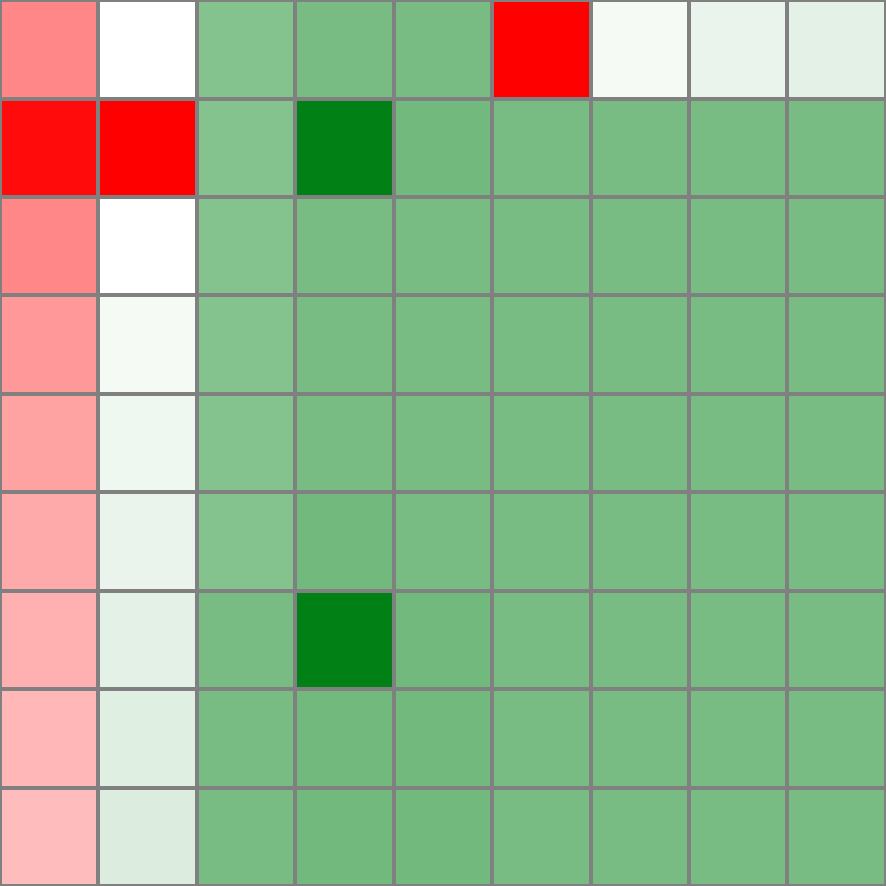
\includegraphics[width=0.78\textwidth]{figures/distribution_over_failures/vi_pfail.pdf}
        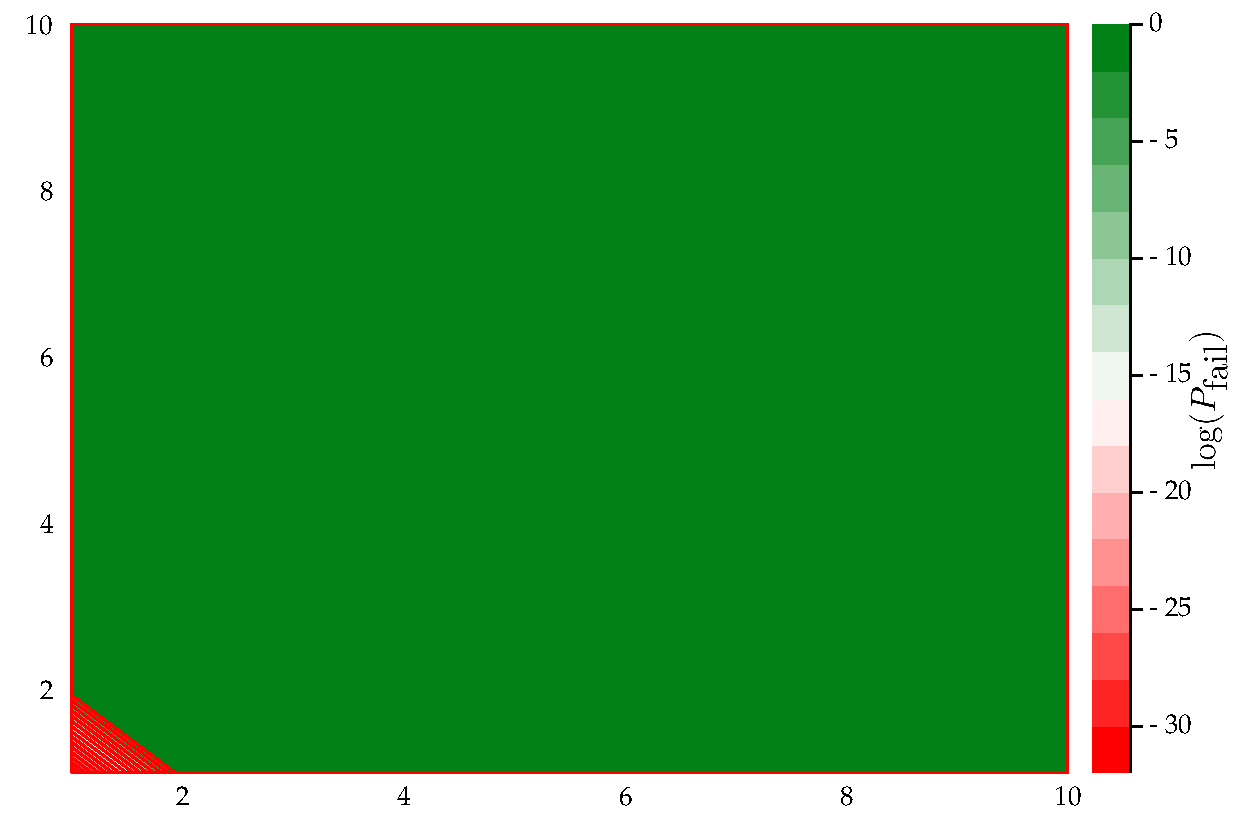
\includegraphics[width=0.17\textwidth, trim={18.4cm, 1cm, 0, 0}, clip]{figures/distribution_over_failures/colorbar.pdf}
        \caption{$P_{\rm fail}$ ground truth.}
        \label{fig:vi_pfail}
    \end{subfigure}
    \hfill
    \begin{subfigure}[b]{0.49\textwidth}
        \centering
        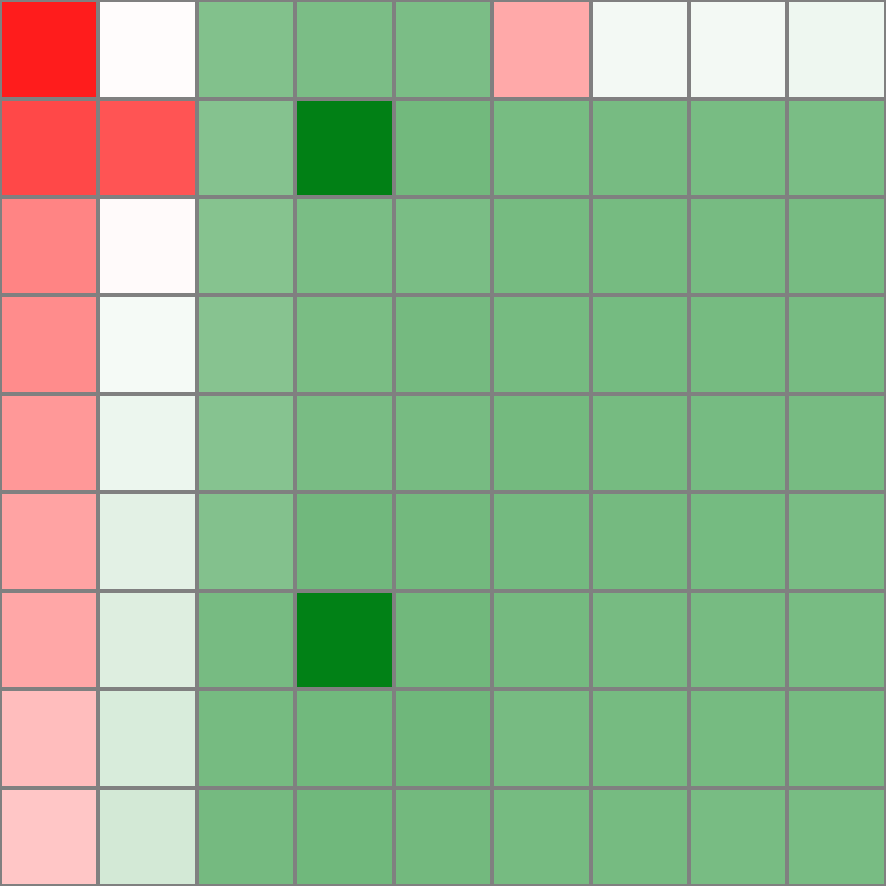
\includegraphics[width=0.78\textwidth]{figures/distribution_over_failures/dqn_pfail.pdf}
        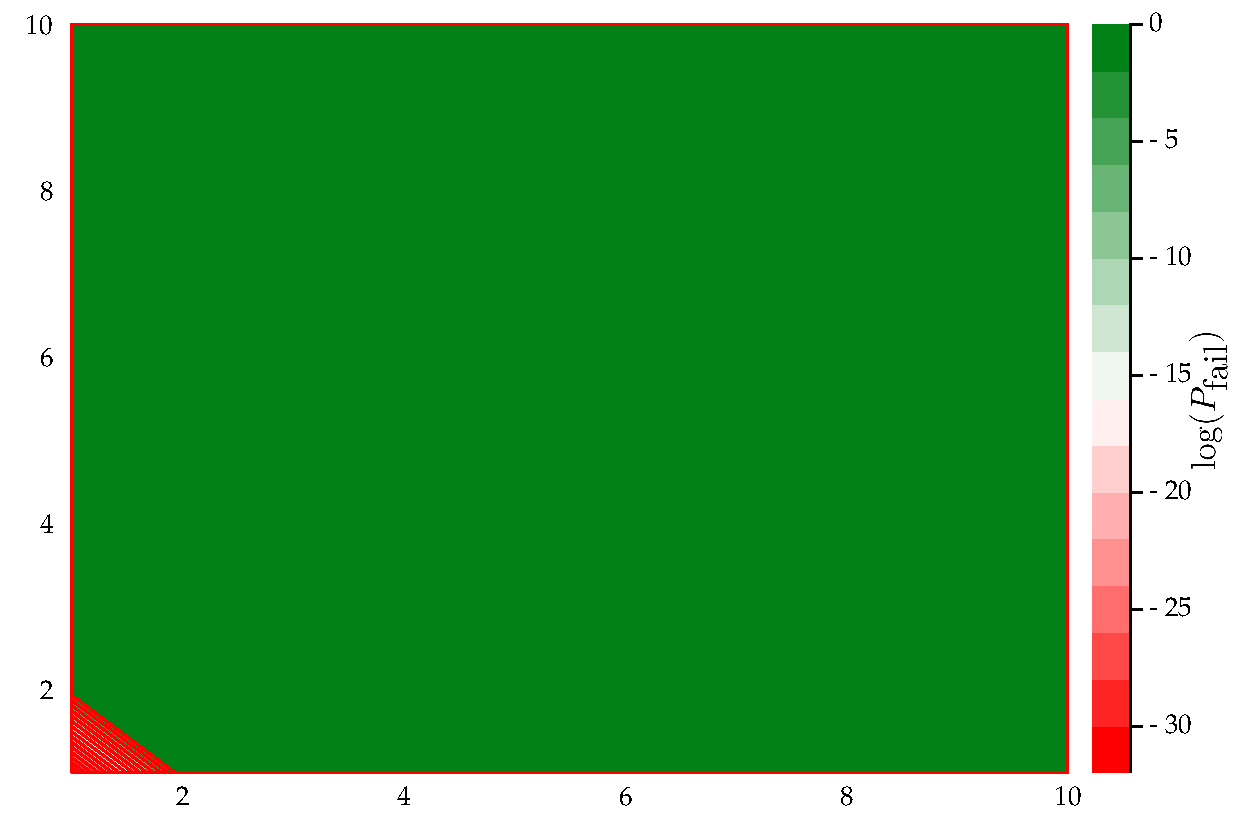
\includegraphics[width=0.17\textwidth, trim={18.4cm, 1cm, 0, 0}, clip]{figures/distribution_over_failures/colorbar.pdf}
        \caption{$P_{\rm fail}$ from DQN.}
        \label{fig:dqn_approx_pfail}
    \end{subfigure}
    \caption{Comparison of $P_{\rm fail}$ between DQN and exact value iteration.}
    \label{fig:dqn_comp_ground_truth}
\end{figure*}

We now compare the proposal distribution $q^*(x \mid s)$ (with $P_{\rm fail}(s)$ computed through exact value iteration and DQN) to the Monte Carlo and cross entropy method baselines. The failure rate and log-likelihood of failures is reported in \cref{tab:ch5_gridworld_results}. The cross entropy method is able to significantly increase the rate of discovered failures, but the average log-likelihood of those failures is much smaller than the most commonly observed failures. Using $q^*$ with both DQN estimation and exact value iteration maximizes the rate of failures discovered while retaining a relatively high likelihood of failure trajectories. 

\cref{fig:gridworld_pfail_vs_samples} shows how each technique performs when used to estimate the probability of failure. Monte Carlo sampling ultimately gives an accurate estimate but does not observe a failure for the first ~\num{2000} samples. The cross entropy method observes samples early on, but due to their low log-probability they are give small importance sampling weights and therefore create an erroneous estimate. The DQN and value iteration approaches both quickly converge to a good estimate of the probability of failure with value iteration performing slightly better. The reason the value iteration estimate has any variance at all is because the agent is initialized to a random place on the grid for each sample. 


\begin{table}
    \centering
    \caption{Simple gridworld failure results.}
    \label{tab:ch5_gridworld_results}
    \begin{tabular}{@{}lll@{}} 
        \toprule
        \textbf{Method} & \textbf{Failure Rate} & \textbf{Log Likelihood}\\
        \midrule
        Monte Carlo & \num{0.001} \pm \num{0.001} & \num{-8.013} \pm \num{0.0} \\
        Cross entropy method & \num{0.255} \pm \num{0.014} & \num{-36.431} \pm \num{2.05} \\
        DQN & \num{0.98} \pm \num{0.004} & \num{-10.654} \pm \num{0.51} \\
        Value iteration & \num{1.0} \pm \num{0.0} & \num{-11.375} \pm \num{0.604} \\
        \bottomrule
    \end{tabular}
\end{table}

\begin{figure}
        \centering
        \begin{tikzpicture}[/tikz/background rectangle/.style={fill={rgb,1:red,1.0;green,1.0;blue,1.0}, draw opacity={1.0}}, show background rectangle]
\begin{axis}[point meta max={nan}, point meta min={nan}, legend cell align={left}, title={Probability of Failure Estimates}, title style={at={{(0.5,1)}}, anchor={south}, font={\large}, color={rgb,1:red,0.0;green,0.0;blue,0.0}, draw opacity={1.0}, rotate={0.0}}, legend style={color={rgb,1:red,0.0;green,0.0;blue,0.0}, draw opacity={1.0}, line width={1}, solid, fill={rgb,1:red,1.0;green,1.0;blue,1.0}, fill opacity={1.0}, text opacity={1.0}, font={\normalsize}, at={(0.98, 0.02)}, anchor={south east}}, axis background/.style={fill={rgb,1:red,1.0;green,1.0;blue,1.0}, opacity={1.0}}, anchor={north west}, xshift={1.0mm}, yshift={-1.0mm}, width={150.4mm}, height={99.6mm}, scaled x ticks={false}, xlabel={Samples}, x tick style={color={rgb,1:red,0.0;green,0.0;blue,0.0}, opacity={1.0}}, x tick label style={color={rgb,1:red,0.0;green,0.0;blue,0.0}, opacity={1.0}, rotate={0}}, xlabel style={at={(ticklabel cs:0.5)}, anchor=near ticklabel, font={\normalsize}, color={rgb,1:red,0.0;green,0.0;blue,0.0}, draw opacity={1.0}, rotate={0.0}}, xmode={log}, log basis x={10}, xmajorgrids={true}, xmin={2}, xmax={100000.0}, xtick={{10.0,100.0,1000.0,10000.0,100000.0}}, xticklabels={{$10^{1}$,$10^{2}$,$10^{3}$,$10^{4}$,$10^{5}$}}, xtick align={inside}, xticklabel style={font={\normalsize}, color={rgb,1:red,0.0;green,0.0;blue,0.0}, draw opacity={1.0}, rotate={0.0}}, x grid style={color={rgb,1:red,0.0;green,0.0;blue,0.0}, draw opacity={0.1}, line width={0.5}, solid}, axis x line*={left}, x axis line style={color={rgb,1:red,0.0;green,0.0;blue,0.0}, draw opacity={1.0}, line width={1}, solid}, scaled y ticks={false}, ylabel={$P_{\textrm{fail}}$}, y tick style={color={rgb,1:red,0.0;green,0.0;blue,0.0}, opacity={1.0}}, y tick label style={color={rgb,1:red,0.0;green,0.0;blue,0.0}, opacity={1.0}, rotate={0}}, ylabel style={at={(ticklabel cs:0.5)}, anchor=near ticklabel, font={\normalsize}, color={rgb,1:red,0.0;green,0.0;blue,0.0}, draw opacity={1.0}, rotate={0.0}}, ymode={log}, log basis y={10}, ymajorgrids={true}, ymin={1.0e-7}, ymax={0.0017454245831368554}, ytick={{1.0e-7,1.0e-6,1.0e-5,0.0001,0.001}}, yticklabels={{$10^{-7}$,$10^{-6}$,$10^{-5}$,$10^{-4}$,$10^{-3}$}}, ytick align={inside}, yticklabel style={font={\normalsize}, color={rgb,1:red,0.0;green,0.0;blue,0.0}, draw opacity={1.0}, rotate={0.0}}, y grid style={color={rgb,1:red,0.0;green,0.0;blue,0.0}, draw opacity={0.1}, line width={0.5}, solid}, axis y line*={left}, y axis line style={color={rgb,1:red,0.0;green,0.0;blue,0.0}, draw opacity={1.0}, line width={1}, solid}]
    \addplot+[line width={0}, draw opacity={0}, fill={rgb,1:red,0.0;green,0.6056;blue,0.9787}, fill opacity={0.2}, mark={none}, mark size={3.0 pt}, mark repeat={1}, mark options={color={rgb,1:red,0.0;green,0.0;blue,0.0}, draw opacity={1.0}, fill={rgb,1:red,0.0;green,0.6056;blue,0.9787}, fill opacity={1.0}, line width={0.75}, rotate={0}, solid}, forget plot]
        coordinates {
            (5263.0,0.00019000570017100514)
            (5294.0,0.00018889308651303362)
            (5324.0,0.00018782870022539445)
            (5355.0,0.00018674136321195143)
            (5386.0,0.0001856665428889714)
            (5417.0,0.00018460402436773122)
            (5448.0,0.00018355359765051394)
            (5480.0,0.0001824817518248175)
            (5512.0,0.000181422351233672)
            (5543.0,0.00018040772145047808)
            (5576.0,0.0001793400286944046)
            (5608.0,0.0001783166904422254)
            (5640.0,0.0001773049645390071)
            (5673.0,0.00017627357659086903)
            (5706.0,0.0001752541184717841)
            (5738.0,0.0003485535029627048)
            (5772.0,0.0003465003465003465)
            (5805.0,0.0003445305770887166)
            (5839.0,0.0003425244048638465)
            (5872.0,0.0003405994550408719)
            (5906.0,0.0003386386725364037)
            (5940.0,0.0003367003367003367)
            (5975.0,0.00033472803347280337)
            (6009.0,0.0003328340822100183)
            (6044.0,0.00033090668431502316)
            (6079.0,0.0003290014805066623)
            (6114.0,0.00032711808963035657)
            (6149.0,0.0003252561392096276)
            (6185.0,0.00032336297493936947)
            (6221.0,0.00032149172158816913)
            (6256.0,0.00031969309462915604)
            (6293.0,0.0003178134435086604)
            (6329.0,0.00031600568810238584)
            (6366.0,0.00031416902293433867)
            (6402.0,0.00031240237425804435)
            (6439.0,0.00031060723714862557)
            (6477.0,0.0003087849312953528)
            (6514.0,0.00030703101013202335)
            (6552.0,0.0004578754578754579)
            (6589.0,0.0004553042950371832)
            (6628.0,0.00045262522631261314)
            (6666.0,0.00045004500450045)
            (6704.0,0.00044749403341288785)
            (6743.0,0.0004449058282663503)
            (6782.0,0.0004423473901503981)
            (6821.0,0.00043981820847383083)
            (6861.0,0.0005830053927998834)
            (6900.0,0.0005797101449275362)
            (6940.0,0.0005763688760806917)
            (6980.0,0.0005730659025787965)
            (7021.0,0.0005697194131890044)
            (7061.0,0.000566491998300524)
            (7102.0,0.000563221627710504)
            (7143.0,0.0005599888002239956)
            (7184.0,0.0005567928730512249)
            (7226.0,0.0005535566011624688)
            (7268.0,0.000550357732526142)
            (7310.0,0.0005471956224350205)
            (7352.0,0.000544069640914037)
            (7394.0,0.0005409791723018664)
            (7437.0,0.0005378512841199408)
            (7480.0,0.0005347593582887701)
            (7523.0,0.0005317027781470158)
            (7567.0,0.0005286110744020088)
            (7610.0,0.0005256241787122207)
            (7654.0,0.0005226025607525476)
            (7699.0,0.000519547993245876)
            (7743.0,0.0005165956347668862)
            (7788.0,0.0005136106831022085)
            (7833.0,0.0005106600280863015)
            (7878.0,0.0005077430820005078)
            (7924.0,0.0005047955577990914)
            (7969.0,0.0005019450370184465)
            (8016.0,0.000499001996007984)
            (8062.0,0.0004961548002976929)
            (8108.0,0.000493339911198816)
            (8155.0,0.0004904966278356836)
            (8202.0,0.000487685930260912)
            (8250.0,0.00048484848484848484)
            (8297.0,0.0004821019645655056)
            (8345.0,0.0004793289394847214)
            (8394.0,0.0004765308553728854)
            (8442.0,0.00047382136934375743)
            (8491.0,0.0004710870333294076)
            (8540.0,0.000468384074941452)
            (8589.0,0.0004657119571544999)
            (8639.0,0.0004630165528417641)
            (8689.0,0.00046035216940959836)
            (8739.0,0.0004577182744021055)
            (8790.0,0.0004550625711035267)
            (8840.0,0.00045248868778280545)
            (8891.0,0.0004498931503767855)
            (8943.0,0.00044727720004472774)
            (8995.0,0.00044469149527515285)
            (9046.0,0.00044218439089100157)
            (9099.0,0.00043960874821408945)
            (9151.0,0.0004371106982843405)
            (9204.0,0.000434593654932638)
            (9257.0,0.0004321054337258291)
            (9311.0,0.0005369992482010525)
            (9365.0,0.0005339028296849973)
            (9419.0,0.0005308419152776304)
            (9473.0,0.0005278158978148422)
            (9528.0,0.0005247691015952981)
            (9583.0,0.0005217572785140353)
            (9638.0,0.0005187798298402158)
            (9694.0,0.0005157829585310501)
            (9750.0,0.0005128205128205128)
            (9806.0,0.0005098919029165817)
            (9863.0,0.0005069451485349286)
            (9920.0,0.0005040322580645161)
            (9977.0,0.0005011526510975244)
            (10035.0,0.0004982561036372695)
            (10093.0,0.0004953928465272962)
            (10151.0,0.0005910747709585262)
            (10210.0,0.0005876591576885406)
            (10269.0,0.0005842827928717499)
            (10328.0,0.0005809450038729666)
            (10388.0,0.0005775895263765884)
            (10448.0,0.0005742725880551302)
            (10509.0,0.0005709391949757351)
            (10569.0,0.0005676979846721544)
            (10630.0,0.0005644402634054562)
            (10692.0,0.0005611672278338945)
            (10754.0,0.0005579319323042589)
            (10816.0,0.0005547337278106509)
            (10878.0,0.0005515719801434088)
            (10941.0,0.0005483959418700301)
            (11004.0,0.0005452562704471102)
            (11068.0,0.0005421033610408384)
            (11132.0,0.0005389867049946101)
            (11196.0,0.0005359056806002144)
            (11261.0,0.0005328123612467809)
            (11326.0,0.0005297545470598623)
            (11391.0,0.0005267316302343956)
            (11457.0,0.0005236973029588898)
            (11523.0,0.000520697734964853)
            (11590.0,0.0005176876617773944)
            (11657.0,0.0005147121901003689)
            (11724.0,0.0005117707267144319)
            (11792.0,0.0005088195386702849)
            (11860.0,0.000505902192242833)
            (11929.0,0.0005029759409841563)
            (11998.0,0.0005000833472245374)
            (12067.0,0.0004972238335957571)
            (12137.0,0.0004943561011782154)
            (12207.0,0.0004915212582944212)
            (12277.0,0.0004887187423637696)
            (12348.0,0.00048590864917395527)
            (12420.0,0.0004830917874396135)
            (12491.0,0.0004803458490112881)
            (12564.0,0.0004775549188156638)
            (12636.0,0.0004748338081671415)
            (12709.0,0.0004721063813045873)
            (12783.0,0.0004693733865289838)
            (12857.0,0.00046667185190946565)
            (12931.0,0.0004640012373366329)
            (13006.0,0.0004613255420575119)
            (13081.0,0.00045868052901154344)
            (13156.0,0.0004560656734569778)
            (13232.0,0.00045344619105199517)
            (13309.0,0.0004508227515215268)
            (13386.0,0.00044822949350067237)
            (13463.0,0.0004456658991309515)
            (13541.0,0.00044309873716859906)
            (13619.0,0.000440560980982451)
            (13698.0,0.0004380201489268506)
            (13777.0,0.00043550845612252303)
            (13857.0,0.00043299415457891317)
            (13937.0,0.00043050871780153546)
            (14017.0,0.00042805165156595563)
            (14098.0,0.00042559228259327563)
            (14180.0,0.0004231311706629055)
            (14262.0,0.00042069835927639884)
            (14344.0,0.0004182933630786392)
            (14427.0,0.0004158868787689748)
            (14510.0,0.0004135079255685734)
            (14594.0,0.0004111278607646978)
            (14678.0,0.0004087750374710451)
            (14763.0,0.000406421459053038)
            (14849.0,0.00040406761398073944)
            (14934.0,0.0004017677782241864)
            (15021.0,0.0003994407829039345)
            (15108.0,0.0003971405877680699)
            (15195.0,0.0003948667324777887)
            (15283.0,0.00039259307727540407)
            (15371.0,0.00039034545572831956)
            (15460.0,0.00038809831824062095)
            (15549.0,0.00038587690526721975)
            (15639.0,0.0003836562440053712)
            (15729.0,0.00038146099561319857)
            (15820.0,0.0003792667509481669)
            (15912.0,0.0003770739064856712)
            (16004.0,0.0004373906523369158)
            (16096.0,0.0004348906560636183)
            (16189.0,0.00043239236518623756)
            (16283.0,0.00042989621077197076)
            (16377.0,0.00042742871099713014)
            (16471.0,0.00042498937526561835)
            (16567.0,0.00042252670972415043)
            (16662.0,0.0004201176329372224)
            (16759.0,0.0004176860194522346)
            (16855.0,0.00041530703055473156)
            (16953.0,0.0004129062702766472)
            (17051.0,0.0004105331065626649)
            (17149.0,0.00040818706630124207)
            (17248.0,0.00040584415584415587)
            (17348.0,0.00040350472676965645)
            (17448.0,0.0004011921137093077)
            (17549.0,0.00039888312724371757)
            (17651.0,0.000396578097558212)
            (17753.0,0.0003942995550047879)
            (17855.0,0.00039204704564547744)
            (17958.0,0.0003897984185321305)
            (18062.0,0.00044291883512346365)
            (18166.0,0.0004403831333259936)
            (18271.0,0.00043785233430025726)
            (18377.0,0.0004353267671545954)
            (18483.0,0.0004328301682627279)
            (18590.0,0.00043033889187735344)
            (18697.0,0.0004278761298604054)
            (18806.0,0.000425396150164841)
            (18914.0,0.00042296711430686265)
            (19024.0,0.00042052144659377626)
            (19133.0,0.0004181257513197094)
            (19244.0,0.0004157139887757223)
            (19355.0,0.00041332988891759235)
            (19467.0,0.0004109518672625469)
            (19580.0,0.00040858018386108274)
            (19693.0,0.0004062357182755294)
            (19807.0,0.0004038976119553693)
            (19921.0,0.00040158626574971135)
            (20036.0,0.0003992812936713915)
            (20152.0,0.0003969829297340214)
            (20268.0,0.00039471087428458656)
            (20385.0,0.0003924454255580083)
            (20503.0,0.0003901868019314247)
            (20622.0,0.0003879352148191252)
            (20741.0,0.0003857094643459814)
            (20861.0,0.00038349072431810555)
            (20981.0,0.0003812973642819694)
            (21103.0,0.0003790930199497702)
            (21224.0,0.0003769317753486619)
            (21347.0,0.0003747599194266173)
            (21470.0,0.0003726129482999534)
            (21595.0,0.00037045612410280157)
            (21719.0,0.00036834108384363923)
            (21845.0,0.0003662165255207141)
            (21971.0,0.00036411633516908654)
            (22098.0,0.00036202371255317223)
            (22226.0,0.0003599388104022316)
            (22354.0,0.00040261250782857655)
            (22483.0,0.0004003024507405595)
            (22613.0,0.00039800114978109935)
            (22744.0,0.00039570875835385154)
            (22875.0,0.00039344262295081965)
            (23008.0,0.0003911682892906815)
            (23141.0,0.000388920098526425)
            (23274.0,0.0003866976024748647)
            (23409.0,0.00038446751249519417)
            (23544.0,0.00038226299694189603)
            (23680.0,0.0003800675675675676)
            (23817.0,0.0003778813452575891)
            (23955.0,0.0003757044458359424)
            (24093.0,0.00037355248412401944)
            (24232.0,0.00037140970617365466)
            (24372.0,0.00036927621861152144)
            (24513.0,0.00036715212336311344)
            (24655.0,0.0003650375177448793)
            (24797.0,0.00036294713070129453)
            (24941.0,0.00036085160979912594)
            (25085.0,0.00035878014749850506)
            (25230.0,0.000356718192627824)
            (25375.0,0.000354679802955665)
            (25522.0,0.00039181882297625577)
            (25670.0,0.00038955979742890534)
            (25818.0,0.0003873266713145867)
            (25967.0,0.0003851041706781684)
            (26117.0,0.0003828923689550867)
            (26268.0,0.00038069133546520483)
            (26420.0,0.0003785011355034065)
            (26573.0,0.00037632183042938324)
            (26726.0,0.0003741674773628676)
            (26881.0,0.00037200996986719244)
            (27036.0,0.00040686492084627906)
            (27192.0,0.0004045307443365696)
            (27349.0,0.0004022084902555852)
            (27507.0,0.0003998982077289417)
            (27666.0,0.00039759994216728115)
            (27826.0,0.000395313735355423)
            (27987.0,0.0003930396255404295)
            (28149.0,0.00039077764751856197)
            (28311.0,0.0003885415562855427)
            (28475.0,0.00038630377524143984)
            (28639.0,0.0003840916233108698)
            (28805.0,0.0003818781461551814)
            (28971.0,0.00037969003486244867)
            (29139.0,0.00037750094375235937)
            (29307.0,0.00037533695021667177)
            (29477.0,0.0003731723038301048)
            (29647.0,0.00037103248220730597)
            (29818.0,0.0003689046884432222)
            (29991.0,0.00040012003601080324)
            (30164.0,0.00039782522211908233)
            (30338.0,0.00039554354275166457)
            (30513.0,0.0003932749975420313)
            (30690.0,0.00039100684261974585)
            (30867.0,0.000388764700165225)
            (31046.0,0.00038652322360368483)
            (31225.0,0.0003843074459567654)
            (31405.0,0.0003821047603884732)
            (31587.0,0.0003799031247032007)
            (31769.0,0.0003777267147218987)
            (31953.0,0.00037555159139986854)
            (32138.0,0.0003733897566743419)
            (32323.0,0.000371252668378554)
            (32510.0,0.0003691171947093202)
            (32698.0,0.00036699492323689524)
            (32887.0,0.00036488582114513335)
            (33077.0,0.0003627898539770838)
            (33268.0,0.00036070698569195625)
            (33460.0,0.00035863717872086073)
            (33654.0,0.00035656979853806385)
            (33848.0,0.0003545261167572678)
            (34044.0,0.00035248501938667606)
            (34241.0,0.0003504570544084577)
            (34438.0,0.00034845229107381383)
            (34637.0,0.0003464503276842683)
            (34838.0,0.0003444514610482806)
            (35039.0,0.00034247552726961384)
            (35241.0,0.0003405124712692602)
            (35445.0,0.00033855268726195513)
            (35650.0,0.00033660589060308555)
            (35856.0,0.00033467202141900936)
            (36063.0,0.00033275101904999585)
            (36272.0,0.0003308337009263344)
            (36481.0,0.00032893835147062856)
            (36692.0,0.00032704676768777934)
            (36904.0,0.00032516800346845873)
            (37117.0,0.0003233019910014279)
            (37332.0,0.00034822672238294224)
            (37547.0,0.0003462327216555251)
            (37764.0,0.0003442431945768457)
            (37983.0,0.00034225837874838743)
            (38202.0,0.0003402963195644207)
            (38423.0,0.00033833901569372513)
            (38645.0,0.00033639539397075947)
            (38868.0,0.0003344653699701554)
            (39093.0,0.00035812037960760237)
            (39319.0,0.00035606195478013177)
            (39546.0,0.00035401810549739543)
            (39775.0,0.0003519798868636078)
            (40004.0,0.00034996500349965005)
            (40236.0,0.00039765384233025154)
            (40468.0,0.0003953741227636651)
            (40702.0,0.00039310107611419587)
            (40937.0,0.00039084446832938417)
            (41174.0,0.0003885947442560839)
            (41412.0,0.00038636144112817543)
            (41651.0,0.00038414443830880413)
            (41892.0,0.00038193449823355295)
            (42134.0,0.00037974082688565055)
            (42377.0,0.00037756330084715765)
            (42622.0,0.00037539298953592043)
            (42868.0,0.00039656620322851545)
            (43116.0,0.00039428518415437423)
            (43365.0,0.00039202121526576734)
            (43616.0,0.00038976522377109316)
            (43868.0,0.00038752621500866237)
            (44121.0,0.0003853040502255162)
            (44376.0,0.00038308995853614567)
            (44633.0,0.00038088409920910535)
            (44891.0,0.0003786950613708761)
            (45150.0,0.0003765227021040975)
            (45411.0,0.0003743586355728788)
            (45674.0,0.0003722030038971844)
            (45937.0,0.00037007205520604307)
            (46203.0,0.0003679414756617536)
            (46470.0,0.00036582741553690555)
            (46738.0,0.0003637297274166631)
            (47009.0,0.00036163287881044057)
            (47280.0,0.0003595600676818951)
            (47553.0,0.0003574958467394276)
            (47828.0,0.0003554403278414318)
            (48105.0,0.00035339361812701384)
            (48383.0,0.0003513630820742823)
            (48662.0,0.0003493485676708725)
            (48943.0,0.0003473428273706148)
            (49226.0,0.00034534595538942837)
            (49511.0,0.0003433580416473107)
            (49797.0,0.0003413860272707191)
            (50085.0,0.0003394229809324149)
            (50374.0,0.00033747568189939253)
            (50665.0,0.000335537353202408)
            (50958.0,0.00035323207347227127)
            (51252.0,0.00035120580660266915)
            (51549.0,0.00034918233137403245)
            (51846.0,0.0003471820391158431)
            (52146.0,0.00034518467380048324)
            (52447.0,0.00036227048258241656)
            (52750.0,0.00036018957345971566)
            (53055.0,0.00037696729808689097)
            (53362.0,0.00037479854578164235)
            (53670.0,0.0003726476616359232)
            (53980.0,0.0003705075954057058)
            (54292.0,0.00036837839829072423)
            (54606.0,0.000366260117935758)
            (54922.0,0.0003641527985142566)
            (55239.0,0.00038016618693314505)
            (55558.0,0.00037798336873177583)
            (55879.0,0.00037581202240555484)
            (56202.0,0.00037365218319632755)
            (56527.0,0.00037150388310011145)
            (56854.0,0.00036936715094804237)
            (57182.0,0.00036724843482214685)
            (57513.0,0.00038252221236937734)
            (57845.0,0.0003803267352407295)
            (58179.0,0.0003781433163168841)
            (58516.0,0.0003759655478843393)
            (58854.0,0.00037380636830121994)
            (59194.0,0.0003716592897928844)
            (59536.0,0.0003863208814834722)
            (59880.0,0.0003841015364061456)
            (60226.0,0.00038189486268389066)
            (60574.0,0.00039620959487568925)
            (60924.0,0.00039393342525113255)
            (61276.0,0.0003916704745740584)
            (61630.0,0.00038942073665422684)
            (61986.0,0.00038718420288452233)
            (62345.0,0.00038495468762531076)
            (62705.0,0.0003827445977194801)
            (63067.0,0.0003805476715239349)
            (63432.0,0.00037835792659856227)
            (63798.0,0.0003761873412959654)
            (64167.0,0.00038960836567082766)
            (64538.0,0.0003873686820167963)
            (64911.0,0.0003851427338971823)
            (65286.0,0.00038293049045737217)
            (65663.0,0.0003807319190411647)
            (66042.0,0.00037854698525180945)
            (66424.0,0.0003914247862218475)
            (66808.0,0.0003891749491078913)
            (67194.0,0.0003869393100574456)
            (67582.0,0.0003847178242727353)
            (67973.0,0.00038250481808953555)
            (68366.0,0.0003803060000585086)
            (68761.0,0.00037812131877081485)
            (69158.0,0.0003759507215361925)
            (69558.0,0.0003737887805859858)
            (69960.0,0.00037164093767867354)
            (70364.0,0.00036950713433005515)
            (70771.0,0.0003673821197948312)
            (71180.0,0.0003652711435796572)
            (71591.0,0.0003631741420010895)
            (72005.0,0.0003610860356919658)
            (72421.0,0.00037282003838665583)
            (72839.0,0.0003706805420173259)
            (73260.0,0.00036855036855036854)
            (73684.0,0.0003664296183703382)
            (74109.0,0.00036432821924462617)
            (74538.0,0.0003622313450857281)
            (74968.0,0.000360153665563974)
            (75402.0,0.00035808068751492004)
            (75837.0,0.00035602674156414414)
            (76276.0,0.00036708794378310347)
            (76716.0,0.0003780176234423067)
            (77160.0,0.0003758424053913945)
            (77606.0,0.00037368244723346133)
            (78054.0,0.0003715376534194276)
            (78505.0,0.00036940322272466724)
            (78959.0,0.00036727922086145974)
            (79415.0,0.0003651703078763458)
            (79874.0,0.0003630718381450785)
            (80336.0,0.0003609838677554272)
            (80800.0,0.0003589108910891089)
            (81267.0,0.0003568484132550728)
            (81736.0,0.00035480082215914654)
            (82209.0,0.0003649235485165858)
            (82684.0,0.0003628271491461468)
            (83162.0,0.00036074168490416293)
            (83642.0,0.0003586714808349872)
            (84125.0,0.00035661218424962854)
            (84612.0,0.0003545596369309318)
            (85101.0,0.0003525222970352875)
            (85592.0,0.00036218338162445087)
            (86087.0,0.00036010082823190496)
            (86584.0,0.00036958329483507344)
            (87085.0,0.000367457082161107)
            (87588.0,0.0003767639402657898)
            (88094.0,0.00037459985924126504)
            (88603.0,0.0003724478855117773)
            (89115.0,0.000370308028951355)
            (89630.0,0.00036818029677563316)
            (90148.0,0.0003660646936149443)
            (90669.0,0.0003639612215862092)
            (91193.0,0.0003618698803636244)
            (91720.0,0.0003706934147405146)
            (92250.0,0.00036856368563685635)
            (92783.0,0.0003664464395417264)
            (93319.0,0.0003643416667559661)
            (93859.0,0.000372899775194707)
            (94401.0,0.0003707587843349117)
            (94947.0,0.0003791588991753294)
            (95495.0,0.00038745484056756897)
            (96047.0,0.0003852280654263017)
            (96602.0,0.0003830148444131591)
            (97160.0,0.00038081515026759986)
            (97722.0,0.00037862507930660447)
            (98287.0,0.00038662284941040013)
            (98855.0,0.000384401395984017)
            (99426.0,0.0003922515237463038)
            (100000.0,0.00039)
            (100000.0,0.0002479255934884641)
            (99426.0,0.0002493570044396241)
            (98855.0,0.00024277948035426327)
            (98287.0,0.0002441826014360528)
            (97722.0,0.00023751166307644722)
            (97160.0,0.0002388855927971537)
            (96602.0,0.0002402655607001675)
            (96047.0,0.00024165401576074061)
            (95495.0,0.0002430509751016526)
            (94947.0,0.00023616487139514338)
            (94401.0,0.0002292254768497747)
            (93859.0,0.00023054926053626932)
            (93319.0,0.00022351497405844164)
            (92783.0,0.00022480629316934143)
            (92250.0,0.0002261052659523529)
            (91720.0,0.00022741189837679416)
            (91193.0,0.00022019814456027074)
            (90669.0,0.00022147081754440582)
            (90148.0,0.00022275087370017823)
            (89630.0,0.00022403831324395917)
            (89115.0,0.0002253331349057169)
            (88603.0,0.00022663533588599175)
            (88094.0,0.00022794491181214228)
            (87588.0,0.000229261856693859)
            (87085.0,0.0002216947013414315)
            (86584.0,0.00022297758399523923)
            (86087.0,0.00021531165355188518)
            (85592.0,0.00021655694448983242)
            (85101.0,0.00020879314291528695)
            (84612.0,0.00020999991179323908)
            (84125.0,0.00021121568941966418)
            (83642.0,0.0002124354658227182)
            (83162.0,0.0002136617040385606)
            (82684.0,0.00021489698230273065)
            (82209.0,0.00021613873879111652)
            (81736.0,0.0002080529711707775)
            (81267.0,0.0002092537529363032)
            (80800.0,0.00021046326583764135)
            (80336.0,0.00021167893666408156)
            (79874.0,0.0002129034014063118)
            (79415.0,0.00021413402440810205)
            (78959.0,0.00021537077279317995)
            (78505.0,0.00021661637095512357)
            (78054.0,0.00021786808607891176)
            (77606.0,0.00021912587964414672)
            (77160.0,0.0002203925673021504)
            (76716.0,0.0002216682051103458)
            (76276.0,0.0002129958521328472)
            (75837.0,0.00020427729159619331)
            (75402.0,0.000205455871217891)
            (74968.0,0.00020664537271756432)
            (74538.0,0.00020783757301534586)
            (74109.0,0.0002090407885007118)
            (73684.0,0.0002102466015311197)
            (73260.0,0.00021146351954680334)
            (72839.0,0.00021268584586897016)
            (72421.0,0.00021391352290976444)
            (72005.0,0.00020473170526798682)
            (71591.0,0.00020591572881766367)
            (71180.0,0.00020710479732324077)
            (70771.0,0.0002083017909693431)
            (70364.0,0.00020950674588785878)
            (69960.0,0.00021071668544887283)
            (69558.0,0.00021193458702228494)
            (69158.0,0.00021316048379239663)
            (68761.0,0.000214391290107892)
            (68366.0,0.00021563008372561438)
            (67973.0,0.00021687689454502076)
            (67582.0,0.000218131751739209)
            (67194.0,0.0002193914183646749)
            (66808.0,0.00022065911162213602)
            (66424.0,0.00022193485693644026)
            (66042.0,0.00021193343869591846)
            (65663.0,0.00021315679611389967)
            (65286.0,0.0002143877904751723)
            (64911.0,0.00021562644106028949)
            (64538.0,0.00021687276617546436)
            (64167.0,0.0002181267831183905)
            (63798.0,0.0002077867098831662)
            (63432.0,0.0002089857289004593)
            (63067.0,0.0002101953327283833)
            (62705.0,0.0002114089046072943)
            (62345.0,0.00021262974922554617)
            (61986.0,0.00021386132551506456)
            (61630.0,0.00021509678000117074)
            (61276.0,0.00021633952962875016)
            (60924.0,0.00021758957917371072)
            (60574.0,0.00021884693207702624)
            (60226.0,0.0002079121553130939)
            (59880.0,0.0002091136195019573)
            (59536.0,0.00021032198401867104)
            (59194.0,0.0001992232670364299)
            (58854.0,0.00020037427711280063)
            (58516.0,0.00020153177546682608)
            (58179.0,0.0002026992401046029)
            (57845.0,0.00020386973501113935)
            (57513.0,0.00020504669526991728)
            (57182.0,0.00019359498757819338)
            (56854.0,0.00019471196170073348)
            (56527.0,0.00019583843484301315)
            (56202.0,0.00019697100763508172)
            (55879.0,0.00019810966489502787)
            (55558.0,0.00019925438977246284)
            (55239.0,0.00020040516370583645)
            (54922.0,0.00018852426034546171)
            (54606.0,0.00018961532458980766)
            (54292.0,0.00019071206491495107)
            (53980.0,0.00019181445846653397)
            (53670.0,0.00019292248059290807)
            (53362.0,0.00019403610480182723)
            (53055.0,0.00019515898139199742)
            (52750.0,0.00018284853747860245)
            (52447.0,0.00018390498981921935)
            (52146.0,0.00017152010839321567)
            (51846.0,0.0001725126675960469)
            (51549.0,0.0001735066822294882)
            (51252.0,0.00017451221823488544)
            (50958.0,0.00017551914246179817)
            (50665.0,0.00016285984339603173)
            (50374.0,0.00016380072588772232)
            (50085.0,0.00016474596353540416)
            (49797.0,0.00016569884596169548)
            (49511.0,0.00016665608245902049)
            (49226.0,0.000167621037583437)
            (48943.0,0.00016859034205314775)
            (48662.0,0.00016956395223227975)
            (48383.0,0.00017054182239955418)
            (48105.0,0.00017152747062068575)
            (47828.0,0.00017252097070705037)
            (47553.0,0.00017351874786081175)
            (47280.0,0.00017452075008763247)
            (47009.0,0.00017552692310221098)
            (46738.0,0.00017654476527059765)
            (46470.0,0.00017756301596680223)
            (46203.0,0.00017858921491776484)
            (45937.0,0.00017962343370509618)
            (45674.0,0.000180657832729985)
            (45411.0,0.00018170421436460428)
            (45150.0,0.00018275469150519914)
            (44891.0,0.0001838091951766921)
            (44633.0,0.00018487179603890027)
            (44376.0,0.00018594256349202824)
            (44121.0,0.0001870173282244465)
            (43868.0,0.00018809601293648544)
            (43616.0,0.00018918287521643308)
            (43365.0,0.0001902779824441297)
            (43116.0,0.00019137696325240397)
            (42868.0,0.00019248422179555356)
            (42622.0,0.0001775538217250389)
            (42377.0,0.00017858043133529757)
            (42134.0,0.00017961045476252389)
            (41892.0,0.00018064811640933426)
            (41651.0,0.00018169347467978286)
            (41412.0,0.00018274217492553543)
            (41174.0,0.00018379858677356742)
            (40937.0,0.00018486276731326508)
            (40702.0,0.0001859302051920517)
            (40468.0,0.0001870054202795606)
            (40236.0,0.00018808379302544495)
            (40004.0,0.0001557644924721766)
            (39775.0,0.00015666136609421768)
            (39546.0,0.0001575686277148251)
            (39319.0,0.00015847839658781406)
            (39093.0,0.00015939465432548988)
            (38868.0,0.00014357773778895922)
            (38645.0,0.00014440631833276645)
            (38423.0,0.00014524073732664861)
            (38202.0,0.0001460810310322473)
            (37983.0,0.00014692336706539298)
            (37764.0,0.0001477754736352295)
            (37547.0,0.00014862960364276975)
            (37332.0,0.00014948565508840297)
            (37117.0,0.00013318728645828217)
            (36904.0,0.00013395606969766966)
            (36692.0,0.00013473010728199877)
            (36481.0,0.00013550942716373152)
            (36272.0,0.00013629029920998742)
            (36063.0,0.00013708022295515866)
            (35856.0,0.00013787166534011465)
            (35650.0,0.00013866840954270196)
            (35445.0,0.00013947048056969332)
            (35241.0,0.0001402779031041948)
            (35039.0,0.00014108667447155018)
            (34838.0,0.00014190075222731124)
            (34637.0,0.0001427242790503086)
            (34438.0,0.00014354908254350616)
            (34241.0,0.00014437504042623926)
            (34044.0,0.00014521055816737037)
            (33848.0,0.00014605148727694553)
            (33654.0,0.00014689348201165898)
            (33460.0,0.0001477452413303301)
            (33268.0,0.00014859800135814342)
            (33077.0,0.00014945614352725314)
            (32887.0,0.00015031968333273542)
            (32698.0,0.0001511886356402566)
            (32510.0,0.00015206301466310604)
            (32323.0,0.00015294283393872403)
            (32138.0,0.00015382331937546204)
            (31953.0,0.00015471400134830279)
            (31769.0,0.00015561015922293812)
            (31587.0,0.00015650684817193223)
            (31405.0,0.00015741393118783443)
            (31225.0,0.00015832144774998903)
            (31046.0,0.00015923435930780626)
            (30867.0,0.0001601578599676227)
            (30690.0,0.00016108163600500182)
            (30513.0,0.00016201613037801499)
            (30338.0,0.00016295078660229372)
            (30164.0,0.00016389085524949682)
            (29991.0,0.00016483633648898847)
            (29818.0,0.0001449376857983657)
            (29647.0,0.00014577374393812557)
            (29477.0,0.00014661452898113712)
            (29307.0,0.00014746506914820802)
            (29139.0,0.00014831535370414688)
            (28971.0,0.00014917550061928887)
            (28805.0,0.00015003526347015598)
            (28639.0,0.00015090499413941206)
            (28475.0,0.0001517742050448092)
            (28311.0,0.0001526534872490878)
            (28149.0,0.00015353210645384856)
            (27987.0,0.00015442089824814563)
            (27826.0,0.00015531445795047063)
            (27666.0,0.00015621277190447374)
            (27507.0,0.00015711582509791167)
            (27349.0,0.00015802360112847076)
            (27192.0,0.00015893608216915558)
            (27036.0,0.00015985324893324875)
            (26881.0,0.00013828576391808754)
            (26726.0,0.00013908783872010075)
            (26573.0,0.0001398887416749174)
            (26420.0,0.00014069892165287335)
            (26268.0,0.00014151315279053834)
            (26117.0,0.00014233141228972798)
            (25967.0,0.00014315367588926855)
            (25818.0,0.00014397991783160865)
            (25670.0,0.00014481011082913031)
            (25522.0,0.00014564993319092306)
            (25375.0,0.00012345483092934101)
            (25230.0,0.00012416440160061177)
            (25085.0,0.00012488217610057367)
            (24941.0,0.00012560326088226868)
            (24797.0,0.000126332721287335)
            (24655.0,0.0001270603952967577)
            (24513.0,0.00012779650064683872)
            (24372.0,0.00012853591013210698)
            (24232.0,0.00012927858988611858)
            (24093.0,0.000130024504437898)
            (23955.0,0.00013077361667985545)
            (23817.0,0.00013153141068482133)
            (23680.0,0.0001322924508420784)
            (23544.0,0.0001330566968425008)
            (23409.0,0.00013382410661492245)
            (23274.0,0.0001346004198712243)
            (23141.0,0.00013537409043550604)
            (23008.0,0.00013615670638857048)
            (22875.0,0.00013694842377605599)
            (22744.0,0.00013773728812291374)
            (22613.0,0.00013853529331849424)
            (22483.0,0.00013933640088925722)
            (22354.0,0.00014014055744383905)
            (22226.0,0.00011568933823748184)
            (22098.0,0.00011635950944604347)
            (21971.0,0.00011703216295517332)
            (21845.0,0.00011770724967846805)
            (21719.0,0.0001183901699105655)
            (21595.0,0.00011907003129601421)
            (21470.0,0.00011976332443420958)
            (21347.0,0.0001204534510545704)
            (21224.0,0.00012115157737205756)
            (21103.0,0.00012184629344084817)
            (20981.0,0.0001225548642961709)
            (20861.0,0.0001232599050262549)
            (20741.0,0.000123973104692056)
            (20622.0,0.00012468855853696903)
            (20503.0,0.00012541231814154765)
            (20385.0,0.00012613834033085083)
            (20268.0,0.0001268665571537217)
            (20152.0,0.00012759689842057194)
            (20036.0,0.00012833569718507729)
            (19921.0,0.00012907662087558342)
            (19807.0,0.00012981959427589638)
            (19693.0,0.00013057117040034353)
            (19580.0,0.00013132479148389567)
            (19467.0,0.00013208716245913298)
            (19355.0,0.00013285157166657694)
            (19244.0,0.00013361793552005828)
            (19133.0,0.00013439319232342385)
            (19024.0,0.0001351632851657919)
            (18914.0,0.00013594944243560493)
            (18806.0,0.00013673025427133999)
            (18697.0,0.00013752744284927556)
            (18590.0,0.00013831909769265082)
            (18483.0,0.00013911991937394763)
            (18377.0,0.00013992245287916018)
            (18271.0,0.00014073429916939894)
            (18166.0,0.00014154782818038365)
            (18062.0,0.00014236293412534185)
            (17958.0,0.00011345910768382784)
            (17855.0,0.00011411367044753923)
            (17753.0,0.00011476936391056902)
            (17651.0,0.00011543263610779453)
            (17549.0,0.0001161036191994827)
            (17448.0,0.00011677575472057874)
            (17348.0,0.00011744894655873453)
            (17248.0,0.00011812994506795761)
            (17149.0,0.00011881195764223631)
            (17051.0,0.00011949488194119129)
            (16953.0,0.00012018570244641725)
            (16855.0,0.00012088455690223123)
            (16759.0,0.00012157707444349026)
            (16662.0,0.00012228491155805604)
            (16567.0,0.00012298618898074648)
            (16471.0,0.0001237030666915974)
            (16377.0,0.00012441315384163)
            (16283.0,0.00012513144022015298)
            (16189.0,0.00012585806866400033)
            (16096.0,0.00012658531976800648)
            (16004.0,0.00012731306805045394)
            (15912.0,9.659413569057426e-5)
            (15820.0,9.715590608924246e-5)
            (15729.0,9.771803559709412e-5)
            (15639.0,9.828042264429344e-5)
            (15549.0,9.88493204646885e-5)
            (15460.0,9.941841127208766e-5)
            (15371.0,9.999409271025246e-5)
            (15283.0,0.00010056989857718196)
            (15195.0,0.00010115237429153545)
            (15108.0,0.00010173490169558107)
            (15021.0,0.00010232417740825128)
            (14934.0,0.0001029203193767477)
            (14849.0,0.00010350950390731502)
            (14763.0,0.0001041125252962136)
            (14678.0,0.00010471547883309092)
            (14594.0,0.0001053182393785204)
            (14510.0,0.00010592797928801105)
            (14427.0,0.00010653743489103456)
            (14344.0,0.00010715394407070147)
            (14262.0,0.00010777007249743474)
            (14180.0,0.00010839332729978588)
            (14098.0,0.00010902383283650243)
            (14017.0,0.00010965389235318958)
            (13937.0,0.00011028336244013707)
            (13857.0,0.00011092010122139187)
            (13777.0,0.00011156423532902702)
            (13698.0,0.00011220770163402011)
            (13619.0,0.00011285863360839781)
            (13541.0,0.00011350877811667056)
            (13463.0,0.00011416645659843231)
            (13386.0,0.00011482322164978165)
            (13309.0,0.00011548758676305855)
            (13232.0,0.00011615968462747435)
            (13156.0,0.00011683076928908892)
            (13081.0,0.00011750066916840524)
            (13006.0,0.00011817829567479273)
            (12931.0,0.00011886378326205643)
            (12857.0,0.00011954796981503726)
            (12783.0,0.00012024007839963647)
            (12709.0,0.0001209402474080122)
            (12636.0,0.00012163899058624571)
            (12564.0,0.00012233611622205272)
            (12491.0,0.00012305112967813628)
            (12420.0,0.0001237546172446837)
            (12348.0,0.00012447627544976607)
            (12277.0,0.0001251962002641063)
            (12207.0,0.00012591418449604895)
            (12137.0,0.0001266404513237413)
            (12067.0,0.00012737514489947013)
            (11998.0,0.0001281077335588981)
            (11929.0,0.0001288487978236067)
            (11860.0,0.00012959848563579972)
            (11792.0,0.00013034589279378663)
            (11724.0,0.00013110197069761344)
            (11657.0,0.000131855557919677)
            (11590.0,0.00013261785861717163)
            (11523.0,0.00013338902479536968)
            (11457.0,0.00013415750034413292)
            (11391.0,0.0001349348818232498)
            (11326.0,0.00013570934075668998)
            (11261.0,0.00013649274102537436)
            (11196.0,0.0001372852383735181)
            (11132.0,0.00013807458658894356)
            (11068.0,0.00013887306431918612)
            (11004.0,0.00013968083087196855)
            (10941.0,0.00014048520671284973)
            (10878.0,0.00014129890048333166)
            (10816.0,0.00014210893386715022)
            (10754.0,0.0001429283082630998)
            (10692.0,0.00014375718618396782)
            (10630.0,0.00014459573393434529)
            (10569.0,0.0001454303590639473)
            (10509.0,0.00014626075497711517)
            (10448.0,0.00014711476896808398)
            (10388.0,0.00014796456817478402)
            (10328.0,0.00014882424204553204)
            (10269.0,0.00014967938505034122)
            (10210.0,0.00015054441214029906)
            (10151.0,0.00015141949567784845)
            (10093.0,0.00010680411928821272)
            (10035.0,0.00010742144897623316)
            (9977.0,0.00010804595650538599)
            (9920.0,0.00010866681190210858)
            (9863.0,0.00010929484367435739)
            (9806.0,0.0001099301769714195)
            (9750.0,0.00011056159855682494)
            (9694.0,0.00011120031561833073)
            (9638.0,0.00011184645532905682)
            (9583.0,0.00011248840775607928)
            (9528.0,0.00011313777180617173)
            (9473.0,0.00011379467658027283)
            (9419.0,0.00011444710168840514)
            (9365.0,0.00011510705110382281)
            (9311.0,0.00011577465574629355)
            (9257.0,7.261379519969588e-5)
            (9204.0,7.303191909154943e-5)
            (9151.0,7.345488614328514e-5)
            (9099.0,7.387466136752886e-5)
            (9046.0,7.430747521149913e-5)
            (8995.0,7.472877165281384e-5)
            (8943.0,7.516327602783416e-5)
            (8891.0,7.560286273449162e-5)
            (8840.0,7.603901907273528e-5)
            (8790.0,7.647153648100496e-5)
            (8739.0,7.691780281787042e-5)
            (8689.0,7.736040430711432e-5)
            (8639.0,7.780812892321668e-5)
            (8589.0,7.826106613452119e-5)
            (8540.0,7.871009009409333e-5)
            (8491.0,7.916429634965375e-5)
            (8442.0,7.962377513714947e-5)
            (8394.0,8.007907794827402e-5)
            (8345.0,8.054926862269962e-5)
            (8297.0,8.101524818755274e-5)
            (8250.0,8.147677370108527e-5)
            (8202.0,8.195357809232862e-5)
            (8155.0,8.242588758679937e-5)
            (8108.0,8.290367260376251e-5)
            (8062.0,8.337668606160246e-5)
            (8016.0,8.385512812415156e-5)
            (7969.0,8.434967580377899e-5)
            (7924.0,8.482867621612033e-5)
            (7878.0,8.532397684184065e-5)
            (7833.0,8.581413893070188e-5)
            (7788.0,8.630996524379008e-5)
            (7743.0,8.681155453381178e-5)
            (7699.0,8.730766667734713e-5)
            (7654.0,8.782095373153722e-5)
            (7610.0,8.832870375130412e-5)
            (7567.0,8.883061885717869e-5)
            (7523.0,8.935014558443706e-5)
            (7480.0,8.986376995306818e-5)
            (7437.0,9.038333354556062e-5)
            (7394.0,9.0908939977067e-5)
            (7352.0,9.142825824128996e-5)
            (7310.0,9.195354381582514e-5)
            (7268.0,9.24849001475221e-5)
            (7226.0,9.302243308821064e-5)
            (7184.0,9.356625096500052e-5)
            (7143.0,9.41032891357775e-5)
            (7102.0,9.464652772445939e-5)
            (7061.0,9.519607473567942e-5)
            (7021.0,9.573840330009801e-5)
            (6980.0,9.630074065111163e-5)
            (6940.0,9.685576541759695e-5)
            (6900.0,9.741722498881993e-5)
            (6861.0,9.797095103422496e-5)
            (6821.0,4.9523214384371577e-5)
            (6782.0,4.980794283999219e-5)
            (6743.0,5.0095964259885264e-5)
            (6704.0,5.03873361023868e-5)
            (6666.0,5.0674515602367885e-5)
            (6628.0,5.0964987389819994e-5)
            (6589.0,5.126658629533477e-5)
            (6552.0,5.155603691436969e-5)
            (6514.0,1.588025139830757e-5)
            (6477.0,1.5970923049724462e-5)
            (6439.0,1.606512941585152e-5)
            (6402.0,1.615793072491721e-5)
            (6366.0,1.6249258779028886e-5)
            (6329.0,1.6344205835970506e-5)
            (6293.0,1.6437657849668842e-5)
            (6256.0,1.6534825945101607e-5)
            (6221.0,1.66278049715952e-5)
            (6185.0,1.6724537813433895e-5)
            (6149.0,1.6822402734266234e-5)
            (6114.0,1.6918653515399066e-5)
            (6079.0,1.7016012048023997e-5)
            (6044.0,1.711449756650865e-5)
            (6009.0,1.7214129753112214e-5)
            (5975.0,1.7312032400350536e-5)
            (5940.0,1.741398461046936e-5)
            (5906.0,1.751418035510693e-5)
            (5872.0,1.761553577471378e-5)
            (5839.0,1.7715038339672165e-5)
            (5805.0,1.7818738721266298e-5)
            (5772.0,1.7920556771807035e-5)
            (5738.0,1.8026684446744595e-5)
            (5706.0,8.771649380236461e-7)
            (5673.0,8.822598063511114e-7)
            (5640.0,8.874142057645293e-7)
            (5608.0,8.924702557102716e-7)
            (5576.0,8.975842494658118e-7)
            (5543.0,9.0291980413352e-7)
            (5512.0,9.079900989078049e-7)
            (5480.0,9.132840285931351e-7)
            (5448.0,9.186400514641475e-7)
            (5417.0,9.238889483170884e-7)
            (5386.0,9.291981717160882e-7)
            (5355.0,9.345687676865552e-7)
            (5324.0,9.400018065777022e-7)
            (5294.0,9.453200716697961e-7)
            (5263.0,9.508792047674441e-7)
            (5263.0,0.00019000570017100514)
        }
        ;
    \addplot+[line width={0}, draw opacity={0}, fill={rgb,1:red,0.0;green,0.6056;blue,0.9787}, fill opacity={0.2}, mark={none}, mark size={3.0 pt}, mark repeat={1}, mark options={color={rgb,1:red,0.0;green,0.0;blue,0.0}, draw opacity={1.0}, fill={rgb,1:red,0.0;green,0.6056;blue,0.9787}, fill opacity={1.0}, line width={0.75}, rotate={0}, solid}, forget plot]
        coordinates {
            (5263.0,0.00019000570017100514)
            (5294.0,0.00018889308651303362)
            (5324.0,0.00018782870022539445)
            (5355.0,0.00018674136321195143)
            (5386.0,0.0001856665428889714)
            (5417.0,0.00018460402436773122)
            (5448.0,0.00018355359765051394)
            (5480.0,0.0001824817518248175)
            (5512.0,0.000181422351233672)
            (5543.0,0.00018040772145047808)
            (5576.0,0.0001793400286944046)
            (5608.0,0.0001783166904422254)
            (5640.0,0.0001773049645390071)
            (5673.0,0.00017627357659086903)
            (5706.0,0.0001752541184717841)
            (5738.0,0.0003485535029627048)
            (5772.0,0.0003465003465003465)
            (5805.0,0.0003445305770887166)
            (5839.0,0.0003425244048638465)
            (5872.0,0.0003405994550408719)
            (5906.0,0.0003386386725364037)
            (5940.0,0.0003367003367003367)
            (5975.0,0.00033472803347280337)
            (6009.0,0.0003328340822100183)
            (6044.0,0.00033090668431502316)
            (6079.0,0.0003290014805066623)
            (6114.0,0.00032711808963035657)
            (6149.0,0.0003252561392096276)
            (6185.0,0.00032336297493936947)
            (6221.0,0.00032149172158816913)
            (6256.0,0.00031969309462915604)
            (6293.0,0.0003178134435086604)
            (6329.0,0.00031600568810238584)
            (6366.0,0.00031416902293433867)
            (6402.0,0.00031240237425804435)
            (6439.0,0.00031060723714862557)
            (6477.0,0.0003087849312953528)
            (6514.0,0.00030703101013202335)
            (6552.0,0.0004578754578754579)
            (6589.0,0.0004553042950371832)
            (6628.0,0.00045262522631261314)
            (6666.0,0.00045004500450045)
            (6704.0,0.00044749403341288785)
            (6743.0,0.0004449058282663503)
            (6782.0,0.0004423473901503981)
            (6821.0,0.00043981820847383083)
            (6861.0,0.0005830053927998834)
            (6900.0,0.0005797101449275362)
            (6940.0,0.0005763688760806917)
            (6980.0,0.0005730659025787965)
            (7021.0,0.0005697194131890044)
            (7061.0,0.000566491998300524)
            (7102.0,0.000563221627710504)
            (7143.0,0.0005599888002239956)
            (7184.0,0.0005567928730512249)
            (7226.0,0.0005535566011624688)
            (7268.0,0.000550357732526142)
            (7310.0,0.0005471956224350205)
            (7352.0,0.000544069640914037)
            (7394.0,0.0005409791723018664)
            (7437.0,0.0005378512841199408)
            (7480.0,0.0005347593582887701)
            (7523.0,0.0005317027781470158)
            (7567.0,0.0005286110744020088)
            (7610.0,0.0005256241787122207)
            (7654.0,0.0005226025607525476)
            (7699.0,0.000519547993245876)
            (7743.0,0.0005165956347668862)
            (7788.0,0.0005136106831022085)
            (7833.0,0.0005106600280863015)
            (7878.0,0.0005077430820005078)
            (7924.0,0.0005047955577990914)
            (7969.0,0.0005019450370184465)
            (8016.0,0.000499001996007984)
            (8062.0,0.0004961548002976929)
            (8108.0,0.000493339911198816)
            (8155.0,0.0004904966278356836)
            (8202.0,0.000487685930260912)
            (8250.0,0.00048484848484848484)
            (8297.0,0.0004821019645655056)
            (8345.0,0.0004793289394847214)
            (8394.0,0.0004765308553728854)
            (8442.0,0.00047382136934375743)
            (8491.0,0.0004710870333294076)
            (8540.0,0.000468384074941452)
            (8589.0,0.0004657119571544999)
            (8639.0,0.0004630165528417641)
            (8689.0,0.00046035216940959836)
            (8739.0,0.0004577182744021055)
            (8790.0,0.0004550625711035267)
            (8840.0,0.00045248868778280545)
            (8891.0,0.0004498931503767855)
            (8943.0,0.00044727720004472774)
            (8995.0,0.00044469149527515285)
            (9046.0,0.00044218439089100157)
            (9099.0,0.00043960874821408945)
            (9151.0,0.0004371106982843405)
            (9204.0,0.000434593654932638)
            (9257.0,0.0004321054337258291)
            (9311.0,0.0005369992482010525)
            (9365.0,0.0005339028296849973)
            (9419.0,0.0005308419152776304)
            (9473.0,0.0005278158978148422)
            (9528.0,0.0005247691015952981)
            (9583.0,0.0005217572785140353)
            (9638.0,0.0005187798298402158)
            (9694.0,0.0005157829585310501)
            (9750.0,0.0005128205128205128)
            (9806.0,0.0005098919029165817)
            (9863.0,0.0005069451485349286)
            (9920.0,0.0005040322580645161)
            (9977.0,0.0005011526510975244)
            (10035.0,0.0004982561036372695)
            (10093.0,0.0004953928465272962)
            (10151.0,0.0005910747709585262)
            (10210.0,0.0005876591576885406)
            (10269.0,0.0005842827928717499)
            (10328.0,0.0005809450038729666)
            (10388.0,0.0005775895263765884)
            (10448.0,0.0005742725880551302)
            (10509.0,0.0005709391949757351)
            (10569.0,0.0005676979846721544)
            (10630.0,0.0005644402634054562)
            (10692.0,0.0005611672278338945)
            (10754.0,0.0005579319323042589)
            (10816.0,0.0005547337278106509)
            (10878.0,0.0005515719801434088)
            (10941.0,0.0005483959418700301)
            (11004.0,0.0005452562704471102)
            (11068.0,0.0005421033610408384)
            (11132.0,0.0005389867049946101)
            (11196.0,0.0005359056806002144)
            (11261.0,0.0005328123612467809)
            (11326.0,0.0005297545470598623)
            (11391.0,0.0005267316302343956)
            (11457.0,0.0005236973029588898)
            (11523.0,0.000520697734964853)
            (11590.0,0.0005176876617773944)
            (11657.0,0.0005147121901003689)
            (11724.0,0.0005117707267144319)
            (11792.0,0.0005088195386702849)
            (11860.0,0.000505902192242833)
            (11929.0,0.0005029759409841563)
            (11998.0,0.0005000833472245374)
            (12067.0,0.0004972238335957571)
            (12137.0,0.0004943561011782154)
            (12207.0,0.0004915212582944212)
            (12277.0,0.0004887187423637696)
            (12348.0,0.00048590864917395527)
            (12420.0,0.0004830917874396135)
            (12491.0,0.0004803458490112881)
            (12564.0,0.0004775549188156638)
            (12636.0,0.0004748338081671415)
            (12709.0,0.0004721063813045873)
            (12783.0,0.0004693733865289838)
            (12857.0,0.00046667185190946565)
            (12931.0,0.0004640012373366329)
            (13006.0,0.0004613255420575119)
            (13081.0,0.00045868052901154344)
            (13156.0,0.0004560656734569778)
            (13232.0,0.00045344619105199517)
            (13309.0,0.0004508227515215268)
            (13386.0,0.00044822949350067237)
            (13463.0,0.0004456658991309515)
            (13541.0,0.00044309873716859906)
            (13619.0,0.000440560980982451)
            (13698.0,0.0004380201489268506)
            (13777.0,0.00043550845612252303)
            (13857.0,0.00043299415457891317)
            (13937.0,0.00043050871780153546)
            (14017.0,0.00042805165156595563)
            (14098.0,0.00042559228259327563)
            (14180.0,0.0004231311706629055)
            (14262.0,0.00042069835927639884)
            (14344.0,0.0004182933630786392)
            (14427.0,0.0004158868787689748)
            (14510.0,0.0004135079255685734)
            (14594.0,0.0004111278607646978)
            (14678.0,0.0004087750374710451)
            (14763.0,0.000406421459053038)
            (14849.0,0.00040406761398073944)
            (14934.0,0.0004017677782241864)
            (15021.0,0.0003994407829039345)
            (15108.0,0.0003971405877680699)
            (15195.0,0.0003948667324777887)
            (15283.0,0.00039259307727540407)
            (15371.0,0.00039034545572831956)
            (15460.0,0.00038809831824062095)
            (15549.0,0.00038587690526721975)
            (15639.0,0.0003836562440053712)
            (15729.0,0.00038146099561319857)
            (15820.0,0.0003792667509481669)
            (15912.0,0.0003770739064856712)
            (16004.0,0.0004373906523369158)
            (16096.0,0.0004348906560636183)
            (16189.0,0.00043239236518623756)
            (16283.0,0.00042989621077197076)
            (16377.0,0.00042742871099713014)
            (16471.0,0.00042498937526561835)
            (16567.0,0.00042252670972415043)
            (16662.0,0.0004201176329372224)
            (16759.0,0.0004176860194522346)
            (16855.0,0.00041530703055473156)
            (16953.0,0.0004129062702766472)
            (17051.0,0.0004105331065626649)
            (17149.0,0.00040818706630124207)
            (17248.0,0.00040584415584415587)
            (17348.0,0.00040350472676965645)
            (17448.0,0.0004011921137093077)
            (17549.0,0.00039888312724371757)
            (17651.0,0.000396578097558212)
            (17753.0,0.0003942995550047879)
            (17855.0,0.00039204704564547744)
            (17958.0,0.0003897984185321305)
            (18062.0,0.00044291883512346365)
            (18166.0,0.0004403831333259936)
            (18271.0,0.00043785233430025726)
            (18377.0,0.0004353267671545954)
            (18483.0,0.0004328301682627279)
            (18590.0,0.00043033889187735344)
            (18697.0,0.0004278761298604054)
            (18806.0,0.000425396150164841)
            (18914.0,0.00042296711430686265)
            (19024.0,0.00042052144659377626)
            (19133.0,0.0004181257513197094)
            (19244.0,0.0004157139887757223)
            (19355.0,0.00041332988891759235)
            (19467.0,0.0004109518672625469)
            (19580.0,0.00040858018386108274)
            (19693.0,0.0004062357182755294)
            (19807.0,0.0004038976119553693)
            (19921.0,0.00040158626574971135)
            (20036.0,0.0003992812936713915)
            (20152.0,0.0003969829297340214)
            (20268.0,0.00039471087428458656)
            (20385.0,0.0003924454255580083)
            (20503.0,0.0003901868019314247)
            (20622.0,0.0003879352148191252)
            (20741.0,0.0003857094643459814)
            (20861.0,0.00038349072431810555)
            (20981.0,0.0003812973642819694)
            (21103.0,0.0003790930199497702)
            (21224.0,0.0003769317753486619)
            (21347.0,0.0003747599194266173)
            (21470.0,0.0003726129482999534)
            (21595.0,0.00037045612410280157)
            (21719.0,0.00036834108384363923)
            (21845.0,0.0003662165255207141)
            (21971.0,0.00036411633516908654)
            (22098.0,0.00036202371255317223)
            (22226.0,0.0003599388104022316)
            (22354.0,0.00040261250782857655)
            (22483.0,0.0004003024507405595)
            (22613.0,0.00039800114978109935)
            (22744.0,0.00039570875835385154)
            (22875.0,0.00039344262295081965)
            (23008.0,0.0003911682892906815)
            (23141.0,0.000388920098526425)
            (23274.0,0.0003866976024748647)
            (23409.0,0.00038446751249519417)
            (23544.0,0.00038226299694189603)
            (23680.0,0.0003800675675675676)
            (23817.0,0.0003778813452575891)
            (23955.0,0.0003757044458359424)
            (24093.0,0.00037355248412401944)
            (24232.0,0.00037140970617365466)
            (24372.0,0.00036927621861152144)
            (24513.0,0.00036715212336311344)
            (24655.0,0.0003650375177448793)
            (24797.0,0.00036294713070129453)
            (24941.0,0.00036085160979912594)
            (25085.0,0.00035878014749850506)
            (25230.0,0.000356718192627824)
            (25375.0,0.000354679802955665)
            (25522.0,0.00039181882297625577)
            (25670.0,0.00038955979742890534)
            (25818.0,0.0003873266713145867)
            (25967.0,0.0003851041706781684)
            (26117.0,0.0003828923689550867)
            (26268.0,0.00038069133546520483)
            (26420.0,0.0003785011355034065)
            (26573.0,0.00037632183042938324)
            (26726.0,0.0003741674773628676)
            (26881.0,0.00037200996986719244)
            (27036.0,0.00040686492084627906)
            (27192.0,0.0004045307443365696)
            (27349.0,0.0004022084902555852)
            (27507.0,0.0003998982077289417)
            (27666.0,0.00039759994216728115)
            (27826.0,0.000395313735355423)
            (27987.0,0.0003930396255404295)
            (28149.0,0.00039077764751856197)
            (28311.0,0.0003885415562855427)
            (28475.0,0.00038630377524143984)
            (28639.0,0.0003840916233108698)
            (28805.0,0.0003818781461551814)
            (28971.0,0.00037969003486244867)
            (29139.0,0.00037750094375235937)
            (29307.0,0.00037533695021667177)
            (29477.0,0.0003731723038301048)
            (29647.0,0.00037103248220730597)
            (29818.0,0.0003689046884432222)
            (29991.0,0.00040012003601080324)
            (30164.0,0.00039782522211908233)
            (30338.0,0.00039554354275166457)
            (30513.0,0.0003932749975420313)
            (30690.0,0.00039100684261974585)
            (30867.0,0.000388764700165225)
            (31046.0,0.00038652322360368483)
            (31225.0,0.0003843074459567654)
            (31405.0,0.0003821047603884732)
            (31587.0,0.0003799031247032007)
            (31769.0,0.0003777267147218987)
            (31953.0,0.00037555159139986854)
            (32138.0,0.0003733897566743419)
            (32323.0,0.000371252668378554)
            (32510.0,0.0003691171947093202)
            (32698.0,0.00036699492323689524)
            (32887.0,0.00036488582114513335)
            (33077.0,0.0003627898539770838)
            (33268.0,0.00036070698569195625)
            (33460.0,0.00035863717872086073)
            (33654.0,0.00035656979853806385)
            (33848.0,0.0003545261167572678)
            (34044.0,0.00035248501938667606)
            (34241.0,0.0003504570544084577)
            (34438.0,0.00034845229107381383)
            (34637.0,0.0003464503276842683)
            (34838.0,0.0003444514610482806)
            (35039.0,0.00034247552726961384)
            (35241.0,0.0003405124712692602)
            (35445.0,0.00033855268726195513)
            (35650.0,0.00033660589060308555)
            (35856.0,0.00033467202141900936)
            (36063.0,0.00033275101904999585)
            (36272.0,0.0003308337009263344)
            (36481.0,0.00032893835147062856)
            (36692.0,0.00032704676768777934)
            (36904.0,0.00032516800346845873)
            (37117.0,0.0003233019910014279)
            (37332.0,0.00034822672238294224)
            (37547.0,0.0003462327216555251)
            (37764.0,0.0003442431945768457)
            (37983.0,0.00034225837874838743)
            (38202.0,0.0003402963195644207)
            (38423.0,0.00033833901569372513)
            (38645.0,0.00033639539397075947)
            (38868.0,0.0003344653699701554)
            (39093.0,0.00035812037960760237)
            (39319.0,0.00035606195478013177)
            (39546.0,0.00035401810549739543)
            (39775.0,0.0003519798868636078)
            (40004.0,0.00034996500349965005)
            (40236.0,0.00039765384233025154)
            (40468.0,0.0003953741227636651)
            (40702.0,0.00039310107611419587)
            (40937.0,0.00039084446832938417)
            (41174.0,0.0003885947442560839)
            (41412.0,0.00038636144112817543)
            (41651.0,0.00038414443830880413)
            (41892.0,0.00038193449823355295)
            (42134.0,0.00037974082688565055)
            (42377.0,0.00037756330084715765)
            (42622.0,0.00037539298953592043)
            (42868.0,0.00039656620322851545)
            (43116.0,0.00039428518415437423)
            (43365.0,0.00039202121526576734)
            (43616.0,0.00038976522377109316)
            (43868.0,0.00038752621500866237)
            (44121.0,0.0003853040502255162)
            (44376.0,0.00038308995853614567)
            (44633.0,0.00038088409920910535)
            (44891.0,0.0003786950613708761)
            (45150.0,0.0003765227021040975)
            (45411.0,0.0003743586355728788)
            (45674.0,0.0003722030038971844)
            (45937.0,0.00037007205520604307)
            (46203.0,0.0003679414756617536)
            (46470.0,0.00036582741553690555)
            (46738.0,0.0003637297274166631)
            (47009.0,0.00036163287881044057)
            (47280.0,0.0003595600676818951)
            (47553.0,0.0003574958467394276)
            (47828.0,0.0003554403278414318)
            (48105.0,0.00035339361812701384)
            (48383.0,0.0003513630820742823)
            (48662.0,0.0003493485676708725)
            (48943.0,0.0003473428273706148)
            (49226.0,0.00034534595538942837)
            (49511.0,0.0003433580416473107)
            (49797.0,0.0003413860272707191)
            (50085.0,0.0003394229809324149)
            (50374.0,0.00033747568189939253)
            (50665.0,0.000335537353202408)
            (50958.0,0.00035323207347227127)
            (51252.0,0.00035120580660266915)
            (51549.0,0.00034918233137403245)
            (51846.0,0.0003471820391158431)
            (52146.0,0.00034518467380048324)
            (52447.0,0.00036227048258241656)
            (52750.0,0.00036018957345971566)
            (53055.0,0.00037696729808689097)
            (53362.0,0.00037479854578164235)
            (53670.0,0.0003726476616359232)
            (53980.0,0.0003705075954057058)
            (54292.0,0.00036837839829072423)
            (54606.0,0.000366260117935758)
            (54922.0,0.0003641527985142566)
            (55239.0,0.00038016618693314505)
            (55558.0,0.00037798336873177583)
            (55879.0,0.00037581202240555484)
            (56202.0,0.00037365218319632755)
            (56527.0,0.00037150388310011145)
            (56854.0,0.00036936715094804237)
            (57182.0,0.00036724843482214685)
            (57513.0,0.00038252221236937734)
            (57845.0,0.0003803267352407295)
            (58179.0,0.0003781433163168841)
            (58516.0,0.0003759655478843393)
            (58854.0,0.00037380636830121994)
            (59194.0,0.0003716592897928844)
            (59536.0,0.0003863208814834722)
            (59880.0,0.0003841015364061456)
            (60226.0,0.00038189486268389066)
            (60574.0,0.00039620959487568925)
            (60924.0,0.00039393342525113255)
            (61276.0,0.0003916704745740584)
            (61630.0,0.00038942073665422684)
            (61986.0,0.00038718420288452233)
            (62345.0,0.00038495468762531076)
            (62705.0,0.0003827445977194801)
            (63067.0,0.0003805476715239349)
            (63432.0,0.00037835792659856227)
            (63798.0,0.0003761873412959654)
            (64167.0,0.00038960836567082766)
            (64538.0,0.0003873686820167963)
            (64911.0,0.0003851427338971823)
            (65286.0,0.00038293049045737217)
            (65663.0,0.0003807319190411647)
            (66042.0,0.00037854698525180945)
            (66424.0,0.0003914247862218475)
            (66808.0,0.0003891749491078913)
            (67194.0,0.0003869393100574456)
            (67582.0,0.0003847178242727353)
            (67973.0,0.00038250481808953555)
            (68366.0,0.0003803060000585086)
            (68761.0,0.00037812131877081485)
            (69158.0,0.0003759507215361925)
            (69558.0,0.0003737887805859858)
            (69960.0,0.00037164093767867354)
            (70364.0,0.00036950713433005515)
            (70771.0,0.0003673821197948312)
            (71180.0,0.0003652711435796572)
            (71591.0,0.0003631741420010895)
            (72005.0,0.0003610860356919658)
            (72421.0,0.00037282003838665583)
            (72839.0,0.0003706805420173259)
            (73260.0,0.00036855036855036854)
            (73684.0,0.0003664296183703382)
            (74109.0,0.00036432821924462617)
            (74538.0,0.0003622313450857281)
            (74968.0,0.000360153665563974)
            (75402.0,0.00035808068751492004)
            (75837.0,0.00035602674156414414)
            (76276.0,0.00036708794378310347)
            (76716.0,0.0003780176234423067)
            (77160.0,0.0003758424053913945)
            (77606.0,0.00037368244723346133)
            (78054.0,0.0003715376534194276)
            (78505.0,0.00036940322272466724)
            (78959.0,0.00036727922086145974)
            (79415.0,0.0003651703078763458)
            (79874.0,0.0003630718381450785)
            (80336.0,0.0003609838677554272)
            (80800.0,0.0003589108910891089)
            (81267.0,0.0003568484132550728)
            (81736.0,0.00035480082215914654)
            (82209.0,0.0003649235485165858)
            (82684.0,0.0003628271491461468)
            (83162.0,0.00036074168490416293)
            (83642.0,0.0003586714808349872)
            (84125.0,0.00035661218424962854)
            (84612.0,0.0003545596369309318)
            (85101.0,0.0003525222970352875)
            (85592.0,0.00036218338162445087)
            (86087.0,0.00036010082823190496)
            (86584.0,0.00036958329483507344)
            (87085.0,0.000367457082161107)
            (87588.0,0.0003767639402657898)
            (88094.0,0.00037459985924126504)
            (88603.0,0.0003724478855117773)
            (89115.0,0.000370308028951355)
            (89630.0,0.00036818029677563316)
            (90148.0,0.0003660646936149443)
            (90669.0,0.0003639612215862092)
            (91193.0,0.0003618698803636244)
            (91720.0,0.0003706934147405146)
            (92250.0,0.00036856368563685635)
            (92783.0,0.0003664464395417264)
            (93319.0,0.0003643416667559661)
            (93859.0,0.000372899775194707)
            (94401.0,0.0003707587843349117)
            (94947.0,0.0003791588991753294)
            (95495.0,0.00038745484056756897)
            (96047.0,0.0003852280654263017)
            (96602.0,0.0003830148444131591)
            (97160.0,0.00038081515026759986)
            (97722.0,0.00037862507930660447)
            (98287.0,0.00038662284941040013)
            (98855.0,0.000384401395984017)
            (99426.0,0.0003922515237463038)
            (100000.0,0.00039)
            (100000.0,0.0005695080529592036)
            (99426.0,0.000572795632533143)
            (98855.0,0.0005638881907680401)
            (98287.0,0.0005671466313010132)
            (97722.0,0.0005580398707760809)
            (97160.0,0.0005612674629932144)
            (96602.0,0.0005645092342248122)
            (96047.0,0.0005677709374258048)
            (95495.0,0.0005710526127143351)
            (94947.0,0.0005615704845308752)
            (94401.0,0.0005519348786713265)
            (93859.0,0.0005551218313332823)
            (93319.0,0.0005452676414256871)
            (92783.0,0.0005484173519073381)
            (92250.0,0.000551585725228921)
            (91720.0,0.0005547727758519576)
            (91193.0,0.0005445719721664797)
            (90669.0,0.0005477189378438882)
            (90148.0,0.0005508841544652146)
            (89630.0,0.0005540676224686152)
            (89115.0,0.0005572693386162432)
            (88603.0,0.0005604892958878952)
            (88094.0,0.0005637274833728622)
            (87588.0,0.0005669838861599557)
            (87085.0,0.0005561804295871027)
            (86584.0,0.0005593983770403425)
            (86087.0,0.0005483448801396242)
            (85592.0,0.0005515158284530998)
            (85101.0,0.0005402053203680952)
            (84612.0,0.0005433270788676289)
            (84125.0,0.0005464721362275007)
            (83642.0,0.0005496275322166336)
            (83162.0,0.0005527996383019994)
            (82684.0,0.0005559951239077847)
            (82209.0,0.0005592073618568825)
            (81736.0,0.0005473061596065188)
            (81267.0,0.0005504644471021209)
            (80800.0,0.0005536456933595362)
            (80336.0,0.0005568431302434037)
            (79874.0,0.0005600636907832123)
            (79415.0,0.0005633004426239069)
            (78959.0,0.0005665532992048464)
            (78505.0,0.0005698294260292816)
            (78054.0,0.0005731216352355472)
            (77606.0,0.0005764298254176493)
            (77160.0,0.0005797614020582058)
            (76716.0,0.0005831165124614663)
            (76276.0,0.0005702051926957247)
            (75837.0,0.0005570791000085978)
            (75402.0,0.0005602926461280802)
            (74968.0,0.0005635359660007763)
            (74538.0,0.0005667866382982569)
            (74109.0,0.0005700673385134552)
            (73684.0,0.0005733551149055502)
            (73260.0,0.0005766731637994871)
            (72839.0,0.0005800059524988874)
            (72421.0,0.0005833533238992035)
            (72005.0,0.000569358525242442)
            (71591.0,0.000572650736964967)
            (71180.0,0.0005759569699013569)
            (70771.0,0.0005792852323671372)
            (70364.0,0.0005826356246976458)
            (69960.0,0.0005859998702293294)
            (69558.0,0.0005893862474531123)
            (69158.0,0.0005927948485051054)
            (68761.0,0.00059621709363612)
            (68366.0,0.0005996615404108492)
            (67973.0,0.0006031282718287074)
            (67582.0,0.0006066173688679304)
            (67194.0,0.0006101198311830206)
            (66808.0,0.0006136446039858775)
            (66424.0,0.0006171917578299464)
            (66042.0,0.0006017550081216813)
            (65663.0,0.0006052279338614047)
            (65286.0,0.0006087225324866388)
            (64911.0,0.0006122388585965779)
            (64538.0,0.0006157769640231413)
            (64167.0,0.0006193368977339521)
            (63798.0,0.0006031626781717184)
            (63432.0,0.0006066425550095478)
            (63067.0,0.0006101531444747234)
            (62705.0,0.0006136752428519347)
            (62345.0,0.0006172184410951974)
            (61986.0,0.000620792777728705)
            (61630.0,0.0006243783621511062)
            (61276.0,0.0006279851110491784)
            (60924.0,0.0006316130381464472)
            (60574.0,0.0006352621532912475)
            (60226.0,0.0006179133572236258)
            (59880.0,0.0006214834300329537)
            (59536.0,0.0006250739989568357)
            (59194.0,0.0006072002372924002)
            (58854.0,0.0006107076779102881)
            (58516.0,0.0006142348825251744)
            (58179.0,0.000617792449382914)
            (57845.0,0.0006213592425226492)
            (57513.0,0.0006249457294156793)
            (57182.0,0.0006062122625647497)
            (56854.0,0.0006097092377976502)
            (56527.0,0.0006132359445645572)
            (56202.0,0.0006167817401268085)
            (55879.0,0.0006203465768293287)
            (55558.0,0.0006239304017932422)
            (55239.0,0.0006275331567823059)
            (54922.0,0.0006077618174380796)
            (54606.0,0.000611278510798679)
            (54292.0,0.0006148134914729588)
            (53980.0,0.0006183666856778179)
            (53670.0,0.0006219380138372418)
            (53362.0,0.000625527390442793)
            (53055.0,0.0006291465807911743)
            (52750.0,0.0006082902611559578)
            (52447.0,0.000611804138682534)
            (52146.0,0.0005904074884919347)
            (51846.0,0.0005938234458502025)
            (51549.0,0.0005972444048389761)
            (51252.0,0.0006007050078348635)
            (50958.0,0.0006041703809443144)
            (50665.0,0.0005818396263667237)
            (50374.0,0.0005852004407399364)
            (50085.0,0.0005885768044727814)
            (49797.0,0.0005919804678726484)
            (49511.0,0.000595399676506879)
            (49226.0,0.0005988464482889664)
            (48943.0,0.0006023087481712368)
            (48662.0,0.0006057864201875851)
            (48383.0,0.0006092793009239047)
            (48105.0,0.0006127999565114131)
            (47828.0,0.0006163486504123719)
            (47553.0,0.0006199126136217192)
            (47280.0,0.0006234916603183152)
            (47009.0,0.0006270855964992112)
            (46738.0,0.0006307212052867684)
            (46470.0,0.000634358264942714)
            (46203.0,0.0006380237062925474)
            (45937.0,0.0006417177848180948)
            (45674.0,0.0006454124985147672)
            (45411.0,0.0006491500034822553)
            (45150.0,0.0006529021280664716)
            (44891.0,0.0006566686257972478)
            (44633.0,0.0006604640361858469)
            (44376.0,0.0006642886069081033)
            (44121.0,0.0006681274458459518)
            (43868.0,0.0006719802767981251)
            (43616.0,0.0006758623068011215)
            (43365.0,0.0006797737763052403)
            (43116.0,0.0006836990716389048)
            (42868.0,0.0006876539232214076)
            (42622.0,0.0006607080177380709)
            (42377.0,0.0006645274017289018)
            (42134.0,0.0006683594771324025)
            (41892.0,0.0006722199601684497)
            (41651.0,0.0006761090679119489)
            (41412.0,0.0006800105993572316)
            (41174.0,0.0006839408108909354)
            (40937.0,0.0006878999146895298)
            (40702.0,0.000691871126874021)
            (40468.0,0.0006958712626575774)
            (40236.0,0.000699883135716101)
            (40004.0,0.0006372781717665804)
            (39775.0,0.000640946791706025)
            (39546.0,0.0006446578945023756)
            (39319.0,0.0006483792442176878)
            (39093.0,0.0006521271272433919)
            (38868.0,0.0006211311015059804)
            (38645.0,0.0006247149021585321)
            (38423.0,0.0006283239471132668)
            (38202.0,0.0006319583930336791)
            (37983.0,0.0006356016639375229)
            (37764.0,0.0006392871856868961)
            (37547.0,0.0006429814504359453)
            (37332.0,0.0006466840169574658)
            (37117.0,0.000613643194820219)
            (36904.0,0.0006171845626403308)
            (36692.0,0.0006207501262461029)
            (36481.0,0.0006243400142324284)
            (36272.0,0.0006279370438683015)
            (36063.0,0.0006315757610374558)
            (35856.0,0.000635221465167702)
            (35650.0,0.0006388915829977745)
            (35445.0,0.0006425862295456826)
            (35241.0,0.00064630551833626)
            (35039.0,0.0006500310114495157)
            (34838.0,0.0006537809387059559)
            (34637.0,0.0006575743824892892)
            (34438.0,0.0006613736977878251)
            (34241.0,0.0006651783212957698)
            (34044.0,0.0006690269710824526)
            (33848.0,0.000672900537681494)
            (33654.0,0.0006767790032110602)
            (33460.0,0.00068070243734511)
            (33268.0,0.0006846304711156867)
            (33077.0,0.0006885832864237947)
            (32887.0,0.0006925609544545695)
            (32698.0,0.0006965635434920294)
            (32510.0,0.0007005911188133124)
            (32323.0,0.0007046437425805811)
            (32138.0,0.0007086994242621178)
            (31953.0,0.0007128020623631386)
            (31769.0,0.0007169299125255338)
            (31587.0,0.0007210601979532706)
            (31405.0,0.0007252383488864507)
            (31225.0,0.0007294184855772282)
            (31046.0,0.0007336234609842421)
            (30867.0,0.000737877199458656)
            (30690.0,0.0007421321947268061)
            (30513.0,0.0007464365477817491)
            (30338.0,0.0007507416344364739)
            (30164.0,0.0007550716390549343)
            (29991.0,0.0007594265622092964)
            (29818.0,0.0007175150897722777)
            (29647.0,0.0007216530461077347)
            (29477.0,0.0007258143865545625)
            (29307.0,0.0007300239972563664)
            (29139.0,0.0007342323315125486)
            (28971.0,0.0007384894662495262)
            (28805.0,0.0007427446885380951)
            (28639.0,0.0007470492327325764)
            (28475.0,0.0007513511926161334)
            (28311.0,0.0007557029860269578)
            (28149.0,0.0007600514859721311)
            (27987.0,0.0007644503202175412)
            (27826.0,0.0007688727394442681)
            (27666.0,0.0007733186758639616)
            (27507.0,0.0007777880549774129)
            (27349.0,0.0007822807954055186)
            (27192.0,0.0007867968087180892)
            (27036.0,0.0007913359992605537)
            (26881.0,0.0007438530966189142)
            (26726.0,0.0007481665128827373)
            (26573.0,0.0007524736153629892)
            (26420.0,0.0007568305959005618)
            (26268.0,0.0007612093505845753)
            (26117.0,0.0007656097566301068)
            (25967.0,0.0007700316833851319)
            (25818.0,0.0007744749921510966)
            (25670.0,0.0007789395360018801)
            (25522.0,0.0007834558509711587)
            (25375.0,0.0007320407467461954)
            (25230.0,0.000736247264268514)
            (25085.0,0.0007405024049205886)
            (24941.0,0.0007447771583014599)
            (24797.0,0.0007491015526210102)
            (24655.0,0.0007534153451405787)
            (24513.0,0.0007577791084202976)
            (24372.0,0.0007621624471907122)
            (24232.0,0.0007665651605255546)
            (24093.0,0.000770987037988203)
            (23955.0,0.0007754278594416503)
            (23817.0,0.0007799201347906025)
            (23680.0,0.0007844316409170053)
            (23544.0,0.0007889621387030375)
            (23409.0,0.0007935113785874689)
            (23274.0,0.0007981133855356918)
            (23141.0,0.0008026997133305852)
            (23008.0,0.000807339056083481)
            (22875.0,0.00081203233836557)
            (22744.0,0.000816708694163921)
            (22613.0,0.0008214392226026957)
            (22483.0,0.0008261881276397363)
            (22354.0,0.0008309550926123609)
            (22226.0,0.0007707617191769834)
            (22098.0,0.0007752255705568629)
            (21971.0,0.000779705943707018)
            (21845.0,0.0007842025115410007)
            (21719.0,0.0007887512436602465)
            (21595.0,0.000793279589135898)
            (21470.0,0.0007978973864382733)
            (21347.0,0.0008024940796654769)
            (21224.0,0.0008071440429527167)
            (21103.0,0.0008117712787071031)
            (20981.0,0.0008164907823709587)
            (20861.0,0.0008211867597886568)
            (20741.0,0.0008259370667064839)
            (20622.0,0.0008307023738562112)
            (20503.0,0.0008355229877088049)
            (20385.0,0.0008403586572787809)
            (20268.0,0.0008452089298459784)
            (20152.0,0.0008500733377862437)
            (20036.0,0.0008549940618276482)
            (19921.0,0.000859928923946482)
            (19807.0,0.0008648774230456025)
            (19693.0,0.0008698832044905646)
            (19580.0,0.0008749025907598036)
            (19467.0,0.0008799802387733467)
            (19355.0,0.0008850714462802418)
            (19244.0,0.0008901756564459914)
            (19133.0,0.0008953390800893817)
            (19024.0,0.0009004680941989558)
            (18914.0,0.0009057040848940764)
            (18806.0,0.0009109044571661078)
            (18697.0,0.0009162138849582302)
            (18590.0,0.0009214864399730103)
            (18483.0,0.0009268200303892995)
            (18377.0,0.0009321650043619702)
            (18271.0,0.0009375719848860324)
            (18166.0,0.0009429901545798605)
            (18062.0,0.0009484188087870735)
            (17958.0,0.0008718630598965742)
            (17855.0,0.0008768916784160625)
            (17753.0,0.0008819289685757823)
            (17651.0,0.0008870244663702387)
            (17549.0,0.000892179186576541)
            (17448.0,0.0008973427445291642)
            (17348.0,0.0009025144017856175)
            (17248.0,0.0009077460162358487)
            (17149.0,0.0009129854049356105)
            (17051.0,0.0009182317816127661)
            (16953.0,0.0009235388022985914)
            (16855.0,0.0009289075246015143)
            (16759.0,0.000934227548958002)
            (16662.0,0.0009396652434529877)
            (16567.0,0.0009450525284779204)
            (16471.0,0.0009505596389379863)
            (16377.0,0.0009560145662616492)
            (16283.0,0.000961532462756868)
            (16189.0,0.0009671144250839723)
            (16096.0,0.0009727011524079657)
            (16004.0,0.0009782916807387497)
            (15912.0,0.0008890902596952516)
            (15820.0,0.0008942597567091561)
            (15729.0,0.0008994325437408208)
            (15639.0,0.000904607686107765)
            (15549.0,0.0009098427264348029)
            (15460.0,0.0009150795277177952)
            (15371.0,0.0009203769611178187)
            (15283.0,0.000925675524233937)
            (15195.0,0.0009310354477090548)
            (15108.0,0.0009363958311911136)
            (15021.0,0.000941818296305318)
            (14934.0,0.0009473039278370866)
            (14849.0,0.0009527255217106406)
            (14763.0,0.000958274423856341)
            (14678.0,0.0009638226848812685)
            (14594.0,0.0009693691532876624)
            (14510.0,0.0009749798272108865)
            (14427.0,0.0009805878678929806)
            (14344.0,0.0009862607962038072)
            (14262.0,0.0009919302034403514)
            (14180.0,0.0009976651673943738)
            (14098.0,0.0010034668317502509)
            (14017.0,0.0010092643737010438)
            (13937.0,0.0010150564736961713)
            (13857.0,0.0010209154383590126)
            (13777.0,0.0010268424322515135)
            (13698.0,0.0010327632622699507)
            (13619.0,0.0010387527679350983)
            (13541.0,0.0010447350082906947)
            (13463.0,0.0010507865519351367)
            (13386.0,0.0010568296708721938)
            (13309.0,0.001062942700339702)
            (13232.0,0.0010691268605479047)
            (13156.0,0.0010753016772204066)
            (13081.0,0.0010814655717136022)
            (13006.0,0.001087700539538976)
            (12931.0,0.0010940078171007054)
            (12857.0,0.001100303102047263)
            (12783.0,0.0011066712566321067)
            (12709.0,0.0011131135534493168)
            (12636.0,0.0011195427085909065)
            (12564.0,0.0011259569582538955)
            (12491.0,0.001132535770396293)
            (12420.0,0.0011390085102609094)
            (12348.0,0.001145648413196395)
            (12277.0,0.0011522723434635243)
            (12207.0,0.00115887839490289)
            (12137.0,0.0011655606289305905)
            (12067.0,0.001172320371023512)
            (11998.0,0.0011790607215055194)
            (11929.0,0.0011858790285750535)
            (11860.0,0.0011927766525271738)
            (11792.0,0.0011996532671636525)
            (11724.0,0.0012066096319019101)
            (11657.0,0.0012135430546726758)
            (11590.0,0.0012205566196455985)
            (11523.0,0.0012276517244220776)
            (11457.0,0.001234722046827709)
            (11391.0,0.001241874280122366)
            (11326.0,0.0012489995970814299)
            (11261.0,0.0012562071496009923)
            (11196.0,0.0012634983696043866)
            (11132.0,0.0012707605878386832)
            (11068.0,0.0012781067708721075)
            (11004.0,0.0012855383833562787)
            (10941.0,0.0012929387707319865)
            (10878.0,0.0013004248542178647)
            (10816.0,0.0013078772313799567)
            (10754.0,0.0013154155158913096)
            (10692.0,0.0013230412018098308)
            (10630.0,0.0013307558180406488)
            (10569.0,0.0013384343140837019)
            (10509.0,0.0013460738697495147)
            (10448.0,0.0013539306761107045)
            (10388.0,0.0013617486736905709)
            (10328.0,0.0013696574825073323)
            (10269.0,0.0013775245745663452)
            (10210.0,0.0013854825633303727)
            (10151.0,0.001393533033289237)
            (10093.0,0.0012474885996269342)
            (10035.0,0.0012546969617253413)
            (9977.0,0.0012619891121112674)
            (9920.0,0.0012692385928560917)
            (9863.0,0.0012765718439130891)
            (9806.0,0.00128399032571334)
            (9750.0,0.0012913631064718353)
            (9694.0,0.0012988210464703177)
            (9638.0,0.0013063656297257733)
            (9583.0,0.0013138612938600077)
            (9528.0,0.0013214434716186977)
            (9473.0,0.0013291136694827713)
            (9419.0,0.0013367315339328683)
            (9365.0,0.0013444372259061393)
            (9311.0,0.001352232273074178)
            (9257.0,0.001185575757963776)
            (9204.0,0.0011924011083819877)
            (9151.0,0.0011993055008151954)
            (9099.0,0.0012061577743449896)
            (9046.0,0.001213222868902372)
            (8995.0,0.0012200999408879768)
            (8943.0,0.0012271925965483478)
            (8891.0,0.0012343681960782684)
            (8840.0,0.001241487782203111)
            (8790.0,0.001248547950903392)
            (8739.0,0.0012558325310964927)
            (8689.0,0.0012630572702743033)
            (8639.0,0.0012703656175325649)
            (8589.0,0.0012777590326457674)
            (8540.0,0.0012850885518946595)
            (8491.0,0.0012925026438737074)
            (8442.0,0.0013000027808590076)
            (8394.0,0.001307434733448429)
            (8345.0,0.0013151096818836948)
            (8297.0,0.0013227158718820548)
            (8250.0,0.0013302493384648743)
            (8202.0,0.0013380321809119565)
            (8155.0,0.0013457416326733984)
            (8108.0,0.001353540439653125)
            (8062.0,0.0013612613403609865)
            (8016.0,0.0013690708299149493)
            (7969.0,0.0013771431850583054)
            (7924.0,0.0013849617451067286)
            (7878.0,0.0013930463455528231)
            (7833.0,0.0014010470492132625)
            (7788.0,0.0014091401848460943)
            (7743.0,0.0014173273635547613)
            (7699.0,0.0014254251186843947)
            (7654.0,0.0014338031860032263)
            (7610.0,0.0014420908516498924)
            (7567.0,0.0014502832543404072)
            (7523.0,0.0014587630943292285)
            (7480.0,0.0014671465699534552)
            (7437.0,0.0014756269617947106)
            (7394.0,0.001484205960206674)
            (7352.0,0.0014926822973436614)
            (7310.0,0.0015012560077107137)
            (7268.0,0.0015099287788857198)
            (7226.0,0.0015187023376697587)
            (7184.0,0.0015275784512333052)
            (7143.0,0.0015363438804904743)
            (7102.0,0.001545210484462704)
            (7061.0,0.0015541800250272668)
            (7021.0,0.0015630317207716792)
            (6980.0,0.0015722099640231245)
            (6940.0,0.0015812688254115241)
            (6900.0,0.001590432683629912)
            (6861.0,0.0015994702904770196)
            (6821.0,0.0013592400685779828)
            (6782.0,0.0013670543517513931)
            (6743.0,0.0013749590032069833)
            (6704.0,0.0013829555996575636)
            (6666.0,0.0013908371326272178)
            (6628.0,0.0013988090149894908)
            (6589.0,0.0014070862700771962)
            (6552.0,0.0014150301142370992)
            (6514.0,0.001140418867878857)
            (6477.0,0.0011469322636025593)
            (6439.0,0.0011536995987383618)
            (6402.0,0.0011603660244796795)
            (6366.0,0.0011669266407286082)
            (6329.0,0.0011737472542747737)
            (6293.0,0.0011804604934730974)
            (6256.0,0.0011874407066797953)
            (6221.0,0.0011941200155777486)
            (6185.0,0.0012010690108065754)
            (6149.0,0.0012080993566224787)
            (6114.0,0.0012150137720668515)
            (6079.0,0.00122200779080007)
            (6044.0,0.001229082795448805)
            (6009.0,0.0012362402008459093)
            (5975.0,0.0012432733849488211)
            (5940.0,0.0012505975110054597)
            (5906.0,0.0012577954817331231)
            (5872.0,0.0012650767897551742)
            (5839.0,0.0012722250166069542)
            (5805.0,0.0012796748411934514)
            (5772.0,0.0012869894672840382)
            (5738.0,0.0012946137270244127)
            (5706.0,0.0009284611561232808)
            (5673.0,0.0009338615092867201)
            (5640.0,0.0009393250518144618)
            (5608.0,0.000944684433026205)
            (5576.0,0.0009501053217777851)
            (5543.0,0.0009557611612618208)
            (5512.0,0.0009611359064615582)
            (5480.0,0.0009667478072162532)
            (5448.0,0.0009724256266250569)
            (5417.0,0.00097798997738335)
            (5386.0,0.0009836183745529636)
            (5355.0,0.0009893119303084348)
            (5324.0,0.000995071782724963)
            (5294.0,0.0010007100535527353)
            (5263.0,0.0010066037874115162)
            (5263.0,0.00019000570017100514)
        }
        ;
    \addplot[color={rgb,1:red,0.0;green,0.6056;blue,0.9787}, name path={0188a877-a93e-4780-a4e6-b35a8640492f}, legend image code/.code={{
    \draw[fill={rgb,1:red,0.0;green,0.6056;blue,0.9787}, fill opacity={0.2}] (0cm,-0.1cm) rectangle (0.6cm,0.1cm);
    }}, draw opacity={1.0}, line width={1}, solid]
        table[row sep={\\}]
        {
            \\
            5263.0  0.00019000570017100514  \\
            5294.0  0.00018889308651303362  \\
            5324.0  0.00018782870022539445  \\
            5355.0  0.00018674136321195143  \\
            5386.0  0.0001856665428889714  \\
            5417.0  0.00018460402436773122  \\
            5448.0  0.00018355359765051394  \\
            5480.0  0.0001824817518248175  \\
            5512.0  0.000181422351233672  \\
            5543.0  0.00018040772145047808  \\
            5576.0  0.0001793400286944046  \\
            5608.0  0.0001783166904422254  \\
            5640.0  0.0001773049645390071  \\
            5673.0  0.00017627357659086903  \\
            5706.0  0.0001752541184717841  \\
            5738.0  0.0003485535029627048  \\
            5772.0  0.0003465003465003465  \\
            5805.0  0.0003445305770887166  \\
            5839.0  0.0003425244048638465  \\
            5872.0  0.0003405994550408719  \\
            5906.0  0.0003386386725364037  \\
            5940.0  0.0003367003367003367  \\
            5975.0  0.00033472803347280337  \\
            6009.0  0.0003328340822100183  \\
            6044.0  0.00033090668431502316  \\
            6079.0  0.0003290014805066623  \\
            6114.0  0.00032711808963035657  \\
            6149.0  0.0003252561392096276  \\
            6185.0  0.00032336297493936947  \\
            6221.0  0.00032149172158816913  \\
            6256.0  0.00031969309462915604  \\
            6293.0  0.0003178134435086604  \\
            6329.0  0.00031600568810238584  \\
            6366.0  0.00031416902293433867  \\
            6402.0  0.00031240237425804435  \\
            6439.0  0.00031060723714862557  \\
            6477.0  0.0003087849312953528  \\
            6514.0  0.00030703101013202335  \\
            6552.0  0.0004578754578754579  \\
            6589.0  0.0004553042950371832  \\
            6628.0  0.00045262522631261314  \\
            6666.0  0.00045004500450045  \\
            6704.0  0.00044749403341288785  \\
            6743.0  0.0004449058282663503  \\
            6782.0  0.0004423473901503981  \\
            6821.0  0.00043981820847383083  \\
            6861.0  0.0005830053927998834  \\
            6900.0  0.0005797101449275362  \\
            6940.0  0.0005763688760806917  \\
            6980.0  0.0005730659025787965  \\
            7021.0  0.0005697194131890044  \\
            7061.0  0.000566491998300524  \\
            7102.0  0.000563221627710504  \\
            7143.0  0.0005599888002239956  \\
            7184.0  0.0005567928730512249  \\
            7226.0  0.0005535566011624688  \\
            7268.0  0.000550357732526142  \\
            7310.0  0.0005471956224350205  \\
            7352.0  0.000544069640914037  \\
            7394.0  0.0005409791723018664  \\
            7437.0  0.0005378512841199408  \\
            7480.0  0.0005347593582887701  \\
            7523.0  0.0005317027781470158  \\
            7567.0  0.0005286110744020088  \\
            7610.0  0.0005256241787122207  \\
            7654.0  0.0005226025607525476  \\
            7699.0  0.000519547993245876  \\
            7743.0  0.0005165956347668862  \\
            7788.0  0.0005136106831022085  \\
            7833.0  0.0005106600280863015  \\
            7878.0  0.0005077430820005078  \\
            7924.0  0.0005047955577990914  \\
            7969.0  0.0005019450370184465  \\
            8016.0  0.000499001996007984  \\
            8062.0  0.0004961548002976929  \\
            8108.0  0.000493339911198816  \\
            8155.0  0.0004904966278356836  \\
            8202.0  0.000487685930260912  \\
            8250.0  0.00048484848484848484  \\
            8297.0  0.0004821019645655056  \\
            8345.0  0.0004793289394847214  \\
            8394.0  0.0004765308553728854  \\
            8442.0  0.00047382136934375743  \\
            8491.0  0.0004710870333294076  \\
            8540.0  0.000468384074941452  \\
            8589.0  0.0004657119571544999  \\
            8639.0  0.0004630165528417641  \\
            8689.0  0.00046035216940959836  \\
            8739.0  0.0004577182744021055  \\
            8790.0  0.0004550625711035267  \\
            8840.0  0.00045248868778280545  \\
            8891.0  0.0004498931503767855  \\
            8943.0  0.00044727720004472774  \\
            8995.0  0.00044469149527515285  \\
            9046.0  0.00044218439089100157  \\
            9099.0  0.00043960874821408945  \\
            9151.0  0.0004371106982843405  \\
            9204.0  0.000434593654932638  \\
            9257.0  0.0004321054337258291  \\
            9311.0  0.0005369992482010525  \\
            9365.0  0.0005339028296849973  \\
            9419.0  0.0005308419152776304  \\
            9473.0  0.0005278158978148422  \\
            9528.0  0.0005247691015952981  \\
            9583.0  0.0005217572785140353  \\
            9638.0  0.0005187798298402158  \\
            9694.0  0.0005157829585310501  \\
            9750.0  0.0005128205128205128  \\
            9806.0  0.0005098919029165817  \\
            9863.0  0.0005069451485349286  \\
            9920.0  0.0005040322580645161  \\
            9977.0  0.0005011526510975244  \\
            10035.0  0.0004982561036372695  \\
            10093.0  0.0004953928465272962  \\
            10151.0  0.0005910747709585262  \\
            10210.0  0.0005876591576885406  \\
            10269.0  0.0005842827928717499  \\
            10328.0  0.0005809450038729666  \\
            10388.0  0.0005775895263765884  \\
            10448.0  0.0005742725880551302  \\
            10509.0  0.0005709391949757351  \\
            10569.0  0.0005676979846721544  \\
            10630.0  0.0005644402634054562  \\
            10692.0  0.0005611672278338945  \\
            10754.0  0.0005579319323042589  \\
            10816.0  0.0005547337278106509  \\
            10878.0  0.0005515719801434088  \\
            10941.0  0.0005483959418700301  \\
            11004.0  0.0005452562704471102  \\
            11068.0  0.0005421033610408384  \\
            11132.0  0.0005389867049946101  \\
            11196.0  0.0005359056806002144  \\
            11261.0  0.0005328123612467809  \\
            11326.0  0.0005297545470598623  \\
            11391.0  0.0005267316302343956  \\
            11457.0  0.0005236973029588898  \\
            11523.0  0.000520697734964853  \\
            11590.0  0.0005176876617773944  \\
            11657.0  0.0005147121901003689  \\
            11724.0  0.0005117707267144319  \\
            11792.0  0.0005088195386702849  \\
            11860.0  0.000505902192242833  \\
            11929.0  0.0005029759409841563  \\
            11998.0  0.0005000833472245374  \\
            12067.0  0.0004972238335957571  \\
            12137.0  0.0004943561011782154  \\
            12207.0  0.0004915212582944212  \\
            12277.0  0.0004887187423637696  \\
            12348.0  0.00048590864917395527  \\
            12420.0  0.0004830917874396135  \\
            12491.0  0.0004803458490112881  \\
            12564.0  0.0004775549188156638  \\
            12636.0  0.0004748338081671415  \\
            12709.0  0.0004721063813045873  \\
            12783.0  0.0004693733865289838  \\
            12857.0  0.00046667185190946565  \\
            12931.0  0.0004640012373366329  \\
            13006.0  0.0004613255420575119  \\
            13081.0  0.00045868052901154344  \\
            13156.0  0.0004560656734569778  \\
            13232.0  0.00045344619105199517  \\
            13309.0  0.0004508227515215268  \\
            13386.0  0.00044822949350067237  \\
            13463.0  0.0004456658991309515  \\
            13541.0  0.00044309873716859906  \\
            13619.0  0.000440560980982451  \\
            13698.0  0.0004380201489268506  \\
            13777.0  0.00043550845612252303  \\
            13857.0  0.00043299415457891317  \\
            13937.0  0.00043050871780153546  \\
            14017.0  0.00042805165156595563  \\
            14098.0  0.00042559228259327563  \\
            14180.0  0.0004231311706629055  \\
            14262.0  0.00042069835927639884  \\
            14344.0  0.0004182933630786392  \\
            14427.0  0.0004158868787689748  \\
            14510.0  0.0004135079255685734  \\
            14594.0  0.0004111278607646978  \\
            14678.0  0.0004087750374710451  \\
            14763.0  0.000406421459053038  \\
            14849.0  0.00040406761398073944  \\
            14934.0  0.0004017677782241864  \\
            15021.0  0.0003994407829039345  \\
            15108.0  0.0003971405877680699  \\
            15195.0  0.0003948667324777887  \\
            15283.0  0.00039259307727540407  \\
            15371.0  0.00039034545572831956  \\
            15460.0  0.00038809831824062095  \\
            15549.0  0.00038587690526721975  \\
            15639.0  0.0003836562440053712  \\
            15729.0  0.00038146099561319857  \\
            15820.0  0.0003792667509481669  \\
            15912.0  0.0003770739064856712  \\
            16004.0  0.0004373906523369158  \\
            16096.0  0.0004348906560636183  \\
            16189.0  0.00043239236518623756  \\
            16283.0  0.00042989621077197076  \\
            16377.0  0.00042742871099713014  \\
            16471.0  0.00042498937526561835  \\
            16567.0  0.00042252670972415043  \\
            16662.0  0.0004201176329372224  \\
            16759.0  0.0004176860194522346  \\
            16855.0  0.00041530703055473156  \\
            16953.0  0.0004129062702766472  \\
            17051.0  0.0004105331065626649  \\
            17149.0  0.00040818706630124207  \\
            17248.0  0.00040584415584415587  \\
            17348.0  0.00040350472676965645  \\
            17448.0  0.0004011921137093077  \\
            17549.0  0.00039888312724371757  \\
            17651.0  0.000396578097558212  \\
            17753.0  0.0003942995550047879  \\
            17855.0  0.00039204704564547744  \\
            17958.0  0.0003897984185321305  \\
            18062.0  0.00044291883512346365  \\
            18166.0  0.0004403831333259936  \\
            18271.0  0.00043785233430025726  \\
            18377.0  0.0004353267671545954  \\
            18483.0  0.0004328301682627279  \\
            18590.0  0.00043033889187735344  \\
            18697.0  0.0004278761298604054  \\
            18806.0  0.000425396150164841  \\
            18914.0  0.00042296711430686265  \\
            19024.0  0.00042052144659377626  \\
            19133.0  0.0004181257513197094  \\
            19244.0  0.0004157139887757223  \\
            19355.0  0.00041332988891759235  \\
            19467.0  0.0004109518672625469  \\
            19580.0  0.00040858018386108274  \\
            19693.0  0.0004062357182755294  \\
            19807.0  0.0004038976119553693  \\
            19921.0  0.00040158626574971135  \\
            20036.0  0.0003992812936713915  \\
            20152.0  0.0003969829297340214  \\
            20268.0  0.00039471087428458656  \\
            20385.0  0.0003924454255580083  \\
            20503.0  0.0003901868019314247  \\
            20622.0  0.0003879352148191252  \\
            20741.0  0.0003857094643459814  \\
            20861.0  0.00038349072431810555  \\
            20981.0  0.0003812973642819694  \\
            21103.0  0.0003790930199497702  \\
            21224.0  0.0003769317753486619  \\
            21347.0  0.0003747599194266173  \\
            21470.0  0.0003726129482999534  \\
            21595.0  0.00037045612410280157  \\
            21719.0  0.00036834108384363923  \\
            21845.0  0.0003662165255207141  \\
            21971.0  0.00036411633516908654  \\
            22098.0  0.00036202371255317223  \\
            22226.0  0.0003599388104022316  \\
            22354.0  0.00040261250782857655  \\
            22483.0  0.0004003024507405595  \\
            22613.0  0.00039800114978109935  \\
            22744.0  0.00039570875835385154  \\
            22875.0  0.00039344262295081965  \\
            23008.0  0.0003911682892906815  \\
            23141.0  0.000388920098526425  \\
            23274.0  0.0003866976024748647  \\
            23409.0  0.00038446751249519417  \\
            23544.0  0.00038226299694189603  \\
            23680.0  0.0003800675675675676  \\
            23817.0  0.0003778813452575891  \\
            23955.0  0.0003757044458359424  \\
            24093.0  0.00037355248412401944  \\
            24232.0  0.00037140970617365466  \\
            24372.0  0.00036927621861152144  \\
            24513.0  0.00036715212336311344  \\
            24655.0  0.0003650375177448793  \\
            24797.0  0.00036294713070129453  \\
            24941.0  0.00036085160979912594  \\
            25085.0  0.00035878014749850506  \\
            25230.0  0.000356718192627824  \\
            25375.0  0.000354679802955665  \\
            25522.0  0.00039181882297625577  \\
            25670.0  0.00038955979742890534  \\
            25818.0  0.0003873266713145867  \\
            25967.0  0.0003851041706781684  \\
            26117.0  0.0003828923689550867  \\
            26268.0  0.00038069133546520483  \\
            26420.0  0.0003785011355034065  \\
            26573.0  0.00037632183042938324  \\
            26726.0  0.0003741674773628676  \\
            26881.0  0.00037200996986719244  \\
            27036.0  0.00040686492084627906  \\
            27192.0  0.0004045307443365696  \\
            27349.0  0.0004022084902555852  \\
            27507.0  0.0003998982077289417  \\
            27666.0  0.00039759994216728115  \\
            27826.0  0.000395313735355423  \\
            27987.0  0.0003930396255404295  \\
            28149.0  0.00039077764751856197  \\
            28311.0  0.0003885415562855427  \\
            28475.0  0.00038630377524143984  \\
            28639.0  0.0003840916233108698  \\
            28805.0  0.0003818781461551814  \\
            28971.0  0.00037969003486244867  \\
            29139.0  0.00037750094375235937  \\
            29307.0  0.00037533695021667177  \\
            29477.0  0.0003731723038301048  \\
            29647.0  0.00037103248220730597  \\
            29818.0  0.0003689046884432222  \\
            29991.0  0.00040012003601080324  \\
            30164.0  0.00039782522211908233  \\
            30338.0  0.00039554354275166457  \\
            30513.0  0.0003932749975420313  \\
            30690.0  0.00039100684261974585  \\
            30867.0  0.000388764700165225  \\
            31046.0  0.00038652322360368483  \\
            31225.0  0.0003843074459567654  \\
            31405.0  0.0003821047603884732  \\
            31587.0  0.0003799031247032007  \\
            31769.0  0.0003777267147218987  \\
            31953.0  0.00037555159139986854  \\
            32138.0  0.0003733897566743419  \\
            32323.0  0.000371252668378554  \\
            32510.0  0.0003691171947093202  \\
            32698.0  0.00036699492323689524  \\
            32887.0  0.00036488582114513335  \\
            33077.0  0.0003627898539770838  \\
            33268.0  0.00036070698569195625  \\
            33460.0  0.00035863717872086073  \\
            33654.0  0.00035656979853806385  \\
            33848.0  0.0003545261167572678  \\
            34044.0  0.00035248501938667606  \\
            34241.0  0.0003504570544084577  \\
            34438.0  0.00034845229107381383  \\
            34637.0  0.0003464503276842683  \\
            34838.0  0.0003444514610482806  \\
            35039.0  0.00034247552726961384  \\
            35241.0  0.0003405124712692602  \\
            35445.0  0.00033855268726195513  \\
            35650.0  0.00033660589060308555  \\
            35856.0  0.00033467202141900936  \\
            36063.0  0.00033275101904999585  \\
            36272.0  0.0003308337009263344  \\
            36481.0  0.00032893835147062856  \\
            36692.0  0.00032704676768777934  \\
            36904.0  0.00032516800346845873  \\
            37117.0  0.0003233019910014279  \\
            37332.0  0.00034822672238294224  \\
            37547.0  0.0003462327216555251  \\
            37764.0  0.0003442431945768457  \\
            37983.0  0.00034225837874838743  \\
            38202.0  0.0003402963195644207  \\
            38423.0  0.00033833901569372513  \\
            38645.0  0.00033639539397075947  \\
            38868.0  0.0003344653699701554  \\
            39093.0  0.00035812037960760237  \\
            39319.0  0.00035606195478013177  \\
            39546.0  0.00035401810549739543  \\
            39775.0  0.0003519798868636078  \\
            40004.0  0.00034996500349965005  \\
            40236.0  0.00039765384233025154  \\
            40468.0  0.0003953741227636651  \\
            40702.0  0.00039310107611419587  \\
            40937.0  0.00039084446832938417  \\
            41174.0  0.0003885947442560839  \\
            41412.0  0.00038636144112817543  \\
            41651.0  0.00038414443830880413  \\
            41892.0  0.00038193449823355295  \\
            42134.0  0.00037974082688565055  \\
            42377.0  0.00037756330084715765  \\
            42622.0  0.00037539298953592043  \\
            42868.0  0.00039656620322851545  \\
            43116.0  0.00039428518415437423  \\
            43365.0  0.00039202121526576734  \\
            43616.0  0.00038976522377109316  \\
            43868.0  0.00038752621500866237  \\
            44121.0  0.0003853040502255162  \\
            44376.0  0.00038308995853614567  \\
            44633.0  0.00038088409920910535  \\
            44891.0  0.0003786950613708761  \\
            45150.0  0.0003765227021040975  \\
            45411.0  0.0003743586355728788  \\
            45674.0  0.0003722030038971844  \\
            45937.0  0.00037007205520604307  \\
            46203.0  0.0003679414756617536  \\
            46470.0  0.00036582741553690555  \\
            46738.0  0.0003637297274166631  \\
            47009.0  0.00036163287881044057  \\
            47280.0  0.0003595600676818951  \\
            47553.0  0.0003574958467394276  \\
            47828.0  0.0003554403278414318  \\
            48105.0  0.00035339361812701384  \\
            48383.0  0.0003513630820742823  \\
            48662.0  0.0003493485676708725  \\
            48943.0  0.0003473428273706148  \\
            49226.0  0.00034534595538942837  \\
            49511.0  0.0003433580416473107  \\
            49797.0  0.0003413860272707191  \\
            50085.0  0.0003394229809324149  \\
            50374.0  0.00033747568189939253  \\
            50665.0  0.000335537353202408  \\
            50958.0  0.00035323207347227127  \\
            51252.0  0.00035120580660266915  \\
            51549.0  0.00034918233137403245  \\
            51846.0  0.0003471820391158431  \\
            52146.0  0.00034518467380048324  \\
            52447.0  0.00036227048258241656  \\
            52750.0  0.00036018957345971566  \\
            53055.0  0.00037696729808689097  \\
            53362.0  0.00037479854578164235  \\
            53670.0  0.0003726476616359232  \\
            53980.0  0.0003705075954057058  \\
            54292.0  0.00036837839829072423  \\
            54606.0  0.000366260117935758  \\
            54922.0  0.0003641527985142566  \\
            55239.0  0.00038016618693314505  \\
            55558.0  0.00037798336873177583  \\
            55879.0  0.00037581202240555484  \\
            56202.0  0.00037365218319632755  \\
            56527.0  0.00037150388310011145  \\
            56854.0  0.00036936715094804237  \\
            57182.0  0.00036724843482214685  \\
            57513.0  0.00038252221236937734  \\
            57845.0  0.0003803267352407295  \\
            58179.0  0.0003781433163168841  \\
            58516.0  0.0003759655478843393  \\
            58854.0  0.00037380636830121994  \\
            59194.0  0.0003716592897928844  \\
            59536.0  0.0003863208814834722  \\
            59880.0  0.0003841015364061456  \\
            60226.0  0.00038189486268389066  \\
            60574.0  0.00039620959487568925  \\
            60924.0  0.00039393342525113255  \\
            61276.0  0.0003916704745740584  \\
            61630.0  0.00038942073665422684  \\
            61986.0  0.00038718420288452233  \\
            62345.0  0.00038495468762531076  \\
            62705.0  0.0003827445977194801  \\
            63067.0  0.0003805476715239349  \\
            63432.0  0.00037835792659856227  \\
            63798.0  0.0003761873412959654  \\
            64167.0  0.00038960836567082766  \\
            64538.0  0.0003873686820167963  \\
            64911.0  0.0003851427338971823  \\
            65286.0  0.00038293049045737217  \\
            65663.0  0.0003807319190411647  \\
            66042.0  0.00037854698525180945  \\
            66424.0  0.0003914247862218475  \\
            66808.0  0.0003891749491078913  \\
            67194.0  0.0003869393100574456  \\
            67582.0  0.0003847178242727353  \\
            67973.0  0.00038250481808953555  \\
            68366.0  0.0003803060000585086  \\
            68761.0  0.00037812131877081485  \\
            69158.0  0.0003759507215361925  \\
            69558.0  0.0003737887805859858  \\
            69960.0  0.00037164093767867354  \\
            70364.0  0.00036950713433005515  \\
            70771.0  0.0003673821197948312  \\
            71180.0  0.0003652711435796572  \\
            71591.0  0.0003631741420010895  \\
            72005.0  0.0003610860356919658  \\
            72421.0  0.00037282003838665583  \\
            72839.0  0.0003706805420173259  \\
            73260.0  0.00036855036855036854  \\
            73684.0  0.0003664296183703382  \\
            74109.0  0.00036432821924462617  \\
            74538.0  0.0003622313450857281  \\
            74968.0  0.000360153665563974  \\
            75402.0  0.00035808068751492004  \\
            75837.0  0.00035602674156414414  \\
            76276.0  0.00036708794378310347  \\
            76716.0  0.0003780176234423067  \\
            77160.0  0.0003758424053913945  \\
            77606.0  0.00037368244723346133  \\
            78054.0  0.0003715376534194276  \\
            78505.0  0.00036940322272466724  \\
            78959.0  0.00036727922086145974  \\
            79415.0  0.0003651703078763458  \\
            79874.0  0.0003630718381450785  \\
            80336.0  0.0003609838677554272  \\
            80800.0  0.0003589108910891089  \\
            81267.0  0.0003568484132550728  \\
            81736.0  0.00035480082215914654  \\
            82209.0  0.0003649235485165858  \\
            82684.0  0.0003628271491461468  \\
            83162.0  0.00036074168490416293  \\
            83642.0  0.0003586714808349872  \\
            84125.0  0.00035661218424962854  \\
            84612.0  0.0003545596369309318  \\
            85101.0  0.0003525222970352875  \\
            85592.0  0.00036218338162445087  \\
            86087.0  0.00036010082823190496  \\
            86584.0  0.00036958329483507344  \\
            87085.0  0.000367457082161107  \\
            87588.0  0.0003767639402657898  \\
            88094.0  0.00037459985924126504  \\
            88603.0  0.0003724478855117773  \\
            89115.0  0.000370308028951355  \\
            89630.0  0.00036818029677563316  \\
            90148.0  0.0003660646936149443  \\
            90669.0  0.0003639612215862092  \\
            91193.0  0.0003618698803636244  \\
            91720.0  0.0003706934147405146  \\
            92250.0  0.00036856368563685635  \\
            92783.0  0.0003664464395417264  \\
            93319.0  0.0003643416667559661  \\
            93859.0  0.000372899775194707  \\
            94401.0  0.0003707587843349117  \\
            94947.0  0.0003791588991753294  \\
            95495.0  0.00038745484056756897  \\
            96047.0  0.0003852280654263017  \\
            96602.0  0.0003830148444131591  \\
            97160.0  0.00038081515026759986  \\
            97722.0  0.00037862507930660447  \\
            98287.0  0.00038662284941040013  \\
            98855.0  0.000384401395984017  \\
            99426.0  0.0003922515237463038  \\
            100000.0  0.00039  \\
        }
        ;
    \addlegendentry {Monte Carlo}
    \addplot+[line width={0}, draw opacity={0}, fill={rgb,1:red,0.8889;green,0.4356;blue,0.2781}, fill opacity={0.2}, mark={none}, mark size={3.0 pt}, mark repeat={1}, mark options={color={rgb,1:red,0.0;green,0.0;blue,0.0}, draw opacity={1.0}, fill={rgb,1:red,0.8889;green,0.4356;blue,0.2781}, fill opacity={1.0}, line width={0.75}, rotate={0}, solid}, forget plot]
        coordinates {
            (6.0,2.703712743885768e-7)
            (7.0,2.3174680661878015e-7)
            (8.0,2.0277845579143262e-7)
            (9.0,1.8024751625905121e-7)
            (10.0,1.622227646331461e-7)
            (11.0,1.4747524057558736e-7)
            (12.0,1.351856371942884e-7)
            (13.0,0.00027892503697636627)
            (14.0,0.000259001820049483)
            (15.0,0.00024173503204618412)
            (16.0,0.0002266265925432976)
            (17.0,0.00021329561651133892)
            (18.0,0.00038978671719949346)
            (19.0,0.0003692716268205727)
            (20.0,0.0003508080454795441)
            (21.0,0.0003341029004567087)
            (22.0,0.00031891640498140375)
            (23.0,0.00030505047433003837)
            (24.0,0.0002923400378996201)
            (25.0,0.00028091957901617997)
            (26.0,0.00027011497982324994)
            (27.0,0.0002601708038166974)
            (28.0,0.00025087898939467253)
            (29.0,0.00024222798976037346)
            (30.0,0.00023415372343502767)
            (31.0,0.0002266003775177687)
            (32.0,0.00021951911572033845)
            (33.0,0.00021286702130457062)
            (34.0,0.00020660622656031854)
            (35.0,0.00020070319151573802)
            (36.0,0.00019512810286252306)
            (37.0,0.00018985437035272515)
            (38.0,0.00018485820271186396)
            (39.0,0.00018011824879617515)
            (40.0,0.00017561529257627075)
            (41.0,0.00017133199275733732)
            (42.0,0.00016725265959644835)
            (43.0,0.0001633630628616472)
            (44.0,0.00015965026597842795)
            (45.0,0.00015610248229001845)
            (46.0,0.0001527089500663224)
            (47.0,0.00014945982346916661)
            (48.0,0.0001463460771468923)
            (49.0,0.00014335942251124143)
            (50.0,0.00014049223406101662)
            (51.0,0.0001377374843735457)
            (52.0,0.00013508868659713134)
            (53.0,0.00013253984345378925)
            (54.0,0.0001300854019083487)
            (55.0,0.00012772021278274236)
            (56.0,0.00012543949469733627)
            (57.0,0.0001232388018079093)
            (58.0,0.00012111399488018673)
            (59.0,0.00011906121530594628)
            (60.0,0.00011707686171751383)
            (61.0,0.00011515756890247263)
            (62.0,0.00011330018875888435)
            (63.0,0.0001115017730642989)
            (64.0,0.00010975955786016922)
            (65.0,0.00010807094927770508)
            (66.0,0.00010643351065228531)
            (67.0,0.00010484495079180343)
            (68.0,0.00010330311328015927)
            (69.0,0.0001018059667108816)
            (70.0,0.00010035159575786901)
            (71.0,9.893819300071592e-5)
            (72.0,9.756405143126974e-5)
            (73.0,9.622755757604687e-5)
            (74.0,9.492718517637057e-5)
            (75.0,9.366148937401895e-5)
            (76.0,9.242910135593976e-5)
            (77.0,9.12551574621269e-5)
            (78.0,9.008521954594578e-5)
            (79.0,8.894490031118698e-5)
            (80.0,8.783308905729714e-5)
            (81.0,8.674872993313297e-5)
            (82.0,8.5690818592485e-5)
            (83.0,0.00012832590816421927)
            (84.0,0.0001267982187813119)
            (85.0,0.00012530647503094353)
            (86.0,0.0001238494229957)
            (87.0,0.00012242586640954253)
            (88.0,0.00012103466338216137)
            (89.0,0.00011967472334415955)
            (90.0,0.00011834500419589112)
            (91.0,0.00011704450964428791)
            (92.0,0.00011577228671337174)
            (93.0,0.00011452742341537849)
            (94.0,0.00011330904657053405)
            (95.0,0.00011211631976452842)
            (96.0,0.00011094844143364792)
            (97.0,0.00010980464306835258)
            (98.0,0.00010868418752683878)
            (99.0,0.00010758636756270392)
            (100.0,0.00010651050388707687)
            (101.0,0.00010545594444265037)
            (102.0,0.0001044220626343891)
            (103.0,0.00010340825620104551)
            (104.0,0.00010241394604526622)
            (105.0,0.00010143857513054941)
            (106.0,0.00010048160744064272)
            (107.0,9.954252699727223e-5)
            (108.0,9.862083693248267e-5)
            (109.0,9.771605971592234e-5)
            (110.0,9.682773190032305e-5)
            (111.0,9.595540999131112e-5)
            (112.0,9.509866525924585e-5)
            (113.0,9.425708415075695e-5)
            (114.0,9.343026762311873e-5)
            (115.0,9.261783051335248e-5)
            (116.0,9.181940093996151e-5)
            (117.0,9.103461973534645e-5)
            (118.0,9.026313990708081e-5)
            (119.0,8.950462612634903e-5)
            (120.0,8.875875424196278e-5)
            (121.0,8.80252108184755e-5)
            (122.0,8.730369269701258e-5)
            (123.0,8.659390657752467e-5)
            (124.0,8.58955686212543e-5)
            (125.0,8.520840407228427e-5)
            (126.0,8.453214689710742e-5)
            (127.0,8.386653944122468e-5)
            (128.0,8.322723383256158e-5)
            (129.0,8.258206147727041e-5)
            (130.0,8.194681485052217e-5)
            (131.0,8.132126664555636e-5)
            (132.0,8.680653909268532e-5)
            (133.0,8.615385834762754e-5)
            (134.0,8.551091910622734e-5)
            (135.0,8.487750489062565e-5)
            (136.0,8.425340558995929e-5)
            (137.0,8.363841722798879e-5)
            (138.0,8.303234174082944e-5)
            (139.0,8.243498676427671e-5)
            (140.0,8.184616543024616e-5)
            (141.0,8.126569617187563e-5)
            (142.0,8.069340253686241e-5)
            (143.0,8.012911300863261e-5)
            (144.0,7.957266083496154e-5)
            (145.0,7.902388386368595e-5)
            (146.0,7.848262438516755e-5)
            (147.0,7.794872898118682e-5)
            (148.0,7.742204837996258e-5)
            (149.0,7.690243731700982e-5)
            (150.0,7.649963583848607e-5)
            (151.0,7.599301573359543e-5)
            (152.0,7.549306168271651e-5)
            (153.0,7.49996429789079e-5)
            (154.0,7.45126323102137e-5)
            (155.0,7.403190565014781e-5)
            (156.0,7.355734215239045e-5)
            (157.0,7.308882404950898e-5)
            (158.0,7.262623655552474e-5)
            (159.0,7.216946777215667e-5)
            (160.0,7.171840859858069e-5)
            (161.0,9.232969443895049e-5)
            (162.0,0.00010070533574568389)
            (163.0,0.00010008751160024255)
            (164.0,9.947722189536303e-5)
            (165.0,9.887432964145174e-5)
            (166.0,9.827870114963576e-5)
            (167.0,9.769020593317087e-5)
            (168.0,9.710871661214009e-5)
            (169.0,9.653410882153572e-5)
            (170.0,9.596632335597403e-5)
            (171.0,9.540511678664085e-5)
            (172.0,9.485043587509061e-5)
            (173.0,9.430216745962766e-5)
            (174.0,9.376020098053157e-5)
            (175.0,9.322442840349996e-5)
            (176.0,9.269474415120735e-5)
            (177.0,9.2171045031709e-5)
            (178.0,9.16532301719803e-5)
            (179.0,9.114120095314242e-5)
            (180.0,9.063486094784718e-5)
            (181.0,9.013411585973754e-5)
            (182.0,8.963887346490381e-5)
            (183.0,8.91490435560932e-5)
            (184.0,9.30415880458241e-5)
            (185.0,9.253866054287371e-5)
            (186.0,9.204114086253567e-5)
            (187.0,9.154898169850299e-5)
            (188.0,9.106201902989393e-5)
            (189.0,9.058020940539713e-5)
            (190.0,9.01034714611582e-5)
            (191.0,8.96317255372778e-5)
            (192.0,8.91648936334378e-5)
            (193.0,8.870289936590704e-5)
            (194.0,8.824566792587659e-5)
            (195.0,8.779312603907722e-5)
            (196.0,8.734520192663295e-5)
            (197.0,8.690182526710689e-5)
            (198.0,8.646292722989429e-5)
            (199.0,8.602844015838727e-5)
            (200.0,8.559829795759534e-5)
            (201.0,8.517243577870184e-5)
            (202.0,8.475079005702509e-5)
            (203.0,8.72909110201238e-5)
            (204.0,8.686301439747613e-5)
            (205.0,9.036796178903272e-5)
            (206.0,8.992928236287237e-5)
            (207.0,8.949484138527395e-5)
            (208.0,8.906457772476782e-5)
            (209.0,8.863843141986462e-5)
            (210.0,8.821634365119861e-5)
            (211.0,8.779825671446307e-5)
            (212.0,8.738411399411183e-5)
            (213.0,8.697385993780145e-5)
            (214.0,8.656744003155003e-5)
            (215.0,8.616530073839956e-5)
            (216.0,8.576638730905511e-5)
            (217.0,8.537672351390484e-5)
            (218.0,8.499063461595775e-5)
            (219.0,8.460254952638718e-5)
            (220.0,8.421799248308542e-5)
            (221.0,8.383691559402168e-5)
            (222.0,8.345927183008465e-5)
            (223.0,8.308501500573448e-5)
            (224.0,8.271409976017318e-5)
            (225.0,8.23464997605241e-5)
            (226.0,8.198213471733594e-5)
            (227.0,8.162097993884548e-5)
            (228.0,8.126299318472773e-5)
            (229.0,8.090813295248e-5)
            (230.0,8.055635846138227e-5)
            (231.0,8.020762963687412e-5)
            (232.0,7.986190709533587e-5)
            (233.0,7.951915212926147e-5)
            (234.0,7.917932669281163e-5)
            (235.0,7.884239338773584e-5)
            (236.0,7.850831544965221e-5)
            (237.0,7.817705673467477e-5)
            (238.0,7.784858170637783e-5)
            (239.0,7.752285542308754e-5)
            (240.0,7.719984352549135e-5)
            (241.0,7.687951222455569e-5)
            (242.0,7.656182828974348e-5)
            (243.0,7.624675903752232e-5)
            (244.0,7.593427232105211e-5)
            (245.0,7.562433651566007e-5)
            (246.0,7.531692051356389e-5)
            (247.0,7.501199370986525e-5)
            (248.0,7.470952599329321e-5)
            (249.0,7.440948773629203e-5)
            (250.0,7.411184978534686e-5)
            (251.0,7.38165834515407e-5)
            (252.0,7.352366050133618e-5)
            (253.0,9.901050890338601e-5)
            (254.0,9.862070375022308e-5)
            (255.0,9.823395589237906e-5)
            (256.0,9.785022950217446e-5)
            (257.0,9.7469489309559e-5)
            (258.0,9.70917005913049e-5)
            (259.0,9.671682916045044e-5)
            (260.0,9.634484135598716e-5)
            (261.0,9.597570403278414e-5)
            (262.0,9.560938455174299e-5)
            (263.0,9.524585077017743e-5)
            (264.0,9.48850710324116e-5)
            (265.0,9.452701416059118e-5)
            (266.0,9.417164944570174e-5)
            (267.0,9.381894663878899e-5)
            (268.0,9.34688759423756e-5)
            (269.0,9.312140800206938e-5)
            (270.0,9.277651389835801e-5)
            (271.0,9.243416513858547e-5)
            (272.0,9.209433364910538e-5)
            (273.0,9.175699181851895e-5)
            (274.0,9.142211228633457e-5)
            (275.0,9.108966824165699e-5)
            (276.0,9.075963321179591e-5)
            (277.0,9.259947332859832e-5)
            (278.0,9.226638169791991e-5)
            (279.0,9.193567782086643e-5)
            (280.0,9.160733611436333e-5)
            (281.0,9.128133135950796e-5)
            (282.0,9.095763869511254e-5)
            (283.0,9.063623361138422e-5)
            (284.0,9.03170919437385e-5)
            (285.0,9.000018986674293e-5)
            (286.0,8.968550388818788e-5)
            (287.0,8.937301084328131e-5)
            (288.0,8.906268788896436e-5)
            (289.0,8.87545124983451e-5)
            (290.0,8.844846245524736e-5)
            (291.0,8.814451584887193e-5)
            (292.0,8.784265106856758e-5)
            (293.0,8.754284679870899e-5)
            (294.0,8.724508201367937e-5)
            (295.0,8.694933597295503e-5)
            (296.0,8.665558821628964e-5)
            (297.0,8.636381855899573e-5)
            (298.0,8.607400708732125e-5)
            (299.0,8.578613415391884e-5)
            (300.0,8.550018037340578e-5)
            (301.0,8.52161266180124e-5)
            (302.0,8.4933954013317e-5)
            (303.0,8.465364393406513e-5)
            (304.0,8.437517800007149e-5)
            (305.0,8.673911915307644e-5)
            (306.0,8.64556579793736e-5)
            (307.0,8.617404345826814e-5)
            (308.0,8.589425760288416e-5)
            (309.0,8.56162826591855e-5)
            (310.0,8.534011884277336e-5)
            (311.0,8.506571331594772e-5)
            (312.0,8.479306679890942e-5)
            (313.0,8.452216243213975e-5)
            (314.0,8.425298357089089e-5)
            (315.0,8.398551381571632e-5)
            (316.0,8.371973687326152e-5)
            (317.0,8.599625893254643e-5)
            (319.0,8.545709743453675e-5)
            (320.0,8.519004400505382e-5)
            (322.0,8.46609132969479e-5)
            (324.0,8.861110391279931e-5)
            (326.0,8.806747783135605e-5)
            (328.0,8.75304810153112e-5)
            (330.0,8.699999325158203e-5)
            (332.0,8.647589690669299e-5)
            (334.0,8.595807716473674e-5)
            (335.0,8.892638824549644e-5)
            (337.0,8.83986351995291e-5)
            (339.0,8.787710932814545e-5)
            (341.0,8.736170106229122e-5)
            (343.0,8.685230338845862e-5)
            (345.0,8.634881177472885e-5)
            (347.0,8.585112409879382e-5)
            (349.0,8.535914057960303e-5)
            (351.0,8.487276371020358e-5)
            (353.0,8.439189819343189e-5)
            (355.0,8.391645087966607e-5)
            (357.0,8.344633070667075e-5)
            (359.0,8.298144864145253e-5)
            (362.0,8.229375707820021e-5)
            (364.0,8.184159357777054e-5)
            (366.0,8.139437175494119e-5)
            (368.0,8.095201103888173e-5)
            (370.0,8.051443260083372e-5)
            (372.0,8.008155930728085e-5)
            (374.0,7.965331567462159e-5)
            (376.0,8.137158854248686e-5)
            (379.0,8.073469031624003e-5)
            (381.0,8.031088616759836e-5)
            (383.0,7.989150828944384e-5)
            (385.0,7.949013013132682e-5)
            (387.0,7.909697329812516e-5)
            (390.0,7.848853504198574e-5)
            (392.0,7.809363454392354e-5)
            (394.0,7.76972201553757e-5)
            (396.0,7.730480995257077e-5)
            (399.0,7.943119556500568e-5)
            (401.0,7.903503000109044e-5)
            (403.0,8.132354669889951e-5)
            (406.0,8.07226337922574e-5)
            (408.0,8.032693460700124e-5)
            (410.0,7.993509590160122e-5)
            (413.0,7.935445356158853e-5)
            (415.0,7.897202246008689e-5)
            (417.0,7.85932597624366e-5)
            (420.0,7.803187934142282e-5)
            (422.0,7.766206000805116e-5)
            (425.0,7.711385723152373e-5)
            (427.0,7.67526682046782e-5)
            (430.0,7.621718473476158e-5)
            (432.0,8.425414974304145e-5)
            (435.0,8.36730866413653e-5)
            (437.0,8.329014345310092e-5)
            (440.0,8.4552658906072e-5)
            (442.0,8.417006768930245e-5)
            (445.0,8.360262903072289e-5)
            (447.0,8.322856805071965e-5)
            (450.0,9.020734521682179e-5)
            (453.0,8.960994557962429e-5)
            (455.0,8.921605570894463e-5)
            (458.0,8.863167106456289e-5)
            (460.0,8.824631597297783e-5)
            (463.0,8.941400124673085e-5)
            (466.0,8.883837552307469e-5)
            (468.0,8.845872434562566e-5)
            (471.0,8.789530465673934e-5)
            (474.0,8.733900526017771e-5)
            (477.0,8.679288441564698e-5)
            (479.0,8.643049241391151e-5)
            (482.0,8.589254329100334e-5)
            (485.0,8.536124920879096e-5)
            (488.0,8.483648743086806e-5)
            (490.0,8.44943699750938e-5)
            (493.0,8.398433409600062e-5)
            (496.0,8.34763643333232e-5)
            (499.0,8.297450242350362e-5)
            (502.0,8.247863890034384e-5)
            (505.0,8.199167148695443e-5)
            (508.0,8.150746870258265e-5)
            (511.0,8.102895127380036e-5)
            (514.0,8.055601965157973e-5)
            (517.0,8.008857659750867e-5)
            (520.0,7.962655440886779e-5)
            (523.0,7.916980553080544e-5)
            (526.0,7.871826671599097e-5)
            (529.0,7.82718493244069e-5)
            (532.0,7.783046671543468e-5)
            (535.0,7.739403419179673e-5)
            (538.0,7.696246894537407e-5)
            (541.0,7.653569000482671e-5)
            (544.0,7.721936546782463e-5)
            (547.0,7.679586013464276e-5)
            (550.0,7.637697362481745e-5)
            (554.0,7.582551533149746e-5)
            (557.0,7.541711937818598e-5)
            (560.0,7.608523364145652e-5)
            (563.0,7.567980610873118e-5)
            (566.0,7.527867639437395e-5)
            (570.0,7.475040498108014e-5)
            (573.0,7.435904160421585e-5)
            (576.0,7.397175492919389e-5)
            (580.0,7.449676928410644e-5)
            (583.0,7.411342398761876e-5)
            (586.0,7.377434034486243e-5)
            (590.0,7.327417532557521e-5)
            (593.0,7.290349635402172e-5)
            (597.0,7.241503071680883e-5)
            (600.0,7.205295645269789e-5)
            (603.0,7.169448403253521e-5)
            (607.0,7.12220327374279e-5)
            (610.0,7.087176044527662e-5)
            (614.0,7.041005516550283e-5)
            (618.0,6.995432688161158e-5)
            (621.0,6.961638327348785e-5)
            (625.0,7.142007454090974e-5)
            (628.0,7.107889584087356e-5)
            (632.0,7.062902941150094e-5)
            (636.0,7.018482167935313e-5)
            (639.0,6.985531547428575e-5)
            (643.0,6.942075674660746e-5)
            (647.0,6.899157123349087e-5)
            (650.0,6.86731570579077e-5)
            (654.0,6.825313774868503e-5)
            (658.0,6.784931994896386e-5)
            (662.0,6.743935426951393e-5)
            (666.0,6.703432193096905e-5)
            (669.0,6.673552727920302e-5)
            (673.0,6.633888224336823e-5)
            (677.0,6.59469242980603e-5)
            (681.0,6.644120865690585e-5)
            (685.0,6.605323525797788e-5)
            (689.0,6.683866963916027e-5)
            (693.0,6.645287645220986e-5)
            (697.0,6.722700231140317e-5)
            (701.0,6.684862071001146e-5)
            (705.0,6.646933775562841e-5)
            (709.0,6.609433443965871e-5)
            (713.0,6.572354594925356e-5)
            (717.0,6.5356887394446e-5)
            (721.0,6.499443662405304e-5)
            (726.0,6.454681653711052e-5)
            (730.0,6.419313535060582e-5)
            (734.0,6.384330899992132e-5)
            (738.0,6.349727480479978e-5)
            (742.0,6.315497143657984e-5)
            (747.0,6.273224739751305e-5)
            (751.0,6.239812091337183e-5)
            (755.0,6.206753484465423e-5)
            (760.0,6.165919579962361e-5)
            (764.0,6.13363960918173e-5)
            (769.0,7.619772190920101e-5)
            (773.0,7.580342580617799e-5)
            (777.0,7.541318937989136e-5)
            (782.0,7.571557518245822e-5)
            (786.0,7.53302616695795e-5)
            (791.0,7.485409060972122e-5)
            (796.0,7.438390159835363e-5)
            (800.0,7.401199071580518e-5)
            (805.0,7.355229807432617e-5)
            (809.0,7.318862787371146e-5)
            (814.0,7.273906627743559e-5)
            (819.0,7.22949938337394e-5)
            (824.0,7.18587807904914e-5)
            (828.0,7.151164969960735e-5)
            (833.0,7.108240811500061e-5)
            (838.0,7.49833522826276e-5)
            (843.0,7.453861116588603e-5)
            (848.0,7.504885193692043e-5)
            (852.0,7.469650990904755e-5)
            (857.0,7.426070763419897e-5)
            (862.0,7.38299610701955e-5)
            (867.0,7.340418274799137e-5)
            (872.0,7.298328720471161e-5)
            (877.0,7.256719092646353e-5)
            (882.0,7.215581229309356e-5)
            (888.0,7.166827302084292e-5)
            (893.0,7.126699489642611e-5)
            (898.0,7.087018534800503e-5)
            (903.0,7.586184130516491e-5)
            (908.0,7.544410471554337e-5)
            (913.0,7.503093875324576e-5)
            (919.0,7.454328890451112e-5)
            (924.0,7.413991612905382e-5)
            (929.0,7.374088536409658e-5)
            (935.0,7.326768182165317e-5)
            (940.0,7.287796010983587e-5)
            (946.0,7.241744686140809e-5)
            (951.0,7.203670318705788e-5)
            (957.0,7.158506241472523e-5)
            (962.0,7.12152607128229e-5)
            (968.0,7.078269489667654e-5)
            (973.0,7.041896059607697e-5)
            (979.0,6.99874154375295e-5)
            (984.0,6.96317883455139e-5)
            (990.0,6.921902994827689e-5)
            (996.0,6.880204809527937e-5)
            (1002.0,6.839005978333158e-5)
            (1007.0,6.805048649741633e-5)
            (1013.0,7.628343378158346e-5)
            (1019.0,7.64234678766537e-5)
            (1025.0,7.597611099152206e-5)
            (1031.0,7.553397123761995e-5)
            (1037.0,7.567787378310953e-5)
            (1043.0,7.524252647467363e-5)
            (1049.0,7.481216874063877e-5)
            (1055.0,7.515008743000048e-5)
            (1061.0,7.472716146417916e-5)
            (1067.0,7.430695249624563e-5)
            (1073.0,7.389144297622935e-5)
            (1080.0,7.341590816681862e-5)
            (1086.0,7.301029541451576e-5)
            (1092.0,7.260913994520524e-5)
            (1098.0,7.221236868867407e-5)
            (1105.0,7.503491771331272e-5)
            (1111.0,7.462968863475297e-5)
            (1117.0,7.422881295721624e-5)
            (1124.0,7.376653912618094e-5)
            (1130.0,7.337485838745785e-5)
            (1137.0,7.292312223203815e-5)
            (1144.0,7.247693096390391e-5)
            (1150.0,7.26208733637149e-5)
            (1157.0,7.218150766488517e-5)
            (1163.0,7.180911811545325e-5)
            (1170.0,7.206888114675226e-5)
            (1177.0,7.164026418156356e-5)
            (1184.0,7.189693257716797e-5)
            (1191.0,7.147607354567525e-5)
            (1197.0,7.111779748780219e-5)
            (1204.0,7.070432510609647e-5)
            (1211.0,7.07914143462479e-5)
            (1218.0,7.038556003044007e-5)
            (1225.0,6.998335683026612e-5)
            (1232.0,7.007305800539128e-5)
            (1240.0,7.010516355500654e-5)
            (1247.0,6.971163015894797e-5)
            (1254.0,6.932249027767792e-5)
            (1261.0,7.526047484171404e-5)
            (1268.0,7.484503879246137e-5)
            (1276.0,7.437673866359048e-5)
            (1283.0,7.39709419600479e-5)
            (1291.0,7.351256276897092e-5)
            (1298.0,7.311611597437708e-5)
            (1306.0,7.266823777545288e-5)
            (1313.0,7.228082143626728e-5)
            (1321.0,7.18430954885348e-5)
            (1328.0,7.146440447315849e-5)
            (1336.0,7.10364739361523e-5)
            (1344.0,7.213862210594887e-5)
            (1351.0,7.17648468618766e-5)
            (1359.0,7.13423900738744e-5)
            (1367.0,7.093203021822913e-5)
            (1375.0,7.051933476968671e-5)
            (1383.0,7.011141381657211e-5)
            (1391.0,7.013981355420583e-5)
            (1399.0,7.031440878024795e-5)
            (1407.0,6.99146111468137e-5)
            (1415.0,6.951933419333348e-5)
            (1423.0,6.912850167502943e-5)
            (1432.0,6.869404736067285e-5)
            (1440.0,6.831241784728522e-5)
            (1448.0,6.793500119875089e-5)
            (1457.0,6.751536152079017e-5)
            (1465.0,6.755650312720638e-5)
            (1473.0,6.718959747546362e-5)
            (1482.0,6.678156561058694e-5)
            (1490.0,6.642300690882518e-5)
            (1499.0,6.602420517792838e-5)
            (1508.0,6.602974468310628e-5)
            (1516.0,6.568130546303655e-5)
            (1525.0,6.804483392821515e-5)
            (1534.0,6.764661172612032e-5)
            (1543.0,6.725204302519037e-5)
            (1552.0,6.68630308380459e-5)
            (1561.0,6.647752969932563e-5)
            (1570.0,6.647983221602087e-5)
            (1579.0,6.610090980313663e-5)
            (1588.0,6.610436519188841e-5)
            (1597.0,6.573182963369586e-5)
            (1606.0,6.536346944285871e-5)
            (1616.0,6.495974088427755e-5)
            (1625.0,6.998352637939631e-5)
            (1634.0,6.959806019982804e-5)
            (1644.0,6.91747143356439e-5)
            (1653.0,6.879811630050903e-5)
            (1663.0,6.839180605088286e-5)
            (1672.0,6.802542007793949e-5)
            (1682.0,6.81056216421988e-5)
            (1692.0,7.057718894224072e-5)
            (1702.0,7.016251685679865e-5)
            (1711.0,6.979472818006464e-5)
            (1721.0,6.939036335713129e-5)
            (1731.0,6.934298307524571e-5)
            (1741.0,6.894468908859868e-5)
            (1751.0,6.85551910799464e-5)
            (1761.0,6.816589414025334e-5)
            (1772.0,6.774495213281346e-5)
            (1782.0,6.781674111285979e-5)
            (1792.0,6.7444669521986e-5)
            (1803.0,6.707564068797822e-5)
            (1813.0,6.703683149806441e-5)
            (1823.0,6.66691055078616e-5)
            (1834.0,6.67083775667781e-5)
            (1845.0,6.631164588800077e-5)
            (1855.0,6.627783561508142e-5)
            (1866.0,6.588713026043731e-5)
            (1877.0,6.550100429821403e-5)
            (1888.0,6.554595460668131e-5)
            (1898.0,6.520929637141873e-5)
            (1909.0,6.514805650000986e-5)
            (1920.0,6.47748124263119e-5)
            (1932.0,6.43724895208925e-5)
            (1943.0,6.400917438456403e-5)
            (1954.0,6.395888134279468e-5)
            (1965.0,6.40107030391353e-5)
            (1977.0,6.36221706989888e-5)
            (1988.0,6.327074489638196e-5)
            (1999.0,6.292404195390619e-5)
            (2011.0,6.308577929143596e-5)
            (2023.0,6.271157169167877e-5)
            (2034.0,6.30849032595758e-5)
            (2046.0,6.271490415891015e-5)
            (2058.0,6.234921958663424e-5)
            (2070.0,6.198777749220517e-5)
            (2082.0,6.163108009251975e-5)
            (2094.0,6.31835929450475e-5)
            (2106.0,6.282357250521238e-5)
            (2118.0,6.247343291494525e-5)
            (2130.0,6.212146991260753e-5)
            (2143.0,6.20247983737347e-5)
            (2155.0,6.167941666585311e-5)
            (2167.0,6.171266922471852e-5)
            (2180.0,6.162140759971665e-5)
            (2193.0,6.12568585476647e-5)
            (2205.0,6.092348788890189e-5)
            (2218.0,6.056645884359911e-5)
            (2231.0,6.057504469239562e-5)
            (2244.0,6.022411974542541e-5)
            (2257.0,6.0145217739960645e-5)
            (2270.0,5.980077618443505e-5)
            (2283.0,5.946075037888166e-5)
            (2296.0,5.9474856433532816e-5)
            (2309.0,5.9400030359509246e-5)
            (2323.0,5.9042743197624016e-5)
            (2336.0,5.897118484317066e-5)
            (2349.0,5.8644822389802765e-5)
            (2363.0,5.829853626644617e-5)
            (2377.0,5.8207756223465874e-5)
            (2390.0,5.7891145003363116e-5)
            (2404.0,5.7889024038146596e-5)
            (2418.0,5.755385185595716e-5)
            (2432.0,5.723557610067931e-5)
            (2446.0,5.715344089296396e-5)
            (2460.0,5.6828177408209785e-5)
            (2474.0,5.6754711293126726e-5)
            (2489.0,5.6412678097307175e-5)
            (2503.0,5.6097793852115014e-5)
            (2518.0,5.608346117613617e-5)
            (2532.0,5.5773363049569855e-5)
            (2547.0,5.623255718975641e-5)
            (2561.0,5.592516542873024e-5)
            (2576.0,5.56012771360542e-5)
            (2591.0,5.527997706185074e-5)
            (2606.0,5.527213478006023e-5)
            (2621.0,5.4955811994214785e-5)
            (2636.0,5.464308924007472e-5)
            (2652.0,5.431342422685654e-5)
            (2667.0,5.423306951450679e-5)
            (2682.0,5.3942333749783025e-5)
            (2698.0,5.414348098300619e-5)
            (2713.0,5.518114041911105e-5)
            (2729.0,5.4857615973951926e-5)
            (2745.0,5.506579875375029e-5)
            (2761.0,5.4747241923952946e-5)
            (2777.0,5.443259334829379e-5)
            (2793.0,5.412174796511675e-5)
            (2809.0,5.510375417345731e-5)
            (2825.0,5.524966480701948e-5)
            (2841.0,5.493850865182331e-5)
            (2858.0,5.461172256117216e-5)
            (2874.0,5.4307690702794025e-5)
            (2891.0,5.436203575546499e-5)
            (2908.0,5.42514016974373e-5)
            (2924.0,5.422997721129117e-5)
            (2941.0,5.428423217659092e-5)
            (2958.0,5.4175227252463316e-5)
            (2975.0,5.7399176235103256e-5)
            (2993.0,5.705489565799662e-5)
            (3010.0,5.673265870932718e-5)
            (3027.0,5.641983639169899e-5)
            (3045.0,5.608685286874193e-5)
            (3062.0,5.577546276463737e-5)
            (3080.0,5.5449502267960916e-5)
            (3098.0,5.5321136269312404e-5)
            (3116.0,5.5001566162493526e-5)
            (3134.0,5.7479450486405296e-5)
            (3152.0,5.780269427417433e-5)
            (3170.0,5.747485948099972e-5)
            (3188.0,5.7150346472637744e-5)
            (3207.0,5.7942290157000533e-5)
            (3225.0,5.761889132821728e-5)
            (3244.0,6.231900114471205e-5)
            (3263.0,6.195612617636103e-5)
            (3282.0,6.19633243215242e-5)
            (3301.0,6.185183982096834e-5)
            (3320.0,6.270032512188523e-5)
            (3339.0,6.266709245099678e-5)
            (3358.0,6.249403721151065e-5)
            (3377.0,6.38825112596993e-5)
            (3397.0,6.468160040696998e-5)
            (3417.0,6.48555623709229e-5)
            (3436.0,6.704406217870116e-5)
            (3456.0,6.666550188275854e-5)
            (3476.0,6.693053375218925e-5)
            (3496.0,6.875658533187541e-5)
            (3516.0,6.970357447743927e-5)
            (3537.0,6.928973801421348e-5)
            (3557.0,6.920468503158377e-5)
            (3578.0,7.003656935160885e-5)
            (3598.0,7.082445727950759e-5)
            (3619.0,7.04139318925987e-5)
            (3640.0,7.061515640775106e-5)
            (3661.0,7.021110784713435e-5)
            (3682.0,6.982615955418911e-5)
            (3704.0,7.177406030975099e-5)
            (3725.0,7.158563667570046e-5)
            (3747.0,7.145420127302824e-5)
            (3768.0,7.238316933605841e-5)
            (3790.0,7.196300463267534e-5)
            (3812.0,7.171557731893207e-5)
            (3834.0,7.131179932543659e-5)
            (3856.0,7.09049374756673e-5)
            (3878.0,7.091805155884019e-5)
            (3901.0,7.04999266447136e-5)
            (3923.0,7.025886366143888e-5)
            (3946.0,7.000380939084371e-5)
            (3969.0,7.066259605172157e-5)
            (3992.0,7.040587230438578e-5)
            (4015.0,7.084742689468152e-5)
            (4038.0,7.044584536562091e-5)
            (4061.0,7.005029131545534e-5)
            (4085.0,7.138201298421154e-5)
            (4108.0,7.117868340959385e-5)
            (4132.0,7.076552822492554e-5)
            (4156.0,7.03568731896771e-5)
            (4180.0,6.995291193221356e-5)
            (4204.0,6.955408049529997e-5)
            (4228.0,6.973072045735627e-5)
            (4253.0,7.302371986545583e-5)
            (4277.0,7.629445884129151e-5)
            (4302.0,7.585157579368079e-5)
            (4327.0,7.555272250616812e-5)
            (4352.0,7.603593188111339e-5)
            (4377.0,7.560163937550959e-5)
            (4402.0,7.531016872883095e-5)
            (4428.0,7.684569981774755e-5)
            (4453.0,7.754502705577925e-5)
            (4479.0,7.709488847502098e-5)
            (4505.0,7.664994968502903e-5)
            (4531.0,7.656560983888398e-5)
            (4557.0,7.6129567851074e-5)
            (4584.0,7.647182459650757e-5)
            (4610.0,7.621656939290788e-5)
            (4637.0,7.607597573796024e-5)
            (4664.0,7.606605695655837e-5)
            (4690.0,7.714024848436371e-5)
            (4718.0,7.72205345988092e-5)
            (4745.0,7.69525262072559e-5)
            (4772.0,7.70480270798911e-5)
            (4800.0,7.659858025528549e-5)
            (4828.0,7.707277791524915e-5)
            (4855.0,7.664416836790402e-5)
            (4884.0,7.619360091316098e-5)
            (4912.0,7.703570807086905e-5)
            (4940.0,7.755167505317687e-5)
            (4969.0,7.739095829994447e-5)
            (4997.0,7.906846836249443e-5)
            (5026.0,8.094751718701408e-5)
            (5055.0,8.061683370844796e-5)
            (5085.0,8.08549838222115e-5)
            (5114.0,8.074868652179954e-5)
            (5143.0,8.029607729394783e-5)
            (5173.0,8.015573940603559e-5)
            (5203.0,7.984836001872825e-5)
            (5233.0,7.954450675808364e-5)
            (5263.0,7.925069284418113e-5)
            (5294.0,8.135748101383246e-5)
            (5324.0,8.090165595318094e-5)
            (5355.0,8.248800294522403e-5)
            (5386.0,8.201364363509703e-5)
            (5417.0,8.165514104655584e-5)
            (5448.0,8.119051903136677e-5)
            (5480.0,8.098086384892277e-5)
            (5512.0,8.066010716804086e-5)
            (5543.0,8.082127163013611e-5)
            (5576.0,8.034325467415634e-5)
            (5608.0,7.988598482054842e-5)
            (5640.0,7.968198146730658e-5)
            (5673.0,7.921846915049235e-5)
            (5706.0,7.876341910286518e-5)
            (5738.0,7.867383131876237e-5)
            (5772.0,7.883918230920362e-5)
            (5805.0,7.853067959449989e-5)
            (5839.0,7.909127737380634e-5)
            (5872.0,7.940756072535595e-5)
            (5906.0,7.905256694000685e-5)
            (5940.0,7.884432390897769e-5)
            (5975.0,7.85632847378321e-5)
            (6009.0,7.825351292396431e-5)
            (6044.0,7.897873438845378e-5)
            (6079.0,7.909268707927567e-5)
            (6114.0,7.88369602793469e-5)
            (6149.0,7.848612178167621e-5)
            (6185.0,7.898674215273067e-5)
            (6221.0,7.862676573855937e-5)
            (6256.0,8.070310924374459e-5)
            (6293.0,8.041988894691352e-5)
            (6329.0,8.018456909750415e-5)
            (6366.0,7.972033561138729e-5)
            (6402.0,7.927236674865764e-5)
            (6439.0,7.969838180028934e-5)
            (6477.0,7.923155998004924e-5)
            (6514.0,7.887368937225252e-5)
            (6552.0,7.885229234642482e-5)
            (6589.0,7.840974984008347e-5)
            (6628.0,7.846142471683265e-5)
            (6666.0,7.864874030856929e-5)
            (6704.0,7.820367181171627e-5)
            (6743.0,7.784428736299154e-5)
            (6782.0,7.739718185459572e-5)
            (6821.0,7.695465289236541e-5)
            (6861.0,7.662409730380869e-5)
            (6900.0,7.643498545430177e-5)
            (6940.0,7.69348706561421e-5)
            (6980.0,7.732743164969452e-5)
            (7021.0,8.101577178335395e-5)
            (7061.0,8.067088463679617e-5)
            (7102.0,8.080078664592612e-5)
            (7143.0,8.033700408144944e-5)
            (7184.0,8.010313108380347e-5)
            (7226.0,7.97877809405564e-5)
            (7268.0,7.932691856122896e-5)
            (7310.0,7.917362433760757e-5)
            (7352.0,7.89199030432784e-5)
            (7394.0,7.847161679291769e-5)
            (7437.0,7.827369209022236e-5)
            (7480.0,7.7823979189461e-5)
            (7523.0,7.759362562570778e-5)
            (7567.0,7.722247884938664e-5)
            (7610.0,7.951031761873329e-5)
            (7654.0,7.915962301238667e-5)
            (7699.0,7.890723173993316e-5)
            (7743.0,7.86670120218135e-5)
            (7788.0,7.839398056794819e-5)
            (7833.0,7.823226606626515e-5)
            (7878.0,7.788893475536927e-5)
            (7924.0,7.7649761165048e-5)
            (7969.0,7.73482733287965e-5)
            (8016.0,7.720663904680597e-5)
            (8062.0,7.684121517093679e-5)
            (8108.0,7.648154838717453e-5)
            (8155.0,7.6220288240296e-5)
            (8202.0,7.58834206864042e-5)
            (8250.0,7.54432690214392e-5)
            (8297.0,7.901066369537632e-5)
            (8345.0,7.868584018786166e-5)
            (8394.0,7.842717942572799e-5)
            (8442.0,7.875645480080557e-5)
            (8491.0,8.163011022995609e-5)
            (8540.0,8.116209193769764e-5)
            (8589.0,8.079314269040201e-5)
            (8639.0,8.129593392044082e-5)
            (8689.0,8.196919482623426e-5)
            (8739.0,8.224181153226244e-5)
            (8790.0,8.185639554558504e-5)
            (8840.0,8.164353787898982e-5)
            (8891.0,8.15503079351323e-5)
            (8943.0,8.154904750868689e-5)
            (8995.0,8.121154398637315e-5)
            (9046.0,8.076021747738706e-5)
            (9099.0,8.037831680167496e-5)
            (9151.0,8.021998505688086e-5)
            (9204.0,8.013346868728049e-5)
            (9257.0,8.026979533807953e-5)
            (9311.0,8.0253375941694e-5)
            (9365.0,7.985720887841083e-5)
            (9419.0,7.946324592280081e-5)
            (9473.0,7.922747491559904e-5)
            (9528.0,7.877026821704896e-5)
            (9583.0,7.838187315448178e-5)
            (9638.0,7.823155816953955e-5)
            (9694.0,7.902542659871986e-5)
            (9750.0,7.85722868168328e-5)
            (9806.0,7.987408366742387e-5)
            (9863.0,7.958468368507458e-5)
            (9920.0,7.926947281798034e-5)
            (9977.0,7.889821131078871e-5)
            (10035.0,7.852572879284805e-5)
            (10093.0,7.849496735315538e-5)
            (10151.0,7.823664326764693e-5)
            (10210.0,7.800578176817358e-5)
            (10269.0,7.755834340915839e-5)
            (10328.0,7.746702742764865e-5)
            (10388.0,7.794809300766352e-5)
            (10448.0,7.777390713500224e-5)
            (10509.0,7.876323263768324e-5)
            (10569.0,7.876516214807651e-5)
            (10630.0,7.88094959510998e-5)
            (10692.0,7.914665870047846e-5)
            (10754.0,7.894050386600412e-5)
            (10816.0,7.9005868373275e-5)
            (10878.0,7.930704449500794e-5)
            (10941.0,7.920148657912442e-5)
            (11004.0,7.895989297588593e-5)
            (11068.0,7.85767408281097e-5)
            (11132.0,7.878686643545862e-5)
            (11196.0,7.850529331968383e-5)
            (11261.0,7.81980727780733e-5)
            (11326.0,7.819302958407393e-5)
            (11391.0,7.81191450449426e-5)
            (11457.0,7.826357903412861e-5)
            (11523.0,7.794011852434906e-5)
            (11590.0,7.75615114897665e-5)
            (11657.0,7.757105578098226e-5)
            (11724.0,7.749203738321716e-5)
            (11792.0,7.711446047446976e-5)
            (11860.0,7.674272224201331e-5)
            (11929.0,7.672126835832498e-5)
            (11998.0,7.714942953144079e-5)
            (12067.0,7.675830902714826e-5)
            (12137.0,7.666145402639937e-5)
            (12207.0,7.622245402109812e-5)
            (12277.0,7.603926414542406e-5)
            (12348.0,7.565066876392848e-5)
            (12420.0,7.559102159000505e-5)
            (12491.0,7.556381576779944e-5)
            (12564.0,7.530441042038034e-5)
            (12636.0,7.508616115256955e-5)
            (12709.0,7.489344615871702e-5)
            (12783.0,7.474656623998633e-5)
            (12857.0,7.474434146349843e-5)
            (12931.0,7.450385718383735e-5)
            (13006.0,7.407488452879427e-5)
            (13081.0,7.392720408183838e-5)
            (13156.0,7.387074330178955e-5)
            (13232.0,7.370321948035047e-5)
            (13309.0,7.343351020393249e-5)
            (13386.0,7.337442898059622e-5)
            (13463.0,7.30630140364335e-5)
            (13541.0,7.296353644802626e-5)
            (13619.0,7.268533096033475e-5)
            (13698.0,7.304521184550237e-5)
            (13777.0,7.271886135348453e-5)
            (13857.0,7.339895203382777e-5)
            (13937.0,7.29818793788209e-5)
            (14017.0,7.271111957941678e-5)
            (14098.0,7.281384749467189e-5)
            (14180.0,7.279292063457236e-5)
            (14262.0,7.26707361701961e-5)
            (14344.0,7.237313763851702e-5)
            (14427.0,7.219508633570369e-5)
            (14510.0,7.219540005056052e-5)
            (14594.0,7.18795316250278e-5)
            (14678.0,7.208743360776887e-5)
            (14763.0,7.204299415673581e-5)
            (14849.0,7.235895377663901e-5)
            (14934.0,7.223060962794145e-5)
            (15021.0,7.188624197167497e-5)
            (15108.0,7.26965381384584e-5)
            (15195.0,7.228080466018316e-5)
            (15283.0,7.195724975038223e-5)
            (15371.0,7.195720029531948e-5)
            (15460.0,7.189239831982754e-5)
            (15549.0,7.168312292579056e-5)
            (15639.0,7.14129584617445e-5)
            (15729.0,7.159898582279468e-5)
            (15820.0,7.268479756466328e-5)
            (15912.0,7.247575790699587e-5)
            (16004.0,7.274375218485797e-5)
            (16096.0,7.28580487672524e-5)
            (16189.0,7.293252481327338e-5)
            (16283.0,7.344806427531682e-5)
            (16377.0,7.316172388665099e-5)
            (16471.0,7.343422994784632e-5)
            (16567.0,7.323984826174244e-5)
            (16662.0,7.30427970804677e-5)
            (16759.0,7.296865611736889e-5)
            (16855.0,7.291394614896213e-5)
            (16953.0,7.309139249391971e-5)
            (17051.0,7.417746541840471e-5)
            (17149.0,7.42468897296518e-5)
            (17248.0,7.43231627191381e-5)
            (17348.0,7.451314586752006e-5)
            (17448.0,7.42977669929e-5)
            (17549.0,7.399660368239345e-5)
            (17651.0,7.402892066720227e-5)
            (17753.0,7.36376327281615e-5)
            (17855.0,7.325170205745593e-5)
            (17958.0,7.303627553472055e-5)
            (18062.0,7.288411829121412e-5)
            (18166.0,7.325246637614763e-5)
            (18271.0,7.3238031417786e-5)
            (18377.0,7.309482727764944e-5)
            (18483.0,7.340448343381725e-5)
            (18590.0,7.313417130246598e-5)
            (18697.0,7.325185662872854e-5)
            (18806.0,7.300905920592936e-5)
            (18914.0,7.308220855797639e-5)
            (19024.0,7.273496004440492e-5)
            (19133.0,7.258427906276044e-5)
            (19244.0,7.253577214338633e-5)
            (19355.0,7.244279349248099e-5)
            (19467.0,7.228463145222758e-5)
            (19580.0,7.204254197327911e-5)
            (19693.0,7.178685816606196e-5)
            (19807.0,7.148561266931505e-5)
            (19921.0,7.163565039990224e-5)
            (20036.0,7.155731906602728e-5)
            (20152.0,7.166313438557172e-5)
            (20268.0,7.158906074279276e-5)
            (20385.0,7.1420219991891e-5)
            (20503.0,7.180394839547082e-5)
            (20622.0,7.278984217715821e-5)
            (20741.0,7.280049289558487e-5)
            (20861.0,7.244956413888862e-5)
            (20981.0,7.237895600474907e-5)
            (21103.0,7.283781541157639e-5)
            (21224.0,7.281160373371556e-5)
            (21347.0,7.32506028285745e-5)
            (21470.0,7.39693962808931e-5)
            (21595.0,7.363166319242354e-5)
            (21719.0,7.336519593266126e-5)
            (21845.0,7.330590071462087e-5)
            (21971.0,7.358086115464164e-5)
            (22098.0,7.352895069863817e-5)
            (22226.0,7.442952339957406e-5)
            (22354.0,7.524871086705345e-5)
            (22483.0,7.488084093285777e-5)
            (22613.0,7.457893679347874e-5)
            (22744.0,7.499728043647335e-5)
            (22875.0,7.47836465701337e-5)
            (23008.0,7.463660179567267e-5)
            (23141.0,7.427191470273666e-5)
            (23274.0,7.390793889966782e-5)
            (23409.0,7.376774168352937e-5)
            (23544.0,7.371708765202915e-5)
            (23680.0,7.434361621385291e-5)
            (23817.0,7.48011794525944e-5)
            (23955.0,7.498569551846648e-5)
            (24093.0,7.503671185730022e-5)
            (24232.0,7.490117485037645e-5)
            (24372.0,7.597334879519269e-5)
            (24513.0,7.56910199832631e-5)
            (24655.0,7.658253761249507e-5)
            (24797.0,7.62698880623003e-5)
            (24941.0,7.734905706847365e-5)
            (25085.0,7.718993098254516e-5)
            (25230.0,7.6907265135195e-5)
            (25375.0,7.670162686100906e-5)
            (25522.0,7.659392808248889e-5)
            (25670.0,7.657407812154206e-5)
            (25818.0,7.62450258425317e-5)
            (25967.0,7.588620513053423e-5)
            (26117.0,7.577320482182776e-5)
            (26268.0,7.625788538085155e-5)
            (26420.0,7.60337292667231e-5)
            (26573.0,7.574763037363628e-5)
            (26726.0,7.542273989223125e-5)
            (26881.0,7.53690789118924e-5)
            (27036.0,7.548585776838837e-5)
            (27192.0,7.548205850249528e-5)
            (27349.0,7.511482990597943e-5)
            (27507.0,7.496189305306335e-5)
            (27666.0,7.466369616757983e-5)
            (27826.0,7.516528293007035e-5)
            (27987.0,7.52111910397438e-5)
            (28149.0,7.504736595366145e-5)
            (28311.0,7.502875013694067e-5)
            (28475.0,7.48444045312107e-5)
            (28639.0,7.499437115157999e-5)
            (28805.0,7.498156750557597e-5)
            (28971.0,7.504142789262844e-5)
            (29139.0,7.470797305357144e-5)
            (29307.0,7.476053114655906e-5)
            (29477.0,7.462990647502476e-5)
            (29647.0,7.457820772977667e-5)
            (29818.0,7.42518686911357e-5)
            (29991.0,7.38869455477041e-5)
            (30164.0,7.386643868158582e-5)
            (30338.0,7.375562723060327e-5)
            (30513.0,7.37031274464512e-5)
            (30690.0,7.370771050762695e-5)
            (30867.0,7.36539923265028e-5)
            (31046.0,7.336718258282901e-5)
            (31225.0,7.336688697723176e-5)
            (31405.0,7.355522773025152e-5)
            (31587.0,7.345373375704136e-5)
            (31769.0,7.335553762121594e-5)
            (31953.0,7.31126724040108e-5)
            (32138.0,7.319687007718541e-5)
            (32323.0,7.296484860912824e-5)
            (32510.0,7.275932650670013e-5)
            (32698.0,7.24974573539714e-5)
            (32887.0,7.279190936821958e-5)
            (33077.0,7.253890521584562e-5)
            (33268.0,7.226660616930736e-5)
            (33460.0,7.203853574152757e-5)
            (33654.0,7.174931673206223e-5)
            (33848.0,7.157345663385554e-5)
            (34044.0,7.173967577187215e-5)
            (34241.0,7.20367249870638e-5)
            (34438.0,7.19911895859791e-5)
            (34637.0,7.166439739715476e-5)
            (34838.0,7.146144775665841e-5)
            (35039.0,7.146470301927019e-5)
            (35241.0,7.145396366325593e-5)
            (35445.0,7.128263663953444e-5)
            (35650.0,7.099851596891664e-5)
            (35856.0,7.157149437824675e-5)
            (36063.0,7.191743034501503e-5)
            (36272.0,7.223765570397735e-5)
            (36481.0,7.213562573491598e-5)
            (36692.0,7.248090605517351e-5)
            (36904.0,7.268692922290401e-5)
            (37117.0,7.263243526576482e-5)
            (37332.0,7.238131242303916e-5)
            (37547.0,7.251552399452096e-5)
            (37764.0,7.251256867825932e-5)
            (37983.0,7.219547794277124e-5)
            (38202.0,7.211057651581443e-5)
            (38423.0,7.183437540379008e-5)
            (38645.0,7.164594581171894e-5)
            (38868.0,7.137540924539346e-5)
            (39093.0,7.137687601932459e-5)
            (39319.0,7.164365825134875e-5)
            (39546.0,7.177056730290084e-5)
            (39775.0,7.171033000560539e-5)
            (40004.0,7.184625565078731e-5)
            (40236.0,7.171162518161913e-5)
            (40468.0,7.231742731069377e-5)
            (40702.0,7.273312143429142e-5)
            (40937.0,7.280657411182593e-5)
            (41174.0,7.274628471799675e-5)
            (41412.0,7.283181497802262e-5)
            (41651.0,7.30190142876409e-5)
            (41892.0,7.31943577838522e-5)
            (42134.0,7.332634061171519e-5)
            (42377.0,7.335673997923932e-5)
            (42622.0,7.332508316256899e-5)
            (42868.0,7.309369757305021e-5)
            (43116.0,7.288320876720616e-5)
            (43365.0,7.325810678995257e-5)
            (43616.0,7.320379494989608e-5)
            (43868.0,7.329015055415445e-5)
            (44121.0,7.33954578628808e-5)
            (44376.0,7.360497614214006e-5)
            (44633.0,7.381729080072222e-5)
            (44891.0,7.374384700867849e-5)
            (45150.0,7.383913794609608e-5)
            (45411.0,7.36846111492552e-5)
            (45674.0,7.359906791581368e-5)
            (45937.0,7.359944203430877e-5)
            (46203.0,7.34700617382057e-5)
            (46470.0,7.322642382435812e-5)
            (46738.0,7.294452305443292e-5)
            (47009.0,7.298421668301824e-5)
            (47280.0,7.366682768940085e-5)
            (47553.0,7.34365650799953e-5)
            (47828.0,7.312929239169225e-5)
            (48105.0,7.313667194330255e-5)
            (48383.0,7.284359632518402e-5)
            (48662.0,7.33049029003451e-5)
            (48943.0,7.322621643397574e-5)
            (49226.0,7.326048467200896e-5)
            (49511.0,7.342220033912978e-5)
            (49797.0,7.337221704051772e-5)
            (50085.0,7.324318694240047e-5)
            (50374.0,7.307665623621907e-5)
            (50665.0,7.30150699330391e-5)
            (50958.0,7.304353440246274e-5)
            (51252.0,7.302717585497352e-5)
            (51549.0,7.315617713131086e-5)
            (51846.0,7.299793824992776e-5)
            (52146.0,7.279812525915131e-5)
            (52447.0,7.279978854244001e-5)
            (52750.0,7.292186414566525e-5)
            (53055.0,7.267604102416027e-5)
            (53362.0,7.245030553390457e-5)
            (53670.0,7.237539901254703e-5)
            (53980.0,7.215276744825453e-5)
            (54292.0,7.192146454204493e-5)
            (54606.0,7.168717391648021e-5)
            (54922.0,7.145107707210155e-5)
            (55239.0,7.166505996230143e-5)
            (55558.0,7.15780685300388e-5)
            (55879.0,7.146796555531253e-5)
            (56202.0,7.136197941145661e-5)
            (56527.0,7.106071112348628e-5)
            (56854.0,7.101994759919415e-5)
            (57182.0,7.099478533997287e-5)
            (57513.0,7.076198688419547e-5)
            (57845.0,7.06823626835855e-5)
            (58179.0,7.124199283949622e-5)
            (58516.0,7.167511137827586e-5)
            (58854.0,7.15247594947208e-5)
            (59194.0,7.140367998703972e-5)
            (59536.0,7.129593809379546e-5)
            (59880.0,7.141390386050307e-5)
            (60226.0,7.118208783565568e-5)
            (60574.0,7.100526901712736e-5)
            (60924.0,7.094383626536863e-5)
            (61276.0,7.087386727137285e-5)
            (61630.0,7.112024318130441e-5)
            (61986.0,7.07745106633848e-5)
            (62345.0,7.073445624354215e-5)
            (62705.0,7.087714373552533e-5)
            (63067.0,7.060135127956255e-5)
            (63432.0,7.038461533410207e-5)
            (63798.0,7.057236965453937e-5)
            (64167.0,7.069401841452546e-5)
            (64538.0,7.069370739715485e-5)
            (64911.0,7.082541323519666e-5)
            (65286.0,7.101634365184193e-5)
            (65663.0,7.085544027470765e-5)
            (66042.0,7.066190385201668e-5)
            (66424.0,7.068202416236186e-5)
            (66808.0,7.060552679588534e-5)
            (67194.0,7.037416732244721e-5)
            (67582.0,7.019073471129162e-5)
            (67973.0,7.012988321704103e-5)
            (68366.0,6.987869870688315e-5)
            (68761.0,6.99236053923203e-5)
            (69158.0,6.988438934709474e-5)
            (69558.0,6.994401376125855e-5)
            (69960.0,6.976435042365407e-5)
            (70364.0,6.974922266336373e-5)
            (70771.0,6.963836277724521e-5)
            (71180.0,6.971708684819118e-5)
            (71591.0,6.967421246901153e-5)
            (72005.0,6.984444486169631e-5)
            (72421.0,6.994759281065931e-5)
            (72839.0,6.993520355897855e-5)
            (73260.0,7.002446292305959e-5)
            (73684.0,6.986516357727127e-5)
            (74109.0,6.991643428498391e-5)
            (74538.0,6.996740690561364e-5)
            (74968.0,6.992011967765188e-5)
            (75402.0,6.991158226250616e-5)
            (75837.0,7.022532206186707e-5)
            (76276.0,6.999145208889757e-5)
            (76716.0,6.989163562360202e-5)
            (77160.0,6.985546663204132e-5)
            (77606.0,6.96393752964006e-5)
            (78054.0,6.972002033437394e-5)
            (78505.0,6.991053609601909e-5)
            (78959.0,6.986708219067652e-5)
            (79415.0,6.989603020737707e-5)
            (79874.0,6.985633766156897e-5)
            (80336.0,6.983158876143273e-5)
            (80800.0,6.988458643149258e-5)
            (81267.0,6.984958801287774e-5)
            (81736.0,6.973507955548562e-5)
            (82209.0,6.954942623415051e-5)
            (82684.0,6.97304856935659e-5)
            (83162.0,6.99575812318978e-5)
            (83642.0,6.99127494897634e-5)
            (84125.0,6.977939564563976e-5)
            (84612.0,6.99527236814762e-5)
            (85101.0,7.023975968993919e-5)
            (85592.0,7.050149127976894e-5)
            (86087.0,7.06050405408991e-5)
            (86584.0,7.064430250029408e-5)
            (87085.0,7.081966755029437e-5)
            (87588.0,7.069616041196288e-5)
            (88094.0,7.050767741263878e-5)
            (88603.0,7.046480466961685e-5)
            (89115.0,7.032619518527155e-5)
            (89630.0,7.021931637755635e-5)
            (90148.0,7.035023428210958e-5)
            (90669.0,7.058246205657353e-5)
            (91193.0,7.056477151352311e-5)
            (91720.0,7.031415545417642e-5)
            (92250.0,7.055766114108659e-5)
            (92783.0,7.033224579696486e-5)
            (93319.0,7.020162354959298e-5)
            (93859.0,7.015077283786574e-5)
            (94401.0,7.015016773848797e-5)
            (94947.0,7.005859081954974e-5)
            (95495.0,6.995574291728106e-5)
            (96047.0,6.990068865631686e-5)
            (96602.0,7.009414727328508e-5)
            (97160.0,7.004658646951034e-5)
            (97722.0,6.990890374156857e-5)
            (98287.0,6.973190158771405e-5)
            (98855.0,6.980319009019274e-5)
            (99426.0,6.998063295198274e-5)
            (100000.0,6.983336196260305e-5)
            (100000.0,6.473678101139062e-5)
            (99426.0,6.485758804827412e-5)
            (98855.0,6.468009855348204e-5)
            (98287.0,6.459686941295338e-5)
            (97722.0,6.474804582374997e-5)
            (97160.0,6.487302218082456e-5)
            (96602.0,6.489696191384554e-5)
            (96047.0,6.472870747539421e-5)
            (95495.0,6.47597029199367e-5)
            (94947.0,6.48398105515061e-5)
            (94401.0,6.49062512742732e-5)
            (93859.0,6.489158362974261e-5)
            (93319.0,6.493142932309474e-5)
            (92783.0,6.50387904765229e-5)
            (92250.0,6.523542625227995e-5)
            (91720.0,6.498494359040086e-5)
            (91193.0,6.520649906488378e-5)
            (90669.0,6.520269903871926e-5)
            (90148.0,6.496522455860532e-5)
            (89630.0,6.481890608586529e-5)
            (89115.0,6.490124063951836e-5)
            (88603.0,6.501469213568152e-5)
            (88094.0,6.503202226250194e-5)
            (87588.0,6.519250563208398e-5)
            (87085.0,6.528970353409104e-5)
            (86584.0,6.514433503416056e-5)
            (86087.0,6.50848710825743e-5)
            (85592.0,6.497440471617947e-5)
            (85101.0,6.474614479119781e-5)
            (84612.0,6.445846349858744e-5)
            (84125.0,6.431703435897614e-5)
            (83642.0,6.442159916828179e-5)
            (83162.0,6.444477891730871e-5)
            (82684.0,6.4221341371103e-5)
            (82209.0,6.403277308040682e-5)
            (81736.0,6.4189833034493e-5)
            (81267.0,6.427764501163854e-5)
            (80800.0,6.429433511096656e-5)
            (80336.0,6.422635800094603e-5)
            (79874.0,6.422630826244227e-5)
            (79415.0,6.424436659973447e-5)
            (78959.0,6.419538255427394e-5)
            (78505.0,6.421350627891711e-5)
            (78054.0,6.402475117766062e-5)
            (77606.0,6.392359929849624e-5)
            (77160.0,6.410963545925635e-5)
            (76716.0,6.412135518771032e-5)
            (76276.0,6.420275323563018e-5)
            (75837.0,6.440534165702242e-5)
            (75402.0,6.409639255318708e-5)
            (74968.0,6.408342603053864e-5)
            (74538.0,6.410365809144936e-5)
            (74109.0,6.403885452030986e-5)
            (73684.0,6.3972195835048e-5)
            (73260.0,6.410216806530438e-5)
            (72839.0,6.400887788052544e-5)
            (72421.0,6.399741350254975e-5)
            (72005.0,6.387058119549189e-5)
            (71591.0,6.368754312289794e-5)
            (71180.0,6.370338988400476e-5)
            (70771.0,6.360322533929194e-5)
            (70364.0,6.368461994007022e-5)
            (69960.0,6.367576779035982e-5)
            (69558.0,6.382309590470065e-5)
            (69158.0,6.374144337660751e-5)
            (68761.0,6.37551046662952e-5)
            (68366.0,6.370381864908791e-5)
            (67973.0,6.392064664591956e-5)
            (67582.0,6.395135899566167e-5)
            (67194.0,6.410264715891159e-5)
            (66808.0,6.430016949185075e-5)
            (66424.0,6.434696476662788e-5)
            (66042.0,6.430544221868291e-5)
            (65663.0,6.446604521712249e-5)
            (65286.0,6.459459801839736e-5)
            (64911.0,6.439008056392876e-5)
            (64538.0,6.425653817054502e-5)
            (64167.0,6.423315797000103e-5)
            (63798.0,6.410915165693201e-5)
            (63432.0,6.390974180012832e-5)
            (63067.0,6.409175939105497e-5)
            (62705.0,6.433127734688388e-5)
            (62345.0,6.417031219111571e-5)
            (61986.0,6.418315399643586e-5)
            (61630.0,6.449155544962006e-5)
            (61276.0,6.425151959648753e-5)
            (60924.0,6.429120520278369e-5)
            (60574.0,6.432680996908712e-5)
            (60226.0,6.446975135896332e-5)
            (59880.0,6.466543803191119e-5)
            (59536.0,6.454502682714078e-5)
            (59194.0,6.462368424241466e-5)
            (58854.0,6.471297600879052e-5)
            (58516.0,6.48352214630859e-5)
            (58179.0,6.441559048536784e-5)
            (57845.0,6.393570381709775e-5)
            (57513.0,6.398555217152639e-5)
            (57182.0,6.418123611471367e-5)
            (56854.0,6.417801684785667e-5)
            (56527.0,6.42028690570991e-5)
            (56202.0,6.4465570858367e-5)
            (55879.0,6.453718460467798e-5)
            (55558.0,6.46128952571737e-5)
            (55239.0,6.466642675802189e-5)
            (54922.0,6.443146007109725e-5)
            (54606.0,6.462977648979977e-5)
            (54292.0,6.482510730327707e-5)
            (53980.0,6.502010895048103e-5)
            (53670.0,6.520482452331351e-5)
            (53362.0,6.52497047447022e-5)
            (53055.0,6.543556561675719e-5)
            (52750.0,6.564129306031907e-5)
            (52447.0,6.550515731885234e-5)
            (52146.0,6.547857680156089e-5)
            (51846.0,6.563940282854694e-5)
            (51549.0,6.576050707147588e-5)
            (51252.0,6.55997370624879e-5)
            (50958.0,6.559836305243922e-5)
            (50665.0,6.556938086501193e-5)
            (50374.0,6.560394504781756e-5)
            (50085.0,6.573310308027269e-5)
            (49797.0,6.582438880182965e-5)
            (49511.0,6.584046132771563e-5)
            (49226.0,6.566895729320091e-5)
            (48943.0,6.560425743187011e-5)
            (48662.0,6.5650351762627e-5)
            (48383.0,6.528164698215448e-5)
            (48105.0,6.553228246260748e-5)
            (47828.0,6.548961237560374e-5)
            (47553.0,6.575409838579393e-5)
            (47280.0,6.594191427314939e-5)
            (47009.0,6.529098003920228e-5)
            (46738.0,6.521624763621509e-5)
            (46470.0,6.545510002211237e-5)
            (46203.0,6.56557184235154e-5)
            (45937.0,6.574455006766871e-5)
            (45674.0,6.571322876899982e-5)
            (45411.0,6.576910051150865e-5)
            (45150.0,6.588248664874329e-5)
            (44891.0,6.575435382970128e-5)
            (44633.0,6.579121913546748e-5)
            (44376.0,6.555306228630132e-5)
            (44121.0,6.53334108033579e-5)
            (43868.0,6.520785000093342e-5)
            (43616.0,6.51081381392759e-5)
            (43365.0,6.512691686894654e-5)
            (43116.0,6.485861140403255e-5)
            (42868.0,6.502871819063477e-5)
            (42622.0,6.521740823423884e-5)
            (42377.0,6.521556797693945e-5)
            (42134.0,6.515081935898575e-5)
            (41892.0,6.499100442913833e-5)
            (41651.0,6.482719875666711e-5)
            (41412.0,6.463021249969775e-5)
            (41174.0,6.450951091719492e-5)
            (40937.0,6.45319695232139e-5)
            (40702.0,6.443118006122204e-5)
            (40468.0,6.400506608152919e-5)
            (40236.0,6.352790832494887e-5)
            (40004.0,6.362057705545234e-5)
            (39775.0,6.349717030377376e-5)
            (39546.0,6.351632450171145e-5)
            (39319.0,6.337977455747498e-5)
            (39093.0,6.310199777658917e-5)
            (38868.0,6.30664096476313e-5)
            (38645.0,6.329068450887565e-5)
            (38423.0,6.34383137792179e-5)
            (38202.0,6.366771578839953e-5)
            (37983.0,6.371257834150861e-5)
            (37764.0,6.398164695399944e-5)
            (37547.0,6.394412505110308e-5)
            (37332.0,6.377913945975645e-5)
            (37117.0,6.398492879354937e-5)
            (36904.0,6.400054548998491e-5)
            (36692.0,6.377278134358869e-5)
            (36481.0,6.345106055935298e-5)
            (36272.0,6.351636072092642e-5)
            (36063.0,6.319281070217793e-5)
            (35856.0,6.283353998727316e-5)
            (35650.0,6.242042731417131e-5)
            (35445.0,6.265651728482262e-5)
            (35241.0,6.278380020962211e-5)
            (35039.0,6.2768922548984e-5)
            (34838.0,6.27309598444163e-5)
            (34637.0,6.288896704150236e-5)
            (34438.0,6.3166500942928e-5)
            (34241.0,6.317081892548424e-5)
            (34044.0,6.285292297598686e-5)
            (33848.0,6.266730855651254e-5)
            (33654.0,6.280048531253432e-5)
            (33460.0,6.303962566592978e-5)
            (33268.0,6.322107985217631e-5)
            (33077.0,6.344307283480906e-5)
            (32887.0,6.364864125847191e-5)
            (32698.0,6.333080504343361e-5)
            (32510.0,6.354180343254363e-5)
            (32323.0,6.369992239084062e-5)
            (32138.0,6.388098726968794e-5)
            (31953.0,6.375476034606883e-5)
            (31769.0,6.394631033541565e-5)
            (31587.0,6.400027778486596e-5)
            (31405.0,6.405120233740981e-5)
            (31225.0,6.383033787278885e-5)
            (31046.0,6.37962816740861e-5)
            (30867.0,6.40297430760957e-5)
            (30690.0,6.403608760678296e-5)
            (30513.0,6.399622296026031e-5)
            (30338.0,6.400389749549709e-5)
            (30164.0,6.406521543147514e-5)
            (29991.0,6.404654326055941e-5)
            (29818.0,6.435554879375801e-5)
            (29647.0,6.462613442004305e-5)
            (29477.0,6.46317615746111e-5)
            (29307.0,6.471148347418144e-5)
            (29139.0,6.462341757158004e-5)
            (28971.0,6.48999007740754e-5)
            (28805.0,6.48154309863737e-5)
            (28639.0,6.478844943103238e-5)
            (28475.0,6.463594288957833e-5)
            (28311.0,6.476565135535016e-5)
            (28149.0,6.47442258901586e-5)
            (27987.0,6.48553818431158e-5)
            (27826.0,6.476706000721098e-5)
            (27666.0,6.427850165519568e-5)
            (27507.0,6.4518977820661e-5)
            (27349.0,6.461906648644047e-5)
            (27192.0,6.492672938921226e-5)
            (27036.0,6.488970351862787e-5)
            (26881.0,6.472761039704307e-5)
            (26726.0,6.473236700931185e-5)
            (26573.0,6.499774267376076e-5)
            (26420.0,6.522369761280657e-5)
            (26268.0,6.539228609802269e-5)
            (26117.0,6.491233393187153e-5)
            (25967.0,6.497028794861894e-5)
            (25818.0,6.526737901789991e-5)
            (25670.0,6.553482546923474e-5)
            (25522.0,6.550403541412872e-5)
            (25375.0,6.555282480824109e-5)
            (25230.0,6.569855147128818e-5)
            (25085.0,6.591915357868969e-5)
            (24941.0,6.60214766087171e-5)
            (24797.0,6.521310464662413e-5)
            (24655.0,6.546413618782497e-5)
            (24513.0,6.485220671548233e-5)
            (24372.0,6.5074551887417e-5)
            (24232.0,6.431372171780831e-5)
            (24093.0,6.439718844328333e-5)
            (23955.0,6.430111944031625e-5)
            (23817.0,6.408661469955067e-5)
            (23680.0,6.362092631955371e-5)
            (23544.0,6.302435476138138e-5)
            (23409.0,6.302872953570188e-5)
            (23274.0,6.311660055903487e-5)
            (23141.0,6.341971808663987e-5)
            (23008.0,6.372286500359806e-5)
            (22875.0,6.382094426998773e-5)
            (22744.0,6.397543483581138e-5)
            (22613.0,6.352916961672322e-5)
            (22483.0,6.376981431855797e-5)
            (22354.0,6.407478989959247e-5)
            (22226.0,6.334907434847431e-5)
            (22098.0,6.254634307654164e-5)
            (21971.0,6.255008922614285e-5)
            (21845.0,6.229342954347926e-5)
            (21719.0,6.230005516219097e-5)
            (21595.0,6.250635569532812e-5)
            (21470.0,6.27811963822519e-5)
            (21347.0,6.210005650472777e-5)
            (21224.0,6.164230094559558e-5)
            (21103.0,6.162161237936255e-5)
            (20981.0,6.116080901998351e-5)
            (20861.0,6.117739906971629e-5)
            (20741.0,6.146446996855656e-5)
            (20622.0,6.140690512799606e-5)
            (20503.0,6.082340656705208e-5)
            (20385.0,6.0470537753401604e-5)
            (20268.0,6.0581428265109324e-5)
            (20152.0,6.060326789070591e-5)
            (20036.0,6.04541200654704e-5)
            (19921.0,6.0480648795825275e-5)
            (19807.0,6.030155145075199e-5)
            (19693.0,6.054017804573714e-5)
            (19580.0,6.073393791687049e-5)
            (19467.0,6.091944849822762e-5)
            (19355.0,6.1023230966088806e-5)
            (19244.0,6.106248892115158e-5)
            (19133.0,6.10568045260564e-5)
            (19024.0,6.115307408213549e-5)
            (18914.0,6.143451384429002e-5)
            (18806.0,6.130954225329965e-5)
            (18697.0,6.148731160310207e-5)
            (18590.0,6.133859606912196e-5)
            (18483.0,6.154340152052561e-5)
            (18377.0,6.123486417712156e-5)
            (18271.0,6.132077903019727e-5)
            (18166.0,6.128797067622733e-5)
            (18062.0,6.092281984015369e-5)
            (17958.0,6.1017851280919293e-5)
            (17855.0,6.116848035225917e-5)
            (17753.0,6.148589133238168e-5)
            (17651.0,6.180786593739017e-5)
            (17549.0,6.172816060565164e-5)
            (17448.0,6.196082696955697e-5)
            (17348.0,6.210914146728287e-5)
            (17248.0,6.186663707567522e-5)
            (17149.0,6.174337501274916e-5)
            (17051.0,6.161858088969452e-5)
            (16953.0,6.070152113444746e-5)
            (16855.0,6.0479349992036744e-5)
            (16759.0,6.047709932141588e-5)
            (16662.0,6.049347965946738e-5)
            (16567.0,6.062278563001881e-5)
            (16471.0,6.074819110205131e-5)
            (16377.0,6.045504052341454e-5)
            (16283.0,6.067084815204469e-5)
            (16189.0,6.0132674564517715e-5)
            (16096.0,6.0003274924430363e-5)
            (16004.0,5.985701426348319e-5)
            (15912.0,5.956030214307751e-5)
            (15820.0,5.969974480717557e-5)
            (15729.0,5.8677753102222756e-5)
            (15639.0,5.8490665610507904e-5)
            (15549.0,5.8689120627168756e-5)
            (15460.0,5.882896585019256e-5)
            (15371.0,5.882629515186644e-5)
            (15283.0,5.8768844306449804e-5)
            (15195.0,5.90181615650744e-5)
            (15108.0,5.9357942260329455e-5)
            (15021.0,5.862470407846688e-5)
            (14934.0,5.88939835527793e-5)
            (14849.0,5.896164071088622e-5)
            (14763.0,5.860114038401286e-5)
            (14678.0,5.859447193922799e-5)
            (14594.0,5.8350787786105855e-5)
            (14510.0,5.859171971333516e-5)
            (14427.0,5.8530326614310356e-5)
            (14344.0,5.863431788320626e-5)
            (14262.0,5.88559734868441e-5)
            (14180.0,5.891491920045454e-5)
            (14098.0,5.887498642374331e-5)
            (14017.0,5.874064287055739e-5)
            (13937.0,5.89344536834665e-5)
            (13857.0,5.9270904151057565e-5)
            (13777.0,5.8581284753684974e-5)
            (13698.0,5.88282116597747e-5)
            (13619.0,5.8443261666503985e-5)
            (13541.0,5.8643200298260265e-5)
            (13463.0,5.8668059349182125e-5)
            (13386.0,5.890045930646375e-5)
            (13309.0,5.8894829232404526e-5)
            (13232.0,5.908467267464113e-5)
            (13156.0,5.918332037938905e-5)
            (13081.0,5.9173490525810465e-5)
            (13006.0,5.9242435203425435e-5)
            (12931.0,5.958583801530182e-5)
            (12857.0,5.9744532967817404e-5)
            (12783.0,5.967003782820094e-5)
            (12709.0,5.973695603499462e-5)
            (12636.0,5.984781272304694e-5)
            (12564.0,5.998473957735999e-5)
            (12491.0,6.0160226164026444e-5)
            (12420.0,6.010860032255067e-5)
            (12348.0,6.009922137621038e-5)
            (12277.0,6.039932525955433e-5)
            (12207.0,6.049915277012127e-5)
            (12137.0,6.084795024653093e-5)
            (12067.0,6.0871858240492665e-5)
            (11998.0,6.117310706889676e-5)
            (11929.0,6.06954495555668e-5)
            (11860.0,6.0646176404487726e-5)
            (11792.0,6.0927206248364844e-5)
            (11724.0,6.121300939852712e-5)
            (11657.0,6.120923091168191e-5)
            (11590.0,6.112917289580304e-5)
            (11523.0,6.141442150150441e-5)
            (11457.0,6.164597877637451e-5)
            (11391.0,6.143050959301351e-5)
            (11326.0,6.143077038679098e-5)
            (11261.0,6.136138813817657e-5)
            (11196.0,6.157489213747501e-5)
            (11132.0,6.176413337045223e-5)
            (11068.0,6.14849971673232e-5)
            (11004.0,6.177105843227985e-5)
            (10941.0,6.191944316019859e-5)
            (10878.0,6.193515480950678e-5)
            (10816.0,6.157985650930155e-5)
            (10754.0,6.143904320788492e-5)
            (10692.0,6.155144638835867e-5)
            (10630.0,6.117257183514747e-5)
            (10569.0,6.105196467109982e-5)
            (10509.0,6.097527674568118e-5)
            (10448.0,6.01084129896181e-5)
            (10388.0,6.018941165045561e-5)
            (10328.0,5.965601808059611e-5)
            (10269.0,5.966930162819757e-5)
            (10210.0,6.0013876218300136e-5)
            (10151.0,6.0146414136111814e-5)
            (10093.0,6.030680749288298e-5)
            (10035.0,6.0258873551170755e-5)
            (9977.0,6.052791888835029e-5)
            (9920.0,6.07963548598105e-5)
            (9863.0,6.100902437034249e-5)
            (9806.0,6.119592570476691e-5)
            (9750.0,6.018694040328089e-5)
            (9694.0,6.053440713055998e-5)
            (9638.0,5.973978043364589e-5)
            (9583.0,5.979408685021758e-5)
            (9528.0,6.0077301341572674e-5)
            (9473.0,6.042650881907192e-5)
            (9419.0,6.05624226509909e-5)
            (9365.0,6.084954903097381e-5)
            (9311.0,6.11376855196783e-5)
            (9257.0,6.105645932273313e-5)
            (9204.0,6.0858486629963755e-5)
            (9151.0,6.084585161938403e-5)
            (9099.0,6.0903083055003063e-5)
            (9046.0,6.117400809295353e-5)
            (8995.0,6.151494435978211e-5)
            (8943.0,6.174196788424365e-5)
            (8891.0,6.165852946801174e-5)
            (8840.0,6.1650638382854e-5)
            (8790.0,6.175750315697206e-5)
            (8739.0,6.202891071957625e-5)
            (8689.0,6.167758396350498e-5)
            (8639.0,6.1000596565847434e-5)
            (8589.0,6.044554975818186e-5)
            (8540.0,6.070119449401424e-5)
            (8491.0,6.105170249165764e-5)
            (8442.0,5.9496025398178136e-5)
            (8394.0,5.915218491112295e-5)
            (8345.0,5.9304724473585717e-5)
            (8297.0,5.952255235718037e-5)
            (8250.0,5.750565900738393e-5)
            (8202.0,5.784144646945828e-5)
            (8155.0,5.8077930984119243e-5)
            (8108.0,5.8239719849506307e-5)
            (8062.0,5.8497915914960614e-5)
            (8016.0,5.876068493481383e-5)
            (7969.0,5.880405369330911e-5)
            (7924.0,5.900567823848439e-5)
            (7878.0,5.914353914320483e-5)
            (7833.0,5.938296616212873e-5)
            (7788.0,5.9447421561961136e-5)
            (7743.0,5.9616299149778035e-5)
            (7699.0,5.975473111759017e-5)
            (7654.0,5.9901700256550765e-5)
            (7610.0,6.014499024779389e-5)
            (7567.0,5.8069202718271466e-5)
            (7523.0,5.833122671500979e-5)
            (7480.0,5.845838770482643e-5)
            (7437.0,5.879675930408891e-5)
            (7394.0,5.8891025152645824e-5)
            (7352.0,5.922807941528162e-5)
            (7310.0,5.9378013518198984e-5)
            (7268.0,5.942711240094324e-5)
            (7226.0,5.977296529201119e-5)
            (7184.0,5.9977603773775346e-5)
            (7143.0,6.010396382002716e-5)
            (7102.0,6.0451603690246e-5)
            (7061.0,6.024942321704576e-5)
            (7021.0,6.048239521747068e-5)
            (6980.0,5.8805239341634216e-5)
            (6940.0,5.8359296543923716e-5)
            (6900.0,5.7893387011598254e-5)
            (6861.0,5.798633980266438e-5)
            (6821.0,5.821219286925572e-5)
            (6782.0,5.854763527963545e-5)
            (6743.0,5.888643251450541e-5)
            (6704.0,5.913888232916668e-5)
            (6666.0,5.947599148004013e-5)
            (6628.0,5.923167309628552e-5)
            (6589.0,5.911127630893122e-5)
            (6552.0,5.944554922520236e-5)
            (6514.0,5.9371666356065864e-5)
            (6477.0,5.962157228720379e-5)
            (6439.0,5.9973432525522095e-5)
            (6402.0,5.94993391059883e-5)
            (6366.0,5.983622039988258e-5)
            (6329.0,6.018499821491066e-5)
            (6293.0,6.031382799381194e-5)
            (6256.0,6.04846379087245e-5)
            (6221.0,5.917480517657315e-5)
            (6185.0,5.942523298719624e-5)
            (6149.0,5.887898066967453e-5)
            (6114.0,5.9121306110071575e-5)
            (6079.0,5.927028285997756e-5)
            (6044.0,5.90647146072035e-5)
            (6009.0,5.839946492168418e-5)
            (5975.0,5.860180426144816e-5)
            (5940.0,5.877355379187416e-5)
            (5906.0,5.887918873034258e-5)
            (5872.0,5.912135828034977e-5)
            (5839.0,5.87216604485841e-5)
            (5805.0,5.8154415621798444e-5)
            (5772.0,5.8352301772921674e-5)
            (5738.0,5.812822135434614e-5)
            (5706.0,5.811539391990937e-5)
            (5673.0,5.845117354532721e-5)
            (5640.0,5.879396644827312e-5)
            (5608.0,5.8888376893749475e-5)
            (5576.0,5.9225956259912505e-5)
            (5543.0,5.957908632398718e-5)
            (5512.0,5.9356684273081576e-5)
            (5480.0,5.955942265421158e-5)
            (5448.0,5.965777735759639e-5)
            (5417.0,5.999998680084139e-5)
            (5386.0,6.023836594757211e-5)
            (5355.0,6.0587516252670585e-5)
            (5324.0,5.924224188971658e-5)
            (5294.0,5.957619274182309e-5)
            (5263.0,5.7819074408954526e-5)
            (5233.0,5.7996997620157746e-5)
            (5203.0,5.818349679285129e-5)
            (5173.0,5.837217809129786e-5)
            (5143.0,5.839993908600977e-5)
            (5114.0,5.8729253969554005e-5)
            (5085.0,5.87231993942556e-5)
            (5055.0,5.842852988748591e-5)
            (5026.0,5.863660354641729e-5)
            (4997.0,5.7308964147766474e-5)
            (4969.0,5.592147616038439e-5)
            (4940.0,5.597358282526836e-5)
            (4912.0,5.542585853159803e-5)
            (4884.0,5.460982671255976e-5)
            (4855.0,5.4932392232158105e-5)
            (4828.0,5.524035135903253e-5)
            (4800.0,5.4729658298572186e-5)
            (4772.0,5.5051595739985655e-5)
            (4745.0,5.486098391176153e-5)
            (4718.0,5.501083652814934e-5)
            (4690.0,5.4828654188704595e-5)
            (4664.0,5.3794081838436995e-5)
            (4637.0,5.369331460561417e-5)
            (4610.0,5.3716771029196996e-5)
            (4584.0,5.3853191116741804e-5)
            (4557.0,5.346723856529341e-5)
            (4531.0,5.377404045028606e-5)
            (4505.0,5.374408831485591e-5)
            (4479.0,5.405686127491869e-5)
            (4453.0,5.4373299980498317e-5)
            (4428.0,5.3650864953748995e-5)
            (4402.0,5.2451317319050217e-5)
            (4377.0,5.2618895894811824e-5)
            (4352.0,5.292194837062149e-5)
            (4327.0,5.239853862460614e-5)
            (4302.0,5.256969987173801e-5)
            (4277.0,5.2877312670024585e-5)
            (4253.0,5.104296353482421e-5)
            (4228.0,4.931863040641259e-5)
            (4204.0,4.90541460408662e-5)
            (4180.0,4.933607216455064e-5)
            (4156.0,4.962177352479565e-5)
            (4132.0,4.9910804217864756e-5)
            (4108.0,5.020295396161367e-5)
            (4085.0,5.029860319661631e-5)
            (4061.0,4.9075266865502034e-5)
            (4038.0,4.935223606319297e-5)
            (4015.0,4.963384232876042e-5)
            (3992.0,4.917660250198043e-5)
            (3969.0,4.931786401507791e-5)
            (3946.0,4.866369749158462e-5)
            (3923.0,4.880147005396901e-5)
            (3901.0,4.8929355592460295e-5)
            (3878.0,4.922038737703327e-5)
            (3856.0,4.9105860106839055e-5)
            (3834.0,4.938845661236684e-5)
            (3812.0,4.966677324597163e-5)
            (3790.0,4.979463938672337e-5)
            (3768.0,5.008623089361649e-5)
            (3747.0,4.917039984764907e-5)
            (3725.0,4.918875772320036e-5)
            (3704.0,4.9262583961649534e-5)
            (3682.0,4.786053936572281e-5)
            (3661.0,4.812080613307007e-5)
            (3640.0,4.8398273957873205e-5)
            (3619.0,4.810119337664829e-5)
            (3598.0,4.838234849084298e-5)
            (3578.0,4.761868786204855e-5)
            (3557.0,4.681052194382753e-5)
            (3537.0,4.678956975757086e-5)
            (3516.0,4.706986101649202e-5)
            (3496.0,4.6160980206111853e-5)
            (3476.0,4.4656251317322375e-5)
            (3456.0,4.4310200131047105e-5)
            (3436.0,4.4559751905791676e-5)
            (3417.0,4.302768160254373e-5)
            (3397.0,4.276284600238844e-5)
            (3377.0,4.198840521240408e-5)
            (3358.0,4.0671833168152794e-5)
            (3339.0,4.07320240308063e-5)
            (3320.0,4.06644355556361e-5)
            (3301.0,3.985161795321577e-5)
            (3282.0,3.98528796512563e-5)
            (3263.0,3.9740015941514936e-5)
            (3244.0,3.997346060378901e-5)
            (3225.0,3.793762177966314e-5)
            (3207.0,3.815122380269083e-5)
            (3188.0,3.743575655687539e-5)
            (3170.0,3.764899434520713e-5)
            (3152.0,3.7864305386464884e-5)
            (3134.0,3.748127640143688e-5)
            (3116.0,3.5922866599492354e-5)
            (3098.0,3.6132254000504974e-5)
            (3080.0,3.6161231207030275e-5)
            (3062.0,3.637449219601805e-5)
            (3045.0,3.657822797936782e-5)
            (3027.0,3.679593555771182e-5)
            (3010.0,3.69988363442863e-5)
            (2993.0,3.720968142117516e-5)
            (2975.0,3.743467468030362e-5)
            (2958.0,3.49619300844051e-5)
            (2941.0,3.497379759737177e-5)
            (2924.0,3.483920257021794e-5)
            (2908.0,3.477506724078327e-5)
            (2891.0,3.4785620566152996e-5)
            (2874.0,3.4648396649241946e-5)
            (2858.0,3.4843015075664985e-5)
            (2841.0,3.505220711116362e-5)
            (2825.0,3.5251401403035266e-5)
            (2809.0,3.502250805476608e-5)
            (2793.0,3.417160232973603e-5)
            (2777.0,3.4368209352560366e-5)
            (2761.0,3.456729422055369e-5)
            (2745.0,3.476893724984601e-5)
            (2729.0,3.449731770167169e-5)
            (2713.0,3.4701462646402917e-5)
            (2698.0,3.3808694715433264e-5)
            (2682.0,3.3526975363905735e-5)
            (2667.0,3.370415447436272e-5)
            (2652.0,3.3685419331899086e-5)
            (2636.0,3.389058043208909e-5)
            (2621.0,3.408520780428553e-5)
            (2606.0,3.428208351660665e-5)
            (2591.0,3.419431713821164e-5)
            (2576.0,3.439356307478598e-5)
            (2561.0,3.459403313825215e-5)
            (2547.0,3.4784849787062696e-5)
            (2532.0,3.426020283296229e-5)
            (2518.0,3.4451364330931905e-5)
            (2503.0,3.4363396345079074e-5)
            (2489.0,3.4556753881899655e-5)
            (2474.0,3.476702671276699e-5)
            (2460.0,3.4734631499142146e-5)
            (2446.0,3.493416020049771e-5)
            (2432.0,3.4907704260981736e-5)
            (2418.0,3.509813396467251e-5)
            (2404.0,3.530328346696359e-5)
            (2390.0,3.520214470018859e-5)
            (2377.0,3.5395380267309634e-5)
            (2363.0,3.5371145774501225e-5)
            (2349.0,3.558163315260707e-5)
            (2336.0,3.578039030395747e-5)
            (2323.0,3.574271492083033e-5)
            (2309.0,3.595958561494445e-5)
            (2296.0,3.592259707224542e-5)
            (2283.0,3.5805374556106746e-5)
            (2270.0,3.60107386426789e-5)
            (2257.0,3.62189493894281e-5)
            (2244.0,3.618102092023749e-5)
            (2231.0,3.639266309493419e-5)
            (2218.0,3.627464904248828e-5)
            (2205.0,3.648929758364951e-5)
            (2193.0,3.668974802017532e-5)
            (2180.0,3.690869956498435e-5)
            (2167.0,3.687452978362443e-5)
            (2155.0,3.673670035540072e-5)
            (2143.0,3.69432305166918e-5)
            (2130.0,3.691028166173428e-5)
            (2118.0,3.712024384062415e-5)
            (2106.0,3.732710656216561e-5)
            (2094.0,3.754188324286993e-5)
            (2082.0,3.617840679758382e-5)
            (2070.0,3.638843292758253e-5)
            (2058.0,3.660146864134674e-5)
            (2046.0,3.681701604579919e-5)
            (2034.0,3.703511692034662e-5)
            (2023.0,3.6604777565985954e-5)
            (2011.0,3.682410106443458e-5)
            (1999.0,3.6561523219662947e-5)
            (1988.0,3.6763284692920585e-5)
            (1977.0,3.6968112384209614e-5)
            (1965.0,3.7194817466346374e-5)
            (1954.0,3.703137727609757e-5)
            (1943.0,3.695682192103128e-5)
            (1932.0,3.7167071400656e-5)
            (1920.0,3.74003479061438e-5)
            (1909.0,3.7616776527946146e-5)
            (1898.0,3.7546713682554754e-5)
            (1888.0,3.773826629822472e-5)
            (1877.0,3.757210670004018e-5)
            (1866.0,3.779455277541802e-5)
            (1855.0,3.8019648540019746e-5)
            (1845.0,3.792972648247199e-5)
            (1834.0,3.815729198037524e-5)
            (1823.0,3.7989327435687374e-5)
            (1813.0,3.81997903955349e-5)
            (1803.0,3.810924314013082e-5)
            (1792.0,3.830444925826726e-5)
            (1782.0,3.851438260976197e-5)
            (1772.0,3.832264652216186e-5)
            (1761.0,3.8561031647475146e-5)
            (1751.0,3.878225315394271e-5)
            (1741.0,3.900204217855735e-5)
            (1731.0,3.922839078355807e-5)
            (1721.0,3.913382479720806e-5)
            (1711.0,3.9362491572336276e-5)
            (1702.0,3.957041106910744e-5)
            (1692.0,3.980537189773316e-5)
            (1682.0,3.790146552874124e-5)
            (1672.0,3.7691507987785987e-5)
            (1663.0,3.7894804052552315e-5)
            (1653.0,3.81182257366657e-5)
            (1644.0,3.8327852074929515e-5)
            (1634.0,3.856352669387608e-5)
            (1625.0,3.8778125686251046e-5)
            (1616.0,3.590223483470255e-5)
            (1606.0,3.612615969089568e-5)
            (1597.0,3.633073392781579e-5)
            (1588.0,3.653763828484929e-5)
            (1579.0,3.640376468343265e-5)
            (1570.0,3.661346894797436e-5)
            (1561.0,3.647788893828342e-5)
            (1552.0,3.669046460680174e-5)
            (1543.0,3.6904618653304716e-5)
            (1534.0,3.7122217228016805e-5)
            (1525.0,3.734146688828965e-5)
            (1516.0,3.534443759031155e-5)
            (1508.0,3.553286688127095e-5)
            (1499.0,3.5386946111278985e-5)
            (1490.0,3.5601756572888296e-5)
            (1482.0,3.579490226366104e-5)
            (1473.0,3.601470964188636e-5)
            (1465.0,3.621237450804008e-5)
            (1457.0,3.604320134863506e-5)
            (1448.0,3.6268370993342206e-5)
            (1440.0,3.64708968025873e-5)
            (1432.0,3.667569341045651e-5)
            (1423.0,3.6908849037304675e-5)
            (1415.0,3.7118611804395e-5)
            (1407.0,3.7330772484154887e-5)
            (1399.0,3.754537243090393e-5)
            (1391.0,3.7249420021387444e-5)
            (1383.0,3.707809656602025e-5)
            (1375.0,3.7294971552850146e-5)
            (1367.0,3.7514398541383665e-5)
            (1359.0,3.772981771694824e-5)
            (1351.0,3.795444629573842e-5)
            (1344.0,3.815320189218159e-5)
            (1336.0,3.705347591921082e-5)
            (1328.0,3.727790049607798e-5)
            (1321.0,3.747651399845102e-5)
            (1313.0,3.770610086055838e-5)
            (1306.0,3.790931588640856e-5)
            (1298.0,3.8144260435758516e-5)
            (1291.0,3.8352238830018914e-5)
            (1283.0,3.859272295400358e-5)
            (1276.0,3.880563417401558e-5)
            (1268.0,3.905098308545341e-5)
            (1261.0,3.926896324429086e-5)
            (1254.0,3.520130702397796e-5)
            (1247.0,3.540001760554547e-5)
            (1240.0,3.560098436402251e-5)
            (1232.0,3.540357631443747e-5)
            (1225.0,3.517527798244839e-5)
            (1218.0,3.537858400804792e-5)
            (1211.0,3.558334895882279e-5)
            (1204.0,3.53527153212781e-5)
            (1197.0,3.556064297957903e-5)
            (1191.0,3.574082578662345e-5)
            (1184.0,3.595180500598555e-5)
            (1177.0,3.557182769410393e-5)
            (1170.0,3.5785894518008016e-5)
            (1163.0,3.54005536795445e-5)
            (1157.0,3.558521201066764e-5)
            (1150.0,3.5803096463999795e-5)
            (1144.0,3.553265617175238e-5)
            (1137.0,3.575269883059243e-5)
            (1130.0,3.597549914853969e-5)
            (1124.0,3.616869287217801e-5)
            (1117.0,3.6396719848248746e-5)
            (1111.0,3.659447656386398e-5)
            (1105.0,3.6794393994833334e-5)
            (1098.0,3.4577111692303977e-5)
            (1092.0,3.4768243905912316e-5)
            (1086.0,3.4961500915783814e-5)
            (1080.0,3.515691835173955e-5)
            (1073.0,3.53846330535733e-5)
            (1067.0,3.55848401787573e-5)
            (1061.0,3.5787325754184344e-5)
            (1055.0,3.599028452978987e-5)
            (1049.0,3.553789560082827e-5)
            (1043.0,3.574360753139017e-5)
            (1037.0,3.595172348231685e-5)
            (1031.0,3.5656197004554636e-5)
            (1025.0,3.5866232920061377e-5)
            (1019.0,3.607876732850906e-5)
            (1013.0,3.578144770274873e-5)
            (1007.0,3.1646302716717356e-5)
            (1002.0,3.180523077714509e-5)
            (996.0,3.1998064313360106e-5)
            (990.0,3.219325016931235e-5)
            (984.0,3.2382581050026415e-5)
            (979.0,3.2549052279542806e-5)
            (973.0,3.275106278263353e-5)
            (968.0,3.292135425552518e-5)
            (962.0,3.312016037882685e-5)
            (957.0,3.32923469867176e-5)
            (951.0,3.350381231909141e-5)
            (946.0,3.3682096431944685e-5)
            (940.0,3.389702720190186e-5)
            (935.0,3.40795403751003e-5)
            (929.0,3.4301167422326764e-5)
            (924.0,3.4488070603570136e-5)
            (919.0,3.46770217763637e-5)
            (913.0,3.490453615925724e-5)
            (908.0,3.509810210862037e-5)
            (903.0,3.529382259780316e-5)
            (898.0,3.195251405527831e-5)
            (893.0,3.2132671786058595e-5)
            (888.0,3.2314872603378615e-5)
            (882.0,3.2536259728119743e-5)
            (877.0,3.2723079500297037e-5)
            (872.0,3.291205706312432e-5)
            (867.0,3.310323001789774e-5)
            (862.0,3.3296636844663905e-5)
            (857.0,3.349231692804134e-5)
            (852.0,3.3690310583958194e-5)
            (848.0,3.3850398984722745e-5)
            (843.0,3.325057286136742e-5)
            (838.0,3.3450431753741246e-5)
            (833.0,3.060900369687577e-5)
            (828.0,3.0795183501073514e-5)
            (824.0,3.094575491526507e-5)
            (819.0,3.1133913203647584e-5)
            (814.0,3.132656684021714e-5)
            (809.0,3.15216195652751e-5)
            (805.0,3.1679419354293166e-5)
            (800.0,3.1878896845458055e-5)
            (796.0,3.204029570784165e-5)
            (791.0,3.2244366695671574e-5)
            (786.0,3.2451053882640515e-5)
            (782.0,3.261831475919891e-5)
            (777.0,3.216828982054937e-5)
            (773.0,3.233603493308077e-5)
            (769.0,3.250553866588964e-5)
            (764.0,2.9585618078382544e-5)
            (760.0,2.9742674036732178e-5)
            (755.0,2.9941381354203828e-5)
            (751.0,3.0102269145151916e-5)
            (747.0,3.0264895324679596e-5)
            (742.0,3.0470665869652132e-5)
            (738.0,3.063730793731169e-5)
            (734.0,3.080578274601296e-5)
            (730.0,3.0976120698012575e-5)
            (726.0,3.114835287174309e-5)
            (721.0,3.136635531093199e-5)
            (717.0,3.154284062555196e-5)
            (713.0,3.1721451472888896e-5)
            (709.0,3.190209008580342e-5)
            (705.0,3.2084804433423926e-5)
            (701.0,3.226962378540721e-5)
            (697.0,3.2451858322335845e-5)
            (693.0,3.166547127268765e-5)
            (689.0,3.1851060666152505e-5)
            (685.0,3.1055648535518874e-5)
            (681.0,3.123979654300554e-5)
            (677.0,3.067401662887052e-5)
            (673.0,3.0858071240111725e-5)
            (669.0,3.1044347973364495e-5)
            (666.0,3.1183922220656736e-5)
            (662.0,3.137416787774632e-5)
            (658.0,3.1566757128649315e-5)
            (654.0,3.175179441376209e-5)
            (650.0,3.194912407184922e-5)
            (647.0,3.209873088275454e-5)
            (643.0,3.2300410108699156e-5)
            (639.0,3.250463970533894e-5)
            (636.0,3.26595148239983e-5)
            (632.0,3.286832546576014e-5)
            (628.0,3.3079823386218846e-5)
            (625.0,3.324024171114513e-5)
            (621.0,3.1564210265362635e-5)
            (618.0,3.171899372358948e-5)
            (614.0,3.1927748411341135e-5)
            (610.0,3.2139269302976314e-5)
            (607.0,3.2299758396191845e-5)
            (603.0,3.2516253847890115e-5)
            (600.0,3.2680539636222635e-5)
            (597.0,3.2846493149660556e-5)
            (593.0,3.307040525038724e-5)
            (590.0,3.324033818621968e-5)
            (586.0,3.346967096348003e-5)
            (583.0,3.3607976256641905e-5)
            (580.0,3.378369581478671e-5)
            (576.0,3.314516412390118e-5)
            (573.0,3.332058439570092e-5)
            (570.0,3.34978713678407e-5)
            (566.0,3.373720962107411e-5)
            (563.0,3.3918969837685756e-5)
            (560.0,3.410269914287215e-5)
            (557.0,3.338585938693724e-5)
            (554.0,3.35686601284943e-5)
            (550.0,3.381553128336666e-5)
            (547.0,3.400308076835647e-5)
            (544.0,3.4192721155019755e-5)
            (541.0,3.345669124843471e-5)
            (538.0,3.364536729217664e-5)
            (535.0,3.3836183448172166e-5)
            (532.0,3.4029176336367995e-5)
            (529.0,3.422438341698678e-5)
            (526.0,3.442184301476728e-5)
            (523.0,3.462159434404849e-5)
            (520.0,3.4823677534732225e-5)
            (517.0,3.5028109637858475e-5)
            (514.0,3.523498059608737e-5)
            (511.0,3.544430957067285e-5)
            (508.0,3.5656140632233444e-5)
            (505.0,3.587051891126535e-5)
            (502.0,3.608484454874472e-5)
            (499.0,3.630444083898504e-5)
            (496.0,3.652672625723824e-5)
            (493.0,3.675175046979954e-5)
            (490.0,3.6975926667784584e-5)
            (488.0,3.712571017357412e-5)
            (485.0,3.735824430850757e-5)
            (482.0,3.759370972360634e-5)
            (479.0,3.783216219717152e-5)
            (477.0,3.799281817798515e-5)
            (474.0,3.8233571809921656e-5)
            (471.0,3.848025524874012e-5)
            (468.0,3.8730132266624435e-5)
            (466.0,3.889853465793014e-5)
            (463.0,3.9153901344983815e-5)
            (460.0,3.797992539860525e-5)
            (458.0,3.814795758720638e-5)
            (455.0,3.840281229335818e-5)
            (453.0,3.857461567488993e-5)
            (450.0,3.883522246473167e-5)
            (447.0,3.4328624219485984e-5)
            (445.0,3.4484930042651464e-5)
            (442.0,3.472207597331997e-5)
            (440.0,3.4881993602077846e-5)
            (437.0,3.364975735915897e-5)
            (435.0,3.3806508996714766e-5)
            (432.0,3.404439395550121e-5)
            (430.0,2.9231181158894843e-5)
            (427.0,2.9439210448440887e-5)
            (425.0,2.9579549594926687e-5)
            (422.0,2.9792585139425854e-5)
            (420.0,2.993632183041315e-5)
            (417.0,3.015454630128677e-5)
            (415.0,3.0301805425405075e-5)
            (413.0,3.0450509866914824e-5)
            (410.0,3.067632338749914e-5)
            (408.0,3.082873560302824e-5)
            (406.0,3.098266985397981e-5)
            (403.0,3.121647529607046e-5)
            (401.0,2.933386765657905e-5)
            (399.0,2.948289664832579e-5)
            (396.0,2.7668235450006897e-5)
            (394.0,2.781056511434675e-5)
            (392.0,2.7954366660697183e-5)
            (390.0,2.8095098902771106e-5)
            (387.0,2.831586163049776e-5)
            (385.0,2.8450469252601437e-5)
            (383.0,2.858986669154402e-5)
            (381.0,2.874202404092082e-5)
            (379.0,2.8895809714155264e-5)
            (376.0,2.9123656471720787e-5)
            (374.0,2.764804581566351e-5)
            (372.0,2.7798760573767446e-5)
            (370.0,2.7951127459481314e-5)
            (368.0,2.810517378786978e-5)
            (366.0,2.8260927479467336e-5)
            (364.0,2.8418417077147516e-5)
            (362.0,2.85776717635595e-5)
            (359.0,2.881992879491668e-5)
            (357.0,2.8983728240097488e-5)
            (355.0,2.9149400217363836e-5)
            (353.0,2.9316977020500597e-5)
            (351.0,2.9486491690159693e-5)
            (349.0,2.965797803557674e-5)
            (347.0,2.983147065704946e-5)
            (345.0,3.0007004969209823e-5)
            (343.0,3.0184617225027823e-5)
            (341.0,3.036434454114958e-5)
            (339.0,3.054622492318634e-5)
            (337.0,3.0730297292883195e-5)
            (335.0,3.091660151579048e-5)
            (334.0,2.8644673238261823e-5)
            (332.0,2.881985832186654e-5)
            (330.0,2.8997199335751017e-5)
            (328.0,2.9176736323633257e-5)
            (326.0,2.9358510327069922e-5)
            (324.0,2.954256315740772e-5)
            (322.0,2.6606769177693058e-5)
            (320.0,2.6775600708087555e-5)
            (319.0,2.686082249213054e-5)
            (317.0,2.7032903915032296e-5)
            (316.0,2.5279690474566872e-5)
            (315.0,2.5361161181188625e-5)
            (314.0,2.544315866851342e-5)
            (313.0,2.5525688114805185e-5)
            (312.0,2.560875468685064e-5)
            (311.0,2.5692363645284157e-5)
            (310.0,2.5776520319661033e-5)
            (309.0,2.5861216449799763e-5)
            (308.0,2.5946484780828624e-5)
            (307.0,2.603231724112297e-5)
            (306.0,2.6118719447466232e-5)
            (305.0,2.6205697091453616e-5)
            (304.0,2.4410732561729842e-5)
            (303.0,2.4492538399095186e-5)
            (302.0,2.4574894363310406e-5)
            (301.0,2.4657806022164002e-5)
            (300.0,2.4741279018831598e-5)
            (299.0,2.4825319073155938e-5)
            (298.0,2.4909931982953704e-5)
            (297.0,2.4995123625347725e-5)
            (296.0,2.5080899958128836e-5)
            (295.0,2.5167267021143747e-5)
            (294.0,2.5254230937713125e-5)
            (293.0,2.534179791607787e-5)
            (292.0,2.5429974250877133e-5)
            (291.0,2.551876632465645e-5)
            (290.0,2.5608180609406773e-5)
            (289.0,2.5698223668137597e-5)
            (288.0,2.578890215648262e-5)
            (287.0,2.588022282433864e-5)
            (286.0,2.5972192517541352e-5)
            (285.0,2.6064818179575048e-5)
            (284.0,2.6158106853320533e-5)
            (283.0,2.6252065682839435e-5)
            (282.0,2.6346701915197848e-5)
            (281.0,2.6442022902329706e-5)
            (280.0,2.6538036102940308e-5)
            (279.0,2.6634749084451548e-5)
            (278.0,2.6732169524989736e-5)
            (277.0,2.683030521541754e-5)
            (276.0,2.5377734486310813e-5)
            (275.0,2.5471558306557223e-5)
            (274.0,2.556607842684166e-5)
            (273.0,2.5661302626994506e-5)
            (272.0,2.5757238765136044e-5)
            (271.0,2.5853894931872706e-5)
            (270.0,2.5951279224720923e-5)
            (269.0,2.604939990212023e-5)
            (268.0,2.6148265347869336e-5)
            (267.0,2.624788407351422e-5)
            (266.0,2.6348264720790277e-5)
            (265.0,2.644941606412123e-5)
            (264.0,2.6551347013175326e-5)
            (263.0,2.6654066615481434e-5)
            (262.0,2.6757584059104765e-5)
            (261.0,2.6861908675387267e-5)
            (260.0,2.6967049941750687e-5)
            (259.0,2.707301748456618e-5)
            (258.0,2.717982108209189e-5)
            (257.0,2.7287470667480547e-5)
            (256.0,2.7395976331858897e-5)
            (255.0,2.7505348327479316e-5)
            (254.0,2.7615597070950257e-5)
            (253.0,2.7726733146541427e-5)
            (252.0,2.025726206021701e-5)
            (251.0,2.0339435501142062e-5)
            (250.0,2.042227830028748e-5)
            (249.0,2.0505798669309508e-5)
            (248.0,2.0590004954730573e-5)
            (247.0,2.0674905640719148e-5)
            (246.0,2.0760509351938934e-5)
            (245.0,2.0846824856469312e-5)
            (244.0,2.0933861068798137e-5)
            (243.0,2.1021627052223514e-5)
            (242.0,2.1110132024666013e-5)
            (241.0,2.119938535789893e-5)
            (240.0,2.1289396583517808e-5)
            (239.0,2.1380175395667664e-5)
            (238.0,2.147173165452368e-5)
            (237.0,2.1564075389860166e-5)
            (236.0,2.1657216804712813e-5)
            (235.0,2.1751166279136208e-5)
            (234.0,2.1845934374059074e-5)
            (233.0,2.1941531835241284e-5)
            (232.0,2.2037969597334705e-5)
            (231.0,2.2135258788052203e-5)
            (230.0,2.2233410732446795e-5)
            (229.0,2.23324369573056e-5)
            (228.0,2.2432349195661364e-5)
            (227.0,2.253315939142669e-5)
            (226.0,2.2634879704151674e-5)
            (225.0,2.2737522513912965e-5)
            (224.0,2.2841086832378453e-5)
            (223.0,2.2945612621190828e-5)
            (222.0,2.3051099420761127e-5)
            (221.0,2.3157560544882987e-5)
            (220.0,2.3265009554409457e-5)
            (219.0,2.3373460263010045e-5)
            (218.0,2.3482926743089024e-5)
            (217.0,2.3589281176036305e-5)
            (216.0,2.369664110258733e-5)
            (215.0,2.3809202212654365e-5)
            (214.0,2.3922464215773005e-5)
            (213.0,2.4037187758944325e-5)
            (212.0,2.4153016883632537e-5)
            (211.0,2.4269967647864554e-5)
            (210.0,2.4388056422141533e-5)
            (209.0,2.4507299897076886e-5)
            (208.0,2.4627715091258282e-5)
            (207.0,2.474931935934259e-5)
            (206.0,2.487213040039281e-5)
            (205.0,2.4996166266463016e-5)
            (204.0,2.247550467632222e-5)
            (203.0,2.258863685896927e-5)
            (202.0,2.0716329104461683e-5)
            (201.0,2.082160618517234e-5)
            (200.0,2.0927958662947716e-5)
            (199.0,2.1035403098942725e-5)
            (198.0,2.1143956396101784e-5)
            (197.0,2.1253635758256906e-5)
            (196.0,2.1364458898061878e-5)
            (195.0,2.147644374861688e-5)
            (194.0,2.158960867147047e-5)
            (193.0,2.17039724171486e-5)
            (192.0,2.1819554135508573e-5)
            (191.0,2.1936373386426326e-5)
            (190.0,2.2054450150828304e-5)
            (189.0,2.2173804842081347e-5)
            (188.0,2.2294458317754734e-5)
            (187.0,2.241643189176772e-5)
            (186.0,2.253971932440551e-5)
            (185.0,2.2664398769333308e-5)
            (184.0,2.279046511829382e-5)
            (183.0,2.012340203041983e-5)
            (182.0,2.023649793124283e-5)
            (181.0,2.0350872142773182e-5)
            (180.0,2.0466546458838768e-5)
            (179.0,2.058354317206973e-5)
            (178.0,2.0701885087649578e-5)
            (177.0,2.0821595538130213e-5)
            (176.0,2.0942698398763237e-5)
            (175.0,2.1065218103369663e-5)
            (174.0,2.1189179660769826e-5)
            (173.0,2.1314608671414207e-5)
            (172.0,2.1441531346529465e-5)
            (171.0,2.1569974524087806e-5)
            (170.0,2.169996568924081e-5)
            (169.0,2.183149028395367e-5)
            (168.0,2.196466230327278e-5)
            (167.0,2.209946884282553e-5)
            (166.0,2.223594017824108e-5)
            (165.0,2.23741073374398e-5)
            (164.0,2.2514002124143128e-5)
            (163.0,2.2655657142271147e-5)
            (162.0,2.279910582110292e-5)
            (161.0,1.7904344406269044e-5)
            (160.0,1.0058298289632189e-5)
            (159.0,1.0122924225250689e-5)
            (158.0,1.0188385932412552e-5)
            (157.0,1.0254699728333598e-5)
            (156.0,1.0321882357741476e-5)
            (155.0,1.0389951006967849e-5)
            (154.0,1.0458923318601941e-5)
            (153.0,1.0528817406731486e-5)
            (152.0,1.0599651872798103e-5)
            (151.0,1.0671445822097643e-5)
            (150.0,1.0744218880954666e-5)
            (149.0,1.0758747394588785e-5)
            (148.0,1.0833127509572206e-5)
            (147.0,1.090854314631697e-5)
            (146.0,1.098501607946708e-5)
            (145.0,1.1062568698420235e-5)
            (144.0,1.1141224029175142e-5)
            (143.0,1.1221005757117432e-5)
            (142.0,1.1301938250791085e-5)
            (141.0,1.1384046586705737e-5)
            (140.0,1.1467356575232683e-5)
            (139.0,1.155189478764598e-5)
            (138.0,1.1637688584367569e-5)
            (137.0,1.1724766144480714e-5)
            (136.0,1.181315649657681e-5)
            (135.0,1.190288955100818e-5)
            (134.0,1.1993996133621165e-5)
            (133.0,1.2086508021049455e-5)
            (132.0,1.2180457977652907e-5)
            (131.0,9.407660050082461e-6)
            (130.0,9.481805760216402e-6)
            (129.0,9.557129399878213e-6)
            (128.0,9.633659261472542e-6)
            (127.0,9.703673008037346e-6)
            (126.0,9.782640348792487e-6)
            (125.0,9.862903369108124e-6)
            (124.0,9.944494218663496e-6)
            (123.0,1.0027446119549563e-5)
            (122.0,1.0111793411356009e-5)
            (121.0,1.0197571598552464e-5)
            (120.0,1.0284817400300493e-5)
            (119.0,1.0373568802843615e-5)
            (118.0,1.0463865114631934e-5)
            (117.0,1.0555747024349995e-5)
            (116.0,1.0649256662027026e-5)
            (115.0,1.0744437663422746e-5)
            (114.0,1.0841335237895549e-5)
            (113.0,1.0939996239974262e-5)
            (112.0,1.1040469244871857e-5)
            (111.0,1.1142804628196343e-5)
            (110.0,1.1247054650134145e-5)
            (109.0,1.1353273544400535e-5)
            (108.0,1.1461517070299437e-5)
            (107.0,1.1571844774833272e-5)
            (106.0,1.168431686178367e-5)
            (105.0,1.179899645549262e-5)
            (104.0,1.1915949182135543e-5)
            (103.0,1.2035243294878089e-5)
            (102.0,1.215694980664292e-5)
            (101.0,1.2281142630998808e-5)
            (100.0,1.2407898731770935e-5)
            (99.0,1.2537298282005966e-5)
            (98.0,1.2669424777780723e-5)
            (97.0,1.2804365438218743e-5)
            (96.0,1.2942211067456372e-5)
            (95.0,1.3083056477592849e-5)
            (94.0,1.3227000651417343e-5)
            (93.0,1.3374146974253932e-5)
            (92.0,1.3524603481443082e-5)
            (91.0,1.3678483122704833e-5)
            (90.0,1.3835904044741702e-5)
            (89.0,1.3996989893566767e-5)
            (88.0,1.4161870138181657e-5)
            (87.0,1.4330680417383969e-5)
            (86.0,1.450356291165546e-5)
            (85.0,1.468066674227256e-5)
            (84.0,1.4862148399991915e-5)
            (83.0,1.504817220590013e-5)
            (82.0,4.586838772691981e-6)
            (81.0,4.6451176652188435e-6)
            (80.0,4.704896489419891e-6)
            (79.0,4.76623390315203e-6)
            (78.0,4.829191663087274e-6)
            (77.0,4.8938348320731495e-6)
            (76.0,4.952069666198174e-6)
            (75.0,5.020179697042527e-6)
            (74.0,5.090189298800641e-6)
            (73.0,5.162179058376066e-6)
            (72.0,5.236234186173263e-6)
            (71.0,5.312444852478157e-6)
            (70.0,5.390906553651349e-6)
            (69.0,5.471720511221963e-6)
            (68.0,5.554994107438913e-6)
            (67.0,5.640841361181253e-6)
            (66.0,5.72938344867716e-6)
            (65.0,5.82074927402799e-6)
            (64.0,5.915076095185153e-6)
            (63.0,6.012510211770574e-6)
            (62.0,6.1132077219878316e-6)
            (61.0,6.217335356857733e-6)
            (60.0,6.325071401152993e-6)
            (59.0,6.436606711728428e-6)
            (58.0,6.5521458454777855e-6)
            (57.0,6.671908310936452e-6)
            (56.0,6.7961299596348715e-6)
            (55.0,6.9250645357515585e-6)
            (54.0,7.058985405480845e-6)
            (53.0,7.198187490907139e-6)
            (52.0,7.342989437164279e-6)
            (51.0,7.493736046380222e-6)
            (50.0,7.650801017521297e-6)
            (49.0,7.814590037941713e-6)
            (48.0,7.985544280454025e-6)
            (47.0,8.164144369356027e-6)
            (46.0,8.350914890446808e-6)
            (45.0,8.546429534104908e-6)
            (44.0,8.751316977564325e-6)
            (43.0,8.966267633357433e-6)
            (42.0,9.192041416438275e-6)
            (41.0,9.429476713977898e-6)
            (40.0,9.679500780798868e-6)
            (39.0,9.943141831932994e-6)
            (38.0,1.022154316450744e-5)
            (37.0,1.0515979717601375e-5)
            (36.0,1.082787757551582e-5)
            (35.0,1.1158837043279948e-5)
            (34.0,1.15106600815317e-5)
            (33.0,1.1885383092510865e-5)
            (32.0,1.2285316315317237e-5)
            (31.0,1.2713091438284108e-5)
            (30.0,1.3171719499251167e-5)
            (29.0,1.366466176293469e-5)
            (28.0,1.4195917098737415e-5)
            (27.0,1.4770130519146918e-5)
            (26.0,1.5372072408789943e-5)
            (25.0,1.6048498497360693e-5)
            (24.0,1.669216983070967e-5)
            (23.0,1.7497309273095684e-5)
            (22.0,1.8383993672933233e-5)
            (21.0,1.9365261060562845e-5)
            (20.0,2.0457082635555988e-5)
            (19.0,2.167923584047419e-5)
            (18.0,2.3056508633515654e-5)
            (17.0,1.0720372671476394e-6)
            (16.0,1.1389311681338395e-6)
            (15.0,1.2147290452566516e-6)
            (14.0,1.3013354566869442e-6)
            (13.0,1.4012398611028178e-6)
            (12.0,6.776228844001033e-10)
            (11.0,7.392248878435599e-10)
            (10.0,8.131472750452821e-10)
            (9.0,9.034968343208e-10)
            (8.0,1.0164337446163106e-9)
            (7.0,1.1616382802225644e-9)
            (6.0,1.3552442168435708e-9)
            (6.0,2.703712743885768e-7)
        }
        ;
    \addplot+[line width={0}, draw opacity={0}, fill={rgb,1:red,0.8889;green,0.4356;blue,0.2781}, fill opacity={0.2}, mark={none}, mark size={3.0 pt}, mark repeat={1}, mark options={color={rgb,1:red,0.0;green,0.0;blue,0.0}, draw opacity={1.0}, fill={rgb,1:red,0.8889;green,0.4356;blue,0.2781}, fill opacity={1.0}, line width={0.75}, rotate={0}, solid}, forget plot]
        coordinates {
            (6.0,2.703712743885768e-7)
            (7.0,2.3174680661878015e-7)
            (8.0,2.0277845579143262e-7)
            (9.0,1.8024751625905121e-7)
            (10.0,1.622227646331461e-7)
            (11.0,1.4747524057558736e-7)
            (12.0,1.351856371942884e-7)
            (13.0,0.00027892503697636627)
            (14.0,0.000259001820049483)
            (15.0,0.00024173503204618412)
            (16.0,0.0002266265925432976)
            (17.0,0.00021329561651133892)
            (18.0,0.00038978671719949346)
            (19.0,0.0003692716268205727)
            (20.0,0.0003508080454795441)
            (21.0,0.0003341029004567087)
            (22.0,0.00031891640498140375)
            (23.0,0.00030505047433003837)
            (24.0,0.0002923400378996201)
            (25.0,0.00028091957901617997)
            (26.0,0.00027011497982324994)
            (27.0,0.0002601708038166974)
            (28.0,0.00025087898939467253)
            (29.0,0.00024222798976037346)
            (30.0,0.00023415372343502767)
            (31.0,0.0002266003775177687)
            (32.0,0.00021951911572033845)
            (33.0,0.00021286702130457062)
            (34.0,0.00020660622656031854)
            (35.0,0.00020070319151573802)
            (36.0,0.00019512810286252306)
            (37.0,0.00018985437035272515)
            (38.0,0.00018485820271186396)
            (39.0,0.00018011824879617515)
            (40.0,0.00017561529257627075)
            (41.0,0.00017133199275733732)
            (42.0,0.00016725265959644835)
            (43.0,0.0001633630628616472)
            (44.0,0.00015965026597842795)
            (45.0,0.00015610248229001845)
            (46.0,0.0001527089500663224)
            (47.0,0.00014945982346916661)
            (48.0,0.0001463460771468923)
            (49.0,0.00014335942251124143)
            (50.0,0.00014049223406101662)
            (51.0,0.0001377374843735457)
            (52.0,0.00013508868659713134)
            (53.0,0.00013253984345378925)
            (54.0,0.0001300854019083487)
            (55.0,0.00012772021278274236)
            (56.0,0.00012543949469733627)
            (57.0,0.0001232388018079093)
            (58.0,0.00012111399488018673)
            (59.0,0.00011906121530594628)
            (60.0,0.00011707686171751383)
            (61.0,0.00011515756890247263)
            (62.0,0.00011330018875888435)
            (63.0,0.0001115017730642989)
            (64.0,0.00010975955786016922)
            (65.0,0.00010807094927770508)
            (66.0,0.00010643351065228531)
            (67.0,0.00010484495079180343)
            (68.0,0.00010330311328015927)
            (69.0,0.0001018059667108816)
            (70.0,0.00010035159575786901)
            (71.0,9.893819300071592e-5)
            (72.0,9.756405143126974e-5)
            (73.0,9.622755757604687e-5)
            (74.0,9.492718517637057e-5)
            (75.0,9.366148937401895e-5)
            (76.0,9.242910135593976e-5)
            (77.0,9.12551574621269e-5)
            (78.0,9.008521954594578e-5)
            (79.0,8.894490031118698e-5)
            (80.0,8.783308905729714e-5)
            (81.0,8.674872993313297e-5)
            (82.0,8.5690818592485e-5)
            (83.0,0.00012832590816421927)
            (84.0,0.0001267982187813119)
            (85.0,0.00012530647503094353)
            (86.0,0.0001238494229957)
            (87.0,0.00012242586640954253)
            (88.0,0.00012103466338216137)
            (89.0,0.00011967472334415955)
            (90.0,0.00011834500419589112)
            (91.0,0.00011704450964428791)
            (92.0,0.00011577228671337174)
            (93.0,0.00011452742341537849)
            (94.0,0.00011330904657053405)
            (95.0,0.00011211631976452842)
            (96.0,0.00011094844143364792)
            (97.0,0.00010980464306835258)
            (98.0,0.00010868418752683878)
            (99.0,0.00010758636756270392)
            (100.0,0.00010651050388707687)
            (101.0,0.00010545594444265037)
            (102.0,0.0001044220626343891)
            (103.0,0.00010340825620104551)
            (104.0,0.00010241394604526622)
            (105.0,0.00010143857513054941)
            (106.0,0.00010048160744064272)
            (107.0,9.954252699727223e-5)
            (108.0,9.862083693248267e-5)
            (109.0,9.771605971592234e-5)
            (110.0,9.682773190032305e-5)
            (111.0,9.595540999131112e-5)
            (112.0,9.509866525924585e-5)
            (113.0,9.425708415075695e-5)
            (114.0,9.343026762311873e-5)
            (115.0,9.261783051335248e-5)
            (116.0,9.181940093996151e-5)
            (117.0,9.103461973534645e-5)
            (118.0,9.026313990708081e-5)
            (119.0,8.950462612634903e-5)
            (120.0,8.875875424196278e-5)
            (121.0,8.80252108184755e-5)
            (122.0,8.730369269701258e-5)
            (123.0,8.659390657752467e-5)
            (124.0,8.58955686212543e-5)
            (125.0,8.520840407228427e-5)
            (126.0,8.453214689710742e-5)
            (127.0,8.386653944122468e-5)
            (128.0,8.322723383256158e-5)
            (129.0,8.258206147727041e-5)
            (130.0,8.194681485052217e-5)
            (131.0,8.132126664555636e-5)
            (132.0,8.680653909268532e-5)
            (133.0,8.615385834762754e-5)
            (134.0,8.551091910622734e-5)
            (135.0,8.487750489062565e-5)
            (136.0,8.425340558995929e-5)
            (137.0,8.363841722798879e-5)
            (138.0,8.303234174082944e-5)
            (139.0,8.243498676427671e-5)
            (140.0,8.184616543024616e-5)
            (141.0,8.126569617187563e-5)
            (142.0,8.069340253686241e-5)
            (143.0,8.012911300863261e-5)
            (144.0,7.957266083496154e-5)
            (145.0,7.902388386368595e-5)
            (146.0,7.848262438516755e-5)
            (147.0,7.794872898118682e-5)
            (148.0,7.742204837996258e-5)
            (149.0,7.690243731700982e-5)
            (150.0,7.649963583848607e-5)
            (151.0,7.599301573359543e-5)
            (152.0,7.549306168271651e-5)
            (153.0,7.49996429789079e-5)
            (154.0,7.45126323102137e-5)
            (155.0,7.403190565014781e-5)
            (156.0,7.355734215239045e-5)
            (157.0,7.308882404950898e-5)
            (158.0,7.262623655552474e-5)
            (159.0,7.216946777215667e-5)
            (160.0,7.171840859858069e-5)
            (161.0,9.232969443895049e-5)
            (162.0,0.00010070533574568389)
            (163.0,0.00010008751160024255)
            (164.0,9.947722189536303e-5)
            (165.0,9.887432964145174e-5)
            (166.0,9.827870114963576e-5)
            (167.0,9.769020593317087e-5)
            (168.0,9.710871661214009e-5)
            (169.0,9.653410882153572e-5)
            (170.0,9.596632335597403e-5)
            (171.0,9.540511678664085e-5)
            (172.0,9.485043587509061e-5)
            (173.0,9.430216745962766e-5)
            (174.0,9.376020098053157e-5)
            (175.0,9.322442840349996e-5)
            (176.0,9.269474415120735e-5)
            (177.0,9.2171045031709e-5)
            (178.0,9.16532301719803e-5)
            (179.0,9.114120095314242e-5)
            (180.0,9.063486094784718e-5)
            (181.0,9.013411585973754e-5)
            (182.0,8.963887346490381e-5)
            (183.0,8.91490435560932e-5)
            (184.0,9.30415880458241e-5)
            (185.0,9.253866054287371e-5)
            (186.0,9.204114086253567e-5)
            (187.0,9.154898169850299e-5)
            (188.0,9.106201902989393e-5)
            (189.0,9.058020940539713e-5)
            (190.0,9.01034714611582e-5)
            (191.0,8.96317255372778e-5)
            (192.0,8.91648936334378e-5)
            (193.0,8.870289936590704e-5)
            (194.0,8.824566792587659e-5)
            (195.0,8.779312603907722e-5)
            (196.0,8.734520192663295e-5)
            (197.0,8.690182526710689e-5)
            (198.0,8.646292722989429e-5)
            (199.0,8.602844015838727e-5)
            (200.0,8.559829795759534e-5)
            (201.0,8.517243577870184e-5)
            (202.0,8.475079005702509e-5)
            (203.0,8.72909110201238e-5)
            (204.0,8.686301439747613e-5)
            (205.0,9.036796178903272e-5)
            (206.0,8.992928236287237e-5)
            (207.0,8.949484138527395e-5)
            (208.0,8.906457772476782e-5)
            (209.0,8.863843141986462e-5)
            (210.0,8.821634365119861e-5)
            (211.0,8.779825671446307e-5)
            (212.0,8.738411399411183e-5)
            (213.0,8.697385993780145e-5)
            (214.0,8.656744003155003e-5)
            (215.0,8.616530073839956e-5)
            (216.0,8.576638730905511e-5)
            (217.0,8.537672351390484e-5)
            (218.0,8.499063461595775e-5)
            (219.0,8.460254952638718e-5)
            (220.0,8.421799248308542e-5)
            (221.0,8.383691559402168e-5)
            (222.0,8.345927183008465e-5)
            (223.0,8.308501500573448e-5)
            (224.0,8.271409976017318e-5)
            (225.0,8.23464997605241e-5)
            (226.0,8.198213471733594e-5)
            (227.0,8.162097993884548e-5)
            (228.0,8.126299318472773e-5)
            (229.0,8.090813295248e-5)
            (230.0,8.055635846138227e-5)
            (231.0,8.020762963687412e-5)
            (232.0,7.986190709533587e-5)
            (233.0,7.951915212926147e-5)
            (234.0,7.917932669281163e-5)
            (235.0,7.884239338773584e-5)
            (236.0,7.850831544965221e-5)
            (237.0,7.817705673467477e-5)
            (238.0,7.784858170637783e-5)
            (239.0,7.752285542308754e-5)
            (240.0,7.719984352549135e-5)
            (241.0,7.687951222455569e-5)
            (242.0,7.656182828974348e-5)
            (243.0,7.624675903752232e-5)
            (244.0,7.593427232105211e-5)
            (245.0,7.562433651566007e-5)
            (246.0,7.531692051356389e-5)
            (247.0,7.501199370986525e-5)
            (248.0,7.470952599329321e-5)
            (249.0,7.440948773629203e-5)
            (250.0,7.411184978534686e-5)
            (251.0,7.38165834515407e-5)
            (252.0,7.352366050133618e-5)
            (253.0,9.901050890338601e-5)
            (254.0,9.862070375022308e-5)
            (255.0,9.823395589237906e-5)
            (256.0,9.785022950217446e-5)
            (257.0,9.7469489309559e-5)
            (258.0,9.70917005913049e-5)
            (259.0,9.671682916045044e-5)
            (260.0,9.634484135598716e-5)
            (261.0,9.597570403278414e-5)
            (262.0,9.560938455174299e-5)
            (263.0,9.524585077017743e-5)
            (264.0,9.48850710324116e-5)
            (265.0,9.452701416059118e-5)
            (266.0,9.417164944570174e-5)
            (267.0,9.381894663878899e-5)
            (268.0,9.34688759423756e-5)
            (269.0,9.312140800206938e-5)
            (270.0,9.277651389835801e-5)
            (271.0,9.243416513858547e-5)
            (272.0,9.209433364910538e-5)
            (273.0,9.175699181851895e-5)
            (274.0,9.142211228633457e-5)
            (275.0,9.108966824165699e-5)
            (276.0,9.075963321179591e-5)
            (277.0,9.259947332859832e-5)
            (278.0,9.226638169791991e-5)
            (279.0,9.193567782086643e-5)
            (280.0,9.160733611436333e-5)
            (281.0,9.128133135950796e-5)
            (282.0,9.095763869511254e-5)
            (283.0,9.063623361138422e-5)
            (284.0,9.03170919437385e-5)
            (285.0,9.000018986674293e-5)
            (286.0,8.968550388818788e-5)
            (287.0,8.937301084328131e-5)
            (288.0,8.906268788896436e-5)
            (289.0,8.87545124983451e-5)
            (290.0,8.844846245524736e-5)
            (291.0,8.814451584887193e-5)
            (292.0,8.784265106856758e-5)
            (293.0,8.754284679870899e-5)
            (294.0,8.724508201367937e-5)
            (295.0,8.694933597295503e-5)
            (296.0,8.665558821628964e-5)
            (297.0,8.636381855899573e-5)
            (298.0,8.607400708732125e-5)
            (299.0,8.578613415391884e-5)
            (300.0,8.550018037340578e-5)
            (301.0,8.52161266180124e-5)
            (302.0,8.4933954013317e-5)
            (303.0,8.465364393406513e-5)
            (304.0,8.437517800007149e-5)
            (305.0,8.673911915307644e-5)
            (306.0,8.64556579793736e-5)
            (307.0,8.617404345826814e-5)
            (308.0,8.589425760288416e-5)
            (309.0,8.56162826591855e-5)
            (310.0,8.534011884277336e-5)
            (311.0,8.506571331594772e-5)
            (312.0,8.479306679890942e-5)
            (313.0,8.452216243213975e-5)
            (314.0,8.425298357089089e-5)
            (315.0,8.398551381571632e-5)
            (316.0,8.371973687326152e-5)
            (317.0,8.599625893254643e-5)
            (319.0,8.545709743453675e-5)
            (320.0,8.519004400505382e-5)
            (322.0,8.46609132969479e-5)
            (324.0,8.861110391279931e-5)
            (326.0,8.806747783135605e-5)
            (328.0,8.75304810153112e-5)
            (330.0,8.699999325158203e-5)
            (332.0,8.647589690669299e-5)
            (334.0,8.595807716473674e-5)
            (335.0,8.892638824549644e-5)
            (337.0,8.83986351995291e-5)
            (339.0,8.787710932814545e-5)
            (341.0,8.736170106229122e-5)
            (343.0,8.685230338845862e-5)
            (345.0,8.634881177472885e-5)
            (347.0,8.585112409879382e-5)
            (349.0,8.535914057960303e-5)
            (351.0,8.487276371020358e-5)
            (353.0,8.439189819343189e-5)
            (355.0,8.391645087966607e-5)
            (357.0,8.344633070667075e-5)
            (359.0,8.298144864145253e-5)
            (362.0,8.229375707820021e-5)
            (364.0,8.184159357777054e-5)
            (366.0,8.139437175494119e-5)
            (368.0,8.095201103888173e-5)
            (370.0,8.051443260083372e-5)
            (372.0,8.008155930728085e-5)
            (374.0,7.965331567462159e-5)
            (376.0,8.137158854248686e-5)
            (379.0,8.073469031624003e-5)
            (381.0,8.031088616759836e-5)
            (383.0,7.989150828944384e-5)
            (385.0,7.949013013132682e-5)
            (387.0,7.909697329812516e-5)
            (390.0,7.848853504198574e-5)
            (392.0,7.809363454392354e-5)
            (394.0,7.76972201553757e-5)
            (396.0,7.730480995257077e-5)
            (399.0,7.943119556500568e-5)
            (401.0,7.903503000109044e-5)
            (403.0,8.132354669889951e-5)
            (406.0,8.07226337922574e-5)
            (408.0,8.032693460700124e-5)
            (410.0,7.993509590160122e-5)
            (413.0,7.935445356158853e-5)
            (415.0,7.897202246008689e-5)
            (417.0,7.85932597624366e-5)
            (420.0,7.803187934142282e-5)
            (422.0,7.766206000805116e-5)
            (425.0,7.711385723152373e-5)
            (427.0,7.67526682046782e-5)
            (430.0,7.621718473476158e-5)
            (432.0,8.425414974304145e-5)
            (435.0,8.36730866413653e-5)
            (437.0,8.329014345310092e-5)
            (440.0,8.4552658906072e-5)
            (442.0,8.417006768930245e-5)
            (445.0,8.360262903072289e-5)
            (447.0,8.322856805071965e-5)
            (450.0,9.020734521682179e-5)
            (453.0,8.960994557962429e-5)
            (455.0,8.921605570894463e-5)
            (458.0,8.863167106456289e-5)
            (460.0,8.824631597297783e-5)
            (463.0,8.941400124673085e-5)
            (466.0,8.883837552307469e-5)
            (468.0,8.845872434562566e-5)
            (471.0,8.789530465673934e-5)
            (474.0,8.733900526017771e-5)
            (477.0,8.679288441564698e-5)
            (479.0,8.643049241391151e-5)
            (482.0,8.589254329100334e-5)
            (485.0,8.536124920879096e-5)
            (488.0,8.483648743086806e-5)
            (490.0,8.44943699750938e-5)
            (493.0,8.398433409600062e-5)
            (496.0,8.34763643333232e-5)
            (499.0,8.297450242350362e-5)
            (502.0,8.247863890034384e-5)
            (505.0,8.199167148695443e-5)
            (508.0,8.150746870258265e-5)
            (511.0,8.102895127380036e-5)
            (514.0,8.055601965157973e-5)
            (517.0,8.008857659750867e-5)
            (520.0,7.962655440886779e-5)
            (523.0,7.916980553080544e-5)
            (526.0,7.871826671599097e-5)
            (529.0,7.82718493244069e-5)
            (532.0,7.783046671543468e-5)
            (535.0,7.739403419179673e-5)
            (538.0,7.696246894537407e-5)
            (541.0,7.653569000482671e-5)
            (544.0,7.721936546782463e-5)
            (547.0,7.679586013464276e-5)
            (550.0,7.637697362481745e-5)
            (554.0,7.582551533149746e-5)
            (557.0,7.541711937818598e-5)
            (560.0,7.608523364145652e-5)
            (563.0,7.567980610873118e-5)
            (566.0,7.527867639437395e-5)
            (570.0,7.475040498108014e-5)
            (573.0,7.435904160421585e-5)
            (576.0,7.397175492919389e-5)
            (580.0,7.449676928410644e-5)
            (583.0,7.411342398761876e-5)
            (586.0,7.377434034486243e-5)
            (590.0,7.327417532557521e-5)
            (593.0,7.290349635402172e-5)
            (597.0,7.241503071680883e-5)
            (600.0,7.205295645269789e-5)
            (603.0,7.169448403253521e-5)
            (607.0,7.12220327374279e-5)
            (610.0,7.087176044527662e-5)
            (614.0,7.041005516550283e-5)
            (618.0,6.995432688161158e-5)
            (621.0,6.961638327348785e-5)
            (625.0,7.142007454090974e-5)
            (628.0,7.107889584087356e-5)
            (632.0,7.062902941150094e-5)
            (636.0,7.018482167935313e-5)
            (639.0,6.985531547428575e-5)
            (643.0,6.942075674660746e-5)
            (647.0,6.899157123349087e-5)
            (650.0,6.86731570579077e-5)
            (654.0,6.825313774868503e-5)
            (658.0,6.784931994896386e-5)
            (662.0,6.743935426951393e-5)
            (666.0,6.703432193096905e-5)
            (669.0,6.673552727920302e-5)
            (673.0,6.633888224336823e-5)
            (677.0,6.59469242980603e-5)
            (681.0,6.644120865690585e-5)
            (685.0,6.605323525797788e-5)
            (689.0,6.683866963916027e-5)
            (693.0,6.645287645220986e-5)
            (697.0,6.722700231140317e-5)
            (701.0,6.684862071001146e-5)
            (705.0,6.646933775562841e-5)
            (709.0,6.609433443965871e-5)
            (713.0,6.572354594925356e-5)
            (717.0,6.5356887394446e-5)
            (721.0,6.499443662405304e-5)
            (726.0,6.454681653711052e-5)
            (730.0,6.419313535060582e-5)
            (734.0,6.384330899992132e-5)
            (738.0,6.349727480479978e-5)
            (742.0,6.315497143657984e-5)
            (747.0,6.273224739751305e-5)
            (751.0,6.239812091337183e-5)
            (755.0,6.206753484465423e-5)
            (760.0,6.165919579962361e-5)
            (764.0,6.13363960918173e-5)
            (769.0,7.619772190920101e-5)
            (773.0,7.580342580617799e-5)
            (777.0,7.541318937989136e-5)
            (782.0,7.571557518245822e-5)
            (786.0,7.53302616695795e-5)
            (791.0,7.485409060972122e-5)
            (796.0,7.438390159835363e-5)
            (800.0,7.401199071580518e-5)
            (805.0,7.355229807432617e-5)
            (809.0,7.318862787371146e-5)
            (814.0,7.273906627743559e-5)
            (819.0,7.22949938337394e-5)
            (824.0,7.18587807904914e-5)
            (828.0,7.151164969960735e-5)
            (833.0,7.108240811500061e-5)
            (838.0,7.49833522826276e-5)
            (843.0,7.453861116588603e-5)
            (848.0,7.504885193692043e-5)
            (852.0,7.469650990904755e-5)
            (857.0,7.426070763419897e-5)
            (862.0,7.38299610701955e-5)
            (867.0,7.340418274799137e-5)
            (872.0,7.298328720471161e-5)
            (877.0,7.256719092646353e-5)
            (882.0,7.215581229309356e-5)
            (888.0,7.166827302084292e-5)
            (893.0,7.126699489642611e-5)
            (898.0,7.087018534800503e-5)
            (903.0,7.586184130516491e-5)
            (908.0,7.544410471554337e-5)
            (913.0,7.503093875324576e-5)
            (919.0,7.454328890451112e-5)
            (924.0,7.413991612905382e-5)
            (929.0,7.374088536409658e-5)
            (935.0,7.326768182165317e-5)
            (940.0,7.287796010983587e-5)
            (946.0,7.241744686140809e-5)
            (951.0,7.203670318705788e-5)
            (957.0,7.158506241472523e-5)
            (962.0,7.12152607128229e-5)
            (968.0,7.078269489667654e-5)
            (973.0,7.041896059607697e-5)
            (979.0,6.99874154375295e-5)
            (984.0,6.96317883455139e-5)
            (990.0,6.921902994827689e-5)
            (996.0,6.880204809527937e-5)
            (1002.0,6.839005978333158e-5)
            (1007.0,6.805048649741633e-5)
            (1013.0,7.628343378158346e-5)
            (1019.0,7.64234678766537e-5)
            (1025.0,7.597611099152206e-5)
            (1031.0,7.553397123761995e-5)
            (1037.0,7.567787378310953e-5)
            (1043.0,7.524252647467363e-5)
            (1049.0,7.481216874063877e-5)
            (1055.0,7.515008743000048e-5)
            (1061.0,7.472716146417916e-5)
            (1067.0,7.430695249624563e-5)
            (1073.0,7.389144297622935e-5)
            (1080.0,7.341590816681862e-5)
            (1086.0,7.301029541451576e-5)
            (1092.0,7.260913994520524e-5)
            (1098.0,7.221236868867407e-5)
            (1105.0,7.503491771331272e-5)
            (1111.0,7.462968863475297e-5)
            (1117.0,7.422881295721624e-5)
            (1124.0,7.376653912618094e-5)
            (1130.0,7.337485838745785e-5)
            (1137.0,7.292312223203815e-5)
            (1144.0,7.247693096390391e-5)
            (1150.0,7.26208733637149e-5)
            (1157.0,7.218150766488517e-5)
            (1163.0,7.180911811545325e-5)
            (1170.0,7.206888114675226e-5)
            (1177.0,7.164026418156356e-5)
            (1184.0,7.189693257716797e-5)
            (1191.0,7.147607354567525e-5)
            (1197.0,7.111779748780219e-5)
            (1204.0,7.070432510609647e-5)
            (1211.0,7.07914143462479e-5)
            (1218.0,7.038556003044007e-5)
            (1225.0,6.998335683026612e-5)
            (1232.0,7.007305800539128e-5)
            (1240.0,7.010516355500654e-5)
            (1247.0,6.971163015894797e-5)
            (1254.0,6.932249027767792e-5)
            (1261.0,7.526047484171404e-5)
            (1268.0,7.484503879246137e-5)
            (1276.0,7.437673866359048e-5)
            (1283.0,7.39709419600479e-5)
            (1291.0,7.351256276897092e-5)
            (1298.0,7.311611597437708e-5)
            (1306.0,7.266823777545288e-5)
            (1313.0,7.228082143626728e-5)
            (1321.0,7.18430954885348e-5)
            (1328.0,7.146440447315849e-5)
            (1336.0,7.10364739361523e-5)
            (1344.0,7.213862210594887e-5)
            (1351.0,7.17648468618766e-5)
            (1359.0,7.13423900738744e-5)
            (1367.0,7.093203021822913e-5)
            (1375.0,7.051933476968671e-5)
            (1383.0,7.011141381657211e-5)
            (1391.0,7.013981355420583e-5)
            (1399.0,7.031440878024795e-5)
            (1407.0,6.99146111468137e-5)
            (1415.0,6.951933419333348e-5)
            (1423.0,6.912850167502943e-5)
            (1432.0,6.869404736067285e-5)
            (1440.0,6.831241784728522e-5)
            (1448.0,6.793500119875089e-5)
            (1457.0,6.751536152079017e-5)
            (1465.0,6.755650312720638e-5)
            (1473.0,6.718959747546362e-5)
            (1482.0,6.678156561058694e-5)
            (1490.0,6.642300690882518e-5)
            (1499.0,6.602420517792838e-5)
            (1508.0,6.602974468310628e-5)
            (1516.0,6.568130546303655e-5)
            (1525.0,6.804483392821515e-5)
            (1534.0,6.764661172612032e-5)
            (1543.0,6.725204302519037e-5)
            (1552.0,6.68630308380459e-5)
            (1561.0,6.647752969932563e-5)
            (1570.0,6.647983221602087e-5)
            (1579.0,6.610090980313663e-5)
            (1588.0,6.610436519188841e-5)
            (1597.0,6.573182963369586e-5)
            (1606.0,6.536346944285871e-5)
            (1616.0,6.495974088427755e-5)
            (1625.0,6.998352637939631e-5)
            (1634.0,6.959806019982804e-5)
            (1644.0,6.91747143356439e-5)
            (1653.0,6.879811630050903e-5)
            (1663.0,6.839180605088286e-5)
            (1672.0,6.802542007793949e-5)
            (1682.0,6.81056216421988e-5)
            (1692.0,7.057718894224072e-5)
            (1702.0,7.016251685679865e-5)
            (1711.0,6.979472818006464e-5)
            (1721.0,6.939036335713129e-5)
            (1731.0,6.934298307524571e-5)
            (1741.0,6.894468908859868e-5)
            (1751.0,6.85551910799464e-5)
            (1761.0,6.816589414025334e-5)
            (1772.0,6.774495213281346e-5)
            (1782.0,6.781674111285979e-5)
            (1792.0,6.7444669521986e-5)
            (1803.0,6.707564068797822e-5)
            (1813.0,6.703683149806441e-5)
            (1823.0,6.66691055078616e-5)
            (1834.0,6.67083775667781e-5)
            (1845.0,6.631164588800077e-5)
            (1855.0,6.627783561508142e-5)
            (1866.0,6.588713026043731e-5)
            (1877.0,6.550100429821403e-5)
            (1888.0,6.554595460668131e-5)
            (1898.0,6.520929637141873e-5)
            (1909.0,6.514805650000986e-5)
            (1920.0,6.47748124263119e-5)
            (1932.0,6.43724895208925e-5)
            (1943.0,6.400917438456403e-5)
            (1954.0,6.395888134279468e-5)
            (1965.0,6.40107030391353e-5)
            (1977.0,6.36221706989888e-5)
            (1988.0,6.327074489638196e-5)
            (1999.0,6.292404195390619e-5)
            (2011.0,6.308577929143596e-5)
            (2023.0,6.271157169167877e-5)
            (2034.0,6.30849032595758e-5)
            (2046.0,6.271490415891015e-5)
            (2058.0,6.234921958663424e-5)
            (2070.0,6.198777749220517e-5)
            (2082.0,6.163108009251975e-5)
            (2094.0,6.31835929450475e-5)
            (2106.0,6.282357250521238e-5)
            (2118.0,6.247343291494525e-5)
            (2130.0,6.212146991260753e-5)
            (2143.0,6.20247983737347e-5)
            (2155.0,6.167941666585311e-5)
            (2167.0,6.171266922471852e-5)
            (2180.0,6.162140759971665e-5)
            (2193.0,6.12568585476647e-5)
            (2205.0,6.092348788890189e-5)
            (2218.0,6.056645884359911e-5)
            (2231.0,6.057504469239562e-5)
            (2244.0,6.022411974542541e-5)
            (2257.0,6.0145217739960645e-5)
            (2270.0,5.980077618443505e-5)
            (2283.0,5.946075037888166e-5)
            (2296.0,5.9474856433532816e-5)
            (2309.0,5.9400030359509246e-5)
            (2323.0,5.9042743197624016e-5)
            (2336.0,5.897118484317066e-5)
            (2349.0,5.8644822389802765e-5)
            (2363.0,5.829853626644617e-5)
            (2377.0,5.8207756223465874e-5)
            (2390.0,5.7891145003363116e-5)
            (2404.0,5.7889024038146596e-5)
            (2418.0,5.755385185595716e-5)
            (2432.0,5.723557610067931e-5)
            (2446.0,5.715344089296396e-5)
            (2460.0,5.6828177408209785e-5)
            (2474.0,5.6754711293126726e-5)
            (2489.0,5.6412678097307175e-5)
            (2503.0,5.6097793852115014e-5)
            (2518.0,5.608346117613617e-5)
            (2532.0,5.5773363049569855e-5)
            (2547.0,5.623255718975641e-5)
            (2561.0,5.592516542873024e-5)
            (2576.0,5.56012771360542e-5)
            (2591.0,5.527997706185074e-5)
            (2606.0,5.527213478006023e-5)
            (2621.0,5.4955811994214785e-5)
            (2636.0,5.464308924007472e-5)
            (2652.0,5.431342422685654e-5)
            (2667.0,5.423306951450679e-5)
            (2682.0,5.3942333749783025e-5)
            (2698.0,5.414348098300619e-5)
            (2713.0,5.518114041911105e-5)
            (2729.0,5.4857615973951926e-5)
            (2745.0,5.506579875375029e-5)
            (2761.0,5.4747241923952946e-5)
            (2777.0,5.443259334829379e-5)
            (2793.0,5.412174796511675e-5)
            (2809.0,5.510375417345731e-5)
            (2825.0,5.524966480701948e-5)
            (2841.0,5.493850865182331e-5)
            (2858.0,5.461172256117216e-5)
            (2874.0,5.4307690702794025e-5)
            (2891.0,5.436203575546499e-5)
            (2908.0,5.42514016974373e-5)
            (2924.0,5.422997721129117e-5)
            (2941.0,5.428423217659092e-5)
            (2958.0,5.4175227252463316e-5)
            (2975.0,5.7399176235103256e-5)
            (2993.0,5.705489565799662e-5)
            (3010.0,5.673265870932718e-5)
            (3027.0,5.641983639169899e-5)
            (3045.0,5.608685286874193e-5)
            (3062.0,5.577546276463737e-5)
            (3080.0,5.5449502267960916e-5)
            (3098.0,5.5321136269312404e-5)
            (3116.0,5.5001566162493526e-5)
            (3134.0,5.7479450486405296e-5)
            (3152.0,5.780269427417433e-5)
            (3170.0,5.747485948099972e-5)
            (3188.0,5.7150346472637744e-5)
            (3207.0,5.7942290157000533e-5)
            (3225.0,5.761889132821728e-5)
            (3244.0,6.231900114471205e-5)
            (3263.0,6.195612617636103e-5)
            (3282.0,6.19633243215242e-5)
            (3301.0,6.185183982096834e-5)
            (3320.0,6.270032512188523e-5)
            (3339.0,6.266709245099678e-5)
            (3358.0,6.249403721151065e-5)
            (3377.0,6.38825112596993e-5)
            (3397.0,6.468160040696998e-5)
            (3417.0,6.48555623709229e-5)
            (3436.0,6.704406217870116e-5)
            (3456.0,6.666550188275854e-5)
            (3476.0,6.693053375218925e-5)
            (3496.0,6.875658533187541e-5)
            (3516.0,6.970357447743927e-5)
            (3537.0,6.928973801421348e-5)
            (3557.0,6.920468503158377e-5)
            (3578.0,7.003656935160885e-5)
            (3598.0,7.082445727950759e-5)
            (3619.0,7.04139318925987e-5)
            (3640.0,7.061515640775106e-5)
            (3661.0,7.021110784713435e-5)
            (3682.0,6.982615955418911e-5)
            (3704.0,7.177406030975099e-5)
            (3725.0,7.158563667570046e-5)
            (3747.0,7.145420127302824e-5)
            (3768.0,7.238316933605841e-5)
            (3790.0,7.196300463267534e-5)
            (3812.0,7.171557731893207e-5)
            (3834.0,7.131179932543659e-5)
            (3856.0,7.09049374756673e-5)
            (3878.0,7.091805155884019e-5)
            (3901.0,7.04999266447136e-5)
            (3923.0,7.025886366143888e-5)
            (3946.0,7.000380939084371e-5)
            (3969.0,7.066259605172157e-5)
            (3992.0,7.040587230438578e-5)
            (4015.0,7.084742689468152e-5)
            (4038.0,7.044584536562091e-5)
            (4061.0,7.005029131545534e-5)
            (4085.0,7.138201298421154e-5)
            (4108.0,7.117868340959385e-5)
            (4132.0,7.076552822492554e-5)
            (4156.0,7.03568731896771e-5)
            (4180.0,6.995291193221356e-5)
            (4204.0,6.955408049529997e-5)
            (4228.0,6.973072045735627e-5)
            (4253.0,7.302371986545583e-5)
            (4277.0,7.629445884129151e-5)
            (4302.0,7.585157579368079e-5)
            (4327.0,7.555272250616812e-5)
            (4352.0,7.603593188111339e-5)
            (4377.0,7.560163937550959e-5)
            (4402.0,7.531016872883095e-5)
            (4428.0,7.684569981774755e-5)
            (4453.0,7.754502705577925e-5)
            (4479.0,7.709488847502098e-5)
            (4505.0,7.664994968502903e-5)
            (4531.0,7.656560983888398e-5)
            (4557.0,7.6129567851074e-5)
            (4584.0,7.647182459650757e-5)
            (4610.0,7.621656939290788e-5)
            (4637.0,7.607597573796024e-5)
            (4664.0,7.606605695655837e-5)
            (4690.0,7.714024848436371e-5)
            (4718.0,7.72205345988092e-5)
            (4745.0,7.69525262072559e-5)
            (4772.0,7.70480270798911e-5)
            (4800.0,7.659858025528549e-5)
            (4828.0,7.707277791524915e-5)
            (4855.0,7.664416836790402e-5)
            (4884.0,7.619360091316098e-5)
            (4912.0,7.703570807086905e-5)
            (4940.0,7.755167505317687e-5)
            (4969.0,7.739095829994447e-5)
            (4997.0,7.906846836249443e-5)
            (5026.0,8.094751718701408e-5)
            (5055.0,8.061683370844796e-5)
            (5085.0,8.08549838222115e-5)
            (5114.0,8.074868652179954e-5)
            (5143.0,8.029607729394783e-5)
            (5173.0,8.015573940603559e-5)
            (5203.0,7.984836001872825e-5)
            (5233.0,7.954450675808364e-5)
            (5263.0,7.925069284418113e-5)
            (5294.0,8.135748101383246e-5)
            (5324.0,8.090165595318094e-5)
            (5355.0,8.248800294522403e-5)
            (5386.0,8.201364363509703e-5)
            (5417.0,8.165514104655584e-5)
            (5448.0,8.119051903136677e-5)
            (5480.0,8.098086384892277e-5)
            (5512.0,8.066010716804086e-5)
            (5543.0,8.082127163013611e-5)
            (5576.0,8.034325467415634e-5)
            (5608.0,7.988598482054842e-5)
            (5640.0,7.968198146730658e-5)
            (5673.0,7.921846915049235e-5)
            (5706.0,7.876341910286518e-5)
            (5738.0,7.867383131876237e-5)
            (5772.0,7.883918230920362e-5)
            (5805.0,7.853067959449989e-5)
            (5839.0,7.909127737380634e-5)
            (5872.0,7.940756072535595e-5)
            (5906.0,7.905256694000685e-5)
            (5940.0,7.884432390897769e-5)
            (5975.0,7.85632847378321e-5)
            (6009.0,7.825351292396431e-5)
            (6044.0,7.897873438845378e-5)
            (6079.0,7.909268707927567e-5)
            (6114.0,7.88369602793469e-5)
            (6149.0,7.848612178167621e-5)
            (6185.0,7.898674215273067e-5)
            (6221.0,7.862676573855937e-5)
            (6256.0,8.070310924374459e-5)
            (6293.0,8.041988894691352e-5)
            (6329.0,8.018456909750415e-5)
            (6366.0,7.972033561138729e-5)
            (6402.0,7.927236674865764e-5)
            (6439.0,7.969838180028934e-5)
            (6477.0,7.923155998004924e-5)
            (6514.0,7.887368937225252e-5)
            (6552.0,7.885229234642482e-5)
            (6589.0,7.840974984008347e-5)
            (6628.0,7.846142471683265e-5)
            (6666.0,7.864874030856929e-5)
            (6704.0,7.820367181171627e-5)
            (6743.0,7.784428736299154e-5)
            (6782.0,7.739718185459572e-5)
            (6821.0,7.695465289236541e-5)
            (6861.0,7.662409730380869e-5)
            (6900.0,7.643498545430177e-5)
            (6940.0,7.69348706561421e-5)
            (6980.0,7.732743164969452e-5)
            (7021.0,8.101577178335395e-5)
            (7061.0,8.067088463679617e-5)
            (7102.0,8.080078664592612e-5)
            (7143.0,8.033700408144944e-5)
            (7184.0,8.010313108380347e-5)
            (7226.0,7.97877809405564e-5)
            (7268.0,7.932691856122896e-5)
            (7310.0,7.917362433760757e-5)
            (7352.0,7.89199030432784e-5)
            (7394.0,7.847161679291769e-5)
            (7437.0,7.827369209022236e-5)
            (7480.0,7.7823979189461e-5)
            (7523.0,7.759362562570778e-5)
            (7567.0,7.722247884938664e-5)
            (7610.0,7.951031761873329e-5)
            (7654.0,7.915962301238667e-5)
            (7699.0,7.890723173993316e-5)
            (7743.0,7.86670120218135e-5)
            (7788.0,7.839398056794819e-5)
            (7833.0,7.823226606626515e-5)
            (7878.0,7.788893475536927e-5)
            (7924.0,7.7649761165048e-5)
            (7969.0,7.73482733287965e-5)
            (8016.0,7.720663904680597e-5)
            (8062.0,7.684121517093679e-5)
            (8108.0,7.648154838717453e-5)
            (8155.0,7.6220288240296e-5)
            (8202.0,7.58834206864042e-5)
            (8250.0,7.54432690214392e-5)
            (8297.0,7.901066369537632e-5)
            (8345.0,7.868584018786166e-5)
            (8394.0,7.842717942572799e-5)
            (8442.0,7.875645480080557e-5)
            (8491.0,8.163011022995609e-5)
            (8540.0,8.116209193769764e-5)
            (8589.0,8.079314269040201e-5)
            (8639.0,8.129593392044082e-5)
            (8689.0,8.196919482623426e-5)
            (8739.0,8.224181153226244e-5)
            (8790.0,8.185639554558504e-5)
            (8840.0,8.164353787898982e-5)
            (8891.0,8.15503079351323e-5)
            (8943.0,8.154904750868689e-5)
            (8995.0,8.121154398637315e-5)
            (9046.0,8.076021747738706e-5)
            (9099.0,8.037831680167496e-5)
            (9151.0,8.021998505688086e-5)
            (9204.0,8.013346868728049e-5)
            (9257.0,8.026979533807953e-5)
            (9311.0,8.0253375941694e-5)
            (9365.0,7.985720887841083e-5)
            (9419.0,7.946324592280081e-5)
            (9473.0,7.922747491559904e-5)
            (9528.0,7.877026821704896e-5)
            (9583.0,7.838187315448178e-5)
            (9638.0,7.823155816953955e-5)
            (9694.0,7.902542659871986e-5)
            (9750.0,7.85722868168328e-5)
            (9806.0,7.987408366742387e-5)
            (9863.0,7.958468368507458e-5)
            (9920.0,7.926947281798034e-5)
            (9977.0,7.889821131078871e-5)
            (10035.0,7.852572879284805e-5)
            (10093.0,7.849496735315538e-5)
            (10151.0,7.823664326764693e-5)
            (10210.0,7.800578176817358e-5)
            (10269.0,7.755834340915839e-5)
            (10328.0,7.746702742764865e-5)
            (10388.0,7.794809300766352e-5)
            (10448.0,7.777390713500224e-5)
            (10509.0,7.876323263768324e-5)
            (10569.0,7.876516214807651e-5)
            (10630.0,7.88094959510998e-5)
            (10692.0,7.914665870047846e-5)
            (10754.0,7.894050386600412e-5)
            (10816.0,7.9005868373275e-5)
            (10878.0,7.930704449500794e-5)
            (10941.0,7.920148657912442e-5)
            (11004.0,7.895989297588593e-5)
            (11068.0,7.85767408281097e-5)
            (11132.0,7.878686643545862e-5)
            (11196.0,7.850529331968383e-5)
            (11261.0,7.81980727780733e-5)
            (11326.0,7.819302958407393e-5)
            (11391.0,7.81191450449426e-5)
            (11457.0,7.826357903412861e-5)
            (11523.0,7.794011852434906e-5)
            (11590.0,7.75615114897665e-5)
            (11657.0,7.757105578098226e-5)
            (11724.0,7.749203738321716e-5)
            (11792.0,7.711446047446976e-5)
            (11860.0,7.674272224201331e-5)
            (11929.0,7.672126835832498e-5)
            (11998.0,7.714942953144079e-5)
            (12067.0,7.675830902714826e-5)
            (12137.0,7.666145402639937e-5)
            (12207.0,7.622245402109812e-5)
            (12277.0,7.603926414542406e-5)
            (12348.0,7.565066876392848e-5)
            (12420.0,7.559102159000505e-5)
            (12491.0,7.556381576779944e-5)
            (12564.0,7.530441042038034e-5)
            (12636.0,7.508616115256955e-5)
            (12709.0,7.489344615871702e-5)
            (12783.0,7.474656623998633e-5)
            (12857.0,7.474434146349843e-5)
            (12931.0,7.450385718383735e-5)
            (13006.0,7.407488452879427e-5)
            (13081.0,7.392720408183838e-5)
            (13156.0,7.387074330178955e-5)
            (13232.0,7.370321948035047e-5)
            (13309.0,7.343351020393249e-5)
            (13386.0,7.337442898059622e-5)
            (13463.0,7.30630140364335e-5)
            (13541.0,7.296353644802626e-5)
            (13619.0,7.268533096033475e-5)
            (13698.0,7.304521184550237e-5)
            (13777.0,7.271886135348453e-5)
            (13857.0,7.339895203382777e-5)
            (13937.0,7.29818793788209e-5)
            (14017.0,7.271111957941678e-5)
            (14098.0,7.281384749467189e-5)
            (14180.0,7.279292063457236e-5)
            (14262.0,7.26707361701961e-5)
            (14344.0,7.237313763851702e-5)
            (14427.0,7.219508633570369e-5)
            (14510.0,7.219540005056052e-5)
            (14594.0,7.18795316250278e-5)
            (14678.0,7.208743360776887e-5)
            (14763.0,7.204299415673581e-5)
            (14849.0,7.235895377663901e-5)
            (14934.0,7.223060962794145e-5)
            (15021.0,7.188624197167497e-5)
            (15108.0,7.26965381384584e-5)
            (15195.0,7.228080466018316e-5)
            (15283.0,7.195724975038223e-5)
            (15371.0,7.195720029531948e-5)
            (15460.0,7.189239831982754e-5)
            (15549.0,7.168312292579056e-5)
            (15639.0,7.14129584617445e-5)
            (15729.0,7.159898582279468e-5)
            (15820.0,7.268479756466328e-5)
            (15912.0,7.247575790699587e-5)
            (16004.0,7.274375218485797e-5)
            (16096.0,7.28580487672524e-5)
            (16189.0,7.293252481327338e-5)
            (16283.0,7.344806427531682e-5)
            (16377.0,7.316172388665099e-5)
            (16471.0,7.343422994784632e-5)
            (16567.0,7.323984826174244e-5)
            (16662.0,7.30427970804677e-5)
            (16759.0,7.296865611736889e-5)
            (16855.0,7.291394614896213e-5)
            (16953.0,7.309139249391971e-5)
            (17051.0,7.417746541840471e-5)
            (17149.0,7.42468897296518e-5)
            (17248.0,7.43231627191381e-5)
            (17348.0,7.451314586752006e-5)
            (17448.0,7.42977669929e-5)
            (17549.0,7.399660368239345e-5)
            (17651.0,7.402892066720227e-5)
            (17753.0,7.36376327281615e-5)
            (17855.0,7.325170205745593e-5)
            (17958.0,7.303627553472055e-5)
            (18062.0,7.288411829121412e-5)
            (18166.0,7.325246637614763e-5)
            (18271.0,7.3238031417786e-5)
            (18377.0,7.309482727764944e-5)
            (18483.0,7.340448343381725e-5)
            (18590.0,7.313417130246598e-5)
            (18697.0,7.325185662872854e-5)
            (18806.0,7.300905920592936e-5)
            (18914.0,7.308220855797639e-5)
            (19024.0,7.273496004440492e-5)
            (19133.0,7.258427906276044e-5)
            (19244.0,7.253577214338633e-5)
            (19355.0,7.244279349248099e-5)
            (19467.0,7.228463145222758e-5)
            (19580.0,7.204254197327911e-5)
            (19693.0,7.178685816606196e-5)
            (19807.0,7.148561266931505e-5)
            (19921.0,7.163565039990224e-5)
            (20036.0,7.155731906602728e-5)
            (20152.0,7.166313438557172e-5)
            (20268.0,7.158906074279276e-5)
            (20385.0,7.1420219991891e-5)
            (20503.0,7.180394839547082e-5)
            (20622.0,7.278984217715821e-5)
            (20741.0,7.280049289558487e-5)
            (20861.0,7.244956413888862e-5)
            (20981.0,7.237895600474907e-5)
            (21103.0,7.283781541157639e-5)
            (21224.0,7.281160373371556e-5)
            (21347.0,7.32506028285745e-5)
            (21470.0,7.39693962808931e-5)
            (21595.0,7.363166319242354e-5)
            (21719.0,7.336519593266126e-5)
            (21845.0,7.330590071462087e-5)
            (21971.0,7.358086115464164e-5)
            (22098.0,7.352895069863817e-5)
            (22226.0,7.442952339957406e-5)
            (22354.0,7.524871086705345e-5)
            (22483.0,7.488084093285777e-5)
            (22613.0,7.457893679347874e-5)
            (22744.0,7.499728043647335e-5)
            (22875.0,7.47836465701337e-5)
            (23008.0,7.463660179567267e-5)
            (23141.0,7.427191470273666e-5)
            (23274.0,7.390793889966782e-5)
            (23409.0,7.376774168352937e-5)
            (23544.0,7.371708765202915e-5)
            (23680.0,7.434361621385291e-5)
            (23817.0,7.48011794525944e-5)
            (23955.0,7.498569551846648e-5)
            (24093.0,7.503671185730022e-5)
            (24232.0,7.490117485037645e-5)
            (24372.0,7.597334879519269e-5)
            (24513.0,7.56910199832631e-5)
            (24655.0,7.658253761249507e-5)
            (24797.0,7.62698880623003e-5)
            (24941.0,7.734905706847365e-5)
            (25085.0,7.718993098254516e-5)
            (25230.0,7.6907265135195e-5)
            (25375.0,7.670162686100906e-5)
            (25522.0,7.659392808248889e-5)
            (25670.0,7.657407812154206e-5)
            (25818.0,7.62450258425317e-5)
            (25967.0,7.588620513053423e-5)
            (26117.0,7.577320482182776e-5)
            (26268.0,7.625788538085155e-5)
            (26420.0,7.60337292667231e-5)
            (26573.0,7.574763037363628e-5)
            (26726.0,7.542273989223125e-5)
            (26881.0,7.53690789118924e-5)
            (27036.0,7.548585776838837e-5)
            (27192.0,7.548205850249528e-5)
            (27349.0,7.511482990597943e-5)
            (27507.0,7.496189305306335e-5)
            (27666.0,7.466369616757983e-5)
            (27826.0,7.516528293007035e-5)
            (27987.0,7.52111910397438e-5)
            (28149.0,7.504736595366145e-5)
            (28311.0,7.502875013694067e-5)
            (28475.0,7.48444045312107e-5)
            (28639.0,7.499437115157999e-5)
            (28805.0,7.498156750557597e-5)
            (28971.0,7.504142789262844e-5)
            (29139.0,7.470797305357144e-5)
            (29307.0,7.476053114655906e-5)
            (29477.0,7.462990647502476e-5)
            (29647.0,7.457820772977667e-5)
            (29818.0,7.42518686911357e-5)
            (29991.0,7.38869455477041e-5)
            (30164.0,7.386643868158582e-5)
            (30338.0,7.375562723060327e-5)
            (30513.0,7.37031274464512e-5)
            (30690.0,7.370771050762695e-5)
            (30867.0,7.36539923265028e-5)
            (31046.0,7.336718258282901e-5)
            (31225.0,7.336688697723176e-5)
            (31405.0,7.355522773025152e-5)
            (31587.0,7.345373375704136e-5)
            (31769.0,7.335553762121594e-5)
            (31953.0,7.31126724040108e-5)
            (32138.0,7.319687007718541e-5)
            (32323.0,7.296484860912824e-5)
            (32510.0,7.275932650670013e-5)
            (32698.0,7.24974573539714e-5)
            (32887.0,7.279190936821958e-5)
            (33077.0,7.253890521584562e-5)
            (33268.0,7.226660616930736e-5)
            (33460.0,7.203853574152757e-5)
            (33654.0,7.174931673206223e-5)
            (33848.0,7.157345663385554e-5)
            (34044.0,7.173967577187215e-5)
            (34241.0,7.20367249870638e-5)
            (34438.0,7.19911895859791e-5)
            (34637.0,7.166439739715476e-5)
            (34838.0,7.146144775665841e-5)
            (35039.0,7.146470301927019e-5)
            (35241.0,7.145396366325593e-5)
            (35445.0,7.128263663953444e-5)
            (35650.0,7.099851596891664e-5)
            (35856.0,7.157149437824675e-5)
            (36063.0,7.191743034501503e-5)
            (36272.0,7.223765570397735e-5)
            (36481.0,7.213562573491598e-5)
            (36692.0,7.248090605517351e-5)
            (36904.0,7.268692922290401e-5)
            (37117.0,7.263243526576482e-5)
            (37332.0,7.238131242303916e-5)
            (37547.0,7.251552399452096e-5)
            (37764.0,7.251256867825932e-5)
            (37983.0,7.219547794277124e-5)
            (38202.0,7.211057651581443e-5)
            (38423.0,7.183437540379008e-5)
            (38645.0,7.164594581171894e-5)
            (38868.0,7.137540924539346e-5)
            (39093.0,7.137687601932459e-5)
            (39319.0,7.164365825134875e-5)
            (39546.0,7.177056730290084e-5)
            (39775.0,7.171033000560539e-5)
            (40004.0,7.184625565078731e-5)
            (40236.0,7.171162518161913e-5)
            (40468.0,7.231742731069377e-5)
            (40702.0,7.273312143429142e-5)
            (40937.0,7.280657411182593e-5)
            (41174.0,7.274628471799675e-5)
            (41412.0,7.283181497802262e-5)
            (41651.0,7.30190142876409e-5)
            (41892.0,7.31943577838522e-5)
            (42134.0,7.332634061171519e-5)
            (42377.0,7.335673997923932e-5)
            (42622.0,7.332508316256899e-5)
            (42868.0,7.309369757305021e-5)
            (43116.0,7.288320876720616e-5)
            (43365.0,7.325810678995257e-5)
            (43616.0,7.320379494989608e-5)
            (43868.0,7.329015055415445e-5)
            (44121.0,7.33954578628808e-5)
            (44376.0,7.360497614214006e-5)
            (44633.0,7.381729080072222e-5)
            (44891.0,7.374384700867849e-5)
            (45150.0,7.383913794609608e-5)
            (45411.0,7.36846111492552e-5)
            (45674.0,7.359906791581368e-5)
            (45937.0,7.359944203430877e-5)
            (46203.0,7.34700617382057e-5)
            (46470.0,7.322642382435812e-5)
            (46738.0,7.294452305443292e-5)
            (47009.0,7.298421668301824e-5)
            (47280.0,7.366682768940085e-5)
            (47553.0,7.34365650799953e-5)
            (47828.0,7.312929239169225e-5)
            (48105.0,7.313667194330255e-5)
            (48383.0,7.284359632518402e-5)
            (48662.0,7.33049029003451e-5)
            (48943.0,7.322621643397574e-5)
            (49226.0,7.326048467200896e-5)
            (49511.0,7.342220033912978e-5)
            (49797.0,7.337221704051772e-5)
            (50085.0,7.324318694240047e-5)
            (50374.0,7.307665623621907e-5)
            (50665.0,7.30150699330391e-5)
            (50958.0,7.304353440246274e-5)
            (51252.0,7.302717585497352e-5)
            (51549.0,7.315617713131086e-5)
            (51846.0,7.299793824992776e-5)
            (52146.0,7.279812525915131e-5)
            (52447.0,7.279978854244001e-5)
            (52750.0,7.292186414566525e-5)
            (53055.0,7.267604102416027e-5)
            (53362.0,7.245030553390457e-5)
            (53670.0,7.237539901254703e-5)
            (53980.0,7.215276744825453e-5)
            (54292.0,7.192146454204493e-5)
            (54606.0,7.168717391648021e-5)
            (54922.0,7.145107707210155e-5)
            (55239.0,7.166505996230143e-5)
            (55558.0,7.15780685300388e-5)
            (55879.0,7.146796555531253e-5)
            (56202.0,7.136197941145661e-5)
            (56527.0,7.106071112348628e-5)
            (56854.0,7.101994759919415e-5)
            (57182.0,7.099478533997287e-5)
            (57513.0,7.076198688419547e-5)
            (57845.0,7.06823626835855e-5)
            (58179.0,7.124199283949622e-5)
            (58516.0,7.167511137827586e-5)
            (58854.0,7.15247594947208e-5)
            (59194.0,7.140367998703972e-5)
            (59536.0,7.129593809379546e-5)
            (59880.0,7.141390386050307e-5)
            (60226.0,7.118208783565568e-5)
            (60574.0,7.100526901712736e-5)
            (60924.0,7.094383626536863e-5)
            (61276.0,7.087386727137285e-5)
            (61630.0,7.112024318130441e-5)
            (61986.0,7.07745106633848e-5)
            (62345.0,7.073445624354215e-5)
            (62705.0,7.087714373552533e-5)
            (63067.0,7.060135127956255e-5)
            (63432.0,7.038461533410207e-5)
            (63798.0,7.057236965453937e-5)
            (64167.0,7.069401841452546e-5)
            (64538.0,7.069370739715485e-5)
            (64911.0,7.082541323519666e-5)
            (65286.0,7.101634365184193e-5)
            (65663.0,7.085544027470765e-5)
            (66042.0,7.066190385201668e-5)
            (66424.0,7.068202416236186e-5)
            (66808.0,7.060552679588534e-5)
            (67194.0,7.037416732244721e-5)
            (67582.0,7.019073471129162e-5)
            (67973.0,7.012988321704103e-5)
            (68366.0,6.987869870688315e-5)
            (68761.0,6.99236053923203e-5)
            (69158.0,6.988438934709474e-5)
            (69558.0,6.994401376125855e-5)
            (69960.0,6.976435042365407e-5)
            (70364.0,6.974922266336373e-5)
            (70771.0,6.963836277724521e-5)
            (71180.0,6.971708684819118e-5)
            (71591.0,6.967421246901153e-5)
            (72005.0,6.984444486169631e-5)
            (72421.0,6.994759281065931e-5)
            (72839.0,6.993520355897855e-5)
            (73260.0,7.002446292305959e-5)
            (73684.0,6.986516357727127e-5)
            (74109.0,6.991643428498391e-5)
            (74538.0,6.996740690561364e-5)
            (74968.0,6.992011967765188e-5)
            (75402.0,6.991158226250616e-5)
            (75837.0,7.022532206186707e-5)
            (76276.0,6.999145208889757e-5)
            (76716.0,6.989163562360202e-5)
            (77160.0,6.985546663204132e-5)
            (77606.0,6.96393752964006e-5)
            (78054.0,6.972002033437394e-5)
            (78505.0,6.991053609601909e-5)
            (78959.0,6.986708219067652e-5)
            (79415.0,6.989603020737707e-5)
            (79874.0,6.985633766156897e-5)
            (80336.0,6.983158876143273e-5)
            (80800.0,6.988458643149258e-5)
            (81267.0,6.984958801287774e-5)
            (81736.0,6.973507955548562e-5)
            (82209.0,6.954942623415051e-5)
            (82684.0,6.97304856935659e-5)
            (83162.0,6.99575812318978e-5)
            (83642.0,6.99127494897634e-5)
            (84125.0,6.977939564563976e-5)
            (84612.0,6.99527236814762e-5)
            (85101.0,7.023975968993919e-5)
            (85592.0,7.050149127976894e-5)
            (86087.0,7.06050405408991e-5)
            (86584.0,7.064430250029408e-5)
            (87085.0,7.081966755029437e-5)
            (87588.0,7.069616041196288e-5)
            (88094.0,7.050767741263878e-5)
            (88603.0,7.046480466961685e-5)
            (89115.0,7.032619518527155e-5)
            (89630.0,7.021931637755635e-5)
            (90148.0,7.035023428210958e-5)
            (90669.0,7.058246205657353e-5)
            (91193.0,7.056477151352311e-5)
            (91720.0,7.031415545417642e-5)
            (92250.0,7.055766114108659e-5)
            (92783.0,7.033224579696486e-5)
            (93319.0,7.020162354959298e-5)
            (93859.0,7.015077283786574e-5)
            (94401.0,7.015016773848797e-5)
            (94947.0,7.005859081954974e-5)
            (95495.0,6.995574291728106e-5)
            (96047.0,6.990068865631686e-5)
            (96602.0,7.009414727328508e-5)
            (97160.0,7.004658646951034e-5)
            (97722.0,6.990890374156857e-5)
            (98287.0,6.973190158771405e-5)
            (98855.0,6.980319009019274e-5)
            (99426.0,6.998063295198274e-5)
            (100000.0,6.983336196260305e-5)
            (100000.0,7.514968831596616e-5)
            (99426.0,7.532527388486332e-5)
            (98855.0,7.514847002159366e-5)
            (98287.0,7.509042044725862e-5)
            (97722.0,7.529495518453501e-5)
            (97160.0,7.544601461432723e-5)
            (96602.0,7.551914834644822e-5)
            (96047.0,7.52988845722538e-5)
            (95495.0,7.537996669495344e-5)
            (94947.0,7.550724841784258e-5)
            (94401.0,7.562591472308792e-5)
            (93859.0,7.564317342583959e-5)
            (93319.0,7.570585098644511e-5)
            (92783.0,7.586139344612159e-5)
            (92250.0,7.611742088817078e-5)
            (91720.0,7.588239207685489e-5)
            (91193.0,7.616384512543094e-5)
            (90669.0,7.620494263724306e-5)
            (90148.0,7.597928609865472e-5)
            (89630.0,7.58656780069871e-5)
            (89115.0,7.599899930630948e-5)
            (88603.0,7.616460973880735e-5)
            (88094.0,7.623526571355561e-5)
            (87588.0,7.645368181039226e-5)
            (87085.0,7.660552055137035e-5)
            (86584.0,7.639798340934402e-5)
            (86087.0,7.638098374642634e-5)
            (85592.0,7.628540268559027e-5)
            (85101.0,7.598801534591832e-5)
            (84612.0,7.57027806777914e-5)
            (84125.0,7.549518005407169e-5)
            (83642.0,7.565955330304367e-5)
            (83162.0,7.572793234924879e-5)
            (82684.0,7.549770673159793e-5)
            (82209.0,7.532558305608245e-5)
            (81736.0,7.554186015006444e-5)
            (81267.0,7.568519661977807e-5)
            (80800.0,7.574014164123183e-5)
            (80336.0,7.570379403824713e-5)
            (79874.0,7.575566691843056e-5)
            (79415.0,7.581895651318601e-5)
            (78959.0,7.581213751086498e-5)
            (78505.0,7.588324935798706e-5)
            (78054.0,7.569158854572442e-5)
            (77606.0,7.563383169333309e-5)
            (77160.0,7.58820754752685e-5)
            (76716.0,7.594499450992147e-5)
            (76276.0,7.606465820291088e-5)
            (75837.0,7.633196467960714e-5)
            (75402.0,7.601429981356421e-5)
            (74968.0,7.604648851815153e-5)
            (74538.0,7.612338362933407e-5)
            (74109.0,7.608788244034082e-5)
            (73684.0,7.605380791610663e-5)
            (73260.0,7.624474633973728e-5)
            (72839.0,7.616033451193884e-5)
            (72421.0,7.619899397472057e-5)
            (72005.0,7.612246753681346e-5)
            (71591.0,7.596716578824587e-5)
            (71180.0,7.603971241844262e-5)
            (70771.0,7.598506421785972e-5)
            (70364.0,7.6127993485913e-5)
            (69960.0,7.616958454585612e-5)
            (69558.0,7.638417959940146e-5)
            (69158.0,7.634923610949931e-5)
            (68761.0,7.64165711872358e-5)
            (68366.0,7.637895360991727e-5)
            (67973.0,7.666698160419165e-5)
            (67582.0,7.676094692983103e-5)
            (67194.0,7.697911609871691e-5)
            (66808.0,7.724685426289851e-5)
            (66424.0,7.735592627086647e-5)
            (66042.0,7.735966711630548e-5)
            (65663.0,7.758878677999237e-5)
            (65286.0,7.778479845136239e-5)
            (64911.0,7.760995537150544e-5)
            (64538.0,7.748097823070161e-5)
            (64167.0,7.75076328469011e-5)
            (63798.0,7.738924896331402e-5)
            (63432.0,7.721546301189557e-5)
            (63067.0,7.746968634693638e-5)
            (62705.0,7.778438482683821e-5)
            (62345.0,7.766282814279664e-5)
            (61986.0,7.773298811146081e-5)
            (61630.0,7.811843320945098e-5)
            (61276.0,7.786634604789341e-5)
            (60924.0,7.796969942754679e-5)
            (60574.0,7.805960348203402e-5)
            (60226.0,7.827323576193217e-5)
            (59880.0,7.854407377465835e-5)
            (59536.0,7.842950693442267e-5)
            (59194.0,7.856911764344299e-5)
            (58854.0,7.872501655196436e-5)
            (58516.0,7.890591171703049e-5)
            (58179.0,7.846022681760783e-5)
            (57845.0,7.781469521209193e-5)
            (57513.0,7.792714396134975e-5)
            (57182.0,7.820008809975751e-5)
            (56854.0,7.825685104084567e-5)
            (56527.0,7.831517851519523e-5)
            (56202.0,7.865782603311934e-5)
            (55879.0,7.880166142024542e-5)
            (55558.0,7.894962212417873e-5)
            (55239.0,7.907357707505612e-5)
            (54922.0,7.888442366109253e-5)
            (54606.0,7.916144117719216e-5)
            (54292.0,7.943799091867102e-5)
            (53980.0,7.970859258936403e-5)
            (53670.0,7.997239309026464e-5)
            (53362.0,8.008054251264976e-5)
            (53055.0,8.03496387784911e-5)
            (52750.0,8.063894900656495e-5)
            (52447.0,8.053345353221543e-5)
            (52146.0,8.055981592453865e-5)
            (51846.0,8.080218634469479e-5)
            (51549.0,8.100117607367127e-5)
            (51252.0,8.090878459660031e-5)
            (50958.0,8.094500663224314e-5)
            (50665.0,8.091731446251817e-5)
            (50374.0,8.10089357079581e-5)
            (50085.0,8.121647135307367e-5)
            (49797.0,8.138718700126653e-5)
            (49511.0,8.147508117425199e-5)
            (49226.0,8.132551975356707e-5)
            (48943.0,8.132584740390829e-5)
            (48662.0,8.144080178619802e-5)
            (48383.0,8.087811447821474e-5)
            (48105.0,8.12170827352288e-5)
            (47828.0,8.124961725476006e-5)
            (47553.0,8.16030851984473e-5)
            (47280.0,8.187970356502215e-5)
            (47009.0,8.116611430296125e-5)
            (46738.0,8.11663534673934e-5)
            (46470.0,8.149495039981525e-5)
            (46203.0,8.178553305841263e-5)
            (45937.0,8.195990006810949e-5)
            (45674.0,8.199460031144499e-5)
            (45411.0,8.211315012963545e-5)
            (45150.0,8.231318609430783e-5)
            (44891.0,8.225588076535798e-5)
            (44633.0,8.237030084122084e-5)
            (44376.0,8.218897662422239e-5)
            (44121.0,8.199260424065944e-5)
            (43868.0,8.191116054284964e-5)
            (43616.0,8.184068597584613e-5)
            (43365.0,8.193502447993591e-5)
            (43116.0,8.14417577220328e-5)
            (42868.0,8.16965415196825e-5)
            (42622.0,8.19746960302698e-5)
            (42377.0,8.204424037168277e-5)
            (42134.0,8.20532150535354e-5)
            (41892.0,8.195402706312429e-5)
            (41651.0,8.176695269665322e-5)
            (41412.0,8.15924500980588e-5)
            (41174.0,8.15477758158838e-5)
            (40937.0,8.16507745786648e-5)
            (40702.0,8.160918323467117e-5)
            (40468.0,8.120894896573522e-5)
            (40236.0,8.046116666602592e-5)
            (40004.0,8.064263682321091e-5)
            (39775.0,8.049355011962217e-5)
            (39546.0,8.060027560483573e-5)
            (39319.0,8.048549645336334e-5)
            (39093.0,8.023362648624832e-5)
            (38868.0,8.027127794431973e-5)
            (38645.0,8.059246464884057e-5)
            (38423.0,8.082601448965867e-5)
            (38202.0,8.115344130468606e-5)
            (37983.0,8.128353143766966e-5)
            (37764.0,8.16528953929019e-5)
            (37547.0,8.170231274330574e-5)
            (37332.0,8.160470210224562e-5)
            (37117.0,8.19056362692515e-5)
            (36904.0,8.20043490099877e-5)
            (36692.0,8.182528762712533e-5)
            (36481.0,8.14561380814983e-5)
            (36272.0,8.159951862181843e-5)
            (36063.0,8.128619713318928e-5)
            (35856.0,8.095900493632442e-5)
            (35650.0,8.020716084279789e-5)
            (35445.0,8.054392819317596e-5)
            (35241.0,8.076439461592627e-5)
            (35039.0,8.080458092493823e-5)
            (34838.0,8.084141497928398e-5)
            (34637.0,8.109426824164077e-5)
            (34438.0,8.147473513671891e-5)
            (34241.0,8.156744338157973e-5)
            (34044.0,8.129747475600277e-5)
            (33848.0,8.115538624773932e-5)
            (33654.0,8.137887457537355e-5)
            (33460.0,8.172313254511807e-5)
            (33268.0,8.200286415257691e-5)
            (33077.0,8.233064962489886e-5)
            (32887.0,8.263601803107654e-5)
            (32698.0,8.237177257556289e-5)
            (32510.0,8.268992303547957e-5)
            (32323.0,8.294830482669628e-5)
            (32138.0,8.32370397442854e-5)
            (31953.0,8.320259665593651e-5)
            (31769.0,8.350250545676518e-5)
            (31587.0,8.365108907775558e-5)
            (31405.0,8.381033710542846e-5)
            (31225.0,8.366198287840219e-5)
            (31046.0,8.370232811750019e-5)
            (30867.0,8.404812577478392e-5)
            (30690.0,8.415651840420908e-5)
            (30513.0,8.419318790618261e-5)
            (30338.0,8.429745755326066e-5)
            (30164.0,8.446484409825035e-5)
            (29991.0,8.453094463462083e-5)
            (29818.0,8.495700000310919e-5)
            (29647.0,8.534473695956179e-5)
            (29477.0,8.544977002841729e-5)
            (29307.0,8.563847071430476e-5)
            (29139.0,8.562817853821924e-5)
            (28971.0,8.602440313809051e-5)
            (28805.0,8.599415072994323e-5)
            (28639.0,8.605350753677957e-5)
            (28475.0,8.590838317628636e-5)
            (28311.0,8.615463940298548e-5)
            (28149.0,8.622010306926e-5)
            (27987.0,8.644382122238964e-5)
            (27826.0,8.644842970121012e-5)
            (27666.0,8.593795710062824e-5)
            (27507.0,8.63003325029563e-5)
            (27349.0,8.65136045891809e-5)
            (27192.0,8.694629739751843e-5)
            (27036.0,8.699823262788491e-5)
            (26881.0,8.693653778745778e-5)
            (26726.0,8.704729628991006e-5)
            (26573.0,8.743818714391987e-5)
            (26420.0,8.779156162882145e-5)
            (26268.0,8.807842959443878e-5)
            (26117.0,8.759481565950884e-5)
            (25967.0,8.777149846750288e-5)
            (25818.0,8.819851235989569e-5)
            (25670.0,8.859603012120176e-5)
            (25522.0,8.867569650454093e-5)
            (25375.0,8.885182568144468e-5)
            (25230.0,8.912571362202166e-5)
            (25085.0,8.947809389981201e-5)
            (24941.0,8.970247560517275e-5)
            (24797.0,8.831693789826139e-5)
            (24655.0,8.869832139497828e-5)
            (24513.0,8.748763043095676e-5)
            (24372.0,8.783713348274792e-5)
            (24232.0,8.64110631093555e-5)
            (24093.0,8.660634428793257e-5)
            (23955.0,8.660933170337622e-5)
            (23817.0,8.646286920381198e-5)
            (23680.0,8.602131334453524e-5)
            (23544.0,8.536807494563104e-5)
            (23409.0,8.547298470093165e-5)
            (23274.0,8.567336635066209e-5)
            (23141.0,8.610445570061924e-5)
            (23008.0,8.653705821724875e-5)
            (22875.0,8.674021923419463e-5)
            (22744.0,8.702112620058926e-5)
            (22613.0,8.664221849698074e-5)
            (22483.0,8.70126640333634e-5)
            (22354.0,8.745004314668837e-5)
            (22226.0,8.653163621489705e-5)
            (22098.0,8.552787583881153e-5)
            (21971.0,8.56365238128948e-5)
            (21845.0,8.534390332478787e-5)
            (21719.0,8.546526272207442e-5)
            (21595.0,8.579957828877653e-5)
            (21470.0,8.620731897360442e-5)
            (21347.0,8.545471075303204e-5)
            (21224.0,8.50451983747552e-5)
            (21103.0,8.512728970531415e-5)
            (20981.0,8.46782557146299e-5)
            (20861.0,8.481267550018727e-5)
            (20741.0,8.523462931965459e-5)
            (20622.0,8.528064213986797e-5)
            (20503.0,8.382722803396946e-5)
            (20385.0,8.341262147083551e-5)
            (20268.0,8.36482979513549e-5)
            (20152.0,8.378390360956583e-5)
            (20036.0,8.37319102183971e-5)
            (19921.0,8.387126989563397e-5)
            (19807.0,8.375872738102941e-5)
            (19693.0,8.413035282950512e-5)
            (19580.0,8.445635369445471e-5)
            (19467.0,8.476255563700162e-5)
            (19355.0,8.498361488390804e-5)
            (19244.0,8.513983322119289e-5)
            (19133.0,8.525295119819813e-5)
            (19024.0,8.546676904209538e-5)
            (18914.0,8.588751309411857e-5)
            (18806.0,8.587834193374806e-5)
            (18697.0,8.619556021395844e-5)
            (18590.0,8.611756970468425e-5)
            (18483.0,8.646242797962602e-5)
            (18377.0,8.615702180452067e-5)
            (18271.0,8.636715203895046e-5)
            (18166.0,8.64387059130743e-5)
            (18062.0,8.607330648328045e-5)
            (17958.0,8.629211946994643e-5)
            (17855.0,8.658237065711347e-5)
            (17753.0,8.704445028881687e-5)
            (17651.0,8.75127529212502e-5)
            (17549.0,8.75387861362274e-5)
            (17448.0,8.791769777332282e-5)
            (17348.0,8.82107345218401e-5)
            (17248.0,8.808855656700279e-5)
            (17149.0,8.807121846247068e-5)
            (17051.0,8.807092731387004e-5)
            (16953.0,8.679964061814792e-5)
            (16855.0,8.668058450561329e-5)
            (16759.0,8.680405587186565e-5)
            (16662.0,8.694758774704777e-5)
            (16567.0,8.722378813770222e-5)
            (16471.0,8.749891300520911e-5)
            (16377.0,8.725754214116911e-5)
            (16283.0,8.762466500453308e-5)
            (16189.0,8.714808899136758e-5)
            (16096.0,8.714305425436897e-5)
            (16004.0,8.707078481812656e-5)
            (15912.0,8.684429640380491e-5)
            (15820.0,8.713484314931095e-5)
            (15729.0,8.599462464641489e-5)
            (15639.0,8.581421748017512e-5)
            (15549.0,8.616723010350357e-5)
            (15460.0,8.645795521668806e-5)
            (15371.0,8.660520103292017e-5)
            (15283.0,8.667687986118121e-5)
            (15195.0,8.708523945006261e-5)
            (15108.0,8.758571161136906e-5)
            (15021.0,8.66988012003301e-5)
            (14934.0,8.712855822304886e-5)
            (14849.0,8.732957258467969e-5)
            (14763.0,8.707709880194622e-5)
            (14678.0,8.718442465146906e-5)
            (14594.0,8.70266126717586e-5)
            (14510.0,8.742846953805604e-5)
            (14427.0,8.750483951892592e-5)
            (14344.0,8.777135893032625e-5)
            (14262.0,8.81567245976391e-5)
            (14180.0,8.835527299878413e-5)
            (14098.0,8.845226704739053e-5)
            (14017.0,8.839209561195914e-5)
            (13937.0,8.875267804374567e-5)
            (13857.0,8.926031077883989e-5)
            (13777.0,8.861059896932605e-5)
            (13698.0,8.902847182569768e-5)
            (13619.0,8.871024293671748e-5)
            (13541.0,8.90798852714409e-5)
            (13463.0,8.927119849942492e-5)
            (13386.0,8.967410461212263e-5)
            (13309.0,8.981367508587116e-5)
            (13232.0,9.017717433711672e-5)
            (13156.0,9.042746131198268e-5)
            (13081.0,9.056663412371616e-5)
            (13006.0,9.081028764185344e-5)
            (12931.0,9.133576006794098e-5)
            (12857.0,9.1673439385878e-5)
            (12783.0,9.17734609653079e-5)
            (12709.0,9.201807720534563e-5)
            (12636.0,9.230962992400938e-5)
            (12564.0,9.26252991246148e-5)
            (12491.0,9.298422681600539e-5)
            (12420.0,9.311157037214852e-5)
            (12348.0,9.325788669291854e-5)
            (12277.0,9.37479685538232e-5)
            (12207.0,9.40324592862876e-5)
            (12137.0,9.45735781736504e-5)
            (12067.0,9.476110905868873e-5)
            (11998.0,9.525543002924299e-5)
            (11929.0,9.49045921400056e-5)
            (11860.0,9.501653439542307e-5)
            (11792.0,9.549322139742583e-5)
            (11724.0,9.597693532953689e-5)
            (11657.0,9.616027660484238e-5)
            (11590.0,9.62422021684504e-5)
            (11523.0,9.672900215923151e-5)
            (11457.0,9.716061485252156e-5)
            (11391.0,9.71130546454745e-5)
            (11326.0,9.727993074491324e-5)
            (11261.0,9.738144955687092e-5)
            (11196.0,9.779986791723716e-5)
            (11132.0,9.819174495584145e-5)
            (11068.0,9.807882225353116e-5)
            (11004.0,9.85749880203906e-5)
            (10941.0,9.892955803896515e-5)
            (10878.0,9.914860670454489e-5)
            (10816.0,9.892906067225493e-5)
            (10754.0,9.896488782141926e-5)
            (10692.0,9.928632293536039e-5)
            (10630.0,9.901652468382958e-5)
            (10569.0,9.907417222481105e-5)
            (10509.0,9.917075989232798e-5)
            (10448.0,9.805825999172344e-5)
            (10388.0,9.834868616387936e-5)
            (10328.0,9.795594626346595e-5)
            (10269.0,9.814701601852324e-5)
            (10210.0,9.871278048730632e-5)
            (10151.0,9.906472394772596e-5)
            (10093.0,9.944253159837189e-5)
            (10035.0,9.957660314117311e-5)
            (9977.0,0.00010007126509165796)
            (9920.0,0.00010056394915038976)
            (9863.0,0.00010100253773667838)
            (9806.0,0.0001014163542791045)
            (9750.0,9.977892344568853e-5)
            (9694.0,0.0001003538866663055)
            (9638.0,9.959460919156477e-5)
            (9583.0,9.986683252939107e-5)
            (9528.0,0.00010037918061923159)
            (9473.0,0.00010096114087211548)
            (9419.0,0.00010132035904002248)
            (9365.0,0.00010184026711232065)
            (9311.0,0.00010236388656723665)
            (9257.0,0.00010251049677395099)
            (9204.0,0.00010246299221936602)
            (9151.0,0.0001026789647818192)
            (9099.0,0.0001029662560310547)
            (9046.0,0.00010348032482571646)
            (8995.0,0.000104059877913832)
            (8943.0,0.00010453091380577389)
            (8891.0,0.0001046463808346027)
            (8840.0,0.00010487189744518237)
            (8790.0,0.00010521816406928895)
            (8739.0,0.00010573979273998416)
            (8689.0,0.00010558673080513666)
            (8639.0,0.00010495098506109288)
            (8589.0,0.00010454413076551679)
            (8540.0,0.00010504936273357758)
            (8491.0,0.0001056544734671899)
            (8442.0,0.00010112898658058544)
            (8394.0,0.00010083476545467835)
            (8345.0,0.0001012249363424731)
            (8297.0,0.0001016793636022142)
            (8250.0,9.618524062891435e-5)
            (8202.0,9.674601887387041e-5)
            (8155.0,9.72026696998065e-5)
            (8108.0,9.758580278324065e-5)
            (8062.0,9.806573919008649e-5)
            (8016.0,9.85527735474264e-5)
            (7969.0,9.882000641084381e-5)
            (7924.0,9.924222106520927e-5)
            (7878.0,9.960686651477063e-5)
            (7833.0,0.00010007452973574907)
            (7788.0,0.00010035981684244285)
            (7743.0,0.00010076073687783084)
            (7699.0,0.00010112718385873864)
            (7654.0,0.0001015101907564057)
            (7610.0,0.00010198970057718545)
            (7567.0,9.95222118844502e-5)
            (7523.0,0.00010002370881092506)
            (7480.0,0.00010038315194538839)
            (7437.0,0.00010096245619564113)
            (7394.0,0.00010129173001489721)
            (7352.0,0.0001018695273401943)
            (7310.0,0.00010225211235082052)
            (7268.0,0.00010253980262624956)
            (7226.0,0.00010313470232539353)
            (7184.0,0.00010358540987140993)
            (7143.0,0.00010395434499978197)
            (7102.0,0.00010455356453349355)
            (7061.0,0.00010452887913034826)
            (7021.0,0.0001050094113510998)
            (6980.0,9.877052025428512e-5)
            (6940.0,9.846718953565496e-5)
            (6900.0,9.794417031071878e-5)
            (6861.0,9.825429015438812e-5)
            (6821.0,9.871093823654966e-5)
            (6782.0,9.927764142949287e-5)
            (6743.0,9.985035951127694e-5)
            (6704.0,0.00010033753517471021)
            (6666.0,0.000100907838714459)
            (6628.0,0.0001008062061731547)
            (6589.0,0.00010084993902510768)
            (6552.0,0.0001014182509779166)
            (6514.0,0.00010156774715165731)
            (6477.0,0.0001020550056139666)
            (6439.0,0.0001026555144952126)
            (6402.0,0.00010231531493770416)
            (6366.0,0.00010289261393754436)
            (6329.0,0.00010349132855879492)
            (6293.0,0.0001038600820842392)
            (6256.0,0.00010428250081869222)
            (6221.0,0.00010126468454299598)
            (6185.0,0.00010175610238346652)
            (6149.0,0.00010134165148186663)
            (6114.0,0.0001018230575923567)
            (6079.0,0.00010221162809560917)
            (6044.0,0.0001022282567794987)
            (6009.0,0.00010145749381177987)
            (5975.0,0.00010189858342817963)
            (5940.0,0.0001023149678768201)
            (5906.0,0.0001026531625992691)
            (5872.0,0.0001031446209426911)
            (5839.0,0.00010295931637258445)
            (5805.0,0.00010243752442943999)
            (5772.0,0.00010288210696488546)
            (5738.0,0.00010280676284794455)
            (5706.0,0.00010303312018677048)
            (5673.0,0.00010362835422902917)
            (5640.0,0.00010423359311985075)
            (5608.0,0.00010457815395784586)
            (5576.0,0.00010517606725809087)
            (5543.0,0.00010580078449578554)
            (5512.0,0.00010573344964892293)
            (5480.0,0.00010620014137354771)
            (5448.0,0.0001065526626731884)
            (5417.0,0.0001071612931898522)
            (5386.0,0.0001076665974143138)
            (5355.0,0.0001082883038776331)
            (5324.0,0.00010645659390786947)
            (5294.0,0.00010705617588021653)
            (5263.0,0.00010458345629387337)
            (5233.0,0.00010502221081178015)
            (5203.0,0.0001054724916487225)
            (5173.0,0.00010592800302374078)
            (5143.0,0.00010621793237630856)
            (5114.0,0.00010681647370250641)
            (5085.0,0.00010707424433169334)
            (5055.0,0.00010693021268545927)
            (5026.0,0.0001074133699467507)
            (4997.0,0.00010487274618169786)
            (4969.0,0.00010289002257664121)
            (4940.0,0.00010319425159771382)
            (4912.0,0.00010275620215686048)
            (4884.0,0.00010193188326908129)
            (4855.0,0.00010253517413099574)
            (4828.0,0.00010310747722438166)
            (4800.0,0.00010271695073585438)
            (4772.0,0.00010331849141276109)
            (4745.0,0.00010336558928919174)
            (4718.0,0.00010378466928380236)
            (4690.0,0.00010385620501688884)
            (4664.0,0.0001028005954525267)
            (4637.0,0.00010296985664230903)
            (4610.0,0.00010326990890802749)
            (4584.0,0.00010367882015027997)
            (4557.0,0.00010342533138119139)
            (4531.0,0.00010401689445193847)
            (4505.0,0.00010426131378540964)
            (4479.0,0.00010486536554811908)
            (4453.0,0.00010547646124846534)
            (4428.0,0.00010486411435083664)
            (4402.0,0.00010295552142485161)
            (4377.0,0.0001034059627179628)
            (4352.0,0.00010399882344514713)
            (4327.0,0.00010361301973639438)
            (4302.0,0.00010407606798137697)
            (4277.0,0.00010468276086430822)
            (4253.0,9.956020975056879e-5)
            (4228.0,9.423154605572052e-5)
            (4204.0,9.419470383563935e-5)
            (4180.0,9.473389306089699e-5)
            (4156.0,9.527980146915726e-5)
            (4132.0,9.583203899391435e-5)
            (4108.0,9.639045019738282e-5)
            (4085.0,9.673501228329918e-5)
            (4061.0,9.534464409804038e-5)
            (4038.0,9.588323736687479e-5)
            (4015.0,9.642943021938115e-5)
            (3992.0,9.604444089162248e-5)
            (3969.0,9.64503309461491e-5)
            (3946.0,9.583622513665175e-5)
            (3923.0,9.624351595826978e-5)
            (3901.0,9.66319360808531e-5)
            (3878.0,9.720380914062558e-5)
            (3856.0,9.734118660530174e-5)
            (3834.0,9.789853032513674e-5)
            (3812.0,9.845480327726539e-5)
            (3790.0,9.885866588750642e-5)
            (3768.0,9.943459280131505e-5)
            (3747.0,9.856266293666377e-5)
            (3725.0,9.885106163350924e-5)
            (3704.0,9.919402922779644e-5)
            (3682.0,9.659892857335853e-5)
            (3661.0,9.713681676920561e-5)
            (3640.0,9.769500358764526e-5)
            (3619.0,9.765424723510246e-5)
            (3598.0,9.822251392069788e-5)
            (3578.0,9.746774846782412e-5)
            (3557.0,9.667541713496031e-5)
            (3537.0,9.691285394639027e-5)
            (3516.0,9.749040037381382e-5)
            (3496.0,9.657458717330463e-5)
            (3476.0,9.443519550139697e-5)
            (3456.0,9.432078796399399e-5)
            (3436.0,9.485955785074968e-5)
            (3417.0,9.188232606089713e-5)
            (3397.0,9.186628895199068e-5)
            (3377.0,9.111267158115168e-5)
            (3358.0,8.976303002659678e-5)
            (3339.0,9.00939092487036e-5)
            (3320.0,9.028193430460574e-5)
            (3301.0,8.947481140545097e-5)
            (3282.0,8.974798606738017e-5)
            (3263.0,8.990956691413538e-5)
            (3244.0,9.043506572335744e-5)
            (3225.0,8.207652738701155e-5)
            (3207.0,8.25361611291179e-5)
            (3188.0,8.170976463030306e-5)
            (3170.0,8.217268722872548e-5)
            (3152.0,8.264051907982908e-5)
            (3134.0,8.244597792648765e-5)
            (3116.0,7.880206101189639e-5)
            (3098.0,7.925887003463217e-5)
            (3080.0,7.952861311074123e-5)
            (3062.0,7.999504571497938e-5)
            (3045.0,8.044061704497765e-5)
            (3027.0,8.09173313347925e-5)
            (3010.0,8.136772634414731e-5)
            (2993.0,8.182879900064949e-5)
            (2975.0,8.232184383321404e-5)
            (2958.0,7.828057035330803e-5)
            (2941.0,7.853065661331226e-5)
            (2924.0,7.861026321550761e-5)
            (2908.0,7.876522729774766e-5)
            (2891.0,7.902205257585131e-5)
            (2874.0,7.910670482273548e-5)
            (2858.0,7.95485348364944e-5)
            (2841.0,8.002341923180285e-5)
            (2825.0,8.047557785122988e-5)
            (2809.0,8.048067822324611e-5)
            (2793.0,7.941172236020372e-5)
            (2777.0,7.986726099556e-5)
            (2761.0,8.032825619376874e-5)
            (2745.0,8.079483951773621e-5)
            (2729.0,8.071635030328107e-5)
            (2713.0,8.119124606897679e-5)
            (2698.0,8.005555355269426e-5)
            (2682.0,8.001374954693152e-5)
            (2667.0,8.045078307805073e-5)
            (2652.0,8.068279681066057e-5)
            (2636.0,8.117135962834063e-5)
            (2621.0,8.163479763601503e-5)
            (2606.0,8.210355784691829e-5)
            (2591.0,8.226771928613841e-5)
            (2576.0,8.274505068889614e-5)
            (2561.0,8.322685512681672e-5)
            (2547.0,8.368320150597296e-5)
            (2532.0,8.33978321746967e-5)
            (2518.0,8.386039731816986e-5)
            (2503.0,8.404266627510047e-5)
            (2489.0,8.45136219003292e-5)
            (2474.0,8.502477628592819e-5)
            (2460.0,8.526378522364923e-5)
            (2446.0,8.575059935570765e-5)
            (2432.0,8.600181892188537e-5)
            (2418.0,8.648621493532102e-5)
            (2404.0,8.698862031098873e-5)
            (2390.0,8.716326021968402e-5)
            (2377.0,8.763876643137548e-5)
            (2363.0,8.790873719663566e-5)
            (2349.0,8.843025105600013e-5)
            (2336.0,8.892112076765214e-5)
            (2323.0,8.91653842511306e-5)
            (2309.0,8.970397451757454e-5)
            (2296.0,8.99556468253968e-5)
            (2283.0,9.011797260332425e-5)
            (2270.0,9.063227403903935e-5)
            (2257.0,9.115295039568118e-5)
            (2244.0,9.141726158702186e-5)
            (2231.0,9.194856154383488e-5)
            (2218.0,9.21271967932263e-5)
            (2205.0,9.266888051687454e-5)
            (2193.0,9.31746264159828e-5)
            (2180.0,9.372809037033451e-5)
            (2167.0,9.401816062683302e-5)
            (2155.0,9.416890327887688e-5)
            (2143.0,9.469481129576918e-5)
            (2130.0,9.499738473603897e-5)
            (2118.0,9.553417247186425e-5)
            (2106.0,9.607162729013494e-5)
            (2094.0,9.662069005131248e-5)
            (2082.0,9.500690231573922e-5)
            (2070.0,9.555565437817445e-5)
            (2058.0,9.6111331452822e-5)
            (2046.0,9.667351151690553e-5)
            (2034.0,9.724230653266396e-5)
            (2023.0,9.703399585132767e-5)
            (2011.0,9.761143939621026e-5)
            (1999.0,9.76550298306227e-5)
            (1988.0,9.819254497262529e-5)
            (1977.0,9.873682575308666e-5)
            (1965.0,9.933813866947548e-5)
            (1954.0,9.949158415509487e-5)
            (1943.0,9.975222691037615e-5)
            (1932.0,0.00010031756390965837)
            (1920.0,0.00010094280029358318)
            (1909.0,0.0001015228238264321)
            (1898.0,0.00010180422838204903)
            (1888.0,0.0001023338597708971)
            (1877.0,0.00010251193069650387)
            (1866.0,0.00010311452841467632)
            (1855.0,0.00010372425242255988)
            (1845.0,0.00010397122238803619)
            (1834.0,0.00010459212594662374)
            (1823.0,0.0001047896653559609)
            (1813.0,0.00010536599650662868)
            (1803.0,0.00010562827249741123)
            (1792.0,0.00010623527367368101)
            (1782.0,0.00010682380738340616)
            (1772.0,0.0001069814299230029)
            (1761.0,0.00010764569608012093)
            (1751.0,0.00010825866413039573)
            (1741.0,0.00010887472737982406)
            (1731.0,0.00010950183569857831)
            (1721.0,0.00010979500779445711)
            (1711.0,0.00011043370635523162)
            (1702.0,0.00011101474706130539)
            (1692.0,0.00011166888759631322)
            (1682.0,0.000108682937775946)
            (1672.0,0.00010885724313683279)
            (1663.0,0.00010944301538384756)
            (1653.0,0.00011009633212628372)
            (1644.0,0.0001106972146213989)
            (1634.0,0.00011137263637804742)
            (1625.0,0.00011198760181839108)
            (1616.0,0.00010411772941303002)
            (1606.0,0.00010476337017291738)
            (1597.0,0.00010535196114396131)
            (1588.0,0.00010594720309778367)
            (1579.0,0.0001061844353433549)
            (1570.0,0.0001067912506397799)
            (1561.0,0.00010703549085581327)
            (1552.0,0.0001076542550741693)
            (1543.0,0.00010827931627863948)
            (1534.0,0.00010891259254119973)
            (1525.0,0.00010955240521567023)
            (1516.0,0.0001070534774685594)
            (1508.0,0.00010761964462536601)
            (1499.0,0.00010788036839532719)
            (1490.0,0.00010852997169579057)
            (1482.0,0.00010911400143663828)
            (1473.0,0.00010977859192082117)
            (1465.0,0.00011037617406685723)
            (1457.0,0.00011058762949553104)
            (1448.0,0.00011127280561192967)
            (1440.0,0.00011188901808511427)
            (1432.0,0.00011251208971542978)
            (1423.0,0.00011322138495108958)
            (1415.0,0.0001138594297905049)
            (1407.0,0.00011450470646632232)
            (1399.0,0.00011515733862895461)
            (1391.0,0.00011525704290398947)
            (1383.0,0.0001155089446173194)
            (1375.0,0.0001161787921286289)
            (1367.0,0.00011685645379921964)
            (1359.0,0.00011753557619288407)
            (1351.0,0.00011822924403383658)
            (1344.0,0.00011884295460173219)
            (1336.0,0.00011802320700128983)
            (1328.0,0.00011873183405703706)
            (1321.0,0.00011935889981083388)
            (1313.0,0.00012008369863518851)
            (1306.0,0.0001207251633172672)
            (1298.0,0.00012146670879888312)
            (1291.0,0.0001221230741593749)
            (1283.0,0.00012288194574865683)
            (1276.0,0.0001235537370576958)
            (1268.0,0.0001243296928362173)
            (1261.0,0.00012501741976931523)
            (1254.0,0.0001170574773763431)
            (1247.0,0.00011771236332722802)
            (1240.0,0.00011837461793689178)
            (1232.0,0.00011868146894963485)
            (1225.0,0.00011889609832302969)
            (1218.0,0.00011957709379380276)
            (1211.0,0.00012026504756387291)
            (1204.0,0.00012049323312590721)
            (1197.0,0.00012119546070231611)
            (1191.0,0.00012180391973522057)
            (1184.0,0.00012252003037563014)
            (1177.0,0.00012259204422204877)
            (1170.0,0.000123322965856698)
            (1163.0,0.00012340086994536294)
            (1157.0,0.00012403859511252223)
            (1150.0,0.00012479098895490072)
            (1144.0,0.00012495253527222027)
            (1137.0,0.00012571911812141537)
            (1130.0,0.00012649517980243684)
            (1124.0,0.00012716804177421488)
            (1117.0,0.00012796214626651997)
            (1111.0,0.00012865074720868616)
            (1105.0,0.00012934679917056544)
            (1098.0,0.0001262123204696704)
            (1092.0,0.00012690337421515657)
            (1086.0,0.00012760203692415778)
            (1080.0,0.00012830843495879104)
            (1073.0,0.000129139525854464)
            (1067.0,0.000129863114185157)
            (1061.0,0.00013059485674335027)
            (1055.0,0.00013133308649416656)
            (1049.0,0.00013135509419485067)
            (1043.0,0.0001321079971912372)
            (1037.0,0.00013286958914107165)
            (1031.0,0.00013309903257451345)
            (1025.0,0.0001338753070448743)
            (1019.0,0.00013466069848558937)
            (1013.0,0.0001349075111457271)
            (1007.0,0.0001209353873782885)
            (1002.0,0.0001215366649260062)
            (996.0,0.0001222661373835513)
            (990.0,0.00012300441895458106)
            (984.0,0.00012374359102239072)
            (979.0,0.00012437323058229848)
            (973.0,0.00012513728008112763)
            (968.0,0.0001257812190714441)
            (962.0,0.00012655502104292758)
            (957.0,0.00012721174143566868)
            (951.0,0.00012801126639985406)
            (946.0,0.00012868525449089363)
            (940.0,0.00012950197229320829)
            (935.0,0.00013019179902850275)
            (929.0,0.00013102935401708071)
            (924.0,0.00013173559257762134)
            (919.0,0.00013244948530020267)
            (913.0,0.00013331450530823847)
            (908.0,0.00013404567095987518)
            (903.0,0.00013478489655434063)
            (898.0,0.00012814634167137502)
            (893.0,0.00012886105578864372)
            (888.0,0.00012958378676365128)
            (882.0,0.0001304618373863516)
            (877.0,0.0001312026872493938)
            (872.0,0.00013195199898242854)
            (867.0,0.00013270991838861064)
            (862.0,0.0001334765946400332)
            (857.0,0.00013425218037559566)
            (852.0,0.00013503683180230103)
            (848.0,0.00013567118755446604)
            (843.0,0.000135573491108497)
            (838.0,0.00013637910198800347)
            (833.0,0.00013179322210553243)
            (828.0,0.00013258595320534403)
            (824.0,0.0001332270265086042)
            (819.0,0.0001340350529257843)
            (814.0,0.00013485507864942426)
            (809.0,0.0001356851996396346)
            (805.0,0.0001363566909157746)
            (800.0,0.0001372054514174438)
            (796.0,0.00013789210440325254)
            (791.0,0.00013876015532498164)
            (786.0,0.00013963920412247448)
            (782.0,0.000140350496449849)
            (777.0,0.0001405334660082424)
            (773.0,0.0001412576618600196)
            (769.0,0.00014198935995414806)
            (764.0,0.00010675095176977422)
            (760.0,0.00010730992819411135)
            (755.0,0.0001080169605704904)
            (751.0,0.0001085893297782705)
            (747.0,0.00010916779680469778)
            (742.0,0.00010989960508183437)
            (738.0,0.00011049215358947683)
            (734.0,0.00011109112609140058)
            (730.0,0.00011169662761751839)
            (726.0,0.00011230876549975143)
            (721.0,0.00011308343757587782)
            (717.0,0.00011371078994904724)
            (713.0,0.00011434526561623329)
            (709.0,0.00011498685467297172)
            (705.0,0.00011563569022430748)
            (701.0,0.00011629188923215514)
            (697.0,0.00011695100223595614)
            (693.0,0.00011646994368367558)
            (689.0,0.00011714240052994525)
            (685.0,0.00011665995670096745)
            (681.0,0.000117341454669252)
            (677.0,0.00011718424840933995)
            (673.0,0.00011787696902345022)
            (669.0,0.00011857792771430854)
            (666.0,0.00011910757913464207)
            (662.0,0.00011982329542120571)
            (658.0,0.00012054767241431105)
            (654.0,0.00012127124767108763)
            (650.0,0.00012201335049718826)
            (647.0,0.00012257590772612675)
            (643.0,0.0001233341127350815)
            (639.0,0.00012410175540338917)
            (636.0,0.00012468378736043916)
            (632.0,0.00012546837524997795)
            (628.0,0.00012626289921929343)
            (625.0,0.00012686542682545718)
            (621.0,0.00012548730827475883)
            (618.0,0.00012609301764260775)
            (614.0,0.0001269097841261563)
            (610.0,0.0001277372002844397)
            (607.0,0.00012836487702552537)
            (603.0,0.00012921143752906477)
            (600.0,0.00012985372154904112)
            (597.0,0.00013050242158932427)
            (593.0,0.0001313775049535907)
            (590.0,0.00013204154314693095)
            (586.0,0.00013293745882270413)
            (583.0,0.00013358275138742682)
            (580.0,0.00013426952293494351)
            (576.0,0.00013421254401671217)
            (573.0,0.00013491100709255464)
            (570.0,0.00013561677748547075)
            (566.0,0.00013656937119202765)
            (563.0,0.00013729264447706884)
            (560.0,0.00013802361889506186)
            (557.0,0.0001377486839057461)
            (554.0,0.00013849006356735067)
            (550.0,0.000139491072494541)
            (547.0,0.0001402513765645446)
            (544.0,0.00014102001251835652)
            (541.0,0.00014075535505781497)
            (538.0,0.00014153539391291214)
            (535.0,0.0001423241259237908)
            (532.0,0.00014312169721462099)
            (529.0,0.00014392825720271101)
            (526.0,0.00014474395869179256)
            (523.0,0.00014556895796849877)
            (520.0,0.00014640341490215815)
            (517.0,0.00014724747001122092)
            (514.0,0.00014810133658653898)
            (511.0,0.0001489651629720112)
            (508.0,0.0001498391244368067)
            (505.0,0.00015072340038641552)
            (502.0,0.00015161563912484662)
            (499.0,0.00015252108457479622)
            (496.0,0.00015343740865058332)
            (493.0,0.00015436480854098334)
            (490.0,0.0001553000040779348)
            (488.0,0.00015592864681960078)
            (485.0,0.00015688654133260376)
            (482.0,0.0001578562764557045)
            (479.0,0.00015883807307641445)
            (477.0,0.00015949941656634382)
            (474.0,0.000160499141014462)
            (471.0,0.0001615142075495901)
            (468.0,0.0001625421841036276)
            (466.0,0.00016323480833422936)
            (463.0,0.00016428488174880846)
            (460.0,0.00016366256292557626)
            (458.0,0.00016437218040040192)
            (455.0,0.00016544821895768006)
            (453.0,0.0001661734383040053)
            (450.0,0.00016727326583772673)
            (447.0,0.0001578799419854892)
            (445.0,0.00015858463722776697)
            (442.0,0.00015965355370483196)
            (440.0,0.00016037420546444742)
            (437.0,0.00015970859820268286)
            (435.0,0.0001604378703701348)
            (432.0,0.00016154435124985075)
            (430.0,0.00015006731638773536)
            (427.0,0.0001511147969918975)
            (425.0,0.00015182127870205079)
            (422.0,0.0001528934735232193)
            (420.0,0.00015361672254818733)
            (417.0,0.0001547145163710812)
            (415.0,0.0001554551367396437)
            (413.0,0.00015620288129160413)
            (410.0,0.00015733808243463483)
            (408.0,0.00015810409369938967)
            (406.0,0.00015887759951316985)
            (403.0,0.0001600521528680866)
            (401.0,0.00015816758760876288)
            (399.0,0.0001589551150004102)
            (396.0,0.00015745984250006574)
            (394.0,0.0001582539652837378)
            (392.0,0.00015905613804907678)
            (390.0,0.00015986214114160454)
            (387.0,0.00016109322693944335)
            (385.0,0.00016191072506042929)
            (383.0,0.00016273991684473204)
            (381.0,0.00016358848551624095)
            (379.0,0.00016444594918677382)
            (376.0,0.00016574348682232043)
            (374.0,0.00016463051593920537)
            (372.0,0.000165509787067265)
            (370.0,0.00016639849995583476)
            (368.0,0.00016729680749282997)
            (366.0,0.00016820486588466527)
            (364.0,0.00016912283474677676)
            (362.0,0.00017005087719711853)
            (359.0,0.00017146219455271158)
            (357.0,0.00017241615848028063)
            (355.0,0.00017338079591514667)
            (353.0,0.00017435628697947574)
            (351.0,0.00017534281587084467)
            (349.0,0.00017634057097814777)
            (347.0,0.0001773497450014786)
            (345.0,0.0001783705350761516)
            (343.0,0.00017940314290094015)
            (341.0,0.00018044777487124082)
            (339.0,0.00018150464221601044)
            (337.0,0.00018257396114045008)
            (335.0,0.0001836559529733081)
            (334.0,0.00018107305349715432)
            (332.0,0.00018215616758666966)
            (330.0,0.00018325231594272642)
            (328.0,0.0001843617352478275)
            (326.0,0.00018548466794914568)
            (324.0,0.00018662136219082208)
            (322.0,0.00018314418178373953)
            (320.0,0.0001842810033311113)
            (319.0,0.00018485472248172535)
            (317.0,0.0001860129438052741)
            (316.0,0.00018433119922743108)
            (315.0,0.00018491248690906764)
            (314.0,0.00018549745201181311)
            (313.0,0.00018608612958962703)
            (312.0,0.0001866785550685405)
            (311.0,0.0001872747643518428)
            (310.0,0.000187874793802833)
            (309.0,0.00018847866741486934)
            (308.0,0.00018908644812831875)
            (307.0,0.00018969816093377753)
            (306.0,0.00019031384410992544)
            (305.0,0.00019093353643386595)
            (304.0,0.0001892322556772713)
            (303.0,0.00018985266167494504)
            (302.0,0.00019047714874722467)
            (301.0,0.00019110575729170675)
            (300.0,0.00019173852824088555)
            (299.0,0.0001923755030710342)
            (298.0,0.00019301672381126216)
            (297.0,0.00019366223305275764)
            (296.0,0.0001943120739582147)
            (295.0,0.00019496629027144908)
            (294.0,0.0001956249263272105)
            (293.0,0.0001962880270611963)
            (292.0,0.00019695563802026275)
            (291.0,0.00019762780537285404)
            (290.0,0.00019830457591963818)
            (289.0,0.00019898599710436792)
            (288.0,0.0001996721170249596)
            (287.0,0.00020036298444480984)
            (286.0,0.00020105864880434014)
            (285.0,0.00020175916023278847)
            (284.0,0.00020246456956024445)
            (283.0,0.00020317492832994062)
            (282.0,0.00020389028881079982)
            (281.0,0.00020461070401025223)
            (280.0,0.0002053362276873218)
            (279.0,0.0002060669143659949)
            (278.0,0.00020680281934887072)
            (277.0,0.00020754399873111105)
            (276.0,0.00020650117624540458)
            (275.0,0.000207246818616519)
            (274.0,0.00020799786474568217)
            (273.0,0.00020875437358291207)
            (272.0,0.00020951640490327405)
            (271.0,0.00021028401946428493)
            (270.0,0.00021105727880973377)
            (269.0,0.00021183624542753972)
            (268.0,0.00021262098273126017)
            (267.0,0.0002134115550772916)
            (266.0,0.0002142080277824546)
            (265.0,0.00021501046714197567)
            (264.0,0.00021581894044787645)
            (263.0,0.00021663351600777195)
            (262.0,0.00021745426316410412)
            (261.0,0.00021828125231380838)
            (260.0,0.00021911455492843335)
            (259.0,0.00021995424357472058)
            (258.0,0.00022080039193566334)
            (257.0,0.00022165307483204566)
            (256.0,0.00022251236824449177)
            (255.0,0.00022337834933601906)
            (254.0,0.00022425109647513034)
            (253.0,0.0002251306892594414)
            (252.0,0.00016831727990978987)
            (251.0,0.00016898278911018337)
            (250.0,0.00016965358128883607)
            (249.0,0.00017032971959514152)
            (248.0,0.00017101126818885423)
            (247.0,0.00017169829226037825)
            (246.0,0.00017239085805154097)
            (245.0,0.0001730890328768743)
            (244.0,0.00017379288514541593)
            (243.0,0.0001745024843824215)
            (242.0,0.00017521790125471344)
            (241.0,0.00017593920759043495)
            (240.0,0.00017666647640553714)
            (239.0,0.00017739978192778976)
            (238.0,0.00017813919962202367)
            (237.0,0.00017888480621600512)
            (236.0,0.00017963667972696246)
            (235.0,0.0001803948994887852)
            (234.0,0.00018115954617991238)
            (233.0,0.0001819307018519341)
            (232.0,0.0001827084499589273)
            (231.0,0.00018349287538754232)
            (230.0,0.00018428406448787316)
            (229.0,0.00018508210510512479)
            (228.0,0.00018588708661210695)
            (227.0,0.00018669909994258244)
            (226.0,0.00018751823762548758)
            (225.0,0.00018834459382005954)
            (224.0,0.00018917825187630968)
            (223.0,0.00019001933422173648)
            (222.0,0.0001908679277033332)
            (221.0,0.0001917241333718901)
            (220.0,0.00019258805409871424)
            (219.0,0.0001934597946168006)
            (218.0,0.0001943394615631327)
            (217.0,0.00019522337025522463)
            (216.0,0.00019611539173610147)
            (215.0,0.0001970194642171491)
            (214.0,0.00019793156789126495)
            (213.0,0.00019885250092418038)
            (212.0,0.00019978204239931569)
            (211.0,0.00020072031356399946)
            (210.0,0.0002016674379528672)
            (209.0,0.00020262354144204482)
            (208.0,0.000203588752304878)
            (207.0,0.0002045632012692602)
            (206.0,0.0002055470215766154)
            (205.0,0.00020654034904258762)
            (204.0,0.00020401654817149236)
            (203.0,0.00020501272203362047)
            (202.0,0.00020358326712731082)
            (201.0,0.00020458761966127438)
            (200.0,0.00020560192954768093)
            (199.0,0.00020662634558015654)
            (198.0,0.00020766101953127071)
            (197.0,0.00020870610618240276)
            (196.0,0.00020976176358092517)
            (195.0,0.0002108281528500567)
            (194.0,0.00021190543845041443)
            (193.0,0.00021299378821967166)
            (192.0,0.0002140933734596664)
            (191.0,0.00021520436902623024)
            (190.0,0.00021632695342181814)
            (189.0,0.00021746130889104844)
            (188.0,0.0002186076215192724)
            (187.0,0.00021976608133426466)
            (186.0,0.00022093685718461046)
            (185.0,0.00022212019762778607)
            (184.0,0.00022331628006072677)
            (183.0,0.00022075670550839136)
            (182.0,0.0002219592342280749)
            (181.0,0.00022317493370720848)
            (180.0,0.0002244040214812553)
            (179.0,0.00022564671990248862)
            (178.0,0.00022690325627349175)
            (177.0,0.0002281738629856721)
            (176.0,0.0002294587776624404)
            (175.0,0.0002307582433072621)
            (174.0,0.00023207250845675738)
            (173.0,0.0002334018273387161)
            (172.0,0.00023474646003728732)
            (171.0,0.00023610667266045797)
            (170.0,0.00023748273751685235)
            (169.0,0.0002388748953415922)
            (168.0,0.00024028350709846626)
            (167.0,0.0002417088270623566)
            (166.0,0.00024315115422461828)
            (165.0,0.00024461079475184157)
            (164.0,0.0002460880622023495)
            (163.0,0.000247583277750576)
            (162.0,0.00024909677041951744)
            (161.0,0.00024149104913969154)
            (160.0,0.00020822193468207934)
            (159.0,0.00020952298423023506)
            (158.0,0.0002108403932523811)
            (157.0,0.00021217447222559162)
            (156.0,0.00021352553953258321)
            (155.0,0.00021489392171492868)
            (154.0,0.0002162799537360574)
            (153.0,0.00021768397925449822)
            (152.0,0.0002191063509078254)
            (151.0,0.00022054743060780644)
            (150.0,0.00022200758984726492)
            (149.0,0.00022343704271317474)
            (148.0,0.00022493621355530854)
            (147.0,0.00022645563556488444)
            (146.0,0.00022799572181864223)
            (145.0,0.00022955689670320898)
            (144.0,0.00023113959630479043)
            (143.0,0.00023274426881508673)
            (142.0,0.00023437137495422181)
            (141.0,0.00023602138841152386)
            (140.0,0.00023769479630505322)
            (139.0,0.00023939209966079237)
            (138.0,0.00024111381391251095)
            (137.0,0.00024286046942333746)
            (136.0,0.000244632612030146)
            (135.0,0.0002464308036119485)
            (134.0,0.000248255622683504)
            (133.0,0.0002501076650154954)
            (132.0,0.0002519875442826468)
            (131.0,0.00024952667382543113)
            (130.0,0.0002514329835584616)
            (129.0,0.00025336864131558133)
            (128.0,0.0002553343299976208)
            (127.0,0.0002573247106341819)
            (126.0,0.0002593525553348602)
            (125.0,0.00026141261063221676)
            (124.0,0.00026350565002495436)
            (123.0,0.00026563247197435936)
            (122.0,0.00026779390091934293)
            (121.0,0.00026999078834141635)
            (120.0,0.00027222401388247324)
            (119.0,0.0002744944865184841)
            (118.0,0.00027680314579235654)
            (117.0,0.0002791509631095089)
            (116.0,0.000281538943099879)
            (115.0,0.0002839681250503957)
            (114.0,0.0002864395844121922)
            (113.0,0.0002889544343871524)
            (112.0,0.0002915138275987094)
            (111.0,0.0002941189578521478)
            (110.0,0.00029677106199007717)
            (109.0,0.00029947142184910127)
            (108.0,0.00030222136591608485)
            (107.0,0.00030502227313660546)
            (106.0,0.0003078755727767934)
            (105.0,0.00031078274847808236)
            (104.0,0.0003137453404226474)
            (103.0,0.0003167649480521438)
            (102.0,0.000319843232944855)
            (101.0,0.0003229819218620451)
            (100.0,0.00032618280997527555)
            (99.0,0.00032944776428734854)
            (98.0,0.0003327787272199084)
            (97.0,0.00033617772062602576)
            (96.0,0.00033964684963582766)
            (95.0,0.00034318830716204295)
            (94.0,0.0003468043784779635)
            (93.0,0.00035049744613043567)
            (92.0,0.0003542699951697516)
            (91.0,0.0003581246187205255)
            (90.0,0.00036206402391978124)
            (89.0,0.00036609103825079064)
            (88.0,0.0003702086163037682)
            (87.0,0.00037441984699735677)
            (86.0,0.0003787279612979547)
            (85.0,0.0003831363404773703)
            (84.0,0.00038764852495311113)
            (83.0,0.00039226822375981323)
            (82.0,0.00031610316316086777)
            (81.0,0.0003199817062927922)
            (80.0,0.00032395659764297057)
            (79.0,0.00032803147199485705)
            (78.0,0.0003322101492655379)
            (77.0,0.0003364966464429036)
            (76.0,0.00034089263064926304)
            (75.0,0.0003454076694159572)
            (74.0,0.000350043896206936)
            (73.0,0.0003548062558024051)
            (72.0,0.0003596999656580026)
            (71.0,0.00036473053495962853)
            (70.0,0.00036990378529849196)
            (69.0,0.0003752258731293814)
            (68.0,0.0003807033141941795)
            (67.0,0.0003863430101141734)
            (66.0,0.00039215227737917106)
            (65.0,0.00039813887898924654)
            (64.0,0.0004043110590366006)
            (63.0,0.00041067758055120246)
            (62.0,0.00041724776697522426)
            (61.0,0.0004240315476786848)
            (60.0,0.00043103950798315145)
            (59.0,0.00043828294422300297)
            (58.0,0.0004457739244460243)
            (57.0,0.00045352535543865397)
            (56.0,0.00046155105685804305)
            (55.0,0.000469865843365573)
            (54.0,0.000478485615787497)
            (53.0,0.000487427462481387)
            (52.0,0.0004967097722662015)
            (51.0,0.000506352360484175)
            (50.0,0.00051637661001047)
            (49.0,0.0005268056293191646)
            (48.0,0.0005376644300609132)
            (47.0,0.0005489801270198289)
            (46.0,0.0005607821638088433)
            (45.0,0.0005731025682513622)
            (44.0,0.0005859762421041442)
            (43.0,0.0005994412906290825)
            (42.0,0.0006135393985540653)
            (41.0,0.0006283162602183771)
            (40.0,0.0006438220732309157)
            (39.0,0.0006601121068495765)
            (38.0,0.000677247358607202)
            (37.0,0.0006952953155790927)
            (36.0,0.0007143308402595971)
            (35.0,0.0007344372054870208)
            (34.0,0.000755707308485581)
            (33.0,0.000778245101222617)
            (32.0,0.0008021672833659147)
            (31.0,0.0008276053157843482)
            (30.0,0.0008547078275987225)
            (29.0,0.0008836435093985881)
            (28.0,0.0009146046109682233)
            (27.0,0.0009478111959030525)
            (26.0,0.0009835211551214407)
            (25.0,0.0010220183093274091)
            (24.0,0.0010636744583176908)
            (23.0,0.0011088364511590127)
            (22.0,0.001157995342477495)
            (21.0,0.0012117049057972147)
            (20.0,0.0012706258347040815)
            (19.0,0.0013355527489446305)
            (18.0,0.0014074497774133779)
            (17.0,0.0011293873162062748)
            (16.0,0.0011999626533034551)
            (15.0,0.0012799463927285677)
            (14.0,0.0013713542368151482)
            (13.0,0.0014768219741938)
            (12.0,7.162563552618688e-7)
            (11.0,7.813705640219553e-7)
            (10.0,8.59507613356041e-7)
            (9.0,9.55008449685819e-7)
            (8.0,1.0743844923984137e-6)
            (7.0,1.2278679714784829e-6)
            (6.0,1.4325126025386804e-6)
            (6.0,2.703712743885768e-7)
        }
        ;
    \addplot[color={rgb,1:red,0.8889;green,0.4356;blue,0.2781}, name path={27a689fd-8dce-46c4-81ab-4f1190a1a803}, legend image code/.code={{
    \draw[fill={rgb,1:red,0.8889;green,0.4356;blue,0.2781}, fill opacity={0.2}] (0cm,-0.1cm) rectangle (0.6cm,0.1cm);
    }}, draw opacity={1.0}, line width={1}, solid]
        table[row sep={\\}]
        {
            \\
            6.0  2.703712743885768e-7  \\
            7.0  2.3174680661878015e-7  \\
            8.0  2.0277845579143262e-7  \\
            9.0  1.8024751625905121e-7  \\
            10.0  1.622227646331461e-7  \\
            11.0  1.4747524057558736e-7  \\
            12.0  1.351856371942884e-7  \\
            13.0  0.00027892503697636627  \\
            14.0  0.000259001820049483  \\
            15.0  0.00024173503204618412  \\
            16.0  0.0002266265925432976  \\
            17.0  0.00021329561651133892  \\
            18.0  0.00038978671719949346  \\
            19.0  0.0003692716268205727  \\
            20.0  0.0003508080454795441  \\
            21.0  0.0003341029004567087  \\
            22.0  0.00031891640498140375  \\
            23.0  0.00030505047433003837  \\
            24.0  0.0002923400378996201  \\
            25.0  0.00028091957901617997  \\
            26.0  0.00027011497982324994  \\
            27.0  0.0002601708038166974  \\
            28.0  0.00025087898939467253  \\
            29.0  0.00024222798976037346  \\
            30.0  0.00023415372343502767  \\
            31.0  0.0002266003775177687  \\
            32.0  0.00021951911572033845  \\
            33.0  0.00021286702130457062  \\
            34.0  0.00020660622656031854  \\
            35.0  0.00020070319151573802  \\
            36.0  0.00019512810286252306  \\
            37.0  0.00018985437035272515  \\
            38.0  0.00018485820271186396  \\
            39.0  0.00018011824879617515  \\
            40.0  0.00017561529257627075  \\
            41.0  0.00017133199275733732  \\
            42.0  0.00016725265959644835  \\
            43.0  0.0001633630628616472  \\
            44.0  0.00015965026597842795  \\
            45.0  0.00015610248229001845  \\
            46.0  0.0001527089500663224  \\
            47.0  0.00014945982346916661  \\
            48.0  0.0001463460771468923  \\
            49.0  0.00014335942251124143  \\
            50.0  0.00014049223406101662  \\
            51.0  0.0001377374843735457  \\
            52.0  0.00013508868659713134  \\
            53.0  0.00013253984345378925  \\
            54.0  0.0001300854019083487  \\
            55.0  0.00012772021278274236  \\
            56.0  0.00012543949469733627  \\
            57.0  0.0001232388018079093  \\
            58.0  0.00012111399488018673  \\
            59.0  0.00011906121530594628  \\
            60.0  0.00011707686171751383  \\
            61.0  0.00011515756890247263  \\
            62.0  0.00011330018875888435  \\
            63.0  0.0001115017730642989  \\
            64.0  0.00010975955786016922  \\
            65.0  0.00010807094927770508  \\
            66.0  0.00010643351065228531  \\
            67.0  0.00010484495079180343  \\
            68.0  0.00010330311328015927  \\
            69.0  0.0001018059667108816  \\
            70.0  0.00010035159575786901  \\
            71.0  9.893819300071592e-5  \\
            72.0  9.756405143126974e-5  \\
            73.0  9.622755757604687e-5  \\
            74.0  9.492718517637057e-5  \\
            75.0  9.366148937401895e-5  \\
            76.0  9.242910135593976e-5  \\
            77.0  9.12551574621269e-5  \\
            78.0  9.008521954594578e-5  \\
            79.0  8.894490031118698e-5  \\
            80.0  8.783308905729714e-5  \\
            81.0  8.674872993313297e-5  \\
            82.0  8.5690818592485e-5  \\
            83.0  0.00012832590816421927  \\
            84.0  0.0001267982187813119  \\
            85.0  0.00012530647503094353  \\
            86.0  0.0001238494229957  \\
            87.0  0.00012242586640954253  \\
            88.0  0.00012103466338216137  \\
            89.0  0.00011967472334415955  \\
            90.0  0.00011834500419589112  \\
            91.0  0.00011704450964428791  \\
            92.0  0.00011577228671337174  \\
            93.0  0.00011452742341537849  \\
            94.0  0.00011330904657053405  \\
            95.0  0.00011211631976452842  \\
            96.0  0.00011094844143364792  \\
            97.0  0.00010980464306835258  \\
            98.0  0.00010868418752683878  \\
            99.0  0.00010758636756270392  \\
            100.0  0.00010651050388707687  \\
            101.0  0.00010545594444265037  \\
            102.0  0.0001044220626343891  \\
            103.0  0.00010340825620104551  \\
            104.0  0.00010241394604526622  \\
            105.0  0.00010143857513054941  \\
            106.0  0.00010048160744064272  \\
            107.0  9.954252699727223e-5  \\
            108.0  9.862083693248267e-5  \\
            109.0  9.771605971592234e-5  \\
            110.0  9.682773190032305e-5  \\
            111.0  9.595540999131112e-5  \\
            112.0  9.509866525924585e-5  \\
            113.0  9.425708415075695e-5  \\
            114.0  9.343026762311873e-5  \\
            115.0  9.261783051335248e-5  \\
            116.0  9.181940093996151e-5  \\
            117.0  9.103461973534645e-5  \\
            118.0  9.026313990708081e-5  \\
            119.0  8.950462612634903e-5  \\
            120.0  8.875875424196278e-5  \\
            121.0  8.80252108184755e-5  \\
            122.0  8.730369269701258e-5  \\
            123.0  8.659390657752467e-5  \\
            124.0  8.58955686212543e-5  \\
            125.0  8.520840407228427e-5  \\
            126.0  8.453214689710742e-5  \\
            127.0  8.386653944122468e-5  \\
            128.0  8.322723383256158e-5  \\
            129.0  8.258206147727041e-5  \\
            130.0  8.194681485052217e-5  \\
            131.0  8.132126664555636e-5  \\
            132.0  8.680653909268532e-5  \\
            133.0  8.615385834762754e-5  \\
            134.0  8.551091910622734e-5  \\
            135.0  8.487750489062565e-5  \\
            136.0  8.425340558995929e-5  \\
            137.0  8.363841722798879e-5  \\
            138.0  8.303234174082944e-5  \\
            139.0  8.243498676427671e-5  \\
            140.0  8.184616543024616e-5  \\
            141.0  8.126569617187563e-5  \\
            142.0  8.069340253686241e-5  \\
            143.0  8.012911300863261e-5  \\
            144.0  7.957266083496154e-5  \\
            145.0  7.902388386368595e-5  \\
            146.0  7.848262438516755e-5  \\
            147.0  7.794872898118682e-5  \\
            148.0  7.742204837996258e-5  \\
            149.0  7.690243731700982e-5  \\
            150.0  7.649963583848607e-5  \\
            151.0  7.599301573359543e-5  \\
            152.0  7.549306168271651e-5  \\
            153.0  7.49996429789079e-5  \\
            154.0  7.45126323102137e-5  \\
            155.0  7.403190565014781e-5  \\
            156.0  7.355734215239045e-5  \\
            157.0  7.308882404950898e-5  \\
            158.0  7.262623655552474e-5  \\
            159.0  7.216946777215667e-5  \\
            160.0  7.171840859858069e-5  \\
            161.0  9.232969443895049e-5  \\
            162.0  0.00010070533574568389  \\
            163.0  0.00010008751160024255  \\
            164.0  9.947722189536303e-5  \\
            165.0  9.887432964145174e-5  \\
            166.0  9.827870114963576e-5  \\
            167.0  9.769020593317087e-5  \\
            168.0  9.710871661214009e-5  \\
            169.0  9.653410882153572e-5  \\
            170.0  9.596632335597403e-5  \\
            171.0  9.540511678664085e-5  \\
            172.0  9.485043587509061e-5  \\
            173.0  9.430216745962766e-5  \\
            174.0  9.376020098053157e-5  \\
            175.0  9.322442840349996e-5  \\
            176.0  9.269474415120735e-5  \\
            177.0  9.2171045031709e-5  \\
            178.0  9.16532301719803e-5  \\
            179.0  9.114120095314242e-5  \\
            180.0  9.063486094784718e-5  \\
            181.0  9.013411585973754e-5  \\
            182.0  8.963887346490381e-5  \\
            183.0  8.91490435560932e-5  \\
            184.0  9.30415880458241e-5  \\
            185.0  9.253866054287371e-5  \\
            186.0  9.204114086253567e-5  \\
            187.0  9.154898169850299e-5  \\
            188.0  9.106201902989393e-5  \\
            189.0  9.058020940539713e-5  \\
            190.0  9.01034714611582e-5  \\
            191.0  8.96317255372778e-5  \\
            192.0  8.91648936334378e-5  \\
            193.0  8.870289936590704e-5  \\
            194.0  8.824566792587659e-5  \\
            195.0  8.779312603907722e-5  \\
            196.0  8.734520192663295e-5  \\
            197.0  8.690182526710689e-5  \\
            198.0  8.646292722989429e-5  \\
            199.0  8.602844015838727e-5  \\
            200.0  8.559829795759534e-5  \\
            201.0  8.517243577870184e-5  \\
            202.0  8.475079005702509e-5  \\
            203.0  8.72909110201238e-5  \\
            204.0  8.686301439747613e-5  \\
            205.0  9.036796178903272e-5  \\
            206.0  8.992928236287237e-5  \\
            207.0  8.949484138527395e-5  \\
            208.0  8.906457772476782e-5  \\
            209.0  8.863843141986462e-5  \\
            210.0  8.821634365119861e-5  \\
            211.0  8.779825671446307e-5  \\
            212.0  8.738411399411183e-5  \\
            213.0  8.697385993780145e-5  \\
            214.0  8.656744003155003e-5  \\
            215.0  8.616530073839956e-5  \\
            216.0  8.576638730905511e-5  \\
            217.0  8.537672351390484e-5  \\
            218.0  8.499063461595775e-5  \\
            219.0  8.460254952638718e-5  \\
            220.0  8.421799248308542e-5  \\
            221.0  8.383691559402168e-5  \\
            222.0  8.345927183008465e-5  \\
            223.0  8.308501500573448e-5  \\
            224.0  8.271409976017318e-5  \\
            225.0  8.23464997605241e-5  \\
            226.0  8.198213471733594e-5  \\
            227.0  8.162097993884548e-5  \\
            228.0  8.126299318472773e-5  \\
            229.0  8.090813295248e-5  \\
            230.0  8.055635846138227e-5  \\
            231.0  8.020762963687412e-5  \\
            232.0  7.986190709533587e-5  \\
            233.0  7.951915212926147e-5  \\
            234.0  7.917932669281163e-5  \\
            235.0  7.884239338773584e-5  \\
            236.0  7.850831544965221e-5  \\
            237.0  7.817705673467477e-5  \\
            238.0  7.784858170637783e-5  \\
            239.0  7.752285542308754e-5  \\
            240.0  7.719984352549135e-5  \\
            241.0  7.687951222455569e-5  \\
            242.0  7.656182828974348e-5  \\
            243.0  7.624675903752232e-5  \\
            244.0  7.593427232105211e-5  \\
            245.0  7.562433651566007e-5  \\
            246.0  7.531692051356389e-5  \\
            247.0  7.501199370986525e-5  \\
            248.0  7.470952599329321e-5  \\
            249.0  7.440948773629203e-5  \\
            250.0  7.411184978534686e-5  \\
            251.0  7.38165834515407e-5  \\
            252.0  7.352366050133618e-5  \\
            253.0  9.901050890338601e-5  \\
            254.0  9.862070375022308e-5  \\
            255.0  9.823395589237906e-5  \\
            256.0  9.785022950217446e-5  \\
            257.0  9.7469489309559e-5  \\
            258.0  9.70917005913049e-5  \\
            259.0  9.671682916045044e-5  \\
            260.0  9.634484135598716e-5  \\
            261.0  9.597570403278414e-5  \\
            262.0  9.560938455174299e-5  \\
            263.0  9.524585077017743e-5  \\
            264.0  9.48850710324116e-5  \\
            265.0  9.452701416059118e-5  \\
            266.0  9.417164944570174e-5  \\
            267.0  9.381894663878899e-5  \\
            268.0  9.34688759423756e-5  \\
            269.0  9.312140800206938e-5  \\
            270.0  9.277651389835801e-5  \\
            271.0  9.243416513858547e-5  \\
            272.0  9.209433364910538e-5  \\
            273.0  9.175699181851895e-5  \\
            274.0  9.142211228633457e-5  \\
            275.0  9.108966824165699e-5  \\
            276.0  9.075963321179591e-5  \\
            277.0  9.259947332859832e-5  \\
            278.0  9.226638169791991e-5  \\
            279.0  9.193567782086643e-5  \\
            280.0  9.160733611436333e-5  \\
            281.0  9.128133135950796e-5  \\
            282.0  9.095763869511254e-5  \\
            283.0  9.063623361138422e-5  \\
            284.0  9.03170919437385e-5  \\
            285.0  9.000018986674293e-5  \\
            286.0  8.968550388818788e-5  \\
            287.0  8.937301084328131e-5  \\
            288.0  8.906268788896436e-5  \\
            289.0  8.87545124983451e-5  \\
            290.0  8.844846245524736e-5  \\
            291.0  8.814451584887193e-5  \\
            292.0  8.784265106856758e-5  \\
            293.0  8.754284679870899e-5  \\
            294.0  8.724508201367937e-5  \\
            295.0  8.694933597295503e-5  \\
            296.0  8.665558821628964e-5  \\
            297.0  8.636381855899573e-5  \\
            298.0  8.607400708732125e-5  \\
            299.0  8.578613415391884e-5  \\
            300.0  8.550018037340578e-5  \\
            301.0  8.52161266180124e-5  \\
            302.0  8.4933954013317e-5  \\
            303.0  8.465364393406513e-5  \\
            304.0  8.437517800007149e-5  \\
            305.0  8.673911915307644e-5  \\
            306.0  8.64556579793736e-5  \\
            307.0  8.617404345826814e-5  \\
            308.0  8.589425760288416e-5  \\
            309.0  8.56162826591855e-5  \\
            310.0  8.534011884277336e-5  \\
            311.0  8.506571331594772e-5  \\
            312.0  8.479306679890942e-5  \\
            313.0  8.452216243213975e-5  \\
            314.0  8.425298357089089e-5  \\
            315.0  8.398551381571632e-5  \\
            316.0  8.371973687326152e-5  \\
            317.0  8.599625893254643e-5  \\
            319.0  8.545709743453675e-5  \\
            320.0  8.519004400505382e-5  \\
            322.0  8.46609132969479e-5  \\
            324.0  8.861110391279931e-5  \\
            326.0  8.806747783135605e-5  \\
            328.0  8.75304810153112e-5  \\
            330.0  8.699999325158203e-5  \\
            332.0  8.647589690669299e-5  \\
            334.0  8.595807716473674e-5  \\
            335.0  8.892638824549644e-5  \\
            337.0  8.83986351995291e-5  \\
            339.0  8.787710932814545e-5  \\
            341.0  8.736170106229122e-5  \\
            343.0  8.685230338845862e-5  \\
            345.0  8.634881177472885e-5  \\
            347.0  8.585112409879382e-5  \\
            349.0  8.535914057960303e-5  \\
            351.0  8.487276371020358e-5  \\
            353.0  8.439189819343189e-5  \\
            355.0  8.391645087966607e-5  \\
            357.0  8.344633070667075e-5  \\
            359.0  8.298144864145253e-5  \\
            362.0  8.229375707820021e-5  \\
            364.0  8.184159357777054e-5  \\
            366.0  8.139437175494119e-5  \\
            368.0  8.095201103888173e-5  \\
            370.0  8.051443260083372e-5  \\
            372.0  8.008155930728085e-5  \\
            374.0  7.965331567462159e-5  \\
            376.0  8.137158854248686e-5  \\
            379.0  8.073469031624003e-5  \\
            381.0  8.031088616759836e-5  \\
            383.0  7.989150828944384e-5  \\
            385.0  7.949013013132682e-5  \\
            387.0  7.909697329812516e-5  \\
            390.0  7.848853504198574e-5  \\
            392.0  7.809363454392354e-5  \\
            394.0  7.76972201553757e-5  \\
            396.0  7.730480995257077e-5  \\
            399.0  7.943119556500568e-5  \\
            401.0  7.903503000109044e-5  \\
            403.0  8.132354669889951e-5  \\
            406.0  8.07226337922574e-5  \\
            408.0  8.032693460700124e-5  \\
            410.0  7.993509590160122e-5  \\
            413.0  7.935445356158853e-5  \\
            415.0  7.897202246008689e-5  \\
            417.0  7.85932597624366e-5  \\
            420.0  7.803187934142282e-5  \\
            422.0  7.766206000805116e-5  \\
            425.0  7.711385723152373e-5  \\
            427.0  7.67526682046782e-5  \\
            430.0  7.621718473476158e-5  \\
            432.0  8.425414974304145e-5  \\
            435.0  8.36730866413653e-5  \\
            437.0  8.329014345310092e-5  \\
            440.0  8.4552658906072e-5  \\
            442.0  8.417006768930245e-5  \\
            445.0  8.360262903072289e-5  \\
            447.0  8.322856805071965e-5  \\
            450.0  9.020734521682179e-5  \\
            453.0  8.960994557962429e-5  \\
            455.0  8.921605570894463e-5  \\
            458.0  8.863167106456289e-5  \\
            460.0  8.824631597297783e-5  \\
            463.0  8.941400124673085e-5  \\
            466.0  8.883837552307469e-5  \\
            468.0  8.845872434562566e-5  \\
            471.0  8.789530465673934e-5  \\
            474.0  8.733900526017771e-5  \\
            477.0  8.679288441564698e-5  \\
            479.0  8.643049241391151e-5  \\
            482.0  8.589254329100334e-5  \\
            485.0  8.536124920879096e-5  \\
            488.0  8.483648743086806e-5  \\
            490.0  8.44943699750938e-5  \\
            493.0  8.398433409600062e-5  \\
            496.0  8.34763643333232e-5  \\
            499.0  8.297450242350362e-5  \\
            502.0  8.247863890034384e-5  \\
            505.0  8.199167148695443e-5  \\
            508.0  8.150746870258265e-5  \\
            511.0  8.102895127380036e-5  \\
            514.0  8.055601965157973e-5  \\
            517.0  8.008857659750867e-5  \\
            520.0  7.962655440886779e-5  \\
            523.0  7.916980553080544e-5  \\
            526.0  7.871826671599097e-5  \\
            529.0  7.82718493244069e-5  \\
            532.0  7.783046671543468e-5  \\
            535.0  7.739403419179673e-5  \\
            538.0  7.696246894537407e-5  \\
            541.0  7.653569000482671e-5  \\
            544.0  7.721936546782463e-5  \\
            547.0  7.679586013464276e-5  \\
            550.0  7.637697362481745e-5  \\
            554.0  7.582551533149746e-5  \\
            557.0  7.541711937818598e-5  \\
            560.0  7.608523364145652e-5  \\
            563.0  7.567980610873118e-5  \\
            566.0  7.527867639437395e-5  \\
            570.0  7.475040498108014e-5  \\
            573.0  7.435904160421585e-5  \\
            576.0  7.397175492919389e-5  \\
            580.0  7.449676928410644e-5  \\
            583.0  7.411342398761876e-5  \\
            586.0  7.377434034486243e-5  \\
            590.0  7.327417532557521e-5  \\
            593.0  7.290349635402172e-5  \\
            597.0  7.241503071680883e-5  \\
            600.0  7.205295645269789e-5  \\
            603.0  7.169448403253521e-5  \\
            607.0  7.12220327374279e-5  \\
            610.0  7.087176044527662e-5  \\
            614.0  7.041005516550283e-5  \\
            618.0  6.995432688161158e-5  \\
            621.0  6.961638327348785e-5  \\
            625.0  7.142007454090974e-5  \\
            628.0  7.107889584087356e-5  \\
            632.0  7.062902941150094e-5  \\
            636.0  7.018482167935313e-5  \\
            639.0  6.985531547428575e-5  \\
            643.0  6.942075674660746e-5  \\
            647.0  6.899157123349087e-5  \\
            650.0  6.86731570579077e-5  \\
            654.0  6.825313774868503e-5  \\
            658.0  6.784931994896386e-5  \\
            662.0  6.743935426951393e-5  \\
            666.0  6.703432193096905e-5  \\
            669.0  6.673552727920302e-5  \\
            673.0  6.633888224336823e-5  \\
            677.0  6.59469242980603e-5  \\
            681.0  6.644120865690585e-5  \\
            685.0  6.605323525797788e-5  \\
            689.0  6.683866963916027e-5  \\
            693.0  6.645287645220986e-5  \\
            697.0  6.722700231140317e-5  \\
            701.0  6.684862071001146e-5  \\
            705.0  6.646933775562841e-5  \\
            709.0  6.609433443965871e-5  \\
            713.0  6.572354594925356e-5  \\
            717.0  6.5356887394446e-5  \\
            721.0  6.499443662405304e-5  \\
            726.0  6.454681653711052e-5  \\
            730.0  6.419313535060582e-5  \\
            734.0  6.384330899992132e-5  \\
            738.0  6.349727480479978e-5  \\
            742.0  6.315497143657984e-5  \\
            747.0  6.273224739751305e-5  \\
            751.0  6.239812091337183e-5  \\
            755.0  6.206753484465423e-5  \\
            760.0  6.165919579962361e-5  \\
            764.0  6.13363960918173e-5  \\
            769.0  7.619772190920101e-5  \\
            773.0  7.580342580617799e-5  \\
            777.0  7.541318937989136e-5  \\
            782.0  7.571557518245822e-5  \\
            786.0  7.53302616695795e-5  \\
            791.0  7.485409060972122e-5  \\
            796.0  7.438390159835363e-5  \\
            800.0  7.401199071580518e-5  \\
            805.0  7.355229807432617e-5  \\
            809.0  7.318862787371146e-5  \\
            814.0  7.273906627743559e-5  \\
            819.0  7.22949938337394e-5  \\
            824.0  7.18587807904914e-5  \\
            828.0  7.151164969960735e-5  \\
            833.0  7.108240811500061e-5  \\
            838.0  7.49833522826276e-5  \\
            843.0  7.453861116588603e-5  \\
            848.0  7.504885193692043e-5  \\
            852.0  7.469650990904755e-5  \\
            857.0  7.426070763419897e-5  \\
            862.0  7.38299610701955e-5  \\
            867.0  7.340418274799137e-5  \\
            872.0  7.298328720471161e-5  \\
            877.0  7.256719092646353e-5  \\
            882.0  7.215581229309356e-5  \\
            888.0  7.166827302084292e-5  \\
            893.0  7.126699489642611e-5  \\
            898.0  7.087018534800503e-5  \\
            903.0  7.586184130516491e-5  \\
            908.0  7.544410471554337e-5  \\
            913.0  7.503093875324576e-5  \\
            919.0  7.454328890451112e-5  \\
            924.0  7.413991612905382e-5  \\
            929.0  7.374088536409658e-5  \\
            935.0  7.326768182165317e-5  \\
            940.0  7.287796010983587e-5  \\
            946.0  7.241744686140809e-5  \\
            951.0  7.203670318705788e-5  \\
            957.0  7.158506241472523e-5  \\
            962.0  7.12152607128229e-5  \\
            968.0  7.078269489667654e-5  \\
            973.0  7.041896059607697e-5  \\
            979.0  6.99874154375295e-5  \\
            984.0  6.96317883455139e-5  \\
            990.0  6.921902994827689e-5  \\
            996.0  6.880204809527937e-5  \\
            1002.0  6.839005978333158e-5  \\
            1007.0  6.805048649741633e-5  \\
            1013.0  7.628343378158346e-5  \\
            1019.0  7.64234678766537e-5  \\
            1025.0  7.597611099152206e-5  \\
            1031.0  7.553397123761995e-5  \\
            1037.0  7.567787378310953e-5  \\
            1043.0  7.524252647467363e-5  \\
            1049.0  7.481216874063877e-5  \\
            1055.0  7.515008743000048e-5  \\
            1061.0  7.472716146417916e-5  \\
            1067.0  7.430695249624563e-5  \\
            1073.0  7.389144297622935e-5  \\
            1080.0  7.341590816681862e-5  \\
            1086.0  7.301029541451576e-5  \\
            1092.0  7.260913994520524e-5  \\
            1098.0  7.221236868867407e-5  \\
            1105.0  7.503491771331272e-5  \\
            1111.0  7.462968863475297e-5  \\
            1117.0  7.422881295721624e-5  \\
            1124.0  7.376653912618094e-5  \\
            1130.0  7.337485838745785e-5  \\
            1137.0  7.292312223203815e-5  \\
            1144.0  7.247693096390391e-5  \\
            1150.0  7.26208733637149e-5  \\
            1157.0  7.218150766488517e-5  \\
            1163.0  7.180911811545325e-5  \\
            1170.0  7.206888114675226e-5  \\
            1177.0  7.164026418156356e-5  \\
            1184.0  7.189693257716797e-5  \\
            1191.0  7.147607354567525e-5  \\
            1197.0  7.111779748780219e-5  \\
            1204.0  7.070432510609647e-5  \\
            1211.0  7.07914143462479e-5  \\
            1218.0  7.038556003044007e-5  \\
            1225.0  6.998335683026612e-5  \\
            1232.0  7.007305800539128e-5  \\
            1240.0  7.010516355500654e-5  \\
            1247.0  6.971163015894797e-5  \\
            1254.0  6.932249027767792e-5  \\
            1261.0  7.526047484171404e-5  \\
            1268.0  7.484503879246137e-5  \\
            1276.0  7.437673866359048e-5  \\
            1283.0  7.39709419600479e-5  \\
            1291.0  7.351256276897092e-5  \\
            1298.0  7.311611597437708e-5  \\
            1306.0  7.266823777545288e-5  \\
            1313.0  7.228082143626728e-5  \\
            1321.0  7.18430954885348e-5  \\
            1328.0  7.146440447315849e-5  \\
            1336.0  7.10364739361523e-5  \\
            1344.0  7.213862210594887e-5  \\
            1351.0  7.17648468618766e-5  \\
            1359.0  7.13423900738744e-5  \\
            1367.0  7.093203021822913e-5  \\
            1375.0  7.051933476968671e-5  \\
            1383.0  7.011141381657211e-5  \\
            1391.0  7.013981355420583e-5  \\
            1399.0  7.031440878024795e-5  \\
            1407.0  6.99146111468137e-5  \\
            1415.0  6.951933419333348e-5  \\
            1423.0  6.912850167502943e-5  \\
            1432.0  6.869404736067285e-5  \\
            1440.0  6.831241784728522e-5  \\
            1448.0  6.793500119875089e-5  \\
            1457.0  6.751536152079017e-5  \\
            1465.0  6.755650312720638e-5  \\
            1473.0  6.718959747546362e-5  \\
            1482.0  6.678156561058694e-5  \\
            1490.0  6.642300690882518e-5  \\
            1499.0  6.602420517792838e-5  \\
            1508.0  6.602974468310628e-5  \\
            1516.0  6.568130546303655e-5  \\
            1525.0  6.804483392821515e-5  \\
            1534.0  6.764661172612032e-5  \\
            1543.0  6.725204302519037e-5  \\
            1552.0  6.68630308380459e-5  \\
            1561.0  6.647752969932563e-5  \\
            1570.0  6.647983221602087e-5  \\
            1579.0  6.610090980313663e-5  \\
            1588.0  6.610436519188841e-5  \\
            1597.0  6.573182963369586e-5  \\
            1606.0  6.536346944285871e-5  \\
            1616.0  6.495974088427755e-5  \\
            1625.0  6.998352637939631e-5  \\
            1634.0  6.959806019982804e-5  \\
            1644.0  6.91747143356439e-5  \\
            1653.0  6.879811630050903e-5  \\
            1663.0  6.839180605088286e-5  \\
            1672.0  6.802542007793949e-5  \\
            1682.0  6.81056216421988e-5  \\
            1692.0  7.057718894224072e-5  \\
            1702.0  7.016251685679865e-5  \\
            1711.0  6.979472818006464e-5  \\
            1721.0  6.939036335713129e-5  \\
            1731.0  6.934298307524571e-5  \\
            1741.0  6.894468908859868e-5  \\
            1751.0  6.85551910799464e-5  \\
            1761.0  6.816589414025334e-5  \\
            1772.0  6.774495213281346e-5  \\
            1782.0  6.781674111285979e-5  \\
            1792.0  6.7444669521986e-5  \\
            1803.0  6.707564068797822e-5  \\
            1813.0  6.703683149806441e-5  \\
            1823.0  6.66691055078616e-5  \\
            1834.0  6.67083775667781e-5  \\
            1845.0  6.631164588800077e-5  \\
            1855.0  6.627783561508142e-5  \\
            1866.0  6.588713026043731e-5  \\
            1877.0  6.550100429821403e-5  \\
            1888.0  6.554595460668131e-5  \\
            1898.0  6.520929637141873e-5  \\
            1909.0  6.514805650000986e-5  \\
            1920.0  6.47748124263119e-5  \\
            1932.0  6.43724895208925e-5  \\
            1943.0  6.400917438456403e-5  \\
            1954.0  6.395888134279468e-5  \\
            1965.0  6.40107030391353e-5  \\
            1977.0  6.36221706989888e-5  \\
            1988.0  6.327074489638196e-5  \\
            1999.0  6.292404195390619e-5  \\
            2011.0  6.308577929143596e-5  \\
            2023.0  6.271157169167877e-5  \\
            2034.0  6.30849032595758e-5  \\
            2046.0  6.271490415891015e-5  \\
            2058.0  6.234921958663424e-5  \\
            2070.0  6.198777749220517e-5  \\
            2082.0  6.163108009251975e-5  \\
            2094.0  6.31835929450475e-5  \\
            2106.0  6.282357250521238e-5  \\
            2118.0  6.247343291494525e-5  \\
            2130.0  6.212146991260753e-5  \\
            2143.0  6.20247983737347e-5  \\
            2155.0  6.167941666585311e-5  \\
            2167.0  6.171266922471852e-5  \\
            2180.0  6.162140759971665e-5  \\
            2193.0  6.12568585476647e-5  \\
            2205.0  6.092348788890189e-5  \\
            2218.0  6.056645884359911e-5  \\
            2231.0  6.057504469239562e-5  \\
            2244.0  6.022411974542541e-5  \\
            2257.0  6.0145217739960645e-5  \\
            2270.0  5.980077618443505e-5  \\
            2283.0  5.946075037888166e-5  \\
            2296.0  5.9474856433532816e-5  \\
            2309.0  5.9400030359509246e-5  \\
            2323.0  5.9042743197624016e-5  \\
            2336.0  5.897118484317066e-5  \\
            2349.0  5.8644822389802765e-5  \\
            2363.0  5.829853626644617e-5  \\
            2377.0  5.8207756223465874e-5  \\
            2390.0  5.7891145003363116e-5  \\
            2404.0  5.7889024038146596e-5  \\
            2418.0  5.755385185595716e-5  \\
            2432.0  5.723557610067931e-5  \\
            2446.0  5.715344089296396e-5  \\
            2460.0  5.6828177408209785e-5  \\
            2474.0  5.6754711293126726e-5  \\
            2489.0  5.6412678097307175e-5  \\
            2503.0  5.6097793852115014e-5  \\
            2518.0  5.608346117613617e-5  \\
            2532.0  5.5773363049569855e-5  \\
            2547.0  5.623255718975641e-5  \\
            2561.0  5.592516542873024e-5  \\
            2576.0  5.56012771360542e-5  \\
            2591.0  5.527997706185074e-5  \\
            2606.0  5.527213478006023e-5  \\
            2621.0  5.4955811994214785e-5  \\
            2636.0  5.464308924007472e-5  \\
            2652.0  5.431342422685654e-5  \\
            2667.0  5.423306951450679e-5  \\
            2682.0  5.3942333749783025e-5  \\
            2698.0  5.414348098300619e-5  \\
            2713.0  5.518114041911105e-5  \\
            2729.0  5.4857615973951926e-5  \\
            2745.0  5.506579875375029e-5  \\
            2761.0  5.4747241923952946e-5  \\
            2777.0  5.443259334829379e-5  \\
            2793.0  5.412174796511675e-5  \\
            2809.0  5.510375417345731e-5  \\
            2825.0  5.524966480701948e-5  \\
            2841.0  5.493850865182331e-5  \\
            2858.0  5.461172256117216e-5  \\
            2874.0  5.4307690702794025e-5  \\
            2891.0  5.436203575546499e-5  \\
            2908.0  5.42514016974373e-5  \\
            2924.0  5.422997721129117e-5  \\
            2941.0  5.428423217659092e-5  \\
            2958.0  5.4175227252463316e-5  \\
            2975.0  5.7399176235103256e-5  \\
            2993.0  5.705489565799662e-5  \\
            3010.0  5.673265870932718e-5  \\
            3027.0  5.641983639169899e-5  \\
            3045.0  5.608685286874193e-5  \\
            3062.0  5.577546276463737e-5  \\
            3080.0  5.5449502267960916e-5  \\
            3098.0  5.5321136269312404e-5  \\
            3116.0  5.5001566162493526e-5  \\
            3134.0  5.7479450486405296e-5  \\
            3152.0  5.780269427417433e-5  \\
            3170.0  5.747485948099972e-5  \\
            3188.0  5.7150346472637744e-5  \\
            3207.0  5.7942290157000533e-5  \\
            3225.0  5.761889132821728e-5  \\
            3244.0  6.231900114471205e-5  \\
            3263.0  6.195612617636103e-5  \\
            3282.0  6.19633243215242e-5  \\
            3301.0  6.185183982096834e-5  \\
            3320.0  6.270032512188523e-5  \\
            3339.0  6.266709245099678e-5  \\
            3358.0  6.249403721151065e-5  \\
            3377.0  6.38825112596993e-5  \\
            3397.0  6.468160040696998e-5  \\
            3417.0  6.48555623709229e-5  \\
            3436.0  6.704406217870116e-5  \\
            3456.0  6.666550188275854e-5  \\
            3476.0  6.693053375218925e-5  \\
            3496.0  6.875658533187541e-5  \\
            3516.0  6.970357447743927e-5  \\
            3537.0  6.928973801421348e-5  \\
            3557.0  6.920468503158377e-5  \\
            3578.0  7.003656935160885e-5  \\
            3598.0  7.082445727950759e-5  \\
            3619.0  7.04139318925987e-5  \\
            3640.0  7.061515640775106e-5  \\
            3661.0  7.021110784713435e-5  \\
            3682.0  6.982615955418911e-5  \\
            3704.0  7.177406030975099e-5  \\
            3725.0  7.158563667570046e-5  \\
            3747.0  7.145420127302824e-5  \\
            3768.0  7.238316933605841e-5  \\
            3790.0  7.196300463267534e-5  \\
            3812.0  7.171557731893207e-5  \\
            3834.0  7.131179932543659e-5  \\
            3856.0  7.09049374756673e-5  \\
            3878.0  7.091805155884019e-5  \\
            3901.0  7.04999266447136e-5  \\
            3923.0  7.025886366143888e-5  \\
            3946.0  7.000380939084371e-5  \\
            3969.0  7.066259605172157e-5  \\
            3992.0  7.040587230438578e-5  \\
            4015.0  7.084742689468152e-5  \\
            4038.0  7.044584536562091e-5  \\
            4061.0  7.005029131545534e-5  \\
            4085.0  7.138201298421154e-5  \\
            4108.0  7.117868340959385e-5  \\
            4132.0  7.076552822492554e-5  \\
            4156.0  7.03568731896771e-5  \\
            4180.0  6.995291193221356e-5  \\
            4204.0  6.955408049529997e-5  \\
            4228.0  6.973072045735627e-5  \\
            4253.0  7.302371986545583e-5  \\
            4277.0  7.629445884129151e-5  \\
            4302.0  7.585157579368079e-5  \\
            4327.0  7.555272250616812e-5  \\
            4352.0  7.603593188111339e-5  \\
            4377.0  7.560163937550959e-5  \\
            4402.0  7.531016872883095e-5  \\
            4428.0  7.684569981774755e-5  \\
            4453.0  7.754502705577925e-5  \\
            4479.0  7.709488847502098e-5  \\
            4505.0  7.664994968502903e-5  \\
            4531.0  7.656560983888398e-5  \\
            4557.0  7.6129567851074e-5  \\
            4584.0  7.647182459650757e-5  \\
            4610.0  7.621656939290788e-5  \\
            4637.0  7.607597573796024e-5  \\
            4664.0  7.606605695655837e-5  \\
            4690.0  7.714024848436371e-5  \\
            4718.0  7.72205345988092e-5  \\
            4745.0  7.69525262072559e-5  \\
            4772.0  7.70480270798911e-5  \\
            4800.0  7.659858025528549e-5  \\
            4828.0  7.707277791524915e-5  \\
            4855.0  7.664416836790402e-5  \\
            4884.0  7.619360091316098e-5  \\
            4912.0  7.703570807086905e-5  \\
            4940.0  7.755167505317687e-5  \\
            4969.0  7.739095829994447e-5  \\
            4997.0  7.906846836249443e-5  \\
            5026.0  8.094751718701408e-5  \\
            5055.0  8.061683370844796e-5  \\
            5085.0  8.08549838222115e-5  \\
            5114.0  8.074868652179954e-5  \\
            5143.0  8.029607729394783e-5  \\
            5173.0  8.015573940603559e-5  \\
            5203.0  7.984836001872825e-5  \\
            5233.0  7.954450675808364e-5  \\
            5263.0  7.925069284418113e-5  \\
            5294.0  8.135748101383246e-5  \\
            5324.0  8.090165595318094e-5  \\
            5355.0  8.248800294522403e-5  \\
            5386.0  8.201364363509703e-5  \\
            5417.0  8.165514104655584e-5  \\
            5448.0  8.119051903136677e-5  \\
            5480.0  8.098086384892277e-5  \\
            5512.0  8.066010716804086e-5  \\
            5543.0  8.082127163013611e-5  \\
            5576.0  8.034325467415634e-5  \\
            5608.0  7.988598482054842e-5  \\
            5640.0  7.968198146730658e-5  \\
            5673.0  7.921846915049235e-5  \\
            5706.0  7.876341910286518e-5  \\
            5738.0  7.867383131876237e-5  \\
            5772.0  7.883918230920362e-5  \\
            5805.0  7.853067959449989e-5  \\
            5839.0  7.909127737380634e-5  \\
            5872.0  7.940756072535595e-5  \\
            5906.0  7.905256694000685e-5  \\
            5940.0  7.884432390897769e-5  \\
            5975.0  7.85632847378321e-5  \\
            6009.0  7.825351292396431e-5  \\
            6044.0  7.897873438845378e-5  \\
            6079.0  7.909268707927567e-5  \\
            6114.0  7.88369602793469e-5  \\
            6149.0  7.848612178167621e-5  \\
            6185.0  7.898674215273067e-5  \\
            6221.0  7.862676573855937e-5  \\
            6256.0  8.070310924374459e-5  \\
            6293.0  8.041988894691352e-5  \\
            6329.0  8.018456909750415e-5  \\
            6366.0  7.972033561138729e-5  \\
            6402.0  7.927236674865764e-5  \\
            6439.0  7.969838180028934e-5  \\
            6477.0  7.923155998004924e-5  \\
            6514.0  7.887368937225252e-5  \\
            6552.0  7.885229234642482e-5  \\
            6589.0  7.840974984008347e-5  \\
            6628.0  7.846142471683265e-5  \\
            6666.0  7.864874030856929e-5  \\
            6704.0  7.820367181171627e-5  \\
            6743.0  7.784428736299154e-5  \\
            6782.0  7.739718185459572e-5  \\
            6821.0  7.695465289236541e-5  \\
            6861.0  7.662409730380869e-5  \\
            6900.0  7.643498545430177e-5  \\
            6940.0  7.69348706561421e-5  \\
            6980.0  7.732743164969452e-5  \\
            7021.0  8.101577178335395e-5  \\
            7061.0  8.067088463679617e-5  \\
            7102.0  8.080078664592612e-5  \\
            7143.0  8.033700408144944e-5  \\
            7184.0  8.010313108380347e-5  \\
            7226.0  7.97877809405564e-5  \\
            7268.0  7.932691856122896e-5  \\
            7310.0  7.917362433760757e-5  \\
            7352.0  7.89199030432784e-5  \\
            7394.0  7.847161679291769e-5  \\
            7437.0  7.827369209022236e-5  \\
            7480.0  7.7823979189461e-5  \\
            7523.0  7.759362562570778e-5  \\
            7567.0  7.722247884938664e-5  \\
            7610.0  7.951031761873329e-5  \\
            7654.0  7.915962301238667e-5  \\
            7699.0  7.890723173993316e-5  \\
            7743.0  7.86670120218135e-5  \\
            7788.0  7.839398056794819e-5  \\
            7833.0  7.823226606626515e-5  \\
            7878.0  7.788893475536927e-5  \\
            7924.0  7.7649761165048e-5  \\
            7969.0  7.73482733287965e-5  \\
            8016.0  7.720663904680597e-5  \\
            8062.0  7.684121517093679e-5  \\
            8108.0  7.648154838717453e-5  \\
            8155.0  7.6220288240296e-5  \\
            8202.0  7.58834206864042e-5  \\
            8250.0  7.54432690214392e-5  \\
            8297.0  7.901066369537632e-5  \\
            8345.0  7.868584018786166e-5  \\
            8394.0  7.842717942572799e-5  \\
            8442.0  7.875645480080557e-5  \\
            8491.0  8.163011022995609e-5  \\
            8540.0  8.116209193769764e-5  \\
            8589.0  8.079314269040201e-5  \\
            8639.0  8.129593392044082e-5  \\
            8689.0  8.196919482623426e-5  \\
            8739.0  8.224181153226244e-5  \\
            8790.0  8.185639554558504e-5  \\
            8840.0  8.164353787898982e-5  \\
            8891.0  8.15503079351323e-5  \\
            8943.0  8.154904750868689e-5  \\
            8995.0  8.121154398637315e-5  \\
            9046.0  8.076021747738706e-5  \\
            9099.0  8.037831680167496e-5  \\
            9151.0  8.021998505688086e-5  \\
            9204.0  8.013346868728049e-5  \\
            9257.0  8.026979533807953e-5  \\
            9311.0  8.0253375941694e-5  \\
            9365.0  7.985720887841083e-5  \\
            9419.0  7.946324592280081e-5  \\
            9473.0  7.922747491559904e-5  \\
            9528.0  7.877026821704896e-5  \\
            9583.0  7.838187315448178e-5  \\
            9638.0  7.823155816953955e-5  \\
            9694.0  7.902542659871986e-5  \\
            9750.0  7.85722868168328e-5  \\
            9806.0  7.987408366742387e-5  \\
            9863.0  7.958468368507458e-5  \\
            9920.0  7.926947281798034e-5  \\
            9977.0  7.889821131078871e-5  \\
            10035.0  7.852572879284805e-5  \\
            10093.0  7.849496735315538e-5  \\
            10151.0  7.823664326764693e-5  \\
            10210.0  7.800578176817358e-5  \\
            10269.0  7.755834340915839e-5  \\
            10328.0  7.746702742764865e-5  \\
            10388.0  7.794809300766352e-5  \\
            10448.0  7.777390713500224e-5  \\
            10509.0  7.876323263768324e-5  \\
            10569.0  7.876516214807651e-5  \\
            10630.0  7.88094959510998e-5  \\
            10692.0  7.914665870047846e-5  \\
            10754.0  7.894050386600412e-5  \\
            10816.0  7.9005868373275e-5  \\
            10878.0  7.930704449500794e-5  \\
            10941.0  7.920148657912442e-5  \\
            11004.0  7.895989297588593e-5  \\
            11068.0  7.85767408281097e-5  \\
            11132.0  7.878686643545862e-5  \\
            11196.0  7.850529331968383e-5  \\
            11261.0  7.81980727780733e-5  \\
            11326.0  7.819302958407393e-5  \\
            11391.0  7.81191450449426e-5  \\
            11457.0  7.826357903412861e-5  \\
            11523.0  7.794011852434906e-5  \\
            11590.0  7.75615114897665e-5  \\
            11657.0  7.757105578098226e-5  \\
            11724.0  7.749203738321716e-5  \\
            11792.0  7.711446047446976e-5  \\
            11860.0  7.674272224201331e-5  \\
            11929.0  7.672126835832498e-5  \\
            11998.0  7.714942953144079e-5  \\
            12067.0  7.675830902714826e-5  \\
            12137.0  7.666145402639937e-5  \\
            12207.0  7.622245402109812e-5  \\
            12277.0  7.603926414542406e-5  \\
            12348.0  7.565066876392848e-5  \\
            12420.0  7.559102159000505e-5  \\
            12491.0  7.556381576779944e-5  \\
            12564.0  7.530441042038034e-5  \\
            12636.0  7.508616115256955e-5  \\
            12709.0  7.489344615871702e-5  \\
            12783.0  7.474656623998633e-5  \\
            12857.0  7.474434146349843e-5  \\
            12931.0  7.450385718383735e-5  \\
            13006.0  7.407488452879427e-5  \\
            13081.0  7.392720408183838e-5  \\
            13156.0  7.387074330178955e-5  \\
            13232.0  7.370321948035047e-5  \\
            13309.0  7.343351020393249e-5  \\
            13386.0  7.337442898059622e-5  \\
            13463.0  7.30630140364335e-5  \\
            13541.0  7.296353644802626e-5  \\
            13619.0  7.268533096033475e-5  \\
            13698.0  7.304521184550237e-5  \\
            13777.0  7.271886135348453e-5  \\
            13857.0  7.339895203382777e-5  \\
            13937.0  7.29818793788209e-5  \\
            14017.0  7.271111957941678e-5  \\
            14098.0  7.281384749467189e-5  \\
            14180.0  7.279292063457236e-5  \\
            14262.0  7.26707361701961e-5  \\
            14344.0  7.237313763851702e-5  \\
            14427.0  7.219508633570369e-5  \\
            14510.0  7.219540005056052e-5  \\
            14594.0  7.18795316250278e-5  \\
            14678.0  7.208743360776887e-5  \\
            14763.0  7.204299415673581e-5  \\
            14849.0  7.235895377663901e-5  \\
            14934.0  7.223060962794145e-5  \\
            15021.0  7.188624197167497e-5  \\
            15108.0  7.26965381384584e-5  \\
            15195.0  7.228080466018316e-5  \\
            15283.0  7.195724975038223e-5  \\
            15371.0  7.195720029531948e-5  \\
            15460.0  7.189239831982754e-5  \\
            15549.0  7.168312292579056e-5  \\
            15639.0  7.14129584617445e-5  \\
            15729.0  7.159898582279468e-5  \\
            15820.0  7.268479756466328e-5  \\
            15912.0  7.247575790699587e-5  \\
            16004.0  7.274375218485797e-5  \\
            16096.0  7.28580487672524e-5  \\
            16189.0  7.293252481327338e-5  \\
            16283.0  7.344806427531682e-5  \\
            16377.0  7.316172388665099e-5  \\
            16471.0  7.343422994784632e-5  \\
            16567.0  7.323984826174244e-5  \\
            16662.0  7.30427970804677e-5  \\
            16759.0  7.296865611736889e-5  \\
            16855.0  7.291394614896213e-5  \\
            16953.0  7.309139249391971e-5  \\
            17051.0  7.417746541840471e-5  \\
            17149.0  7.42468897296518e-5  \\
            17248.0  7.43231627191381e-5  \\
            17348.0  7.451314586752006e-5  \\
            17448.0  7.42977669929e-5  \\
            17549.0  7.399660368239345e-5  \\
            17651.0  7.402892066720227e-5  \\
            17753.0  7.36376327281615e-5  \\
            17855.0  7.325170205745593e-5  \\
            17958.0  7.303627553472055e-5  \\
            18062.0  7.288411829121412e-5  \\
            18166.0  7.325246637614763e-5  \\
            18271.0  7.3238031417786e-5  \\
            18377.0  7.309482727764944e-5  \\
            18483.0  7.340448343381725e-5  \\
            18590.0  7.313417130246598e-5  \\
            18697.0  7.325185662872854e-5  \\
            18806.0  7.300905920592936e-5  \\
            18914.0  7.308220855797639e-5  \\
            19024.0  7.273496004440492e-5  \\
            19133.0  7.258427906276044e-5  \\
            19244.0  7.253577214338633e-5  \\
            19355.0  7.244279349248099e-5  \\
            19467.0  7.228463145222758e-5  \\
            19580.0  7.204254197327911e-5  \\
            19693.0  7.178685816606196e-5  \\
            19807.0  7.148561266931505e-5  \\
            19921.0  7.163565039990224e-5  \\
            20036.0  7.155731906602728e-5  \\
            20152.0  7.166313438557172e-5  \\
            20268.0  7.158906074279276e-5  \\
            20385.0  7.1420219991891e-5  \\
            20503.0  7.180394839547082e-5  \\
            20622.0  7.278984217715821e-5  \\
            20741.0  7.280049289558487e-5  \\
            20861.0  7.244956413888862e-5  \\
            20981.0  7.237895600474907e-5  \\
            21103.0  7.283781541157639e-5  \\
            21224.0  7.281160373371556e-5  \\
            21347.0  7.32506028285745e-5  \\
            21470.0  7.39693962808931e-5  \\
            21595.0  7.363166319242354e-5  \\
            21719.0  7.336519593266126e-5  \\
            21845.0  7.330590071462087e-5  \\
            21971.0  7.358086115464164e-5  \\
            22098.0  7.352895069863817e-5  \\
            22226.0  7.442952339957406e-5  \\
            22354.0  7.524871086705345e-5  \\
            22483.0  7.488084093285777e-5  \\
            22613.0  7.457893679347874e-5  \\
            22744.0  7.499728043647335e-5  \\
            22875.0  7.47836465701337e-5  \\
            23008.0  7.463660179567267e-5  \\
            23141.0  7.427191470273666e-5  \\
            23274.0  7.390793889966782e-5  \\
            23409.0  7.376774168352937e-5  \\
            23544.0  7.371708765202915e-5  \\
            23680.0  7.434361621385291e-5  \\
            23817.0  7.48011794525944e-5  \\
            23955.0  7.498569551846648e-5  \\
            24093.0  7.503671185730022e-5  \\
            24232.0  7.490117485037645e-5  \\
            24372.0  7.597334879519269e-5  \\
            24513.0  7.56910199832631e-5  \\
            24655.0  7.658253761249507e-5  \\
            24797.0  7.62698880623003e-5  \\
            24941.0  7.734905706847365e-5  \\
            25085.0  7.718993098254516e-5  \\
            25230.0  7.6907265135195e-5  \\
            25375.0  7.670162686100906e-5  \\
            25522.0  7.659392808248889e-5  \\
            25670.0  7.657407812154206e-5  \\
            25818.0  7.62450258425317e-5  \\
            25967.0  7.588620513053423e-5  \\
            26117.0  7.577320482182776e-5  \\
            26268.0  7.625788538085155e-5  \\
            26420.0  7.60337292667231e-5  \\
            26573.0  7.574763037363628e-5  \\
            26726.0  7.542273989223125e-5  \\
            26881.0  7.53690789118924e-5  \\
            27036.0  7.548585776838837e-5  \\
            27192.0  7.548205850249528e-5  \\
            27349.0  7.511482990597943e-5  \\
            27507.0  7.496189305306335e-5  \\
            27666.0  7.466369616757983e-5  \\
            27826.0  7.516528293007035e-5  \\
            27987.0  7.52111910397438e-5  \\
            28149.0  7.504736595366145e-5  \\
            28311.0  7.502875013694067e-5  \\
            28475.0  7.48444045312107e-5  \\
            28639.0  7.499437115157999e-5  \\
            28805.0  7.498156750557597e-5  \\
            28971.0  7.504142789262844e-5  \\
            29139.0  7.470797305357144e-5  \\
            29307.0  7.476053114655906e-5  \\
            29477.0  7.462990647502476e-5  \\
            29647.0  7.457820772977667e-5  \\
            29818.0  7.42518686911357e-5  \\
            29991.0  7.38869455477041e-5  \\
            30164.0  7.386643868158582e-5  \\
            30338.0  7.375562723060327e-5  \\
            30513.0  7.37031274464512e-5  \\
            30690.0  7.370771050762695e-5  \\
            30867.0  7.36539923265028e-5  \\
            31046.0  7.336718258282901e-5  \\
            31225.0  7.336688697723176e-5  \\
            31405.0  7.355522773025152e-5  \\
            31587.0  7.345373375704136e-5  \\
            31769.0  7.335553762121594e-5  \\
            31953.0  7.31126724040108e-5  \\
            32138.0  7.319687007718541e-5  \\
            32323.0  7.296484860912824e-5  \\
            32510.0  7.275932650670013e-5  \\
            32698.0  7.24974573539714e-5  \\
            32887.0  7.279190936821958e-5  \\
            33077.0  7.253890521584562e-5  \\
            33268.0  7.226660616930736e-5  \\
            33460.0  7.203853574152757e-5  \\
            33654.0  7.174931673206223e-5  \\
            33848.0  7.157345663385554e-5  \\
            34044.0  7.173967577187215e-5  \\
            34241.0  7.20367249870638e-5  \\
            34438.0  7.19911895859791e-5  \\
            34637.0  7.166439739715476e-5  \\
            34838.0  7.146144775665841e-5  \\
            35039.0  7.146470301927019e-5  \\
            35241.0  7.145396366325593e-5  \\
            35445.0  7.128263663953444e-5  \\
            35650.0  7.099851596891664e-5  \\
            35856.0  7.157149437824675e-5  \\
            36063.0  7.191743034501503e-5  \\
            36272.0  7.223765570397735e-5  \\
            36481.0  7.213562573491598e-5  \\
            36692.0  7.248090605517351e-5  \\
            36904.0  7.268692922290401e-5  \\
            37117.0  7.263243526576482e-5  \\
            37332.0  7.238131242303916e-5  \\
            37547.0  7.251552399452096e-5  \\
            37764.0  7.251256867825932e-5  \\
            37983.0  7.219547794277124e-5  \\
            38202.0  7.211057651581443e-5  \\
            38423.0  7.183437540379008e-5  \\
            38645.0  7.164594581171894e-5  \\
            38868.0  7.137540924539346e-5  \\
            39093.0  7.137687601932459e-5  \\
            39319.0  7.164365825134875e-5  \\
            39546.0  7.177056730290084e-5  \\
            39775.0  7.171033000560539e-5  \\
            40004.0  7.184625565078731e-5  \\
            40236.0  7.171162518161913e-5  \\
            40468.0  7.231742731069377e-5  \\
            40702.0  7.273312143429142e-5  \\
            40937.0  7.280657411182593e-5  \\
            41174.0  7.274628471799675e-5  \\
            41412.0  7.283181497802262e-5  \\
            41651.0  7.30190142876409e-5  \\
            41892.0  7.31943577838522e-5  \\
            42134.0  7.332634061171519e-5  \\
            42377.0  7.335673997923932e-5  \\
            42622.0  7.332508316256899e-5  \\
            42868.0  7.309369757305021e-5  \\
            43116.0  7.288320876720616e-5  \\
            43365.0  7.325810678995257e-5  \\
            43616.0  7.320379494989608e-5  \\
            43868.0  7.329015055415445e-5  \\
            44121.0  7.33954578628808e-5  \\
            44376.0  7.360497614214006e-5  \\
            44633.0  7.381729080072222e-5  \\
            44891.0  7.374384700867849e-5  \\
            45150.0  7.383913794609608e-5  \\
            45411.0  7.36846111492552e-5  \\
            45674.0  7.359906791581368e-5  \\
            45937.0  7.359944203430877e-5  \\
            46203.0  7.34700617382057e-5  \\
            46470.0  7.322642382435812e-5  \\
            46738.0  7.294452305443292e-5  \\
            47009.0  7.298421668301824e-5  \\
            47280.0  7.366682768940085e-5  \\
            47553.0  7.34365650799953e-5  \\
            47828.0  7.312929239169225e-5  \\
            48105.0  7.313667194330255e-5  \\
            48383.0  7.284359632518402e-5  \\
            48662.0  7.33049029003451e-5  \\
            48943.0  7.322621643397574e-5  \\
            49226.0  7.326048467200896e-5  \\
            49511.0  7.342220033912978e-5  \\
            49797.0  7.337221704051772e-5  \\
            50085.0  7.324318694240047e-5  \\
            50374.0  7.307665623621907e-5  \\
            50665.0  7.30150699330391e-5  \\
            50958.0  7.304353440246274e-5  \\
            51252.0  7.302717585497352e-5  \\
            51549.0  7.315617713131086e-5  \\
            51846.0  7.299793824992776e-5  \\
            52146.0  7.279812525915131e-5  \\
            52447.0  7.279978854244001e-5  \\
            52750.0  7.292186414566525e-5  \\
            53055.0  7.267604102416027e-5  \\
            53362.0  7.245030553390457e-5  \\
            53670.0  7.237539901254703e-5  \\
            53980.0  7.215276744825453e-5  \\
            54292.0  7.192146454204493e-5  \\
            54606.0  7.168717391648021e-5  \\
            54922.0  7.145107707210155e-5  \\
            55239.0  7.166505996230143e-5  \\
            55558.0  7.15780685300388e-5  \\
            55879.0  7.146796555531253e-5  \\
            56202.0  7.136197941145661e-5  \\
            56527.0  7.106071112348628e-5  \\
            56854.0  7.101994759919415e-5  \\
            57182.0  7.099478533997287e-5  \\
            57513.0  7.076198688419547e-5  \\
            57845.0  7.06823626835855e-5  \\
            58179.0  7.124199283949622e-5  \\
            58516.0  7.167511137827586e-5  \\
            58854.0  7.15247594947208e-5  \\
            59194.0  7.140367998703972e-5  \\
            59536.0  7.129593809379546e-5  \\
            59880.0  7.141390386050307e-5  \\
            60226.0  7.118208783565568e-5  \\
            60574.0  7.100526901712736e-5  \\
            60924.0  7.094383626536863e-5  \\
            61276.0  7.087386727137285e-5  \\
            61630.0  7.112024318130441e-5  \\
            61986.0  7.07745106633848e-5  \\
            62345.0  7.073445624354215e-5  \\
            62705.0  7.087714373552533e-5  \\
            63067.0  7.060135127956255e-5  \\
            63432.0  7.038461533410207e-5  \\
            63798.0  7.057236965453937e-5  \\
            64167.0  7.069401841452546e-5  \\
            64538.0  7.069370739715485e-5  \\
            64911.0  7.082541323519666e-5  \\
            65286.0  7.101634365184193e-5  \\
            65663.0  7.085544027470765e-5  \\
            66042.0  7.066190385201668e-5  \\
            66424.0  7.068202416236186e-5  \\
            66808.0  7.060552679588534e-5  \\
            67194.0  7.037416732244721e-5  \\
            67582.0  7.019073471129162e-5  \\
            67973.0  7.012988321704103e-5  \\
            68366.0  6.987869870688315e-5  \\
            68761.0  6.99236053923203e-5  \\
            69158.0  6.988438934709474e-5  \\
            69558.0  6.994401376125855e-5  \\
            69960.0  6.976435042365407e-5  \\
            70364.0  6.974922266336373e-5  \\
            70771.0  6.963836277724521e-5  \\
            71180.0  6.971708684819118e-5  \\
            71591.0  6.967421246901153e-5  \\
            72005.0  6.984444486169631e-5  \\
            72421.0  6.994759281065931e-5  \\
            72839.0  6.993520355897855e-5  \\
            73260.0  7.002446292305959e-5  \\
            73684.0  6.986516357727127e-5  \\
            74109.0  6.991643428498391e-5  \\
            74538.0  6.996740690561364e-5  \\
            74968.0  6.992011967765188e-5  \\
            75402.0  6.991158226250616e-5  \\
            75837.0  7.022532206186707e-5  \\
            76276.0  6.999145208889757e-5  \\
            76716.0  6.989163562360202e-5  \\
            77160.0  6.985546663204132e-5  \\
            77606.0  6.96393752964006e-5  \\
            78054.0  6.972002033437394e-5  \\
            78505.0  6.991053609601909e-5  \\
            78959.0  6.986708219067652e-5  \\
            79415.0  6.989603020737707e-5  \\
            79874.0  6.985633766156897e-5  \\
            80336.0  6.983158876143273e-5  \\
            80800.0  6.988458643149258e-5  \\
            81267.0  6.984958801287774e-5  \\
            81736.0  6.973507955548562e-5  \\
            82209.0  6.954942623415051e-5  \\
            82684.0  6.97304856935659e-5  \\
            83162.0  6.99575812318978e-5  \\
            83642.0  6.99127494897634e-5  \\
            84125.0  6.977939564563976e-5  \\
            84612.0  6.99527236814762e-5  \\
            85101.0  7.023975968993919e-5  \\
            85592.0  7.050149127976894e-5  \\
            86087.0  7.06050405408991e-5  \\
            86584.0  7.064430250029408e-5  \\
            87085.0  7.081966755029437e-5  \\
            87588.0  7.069616041196288e-5  \\
            88094.0  7.050767741263878e-5  \\
            88603.0  7.046480466961685e-5  \\
            89115.0  7.032619518527155e-5  \\
            89630.0  7.021931637755635e-5  \\
            90148.0  7.035023428210958e-5  \\
            90669.0  7.058246205657353e-5  \\
            91193.0  7.056477151352311e-5  \\
            91720.0  7.031415545417642e-5  \\
            92250.0  7.055766114108659e-5  \\
            92783.0  7.033224579696486e-5  \\
            93319.0  7.020162354959298e-5  \\
            93859.0  7.015077283786574e-5  \\
            94401.0  7.015016773848797e-5  \\
            94947.0  7.005859081954974e-5  \\
            95495.0  6.995574291728106e-5  \\
            96047.0  6.990068865631686e-5  \\
            96602.0  7.009414727328508e-5  \\
            97160.0  7.004658646951034e-5  \\
            97722.0  6.990890374156857e-5  \\
            98287.0  6.973190158771405e-5  \\
            98855.0  6.980319009019274e-5  \\
            99426.0  6.998063295198274e-5  \\
            100000.0  6.983336196260305e-5  \\
        }
        ;
    \addlegendentry {Cross Entropy Method}
    \addplot+[line width={0}, draw opacity={0}, fill={rgb,1:red,0.2422;green,0.6433;blue,0.3044}, fill opacity={0.2}, mark={none}, mark size={3.0 pt}, mark repeat={1}, mark options={color={rgb,1:red,0.0;green,0.0;blue,0.0}, draw opacity={1.0}, fill={rgb,1:red,0.2422;green,0.6433;blue,0.3044}, fill opacity={1.0}, line width={0.75}, rotate={0}, solid}, forget plot]
        coordinates {
            (2.0,0.00032949060904408555)
            (3.0,0.00044836920323054215)
            (4.0,0.0005057015434828817)
            (5.0,0.00040456124220395546)
            (6.0,0.00033713436978542076)
            (7.0,0.00038308864359712537)
            (8.0,0.0004175263730665666)
            (9.0,0.0004443380591120043)
            (10.0,0.0004657636057960325)
            (11.0,0.0004234214631901521)
            (12.0,0.0003881363412576394)
            (13.0,0.00035827969962575596)
            (14.0,0.0003810234844089663)
            (15.0,0.00040081066633178796)
            (16.0,0.0003757740899918868)
            (17.0,0.00039352406962947983)
            (18.0,0.0004082772705711723)
            (19.0,0.00042243938745827384)
            (20.0,0.0004352057258676477)
            (21.0,0.0004467502448234739)
            (22.0,0.00045724465293692625)
            (23.0,0.0004659988193028275)
            (24.0,0.000446590221351577)
            (25.0,0.00045579512602480723)
            (26.0,0.00043826454425462233)
            (27.0,0.0004471396087888258)
            (28.0,0.00045538907175473074)
            (29.0,0.0004511971701607507)
            (30.0,0.00048498936032415546)
            (31.0,0.0004801281414725793)
            (32.0,0.0004651241390564411)
            (33.0,0.0004715650481760998)
            (34.0,0.00047763112331417014)
            (35.0,0.00048334356899676595)
            (36.0,0.00048819443243486326)
            (37.0,0.000475002996801772)
            (38.0,0.0004798437786433095)
            (39.0,0.0004849277313493906)
            (40.0,0.0004811618274637882)
            (41.0,0.0004694288881112687)
            (42.0,0.00045826306004647125)
            (43.0,0.0004553679873293233)
            (44.0,0.00045998966668812853)
            (45.0,0.000449767674095059)
            (46.0,0.00043999021614117296)
            (47.0,0.0004450569045601728)
            (48.0,0.00043578488865993187)
            (49.0,0.00042689359021281246)
            (50.0,0.0004319092317701756)
            (51.0,0.00043635402185217774)
            (52.0,0.0004409965628866695)
            (53.0,0.0004326779732852321)
            (54.0,0.0004368757974189436)
            (55.0,0.00044124739643926995)
            (56.0,0.0004454636481354634)
            (57.0,0.0004376484964148248)
            (58.0,0.0004301028333233346)
            (59.0,0.00043429986747800097)
            (60.0,0.0004383747381805934)
            (61.0,0.00043118826706358624)
            (62.0,0.00042423361819301624)
            (63.0,0.0004175039037538909)
            (64.0,0.00042127280077669304)
            (65.0,0.0004249181858729297)
            (66.0,0.0004184800315417345)
            (67.0,0.00042234542166799666)
            (68.0,0.00042581943797617217)
            (69.0,0.00042918400630649237)
            (70.0,0.00043285461181073476)
            (71.0,0.00043629831434052865)
            (72.0,0.00045992360077504467)
            (73.0,0.0004582062957070654)
            (74.0,0.00045201431923982597)
            (75.0,0.00045477165213619295)
            (76.0,0.00044879392131058214)
            (77.0,0.00045152104859340917)
            (78.0,0.00044573567115667467)
            (79.0,0.00044878307724275404)
            (80.0,0.0004431746803420254)
            (81.0,0.00044585257611569676)
            (82.0,0.0004484486049684917)
            (83.0,0.0004430487616378848)
            (84.0,0.00044584013047351673)
            (85.0,0.0004483495418598564)
            (86.0,0.00045081157321043253)
            (87.0,0.0004535163412379385)
            (88.0,0.0004483675651536339)
            (89.0,0.00044333490376146305)
            (90.0,0.0004459277680151212)
            (91.0,0.00044847391587560806)
            (92.0,0.0004472315877204017)
            (93.0,0.0004460116236933986)
            (94.0,0.00044126681918640214)
            (95.0,0.00043662307650813557)
            (96.0,0.0004391342795053415)
            (97.0,0.0004346126019833268)
            (98.0,0.0004370917175776331)
            (99.0,0.00043933463051434776)
            (100.0,0.0004349412842096523)
            (101.0,0.0004306349348610419)
            (102.0,0.0004328731115599098)
            (103.0,0.0004350691261917842)
            (104.0,0.0004373991474037006)
            (105.0,0.0004364118177391872)
            (106.0,0.0004322957753565954)
            (107.0,0.00043441096501121003)
            (108.0,0.00043347960353452576)
            (109.0,0.0004357178857077442)
            (110.0,0.00043791650429426775)
            (111.0,0.00043990760748211736)
            (112.0,0.00044202854277616393)
            (113.0,0.000438118782844249)
            (114.0,0.00043427563562670993)
            (115.0,0.00043638901047810284)
            (116.0,0.0004384607676134841)
            (117.0,0.00044058730480946054)
            (118.0,0.0004424346880790747)
            (119.0,0.00043874844233321827)
            (120.0,0.00043511890591124816)
            (121.0,0.0004454451351529389)
            (122.0,0.0004417948570180499)
            (123.0,0.00044355990996237574)
            (124.0,0.0004399837122533667)
            (125.0,0.0004364659354235647)
            (126.0,0.00043837839937240294)
            (127.0,0.0005023962715008451)
            (128.0,0.0005037749122330219)
            (129.0,0.0004998696811164204)
            (130.0,0.0005012298580816074)
            (131.0,0.0004974045253080918)
            (132.0,0.000498629352287424)
            (133.0,0.0004948802594134368)
            (134.0,0.000491188559481044)
            (135.0,0.00048755012570735284)
            (136.0,0.0004839695778814226)
            (137.0,0.0004852417665266239)
            (138.0,0.00048669745221558645)
            (139.0,0.0004855976426710809)
            (140.0,0.0004868290469873275)
            (141.0,0.0004881809853804339)
            (142.0,0.0004893827003540585)
            (143.0,0.0004882973648662444)
            (144.0,0.0004896207323686973)
            (145.0,0.0004907884246760598)
            (146.0,0.0004919393688682712)
            (147.0,0.0004932024743446798)
            (148.0,0.0004944475007136981)
            (149.0,0.0004956768186545482)
            (150.0,0.0004967644648072676)
            (151.0,0.0004956877446800447)
            (152.0,0.0004924273731015647)
            (153.0,0.0004936395555432415)
            (154.0,0.0004948325291528705)
            (155.0,0.0004960121524486918)
            (156.0,0.0004928333014332852)
            (157.0,0.0004938892744712919)
            (158.0,0.0004944178323936102)
            (159.0,0.0004913103087047424)
            (160.0,0.0004923573164470598)
            (161.0,0.0004935038419725266)
            (162.0,0.0004904643616185931)
            (163.0,0.0004874726304457333)
            (164.0,0.0004885251402479508)
            (165.0,0.0004855659782801743)
            (166.0,0.00048672330071492507)
            (167.0,0.00048381132912872276)
            (168.0,0.0004809341859287106)
            (169.0,0.00047808842209594575)
            (170.0,0.0004792611511448833)
            (171.0,0.00047645847801855044)
            (172.0,0.0004736890178276547)
            (173.0,0.00047095093107584656)
            (174.0,0.0004731515641236627)
            (175.0,0.00047431465625204575)
            (176.0,0.0004753582902900774)
            (177.0,0.00047267327912465596)
            (178.0,0.00047382130077238923)
            (179.0,0.00047117589981056384)
            (180.0,0.00046855825651831223)
            (181.0,0.0004696089122394535)
            (182.0,0.00047075038794927023)
            (183.0,0.00047177357843558907)
            (184.0,0.00047304462031826105)
            (185.0,0.00047414919713941145)
            (186.0,0.00047514208466414)
            (187.0,0.00047622433952599475)
            (188.0,0.000473691823170809)
            (189.0,0.00047476959835102215)
            (190.0,0.00047228454922370396)
            (191.0,0.0004732615062394168)
            (192.0,0.0004738039016558655)
            (193.0,0.00047486023205185046)
            (194.0,0.0004758084488271881)
            (195.0,0.0004733684055001721)
            (196.0,0.0004726564438676677)
            (197.0,0.00047360418007395187)
            (198.0,0.0004712178358545647)
            (199.0,0.00047052741419463875)
            (200.0,0.00047146893486104313)
            (201.0,0.00047240054154888244)
            (202.0,0.00047007585343284016)
            (203.0,0.00047100628128184184)
            (204.0,0.000470337428583463)
            (205.0,0.00046967127006944175)
            (206.0,0.0004673913129244029)
            (207.0,0.0004667452654578289)
            (208.0,0.0004677560360912371)
            (209.0,0.000468758913867959)
            (210.0,0.00046652725863054244)
            (211.0,0.0004659000191374907)
            (212.0,0.00046370361154027663)
            (213.0,0.00046484498858230603)
            (214.0,0.00047054855371478365)
            (215.0,0.0004714238020325981)
            (216.0,0.0004723789133585983)
            (217.0,0.00047020256446153786)
            (218.0,0.00047128257694037135)
            (219.0,0.0004721380431203636)
            (220.0,0.00047307085879448065)
            (221.0,0.00047399231571478766)
            (222.0,0.0004748273365023554)
            (223.0,0.0004726985646018807)
            (224.0,0.00047365136740099484)
            (225.0,0.0004744752210060412)
            (226.0,0.0004753738639994764)
            (227.0,0.0004732801964276042)
            (228.0,0.0004741753110840294)
            (229.0,0.0004749871404592494)
            (230.0,0.0004729219791403326)
            (231.0,0.00047372632962909686)
            (232.0,0.00047452519294381186)
            (233.0,0.00047539612499304586)
            (234.0,0.00047336451777986357)
            (235.0,0.00047415298354732365)
            (236.0,0.00047506006031555607)
            (237.0,0.0004730566607874742)
            (238.0,0.0004710690283236044)
            (239.0,0.0004690980282050956)
            (240.0,0.0004671459348433279)
            (241.0,0.0004680195972059692)
            (242.0,0.00046880857699759833)
            (243.0,0.00046688123350950025)
            (244.0,0.000464980917272563)
            (245.0,0.0004630834901194141)
            (246.0,0.000462557376286992)
            (247.0,0.0004634285118018166)
            (248.0,0.0004683558481531501)
            (249.0,0.00046919503648802457)
            (250.0,0.000467318256490506)
            (251.0,0.0004682677665636404)
            (252.0,0.0004690231709437795)
            (253.0,0.000467169764394636)
            (254.0,0.00046533051377578024)
            (255.0,0.00046608972918824065)
            (256.0,0.000464269500811533)
            (257.0,0.00046513275719593734)
            (258.0,0.0004658847236343732)
            (259.0,0.0004667015254465076)
            (260.0,0.00046754984888533924)
            (261.0,0.00046575847029615557)
            (262.0,0.00046656363963923256)
            (263.0,0.0004672946762821971)
            (264.0,0.0004667884823847024)
            (265.0,0.0004675143375391465)
            (266.0,0.00046701174200527496)
            (267.0,0.0004665129112319567)
            (268.0,0.00046723493769584585)
            (269.0,0.0004679449298680995)
            (270.0,0.00046865173650595187)
            (271.0,0.00046692336631797726)
            (272.0,0.0004676300454797214)
            (273.0,0.00046713991317221074)
            (274.0,0.00046783639032402116)
            (275.0,0.00046613612496126044)
            (276.0,0.00046690217784982476)
            (277.0,0.00046759197017805026)
            (278.0,0.0004682802380693276)
            (279.0,0.00046896021659576594)
            (280.0,0.0004697043914131085)
            (281.0,0.00047037787296245765)
            (282.0,0.00047111173168309613)
            (283.0,0.000471775712944062)
            (284.0,0.00047249948167377484)
            (285.0,0.0004732152845920845)
            (286.0,0.0004739302014377373)
            (287.0,0.00047227926415989327)
            (288.0,0.00047179851645631483)
            (289.0,0.0004724435832922171)
            (290.0,0.0004730863004100905)
            (291.0,0.00047372539428717955)
            (292.0,0.00047210304704647)
            (293.0,0.0004728046600875434)
            (294.0,0.00047120604621119953)
            (295.0,0.0004696101040097729)
            (296.0,0.0004691529468202983)
            (297.0,0.0004732480814334708)
            (298.0,0.00047278140909844774)
            (299.0,0.00047340400009456083)
            (300.0,0.0004740888610449772)
            (301.0,0.0004747025667772774)
            (302.0,0.00047313070409625465)
            (303.0,0.00047380584554887397)
            (304.0,0.00047441172844820534)
            (305.0,0.00047507824266391585)
            (306.0,0.0004746181555177112)
            (307.0,0.0004730729023886417)
            (308.0,0.00047742949849775525)
            (309.0,0.00047588800505483464)
            (310.0,0.0004765379351614079)
            (311.0,0.00047607874415648313)
            (312.0,0.0004756251594983295)
            (313.0,0.00047517447314470086)
            (314.0,0.00047581981432217154)
            (315.0,0.00047640074915437843)
            (316.0,0.0004770390946766129)
            (317.0,0.0004755342396054198)
            (319.0,0.0004746774477856086)
            (320.0,0.0004731940810681269)
            (322.0,0.00047229937885822813)
            (324.0,0.0004714173337721355)
            (326.0,0.00047054574868396254)
            (328.0,0.00046767690669569805)
            (330.0,0.00046883514259544985)
            (332.0,0.0004700377672657873)
            (334.0,0.00046925278254828027)
            (335.0,0.00046987626061285404)
            (337.0,0.00047105260120998904)
            (339.0,0.0004721597149376339)
            (341.0,0.0004694023656352709)
            (343.0,0.00047050717245308485)
            (345.0,0.0004716513071299192)
            (347.0,0.00047278383286286646)
            (349.0,0.0004700753915134292)
            (351.0,0.00047114785289027077)
            (353.0,0.00046847909066198296)
            (355.0,0.00046774872920108974)
            (357.0,0.0004651293761781818)
            (359.0,0.00046442306419598267)
            (362.0,0.0004614980200333409)
            (364.0,0.0004626347669213814)
            (366.0,0.0004619593673021099)
            (368.0,0.0004613137154691535)
            (370.0,0.0004606498185132433)
            (372.0,0.00045817549993449887)
            (374.0,0.0004557345161762924)
            (376.0,0.0004550627460917735)
            (379.0,0.0004565595245829343)
            (381.0,0.00045767080812726836)
            (383.0,0.0004587701155578828)
            (385.0,0.0004599802607212329)
            (387.0,0.0004610596749621955)
            (390.0,0.00046089606334281073)
            (392.0,0.0004619511232674258)
            (394.0,0.0004613269302475063)
            (396.0,0.00046066066914437245)
            (399.0,0.00046054730063618)
            (401.0,0.0004598932606723868)
            (403.0,0.00046007620488143887)
            (406.0,0.00045992176003511494)
            (408.0,0.0004608969668894664)
            (410.0,0.0004619296378076798)
            (413.0,0.000461807870057521)
            (415.0,0.000462800324887)
            (417.0,0.00046220342363559785)
            (420.0,0.0004589088127042136)
            (422.0,0.0004582955997313959)
            (425.0,0.0004589482095231861)
            (427.0,0.0004630273728541316)
            (430.0,0.0004653602638496513)
            (432.0,0.00046655984368843944)
            (435.0,0.00046641280554718026)
            (437.0,0.0004672926883172471)
            (440.0,0.0004671029647553201)
            (442.0,0.0004664799178478799)
            (445.0,0.00046788089720535255)
            (447.0,0.0004665342801319898)
            (450.0,0.0004656302143790959)
            (453.0,0.00046555806858950515)
            (455.0,0.00046500058514515854)
            (458.0,0.0004661334210594994)
            (460.0,0.0004655797408770683)
            (463.0,0.0004671160782588981)
            (466.0,0.0004655236838902981)
            (468.0,0.0004656953558731486)
            (471.0,0.0004641489700837485)
            (474.0,0.0004640312559475082)
            (477.0,0.00046319309122421913)
            (479.0,0.00046267336324579307)
            (482.0,0.00046119930459075174)
            (485.0,0.0004625011757276587)
            (488.0,0.0004640376829237801)
            (490.0,0.00046490854042697096)
            (493.0,0.00046345634263467573)
            (496.0,0.00046476784736162986)
            (499.0,0.0004633141645442489)
            (502.0,0.00046252416004408965)
            (505.0,0.000462422379718426)
            (508.0,0.00046593063554068673)
            (511.0,0.0004659030415352146)
            (514.0,0.00046578369567360785)
            (517.0,0.00046566385719248215)
            (520.0,0.00046551169031438166)
            (523.0,0.00046539637220341693)
            (526.0,0.00046403026337705746)
            (529.0,0.00046520554698976344)
            (532.0,0.00046513218276009486)
            (535.0,0.00046375523786169144)
            (538.0,0.00046370583686972626)
            (541.0,0.00046422333730648617)
            (544.0,0.00046536491789611183)
            (547.0,0.00046342419077934836)
            (550.0,0.0004661463716107317)
            (554.0,0.00046641515858607106)
            (557.0,0.0004663017353466341)
            (560.0,0.000465575115147822)
            (563.0,0.00046663822518762214)
            (566.0,0.0004679200890467748)
            (570.0,0.0004681529680796398)
            (573.0,0.0004712016729647222)
            (576.0,0.0004693282513448726)
            (580.0,0.00046956419293106707)
            (583.0,0.00046974285858929286)
            (586.0,0.00046906369251861085)
            (590.0,0.0004675672101517078)
            (593.0,0.0004679865452406597)
            (597.0,0.0004673588015873164)
            (600.0,0.0004661209571904897)
            (603.0,0.00046489496003134347)
            (607.0,0.00046349913220378576)
            (610.0,0.0004628487603020146)
            (614.0,0.0004620120879462174)
            (618.0,0.00046259835334028985)
            (621.0,0.00046254649084394534)
            (625.0,0.00046380879253779853)
            (628.0,0.00046372069203480553)
            (632.0,0.0004628703416768936)
            (636.0,0.000463126307520297)
            (639.0,0.0004641324894948498)
            (643.0,0.0004612459518740599)
            (647.0,0.00046097767989423396)
            (650.0,0.0004604060764595847)
            (654.0,0.00045963539842472487)
            (658.0,0.00045935095611227255)
            (662.0,0.0004596506924858672)
            (666.0,0.00045991444434738594)
            (669.0,0.0004598498725582694)
            (673.0,0.0004605788932105236)
            (677.0,0.0004608590797259515)
            (681.0,0.0004617857235819389)
            (685.0,0.00046082320144676196)
            (689.0,0.0004601148570800647)
            (693.0,0.00045941340489575325)
            (697.0,0.0004622393505820393)
            (701.0,0.00046251587189153053)
            (705.0,0.0004629177413284685)
            (709.0,0.0004630942626932411)
            (713.0,0.00046331983876220836)
            (717.0,0.00046259843078740796)
            (721.0,0.0004616804544810956)
            (726.0,0.00046218420730665614)
            (730.0,0.0004628415744088216)
            (734.0,0.00046220597617732787)
            (738.0,0.00046151290162279094)
            (742.0,0.00046292188677618534)
            (747.0,0.0004607066476759917)
            (751.0,0.0004600323875140851)
            (755.0,0.0004597830826981404)
            (760.0,0.0004601675450296151)
            (764.0,0.00045819554667419284)
            (769.0,0.00045985239113518464)
            (773.0,0.00046051030060816636)
            (777.0,0.00046097748708634115)
            (782.0,0.0004610320751797711)
            (786.0,0.0004611986455596205)
            (791.0,0.0004612621144406463)
            (796.0,0.00046131540667989235)
            (800.0,0.00046150203206587093)
            (805.0,0.00046219824268008543)
            (809.0,0.00046195452665602255)
            (814.0,0.00046116947059370446)
            (819.0,0.00046122153352069783)
            (824.0,0.000460023203689984)
            (828.0,0.00046059180265301734)
            (833.0,0.0004614356531209171)
            (838.0,0.0004623037434251523)
            (843.0,0.000461168607488302)
            (848.0,0.00046155600404621964)
            (852.0,0.00046099135278359883)
            (857.0,0.0004606297123634885)
            (862.0,0.0004606825348554608)
            (867.0,0.00046162052071002375)
            (872.0,0.00046207156283982205)
            (877.0,0.00046327862354238967)
            (882.0,0.00046314232231531955)
            (888.0,0.00046337686376364345)
            (893.0,0.000464533550399275)
            (898.0,0.00046457233461688407)
            (903.0,0.00046500388576080196)
            (908.0,0.0004646758858351105)
            (913.0,0.00046507795288932614)
            (919.0,0.0004640722278970053)
            (924.0,0.0004644747520697313)
            (929.0,0.0004652101341890118)
            (935.0,0.00046479607050386806)
            (940.0,0.0004641207145769303)
            (946.0,0.000462589801418724)
            (951.0,0.0004633581968467895)
            (957.0,0.0004625375458859348)
            (962.0,0.00046118605168367637)
            (968.0,0.00046080204167658065)
            (973.0,0.00046015204117758507)
            (979.0,0.0004643143466803341)
            (984.0,0.00046525777616628885)
            (990.0,0.000465823315938142)
            (996.0,0.00046568196073102573)
            (1002.0,0.0004645607703410771)
            (1007.0,0.00046525718290580385)
            (1013.0,0.00046553527003932016)
            (1019.0,0.0004657439887167798)
            (1025.0,0.0004650102366916421)
            (1031.0,0.0004642482890412526)
            (1037.0,0.0004641227616540038)
            (1043.0,0.0004652286238397763)
            (1049.0,0.0004661056690962729)
            (1055.0,0.00046483139857307073)
            (1061.0,0.0004634467090233315)
            (1067.0,0.000462748959660323)
            (1073.0,0.0004627573357356511)
            (1080.0,0.000462854478710176)
            (1086.0,0.0004643952700065152)
            (1092.0,0.00046308730792759216)
            (1098.0,0.000463591648449473)
            (1105.0,0.00046330749066356803)
            (1111.0,0.00046415604178590505)
            (1117.0,0.0004644390719632105)
            (1124.0,0.0004648084701749669)
            (1130.0,0.00046483737963935886)
            (1137.0,0.000464929769602488)
            (1144.0,0.00046414555956095905)
            (1150.0,0.0004645338823083494)
            (1157.0,0.00046489152116569273)
            (1163.0,0.0004655499872355726)
            (1170.0,0.00046391032079618405)
            (1177.0,0.00046419630309036633)
            (1184.0,0.0004661629565315433)
            (1191.0,0.0004639927644133272)
            (1197.0,0.00046474193929630405)
            (1204.0,0.00046453670434387813)
            (1211.0,0.0004632161159664248)
            (1218.0,0.000463309009215652)
            (1225.0,0.0004627792002751805)
            (1232.0,0.00046179956031749345)
            (1240.0,0.000462322942354882)
            (1247.0,0.00046268197728985754)
            (1254.0,0.0004625193932235029)
            (1261.0,0.00046233545526450163)
            (1268.0,0.0004635709103103585)
            (1276.0,0.00046276742536505963)
            (1283.0,0.0004628752780594543)
            (1291.0,0.000462330673054477)
            (1298.0,0.0004629269135780466)
            (1306.0,0.00046239726628342773)
            (1313.0,0.0004617062805048607)
            (1321.0,0.0004611755310599619)
            (1328.0,0.0004617488664007226)
            (1336.0,0.0004631500617057724)
            (1344.0,0.00046310732493467843)
            (1351.0,0.00046377245945431324)
            (1359.0,0.000464172189532654)
            (1367.0,0.00046317346250408396)
            (1375.0,0.0004616807389091694)
            (1383.0,0.00046021875758818796)
            (1391.0,0.0004606949379864133)
            (1399.0,0.00046166123459814444)
            (1407.0,0.00046259019194939786)
            (1415.0,0.0004629114563551617)
            (1423.0,0.00046289883819167254)
            (1432.0,0.00046258123098783926)
            (1440.0,0.00046230549309707086)
            (1448.0,0.0004639674770692861)
            (1457.0,0.000463388879227212)
            (1465.0,0.0004633884576330693)
            (1473.0,0.00046337885767917466)
            (1482.0,0.00046428976275595535)
            (1490.0,0.0004631552525482514)
            (1499.0,0.0004634467232104225)
            (1508.0,0.00046332974259143193)
            (1516.0,0.0004641963520771593)
            (1525.0,0.00046409137620381216)
            (1534.0,0.00046355864579429384)
            (1543.0,0.00046385177687123985)
            (1552.0,0.00046376915994181576)
            (1561.0,0.00046441666087866364)
            (1570.0,0.00046390030760571043)
            (1579.0,0.0004649364298564355)
            (1588.0,0.000464638789963625)
            (1597.0,0.00046495481720248267)
            (1606.0,0.0004653448836546041)
            (1616.0,0.00046495186103870996)
            (1625.0,0.00046515039172739255)
            (1634.0,0.00046516193596361267)
            (1644.0,0.0004647711318541926)
            (1653.0,0.0004648478830550127)
            (1663.0,0.0004640615665544909)
            (1672.0,0.0004639953774082679)
            (1682.0,0.0004650155118570684)
            (1692.0,0.00046480028666085816)
            (1702.0,0.0004646428197788081)
            (1711.0,0.00046473862545952496)
            (1721.0,0.00046476090404632764)
            (1731.0,0.0004642047671614438)
            (1741.0,0.00046382569147147715)
            (1751.0,0.000462720271260975)
            (1761.0,0.00046218697891912513)
            (1772.0,0.0004615847974747055)
            (1782.0,0.0004623850237181042)
            (1792.0,0.00046245664330522894)
            (1803.0,0.00046187621118176257)
            (1813.0,0.00046118284869244144)
            (1823.0,0.0004611352735518983)
            (1834.0,0.00046121650921058236)
            (1845.0,0.00046100693547549483)
            (1855.0,0.0004626784623586693)
            (1866.0,0.0004629664907296071)
            (1877.0,0.00046323902634111863)
            (1888.0,0.00046281436171771755)
            (1898.0,0.00046347278913455304)
            (1909.0,0.00046342211518847563)
            (1920.0,0.00046322353173930484)
            (1932.0,0.00046388661322734927)
            (1943.0,0.00046490961173803176)
            (1954.0,0.0004650713401473356)
            (1965.0,0.000464069756226281)
            (1977.0,0.00046354023674811956)
            (1988.0,0.00046430866767596305)
            (1999.0,0.0004649430554703023)
            (2011.0,0.0004660040107510179)
            (2023.0,0.0004659297197431341)
            (2034.0,0.00046505765281192133)
            (2046.0,0.00046478058445935524)
            (2058.0,0.0004645236675359034)
            (2070.0,0.0004639475334966031)
            (2082.0,0.00046359669168919684)
            (2094.0,0.0004633080686060139)
            (2106.0,0.0004630545998150594)
            (2118.0,0.00046414012366156415)
            (2130.0,0.0004648797786275879)
            (2143.0,0.00046431855083038816)
            (2155.0,0.00046422266361878067)
            (2167.0,0.0004646503197437696)
            (2180.0,0.0004658288271653116)
            (2193.0,0.0004657884759166091)
            (2205.0,0.0004662679620511389)
            (2218.0,0.00046605188030306215)
            (2231.0,0.0004658822138639022)
            (2244.0,0.0004650682263759867)
            (2257.0,0.00046517481671276957)
            (2270.0,0.0004656629504305027)
            (2283.0,0.00046498214282467745)
            (2296.0,0.00046470225934534663)
            (2309.0,0.0004651732022963591)
            (2323.0,0.0004649426922094503)
            (2336.0,0.000464786846961049)
            (2349.0,0.00046593226434340037)
            (2363.0,0.0004656986140672171)
            (2377.0,0.000464791412739869)
            (2390.0,0.0004637694961282483)
            (2404.0,0.0004637224277458365)
            (2418.0,0.0004637709600869672)
            (2432.0,0.00046386728323020467)
            (2446.0,0.00046347984096802404)
            (2460.0,0.00046328387593341086)
            (2474.0,0.0004640917155210869)
            (2489.0,0.00046342958435163225)
            (2503.0,0.00046358761554841867)
            (2518.0,0.00046349321044161345)
            (2532.0,0.0004648529849853854)
            (2547.0,0.00046485883402094287)
            (2561.0,0.00046557160232641245)
            (2576.0,0.00046576842790550473)
            (2591.0,0.00046573216774187053)
            (2606.0,0.0004648644219222676)
            (2621.0,0.00046778991671855255)
            (2636.0,0.00046724653137637155)
            (2652.0,0.00046685944329360514)
            (2667.0,0.00046713621766402336)
            (2682.0,0.00046714358995378737)
            (2698.0,0.0004658553459252746)
            (2713.0,0.00046599653195319264)
            (2729.0,0.00046539039475374324)
            (2745.0,0.00046500083976101016)
            (2761.0,0.0004650942320180816)
            (2777.0,0.0004650136580441033)
            (2793.0,0.0004647762995908621)
            (2809.0,0.0004652940534210932)
            (2825.0,0.0004650744632519364)
            (2841.0,0.0004648603309184867)
            (2858.0,0.0004647105021967545)
            (2874.0,0.000467453577522117)
            (2891.0,0.00046689836516047525)
            (2908.0,0.00046661045136584553)
            (2924.0,0.00046661105350156323)
            (2941.0,0.00046673533112369365)
            (2958.0,0.0004671050245465786)
            (2975.0,0.00046731903426654756)
            (2993.0,0.00046790751746987136)
            (3010.0,0.0004678954245517341)
            (3027.0,0.00046728100559667205)
            (3045.0,0.0004662724316325685)
            (3062.0,0.00046608380225026893)
            (3080.0,0.0004663826648235107)
            (3098.0,0.00046618200789980303)
            (3116.0,0.0004660656988207309)
            (3134.0,0.0004657049404407783)
            (3152.0,0.0004659228099175484)
            (3170.0,0.00046591073639386406)
            (3188.0,0.0004659698138777699)
            (3207.0,0.00046612173128038846)
            (3225.0,0.0004661914181784336)
            (3244.0,0.0004654213904213053)
            (3263.0,0.0004656810061839251)
            (3282.0,0.0004652448483599583)
            (3301.0,0.0004651870286982703)
            (3320.0,0.00046454884587560574)
            (3339.0,0.00046705234434841033)
            (3358.0,0.0004668069034710583)
            (3377.0,0.000466816250366906)
            (3397.0,0.0004666263497894589)
            (3417.0,0.000466041084375207)
            (3436.0,0.0004659865794038419)
            (3456.0,0.00046609066191501033)
            (3476.0,0.000466624418379175)
            (3496.0,0.0004664102127646242)
            (3516.0,0.0004658603790387379)
            (3537.0,0.000465749648802832)
            (3557.0,0.0004668910514776802)
            (3578.0,0.0004670172750341145)
            (3598.0,0.00046633809914676936)
            (3619.0,0.0004654807760737714)
            (3640.0,0.00046519261216778387)
            (3661.0,0.00046466035638845443)
            (3682.0,0.00046421345200951586)
            (3704.0,0.0004634465883914048)
            (3725.0,0.00046522636460286847)
            (3747.0,0.0004653874426216532)
            (3768.0,0.0004679867525700647)
            (3790.0,0.00046704581463478327)
            (3812.0,0.000467001759342894)
            (3834.0,0.00046724890837888407)
            (3856.0,0.00046727609491600244)
            (3878.0,0.00046694379162421187)
            (3901.0,0.00046656832825210095)
            (3923.0,0.0004669435639303611)
            (3946.0,0.000466732704390433)
            (3969.0,0.00046591059956733235)
            (3992.0,0.00046554230491138504)
            (4015.0,0.0004655756309453147)
            (4038.0,0.0004650130039230861)
            (4061.0,0.0004652413971799573)
            (4085.0,0.00046461032570789085)
            (4108.0,0.00046491275211997914)
            (4132.0,0.00046496647300762215)
            (4156.0,0.00046527634124823316)
            (4180.0,0.0004648741160603134)
            (4204.0,0.00046422053590434125)
            (4228.0,0.0004641995330159408)
            (4253.0,0.00046389120661813766)
            (4277.0,0.0004640208539013176)
            (4302.0,0.0004630855344081995)
            (4327.0,0.00046368918607912735)
            (4352.0,0.0004634019735327559)
            (4377.0,0.00046344180913035005)
            (4402.0,0.00046324747145927035)
            (4428.0,0.00046355647273993536)
            (4453.0,0.0004628364766260348)
            (4479.0,0.0004633301659074209)
            (4505.0,0.0004633320684781445)
            (4531.0,0.00046536223211746005)
            (4557.0,0.0004646971914410237)
            (4584.0,0.0004650301877770395)
            (4610.0,0.0004652350511189973)
            (4637.0,0.000464689506984112)
            (4664.0,0.0004640752128476039)
            (4690.0,0.00046501432701289764)
            (4718.0,0.00046493481805146643)
            (4745.0,0.00046473361997924497)
            (4772.0,0.00046509344741490664)
            (4800.0,0.000464832615244943)
            (4828.0,0.00046426878482756095)
            (4855.0,0.00046379281498695285)
            (4884.0,0.0004634066933055648)
            (4912.0,0.0004632778338493293)
            (4940.0,0.000462773214031984)
            (4969.0,0.00046234393567811554)
            (4997.0,0.0004616780525126651)
            (5026.0,0.0004624084742527496)
            (5055.0,0.0004619470942911702)
            (5085.0,0.00046398197436990163)
            (5114.0,0.0004636939513810183)
            (5143.0,0.00046318413642924166)
            (5173.0,0.0004631024736925066)
            (5203.0,0.0004630143136492694)
            (5233.0,0.000463259913351733)
            (5263.0,0.0004631715096998526)
            (5294.0,0.00046333237173332126)
            (5324.0,0.00046345594483820945)
            (5355.0,0.000463671795355569)
            (5386.0,0.0004640126402456342)
            (5417.0,0.0004639467548594343)
            (5448.0,0.0004632966306895831)
            (5480.0,0.0004626253058955035)
            (5512.0,0.0004632903996867112)
            (5543.0,0.00046346858742499805)
            (5576.0,0.00046331311756237203)
            (5608.0,0.00046275504347779664)
            (5640.0,0.00046250202906836593)
            (5673.0,0.0004623182769139458)
            (5706.0,0.00046204637797548335)
            (5738.0,0.0004617470394732245)
            (5772.0,0.00046230856857150973)
            (5805.0,0.00046224439271246915)
            (5839.0,0.0004621657104677912)
            (5872.0,0.00046151802340442196)
            (5906.0,0.00046123235364271006)
            (5940.0,0.00046155308919367)
            (5975.0,0.00046212114861503837)
            (6009.0,0.0004618572856700807)
            (6044.0,0.0004616187062803502)
            (6079.0,0.00046214555049261163)
            (6114.0,0.0004618022179942865)
            (6149.0,0.0004616746904719987)
            (6185.0,0.00046141962400267345)
            (6221.0,0.00046149087939355066)
            (6256.0,0.0004615760550375475)
            (6293.0,0.0004615944252863682)
            (6329.0,0.0004616082440604701)
            (6366.0,0.0004614143811127144)
            (6402.0,0.0004615860939257217)
            (6439.0,0.0004616204667205559)
            (6477.0,0.0004605464501358307)
            (6514.0,0.0004607592773605674)
            (6552.0,0.0004616706829124354)
            (6589.0,0.0004616983706695177)
            (6628.0,0.00046135035752654924)
            (6666.0,0.00046136931432800383)
            (6704.0,0.00046139030743779706)
            (6743.0,0.0004618198541338871)
            (6782.0,0.000461965886296456)
            (6821.0,0.00046179551106049897)
            (6861.0,0.000460966709602409)
            (6900.0,0.0004612339141099025)
            (6940.0,0.00046123977443837953)
            (6980.0,0.0004614428566796725)
            (7021.0,0.00046213564366127843)
            (7061.0,0.00046263914817274994)
            (7102.0,0.0004628000623633411)
            (7143.0,0.0004628058344947095)
            (7184.0,0.0004624718081797387)
            (7226.0,0.00046276503401588366)
            (7268.0,0.00046237675236711264)
            (7310.0,0.00046214936264672967)
            (7352.0,0.0004619903791513522)
            (7394.0,0.000461716241912884)
            (7437.0,0.00046202619712701207)
            (7480.0,0.00046211038286410354)
            (7523.0,0.0004641214607816886)
            (7567.0,0.00046439125419116896)
            (7610.0,0.00046467350823921783)
            (7654.0,0.0004646760377209632)
            (7699.0,0.00046453461029687034)
            (7743.0,0.0004643341612399953)
            (7788.0,0.00046404844778620633)
            (7833.0,0.00046371686613726665)
            (7878.0,0.00046347133486743345)
            (7924.0,0.000463228518533561)
            (7969.0,0.00046324827497297276)
            (8016.0,0.00046370140198713733)
            (8062.0,0.00046348112627066213)
            (8108.0,0.00046359261871906576)
            (8155.0,0.00046357783398409577)
            (8202.0,0.00046327537525132375)
            (8250.0,0.0004632023734995005)
            (8297.0,0.00046314102812621563)
            (8345.0,0.0004629251963581806)
            (8394.0,0.0004627044873036728)
            (8442.0,0.00046230210511203165)
            (8491.0,0.000462198179160815)
            (8540.0,0.00046230006030656705)
            (8589.0,0.00046222967224620205)
            (8639.0,0.0004624247979869658)
            (8689.0,0.00046224634768723787)
            (8739.0,0.0004620556895870763)
            (8790.0,0.00046328205882107087)
            (8840.0,0.00046311747123519196)
            (8891.0,0.0004630887599556577)
            (8943.0,0.0004631551731401864)
            (8995.0,0.00046318559711622747)
            (9046.0,0.0004635216966921538)
            (9099.0,0.000463709485413431)
            (9151.0,0.00046371932490348733)
            (9204.0,0.0004642117089108172)
            (9257.0,0.00046374340785574106)
            (9311.0,0.0004633863149579381)
            (9365.0,0.0004633980432926032)
            (9419.0,0.00046309782451908787)
            (9473.0,0.0004630738924646495)
            (9528.0,0.00046337612295916254)
            (9583.0,0.0004637812715422363)
            (9638.0,0.00046444000213694887)
            (9694.0,0.00046475850943774666)
            (9750.0,0.0004645725744499585)
            (9806.0,0.00046427822401070917)
            (9863.0,0.00046383905681905794)
            (9920.0,0.00046366659563753447)
            (9977.0,0.00046375238293043286)
            (10035.0,0.00046377885082706785)
            (10093.0,0.0004638571677013216)
            (10151.0,0.0004643569996680882)
            (10210.0,0.00046462956725014555)
            (10269.0,0.00046467055467699187)
            (10328.0,0.00046521307395564604)
            (10388.0,0.00046517991899621417)
            (10448.0,0.00046511754383605006)
            (10509.0,0.0004649374681384277)
            (10569.0,0.0004655582312824202)
            (10630.0,0.000465302593532474)
            (10692.0,0.00046541517043522117)
            (10754.0,0.00046481249365796666)
            (10816.0,0.0004645593702452287)
            (10878.0,0.00046515663481538845)
            (10941.0,0.0004648838321788025)
            (11004.0,0.00046483501977376734)
            (11068.0,0.0004647768569111971)
            (11132.0,0.0004642896669449863)
            (11196.0,0.00046430013297903095)
            (11261.0,0.0004643166253882837)
            (11326.0,0.0004647626183379423)
            (11391.0,0.00046460728829338815)
            (11457.0,0.00046465843257985427)
            (11523.0,0.00046410120431514463)
            (11590.0,0.0004642727357108607)
            (11657.0,0.00046378537579142357)
            (11724.0,0.0004638252248083744)
            (11792.0,0.0004642857308889446)
            (11860.0,0.00046395484184350797)
            (11929.0,0.000464061022827713)
            (11998.0,0.0004640317296826715)
            (12067.0,0.00046413105631182484)
            (12137.0,0.0004641923532210861)
            (12207.0,0.0004644589905645541)
            (12277.0,0.000464979407534896)
            (12348.0,0.00046494023789574705)
            (12420.0,0.0004651354100072658)
            (12491.0,0.00046524217997243327)
            (12564.0,0.0004650541466103312)
            (12636.0,0.00046483617676910537)
            (12709.0,0.0004651305355778937)
            (12783.0,0.00046549476498881356)
            (12857.0,0.00046542565180816256)
            (12931.0,0.0004654321094572536)
            (13006.0,0.0004653405028001389)
            (13081.0,0.0004651234803442307)
            (13156.0,0.00046506962261385053)
            (13232.0,0.00046472014749921673)
            (13309.0,0.0004646231132721383)
            (13386.0,0.00046446037320467813)
            (13463.0,0.00046441217460053687)
            (13541.0,0.00046440316985437417)
            (13619.0,0.00046464657295155256)
            (13698.0,0.0004649361773053299)
            (13777.0,0.0004650157340673799)
            (13857.0,0.0004651958338381791)
            (13937.0,0.0004644755658426926)
            (14017.0,0.0004646047826550721)
            (14098.0,0.0004648319535090746)
            (14180.0,0.0004645704611095079)
            (14262.0,0.0004649532035831269)
            (14344.0,0.0004656952511421586)
            (14427.0,0.0004654832611491929)
            (14510.0,0.00046561584099161544)
            (14594.0,0.0004659008195048623)
            (14678.0,0.0004657126746913434)
            (14763.0,0.0004657482748326848)
            (14849.0,0.0004655739209841599)
            (14934.0,0.0004658441546471952)
            (15021.0,0.0004665473679501179)
            (15108.0,0.0004662704044007678)
            (15195.0,0.00046673677261488693)
            (15283.0,0.0004667437040911104)
            (15371.0,0.0004664317912783052)
            (15460.0,0.0004667537136176489)
            (15549.0,0.0004669542456603517)
            (15639.0,0.0004665919876488973)
            (15729.0,0.0004664951368284937)
            (15820.0,0.00046651516923935775)
            (15912.0,0.00046636714646001233)
            (16004.0,0.00046596248351839806)
            (16096.0,0.00046616140213680566)
            (16189.0,0.0004659832275752476)
            (16283.0,0.0004661206754627919)
            (16377.0,0.00046599431494095066)
            (16471.0,0.00046624139939531884)
            (16567.0,0.0004662217135119686)
            (16662.0,0.0004658354375864992)
            (16759.0,0.0004662861839329624)
            (16855.0,0.00046639990737857575)
            (16953.0,0.0004662645391458857)
            (17051.0,0.0004658520550050451)
            (17149.0,0.0004656590643228416)
            (17248.0,0.00046534519877803487)
            (17348.0,0.000465623434140571)
            (17448.0,0.0004658148905285915)
            (17549.0,0.0004657964761428186)
            (17651.0,0.00046629311716735194)
            (17753.0,0.0004659475321836495)
            (17855.0,0.0004658581049152342)
            (17958.0,0.0004661927470196936)
            (18062.0,0.00046604929586037305)
            (18166.0,0.00046644023579335184)
            (18271.0,0.00046653681692801637)
            (18377.0,0.00046650217654864743)
            (18483.0,0.0004661689549795978)
            (18590.0,0.00046621763841019954)
            (18697.0,0.00046608980115821566)
            (18806.0,0.00046600769579816935)
            (18914.0,0.0004659607686338499)
            (19024.0,0.00046591906869698844)
            (19133.0,0.00046636520762873126)
            (19244.0,0.0004661170709955491)
            (19355.0,0.0004660672824521412)
            (19467.0,0.00046618862135528204)
            (19580.0,0.0004660256318376298)
            (19693.0,0.00046624719858330674)
            (19807.0,0.00046620866916821034)
            (19921.0,0.0004660772991913467)
            (20036.0,0.00046609870678595937)
            (20152.0,0.0004661574047778034)
            (20268.0,0.0004658306037316271)
            (20385.0,0.0004654274539919689)
            (20503.0,0.00046539025732521944)
            (20622.0,0.0004649695816269715)
            (20741.0,0.0004651778396553507)
            (20861.0,0.00046519478134814145)
            (20981.0,0.0004649301681949858)
            (21103.0,0.0004650900451805499)
            (21224.0,0.00046512310564783907)
            (21347.0,0.00046496877207997754)
            (21470.0,0.00046528365910745203)
            (21595.0,0.000465672088254177)
            (21719.0,0.0004659563475038474)
            (21845.0,0.0004658754818754816)
            (21971.0,0.0004657425334172917)
            (22098.0,0.0004656439295122402)
            (22226.0,0.0004652893830173945)
            (22354.0,0.00046519020573475295)
            (22483.0,0.0004650770811610358)
            (22613.0,0.00046530968354793176)
            (22744.0,0.0004653509125279608)
            (22875.0,0.0004649585041034655)
            (23008.0,0.00046490688426412244)
            (23141.0,0.0004646072289666322)
            (23274.0,0.0004646589580897516)
            (23409.0,0.0004643354200060048)
            (23544.0,0.0004642197458023017)
            (23680.0,0.00046384288815582575)
            (23817.0,0.0004640809423324792)
            (23955.0,0.00046420705778148674)
            (24093.0,0.0004641123529226306)
            (24232.0,0.00046438209170260585)
            (24372.0,0.0004643272276570673)
            (24513.0,0.0004645258077075554)
            (24655.0,0.0004642834337692184)
            (24797.0,0.0004643141129798791)
            (24941.0,0.0004643450830331693)
            (25085.0,0.0004640128769175071)
            (25230.0,0.0004642225169587704)
            (25375.0,0.0004636512784998654)
            (25522.0,0.00046352538321882837)
            (25670.0,0.00046374796704920187)
            (25818.0,0.0004634814860723091)
            (25967.0,0.00046342695424849545)
            (26117.0,0.00046303760776880194)
            (26268.0,0.000462714772836415)
            (26420.0,0.00046257126020902506)
            (26573.0,0.00046259403725057706)
            (26726.0,0.00046241026056176966)
            (26881.0,0.00046230851131670684)
            (27036.0,0.0004625263968388263)
            (27192.0,0.00046268239411809283)
            (27349.0,0.00046289088249560614)
            (27507.0,0.00046294481259316855)
            (27666.0,0.0004633036759649377)
            (27826.0,0.00046329426859494137)
            (27987.0,0.0004632128184577227)
            (28149.0,0.0004638037869809752)
            (28311.0,0.0004635100003462809)
            (28475.0,0.0004633839524775718)
            (28639.0,0.00046346273373314487)
            (28805.0,0.000463389397896818)
            (28971.0,0.00046297632319260027)
            (29139.0,0.0004631318864371165)
            (29307.0,0.0004634459786598496)
            (29477.0,0.000463688136268138)
            (29647.0,0.00046377559600647007)
            (29818.0,0.0004639575788822152)
            (29991.0,0.0004637681127695516)
            (30164.0,0.0004633719771351212)
            (30338.0,0.0004633157584122924)
            (30513.0,0.00046333686063464776)
            (30690.0,0.00046341381755697186)
            (30867.0,0.00046376502064447104)
            (31046.0,0.0004635504534479586)
            (31225.0,0.0004634959038958219)
            (31405.0,0.0004633463118614778)
            (31587.0,0.00046316780055489094)
            (31769.0,0.00046347155507955786)
            (31953.0,0.00046328747461885805)
            (32138.0,0.000463345833083661)
            (32323.0,0.0004633278810434355)
            (32510.0,0.0004635256396719256)
            (32698.0,0.0004633335023202449)
            (32887.0,0.0004632076091472086)
            (33077.0,0.0004627416977802801)
            (33268.0,0.00046261097074006403)
            (33460.0,0.00046270022758300694)
            (33654.0,0.00046246637026760057)
            (33848.0,0.0004626256282049665)
            (34044.0,0.00046273082081035286)
            (34241.0,0.0004627347753746032)
            (34438.0,0.000463052717578885)
            (34637.0,0.0004628976092598915)
            (34838.0,0.00046316444876286813)
            (35039.0,0.0004634034075360977)
            (35241.0,0.0004632843434176247)
            (35445.0,0.00046306432249835204)
            (35650.0,0.00046330753279907313)
            (35856.0,0.000463169458307769)
            (36063.0,0.00046333907976582015)
            (36272.0,0.00046353732902544884)
            (36481.0,0.0004634787164814221)
            (36692.0,0.000463367357293373)
            (36904.0,0.000463152584918756)
            (37117.0,0.0004630587646436976)
            (37332.0,0.0004631252664794111)
            (37547.0,0.0004634303072078839)
            (37764.0,0.0004635259457232338)
            (37983.0,0.00046334613149414744)
            (38202.0,0.0004636839492651057)
            (38423.0,0.0004636307456526175)
            (38645.0,0.0004639216611898006)
            (38868.0,0.0004637621352658071)
            (39093.0,0.0004634827325551682)
            (39319.0,0.0004634039391349435)
            (39546.0,0.0004629183914710857)
            (39775.0,0.00046275706034361655)
            (40004.0,0.00046268958966688006)
            (40236.0,0.0004626849775341243)
            (40468.0,0.0004625851846842199)
            (40702.0,0.0004624294013191726)
            (40937.0,0.0004627613452767672)
            (41174.0,0.00046284411118814963)
            (41412.0,0.0004629794990355532)
            (41651.0,0.0004628290353877728)
            (41892.0,0.000462624720084366)
            (42134.0,0.0004625222512147574)
            (42377.0,0.0004626614134014693)
            (42622.0,0.00046267447912073635)
            (42868.0,0.0004625740944070711)
            (43116.0,0.00046294711912232806)
            (43365.0,0.0004631633076381498)
            (43616.0,0.0004633769543088313)
            (43868.0,0.0004632000842684693)
            (44121.0,0.000463260456653124)
            (44376.0,0.00046323939801784655)
            (44633.0,0.0004630920512658179)
            (44891.0,0.00046305754416933086)
            (45150.0,0.0004628593809369632)
            (45411.0,0.00046322094372841397)
            (45674.0,0.0004631836784231694)
            (45937.0,0.00046324380727517196)
            (46203.0,0.00046331520160509336)
            (46470.0,0.0004630716674153056)
            (46738.0,0.00046301118404739277)
            (47009.0,0.0004631685217611545)
            (47280.0,0.00046358257800812485)
            (47553.0,0.0004637788028525174)
            (47828.0,0.00046388536236271767)
            (48105.0,0.0004639136964508431)
            (48383.0,0.0004637618368333916)
            (48662.0,0.00046382333950089396)
            (48943.0,0.00046349177809992917)
            (49226.0,0.0004631203943902134)
            (49511.0,0.00046292050682686733)
            (49797.0,0.00046283175646020033)
            (50085.0,0.00046272821237496265)
            (50374.0,0.00046296393108738606)
            (50665.0,0.0004629750316470673)
            (50958.0,0.00046271528818029494)
            (51252.0,0.00046283950489415447)
            (51549.0,0.00046296977395777307)
            (51846.0,0.0004629552589335378)
            (52146.0,0.00046293898870366124)
            (52447.0,0.0004631599899175942)
            (52750.0,0.00046299171989912924)
            (53055.0,0.00046278755482769235)
            (53362.0,0.0004625128803946057)
            (53670.0,0.00046244199447187807)
            (53980.0,0.00046269526552764864)
            (54292.0,0.0004630601732595661)
            (54606.0,0.00046319937694207415)
            (54922.0,0.00046301295750885514)
            (55239.0,0.00046279232368458994)
            (55558.0,0.0004626424824532499)
            (55879.0,0.00046279068184231414)
            (56202.0,0.000462724259368269)
            (56527.0,0.0004626520612977545)
            (56854.0,0.00046253239105233286)
            (57182.0,0.00046264183990851515)
            (57513.0,0.0004628058963675631)
            (57845.0,0.00046274847218619473)
            (58179.0,0.0004627552022797393)
            (58516.0,0.0004625662767387919)
            (58854.0,0.00046241623808684115)
            (59194.0,0.00046243472470352935)
            (59536.0,0.00046257680022971357)
            (59880.0,0.000462414646147529)
            (60226.0,0.0004623790809485959)
            (60574.0,0.00046233746636529117)
            (60924.0,0.00046221705460454355)
            (61276.0,0.0004619560584297139)
            (61630.0,0.00046197693134961387)
            (61986.0,0.00046223135912734355)
            (62345.0,0.00046246462534161914)
            (62705.0,0.00046251500322746125)
            (63067.0,0.00046264771260636146)
            (63432.0,0.00046272997045879253)
            (63798.0,0.00046262510839018467)
            (64167.0,0.00046264019868367856)
            (64538.0,0.00046260823272061555)
            (64911.0,0.00046260693191595473)
            (65286.0,0.00046243259153338747)
            (65663.0,0.0004622989791953482)
            (66042.0,0.00046234563688485444)
            (66424.0,0.00046216774437734317)
            (66808.0,0.00046234082300707806)
            (67194.0,0.000462273168086024)
            (67582.0,0.00046241211934431263)
            (67973.0,0.0004623832524791269)
            (68366.0,0.00046248483846861223)
            (68761.0,0.0004624614044096304)
            (69158.0,0.0004622492269001813)
            (69558.0,0.00046213539104918475)
            (69960.0,0.0004621893607517324)
            (70364.0,0.00046218722076468705)
            (70771.0,0.00046239113063025535)
            (71180.0,0.00046222611925784784)
            (71591.0,0.0004621942042363393)
            (72005.0,0.000462036934342585)
            (72421.0,0.0004621079661330488)
            (72839.0,0.00046219097803033713)
            (73260.0,0.00046211077510487856)
            (73684.0,0.0004621195443677283)
            (74109.0,0.0004621690573391646)
            (74538.0,0.0004622922186081031)
            (74968.0,0.0004622983274495068)
            (75402.0,0.00046205225030599676)
            (75837.0,0.0004622423243546784)
            (76276.0,0.00046242281766314686)
            (76716.0,0.0004625131399581693)
            (77160.0,0.00046254473085297326)
            (77606.0,0.0004627133579379691)
            (78054.0,0.00046262720140848187)
            (78505.0,0.000462645858233573)
            (78959.0,0.00046281043047086406)
            (79415.0,0.0004627615499596694)
            (79874.0,0.00046270459822280173)
            (80336.0,0.00046280960143317524)
            (80800.0,0.0004628411384357529)
            (81267.0,0.00046285532931574397)
            (81736.0,0.00046286159659067493)
            (82209.0,0.0004627892571283941)
            (82684.0,0.00046285201618346725)
            (83162.0,0.0004629735402944379)
            (83642.0,0.00046303996499221173)
            (84125.0,0.00046320133666793295)
            (84612.0,0.00046316629279266245)
            (85101.0,0.0004628981768204237)
            (85592.0,0.0004628270629989439)
            (86087.0,0.00046291587246139924)
            (86584.0,0.0004628907616941319)
            (87085.0,0.00046305251321783307)
            (87588.0,0.0004628986826666024)
            (88094.0,0.00046275188249435994)
            (88603.0,0.00046273664297818875)
            (89115.0,0.0004627529750137101)
            (89630.0,0.00046247824806594756)
            (90148.0,0.0004623928368940659)
            (90669.0,0.00046265013611221264)
            (91193.0,0.0004626755723436574)
            (91720.0,0.000462529226075894)
            (92250.0,0.00046268608384162095)
            (92783.0,0.0004627502931085838)
            (93319.0,0.00046298118433957134)
            (93859.0,0.00046297571139808965)
            (94401.0,0.0004629452864897534)
            (94947.0,0.0004628306382238823)
            (95495.0,0.00046287719322428726)
            (96047.0,0.00046274354856212736)
            (96602.0,0.00046274715921974715)
            (97160.0,0.0004627704434936341)
            (97722.0,0.00046269161140791946)
            (98287.0,0.0004626659646850185)
            (98855.0,0.0004625748681012882)
            (99426.0,0.00046260959284530817)
            (100000.0,0.0004626388121775371)
            (100000.0,0.00045878320418828796)
            (99426.0,0.00045874333346499055)
            (98855.0,0.0004586982488231831)
            (98287.0,0.00045877256941879275)
            (97722.0,0.00045878847835163013)
            (97160.0,0.0004588566636889362)
            (96602.0,0.00045881763374262455)
            (96047.0,0.0004588096876138601)
            (95495.0,0.00045893925985861597)
            (94947.0,0.00045888250488808504)
            (94401.0,0.0004589818759609065)
            (93859.0,0.0004589953690822637)
            (93319.0,0.0004589900993281291)
            (92783.0,0.00045874962174643726)
            (92250.0,0.00045867563469104556)
            (91720.0,0.0004585150313660855)
            (91193.0,0.0004586439789486107)
            (90669.0,0.00045860385104323613)
            (90148.0,0.00045833663449851595)
            (89630.0,0.00045840459343996886)
            (89115.0,0.0004586626108868812)
            (88603.0,0.0004586361283413184)
            (88094.0,0.00045863348414513453)
            (87588.0,0.0004587692321618261)
            (87085.0,0.000458905596008349)
            (86584.0,0.00045874072192460724)
            (86087.0,0.00045874989860431574)
            (85592.0,0.00045864434766213)
            (85101.0,0.00045869775481821855)
            (84612.0,0.00045894899853819493)
            (84125.0,0.00045897369196943693)
            (83642.0,0.0004588093755111803)
            (83162.0,0.0004587249299002862)
            (82684.0,0.00045860056741551576)
            (82209.0,0.0004585207777185167)
            (81736.0,0.0004585834091859289)
            (81267.0,0.00045856643868635584)
            (80800.0,0.00045854283328724345)
            (80336.0,0.0004584950520381224)
            (79874.0,0.00045838849622920167)
            (79415.0,0.0004584364773169033)
            (78959.0,0.00045846689204743157)
            (78505.0,0.00045830035006551843)
            (78054.0,0.00045827115396415366)
            (77606.0,0.00045834006094760314)
            (77160.0,0.00045816203997056724)
            (76716.0,0.0004581202450150268)
            (76276.0,0.000458019296948758)
            (75837.0,0.00045783744686492945)
            (75402.0,0.0004576374751696327)
            (74968.0,0.00045787371249036827)
            (74538.0,0.00045785789251239314)
            (74109.0,0.00045771607107775164)
            (73684.0,0.0004576490098150252)
            (73260.0,0.00045762367566816936)
            (72839.0,0.0004576936581454311)
            (72421.0,0.0004576022737882725)
            (72005.0,0.0004575135582478833)
            (71591.0,0.00045765238273441547)
            (71180.0,0.00045767426622310035)
            (70771.0,0.00045782171379307973)
            (70364.0,0.0004576090286937693)
            (69960.0,0.00045759136854215776)
            (69558.0,0.0004575292320075858)
            (69158.0,0.0004576240378040444)
            (68761.0,0.0004578184940713773)
            (68366.0,0.0004578328071759955)
            (67973.0,0.0004577130490631333)
            (67582.0,0.0004577227501162337)
            (67194.0,0.00045758548413027254)
            (66808.0,0.0004576432112795076)
            (66424.0,0.0004574524597767799)
            (66042.0,0.0004576112415585794)
            (65663.0,0.00045755683491719795)
            (65286.0,0.00045767175011486)
            (64911.0,0.00045782581773190826)
            (64538.0,0.0004578064752315817)
            (64167.0,0.00045781781064281715)
            (63798.0,0.0004577829006510052)
            (63432.0,0.0004578669297411763)
            (63067.0,0.000457774402392635)
            (62705.0,0.00045763257653342286)
            (62345.0,0.0004575634653789946)
            (61986.0,0.0004573238737828544)
            (61630.0,0.0004570614688951073)
            (61276.0,0.0004570327299160189)
            (60924.0,0.0004572746484858219)
            (60574.0,0.00045737628933637756)
            (60226.0,0.0004573987981092937)
            (59880.0,0.00045741393357939076)
            (59536.0,0.0004575547937773546)
            (59194.0,0.00045742975958496386)
            (58854.0,0.0004573920564217483)
            (58516.0,0.0004575215294177402)
            (58179.0,0.0004576891706708807)
            (57845.0,0.00045767407013705695)
            (57513.0,0.00045771140258815695)
            (57182.0,0.00045754024986857254)
            (56854.0,0.00045742207958123047)
            (56527.0,0.00045752145700738903)
            (56202.0,0.0004575732738640963)
            (55879.0,0.0004576170522121345)
            (55558.0,0.00045746282013841503)
            (55239.0,0.0004575905544492957)
            (54922.0,0.00045779022903852775)
            (54606.0,0.00045796851060019315)
            (54292.0,0.0004578084048527821)
            (53980.0,0.00045743622225143945)
            (53670.0,0.00045717491127086955)
            (53362.0,0.0004572231560151232)
            (53055.0,0.00045747426461973826)
            (52750.0,0.00045765559702004116)
            (52447.0,0.0004578018794493367)
            (52146.0,0.000457573403815673)
            (51846.0,0.0004575693120582295)
            (51549.0,0.0004575628927390641)
            (51252.0,0.0004574249807910005)
            (50958.0,0.00045729378273698395)
            (50665.0,0.00045753028373338373)
            (50374.0,0.0004575110110514989)
            (50085.0,0.0004572834837694639)
            (49797.0,0.0004573635850582242)
            (49511.0,0.000457445781565551)
            (49226.0,0.00045762176842104496)
            (48943.0,0.0004579699658735996)
            (48662.0,0.0004582786294880936)
            (48383.0,0.0004582103633856792)
            (48105.0,0.00045833965094461656)
            (47828.0,0.00045829021884105333)
            (47553.0,0.0004581783750830512)
            (47280.0,0.0004579753036452188)
            (47009.0,0.00045757028981353)
            (46738.0,0.00045738987891303566)
            (46470.0,0.0004574275654482785)
            (46203.0,0.0004576483393934483)
            (45937.0,0.00045757155400447916)
            (45674.0,0.00045750510307870505)
            (45411.0,0.0004575215058568342)
            (45150.0,0.0004571758075997274)
            (44891.0,0.0004573496891155534)
            (44633.0,0.0004573781898520025)
            (44376.0,0.0004575017728292081)
            (44121.0,0.00045749852048129866)
            (43868.0,0.00045741313092293346)
            (43616.0,0.0004575661864599614)
            (43365.0,0.00045734802865195467)
            (43116.0,0.00045711220621554114)
            (42868.0,0.0004567160903922534)
            (42622.0,0.0004567911516102877)
            (42377.0,0.00045675312116772685)
            (42134.0,0.0004566304189473292)
            (41892.0,0.00045670973822138205)
            (41651.0,0.0004568884636437113)
            (41412.0,0.0004570126223429696)
            (41174.0,0.00045687426138452315)
            (40937.0,0.0004567889229353039)
            (40702.0,0.0004564546845794608)
            (40468.0,0.00045658328279013933)
            (40236.0,0.00045666084540954094)
            (40004.0,0.0004566634950500001)
            (39775.0,0.00045670694466967834)
            (39546.0,0.00045684370083245746)
            (39319.0,0.0004573027420602509)
            (39093.0,0.00045735727972272944)
            (38868.0,0.00045761128376857203)
            (38645.0,0.0004577472789324645)
            (38423.0,0.0004574567190514963)
            (38202.0,0.00045748435298287814)
            (37983.0,0.00045712223373727836)
            (37764.0,0.00045727669146600674)
            (37547.0,0.00045715436230682704)
            (37332.0,0.0004568499332160038)
            (37117.0,0.0004567808099339109)
            (36904.0,0.0004568476477459441)
            (36692.0,0.0004570355512836794)
            (36481.0,0.00045712228527015306)
            (36272.0,0.00045715425235302924)
            (36063.0,0.000456956225838904)
            (35856.0,0.0004567858215364969)
            (35650.0,0.000456898135009868)
            (35445.0,0.0004566572646004889)
            (35241.0,0.0004568512679935586)
            (35039.0,0.00045694449116365926)
            (34838.0,0.0004566808720656156)
            (34637.0,0.00045641658517628445)
            (34438.0,0.0004565444486357965)
            (34241.0,0.0004562304072884798)
            (34044.0,0.00045620206617592515)
            (33848.0,0.000456068458277635)
            (33654.0,0.00045591213198303306)
            (33460.0,0.0004561172747501907)
            (33268.0,0.00045600159804920113)
            (33077.0,0.00045610611440273)
            (32887.0,0.00045654600940340736)
            (32698.0,0.00045664314474972063)
            (32510.0,0.0004568061911033671)
            (32323.0,0.00045657996046071257)
            (32138.0,0.00045657136260531553)
            (31953.0,0.000456516407710735)
            (31769.0,0.00045667224442002007)
            (31587.0,0.0004563727166141429)
            (31405.0,0.0004565253020870854)
            (31225.0,0.00045664799668843027)
            (31046.0,0.0004566748458257106)
            (30867.0,0.0004568597843046258)
            (30690.0,0.00045651219616945585)
            (30513.0,0.0004564074088184245)
            (30338.0,0.0004563595886710229)
            (30164.0,0.0004563875420574524)
            (29991.0,0.0004567542396612074)
            (29818.0,0.00045691467906258204)
            (29647.0,0.0004567373350470473)
            (29477.0,0.0004566241564194056)
            (29307.0,0.00045638862909938696)
            (29139.0,0.0004561174691720126)
            (28971.0,0.0004559681570414411)
            (28805.0,0.00045635472896752975)
            (28639.0,0.0004563997556655962)
            (28475.0,0.00045629481303179563)
            (28311.0,0.0004563916611476289)
            (28149.0,0.0004566569774154713)
            (27987.0,0.0004561148633048148)
            (27826.0,0.00045616490043890205)
            (27666.0,0.00045614456949422165)
            (27507.0,0.00045579686835802547)
            (27349.0,0.0004557177137273953)
            (27192.0,0.00045552192890025437)
            (27036.0,0.00045537922235636645)
            (26881.0,0.00045517134703100087)
            (26726.0,0.0004552452048900917)
            (26573.0,0.00045539925839421243)
            (26420.0,0.00045534694509653426)
            (26268.0,0.0004554615262808562)
            (26117.0,0.0004557553508144026)
            (25967.0,0.00045611541098001564)
            (25818.0,0.0004561387535128054)
            (25670.0,0.000456374094901165)
            (25522.0,0.0004561258226072699)
            (25375.0,0.0004562219459268402)
            (25230.0,0.00045676433061303973)
            (25085.0,0.00045656888999550933)
            (24941.0,0.0004568685611826942)
            (24797.0,0.00045680619636278387)
            (24655.0,0.0004567513745614261)
            (24513.0,0.00045696156505961274)
            (24372.0,0.00045673748599530024)
            (24232.0,0.0004567588401207541)
            (24093.0,0.0004565077165133326)
            (23955.0,0.0004565720723649616)
            (23817.0,0.0004564180614372894)
            (23680.0,0.00045614988435095384)
            (23544.0,0.0004564955483522795)
            (23409.0,0.0004565800757989512)
            (23274.0,0.0004568708903590236)
            (23141.0,0.00045678601749754924)
            (23008.0,0.00045705379579443167)
            (22875.0,0.0004570753062543019)
            (22744.0,0.00045743279121602886)
            (22613.0,0.000457361520352539)
            (22483.0,0.00045709825013163147)
            (22354.0,0.0004571786839557877)
            (22226.0,0.0004572428736111588)
            (22098.0,0.00045756662893263423)
            (21971.0,0.00045763273841619405)
            (21845.0,0.0004577314048204432)
            (21719.0,0.0004577851379780895)
            (21595.0,0.00045752321630204815)
            (21470.0,0.00045715857526377443)
            (21347.0,0.0004568160743052263)
            (21224.0,0.0004569444114084628)
            (21103.0,0.0004568774684180337)
            (20981.0,0.0004567394250806696)
            (20861.0,0.0004569693578298733)
            (20741.0,0.00045691758606296524)
            (20622.0,0.00045674227619623315)
            (20503.0,0.0004571319102740422)
            (20385.0,0.00045713376698612227)
            (20268.0,0.00045750506516374775)
            (20152.0,0.00045779672318668285)
            (20036.0,0.0004577051226340248)
            (19921.0,0.00045765373436670967)
            (19807.0,0.00045775082512386657)
            (19693.0,0.00045775452640835077)
            (19580.0,0.00045750093748969027)
            (19467.0,0.00045763103516656417)
            (19355.0,0.0004574788096646291)
            (19244.0,0.00045749323575395483)
            (19133.0,0.0004577069336194673)
            (19024.0,0.0004572915221887843)
            (18914.0,0.0004573032878784711)
            (18806.0,0.0004573133860470152)
            (18697.0,0.0004573618833546549)
            (18590.0,0.0004574580598441034)
            (18483.0,0.00045744292245218806)
            (18377.0,0.0004577381105065473)
            (18271.0,0.0004577357805303637)
            (18166.0,0.0004576019307719394)
            (18062.0,0.0004571794355000932)
            (17958.0,0.0004572873503121912)
            (17855.0,0.0004569919532096041)
            (17753.0,0.0004570418758210444)
            (17651.0,0.0004573504944537804)
            (17549.0,0.00045689628662598346)
            (17448.0,0.0004568820501322192)
            (17348.0,0.000456654293285149)
            (17248.0,0.00045641879509648804)
            (17149.0,0.00045669556556077726)
            (17051.0,0.00045685105228168585)
            (16953.0,0.00045722694453801315)
            (16855.0,0.00045732845368273484)
            (16759.0,0.000457177940561066)
            (16662.0,0.00045677260669319995)
            (16567.0,0.00045711912565810943)
            (16471.0,0.00045710150628086783)
            (16377.0,0.00045681764409101163)
            (16283.0,0.0004569062672465422)
            (16189.0,0.00045673475221808235)
            (16096.0,0.0004568773164652941)
            (16004.0,0.00045664197273478517)
            (15912.0,0.00045700593796008213)
            (15820.0,0.00045711554526782174)
            (15729.0,0.00045705471796115844)
            (15639.0,0.00045711611040408695)
            (15549.0,0.0004574383841418467)
            (15460.0,0.00045720497513533815)
            (15371.0,0.00045694260805657894)
            (15283.0,0.0004572161568956804)
            (15195.0,0.0004571697030399048)
            (15108.0,0.00045676447925367317)
            (15021.0,0.0004570043897946775)
            (14934.0,0.0004563633518309729)
            (14849.0,0.0004560547967030249)
            (14763.0,0.0004561906309380434)
            (14678.0,0.0004561157575655485)
            (14594.0,0.000456275832035787)
            (14510.0,0.00045594948381563397)
            (14427.0,0.0004557773454846822)
            (14344.0,0.0004559491914322105)
            (14262.0,0.0004552785077462657)
            (14180.0,0.0004548730876360219)
            (14098.0,0.00045509213014392324)
            (14017.0,0.0004548237826818171)
            (13937.0,0.00045465563101841676)
            (13857.0,0.00045533611220776216)
            (13777.0,0.00045511494790808157)
            (13698.0,0.00045499580233882773)
            (13619.0,0.0004547818031420931)
            (13541.0,0.0004544995649049882)
            (13463.0,0.0004544677804675561)
            (13386.0,0.00045448788469882597)
            (13309.0,0.00045461356379105516)
            (13232.0,0.0004546684603286108)
            (13156.0,0.00045498121180647234)
            (13081.0,0.00045500009465074346)
            (13006.0,0.00045517292120187124)
            (12931.0,0.00045521918739224244)
            (12857.0,0.00045517538761133815)
            (12783.0,0.00045520509374876686)
            (12709.0,0.00045480008798210836)
            (12636.0,0.0004544636017946831)
            (12564.0,0.00045465425980663343)
            (12491.0,0.0004547953489053487)
            (12420.0,0.00045465182248547863)
            (12348.0,0.00045441114885932016)
            (12277.0,0.0004544026438495216)
            (12207.0,0.0004538342951628688)
            (12137.0,0.00045353453958750116)
            (12067.0,0.00045344423363972996)
            (11998.0,0.00045330370939375555)
            (11929.0,0.00045328412742104716)
            (11860.0,0.0004531298970106244)
            (11792.0,0.0004534176181113411)
            (11724.0,0.00045292527452143853)
            (11657.0,0.0004528353332507674)
            (11590.0,0.0004532751350087437)
            (11523.0,0.000453064305779668)
            (11457.0,0.00045357485036105)
            (11391.0,0.00045347959865564054)
            (11326.0,0.00045358861468971)
            (11261.0,0.00045310528095654723)
            (11196.0,0.0004530493205670838)
            (11132.0,0.0004529959679835924)
            (11068.0,0.00045343463059375913)
            (11004.0,0.0004534481279288004)
            (10941.0,0.00045345189490211834)
            (10878.0,0.0004536769299962057)
            (10816.0,0.00045319839555041727)
            (10754.0,0.0004534013899484307)
            (10692.0,0.00045395612623132546)
            (10630.0,0.00045380324928960184)
            (10569.0,0.0004540132643440751)
            (10509.0,0.00045336726165086806)
            (10448.0,0.0004535107324811459)
            (10388.0,0.00045353312769391766)
            (10328.0,0.0004535134368581783)
            (10269.0,0.00045294387165736)
            (10210.0,0.0004528611826397793)
            (10151.0,0.00045255448791939464)
            (10093.0,0.0004520112310677225)
            (10035.0,0.00045188947279161475)
            (9977.0,0.0004518172940988828)
            (9920.0,0.00045167983554136214)
            (9863.0,0.0004518036531342175)
            (9806.0,0.00045218919973912615)
            (9750.0,0.00045243014685140634)
            (9694.0,0.0004525682867309658)
            (9638.0,0.00045219146040500054)
            (9583.0,0.0004516755989620645)
            (9528.0,0.0004512316803269963)
            (9473.0,0.00045087760215071327)
            (9419.0,0.00045085572413438896)
            (9365.0,0.00045110808532365974)
            (9311.0,0.0004510400361928614)
            (9257.0,0.0004513428183950297)
            (9204.0,0.00045175676864343546)
            (9151.0,0.0004512233715807318)
            (9099.0,0.0004511561987057739)
            (9046.0,0.00045092235290037036)
            (8995.0,0.00045053751260443057)
            (8943.0,0.00045045495914816484)
            (8891.0,0.00045035072721044043)
            (8840.0,0.0004503279533210161)
            (8790.0,0.0004504352023752727)
            (8739.0,0.0004493750740518641)
            (8689.0,0.0004495147491988478)
            (8639.0,0.0004496361561410666)
            (8589.0,0.0004493798918226152)
            (8540.0,0.000449394200087762)
            (8491.0,0.0004492476139799026)
            (8442.0,0.00044929832506619374)
            (8394.0,0.00044964984521223515)
            (8345.0,0.0004498151832369946)
            (8297.0,0.00044997277828987003)
            (8250.0,0.0004499743563100313)
            (8202.0,0.00044999564225639354)
            (8155.0,0.0004502389516287329)
            (8108.0,0.00045019189346777395)
            (8062.0,0.00045002613601221773)
            (8016.0,0.00045018530511060705)
            (7969.0,0.0004496933438846203)
            (7924.0,0.00044962030653657436)
            (7878.0,0.00044980360416425603)
            (7833.0,0.0004499997257144704)
            (7788.0,0.00045027081051766303)
            (7743.0,0.000450501422796245)
            (7699.0,0.00045064014493197564)
            (7654.0,0.00045072374330053634)
            (7610.0,0.00045066227028615777)
            (7567.0,0.00045032349966050593)
            (7523.0,0.0004500072741645762)
            (7480.0,0.00044822535109241085)
            (7437.0,0.0004480770746274192)
            (7394.0,0.0004477172404278095)
            (7352.0,0.00044792870692813094)
            (7310.0,0.0004480336074882045)
            (7268.0,0.00044821470340747355)
            (7226.0,0.0004485438117811041)
            (7184.0,0.00044820020508835136)
            (7143.0,0.0004484826672427719)
            (7102.0,0.0004484167836903233)
            (7061.0,0.0004482107188127464)
            (7021.0,0.0004476624357626477)
            (6980.0,0.00044720922163934317)
            (6940.0,0.0004469390380927606)
            (6900.0,0.0004468783592167088)
            (6861.0,0.0004465678910000327)
            (6821.0,0.0004473370484472453)
            (6782.0,0.00044744299888637475)
            (6743.0,0.0004472288172217533)
            (6704.0,0.0004467552650212784)
            (6666.0,0.00044667433565401894)
            (6628.0,0.00044660483186780025)
            (6589.0,0.0004469046336594263)
            (6552.0,0.00044680989761896467)
            (6514.0,0.00044617935842127985)
            (6477.0,0.00044592937523976517)
            (6439.0,0.0004469434599735977)
            (6402.0,0.0004468791170511465)
            (6366.0,0.0004466473472993065)
            (6329.0,0.0004467752033585036)
            (6293.0,0.0004467034388909975)
            (6256.0,0.0004466215878841329)
            (6221.0,0.00044648318375332187)
            (6185.0,0.00044634217488059386)
            (6149.0,0.0004465384164646722)
            (6114.0,0.0004465976462671138)
            (6079.0,0.00044687514876000107)
            (6044.0,0.00044628194911486166)
            (6009.0,0.0004464522025951452)
            (5975.0,0.00044665534898658254)
            (5940.0,0.00044604627626726966)
            (5906.0,0.00044566291769605325)
            (5872.0,0.00044589803431897883)
            (5839.0,0.00044648187101523285)
            (5805.0,0.0004464888431897844)
            (5772.0,0.0004464830458753976)
            (5738.0,0.0004458713038711353)
            (5706.0,0.0004461172996642244)
            (5673.0,0.00044631598367403114)
            (5640.0,0.00044642442700438943)
            (5608.0,0.00044660787791513747)
            (5576.0,0.0004470965116031345)
            (5543.0,0.00044717602219772383)
            (5512.0,0.0004469309972565108)
            (5480.0,0.00044620917772872126)
            (5448.0,0.0004468079635916631)
            (5417.0,0.00044738917851102743)
            (5386.0,0.0004473900166672069)
            (5355.0,0.0004469727168898418)
            (5324.0,0.0004466755612496882)
            (5294.0,0.00044648903272424275)
            (5263.0,0.0004462728145272876)
            (5233.0,0.00044628308228024133)
            (5203.0,0.0004459767554901282)
            (5173.0,0.0004459895976459838)
            (5143.0,0.0004459922730287047)
            (5114.0,0.00044642661709158246)
            (5085.0,0.00044663767954781553)
            (5055.0,0.0004450259766866018)
            (5026.0,0.00044541505764373625)
            (4997.0,0.00044463071583442483)
            (4969.0,0.00044522451389737044)
            (4940.0,0.00044557850871510603)
            (4912.0,0.00044601773523242317)
            (4884.0,0.0004460842181370023)
            (4855.0,0.0004463928005683659)
            (4828.0,0.0004467965733124473)
            (4800.0,0.00044728476726606074)
            (4772.0,0.00044746533440806024)
            (4745.0,0.00044703594298702725)
            (4718.0,0.00044715944758447006)
            (4690.0,0.0004471973581436451)
            (4664.0,0.00044622001205671944)
            (4637.0,0.0004467577003432231)
            (4610.0,0.0004472205022373597)
            (4584.0,0.00044694753825011896)
            (4557.0,0.0004465408433684672)
            (4531.0,0.00044712971525089567)
            (4505.0,0.00044563717373221934)
            (4479.0,0.00044555402603170356)
            (4453.0,0.0004449841937815107)
            (4428.0,0.0004456490600782386)
            (4402.0,0.0004452533124272792)
            (4377.0,0.0004453681466940969)
            (4352.0,0.00044524844049443696)
            (4327.0,0.0004454574938770389)
            (4302.0,0.00044476254083947647)
            (4277.0,0.0004456193796261576)
            (4253.0,0.00044544386596695945)
            (4228.0,0.00044566891354486224)
            (4204.0,0.0004456067791320122)
            (4180.0,0.00044617872365831587)
            (4156.0,0.0004465273823440699)
            (4132.0,0.0004461470113150525)
            (4108.0,0.0004460171514228441)
            (4085.0,0.00044562476029259607)
            (4061.0,0.00044616941609708333)
            (4038.0,0.00044586690510608237)
            (4015.0,0.0004463488481600629)
            (3992.0,0.00044624415402089363)
            (3969.0,0.00044652549027354255)
            (3946.0,0.00044726647270723396)
            (3923.0,0.00044738664369811215)
            (3901.0,0.0004469329595878374)
            (3878.0,0.0004472177918039675)
            (3856.0,0.0004474610495719064)
            (3834.0,0.00044734038685022)
            (3812.0,0.0004470208688397111)
            (3790.0,0.0004469719202457733)
            (3768.0,0.0004478280668073696)
            (3747.0,0.00044590102356053624)
            (3725.0,0.0004456478654579471)
            (3704.0,0.0004445828012182682)
            (3682.0,0.00044527317509111857)
            (3661.0,0.00044564378313978286)
            (3640.0,0.0004460975781202568)
            (3619.0,0.0004462995195020731)
            (3598.0,0.00044707883199358216)
            (3578.0,0.0004476862563725137)
            (3557.0,0.00044746916830793235)
            (3537.0,0.00044630298912896736)
            (3516.0,0.0004463238694194618)
            (3496.0,0.00044679520746416964)
            (3476.0,0.00044692689558011484)
            (3456.0,0.00044633783522868325)
            (3436.0,0.00044616475519227176)
            (3417.0,0.0004461325587158027)
            (3397.0,0.00044663495953844426)
            (3377.0,0.00044673333511965825)
            (3358.0,0.0004466392544378038)
            (3339.0,0.0004467998231336133)
            (3320.0,0.0004452373746606458)
            (3301.0,0.0004457979637122062)
            (3282.0,0.0004457691936153966)
            (3263.0,0.0004461236638973056)
            (3244.0,0.0004458340185532858)
            (3225.0,0.000446526269560856)
            (3207.0,0.0004463749303742586)
            (3188.0,0.0004461838181907939)
            (3170.0,0.0004460413049769932)
            (3152.0,0.00044596719678248676)
            (3134.0,0.0004456595831482915)
            (3116.0,0.0004459555532133373)
            (3098.0,0.0004459823385738261)
            (3080.0,0.0004460962788261729)
            (3062.0,0.0004457131226155365)
            (3045.0,0.0004458150914276516)
            (3027.0,0.0004467453788186478)
            (3010.0,0.0004472786152773513)
            (2993.0,0.00044720167347935523)
            (2975.0,0.00044657343180479106)
            (2958.0,0.00044629554814379157)
            (2941.0,0.000445828542008459)
            (2924.0,0.00044560834069339055)
            (2908.0,0.00044552138068751644)
            (2891.0,0.00044574718053936034)
            (2874.0,0.00044620508803450956)
            (2858.0,0.0004446430615871937)
            (2841.0,0.0004447098248271011)
            (2825.0,0.00044490221304268614)
            (2809.0,0.00044504385938945614)
            (2793.0,0.0004444335957508895)
            (2777.0,0.00044464795067500427)
            (2761.0,0.0004446452765765978)
            (2745.0,0.00044449481818513637)
            (2729.0,0.00044480079740772234)
            (2713.0,0.0004453494943809044)
            (2698.0,0.0004451230984703678)
            (2682.0,0.00044633519449926095)
            (2667.0,0.0004462354009130581)
            (2652.0,0.00044586677953028256)
            (2636.0,0.00044620514925965767)
            (2621.0,0.00044667313046621826)
            (2606.0,0.00044517223332668976)
            (2591.0,0.000445970667047903)
            (2576.0,0.0004459772145361004)
            (2561.0,0.000445726251650081)
            (2547.0,0.00044505437045267473)
            (2532.0,0.0004449592104038475)
            (2518.0,0.000443587745285661)
            (2503.0,0.0004436026392781386)
            (2489.0,0.00044341697052207994)
            (2474.0,0.0004440065625342254)
            (2460.0,0.0004431972371539257)
            (2446.0,0.0004433178784456743)
            (2432.0,0.0004436371879478033)
            (2418.0,0.0004434601820608518)
            (2404.0,0.0004433229348686772)
            (2390.0,0.00044328696949924405)
            (2377.0,0.00044424643985851466)
            (2363.0,0.00044508245493793126)
            (2349.0,0.00044523501777585646)
            (2336.0,0.00044399220074859254)
            (2323.0,0.000444067403393854)
            (2309.0,0.0004442185879090393)
            (2296.0,0.00044365699163311775)
            (2283.0,0.0004438599381003107)
            (2270.0,0.0004444694208447978)
            (2257.0,0.00044403175082800036)
            (2244.0,0.0004438348307670162)
            (2231.0,0.0004445831653916904)
            (2218.0,0.0004446662477342704)
            (2205.0,0.0004447938216806274)
            (2193.0,0.00044422873223975946)
            (2180.0,0.0004441660847768519)
            (2167.0,0.0004429749668143364)
            (2155.0,0.00044245742605247086)
            (2143.0,0.0004424711793213726)
            (2130.0,0.0004430133876048284)
            (2118.0,0.0004422425765579435)
            (2106.0,0.0004411211540973583)
            (2094.0,0.00044128916894957935)
            (2082.0,0.0004414907765429116)
            (2070.0,0.00044179916079226973)
            (2058.0,0.0004422933794215869)
            (2046.0,0.00044245430248814743)
            (2034.0,0.000442646979427596)
            (2023.0,0.00044344276149771607)
            (2011.0,0.0004434205749942409)
            (1999.0,0.00044224357938749847)
            (1988.0,0.00044150760854158133)
            (1977.0,0.0004406771728435798)
            (1965.0,0.0004411204975418025)
            (1954.0,0.00044204192722964333)
            (1943.0,0.00044182028819692796)
            (1932.0,0.00044068550206825336)
            (1920.0,0.0004399150225599565)
            (1909.0,0.00044002457014316175)
            (1898.0,0.00043997720159111975)
            (1888.0,0.0004392228187652243)
            (1877.0,0.00043955332541806524)
            (1866.0,0.00043917818920235)
            (1855.0,0.00043878110253966926)
            (1845.0,0.00043718952647002506)
            (1834.0,0.00043729499135176155)
            (1823.0,0.0004371147167194324)
            (1813.0,0.000437072952257929)
            (1803.0,0.00043767673955171036)
            (1792.0,0.0004381553929828003)
            (1782.0,0.0004379800495653259)
            (1772.0,0.0004370698893774068)
            (1761.0,0.00043764186330497076)
            (1751.0,0.00043808231510910316)
            (1741.0,0.00043910947472632506)
            (1731.0,0.0004393849651704259)
            (1721.0,0.0004398454290025079)
            (1711.0,0.0004397108611325461)
            (1702.0,0.0004395152031051785)
            (1692.0,0.00043956697582015673)
            (1682.0,0.00043968193796432023)
            (1672.0,0.0004385310839751329)
            (1663.0,0.00043850271305749)
            (1653.0,0.00043919413666919366)
            (1644.0,0.00043901011946057244)
            (1634.0,0.0004392962926553802)
            (1625.0,0.0004391737198736552)
            (1616.0,0.0004389659943225391)
            (1606.0,0.0004392413660701647)
            (1597.0,0.00043888818313619264)
            (1588.0,0.0004384618352665104)
            (1579.0,0.0004386443924697251)
            (1570.0,0.0004376180676734737)
            (1561.0,0.0004380269802657816)
            (1552.0,0.0004372611803533472)
            (1543.0,0.0004372370305778019)
            (1534.0,0.0004368262985587713)
            (1525.0,0.0004372577986182274)
            (1516.0,0.0004372404549256278)
            (1508.0,0.0004362501770841375)
            (1499.0,0.0004362528221585084)
            (1490.0,0.0004358366509565595)
            (1482.0,0.00043687654958602176)
            (1473.0,0.0004358917651687062)
            (1465.0,0.0004357891162019166)
            (1457.0,0.0004356761517703007)
            (1448.0,0.0004361423430466091)
            (1440.0,0.00043442795325371477)
            (1432.0,0.0004345840743011311)
            (1423.0,0.0004347762816441696)
            (1415.0,0.00043466935977130795)
            (1407.0,0.00043429288835102205)
            (1399.0,0.00043324574360945024)
            (1391.0,0.0004322291774338561)
            (1383.0,0.0004316198152614107)
            (1375.0,0.0004329841279251397)
            (1367.0,0.0004343780117694346)
            (1359.0,0.0004352682687627031)
            (1351.0,0.0004347279278744187)
            (1344.0,0.00043394694686844503)
            (1336.0,0.0004338568818761798)
            (1328.0,0.0004323127763459993)
            (1321.0,0.0004316150750634412)
            (1313.0,0.0004320183663763202)
            (1306.0,0.0004326004157337236)
            (1298.0,0.0004330005109903572)
            (1291.0,0.00043227507274712406)
            (1283.0,0.0004326727761142057)
            (1276.0,0.00043244411005556214)
            (1268.0,0.00043312477314928874)
            (1261.0,0.0004318683328798796)
            (1254.0,0.00043192505702128575)
            (1247.0,0.00043195996254754134)
            (1240.0,0.00043146070947848767)
            (1232.0,0.00043077375750187076)
            (1225.0,0.00043164465886943516)
            (1218.0,0.00043205118512732707)
            (1211.0,0.00043193350524190676)
            (1204.0,0.0004331393735353678)
            (1197.0,0.0004332068230345971)
            (1191.0,0.0004324453521125261)
            (1184.0,0.00043452421453784917)
            (1177.0,0.000432480034936968)
            (1170.0,0.0004320379462903268)
            (1163.0,0.00043357095969939123)
            (1157.0,0.00043286331481138564)
            (1150.0,0.0004323471402054088)
            (1144.0,0.0004318225344106494)
            (1137.0,0.0004324698722935012)
            (1130.0,0.00043222912827700904)
            (1124.0,0.0004320564282469258)
            (1117.0,0.00043151969394409137)
            (1111.0,0.00043109753084200753)
            (1105.0,0.00043009333196240786)
            (1098.0,0.0004301979706473156)
            (1092.0,0.00042954757331400517)
            (1086.0,0.00043074674974459505)
            (1080.0,0.0004291989018000093)
            (1073.0,0.0004289199591380906)
            (1067.0,0.0004287783167754783)
            (1061.0,0.0004293499976827928)
            (1055.0,0.0004306189552169346)
            (1049.0,0.00043178247091535204)
            (1043.0,0.00043073341956272374)
            (1037.0,0.00042945327559583993)
            (1031.0,0.00042943075363332465)
            (1025.0,0.0004300384152220837)
            (1019.0,0.0004306365577909633)
            (1013.0,0.00043025895338771755)
            (1007.0,0.00042981267956019806)
            (1002.0,0.00042896101951678825)
            (996.0,0.0004299359930228396)
            (990.0,0.00042991729222072514)
            (984.0,0.00042917659687403265)
            (979.0,0.0004280706713297443)
            (973.0,0.0004241860406327265)
            (968.0,0.00042470148167702014)
            (962.0,0.00042491963722644506)
            (957.0,0.0004261487047530752)
            (951.0,0.00042681507189646424)
            (946.0,0.00042604912966505854)
            (940.0,0.00042743920907637167)
            (935.0,0.0004279734396235677)
            (929.0,0.00042821267920976)
            (924.0,0.00042730091913250815)
            (919.0,0.00042673988880705067)
            (913.0,0.00042758920031065465)
            (908.0,0.0004270250321393103)
            (903.0,0.0004272049564833279)
            (898.0,0.00042660893911849107)
            (893.0,0.0004263999636919874)
            (888.0,0.0004250577682306343)
            (882.0,0.000424609569270622)
            (877.0,0.0004246013902080151)
            (872.0,0.0004232037676206298)
            (867.0,0.0004225765293763953)
            (862.0,0.00042155872289514646)
            (857.0,0.0004213219072918156)
            (852.0,0.0004215168674854052)
            (848.0,0.00042195523368924895)
            (843.0,0.0004213797765966613)
            (838.0,0.0004223610649615368)
            (833.0,0.00042128325261099207)
            (828.0,0.00042022591813441006)
            (824.0,0.0004194826573856452)
            (819.0,0.000420517373477418)
            (814.0,0.0004202626888024131)
            (809.0,0.0004208597747850056)
            (805.0,0.00042093918711241975)
            (800.0,0.0004200511594178453)
            (796.0,0.00041970133662494284)
            (791.0,0.0004194343797219734)
            (786.0,0.000419128841943408)
            (782.0,0.0004187922251260854)
            (777.0,0.0004185163915054464)
            (773.0,0.00041786609132222997)
            (769.0,0.00041701217410368386)
            (764.0,0.0004152782394161)
            (760.0,0.00041710488089622696)
            (755.0,0.00041648856974531496)
            (751.0,0.00041655116407003466)
            (747.0,0.00041706112124124527)
            (742.0,0.00041909700528987244)
            (738.0,0.00041749961681652683)
            (734.0,0.00041802315561933215)
            (730.0,0.0004184904073275137)
            (726.0,0.00041761549488503484)
            (721.0,0.0004168630349396783)
            (717.0,0.0004176140165264256)
            (713.0,0.0004181561297245685)
            (709.0,0.00041772965548736527)
            (705.0,0.0004173479237651026)
            (701.0,0.0004167549807862358)
            (697.0,0.0004162730546634358)
            (693.0,0.00041359840565391356)
            (689.0,0.0004141114294659017)
            (685.0,0.00041462943344397376)
            (681.0,0.0004154097302245949)
            (677.0,0.0004145476276739273)
            (673.0,0.0004140520150829367)
            (669.0,0.00041307597752162967)
            (666.0,0.00041297939915146465)
            (662.0,0.00041249206337924844)
            (658.0,0.0004119676069338582)
            (654.0,0.0004120156450652845)
            (650.0,0.0004125759918057514)
            (647.0,0.0004129721934167674)
            (643.0,0.0004129977877413464)
            (639.0,0.000415712835691181)
            (636.0,0.0004145097141907299)
            (632.0,0.00041400984231288)
            (628.0,0.0004146346010578013)
            (625.0,0.000414541012631033)
            (621.0,0.0004135838115626758)
            (618.0,0.00041345450576036154)
            (614.0,0.00041263468900329565)
            (610.0,0.00041323848548776286)
            (607.0,0.0004136933422408226)
            (603.0,0.0004148460503423802)
            (600.0,0.0004159038624407211)
            (597.0,0.00041697221013540316)
            (593.0,0.0004173696854784359)
            (590.0,0.0004167181989859621)
            (586.0,0.00041795776176232975)
            (583.0,0.0004184286275894347)
            (580.0,0.0004180638365754084)
            (576.0,0.00041754277167211056)
            (573.0,0.0004192281143065035)
            (570.0,0.0004162618588487004)
            (566.0,0.0004156961299773108)
            (563.0,0.00041418344227349765)
            (560.0,0.00041287442120537866)
            (557.0,0.00041337345807178805)
            (554.0,0.0004132643260637984)
            (550.0,0.00041268677869046064)
            (547.0,0.000409934275704479)
            (544.0,0.0004116665848168625)
            (541.0,0.0004102663782333617)
            (538.0,0.000409479673277353)
            (535.0,0.0004092947567738134)
            (532.0,0.0004104600228618194)
            (529.0,0.00041029347851166475)
            (526.0,0.00040884614135201845)
            (523.0,0.00040999487438390014)
            (520.0,0.00040986061581603007)
            (517.0,0.000409758786654046)
            (514.0,0.0004096233415784947)
            (511.0,0.00040948471696552644)
            (508.0,0.00040925603542826653)
            (505.0,0.0004058330466973867)
            (502.0,0.00040567038902180447)
            (499.0,0.0004061836178640254)
            (496.0,0.0004073499347181884)
            (493.0,0.00040573779166727355)
            (490.0,0.00040694444879777077)
            (488.0,0.0004058684549910255)
            (485.0,0.00040469347913368387)
            (482.0,0.00040308058955612554)
            (479.0,0.0004043017741848842)
            (477.0,0.0004046412969942831)
            (474.0,0.00040517917513658024)
            (471.0,0.0004050030218495037)
            (468.0,0.00040623375671905443)
            (466.0,0.000405831699549934)
            (463.0,0.0004071524369715626)
            (460.0,0.0004052893969087108)
            (458.0,0.00040564805692174986)
            (455.0,0.00040416007348482)
            (453.0,0.0004045180693620616)
            (450.0,0.0004042725450749215)
            (447.0,0.0004048411465989871)
            (445.0,0.0004059709190092965)
            (442.0,0.00040420530414254165)
            (440.0,0.00040461503780727764)
            (437.0,0.0004044633621647083)
            (435.0,0.0004033293145814431)
            (432.0,0.0004031293121896733)
            (430.0,0.00040168910280801535)
            (427.0,0.00039938533547210413)
            (425.0,0.0003956453161311597)
            (422.0,0.0003945899860578555)
            (420.0,0.0003949736592588409)
            (417.0,0.00039797365385766976)
            (415.0,0.00039833882091038625)
            (413.0,0.000397075685945823)
            (410.0,0.0003968226057202566)
            (408.0,0.00039551476073475776)
            (406.0,0.0003942586046316933)
            (403.0,0.0003940232648045264)
            (401.0,0.000393541437538935)
            (399.0,0.00039394207989856014)
            (396.0,0.00039365468080997004)
            (394.0,0.00039406140725023047)
            (392.0,0.0003944260557599485)
            (390.0,0.0003930710791077053)
            (387.0,0.0003928138091141908)
            (385.0,0.0003914279980375102)
            (383.0,0.00038991555257891986)
            (381.0,0.0003885044853612557)
            (379.0,0.00038707879314516083)
            (376.0,0.00038509730392604225)
            (374.0,0.0003854804109165289)
            (372.0,0.00038766567906154683)
            (370.0,0.0003898837465215348)
            (368.0,0.00039025371988842304)
            (366.0,0.00039060382201346527)
            (364.0,0.00039097926375038835)
            (362.0,0.00038949991468699067)
            (359.0,0.0003919665371844103)
            (357.0,0.00039236171218581)
            (355.0,0.00039470636038175947)
            (353.0,0.0003951196488500893)
            (351.0,0.00039750966319876136)
            (349.0,0.0003960660160410299)
            (347.0,0.0003984899362394127)
            (345.0,0.0003969810337839105)
            (343.0,0.00039545680660118236)
            (341.0,0.0003939654509285412)
            (339.0,0.00039642177063391214)
            (337.0,0.0003949193795931111)
            (335.0,0.00039334675408526763)
            (334.0,0.00039252525175186535)
            (332.0,0.000392953046795426)
            (330.0,0.00039134379693389816)
            (328.0,0.00038977170373065705)
            (326.0,0.00039231253756869303)
            (324.0,0.0003928068407058373)
            (322.0,0.0003933071857579515)
            (320.0,0.00039381579879743423)
            (319.0,0.00039512887649477)
            (317.0,0.00039559629826034384)
            (316.0,0.00039692842944571174)
            (315.0,0.0003960689790221542)
            (314.0,0.00039526256957041325)
            (313.0,0.00039439372797946294)
            (312.0,0.00039460199950889146)
            (311.0,0.0003948116954368848)
            (310.0,0.0003950255712254028)
            (309.0,0.00039414638853630367)
            (308.0,0.00039550453738325007)
            (307.0,0.0003915949760649922)
            (306.0,0.00039295661429552484)
            (305.0,0.0003931661121907717)
            (304.0,0.000392266033734472)
            (303.0,0.0003914218502794229)
            (302.0,0.00039051059490860876)
            (301.0,0.0003918920904526677)
            (300.0,0.00039103591607014994)
            (299.0,0.00039011085812778963)
            (298.0,0.0003892431315182263)
            (297.0,0.00038944653893841825)
            (296.0,0.0003856904162166922)
            (295.0,0.00038588259549739417)
            (294.0,0.00038727899243709644)
            (293.0,0.0003886765857667773)
            (292.0,0.00038772618575378884)
            (291.0,0.00038914593518402503)
            (290.0,0.0003882512942709508)
            (289.0,0.00038735152044226337)
            (288.0,0.00038644780537646105)
            (287.0,0.0003866503457473776)
            (286.0,0.0003880907753829844)
            (285.0,0.00038711568428799757)
            (284.0,0.0003861379867807594)
            (283.0,0.0003851509934512644)
            (282.0,0.0003842186592109962)
            (281.0,0.0003832185232504243)
            (280.0,0.00038227354204643094)
            (279.0,0.000381259991065623)
            (278.0,0.0003803051418225983)
            (277.0,0.00037934056055916157)
            (276.0,0.00037837262636753567)
            (275.0,0.00037733087127777047)
            (274.0,0.00037879702887352645)
            (273.0,0.0003778169173621096)
            (272.0,0.0003779998858366677)
            (271.0,0.00037700597940501014)
            (270.0,0.0003784929625196535)
            (269.0,0.0003774948217680345)
            (268.0,0.00037649160517517073)
            (267.0,0.0003754749400502889)
            (266.0,0.0003756537797180006)
            (265.0,0.00037583410028970717)
            (264.0,0.0003748070799773689)
            (263.0,0.00037498639246731305)
            (262.0,0.0003739499319654015)
            (261.0,0.00037284145784927494)
            (260.0,0.0003743699825879292)
            (259.0,0.00037321645195743193)
            (258.0,0.0003720902312275045)
            (257.0,0.0003710227272134478)
            (256.0,0.0003698483287117125)
            (255.0,0.0003713938966173309)
            (254.0,0.00037031244475769977)
            (253.0,0.0003718730505002087)
            (252.0,0.0003734464572272452)
            (251.0,0.0003723611205646198)
            (250.0,0.00037109128997578453)
            (249.0,0.0003726810741250826)
            (248.0,0.0003715093257305062)
            (247.0,0.00036697118188742483)
            (246.0,0.00036576734082282897)
            (245.0,0.0003659247112737381)
            (244.0,0.0003675241896434793)
            (243.0,0.0003691238867561769)
            (242.0,0.00037075014481970314)
            (241.0,0.0003696095858395854)
            (240.0,0.00036838671842115173)
            (239.0,0.0003700298193153709)
            (238.0,0.00037169048560713994)
            (237.0,0.00037336620820037125)
            (236.0,0.00037505601489311617)
            (235.0,0.0003737870693368812)
            (234.0,0.0003726266406878147)
            (233.0,0.00037433636655865)
            (232.0,0.0003730922398900052)
            (231.0,0.0003719128623775922)
            (230.0,0.0003707252353652803)
            (229.0,0.00037245621783899826)
            (228.0,0.00037125512105375455)
            (227.0,0.00036997257263366964)
            (226.0,0.00037172281988623264)
            (225.0,0.00037043031418070553)
            (224.0,0.0003692048047467063)
            (223.0,0.000367854978400025)
            (222.0,0.00036962682516450087)
            (221.0,0.00036838052145474366)
            (220.0,0.00036704960171412524)
            (219.0,0.00036570457983404044)
            (218.0,0.00036442863021985924)
            (217.0,0.00036293925662075964)
            (216.0,0.00036473598068203464)
            (215.0,0.00036335556264988485)
            (214.0,0.00036204634675120304)
            (213.0,0.0003567725490090044)
            (212.0,0.0003552117661302217)
            (211.0,0.0003570109722748548)
            (210.0,0.00035715672876797513)
            (209.0,0.0003589847988346032)
            (208.0,0.00035753626307846514)
            (207.0,0.0003560764144870717)
            (206.0,0.0003562240228959347)
            (205.0,0.00035808413162174995)
            (204.0,0.0003582430244813144)
            (203.0,0.000358399859710655)
            (202.0,0.0003569927627764338)
            (201.0,0.0003588798219522299)
            (200.0,0.00035746252113984435)
            (199.0,0.00035603149874076855)
            (198.0,0.00035618630378993443)
            (197.0,0.00035811748694995174)
            (196.0,0.00035666606920075375)
            (195.0,0.0003568274433803837)
            (194.0,0.000358799195761177)
            (193.0,0.00035733213021960146)
            (192.0,0.0003557591163640254)
            (191.0,0.00035466628299783936)
            (190.0,0.0003531573569844295)
            (189.0,0.00035514577187042404)
            (188.0,0.00035353192310502956)
            (187.0,0.00035555899719750004)
            (186.0,0.00035392992478071127)
            (185.0,0.00035237898894694103)
            (184.0,0.0003507184063529312)
            (183.0,0.0003488980393173725)
            (182.0,0.00034730250314134)
            (181.0,0.0003455911514393354)
            (180.0,0.0003439587258922306)
            (179.0,0.0003460194019097826)
            (178.0,0.00034810322591034273)
            (177.0,0.000346360931767285)
            (176.0,0.0003484724352427809)
            (175.0,0.0003468144008690354)
            (174.0,0.00034503889023604903)
            (173.0,0.0003423149475174536)
            (172.0,0.0003444512606196372)
            (171.0,0.0003466138075303223)
            (170.0,0.00034880448428823465)
            (169.0,0.0003469854082113682)
            (168.0,0.00034920546371811615)
            (167.0,0.00035145129493757086)
            (166.0,0.0003537265365031173)
            (165.0,0.00035189075131926493)
            (164.0,0.0003541986798792215)
            (163.0,0.00035244486059706555)
            (162.0,0.00035476892455817095)
            (161.0,0.00035713572341382105)
            (160.0,0.00035526892797516817)
            (159.0,0.0003534870421765429)
            (158.0,0.0003558963922030476)
            (157.0,0.00035458659015249366)
            (156.0,0.0003527700756216672)
            (155.0,0.00035522371241802095)
            (154.0,0.0003532734532331468)
            (153.0,0.0003513020217070141)
            (152.0,0.0003493038603497696)
            (151.0,0.00035179853284031675)
            (150.0,0.00035199748199787217)
            (149.0,0.00035008499591100017)
            (148.0,0.0003480310479490246)
            (147.0,0.0003459528761215175)
            (146.0,0.000343848157023292)
            (145.0,0.00034183762419903073)
            (144.0,0.00033980132184967027)
            (143.0,0.000337610435011136)
            (142.0,0.00033772813682350785)
            (141.0,0.00033562740094793665)
            (140.0,0.00033337685179138)
            (139.0,0.00033122683628437666)
            (138.0,0.00033130879016229605)
            (137.0,0.0003289277323846037)
            (136.0,0.0003267044155871597)
            (135.0,0.0003293109886546274)
            (134.0,0.00033196446193647244)
            (133.0,0.0003346596260193551)
            (132.0,0.0003374006465439321)
            (131.0,0.00033514891705750514)
            (130.0,0.0003379369376880816)
            (129.0,0.00033553063748460076)
            (128.0,0.0003383680966708437)
            (127.0,0.00033591418191770674)
            (126.0,0.000356598667561952)
            (125.0,0.000354215451462223)
            (124.0,0.0003574897057944712)
            (123.0,0.0003608283034105631)
            (122.0,0.000358548418271899)
            (121.0,0.0003619574654372017)
            (120.0,0.0003547544120043228)
            (119.0,0.0003581684636470308)
            (118.0,0.00036164554851189965)
            (117.0,0.00035928399306397985)
            (116.0,0.0003566748549755491)
            (115.0,0.0003541020501493411)
            (114.0,0.0003514838494571594)
            (113.0,0.0003550914928741336)
            (112.0,0.00035877380150357206)
            (111.0,0.00035612068302891096)
            (110.0,0.00035356690379605035)
            (109.0,0.00035082539869987696)
            (108.0,0.00034803888576977307)
            (107.0,0.0003482354122479088)
            (106.0,0.0003455268471221961)
            (105.0,0.00034935491460357334)
            (104.0,0.0003495735501159891)
            (103.0,0.0003466441052798457)
            (102.0,0.00034381450793674113)
            (101.0,0.0003409352810321467)
            (100.0,0.0003449100512925289)
            (99.0,0.00034898133871098406)
            (98.0,0.00034605806737217224)
            (97.0,0.0003429203045895389)
            (96.0,0.00034709523495734786)
            (95.0,0.0003439008265947219)
            (94.0,0.00034819184578595714)
            (93.0,0.00035259617131552334)
            (92.0,0.00035289096230152977)
            (91.0,0.00035318917239215075)
            (90.0,0.0003498763462514618)
            (89.0,0.0003465053712780151)
            (88.0,0.0003511461453784699)
            (87.0,0.00035591755588434206)
            (86.0,0.00035239773369875595)
            (85.0,0.0003490609182602946)
            (84.0,0.0003456618800735152)
            (83.0,0.00034200330193802933)
            (82.0,0.00034694432983167474)
            (81.0,0.00034340510117150295)
            (80.0,0.00033977201642108873)
            (79.0,0.0003448821616539722)
            (78.0,0.00034089161007004246)
            (77.0,0.00034616463552304883)
            (76.0,0.00034238912197457824)
            (75.0,0.0003478399770812413)
            (74.0,0.0003439829724767068)
            (73.0,0.0003496358478483069)
            (72.0,0.00034999445713026106)
            (71.0,0.00033998966560991366)
            (70.0,0.0003356519801445411)
            (69.0,0.00033110520636590033)
            (68.0,0.00032676801500300086)
            (67.0,0.00032231026078420713)
            (66.0,0.0003175109829467161)
            (65.0,0.0003234842316900392)
            (64.0,0.00031878890609364795)
            (63.0,0.00031395796808847024)
            (62.0,0.0003201689070565865)
            (61.0,0.00032664589624231515)
            (60.0,0.00033340110897777764)
            (59.0,0.0003281774180264811)
            (58.0,0.0003228126843188633)
            (57.0,0.0003298741123562264)
            (56.0,0.00033726488156017435)
            (55.0,0.00033174768939187206)
            (54.0,0.0003260550514420409)
            (53.0,0.00032043912506086666)
            (52.0,0.0003282075945937772)
            (51.0,0.0003221324064918245)
            (50.0,0.00031614308733062766)
            (49.0,0.00030964869788566835)
            (48.0,0.00031782584501799166)
            (47.0,0.0003264681467135342)
            (46.0,0.0003197214806707628)
            (45.0,0.0003288731824533486)
            (44.0,0.00033858957730499643)
            (43.0,0.00033194134357444666)
            (42.0,0.0003322406912396922)
            (41.0,0.0003428861519992608)
            (40.0,0.00035428826878376046)
            (39.0,0.0003552573714391654)
            (38.0,0.0003476814043073438)
            (37.0,0.00034015348250795703)
            (36.0,0.0003529119851543697)
            (35.0,0.00034509890557131787)
            (34.0,0.0003364437968210097)
            (33.0,0.0003273372171022331)
            (32.0,0.0003177545775582298)
            (31.0,0.00033177682064073)
            (30.0,0.0003323903046845843)
            (29.0,0.0003150348793689267)
            (28.0,0.0003149917370003441)
            (27.0,0.0003035336472446815)
            (26.0,0.0002913783769357371)
            (25.0,0.0003081413204066093)
            (24.0,0.0002951732122033219)
            (23.0,0.00031408289012526574)
            (22.0,0.00030070251137854365)
            (21.0,0.00028571905442625596)
            (20.0,0.0002695874074262901)
            (19.0,0.00025218941340969617)
            (18.0,0.00023341951137620514)
            (17.0,0.0002137240519813216)
            (16.0,0.00019180932718046713)
            (15.0,0.00021121049914241548)
            (14.0,0.00018636404380752876)
            (13.0,0.0001593978288155739)
            (12.0,0.00018043538621464127)
            (11.0,0.00020790850151821053)
            (10.0,0.0002454158262549285)
            (9.0,0.00021005197469950478)
            (8.0,0.0001693318016160467)
            (7.0,0.00012303774686014106)
            (6.0,7.262169243087401e-5)
            (5.0,0.00010354081929487625)
            (4.0,0.00017584756896003178)
            (3.0,7.52031605001662e-5)
            (2.0,1.6469807017571118e-6)
            (2.0,0.00032949060904408555)
        }
        ;
    \addplot+[line width={0}, draw opacity={0}, fill={rgb,1:red,0.2422;green,0.6433;blue,0.3044}, fill opacity={0.2}, mark={none}, mark size={3.0 pt}, mark repeat={1}, mark options={color={rgb,1:red,0.0;green,0.0;blue,0.0}, draw opacity={1.0}, fill={rgb,1:red,0.2422;green,0.6433;blue,0.3044}, fill opacity={1.0}, line width={0.75}, rotate={0}, solid}, forget plot]
        coordinates {
            (2.0,0.00032949060904408555)
            (3.0,0.00044836920323054215)
            (4.0,0.0005057015434828817)
            (5.0,0.00040456124220395546)
            (6.0,0.00033713436978542076)
            (7.0,0.00038308864359712537)
            (8.0,0.0004175263730665666)
            (9.0,0.0004443380591120043)
            (10.0,0.0004657636057960325)
            (11.0,0.0004234214631901521)
            (12.0,0.0003881363412576394)
            (13.0,0.00035827969962575596)
            (14.0,0.0003810234844089663)
            (15.0,0.00040081066633178796)
            (16.0,0.0003757740899918868)
            (17.0,0.00039352406962947983)
            (18.0,0.0004082772705711723)
            (19.0,0.00042243938745827384)
            (20.0,0.0004352057258676477)
            (21.0,0.0004467502448234739)
            (22.0,0.00045724465293692625)
            (23.0,0.0004659988193028275)
            (24.0,0.000446590221351577)
            (25.0,0.00045579512602480723)
            (26.0,0.00043826454425462233)
            (27.0,0.0004471396087888258)
            (28.0,0.00045538907175473074)
            (29.0,0.0004511971701607507)
            (30.0,0.00048498936032415546)
            (31.0,0.0004801281414725793)
            (32.0,0.0004651241390564411)
            (33.0,0.0004715650481760998)
            (34.0,0.00047763112331417014)
            (35.0,0.00048334356899676595)
            (36.0,0.00048819443243486326)
            (37.0,0.000475002996801772)
            (38.0,0.0004798437786433095)
            (39.0,0.0004849277313493906)
            (40.0,0.0004811618274637882)
            (41.0,0.0004694288881112687)
            (42.0,0.00045826306004647125)
            (43.0,0.0004553679873293233)
            (44.0,0.00045998966668812853)
            (45.0,0.000449767674095059)
            (46.0,0.00043999021614117296)
            (47.0,0.0004450569045601728)
            (48.0,0.00043578488865993187)
            (49.0,0.00042689359021281246)
            (50.0,0.0004319092317701756)
            (51.0,0.00043635402185217774)
            (52.0,0.0004409965628866695)
            (53.0,0.0004326779732852321)
            (54.0,0.0004368757974189436)
            (55.0,0.00044124739643926995)
            (56.0,0.0004454636481354634)
            (57.0,0.0004376484964148248)
            (58.0,0.0004301028333233346)
            (59.0,0.00043429986747800097)
            (60.0,0.0004383747381805934)
            (61.0,0.00043118826706358624)
            (62.0,0.00042423361819301624)
            (63.0,0.0004175039037538909)
            (64.0,0.00042127280077669304)
            (65.0,0.0004249181858729297)
            (66.0,0.0004184800315417345)
            (67.0,0.00042234542166799666)
            (68.0,0.00042581943797617217)
            (69.0,0.00042918400630649237)
            (70.0,0.00043285461181073476)
            (71.0,0.00043629831434052865)
            (72.0,0.00045992360077504467)
            (73.0,0.0004582062957070654)
            (74.0,0.00045201431923982597)
            (75.0,0.00045477165213619295)
            (76.0,0.00044879392131058214)
            (77.0,0.00045152104859340917)
            (78.0,0.00044573567115667467)
            (79.0,0.00044878307724275404)
            (80.0,0.0004431746803420254)
            (81.0,0.00044585257611569676)
            (82.0,0.0004484486049684917)
            (83.0,0.0004430487616378848)
            (84.0,0.00044584013047351673)
            (85.0,0.0004483495418598564)
            (86.0,0.00045081157321043253)
            (87.0,0.0004535163412379385)
            (88.0,0.0004483675651536339)
            (89.0,0.00044333490376146305)
            (90.0,0.0004459277680151212)
            (91.0,0.00044847391587560806)
            (92.0,0.0004472315877204017)
            (93.0,0.0004460116236933986)
            (94.0,0.00044126681918640214)
            (95.0,0.00043662307650813557)
            (96.0,0.0004391342795053415)
            (97.0,0.0004346126019833268)
            (98.0,0.0004370917175776331)
            (99.0,0.00043933463051434776)
            (100.0,0.0004349412842096523)
            (101.0,0.0004306349348610419)
            (102.0,0.0004328731115599098)
            (103.0,0.0004350691261917842)
            (104.0,0.0004373991474037006)
            (105.0,0.0004364118177391872)
            (106.0,0.0004322957753565954)
            (107.0,0.00043441096501121003)
            (108.0,0.00043347960353452576)
            (109.0,0.0004357178857077442)
            (110.0,0.00043791650429426775)
            (111.0,0.00043990760748211736)
            (112.0,0.00044202854277616393)
            (113.0,0.000438118782844249)
            (114.0,0.00043427563562670993)
            (115.0,0.00043638901047810284)
            (116.0,0.0004384607676134841)
            (117.0,0.00044058730480946054)
            (118.0,0.0004424346880790747)
            (119.0,0.00043874844233321827)
            (120.0,0.00043511890591124816)
            (121.0,0.0004454451351529389)
            (122.0,0.0004417948570180499)
            (123.0,0.00044355990996237574)
            (124.0,0.0004399837122533667)
            (125.0,0.0004364659354235647)
            (126.0,0.00043837839937240294)
            (127.0,0.0005023962715008451)
            (128.0,0.0005037749122330219)
            (129.0,0.0004998696811164204)
            (130.0,0.0005012298580816074)
            (131.0,0.0004974045253080918)
            (132.0,0.000498629352287424)
            (133.0,0.0004948802594134368)
            (134.0,0.000491188559481044)
            (135.0,0.00048755012570735284)
            (136.0,0.0004839695778814226)
            (137.0,0.0004852417665266239)
            (138.0,0.00048669745221558645)
            (139.0,0.0004855976426710809)
            (140.0,0.0004868290469873275)
            (141.0,0.0004881809853804339)
            (142.0,0.0004893827003540585)
            (143.0,0.0004882973648662444)
            (144.0,0.0004896207323686973)
            (145.0,0.0004907884246760598)
            (146.0,0.0004919393688682712)
            (147.0,0.0004932024743446798)
            (148.0,0.0004944475007136981)
            (149.0,0.0004956768186545482)
            (150.0,0.0004967644648072676)
            (151.0,0.0004956877446800447)
            (152.0,0.0004924273731015647)
            (153.0,0.0004936395555432415)
            (154.0,0.0004948325291528705)
            (155.0,0.0004960121524486918)
            (156.0,0.0004928333014332852)
            (157.0,0.0004938892744712919)
            (158.0,0.0004944178323936102)
            (159.0,0.0004913103087047424)
            (160.0,0.0004923573164470598)
            (161.0,0.0004935038419725266)
            (162.0,0.0004904643616185931)
            (163.0,0.0004874726304457333)
            (164.0,0.0004885251402479508)
            (165.0,0.0004855659782801743)
            (166.0,0.00048672330071492507)
            (167.0,0.00048381132912872276)
            (168.0,0.0004809341859287106)
            (169.0,0.00047808842209594575)
            (170.0,0.0004792611511448833)
            (171.0,0.00047645847801855044)
            (172.0,0.0004736890178276547)
            (173.0,0.00047095093107584656)
            (174.0,0.0004731515641236627)
            (175.0,0.00047431465625204575)
            (176.0,0.0004753582902900774)
            (177.0,0.00047267327912465596)
            (178.0,0.00047382130077238923)
            (179.0,0.00047117589981056384)
            (180.0,0.00046855825651831223)
            (181.0,0.0004696089122394535)
            (182.0,0.00047075038794927023)
            (183.0,0.00047177357843558907)
            (184.0,0.00047304462031826105)
            (185.0,0.00047414919713941145)
            (186.0,0.00047514208466414)
            (187.0,0.00047622433952599475)
            (188.0,0.000473691823170809)
            (189.0,0.00047476959835102215)
            (190.0,0.00047228454922370396)
            (191.0,0.0004732615062394168)
            (192.0,0.0004738039016558655)
            (193.0,0.00047486023205185046)
            (194.0,0.0004758084488271881)
            (195.0,0.0004733684055001721)
            (196.0,0.0004726564438676677)
            (197.0,0.00047360418007395187)
            (198.0,0.0004712178358545647)
            (199.0,0.00047052741419463875)
            (200.0,0.00047146893486104313)
            (201.0,0.00047240054154888244)
            (202.0,0.00047007585343284016)
            (203.0,0.00047100628128184184)
            (204.0,0.000470337428583463)
            (205.0,0.00046967127006944175)
            (206.0,0.0004673913129244029)
            (207.0,0.0004667452654578289)
            (208.0,0.0004677560360912371)
            (209.0,0.000468758913867959)
            (210.0,0.00046652725863054244)
            (211.0,0.0004659000191374907)
            (212.0,0.00046370361154027663)
            (213.0,0.00046484498858230603)
            (214.0,0.00047054855371478365)
            (215.0,0.0004714238020325981)
            (216.0,0.0004723789133585983)
            (217.0,0.00047020256446153786)
            (218.0,0.00047128257694037135)
            (219.0,0.0004721380431203636)
            (220.0,0.00047307085879448065)
            (221.0,0.00047399231571478766)
            (222.0,0.0004748273365023554)
            (223.0,0.0004726985646018807)
            (224.0,0.00047365136740099484)
            (225.0,0.0004744752210060412)
            (226.0,0.0004753738639994764)
            (227.0,0.0004732801964276042)
            (228.0,0.0004741753110840294)
            (229.0,0.0004749871404592494)
            (230.0,0.0004729219791403326)
            (231.0,0.00047372632962909686)
            (232.0,0.00047452519294381186)
            (233.0,0.00047539612499304586)
            (234.0,0.00047336451777986357)
            (235.0,0.00047415298354732365)
            (236.0,0.00047506006031555607)
            (237.0,0.0004730566607874742)
            (238.0,0.0004710690283236044)
            (239.0,0.0004690980282050956)
            (240.0,0.0004671459348433279)
            (241.0,0.0004680195972059692)
            (242.0,0.00046880857699759833)
            (243.0,0.00046688123350950025)
            (244.0,0.000464980917272563)
            (245.0,0.0004630834901194141)
            (246.0,0.000462557376286992)
            (247.0,0.0004634285118018166)
            (248.0,0.0004683558481531501)
            (249.0,0.00046919503648802457)
            (250.0,0.000467318256490506)
            (251.0,0.0004682677665636404)
            (252.0,0.0004690231709437795)
            (253.0,0.000467169764394636)
            (254.0,0.00046533051377578024)
            (255.0,0.00046608972918824065)
            (256.0,0.000464269500811533)
            (257.0,0.00046513275719593734)
            (258.0,0.0004658847236343732)
            (259.0,0.0004667015254465076)
            (260.0,0.00046754984888533924)
            (261.0,0.00046575847029615557)
            (262.0,0.00046656363963923256)
            (263.0,0.0004672946762821971)
            (264.0,0.0004667884823847024)
            (265.0,0.0004675143375391465)
            (266.0,0.00046701174200527496)
            (267.0,0.0004665129112319567)
            (268.0,0.00046723493769584585)
            (269.0,0.0004679449298680995)
            (270.0,0.00046865173650595187)
            (271.0,0.00046692336631797726)
            (272.0,0.0004676300454797214)
            (273.0,0.00046713991317221074)
            (274.0,0.00046783639032402116)
            (275.0,0.00046613612496126044)
            (276.0,0.00046690217784982476)
            (277.0,0.00046759197017805026)
            (278.0,0.0004682802380693276)
            (279.0,0.00046896021659576594)
            (280.0,0.0004697043914131085)
            (281.0,0.00047037787296245765)
            (282.0,0.00047111173168309613)
            (283.0,0.000471775712944062)
            (284.0,0.00047249948167377484)
            (285.0,0.0004732152845920845)
            (286.0,0.0004739302014377373)
            (287.0,0.00047227926415989327)
            (288.0,0.00047179851645631483)
            (289.0,0.0004724435832922171)
            (290.0,0.0004730863004100905)
            (291.0,0.00047372539428717955)
            (292.0,0.00047210304704647)
            (293.0,0.0004728046600875434)
            (294.0,0.00047120604621119953)
            (295.0,0.0004696101040097729)
            (296.0,0.0004691529468202983)
            (297.0,0.0004732480814334708)
            (298.0,0.00047278140909844774)
            (299.0,0.00047340400009456083)
            (300.0,0.0004740888610449772)
            (301.0,0.0004747025667772774)
            (302.0,0.00047313070409625465)
            (303.0,0.00047380584554887397)
            (304.0,0.00047441172844820534)
            (305.0,0.00047507824266391585)
            (306.0,0.0004746181555177112)
            (307.0,0.0004730729023886417)
            (308.0,0.00047742949849775525)
            (309.0,0.00047588800505483464)
            (310.0,0.0004765379351614079)
            (311.0,0.00047607874415648313)
            (312.0,0.0004756251594983295)
            (313.0,0.00047517447314470086)
            (314.0,0.00047581981432217154)
            (315.0,0.00047640074915437843)
            (316.0,0.0004770390946766129)
            (317.0,0.0004755342396054198)
            (319.0,0.0004746774477856086)
            (320.0,0.0004731940810681269)
            (322.0,0.00047229937885822813)
            (324.0,0.0004714173337721355)
            (326.0,0.00047054574868396254)
            (328.0,0.00046767690669569805)
            (330.0,0.00046883514259544985)
            (332.0,0.0004700377672657873)
            (334.0,0.00046925278254828027)
            (335.0,0.00046987626061285404)
            (337.0,0.00047105260120998904)
            (339.0,0.0004721597149376339)
            (341.0,0.0004694023656352709)
            (343.0,0.00047050717245308485)
            (345.0,0.0004716513071299192)
            (347.0,0.00047278383286286646)
            (349.0,0.0004700753915134292)
            (351.0,0.00047114785289027077)
            (353.0,0.00046847909066198296)
            (355.0,0.00046774872920108974)
            (357.0,0.0004651293761781818)
            (359.0,0.00046442306419598267)
            (362.0,0.0004614980200333409)
            (364.0,0.0004626347669213814)
            (366.0,0.0004619593673021099)
            (368.0,0.0004613137154691535)
            (370.0,0.0004606498185132433)
            (372.0,0.00045817549993449887)
            (374.0,0.0004557345161762924)
            (376.0,0.0004550627460917735)
            (379.0,0.0004565595245829343)
            (381.0,0.00045767080812726836)
            (383.0,0.0004587701155578828)
            (385.0,0.0004599802607212329)
            (387.0,0.0004610596749621955)
            (390.0,0.00046089606334281073)
            (392.0,0.0004619511232674258)
            (394.0,0.0004613269302475063)
            (396.0,0.00046066066914437245)
            (399.0,0.00046054730063618)
            (401.0,0.0004598932606723868)
            (403.0,0.00046007620488143887)
            (406.0,0.00045992176003511494)
            (408.0,0.0004608969668894664)
            (410.0,0.0004619296378076798)
            (413.0,0.000461807870057521)
            (415.0,0.000462800324887)
            (417.0,0.00046220342363559785)
            (420.0,0.0004589088127042136)
            (422.0,0.0004582955997313959)
            (425.0,0.0004589482095231861)
            (427.0,0.0004630273728541316)
            (430.0,0.0004653602638496513)
            (432.0,0.00046655984368843944)
            (435.0,0.00046641280554718026)
            (437.0,0.0004672926883172471)
            (440.0,0.0004671029647553201)
            (442.0,0.0004664799178478799)
            (445.0,0.00046788089720535255)
            (447.0,0.0004665342801319898)
            (450.0,0.0004656302143790959)
            (453.0,0.00046555806858950515)
            (455.0,0.00046500058514515854)
            (458.0,0.0004661334210594994)
            (460.0,0.0004655797408770683)
            (463.0,0.0004671160782588981)
            (466.0,0.0004655236838902981)
            (468.0,0.0004656953558731486)
            (471.0,0.0004641489700837485)
            (474.0,0.0004640312559475082)
            (477.0,0.00046319309122421913)
            (479.0,0.00046267336324579307)
            (482.0,0.00046119930459075174)
            (485.0,0.0004625011757276587)
            (488.0,0.0004640376829237801)
            (490.0,0.00046490854042697096)
            (493.0,0.00046345634263467573)
            (496.0,0.00046476784736162986)
            (499.0,0.0004633141645442489)
            (502.0,0.00046252416004408965)
            (505.0,0.000462422379718426)
            (508.0,0.00046593063554068673)
            (511.0,0.0004659030415352146)
            (514.0,0.00046578369567360785)
            (517.0,0.00046566385719248215)
            (520.0,0.00046551169031438166)
            (523.0,0.00046539637220341693)
            (526.0,0.00046403026337705746)
            (529.0,0.00046520554698976344)
            (532.0,0.00046513218276009486)
            (535.0,0.00046375523786169144)
            (538.0,0.00046370583686972626)
            (541.0,0.00046422333730648617)
            (544.0,0.00046536491789611183)
            (547.0,0.00046342419077934836)
            (550.0,0.0004661463716107317)
            (554.0,0.00046641515858607106)
            (557.0,0.0004663017353466341)
            (560.0,0.000465575115147822)
            (563.0,0.00046663822518762214)
            (566.0,0.0004679200890467748)
            (570.0,0.0004681529680796398)
            (573.0,0.0004712016729647222)
            (576.0,0.0004693282513448726)
            (580.0,0.00046956419293106707)
            (583.0,0.00046974285858929286)
            (586.0,0.00046906369251861085)
            (590.0,0.0004675672101517078)
            (593.0,0.0004679865452406597)
            (597.0,0.0004673588015873164)
            (600.0,0.0004661209571904897)
            (603.0,0.00046489496003134347)
            (607.0,0.00046349913220378576)
            (610.0,0.0004628487603020146)
            (614.0,0.0004620120879462174)
            (618.0,0.00046259835334028985)
            (621.0,0.00046254649084394534)
            (625.0,0.00046380879253779853)
            (628.0,0.00046372069203480553)
            (632.0,0.0004628703416768936)
            (636.0,0.000463126307520297)
            (639.0,0.0004641324894948498)
            (643.0,0.0004612459518740599)
            (647.0,0.00046097767989423396)
            (650.0,0.0004604060764595847)
            (654.0,0.00045963539842472487)
            (658.0,0.00045935095611227255)
            (662.0,0.0004596506924858672)
            (666.0,0.00045991444434738594)
            (669.0,0.0004598498725582694)
            (673.0,0.0004605788932105236)
            (677.0,0.0004608590797259515)
            (681.0,0.0004617857235819389)
            (685.0,0.00046082320144676196)
            (689.0,0.0004601148570800647)
            (693.0,0.00045941340489575325)
            (697.0,0.0004622393505820393)
            (701.0,0.00046251587189153053)
            (705.0,0.0004629177413284685)
            (709.0,0.0004630942626932411)
            (713.0,0.00046331983876220836)
            (717.0,0.00046259843078740796)
            (721.0,0.0004616804544810956)
            (726.0,0.00046218420730665614)
            (730.0,0.0004628415744088216)
            (734.0,0.00046220597617732787)
            (738.0,0.00046151290162279094)
            (742.0,0.00046292188677618534)
            (747.0,0.0004607066476759917)
            (751.0,0.0004600323875140851)
            (755.0,0.0004597830826981404)
            (760.0,0.0004601675450296151)
            (764.0,0.00045819554667419284)
            (769.0,0.00045985239113518464)
            (773.0,0.00046051030060816636)
            (777.0,0.00046097748708634115)
            (782.0,0.0004610320751797711)
            (786.0,0.0004611986455596205)
            (791.0,0.0004612621144406463)
            (796.0,0.00046131540667989235)
            (800.0,0.00046150203206587093)
            (805.0,0.00046219824268008543)
            (809.0,0.00046195452665602255)
            (814.0,0.00046116947059370446)
            (819.0,0.00046122153352069783)
            (824.0,0.000460023203689984)
            (828.0,0.00046059180265301734)
            (833.0,0.0004614356531209171)
            (838.0,0.0004623037434251523)
            (843.0,0.000461168607488302)
            (848.0,0.00046155600404621964)
            (852.0,0.00046099135278359883)
            (857.0,0.0004606297123634885)
            (862.0,0.0004606825348554608)
            (867.0,0.00046162052071002375)
            (872.0,0.00046207156283982205)
            (877.0,0.00046327862354238967)
            (882.0,0.00046314232231531955)
            (888.0,0.00046337686376364345)
            (893.0,0.000464533550399275)
            (898.0,0.00046457233461688407)
            (903.0,0.00046500388576080196)
            (908.0,0.0004646758858351105)
            (913.0,0.00046507795288932614)
            (919.0,0.0004640722278970053)
            (924.0,0.0004644747520697313)
            (929.0,0.0004652101341890118)
            (935.0,0.00046479607050386806)
            (940.0,0.0004641207145769303)
            (946.0,0.000462589801418724)
            (951.0,0.0004633581968467895)
            (957.0,0.0004625375458859348)
            (962.0,0.00046118605168367637)
            (968.0,0.00046080204167658065)
            (973.0,0.00046015204117758507)
            (979.0,0.0004643143466803341)
            (984.0,0.00046525777616628885)
            (990.0,0.000465823315938142)
            (996.0,0.00046568196073102573)
            (1002.0,0.0004645607703410771)
            (1007.0,0.00046525718290580385)
            (1013.0,0.00046553527003932016)
            (1019.0,0.0004657439887167798)
            (1025.0,0.0004650102366916421)
            (1031.0,0.0004642482890412526)
            (1037.0,0.0004641227616540038)
            (1043.0,0.0004652286238397763)
            (1049.0,0.0004661056690962729)
            (1055.0,0.00046483139857307073)
            (1061.0,0.0004634467090233315)
            (1067.0,0.000462748959660323)
            (1073.0,0.0004627573357356511)
            (1080.0,0.000462854478710176)
            (1086.0,0.0004643952700065152)
            (1092.0,0.00046308730792759216)
            (1098.0,0.000463591648449473)
            (1105.0,0.00046330749066356803)
            (1111.0,0.00046415604178590505)
            (1117.0,0.0004644390719632105)
            (1124.0,0.0004648084701749669)
            (1130.0,0.00046483737963935886)
            (1137.0,0.000464929769602488)
            (1144.0,0.00046414555956095905)
            (1150.0,0.0004645338823083494)
            (1157.0,0.00046489152116569273)
            (1163.0,0.0004655499872355726)
            (1170.0,0.00046391032079618405)
            (1177.0,0.00046419630309036633)
            (1184.0,0.0004661629565315433)
            (1191.0,0.0004639927644133272)
            (1197.0,0.00046474193929630405)
            (1204.0,0.00046453670434387813)
            (1211.0,0.0004632161159664248)
            (1218.0,0.000463309009215652)
            (1225.0,0.0004627792002751805)
            (1232.0,0.00046179956031749345)
            (1240.0,0.000462322942354882)
            (1247.0,0.00046268197728985754)
            (1254.0,0.0004625193932235029)
            (1261.0,0.00046233545526450163)
            (1268.0,0.0004635709103103585)
            (1276.0,0.00046276742536505963)
            (1283.0,0.0004628752780594543)
            (1291.0,0.000462330673054477)
            (1298.0,0.0004629269135780466)
            (1306.0,0.00046239726628342773)
            (1313.0,0.0004617062805048607)
            (1321.0,0.0004611755310599619)
            (1328.0,0.0004617488664007226)
            (1336.0,0.0004631500617057724)
            (1344.0,0.00046310732493467843)
            (1351.0,0.00046377245945431324)
            (1359.0,0.000464172189532654)
            (1367.0,0.00046317346250408396)
            (1375.0,0.0004616807389091694)
            (1383.0,0.00046021875758818796)
            (1391.0,0.0004606949379864133)
            (1399.0,0.00046166123459814444)
            (1407.0,0.00046259019194939786)
            (1415.0,0.0004629114563551617)
            (1423.0,0.00046289883819167254)
            (1432.0,0.00046258123098783926)
            (1440.0,0.00046230549309707086)
            (1448.0,0.0004639674770692861)
            (1457.0,0.000463388879227212)
            (1465.0,0.0004633884576330693)
            (1473.0,0.00046337885767917466)
            (1482.0,0.00046428976275595535)
            (1490.0,0.0004631552525482514)
            (1499.0,0.0004634467232104225)
            (1508.0,0.00046332974259143193)
            (1516.0,0.0004641963520771593)
            (1525.0,0.00046409137620381216)
            (1534.0,0.00046355864579429384)
            (1543.0,0.00046385177687123985)
            (1552.0,0.00046376915994181576)
            (1561.0,0.00046441666087866364)
            (1570.0,0.00046390030760571043)
            (1579.0,0.0004649364298564355)
            (1588.0,0.000464638789963625)
            (1597.0,0.00046495481720248267)
            (1606.0,0.0004653448836546041)
            (1616.0,0.00046495186103870996)
            (1625.0,0.00046515039172739255)
            (1634.0,0.00046516193596361267)
            (1644.0,0.0004647711318541926)
            (1653.0,0.0004648478830550127)
            (1663.0,0.0004640615665544909)
            (1672.0,0.0004639953774082679)
            (1682.0,0.0004650155118570684)
            (1692.0,0.00046480028666085816)
            (1702.0,0.0004646428197788081)
            (1711.0,0.00046473862545952496)
            (1721.0,0.00046476090404632764)
            (1731.0,0.0004642047671614438)
            (1741.0,0.00046382569147147715)
            (1751.0,0.000462720271260975)
            (1761.0,0.00046218697891912513)
            (1772.0,0.0004615847974747055)
            (1782.0,0.0004623850237181042)
            (1792.0,0.00046245664330522894)
            (1803.0,0.00046187621118176257)
            (1813.0,0.00046118284869244144)
            (1823.0,0.0004611352735518983)
            (1834.0,0.00046121650921058236)
            (1845.0,0.00046100693547549483)
            (1855.0,0.0004626784623586693)
            (1866.0,0.0004629664907296071)
            (1877.0,0.00046323902634111863)
            (1888.0,0.00046281436171771755)
            (1898.0,0.00046347278913455304)
            (1909.0,0.00046342211518847563)
            (1920.0,0.00046322353173930484)
            (1932.0,0.00046388661322734927)
            (1943.0,0.00046490961173803176)
            (1954.0,0.0004650713401473356)
            (1965.0,0.000464069756226281)
            (1977.0,0.00046354023674811956)
            (1988.0,0.00046430866767596305)
            (1999.0,0.0004649430554703023)
            (2011.0,0.0004660040107510179)
            (2023.0,0.0004659297197431341)
            (2034.0,0.00046505765281192133)
            (2046.0,0.00046478058445935524)
            (2058.0,0.0004645236675359034)
            (2070.0,0.0004639475334966031)
            (2082.0,0.00046359669168919684)
            (2094.0,0.0004633080686060139)
            (2106.0,0.0004630545998150594)
            (2118.0,0.00046414012366156415)
            (2130.0,0.0004648797786275879)
            (2143.0,0.00046431855083038816)
            (2155.0,0.00046422266361878067)
            (2167.0,0.0004646503197437696)
            (2180.0,0.0004658288271653116)
            (2193.0,0.0004657884759166091)
            (2205.0,0.0004662679620511389)
            (2218.0,0.00046605188030306215)
            (2231.0,0.0004658822138639022)
            (2244.0,0.0004650682263759867)
            (2257.0,0.00046517481671276957)
            (2270.0,0.0004656629504305027)
            (2283.0,0.00046498214282467745)
            (2296.0,0.00046470225934534663)
            (2309.0,0.0004651732022963591)
            (2323.0,0.0004649426922094503)
            (2336.0,0.000464786846961049)
            (2349.0,0.00046593226434340037)
            (2363.0,0.0004656986140672171)
            (2377.0,0.000464791412739869)
            (2390.0,0.0004637694961282483)
            (2404.0,0.0004637224277458365)
            (2418.0,0.0004637709600869672)
            (2432.0,0.00046386728323020467)
            (2446.0,0.00046347984096802404)
            (2460.0,0.00046328387593341086)
            (2474.0,0.0004640917155210869)
            (2489.0,0.00046342958435163225)
            (2503.0,0.00046358761554841867)
            (2518.0,0.00046349321044161345)
            (2532.0,0.0004648529849853854)
            (2547.0,0.00046485883402094287)
            (2561.0,0.00046557160232641245)
            (2576.0,0.00046576842790550473)
            (2591.0,0.00046573216774187053)
            (2606.0,0.0004648644219222676)
            (2621.0,0.00046778991671855255)
            (2636.0,0.00046724653137637155)
            (2652.0,0.00046685944329360514)
            (2667.0,0.00046713621766402336)
            (2682.0,0.00046714358995378737)
            (2698.0,0.0004658553459252746)
            (2713.0,0.00046599653195319264)
            (2729.0,0.00046539039475374324)
            (2745.0,0.00046500083976101016)
            (2761.0,0.0004650942320180816)
            (2777.0,0.0004650136580441033)
            (2793.0,0.0004647762995908621)
            (2809.0,0.0004652940534210932)
            (2825.0,0.0004650744632519364)
            (2841.0,0.0004648603309184867)
            (2858.0,0.0004647105021967545)
            (2874.0,0.000467453577522117)
            (2891.0,0.00046689836516047525)
            (2908.0,0.00046661045136584553)
            (2924.0,0.00046661105350156323)
            (2941.0,0.00046673533112369365)
            (2958.0,0.0004671050245465786)
            (2975.0,0.00046731903426654756)
            (2993.0,0.00046790751746987136)
            (3010.0,0.0004678954245517341)
            (3027.0,0.00046728100559667205)
            (3045.0,0.0004662724316325685)
            (3062.0,0.00046608380225026893)
            (3080.0,0.0004663826648235107)
            (3098.0,0.00046618200789980303)
            (3116.0,0.0004660656988207309)
            (3134.0,0.0004657049404407783)
            (3152.0,0.0004659228099175484)
            (3170.0,0.00046591073639386406)
            (3188.0,0.0004659698138777699)
            (3207.0,0.00046612173128038846)
            (3225.0,0.0004661914181784336)
            (3244.0,0.0004654213904213053)
            (3263.0,0.0004656810061839251)
            (3282.0,0.0004652448483599583)
            (3301.0,0.0004651870286982703)
            (3320.0,0.00046454884587560574)
            (3339.0,0.00046705234434841033)
            (3358.0,0.0004668069034710583)
            (3377.0,0.000466816250366906)
            (3397.0,0.0004666263497894589)
            (3417.0,0.000466041084375207)
            (3436.0,0.0004659865794038419)
            (3456.0,0.00046609066191501033)
            (3476.0,0.000466624418379175)
            (3496.0,0.0004664102127646242)
            (3516.0,0.0004658603790387379)
            (3537.0,0.000465749648802832)
            (3557.0,0.0004668910514776802)
            (3578.0,0.0004670172750341145)
            (3598.0,0.00046633809914676936)
            (3619.0,0.0004654807760737714)
            (3640.0,0.00046519261216778387)
            (3661.0,0.00046466035638845443)
            (3682.0,0.00046421345200951586)
            (3704.0,0.0004634465883914048)
            (3725.0,0.00046522636460286847)
            (3747.0,0.0004653874426216532)
            (3768.0,0.0004679867525700647)
            (3790.0,0.00046704581463478327)
            (3812.0,0.000467001759342894)
            (3834.0,0.00046724890837888407)
            (3856.0,0.00046727609491600244)
            (3878.0,0.00046694379162421187)
            (3901.0,0.00046656832825210095)
            (3923.0,0.0004669435639303611)
            (3946.0,0.000466732704390433)
            (3969.0,0.00046591059956733235)
            (3992.0,0.00046554230491138504)
            (4015.0,0.0004655756309453147)
            (4038.0,0.0004650130039230861)
            (4061.0,0.0004652413971799573)
            (4085.0,0.00046461032570789085)
            (4108.0,0.00046491275211997914)
            (4132.0,0.00046496647300762215)
            (4156.0,0.00046527634124823316)
            (4180.0,0.0004648741160603134)
            (4204.0,0.00046422053590434125)
            (4228.0,0.0004641995330159408)
            (4253.0,0.00046389120661813766)
            (4277.0,0.0004640208539013176)
            (4302.0,0.0004630855344081995)
            (4327.0,0.00046368918607912735)
            (4352.0,0.0004634019735327559)
            (4377.0,0.00046344180913035005)
            (4402.0,0.00046324747145927035)
            (4428.0,0.00046355647273993536)
            (4453.0,0.0004628364766260348)
            (4479.0,0.0004633301659074209)
            (4505.0,0.0004633320684781445)
            (4531.0,0.00046536223211746005)
            (4557.0,0.0004646971914410237)
            (4584.0,0.0004650301877770395)
            (4610.0,0.0004652350511189973)
            (4637.0,0.000464689506984112)
            (4664.0,0.0004640752128476039)
            (4690.0,0.00046501432701289764)
            (4718.0,0.00046493481805146643)
            (4745.0,0.00046473361997924497)
            (4772.0,0.00046509344741490664)
            (4800.0,0.000464832615244943)
            (4828.0,0.00046426878482756095)
            (4855.0,0.00046379281498695285)
            (4884.0,0.0004634066933055648)
            (4912.0,0.0004632778338493293)
            (4940.0,0.000462773214031984)
            (4969.0,0.00046234393567811554)
            (4997.0,0.0004616780525126651)
            (5026.0,0.0004624084742527496)
            (5055.0,0.0004619470942911702)
            (5085.0,0.00046398197436990163)
            (5114.0,0.0004636939513810183)
            (5143.0,0.00046318413642924166)
            (5173.0,0.0004631024736925066)
            (5203.0,0.0004630143136492694)
            (5233.0,0.000463259913351733)
            (5263.0,0.0004631715096998526)
            (5294.0,0.00046333237173332126)
            (5324.0,0.00046345594483820945)
            (5355.0,0.000463671795355569)
            (5386.0,0.0004640126402456342)
            (5417.0,0.0004639467548594343)
            (5448.0,0.0004632966306895831)
            (5480.0,0.0004626253058955035)
            (5512.0,0.0004632903996867112)
            (5543.0,0.00046346858742499805)
            (5576.0,0.00046331311756237203)
            (5608.0,0.00046275504347779664)
            (5640.0,0.00046250202906836593)
            (5673.0,0.0004623182769139458)
            (5706.0,0.00046204637797548335)
            (5738.0,0.0004617470394732245)
            (5772.0,0.00046230856857150973)
            (5805.0,0.00046224439271246915)
            (5839.0,0.0004621657104677912)
            (5872.0,0.00046151802340442196)
            (5906.0,0.00046123235364271006)
            (5940.0,0.00046155308919367)
            (5975.0,0.00046212114861503837)
            (6009.0,0.0004618572856700807)
            (6044.0,0.0004616187062803502)
            (6079.0,0.00046214555049261163)
            (6114.0,0.0004618022179942865)
            (6149.0,0.0004616746904719987)
            (6185.0,0.00046141962400267345)
            (6221.0,0.00046149087939355066)
            (6256.0,0.0004615760550375475)
            (6293.0,0.0004615944252863682)
            (6329.0,0.0004616082440604701)
            (6366.0,0.0004614143811127144)
            (6402.0,0.0004615860939257217)
            (6439.0,0.0004616204667205559)
            (6477.0,0.0004605464501358307)
            (6514.0,0.0004607592773605674)
            (6552.0,0.0004616706829124354)
            (6589.0,0.0004616983706695177)
            (6628.0,0.00046135035752654924)
            (6666.0,0.00046136931432800383)
            (6704.0,0.00046139030743779706)
            (6743.0,0.0004618198541338871)
            (6782.0,0.000461965886296456)
            (6821.0,0.00046179551106049897)
            (6861.0,0.000460966709602409)
            (6900.0,0.0004612339141099025)
            (6940.0,0.00046123977443837953)
            (6980.0,0.0004614428566796725)
            (7021.0,0.00046213564366127843)
            (7061.0,0.00046263914817274994)
            (7102.0,0.0004628000623633411)
            (7143.0,0.0004628058344947095)
            (7184.0,0.0004624718081797387)
            (7226.0,0.00046276503401588366)
            (7268.0,0.00046237675236711264)
            (7310.0,0.00046214936264672967)
            (7352.0,0.0004619903791513522)
            (7394.0,0.000461716241912884)
            (7437.0,0.00046202619712701207)
            (7480.0,0.00046211038286410354)
            (7523.0,0.0004641214607816886)
            (7567.0,0.00046439125419116896)
            (7610.0,0.00046467350823921783)
            (7654.0,0.0004646760377209632)
            (7699.0,0.00046453461029687034)
            (7743.0,0.0004643341612399953)
            (7788.0,0.00046404844778620633)
            (7833.0,0.00046371686613726665)
            (7878.0,0.00046347133486743345)
            (7924.0,0.000463228518533561)
            (7969.0,0.00046324827497297276)
            (8016.0,0.00046370140198713733)
            (8062.0,0.00046348112627066213)
            (8108.0,0.00046359261871906576)
            (8155.0,0.00046357783398409577)
            (8202.0,0.00046327537525132375)
            (8250.0,0.0004632023734995005)
            (8297.0,0.00046314102812621563)
            (8345.0,0.0004629251963581806)
            (8394.0,0.0004627044873036728)
            (8442.0,0.00046230210511203165)
            (8491.0,0.000462198179160815)
            (8540.0,0.00046230006030656705)
            (8589.0,0.00046222967224620205)
            (8639.0,0.0004624247979869658)
            (8689.0,0.00046224634768723787)
            (8739.0,0.0004620556895870763)
            (8790.0,0.00046328205882107087)
            (8840.0,0.00046311747123519196)
            (8891.0,0.0004630887599556577)
            (8943.0,0.0004631551731401864)
            (8995.0,0.00046318559711622747)
            (9046.0,0.0004635216966921538)
            (9099.0,0.000463709485413431)
            (9151.0,0.00046371932490348733)
            (9204.0,0.0004642117089108172)
            (9257.0,0.00046374340785574106)
            (9311.0,0.0004633863149579381)
            (9365.0,0.0004633980432926032)
            (9419.0,0.00046309782451908787)
            (9473.0,0.0004630738924646495)
            (9528.0,0.00046337612295916254)
            (9583.0,0.0004637812715422363)
            (9638.0,0.00046444000213694887)
            (9694.0,0.00046475850943774666)
            (9750.0,0.0004645725744499585)
            (9806.0,0.00046427822401070917)
            (9863.0,0.00046383905681905794)
            (9920.0,0.00046366659563753447)
            (9977.0,0.00046375238293043286)
            (10035.0,0.00046377885082706785)
            (10093.0,0.0004638571677013216)
            (10151.0,0.0004643569996680882)
            (10210.0,0.00046462956725014555)
            (10269.0,0.00046467055467699187)
            (10328.0,0.00046521307395564604)
            (10388.0,0.00046517991899621417)
            (10448.0,0.00046511754383605006)
            (10509.0,0.0004649374681384277)
            (10569.0,0.0004655582312824202)
            (10630.0,0.000465302593532474)
            (10692.0,0.00046541517043522117)
            (10754.0,0.00046481249365796666)
            (10816.0,0.0004645593702452287)
            (10878.0,0.00046515663481538845)
            (10941.0,0.0004648838321788025)
            (11004.0,0.00046483501977376734)
            (11068.0,0.0004647768569111971)
            (11132.0,0.0004642896669449863)
            (11196.0,0.00046430013297903095)
            (11261.0,0.0004643166253882837)
            (11326.0,0.0004647626183379423)
            (11391.0,0.00046460728829338815)
            (11457.0,0.00046465843257985427)
            (11523.0,0.00046410120431514463)
            (11590.0,0.0004642727357108607)
            (11657.0,0.00046378537579142357)
            (11724.0,0.0004638252248083744)
            (11792.0,0.0004642857308889446)
            (11860.0,0.00046395484184350797)
            (11929.0,0.000464061022827713)
            (11998.0,0.0004640317296826715)
            (12067.0,0.00046413105631182484)
            (12137.0,0.0004641923532210861)
            (12207.0,0.0004644589905645541)
            (12277.0,0.000464979407534896)
            (12348.0,0.00046494023789574705)
            (12420.0,0.0004651354100072658)
            (12491.0,0.00046524217997243327)
            (12564.0,0.0004650541466103312)
            (12636.0,0.00046483617676910537)
            (12709.0,0.0004651305355778937)
            (12783.0,0.00046549476498881356)
            (12857.0,0.00046542565180816256)
            (12931.0,0.0004654321094572536)
            (13006.0,0.0004653405028001389)
            (13081.0,0.0004651234803442307)
            (13156.0,0.00046506962261385053)
            (13232.0,0.00046472014749921673)
            (13309.0,0.0004646231132721383)
            (13386.0,0.00046446037320467813)
            (13463.0,0.00046441217460053687)
            (13541.0,0.00046440316985437417)
            (13619.0,0.00046464657295155256)
            (13698.0,0.0004649361773053299)
            (13777.0,0.0004650157340673799)
            (13857.0,0.0004651958338381791)
            (13937.0,0.0004644755658426926)
            (14017.0,0.0004646047826550721)
            (14098.0,0.0004648319535090746)
            (14180.0,0.0004645704611095079)
            (14262.0,0.0004649532035831269)
            (14344.0,0.0004656952511421586)
            (14427.0,0.0004654832611491929)
            (14510.0,0.00046561584099161544)
            (14594.0,0.0004659008195048623)
            (14678.0,0.0004657126746913434)
            (14763.0,0.0004657482748326848)
            (14849.0,0.0004655739209841599)
            (14934.0,0.0004658441546471952)
            (15021.0,0.0004665473679501179)
            (15108.0,0.0004662704044007678)
            (15195.0,0.00046673677261488693)
            (15283.0,0.0004667437040911104)
            (15371.0,0.0004664317912783052)
            (15460.0,0.0004667537136176489)
            (15549.0,0.0004669542456603517)
            (15639.0,0.0004665919876488973)
            (15729.0,0.0004664951368284937)
            (15820.0,0.00046651516923935775)
            (15912.0,0.00046636714646001233)
            (16004.0,0.00046596248351839806)
            (16096.0,0.00046616140213680566)
            (16189.0,0.0004659832275752476)
            (16283.0,0.0004661206754627919)
            (16377.0,0.00046599431494095066)
            (16471.0,0.00046624139939531884)
            (16567.0,0.0004662217135119686)
            (16662.0,0.0004658354375864992)
            (16759.0,0.0004662861839329624)
            (16855.0,0.00046639990737857575)
            (16953.0,0.0004662645391458857)
            (17051.0,0.0004658520550050451)
            (17149.0,0.0004656590643228416)
            (17248.0,0.00046534519877803487)
            (17348.0,0.000465623434140571)
            (17448.0,0.0004658148905285915)
            (17549.0,0.0004657964761428186)
            (17651.0,0.00046629311716735194)
            (17753.0,0.0004659475321836495)
            (17855.0,0.0004658581049152342)
            (17958.0,0.0004661927470196936)
            (18062.0,0.00046604929586037305)
            (18166.0,0.00046644023579335184)
            (18271.0,0.00046653681692801637)
            (18377.0,0.00046650217654864743)
            (18483.0,0.0004661689549795978)
            (18590.0,0.00046621763841019954)
            (18697.0,0.00046608980115821566)
            (18806.0,0.00046600769579816935)
            (18914.0,0.0004659607686338499)
            (19024.0,0.00046591906869698844)
            (19133.0,0.00046636520762873126)
            (19244.0,0.0004661170709955491)
            (19355.0,0.0004660672824521412)
            (19467.0,0.00046618862135528204)
            (19580.0,0.0004660256318376298)
            (19693.0,0.00046624719858330674)
            (19807.0,0.00046620866916821034)
            (19921.0,0.0004660772991913467)
            (20036.0,0.00046609870678595937)
            (20152.0,0.0004661574047778034)
            (20268.0,0.0004658306037316271)
            (20385.0,0.0004654274539919689)
            (20503.0,0.00046539025732521944)
            (20622.0,0.0004649695816269715)
            (20741.0,0.0004651778396553507)
            (20861.0,0.00046519478134814145)
            (20981.0,0.0004649301681949858)
            (21103.0,0.0004650900451805499)
            (21224.0,0.00046512310564783907)
            (21347.0,0.00046496877207997754)
            (21470.0,0.00046528365910745203)
            (21595.0,0.000465672088254177)
            (21719.0,0.0004659563475038474)
            (21845.0,0.0004658754818754816)
            (21971.0,0.0004657425334172917)
            (22098.0,0.0004656439295122402)
            (22226.0,0.0004652893830173945)
            (22354.0,0.00046519020573475295)
            (22483.0,0.0004650770811610358)
            (22613.0,0.00046530968354793176)
            (22744.0,0.0004653509125279608)
            (22875.0,0.0004649585041034655)
            (23008.0,0.00046490688426412244)
            (23141.0,0.0004646072289666322)
            (23274.0,0.0004646589580897516)
            (23409.0,0.0004643354200060048)
            (23544.0,0.0004642197458023017)
            (23680.0,0.00046384288815582575)
            (23817.0,0.0004640809423324792)
            (23955.0,0.00046420705778148674)
            (24093.0,0.0004641123529226306)
            (24232.0,0.00046438209170260585)
            (24372.0,0.0004643272276570673)
            (24513.0,0.0004645258077075554)
            (24655.0,0.0004642834337692184)
            (24797.0,0.0004643141129798791)
            (24941.0,0.0004643450830331693)
            (25085.0,0.0004640128769175071)
            (25230.0,0.0004642225169587704)
            (25375.0,0.0004636512784998654)
            (25522.0,0.00046352538321882837)
            (25670.0,0.00046374796704920187)
            (25818.0,0.0004634814860723091)
            (25967.0,0.00046342695424849545)
            (26117.0,0.00046303760776880194)
            (26268.0,0.000462714772836415)
            (26420.0,0.00046257126020902506)
            (26573.0,0.00046259403725057706)
            (26726.0,0.00046241026056176966)
            (26881.0,0.00046230851131670684)
            (27036.0,0.0004625263968388263)
            (27192.0,0.00046268239411809283)
            (27349.0,0.00046289088249560614)
            (27507.0,0.00046294481259316855)
            (27666.0,0.0004633036759649377)
            (27826.0,0.00046329426859494137)
            (27987.0,0.0004632128184577227)
            (28149.0,0.0004638037869809752)
            (28311.0,0.0004635100003462809)
            (28475.0,0.0004633839524775718)
            (28639.0,0.00046346273373314487)
            (28805.0,0.000463389397896818)
            (28971.0,0.00046297632319260027)
            (29139.0,0.0004631318864371165)
            (29307.0,0.0004634459786598496)
            (29477.0,0.000463688136268138)
            (29647.0,0.00046377559600647007)
            (29818.0,0.0004639575788822152)
            (29991.0,0.0004637681127695516)
            (30164.0,0.0004633719771351212)
            (30338.0,0.0004633157584122924)
            (30513.0,0.00046333686063464776)
            (30690.0,0.00046341381755697186)
            (30867.0,0.00046376502064447104)
            (31046.0,0.0004635504534479586)
            (31225.0,0.0004634959038958219)
            (31405.0,0.0004633463118614778)
            (31587.0,0.00046316780055489094)
            (31769.0,0.00046347155507955786)
            (31953.0,0.00046328747461885805)
            (32138.0,0.000463345833083661)
            (32323.0,0.0004633278810434355)
            (32510.0,0.0004635256396719256)
            (32698.0,0.0004633335023202449)
            (32887.0,0.0004632076091472086)
            (33077.0,0.0004627416977802801)
            (33268.0,0.00046261097074006403)
            (33460.0,0.00046270022758300694)
            (33654.0,0.00046246637026760057)
            (33848.0,0.0004626256282049665)
            (34044.0,0.00046273082081035286)
            (34241.0,0.0004627347753746032)
            (34438.0,0.000463052717578885)
            (34637.0,0.0004628976092598915)
            (34838.0,0.00046316444876286813)
            (35039.0,0.0004634034075360977)
            (35241.0,0.0004632843434176247)
            (35445.0,0.00046306432249835204)
            (35650.0,0.00046330753279907313)
            (35856.0,0.000463169458307769)
            (36063.0,0.00046333907976582015)
            (36272.0,0.00046353732902544884)
            (36481.0,0.0004634787164814221)
            (36692.0,0.000463367357293373)
            (36904.0,0.000463152584918756)
            (37117.0,0.0004630587646436976)
            (37332.0,0.0004631252664794111)
            (37547.0,0.0004634303072078839)
            (37764.0,0.0004635259457232338)
            (37983.0,0.00046334613149414744)
            (38202.0,0.0004636839492651057)
            (38423.0,0.0004636307456526175)
            (38645.0,0.0004639216611898006)
            (38868.0,0.0004637621352658071)
            (39093.0,0.0004634827325551682)
            (39319.0,0.0004634039391349435)
            (39546.0,0.0004629183914710857)
            (39775.0,0.00046275706034361655)
            (40004.0,0.00046268958966688006)
            (40236.0,0.0004626849775341243)
            (40468.0,0.0004625851846842199)
            (40702.0,0.0004624294013191726)
            (40937.0,0.0004627613452767672)
            (41174.0,0.00046284411118814963)
            (41412.0,0.0004629794990355532)
            (41651.0,0.0004628290353877728)
            (41892.0,0.000462624720084366)
            (42134.0,0.0004625222512147574)
            (42377.0,0.0004626614134014693)
            (42622.0,0.00046267447912073635)
            (42868.0,0.0004625740944070711)
            (43116.0,0.00046294711912232806)
            (43365.0,0.0004631633076381498)
            (43616.0,0.0004633769543088313)
            (43868.0,0.0004632000842684693)
            (44121.0,0.000463260456653124)
            (44376.0,0.00046323939801784655)
            (44633.0,0.0004630920512658179)
            (44891.0,0.00046305754416933086)
            (45150.0,0.0004628593809369632)
            (45411.0,0.00046322094372841397)
            (45674.0,0.0004631836784231694)
            (45937.0,0.00046324380727517196)
            (46203.0,0.00046331520160509336)
            (46470.0,0.0004630716674153056)
            (46738.0,0.00046301118404739277)
            (47009.0,0.0004631685217611545)
            (47280.0,0.00046358257800812485)
            (47553.0,0.0004637788028525174)
            (47828.0,0.00046388536236271767)
            (48105.0,0.0004639136964508431)
            (48383.0,0.0004637618368333916)
            (48662.0,0.00046382333950089396)
            (48943.0,0.00046349177809992917)
            (49226.0,0.0004631203943902134)
            (49511.0,0.00046292050682686733)
            (49797.0,0.00046283175646020033)
            (50085.0,0.00046272821237496265)
            (50374.0,0.00046296393108738606)
            (50665.0,0.0004629750316470673)
            (50958.0,0.00046271528818029494)
            (51252.0,0.00046283950489415447)
            (51549.0,0.00046296977395777307)
            (51846.0,0.0004629552589335378)
            (52146.0,0.00046293898870366124)
            (52447.0,0.0004631599899175942)
            (52750.0,0.00046299171989912924)
            (53055.0,0.00046278755482769235)
            (53362.0,0.0004625128803946057)
            (53670.0,0.00046244199447187807)
            (53980.0,0.00046269526552764864)
            (54292.0,0.0004630601732595661)
            (54606.0,0.00046319937694207415)
            (54922.0,0.00046301295750885514)
            (55239.0,0.00046279232368458994)
            (55558.0,0.0004626424824532499)
            (55879.0,0.00046279068184231414)
            (56202.0,0.000462724259368269)
            (56527.0,0.0004626520612977545)
            (56854.0,0.00046253239105233286)
            (57182.0,0.00046264183990851515)
            (57513.0,0.0004628058963675631)
            (57845.0,0.00046274847218619473)
            (58179.0,0.0004627552022797393)
            (58516.0,0.0004625662767387919)
            (58854.0,0.00046241623808684115)
            (59194.0,0.00046243472470352935)
            (59536.0,0.00046257680022971357)
            (59880.0,0.000462414646147529)
            (60226.0,0.0004623790809485959)
            (60574.0,0.00046233746636529117)
            (60924.0,0.00046221705460454355)
            (61276.0,0.0004619560584297139)
            (61630.0,0.00046197693134961387)
            (61986.0,0.00046223135912734355)
            (62345.0,0.00046246462534161914)
            (62705.0,0.00046251500322746125)
            (63067.0,0.00046264771260636146)
            (63432.0,0.00046272997045879253)
            (63798.0,0.00046262510839018467)
            (64167.0,0.00046264019868367856)
            (64538.0,0.00046260823272061555)
            (64911.0,0.00046260693191595473)
            (65286.0,0.00046243259153338747)
            (65663.0,0.0004622989791953482)
            (66042.0,0.00046234563688485444)
            (66424.0,0.00046216774437734317)
            (66808.0,0.00046234082300707806)
            (67194.0,0.000462273168086024)
            (67582.0,0.00046241211934431263)
            (67973.0,0.0004623832524791269)
            (68366.0,0.00046248483846861223)
            (68761.0,0.0004624614044096304)
            (69158.0,0.0004622492269001813)
            (69558.0,0.00046213539104918475)
            (69960.0,0.0004621893607517324)
            (70364.0,0.00046218722076468705)
            (70771.0,0.00046239113063025535)
            (71180.0,0.00046222611925784784)
            (71591.0,0.0004621942042363393)
            (72005.0,0.000462036934342585)
            (72421.0,0.0004621079661330488)
            (72839.0,0.00046219097803033713)
            (73260.0,0.00046211077510487856)
            (73684.0,0.0004621195443677283)
            (74109.0,0.0004621690573391646)
            (74538.0,0.0004622922186081031)
            (74968.0,0.0004622983274495068)
            (75402.0,0.00046205225030599676)
            (75837.0,0.0004622423243546784)
            (76276.0,0.00046242281766314686)
            (76716.0,0.0004625131399581693)
            (77160.0,0.00046254473085297326)
            (77606.0,0.0004627133579379691)
            (78054.0,0.00046262720140848187)
            (78505.0,0.000462645858233573)
            (78959.0,0.00046281043047086406)
            (79415.0,0.0004627615499596694)
            (79874.0,0.00046270459822280173)
            (80336.0,0.00046280960143317524)
            (80800.0,0.0004628411384357529)
            (81267.0,0.00046285532931574397)
            (81736.0,0.00046286159659067493)
            (82209.0,0.0004627892571283941)
            (82684.0,0.00046285201618346725)
            (83162.0,0.0004629735402944379)
            (83642.0,0.00046303996499221173)
            (84125.0,0.00046320133666793295)
            (84612.0,0.00046316629279266245)
            (85101.0,0.0004628981768204237)
            (85592.0,0.0004628270629989439)
            (86087.0,0.00046291587246139924)
            (86584.0,0.0004628907616941319)
            (87085.0,0.00046305251321783307)
            (87588.0,0.0004628986826666024)
            (88094.0,0.00046275188249435994)
            (88603.0,0.00046273664297818875)
            (89115.0,0.0004627529750137101)
            (89630.0,0.00046247824806594756)
            (90148.0,0.0004623928368940659)
            (90669.0,0.00046265013611221264)
            (91193.0,0.0004626755723436574)
            (91720.0,0.000462529226075894)
            (92250.0,0.00046268608384162095)
            (92783.0,0.0004627502931085838)
            (93319.0,0.00046298118433957134)
            (93859.0,0.00046297571139808965)
            (94401.0,0.0004629452864897534)
            (94947.0,0.0004628306382238823)
            (95495.0,0.00046287719322428726)
            (96047.0,0.00046274354856212736)
            (96602.0,0.00046274715921974715)
            (97160.0,0.0004627704434936341)
            (97722.0,0.00046269161140791946)
            (98287.0,0.0004626659646850185)
            (98855.0,0.0004625748681012882)
            (99426.0,0.00046260959284530817)
            (100000.0,0.0004626388121775371)
            (100000.0,0.0004665126909997261)
            (99426.0,0.0004664942255544345)
            (98855.0,0.0004664699609348592)
            (98287.0,0.00046657799043728164)
            (97722.0,0.0004666134674416008)
            (97160.0,0.000466703045581006)
            (96602.0,0.00046669566006111204)
            (96047.0,0.00046669642701972324)
            (95495.0,0.0004668341780584168)
            (94947.0,0.00046679792402658704)
            (94401.0,0.00046692799354968633)
            (93859.0,0.00046697551458746347)
            (93319.0,0.0004669918354398722)
            (92783.0,0.00046677063476019626)
            (92250.0,0.00046671630254497426)
            (91720.0,0.0004665632341280203)
            (91193.0,0.0004667271452792843)
            (90669.0,0.00046671654808016436)
            (90148.0,0.00046646927653374323)
            (89630.0,0.0004665723111050322)
            (89115.0,0.00046686390346191886)
            (88603.0,0.00046685782511836664)
            (88094.0,0.00046689112878464076)
            (87588.0,0.0004670490867591348)
            (87085.0,0.0004672205550437267)
            (86584.0,0.0004670619654204578)
            (86087.0,0.0004671031723605305)
            (85592.0,0.00046703128071643504)
            (85101.0,0.00046712028076316745)
            (84612.0,0.0004674054312516468)
            (84125.0,0.00046745093153582125)
            (83642.0,0.0004672925430158103)
            (83162.0,0.0004672443306499663)
            (82684.0,0.00046712568050042607)
            (82209.0,0.000467080133951918)
            (81736.0,0.00046716228013632773)
            (81267.0,0.0004671668293951055)
            (80800.0,0.0004671621533665714)
            (80336.0,0.0004671470346116561)
            (79874.0,0.00046704360574305114)
            (79415.0,0.0004671096208495309)
            (78959.0,0.0004671771620050891)
            (78505.0,0.0004670145889149725)
            (78054.0,0.0004670065853968129)
            (77606.0,0.00046711017275408287)
            (77160.0,0.0004669510496374622)
            (76716.0,0.0004669297748850311)
            (76276.0,0.00046685019834678896)
            (75837.0,0.0004666710859363996)
            (75402.0,0.00046649102720965296)
            (74968.0,0.0004667470386710222)
            (74538.0,0.00046675074746679277)
            (74109.0,0.00046664645759317134)
            (73684.0,0.0004666146888982613)
            (73260.0,0.00046662266821455295)
            (72839.0,0.0004667132006300875)
            (72421.0,0.0004666386587750317)
            (72005.0,0.00046658551180700486)
            (71591.0,0.00046676142493977054)
            (71180.0,0.00046680348236021526)
            (70771.0,0.0004669862461084156)
            (70364.0,0.00046679122200658075)
            (69960.0,0.00046681338637320855)
            (69558.0,0.00046676767939777267)
            (69158.0,0.0004669007557431702)
            (68761.0,0.0004671308450483311)
            (68366.0,0.00046716350334286575)
            (67973.0,0.0004670803044953073)
            (67582.0,0.00046712855692972486)
            (67194.0,0.0004669879090718672)
            (66808.0,0.000467065602823034)
            (66424.0,0.00046691041278147216)
            (66042.0,0.00046710762839619524)
            (65663.0,0.00046706881314454465)
            (65286.0,0.00046722133393000277)
            (64911.0,0.0004674161752332397)
            (64538.0,0.0004674383634145321)
            (64167.0,0.00046749120300007557)
            (63798.0,0.0004674961697629387)
            (63432.0,0.0004676221077323025)
            (63067.0,0.0004675502479937088)
            (62705.0,0.0004674267733418431)
            (62345.0,0.00046739535825644643)
            (61986.0,0.0004671685090981812)
            (61630.0,0.00046692217173953897)
            (61276.0,0.0004669092619094511)
            (60924.0,0.00046718955126274467)
            (60574.0,0.0004673289556854097)
            (60226.0,0.0004673899079509727)
            (59880.0,0.00046744615237697274)
            (59536.0,0.00046762985300795806)
            (59194.0,0.00046747053469257314)
            (58854.0,0.00046747150392300213)
            (58516.0,0.00046764235378980723)
            (58179.0,0.0004678528163868638)
            (57845.0,0.00046785456197650447)
            (57513.0,0.0004679323261175662)
            (57182.0,0.0004677754666635998)
            (56854.0,0.00046767485687345886)
            (56527.0,0.00046781506818362645)
            (56202.0,0.00046790790110722605)
            (55879.0,0.00046799725161678204)
            (55558.0,0.00046785517267137057)
            (55239.0,0.00046802739340185686)
            (54922.0,0.00046826924011473343)
            (54606.0,0.00046846388876442253)
            (54292.0,0.00046834586771311577)
            (53980.0,0.0004679883562283679)
            (53670.0,0.00046774324845281145)
            (53362.0,0.00046783706560415435)
            (53055.0,0.0004681355938274873)
            (52750.0,0.00046836287628522206)
            (52447.0,0.0004685534112340729)
            (52146.0,0.00046834000037436073)
            (51846.0,0.0004683769016191133)
            (51549.0,0.0004684126288076076)
            (51252.0,0.0004682901149677769)
            (50958.0,0.0004681729828043426)
            (50665.0,0.00046845626012104576)
            (50374.0,0.00046845344252709274)
            (50085.0,0.00046820944087964294)
            (49797.0,0.0004683367355153551)
            (49511.0,0.00046843212119935434)
            (49226.0,0.00046865621718295225)
            (48943.0,0.0004690510723065022)
            (48662.0,0.00046940581685065623)
            (48383.0,0.0004693511751844349)
            (48105.0,0.0004695259038744726)
            (47828.0,0.0004695189606029734)
            (47553.0,0.00046941776717910385)
            (47280.0,0.0004692285000069518)
            (47009.0,0.0004688053110595808)
            (46738.0,0.00046867137943233374)
            (46470.0,0.00046875497165039826)
            (46203.0,0.0004690215630762895)
            (45937.0,0.00046895564140277693)
            (45674.0,0.00046890192840196325)
            (45411.0,0.0004689603460807287)
            (45150.0,0.00046858272707875305)
            (44891.0,0.00046880549650034754)
            (44633.0,0.0004688460916710383)
            (44376.0,0.0004690175253033896)
            (44121.0,0.0004690632382276518)
            (43868.0,0.0004690282451547953)
            (43616.0,0.0004692292547923998)
            (43365.0,0.00046902020333718526)
            (43116.0,0.00046882395096620866)
            (42868.0,0.0004684743853362784)
            (42622.0,0.00046860045194789166)
            (42377.0,0.00046861271618445476)
            (42134.0,0.0004684568668165495)
            (41892.0,0.0004685828137507758)
            (41651.0,0.0004688130747981532)
            (41412.0,0.000468990216259012)
            (41174.0,0.00046885785832089216)
            (40937.0,0.0004687777108473612)
            (40702.0,0.0004684481269980446)
            (40468.0,0.0004686314833314581)
            (40236.0,0.00046875382740604405)
            (40004.0,0.0004687604308303778)
            (39775.0,0.00046885227472074156)
            (39546.0,0.0004690385333387721)
            (39319.0,0.00046955093802600735)
            (39093.0,0.00046965434557538614)
            (38868.0,0.00046995950373399765)
            (38645.0,0.00047014290212212825)
            (38423.0,0.00046985165514688815)
            (38202.0,0.00046993081359807126)
            (37983.0,0.0004696177050408222)
            (37764.0,0.00046982324773518097)
            (37547.0,0.0004697547228448065)
            (37332.0,0.00046944909317661636)
            (37117.0,0.0004693852604955643)
            (36904.0,0.00046950647301963037)
            (36692.0,0.0004697485109000123)
            (36481.0,0.00046988486933784824)
            (36272.0,0.00046997054032856)
            (36063.0,0.00046977208643945317)
            (35856.0,0.00046960327870219004)
            (35650.0,0.00046976750646511773)
            (35445.0,0.00046952194597260795)
            (35241.0,0.00046976837314618075)
            (35039.0,0.00046991367672133183)
            (34838.0,0.00046969979965476625)
            (34637.0,0.00046943039669032134)
            (34438.0,0.00046961317011189323)
            (34241.0,0.0004692913003803336)
            (34044.0,0.0004693121262351352)
            (33848.0,0.0004692358213754471)
            (33654.0,0.00046907360260102065)
            (33460.0,0.0004693366144698342)
            (33268.0,0.0004692742194909391)
            (33077.0,0.0004694315716627303)
            (32887.0,0.0004699238721921097)
            (32698.0,0.00047007898301599756)
            (32510.0,0.0004703006705281317)
            (32323.0,0.00047013188205279055)
            (32138.0,0.00047017682580243944)
            (31953.0,0.00047011501392489277)
            (31769.0,0.00047032778940916974)
            (31587.0,0.0004700197747345792)
            (31405.0,0.0004702246263738687)
            (31225.0,0.0004704015517863713)
            (31046.0,0.00047048426491190905)
            (30867.0,0.000470728938279281)
            (30690.0,0.00047037410337873143)
            (30513.0,0.000470325462907538)
            (30338.0,0.00047033154033163403)
            (30164.0,0.000470416504567473)
            (29991.0,0.0004708425358236542)
            (29818.0,0.0004710615078810324)
            (29647.0,0.0004708748295627149)
            (29477.0,0.00047081354877743896)
            (29307.0,0.00047056467744418)
            (29139.0,0.00047020694703847876)
            (28971.0,0.00047004504469775276)
            (28805.0,0.0004704850281618811)
            (28639.0,0.00047058715710599424)
            (28475.0,0.00047053500588397224)
            (28311.0,0.0004706907497160215)
            (28149.0,0.00047101346893795395)
            (27987.0,0.00047037286547330667)
            (27826.0,0.0004704862707409952)
            (27666.0,0.0004705259410671357)
            (27507.0,0.00047015576705494564)
            (27349.0,0.00047012751643518155)
            (27192.0,0.00046990612768276185)
            (27036.0,0.0004697366254376167)
            (26881.0,0.0004695085823476234)
            (26726.0,0.0004696387037175775)
            (26573.0,0.0004698527073130624)
            (26420.0,0.000469859997740304)
            (26268.0,0.00047003294082858724)
            (26117.0,0.00047038526281423715)
            (25967.0,0.0004708043691498938)
            (25818.0,0.0004708906481200963)
            (25670.0,0.0004711887970315527)
            (25522.0,0.0004709924038323197)
            (25375.0,0.0004711485988744826)
            (25230.0,0.00047174913754229845)
            (25085.0,0.0004715250676479432)
            (24941.0,0.0004718903592464127)
            (24797.0,0.00047189136994444736)
            (24655.0,0.00047188528672291913)
            (24513.0,0.0004721604075220573)
            (24372.0,0.0004719878344539184)
            (24232.0,0.0004720768299914339)
            (24093.0,0.0004717881674557331)
            (23955.0,0.00047191377848646477)
            (23817.0,0.0004718161059867417)
            (23680.0,0.0004716087846023576)
            (23544.0,0.00047201737080291743)
            (23409.0,0.00047216476935337556)
            (23274.0,0.0004725216073309936)
            (23141.0,0.00047250366962898853)
            (23008.0,0.0004728357700035564)
            (22875.0,0.00047291807583405585)
            (22744.0,0.000473346023588824)
            (22613.0,0.0004733354316271505)
            (22483.0,0.0004731341394138623)
            (22354.0,0.00047328058087586566)
            (22226.0,0.00047341542232235903)
            (22098.0,0.00047380131120724713)
            (21971.0,0.0004739330411142953)
            (21845.0,0.00047410093541829526)
            (21719.0,0.0004742094650130882)
            (21595.0,0.0004739024689853009)
            (21470.0,0.00047348984252600085)
            (21347.0,0.00047320318027924916)
            (21224.0,0.0004733840073061528)
            (21103.0,0.0004733855213285501)
            (20981.0,0.000473203396926936)
            (20861.0,0.0004735033462069104)
            (20741.0,0.0004735219468838904)
            (20622.0,0.00047328010735466267)
            (20503.0,0.0004737323804482142)
            (20385.0,0.0004738056324684258)
            (20268.0,0.00047424121285483757)
            (20152.0,0.0004746038195470551)
            (20036.0,0.0004745787147334703)
            (19921.0,0.0004745879135575762)
            (19807.0,0.0004747542513894129)
            (19693.0,0.00047482832941315333)
            (19580.0,0.0004746394995335526)
            (19467.0,0.00047483604223360417)
            (19355.0,0.0004747462668363031)
            (19244.0,0.00047483215884026306)
            (19133.0,0.000475115418936281)
            (19024.0,0.00047463798602857577)
            (18914.0,0.00047471025042545944)
            (18806.0,0.00047479478576181586)
            (18697.0,0.0004749112050668533)
            (18590.0,0.0004750713601216696)
            (18483.0,0.00047498841696743814)
            (18377.0,0.000475360424611484)
            (18271.0,0.000475432828810772)
            (18166.0,0.0004753743468198934)
            (18062.0,0.00047501573317701294)
            (17958.0,0.0004751954700546659)
            (17855.0,0.0004748207924458201)
            (17753.0,0.00047495057239040696)
            (17651.0,0.00047533386472433845)
            (17549.0,0.0004747939612276002)
            (17448.0,0.0004748457417013551)
            (17348.0,0.00047469142949099015)
            (17248.0,0.0004743695711814625)
            (17149.0,0.00047472128491977267)
            (17051.0,0.00047495257029959607)
            (16953.0,0.00047540237181257453)
            (16855.0,0.0004755723261800751)
            (16759.0,0.00047549624274053547)
            (16662.0,0.00047499916419510915)
            (16567.0,0.0004754260039187567)
            (16471.0,0.00047548383072601143)
            (16377.0,0.0004752744110130354)
            (16283.0,0.000475439337536178)
            (16189.0,0.00047533676486384753)
            (16096.0,0.000475551324060608)
            (16004.0,0.000475389713535803)
            (15912.0,0.0004758359190721304)
            (15820.0,0.00047602321226525795)
            (15729.0,0.000476044928137)
            (15639.0,0.0004761780421539125)
            (15549.0,0.00047658113443086505)
            (15460.0,0.0004764143010177793)
            (15371.0,0.00047603150162045825)
            (15283.0,0.0004763826038162254)
            (15195.0,0.0004764161276242978)
            (15108.0,0.00047588728817304156)
            (15021.0,0.0004762021093375532)
            (14934.0,0.0004754354291763892)
            (14849.0,0.00047520448254380283)
            (14763.0,0.0004754182224784603)
            (14678.0,0.00047542283465419095)
            (14594.0,0.0004756396706174276)
            (14510.0,0.00047539711975816136)
            (14427.0,0.0004753050800162567)
            (14344.0,0.00047555812673265297)
            (14262.0,0.00047474318666587597)
            (14180.0,0.00047438376280512374)
            (14098.0,0.00047468866179596424)
            (14017.0,0.00047450372231270204)
            (13937.0,0.00047441442040386313)
            (13857.0,0.0004751752587278175)
            (13777.0,0.00047503727614128555)
            (13698.0,0.0004749983028777266)
            (13619.0,0.00047463131282231324)
            (13541.0,0.00047442776131387)
            (13463.0,0.0004744785576648397)
            (13386.0,0.0004745555322678936)
            (13309.0,0.00047475620860416444)
            (13232.0,0.00047489640306010053)
            (13156.0,0.0004752834238831803)
            (13081.0,0.00047537311808206503)
            (13006.0,0.0004756353880084834)
            (12931.0,0.0004757734546348663)
            (12857.0,0.0004758052877553304)
            (12783.0,0.00047591479137539715)
            (12709.0,0.0004755924844116349)
            (12636.0,0.00047534141968492126)
            (12564.0,0.0004755873420957727)
            (12491.0,0.0004758234786546209)
            (12420.0,0.0004757544507091916)
            (12348.0,0.0004756060243069752)
            (12277.0,0.00047569410567669177)
            (12207.0,0.00047522303980508147)
            (12137.0,0.00047499047822583605)
            (12067.0,0.00047495897918147634)
            (11998.0,0.0004749019782820254)
            (11929.0,0.0004749814449670875)
            (11860.0,0.0004749246383595036)
            (11792.0,0.0004752997552562231)
            (11724.0,0.0004748720963889066)
            (11657.0,0.0004748837152816987)
            (11590.0,0.0004754197739187572)
            (11523.0,0.00047528867400734644)
            (11457.0,0.00047589368652758594)
            (11391.0,0.00047588788467054893)
            (11326.0,0.00047609076078317347)
            (11261.0,0.00047568329892311626)
            (11196.0,0.00047570738335952985)
            (11132.0,0.00047574101079772)
            (11068.0,0.0004762779262708882)
            (11004.0,0.00047638199672364156)
            (10941.0,0.0004764771154637191)
            (10878.0,0.000476798949629927)
            (10816.0,0.00047607979295334894)
            (10754.0,0.0004763843767117905)
            (10692.0,0.0004770361443671043)
            (10630.0,0.0004769650566703721)
            (10569.0,0.00047726753169257524)
            (10509.0,0.0004766729562296777)
            (10448.0,0.00047689062646280475)
            (10388.0,0.00047699411452045384)
            (10328.0,0.00047708163673539794)
            (10269.0,0.00047656715211660925)
            (10210.0,0.00047656910110094325)
            (10151.0,0.00047633176461300494)
            (10093.0,0.0004758768266167469)
            (10035.0,0.00047584326710401246)
            (9977.0,0.00047586387878987435)
            (9920.0,0.0004758313384159765)
            (9863.0,0.0004760538337936489)
            (9806.0,0.00047654806167141025)
            (9750.0,0.00047689731119851623)
            (9694.0,0.00047713241559602034)
            (9638.0,0.00047687413167710657)
            (9583.0,0.0004760684569313484)
            (9528.0,0.0004757034139543742)
            (9473.0,0.0004754547299124817)
            (9419.0,0.0004755258618588132)
            (9365.0,0.00047587528267765153)
            (9311.0,0.00047592161371398607)
            (9257.0,0.0004763345476882788)
            (9204.0,0.00047685868954433085)
            (9151.0,0.0004764088038627148)
            (9099.0,0.00047645809586444846)
            (9046.0,0.00047631789243054914)
            (8995.0,0.0004760322179389443)
            (8943.0,0.00047605558976550636)
            (8891.0,0.0004760282283131804)
            (8840.0,0.00047611005666584115)
            (8790.0,0.0004763337483525601)
            (8739.0,0.00047493636813306485)
            (8689.0,0.00047517954946974065)
            (8639.0,0.00047541678845587426)
            (8589.0,0.00047528485405416173)
            (8540.0,0.0004754131011517764)
            (8491.0,0.0004753574212070344)
            (8442.0,0.00047551624641870184)
            (8394.0,0.0004759709654836985)
            (8345.0,0.00047624875760131325)
            (8297.0,0.00047652464111313055)
            (8250.0,0.00047664770020510437)
            (8202.0,0.0004767740993178476)
            (8155.0,0.000477137532281584)
            (8108.0,0.0004772162221874601)
            (8062.0,0.00047716087367872617)
            (8016.0,0.0004774442098543177)
            (7969.0,0.0004770314596875489)
            (7924.0,0.0004770668074155658)
            (7878.0,0.00047737105299329886)
            (7833.0,0.0004776675628434811)
            (7788.0,0.0004780615524633876)
            (7743.0,0.0004784041219686549)
            (7699.0,0.00047866833314623506)
            (7654.0,0.0004788695280315349)
            (7610.0,0.000478928003566397)
            (7567.0,0.0004787044015358139)
            (7523.0,0.00047848282330235534)
            (7480.0,0.0004762356203904331)
            (7437.0,0.00047621781246205534)
            (7394.0,0.00047595965575602514)
            (7352.0,0.0004762985274251139)
            (7310.0,0.0004765134233229926)
            (7268.0,0.0004767886275551756)
            (7226.0,0.00047723797799024574)
            (7184.0,0.0004769970994118221)
            (7143.0,0.00047738435508124736)
            (7102.0,0.00047744086488538795)
            (7061.0,0.0004773268272009838)
            (7021.0,0.0004768700170734641)
            (6980.0,0.0004759293928073045)
            (6940.0,0.00047579593801969544)
            (6900.0,0.0004758468793222643)
            (6861.0,0.00047562465940408267)
            (6821.0,0.0004765147980245777)
            (6782.0,0.000476751850065007)
            (6743.0,0.0004766765505057814)
            (6704.0,0.00047629288247293307)
            (6666.0,0.00047633405426861973)
            (6628.0,0.00047636753212385073)
            (6589.0,0.0004767653424178341)
            (6552.0,0.000476807225386218)
            (6514.0,0.000475605069417683)
            (6477.0,0.0004754308933440526)
            (6439.0,0.0004765664200357946)
            (6402.0,0.00047656314753128986)
            (6366.0,0.0004764538257630103)
            (6329.0,0.00047671604152375836)
            (6293.0,0.0004767623479723915)
            (6256.0,0.00047680985834284756)
            (6221.0,0.0004767799750330473)
            (6185.0,0.0004767811646810183)
            (6149.0,0.00047709713706879284)
            (6114.0,0.0004772954941876904)
            (6079.0,0.00047770696558061665)
            (6044.0,0.0004772493776055475)
            (6009.0,0.0004775587768254843)
            (5975.0,0.00047788554626180483)
            (5940.0,0.000477360478287639)
            (5906.0,0.00047710503724341996)
            (5872.0,0.0004774430593164767)
            (5839.0,0.0004781566807533226)
            (5805.0,0.00047830986218253305)
            (5772.0,0.0004784467533984392)
            (5738.0,0.0004779378348471192)
            (5706.0,0.000478292448434628)
            (5673.0,0.0004786403204512485)
            (5640.0,0.0004789022977906733)
            (5608.0,0.00047922752076373274)
            (5576.0,0.0004798574644183589)
            (5543.0,0.00048009188932508935)
            (5512.0,0.00047998341689845935)
            (5480.0,0.00047937788361655304)
            (5448.0,0.0004801242559843984)
            (5417.0,0.0004808456689021814)
            (5386.0,0.0004809792669220657)
            (5355.0,0.0004807183426958931)
            (5324.0,0.00048058739189534315)
            (5294.0,0.0004805295377380383)
            (5263.0,0.00048042651262097285)
            (5233.0,0.0004805963200153708)
            (5203.0,0.00048041424846047954)
            (5173.0,0.0004805809009400499)
            (5143.0,0.0004807449035623128)
            (5114.0,0.00048133305251771817)
            (5085.0,0.0004817011556278562)
            (5055.0,0.00047922644352977185)
            (5026.0,0.00047976285482704525)
            (4997.0,0.0004790892595728808)
            (4969.0,0.0004798298048272179)
            (4940.0,0.00048033728131441204)
            (4912.0,0.0004809097254778518)
            (4884.0,0.0004811035765582409)
            (4855.0,0.0004815703121779736)
            (4828.0,0.00048212125373244056)
            (4800.0,0.00048276358068707046)
            (4772.0,0.0004831080079313773)
            (4745.0,0.00048282114296170707)
            (4718.0,0.0004831033292051262)
            (4690.0,0.00048322623035421423)
            (4664.0,0.00048232788497581247)
            (4637.0,0.0004830216993474638)
            (4610.0,0.0004836532464205143)
            (4584.0,0.0004835197594328788)
            (4557.0,0.00048326412419228787)
            (4531.0,0.000484008219907144)
            (4505.0,0.00048141789102129395)
            (4479.0,0.00048150087372526477)
            (4453.0,0.0004810871873523118)
            (4428.0,0.0004818641686988968)
            (4402.0,0.0004816461213102738)
            (4377.0,0.0004819234104000397)
            (4352.0,0.00048196713653100447)
            (4327.0,0.00048233583808016453)
            (4302.0,0.00048182826183548267)
            (4277.0,0.00048284483368443774)
            (4253.0,0.0004827633076562037)
            (4228.0,0.0004831585101119749)
            (4204.0,0.0004832665278074042)
            (4180.0,0.00048400496031368465)
            (4156.0,0.0004844628926991567)
            (4132.0,0.00048422716447247925)
            (4108.0,0.00048425325529625443)
            (4085.0,0.00048404539056700165)
            (4061.0,0.00048476639792250406)
            (4038.0,0.00048461592264275265)
            (4015.0,0.00048526256823788397)
            (3992.0,0.00048530410836987225)
            (3969.0,0.0004857632214490734)
            (3946.0,0.0004866695666436979)
            (3923.0,0.000486975344220754)
            (3901.0,0.00048668281601253)
            (3878.0,0.00048715300005706534)
            (3856.0,0.0004875784201612172)
            (3834.0,0.0004876494050942322)
            (3812.0,0.0004874785222443138)
            (3790.0,0.000487620218386569)
            (3768.0,0.0004886491975446178)
            (3747.0,0.0004853468781968439)
            (3725.0,0.0004852825860018323)
            (3704.0,0.00048275520021659403)
            (3682.0,0.0004836014526787835)
            (3661.0,0.000484127866423366)
            (3640.0,0.0004847418236597702)
            (3619.0,0.00048512007997626337)
            (3598.0,0.00048605832233146804)
            (3578.0,0.0004868120404789425)
            (3557.0,0.0004867812343590122)
            (3537.0,0.0004856669976646706)
            (3516.0,0.0004858718752944255)
            (3496.0,0.0004865034978404115)
            (3476.0,0.0004868040765064893)
            (3456.0,0.00048632893806901115)
            (3436.0,0.000486297404780728)
            (3417.0,0.0004864428930005035)
            (3397.0,0.000487114549852915)
            (3377.0,0.0004874003832800456)
            (3358.0,0.00048748007274422827)
            (3339.0,0.00048781442903837453)
            (3320.0,0.00048432563529096206)
            (3301.0,0.0004850445450094562)
            (3282.0,0.0004851931392062886)
            (3263.0,0.00048571454906578117)
            (3244.0,0.00048548671757949987)
            (3225.0,0.00048633755661522753)
            (3207.0,0.0004863536486867138)
            (3188.0,0.00048624304058151696)
            (3170.0,0.0004862716321679507)
            (3152.0,0.00048637420058741194)
            (3134.0,0.00048625084106825104)
            (3116.0,0.0004866792696450574)
            (3098.0,0.0004868895217796497)
            (3080.0,0.0004871810948154751)
            (3062.0,0.00048697118448084043)
            (3045.0,0.0004872507205588019)
            (3027.0,0.0004883404646909411)
            (3010.0,0.0004890395581832014)
            (2993.0,0.000489145295490684)
            (2975.0,0.0004885993324476598)
            (2958.0,0.0004884527905398662)
            (2941.0,0.0004881859644825637)
            (2924.0,0.0004881628288621598)
            (2908.0,0.00048825317000193437)
            (2891.0,0.0004886061546706705)
            (2874.0,0.0004892631882976544)
            (2858.0,0.000485280704762689)
            (2841.0,0.00048551765526154525)
            (2825.0,0.0004857544001134648)
            (2809.0,0.00048605566753425394)
            (2793.0,0.0004856357570982194)
            (2777.0,0.0004858970321783515)
            (2761.0,0.0004860650569831936)
            (2745.0,0.0004860317936170118)
            (2729.0,0.00048650881307866725)
            (2713.0,0.0004871746736517232)
            (2698.0,0.0004871233143665266)
            (2682.0,0.0004884901727287602)
            (2667.0,0.0004885800849810791)
            (2652.0,0.0004884003376958719)
            (2636.0,0.0004888382568275401)
            (2621.0,0.0004894603890320921)
            (2606.0,0.0004850403520642092)
            (2591.0,0.00048597993312553603)
            (2576.0,0.0004860473486231962)
            (2561.0,0.0004859075781804558)
            (2547.0,0.0004851526462487637)
            (2532.0,0.00048524059372924856)
            (2518.0,0.000483894585344672)
            (2503.0,0.0004840724170883802)
            (2489.0,0.0004839435996894892)
            (2474.0,0.00048468121853901234)
            (2460.0,0.00048387584267450476)
            (2446.0,0.0004841507561287597)
            (2432.0,0.00048460938175767397)
            (2418.0,0.0004845979961668706)
            (2404.0,0.000484642812815782)
            (2390.0,0.0004847771645121764)
            (2377.0,0.00048586358363047815)
            (2363.0,0.00048684461703831194)
            (2349.0,0.0004871633105559571)
            (2336.0,0.00048612175839031604)
            (2323.0,0.0004863623127665558)
            (2309.0,0.0004866760689964167)
            (2296.0,0.00048630117227582866)
            (2283.0,0.0004866617575818775)
            (2270.0,0.0004874168686096169)
            (2257.0,0.0004868761713094572)
            (2244.0,0.00048686488808436646)
            (2231.0,0.00048774704664011437)
            (2218.0,0.0004880077554599971)
            (2205.0,0.0004883168652043382)
            (2193.0,0.0004879282494120011)
            (2180.0,0.00048807717862937817)
            (2167.0,0.0004869135016389184)
            (2155.0,0.0004865812443918355)
            (2143.0,0.000486763687383452)
            (2130.0,0.0004873442470843812)
            (2118.0,0.00048663846022990433)
            (2106.0,0.0004855922870541994)
            (2094.0,0.0004859356507429767)
            (2082.0,0.0004863157845936724)
            (2070.0,0.00048671099599171505)
            (2058.0,0.000487372877430298)
            (2046.0,0.00048773086585581036)
            (2034.0,0.00048809673365859924)
            (2023.0,0.0004890482134550082)
            (2011.0,0.0004892243858212573)
            (1999.0,0.0004882876392076636)
            (1988.0,0.0004877616206576215)
            (1977.0,0.00048705991515333026)
            (1965.0,0.0004876798848627457)
            (1954.0,0.0004887648393561406)
            (1943.0,0.0004886667711280357)
            (1932.0,0.00048776367003869217)
            (1920.0,0.0004872153582772602)
            (1909.0,0.00048750798201527154)
            (1898.0,0.00048766248752310634)
            (1888.0,0.0004871068081787177)
            (1877.0,0.00048763065402733323)
            (1866.0,0.00048746737331720365)
            (1855.0,0.00048729551356300067)
            (1845.0,0.00048554182747641826)
            (1834.0,0.00048586155357729607)
            (1823.0,0.00048588558542359065)
            (1813.0,0.00048602794454272446)
            (1803.0,0.0004868152933706978)
            (1792.0,0.00048750286998920883)
            (1782.0,0.00048754156698781935)
            (1772.0,0.0004868595243572946)
            (1761.0,0.0004874927923794791)
            (1751.0,0.00048812387007954105)
            (1741.0,0.0004893106044161416)
            (1731.0,0.0004897991710226837)
            (1721.0,0.000490456095123395)
            (1711.0,0.0004905533011220675)
            (1702.0,0.0004905639090706956)
            (1692.0,0.0004908335870874623)
            (1682.0,0.0004911551628798783)
            (1672.0,0.0004902760735193465)
            (1663.0,0.0004904428753733426)
            (1653.0,0.0004913288553132946)
            (1644.0,0.000491366558735533)
            (1634.0,0.0004918681673933352)
            (1625.0,0.0004919750253378846)
            (1616.0,0.0004917866743684857)
            (1606.0,0.0004923044329212257)
            (1597.0,0.0004918757656936659)
            (1588.0,0.0004916780328748561)
            (1579.0,0.00049209790580351)
            (1570.0,0.0004910533339398458)
            (1561.0,0.0004916833729226241)
            (1552.0,0.0004911634635536939)
            (1543.0,0.000491359958702032)
            (1534.0,0.0004911930670239795)
            (1525.0,0.0004918329107216613)
            (1516.0,0.0004920684316913355)
            (1508.0,0.0004913358532003243)
            (1499.0,0.0004915749027712041)
            (1490.0,0.0004914174860531338)
            (1482.0,0.0004926508659384298)
            (1473.0,0.0004918209869429425)
            (1465.0,0.0004919507699038314)
            (1457.0,0.0004920726464518945)
            (1448.0,0.000492770420302341)
            (1440.0,0.0004911682517560609)
            (1432.0,0.0004915716183263397)
            (1423.0,0.0004920229914955019)
            (1415.0,0.0004921638094561033)
            (1407.0,0.0004919025079872475)
            (1399.0,0.0004911025264264238)
            (1391.0,0.0004901924386816393)
            (1383.0,0.0004898604144910123)
            (1375.0,0.0004914238817280021)
            (1367.0,0.0004930192771319606)
            (1359.0,0.0004941321870946038)
            (1351.0,0.0004938845145448594)
            (1344.0,0.0004933455240443882)
            (1336.0,0.0004935309839286704)
            (1328.0,0.0004922870023802417)
            (1321.0,0.0004918489788872972)
            (1313.0,0.0004925156494642199)
            (1306.0,0.0004933222218297954)
            (1298.0,0.0004939900894655299)
            (1291.0,0.0004935346113896423)
            (1283.0,0.00049423617252633)
            (1276.0,0.0004942588842181242)
            (1268.0,0.0004951927373500801)
            (1261.0,0.0004939831921932507)
            (1254.0,0.0004943039271129037)
            (1247.0,0.0004946039038673598)
            (1240.0,0.0004943972631329722)
            (1232.0,0.0004940520376690058)
            (1225.0,0.0004951464819633003)
            (1218.0,0.0004958080743913993)
            (1211.0,0.0004957422364364938)
            (1204.0,0.0004971831604131199)
            (1197.0,0.0004975368126464672)
            (1191.0,0.0004968030558902562)
            (1184.0,0.0004990658928424495)
            (1177.0,0.0004971887008504829)
            (1170.0,0.0004970725053321214)
            (1163.0,0.0004988228859456669)
            (1157.0,0.0004982195786363078)
            (1150.0,0.0004980346973097105)
            (1144.0,0.0004977951980130335)
            (1137.0,0.0004987254231312464)
            (1130.0,0.0004987941623837205)
            (1124.0,0.0004989213035720935)
            (1117.0,0.0004987346198419558)
            (1111.0,0.0004986035125431335)
            (1105.0,0.000497926681802601)
            (1098.0,0.0004984050096863203)
            (1092.0,0.0004980610718063338)
            (1086.0,0.0004994830961846427)
            (1080.0,0.0004979549836824377)
            (1073.0,0.0004980559582704681)
            (1067.0,0.0004981926642215068)
            (1061.0,0.0004990253443239525)
            (1055.0,0.0005005314229416503)
            (1049.0,0.0005019220327732948)
            (1043.0,0.0005012353038735214)
            (1037.0,0.0005003231836654136)
            (1031.0,0.0005006097235496504)
            (1025.0,0.0005015373127321152)
            (1019.0,0.0005024164515611696)
            (1013.0,0.0005023927988537962)
            (1007.0,0.0005022993582769411)
            (1002.0,0.0005017750733785178)
            (996.0,0.0005030519763433491)
            (990.0,0.0005033677829817433)
            (984.0,0.000502995905271658)
            (979.0,0.000502233842398378)
            (973.0,0.0004977833201845408)
            (968.0,0.0004985781802806271)
            (962.0,0.0004991423680278988)
            (957.0,0.0005006227798246385)
            (951.0,0.0005016092984853416)
            (946.0,0.0005008411886154512)
            (940.0,0.000502520503071411)
            (935.0,0.0005033479115933052)
            (929.0,0.0005039520255680264)
            (924.0,0.0005034130228956192)
            (919.0,0.0005031860711267182)
            (913.0,0.0005043594585071467)
            (908.0,0.0005041370540263037)
            (903.0,0.0005046263979278365)
            (898.0,0.0005043774054616452)
            (893.0,0.0005045259376926801)
            (888.0,0.0005035782671368376)
            (882.0,0.0005035799780561252)
            (877.0,0.0005038748411309927)
            (872.0,0.0005028831073126586)
            (867.0,0.0005026283948002128)
            (862.0,0.0005017826993944149)
            (857.0,0.0005019332278629091)
            (852.0,0.0005024772901859002)
            (848.0,0.0005031788469172658)
            (843.0,0.000503001073875413)
            (838.0,0.0005043009837229793)
            (833.0,0.000503668936577167)
            (828.0,0.0005030654107642382)
            (824.0,0.0005026930152489299)
            (819.0,0.0005040667645889096)
            (814.0,0.0005042395293371372)
            (809.0,0.0005052291105363933)
            (805.0,0.000505653849981754)
            (800.0,0.0005051740197602366)
            (796.0,0.0005051695553180476)
            (791.0,0.0005053539062485642)
            (786.0,0.0005055598550637133)
            (782.0,0.0005055832948810206)
            (777.0,0.0005057752067358789)
            (773.0,0.0005055144318090758)
            (769.0,0.0005050784988063117)
            (764.0,0.0005035167451203567)
            (760.0,0.0005056399086944165)
            (755.0,0.0005055162202902964)
            (751.0,0.0005059725154012259)
            (747.0,0.000506826399997464)
            (742.0,0.0005092293272569362)
            (738.0,0.0005080388586214521)
            (734.0,0.0005089174118829004)
            (730.0,0.0005097375248026257)
            (726.0,0.0005093273446862672)
            (721.0,0.0005091049839245604)
            (717.0,0.0005102044763553227)
            (713.0,0.0005111223841944311)
            (709.0,0.0005111233203568719)
            (705.0,0.0005111779903635471)
            (701.0,0.0005109929951973813)
            (697.0,0.0005109488082261968)
            (693.0,0.0005079707852799348)
            (689.0,0.0005088794904976264)
            (685.0,0.0005097972341590359)
            (681.0,0.0005109584363028288)
            (677.0,0.0005099651891790669)
            (673.0,0.0005099291257988428)
            (669.0,0.000509482935739558)
            (666.0,0.0005097285855657872)
            (662.0,0.0005097185601775157)
            (658.0,0.0005096742629857619)
            (654.0,0.0005102235061322987)
            (650.0,0.0005112263036264529)
            (647.0,0.0005119920111670067)
            (643.0,0.0005125325642670067)
            (639.0,0.0005155926600730148)
            (636.0,0.0005148161032804545)
            (632.0,0.0005148377988189057)
            (628.0,0.0005159373116428053)
            (625.0,0.0005162304452004362)
            (621.0,0.0005146318917639194)
            (618.0,0.0005148884612049948)
            (614.0,0.00051457101708368)
            (610.0,0.0005156654533629133)
            (607.0,0.0005165326694806673)
            (603.0,0.0005181938183258991)
            (600.0,0.0005196014268939357)
            (597.0,0.0005210222857947225)
            (593.0,0.0005219065910019136)
            (590.0,0.0005217539968677995)
            (586.0,0.0005235308698746221)
            (583.0,0.0005244414907784189)
            (580.0,0.0005244757721391222)
            (576.0,0.0005245659859383162)
            (573.0,0.000526638690933156)
            (570.0,0.0005235202228183748)
            (566.0,0.0005236683647595277)
            (563.0,0.000522660098674914)
            (560.0,0.0005218864144772525)
            (557.0,0.000522866898203855)
            (554.0,0.0005232336617325977)
            (550.0,0.000523320198185116)
            (547.0,0.0005206561335800164)
            (544.0,0.0005228186826749161)
            (541.0,0.0005219833156837272)
            (538.0,0.0005217790594457405)
            (535.0,0.0005220968795587457)
            (532.0,0.0005237044101860798)
            (529.0,0.0005240525895083149)
            (526.0,0.000523200726226356)
            (523.0,0.0005248041744491597)
            (520.0,0.0005252055278398402)
            (517.0,0.0005256486392449025)
            (514.0,0.0005260613810977812)
            (511.0,0.0005264769082258489)
            (508.0,0.0005267997969400558)
            (505.0,0.0005232273603729146)
            (502.0,0.0005236335899847578)
            (499.0,0.0005247356212882856)
            (496.0,0.0005265070143466654)
            (493.0,0.0005255566336936514)
            (490.0,0.0005272783077372991)
            (488.0,0.0005266540498541584)
            (485.0,0.0005247144880748193)
            (482.0,0.0005237866379785325)
            (479.0,0.0005255385840356071)
            (477.0,0.0005262619347918256)
            (474.0,0.0005274397936142751)
            (471.0,0.0005278975703960578)
            (468.0,0.0005297941560166553)
            (466.0,0.0005298921977054914)
            (463.0,0.0005317832449827021)
            (460.0,0.0005306440965715472)
            (458.0,0.0005314188248149793)
            (455.0,0.0005307128368466072)
            (453.0,0.0005314967762123409)
            (450.0,0.0005319390225211408)
            (447.0,0.0005332246042408514)
            (445.0,0.0005348090295151817)
            (442.0,0.0005338510399535394)
            (440.0,0.0005347164333211105)
            (437.0,0.0005353038362289193)
            (435.0,0.0005347326447364917)
            (432.0,0.0005352851873242253)
            (430.0,0.0005343832002959951)
            (427.0,0.0005320453889951842)
            (425.0,0.0005276188870185089)
            (422.0,0.0005274489922266209)
            (420.0,0.0005283248380127702)
            (417.0,0.0005319239988622668)
            (415.0,0.0005327863231715078)
            (413.0,0.0005321261780119646)
            (410.0,0.000532688983666474)
            (408.0,0.0005319954813288119)
            (406.0,0.0005313660597441685)
            (403.0,0.0005319801588482635)
            (401.0,0.0005321541957241955)
            (399.0,0.0005330997102537496)
            (396.0,0.000533687372169623)
            (394.0,0.0005346525028808909)
            (392.0,0.0005355762696883704)
            (390.0,0.0005348934380748445)
            (387.0,0.0005355560144841132)
            (385.0,0.0005348581811143301)
            (383.0,0.0005340274306909286)
            (381.0,0.0005333178756561542)
            (379.0,0.0005326004541970989)
            (376.0,0.0005317088869186711)
            (374.0,0.0005327163972355571)
            (372.0,0.0005354248916558302)
            (370.0,0.0005381668734677995)
            (368.0,0.0005391729192685622)
            (366.0,0.0005401630912139141)
            (364.0,0.0005411879471041213)
            (362.0,0.0005404821676313591)
            (359.0,0.0005439103150096354)
            (357.0,0.0005449794857508252)
            (355.0,0.0005478858077248431)
            (353.0,0.0005489858177378552)
            (351.0,0.0005519455608020623)
            (349.0,0.0005513385465462885)
            (347.0,0.0005543440764152289)
            (345.0,0.0005536849907641282)
            (343.0,0.0005530199868089065)
            (341.0,0.0005524024532763544)
            (339.0,0.0005554752845158909)
            (337.0,0.0005548668394654012)
            (335.0,0.0005541927309367502)
            (334.0,0.000553821300616489)
            (332.0,0.0005550259387247867)
            (330.0,0.0005543407860664325)
            (328.0,0.0005537091939268926)
            (326.0,0.000556922931291016)
            (324.0,0.0005582379767110638)
            (322.0,0.000559568849510476)
            (320.0,0.0005609176737372566)
            (319.0,0.0005625800627292831)
            (317.0,0.0005638958541293575)
            (316.0,0.0005655822423351826)
            (315.0,0.0005652268205039043)
            (314.0,0.0005649333630683773)
            (313.0,0.000564574721895301)
            (312.0,0.0005653133975530065)
            (311.0,0.0005660568098474856)
            (310.0,0.0005668075546532826)
            (309.0,0.0005664523920752782)
            (308.0,0.000568187231878881)
            (307.0,0.000563371657926173)
            (306.0,0.0005651104525131816)
            (305.0,0.0005658689094785787)
            (304.0,0.0005655035452888788)
            (303.0,0.0005652037600871125)
            (302.0,0.0005648338954643315)
            (301.0,0.0005666067358393186)
            (300.0,0.0005663051360592797)
            (299.0,0.0005659315326068711)
            (298.0,0.0005656253654928249)
            (297.0,0.0005664071734905212)
            (296.0,0.00056198363601783)
            (295.0,0.0005627586075318332)
            (294.0,0.0005645658495480203)
            (293.0,0.0005663775536528653)
            (292.0,0.0005659997888615865)
            (291.0,0.0005678365640598271)
            (290.0,0.0005675286386955991)
            (289.0,0.0005672195064130928)
            (288.0,0.0005669105236738482)
            (287.0,0.0005677258521882369)
            (286.0,0.000569600016889033)
            (285.0,0.0005692253271197526)
            (284.0,0.0005688524281428677)
            (283.0,0.0005684739340353972)
            (282.0,0.0005681607124740966)
            (281.0,0.0005677772494214349)
            (280.0,0.000567459755642385)
            (279.0,0.0005670712150137561)
            (278.0,0.0005667527117945257)
            (277.0,0.0005664285001929103)
            (276.0,0.000566105671729359)
            (275.0,0.0005657060810414738)
            (274.0,0.0005676565475016397)
            (273.0,0.0005673351779172926)
            (272.0,0.0005681992484307796)
            (271.0,0.0005678733955869431)
            (270.0,0.0005698600907295438)
            (269.0,0.0005695397880687548)
            (268.0,0.0005692194150939034)
            (267.0,0.000568889779615742)
            (266.0,0.000569779913854492)
            (265.0,0.0005706767756018647)
            (264.0,0.0005703530501308763)
            (263.0,0.0005712597807763018)
            (262.0,0.0005709374870340239)
            (261.0,0.0005705412265640916)
            (260.0,0.0005726153185015734)
            (259.0,0.0005721801950539304)
            (258.0,0.00057178183705937)
            (257.0,0.0005714549940526267)
            (256.0,0.0005710153854275133)
            (255.0,0.0005731319246153389)
            (254.0,0.0005728080715334434)
            (253.0,0.0005749480229908441)
            (252.0,0.0005771034677934566)
            (251.0,0.000576793652493584)
            (250.0,0.0005762842705633906)
            (249.0,0.0005784710182177305)
            (248.0,0.0005780849887501549)
            (247.0,0.0005728130460177818)
            (246.0,0.0005723983751149381)
            (245.0,0.0005733829299673696)
            (244.0,0.0005756031056863276)
            (243.0,0.0005778295557631689)
            (242.0,0.000580082796992402)
            (241.0,0.0005797728493478603)
            (240.0,0.0005793789165518875)
            (239.0,0.0005816659522559643)
            (238.0,0.0005839730444883504)
            (237.0,0.0005862982990123994)
            (236.0,0.0005886410185816184)
            (235.0,0.0005882313607300542)
            (234.0,0.0005879505066076683)
            (233.0,0.0005903308310758956)
            (232.0,0.0005899727330886961)
            (231.0,0.000589694861844302)
            (230.0,0.000589416388379614)
            (229.0,0.0005918444562943709)
            (228.0,0.0005915674650764674)
            (227.0,0.0005912089174775443)
            (226.0,0.0005936761027145689)
            (225.0,0.0005933235439389788)
            (224.0,0.000593054518368989)
            (223.0,0.0005926564750810386)
            (222.0,0.0005951744524782731)
            (221.0,0.0005949096096728805)
            (220.0,0.0005945605157988114)
            (219.0,0.0005942055115501084)
            (218.0,0.000593937208729784)
            (217.0,0.0005934399103309314)
            (216.0,0.0005960322383387261)
            (215.0,0.0005956772890182646)
            (214.0,0.0005954120154704123)
            (213.0,0.000589370492122111)
            (212.0,0.0005888345041938357)
            (211.0,0.0005914681842922262)
            (210.0,0.0005927105572238991)
            (209.0,0.0005953864156784545)
            (208.0,0.0005950201504376863)
            (207.0,0.0005946526886363885)
            (206.0,0.0005959377781988292)
            (205.0,0.0005986808596717884)
            (204.0,0.000599997302186364)
            (203.0,0.0006013231580686301)
            (202.0,0.0006010738049904503)
            (201.0,0.0006038828967405334)
            (200.0,0.000603646124252224)
            (199.0,0.0006034069759086752)
            (198.0,0.0006047884509018637)
            (197.0,0.0006076792128157155)
            (196.0,0.0006074559848973179)
            (195.0,0.0006088796380196065)
            (194.0,0.0006118388544340732)
            (193.0,0.0006116385336599688)
            (192.0,0.0006113345935148471)
            (191.0,0.0006115676775590057)
            (190.0,0.0006113644937757065)
            (189.0,0.0006144035999931647)
            (188.0,0.000614112290175467)
            (187.0,0.0006172081622755292)
            (186.0,0.0006169294660644175)
            (185.0,0.0006167535821308431)
            (184.0,0.0006164717287327366)
            (183.0,0.0006160259757643337)
            (182.0,0.0006158494826771484)
            (181.0,0.0006155607193061493)
            (180.0,0.0006153772738122433)
            (179.0,0.0006186215853544312)
            (178.0,0.0006218985766894211)
            (177.0,0.0006216427988980134)
            (176.0,0.0006249733169762134)
            (175.0,0.0006248467465786822)
            (174.0,0.0006246082678014863)
            (173.0,0.000623273131280103)
            (172.0,0.0006266914912937181)
            (171.0,0.0006301466428928306)
            (170.0,0.0006336402406969108)
            (169.0,0.0006334465720823231)
            (168.0,0.0006369994161479628)
            (167.0,0.0006405897118322584)
            (166.0,0.0006442204427444067)
            (165.0,0.0006440884399124638)
            (164.0,0.0006477833498263241)
            (163.0,0.0006477852383362384)
            (162.0,0.00065153334007504)
            (161.0,0.0006553334053942954)
            (160.0,0.0006552767029304664)
            (159.0,0.0006553381907186445)
            (158.0,0.0006592367780582436)
            (157.0,0.0006598523749354034)
            (156.0,0.0006599495364951918)
            (155.0,0.0006639519777175497)
            (154.0,0.0006639520754147131)
            (153.0,0.000663955971045463)
            (152.0,0.0006639580098971159)
            (151.0,0.0006680920841445386)
            (150.0,0.0006703573809142297)
            (149.0,0.0006705383234053013)
            (148.0,0.000670593126411604)
            (147.0,0.0006706517032437201)
            (146.0,0.0006707120778786756)
            (145.0,0.0006709085586406095)
            (144.0,0.0006711091692054906)
            (143.0,0.0006711716636893359)
            (142.0,0.0006735990292466154)
            (141.0,0.0006738303965838934)
            (140.0,0.0006739309834325787)
            (139.0,0.0006741792909426486)
            (138.0,0.0006767077764612607)
            (137.0,0.0006767739731942051)
            (136.0,0.0006770544560685128)
            (135.0,0.0006817767009500372)
            (134.0,0.0006865682591999892)
            (133.0,0.0006914258424301942)
            (132.0,0.0006963531519821401)
            (131.0,0.0006967949363424574)
            (130.0,0.0007018345242801424)
            (129.0,0.0007021908526489296)
            (128.0,0.0007073478202985978)
            (127.0,0.0007077405228514918)
            (126.0,0.0005298396003423602)
            (125.0,0.0005285650773548037)
            (124.0,0.0005322992697626739)
            (123.0,0.0005360836547048144)
            (122.0,0.0005350080360720932)
            (121.0,0.0005388685385162436)
            (120.0,0.0005248910996960877)
            (119.0,0.0005287018800881965)
            (118.0,0.0005325608946296122)
            (117.0,0.0005313988111506532)
            (116.0,0.0005299276575352302)
            (115.0,0.0005285358752597961)
            (114.0,0.0005271112613707697)
            (113.0,0.0005311508721933101)
            (112.0,0.0005352462008679839)
            (111.0,0.0005338482947369585)
            (110.0,0.0005326184497095053)
            (109.0,0.0005311650789485861)
            (108.0,0.0005296834892908916)
            (107.0,0.0005315215020095033)
            (106.0,0.0005302227424632239)
            (105.0,0.0005345856728118726)
            (104.0,0.0005365233269353807)
            (103.0,0.0005350280296627349)
            (102.0,0.0005337108237867444)
            (101.0,0.0005323669809368271)
            (100.0,0.0005369633188712491)
            (99.0,0.0005416329534530484)
            (98.0,0.0005403349406312397)
            (97.0,0.000538785523213139)
            (96.0,0.0005436072075646916)
            (95.0,0.0005420611906149166)
            (94.0,0.0005470072222753843)
            (93.0,0.0005520367701447488)
            (92.0,0.0005544109549816353)
            (91.0,0.0005568329698652474)
            (90.0,0.0005553675654908941)
            (89.0,0.0005538786677751201)
            (88.0,0.0005592443357444783)
            (87.0,0.0005647051299950209)
            (86.0,0.0005631559863371849)
            (85.0,0.0005619264490032288)
            (84.0,0.0005606786673228941)
            (83.0,0.000559138689140632)
            (82.0,0.0005649334128064456)
            (81.0,0.000563685935605994)
            (80.0,0.0005623853484066865)
            (79.0,0.0005684252462719815)
            (78.0,0.0005667595630595066)
            (77.0,0.000572985127548454)
            (76.0,0.0005717720442208346)
            (75.0,0.0005781983618676453)
            (74.0,0.0005770305885952301)
            (73.0,0.0005836752266477921)
            (72.0,0.0005871372600365692)
            (71.0,0.0005464151472886226)
            (70.0,0.0005442725054507863)
            (69.0,0.0005418996075392046)
            (68.0,0.0005399604543481299)
            (67.0,0.0005379442995721696)
            (66.0,0.0005355011830956204)
            (65.0,0.0005422780278519657)
            (64.0,0.0005402075927770321)
            (63.0,0.0005380522253023812)
            (62.0,0.000545166436830661)
            (61.0,0.0005524454904211533)
            (60.0,0.0005598900247426482)
            (59.0,0.00055754581684566)
            (58.0,0.0005551304132090618)
            (57.0,0.0005629721276102269)
            (56.0,0.0005709982469739367)
            (55.0,0.0005687391988880141)
            (54.0,0.000566383170270019)
            (53.0,0.0005643507044778344)
            (52.0,0.0005729896294267624)
            (51.0,0.0005705665338646771)
            (50.0,0.0005685164492949998)
            (49.0,0.0005658712695702947)
            (48.0,0.0005752308938063091)
            (47.0,0.0005848447508647781)
            (46.0,0.0005824250431949573)
            (45.0,0.0005924997743807619)
            (44.0,0.0006028447929640393)
            (43.0,0.0006013134748352296)
            (42.0,0.0006076804832957936)
            (41.0,0.000618907728589806)
            (40.0,0.0006304331715905936)
            (39.0,0.0006378751181365587)
            (38.0,0.0006365863058013635)
            (37.0,0.0006358648819628853)
            (36.0,0.000648821727301897)
            (35.0,0.0006484972385087843)
            (34.0,0.0006474246834796024)
            (33.0,0.0006462632432167709)
            (32.0,0.0006450184356439087)
            (31.0,0.0006602172170461716)
            (30.0,0.000670976916671047)
            (29.0,0.0006156565588867351)
            (28.0,0.0006257416970498973)
            (27.0,0.0006229803850352026)
            (26.0,0.0006199349545022173)
            (25.0,0.0006369510840491925)
            (24.0,0.0006343924082567023)
            (23.0,0.0006526572394895395)
            (22.0,0.0006518695220906455)
            (21.0,0.0006496285221659091)
            (20.0,0.0006470192372000124)
            (19.0,0.0006439417075576684)
            (18.0,0.0006403189649527226)
            (17.0,0.0006376970521390144)
            (16.0,0.0006325259390911215)
            (15.0,0.0006617573702301854)
            (14.0,0.0006577617975305833)
            (13.0,0.0006525694015150613)
            (12.0,0.0006898706014726368)
            (11.0,0.0007292896221398656)
            (10.0,0.0007690332107032753)
            (9.0,0.0007822816290080012)
            (8.0,0.00079895377388626)
            (7.0,0.0008206055936362765)
            (6.0,0.0008492974541441764)
            (5.0,0.0009542387913555625)
            (4.0,0.0010441831258674004)
            (3.0,0.0012309490139310857)
            (2.0,0.0017454245831368554)
            (2.0,0.00032949060904408555)
        }
        ;
    \addplot[color={rgb,1:red,0.2422;green,0.6433;blue,0.3044}, name path={11bbfda0-3fd5-479b-842e-28c5ab1f34a9}, legend image code/.code={{
    \draw[fill={rgb,1:red,0.2422;green,0.6433;blue,0.3044}, fill opacity={0.2}] (0cm,-0.1cm) rectangle (0.6cm,0.1cm);
    }}, draw opacity={1.0}, line width={1}, solid]
        table[row sep={\\}]
        {
            \\
            2.0  0.00032949060904408555  \\
            3.0  0.00044836920323054215  \\
            4.0  0.0005057015434828817  \\
            5.0  0.00040456124220395546  \\
            6.0  0.00033713436978542076  \\
            7.0  0.00038308864359712537  \\
            8.0  0.0004175263730665666  \\
            9.0  0.0004443380591120043  \\
            10.0  0.0004657636057960325  \\
            11.0  0.0004234214631901521  \\
            12.0  0.0003881363412576394  \\
            13.0  0.00035827969962575596  \\
            14.0  0.0003810234844089663  \\
            15.0  0.00040081066633178796  \\
            16.0  0.0003757740899918868  \\
            17.0  0.00039352406962947983  \\
            18.0  0.0004082772705711723  \\
            19.0  0.00042243938745827384  \\
            20.0  0.0004352057258676477  \\
            21.0  0.0004467502448234739  \\
            22.0  0.00045724465293692625  \\
            23.0  0.0004659988193028275  \\
            24.0  0.000446590221351577  \\
            25.0  0.00045579512602480723  \\
            26.0  0.00043826454425462233  \\
            27.0  0.0004471396087888258  \\
            28.0  0.00045538907175473074  \\
            29.0  0.0004511971701607507  \\
            30.0  0.00048498936032415546  \\
            31.0  0.0004801281414725793  \\
            32.0  0.0004651241390564411  \\
            33.0  0.0004715650481760998  \\
            34.0  0.00047763112331417014  \\
            35.0  0.00048334356899676595  \\
            36.0  0.00048819443243486326  \\
            37.0  0.000475002996801772  \\
            38.0  0.0004798437786433095  \\
            39.0  0.0004849277313493906  \\
            40.0  0.0004811618274637882  \\
            41.0  0.0004694288881112687  \\
            42.0  0.00045826306004647125  \\
            43.0  0.0004553679873293233  \\
            44.0  0.00045998966668812853  \\
            45.0  0.000449767674095059  \\
            46.0  0.00043999021614117296  \\
            47.0  0.0004450569045601728  \\
            48.0  0.00043578488865993187  \\
            49.0  0.00042689359021281246  \\
            50.0  0.0004319092317701756  \\
            51.0  0.00043635402185217774  \\
            52.0  0.0004409965628866695  \\
            53.0  0.0004326779732852321  \\
            54.0  0.0004368757974189436  \\
            55.0  0.00044124739643926995  \\
            56.0  0.0004454636481354634  \\
            57.0  0.0004376484964148248  \\
            58.0  0.0004301028333233346  \\
            59.0  0.00043429986747800097  \\
            60.0  0.0004383747381805934  \\
            61.0  0.00043118826706358624  \\
            62.0  0.00042423361819301624  \\
            63.0  0.0004175039037538909  \\
            64.0  0.00042127280077669304  \\
            65.0  0.0004249181858729297  \\
            66.0  0.0004184800315417345  \\
            67.0  0.00042234542166799666  \\
            68.0  0.00042581943797617217  \\
            69.0  0.00042918400630649237  \\
            70.0  0.00043285461181073476  \\
            71.0  0.00043629831434052865  \\
            72.0  0.00045992360077504467  \\
            73.0  0.0004582062957070654  \\
            74.0  0.00045201431923982597  \\
            75.0  0.00045477165213619295  \\
            76.0  0.00044879392131058214  \\
            77.0  0.00045152104859340917  \\
            78.0  0.00044573567115667467  \\
            79.0  0.00044878307724275404  \\
            80.0  0.0004431746803420254  \\
            81.0  0.00044585257611569676  \\
            82.0  0.0004484486049684917  \\
            83.0  0.0004430487616378848  \\
            84.0  0.00044584013047351673  \\
            85.0  0.0004483495418598564  \\
            86.0  0.00045081157321043253  \\
            87.0  0.0004535163412379385  \\
            88.0  0.0004483675651536339  \\
            89.0  0.00044333490376146305  \\
            90.0  0.0004459277680151212  \\
            91.0  0.00044847391587560806  \\
            92.0  0.0004472315877204017  \\
            93.0  0.0004460116236933986  \\
            94.0  0.00044126681918640214  \\
            95.0  0.00043662307650813557  \\
            96.0  0.0004391342795053415  \\
            97.0  0.0004346126019833268  \\
            98.0  0.0004370917175776331  \\
            99.0  0.00043933463051434776  \\
            100.0  0.0004349412842096523  \\
            101.0  0.0004306349348610419  \\
            102.0  0.0004328731115599098  \\
            103.0  0.0004350691261917842  \\
            104.0  0.0004373991474037006  \\
            105.0  0.0004364118177391872  \\
            106.0  0.0004322957753565954  \\
            107.0  0.00043441096501121003  \\
            108.0  0.00043347960353452576  \\
            109.0  0.0004357178857077442  \\
            110.0  0.00043791650429426775  \\
            111.0  0.00043990760748211736  \\
            112.0  0.00044202854277616393  \\
            113.0  0.000438118782844249  \\
            114.0  0.00043427563562670993  \\
            115.0  0.00043638901047810284  \\
            116.0  0.0004384607676134841  \\
            117.0  0.00044058730480946054  \\
            118.0  0.0004424346880790747  \\
            119.0  0.00043874844233321827  \\
            120.0  0.00043511890591124816  \\
            121.0  0.0004454451351529389  \\
            122.0  0.0004417948570180499  \\
            123.0  0.00044355990996237574  \\
            124.0  0.0004399837122533667  \\
            125.0  0.0004364659354235647  \\
            126.0  0.00043837839937240294  \\
            127.0  0.0005023962715008451  \\
            128.0  0.0005037749122330219  \\
            129.0  0.0004998696811164204  \\
            130.0  0.0005012298580816074  \\
            131.0  0.0004974045253080918  \\
            132.0  0.000498629352287424  \\
            133.0  0.0004948802594134368  \\
            134.0  0.000491188559481044  \\
            135.0  0.00048755012570735284  \\
            136.0  0.0004839695778814226  \\
            137.0  0.0004852417665266239  \\
            138.0  0.00048669745221558645  \\
            139.0  0.0004855976426710809  \\
            140.0  0.0004868290469873275  \\
            141.0  0.0004881809853804339  \\
            142.0  0.0004893827003540585  \\
            143.0  0.0004882973648662444  \\
            144.0  0.0004896207323686973  \\
            145.0  0.0004907884246760598  \\
            146.0  0.0004919393688682712  \\
            147.0  0.0004932024743446798  \\
            148.0  0.0004944475007136981  \\
            149.0  0.0004956768186545482  \\
            150.0  0.0004967644648072676  \\
            151.0  0.0004956877446800447  \\
            152.0  0.0004924273731015647  \\
            153.0  0.0004936395555432415  \\
            154.0  0.0004948325291528705  \\
            155.0  0.0004960121524486918  \\
            156.0  0.0004928333014332852  \\
            157.0  0.0004938892744712919  \\
            158.0  0.0004944178323936102  \\
            159.0  0.0004913103087047424  \\
            160.0  0.0004923573164470598  \\
            161.0  0.0004935038419725266  \\
            162.0  0.0004904643616185931  \\
            163.0  0.0004874726304457333  \\
            164.0  0.0004885251402479508  \\
            165.0  0.0004855659782801743  \\
            166.0  0.00048672330071492507  \\
            167.0  0.00048381132912872276  \\
            168.0  0.0004809341859287106  \\
            169.0  0.00047808842209594575  \\
            170.0  0.0004792611511448833  \\
            171.0  0.00047645847801855044  \\
            172.0  0.0004736890178276547  \\
            173.0  0.00047095093107584656  \\
            174.0  0.0004731515641236627  \\
            175.0  0.00047431465625204575  \\
            176.0  0.0004753582902900774  \\
            177.0  0.00047267327912465596  \\
            178.0  0.00047382130077238923  \\
            179.0  0.00047117589981056384  \\
            180.0  0.00046855825651831223  \\
            181.0  0.0004696089122394535  \\
            182.0  0.00047075038794927023  \\
            183.0  0.00047177357843558907  \\
            184.0  0.00047304462031826105  \\
            185.0  0.00047414919713941145  \\
            186.0  0.00047514208466414  \\
            187.0  0.00047622433952599475  \\
            188.0  0.000473691823170809  \\
            189.0  0.00047476959835102215  \\
            190.0  0.00047228454922370396  \\
            191.0  0.0004732615062394168  \\
            192.0  0.0004738039016558655  \\
            193.0  0.00047486023205185046  \\
            194.0  0.0004758084488271881  \\
            195.0  0.0004733684055001721  \\
            196.0  0.0004726564438676677  \\
            197.0  0.00047360418007395187  \\
            198.0  0.0004712178358545647  \\
            199.0  0.00047052741419463875  \\
            200.0  0.00047146893486104313  \\
            201.0  0.00047240054154888244  \\
            202.0  0.00047007585343284016  \\
            203.0  0.00047100628128184184  \\
            204.0  0.000470337428583463  \\
            205.0  0.00046967127006944175  \\
            206.0  0.0004673913129244029  \\
            207.0  0.0004667452654578289  \\
            208.0  0.0004677560360912371  \\
            209.0  0.000468758913867959  \\
            210.0  0.00046652725863054244  \\
            211.0  0.0004659000191374907  \\
            212.0  0.00046370361154027663  \\
            213.0  0.00046484498858230603  \\
            214.0  0.00047054855371478365  \\
            215.0  0.0004714238020325981  \\
            216.0  0.0004723789133585983  \\
            217.0  0.00047020256446153786  \\
            218.0  0.00047128257694037135  \\
            219.0  0.0004721380431203636  \\
            220.0  0.00047307085879448065  \\
            221.0  0.00047399231571478766  \\
            222.0  0.0004748273365023554  \\
            223.0  0.0004726985646018807  \\
            224.0  0.00047365136740099484  \\
            225.0  0.0004744752210060412  \\
            226.0  0.0004753738639994764  \\
            227.0  0.0004732801964276042  \\
            228.0  0.0004741753110840294  \\
            229.0  0.0004749871404592494  \\
            230.0  0.0004729219791403326  \\
            231.0  0.00047372632962909686  \\
            232.0  0.00047452519294381186  \\
            233.0  0.00047539612499304586  \\
            234.0  0.00047336451777986357  \\
            235.0  0.00047415298354732365  \\
            236.0  0.00047506006031555607  \\
            237.0  0.0004730566607874742  \\
            238.0  0.0004710690283236044  \\
            239.0  0.0004690980282050956  \\
            240.0  0.0004671459348433279  \\
            241.0  0.0004680195972059692  \\
            242.0  0.00046880857699759833  \\
            243.0  0.00046688123350950025  \\
            244.0  0.000464980917272563  \\
            245.0  0.0004630834901194141  \\
            246.0  0.000462557376286992  \\
            247.0  0.0004634285118018166  \\
            248.0  0.0004683558481531501  \\
            249.0  0.00046919503648802457  \\
            250.0  0.000467318256490506  \\
            251.0  0.0004682677665636404  \\
            252.0  0.0004690231709437795  \\
            253.0  0.000467169764394636  \\
            254.0  0.00046533051377578024  \\
            255.0  0.00046608972918824065  \\
            256.0  0.000464269500811533  \\
            257.0  0.00046513275719593734  \\
            258.0  0.0004658847236343732  \\
            259.0  0.0004667015254465076  \\
            260.0  0.00046754984888533924  \\
            261.0  0.00046575847029615557  \\
            262.0  0.00046656363963923256  \\
            263.0  0.0004672946762821971  \\
            264.0  0.0004667884823847024  \\
            265.0  0.0004675143375391465  \\
            266.0  0.00046701174200527496  \\
            267.0  0.0004665129112319567  \\
            268.0  0.00046723493769584585  \\
            269.0  0.0004679449298680995  \\
            270.0  0.00046865173650595187  \\
            271.0  0.00046692336631797726  \\
            272.0  0.0004676300454797214  \\
            273.0  0.00046713991317221074  \\
            274.0  0.00046783639032402116  \\
            275.0  0.00046613612496126044  \\
            276.0  0.00046690217784982476  \\
            277.0  0.00046759197017805026  \\
            278.0  0.0004682802380693276  \\
            279.0  0.00046896021659576594  \\
            280.0  0.0004697043914131085  \\
            281.0  0.00047037787296245765  \\
            282.0  0.00047111173168309613  \\
            283.0  0.000471775712944062  \\
            284.0  0.00047249948167377484  \\
            285.0  0.0004732152845920845  \\
            286.0  0.0004739302014377373  \\
            287.0  0.00047227926415989327  \\
            288.0  0.00047179851645631483  \\
            289.0  0.0004724435832922171  \\
            290.0  0.0004730863004100905  \\
            291.0  0.00047372539428717955  \\
            292.0  0.00047210304704647  \\
            293.0  0.0004728046600875434  \\
            294.0  0.00047120604621119953  \\
            295.0  0.0004696101040097729  \\
            296.0  0.0004691529468202983  \\
            297.0  0.0004732480814334708  \\
            298.0  0.00047278140909844774  \\
            299.0  0.00047340400009456083  \\
            300.0  0.0004740888610449772  \\
            301.0  0.0004747025667772774  \\
            302.0  0.00047313070409625465  \\
            303.0  0.00047380584554887397  \\
            304.0  0.00047441172844820534  \\
            305.0  0.00047507824266391585  \\
            306.0  0.0004746181555177112  \\
            307.0  0.0004730729023886417  \\
            308.0  0.00047742949849775525  \\
            309.0  0.00047588800505483464  \\
            310.0  0.0004765379351614079  \\
            311.0  0.00047607874415648313  \\
            312.0  0.0004756251594983295  \\
            313.0  0.00047517447314470086  \\
            314.0  0.00047581981432217154  \\
            315.0  0.00047640074915437843  \\
            316.0  0.0004770390946766129  \\
            317.0  0.0004755342396054198  \\
            319.0  0.0004746774477856086  \\
            320.0  0.0004731940810681269  \\
            322.0  0.00047229937885822813  \\
            324.0  0.0004714173337721355  \\
            326.0  0.00047054574868396254  \\
            328.0  0.00046767690669569805  \\
            330.0  0.00046883514259544985  \\
            332.0  0.0004700377672657873  \\
            334.0  0.00046925278254828027  \\
            335.0  0.00046987626061285404  \\
            337.0  0.00047105260120998904  \\
            339.0  0.0004721597149376339  \\
            341.0  0.0004694023656352709  \\
            343.0  0.00047050717245308485  \\
            345.0  0.0004716513071299192  \\
            347.0  0.00047278383286286646  \\
            349.0  0.0004700753915134292  \\
            351.0  0.00047114785289027077  \\
            353.0  0.00046847909066198296  \\
            355.0  0.00046774872920108974  \\
            357.0  0.0004651293761781818  \\
            359.0  0.00046442306419598267  \\
            362.0  0.0004614980200333409  \\
            364.0  0.0004626347669213814  \\
            366.0  0.0004619593673021099  \\
            368.0  0.0004613137154691535  \\
            370.0  0.0004606498185132433  \\
            372.0  0.00045817549993449887  \\
            374.0  0.0004557345161762924  \\
            376.0  0.0004550627460917735  \\
            379.0  0.0004565595245829343  \\
            381.0  0.00045767080812726836  \\
            383.0  0.0004587701155578828  \\
            385.0  0.0004599802607212329  \\
            387.0  0.0004610596749621955  \\
            390.0  0.00046089606334281073  \\
            392.0  0.0004619511232674258  \\
            394.0  0.0004613269302475063  \\
            396.0  0.00046066066914437245  \\
            399.0  0.00046054730063618  \\
            401.0  0.0004598932606723868  \\
            403.0  0.00046007620488143887  \\
            406.0  0.00045992176003511494  \\
            408.0  0.0004608969668894664  \\
            410.0  0.0004619296378076798  \\
            413.0  0.000461807870057521  \\
            415.0  0.000462800324887  \\
            417.0  0.00046220342363559785  \\
            420.0  0.0004589088127042136  \\
            422.0  0.0004582955997313959  \\
            425.0  0.0004589482095231861  \\
            427.0  0.0004630273728541316  \\
            430.0  0.0004653602638496513  \\
            432.0  0.00046655984368843944  \\
            435.0  0.00046641280554718026  \\
            437.0  0.0004672926883172471  \\
            440.0  0.0004671029647553201  \\
            442.0  0.0004664799178478799  \\
            445.0  0.00046788089720535255  \\
            447.0  0.0004665342801319898  \\
            450.0  0.0004656302143790959  \\
            453.0  0.00046555806858950515  \\
            455.0  0.00046500058514515854  \\
            458.0  0.0004661334210594994  \\
            460.0  0.0004655797408770683  \\
            463.0  0.0004671160782588981  \\
            466.0  0.0004655236838902981  \\
            468.0  0.0004656953558731486  \\
            471.0  0.0004641489700837485  \\
            474.0  0.0004640312559475082  \\
            477.0  0.00046319309122421913  \\
            479.0  0.00046267336324579307  \\
            482.0  0.00046119930459075174  \\
            485.0  0.0004625011757276587  \\
            488.0  0.0004640376829237801  \\
            490.0  0.00046490854042697096  \\
            493.0  0.00046345634263467573  \\
            496.0  0.00046476784736162986  \\
            499.0  0.0004633141645442489  \\
            502.0  0.00046252416004408965  \\
            505.0  0.000462422379718426  \\
            508.0  0.00046593063554068673  \\
            511.0  0.0004659030415352146  \\
            514.0  0.00046578369567360785  \\
            517.0  0.00046566385719248215  \\
            520.0  0.00046551169031438166  \\
            523.0  0.00046539637220341693  \\
            526.0  0.00046403026337705746  \\
            529.0  0.00046520554698976344  \\
            532.0  0.00046513218276009486  \\
            535.0  0.00046375523786169144  \\
            538.0  0.00046370583686972626  \\
            541.0  0.00046422333730648617  \\
            544.0  0.00046536491789611183  \\
            547.0  0.00046342419077934836  \\
            550.0  0.0004661463716107317  \\
            554.0  0.00046641515858607106  \\
            557.0  0.0004663017353466341  \\
            560.0  0.000465575115147822  \\
            563.0  0.00046663822518762214  \\
            566.0  0.0004679200890467748  \\
            570.0  0.0004681529680796398  \\
            573.0  0.0004712016729647222  \\
            576.0  0.0004693282513448726  \\
            580.0  0.00046956419293106707  \\
            583.0  0.00046974285858929286  \\
            586.0  0.00046906369251861085  \\
            590.0  0.0004675672101517078  \\
            593.0  0.0004679865452406597  \\
            597.0  0.0004673588015873164  \\
            600.0  0.0004661209571904897  \\
            603.0  0.00046489496003134347  \\
            607.0  0.00046349913220378576  \\
            610.0  0.0004628487603020146  \\
            614.0  0.0004620120879462174  \\
            618.0  0.00046259835334028985  \\
            621.0  0.00046254649084394534  \\
            625.0  0.00046380879253779853  \\
            628.0  0.00046372069203480553  \\
            632.0  0.0004628703416768936  \\
            636.0  0.000463126307520297  \\
            639.0  0.0004641324894948498  \\
            643.0  0.0004612459518740599  \\
            647.0  0.00046097767989423396  \\
            650.0  0.0004604060764595847  \\
            654.0  0.00045963539842472487  \\
            658.0  0.00045935095611227255  \\
            662.0  0.0004596506924858672  \\
            666.0  0.00045991444434738594  \\
            669.0  0.0004598498725582694  \\
            673.0  0.0004605788932105236  \\
            677.0  0.0004608590797259515  \\
            681.0  0.0004617857235819389  \\
            685.0  0.00046082320144676196  \\
            689.0  0.0004601148570800647  \\
            693.0  0.00045941340489575325  \\
            697.0  0.0004622393505820393  \\
            701.0  0.00046251587189153053  \\
            705.0  0.0004629177413284685  \\
            709.0  0.0004630942626932411  \\
            713.0  0.00046331983876220836  \\
            717.0  0.00046259843078740796  \\
            721.0  0.0004616804544810956  \\
            726.0  0.00046218420730665614  \\
            730.0  0.0004628415744088216  \\
            734.0  0.00046220597617732787  \\
            738.0  0.00046151290162279094  \\
            742.0  0.00046292188677618534  \\
            747.0  0.0004607066476759917  \\
            751.0  0.0004600323875140851  \\
            755.0  0.0004597830826981404  \\
            760.0  0.0004601675450296151  \\
            764.0  0.00045819554667419284  \\
            769.0  0.00045985239113518464  \\
            773.0  0.00046051030060816636  \\
            777.0  0.00046097748708634115  \\
            782.0  0.0004610320751797711  \\
            786.0  0.0004611986455596205  \\
            791.0  0.0004612621144406463  \\
            796.0  0.00046131540667989235  \\
            800.0  0.00046150203206587093  \\
            805.0  0.00046219824268008543  \\
            809.0  0.00046195452665602255  \\
            814.0  0.00046116947059370446  \\
            819.0  0.00046122153352069783  \\
            824.0  0.000460023203689984  \\
            828.0  0.00046059180265301734  \\
            833.0  0.0004614356531209171  \\
            838.0  0.0004623037434251523  \\
            843.0  0.000461168607488302  \\
            848.0  0.00046155600404621964  \\
            852.0  0.00046099135278359883  \\
            857.0  0.0004606297123634885  \\
            862.0  0.0004606825348554608  \\
            867.0  0.00046162052071002375  \\
            872.0  0.00046207156283982205  \\
            877.0  0.00046327862354238967  \\
            882.0  0.00046314232231531955  \\
            888.0  0.00046337686376364345  \\
            893.0  0.000464533550399275  \\
            898.0  0.00046457233461688407  \\
            903.0  0.00046500388576080196  \\
            908.0  0.0004646758858351105  \\
            913.0  0.00046507795288932614  \\
            919.0  0.0004640722278970053  \\
            924.0  0.0004644747520697313  \\
            929.0  0.0004652101341890118  \\
            935.0  0.00046479607050386806  \\
            940.0  0.0004641207145769303  \\
            946.0  0.000462589801418724  \\
            951.0  0.0004633581968467895  \\
            957.0  0.0004625375458859348  \\
            962.0  0.00046118605168367637  \\
            968.0  0.00046080204167658065  \\
            973.0  0.00046015204117758507  \\
            979.0  0.0004643143466803341  \\
            984.0  0.00046525777616628885  \\
            990.0  0.000465823315938142  \\
            996.0  0.00046568196073102573  \\
            1002.0  0.0004645607703410771  \\
            1007.0  0.00046525718290580385  \\
            1013.0  0.00046553527003932016  \\
            1019.0  0.0004657439887167798  \\
            1025.0  0.0004650102366916421  \\
            1031.0  0.0004642482890412526  \\
            1037.0  0.0004641227616540038  \\
            1043.0  0.0004652286238397763  \\
            1049.0  0.0004661056690962729  \\
            1055.0  0.00046483139857307073  \\
            1061.0  0.0004634467090233315  \\
            1067.0  0.000462748959660323  \\
            1073.0  0.0004627573357356511  \\
            1080.0  0.000462854478710176  \\
            1086.0  0.0004643952700065152  \\
            1092.0  0.00046308730792759216  \\
            1098.0  0.000463591648449473  \\
            1105.0  0.00046330749066356803  \\
            1111.0  0.00046415604178590505  \\
            1117.0  0.0004644390719632105  \\
            1124.0  0.0004648084701749669  \\
            1130.0  0.00046483737963935886  \\
            1137.0  0.000464929769602488  \\
            1144.0  0.00046414555956095905  \\
            1150.0  0.0004645338823083494  \\
            1157.0  0.00046489152116569273  \\
            1163.0  0.0004655499872355726  \\
            1170.0  0.00046391032079618405  \\
            1177.0  0.00046419630309036633  \\
            1184.0  0.0004661629565315433  \\
            1191.0  0.0004639927644133272  \\
            1197.0  0.00046474193929630405  \\
            1204.0  0.00046453670434387813  \\
            1211.0  0.0004632161159664248  \\
            1218.0  0.000463309009215652  \\
            1225.0  0.0004627792002751805  \\
            1232.0  0.00046179956031749345  \\
            1240.0  0.000462322942354882  \\
            1247.0  0.00046268197728985754  \\
            1254.0  0.0004625193932235029  \\
            1261.0  0.00046233545526450163  \\
            1268.0  0.0004635709103103585  \\
            1276.0  0.00046276742536505963  \\
            1283.0  0.0004628752780594543  \\
            1291.0  0.000462330673054477  \\
            1298.0  0.0004629269135780466  \\
            1306.0  0.00046239726628342773  \\
            1313.0  0.0004617062805048607  \\
            1321.0  0.0004611755310599619  \\
            1328.0  0.0004617488664007226  \\
            1336.0  0.0004631500617057724  \\
            1344.0  0.00046310732493467843  \\
            1351.0  0.00046377245945431324  \\
            1359.0  0.000464172189532654  \\
            1367.0  0.00046317346250408396  \\
            1375.0  0.0004616807389091694  \\
            1383.0  0.00046021875758818796  \\
            1391.0  0.0004606949379864133  \\
            1399.0  0.00046166123459814444  \\
            1407.0  0.00046259019194939786  \\
            1415.0  0.0004629114563551617  \\
            1423.0  0.00046289883819167254  \\
            1432.0  0.00046258123098783926  \\
            1440.0  0.00046230549309707086  \\
            1448.0  0.0004639674770692861  \\
            1457.0  0.000463388879227212  \\
            1465.0  0.0004633884576330693  \\
            1473.0  0.00046337885767917466  \\
            1482.0  0.00046428976275595535  \\
            1490.0  0.0004631552525482514  \\
            1499.0  0.0004634467232104225  \\
            1508.0  0.00046332974259143193  \\
            1516.0  0.0004641963520771593  \\
            1525.0  0.00046409137620381216  \\
            1534.0  0.00046355864579429384  \\
            1543.0  0.00046385177687123985  \\
            1552.0  0.00046376915994181576  \\
            1561.0  0.00046441666087866364  \\
            1570.0  0.00046390030760571043  \\
            1579.0  0.0004649364298564355  \\
            1588.0  0.000464638789963625  \\
            1597.0  0.00046495481720248267  \\
            1606.0  0.0004653448836546041  \\
            1616.0  0.00046495186103870996  \\
            1625.0  0.00046515039172739255  \\
            1634.0  0.00046516193596361267  \\
            1644.0  0.0004647711318541926  \\
            1653.0  0.0004648478830550127  \\
            1663.0  0.0004640615665544909  \\
            1672.0  0.0004639953774082679  \\
            1682.0  0.0004650155118570684  \\
            1692.0  0.00046480028666085816  \\
            1702.0  0.0004646428197788081  \\
            1711.0  0.00046473862545952496  \\
            1721.0  0.00046476090404632764  \\
            1731.0  0.0004642047671614438  \\
            1741.0  0.00046382569147147715  \\
            1751.0  0.000462720271260975  \\
            1761.0  0.00046218697891912513  \\
            1772.0  0.0004615847974747055  \\
            1782.0  0.0004623850237181042  \\
            1792.0  0.00046245664330522894  \\
            1803.0  0.00046187621118176257  \\
            1813.0  0.00046118284869244144  \\
            1823.0  0.0004611352735518983  \\
            1834.0  0.00046121650921058236  \\
            1845.0  0.00046100693547549483  \\
            1855.0  0.0004626784623586693  \\
            1866.0  0.0004629664907296071  \\
            1877.0  0.00046323902634111863  \\
            1888.0  0.00046281436171771755  \\
            1898.0  0.00046347278913455304  \\
            1909.0  0.00046342211518847563  \\
            1920.0  0.00046322353173930484  \\
            1932.0  0.00046388661322734927  \\
            1943.0  0.00046490961173803176  \\
            1954.0  0.0004650713401473356  \\
            1965.0  0.000464069756226281  \\
            1977.0  0.00046354023674811956  \\
            1988.0  0.00046430866767596305  \\
            1999.0  0.0004649430554703023  \\
            2011.0  0.0004660040107510179  \\
            2023.0  0.0004659297197431341  \\
            2034.0  0.00046505765281192133  \\
            2046.0  0.00046478058445935524  \\
            2058.0  0.0004645236675359034  \\
            2070.0  0.0004639475334966031  \\
            2082.0  0.00046359669168919684  \\
            2094.0  0.0004633080686060139  \\
            2106.0  0.0004630545998150594  \\
            2118.0  0.00046414012366156415  \\
            2130.0  0.0004648797786275879  \\
            2143.0  0.00046431855083038816  \\
            2155.0  0.00046422266361878067  \\
            2167.0  0.0004646503197437696  \\
            2180.0  0.0004658288271653116  \\
            2193.0  0.0004657884759166091  \\
            2205.0  0.0004662679620511389  \\
            2218.0  0.00046605188030306215  \\
            2231.0  0.0004658822138639022  \\
            2244.0  0.0004650682263759867  \\
            2257.0  0.00046517481671276957  \\
            2270.0  0.0004656629504305027  \\
            2283.0  0.00046498214282467745  \\
            2296.0  0.00046470225934534663  \\
            2309.0  0.0004651732022963591  \\
            2323.0  0.0004649426922094503  \\
            2336.0  0.000464786846961049  \\
            2349.0  0.00046593226434340037  \\
            2363.0  0.0004656986140672171  \\
            2377.0  0.000464791412739869  \\
            2390.0  0.0004637694961282483  \\
            2404.0  0.0004637224277458365  \\
            2418.0  0.0004637709600869672  \\
            2432.0  0.00046386728323020467  \\
            2446.0  0.00046347984096802404  \\
            2460.0  0.00046328387593341086  \\
            2474.0  0.0004640917155210869  \\
            2489.0  0.00046342958435163225  \\
            2503.0  0.00046358761554841867  \\
            2518.0  0.00046349321044161345  \\
            2532.0  0.0004648529849853854  \\
            2547.0  0.00046485883402094287  \\
            2561.0  0.00046557160232641245  \\
            2576.0  0.00046576842790550473  \\
            2591.0  0.00046573216774187053  \\
            2606.0  0.0004648644219222676  \\
            2621.0  0.00046778991671855255  \\
            2636.0  0.00046724653137637155  \\
            2652.0  0.00046685944329360514  \\
            2667.0  0.00046713621766402336  \\
            2682.0  0.00046714358995378737  \\
            2698.0  0.0004658553459252746  \\
            2713.0  0.00046599653195319264  \\
            2729.0  0.00046539039475374324  \\
            2745.0  0.00046500083976101016  \\
            2761.0  0.0004650942320180816  \\
            2777.0  0.0004650136580441033  \\
            2793.0  0.0004647762995908621  \\
            2809.0  0.0004652940534210932  \\
            2825.0  0.0004650744632519364  \\
            2841.0  0.0004648603309184867  \\
            2858.0  0.0004647105021967545  \\
            2874.0  0.000467453577522117  \\
            2891.0  0.00046689836516047525  \\
            2908.0  0.00046661045136584553  \\
            2924.0  0.00046661105350156323  \\
            2941.0  0.00046673533112369365  \\
            2958.0  0.0004671050245465786  \\
            2975.0  0.00046731903426654756  \\
            2993.0  0.00046790751746987136  \\
            3010.0  0.0004678954245517341  \\
            3027.0  0.00046728100559667205  \\
            3045.0  0.0004662724316325685  \\
            3062.0  0.00046608380225026893  \\
            3080.0  0.0004663826648235107  \\
            3098.0  0.00046618200789980303  \\
            3116.0  0.0004660656988207309  \\
            3134.0  0.0004657049404407783  \\
            3152.0  0.0004659228099175484  \\
            3170.0  0.00046591073639386406  \\
            3188.0  0.0004659698138777699  \\
            3207.0  0.00046612173128038846  \\
            3225.0  0.0004661914181784336  \\
            3244.0  0.0004654213904213053  \\
            3263.0  0.0004656810061839251  \\
            3282.0  0.0004652448483599583  \\
            3301.0  0.0004651870286982703  \\
            3320.0  0.00046454884587560574  \\
            3339.0  0.00046705234434841033  \\
            3358.0  0.0004668069034710583  \\
            3377.0  0.000466816250366906  \\
            3397.0  0.0004666263497894589  \\
            3417.0  0.000466041084375207  \\
            3436.0  0.0004659865794038419  \\
            3456.0  0.00046609066191501033  \\
            3476.0  0.000466624418379175  \\
            3496.0  0.0004664102127646242  \\
            3516.0  0.0004658603790387379  \\
            3537.0  0.000465749648802832  \\
            3557.0  0.0004668910514776802  \\
            3578.0  0.0004670172750341145  \\
            3598.0  0.00046633809914676936  \\
            3619.0  0.0004654807760737714  \\
            3640.0  0.00046519261216778387  \\
            3661.0  0.00046466035638845443  \\
            3682.0  0.00046421345200951586  \\
            3704.0  0.0004634465883914048  \\
            3725.0  0.00046522636460286847  \\
            3747.0  0.0004653874426216532  \\
            3768.0  0.0004679867525700647  \\
            3790.0  0.00046704581463478327  \\
            3812.0  0.000467001759342894  \\
            3834.0  0.00046724890837888407  \\
            3856.0  0.00046727609491600244  \\
            3878.0  0.00046694379162421187  \\
            3901.0  0.00046656832825210095  \\
            3923.0  0.0004669435639303611  \\
            3946.0  0.000466732704390433  \\
            3969.0  0.00046591059956733235  \\
            3992.0  0.00046554230491138504  \\
            4015.0  0.0004655756309453147  \\
            4038.0  0.0004650130039230861  \\
            4061.0  0.0004652413971799573  \\
            4085.0  0.00046461032570789085  \\
            4108.0  0.00046491275211997914  \\
            4132.0  0.00046496647300762215  \\
            4156.0  0.00046527634124823316  \\
            4180.0  0.0004648741160603134  \\
            4204.0  0.00046422053590434125  \\
            4228.0  0.0004641995330159408  \\
            4253.0  0.00046389120661813766  \\
            4277.0  0.0004640208539013176  \\
            4302.0  0.0004630855344081995  \\
            4327.0  0.00046368918607912735  \\
            4352.0  0.0004634019735327559  \\
            4377.0  0.00046344180913035005  \\
            4402.0  0.00046324747145927035  \\
            4428.0  0.00046355647273993536  \\
            4453.0  0.0004628364766260348  \\
            4479.0  0.0004633301659074209  \\
            4505.0  0.0004633320684781445  \\
            4531.0  0.00046536223211746005  \\
            4557.0  0.0004646971914410237  \\
            4584.0  0.0004650301877770395  \\
            4610.0  0.0004652350511189973  \\
            4637.0  0.000464689506984112  \\
            4664.0  0.0004640752128476039  \\
            4690.0  0.00046501432701289764  \\
            4718.0  0.00046493481805146643  \\
            4745.0  0.00046473361997924497  \\
            4772.0  0.00046509344741490664  \\
            4800.0  0.000464832615244943  \\
            4828.0  0.00046426878482756095  \\
            4855.0  0.00046379281498695285  \\
            4884.0  0.0004634066933055648  \\
            4912.0  0.0004632778338493293  \\
            4940.0  0.000462773214031984  \\
            4969.0  0.00046234393567811554  \\
            4997.0  0.0004616780525126651  \\
            5026.0  0.0004624084742527496  \\
            5055.0  0.0004619470942911702  \\
            5085.0  0.00046398197436990163  \\
            5114.0  0.0004636939513810183  \\
            5143.0  0.00046318413642924166  \\
            5173.0  0.0004631024736925066  \\
            5203.0  0.0004630143136492694  \\
            5233.0  0.000463259913351733  \\
            5263.0  0.0004631715096998526  \\
            5294.0  0.00046333237173332126  \\
            5324.0  0.00046345594483820945  \\
            5355.0  0.000463671795355569  \\
            5386.0  0.0004640126402456342  \\
            5417.0  0.0004639467548594343  \\
            5448.0  0.0004632966306895831  \\
            5480.0  0.0004626253058955035  \\
            5512.0  0.0004632903996867112  \\
            5543.0  0.00046346858742499805  \\
            5576.0  0.00046331311756237203  \\
            5608.0  0.00046275504347779664  \\
            5640.0  0.00046250202906836593  \\
            5673.0  0.0004623182769139458  \\
            5706.0  0.00046204637797548335  \\
            5738.0  0.0004617470394732245  \\
            5772.0  0.00046230856857150973  \\
            5805.0  0.00046224439271246915  \\
            5839.0  0.0004621657104677912  \\
            5872.0  0.00046151802340442196  \\
            5906.0  0.00046123235364271006  \\
            5940.0  0.00046155308919367  \\
            5975.0  0.00046212114861503837  \\
            6009.0  0.0004618572856700807  \\
            6044.0  0.0004616187062803502  \\
            6079.0  0.00046214555049261163  \\
            6114.0  0.0004618022179942865  \\
            6149.0  0.0004616746904719987  \\
            6185.0  0.00046141962400267345  \\
            6221.0  0.00046149087939355066  \\
            6256.0  0.0004615760550375475  \\
            6293.0  0.0004615944252863682  \\
            6329.0  0.0004616082440604701  \\
            6366.0  0.0004614143811127144  \\
            6402.0  0.0004615860939257217  \\
            6439.0  0.0004616204667205559  \\
            6477.0  0.0004605464501358307  \\
            6514.0  0.0004607592773605674  \\
            6552.0  0.0004616706829124354  \\
            6589.0  0.0004616983706695177  \\
            6628.0  0.00046135035752654924  \\
            6666.0  0.00046136931432800383  \\
            6704.0  0.00046139030743779706  \\
            6743.0  0.0004618198541338871  \\
            6782.0  0.000461965886296456  \\
            6821.0  0.00046179551106049897  \\
            6861.0  0.000460966709602409  \\
            6900.0  0.0004612339141099025  \\
            6940.0  0.00046123977443837953  \\
            6980.0  0.0004614428566796725  \\
            7021.0  0.00046213564366127843  \\
            7061.0  0.00046263914817274994  \\
            7102.0  0.0004628000623633411  \\
            7143.0  0.0004628058344947095  \\
            7184.0  0.0004624718081797387  \\
            7226.0  0.00046276503401588366  \\
            7268.0  0.00046237675236711264  \\
            7310.0  0.00046214936264672967  \\
            7352.0  0.0004619903791513522  \\
            7394.0  0.000461716241912884  \\
            7437.0  0.00046202619712701207  \\
            7480.0  0.00046211038286410354  \\
            7523.0  0.0004641214607816886  \\
            7567.0  0.00046439125419116896  \\
            7610.0  0.00046467350823921783  \\
            7654.0  0.0004646760377209632  \\
            7699.0  0.00046453461029687034  \\
            7743.0  0.0004643341612399953  \\
            7788.0  0.00046404844778620633  \\
            7833.0  0.00046371686613726665  \\
            7878.0  0.00046347133486743345  \\
            7924.0  0.000463228518533561  \\
            7969.0  0.00046324827497297276  \\
            8016.0  0.00046370140198713733  \\
            8062.0  0.00046348112627066213  \\
            8108.0  0.00046359261871906576  \\
            8155.0  0.00046357783398409577  \\
            8202.0  0.00046327537525132375  \\
            8250.0  0.0004632023734995005  \\
            8297.0  0.00046314102812621563  \\
            8345.0  0.0004629251963581806  \\
            8394.0  0.0004627044873036728  \\
            8442.0  0.00046230210511203165  \\
            8491.0  0.000462198179160815  \\
            8540.0  0.00046230006030656705  \\
            8589.0  0.00046222967224620205  \\
            8639.0  0.0004624247979869658  \\
            8689.0  0.00046224634768723787  \\
            8739.0  0.0004620556895870763  \\
            8790.0  0.00046328205882107087  \\
            8840.0  0.00046311747123519196  \\
            8891.0  0.0004630887599556577  \\
            8943.0  0.0004631551731401864  \\
            8995.0  0.00046318559711622747  \\
            9046.0  0.0004635216966921538  \\
            9099.0  0.000463709485413431  \\
            9151.0  0.00046371932490348733  \\
            9204.0  0.0004642117089108172  \\
            9257.0  0.00046374340785574106  \\
            9311.0  0.0004633863149579381  \\
            9365.0  0.0004633980432926032  \\
            9419.0  0.00046309782451908787  \\
            9473.0  0.0004630738924646495  \\
            9528.0  0.00046337612295916254  \\
            9583.0  0.0004637812715422363  \\
            9638.0  0.00046444000213694887  \\
            9694.0  0.00046475850943774666  \\
            9750.0  0.0004645725744499585  \\
            9806.0  0.00046427822401070917  \\
            9863.0  0.00046383905681905794  \\
            9920.0  0.00046366659563753447  \\
            9977.0  0.00046375238293043286  \\
            10035.0  0.00046377885082706785  \\
            10093.0  0.0004638571677013216  \\
            10151.0  0.0004643569996680882  \\
            10210.0  0.00046462956725014555  \\
            10269.0  0.00046467055467699187  \\
            10328.0  0.00046521307395564604  \\
            10388.0  0.00046517991899621417  \\
            10448.0  0.00046511754383605006  \\
            10509.0  0.0004649374681384277  \\
            10569.0  0.0004655582312824202  \\
            10630.0  0.000465302593532474  \\
            10692.0  0.00046541517043522117  \\
            10754.0  0.00046481249365796666  \\
            10816.0  0.0004645593702452287  \\
            10878.0  0.00046515663481538845  \\
            10941.0  0.0004648838321788025  \\
            11004.0  0.00046483501977376734  \\
            11068.0  0.0004647768569111971  \\
            11132.0  0.0004642896669449863  \\
            11196.0  0.00046430013297903095  \\
            11261.0  0.0004643166253882837  \\
            11326.0  0.0004647626183379423  \\
            11391.0  0.00046460728829338815  \\
            11457.0  0.00046465843257985427  \\
            11523.0  0.00046410120431514463  \\
            11590.0  0.0004642727357108607  \\
            11657.0  0.00046378537579142357  \\
            11724.0  0.0004638252248083744  \\
            11792.0  0.0004642857308889446  \\
            11860.0  0.00046395484184350797  \\
            11929.0  0.000464061022827713  \\
            11998.0  0.0004640317296826715  \\
            12067.0  0.00046413105631182484  \\
            12137.0  0.0004641923532210861  \\
            12207.0  0.0004644589905645541  \\
            12277.0  0.000464979407534896  \\
            12348.0  0.00046494023789574705  \\
            12420.0  0.0004651354100072658  \\
            12491.0  0.00046524217997243327  \\
            12564.0  0.0004650541466103312  \\
            12636.0  0.00046483617676910537  \\
            12709.0  0.0004651305355778937  \\
            12783.0  0.00046549476498881356  \\
            12857.0  0.00046542565180816256  \\
            12931.0  0.0004654321094572536  \\
            13006.0  0.0004653405028001389  \\
            13081.0  0.0004651234803442307  \\
            13156.0  0.00046506962261385053  \\
            13232.0  0.00046472014749921673  \\
            13309.0  0.0004646231132721383  \\
            13386.0  0.00046446037320467813  \\
            13463.0  0.00046441217460053687  \\
            13541.0  0.00046440316985437417  \\
            13619.0  0.00046464657295155256  \\
            13698.0  0.0004649361773053299  \\
            13777.0  0.0004650157340673799  \\
            13857.0  0.0004651958338381791  \\
            13937.0  0.0004644755658426926  \\
            14017.0  0.0004646047826550721  \\
            14098.0  0.0004648319535090746  \\
            14180.0  0.0004645704611095079  \\
            14262.0  0.0004649532035831269  \\
            14344.0  0.0004656952511421586  \\
            14427.0  0.0004654832611491929  \\
            14510.0  0.00046561584099161544  \\
            14594.0  0.0004659008195048623  \\
            14678.0  0.0004657126746913434  \\
            14763.0  0.0004657482748326848  \\
            14849.0  0.0004655739209841599  \\
            14934.0  0.0004658441546471952  \\
            15021.0  0.0004665473679501179  \\
            15108.0  0.0004662704044007678  \\
            15195.0  0.00046673677261488693  \\
            15283.0  0.0004667437040911104  \\
            15371.0  0.0004664317912783052  \\
            15460.0  0.0004667537136176489  \\
            15549.0  0.0004669542456603517  \\
            15639.0  0.0004665919876488973  \\
            15729.0  0.0004664951368284937  \\
            15820.0  0.00046651516923935775  \\
            15912.0  0.00046636714646001233  \\
            16004.0  0.00046596248351839806  \\
            16096.0  0.00046616140213680566  \\
            16189.0  0.0004659832275752476  \\
            16283.0  0.0004661206754627919  \\
            16377.0  0.00046599431494095066  \\
            16471.0  0.00046624139939531884  \\
            16567.0  0.0004662217135119686  \\
            16662.0  0.0004658354375864992  \\
            16759.0  0.0004662861839329624  \\
            16855.0  0.00046639990737857575  \\
            16953.0  0.0004662645391458857  \\
            17051.0  0.0004658520550050451  \\
            17149.0  0.0004656590643228416  \\
            17248.0  0.00046534519877803487  \\
            17348.0  0.000465623434140571  \\
            17448.0  0.0004658148905285915  \\
            17549.0  0.0004657964761428186  \\
            17651.0  0.00046629311716735194  \\
            17753.0  0.0004659475321836495  \\
            17855.0  0.0004658581049152342  \\
            17958.0  0.0004661927470196936  \\
            18062.0  0.00046604929586037305  \\
            18166.0  0.00046644023579335184  \\
            18271.0  0.00046653681692801637  \\
            18377.0  0.00046650217654864743  \\
            18483.0  0.0004661689549795978  \\
            18590.0  0.00046621763841019954  \\
            18697.0  0.00046608980115821566  \\
            18806.0  0.00046600769579816935  \\
            18914.0  0.0004659607686338499  \\
            19024.0  0.00046591906869698844  \\
            19133.0  0.00046636520762873126  \\
            19244.0  0.0004661170709955491  \\
            19355.0  0.0004660672824521412  \\
            19467.0  0.00046618862135528204  \\
            19580.0  0.0004660256318376298  \\
            19693.0  0.00046624719858330674  \\
            19807.0  0.00046620866916821034  \\
            19921.0  0.0004660772991913467  \\
            20036.0  0.00046609870678595937  \\
            20152.0  0.0004661574047778034  \\
            20268.0  0.0004658306037316271  \\
            20385.0  0.0004654274539919689  \\
            20503.0  0.00046539025732521944  \\
            20622.0  0.0004649695816269715  \\
            20741.0  0.0004651778396553507  \\
            20861.0  0.00046519478134814145  \\
            20981.0  0.0004649301681949858  \\
            21103.0  0.0004650900451805499  \\
            21224.0  0.00046512310564783907  \\
            21347.0  0.00046496877207997754  \\
            21470.0  0.00046528365910745203  \\
            21595.0  0.000465672088254177  \\
            21719.0  0.0004659563475038474  \\
            21845.0  0.0004658754818754816  \\
            21971.0  0.0004657425334172917  \\
            22098.0  0.0004656439295122402  \\
            22226.0  0.0004652893830173945  \\
            22354.0  0.00046519020573475295  \\
            22483.0  0.0004650770811610358  \\
            22613.0  0.00046530968354793176  \\
            22744.0  0.0004653509125279608  \\
            22875.0  0.0004649585041034655  \\
            23008.0  0.00046490688426412244  \\
            23141.0  0.0004646072289666322  \\
            23274.0  0.0004646589580897516  \\
            23409.0  0.0004643354200060048  \\
            23544.0  0.0004642197458023017  \\
            23680.0  0.00046384288815582575  \\
            23817.0  0.0004640809423324792  \\
            23955.0  0.00046420705778148674  \\
            24093.0  0.0004641123529226306  \\
            24232.0  0.00046438209170260585  \\
            24372.0  0.0004643272276570673  \\
            24513.0  0.0004645258077075554  \\
            24655.0  0.0004642834337692184  \\
            24797.0  0.0004643141129798791  \\
            24941.0  0.0004643450830331693  \\
            25085.0  0.0004640128769175071  \\
            25230.0  0.0004642225169587704  \\
            25375.0  0.0004636512784998654  \\
            25522.0  0.00046352538321882837  \\
            25670.0  0.00046374796704920187  \\
            25818.0  0.0004634814860723091  \\
            25967.0  0.00046342695424849545  \\
            26117.0  0.00046303760776880194  \\
            26268.0  0.000462714772836415  \\
            26420.0  0.00046257126020902506  \\
            26573.0  0.00046259403725057706  \\
            26726.0  0.00046241026056176966  \\
            26881.0  0.00046230851131670684  \\
            27036.0  0.0004625263968388263  \\
            27192.0  0.00046268239411809283  \\
            27349.0  0.00046289088249560614  \\
            27507.0  0.00046294481259316855  \\
            27666.0  0.0004633036759649377  \\
            27826.0  0.00046329426859494137  \\
            27987.0  0.0004632128184577227  \\
            28149.0  0.0004638037869809752  \\
            28311.0  0.0004635100003462809  \\
            28475.0  0.0004633839524775718  \\
            28639.0  0.00046346273373314487  \\
            28805.0  0.000463389397896818  \\
            28971.0  0.00046297632319260027  \\
            29139.0  0.0004631318864371165  \\
            29307.0  0.0004634459786598496  \\
            29477.0  0.000463688136268138  \\
            29647.0  0.00046377559600647007  \\
            29818.0  0.0004639575788822152  \\
            29991.0  0.0004637681127695516  \\
            30164.0  0.0004633719771351212  \\
            30338.0  0.0004633157584122924  \\
            30513.0  0.00046333686063464776  \\
            30690.0  0.00046341381755697186  \\
            30867.0  0.00046376502064447104  \\
            31046.0  0.0004635504534479586  \\
            31225.0  0.0004634959038958219  \\
            31405.0  0.0004633463118614778  \\
            31587.0  0.00046316780055489094  \\
            31769.0  0.00046347155507955786  \\
            31953.0  0.00046328747461885805  \\
            32138.0  0.000463345833083661  \\
            32323.0  0.0004633278810434355  \\
            32510.0  0.0004635256396719256  \\
            32698.0  0.0004633335023202449  \\
            32887.0  0.0004632076091472086  \\
            33077.0  0.0004627416977802801  \\
            33268.0  0.00046261097074006403  \\
            33460.0  0.00046270022758300694  \\
            33654.0  0.00046246637026760057  \\
            33848.0  0.0004626256282049665  \\
            34044.0  0.00046273082081035286  \\
            34241.0  0.0004627347753746032  \\
            34438.0  0.000463052717578885  \\
            34637.0  0.0004628976092598915  \\
            34838.0  0.00046316444876286813  \\
            35039.0  0.0004634034075360977  \\
            35241.0  0.0004632843434176247  \\
            35445.0  0.00046306432249835204  \\
            35650.0  0.00046330753279907313  \\
            35856.0  0.000463169458307769  \\
            36063.0  0.00046333907976582015  \\
            36272.0  0.00046353732902544884  \\
            36481.0  0.0004634787164814221  \\
            36692.0  0.000463367357293373  \\
            36904.0  0.000463152584918756  \\
            37117.0  0.0004630587646436976  \\
            37332.0  0.0004631252664794111  \\
            37547.0  0.0004634303072078839  \\
            37764.0  0.0004635259457232338  \\
            37983.0  0.00046334613149414744  \\
            38202.0  0.0004636839492651057  \\
            38423.0  0.0004636307456526175  \\
            38645.0  0.0004639216611898006  \\
            38868.0  0.0004637621352658071  \\
            39093.0  0.0004634827325551682  \\
            39319.0  0.0004634039391349435  \\
            39546.0  0.0004629183914710857  \\
            39775.0  0.00046275706034361655  \\
            40004.0  0.00046268958966688006  \\
            40236.0  0.0004626849775341243  \\
            40468.0  0.0004625851846842199  \\
            40702.0  0.0004624294013191726  \\
            40937.0  0.0004627613452767672  \\
            41174.0  0.00046284411118814963  \\
            41412.0  0.0004629794990355532  \\
            41651.0  0.0004628290353877728  \\
            41892.0  0.000462624720084366  \\
            42134.0  0.0004625222512147574  \\
            42377.0  0.0004626614134014693  \\
            42622.0  0.00046267447912073635  \\
            42868.0  0.0004625740944070711  \\
            43116.0  0.00046294711912232806  \\
            43365.0  0.0004631633076381498  \\
            43616.0  0.0004633769543088313  \\
            43868.0  0.0004632000842684693  \\
            44121.0  0.000463260456653124  \\
            44376.0  0.00046323939801784655  \\
            44633.0  0.0004630920512658179  \\
            44891.0  0.00046305754416933086  \\
            45150.0  0.0004628593809369632  \\
            45411.0  0.00046322094372841397  \\
            45674.0  0.0004631836784231694  \\
            45937.0  0.00046324380727517196  \\
            46203.0  0.00046331520160509336  \\
            46470.0  0.0004630716674153056  \\
            46738.0  0.00046301118404739277  \\
            47009.0  0.0004631685217611545  \\
            47280.0  0.00046358257800812485  \\
            47553.0  0.0004637788028525174  \\
            47828.0  0.00046388536236271767  \\
            48105.0  0.0004639136964508431  \\
            48383.0  0.0004637618368333916  \\
            48662.0  0.00046382333950089396  \\
            48943.0  0.00046349177809992917  \\
            49226.0  0.0004631203943902134  \\
            49511.0  0.00046292050682686733  \\
            49797.0  0.00046283175646020033  \\
            50085.0  0.00046272821237496265  \\
            50374.0  0.00046296393108738606  \\
            50665.0  0.0004629750316470673  \\
            50958.0  0.00046271528818029494  \\
            51252.0  0.00046283950489415447  \\
            51549.0  0.00046296977395777307  \\
            51846.0  0.0004629552589335378  \\
            52146.0  0.00046293898870366124  \\
            52447.0  0.0004631599899175942  \\
            52750.0  0.00046299171989912924  \\
            53055.0  0.00046278755482769235  \\
            53362.0  0.0004625128803946057  \\
            53670.0  0.00046244199447187807  \\
            53980.0  0.00046269526552764864  \\
            54292.0  0.0004630601732595661  \\
            54606.0  0.00046319937694207415  \\
            54922.0  0.00046301295750885514  \\
            55239.0  0.00046279232368458994  \\
            55558.0  0.0004626424824532499  \\
            55879.0  0.00046279068184231414  \\
            56202.0  0.000462724259368269  \\
            56527.0  0.0004626520612977545  \\
            56854.0  0.00046253239105233286  \\
            57182.0  0.00046264183990851515  \\
            57513.0  0.0004628058963675631  \\
            57845.0  0.00046274847218619473  \\
            58179.0  0.0004627552022797393  \\
            58516.0  0.0004625662767387919  \\
            58854.0  0.00046241623808684115  \\
            59194.0  0.00046243472470352935  \\
            59536.0  0.00046257680022971357  \\
            59880.0  0.000462414646147529  \\
            60226.0  0.0004623790809485959  \\
            60574.0  0.00046233746636529117  \\
            60924.0  0.00046221705460454355  \\
            61276.0  0.0004619560584297139  \\
            61630.0  0.00046197693134961387  \\
            61986.0  0.00046223135912734355  \\
            62345.0  0.00046246462534161914  \\
            62705.0  0.00046251500322746125  \\
            63067.0  0.00046264771260636146  \\
            63432.0  0.00046272997045879253  \\
            63798.0  0.00046262510839018467  \\
            64167.0  0.00046264019868367856  \\
            64538.0  0.00046260823272061555  \\
            64911.0  0.00046260693191595473  \\
            65286.0  0.00046243259153338747  \\
            65663.0  0.0004622989791953482  \\
            66042.0  0.00046234563688485444  \\
            66424.0  0.00046216774437734317  \\
            66808.0  0.00046234082300707806  \\
            67194.0  0.000462273168086024  \\
            67582.0  0.00046241211934431263  \\
            67973.0  0.0004623832524791269  \\
            68366.0  0.00046248483846861223  \\
            68761.0  0.0004624614044096304  \\
            69158.0  0.0004622492269001813  \\
            69558.0  0.00046213539104918475  \\
            69960.0  0.0004621893607517324  \\
            70364.0  0.00046218722076468705  \\
            70771.0  0.00046239113063025535  \\
            71180.0  0.00046222611925784784  \\
            71591.0  0.0004621942042363393  \\
            72005.0  0.000462036934342585  \\
            72421.0  0.0004621079661330488  \\
            72839.0  0.00046219097803033713  \\
            73260.0  0.00046211077510487856  \\
            73684.0  0.0004621195443677283  \\
            74109.0  0.0004621690573391646  \\
            74538.0  0.0004622922186081031  \\
            74968.0  0.0004622983274495068  \\
            75402.0  0.00046205225030599676  \\
            75837.0  0.0004622423243546784  \\
            76276.0  0.00046242281766314686  \\
            76716.0  0.0004625131399581693  \\
            77160.0  0.00046254473085297326  \\
            77606.0  0.0004627133579379691  \\
            78054.0  0.00046262720140848187  \\
            78505.0  0.000462645858233573  \\
            78959.0  0.00046281043047086406  \\
            79415.0  0.0004627615499596694  \\
            79874.0  0.00046270459822280173  \\
            80336.0  0.00046280960143317524  \\
            80800.0  0.0004628411384357529  \\
            81267.0  0.00046285532931574397  \\
            81736.0  0.00046286159659067493  \\
            82209.0  0.0004627892571283941  \\
            82684.0  0.00046285201618346725  \\
            83162.0  0.0004629735402944379  \\
            83642.0  0.00046303996499221173  \\
            84125.0  0.00046320133666793295  \\
            84612.0  0.00046316629279266245  \\
            85101.0  0.0004628981768204237  \\
            85592.0  0.0004628270629989439  \\
            86087.0  0.00046291587246139924  \\
            86584.0  0.0004628907616941319  \\
            87085.0  0.00046305251321783307  \\
            87588.0  0.0004628986826666024  \\
            88094.0  0.00046275188249435994  \\
            88603.0  0.00046273664297818875  \\
            89115.0  0.0004627529750137101  \\
            89630.0  0.00046247824806594756  \\
            90148.0  0.0004623928368940659  \\
            90669.0  0.00046265013611221264  \\
            91193.0  0.0004626755723436574  \\
            91720.0  0.000462529226075894  \\
            92250.0  0.00046268608384162095  \\
            92783.0  0.0004627502931085838  \\
            93319.0  0.00046298118433957134  \\
            93859.0  0.00046297571139808965  \\
            94401.0  0.0004629452864897534  \\
            94947.0  0.0004628306382238823  \\
            95495.0  0.00046287719322428726  \\
            96047.0  0.00046274354856212736  \\
            96602.0  0.00046274715921974715  \\
            97160.0  0.0004627704434936341  \\
            97722.0  0.00046269161140791946  \\
            98287.0  0.0004626659646850185  \\
            98855.0  0.0004625748681012882  \\
            99426.0  0.00046260959284530817  \\
            100000.0  0.0004626388121775371  \\
        }
        ;
    \addlegendentry {DQN}
    \addplot+[line width={0}, draw opacity={0}, fill={rgb,1:red,0.7644;green,0.4441;blue,0.8243}, fill opacity={0.2}, mark={none}, mark size={3.0 pt}, mark repeat={1}, mark options={color={rgb,1:red,0.0;green,0.0;blue,0.0}, draw opacity={1.0}, fill={rgb,1:red,0.7644;green,0.4441;blue,0.8243}, fill opacity={1.0}, line width={0.75}, rotate={0}, solid}, forget plot]
        coordinates {
            (2.0,0.0006671109993943202)
            (3.0,0.0006670739006701065)
            (4.0,0.0005003888515118948)
            (5.0,0.0005337333181847025)
            (6.0,0.0006115369379625292)
            (7.0,0.0006194761160877235)
            (8.0,0.0005421805737928214)
            (9.0,0.000556086423589459)
            (10.0,0.0005005445071576015)
            (11.0,0.0005156667101858985)
            (12.0,0.00047275006771575024)
            (13.0,0.00043638468074807244)
            (14.0,0.00040523024061000053)
            (15.0,0.0004226889652787426)
            (16.0,0.0003963126086532514)
            (17.0,0.00037301319379350485)
            (18.0,0.0003893519587157727)
            (19.0,0.0004039591577554093)
            (20.0,0.00043376119430281414)
            (21.0,0.00044487309861581986)
            (22.0,0.0004246515958212798)
            (23.0,0.0004061884894109184)
            (24.0,0.00041705564185932936)
            (25.0,0.0004270578650649081)
            (26.0,0.0004235086366165469)
            (27.0,0.00042018527834451937)
            (28.0,0.000417091364968021)
            (29.0,0.00040271658356726955)
            (30.0,0.00041152602088908327)
            (31.0,0.0004305090488830969)
            (32.0,0.00041705564574246785)
            (33.0,0.0004044243388658799)
            (34.0,0.0004121504182056714)
            (35.0,0.0004003810496516541)
            (36.0,0.00040778713572168547)
            (37.0,0.0004147928918112844)
            (38.0,0.0004214328429851661)
            (39.0,0.00041064397616979217)
            (40.0,0.00041705565638651957)
            (41.0,0.00040688900263546033)
            (42.0,0.0003972038182725961)
            (43.0,0.000403480730322507)
            (44.0,0.0004094723315615157)
            (45.0,0.0004151976361139003)
            (46.0,0.00040618610055803553)
            (47.0,0.000411737694938051)
            (48.0,0.00040316446133081027)
            (49.0,0.0004085465894764849)
            (50.0,0.00041371788212892445)
            (51.0,0.0004056253855357494)
            (52.0,0.00041065395574504043)
            (53.0,0.00040919927174589126)
            (54.0,0.00041397541553613016)
            (55.0,0.00040645263896904105)
            (56.0,0.00040515090798392487)
            (57.0,0.00040974280368574425)
            (58.0,0.00040268210848065373)
            (59.0,0.0004071639559748991)
            (60.0,0.00041149640917510555)
            (61.0,0.000415686811686085)
            (62.0,0.0004197402454205301)
            (63.0,0.0004130882891526506)
            (64.0,0.00041705739863366484)
            (65.0,0.0004209043765372944)
            (66.0,0.0004195809134844504)
            (67.0,0.0004232720784024083)
            (68.0,0.00042195271995350086)
            (69.0,0.0004206716037784748)
            (70.0,0.00041466518881074746)
            (71.0,0.00041822076412987154)
            (72.0,0.0004124214098957189)
            (73.0,0.00040677484974392913)
            (74.0,0.0004102914078308055)
            (75.0,0.00041371567053494315)
            (76.0,0.00042142847896325166)
            (77.0,0.00041595827168747375)
            (78.0,0.0004191781789292079)
            (79.0,0.0004138847912956356)
            (80.0,0.0004170501202874542)
            (81.0,0.00042013454769710134)
            (82.0,0.00042314645519250403)
            (83.0,0.00042608578973353967)
            (84.0,0.0004289551392347908)
            (85.0,0.0004239216879229522)
            (86.0,0.0004267494701828091)
            (87.0,0.0004218570829132194)
            (88.0,0.00041706578104748227)
            (89.0,0.0004198752782989864)
            (90.0,0.0004152174085432725)
            (91.0,0.0004179854712036884)
            (92.0,0.0004206933589945457)
            (93.0,0.00041617097082681043)
            (94.0,0.0004117459872947706)
            (95.0,0.00041443404356559464)
            (96.0,0.0004101193405705109)
            (97.0,0.0004058936001400424)
            (98.0,0.00040855908418421094)
            (99.0,0.0004078014742812405)
            (100.0,0.0004070612391711461)
            (101.0,0.0004030331330290067)
            (102.0,0.0004023519817619589)
            (103.0,0.00040492138107530736)
            (104.0,0.00040744243688108263)
            (105.0,0.00040991547116239416)
            (106.0,0.00041234498906827203)
            (107.0,0.0004147239019381715)
            (108.0,0.0004170608208816943)
            (109.0,0.00041935485887631543)
            (110.0,0.0004216071870898905)
            (111.0,0.00042381893414891075)
            (112.0,0.0004200368249542439)
            (113.0,0.0004192832994580964)
            (114.0,0.0004156053770802444)
            (115.0,0.00041199238475308575)
            (116.0,0.00041131620646902927)
            (117.0,0.00041350248802046735)
            (118.0,0.00041000200020830567)
            (119.0,0.0004121625797218504)
            (120.0,0.0004087297498970114)
            (121.0,0.00041361536354054304)
            (122.0,0.00041022690155038423)
            (123.0,0.00041231539196134425)
            (124.0,0.00040899206233849754)
            (125.0,0.00040838857147011063)
            (126.0,0.0004104410440063546)
            (127.0,0.00041246206698559263)
            (128.0,0.00041445151206025784)
            (129.0,0.00041123957211759693)
            (130.0,0.00041320525290520176)
            (131.0,0.0004151434658436249)
            (132.0,0.0004170523110752547)
            (133.0,0.0004189324513099926)
            (134.0,0.0004232679479477116)
            (135.0,0.00042013428167210763)
            (136.0,0.0004219502866765087)
            (137.0,0.00042373978174230464)
            (138.0,0.00042550334370810715)
            (139.0,0.0004272439266252103)
            (140.0,0.00043133662583009005)
            (141.0,0.0004330087842443865)
            (142.0,0.0004346573929616688)
            (143.0,0.0004362829423975689)
            (144.0,0.0004378859163036687)
            (145.0,0.0004417617996447768)
            (146.0,0.00044330376499288705)
            (147.0,0.0004402896081177397)
            (148.0,0.000437314679335748)
            (149.0,0.0004343804281956222)
            (150.0,0.00043593196558386034)
            (151.0,0.0004330464737875846)
            (152.0,0.000434584909263718)
            (153.0,0.00043174884450084477)
            (154.0,0.00043327716994090844)
            (155.0,0.0004304832689653435)
            (156.0,0.00043200011362850665)
            (157.0,0.00043349621905864255)
            (158.0,0.0004349747950266182)
            (159.0,0.0004364347718543824)
            (160.0,0.0004337112235127024)
            (161.0,0.00043515953060988953)
            (162.0,0.0004324774779551626)
            (163.0,0.0004339169494586466)
            (164.0,0.000435338865302427)
            (165.0,0.00043674354557720696)
            (166.0,0.0004381313022173361)
            (167.0,0.00043950243946213317)
            (168.0,0.0004408592366628672)
            (169.0,0.000444167761231155)
            (170.0,0.00044547919291708143)
            (171.0,0.00044677528513610185)
            (172.0,0.0004461183239624722)
            (173.0,0.0004473944550376191)
            (174.0,0.0004486571944376393)
            (175.0,0.0004499067736380279)
            (176.0,0.00045114088876746424)
            (177.0,0.00045047656568856647)
            (178.0,0.0004479464235187263)
            (179.0,0.0004473141972722949)
            (180.0,0.0004485352904115869)
            (181.0,0.000446057195089622)
            (182.0,0.0004436075558451355)
            (183.0,0.00044118954612865123)
            (184.0,0.00044241617178092765)
            (185.0,0.00044002593602015275)
            (186.0,0.00043766140112033757)
            (187.0,0.0004388895944539487)
            (188.0,0.0004418736344360362)
            (189.0,0.0004430647800113629)
            (190.0,0.00044424397161571815)
            (191.0,0.0004454108164398403)
            (192.0,0.0004465672411937237)
            (193.0,0.0004442545751996953)
            (194.0,0.0004454021736067063)
            (195.0,0.00044311920120891586)
            (196.0,0.0004408589564185455)
            (197.0,0.00043862165846411205)
            (198.0,0.0004397756448468484)
            (199.0,0.0004375668349822436)
            (200.0,0.00044037844636276435)
            (201.0,0.0004398536204798131)
            (202.0,0.0004409786577445792)
            (203.0,0.0004420915149288908)
            (204.0,0.0004431945517989392)
            (205.0,0.00044103805046201026)
            (206.0,0.0004388981692404232)
            (207.0,0.00044000064829251317)
            (208.0,0.00044109252551534307)
            (209.0,0.00044217395344228354)
            (210.0,0.00044166307006346107)
            (211.0,0.00043957093703349764)
            (212.0,0.000440644239739194)
            (213.0,0.0004385765321292216)
            (214.0,0.00043808578111483086)
            (215.0,0.00043915101486043107)
            (216.0,0.00044174753742451937)
            (217.0,0.00043971490822111026)
            (218.0,0.0004407580097266046)
            (219.0,0.0004417915851915184)
            (220.0,0.0004428157645152787)
            (221.0,0.0004438306749123619)
            (222.0,0.0004448364431429299)
            (223.0,0.0004458331906976192)
            (224.0,0.00044682103822316)
            (225.0,0.00044631862455670954)
            (226.0,0.00044729558295247097)
            (227.0,0.0004482639342743678)
            (228.0,0.0004492228150032911)
            (229.0,0.0004472621164774823)
            (230.0,0.0004453184660524861)
            (231.0,0.00044627956889192364)
            (232.0,0.0004472314286657464)
            (233.0,0.00044674450392156637)
            (234.0,0.00044483534000900823)
            (235.0,0.00044294668135312734)
            (236.0,0.0004438965303157952)
            (237.0,0.0004448383636748794)
            (238.0,0.0004429734989362328)
            (239.0,0.0004453036897820494)
            (240.0,0.0004462278870597024)
            (241.0,0.0004457603676271)
            (242.0,0.00044667458144284275)
            (243.0,0.00044758172795887586)
            (244.0,0.0004484828043573454)
            (245.0,0.0004466531702361094)
            (246.0,0.0004448384111890298)
            (247.0,0.00044573740142698066)
            (248.0,0.0004439409704483572)
            (249.0,0.00044483723651884087)
            (250.0,0.00044572633142224384)
            (251.0,0.0004466083419040072)
            (252.0,0.0004474833523026801)
            (253.0,0.0004470330453915634)
            (254.0,0.0004492109539345429)
            (255.0,0.0004500650290604343)
            (256.0,0.00044961512052461063)
            (257.0,0.0004517575590257148)
            (258.0,0.00045259226242646346)
            (259.0,0.0004547066622445403)
            (260.0,0.0004529586463082731)
            (261.0,0.00045250627005379533)
            (262.0,0.0004520522602589433)
            (263.0,0.0004528699752235008)
            (264.0,0.0004536814943946952)
            (265.0,0.00045197032858957395)
            (266.0,0.00045403142440430627)
            (267.0,0.00045482905993476523)
            (268.0,0.00045562198591248085)
            (269.0,0.00045392987788375565)
            (270.0,0.0004547194380050793)
            (271.0,0.000453042327465542)
            (272.0,0.0004538293447780531)
            (273.0,0.000454609782939993)
            (274.0,0.0004566010677296586)
            (275.0,0.0004573657511195976)
            (276.0,0.00045570943506020905)
            (277.0,0.000456471816027456)
            (278.0,0.0004548306327057497)
            (279.0,0.0004555914950333221)
            (280.0,0.00045515565292178375)
            (281.0,0.0004559099428070818)
            (282.0,0.00045429402969306566)
            (283.0,0.0004550452474897246)
            (284.0,0.0004534437587473471)
            (285.0,0.00045185506849625313)
            (286.0,0.0004502774887437169)
            (287.0,0.00044871090257830637)
            (288.0,0.0004483156857078594)
            (289.0,0.000449071993598654)
            (290.0,0.0004498238533897726)
            (291.0,0.0004505705452505498)
            (292.0,0.0004490282591392163)
            (293.0,0.00044749573998987754)
            (294.0,0.0004459744026294956)
            (295.0,0.0004467236409365877)
            (296.0,0.00044746819319910306)
            (297.0,0.00044820773201661036)
            (298.0,0.0004467070367946654)
            (299.0,0.00044744417366908423)
            (300.0,0.0004481752866718747)
            (301.0,0.00045000932829525174)
            (302.0,0.00045072747290342274)
            (303.0,0.00044923992397761267)
            (304.0,0.0004477632587804405)
            (305.0,0.0004462973694083234)
            (306.0,0.0004470189826996123)
            (307.0,0.0004477358954101637)
            (308.0,0.00044736914875431093)
            (309.0,0.0004480810076726)
            (310.0,0.00044986318196027443)
            (311.0,0.0004505617283549055)
            (312.0,0.00045125579688787417)
            (313.0,0.0004519454300042712)
            (314.0,0.0004505068230698406)
            (315.0,0.00044907734908780417)
            (316.0,0.00044765727426169486)
            (317.0,0.00044834955742307364)
            (319.0,0.00045076429385673217)
            (320.0,0.00045143968356331396)
            (322.0,0.0004527792574143462)
            (324.0,0.0004499853544790824)
            (326.0,0.00045029423767071884)
            (328.0,0.00044958207847583577)
            (330.0,0.00044887889012357033)
            (332.0,0.00044718149609593874)
            (334.0,0.0004465017675764015)
            (335.0,0.0004481536697650222)
            (337.0,0.0004494531212234207)
            (339.0,0.0004468044330843684)
            (341.0,0.0004461402170101244)
            (343.0,0.0004493700435185049)
            (345.0,0.000448700588516036)
            (347.0,0.00044995911751526466)
            (349.0,0.00045120322243268144)
            (351.0,0.00045053349878359605)
            (353.0,0.0004517615114812147)
            (355.0,0.0004492170029145331)
            (357.0,0.0004485709081783851)
            (359.0,0.00044607438429307883)
            (362.0,0.00044514620390063547)
            (364.0,0.0004445336791728859)
            (366.0,0.0004457499493918312)
            (368.0,0.0004451398951169214)
            (370.0,0.00044633913902542894)
            (372.0,0.0004475257867216576)
            (374.0,0.00044869944462275896)
            (376.0,0.00045074655090421523)
            (379.0,0.0004489394129582988)
            (381.0,0.00044833460006007096)
            (383.0,0.0004494764553516336)
            (385.0,0.00044714238016471973)
            (387.0,0.0004465573795407796)
            (390.0,0.0004448360008382342)
            (392.0,0.0004459694898717476)
            (394.0,0.00044709147206140287)
            (396.0,0.00044651805946450935)
            (399.0,0.0004465049746374741)
            (401.0,0.0004476047005404834)
            (403.0,0.0004462126740886094)
            (406.0,0.0004453813276556743)
            (408.0,0.00044565070095886253)
            (410.0,0.0004459174458676433)
            (413.0,0.00044671600105274263)
            (415.0,0.0004477781461591335)
            (417.0,0.0004488295694728717)
            (420.0,0.0004503863431852767)
            (422.0,0.0004498329062410942)
            (425.0,0.00044979853086620186)
            (427.0,0.00045159650712912116)
            (430.0,0.0004507732261595732)
            (432.0,0.0004510026718715392)
            (435.0,0.0004501926926106683)
            (437.0,0.00045270871893617515)
            (440.0,0.00045265540275473657)
            (442.0,0.00045136234286394125)
            (445.0,0.00045056913947048914)
            (447.0,0.0004515375100440166)
            (450.0,0.0004529744208804273)
            (453.0,0.0004529211199952188)
            (455.0,0.0004538623692821992)
            (458.0,0.00045380359215683585)
            (460.0,0.0004532812581808448)
            (463.0,0.00045178651704760214)
            (466.0,0.00045174139831654156)
            (468.0,0.000452661306393929)
            (471.0,0.00045119590254114267)
            (474.0,0.0004518587498514633)
            (477.0,0.0004504179907285518)
            (479.0,0.0004520172654120464)
            (482.0,0.00045335510101021686)
            (485.0,0.00045467684448351084)
            (488.0,0.0004566647144431923)
            (490.0,0.0004561635890023308)
            (493.0,0.00045677111212454524)
            (496.0,0.00045669678072716275)
            (499.0,0.00045729334910349964)
            (502.0,0.00045788190301476343)
            (505.0,0.0004591252893594466)
            (508.0,0.0004590412170748292)
            (511.0,0.0004583045112999221)
            (514.0,0.000457577054143872)
            (517.0,0.0004575032145150085)
            (520.0,0.0004593535151277524)
            (523.0,0.000457357650195902)
            (526.0,0.00045855227273919173)
            (529.0,0.0004597348161745879)
            (532.0,0.00045777098290446044)
            (535.0,0.00045769833176988303)
            (538.0,0.0004563863012816756)
            (541.0,0.0004575544204420651)
            (544.0,0.00045687346244423465)
            (547.0,0.00045863446532316913)
            (550.0,0.0004591653487088554)
            (554.0,0.00045886210993072987)
            (557.0,0.00045818700979716176)
            (560.0,0.00045811715934679294)
            (563.0,0.00045627185535983565)
            (566.0,0.0004562123080962259)
            (570.0,0.00045652193036520473)
            (573.0,0.000455881036347481)
            (576.0,0.00045466637990864274)
            (580.0,0.00045498247454002396)
            (583.0,0.00045493072697279477)
            (586.0,0.0004548789395310786)
            (590.0,0.0004534918141406813)
            (593.0,0.0004551333205452697)
            (597.0,0.0004543202191356355)
            (600.0,0.00045427269316258845)
            (603.0,0.00045422637646458575)
            (607.0,0.00045233489976306666)
            (610.0,0.0004522986459758499)
            (614.0,0.00045315681597053395)
            (618.0,0.0004529247705947004)
            (621.0,0.00045288702469886146)
            (625.0,0.00045265699366772055)
            (628.0,0.0004542122412783129)
            (632.0,0.0004529211667346309)
            (636.0,0.0004537431158378011)
            (639.0,0.00045265964146315045)
            (643.0,0.0004519197520966929)
            (647.0,0.00045118832378126844)
            (650.0,0.0004521848903758936)
            (654.0,0.0004529919473334413)
            (658.0,0.00045328024383542627)
            (662.0,0.00045155196469668545)
            (666.0,0.00045234728200164195)
            (669.0,0.0004513164940455354)
            (673.0,0.0004506174041578061)
            (677.0,0.00044943404305320355)
            (681.0,0.00044973317512208617)
            (685.0,0.0004495418706650676)
            (689.0,0.00045080513368205824)
            (693.0,0.0004506098503486699)
            (697.0,0.00044993793107389417)
            (701.0,0.0004487984860196523)
            (705.0,0.0004505085337459718)
            (709.0,0.00044984840071245647)
            (713.0,0.0004515336831241038)
            (717.0,0.0004527363460798614)
            (721.0,0.00045207638227390116)
            (726.0,0.0004517194135656568)
            (730.0,0.0004510734635567728)
            (734.0,0.00044952507739033556)
            (738.0,0.0004493496933506467)
            (742.0,0.00045097134889279756)
            (747.0,0.0004519712436757035)
            (751.0,0.0004517848309746621)
            (755.0,0.0004502772152901612)
            (760.0,0.00045082597668953477)
            (764.0,0.00044846723277520403)
            (769.0,0.0004472873433371499)
            (773.0,0.0004479934896590415)
            (777.0,0.0004478337922041636)
            (782.0,0.00044923539483938626)
            (786.0,0.0004486479667624847)
            (791.0,0.0004496065067944654)
            (796.0,0.0004497154833716905)
            (800.0,0.0004508019055363113)
            (805.0,0.00045131617959950763)
            (809.0,0.00045073488886965713)
            (814.0,0.00045001716114008986)
            (819.0,0.0004509349779095771)
            (824.0,0.00045103192176969346)
            (828.0,0.0004524770179172218)
            (833.0,0.0004529655516673946)
            (838.0,0.0004530510125747973)
            (843.0,0.0004531346702037703)
            (848.0,0.0004536091119182672)
            (852.0,0.0004538293871708378)
            (857.0,0.0004550734790365272)
            (862.0,0.00045668970621078444)
            (867.0,0.0004571335055030431)
            (872.0,0.00045566166578864037)
            (877.0,0.0004549644947989959)
            (882.0,0.0004542769926246648)
            (888.0,0.0004549636852827846)
            (893.0,0.00045540484904435004)
            (898.0,0.00045509895736539234)
            (903.0,0.00045553510140074785)
            (908.0,0.0004544966682670472)
            (913.0,0.00045420114166697627)
            (919.0,0.0004537769067923916)
            (924.0,0.0004545705623380185)
            (929.0,0.00045427877104829993)
            (935.0,0.00045493176578034213)
            (940.0,0.0004557056510283433)
            (946.0,0.0004552837452079708)
            (951.0,0.0004549943695950449)
            (957.0,0.00045492985177790246)
            (962.0,0.0004543001640512253)
            (968.0,0.0004528632728068876)
            (973.0,0.00045293534704050615)
            (979.0,0.0004539071420207584)
            (984.0,0.0004536358218544244)
            (990.0,0.000454255424878574)
            (996.0,0.00045386510865554606)
            (1002.0,0.00045314558087279416)
            (1007.0,0.00045321492375229565)
            (1013.0,0.00045448183122490484)
            (1019.0,0.0004534435573658643)
            (1025.0,0.00045371846813999214)
            (1031.0,0.00045398931679967603)
            (1037.0,0.00045554375487306015)
            (1043.0,0.0004545241152543638)
            (1049.0,0.00045510431856183036)
            (1055.0,0.0004547298446070916)
            (1061.0,0.000454988153335589)
            (1067.0,0.0004543064543229062)
            (1073.0,0.00045332317381495234)
            (1080.0,0.0004525489617136803)
            (1086.0,0.00045312000336146475)
            (1092.0,0.00045368487120184253)
            (1098.0,0.00045394008515379423)
            (1105.0,0.00045287681597046123)
            (1111.0,0.00045343433714761436)
            (1117.0,0.00045368685391999815)
            (1124.0,0.0004532365514816968)
            (1130.0,0.0004534866231835839)
            (1137.0,0.00045421586665052207)
            (1144.0,0.00045406099146146333)
            (1150.0,0.0004528533318612139)
            (1157.0,0.0004529964453804728)
            (1163.0,0.00045295347161632523)
            (1170.0,0.0004542343764843973)
            (1177.0,0.000453518171815195)
            (1184.0,0.0004525280594062513)
            (1191.0,0.00045266871928583693)
            (1197.0,0.00045262925926113477)
            (1204.0,0.00045276901270634704)
            (1211.0,0.0004537319037214267)
            (1218.0,0.0004544106933312465)
            (1225.0,0.00045344880087273484)
            (1232.0,0.00045222736724011964)
            (1240.0,0.0004525387141529256)
            (1247.0,0.0004521392733623191)
            (1254.0,0.0004520101073548808)
            (1261.0,0.0004508238683246864)
            (1268.0,0.0004507040031193846)
            (1276.0,0.00045127656631688203)
            (1283.0,0.0004514153543989161)
            (1291.0,0.00045146089229406046)
            (1298.0,0.00045339343436225636)
            (1306.0,0.0004541926240034391)
            (1313.0,0.00045431142440433816)
            (1321.0,0.0004550950542652425)
            (1328.0,0.0004559608519470748)
            (1336.0,0.0004552289686565818)
            (1344.0,0.00045500174750289857)
            (1351.0,0.00045363337062842937)
            (1359.0,0.00045366332723935067)
            (1367.0,0.0004534484406608264)
            (1375.0,0.00045396413479596004)
            (1383.0,0.00045351090014400665)
            (1391.0,0.00045425937934888107)
            (1399.0,0.0004542849004634586)
            (1407.0,0.0004535987678327634)
            (1415.0,0.0004531568285876666)
            (1423.0,0.0004524856893159763)
            (1432.0,0.0004536012745494864)
            (1440.0,0.0004538615922102082)
            (1448.0,0.0004538881400681273)
            (1457.0,0.00045360308465178256)
            (1465.0,0.00045476846798291927)
            (1473.0,0.00045546890362348414)
            (1482.0,0.00045630343754579633)
            (1490.0,0.00045609300974257526)
            (1499.0,0.00045624766656549774)
            (1508.0,0.0004555158627067765)
            (1516.0,0.00045531378556939274)
            (1525.0,0.00045503324592331815)
            (1534.0,0.0004556264159733418)
            (1543.0,0.0004551342479232191)
            (1552.0,0.000456362851224022)
            (1561.0,0.00045714985495259446)
            (1570.0,0.0004579285433744579)
            (1579.0,0.0004574327164070201)
            (1588.0,0.00045757048287041187)
            (1597.0,0.0004572898730372776)
            (1606.0,0.0004586728479409834)
            (1616.0,0.00045893085424320403)
            (1625.0,0.00045905787022940337)
            (1634.0,0.00045979534551086394)
            (1644.0,0.0004598396432414731)
            (1653.0,0.0004599602993466891)
            (1663.0,0.00046040424834855047)
            (1672.0,0.000460519563597854)
            (1682.0,0.0004603605759464584)
            (1692.0,0.00046138444982848095)
            (1702.0,0.00046122205346535493)
            (1711.0,0.00046191463203063265)
            (1721.0,0.00046213767322795515)
            (1731.0,0.0004619735815493727)
            (1741.0,0.00046200321892067635)
            (1751.0,0.00046088986978403584)
            (1761.0,0.0004603565194810424)
            (1772.0,0.0004605108782034473)
            (1782.0,0.0004614823847683754)
            (1792.0,0.00046132728798148516)
            (1803.0,0.00046128856279888184)
            (1813.0,0.0004609538835683778)
            (1823.0,0.00046153577914986063)
            (1834.0,0.00046295017162363404)
            (1845.0,0.00046290253243879743)
            (1855.0,0.000462385298820911)
            (1866.0,0.00046359203071238145)
            (1877.0,0.0004640735554827001)
            (1888.0,0.00046384331313244724)
            (1898.0,0.00046403568536375816)
            (1909.0,0.00046398245635931193)
            (1920.0,0.0004639307055372592)
            (1932.0,0.00046329443313426484)
            (1943.0,0.0004630758055690644)
            (1954.0,0.00046302988826136746)
            (1965.0,0.00046332381226738543)
            (1977.0,0.00046337928565179284)
            (1988.0,0.00046350014747256806)
            (1999.0,0.00046395340108311206)
            (2011.0,0.0004631765651253235)
            (2023.0,0.00046290304078194414)
            (2034.0,0.0004631880078564425)
            (2046.0,0.0004632430043886528)
            (2058.0,0.00046329741333517256)
            (2070.0,0.00046270755291352765)
            (2082.0,0.00046244405652211176)
            (2094.0,0.00046266177173394005)
            (2106.0,0.000463035969156883)
            (2118.0,0.000463247390849227)
            (2130.0,0.0004625181422198834)
            (2143.0,0.0004629815315325178)
            (2155.0,0.00046380787823327164)
            (2167.0,0.00046401111632216383)
            (2180.0,0.00046399953130849534)
            (2193.0,0.00046337958303037076)
            (2205.0,0.00046343002455317934)
            (2218.0,0.00046432320638693634)
            (2231.0,0.00046595233062207914)
            (2244.0,0.00046548300958368653)
            (2257.0,0.00046605355497393456)
            (2270.0,0.0004667640169774434)
            (2283.0,0.00046673645191493834)
            (2296.0,0.00046670895706624394)
            (2309.0,0.0004662496470242404)
            (2323.0,0.00046645529845447446)
            (2336.0,0.0004668574931089391)
            (2349.0,0.00046612066392914223)
            (2363.0,0.0004668883697787355)
            (2377.0,0.0004680672626119221)
            (2390.0,0.0004678943265785651)
            (2404.0,0.0004678067101601341)
            (2418.0,0.0004686844034252192)
            (2432.0,0.00046914076160285153)
            (2446.0,0.0004687745530549636)
            (2460.0,0.0004684126029029839)
            (2474.0,0.00046805519789131563)
            (2489.0,0.0004679158100789152)
            (2503.0,0.00046783136068824434)
            (2518.0,0.00046729794752709545)
            (2532.0,0.00046708548785219436)
            (2547.0,0.00046800118209537665)
            (2561.0,0.00046804772911979956)
            (2576.0,0.00046791205676909356)
            (2591.0,0.00046752095514960424)
            (2606.0,0.000467901772211355)
            (2621.0,0.0004671335446082482)
            (2636.0,0.0004665012308948814)
            (2652.0,0.0004660770580023837)
            (2667.0,0.00046570725441441016)
            (2682.0,0.00046559049021040346)
            (2698.0,0.00046493226569901584)
            (2713.0,0.0004646980094207921)
            (2729.0,0.00046515151250552404)
            (2745.0,0.000464749213559047)
            (2761.0,0.0004647138052093351)
            (2777.0,0.0004643192237544587)
            (2793.0,0.00046440678544010163)
            (2809.0,0.00046473135483423287)
            (2825.0,0.00046528729143972207)
            (2841.0,0.00046548532961115675)
            (2858.0,0.00046598473679358173)
            (2874.0,0.00046559597210502995)
            (2891.0,0.0004653968419799694)
            (2908.0,0.00046542952156649556)
            (2924.0,0.00046630462229841653)
            (2941.0,0.00046655806611682686)
            (2958.0,0.0004665835573972081)
            (2975.0,0.00046638436883951)
            (2993.0,0.0004659203135713899)
            (3010.0,0.000465617664229073)
            (3027.0,0.0004654280928653514)
            (3045.0,0.00046552558104657923)
            (3062.0,0.00046599113000131035)
            (3080.0,0.00046705748788640846)
            (3098.0,0.0004666065416586716)
            (3116.0,0.00046680140476324655)
            (3134.0,0.0004661431475404342)
            (3152.0,0.00046570447879712624)
            (3170.0,0.00046611232609467017)
            (3188.0,0.0004659920428743632)
            (3207.0,0.0004656246305346432)
            (3225.0,0.0004661283276746336)
            (3244.0,0.00046555852665020335)
            (3263.0,0.0004641779812856191)
            (3282.0,0.0004639306928156708)
            (3301.0,0.00046368658733094385)
            (3320.0,0.00046394658101246575)
            (3339.0,0.0004642040480169599)
            (3358.0,0.00046376394260093373)
            (3377.0,0.0004638223237451211)
            (3397.0,0.00046423366681530364)
            (3417.0,0.0004638601739079372)
            (3436.0,0.00046449880139953694)
            (3456.0,0.00046461014508669115)
            (3476.0,0.00046433643319582874)
            (3496.0,0.0004642564515773069)
            (3516.0,0.0004644620154658985)
            (3537.0,0.0004639686820506897)
            (3557.0,0.00046370543464724687)
            (3578.0,0.000462476650964649)
            (3598.0,0.00046240989195667133)
            (3619.0,0.0004626763731844307)
            (3640.0,0.0004628486618826349)
            (3661.0,0.0004631096901849409)
            (3682.0,0.0004628244374701118)
            (3704.0,0.0004629580701494155)
            (3725.0,0.0004632142949579184)
            (3747.0,0.0004632546705447505)
            (3768.0,0.00046297529680999636)
            (3790.0,0.0004630178042812067)
            (3812.0,0.000463233832536305)
            (3834.0,0.0004627512126288815)
            (3856.0,0.00046262034251412054)
            (3878.0,0.0004624053173057233)
            (3901.0,0.00046267180511835686)
            (3923.0,0.0004626286977616619)
            (3946.0,0.0004617929964762865)
            (3969.0,0.0004617226141910861)
            (3992.0,0.00046182007145299494)
            (4015.0,0.00046224902571226714)
            (4038.0,0.00046242541847943153)
            (4061.0,0.0004628452096733321)
            (4085.0,0.0004633111542758747)
            (4108.0,0.00046372131901419397)
            (4132.0,0.0004637733848080488)
            (4156.0,0.00046446566238602505)
            (4180.0,0.00046451240466603293)
            (4204.0,0.00046495595895814984)
            (4228.0,0.00046484218141252143)
            (4253.0,0.00046485564969616776)
            (4277.0,0.0004644317079832281)
            (4302.0,0.0004642144674842774)
            (4327.0,0.00046407682486490745)
            (4352.0,0.00046417097618825796)
            (4377.0,0.00046365490896794863)
            (4402.0,0.00046329587228777886)
            (4428.0,0.0004632121822811584)
            (4453.0,0.00046345836506086796)
            (4479.0,0.00046382163471936507)
            (4505.0,0.0004635153026141038)
            (4531.0,0.00046372750599873265)
            (4557.0,0.00046400941127054576)
            (4584.0,0.00046375058223649233)
            (4610.0,0.0004635956871627513)
            (4637.0,0.0004641333014318726)
            (4664.0,0.000464378694833229)
            (4690.0,0.00046415209960406145)
            (4718.0,0.0004640141335529766)
            (4745.0,0.00046418604761895615)
            (4772.0,0.00046414660074686255)
            (4800.0,0.00046491363934753624)
            (4828.0,0.0004653263656238585)
            (4855.0,0.0004652808389300894)
            (4884.0,0.00046518255299257954)
            (4912.0,0.0004655188727147141)
            (4940.0,0.000465783836233791)
            (4969.0,0.0004658186170677669)
            (4997.0,0.00046621220240718983)
            (5026.0,0.00046617757446804114)
            (5055.0,0.00046620871325274925)
            (5085.0,0.0004662133168084244)
            (5114.0,0.00046624411114063786)
            (5143.0,0.00046653396132015037)
            (5173.0,0.00046711634092789047)
            (5203.0,0.00046762823785833724)
            (5233.0,0.0004671786640519257)
            (5263.0,0.00046743155654346786)
            (5294.0,0.0004670888965939)
            (5324.0,0.00046683875144150165)
            (5355.0,0.000466131043940142)
            (5386.0,0.00046598831720066864)
            (5417.0,0.0004652931044711242)
            (5448.0,0.0004647893369348113)
            (5480.0,0.0004648753002075496)
            (5512.0,0.0004647182881363118)
            (5543.0,0.000464466932704445)
            (5576.0,0.00046488856790595485)
            (5608.0,0.0004649127223295359)
            (5640.0,0.00046511373028091757)
            (5673.0,0.0004648192214527959)
            (5706.0,0.0004648205790526151)
            (5738.0,0.0004646701531373248)
            (5772.0,0.00046470738165586264)
            (5805.0,0.00046465173891996846)
            (5839.0,0.0004650310389552281)
            (5872.0,0.00046451989041104724)
            (5906.0,0.0004645576095878841)
            (5940.0,0.0004643700191670982)
            (5975.0,0.0004646091165835003)
            (6009.0,0.00046453435163075843)
            (6044.0,0.00046449388381210923)
            (6079.0,0.0004639059484777289)
            (6114.0,0.00046365157193809886)
            (6149.0,0.00046350829283501086)
            (6185.0,0.00046313030601086337)
            (6221.0,0.00046323871685539073)
            (6256.0,0.00046267378111076307)
            (6293.0,0.00046308089423198554)
            (6329.0,0.0004634511443893145)
            (6366.0,0.00046369149778131613)
            (6402.0,0.000463533248646572)
            (6439.0,0.0004635640239134824)
            (6477.0,0.0004633168441689753)
            (6514.0,0.0004635018050764367)
            (6552.0,0.0004635122415325953)
            (6589.0,0.00046354251841121077)
            (6628.0,0.00046368322778698665)
            (6666.0,0.0004636925352075616)
            (6704.0,0.0004634532618978509)
            (6743.0,0.0004630984733776217)
            (6782.0,0.00046304277794377563)
            (6821.0,0.0004633299465272631)
            (6861.0,0.0004634976779107562)
            (6900.0,0.0004638750909809019)
            (6940.0,0.00046374929859423675)
            (6980.0,0.00046376834167668313)
            (7021.0,0.00046381620637638764)
            (7061.0,0.0004643067126041912)
            (7102.0,0.00046449165039889575)
            (7143.0,0.00046462764388027745)
            (7184.0,0.00046522610963188274)
            (7226.0,0.00046506158907647056)
            (7268.0,0.0004651280715560903)
            (7310.0,0.0004652394808013408)
            (7352.0,0.0004649871158094447)
            (7394.0,0.0004654591634070765)
            (7437.0,0.0004652798252389205)
            (7480.0,0.00046528106916217404)
            (7523.0,0.00046545934105190665)
            (7567.0,0.0004655743747592784)
            (7610.0,0.0004657928117270505)
            (7654.0,0.00046612242997785683)
            (7699.0,0.00046638775221929176)
            (7743.0,0.0004660208903958333)
            (7788.0,0.0004656415831045072)
            (7833.0,0.0004660326802964959)
            (7878.0,0.00046633455866447134)
            (7924.0,0.00046636391448450426)
            (7969.0,0.0004664932300671009)
            (8016.0,0.00046654643482810443)
            (8062.0,0.00046649141444813925)
            (8108.0,0.0004661082073964648)
            (8155.0,0.0004657948791936715)
            (8202.0,0.0004659324175316372)
            (8250.0,0.00046589038711970776)
            (8297.0,0.00046622629693327135)
            (8345.0,0.00046638313438263936)
            (8394.0,0.00046616463311241756)
            (8442.0,0.0004658456583625173)
            (8491.0,0.00046598586029590453)
            (8540.0,0.0004659292544699863)
            (8589.0,0.0004662614395177548)
            (8639.0,0.0004662273744794491)
            (8689.0,0.00046646227827958666)
            (8739.0,0.0004666180169991174)
            (8790.0,0.0004664916785943668)
            (8840.0,0.00046664583645719275)
            (8891.0,0.0004670829899580611)
            (8943.0,0.00046727670059780436)
            (8995.0,0.0004675051303971749)
            (9046.0,0.0004670829203158784)
            (9099.0,0.0004673684399246684)
            (9151.0,0.00046759272144046446)
            (9204.0,0.00046751005572908424)
            (9257.0,0.00046721202013291356)
            (9311.0,0.0004672610661221908)
            (9365.0,0.0004670250713089916)
            (9419.0,0.00046703933162909326)
            (9473.0,0.00046708845261340135)
            (9528.0,0.00046705358752773256)
            (9583.0,0.0004676447905347235)
            (9638.0,0.0004672616071083346)
            (9694.0,0.0004670058040338855)
            (9750.0,0.00046719758872154415)
            (9806.0,0.00046697905450845695)
            (9863.0,0.00046698639734201115)
            (9920.0,0.0004668926139385905)
            (9977.0,0.0004666325952069532)
            (10035.0,0.000466529155459498)
            (10093.0,0.00046652554270720255)
            (10151.0,0.0004666204179974814)
            (10210.0,0.00046702807467669086)
            (10269.0,0.00046704170955321226)
            (10328.0,0.00046750644262787486)
            (10388.0,0.0004671189614062048)
            (10448.0,0.0004673102666542803)
            (10509.0,0.00046751795856382665)
            (10569.0,0.00046738958909401323)
            (10630.0,0.00046728120801228096)
            (10692.0,0.0004675043357489208)
            (10754.0,0.0004672602782604877)
            (10816.0,0.0004672959949112673)
            (10878.0,0.00046748475363299905)
            (10941.0,0.00046741512965606024)
            (11004.0,0.00046725536621726227)
            (11068.0,0.0004674469993671449)
            (11132.0,0.0004674575053716668)
            (11196.0,0.00046761621793530225)
            (11261.0,0.00046767218848657246)
            (11326.0,0.00046763957736503463)
            (11391.0,0.0004680460470743932)
            (11457.0,0.00046788335883894835)
            (11523.0,0.0004679247384610369)
            (11590.0,0.00046812718713572037)
            (11657.0,0.00046824119924462074)
            (11724.0,0.0004679843341288849)
            (11792.0,0.00046791719492953387)
            (11860.0,0.00046796319217464507)
            (11929.0,0.000467997477596774)
            (11998.0,0.000468086905636965)
            (12067.0,0.00046778820386252795)
            (12137.0,0.0004678387700939259)
            (12207.0,0.00046764306869117775)
            (12277.0,0.000467612993678194)
            (12348.0,0.00046762583750586343)
            (12420.0,0.00046770849563661747)
            (12491.0,0.0004677209520324868)
            (12564.0,0.00046760552873996615)
            (12636.0,0.00046755494744621866)
            (12709.0,0.0004673110824463937)
            (12783.0,0.00046776319209718343)
            (12857.0,0.0004677955202219528)
            (12931.0,0.00046790512969688633)
            (13006.0,0.0004678488572246871)
            (13081.0,0.000467767739456352)
            (13156.0,0.00046801689337063346)
            (13232.0,0.0004679257719100354)
            (13309.0,0.0004681511455529788)
            (13386.0,0.00046832459644961273)
            (13463.0,0.00046800030963002604)
            (13541.0,0.0004680142826440589)
            (13619.0,0.00046815086493619983)
            (13698.0,0.0004678378575164944)
            (13777.0,0.00046796443997259267)
            (13857.0,0.0004682962709769521)
            (13937.0,0.0004684087991668892)
            (14017.0,0.00046823488941320616)
            (14098.0,0.00046821886518195116)
            (14180.0,0.0004683342432005421)
            (14262.0,0.0004681447998009389)
            (14344.0,0.00046812030033251183)
            (14427.0,0.00046806347954826536)
            (14510.0,0.0004679616849594646)
            (14594.0,0.00046817124616475327)
            (14678.0,0.00046787844695040596)
            (14763.0,0.00046782868340732687)
            (14849.0,0.00046747839204220346)
            (14934.0,0.00046743152729632003)
            (15021.0,0.000467345293956399)
            (15108.0,0.000467436479411473)
            (15195.0,0.0004676139742343027)
            (15283.0,0.00046782467893834135)
            (15371.0,0.00046781575123330165)
            (15460.0,0.0004676041923947886)
            (15549.0,0.0004675239164267132)
            (15639.0,0.0004675000778975738)
            (15729.0,0.000467455023399133)
            (15820.0,0.00046754961127971195)
            (15912.0,0.00046801183379982026)
            (16004.0,0.0004681148862829534)
            (16096.0,0.0004679888232634149)
            (16189.0,0.0004681031630191459)
            (16283.0,0.0004681667929691106)
            (16377.0,0.0004681077736374232)
            (16471.0,0.0004681098372650714)
            (16567.0,0.0004681360551132708)
            (16662.0,0.0004683899644593119)
            (16759.0,0.0004683664124432164)
            (16855.0,0.0004685683934240765)
            (16953.0,0.0004685161755267274)
            (17051.0,0.0004684647860377312)
            (17149.0,0.00046845325402678845)
            (17248.0,0.00046810543415664615)
            (17348.0,0.00046809941483841224)
            (17448.0,0.0004682079889580847)
            (17549.0,0.00046840252356220724)
            (17651.0,0.00046822854267707423)
            (17753.0,0.00046815037301994617)
            (17855.0,0.00046805461436154295)
            (17958.0,0.00046813812073657845)
            (18062.0,0.0004679732247990591)
            (18166.0,0.0004680123587492469)
            (18271.0,0.00046784275423244185)
            (18377.0,0.00046786721789375974)
            (18483.0,0.00046798168784453336)
            (18590.0,0.0004680160236989547)
            (18697.0,0.0004678892279113565)
            (18806.0,0.00046789164307395364)
            (18914.0,0.00046758359059785744)
            (19024.0,0.0004673175720727435)
            (19133.0,0.0004672884170989075)
            (19244.0,0.00046717657254783307)
            (19355.0,0.0004671000647277527)
            (19467.0,0.00046712048228095076)
            (19580.0,0.0004670315344038717)
            (19693.0,0.00046721469586173773)
            (19807.0,0.0004671870895918642)
            (19921.0,0.0004670090595266756)
            (20036.0,0.00046682623718235383)
            (20152.0,0.00046655624763207004)
            (20268.0,0.00046635531462348314)
            (20385.0,0.00046642816747367307)
            (20503.0,0.0004663149071631881)
            (20622.0,0.00046598663773259914)
            (20741.0,0.00046624000794122557)
            (20861.0,0.00046638837025977936)
            (20981.0,0.00046653525259225285)
            (21103.0,0.00046622556747591285)
            (21224.0,0.00046605126527022624)
            (21347.0,0.0004662257231182861)
            (21470.0,0.0004663048269861147)
            (21595.0,0.0004662165052188437)
            (21719.0,0.00046630413206718614)
            (21845.0,0.0004663785870168699)
            (21971.0,0.0004663311447241862)
            (22098.0,0.00046609694862339093)
            (22226.0,0.0004660243132935079)
            (22354.0,0.00046589325608553526)
            (22483.0,0.000465906154773384)
            (22613.0,0.0004657210201859641)
            (22744.0,0.0004656205055187922)
            (22875.0,0.0004660017683549868)
            (23008.0,0.00046613532570094035)
            (23141.0,0.00046626739114969415)
            (23274.0,0.00046612579804932857)
            (23409.0,0.0004661739477786624)
            (23544.0,0.0004662498327798871)
            (23680.0,0.00046672742410612436)
            (23817.0,0.0004664801600196335)
            (23955.0,0.00046625806688413234)
            (24093.0,0.0004662183531608799)
            (24232.0,0.0004660638420660625)
            (24372.0,0.0004660011501582668)
            (24513.0,0.0004659746908913883)
            (24655.0,0.0004660241489361118)
            (24797.0,0.0004659653796220025)
            (24941.0,0.00046605726306179796)
            (25085.0,0.00046597539000147153)
            (25230.0,0.00046582291388634265)
            (25375.0,0.0004661715605717723)
            (25522.0,0.00046625770029788276)
            (25670.0,0.0004661946690452036)
            (25818.0,0.0004660162355046311)
            (25967.0,0.00046602767894369596)
            (26117.0,0.00046599517459898574)
            (26268.0,0.00046612308969989544)
            (26420.0,0.00046623177304911534)
            (26573.0,0.00046628405676233433)
            (26726.0,0.0004661986633279863)
            (26881.0,0.0004662655133932199)
            (27036.0,0.00046622072852051685)
            (27192.0,0.0004662944194313933)
            (27349.0,0.0004664841242555136)
            (27507.0,0.00046640057674393213)
            (27666.0,0.0004664575334485532)
            (27826.0,0.00046658078451217226)
            (27987.0,0.0004665073796825948)
            (28149.0,0.0004663708931588062)
            (28311.0,0.00046623592951528013)
            (28475.0,0.0004664090946652702)
            (28639.0,0.00046610326983743635)
            (28805.0,0.0004661735000715216)
            (28971.0,0.0004661394046006393)
            (29139.0,0.0004660739076733616)
            (29307.0,0.0004660885321205633)
            (29477.0,0.00046610564784644475)
            (29647.0,0.0004659199348980245)
            (29818.0,0.0004657767529149543)
            (29991.0,0.0004657819128920546)
            (30164.0,0.00046567650296930617)
            (30338.0,0.00046563395179557163)
            (30513.0,0.0004655657793616287)
            (30690.0,0.00046555502969356524)
            (30867.0,0.00046546859067056907)
            (31046.0,0.00046552500618033863)
            (31225.0,0.0004656236464084559)
            (31405.0,0.0004655788512943023)
            (31587.0,0.000465631784358417)
            (31769.0,0.0004655476257308917)
            (31953.0,0.0004654875003578985)
            (32138.0,0.00046551727638526513)
            (32323.0,0.00046536105788694634)
            (32510.0,0.0004652702295255044)
            (32698.0,0.00046524779168735344)
            (32887.0,0.0004652216641342741)
            (33077.0,0.000465121470798973)
            (33268.0,0.0004649983539460855)
            (33460.0,0.00046507198412846303)
            (33654.0,0.00046512683488933275)
            (33848.0,0.0004652009922793682)
            (34044.0,0.00046507067615066746)
            (34241.0,0.0004650354774065612)
            (34438.0,0.00046492341531520677)
            (34637.0,0.00046510318550507427)
            (34838.0,0.0004649671704968933)
            (35039.0,0.000464756515034823)
            (35241.0,0.0004645541084213511)
            (35445.0,0.0004643465375370287)
            (35650.0,0.00046446503461649745)
            (35856.0,0.0004642717461270258)
            (36063.0,0.0004640494006217894)
            (36272.0,0.00046413472589310403)
            (36481.0,0.00046390843094034923)
            (36692.0,0.0004636504125634624)
            (36904.0,0.0004635182655179752)
            (37117.0,0.00046368049618810016)
            (37332.0,0.0004638339015910655)
            (37547.0,0.00046398550004145056)
            (37764.0,0.0004641197738759189)
            (37983.0,0.00046416661091732277)
            (38202.0,0.00046445708359447123)
            (38423.0,0.00046432970934008757)
            (38645.0,0.0004643557854634202)
            (38868.0,0.0004643267615989612)
            (39093.0,0.0004645044560564005)
            (39319.0,0.0004644988414467778)
            (39546.0,0.00046456609934026764)
            (39775.0,0.0004644329350206718)
            (40004.0,0.0004641848542243239)
            (40236.0,0.00046416182680749225)
            (40468.0,0.00046413895364726555)
            (40702.0,0.0004642164670980582)
            (40937.0,0.00046415125955923564)
            (41174.0,0.00046392672904869086)
            (41412.0,0.00046394321422136593)
            (41651.0,0.00046401240638289053)
            (41892.0,0.00046408237807453673)
            (42134.0,0.0004641167150822672)
            (42377.0,0.0004640690711739468)
            (42622.0,0.00046409395909711954)
            (42868.0,0.00046409994950326756)
            (43116.0,0.00046412324357040315)
            (43365.0,0.000464081832806114)
            (43616.0,0.0004640348912735199)
            (43868.0,0.00046405389548710284)
            (44121.0,0.0004639941167563655)
            (44376.0,0.00046390645370223424)
            (44633.0,0.00046379159009350435)
            (44891.0,0.00046384592196536213)
            (45150.0,0.0004639117355665259)
            (45411.0,0.0004637875062733977)
            (45674.0,0.0004638267193771379)
            (45937.0,0.0004636479755054299)
            (46203.0,0.00046372973294516736)
            (46470.0,0.00046371454200980395)
            (46738.0,0.00046385347907269424)
            (47009.0,0.0004638195413725295)
            (47280.0,0.000463814000920115)
            (47553.0,0.0004637612954144336)
            (47828.0,0.0004637662833237492)
            (48105.0,0.00046353018399423877)
            (48383.0,0.0004636386029331829)
            (48662.0,0.00046353761326321417)
            (48943.0,0.0004635962020660095)
            (49226.0,0.00046370945458167924)
            (49511.0,0.0004636548887170032)
            (49797.0,0.000463544631283171)
            (50085.0,0.00046384303617244874)
            (50374.0,0.00046384467827637716)
            (50665.0,0.000463735506021369)
            (50958.0,0.00046381884201676345)
            (51252.0,0.00046382062547232377)
            (51549.0,0.0004639181997697478)
            (51846.0,0.0004640853461145367)
            (52146.0,0.0004640768119521447)
            (52447.0,0.00046408499625044886)
            (52750.0,0.0004641893510914387)
            (53055.0,0.00046414303129456045)
            (53362.0,0.0004641111153912665)
            (53670.0,0.00046412048812192357)
            (53980.0,0.0004642485562144541)
            (54292.0,0.0004642537817604244)
            (54606.0,0.0004643151671107134)
            (54922.0,0.00046421329320120056)
            (55239.0,0.0004643214609712638)
            (55558.0,0.0004643215358089691)
            (55879.0,0.0004644423450983434)
            (56202.0,0.00046440862224229803)
            (56527.0,0.000464217553400658)
            (56854.0,0.0004643992624282132)
            (57182.0,0.00046420358838535357)
            (57513.0,0.00046446685014865636)
            (57845.0,0.0004644424369399561)
            (58179.0,0.0004641618209823996)
            (58516.0,0.0004640884802475097)
            (58854.0,0.0004641272411151403)
            (59194.0,0.0004642003602471426)
            (59536.0,0.0004643187247212577)
            (59880.0,0.0004642366283022219)
            (60226.0,0.000464377979972534)
            (60574.0,0.00046434288873894026)
            (60924.0,0.0004644131477538214)
            (61276.0,0.00046424461067845783)
            (61630.0,0.0004641550222756581)
            (61986.0,0.000464352463896393)
            (62345.0,0.0004643166693987006)
            (62705.0,0.0004641942661259376)
            (63067.0,0.0004643173581918652)
            (63432.0,0.00046428062389178656)
            (63798.0,0.00046436250023363176)
            (64167.0,0.0004643750637064116)
            (64538.0,0.00046429551198471806)
            (64911.0,0.0004643770959353952)
            (65286.0,0.00046437727400837987)
            (65663.0,0.000464368314599221)
            (66042.0,0.00046442092746637275)
            (66424.0,0.00046444226879518123)
            (66808.0,0.00046440947976065285)
            (67194.0,0.0004643830832527012)
            (67582.0,0.00046447141804118765)
            (67973.0,0.00046440100355111424)
            (68366.0,0.00046447390526062793)
            (68761.0,0.0004645615156829766)
            (69158.0,0.00046435045023450407)
            (69558.0,0.0004645769816473659)
            (69960.0,0.0004646016938880014)
            (70364.0,0.00046459400944846965)
            (70771.0,0.0004647410761222964)
            (71180.0,0.00046471413261290224)
            (71591.0,0.0004645721389393981)
            (72005.0,0.0004644447011779536)
            (72421.0,0.00046436138192881864)
            (72839.0,0.0004643987426910793)
            (73260.0,0.0004645305722144114)
            (73684.0,0.0004645378189216829)
            (74109.0,0.000464444389261419)
            (74538.0,0.00046439862679656206)
            (74968.0,0.000464418337035117)
            (75402.0,0.0004642983157665146)
            (75837.0,0.00046431420287166376)
            (76276.0,0.00046420942990884397)
            (76716.0,0.0004642301340437486)
            (77160.0,0.00046423944478121693)
            (77606.0,0.000464034913559058)
            (78054.0,0.0004641454532192759)
            (78505.0,0.00046417742421763137)
            (78959.0,0.00046428864855354836)
            (79415.0,0.0004643406814931438)
            (79874.0,0.0004644914856060501)
            (80336.0,0.00046444506091559935)
            (80800.0,0.00046463088148207646)
            (81267.0,0.00046467847462636935)
            (81736.0,0.00046473049519580087)
            (82209.0,0.0004646660858832866)
            (82684.0,0.00046473223846037176)
            (83162.0,0.0004647168179281065)
            (83642.0,0.0004648180054471476)
            (84125.0,0.0004646795694500077)
            (84612.0,0.00046468221667091397)
            (85101.0,0.0004645409635770983)
            (85592.0,0.00046462803021940307)
            (86087.0,0.0004645839334385219)
            (86584.0,0.0004646412835712119)
            (87085.0,0.0004646077963133839)
            (87588.0,0.00046466292556852614)
            (88094.0,0.0004647660040934941)
            (88603.0,0.0004647393400661374)
            (89115.0,0.0004647421773076193)
            (89630.0,0.00046472587261402073)
            (90148.0,0.00046477921127596153)
            (90669.0,0.00046462174571945843)
            (91193.0,0.00046460797558151186)
            (91720.0,0.00046469555469631335)
            (92250.0,0.0004645897982713795)
            (92783.0,0.0004645744736232697)
            (93319.0,0.0004645087507169744)
            (93859.0,0.00046445237765830016)
            (94401.0,0.00046441517797357493)
            (94947.0,0.00046447811393403966)
            (95495.0,0.0004646457508351907)
            (96047.0,0.0004646569228755927)
            (96602.0,0.0004645086204946604)
            (97160.0,0.0004644369281162864)
            (97722.0,0.00046458578738716203)
            (98287.0,0.00046464752124362384)
            (98855.0,0.00046468105778738235)
            (99426.0,0.00046467677497209693)
            (100000.0,0.00046467506644150205)
            (100000.0,0.0004620498147868946)
            (99426.0,0.0004620437208540303)
            (98855.0,0.00046204045326046506)
            (98287.0,0.0004619987183436586)
            (97722.0,0.000461929211822084)
            (97160.0,0.00046177228290381577)
            (96602.0,0.0004618369859921869)
            (96047.0,0.0004619775372969924)
            (95495.0,0.0004619581112826178)
            (94947.0,0.0004617820579006442)
            (94401.0,0.00046171145843743516)
            (93859.0,0.00046174041267599557)
            (93319.0,0.0004617888697948752)
            (92783.0,0.00046184726278260637)
            (92250.0,0.00046185453787515174)
            (91720.0,0.00046195283300213093)
            (91193.0,0.00046185728784901766)
            (90669.0,0.00046186323171948265)
            (90148.0,0.00046201310681527315)
            (89630.0,0.0004619520357348953)
            (89115.0,0.00046195979332564125)
            (88603.0,0.0004619489670990106)
            (88094.0,0.0004619683017942475)
            (87588.0,0.00046185688933891237)
            (87085.0,0.00046179400579603847)
            (86584.0,0.000461819644594323)
            (86087.0,0.00046175416509659924)
            (85592.0,0.0004617905117983588)
            (85101.0,0.0004616943831118673)
            (84612.0,0.00046182804097224405)
            (84125.0,0.00046181725516891936)
            (83642.0,0.0004619473895269591)
            (83162.0,0.0004618377509425624)
            (82684.0,0.000461845146057553)
            (82209.0,0.00046177043937552627)
            (81736.0,0.00046182667666491874)
            (81267.0,0.00046176654298160256)
            (80800.0,0.0004617106345008465)
            (80336.0,0.0004615162727781441)
            (79874.0,0.00046155414149020354)
            (79415.0,0.0004613945733172)
            (78959.0,0.0004613339695786604)
            (78505.0,0.0004612138632202183)
            (78054.0,0.00046117298820442463)
            (77606.0,0.0004610534828965431)
            (77160.0,0.0004612491978343987)
            (76716.0,0.00046123116261629976)
            (76276.0,0.0004612025183582797)
            (75837.0,0.00046129897742702545)
            (75402.0,0.0004612746782990264)
            (74968.0,0.00046138658132454204)
            (74538.0,0.0004613582847252157)
            (74109.0,0.0004613953973849847)
            (73684.0,0.00046148050704837324)
            (73260.0,0.00046146492806909605)
            (72839.0,0.000461324087208435)
            (72421.0,0.00046127841451699806)
            (72005.0,0.0004613526562182626)
            (71591.0,0.0004614717049323128)
            (71180.0,0.000461604691135291)
            (70771.0,0.0004616231257504981)
            (70364.0,0.0004614670356765322)
            (69960.0,0.0004614659005019032)
            (69558.0,0.0004614318783846777)
            (69158.0,0.0004611962534609659)
            (68761.0,0.0004613986618832497)
            (68366.0,0.0004613021434665849)
            (67973.0,0.00046121942564735055)
            (67582.0,0.00046128066028456086)
            (67194.0,0.0004611832161707531)
            (66808.0,0.00046120078794654703)
            (66424.0,0.00046122454887319493)
            (66042.0,0.00046119409309402744)
            (65663.0,0.0004611329789108147)
            (65286.0,0.0004611322189814202)
            (64911.0,0.00046112238380545146)
            (64538.0,0.0004610311856600634)
            (64167.0,0.00046110213572829136)
            (63798.0,0.00046108000181880785)
            (63432.0,0.000460988962049063)
            (63067.0,0.00046101669782020745)
            (62705.0,0.0004608841821563315)
            (62345.0,0.0004609971712551722)
            (61986.0,0.00046102350614958787)
            (61630.0,0.0004608167061267549)
            (61276.0,0.0004608971345639003)
            (60924.0,0.0004610560310576404)
            (60574.0,0.00046097601575698766)
            (60226.0,0.00046100069703179186)
            (59880.0,0.00046084884580116557)
            (59536.0,0.0004609209045845983)
            (59194.0,0.00046079201973271114)
            (58854.0,0.0004607096262404579)
            (58516.0,0.0004606606383559295)
            (58179.0,0.0004607241419423614)
            (57845.0,0.0004609951881778372)
            (57513.0,0.00046101004834498636)
            (57182.0,0.00046073697471349427)
            (56854.0,0.0004609233939545909)
            (56527.0,0.0004607312290320505)
            (56202.0,0.0004609126564629946)
            (55879.0,0.0004609364285849286)
            (55558.0,0.00046080500628067715)
            (55239.0,0.0004607950667630749)
            (54922.0,0.00046067582371375694)
            (54606.0,0.0004607670055575525)
            (54292.0,0.0004606948696974446)
            (53980.0,0.0004606791895002496)
            (53670.0,0.00046054056314557326)
            (53362.0,0.0004605210054525378)
            (53055.0,0.0004605420782040743)
            (52750.0,0.0004605783577079502)
            (52447.0,0.00046046360273387923)
            (52146.0,0.0004604455173363223)
            (51846.0,0.0004604439611898363)
            (51549.0,0.0004602662961413656)
            (51252.0,0.0004601589324466167)
            (50958.0,0.00046014642100934645)
            (50665.0,0.0004600520452990199)
            (50374.0,0.0004601510453890863)
            (50085.0,0.0004601381606845602)
            (49797.0,0.0004598283140103864)
            (49511.0,0.00045992805008030017)
            (49226.0,0.0004599719023885677)
            (48943.0,0.00045984812275715384)
            (48662.0,0.0004597784002967785)
            (48383.0,0.0004598688231308567)
            (48105.0,0.00045974968085058654)
            (47828.0,0.00045997600216773107)
            (47553.0,0.00045996060892377065)
            (47280.0,0.00046000279843109803)
            (47009.0,0.00045999829020070774)
            (46738.0,0.00046002162435606264)
            (46470.0,0.00045987174135527864)
            (46203.0,0.0004598755732060655)
            (45937.0,0.0004597818452934387)
            (45674.0,0.00045994882072994495)
            (45411.0,0.00045989913086562665)
            (45150.0,0.0004600127212496877)
            (44891.0,0.0004599344624372148)
            (44633.0,0.0004598686572511769)
            (44376.0,0.0004599723525088417)
            (44121.0,0.0004600493272683235)
            (43868.0,0.0004600976642104026)
            (43616.0,0.0004600669199552624)
            (43365.0,0.0004601028819304582)
            (43116.0,0.000460133786256584)
            (42868.0,0.00046009798856392665)
            (42622.0,0.000460080923374982)
            (42377.0,0.0004600453781773588)
            (42134.0,0.0004600823437375965)
            (41892.0,0.0004600375506811448)
            (41651.0,0.0004599570728523073)
            (41412.0,0.0004598745261569488)
            (41174.0,0.0004598463623331694)
            (40937.0,0.00046006087846207325)
            (40702.0,0.00046011382756342106)
            (40468.0,0.00046002413306804607)
            (40236.0,0.0004600344201376853)
            (40004.0,0.00046004463260123745)
            (39775.0,0.0004602818372763101)
            (39546.0,0.00046040320735286737)
            (39319.0,0.00046032385027175004)
            (39093.0,0.0004603175869248545)
            (38868.0,0.0004601278175711753)
            (38645.0,0.00046014477681126007)
            (38423.0,0.00046010612303212865)
            (38202.0,0.00046022185466928714)
            (37983.0,0.00045991855815148485)
            (37764.0,0.0004598587688449777)
            (37547.0,0.0004597111456960074)
            (37332.0,0.00045954642040130743)
            (37117.0,0.0004593810055739184)
            (36904.0,0.0004592061299662083)
            (36692.0,0.0004593259168353156)
            (36481.0,0.00045957277450162743)
            (36272.0,0.00045978770370127116)
            (36063.0,0.00045969063500290005)
            (35856.0,0.0004599016596018362)
            (35650.0,0.0004600831723717937)
            (35445.0,0.0004599516773385421)
            (35241.0,0.0004601472060894659)
            (35039.0,0.0004603368924856866)
            (34838.0,0.0004605361805307139)
            (34637.0,0.00046066113335820747)
            (34438.0,0.0004604687194120465)
            (34241.0,0.0004605679428272466)
            (34044.0,0.00046059045516675236)
            (33848.0,0.00046070794504490966)
            (33654.0,0.0004606212577005453)
            (33460.0,0.0004605533075929772)
            (33268.0,0.0004604665819169208)
            (33077.0,0.00046057674061631066)
            (32887.0,0.00046066402254702)
            (32698.0,0.00046067796583861107)
            (32510.0,0.0004606876482941676)
            (32323.0,0.0004607656282016884)
            (32138.0,0.0004609088861633157)
            (31953.0,0.0004608669568514318)
            (31769.0,0.00046091450139580626)
            (31587.0,0.00046098540779978766)
            (31405.0,0.0004609193262427864)
            (31225.0,0.00046095016156107665)
            (31046.0,0.0004608368269825425)
            (30867.0,0.0004607677913315806)
            (30690.0,0.0004608405606715125)
            (30513.0,0.0004608361493789166)
            (30338.0,0.00046089070074237606)
            (30164.0,0.0004609203702672924)
            (29991.0,0.00046101351104691694)
            (29818.0,0.00046099462245160176)
            (29647.0,0.00046112521021857345)
            (29477.0,0.000461298656491428)
            (29307.0,0.0004612673942018666)
            (29139.0,0.0004612393199602426)
            (28971.0,0.00046128986265963614)
            (28805.0,0.00046131011813002864)
            (28639.0,0.000461227195844495)
            (28475.0,0.0004615204617508434)
            (28311.0,0.0004613356207097126)
            (28149.0,0.000461456182255654)
            (27987.0,0.0004615794622655872)
            (27826.0,0.00046163848409892696)
            (27666.0,0.0004615000508997239)
            (27507.0,0.00046142762351245563)
            (27349.0,0.0004614960575953601)
            (27192.0,0.000461291719617133)
            (27036.0,0.0004612024374062167)
            (26881.0,0.00046123365498859376)
            (26726.0,0.00046115291370803934)
            (26573.0,0.00046122478086352677)
            (26420.0,0.0004611597126790315)
            (26268.0,0.0004610357144568494)
            (26117.0,0.0004608935944335569)
            (25967.0,0.0004609097621706546)
            (25818.0,0.00046088377412079734)
            (25670.0,0.00046104867778745543)
            (25522.0,0.00046109719638213673)
            (25375.0,0.000460996415039623)
            (25230.0,0.0004606327166601588)
            (25085.0,0.00046077067838101553)
            (24941.0,0.0004608370986910872)
            (24797.0,0.000460730839351763)
            (24655.0,0.00046077521807292204)
            (24513.0,0.00046070982669726355)
            (24372.0,0.0004607221228103291)
            (24232.0,0.0004607685520353856)
            (24093.0,0.0004609080894165612)
            (23955.0,0.0004609323954613081)
            (23817.0,0.00046113982096693165)
            (23680.0,0.00046137270283534416)
            (23544.0,0.0004608784329106778)
            (23409.0,0.00046078617371662884)
            (23274.0,0.0004607221922160792)
            (23141.0,0.00046084812186487434)
            (23008.0,0.000460701013726357)
            (22875.0,0.0004605497343002175)
            (22744.0,0.0004601504202732365)
            (22613.0,0.0004602351821688583)
            (22483.0,0.00046040658174138375)
            (22354.0,0.00046037566951670185)
            (22226.0,0.00046049115730661407)
            (22098.0,0.00046054793568902274)
            (21971.0,0.0004607668734481447)
            (21845.0,0.0004607981354747072)
            (21719.0,0.0004607059338799904)
            (21595.0,0.0004606028159300278)
            (21470.0,0.0004606763566605109)
            (21347.0,0.0004605820004639398)
            (21224.0,0.0004603900605596676)
            (21103.0,0.000460549109989791)
            (20981.0,0.0004608446782981335)
            (20861.0,0.0004606822833624881)
            (20741.0,0.0004605194684349243)
            (20622.0,0.0004602486983187211)
            (20503.0,0.0004605612785384167)
            (20385.0,0.00046065969876559946)
            (20268.0,0.00046056821273718124)
            (20152.0,0.0004607531402369235)
            (20036.0,0.00046100624741196583)
            (19921.0,0.0004611737269948913)
            (19807.0,0.00046133751232877725)
            (19693.0,0.0004613449840430383)
            (19580.0,0.0004611450601470947)
            (19467.0,0.0004612178711493782)
            (19355.0,0.0004611803529966889)
            (19244.0,0.00046124001855827934)
            (19133.0,0.00046133346802225547)
            (19024.0,0.00046134645122607144)
            (18914.0,0.00046159781795370564)
            (18806.0,0.0004618915983979136)
            (18697.0,0.000461870633799856)
            (18590.0,0.00046198181876157637)
            (18483.0,0.00046193241600320863)
            (18377.0,0.0004617982384030453)
            (18271.0,0.00046175656780104627)
            (18166.0,0.000461909815858885)
            (18062.0,0.00046185124461491214)
            (17958.0,0.00046200016556058587)
            (17855.0,0.00046189801029723515)
            (17753.0,0.0004619752736183886)
            (17651.0,0.0004620370840024613)
            (17549.0,0.00046219210378541087)
            (17448.0,0.00046197947596077004)
            (17348.0,0.000461853169813136)
            (17248.0,0.00046184224370084836)
            (17149.0,0.0004621749844270083)
            (17051.0,0.00046216715237826705)
            (16953.0,0.000462200533542755)
            (16855.0,0.00046223904761190615)
            (16759.0,0.00046202036068576375)
            (16662.0,0.00046202546105554094)
            (16567.0,0.0004617512628688754)
            (16471.0,0.00046170542942426126)
            (16377.0,0.00046168631309617274)
            (16283.0,0.000461726307986004)
            (16189.0,0.0004616454652723258)
            (16096.0,0.000461512053348099)
            (16004.0,0.00046162046608752365)
            (15912.0,0.0004614987788434318)
            (15820.0,0.0004610158485798986)
            (15729.0,0.0004609053158963234)
            (15639.0,0.00046093120716971)
            (15549.0,0.00046093485013936876)
            (15460.0,0.00046099591591048934)
            (15371.0,0.00046119060151023224)
            (15283.0,0.0004611819361403438)
            (15195.0,0.0004609511343356366)
            (15108.0,0.000460752719071553)
            (15021.0,0.0004606416665647852)
            (14934.0,0.0004607084265359774)
            (14849.0,0.00046073555162465214)
            (14763.0,0.0004610688098748792)
            (14678.0,0.00046109650854925065)
            (14594.0,0.0004613719326699965)
            (14510.0,0.0004611434345700888)
            (14427.0,0.0004612253339655726)
            (14344.0,0.0004612621907830473)
            (14262.0,0.0004612665206516465)
            (14180.0,0.00046143892068698113)
            (14098.0,0.0004613049500949026)
            (14017.0,0.0004613002224639992)
            (13937.0,0.00046145434938651096)
            (13857.0,0.0004613230553143726)
            (13777.0,0.0004609706075420744)
            (13698.0,0.00046082043140441726)
            (13619.0,0.00046111363293972274)
            (13541.0,0.0004609574301246162)
            (13463.0,0.00046092055575897484)
            (13386.0,0.0004612271257399642)
            (13309.0,0.0004610311970581711)
            (13232.0,0.0004607873257253711)
            (13156.0,0.0004608613029072518)
            (13081.0,0.0004605896499506696)
            (13006.0,0.0004606508576767828)
            (12931.0,0.00046068771752857366)
            (12857.0,0.00046055879898635886)
            (12783.0,0.00046050375980522846)
            (12709.0,0.0004600334474743322)
            (12636.0,0.0004602584103307409)
            (12564.0,0.00046028903231854287)
            (12491.0,0.0004603855765638011)
            (12420.0,0.0004603522223498033)
            (12348.0,0.00046024490890670143)
            (12277.0,0.000460211430643717)
            (12207.0,0.00046021651658161933)
            (12137.0,0.00046039188094486896)
            (12067.0,0.00046032141747173375)
            (11998.0,0.0004606011038307312)
            (11929.0,0.00046048937744140215)
            (11860.0,0.00046043245622935414)
            (11792.0,0.0004603607485392677)
            (11724.0,0.0004604030322414212)
            (11657.0,0.00046063982482083353)
            (11590.0,0.00046050437643505086)
            (11523.0,0.00046027693516430105)
            (11457.0,0.00046021844423496216)
            (11391.0,0.00046035903589186053)
            (11326.0,0.00045992935794277203)
            (11261.0,0.0004599374307152358)
            (11196.0,0.0004598606522368736)
            (11132.0,0.00045967505632124025)
            (11068.0,0.0004596362330044862)
            (11004.0,0.0004594225922228327)
            (10941.0,0.00045955987508282284)
            (10878.0,0.0004596047203398569)
            (10816.0,0.0004593914716872209)
            (10754.0,0.00045933538945558476)
            (10692.0,0.00045955978448575485)
            (10630.0,0.0004593132419423417)
            (10569.0,0.0004594010279431666)
            (10509.0,0.0004595076018115227)
            (10448.0,0.0004592748684912632)
            (10388.0,0.00045905890419025764)
            (10328.0,0.0004594275182783317)
            (10269.0,0.00045893658932607883)
            (10210.0,0.00045890383452203886)
            (10151.0,0.00045846765071051027)
            (10093.0,0.00045835163358911695)
            (10035.0,0.0004583292722234201)
            (9977.0,0.00045840708705017694)
            (9920.0,0.000458652288296143)
            (9863.0,0.00045872534217663804)
            (9806.0,0.0004586955679001811)
            (9750.0,0.0004588934535811332)
            (9694.0,0.0004586773775190588)
            (9638.0,0.0004589111664593469)
            (9583.0,0.00045927256463078873)
            (9528.0,0.00045865643460013804)
            (9473.0,0.0004586634020801305)
            (9419.0,0.00045858907414975087)
            (9365.0,0.0004585502588217936)
            (9311.0,0.0004587656889069386)
            (9257.0,0.0004586967483228164)
            (9204.0,0.00045897458987118945)
            (9151.0,0.0004590324867298098)
            (9099.0,0.00045878591703170477)
            (9046.0,0.00045847419381549)
            (8995.0,0.00045887373106847306)
            (8943.0,0.00045861931785506536)
            (8891.0,0.0004583961167711155)
            (8840.0,0.000457934999945948)
            (8790.0,0.0004577545377433939)
            (8739.0,0.000457859141221804)
            (8689.0,0.00045767885590842594)
            (8639.0,0.00045741611707427355)
            (8589.0,0.0004574301550174967)
            (8540.0,0.0004570764707731352)
            (8491.0,0.00045710797637381036)
            (8442.0,0.0004569373544074167)
            (8394.0,0.0004572308468894087)
            (8345.0,0.00045742420188644593)
            (8297.0,0.00045723707386862675)
            (8250.0,0.00045687208056600237)
            (8202.0,0.0004568885515382073)
            (8155.0,0.000456719562843392)
            (8108.0,0.00045700817555985947)
            (8062.0,0.0004573672408516938)
            (8016.0,0.0004573989714784511)
            (7969.0,0.0004573179098062871)
            (7924.0,0.0004571652431200069)
            (7878.0,0.0004571072350976078)
            (7833.0,0.0004567732331804267)
            (7788.0,0.00045635639135402595)
            (7743.0,0.00045671112656170675)
            (7699.0,0.00045704911365292307)
            (7654.0,0.0004567556211866475)
            (7610.0,0.0004563988394031389)
            (7567.0,0.0004561537201202669)
            (7523.0,0.0004560130443594805)
            (7480.0,0.0004558075032959056)
            (7437.0,0.0004557781511241718)
            (7394.0,0.0004559299142347747)
            (7352.0,0.0004554249580366664)
            (7310.0,0.0004556515090456707)
            (7268.0,0.00045551531894244817)
            (7226.0,0.0004554194007782494)
            (7184.0,0.00045556068006859376)
            (7143.0,0.00045492799052156125)
            (7102.0,0.00045476317123711537)
            (7061.0,0.00045454336902683775)
            (7021.0,0.00045401394632552366)
            (6980.0,0.00045393147727033754)
            (6940.0,0.00045388012045590435)
            (6900.0,0.0004539758381161075)
            (6861.0,0.000453569601169646)
            (6821.0,0.00045337387832908386)
            (6782.0,0.00045305547311381517)
            (6743.0,0.0004530783476075333)
            (6704.0,0.000453406890116101)
            (6666.0,0.00045361984786746254)
            (6628.0,0.0004535816947357625)
            (6589.0,0.00045341764559665455)
            (6552.0,0.0004533561853228086)
            (6514.0,0.00045331953944306876)
            (6477.0,0.00045310006034517667)
            (6439.0,0.00045332297909586524)
            (6402.0,0.00045326334637271163)
            (6366.0,0.0004533931938449836)
            (6329.0,0.00045312779521524906)
            (6293.0,0.000452728969603009)
            (6256.0,0.0004522935038199979)
            (6221.0,0.0004528307626714087)
            (6185.0,0.0004526902107879796)
            (6149.0,0.0004530411485544366)
            (6114.0,0.0004531614470636094)
            (6079.0,0.0004533885636303138)
            (6044.0,0.00045395337861206005)
            (6009.0,0.000453974634300623)
            (5975.0,0.0004540200624654768)
            (5940.0,0.00045374334072015646)
            (5906.0,0.0004539044855352107)
            (5872.0,0.00045383316406633474)
            (5839.0,0.00045431581356963533)
            (5805.0,0.0004539056360003781)
            (5772.0,0.00045393005582357126)
            (5738.0,0.0004538580310750693)
            (5706.0,0.0004539758952871996)
            (5673.0,0.0004539385383843942)
            (5640.0,0.00045420804231984094)
            (5608.0,0.0004539791809973617)
            (5576.0,0.0004539305047818374)
            (5543.0,0.0004534840673003276)
            (5512.0,0.00045370691339471187)
            (5480.0,0.0004538360313505122)
            (5448.0,0.0004537229204678801)
            (5417.0,0.0004541987795171101)
            (5386.0,0.00045486517371049547)
            (5355.0,0.00045497429009839466)
            (5324.0,0.0004556550134432974)
            (5294.0,0.0004558701557366114)
            (5263.0,0.0004561822688996415)
            (5233.0,0.0004558933723221587)
            (5203.0,0.0004563157018489281)
            (5173.0,0.0004557776712635874)
            (5143.0,0.00045516927606432397)
            (5114.0,0.0004548394826769829)
            (5085.0,0.00045477462850936854)
            (5055.0,0.0004547360562506792)
            (5026.0,0.0004546677571118103)
            (4997.0,0.00045466459555106985)
            (4969.0,0.0004542416446653999)
            (4940.0,0.000454166143739698)
            (4912.0,0.0004538707202679186)
            (4884.0,0.0004535014149522131)
            (4855.0,0.0004535599124143178)
            (4828.0,0.00045357496049474)
            (4800.0,0.00045312336416394297)
            (4772.0,0.0004523132363325072)
            (4745.0,0.00045232397914364813)
            (4718.0,0.00045212136271374325)
            (4690.0,0.00045223583274634757)
            (4664.0,0.0004524289965656005)
            (4637.0,0.0004521497463315778)
            (4610.0,0.0004515764923577952)
            (4584.0,0.00045169737775871475)
            (4557.0,0.0004519163287526097)
            (4531.0,0.0004516075857966521)
            (4505.0,0.00045135343164169953)
            (4479.0,0.0004516267864845675)
            (4453.0,0.0004512274208105474)
            (4428.0,0.0004509406868179608)
            (4402.0,0.00045098853462479304)
            (4377.0,0.0004513216938099414)
            (4352.0,0.00045180799201786405)
            (4327.0,0.00045167119768552843)
            (4302.0,0.0004517803410345098)
            (4277.0,0.0004519622391374516)
            (4253.0,0.0004523521494769256)
            (4228.0,0.00045230060671626706)
            (4204.0,0.0004523747113916407)
            (4180.0,0.0004518838792072258)
            (4156.0,0.000451800689716867)
            (4132.0,0.0004510713438657208)
            (4108.0,0.0004509821983891459)
            (4085.0,0.0004505289056468888)
            (4061.0,0.0004500101572987851)
            (4038.0,0.00044955666128862286)
            (4015.0,0.00044933469652572486)
            (3992.0,0.00044886443604339745)
            (3969.0,0.00044873414448523335)
            (3946.0,0.00044876349432121924)
            (3923.0,0.0004495682454295897)
            (3901.0,0.0004495690913386464)
            (3878.0,0.0004492585895778172)
            (3856.0,0.00044944065687449583)
            (3834.0,0.00044953139736379993)
            (3812.0,0.00044997924064676595)
            (3790.0,0.00044972034784731863)
            (3768.0,0.000449633658446219)
            (3747.0,0.0004498890746074768)
            (3725.0,0.0004497999868765244)
            (3704.0,0.00044950267520890876)
            (3682.0,0.00044931984138846704)
            (3661.0,0.0004495722902938319)
            (3640.0,0.0004492650380598999)
            (3619.0,0.00044904964205605516)
            (3598.0,0.00044875229273481286)
            (3578.0,0.0004487813443266433)
            (3557.0,0.0004499876020480737)
            (3537.0,0.0004502158783993354)
            (3516.0,0.00045067367505098653)
            (3496.0,0.00045041378602552785)
            (3476.0,0.00045045453601476137)
            (3456.0,0.0004506963386799293)
            (3436.0,0.0004505417781367511)
            (3417.0,0.00044985699145122136)
            (3397.0,0.00045018834953149746)
            (3377.0,0.0004497340952944531)
            (3358.0,0.00044962065490826214)
            (3339.0,0.0004500252033299303)
            (3320.0,0.00044973103167965877)
            (3301.0,0.0004494248217866409)
            (3282.0,0.00044962423665878076)
            (3263.0,0.0004498311237117871)
            (3244.0,0.00045118406042995556)
            (3225.0,0.00045171136133380417)
            (3207.0,0.00045116452398708147)
            (3188.0,0.0004514848663922112)
            (3170.0,0.00045157267760142724)
            (3152.0,0.0004511200157583123)
            (3134.0,0.0004515190689118422)
            (3116.0,0.0004521464519076659)
            (3098.0,0.00045191474263738777)
            (3080.0,0.0004523252190829365)
            (3062.0,0.00045122067464299415)
            (3045.0,0.00045072298276960796)
            (3027.0,0.00045056589114044106)
            (3010.0,0.0004507032633200557)
            (2993.0,0.00045096327385482074)
            (2975.0,0.00045139003492067754)
            (2958.0,0.0004515574657930202)
            (2941.0,0.00045149570205279486)
            (2924.0,0.0004511847559077581)
            (2908.0,0.0004502537710875813)
            (2891.0,0.00045017243034809796)
            (2874.0,0.0004503382261132033)
            (2858.0,0.0004506971132427425)
            (2841.0,0.00045015044758038884)
            (2825.0,0.00044990777447622847)
            (2809.0,0.00044929115782129)
            (2793.0,0.0004489039318392171)
            (2777.0,0.0004487815292420232)
            (2761.0,0.0004491323119995665)
            (2745.0,0.00044913169095616313)
            (2729.0,0.0004494895512347196)
            (2713.0,0.000448977535203826)
            (2698.0,0.0004491661954233484)
            (2682.0,0.0004497835232351311)
            (2667.0,0.00044986101347208816)
            (2652.0,0.00045018347629507136)
            (2636.0,0.00045056085186127284)
            (2621.0,0.0004511500950943708)
            (2606.0,0.00045187432635605633)
            (2591.0,0.0004514288635427127)
            (2576.0,0.0004517704930060771)
            (2561.0,0.00045186437933451634)
            (2547.0,0.00045176861174674025)
            (2532.0,0.0004508092833916518)
            (2518.0,0.00045097710916047924)
            (2503.0,0.00045146506707738966)
            (2489.0,0.0004515048747102072)
            (2474.0,0.0004516002757212836)
            (2460.0,0.00045191796411220357)
            (2446.0,0.00045223272135885145)
            (2432.0,0.0004525513752516231)
            (2418.0,0.00045202948525953124)
            (2404.0,0.0004511026975664901)
            (2390.0,0.0004511428241619752)
            (2377.0,0.00045126598110066307)
            (2363.0,0.0004500383692147304)
            (2349.0,0.00044919625640523896)
            (2336.0,0.0004498937789782347)
            (2323.0,0.00044941986578823944)
            (2309.0,0.0004491498432839376)
            (2296.0,0.00044957023085237605)
            (2283.0,0.00044955322967179113)
            (2270.0,0.00044952790519226036)
            (2257.0,0.00044876848875808294)
            (2244.0,0.000448131349061554)
            (2231.0,0.0004485517479698522)
            (2218.0,0.0004468946238930268)
            (2205.0,0.0004459353386445777)
            (2193.0,0.00044584483165536066)
            (2180.0,0.0004464301398175811)
            (2167.0,0.0004463851278436925)
            (2155.0,0.0004461158556884591)
            (2143.0,0.00044524445801586376)
            (2130.0,0.00044471718053982876)
            (2118.0,0.00044539887000863074)
            (2106.0,0.00044511904410232754)
            (2094.0,0.00044469482809681967)
            (2082.0,0.0004444347246419719)
            (2070.0,0.000444643050866305)
            (2058.0,0.0004451842977230312)
            (2046.0,0.00044506662833246357)
            (2034.0,0.0004449760778853368)
            (2023.0,0.00044462665274427567)
            (2011.0,0.0004448425226376792)
            (1999.0,0.0004455771103644941)
            (1988.0,0.0004450587343006156)
            (1977.0,0.0004448796815505925)
            (1965.0,0.000444776722801978)
            (1954.0,0.00044440475218148043)
            (1943.0,0.0004443895302302191)
            (1932.0,0.00044454523951703047)
            (1920.0,0.00044512715030689244)
            (1909.0,0.0004451160132547547)
            (1898.0,0.00044512666262121)
            (1888.0,0.0004448702328269299)
            (1877.0,0.0004450453025781151)
            (1866.0,0.0004445237955519341)
            (1855.0,0.00044326051159431174)
            (1845.0,0.0004437062155714036)
            (1834.0,0.00044370888103831887)
            (1823.0,0.00044221577947698294)
            (1813.0,0.00044159077917800733)
            (1803.0,0.00044186377851635687)
            (1792.0,0.0004418331527692501)
            (1782.0,0.00044192683003338245)
            (1772.0,0.00044092511702574445)
            (1761.0,0.00044073614556659405)
            (1751.0,0.00044123910829317993)
            (1741.0,0.00044231768081950447)
            (1731.0,0.00044222607158608536)
            (1721.0,0.0004423382856255506)
            (1711.0,0.0004420782116105446)
            (1702.0,0.00044132520460511086)
            (1692.0,0.00044142210178588134)
            (1682.0,0.00044034157129781197)
            (1672.0,0.00044044640046589205)
            (1663.0,0.00044026374809041105)
            (1653.0,0.00043975674070632816)
            (1644.0,0.00043955451722414306)
            (1634.0,0.0004394424796610769)
            (1625.0,0.00043861384534762087)
            (1616.0,0.00043841594618449495)
            (1606.0,0.0004380763742054624)
            (1597.0,0.000436618579792202)
            (1588.0,0.00043683592415630633)
            (1579.0,0.00043662441146680246)
            (1570.0,0.0004370675295308617)
            (1561.0,0.0004362472494870547)
            (1552.0,0.0004353905288658591)
            (1543.0,0.0004340816030592269)
            (1534.0,0.00043449038827094366)
            (1525.0,0.0004338090764330493)
            (1516.0,0.0004340210375169014)
            (1508.0,0.0004341815156676698)
            (1499.0,0.0004348984383965635)
            (1490.0,0.0004346633138652785)
            (1482.0,0.0004348164577768664)
            (1473.0,0.00043390644222533634)
            (1465.0,0.0004331259975131838)
            (1457.0,0.0004318691665258946)
            (1448.0,0.0004321114389375541)
            (1440.0,0.000432011438069752)
            (1432.0,0.00043167925243907927)
            (1423.0,0.0004305024382813382)
            (1415.0,0.0004311387777436535)
            (1407.0,0.00043151598511305904)
            (1399.0,0.0004321508167554623)
            (1391.0,0.00043209742604599584)
            (1383.0,0.0004312621744357324)
            (1375.0,0.00043166535913999766)
            (1367.0,0.00043105882462997407)
            (1359.0,0.00043122528872503296)
            (1351.0,0.0004311491953400961)
            (1344.0,0.00043247119374556416)
            (1336.0,0.0004326492446576298)
            (1328.0,0.0004333266549891125)
            (1321.0,0.0004324015655077492)
            (1313.0,0.00043150644701168945)
            (1306.0,0.0004313011304069634)
            (1298.0,0.00043044286250801646)
            (1291.0,0.00042847885660747217)
            (1283.0,0.0004283466855566458)
            (1276.0,0.0004281370468513587)
            (1268.0,0.0004274632776513342)
            (1261.0,0.00042750780813310756)
            (1254.0,0.00042868267893960186)
            (1247.0,0.000428735580356852)
            (1240.0,0.00042905498861902215)
            (1232.0,0.0004286739473467237)
            (1225.0,0.00042984450747914673)
            (1218.0,0.00043075861837403817)
            (1211.0,0.00042998919007279467)
            (1204.0,0.0004289583285549723)
            (1197.0,0.000428761210239349)
            (1191.0,0.00042873755165960455)
            (1184.0,0.0004285178053977695)
            (1177.0,0.00042945734463514253)
            (1170.0,0.00043010475969615033)
            (1163.0,0.000428712698459915)
            (1157.0,0.00042871116508741907)
            (1150.0,0.0004284853347528841)
            (1144.0,0.00042963440607131684)
            (1137.0,0.0004297017807735069)
            (1130.0,0.0004288941414270769)
            (1124.0,0.00042855587709952344)
            (1117.0,0.00042893519277167674)
            (1111.0,0.0004285927465809415)
            (1105.0,0.00042794800259866845)
            (1098.0,0.0004289543181016478)
            (1092.0,0.0004286066929718371)
            (1086.0,0.0004279521350503081)
            (1080.0,0.00042726672625768055)
            (1073.0,0.000427960651987407)
            (1067.0,0.00042885714368479425)
            (1061.0,0.00042947947039425016)
            (1055.0,0.00042917246537792816)
            (1049.0,0.0004295155588841621)
            (1043.0,0.00042883987755919597)
            (1037.0,0.00042979491869738113)
            (1031.0,0.0004281546520467627)
            (1025.0,0.0004277818358357872)
            (1019.0,0.00042745591105508465)
            (1013.0,0.00042842703423462934)
            (1007.0,0.000427041103269889)
            (1002.0,0.00042688600561466023)
            (996.0,0.00042754015712881426)
            (990.0,0.00042784159269233405)
            (984.0,0.00042714469656004387)
            (979.0,0.000427350426268813)
            (973.0,0.0004262488500860349)
            (968.0,0.0004261420463315136)
            (962.0,0.0004275296174885356)
            (957.0,0.0004280873818871085)
            (951.0,0.00042809074287398005)
            (946.0,0.0004283115847541885)
            (940.0,0.0004286966841415133)
            (935.0,0.00042786660378157584)
            (929.0,0.0004271004235718995)
            (924.0,0.00042732146813808503)
            (919.0,0.0004264096450691158)
            (913.0,0.0004267339482683845)
            (908.0,0.00042695633776962345)
            (903.0,0.00042794306624118026)
            (898.0,0.0004273794538064212)
            (893.0,0.0004276103015155629)
            (888.0,0.00042710293717032285)
            (882.0,0.0004262931637947307)
            (877.0,0.0004268984670195312)
            (872.0,0.00042757830981540615)
            (867.0,0.00042899074096211217)
            (862.0,0.0004284447364128203)
            (857.0,0.0004267400976280172)
            (852.0,0.0004253684953917687)
            (848.0,0.0004251029130398631)
            (843.0,0.00042452290171437443)
            (838.0,0.00042439635560868427)
            (833.0,0.0004241981996541363)
            (828.0,0.0004236364585645004)
            (824.0,0.0004221258491235869)
            (819.0,0.0004219132718366093)
            (814.0,0.0004209264022614872)
            (809.0,0.0004215508629032377)
            (805.0,0.0004220716837153871)
            (800.0,0.00042148076787251526)
            (796.0,0.00042028269177734506)
            (791.0,0.0004201272611575749)
            (786.0,0.00041909688670499755)
            (782.0,0.00041962118457072737)
            (777.0,0.00041819243628855076)
            (773.0,0.00041825600505498696)
            (769.0,0.0004174269781739036)
            (764.0,0.0004184984872914173)
            (760.0,0.00042084513997322034)
            (755.0,0.0004202139377116498)
            (751.0,0.00042164230258683776)
            (747.0,0.0004217277531832219)
            (742.0,0.0004205666490253521)
            (738.0,0.0004188690098546049)
            (734.0,0.0004189399854623379)
            (730.0,0.00042044723127461264)
            (726.0,0.00042098028939299546)
            (721.0,0.00042123426207598156)
            (717.0,0.000421823093162439)
            (713.0,0.00042048867006369355)
            (709.0,0.00041872224051500993)
            (705.0,0.0004193087704282268)
            (701.0,0.0004175168670452301)
            (697.0,0.0004185737620231309)
            (693.0,0.0004191703938696247)
            (689.0,0.00041925117617453995)
            (685.0,0.0004178487068111902)
            (681.0,0.0004179228800367362)
            (677.0,0.0004174659115321055)
            (673.0,0.0004185611855416625)
            (669.0,0.0004191314608379628)
            (666.0,0.00042011766979446703)
            (662.0,0.0004191662911888419)
            (658.0,0.00042079583663452654)
            (654.0,0.00042038984501052636)
            (650.0,0.00041942176751257016)
            (647.0,0.00041830949873302104)
            (643.0,0.0004189536330598629)
            (639.0,0.0004196056815895536)
            (636.0,0.00042058892422774534)
            (632.0,0.00041965024259681534)
            (628.0,0.00042094836080559507)
            (625.0,0.0004193325252983442)
            (621.0,0.00041942691529036827)
            (618.0,0.00041937739942931197)
            (614.0,0.0004194710966300732)
            (610.0,0.00041843561418857374)
            (607.0,0.0004184367623523692)
            (603.0,0.0004202710299389492)
            (600.0,0.00042022623335806795)
            (597.0,0.00042018201328691466)
            (593.0,0.00042089806287741574)
            (590.0,0.0004191898824984533)
            (586.0,0.00042046942138248937)
            (583.0,0.00042042643929037963)
            (580.0,0.00042038267130113655)
            (576.0,0.0004199239688730182)
            (573.0,0.00042108303809291244)
            (570.0,0.00042161659557041334)
            (566.0,0.00042116045701780203)
            (563.0,0.00042111963170416583)
            (560.0,0.00042289884639524534)
            (557.0,0.0004228040947802705)
            (554.0,0.000423367259858075)
            (550.0,0.0004236353314984345)
            (547.0,0.0004229446078872842)
            (544.0,0.0004211059493899563)
            (541.0,0.0004216707496796083)
            (538.0,0.00042034849947064043)
            (535.0,0.0004215988102684378)
            (532.0,0.0004215620405889197)
            (529.0,0.0004234542740396031)
            (526.0,0.0004221115274227867)
            (523.0,0.0004209620977550822)
            (520.0,0.00042288543047240573)
            (517.0,0.0004209523751786515)
            (514.0,0.00042091223601769834)
            (511.0,0.00042151447995323834)
            (508.0,0.0004221249361598897)
            (505.0,0.00042209173711750265)
            (502.0,0.00042067765799684684)
            (499.0,0.00042005382638827057)
            (496.0,0.00041927321037015186)
            (493.0,0.00041930063602920874)
            (490.0,0.00041865798552074364)
            (488.0,0.00041909496301425445)
            (485.0,0.0004170184345350604)
            (482.0,0.0004155183802137327)
            (479.0,0.000414000745525971)
            (477.0,0.0004123729681678909)
            (474.0,0.0004137381924515913)
            (471.0,0.00041304026376877385)
            (468.0,0.00041443065018909823)
            (466.0,0.00041338674353256854)
            (463.0,0.0004132999296641315)
            (460.0,0.00041471801852328323)
            (458.0,0.00041517030563788146)
            (455.0,0.0004150941262188553)
            (453.0,0.0004140231857168086)
            (450.0,0.00041393889662199614)
            (447.0,0.00041230402499143953)
            (445.0,0.0004112027039031727)
            (442.0,0.000411838449643353)
            (440.0,0.0004130407706485024)
            (437.0,0.00041294859747135397)
            (435.0,0.0004105057111600848)
            (432.0,0.0004111538944115869)
            (430.0,0.000410769471264069)
            (427.0,0.0004114272536663573)
            (425.0,0.0004095965796276207)
            (422.0,0.0004094787188140309)
            (420.0,0.0004099508528213375)
            (417.0,0.0004082722923009514)
            (415.0,0.00040707489692298087)
            (413.0,0.0004058659440560528)
            (410.0,0.0004050244524779135)
            (408.0,0.0004045907973879008)
            (406.0,0.0004041529657911354)
            (403.0,0.0004048014135809955)
            (401.0,0.0004060858757707048)
            (399.0,0.0004048310436259382)
            (396.0,0.0004046748870893379)
            (394.0,0.0004051563813195226)
            (392.0,0.00040387512100427555)
            (390.0,0.0004025813453485851)
            (387.0,0.0004041931891243403)
            (385.0,0.0004046823510969718)
            (383.0,0.0004069909224310062)
            (381.0,0.00040568210997303777)
            (379.0,0.0004061896512907685)
            (376.0,0.000407887125532728)
            (374.0,0.0004058004622435785)
            (372.0,0.00040445479702471803)
            (370.0,0.0004030950148853081)
            (368.0,0.00040172145151855715)
            (366.0,0.00040222826564204224)
            (364.0,0.00040083492458299977)
            (362.0,0.0004013419576564641)
            (359.0,0.00040205088832654924)
            (357.0,0.0004045165850038428)
            (355.0,0.0004050554178906007)
            (353.0,0.0004075733018848305)
            (351.0,0.00040615617565426264)
            (349.0,0.0004067170155148073)
            (347.0,0.00040528045192707096)
            (345.0,0.0004038280576027137)
            (343.0,0.0004043839758060131)
            (341.0,0.00040126169071801597)
            (339.0,0.00040181232243704775)
            (337.0,0.00040443129912299625)
            (335.0,0.00040293182904325807)
            (334.0,0.00040133729285823065)
            (332.0,0.0004019014531810799)
            (330.0,0.0004034579354369049)
            (328.0,0.0004040441760615796)
            (326.0,0.0004046388571325782)
            (324.0,0.00040409547048510914)
            (322.0,0.0004068629706483442)
            (320.0,0.00040530837438313127)
            (319.0,0.00040452477328479147)
            (317.0,0.0004020624497758494)
            (316.0,0.0004012616763763097)
            (315.0,0.0004026662314478558)
            (314.0,0.0004040814141436317)
            (313.0,0.00040550692527417475)
            (312.0,0.00040470612653435717)
            (311.0,0.00040390044621672395)
            (310.0,0.00040308984043110527)
            (309.0,0.0004013729168622267)
            (308.0,0.00040054917634825077)
            (307.0,0.00040077548243624473)
            (306.0,0.0003999452737650938)
            (305.0,0.0003991099145442012)
            (304.0,0.0004005583738575364)
            (303.0,0.00040201906463469434)
            (302.0,0.000403492136170147)
            (301.0,0.00040265725404081817)
            (300.0,0.00040089185273817424)
            (299.0,0.0004000440883429012)
            (298.0,0.00039918993576409316)
            (297.0,0.0004006739830839472)
            (296.0,0.00039981609233422495)
            (295.0,0.0003989527042310221)
            (294.0,0.00039808410765290985)
            (293.0,0.00039958801668703054)
            (292.0,0.00040110463935173144)
            (291.0,0.00040263231176560453)
            (290.0,0.0004017631172704018)
            (289.0,0.0004008882360952363)
            (288.0,0.00040000831032908007)
            (287.0,0.00040024879149221256)
            (286.0,0.00040179887054812917)
            (285.0,0.0004033614496327059)
            (284.0,0.0004049366902480083)
            (283.0,0.00040652663527742755)
            (282.0,0.0004056464031079949)
            (281.0,0.00040725146486429156)
            (280.0,0.00040636668858600724)
            (279.0,0.00040664328034637355)
            (278.0,0.00040575018961517943)
            (277.0,0.00040737997480279467)
            (276.0,0.0004064836745660181)
            (275.0,0.0004081293382220766)
            (274.0,0.0004072290916187181)
            (273.0,0.00040531279038929287)
            (272.0,0.0004043968556170856)
            (271.0,0.00040347379738335656)
            (270.0,0.0004051385092418402)
            (269.0,0.000404211207431457)
            (268.0,0.00040589152683439254)
            (267.0,0.00040495920813540765)
            (266.0,0.00040402139640095347)
            (265.0,0.0004020418906805417)
            (264.0,0.0004037406980400689)
            (263.0,0.00040278804904055884)
            (262.0,0.0004018285397749605)
            (261.0,0.0004021069111682793)
            (260.0,0.0004023821572787942)
            (259.0,0.00040411679669368844)
            (258.0,0.00040208739001884884)
            (257.0,0.0004011071794434006)
            (256.0,0.00039905490644798257)
            (255.0,0.00039932324920135864)
            (254.0,0.00039832243407559426)
            (253.0,0.00039623941984529877)
            (252.0,0.00039650496667198215)
            (251.0,0.0003954821100600216)
            (250.0,0.0003944515631747415)
            (249.0,0.000393413240057918)
            (248.0,0.00039236705255564437)
            (247.0,0.00039414227263549436)
            (246.0,0.00039309121075521654)
            (245.0,0.0003948855352140037)
            (244.0,0.0003966969418679114)
            (243.0,0.00039564055701754315)
            (242.0,0.00039457720050528177)
            (241.0,0.00039350597018275704)
            (240.0,0.00039377366986170396)
            (239.0,0.0003926901124378094)
            (238.0,0.00039046608632726284)
            (237.0,0.0003923075521397078)
            (236.0,0.00039120527904643813)
            (235.0,0.0003900942156199027)
            (234.0,0.00039195877825992594)
            (233.0,0.0003938471750866778)
            (232.0,0.000394125179286438)
            (231.0,0.000393006444172913)
            (230.0,0.00039187773435453806)
            (229.0,0.000393799233216713)
            (228.0,0.00039574040652851154)
            (227.0,0.0003946095864843898)
            (226.0,0.00039346851213831516)
            (225.0,0.00039231793599001747)
            (224.0,0.0003925993698295185)
            (223.0,0.0003914350702576725)
            (222.0,0.0003902609511503751)
            (221.0,0.0003890768896345896)
            (220.0,0.0003878827620109955)
            (219.0,0.00038667843984056073)
            (218.0,0.0003854637942125596)
            (217.0,0.0003842386937737125)
            (216.0,0.00038623569447338794)
            (215.0,0.00038376510650558554)
            (214.0,0.0003825166070683722)
            (213.0,0.00038276646989766406)
            (212.0,0.0003847982292770251)
            (211.0,0.00038353653772616906)
            (210.0,0.0003855935833728333)
            (209.0,0.0003858573093635132)
            (208.0,0.0003845821568080682)
            (207.0,0.00038329551632224643)
            (206.0,0.00038199723405460894)
            (205.0,0.00038409780503869393)
            (204.0,0.0003862171583993994)
            (203.0,0.0003849128311224586)
            (202.0,0.0003835974369744018)
            (201.0,0.00038226887868375445)
            (200.0,0.00038252805761741836)
            (199.0,0.00037985721404000826)
            (198.0,0.0003820243434217239)
            (197.0,0.0003806627149479284)
            (196.0,0.00038285942377253485)
            (195.0,0.0003850826071324597)
            (194.0,0.0003873320698529979)
            (193.0,0.0003859681068326608)
            (192.0,0.0003882485953753781)
            (191.0,0.00038687234006254753)
            (190.0,0.00038548413938683287)
            (189.0,0.0003840822751542325)
            (188.0,0.00038266706402705785)
            (187.0,0.0003798405893318051)
            (186.0,0.0003783895454176163)
            (185.0,0.00038071153162872975)
            (184.0,0.00038306332437446826)
            (183.0,0.00038160660424074993)
            (182.0,0.00038398645627487433)
            (181.0,0.0003864035491491229)
            (180.0,0.0003888540897190481)
            (179.0,0.00038739289223878873)
            (178.0,0.0003877176538204157)
            (177.0,0.00039022106762819976)
            (176.0,0.0003905741577990784)
            (175.0,0.0003890884645121837)
            (174.0,0.0003875857876162158)
            (173.0,0.0003860681031106112)
            (172.0,0.0003845351687645232)
            (171.0,0.00038486307507901635)
            (170.0,0.00038330489491729484)
            (169.0,0.00038172962367476795)
            (168.0,0.0003786011274940398)
            (167.0,0.0003769819265661516)
            (166.0,0.0003753464460984327)
            (165.0,0.0003736926708790607)
            (164.0,0.00037202029791621555)
            (163.0,0.0003703290174913305)
            (162.0,0.00036861851279287183)
            (161.0,0.0003712318773862394)
            (160.0,0.0003695065857668445)
            (159.0,0.00037216260085089643)
            (158.0,0.0003704198774160945)
            (157.0,0.00036865673252338925)
            (156.0,0.0003668740380530769)
            (155.0,0.00036506899006015964)
            (154.0,0.00036778407523282395)
            (153.0,0.00036596113277325245)
            (152.0,0.000368718743734556)
            (151.0,0.00036687883667381753)
            (150.0,0.00036968780084130196)
            (149.0,0.0003678281187123448)
            (148.0,0.0003706874183889987)
            (147.0,0.00037359425135607505)
            (146.0,0.0003765469897494261)
            (145.0,0.0003746793094753594)
            (144.0,0.0003710392434699743)
            (143.0,0.00036911286657347324)
            (142.0,0.00036716164373507145)
            (141.0,0.00036518509894975)
            (140.0,0.0003631827505544563)
            (139.0,0.00035936726072690304)
            (138.0,0.0003573003006825312)
            (137.0,0.00035520795846562795)
            (136.0,0.0003530876749951318)
            (135.0,0.00035093890154310516)
            (134.0,0.0003539625759727424)
            (133.0,0.0003499502419608438)
            (132.0,0.0003477359534166704)
            (131.0,0.0003454911493352663)
            (130.0,0.00034321521373041034)
            (129.0,0.0003409096592908555)
            (128.0,0.0003439894887960864)
            (127.0,0.00034165164820747576)
            (126.0,0.00033928046180274065)
            (125.0,0.0003368759670652514)
            (124.0,0.0003369411391630722)
            (123.0,0.00034011252307822825)
            (122.0,0.0003376548870477876)
            (121.0,0.00034089108191987937)
            (120.0,0.00033641575496652437)
            (119.0,0.0003397019527942025)
            (118.0,0.0003371634276975622)
            (117.0,0.0003405170575247202)
            (116.0,0.000337941985018243)
            (115.0,0.0003380244669604655)
            (114.0,0.0003414867547227062)
            (113.0,0.0003450246956231565)
            (112.0,0.0003451638459712029)
            (111.0,0.0003488117430723591)
            (110.0,0.0003461608372993277)
            (109.0,0.0003434663747203976)
            (108.0,0.000340727308237346)
            (107.0,0.00033794255859171047)
            (106.0,0.0003351127255151985)
            (105.0,0.00033223068095705033)
            (104.0,0.0003293020790228466)
            (103.0,0.0003263231420531398)
            (102.0,0.0003232934939630232)
            (101.0,0.000323245614510688)
            (100.0,0.00032703893177134404)
            (99.0,0.00032702801459522654)
            (98.0,0.00032702022232060206)
            (97.0,0.00032384067210940306)
            (96.0,0.00032781175176129895)
            (95.0,0.0003318849300843434)
            (94.0,0.0003286486718138922)
            (93.0,0.00033283051442424864)
            (92.0,0.0003371257798492227)
            (91.0,0.00033383249994727704)
            (90.0,0.0003304745182834686)
            (89.0,0.0003348856332178288)
            (88.0,0.00033146340198180846)
            (87.0,0.00033600896780181075)
            (86.0,0.0003406725097260002)
            (85.0,0.00033718784860662493)
            (84.0,0.00034199419863027085)
            (83.0,0.00033844099291955633)
            (82.0,0.0003348112492406923)
            (81.0,0.0003311025716035117)
            (80.0,0.000327314671838422)
            (79.0,0.000323440560410041)
            (78.0,0.00032841572050420153)
            (77.0,0.0003244556163941198)
            (76.0,0.0003296087715751303)
            (75.0,0.0003226541865189058)
            (74.0,0.0003184863455764069)
            (73.0,0.00031422092149374794)
            (72.0,0.00031950885828137054)
            (71.0,0.00032497668200554615)
            (70.0,0.00032060523690808474)
            (69.0,0.00032628253385456006)
            (68.0,0.0003262944150382351)
            (67.0,0.0003263096167890676)
            (66.0,0.0003216947682177903)
            (65.0,0.0003216420597306608)
            (64.0,0.00031682647377430037)
            (63.0,0.00031187935218544074)
            (62.0,0.00031805432927965613)
            (61.0,0.0003129674636663798)
            (60.0,0.0003077340556862183)
            (59.0,0.00030234957617331835)
            (58.0,0.0002968078308094409)
            (57.0,0.00030322973525745233)
            (56.0,0.0002975122810061735)
            (55.0,0.000297026880373746)
            (54.0,0.0003038529211308639)
            (53.0,0.00029782478366439057)
            (52.0,0.0002973300221410567)
            (51.0,0.0002909774598627355)
            (50.0,0.00029822327195751426)
            (49.0,0.0002916343516966715)
            (48.0,0.0002848202772146817)
            (47.0,0.0002924277871654982)
            (46.0,0.000285337667720395)
            (45.0,0.0002933368818843195)
            (44.0,0.0002859514901719058)
            (43.0,0.00027828345287709503)
            (42.0,0.0002703178515079331)
            (41.0,0.00027869855546599896)
            (40.0,0.00028762802072100917)
            (39.0,0.00027923511292681825)
            (38.0,0.0002887172226747043)
            (37.0,0.0002799083913067231)
            (36.0,0.00027070582295447214)
            (35.0,0.0002610832317178584)
            (34.0,0.00027108383355060433)
            (33.0,0.0002609085317604802)
            (32.0,0.00027163850880596344)
            (31.0,0.0002833272377465315)
            (30.0,0.0002667646034332438)
            (29.0,0.00025521787353570944)
            (28.0,0.0002675488427690421)
            (27.0,0.0002657487156783309)
            (26.0,0.0002638414655216592)
            (25.0,0.00026178556957868814)
            (24.0,0.0002477554112742525)
            (23.0,0.00023281433948396202)
            (22.0,0.0002475492106157138)
            (21.0,0.0002643219689257883)
            (20.0,0.00024768474005376596)
            (19.0,0.00022229133616209664)
            (18.0,0.00020291978720590254)
            (17.0,0.00018206117546097666)
            (16.0,0.00019865286614035205)
            (15.0,0.00021856713566195983)
            (14.0,0.00019392194559117974)
            (13.0,0.00021732501698912464)
            (12.0,0.0002472805326413547)
            (11.0,0.000286966746127073)
            (10.0,0.00025580048931884535)
            (9.0,0.0003115391100597925)
            (8.0,0.0002741989896369872)
            (7.0,0.00036633537502746836)
            (6.0,0.0003216635575944002)
            (5.0,0.00025253786273360634)
            (4.0,0.00017427874800778336)
            (3.0,0.0006669783445459312)
            (2.0,0.0006671109037063365)
            (2.0,0.0006671109993943202)
        }
        ;
    \addplot+[line width={0}, draw opacity={0}, fill={rgb,1:red,0.7644;green,0.4441;blue,0.8243}, fill opacity={0.2}, mark={none}, mark size={3.0 pt}, mark repeat={1}, mark options={color={rgb,1:red,0.0;green,0.0;blue,0.0}, draw opacity={1.0}, fill={rgb,1:red,0.7644;green,0.4441;blue,0.8243}, fill opacity={1.0}, line width={0.75}, rotate={0}, solid}, forget plot]
        coordinates {
            (2.0,0.0006671109993943202)
            (3.0,0.0006670739006701065)
            (4.0,0.0005003888515118948)
            (5.0,0.0005337333181847025)
            (6.0,0.0006115369379625292)
            (7.0,0.0006194761160877235)
            (8.0,0.0005421805737928214)
            (9.0,0.000556086423589459)
            (10.0,0.0005005445071576015)
            (11.0,0.0005156667101858985)
            (12.0,0.00047275006771575024)
            (13.0,0.00043638468074807244)
            (14.0,0.00040523024061000053)
            (15.0,0.0004226889652787426)
            (16.0,0.0003963126086532514)
            (17.0,0.00037301319379350485)
            (18.0,0.0003893519587157727)
            (19.0,0.0004039591577554093)
            (20.0,0.00043376119430281414)
            (21.0,0.00044487309861581986)
            (22.0,0.0004246515958212798)
            (23.0,0.0004061884894109184)
            (24.0,0.00041705564185932936)
            (25.0,0.0004270578650649081)
            (26.0,0.0004235086366165469)
            (27.0,0.00042018527834451937)
            (28.0,0.000417091364968021)
            (29.0,0.00040271658356726955)
            (30.0,0.00041152602088908327)
            (31.0,0.0004305090488830969)
            (32.0,0.00041705564574246785)
            (33.0,0.0004044243388658799)
            (34.0,0.0004121504182056714)
            (35.0,0.0004003810496516541)
            (36.0,0.00040778713572168547)
            (37.0,0.0004147928918112844)
            (38.0,0.0004214328429851661)
            (39.0,0.00041064397616979217)
            (40.0,0.00041705565638651957)
            (41.0,0.00040688900263546033)
            (42.0,0.0003972038182725961)
            (43.0,0.000403480730322507)
            (44.0,0.0004094723315615157)
            (45.0,0.0004151976361139003)
            (46.0,0.00040618610055803553)
            (47.0,0.000411737694938051)
            (48.0,0.00040316446133081027)
            (49.0,0.0004085465894764849)
            (50.0,0.00041371788212892445)
            (51.0,0.0004056253855357494)
            (52.0,0.00041065395574504043)
            (53.0,0.00040919927174589126)
            (54.0,0.00041397541553613016)
            (55.0,0.00040645263896904105)
            (56.0,0.00040515090798392487)
            (57.0,0.00040974280368574425)
            (58.0,0.00040268210848065373)
            (59.0,0.0004071639559748991)
            (60.0,0.00041149640917510555)
            (61.0,0.000415686811686085)
            (62.0,0.0004197402454205301)
            (63.0,0.0004130882891526506)
            (64.0,0.00041705739863366484)
            (65.0,0.0004209043765372944)
            (66.0,0.0004195809134844504)
            (67.0,0.0004232720784024083)
            (68.0,0.00042195271995350086)
            (69.0,0.0004206716037784748)
            (70.0,0.00041466518881074746)
            (71.0,0.00041822076412987154)
            (72.0,0.0004124214098957189)
            (73.0,0.00040677484974392913)
            (74.0,0.0004102914078308055)
            (75.0,0.00041371567053494315)
            (76.0,0.00042142847896325166)
            (77.0,0.00041595827168747375)
            (78.0,0.0004191781789292079)
            (79.0,0.0004138847912956356)
            (80.0,0.0004170501202874542)
            (81.0,0.00042013454769710134)
            (82.0,0.00042314645519250403)
            (83.0,0.00042608578973353967)
            (84.0,0.0004289551392347908)
            (85.0,0.0004239216879229522)
            (86.0,0.0004267494701828091)
            (87.0,0.0004218570829132194)
            (88.0,0.00041706578104748227)
            (89.0,0.0004198752782989864)
            (90.0,0.0004152174085432725)
            (91.0,0.0004179854712036884)
            (92.0,0.0004206933589945457)
            (93.0,0.00041617097082681043)
            (94.0,0.0004117459872947706)
            (95.0,0.00041443404356559464)
            (96.0,0.0004101193405705109)
            (97.0,0.0004058936001400424)
            (98.0,0.00040855908418421094)
            (99.0,0.0004078014742812405)
            (100.0,0.0004070612391711461)
            (101.0,0.0004030331330290067)
            (102.0,0.0004023519817619589)
            (103.0,0.00040492138107530736)
            (104.0,0.00040744243688108263)
            (105.0,0.00040991547116239416)
            (106.0,0.00041234498906827203)
            (107.0,0.0004147239019381715)
            (108.0,0.0004170608208816943)
            (109.0,0.00041935485887631543)
            (110.0,0.0004216071870898905)
            (111.0,0.00042381893414891075)
            (112.0,0.0004200368249542439)
            (113.0,0.0004192832994580964)
            (114.0,0.0004156053770802444)
            (115.0,0.00041199238475308575)
            (116.0,0.00041131620646902927)
            (117.0,0.00041350248802046735)
            (118.0,0.00041000200020830567)
            (119.0,0.0004121625797218504)
            (120.0,0.0004087297498970114)
            (121.0,0.00041361536354054304)
            (122.0,0.00041022690155038423)
            (123.0,0.00041231539196134425)
            (124.0,0.00040899206233849754)
            (125.0,0.00040838857147011063)
            (126.0,0.0004104410440063546)
            (127.0,0.00041246206698559263)
            (128.0,0.00041445151206025784)
            (129.0,0.00041123957211759693)
            (130.0,0.00041320525290520176)
            (131.0,0.0004151434658436249)
            (132.0,0.0004170523110752547)
            (133.0,0.0004189324513099926)
            (134.0,0.0004232679479477116)
            (135.0,0.00042013428167210763)
            (136.0,0.0004219502866765087)
            (137.0,0.00042373978174230464)
            (138.0,0.00042550334370810715)
            (139.0,0.0004272439266252103)
            (140.0,0.00043133662583009005)
            (141.0,0.0004330087842443865)
            (142.0,0.0004346573929616688)
            (143.0,0.0004362829423975689)
            (144.0,0.0004378859163036687)
            (145.0,0.0004417617996447768)
            (146.0,0.00044330376499288705)
            (147.0,0.0004402896081177397)
            (148.0,0.000437314679335748)
            (149.0,0.0004343804281956222)
            (150.0,0.00043593196558386034)
            (151.0,0.0004330464737875846)
            (152.0,0.000434584909263718)
            (153.0,0.00043174884450084477)
            (154.0,0.00043327716994090844)
            (155.0,0.0004304832689653435)
            (156.0,0.00043200011362850665)
            (157.0,0.00043349621905864255)
            (158.0,0.0004349747950266182)
            (159.0,0.0004364347718543824)
            (160.0,0.0004337112235127024)
            (161.0,0.00043515953060988953)
            (162.0,0.0004324774779551626)
            (163.0,0.0004339169494586466)
            (164.0,0.000435338865302427)
            (165.0,0.00043674354557720696)
            (166.0,0.0004381313022173361)
            (167.0,0.00043950243946213317)
            (168.0,0.0004408592366628672)
            (169.0,0.000444167761231155)
            (170.0,0.00044547919291708143)
            (171.0,0.00044677528513610185)
            (172.0,0.0004461183239624722)
            (173.0,0.0004473944550376191)
            (174.0,0.0004486571944376393)
            (175.0,0.0004499067736380279)
            (176.0,0.00045114088876746424)
            (177.0,0.00045047656568856647)
            (178.0,0.0004479464235187263)
            (179.0,0.0004473141972722949)
            (180.0,0.0004485352904115869)
            (181.0,0.000446057195089622)
            (182.0,0.0004436075558451355)
            (183.0,0.00044118954612865123)
            (184.0,0.00044241617178092765)
            (185.0,0.00044002593602015275)
            (186.0,0.00043766140112033757)
            (187.0,0.0004388895944539487)
            (188.0,0.0004418736344360362)
            (189.0,0.0004430647800113629)
            (190.0,0.00044424397161571815)
            (191.0,0.0004454108164398403)
            (192.0,0.0004465672411937237)
            (193.0,0.0004442545751996953)
            (194.0,0.0004454021736067063)
            (195.0,0.00044311920120891586)
            (196.0,0.0004408589564185455)
            (197.0,0.00043862165846411205)
            (198.0,0.0004397756448468484)
            (199.0,0.0004375668349822436)
            (200.0,0.00044037844636276435)
            (201.0,0.0004398536204798131)
            (202.0,0.0004409786577445792)
            (203.0,0.0004420915149288908)
            (204.0,0.0004431945517989392)
            (205.0,0.00044103805046201026)
            (206.0,0.0004388981692404232)
            (207.0,0.00044000064829251317)
            (208.0,0.00044109252551534307)
            (209.0,0.00044217395344228354)
            (210.0,0.00044166307006346107)
            (211.0,0.00043957093703349764)
            (212.0,0.000440644239739194)
            (213.0,0.0004385765321292216)
            (214.0,0.00043808578111483086)
            (215.0,0.00043915101486043107)
            (216.0,0.00044174753742451937)
            (217.0,0.00043971490822111026)
            (218.0,0.0004407580097266046)
            (219.0,0.0004417915851915184)
            (220.0,0.0004428157645152787)
            (221.0,0.0004438306749123619)
            (222.0,0.0004448364431429299)
            (223.0,0.0004458331906976192)
            (224.0,0.00044682103822316)
            (225.0,0.00044631862455670954)
            (226.0,0.00044729558295247097)
            (227.0,0.0004482639342743678)
            (228.0,0.0004492228150032911)
            (229.0,0.0004472621164774823)
            (230.0,0.0004453184660524861)
            (231.0,0.00044627956889192364)
            (232.0,0.0004472314286657464)
            (233.0,0.00044674450392156637)
            (234.0,0.00044483534000900823)
            (235.0,0.00044294668135312734)
            (236.0,0.0004438965303157952)
            (237.0,0.0004448383636748794)
            (238.0,0.0004429734989362328)
            (239.0,0.0004453036897820494)
            (240.0,0.0004462278870597024)
            (241.0,0.0004457603676271)
            (242.0,0.00044667458144284275)
            (243.0,0.00044758172795887586)
            (244.0,0.0004484828043573454)
            (245.0,0.0004466531702361094)
            (246.0,0.0004448384111890298)
            (247.0,0.00044573740142698066)
            (248.0,0.0004439409704483572)
            (249.0,0.00044483723651884087)
            (250.0,0.00044572633142224384)
            (251.0,0.0004466083419040072)
            (252.0,0.0004474833523026801)
            (253.0,0.0004470330453915634)
            (254.0,0.0004492109539345429)
            (255.0,0.0004500650290604343)
            (256.0,0.00044961512052461063)
            (257.0,0.0004517575590257148)
            (258.0,0.00045259226242646346)
            (259.0,0.0004547066622445403)
            (260.0,0.0004529586463082731)
            (261.0,0.00045250627005379533)
            (262.0,0.0004520522602589433)
            (263.0,0.0004528699752235008)
            (264.0,0.0004536814943946952)
            (265.0,0.00045197032858957395)
            (266.0,0.00045403142440430627)
            (267.0,0.00045482905993476523)
            (268.0,0.00045562198591248085)
            (269.0,0.00045392987788375565)
            (270.0,0.0004547194380050793)
            (271.0,0.000453042327465542)
            (272.0,0.0004538293447780531)
            (273.0,0.000454609782939993)
            (274.0,0.0004566010677296586)
            (275.0,0.0004573657511195976)
            (276.0,0.00045570943506020905)
            (277.0,0.000456471816027456)
            (278.0,0.0004548306327057497)
            (279.0,0.0004555914950333221)
            (280.0,0.00045515565292178375)
            (281.0,0.0004559099428070818)
            (282.0,0.00045429402969306566)
            (283.0,0.0004550452474897246)
            (284.0,0.0004534437587473471)
            (285.0,0.00045185506849625313)
            (286.0,0.0004502774887437169)
            (287.0,0.00044871090257830637)
            (288.0,0.0004483156857078594)
            (289.0,0.000449071993598654)
            (290.0,0.0004498238533897726)
            (291.0,0.0004505705452505498)
            (292.0,0.0004490282591392163)
            (293.0,0.00044749573998987754)
            (294.0,0.0004459744026294956)
            (295.0,0.0004467236409365877)
            (296.0,0.00044746819319910306)
            (297.0,0.00044820773201661036)
            (298.0,0.0004467070367946654)
            (299.0,0.00044744417366908423)
            (300.0,0.0004481752866718747)
            (301.0,0.00045000932829525174)
            (302.0,0.00045072747290342274)
            (303.0,0.00044923992397761267)
            (304.0,0.0004477632587804405)
            (305.0,0.0004462973694083234)
            (306.0,0.0004470189826996123)
            (307.0,0.0004477358954101637)
            (308.0,0.00044736914875431093)
            (309.0,0.0004480810076726)
            (310.0,0.00044986318196027443)
            (311.0,0.0004505617283549055)
            (312.0,0.00045125579688787417)
            (313.0,0.0004519454300042712)
            (314.0,0.0004505068230698406)
            (315.0,0.00044907734908780417)
            (316.0,0.00044765727426169486)
            (317.0,0.00044834955742307364)
            (319.0,0.00045076429385673217)
            (320.0,0.00045143968356331396)
            (322.0,0.0004527792574143462)
            (324.0,0.0004499853544790824)
            (326.0,0.00045029423767071884)
            (328.0,0.00044958207847583577)
            (330.0,0.00044887889012357033)
            (332.0,0.00044718149609593874)
            (334.0,0.0004465017675764015)
            (335.0,0.0004481536697650222)
            (337.0,0.0004494531212234207)
            (339.0,0.0004468044330843684)
            (341.0,0.0004461402170101244)
            (343.0,0.0004493700435185049)
            (345.0,0.000448700588516036)
            (347.0,0.00044995911751526466)
            (349.0,0.00045120322243268144)
            (351.0,0.00045053349878359605)
            (353.0,0.0004517615114812147)
            (355.0,0.0004492170029145331)
            (357.0,0.0004485709081783851)
            (359.0,0.00044607438429307883)
            (362.0,0.00044514620390063547)
            (364.0,0.0004445336791728859)
            (366.0,0.0004457499493918312)
            (368.0,0.0004451398951169214)
            (370.0,0.00044633913902542894)
            (372.0,0.0004475257867216576)
            (374.0,0.00044869944462275896)
            (376.0,0.00045074655090421523)
            (379.0,0.0004489394129582988)
            (381.0,0.00044833460006007096)
            (383.0,0.0004494764553516336)
            (385.0,0.00044714238016471973)
            (387.0,0.0004465573795407796)
            (390.0,0.0004448360008382342)
            (392.0,0.0004459694898717476)
            (394.0,0.00044709147206140287)
            (396.0,0.00044651805946450935)
            (399.0,0.0004465049746374741)
            (401.0,0.0004476047005404834)
            (403.0,0.0004462126740886094)
            (406.0,0.0004453813276556743)
            (408.0,0.00044565070095886253)
            (410.0,0.0004459174458676433)
            (413.0,0.00044671600105274263)
            (415.0,0.0004477781461591335)
            (417.0,0.0004488295694728717)
            (420.0,0.0004503863431852767)
            (422.0,0.0004498329062410942)
            (425.0,0.00044979853086620186)
            (427.0,0.00045159650712912116)
            (430.0,0.0004507732261595732)
            (432.0,0.0004510026718715392)
            (435.0,0.0004501926926106683)
            (437.0,0.00045270871893617515)
            (440.0,0.00045265540275473657)
            (442.0,0.00045136234286394125)
            (445.0,0.00045056913947048914)
            (447.0,0.0004515375100440166)
            (450.0,0.0004529744208804273)
            (453.0,0.0004529211199952188)
            (455.0,0.0004538623692821992)
            (458.0,0.00045380359215683585)
            (460.0,0.0004532812581808448)
            (463.0,0.00045178651704760214)
            (466.0,0.00045174139831654156)
            (468.0,0.000452661306393929)
            (471.0,0.00045119590254114267)
            (474.0,0.0004518587498514633)
            (477.0,0.0004504179907285518)
            (479.0,0.0004520172654120464)
            (482.0,0.00045335510101021686)
            (485.0,0.00045467684448351084)
            (488.0,0.0004566647144431923)
            (490.0,0.0004561635890023308)
            (493.0,0.00045677111212454524)
            (496.0,0.00045669678072716275)
            (499.0,0.00045729334910349964)
            (502.0,0.00045788190301476343)
            (505.0,0.0004591252893594466)
            (508.0,0.0004590412170748292)
            (511.0,0.0004583045112999221)
            (514.0,0.000457577054143872)
            (517.0,0.0004575032145150085)
            (520.0,0.0004593535151277524)
            (523.0,0.000457357650195902)
            (526.0,0.00045855227273919173)
            (529.0,0.0004597348161745879)
            (532.0,0.00045777098290446044)
            (535.0,0.00045769833176988303)
            (538.0,0.0004563863012816756)
            (541.0,0.0004575544204420651)
            (544.0,0.00045687346244423465)
            (547.0,0.00045863446532316913)
            (550.0,0.0004591653487088554)
            (554.0,0.00045886210993072987)
            (557.0,0.00045818700979716176)
            (560.0,0.00045811715934679294)
            (563.0,0.00045627185535983565)
            (566.0,0.0004562123080962259)
            (570.0,0.00045652193036520473)
            (573.0,0.000455881036347481)
            (576.0,0.00045466637990864274)
            (580.0,0.00045498247454002396)
            (583.0,0.00045493072697279477)
            (586.0,0.0004548789395310786)
            (590.0,0.0004534918141406813)
            (593.0,0.0004551333205452697)
            (597.0,0.0004543202191356355)
            (600.0,0.00045427269316258845)
            (603.0,0.00045422637646458575)
            (607.0,0.00045233489976306666)
            (610.0,0.0004522986459758499)
            (614.0,0.00045315681597053395)
            (618.0,0.0004529247705947004)
            (621.0,0.00045288702469886146)
            (625.0,0.00045265699366772055)
            (628.0,0.0004542122412783129)
            (632.0,0.0004529211667346309)
            (636.0,0.0004537431158378011)
            (639.0,0.00045265964146315045)
            (643.0,0.0004519197520966929)
            (647.0,0.00045118832378126844)
            (650.0,0.0004521848903758936)
            (654.0,0.0004529919473334413)
            (658.0,0.00045328024383542627)
            (662.0,0.00045155196469668545)
            (666.0,0.00045234728200164195)
            (669.0,0.0004513164940455354)
            (673.0,0.0004506174041578061)
            (677.0,0.00044943404305320355)
            (681.0,0.00044973317512208617)
            (685.0,0.0004495418706650676)
            (689.0,0.00045080513368205824)
            (693.0,0.0004506098503486699)
            (697.0,0.00044993793107389417)
            (701.0,0.0004487984860196523)
            (705.0,0.0004505085337459718)
            (709.0,0.00044984840071245647)
            (713.0,0.0004515336831241038)
            (717.0,0.0004527363460798614)
            (721.0,0.00045207638227390116)
            (726.0,0.0004517194135656568)
            (730.0,0.0004510734635567728)
            (734.0,0.00044952507739033556)
            (738.0,0.0004493496933506467)
            (742.0,0.00045097134889279756)
            (747.0,0.0004519712436757035)
            (751.0,0.0004517848309746621)
            (755.0,0.0004502772152901612)
            (760.0,0.00045082597668953477)
            (764.0,0.00044846723277520403)
            (769.0,0.0004472873433371499)
            (773.0,0.0004479934896590415)
            (777.0,0.0004478337922041636)
            (782.0,0.00044923539483938626)
            (786.0,0.0004486479667624847)
            (791.0,0.0004496065067944654)
            (796.0,0.0004497154833716905)
            (800.0,0.0004508019055363113)
            (805.0,0.00045131617959950763)
            (809.0,0.00045073488886965713)
            (814.0,0.00045001716114008986)
            (819.0,0.0004509349779095771)
            (824.0,0.00045103192176969346)
            (828.0,0.0004524770179172218)
            (833.0,0.0004529655516673946)
            (838.0,0.0004530510125747973)
            (843.0,0.0004531346702037703)
            (848.0,0.0004536091119182672)
            (852.0,0.0004538293871708378)
            (857.0,0.0004550734790365272)
            (862.0,0.00045668970621078444)
            (867.0,0.0004571335055030431)
            (872.0,0.00045566166578864037)
            (877.0,0.0004549644947989959)
            (882.0,0.0004542769926246648)
            (888.0,0.0004549636852827846)
            (893.0,0.00045540484904435004)
            (898.0,0.00045509895736539234)
            (903.0,0.00045553510140074785)
            (908.0,0.0004544966682670472)
            (913.0,0.00045420114166697627)
            (919.0,0.0004537769067923916)
            (924.0,0.0004545705623380185)
            (929.0,0.00045427877104829993)
            (935.0,0.00045493176578034213)
            (940.0,0.0004557056510283433)
            (946.0,0.0004552837452079708)
            (951.0,0.0004549943695950449)
            (957.0,0.00045492985177790246)
            (962.0,0.0004543001640512253)
            (968.0,0.0004528632728068876)
            (973.0,0.00045293534704050615)
            (979.0,0.0004539071420207584)
            (984.0,0.0004536358218544244)
            (990.0,0.000454255424878574)
            (996.0,0.00045386510865554606)
            (1002.0,0.00045314558087279416)
            (1007.0,0.00045321492375229565)
            (1013.0,0.00045448183122490484)
            (1019.0,0.0004534435573658643)
            (1025.0,0.00045371846813999214)
            (1031.0,0.00045398931679967603)
            (1037.0,0.00045554375487306015)
            (1043.0,0.0004545241152543638)
            (1049.0,0.00045510431856183036)
            (1055.0,0.0004547298446070916)
            (1061.0,0.000454988153335589)
            (1067.0,0.0004543064543229062)
            (1073.0,0.00045332317381495234)
            (1080.0,0.0004525489617136803)
            (1086.0,0.00045312000336146475)
            (1092.0,0.00045368487120184253)
            (1098.0,0.00045394008515379423)
            (1105.0,0.00045287681597046123)
            (1111.0,0.00045343433714761436)
            (1117.0,0.00045368685391999815)
            (1124.0,0.0004532365514816968)
            (1130.0,0.0004534866231835839)
            (1137.0,0.00045421586665052207)
            (1144.0,0.00045406099146146333)
            (1150.0,0.0004528533318612139)
            (1157.0,0.0004529964453804728)
            (1163.0,0.00045295347161632523)
            (1170.0,0.0004542343764843973)
            (1177.0,0.000453518171815195)
            (1184.0,0.0004525280594062513)
            (1191.0,0.00045266871928583693)
            (1197.0,0.00045262925926113477)
            (1204.0,0.00045276901270634704)
            (1211.0,0.0004537319037214267)
            (1218.0,0.0004544106933312465)
            (1225.0,0.00045344880087273484)
            (1232.0,0.00045222736724011964)
            (1240.0,0.0004525387141529256)
            (1247.0,0.0004521392733623191)
            (1254.0,0.0004520101073548808)
            (1261.0,0.0004508238683246864)
            (1268.0,0.0004507040031193846)
            (1276.0,0.00045127656631688203)
            (1283.0,0.0004514153543989161)
            (1291.0,0.00045146089229406046)
            (1298.0,0.00045339343436225636)
            (1306.0,0.0004541926240034391)
            (1313.0,0.00045431142440433816)
            (1321.0,0.0004550950542652425)
            (1328.0,0.0004559608519470748)
            (1336.0,0.0004552289686565818)
            (1344.0,0.00045500174750289857)
            (1351.0,0.00045363337062842937)
            (1359.0,0.00045366332723935067)
            (1367.0,0.0004534484406608264)
            (1375.0,0.00045396413479596004)
            (1383.0,0.00045351090014400665)
            (1391.0,0.00045425937934888107)
            (1399.0,0.0004542849004634586)
            (1407.0,0.0004535987678327634)
            (1415.0,0.0004531568285876666)
            (1423.0,0.0004524856893159763)
            (1432.0,0.0004536012745494864)
            (1440.0,0.0004538615922102082)
            (1448.0,0.0004538881400681273)
            (1457.0,0.00045360308465178256)
            (1465.0,0.00045476846798291927)
            (1473.0,0.00045546890362348414)
            (1482.0,0.00045630343754579633)
            (1490.0,0.00045609300974257526)
            (1499.0,0.00045624766656549774)
            (1508.0,0.0004555158627067765)
            (1516.0,0.00045531378556939274)
            (1525.0,0.00045503324592331815)
            (1534.0,0.0004556264159733418)
            (1543.0,0.0004551342479232191)
            (1552.0,0.000456362851224022)
            (1561.0,0.00045714985495259446)
            (1570.0,0.0004579285433744579)
            (1579.0,0.0004574327164070201)
            (1588.0,0.00045757048287041187)
            (1597.0,0.0004572898730372776)
            (1606.0,0.0004586728479409834)
            (1616.0,0.00045893085424320403)
            (1625.0,0.00045905787022940337)
            (1634.0,0.00045979534551086394)
            (1644.0,0.0004598396432414731)
            (1653.0,0.0004599602993466891)
            (1663.0,0.00046040424834855047)
            (1672.0,0.000460519563597854)
            (1682.0,0.0004603605759464584)
            (1692.0,0.00046138444982848095)
            (1702.0,0.00046122205346535493)
            (1711.0,0.00046191463203063265)
            (1721.0,0.00046213767322795515)
            (1731.0,0.0004619735815493727)
            (1741.0,0.00046200321892067635)
            (1751.0,0.00046088986978403584)
            (1761.0,0.0004603565194810424)
            (1772.0,0.0004605108782034473)
            (1782.0,0.0004614823847683754)
            (1792.0,0.00046132728798148516)
            (1803.0,0.00046128856279888184)
            (1813.0,0.0004609538835683778)
            (1823.0,0.00046153577914986063)
            (1834.0,0.00046295017162363404)
            (1845.0,0.00046290253243879743)
            (1855.0,0.000462385298820911)
            (1866.0,0.00046359203071238145)
            (1877.0,0.0004640735554827001)
            (1888.0,0.00046384331313244724)
            (1898.0,0.00046403568536375816)
            (1909.0,0.00046398245635931193)
            (1920.0,0.0004639307055372592)
            (1932.0,0.00046329443313426484)
            (1943.0,0.0004630758055690644)
            (1954.0,0.00046302988826136746)
            (1965.0,0.00046332381226738543)
            (1977.0,0.00046337928565179284)
            (1988.0,0.00046350014747256806)
            (1999.0,0.00046395340108311206)
            (2011.0,0.0004631765651253235)
            (2023.0,0.00046290304078194414)
            (2034.0,0.0004631880078564425)
            (2046.0,0.0004632430043886528)
            (2058.0,0.00046329741333517256)
            (2070.0,0.00046270755291352765)
            (2082.0,0.00046244405652211176)
            (2094.0,0.00046266177173394005)
            (2106.0,0.000463035969156883)
            (2118.0,0.000463247390849227)
            (2130.0,0.0004625181422198834)
            (2143.0,0.0004629815315325178)
            (2155.0,0.00046380787823327164)
            (2167.0,0.00046401111632216383)
            (2180.0,0.00046399953130849534)
            (2193.0,0.00046337958303037076)
            (2205.0,0.00046343002455317934)
            (2218.0,0.00046432320638693634)
            (2231.0,0.00046595233062207914)
            (2244.0,0.00046548300958368653)
            (2257.0,0.00046605355497393456)
            (2270.0,0.0004667640169774434)
            (2283.0,0.00046673645191493834)
            (2296.0,0.00046670895706624394)
            (2309.0,0.0004662496470242404)
            (2323.0,0.00046645529845447446)
            (2336.0,0.0004668574931089391)
            (2349.0,0.00046612066392914223)
            (2363.0,0.0004668883697787355)
            (2377.0,0.0004680672626119221)
            (2390.0,0.0004678943265785651)
            (2404.0,0.0004678067101601341)
            (2418.0,0.0004686844034252192)
            (2432.0,0.00046914076160285153)
            (2446.0,0.0004687745530549636)
            (2460.0,0.0004684126029029839)
            (2474.0,0.00046805519789131563)
            (2489.0,0.0004679158100789152)
            (2503.0,0.00046783136068824434)
            (2518.0,0.00046729794752709545)
            (2532.0,0.00046708548785219436)
            (2547.0,0.00046800118209537665)
            (2561.0,0.00046804772911979956)
            (2576.0,0.00046791205676909356)
            (2591.0,0.00046752095514960424)
            (2606.0,0.000467901772211355)
            (2621.0,0.0004671335446082482)
            (2636.0,0.0004665012308948814)
            (2652.0,0.0004660770580023837)
            (2667.0,0.00046570725441441016)
            (2682.0,0.00046559049021040346)
            (2698.0,0.00046493226569901584)
            (2713.0,0.0004646980094207921)
            (2729.0,0.00046515151250552404)
            (2745.0,0.000464749213559047)
            (2761.0,0.0004647138052093351)
            (2777.0,0.0004643192237544587)
            (2793.0,0.00046440678544010163)
            (2809.0,0.00046473135483423287)
            (2825.0,0.00046528729143972207)
            (2841.0,0.00046548532961115675)
            (2858.0,0.00046598473679358173)
            (2874.0,0.00046559597210502995)
            (2891.0,0.0004653968419799694)
            (2908.0,0.00046542952156649556)
            (2924.0,0.00046630462229841653)
            (2941.0,0.00046655806611682686)
            (2958.0,0.0004665835573972081)
            (2975.0,0.00046638436883951)
            (2993.0,0.0004659203135713899)
            (3010.0,0.000465617664229073)
            (3027.0,0.0004654280928653514)
            (3045.0,0.00046552558104657923)
            (3062.0,0.00046599113000131035)
            (3080.0,0.00046705748788640846)
            (3098.0,0.0004666065416586716)
            (3116.0,0.00046680140476324655)
            (3134.0,0.0004661431475404342)
            (3152.0,0.00046570447879712624)
            (3170.0,0.00046611232609467017)
            (3188.0,0.0004659920428743632)
            (3207.0,0.0004656246305346432)
            (3225.0,0.0004661283276746336)
            (3244.0,0.00046555852665020335)
            (3263.0,0.0004641779812856191)
            (3282.0,0.0004639306928156708)
            (3301.0,0.00046368658733094385)
            (3320.0,0.00046394658101246575)
            (3339.0,0.0004642040480169599)
            (3358.0,0.00046376394260093373)
            (3377.0,0.0004638223237451211)
            (3397.0,0.00046423366681530364)
            (3417.0,0.0004638601739079372)
            (3436.0,0.00046449880139953694)
            (3456.0,0.00046461014508669115)
            (3476.0,0.00046433643319582874)
            (3496.0,0.0004642564515773069)
            (3516.0,0.0004644620154658985)
            (3537.0,0.0004639686820506897)
            (3557.0,0.00046370543464724687)
            (3578.0,0.000462476650964649)
            (3598.0,0.00046240989195667133)
            (3619.0,0.0004626763731844307)
            (3640.0,0.0004628486618826349)
            (3661.0,0.0004631096901849409)
            (3682.0,0.0004628244374701118)
            (3704.0,0.0004629580701494155)
            (3725.0,0.0004632142949579184)
            (3747.0,0.0004632546705447505)
            (3768.0,0.00046297529680999636)
            (3790.0,0.0004630178042812067)
            (3812.0,0.000463233832536305)
            (3834.0,0.0004627512126288815)
            (3856.0,0.00046262034251412054)
            (3878.0,0.0004624053173057233)
            (3901.0,0.00046267180511835686)
            (3923.0,0.0004626286977616619)
            (3946.0,0.0004617929964762865)
            (3969.0,0.0004617226141910861)
            (3992.0,0.00046182007145299494)
            (4015.0,0.00046224902571226714)
            (4038.0,0.00046242541847943153)
            (4061.0,0.0004628452096733321)
            (4085.0,0.0004633111542758747)
            (4108.0,0.00046372131901419397)
            (4132.0,0.0004637733848080488)
            (4156.0,0.00046446566238602505)
            (4180.0,0.00046451240466603293)
            (4204.0,0.00046495595895814984)
            (4228.0,0.00046484218141252143)
            (4253.0,0.00046485564969616776)
            (4277.0,0.0004644317079832281)
            (4302.0,0.0004642144674842774)
            (4327.0,0.00046407682486490745)
            (4352.0,0.00046417097618825796)
            (4377.0,0.00046365490896794863)
            (4402.0,0.00046329587228777886)
            (4428.0,0.0004632121822811584)
            (4453.0,0.00046345836506086796)
            (4479.0,0.00046382163471936507)
            (4505.0,0.0004635153026141038)
            (4531.0,0.00046372750599873265)
            (4557.0,0.00046400941127054576)
            (4584.0,0.00046375058223649233)
            (4610.0,0.0004635956871627513)
            (4637.0,0.0004641333014318726)
            (4664.0,0.000464378694833229)
            (4690.0,0.00046415209960406145)
            (4718.0,0.0004640141335529766)
            (4745.0,0.00046418604761895615)
            (4772.0,0.00046414660074686255)
            (4800.0,0.00046491363934753624)
            (4828.0,0.0004653263656238585)
            (4855.0,0.0004652808389300894)
            (4884.0,0.00046518255299257954)
            (4912.0,0.0004655188727147141)
            (4940.0,0.000465783836233791)
            (4969.0,0.0004658186170677669)
            (4997.0,0.00046621220240718983)
            (5026.0,0.00046617757446804114)
            (5055.0,0.00046620871325274925)
            (5085.0,0.0004662133168084244)
            (5114.0,0.00046624411114063786)
            (5143.0,0.00046653396132015037)
            (5173.0,0.00046711634092789047)
            (5203.0,0.00046762823785833724)
            (5233.0,0.0004671786640519257)
            (5263.0,0.00046743155654346786)
            (5294.0,0.0004670888965939)
            (5324.0,0.00046683875144150165)
            (5355.0,0.000466131043940142)
            (5386.0,0.00046598831720066864)
            (5417.0,0.0004652931044711242)
            (5448.0,0.0004647893369348113)
            (5480.0,0.0004648753002075496)
            (5512.0,0.0004647182881363118)
            (5543.0,0.000464466932704445)
            (5576.0,0.00046488856790595485)
            (5608.0,0.0004649127223295359)
            (5640.0,0.00046511373028091757)
            (5673.0,0.0004648192214527959)
            (5706.0,0.0004648205790526151)
            (5738.0,0.0004646701531373248)
            (5772.0,0.00046470738165586264)
            (5805.0,0.00046465173891996846)
            (5839.0,0.0004650310389552281)
            (5872.0,0.00046451989041104724)
            (5906.0,0.0004645576095878841)
            (5940.0,0.0004643700191670982)
            (5975.0,0.0004646091165835003)
            (6009.0,0.00046453435163075843)
            (6044.0,0.00046449388381210923)
            (6079.0,0.0004639059484777289)
            (6114.0,0.00046365157193809886)
            (6149.0,0.00046350829283501086)
            (6185.0,0.00046313030601086337)
            (6221.0,0.00046323871685539073)
            (6256.0,0.00046267378111076307)
            (6293.0,0.00046308089423198554)
            (6329.0,0.0004634511443893145)
            (6366.0,0.00046369149778131613)
            (6402.0,0.000463533248646572)
            (6439.0,0.0004635640239134824)
            (6477.0,0.0004633168441689753)
            (6514.0,0.0004635018050764367)
            (6552.0,0.0004635122415325953)
            (6589.0,0.00046354251841121077)
            (6628.0,0.00046368322778698665)
            (6666.0,0.0004636925352075616)
            (6704.0,0.0004634532618978509)
            (6743.0,0.0004630984733776217)
            (6782.0,0.00046304277794377563)
            (6821.0,0.0004633299465272631)
            (6861.0,0.0004634976779107562)
            (6900.0,0.0004638750909809019)
            (6940.0,0.00046374929859423675)
            (6980.0,0.00046376834167668313)
            (7021.0,0.00046381620637638764)
            (7061.0,0.0004643067126041912)
            (7102.0,0.00046449165039889575)
            (7143.0,0.00046462764388027745)
            (7184.0,0.00046522610963188274)
            (7226.0,0.00046506158907647056)
            (7268.0,0.0004651280715560903)
            (7310.0,0.0004652394808013408)
            (7352.0,0.0004649871158094447)
            (7394.0,0.0004654591634070765)
            (7437.0,0.0004652798252389205)
            (7480.0,0.00046528106916217404)
            (7523.0,0.00046545934105190665)
            (7567.0,0.0004655743747592784)
            (7610.0,0.0004657928117270505)
            (7654.0,0.00046612242997785683)
            (7699.0,0.00046638775221929176)
            (7743.0,0.0004660208903958333)
            (7788.0,0.0004656415831045072)
            (7833.0,0.0004660326802964959)
            (7878.0,0.00046633455866447134)
            (7924.0,0.00046636391448450426)
            (7969.0,0.0004664932300671009)
            (8016.0,0.00046654643482810443)
            (8062.0,0.00046649141444813925)
            (8108.0,0.0004661082073964648)
            (8155.0,0.0004657948791936715)
            (8202.0,0.0004659324175316372)
            (8250.0,0.00046589038711970776)
            (8297.0,0.00046622629693327135)
            (8345.0,0.00046638313438263936)
            (8394.0,0.00046616463311241756)
            (8442.0,0.0004658456583625173)
            (8491.0,0.00046598586029590453)
            (8540.0,0.0004659292544699863)
            (8589.0,0.0004662614395177548)
            (8639.0,0.0004662273744794491)
            (8689.0,0.00046646227827958666)
            (8739.0,0.0004666180169991174)
            (8790.0,0.0004664916785943668)
            (8840.0,0.00046664583645719275)
            (8891.0,0.0004670829899580611)
            (8943.0,0.00046727670059780436)
            (8995.0,0.0004675051303971749)
            (9046.0,0.0004670829203158784)
            (9099.0,0.0004673684399246684)
            (9151.0,0.00046759272144046446)
            (9204.0,0.00046751005572908424)
            (9257.0,0.00046721202013291356)
            (9311.0,0.0004672610661221908)
            (9365.0,0.0004670250713089916)
            (9419.0,0.00046703933162909326)
            (9473.0,0.00046708845261340135)
            (9528.0,0.00046705358752773256)
            (9583.0,0.0004676447905347235)
            (9638.0,0.0004672616071083346)
            (9694.0,0.0004670058040338855)
            (9750.0,0.00046719758872154415)
            (9806.0,0.00046697905450845695)
            (9863.0,0.00046698639734201115)
            (9920.0,0.0004668926139385905)
            (9977.0,0.0004666325952069532)
            (10035.0,0.000466529155459498)
            (10093.0,0.00046652554270720255)
            (10151.0,0.0004666204179974814)
            (10210.0,0.00046702807467669086)
            (10269.0,0.00046704170955321226)
            (10328.0,0.00046750644262787486)
            (10388.0,0.0004671189614062048)
            (10448.0,0.0004673102666542803)
            (10509.0,0.00046751795856382665)
            (10569.0,0.00046738958909401323)
            (10630.0,0.00046728120801228096)
            (10692.0,0.0004675043357489208)
            (10754.0,0.0004672602782604877)
            (10816.0,0.0004672959949112673)
            (10878.0,0.00046748475363299905)
            (10941.0,0.00046741512965606024)
            (11004.0,0.00046725536621726227)
            (11068.0,0.0004674469993671449)
            (11132.0,0.0004674575053716668)
            (11196.0,0.00046761621793530225)
            (11261.0,0.00046767218848657246)
            (11326.0,0.00046763957736503463)
            (11391.0,0.0004680460470743932)
            (11457.0,0.00046788335883894835)
            (11523.0,0.0004679247384610369)
            (11590.0,0.00046812718713572037)
            (11657.0,0.00046824119924462074)
            (11724.0,0.0004679843341288849)
            (11792.0,0.00046791719492953387)
            (11860.0,0.00046796319217464507)
            (11929.0,0.000467997477596774)
            (11998.0,0.000468086905636965)
            (12067.0,0.00046778820386252795)
            (12137.0,0.0004678387700939259)
            (12207.0,0.00046764306869117775)
            (12277.0,0.000467612993678194)
            (12348.0,0.00046762583750586343)
            (12420.0,0.00046770849563661747)
            (12491.0,0.0004677209520324868)
            (12564.0,0.00046760552873996615)
            (12636.0,0.00046755494744621866)
            (12709.0,0.0004673110824463937)
            (12783.0,0.00046776319209718343)
            (12857.0,0.0004677955202219528)
            (12931.0,0.00046790512969688633)
            (13006.0,0.0004678488572246871)
            (13081.0,0.000467767739456352)
            (13156.0,0.00046801689337063346)
            (13232.0,0.0004679257719100354)
            (13309.0,0.0004681511455529788)
            (13386.0,0.00046832459644961273)
            (13463.0,0.00046800030963002604)
            (13541.0,0.0004680142826440589)
            (13619.0,0.00046815086493619983)
            (13698.0,0.0004678378575164944)
            (13777.0,0.00046796443997259267)
            (13857.0,0.0004682962709769521)
            (13937.0,0.0004684087991668892)
            (14017.0,0.00046823488941320616)
            (14098.0,0.00046821886518195116)
            (14180.0,0.0004683342432005421)
            (14262.0,0.0004681447998009389)
            (14344.0,0.00046812030033251183)
            (14427.0,0.00046806347954826536)
            (14510.0,0.0004679616849594646)
            (14594.0,0.00046817124616475327)
            (14678.0,0.00046787844695040596)
            (14763.0,0.00046782868340732687)
            (14849.0,0.00046747839204220346)
            (14934.0,0.00046743152729632003)
            (15021.0,0.000467345293956399)
            (15108.0,0.000467436479411473)
            (15195.0,0.0004676139742343027)
            (15283.0,0.00046782467893834135)
            (15371.0,0.00046781575123330165)
            (15460.0,0.0004676041923947886)
            (15549.0,0.0004675239164267132)
            (15639.0,0.0004675000778975738)
            (15729.0,0.000467455023399133)
            (15820.0,0.00046754961127971195)
            (15912.0,0.00046801183379982026)
            (16004.0,0.0004681148862829534)
            (16096.0,0.0004679888232634149)
            (16189.0,0.0004681031630191459)
            (16283.0,0.0004681667929691106)
            (16377.0,0.0004681077736374232)
            (16471.0,0.0004681098372650714)
            (16567.0,0.0004681360551132708)
            (16662.0,0.0004683899644593119)
            (16759.0,0.0004683664124432164)
            (16855.0,0.0004685683934240765)
            (16953.0,0.0004685161755267274)
            (17051.0,0.0004684647860377312)
            (17149.0,0.00046845325402678845)
            (17248.0,0.00046810543415664615)
            (17348.0,0.00046809941483841224)
            (17448.0,0.0004682079889580847)
            (17549.0,0.00046840252356220724)
            (17651.0,0.00046822854267707423)
            (17753.0,0.00046815037301994617)
            (17855.0,0.00046805461436154295)
            (17958.0,0.00046813812073657845)
            (18062.0,0.0004679732247990591)
            (18166.0,0.0004680123587492469)
            (18271.0,0.00046784275423244185)
            (18377.0,0.00046786721789375974)
            (18483.0,0.00046798168784453336)
            (18590.0,0.0004680160236989547)
            (18697.0,0.0004678892279113565)
            (18806.0,0.00046789164307395364)
            (18914.0,0.00046758359059785744)
            (19024.0,0.0004673175720727435)
            (19133.0,0.0004672884170989075)
            (19244.0,0.00046717657254783307)
            (19355.0,0.0004671000647277527)
            (19467.0,0.00046712048228095076)
            (19580.0,0.0004670315344038717)
            (19693.0,0.00046721469586173773)
            (19807.0,0.0004671870895918642)
            (19921.0,0.0004670090595266756)
            (20036.0,0.00046682623718235383)
            (20152.0,0.00046655624763207004)
            (20268.0,0.00046635531462348314)
            (20385.0,0.00046642816747367307)
            (20503.0,0.0004663149071631881)
            (20622.0,0.00046598663773259914)
            (20741.0,0.00046624000794122557)
            (20861.0,0.00046638837025977936)
            (20981.0,0.00046653525259225285)
            (21103.0,0.00046622556747591285)
            (21224.0,0.00046605126527022624)
            (21347.0,0.0004662257231182861)
            (21470.0,0.0004663048269861147)
            (21595.0,0.0004662165052188437)
            (21719.0,0.00046630413206718614)
            (21845.0,0.0004663785870168699)
            (21971.0,0.0004663311447241862)
            (22098.0,0.00046609694862339093)
            (22226.0,0.0004660243132935079)
            (22354.0,0.00046589325608553526)
            (22483.0,0.000465906154773384)
            (22613.0,0.0004657210201859641)
            (22744.0,0.0004656205055187922)
            (22875.0,0.0004660017683549868)
            (23008.0,0.00046613532570094035)
            (23141.0,0.00046626739114969415)
            (23274.0,0.00046612579804932857)
            (23409.0,0.0004661739477786624)
            (23544.0,0.0004662498327798871)
            (23680.0,0.00046672742410612436)
            (23817.0,0.0004664801600196335)
            (23955.0,0.00046625806688413234)
            (24093.0,0.0004662183531608799)
            (24232.0,0.0004660638420660625)
            (24372.0,0.0004660011501582668)
            (24513.0,0.0004659746908913883)
            (24655.0,0.0004660241489361118)
            (24797.0,0.0004659653796220025)
            (24941.0,0.00046605726306179796)
            (25085.0,0.00046597539000147153)
            (25230.0,0.00046582291388634265)
            (25375.0,0.0004661715605717723)
            (25522.0,0.00046625770029788276)
            (25670.0,0.0004661946690452036)
            (25818.0,0.0004660162355046311)
            (25967.0,0.00046602767894369596)
            (26117.0,0.00046599517459898574)
            (26268.0,0.00046612308969989544)
            (26420.0,0.00046623177304911534)
            (26573.0,0.00046628405676233433)
            (26726.0,0.0004661986633279863)
            (26881.0,0.0004662655133932199)
            (27036.0,0.00046622072852051685)
            (27192.0,0.0004662944194313933)
            (27349.0,0.0004664841242555136)
            (27507.0,0.00046640057674393213)
            (27666.0,0.0004664575334485532)
            (27826.0,0.00046658078451217226)
            (27987.0,0.0004665073796825948)
            (28149.0,0.0004663708931588062)
            (28311.0,0.00046623592951528013)
            (28475.0,0.0004664090946652702)
            (28639.0,0.00046610326983743635)
            (28805.0,0.0004661735000715216)
            (28971.0,0.0004661394046006393)
            (29139.0,0.0004660739076733616)
            (29307.0,0.0004660885321205633)
            (29477.0,0.00046610564784644475)
            (29647.0,0.0004659199348980245)
            (29818.0,0.0004657767529149543)
            (29991.0,0.0004657819128920546)
            (30164.0,0.00046567650296930617)
            (30338.0,0.00046563395179557163)
            (30513.0,0.0004655657793616287)
            (30690.0,0.00046555502969356524)
            (30867.0,0.00046546859067056907)
            (31046.0,0.00046552500618033863)
            (31225.0,0.0004656236464084559)
            (31405.0,0.0004655788512943023)
            (31587.0,0.000465631784358417)
            (31769.0,0.0004655476257308917)
            (31953.0,0.0004654875003578985)
            (32138.0,0.00046551727638526513)
            (32323.0,0.00046536105788694634)
            (32510.0,0.0004652702295255044)
            (32698.0,0.00046524779168735344)
            (32887.0,0.0004652216641342741)
            (33077.0,0.000465121470798973)
            (33268.0,0.0004649983539460855)
            (33460.0,0.00046507198412846303)
            (33654.0,0.00046512683488933275)
            (33848.0,0.0004652009922793682)
            (34044.0,0.00046507067615066746)
            (34241.0,0.0004650354774065612)
            (34438.0,0.00046492341531520677)
            (34637.0,0.00046510318550507427)
            (34838.0,0.0004649671704968933)
            (35039.0,0.000464756515034823)
            (35241.0,0.0004645541084213511)
            (35445.0,0.0004643465375370287)
            (35650.0,0.00046446503461649745)
            (35856.0,0.0004642717461270258)
            (36063.0,0.0004640494006217894)
            (36272.0,0.00046413472589310403)
            (36481.0,0.00046390843094034923)
            (36692.0,0.0004636504125634624)
            (36904.0,0.0004635182655179752)
            (37117.0,0.00046368049618810016)
            (37332.0,0.0004638339015910655)
            (37547.0,0.00046398550004145056)
            (37764.0,0.0004641197738759189)
            (37983.0,0.00046416661091732277)
            (38202.0,0.00046445708359447123)
            (38423.0,0.00046432970934008757)
            (38645.0,0.0004643557854634202)
            (38868.0,0.0004643267615989612)
            (39093.0,0.0004645044560564005)
            (39319.0,0.0004644988414467778)
            (39546.0,0.00046456609934026764)
            (39775.0,0.0004644329350206718)
            (40004.0,0.0004641848542243239)
            (40236.0,0.00046416182680749225)
            (40468.0,0.00046413895364726555)
            (40702.0,0.0004642164670980582)
            (40937.0,0.00046415125955923564)
            (41174.0,0.00046392672904869086)
            (41412.0,0.00046394321422136593)
            (41651.0,0.00046401240638289053)
            (41892.0,0.00046408237807453673)
            (42134.0,0.0004641167150822672)
            (42377.0,0.0004640690711739468)
            (42622.0,0.00046409395909711954)
            (42868.0,0.00046409994950326756)
            (43116.0,0.00046412324357040315)
            (43365.0,0.000464081832806114)
            (43616.0,0.0004640348912735199)
            (43868.0,0.00046405389548710284)
            (44121.0,0.0004639941167563655)
            (44376.0,0.00046390645370223424)
            (44633.0,0.00046379159009350435)
            (44891.0,0.00046384592196536213)
            (45150.0,0.0004639117355665259)
            (45411.0,0.0004637875062733977)
            (45674.0,0.0004638267193771379)
            (45937.0,0.0004636479755054299)
            (46203.0,0.00046372973294516736)
            (46470.0,0.00046371454200980395)
            (46738.0,0.00046385347907269424)
            (47009.0,0.0004638195413725295)
            (47280.0,0.000463814000920115)
            (47553.0,0.0004637612954144336)
            (47828.0,0.0004637662833237492)
            (48105.0,0.00046353018399423877)
            (48383.0,0.0004636386029331829)
            (48662.0,0.00046353761326321417)
            (48943.0,0.0004635962020660095)
            (49226.0,0.00046370945458167924)
            (49511.0,0.0004636548887170032)
            (49797.0,0.000463544631283171)
            (50085.0,0.00046384303617244874)
            (50374.0,0.00046384467827637716)
            (50665.0,0.000463735506021369)
            (50958.0,0.00046381884201676345)
            (51252.0,0.00046382062547232377)
            (51549.0,0.0004639181997697478)
            (51846.0,0.0004640853461145367)
            (52146.0,0.0004640768119521447)
            (52447.0,0.00046408499625044886)
            (52750.0,0.0004641893510914387)
            (53055.0,0.00046414303129456045)
            (53362.0,0.0004641111153912665)
            (53670.0,0.00046412048812192357)
            (53980.0,0.0004642485562144541)
            (54292.0,0.0004642537817604244)
            (54606.0,0.0004643151671107134)
            (54922.0,0.00046421329320120056)
            (55239.0,0.0004643214609712638)
            (55558.0,0.0004643215358089691)
            (55879.0,0.0004644423450983434)
            (56202.0,0.00046440862224229803)
            (56527.0,0.000464217553400658)
            (56854.0,0.0004643992624282132)
            (57182.0,0.00046420358838535357)
            (57513.0,0.00046446685014865636)
            (57845.0,0.0004644424369399561)
            (58179.0,0.0004641618209823996)
            (58516.0,0.0004640884802475097)
            (58854.0,0.0004641272411151403)
            (59194.0,0.0004642003602471426)
            (59536.0,0.0004643187247212577)
            (59880.0,0.0004642366283022219)
            (60226.0,0.000464377979972534)
            (60574.0,0.00046434288873894026)
            (60924.0,0.0004644131477538214)
            (61276.0,0.00046424461067845783)
            (61630.0,0.0004641550222756581)
            (61986.0,0.000464352463896393)
            (62345.0,0.0004643166693987006)
            (62705.0,0.0004641942661259376)
            (63067.0,0.0004643173581918652)
            (63432.0,0.00046428062389178656)
            (63798.0,0.00046436250023363176)
            (64167.0,0.0004643750637064116)
            (64538.0,0.00046429551198471806)
            (64911.0,0.0004643770959353952)
            (65286.0,0.00046437727400837987)
            (65663.0,0.000464368314599221)
            (66042.0,0.00046442092746637275)
            (66424.0,0.00046444226879518123)
            (66808.0,0.00046440947976065285)
            (67194.0,0.0004643830832527012)
            (67582.0,0.00046447141804118765)
            (67973.0,0.00046440100355111424)
            (68366.0,0.00046447390526062793)
            (68761.0,0.0004645615156829766)
            (69158.0,0.00046435045023450407)
            (69558.0,0.0004645769816473659)
            (69960.0,0.0004646016938880014)
            (70364.0,0.00046459400944846965)
            (70771.0,0.0004647410761222964)
            (71180.0,0.00046471413261290224)
            (71591.0,0.0004645721389393981)
            (72005.0,0.0004644447011779536)
            (72421.0,0.00046436138192881864)
            (72839.0,0.0004643987426910793)
            (73260.0,0.0004645305722144114)
            (73684.0,0.0004645378189216829)
            (74109.0,0.000464444389261419)
            (74538.0,0.00046439862679656206)
            (74968.0,0.000464418337035117)
            (75402.0,0.0004642983157665146)
            (75837.0,0.00046431420287166376)
            (76276.0,0.00046420942990884397)
            (76716.0,0.0004642301340437486)
            (77160.0,0.00046423944478121693)
            (77606.0,0.000464034913559058)
            (78054.0,0.0004641454532192759)
            (78505.0,0.00046417742421763137)
            (78959.0,0.00046428864855354836)
            (79415.0,0.0004643406814931438)
            (79874.0,0.0004644914856060501)
            (80336.0,0.00046444506091559935)
            (80800.0,0.00046463088148207646)
            (81267.0,0.00046467847462636935)
            (81736.0,0.00046473049519580087)
            (82209.0,0.0004646660858832866)
            (82684.0,0.00046473223846037176)
            (83162.0,0.0004647168179281065)
            (83642.0,0.0004648180054471476)
            (84125.0,0.0004646795694500077)
            (84612.0,0.00046468221667091397)
            (85101.0,0.0004645409635770983)
            (85592.0,0.00046462803021940307)
            (86087.0,0.0004645839334385219)
            (86584.0,0.0004646412835712119)
            (87085.0,0.0004646077963133839)
            (87588.0,0.00046466292556852614)
            (88094.0,0.0004647660040934941)
            (88603.0,0.0004647393400661374)
            (89115.0,0.0004647421773076193)
            (89630.0,0.00046472587261402073)
            (90148.0,0.00046477921127596153)
            (90669.0,0.00046462174571945843)
            (91193.0,0.00046460797558151186)
            (91720.0,0.00046469555469631335)
            (92250.0,0.0004645897982713795)
            (92783.0,0.0004645744736232697)
            (93319.0,0.0004645087507169744)
            (93859.0,0.00046445237765830016)
            (94401.0,0.00046441517797357493)
            (94947.0,0.00046447811393403966)
            (95495.0,0.0004646457508351907)
            (96047.0,0.0004646569228755927)
            (96602.0,0.0004645086204946604)
            (97160.0,0.0004644369281162864)
            (97722.0,0.00046458578738716203)
            (98287.0,0.00046464752124362384)
            (98855.0,0.00046468105778738235)
            (99426.0,0.00046467677497209693)
            (100000.0,0.00046467506644150205)
            (100000.0,0.00046730873869188006)
            (99426.0,0.0004673182998633207)
            (98855.0,0.0004673301817376947)
            (98287.0,0.0004673048972571936)
            (97722.0,0.000467250987685841)
            (97160.0,0.0004671102534164071)
            (96602.0,0.00046718897940264834)
            (96047.0,0.00046734508082851123)
            (95495.0,0.00046734221719492864)
            (94947.0,0.0004671830554536521)
            (94401.0,0.00046712783488087414)
            (93859.0,0.000467173333974751)
            (93319.0,0.00046723767452523207)
            (92783.0,0.00046731077494633423)
            (92250.0,0.0004673342026789175)
            (91720.0,0.000467447468339839)
            (91193.0,0.0004673679105751959)
            (90669.0,0.0004673895594885631)
            (90148.0,0.0004675546636621301)
            (89630.0,0.0004675091109264117)
            (89115.0,0.00046753402051571117)
            (88603.0,0.0004675392268087179)
            (88094.0,0.000467573269747491)
            (87588.0,0.00046747858445390987)
            (87085.0,0.0004674312639875248)
            (86584.0,0.0004674726531542432)
            (86087.0,0.00046742348984690594)
            (85592.0,0.00046747538955043793)
            (85101.0,0.0004673974498830064)
            (84612.0,0.0004675463481955658)
            (84125.0,0.0004675518965724132)
            (83642.0,0.00046769868946478193)
            (83162.0,0.0004676060146978244)
            (82684.0,0.00046762951696044744)
            (82209.0,0.00046757198050996544)
            (81736.0,0.0004676446184401765)
            (81267.0,0.00046760076991435556)
            (80800.0,0.00046756155255810704)
            (80336.0,0.0004673843385356498)
            (79874.0,0.00046743937963237983)
            (79415.0,0.0004672974062031184)
            (78959.0,0.0004672540072371754)
            (78505.0,0.0004671517319304971)
            (78054.0,0.0004671287304893376)
            (77606.0,0.0004670272245211434)
            (77160.0,0.00046724063174661927)
            (76716.0,0.0004672401097603602)
            (76276.0,0.00046722740469905895)
            (75837.0,0.00046734055041127185)
            (75402.0,0.00046733313797303453)
            (74968.0,0.0004674613348193724)
            (74538.0,0.00046745027531082926)
            (74109.0,0.00046750475100157114)
            (73684.0,0.0004676065606024116)
            (73260.0,0.0004676077088500101)
            (72839.0,0.00046748496174984626)
            (72421.0,0.0004674559765802758)
            (72005.0,0.0004675484399719764)
            (71591.0,0.0004676843272019866)
            (71180.0,0.00046783539324536086)
            (70771.0,0.0004678709098548547)
            (70364.0,0.0004677329393937924)
            (69960.0,0.0004677495109174037)
            (69558.0,0.00046773418083755406)
            (69158.0,0.0004675168190795428)
            (68761.0,0.00046773660300604224)
            (68366.0,0.00046765797204997313)
            (67973.0,0.00046759496483315727)
            (67582.0,0.0004676746289827007)
            (67194.0,0.0004675954772591216)
            (66808.0,0.00046763076710621093)
            (66424.0,0.00046767265446888764)
            (66042.0,0.00046766050017575986)
            (65663.0,0.0004676164574238434)
            (65286.0,0.00046763521313928676)
            (64911.0,0.00046764476912653354)
            (64538.0,0.0004675728785106443)
            (64167.0,0.0004676610985818841)
            (63798.0,0.00046765818282311724)
            (63432.0,0.0004675855461193442)
            (63067.0,0.0004676313506356716)
            (62705.0,0.0004675177621307706)
            (62345.0,0.0004676496525597029)
            (61986.0,0.0004676949827340122)
            (61630.0,0.0004675069818527652)
            (61276.0,0.00046760580269065917)
            (60924.0,0.00046778405459756763)
            (60574.0,0.00046772363441165767)
            (60226.0,0.00046776922064044785)
            (59880.0,0.0004676384599280193)
            (59536.0,0.0004677306750216582)
            (59194.0,0.0004676229223864113)
            (58854.0,0.00046755915754212007)
            (58516.0,0.00046753071080034915)
            (58179.0,0.0004676139692640748)
            (57845.0,0.0004679042269524192)
            (57513.0,0.0004679382733070339)
            (57182.0,0.0004676849150885124)
            (56854.0,0.0004678899165025167)
            (56527.0,0.00046771875849880055)
            (56202.0,0.0004679195451615069)
            (55879.0,0.0004679633031053615)
            (55558.0,0.00046785320218815707)
            (55239.0,0.0004678630772608177)
            (54922.0,0.0004677660843300687)
            (54606.0,0.00046787873986894993)
            (54292.0,0.000467828200822661)
            (53980.0,0.0004678335215448263)
            (53670.0,0.00046771610868704875)
            (53362.0,0.00046771701087197404)
            (53055.0,0.00046775986453858015)
            (52750.0,0.00046781631190244974)
            (52447.0,0.0004677224531374144)
            (52146.0,0.00046772425837729177)
            (51846.0,0.00046774297263657875)
            (51549.0,0.0004675864450893943)
            (51252.0,0.0004674987515896484)
            (50958.0,0.00046750779282940655)
            (50665.0,0.00046743559930804594)
            (50374.0,0.0004675550319719531)
            (50085.0,0.0004675647347045103)
            (49797.0,0.00046727788685954635)
            (49511.0,0.0004673987578509837)
            (49226.0,0.0004674641335277346)
            (48943.0,0.0004673615091930653)
            (48662.0,0.000467314158988943)
            (48383.0,0.0004674258094839186)
            (48105.0,0.0004673282175211891)
            (47828.0,0.0004675741768575142)
            (47553.0,0.00046757969153474714)
            (47280.0,0.00046764300937079034)
            (47009.0,0.0004676586925308166)
            (46738.0,0.0004677033321652189)
            (46470.0,0.0004675754497091608)
            (46203.0,0.00046760210658837627)
            (45937.0,0.00046753243645500673)
            (45674.0,0.00046772305365096705)
            (45411.0,0.0004676944188698686)
            (45150.0,0.0004678293838754315)
            (44891.0,0.0004677761375921396)
            (44633.0,0.0004677333917164867)
            (44376.0,0.0004678595268026093)
            (44121.0,0.0004679579780057658)
            (43868.0,0.00046802930710547225)
            (43616.0,0.00046802215800952084)
            (43365.0,0.0004680801843183923)
            (43116.0,0.0004681322026131595)
            (42868.0,0.0004681215358980339)
            (42622.0,0.00046812672957002627)
            (42377.0,0.00046811260520762546)
            (42134.0,0.0004681710311175747)
            (41892.0,0.0004681472554243508)
            (41651.0,0.0004680878974775297)
            (41412.0,0.00046803219620487413)
            (41174.0,0.0004680275073748177)
            (40937.0,0.000468262142857004)
            (40702.0,0.0004683397293005688)
            (40468.0,0.00046827452333067255)
            (40236.0,0.0004683101089952962)
            (40004.0,0.00046834608047982383)
            (39775.0,0.00046860513683859024)
            (39546.0,0.0004687502096843289)
            (39319.0,0.00046869517792178693)
            (39093.0,0.0004687127921685389)
            (38868.0,0.00046854730523633023)
            (38645.0,0.0004685885169820126)
            (38423.0,0.0004685751500458346)
            (38202.0,0.0004687142818233095)
            (37983.0,0.0004684367804882636)
            (37764.0,0.0004684030333977626)
            (37547.0,0.0004682822554236464)
            (37332.0,0.00046814392939168055)
            (37117.0,0.0004680026677773663)
            (36904.0,0.00046785322403796793)
            (36692.0,0.00046799785605434715)
            (36481.0,0.0004682671411553098)
            (36272.0,0.000468504911847543)
            (36063.0,0.0004684314599687738)
            (35856.0,0.0004686652365842825)
            (35650.0,0.0004688704175833381)
            (35445.0,0.0004687650646550691)
            (35241.0,0.0004689847972039912)
            (35039.0,0.0004692000514416508)
            (34838.0,0.00046942218687421596)
            (34637.0,0.00046956937740336895)
            (34438.0,0.00046940239840652435)
            (34241.0,0.00046952743383298415)
            (34044.0,0.0004695754563916391)
            (33848.0,0.00046971873301951953)
            (33654.0,0.00046965724786779596)
            (33460.0,0.00046961564444207625)
            (33268.0,0.0004695552591799356)
            (33077.0,0.00046969147179408253)
            (32887.0,0.00046980471522048217)
            (32698.0,0.00046984316201293866)
            (32510.0,0.0004698784971885269)
            (32323.0,0.0004699823135774318)
            (32138.0,0.0004701516301360852)
            (31953.0,0.0004701341465848531)
            (31769.0,0.0004702069921193361)
            (31587.0,0.00047030454893546095)
            (31405.0,0.00047026491738653303)
            (31225.0,0.0004703238294391857)
            (31046.0,0.00047024005792597914)
            (30867.0,0.00047019641114181356)
            (30690.0,0.0004702966726061005)
            (30513.0,0.00047032275816214853)
            (30338.0,0.0004704047058262009)
            (30164.0,0.0004704602861297482)
            (29991.0,0.0004705781021246905)
            (29818.0,0.00047058683178207827)
            (29647.0,0.00047074274712938767)
            (29477.0,0.0004709408597579629)
            (29307.0,0.000470938058482282)
            (29139.0,0.0004709370438156534)
            (28971.0,0.0004710176683184426)
            (28805.0,0.0004710657663237988)
            (28639.0,0.00047100838395195126)
            (28475.0,0.00047132689867190837)
            (28311.0,0.00047116556029814393)
            (28149.0,0.0004713150905772334)
            (27987.0,0.0004714649340458691)
            (27826.0,0.00047155289092952907)
            (27666.0,0.0004714450139364533)
            (27507.0,0.00047140371971608687)
            (27349.0,0.0004715025595220635)
            (27192.0,0.00047132767935084685)
            (27036.0,0.00047126977600239024)
            (26881.0,0.0004713282922179016)
            (26726.0,0.0004712755093415871)
            (26573.0,0.0004713745907543237)
            (26420.0,0.0004713352537248503)
            (26268.0,0.0004712420832923972)
            (26117.0,0.00047112855926906256)
            (25967.0,0.0004711776026334672)
            (25818.0,0.0004711808873540484)
            (25670.0,0.00047137300877581826)
            (25522.0,0.00047145073155184123)
            (25375.0,0.0004713794249524991)
            (25230.0,0.00047104604596737534)
            (25085.0,0.0004712132106166975)
            (24941.0,0.0004713107280594077)
            (24797.0,0.00047123341142418676)
            (24655.0,0.00047130675204935335)
            (24513.0,0.0004712734363547674)
            (24372.0,0.0004713142399542323)
            (24232.0,0.0004713934007758259)
            (24093.0,0.00047156306879535313)
            (23955.0,0.0004716183880926871)
            (23817.0,0.00047185532390299235)
            (23680.0,0.0004721171399725076)
            (23544.0,0.00047165648262611153)
            (23409.0,0.0004715971935831005)
            (23274.0,0.0004715650888001587)
            (23141.0,0.0004717225422437505)
            (23008.0,0.00047160572992174023)
            (22875.0,0.0004714901417193979)
            (22744.0,0.00047112720208297937)
            (22613.0,0.0004712436733992839)
            (22483.0,0.0004714427133971776)
            (22354.0,0.00047144807279192853)
            (22226.0,0.0004715948999341101)
            (22098.0,0.0004716836018793645)
            (21971.0,0.00047193324517025997)
            (21845.0,0.00047199708491021264)
            (21719.0,0.0004719406259672511)
            (21595.0,0.0004718687104764575)
            (21470.0,0.0004719720096889339)
            (21347.0,0.00047190837562424866)
            (21224.0,0.00047175165699653505)
            (21103.0,0.00047194140932031747)
            (20981.0,0.0004722653815940552)
            (20861.0,0.0004721342411870392)
            (20741.0,0.00047200054679349273)
            (20622.0,0.0004717648430954062)
            (20503.0,0.0004721089942989444)
            (20385.0,0.000472237294457703)
            (20268.0,0.0004721833452524724)
            (20152.0,0.0004724004934261293)
            (20036.0,0.00047268758180166474)
            (19921.0,0.0004728859496175916)
            (19807.0,0.00047307841224832856)
            (19693.0,0.0004731264394810834)
            (19580.0,0.00047296029844192615)
            (19467.0,0.00047306560805423473)
            (19355.0,0.00047306254057644017)
            (19244.0,0.0004731561281275928)
            (19133.0,0.0004732866252066084)
            (19024.0,0.0004733321853513742)
            (18914.0,0.0004736130451012756)
            (18806.0,0.00047393554980442126)
            (18697.0,0.0004739519569300562)
            (18590.0,0.0004740945815244179)
            (18483.0,0.0004740755384582056)
            (18377.0,0.00047398107923776647)
            (18271.0,0.000473974080706795)
            (18166.0,0.00047416026896405193)
            (18062.0,0.00047414086670106976)
            (17958.0,0.00047432196084431106)
            (17855.0,0.0004742573919587583)
            (17753.0,0.00047437191526722937)
            (17651.0,0.0004744666836749355)
            (17549.0,0.0004746598955269198)
            (17448.0,0.00047448374894400994)
            (17348.0,0.00047439318839155695)
            (17248.0,0.0004744164117404319)
            (17149.0,0.00047477950607613807)
            (17051.0,0.00047481069853118357)
            (16953.0,0.0004748803685481599)
            (16855.0,0.0004749464965339127)
            (16759.0,0.0004747615015338632)
            (16662.0,0.00047480378938185994)
            (16567.0,0.000474570512208883)
            (16471.0,0.00047456421961044796)
            (16377.0,0.0004745794764374832)
            (16283.0,0.0004746578131016719)
            (16189.0,0.0004746116744286389)
            (16096.0,0.00047451672121608834)
            (16004.0,0.0004746607007092879)
            (15912.0,0.0004745765910018476)
            (15820.0,0.0004741354587076159)
            (15729.0,0.00047405708185474727)
            (15639.0,0.00047412160248216305)
            (15549.0,0.00047416595941567903)
            (15460.0,0.00047426574696142395)
            (15371.0,0.0004744944281421)
            (15283.0,0.00047452123370495545)
            (15195.0,0.00047433097813886035)
            (15108.0,0.00047417476669924544)
            (15021.0,0.00047410378506361944)
            (14934.0,0.00047420980202975095)
            (14849.0,0.0004742767266299316)
            (14763.0,0.0004746442908676433)
            (14678.0,0.0004747164792107764)
            (14594.0,0.0004750269069345945)
            (14510.0,0.00047483662383940425)
            (14427.0,0.00047495863380815916)
            (14344.0,0.0004750357462973114)
            (14262.0,0.00047508075149055735)
            (14180.0,0.00047528750197128633)
            (14098.0,0.00047519104519308503)
            (14017.0,0.00047522817103538823)
            (13937.0,0.0004754221778654598)
            (13857.0,0.000475328749739077)
            (13777.0,0.0004750179306094123)
            (13698.0,0.00047491536316068513)
            (13619.0,0.0004752484767794867)
            (13541.0,0.0004751318715089558)
            (13463.0,0.0004751411982528059)
            (13386.0,0.0004754834666668556)
            (13309.0,0.00047533290788033766)
            (13232.0,0.0004751263851404831)
            (13156.0,0.00047523493888620646)
            (13081.0,0.00047500871289977574)
            (13006.0,0.0004751100805160258)
            (12931.0,0.0004751861008859835)
            (12857.0,0.0004750961576414818)
            (12783.0,0.00047508694865624503)
            (12709.0,0.00047465342924527096)
            (12636.0,0.00047491650023614074)
            (12564.0,0.0004749873914776184)
            (12491.0,0.00047512201673954494)
            (12420.0,0.0004751308364483706)
            (12348.0,0.00047507329111501356)
            (12277.0,0.0004750814577499825)
            (12207.0,0.0004751369720317686)
            (12137.0,0.0004753533529389007)
            (12067.0,0.00047532305525913244)
            (11998.0,0.0004756410770845425)
            (11929.0,0.00047557437046091367)
            (11860.0,0.00047556314329235777)
            (11792.0,0.00047554333902232295)
            (11724.0,0.00047563578496097585)
            (11657.0,0.00047591305723177895)
            (11590.0,0.0004758208987888185)
            (11523.0,0.00047564394175929233)
            (11457.0,0.00047562000121439296)
            (11391.0,0.0004758051768105431)
            (11326.0,0.00047542241722719754)
            (11261.0,0.00047548002672575656)
            (11196.0,0.00047544526858784235)
            (11132.0,0.0004753139775212241)
            (11068.0,0.00047533233277534745)
            (11004.0,0.0004751631611405252)
            (10941.0,0.00047534581243743873)
            (10878.0,0.0004754406826370645)
            (10816.0,0.000475276919781884)
            (10754.0,0.0004752619707591047)
            (10692.0,0.00047552603345084223)
            (10630.0,0.0004753268156015315)
            (10569.0,0.0004754561773384691)
            (10509.0,0.0004756067490965444)
            (10448.0,0.0004754246276197093)
            (10388.0,0.00047525850209266947)
            (10328.0,0.0004756651579714343)
            (10269.0,0.0004752272223884568)
            (10210.0,0.0004752330914588883)
            (10151.0,0.00047485460484621834)
            (10093.0,0.00047478131315862985)
            (10035.0,0.00047481142310300446)
            (9977.0,0.0004749409875260436)
            (9920.0,0.00047521607732702015)
            (9863.0,0.0004753309942359525)
            (9806.0,0.0004753465407982645)
            (9750.0,0.0004755861050762847)
            (9694.0,0.00047541914391527974)
            (9638.0,0.00047569736568764745)
            (9583.0,0.0004761027113818563)
            (9528.0,0.00047553705938627075)
            (9473.0,0.00047560039300389875)
            (9419.0,0.0004755770116783424)
            (9365.0,0.0004755878205437719)
            (9311.0,0.0004758447644895343)
            (9257.0,0.0004758160388300438)
            (9204.0,0.0004761346346461468)
            (9151.0,0.00047624257385766005)
            (9099.0,0.00047604109397909823)
            (9046.0,0.0004757823881512497)
            (8995.0,0.00047622766890846325)
            (8943.0,0.00047602582031781274)
            (8891.0,0.0004758622682539885)
            (8840.0,0.00047544967935142675)
            (8790.0,0.00047532242268393687)
            (8739.0,0.0004754709390593703)
            (8689.0,0.00047534030959041124)
            (8639.0,0.0004751338931943056)
            (8589.0,0.0004751884141496945)
            (8540.0,0.0004748782666545132)
            (8491.0,0.0004749605102568346)
            (8442.0,0.0004748514259452167)
            (8394.0,0.0004751963765888312)
            (8345.0,0.0004754405327262607)
            (8297.0,0.0004753146902419206)
            (8250.0,0.0004750085830434967)
            (8202.0,0.00047507673390582874)
            (8155.0,0.0004749713799213831)
            (8108.0,0.00047530990939926166)
            (8062.0,0.00047571771646941197)
            (8016.0,0.0004757965393388525)
            (7969.0,0.0004757718330529576)
            (7924.0,0.0004756664270638693)
            (7878.0,0.0004756663816945215)
            (7833.0,0.00047539742888635434)
            (7788.0,0.0004750327560610971)
            (7743.0,0.00047543711258559996)
            (7699.0,0.00047583342908172994)
            (7654.0,0.000475596989582818)
            (7610.0,0.000475295241975147)
            (7567.0,0.000475104159709337)
            (7523.0,0.00047501539387143223)
            (7480.0,0.00047486507228284555)
            (7437.0,0.00047489259708129216)
            (7394.0,0.0004751001163096519)
            (7352.0,0.00047466187033708374)
            (7310.0,0.00047494059951457056)
            (7268.0,0.0004748545878229723)
            (7226.0,0.0004748182595524931)
            (7184.0,0.0004750065360490291)
            (7143.0,0.0004744432658528457)
            (7102.0,0.00047433682722924046)
            (7061.0,0.00047418764426379503)
            (7021.0,0.0004737371264422946)
            (6980.0,0.000473724722997558)
            (6940.0,0.00047373878998351277)
            (6900.0,0.0004738953627591027)
            (6861.0,0.000473547584083452)
            (6821.0,0.00047340858128816645)
            (6782.0,0.00047315350190362204)
            (6743.0,0.0004732428207235149)
            (6704.0,0.0004736244141024066)
            (6666.0,0.00047389059606203987)
            (6628.0,0.0004739108605413393)
            (6589.0,0.00047379411694434335)
            (6552.0,0.00047379581864277423)
            (6514.0,0.0004738122577378138)
            (6477.0,0.00047366274334944224)
            (6439.0,0.0004739347318411901)
            (6402.0,0.00047393355924489297)
            (6366.0,0.000474120891616246)
            (6329.0,0.00047390629518020776)
            (6293.0,0.00047356546324461585)
            (6256.0,0.0004731875540126361)
            (6221.0,0.00047378071823052533)
            (6185.0,0.00047370531500399933)
            (6149.0,0.0004741109433612561)
            (6114.0,0.000474277759980296)
            (6079.0,0.00047456003318863674)
            (6044.0,0.00047517151834489726)
            (6009.0,0.00047523168976817845)
            (5975.0,0.0004753365397068095)
            (5940.0,0.00047513613089491115)
            (5906.0,0.00047535080901380536)
            (5872.0,0.0004753475946622975)
            (5839.0,0.00047588784224002705)
            (5805.0,0.0004755403601707025)
            (5772.0,0.0004756280433519524)
            (5738.0,0.00047562655606961114)
            (5706.0,0.00047581037226319283)
            (5673.0,0.0004758459859149394)
            (5640.0,0.000476166082152605)
            (5608.0,0.0004759937474194372)
            (5576.0,0.0004759947893974876)
            (5543.0,0.00047559876950972453)
            (5512.0,0.0004758793318437474)
            (5480.0,0.00047606495095682566)
            (5448.0,0.00047600690927769254)
            (5417.0,0.00047653918710094455)
            (5386.0,0.0004772637824147617)
            (5355.0,0.00047744100020879045)
            (5324.0,0.0004781762022705267)
            (5294.0,0.0004784622366345078)
            (5263.0,0.0004788361766887759)
            (5233.0,0.00047862037697483847)
            (5203.0,0.00047909780321274994)
            (5173.0,0.00047861294677559564)
            (5143.0,0.00047805751437784137)
            (5114.0,0.000477808834929715)
            (5085.0,0.00047781307569410143)
            (5055.0,0.00047784340734239065)
            (5026.0,0.0004778504988603203)
            (4997.0,0.0004779239844066542)
            (4969.0,0.0004775607481669422)
            (4940.0,0.0004775678723066194)
            (4912.0,0.000477334345058677)
            (4884.0,0.00047703209028463443)
            (4855.0,0.0004771712858813255)
            (4828.0,0.0004772481634870894)
            (4800.0,0.00047687559919933086)
            (4772.0,0.0004761532064355789)
            (4745.0,0.0004762221900477992)
            (4718.0,0.0004760819531247237)
            (4690.0,0.00047624405965295295)
            (4664.0,0.0004765049933149843)
            (4637.0,0.0004762945617130133)
            (4610.0,0.00047579386418179016)
            (4584.0,0.0004759837298410213)
            (4557.0,0.00047628353595853263)
            (4531.0,0.0004760293911744078)
            (4505.0,0.00047586049519649854)
            (4479.0,0.00047620068401181944)
            (4453.0,0.00047587475829689136)
            (4428.0,0.00047567046869801587)
            (4402.0,0.00047579106757317317)
            (4377.0,0.00047617663025120726)
            (4352.0,0.0004767231706742667)
            (4327.0,0.0004766730192708916)
            (4302.0,0.00047683998686861396)
            (4277.0,0.0004770935763262374)
            (4253.0,0.0004775524299690873)
            (4228.0,0.00047757823000989144)
            (4204.0,0.00047773287373159654)
            (4180.0,0.0004773382735589351)
            (4156.0,0.0004773291485512428)
            (4132.0,0.0004766754151390247)
            (4108.0,0.0004766616306107464)
            (4085.0,0.00047629615161857064)
            (4061.0,0.0004758849120367186)
            (4038.0,0.0004755001004269761)
            (4015.0,0.0004753708330083681)
            (3992.0,0.00047498472232643073)
            (3969.0,0.00047492121388073653)
            (3946.0,0.00047503393648412487)
            (3923.0,0.00047590121164934175)
            (3901.0,0.00047598794613493264)
            (3878.0,0.00047576704631609493)
            (3856.0,0.0004760160155512085)
            (3834.0,0.00047618828098872177)
            (3812.0,0.00047670660013675705)
            (3790.0,0.00047653496582426646)
            (3768.0,0.00047653813556923486)
            (3747.0,0.00047684213248214423)
            (3725.0,0.00047685212264252113)
            (3704.0,0.00047663849421928815)
            (3682.0,0.00047655579193011424)
            (3661.0,0.0004768748179822134)
            (3640.0,0.00047666171627769083)
            (3619.0,0.0004765340933358692)
            (3598.0,0.00047629967293949776)
            (3578.0,0.00047640539994010925)
            (3557.0,0.0004776568531631929)
            (3537.0,0.0004779561388027117)
            (3516.0,0.00047848597872269296)
            (3496.0,0.000478336723439136)
            (3476.0,0.0004784572552146274)
            (3456.0,0.0004787638416225726)
            (3436.0,0.0004786972792446665)
            (3417.0,0.00047810676535905825)
            (3397.0,0.00047852367243642405)
            (3377.0,0.0004781569734518624)
            (3358.0,0.0004781556303655995)
            (3339.0,0.0004786323134268235)
            (3320.0,0.0004784129972679114)
            (3301.0,0.00047820101241574214)
            (3282.0,0.00047849127244020006)
            (3263.0,0.00047878027389680513)
            (3244.0,0.0004801886464233178)
            (3225.0,0.00048080215500584183)
            (3207.0,0.00048034343619089167)
            (3188.0,0.00048075941157759794)
            (3170.0,0.00048091327478180757)
            (3152.0,0.00048055210452121745)
            (3134.0,0.00048103157984978167)
            (3116.0,0.00048172145752071533)
            (3098.0,0.0004815649008821986)
            (3080.0,0.00048205753727711227)
            (3062.0,0.0004810313963415621)
            (3045.0,0.0004805994528894906)
            (3027.0,0.00048056383585988135)
            (3010.0,0.0004808074348974996)
            (2993.0,0.00048115413119479913)
            (2975.0,0.0004816565934844731)
            (2958.0,0.00048188860772060326)
            (2941.0,0.00048190076559063825)
            (2924.0,0.0004817071453506949)
            (2908.0,0.00048089058766393215)
            (2891.0,0.0004809084399042123)
            (2874.0,0.0004811420496047733)
            (2858.0,0.00048156158674771143)
            (2841.0,0.000481111564503956)
            (2825.0,0.00048096000333452184)
            (2809.0,0.0004804674478927464)
            (2793.0,0.0004802081774943187)
            (2777.0,0.00048015687085766726)
            (2761.0,0.00048059669974283786)
            (2745.0,0.00048066952309251134)
            (2729.0,0.0004811177345540156)
            (2713.0,0.0004807253497321556)
            (2698.0,0.00048100684369136083)
            (2682.0,0.00048170713606213373)
            (2667.0,0.0004818646506596625)
            (2652.0,0.00048228342204230715)
            (2636.0,0.00048275596335926695)
            (2621.0,0.0004834326290209632)
            (2606.0,0.0004842460786493609)
            (2591.0,0.00048393275979950615)
            (2576.0,0.0004843750477884931)
            (2561.0,0.00048455409369443)
            (2547.0,0.0004845587879660127)
            (2532.0,0.0004836891493366271)
            (2518.0,0.0004839479068368264)
            (2503.0,0.00048452824457491503)
            (2489.0,0.00048465909888567333)
            (2474.0,0.00048484417422113514)
            (2460.0,0.0004852426654694426)
            (2446.0,0.00048565348447047644)
            (2432.0,0.00048606893844411553)
            (2418.0,0.00048568116131594456)
            (2404.0,0.00048485526066178704)
            (2390.0,0.0004849922829683571)
            (2377.0,0.00048521695029440324)
            (2363.0,0.0004840897251905541)
            (2349.0,0.000483400165638029)
            (2336.0,0.0004841773950115823)
            (2323.0,0.00048385028567912865)
            (2309.0,0.0004837119201768873)
            (2296.0,0.0004842114561874246)
            (2283.0,0.0004842853367096205)
            (2270.0,0.00048436804788987815)
            (2257.0,0.0004837092324309735)
            (2244.0,0.00048320864167726015)
            (2231.0,0.0004837286324096009)
            (2218.0,0.00048213008351015885)
            (2205.0,0.0004813066630467486)
            (2193.0,0.0004812981005283923)
            (2180.0,0.00048195369708105154)
            (2167.0,0.00048202437974083985)
            (2155.0,0.0004818902902302631)
            (2143.0,0.0004811117238389783)
            (2130.0,0.0004807154975334759)
            (2118.0,0.00048149380839344435)
            (2106.0,0.00048135406852618074)
            (2094.0,0.00048103249204224473)
            (2082.0,0.00048085928968454847)
            (2070.0,0.00048118023741699193)
            (2058.0,0.0004818204017759438)
            (2046.0,0.0004818322038036168)
            (2034.0,0.0004818144467279332)
            (2023.0,0.0004815971740967322)
            (2011.0,0.00048193076914798623)
            (1999.0,0.00048275109098708154)
            (1988.0,0.00048236641157964804)
            (1977.0,0.0004823065716726882)
            (1965.0,0.00048230086050845975)
            (1954.0,0.00048208893386916145)
            (1943.0,0.0004821988332127765)
            (1932.0,0.0004824831476019946)
            (1920.0,0.000483175743361664)
            (1909.0,0.0004832933245162812)
            (1898.0,0.0004833911129815494)
            (1888.0,0.00048326605525300626)
            (1877.0,0.00048355389077217093)
            (1866.0,0.0004831147561293744)
            (1855.0,0.0004819685315004023)
            (1845.0,0.0004825602434053021)
            (1834.0,0.0004826549982605636)
            (1823.0,0.000481324629581506)
            (1813.0,0.00048078856836536075)
            (1803.0,0.0004811876208383211)
            (1792.0,0.00048129909049036436)
            (1782.0,0.0004815184933312905)
            (1772.0,0.00048057974020856536)
            (1761.0,0.000480461891299938)
            (1751.0,0.00048102657412630017)
            (1741.0,0.00048217523779699726)
            (1731.0,0.00048221071078012763)
            (1721.0,0.00048242910913400575)
            (1711.0,0.00048224521094275465)
            (1702.0,0.00048161688014436183)
            (1692.0,0.00048184792044536715)
            (1682.0,0.0004808847381115113)
            (1672.0,0.0004811004763281197)
            (1663.0,0.00048105608572720794)
            (1653.0,0.0004806789530888907)
            (1644.0,0.0004806442258084139)
            (1634.0,0.0004806712399599029)
            (1625.0,0.00048003055128367127)
            (1616.0,0.0004799782902612303)
            (1606.0,0.0004798064587233606)
            (1597.0,0.00047850394535003504)
            (1588.0,0.0004788508485136531)
            (1579.0,0.0004787909398227102)
            (1570.0,0.0004793416878146642)
            (1561.0,0.00047860779450473076)
            (1552.0,0.00047789525904416285)
            (1543.0,0.00047675290084808227)
            (1534.0,0.00047733237220408224)
            (1525.0,0.00047683294281730817)
            (1516.0,0.0004771854706935348)
            (1508.0,0.0004774311772905549)
            (1499.0,0.00047817772492630734)
            (1490.0,0.00047810818724749977)
            (1482.0,0.00047837879761606695)
            (1473.0,0.0004776250606031921)
            (1465.0,0.0004770100574799446)
            (1457.0,0.00047594286399958556)
            (1448.0,0.000476272730818515)
            (1440.0,0.00047632383886801884)
            (1432.0,0.000476139843604805)
            (1423.0,0.00047509055862255935)
            (1415.0,0.0004757975451154534)
            (1407.0,0.0004763073074596857)
            (1399.0,0.0004770467164867552)
            (1391.0,0.00047705070588469)
            (1383.0,0.00047639508634152487)
            (1375.0,0.0004769006186058464)
            (1367.0,0.0004764817999007569)
            (1359.0,0.00047674762181149175)
            (1351.0,0.0004767665453829573)
            (1344.0,0.0004781820020559838)
            (1336.0,0.0004784609385029909)
            (1328.0,0.00047924940847240613)
            (1321.0,0.00047844767469457333)
            (1313.0,0.0004777833047345677)
            (1306.0,0.000477756346832752)
            (1298.0,0.0004770209888307989)
            (1291.0,0.00047512479052177093)
            (1283.0,0.000475171185427242)
            (1276.0,0.00047510775865412954)
            (1268.0,0.00047464347137747206)
            (1261.0,0.00047484308521182346)
            (1254.0,0.000476039484470696)
            (1247.0,0.000476249374623803)
            (1240.0,0.0004767331145145483)
            (1232.0,0.0004764962591144494)
            (1225.0,0.00047776971194225923)
            (1218.0,0.00047878076423525423)
            (1211.0,0.00047819932857505514)
            (1204.0,0.00047731022702985487)
            (1197.0,0.0004772316514987919)
            (1191.0,0.00047733811363430526)
            (1184.0,0.0004772817426232021)
            (1177.0,0.00047832393074488585)
            (1170.0,0.0004791120387611891)
            (1163.0,0.0004779515111696889)
            (1157.0,0.0004780417451229443)
            (1150.0,0.0004779868668889303)
            (1144.0,0.0004792547471385041)
            (1137.0,0.0004795024450232736)
            (1130.0,0.00047885791662940873)
            (1124.0,0.00047870217075755806)
            (1117.0,0.00047922724566153255)
            (1111.0,0.00047907095035627166)
            (1105.0,0.0004786073542139204)
            (1098.0,0.0004797293555748941)
            (1092.0,0.000479573075531403)
            (1086.0,0.0004791048487732677)
            (1080.0,0.0004786568147969163)
            (1073.0,0.00047951518575616644)
            (1067.0,0.00048058916778914105)
            (1061.0,0.0004813329002204279)
            (1055.0,0.0004811270290625871)
            (1049.0,0.00048153426531192324)
            (1043.0,0.0004810570532195931)
            (1037.0,0.00048214366345366503)
            (1031.0,0.0004806838671421775)
            (1025.0,0.00048052243796666797)
            (1019.0,0.00048030256068238837)
            (1013.0,0.0004814105009676749)
            (1007.0,0.00048027330759102614)
            (1002.0,0.0004802957663124063)
            (996.0,0.0004810837185035603)
            (990.0,0.0004815682644854266)
            (984.0,0.0004810325937293844)
            (979.0,0.00048137350948999636)
            (973.0,0.00048054260540942537)
            (968.0,0.00048050785300873014)
            (962.0,0.0004819945005392945)
            (957.0,0.0004826998381199948)
            (951.0,0.0004828296816211024)
            (946.0,0.00048319181107466284)
            (940.0,0.00048365222453920553)
            (935.0,0.00048294016819739504)
            (929.0,0.00048240982204509274)
            (924.0,0.00048277677809610347)
            (919.0,0.0004821115088125595)
            (913.0,0.00048264193700930236)
            (908.0,0.00048301522648350697)
            (903.0,0.0004841067870575544)
            (898.0,0.00048380833098814126)
            (893.0,0.00048419403809917694)
            (888.0,0.00048382491004488813)
            (882.0,0.0004832719025486785)
            (877.0,0.0004840460676477972)
            (872.0,0.0004847602306962457)
            (867.0,0.0004862924532183811)
            (862.0,0.0004859594217294056)
            (857.0,0.0004844419507317286)
            (852.0,0.00048333785318161306)
            (848.0,0.0004831668152369734)
            (843.0,0.0004828070443967347)
            (838.0,0.0004827697212781178)
            (833.0,0.0004828057106936993)
            (828.0,0.0004823971645150437)
            (824.0,0.00048102619520455723)
            (819.0,0.0004810540213909018)
            (814.0,0.00048021292311352945)
            (809.0,0.00048102931200027604)
            (805.0,0.000481674275807264)
            (800.0,0.00048124392900991935)
            (796.0,0.00048028071765132316)
            (791.0,0.00048022212903959426)
            (786.0,0.00047934361458482495)
            (782.0,0.00047999760196701716)
            (777.0,0.0004786290358833044)
            (773.0,0.0004788920768168672)
            (769.0,0.0004783205419580091)
            (764.0,0.0004796142779391398)
            (760.0,0.00048197966480202745)
            (755.0,0.0004815214278025703)
            (751.0,0.00048311053170441696)
            (747.0,0.00048340549385634694)
            (742.0,0.0004825825714926893)
            (738.0,0.0004810476160508092)
            (734.0,0.00048133543445670065)
            (730.0,0.00048292393583915634)
            (726.0,0.00048369016807393964)
            (721.0,0.0004841575498401151)
            (717.0,0.00048489259586319386)
            (713.0,0.0004838360089207547)
            (709.0,0.0004822435253597009)
            (705.0,0.0004829814481869617)
            (701.0,0.0004813651680247091)
            (697.0,0.00048259068678380807)
            (693.0,0.00048334220459226294)
            (689.0,0.0004836610337712393)
            (685.0,0.00048255258291779636)
            (681.0,0.0004828703940320768)
            (677.0,0.00048274351200131124)
            (673.0,0.0004840188258531008)
            (669.0,0.00048485560416511314)
            (666.0,0.00048593157709035927)
            (662.0,0.00048530827016289097)
            (658.0,0.00048713834669188887)
            (654.0,0.0004869788526179845)
            (650.0,0.00048634943428561324)
            (647.0,0.00048548195854852713)
            (643.0,0.00048630596465063056)
            (639.0,0.00048713900229874126)
            (636.0,0.000488327980290458)
            (632.0,0.0004876358108358187)
            (628.0,0.0004889149324046366)
            (625.0,0.00048743081883476823)
            (621.0,0.0004878078014784173)
            (618.0,0.00048794048013192046)
            (614.0,0.0004883224891732706)
            (610.0,0.00048766057291524167)
            (607.0,0.00048773498608449236)
            (603.0,0.0004896822990670313)
            (600.0,0.0004898278143791136)
            (597.0,0.0004899752468605258)
            (593.0,0.00049089138266644)
            (590.0,0.0004893284114270629)
            (586.0,0.0004908280591782702)
            (583.0,0.0004909831185377978)
            (580.0,0.0004911389763340397)
            (576.0,0.0004909797872014833)
            (573.0,0.0004922507833966446)
            (570.0,0.000493006625911949)
            (566.0,0.0004928582467673674)
            (563.0,0.0004930273029649517)
            (560.0,0.000494938084479036)
            (557.0,0.0004951876450311995)
            (554.0,0.0004959826634378766)
            (550.0,0.0004963232411216431)
            (547.0,0.0004959692149781954)
            (544.0,0.0004942998752812479)
            (541.0,0.0004951054355514705)
            (538.0,0.0004941106568602438)
            (535.0,0.0004954852420055346)
            (532.0,0.0004956775216140734)
            (529.0,0.0004977122043883719)
            (526.0,0.0004967098733553237)
            (523.0,0.0004954703906170238)
            (520.0,0.0004975379494282946)
            (517.0,0.0004957857040891463)
            (514.0,0.0004959843068885912)
            (511.0,0.0004968462675074373)
            (508.0,0.0004977185898492288)
            (505.0,0.0004979310736374237)
            (502.0,0.0004968802569175196)
            (499.0,0.0004963328974627093)
            (496.0,0.0004959411508380893)
            (493.0,0.0004960667567903476)
            (490.0,0.0004955004280092161)
            (488.0,0.0004960700094349543)
            (485.0,0.0004941881614728303)
            (482.0,0.0004930684959515874)
            (479.0,0.0004919346916112614)
            (477.0,0.0004903739538570842)
            (474.0,0.0004918916044859294)
            (471.0,0.0004912704107869064)
            (468.0,0.0004928120194242233)
            (466.0,0.0004920330478845869)
            (463.0,0.0004922235891605121)
            (460.0,0.0004937961664368148)
            (458.0,0.0004943934552684984)
            (455.0,0.0004946009701814511)
            (453.0,0.0004938073019510516)
            (450.0,0.0004940124053198993)
            (447.0,0.0004928011374609108)
            (445.0,0.0004919844957648123)
            (442.0,0.0004929481941360606)
            (440.0,0.0004943354888544686)
            (437.0,0.0004945496426243756)
            (435.0,0.0004919648370576725)
            (432.0,0.000492950127709827)
            (430.0,0.0004928935939978685)
            (427.0,0.0004938962963497015)
            (425.0,0.0004921435818767257)
            (422.0,0.0004923467269513789)
            (420.0,0.0004929876049353054)
            (417.0,0.0004915740226714962)
            (415.0,0.0004906902448761919)
            (413.0,0.0004897969048608907)
            (410.0,0.0004890503394729194)
            (408.0,0.0004889707726849258)
            (406.0,0.0004888904257578107)
            (403.0,0.0004899209961006846)
            (401.0,0.0004914252830516085)
            (399.0,0.0004905044271813815)
            (396.0,0.0004907061515441486)
            (394.0,0.0004913788971014988)
            (392.0,0.0004904409258533831)
            (390.0,0.0004894928513785896)
            (387.0,0.0004913267447342554)
            (385.0,0.0004920154495779715)
            (383.0,0.0004943647338633311)
            (381.0,0.0004934158405995475)
            (379.0,0.0004941258592640081)
            (376.0,0.0004960451471685017)
            (374.0,0.0004940540425937)
            (372.0,0.0004930795857603751)
            (370.0,0.000492093722496663)
            (368.0,0.0004910969173465243)
            (366.0,0.0004918189596776163)
            (364.0,0.0004908086139427371)
            (362.0,0.0004915356815341446)
            (359.0,0.0004927040795205327)
            (357.0,0.0004952197828893386)
            (355.0,0.00049598219359344)
            (353.0,0.0004985409893916223)
            (351.0,0.0004975325507489149)
            (349.0,0.0004983202807518941)
            (347.0,0.0004972999348670392)
            (345.0,0.0004962671378135115)
            (343.0,0.0004970599166565725)
            (341.0,0.0004937299348043517)
            (339.0,0.0004945175990064137)
            (337.0,0.0004971826493695943)
            (335.0,0.0004961164980270182)
            (334.0,0.000494410814136373)
            (332.0,0.0004952161572060259)
            (330.0,0.0004970610307960248)
            (328.0,0.0004978912348775994)
            (326.0,0.0004987309542374856)
            (324.0,0.0004986881744582908)
            (322.0,0.0005014933467353318)
            (320.0,0.0005004048028017508)
            (319.0,0.0004998558947391746)
            (317.0,0.000497511187462403)
            (316.0,0.0004969460720353853)
            (315.0,0.0004983739204820852)
            (314.0,0.0004998097708872182)
            (313.0,0.0005012533981567227)
            (312.0,0.0005006938128836701)
            (311.0,0.0005001304265607967)
            (310.0,0.0004995632007212084)
            (309.0,0.0004977197145620105)
            (308.0,0.0004971392402081743)
            (307.0,0.0004976621382206548)
            (306.0,0.0004970784099386219)
            (305.0,0.0004964906330875469)
            (304.0,0.0004979657510350373)
            (303.0,0.0004994499799463385)
            (302.0,0.0005009433828660822)
            (301.0,0.0005003623007374334)
            (300.0,0.0004984636916557244)
            (299.0,0.0004978698230058545)
            (298.0,0.0004972705022032181)
            (297.0,0.0004987791682130715)
            (296.0,0.0004981790078307363)
            (295.0,0.0004975745383194064)
            (294.0,0.0004969661308926378)
            (293.0,0.0004984959725649828)
            (292.0,0.0005000352435526225)
            (291.0,0.0005015828243464279)
            (290.0,0.0005009803585386408)
            (289.0,0.0005003734760251333)
            (288.0,0.0004997629821855522)
            (287.0,0.0005003307870907744)
            (286.0,0.0005019043705770339)
            (285.0,0.0005034872289216213)
            (284.0,0.0005050794306284826)
            (283.0,0.0005066822524132625)
            (282.0,0.0005060827374585173)
            (281.0,0.0005076990696224237)
            (280.0,0.0005070982038380659)
            (279.0,0.0005077113644746164)
            (278.0,0.0005071061584819485)
            (277.0,0.0005087480087666652)
            (276.0,0.0005081432456861584)
            (275.0,0.0005097992447523125)
            (274.0,0.0005091940935591538)
            (273.0,0.0005071327394298719)
            (272.0,0.0005065121151315072)
            (271.0,0.0005058857287805586)
            (270.0,0.0005075640234378855)
            (269.0,0.0005069370818786399)
            (268.0,0.0005086295380365196)
            (267.0,0.0005080011683830514)
            (266.0,0.0005073691727809412)
            (265.0,0.000505231437156541)
            (264.0,0.0005069432252363451)
            (263.0,0.0005062986780390423)
            (262.0,0.0005056489039794569)
            (261.0,0.0005062993591003921)
            (260.0,0.000506949941852149)
            (259.0,0.0005086991534419038)
            (258.0,0.0005065048913982138)
            (257.0,0.0005058428245061741)
            (256.0,0.0005036150339148535)
            (255.0,0.0005042684195949659)
            (254.0,0.0005035889336640842)
            (253.0,0.0005013208138816833)
            (252.0,0.0005019784578867616)
            (251.0,0.000501279880462769)
            (250.0,0.0005005753448095856)
            (249.0,0.000499864774037014)
            (248.0,0.000499148088751615)
            (247.0,0.0005009531063684005)
            (246.0,0.0005002362386881793)
            (245.0,0.0005020584942265811)
            (244.0,0.0005038930814316098)
            (243.0,0.0005031777525274193)
            (242.0,0.0005024576517856182)
            (241.0,0.000501731687395698)
            (240.0,0.0005024243425955896)
            (239.0,0.0005016915176332356)
            (238.0,0.0004992606327781281)
            (237.0,0.0005011353508610452)
            (236.0,0.0005003864967567744)
            (235.0,0.0004996308272739546)
            (234.0,0.0005015297031573056)
            (233.0,0.0005034451980877782)
            (232.0,0.0005041677814078097)
            (231.0,0.0005034166480765026)
            (230.0,0.0005026574489592603)
            (229.0,0.0005046083713525544)
            (228.0,0.000506573302503307)
            (227.0,0.000505821164274021)
            (226.0,0.0005050608058382956)
            (225.0,0.0005042932176835495)
            (224.0,0.0005050455951840994)
            (223.0,0.000504270912521098)
            (222.0,0.0005034887594437532)
            (221.0,0.000502699027094577)
            (220.0,0.0005019016059926012)
            (219.0,0.0005010963810674427)
            (218.0,0.0005002832370668953)
            (217.0,0.0004994620560564236)
            (216.0,0.0005015147733904818)
            (215.0,0.0004987993147266647)
            (214.0,0.0004979580064277359)
            (213.0,0.0004987232889885438)
            (212.0,0.0005008107416185333)
            (211.0,0.0004999676835324934)
            (210.0,0.0005020782301508245)
            (209.0,0.0005028707393575805)
            (208.0,0.0005020261392832788)
            (207.0,0.0005011727715468401)
            (206.0,0.0005003104978803054)
            (205.0,0.0005024724603529165)
            (204.0,0.0005046485279276452)
            (203.0,0.0005037919391521724)
            (202.0,0.0005029274769675078)
            (201.0,0.0005020525142049701)
            (200.0,0.0005028814223488062)
            (199.0,0.0004999377358221938)
            (198.0,0.0005021698344393722)
            (197.0,0.000501271680246027)
            (196.0,0.0005035305749354008)
            (195.0,0.0005058082489266179)
            (194.0,0.0005081044703748469)
            (193.0,0.0005072223221739096)
            (192.0,0.0005095462606997171)
            (191.0,0.000508659547803424)
            (190.0,0.0005077647654835549)
            (189.0,0.0005068597806702739)
            (188.0,0.0005059450861211184)
            (187.0,0.0005028122473020639)
            (186.0,0.0005018603240669872)
            (185.0,0.0005042459883179898)
            (184.0,0.0005066524864678844)
            (183.0,0.0005057103884217484)
            (182.0,0.0005081438879844546)
            (181.0,0.0005106023383648203)
            (180.0,0.0005130833518655684)
            (179.0,0.0005121578130945228)
            (178.0,0.0005131426949526152)
            (177.0,0.0005156738516139012)
            (176.0,0.0005166947956906146)
            (175.0,0.0005157705498404997)
            (174.0,0.0005148333799606026)
            (173.0,0.0005138859672064223)
            (172.0,0.0005129281170224042)
            (171.0,0.0005139641604529679)
            (170.0,0.000512993793518265)
            (169.0,0.0005120110034302374)
            (168.0,0.0005085339145992154)
            (167.0,0.0005075057701640966)
            (166.0,0.0005064664761890335)
            (165.0,0.0005054134985874195)
            (164.0,0.0005043465636581356)
            (163.0,0.0005032653900514789)
            (162.0,0.0005021696882496064)
            (161.0,0.0005048941274414723)
            (160.0,0.0005037970738925069)
            (159.0,0.0005065608409026978)
            (158.0,0.000505459424990079)
            (157.0,0.0005043427225627692)
            (156.0,0.0005032120581899873)
            (155.0,0.0005020638226696568)
            (154.0,0.0005049083672203751)
            (153.0,0.0005037568304892338)
            (152.0,0.0005066422285924496)
            (151.0,0.0005054892795088189)
            (150.0,0.0005084207966019714)
            (149.0,0.0005072632806100189)
            (148.0,0.0005102406689025016)
            (147.0,0.0005132503673318375)
            (146.0,0.000516291202093895)
            (145.0,0.0005151630214191071)
            (144.0,0.0005110658334169444)
            (143.0,0.0005098766055140613)
            (142.0,0.0005086690274655244)
            (141.0,0.0005074426648620353)
            (140.0,0.0005061970778383247)
            (139.0,0.0005018402524266442)
            (138.0,0.0005005248729771273)
            (137.0,0.0004991911569023661)
            (136.0,0.0004978357859238874)
            (135.0,0.0004964582238481752)
            (134.0,0.0004996671440191031)
            (133.0,0.000495019533350556)
            (132.0,0.000493582178109784)
            (131.0,0.0004921204402270015)
            (130.0,0.0004906336883440359)
            (129.0,0.0004891243373382272)
            (128.0,0.0004924330220349561)
            (127.0,0.0004909115215489859)
            (126.0,0.0004893630861387192)
            (125.0,0.0004877880448669827)
            (124.0,0.0004890428118162583)
            (123.0,0.0004924815471420901)
            (122.0,0.0004908943946651243)
            (121.0,0.0004943967381861438)
            (120.0,0.0004891113065251141)
            (119.0,0.0004926500862641115)
            (118.0,0.00049100414207645)
            (117.0,0.0004946088449129749)
            (116.0,0.0004929520459862908)
            (115.0,0.0004943487546696966)
            (114.0,0.0004980667837915282)
            (113.0,0.0005018359759297486)
            (112.0,0.0005033329358368649)
            (111.0,0.0005071969452770469)
            (110.0,0.0005055782307179387)
            (109.0,0.0005039261948071745)
            (108.0,0.0005022397879981199)
            (107.0,0.0005005179154179642)
            (106.0,0.0004987619735843136)
            (105.0,0.0004969618916816219)
            (104.0,0.0004951265711532753)
            (103.0,0.0004932509137776399)
            (102.0,0.0004913348915299914)
            (101.0,0.0004929219259089764)
            (100.0,0.0004971343820838935)
            (99.0,0.0004988070027926826)
            (98.0,0.0005005161103797619)
            (97.0,0.0004985843417407573)
            (96.0,0.0005030100421368507)
            (95.0,0.0005075068531089826)
            (94.0,0.000505596037707285)
            (93.0,0.0005102008080615663)
            (92.0,0.0005148814747868787)
            (91.0,0.0005129978364943412)
            (90.0,0.0005110667346867827)
            (89.0,0.0005158995769877923)
            (88.0,0.0005139596558806205)
            (87.0,0.0005189192315971054)
            (86.0,0.0005239574393735413)
            (85.0,0.0005220548845234399)
            (84.0,0.0005272262928071197)
            (83.0,0.0005253201678545866)
            (82.0,0.0005233611356629693)
            (81.0,0.000521346955142285)
            (80.0,0.0005192786692049865)
            (79.0,0.0005171469695562425)
            (78.0,0.0005226683044995736)
            (77.0,0.0005205283240447121)
            (76.0,0.0005262165871835048)
            (75.0,0.0005177901676108947)
            (74.0,0.0005154670415842603)
            (73.0,0.0005130719124716781)
            (72.0,0.0005189727799057535)
            (71.0,0.0005249887126916961)
            (70.0,0.000522642195715177)
            (69.0,0.0005288515359254053)
            (68.0,0.0005317550889038477)
            (67.0,0.0005347455571102157)
            (66.0,0.0005324300558835431)
            (65.0,0.0005355322750391259)
            (64.0,0.0005331499683240243)
            (63.0,0.0005306794954805921)
            (62.0,0.0005376693899306538)
            (61.0,0.0005352005488701468)
            (60.0,0.0005326329619657168)
            (59.0,0.000529963102896694)
            (58.0,0.000527184715140364)
            (57.0,0.0005347449304919153)
            (56.0,0.0005319646950572491)
            (55.0,0.000535683028946137)
            (54.0,0.0005437450182217665)
            (53.0,0.0005409962373954512)
            (52.0,0.0005451050217890686)
            (51.0,0.0005422731707488836)
            (50.0,0.0005510454549867909)
            (49.0,0.0005482318902801083)
            (48.0,0.0005452848061786398)
            (47.0,0.0005546435513846631)
            (46.0,0.0005517166045182132)
            (45.0,0.0005615368773139796)
            (44.0,0.0005586517307353831)
            (43.0,0.0005556051796891762)
            (42.0,0.0005523833624662953)
            (41.0,0.000563174940066241)
            (40.0,0.0005743246972624486)
            (39.0,0.0005714183782767226)
            (38.0,0.0005832197635431904)
            (37.0,0.0005804301394392252)
            (36.0,0.0005774550391653173)
            (35.0,0.0005742708613936763)
            (34.0,0.0005875253350266868)
            (33.0,0.0005844943685412645)
            (32.0,0.0005986848169691445)
            (31.0,0.0006134336857417113)
            (30.0,0.0005927460816526679)
            (29.0,0.0005893498707217913)
            (28.0,0.0006052307534057449)
            (27.0,0.0006157831457878064)
            (26.0,0.0006271679915203812)
            (25.0,0.0006394635576179477)
            (24.0,0.0006378214511630519)
            (23.0,0.0006359971402706469)
            (22.0,0.0006575987709202543)
            (21.0,0.0006802910841734108)
            (20.0,0.0006808260574368944)
            (19.0,0.0006492256286942335)
            (18.0,0.0006471883981448339)
            (17.0,0.0006447278776335614)
            (16.0,0.0006743602249986056)
            (15.0,0.0007059623850828042)
            (14.0,0.0007084537495408682)
            (13.0,0.0007453962869684231)
            (12.0,0.000784069145768662)
            (11.0,0.0008228680737318396)
            (10.0,0.0008419305656326407)
            (9.0,0.0008835826344342447)
            (8.0,0.000917676794481436)
            (7.0,0.0009502399112803928)
            (6.0,0.0010107819158466523)
            (5.0,0.0009391715695318618)
            (4.0,0.0010324339547648892)
            (3.0,0.0006671694645397707)
            (2.0,0.0006671110950823119)
            (2.0,0.0006671109993943202)
        }
        ;
    \addplot[color={rgb,1:red,0.7644;green,0.4441;blue,0.8243}, name path={5abb8359-8656-4061-a15b-d36a9c311d99}, legend image code/.code={{
    \draw[fill={rgb,1:red,0.7644;green,0.4441;blue,0.8243}, fill opacity={0.2}] (0cm,-0.1cm) rectangle (0.6cm,0.1cm);
    }}, draw opacity={1.0}, line width={1}, solid]
        table[row sep={\\}]
        {
            \\
            2.0  0.0006671109993943202  \\
            3.0  0.0006670739006701065  \\
            4.0  0.0005003888515118948  \\
            5.0  0.0005337333181847025  \\
            6.0  0.0006115369379625292  \\
            7.0  0.0006194761160877235  \\
            8.0  0.0005421805737928214  \\
            9.0  0.000556086423589459  \\
            10.0  0.0005005445071576015  \\
            11.0  0.0005156667101858985  \\
            12.0  0.00047275006771575024  \\
            13.0  0.00043638468074807244  \\
            14.0  0.00040523024061000053  \\
            15.0  0.0004226889652787426  \\
            16.0  0.0003963126086532514  \\
            17.0  0.00037301319379350485  \\
            18.0  0.0003893519587157727  \\
            19.0  0.0004039591577554093  \\
            20.0  0.00043376119430281414  \\
            21.0  0.00044487309861581986  \\
            22.0  0.0004246515958212798  \\
            23.0  0.0004061884894109184  \\
            24.0  0.00041705564185932936  \\
            25.0  0.0004270578650649081  \\
            26.0  0.0004235086366165469  \\
            27.0  0.00042018527834451937  \\
            28.0  0.000417091364968021  \\
            29.0  0.00040271658356726955  \\
            30.0  0.00041152602088908327  \\
            31.0  0.0004305090488830969  \\
            32.0  0.00041705564574246785  \\
            33.0  0.0004044243388658799  \\
            34.0  0.0004121504182056714  \\
            35.0  0.0004003810496516541  \\
            36.0  0.00040778713572168547  \\
            37.0  0.0004147928918112844  \\
            38.0  0.0004214328429851661  \\
            39.0  0.00041064397616979217  \\
            40.0  0.00041705565638651957  \\
            41.0  0.00040688900263546033  \\
            42.0  0.0003972038182725961  \\
            43.0  0.000403480730322507  \\
            44.0  0.0004094723315615157  \\
            45.0  0.0004151976361139003  \\
            46.0  0.00040618610055803553  \\
            47.0  0.000411737694938051  \\
            48.0  0.00040316446133081027  \\
            49.0  0.0004085465894764849  \\
            50.0  0.00041371788212892445  \\
            51.0  0.0004056253855357494  \\
            52.0  0.00041065395574504043  \\
            53.0  0.00040919927174589126  \\
            54.0  0.00041397541553613016  \\
            55.0  0.00040645263896904105  \\
            56.0  0.00040515090798392487  \\
            57.0  0.00040974280368574425  \\
            58.0  0.00040268210848065373  \\
            59.0  0.0004071639559748991  \\
            60.0  0.00041149640917510555  \\
            61.0  0.000415686811686085  \\
            62.0  0.0004197402454205301  \\
            63.0  0.0004130882891526506  \\
            64.0  0.00041705739863366484  \\
            65.0  0.0004209043765372944  \\
            66.0  0.0004195809134844504  \\
            67.0  0.0004232720784024083  \\
            68.0  0.00042195271995350086  \\
            69.0  0.0004206716037784748  \\
            70.0  0.00041466518881074746  \\
            71.0  0.00041822076412987154  \\
            72.0  0.0004124214098957189  \\
            73.0  0.00040677484974392913  \\
            74.0  0.0004102914078308055  \\
            75.0  0.00041371567053494315  \\
            76.0  0.00042142847896325166  \\
            77.0  0.00041595827168747375  \\
            78.0  0.0004191781789292079  \\
            79.0  0.0004138847912956356  \\
            80.0  0.0004170501202874542  \\
            81.0  0.00042013454769710134  \\
            82.0  0.00042314645519250403  \\
            83.0  0.00042608578973353967  \\
            84.0  0.0004289551392347908  \\
            85.0  0.0004239216879229522  \\
            86.0  0.0004267494701828091  \\
            87.0  0.0004218570829132194  \\
            88.0  0.00041706578104748227  \\
            89.0  0.0004198752782989864  \\
            90.0  0.0004152174085432725  \\
            91.0  0.0004179854712036884  \\
            92.0  0.0004206933589945457  \\
            93.0  0.00041617097082681043  \\
            94.0  0.0004117459872947706  \\
            95.0  0.00041443404356559464  \\
            96.0  0.0004101193405705109  \\
            97.0  0.0004058936001400424  \\
            98.0  0.00040855908418421094  \\
            99.0  0.0004078014742812405  \\
            100.0  0.0004070612391711461  \\
            101.0  0.0004030331330290067  \\
            102.0  0.0004023519817619589  \\
            103.0  0.00040492138107530736  \\
            104.0  0.00040744243688108263  \\
            105.0  0.00040991547116239416  \\
            106.0  0.00041234498906827203  \\
            107.0  0.0004147239019381715  \\
            108.0  0.0004170608208816943  \\
            109.0  0.00041935485887631543  \\
            110.0  0.0004216071870898905  \\
            111.0  0.00042381893414891075  \\
            112.0  0.0004200368249542439  \\
            113.0  0.0004192832994580964  \\
            114.0  0.0004156053770802444  \\
            115.0  0.00041199238475308575  \\
            116.0  0.00041131620646902927  \\
            117.0  0.00041350248802046735  \\
            118.0  0.00041000200020830567  \\
            119.0  0.0004121625797218504  \\
            120.0  0.0004087297498970114  \\
            121.0  0.00041361536354054304  \\
            122.0  0.00041022690155038423  \\
            123.0  0.00041231539196134425  \\
            124.0  0.00040899206233849754  \\
            125.0  0.00040838857147011063  \\
            126.0  0.0004104410440063546  \\
            127.0  0.00041246206698559263  \\
            128.0  0.00041445151206025784  \\
            129.0  0.00041123957211759693  \\
            130.0  0.00041320525290520176  \\
            131.0  0.0004151434658436249  \\
            132.0  0.0004170523110752547  \\
            133.0  0.0004189324513099926  \\
            134.0  0.0004232679479477116  \\
            135.0  0.00042013428167210763  \\
            136.0  0.0004219502866765087  \\
            137.0  0.00042373978174230464  \\
            138.0  0.00042550334370810715  \\
            139.0  0.0004272439266252103  \\
            140.0  0.00043133662583009005  \\
            141.0  0.0004330087842443865  \\
            142.0  0.0004346573929616688  \\
            143.0  0.0004362829423975689  \\
            144.0  0.0004378859163036687  \\
            145.0  0.0004417617996447768  \\
            146.0  0.00044330376499288705  \\
            147.0  0.0004402896081177397  \\
            148.0  0.000437314679335748  \\
            149.0  0.0004343804281956222  \\
            150.0  0.00043593196558386034  \\
            151.0  0.0004330464737875846  \\
            152.0  0.000434584909263718  \\
            153.0  0.00043174884450084477  \\
            154.0  0.00043327716994090844  \\
            155.0  0.0004304832689653435  \\
            156.0  0.00043200011362850665  \\
            157.0  0.00043349621905864255  \\
            158.0  0.0004349747950266182  \\
            159.0  0.0004364347718543824  \\
            160.0  0.0004337112235127024  \\
            161.0  0.00043515953060988953  \\
            162.0  0.0004324774779551626  \\
            163.0  0.0004339169494586466  \\
            164.0  0.000435338865302427  \\
            165.0  0.00043674354557720696  \\
            166.0  0.0004381313022173361  \\
            167.0  0.00043950243946213317  \\
            168.0  0.0004408592366628672  \\
            169.0  0.000444167761231155  \\
            170.0  0.00044547919291708143  \\
            171.0  0.00044677528513610185  \\
            172.0  0.0004461183239624722  \\
            173.0  0.0004473944550376191  \\
            174.0  0.0004486571944376393  \\
            175.0  0.0004499067736380279  \\
            176.0  0.00045114088876746424  \\
            177.0  0.00045047656568856647  \\
            178.0  0.0004479464235187263  \\
            179.0  0.0004473141972722949  \\
            180.0  0.0004485352904115869  \\
            181.0  0.000446057195089622  \\
            182.0  0.0004436075558451355  \\
            183.0  0.00044118954612865123  \\
            184.0  0.00044241617178092765  \\
            185.0  0.00044002593602015275  \\
            186.0  0.00043766140112033757  \\
            187.0  0.0004388895944539487  \\
            188.0  0.0004418736344360362  \\
            189.0  0.0004430647800113629  \\
            190.0  0.00044424397161571815  \\
            191.0  0.0004454108164398403  \\
            192.0  0.0004465672411937237  \\
            193.0  0.0004442545751996953  \\
            194.0  0.0004454021736067063  \\
            195.0  0.00044311920120891586  \\
            196.0  0.0004408589564185455  \\
            197.0  0.00043862165846411205  \\
            198.0  0.0004397756448468484  \\
            199.0  0.0004375668349822436  \\
            200.0  0.00044037844636276435  \\
            201.0  0.0004398536204798131  \\
            202.0  0.0004409786577445792  \\
            203.0  0.0004420915149288908  \\
            204.0  0.0004431945517989392  \\
            205.0  0.00044103805046201026  \\
            206.0  0.0004388981692404232  \\
            207.0  0.00044000064829251317  \\
            208.0  0.00044109252551534307  \\
            209.0  0.00044217395344228354  \\
            210.0  0.00044166307006346107  \\
            211.0  0.00043957093703349764  \\
            212.0  0.000440644239739194  \\
            213.0  0.0004385765321292216  \\
            214.0  0.00043808578111483086  \\
            215.0  0.00043915101486043107  \\
            216.0  0.00044174753742451937  \\
            217.0  0.00043971490822111026  \\
            218.0  0.0004407580097266046  \\
            219.0  0.0004417915851915184  \\
            220.0  0.0004428157645152787  \\
            221.0  0.0004438306749123619  \\
            222.0  0.0004448364431429299  \\
            223.0  0.0004458331906976192  \\
            224.0  0.00044682103822316  \\
            225.0  0.00044631862455670954  \\
            226.0  0.00044729558295247097  \\
            227.0  0.0004482639342743678  \\
            228.0  0.0004492228150032911  \\
            229.0  0.0004472621164774823  \\
            230.0  0.0004453184660524861  \\
            231.0  0.00044627956889192364  \\
            232.0  0.0004472314286657464  \\
            233.0  0.00044674450392156637  \\
            234.0  0.00044483534000900823  \\
            235.0  0.00044294668135312734  \\
            236.0  0.0004438965303157952  \\
            237.0  0.0004448383636748794  \\
            238.0  0.0004429734989362328  \\
            239.0  0.0004453036897820494  \\
            240.0  0.0004462278870597024  \\
            241.0  0.0004457603676271  \\
            242.0  0.00044667458144284275  \\
            243.0  0.00044758172795887586  \\
            244.0  0.0004484828043573454  \\
            245.0  0.0004466531702361094  \\
            246.0  0.0004448384111890298  \\
            247.0  0.00044573740142698066  \\
            248.0  0.0004439409704483572  \\
            249.0  0.00044483723651884087  \\
            250.0  0.00044572633142224384  \\
            251.0  0.0004466083419040072  \\
            252.0  0.0004474833523026801  \\
            253.0  0.0004470330453915634  \\
            254.0  0.0004492109539345429  \\
            255.0  0.0004500650290604343  \\
            256.0  0.00044961512052461063  \\
            257.0  0.0004517575590257148  \\
            258.0  0.00045259226242646346  \\
            259.0  0.0004547066622445403  \\
            260.0  0.0004529586463082731  \\
            261.0  0.00045250627005379533  \\
            262.0  0.0004520522602589433  \\
            263.0  0.0004528699752235008  \\
            264.0  0.0004536814943946952  \\
            265.0  0.00045197032858957395  \\
            266.0  0.00045403142440430627  \\
            267.0  0.00045482905993476523  \\
            268.0  0.00045562198591248085  \\
            269.0  0.00045392987788375565  \\
            270.0  0.0004547194380050793  \\
            271.0  0.000453042327465542  \\
            272.0  0.0004538293447780531  \\
            273.0  0.000454609782939993  \\
            274.0  0.0004566010677296586  \\
            275.0  0.0004573657511195976  \\
            276.0  0.00045570943506020905  \\
            277.0  0.000456471816027456  \\
            278.0  0.0004548306327057497  \\
            279.0  0.0004555914950333221  \\
            280.0  0.00045515565292178375  \\
            281.0  0.0004559099428070818  \\
            282.0  0.00045429402969306566  \\
            283.0  0.0004550452474897246  \\
            284.0  0.0004534437587473471  \\
            285.0  0.00045185506849625313  \\
            286.0  0.0004502774887437169  \\
            287.0  0.00044871090257830637  \\
            288.0  0.0004483156857078594  \\
            289.0  0.000449071993598654  \\
            290.0  0.0004498238533897726  \\
            291.0  0.0004505705452505498  \\
            292.0  0.0004490282591392163  \\
            293.0  0.00044749573998987754  \\
            294.0  0.0004459744026294956  \\
            295.0  0.0004467236409365877  \\
            296.0  0.00044746819319910306  \\
            297.0  0.00044820773201661036  \\
            298.0  0.0004467070367946654  \\
            299.0  0.00044744417366908423  \\
            300.0  0.0004481752866718747  \\
            301.0  0.00045000932829525174  \\
            302.0  0.00045072747290342274  \\
            303.0  0.00044923992397761267  \\
            304.0  0.0004477632587804405  \\
            305.0  0.0004462973694083234  \\
            306.0  0.0004470189826996123  \\
            307.0  0.0004477358954101637  \\
            308.0  0.00044736914875431093  \\
            309.0  0.0004480810076726  \\
            310.0  0.00044986318196027443  \\
            311.0  0.0004505617283549055  \\
            312.0  0.00045125579688787417  \\
            313.0  0.0004519454300042712  \\
            314.0  0.0004505068230698406  \\
            315.0  0.00044907734908780417  \\
            316.0  0.00044765727426169486  \\
            317.0  0.00044834955742307364  \\
            319.0  0.00045076429385673217  \\
            320.0  0.00045143968356331396  \\
            322.0  0.0004527792574143462  \\
            324.0  0.0004499853544790824  \\
            326.0  0.00045029423767071884  \\
            328.0  0.00044958207847583577  \\
            330.0  0.00044887889012357033  \\
            332.0  0.00044718149609593874  \\
            334.0  0.0004465017675764015  \\
            335.0  0.0004481536697650222  \\
            337.0  0.0004494531212234207  \\
            339.0  0.0004468044330843684  \\
            341.0  0.0004461402170101244  \\
            343.0  0.0004493700435185049  \\
            345.0  0.000448700588516036  \\
            347.0  0.00044995911751526466  \\
            349.0  0.00045120322243268144  \\
            351.0  0.00045053349878359605  \\
            353.0  0.0004517615114812147  \\
            355.0  0.0004492170029145331  \\
            357.0  0.0004485709081783851  \\
            359.0  0.00044607438429307883  \\
            362.0  0.00044514620390063547  \\
            364.0  0.0004445336791728859  \\
            366.0  0.0004457499493918312  \\
            368.0  0.0004451398951169214  \\
            370.0  0.00044633913902542894  \\
            372.0  0.0004475257867216576  \\
            374.0  0.00044869944462275896  \\
            376.0  0.00045074655090421523  \\
            379.0  0.0004489394129582988  \\
            381.0  0.00044833460006007096  \\
            383.0  0.0004494764553516336  \\
            385.0  0.00044714238016471973  \\
            387.0  0.0004465573795407796  \\
            390.0  0.0004448360008382342  \\
            392.0  0.0004459694898717476  \\
            394.0  0.00044709147206140287  \\
            396.0  0.00044651805946450935  \\
            399.0  0.0004465049746374741  \\
            401.0  0.0004476047005404834  \\
            403.0  0.0004462126740886094  \\
            406.0  0.0004453813276556743  \\
            408.0  0.00044565070095886253  \\
            410.0  0.0004459174458676433  \\
            413.0  0.00044671600105274263  \\
            415.0  0.0004477781461591335  \\
            417.0  0.0004488295694728717  \\
            420.0  0.0004503863431852767  \\
            422.0  0.0004498329062410942  \\
            425.0  0.00044979853086620186  \\
            427.0  0.00045159650712912116  \\
            430.0  0.0004507732261595732  \\
            432.0  0.0004510026718715392  \\
            435.0  0.0004501926926106683  \\
            437.0  0.00045270871893617515  \\
            440.0  0.00045265540275473657  \\
            442.0  0.00045136234286394125  \\
            445.0  0.00045056913947048914  \\
            447.0  0.0004515375100440166  \\
            450.0  0.0004529744208804273  \\
            453.0  0.0004529211199952188  \\
            455.0  0.0004538623692821992  \\
            458.0  0.00045380359215683585  \\
            460.0  0.0004532812581808448  \\
            463.0  0.00045178651704760214  \\
            466.0  0.00045174139831654156  \\
            468.0  0.000452661306393929  \\
            471.0  0.00045119590254114267  \\
            474.0  0.0004518587498514633  \\
            477.0  0.0004504179907285518  \\
            479.0  0.0004520172654120464  \\
            482.0  0.00045335510101021686  \\
            485.0  0.00045467684448351084  \\
            488.0  0.0004566647144431923  \\
            490.0  0.0004561635890023308  \\
            493.0  0.00045677111212454524  \\
            496.0  0.00045669678072716275  \\
            499.0  0.00045729334910349964  \\
            502.0  0.00045788190301476343  \\
            505.0  0.0004591252893594466  \\
            508.0  0.0004590412170748292  \\
            511.0  0.0004583045112999221  \\
            514.0  0.000457577054143872  \\
            517.0  0.0004575032145150085  \\
            520.0  0.0004593535151277524  \\
            523.0  0.000457357650195902  \\
            526.0  0.00045855227273919173  \\
            529.0  0.0004597348161745879  \\
            532.0  0.00045777098290446044  \\
            535.0  0.00045769833176988303  \\
            538.0  0.0004563863012816756  \\
            541.0  0.0004575544204420651  \\
            544.0  0.00045687346244423465  \\
            547.0  0.00045863446532316913  \\
            550.0  0.0004591653487088554  \\
            554.0  0.00045886210993072987  \\
            557.0  0.00045818700979716176  \\
            560.0  0.00045811715934679294  \\
            563.0  0.00045627185535983565  \\
            566.0  0.0004562123080962259  \\
            570.0  0.00045652193036520473  \\
            573.0  0.000455881036347481  \\
            576.0  0.00045466637990864274  \\
            580.0  0.00045498247454002396  \\
            583.0  0.00045493072697279477  \\
            586.0  0.0004548789395310786  \\
            590.0  0.0004534918141406813  \\
            593.0  0.0004551333205452697  \\
            597.0  0.0004543202191356355  \\
            600.0  0.00045427269316258845  \\
            603.0  0.00045422637646458575  \\
            607.0  0.00045233489976306666  \\
            610.0  0.0004522986459758499  \\
            614.0  0.00045315681597053395  \\
            618.0  0.0004529247705947004  \\
            621.0  0.00045288702469886146  \\
            625.0  0.00045265699366772055  \\
            628.0  0.0004542122412783129  \\
            632.0  0.0004529211667346309  \\
            636.0  0.0004537431158378011  \\
            639.0  0.00045265964146315045  \\
            643.0  0.0004519197520966929  \\
            647.0  0.00045118832378126844  \\
            650.0  0.0004521848903758936  \\
            654.0  0.0004529919473334413  \\
            658.0  0.00045328024383542627  \\
            662.0  0.00045155196469668545  \\
            666.0  0.00045234728200164195  \\
            669.0  0.0004513164940455354  \\
            673.0  0.0004506174041578061  \\
            677.0  0.00044943404305320355  \\
            681.0  0.00044973317512208617  \\
            685.0  0.0004495418706650676  \\
            689.0  0.00045080513368205824  \\
            693.0  0.0004506098503486699  \\
            697.0  0.00044993793107389417  \\
            701.0  0.0004487984860196523  \\
            705.0  0.0004505085337459718  \\
            709.0  0.00044984840071245647  \\
            713.0  0.0004515336831241038  \\
            717.0  0.0004527363460798614  \\
            721.0  0.00045207638227390116  \\
            726.0  0.0004517194135656568  \\
            730.0  0.0004510734635567728  \\
            734.0  0.00044952507739033556  \\
            738.0  0.0004493496933506467  \\
            742.0  0.00045097134889279756  \\
            747.0  0.0004519712436757035  \\
            751.0  0.0004517848309746621  \\
            755.0  0.0004502772152901612  \\
            760.0  0.00045082597668953477  \\
            764.0  0.00044846723277520403  \\
            769.0  0.0004472873433371499  \\
            773.0  0.0004479934896590415  \\
            777.0  0.0004478337922041636  \\
            782.0  0.00044923539483938626  \\
            786.0  0.0004486479667624847  \\
            791.0  0.0004496065067944654  \\
            796.0  0.0004497154833716905  \\
            800.0  0.0004508019055363113  \\
            805.0  0.00045131617959950763  \\
            809.0  0.00045073488886965713  \\
            814.0  0.00045001716114008986  \\
            819.0  0.0004509349779095771  \\
            824.0  0.00045103192176969346  \\
            828.0  0.0004524770179172218  \\
            833.0  0.0004529655516673946  \\
            838.0  0.0004530510125747973  \\
            843.0  0.0004531346702037703  \\
            848.0  0.0004536091119182672  \\
            852.0  0.0004538293871708378  \\
            857.0  0.0004550734790365272  \\
            862.0  0.00045668970621078444  \\
            867.0  0.0004571335055030431  \\
            872.0  0.00045566166578864037  \\
            877.0  0.0004549644947989959  \\
            882.0  0.0004542769926246648  \\
            888.0  0.0004549636852827846  \\
            893.0  0.00045540484904435004  \\
            898.0  0.00045509895736539234  \\
            903.0  0.00045553510140074785  \\
            908.0  0.0004544966682670472  \\
            913.0  0.00045420114166697627  \\
            919.0  0.0004537769067923916  \\
            924.0  0.0004545705623380185  \\
            929.0  0.00045427877104829993  \\
            935.0  0.00045493176578034213  \\
            940.0  0.0004557056510283433  \\
            946.0  0.0004552837452079708  \\
            951.0  0.0004549943695950449  \\
            957.0  0.00045492985177790246  \\
            962.0  0.0004543001640512253  \\
            968.0  0.0004528632728068876  \\
            973.0  0.00045293534704050615  \\
            979.0  0.0004539071420207584  \\
            984.0  0.0004536358218544244  \\
            990.0  0.000454255424878574  \\
            996.0  0.00045386510865554606  \\
            1002.0  0.00045314558087279416  \\
            1007.0  0.00045321492375229565  \\
            1013.0  0.00045448183122490484  \\
            1019.0  0.0004534435573658643  \\
            1025.0  0.00045371846813999214  \\
            1031.0  0.00045398931679967603  \\
            1037.0  0.00045554375487306015  \\
            1043.0  0.0004545241152543638  \\
            1049.0  0.00045510431856183036  \\
            1055.0  0.0004547298446070916  \\
            1061.0  0.000454988153335589  \\
            1067.0  0.0004543064543229062  \\
            1073.0  0.00045332317381495234  \\
            1080.0  0.0004525489617136803  \\
            1086.0  0.00045312000336146475  \\
            1092.0  0.00045368487120184253  \\
            1098.0  0.00045394008515379423  \\
            1105.0  0.00045287681597046123  \\
            1111.0  0.00045343433714761436  \\
            1117.0  0.00045368685391999815  \\
            1124.0  0.0004532365514816968  \\
            1130.0  0.0004534866231835839  \\
            1137.0  0.00045421586665052207  \\
            1144.0  0.00045406099146146333  \\
            1150.0  0.0004528533318612139  \\
            1157.0  0.0004529964453804728  \\
            1163.0  0.00045295347161632523  \\
            1170.0  0.0004542343764843973  \\
            1177.0  0.000453518171815195  \\
            1184.0  0.0004525280594062513  \\
            1191.0  0.00045266871928583693  \\
            1197.0  0.00045262925926113477  \\
            1204.0  0.00045276901270634704  \\
            1211.0  0.0004537319037214267  \\
            1218.0  0.0004544106933312465  \\
            1225.0  0.00045344880087273484  \\
            1232.0  0.00045222736724011964  \\
            1240.0  0.0004525387141529256  \\
            1247.0  0.0004521392733623191  \\
            1254.0  0.0004520101073548808  \\
            1261.0  0.0004508238683246864  \\
            1268.0  0.0004507040031193846  \\
            1276.0  0.00045127656631688203  \\
            1283.0  0.0004514153543989161  \\
            1291.0  0.00045146089229406046  \\
            1298.0  0.00045339343436225636  \\
            1306.0  0.0004541926240034391  \\
            1313.0  0.00045431142440433816  \\
            1321.0  0.0004550950542652425  \\
            1328.0  0.0004559608519470748  \\
            1336.0  0.0004552289686565818  \\
            1344.0  0.00045500174750289857  \\
            1351.0  0.00045363337062842937  \\
            1359.0  0.00045366332723935067  \\
            1367.0  0.0004534484406608264  \\
            1375.0  0.00045396413479596004  \\
            1383.0  0.00045351090014400665  \\
            1391.0  0.00045425937934888107  \\
            1399.0  0.0004542849004634586  \\
            1407.0  0.0004535987678327634  \\
            1415.0  0.0004531568285876666  \\
            1423.0  0.0004524856893159763  \\
            1432.0  0.0004536012745494864  \\
            1440.0  0.0004538615922102082  \\
            1448.0  0.0004538881400681273  \\
            1457.0  0.00045360308465178256  \\
            1465.0  0.00045476846798291927  \\
            1473.0  0.00045546890362348414  \\
            1482.0  0.00045630343754579633  \\
            1490.0  0.00045609300974257526  \\
            1499.0  0.00045624766656549774  \\
            1508.0  0.0004555158627067765  \\
            1516.0  0.00045531378556939274  \\
            1525.0  0.00045503324592331815  \\
            1534.0  0.0004556264159733418  \\
            1543.0  0.0004551342479232191  \\
            1552.0  0.000456362851224022  \\
            1561.0  0.00045714985495259446  \\
            1570.0  0.0004579285433744579  \\
            1579.0  0.0004574327164070201  \\
            1588.0  0.00045757048287041187  \\
            1597.0  0.0004572898730372776  \\
            1606.0  0.0004586728479409834  \\
            1616.0  0.00045893085424320403  \\
            1625.0  0.00045905787022940337  \\
            1634.0  0.00045979534551086394  \\
            1644.0  0.0004598396432414731  \\
            1653.0  0.0004599602993466891  \\
            1663.0  0.00046040424834855047  \\
            1672.0  0.000460519563597854  \\
            1682.0  0.0004603605759464584  \\
            1692.0  0.00046138444982848095  \\
            1702.0  0.00046122205346535493  \\
            1711.0  0.00046191463203063265  \\
            1721.0  0.00046213767322795515  \\
            1731.0  0.0004619735815493727  \\
            1741.0  0.00046200321892067635  \\
            1751.0  0.00046088986978403584  \\
            1761.0  0.0004603565194810424  \\
            1772.0  0.0004605108782034473  \\
            1782.0  0.0004614823847683754  \\
            1792.0  0.00046132728798148516  \\
            1803.0  0.00046128856279888184  \\
            1813.0  0.0004609538835683778  \\
            1823.0  0.00046153577914986063  \\
            1834.0  0.00046295017162363404  \\
            1845.0  0.00046290253243879743  \\
            1855.0  0.000462385298820911  \\
            1866.0  0.00046359203071238145  \\
            1877.0  0.0004640735554827001  \\
            1888.0  0.00046384331313244724  \\
            1898.0  0.00046403568536375816  \\
            1909.0  0.00046398245635931193  \\
            1920.0  0.0004639307055372592  \\
            1932.0  0.00046329443313426484  \\
            1943.0  0.0004630758055690644  \\
            1954.0  0.00046302988826136746  \\
            1965.0  0.00046332381226738543  \\
            1977.0  0.00046337928565179284  \\
            1988.0  0.00046350014747256806  \\
            1999.0  0.00046395340108311206  \\
            2011.0  0.0004631765651253235  \\
            2023.0  0.00046290304078194414  \\
            2034.0  0.0004631880078564425  \\
            2046.0  0.0004632430043886528  \\
            2058.0  0.00046329741333517256  \\
            2070.0  0.00046270755291352765  \\
            2082.0  0.00046244405652211176  \\
            2094.0  0.00046266177173394005  \\
            2106.0  0.000463035969156883  \\
            2118.0  0.000463247390849227  \\
            2130.0  0.0004625181422198834  \\
            2143.0  0.0004629815315325178  \\
            2155.0  0.00046380787823327164  \\
            2167.0  0.00046401111632216383  \\
            2180.0  0.00046399953130849534  \\
            2193.0  0.00046337958303037076  \\
            2205.0  0.00046343002455317934  \\
            2218.0  0.00046432320638693634  \\
            2231.0  0.00046595233062207914  \\
            2244.0  0.00046548300958368653  \\
            2257.0  0.00046605355497393456  \\
            2270.0  0.0004667640169774434  \\
            2283.0  0.00046673645191493834  \\
            2296.0  0.00046670895706624394  \\
            2309.0  0.0004662496470242404  \\
            2323.0  0.00046645529845447446  \\
            2336.0  0.0004668574931089391  \\
            2349.0  0.00046612066392914223  \\
            2363.0  0.0004668883697787355  \\
            2377.0  0.0004680672626119221  \\
            2390.0  0.0004678943265785651  \\
            2404.0  0.0004678067101601341  \\
            2418.0  0.0004686844034252192  \\
            2432.0  0.00046914076160285153  \\
            2446.0  0.0004687745530549636  \\
            2460.0  0.0004684126029029839  \\
            2474.0  0.00046805519789131563  \\
            2489.0  0.0004679158100789152  \\
            2503.0  0.00046783136068824434  \\
            2518.0  0.00046729794752709545  \\
            2532.0  0.00046708548785219436  \\
            2547.0  0.00046800118209537665  \\
            2561.0  0.00046804772911979956  \\
            2576.0  0.00046791205676909356  \\
            2591.0  0.00046752095514960424  \\
            2606.0  0.000467901772211355  \\
            2621.0  0.0004671335446082482  \\
            2636.0  0.0004665012308948814  \\
            2652.0  0.0004660770580023837  \\
            2667.0  0.00046570725441441016  \\
            2682.0  0.00046559049021040346  \\
            2698.0  0.00046493226569901584  \\
            2713.0  0.0004646980094207921  \\
            2729.0  0.00046515151250552404  \\
            2745.0  0.000464749213559047  \\
            2761.0  0.0004647138052093351  \\
            2777.0  0.0004643192237544587  \\
            2793.0  0.00046440678544010163  \\
            2809.0  0.00046473135483423287  \\
            2825.0  0.00046528729143972207  \\
            2841.0  0.00046548532961115675  \\
            2858.0  0.00046598473679358173  \\
            2874.0  0.00046559597210502995  \\
            2891.0  0.0004653968419799694  \\
            2908.0  0.00046542952156649556  \\
            2924.0  0.00046630462229841653  \\
            2941.0  0.00046655806611682686  \\
            2958.0  0.0004665835573972081  \\
            2975.0  0.00046638436883951  \\
            2993.0  0.0004659203135713899  \\
            3010.0  0.000465617664229073  \\
            3027.0  0.0004654280928653514  \\
            3045.0  0.00046552558104657923  \\
            3062.0  0.00046599113000131035  \\
            3080.0  0.00046705748788640846  \\
            3098.0  0.0004666065416586716  \\
            3116.0  0.00046680140476324655  \\
            3134.0  0.0004661431475404342  \\
            3152.0  0.00046570447879712624  \\
            3170.0  0.00046611232609467017  \\
            3188.0  0.0004659920428743632  \\
            3207.0  0.0004656246305346432  \\
            3225.0  0.0004661283276746336  \\
            3244.0  0.00046555852665020335  \\
            3263.0  0.0004641779812856191  \\
            3282.0  0.0004639306928156708  \\
            3301.0  0.00046368658733094385  \\
            3320.0  0.00046394658101246575  \\
            3339.0  0.0004642040480169599  \\
            3358.0  0.00046376394260093373  \\
            3377.0  0.0004638223237451211  \\
            3397.0  0.00046423366681530364  \\
            3417.0  0.0004638601739079372  \\
            3436.0  0.00046449880139953694  \\
            3456.0  0.00046461014508669115  \\
            3476.0  0.00046433643319582874  \\
            3496.0  0.0004642564515773069  \\
            3516.0  0.0004644620154658985  \\
            3537.0  0.0004639686820506897  \\
            3557.0  0.00046370543464724687  \\
            3578.0  0.000462476650964649  \\
            3598.0  0.00046240989195667133  \\
            3619.0  0.0004626763731844307  \\
            3640.0  0.0004628486618826349  \\
            3661.0  0.0004631096901849409  \\
            3682.0  0.0004628244374701118  \\
            3704.0  0.0004629580701494155  \\
            3725.0  0.0004632142949579184  \\
            3747.0  0.0004632546705447505  \\
            3768.0  0.00046297529680999636  \\
            3790.0  0.0004630178042812067  \\
            3812.0  0.000463233832536305  \\
            3834.0  0.0004627512126288815  \\
            3856.0  0.00046262034251412054  \\
            3878.0  0.0004624053173057233  \\
            3901.0  0.00046267180511835686  \\
            3923.0  0.0004626286977616619  \\
            3946.0  0.0004617929964762865  \\
            3969.0  0.0004617226141910861  \\
            3992.0  0.00046182007145299494  \\
            4015.0  0.00046224902571226714  \\
            4038.0  0.00046242541847943153  \\
            4061.0  0.0004628452096733321  \\
            4085.0  0.0004633111542758747  \\
            4108.0  0.00046372131901419397  \\
            4132.0  0.0004637733848080488  \\
            4156.0  0.00046446566238602505  \\
            4180.0  0.00046451240466603293  \\
            4204.0  0.00046495595895814984  \\
            4228.0  0.00046484218141252143  \\
            4253.0  0.00046485564969616776  \\
            4277.0  0.0004644317079832281  \\
            4302.0  0.0004642144674842774  \\
            4327.0  0.00046407682486490745  \\
            4352.0  0.00046417097618825796  \\
            4377.0  0.00046365490896794863  \\
            4402.0  0.00046329587228777886  \\
            4428.0  0.0004632121822811584  \\
            4453.0  0.00046345836506086796  \\
            4479.0  0.00046382163471936507  \\
            4505.0  0.0004635153026141038  \\
            4531.0  0.00046372750599873265  \\
            4557.0  0.00046400941127054576  \\
            4584.0  0.00046375058223649233  \\
            4610.0  0.0004635956871627513  \\
            4637.0  0.0004641333014318726  \\
            4664.0  0.000464378694833229  \\
            4690.0  0.00046415209960406145  \\
            4718.0  0.0004640141335529766  \\
            4745.0  0.00046418604761895615  \\
            4772.0  0.00046414660074686255  \\
            4800.0  0.00046491363934753624  \\
            4828.0  0.0004653263656238585  \\
            4855.0  0.0004652808389300894  \\
            4884.0  0.00046518255299257954  \\
            4912.0  0.0004655188727147141  \\
            4940.0  0.000465783836233791  \\
            4969.0  0.0004658186170677669  \\
            4997.0  0.00046621220240718983  \\
            5026.0  0.00046617757446804114  \\
            5055.0  0.00046620871325274925  \\
            5085.0  0.0004662133168084244  \\
            5114.0  0.00046624411114063786  \\
            5143.0  0.00046653396132015037  \\
            5173.0  0.00046711634092789047  \\
            5203.0  0.00046762823785833724  \\
            5233.0  0.0004671786640519257  \\
            5263.0  0.00046743155654346786  \\
            5294.0  0.0004670888965939  \\
            5324.0  0.00046683875144150165  \\
            5355.0  0.000466131043940142  \\
            5386.0  0.00046598831720066864  \\
            5417.0  0.0004652931044711242  \\
            5448.0  0.0004647893369348113  \\
            5480.0  0.0004648753002075496  \\
            5512.0  0.0004647182881363118  \\
            5543.0  0.000464466932704445  \\
            5576.0  0.00046488856790595485  \\
            5608.0  0.0004649127223295359  \\
            5640.0  0.00046511373028091757  \\
            5673.0  0.0004648192214527959  \\
            5706.0  0.0004648205790526151  \\
            5738.0  0.0004646701531373248  \\
            5772.0  0.00046470738165586264  \\
            5805.0  0.00046465173891996846  \\
            5839.0  0.0004650310389552281  \\
            5872.0  0.00046451989041104724  \\
            5906.0  0.0004645576095878841  \\
            5940.0  0.0004643700191670982  \\
            5975.0  0.0004646091165835003  \\
            6009.0  0.00046453435163075843  \\
            6044.0  0.00046449388381210923  \\
            6079.0  0.0004639059484777289  \\
            6114.0  0.00046365157193809886  \\
            6149.0  0.00046350829283501086  \\
            6185.0  0.00046313030601086337  \\
            6221.0  0.00046323871685539073  \\
            6256.0  0.00046267378111076307  \\
            6293.0  0.00046308089423198554  \\
            6329.0  0.0004634511443893145  \\
            6366.0  0.00046369149778131613  \\
            6402.0  0.000463533248646572  \\
            6439.0  0.0004635640239134824  \\
            6477.0  0.0004633168441689753  \\
            6514.0  0.0004635018050764367  \\
            6552.0  0.0004635122415325953  \\
            6589.0  0.00046354251841121077  \\
            6628.0  0.00046368322778698665  \\
            6666.0  0.0004636925352075616  \\
            6704.0  0.0004634532618978509  \\
            6743.0  0.0004630984733776217  \\
            6782.0  0.00046304277794377563  \\
            6821.0  0.0004633299465272631  \\
            6861.0  0.0004634976779107562  \\
            6900.0  0.0004638750909809019  \\
            6940.0  0.00046374929859423675  \\
            6980.0  0.00046376834167668313  \\
            7021.0  0.00046381620637638764  \\
            7061.0  0.0004643067126041912  \\
            7102.0  0.00046449165039889575  \\
            7143.0  0.00046462764388027745  \\
            7184.0  0.00046522610963188274  \\
            7226.0  0.00046506158907647056  \\
            7268.0  0.0004651280715560903  \\
            7310.0  0.0004652394808013408  \\
            7352.0  0.0004649871158094447  \\
            7394.0  0.0004654591634070765  \\
            7437.0  0.0004652798252389205  \\
            7480.0  0.00046528106916217404  \\
            7523.0  0.00046545934105190665  \\
            7567.0  0.0004655743747592784  \\
            7610.0  0.0004657928117270505  \\
            7654.0  0.00046612242997785683  \\
            7699.0  0.00046638775221929176  \\
            7743.0  0.0004660208903958333  \\
            7788.0  0.0004656415831045072  \\
            7833.0  0.0004660326802964959  \\
            7878.0  0.00046633455866447134  \\
            7924.0  0.00046636391448450426  \\
            7969.0  0.0004664932300671009  \\
            8016.0  0.00046654643482810443  \\
            8062.0  0.00046649141444813925  \\
            8108.0  0.0004661082073964648  \\
            8155.0  0.0004657948791936715  \\
            8202.0  0.0004659324175316372  \\
            8250.0  0.00046589038711970776  \\
            8297.0  0.00046622629693327135  \\
            8345.0  0.00046638313438263936  \\
            8394.0  0.00046616463311241756  \\
            8442.0  0.0004658456583625173  \\
            8491.0  0.00046598586029590453  \\
            8540.0  0.0004659292544699863  \\
            8589.0  0.0004662614395177548  \\
            8639.0  0.0004662273744794491  \\
            8689.0  0.00046646227827958666  \\
            8739.0  0.0004666180169991174  \\
            8790.0  0.0004664916785943668  \\
            8840.0  0.00046664583645719275  \\
            8891.0  0.0004670829899580611  \\
            8943.0  0.00046727670059780436  \\
            8995.0  0.0004675051303971749  \\
            9046.0  0.0004670829203158784  \\
            9099.0  0.0004673684399246684  \\
            9151.0  0.00046759272144046446  \\
            9204.0  0.00046751005572908424  \\
            9257.0  0.00046721202013291356  \\
            9311.0  0.0004672610661221908  \\
            9365.0  0.0004670250713089916  \\
            9419.0  0.00046703933162909326  \\
            9473.0  0.00046708845261340135  \\
            9528.0  0.00046705358752773256  \\
            9583.0  0.0004676447905347235  \\
            9638.0  0.0004672616071083346  \\
            9694.0  0.0004670058040338855  \\
            9750.0  0.00046719758872154415  \\
            9806.0  0.00046697905450845695  \\
            9863.0  0.00046698639734201115  \\
            9920.0  0.0004668926139385905  \\
            9977.0  0.0004666325952069532  \\
            10035.0  0.000466529155459498  \\
            10093.0  0.00046652554270720255  \\
            10151.0  0.0004666204179974814  \\
            10210.0  0.00046702807467669086  \\
            10269.0  0.00046704170955321226  \\
            10328.0  0.00046750644262787486  \\
            10388.0  0.0004671189614062048  \\
            10448.0  0.0004673102666542803  \\
            10509.0  0.00046751795856382665  \\
            10569.0  0.00046738958909401323  \\
            10630.0  0.00046728120801228096  \\
            10692.0  0.0004675043357489208  \\
            10754.0  0.0004672602782604877  \\
            10816.0  0.0004672959949112673  \\
            10878.0  0.00046748475363299905  \\
            10941.0  0.00046741512965606024  \\
            11004.0  0.00046725536621726227  \\
            11068.0  0.0004674469993671449  \\
            11132.0  0.0004674575053716668  \\
            11196.0  0.00046761621793530225  \\
            11261.0  0.00046767218848657246  \\
            11326.0  0.00046763957736503463  \\
            11391.0  0.0004680460470743932  \\
            11457.0  0.00046788335883894835  \\
            11523.0  0.0004679247384610369  \\
            11590.0  0.00046812718713572037  \\
            11657.0  0.00046824119924462074  \\
            11724.0  0.0004679843341288849  \\
            11792.0  0.00046791719492953387  \\
            11860.0  0.00046796319217464507  \\
            11929.0  0.000467997477596774  \\
            11998.0  0.000468086905636965  \\
            12067.0  0.00046778820386252795  \\
            12137.0  0.0004678387700939259  \\
            12207.0  0.00046764306869117775  \\
            12277.0  0.000467612993678194  \\
            12348.0  0.00046762583750586343  \\
            12420.0  0.00046770849563661747  \\
            12491.0  0.0004677209520324868  \\
            12564.0  0.00046760552873996615  \\
            12636.0  0.00046755494744621866  \\
            12709.0  0.0004673110824463937  \\
            12783.0  0.00046776319209718343  \\
            12857.0  0.0004677955202219528  \\
            12931.0  0.00046790512969688633  \\
            13006.0  0.0004678488572246871  \\
            13081.0  0.000467767739456352  \\
            13156.0  0.00046801689337063346  \\
            13232.0  0.0004679257719100354  \\
            13309.0  0.0004681511455529788  \\
            13386.0  0.00046832459644961273  \\
            13463.0  0.00046800030963002604  \\
            13541.0  0.0004680142826440589  \\
            13619.0  0.00046815086493619983  \\
            13698.0  0.0004678378575164944  \\
            13777.0  0.00046796443997259267  \\
            13857.0  0.0004682962709769521  \\
            13937.0  0.0004684087991668892  \\
            14017.0  0.00046823488941320616  \\
            14098.0  0.00046821886518195116  \\
            14180.0  0.0004683342432005421  \\
            14262.0  0.0004681447998009389  \\
            14344.0  0.00046812030033251183  \\
            14427.0  0.00046806347954826536  \\
            14510.0  0.0004679616849594646  \\
            14594.0  0.00046817124616475327  \\
            14678.0  0.00046787844695040596  \\
            14763.0  0.00046782868340732687  \\
            14849.0  0.00046747839204220346  \\
            14934.0  0.00046743152729632003  \\
            15021.0  0.000467345293956399  \\
            15108.0  0.000467436479411473  \\
            15195.0  0.0004676139742343027  \\
            15283.0  0.00046782467893834135  \\
            15371.0  0.00046781575123330165  \\
            15460.0  0.0004676041923947886  \\
            15549.0  0.0004675239164267132  \\
            15639.0  0.0004675000778975738  \\
            15729.0  0.000467455023399133  \\
            15820.0  0.00046754961127971195  \\
            15912.0  0.00046801183379982026  \\
            16004.0  0.0004681148862829534  \\
            16096.0  0.0004679888232634149  \\
            16189.0  0.0004681031630191459  \\
            16283.0  0.0004681667929691106  \\
            16377.0  0.0004681077736374232  \\
            16471.0  0.0004681098372650714  \\
            16567.0  0.0004681360551132708  \\
            16662.0  0.0004683899644593119  \\
            16759.0  0.0004683664124432164  \\
            16855.0  0.0004685683934240765  \\
            16953.0  0.0004685161755267274  \\
            17051.0  0.0004684647860377312  \\
            17149.0  0.00046845325402678845  \\
            17248.0  0.00046810543415664615  \\
            17348.0  0.00046809941483841224  \\
            17448.0  0.0004682079889580847  \\
            17549.0  0.00046840252356220724  \\
            17651.0  0.00046822854267707423  \\
            17753.0  0.00046815037301994617  \\
            17855.0  0.00046805461436154295  \\
            17958.0  0.00046813812073657845  \\
            18062.0  0.0004679732247990591  \\
            18166.0  0.0004680123587492469  \\
            18271.0  0.00046784275423244185  \\
            18377.0  0.00046786721789375974  \\
            18483.0  0.00046798168784453336  \\
            18590.0  0.0004680160236989547  \\
            18697.0  0.0004678892279113565  \\
            18806.0  0.00046789164307395364  \\
            18914.0  0.00046758359059785744  \\
            19024.0  0.0004673175720727435  \\
            19133.0  0.0004672884170989075  \\
            19244.0  0.00046717657254783307  \\
            19355.0  0.0004671000647277527  \\
            19467.0  0.00046712048228095076  \\
            19580.0  0.0004670315344038717  \\
            19693.0  0.00046721469586173773  \\
            19807.0  0.0004671870895918642  \\
            19921.0  0.0004670090595266756  \\
            20036.0  0.00046682623718235383  \\
            20152.0  0.00046655624763207004  \\
            20268.0  0.00046635531462348314  \\
            20385.0  0.00046642816747367307  \\
            20503.0  0.0004663149071631881  \\
            20622.0  0.00046598663773259914  \\
            20741.0  0.00046624000794122557  \\
            20861.0  0.00046638837025977936  \\
            20981.0  0.00046653525259225285  \\
            21103.0  0.00046622556747591285  \\
            21224.0  0.00046605126527022624  \\
            21347.0  0.0004662257231182861  \\
            21470.0  0.0004663048269861147  \\
            21595.0  0.0004662165052188437  \\
            21719.0  0.00046630413206718614  \\
            21845.0  0.0004663785870168699  \\
            21971.0  0.0004663311447241862  \\
            22098.0  0.00046609694862339093  \\
            22226.0  0.0004660243132935079  \\
            22354.0  0.00046589325608553526  \\
            22483.0  0.000465906154773384  \\
            22613.0  0.0004657210201859641  \\
            22744.0  0.0004656205055187922  \\
            22875.0  0.0004660017683549868  \\
            23008.0  0.00046613532570094035  \\
            23141.0  0.00046626739114969415  \\
            23274.0  0.00046612579804932857  \\
            23409.0  0.0004661739477786624  \\
            23544.0  0.0004662498327798871  \\
            23680.0  0.00046672742410612436  \\
            23817.0  0.0004664801600196335  \\
            23955.0  0.00046625806688413234  \\
            24093.0  0.0004662183531608799  \\
            24232.0  0.0004660638420660625  \\
            24372.0  0.0004660011501582668  \\
            24513.0  0.0004659746908913883  \\
            24655.0  0.0004660241489361118  \\
            24797.0  0.0004659653796220025  \\
            24941.0  0.00046605726306179796  \\
            25085.0  0.00046597539000147153  \\
            25230.0  0.00046582291388634265  \\
            25375.0  0.0004661715605717723  \\
            25522.0  0.00046625770029788276  \\
            25670.0  0.0004661946690452036  \\
            25818.0  0.0004660162355046311  \\
            25967.0  0.00046602767894369596  \\
            26117.0  0.00046599517459898574  \\
            26268.0  0.00046612308969989544  \\
            26420.0  0.00046623177304911534  \\
            26573.0  0.00046628405676233433  \\
            26726.0  0.0004661986633279863  \\
            26881.0  0.0004662655133932199  \\
            27036.0  0.00046622072852051685  \\
            27192.0  0.0004662944194313933  \\
            27349.0  0.0004664841242555136  \\
            27507.0  0.00046640057674393213  \\
            27666.0  0.0004664575334485532  \\
            27826.0  0.00046658078451217226  \\
            27987.0  0.0004665073796825948  \\
            28149.0  0.0004663708931588062  \\
            28311.0  0.00046623592951528013  \\
            28475.0  0.0004664090946652702  \\
            28639.0  0.00046610326983743635  \\
            28805.0  0.0004661735000715216  \\
            28971.0  0.0004661394046006393  \\
            29139.0  0.0004660739076733616  \\
            29307.0  0.0004660885321205633  \\
            29477.0  0.00046610564784644475  \\
            29647.0  0.0004659199348980245  \\
            29818.0  0.0004657767529149543  \\
            29991.0  0.0004657819128920546  \\
            30164.0  0.00046567650296930617  \\
            30338.0  0.00046563395179557163  \\
            30513.0  0.0004655657793616287  \\
            30690.0  0.00046555502969356524  \\
            30867.0  0.00046546859067056907  \\
            31046.0  0.00046552500618033863  \\
            31225.0  0.0004656236464084559  \\
            31405.0  0.0004655788512943023  \\
            31587.0  0.000465631784358417  \\
            31769.0  0.0004655476257308917  \\
            31953.0  0.0004654875003578985  \\
            32138.0  0.00046551727638526513  \\
            32323.0  0.00046536105788694634  \\
            32510.0  0.0004652702295255044  \\
            32698.0  0.00046524779168735344  \\
            32887.0  0.0004652216641342741  \\
            33077.0  0.000465121470798973  \\
            33268.0  0.0004649983539460855  \\
            33460.0  0.00046507198412846303  \\
            33654.0  0.00046512683488933275  \\
            33848.0  0.0004652009922793682  \\
            34044.0  0.00046507067615066746  \\
            34241.0  0.0004650354774065612  \\
            34438.0  0.00046492341531520677  \\
            34637.0  0.00046510318550507427  \\
            34838.0  0.0004649671704968933  \\
            35039.0  0.000464756515034823  \\
            35241.0  0.0004645541084213511  \\
            35445.0  0.0004643465375370287  \\
            35650.0  0.00046446503461649745  \\
            35856.0  0.0004642717461270258  \\
            36063.0  0.0004640494006217894  \\
            36272.0  0.00046413472589310403  \\
            36481.0  0.00046390843094034923  \\
            36692.0  0.0004636504125634624  \\
            36904.0  0.0004635182655179752  \\
            37117.0  0.00046368049618810016  \\
            37332.0  0.0004638339015910655  \\
            37547.0  0.00046398550004145056  \\
            37764.0  0.0004641197738759189  \\
            37983.0  0.00046416661091732277  \\
            38202.0  0.00046445708359447123  \\
            38423.0  0.00046432970934008757  \\
            38645.0  0.0004643557854634202  \\
            38868.0  0.0004643267615989612  \\
            39093.0  0.0004645044560564005  \\
            39319.0  0.0004644988414467778  \\
            39546.0  0.00046456609934026764  \\
            39775.0  0.0004644329350206718  \\
            40004.0  0.0004641848542243239  \\
            40236.0  0.00046416182680749225  \\
            40468.0  0.00046413895364726555  \\
            40702.0  0.0004642164670980582  \\
            40937.0  0.00046415125955923564  \\
            41174.0  0.00046392672904869086  \\
            41412.0  0.00046394321422136593  \\
            41651.0  0.00046401240638289053  \\
            41892.0  0.00046408237807453673  \\
            42134.0  0.0004641167150822672  \\
            42377.0  0.0004640690711739468  \\
            42622.0  0.00046409395909711954  \\
            42868.0  0.00046409994950326756  \\
            43116.0  0.00046412324357040315  \\
            43365.0  0.000464081832806114  \\
            43616.0  0.0004640348912735199  \\
            43868.0  0.00046405389548710284  \\
            44121.0  0.0004639941167563655  \\
            44376.0  0.00046390645370223424  \\
            44633.0  0.00046379159009350435  \\
            44891.0  0.00046384592196536213  \\
            45150.0  0.0004639117355665259  \\
            45411.0  0.0004637875062733977  \\
            45674.0  0.0004638267193771379  \\
            45937.0  0.0004636479755054299  \\
            46203.0  0.00046372973294516736  \\
            46470.0  0.00046371454200980395  \\
            46738.0  0.00046385347907269424  \\
            47009.0  0.0004638195413725295  \\
            47280.0  0.000463814000920115  \\
            47553.0  0.0004637612954144336  \\
            47828.0  0.0004637662833237492  \\
            48105.0  0.00046353018399423877  \\
            48383.0  0.0004636386029331829  \\
            48662.0  0.00046353761326321417  \\
            48943.0  0.0004635962020660095  \\
            49226.0  0.00046370945458167924  \\
            49511.0  0.0004636548887170032  \\
            49797.0  0.000463544631283171  \\
            50085.0  0.00046384303617244874  \\
            50374.0  0.00046384467827637716  \\
            50665.0  0.000463735506021369  \\
            50958.0  0.00046381884201676345  \\
            51252.0  0.00046382062547232377  \\
            51549.0  0.0004639181997697478  \\
            51846.0  0.0004640853461145367  \\
            52146.0  0.0004640768119521447  \\
            52447.0  0.00046408499625044886  \\
            52750.0  0.0004641893510914387  \\
            53055.0  0.00046414303129456045  \\
            53362.0  0.0004641111153912665  \\
            53670.0  0.00046412048812192357  \\
            53980.0  0.0004642485562144541  \\
            54292.0  0.0004642537817604244  \\
            54606.0  0.0004643151671107134  \\
            54922.0  0.00046421329320120056  \\
            55239.0  0.0004643214609712638  \\
            55558.0  0.0004643215358089691  \\
            55879.0  0.0004644423450983434  \\
            56202.0  0.00046440862224229803  \\
            56527.0  0.000464217553400658  \\
            56854.0  0.0004643992624282132  \\
            57182.0  0.00046420358838535357  \\
            57513.0  0.00046446685014865636  \\
            57845.0  0.0004644424369399561  \\
            58179.0  0.0004641618209823996  \\
            58516.0  0.0004640884802475097  \\
            58854.0  0.0004641272411151403  \\
            59194.0  0.0004642003602471426  \\
            59536.0  0.0004643187247212577  \\
            59880.0  0.0004642366283022219  \\
            60226.0  0.000464377979972534  \\
            60574.0  0.00046434288873894026  \\
            60924.0  0.0004644131477538214  \\
            61276.0  0.00046424461067845783  \\
            61630.0  0.0004641550222756581  \\
            61986.0  0.000464352463896393  \\
            62345.0  0.0004643166693987006  \\
            62705.0  0.0004641942661259376  \\
            63067.0  0.0004643173581918652  \\
            63432.0  0.00046428062389178656  \\
            63798.0  0.00046436250023363176  \\
            64167.0  0.0004643750637064116  \\
            64538.0  0.00046429551198471806  \\
            64911.0  0.0004643770959353952  \\
            65286.0  0.00046437727400837987  \\
            65663.0  0.000464368314599221  \\
            66042.0  0.00046442092746637275  \\
            66424.0  0.00046444226879518123  \\
            66808.0  0.00046440947976065285  \\
            67194.0  0.0004643830832527012  \\
            67582.0  0.00046447141804118765  \\
            67973.0  0.00046440100355111424  \\
            68366.0  0.00046447390526062793  \\
            68761.0  0.0004645615156829766  \\
            69158.0  0.00046435045023450407  \\
            69558.0  0.0004645769816473659  \\
            69960.0  0.0004646016938880014  \\
            70364.0  0.00046459400944846965  \\
            70771.0  0.0004647410761222964  \\
            71180.0  0.00046471413261290224  \\
            71591.0  0.0004645721389393981  \\
            72005.0  0.0004644447011779536  \\
            72421.0  0.00046436138192881864  \\
            72839.0  0.0004643987426910793  \\
            73260.0  0.0004645305722144114  \\
            73684.0  0.0004645378189216829  \\
            74109.0  0.000464444389261419  \\
            74538.0  0.00046439862679656206  \\
            74968.0  0.000464418337035117  \\
            75402.0  0.0004642983157665146  \\
            75837.0  0.00046431420287166376  \\
            76276.0  0.00046420942990884397  \\
            76716.0  0.0004642301340437486  \\
            77160.0  0.00046423944478121693  \\
            77606.0  0.000464034913559058  \\
            78054.0  0.0004641454532192759  \\
            78505.0  0.00046417742421763137  \\
            78959.0  0.00046428864855354836  \\
            79415.0  0.0004643406814931438  \\
            79874.0  0.0004644914856060501  \\
            80336.0  0.00046444506091559935  \\
            80800.0  0.00046463088148207646  \\
            81267.0  0.00046467847462636935  \\
            81736.0  0.00046473049519580087  \\
            82209.0  0.0004646660858832866  \\
            82684.0  0.00046473223846037176  \\
            83162.0  0.0004647168179281065  \\
            83642.0  0.0004648180054471476  \\
            84125.0  0.0004646795694500077  \\
            84612.0  0.00046468221667091397  \\
            85101.0  0.0004645409635770983  \\
            85592.0  0.00046462803021940307  \\
            86087.0  0.0004645839334385219  \\
            86584.0  0.0004646412835712119  \\
            87085.0  0.0004646077963133839  \\
            87588.0  0.00046466292556852614  \\
            88094.0  0.0004647660040934941  \\
            88603.0  0.0004647393400661374  \\
            89115.0  0.0004647421773076193  \\
            89630.0  0.00046472587261402073  \\
            90148.0  0.00046477921127596153  \\
            90669.0  0.00046462174571945843  \\
            91193.0  0.00046460797558151186  \\
            91720.0  0.00046469555469631335  \\
            92250.0  0.0004645897982713795  \\
            92783.0  0.0004645744736232697  \\
            93319.0  0.0004645087507169744  \\
            93859.0  0.00046445237765830016  \\
            94401.0  0.00046441517797357493  \\
            94947.0  0.00046447811393403966  \\
            95495.0  0.0004646457508351907  \\
            96047.0  0.0004646569228755927  \\
            96602.0  0.0004645086204946604  \\
            97160.0  0.0004644369281162864  \\
            97722.0  0.00046458578738716203  \\
            98287.0  0.00046464752124362384  \\
            98855.0  0.00046468105778738235  \\
            99426.0  0.00046467677497209693  \\
            100000.0  0.00046467506644150205  \\
        }
        ;
    \addlegendentry {Value Iteration}
\end{axis}
\end{tikzpicture}

        \caption{Comparison of techniques for $P_{\rm fail}$ estimation for the simple gridworld.}
        \label{fig:gridworld_pfail_vs_samples}
\end{figure}



\subsection{T-Intersection Scenario}
\label{sec:ch5_Tint}
We now turn to the more complex problem of discovering failures in the autonomous driving policy of the ego vehicle in the T-intersection scenario. The problem is more challenging due to the longer time horizon  and the continuous state space. In each episode, the agents are initialized with random positions in the range [\SI{5}{m}, \SI{35}{m}] (with respect to the start of their lane) and random velocities in the range [\SI{10}{m/s}, \SI{20}{m/s}]. The adversarial agent is initialized on the left with a random turn intention and match turn signal. Any initial condition that had a collision without any disturbance was not used in the analysis. 

In addition to all the baselines and DQN, we use local approximation value iteration to estimate the probability of failure. We discretize the state space into \num{30} position points and \num{10} velocity points for each vehicle, resulting in a total of \num{360000} states. To focus the sample points on the most interesting regions of the state space (i.e. the positions before and immediately after the intersection and the reachable range of velocities), we uniformly discretize the adversary position between [\SI{0}{m}, \SI{75}{m}] an the ego vehicle between [\SI{15}{m}, \SI{75}{m}], and the velocity between [\SI{0}{m/s}, \SI{20}{m/s}]. Interpolation was done using bilinear interpolation over the grid of states. 


The failure rates and average failure log-likelihood is shown in \cref{tab:ch5_2car_results}. The uniform sampling distribution is able to increase the failure rate but at the cost of low-likelihood failures. The cross entropy method does not perform much better than basic Monte Carlo sampling. Both techniques that use $q^*$ have significantly higher failure rates and relatively high log-likelihoods. When $P_{\rm fail}(s)$ is estimated using DQN, we get a higher failure rate and log-likelihood compared to local approximation value iteration. Likewise, in the estimate of the probability of failure (\cref{fig:ch5_2car_pfail_estimation}) the DQN approach seems to have less variance than local approximation value iteration. 

Local approximation value iteration may perform worse than DQN due to the requirement of such a coarse discretization of the state space. Small features in the landscape of $P_{\rm fail}(s)$ that are captured by a neural network may be missed using a coarse grid and linear interpolation, leading to a higher variance proposal distribution.

\begin{table}
    \centering
    \caption{Two car T-intersection results.}
    \label{tab:ch5_2car_results}
    \begin{tabular}{@{}lll@{}} 
        \toprule
        \textbf{Method} & \textbf{Failure Rate} & \textbf{Log Likelihood}\\
        \midrule
        Monte Carlo & \num{0.0} \pm \num{0.0} & \num{-9.352} \pm \num{0.372} \\
        Uniform sampling & \num{0.087} \pm \num{0.009} & \num{-97.703} \pm \num{2.822} \\
        Cross entropy method & \num{0.007} \pm \num{0.003} & \num{-10.416} \pm \num{0.313} \\
        DQN & \num{0.365} \pm \num{0.015} & \num{-9.562} \pm \num{0.16} \\
        Local Approximation VI & \num{0.214} \pm \num{0.013} & \num{-11.45} \pm \num{0.4} \\
        \bottomrule
    \end{tabular}
\end{table}

\begin{figure}
        \centering
        \begin{tikzpicture}[/tikz/background rectangle/.style={fill={rgb,1:red,1.0;green,1.0;blue,1.0}, draw opacity={1.0}}, show background rectangle]
\begin{axis}[point meta max={nan}, point meta min={nan}, legend cell align={left}, title={Probability of Failure Estimates}, title style={at={{(0.5,1)}}, anchor={south}, font={\large}, color={rgb,1:red,0.0;green,0.0;blue,0.0}, draw opacity={1.0}, rotate={0.0}}, legend style={color={rgb,1:red,0.0;green,0.0;blue,0.0}, draw opacity={1.0}, line width={1}, solid, fill={rgb,1:red,1.0;green,1.0;blue,1.0}, fill opacity={1.0}, text opacity={1.0}, font={\normalsize}, at={(0.98, 0.02)}, anchor={south east}}, axis background/.style={fill={rgb,1:red,1.0;green,1.0;blue,1.0}, opacity={1.0}}, anchor={north west}, xshift={1.0mm}, yshift={-1.0mm}, width={150.4mm}, height={99.6mm}, scaled x ticks={false}, xlabel={Samples}, x tick style={color={rgb,1:red,0.0;green,0.0;blue,0.0}, opacity={1.0}}, x tick label style={color={rgb,1:red,0.0;green,0.0;blue,0.0}, opacity={1.0}, rotate={0}}, xlabel style={at={(ticklabel cs:0.5)}, anchor=near ticklabel, font={\normalsize}, color={rgb,1:red,0.0;green,0.0;blue,0.0}, draw opacity={1.0}, rotate={0.0}}, xmode={log}, log basis x={10}, xmajorgrids={true}, xmin={2}, xmax={10000.0}, xtick={{10.0,100.0,1000.0,10000.0}}, xticklabels={{$10^{1}$,$10^{2}$,$10^{3}$,$10^{4}$}}, xtick align={inside}, xticklabel style={font={\normalsize}, color={rgb,1:red,0.0;green,0.0;blue,0.0}, draw opacity={1.0}, rotate={0.0}}, x grid style={color={rgb,1:red,0.0;green,0.0;blue,0.0}, draw opacity={0.1}, line width={0.5}, solid}, axis x line*={left}, x axis line style={color={rgb,1:red,0.0;green,0.0;blue,0.0}, draw opacity={1.0}, line width={1}, solid}, scaled y ticks={false}, ylabel={$P_{\textrm{fail}}$}, y tick style={color={rgb,1:red,0.0;green,0.0;blue,0.0}, opacity={1.0}}, y tick label style={color={rgb,1:red,0.0;green,0.0;blue,0.0}, opacity={1.0}, rotate={0}}, ylabel style={at={(ticklabel cs:0.5)}, anchor=near ticklabel, font={\normalsize}, color={rgb,1:red,0.0;green,0.0;blue,0.0}, draw opacity={1.0}, rotate={0.0}}, ymode={log}, log basis y={10}, ymajorgrids={true}, ymin={1.0e-7}, ymax={0.011604778819826023}, ytick={{1.0e-7,1.0e-6,1.0e-5,0.0001,0.001,0.01}}, yticklabels={{$10^{-7}$,$10^{-6}$,$10^{-5}$,$10^{-4}$,$10^{-3}$,$10^{-2}$}}, ytick align={inside}, yticklabel style={font={\normalsize}, color={rgb,1:red,0.0;green,0.0;blue,0.0}, draw opacity={1.0}, rotate={0.0}}, y grid style={color={rgb,1:red,0.0;green,0.0;blue,0.0}, draw opacity={0.1}, line width={0.5}, solid}, axis y line*={left}, y axis line style={color={rgb,1:red,0.0;green,0.0;blue,0.0}, draw opacity={1.0}, line width={1}, solid}]
    \addplot+[line width={0}, draw opacity={0}, fill={rgb,1:red,0.0;green,0.6056;blue,0.9787}, fill opacity={0.2}, mark={none}, mark size={3.0 pt}, mark repeat={1}, mark options={color={rgb,1:red,0.0;green,0.0;blue,0.0}, draw opacity={1.0}, fill={rgb,1:red,0.0;green,0.6056;blue,0.9787}, fill opacity={1.0}, line width={0.75}, rotate={0}, solid}, forget plot]
        coordinates {
            (3263.0,0.00030646644192460924)
            (3274.0,0.00030543677458766036)
            (3285.0,0.00030441400304414006)
            (3297.0,0.00030330603579011223)
            (3308.0,0.0003022974607013301)
            (3320.0,0.00030120481927710846)
            (3331.0,0.0003002101471029721)
            (3343.0,0.0002991325157044571)
            (3354.0,0.0002981514609421586)
            (3366.0,0.00029708853238265005)
            (3377.0,0.0002961208172934557)
            (3389.0,0.00029507229271171436)
            (3401.0,0.00029403116730373417)
            (3413.0,0.0002929973630237328)
            (3425.0,0.00029197080291970805)
            (3436.0,0.0002910360884749709)
            (3448.0,0.0002900232018561485)
            (3460.0,0.00028901734104046245)
            (3472.0,0.0002880184331797235)
            (3484.0,0.0002870264064293915)
            (3496.0,0.0002860411899313501)
            (3508.0,0.00028506271379703536)
            (3521.0,0.00028401022436807724)
            (3533.0,0.0002830455703368242)
            (3545.0,0.00028208744710860365)
            (3557.0,0.000281135788585887)
            (3570.0,0.00028011204481792715)
            (3582.0,0.00027917364600781687)
            (3594.0,0.0002782415136338342)
            (3607.0,0.0002772387025228722)
            (3619.0,0.00027631942525559546)
            (3632.0,0.00027533039647577095)
            (3644.0,0.00027442371020856203)
            (3657.0,0.00027344818156959256)
            (3670.0,0.00027247956403269756)
            (3682.0,0.00027159152634437803)
            (3695.0,0.00027063599458728013)
            (3708.0,0.00026968716289104636)
            (3721.0,0.0002687449610319806)
            (3734.0,0.0002678093197643278)
            (3747.0,0.0002668801708033093)
            (3760.0,0.00026595744680851064)
            (3773.0,0.00026504108136761196)
            (3786.0,0.0002641310089804543)
            (3799.0,0.00026322716504343247)
            (3812.0,0.00026232948583420777)
            (3825.0,0.00026143790849673205)
            (3838.0,0.0002605523710265763)
            (3852.0,0.00025960539979231567)
            (3865.0,0.000258732212160414)
            (3878.0,0.00025786487880350697)
            (3892.0,0.00025693730729701953)
            (3905.0,0.00025608194622279127)
            (3919.0,0.00025516713447307985)
            (3932.0,0.000254323499491353)
            (3946.0,0.00025342118601115053)
            (3960.0,0.0002525252525252525)
            (3973.0,0.0002516989680342311)
            (3987.0,0.00025081514923501377)
            (4001.0,0.00024993751562109475)
            (4015.0,0.00024906600249066)
            (4029.0,0.0002482005460412013)
            (4043.0,0.0002473410833539451)
            (4057.0,0.00024648755237860487)
            (4071.0,0.00024563989191844754)
            (4085.0,0.0002447980416156671)
            (4099.0,0.00024396194193705782)
            (4113.0,0.00024313153415998054)
            (4127.0,0.000242306760358614)
            (4142.0,0.00024142926122646064)
            (4156.0,0.00024061597690086623)
            (4170.0,0.00023980815347721823)
            (4185.0,0.00023894862604540023)
            (4199.0,0.00023815194093831864)
            (4214.0,0.00023730422401518748)
            (4228.0,0.00023651844843897824)
            (4243.0,0.00023568230025925054)
            (4258.0,0.00023485204321277596)
            (4272.0,0.00023408239700374532)
            (4287.0,0.00023326335432703523)
            (4302.0,0.00023245002324500232)
            (4317.0,0.0002316423442205235)
            (4332.0,0.00023084025854108956)
            (4347.0,0.00023004370830457787)
            (4362.0,0.00022925263640531865)
            (4377.0,0.0002284669865204478)
            (4392.0,0.00022768670309653916)
            (4408.0,0.00022686025408348456)
            (4423.0,0.00022609088853719196)
            (4438.0,0.0002253267237494367)
            (4453.0,0.00022456770716370987)
            (4469.0,0.00022376370552696352)
            (4484.0,0.00022301516503122213)
            (4500.0,0.00022222222222222223)
            (4515.0,0.00022148394241417498)
            (4531.0,0.00022070183182520416)
            (4547.0,0.00021992522542335605)
            (4563.0,0.00021915406530791147)
            (4578.0,0.00021843599825251202)
            (4594.0,0.00021767522855898998)
            (4610.0,0.00021691973969631235)
            (4626.0,0.00021616947686986597)
            (4642.0,0.00021542438604049978)
            (4658.0,0.00021468441391155003)
            (4674.0,0.0002139495079161318)
            (4690.0,0.00021321961620469082)
            (4707.0,0.00021244954323348204)
            (4723.0,0.00021172983273343214)
            (4739.0,0.00021101498206372652)
            (4756.0,0.00021026072329688813)
            (4772.0,0.00020955574182732607)
            (4789.0,0.00020881186051367718)
            (4805.0,0.0002081165452653486)
            (4822.0,0.00020738282870178348)
            (4839.0,0.00020665426741062204)
            (4855.0,0.00020597322348094748)
            (4872.0,0.00020525451559934318)
            (4889.0,0.00020454080589077522)
            (4906.0,0.00020383204239706482)
            (4923.0,0.00020312817387771684)
            (4940.0,0.00020242914979757084)
            (4957.0,0.00020173492031470649)
            (4974.0,0.0002010454362685967)
            (4992.0,0.00020032051282051281)
            (5009.0,0.00019964064683569574)
            (5026.0,0.00019896538002387584)
            (5044.0,0.00019825535289452815)
            (5061.0,0.00019758940920766647)
            (5079.0,0.00019688915140775743)
            (5096.0,0.0003924646781789639)
            (5114.0,0.00039108330074305825)
            (5132.0,0.0003897116134060795)
            (5149.0,0.0003884249368809478)
            (5167.0,0.0003870718018192375)
            (5185.0,0.0003857280617164899)
            (5203.0,0.0003843936190659235)
            (5221.0,0.0003830683777054204)
            (5239.0,0.0003817522427944264)
            (5257.0,0.00038044512079132587)
            (5275.0,0.0003791469194312796)
            (5294.0,0.00037778617302606723)
            (5312.0,0.00037650602409638556)
            (5330.0,0.000375234521575985)
            (5349.0,0.0003739016638624042)
            (5367.0,0.0003726476616359232)
            (5386.0,0.0003713330857779428)
            (5405.0,0.0003700277520814061)
            (5423.0,0.0003687995574405311)
            (5442.0,0.0003675119441381845)
            (5461.0,0.0003662332906061161)
            (5480.0,0.000364963503649635)
            (5499.0,0.0003637024913620658)
            (5518.0,0.0003624501631025734)
            (5537.0,0.00036120642947444465)
            (5556.0,0.0003599712023038157)
            (5576.0,0.0003586800573888092)
            (5595.0,0.00035746201966041106)
            (5614.0,0.0003562522265764161)
            (5634.0,0.0003549875754348598)
            (5653.0,0.0003537944454272068)
            (5673.0,0.00035254715318173806)
            (5692.0,0.00035137034434293746)
            (5712.0,0.00035014005602240897)
            (5732.0,0.0003489183531053733)
            (5752.0,0.0003477051460361613)
            (5772.0,0.0003465003465003465)
            (5792.0,0.0003453038674033149)
            (5812.0,0.00034411562284927734)
            (5832.0,0.0003429355281207133)
            (5852.0,0.0003417634996582365)
            (5872.0,0.0003405994550408719)
            (5893.0,0.00033938571186153065)
            (5913.0,0.00033823778116015557)
            (5933.0,0.0003370975897522333)
            (5954.0,0.0003359086328518643)
            (5975.0,0.00033472803347280337)
            (5995.0,0.0003336113427856547)
            (6016.0,0.0003324468085106383)
            (6037.0,0.00033129037601457677)
            (6058.0,0.0003301419610432486)
            (6079.0,0.0003290014805066623)
            (6100.0,0.0003278688524590164)
            (6121.0,0.00032674399607907203)
            (6142.0,0.00032562683165092806)
            (6163.0,0.00032451728054518905)
            (6185.0,0.00032336297493936947)
            (6206.0,0.0003222687721559781)
            (6228.0,0.0003211303789338471)
            (6249.0,0.0003200512081933109)
            (6271.0,0.0003189284005740711)
            (6293.0,0.0003178134435086604)
            (6314.0,0.0003167564143173899)
            (6336.0,0.0003156565656565657)
            (6358.0,0.00031456432840515884)
            (6380.0,0.00031347962382445143)
            (6402.0,0.00031240237425804435)
            (6425.0,0.000311284046692607)
            (6447.0,0.0003102218085931441)
            (6469.0,0.0003091667954861648)
            (6492.0,0.00030807147258163895)
            (6514.0,0.00030703101013202335)
            (6537.0,0.0003059507419305492)
            (6559.0,0.0003049245311785333)
            (6582.0,0.00030385900941962927)
            (6605.0,0.0003028009084027252)
            (6628.0,0.00030175015087507544)
            (6651.0,0.00030070666065253347)
            (6674.0,0.00029967036260113877)
            (6697.0,0.00029864118261908315)
            (6720.0,0.00029761904761904765)
            (6743.0,0.00029660388551090017)
            (6766.0,0.0002955956251847473)
            (6790.0,0.0002945508100147275)
            (6813.0,0.0002935564362248642)
            (6837.0,0.000292525961679099)
            (6861.0,0.0002915026963999417)
            (6884.0,0.0002905287623474724)
            (6908.0,0.00028951939779965256)
            (6932.0,0.00028851702250432774)
            (6956.0,0.0002875215641173088)
            (6980.0,0.00028653295128939826)
            (7004.0,0.00028555111364934324)
            (7029.0,0.0002845354958031014)
            (7053.0,0.0002835672763363108)
            (7078.0,0.00028256569652444194)
            (7102.0,0.000281610813855252)
            (7127.0,0.0002806229830223095)
            (7151.0,0.00027968116347364006)
            (7176.0,0.0002787068004459309)
            (7201.0,0.0002777392028884877)
            (7226.0,0.0002767783005812344)
            (7251.0,0.00027582402427251415)
            (7276.0,0.0002748763056624519)
            (7301.0,0.00027393507738665936)
            (7326.0,0.000273000273000273)
            (7352.0,0.0002720348204570185)
            (7377.0,0.00027111291853056796)
            (7403.0,0.00027016074564365796)
            (7428.0,0.00026925148088314486)
            (7454.0,0.00026831231553528306)
            (7480.0,0.00026737967914438503)
            (7506.0,0.0002664535038635758)
            (7532.0,0.0002655337227827934)
            (7558.0,0.0002646202699126753)
            (7584.0,0.00026371308016877635)
            (7610.0,0.00026281208935611036)
            (7637.0,0.00026188293832656804)
            (7663.0,0.00026099438862064463)
            (7690.0,0.0002600780234070221)
            (7716.0,0.0002592016588906169)
            (7743.0,0.0002582978173834431)
            (7770.0,0.0002574002574002574)
            (7797.0,0.00025650891368475054)
            (7824.0,0.0002556237218813906)
            (7851.0,0.0002547446185199338)
            (7878.0,0.0002538715410002539)
            (7905.0,0.0002530044275774826)
            (7933.0,0.00025211143325349803)
            (7960.0,0.0002512562814070352)
            (7988.0,0.0002503755633450175)
            (8016.0,0.000249500998003992)
            (8043.0,0.0002486634340420241)
            (8071.0,0.00024780076818238137)
            (8099.0,0.0002469440671687863)
            (8127.0,0.0002460932693490833)
            (8155.0,0.0002452483139178418)
            (8184.0,0.00024437927663734115)
            (8212.0,0.00024354603019970775)
            (8240.0,0.00024271844660194174)
            (8269.0,0.00024186721489902045)
            (8297.0,0.0002410509822827528)
            (8326.0,0.00024021138601969732)
            (8355.0,0.00023937761819269897)
            (8384.0,0.00023854961832061068)
            (8413.0,0.00023772732675621063)
            (8442.0,0.00023691068467187872)
            (8471.0,0.00023609963404556722)
            (8501.0,0.00023526643924244207)
            (8530.0,0.00023446658851113716)
            (8560.0,0.00023364485981308412)
            (8589.0,0.00023285597857724996)
            (8619.0,0.00023204548091425919)
            (8649.0,0.00023124060585038732)
            (8679.0,0.00023044129508007836)
            (8709.0,0.00022964749110115972)
            (8739.0,0.00022885913720105275)
            (8769.0,0.00022807617744326604)
            (8800.0,0.00022727272727272727)
            (8830.0,0.00022650056625141563)
            (8861.0,0.0002257081593499605)
            (8891.0,0.00022494657518839275)
            (8922.0,0.00022416498542927594)
            (8953.0,0.00022338880822070814)
            (8984.0,0.0002226179875333927)
            (9015.0,0.0002218524681087077)
            (9046.0,0.00022109219544550078)
            (9078.0,0.0002203128442388191)
            (9109.0,0.0002195630694917115)
            (9141.0,0.0002187944426211574)
            (9172.0,0.00021805494984736154)
            (9204.0,0.000217296827466319)
            (9236.0,0.00021654395842355997)
            (9268.0,0.00021579628830384117)
            (9300.0,0.00021505376344086021)
            (9332.0,0.0002143163309044149)
            (9365.0,0.00021356113187399894)
            (9397.0,0.00021283388315419816)
            (9430.0,0.00021208907741251324)
            (9462.0,0.0002113718030014796)
            (9495.0,0.00021063717746182202)
            (9528.0,0.00020990764063811922)
            (9561.0,0.00020918313983892898)
            (9594.0,0.00020846362309776944)
            (9627.0,0.00020774903916069389)
            (9661.0,0.00020701790704895975)
            (9694.0,0.00020631318341242006)
            (9728.0,0.00020559210526315788)
            (9761.0,0.00020489703923778303)
            (9795.0,0.0002041858090862685)
            (9829.0,0.00020347949944043138)
            (9863.0,0.0002027780594139714)
            (9897.0,0.0003031221582297666)
            (9932.0,0.00030205396697543293)
            (9966.0,0.00030102347983142685)
            (10000.0,0.0003)
            (10000.0,3.378186840605928e-5)
            (9966.0,3.389710330401933e-5)
            (9932.0,3.401312705906867e-5)
            (9897.0,3.413339585269995e-5)
            (9863.0,1.0489824209770936e-5)
            (9829.0,1.0526098341890092e-5)
            (9795.0,1.0562624218629787e-5)
            (9761.0,1.0599404469798879e-5)
            (9728.0,1.0635348735743078e-5)
            (9694.0,1.0672638094363435e-5)
            (9661.0,1.0709081623740287e-5)
            (9627.0,1.0746890733944755e-5)
            (9594.0,1.078384400157121e-5)
            (9561.0,1.082105227419937e-5)
            (9528.0,1.085851820055401e-5)
            (9495.0,1.089624446617003e-5)
            (9462.0,1.0934233794034629e-5)
            (9430.0,1.0971325765747006e-5)
            (9397.0,1.1009841358554606e-5)
            (9365.0,1.1047448949767774e-5)
            (9332.0,1.1086501819253708e-5)
            (9300.0,1.1124635856708267e-5)
            (9268.0,1.1163033137501601e-5)
            (9236.0,1.1201696396869577e-5)
            (9204.0,1.124062840807374e-5)
            (9172.0,1.1279831983064472e-5)
            (9141.0,1.1318072103605708e-5)
            (9109.0,1.135781869017916e-5)
            (9078.0,1.1396590317793153e-5)
            (9046.0,1.1436891276531559e-5)
            (9015.0,1.147620557001599e-5)
            (8984.0,1.1515791081400013e-5)
            (8953.0,1.1555650626977947e-5)
            (8922.0,1.159578706217169e-5)
            (8891.0,1.1636203282212442e-5)
            (8861.0,1.1675584910504308e-5)
            (8830.0,1.1716560285722434e-5)
            (8800.0,1.1756488646573427e-5)
            (8769.0,1.1798034861560888e-5)
            (8739.0,1.1838521419895804e-5)
            (8709.0,1.1879286805262901e-5)
            (8679.0,1.19203339079968e-5)
            (8649.0,1.1961665658519221e-5)
            (8619.0,1.2003285028036208e-5)
            (8589.0,1.2045195029250071e-5)
            (8560.0,1.2085987163273709e-5)
            (8530.0,1.2128477692437096e-5)
            (8501.0,1.2169836833344209e-5)
            (8471.0,1.2212920036555998e-5)
            (8442.0,1.2254858089060075e-5)
            (8413.0,1.2297085156855615e-5)
            (8384.0,1.2339604237887364e-5)
            (8355.0,1.2382418371707305e-5)
            (8326.0,1.2425530640199035e-5)
            (8297.0,1.2468944168317331e-5)
            (8269.0,1.2511149506407216e-5)
            (8240.0,1.2555164442395658e-5)
            (8212.0,1.2597956483048433e-5)
            (8184.0,1.2641041219340417e-5)
            (8155.0,1.2685976473550284e-5)
            (8127.0,1.2729666409818123e-5)
            (8099.0,1.2773658318388214e-5)
            (8071.0,1.2817955340835638e-5)
            (8043.0,1.2862560662465144e-5)
            (8016.0,1.290586793870852e-5)
            (7988.0,1.2951088293454503e-5)
            (7960.0,1.299662665397541e-5)
            (7933.0,1.3040842966827659e-5)
            (7905.0,1.3087015826740612e-5)
            (7878.0,1.3131850371852084e-5)
            (7851.0,1.3176993168475246e-5)
            (7824.0,1.3222447406563772e-5)
            (7797.0,1.3268216320238749e-5)
            (7770.0,1.3314303188555779e-5)
            (7743.0,1.3360711336288342e-5)
            (7716.0,1.3407444134726936e-5)
            (7690.0,1.3452756116744363e-5)
            (7663.0,1.350013617912809e-5)
            (7637.0,1.3546077926787279e-5)
            (7610.0,1.3594118794059786e-5)
            (7584.0,1.3640703528327973e-5)
            (7558.0,1.3687608636327175e-5)
            (7532.0,1.3734837434383775e-5)
            (7506.0,1.3782393284754641e-5)
            (7480.0,1.3830279596424241e-5)
            (7454.0,1.3878499825919956e-5)
            (7428.0,1.3927057478143343e-5)
            (7403.0,1.3974069042253887e-5)
            (7377.0,1.4023298932021278e-5)
            (7352.0,1.407096358966057e-5)
            (7326.0,1.4120879774027833e-5)
            (7301.0,1.4169211229691364e-5)
            (7276.0,1.4217874669161931e-5)
            (7251.0,1.4266873524770938e-5)
            (7226.0,1.431621127632863e-5)
            (7201.0,1.4365891451947757e-5)
            (7176.0,1.4415917628884706e-5)
            (7151.0,1.446629343439807e-5)
            (7127.0,1.4514986552029879e-5)
            (7102.0,1.456605834714562e-5)
            (7078.0,1.4615426537957022e-5)
            (7053.0,1.466720884659578e-5)
            (7029.0,1.4717266247184918e-5)
            (7004.0,1.4769774000210313e-5)
            (6980.0,1.4820535144658429e-5)
            (6956.0,1.487164640676423e-5)
            (6932.0,1.4923111421391447e-5)
            (6908.0,1.497493387389359e-5)
            (6884.0,1.5027117500994154e-5)
            (6861.0,1.5077469230580828e-5)
            (6837.0,1.5130371182718485e-5)
            (6813.0,1.5183645673482067e-5)
            (6790.0,1.523505362581093e-5)
            (6766.0,1.528906916245797e-5)
            (6743.0,1.5341194692360908e-5)
            (6720.0,1.539367686467449e-5)
            (6697.0,1.544651935217841e-5)
            (6674.0,1.5499725878257223e-5)
            (6651.0,1.5553300217774162e-5)
            (6628.0,1.560724619796436e-5)
            (6605.0,1.5661567699346284e-5)
            (6582.0,1.571626865665192e-5)
            (6559.0,1.5771353059777088e-5)
            (6537.0,1.5824405020304678e-5)
            (6514.0,1.5880251398307516e-5)
            (6492.0,1.5934039765651113e-5)
            (6469.0,1.5990664039031404e-5)
            (6447.0,1.6045204253239173e-5)
            (6425.0,1.610011778710018e-5)
            (6402.0,1.6157930724917155e-5)
            (6380.0,1.621361990416392e-5)
            (6358.0,1.626969428242356e-5)
            (6336.0,1.6326157870165826e-5)
            (6314.0,1.6383014733727173e-5)
            (6293.0,1.6437657849668788e-5)
            (6271.0,1.6495295347077575e-5)
            (6249.0,1.6553338470367824e-5)
            (6228.0,1.6609125605598516e-5)
            (6206.0,1.666797400628415e-5)
            (6185.0,1.6724537813433786e-5)
            (6163.0,1.6784208366881306e-5)
            (6142.0,1.684156517889958e-5)
            (6121.0,1.689931534681416e-5)
            (6100.0,1.6957462931028533e-5)
            (6079.0,1.7016012048023997e-5)
            (6058.0,1.7074966871330347e-5)
            (6037.0,1.713433163251846e-5)
            (6016.0,1.71941106222118e-5)
            (5995.0,1.7254308191120974e-5)
            (5975.0,1.7312032400350482e-5)
            (5954.0,1.7373059967604177e-5)
            (5933.0,1.743451931987501e-5)
            (5913.0,1.7493457676006567e-5)
            (5893.0,1.755279587242471e-5)
            (5872.0,1.7615535774713725e-5)
            (5852.0,1.7675706468132512e-5)
            (5832.0,1.7736289629314314e-5)
            (5812.0,1.779728951401997e-5)
            (5792.0,1.785871043675889e-5)
            (5772.0,1.7920556771807035e-5)
            (5752.0,1.798283295424436e-5)
            (5732.0,1.8045543481016004e-5)
            (5712.0,1.810869291201414e-5)
            (5692.0,1.8172285871183498e-5)
            (5673.0,1.823311427052505e-5)
            (5653.0,1.8297585657130666e-5)
            (5634.0,1.835925720765141e-5)
            (5614.0,1.8424625349161626e-5)
            (5595.0,1.8487157703704345e-5)
            (5576.0,1.855011596763246e-5)
            (5556.0,1.8616852748660584e-5)
            (5537.0,1.868069899259165e-5)
            (5518.0,1.874498466301384e-5)
            (5499.0,1.880971431216877e-5)
            (5480.0,1.8874892555394932e-5)
            (5461.0,1.8940524072223774e-5)
            (5442.0,1.9006613607500545e-5)
            (5423.0,1.9073165972527265e-5)
            (5405.0,1.9136646933829533e-5)
            (5386.0,1.920411466282008e-5)
            (5367.0,1.927205980014891e-5)
            (5349.0,1.9336873864745708e-5)
            (5330.0,1.940576335141415e-5)
            (5312.0,1.9471481388182968e-5)
            (5294.0,1.9537646048365005e-5)
            (5275.0,1.9607976103195224e-5)
            (5257.0,1.9675073238583144e-5)
            (5239.0,1.9742631154024608e-5)
            (5221.0,1.9810654612384198e-5)
            (5203.0,1.9879148442395248e-5)
            (5185.0,1.994811753980259e-5)
            (5167.0,2.0017566868529217e-5)
            (5149.0,2.0087501461866944e-5)
            (5132.0,2.0154000973526636e-5)
            (5114.0,2.0224893812291272e-5)
            (5096.0,2.0296287150506115e-5)
            (5079.0,9.85269780715215e-7)
            (5061.0,9.887681303054807e-7)
            (5044.0,9.920950147846753e-7)
            (5026.0,9.956420874459833e-7)
            (5009.0,9.99015468802517e-7)
            (4992.0,1.002411786843395e-6)
            (4974.0,1.0060331494051876e-6)
            (4957.0,1.0094774327133488e-6)
            (4940.0,1.0129453808787475e-6)
            (4923.0,1.0164372386350603e-6)
            (4906.0,1.0199532541022255e-6)
            (4889.0,1.0234936788452065e-6)
            (4872.0,1.02705876793403e-6)
            (4855.0,1.0306487800050155e-6)
            (4839.0,1.0340506167419623e-6)
            (4822.0,1.0376897607065156e-6)
            (4805.0,1.0413546096211732e-6)
            (4789.0,1.0448276052502938e-6)
            (4772.0,1.048543135710961e-6)
            (4756.0,1.052064326331943e-6)
            (4739.0,1.0558315969728114e-6)
            (4723.0,1.0594019927971275e-6)
            (4707.0,1.062996617767531e-6)
            (4690.0,1.0668427316135574e-6)
            (4674.0,1.0704881145482802e-6)
            (4658.0,1.0741584952570903e-6)
            (4642.0,1.077854131752837e-6)
            (4626.0,1.081575285611329e-6)
            (4610.0,1.0853222220331613e-6)
            (4594.0,1.089095209906571e-6)
            (4578.0,1.09289452187184e-6)
            (4563.0,1.096480530257232e-6)
            (4547.0,1.1003316353217158e-6)
            (4531.0,1.1042098876892683e-6)
            (4515.0,1.1081155754256577e-6)
            (4500.0,1.1118023343174843e-6)
            (4484.0,1.1157620131705456e-6)
            (4469.0,1.1194999134875056e-6)
            (4453.0,1.1235147107794869e-6)
            (4438.0,1.1273048240712218e-6)
            (4423.0,1.131120595313195e-6)
            (4408.0,1.1349622859346852e-6)
            (4392.0,1.1390889568201176e-6)
            (4377.0,1.1429850579778515e-6)
            (4362.0,1.1469079027165137e-6)
            (4347.0,1.150857767343239e-6)
            (4332.0,1.1548349319844811e-6)
            (4317.0,1.1588396806524472e-6)
            (4302.0,1.1628723013126438e-6)
            (4287.0,1.1669330859527777e-6)
            (4272.0,1.1710223306534459e-6)
            (4258.0,1.1748649011459006e-6)
            (4243.0,1.1790100237301336e-6)
            (4228.0,1.1831844991782561e-6)
            (4214.0,1.187107435028363e-6)
            (4199.0,1.1913395505041646e-6)
            (4185.0,1.195316840793488e-6)
            (4170.0,1.1996077984057483e-6)
            (4156.0,1.2036405806738952e-6)
            (4142.0,1.2077005687320989e-6)
            (4127.0,1.2120810599441315e-6)
            (4113.0,1.2161982858477664e-6)
            (4099.0,1.2203435779798875e-6)
            (4085.0,1.2245172243030198e-6)
            (4071.0,1.228719516732635e-6)
            (4057.0,1.2329507512050773e-6)
            (4043.0,1.2372112277471143e-6)
            (4029.0,1.2415012505468987e-6)
            (4015.0,1.2458211280262296e-6)
            (4001.0,1.2501711729146045e-6)
            (3987.0,1.2545517023245705e-6)
            (3973.0,1.2589630378288114e-6)
            (3960.0,1.2630871469468765e-6)
            (3946.0,1.2675588191731727e-6)
            (3932.0,1.2720622656511014e-6)
            (3919.0,1.2762727853081013e-6)
            (3905.0,1.280838474743834e-6)
            (3892.0,1.2851073905096916e-6)
            (3878.0,1.2897366222812054e-6)
            (3865.0,1.2940651574828619e-6)
            (3852.0,1.2984228447472266e-6)
            (3838.0,1.3031486797630788e-6)
            (3825.0,1.3075678624065992e-6)
            (3812.0,1.312017119214741e-6)
            (3799.0,1.3164967582332478e-6)
            (3786.0,1.3210070917292049e-6)
            (3773.0,1.3255484362636257e-6)
            (3760.0,1.3301211127656658e-6)
            (3747.0,1.3347254466081378e-6)
            (3734.0,1.3393617676845976e-6)
            (3721.0,1.3440304104882206e-6)
            (3708.0,1.348731714192412e-6)
            (3695.0,1.353466022732501e-6)
            (3682.0,1.3582336848901467e-6)
            (3670.0,1.3626645134209923e-6)
            (3657.0,1.36749731565448e-6)
            (3644.0,1.3723645196210034e-6)
            (3632.0,1.3768881760810032e-6)
            (3619.0,1.3818225779076501e-6)
            (3607.0,1.3864089054020277e-6)
            (3594.0,1.39141190637831e-6)
            (3582.0,1.3960622163547605e-6)
            (3570.0,1.4007437145194192e-6)
            (3557.0,1.4058508977585074e-6)
            (3545.0,1.4105983873515795e-6)
            (3533.0,1.4153780495299397e-6)
            (3521.0,1.4201902124428797e-6)
            (3508.0,1.4254404510047097e-6)
            (3496.0,1.4303213973988933e-6)
            (3484.0,1.4352358848466378e-6)
            (3472.0,1.4401842602712795e-6)
            (3460.0,1.445166875396948e-6)
            (3448.0,1.4501840868322118e-6)
            (3436.0,1.4552362561548633e-6)
            (3425.0,1.4598984339404038e-6)
            (3413.0,1.4650186350662823e-6)
            (3401.0,1.4701748778870715e-6)
            (3389.0,1.475367544297591e-6)
            (3377.0,1.48059702160722e-6)
            (3366.0,1.4854233818897855e-6)
            (3354.0,1.4907245161981087e-6)
            (3343.0,1.4956172370495153e-6)
            (3331.0,1.5009915113270715e-6)
            (3320.0,1.5059519708583236e-6)
            (3308.0,1.51140090928043e-6)
            (3297.0,1.5164305240274157e-6)
            (3285.0,1.5219556934153436e-6)
            (3274.0,1.5270559196870403e-6)
            (3263.0,1.5321904434590153e-6)
            (3263.0,0.00030646644192460924)
        }
        ;
    \addplot+[line width={0}, draw opacity={0}, fill={rgb,1:red,0.0;green,0.6056;blue,0.9787}, fill opacity={0.2}, mark={none}, mark size={3.0 pt}, mark repeat={1}, mark options={color={rgb,1:red,0.0;green,0.0;blue,0.0}, draw opacity={1.0}, fill={rgb,1:red,0.0;green,0.6056;blue,0.9787}, fill opacity={1.0}, line width={0.75}, rotate={0}, solid}, forget plot]
        coordinates {
            (3263.0,0.00030646644192460924)
            (3274.0,0.00030543677458766036)
            (3285.0,0.00030441400304414006)
            (3297.0,0.00030330603579011223)
            (3308.0,0.0003022974607013301)
            (3320.0,0.00030120481927710846)
            (3331.0,0.0003002101471029721)
            (3343.0,0.0002991325157044571)
            (3354.0,0.0002981514609421586)
            (3366.0,0.00029708853238265005)
            (3377.0,0.0002961208172934557)
            (3389.0,0.00029507229271171436)
            (3401.0,0.00029403116730373417)
            (3413.0,0.0002929973630237328)
            (3425.0,0.00029197080291970805)
            (3436.0,0.0002910360884749709)
            (3448.0,0.0002900232018561485)
            (3460.0,0.00028901734104046245)
            (3472.0,0.0002880184331797235)
            (3484.0,0.0002870264064293915)
            (3496.0,0.0002860411899313501)
            (3508.0,0.00028506271379703536)
            (3521.0,0.00028401022436807724)
            (3533.0,0.0002830455703368242)
            (3545.0,0.00028208744710860365)
            (3557.0,0.000281135788585887)
            (3570.0,0.00028011204481792715)
            (3582.0,0.00027917364600781687)
            (3594.0,0.0002782415136338342)
            (3607.0,0.0002772387025228722)
            (3619.0,0.00027631942525559546)
            (3632.0,0.00027533039647577095)
            (3644.0,0.00027442371020856203)
            (3657.0,0.00027344818156959256)
            (3670.0,0.00027247956403269756)
            (3682.0,0.00027159152634437803)
            (3695.0,0.00027063599458728013)
            (3708.0,0.00026968716289104636)
            (3721.0,0.0002687449610319806)
            (3734.0,0.0002678093197643278)
            (3747.0,0.0002668801708033093)
            (3760.0,0.00026595744680851064)
            (3773.0,0.00026504108136761196)
            (3786.0,0.0002641310089804543)
            (3799.0,0.00026322716504343247)
            (3812.0,0.00026232948583420777)
            (3825.0,0.00026143790849673205)
            (3838.0,0.0002605523710265763)
            (3852.0,0.00025960539979231567)
            (3865.0,0.000258732212160414)
            (3878.0,0.00025786487880350697)
            (3892.0,0.00025693730729701953)
            (3905.0,0.00025608194622279127)
            (3919.0,0.00025516713447307985)
            (3932.0,0.000254323499491353)
            (3946.0,0.00025342118601115053)
            (3960.0,0.0002525252525252525)
            (3973.0,0.0002516989680342311)
            (3987.0,0.00025081514923501377)
            (4001.0,0.00024993751562109475)
            (4015.0,0.00024906600249066)
            (4029.0,0.0002482005460412013)
            (4043.0,0.0002473410833539451)
            (4057.0,0.00024648755237860487)
            (4071.0,0.00024563989191844754)
            (4085.0,0.0002447980416156671)
            (4099.0,0.00024396194193705782)
            (4113.0,0.00024313153415998054)
            (4127.0,0.000242306760358614)
            (4142.0,0.00024142926122646064)
            (4156.0,0.00024061597690086623)
            (4170.0,0.00023980815347721823)
            (4185.0,0.00023894862604540023)
            (4199.0,0.00023815194093831864)
            (4214.0,0.00023730422401518748)
            (4228.0,0.00023651844843897824)
            (4243.0,0.00023568230025925054)
            (4258.0,0.00023485204321277596)
            (4272.0,0.00023408239700374532)
            (4287.0,0.00023326335432703523)
            (4302.0,0.00023245002324500232)
            (4317.0,0.0002316423442205235)
            (4332.0,0.00023084025854108956)
            (4347.0,0.00023004370830457787)
            (4362.0,0.00022925263640531865)
            (4377.0,0.0002284669865204478)
            (4392.0,0.00022768670309653916)
            (4408.0,0.00022686025408348456)
            (4423.0,0.00022609088853719196)
            (4438.0,0.0002253267237494367)
            (4453.0,0.00022456770716370987)
            (4469.0,0.00022376370552696352)
            (4484.0,0.00022301516503122213)
            (4500.0,0.00022222222222222223)
            (4515.0,0.00022148394241417498)
            (4531.0,0.00022070183182520416)
            (4547.0,0.00021992522542335605)
            (4563.0,0.00021915406530791147)
            (4578.0,0.00021843599825251202)
            (4594.0,0.00021767522855898998)
            (4610.0,0.00021691973969631235)
            (4626.0,0.00021616947686986597)
            (4642.0,0.00021542438604049978)
            (4658.0,0.00021468441391155003)
            (4674.0,0.0002139495079161318)
            (4690.0,0.00021321961620469082)
            (4707.0,0.00021244954323348204)
            (4723.0,0.00021172983273343214)
            (4739.0,0.00021101498206372652)
            (4756.0,0.00021026072329688813)
            (4772.0,0.00020955574182732607)
            (4789.0,0.00020881186051367718)
            (4805.0,0.0002081165452653486)
            (4822.0,0.00020738282870178348)
            (4839.0,0.00020665426741062204)
            (4855.0,0.00020597322348094748)
            (4872.0,0.00020525451559934318)
            (4889.0,0.00020454080589077522)
            (4906.0,0.00020383204239706482)
            (4923.0,0.00020312817387771684)
            (4940.0,0.00020242914979757084)
            (4957.0,0.00020173492031470649)
            (4974.0,0.0002010454362685967)
            (4992.0,0.00020032051282051281)
            (5009.0,0.00019964064683569574)
            (5026.0,0.00019896538002387584)
            (5044.0,0.00019825535289452815)
            (5061.0,0.00019758940920766647)
            (5079.0,0.00019688915140775743)
            (5096.0,0.0003924646781789639)
            (5114.0,0.00039108330074305825)
            (5132.0,0.0003897116134060795)
            (5149.0,0.0003884249368809478)
            (5167.0,0.0003870718018192375)
            (5185.0,0.0003857280617164899)
            (5203.0,0.0003843936190659235)
            (5221.0,0.0003830683777054204)
            (5239.0,0.0003817522427944264)
            (5257.0,0.00038044512079132587)
            (5275.0,0.0003791469194312796)
            (5294.0,0.00037778617302606723)
            (5312.0,0.00037650602409638556)
            (5330.0,0.000375234521575985)
            (5349.0,0.0003739016638624042)
            (5367.0,0.0003726476616359232)
            (5386.0,0.0003713330857779428)
            (5405.0,0.0003700277520814061)
            (5423.0,0.0003687995574405311)
            (5442.0,0.0003675119441381845)
            (5461.0,0.0003662332906061161)
            (5480.0,0.000364963503649635)
            (5499.0,0.0003637024913620658)
            (5518.0,0.0003624501631025734)
            (5537.0,0.00036120642947444465)
            (5556.0,0.0003599712023038157)
            (5576.0,0.0003586800573888092)
            (5595.0,0.00035746201966041106)
            (5614.0,0.0003562522265764161)
            (5634.0,0.0003549875754348598)
            (5653.0,0.0003537944454272068)
            (5673.0,0.00035254715318173806)
            (5692.0,0.00035137034434293746)
            (5712.0,0.00035014005602240897)
            (5732.0,0.0003489183531053733)
            (5752.0,0.0003477051460361613)
            (5772.0,0.0003465003465003465)
            (5792.0,0.0003453038674033149)
            (5812.0,0.00034411562284927734)
            (5832.0,0.0003429355281207133)
            (5852.0,0.0003417634996582365)
            (5872.0,0.0003405994550408719)
            (5893.0,0.00033938571186153065)
            (5913.0,0.00033823778116015557)
            (5933.0,0.0003370975897522333)
            (5954.0,0.0003359086328518643)
            (5975.0,0.00033472803347280337)
            (5995.0,0.0003336113427856547)
            (6016.0,0.0003324468085106383)
            (6037.0,0.00033129037601457677)
            (6058.0,0.0003301419610432486)
            (6079.0,0.0003290014805066623)
            (6100.0,0.0003278688524590164)
            (6121.0,0.00032674399607907203)
            (6142.0,0.00032562683165092806)
            (6163.0,0.00032451728054518905)
            (6185.0,0.00032336297493936947)
            (6206.0,0.0003222687721559781)
            (6228.0,0.0003211303789338471)
            (6249.0,0.0003200512081933109)
            (6271.0,0.0003189284005740711)
            (6293.0,0.0003178134435086604)
            (6314.0,0.0003167564143173899)
            (6336.0,0.0003156565656565657)
            (6358.0,0.00031456432840515884)
            (6380.0,0.00031347962382445143)
            (6402.0,0.00031240237425804435)
            (6425.0,0.000311284046692607)
            (6447.0,0.0003102218085931441)
            (6469.0,0.0003091667954861648)
            (6492.0,0.00030807147258163895)
            (6514.0,0.00030703101013202335)
            (6537.0,0.0003059507419305492)
            (6559.0,0.0003049245311785333)
            (6582.0,0.00030385900941962927)
            (6605.0,0.0003028009084027252)
            (6628.0,0.00030175015087507544)
            (6651.0,0.00030070666065253347)
            (6674.0,0.00029967036260113877)
            (6697.0,0.00029864118261908315)
            (6720.0,0.00029761904761904765)
            (6743.0,0.00029660388551090017)
            (6766.0,0.0002955956251847473)
            (6790.0,0.0002945508100147275)
            (6813.0,0.0002935564362248642)
            (6837.0,0.000292525961679099)
            (6861.0,0.0002915026963999417)
            (6884.0,0.0002905287623474724)
            (6908.0,0.00028951939779965256)
            (6932.0,0.00028851702250432774)
            (6956.0,0.0002875215641173088)
            (6980.0,0.00028653295128939826)
            (7004.0,0.00028555111364934324)
            (7029.0,0.0002845354958031014)
            (7053.0,0.0002835672763363108)
            (7078.0,0.00028256569652444194)
            (7102.0,0.000281610813855252)
            (7127.0,0.0002806229830223095)
            (7151.0,0.00027968116347364006)
            (7176.0,0.0002787068004459309)
            (7201.0,0.0002777392028884877)
            (7226.0,0.0002767783005812344)
            (7251.0,0.00027582402427251415)
            (7276.0,0.0002748763056624519)
            (7301.0,0.00027393507738665936)
            (7326.0,0.000273000273000273)
            (7352.0,0.0002720348204570185)
            (7377.0,0.00027111291853056796)
            (7403.0,0.00027016074564365796)
            (7428.0,0.00026925148088314486)
            (7454.0,0.00026831231553528306)
            (7480.0,0.00026737967914438503)
            (7506.0,0.0002664535038635758)
            (7532.0,0.0002655337227827934)
            (7558.0,0.0002646202699126753)
            (7584.0,0.00026371308016877635)
            (7610.0,0.00026281208935611036)
            (7637.0,0.00026188293832656804)
            (7663.0,0.00026099438862064463)
            (7690.0,0.0002600780234070221)
            (7716.0,0.0002592016588906169)
            (7743.0,0.0002582978173834431)
            (7770.0,0.0002574002574002574)
            (7797.0,0.00025650891368475054)
            (7824.0,0.0002556237218813906)
            (7851.0,0.0002547446185199338)
            (7878.0,0.0002538715410002539)
            (7905.0,0.0002530044275774826)
            (7933.0,0.00025211143325349803)
            (7960.0,0.0002512562814070352)
            (7988.0,0.0002503755633450175)
            (8016.0,0.000249500998003992)
            (8043.0,0.0002486634340420241)
            (8071.0,0.00024780076818238137)
            (8099.0,0.0002469440671687863)
            (8127.0,0.0002460932693490833)
            (8155.0,0.0002452483139178418)
            (8184.0,0.00024437927663734115)
            (8212.0,0.00024354603019970775)
            (8240.0,0.00024271844660194174)
            (8269.0,0.00024186721489902045)
            (8297.0,0.0002410509822827528)
            (8326.0,0.00024021138601969732)
            (8355.0,0.00023937761819269897)
            (8384.0,0.00023854961832061068)
            (8413.0,0.00023772732675621063)
            (8442.0,0.00023691068467187872)
            (8471.0,0.00023609963404556722)
            (8501.0,0.00023526643924244207)
            (8530.0,0.00023446658851113716)
            (8560.0,0.00023364485981308412)
            (8589.0,0.00023285597857724996)
            (8619.0,0.00023204548091425919)
            (8649.0,0.00023124060585038732)
            (8679.0,0.00023044129508007836)
            (8709.0,0.00022964749110115972)
            (8739.0,0.00022885913720105275)
            (8769.0,0.00022807617744326604)
            (8800.0,0.00022727272727272727)
            (8830.0,0.00022650056625141563)
            (8861.0,0.0002257081593499605)
            (8891.0,0.00022494657518839275)
            (8922.0,0.00022416498542927594)
            (8953.0,0.00022338880822070814)
            (8984.0,0.0002226179875333927)
            (9015.0,0.0002218524681087077)
            (9046.0,0.00022109219544550078)
            (9078.0,0.0002203128442388191)
            (9109.0,0.0002195630694917115)
            (9141.0,0.0002187944426211574)
            (9172.0,0.00021805494984736154)
            (9204.0,0.000217296827466319)
            (9236.0,0.00021654395842355997)
            (9268.0,0.00021579628830384117)
            (9300.0,0.00021505376344086021)
            (9332.0,0.0002143163309044149)
            (9365.0,0.00021356113187399894)
            (9397.0,0.00021283388315419816)
            (9430.0,0.00021208907741251324)
            (9462.0,0.0002113718030014796)
            (9495.0,0.00021063717746182202)
            (9528.0,0.00020990764063811922)
            (9561.0,0.00020918313983892898)
            (9594.0,0.00020846362309776944)
            (9627.0,0.00020774903916069389)
            (9661.0,0.00020701790704895975)
            (9694.0,0.00020631318341242006)
            (9728.0,0.00020559210526315788)
            (9761.0,0.00020489703923778303)
            (9795.0,0.0002041858090862685)
            (9829.0,0.00020347949944043138)
            (9863.0,0.0002027780594139714)
            (9897.0,0.0003031221582297666)
            (9932.0,0.00030205396697543293)
            (9966.0,0.00030102347983142685)
            (10000.0,0.0003)
            (10000.0,0.0009272144546803929)
            (9966.0,0.0009303771749072802)
            (9932.0,0.0009335615450012578)
            (9897.0,0.0009368624227214663)
            (9863.0,0.0007532371375287679)
            (9829.0,0.0007558423639300574)
            (9795.0,0.0007584656743062679)
            (9761.0,0.0007611072576059182)
            (9728.0,0.000763688803353116)
            (9694.0,0.0007663669583709404)
            (9661.0,0.0007689843687647918)
            (9627.0,0.000771699860274814)
            (9594.0,0.0007743538879261712)
            (9561.0,0.0007770262340240393)
            (9528.0,0.0007797170888796648)
            (9495.0,0.0007824266454496571)
            (9462.0,0.0007851550993821142)
            (9430.0,0.0007878191074868581)
            (9397.0,0.000790585366352776)
            (9365.0,0.0007932864147397706)
            (9332.0,0.0007960912697449881)
            (9300.0,0.0007988301363301922)
            (9268.0,0.0008015879135276357)
            (9236.0,0.0008043647978693926)
            (9204.0,0.0008071609886203324)
            (9172.0,0.0008099766878257834)
            (9141.0,0.0008127231932671243)
            (9109.0,0.0008155779011762977)
            (9078.0,0.0008183625889468741)
            (9046.0,0.0008212571218517636)
            (9015.0,0.0008240807937470889)
            (8984.0,0.0008269239495053708)
            (8953.0,0.0008297867914882015)
            (8922.0,0.0008326695248692411)
            (8891.0,0.0008355723576832369)
            (8861.0,0.0008384008867328395)
            (8830.0,0.0008413438887692809)
            (8800.0,0.0008442116946992667)
            (8769.0,0.0008471957055536)
            (8739.0,0.0008501036121777296)
            (8709.0,0.0008530315496977521)
            (8679.0,0.0008559797258009546)
            (8649.0,0.0008589483510557445)
            (8619.0,0.0008619376389617896)
            (8589.0,0.0008649478060011946)
            (8560.0,0.0008678776872358394)
            (8530.0,0.0008709295598525013)
            (8501.0,0.0008739001753952047)
            (8471.0,0.0008769946263728328)
            (8442.0,0.0008800068316646991)
            (8413.0,0.0008830398002579859)
            (8384.0,0.000886093747579073)
            (8355.0,0.0008891688920448408)
            (8326.0,0.0008922654551147538)
            (8297.0,0.000895383661344016)
            (8269.0,0.0008984150933270971)
            (8240.0,0.0009015765061866738)
            (8212.0,0.0009046500884357858)
            (8184.0,0.0009077446987907443)
            (8155.0,0.0009109722299890422)
            (8127.0,0.0009141103198294768)
            (8099.0,0.0009172701043976784)
            (8071.0,0.0009204518094490159)
            (8043.0,0.0009236556638820394)
            (8016.0,0.0009267662890430206)
            (7988.0,0.0009300143299497767)
            (7960.0,0.0009332852177663959)
            (7933.0,0.000936461152049343)
            (7905.0,0.0009397776252181389)
            (7878.0,0.0009429979762597058)
            (7851.0,0.000946240473646112)
            (7824.0,0.0009495053466161052)
            (7797.0,0.0009527928275832132)
            (7770.0,0.0009561031521908977)
            (7743.0,0.0009594365593688537)
            (7716.0,0.0009627932913905061)
            (7690.0,0.0009660479743200867)
            (7663.0,0.0009694512098257553)
            (7637.0,0.0009727511391689901)
            (7610.0,0.0009762018512711008)
            (7584.0,0.0009795479771487984)
            (7558.0,0.0009829171209464948)
            (7532.0,0.0009863095209934876)
            (7506.0,0.0009897254189207081)
            (7480.0,0.0009931650597180951)
            (7454.0,0.0009966286917931658)
            (7428.0,0.0010001165670308156)
            (7403.0,0.0010034933934268081)
            (7377.0,0.0010070295678109079)
            (7352.0,0.001010453318013809)
            (7326.0,0.0010140388017861968)
            (7301.0,0.001017510460703854)
            (7276.0,0.001021005972395356)
            (7251.0,0.0010245255835364675)
            (7226.0,0.0010280695442160808)
            (7201.0,0.0010316381079954519)
            (7176.0,0.0010352315319686741)
            (7151.0,0.0010388500768244257)
            (7127.0,0.0010423477589588512)
            (7102.0,0.0010460163110144792)
            (7078.0,0.0010495624976284246)
            (7053.0,0.001053282100720162)
            (7029.0,0.0010568778078167511)
            (7004.0,0.0010606495350359568)
            (6980.0,0.0010642958071934662)
            (6956.0,0.0010679672359423472)
            (6932.0,0.0010716640825266905)
            (6908.0,0.0010753866118204155)
            (6884.0,0.0010791350923905299)
            (6861.0,0.0010827519900738745)
            (6837.0,0.0010865520842743748)
            (6813.0,0.0010903789465166753)
            (6790.0,0.0010940717370425475)
            (6766.0,0.001097951845937484)
            (6743.0,0.0011016961969903313)
            (6720.0,0.0011054661741948324)
            (6697.0,0.0011092620415304496)
            (6674.0,0.0011130840666148665)
            (6651.0,0.0011169325207668905)
            (6628.0,0.0011208076790706473)
            (6605.0,0.0011247098204411343)
            (6582.0,0.0011286392276911384)
            (6559.0,0.0011325961875995607)
            (6537.0,0.0011364071556996009)
            (6514.0,0.0011404188678788578)
            (6492.0,0.0011442827511985313)
            (6469.0,0.0011483503599690264)
            (6447.0,0.0011522682682997623)
            (6425.0,0.001156213002161743)
            (6402.0,0.0011603660244796795)
            (6380.0,0.0011643664939476378)
            (6358.0,0.0011683946428191515)
            (6336.0,0.001172450759363769)
            (6314.0,0.0011765351358679268)
            (6293.0,0.0011804604934730985)
            (6271.0,0.0011846009649206792)
            (6249.0,0.0011887705840521957)
            (6228.0,0.0011927781492164294)
            (6206.0,0.0011970056346846671)
            (6185.0,0.0012010690108065765)
            (6163.0,0.001205355575636097)
            (6142.0,0.0012094759367556266)
            (6121.0,0.001213624564402463)
            (6100.0,0.0012178017504490427)
            (6079.0,0.00122200779080007)
            (6058.0,0.0012262429854623998)
            (6037.0,0.0012305076386163627)
            (6016.0,0.0012348020586885958)
            (5995.0,0.0012391265584263986)
            (5975.0,0.0012432733849488211)
            (5954.0,0.001247657529781463)
            (5933.0,0.0012520727035764568)
            (5913.0,0.0012563067812034262)
            (5893.0,0.0012605695923716953)
            (5872.0,0.0012650767897551742)
            (5852.0,0.0012693994265817608)
            (5832.0,0.0012737517046940156)
            (5812.0,0.0012781339300262002)
            (5792.0,0.00128254641273727)
            (5772.0,0.0012869894672840382)
            (5752.0,0.001291463412495889)
            (5732.0,0.0012959685716510386)
            (5712.0,0.00130050527255441)
            (5692.0,0.0013050738476171337)
            (5673.0,0.0013094438243462716)
            (5653.0,0.0013140755279433033)
            (5634.0,0.0013185060982766478)
            (5614.0,0.0013232022479713627)
            (5595.0,0.0013276946809793666)
            (5576.0,0.0013322177226195093)
            (5556.0,0.0013370122316985716)
            (5537.0,0.00134159908972952)
            (5518.0,0.001346217528161637)
            (5499.0,0.0013508678742669017)
            (5480.0,0.0013555504598550508)
            (5461.0,0.001360265621352506)
            (5442.0,0.0013650136998829394)
            (5423.0,0.0013697950413495484)
            (5405.0,0.0013743557340758661)
            (5386.0,0.0013792028618507303)
            (5367.0,0.0013840843006834298)
            (5349.0,0.0013887408027664762)
            (5330.0,0.0013936901118146775)
            (5312.0,0.001398411582456151)
            (5294.0,0.001403165152140427)
            (5275.0,0.0014082179955294725)
            (5257.0,0.0014130385830422446)
            (5239.0,0.0014178922874192048)
            (5221.0,0.0014227794510999535)
            (5203.0,0.0014277004212616769)
            (5185.0,0.0014326555499013611)
            (5167.0,0.0014376451939197173)
            (5149.0,0.0014426697152068822)
            (5132.0,0.001447447451723703)
            (5114.0,0.0014525408450769815)
            (5096.0,0.0014576702110845772)
            (5079.0,0.0010430666225860461)
            (5061.0,0.0010467759939024172)
            (5044.0,0.0010503035954878817)
            (5026.0,0.0010540647106564412)
            (5009.0,0.0010576416926877568)
            (4992.0,0.0010612430344506519)
            (4974.0,0.0010650830486565357)
            (4957.0,0.0010687353328347926)
            (4940.0,0.0010724127513490834)
            (4923.0,0.0010761155645499256)
            (4906.0,0.001079844036396033)
            (4889.0,0.001083598434517042)
            (4872.0,0.001087379030277547)
            (4855.0,0.00109118609884249)
            (4839.0,0.00109479365481194)
            (4822.0,0.001098652911830186)
            (4805.0,0.0011025394736316088)
            (4789.0,0.001106222617315301)
            (4772.0,0.0011101630163868367)
            (4756.0,0.0011138973568369358)
            (4739.0,0.001117892719620589)
            (4723.0,0.001121679331779554)
            (4707.0,0.0011254916837318944)
            (4690.0,0.0011295708054781788)
            (4674.0,0.00113343708149217)
            (4658.0,0.0011373299152548611)
            (4642.0,0.0011412495813501442)
            (4626.0,0.0011451963581602719)
            (4610.0,0.001149170527931775)
            (4594.0,0.0011531723768427385)
            (4578.0,0.0011572021950715054)
            (4563.0,0.0011610058130956352)
            (4547.0,0.001165090662904594)
            (4531.0,0.0011692043582389768)
            (4515.0,0.001173347205724202)
            (4500.0,0.0011772578778096292)
            (4484.0,0.0011814580965096013)
            (4469.0,0.001185423112705448)
            (4453.0,0.0011896819026627164)
            (4438.0,0.0011937024036691845)
            (4423.0,0.0011977501711901315)
            (4408.0,0.0012018254835462273)
            (4392.0,0.0012062031618653413)
            (4377.0,0.0012103362985828826)
            (4362.0,0.0012144978576338777)
            (4347.0,0.0012186881332075337)
            (4332.0,0.0012229074235671734)
            (4317.0,0.001227156031121012)
            (4302.0,0.0012314342624943977)
            (4287.0,0.0012357424286035922)
            (4272.0,0.0012400808447310806)
            (4258.0,0.0012441576073425006)
            (4243.0,0.0012485554174262198)
            (4228.0,0.0012529844282823293)
            (4214.0,0.0012571466156645562)
            (4199.0,0.001261636897072317)
            (4185.0,0.0012658568635957861)
            (4170.0,0.0012704096958241042)
            (4156.0,0.0012746886530220337)
            (4142.0,0.0012789965321507925)
            (4127.0,0.0012836445457744677)
            (4113.0,0.0012880132751304455)
            (4099.0,0.0012924118429214824)
            (4085.0,0.0012968405558899752)
            (4071.0,0.0013012997249972431)
            (4057.0,0.0013057896654963012)
            (4043.0,0.0013103106970061688)
            (4029.0,0.0013148631435876974)
            (4015.0,0.0013194473338210189)
            (4001.0,0.0013240636008845872)
            (3987.0,0.001328712282635912)
            (3973.0,0.0013333937216939802)
            (3960.0,0.0013377704070460703)
            (3946.0,0.0013425160064523681)
            (3932.0,0.0013472953947439572)
            (3919.0,0.0013517639694778337)
            (3905.0,0.0013566095493104699)
            (3892.0,0.0013611402260007603)
            (3878.0,0.0013660533820257037)
            (3865.0,0.0013706474643185383)
            (3852.0,0.001375272550975015)
            (3838.0,0.0013802884483652856)
            (3825.0,0.001384978939877128)
            (3812.0,0.0013897014185082373)
            (3799.0,0.0013944562125855317)
            (3786.0,0.0013992436549447756)
            (3773.0,0.0014040640830082353)
            (3760.0,0.0014089178388639607)
            (3747.0,0.0014138052693467135)
            (3734.0,0.0014187267261205816)
            (3721.0,0.001423682565763325)
            (3708.0,0.0014286731498525025)
            (3695.0,0.0014336988450534042)
            (3682.0,0.0014387600232088642)
            (3670.0,0.0014434636997579789)
            (3657.0,0.001448594178931266)
            (3644.0,0.0014537612585427218)
            (3632.0,0.0014585636959177511)
            (3619.0,0.0014638022706219334)
            (3607.0,0.0014686713882853626)
            (3594.0,0.0014739829522944295)
            (3582.0,0.0014789201487015948)
            (3570.0,0.0014838905311479193)
            (3557.0,0.0014893129511443707)
            (3545.0,0.0014943535547275184)
            (3533.0,0.0014994283941851475)
            (3521.0,0.0015045378195018193)
            (3508.0,0.0015101124710303762)
            (3496.0,0.001515295095325365)
            (3484.0,0.0015205134150924604)
            (3472.0,0.0015257678003863574)
            (3460.0,0.0015310586263946248)
            (3448.0,0.0015363862735270164)
            (3436.0,0.0015417511275066386)
            (3425.0,0.0015467019294576466)
            (3413.0,0.0015521391945195122)
            (3401.0,0.0015576148226834855)
            (3389.0,0.0015631292213982644)
            (3377.0,0.0015686828039029779)
            (3366.0,0.0015738083675991585)
            (3354.0,0.001579438229024037)
            (3343.0,0.0015846344352984174)
            (3331.0,0.0015903421580519342)
            (3320.0,0.0015956104774703162)
            (3308.0,0.0016013976880350591)
            (3297.0,0.001606739632265325)
            (3285.0,0.0016126080027432234)
            (3274.0,0.0016180251260014221)
            (3263.0,0.001623478766663885)
            (3263.0,0.00030646644192460924)
        }
        ;
    \addplot[color={rgb,1:red,0.0;green,0.6056;blue,0.9787}, name path={5d078153-872d-4d2d-8a3c-d7debccbed79}, legend image code/.code={{
    \draw[fill={rgb,1:red,0.0;green,0.6056;blue,0.9787}, fill opacity={0.2}] (0cm,-0.1cm) rectangle (0.6cm,0.1cm);
    }}, draw opacity={1.0}, line width={1}, solid]
        table[row sep={\\}]
        {
            \\
            3263.0  0.00030646644192460924  \\
            3274.0  0.00030543677458766036  \\
            3285.0  0.00030441400304414006  \\
            3297.0  0.00030330603579011223  \\
            3308.0  0.0003022974607013301  \\
            3320.0  0.00030120481927710846  \\
            3331.0  0.0003002101471029721  \\
            3343.0  0.0002991325157044571  \\
            3354.0  0.0002981514609421586  \\
            3366.0  0.00029708853238265005  \\
            3377.0  0.0002961208172934557  \\
            3389.0  0.00029507229271171436  \\
            3401.0  0.00029403116730373417  \\
            3413.0  0.0002929973630237328  \\
            3425.0  0.00029197080291970805  \\
            3436.0  0.0002910360884749709  \\
            3448.0  0.0002900232018561485  \\
            3460.0  0.00028901734104046245  \\
            3472.0  0.0002880184331797235  \\
            3484.0  0.0002870264064293915  \\
            3496.0  0.0002860411899313501  \\
            3508.0  0.00028506271379703536  \\
            3521.0  0.00028401022436807724  \\
            3533.0  0.0002830455703368242  \\
            3545.0  0.00028208744710860365  \\
            3557.0  0.000281135788585887  \\
            3570.0  0.00028011204481792715  \\
            3582.0  0.00027917364600781687  \\
            3594.0  0.0002782415136338342  \\
            3607.0  0.0002772387025228722  \\
            3619.0  0.00027631942525559546  \\
            3632.0  0.00027533039647577095  \\
            3644.0  0.00027442371020856203  \\
            3657.0  0.00027344818156959256  \\
            3670.0  0.00027247956403269756  \\
            3682.0  0.00027159152634437803  \\
            3695.0  0.00027063599458728013  \\
            3708.0  0.00026968716289104636  \\
            3721.0  0.0002687449610319806  \\
            3734.0  0.0002678093197643278  \\
            3747.0  0.0002668801708033093  \\
            3760.0  0.00026595744680851064  \\
            3773.0  0.00026504108136761196  \\
            3786.0  0.0002641310089804543  \\
            3799.0  0.00026322716504343247  \\
            3812.0  0.00026232948583420777  \\
            3825.0  0.00026143790849673205  \\
            3838.0  0.0002605523710265763  \\
            3852.0  0.00025960539979231567  \\
            3865.0  0.000258732212160414  \\
            3878.0  0.00025786487880350697  \\
            3892.0  0.00025693730729701953  \\
            3905.0  0.00025608194622279127  \\
            3919.0  0.00025516713447307985  \\
            3932.0  0.000254323499491353  \\
            3946.0  0.00025342118601115053  \\
            3960.0  0.0002525252525252525  \\
            3973.0  0.0002516989680342311  \\
            3987.0  0.00025081514923501377  \\
            4001.0  0.00024993751562109475  \\
            4015.0  0.00024906600249066  \\
            4029.0  0.0002482005460412013  \\
            4043.0  0.0002473410833539451  \\
            4057.0  0.00024648755237860487  \\
            4071.0  0.00024563989191844754  \\
            4085.0  0.0002447980416156671  \\
            4099.0  0.00024396194193705782  \\
            4113.0  0.00024313153415998054  \\
            4127.0  0.000242306760358614  \\
            4142.0  0.00024142926122646064  \\
            4156.0  0.00024061597690086623  \\
            4170.0  0.00023980815347721823  \\
            4185.0  0.00023894862604540023  \\
            4199.0  0.00023815194093831864  \\
            4214.0  0.00023730422401518748  \\
            4228.0  0.00023651844843897824  \\
            4243.0  0.00023568230025925054  \\
            4258.0  0.00023485204321277596  \\
            4272.0  0.00023408239700374532  \\
            4287.0  0.00023326335432703523  \\
            4302.0  0.00023245002324500232  \\
            4317.0  0.0002316423442205235  \\
            4332.0  0.00023084025854108956  \\
            4347.0  0.00023004370830457787  \\
            4362.0  0.00022925263640531865  \\
            4377.0  0.0002284669865204478  \\
            4392.0  0.00022768670309653916  \\
            4408.0  0.00022686025408348456  \\
            4423.0  0.00022609088853719196  \\
            4438.0  0.0002253267237494367  \\
            4453.0  0.00022456770716370987  \\
            4469.0  0.00022376370552696352  \\
            4484.0  0.00022301516503122213  \\
            4500.0  0.00022222222222222223  \\
            4515.0  0.00022148394241417498  \\
            4531.0  0.00022070183182520416  \\
            4547.0  0.00021992522542335605  \\
            4563.0  0.00021915406530791147  \\
            4578.0  0.00021843599825251202  \\
            4594.0  0.00021767522855898998  \\
            4610.0  0.00021691973969631235  \\
            4626.0  0.00021616947686986597  \\
            4642.0  0.00021542438604049978  \\
            4658.0  0.00021468441391155003  \\
            4674.0  0.0002139495079161318  \\
            4690.0  0.00021321961620469082  \\
            4707.0  0.00021244954323348204  \\
            4723.0  0.00021172983273343214  \\
            4739.0  0.00021101498206372652  \\
            4756.0  0.00021026072329688813  \\
            4772.0  0.00020955574182732607  \\
            4789.0  0.00020881186051367718  \\
            4805.0  0.0002081165452653486  \\
            4822.0  0.00020738282870178348  \\
            4839.0  0.00020665426741062204  \\
            4855.0  0.00020597322348094748  \\
            4872.0  0.00020525451559934318  \\
            4889.0  0.00020454080589077522  \\
            4906.0  0.00020383204239706482  \\
            4923.0  0.00020312817387771684  \\
            4940.0  0.00020242914979757084  \\
            4957.0  0.00020173492031470649  \\
            4974.0  0.0002010454362685967  \\
            4992.0  0.00020032051282051281  \\
            5009.0  0.00019964064683569574  \\
            5026.0  0.00019896538002387584  \\
            5044.0  0.00019825535289452815  \\
            5061.0  0.00019758940920766647  \\
            5079.0  0.00019688915140775743  \\
            5096.0  0.0003924646781789639  \\
            5114.0  0.00039108330074305825  \\
            5132.0  0.0003897116134060795  \\
            5149.0  0.0003884249368809478  \\
            5167.0  0.0003870718018192375  \\
            5185.0  0.0003857280617164899  \\
            5203.0  0.0003843936190659235  \\
            5221.0  0.0003830683777054204  \\
            5239.0  0.0003817522427944264  \\
            5257.0  0.00038044512079132587  \\
            5275.0  0.0003791469194312796  \\
            5294.0  0.00037778617302606723  \\
            5312.0  0.00037650602409638556  \\
            5330.0  0.000375234521575985  \\
            5349.0  0.0003739016638624042  \\
            5367.0  0.0003726476616359232  \\
            5386.0  0.0003713330857779428  \\
            5405.0  0.0003700277520814061  \\
            5423.0  0.0003687995574405311  \\
            5442.0  0.0003675119441381845  \\
            5461.0  0.0003662332906061161  \\
            5480.0  0.000364963503649635  \\
            5499.0  0.0003637024913620658  \\
            5518.0  0.0003624501631025734  \\
            5537.0  0.00036120642947444465  \\
            5556.0  0.0003599712023038157  \\
            5576.0  0.0003586800573888092  \\
            5595.0  0.00035746201966041106  \\
            5614.0  0.0003562522265764161  \\
            5634.0  0.0003549875754348598  \\
            5653.0  0.0003537944454272068  \\
            5673.0  0.00035254715318173806  \\
            5692.0  0.00035137034434293746  \\
            5712.0  0.00035014005602240897  \\
            5732.0  0.0003489183531053733  \\
            5752.0  0.0003477051460361613  \\
            5772.0  0.0003465003465003465  \\
            5792.0  0.0003453038674033149  \\
            5812.0  0.00034411562284927734  \\
            5832.0  0.0003429355281207133  \\
            5852.0  0.0003417634996582365  \\
            5872.0  0.0003405994550408719  \\
            5893.0  0.00033938571186153065  \\
            5913.0  0.00033823778116015557  \\
            5933.0  0.0003370975897522333  \\
            5954.0  0.0003359086328518643  \\
            5975.0  0.00033472803347280337  \\
            5995.0  0.0003336113427856547  \\
            6016.0  0.0003324468085106383  \\
            6037.0  0.00033129037601457677  \\
            6058.0  0.0003301419610432486  \\
            6079.0  0.0003290014805066623  \\
            6100.0  0.0003278688524590164  \\
            6121.0  0.00032674399607907203  \\
            6142.0  0.00032562683165092806  \\
            6163.0  0.00032451728054518905  \\
            6185.0  0.00032336297493936947  \\
            6206.0  0.0003222687721559781  \\
            6228.0  0.0003211303789338471  \\
            6249.0  0.0003200512081933109  \\
            6271.0  0.0003189284005740711  \\
            6293.0  0.0003178134435086604  \\
            6314.0  0.0003167564143173899  \\
            6336.0  0.0003156565656565657  \\
            6358.0  0.00031456432840515884  \\
            6380.0  0.00031347962382445143  \\
            6402.0  0.00031240237425804435  \\
            6425.0  0.000311284046692607  \\
            6447.0  0.0003102218085931441  \\
            6469.0  0.0003091667954861648  \\
            6492.0  0.00030807147258163895  \\
            6514.0  0.00030703101013202335  \\
            6537.0  0.0003059507419305492  \\
            6559.0  0.0003049245311785333  \\
            6582.0  0.00030385900941962927  \\
            6605.0  0.0003028009084027252  \\
            6628.0  0.00030175015087507544  \\
            6651.0  0.00030070666065253347  \\
            6674.0  0.00029967036260113877  \\
            6697.0  0.00029864118261908315  \\
            6720.0  0.00029761904761904765  \\
            6743.0  0.00029660388551090017  \\
            6766.0  0.0002955956251847473  \\
            6790.0  0.0002945508100147275  \\
            6813.0  0.0002935564362248642  \\
            6837.0  0.000292525961679099  \\
            6861.0  0.0002915026963999417  \\
            6884.0  0.0002905287623474724  \\
            6908.0  0.00028951939779965256  \\
            6932.0  0.00028851702250432774  \\
            6956.0  0.0002875215641173088  \\
            6980.0  0.00028653295128939826  \\
            7004.0  0.00028555111364934324  \\
            7029.0  0.0002845354958031014  \\
            7053.0  0.0002835672763363108  \\
            7078.0  0.00028256569652444194  \\
            7102.0  0.000281610813855252  \\
            7127.0  0.0002806229830223095  \\
            7151.0  0.00027968116347364006  \\
            7176.0  0.0002787068004459309  \\
            7201.0  0.0002777392028884877  \\
            7226.0  0.0002767783005812344  \\
            7251.0  0.00027582402427251415  \\
            7276.0  0.0002748763056624519  \\
            7301.0  0.00027393507738665936  \\
            7326.0  0.000273000273000273  \\
            7352.0  0.0002720348204570185  \\
            7377.0  0.00027111291853056796  \\
            7403.0  0.00027016074564365796  \\
            7428.0  0.00026925148088314486  \\
            7454.0  0.00026831231553528306  \\
            7480.0  0.00026737967914438503  \\
            7506.0  0.0002664535038635758  \\
            7532.0  0.0002655337227827934  \\
            7558.0  0.0002646202699126753  \\
            7584.0  0.00026371308016877635  \\
            7610.0  0.00026281208935611036  \\
            7637.0  0.00026188293832656804  \\
            7663.0  0.00026099438862064463  \\
            7690.0  0.0002600780234070221  \\
            7716.0  0.0002592016588906169  \\
            7743.0  0.0002582978173834431  \\
            7770.0  0.0002574002574002574  \\
            7797.0  0.00025650891368475054  \\
            7824.0  0.0002556237218813906  \\
            7851.0  0.0002547446185199338  \\
            7878.0  0.0002538715410002539  \\
            7905.0  0.0002530044275774826  \\
            7933.0  0.00025211143325349803  \\
            7960.0  0.0002512562814070352  \\
            7988.0  0.0002503755633450175  \\
            8016.0  0.000249500998003992  \\
            8043.0  0.0002486634340420241  \\
            8071.0  0.00024780076818238137  \\
            8099.0  0.0002469440671687863  \\
            8127.0  0.0002460932693490833  \\
            8155.0  0.0002452483139178418  \\
            8184.0  0.00024437927663734115  \\
            8212.0  0.00024354603019970775  \\
            8240.0  0.00024271844660194174  \\
            8269.0  0.00024186721489902045  \\
            8297.0  0.0002410509822827528  \\
            8326.0  0.00024021138601969732  \\
            8355.0  0.00023937761819269897  \\
            8384.0  0.00023854961832061068  \\
            8413.0  0.00023772732675621063  \\
            8442.0  0.00023691068467187872  \\
            8471.0  0.00023609963404556722  \\
            8501.0  0.00023526643924244207  \\
            8530.0  0.00023446658851113716  \\
            8560.0  0.00023364485981308412  \\
            8589.0  0.00023285597857724996  \\
            8619.0  0.00023204548091425919  \\
            8649.0  0.00023124060585038732  \\
            8679.0  0.00023044129508007836  \\
            8709.0  0.00022964749110115972  \\
            8739.0  0.00022885913720105275  \\
            8769.0  0.00022807617744326604  \\
            8800.0  0.00022727272727272727  \\
            8830.0  0.00022650056625141563  \\
            8861.0  0.0002257081593499605  \\
            8891.0  0.00022494657518839275  \\
            8922.0  0.00022416498542927594  \\
            8953.0  0.00022338880822070814  \\
            8984.0  0.0002226179875333927  \\
            9015.0  0.0002218524681087077  \\
            9046.0  0.00022109219544550078  \\
            9078.0  0.0002203128442388191  \\
            9109.0  0.0002195630694917115  \\
            9141.0  0.0002187944426211574  \\
            9172.0  0.00021805494984736154  \\
            9204.0  0.000217296827466319  \\
            9236.0  0.00021654395842355997  \\
            9268.0  0.00021579628830384117  \\
            9300.0  0.00021505376344086021  \\
            9332.0  0.0002143163309044149  \\
            9365.0  0.00021356113187399894  \\
            9397.0  0.00021283388315419816  \\
            9430.0  0.00021208907741251324  \\
            9462.0  0.0002113718030014796  \\
            9495.0  0.00021063717746182202  \\
            9528.0  0.00020990764063811922  \\
            9561.0  0.00020918313983892898  \\
            9594.0  0.00020846362309776944  \\
            9627.0  0.00020774903916069389  \\
            9661.0  0.00020701790704895975  \\
            9694.0  0.00020631318341242006  \\
            9728.0  0.00020559210526315788  \\
            9761.0  0.00020489703923778303  \\
            9795.0  0.0002041858090862685  \\
            9829.0  0.00020347949944043138  \\
            9863.0  0.0002027780594139714  \\
            9897.0  0.0003031221582297666  \\
            9932.0  0.00030205396697543293  \\
            9966.0  0.00030102347983142685  \\
            10000.0  0.0003  \\
        }
        ;
    \addlegendentry {Monte Carlo}
    \addplot+[line width={0}, draw opacity={0}, fill={rgb,1:red,0.8889;green,0.4356;blue,0.2781}, fill opacity={0.2}, mark={none}, mark size={3.0 pt}, mark repeat={1}, mark options={color={rgb,1:red,0.0;green,0.0;blue,0.0}, draw opacity={1.0}, fill={rgb,1:red,0.8889;green,0.4356;blue,0.2781}, fill opacity={1.0}, line width={0.75}, rotate={0}, solid}, forget plot]
        coordinates {
            (11.0,2.5679568090909053e-31)
            (12.0,2.35396040833333e-31)
            (13.0,2.1728865307692274e-31)
            (14.0,2.017680349999997e-31)
            (15.0,1.8831683266666639e-31)
            (16.0,1.7654703062499974e-31)
            (17.0,2.362361301364998e-19)
            (18.0,2.2311190068447206e-19)
            (19.0,2.1136916906949984e-19)
            (20.0,2.0080071061602483e-19)
            (21.0,1.9123877201526176e-19)
            (22.0,1.8254610056002258e-19)
            (23.0,1.7460931357915204e-19)
            (24.0,1.6734210519723453e-19)
            (25.0,1.6064842098934514e-19)
            (26.0,1.5446963556667803e-19)
            (27.0,1.4874853795309736e-19)
            (28.0,1.4343609016905817e-19)
            (29.0,1.3849001809426306e-19)
            (30.0,1.3387368415778762e-19)
            (31.0,1.295551782176582e-19)
            (32.0,1.2550657889835637e-19)
            (33.0,1.217033492347698e-19)
            (34.0,1.1812383896315893e-19)
            (35.0,1.147488721356401e-19)
            (36.0,1.1156140346520565e-19)
            (37.0,1.0854623039857847e-19)
            (38.0,1.0568975065124747e-19)
            (39.0,1.0297975704480522e-19)
            (40.0,1.0040526311868509e-19)
            (41.0,9.79563542621318e-20)
            (42.0,9.562406011303342e-20)
            (43.0,9.340024476156753e-20)
            (44.0,9.127751192607736e-20)
            (45.0,8.924912277216452e-20)
            (46.0,8.730892445103052e-20)
            (47.0,8.545128776058306e-20)
            (48.0,8.367105259890424e-20)
            (49.0,8.196348009688579e-20)
            (50.0,8.032421049494808e-20)
            (51.0,7.874922597543929e-20)
            (52.0,7.731223462657161e-20)
            (53.0,7.585351327169239e-20)
            (54.0,7.444881858147587e-20)
            (55.0,7.30952036981763e-20)
            (56.0,7.178993220356601e-20)
            (57.0,7.053045970876661e-20)
            (58.0,6.931441729999477e-20)
            (59.0,6.813959666779147e-20)
            (60.0,6.700393672332828e-20)
            (61.0,6.590551153114257e-20)
            (62.0,6.484251940967253e-20)
            (63.0,6.381327306983645e-20)
            (64.0,6.281619067812026e-20)
            (65.0,6.184978774461072e-20)
            (66.0,6.091266974848025e-20)
            (67.0,6.000352542387607e-20)
            (68.0,5.912112063823083e-20)
            (69.0,5.826429280289415e-20)
            (70.0,5.743194576285281e-20)
            (71.0,5.662304511830559e-20)
            (72.0,5.58366139361069e-20)
            (73.0,5.507172881369447e-20)
            (74.0,5.432751664388137e-20)
            (75.0,5.360314975529629e-20)
            (76.0,5.291588316435009e-20)
            (77.0,5.222866390247541e-20)
            (78.0,5.155906564731547e-20)
            (79.0,5.090641924671654e-20)
            (80.0,5.0270334396649e-20)
            (81.0,4.964971298434469e-20)
            (82.0,4.904422867965756e-20)
            (83.0,4.8453334358215903e-20)
            (84.0,4.787650894918953e-20)
            (85.0,4.731325590272847e-20)
            (86.0,4.676310176432465e-20)
            (87.0,4.622559484749333e-20)
            (88.0,4.570030399695364e-20)
            (89.0,4.51868174374065e-20)
            (90.0,4.4684741688101985e-20)
            (91.0,4.419370057065031e-20)
            (92.0,4.371333426009977e-20)
            (93.0,6.169425078633344e-16)
            (94.0,6.103792896945755e-16)
            (95.0,6.039542445398958e-16)
            (96.0,5.976630544926052e-16)
            (97.0,5.915015797040217e-16)
            (98.0,5.854658494391017e-16)
            (99.0,5.795520529801209e-16)
            (100.0,5.737565324503197e-16)
            (101.0,5.680757747032869e-16)
            (102.0,5.625064043630585e-16)
            (103.0,5.570451771362327e-16)
            (104.0,5.516889735099228e-16)
            (105.0,5.464347928098283e-16)
            (106.0,5.412797475946413e-16)
            (107.0,5.362210583647848e-16)
            (108.0,5.312560485651108e-16)
            (109.0,5.263821398626786e-16)
            (110.0,5.215968476821088e-16)
            (111.0,5.1689777698227e-16)
            (112.0,5.122826182592141e-16)
            (113.0,5.077491438123609e-16)
            (114.0,5.032952039543577e-16)
            (115.0,4.98918723919972e-16)
            (116.0,4.946177004379033e-16)
            (117.0,4.9039019872475875e-16)
            (118.0,4.862343495830235e-16)
            (119.0,4.821483466453511e-16)
            (120.0,4.781304437566398e-16)
            (121.0,4.741789524859238e-16)
            (122.0,4.702922397606293e-16)
            (123.0,4.66468725616234e-16)
            (124.0,4.627069274335665e-16)
            (125.0,4.59005272014098e-16)
            (126.0,4.553623730298591e-16)
            (127.0,4.51776842533561e-16)
            (128.0,4.482473359512676e-16)
            (129.0,4.447725504012577e-16)
            (130.0,4.4135122309047884e-16)
            (131.0,4.3798212978444463e-16)
            (132.0,4.346640833466837e-16)
            (133.0,4.3139593234407707e-16)
            (134.0,4.2817656271887933e-16)
            (135.0,4.250048844765173e-16)
            (136.0,4.2187984856124875e-16)
            (137.0,4.1880043360824696e-16)
            (138.0,4.1576564785746255e-16)
            (139.0,4.1277452808870384e-16)
            (140.0,4.0982613860235596e-16)
            (141.0,4.0691957024347397e-16)
            (142.0,4.040539394671115e-16)
            (143.0,4.0122838744286597e-16)
            (144.0,3.9844207919673493e-16)
            (145.0,3.956942027884816e-16)
            (146.0,3.929839685228071e-16)
            (147.0,3.9031060819272e-16)
            (148.0,3.8767337435357994e-16)
            (149.0,3.850715396263747e-16)
            (150.0,3.8250439602886557e-16)
            (151.0,3.7997125433331014e-16)
            (152.0,3.774714434495384e-16)
            (153.0,3.750043098322211e-16)
            (154.0,3.725692169112327e-16)
            (155.0,3.7016554454406346e-16)
            (156.0,3.677926884892938e-16)
            (157.0,3.6545005990019e-16)
            (158.0,3.631370848375306e-16)
            (159.0,3.6085320380081655e-16)
            (160.0,3.585978712771848e-16)
            (161.0,3.56370555306519e-16)
            (162.0,3.541707370638862e-16)
            (163.0,3.519979104562533e-16)
            (164.0,3.498515817339591e-16)
            (165.0,3.4773126911738963e-16)
            (166.0,3.4563650243595955e-16)
            (167.0,3.4356682278065443e-16)
            (168.0,3.4152178216886484e-16)
            (169.0,3.3950094322112006e-16)
            (170.0,3.375038788492311e-16)
            (171.0,3.3553017195537597e-16)
            (172.0,3.3357941786238273e-16)
            (173.0,3.316512131348545e-16)
            (174.0,3.297451716800565e-16)
            (175.0,3.2786091355617047e-16)
            (176.0,3.259980674564195e-16)
            (177.0,3.241562704651403e-16)
            (178.0,3.223351678220777e-16)
            (179.0,3.205344126945801e-16)
            (180.0,3.1875366595738796e-16)
            (181.0,3.169925959797228e-16)
            (182.0,3.152508784193947e-16)
            (183.0,3.157227393090798e-16)
            (184.0,3.1400685485631305e-16)
            (185.0,3.1230952050573836e-16)
            (186.0,3.106304370621591e-16)
            (187.0,3.089693117302759e-16)
            (188.0,3.073258579444766e-16)
            (189.0,3.056997952040296e-16)
            (190.0,3.0409084891348213e-16)
            (191.0,3.024987502280712e-16)
            (192.0,3.009232359039667e-16)
            (193.0,2.993640481531689e-16)
            (194.0,2.9782093450289487e-16)
            (195.0,2.9629364765929026e-16)
            (196.0,2.947819453753143e-16)
            (197.0,2.932855903226477e-16)
            (198.0,2.918045532844441e-16)
            (199.0,2.903381987453263e-16)
            (200.0,2.888865077515997e-16)
            (201.0,2.874492614443778e-16)
            (202.0,2.8602624529861355e-16)
            (203.0,2.846172490163544e-16)
            (204.0,2.8322206642313694e-16)
            (205.0,2.8184049536741435e-16)
            (206.0,2.8047233762291234e-16)
            (207.0,2.791173987938161e-16)
            (208.0,2.77775488222692e-16)
            (209.0,2.7644641890105236e-16)
            (210.0,2.751300073824759e-16)
            (211.0,2.738260736981988e-16)
            (212.0,2.7253444127509406e-16)
            (213.0,2.7125493685596214e-16)
            (214.0,2.6998739042205577e-16)
            (215.0,2.6873163511776715e-16)
            (216.0,2.674875071774071e-16)
            (217.0,2.6625484585400894e-16)
            (218.0,2.6503349335009145e-16)
            (219.0,2.6382329475031937e-16)
            (220.0,2.6262409795599973e-16)
            (221.0,2.614357536213572e-16)
            (222.0,2.6025811509153124e-16)
            (223.0,2.590910383422419e-16)
            (224.0,2.5793438192107114e-16)
            (225.0,2.5678800689031085e-16)
            (226.0,2.5565177677132716e-16)
            (227.0,2.545255574903962e-16)
            (228.0,2.5340921732596467e-16)
            (229.0,2.523026268572923e-16)
            (230.0,2.5120565891443454e-16)
            (231.0,2.501181885295235e-16)
            (232.0,2.490400928893101e-16)
            (233.0,2.4797125128892677e-16)
            (234.0,2.4691154508683734e-16)
            (235.0,2.458608576609359e-16)
            (236.0,2.4481907436576246e-16)
            (237.0,2.437860824908014e-16)
            (238.0,2.427617712198317e-16)
            (239.0,2.4174603159129683e-16)
            (240.0,2.4073875645966643e-16)
            (241.0,2.397398404577591e-16)
            (242.0,2.3874917995999976e-16)
            (243.0,2.377666730465841e-16)
            (244.0,2.3679221946852433e-16)
            (245.0,2.358257206135508e-16)
            (246.0,2.3486707947284527e-16)
            (247.0,2.3391620060858273e-16)
            (248.0,2.3297299012225783e-16)
            (249.0,2.3203735562377485e-16)
            (250.0,2.3110920620127977e-16)
            (251.0,2.301884523917129e-16)
            (252.0,2.2927500616803815e-16)
            (253.0,2.283687808472159e-16)
            (254.0,2.27469691158841e-16)
            (255.0,2.265776531542965e-16)
            (256.0,2.2569258419666256e-16)
            (257.0,2.2481440293519695e-16)
            (258.0,2.2394304017657196e-16)
            (259.0,2.2307839523380527e-16)
            (260.0,2.2222040140598296e-16)
            (261.0,2.2136898225605857e-16)
            (262.0,2.2052406247645528e-16)
            (263.0,2.1968556794232428e-16)
            (264.0,2.1885342563951245e-16)
            (265.0,2.1802756365596712e-16)
            (266.0,2.1720791116101988e-16)
            (267.0,2.163943983851359e-16)
            (268.0,2.1558695660011673e-16)
            (269.0,2.1478551809974455e-16)
            (270.0,2.139900161808566e-16)
            (271.0,2.132003851248387e-16)
            (272.0,2.1241656017952678e-16)
            (273.0,2.1163847754150653e-16)
            (274.0,2.108660743388003e-16)
            (275.0,2.1009928861393195e-16)
            (276.0,2.0933805930735973e-16)
            (277.0,2.0858232624126818e-16)
            (278.0,2.078321312263697e-16)
            (279.0,2.0708721319330028e-16)
            (280.0,2.063476160033242e-16)
            (281.0,2.0561328285028745e-16)
            (282.0,2.0488415773379708e-16)
            (283.0,2.0416018544498506e-16)
            (284.0,2.0344131155257314e-16)
            (285.0,2.027274823892308e-16)
            (286.0,2.0201871367892337e-16)
            (287.0,2.0131481572185396e-16)
            (288.0,2.0061580594504196e-16)
            (289.0,1.999216336061318e-16)
            (290.0,1.9923224866266237e-16)
            (291.0,1.9854760176004155e-16)
            (292.0,1.9786764421976741e-16)
            (293.0,1.9719232802789108e-16)
            (294.0,1.9652160582371457e-16)
            (295.0,1.9585543088871894e-16)
            (296.0,1.9519375713571652e-16)
            (297.0,1.9453653909822251e-16)
            (298.0,1.9388373192004056e-16)
            (299.0,1.9323529134505714e-16)
            (300.0,1.925911737072403e-16)
            (301.0,1.919513359208375e-16)
            (302.0,1.913157354707685e-16)
            (303.0,1.9068433040320821e-16)
            (304.0,1.9005707931635555e-16)
            (305.0,1.894339413513839e-16)
            (306.0,1.888148761835689e-16)
            (307.0,1.8819984401358987e-16)
            (308.0,1.8758880555900027e-16)
            (309.0,1.8698172204586436e-16)
            (310.0,1.8637855520055511e-16)
            (311.0,1.8577926724171088e-16)
            (312.0,1.8518382087234644e-16)
            (313.0,1.845921792721153e-16)
            (314.0,1.8400430608972003e-16)
            (315.0,1.8342016543546695e-16)
            (316.0,1.828397218739623e-16)
            (317.0,1.8226294041694665e-16)
            (318.0,1.8168978651626443e-16)
            (319.0,1.811202260569658e-16)
            (320.0,1.8055422535053776e-16)
            (321.0,1.7999175112826195e-16)
            (322.0,1.7943277053469592e-16)
            (323.0,1.788772511212758e-16)
            (324.0,1.783251608400373e-16)
            (326.0,1.7723114144838068e-16)
            (327.0,1.7668915019012874e-16)
            (328.0,1.7615046375662224e-16)
            (329.0,1.7561505201268116e-16)
            (330.0,1.750828851884003e-16)
            (331.0,1.7455393387363171e-16)
            (332.0,1.7402816901256656e-16)
            (334.0,1.7298608416817994e-16)
            (335.0,1.7246970779752865e-16)
            (336.0,1.719564050957503e-16)
            (337.0,1.714461487008074e-16)
            (338.0,1.7093891157447367e-16)
            (339.0,1.7043466699755781e-16)
            (341.0,1.6943505018232287e-16)
            (342.0,1.6893962605898274e-16)
            (343.0,1.684470907060411e-16)
            (344.0,1.6795741893073286e-16)
            (345.0,1.674705858323829e-16)
            (346.0,1.6698656679818527e-16)
            (348.0,1.6602687388555202e-16)
            (349.0,1.655511521838742e-16)
            (350.0,1.650781488919203e-16)
            (351.0,1.6460784077541908e-16)
            (353.0,1.6367521844807961e-16)
            (354.0,1.632128590739325e-16)
            (355.0,1.6275310454132986e-16)
            (356.0,1.6229593289935983e-16)
            (357.0,1.618413224430591e-16)
            (359.0,1.6093969947680251e-16)
            (360.0,1.6049264553692527e-16)
            (361.0,1.6004806757144902e-16)
            (362.0,1.5960594583782623e-16)
            (364.0,1.5872899009146455e-16)
            (365.0,1.582941161460085e-16)
            (366.0,1.578616185609101e-16)
            (367.0,1.5743147791088038e-16)
            (369.0,1.5657819076773196e-16)
            (370.0,1.5615500646835972e-16)
            (371.0,1.5573410348596522e-16)
            (373.0,1.5489906807853376e-16)
            (374.0,1.5448489944730773e-16)
            (375.0,1.5407293971544825e-16)
            (376.0,1.5366317125875824e-16)
            (378.0,1.528501386065955e-16)
            (379.0,1.5244684008784459e-16)
            (380.0,1.5204566419287656e-16)
            (382.0,1.512496135950081e-16)
            (383.0,1.5085470598771045e-16)
            (384.0,1.5046185519086743e-16)
            (386.0,1.4968226008625155e-16)
            (387.0,1.492954842203956e-16)
            (388.0,1.4891070204456983e-16)
            (390.0,1.4814705741870026e-16)
            (391.0,1.4776816468872914e-16)
            (392.0,1.4739120508493137e-16)
            (394.0,1.4664302637891649e-16)
            (395.0,1.4627177821798558e-16)
            (396.0,1.4590240504066743e-16)
            (398.0,1.4516922712591438e-16)
            (399.0,1.44805394476476e-16)
            (401.0,2.86811202206487e-16)
            (402.0,2.8609774150448083e-16)
            (403.0,2.853878215503754e-16)
            (405.0,2.8397849897481797e-16)
            (406.0,2.8327904454384553e-16)
            (408.0,2.8189042177647374e-16)
            (409.0,2.8120120314132345e-16)
            (410.0,2.8051534654829584e-16)
            (412.0,2.7915362156505167e-16)
            (413.0,2.7847770480581426e-16)
            (415.0,2.771356435778344e-16)
            (416.0,2.7646945212692617e-16)
            (417.0,2.75806455838852e-16)
            (419.0,2.744899572429625e-16)
            (420.0,2.7383640972571734e-16)
            (422.0,2.7253860683602203e-16)
            (423.0,2.7189430752908104e-16)
            (425.0,2.706148049054148e-16)
            (426.0,2.699795588845101e-16)
            (428.0,2.687179721607507e-16)
            (429.0,2.6809158994126176e-16)
            (431.0,2.668475454403742e-16)
            (432.0,2.662298427888919e-16)
            (434.0,2.6500297715392004e-16)
            (435.0,2.643937749075892e-16)
            (437.0,2.63183734747829e-16)
            (438.0,2.6258285864109883e-16)
            (440.0,2.61389364237573e-16)
            (441.0,2.6079664459077577e-16)
            (443.0,2.596192331027813e-16)
            (444.0,2.5903450510029757e-16)
            (446.0,2.578729153913276e-16)
            (447.0,2.572960184888862e-16)
            (449.0,2.561499337740136e-16)
            (450.0,2.5558071169896024e-16)
            (452.0,2.544498235940976e-16)
            (454.0,2.5332889926108397e-16)
            (455.0,2.5277213244952116e-16)
            (457.0,2.5166590867512497e-16)
            (458.0,2.5111641979155483e-16)
            (460.0,2.50024609270722e-16)
            (461.0,2.494824015532306e-16)
            (463.0,2.484047237927415e-16)
            (465.0,2.4733631637857916e-16)
            (466.0,2.468055517511573e-16)
            (468.0,2.457508271833421e-16)
            (469.0,2.452268382128019e-16)
            (471.0,2.441855352904546e-16)
            (473.0,2.431530383124822e-16)
            (474.0,2.42640057218996e-16)
            (476.0,2.416205611802607e-16)
            (478.0,2.406095964891299e-16)
            (479.0,2.401072800037664e-16)
            (481.0,2.3910891293514367e-16)
            (483.0,2.381188139167787e-16)
            (484.0,2.3762683289628946e-16)
            (486.0,2.3664894469507016e-16)
            (488.0,2.3567907197091004e-16)
            (489.0,2.3521395204867913e-16)
            (491.0,2.342558504110063e-16)
            (493.0,2.333055224174525e-16)
            (494.0,2.3283324403199207e-16)
            (496.0,2.3189440030605664e-16)
            (498.0,2.309630974935825e-16)
            (500.0,2.301539883668173e-16)
            (501.0,2.296945991684803e-16)
            (503.0,2.2878130056343666e-16)
            (505.0,2.278752360067498e-16)
            (507.0,2.2697631988838e-16)
            (508.0,2.265295161090721e-16)
            (510.0,2.2564116506550715e-16)
            (512.0,2.2475975426447e-16)
            (514.0,2.238852026914565e-16)
            (515.0,2.2345047414254106e-16)
            (517.0,2.2258606225030684e-16)
            (519.0,2.2172831249211685e-16)
            (521.0,2.2087714814473828e-16)
            (523.0,2.2003249365852514e-16)
            (524.0,2.1961258431948215e-16)
            (526.0,2.187775554817655e-16)
            (528.0,2.1794885262009212e-16)
            (530.0,2.1712640411963894e-16)
            (532.0,2.1631013944249746e-16)
            (533.0,2.1590430428406875e-16)
            (535.0,2.1509718538954886e-16)
            (537.0,2.142960785538336e-16)
            (539.0,2.1350091685233514e-16)
            (541.0,2.1271163509422592e-16)
            (543.0,2.119281668250023e-16)
            (545.0,2.1115044878160782e-16)
            (547.0,2.103784178902676e-16)
            (548.0,2.0999451566784011e-16)
            (550.0,2.0923089924722979e-16)
            (552.0,2.0847281627894271e-16)
            (554.0,2.0772020683389237e-16)
            (556.0,2.0697301184528126e-16)
            (558.0,2.0623117309314763e-16)
            (560.0,2.0549463318924354e-16)
            (562.0,2.0476333556223555e-16)
            (564.0,2.0403722444322053e-16)
            (566.0,2.0331624485154839e-16)
            (568.0,2.0260035437889097e-16)
            (570.0,2.018894759424738e-16)
            (572.0,2.0118356868393368e-16)
            (574.0,2.004825806397388e-16)
            (576.0,1.9978646056807305e-16)
            (578.0,1.9909515793634961e-16)
            (580.0,1.984086229089829e-16)
            (582.0,1.977268063354125e-16)
            (584.0,1.9704965973837342e-16)
            (586.0,1.9637713530240627e-16)
            (588.0,1.9571016391795546e-16)
            (590.0,1.9504673963348783e-16)
            (592.0,1.9438779794553685e-16)
            (594.0,1.9373329357534986e-16)
            (596.0,1.9308318185194265e-16)
            (598.0,1.9243741870193616e-16)
            (600.0,1.9179596063959636e-16)
            (602.0,1.9115876475707278e-16)
            (604.0,1.905257887148308e-16)
            (606.0,1.8989699073227363e-16)
            (608.0,1.8927232957854903e-16)
            (610.0,1.886517645635374e-16)
            (613.0,1.8772850959829987e-16)
            (615.0,1.87118010380094e-16)
            (617.0,1.8651146901743568e-16)
            (619.0,1.8590884714662005e-16)
            (621.0,1.8531010689816074e-16)
            (623.0,1.8471521088885684e-16)
            (625.0,1.841241222140125e-16)
            (628.0,1.8324454838178e-16)
            (630.0,1.826628196567585e-16)
            (632.0,1.820847727591105e-16)
            (634.0,1.815103728450439e-16)
            (636.0,1.8093958550905321e-16)
            (638.0,1.803723767770499e-16)
            (641.0,1.795282002866737e-16)
            (643.0,1.7896979219869028e-16)
            (645.0,1.784148471066013e-16)
            (647.0,1.7786333289607085e-16)
            (650.0,1.770424252057813e-16)
            (652.0,1.7649935028183718e-16)
            (654.0,1.759595969170609e-16)
            (656.0,1.7542313473133816e-16)
            (659.0,1.7462454686457943e-16)
            (661.0,1.740961821236881e-16)
            (663.0,1.7357100510370715e-16)
            (666.0,1.7278915372936613e-16)
            (668.0,1.7227182093376923e-16)
            (670.0,1.7175757669217589e-16)
            (672.0,1.7124639342821107e-16)
            (675.0,1.7048529834630792e-16)
            (677.0,1.6998164901589045e-16)
            (679.0,1.6948096669183776e-16)
            (682.0,1.6873544924304668e-16)
            (684.0,1.6824207073648808e-16)
            (687.0,1.6750738920488768e-16)
            (689.0,1.6702115870374742e-16)
            (691.0,1.6653774000995945e-16)
            (694.0,1.6581783623470026e-16)
            (696.0,1.6534134902781906e-16)
            (698.0,1.6486759158074795e-16)
            (701.0,1.6416202414174332e-16)
            (703.0,1.636949913561338e-16)
            (706.0,2.7908930969423987e-16)
            (708.0,2.783009223823459e-16)
            (711.0,2.7712665688706177e-16)
            (713.0,2.763493030108007e-16)
            (716.0,2.75191414869694e-16)
            (718.0,2.7442486496755005e-16)
            (721.0,2.7328301393439794e-16)
            (723.0,2.7252704432462093e-16)
            (726.0,2.714008995133622e-16)
            (728.0,2.706552926465672e-16)
            (731.0,2.695445322116292e-16)
            (733.0,2.6880907646207494e-16)
            (736.0,2.677133872917132e-16)
            (738.0,2.669878767570473e-16)
            (741.0,2.6590695417908356e-16)
            (743.0,2.6519118848815735e-16)
            (746.0,2.6412473598753476e-16)
            (748.0,2.634185201159103e-16)
            (751.0,2.6236624906351654e-16)
            (754.0,2.613223515208235e-16)
            (756.0,2.6063102254854617e-16)
            (759.0,2.5960086040408553e-16)
            (761.0,2.589185979588711e-16)
            (764.0,2.5790942934285775e-16)
            (767.0,2.569006571290004e-16)
            (769.0,2.5623251497781966e-16)
            (772.0,2.552367927693566e-16)
            (775.0,2.5424877937799137e-16)
            (777.0,2.5360948380687686e-16)
            (780.0,2.5263406271531197e-16)
            (783.0,2.5166611611487016e-16)
            (786.0,2.5070555841977523e-16)
            (788.0,2.500692498958672e-16)
            (791.0,2.491208203766667e-16)
            (794.0,2.4817955783116287e-16)
            (796.0,2.4755599110294386e-16)
            (799.0,2.4662649426526074e-16)
            (802.0,2.45703951269256e-16)
            (805.0,2.4478828437011596e-16)
            (808.0,2.4387941697765263e-16)
            (810.0,2.432772455777078e-16)
            (813.0,2.4237954356450595e-16)
            (816.0,2.4148844230140115e-16)
            (819.0,2.4060386925267804e-16)
            (822.0,2.397257529415369e-16)
            (824.0,2.391438943178924e-16)
            (827.0,2.382763832139581e-16)
            (830.0,2.374151432746305e-16)
            (833.0,2.3656010674422966e-16)
            (836.0,2.3571120683964515e-16)
            (839.0,2.3486837773294797e-16)
            (842.0,2.3403155453437455e-16)
            (845.0,2.3320067327567263e-16)
            (848.0,2.3237567089380113e-16)
            (851.0,2.3155648521497456e-16)
            (853.0,2.3101356262361473e-16)
            (856.0,2.302039356525119e-16)
            (859.0,2.2939996381670573e-16)
            (862.0,2.28601588072642e-16)
            (865.0,2.2780875019493337e-16)
            (868.0,2.2702139276338408e-16)
            (871.0,2.2623945919503347e-16)
            (874.0,2.254628935456226e-16)
            (877.0,2.2469164077408683e-16)
            (880.0,2.239256465518085e-16)
            (883.0,2.231648572656755e-16)
            (887.0,2.2261124057139035e-16)
            (890.0,2.218608656031722e-16)
            (893.0,2.2111553234806635e-16)
            (896.0,2.2037519016386524e-16)
            (899.0,2.1963978908434178e-16)
            (902.0,2.1890927980800804e-16)
            (905.0,2.181836136870975e-16)
            (908.0,2.1746274271676935e-16)
            (911.0,2.1674661953959212e-16)
            (915.0,2.1579909333395455e-16)
            (918.0,2.1509386753874555e-16)
            (921.0,2.1439323604839134e-16)
            (924.0,2.1369715411316927e-16)
            (927.0,2.1300557756264122e-16)
            (930.0,2.1231846279631013e-16)
            (934.0,2.114091760177392e-16)
            (937.0,2.1073230565695668e-16)
            (940.0,2.1005975574528701e-16)
            (943.0,2.0939148504832428e-16)
            (947.0,2.0850704371760274e-16)
            (950.0,2.0784860042165244e-16)
            (953.0,2.0719430262389276e-16)
            (957.0,2.06328286729958e-16)
            (960.0,2.0568351083392688e-16)
            (963.0,2.0504275223319814e-16)
            (967.0,2.0419459193440518e-16)
            (970.0,2.0356306226862866e-16)
            (973.0,2.0293542692761543e-16)
            (977.0,2.0210457564029661e-16)
            (980.0,2.0148588816384674e-16)
            (983.0,2.008709770097353e-16)
            (987.0,2.000569102336067e-16)
            (990.0,1.994506771722941e-16)
            (994.0,1.9865088014448283e-16)
            (997.0,1.9805313426641518e-16)
            (1000.0,1.9745897486375366e-16)
            (1004.0,1.9667228572087017e-16)
            (1007.0,1.960863702718507e-16)
            (1011.0,1.9531055871785723e-16)
            (1014.0,1.9473271682815945e-16)
            (1018.0,1.9396755880525904e-16)
            (1021.0,1.9339762474412703e-16)
            (1025.0,1.9264290230610118e-16)
            (1029.0,1.91894047486775e-16)
            (1032.0,1.913362159533832e-16)
            (1036.0,1.9059746608483732e-16)
            (1039.0,1.9004713653887534e-16)
            (1043.0,1.8931828846010688e-16)
            (1046.0,1.887753105773343e-16)
            (1050.0,1.8805616653705846e-16)
            (1054.0,1.873424808955516e-16)
            (1057.0,1.868107614606541e-16)
            (1061.0,1.8610647960783353e-16)
            (1065.0,1.8540748813512806e-16)
            (1068.0,1.848866805841867e-16)
            (1072.0,1.8419680491036509e-16)
            (1076.0,1.8352299234568007e-16)
            (1080.0,1.828432775592146e-16)
            (1083.0,1.8233678648564336e-16)
            (1087.0,1.816658139502776e-16)
            (1091.0,1.809997614701666e-16)
            (1095.0,1.8033857512689658e-16)
            (1098.0,1.7984584677955534e-16)
            (1102.0,1.79193048787615e-16)
            (1106.0,1.7854497266180085e-16)
            (1110.0,1.7790156735491148e-16)
            (1114.0,1.77262782552919e-16)
            (1117.0,1.767866962971815e-16)
            (1121.0,1.7615587846918087e-16)
            (1125.0,1.75529546456846e-16)
            (1129.0,1.749076585165679e-16)
            (1133.0,1.7429015575040173e-16)
            (1137.0,1.7367699777062898e-16)
            (1141.0,1.7306813888273897e-16)
            (1145.0,2.074537154998133e-16)
            (1149.0,2.0673150935360822e-16)
            (1153.0,2.0601431417805363e-16)
            (1157.0,2.0530208511903701e-16)
            (1161.0,2.0459475666040123e-16)
            (1165.0,2.038922853928977e-16)
            (1169.0,2.0319462145656615e-16)
            (1173.0,2.0250171567154802e-16)
            (1177.0,2.0181351952653e-16)
            (1181.0,2.011299851674226e-16)
            (1185.0,2.0045106538626672e-16)
            (1189.0,1.9977671361036675e-16)
            (1193.0,1.9910688389163962e-16)
            (1197.0,1.9844153089617885e-16)
            (1202.0,1.9761606695734282e-16)
            (1206.0,1.9696062394919242e-16)
            (1210.0,1.9630951444853393e-16)
            (1214.0,1.9566269562003796e-16)
            (1218.0,1.9502012519338589e-16)
            (1223.0,1.9422282299738414e-16)
            (1227.0,1.942592331072541e-16)
            (1231.0,1.9362800895418424e-16)
            (1235.0,1.9300087370258864e-16)
            (1240.0,1.9222264437314271e-16)
            (1244.0,1.9160456513078534e-16)
            (1248.0,1.9099044793485333e-16)
            (1252.0,1.9038025481046084e-16)
            (1257.0,1.896229745606181e-16)
            (1261.0,1.890214742448033e-16)
            (1266.0,1.882749439357796e-16)
            (1270.0,1.8768195198637557e-16)
            (1274.0,1.870926836912849e-16)
            (1279.0,1.8636128148764423e-16)
            (1283.0,1.8578026424216444e-16)
            (1288.0,1.8505906756420572e-16)
            (1292.0,1.8448613991065472e-16)
            (1297.0,1.8377493659565605e-16)
            (1301.0,1.832099098882136e-16)
            (1306.0,1.8250849369415457e-16)
            (1310.0,1.8195121585081366e-16)
            (1315.0,1.8125938634652995e-16)
            (1319.0,1.8070969904904237e-16)
            (1324.0,1.8002726060852483e-16)
            (1328.0,1.794850098235594e-16)
            (1333.0,1.7881177274192273e-16)
            (1337.0,1.7827680857515558e-16)
            (1342.0,1.776125879768875e-16)
            (1347.0,1.7695329848922272e-16)
            (1351.0,1.7642938050701925e-16)
            (1356.0,1.7577882969394027e-16)
            (1361.0,1.7513305882805511e-16)
            (1366.0,1.744920154209246e-16)
            (1370.0,1.7398254968246934e-16)
            (1375.0,1.7335985596612135e-16)
            (1380.0,1.7273198544157688e-16)
            (1385.0,1.7211689877933292e-16)
            (1389.0,1.7162124176343004e-16)
            (1394.0,1.7100567059498156e-16)
            (1399.0,1.7039449950652865e-16)
            (1404.0,1.69787681488343e-16)
            (1409.0,1.6918517019846244e-16)
            (1414.0,1.6858691996415279e-16)
            (1418.0,1.6811135742546688e-16)
            (1423.0,1.6752066397000144e-16)
            (1428.0,1.6693410702332775e-16)
            (1433.0,1.663516432863308e-16)
            (1438.0,1.6577323006210851e-16)
            (1443.0,1.6519882524553847e-16)
            (1448.0,1.646283873130608e-16)
            (1453.0,1.6406187531267173e-16)
            (1458.0,1.6349924885412348e-16)
            (1463.0,1.629404680993247e-16)
            (1468.0,1.6238549375293736e-16)
            (1473.0,1.6183428705316498e-16)
            (1478.0,1.6128686548282276e-16)
            (1484.0,1.6063476225310783e-16)
            (1489.0,1.6009535741008196e-16)
            (1494.0,1.5955956304123964e-16)
            (1499.0,1.5902734301775318e-16)
            (1504.0,1.584986616912314e-16)
            (1509.0,1.5797348388576012e-16)
            (1515.0,1.573478463258165e-16)
            (1520.0,1.5683025472606054e-16)
            (1525.0,1.5631605716958165e-16)
            (1530.0,1.5580522038144576e-16)
            (1536.0,1.5519660623933074e-16)
            (1541.0,1.5469304813991696e-16)
            (1546.0,1.5419274720802847e-16)
            (1552.0,1.5359664122655415e-16)
            (1557.0,1.5310339575055364e-16)
            (1563.0,1.5251566682102372e-16)
            (1568.0,1.5202932859774238e-16)
            (1573.0,1.5154608216227593e-16)
            (1579.0,1.5097022624525653e-16)
            (1584.0,1.504936788139268e-16)
            (1590.0,1.4992577813915727e-16)
            (1595.0,1.4945579137383076e-16)
            (1601.0,1.488956822243973e-16)
            (1606.0,1.4843212156990042e-16)
            (1612.0,1.4787964469069342e-16)
            (1617.0,1.4742237924638082e-16)
            (1623.0,1.4687737969278977e-16)
            (1629.0,1.4633639486887526e-16)
            (1634.0,1.4588860908286279e-16)
            (1640.0,1.45354870269145e-16)
            (1646.0,1.4482502262539355e-16)
            (1651.0,1.4438642473736996e-16)
            (1657.0,1.438636012344137e-16)
            (1663.0,1.4334455036150828e-16)
            (1669.0,1.4282923142671555e-16)
            (1674.0,1.4240262081910887e-16)
            (1680.0,1.418940400304692e-16)
            (1686.0,1.4138907903391948e-16)
            (1692.0,1.4088769932103324e-16)
            (1698.0,1.403898629276727e-16)
            (1704.0,1.3989553242440625e-16)
            (1709.0,1.3948624180877018e-16)
            (1715.0,1.389982432985149e-16)
            (1721.0,1.3851364744738706e-16)
            (1727.0,1.3803241879383503e-16)
            (1733.0,1.3755452236408142e-16)
            (1739.0,1.3707992366702306e-16)
            (1745.0,1.3660858981093255e-16)
            (1751.0,1.361404849914776e-16)
            (1757.0,1.3567557724534848e-16)
            (1763.0,1.3521384506608927e-16)
            (1770.0,1.3472551723231375e-16)
            (1776.0,1.3427036345788027e-16)
            (1782.0,1.3381827469202881e-16)
            (1788.0,1.333692200789683e-16)
            (1794.0,1.3292316917569416e-16)
            (1800.0,1.3248009194510853e-16)
            (1807.0,1.3196843938253464e-16)
            (1813.0,1.315316988219748e-16)
            (1819.0,1.310978394525785e-16)
            (1825.0,1.3066683288443469e-16)
            (1832.0,1.3016756005136096e-16)
            (1838.0,1.2974263874695932e-16)
            (1845.0,1.292503902530684e-16)
            (1851.0,1.2883142626521407e-16)
            (1857.0,1.284151696375397e-16)
            (1864.0,1.2793292382881503e-16)
            (1870.0,1.275224438593108e-16)
            (1877.0,1.270468673505121e-16)
            (1883.0,1.2664204461864642e-16)
            (1890.0,1.2617300000894774e-16)
            (1896.0,1.257737183633498e-16)
            (1903.0,1.2531107200047884e-16)
            (1909.0,1.2491721844783196e-16)
            (1916.0,1.244608403011019e-16)
            (1923.0,1.2400778472018265e-16)
            (1929.0,1.2362632746598197e-16)
            (1936.0,1.2317933144725167e-16)
            (1943.0,1.227355561924237e-16)
            (1949.0,1.223577145622777e-16)
            (1956.0,1.2191982908215605e-16)
            (1963.0,1.2148506657397704e-16)
            (1970.0,1.2105339395293629e-16)
            (1977.0,1.2062477799053336e-16)
            (1983.0,1.2025980135516112e-16)
            (1990.0,1.1983677692828366e-16)
            (1997.0,1.1941671812082347e-16)
            (2004.0,1.1899959385593037e-16)
            (2011.0,1.1858537349145692e-16)
            (2018.0,1.1817402680442014e-16)
            (2025.0,1.1776552399571351e-16)
            (2032.0,1.1735983567486213e-16)
            (2039.0,1.1695693285498767e-16)
            (2046.0,1.1655678694590413e-16)
            (2053.0,1.1615936974735503e-16)
            (2060.0,1.1576465344238828e-16)
            (2067.0,1.153726105908796e-16)
            (2075.0,1.149278005259509e-16)
            (2082.0,1.145413958171701e-16)
            (2089.0,1.141575807043313e-16)
            (2096.0,1.137763292420554e-16)
            (2103.0,1.1339761583040805e-16)
            (2111.0,1.1296787606464668e-16)
            (2118.0,1.125945167008825e-16)
            (2125.0,1.1222361711645607e-16)
            (2133.0,1.1180271278596772e-16)
            (2140.0,1.114370029777893e-16)
            (2147.0,1.1107367786328324e-16)
            (2155.0,1.1252044647363213e-16)
            (2162.0,1.1217470966364497e-16)
            (2170.0,1.1176116234691265e-16)
            (2177.0,1.114018016967845e-16)
            (2185.0,1.1099392324663613e-16)
            (2193.0,1.1058955712900134e-16)
            (2200.0,1.1023768139319132e-16)
            (2208.0,1.098382707772874e-16)
            (2215.0,1.0949115208860071e-16)
            (2223.0,1.0909712185166468e-16)
            (2231.0,1.0870591747030505e-16)
            (2238.0,1.0836590789823531e-16)
            (2246.0,1.0797992069289877e-16)
            (2254.0,1.0759667341448563e-16)
            (2262.0,1.4344932608179446e-16)
            (2270.0,1.4294377779604364e-16)
            (2277.0,1.4250433710892362e-16)
            (2285.0,1.420054160162009e-16)
            (2293.0,1.415099762743215e-16)
            (2301.0,1.410179815719336e-16)
            (2309.0,2.251423213103868e-16)
            (2317.0,2.2436496351687583e-16)
            (2325.0,2.2359295504025864e-16)
            (2333.0,2.228262410924138e-16)
            (2341.0,2.220647673936785e-16)
            (2349.0,2.21308480403832e-16)
            (2358.0,2.2046379237987068e-16)
            (2366.0,2.1971835267857139e-16)
            (2374.0,2.1897793699978935e-16)
            (2382.0,2.1824249472607048e-16)
            (2390.0,2.1751197591527192e-16)
            (2399.0,2.166959660014589e-16)
            (2407.0,2.1597574675425837e-16)
            (2415.0,7.012505368271261e-16)
            (2424.0,6.986468838438571e-16)
            (2432.0,6.963487113769535e-16)
            (2440.0,6.940656008478487e-16)
            (2449.0,6.915149310203147e-16)
            (2457.0,6.892649906727567e-16)
            (2466.0,6.86749425013367e-16)
            (2474.0,6.845287318752802e-16)
            (2483.0,6.8204755644762115e-16)
            (2492.0,6.795843028329213e-16)
            (2500.0,6.774096330638559e-16)
            (2509.0,6.749797061218174e-16)
            (2518.0,6.725671495868308e-16)
            (2526.0,6.704370873553602e-16)
            (2535.0,6.680568373411584e-16)
            (2544.0,6.656934287184906e-16)
            (2553.0,6.633466833763572e-16)
            (2561.0,6.612745344239907e-16)
            (2570.0,6.589598782579318e-16)
            (2579.0,6.566602912557428e-16)
            (2588.0,6.543766967343743e-16)
            (2597.0,6.521089299763421e-16)
            (2606.0,6.498568269948429e-16)
            (2615.0,6.476202480528548e-16)
            (2624.0,6.45398989580128e-16)
            (2633.0,6.431929163153269e-16)
            (2642.0,6.41001873072769e-16)
            (2652.0,6.385869856038525e-16)
            (2661.0,6.364271649084618e-16)
            (2670.0,6.342819048020287e-16)
            (2679.0,6.321510585372963e-16)
            (2689.0,6.298001806699207e-16)
            (2698.0,6.27699290519428e-16)
            (2707.0,6.256123700854883e-16)
            (2717.0,6.233097849913202e-16)
            (2726.0,6.212519023556189e-16)
            (2735.0,6.192075633751504e-16)
            (2745.0,6.169517981169541e-16)
            (2754.0,6.149356157701667e-16)
            (2764.0,6.127108125293195e-16)
            (2773.0,6.10722209098824e-16)
            (2783.0,6.085277347578293e-16)
            (2793.0,6.06348974518811e-16)
            (2802.0,6.044013868062238e-16)
            (2812.0,6.022520219882785e-16)
            (2822.0,6.001178900889578e-16)
            (2832.0,5.979988297425985e-16)
            (2841.0,5.961044300707634e-16)
            (2851.0,5.940135692146752e-16)
            (2861.0,5.919373275310972e-16)
            (2871.0,5.918738618137163e-16)
            (2881.0,5.898194575727801e-16)
            (2891.0,5.877792677337064e-16)
            (2901.0,5.860823455875301e-16)
            (2911.0,5.840690087768549e-16)
            (2921.0,5.820694572233566e-16)
            (2931.0,5.800835498311803e-16)
            (2941.0,5.781111474189783e-16)
            (2952.0,5.759569392138263e-16)
            (2962.0,5.740124525858255e-16)
            (2972.0,5.720810513321719e-16)
            (2982.0,5.701626038092605e-16)
            (2993.0,5.680671181287053e-16)
            (3003.0,5.661754527336713e-16)
            (3013.0,5.642963440289462e-16)
            (3024.0,5.622436787563541e-16)
            (3034.0,5.603905354512904e-16)
            (3045.0,5.583661361442414e-16)
            (3055.0,5.5653842375097055e-16)
            (3066.0,5.545417105542123e-16)
            (3077.0,5.525592735008232e-16)
            (3087.0,5.50769317966321e-16)
            (3098.0,5.488137135448783e-16)
            (3109.0,5.468719475211174e-16)
            (3119.0,5.451185908442302e-16)
            (3130.0,5.432028386083567e-16)
            (3141.0,5.413005045667484e-16)
            (3152.0,5.394114482373593e-16)
            (3163.0,5.375355310920508e-16)
            (3174.0,5.356726165230486e-16)
            (3185.0,5.338225698097823e-16)
            (3196.0,5.319852580952241e-16)
            (3207.0,5.32010567289096e-16)
            (3218.0,5.301920103468399e-16)
            (3229.0,5.28385843696541e-16)
            (3240.0,5.265919535358868e-16)
            (3251.0,5.248188170060662e-16)
            (3263.0,5.228887447400311e-16)
            (3274.0,5.211319407717537e-16)
            (3285.0,5.193869023095042e-16)
            (3297.0,5.174965041209346e-16)
            (3308.0,5.157756874506413e-16)
            (3320.0,5.139114381192192e-16)
            (3331.0,5.122143424064268e-16)
            (3343.0,5.103757028285396e-16)
            (3354.0,5.333447208778582e-16)
            (3366.0,5.314433136733026e-16)
            (3377.0,5.297122279610118e-16)
            (3389.0,5.278365871420291e-16)
            (3401.0,5.259741822476733e-16)
            (3413.0,2.4480401165444782e-14)
            (3425.0,2.4394630416835926e-14)
            (3436.0,2.4316533520856533e-14)
            (3448.0,2.423356912436876e-14)
            (3460.0,2.4149522063821817e-14)
            (3472.0,2.412232649341364e-14)
            (3484.0,2.4039241557156187e-14)
            (3496.0,2.395672699803551e-14)
            (3508.0,2.3874776962694457e-14)
            (3521.0,2.378662811278959e-14)
            (3533.0,2.3705835716142697e-14)
            (3545.0,2.3625591083101607e-14)
            (3557.0,2.354588709294214e-14)
            (3570.0,2.3460145767393612e-14)
            (3582.0,2.3381552314236515e-14)
            (3594.0,2.330348369215225e-14)
            (3607.0,2.321949781127257e-14)
            (3619.0,2.3142505831793357e-14)
            (3632.0,2.305967197281392e-14)
            (3644.0,2.2983734523946258e-14)
            (3657.0,2.2902031338637567e-14)
            (3670.0,2.2820906976955232e-14)
            (3682.0,2.2746531397454018e-14)
            (3695.0,2.266650300552974e-14)
            (3708.0,2.2587035761982845e-14)
            (3721.0,2.2511277954762806e-14)
            (3734.0,2.2432904464293624e-14)
            (3747.0,2.2355074799952857e-14)
            (3760.0,2.2277783317931745e-14)
            (3773.0,2.220102445677799e-14)
            (3786.0,2.21247927299058e-14)
            (3799.0,2.2049082725828735e-14)
            (3812.0,2.197388910687916e-14)
            (3825.0,2.189920660795382e-14)
            (3838.0,2.1825030035284876e-14)
            (3852.0,2.1745707496215827e-14)
            (3865.0,2.1672565401144466e-14)
            (3878.0,2.1599913686287616e-14)
            (3892.0,2.1522216155041985e-14)
            (3905.0,2.1450567292041846e-14)
            (3919.0,2.1373938574999593e-14)
            (3932.0,2.1303271941867605e-14)
            (3946.0,2.122769013568764e-14)
            (3960.0,2.1152642746319146e-14)
            (3973.0,2.1083429467763358e-14)
            (3987.0,2.1009396858646556e-14)
            (4001.0,2.0935882348268887e-14)
            (4015.0,2.0862880516917514e-14)
            (4029.0,2.0790386020209438e-14)
            (4043.0,2.0718395010237276e-14)
            (4057.0,2.064689943959747e-14)
            (4071.0,2.057589560954236e-14)
            (4085.0,2.05053784642465e-14)
            (4099.0,2.0435343114917876e-14)
            (4113.0,2.0365784446401257e-14)
            (4127.0,2.029669770499575e-14)
            (4142.0,2.022319445401194e-14)
            (4156.0,2.0155070130220425e-14)
            (4170.0,2.0087403228104577e-14)
            (4185.0,2.001540536707227e-14)
            (4199.0,1.9948671460156903e-14)
            (4214.0,1.9877662900142128e-14)
            (4228.0,1.981184282431384e-14)
            (4243.0,1.9741803313989293e-14)
            (4258.0,1.9672257271314364e-14)
            (4272.0,1.9607788263402756e-14)
            (4287.0,1.9539181586549496e-14)
            (4302.0,1.947105333833978e-14)
            (4317.0,1.9403398531743878e-14)
            (4332.0,1.93362127019073e-14)
            (4347.0,1.926949009078961e-14)
            (4362.0,1.9203226369707116e-14)
            (4377.0,1.913741682080476e-14)
            (4392.0,1.9072056790679062e-14)
            (4408.0,1.9002829724288276e-14)
            (4423.0,1.8938474804937956e-14)
            (4438.0,1.8874464637728838e-14)
            (4453.0,1.8810885709014278e-14)
            (4469.0,1.874353861317079e-14)
            (4484.0,1.8680837217192573e-14)
            (4500.0,1.8614416462642557e-14)
            (4515.0,1.8552575168627807e-14)
            (4531.0,1.850515037953466e-14)
            (4547.0,1.8440034389635265e-14)
            (4563.0,1.8375375482815157e-14)
            (4578.0,1.8315167830512354e-14)
            (4594.0,1.8251379697014706e-14)
            (4610.0,1.8188034344487107e-14)
            (4626.0,1.8125127179444712e-14)
            (4642.0,1.806265366913225e-14)
            (4658.0,1.800060934566599e-14)
            (4674.0,1.7938989801478858e-14)
            (4690.0,1.7878276091418342e-14)
            (4707.0,1.7813706154398135e-14)
            (4723.0,1.7753359066007205e-14)
            (4739.0,1.7693419470089053e-14)
            (4756.0,1.7630175540107663e-14)
            (4772.0,1.757106346788601e-14)
            (4789.0,1.7508689678290436e-14)
            (4805.0,1.7450388110162936e-14)
            (4822.0,1.738886662574303e-14)
            (4839.0,1.7327777406351084e-14)
            (4855.0,1.7270672475660742e-14)
            (4872.0,1.7210409455938728e-14)
            (4889.0,1.7150565528601655e-14)
            (4906.0,1.709113634518827e-14)
            (4923.0,1.727052231027709e-14)
            (4940.0,1.721108933876399e-14)
            (4957.0,1.7152064017286844e-14)
            (4974.0,1.7093442166001387e-14)
            (4992.0,1.7195988796253723e-14)
            (5009.0,1.7137627484707245e-14)
            (5026.0,1.7079660977098806e-14)
            (5044.0,1.70187105612408e-14)
            (5061.0,1.6963167702884475e-14)
            (5079.0,1.6903050156577665e-14)
            (5096.0,1.684666298071448e-14)
            (5114.0,1.6787366943629512e-14)
            (5132.0,1.672848685692154e-14)
            (5149.0,1.6673255884583674e-14)
            (5167.0,1.661517215980672e-14)
            (5185.0,1.655749171643613e-14)
            (5203.0,1.6500210368964315e-14)
            (5221.0,1.644332398960378e-14)
            (5239.0,1.6386828507405577e-14)
            (5257.0,1.63307199068476e-14)
            (5275.0,1.6274994227544615e-14)
            (5294.0,1.6216599302407922e-14)
            (5312.0,1.6161648476458498e-14)
            (5330.0,1.6107176439639277e-14)
            (5349.0,1.6049962688965665e-14)
            (5367.0,1.5996133859377185e-14)
            (5386.0,1.5939704868785994e-14)
            (5405.0,1.5883672603752333e-14)
            (5423.0,1.5830951580911188e-14)
            (5442.0,1.5775679974880752e-14)
            (5461.0,1.5720792972588858e-14)
            (5480.0,1.5666286578726252e-14)
            (5499.0,1.5612164144615468e-14)
            (5518.0,1.5558407145929768e-14)
            (5537.0,1.5505019077341604e-14)
            (5556.0,1.5451996153930968e-14)
            (5576.0,1.5396572925258384e-14)
            (5595.0,1.534429814922631e-14)
            (5614.0,1.5292366965607624e-14)
            (5634.0,1.523808096288981e-14)
            (5653.0,1.518686505306708e-14)
            (5673.0,1.51333241926751e-14)
            (5692.0,1.508280888495396e-14)
            (5712.0,1.503000797352758e-14)
            (5732.0,1.4977565517235446e-14)
            (5752.0,1.4925487751181082e-14)
            (5772.0,1.4873770884406372e-14)
            (5792.0,1.482241117831381e-14)
            (5812.0,1.477140499413534e-14)
            (5832.0,1.4720748598441593e-14)
            (5852.0,1.4670438452855667e-14)
            (5872.0,1.4620518664738542e-14)
            (5893.0,1.4568417715822965e-14)
            (5913.0,1.451914192025051e-14)
            (5933.0,1.447029494197831e-14)
            (5954.0,1.441925772016366e-14)
            (5975.0,1.4368579157465178e-14)
            (5995.0,1.4320643947598737e-14)
            (6016.0,1.4270654997648678e-14)
            (6037.0,1.422101382571725e-14)
            (6058.0,1.4171716815096573e-14)
            (6079.0,1.412276039905721e-14)
            (6100.0,1.407414105998618e-14)
            (6121.0,1.4025855786698047e-14)
            (6142.0,1.3977900239397386e-14)
            (6163.0,2.0391073955099484e-13)
            (6185.0,2.0327796740924184e-13)
            (6206.0,2.0259011092912678e-13)
            (6228.0,2.0187447469912667e-13)
            (6249.0,2.013272240619889e-13)
            (6271.0,2.0062092539680578e-13)
            (6293.0,1.99919565098263e-13)
            (6314.0,2.0831925290656582e-13)
            (6336.0,2.075959221673069e-13)
            (6358.0,2.0687759717711075e-13)
            (6380.0,2.061642261523621e-13)
            (6402.0,2.0545575802125432e-13)
            (6425.0,2.047202743738936e-13)
            (6447.0,2.040216787424021e-13)
            (6469.0,1.0859461410103098e-12)
            (6492.0,1.0820988272082341e-12)
            (6514.0,1.0784442103524495e-12)
            (6537.0,1.074649776080137e-12)
            (6559.0,1.0710452182094611e-12)
            (6582.0,1.0673025807104003e-12)
            (6605.0,1.0635889664436467e-12)
            (6628.0,1.0598981903314644e-12)
            (6651.0,1.0562329282088326e-12)
            (6674.0,1.0525929298400324e-12)
            (6697.0,1.0489779324701173e-12)
            (6720.0,1.0453876865797819e-12)
            (6743.0,1.0418219270090292e-12)
            (6766.0,1.038280409964807e-12)
            (6790.0,1.0346104939354765e-12)
            (6813.0,1.0311177533884624e-12)
            (6837.0,1.0274982088394901e-12)
            (6861.0,1.0239039868592565e-12)
            (6884.0,1.0204830409415104e-12)
            (6908.0,1.0169376453739084e-12)
            (6932.0,1.0134167995185503e-12)
            (6956.0,1.0099202493189464e-12)
            (6980.0,1.0064477441636954e-12)
            (7004.0,1.0029990368735885e-12)
            (7029.0,9.994344617376423e-13)
            (7053.0,9.960335788393433e-13)
            (7078.0,9.925155173960141e-13)
            (7102.0,9.891614801646e-13)
            (7127.0,9.85691712098918e-13)
            (7151.0,9.823835592405246e-13)
            (7176.0,9.789610971724686e-13)
            (7201.0,9.755623987376245e-13)
            (7226.0,9.721872174522054e-13)
            (7251.0,9.68835310068906e-13)
            (7276.0,9.655064479750257e-13)
            (7301.0,9.622003719308658e-13)
            (7326.0,9.589168598781397e-13)
            (7352.0,9.555256957926084e-13)
            (7377.0,9.522875037919294e-13)
            (7403.0,9.48942984664739e-13)
            (7428.0,9.457491808660584e-13)
            (7454.0,9.424503508818193e-13)
            (7480.0,9.391744539407897e-13)
            (7506.0,9.359212517289351e-13)
            (7532.0,9.326905092242947e-13)
            (7558.0,9.294821033400216e-13)
            (7584.0,9.262955902726806e-13)
            (7610.0,9.231308484399515e-13)
            (7637.0,9.198671934827853e-13)
            (7663.0,9.167461512002693e-13)
            (7690.0,9.135274065861721e-13)
            (7716.0,9.104491654566714e-13)
            (7743.0,9.072744115819892e-13)
            (7770.0,9.041217205764924e-13)
            (7797.0,9.009908642913103e-13)
            (7824.0,8.97881616676808e-13)
            (7851.0,8.947937547929367e-13)
            (7878.0,8.917270587560709e-13)
            (7905.0,8.886813471633941e-13)
            (7933.0,8.855446929694479e-13)
            (7960.0,8.825409609706822e-13)
            (7988.0,8.79447427306789e-13)
            (8016.0,8.788134868923273e-13)
            (8043.0,8.758633483686305e-13)
            (8071.0,8.72824793820951e-13)
            (8099.0,8.698089412224506e-13)
            (8127.0,8.668466792073978e-13)
            (8155.0,8.638703832733918e-13)
            (8184.0,8.608092660027055e-13)
            (8212.0,8.578742124897884e-13)
            (8240.0,8.549591545635821e-13)
            (8269.0,8.519607828488511e-13)
            (8297.0,8.490856590788419e-13)
            (8326.0,8.461282384550986e-13)
            (8355.0,8.431913481001976e-13)
            (8384.0,8.402747749734197e-13)
            (8413.0,8.373783090691451e-13)
            (8442.0,8.345017462974826e-13)
            (8471.0,8.316448988412951e-13)
            (8501.0,8.287100268303272e-13)
            (8530.0,8.396188629006862e-13)
            (8560.0,8.366762741325864e-13)
            (8589.0,8.343166453666423e-13)
            (8619.0,8.314126542585319e-13)
            (8649.0,8.285288087703282e-13)
            (8679.0,8.256649001303213e-13)
            (8709.0,8.22820722038243e-13)
            (8739.0,8.199960721345263e-13)
            (8769.0,8.171907485897623e-13)
            (8800.0,8.143120084526847e-13)
            (8830.0,8.11545376491935e-13)
            (8861.0,8.08706204088002e-13)
            (8891.0,8.05977468723854e-13)
            (8922.0,8.031770538470955e-13)
            (8953.0,8.003960329100275e-13)
            (8984.0,7.976342033218495e-13)
            (9015.0,7.948913680228342e-13)
            (9046.0,7.921673317185331e-13)
            (9078.0,7.893749375111093e-13)
            (9109.0,7.86688514955083e-13)
            (9141.0,7.839345457527459e-13)
            (9172.0,7.81284963228749e-13)
            (9204.0,7.785686313270848e-13)
            (9236.0,7.758711219937762e-13)
            (9268.0,7.732806730331083e-13)
            (9300.0,7.706199223301987e-13)
            (9332.0,7.679774193838923e-13)
            (9365.0,7.652712526188353e-13)
            (9397.0,7.626652421813566e-13)
            (9430.0,7.599963182161408e-13)
            (9462.0,7.574260495432475e-13)
            (9495.0,7.547936065775877e-13)
            (9528.0,7.521793969830185e-13)
            (9561.0,7.495832333912979e-13)
            (9594.0,7.470049295866375e-13)
            (9627.0,7.444443019065755e-13)
            (9661.0,7.418243757849734e-13)
            (9694.0,7.392990813347049e-13)
            (9728.0,7.36715182407343e-13)
            (9761.0,7.34224494873336e-13)
            (9795.0,7.316758850902159e-13)
            (9829.0,7.291449073617525e-13)
            (9863.0,7.266313793428637e-13)
            (9897.0,7.241351211941664e-13)
            (9932.0,7.215832958576988e-13)
            (9966.0,7.19121546711637e-13)
            (10000.0,1.432709767123237e-11)
            (10000.0,1.1292877297681326e-13)
            (9966.0,1.758241549750876e-14)
            (9932.0,1.764261380864588e-14)
            (9897.0,1.7705015490071396e-14)
            (9863.0,1.7766058413266406e-14)
            (9829.0,1.782752371735894e-14)
            (9795.0,1.7889415801507543e-14)
            (9761.0,1.7951739126173503e-14)
            (9728.0,1.8012646096014224e-14)
            (9694.0,1.807583251617065e-14)
            (9661.0,1.8137585897104194e-14)
            (9627.0,1.8201653466729706e-14)
            (9594.0,1.826427102573644e-14)
            (9561.0,1.83273209074749e-14)
            (9528.0,1.8390807604696415e-14)
            (9495.0,1.8454735672627867e-14)
            (9462.0,1.851910947752748e-14)
            (9430.0,1.8581963154175393e-14)
            (9397.0,1.864722943478733e-14)
            (9365.0,1.8710957291834764e-14)
            (9332.0,1.877713441747036e-14)
            (9300.0,1.884175481950266e-14)
            (9268.0,1.8906821532475182e-14)
            (9236.0,1.8956839922179455e-14)
            (9204.0,1.9022759338960524e-14)
            (9172.0,1.9089138804203393e-14)
            (9141.0,1.915388717949972e-14)
            (9109.0,1.922118655260766e-14)
            (9078.0,1.928683535114421e-14)
            (9046.0,1.935507388804622e-14)
            (9015.0,1.9421642023718462e-14)
            (8984.0,1.9488669635238543e-14)
            (8953.0,1.9556161499497156e-14)
            (8922.0,1.962412229406758e-14)
            (8891.0,1.969255724772608e-14)
            (8861.0,1.975924061877764e-14)
            (8830.0,1.9828622875572835e-14)
            (8800.0,1.9896232508090105e-14)
            (8769.0,1.9966581874449378e-14)
            (8739.0,2.0035137204243252e-14)
            (8709.0,2.0104164802563525e-14)
            (8679.0,2.0173669815249596e-14)
            (8649.0,2.0243657063112194e-14)
            (8619.0,2.0314131630259636e-14)
            (8589.0,2.038509860009635e-14)
            (8560.0,2.0372763417985417e-14)
            (8530.0,2.044442743422118e-14)
            (8501.0,1.822383807890101e-14)
            (8471.0,1.8288388867623583e-14)
            (8442.0,1.8351220381038523e-14)
            (8413.0,1.8414488366211668e-14)
            (8384.0,1.8478194637804616e-14)
            (8355.0,1.8542343248712675e-14)
            (8326.0,1.8606938805859297e-14)
            (8297.0,1.8671985996624477e-14)
            (8269.0,1.8735223180329223e-14)
            (8240.0,1.8801166481416426e-14)
            (8212.0,1.886527531382184e-14)
            (8184.0,1.8929830825156124e-14)
            (8155.0,1.899715816568254e-14)
            (8127.0,1.906262071512973e-14)
            (8099.0,1.912293102922921e-14)
            (8071.0,1.91890096240601e-14)
            (8043.0,1.9255824265172683e-14)
            (8016.0,1.932069481107013e-14)
            (7988.0,1.8995489847850023e-14)
            (7960.0,1.9062320308035424e-14)
            (7933.0,1.912721083965398e-14)
            (7905.0,1.919497301545314e-14)
            (7878.0,1.926076569000547e-14)
            (7851.0,1.932701668758819e-14)
            (7824.0,1.939372502363171e-14)
            (7797.0,1.9460895450109312e-14)
            (7770.0,1.9528532785078367e-14)
            (7743.0,1.9596641913810318e-14)
            (7716.0,1.9665227619746054e-14)
            (7690.0,1.9731728471057094e-14)
            (7663.0,1.980126485805201e-14)
            (7637.0,1.9868690613263513e-14)
            (7610.0,1.9939197409091553e-14)
            (7584.0,2.00075674129163e-14)
            (7558.0,2.0076407486918447e-14)
            (7532.0,2.0145705893168112e-14)
            (7506.0,2.0215501975514417e-14)
            (7480.0,2.0285783365189982e-14)
            (7454.0,2.0356555141450103e-14)
            (7428.0,2.0427822454921464e-14)
            (7403.0,2.0496820894422465e-14)
            (7377.0,2.0569075461766967e-14)
            (7352.0,2.0639033046157114e-14)
            (7326.0,2.071229552478278e-14)
            (7301.0,2.078323239379579e-14)
            (7276.0,2.0854656831412165e-14)
            (7251.0,2.092657207037975e-14)
            (7226.0,2.099898684119066e-14)
            (7201.0,2.1071904523626927e-14)
            (7176.0,2.1145330374932473e-14)
            (7151.0,2.1219269699488603e-14)
            (7127.0,2.1290739593855275e-14)
            (7102.0,2.136570115524626e-14)
            (7078.0,2.143816254652942e-14)
            (7053.0,2.151416765097379e-14)
            (7029.0,2.1587641315632665e-14)
            (7004.0,2.166426506251907e-14)
            (6980.0,2.1738770824645073e-14)
            (6956.0,2.18137908221139e-14)
            (6932.0,2.1889330397204696e-14)
            (6908.0,2.196539496599884e-14)
            (6884.0,2.204199001216399e-14)
            (6861.0,2.2115896550729715e-14)
            (6837.0,2.219354667893725e-14)
            (6813.0,2.2271743996231294e-14)
            (6790.0,2.2347201926496982e-14)
            (6766.0,2.242648771196092e-14)
            (6743.0,2.2502999647308716e-14)
            (6720.0,2.2580035437789975e-14)
            (6697.0,2.2657599525763435e-14)
            (6674.0,2.27356992935917e-14)
            (6651.0,2.2814339138828426e-14)
            (6628.0,2.289352508240982e-14)
            (6605.0,2.2973260642513748e-14)
            (6582.0,2.305308102358349e-14)
            (6559.0,2.31339375435558e-14)
            (6537.0,2.3211811087792764e-14)
            (6514.0,2.3293786882442182e-14)
            (6492.0,2.3372742152027107e-14)
            (6469.0,2.345586062298948e-14)
            (6447.0,2.643997249608422e-15)
            (6425.0,2.6530519558013727e-15)
            (6402.0,2.662584788373225e-15)
            (6380.0,2.6717674739480296e-15)
            (6358.0,2.681013716957466e-15)
            (6336.0,2.690324179556661e-15)
            (6314.0,2.6996995331313228e-15)
            (6293.0,1.8470453470557912e-15)
            (6271.0,1.8535258038724132e-15)
            (6249.0,1.8600518948540753e-15)
            (6228.0,1.8551939137833076e-15)
            (6206.0,1.8617711353971773e-15)
            (6185.0,1.8680930450050876e-15)
            (6163.0,1.86693416964087e-15)
            (6142.0,1.0844659204693572e-16)
            (6121.0,1.0881867839313954e-16)
            (6100.0,1.0919329278182717e-16)
            (6079.0,1.0957052974202101e-16)
            (6058.0,1.0995038226747661e-16)
            (6037.0,1.1033287765504059e-16)
            (6016.0,1.1071804358279078e-16)
            (5995.0,1.1110590811683942e-16)
            (5975.0,1.1147783785527454e-16)
            (5954.0,1.118710534906036e-16)
            (5933.0,1.122670457449595e-16)
            (5913.0,1.1263961817188769e-16)
            (5893.0,1.1302192197343738e-16)
            (5872.0,1.1342615161154092e-16)
            (5852.0,1.1381028940483533e-16)
            (5832.0,1.142006144724927e-16)
            (5812.0,1.1459362607807732e-16)
            (5792.0,1.1498934846473946e-16)
            (5772.0,1.153878170238464e-16)
            (5752.0,1.157890567841908e-16)
            (5732.0,1.1619309675567173e-16)
            (5712.0,1.1659996635446113e-16)
            (5692.0,1.170089490273196e-16)
            (5673.0,1.174008648828389e-16)
            (5653.0,1.1781625462562544e-16)
            (5634.0,1.1821360675544837e-16)
            (5614.0,1.1863477803727625e-16)
            (5595.0,1.1903767996162989e-16)
            (5576.0,1.1944256404820358e-16)
            (5556.0,1.198725565899985e-16)
            (5537.0,1.2028392696129333e-16)
            (5518.0,1.206981304801537e-16)
            (5499.0,1.2111519651595002e-16)
            (5480.0,1.2153461189862745e-16)
            (5461.0,1.2195749044221627e-16)
            (5442.0,1.2238332245002253e-16)
            (5423.0,1.228121385838169e-16)
            (5405.0,1.2322116664016828e-16)
            (5386.0,1.2365588470655723e-16)
            (5367.0,1.2409368095947746e-16)
            (5349.0,1.2451130446883933e-16)
            (5330.0,1.2495518966914192e-16)
            (5312.0,1.2537064420655876e-16)
            (5294.0,1.25796948937852e-16)
            (5275.0,1.2624894056768504e-16)
            (5257.0,1.2668125352095886e-16)
            (5239.0,1.2711653737713236e-16)
            (5221.0,1.2755482285818524e-16)
            (5203.0,1.2799614113588044e-16)
            (5185.0,1.2844052379017854e-16)
            (5167.0,1.2888800284939396e-16)
            (5149.0,1.2933861078973427e-16)
            (5132.0,1.297670875978691e-16)
            (5114.0,1.3022387416443228e-16)
            (5096.0,1.3068388791348822e-16)
            (5079.0,1.3112129861117745e-16)
            (5061.0,1.3158768596745493e-16)
            (5044.0,1.3191065346233584e-16)
            (5026.0,1.3238311608279622e-16)
            (5009.0,1.3283244894120803e-16)
            (4992.0,1.3328484242617996e-16)
            (4974.0,1.2201064742287945e-16)
            (4957.0,1.22429111937616e-16)
            (4940.0,1.228504567754095e-16)
            (4923.0,1.2327471178276497e-16)
            (4906.0,1.0797132682035394e-16)
            (4889.0,1.083467812637079e-16)
            (4872.0,1.0872485651753077e-16)
            (4855.0,1.0910557959225902e-16)
            (4839.0,1.0946635095632547e-16)
            (4822.0,1.0985229395499712e-16)
            (4805.0,1.102409680032209e-16)
            (4789.0,1.1060929972016872e-16)
            (4772.0,1.1100335862785989e-16)
            (4756.0,1.1137681111437532e-16)
            (4739.0,1.117763675837343e-16)
            (4723.0,1.121550483750514e-16)
            (4707.0,1.1253630371072905e-16)
            (4690.0,1.1294423791510595e-16)
            (4674.0,1.1330018159283447e-16)
            (4658.0,1.1368938140774496e-16)
            (4642.0,1.1408126433628896e-16)
            (4626.0,1.144758582202014e-16)
            (4610.0,1.1487319123272814e-16)
            (4594.0,1.1527329210532243e-16)
            (4578.0,1.156761898048242e-16)
            (4563.0,1.1605647264988042e-16)
            (4547.0,1.1646484616548385e-16)
            (4531.0,1.1687613119516484e-16)
            (4515.0,1.1615051981122798e-16)
            (4500.0,1.1653766830208472e-16)
            (4484.0,1.1695352357302222e-16)
            (4469.0,1.1734609211094459e-16)
            (4453.0,1.1776774742259258e-16)
            (4438.0,1.181658106499402e-16)
            (4423.0,1.1856657396693665e-16)
            (4408.0,1.1896437521618404e-16)
            (4392.0,1.1939778282666684e-16)
            (4377.0,1.1980698035679905e-16)
            (4362.0,1.2021899231858565e-16)
            (4347.0,1.2063384784841802e-16)
            (4332.0,1.2105157648625613e-16)
            (4317.0,1.2147217971559078e-16)
            (4302.0,1.2189574473953928e-16)
            (4287.0,1.2232227398298432e-16)
            (4272.0,1.2275179866764898e-16)
            (4258.0,1.2315541886281939e-16)
            (4243.0,1.2359082493156785e-16)
            (4228.0,1.240293206087678e-16)
            (4214.0,1.2444139986283509e-16)
            (4199.0,1.2488596278212415e-16)
            (4185.0,1.2530376355572584e-16)
            (4170.0,1.25754520517085e-16)
            (4156.0,1.2617816280367984e-16)
            (4142.0,1.2660466857996446e-16)
            (4127.0,1.270648508424672e-16)
            (4113.0,1.274973827929568e-16)
            (4099.0,1.2793286950805368e-16)
            (4085.0,1.2837133520727706e-16)
            (4071.0,1.2881282297725976e-16)
            (4057.0,1.2925735790875157e-16)
            (4043.0,1.2970497165750366e-16)
            (4029.0,1.3015560696501912e-16)
            (4015.0,1.3060947477701117e-16)
            (4001.0,1.310665190459191e-16)
            (3987.0,1.3152677323515938e-16)
            (3973.0,1.3199027127984e-16)
            (3960.0,1.3242359697027323e-16)
            (3946.0,1.3289344863645062e-16)
            (3932.0,1.3336664633256657e-16)
            (3919.0,1.3380907160191052e-16)
            (3905.0,1.3428882410339516e-16)
            (3892.0,1.347373992080412e-16)
            (3878.0,1.352238436616004e-16)
            (3865.0,1.3567869772522975e-16)
            (3852.0,1.361366221127191e-16)
            (3838.0,1.3663324091705102e-16)
            (3825.0,1.3709764228711152e-16)
            (3812.0,1.3756521132219838e-16)
            (3799.0,1.380359805430204e-16)
            (3786.0,1.3850998291697093e-16)
            (3773.0,1.389872518658367e-16)
            (3760.0,1.3946782127364855e-16)
            (3747.0,1.3995172549469617e-16)
            (3734.0,1.4043899926530204e-16)
            (3721.0,1.4092967809751339e-16)
            (3708.0,1.4122575650592374e-16)
            (3695.0,1.4172265624486962e-16)
            (3682.0,1.4222306499186804e-16)
            (3670.0,1.426881275129459e-16)
            (3657.0,1.4319538965267764e-16)
            (3644.0,1.437062713335946e-16)
            (3632.0,1.441811006522094e-16)
            (3619.0,1.4469905275450145e-16)
            (3607.0,1.451804763526271e-16)
            (3594.0,1.4570550370858793e-16)
            (3582.0,1.4619365943614613e-16)
            (3570.0,1.466850970858927e-16)
            (3557.0,1.472212299580277e-16)
            (3545.0,1.4771961212710667e-16)
            (3533.0,1.4822133041957108e-16)
            (3521.0,1.487265185757055e-16)
            (3508.0,1.4927770626953077e-16)
            (3496.0,1.4979013350252624e-16)
            (3484.0,1.503060908828156e-16)
            (3472.0,1.5082561501563062e-16)
            (3460.0,1.4785023177764617e-16)
            (3448.0,1.4836482156473936e-16)
            (3436.0,1.487803259493775e-16)
            (3425.0,1.4925818836012612e-16)
            (3413.0,1.4978300605233896e-16)
            (3401.0,3.4141875985670614e-17)
            (3389.0,3.4262858787525686e-17)
            (3377.0,3.4384702051065294e-17)
            (3366.0,3.4497155466785256e-17)
            (3354.0,3.4620673811468274e-17)
            (3343.0,2.7204944535420708e-17)
            (3331.0,2.7303019990763542e-17)
            (3320.0,2.73935457502642e-17)
            (3308.0,2.7492988199693525e-17)
            (3297.0,2.75847801745885e-17)
            (3285.0,2.7685618484652102e-17)
            (3274.0,2.777870342860117e-17)
            (3263.0,2.7872416426981394e-17)
            (3251.0,2.797537257896809e-17)
            (3240.0,2.806784659369553e-17)
            (3229.0,2.816352908706952e-17)
            (3218.0,2.8259869904668934e-17)
            (3207.0,2.8356872103287277e-17)
            (3196.0,2.7907054552797644e-17)
            (3185.0,2.8003507370339194e-17)
            (3174.0,2.810062922642474e-17)
            (3163.0,2.819842710374445e-17)
            (3152.0,2.829690808516376e-17)
            (3141.0,2.8396079352842617e-17)
            (3130.0,2.8495948189976806e-17)
            (3119.0,2.859652198249122e-17)
            (3109.0,2.8688570742423267e-17)
            (3098.0,2.879051122251848e-17)
            (3087.0,2.889317877304202e-17)
            (3077.0,2.898715038190741e-17)
            (3066.0,2.909122769484127e-17)
            (3055.0,2.919605507273927e-17)
            (3045.0,2.929201041697744e-17)
            (3034.0,2.9398292433123485e-17)
            (3024.0,2.949558393724392e-17)
            (3013.0,2.960335108104514e-17)
            (3003.0,2.9702006849288364e-17)
            (2993.0,2.980132237423158e-17)
            (2982.0,2.9911339398575584e-17)
            (2972.0,3.0012062133687303e-17)
            (2962.0,3.011346550342389e-17)
            (2952.0,3.021555643026471e-17)
            (2941.0,3.0328658955493224e-17)
            (2931.0,3.043221670550789e-17)
            (2921.0,3.0536484077929026e-17)
            (2911.0,3.064146839255142e-17)
            (2901.0,3.074717706883286e-17)
            (2891.0,3.075654982867742e-17)
            (2881.0,3.08633920207848e-17)
            (2871.0,3.09709796903584e-17)
            (2861.0,3.049490060571248e-17)
            (2851.0,3.060194863950513e-17)
            (2841.0,3.070975172355291e-17)
            (2832.0,3.0807425960297017e-17)
            (2822.0,3.091668418030235e-17)
            (2812.0,3.102672012477702e-17)
            (2802.0,3.113754212740827e-17)
            (2793.0,3.1237960993547e-17)
            (2783.0,3.135029989567152e-17)
            (2773.0,3.14634497071057e-17)
            (2764.0,3.1565985145361596e-17)
            (2754.0,3.168070006748747e-17)
            (2745.0,3.178465871691453e-17)
            (2735.0,3.1900971449171314e-17)
            (2726.0,3.200638314738892e-17)
            (2717.0,3.211249378861394e-17)
            (2707.0,3.2231222734196246e-17)
            (2698.0,3.2338831937554365e-17)
            (2689.0,3.2447162089698734e-17)
            (2679.0,3.2568383327738387e-17)
            (2670.0,3.267825947507104e-17)
            (2661.0,3.2788879511646674e-17)
            (2652.0,3.290025101760124e-17)
            (2642.0,3.3024256373175123e-17)
            (2633.0,3.313723751351406e-17)
            (2624.0,3.325099435988998e-17)
            (2615.0,3.3365534928581664e-17)
            (2606.0,3.3480860929356585e-17)
            (2597.0,3.359699341454976e-17)
            (2588.0,3.3713934343512805e-17)
            (2579.0,3.3831692187573207e-17)
            (2570.0,3.3950275081312764e-17)
            (2561.0,3.406937419756812e-17)
            (2553.0,3.417622961235058e-17)
            (2544.0,3.429724598989184e-17)
            (2535.0,3.4419122439148784e-17)
            (2526.0,3.4541868161681464e-17)
            (2518.0,3.4651712773090697e-17)
            (2509.0,3.477612602962367e-17)
            (2500.0,3.4901435890163734e-17)
            (2492.0,3.501358299800956e-17)
            (2483.0,3.514061309798063e-17)
            (2474.0,3.5268568290542304e-17)
            (2466.0,3.538309098831781e-17)
            (2457.0,3.5512821370316616e-17)
            (2449.0,3.562846160084789e-17)
            (2440.0,3.5760002611358083e-17)
            (2432.0,3.5877746054709905e-17)
            (2424.0,3.5996265068663316e-17)
            (2415.0,3.6130541099896196e-17)
            (2407.0,4.1902529579297115e-17)
            (2399.0,4.2042489574333524e-17)
            (2390.0,4.220106636468364e-17)
            (2382.0,4.234303114618323e-17)
            (2374.0,4.248595429291031e-17)
            (2366.0,4.262984554221708e-17)
            (2358.0,4.2774714762296504e-17)
            (2349.0,4.2938873560398385e-17)
            (2341.0,4.3085854359429225e-17)
            (2333.0,4.3233844851835615e-17)
            (2325.0,4.338285547769549e-17)
            (2317.0,4.353289682151746e-17)
            (2309.0,4.368397946287807e-17)
            (2301.0,2.9635303930291134e-17)
            (2293.0,2.9738879361861024e-17)
            (2285.0,2.984318132487e-17)
            (2277.0,2.994821749061943e-17)
            (2270.0,3.004073252449907e-17)
            (2262.0,3.014716637572133e-17)
            (2254.0,1.780878697419425e-17)
            (2246.0,1.7872323020264388e-17)
            (2238.0,1.7936314041850727e-17)
            (2231.0,1.7992683261788094e-17)
            (2223.0,1.805754063751851e-17)
            (2215.0,1.8122867281224294e-17)
            (2208.0,1.8180417057339903e-17)
            (2200.0,1.8246636678358598e-17)
            (2193.0,1.8304976399880257e-17)
            (2185.0,1.8371798912214737e-17)
            (2177.0,1.8439424525842275e-17)
            (2170.0,1.8499006651583904e-17)
            (2162.0,1.8567573744338793e-17)
            (2155.0,1.86172614705499e-17)
            (2147.0,1.7648059724218152e-17)
            (2140.0,1.7705883987762526e-17)
            (2133.0,1.7764088421757894e-17)
            (2125.0,1.7831078117328477e-17)
            (2118.0,1.7890109932663682e-17)
            (2111.0,1.7949533909203235e-17)
            (2103.0,1.8017932179306346e-17)
            (2096.0,1.80782097711723e-17)
            (2089.0,1.8138892024601246e-17)
            (2082.0,1.8199983028237355e-17)
            (2075.0,1.826148692599191e-17)
            (2067.0,1.833228807000402e-17)
            (2060.0,1.8394690957480018e-17)
            (2053.0,1.8457520133179046e-17)
            (2046.0,1.8520779980168886e-17)
            (2039.0,1.858447494182032e-17)
            (2032.0,1.8648609522839408e-17)
            (2025.0,1.8713188290330102e-17)
            (2018.0,1.877821587487913e-17)
            (2011.0,1.8843696971660977e-17)
            (2004.0,1.8909636340433843e-17)
            (1997.0,1.897603881123115e-17)
            (1990.0,1.904290927873839e-17)
            (1983.0,1.9110252708027423e-17)
            (1977.0,1.9168355901491925e-17)
            (1970.0,1.9236591102354737e-17)
            (1963.0,1.930531372793606e-17)
            (1956.0,1.937452925307841e-17)
            (1949.0,1.9444242881148527e-17)
            (1943.0,1.9504397958452228e-17)
            (1936.0,1.9575051012993994e-17)
            (1929.0,1.9646217797776675e-17)
            (1923.0,1.9705221589626734e-17)
            (1916.0,1.97773486030083e-17)
            (1909.0,1.985000556880917e-17)
            (1903.0,1.9912709208289204e-17)
            (1896.0,1.9986365990120776e-17)
            (1890.0,2.0049935457966123e-17)
            (1883.0,2.012461283609593e-17)
            (1877.0,2.0189066190292384e-17)
            (1870.0,2.0264785524868514e-17)
            (1864.0,2.0330141329080053e-17)
            (1857.0,2.040692458050112e-17)
            (1851.0,2.0473201921894212e-17)
            (1845.0,2.053991117512867e-17)
            (1838.0,2.0618290179870458e-17)
            (1832.0,2.0685949846495777e-17)
            (1825.0,2.0765449518369525e-17)
            (1819.0,2.083408004128998e-17)
            (1813.0,2.090316573629887e-17)
            (1807.0,2.0972711130937252e-17)
            (1800.0,2.1053555750276996e-17)
            (1794.0,2.1124110089302023e-17)
            (1788.0,2.119513889919114e-17)
            (1782.0,2.1266646982241583e-17)
            (1776.0,2.133863920577885e-17)
            (1770.0,2.1411120503258925e-17)
            (1763.0,2.1470037981064217e-17)
            (1757.0,2.154349994494324e-17)
            (1751.0,2.1617472714985187e-17)
            (1745.0,2.1691955227677565e-17)
            (1739.0,2.1766952133615858e-17)
            (1733.0,2.1842470064159906e-17)
            (1727.0,2.191851382012053e-17)
            (1721.0,2.1995088912603174e-17)
            (1715.0,2.2072200929996582e-17)
            (1709.0,2.214985553743124e-17)
            (1704.0,2.2214986335616563e-17)
            (1698.0,2.229365068197089e-17)
            (1692.0,2.2372874116211697e-17)
            (1686.0,2.2452662619964433e-17)
            (1680.0,2.253302226048937e-17)
            (1674.0,2.2613959192218994e-17)
            (1669.0,2.26818521231019e-17)
            (1663.0,2.276386370208855e-17)
            (1657.0,2.284647049515464e-17)
            (1651.0,2.2929679008293367e-17)
            (1646.0,2.2999483841508184e-17)
            (1640.0,2.3083812716104995e-17)
            (1634.0,2.3168762258846617e-17)
            (1629.0,2.3240032624735108e-17)
            (1623.0,2.3326137995163288e-17)
            (1617.0,2.3412883786426804e-17)
            (1612.0,2.3485666326835007e-17)
            (1606.0,2.3573604926357392e-17)
            (1601.0,2.36473917229072e-17)
            (1595.0,2.3736547903795807e-17)
            (1590.0,2.38113598859397e-17)
            (1584.0,2.3901759111939005e-17)
            (1579.0,2.3977617794776842e-17)
            (1573.0,2.4069286244708735e-17)
            (1568.0,2.414621374961548e-17)
            (1563.0,2.422363456456827e-17)
            (1557.0,2.4317197397854154e-17)
            (1552.0,2.4395720338053984e-17)
            (1546.0,2.4490619866262652e-17)
            (1541.0,2.4570268634369285e-17)
            (1536.0,2.4650437162254983e-17)
            (1530.0,2.4747332670194245e-17)
            (1525.0,2.482866273123433e-17)
            (1520.0,2.491052912341569e-17)
            (1515.0,2.499293716953833e-17)
            (1509.0,2.5092549407136062e-17)
            (1504.0,2.5176168178179896e-17)
            (1499.0,2.5260346116848466e-17)
            (1494.0,2.5345088850773534e-17)
            (1489.0,2.5430402083357643e-17)
            (1484.0,2.5516291595054708e-17)
            (1478.0,2.562012795232122e-17)
            (1473.0,2.5707274473237934e-17)
            (1468.0,2.5795047736262756e-17)
            (1463.0,2.5883422426918682e-17)
            (1458.0,2.5972404747977003e-17)
            (1453.0,2.6062000987799258e-17)
            (1448.0,2.615221752181793e-17)
            (1443.0,2.6243060814049554e-17)
            (1438.0,2.633453741863718e-17)
            (1433.0,2.6426653981428324e-17)
            (1428.0,2.6519417241582545e-17)
            (1423.0,2.6612834033217345e-17)
            (1418.0,2.6706911287084507e-17)
            (1414.0,2.6782653343192052e-17)
            (1409.0,2.687793720173907e-17)
            (1404.0,2.6973901465304926e-17)
            (1399.0,2.7070553439950363e-17)
            (1394.0,2.7167900544699742e-17)
            (1389.0,2.7265950305958284e-17)
            (1385.0,2.7344901154755963e-17)
            (1380.0,2.7439425100323522e-17)
            (1375.0,2.7539327048605012e-17)
            (1370.0,2.7634454043239694e-17)
            (1366.0,2.7715587816422182e-17)
            (1361.0,2.781767745388536e-17)
            (1356.0,2.792052195998741e-17)
            (1351.0,2.802412973823219e-17)
            (1347.0,2.8107571243794545e-17)
            (1342.0,2.8212574489859305e-17)
            (1337.0,2.8318365211445546e-17)
            (1333.0,2.840357074193983e-17)
            (1328.0,2.851080140902637e-17)
            (1324.0,2.8597170659527113e-17)
            (1319.0,2.8705870889370567e-17)
            (1315.0,2.879342786450417e-17)
            (1310.0,2.890362794566741e-17)
            (1306.0,2.899239731443641e-17)
            (1301.0,2.910412875175846e-17)
            (1297.0,2.919413587185172e-17)
            (1292.0,2.9307430682706774e-17)
            (1288.0,2.9398695602898837e-17)
            (1283.0,2.951358680743619e-17)
            (1279.0,2.96061483567274e-17)
            (1274.0,2.972266995968263e-17)
            (1270.0,2.981654970633323e-17)
            (1266.0,2.991102437400097e-17)
            (1261.0,3.0029962965657713e-17)
            (1257.0,3.0125797058001753e-17)
            (1252.0,3.0246453274393094e-17)
            (1248.0,3.0343676345664294e-17)
            (1244.0,3.04415264520135e-17)
            (1240.0,3.054000967910129e-17)
            (1235.0,3.0664013438112705e-17)
            (1231.0,3.0763943848833805e-17)
            (1227.0,3.08645277110848e-17)
            (1223.0,3.058926232268044e-17)
            (1218.0,3.071520345289118e-17)
            (1214.0,3.08167055070755e-17)
            (1210.0,3.091888063714897e-17)
            (1206.0,3.102173555895424e-17)
            (1202.0,3.11252770793106e-17)
            (1197.0,3.125568002644918e-17)
            (1193.0,3.1360791755755156e-17)
            (1189.0,3.146661284348112e-17)
            (1185.0,3.1573150494707234e-17)
            (1181.0,3.168041201242246e-17)
            (1177.0,3.1788404799193224e-17)
            (1173.0,3.1897136358868064e-17)
            (1169.0,3.200661429831182e-17)
            (1165.0,3.2116846329184495e-17)
            (1161.0,3.2227840269749806e-17)
            (1157.0,3.2339604046722014e-17)
            (1153.0,3.245214168309403e-17)
            (1149.0,3.256546934227946e-17)
            (1145.0,3.2679591287695393e-17)
            (1141.0,1.8876977919178548e-17)
            (1137.0,1.8943569876378363e-17)
            (1133.0,1.9010633326687818e-17)
            (1129.0,1.9078173295382532e-17)
            (1125.0,1.914619213706622e-17)
            (1121.0,1.9214700496494053e-17)
            (1117.0,1.9283700885230805e-17)
            (1114.0,1.9335777268300464e-17)
            (1110.0,1.9405651555231532e-17)
            (1106.0,1.9476032686831275e-17)
            (1102.0,1.9546926197888838e-17)
            (1098.0,1.9618337704075225e-17)
            (1095.0,1.967223969260304e-17)
            (1091.0,1.974457145156258e-17)
            (1087.0,1.9817437078014057e-17)
            (1083.0,1.9890842504411073e-17)
            (1080.0,1.9946254436373075e-17)
            (1076.0,2.002061905392744e-17)
            (1072.0,2.009048740899694e-17)
            (1068.0,2.016595245099138e-17)
            (1065.0,2.0222924332385588e-17)
            (1061.0,2.0299389480114376e-17)
            (1057.0,2.0376435068413024e-17)
            (1054.0,2.0434604160901033e-17)
            (1050.0,2.0512681544927233e-17)
            (1046.0,2.0591357859181887e-17)
            (1043.0,2.065076230051528e-17)
            (1039.0,2.0730503453636447e-17)
            (1036.0,2.079071462838563e-17)
            (1032.0,2.0871542385543777e-17)
            (1029.0,2.0932576839572682e-17)
            (1025.0,2.1014513563123063e-17)
            (1021.0,2.1097094259023142e-17)
            (1018.0,2.1159456968221376e-17)
            (1014.0,2.1243183028085055e-17)
            (1011.0,2.1306413693222205e-17)
            (1007.0,2.1391309112017415e-17)
            (1004.0,2.1455425980130012e-17)
            (1000.0,2.1541515427783836e-17)
            (997.0,2.1606537260928802e-17)
            (994.0,2.1671952811341394e-17)
            (990.0,2.175848758088135e-17)
            (987.0,2.1824831847853098e-17)
            (983.0,2.1913922790594816e-17)
            (980.0,2.1981219789239555e-17)
            (977.0,2.204893139461576e-17)
            (973.0,2.213986512855965e-17)
            (970.0,2.2208559178382418e-17)
            (967.0,2.2277680832616715e-17)
            (963.0,2.2370515130228277e-17)
            (960.0,2.244065019017756e-17)
            (957.0,2.2511226401239817e-17)
            (953.0,2.260602147539271e-17)
            (950.0,2.2677643368202525e-17)
            (947.0,2.274972053714318e-17)
            (943.0,2.28465391713543e-17)
            (940.0,2.2919695683377153e-17)
            (937.0,2.2993322206058173e-17)
            (934.0,2.3067423283524156e-17)
            (930.0,2.316697088067563e-17)
            (927.0,2.324219725613448e-17)
            (924.0,2.3317913763278534e-17)
            (921.0,2.339412520787845e-17)
            (918.0,2.3470836458738992e-17)
            (915.0,2.354805244873468e-17)
            (911.0,2.3651800899867017e-17)
            (908.0,2.373021415880693e-17)
            (905.0,2.3809149083213236e-17)
            (902.0,2.388861088914631e-17)
            (899.0,2.3968604869570406e-17)
            (896.0,2.404913638858526e-17)
            (893.0,2.4130210882624465e-17)
            (890.0,2.4211833861678563e-17)
            (887.0,2.4294010910542788e-17)
            (883.0,2.4195752543335166e-17)
            (880.0,2.4278529853296342e-17)
            (877.0,2.4361875490276977e-17)
            (874.0,2.4445795334492777e-17)
            (871.0,2.4530295336842445e-17)
            (868.0,2.4615381513049477e-17)
            (865.0,2.4701060026691275e-17)
            (862.0,2.4787337063135946e-17)
            (859.0,2.4874218915952252e-17)
            (856.0,2.4961711967365088e-17)
            (853.0,2.5049822689276096e-17)
            (851.0,2.5108909558870068e-17)
            (848.0,2.5198064365109828e-17)
            (845.0,2.5287854554335427e-17)
            (842.0,2.5378286943136523e-17)
            (839.0,2.5469368445957884e-17)
            (836.0,2.5561106076865382e-17)
            (833.0,2.5653506951343264e-17)
            (830.0,2.5746578288137642e-17)
            (827.0,2.5840327411132188e-17)
            (824.0,2.593476175127236e-17)
            (822.0,2.599810237311981e-17)
            (819.0,2.6093695552070422e-17)
            (816.0,2.618999430250022e-17)
            (813.0,2.628700646504171e-17)
            (810.0,2.63847399969321e-17)
            (808.0,2.645030042880944e-17)
            (805.0,2.6549254249311575e-17)
            (802.0,2.6648951245222723e-17)
            (799.0,2.6749399820315408e-17)
            (796.0,2.6850608505546448e-17)
            (794.0,2.691850751718854e-17)
            (791.0,2.702100236345021e-17)
            (788.0,2.712428070940398e-17)
            (786.0,2.7193572665484728e-17)
            (783.0,2.729817695362784e-17)
            (780.0,2.7403589100580984e-17)
            (777.0,2.7509818501239232e-17)
            (775.0,2.757412455420062e-17)
            (772.0,2.768171008541744e-17)
            (769.0,2.7790138432540903e-17)
            (767.0,2.786289713191858e-17)
            (764.0,2.797275234461396e-17)
            (761.0,2.808000614994833e-17)
            (759.0,2.8154301819699754e-17)
            (756.0,2.826648541855486e-17)
            (754.0,2.8341772480104395e-17)
            (751.0,2.8455458056172233e-17)
            (748.0,2.857005934265185e-17)
            (746.0,2.864697440658415e-17)
            (743.0,2.8763126651477226e-17)
            (741.0,2.884108617808137e-17)
            (738.0,2.8958821080608585e-17)
            (736.0,2.903784649000439e-17)
            (733.0,2.9157196619153305e-17)
            (731.0,2.923730992120808e-17)
            (728.0,2.9358308745767866e-17)
            (726.0,2.943953256053386e-17)
            (723.0,2.956221448038726e-17)
            (721.0,2.964457205939366e-17)
            (718.0,2.976897243812074e-17)
            (716.0,2.9852487686564645e-17)
            (713.0,2.9978642885428853e-17)
            (711.0,3.0063340385308686e-17)
            (708.0,3.019128779868874e-17)
            (706.0,3.027719257091212e-17)
            (703.0,8.661158154342165e-18)
            (701.0,8.685951575823553e-18)
            (698.0,8.723409006669182e-18)
            (696.0,8.748560624575526e-18)
            (694.0,8.773857451478288e-18)
            (691.0,8.812078560735663e-18)
            (689.0,8.837744839682385e-18)
            (687.0,8.863560220739044e-18)
            (684.0,8.90256860083418e-18)
            (682.0,8.928765498968628e-18)
            (679.0,8.968351205990167e-18)
            (677.0,8.994937258967714e-18)
            (675.0,9.02168140548048e-18)
            (672.0,9.062097149148946e-18)
            (670.0,9.089242754387185e-18)
            (668.0,9.11655147799068e-18)
            (666.0,9.14402479466042e-18)
            (663.0,9.185546651517106e-18)
            (661.0,9.213438020344292e-18)
            (659.0,9.241499285888255e-18)
            (656.0,9.283913151909264e-18)
            (654.0,9.312406013376397e-18)
            (652.0,9.341074305545135e-18)
            (650.0,9.369919653608891e-18)
            (647.0,9.413523260249976e-18)
            (645.0,9.442818491189895e-18)
            (643.0,9.472296626844958e-18)
            (641.0,9.501959385525277e-18)
            (638.0,9.54680350374076e-18)
            (636.0,9.576935480124126e-18)
            (634.0,9.607258265899184e-18)
            (632.0,9.637773679259072e-18)
            (630.0,9.668483561570534e-18)
            (628.0,9.699389777744974e-18)
            (625.0,9.746121366457828e-18)
            (623.0,9.777526734212719e-18)
            (621.0,9.80913515394824e-18)
            (619.0,9.840948601304014e-18)
            (617.0,9.872969077632357e-18)
            (615.0,9.905198610418827e-18)
            (613.0,9.937639253709974e-18)
            (610.0,9.986700610617136e-18)
            (608.0,1.0019678194889548e-17)
            (606.0,1.005287429437458e-17)
            (604.0,1.0086291088169435e-17)
            (602.0,1.0119930784441699e-17)
            (600.0,1.0153795620916347e-17)
            (598.0,1.0187887865371612e-17)
            (596.0,1.022220981614526e-17)
            (594.0,1.0256763802651026e-17)
            (592.0,1.0291552185905744e-17)
            (590.0,1.0326577359067226e-17)
            (588.0,1.0361841747982792e-17)
            (586.0,1.039705668849035e-17)
            (584.0,1.043280591760031e-17)
            (582.0,1.0468801834875669e-17)
            (580.0,1.0505047002567956e-17)
            (578.0,1.054154401853571e-17)
            (576.0,1.0578295516866031e-17)
            (574.0,1.0615304168507321e-17)
            (572.0,1.0652572681916936e-17)
            (570.0,1.0690103803721909e-17)
            (568.0,1.0727900319393941e-17)
            (566.0,1.0765961541133888e-17)
            (564.0,1.0804297347264265e-17)
            (562.0,1.0842907143617851e-17)
            (560.0,1.0881793878082231e-17)
            (558.0,1.092096054098714e-17)
            (556.0,1.0960410165869281e-17)
            (554.0,1.1000145830256238e-17)
            (552.0,1.1040170656466722e-17)
            (550.0,1.1080487812428323e-17)
            (548.0,1.1121100512513016e-17)
            (547.0,1.114151870900262e-17)
            (545.0,1.1182580855925343e-17)
            (543.0,1.1223946791750983e-17)
            (541.0,1.1265619900261144e-17)
            (539.0,1.1307603394019015e-17)
            (537.0,1.134990120112205e-17)
            (535.0,1.1392516638691898e-17)
            (533.0,1.1435453298021232e-17)
            (532.0,1.145704322295681e-17)
            (530.0,1.1500468567761055e-17)
            (528.0,1.1544224352579528e-17)
            (526.0,1.1588314363478159e-17)
            (524.0,1.1632742444583757e-17)
            (523.0,1.1655084478904073e-17)
            (521.0,1.1700027002821886e-17)
            (519.0,1.1745317468675762e-17)
            (517.0,1.1790959932775754e-17)
            (515.0,1.1836958514729178e-17)
            (514.0,1.186009265489049e-17)
            (512.0,1.1906633279408054e-17)
            (510.0,1.1953540605928578e-17)
            (508.0,1.200081898555495e-17)
            (507.0,1.2024598698862246e-17)
            (505.0,1.2072441968019294e-17)
            (503.0,1.21206674734192e-17)
            (501.0,1.2169279814151214e-17)
            (500.0,1.2193732505197632e-17)
            (498.0,1.2208766336711078e-17)
            (496.0,1.2258227720842645e-17)
            (494.0,1.2308091500470852e-17)
            (493.0,1.2333175826271712e-17)
            (491.0,1.2383652469252075e-17)
            (489.0,1.24345439864337e-17)
            (488.0,1.2455143670303154e-17)
            (486.0,1.2506646431021482e-17)
            (484.0,1.2558576893598491e-17)
            (483.0,1.2584704181463962e-17)
            (481.0,1.2637286255904417e-17)
            (479.0,1.269030957565521e-17)
            (478.0,1.2716988441824474e-17)
            (476.0,1.2770684116763408e-17)
            (474.0,1.282483515837043e-17)
            (473.0,1.2852083255708751e-17)
            (471.0,1.2906928285711238e-17)
            (469.0,1.2962243412801562e-17)
            (468.0,1.2990079155577773e-17)
            (466.0,1.3046110838720854e-17)
            (465.0,1.3074308339801053e-17)
            (463.0,1.3131070600657067e-17)
            (461.0,1.3188327877790002e-17)
            (460.0,1.3217101074161844e-17)
            (458.0,1.327511291648822e-17)
            (457.0,1.3304310224341295e-17)
            (455.0,1.3363091841371865e-17)
            (454.0,1.3392677864193136e-17)
            (452.0,1.3452244679719851e-17)
            (450.0,1.351234373396499e-17)
            (449.0,1.3542595084797563e-17)
            (447.0,1.3603505972605123e-17)
            (446.0,1.3634167349620901e-17)
            (444.0,1.3695906632469402e-17)
            (443.0,1.3726986428732983e-17)
            (441.0,1.3789571121657065e-17)
            (440.0,1.3821077960875614e-17)
            (438.0,1.388450646055498e-17)
            (437.0,1.391644916105874e-17)
            (435.0,1.3980777523680165e-17)
            (434.0,1.4013165238109408e-17)
            (432.0,1.4078392935631985e-17)
            (431.0,1.4111235028822632e-17)
            (429.0,1.4177381053488678e-17)
            (428.0,1.4210687154895257e-17)
            (426.0,1.427777103750884e-17)
            (425.0,1.431155105061693e-17)
            (423.0,1.4379592879770728e-17)
            (422.0,1.441385699191517e-17)
            (420.0,1.4482877434046017e-17)
            (419.0,1.451763612665348e-17)
            (417.0,1.4587656446969283e-17)
            (416.0,1.462292050624808e-17)
            (415.0,1.465835547229534e-17)
            (413.0,1.4729743118670468e-17)
            (412.0,1.4765698326462135e-17)
            (410.0,1.483813792290769e-17)
            (409.0,1.4874624914062468e-17)
            (408.0,1.4911291790223134e-17)
            (406.0,1.4985170545035147e-17)
            (405.0,1.5022385130622458e-17)
            (403.0,1.5097371586840174e-17)
            (402.0,1.5135146246188886e-17)
            (401.0,1.5173110408825774e-17)
            (399.0,7.754923274259611e-19)
            (398.0,7.774411252060525e-19)
            (396.0,7.813682529598801e-19)
            (395.0,7.833467324902795e-19)
            (394.0,7.853352563626717e-19)
            (392.0,7.893427466535377e-19)
            (391.0,7.913618684162757e-19)
            (390.0,7.933913464144712e-19)
            (388.0,7.974816914681508e-19)
            (387.0,7.995427207689284e-19)
            (386.0,8.016144308171485e-19)
            (384.0,8.057902269872816e-19)
            (383.0,8.078944822042661e-19)
            (382.0,8.100097563816881e-19)
            (380.0,8.142737096460936e-19)
            (379.0,8.164225650432922e-19)
            (378.0,8.185827920456406e-19)
            (376.0,8.229377238537724e-19)
            (375.0,8.251326125738476e-19)
            (374.0,8.273392407535656e-19)
            (373.0,8.295577028291169e-19)
            (371.0,8.340305115038647e-19)
            (370.0,8.36285052108437e-19)
            (369.0,8.385518146475498e-19)
            (367.0,8.431224052293173e-19)
            (366.0,8.454264358525863e-19)
            (365.0,8.477430936016262e-19)
            (364.0,8.500724825651788e-19)
            (362.0,8.547698762428436e-19)
            (361.0,8.571380949341697e-19)
            (360.0,8.595194728269031e-19)
            (359.0,8.619140764830562e-19)
            (357.0,8.667436240676225e-19)
            (356.0,8.691787508796315e-19)
            (355.0,8.716275992867289e-19)
            (354.0,8.740902855955591e-19)
            (353.0,8.765669274308545e-19)
            (351.0,8.81562554883633e-19)
            (350.0,8.840817825116856e-19)
            (349.0,8.866154497264897e-19)
            (348.0,8.89163681031127e-19)
            (346.0,8.94304341120189e-19)
            (345.0,8.968970261714036e-19)
            (344.0,8.995047878887036e-19)
            (343.0,9.021277581635925e-19)
            (342.0,9.047660704304873e-19)
            (341.0,9.074198596893735e-19)
            (339.0,9.127744171490033e-19)
            (338.0,9.154754633865833e-19)
            (337.0,9.181925427378246e-19)
            (336.0,9.20925798383989e-19)
            (335.0,9.23675375216293e-19)
            (334.0,9.264414198614962e-19)
            (332.0,9.320235079324134e-19)
            (331.0,9.348398535265392e-19)
            (330.0,9.37673271324795e-19)
            (329.0,9.405239170323982e-19)
            (328.0,9.43391948253749e-19)
            (327.0,9.46277524521569e-19)
            (326.0,9.491808073263595e-19)
            (324.0,9.550411484797893e-19)
            (323.0,9.579985398727578e-19)
            (322.0,9.609743039544886e-19)
            (321.0,9.639686124680868e-19)
            (320.0,9.669816393038873e-19)
            (319.0,9.700135605331297e-19)
            (318.0,9.730645544422241e-19)
            (317.0,9.761348015677574e-19)
            (316.0,9.7922448473209e-19)
            (315.0,9.823337890795698e-19)
            (314.0,9.854629021136085e-19)
            (313.0,9.886120137343748e-19)
            (312.0,9.917813162771026e-19)
            (311.0,9.949710045514362e-19)
            (310.0,9.98181275881095e-19)
            (309.0,1.0014123301447956e-18)
            (308.0,1.0046643698176669e-18)
            (307.0,1.0079376000134296e-18)
            (306.0,1.0112322285277097e-18)
            (305.0,1.0145484658818695e-18)
            (304.0,1.0178865253679234e-18)
            (303.0,1.021246623094267e-18)
            (302.0,1.0246289780321956e-18)
            (301.0,1.028033812063679e-18)
            (300.0,1.031461350029754e-18)
            (299.0,1.0349118197799754e-18)
            (298.0,1.0383854522230514e-18)
            (297.0,1.041882481378218e-18)
            (296.0,1.0454031444278708e-18)
            (295.0,1.0489476817711584e-18)
            (294.0,1.0525163370787343e-18)
            (293.0,1.0561093573485685e-18)
            (292.0,1.0597269929628936e-18)
            (291.0,1.0633694977465067e-18)
            (290.0,1.0670371290259581e-18)
            (289.0,1.0707301476902945e-18)
            (288.0,1.0744488182528602e-18)
            (287.0,1.078193408914407e-18)
            (286.0,1.0819641916277306e-18)
            (285.0,1.0857576197521507e-18)
            (284.0,1.0895816042602111e-18)
            (283.0,1.0934326197594217e-18)
            (282.0,1.0973109538817805e-18)
            (281.0,1.1012168983546077e-18)
            (280.0,1.1051507490737123e-18)
            (279.0,1.109112806178285e-18)
            (278.0,1.1131033741269732e-18)
            (277.0,1.1171171294286778e-18)
            (276.0,1.1211656296328506e-18)
            (275.0,1.1252435806137887e-18)
            (274.0,1.1293513049040032e-18)
            (273.0,1.133489129762909e-18)
            (272.0,1.1376573872637475e-18)
            (271.0,1.1418564143824566e-18)
            (270.0,1.14608655308839e-18)
            (269.0,1.1503481504372788e-18)
            (268.0,1.1546415586660191e-18)
            (267.0,1.1589671352898984e-18)
            (266.0,1.1633252432016223e-18)
            (265.0,1.1677162507729548e-18)
            (264.0,1.1721405319585267e-18)
            (263.0,1.176598466401815e-18)
            (262.0,1.181090439544005e-18)
            (261.0,1.1856168427348257e-18)
            (260.0,1.1901780726470913e-18)
            (259.0,1.1947745341875e-18)
            (258.0,1.1994066364277133e-18)
            (257.0,1.2040741882844195e-18)
            (256.0,1.208778824490456e-18)
            (255.0,1.2135203694602748e-18)
            (254.0,1.2182992592392066e-18)
            (253.0,1.223115936768311e-18)
            (252.0,1.2279708520213424e-18)
            (251.0,1.2328644612544451e-18)
            (250.0,1.2377972307078333e-18)
            (249.0,1.2427696314207566e-18)
            (248.0,1.2477821429331311e-18)
            (247.0,1.252835252552885e-18)
            (246.0,1.2579294555137303e-18)
            (245.0,1.2630652551371757e-18)
            (244.0,1.2682431629979898e-18)
            (243.0,1.2734636990944474e-18)
            (242.0,1.2787273920220756e-18)
            (241.0,1.2840347791523315e-18)
            (240.0,1.2893864068153217e-18)
            (239.0,1.2947828304873046e-18)
            (238.0,1.3002246149829756e-18)
            (237.0,1.3057123346524354e-18)
            (236.0,1.311246573583336e-18)
            (235.0,1.3168279258081041e-18)
            (234.0,1.3224569955163918e-18)
            (233.0,1.3281343972733442e-18)
            (232.0,1.3338607562430442e-18)
            (231.0,1.3396367084181205e-18)
            (230.0,1.3454629008551732e-18)
            (229.0,1.3513399919164117e-18)
            (228.0,1.3572686515177024e-18)
            (227.0,1.3632495613830253e-18)
            (226.0,1.369283415306031e-18)
            (225.0,1.375370919417957e-18)
            (224.0,1.381512792463533e-18)
            (223.0,1.3877097660835398e-18)
            (222.0,1.3939625851055048e-18)
            (221.0,1.4002720078421386e-18)
            (220.0,1.4066388063978068e-18)
            (219.0,1.4130637669837294e-18)
            (218.0,1.419547690241266e-18)
            (217.0,1.4260913915749628e-18)
            (216.0,1.4326957014939816e-18)
            (215.0,1.439361465963784e-18)
            (214.0,1.4460895467672321e-18)
            (213.0,1.4528808218758958e-18)
            (212.0,1.4597361858324035e-18)
            (211.0,1.4666565501426543e-18)
            (210.0,1.4736428436804048e-18)
            (209.0,1.4806960131024563e-18)
            (208.0,1.4878170232765136e-18)
            (207.0,1.4950068577211717e-18)
            (206.0,1.5022665190587719e-18)
            (205.0,1.50959702948147e-18)
            (204.0,1.5169994312308148e-18)
            (203.0,1.5244747870922654e-18)
            (202.0,1.5320241809034639e-18)
            (201.0,1.5396487180782361e-18)
            (200.0,1.547349526146025e-18)
            (199.0,1.5551277553080373e-18)
            (198.0,1.5629845790097097e-18)
            (197.0,1.570909837467613e-18)
            (196.0,1.578927408299075e-18)
            (195.0,1.5870272388649867e-18)
            (194.0,1.595210601664302e-18)
            (193.0,1.6034787955783924e-18)
            (192.0,1.6118331465581445e-18)
            (191.0,1.620275008332752e-18)
            (190.0,1.6288057631413843e-18)
            (189.0,1.6374268224871396e-18)
            (188.0,1.6461396279161447e-18)
            (187.0,1.6549456518207622e-18)
            (186.0,1.663846398269325e-18)
            (185.0,1.6728434038623462e-18)
            (184.0,1.6819382386170781e-18)
            (183.0,1.6911325068808166e-18)
            (182.0,1.58126475828492e-18)
            (181.0,1.590001060107663e-18)
            (180.0,1.5988344323151616e-18)
            (179.0,1.6077665017914817e-18)
            (178.0,1.616798931980152e-18)
            (177.0,1.6259334239166843e-18)
            (176.0,1.635171717296691e-18)
            (175.0,1.6445155915804388e-18)
            (174.0,1.6539668671354146e-18)
            (173.0,1.663527406418779e-18)
            (172.0,1.6731991152006923e-18)
            (171.0,1.6829837993907439e-18)
            (170.0,1.6928837432559367e-18)
            (169.0,1.7029008466891709e-18)
            (168.0,1.7130372018339257e-18)
            (167.0,1.7232949509453795e-18)
            (166.0,1.7336762878993522e-18)
            (165.0,1.7441834597567646e-18)
            (164.0,1.7548187683851913e-18)
            (163.0,1.7655845721399723e-18)
            (162.0,1.776483287601236e-18)
            (161.0,1.7875173914080492e-18)
            (160.0,1.7986894220962178e-18)
            (159.0,1.8100019820642745e-18)
            (158.0,1.8214577396144606e-18)
            (157.0,1.833059431011455e-18)
            (156.0,1.8448098626877825e-18)
            (155.0,1.856711913500105e-18)
            (154.0,1.8687685370811106e-18)
            (153.0,1.8809827642828627e-18)
            (152.0,1.8933577057171788e-18)
            (151.0,1.9058965543963915e-18)
            (150.0,1.9186025884803103e-18)
            (149.0,1.9314791741335248e-18)
            (148.0,1.944529768498375e-18)
            (147.0,1.957757922789505e-18)
            (146.0,1.9711672855156197e-18)
            (145.0,1.984761605834462e-18)
            (144.0,1.9985447370474647e-18)
            (143.0,2.0125206402412827e-18)
            (142.0,2.0266933880829516e-18)
            (141.0,2.041067168776815e-18)
            (140.0,2.05564629019076e-18)
            (139.0,2.0704351841606854e-18)
            (138.0,2.0854384109821284e-18)
            (137.0,2.100660664098662e-18)
            (136.0,2.1161067749969745e-18)
            (135.0,2.1317817183196732e-18)
            (134.0,2.1476906172069093e-18)
            (133.0,2.1638385888774465e-18)
            (132.0,2.1802313892508863e-18)
            (131.0,2.1968744626846378e-18)
            (130.0,2.2137735847413824e-18)
            (129.0,2.230934710071892e-18)
            (128.0,2.2483639794106966e-18)
            (127.0,2.26606772690258e-18)
            (126.0,2.2840524877770634e-18)
            (125.0,2.3023250063924687e-18)
            (124.0,2.320892244668053e-18)
            (123.0,2.3397589179811245e-18)
            (122.0,2.3589373758129773e-18)
            (121.0,2.3784328347298906e-18)
            (120.0,2.398253219804237e-18)
            (119.0,2.4184067224990257e-18)
            (118.0,2.438901811955515e-18)
            (117.0,2.459747246860147e-18)
            (116.0,2.480952087924424e-18)
            (115.0,2.5025257110175707e-18)
            (114.0,2.5244778209879678e-18)
            (113.0,2.5468184662210874e-18)
            (112.0,2.569558051251012e-18)
            (111.0,2.5927073637987415e-18)
            (110.0,2.6162775755474446e-18)
            (109.0,2.6402802709517594e-18)
            (108.0,2.664727463523234e-18)
            (107.0,2.6896316158794245e-18)
            (106.0,2.715005660928655e-18)
            (105.0,2.7408630242643e-18)
            (104.0,2.7672176478527006e-18)
            (103.0,2.7940840150988237e-18)
            (102.0,2.8214771773888688e-18)
            (101.0,2.8494127822070452e-18)
            (100.0,2.8779071029416954e-18)
            (99.0,2.9069770704961346e-18)
            (98.0,2.9366403068363414e-18)
            (97.0,2.9669151531038898e-18)
            (96.0,2.9978207374185435e-18)
            (95.0,3.0293769703035538e-18)
            (94.0,3.0616046172918246e-18)
            (93.0,3.0945253370638868e-18)
            (92.0,2.220582496425671e-22)
            (91.0,2.2449881194187406e-22)
            (90.0,2.2699361717916655e-22)
            (89.0,2.2954449405149256e-22)
            (88.0,2.3215335427155155e-22)
            (87.0,2.348221978254591e-22)
            (86.0,2.3755311736836297e-22)
            (85.0,2.4034830417382746e-22)
            (84.0,2.43210053879147e-22)
            (83.0,2.461407727734114e-22)
            (82.0,2.4914298454571122e-22)
            (81.0,2.5221933753333945e-22)
            (80.0,2.5537261251365834e-22)
            (79.0,2.585923990038163e-22)
            (78.0,2.619082596629001e-22)
            (77.0,2.653102618620681e-22)
            (76.0,2.688018065449586e-22)
            (75.0,2.714066457859764e-22)
            (74.0,2.750748089277983e-22)
            (73.0,2.788434632064361e-22)
            (72.0,2.8271683838678937e-22)
            (71.0,2.866993386436622e-22)
            (70.0,2.907956414680161e-22)
            (69.0,2.9501069555160055e-22)
            (68.0,2.9934974073134206e-22)
            (67.0,3.0381832972012914e-22)
            (66.0,3.0842235181348133e-22)
            (65.0,3.131680587847124e-22)
            (64.0,3.1806209320847475e-22)
            (63.0,3.2311151948198972e-22)
            (62.0,3.283238578490317e-22)
            (61.0,3.3370712177108186e-22)
            (60.0,3.3926985903630303e-22)
            (59.0,3.450211970498164e-22)
            (58.0,3.5097089281022356e-22)
            (57.0,3.5712938814769657e-22)
            (56.0,3.635078708816789e-22)
            (55.0,3.7011834265172864e-22)
            (54.0,3.7697369428660834e-22)
            (53.0,3.840877897076396e-22)
            (52.0,3.914755565975968e-22)
            (51.0,3.9492016616728336e-22)
            (50.0,4.0281864558077507e-22)
            (49.0,4.110395151442297e-22)
            (48.0,4.1960292445285055e-22)
            (47.0,4.285307379796793e-22)
            (46.0,4.37846721477556e-22)
            (45.0,4.475767532348684e-22)
            (44.0,4.577490641393251e-22)
            (43.0,4.683945112393316e-22)
            (42.0,4.795468903861207e-22)
            (41.0,4.912432946290447e-22)
            (40.0,5.035245263707944e-22)
            (39.0,5.164355729320684e-22)
            (38.0,5.300261572064573e-22)
            (37.0,5.443513776120928e-22)
            (36.0,5.5947245470352375e-22)
            (35.0,5.754576057762026e-22)
            (34.0,5.923830738155143e-22)
            (33.0,6.103343435307491e-22)
            (32.0,6.294075853992467e-22)
            (31.0,6.497113792083797e-22)
            (30.0,6.713687822874058e-22)
            (29.0,6.945198257867601e-22)
            (28.0,7.193245456188024e-22)
            (27.0,7.459666872322223e-22)
            (26.0,7.746582652099427e-22)
            (25.0,8.056452172269546e-22)
            (24.0,8.3921447153294965e-22)
            (23.0,8.752364871019475e-22)
            (22.0,9.150199637884171e-22)
            (21.0,9.585923430164542e-22)
            (20.0,1.0065219601673022e-21)
            (19.0,1.0594968001761114e-21)
            (18.0,1.1183577335192728e-21)
            (17.0,1.1841434825498352e-21)
            (16.0,8.84949374830364e-34)
            (15.0,9.439459998190652e-34)
            (14.0,1.0113707140918697e-33)
            (13.0,1.0891684613296721e-33)
            (12.0,1.1799324997738041e-33)
            (11.0,1.2871990906623597e-33)
            (11.0,2.5679568090909053e-31)
        }
        ;
    \addplot+[line width={0}, draw opacity={0}, fill={rgb,1:red,0.8889;green,0.4356;blue,0.2781}, fill opacity={0.2}, mark={none}, mark size={3.0 pt}, mark repeat={1}, mark options={color={rgb,1:red,0.0;green,0.0;blue,0.0}, draw opacity={1.0}, fill={rgb,1:red,0.8889;green,0.4356;blue,0.2781}, fill opacity={1.0}, line width={0.75}, rotate={0}, solid}, forget plot]
        coordinates {
            (11.0,2.5679568090909053e-31)
            (12.0,2.35396040833333e-31)
            (13.0,2.1728865307692274e-31)
            (14.0,2.017680349999997e-31)
            (15.0,1.8831683266666639e-31)
            (16.0,1.7654703062499974e-31)
            (17.0,2.362361301364998e-19)
            (18.0,2.2311190068447206e-19)
            (19.0,2.1136916906949984e-19)
            (20.0,2.0080071061602483e-19)
            (21.0,1.9123877201526176e-19)
            (22.0,1.8254610056002258e-19)
            (23.0,1.7460931357915204e-19)
            (24.0,1.6734210519723453e-19)
            (25.0,1.6064842098934514e-19)
            (26.0,1.5446963556667803e-19)
            (27.0,1.4874853795309736e-19)
            (28.0,1.4343609016905817e-19)
            (29.0,1.3849001809426306e-19)
            (30.0,1.3387368415778762e-19)
            (31.0,1.295551782176582e-19)
            (32.0,1.2550657889835637e-19)
            (33.0,1.217033492347698e-19)
            (34.0,1.1812383896315893e-19)
            (35.0,1.147488721356401e-19)
            (36.0,1.1156140346520565e-19)
            (37.0,1.0854623039857847e-19)
            (38.0,1.0568975065124747e-19)
            (39.0,1.0297975704480522e-19)
            (40.0,1.0040526311868509e-19)
            (41.0,9.79563542621318e-20)
            (42.0,9.562406011303342e-20)
            (43.0,9.340024476156753e-20)
            (44.0,9.127751192607736e-20)
            (45.0,8.924912277216452e-20)
            (46.0,8.730892445103052e-20)
            (47.0,8.545128776058306e-20)
            (48.0,8.367105259890424e-20)
            (49.0,8.196348009688579e-20)
            (50.0,8.032421049494808e-20)
            (51.0,7.874922597543929e-20)
            (52.0,7.731223462657161e-20)
            (53.0,7.585351327169239e-20)
            (54.0,7.444881858147587e-20)
            (55.0,7.30952036981763e-20)
            (56.0,7.178993220356601e-20)
            (57.0,7.053045970876661e-20)
            (58.0,6.931441729999477e-20)
            (59.0,6.813959666779147e-20)
            (60.0,6.700393672332828e-20)
            (61.0,6.590551153114257e-20)
            (62.0,6.484251940967253e-20)
            (63.0,6.381327306983645e-20)
            (64.0,6.281619067812026e-20)
            (65.0,6.184978774461072e-20)
            (66.0,6.091266974848025e-20)
            (67.0,6.000352542387607e-20)
            (68.0,5.912112063823083e-20)
            (69.0,5.826429280289415e-20)
            (70.0,5.743194576285281e-20)
            (71.0,5.662304511830559e-20)
            (72.0,5.58366139361069e-20)
            (73.0,5.507172881369447e-20)
            (74.0,5.432751664388137e-20)
            (75.0,5.360314975529629e-20)
            (76.0,5.291588316435009e-20)
            (77.0,5.222866390247541e-20)
            (78.0,5.155906564731547e-20)
            (79.0,5.090641924671654e-20)
            (80.0,5.0270334396649e-20)
            (81.0,4.964971298434469e-20)
            (82.0,4.904422867965756e-20)
            (83.0,4.8453334358215903e-20)
            (84.0,4.787650894918953e-20)
            (85.0,4.731325590272847e-20)
            (86.0,4.676310176432465e-20)
            (87.0,4.622559484749333e-20)
            (88.0,4.570030399695364e-20)
            (89.0,4.51868174374065e-20)
            (90.0,4.4684741688101985e-20)
            (91.0,4.419370057065031e-20)
            (92.0,4.371333426009977e-20)
            (93.0,6.169425078633344e-16)
            (94.0,6.103792896945755e-16)
            (95.0,6.039542445398958e-16)
            (96.0,5.976630544926052e-16)
            (97.0,5.915015797040217e-16)
            (98.0,5.854658494391017e-16)
            (99.0,5.795520529801209e-16)
            (100.0,5.737565324503197e-16)
            (101.0,5.680757747032869e-16)
            (102.0,5.625064043630585e-16)
            (103.0,5.570451771362327e-16)
            (104.0,5.516889735099228e-16)
            (105.0,5.464347928098283e-16)
            (106.0,5.412797475946413e-16)
            (107.0,5.362210583647848e-16)
            (108.0,5.312560485651108e-16)
            (109.0,5.263821398626786e-16)
            (110.0,5.215968476821088e-16)
            (111.0,5.1689777698227e-16)
            (112.0,5.122826182592141e-16)
            (113.0,5.077491438123609e-16)
            (114.0,5.032952039543577e-16)
            (115.0,4.98918723919972e-16)
            (116.0,4.946177004379033e-16)
            (117.0,4.9039019872475875e-16)
            (118.0,4.862343495830235e-16)
            (119.0,4.821483466453511e-16)
            (120.0,4.781304437566398e-16)
            (121.0,4.741789524859238e-16)
            (122.0,4.702922397606293e-16)
            (123.0,4.66468725616234e-16)
            (124.0,4.627069274335665e-16)
            (125.0,4.59005272014098e-16)
            (126.0,4.553623730298591e-16)
            (127.0,4.51776842533561e-16)
            (128.0,4.482473359512676e-16)
            (129.0,4.447725504012577e-16)
            (130.0,4.4135122309047884e-16)
            (131.0,4.3798212978444463e-16)
            (132.0,4.346640833466837e-16)
            (133.0,4.3139593234407707e-16)
            (134.0,4.2817656271887933e-16)
            (135.0,4.250048844765173e-16)
            (136.0,4.2187984856124875e-16)
            (137.0,4.1880043360824696e-16)
            (138.0,4.1576564785746255e-16)
            (139.0,4.1277452808870384e-16)
            (140.0,4.0982613860235596e-16)
            (141.0,4.0691957024347397e-16)
            (142.0,4.040539394671115e-16)
            (143.0,4.0122838744286597e-16)
            (144.0,3.9844207919673493e-16)
            (145.0,3.956942027884816e-16)
            (146.0,3.929839685228071e-16)
            (147.0,3.9031060819272e-16)
            (148.0,3.8767337435357994e-16)
            (149.0,3.850715396263747e-16)
            (150.0,3.8250439602886557e-16)
            (151.0,3.7997125433331014e-16)
            (152.0,3.774714434495384e-16)
            (153.0,3.750043098322211e-16)
            (154.0,3.725692169112327e-16)
            (155.0,3.7016554454406346e-16)
            (156.0,3.677926884892938e-16)
            (157.0,3.6545005990019e-16)
            (158.0,3.631370848375306e-16)
            (159.0,3.6085320380081655e-16)
            (160.0,3.585978712771848e-16)
            (161.0,3.56370555306519e-16)
            (162.0,3.541707370638862e-16)
            (163.0,3.519979104562533e-16)
            (164.0,3.498515817339591e-16)
            (165.0,3.4773126911738963e-16)
            (166.0,3.4563650243595955e-16)
            (167.0,3.4356682278065443e-16)
            (168.0,3.4152178216886484e-16)
            (169.0,3.3950094322112006e-16)
            (170.0,3.375038788492311e-16)
            (171.0,3.3553017195537597e-16)
            (172.0,3.3357941786238273e-16)
            (173.0,3.316512131348545e-16)
            (174.0,3.297451716800565e-16)
            (175.0,3.2786091355617047e-16)
            (176.0,3.259980674564195e-16)
            (177.0,3.241562704651403e-16)
            (178.0,3.223351678220777e-16)
            (179.0,3.205344126945801e-16)
            (180.0,3.1875366595738796e-16)
            (181.0,3.169925959797228e-16)
            (182.0,3.152508784193947e-16)
            (183.0,3.157227393090798e-16)
            (184.0,3.1400685485631305e-16)
            (185.0,3.1230952050573836e-16)
            (186.0,3.106304370621591e-16)
            (187.0,3.089693117302759e-16)
            (188.0,3.073258579444766e-16)
            (189.0,3.056997952040296e-16)
            (190.0,3.0409084891348213e-16)
            (191.0,3.024987502280712e-16)
            (192.0,3.009232359039667e-16)
            (193.0,2.993640481531689e-16)
            (194.0,2.9782093450289487e-16)
            (195.0,2.9629364765929026e-16)
            (196.0,2.947819453753143e-16)
            (197.0,2.932855903226477e-16)
            (198.0,2.918045532844441e-16)
            (199.0,2.903381987453263e-16)
            (200.0,2.888865077515997e-16)
            (201.0,2.874492614443778e-16)
            (202.0,2.8602624529861355e-16)
            (203.0,2.846172490163544e-16)
            (204.0,2.8322206642313694e-16)
            (205.0,2.8184049536741435e-16)
            (206.0,2.8047233762291234e-16)
            (207.0,2.791173987938161e-16)
            (208.0,2.77775488222692e-16)
            (209.0,2.7644641890105236e-16)
            (210.0,2.751300073824759e-16)
            (211.0,2.738260736981988e-16)
            (212.0,2.7253444127509406e-16)
            (213.0,2.7125493685596214e-16)
            (214.0,2.6998739042205577e-16)
            (215.0,2.6873163511776715e-16)
            (216.0,2.674875071774071e-16)
            (217.0,2.6625484585400894e-16)
            (218.0,2.6503349335009145e-16)
            (219.0,2.6382329475031937e-16)
            (220.0,2.6262409795599973e-16)
            (221.0,2.614357536213572e-16)
            (222.0,2.6025811509153124e-16)
            (223.0,2.590910383422419e-16)
            (224.0,2.5793438192107114e-16)
            (225.0,2.5678800689031085e-16)
            (226.0,2.5565177677132716e-16)
            (227.0,2.545255574903962e-16)
            (228.0,2.5340921732596467e-16)
            (229.0,2.523026268572923e-16)
            (230.0,2.5120565891443454e-16)
            (231.0,2.501181885295235e-16)
            (232.0,2.490400928893101e-16)
            (233.0,2.4797125128892677e-16)
            (234.0,2.4691154508683734e-16)
            (235.0,2.458608576609359e-16)
            (236.0,2.4481907436576246e-16)
            (237.0,2.437860824908014e-16)
            (238.0,2.427617712198317e-16)
            (239.0,2.4174603159129683e-16)
            (240.0,2.4073875645966643e-16)
            (241.0,2.397398404577591e-16)
            (242.0,2.3874917995999976e-16)
            (243.0,2.377666730465841e-16)
            (244.0,2.3679221946852433e-16)
            (245.0,2.358257206135508e-16)
            (246.0,2.3486707947284527e-16)
            (247.0,2.3391620060858273e-16)
            (248.0,2.3297299012225783e-16)
            (249.0,2.3203735562377485e-16)
            (250.0,2.3110920620127977e-16)
            (251.0,2.301884523917129e-16)
            (252.0,2.2927500616803815e-16)
            (253.0,2.283687808472159e-16)
            (254.0,2.27469691158841e-16)
            (255.0,2.265776531542965e-16)
            (256.0,2.2569258419666256e-16)
            (257.0,2.2481440293519695e-16)
            (258.0,2.2394304017657196e-16)
            (259.0,2.2307839523380527e-16)
            (260.0,2.2222040140598296e-16)
            (261.0,2.2136898225605857e-16)
            (262.0,2.2052406247645528e-16)
            (263.0,2.1968556794232428e-16)
            (264.0,2.1885342563951245e-16)
            (265.0,2.1802756365596712e-16)
            (266.0,2.1720791116101988e-16)
            (267.0,2.163943983851359e-16)
            (268.0,2.1558695660011673e-16)
            (269.0,2.1478551809974455e-16)
            (270.0,2.139900161808566e-16)
            (271.0,2.132003851248387e-16)
            (272.0,2.1241656017952678e-16)
            (273.0,2.1163847754150653e-16)
            (274.0,2.108660743388003e-16)
            (275.0,2.1009928861393195e-16)
            (276.0,2.0933805930735973e-16)
            (277.0,2.0858232624126818e-16)
            (278.0,2.078321312263697e-16)
            (279.0,2.0708721319330028e-16)
            (280.0,2.063476160033242e-16)
            (281.0,2.0561328285028745e-16)
            (282.0,2.0488415773379708e-16)
            (283.0,2.0416018544498506e-16)
            (284.0,2.0344131155257314e-16)
            (285.0,2.027274823892308e-16)
            (286.0,2.0201871367892337e-16)
            (287.0,2.0131481572185396e-16)
            (288.0,2.0061580594504196e-16)
            (289.0,1.999216336061318e-16)
            (290.0,1.9923224866266237e-16)
            (291.0,1.9854760176004155e-16)
            (292.0,1.9786764421976741e-16)
            (293.0,1.9719232802789108e-16)
            (294.0,1.9652160582371457e-16)
            (295.0,1.9585543088871894e-16)
            (296.0,1.9519375713571652e-16)
            (297.0,1.9453653909822251e-16)
            (298.0,1.9388373192004056e-16)
            (299.0,1.9323529134505714e-16)
            (300.0,1.925911737072403e-16)
            (301.0,1.919513359208375e-16)
            (302.0,1.913157354707685e-16)
            (303.0,1.9068433040320821e-16)
            (304.0,1.9005707931635555e-16)
            (305.0,1.894339413513839e-16)
            (306.0,1.888148761835689e-16)
            (307.0,1.8819984401358987e-16)
            (308.0,1.8758880555900027e-16)
            (309.0,1.8698172204586436e-16)
            (310.0,1.8637855520055511e-16)
            (311.0,1.8577926724171088e-16)
            (312.0,1.8518382087234644e-16)
            (313.0,1.845921792721153e-16)
            (314.0,1.8400430608972003e-16)
            (315.0,1.8342016543546695e-16)
            (316.0,1.828397218739623e-16)
            (317.0,1.8226294041694665e-16)
            (318.0,1.8168978651626443e-16)
            (319.0,1.811202260569658e-16)
            (320.0,1.8055422535053776e-16)
            (321.0,1.7999175112826195e-16)
            (322.0,1.7943277053469592e-16)
            (323.0,1.788772511212758e-16)
            (324.0,1.783251608400373e-16)
            (326.0,1.7723114144838068e-16)
            (327.0,1.7668915019012874e-16)
            (328.0,1.7615046375662224e-16)
            (329.0,1.7561505201268116e-16)
            (330.0,1.750828851884003e-16)
            (331.0,1.7455393387363171e-16)
            (332.0,1.7402816901256656e-16)
            (334.0,1.7298608416817994e-16)
            (335.0,1.7246970779752865e-16)
            (336.0,1.719564050957503e-16)
            (337.0,1.714461487008074e-16)
            (338.0,1.7093891157447367e-16)
            (339.0,1.7043466699755781e-16)
            (341.0,1.6943505018232287e-16)
            (342.0,1.6893962605898274e-16)
            (343.0,1.684470907060411e-16)
            (344.0,1.6795741893073286e-16)
            (345.0,1.674705858323829e-16)
            (346.0,1.6698656679818527e-16)
            (348.0,1.6602687388555202e-16)
            (349.0,1.655511521838742e-16)
            (350.0,1.650781488919203e-16)
            (351.0,1.6460784077541908e-16)
            (353.0,1.6367521844807961e-16)
            (354.0,1.632128590739325e-16)
            (355.0,1.6275310454132986e-16)
            (356.0,1.6229593289935983e-16)
            (357.0,1.618413224430591e-16)
            (359.0,1.6093969947680251e-16)
            (360.0,1.6049264553692527e-16)
            (361.0,1.6004806757144902e-16)
            (362.0,1.5960594583782623e-16)
            (364.0,1.5872899009146455e-16)
            (365.0,1.582941161460085e-16)
            (366.0,1.578616185609101e-16)
            (367.0,1.5743147791088038e-16)
            (369.0,1.5657819076773196e-16)
            (370.0,1.5615500646835972e-16)
            (371.0,1.5573410348596522e-16)
            (373.0,1.5489906807853376e-16)
            (374.0,1.5448489944730773e-16)
            (375.0,1.5407293971544825e-16)
            (376.0,1.5366317125875824e-16)
            (378.0,1.528501386065955e-16)
            (379.0,1.5244684008784459e-16)
            (380.0,1.5204566419287656e-16)
            (382.0,1.512496135950081e-16)
            (383.0,1.5085470598771045e-16)
            (384.0,1.5046185519086743e-16)
            (386.0,1.4968226008625155e-16)
            (387.0,1.492954842203956e-16)
            (388.0,1.4891070204456983e-16)
            (390.0,1.4814705741870026e-16)
            (391.0,1.4776816468872914e-16)
            (392.0,1.4739120508493137e-16)
            (394.0,1.4664302637891649e-16)
            (395.0,1.4627177821798558e-16)
            (396.0,1.4590240504066743e-16)
            (398.0,1.4516922712591438e-16)
            (399.0,1.44805394476476e-16)
            (401.0,2.86811202206487e-16)
            (402.0,2.8609774150448083e-16)
            (403.0,2.853878215503754e-16)
            (405.0,2.8397849897481797e-16)
            (406.0,2.8327904454384553e-16)
            (408.0,2.8189042177647374e-16)
            (409.0,2.8120120314132345e-16)
            (410.0,2.8051534654829584e-16)
            (412.0,2.7915362156505167e-16)
            (413.0,2.7847770480581426e-16)
            (415.0,2.771356435778344e-16)
            (416.0,2.7646945212692617e-16)
            (417.0,2.75806455838852e-16)
            (419.0,2.744899572429625e-16)
            (420.0,2.7383640972571734e-16)
            (422.0,2.7253860683602203e-16)
            (423.0,2.7189430752908104e-16)
            (425.0,2.706148049054148e-16)
            (426.0,2.699795588845101e-16)
            (428.0,2.687179721607507e-16)
            (429.0,2.6809158994126176e-16)
            (431.0,2.668475454403742e-16)
            (432.0,2.662298427888919e-16)
            (434.0,2.6500297715392004e-16)
            (435.0,2.643937749075892e-16)
            (437.0,2.63183734747829e-16)
            (438.0,2.6258285864109883e-16)
            (440.0,2.61389364237573e-16)
            (441.0,2.6079664459077577e-16)
            (443.0,2.596192331027813e-16)
            (444.0,2.5903450510029757e-16)
            (446.0,2.578729153913276e-16)
            (447.0,2.572960184888862e-16)
            (449.0,2.561499337740136e-16)
            (450.0,2.5558071169896024e-16)
            (452.0,2.544498235940976e-16)
            (454.0,2.5332889926108397e-16)
            (455.0,2.5277213244952116e-16)
            (457.0,2.5166590867512497e-16)
            (458.0,2.5111641979155483e-16)
            (460.0,2.50024609270722e-16)
            (461.0,2.494824015532306e-16)
            (463.0,2.484047237927415e-16)
            (465.0,2.4733631637857916e-16)
            (466.0,2.468055517511573e-16)
            (468.0,2.457508271833421e-16)
            (469.0,2.452268382128019e-16)
            (471.0,2.441855352904546e-16)
            (473.0,2.431530383124822e-16)
            (474.0,2.42640057218996e-16)
            (476.0,2.416205611802607e-16)
            (478.0,2.406095964891299e-16)
            (479.0,2.401072800037664e-16)
            (481.0,2.3910891293514367e-16)
            (483.0,2.381188139167787e-16)
            (484.0,2.3762683289628946e-16)
            (486.0,2.3664894469507016e-16)
            (488.0,2.3567907197091004e-16)
            (489.0,2.3521395204867913e-16)
            (491.0,2.342558504110063e-16)
            (493.0,2.333055224174525e-16)
            (494.0,2.3283324403199207e-16)
            (496.0,2.3189440030605664e-16)
            (498.0,2.309630974935825e-16)
            (500.0,2.301539883668173e-16)
            (501.0,2.296945991684803e-16)
            (503.0,2.2878130056343666e-16)
            (505.0,2.278752360067498e-16)
            (507.0,2.2697631988838e-16)
            (508.0,2.265295161090721e-16)
            (510.0,2.2564116506550715e-16)
            (512.0,2.2475975426447e-16)
            (514.0,2.238852026914565e-16)
            (515.0,2.2345047414254106e-16)
            (517.0,2.2258606225030684e-16)
            (519.0,2.2172831249211685e-16)
            (521.0,2.2087714814473828e-16)
            (523.0,2.2003249365852514e-16)
            (524.0,2.1961258431948215e-16)
            (526.0,2.187775554817655e-16)
            (528.0,2.1794885262009212e-16)
            (530.0,2.1712640411963894e-16)
            (532.0,2.1631013944249746e-16)
            (533.0,2.1590430428406875e-16)
            (535.0,2.1509718538954886e-16)
            (537.0,2.142960785538336e-16)
            (539.0,2.1350091685233514e-16)
            (541.0,2.1271163509422592e-16)
            (543.0,2.119281668250023e-16)
            (545.0,2.1115044878160782e-16)
            (547.0,2.103784178902676e-16)
            (548.0,2.0999451566784011e-16)
            (550.0,2.0923089924722979e-16)
            (552.0,2.0847281627894271e-16)
            (554.0,2.0772020683389237e-16)
            (556.0,2.0697301184528126e-16)
            (558.0,2.0623117309314763e-16)
            (560.0,2.0549463318924354e-16)
            (562.0,2.0476333556223555e-16)
            (564.0,2.0403722444322053e-16)
            (566.0,2.0331624485154839e-16)
            (568.0,2.0260035437889097e-16)
            (570.0,2.018894759424738e-16)
            (572.0,2.0118356868393368e-16)
            (574.0,2.004825806397388e-16)
            (576.0,1.9978646056807305e-16)
            (578.0,1.9909515793634961e-16)
            (580.0,1.984086229089829e-16)
            (582.0,1.977268063354125e-16)
            (584.0,1.9704965973837342e-16)
            (586.0,1.9637713530240627e-16)
            (588.0,1.9571016391795546e-16)
            (590.0,1.9504673963348783e-16)
            (592.0,1.9438779794553685e-16)
            (594.0,1.9373329357534986e-16)
            (596.0,1.9308318185194265e-16)
            (598.0,1.9243741870193616e-16)
            (600.0,1.9179596063959636e-16)
            (602.0,1.9115876475707278e-16)
            (604.0,1.905257887148308e-16)
            (606.0,1.8989699073227363e-16)
            (608.0,1.8927232957854903e-16)
            (610.0,1.886517645635374e-16)
            (613.0,1.8772850959829987e-16)
            (615.0,1.87118010380094e-16)
            (617.0,1.8651146901743568e-16)
            (619.0,1.8590884714662005e-16)
            (621.0,1.8531010689816074e-16)
            (623.0,1.8471521088885684e-16)
            (625.0,1.841241222140125e-16)
            (628.0,1.8324454838178e-16)
            (630.0,1.826628196567585e-16)
            (632.0,1.820847727591105e-16)
            (634.0,1.815103728450439e-16)
            (636.0,1.8093958550905321e-16)
            (638.0,1.803723767770499e-16)
            (641.0,1.795282002866737e-16)
            (643.0,1.7896979219869028e-16)
            (645.0,1.784148471066013e-16)
            (647.0,1.7786333289607085e-16)
            (650.0,1.770424252057813e-16)
            (652.0,1.7649935028183718e-16)
            (654.0,1.759595969170609e-16)
            (656.0,1.7542313473133816e-16)
            (659.0,1.7462454686457943e-16)
            (661.0,1.740961821236881e-16)
            (663.0,1.7357100510370715e-16)
            (666.0,1.7278915372936613e-16)
            (668.0,1.7227182093376923e-16)
            (670.0,1.7175757669217589e-16)
            (672.0,1.7124639342821107e-16)
            (675.0,1.7048529834630792e-16)
            (677.0,1.6998164901589045e-16)
            (679.0,1.6948096669183776e-16)
            (682.0,1.6873544924304668e-16)
            (684.0,1.6824207073648808e-16)
            (687.0,1.6750738920488768e-16)
            (689.0,1.6702115870374742e-16)
            (691.0,1.6653774000995945e-16)
            (694.0,1.6581783623470026e-16)
            (696.0,1.6534134902781906e-16)
            (698.0,1.6486759158074795e-16)
            (701.0,1.6416202414174332e-16)
            (703.0,1.636949913561338e-16)
            (706.0,2.7908930969423987e-16)
            (708.0,2.783009223823459e-16)
            (711.0,2.7712665688706177e-16)
            (713.0,2.763493030108007e-16)
            (716.0,2.75191414869694e-16)
            (718.0,2.7442486496755005e-16)
            (721.0,2.7328301393439794e-16)
            (723.0,2.7252704432462093e-16)
            (726.0,2.714008995133622e-16)
            (728.0,2.706552926465672e-16)
            (731.0,2.695445322116292e-16)
            (733.0,2.6880907646207494e-16)
            (736.0,2.677133872917132e-16)
            (738.0,2.669878767570473e-16)
            (741.0,2.6590695417908356e-16)
            (743.0,2.6519118848815735e-16)
            (746.0,2.6412473598753476e-16)
            (748.0,2.634185201159103e-16)
            (751.0,2.6236624906351654e-16)
            (754.0,2.613223515208235e-16)
            (756.0,2.6063102254854617e-16)
            (759.0,2.5960086040408553e-16)
            (761.0,2.589185979588711e-16)
            (764.0,2.5790942934285775e-16)
            (767.0,2.569006571290004e-16)
            (769.0,2.5623251497781966e-16)
            (772.0,2.552367927693566e-16)
            (775.0,2.5424877937799137e-16)
            (777.0,2.5360948380687686e-16)
            (780.0,2.5263406271531197e-16)
            (783.0,2.5166611611487016e-16)
            (786.0,2.5070555841977523e-16)
            (788.0,2.500692498958672e-16)
            (791.0,2.491208203766667e-16)
            (794.0,2.4817955783116287e-16)
            (796.0,2.4755599110294386e-16)
            (799.0,2.4662649426526074e-16)
            (802.0,2.45703951269256e-16)
            (805.0,2.4478828437011596e-16)
            (808.0,2.4387941697765263e-16)
            (810.0,2.432772455777078e-16)
            (813.0,2.4237954356450595e-16)
            (816.0,2.4148844230140115e-16)
            (819.0,2.4060386925267804e-16)
            (822.0,2.397257529415369e-16)
            (824.0,2.391438943178924e-16)
            (827.0,2.382763832139581e-16)
            (830.0,2.374151432746305e-16)
            (833.0,2.3656010674422966e-16)
            (836.0,2.3571120683964515e-16)
            (839.0,2.3486837773294797e-16)
            (842.0,2.3403155453437455e-16)
            (845.0,2.3320067327567263e-16)
            (848.0,2.3237567089380113e-16)
            (851.0,2.3155648521497456e-16)
            (853.0,2.3101356262361473e-16)
            (856.0,2.302039356525119e-16)
            (859.0,2.2939996381670573e-16)
            (862.0,2.28601588072642e-16)
            (865.0,2.2780875019493337e-16)
            (868.0,2.2702139276338408e-16)
            (871.0,2.2623945919503347e-16)
            (874.0,2.254628935456226e-16)
            (877.0,2.2469164077408683e-16)
            (880.0,2.239256465518085e-16)
            (883.0,2.231648572656755e-16)
            (887.0,2.2261124057139035e-16)
            (890.0,2.218608656031722e-16)
            (893.0,2.2111553234806635e-16)
            (896.0,2.2037519016386524e-16)
            (899.0,2.1963978908434178e-16)
            (902.0,2.1890927980800804e-16)
            (905.0,2.181836136870975e-16)
            (908.0,2.1746274271676935e-16)
            (911.0,2.1674661953959212e-16)
            (915.0,2.1579909333395455e-16)
            (918.0,2.1509386753874555e-16)
            (921.0,2.1439323604839134e-16)
            (924.0,2.1369715411316927e-16)
            (927.0,2.1300557756264122e-16)
            (930.0,2.1231846279631013e-16)
            (934.0,2.114091760177392e-16)
            (937.0,2.1073230565695668e-16)
            (940.0,2.1005975574528701e-16)
            (943.0,2.0939148504832428e-16)
            (947.0,2.0850704371760274e-16)
            (950.0,2.0784860042165244e-16)
            (953.0,2.0719430262389276e-16)
            (957.0,2.06328286729958e-16)
            (960.0,2.0568351083392688e-16)
            (963.0,2.0504275223319814e-16)
            (967.0,2.0419459193440518e-16)
            (970.0,2.0356306226862866e-16)
            (973.0,2.0293542692761543e-16)
            (977.0,2.0210457564029661e-16)
            (980.0,2.0148588816384674e-16)
            (983.0,2.008709770097353e-16)
            (987.0,2.000569102336067e-16)
            (990.0,1.994506771722941e-16)
            (994.0,1.9865088014448283e-16)
            (997.0,1.9805313426641518e-16)
            (1000.0,1.9745897486375366e-16)
            (1004.0,1.9667228572087017e-16)
            (1007.0,1.960863702718507e-16)
            (1011.0,1.9531055871785723e-16)
            (1014.0,1.9473271682815945e-16)
            (1018.0,1.9396755880525904e-16)
            (1021.0,1.9339762474412703e-16)
            (1025.0,1.9264290230610118e-16)
            (1029.0,1.91894047486775e-16)
            (1032.0,1.913362159533832e-16)
            (1036.0,1.9059746608483732e-16)
            (1039.0,1.9004713653887534e-16)
            (1043.0,1.8931828846010688e-16)
            (1046.0,1.887753105773343e-16)
            (1050.0,1.8805616653705846e-16)
            (1054.0,1.873424808955516e-16)
            (1057.0,1.868107614606541e-16)
            (1061.0,1.8610647960783353e-16)
            (1065.0,1.8540748813512806e-16)
            (1068.0,1.848866805841867e-16)
            (1072.0,1.8419680491036509e-16)
            (1076.0,1.8352299234568007e-16)
            (1080.0,1.828432775592146e-16)
            (1083.0,1.8233678648564336e-16)
            (1087.0,1.816658139502776e-16)
            (1091.0,1.809997614701666e-16)
            (1095.0,1.8033857512689658e-16)
            (1098.0,1.7984584677955534e-16)
            (1102.0,1.79193048787615e-16)
            (1106.0,1.7854497266180085e-16)
            (1110.0,1.7790156735491148e-16)
            (1114.0,1.77262782552919e-16)
            (1117.0,1.767866962971815e-16)
            (1121.0,1.7615587846918087e-16)
            (1125.0,1.75529546456846e-16)
            (1129.0,1.749076585165679e-16)
            (1133.0,1.7429015575040173e-16)
            (1137.0,1.7367699777062898e-16)
            (1141.0,1.7306813888273897e-16)
            (1145.0,2.074537154998133e-16)
            (1149.0,2.0673150935360822e-16)
            (1153.0,2.0601431417805363e-16)
            (1157.0,2.0530208511903701e-16)
            (1161.0,2.0459475666040123e-16)
            (1165.0,2.038922853928977e-16)
            (1169.0,2.0319462145656615e-16)
            (1173.0,2.0250171567154802e-16)
            (1177.0,2.0181351952653e-16)
            (1181.0,2.011299851674226e-16)
            (1185.0,2.0045106538626672e-16)
            (1189.0,1.9977671361036675e-16)
            (1193.0,1.9910688389163962e-16)
            (1197.0,1.9844153089617885e-16)
            (1202.0,1.9761606695734282e-16)
            (1206.0,1.9696062394919242e-16)
            (1210.0,1.9630951444853393e-16)
            (1214.0,1.9566269562003796e-16)
            (1218.0,1.9502012519338589e-16)
            (1223.0,1.9422282299738414e-16)
            (1227.0,1.942592331072541e-16)
            (1231.0,1.9362800895418424e-16)
            (1235.0,1.9300087370258864e-16)
            (1240.0,1.9222264437314271e-16)
            (1244.0,1.9160456513078534e-16)
            (1248.0,1.9099044793485333e-16)
            (1252.0,1.9038025481046084e-16)
            (1257.0,1.896229745606181e-16)
            (1261.0,1.890214742448033e-16)
            (1266.0,1.882749439357796e-16)
            (1270.0,1.8768195198637557e-16)
            (1274.0,1.870926836912849e-16)
            (1279.0,1.8636128148764423e-16)
            (1283.0,1.8578026424216444e-16)
            (1288.0,1.8505906756420572e-16)
            (1292.0,1.8448613991065472e-16)
            (1297.0,1.8377493659565605e-16)
            (1301.0,1.832099098882136e-16)
            (1306.0,1.8250849369415457e-16)
            (1310.0,1.8195121585081366e-16)
            (1315.0,1.8125938634652995e-16)
            (1319.0,1.8070969904904237e-16)
            (1324.0,1.8002726060852483e-16)
            (1328.0,1.794850098235594e-16)
            (1333.0,1.7881177274192273e-16)
            (1337.0,1.7827680857515558e-16)
            (1342.0,1.776125879768875e-16)
            (1347.0,1.7695329848922272e-16)
            (1351.0,1.7642938050701925e-16)
            (1356.0,1.7577882969394027e-16)
            (1361.0,1.7513305882805511e-16)
            (1366.0,1.744920154209246e-16)
            (1370.0,1.7398254968246934e-16)
            (1375.0,1.7335985596612135e-16)
            (1380.0,1.7273198544157688e-16)
            (1385.0,1.7211689877933292e-16)
            (1389.0,1.7162124176343004e-16)
            (1394.0,1.7100567059498156e-16)
            (1399.0,1.7039449950652865e-16)
            (1404.0,1.69787681488343e-16)
            (1409.0,1.6918517019846244e-16)
            (1414.0,1.6858691996415279e-16)
            (1418.0,1.6811135742546688e-16)
            (1423.0,1.6752066397000144e-16)
            (1428.0,1.6693410702332775e-16)
            (1433.0,1.663516432863308e-16)
            (1438.0,1.6577323006210851e-16)
            (1443.0,1.6519882524553847e-16)
            (1448.0,1.646283873130608e-16)
            (1453.0,1.6406187531267173e-16)
            (1458.0,1.6349924885412348e-16)
            (1463.0,1.629404680993247e-16)
            (1468.0,1.6238549375293736e-16)
            (1473.0,1.6183428705316498e-16)
            (1478.0,1.6128686548282276e-16)
            (1484.0,1.6063476225310783e-16)
            (1489.0,1.6009535741008196e-16)
            (1494.0,1.5955956304123964e-16)
            (1499.0,1.5902734301775318e-16)
            (1504.0,1.584986616912314e-16)
            (1509.0,1.5797348388576012e-16)
            (1515.0,1.573478463258165e-16)
            (1520.0,1.5683025472606054e-16)
            (1525.0,1.5631605716958165e-16)
            (1530.0,1.5580522038144576e-16)
            (1536.0,1.5519660623933074e-16)
            (1541.0,1.5469304813991696e-16)
            (1546.0,1.5419274720802847e-16)
            (1552.0,1.5359664122655415e-16)
            (1557.0,1.5310339575055364e-16)
            (1563.0,1.5251566682102372e-16)
            (1568.0,1.5202932859774238e-16)
            (1573.0,1.5154608216227593e-16)
            (1579.0,1.5097022624525653e-16)
            (1584.0,1.504936788139268e-16)
            (1590.0,1.4992577813915727e-16)
            (1595.0,1.4945579137383076e-16)
            (1601.0,1.488956822243973e-16)
            (1606.0,1.4843212156990042e-16)
            (1612.0,1.4787964469069342e-16)
            (1617.0,1.4742237924638082e-16)
            (1623.0,1.4687737969278977e-16)
            (1629.0,1.4633639486887526e-16)
            (1634.0,1.4588860908286279e-16)
            (1640.0,1.45354870269145e-16)
            (1646.0,1.4482502262539355e-16)
            (1651.0,1.4438642473736996e-16)
            (1657.0,1.438636012344137e-16)
            (1663.0,1.4334455036150828e-16)
            (1669.0,1.4282923142671555e-16)
            (1674.0,1.4240262081910887e-16)
            (1680.0,1.418940400304692e-16)
            (1686.0,1.4138907903391948e-16)
            (1692.0,1.4088769932103324e-16)
            (1698.0,1.403898629276727e-16)
            (1704.0,1.3989553242440625e-16)
            (1709.0,1.3948624180877018e-16)
            (1715.0,1.389982432985149e-16)
            (1721.0,1.3851364744738706e-16)
            (1727.0,1.3803241879383503e-16)
            (1733.0,1.3755452236408142e-16)
            (1739.0,1.3707992366702306e-16)
            (1745.0,1.3660858981093255e-16)
            (1751.0,1.361404849914776e-16)
            (1757.0,1.3567557724534848e-16)
            (1763.0,1.3521384506608927e-16)
            (1770.0,1.3472551723231375e-16)
            (1776.0,1.3427036345788027e-16)
            (1782.0,1.3381827469202881e-16)
            (1788.0,1.333692200789683e-16)
            (1794.0,1.3292316917569416e-16)
            (1800.0,1.3248009194510853e-16)
            (1807.0,1.3196843938253464e-16)
            (1813.0,1.315316988219748e-16)
            (1819.0,1.310978394525785e-16)
            (1825.0,1.3066683288443469e-16)
            (1832.0,1.3016756005136096e-16)
            (1838.0,1.2974263874695932e-16)
            (1845.0,1.292503902530684e-16)
            (1851.0,1.2883142626521407e-16)
            (1857.0,1.284151696375397e-16)
            (1864.0,1.2793292382881503e-16)
            (1870.0,1.275224438593108e-16)
            (1877.0,1.270468673505121e-16)
            (1883.0,1.2664204461864642e-16)
            (1890.0,1.2617300000894774e-16)
            (1896.0,1.257737183633498e-16)
            (1903.0,1.2531107200047884e-16)
            (1909.0,1.2491721844783196e-16)
            (1916.0,1.244608403011019e-16)
            (1923.0,1.2400778472018265e-16)
            (1929.0,1.2362632746598197e-16)
            (1936.0,1.2317933144725167e-16)
            (1943.0,1.227355561924237e-16)
            (1949.0,1.223577145622777e-16)
            (1956.0,1.2191982908215605e-16)
            (1963.0,1.2148506657397704e-16)
            (1970.0,1.2105339395293629e-16)
            (1977.0,1.2062477799053336e-16)
            (1983.0,1.2025980135516112e-16)
            (1990.0,1.1983677692828366e-16)
            (1997.0,1.1941671812082347e-16)
            (2004.0,1.1899959385593037e-16)
            (2011.0,1.1858537349145692e-16)
            (2018.0,1.1817402680442014e-16)
            (2025.0,1.1776552399571351e-16)
            (2032.0,1.1735983567486213e-16)
            (2039.0,1.1695693285498767e-16)
            (2046.0,1.1655678694590413e-16)
            (2053.0,1.1615936974735503e-16)
            (2060.0,1.1576465344238828e-16)
            (2067.0,1.153726105908796e-16)
            (2075.0,1.149278005259509e-16)
            (2082.0,1.145413958171701e-16)
            (2089.0,1.141575807043313e-16)
            (2096.0,1.137763292420554e-16)
            (2103.0,1.1339761583040805e-16)
            (2111.0,1.1296787606464668e-16)
            (2118.0,1.125945167008825e-16)
            (2125.0,1.1222361711645607e-16)
            (2133.0,1.1180271278596772e-16)
            (2140.0,1.114370029777893e-16)
            (2147.0,1.1107367786328324e-16)
            (2155.0,1.1252044647363213e-16)
            (2162.0,1.1217470966364497e-16)
            (2170.0,1.1176116234691265e-16)
            (2177.0,1.114018016967845e-16)
            (2185.0,1.1099392324663613e-16)
            (2193.0,1.1058955712900134e-16)
            (2200.0,1.1023768139319132e-16)
            (2208.0,1.098382707772874e-16)
            (2215.0,1.0949115208860071e-16)
            (2223.0,1.0909712185166468e-16)
            (2231.0,1.0870591747030505e-16)
            (2238.0,1.0836590789823531e-16)
            (2246.0,1.0797992069289877e-16)
            (2254.0,1.0759667341448563e-16)
            (2262.0,1.4344932608179446e-16)
            (2270.0,1.4294377779604364e-16)
            (2277.0,1.4250433710892362e-16)
            (2285.0,1.420054160162009e-16)
            (2293.0,1.415099762743215e-16)
            (2301.0,1.410179815719336e-16)
            (2309.0,2.251423213103868e-16)
            (2317.0,2.2436496351687583e-16)
            (2325.0,2.2359295504025864e-16)
            (2333.0,2.228262410924138e-16)
            (2341.0,2.220647673936785e-16)
            (2349.0,2.21308480403832e-16)
            (2358.0,2.2046379237987068e-16)
            (2366.0,2.1971835267857139e-16)
            (2374.0,2.1897793699978935e-16)
            (2382.0,2.1824249472607048e-16)
            (2390.0,2.1751197591527192e-16)
            (2399.0,2.166959660014589e-16)
            (2407.0,2.1597574675425837e-16)
            (2415.0,7.012505368271261e-16)
            (2424.0,6.986468838438571e-16)
            (2432.0,6.963487113769535e-16)
            (2440.0,6.940656008478487e-16)
            (2449.0,6.915149310203147e-16)
            (2457.0,6.892649906727567e-16)
            (2466.0,6.86749425013367e-16)
            (2474.0,6.845287318752802e-16)
            (2483.0,6.8204755644762115e-16)
            (2492.0,6.795843028329213e-16)
            (2500.0,6.774096330638559e-16)
            (2509.0,6.749797061218174e-16)
            (2518.0,6.725671495868308e-16)
            (2526.0,6.704370873553602e-16)
            (2535.0,6.680568373411584e-16)
            (2544.0,6.656934287184906e-16)
            (2553.0,6.633466833763572e-16)
            (2561.0,6.612745344239907e-16)
            (2570.0,6.589598782579318e-16)
            (2579.0,6.566602912557428e-16)
            (2588.0,6.543766967343743e-16)
            (2597.0,6.521089299763421e-16)
            (2606.0,6.498568269948429e-16)
            (2615.0,6.476202480528548e-16)
            (2624.0,6.45398989580128e-16)
            (2633.0,6.431929163153269e-16)
            (2642.0,6.41001873072769e-16)
            (2652.0,6.385869856038525e-16)
            (2661.0,6.364271649084618e-16)
            (2670.0,6.342819048020287e-16)
            (2679.0,6.321510585372963e-16)
            (2689.0,6.298001806699207e-16)
            (2698.0,6.27699290519428e-16)
            (2707.0,6.256123700854883e-16)
            (2717.0,6.233097849913202e-16)
            (2726.0,6.212519023556189e-16)
            (2735.0,6.192075633751504e-16)
            (2745.0,6.169517981169541e-16)
            (2754.0,6.149356157701667e-16)
            (2764.0,6.127108125293195e-16)
            (2773.0,6.10722209098824e-16)
            (2783.0,6.085277347578293e-16)
            (2793.0,6.06348974518811e-16)
            (2802.0,6.044013868062238e-16)
            (2812.0,6.022520219882785e-16)
            (2822.0,6.001178900889578e-16)
            (2832.0,5.979988297425985e-16)
            (2841.0,5.961044300707634e-16)
            (2851.0,5.940135692146752e-16)
            (2861.0,5.919373275310972e-16)
            (2871.0,5.918738618137163e-16)
            (2881.0,5.898194575727801e-16)
            (2891.0,5.877792677337064e-16)
            (2901.0,5.860823455875301e-16)
            (2911.0,5.840690087768549e-16)
            (2921.0,5.820694572233566e-16)
            (2931.0,5.800835498311803e-16)
            (2941.0,5.781111474189783e-16)
            (2952.0,5.759569392138263e-16)
            (2962.0,5.740124525858255e-16)
            (2972.0,5.720810513321719e-16)
            (2982.0,5.701626038092605e-16)
            (2993.0,5.680671181287053e-16)
            (3003.0,5.661754527336713e-16)
            (3013.0,5.642963440289462e-16)
            (3024.0,5.622436787563541e-16)
            (3034.0,5.603905354512904e-16)
            (3045.0,5.583661361442414e-16)
            (3055.0,5.5653842375097055e-16)
            (3066.0,5.545417105542123e-16)
            (3077.0,5.525592735008232e-16)
            (3087.0,5.50769317966321e-16)
            (3098.0,5.488137135448783e-16)
            (3109.0,5.468719475211174e-16)
            (3119.0,5.451185908442302e-16)
            (3130.0,5.432028386083567e-16)
            (3141.0,5.413005045667484e-16)
            (3152.0,5.394114482373593e-16)
            (3163.0,5.375355310920508e-16)
            (3174.0,5.356726165230486e-16)
            (3185.0,5.338225698097823e-16)
            (3196.0,5.319852580952241e-16)
            (3207.0,5.32010567289096e-16)
            (3218.0,5.301920103468399e-16)
            (3229.0,5.28385843696541e-16)
            (3240.0,5.265919535358868e-16)
            (3251.0,5.248188170060662e-16)
            (3263.0,5.228887447400311e-16)
            (3274.0,5.211319407717537e-16)
            (3285.0,5.193869023095042e-16)
            (3297.0,5.174965041209346e-16)
            (3308.0,5.157756874506413e-16)
            (3320.0,5.139114381192192e-16)
            (3331.0,5.122143424064268e-16)
            (3343.0,5.103757028285396e-16)
            (3354.0,5.333447208778582e-16)
            (3366.0,5.314433136733026e-16)
            (3377.0,5.297122279610118e-16)
            (3389.0,5.278365871420291e-16)
            (3401.0,5.259741822476733e-16)
            (3413.0,2.4480401165444782e-14)
            (3425.0,2.4394630416835926e-14)
            (3436.0,2.4316533520856533e-14)
            (3448.0,2.423356912436876e-14)
            (3460.0,2.4149522063821817e-14)
            (3472.0,2.412232649341364e-14)
            (3484.0,2.4039241557156187e-14)
            (3496.0,2.395672699803551e-14)
            (3508.0,2.3874776962694457e-14)
            (3521.0,2.378662811278959e-14)
            (3533.0,2.3705835716142697e-14)
            (3545.0,2.3625591083101607e-14)
            (3557.0,2.354588709294214e-14)
            (3570.0,2.3460145767393612e-14)
            (3582.0,2.3381552314236515e-14)
            (3594.0,2.330348369215225e-14)
            (3607.0,2.321949781127257e-14)
            (3619.0,2.3142505831793357e-14)
            (3632.0,2.305967197281392e-14)
            (3644.0,2.2983734523946258e-14)
            (3657.0,2.2902031338637567e-14)
            (3670.0,2.2820906976955232e-14)
            (3682.0,2.2746531397454018e-14)
            (3695.0,2.266650300552974e-14)
            (3708.0,2.2587035761982845e-14)
            (3721.0,2.2511277954762806e-14)
            (3734.0,2.2432904464293624e-14)
            (3747.0,2.2355074799952857e-14)
            (3760.0,2.2277783317931745e-14)
            (3773.0,2.220102445677799e-14)
            (3786.0,2.21247927299058e-14)
            (3799.0,2.2049082725828735e-14)
            (3812.0,2.197388910687916e-14)
            (3825.0,2.189920660795382e-14)
            (3838.0,2.1825030035284876e-14)
            (3852.0,2.1745707496215827e-14)
            (3865.0,2.1672565401144466e-14)
            (3878.0,2.1599913686287616e-14)
            (3892.0,2.1522216155041985e-14)
            (3905.0,2.1450567292041846e-14)
            (3919.0,2.1373938574999593e-14)
            (3932.0,2.1303271941867605e-14)
            (3946.0,2.122769013568764e-14)
            (3960.0,2.1152642746319146e-14)
            (3973.0,2.1083429467763358e-14)
            (3987.0,2.1009396858646556e-14)
            (4001.0,2.0935882348268887e-14)
            (4015.0,2.0862880516917514e-14)
            (4029.0,2.0790386020209438e-14)
            (4043.0,2.0718395010237276e-14)
            (4057.0,2.064689943959747e-14)
            (4071.0,2.057589560954236e-14)
            (4085.0,2.05053784642465e-14)
            (4099.0,2.0435343114917876e-14)
            (4113.0,2.0365784446401257e-14)
            (4127.0,2.029669770499575e-14)
            (4142.0,2.022319445401194e-14)
            (4156.0,2.0155070130220425e-14)
            (4170.0,2.0087403228104577e-14)
            (4185.0,2.001540536707227e-14)
            (4199.0,1.9948671460156903e-14)
            (4214.0,1.9877662900142128e-14)
            (4228.0,1.981184282431384e-14)
            (4243.0,1.9741803313989293e-14)
            (4258.0,1.9672257271314364e-14)
            (4272.0,1.9607788263402756e-14)
            (4287.0,1.9539181586549496e-14)
            (4302.0,1.947105333833978e-14)
            (4317.0,1.9403398531743878e-14)
            (4332.0,1.93362127019073e-14)
            (4347.0,1.926949009078961e-14)
            (4362.0,1.9203226369707116e-14)
            (4377.0,1.913741682080476e-14)
            (4392.0,1.9072056790679062e-14)
            (4408.0,1.9002829724288276e-14)
            (4423.0,1.8938474804937956e-14)
            (4438.0,1.8874464637728838e-14)
            (4453.0,1.8810885709014278e-14)
            (4469.0,1.874353861317079e-14)
            (4484.0,1.8680837217192573e-14)
            (4500.0,1.8614416462642557e-14)
            (4515.0,1.8552575168627807e-14)
            (4531.0,1.850515037953466e-14)
            (4547.0,1.8440034389635265e-14)
            (4563.0,1.8375375482815157e-14)
            (4578.0,1.8315167830512354e-14)
            (4594.0,1.8251379697014706e-14)
            (4610.0,1.8188034344487107e-14)
            (4626.0,1.8125127179444712e-14)
            (4642.0,1.806265366913225e-14)
            (4658.0,1.800060934566599e-14)
            (4674.0,1.7938989801478858e-14)
            (4690.0,1.7878276091418342e-14)
            (4707.0,1.7813706154398135e-14)
            (4723.0,1.7753359066007205e-14)
            (4739.0,1.7693419470089053e-14)
            (4756.0,1.7630175540107663e-14)
            (4772.0,1.757106346788601e-14)
            (4789.0,1.7508689678290436e-14)
            (4805.0,1.7450388110162936e-14)
            (4822.0,1.738886662574303e-14)
            (4839.0,1.7327777406351084e-14)
            (4855.0,1.7270672475660742e-14)
            (4872.0,1.7210409455938728e-14)
            (4889.0,1.7150565528601655e-14)
            (4906.0,1.709113634518827e-14)
            (4923.0,1.727052231027709e-14)
            (4940.0,1.721108933876399e-14)
            (4957.0,1.7152064017286844e-14)
            (4974.0,1.7093442166001387e-14)
            (4992.0,1.7195988796253723e-14)
            (5009.0,1.7137627484707245e-14)
            (5026.0,1.7079660977098806e-14)
            (5044.0,1.70187105612408e-14)
            (5061.0,1.6963167702884475e-14)
            (5079.0,1.6903050156577665e-14)
            (5096.0,1.684666298071448e-14)
            (5114.0,1.6787366943629512e-14)
            (5132.0,1.672848685692154e-14)
            (5149.0,1.6673255884583674e-14)
            (5167.0,1.661517215980672e-14)
            (5185.0,1.655749171643613e-14)
            (5203.0,1.6500210368964315e-14)
            (5221.0,1.644332398960378e-14)
            (5239.0,1.6386828507405577e-14)
            (5257.0,1.63307199068476e-14)
            (5275.0,1.6274994227544615e-14)
            (5294.0,1.6216599302407922e-14)
            (5312.0,1.6161648476458498e-14)
            (5330.0,1.6107176439639277e-14)
            (5349.0,1.6049962688965665e-14)
            (5367.0,1.5996133859377185e-14)
            (5386.0,1.5939704868785994e-14)
            (5405.0,1.5883672603752333e-14)
            (5423.0,1.5830951580911188e-14)
            (5442.0,1.5775679974880752e-14)
            (5461.0,1.5720792972588858e-14)
            (5480.0,1.5666286578726252e-14)
            (5499.0,1.5612164144615468e-14)
            (5518.0,1.5558407145929768e-14)
            (5537.0,1.5505019077341604e-14)
            (5556.0,1.5451996153930968e-14)
            (5576.0,1.5396572925258384e-14)
            (5595.0,1.534429814922631e-14)
            (5614.0,1.5292366965607624e-14)
            (5634.0,1.523808096288981e-14)
            (5653.0,1.518686505306708e-14)
            (5673.0,1.51333241926751e-14)
            (5692.0,1.508280888495396e-14)
            (5712.0,1.503000797352758e-14)
            (5732.0,1.4977565517235446e-14)
            (5752.0,1.4925487751181082e-14)
            (5772.0,1.4873770884406372e-14)
            (5792.0,1.482241117831381e-14)
            (5812.0,1.477140499413534e-14)
            (5832.0,1.4720748598441593e-14)
            (5852.0,1.4670438452855667e-14)
            (5872.0,1.4620518664738542e-14)
            (5893.0,1.4568417715822965e-14)
            (5913.0,1.451914192025051e-14)
            (5933.0,1.447029494197831e-14)
            (5954.0,1.441925772016366e-14)
            (5975.0,1.4368579157465178e-14)
            (5995.0,1.4320643947598737e-14)
            (6016.0,1.4270654997648678e-14)
            (6037.0,1.422101382571725e-14)
            (6058.0,1.4171716815096573e-14)
            (6079.0,1.412276039905721e-14)
            (6100.0,1.407414105998618e-14)
            (6121.0,1.4025855786698047e-14)
            (6142.0,1.3977900239397386e-14)
            (6163.0,2.0391073955099484e-13)
            (6185.0,2.0327796740924184e-13)
            (6206.0,2.0259011092912678e-13)
            (6228.0,2.0187447469912667e-13)
            (6249.0,2.013272240619889e-13)
            (6271.0,2.0062092539680578e-13)
            (6293.0,1.99919565098263e-13)
            (6314.0,2.0831925290656582e-13)
            (6336.0,2.075959221673069e-13)
            (6358.0,2.0687759717711075e-13)
            (6380.0,2.061642261523621e-13)
            (6402.0,2.0545575802125432e-13)
            (6425.0,2.047202743738936e-13)
            (6447.0,2.040216787424021e-13)
            (6469.0,1.0859461410103098e-12)
            (6492.0,1.0820988272082341e-12)
            (6514.0,1.0784442103524495e-12)
            (6537.0,1.074649776080137e-12)
            (6559.0,1.0710452182094611e-12)
            (6582.0,1.0673025807104003e-12)
            (6605.0,1.0635889664436467e-12)
            (6628.0,1.0598981903314644e-12)
            (6651.0,1.0562329282088326e-12)
            (6674.0,1.0525929298400324e-12)
            (6697.0,1.0489779324701173e-12)
            (6720.0,1.0453876865797819e-12)
            (6743.0,1.0418219270090292e-12)
            (6766.0,1.038280409964807e-12)
            (6790.0,1.0346104939354765e-12)
            (6813.0,1.0311177533884624e-12)
            (6837.0,1.0274982088394901e-12)
            (6861.0,1.0239039868592565e-12)
            (6884.0,1.0204830409415104e-12)
            (6908.0,1.0169376453739084e-12)
            (6932.0,1.0134167995185503e-12)
            (6956.0,1.0099202493189464e-12)
            (6980.0,1.0064477441636954e-12)
            (7004.0,1.0029990368735885e-12)
            (7029.0,9.994344617376423e-13)
            (7053.0,9.960335788393433e-13)
            (7078.0,9.925155173960141e-13)
            (7102.0,9.891614801646e-13)
            (7127.0,9.85691712098918e-13)
            (7151.0,9.823835592405246e-13)
            (7176.0,9.789610971724686e-13)
            (7201.0,9.755623987376245e-13)
            (7226.0,9.721872174522054e-13)
            (7251.0,9.68835310068906e-13)
            (7276.0,9.655064479750257e-13)
            (7301.0,9.622003719308658e-13)
            (7326.0,9.589168598781397e-13)
            (7352.0,9.555256957926084e-13)
            (7377.0,9.522875037919294e-13)
            (7403.0,9.48942984664739e-13)
            (7428.0,9.457491808660584e-13)
            (7454.0,9.424503508818193e-13)
            (7480.0,9.391744539407897e-13)
            (7506.0,9.359212517289351e-13)
            (7532.0,9.326905092242947e-13)
            (7558.0,9.294821033400216e-13)
            (7584.0,9.262955902726806e-13)
            (7610.0,9.231308484399515e-13)
            (7637.0,9.198671934827853e-13)
            (7663.0,9.167461512002693e-13)
            (7690.0,9.135274065861721e-13)
            (7716.0,9.104491654566714e-13)
            (7743.0,9.072744115819892e-13)
            (7770.0,9.041217205764924e-13)
            (7797.0,9.009908642913103e-13)
            (7824.0,8.97881616676808e-13)
            (7851.0,8.947937547929367e-13)
            (7878.0,8.917270587560709e-13)
            (7905.0,8.886813471633941e-13)
            (7933.0,8.855446929694479e-13)
            (7960.0,8.825409609706822e-13)
            (7988.0,8.79447427306789e-13)
            (8016.0,8.788134868923273e-13)
            (8043.0,8.758633483686305e-13)
            (8071.0,8.72824793820951e-13)
            (8099.0,8.698089412224506e-13)
            (8127.0,8.668466792073978e-13)
            (8155.0,8.638703832733918e-13)
            (8184.0,8.608092660027055e-13)
            (8212.0,8.578742124897884e-13)
            (8240.0,8.549591545635821e-13)
            (8269.0,8.519607828488511e-13)
            (8297.0,8.490856590788419e-13)
            (8326.0,8.461282384550986e-13)
            (8355.0,8.431913481001976e-13)
            (8384.0,8.402747749734197e-13)
            (8413.0,8.373783090691451e-13)
            (8442.0,8.345017462974826e-13)
            (8471.0,8.316448988412951e-13)
            (8501.0,8.287100268303272e-13)
            (8530.0,8.396188629006862e-13)
            (8560.0,8.366762741325864e-13)
            (8589.0,8.343166453666423e-13)
            (8619.0,8.314126542585319e-13)
            (8649.0,8.285288087703282e-13)
            (8679.0,8.256649001303213e-13)
            (8709.0,8.22820722038243e-13)
            (8739.0,8.199960721345263e-13)
            (8769.0,8.171907485897623e-13)
            (8800.0,8.143120084526847e-13)
            (8830.0,8.11545376491935e-13)
            (8861.0,8.08706204088002e-13)
            (8891.0,8.05977468723854e-13)
            (8922.0,8.031770538470955e-13)
            (8953.0,8.003960329100275e-13)
            (8984.0,7.976342033218495e-13)
            (9015.0,7.948913680228342e-13)
            (9046.0,7.921673317185331e-13)
            (9078.0,7.893749375111093e-13)
            (9109.0,7.86688514955083e-13)
            (9141.0,7.839345457527459e-13)
            (9172.0,7.81284963228749e-13)
            (9204.0,7.785686313270848e-13)
            (9236.0,7.758711219937762e-13)
            (9268.0,7.732806730331083e-13)
            (9300.0,7.706199223301987e-13)
            (9332.0,7.679774193838923e-13)
            (9365.0,7.652712526188353e-13)
            (9397.0,7.626652421813566e-13)
            (9430.0,7.599963182161408e-13)
            (9462.0,7.574260495432475e-13)
            (9495.0,7.547936065775877e-13)
            (9528.0,7.521793969830185e-13)
            (9561.0,7.495832333912979e-13)
            (9594.0,7.470049295866375e-13)
            (9627.0,7.444443019065755e-13)
            (9661.0,7.418243757849734e-13)
            (9694.0,7.392990813347049e-13)
            (9728.0,7.36715182407343e-13)
            (9761.0,7.34224494873336e-13)
            (9795.0,7.316758850902159e-13)
            (9829.0,7.291449073617525e-13)
            (9863.0,7.266313793428637e-13)
            (9897.0,7.241351211941664e-13)
            (9932.0,7.215832958576988e-13)
            (9966.0,7.19121546711637e-13)
            (10000.0,1.432709767123237e-11)
            (10000.0,7.187862533464996e-11)
            (9966.0,3.0660793553584157e-12)
            (9932.0,3.0765751252152437e-12)
            (9897.0,3.0874549187023183e-12)
            (9863.0,3.0980977976694257e-12)
            (9829.0,3.108814305360566e-12)
            (9795.0,3.1196052084864824e-12)
            (9761.0,3.1304712844401846e-12)
            (9728.0,3.141090405177868e-12)
            (9694.0,3.1521069334595743e-12)
            (9661.0,3.162873597862556e-12)
            (9627.0,3.1740437250041272e-12)
            (9594.0,3.1849610295653907e-12)
            (9561.0,3.195953694717789e-12)
            (9528.0,3.2070225034688756e-12)
            (9495.0,3.218168249711324e-12)
            (9462.0,3.2293917384876428e-12)
            (9430.0,3.2403501374301264e-12)
            (9397.0,3.2517291533038836e-12)
            (9365.0,3.26283993385846e-12)
            (9332.0,3.2743777322451214e-12)
            (9300.0,3.285644095060668e-12)
            (9268.0,3.2969882553621303e-12)
            (9236.0,3.308415598124295e-12)
            (9204.0,3.3199178065957163e-12)
            (9172.0,3.3315002724373265e-12)
            (9141.0,3.3427981160958276e-12)
            (9109.0,3.3545410631949692e-12)
            (9078.0,3.3659959885966837e-12)
            (9046.0,3.377902775541249e-12)
            (9015.0,3.3895180816342373e-12)
            (8984.0,3.401213544479769e-12)
            (8953.0,3.4129899966875067e-12)
            (8922.0,3.424848282487977e-12)
            (8891.0,3.436789257740701e-12)
            (8861.0,3.448424589072175e-12)
            (8830.0,3.4605308216615044e-12)
            (8800.0,3.472327739398375e-12)
            (8769.0,3.4846026838411405e-12)
            (8739.0,3.49656457757132e-12)
            (8709.0,3.5086088794591704e-12)
            (8679.0,3.5207364439662802e-12)
            (8649.0,3.5329481375273405e-12)
            (8619.0,3.5452448385812732e-12)
            (8589.0,3.5576274378610653e-12)
            (8560.0,3.5697034965621316e-12)
            (8530.0,3.5822577604390404e-12)
            (8501.0,3.5946774926913725e-12)
            (8471.0,3.6074076706020303e-12)
            (8442.0,3.6197995126311034e-12)
            (8413.0,3.6322767811257972e-12)
            (8384.0,3.64484036391581e-12)
            (8355.0,3.6574911600226206e-12)
            (8326.0,3.67023008073772e-12)
            (8297.0,3.683058050084713e-12)
            (8269.0,3.695529050025326e-12)
            (8240.0,3.7085347919288055e-12)
            (8212.0,3.721179219576391e-12)
            (8184.0,3.733910161687752e-12)
            (8155.0,3.747187940130511e-12)
            (8127.0,3.760097775685862e-12)
            (8099.0,3.773099744364232e-12)
            (8071.0,3.7861891831768374e-12)
            (8043.0,3.799369613921208e-12)
            (8016.0,3.812166517228503e-12)
            (7988.0,3.8257165501535264e-12)
            (7960.0,3.839173454400662e-12)
            (7933.0,3.852239717834514e-12)
            (7905.0,3.8658841913585904e-12)
            (7878.0,3.879133219068733e-12)
            (7851.0,3.89247336914507e-12)
            (7824.0,3.905905588093154e-12)
            (7797.0,3.919430832352415e-12)
            (7770.0,3.933050071655939e-12)
            (7743.0,3.9467642892623585e-12)
            (7716.0,3.960574482286497e-12)
            (7690.0,3.973964839454293e-12)
            (7663.0,3.987966381844489e-12)
            (7637.0,4.001542916174984e-12)
            (7610.0,4.015739812668462e-12)
            (7584.0,4.029506434240835e-12)
            (7558.0,4.0433677692545984e-12)
            (7532.0,4.0573248076916765e-12)
            (7506.0,4.071378524932446e-12)
            (7480.0,4.08552993879696e-12)
            (7454.0,4.0997800715687035e-12)
            (7428.0,4.114129959843626e-12)
            (7403.0,4.128022981953011e-12)
            (7377.0,4.1425716114638334e-12)
            (7352.0,4.1566577158433615e-12)
            (7326.0,4.17140924411907e-12)
            (7301.0,4.185692484046444e-12)
            (7276.0,4.200073873965658e-12)
            (7251.0,4.214554430050422e-12)
            (7226.0,4.229135179522414e-12)
            (7201.0,4.2438171668925625e-12)
            (7176.0,4.25860145021526e-12)
            (7151.0,4.273489102354905e-12)
            (7127.0,4.2878795074765885e-12)
            (7102.0,4.30297293246658e-12)
            (7078.0,4.317562927260767e-12)
            (7053.0,4.332866420998699e-12)
            (7029.0,4.347660186803408e-12)
            (7004.0,4.363178412661983e-12)
            (6980.0,4.3781802492908275e-12)
            (6956.0,4.393285602921321e-12)
            (6932.0,4.408495548708648e-12)
            (6908.0,4.423811176749101e-12)
            (6884.0,4.4392335923447495e-12)
            (6861.0,4.4541146502432494e-12)
            (6837.0,4.469749452534228e-12)
            (6813.0,4.485494403817339e-12)
            (6790.0,4.5006877565152245e-12)
            (6766.0,4.516651815310702e-12)
            (6743.0,4.532057337527185e-12)
            (6720.0,4.547568310589032e-12)
            (6697.0,4.5631858214605544e-12)
            (6674.0,4.5789109704965445e-12)
            (6651.0,4.594744874979743e-12)
            (6628.0,4.61068866683649e-12)
            (6605.0,4.6267434951901355e-12)
            (6582.0,4.6429107843790864e-12)
            (6559.0,4.659191191560406e-12)
            (6537.0,4.674870951005673e-12)
            (6514.0,4.691376665240559e-12)
            (6492.0,4.7072741725804975e-12)
            (6469.0,4.724009903532685e-12)
            (6447.0,9.580187710112185e-13)
            (6425.0,9.612990787808445e-13)
            (6402.0,9.647525964739253e-13)
            (6380.0,9.680792603334848e-13)
            (6358.0,9.714289456074095e-13)
            (6336.0,9.74801892097088e-13)
            (6314.0,9.781983429459926e-13)
            (6293.0,9.827680716783875e-13)
            (6271.0,9.862157871431618e-13)
            (6249.0,9.896877781002601e-13)
            (6228.0,9.930676014366049e-13)
            (6206.0,9.96587938257227e-13)
            (6185.0,9.99971621447196e-13)
            (6163.0,1.003571514603803e-12)
            (6142.0,7.026657682348338e-14)
            (6121.0,7.05076460786704e-14)
            (6100.0,7.075037531145222e-14)
            (6079.0,7.099478138095367e-14)
            (6058.0,7.124088189781284e-14)
            (6037.0,7.14886945445246e-14)
            (6016.0,7.173823725047816e-14)
            (5995.0,7.198952819627931e-14)
            (5975.0,7.223049511964895e-14)
            (5954.0,7.248525266843057e-14)
            (5933.0,7.274181367797098e-14)
            (5913.0,7.298788786962053e-14)
            (5893.0,7.323559606709221e-14)
            (5872.0,7.349750566784542e-14)
            (5852.0,7.374870879059806e-14)
            (5832.0,7.400161694009392e-14)
            (5812.0,7.425626566610891e-14)
            (5792.0,7.451267301737937e-14)
            (5772.0,7.477085723835144e-14)
            (5752.0,7.503083688187443e-14)
            (5732.0,7.529263074144518e-14)
            (5712.0,7.555625787377156e-14)
            (5692.0,7.582174136196307e-14)
            (5673.0,7.607568093396856e-14)
            (5653.0,7.634482986047222e-14)
            (5634.0,7.660229128576992e-14)
            (5614.0,7.687518599246814e-14)
            (5595.0,7.713624305050074e-14)
            (5576.0,7.739908302080131e-14)
            (5556.0,7.767769468480941e-14)
            (5537.0,7.79442400350869e-14)
            (5518.0,7.821262094585501e-14)
            (5499.0,7.84828564434644e-14)
            (5480.0,7.875496855256641e-14)
            (5461.0,7.902897137443025e-14)
            (5442.0,7.930488746199977e-14)
            (5423.0,7.95827369269342e-14)
            (5405.0,7.984776463336583e-14)
            (5386.0,8.012943787977857e-14)
            (5367.0,8.041310543849713e-14)
            (5349.0,8.06837020138368e-14)
            (5330.0,8.097131450729702e-14)
            (5312.0,8.12457276498911e-14)
            (5294.0,8.152196640592611e-14)
            (5275.0,8.181560279085678e-14)
            (5257.0,8.209573699553487e-14)
            (5239.0,8.23777961335904e-14)
            (5221.0,8.266180011414513e-14)
            (5203.0,8.294776912170123e-14)
            (5185.0,8.323572362116701e-14)
            (5167.0,8.352568436257632e-14)
            (5149.0,8.381767238611415e-14)
            (5132.0,8.40953195471287e-14)
            (5114.0,8.439131085477587e-14)
            (5096.0,8.468939313035449e-14)
            (5079.0,8.497285546757622e-14)
            (5061.0,8.527506745208769e-14)
            (5044.0,8.556307772862697e-14)
            (5026.0,8.5869508022524e-14)
            (5009.0,8.616093659389562e-14)
            (4992.0,8.645435003364849e-14)
            (4974.0,8.682580837337647e-14)
            (4957.0,8.712357431311819e-14)
            (4940.0,8.742338963599406e-14)
            (4923.0,8.77252755724445e-14)
            (4906.0,8.811773909638576e-14)
            (4889.0,8.842413980104971e-14)
            (4872.0,8.873267875432459e-14)
            (4855.0,8.904337842113145e-14)
            (4839.0,8.933779583214443e-14)
            (4822.0,8.96527551340865e-14)
            (4805.0,8.996994306332523e-14)
            (4789.0,9.027052997379505e-14)
            (4772.0,9.059211213013613e-14)
            (4756.0,9.089687775310916e-14)
            (4739.0,9.122294608757668e-14)
            (4723.0,9.153197817042252e-14)
            (4707.0,9.184311116002544e-14)
            (4690.0,9.217601598186779e-14)
            (4674.0,9.249175821835298e-14)
            (4658.0,9.280946094258766e-14)
            (4642.0,9.312935376294648e-14)
            (4626.0,9.345145940402645e-14)
            (4610.0,9.37758009062754e-14)
            (4594.0,9.410240163000082e-14)
            (4578.0,9.443128526320836e-14)
            (4563.0,9.474170837069476e-14)
            (4547.0,9.507508397920066e-14)
            (4531.0,9.541081384012249e-14)
            (4515.0,9.575664311991845e-14)
            (4500.0,9.607583030201459e-14)
            (4484.0,9.641865013293933e-14)
            (4469.0,9.674227311583028e-14)
            (4453.0,9.708987407677238e-14)
            (4438.0,9.741802624896357e-14)
            (4423.0,9.774840417418646e-14)
            (4408.0,9.808106959381231e-14)
            (4392.0,9.843837550573989e-14)
            (4377.0,9.877572223126505e-14)
            (4362.0,9.911538907135979e-14)
            (4347.0,9.945740004362456e-14)
            (4332.0,9.980177949831349e-14)
            (4317.0,1.0014855231935665e-13)
            (4302.0,1.0049774314995881e-13)
            (4287.0,1.0084937756805816e-13)
            (4272.0,1.0120348131355947e-13)
            (4258.0,1.0153622904634902e-13)
            (4243.0,1.0189518116589577e-13)
            (4228.0,1.022566802332975e-13)
            (4214.0,1.0259640126905902e-13)
            (4199.0,1.029629019179765e-13)
            (4185.0,1.0330733953379728e-13)
            (4170.0,1.036789462873433e-13)
            (4156.0,1.0402819939481731e-13)
            (4142.0,1.0437981344819425e-13)
            (4127.0,1.047591900082412e-13)
            (4113.0,1.0511577136760585e-13)
            (4099.0,1.0547478849490187e-13)
            (4085.0,1.0583626647562423e-13)
            (4071.0,1.0620023061319841e-13)
            (4057.0,1.0656670668784552e-13)
            (4043.0,1.0693572079421949e-13)
            (4029.0,1.0730730000264722e-13)
            (4015.0,1.0768146991563837e-13)
            (4001.0,1.080582583458924e-13)
            (3987.0,1.0843769287730392e-13)
            (3973.0,1.0881980148256292e-13)
            (3960.0,1.091770357937799e-13)
            (3946.0,1.0956438200501109e-13)
            (3932.0,1.0995448651232074e-13)
            (3919.0,1.1031922205130689e-13)
            (3905.0,1.1071472999982075e-13)
            (3892.0,1.1108453514039276e-13)
            (3878.0,1.1148555957946708e-13)
            (3865.0,1.1186054075754606e-13)
            (3852.0,1.1223805294366599e-13)
            (3838.0,1.1264746456424169e-13)
            (3825.0,1.1303031601723299e-13)
            (3812.0,1.1341577871575708e-13)
            (3799.0,1.1380387946630585e-13)
            (3786.0,1.1419464544354956e-13)
            (3773.0,1.145881041966807e-13)
            (3760.0,1.1498428365588958e-13)
            (3747.0,1.1538321213897075e-13)
            (3734.0,1.1578491835873542e-13)
            (3721.0,1.161894314272531e-13)
            (3708.0,1.1659813979700782e-13)
            (3695.0,1.1700836034339665e-13)
            (3682.0,1.1742147759191233e-13)
            (3670.0,1.1780541424883355e-13)
            (3657.0,1.1822418899848233e-13)
            (3644.0,1.186459516910873e-13)
            (3632.0,1.1903795086670112e-13)
            (3619.0,1.1946555020380309e-13)
            (3607.0,1.1986299296602048e-13)
            (3594.0,1.2029655193159517e-13)
            (3582.0,1.2069955246660273e-13)
            (3570.0,1.211052622287365e-13)
            (3557.0,1.2154787022701177e-13)
            (3545.0,1.21959312684443e-13)
            (3533.0,1.223735504293277e-13)
            (3521.0,1.2279061135654185e-13)
            (3508.0,1.2324564723404086e-13)
            (3496.0,1.236686839982186e-13)
            (3484.0,1.2409463488550128e-13)
            (3472.0,1.2452353011121842e-13)
            (3460.0,1.249794487011188e-13)
            (3448.0,1.254144089594887e-13)
            (3436.0,1.2585313426086597e-13)
            (3425.0,1.2625733129181282e-13)
            (3413.0,1.2670124496945685e-13)
            (3401.0,1.8617252362237773e-15)
            (3389.0,1.8683162586293706e-15)
            (3377.0,1.8749541149214384e-15)
            (3366.0,1.8810803865202613e-15)
            (3354.0,1.8878094141407628e-15)
            (3343.0,1.8845085716432886e-15)
            (3331.0,1.89129656206318e-15)
            (3320.0,1.8975619867527314e-15)
            (3308.0,1.9044445112110046e-15)
            (3297.0,1.91079749717796e-15)
            (3285.0,1.917776544384983e-15)
            (3274.0,1.924218940084348e-15)
            (3263.0,1.9307047656144023e-15)
            (3251.0,1.9378302611286873e-15)
            (3240.0,1.9444067222612956e-15)
            (3229.0,1.9510295901032766e-15)
            (3218.0,1.957697730929587e-15)
            (3207.0,1.964411608209514e-15)
            (3196.0,1.970811244750607e-15)
            (3185.0,1.9776167858737027e-15)
            (3174.0,1.984469491206019e-15)
            (3163.0,1.9913698527414738e-15)
            (3152.0,1.9983183693425093e-15)
            (3141.0,2.0053155468586806e-15)
            (3130.0,2.01236189824943e-15)
            (3119.0,2.0194579437094076e-15)
            (3109.0,2.0259524608630873e-15)
            (3098.0,2.03314484806046e-15)
            (3087.0,2.0403884849795577e-15)
            (3077.0,2.0470185447704006e-15)
            (3066.0,2.054361555201379e-15)
            (3055.0,2.061757436588474e-15)
            (3045.0,2.068527326952867e-15)
            (3034.0,2.0760257421648208e-15)
            (3024.0,2.0828898142095182e-15)
            (3013.0,2.0904929103610877e-15)
            (3003.0,2.097453143208043e-15)
            (2993.0,2.104459878648955e-15)
            (2982.0,2.112221556398384e-15)
            (2972.0,2.1193274768370667e-15)
            (2962.0,2.1264813700330725e-15)
            (2952.0,2.133683723434853e-15)
            (2941.0,2.1416628735932485e-15)
            (2931.0,2.148968609687281e-15)
            (2921.0,2.1563243596931626e-15)
            (2911.0,2.1637306389562467e-15)
            (2901.0,2.171187969925697e-15)
            (2891.0,2.1786369433568512e-15)
            (2881.0,2.186197768244098e-15)
            (2871.0,2.1938112549971244e-15)
            (2861.0,2.2010998896629787e-15)
            (2851.0,2.2088190525455556e-15)
            (2841.0,2.21659254801759e-15)
            (2832.0,2.223635623491685e-15)
            (2822.0,2.2315139426127487e-15)
            (2812.0,2.2394482858353805e-15)
            (2802.0,2.2474392528876437e-15)
            (2793.0,2.2546800392044292e-15)
            (2783.0,2.2627802746754958e-15)
            (2773.0,2.270938922323155e-15)
            (2764.0,2.278332171524772e-15)
            (2754.0,2.286603556909134e-15)
            (2745.0,2.294099321503891e-15)
            (2735.0,2.302485797622041e-15)
            (2726.0,2.310086224718529e-15)
            (2717.0,2.3177369954944563e-15)
            (2707.0,2.326297507596086e-15)
            (2698.0,2.334056215704075e-15)
            (2689.0,2.341866850952656e-15)
            (2679.0,2.3506068731803715e-15)
            (2670.0,2.3585288586522366e-15)
            (2661.0,2.3665044218351568e-15)
            (2652.0,2.3745341081058093e-15)
            (2642.0,2.3835197543802852e-15)
            (2633.0,2.391665523802566e-15)
            (2624.0,2.399867161102897e-15)
            (2615.0,2.4081252430149574e-15)
            (2606.0,2.4164403504010977e-15)
            (2597.0,2.4248130837254066e-15)
            (2588.0,2.4332440402115344e-15)
            (2579.0,2.4417338292955713e-15)
            (2570.0,2.45028306867659e-15)
            (2561.0,2.4588921951942637e-15)
            (2553.0,2.4665958694635926e-15)
            (2544.0,2.4753204060294407e-15)
            (2535.0,2.4841068803608256e-15)
            (2526.0,2.4929559543757974e-15)
            (2518.0,2.5008748933053716e-15)
            (2509.0,2.509844050752054e-15)
            (2500.0,2.518877773863665e-15)
            (2492.0,2.5269625186530045e-15)
            (2483.0,2.536120116374833e-15)
            (2474.0,2.545344328936281e-15)
            (2466.0,2.5536001420297055e-15)
            (2457.0,2.5629521816643142e-15)
            (2449.0,2.5713225147816276e-15)
            (2440.0,2.580805056083989e-15)
            (2432.0,2.5892928894780326e-15)
            (2424.0,2.5978367357903233e-15)
            (2415.0,2.6075162120672535e-15)
            (2407.0,5.648195142094822e-16)
            (2399.0,5.667019700812157e-16)
            (2390.0,5.688347879972171e-16)
            (2382.0,5.707441487928426e-16)
            (2374.0,5.726663707371318e-16)
            (2366.0,5.746015842150838e-16)
            (2358.0,5.765499213786136e-16)
            (2349.0,5.787576539447572e-16)
            (2341.0,5.807343259840178e-16)
            (2333.0,5.827245464225735e-16)
            (2325.0,5.847284550334002e-16)
            (2317.0,5.867461935187441e-16)
            (2309.0,5.887779053952101e-16)
            (2301.0,3.5850672876983885e-16)
            (2293.0,3.597567232831639e-16)
            (2285.0,3.610154649231131e-16)
            (2277.0,3.6228304582705556e-16)
            (2270.0,3.6339950349748547e-16)
            (2262.0,3.6468391089886256e-16)
            (2254.0,2.9674110172338864e-16)
            (2246.0,2.9779750648046806e-16)
            (2238.0,2.9886145975344874e-16)
            (2231.0,2.9979867481202347e-16)
            (2223.0,3.008770013209615e-16)
            (2215.0,3.019631129528757e-16)
            (2208.0,3.029199133522225e-16)
            (2200.0,3.040208504080517e-16)
            (2193.0,3.049907563993851e-16)
            (2185.0,3.061065269034914e-16)
            (2177.0,3.0723079355750297e-16)
            (2170.0,3.082213231873778e-16)
            (2162.0,3.093612068442353e-16)
            (2155.0,3.1035518228279574e-16)
            (2147.0,3.1035306187718445e-16)
            (2140.0,3.1136769614596156e-16)
            (2133.0,3.123889864389758e-16)
            (2125.0,3.135644099126786e-16)
            (2118.0,3.146001855004045e-16)
            (2111.0,3.156428265733648e-16)
            (2103.0,3.1684291091231557e-16)
            (2096.0,3.179004955324572e-16)
            (2089.0,3.189651639806546e-16)
            (2082.0,3.200369876685113e-16)
            (2075.0,3.2111603897072634e-16)
            (2067.0,3.2235818474303927e-16)
            (2060.0,3.234529720774152e-16)
            (2053.0,3.245552209432592e-16)
            (2046.0,3.2566500788253397e-16)
            (2039.0,3.267824104877131e-16)
            (2032.0,3.279075074198545e-16)
            (2025.0,3.290403784270673e-16)
            (2018.0,3.3018110436334544e-16)
            (2011.0,3.313297672078073e-16)
            (2004.0,3.3248645008324943e-16)
            (1997.0,3.3365123728055037e-16)
            (1990.0,3.3482421427261603e-16)
            (1983.0,3.360054677396383e-16)
            (1977.0,3.3702462471172987e-16)
            (1970.0,3.3822148294616866e-16)
            (1963.0,3.394268720410274e-16)
            (1956.0,3.406408837547541e-16)
            (1949.0,3.4186361082702835e-16)
            (1943.0,3.4291867067870615e-16)
            (1936.0,3.441578343402055e-16)
            (1929.0,3.45405986105106e-16)
            (1923.0,3.464807454694773e-16)
            (1916.0,3.4774584251174894e-16)
            (1909.0,3.4902021184075206e-16)
            (1903.0,3.501199859068863e-16)
            (1896.0,3.51411847786872e-16)
            (1890.0,3.525267698006287e-16)
            (1883.0,3.5383648688486114e-16)
            (1877.0,3.549668719799823e-16)
            (1870.0,3.562948170160871e-16)
            (1864.0,3.5744098912859335e-16)
            (1857.0,3.5878754531223184e-16)
            (1851.0,3.5994983748991426e-16)
            (1845.0,3.611196846259218e-16)
            (1838.0,3.624941535584971e-16)
            (1832.0,3.636806245843552e-16)
            (1825.0,3.650746947999836e-16)
            (1819.0,3.66278146582669e-16)
            (1813.0,3.6748955886046435e-16)
            (1807.0,3.6870901086497135e-16)
            (1800.0,3.701411304079405e-16)
            (1794.0,3.713782759346258e-16)
            (1788.0,3.7262371916321747e-16)
            (1782.0,3.7387754385524777e-16)
            (1776.0,3.751398349034318e-16)
            (1770.0,3.764106783508314e-16)
            (1763.0,3.778789859304779e-16)
            (1757.0,3.791685686935365e-16)
            (1751.0,3.80466989576792e-16)
            (1745.0,3.817743336056156e-16)
            (1739.0,3.8309069247073183e-16)
            (1733.0,3.8441616096886165e-16)
            (1727.0,3.8575083336982407e-16)
            (1721.0,3.870948058738085e-16)
            (1715.0,3.884481760263522e-16)
            (1709.0,3.8981104274011805e-16)
            (1704.0,3.909540916465825e-16)
            (1698.0,3.923346302707051e-16)
            (1692.0,3.937249533626185e-16)
            (1686.0,3.9512516531220734e-16)
            (1680.0,3.965353719996264e-16)
            (1674.0,3.9795568082198946e-16)
            (1669.0,3.991470669646647e-16)
            (1663.0,4.0058618044594875e-16)
            (1657.0,4.020357088309761e-16)
            (1651.0,4.0349576559210995e-16)
            (1646.0,4.0472060507596443e-16)
            (1640.0,4.062002640779865e-16)
            (1634.0,4.076907820385501e-16)
            (1629.0,4.089412618819788e-16)
            (1623.0,4.104520008218997e-16)
            (1617.0,4.119739432895691e-16)
            (1612.0,4.132508771203215e-16)
            (1606.0,4.147936856240789e-16)
            (1601.0,4.160881865820928e-16)
            (1595.0,4.176522931964828e-16)
            (1590.0,4.189647263046916e-16)
            (1584.0,4.205505751163119e-16)
            (1579.0,4.218813155811013e-16)
            (1573.0,4.2348936310915023e-16)
            (1568.0,4.2483879667796674e-16)
            (1563.0,4.2619685756982664e-16)
            (1557.0,4.2783803562649166e-16)
            (1552.0,4.2921537029663226e-16)
            (1546.0,4.308799231477941e-16)
            (1541.0,4.3227694483071277e-16)
            (1536.0,4.336830549646468e-16)
            (1530.0,4.3538250924345087e-16)
            (1525.0,4.3680892881398834e-16)
            (1520.0,4.382447256936893e-16)
            (1515.0,4.3968999265729507e-16)
            (1509.0,4.4143694596771075e-16)
            (1504.0,4.429033797641329e-16)
            (1499.0,4.443795888759995e-16)
            (1494.0,4.458656713741132e-16)
            (1489.0,4.473617266455323e-16)
            (1484.0,4.488678554157341e-16)
            (1478.0,4.506886507933388e-16)
            (1473.0,4.522172723766217e-16)
            (1468.0,4.537563291179925e-16)
            (1463.0,4.55305897538535e-16)
            (1458.0,4.568660856984721e-16)
            (1453.0,4.584370031442683e-16)
            (1448.0,4.600187609342624e-16)
            (1443.0,4.616114716648456e-16)
            (1438.0,4.632152494971823e-16)
            (1433.0,4.648302101844769e-16)
            (1428.0,4.664564710998306e-16)
            (1423.0,4.680941512646809e-16)
            (1418.0,4.697433713778295e-16)
            (1414.0,4.710711384297137e-16)
            (1409.0,4.72741440071385e-16)
            (1404.0,4.744236288039562e-16)
            (1399.0,4.761178319686006e-16)
            (1394.0,4.778241787395079e-16)
            (1389.0,4.795428001495645e-16)
            (1385.0,4.809266242786645e-16)
            (1380.0,4.826630757219463e-16)
            (1375.0,4.844166303147319e-16)
            (1370.0,4.861777076102062e-16)
            (1366.0,4.876001763973398e-16)
            (1361.0,4.893900106409779e-16)
            (1356.0,4.911930331650174e-16)
            (1351.0,4.930093902737555e-16)
            (1347.0,4.944721765638363e-16)
            (1342.0,4.963129115708987e-16)
            (1337.0,4.981674024998054e-16)
            (1333.0,4.996610034383698e-16)
            (1328.0,5.015406466198022e-16)
            (1324.0,5.030545740012813e-16)
            (1319.0,5.049598846485089e-16)
            (1315.0,5.064945562480785e-16)
            (1310.0,5.084260636024141e-16)
            (1306.0,5.099819087226659e-16)
            (1301.0,5.119401570373259e-16)
            (1297.0,5.135176169097145e-16)
            (1292.0,5.155031652600996e-16)
            (1288.0,5.171026877106886e-16)
            (1283.0,5.191161109659834e-16)
            (1279.0,5.207381738342524e-16)
            (1274.0,5.227800631633161e-16)
            (1270.0,5.244251403065431e-16)
            (1266.0,5.260806035260153e-16)
            (1261.0,5.281646884050864e-16)
            (1257.0,5.298438829662676e-16)
            (1252.0,5.319579510446028e-16)
            (1248.0,5.33661390917791e-16)
            (1244.0,5.353757753537697e-16)
            (1240.0,5.371012101701285e-16)
            (1235.0,5.392737067114478e-16)
            (1231.0,5.410243989037453e-16)
            (1227.0,5.427864949507699e-16)
            (1223.0,5.441892601985337e-16)
            (1218.0,5.4642113570405925e-16)
            (1214.0,5.48219860609889e-16)
            (1210.0,5.500304667940289e-16)
            (1206.0,5.518530723657659e-16)
            (1202.0,5.536877970063283e-16)
            (1197.0,5.559984301614139e-16)
            (1193.0,5.578608686060463e-16)
            (1189.0,5.597358262513584e-16)
            (1185.0,5.616234297527596e-16)
            (1181.0,5.635238074799102e-16)
            (1177.0,5.65437089545839e-16)
            (1173.0,5.673634078366182e-16)
            (1169.0,5.693028960416841e-16)
            (1165.0,5.712556896847588e-16)
            (1161.0,5.732219261554161e-16)
            (1157.0,5.752017447413084e-16)
            (1153.0,5.771952828370469e-16)
            (1149.0,5.792026912606595e-16)
            (1145.0,5.812241113831853e-16)
            (1141.0,5.39663101849265e-16)
            (1137.0,5.415602499257737e-16)
            (1133.0,5.434707836239023e-16)
            (1129.0,5.45394845111479e-16)
            (1125.0,5.473325761157721e-16)
            (1121.0,5.492841277947947e-16)
            (1117.0,5.512496460340856e-16)
            (1114.0,5.527330407038964e-16)
            (1110.0,5.547233637925478e-16)
            (1106.0,5.567280724737928e-16)
            (1102.0,5.587473232766598e-16)
            (1098.0,5.607812750093463e-16)
            (1095.0,5.623164831347812e-16)
            (1091.0,5.643765506314327e-16)
            (1087.0,5.664517678756648e-16)
            (1083.0,5.685423026009649e-16)
            (1080.0,5.701203580443901e-16)
            (1076.0,5.722381094715971e-16)
            (1072.0,5.743671195107027e-16)
            (1068.0,5.76516614925942e-16)
            (1065.0,5.781393242155473e-16)
            (1061.0,5.803171998150197e-16)
            (1057.0,5.825115457338569e-16)
            (1054.0,5.841682265335002e-16)
            (1050.0,5.863918485101477e-16)
            (1046.0,5.886324634670047e-16)
            (1043.0,5.903241938436015e-16)
            (1039.0,5.925950188388099e-16)
            (1036.0,5.9430963579185725e-16)
            (1032.0,5.966112859490442e-16)
            (1029.0,5.983492570708128e-16)
            (1025.0,6.00682364327446e-16)
            (1021.0,6.030337374653192e-16)
            (1018.0,6.048093837212635e-16)
            (1014.0,6.071932423737485e-16)
            (1011.0,6.089935051401609e-16)
            (1007.0,6.114105271948338e-16)
            (1004.0,6.132359219453381e-16)
            (1000.0,6.156868042827802e-16)
            (997.0,6.175378609841742e-16)
            (994.0,6.194000815993984e-16)
            (990.0,6.218994158291115e-16)
            (987.0,6.237880781640564e-16)
            (983.0,6.263242116123245e-16)
            (980.0,6.2823988645159365e-16)
            (977.0,6.301673157848018e-16)
            (973.0,6.327556940893013e-16)
            (970.0,6.347109749173698e-16)
            (967.0,6.366783772205925e-16)
            (963.0,6.393206315488465e-16)
            (960.0,6.413167594450772e-16)
            (957.0,6.433253912344868e-16)
            (953.0,6.46023221370996e-16)
            (950.0,6.480614898149093e-16)
            (947.0,6.50112660827125e-16)
            (943.0,6.528678388197374e-16)
            (940.0,6.549495964859985e-16)
            (937.0,6.570446725259342e-16)
            (934.0,6.591531951590376e-16)
            (930.0,6.619857003014843e-16)
            (927.0,6.641261062750433e-16)
            (924.0,6.662803983159025e-16)
            (921.0,6.684487119941171e-16)
            (918.0,6.706311846502629e-16)
            (915.0,6.728279554244363e-16)
            (911.0,6.75779468557921e-16)
            (908.0,6.780101530327061e-16)
            (905.0,6.802556128126675e-16)
            (902.0,6.825159951789344e-16)
            (899.0,6.847914493830011e-16)
            (896.0,6.870821266733821e-16)
            (893.0,6.893881803291191e-16)
            (890.0,6.917097656939694e-16)
            (887.0,6.940470402112956e-16)
            (883.0,6.969978010776606e-16)
            (880.0,6.993716714198189e-16)
            (877.0,7.017617670775445e-16)
            (874.0,7.041682549763522e-16)
            (871.0,7.065913043298503e-16)
            (868.0,7.090310866729202e-16)
            (865.0,7.114877759749292e-16)
            (862.0,7.139615485673917e-16)
            (859.0,7.164525832618599e-16)
            (856.0,7.189610613742164e-16)
            (853.0,7.214871667681902e-16)
            (851.0,7.231811219349669e-16)
            (848.0,7.257370217830562e-16)
            (845.0,7.283110520198716e-16)
            (842.0,7.309034062446536e-16)
            (839.0,7.335142808228529e-16)
            (836.0,7.361438749357296e-16)
            (833.0,7.387923906309936e-16)
            (830.0,7.414600328745537e-16)
            (827.0,7.441470096034138e-16)
            (824.0,7.468535317796738e-16)
            (822.0,7.486688440505789e-16)
            (819.0,7.514084191690016e-16)
            (816.0,7.541681175136194e-16)
            (813.0,7.56948161620318e-16)
            (810.0,7.597487773183764e-16)
            (808.0,7.616273961495522e-16)
            (805.0,7.644628088154258e-16)
            (802.0,7.673194118545204e-16)
            (799.0,7.701974437055925e-16)
            (796.0,7.730971463981554e-16)
            (794.0,7.750424420577257e-16)
            (791.0,7.779788106310754e-16)
            (788.0,7.809375135335798e-16)
            (786.0,7.829225162503867e-16)
            (783.0,7.859190133856054e-16)
            (780.0,7.889385357014088e-16)
            (777.0,7.919813496099132e-16)
            (775.0,7.94016766718382e-16)
            (772.0,7.970989796577532e-16)
            (769.0,8.002052148322463e-16)
            (767.0,8.022895230141943e-16)
            (764.0,8.05436423954347e-16)
            (761.0,8.086050255389001e-16)
            (759.0,8.107333880144411e-16)
            (756.0,8.139470229982405e-16)
            (754.0,8.161036375604449e-16)
            (751.0,8.193600727666539e-16)
            (748.0,8.226425998050337e-16)
            (746.0,8.2484560189821705e-16)
            (743.0,8.28172317491572e-16)
            (741.0,8.304050759201271e-16)
            (738.0,8.337768783926814e-16)
            (736.0,8.360400001380075e-16)
            (733.0,8.394578123297646e-16)
            (731.0,8.417519209947628e-16)
            (728.0,8.452166911035488e-16)
            (726.0,8.475424274854953e-16)
            (723.0,8.510551299439606e-16)
            (721.0,8.534131526312181e-16)
            (718.0,8.569747890204902e-16)
            (716.0,8.593657750142726e-16)
            (713.0,8.629773750160491e-16)
            (711.0,8.654020203784269e-16)
            (708.0,8.690646427674171e-16)
            (706.0,8.715236630647272e-16)
            (703.0,6.053554217952327e-16)
            (701.0,6.070813467496007e-16)
            (698.0,6.096887663071149e-16)
            (696.0,6.114395249333442e-16)
            (694.0,6.132003671751429e-16)
            (691.0,6.158607292044802e-16)
            (689.0,6.176471654545964e-16)
            (687.0,6.194439952218325e-16)
            (684.0,6.221589287044465e-16)
            (682.0,6.239821443713871e-16)
            (679.0,6.267370920662651e-16)
            (677.0,6.285872786118588e-16)
            (675.0,6.304484213296894e-16)
            (672.0,6.332608920619531e-16)
            (670.0,6.351498547890336e-16)
            (668.0,6.370501204380982e-16)
            (666.0,6.38961790762756e-16)
            (663.0,6.418509056218147e-16)
            (661.0,6.437915408924629e-16)
            (659.0,6.457439467457551e-16)
            (656.0,6.486948606945451e-16)
            (654.0,6.506771658145723e-16)
            (652.0,6.526716232461888e-16)
            (650.0,6.546783450804535e-16)
            (647.0,6.577116721942376e-16)
            (645.0,6.597495545608421e-16)
            (643.0,6.618001046796739e-16)
            (641.0,6.638634410354494e-16)
            (638.0,6.669826826021289e-16)
            (636.0,6.690785127054565e-16)
            (634.0,6.711875555685772e-16)
            (632.0,6.733099365322995e-16)
            (630.0,6.754457825278402e-16)
            (628.0,6.775952221021098e-16)
            (625.0,6.808451546660575e-16)
            (623.0,6.83029151416966e-16)
            (621.0,6.852272047612633e-16)
            (619.0,6.874394508429126e-16)
            (617.0,6.896660275697137e-16)
            (615.0,6.919070746419624e-16)
            (613.0,6.941627335816679e-16)
            (610.0,6.975739333860159e-16)
            (608.0,6.99866753378575e-16)
            (606.0,7.021746953470742e-16)
            (604.0,7.044979093884917e-16)
            (602.0,7.068365475928389e-16)
            (600.0,7.091907640763348e-16)
            (598.0,7.115607150152697e-16)
            (596.0,7.13946558680541e-16)
            (594.0,7.163484554728837e-16)
            (592.0,7.187665679588128e-16)
            (590.0,7.212010609073151e-16)
            (588.0,7.236521013272656e-16)
            (586.0,7.261196886244452e-16)
            (584.0,7.286043336201482e-16)
            (582.0,7.311060409356193e-16)
            (580.0,7.336249869291044e-16)
            (578.0,7.36161350397729e-16)
            (576.0,7.387153126198043e-16)
            (574.0,7.412870573980056e-16)
            (572.0,7.43876771103492e-16)
            (570.0,7.464846427208923e-16)
            (568.0,7.491108638943132e-16)
            (566.0,7.517556269296028e-16)
            (564.0,7.544191330141559e-16)
            (562.0,7.571015800182282e-16)
            (560.0,7.598031707033313e-16)
            (558.0,7.625241107354023e-16)
            (556.0,7.65264608736991e-16)
            (554.0,7.680248763405948e-16)
            (552.0,7.708051282431151e-16)
            (550.0,7.736055822615422e-16)
            (548.0,7.76426459389838e-16)
            (547.0,7.778446265637787e-16)
            (545.0,7.806965598135435e-16)
            (543.0,7.835694829419731e-16)
            (541.0,7.864636285287082e-16)
            (539.0,7.893792324737137e-16)
            (537.0,7.92316534575229e-16)
            (535.0,7.952757778253557e-16)
            (533.0,7.982572089900406e-16)
            (532.0,7.997563231684285e-16)
            (530.0,8.027715070353237e-16)
            (528.0,8.058095121356964e-16)
            (526.0,8.088705985460364e-16)
            (524.0,8.119550303097458e-16)
            (523.0,8.135060843160288e-16)
            (521.0,8.166260380560867e-16)
            (519.0,8.197700151158642e-16)
            (517.0,8.229382940324879e-16)
            (515.0,8.261311576657471e-16)
            (514.0,8.277368983474612e-16)
            (512.0,8.309671790812927e-16)
            (510.0,8.342227711502589e-16)
            (508.0,8.375039732195369e-16)
            (507.0,8.391542726245286e-16)
            (505.0,8.42474460036293e-16)
            (503.0,8.458210249551014e-16)
            (501.0,8.4919428297103695e-16)
            (500.0,8.508910218916819e-16)
            (498.0,8.542850419656355e-16)
            (496.0,8.577263726676181e-16)
            (494.0,8.611955409577898e-16)
            (493.0,8.629406699668109e-16)
            (491.0,8.664522322622782e-16)
            (489.0,8.699924904179293e-16)
            (488.0,8.717706153977392e-16)
            (486.0,8.753545704657141e-16)
            (484.0,8.789681152312346e-16)
            (483.0,8.807860985013439e-16)
            (481.0,8.844447196543533e-16)
            (479.0,8.881338619407405e-16)
            (478.0,8.899899981087177e-16)
            (476.0,8.937256432077934e-16)
            (474.0,8.974927803833249e-16)
            (473.0,8.993882832073792e-16)
            (471.0,9.032034104462483e-16)
            (469.0,9.070510423289497e-16)
            (468.0,9.089871776028214e-16)
            (466.0,9.128843508998733e-16)
            (465.0,9.14845495921283e-16)
            (463.0,9.187931736608521e-16)
            (461.0,9.227750684133594e-16)
            (460.0,9.24778961892808e-16)
            (458.0,9.288130222611186e-16)
            (457.0,9.30843279243419e-16)
            (455.0,9.349305371911252e-16)
            (454.0,9.36987655844686e-16)
            (452.0,9.411291706329464e-16)
            (450.0,9.45307459068229e-16)
            (449.0,9.474105468012148e-16)
            (447.0,9.51644920892417e-16)
            (446.0,9.537763335633568e-16)
            (444.0,9.580679302003139e-16)
            (443.0,9.602282439160546e-16)
            (441.0,9.645782309247005e-16)
            (440.0,9.667680375220253e-16)
            (438.0,9.71177603878351e-16)
            (437.0,9.733975114418526e-16)
            (435.0,9.778679117115132e-16)
            (434.0,9.801185452043123e-16)
            (432.0,9.846510357553069e-16)
            (431.0,9.869330375381295e-16)
            (429.0,9.915289209844897e-16)
            (428.0,9.938429514492922e-16)
            (426.0,9.985035670987383e-16)
            (425.0,1.0008503053058453e-15)
            (423.0,1.0055770304609947e-15)
            (422.0,1.0079571748034449e-15)
            (420.0,1.0127514261187616e-15)
            (419.0,1.0151656950152426e-15)
            (417.0,1.0200289299125886e-15)
            (416.0,1.02247806253037e-15)
            (415.0,1.0249389843421904e-15)
            (413.0,1.029896537685504e-15)
            (412.0,1.0323933423593644e-15)
            (410.0,1.0374234468942982e-15)
            (409.0,1.039956925002517e-15)
            (408.0,1.0425028072905136e-15)
            (406.0,1.047632150590091e-15)
            (405.0,1.050215796951452e-15)
            (403.0,1.0554215093622444e-15)
            (402.0,1.0580437663217611e-15)
            (401.0,1.0606790859757546e-15)
            (399.0,7.613583562203156e-16)
            (398.0,7.632712797089434e-16)
            (396.0,7.671261098074292e-16)
            (395.0,7.690681631643631e-16)
            (394.0,7.710200744694327e-16)
            (392.0,7.74953772674571e-16)
            (391.0,7.769357123914133e-16)
            (390.0,7.789278156994068e-16)
            (388.0,7.829428274203919e-16)
            (387.0,7.849658950296969e-16)
            (386.0,7.869994446438036e-16)
            (384.0,7.910983174424323e-16)
            (383.0,7.931638065430154e-16)
            (382.0,7.952401095029022e-16)
            (380.0,7.994254984838771e-16)
            (379.0,8.015347574990989e-16)
            (378.0,8.036551763857249e-16)
            (376.0,8.079298499319102e-16)
            (375.0,8.100842850451817e-16)
            (374.0,8.122502409626666e-16)
            (373.0,8.144278103430574e-16)
            (371.0,8.188181651222771e-16)
            (370.0,8.210311408739583e-16)
            (369.0,8.232561108217569e-16)
            (367.0,8.277424254781784e-16)
            (366.0,8.300039689517562e-16)
            (365.0,8.32277904180723e-16)
            (364.0,8.345643332927418e-16)
            (362.0,8.391750873188819e-16)
            (361.0,8.414996221775255e-16)
            (360.0,8.438370708401067e-16)
            (359.0,8.461875415984041e-16)
            (357.0,8.509279852029597e-16)
            (356.0,8.533181803486818e-16)
            (355.0,8.557218410879146e-16)
            (354.0,8.581390815333438e-16)
            (353.0,8.605700170906917e-16)
            (351.0,8.654734417397077e-16)
            (350.0,8.679461682748587e-16)
            (349.0,8.704330648472198e-16)
            (348.0,8.729342536095506e-16)
            (346.0,8.77980003375846e-16)
            (345.0,8.805248158074161e-16)
            (344.0,8.830844233259359e-16)
            (343.0,8.856589553315494e-16)
            (342.0,8.882485427378323e-16)
            (341.0,8.908533179939644e-16)
            (339.0,8.961089696664087e-16)
            (338.0,8.987601188643673e-16)
            (337.0,9.014270015226419e-16)
            (336.0,9.04109758115312e-16)
            (335.0,9.068085307936953e-16)
            (334.0,9.095234634114913e-16)
            (332.0,9.150023925458281e-16)
            (331.0,9.177666855139823e-16)
            (330.0,9.20547731378262e-16)
            (329.0,9.233456828970227e-16)
            (328.0,9.261606946914719e-16)
            (327.0,9.289929232741707e-16)
            (326.0,9.31842527078037e-16)
            (324.0,9.375945038604773e-16)
            (323.0,9.40497203575281e-16)
            (322.0,9.434179320455653e-16)
            (321.0,9.463568577602922e-16)
            (320.0,9.493141513144589e-16)
            (319.0,9.522899854421537e-16)
            (318.0,9.552845350501447e-16)
            (317.0,9.582979772521963e-16)
            (316.0,9.613304914039467e-16)
            (315.0,9.643822591385115e-16)
            (314.0,9.6745346440275e-16)
            (313.0,9.705442934942253e-16)
            (312.0,9.736549350988581e-16)
            (311.0,9.767855803293507e-16)
            (310.0,9.799364227643e-16)
            (309.0,9.831076584881267e-16)
            (308.0,9.862994861317233e-16)
            (307.0,9.895121069139487e-16)
            (306.0,9.927457246839044e-16)
            (305.0,9.960005459640489e-16)
            (304.0,9.992767799941842e-16)
            (303.0,1.0025746387762785e-15)
            (302.0,1.0058943371201835e-15)
            (301.0,1.0092360926903172e-15)
            (300.0,1.0126001260532047e-15)
            (299.0,1.0159866607260013e-15)
            (298.0,1.0193959232260403e-15)
            (297.0,1.0228281431212939e-15)
            (296.0,1.0262835530819298e-15)
            (295.0,1.029762388932879e-15)
            (294.0,1.033264889707494e-15)
            (293.0,1.0367912977022886e-15)
            (292.0,1.0403418585328127e-15)
            (291.0,1.0439168211907025e-15)
            (290.0,1.0475164381018498e-15)
            (289.0,1.05114096518584e-15)
            (288.0,1.0547906619166139e-15)
            (287.0,1.0584657913843643e-15)
            (286.0,1.062166620358756e-15)
            (285.0,1.065893453009479e-15)
            (284.0,1.0696464964717255e-15)
            (283.0,1.0734260624798122e-15)
            (282.0,1.0772324331806543e-15)
            (281.0,1.0810658947373957e-15)
            (280.0,1.0849267374011187e-15)
            (279.0,1.0888152555840705e-15)
            (278.0,1.0927317479345415e-15)
            (277.0,1.0966765670609063e-15)
            (276.0,1.1006499212070235e-15)
            (275.0,1.1046521716560665e-15)
            (274.0,1.1086836347819029e-15)
            (273.0,1.1127446315937727e-15)
            (272.0,1.1168354878214863e-15)
            (271.0,1.1209565340025637e-15)
            (270.0,1.125108105571211e-15)
            (269.0,1.1292905429493675e-15)
            (268.0,1.1335041916397537e-15)
            (267.0,1.1377494023210009e-15)
            (266.0,1.1420265309449534e-15)
            (265.0,1.146335938836143e-15)
            (264.0,1.1506779927935686e-15)
            (263.0,1.1550530651947395e-15)
            (262.0,1.1594615341021647e-15)
            (261.0,1.1639037833722243e-15)
            (260.0,1.1683802027727844e-15)
            (259.0,1.1728911880725146e-15)
            (258.0,1.1774371411945097e-15)
            (257.0,1.1820184756801126e-15)
            (256.0,1.1866355953629014e-15)
            (255.0,1.1912889266424864e-15)
            (254.0,1.1959788972017226e-15)
            (253.0,1.2007059414850276e-15)
            (252.0,1.205470500832561e-15)
            (251.0,1.2102730236254488e-15)
            (250.0,1.215113965394951e-15)
            (249.0,1.2199937890136961e-15)
            (248.0,1.2249129648117875e-15)
            (247.0,1.2298719707357854e-15)
            (246.0,1.2348712925034689e-15)
            (245.0,1.2399114237624557e-15)
            (244.0,1.2449928662526896e-15)
            (243.0,1.250116129972937e-15)
            (242.0,1.2552817333514227e-15)
            (241.0,1.2604902034207252e-15)
            (240.0,1.2657420759969764e-15)
            (239.0,1.271037895863686e-15)
            (238.0,1.2763782169600525e-15)
            (237.0,1.2817636025741755e-15)
            (236.0,1.287194625541072e-15)
            (235.0,1.292671868445836e-15)
            (234.0,1.298195923831919e-15)
            (233.0,1.3037673944148801e-15)
            (232.0,1.3093868933015585e-15)
            (231.0,1.315055044214995e-15)
            (230.0,1.320772481725215e-15)
            (229.0,1.3265398514860742e-15)
            (228.0,1.3323578104782783e-15)
            (227.0,1.3382270272588947e-15)
            (226.0,1.3441481822174465e-15)
            (225.0,1.3501219678388441e-15)
            (224.0,1.356149088973364e-15)
            (223.0,1.362230263113884e-15)
            (222.0,1.368366220680646e-15)
            (221.0,1.3745577053136724e-15)
            (220.0,1.3808054741732439e-15)
            (219.0,1.3871102982485416e-15)
            (218.0,1.393472962674842e-15)
            (217.0,1.3998942670594231e-15)
            (216.0,1.4063750258165723e-15)
            (215.0,1.4129160685119117e-15)
            (214.0,1.419518240216387e-15)
            (213.0,1.4261824018702407e-15)
            (212.0,1.432909430657267e-15)
            (211.0,1.4397002203897159e-15)
            (210.0,1.4465556819041828e-15)
            (209.0,1.4534767434688897e-15)
            (208.0,1.4604643512027102e-15)
            (207.0,1.4675194695062813e-15)
            (206.0,1.4746430815057717e-15)
            (205.0,1.4818361895095485e-15)
            (204.0,1.4890998154783411e-15)
            (203.0,1.4964350015092288e-15)
            (202.0,1.5038428103341006e-15)
            (201.0,1.511324325832868e-15)
            (200.0,1.5188806535622113e-15)
            (199.0,1.5265129213001827e-15)
            (198.0,1.5342222796072969e-15)
            (197.0,1.5420100041219962e-15)
            (196.0,1.549877089837766e-15)
            (195.0,1.557824860376401e-15)
            (194.0,1.565854563390782e-15)
            (193.0,1.5739674723908322e-15)
            (192.0,1.5821648874168341e-15)
            (191.0,1.5904481357339311e-15)
            (190.0,1.5988185725485107e-15)
            (189.0,1.6072775817473995e-15)
            (188.0,1.615826576660554e-15)
            (187.0,1.6244670008483445e-15)
            (186.0,1.6332003289140887e-15)
            (185.0,1.6420280673431109e-15)
            (184.0,1.650951755368946e-15)
            (183.0,1.659972965868183e-15)
            (182.0,1.6701704983135373e-15)
            (181.0,1.6793979556796482e-15)
            (180.0,1.6887279403054522e-15)
            (179.0,1.6981621705241452e-15)
            (178.0,1.707702403283156e-15)
            (177.0,1.7173504352348972e-15)
            (176.0,1.7271081038648165e-15)
            (175.0,1.736977288657958e-15)
            (174.0,1.7469599123059423e-15)
            (173.0,1.7570579419556489e-15)
            (172.0,1.7672733905015219e-15)
            (171.0,1.7776083193432516e-15)
            (170.0,1.788064834099546e-15)
            (169.0,1.7986450945354976e-15)
            (168.0,1.8093513103943384e-15)
            (167.0,1.8201857443472745e-15)
            (166.0,1.8311507135876898e-15)
            (165.0,1.8422485914833206e-15)
            (164.0,1.85348180928889e-15)
            (163.0,1.864852857921765e-15)
            (162.0,1.8763642898035243e-15)
            (161.0,1.8880187207697004e-15)
            (160.0,1.8998188320518477e-15)
            (159.0,1.9117673723339093e-15)
            (158.0,1.923867159886488e-15)
            (157.0,1.9361210847834342e-15)
            (156.0,1.948532111202961e-15)
            (155.0,1.961103279818153e-15)
            (154.0,1.973837710280586e-15)
            (153.0,1.9867386038012938e-15)
            (152.0,1.999809245833678e-15)
            (151.0,2.013053008862965e-15)
            (150.0,2.0264733553072978e-15)
            (149.0,2.0400738405355412e-15)
            (148.0,2.0538581160076067e-15)
            (147.0,2.067829932542782e-15)
            (146.0,2.081993143722478e-15)
            (145.0,2.096351709433748e-15)
            (144.0,2.1109096995604237e-15)
            (143.0,2.1256712978292203e-15)
            (142.0,2.1406408058181906e-15)
            (141.0,2.155822647135944e-15)
            (140.0,2.171221371779816e-15)
            (139.0,2.186841660682245e-15)
            (138.0,2.202688330454813e-15)
            (137.0,2.2187663383399714e-15)
            (136.0,2.2350807873813753e-15)
            (135.0,2.2516369318238648e-15)
            (134.0,2.268440182755334e-15)
            (133.0,2.285496115603244e-15)
            (132.0,2.302810469911346e-15)
            (131.0,2.3203891653484107e-15)
            (130.0,2.3382383020906354e-15)
            (129.0,2.3563641694668503e-15)
            (128.0,2.374773253347261e-15)
            (127.0,2.393472243881363e-15)
            (126.0,2.4124680436041973e-15)
            (125.0,2.4317677759317884e-15)
            (124.0,2.451378794067619e-15)
            (123.0,2.471308715230089e-15)
            (122.0,2.491565331129306e-15)
            (121.0,2.5121567669090307e-15)
            (120.0,2.533091393060727e-15)
            (119.0,2.554377861436771e-15)
            (118.0,2.5760251171724814e-15)
            (117.0,2.5980424112195347e-15)
            (116.0,2.620439313527701e-15)
            (115.0,2.6432257269143944e-15)
            (114.0,2.666411901664008e-15)
            (113.0,2.6900084509026442e-15)
            (112.0,2.714026366823965e-15)
            (111.0,2.738477037652823e-15)
            (110.0,2.7633722658153676e-15)
            (109.0,2.7887242868256467e-15)
            (108.0,2.8145457893645504e-15)
            (107.0,2.8408499364558444e-15)
            (106.0,2.8676503878407334e-15)
            (105.0,2.8949613236312034e-15)
            (104.0,2.922797469327671e-15)
            (103.0,2.951174122294239e-15)
            (102.0,2.98010717979116e-15)
            (101.0,3.0096131686726672e-15)
            (100.0,3.0397092768665837e-15)
            (99.0,3.070413386761953e-15)
            (98.0,3.1017441106406354e-15)
            (97.0,3.1337208283778225e-15)
            (96.0,3.1663637271088565e-15)
            (95.0,3.199693844189416e-15)
            (94.0,3.2337331121013657e-15)
            (93.0,3.2685044066583278e-15)
            (92.0,2.312506680990125e-19)
            (91.0,2.337918406914306e-19)
            (90.0,2.363894827965866e-19)
            (89.0,2.3904549784709625e-19)
            (88.0,2.41761875794885e-19)
            (87.0,2.4454069807848997e-19)
            (86.0,2.4738414294950085e-19)
            (85.0,2.502944911622419e-19)
            (84.0,2.5327413207629114e-19)
            (83.0,2.563255701988487e-19)
            (82.0,2.5945143220577633e-19)
            (81.0,2.626544744827357e-19)
            (80.0,2.6593759123187193e-19)
            (79.0,2.6930396131640463e-19)
            (78.0,2.727565071783485e-19)
            (77.0,2.7629872771609413e-19)
            (76.0,2.799341626449035e-19)
            (75.0,2.8367676303178053e-19)
            (74.0,2.875101717438341e-19)
            (73.0,2.914486038505884e-19)
            (72.0,2.9549643481197023e-19)
            (71.0,2.9965828725932646e-19)
            (70.0,3.0393904774303806e-19)
            (69.0,3.0834388608671133e-19)
            (68.0,3.128782762157093e-19)
            (67.0,3.1754801885089262e-19)
            (66.0,3.223592662653758e-19)
            (65.0,3.2731854932649866e-19)
            (64.0,3.3243280707290354e-19)
            (63.0,3.3770941910844756e-19)
            (62.0,3.431562411309309e-19)
            (61.0,3.4878164395538244e-19)
            (60.0,3.545945564395922e-19)
            (59.0,3.606045127748486e-19)
            (58.0,3.668217046687339e-19)
            (57.0,3.7325703902069467e-19)
            (56.0,3.799222017770107e-19)
            (55.0,3.8682972875159525e-19)
            (54.0,3.9399308431557923e-19)
            (53.0,4.0142674899493254e-19)
            (52.0,4.0914631720755107e-19)
            (51.0,4.1721568550922296e-19)
            (50.0,4.2555998995148685e-19)
            (49.0,4.342448778544891e-19)
            (48.0,4.432916356588568e-19)
            (47.0,4.527233614148928e-19)
            (46.0,4.62565161696433e-19)
            (45.0,4.728443747698163e-19)
            (44.0,4.835908241949539e-19)
            (43.0,4.948371078125549e-19)
            (42.0,5.066189280151495e-19)
            (41.0,5.18975470350431e-19)
            (40.0,5.319498389149493e-19)
            (39.0,5.455895587314007e-19)
            (38.0,5.599471574484749e-19)
            (37.0,5.75080841370245e-19)
            (36.0,5.910552841569702e-19)
            (35.0,6.079425507314248e-19)
            (34.0,6.258231842272797e-19)
            (33.0,6.447874905640318e-19)
            (32.0,6.649370638792622e-19)
            (31.0,6.863866072052046e-19)
            (30.0,7.092661172801379e-19)
            (29.0,7.337235213870934e-19)
            (28.0,7.599278792313756e-19)
            (27.0,7.880732963411921e-19)
            (26.0,8.183837405601674e-19)
            (25.0,8.511190144945066e-19)
            (24.0,8.865822210675616e-19)
            (23.0,9.251355584967126e-19)
            (22.0,9.67187174792013e-19)
            (21.0,1.013243706924963e-18)
            (20.0,1.0639058922712126e-18)
            (19.0,1.1199009392328529e-18)
            (18.0,1.1821176580791196e-18)
            (17.0,1.2516539909072943e-18)
            (16.0,9.354021983729262e-31)
            (15.0,9.9776234493112e-31)
            (14.0,1.0690310838547693e-30)
            (13.0,1.15126424415129e-30)
            (12.0,1.2472029311638987e-30)
            (11.0,1.3605850158151635e-30)
            (11.0,2.5679568090909053e-31)
        }
        ;
    \addplot[color={rgb,1:red,0.8889;green,0.4356;blue,0.2781}, name path={f8e99402-85ad-48f4-a000-b6721bd07cca}, legend image code/.code={{
    \draw[fill={rgb,1:red,0.8889;green,0.4356;blue,0.2781}, fill opacity={0.2}] (0cm,-0.1cm) rectangle (0.6cm,0.1cm);
    }}, draw opacity={1.0}, line width={1}, solid]
        table[row sep={\\}]
        {
            \\
            11.0  2.5679568090909053e-31  \\
            12.0  2.35396040833333e-31  \\
            13.0  2.1728865307692274e-31  \\
            14.0  2.017680349999997e-31  \\
            15.0  1.8831683266666639e-31  \\
            16.0  1.7654703062499974e-31  \\
            17.0  2.362361301364998e-19  \\
            18.0  2.2311190068447206e-19  \\
            19.0  2.1136916906949984e-19  \\
            20.0  2.0080071061602483e-19  \\
            21.0  1.9123877201526176e-19  \\
            22.0  1.8254610056002258e-19  \\
            23.0  1.7460931357915204e-19  \\
            24.0  1.6734210519723453e-19  \\
            25.0  1.6064842098934514e-19  \\
            26.0  1.5446963556667803e-19  \\
            27.0  1.4874853795309736e-19  \\
            28.0  1.4343609016905817e-19  \\
            29.0  1.3849001809426306e-19  \\
            30.0  1.3387368415778762e-19  \\
            31.0  1.295551782176582e-19  \\
            32.0  1.2550657889835637e-19  \\
            33.0  1.217033492347698e-19  \\
            34.0  1.1812383896315893e-19  \\
            35.0  1.147488721356401e-19  \\
            36.0  1.1156140346520565e-19  \\
            37.0  1.0854623039857847e-19  \\
            38.0  1.0568975065124747e-19  \\
            39.0  1.0297975704480522e-19  \\
            40.0  1.0040526311868509e-19  \\
            41.0  9.79563542621318e-20  \\
            42.0  9.562406011303342e-20  \\
            43.0  9.340024476156753e-20  \\
            44.0  9.127751192607736e-20  \\
            45.0  8.924912277216452e-20  \\
            46.0  8.730892445103052e-20  \\
            47.0  8.545128776058306e-20  \\
            48.0  8.367105259890424e-20  \\
            49.0  8.196348009688579e-20  \\
            50.0  8.032421049494808e-20  \\
            51.0  7.874922597543929e-20  \\
            52.0  7.731223462657161e-20  \\
            53.0  7.585351327169239e-20  \\
            54.0  7.444881858147587e-20  \\
            55.0  7.30952036981763e-20  \\
            56.0  7.178993220356601e-20  \\
            57.0  7.053045970876661e-20  \\
            58.0  6.931441729999477e-20  \\
            59.0  6.813959666779147e-20  \\
            60.0  6.700393672332828e-20  \\
            61.0  6.590551153114257e-20  \\
            62.0  6.484251940967253e-20  \\
            63.0  6.381327306983645e-20  \\
            64.0  6.281619067812026e-20  \\
            65.0  6.184978774461072e-20  \\
            66.0  6.091266974848025e-20  \\
            67.0  6.000352542387607e-20  \\
            68.0  5.912112063823083e-20  \\
            69.0  5.826429280289415e-20  \\
            70.0  5.743194576285281e-20  \\
            71.0  5.662304511830559e-20  \\
            72.0  5.58366139361069e-20  \\
            73.0  5.507172881369447e-20  \\
            74.0  5.432751664388137e-20  \\
            75.0  5.360314975529629e-20  \\
            76.0  5.291588316435009e-20  \\
            77.0  5.222866390247541e-20  \\
            78.0  5.155906564731547e-20  \\
            79.0  5.090641924671654e-20  \\
            80.0  5.0270334396649e-20  \\
            81.0  4.964971298434469e-20  \\
            82.0  4.904422867965756e-20  \\
            83.0  4.8453334358215903e-20  \\
            84.0  4.787650894918953e-20  \\
            85.0  4.731325590272847e-20  \\
            86.0  4.676310176432465e-20  \\
            87.0  4.622559484749333e-20  \\
            88.0  4.570030399695364e-20  \\
            89.0  4.51868174374065e-20  \\
            90.0  4.4684741688101985e-20  \\
            91.0  4.419370057065031e-20  \\
            92.0  4.371333426009977e-20  \\
            93.0  6.169425078633344e-16  \\
            94.0  6.103792896945755e-16  \\
            95.0  6.039542445398958e-16  \\
            96.0  5.976630544926052e-16  \\
            97.0  5.915015797040217e-16  \\
            98.0  5.854658494391017e-16  \\
            99.0  5.795520529801209e-16  \\
            100.0  5.737565324503197e-16  \\
            101.0  5.680757747032869e-16  \\
            102.0  5.625064043630585e-16  \\
            103.0  5.570451771362327e-16  \\
            104.0  5.516889735099228e-16  \\
            105.0  5.464347928098283e-16  \\
            106.0  5.412797475946413e-16  \\
            107.0  5.362210583647848e-16  \\
            108.0  5.312560485651108e-16  \\
            109.0  5.263821398626786e-16  \\
            110.0  5.215968476821088e-16  \\
            111.0  5.1689777698227e-16  \\
            112.0  5.122826182592141e-16  \\
            113.0  5.077491438123609e-16  \\
            114.0  5.032952039543577e-16  \\
            115.0  4.98918723919972e-16  \\
            116.0  4.946177004379033e-16  \\
            117.0  4.9039019872475875e-16  \\
            118.0  4.862343495830235e-16  \\
            119.0  4.821483466453511e-16  \\
            120.0  4.781304437566398e-16  \\
            121.0  4.741789524859238e-16  \\
            122.0  4.702922397606293e-16  \\
            123.0  4.66468725616234e-16  \\
            124.0  4.627069274335665e-16  \\
            125.0  4.59005272014098e-16  \\
            126.0  4.553623730298591e-16  \\
            127.0  4.51776842533561e-16  \\
            128.0  4.482473359512676e-16  \\
            129.0  4.447725504012577e-16  \\
            130.0  4.4135122309047884e-16  \\
            131.0  4.3798212978444463e-16  \\
            132.0  4.346640833466837e-16  \\
            133.0  4.3139593234407707e-16  \\
            134.0  4.2817656271887933e-16  \\
            135.0  4.250048844765173e-16  \\
            136.0  4.2187984856124875e-16  \\
            137.0  4.1880043360824696e-16  \\
            138.0  4.1576564785746255e-16  \\
            139.0  4.1277452808870384e-16  \\
            140.0  4.0982613860235596e-16  \\
            141.0  4.0691957024347397e-16  \\
            142.0  4.040539394671115e-16  \\
            143.0  4.0122838744286597e-16  \\
            144.0  3.9844207919673493e-16  \\
            145.0  3.956942027884816e-16  \\
            146.0  3.929839685228071e-16  \\
            147.0  3.9031060819272e-16  \\
            148.0  3.8767337435357994e-16  \\
            149.0  3.850715396263747e-16  \\
            150.0  3.8250439602886557e-16  \\
            151.0  3.7997125433331014e-16  \\
            152.0  3.774714434495384e-16  \\
            153.0  3.750043098322211e-16  \\
            154.0  3.725692169112327e-16  \\
            155.0  3.7016554454406346e-16  \\
            156.0  3.677926884892938e-16  \\
            157.0  3.6545005990019e-16  \\
            158.0  3.631370848375306e-16  \\
            159.0  3.6085320380081655e-16  \\
            160.0  3.585978712771848e-16  \\
            161.0  3.56370555306519e-16  \\
            162.0  3.541707370638862e-16  \\
            163.0  3.519979104562533e-16  \\
            164.0  3.498515817339591e-16  \\
            165.0  3.4773126911738963e-16  \\
            166.0  3.4563650243595955e-16  \\
            167.0  3.4356682278065443e-16  \\
            168.0  3.4152178216886484e-16  \\
            169.0  3.3950094322112006e-16  \\
            170.0  3.375038788492311e-16  \\
            171.0  3.3553017195537597e-16  \\
            172.0  3.3357941786238273e-16  \\
            173.0  3.316512131348545e-16  \\
            174.0  3.297451716800565e-16  \\
            175.0  3.2786091355617047e-16  \\
            176.0  3.259980674564195e-16  \\
            177.0  3.241562704651403e-16  \\
            178.0  3.223351678220777e-16  \\
            179.0  3.205344126945801e-16  \\
            180.0  3.1875366595738796e-16  \\
            181.0  3.169925959797228e-16  \\
            182.0  3.152508784193947e-16  \\
            183.0  3.157227393090798e-16  \\
            184.0  3.1400685485631305e-16  \\
            185.0  3.1230952050573836e-16  \\
            186.0  3.106304370621591e-16  \\
            187.0  3.089693117302759e-16  \\
            188.0  3.073258579444766e-16  \\
            189.0  3.056997952040296e-16  \\
            190.0  3.0409084891348213e-16  \\
            191.0  3.024987502280712e-16  \\
            192.0  3.009232359039667e-16  \\
            193.0  2.993640481531689e-16  \\
            194.0  2.9782093450289487e-16  \\
            195.0  2.9629364765929026e-16  \\
            196.0  2.947819453753143e-16  \\
            197.0  2.932855903226477e-16  \\
            198.0  2.918045532844441e-16  \\
            199.0  2.903381987453263e-16  \\
            200.0  2.888865077515997e-16  \\
            201.0  2.874492614443778e-16  \\
            202.0  2.8602624529861355e-16  \\
            203.0  2.846172490163544e-16  \\
            204.0  2.8322206642313694e-16  \\
            205.0  2.8184049536741435e-16  \\
            206.0  2.8047233762291234e-16  \\
            207.0  2.791173987938161e-16  \\
            208.0  2.77775488222692e-16  \\
            209.0  2.7644641890105236e-16  \\
            210.0  2.751300073824759e-16  \\
            211.0  2.738260736981988e-16  \\
            212.0  2.7253444127509406e-16  \\
            213.0  2.7125493685596214e-16  \\
            214.0  2.6998739042205577e-16  \\
            215.0  2.6873163511776715e-16  \\
            216.0  2.674875071774071e-16  \\
            217.0  2.6625484585400894e-16  \\
            218.0  2.6503349335009145e-16  \\
            219.0  2.6382329475031937e-16  \\
            220.0  2.6262409795599973e-16  \\
            221.0  2.614357536213572e-16  \\
            222.0  2.6025811509153124e-16  \\
            223.0  2.590910383422419e-16  \\
            224.0  2.5793438192107114e-16  \\
            225.0  2.5678800689031085e-16  \\
            226.0  2.5565177677132716e-16  \\
            227.0  2.545255574903962e-16  \\
            228.0  2.5340921732596467e-16  \\
            229.0  2.523026268572923e-16  \\
            230.0  2.5120565891443454e-16  \\
            231.0  2.501181885295235e-16  \\
            232.0  2.490400928893101e-16  \\
            233.0  2.4797125128892677e-16  \\
            234.0  2.4691154508683734e-16  \\
            235.0  2.458608576609359e-16  \\
            236.0  2.4481907436576246e-16  \\
            237.0  2.437860824908014e-16  \\
            238.0  2.427617712198317e-16  \\
            239.0  2.4174603159129683e-16  \\
            240.0  2.4073875645966643e-16  \\
            241.0  2.397398404577591e-16  \\
            242.0  2.3874917995999976e-16  \\
            243.0  2.377666730465841e-16  \\
            244.0  2.3679221946852433e-16  \\
            245.0  2.358257206135508e-16  \\
            246.0  2.3486707947284527e-16  \\
            247.0  2.3391620060858273e-16  \\
            248.0  2.3297299012225783e-16  \\
            249.0  2.3203735562377485e-16  \\
            250.0  2.3110920620127977e-16  \\
            251.0  2.301884523917129e-16  \\
            252.0  2.2927500616803815e-16  \\
            253.0  2.283687808472159e-16  \\
            254.0  2.27469691158841e-16  \\
            255.0  2.265776531542965e-16  \\
            256.0  2.2569258419666256e-16  \\
            257.0  2.2481440293519695e-16  \\
            258.0  2.2394304017657196e-16  \\
            259.0  2.2307839523380527e-16  \\
            260.0  2.2222040140598296e-16  \\
            261.0  2.2136898225605857e-16  \\
            262.0  2.2052406247645528e-16  \\
            263.0  2.1968556794232428e-16  \\
            264.0  2.1885342563951245e-16  \\
            265.0  2.1802756365596712e-16  \\
            266.0  2.1720791116101988e-16  \\
            267.0  2.163943983851359e-16  \\
            268.0  2.1558695660011673e-16  \\
            269.0  2.1478551809974455e-16  \\
            270.0  2.139900161808566e-16  \\
            271.0  2.132003851248387e-16  \\
            272.0  2.1241656017952678e-16  \\
            273.0  2.1163847754150653e-16  \\
            274.0  2.108660743388003e-16  \\
            275.0  2.1009928861393195e-16  \\
            276.0  2.0933805930735973e-16  \\
            277.0  2.0858232624126818e-16  \\
            278.0  2.078321312263697e-16  \\
            279.0  2.0708721319330028e-16  \\
            280.0  2.063476160033242e-16  \\
            281.0  2.0561328285028745e-16  \\
            282.0  2.0488415773379708e-16  \\
            283.0  2.0416018544498506e-16  \\
            284.0  2.0344131155257314e-16  \\
            285.0  2.027274823892308e-16  \\
            286.0  2.0201871367892337e-16  \\
            287.0  2.0131481572185396e-16  \\
            288.0  2.0061580594504196e-16  \\
            289.0  1.999216336061318e-16  \\
            290.0  1.9923224866266237e-16  \\
            291.0  1.9854760176004155e-16  \\
            292.0  1.9786764421976741e-16  \\
            293.0  1.9719232802789108e-16  \\
            294.0  1.9652160582371457e-16  \\
            295.0  1.9585543088871894e-16  \\
            296.0  1.9519375713571652e-16  \\
            297.0  1.9453653909822251e-16  \\
            298.0  1.9388373192004056e-16  \\
            299.0  1.9323529134505714e-16  \\
            300.0  1.925911737072403e-16  \\
            301.0  1.919513359208375e-16  \\
            302.0  1.913157354707685e-16  \\
            303.0  1.9068433040320821e-16  \\
            304.0  1.9005707931635555e-16  \\
            305.0  1.894339413513839e-16  \\
            306.0  1.888148761835689e-16  \\
            307.0  1.8819984401358987e-16  \\
            308.0  1.8758880555900027e-16  \\
            309.0  1.8698172204586436e-16  \\
            310.0  1.8637855520055511e-16  \\
            311.0  1.8577926724171088e-16  \\
            312.0  1.8518382087234644e-16  \\
            313.0  1.845921792721153e-16  \\
            314.0  1.8400430608972003e-16  \\
            315.0  1.8342016543546695e-16  \\
            316.0  1.828397218739623e-16  \\
            317.0  1.8226294041694665e-16  \\
            318.0  1.8168978651626443e-16  \\
            319.0  1.811202260569658e-16  \\
            320.0  1.8055422535053776e-16  \\
            321.0  1.7999175112826195e-16  \\
            322.0  1.7943277053469592e-16  \\
            323.0  1.788772511212758e-16  \\
            324.0  1.783251608400373e-16  \\
            326.0  1.7723114144838068e-16  \\
            327.0  1.7668915019012874e-16  \\
            328.0  1.7615046375662224e-16  \\
            329.0  1.7561505201268116e-16  \\
            330.0  1.750828851884003e-16  \\
            331.0  1.7455393387363171e-16  \\
            332.0  1.7402816901256656e-16  \\
            334.0  1.7298608416817994e-16  \\
            335.0  1.7246970779752865e-16  \\
            336.0  1.719564050957503e-16  \\
            337.0  1.714461487008074e-16  \\
            338.0  1.7093891157447367e-16  \\
            339.0  1.7043466699755781e-16  \\
            341.0  1.6943505018232287e-16  \\
            342.0  1.6893962605898274e-16  \\
            343.0  1.684470907060411e-16  \\
            344.0  1.6795741893073286e-16  \\
            345.0  1.674705858323829e-16  \\
            346.0  1.6698656679818527e-16  \\
            348.0  1.6602687388555202e-16  \\
            349.0  1.655511521838742e-16  \\
            350.0  1.650781488919203e-16  \\
            351.0  1.6460784077541908e-16  \\
            353.0  1.6367521844807961e-16  \\
            354.0  1.632128590739325e-16  \\
            355.0  1.6275310454132986e-16  \\
            356.0  1.6229593289935983e-16  \\
            357.0  1.618413224430591e-16  \\
            359.0  1.6093969947680251e-16  \\
            360.0  1.6049264553692527e-16  \\
            361.0  1.6004806757144902e-16  \\
            362.0  1.5960594583782623e-16  \\
            364.0  1.5872899009146455e-16  \\
            365.0  1.582941161460085e-16  \\
            366.0  1.578616185609101e-16  \\
            367.0  1.5743147791088038e-16  \\
            369.0  1.5657819076773196e-16  \\
            370.0  1.5615500646835972e-16  \\
            371.0  1.5573410348596522e-16  \\
            373.0  1.5489906807853376e-16  \\
            374.0  1.5448489944730773e-16  \\
            375.0  1.5407293971544825e-16  \\
            376.0  1.5366317125875824e-16  \\
            378.0  1.528501386065955e-16  \\
            379.0  1.5244684008784459e-16  \\
            380.0  1.5204566419287656e-16  \\
            382.0  1.512496135950081e-16  \\
            383.0  1.5085470598771045e-16  \\
            384.0  1.5046185519086743e-16  \\
            386.0  1.4968226008625155e-16  \\
            387.0  1.492954842203956e-16  \\
            388.0  1.4891070204456983e-16  \\
            390.0  1.4814705741870026e-16  \\
            391.0  1.4776816468872914e-16  \\
            392.0  1.4739120508493137e-16  \\
            394.0  1.4664302637891649e-16  \\
            395.0  1.4627177821798558e-16  \\
            396.0  1.4590240504066743e-16  \\
            398.0  1.4516922712591438e-16  \\
            399.0  1.44805394476476e-16  \\
            401.0  2.86811202206487e-16  \\
            402.0  2.8609774150448083e-16  \\
            403.0  2.853878215503754e-16  \\
            405.0  2.8397849897481797e-16  \\
            406.0  2.8327904454384553e-16  \\
            408.0  2.8189042177647374e-16  \\
            409.0  2.8120120314132345e-16  \\
            410.0  2.8051534654829584e-16  \\
            412.0  2.7915362156505167e-16  \\
            413.0  2.7847770480581426e-16  \\
            415.0  2.771356435778344e-16  \\
            416.0  2.7646945212692617e-16  \\
            417.0  2.75806455838852e-16  \\
            419.0  2.744899572429625e-16  \\
            420.0  2.7383640972571734e-16  \\
            422.0  2.7253860683602203e-16  \\
            423.0  2.7189430752908104e-16  \\
            425.0  2.706148049054148e-16  \\
            426.0  2.699795588845101e-16  \\
            428.0  2.687179721607507e-16  \\
            429.0  2.6809158994126176e-16  \\
            431.0  2.668475454403742e-16  \\
            432.0  2.662298427888919e-16  \\
            434.0  2.6500297715392004e-16  \\
            435.0  2.643937749075892e-16  \\
            437.0  2.63183734747829e-16  \\
            438.0  2.6258285864109883e-16  \\
            440.0  2.61389364237573e-16  \\
            441.0  2.6079664459077577e-16  \\
            443.0  2.596192331027813e-16  \\
            444.0  2.5903450510029757e-16  \\
            446.0  2.578729153913276e-16  \\
            447.0  2.572960184888862e-16  \\
            449.0  2.561499337740136e-16  \\
            450.0  2.5558071169896024e-16  \\
            452.0  2.544498235940976e-16  \\
            454.0  2.5332889926108397e-16  \\
            455.0  2.5277213244952116e-16  \\
            457.0  2.5166590867512497e-16  \\
            458.0  2.5111641979155483e-16  \\
            460.0  2.50024609270722e-16  \\
            461.0  2.494824015532306e-16  \\
            463.0  2.484047237927415e-16  \\
            465.0  2.4733631637857916e-16  \\
            466.0  2.468055517511573e-16  \\
            468.0  2.457508271833421e-16  \\
            469.0  2.452268382128019e-16  \\
            471.0  2.441855352904546e-16  \\
            473.0  2.431530383124822e-16  \\
            474.0  2.42640057218996e-16  \\
            476.0  2.416205611802607e-16  \\
            478.0  2.406095964891299e-16  \\
            479.0  2.401072800037664e-16  \\
            481.0  2.3910891293514367e-16  \\
            483.0  2.381188139167787e-16  \\
            484.0  2.3762683289628946e-16  \\
            486.0  2.3664894469507016e-16  \\
            488.0  2.3567907197091004e-16  \\
            489.0  2.3521395204867913e-16  \\
            491.0  2.342558504110063e-16  \\
            493.0  2.333055224174525e-16  \\
            494.0  2.3283324403199207e-16  \\
            496.0  2.3189440030605664e-16  \\
            498.0  2.309630974935825e-16  \\
            500.0  2.301539883668173e-16  \\
            501.0  2.296945991684803e-16  \\
            503.0  2.2878130056343666e-16  \\
            505.0  2.278752360067498e-16  \\
            507.0  2.2697631988838e-16  \\
            508.0  2.265295161090721e-16  \\
            510.0  2.2564116506550715e-16  \\
            512.0  2.2475975426447e-16  \\
            514.0  2.238852026914565e-16  \\
            515.0  2.2345047414254106e-16  \\
            517.0  2.2258606225030684e-16  \\
            519.0  2.2172831249211685e-16  \\
            521.0  2.2087714814473828e-16  \\
            523.0  2.2003249365852514e-16  \\
            524.0  2.1961258431948215e-16  \\
            526.0  2.187775554817655e-16  \\
            528.0  2.1794885262009212e-16  \\
            530.0  2.1712640411963894e-16  \\
            532.0  2.1631013944249746e-16  \\
            533.0  2.1590430428406875e-16  \\
            535.0  2.1509718538954886e-16  \\
            537.0  2.142960785538336e-16  \\
            539.0  2.1350091685233514e-16  \\
            541.0  2.1271163509422592e-16  \\
            543.0  2.119281668250023e-16  \\
            545.0  2.1115044878160782e-16  \\
            547.0  2.103784178902676e-16  \\
            548.0  2.0999451566784011e-16  \\
            550.0  2.0923089924722979e-16  \\
            552.0  2.0847281627894271e-16  \\
            554.0  2.0772020683389237e-16  \\
            556.0  2.0697301184528126e-16  \\
            558.0  2.0623117309314763e-16  \\
            560.0  2.0549463318924354e-16  \\
            562.0  2.0476333556223555e-16  \\
            564.0  2.0403722444322053e-16  \\
            566.0  2.0331624485154839e-16  \\
            568.0  2.0260035437889097e-16  \\
            570.0  2.018894759424738e-16  \\
            572.0  2.0118356868393368e-16  \\
            574.0  2.004825806397388e-16  \\
            576.0  1.9978646056807305e-16  \\
            578.0  1.9909515793634961e-16  \\
            580.0  1.984086229089829e-16  \\
            582.0  1.977268063354125e-16  \\
            584.0  1.9704965973837342e-16  \\
            586.0  1.9637713530240627e-16  \\
            588.0  1.9571016391795546e-16  \\
            590.0  1.9504673963348783e-16  \\
            592.0  1.9438779794553685e-16  \\
            594.0  1.9373329357534986e-16  \\
            596.0  1.9308318185194265e-16  \\
            598.0  1.9243741870193616e-16  \\
            600.0  1.9179596063959636e-16  \\
            602.0  1.9115876475707278e-16  \\
            604.0  1.905257887148308e-16  \\
            606.0  1.8989699073227363e-16  \\
            608.0  1.8927232957854903e-16  \\
            610.0  1.886517645635374e-16  \\
            613.0  1.8772850959829987e-16  \\
            615.0  1.87118010380094e-16  \\
            617.0  1.8651146901743568e-16  \\
            619.0  1.8590884714662005e-16  \\
            621.0  1.8531010689816074e-16  \\
            623.0  1.8471521088885684e-16  \\
            625.0  1.841241222140125e-16  \\
            628.0  1.8324454838178e-16  \\
            630.0  1.826628196567585e-16  \\
            632.0  1.820847727591105e-16  \\
            634.0  1.815103728450439e-16  \\
            636.0  1.8093958550905321e-16  \\
            638.0  1.803723767770499e-16  \\
            641.0  1.795282002866737e-16  \\
            643.0  1.7896979219869028e-16  \\
            645.0  1.784148471066013e-16  \\
            647.0  1.7786333289607085e-16  \\
            650.0  1.770424252057813e-16  \\
            652.0  1.7649935028183718e-16  \\
            654.0  1.759595969170609e-16  \\
            656.0  1.7542313473133816e-16  \\
            659.0  1.7462454686457943e-16  \\
            661.0  1.740961821236881e-16  \\
            663.0  1.7357100510370715e-16  \\
            666.0  1.7278915372936613e-16  \\
            668.0  1.7227182093376923e-16  \\
            670.0  1.7175757669217589e-16  \\
            672.0  1.7124639342821107e-16  \\
            675.0  1.7048529834630792e-16  \\
            677.0  1.6998164901589045e-16  \\
            679.0  1.6948096669183776e-16  \\
            682.0  1.6873544924304668e-16  \\
            684.0  1.6824207073648808e-16  \\
            687.0  1.6750738920488768e-16  \\
            689.0  1.6702115870374742e-16  \\
            691.0  1.6653774000995945e-16  \\
            694.0  1.6581783623470026e-16  \\
            696.0  1.6534134902781906e-16  \\
            698.0  1.6486759158074795e-16  \\
            701.0  1.6416202414174332e-16  \\
            703.0  1.636949913561338e-16  \\
            706.0  2.7908930969423987e-16  \\
            708.0  2.783009223823459e-16  \\
            711.0  2.7712665688706177e-16  \\
            713.0  2.763493030108007e-16  \\
            716.0  2.75191414869694e-16  \\
            718.0  2.7442486496755005e-16  \\
            721.0  2.7328301393439794e-16  \\
            723.0  2.7252704432462093e-16  \\
            726.0  2.714008995133622e-16  \\
            728.0  2.706552926465672e-16  \\
            731.0  2.695445322116292e-16  \\
            733.0  2.6880907646207494e-16  \\
            736.0  2.677133872917132e-16  \\
            738.0  2.669878767570473e-16  \\
            741.0  2.6590695417908356e-16  \\
            743.0  2.6519118848815735e-16  \\
            746.0  2.6412473598753476e-16  \\
            748.0  2.634185201159103e-16  \\
            751.0  2.6236624906351654e-16  \\
            754.0  2.613223515208235e-16  \\
            756.0  2.6063102254854617e-16  \\
            759.0  2.5960086040408553e-16  \\
            761.0  2.589185979588711e-16  \\
            764.0  2.5790942934285775e-16  \\
            767.0  2.569006571290004e-16  \\
            769.0  2.5623251497781966e-16  \\
            772.0  2.552367927693566e-16  \\
            775.0  2.5424877937799137e-16  \\
            777.0  2.5360948380687686e-16  \\
            780.0  2.5263406271531197e-16  \\
            783.0  2.5166611611487016e-16  \\
            786.0  2.5070555841977523e-16  \\
            788.0  2.500692498958672e-16  \\
            791.0  2.491208203766667e-16  \\
            794.0  2.4817955783116287e-16  \\
            796.0  2.4755599110294386e-16  \\
            799.0  2.4662649426526074e-16  \\
            802.0  2.45703951269256e-16  \\
            805.0  2.4478828437011596e-16  \\
            808.0  2.4387941697765263e-16  \\
            810.0  2.432772455777078e-16  \\
            813.0  2.4237954356450595e-16  \\
            816.0  2.4148844230140115e-16  \\
            819.0  2.4060386925267804e-16  \\
            822.0  2.397257529415369e-16  \\
            824.0  2.391438943178924e-16  \\
            827.0  2.382763832139581e-16  \\
            830.0  2.374151432746305e-16  \\
            833.0  2.3656010674422966e-16  \\
            836.0  2.3571120683964515e-16  \\
            839.0  2.3486837773294797e-16  \\
            842.0  2.3403155453437455e-16  \\
            845.0  2.3320067327567263e-16  \\
            848.0  2.3237567089380113e-16  \\
            851.0  2.3155648521497456e-16  \\
            853.0  2.3101356262361473e-16  \\
            856.0  2.302039356525119e-16  \\
            859.0  2.2939996381670573e-16  \\
            862.0  2.28601588072642e-16  \\
            865.0  2.2780875019493337e-16  \\
            868.0  2.2702139276338408e-16  \\
            871.0  2.2623945919503347e-16  \\
            874.0  2.254628935456226e-16  \\
            877.0  2.2469164077408683e-16  \\
            880.0  2.239256465518085e-16  \\
            883.0  2.231648572656755e-16  \\
            887.0  2.2261124057139035e-16  \\
            890.0  2.218608656031722e-16  \\
            893.0  2.2111553234806635e-16  \\
            896.0  2.2037519016386524e-16  \\
            899.0  2.1963978908434178e-16  \\
            902.0  2.1890927980800804e-16  \\
            905.0  2.181836136870975e-16  \\
            908.0  2.1746274271676935e-16  \\
            911.0  2.1674661953959212e-16  \\
            915.0  2.1579909333395455e-16  \\
            918.0  2.1509386753874555e-16  \\
            921.0  2.1439323604839134e-16  \\
            924.0  2.1369715411316927e-16  \\
            927.0  2.1300557756264122e-16  \\
            930.0  2.1231846279631013e-16  \\
            934.0  2.114091760177392e-16  \\
            937.0  2.1073230565695668e-16  \\
            940.0  2.1005975574528701e-16  \\
            943.0  2.0939148504832428e-16  \\
            947.0  2.0850704371760274e-16  \\
            950.0  2.0784860042165244e-16  \\
            953.0  2.0719430262389276e-16  \\
            957.0  2.06328286729958e-16  \\
            960.0  2.0568351083392688e-16  \\
            963.0  2.0504275223319814e-16  \\
            967.0  2.0419459193440518e-16  \\
            970.0  2.0356306226862866e-16  \\
            973.0  2.0293542692761543e-16  \\
            977.0  2.0210457564029661e-16  \\
            980.0  2.0148588816384674e-16  \\
            983.0  2.008709770097353e-16  \\
            987.0  2.000569102336067e-16  \\
            990.0  1.994506771722941e-16  \\
            994.0  1.9865088014448283e-16  \\
            997.0  1.9805313426641518e-16  \\
            1000.0  1.9745897486375366e-16  \\
            1004.0  1.9667228572087017e-16  \\
            1007.0  1.960863702718507e-16  \\
            1011.0  1.9531055871785723e-16  \\
            1014.0  1.9473271682815945e-16  \\
            1018.0  1.9396755880525904e-16  \\
            1021.0  1.9339762474412703e-16  \\
            1025.0  1.9264290230610118e-16  \\
            1029.0  1.91894047486775e-16  \\
            1032.0  1.913362159533832e-16  \\
            1036.0  1.9059746608483732e-16  \\
            1039.0  1.9004713653887534e-16  \\
            1043.0  1.8931828846010688e-16  \\
            1046.0  1.887753105773343e-16  \\
            1050.0  1.8805616653705846e-16  \\
            1054.0  1.873424808955516e-16  \\
            1057.0  1.868107614606541e-16  \\
            1061.0  1.8610647960783353e-16  \\
            1065.0  1.8540748813512806e-16  \\
            1068.0  1.848866805841867e-16  \\
            1072.0  1.8419680491036509e-16  \\
            1076.0  1.8352299234568007e-16  \\
            1080.0  1.828432775592146e-16  \\
            1083.0  1.8233678648564336e-16  \\
            1087.0  1.816658139502776e-16  \\
            1091.0  1.809997614701666e-16  \\
            1095.0  1.8033857512689658e-16  \\
            1098.0  1.7984584677955534e-16  \\
            1102.0  1.79193048787615e-16  \\
            1106.0  1.7854497266180085e-16  \\
            1110.0  1.7790156735491148e-16  \\
            1114.0  1.77262782552919e-16  \\
            1117.0  1.767866962971815e-16  \\
            1121.0  1.7615587846918087e-16  \\
            1125.0  1.75529546456846e-16  \\
            1129.0  1.749076585165679e-16  \\
            1133.0  1.7429015575040173e-16  \\
            1137.0  1.7367699777062898e-16  \\
            1141.0  1.7306813888273897e-16  \\
            1145.0  2.074537154998133e-16  \\
            1149.0  2.0673150935360822e-16  \\
            1153.0  2.0601431417805363e-16  \\
            1157.0  2.0530208511903701e-16  \\
            1161.0  2.0459475666040123e-16  \\
            1165.0  2.038922853928977e-16  \\
            1169.0  2.0319462145656615e-16  \\
            1173.0  2.0250171567154802e-16  \\
            1177.0  2.0181351952653e-16  \\
            1181.0  2.011299851674226e-16  \\
            1185.0  2.0045106538626672e-16  \\
            1189.0  1.9977671361036675e-16  \\
            1193.0  1.9910688389163962e-16  \\
            1197.0  1.9844153089617885e-16  \\
            1202.0  1.9761606695734282e-16  \\
            1206.0  1.9696062394919242e-16  \\
            1210.0  1.9630951444853393e-16  \\
            1214.0  1.9566269562003796e-16  \\
            1218.0  1.9502012519338589e-16  \\
            1223.0  1.9422282299738414e-16  \\
            1227.0  1.942592331072541e-16  \\
            1231.0  1.9362800895418424e-16  \\
            1235.0  1.9300087370258864e-16  \\
            1240.0  1.9222264437314271e-16  \\
            1244.0  1.9160456513078534e-16  \\
            1248.0  1.9099044793485333e-16  \\
            1252.0  1.9038025481046084e-16  \\
            1257.0  1.896229745606181e-16  \\
            1261.0  1.890214742448033e-16  \\
            1266.0  1.882749439357796e-16  \\
            1270.0  1.8768195198637557e-16  \\
            1274.0  1.870926836912849e-16  \\
            1279.0  1.8636128148764423e-16  \\
            1283.0  1.8578026424216444e-16  \\
            1288.0  1.8505906756420572e-16  \\
            1292.0  1.8448613991065472e-16  \\
            1297.0  1.8377493659565605e-16  \\
            1301.0  1.832099098882136e-16  \\
            1306.0  1.8250849369415457e-16  \\
            1310.0  1.8195121585081366e-16  \\
            1315.0  1.8125938634652995e-16  \\
            1319.0  1.8070969904904237e-16  \\
            1324.0  1.8002726060852483e-16  \\
            1328.0  1.794850098235594e-16  \\
            1333.0  1.7881177274192273e-16  \\
            1337.0  1.7827680857515558e-16  \\
            1342.0  1.776125879768875e-16  \\
            1347.0  1.7695329848922272e-16  \\
            1351.0  1.7642938050701925e-16  \\
            1356.0  1.7577882969394027e-16  \\
            1361.0  1.7513305882805511e-16  \\
            1366.0  1.744920154209246e-16  \\
            1370.0  1.7398254968246934e-16  \\
            1375.0  1.7335985596612135e-16  \\
            1380.0  1.7273198544157688e-16  \\
            1385.0  1.7211689877933292e-16  \\
            1389.0  1.7162124176343004e-16  \\
            1394.0  1.7100567059498156e-16  \\
            1399.0  1.7039449950652865e-16  \\
            1404.0  1.69787681488343e-16  \\
            1409.0  1.6918517019846244e-16  \\
            1414.0  1.6858691996415279e-16  \\
            1418.0  1.6811135742546688e-16  \\
            1423.0  1.6752066397000144e-16  \\
            1428.0  1.6693410702332775e-16  \\
            1433.0  1.663516432863308e-16  \\
            1438.0  1.6577323006210851e-16  \\
            1443.0  1.6519882524553847e-16  \\
            1448.0  1.646283873130608e-16  \\
            1453.0  1.6406187531267173e-16  \\
            1458.0  1.6349924885412348e-16  \\
            1463.0  1.629404680993247e-16  \\
            1468.0  1.6238549375293736e-16  \\
            1473.0  1.6183428705316498e-16  \\
            1478.0  1.6128686548282276e-16  \\
            1484.0  1.6063476225310783e-16  \\
            1489.0  1.6009535741008196e-16  \\
            1494.0  1.5955956304123964e-16  \\
            1499.0  1.5902734301775318e-16  \\
            1504.0  1.584986616912314e-16  \\
            1509.0  1.5797348388576012e-16  \\
            1515.0  1.573478463258165e-16  \\
            1520.0  1.5683025472606054e-16  \\
            1525.0  1.5631605716958165e-16  \\
            1530.0  1.5580522038144576e-16  \\
            1536.0  1.5519660623933074e-16  \\
            1541.0  1.5469304813991696e-16  \\
            1546.0  1.5419274720802847e-16  \\
            1552.0  1.5359664122655415e-16  \\
            1557.0  1.5310339575055364e-16  \\
            1563.0  1.5251566682102372e-16  \\
            1568.0  1.5202932859774238e-16  \\
            1573.0  1.5154608216227593e-16  \\
            1579.0  1.5097022624525653e-16  \\
            1584.0  1.504936788139268e-16  \\
            1590.0  1.4992577813915727e-16  \\
            1595.0  1.4945579137383076e-16  \\
            1601.0  1.488956822243973e-16  \\
            1606.0  1.4843212156990042e-16  \\
            1612.0  1.4787964469069342e-16  \\
            1617.0  1.4742237924638082e-16  \\
            1623.0  1.4687737969278977e-16  \\
            1629.0  1.4633639486887526e-16  \\
            1634.0  1.4588860908286279e-16  \\
            1640.0  1.45354870269145e-16  \\
            1646.0  1.4482502262539355e-16  \\
            1651.0  1.4438642473736996e-16  \\
            1657.0  1.438636012344137e-16  \\
            1663.0  1.4334455036150828e-16  \\
            1669.0  1.4282923142671555e-16  \\
            1674.0  1.4240262081910887e-16  \\
            1680.0  1.418940400304692e-16  \\
            1686.0  1.4138907903391948e-16  \\
            1692.0  1.4088769932103324e-16  \\
            1698.0  1.403898629276727e-16  \\
            1704.0  1.3989553242440625e-16  \\
            1709.0  1.3948624180877018e-16  \\
            1715.0  1.389982432985149e-16  \\
            1721.0  1.3851364744738706e-16  \\
            1727.0  1.3803241879383503e-16  \\
            1733.0  1.3755452236408142e-16  \\
            1739.0  1.3707992366702306e-16  \\
            1745.0  1.3660858981093255e-16  \\
            1751.0  1.361404849914776e-16  \\
            1757.0  1.3567557724534848e-16  \\
            1763.0  1.3521384506608927e-16  \\
            1770.0  1.3472551723231375e-16  \\
            1776.0  1.3427036345788027e-16  \\
            1782.0  1.3381827469202881e-16  \\
            1788.0  1.333692200789683e-16  \\
            1794.0  1.3292316917569416e-16  \\
            1800.0  1.3248009194510853e-16  \\
            1807.0  1.3196843938253464e-16  \\
            1813.0  1.315316988219748e-16  \\
            1819.0  1.310978394525785e-16  \\
            1825.0  1.3066683288443469e-16  \\
            1832.0  1.3016756005136096e-16  \\
            1838.0  1.2974263874695932e-16  \\
            1845.0  1.292503902530684e-16  \\
            1851.0  1.2883142626521407e-16  \\
            1857.0  1.284151696375397e-16  \\
            1864.0  1.2793292382881503e-16  \\
            1870.0  1.275224438593108e-16  \\
            1877.0  1.270468673505121e-16  \\
            1883.0  1.2664204461864642e-16  \\
            1890.0  1.2617300000894774e-16  \\
            1896.0  1.257737183633498e-16  \\
            1903.0  1.2531107200047884e-16  \\
            1909.0  1.2491721844783196e-16  \\
            1916.0  1.244608403011019e-16  \\
            1923.0  1.2400778472018265e-16  \\
            1929.0  1.2362632746598197e-16  \\
            1936.0  1.2317933144725167e-16  \\
            1943.0  1.227355561924237e-16  \\
            1949.0  1.223577145622777e-16  \\
            1956.0  1.2191982908215605e-16  \\
            1963.0  1.2148506657397704e-16  \\
            1970.0  1.2105339395293629e-16  \\
            1977.0  1.2062477799053336e-16  \\
            1983.0  1.2025980135516112e-16  \\
            1990.0  1.1983677692828366e-16  \\
            1997.0  1.1941671812082347e-16  \\
            2004.0  1.1899959385593037e-16  \\
            2011.0  1.1858537349145692e-16  \\
            2018.0  1.1817402680442014e-16  \\
            2025.0  1.1776552399571351e-16  \\
            2032.0  1.1735983567486213e-16  \\
            2039.0  1.1695693285498767e-16  \\
            2046.0  1.1655678694590413e-16  \\
            2053.0  1.1615936974735503e-16  \\
            2060.0  1.1576465344238828e-16  \\
            2067.0  1.153726105908796e-16  \\
            2075.0  1.149278005259509e-16  \\
            2082.0  1.145413958171701e-16  \\
            2089.0  1.141575807043313e-16  \\
            2096.0  1.137763292420554e-16  \\
            2103.0  1.1339761583040805e-16  \\
            2111.0  1.1296787606464668e-16  \\
            2118.0  1.125945167008825e-16  \\
            2125.0  1.1222361711645607e-16  \\
            2133.0  1.1180271278596772e-16  \\
            2140.0  1.114370029777893e-16  \\
            2147.0  1.1107367786328324e-16  \\
            2155.0  1.1252044647363213e-16  \\
            2162.0  1.1217470966364497e-16  \\
            2170.0  1.1176116234691265e-16  \\
            2177.0  1.114018016967845e-16  \\
            2185.0  1.1099392324663613e-16  \\
            2193.0  1.1058955712900134e-16  \\
            2200.0  1.1023768139319132e-16  \\
            2208.0  1.098382707772874e-16  \\
            2215.0  1.0949115208860071e-16  \\
            2223.0  1.0909712185166468e-16  \\
            2231.0  1.0870591747030505e-16  \\
            2238.0  1.0836590789823531e-16  \\
            2246.0  1.0797992069289877e-16  \\
            2254.0  1.0759667341448563e-16  \\
            2262.0  1.4344932608179446e-16  \\
            2270.0  1.4294377779604364e-16  \\
            2277.0  1.4250433710892362e-16  \\
            2285.0  1.420054160162009e-16  \\
            2293.0  1.415099762743215e-16  \\
            2301.0  1.410179815719336e-16  \\
            2309.0  2.251423213103868e-16  \\
            2317.0  2.2436496351687583e-16  \\
            2325.0  2.2359295504025864e-16  \\
            2333.0  2.228262410924138e-16  \\
            2341.0  2.220647673936785e-16  \\
            2349.0  2.21308480403832e-16  \\
            2358.0  2.2046379237987068e-16  \\
            2366.0  2.1971835267857139e-16  \\
            2374.0  2.1897793699978935e-16  \\
            2382.0  2.1824249472607048e-16  \\
            2390.0  2.1751197591527192e-16  \\
            2399.0  2.166959660014589e-16  \\
            2407.0  2.1597574675425837e-16  \\
            2415.0  7.012505368271261e-16  \\
            2424.0  6.986468838438571e-16  \\
            2432.0  6.963487113769535e-16  \\
            2440.0  6.940656008478487e-16  \\
            2449.0  6.915149310203147e-16  \\
            2457.0  6.892649906727567e-16  \\
            2466.0  6.86749425013367e-16  \\
            2474.0  6.845287318752802e-16  \\
            2483.0  6.8204755644762115e-16  \\
            2492.0  6.795843028329213e-16  \\
            2500.0  6.774096330638559e-16  \\
            2509.0  6.749797061218174e-16  \\
            2518.0  6.725671495868308e-16  \\
            2526.0  6.704370873553602e-16  \\
            2535.0  6.680568373411584e-16  \\
            2544.0  6.656934287184906e-16  \\
            2553.0  6.633466833763572e-16  \\
            2561.0  6.612745344239907e-16  \\
            2570.0  6.589598782579318e-16  \\
            2579.0  6.566602912557428e-16  \\
            2588.0  6.543766967343743e-16  \\
            2597.0  6.521089299763421e-16  \\
            2606.0  6.498568269948429e-16  \\
            2615.0  6.476202480528548e-16  \\
            2624.0  6.45398989580128e-16  \\
            2633.0  6.431929163153269e-16  \\
            2642.0  6.41001873072769e-16  \\
            2652.0  6.385869856038525e-16  \\
            2661.0  6.364271649084618e-16  \\
            2670.0  6.342819048020287e-16  \\
            2679.0  6.321510585372963e-16  \\
            2689.0  6.298001806699207e-16  \\
            2698.0  6.27699290519428e-16  \\
            2707.0  6.256123700854883e-16  \\
            2717.0  6.233097849913202e-16  \\
            2726.0  6.212519023556189e-16  \\
            2735.0  6.192075633751504e-16  \\
            2745.0  6.169517981169541e-16  \\
            2754.0  6.149356157701667e-16  \\
            2764.0  6.127108125293195e-16  \\
            2773.0  6.10722209098824e-16  \\
            2783.0  6.085277347578293e-16  \\
            2793.0  6.06348974518811e-16  \\
            2802.0  6.044013868062238e-16  \\
            2812.0  6.022520219882785e-16  \\
            2822.0  6.001178900889578e-16  \\
            2832.0  5.979988297425985e-16  \\
            2841.0  5.961044300707634e-16  \\
            2851.0  5.940135692146752e-16  \\
            2861.0  5.919373275310972e-16  \\
            2871.0  5.918738618137163e-16  \\
            2881.0  5.898194575727801e-16  \\
            2891.0  5.877792677337064e-16  \\
            2901.0  5.860823455875301e-16  \\
            2911.0  5.840690087768549e-16  \\
            2921.0  5.820694572233566e-16  \\
            2931.0  5.800835498311803e-16  \\
            2941.0  5.781111474189783e-16  \\
            2952.0  5.759569392138263e-16  \\
            2962.0  5.740124525858255e-16  \\
            2972.0  5.720810513321719e-16  \\
            2982.0  5.701626038092605e-16  \\
            2993.0  5.680671181287053e-16  \\
            3003.0  5.661754527336713e-16  \\
            3013.0  5.642963440289462e-16  \\
            3024.0  5.622436787563541e-16  \\
            3034.0  5.603905354512904e-16  \\
            3045.0  5.583661361442414e-16  \\
            3055.0  5.5653842375097055e-16  \\
            3066.0  5.545417105542123e-16  \\
            3077.0  5.525592735008232e-16  \\
            3087.0  5.50769317966321e-16  \\
            3098.0  5.488137135448783e-16  \\
            3109.0  5.468719475211174e-16  \\
            3119.0  5.451185908442302e-16  \\
            3130.0  5.432028386083567e-16  \\
            3141.0  5.413005045667484e-16  \\
            3152.0  5.394114482373593e-16  \\
            3163.0  5.375355310920508e-16  \\
            3174.0  5.356726165230486e-16  \\
            3185.0  5.338225698097823e-16  \\
            3196.0  5.319852580952241e-16  \\
            3207.0  5.32010567289096e-16  \\
            3218.0  5.301920103468399e-16  \\
            3229.0  5.28385843696541e-16  \\
            3240.0  5.265919535358868e-16  \\
            3251.0  5.248188170060662e-16  \\
            3263.0  5.228887447400311e-16  \\
            3274.0  5.211319407717537e-16  \\
            3285.0  5.193869023095042e-16  \\
            3297.0  5.174965041209346e-16  \\
            3308.0  5.157756874506413e-16  \\
            3320.0  5.139114381192192e-16  \\
            3331.0  5.122143424064268e-16  \\
            3343.0  5.103757028285396e-16  \\
            3354.0  5.333447208778582e-16  \\
            3366.0  5.314433136733026e-16  \\
            3377.0  5.297122279610118e-16  \\
            3389.0  5.278365871420291e-16  \\
            3401.0  5.259741822476733e-16  \\
            3413.0  2.4480401165444782e-14  \\
            3425.0  2.4394630416835926e-14  \\
            3436.0  2.4316533520856533e-14  \\
            3448.0  2.423356912436876e-14  \\
            3460.0  2.4149522063821817e-14  \\
            3472.0  2.412232649341364e-14  \\
            3484.0  2.4039241557156187e-14  \\
            3496.0  2.395672699803551e-14  \\
            3508.0  2.3874776962694457e-14  \\
            3521.0  2.378662811278959e-14  \\
            3533.0  2.3705835716142697e-14  \\
            3545.0  2.3625591083101607e-14  \\
            3557.0  2.354588709294214e-14  \\
            3570.0  2.3460145767393612e-14  \\
            3582.0  2.3381552314236515e-14  \\
            3594.0  2.330348369215225e-14  \\
            3607.0  2.321949781127257e-14  \\
            3619.0  2.3142505831793357e-14  \\
            3632.0  2.305967197281392e-14  \\
            3644.0  2.2983734523946258e-14  \\
            3657.0  2.2902031338637567e-14  \\
            3670.0  2.2820906976955232e-14  \\
            3682.0  2.2746531397454018e-14  \\
            3695.0  2.266650300552974e-14  \\
            3708.0  2.2587035761982845e-14  \\
            3721.0  2.2511277954762806e-14  \\
            3734.0  2.2432904464293624e-14  \\
            3747.0  2.2355074799952857e-14  \\
            3760.0  2.2277783317931745e-14  \\
            3773.0  2.220102445677799e-14  \\
            3786.0  2.21247927299058e-14  \\
            3799.0  2.2049082725828735e-14  \\
            3812.0  2.197388910687916e-14  \\
            3825.0  2.189920660795382e-14  \\
            3838.0  2.1825030035284876e-14  \\
            3852.0  2.1745707496215827e-14  \\
            3865.0  2.1672565401144466e-14  \\
            3878.0  2.1599913686287616e-14  \\
            3892.0  2.1522216155041985e-14  \\
            3905.0  2.1450567292041846e-14  \\
            3919.0  2.1373938574999593e-14  \\
            3932.0  2.1303271941867605e-14  \\
            3946.0  2.122769013568764e-14  \\
            3960.0  2.1152642746319146e-14  \\
            3973.0  2.1083429467763358e-14  \\
            3987.0  2.1009396858646556e-14  \\
            4001.0  2.0935882348268887e-14  \\
            4015.0  2.0862880516917514e-14  \\
            4029.0  2.0790386020209438e-14  \\
            4043.0  2.0718395010237276e-14  \\
            4057.0  2.064689943959747e-14  \\
            4071.0  2.057589560954236e-14  \\
            4085.0  2.05053784642465e-14  \\
            4099.0  2.0435343114917876e-14  \\
            4113.0  2.0365784446401257e-14  \\
            4127.0  2.029669770499575e-14  \\
            4142.0  2.022319445401194e-14  \\
            4156.0  2.0155070130220425e-14  \\
            4170.0  2.0087403228104577e-14  \\
            4185.0  2.001540536707227e-14  \\
            4199.0  1.9948671460156903e-14  \\
            4214.0  1.9877662900142128e-14  \\
            4228.0  1.981184282431384e-14  \\
            4243.0  1.9741803313989293e-14  \\
            4258.0  1.9672257271314364e-14  \\
            4272.0  1.9607788263402756e-14  \\
            4287.0  1.9539181586549496e-14  \\
            4302.0  1.947105333833978e-14  \\
            4317.0  1.9403398531743878e-14  \\
            4332.0  1.93362127019073e-14  \\
            4347.0  1.926949009078961e-14  \\
            4362.0  1.9203226369707116e-14  \\
            4377.0  1.913741682080476e-14  \\
            4392.0  1.9072056790679062e-14  \\
            4408.0  1.9002829724288276e-14  \\
            4423.0  1.8938474804937956e-14  \\
            4438.0  1.8874464637728838e-14  \\
            4453.0  1.8810885709014278e-14  \\
            4469.0  1.874353861317079e-14  \\
            4484.0  1.8680837217192573e-14  \\
            4500.0  1.8614416462642557e-14  \\
            4515.0  1.8552575168627807e-14  \\
            4531.0  1.850515037953466e-14  \\
            4547.0  1.8440034389635265e-14  \\
            4563.0  1.8375375482815157e-14  \\
            4578.0  1.8315167830512354e-14  \\
            4594.0  1.8251379697014706e-14  \\
            4610.0  1.8188034344487107e-14  \\
            4626.0  1.8125127179444712e-14  \\
            4642.0  1.806265366913225e-14  \\
            4658.0  1.800060934566599e-14  \\
            4674.0  1.7938989801478858e-14  \\
            4690.0  1.7878276091418342e-14  \\
            4707.0  1.7813706154398135e-14  \\
            4723.0  1.7753359066007205e-14  \\
            4739.0  1.7693419470089053e-14  \\
            4756.0  1.7630175540107663e-14  \\
            4772.0  1.757106346788601e-14  \\
            4789.0  1.7508689678290436e-14  \\
            4805.0  1.7450388110162936e-14  \\
            4822.0  1.738886662574303e-14  \\
            4839.0  1.7327777406351084e-14  \\
            4855.0  1.7270672475660742e-14  \\
            4872.0  1.7210409455938728e-14  \\
            4889.0  1.7150565528601655e-14  \\
            4906.0  1.709113634518827e-14  \\
            4923.0  1.727052231027709e-14  \\
            4940.0  1.721108933876399e-14  \\
            4957.0  1.7152064017286844e-14  \\
            4974.0  1.7093442166001387e-14  \\
            4992.0  1.7195988796253723e-14  \\
            5009.0  1.7137627484707245e-14  \\
            5026.0  1.7079660977098806e-14  \\
            5044.0  1.70187105612408e-14  \\
            5061.0  1.6963167702884475e-14  \\
            5079.0  1.6903050156577665e-14  \\
            5096.0  1.684666298071448e-14  \\
            5114.0  1.6787366943629512e-14  \\
            5132.0  1.672848685692154e-14  \\
            5149.0  1.6673255884583674e-14  \\
            5167.0  1.661517215980672e-14  \\
            5185.0  1.655749171643613e-14  \\
            5203.0  1.6500210368964315e-14  \\
            5221.0  1.644332398960378e-14  \\
            5239.0  1.6386828507405577e-14  \\
            5257.0  1.63307199068476e-14  \\
            5275.0  1.6274994227544615e-14  \\
            5294.0  1.6216599302407922e-14  \\
            5312.0  1.6161648476458498e-14  \\
            5330.0  1.6107176439639277e-14  \\
            5349.0  1.6049962688965665e-14  \\
            5367.0  1.5996133859377185e-14  \\
            5386.0  1.5939704868785994e-14  \\
            5405.0  1.5883672603752333e-14  \\
            5423.0  1.5830951580911188e-14  \\
            5442.0  1.5775679974880752e-14  \\
            5461.0  1.5720792972588858e-14  \\
            5480.0  1.5666286578726252e-14  \\
            5499.0  1.5612164144615468e-14  \\
            5518.0  1.5558407145929768e-14  \\
            5537.0  1.5505019077341604e-14  \\
            5556.0  1.5451996153930968e-14  \\
            5576.0  1.5396572925258384e-14  \\
            5595.0  1.534429814922631e-14  \\
            5614.0  1.5292366965607624e-14  \\
            5634.0  1.523808096288981e-14  \\
            5653.0  1.518686505306708e-14  \\
            5673.0  1.51333241926751e-14  \\
            5692.0  1.508280888495396e-14  \\
            5712.0  1.503000797352758e-14  \\
            5732.0  1.4977565517235446e-14  \\
            5752.0  1.4925487751181082e-14  \\
            5772.0  1.4873770884406372e-14  \\
            5792.0  1.482241117831381e-14  \\
            5812.0  1.477140499413534e-14  \\
            5832.0  1.4720748598441593e-14  \\
            5852.0  1.4670438452855667e-14  \\
            5872.0  1.4620518664738542e-14  \\
            5893.0  1.4568417715822965e-14  \\
            5913.0  1.451914192025051e-14  \\
            5933.0  1.447029494197831e-14  \\
            5954.0  1.441925772016366e-14  \\
            5975.0  1.4368579157465178e-14  \\
            5995.0  1.4320643947598737e-14  \\
            6016.0  1.4270654997648678e-14  \\
            6037.0  1.422101382571725e-14  \\
            6058.0  1.4171716815096573e-14  \\
            6079.0  1.412276039905721e-14  \\
            6100.0  1.407414105998618e-14  \\
            6121.0  1.4025855786698047e-14  \\
            6142.0  1.3977900239397386e-14  \\
            6163.0  2.0391073955099484e-13  \\
            6185.0  2.0327796740924184e-13  \\
            6206.0  2.0259011092912678e-13  \\
            6228.0  2.0187447469912667e-13  \\
            6249.0  2.013272240619889e-13  \\
            6271.0  2.0062092539680578e-13  \\
            6293.0  1.99919565098263e-13  \\
            6314.0  2.0831925290656582e-13  \\
            6336.0  2.075959221673069e-13  \\
            6358.0  2.0687759717711075e-13  \\
            6380.0  2.061642261523621e-13  \\
            6402.0  2.0545575802125432e-13  \\
            6425.0  2.047202743738936e-13  \\
            6447.0  2.040216787424021e-13  \\
            6469.0  1.0859461410103098e-12  \\
            6492.0  1.0820988272082341e-12  \\
            6514.0  1.0784442103524495e-12  \\
            6537.0  1.074649776080137e-12  \\
            6559.0  1.0710452182094611e-12  \\
            6582.0  1.0673025807104003e-12  \\
            6605.0  1.0635889664436467e-12  \\
            6628.0  1.0598981903314644e-12  \\
            6651.0  1.0562329282088326e-12  \\
            6674.0  1.0525929298400324e-12  \\
            6697.0  1.0489779324701173e-12  \\
            6720.0  1.0453876865797819e-12  \\
            6743.0  1.0418219270090292e-12  \\
            6766.0  1.038280409964807e-12  \\
            6790.0  1.0346104939354765e-12  \\
            6813.0  1.0311177533884624e-12  \\
            6837.0  1.0274982088394901e-12  \\
            6861.0  1.0239039868592565e-12  \\
            6884.0  1.0204830409415104e-12  \\
            6908.0  1.0169376453739084e-12  \\
            6932.0  1.0134167995185503e-12  \\
            6956.0  1.0099202493189464e-12  \\
            6980.0  1.0064477441636954e-12  \\
            7004.0  1.0029990368735885e-12  \\
            7029.0  9.994344617376423e-13  \\
            7053.0  9.960335788393433e-13  \\
            7078.0  9.925155173960141e-13  \\
            7102.0  9.891614801646e-13  \\
            7127.0  9.85691712098918e-13  \\
            7151.0  9.823835592405246e-13  \\
            7176.0  9.789610971724686e-13  \\
            7201.0  9.755623987376245e-13  \\
            7226.0  9.721872174522054e-13  \\
            7251.0  9.68835310068906e-13  \\
            7276.0  9.655064479750257e-13  \\
            7301.0  9.622003719308658e-13  \\
            7326.0  9.589168598781397e-13  \\
            7352.0  9.555256957926084e-13  \\
            7377.0  9.522875037919294e-13  \\
            7403.0  9.48942984664739e-13  \\
            7428.0  9.457491808660584e-13  \\
            7454.0  9.424503508818193e-13  \\
            7480.0  9.391744539407897e-13  \\
            7506.0  9.359212517289351e-13  \\
            7532.0  9.326905092242947e-13  \\
            7558.0  9.294821033400216e-13  \\
            7584.0  9.262955902726806e-13  \\
            7610.0  9.231308484399515e-13  \\
            7637.0  9.198671934827853e-13  \\
            7663.0  9.167461512002693e-13  \\
            7690.0  9.135274065861721e-13  \\
            7716.0  9.104491654566714e-13  \\
            7743.0  9.072744115819892e-13  \\
            7770.0  9.041217205764924e-13  \\
            7797.0  9.009908642913103e-13  \\
            7824.0  8.97881616676808e-13  \\
            7851.0  8.947937547929367e-13  \\
            7878.0  8.917270587560709e-13  \\
            7905.0  8.886813471633941e-13  \\
            7933.0  8.855446929694479e-13  \\
            7960.0  8.825409609706822e-13  \\
            7988.0  8.79447427306789e-13  \\
            8016.0  8.788134868923273e-13  \\
            8043.0  8.758633483686305e-13  \\
            8071.0  8.72824793820951e-13  \\
            8099.0  8.698089412224506e-13  \\
            8127.0  8.668466792073978e-13  \\
            8155.0  8.638703832733918e-13  \\
            8184.0  8.608092660027055e-13  \\
            8212.0  8.578742124897884e-13  \\
            8240.0  8.549591545635821e-13  \\
            8269.0  8.519607828488511e-13  \\
            8297.0  8.490856590788419e-13  \\
            8326.0  8.461282384550986e-13  \\
            8355.0  8.431913481001976e-13  \\
            8384.0  8.402747749734197e-13  \\
            8413.0  8.373783090691451e-13  \\
            8442.0  8.345017462974826e-13  \\
            8471.0  8.316448988412951e-13  \\
            8501.0  8.287100268303272e-13  \\
            8530.0  8.396188629006862e-13  \\
            8560.0  8.366762741325864e-13  \\
            8589.0  8.343166453666423e-13  \\
            8619.0  8.314126542585319e-13  \\
            8649.0  8.285288087703282e-13  \\
            8679.0  8.256649001303213e-13  \\
            8709.0  8.22820722038243e-13  \\
            8739.0  8.199960721345263e-13  \\
            8769.0  8.171907485897623e-13  \\
            8800.0  8.143120084526847e-13  \\
            8830.0  8.11545376491935e-13  \\
            8861.0  8.08706204088002e-13  \\
            8891.0  8.05977468723854e-13  \\
            8922.0  8.031770538470955e-13  \\
            8953.0  8.003960329100275e-13  \\
            8984.0  7.976342033218495e-13  \\
            9015.0  7.948913680228342e-13  \\
            9046.0  7.921673317185331e-13  \\
            9078.0  7.893749375111093e-13  \\
            9109.0  7.86688514955083e-13  \\
            9141.0  7.839345457527459e-13  \\
            9172.0  7.81284963228749e-13  \\
            9204.0  7.785686313270848e-13  \\
            9236.0  7.758711219937762e-13  \\
            9268.0  7.732806730331083e-13  \\
            9300.0  7.706199223301987e-13  \\
            9332.0  7.679774193838923e-13  \\
            9365.0  7.652712526188353e-13  \\
            9397.0  7.626652421813566e-13  \\
            9430.0  7.599963182161408e-13  \\
            9462.0  7.574260495432475e-13  \\
            9495.0  7.547936065775877e-13  \\
            9528.0  7.521793969830185e-13  \\
            9561.0  7.495832333912979e-13  \\
            9594.0  7.470049295866375e-13  \\
            9627.0  7.444443019065755e-13  \\
            9661.0  7.418243757849734e-13  \\
            9694.0  7.392990813347049e-13  \\
            9728.0  7.36715182407343e-13  \\
            9761.0  7.34224494873336e-13  \\
            9795.0  7.316758850902159e-13  \\
            9829.0  7.291449073617525e-13  \\
            9863.0  7.266313793428637e-13  \\
            9897.0  7.241351211941664e-13  \\
            9932.0  7.215832958576988e-13  \\
            9966.0  7.19121546711637e-13  \\
            10000.0  1.432709767123237e-11  \\
        }
        ;
    \addlegendentry {Uniform Disturbances}
    \addplot+[line width={0}, draw opacity={0}, fill={rgb,1:red,0.2422;green,0.6433;blue,0.3044}, fill opacity={0.2}, mark={none}, mark size={3.0 pt}, mark repeat={1}, mark options={color={rgb,1:red,0.0;green,0.0;blue,0.0}, draw opacity={1.0}, fill={rgb,1:red,0.2422;green,0.6433;blue,0.3044}, fill opacity={1.0}, line width={0.75}, rotate={0}, solid}, forget plot]
        coordinates {
            (350.0,6.241879826985123e-5)
            (351.0,6.22409669357491e-5)
            (353.0,6.188832689645306e-5)
            (354.0,6.171350111425969e-5)
            (355.0,6.153966026605051e-5)
            (356.0,6.136679605182002e-5)
            (357.0,6.119490026456003e-5)
            (359.0,6.0853981600133514e-5)
            (360.0,6.068494276235536e-5)
            (361.0,6.05168404278336e-5)
            (362.0,6.034966683549152e-5)
            (364.0,6.001807525947233e-5)
            (365.0,5.985364217656967e-5)
            (366.0,5.9690107635103636e-5)
            (367.0,5.952746429004886e-5)
            (369.0,5.9204822207175964e-5)
            (370.0,5.9044809174183597e-5)
            (371.0,5.888565874514267e-5)
            (373.0,5.856991794758158e-5)
            (374.0,5.841331388889821e-5)
            (375.0,5.825754505186115e-5)
            (376.0,5.81026047724679e-5)
            (378.0,5.7795183583195586e-5)
            (379.0,5.764268969511327e-5)
            (380.0,5.749099840644192e-5)
            (382.0,5.718999841478516e-5)
            (383.0,5.7040677270099035e-5)
            (384.0,5.689213383970815e-5)
            (386.0,5.659735594416562e-5)
            (387.0,5.645110954637708e-5)
            (388.0,5.630561699599982e-5)
            (390.0,5.601687024217418e-5)
            (391.0,5.58736045893809e-5)
            (392.0,5.5731069883795743e-5)
            (394.0,5.54481710518983e-5)
            (395.0,5.5307795935311215e-5)
            (396.0,5.516812978395942e-5)
            (398.0,5.489090300112545e-5)
            (399.0,5.475333181565898e-5)
            (401.0,5.4480247866453694e-5)
            (402.0,5.434472486181077e-5)
            (403.0,5.42098744279105e-5)
            (405.0,5.394217134431588e-5)
            (406.0,5.380930885332003e-5)
            (408.0,5.354553773149003e-5)
            (409.0,5.3414619546327456e-5)
            (410.0,5.3284339986458366e-5)
            (412.0,5.3025678141863906e-5)
            (413.0,5.289728666936545e-5)
            (415.0,5.264235998662152e-5)
            (416.0,5.251581585203829e-5)
            (417.0,5.238987864376003e-5)
            (419.0,5.213980762398074e-5)
            (420.0,5.201566522487603e-5)
            (422.0,5.176914548447377e-5)
            (423.0,5.1646759797749246e-5)
            (425.0,5.1403716222230425e-5)
            (426.0,5.128305022170876e-5)
            (428.0,5.104340980011199e-5)
            (429.0,5.0924427492885616e-5)
            (431.0,5.068811924465877e-5)
            (432.0,5.0570785635296136e-5)
            (434.0,5.033774054020261e-5)
            (435.0,5.022202159643202e-5)
            (437.0,4.99921725273408e-5)
            (438.0,4.9878035147141395e-5)
            (440.0,4.965131680556348e-5)
            (441.0,4.9538728785596215e-5)
            (443.0,4.931507763983731e-5)
            (444.0,4.9204007645152996e-5)
            (446.0,4.898336187095948e-5)
            (447.0,4.8873779405923784e-5)
            (449.0,4.865607882950541e-5)
            (450.0,4.854795420988429e-5)
            (452.0,9.996814924789838e-5)
            (454.0,9.952776092522043e-5)
            (455.0,9.930901859351664e-5)
            (457.0,9.88744058206785e-5)
            (458.0,0.00014961709066736302)
            (460.0,0.00014896658157750493)
            (461.0,0.0001486434436565125)
            (463.0,0.00014800135534698112)
            (465.0,0.0001473647903777468)
            (466.0,0.00014704855692200056)
            (468.0,0.00014642014428558177)
            (469.0,0.0001461079478158897)
            (471.0,0.00014548753190159715)
            (473.0,0.0001448723626335143)
            (474.0,0.000144566724737663)
            (476.0,0.00014395930152447955)
            (478.0,0.00014335696135073695)
            (479.0,0.00014305767750658093)
            (481.0,0.00014246284308867414)
            (483.0,0.00014187293483571898)
            (484.0,0.00014157980893729805)
            (486.0,0.00014099717597870835)
            (488.0,0.0001404193187001071)
            (489.0,0.00014013216262914572)
            (491.0,0.00013956135952271337)
            (493.0,0.00013899518767880784)
            (494.0,0.0001387138209021301)
            (496.0,0.00013815449097913761)
            (498.0,0.0001375996536659684)
            (500.0,0.00013704925505130452)
            (501.0,0.00013677570364401648)
            (503.0,0.00013623186386809596)
            (505.0,0.00013569233173396487)
            (507.0,0.00013515705626361392)
            (508.0,0.00013489099906624461)
            (510.0,0.0001343620147561809)
            (512.0,0.00013383716313603958)
            (514.0,0.0001765274778050487)
            (515.0,0.00017618470600348548)
            (517.0,0.00017550314040966158)
            (519.0,0.00017482682772985555)
            (521.0,0.0001741557074698561)
            (523.0,0.00017348972006079355)
            (524.0,0.00017315863280876914)
            (526.0,0.00021687100315094532)
            (528.0,0.00021604952207840384)
            (530.0,0.00021523424086301366)
            (532.0,0.00021442508958157376)
            (533.0,0.0002140227911020586)
            (535.0,0.00021322270590167706)
            (537.0,0.00021242858036759263)
            (539.0,0.00021164034815843643)
            (541.0,0.0002108579439138581)
            (543.0,0.00021008130323645898)
            (545.0,0.00020931036267412336)
            (547.0,0.00020854505970273717)
            (548.0,0.0002081645030244475)
            (550.0,0.0002074075411952677)
            (552.0,0.00020665606459673412)
            (554.0,0.00020591001382201668)
            (556.0,0.00020516933031905978)
            (558.0,0.00020443395637526385)
            (560.0,0.00020370383510249506)
            (562.0,0.000202978910422415)
            (564.0,0.00020225912705212275)
            (566.0,0.00020154443049010112)
            (568.0,0.0002008347670024599)
            (570.0,0.00020013008360946885)
            (572.0,0.0001994303280723728)
            (574.0,0.00019873544888048298)
            (576.0,0.00019804539523853688)
            (578.0,0.00019736011705432047)
            (580.0,0.00019667956492654695)
            (582.0,0.00019600369013298493)
            (584.0,0.0001953324446188309)
            (586.0,0.0001946657809853195)
            (588.0,0.00019400365247856672)
            (590.0,0.00019334601297863938)
            (592.0,0.00019269281698884667)
            (594.0,0.00019204401962524787)
            (596.0,0.00019139957660637119)
            (598.0,0.0001907594442431392)
            (600.0,0.0001901235794289954)
            (602.0,0.00018949193963022797)
            (604.0,0.0001888644828764855)
            (606.0,0.0002267544087838275)
            (608.0,0.0002260085061233544)
            (610.0,0.00022526749462786798)
            (613.0,0.0002241650435938001)
            (615.0,0.00022343605158211296)
            (617.0,0.00022271178561264094)
            (619.0,0.00022199219987560496)
            (621.0,0.0002212772491513679)
            (623.0,0.00022056688880096222)
            (625.0,0.00021986107475679915)
            (628.0,0.00021881078299840678)
            (630.0,0.00021811614559206265)
            (632.0,0.00021742590462499916)
            (634.0,0.00021674001849053543)
            (636.0,0.00021605844610534509)
            (638.0,0.00021538114690125307)
            (641.0,0.0002143731228127917)
            (643.0,0.00021370633238413603)
            (645.0,0.00021304367708992165)
            (647.0,0.0002123851185826885)
            (650.0,0.00021140487957384534)
            (652.0,0.0002107563983481587)
            (654.0,0.0002101118833685007)
            (656.0,0.0002094712983582309)
            (659.0,0.00020851771126403562)
            (661.0,0.00020788679534493112)
            (663.0,0.0002072596858567111)
            (666.0,0.00020632608366816737)
            (668.0,0.0002057083409026938)
            (670.0,0.00020509428615373055)
            (672.0,0.00020448388649255874)
            (675.0,0.00020357506921925847)
            (677.0,0.00020297366576513953)
            (679.0,0.00020237580518851173)
            (682.0,0.00020148558903665612)
            (684.0,0.0002008964498874261)
            (687.0,0.00020001917281368191)
            (689.0,0.00019943856563570315)
            (691.0,0.00019886131942546957)
            (694.0,0.0001980016883616707)
            (696.0,0.00019743271799281534)
            (698.0,0.00019686700819913965)
            (701.0,0.00019602449603851565)
            (703.0,0.00019546681610668488)
            (706.0,0.00019463622057082076)
            (708.0,0.00019408640073869982)
            (711.0,0.00019326747077777704)
            (713.0,0.00019272534603506238)
            (716.0,0.00019191783760195456)
            (718.0,0.0001913832475250689)
            (721.0,0.00019058692333287028)
            (723.0,0.00019005971192669359)
            (726.0,0.0001892743412162527)
            (728.0,0.0001887543567623619)
            (731.0,0.00018797971507934265)
            (733.0,0.00018746680999044948)
            (736.0,0.00018670267897146666)
            (738.0,0.0001861967096517608)
            (741.0,0.00018544287681916257)
            (743.0,0.00018494370353028193)
            (746.0,0.00018419996209517354)
            (748.0,0.0001837074488275394)
            (751.0,0.00018297359750066506)
            (754.0,0.00018224558583952185)
            (756.0,0.00018176345466005222)
            (759.0,0.00018104502203293736)
            (761.0,0.00018056921382785738)
            (764.0,0.00017986017241230297)
            (767.0,0.00017915667760495368)
            (769.0,0.00017869073045903702)
            (772.0,0.0001779963364287558)
            (775.0,0.00017730731835225737)
            (777.0,0.0002068882828682132)
            (780.0,0.00020609255870333545)
            (783.0,0.00020530293204163683)
            (786.0,0.0002045193330643787)
            (788.0,0.00020400024846269245)
            (791.0,0.0002032265433484218)
            (794.0,0.00020245868487229427)
            (796.0,0.00020194999470929856)
            (799.0,0.00020119173440375675)
            (802.0,0.0002004391468685806)
            (805.0,0.00023879267394767223)
            (808.0,0.00023790606748499523)
            (810.0,0.0002373186450961434)
            (813.0,0.00023644293053859305)
            (816.0,0.00026417540023710584)
            (819.0,0.0002632077247783619)
            (822.0,0.00026224711264413427)
            (824.0,0.000261610590526066)
            (827.0,0.0002606615799195627)
            (830.0,0.00025971942963069685)
            (833.0,0.0002587840655383894)
            (836.0,0.00028577290748693846)
            (839.0,0.0002847510734911568)
            (842.0,0.00028373652097277976)
            (845.0,0.00028272917237761013)
            (848.0,0.00028172895124891576)
            (851.0,0.00028073578220808525)
            (853.0,0.0002800775505968119)
            (856.0,0.00027909597039612216)
            (859.0,0.00027812124640172356)
            (862.0,0.00027715330702909576)
            (865.0,0.0002761920816867983)
            (868.0,0.0002752375007593094)
            (871.0,0.00027428949559021875)
            (874.0,0.0002733479984657672)
            (877.0,0.00027241294259872356)
            (880.0,0.0002714842621125915)
            (883.0,0.0002705618920261388)
            (887.0,0.00026934177075431853)
            (890.0,0.0002942278283583188)
            (893.0,0.0002932393810066111)
            (896.0,0.00029225755272199077)
            (899.0,0.0002912822772401599)
            (902.0,0.0002903134891783855)
            (905.0,0.0002893511240208881)
            (908.0,0.00028839511810451954)
            (911.0,0.00028744540860472416)
            (915.0,0.0002861888166545396)
            (918.0,0.0002852535590837731)
            (921.0,0.0002843243943962038)
            (924.0,0.0002834012632455668)
            (927.0,0.00028248410705383357)
            (930.0,0.0002815728679988212)
            (934.0,0.00028036698847848363)
            (937.0,0.0002794693353670264)
            (940.0,0.0002785774119562805)
            (943.0,0.0002776911635619339)
            (947.0,0.0002765182336208064)
            (950.0,0.0002756450181462144)
            (953.0,0.0002747773003556177)
            (957.0,0.00027362880589227136)
            (960.0,0.000272773715873858)
            (963.0,0.00027192395351911076)
            (967.0,0.0002707991388199624)
            (970.0,0.00026996161571020996)
            (973.0,0.00026912925718284035)
            (977.0,0.00026802739737861173)
            (980.0,0.0002672069053458201)
            (983.0,0.0002663914214027504)
            (987.0,0.0002653118209107433)
            (990.0,0.0002645078456958623)
            (994.0,0.0002634434278057381)
            (997.0,0.00026265071939709497)
            (1000.0,0.00026186276723890367)
            (1004.0,0.0002608194892817766)
            (1007.0,0.00026004246994925886)
            (1011.0,0.0002590136174469868)
            (1014.0,0.00027979225506247695)
            (1018.0,0.00027869287488541415)
            (1021.0,0.0002778739927848694)
            (1025.0,0.0002767896064715626)
            (1029.0,0.00027571365076127464)
            (1032.0,0.000274912157590457)
            (1036.0,0.00027385072068856337)
            (1039.0,0.0002730600063843615)
            (1043.0,0.0002720127963886401)
            (1046.0,0.0002935452874750992)
            (1050.0,0.0002924270197132893)
            (1054.0,0.0002913172397523281)
            (1057.0,0.0002904904169337311)
            (1061.0,0.00028939525984821284)
            (1065.0,0.0002883083292947923)
            (1068.0,0.00028749847443722265)
            (1072.0,0.0003081971966087275)
            (1076.0,0.00030705148212319323)
            (1080.0,0.00030591425441162584)
            (1083.0,0.0003252391266472796)
            (1087.0,0.0003240422945345021)
            (1091.0,0.00032285423845921523)
            (1095.0,0.00032167486224566564)
            (1098.0,0.00032079596917942066)
            (1102.0,0.00031963155549818864)
            (1106.0,0.0003184755643390632)
            (1110.0,0.00031732790464775125)
            (1114.0,0.00031618848667774136)
            (1117.0,0.00031533927856669996)
            (1121.0,0.0003142140715066939)
            (1125.0,0.00031309686591911453)
            (1129.0,0.00031198757675731075)
            (1133.0,0.0003108861201756433)
            (1137.0,0.0003097924135083587)
            (1141.0,0.00030870637524890786)
            (1145.0,0.0003076279250296977)
            (1149.0,0.0003065569836022662)
            (1153.0,0.0003054934728178698)
            (1157.0,0.0003044373156084735)
            (1161.0,0.00030338843596813424)
            (1165.0,0.0003023467589347673)
            (1169.0,0.0003196942682794127)
            (1173.0,0.0003186040917464906)
            (1177.0,0.00031752132507955266)
            (1181.0,0.00031644589298783526)
            (1185.0,0.00031537772119715905)
            (1189.0,0.0003143167364328288)
            (1193.0,0.000313262866402878)
            (1197.0,0.00031221603978164866)
            (1202.0,0.00031091730417523585)
            (1206.0,0.000309886069335517)
            (1210.0,0.00030886165257738304)
            (1214.0,0.0003078439865062879)
            (1218.0,0.00030683300461299955)
            (1223.0,0.0003055785769571819)
            (1227.0,0.0003045823957772074)
            (1231.0,0.00032255209072643026)
            (1235.0,0.00032150738759857136)
            (1240.0,0.0003202109868421255)
            (1244.0,0.00031918136952108976)
            (1248.0,0.00031815835231108626)
            (1252.0,0.00031714187195226495)
            (1257.0,0.0003158803688816513)
            (1261.0,0.00031487836929756994)
            (1266.0,0.0003136347738422083)
            (1270.0,0.00031264694778286275)
            (1274.0,0.00031166532471290086)
            (1279.0,0.00031604289672120824)
            (1283.0,0.0003150575720237142)
            (1288.0,0.0003138345224428768)
            (1292.0,0.00031286289853438493)
            (1297.0,0.0003116567963812069)
            (1301.0,0.0003106985894745775)
            (1306.0,0.0003095090849206932)
            (1310.0,0.00030856401901253845)
            (1315.0,0.0003073907717919584)
            (1319.0,0.0003064585783975931)
            (1324.0,0.0003053012574821944)
            (1328.0,0.0003043816753813444)
            (1333.0,0.00030323995866948637)
            (1337.0,0.0003023327336622478)
            (1342.0,0.00030120630767989967)
            (1347.0,0.0003000882441770047)
            (1351.0,0.000299199751966266)
            (1356.0,0.0002980965080430865)
            (1361.0,0.0002970013702471898)
            (1366.0,0.0002959142495654651)
            (1370.0,0.00029505026635505497)
            (1375.0,0.0002939773562955821)
            (1380.0,0.00029291222094668504)
            (1385.0,0.00029185477610572225)
            (1389.0,0.00029101430158849916)
            (1394.0,0.0003067129763070499)
            (1399.0,0.0003056167898298982)
            (1404.0,0.0003045284109487376)
            (1409.0,0.000303447756545087)
            (1414.0,0.0003023747446761157)
            (1418.0,0.00030152178347815764)
            (1423.0,0.0003004623253492815)
            (1428.0,0.0002994102863949773)
            (1433.0,0.00029836558895465987)
            (1438.0,0.0002973281564478634)
            (1443.0,0.00029629791335552847)
            (1448.0,0.0002952747852016765)
            (1453.0,0.00029425869853546286)
            (1458.0,0.00029324958091359916)
            (1463.0,0.0003082002139696717)
            (1468.0,0.00030715048572045616)
            (1473.0,0.00030610788393593325)
            (1478.0,0.00030507233629068316)
            (1484.0,0.000303838890187082)
            (1489.0,0.0003028186118452852)
            (1494.0,0.0003018051626757896)
            (1499.0,0.000300798474341314)
            (1504.0,0.00029979847941331763)
            (1509.0,0.0002988051113569448)
            (1515.0,0.00029762172477731334)
            (1520.0,0.000296642705945809)
            (1525.0,0.0002956701069099211)
            (1530.0,0.0002947038647304769)
            (1536.0,0.0002935526777588735)
            (1541.0,0.0002926002031392795)
            (1546.0,0.0005542856080499241)
            (1552.0,0.0005521427513177724)
            (1557.0,0.0005503696532082098)
            (1563.0,0.0005627037906885297)
            (1568.0,0.0005609094546212831)
            (1573.0,0.0005591265256491874)
            (1579.0,0.0005570019156720532)
            (1584.0,0.0005552437025544015)
            (1590.0,0.0005531484432994792)
            (1595.0,0.0005514144356402332)
            (1601.0,0.0005493479230769344)
            (1606.0,0.0005476376244372179)
            (1612.0,0.0005455992709963845)
            (1617.0,0.0005439121984206381)
            (1623.0,0.0005419014324375674)
            (1629.0,0.0005399054787269318)
            (1634.0,0.0005382533811788077)
            (1640.0,0.0005362841614915682)
            (1646.0,0.0005343292982054507)
            (1651.0,0.0005327110992405645)
            (1657.0,0.0005307821513857405)
            (1663.0,0.0005288671225773734)
            (1669.0,0.0005269658626999232)
            (1674.0,0.0005253918905891111)
            (1680.0,0.0005235154909798642)
            (1686.0,0.0005216524465279786)
            (1692.0,0.000519802615157312)
            (1698.0,0.0005179658567998657)
            (1704.0,0.0005161420333604295)
            (1709.0,0.0005146319630463265)
            (1715.0,0.0005128315013680303)
            (1721.0,0.0005110435937514073)
            (1727.0,0.0005092681093492599)
            (1733.0,0.0005075049191264697)
            (1739.0,0.000505753895828736)
            (1745.0,0.000504014913951961)
            (1751.0,0.0005022878497122627)
            (1757.0,0.0005005725810166032)
            (1763.0,0.000498868987434017)
            (1770.0,0.0004968960592351254)
            (1776.0,0.000495217356332304)
            (1782.0,0.0004935499578261346)
            (1788.0,0.0004918937499139664)
            (1794.0,0.000490248620315592)
            (1800.0,0.0004886144582478733)
            (1807.0,0.0004867216518241128)
            (1813.0,0.0004851108796724611)
            (1819.0,0.0004835107338351687)
            (1825.0,0.00048192110950475174)
            (1832.0,0.000480079707885465)
            (1838.0,0.00047851252711978885)
            (1845.0,0.00047669703243694955)
            (1851.0,0.00047515182325563043)
            (1857.0,0.00047361659927095957)
            (1864.0,0.0004718379961621094)
            (1870.0,0.00047032407745784596)
            (1877.0,0.000480018460471924)
            (1883.0,0.00047848892740616115)
            (1890.0,0.0004767167461935457)
            (1896.0,0.0004752081488954649)
            (1903.0,0.0004734601420419345)
            (1909.0,0.0004719720535913051)
            (1916.0,0.00047024772980469804)
            (1923.0,0.00046853595959740063)
            (1929.0,0.00046707861602167)
            (1936.0,0.0004653897987116743)
            (1943.0,0.0004637131499257856)
            (1949.0,0.00046228560816100636)
            (1956.0,0.0004606312118127819)
            (1963.0,0.00045898861452154933)
            (1970.0,0.0004573576905105591)
            (1977.0,0.0004557383157844215)
            (1983.0,0.0004543593798818968)
            (1990.0,0.00045276113080693536)
            (1997.0,0.0004511740862823242)
            (2004.0,0.00044959812889511046)
            (2011.0,0.00044803314286713145)
            (2018.0,0.00044647901402666075)
            (2025.0,0.00044493562978064266)
            (2032.0,0.0004434028790875007)
            (2039.0,0.00044188065243050585)
            (2046.0,0.0004403688417916918)
            (2053.0,0.00043886734062630365)
            (2060.0,0.0004373760438377677)
            (2067.0,0.0004358948477531695)
            (2075.0,0.00043421428930400066)
            (2082.0,0.0004327543949595588)
            (2089.0,0.00043130428449296383)
            (2096.0,0.00042986385987872205)
            (2103.0,0.0004284330243964819)
            (2111.0,0.00042680940327134123)
            (2118.0,0.00042542914180866497)
            (2125.0,0.00042402772816506)
            (2133.0,0.00042243737569186706)
            (2140.0,0.0004210555711919404)
            (2147.0,0.0004196827770613658)
            (2155.0,0.00041812478995394543)
            (2162.0,0.000416771009412929)
            (2170.0,0.0004152345264289182)
            (2177.0,0.00041389936717995063)
            (2185.0,0.0004123839461559508)
            (2193.0,0.0004108795815552907)
            (2200.0,0.0004095722374321602)
            (2208.0,0.00040808828005015963)
            (2215.0,0.00040679861054210043)
            (2223.0,0.00040533464793106273)
            (2231.0,0.00040388118437953945)
            (2238.0,0.00040261792777066685)
            (2246.0,0.00040118384788546415)
            (2254.0,0.000399759947804238)
            (2262.0,0.0003983461195184582)
            (2270.0,0.0003969422565421817)
            (2277.0,0.00039572196853348814)
            (2285.0,0.0003950010735520742)
            (2293.0,0.00039362296252354534)
            (2301.0,0.0003922544341879572)
            (2309.0,0.0003908953889417451)
            (2317.0,0.0003895457285569657)
            (2325.0,0.0003882053561576299)
            (2333.0,0.00038687417619652357)
            (2341.0,0.000385552094432503)
            (2349.0,0.0003842390179082544)
            (2358.0,0.00038277245677119994)
            (2366.0,0.0003814782134685078)
            (2374.0,0.0003801926929513435)
            (2382.0,0.0003789158073326992)
            (2390.0,0.00037764746990229687)
            (2399.0,0.0003762307015700248)
            (2407.0,0.00037498024639239283)
            (2415.0,0.0003737380758039294)
            (2424.0,0.00037235043443337027)
            (2432.0,0.00037112559747799734)
            (2440.0,0.0003699087922403646)
            (2449.0,0.0003685493887572436)
            (2457.0,0.00036734939074745197)
            (2466.0,0.0003660086995403445)
            (2474.0,0.00036482516292097396)
            (2483.0,0.00036350280026842106)
            (2492.0,0.0003621899891920102)
            (2500.0,0.00036103098122659583)
            (2509.0,0.0003597359318718571)
            (2518.0,0.00035845014021703315)
            (2526.0,0.000357314906202094)
            (2535.0,0.0003560463325706073)
            (2544.0,0.00035483377008963614)
            (2553.0,0.00035358288723385595)
            (2561.0,0.00036159161857619545)
            (2570.0,0.0003603253444255395)
            (2579.0,0.0003590679081712433)
            (2588.0,0.00036598634920266597)
            (2597.0,0.0003647180099100884)
            (2606.0,0.00036345843121124313)
            (2615.0,0.00036220752265258107)
            (2624.0,0.00036096519502153184)
            (2633.0,0.00036830730973698775)
            (2642.0,0.0003670526671224409)
            (2652.0,0.0003656686072916624)
            (2661.0,0.00036443184762776737)
            (2670.0,0.00037194463318467833)
            (2679.0,0.0003706950991426245)
            (2689.0,0.0003693165379706549)
            (2698.0,0.00036808457027542293)
            (2707.0,0.00036686079445995235)
            (2717.0,0.0003655105523014689)
            (2726.0,0.00036430380432982064)
            (2735.0,0.00036310499839235506)
            (2745.0,0.0003617822115129658)
            (2754.0,0.00036059991670409986)
            (2764.0,0.0003592952860358506)
            (2773.0,0.0003581291635784678)
            (2783.0,0.0003568423178595369)
            (2793.0,0.0003555646869327215)
            (2802.0,0.0003627520323585629)
            (2812.0,0.0003614620180187387)
            (2822.0,0.0003601811462327049)
            (2832.0,0.00035890932015137473)
            (2841.0,0.0003577723318087621)
            (2851.0,0.00036470368948940564)
            (2861.0,0.0003634289474779082)
            (2871.0,0.0003696478036203152)
            (2881.0,0.0003683647498069854)
            (2891.0,0.00036709057218745246)
            (2901.0,0.0003658251789706739)
            (2911.0,0.00036456847962690656)
            (2921.0,0.00036332038486611607)
            (2931.0,0.00036208080661682875)
            (2941.0,0.00036084965800541486)
            (2952.0,0.00035950502852097734)
            (2962.0,0.00035829130458944124)
            (2972.0,0.0003570857483828819)
            (2982.0,0.00035588827773102785)
            (2993.0,0.00035458030210288173)
            (3003.0,0.00035339954851612554)
            (3013.0,0.00035935860260655645)
            (3024.0,0.0003580514119224718)
            (3034.0,0.0003568712820216067)
            (3045.0,0.0003555820918402478)
            (3055.0,0.0003544181570060735)
            (3066.0,0.0003531465980605201)
            (3077.0,0.0003518841305341419)
            (3087.0,0.0003583046626884214)
            (3098.0,0.0003570324382566678)
            (3109.0,0.00035576921637798544)
            (3119.0,0.00035462856483461263)
            (3130.0,0.00035338226636394784)
            (3141.0,0.0003521446971407694)
            (3152.0,0.00035091576577384417)
            (3163.0,0.00034969538214326806)
            (3174.0,0.0003484834573784363)
            (3185.0,0.00034727990383646995)
            (3196.0,0.00034608463508108785)
            (3207.0,0.0003448975658619136)
            (3218.0,0.0003437186120942066)
            (3229.0,0.000342547690839008)
            (3240.0,0.00034138472028369035)
            (3251.0,0.0003402296197229027)
            (3263.0,0.00033897839219097667)
            (3274.0,0.000344968087289175)
            (3285.0,0.00034381294300905906)
            (3297.0,0.00034256157651949015)
            (3308.0,0.0003414224660776176)
            (3320.0,0.0003401884089713129)
            (3331.0,0.0003390650008360129)
            (3343.0,0.00033784789643576395)
            (3354.0,0.0003436984322750033)
            (3366.0,0.00034247312592108176)
            (3377.0,0.000341357578279645)
            (3389.0,0.0003401488763205551)
            (3401.0,0.00033894870386661603)
            (3413.0,0.00033775697094941726)
            (3425.0,0.0003365735888614193)
            (3436.0,0.000335496083192771)
            (3448.0,0.0003343284634136778)
            (3460.0,0.00033316894273131825)
            (3472.0,0.00033790729058647624)
            (3484.0,0.00033674343080259626)
            (3496.0,0.0003355875609028162)
            (3508.0,0.00033443959889288636)
            (3521.0,0.0003332048034411376)
            (3533.0,0.00033207305771759)
            (3545.0,0.00033094897402432877)
            (3557.0,0.0003298324748148005)
            (3570.0,0.00033495646714768476)
            (3582.0,0.0004471868299064167)
            (3594.0,0.0004456937186212535)
            (3607.0,0.00044408739249370254)
            (3619.0,0.00044261487281701715)
            (3632.0,0.000441030623547573)
            (3644.0,0.00043957827242721874)
            (3657.0,0.0004380156479969333)
            (3670.0,0.00043646409393045913)
            (3682.0,0.00043504161453687803)
            (3695.0,0.00043351102157639646)
            (3708.0,0.0004319911609290143)
            (3721.0,0.00043048192010878395)
            (3734.0,0.00042898318819624664)
            (3747.0,0.00042749485581125834)
            (3760.0,0.0004260168150863789)
            (3773.0,0.0004245489596408123)
            (3786.0,0.0004230911845548824)
            (3799.0,0.00042164338634503417)
            (3812.0,0.00042020546293934543)
            (3825.0,0.0004187773136535385)
            (3838.0,0.0004173588391674791)
            (3852.0,0.00042180162027637797)
            (3865.0,0.00042038288261438757)
            (3878.0,0.000418973656860394)
            (3892.0,0.00041746655737528467)
            (3905.0,0.00041607678394484196)
            (3919.0,0.00041459041625532226)
            (3932.0,0.00041321969514359307)
            (3946.0,0.0004117536343904227)
            (3960.0,0.00041029793972338586)
            (3973.0,0.0004089554093391915)
            (3987.0,0.00040751939837085726)
            (4001.0,0.00040609343696691025)
            (4015.0,0.00040467742000114767)
            (4029.0,0.00040327124380854006)
            (4043.0,0.00040187480615993274)
            (4057.0,0.0004004880062372709)
            (4071.0,0.00039911074460933626)
            (4085.0,0.00039774292320798237)
            (4099.0,0.0003963844453048568)
            (4113.0,0.00039746045167201856)
            (4127.0,0.0003961121487102041)
            (4142.0,0.0003946776527588151)
            (4156.0,0.0003933481322731021)
            (4170.0,0.0003920275390232643)
            (4185.0,0.0003906224223959408)
            (4199.0,0.00038932003756299413)
            (4214.0,0.00038793422822188235)
            (4228.0,0.0003866496777973066)
            (4243.0,0.00038528278051544007)
            (4258.0,0.0003839255137921588)
            (4272.0,0.0003843989965410158)
            (4287.0,0.00038305400355101926)
            (4302.0,0.0003817183898705764)
            (4317.0,0.0003803920577306508)
            (4332.0,0.000379074910716348)
            (4347.0,0.00037785397615731914)
            (4362.0,0.0003765546158541647)
            (4377.0,0.00037526416137899615)
            (4392.0,0.0003739825214835761)
            (4408.0,0.0003726250531660314)
            (4423.0,0.00037136134622560847)
            (4438.0,0.0003701061816935255)
            (4453.0,0.00036885947324407503)
            (4469.0,0.00036765700385503697)
            (4484.0,0.00036642710754419274)
            (4500.0,0.0003703107053986139)
            (4515.0,0.000369080437274366)
            (4531.0,0.0003677771296168092)
            (4547.0,0.0003664829941266247)
            (4563.0,0.00036519793431815967)
            (4578.0,0.0003640013486880215)
            (4594.0,0.0003627336034596784)
            (4610.0,0.00036147465819821314)
            (4626.0,0.0003602244215939824)
            (4642.0,0.00035898280359624357)
            (4658.0,0.0003577497153915334)
            (4674.0,0.0003565250693824909)
            (4690.0,0.0003602851169209733)
            (4707.0,0.0003636251917896352)
            (4723.0,0.0003623933469730707)
            (4739.0,0.0003611698201632861)
            (4756.0,0.0003598788430937369)
            (4772.0,0.00035867220824681745)
            (4789.0,0.00035739899305780177)
            (4805.0,0.0003562089027583377)
            (4822.0,0.0003549530853906704)
            (4839.0,0.0003537060917036191)
            (4855.0,0.000353543648865415)
            (4872.0,0.0003523100195487664)
            (4889.0,0.0003510849693682941)
            (4906.0,0.0003542484795558947)
            (4923.0,0.00035302519616112524)
            (4940.0,0.0003532591663812569)
            (4957.0,0.00035204766631499073)
            (4974.0,0.0003508444475117429)
            (4992.0,0.00034957938339811884)
            (5009.0,0.00034839294907634436)
            (5026.0,0.00034721454077266394)
            (5044.0,0.000345975472229066)
            (5061.0,0.00034481333371337857)
            (5079.0,0.00034359131362933824)
            (5096.0,0.00034666187350530585)
            (5114.0,0.00034544171047771576)
            (5132.0,0.00034423010666076356)
            (5149.0,0.0003430935924224196)
            (5167.0,0.00034189837572731535)
            (5185.0,0.000344995063346033)
            (5203.0,0.00034380153823739787)
            (5221.0,0.0003426162427598508)
            (5239.0,0.00034143909208802847)
            (5257.0,0.0003402700025583377)
            (5275.0,0.0003436126279566942)
            (5294.0,0.0003423794130093619)
            (5312.0,0.0003412192418056404)
            (5330.0,0.00034006690665507733)
            (5349.0,0.00033885896662396)
            (5367.0,0.00033772249161012895)
            (5386.0,0.00033653112002814004)
            (5405.0,0.00033534812441657027)
            (5423.0,0.00033423503825771015)
            (5442.0,0.0003372865176500157)
            (5461.0,0.0003361130249132733)
            (5480.0,0.000339206615532297)
            (5499.0,0.0003380345977663189)
            (5518.0,0.00033687065116291907)
            (5537.0,0.0003357146926344568)
            (5556.0,0.00033456664022983937)
            (5576.0,0.0003333666164126592)
            (5595.0,0.000332234540324752)
            (5614.0,0.0003311101270247573)
            (5634.0,0.00033387695228667555)
            (5653.0,0.0003336163783249438)
            (5673.0,0.0003324402232806112)
            (5692.0,0.0003313305317411995)
            (5712.0,0.0003301704108317415)
            (5732.0,0.0003290183856718261)
            (5752.0,0.0003278743718134401)
            (5772.0,0.00032673828597902066)
            (5792.0,0.0003256100460412478)
            (5812.0,0.00032448957100325316)
            (5832.0,0.0003233767809792365)
            (5852.0,0.00032227159717547975)
            (5872.0,0.0003211739418717485)
            (5893.0,0.0003200294224793666)
            (5913.0,0.00031894696206171276)
            (5933.0,0.0003214936814647795)
            (5954.0,0.0003203597601831604)
            (5975.0,0.00031923380956159613)
            (5995.0,0.0003181688093628919)
            (6016.0,0.00032093767224004974)
            (6037.0,0.0003206280725002346)
            (6058.0,0.00032336921389064353)
            (6079.0,0.0003222521299143804)
            (6100.0,0.00032114273733598666)
            (6121.0,0.00032004095699224283)
            (6142.0,0.0003189467108025917)
            (6163.0,0.0003178599217506926)
            (6185.0,0.0003167292963216683)
            (6206.0,0.0003156575407266385)
            (6228.0,0.0003145425012443029)
            (6249.0,0.00031348546931501335)
            (6271.0,0.000312385695702363)
            (6293.0,0.0003112936115921688)
            (6314.0,0.00031025826698598643)
            (6336.0,0.00030918098133672953)
            (6358.0,0.00030811115095148137)
            (6380.0,0.00030704869870682106)
            (6402.0,0.00030935009734600876)
            (6425.0,0.0003115872293647903)
            (6447.0,0.0003105239566726815)
            (6469.0,0.00030946791601001357)
            (6492.0,0.0003083715262890908)
            (6514.0,0.0003073300504557534)
            (6537.0,0.0003062487301007768)
            (6559.0,0.00030872153761985074)
            (6582.0,0.00031090750390583874)
            (6605.0,0.00030982485854780175)
            (6628.0,0.00030943759337038616)
            (6651.0,0.00030836751899848436)
            (6674.0,0.00030730482002680844)
            (6697.0,0.0003062494204657189)
            (6720.0,0.00030520124536591065)
            (6743.0,0.00030416022080067027)
            (6766.0,0.00030312627384849534)
            (6790.0,0.0003020548407745095)
            (6813.0,0.0003010351341345838)
            (6837.0,0.00029997840702924083)
            (6861.0,0.00029892907285511145)
            (6884.0,0.0002979303266790993)
            (6908.0,0.00029689524737390265)
            (6932.0,0.0002958673353806866)
            (6956.0,0.0002948465165122081)
            (6980.0,0.0002938327176015644)
            (7004.0,0.00029282586648471154)
            (7029.0,0.000291784374570909)
            (7053.0,0.0002907914885664142)
            (7078.0,0.0002930077684993985)
            (7102.0,0.00029530385940641297)
            (7127.0,0.0002942679962823551)
            (7151.0,0.00029328038169547545)
            (7176.0,0.00029876338595813114)
            (7201.0,0.00030384935575312257)
            (7226.0,0.0003027981193991469)
            (7251.0,0.0003017541319512116)
            (7276.0,0.0003007173186885975)
            (7301.0,0.00029968760591401664)
            (7326.0,0.00029866492093615006)
            (7352.0,0.0003010401528335722)
            (7377.0,0.00030001995440320225)
            (7403.0,0.00030211890148561737)
            (7428.0,0.00030110207696526996)
            (7454.0,0.0003028409504030231)
            (7480.0,0.000304708960387511)
            (7506.0,0.0003039010181094748)
            (7532.0,0.00030595061948955393)
            (7558.0,0.00035773960914894427)
            (7584.0,0.00036266798708846587)
            (7610.0,0.000361428911179885)
            (7637.0,0.000362964860486913)
            (7663.0,0.00036173334719281675)
            (7690.0,0.00036046328212464954)
            (7716.0,0.0003621271559881671)
            (7743.0,0.0003608644111590724)
            (7770.0,0.00035961044216276675)
            (7797.0,0.0003583651578305371)
            (7824.0,0.00035712846825213413)
            (7851.0,0.0003559002847541329)
            (7878.0,0.00035468051987873794)
            (7905.0,0.00035627876428473627)
            (7933.0,0.0003550212569861137)
            (7960.0,0.00035381703915462814)
            (7988.0,0.00035257681918763646)
            (8016.0,0.00035134526343199104)
            (8043.0,0.00035016581271550914)
            (8071.0,0.00035152692953499553)
            (8099.0,0.0003503116246792134)
            (8127.0,0.00034910469401709725)
            (8155.0,0.0003479060512908583)
            (8184.0,0.00034667324636815123)
            (8212.0,0.0003454912138671395)
            (8240.0,0.00034431721459671715)
            (8269.0,0.00034310966843354086)
            (8297.0,0.0003445848412283232)
            (8326.0,0.0003484202715397994)
            (8355.0,0.0003472109133261963)
            (8384.0,0.0003465448064564035)
            (8413.0,0.00034535025048502163)
            (8442.0,0.00034416390160275847)
            (8471.0,0.00034543995678628216)
            (8501.0,0.00034422090035720454)
            (8530.0,0.00034305063000429024)
            (8560.0,0.0003418483497589481)
            (8589.0,0.0003406941289948301)
            (8619.0,0.0003395082809997211)
            (8649.0,0.0003383306594908771)
            (8679.0,0.0003371611791608015)
            (8709.0,0.0003386796300381442)
            (8739.0,0.0003375169811193727)
            (8769.0,0.00033636228737623423)
            (8800.0,0.000335177374772977)
            (8830.0,0.0003363545265082766)
            (8861.0,0.00033517779811173483)
            (8891.0,0.0003340468416452685)
            (8922.0,0.00033288617676172186)
            (8953.0,0.00033249431824495254)
            (8984.0,0.0003313470203970459)
            (9015.0,0.00033020761300577484)
            (9046.0,0.00032907601495103475)
            (9078.0,0.0003279160201858405)
            (9109.0,0.0003268000473429641)
            (9141.0,0.00032565601479565256)
            (9172.0,0.00032689819632650345)
            (9204.0,0.00032576165327104407)
            (9236.0,0.00032703776015297016)
            (9268.0,0.0003259085835965508)
            (9300.0,0.00032478717771750883)
            (9332.0,0.00032367346257745737)
            (9365.0,0.0003225329154055347)
            (9397.0,0.00032143458048024184)
            (9430.0,0.0003208262343860668)
            (9462.0,0.00031974121647226905)
            (9495.0,0.00031862995158089623)
            (9528.0,0.0003205449892309004)
            (9561.0,0.0003194386212103356)
            (9594.0,0.0003183398642268104)
            (9627.0,0.0003172486400116359)
            (9661.0,0.00031613214547065717)
            (9694.0,0.0003150559786870248)
            (9728.0,0.00031399712072694336)
            (9761.0,0.00031293555890090204)
            (9795.0,0.00031184930989603933)
            (9829.0,0.000310770575890905)
            (9863.0,0.00030969927916776896)
            (9897.0,0.0003086353430768622)
            (9932.0,0.00030982123089334416)
            (9966.0,0.0003087642449561202)
            (10000.0,0.0003077144465232694)
            (10000.0,0.00015250837476378596)
            (9966.0,0.00015302900539091978)
            (9932.0,0.0001535532028357605)
            (9897.0,0.00015211092774873684)
            (9863.0,0.0001526356256518515)
            (9829.0,0.00015316395591562365)
            (9795.0,0.00015369595639004474)
            (9761.0,0.00015423166545281284)
            (9728.0,0.00015475520179089516)
            (9694.0,0.00015526033947553555)
            (9661.0,0.00015579102497390932)
            (9627.0,0.00015634159963173633)
            (9594.0,0.0001568797152517586)
            (9561.0,0.00015742154797048272)
            (9528.0,0.0001579671364358605)
            (9495.0,0.00015586512151515166)
            (9462.0,0.00015640908310950857)
            (9430.0,0.00015694019929219107)
            (9397.0,0.00015703132063229548)
            (9365.0,0.00015756825266889364)
            (9332.0,0.00015812582317872406)
            (9300.0,0.00015867027906962464)
            (9268.0,0.00015921849723608199)
            (9236.0,0.00015977051681017722)
            (9204.0,0.00015823338595682968)
            (9172.0,0.0001587858182134958)
            (9141.0,0.00015728703332776024)
            (9109.0,0.00015783995965387734)
            (9078.0,0.0001583793268829333)
            (9046.0,0.00015893997325388206)
            (9015.0,0.00015948689759021336)
            (8984.0,0.0001600375989392259)
            (8953.0,0.0001605921165620828)
            (8922.0,0.0001604765873738954)
            (8891.0,0.0001610365053516511)
            (8861.0,0.00016158209425133586)
            (8830.0,0.0001621497668828525)
            (8800.0,0.00016069006715253305)
            (8769.0,0.0001612585332457099)
            (8739.0,0.00016181250442976025)
            (8709.0,0.00016237029484730866)
            (8679.0,0.00016061539891308488)
            (8649.0,0.0001611729034916718)
            (8619.0,0.0001617342918075488)
            (8589.0,0.00016229960458541916)
            (8560.0,0.00016284984283670406)
            (8530.0,0.00016342299473948337)
            (8501.0,0.0001639808896206323)
            (8471.0,0.00016456204484260482)
            (8442.0,0.00016300272183499483)
            (8413.0,0.00016356500410297838)
            (8384.0,0.00016413117901498315)
            (8355.0,0.00016422866332960082)
            (8326.0,0.00016480109778282642)
            (8297.0,0.0001610308832829332)
            (8269.0,0.0001593126990241511)
            (8240.0,0.00015987378986723612)
            (8212.0,0.00016041929573329928)
            (8184.0,0.00016096853699012443)
            (8155.0,0.00016154137296395406)
            (8127.0,0.0001620983379356003)
            (8099.0,0.0001626591568212612)
            (8071.0,0.00016322386976050048)
            (8043.0,0.00016157855461834333)
            (8016.0,0.00016212319307115349)
            (7988.0,0.0001626918950862992)
            (7960.0,0.00016326460097699794)
            (7933.0,0.00016382068472462483)
            (7905.0,0.0001644013794699806)
            (7878.0,0.00016255953089780646)
            (7851.0,0.00016311899735339656)
            (7824.0,0.0001636823280391839)
            (7797.0,0.00016424956312922583)
            (7770.0,0.00016482074335640352)
            (7743.0,0.00016539591002217202)
            (7716.0,0.0001659751050065163)
            (7690.0,0.00016407705871412291)
            (7663.0,0.0001646556089694685)
            (7637.0,0.00016521660074502112)
            (7610.0,0.00016340111130032454)
            (7584.0,0.00016396171933157964)
            (7558.0,0.00015930209933457225)
            (7532.0,0.00013912886030397476)
            (7506.0,0.00013699014757038902)
            (7480.0,0.00013725051111732091)
            (7454.0,0.000135260163474242)
            (7428.0,0.00013337771159471778)
            (7403.0,0.00013382847731065056)
            (7377.0,0.0001316547802732474)
            (7352.0,0.00013210280877243945)
            (7326.0,0.00012969369950147024)
            (7301.0,0.0001301381361526096)
            (7276.0,0.00013058562928488276)
            (7251.0,0.00013103621053715041)
            (7226.0,0.00013148991198646062)
            (7201.0,0.0001319467661556613)
            (7176.0,0.0001272969043266566)
            (7151.0,0.00012235827074610618)
            (7127.0,0.0001227706209519713)
            (7102.0,0.000123203118203812)
            (7078.0,0.00012091521264133892)
            (7053.0,0.00011868088365545496)
            (7029.0,0.00011908641514457737)
            (7004.0,0.00011951180131909806)
            (6980.0,0.00011992304100156686)
            (6956.0,0.00012033712060515825)
            (6932.0,0.00012075406964950975)
            (6908.0,0.00012117391806480525)
            (6884.0,0.00012159669619893657)
            (6861.0,0.00012200463620315097)
            (6837.0,0.00012243324124339657)
            (6813.0,0.00012286486829885096)
            (6790.0,0.00012328137633156814)
            (6766.0,0.00012371901483207567)
            (6743.0,0.0001241413440077723)
            (6720.0,0.0001245665663992714)
            (6697.0,0.00012499471183923734)
            (6674.0,0.00012542581057189864)
            (6651.0,0.00012585989326016956)
            (6628.0,0.00012629699099292048)
            (6605.0,0.0001261575825342625)
            (6582.0,0.00012659877777626612)
            (6559.0,0.00012436760208493178)
            (6537.0,0.00012193553620107965)
            (6514.0,0.00012236641414615937)
            (6492.0,0.000122781417360233)
            (6469.0,0.00012321830485321434)
            (6447.0,0.00012363911645786786)
            (6425.0,0.00012406281220013262)
            (6402.0,0.00012178813625753066)
            (6380.0,0.00011948868236851619)
            (6358.0,0.00011990246663513886)
            (6336.0,0.00012031912669587842)
            (6314.0,0.00012073869263536913)
            (6293.0,0.00012114192617007267)
            (6271.0,0.00012156726025741799)
            (6249.0,0.00012199559159827142)
            (6228.0,0.0001224072785290908)
            (6206.0,0.00012284156035367736)
            (6185.0,0.00012325898647078985)
            (6163.0,0.00012369934364444947)
            (6142.0,0.00012412262980193345)
            (6121.0,0.00012454882278827617)
            (6100.0,0.00012497795264970624)
            (6079.0,0.0001254100498479786)
            (6058.0,0.00012584514526758222)
            (6037.0,0.00012318279444877464)
            (6016.0,0.00012294746014695305)
            (5995.0,0.00012027311655788135)
            (5975.0,0.00012067603614696057)
            (5954.0,0.00012110201740835622)
            (5933.0,0.00012153101671519945)
            (5913.0,0.0001190483910957064)
            (5893.0,0.0001194527581391275)
            (5872.0,0.00011988031057119208)
            (5852.0,0.00012029035859217722)
            (5832.0,0.0001207032213622786)
            (5812.0,0.00012111892796382327)
            (5792.0,0.00012153750788116558)
            (5772.0,0.00012195899100765856)
            (5752.0,0.0001223834076527703)
            (5732.0,0.00012281078854934943)
            (5712.0,0.00012324116486104396)
            (5692.0,0.00012367456818987606)
            (5673.0,0.00012408913431157924)
            (5653.0,0.00012452853291569407)
            (5634.0,0.0001242451331515577)
            (5614.0,0.00012155835232991672)
            (5595.0,0.00012197150507509591)
            (5576.0,0.0001223874758472746)
            (5556.0,0.00012282841603240483)
            (5537.0,0.00012325026225065483)
            (5518.0,0.00012367501606226202)
            (5499.0,0.00012410270763225876)
            (5480.0,0.00012453336754439127)
            (5461.0,0.00012160822047003024)
            (5442.0,0.00012203316865803314)
            (5423.0,0.0001191494924785243)
            (5405.0,0.00011954663350560127)
            (5386.0,0.00011996872021777114)
            (5367.0,0.00012039379803850176)
            (5349.0,0.00012079929136466408)
            (5330.0,0.00012123028595733388)
            (5312.0,0.00012164144316086068)
            (5294.0,0.00012205539876692856)
            (5275.0,0.00012249541951018465)
            (5257.0,0.00011939891656480059)
            (5239.0,0.0001198095052331247)
            (5221.0,0.00012022292750857861)
            (5203.0,0.00012063921282621739)
            (5185.0,0.0001210583910302018)
            (5167.0,0.00011815091397069874)
            (5149.0,0.00011856431432923331)
            (5132.0,0.00011895741310523981)
            (5114.0,0.0001193764864846968)
            (5096.0,0.0001197985229988286)
            (5079.0,0.00011693732790885904)
            (5061.0,0.00011735359797371644)
            (5044.0,0.00011774947235858367)
            (5026.0,0.00011817155503438708)
            (5009.0,0.00011857297659644884)
            (4992.0,0.00011897713466391536)
            (4974.0,0.00011940808064195491)
            (4957.0,0.00011981796153128621)
            (4940.0,0.00012023066603271927)
            (4923.0,0.00011950589461036441)
            (4906.0,0.00011992037783193992)
            (4889.0,0.0001169743054979937)
            (4872.0,0.00011738283731210672)
            (4855.0,0.00011779423271598733)
            (4839.0,0.00011739806698101302)
            (4822.0,0.00011781233293630314)
            (4805.0,0.0001182295329100997)
            (4789.0,0.00011862489992838621)
            (4772.0,0.00011904788504595064)
            (4756.0,0.0001194487535287133)
            (4739.0,0.00011987764496020496)
            (4723.0,0.00012028413053951693)
            (4707.0,0.00012069338215146879)
            (4690.0,0.00011759504393088184)
            (4674.0,0.00011424042199831074)
            (4658.0,0.00011463319273071545)
            (4642.0,0.00011502867355649447)
            (4626.0,0.00011542689262196822)
            (4610.0,0.00011582787846457315)
            (4594.0,0.00011623166001967661)
            (4578.0,0.00011663826662753777)
            (4563.0,0.00011702205249650231)
            (4547.0,0.0001174342176829122)
            (4531.0,0.00011784929651900721)
            (4515.0,0.00011826732000983989)
            (4500.0,0.00011866191933575308)
            (4484.0,0.0001151966205057165)
            (4469.0,0.00011558363740133678)
            (4453.0,0.00011590818112299081)
            (4438.0,0.00011630031109546797)
            (4423.0,0.00011669510331186822)
            (4408.0,0.00011709258497625413)
            (4392.0,0.00011751956086497611)
            (4377.0,0.00011792268853341476)
            (4362.0,0.00011832859142225748)
            (4347.0,0.00011873729828834628)
            (4332.0,0.00011908161504923593)
            (4317.0,0.00011949578382748264)
            (4302.0,0.0001199128436398958)
            (4287.0,0.00012033282486305472)
            (4272.0,0.00012075575830059772)
            (4258.0,0.00011983206792762213)
            (4243.0,0.00012025612063646339)
            (4228.0,0.00012068318521594068)
            (4214.0,0.00012108452460146826)
            (4199.0,0.00012151750384904741)
            (4185.0,0.00012192442092910394)
            (4170.0,0.0001223634385748263)
            (4156.0,0.00012277605043840362)
            (4142.0,0.00012319145438796219)
            (4127.0,0.00012363966072411945)
            (4113.0,0.0001240609391813161)
            (4099.0,0.00012264667613579472)
            (4085.0,0.00012306743546120998)
            (4071.0,0.0001234910916920384)
            (4057.0,0.00012391767484919283)
            (4043.0,0.00012434721536983668)
            (4029.0,0.0001247797441146238)
            (4015.0,0.000125215292375089)
            (4001.0,0.0001256538918811949)
            (3987.0,0.00012609557480903756)
            (3973.0,0.0001265403737887156)
            (3960.0,0.0001269562204691083)
            (3946.0,0.00012740712283974587)
            (3932.0,0.00012786123951018567)
            (3919.0,0.00012828582752822152)
            (3905.0,0.0001287462410460663)
            (3892.0,0.00012917673694002983)
            (3878.0,0.00012964357918878486)
            (3865.0,0.00013008010712878292)
            (3852.0,0.0001305195847019596)
            (3838.0,0.00012658441697435983)
            (3825.0,0.00012701509891294046)
            (3812.0,0.00012744872150153506)
            (3799.0,0.00012788531496098936)
            (3786.0,0.00012832490992767588)
            (3773.0,0.00012876753746065965)
            (3760.0,0.000129213229049016)
            (3747.0,0.00012966201661929297)
            (3734.0,0.00013011393254314108)
            (3721.0,0.00013056900964509313)
            (3708.0,0.00013102728121051292)
            (3695.0,0.0001314887809937112)
            (3682.0,0.00013195354322623307)
            (3670.0,0.00013238548019869808)
            (3657.0,0.000132856614377649)
            (3644.0,0.00013333111388415914)
            (3632.0,0.00013377213169241044)
            (3619.0,0.00013425320514250615)
            (3607.0,0.0001347003542562665)
            (3594.0,0.0001351881392204254)
            (3582.0,0.000135641548396234)
            (3570.0,0.00010601308635261214)
            (3557.0,0.00010173809286459994)
            (3545.0,0.00010208290278795396)
            (3533.0,0.0001024300579142139)
            (3521.0,0.00010277958225115343)
            (3508.0,0.00010316093543869361)
            (3496.0,0.00010351547418364524)
            (3484.0,0.0001038724582579889)
            (3472.0,0.00010423191304821661)
            (3460.0,0.00010027610495457652)
            (3448.0,0.00010062552509532198)
            (3436.0,0.00010097738891694206)
            (3425.0,0.00010130209942364285)
            (3413.0,0.0001016587191809664)
            (3401.0,0.00010201785866840741)
            (3389.0,0.00010237954468573298)
            (3377.0,0.00010274380441411678)
            (3366.0,0.00010307999363799988)
            (3354.0,0.00010344926371023532)
            (3343.0,9.877177955109007e-5)
            (3331.0,9.912805295671123e-5)
            (3320.0,9.945690223637276e-5)
            (3308.0,9.981814434818358e-5)
            (3297.0,0.0001001515959118369)
            (3285.0,0.00010051791140227017)
            (3274.0,0.00010085606254470907)
            (3263.0,9.611563968812422e-5)
            (3251.0,9.647086483389696e-5)
            (3240.0,9.67988023208333e-5)
            (3229.0,9.712897695670627e-5)
            (3218.0,9.746141171220293e-5)
            (3207.0,9.779612987356951e-5)
            (3196.0,9.813315504804984e-5)
            (3185.0,9.847251116943355e-5)
            (3174.0,9.881422250372391e-5)
            (3163.0,9.915831365491981e-5)
            (3152.0,9.950480957092347e-5)
            (3141.0,9.98537355495688e-5)
            (3130.0,0.00010020511724477798)
            (3119.0,0.00010055898067285124)
            (3109.0,0.00010088285046339719)
            (3098.0,0.0001012415253285495)
            (3087.0,0.0001016027597311544)
            (3077.0,9.661288381984147e-5)
            (3066.0,9.695995692014705e-5)
            (3055.0,9.730953266955128e-5)
            (3045.0,9.76295233782908e-5)
            (3034.0,9.798395268274335e-5)
            (3024.0,9.830840165610147e-5)
            (3013.0,9.866778630303113e-5)
            (3003.0,9.402458264844095e-5)
            (2993.0,9.433914108507985e-5)
            (2982.0,9.468759527951642e-5)
            (2972.0,9.500661309045023e-5)
            (2962.0,9.53277878141598e-5)
            (2952.0,9.565114139952022e-5)
            (2941.0,9.600937349028556e-5)
            (2931.0,9.633737546423739e-5)
            (2921.0,9.666762626316854e-5)
            (2911.0,9.700014909400317e-5)
            (2901.0,9.733496748408354e-5)
            (2891.0,9.767210528671699e-5)
            (2881.0,9.801158668684104e-5)
            (2871.0,9.835343620680768e-5)
            (2861.0,9.354813474048927e-5)
            (2851.0,9.387669827429131e-5)
            (2841.0,8.867881254212708e-5)
            (2832.0,8.89610011752677e-5)
            (2822.0,8.927665791198325e-5)
            (2812.0,8.959456269026604e-5)
            (2802.0,8.991473961107043e-5)
            (2793.0,8.467433727324272e-5)
            (2783.0,8.49789888287128e-5)
            (2773.0,8.52858405251974e-5)
            (2764.0,8.556390793526975e-5)
            (2754.0,8.587500608661262e-5)
            (2745.0,8.61569349689704e-5)
            (2735.0,8.647236833779726e-5)
            (2726.0,8.675823968997516e-5)
            (2717.0,8.704600745198246e-5)
            (2707.0,8.736799663090376e-5)
            (2698.0,8.765983040875946e-5)
            (2689.0,8.795362033587695e-5)
            (2679.0,8.828237184851408e-5)
            (2670.0,8.85803565540506e-5)
            (2661.0,8.317900602156358e-5)
            (2652.0,8.346166224790442e-5)
            (2642.0,8.377798631760999e-5)
            (2633.0,8.40647350910371e-5)
            (2624.0,7.88583434907086e-5)
            (2615.0,7.91301033649942e-5)
            (2606.0,7.94037427829838e-5)
            (2597.0,7.967928131127867e-5)
            (2588.0,7.995673878901814e-5)
            (2579.0,7.50917681181664e-5)
            (2570.0,7.535507463526275e-5)
            (2561.0,7.562023419998084e-5)
            (2553.0,7.026599805756207e-5)
            (2544.0,7.051489345121046e-5)
            (2535.0,7.073582587750836e-5)
            (2526.0,7.09881731512464e-5)
            (2518.0,7.121399816039221e-5)
            (2509.0,7.146977485712351e-5)
            (2500.0,7.172739550503812e-5)
            (2492.0,7.19579558166507e-5)
            (2483.0,7.221911431984384e-5)
            (2474.0,7.248217538487716e-5)
            (2466.0,7.271762151700412e-5)
            (2457.0,7.298433348948045e-5)
            (2449.0,7.32230586483296e-5)
            (2440.0,7.349349806313918e-5)
            (2432.0,7.373557122871072e-5)
            (2424.0,7.397924434802451e-5)
            (2415.0,7.425530887578824e-5)
            (2407.0,7.450243500225416e-5)
            (2399.0,7.47512115233151e-5)
            (2390.0,7.503307850978766e-5)
            (2382.0,7.528541747546698e-5)
            (2374.0,7.553945941937142e-5)
            (2366.0,7.5795221639398e-5)
            (2358.0,7.605272166850952e-5)
            (2349.0,7.634450856388095e-5)
            (2341.0,7.660576074893394e-5)
            (2333.0,7.686880709325172e-5)
            (2325.0,7.713366614271088e-5)
            (2317.0,7.740035669967922e-5)
            (2309.0,7.766889782746448e-5)
            (2301.0,7.793930885485718e-5)
            (2293.0,7.821160938076825e-5)
            (2285.0,7.848581927896438e-5)
            (2277.0,7.834321829948486e-5)
            (2270.0,7.858514521910269e-5)
            (2262.0,7.886346919120242e-5)
            (2254.0,7.914377164424167e-5)
            (2246.0,7.942607374968822e-5)
            (2238.0,7.971039698216332e-5)
            (2231.0,7.996085488316048e-5)
            (2223.0,8.024902668822895e-5)
            (2215.0,8.053928309830724e-5)
            (2208.0,8.079498532324788e-5)
            (2200.0,8.108921181623557e-5)
            (2193.0,8.134842349484967e-5)
            (2185.0,8.164670208473513e-5)
            (2177.0,8.194717610981528e-5)
            (2170.0,8.221191094114853e-5)
            (2162.0,8.251656726307406e-5)
            (2155.0,8.278499980157782e-5)
            (2147.0,8.309392635216865e-5)
            (2140.0,8.336613461457185e-5)
            (2133.0,8.364013219953301e-5)
            (2125.0,8.395548602133893e-5)
            (2118.0,8.423337777492746e-5)
            (2111.0,8.44939638683618e-5)
            (2103.0,8.481587463229933e-5)
            (2096.0,8.509956540568505e-5)
            (2089.0,8.5385160317907e-5)
            (2082.0,8.567267860446631e-5)
            (2075.0,8.596213976082761e-5)
            (2067.0,8.629535689537628e-5)
            (2060.0,8.658904822749896e-5)
            (2053.0,8.688474544301728e-5)
            (2046.0,8.718246916234785e-5)
            (2039.0,8.748224028951458e-5)
            (2032.0,8.778408001704267e-5)
            (2025.0,8.808800983095278e-5)
            (2018.0,8.839405151585896e-5)
            (2011.0,8.870222716017459e-5)
            (2004.0,8.901255916142546e-5)
            (1997.0,8.932507023167786e-5)
            (1990.0,8.963978340307697e-5)
            (1983.0,8.995672203350805e-5)
            (1977.0,9.023017294833844e-5)
            (1970.0,9.055130767915952e-5)
            (1963.0,9.087473645278445e-5)
            (1956.0,9.120048393876866e-5)
            (1949.0,9.152857516165974e-5)
            (1943.0,9.181168086617872e-5)
            (1936.0,9.214419237253566e-5)
            (1929.0,9.247912112834294e-5)
            (1923.0,9.27681468952501e-5)
            (1916.0,9.31076353091017e-5)
            (1909.0,9.344961759172738e-5)
            (1903.0,9.374475107448065e-5)
            (1896.0,9.409143831132553e-5)
            (1890.0,9.439064621780677e-5)
            (1883.0,9.474213617656642e-5)
            (1877.0,9.504550346634905e-5)
            (1870.0,8.852534284918063e-5)
            (1864.0,8.881076732384865e-5)
            (1857.0,8.914609756518886e-5)
            (1851.0,8.94355455113883e-5)
            (1845.0,8.972687919567702e-5)
            (1838.0,9.006917653643057e-5)
            (1832.0,9.036465973601311e-5)
            (1825.0,9.071184990306805e-5)
            (1819.0,9.101157190698146e-5)
            (1813.0,9.13132811079739e-5)
            (1807.0,9.161699733487044e-5)
            (1800.0,9.197389641243562e-5)
            (1794.0,9.22820304866725e-5)
            (1788.0,9.259223614555988e-5)
            (1782.0,9.290453435046567e-5)
            (1776.0,9.321894634651342e-5)
            (1770.0,9.353549366739825e-5)
            (1763.0,9.390752682473424e-5)
            (1757.0,9.422877596065708e-5)
            (1751.0,9.455223057171317e-5)
            (1745.0,9.487791344806235e-5)
            (1739.0,9.520584769495092e-5)
            (1733.0,9.553605673817797e-5)
            (1727.0,9.586856432967022e-5)
            (1721.0,9.620339455318022e-5)
            (1715.0,9.654057183009873e-5)
            (1709.0,9.68801209253949e-5)
            (1704.0,9.716490841881202e-5)
            (1698.0,9.750887133254892e-5)
            (1692.0,9.785527815145981e-5)
            (1686.0,9.820415501487031e-5)
            (1680.0,9.85555284362126e-5)
            (1674.0,9.890942530974266e-5)
            (1669.0,9.92062866788623e-5)
            (1663.0,9.956488102320156e-5)
            (1657.0,9.992607714883416e-5)
            (1651.0,0.00010028990347472314)
            (1646.0,0.00010059512205029146)
            (1640.0,0.00010096384560419493)
            (1634.0,0.00010133528216001354)
            (1629.0,0.0001016469067238291)
            (1623.0,0.00010202339549269352)
            (1617.0,0.00010240268357752328)
            (1612.0,0.00010272091794214855)
            (1606.0,0.00010310541983454916)
            (1601.0,0.00010342804382453393)
            (1595.0,0.00010381786777418234)
            (1590.0,0.00010414497284376651)
            (1584.0,0.00010454023011787259)
            (1579.0,0.00010487191027955549)
            (1573.0,0.0001052727152687482)
            (1568.0,0.0001056090671833716)
            (1563.0,0.00010594757531419858)
            (1557.0,9.791155561301101e-5)
            (1552.0,9.822759543320306e-5)
            (1546.0,9.860954679958255e-5)
            (1541.0,0.00015033936198813756)
            (1536.0,0.00015083099062474252)
            (1530.0,0.0001514252060174177)
            (1525.0,0.00015192397379569186)
            (1520.0,0.0001524260381475564)
            (1515.0,0.00015293143186421518)
            (1509.0,0.0001535423459012772)
            (1504.0,0.00015405518180662493)
            (1499.0,0.00015457145497699062)
            (1494.0,0.00015509120008590896)
            (1489.0,0.0001556144522748506)
            (1484.0,0.00015614124716114175)
            (1478.0,0.00015677812825032922)
            (1473.0,0.00015731284484082897)
            (1468.0,0.0001578512213970802)
            (1463.0,0.00015839329562521075)
            (1458.0,0.00014760841440596118)
            (1453.0,0.00014811876545155176)
            (1448.0,0.00014863265779354367)
            (1443.0,0.000149150128419646)
            (1438.0,0.00014967121483446875)
            (1433.0,0.0001501959550685842)
            (1428.0,0.00015072438768777923)
            (1423.0,0.00015125655180250373)
            (1418.0,0.00015179248707752026)
            (1414.0,0.0001522239775475733)
            (1409.0,0.00015276680267356234)
            (1404.0,0.00015331351305482166)
            (1399.0,0.00015386415055419853)
            (1394.0,0.00015441875763812826)
            (1389.0,0.0001432199945993578)
            (1385.0,0.00014363563604757637)
            (1380.0,0.0001441585927707166)
            (1375.0,0.00014468537143932318)
            (1370.0,0.0001452160141052832)
            (1366.0,0.0001456433389700125)
            (1361.0,0.00014618104478570677)
            (1356.0,0.00014672273567479008)
            (1351.0,0.00014726845610373143)
            (1347.0,0.00014770796402064943)
            (1342.0,0.0001482610518043543)
            (1337.0,0.000148818297206559)
            (1333.0,0.00014926711861201723)
            (1328.0,0.00014983196678940166)
            (1324.0,0.00015028693263772791)
            (1319.0,0.0001508595402516518)
            (1315.0,0.00015132077759018225)
            (1310.0,0.00015190130563595355)
            (1306.0,0.0001523689450389057)
            (1301.0,0.00015295755899669415)
            (1297.0,0.00015343173468840648)
            (1292.0,0.0001540286046805085)
            (1288.0,0.00015450945466388385)
            (1283.0,0.00015511475561865072)
            (1279.0,0.00015560242180906247)
            (1274.0,0.00015151856991357018)
            (1270.0,0.00015199829166134485)
            (1266.0,0.0001524810607518784)
            (1261.0,0.00015308885185255676)
            (1257.0,0.000153578584535568)
            (1252.0,0.0001541951743214078)
            (1248.0,0.0001546920223584331)
            (1244.0,0.00015519208264456197)
            (1240.0,0.00015569538643292442)
            (1235.0,0.00015632912561450843)
            (1231.0,0.0001568398436697531)
            (1227.0,0.0001442500334657295)
            (1223.0,0.00014472432465924796)
            (1218.0,0.00014532159274241102)
            (1214.0,0.00014580296841219201)
            (1210.0,0.00014628754378797452)
            (1206.0,0.00014677535087890184)
            (1202.0,0.0001472664221224963)
            (1197.0,0.00014788490151384335)
            (1193.0,0.0001483834379686301)
            (1189.0,0.00014888534704442133)
            (1185.0,0.00014939066308134813)
            (1181.0,0.0001498994208873332)
            (1177.0,0.00015041165574608426)
            (1173.0,0.0001509274034252503)
            (1169.0,0.00015144670018474798)
            (1165.0,0.00013913229349761912)
            (1161.0,0.00013961425273899673)
            (1157.0,0.00014009956264121994)
            (1153.0,0.00014058825826776333)
            (1149.0,0.00014108037517305023)
            (1145.0,0.00014157594941107657)
            (1141.0,0.00014207501754421532)
            (1137.0,0.00014257761665220875)
            (1133.0,0.0001430837843413525)
            (1129.0,0.00014359355875387514)
            (1125.0,0.00014410697857751974)
            (1121.0,0.00014462408305533108)
            (1117.0,0.0001451449119956551)
            (1114.0,0.00014553800215090813)
            (1110.0,0.00014606544642638798)
            (1106.0,0.00014659672763636395)
            (1102.0,0.00014713188780188073)
            (1098.0,0.00014767096955983606)
            (1095.0,0.00014807788042548015)
            (1091.0,0.00014862392945818974)
            (1087.0,0.00014917402060364793)
            (1083.0,0.00014972819891112549)
            (1080.0,0.00013632740575833505)
            (1076.0,0.00013683708896428513)
            (1072.0,0.0001373505975519909)
            (1068.0,0.00012348706919480863)
            (1065.0,0.0001238368631385917)
            (1061.0,0.0001243063493626247)
            (1057.0,0.00012477940893758856)
            (1054.0,0.00012513657324208995)
            (1050.0,0.0001256159850995551)
            (1046.0,0.0001260990844449671)
            (1043.0,0.00011203992896593849)
            (1039.0,0.00011247365541857475)
            (1036.0,0.00011280116040471614)
            (1032.0,0.00011324081216729635)
            (1029.0,0.00011357280665523733)
            (1025.0,0.00011401850598458059)
            (1021.0,0.00011446771725568138)
            (1018.0,0.00011480695546514088)
            (1014.0,0.00011526241330851497)
            (1011.0,0.00010169353448045431)
            (1007.0,0.00010209970788031532)
            (1004.0,0.00010240647358774821)
            (1000.0,0.00010281837357121312)
            (997.0,0.00010312947961733004)
            (994.0,0.00010344247405483695)
            (990.0,0.00010386276730729255)
            (987.0,0.00010418023542342625)
            (983.0,0.00010460655754691625)
            (980.0,0.00010492859594616601)
            (977.0,0.00010525262330168098)
            (973.0,0.00010568778568695208)
            (970.0,0.00010601652621708668)
            (967.0,0.00010634731821372256)
            (963.0,0.00010679159870818957)
            (960.0,0.0001071272527903373)
            (957.0,0.00010746502349639288)
            (953.0,0.0001079187117142232)
            (950.0,0.00010826149975640367)
            (947.0,0.00010860647236869328)
            (943.0,0.00010906987032036487)
            (940.0,0.00010942002220012124)
            (937.0,0.00010977242953579756)
            (934.0,0.00011012711419011468)
            (930.0,0.00011060360787698564)
            (927.0,0.00011096369289750608)
            (924.0,0.000111326130185802)
            (921.0,0.00011169094286679732)
            (918.0,0.00011205815436953067)
            (915.0,0.00011242778843217164)
            (911.0,0.00011292444389353714)
            (908.0,0.0001132998246860577)
            (905.0,0.00011367770946477508)
            (902.0,0.00011405812336786253)
            (899.0,0.0001144410918711144)
            (896.0,0.00011482664079363349)
            (893.0,0.00011521479630363356)
            (890.0,0.00011560558492435989)
            (887.0,0.00010001195087935415)
            (883.0,0.00010046774548147329)
            (880.0,0.00010081232715639348)
            (877.0,0.00010115928063754095)
            (874.0,0.00010150863049768766)
            (871.0,0.0001018604016502251)
            (868.0,0.00010221461935508704)
            (865.0,0.00010257130922479557)
            (862.0,0.00010293049723063518)
            (859.0,0.00010329220970895566)
            (856.0,0.00010365647336761001)
            (853.0,0.0001040233152925274)
            (851.0,0.00010426932249569835)
            (848.0,0.00010464052277021766)
            (845.0,0.00010501437544003362)
            (842.0,0.00010539090903589996)
            (839.0,0.00010577015249923417)
            (836.0,0.00010615213518953262)
            (833.0,8.987136307833806e-5)
            (830.0,9.019819929160087e-5)
            (827.0,9.052742139462928e-5)
            (824.0,9.085905560840779e-5)
            (822.0,9.108149826877684e-5)
            (819.0,9.141721198661966e-5)
            (816.0,9.17554096425745e-5)
            (813.0,7.567958769666368e-5)
            (810.0,7.596156533216312e-5)
            (808.0,7.615072069503583e-5)
            (805.0,7.643622669851037e-5)
            (802.0,5.8643067260333466e-5)
            (799.0,5.886452953839634e-5)
            (796.0,5.9087670831898696e-5)
            (794.0,5.923737393367069e-5)
            (791.0,5.946335632344801e-5)
            (788.0,5.969106949358575e-5)
            (786.0,5.984384966261098e-5)
            (783.0,6.0074491974652824e-5)
            (780.0,6.0306918981950665e-5)
            (777.0,6.05411514796776e-5)
            (775.0,4.564171562471635e-5)
            (772.0,4.582007553335257e-5)
            (769.0,4.59998349052646e-5)
            (767.0,4.612046012121047e-5)
            (764.0,4.630258880686746e-5)
            (761.0,4.648616163476581e-5)
            (759.0,4.660935432591198e-5)
            (756.0,4.679537251508478e-5)
            (754.0,4.6920211727334305e-5)
            (751.0,4.710872446685112e-5)
            (748.0,4.7298758097988146e-5)
            (746.0,4.742630123880269e-5)
            (743.0,4.761891090407754e-5)
            (741.0,4.774818885330134e-5)
            (738.0,4.7943427289655045e-5)
            (736.0,4.807447568401518e-5)
            (733.0,4.827239707778781e-5)
            (731.0,4.840525253680888e-5)
            (728.0,4.86059125738777e-5)
            (726.0,4.8740612733995484e-5)
            (723.0,4.894406865200778e-5)
            (721.0,4.908065220211551e-5)
            (718.0,4.9286962844920685e-5)
            (716.0,4.942546956341587e-5)
            (713.0,4.963469543780411e-5)
            (711.0,4.97751662312115e-5)
            (708.0,4.9987369566076236e-5)
            (706.0,5.012984650932574e-5)
            (703.0,5.03450913173682e-5)
            (701.0,5.0489617695811e-5)
            (698.0,5.070796983791767e-5)
            (696.0,5.085459019116758e-5)
            (694.0,5.100206089505484e-5)
            (691.0,5.122487761129266e-5)
            (689.0,5.1374506840120844e-5)
            (687.0,5.152501276797894e-5)
            (684.0,5.175243239958081e-5)
            (682.0,5.190516408316222e-5)
            (679.0,5.213595939739207e-5)
            (677.0,5.2290966577439265e-5)
            (675.0,5.244689821609633e-5)
            (672.0,5.268254720617398e-5)
            (670.0,5.284082649954005e-5)
            (668.0,5.300005972229437e-5)
            (666.0,5.316025552428249e-5)
            (663.0,5.340237324339499e-5)
            (661.0,5.3565014028841964e-5)
            (659.0,5.372864850456237e-5)
            (656.0,5.397598340005298e-5)
            (654.0,5.4142142311569455e-5)
            (652.0,5.430932737966821e-5)
            (650.0,5.447754813968421e-5)
            (647.0,5.4731842352688905e-5)
            (645.0,5.490269484184035e-5)
            (643.0,5.5074617342024595e-5)
            (641.0,5.524761993662853e-5)
            (638.0,5.55091713762449e-5)
            (636.0,5.568491916072585e-5)
            (634.0,5.586178334562701e-5)
            (632.0,5.6039774602333444e-5)
            (630.0,5.621890373867021e-5)
            (628.0,5.639918170109151e-5)
            (625.0,5.6671776986201046e-5)
            (623.0,5.685497583455507e-5)
            (621.0,5.703936294586528e-5)
            (619.0,5.7224949918639414e-5)
            (617.0,5.741174850282596e-5)
            (615.0,5.759977060229397e-5)
            (613.0,5.778902827736272e-5)
            (610.0,5.807525826816856e-5)
            (608.0,5.826765869624008e-5)
            (606.0,5.846133818076171e-5)
            (604.0,4.095240562502846e-5)
            (602.0,4.1089364525764865e-5)
            (600.0,4.122724257074099e-5)
            (598.0,4.1366049043756805e-5)
            (596.0,4.1505793354062326e-5)
            (594.0,4.164648503848263e-5)
            (592.0,4.178813376358822e-5)
            (590.0,4.193074932790867e-5)
            (588.0,4.207434166419221e-5)
            (586.0,4.221892084171165e-5)
            (584.0,4.236449706861769e-5)
            (582.0,4.251108069434217e-5)
            (580.0,4.265868221205052e-5)
            (578.0,4.2807312261145095e-5)
            (576.0,4.2956981629822485e-5)
            (574.0,4.310770125768321e-5)
            (572.0,4.3259482238397056e-5)
            (570.0,4.341233582242531e-5)
            (568.0,4.3566273419800455e-5)
            (566.0,4.372130660296484e-5)
            (564.0,4.387744710967158e-5)
            (562.0,4.403470684594628e-5)
            (560.0,4.4193097889113145e-5)
            (558.0,4.435263249088719e-5)
            (556.0,4.451332308053353e-5)
            (554.0,4.4675182268094404e-5)
            (552.0,4.483822284768896e-5)
            (550.0,4.500245780088318e-5)
            (548.0,4.51679003001364e-5)
            (547.0,4.525107854899094e-5)
            (545.0,4.541835749195797e-5)
            (543.0,4.558687777059305e-5)
            (541.0,4.575665325373294e-5)
            (539.0,4.592769801758524e-5)
            (537.0,4.6100026349618135e-5)
            (535.0,4.6273652752539326e-5)
            (533.0,4.644859194836379e-5)
            (532.0,4.6536558505233695e-5)
            (530.0,4.671349498419099e-5)
            (528.0,4.6891782048103057e-5)
            (526.0,4.7071435219961074e-5)
            (524.0,2.926858913938004e-5)
            (523.0,2.932493718481053e-5)
            (521.0,2.943828667713357e-5)
            (519.0,2.95525158226031e-5)
            (517.0,2.966763490092083e-5)
            (515.0,2.978365435258676e-5)
            (514.0,2.9842005025825e-5)
            (512.0,1.5140494806604673e-5)
            (510.0,1.5200226075476567e-5)
            (508.0,1.5260430504957095e-5)
            (507.0,1.529071191534457e-5)
            (505.0,1.535163669735136e-5)
            (503.0,1.5413048920894675e-5)
            (501.0,1.547495445926604e-5)
            (500.0,1.5506094082768686e-5)
            (498.0,1.5568750813566712e-5)
            (496.0,1.5631915961109613e-5)
            (494.0,1.569559573876651e-5)
            (493.0,1.5727630583306105e-5)
            (491.0,1.579209417914876e-5)
            (489.0,1.585708838786542e-5)
            (488.0,1.5889786523569117e-5)
            (486.0,1.5955589020171456e-5)
            (484.0,1.6021938781149024e-5)
            (483.0,1.6055321023718304e-5)
            (481.0,1.6122504571520043e-5)
            (479.0,1.6190252739284815e-5)
            (478.0,1.6224340784614353e-5)
            (476.0,1.629294932206879e-5)
            (474.0,1.636214057677173e-5)
            (473.0,1.6396957047969503e-5)
            (471.0,1.646703639736783e-5)
            (469.0,1.6537717343045595e-5)
            (468.0,1.6573285840499957e-5)
            (466.0,1.6644883810024174e-5)
            (465.0,1.6680915277836388e-5)
            (463.0,1.6753448234001423e-5)
            (461.0,1.6826614726484808e-5)
            (460.0,1.6863438148385267e-5)
            (458.0,1.6937570622575142e-5)
            (457.0,5.128136262414989e-6)
            (455.0,5.150786516516131e-6)
            (454.0,5.1621868419085245e-6)
            (452.0,5.185139561157009e-6)
            (450.0,2.432485850051915e-7)
            (449.0,2.437901179818761e-7)
            (447.0,2.44880449823325e-7)
            (446.0,2.4542928125702795e-7)
            (444.0,2.465343576725485e-7)
            (443.0,2.4709063611011434e-7)
            (441.0,2.4821075822169464e-7)
            (440.0,2.487746362686788e-7)
            (438.0,2.4991011345409995e-7)
            (437.0,2.504817479143597e-7)
            (435.0,2.5163289809202247e-7)
            (434.0,2.522124501130814e-7)
            (432.0,2.533796000388065e-7)
            (431.0,2.539672352633174e-7)
            (429.0,2.551507208395465e-7)
            (428.0,2.5574660956310404e-7)
            (426.0,2.569467761612127e-7)
            (425.0,2.5755109349692143e-7)
            (423.0,2.5876829629322686e-7)
            (422.0,2.593812223432426e-7)
            (420.0,2.6061582666945854e-7)
            (419.0,2.612375467039426e-7)
            (417.0,2.6248992841273154e-7)
            (416.0,2.631206330565571e-7)
            (415.0,2.6375437588466334e-7)
            (413.0,2.650310643306512e-7)
            (412.0,2.656740546021921e-7)
            (410.0,2.669694405094228e-7)
            (409.0,2.6762188211628085e-7)
            (408.0,2.6827752051483363e-7)
            (406.0,2.6959848213035004e-7)
            (405.0,2.702638531517119e-7)
            (403.0,2.716044969111028e-7)
            (402.0,2.7227981888870885e-7)
            (401.0,2.7295850750042803e-7)
            (399.0,2.743260858313219e-7)
            (398.0,2.7501502678848856e-7)
            (396.0,2.7640334232118056e-7)
            (395.0,2.7710276970036713e-7)
            (394.0,2.7780574580375475e-7)
            (392.0,2.792224527662179e-7)
            (391.0,2.799362386107692e-7)
            (390.0,2.806536831575883e-7)
            (388.0,2.820996614597438e-7)
            (387.0,2.828282524962254e-7)
            (386.0,2.8356061680482063e-7)
            (384.0,2.8503678309621695e-7)
            (383.0,2.8578064477689053e-7)
            (382.0,2.8652839913347283e-7)
            (380.0,2.880357087410259e-7)
            (379.0,2.887953262354132e-7)
            (378.0,2.895589609010939e-7)
            (376.0,2.9109840989077215e-7)
            (375.0,2.918742891408615e-7)
            (374.0,2.926543154235488e-7)
            (373.0,2.934385220764246e-7)
            (371.0,2.950196116393623e-7)
            (370.0,2.9581656303542613e-7)
            (369.0,2.9661783178356883e-7)
            (367.0,2.982334624316747e-7)
            (366.0,2.990478958427061e-7)
            (365.0,2.998667896384968e-7)
            (364.0,3.006901805617572e-7)
            (362.0,3.023506027904503e-7)
            (361.0,3.031877096270781e-7)
            (360.0,3.0402946466504465e-7)
            (359.0,3.048759067272039e-7)
            (357.0,3.065830093893957e-7)
            (356.0,3.0744374982728437e-7)
            (355.0,3.0830933697752606e-7)
            (354.0,3.091798118924806e-7)
            (353.0,3.1005521608940684e-7)
            (351.0,3.1182098076270616e-7)
            (350.0,3.1271142665829975e-7)
            (350.0,6.241879826985123e-5)
        }
        ;
    \addplot+[line width={0}, draw opacity={0}, fill={rgb,1:red,0.2422;green,0.6433;blue,0.3044}, fill opacity={0.2}, mark={none}, mark size={3.0 pt}, mark repeat={1}, mark options={color={rgb,1:red,0.0;green,0.0;blue,0.0}, draw opacity={1.0}, fill={rgb,1:red,0.2422;green,0.6433;blue,0.3044}, fill opacity={1.0}, line width={0.75}, rotate={0}, solid}, forget plot]
        coordinates {
            (350.0,6.241879826985123e-5)
            (351.0,6.22409669357491e-5)
            (353.0,6.188832689645306e-5)
            (354.0,6.171350111425969e-5)
            (355.0,6.153966026605051e-5)
            (356.0,6.136679605182002e-5)
            (357.0,6.119490026456003e-5)
            (359.0,6.0853981600133514e-5)
            (360.0,6.068494276235536e-5)
            (361.0,6.05168404278336e-5)
            (362.0,6.034966683549152e-5)
            (364.0,6.001807525947233e-5)
            (365.0,5.985364217656967e-5)
            (366.0,5.9690107635103636e-5)
            (367.0,5.952746429004886e-5)
            (369.0,5.9204822207175964e-5)
            (370.0,5.9044809174183597e-5)
            (371.0,5.888565874514267e-5)
            (373.0,5.856991794758158e-5)
            (374.0,5.841331388889821e-5)
            (375.0,5.825754505186115e-5)
            (376.0,5.81026047724679e-5)
            (378.0,5.7795183583195586e-5)
            (379.0,5.764268969511327e-5)
            (380.0,5.749099840644192e-5)
            (382.0,5.718999841478516e-5)
            (383.0,5.7040677270099035e-5)
            (384.0,5.689213383970815e-5)
            (386.0,5.659735594416562e-5)
            (387.0,5.645110954637708e-5)
            (388.0,5.630561699599982e-5)
            (390.0,5.601687024217418e-5)
            (391.0,5.58736045893809e-5)
            (392.0,5.5731069883795743e-5)
            (394.0,5.54481710518983e-5)
            (395.0,5.5307795935311215e-5)
            (396.0,5.516812978395942e-5)
            (398.0,5.489090300112545e-5)
            (399.0,5.475333181565898e-5)
            (401.0,5.4480247866453694e-5)
            (402.0,5.434472486181077e-5)
            (403.0,5.42098744279105e-5)
            (405.0,5.394217134431588e-5)
            (406.0,5.380930885332003e-5)
            (408.0,5.354553773149003e-5)
            (409.0,5.3414619546327456e-5)
            (410.0,5.3284339986458366e-5)
            (412.0,5.3025678141863906e-5)
            (413.0,5.289728666936545e-5)
            (415.0,5.264235998662152e-5)
            (416.0,5.251581585203829e-5)
            (417.0,5.238987864376003e-5)
            (419.0,5.213980762398074e-5)
            (420.0,5.201566522487603e-5)
            (422.0,5.176914548447377e-5)
            (423.0,5.1646759797749246e-5)
            (425.0,5.1403716222230425e-5)
            (426.0,5.128305022170876e-5)
            (428.0,5.104340980011199e-5)
            (429.0,5.0924427492885616e-5)
            (431.0,5.068811924465877e-5)
            (432.0,5.0570785635296136e-5)
            (434.0,5.033774054020261e-5)
            (435.0,5.022202159643202e-5)
            (437.0,4.99921725273408e-5)
            (438.0,4.9878035147141395e-5)
            (440.0,4.965131680556348e-5)
            (441.0,4.9538728785596215e-5)
            (443.0,4.931507763983731e-5)
            (444.0,4.9204007645152996e-5)
            (446.0,4.898336187095948e-5)
            (447.0,4.8873779405923784e-5)
            (449.0,4.865607882950541e-5)
            (450.0,4.854795420988429e-5)
            (452.0,9.996814924789838e-5)
            (454.0,9.952776092522043e-5)
            (455.0,9.930901859351664e-5)
            (457.0,9.88744058206785e-5)
            (458.0,0.00014961709066736302)
            (460.0,0.00014896658157750493)
            (461.0,0.0001486434436565125)
            (463.0,0.00014800135534698112)
            (465.0,0.0001473647903777468)
            (466.0,0.00014704855692200056)
            (468.0,0.00014642014428558177)
            (469.0,0.0001461079478158897)
            (471.0,0.00014548753190159715)
            (473.0,0.0001448723626335143)
            (474.0,0.000144566724737663)
            (476.0,0.00014395930152447955)
            (478.0,0.00014335696135073695)
            (479.0,0.00014305767750658093)
            (481.0,0.00014246284308867414)
            (483.0,0.00014187293483571898)
            (484.0,0.00014157980893729805)
            (486.0,0.00014099717597870835)
            (488.0,0.0001404193187001071)
            (489.0,0.00014013216262914572)
            (491.0,0.00013956135952271337)
            (493.0,0.00013899518767880784)
            (494.0,0.0001387138209021301)
            (496.0,0.00013815449097913761)
            (498.0,0.0001375996536659684)
            (500.0,0.00013704925505130452)
            (501.0,0.00013677570364401648)
            (503.0,0.00013623186386809596)
            (505.0,0.00013569233173396487)
            (507.0,0.00013515705626361392)
            (508.0,0.00013489099906624461)
            (510.0,0.0001343620147561809)
            (512.0,0.00013383716313603958)
            (514.0,0.0001765274778050487)
            (515.0,0.00017618470600348548)
            (517.0,0.00017550314040966158)
            (519.0,0.00017482682772985555)
            (521.0,0.0001741557074698561)
            (523.0,0.00017348972006079355)
            (524.0,0.00017315863280876914)
            (526.0,0.00021687100315094532)
            (528.0,0.00021604952207840384)
            (530.0,0.00021523424086301366)
            (532.0,0.00021442508958157376)
            (533.0,0.0002140227911020586)
            (535.0,0.00021322270590167706)
            (537.0,0.00021242858036759263)
            (539.0,0.00021164034815843643)
            (541.0,0.0002108579439138581)
            (543.0,0.00021008130323645898)
            (545.0,0.00020931036267412336)
            (547.0,0.00020854505970273717)
            (548.0,0.0002081645030244475)
            (550.0,0.0002074075411952677)
            (552.0,0.00020665606459673412)
            (554.0,0.00020591001382201668)
            (556.0,0.00020516933031905978)
            (558.0,0.00020443395637526385)
            (560.0,0.00020370383510249506)
            (562.0,0.000202978910422415)
            (564.0,0.00020225912705212275)
            (566.0,0.00020154443049010112)
            (568.0,0.0002008347670024599)
            (570.0,0.00020013008360946885)
            (572.0,0.0001994303280723728)
            (574.0,0.00019873544888048298)
            (576.0,0.00019804539523853688)
            (578.0,0.00019736011705432047)
            (580.0,0.00019667956492654695)
            (582.0,0.00019600369013298493)
            (584.0,0.0001953324446188309)
            (586.0,0.0001946657809853195)
            (588.0,0.00019400365247856672)
            (590.0,0.00019334601297863938)
            (592.0,0.00019269281698884667)
            (594.0,0.00019204401962524787)
            (596.0,0.00019139957660637119)
            (598.0,0.0001907594442431392)
            (600.0,0.0001901235794289954)
            (602.0,0.00018949193963022797)
            (604.0,0.0001888644828764855)
            (606.0,0.0002267544087838275)
            (608.0,0.0002260085061233544)
            (610.0,0.00022526749462786798)
            (613.0,0.0002241650435938001)
            (615.0,0.00022343605158211296)
            (617.0,0.00022271178561264094)
            (619.0,0.00022199219987560496)
            (621.0,0.0002212772491513679)
            (623.0,0.00022056688880096222)
            (625.0,0.00021986107475679915)
            (628.0,0.00021881078299840678)
            (630.0,0.00021811614559206265)
            (632.0,0.00021742590462499916)
            (634.0,0.00021674001849053543)
            (636.0,0.00021605844610534509)
            (638.0,0.00021538114690125307)
            (641.0,0.0002143731228127917)
            (643.0,0.00021370633238413603)
            (645.0,0.00021304367708992165)
            (647.0,0.0002123851185826885)
            (650.0,0.00021140487957384534)
            (652.0,0.0002107563983481587)
            (654.0,0.0002101118833685007)
            (656.0,0.0002094712983582309)
            (659.0,0.00020851771126403562)
            (661.0,0.00020788679534493112)
            (663.0,0.0002072596858567111)
            (666.0,0.00020632608366816737)
            (668.0,0.0002057083409026938)
            (670.0,0.00020509428615373055)
            (672.0,0.00020448388649255874)
            (675.0,0.00020357506921925847)
            (677.0,0.00020297366576513953)
            (679.0,0.00020237580518851173)
            (682.0,0.00020148558903665612)
            (684.0,0.0002008964498874261)
            (687.0,0.00020001917281368191)
            (689.0,0.00019943856563570315)
            (691.0,0.00019886131942546957)
            (694.0,0.0001980016883616707)
            (696.0,0.00019743271799281534)
            (698.0,0.00019686700819913965)
            (701.0,0.00019602449603851565)
            (703.0,0.00019546681610668488)
            (706.0,0.00019463622057082076)
            (708.0,0.00019408640073869982)
            (711.0,0.00019326747077777704)
            (713.0,0.00019272534603506238)
            (716.0,0.00019191783760195456)
            (718.0,0.0001913832475250689)
            (721.0,0.00019058692333287028)
            (723.0,0.00019005971192669359)
            (726.0,0.0001892743412162527)
            (728.0,0.0001887543567623619)
            (731.0,0.00018797971507934265)
            (733.0,0.00018746680999044948)
            (736.0,0.00018670267897146666)
            (738.0,0.0001861967096517608)
            (741.0,0.00018544287681916257)
            (743.0,0.00018494370353028193)
            (746.0,0.00018419996209517354)
            (748.0,0.0001837074488275394)
            (751.0,0.00018297359750066506)
            (754.0,0.00018224558583952185)
            (756.0,0.00018176345466005222)
            (759.0,0.00018104502203293736)
            (761.0,0.00018056921382785738)
            (764.0,0.00017986017241230297)
            (767.0,0.00017915667760495368)
            (769.0,0.00017869073045903702)
            (772.0,0.0001779963364287558)
            (775.0,0.00017730731835225737)
            (777.0,0.0002068882828682132)
            (780.0,0.00020609255870333545)
            (783.0,0.00020530293204163683)
            (786.0,0.0002045193330643787)
            (788.0,0.00020400024846269245)
            (791.0,0.0002032265433484218)
            (794.0,0.00020245868487229427)
            (796.0,0.00020194999470929856)
            (799.0,0.00020119173440375675)
            (802.0,0.0002004391468685806)
            (805.0,0.00023879267394767223)
            (808.0,0.00023790606748499523)
            (810.0,0.0002373186450961434)
            (813.0,0.00023644293053859305)
            (816.0,0.00026417540023710584)
            (819.0,0.0002632077247783619)
            (822.0,0.00026224711264413427)
            (824.0,0.000261610590526066)
            (827.0,0.0002606615799195627)
            (830.0,0.00025971942963069685)
            (833.0,0.0002587840655383894)
            (836.0,0.00028577290748693846)
            (839.0,0.0002847510734911568)
            (842.0,0.00028373652097277976)
            (845.0,0.00028272917237761013)
            (848.0,0.00028172895124891576)
            (851.0,0.00028073578220808525)
            (853.0,0.0002800775505968119)
            (856.0,0.00027909597039612216)
            (859.0,0.00027812124640172356)
            (862.0,0.00027715330702909576)
            (865.0,0.0002761920816867983)
            (868.0,0.0002752375007593094)
            (871.0,0.00027428949559021875)
            (874.0,0.0002733479984657672)
            (877.0,0.00027241294259872356)
            (880.0,0.0002714842621125915)
            (883.0,0.0002705618920261388)
            (887.0,0.00026934177075431853)
            (890.0,0.0002942278283583188)
            (893.0,0.0002932393810066111)
            (896.0,0.00029225755272199077)
            (899.0,0.0002912822772401599)
            (902.0,0.0002903134891783855)
            (905.0,0.0002893511240208881)
            (908.0,0.00028839511810451954)
            (911.0,0.00028744540860472416)
            (915.0,0.0002861888166545396)
            (918.0,0.0002852535590837731)
            (921.0,0.0002843243943962038)
            (924.0,0.0002834012632455668)
            (927.0,0.00028248410705383357)
            (930.0,0.0002815728679988212)
            (934.0,0.00028036698847848363)
            (937.0,0.0002794693353670264)
            (940.0,0.0002785774119562805)
            (943.0,0.0002776911635619339)
            (947.0,0.0002765182336208064)
            (950.0,0.0002756450181462144)
            (953.0,0.0002747773003556177)
            (957.0,0.00027362880589227136)
            (960.0,0.000272773715873858)
            (963.0,0.00027192395351911076)
            (967.0,0.0002707991388199624)
            (970.0,0.00026996161571020996)
            (973.0,0.00026912925718284035)
            (977.0,0.00026802739737861173)
            (980.0,0.0002672069053458201)
            (983.0,0.0002663914214027504)
            (987.0,0.0002653118209107433)
            (990.0,0.0002645078456958623)
            (994.0,0.0002634434278057381)
            (997.0,0.00026265071939709497)
            (1000.0,0.00026186276723890367)
            (1004.0,0.0002608194892817766)
            (1007.0,0.00026004246994925886)
            (1011.0,0.0002590136174469868)
            (1014.0,0.00027979225506247695)
            (1018.0,0.00027869287488541415)
            (1021.0,0.0002778739927848694)
            (1025.0,0.0002767896064715626)
            (1029.0,0.00027571365076127464)
            (1032.0,0.000274912157590457)
            (1036.0,0.00027385072068856337)
            (1039.0,0.0002730600063843615)
            (1043.0,0.0002720127963886401)
            (1046.0,0.0002935452874750992)
            (1050.0,0.0002924270197132893)
            (1054.0,0.0002913172397523281)
            (1057.0,0.0002904904169337311)
            (1061.0,0.00028939525984821284)
            (1065.0,0.0002883083292947923)
            (1068.0,0.00028749847443722265)
            (1072.0,0.0003081971966087275)
            (1076.0,0.00030705148212319323)
            (1080.0,0.00030591425441162584)
            (1083.0,0.0003252391266472796)
            (1087.0,0.0003240422945345021)
            (1091.0,0.00032285423845921523)
            (1095.0,0.00032167486224566564)
            (1098.0,0.00032079596917942066)
            (1102.0,0.00031963155549818864)
            (1106.0,0.0003184755643390632)
            (1110.0,0.00031732790464775125)
            (1114.0,0.00031618848667774136)
            (1117.0,0.00031533927856669996)
            (1121.0,0.0003142140715066939)
            (1125.0,0.00031309686591911453)
            (1129.0,0.00031198757675731075)
            (1133.0,0.0003108861201756433)
            (1137.0,0.0003097924135083587)
            (1141.0,0.00030870637524890786)
            (1145.0,0.0003076279250296977)
            (1149.0,0.0003065569836022662)
            (1153.0,0.0003054934728178698)
            (1157.0,0.0003044373156084735)
            (1161.0,0.00030338843596813424)
            (1165.0,0.0003023467589347673)
            (1169.0,0.0003196942682794127)
            (1173.0,0.0003186040917464906)
            (1177.0,0.00031752132507955266)
            (1181.0,0.00031644589298783526)
            (1185.0,0.00031537772119715905)
            (1189.0,0.0003143167364328288)
            (1193.0,0.000313262866402878)
            (1197.0,0.00031221603978164866)
            (1202.0,0.00031091730417523585)
            (1206.0,0.000309886069335517)
            (1210.0,0.00030886165257738304)
            (1214.0,0.0003078439865062879)
            (1218.0,0.00030683300461299955)
            (1223.0,0.0003055785769571819)
            (1227.0,0.0003045823957772074)
            (1231.0,0.00032255209072643026)
            (1235.0,0.00032150738759857136)
            (1240.0,0.0003202109868421255)
            (1244.0,0.00031918136952108976)
            (1248.0,0.00031815835231108626)
            (1252.0,0.00031714187195226495)
            (1257.0,0.0003158803688816513)
            (1261.0,0.00031487836929756994)
            (1266.0,0.0003136347738422083)
            (1270.0,0.00031264694778286275)
            (1274.0,0.00031166532471290086)
            (1279.0,0.00031604289672120824)
            (1283.0,0.0003150575720237142)
            (1288.0,0.0003138345224428768)
            (1292.0,0.00031286289853438493)
            (1297.0,0.0003116567963812069)
            (1301.0,0.0003106985894745775)
            (1306.0,0.0003095090849206932)
            (1310.0,0.00030856401901253845)
            (1315.0,0.0003073907717919584)
            (1319.0,0.0003064585783975931)
            (1324.0,0.0003053012574821944)
            (1328.0,0.0003043816753813444)
            (1333.0,0.00030323995866948637)
            (1337.0,0.0003023327336622478)
            (1342.0,0.00030120630767989967)
            (1347.0,0.0003000882441770047)
            (1351.0,0.000299199751966266)
            (1356.0,0.0002980965080430865)
            (1361.0,0.0002970013702471898)
            (1366.0,0.0002959142495654651)
            (1370.0,0.00029505026635505497)
            (1375.0,0.0002939773562955821)
            (1380.0,0.00029291222094668504)
            (1385.0,0.00029185477610572225)
            (1389.0,0.00029101430158849916)
            (1394.0,0.0003067129763070499)
            (1399.0,0.0003056167898298982)
            (1404.0,0.0003045284109487376)
            (1409.0,0.000303447756545087)
            (1414.0,0.0003023747446761157)
            (1418.0,0.00030152178347815764)
            (1423.0,0.0003004623253492815)
            (1428.0,0.0002994102863949773)
            (1433.0,0.00029836558895465987)
            (1438.0,0.0002973281564478634)
            (1443.0,0.00029629791335552847)
            (1448.0,0.0002952747852016765)
            (1453.0,0.00029425869853546286)
            (1458.0,0.00029324958091359916)
            (1463.0,0.0003082002139696717)
            (1468.0,0.00030715048572045616)
            (1473.0,0.00030610788393593325)
            (1478.0,0.00030507233629068316)
            (1484.0,0.000303838890187082)
            (1489.0,0.0003028186118452852)
            (1494.0,0.0003018051626757896)
            (1499.0,0.000300798474341314)
            (1504.0,0.00029979847941331763)
            (1509.0,0.0002988051113569448)
            (1515.0,0.00029762172477731334)
            (1520.0,0.000296642705945809)
            (1525.0,0.0002956701069099211)
            (1530.0,0.0002947038647304769)
            (1536.0,0.0002935526777588735)
            (1541.0,0.0002926002031392795)
            (1546.0,0.0005542856080499241)
            (1552.0,0.0005521427513177724)
            (1557.0,0.0005503696532082098)
            (1563.0,0.0005627037906885297)
            (1568.0,0.0005609094546212831)
            (1573.0,0.0005591265256491874)
            (1579.0,0.0005570019156720532)
            (1584.0,0.0005552437025544015)
            (1590.0,0.0005531484432994792)
            (1595.0,0.0005514144356402332)
            (1601.0,0.0005493479230769344)
            (1606.0,0.0005476376244372179)
            (1612.0,0.0005455992709963845)
            (1617.0,0.0005439121984206381)
            (1623.0,0.0005419014324375674)
            (1629.0,0.0005399054787269318)
            (1634.0,0.0005382533811788077)
            (1640.0,0.0005362841614915682)
            (1646.0,0.0005343292982054507)
            (1651.0,0.0005327110992405645)
            (1657.0,0.0005307821513857405)
            (1663.0,0.0005288671225773734)
            (1669.0,0.0005269658626999232)
            (1674.0,0.0005253918905891111)
            (1680.0,0.0005235154909798642)
            (1686.0,0.0005216524465279786)
            (1692.0,0.000519802615157312)
            (1698.0,0.0005179658567998657)
            (1704.0,0.0005161420333604295)
            (1709.0,0.0005146319630463265)
            (1715.0,0.0005128315013680303)
            (1721.0,0.0005110435937514073)
            (1727.0,0.0005092681093492599)
            (1733.0,0.0005075049191264697)
            (1739.0,0.000505753895828736)
            (1745.0,0.000504014913951961)
            (1751.0,0.0005022878497122627)
            (1757.0,0.0005005725810166032)
            (1763.0,0.000498868987434017)
            (1770.0,0.0004968960592351254)
            (1776.0,0.000495217356332304)
            (1782.0,0.0004935499578261346)
            (1788.0,0.0004918937499139664)
            (1794.0,0.000490248620315592)
            (1800.0,0.0004886144582478733)
            (1807.0,0.0004867216518241128)
            (1813.0,0.0004851108796724611)
            (1819.0,0.0004835107338351687)
            (1825.0,0.00048192110950475174)
            (1832.0,0.000480079707885465)
            (1838.0,0.00047851252711978885)
            (1845.0,0.00047669703243694955)
            (1851.0,0.00047515182325563043)
            (1857.0,0.00047361659927095957)
            (1864.0,0.0004718379961621094)
            (1870.0,0.00047032407745784596)
            (1877.0,0.000480018460471924)
            (1883.0,0.00047848892740616115)
            (1890.0,0.0004767167461935457)
            (1896.0,0.0004752081488954649)
            (1903.0,0.0004734601420419345)
            (1909.0,0.0004719720535913051)
            (1916.0,0.00047024772980469804)
            (1923.0,0.00046853595959740063)
            (1929.0,0.00046707861602167)
            (1936.0,0.0004653897987116743)
            (1943.0,0.0004637131499257856)
            (1949.0,0.00046228560816100636)
            (1956.0,0.0004606312118127819)
            (1963.0,0.00045898861452154933)
            (1970.0,0.0004573576905105591)
            (1977.0,0.0004557383157844215)
            (1983.0,0.0004543593798818968)
            (1990.0,0.00045276113080693536)
            (1997.0,0.0004511740862823242)
            (2004.0,0.00044959812889511046)
            (2011.0,0.00044803314286713145)
            (2018.0,0.00044647901402666075)
            (2025.0,0.00044493562978064266)
            (2032.0,0.0004434028790875007)
            (2039.0,0.00044188065243050585)
            (2046.0,0.0004403688417916918)
            (2053.0,0.00043886734062630365)
            (2060.0,0.0004373760438377677)
            (2067.0,0.0004358948477531695)
            (2075.0,0.00043421428930400066)
            (2082.0,0.0004327543949595588)
            (2089.0,0.00043130428449296383)
            (2096.0,0.00042986385987872205)
            (2103.0,0.0004284330243964819)
            (2111.0,0.00042680940327134123)
            (2118.0,0.00042542914180866497)
            (2125.0,0.00042402772816506)
            (2133.0,0.00042243737569186706)
            (2140.0,0.0004210555711919404)
            (2147.0,0.0004196827770613658)
            (2155.0,0.00041812478995394543)
            (2162.0,0.000416771009412929)
            (2170.0,0.0004152345264289182)
            (2177.0,0.00041389936717995063)
            (2185.0,0.0004123839461559508)
            (2193.0,0.0004108795815552907)
            (2200.0,0.0004095722374321602)
            (2208.0,0.00040808828005015963)
            (2215.0,0.00040679861054210043)
            (2223.0,0.00040533464793106273)
            (2231.0,0.00040388118437953945)
            (2238.0,0.00040261792777066685)
            (2246.0,0.00040118384788546415)
            (2254.0,0.000399759947804238)
            (2262.0,0.0003983461195184582)
            (2270.0,0.0003969422565421817)
            (2277.0,0.00039572196853348814)
            (2285.0,0.0003950010735520742)
            (2293.0,0.00039362296252354534)
            (2301.0,0.0003922544341879572)
            (2309.0,0.0003908953889417451)
            (2317.0,0.0003895457285569657)
            (2325.0,0.0003882053561576299)
            (2333.0,0.00038687417619652357)
            (2341.0,0.000385552094432503)
            (2349.0,0.0003842390179082544)
            (2358.0,0.00038277245677119994)
            (2366.0,0.0003814782134685078)
            (2374.0,0.0003801926929513435)
            (2382.0,0.0003789158073326992)
            (2390.0,0.00037764746990229687)
            (2399.0,0.0003762307015700248)
            (2407.0,0.00037498024639239283)
            (2415.0,0.0003737380758039294)
            (2424.0,0.00037235043443337027)
            (2432.0,0.00037112559747799734)
            (2440.0,0.0003699087922403646)
            (2449.0,0.0003685493887572436)
            (2457.0,0.00036734939074745197)
            (2466.0,0.0003660086995403445)
            (2474.0,0.00036482516292097396)
            (2483.0,0.00036350280026842106)
            (2492.0,0.0003621899891920102)
            (2500.0,0.00036103098122659583)
            (2509.0,0.0003597359318718571)
            (2518.0,0.00035845014021703315)
            (2526.0,0.000357314906202094)
            (2535.0,0.0003560463325706073)
            (2544.0,0.00035483377008963614)
            (2553.0,0.00035358288723385595)
            (2561.0,0.00036159161857619545)
            (2570.0,0.0003603253444255395)
            (2579.0,0.0003590679081712433)
            (2588.0,0.00036598634920266597)
            (2597.0,0.0003647180099100884)
            (2606.0,0.00036345843121124313)
            (2615.0,0.00036220752265258107)
            (2624.0,0.00036096519502153184)
            (2633.0,0.00036830730973698775)
            (2642.0,0.0003670526671224409)
            (2652.0,0.0003656686072916624)
            (2661.0,0.00036443184762776737)
            (2670.0,0.00037194463318467833)
            (2679.0,0.0003706950991426245)
            (2689.0,0.0003693165379706549)
            (2698.0,0.00036808457027542293)
            (2707.0,0.00036686079445995235)
            (2717.0,0.0003655105523014689)
            (2726.0,0.00036430380432982064)
            (2735.0,0.00036310499839235506)
            (2745.0,0.0003617822115129658)
            (2754.0,0.00036059991670409986)
            (2764.0,0.0003592952860358506)
            (2773.0,0.0003581291635784678)
            (2783.0,0.0003568423178595369)
            (2793.0,0.0003555646869327215)
            (2802.0,0.0003627520323585629)
            (2812.0,0.0003614620180187387)
            (2822.0,0.0003601811462327049)
            (2832.0,0.00035890932015137473)
            (2841.0,0.0003577723318087621)
            (2851.0,0.00036470368948940564)
            (2861.0,0.0003634289474779082)
            (2871.0,0.0003696478036203152)
            (2881.0,0.0003683647498069854)
            (2891.0,0.00036709057218745246)
            (2901.0,0.0003658251789706739)
            (2911.0,0.00036456847962690656)
            (2921.0,0.00036332038486611607)
            (2931.0,0.00036208080661682875)
            (2941.0,0.00036084965800541486)
            (2952.0,0.00035950502852097734)
            (2962.0,0.00035829130458944124)
            (2972.0,0.0003570857483828819)
            (2982.0,0.00035588827773102785)
            (2993.0,0.00035458030210288173)
            (3003.0,0.00035339954851612554)
            (3013.0,0.00035935860260655645)
            (3024.0,0.0003580514119224718)
            (3034.0,0.0003568712820216067)
            (3045.0,0.0003555820918402478)
            (3055.0,0.0003544181570060735)
            (3066.0,0.0003531465980605201)
            (3077.0,0.0003518841305341419)
            (3087.0,0.0003583046626884214)
            (3098.0,0.0003570324382566678)
            (3109.0,0.00035576921637798544)
            (3119.0,0.00035462856483461263)
            (3130.0,0.00035338226636394784)
            (3141.0,0.0003521446971407694)
            (3152.0,0.00035091576577384417)
            (3163.0,0.00034969538214326806)
            (3174.0,0.0003484834573784363)
            (3185.0,0.00034727990383646995)
            (3196.0,0.00034608463508108785)
            (3207.0,0.0003448975658619136)
            (3218.0,0.0003437186120942066)
            (3229.0,0.000342547690839008)
            (3240.0,0.00034138472028369035)
            (3251.0,0.0003402296197229027)
            (3263.0,0.00033897839219097667)
            (3274.0,0.000344968087289175)
            (3285.0,0.00034381294300905906)
            (3297.0,0.00034256157651949015)
            (3308.0,0.0003414224660776176)
            (3320.0,0.0003401884089713129)
            (3331.0,0.0003390650008360129)
            (3343.0,0.00033784789643576395)
            (3354.0,0.0003436984322750033)
            (3366.0,0.00034247312592108176)
            (3377.0,0.000341357578279645)
            (3389.0,0.0003401488763205551)
            (3401.0,0.00033894870386661603)
            (3413.0,0.00033775697094941726)
            (3425.0,0.0003365735888614193)
            (3436.0,0.000335496083192771)
            (3448.0,0.0003343284634136778)
            (3460.0,0.00033316894273131825)
            (3472.0,0.00033790729058647624)
            (3484.0,0.00033674343080259626)
            (3496.0,0.0003355875609028162)
            (3508.0,0.00033443959889288636)
            (3521.0,0.0003332048034411376)
            (3533.0,0.00033207305771759)
            (3545.0,0.00033094897402432877)
            (3557.0,0.0003298324748148005)
            (3570.0,0.00033495646714768476)
            (3582.0,0.0004471868299064167)
            (3594.0,0.0004456937186212535)
            (3607.0,0.00044408739249370254)
            (3619.0,0.00044261487281701715)
            (3632.0,0.000441030623547573)
            (3644.0,0.00043957827242721874)
            (3657.0,0.0004380156479969333)
            (3670.0,0.00043646409393045913)
            (3682.0,0.00043504161453687803)
            (3695.0,0.00043351102157639646)
            (3708.0,0.0004319911609290143)
            (3721.0,0.00043048192010878395)
            (3734.0,0.00042898318819624664)
            (3747.0,0.00042749485581125834)
            (3760.0,0.0004260168150863789)
            (3773.0,0.0004245489596408123)
            (3786.0,0.0004230911845548824)
            (3799.0,0.00042164338634503417)
            (3812.0,0.00042020546293934543)
            (3825.0,0.0004187773136535385)
            (3838.0,0.0004173588391674791)
            (3852.0,0.00042180162027637797)
            (3865.0,0.00042038288261438757)
            (3878.0,0.000418973656860394)
            (3892.0,0.00041746655737528467)
            (3905.0,0.00041607678394484196)
            (3919.0,0.00041459041625532226)
            (3932.0,0.00041321969514359307)
            (3946.0,0.0004117536343904227)
            (3960.0,0.00041029793972338586)
            (3973.0,0.0004089554093391915)
            (3987.0,0.00040751939837085726)
            (4001.0,0.00040609343696691025)
            (4015.0,0.00040467742000114767)
            (4029.0,0.00040327124380854006)
            (4043.0,0.00040187480615993274)
            (4057.0,0.0004004880062372709)
            (4071.0,0.00039911074460933626)
            (4085.0,0.00039774292320798237)
            (4099.0,0.0003963844453048568)
            (4113.0,0.00039746045167201856)
            (4127.0,0.0003961121487102041)
            (4142.0,0.0003946776527588151)
            (4156.0,0.0003933481322731021)
            (4170.0,0.0003920275390232643)
            (4185.0,0.0003906224223959408)
            (4199.0,0.00038932003756299413)
            (4214.0,0.00038793422822188235)
            (4228.0,0.0003866496777973066)
            (4243.0,0.00038528278051544007)
            (4258.0,0.0003839255137921588)
            (4272.0,0.0003843989965410158)
            (4287.0,0.00038305400355101926)
            (4302.0,0.0003817183898705764)
            (4317.0,0.0003803920577306508)
            (4332.0,0.000379074910716348)
            (4347.0,0.00037785397615731914)
            (4362.0,0.0003765546158541647)
            (4377.0,0.00037526416137899615)
            (4392.0,0.0003739825214835761)
            (4408.0,0.0003726250531660314)
            (4423.0,0.00037136134622560847)
            (4438.0,0.0003701061816935255)
            (4453.0,0.00036885947324407503)
            (4469.0,0.00036765700385503697)
            (4484.0,0.00036642710754419274)
            (4500.0,0.0003703107053986139)
            (4515.0,0.000369080437274366)
            (4531.0,0.0003677771296168092)
            (4547.0,0.0003664829941266247)
            (4563.0,0.00036519793431815967)
            (4578.0,0.0003640013486880215)
            (4594.0,0.0003627336034596784)
            (4610.0,0.00036147465819821314)
            (4626.0,0.0003602244215939824)
            (4642.0,0.00035898280359624357)
            (4658.0,0.0003577497153915334)
            (4674.0,0.0003565250693824909)
            (4690.0,0.0003602851169209733)
            (4707.0,0.0003636251917896352)
            (4723.0,0.0003623933469730707)
            (4739.0,0.0003611698201632861)
            (4756.0,0.0003598788430937369)
            (4772.0,0.00035867220824681745)
            (4789.0,0.00035739899305780177)
            (4805.0,0.0003562089027583377)
            (4822.0,0.0003549530853906704)
            (4839.0,0.0003537060917036191)
            (4855.0,0.000353543648865415)
            (4872.0,0.0003523100195487664)
            (4889.0,0.0003510849693682941)
            (4906.0,0.0003542484795558947)
            (4923.0,0.00035302519616112524)
            (4940.0,0.0003532591663812569)
            (4957.0,0.00035204766631499073)
            (4974.0,0.0003508444475117429)
            (4992.0,0.00034957938339811884)
            (5009.0,0.00034839294907634436)
            (5026.0,0.00034721454077266394)
            (5044.0,0.000345975472229066)
            (5061.0,0.00034481333371337857)
            (5079.0,0.00034359131362933824)
            (5096.0,0.00034666187350530585)
            (5114.0,0.00034544171047771576)
            (5132.0,0.00034423010666076356)
            (5149.0,0.0003430935924224196)
            (5167.0,0.00034189837572731535)
            (5185.0,0.000344995063346033)
            (5203.0,0.00034380153823739787)
            (5221.0,0.0003426162427598508)
            (5239.0,0.00034143909208802847)
            (5257.0,0.0003402700025583377)
            (5275.0,0.0003436126279566942)
            (5294.0,0.0003423794130093619)
            (5312.0,0.0003412192418056404)
            (5330.0,0.00034006690665507733)
            (5349.0,0.00033885896662396)
            (5367.0,0.00033772249161012895)
            (5386.0,0.00033653112002814004)
            (5405.0,0.00033534812441657027)
            (5423.0,0.00033423503825771015)
            (5442.0,0.0003372865176500157)
            (5461.0,0.0003361130249132733)
            (5480.0,0.000339206615532297)
            (5499.0,0.0003380345977663189)
            (5518.0,0.00033687065116291907)
            (5537.0,0.0003357146926344568)
            (5556.0,0.00033456664022983937)
            (5576.0,0.0003333666164126592)
            (5595.0,0.000332234540324752)
            (5614.0,0.0003311101270247573)
            (5634.0,0.00033387695228667555)
            (5653.0,0.0003336163783249438)
            (5673.0,0.0003324402232806112)
            (5692.0,0.0003313305317411995)
            (5712.0,0.0003301704108317415)
            (5732.0,0.0003290183856718261)
            (5752.0,0.0003278743718134401)
            (5772.0,0.00032673828597902066)
            (5792.0,0.0003256100460412478)
            (5812.0,0.00032448957100325316)
            (5832.0,0.0003233767809792365)
            (5852.0,0.00032227159717547975)
            (5872.0,0.0003211739418717485)
            (5893.0,0.0003200294224793666)
            (5913.0,0.00031894696206171276)
            (5933.0,0.0003214936814647795)
            (5954.0,0.0003203597601831604)
            (5975.0,0.00031923380956159613)
            (5995.0,0.0003181688093628919)
            (6016.0,0.00032093767224004974)
            (6037.0,0.0003206280725002346)
            (6058.0,0.00032336921389064353)
            (6079.0,0.0003222521299143804)
            (6100.0,0.00032114273733598666)
            (6121.0,0.00032004095699224283)
            (6142.0,0.0003189467108025917)
            (6163.0,0.0003178599217506926)
            (6185.0,0.0003167292963216683)
            (6206.0,0.0003156575407266385)
            (6228.0,0.0003145425012443029)
            (6249.0,0.00031348546931501335)
            (6271.0,0.000312385695702363)
            (6293.0,0.0003112936115921688)
            (6314.0,0.00031025826698598643)
            (6336.0,0.00030918098133672953)
            (6358.0,0.00030811115095148137)
            (6380.0,0.00030704869870682106)
            (6402.0,0.00030935009734600876)
            (6425.0,0.0003115872293647903)
            (6447.0,0.0003105239566726815)
            (6469.0,0.00030946791601001357)
            (6492.0,0.0003083715262890908)
            (6514.0,0.0003073300504557534)
            (6537.0,0.0003062487301007768)
            (6559.0,0.00030872153761985074)
            (6582.0,0.00031090750390583874)
            (6605.0,0.00030982485854780175)
            (6628.0,0.00030943759337038616)
            (6651.0,0.00030836751899848436)
            (6674.0,0.00030730482002680844)
            (6697.0,0.0003062494204657189)
            (6720.0,0.00030520124536591065)
            (6743.0,0.00030416022080067027)
            (6766.0,0.00030312627384849534)
            (6790.0,0.0003020548407745095)
            (6813.0,0.0003010351341345838)
            (6837.0,0.00029997840702924083)
            (6861.0,0.00029892907285511145)
            (6884.0,0.0002979303266790993)
            (6908.0,0.00029689524737390265)
            (6932.0,0.0002958673353806866)
            (6956.0,0.0002948465165122081)
            (6980.0,0.0002938327176015644)
            (7004.0,0.00029282586648471154)
            (7029.0,0.000291784374570909)
            (7053.0,0.0002907914885664142)
            (7078.0,0.0002930077684993985)
            (7102.0,0.00029530385940641297)
            (7127.0,0.0002942679962823551)
            (7151.0,0.00029328038169547545)
            (7176.0,0.00029876338595813114)
            (7201.0,0.00030384935575312257)
            (7226.0,0.0003027981193991469)
            (7251.0,0.0003017541319512116)
            (7276.0,0.0003007173186885975)
            (7301.0,0.00029968760591401664)
            (7326.0,0.00029866492093615006)
            (7352.0,0.0003010401528335722)
            (7377.0,0.00030001995440320225)
            (7403.0,0.00030211890148561737)
            (7428.0,0.00030110207696526996)
            (7454.0,0.0003028409504030231)
            (7480.0,0.000304708960387511)
            (7506.0,0.0003039010181094748)
            (7532.0,0.00030595061948955393)
            (7558.0,0.00035773960914894427)
            (7584.0,0.00036266798708846587)
            (7610.0,0.000361428911179885)
            (7637.0,0.000362964860486913)
            (7663.0,0.00036173334719281675)
            (7690.0,0.00036046328212464954)
            (7716.0,0.0003621271559881671)
            (7743.0,0.0003608644111590724)
            (7770.0,0.00035961044216276675)
            (7797.0,0.0003583651578305371)
            (7824.0,0.00035712846825213413)
            (7851.0,0.0003559002847541329)
            (7878.0,0.00035468051987873794)
            (7905.0,0.00035627876428473627)
            (7933.0,0.0003550212569861137)
            (7960.0,0.00035381703915462814)
            (7988.0,0.00035257681918763646)
            (8016.0,0.00035134526343199104)
            (8043.0,0.00035016581271550914)
            (8071.0,0.00035152692953499553)
            (8099.0,0.0003503116246792134)
            (8127.0,0.00034910469401709725)
            (8155.0,0.0003479060512908583)
            (8184.0,0.00034667324636815123)
            (8212.0,0.0003454912138671395)
            (8240.0,0.00034431721459671715)
            (8269.0,0.00034310966843354086)
            (8297.0,0.0003445848412283232)
            (8326.0,0.0003484202715397994)
            (8355.0,0.0003472109133261963)
            (8384.0,0.0003465448064564035)
            (8413.0,0.00034535025048502163)
            (8442.0,0.00034416390160275847)
            (8471.0,0.00034543995678628216)
            (8501.0,0.00034422090035720454)
            (8530.0,0.00034305063000429024)
            (8560.0,0.0003418483497589481)
            (8589.0,0.0003406941289948301)
            (8619.0,0.0003395082809997211)
            (8649.0,0.0003383306594908771)
            (8679.0,0.0003371611791608015)
            (8709.0,0.0003386796300381442)
            (8739.0,0.0003375169811193727)
            (8769.0,0.00033636228737623423)
            (8800.0,0.000335177374772977)
            (8830.0,0.0003363545265082766)
            (8861.0,0.00033517779811173483)
            (8891.0,0.0003340468416452685)
            (8922.0,0.00033288617676172186)
            (8953.0,0.00033249431824495254)
            (8984.0,0.0003313470203970459)
            (9015.0,0.00033020761300577484)
            (9046.0,0.00032907601495103475)
            (9078.0,0.0003279160201858405)
            (9109.0,0.0003268000473429641)
            (9141.0,0.00032565601479565256)
            (9172.0,0.00032689819632650345)
            (9204.0,0.00032576165327104407)
            (9236.0,0.00032703776015297016)
            (9268.0,0.0003259085835965508)
            (9300.0,0.00032478717771750883)
            (9332.0,0.00032367346257745737)
            (9365.0,0.0003225329154055347)
            (9397.0,0.00032143458048024184)
            (9430.0,0.0003208262343860668)
            (9462.0,0.00031974121647226905)
            (9495.0,0.00031862995158089623)
            (9528.0,0.0003205449892309004)
            (9561.0,0.0003194386212103356)
            (9594.0,0.0003183398642268104)
            (9627.0,0.0003172486400116359)
            (9661.0,0.00031613214547065717)
            (9694.0,0.0003150559786870248)
            (9728.0,0.00031399712072694336)
            (9761.0,0.00031293555890090204)
            (9795.0,0.00031184930989603933)
            (9829.0,0.000310770575890905)
            (9863.0,0.00030969927916776896)
            (9897.0,0.0003086353430768622)
            (9932.0,0.00030982123089334416)
            (9966.0,0.0003087642449561202)
            (10000.0,0.0003077144465232694)
            (10000.0,0.0005271197271244131)
            (9966.0,0.0005289172798884182)
            (9932.0,0.0005307271344172041)
            (9897.0,0.0005304385745307697)
            (9863.0,0.0005322663337353747)
            (9829.0,0.0005341067324946404)
            (9795.0,0.0005359599023734319)
            (9761.0,0.0005378259767689147)
            (9728.0,0.0005396496354759086)
            (9694.0,0.000541503544305452)
            (9661.0,0.00054335240119211)
            (9627.0,0.0005452705354346351)
            (9594.0,0.0005471452496071361)
            (9561.0,0.0005490328992933444)
            (9528.0,0.0005509336188391263)
            (9495.0,0.0005500190688787565)
            (9462.0,0.0005519364879007463)
            (9430.0,0.0005538086137023067)
            (9397.0,0.0005552840587650463)
            (9365.0,0.0005571806078366348)
            (9332.0,0.0005591500407871741)
            (9300.0,0.0005610731357021967)
            (9268.0,0.0005630095045365676)
            (9236.0,0.0005649592851985092)
            (9204.0,0.0005646435633460418)
            (9172.0,0.0005666126490224864)
            (9141.0,0.0005663203596860919)
            (9109.0,0.0005683089533265274)
            (9078.0,0.0005702487666600462)
            (9046.0,0.0005722650937344992)
            (9015.0,0.0005742320548457298)
            (8984.0,0.0005762125840695645)
            (8953.0,0.0005782068222812461)
            (8922.0,0.0005795237977161033)
            (8891.0,0.0005815434784104705)
            (8861.0,0.0005835114570807167)
            (8830.0,0.0005855590770337142)
            (8800.0,0.0005853767958633153)
            (8769.0,0.0005874452521128595)
            (8739.0,0.0005894609499776449)
            (8709.0,0.000591490528372913)
            (8679.0,0.0005909993717259461)
            (8649.0,0.0005930483656971675)
            (8619.0,0.0005951116168109552)
            (8589.0,0.0005971892743910909)
            (8560.0,0.0005992115131790043)
            (8530.0,0.0006013179471927696)
            (8501.0,0.0006033682921546028)
            (8471.0,0.000605504104617669)
            (8442.0,0.0006052805554740688)
            (8413.0,0.0006073659979034901)
            (8384.0,0.0006094658604380314)
            (8355.0,0.0006111000295850818)
            (8326.0,0.0006132275146194809)
            (8297.0,0.0006106555527385757)
            (8269.0,0.0006102578090996479)
            (8240.0,0.0006124045519021122)
            (8212.0,0.0006144916491603751)
            (8184.0,0.000616593020869748)
            (8155.0,0.0006187846466003974)
            (8127.0,0.0006209155332220649)
            (8099.0,0.0006230611466689067)
            (8071.0,0.000625221640138657)
            (8043.0,0.0006249966004912683)
            (8016.0,0.0006271007457000501)
            (7988.0,0.0006292978393002675)
            (7960.0,0.0006315103823810552)
            (7933.0,0.0006336586907605238)
            (7905.0,0.0006359020592984628)
            (7878.0,0.0006354569144375054)
            (7851.0,0.0006376412255708448)
            (7824.0,0.0006398406051383085)
            (7797.0,0.0006420552096035298)
            (7770.0,0.0006442851976038588)
            (7743.0,0.0006465307299882441)
            (7716.0,0.0006487919698559064)
            (7690.0,0.0006483017339198727)
            (7663.0,0.0006505848531343574)
            (7637.0,0.0006527986626228066)
            (7610.0,0.0006525005667505308)
            (7584.0,0.0006547364140999943)
            (7558.0,0.0006512610656481987)
            (7532.0,0.0005505622832617863)
            (7506.0,0.0005495426441281036)
            (7480.0,0.0005512341785933451)
            (7454.0,0.0005504177344537364)
            (7428.0,0.0005497429259013744)
            (7403.0,0.0005515985130600995)
            (7377.0,0.0005505851140005004)
            (7352.0,0.0005524564407248357)
            (7326.0,0.000551222998750867)
            (7301.0,0.0005531095867989323)
            (7276.0,0.0005550091330744911)
            (7251.0,0.0005569217715449884)
            (7226.0,0.000558847638030936)
            (7201.0,0.000560786870238061)
            (7176.0,0.0005570581623741231)
            (7151.0,0.0005529772758659696)
            (7127.0,0.00055483854633261)
            (7102.0,0.0005567907403236348)
            (7078.0,0.0005556464353189495)
            (7053.0,0.0005546357174137858)
            (7029.0,0.000556528610011835)
            (7004.0,0.0005585141612295759)
            (6980.0,0.0005604336653395001)
            (6956.0,0.0005623664088676603)
            (6932.0,0.0005643125292626118)
            (6908.0,0.0005662721658821296)
            (6884.0,0.0005682454600264718)
            (6861.0,0.000570149481926138)
            (6837.0,0.0005721499389470484)
            (6813.0,0.000574164483211423)
            (6790.0,0.0005761084453102525)
            (6766.0,0.0005781510116157699)
            (6743.0,0.0005801221083190467)
            (6720.0,0.0005821066911596997)
            (6697.0,0.0005841048990199265)
            (6674.0,0.0005861168726954633)
            (6651.0,0.0005881427549286565)
            (6628.0,0.0005901826904422215)
            (6605.0,0.0005916450466943573)
            (6582.0,0.0005937114670727023)
            (6559.0,0.0005928197914844885)
            (6537.0,0.0005916220386113501)
            (6514.0,0.0005937099663265442)
            (6492.0,0.0005957209513377599)
            (6469.0,0.0005978379624491627)
            (6447.0,0.0005998770569756944)
            (6425.0,0.0006019301089133675)
            (6402.0,0.000601066150801386)
            (6380.0,0.0006001121460621885)
            (6358.0,0.0006021876626559828)
            (6336.0,0.0006042775856165604)
            (6314.0,0.0006063820654602707)
            (6293.0,0.0006084046067284997)
            (6271.0,0.0006105379813043431)
            (6249.0,0.0006126863699038967)
            (6228.0,0.0006147512564305211)
            (6206.0,0.000616929451949563)
            (6185.0,0.0006190230865854708)
            (6163.0,0.000621231713670556)
            (6142.0,0.0006233547009847679)
            (6121.0,0.0006254922481755731)
            (6100.0,0.0006276445055401618)
            (6079.0,0.0006298116254515032)
            (6058.0,0.0006319937623942899)
            (6037.0,0.0006307088686355046)
            (6016.0,0.0006322283951444894)
            (5995.0,0.0006309519343155677)
            (5975.0,0.0006330628649024278)
            (5954.0,0.0006352945973955247)
            (5933.0,0.0006375421205739216)
            (5913.0,0.0006364734031398344)
            (5893.0,0.0006386324373287999)
            (5872.0,0.000640915244134911)
            (5852.0,0.0006431045703687379)
            (5832.0,0.0006453089050664985)
            (5812.0,0.0006475284030899775)
            (5792.0,0.0006497632214388572)
            (5772.0,0.0006520135192877412)
            (5752.0,0.0006542794580239434)
            (5732.0,0.0006565612012860727)
            (5712.0,0.0006588589150034248)
            (5692.0,0.0006611727674362091)
            (5673.0,0.0006633860311190745)
            (5653.0,0.0006657318470259503)
            (5634.0,0.0006672558818263547)
            (5614.0,0.0006661306945638849)
            (5595.0,0.0006683916467449946)
            (5576.0,0.0006706679992442766)
            (5556.0,0.0006730809708245417)
            (5537.0,0.0006753894315321908)
            (5518.0,0.000677713781348245)
            (5499.0,0.0006800541848859762)
            (5480.0,0.0006824108090404183)
            (5461.0,0.0006810031304286914)
            (5442.0,0.0006833795328706653)
            (5423.0,0.0006820499835106345)
            (5405.0,0.0006843202189408585)
            (5386.0,0.0006867330322887914)
            (5367.0,0.0006891629202886685)
            (5349.0,0.0006914808345571204)
            (5330.0,0.0006939444975350992)
            (5312.0,0.0006962947427049075)
            (5294.0,0.0006986609615470018)
            (5275.0,0.0007011761470453242)
            (5257.0,0.0006996212757452034)
            (5239.0,0.0007020237669574285)
            (5221.0,0.0007044428152724776)
            (5203.0,0.000706878592440467)
            (5185.0,0.0007093312725952182)
            (5167.0,0.0007080683187115425)
            (5149.0,0.0007105423158889121)
            (5132.0,0.0007128947956511455)
            (5114.0,0.000715402695002631)
            (5096.0,0.0007179283017652759)
            (5079.0,0.0007166841108764568)
            (5061.0,0.0007192317509076328)
            (5044.0,0.0007216545424719941)
            (5026.0,0.0007242377060927039)
            (5009.0,0.0007266943985573026)
            (4992.0,0.0007291678144743461)
            (4974.0,0.0007318051438908038)
            (4957.0,0.0007343135325871971)
            (4940.0,0.0007368391762926099)
            (4923.0,0.0007382009854895438)
            (4906.0,0.0007407575941829617)
            (4889.0,0.0007395707652574176)
            (4872.0,0.0007421500054519715)
            (4855.0,0.0007447472987090697)
            (4839.0,0.000746404258508306)
            (4822.0,0.0007490343130089956)
            (4805.0,0.0007516829677341956)
            (4789.0,0.0007541929877519364)
            (4772.0,0.0007568783165925396)
            (4756.0,0.0007594232118550451)
            (4739.0,0.0007621459818207573)
            (4723.0,0.0007647264842667265)
            (4707.0,0.0007673245203946663)
            (4690.0,0.000766139957356663)
            (4674.0,0.0007645122938233152)
            (4658.0,0.0007671369596583664)
            (4642.0,0.0007697797091777771)
            (4626.0,0.0007724407299196801)
            (4610.0,0.0007751202120243721)
            (4594.0,0.0007778183482796047)
            (4578.0,0.0007805353341668219)
            (4563.0,0.0007830998039677618)
            (4547.0,0.000785853877578529)
            (4531.0,0.0007886273910801737)
            (4515.0,0.0007914205510290842)
            (4500.0,0.000794057167703104)
            (4484.0,0.0007924884661819238)
            (4469.0,0.00079514697170753)
            (4453.0,0.0007979114533427761)
            (4438.0,0.0008006068384640013)
            (4423.0,0.0008033204955941425)
            (4408.0,0.00080605261116387)
            (4392.0,0.0008089874260441156)
            (4377.0,0.0008117582908154459)
            (4362.0,0.0008145482018040035)
            (4347.0,0.0008173573560651979)
            (4332.0,0.0008201189150470137)
            (4317.0,0.0008229669256915151)
            (4302.0,0.0008258347857166038)
            (4287.0,0.0008287227033600069)
            (4272.0,0.0008316308897824711)
            (4258.0,0.0008329931187045892)
            (4243.0,0.0008359362692734966)
            (4228.0,0.0008389002911904394)
            (4214.0,0.0008416857387449186)
            (4199.0,0.0008446907465134572)
            (4185.0,0.0008475148442262834)
            (4170.0,0.0008505616938771475)
            (4156.0,0.0008534252518151023)
            (4142.0,0.0008563081561675174)
            (4127.0,0.0008594186744114035)
            (4113.0,0.0008623422823214994)
            (4099.0,0.0008633512090030826)
            (4085.0,0.0008663083285757024)
            (4071.0,0.0008692857749998956)
            (4057.0,0.0008722837585845284)
            (4043.0,0.0008753024925497474)
            (4029.0,0.0008783421930775278)
            (4015.0,0.0008814030793632865)
            (4001.0,0.0008844853736685639)
            (3987.0,0.0008875893013748267)
            (3973.0,0.0008907150910384131)
            (3960.0,0.0008936373879383742)
            (3946.0,0.0008968059973841519)
            (3932.0,0.0008999971569300289)
            (3919.0,0.0009029807791637181)
            (3905.0,0.0009062161134415787)
            (3892.0,0.0009092411809102719)
            (3878.0,0.0009125216135658558)
            (3865.0,0.0009155889958743298)
            (3852.0,0.0009186770693363874)
            (3838.0,0.0009170403140469428)
            (3825.0,0.0009201551382280566)
            (3812.0,0.0009232911941705827)
            (3799.0,0.0009264486997017684)
            (3786.0,0.000929627875638809)
            (3773.0,0.000932828945840337)
            (3760.0,0.0009360521372589571)
            (3747.0,0.0009392976799948978)
            (3734.0,0.0009425658073507544)
            (3721.0,0.0009458567558874018)
            (3708.0,0.0009491707654810745)
            (3695.0,0.0009525080793816494)
            (3682.0,0.0009558689442721646)
            (3670.0,0.0009589924006377431)
            (3657.0,0.0009623992621279376)
            (3644.0,0.0009658304159441864)
            (3632.0,0.0009690194215270522)
            (3619.0,0.0009724980274725062)
            (3607.0,0.0009757312893168603)
            (3594.0,0.0009792583386215338)
            (3582.0,0.000982536784427895)
            (3570.0,0.000722260253383077)
            (3557.0,0.0007193994407974803)
            (3545.0,0.0007218330518329601)
            (3533.0,0.0007242831837631665)
            (3521.0,0.0007267500053924202)
            (3508.0,0.0007294414278678404)
            (3496.0,0.000731943572004748)
            (3484.0,0.0007344629410210508)
            (3472.0,0.0007369997133962832)
            (3460.0,0.0007345347099349184)
            (3448.0,0.0007370894184564129)
            (3436.0,0.0007396619595170288)
            (3425.0,0.0007420359475245412)
            (3413.0,0.0007446431935856875)
            (3401.0,0.0007472688260770432)
            (3389.0,0.0007499130401797239)
            (3377.0,0.0007525760338472469)
            (3366.0,0.00075503378012718)
            (3354.0,0.0007577333316077517)
            (3343.0,0.000754256940266213)
            (3331.0,0.0007569723735167599)
            (3320.0,0.0007594787533209502)
            (3308.0,0.0007622319838691546)
            (3297.0,0.0007647733728724444)
            (3285.0,0.0007675651954218522)
            (3274.0,0.0007701423322947949)
            (3263.0,0.0007666838721062173)
            (3251.0,0.0007695119745537078)
            (3240.0,0.0007721227926835481)
            (3229.0,0.0007747513872018822)
            (3218.0,0.0007773979402810389)
            (3207.0,0.0007800626365910802)
            (3196.0,0.0007827456633427565)
            (3185.0,0.000785447210331347)
            (3174.0,0.0007881674699814166)
            (3163.0,0.0007909066373925053)
            (3152.0,0.0007936649103857718)
            (3141.0,0.0007964424895516172)
            (3130.0,0.0007992395782983138)
            (3119.0,0.0008020563829016582)
            (3109.0,0.0008046343991349283)
            (3098.0,0.0008074894265015896)
            (3087.0,0.0008103647865811886)
            (3077.0,0.0008066475342918081)
            (3066.0,0.0008095396158989248)
            (3055.0,0.0008124525101293959)
            (3045.0,0.0008151188460036486)
            (3034.0,0.0008180721022876336)
            (3024.0,0.0008207755122241255)
            (3013.0,0.0008237699753166309)
            (3003.0,0.0008206508709219597)
            (2993.0,0.0008233909254791817)
            (2982.0,0.0008264261969071824)
            (2972.0,0.0008292050186729335)
            (2962.0,0.000832002590804019)
            (2952.0,0.0008348191037225659)
            (2941.0,0.0008379393749774257)
            (2931.0,0.0008407962949369294)
            (2921.0,0.000843672762631608)
            (2911.0,0.0008465689793754997)
            (2901.0,0.0008494851492564959)
            (2891.0,0.0008524214791842855)
            (2881.0,0.0008553781789392795)
            (2871.0,0.0008583554612225935)
            (2861.0,0.0008552748723778872)
            (2851.0,0.0008582727251267488)
            (2841.0,0.0008546565810107847)
            (2832.0,0.0008573708344446975)
            (2822.0,0.0008604069630221626)
            (2812.0,0.0008634646711278553)
            (2802.0,0.0008665441896494807)
            (2793.0,0.0008626824008407323)
            (2783.0,0.0008657801909088202)
            (2773.0,0.0008689003087300946)
            (2764.0,0.0008717277051607359)
            (2754.0,0.0008748909160688655)
            (2745.0,0.0008777574979796181)
            (2735.0,0.0008809647009408689)
            (2726.0,0.0008838712886326103)
            (2717.0,0.0008867971193463205)
            (2707.0,0.0008900708446231529)
            (2698.0,0.0008930379322417898)
            (2689.0,0.0008960248678257657)
            (2679.0,0.0008993672067513074)
            (2670.0,0.0009023967030824729)
            (2661.0,0.0008985740131076808)
            (2652.0,0.0009016214402865544)
            (2642.0,0.0009050318048882892)
            (2633.0,0.0009081232667363522)
            (2624.0,0.0009046373929576142)
            (2615.0,0.0009077488367462113)
            (2606.0,0.0009108817576219861)
            (2597.0,0.0009140363787268932)
            (2588.0,0.0009172129263048166)
            (2579.0,0.0009142958377046809)
            (2570.0,0.0009174955987306708)
            (2561.0,0.0009207178348039738)
            (2553.0,0.000916811222582889)
            (2544.0,0.0009200526383639402)
            (2535.0,0.0009232879170639979)
            (2526.0,0.0009265754783837272)
            (2518.0,0.0009295174721168908)
            (2509.0,0.0009328496264127985)
            (2500.0,0.0009362057570010429)
            (2492.0,0.0009392093223080033)
            (2483.0,0.0009426114530923981)
            (2474.0,0.0009460383207803477)
            (2466.0,0.0009491054109864348)
            (2457.0,0.0009525797459292614)
            (2449.0,0.0009556894675283906)
            (2440.0,0.0009592122628395545)
            (2432.0,0.0009623655108891005)
            (2424.0,0.000965539558839428)
            (2415.0,0.0009691354823702985)
            (2407.0,0.0009723544191231234)
            (2399.0,0.0009755948102065206)
            (2390.0,0.0009792661628759162)
            (2382.0,0.0009825528625669224)
            (2374.0,0.0009858616987626562)
            (2366.0,0.0009891928958585463)
            (2358.0,0.0009925466812932009)
            (2349.0,0.0009963469771942645)
            (2341.0,0.0009997495322136424)
            (2333.0,0.001003175406507855)
            (2325.0,0.0010066248406275997)
            (2317.0,0.0010100980784435317)
            (2309.0,0.001013595367203736)
            (2301.0,0.0010171169575923999)
            (2293.0,0.0010206631037897162)
            (2285.0,0.001024234063533032)
            (2277.0,0.001027414354496276)
            (2270.0,0.001030580387288757)
            (2262.0,0.0010342226878860886)
            (2254.0,0.0010378908251782732)
            (2246.0,0.001041585075052866)
            (2238.0,0.0010453057173393974)
            (2231.0,0.001048583152403228)
            (2223.0,0.0010523540487148962)
            (2215.0,0.0010561521645525364)
            (2208.0,0.0010594980768497556)
            (2200.0,0.001063348029913832)
            (2193.0,0.001066739764007575)
            (2185.0,0.001070642622808566)
            (2177.0,0.001074574145073595)
            (2170.0,0.0010780379890875452)
            (2162.0,0.0010820241132571157)
            (2155.0,0.0010855362315207173)
            (2147.0,0.0010895781030306503)
            (2140.0,0.0010931395117904999)
            (2133.0,0.0010967242786092948)
            (2125.0,0.001100850052569496)
            (2118.0,0.0011044856526280264)
            (2111.0,0.0011081266168044069)
            (2103.0,0.0011123388622807972)
            (2096.0,0.0011160509339396294)
            (2089.0,0.0011197878642131662)
            (2082.0,0.0011235499036459505)
            (2075.0,0.0011273373061607877)
            (2067.0,0.0011316971533112965)
            (2060.0,0.001135539776386411)
            (2053.0,0.0011394085832244262)
            (2046.0,0.0011433038423655653)
            (2039.0,0.0011472258260348388)
            (2032.0,0.0011511748102054477)
            (2025.0,0.0011551510746635482)
            (2018.0,0.0011591549030743001)
            (2011.0,0.0011631865830493437)
            (2004.0,0.0011672464062156599)
            (1997.0,0.0011713346682858945)
            (1990.0,0.0011754516691301594)
            (1983.0,0.0011795977128493472)
            (1977.0,0.001183174814025655)
            (1970.0,0.0011873756160536686)
            (1963.0,0.0011916063538034388)
            (1956.0,0.0011958673484104084)
            (1949.0,0.001200158925619809)
            (1943.0,0.001203862011974716)
            (1936.0,0.0012082112657372814)
            (1929.0,0.0012125920589518642)
            (1923.0,0.0012163723882582635)
            (1916.0,0.0012208126720526658)
            (1909.0,0.0012252854924850877)
            (1903.0,0.0012291455070162847)
            (1896.0,0.0012336797089323723)
            (1890.0,0.0012375928775904207)
            (1883.0,0.0012421897332419306)
            (1877.0,0.0012461571615681479)
            (1870.0,0.0012425976726873436)
            (1864.0,0.0012465941856614874)
            (1857.0,0.0012512893980512088)
            (1851.0,0.0012553421073139195)
            (1845.0,0.0012594211538936822)
            (1838.0,0.0012642136728298753)
            (1832.0,0.001268350671716732)
            (1825.0,0.001273211522252876)
            (1819.0,0.0012774077172973259)
            (1813.0,0.0012816316630428763)
            (1807.0,0.0012858836356881079)
            (1800.0,0.001290880066919275)
            (1794.0,0.0012951937296357453)
            (1788.0,0.0012995363184362125)
            (1782.0,0.0013039081252531508)
            (1776.0,0.0013083094459606754)
            (1770.0,0.001312740580441283)
            (1763.0,0.0013179483243748896)
            (1757.0,0.0013224451036472332)
            (1751.0,0.001326972673547312)
            (1745.0,0.001331531351408424)
            (1739.0,0.0013361214589395494)
            (1733.0,0.0013407433223010254)
            (1727.0,0.0013453972721818083)
            (1721.0,0.0013500836438783397)
            (1715.0,0.0013548027773750766)
            (1709.0,0.0013595550174267102)
            (1704.0,0.0013635407592768295)
            (1698.0,0.0013683546062523548)
            (1692.0,0.0013732025632344734)
            (1686.0,0.0013780849940572856)
            (1680.0,0.0013830022677477917)
            (1674.0,0.0013879547586188705)
            (1669.0,0.0013921090101240102)
            (1663.0,0.001397127055924226)
            (1657.0,0.0014021814090027286)
            (1651.0,0.0014072724648330314)
            (1646.0,0.0014115433374802607)
            (1640.0,0.001416702728024663)
            (1634.0,0.0014218999734848356)
            (1629.0,0.0014262602298080126)
            (1623.0,0.0014315279664338266)
            (1617.0,0.0014368347588730732)
            (1612.0,0.0014412872345394674)
            (1606.0,0.0014466667662945034)
            (1601.0,0.001451180481080471)
            (1595.0,0.0014566342580035541)
            (1590.0,0.0014612104840713211)
            (1584.0,0.001466740053868974)
            (1579.0,0.0014713800988629623)
            (1573.0,0.0014769870525602757)
            (1568.0,0.0014816922608528382)
            (1563.0,0.0014864275434830494)
            (1557.0,0.0014819470288074397)
            (1552.0,0.001486716850378018)
            (1546.0,0.0014924813232484269)
            (1541.0,0.0004905851677083681)
            (1536.0,0.000492177642619819)
            (1530.0,0.0004941023125821691)
            (1525.0,0.0004957177403808483)
            (1520.0,0.0004973437656780077)
            (1515.0,0.0004989804930973544)
            (1509.0,0.0005009588421561254)
            (1504.0,0.0005026194893627151)
            (1499.0,0.0005042911828859683)
            (1494.0,0.0005059740333088657)
            (1489.0,0.0005076681526953435)
            (1484.0,0.0005093736546151686)
            (1478.0,0.0005114354440344721)
            (1473.0,0.0005131663948773386)
            (1468.0,0.0005149091020948963)
            (1463.0,0.0005166636858645971)
            (1458.0,0.0004977598530798717)
            (1453.0,0.0004994678157274296)
            (1448.0,0.0005011875395960694)
            (1443.0,0.000502919146587068)
            (1438.0,0.0005046627602921416)
            (1433.0,0.000506418506022841)
            (1428.0,0.0005081865108405777)
            (1423.0,0.0005099669035872687)
            (1418.0,0.0005117598149166368)
            (1414.0,0.0005132032463351898)
            (1409.0,0.0005150190262668727)
            (1404.0,0.0005168477005251082)
            (1399.0,0.0005186894069457885)
            (1394.0,0.000520544285336357)
            (1389.0,0.0005005778302829191)
            (1385.0,0.0005020193573495816)
            (1380.0,0.0005038329834232442)
            (1375.0,0.0005056597608204965)
            (1370.0,0.0005074998331076084)
            (1366.0,0.0005089815610724357)
            (1361.0,0.0005108459326672254)
            (1356.0,0.000512724012418017)
            (1351.0,0.0005146159520678204)
            (1347.0,0.0005161395863202472)
            (1342.0,0.0005180568633825716)
            (1337.0,0.0005199884373170618)
            (1333.0,0.0005215440979948298)
            (1328.0,0.0005235018124041907)
            (1324.0,0.0005250785976682042)
            (1319.0,0.0005270629868045838)
            (1315.0,0.0005286613298683636)
            (1310.0,0.0005306729426419888)
            (1306.0,0.0005322932886458508)
            (1301.0,0.0005343326891312027)
            (1297.0,0.0005359754955555369)
            (1292.0,0.0005380432635186383)
            (1288.0,0.000539709000614496)
            (1283.0,0.0005418057320623593)
            (1279.0,0.0005434948833001925)
            (1274.0,0.0005399376861641946)
            (1270.0,0.0005416330137139849)
            (1266.0,0.0005433390207665534)
            (1261.0,0.0005454867019697034)
            (1257.0,0.0005472171099760164)
            (1252.0,0.0005493956196521008)
            (1248.0,0.0005511509558794609)
            (1244.0,0.0005529175445443686)
            (1240.0,0.0005546954941917724)
            (1235.0,0.0005569340752629556)
            (1231.0,0.0005587379912796201)
            (1227.0,0.0005356854156632437)
            (1223.0,0.0005374320515901394)
            (1218.0,0.0005396314289755958)
            (1214.0,0.0005414039342063889)
            (1210.0,0.0005431881217366001)
            (1206.0,0.0005449841074400867)
            (1202.0,0.0005467920087281912)
            (1197.0,0.0005490688230302059)
            (1193.0,0.0005509039718074205)
            (1189.0,0.0005527514286870942)
            (1185.0,0.000554611317906589)
            (1181.0,0.0005564837653809376)
            (1177.0,0.0005583688987312578)
            (1173.0,0.0005602668473137471)
            (1169.0,0.0005621777422492659)
            (1165.0,0.0005404800333203553)
            (1161.0,0.0005423363672443881)
            (1157.0,0.0005442054964088685)
            (1153.0,0.000546087553560256)
            (1149.0,0.0005479826732876167)
            (1145.0,0.0005498909920547009)
            (1141.0,0.0005518126482326988)
            (1137.0,0.0005537477821336839)
            (1133.0,0.0005556965360447598)
            (1129.0,0.0005576590542629367)
            (1125.0,0.0005596354831307401)
            (1121.0,0.0005616259710725928)
            (1117.0,0.0005636306686319588)
            (1114.0,0.0005651436086396627)
            (1110.0,0.0005671735417845773)
            (1106.0,0.000569218109780639)
            (1102.0,0.0005712774714624995)
            (1098.0,0.0005733517879715805)
            (1095.0,0.0005749174377188344)
            (1091.0,0.0005770183200110755)
            (1087.0,0.0005791346125102086)
            (1083.0,0.0005812664853900037)
            (1080.0,0.0005566877210128953)
            (1076.0,0.0005587505793929102)
            (1072.0,0.0005608287825564631)
            (1068.0,0.0005337500005215053)
            (1065.0,0.0005352489190882807)
            (1061.0,0.0005372606220069999)
            (1057.0,0.0005392875034382698)
            (1054.0,0.0005408177290414164)
            (1050.0,0.0005428715893606609)
            (1046.0,0.0005449411087204546)
            (1043.0,0.0005163439973686855)
            (1039.0,0.000518325962620035)
            (1036.0,0.0005198224503127247)
            (1032.0,0.0005218312607938607)
            (1029.0,0.0005233480868750483)
            (1025.0,0.000525384291711835)
            (1021.0,0.0005274364027942723)
            (1018.0,0.0005289860370279452)
            (1014.0,0.0005310664360438862)
            (1011.0,0.0005039668620725455)
            (1007.0,0.0005059629805258651)
            (1004.0,0.0005074704770735806)
            (1000.0,0.0005094945016152203)
            (997.0,0.0005110231471063202)
            (994.0,0.0005125609928974473)
            (990.0,0.0005146259096654084)
            (987.0,0.0005161855485472988)
            (983.0,0.0005182798317095166)
            (980.0,0.0005198617302292344)
            (977.0,0.0005214533147211252)
            (973.0,0.0005235906488319294)
            (970.0,0.0005252051828437242)
            (967.0,0.0005268297045745071)
            (963.0,0.0005290114308453991)
            (960.0,0.0005306596207830999)
            (957.0,0.0005323181128514337)
            (953.0,0.0005345456287893149)
            (950.0,0.0005362285380757089)
            (947.0,0.0005379220772406818)
            (943.0,0.0005401968396327484)
            (940.0,0.0005419155769674152)
            (937.0,0.0005436452859795667)
            (934.0,0.0005453860720613212)
            (930.0,0.0005477245358649702)
            (927.0,0.000549491585948252)
            (924.0,0.0005512700743115201)
            (921.0,0.0005530601123748491)
            (918.0,0.0005548618130101163)
            (915.0,0.000556675290564732)
            (911.0,0.0005591117807385601)
            (908.0,0.0005609531909266278)
            (905.0,0.0005628067701628644)
            (902.0,0.0005646726394743865)
            (899.0,0.0005665509214985118)
            (896.0,0.0005684417405096287)
            (893.0,0.0005703452224466051)
            (890.0,0.0005722614949407461)
            (887.0,0.0005388670797067843)
            (883.0,0.0005413007242730284)
            (880.0,0.0005431404320021992)
            (877.0,0.0005449926873052349)
            (874.0,0.0005468576189885658)
            (871.0,0.000548735357627654)
            (868.0,0.0005506260355974561)
            (865.0,0.0005525297871035392)
            (862.0,0.0005544467482138316)
            (859.0,0.0005563770568910377)
            (856.0,0.0005583208530257357)
            (853.0,0.0005602782784701703)
            (851.0,0.0005615908715582517)
            (848.0,0.0005635713331837489)
            (845.0,0.0005655658122467346)
            (842.0,0.0005675744580930553)
            (839.0,0.0005695974221976425)
            (836.0,0.0005716348582025875)
            (833.0,0.0005347065314904446)
            (830.0,0.0005366334371397679)
            (827.0,0.0005385742806395839)
            (824.0,0.00054052921376073)
            (822.0,0.0005418404060240145)
            (819.0,0.000543819165140782)
            (816.0,0.0005458124295232017)
            (813.0,0.0005072861650370502)
            (810.0,0.0005091597725059007)
            (808.0,0.0005104165518702279)
            (805.0,0.0005123133970667265)
            (802.0,0.00044736718405135483)
            (799.0,0.00044904261674818695)
            (796.0,0.00045073064576879715)
            (794.0,0.00045186306673205954)
            (791.0,0.00045357240755215534)
            (788.0,0.0004552947297504452)
            (786.0,0.00045645022963672214)
            (783.0,0.0004581945184518931)
            (780.0,0.00045995218955498024)
            (777.0,0.000461723397541497)
            (775.0,0.00041729032241597566)
            (772.0,0.00041890815507990596)
            (769.0,0.000420538581093531)
            (767.0,0.00042163260087590667)
            (764.0,0.00042328434497981024)
            (761.0,0.00042494908124139706)
            (759.0,0.0004260661991776065)
            (756.0,0.00042775293222179633)
            (754.0,0.0004288848599425698)
            (751.0,0.00043059402864044154)
            (748.0,0.000432316874261558)
            (746.0,0.000433473117585165)
            (743.0,0.00043521912566384395)
            (741.0,0.00043639096625867804)
            (738.0,0.0004381606070540681)
            (736.0,0.00043934836266012393)
            (733.0,0.0004411421192479335)
            (731.0,0.00044234611629453627)
            (728.0,0.0004441644850066522)
            (726.0,0.0004453850589115357)
            (723.0,0.0004472285497938653)
            (721.0,0.00044846604527468766)
            (718.0,0.0004503351825641066)
            (716.0,0.0004515899539630102)
            (713.0,0.00045348527658435535)
            (711.0,0.00045475768820621605)
            (708.0,0.0004566797502903096)
            (706.0,0.00045797017675535323)
            (703.0,0.00045991954817910935)
            (701.0,0.00046122837479060664)
            (698.0,0.00046320564174032257)
            (696.0,0.0004645332648681291)
            (694.0,0.00046586852014073423)
            (691.0,0.00046788585790786576)
            (689.0,0.0004692404839716953)
            (687.0,0.00047060297654898857)
            (684.0,0.00047266161567539086)
            (682.0,0.00047404407695271044)
            (679.0,0.0004761329985376625)
            (677.0,0.00047753587073989925)
            (675.0,0.00047894703406543013)
            (672.0,0.00048107948640938297)
            (670.0,0.00048251170198444207)
            (668.0,0.0004839524705625104)
            (666.0,0.0004854018689880474)
            (663.0,0.0004875923179632075)
            (661.0,0.0004890636332953563)
            (659.0,0.0004905438547934442)
            (656.0,0.000492781063800639)
            (654.0,0.0004942839077371522)
            (652.0,0.000495795946081503)
            (650.0,0.0004973172634684707)
            (647.0,0.0004996168254604949)
            (645.0,0.0005011617176085112)
            (643.0,0.0005027161933323903)
            (641.0,0.0005042803420842509)
            (638.0,0.000506644900568455)
            (636.0,0.0005082336306147703)
            (634.0,0.0005098323556810687)
            (632.0,0.0005114411703844835)
            (630.0,0.0005130601705401551)
            (628.0,0.000514689453180255)
            (625.0,0.0005171528721041757)
            (623.0,0.0005188082936337776)
            (621.0,0.0005204743471277583)
            (619.0,0.0005221511353402468)
            (617.0,0.0005238387623537397)
            (615.0,0.0005255373336006353)
            (613.0,0.0005272469558851859)
            (610.0,0.0005298323470786697)
            (608.0,0.0005315700734319594)
            (606.0,0.0005333192357683425)
            (604.0,0.00047466745077015575)
            (602.0,0.0004762404347123872)
            (600.0,0.00047782387849440043)
            (598.0,0.00047941788679473107)
            (596.0,0.00048102256569335636)
            (594.0,0.00048263802269522154)
            (592.0,0.0004842643667542527)
            (590.0,0.00048590170829784714)
            (588.0,0.0004875501592518679)
            (586.0,0.0004892098330661461)
            (584.0,0.0004908808447405095)
            (582.0,0.0004925633108513402)
            (580.0,0.0004942573495786846)
            (578.0,0.0004959630807339261)
            (576.0,0.0004976806257880294)
            (574.0,0.0004994101079003712)
            (572.0,0.0005011516519481843)
            (570.0,0.0005029053845566079)
            (568.0,0.0005046714341293785)
            (566.0,0.0005064499308801678)
            (564.0,0.0005082410068645845)
            (562.0,0.0005100447960128561)
            (560.0,0.0005118614341632184)
            (558.0,0.0005136910590960053)
            (556.0,0.0005155338105684861)
            (554.0,0.0005173898303504487)
            (552.0,0.0005192592622605548)
            (550.0,0.0005211422522034883)
            (548.0,0.0005230389482079113)
            (547.0,0.0005239924828324421)
            (545.0,0.0005259100202247155)
            (543.0,0.0005278416432992069)
            (541.0,0.0005297875078296304)
            (539.0,0.0005317477718950959)
            (537.0,0.0005337225959229201)
            (535.0,0.0005357121427323865)
            (533.0,0.0005377165775794958)
            (532.0,0.0005387244303371934)
            (530.0,0.0005407515125389308)
            (528.0,0.0005427939068817527)
            (526.0,0.0005448517875173362)
            (524.0,0.0004742712665742892)
            (523.0,0.00047517597538937137)
            (521.0,0.000476995787361944)
            (519.0,0.00047882959165763397)
            (517.0,0.0004806775502753093)
            (515.0,0.0004825398277242595)
            (514.0,0.0004834763881180502)
            (512.0,0.00041318135412920685)
            (510.0,0.00041479885727889855)
            (508.0,0.00041642907436049254)
            (507.0,0.0004172489975618488)
            (505.0,0.00041889856845675835)
            (503.0,0.0004205612339988167)
            (501.0,0.00042223715073035263)
            (500.0,0.00042308012789529575)
            (498.0,0.0004247762204217278)
            (496.0,0.00042648596656402835)
            (494.0,0.0004282095318554642)
            (493.0,0.0004290765491444065)
            (491.0,0.00043082115942647236)
            (489.0,0.0004325800145651747)
            (488.0,0.0004334648385872469)
            (486.0,0.00043524539037063606)
            (484.0,0.0004370406303847469)
            (483.0,0.00043794381539226845)
            (481.0,0.00043976143088958106)
            (479.0,0.0004415941965843068)
            (478.0,0.00044251632007256264)
            (476.0,0.0004443721687059078)
            (474.0,0.00044624364908085333)
            (473.0,0.0004471853130193696)
            (471.0,0.0004490806139292367)
            (469.0,0.00045099204875055014)
            (468.0,0.0004519538808934766)
            (466.0,0.0004538899056093195)
            (465.0,0.0004548641512430604)
            (463.0,0.0004568252434299352)
            (461.0,0.00045880331871475763)
            (460.0,0.0004597987941087862)
            (458.0,0.0004618027606876215)
            (457.0,0.00036711822200989814)
            (455.0,0.0003687301701586805)
            (454.0,0.00036954146421696346)
            (452.0,0.0003711748098700773)
            (450.0,0.00025721550474131893)
            (449.0,0.0002577883522339472)
            (447.0,0.00025894173623764995)
            (446.0,0.00025952230722768523)
            (444.0,0.00026069129454632354)
            (443.0,0.0002612797462930881)
            (441.0,0.00026246465571157625)
            (440.0,0.0002630611497728598)
            (438.0,0.0002642623088195892)
            (437.0,0.00026486701119952553)
            (435.0,0.00026608475644819855)
            (434.0,0.0002666978377512875)
            (432.0,0.00026793251513534147)
            (431.0,0.00026855415072691885)
            (429.0,0.0002698061158671584)
            (428.0,0.0002704364860406307)
            (426.0,0.0002717061045867174)
            (425.0,0.00027234539473789445)
            (423.0,0.0002736330427243881)
            (422.0,0.00027428144353326955)
            (420.0,0.0002755875077509404)
            (419.0,0.0002762452153713306)
            (417.0,0.0002775700937545233)
            (416.0,0.00027823731001186923)
            (415.0,0.00027890774167481857)
            (413.0,0.0002802583446405967)
            (412.0,0.00028093856322183234)
            (410.0,0.00028230895450665877)
            (409.0,0.0002829991758842142)
            (408.0,0.00028369278059882423)
            (406.0,0.0002850902400363188)
            (405.0,0.00028579414537500443)
            (403.0,0.00028721243571565996)
            (402.0,0.0002879268728536779)
            (401.0,0.00028864487316089093)
            (399.0,0.0002900916704426117)
            (398.0,0.0002908205216700677)
            (396.0,0.0002922892669855126)
            (395.0,0.00029302921698499366)
            (394.0,0.00029377292295965193)
            (392.0,0.00029527171780975646)
            (391.0,0.00029602686490794405)
            (390.0,0.0002967858844343308)
            (388.0,0.00029831566053375915)
            (387.0,0.00029908647776146234)
            (386.0,0.00029986128873470304)
            (384.0,0.0003014230167183856)
            (383.0,0.0003022099969437192)
            (382.0,0.0003030010973529059)
            (380.0,0.0003045957888297302)
            (379.0,0.00030539944580901376)
            (378.0,0.00030620735480452036)
            (376.0,0.0003078360645424488)
            (375.0,0.0003086569340386193)
            (374.0,0.00030948219306818425)
            (373.0,0.0003103118769345489)
            (371.0,0.00031198466229437826)
            (370.0,0.00031282783631316803)
            (369.0,0.00031367558022988787)
            (367.0,0.00031538492717660783)
            (366.0,0.000316246605936946)
            (365.0,0.00031711300606707165)
            (364.0,0.00031798416647807075)
            (362.0,0.00031974092593673977)
            (361.0,0.00032062660497415553)
            (360.0,0.0003215172042840763)
            (359.0,0.0003224127649815899)
            (357.0,0.0003242189373030297)
            (356.0,0.0003251296334798266)
            (355.0,0.0003260454601631522)
            (354.0,0.00032696646083037797)
            (353.0,0.0003278926794515197)
            (351.0,0.0003297609489409423)
            (350.0,0.0003307030902760557)
            (350.0,6.241879826985123e-5)
        }
        ;
    \addplot[color={rgb,1:red,0.2422;green,0.6433;blue,0.3044}, name path={5d0daaa6-633f-4e38-a173-49ba818f2438}, legend image code/.code={{
    \draw[fill={rgb,1:red,0.2422;green,0.6433;blue,0.3044}, fill opacity={0.2}] (0cm,-0.1cm) rectangle (0.6cm,0.1cm);
    }}, draw opacity={1.0}, line width={1}, solid]
        table[row sep={\\}]
        {
            \\
            350.0  6.241879826985123e-5  \\
            351.0  6.22409669357491e-5  \\
            353.0  6.188832689645306e-5  \\
            354.0  6.171350111425969e-5  \\
            355.0  6.153966026605051e-5  \\
            356.0  6.136679605182002e-5  \\
            357.0  6.119490026456003e-5  \\
            359.0  6.0853981600133514e-5  \\
            360.0  6.068494276235536e-5  \\
            361.0  6.05168404278336e-5  \\
            362.0  6.034966683549152e-5  \\
            364.0  6.001807525947233e-5  \\
            365.0  5.985364217656967e-5  \\
            366.0  5.9690107635103636e-5  \\
            367.0  5.952746429004886e-5  \\
            369.0  5.9204822207175964e-5  \\
            370.0  5.9044809174183597e-5  \\
            371.0  5.888565874514267e-5  \\
            373.0  5.856991794758158e-5  \\
            374.0  5.841331388889821e-5  \\
            375.0  5.825754505186115e-5  \\
            376.0  5.81026047724679e-5  \\
            378.0  5.7795183583195586e-5  \\
            379.0  5.764268969511327e-5  \\
            380.0  5.749099840644192e-5  \\
            382.0  5.718999841478516e-5  \\
            383.0  5.7040677270099035e-5  \\
            384.0  5.689213383970815e-5  \\
            386.0  5.659735594416562e-5  \\
            387.0  5.645110954637708e-5  \\
            388.0  5.630561699599982e-5  \\
            390.0  5.601687024217418e-5  \\
            391.0  5.58736045893809e-5  \\
            392.0  5.5731069883795743e-5  \\
            394.0  5.54481710518983e-5  \\
            395.0  5.5307795935311215e-5  \\
            396.0  5.516812978395942e-5  \\
            398.0  5.489090300112545e-5  \\
            399.0  5.475333181565898e-5  \\
            401.0  5.4480247866453694e-5  \\
            402.0  5.434472486181077e-5  \\
            403.0  5.42098744279105e-5  \\
            405.0  5.394217134431588e-5  \\
            406.0  5.380930885332003e-5  \\
            408.0  5.354553773149003e-5  \\
            409.0  5.3414619546327456e-5  \\
            410.0  5.3284339986458366e-5  \\
            412.0  5.3025678141863906e-5  \\
            413.0  5.289728666936545e-5  \\
            415.0  5.264235998662152e-5  \\
            416.0  5.251581585203829e-5  \\
            417.0  5.238987864376003e-5  \\
            419.0  5.213980762398074e-5  \\
            420.0  5.201566522487603e-5  \\
            422.0  5.176914548447377e-5  \\
            423.0  5.1646759797749246e-5  \\
            425.0  5.1403716222230425e-5  \\
            426.0  5.128305022170876e-5  \\
            428.0  5.104340980011199e-5  \\
            429.0  5.0924427492885616e-5  \\
            431.0  5.068811924465877e-5  \\
            432.0  5.0570785635296136e-5  \\
            434.0  5.033774054020261e-5  \\
            435.0  5.022202159643202e-5  \\
            437.0  4.99921725273408e-5  \\
            438.0  4.9878035147141395e-5  \\
            440.0  4.965131680556348e-5  \\
            441.0  4.9538728785596215e-5  \\
            443.0  4.931507763983731e-5  \\
            444.0  4.9204007645152996e-5  \\
            446.0  4.898336187095948e-5  \\
            447.0  4.8873779405923784e-5  \\
            449.0  4.865607882950541e-5  \\
            450.0  4.854795420988429e-5  \\
            452.0  9.996814924789838e-5  \\
            454.0  9.952776092522043e-5  \\
            455.0  9.930901859351664e-5  \\
            457.0  9.88744058206785e-5  \\
            458.0  0.00014961709066736302  \\
            460.0  0.00014896658157750493  \\
            461.0  0.0001486434436565125  \\
            463.0  0.00014800135534698112  \\
            465.0  0.0001473647903777468  \\
            466.0  0.00014704855692200056  \\
            468.0  0.00014642014428558177  \\
            469.0  0.0001461079478158897  \\
            471.0  0.00014548753190159715  \\
            473.0  0.0001448723626335143  \\
            474.0  0.000144566724737663  \\
            476.0  0.00014395930152447955  \\
            478.0  0.00014335696135073695  \\
            479.0  0.00014305767750658093  \\
            481.0  0.00014246284308867414  \\
            483.0  0.00014187293483571898  \\
            484.0  0.00014157980893729805  \\
            486.0  0.00014099717597870835  \\
            488.0  0.0001404193187001071  \\
            489.0  0.00014013216262914572  \\
            491.0  0.00013956135952271337  \\
            493.0  0.00013899518767880784  \\
            494.0  0.0001387138209021301  \\
            496.0  0.00013815449097913761  \\
            498.0  0.0001375996536659684  \\
            500.0  0.00013704925505130452  \\
            501.0  0.00013677570364401648  \\
            503.0  0.00013623186386809596  \\
            505.0  0.00013569233173396487  \\
            507.0  0.00013515705626361392  \\
            508.0  0.00013489099906624461  \\
            510.0  0.0001343620147561809  \\
            512.0  0.00013383716313603958  \\
            514.0  0.0001765274778050487  \\
            515.0  0.00017618470600348548  \\
            517.0  0.00017550314040966158  \\
            519.0  0.00017482682772985555  \\
            521.0  0.0001741557074698561  \\
            523.0  0.00017348972006079355  \\
            524.0  0.00017315863280876914  \\
            526.0  0.00021687100315094532  \\
            528.0  0.00021604952207840384  \\
            530.0  0.00021523424086301366  \\
            532.0  0.00021442508958157376  \\
            533.0  0.0002140227911020586  \\
            535.0  0.00021322270590167706  \\
            537.0  0.00021242858036759263  \\
            539.0  0.00021164034815843643  \\
            541.0  0.0002108579439138581  \\
            543.0  0.00021008130323645898  \\
            545.0  0.00020931036267412336  \\
            547.0  0.00020854505970273717  \\
            548.0  0.0002081645030244475  \\
            550.0  0.0002074075411952677  \\
            552.0  0.00020665606459673412  \\
            554.0  0.00020591001382201668  \\
            556.0  0.00020516933031905978  \\
            558.0  0.00020443395637526385  \\
            560.0  0.00020370383510249506  \\
            562.0  0.000202978910422415  \\
            564.0  0.00020225912705212275  \\
            566.0  0.00020154443049010112  \\
            568.0  0.0002008347670024599  \\
            570.0  0.00020013008360946885  \\
            572.0  0.0001994303280723728  \\
            574.0  0.00019873544888048298  \\
            576.0  0.00019804539523853688  \\
            578.0  0.00019736011705432047  \\
            580.0  0.00019667956492654695  \\
            582.0  0.00019600369013298493  \\
            584.0  0.0001953324446188309  \\
            586.0  0.0001946657809853195  \\
            588.0  0.00019400365247856672  \\
            590.0  0.00019334601297863938  \\
            592.0  0.00019269281698884667  \\
            594.0  0.00019204401962524787  \\
            596.0  0.00019139957660637119  \\
            598.0  0.0001907594442431392  \\
            600.0  0.0001901235794289954  \\
            602.0  0.00018949193963022797  \\
            604.0  0.0001888644828764855  \\
            606.0  0.0002267544087838275  \\
            608.0  0.0002260085061233544  \\
            610.0  0.00022526749462786798  \\
            613.0  0.0002241650435938001  \\
            615.0  0.00022343605158211296  \\
            617.0  0.00022271178561264094  \\
            619.0  0.00022199219987560496  \\
            621.0  0.0002212772491513679  \\
            623.0  0.00022056688880096222  \\
            625.0  0.00021986107475679915  \\
            628.0  0.00021881078299840678  \\
            630.0  0.00021811614559206265  \\
            632.0  0.00021742590462499916  \\
            634.0  0.00021674001849053543  \\
            636.0  0.00021605844610534509  \\
            638.0  0.00021538114690125307  \\
            641.0  0.0002143731228127917  \\
            643.0  0.00021370633238413603  \\
            645.0  0.00021304367708992165  \\
            647.0  0.0002123851185826885  \\
            650.0  0.00021140487957384534  \\
            652.0  0.0002107563983481587  \\
            654.0  0.0002101118833685007  \\
            656.0  0.0002094712983582309  \\
            659.0  0.00020851771126403562  \\
            661.0  0.00020788679534493112  \\
            663.0  0.0002072596858567111  \\
            666.0  0.00020632608366816737  \\
            668.0  0.0002057083409026938  \\
            670.0  0.00020509428615373055  \\
            672.0  0.00020448388649255874  \\
            675.0  0.00020357506921925847  \\
            677.0  0.00020297366576513953  \\
            679.0  0.00020237580518851173  \\
            682.0  0.00020148558903665612  \\
            684.0  0.0002008964498874261  \\
            687.0  0.00020001917281368191  \\
            689.0  0.00019943856563570315  \\
            691.0  0.00019886131942546957  \\
            694.0  0.0001980016883616707  \\
            696.0  0.00019743271799281534  \\
            698.0  0.00019686700819913965  \\
            701.0  0.00019602449603851565  \\
            703.0  0.00019546681610668488  \\
            706.0  0.00019463622057082076  \\
            708.0  0.00019408640073869982  \\
            711.0  0.00019326747077777704  \\
            713.0  0.00019272534603506238  \\
            716.0  0.00019191783760195456  \\
            718.0  0.0001913832475250689  \\
            721.0  0.00019058692333287028  \\
            723.0  0.00019005971192669359  \\
            726.0  0.0001892743412162527  \\
            728.0  0.0001887543567623619  \\
            731.0  0.00018797971507934265  \\
            733.0  0.00018746680999044948  \\
            736.0  0.00018670267897146666  \\
            738.0  0.0001861967096517608  \\
            741.0  0.00018544287681916257  \\
            743.0  0.00018494370353028193  \\
            746.0  0.00018419996209517354  \\
            748.0  0.0001837074488275394  \\
            751.0  0.00018297359750066506  \\
            754.0  0.00018224558583952185  \\
            756.0  0.00018176345466005222  \\
            759.0  0.00018104502203293736  \\
            761.0  0.00018056921382785738  \\
            764.0  0.00017986017241230297  \\
            767.0  0.00017915667760495368  \\
            769.0  0.00017869073045903702  \\
            772.0  0.0001779963364287558  \\
            775.0  0.00017730731835225737  \\
            777.0  0.0002068882828682132  \\
            780.0  0.00020609255870333545  \\
            783.0  0.00020530293204163683  \\
            786.0  0.0002045193330643787  \\
            788.0  0.00020400024846269245  \\
            791.0  0.0002032265433484218  \\
            794.0  0.00020245868487229427  \\
            796.0  0.00020194999470929856  \\
            799.0  0.00020119173440375675  \\
            802.0  0.0002004391468685806  \\
            805.0  0.00023879267394767223  \\
            808.0  0.00023790606748499523  \\
            810.0  0.0002373186450961434  \\
            813.0  0.00023644293053859305  \\
            816.0  0.00026417540023710584  \\
            819.0  0.0002632077247783619  \\
            822.0  0.00026224711264413427  \\
            824.0  0.000261610590526066  \\
            827.0  0.0002606615799195627  \\
            830.0  0.00025971942963069685  \\
            833.0  0.0002587840655383894  \\
            836.0  0.00028577290748693846  \\
            839.0  0.0002847510734911568  \\
            842.0  0.00028373652097277976  \\
            845.0  0.00028272917237761013  \\
            848.0  0.00028172895124891576  \\
            851.0  0.00028073578220808525  \\
            853.0  0.0002800775505968119  \\
            856.0  0.00027909597039612216  \\
            859.0  0.00027812124640172356  \\
            862.0  0.00027715330702909576  \\
            865.0  0.0002761920816867983  \\
            868.0  0.0002752375007593094  \\
            871.0  0.00027428949559021875  \\
            874.0  0.0002733479984657672  \\
            877.0  0.00027241294259872356  \\
            880.0  0.0002714842621125915  \\
            883.0  0.0002705618920261388  \\
            887.0  0.00026934177075431853  \\
            890.0  0.0002942278283583188  \\
            893.0  0.0002932393810066111  \\
            896.0  0.00029225755272199077  \\
            899.0  0.0002912822772401599  \\
            902.0  0.0002903134891783855  \\
            905.0  0.0002893511240208881  \\
            908.0  0.00028839511810451954  \\
            911.0  0.00028744540860472416  \\
            915.0  0.0002861888166545396  \\
            918.0  0.0002852535590837731  \\
            921.0  0.0002843243943962038  \\
            924.0  0.0002834012632455668  \\
            927.0  0.00028248410705383357  \\
            930.0  0.0002815728679988212  \\
            934.0  0.00028036698847848363  \\
            937.0  0.0002794693353670264  \\
            940.0  0.0002785774119562805  \\
            943.0  0.0002776911635619339  \\
            947.0  0.0002765182336208064  \\
            950.0  0.0002756450181462144  \\
            953.0  0.0002747773003556177  \\
            957.0  0.00027362880589227136  \\
            960.0  0.000272773715873858  \\
            963.0  0.00027192395351911076  \\
            967.0  0.0002707991388199624  \\
            970.0  0.00026996161571020996  \\
            973.0  0.00026912925718284035  \\
            977.0  0.00026802739737861173  \\
            980.0  0.0002672069053458201  \\
            983.0  0.0002663914214027504  \\
            987.0  0.0002653118209107433  \\
            990.0  0.0002645078456958623  \\
            994.0  0.0002634434278057381  \\
            997.0  0.00026265071939709497  \\
            1000.0  0.00026186276723890367  \\
            1004.0  0.0002608194892817766  \\
            1007.0  0.00026004246994925886  \\
            1011.0  0.0002590136174469868  \\
            1014.0  0.00027979225506247695  \\
            1018.0  0.00027869287488541415  \\
            1021.0  0.0002778739927848694  \\
            1025.0  0.0002767896064715626  \\
            1029.0  0.00027571365076127464  \\
            1032.0  0.000274912157590457  \\
            1036.0  0.00027385072068856337  \\
            1039.0  0.0002730600063843615  \\
            1043.0  0.0002720127963886401  \\
            1046.0  0.0002935452874750992  \\
            1050.0  0.0002924270197132893  \\
            1054.0  0.0002913172397523281  \\
            1057.0  0.0002904904169337311  \\
            1061.0  0.00028939525984821284  \\
            1065.0  0.0002883083292947923  \\
            1068.0  0.00028749847443722265  \\
            1072.0  0.0003081971966087275  \\
            1076.0  0.00030705148212319323  \\
            1080.0  0.00030591425441162584  \\
            1083.0  0.0003252391266472796  \\
            1087.0  0.0003240422945345021  \\
            1091.0  0.00032285423845921523  \\
            1095.0  0.00032167486224566564  \\
            1098.0  0.00032079596917942066  \\
            1102.0  0.00031963155549818864  \\
            1106.0  0.0003184755643390632  \\
            1110.0  0.00031732790464775125  \\
            1114.0  0.00031618848667774136  \\
            1117.0  0.00031533927856669996  \\
            1121.0  0.0003142140715066939  \\
            1125.0  0.00031309686591911453  \\
            1129.0  0.00031198757675731075  \\
            1133.0  0.0003108861201756433  \\
            1137.0  0.0003097924135083587  \\
            1141.0  0.00030870637524890786  \\
            1145.0  0.0003076279250296977  \\
            1149.0  0.0003065569836022662  \\
            1153.0  0.0003054934728178698  \\
            1157.0  0.0003044373156084735  \\
            1161.0  0.00030338843596813424  \\
            1165.0  0.0003023467589347673  \\
            1169.0  0.0003196942682794127  \\
            1173.0  0.0003186040917464906  \\
            1177.0  0.00031752132507955266  \\
            1181.0  0.00031644589298783526  \\
            1185.0  0.00031537772119715905  \\
            1189.0  0.0003143167364328288  \\
            1193.0  0.000313262866402878  \\
            1197.0  0.00031221603978164866  \\
            1202.0  0.00031091730417523585  \\
            1206.0  0.000309886069335517  \\
            1210.0  0.00030886165257738304  \\
            1214.0  0.0003078439865062879  \\
            1218.0  0.00030683300461299955  \\
            1223.0  0.0003055785769571819  \\
            1227.0  0.0003045823957772074  \\
            1231.0  0.00032255209072643026  \\
            1235.0  0.00032150738759857136  \\
            1240.0  0.0003202109868421255  \\
            1244.0  0.00031918136952108976  \\
            1248.0  0.00031815835231108626  \\
            1252.0  0.00031714187195226495  \\
            1257.0  0.0003158803688816513  \\
            1261.0  0.00031487836929756994  \\
            1266.0  0.0003136347738422083  \\
            1270.0  0.00031264694778286275  \\
            1274.0  0.00031166532471290086  \\
            1279.0  0.00031604289672120824  \\
            1283.0  0.0003150575720237142  \\
            1288.0  0.0003138345224428768  \\
            1292.0  0.00031286289853438493  \\
            1297.0  0.0003116567963812069  \\
            1301.0  0.0003106985894745775  \\
            1306.0  0.0003095090849206932  \\
            1310.0  0.00030856401901253845  \\
            1315.0  0.0003073907717919584  \\
            1319.0  0.0003064585783975931  \\
            1324.0  0.0003053012574821944  \\
            1328.0  0.0003043816753813444  \\
            1333.0  0.00030323995866948637  \\
            1337.0  0.0003023327336622478  \\
            1342.0  0.00030120630767989967  \\
            1347.0  0.0003000882441770047  \\
            1351.0  0.000299199751966266  \\
            1356.0  0.0002980965080430865  \\
            1361.0  0.0002970013702471898  \\
            1366.0  0.0002959142495654651  \\
            1370.0  0.00029505026635505497  \\
            1375.0  0.0002939773562955821  \\
            1380.0  0.00029291222094668504  \\
            1385.0  0.00029185477610572225  \\
            1389.0  0.00029101430158849916  \\
            1394.0  0.0003067129763070499  \\
            1399.0  0.0003056167898298982  \\
            1404.0  0.0003045284109487376  \\
            1409.0  0.000303447756545087  \\
            1414.0  0.0003023747446761157  \\
            1418.0  0.00030152178347815764  \\
            1423.0  0.0003004623253492815  \\
            1428.0  0.0002994102863949773  \\
            1433.0  0.00029836558895465987  \\
            1438.0  0.0002973281564478634  \\
            1443.0  0.00029629791335552847  \\
            1448.0  0.0002952747852016765  \\
            1453.0  0.00029425869853546286  \\
            1458.0  0.00029324958091359916  \\
            1463.0  0.0003082002139696717  \\
            1468.0  0.00030715048572045616  \\
            1473.0  0.00030610788393593325  \\
            1478.0  0.00030507233629068316  \\
            1484.0  0.000303838890187082  \\
            1489.0  0.0003028186118452852  \\
            1494.0  0.0003018051626757896  \\
            1499.0  0.000300798474341314  \\
            1504.0  0.00029979847941331763  \\
            1509.0  0.0002988051113569448  \\
            1515.0  0.00029762172477731334  \\
            1520.0  0.000296642705945809  \\
            1525.0  0.0002956701069099211  \\
            1530.0  0.0002947038647304769  \\
            1536.0  0.0002935526777588735  \\
            1541.0  0.0002926002031392795  \\
            1546.0  0.0005542856080499241  \\
            1552.0  0.0005521427513177724  \\
            1557.0  0.0005503696532082098  \\
            1563.0  0.0005627037906885297  \\
            1568.0  0.0005609094546212831  \\
            1573.0  0.0005591265256491874  \\
            1579.0  0.0005570019156720532  \\
            1584.0  0.0005552437025544015  \\
            1590.0  0.0005531484432994792  \\
            1595.0  0.0005514144356402332  \\
            1601.0  0.0005493479230769344  \\
            1606.0  0.0005476376244372179  \\
            1612.0  0.0005455992709963845  \\
            1617.0  0.0005439121984206381  \\
            1623.0  0.0005419014324375674  \\
            1629.0  0.0005399054787269318  \\
            1634.0  0.0005382533811788077  \\
            1640.0  0.0005362841614915682  \\
            1646.0  0.0005343292982054507  \\
            1651.0  0.0005327110992405645  \\
            1657.0  0.0005307821513857405  \\
            1663.0  0.0005288671225773734  \\
            1669.0  0.0005269658626999232  \\
            1674.0  0.0005253918905891111  \\
            1680.0  0.0005235154909798642  \\
            1686.0  0.0005216524465279786  \\
            1692.0  0.000519802615157312  \\
            1698.0  0.0005179658567998657  \\
            1704.0  0.0005161420333604295  \\
            1709.0  0.0005146319630463265  \\
            1715.0  0.0005128315013680303  \\
            1721.0  0.0005110435937514073  \\
            1727.0  0.0005092681093492599  \\
            1733.0  0.0005075049191264697  \\
            1739.0  0.000505753895828736  \\
            1745.0  0.000504014913951961  \\
            1751.0  0.0005022878497122627  \\
            1757.0  0.0005005725810166032  \\
            1763.0  0.000498868987434017  \\
            1770.0  0.0004968960592351254  \\
            1776.0  0.000495217356332304  \\
            1782.0  0.0004935499578261346  \\
            1788.0  0.0004918937499139664  \\
            1794.0  0.000490248620315592  \\
            1800.0  0.0004886144582478733  \\
            1807.0  0.0004867216518241128  \\
            1813.0  0.0004851108796724611  \\
            1819.0  0.0004835107338351687  \\
            1825.0  0.00048192110950475174  \\
            1832.0  0.000480079707885465  \\
            1838.0  0.00047851252711978885  \\
            1845.0  0.00047669703243694955  \\
            1851.0  0.00047515182325563043  \\
            1857.0  0.00047361659927095957  \\
            1864.0  0.0004718379961621094  \\
            1870.0  0.00047032407745784596  \\
            1877.0  0.000480018460471924  \\
            1883.0  0.00047848892740616115  \\
            1890.0  0.0004767167461935457  \\
            1896.0  0.0004752081488954649  \\
            1903.0  0.0004734601420419345  \\
            1909.0  0.0004719720535913051  \\
            1916.0  0.00047024772980469804  \\
            1923.0  0.00046853595959740063  \\
            1929.0  0.00046707861602167  \\
            1936.0  0.0004653897987116743  \\
            1943.0  0.0004637131499257856  \\
            1949.0  0.00046228560816100636  \\
            1956.0  0.0004606312118127819  \\
            1963.0  0.00045898861452154933  \\
            1970.0  0.0004573576905105591  \\
            1977.0  0.0004557383157844215  \\
            1983.0  0.0004543593798818968  \\
            1990.0  0.00045276113080693536  \\
            1997.0  0.0004511740862823242  \\
            2004.0  0.00044959812889511046  \\
            2011.0  0.00044803314286713145  \\
            2018.0  0.00044647901402666075  \\
            2025.0  0.00044493562978064266  \\
            2032.0  0.0004434028790875007  \\
            2039.0  0.00044188065243050585  \\
            2046.0  0.0004403688417916918  \\
            2053.0  0.00043886734062630365  \\
            2060.0  0.0004373760438377677  \\
            2067.0  0.0004358948477531695  \\
            2075.0  0.00043421428930400066  \\
            2082.0  0.0004327543949595588  \\
            2089.0  0.00043130428449296383  \\
            2096.0  0.00042986385987872205  \\
            2103.0  0.0004284330243964819  \\
            2111.0  0.00042680940327134123  \\
            2118.0  0.00042542914180866497  \\
            2125.0  0.00042402772816506  \\
            2133.0  0.00042243737569186706  \\
            2140.0  0.0004210555711919404  \\
            2147.0  0.0004196827770613658  \\
            2155.0  0.00041812478995394543  \\
            2162.0  0.000416771009412929  \\
            2170.0  0.0004152345264289182  \\
            2177.0  0.00041389936717995063  \\
            2185.0  0.0004123839461559508  \\
            2193.0  0.0004108795815552907  \\
            2200.0  0.0004095722374321602  \\
            2208.0  0.00040808828005015963  \\
            2215.0  0.00040679861054210043  \\
            2223.0  0.00040533464793106273  \\
            2231.0  0.00040388118437953945  \\
            2238.0  0.00040261792777066685  \\
            2246.0  0.00040118384788546415  \\
            2254.0  0.000399759947804238  \\
            2262.0  0.0003983461195184582  \\
            2270.0  0.0003969422565421817  \\
            2277.0  0.00039572196853348814  \\
            2285.0  0.0003950010735520742  \\
            2293.0  0.00039362296252354534  \\
            2301.0  0.0003922544341879572  \\
            2309.0  0.0003908953889417451  \\
            2317.0  0.0003895457285569657  \\
            2325.0  0.0003882053561576299  \\
            2333.0  0.00038687417619652357  \\
            2341.0  0.000385552094432503  \\
            2349.0  0.0003842390179082544  \\
            2358.0  0.00038277245677119994  \\
            2366.0  0.0003814782134685078  \\
            2374.0  0.0003801926929513435  \\
            2382.0  0.0003789158073326992  \\
            2390.0  0.00037764746990229687  \\
            2399.0  0.0003762307015700248  \\
            2407.0  0.00037498024639239283  \\
            2415.0  0.0003737380758039294  \\
            2424.0  0.00037235043443337027  \\
            2432.0  0.00037112559747799734  \\
            2440.0  0.0003699087922403646  \\
            2449.0  0.0003685493887572436  \\
            2457.0  0.00036734939074745197  \\
            2466.0  0.0003660086995403445  \\
            2474.0  0.00036482516292097396  \\
            2483.0  0.00036350280026842106  \\
            2492.0  0.0003621899891920102  \\
            2500.0  0.00036103098122659583  \\
            2509.0  0.0003597359318718571  \\
            2518.0  0.00035845014021703315  \\
            2526.0  0.000357314906202094  \\
            2535.0  0.0003560463325706073  \\
            2544.0  0.00035483377008963614  \\
            2553.0  0.00035358288723385595  \\
            2561.0  0.00036159161857619545  \\
            2570.0  0.0003603253444255395  \\
            2579.0  0.0003590679081712433  \\
            2588.0  0.00036598634920266597  \\
            2597.0  0.0003647180099100884  \\
            2606.0  0.00036345843121124313  \\
            2615.0  0.00036220752265258107  \\
            2624.0  0.00036096519502153184  \\
            2633.0  0.00036830730973698775  \\
            2642.0  0.0003670526671224409  \\
            2652.0  0.0003656686072916624  \\
            2661.0  0.00036443184762776737  \\
            2670.0  0.00037194463318467833  \\
            2679.0  0.0003706950991426245  \\
            2689.0  0.0003693165379706549  \\
            2698.0  0.00036808457027542293  \\
            2707.0  0.00036686079445995235  \\
            2717.0  0.0003655105523014689  \\
            2726.0  0.00036430380432982064  \\
            2735.0  0.00036310499839235506  \\
            2745.0  0.0003617822115129658  \\
            2754.0  0.00036059991670409986  \\
            2764.0  0.0003592952860358506  \\
            2773.0  0.0003581291635784678  \\
            2783.0  0.0003568423178595369  \\
            2793.0  0.0003555646869327215  \\
            2802.0  0.0003627520323585629  \\
            2812.0  0.0003614620180187387  \\
            2822.0  0.0003601811462327049  \\
            2832.0  0.00035890932015137473  \\
            2841.0  0.0003577723318087621  \\
            2851.0  0.00036470368948940564  \\
            2861.0  0.0003634289474779082  \\
            2871.0  0.0003696478036203152  \\
            2881.0  0.0003683647498069854  \\
            2891.0  0.00036709057218745246  \\
            2901.0  0.0003658251789706739  \\
            2911.0  0.00036456847962690656  \\
            2921.0  0.00036332038486611607  \\
            2931.0  0.00036208080661682875  \\
            2941.0  0.00036084965800541486  \\
            2952.0  0.00035950502852097734  \\
            2962.0  0.00035829130458944124  \\
            2972.0  0.0003570857483828819  \\
            2982.0  0.00035588827773102785  \\
            2993.0  0.00035458030210288173  \\
            3003.0  0.00035339954851612554  \\
            3013.0  0.00035935860260655645  \\
            3024.0  0.0003580514119224718  \\
            3034.0  0.0003568712820216067  \\
            3045.0  0.0003555820918402478  \\
            3055.0  0.0003544181570060735  \\
            3066.0  0.0003531465980605201  \\
            3077.0  0.0003518841305341419  \\
            3087.0  0.0003583046626884214  \\
            3098.0  0.0003570324382566678  \\
            3109.0  0.00035576921637798544  \\
            3119.0  0.00035462856483461263  \\
            3130.0  0.00035338226636394784  \\
            3141.0  0.0003521446971407694  \\
            3152.0  0.00035091576577384417  \\
            3163.0  0.00034969538214326806  \\
            3174.0  0.0003484834573784363  \\
            3185.0  0.00034727990383646995  \\
            3196.0  0.00034608463508108785  \\
            3207.0  0.0003448975658619136  \\
            3218.0  0.0003437186120942066  \\
            3229.0  0.000342547690839008  \\
            3240.0  0.00034138472028369035  \\
            3251.0  0.0003402296197229027  \\
            3263.0  0.00033897839219097667  \\
            3274.0  0.000344968087289175  \\
            3285.0  0.00034381294300905906  \\
            3297.0  0.00034256157651949015  \\
            3308.0  0.0003414224660776176  \\
            3320.0  0.0003401884089713129  \\
            3331.0  0.0003390650008360129  \\
            3343.0  0.00033784789643576395  \\
            3354.0  0.0003436984322750033  \\
            3366.0  0.00034247312592108176  \\
            3377.0  0.000341357578279645  \\
            3389.0  0.0003401488763205551  \\
            3401.0  0.00033894870386661603  \\
            3413.0  0.00033775697094941726  \\
            3425.0  0.0003365735888614193  \\
            3436.0  0.000335496083192771  \\
            3448.0  0.0003343284634136778  \\
            3460.0  0.00033316894273131825  \\
            3472.0  0.00033790729058647624  \\
            3484.0  0.00033674343080259626  \\
            3496.0  0.0003355875609028162  \\
            3508.0  0.00033443959889288636  \\
            3521.0  0.0003332048034411376  \\
            3533.0  0.00033207305771759  \\
            3545.0  0.00033094897402432877  \\
            3557.0  0.0003298324748148005  \\
            3570.0  0.00033495646714768476  \\
            3582.0  0.0004471868299064167  \\
            3594.0  0.0004456937186212535  \\
            3607.0  0.00044408739249370254  \\
            3619.0  0.00044261487281701715  \\
            3632.0  0.000441030623547573  \\
            3644.0  0.00043957827242721874  \\
            3657.0  0.0004380156479969333  \\
            3670.0  0.00043646409393045913  \\
            3682.0  0.00043504161453687803  \\
            3695.0  0.00043351102157639646  \\
            3708.0  0.0004319911609290143  \\
            3721.0  0.00043048192010878395  \\
            3734.0  0.00042898318819624664  \\
            3747.0  0.00042749485581125834  \\
            3760.0  0.0004260168150863789  \\
            3773.0  0.0004245489596408123  \\
            3786.0  0.0004230911845548824  \\
            3799.0  0.00042164338634503417  \\
            3812.0  0.00042020546293934543  \\
            3825.0  0.0004187773136535385  \\
            3838.0  0.0004173588391674791  \\
            3852.0  0.00042180162027637797  \\
            3865.0  0.00042038288261438757  \\
            3878.0  0.000418973656860394  \\
            3892.0  0.00041746655737528467  \\
            3905.0  0.00041607678394484196  \\
            3919.0  0.00041459041625532226  \\
            3932.0  0.00041321969514359307  \\
            3946.0  0.0004117536343904227  \\
            3960.0  0.00041029793972338586  \\
            3973.0  0.0004089554093391915  \\
            3987.0  0.00040751939837085726  \\
            4001.0  0.00040609343696691025  \\
            4015.0  0.00040467742000114767  \\
            4029.0  0.00040327124380854006  \\
            4043.0  0.00040187480615993274  \\
            4057.0  0.0004004880062372709  \\
            4071.0  0.00039911074460933626  \\
            4085.0  0.00039774292320798237  \\
            4099.0  0.0003963844453048568  \\
            4113.0  0.00039746045167201856  \\
            4127.0  0.0003961121487102041  \\
            4142.0  0.0003946776527588151  \\
            4156.0  0.0003933481322731021  \\
            4170.0  0.0003920275390232643  \\
            4185.0  0.0003906224223959408  \\
            4199.0  0.00038932003756299413  \\
            4214.0  0.00038793422822188235  \\
            4228.0  0.0003866496777973066  \\
            4243.0  0.00038528278051544007  \\
            4258.0  0.0003839255137921588  \\
            4272.0  0.0003843989965410158  \\
            4287.0  0.00038305400355101926  \\
            4302.0  0.0003817183898705764  \\
            4317.0  0.0003803920577306508  \\
            4332.0  0.000379074910716348  \\
            4347.0  0.00037785397615731914  \\
            4362.0  0.0003765546158541647  \\
            4377.0  0.00037526416137899615  \\
            4392.0  0.0003739825214835761  \\
            4408.0  0.0003726250531660314  \\
            4423.0  0.00037136134622560847  \\
            4438.0  0.0003701061816935255  \\
            4453.0  0.00036885947324407503  \\
            4469.0  0.00036765700385503697  \\
            4484.0  0.00036642710754419274  \\
            4500.0  0.0003703107053986139  \\
            4515.0  0.000369080437274366  \\
            4531.0  0.0003677771296168092  \\
            4547.0  0.0003664829941266247  \\
            4563.0  0.00036519793431815967  \\
            4578.0  0.0003640013486880215  \\
            4594.0  0.0003627336034596784  \\
            4610.0  0.00036147465819821314  \\
            4626.0  0.0003602244215939824  \\
            4642.0  0.00035898280359624357  \\
            4658.0  0.0003577497153915334  \\
            4674.0  0.0003565250693824909  \\
            4690.0  0.0003602851169209733  \\
            4707.0  0.0003636251917896352  \\
            4723.0  0.0003623933469730707  \\
            4739.0  0.0003611698201632861  \\
            4756.0  0.0003598788430937369  \\
            4772.0  0.00035867220824681745  \\
            4789.0  0.00035739899305780177  \\
            4805.0  0.0003562089027583377  \\
            4822.0  0.0003549530853906704  \\
            4839.0  0.0003537060917036191  \\
            4855.0  0.000353543648865415  \\
            4872.0  0.0003523100195487664  \\
            4889.0  0.0003510849693682941  \\
            4906.0  0.0003542484795558947  \\
            4923.0  0.00035302519616112524  \\
            4940.0  0.0003532591663812569  \\
            4957.0  0.00035204766631499073  \\
            4974.0  0.0003508444475117429  \\
            4992.0  0.00034957938339811884  \\
            5009.0  0.00034839294907634436  \\
            5026.0  0.00034721454077266394  \\
            5044.0  0.000345975472229066  \\
            5061.0  0.00034481333371337857  \\
            5079.0  0.00034359131362933824  \\
            5096.0  0.00034666187350530585  \\
            5114.0  0.00034544171047771576  \\
            5132.0  0.00034423010666076356  \\
            5149.0  0.0003430935924224196  \\
            5167.0  0.00034189837572731535  \\
            5185.0  0.000344995063346033  \\
            5203.0  0.00034380153823739787  \\
            5221.0  0.0003426162427598508  \\
            5239.0  0.00034143909208802847  \\
            5257.0  0.0003402700025583377  \\
            5275.0  0.0003436126279566942  \\
            5294.0  0.0003423794130093619  \\
            5312.0  0.0003412192418056404  \\
            5330.0  0.00034006690665507733  \\
            5349.0  0.00033885896662396  \\
            5367.0  0.00033772249161012895  \\
            5386.0  0.00033653112002814004  \\
            5405.0  0.00033534812441657027  \\
            5423.0  0.00033423503825771015  \\
            5442.0  0.0003372865176500157  \\
            5461.0  0.0003361130249132733  \\
            5480.0  0.000339206615532297  \\
            5499.0  0.0003380345977663189  \\
            5518.0  0.00033687065116291907  \\
            5537.0  0.0003357146926344568  \\
            5556.0  0.00033456664022983937  \\
            5576.0  0.0003333666164126592  \\
            5595.0  0.000332234540324752  \\
            5614.0  0.0003311101270247573  \\
            5634.0  0.00033387695228667555  \\
            5653.0  0.0003336163783249438  \\
            5673.0  0.0003324402232806112  \\
            5692.0  0.0003313305317411995  \\
            5712.0  0.0003301704108317415  \\
            5732.0  0.0003290183856718261  \\
            5752.0  0.0003278743718134401  \\
            5772.0  0.00032673828597902066  \\
            5792.0  0.0003256100460412478  \\
            5812.0  0.00032448957100325316  \\
            5832.0  0.0003233767809792365  \\
            5852.0  0.00032227159717547975  \\
            5872.0  0.0003211739418717485  \\
            5893.0  0.0003200294224793666  \\
            5913.0  0.00031894696206171276  \\
            5933.0  0.0003214936814647795  \\
            5954.0  0.0003203597601831604  \\
            5975.0  0.00031923380956159613  \\
            5995.0  0.0003181688093628919  \\
            6016.0  0.00032093767224004974  \\
            6037.0  0.0003206280725002346  \\
            6058.0  0.00032336921389064353  \\
            6079.0  0.0003222521299143804  \\
            6100.0  0.00032114273733598666  \\
            6121.0  0.00032004095699224283  \\
            6142.0  0.0003189467108025917  \\
            6163.0  0.0003178599217506926  \\
            6185.0  0.0003167292963216683  \\
            6206.0  0.0003156575407266385  \\
            6228.0  0.0003145425012443029  \\
            6249.0  0.00031348546931501335  \\
            6271.0  0.000312385695702363  \\
            6293.0  0.0003112936115921688  \\
            6314.0  0.00031025826698598643  \\
            6336.0  0.00030918098133672953  \\
            6358.0  0.00030811115095148137  \\
            6380.0  0.00030704869870682106  \\
            6402.0  0.00030935009734600876  \\
            6425.0  0.0003115872293647903  \\
            6447.0  0.0003105239566726815  \\
            6469.0  0.00030946791601001357  \\
            6492.0  0.0003083715262890908  \\
            6514.0  0.0003073300504557534  \\
            6537.0  0.0003062487301007768  \\
            6559.0  0.00030872153761985074  \\
            6582.0  0.00031090750390583874  \\
            6605.0  0.00030982485854780175  \\
            6628.0  0.00030943759337038616  \\
            6651.0  0.00030836751899848436  \\
            6674.0  0.00030730482002680844  \\
            6697.0  0.0003062494204657189  \\
            6720.0  0.00030520124536591065  \\
            6743.0  0.00030416022080067027  \\
            6766.0  0.00030312627384849534  \\
            6790.0  0.0003020548407745095  \\
            6813.0  0.0003010351341345838  \\
            6837.0  0.00029997840702924083  \\
            6861.0  0.00029892907285511145  \\
            6884.0  0.0002979303266790993  \\
            6908.0  0.00029689524737390265  \\
            6932.0  0.0002958673353806866  \\
            6956.0  0.0002948465165122081  \\
            6980.0  0.0002938327176015644  \\
            7004.0  0.00029282586648471154  \\
            7029.0  0.000291784374570909  \\
            7053.0  0.0002907914885664142  \\
            7078.0  0.0002930077684993985  \\
            7102.0  0.00029530385940641297  \\
            7127.0  0.0002942679962823551  \\
            7151.0  0.00029328038169547545  \\
            7176.0  0.00029876338595813114  \\
            7201.0  0.00030384935575312257  \\
            7226.0  0.0003027981193991469  \\
            7251.0  0.0003017541319512116  \\
            7276.0  0.0003007173186885975  \\
            7301.0  0.00029968760591401664  \\
            7326.0  0.00029866492093615006  \\
            7352.0  0.0003010401528335722  \\
            7377.0  0.00030001995440320225  \\
            7403.0  0.00030211890148561737  \\
            7428.0  0.00030110207696526996  \\
            7454.0  0.0003028409504030231  \\
            7480.0  0.000304708960387511  \\
            7506.0  0.0003039010181094748  \\
            7532.0  0.00030595061948955393  \\
            7558.0  0.00035773960914894427  \\
            7584.0  0.00036266798708846587  \\
            7610.0  0.000361428911179885  \\
            7637.0  0.000362964860486913  \\
            7663.0  0.00036173334719281675  \\
            7690.0  0.00036046328212464954  \\
            7716.0  0.0003621271559881671  \\
            7743.0  0.0003608644111590724  \\
            7770.0  0.00035961044216276675  \\
            7797.0  0.0003583651578305371  \\
            7824.0  0.00035712846825213413  \\
            7851.0  0.0003559002847541329  \\
            7878.0  0.00035468051987873794  \\
            7905.0  0.00035627876428473627  \\
            7933.0  0.0003550212569861137  \\
            7960.0  0.00035381703915462814  \\
            7988.0  0.00035257681918763646  \\
            8016.0  0.00035134526343199104  \\
            8043.0  0.00035016581271550914  \\
            8071.0  0.00035152692953499553  \\
            8099.0  0.0003503116246792134  \\
            8127.0  0.00034910469401709725  \\
            8155.0  0.0003479060512908583  \\
            8184.0  0.00034667324636815123  \\
            8212.0  0.0003454912138671395  \\
            8240.0  0.00034431721459671715  \\
            8269.0  0.00034310966843354086  \\
            8297.0  0.0003445848412283232  \\
            8326.0  0.0003484202715397994  \\
            8355.0  0.0003472109133261963  \\
            8384.0  0.0003465448064564035  \\
            8413.0  0.00034535025048502163  \\
            8442.0  0.00034416390160275847  \\
            8471.0  0.00034543995678628216  \\
            8501.0  0.00034422090035720454  \\
            8530.0  0.00034305063000429024  \\
            8560.0  0.0003418483497589481  \\
            8589.0  0.0003406941289948301  \\
            8619.0  0.0003395082809997211  \\
            8649.0  0.0003383306594908771  \\
            8679.0  0.0003371611791608015  \\
            8709.0  0.0003386796300381442  \\
            8739.0  0.0003375169811193727  \\
            8769.0  0.00033636228737623423  \\
            8800.0  0.000335177374772977  \\
            8830.0  0.0003363545265082766  \\
            8861.0  0.00033517779811173483  \\
            8891.0  0.0003340468416452685  \\
            8922.0  0.00033288617676172186  \\
            8953.0  0.00033249431824495254  \\
            8984.0  0.0003313470203970459  \\
            9015.0  0.00033020761300577484  \\
            9046.0  0.00032907601495103475  \\
            9078.0  0.0003279160201858405  \\
            9109.0  0.0003268000473429641  \\
            9141.0  0.00032565601479565256  \\
            9172.0  0.00032689819632650345  \\
            9204.0  0.00032576165327104407  \\
            9236.0  0.00032703776015297016  \\
            9268.0  0.0003259085835965508  \\
            9300.0  0.00032478717771750883  \\
            9332.0  0.00032367346257745737  \\
            9365.0  0.0003225329154055347  \\
            9397.0  0.00032143458048024184  \\
            9430.0  0.0003208262343860668  \\
            9462.0  0.00031974121647226905  \\
            9495.0  0.00031862995158089623  \\
            9528.0  0.0003205449892309004  \\
            9561.0  0.0003194386212103356  \\
            9594.0  0.0003183398642268104  \\
            9627.0  0.0003172486400116359  \\
            9661.0  0.00031613214547065717  \\
            9694.0  0.0003150559786870248  \\
            9728.0  0.00031399712072694336  \\
            9761.0  0.00031293555890090204  \\
            9795.0  0.00031184930989603933  \\
            9829.0  0.000310770575890905  \\
            9863.0  0.00030969927916776896  \\
            9897.0  0.0003086353430768622  \\
            9932.0  0.00030982123089334416  \\
            9966.0  0.0003087642449561202  \\
            10000.0  0.0003077144465232694  \\
        }
        ;
    \addlegendentry {Cross Entropy Method}
    \addplot+[line width={0}, draw opacity={0}, fill={rgb,1:red,0.7644;green,0.4441;blue,0.8243}, fill opacity={0.2}, mark={none}, mark size={3.0 pt}, mark repeat={1}, mark options={color={rgb,1:red,0.0;green,0.0;blue,0.0}, draw opacity={1.0}, fill={rgb,1:red,0.7644;green,0.4441;blue,0.8243}, fill opacity={1.0}, line width={0.75}, rotate={0}, solid}, forget plot]
        coordinates {
            (2.0,4.8738098129473073e-5)
            (3.0,6.472270412351311e-5)
            (4.0,4.854202809263484e-5)
            (5.0,5.840637883826519e-5)
            (6.0,4.867198236522099e-5)
            (7.0,4.171884202733228e-5)
            (8.0,4.8579942531678705e-5)
            (9.0,4.318217113926996e-5)
            (10.0,3.886395402534296e-5)
            (11.0,7.001041659665773e-5)
            (12.0,6.417621521360291e-5)
            (13.0,5.9239583274095e-5)
            (14.0,6.23606688157668e-5)
            (15.0,6.471310249346256e-5)
            (16.0,6.0668533587621146e-5)
            (17.0,5.709979631776108e-5)
            (18.0,5.3927585411218796e-5)
            (19.0,5.6217536527013024e-5)
            (20.0,5.3406659700662374e-5)
            (21.0,5.0863485429202264e-5)
            (22.0,5.296115719737713e-5)
            (23.0,5.7864809077930155e-5)
            (24.0,6.046398029028779e-5)
            (25.0,5.804542107867627e-5)
            (26.0,5.581290488334257e-5)
            (27.0,5.3745760258033585e-5)
            (28.0,5.534839804638768e-5)
            (29.0,5.678579767406271e-5)
            (30.0,5.4892937751593956e-5)
            (31.0,5.312219782412318e-5)
            (32.0,5.146212914211933e-5)
            (33.0,4.990267068326723e-5)
            (34.0,4.843494507493584e-5)
            (35.0,4.7051089501366246e-5)
            (36.0,4.847227413458687e-5)
            (37.0,4.716221267148993e-5)
            (38.0,4.5921101811713875e-5)
            (39.0,4.96159517222685e-5)
            (40.0,4.8375552929211786e-5)
            (41.0,4.719566139435296e-5)
            (42.0,4.836447072579138e-5)
            (43.0,4.723971559263344e-5)
            (44.0,4.616608569280086e-5)
            (45.0,4.514017267740529e-5)
            (46.0,5.012533236938227e-5)
            (47.0,4.905883593599116e-5)
            (48.0,4.8036776853991345e-5)
            (49.0,4.9064165801138284e-5)
            (50.0,4.808288248511552e-5)
            (51.0,4.906967366720237e-5)
            (52.0,4.8126026096679254e-5)
            (53.0,4.903517094448607e-5)
            (54.0,4.994474404672122e-5)
            (55.0,5.0820074042479645e-5)
            (56.0,4.991257272029251e-5)
            (57.0,4.903691354976106e-5)
            (58.0,4.8191449523041044e-5)
            (59.0,4.737464529383696e-5)
            (60.0,6.556822933869858e-5)
            (61.0,6.449334033314614e-5)
            (62.0,6.345312516648249e-5)
            (63.0,6.39718370914713e-5)
            (64.0,6.44847641101581e-5)
            (65.0,7.019714988228213e-5)
            (66.0,6.913355670224755e-5)
            (67.0,7.1765164261766e-5)
            (68.0,7.070979419909297e-5)
            (69.0,7.107493727402944e-5)
            (70.0,7.005958102725759e-5)
            (71.0,6.907282636490185e-5)
            (72.0,6.9469461897387e-5)
            (73.0,7.250037673803934e-5)
            (74.0,7.152064191725502e-5)
            (75.0,8.231405140878996e-5)
            (76.0,0.0022820655463115552)
            (77.0,0.002252428331424392)
            (78.0,0.0022235510451240796)
            (79.0,0.002195404829363015)
            (80.0,0.0021679622689959777)
            (81.0,0.002141197302712077)
            (82.0,0.0021162667865652807)
            (83.0,0.002090769596365699)
            (84.0,0.0020732499204792294)
            (85.0,0.002050170379680878)
            (86.0,0.0020263311892194727)
            (87.0,0.002003040026124996)
            (88.0,0.001981390775049197)
            (89.0,0.001960207747712372)
            (90.0,0.0019395003370830419)
            (91.0,0.001918187146565646)
            (92.0,0.0018985196177326378)
            (93.0,0.0018781054282946525)
            (94.0,0.0018593202328394487)
            (95.0,0.0018397484409148229)
            (96.0,0.001821593001687975)
            (97.0,0.0018051824756591187)
            (98.0,0.0017877861254387167)
            (99.0,0.0017707091157569326)
            (100.0,0.0017539690001502968)
            (101.0,0.0017375702350895463)
            (102.0,0.0017226619667944298)
            (103.0,0.0017059370933304062)
            (104.0,0.001689533852048383)
            (105.0,0.001673443053457446)
            (106.0,0.0016576558548399229)
            (107.0,0.0016421637440470266)
            (108.0,0.0016269585241947392)
            (109.0,0.0016120322992021268)
            (110.0,0.0015973774601184712)
            (111.0,0.0015838565622420286)
            (112.0,0.0015697149857934391)
            (113.0,0.0015558237027333201)
            (114.0,0.0015449211198333415)
            (115.0,0.0015314870231391384)
            (116.0,0.001518284548801732)
            (117.0,0.0015061483522948143)
            (118.0,0.0014942046889409423)
            (119.0,0.0014829795312610947)
            (120.0,0.0014706213685005856)
            (121.0,0.0014584674728931428)
            (122.0,0.001448096454668018)
            (123.0,0.0014363233128063247)
            (124.0,0.0014320736992678754)
            (125.0,0.0014242927640190754)
            (126.0,0.0014129888531935273)
            (127.0,0.0014018629567116884)
            (128.0,0.0013909109023623784)
            (129.0,0.0014530691691117701)
            (130.0,0.0014426392172307255)
            (131.0,0.0014323648104839373)
            (132.0,0.0014222642546939794)
            (133.0,0.0014115705384932728)
            (134.0,0.0014010364299970543)
            (135.0,0.0013913705388694474)
            (136.0,0.0013811398731424663)
            (137.0,0.0013710585601998204)
            (138.0,0.0013611233532418508)
            (139.0,0.0013513310989019813)
            (140.0,0.0013416787339098242)
            (141.0,0.0013561325448232823)
            (142.0,0.0013465823156343858)
            (143.0,0.001337165656084495)
            (144.0,0.0013278797834727972)
            (145.0,0.001320329981681354)
            (146.0,0.0013112866256424405)
            (147.0,0.0013030201295323196)
            (148.0,0.0012942159394679121)
            (149.0,0.001285529926451349)
            (150.0,0.0012769597269416733)
            (151.0,0.0012685030400082847)
            (152.0,0.0012607862872803723)
            (153.0,0.0012538490392799766)
            (154.0,0.0012457071624015351)
            (155.0,0.0012376703419989445)
            (156.0,0.0012303751317767435)
            (157.0,0.0012225383474979109)
            (158.0,0.001220981873107567)
            (159.0,0.001213302741830161)
            (160.0,0.0012057195996937225)
            (161.0,0.001198230658080718)
            (162.0,0.0011908341725370098)
            (163.0,0.001183528441417151)
            (164.0,0.0011763118045792415)
            (165.0,0.0011697714823350653)
            (166.0,0.0011627246661764204)
            (167.0,0.0011557622430256635)
            (168.0,0.0011494600018148757)
            (169.0,0.0011426584633425982)
            (170.0,0.0011359369429699948)
            (171.0,0.001129294036870755)
            (172.0,0.0011227283738656924)
            (173.0,0.0011162386144791855)
            (174.0,0.0011098234500281558)
            (175.0,0.0011034816017422805)
            (176.0,0.0010972118199141995)
            (177.0,0.0010916229730503046)
            (178.0,0.0010860374260316715)
            (179.0,0.0010799701778415505)
            (180.0,0.0010739703435202084)
            (181.0,0.0010680368057107046)
            (182.0,0.001062168471613393)
            (183.0,0.0010563642723149592)
            (184.0,0.0010511575797106168)
            (185.0,0.001045475646847316)
            (186.0,0.001039854810036309)
            (187.0,0.0010348204141578435)
            (188.0,0.0010293160502527485)
            (189.0,0.0010238699335847446)
            (190.0,0.0010184811444606144)
            (191.0,0.0010131487824477316)
            (192.0,0.001007871965872483)
            (193.0,0.0010026498313342835)
            (194.0,0.0009979796127001842)
            (195.0,0.000992861768532491)
            (196.0,0.000989301365228166)
            (197.0,0.0009873715731799257)
            (198.0,0.0009823848480628554)
            (199.0,0.0009774482407861576)
            (200.0,0.0009766441403336195)
            (201.0,0.0009717852142623081)
            (202.0,0.0009689630523256104)
            (203.0,0.0009641898353190802)
            (204.0,0.0009627418967938982)
            (205.0,0.0009585562498031604)
            (206.0,0.0009543749918025146)
            (207.0,0.0009502378364352028)
            (208.0,0.0009456693852984952)
            (209.0,0.0009411446513975454)
            (210.0,0.0009366630102004142)
            (211.0,0.0009322238490146302)
            (212.0,0.0009278265667079574)
            (213.0,0.0009234705734370281)
            (214.0,0.000919155290383584)
            (215.0,0.000914880149498079)
            (216.0,0.0009106445932504027)
            (217.0,0.0009069015237900113)
            (218.0,0.0009035649512515838)
            (219.0,0.0008994390838942706)
            (220.0,0.0008953507244220239)
            (221.0,0.0008912993636780329)
            (222.0,0.0008872845016794832)
            (223.0,0.0008837413322257993)
            (224.0,0.0008797960584212199)
            (225.0,0.0008763147059549757)
            (226.0,0.0008724372072560599)
            (227.0,0.0008685938715412755)
            (228.0,0.0008647842492976734)
            (229.0,0.0008610078988640591)
            (230.0,0.0008576936293143456)
            (231.0,0.0008544031659236483)
            (232.0,0.000850720393656736)
            (233.0,0.0008470692331689389)
            (234.0,0.0008438618565614899)
            (235.0,0.000840270955044207)
            (236.0,0.0008367104848957146)
            (237.0,0.0008331800609088128)
            (238.0,0.0008296793043503724)
            (239.0,0.0008266175990036937)
            (240.0,0.000823173359007845)
            (241.0,0.0008201619039455259)
            (242.0,0.0008167728051688914)
            (243.0,0.0008156962933039239)
            (244.0,0.0008127487821261794)
            (245.0,0.0008094314401583176)
            (246.0,0.0008061410684503568)
            (247.0,0.0008028773394282906)
            (248.0,0.0007996399308015636)
            (249.0,0.000796815372897568)
            (250.0,0.0007936281114059776)
            (251.0,0.0007904662464202965)
            (252.0,0.0007873294756011683)
            (253.0,0.000784217501389306)
            (254.0,0.0007811300309113953)
            (255.0,0.0007780667758882134)
            (256.0,0.0007750274525449001)
            (257.0,0.0007720117815233245)
            (258.0,0.0007694010342214083)
            (259.0,0.0007679658083347103)
            (260.0,0.0007650120936872691)
            (261.0,0.0007624520434046915)
            (262.0,0.0007595419211016202)
            (263.0,0.0007566539290061767)
            (264.0,0.000754155071335332)
            (265.0,0.0007516726891970249)
            (266.0,0.0007488468520195925)
            (267.0,0.0007464923613309739)
            (268.0,0.0007437069420722762)
            (269.0,0.0007409422322504462)
            (270.0,0.0007381980017606298)
            (271.0,0.0007366761426222728)
            (272.0,0.0007339677744508675)
            (273.0,0.0007312792478045273)
            (274.0,0.0007286103454402772)
            (275.0,0.0007259608532750397)
            (276.0,0.0007236868358636518)
            (277.0,0.0007214413466778541)
            (278.0,0.0007188462339200202)
            (279.0,0.0007162697241210236)
            (280.0,0.0007137116179634485)
            (281.0,0.0007111717189671374)
            (282.0,0.0007086498334388851)
            (283.0,0.0007061457704232)
            (284.0,0.0007036593416541042)
            (285.0,0.0007011903615079495)
            (286.0,0.0006987386469572223)
            (287.0,0.0006968390952563106)
            (288.0,0.0006944195150644485)
            (289.0,0.000692016679372184)
            (290.0,0.000689963544756297)
            (291.0,0.0006880551722816512)
            (292.0,0.0006856988189519195)
            (293.0,0.0006833585499452576)
            (294.0,0.000681367141586201)
            (295.0,0.00067905742246218)
            (296.0,0.0006767633095484564)
            (297.0,0.0006744846452065424)
            (298.0,0.000672221273913903)
            (299.0,0.0006699730422285722)
            (300.0,0.0006680646255653925)
            (301.0,0.0006661689666922516)
            (302.0,0.0006639631091866482)
            (303.0,0.0006617718117965932)
            (304.0,0.000659594930836736)
            (305.0,0.0006580240409296086)
            (306.0,0.0006561938061000952)
            (307.0,0.0006540563669922773)
            (308.0,0.0006519328073591855)
            (309.0,0.0006498229924486379)
            (310.0,0.0006480378366762718)
            (311.0,0.0006459541137287597)
            (312.0,0.0006438837479796291)
            (313.0,0.0006418266114046143)
            (314.0,0.00064009486604728)
            (315.0,0.0006380628188534791)
            (316.0,0.0006360436327178668)
            (317.0,0.0006343466506564577)
            (318.0,0.0006323518498682299)
            (319.0,0.0006303695556680159)
            (320.0,0.0006283996508065534)
            (321.0,0.0006267678891285559)
            (322.0,0.0006248214050008275)
            (323.0,0.0006232299925756605)
            (324.0,0.0006217220166905058)
            (326.0,0.0006188243794610478)
            (327.0,0.0006185924853519476)
            (328.0,0.0006170060544874013)
            (329.0,0.0006155148764609832)
            (330.0,0.0006193242334906369)
            (331.0,0.0006174531632988222)
            (332.0,0.0006155933646141871)
            (334.0,0.0006121973700206759)
            (335.0,0.0006112387759761963)
            (336.0,0.0006097103011910535)
            (337.0,0.0006079010718106646)
            (338.0,0.0006068402202641574)
            (339.0,0.0006053416045463202)
            (341.0,0.0006017912139038199)
            (342.0,0.0006003192092631965)
            (343.0,0.0005994967805996243)
            (344.0,0.0005977540574002068)
            (345.0,0.0005963065416881855)
            (346.0,0.000594583112376948)
            (348.0,0.0005911659680529425)
            (349.0,0.0005894720827576619)
            (350.0,0.0005880628225099835)
            (351.0,0.0005863874298532598)
            (353.0,0.0005843177698224482)
            (354.0,0.0005826671546534583)
            (355.0,0.000581025838724857)
            (356.0,0.0005793937436722591)
            (357.0,0.0005777707920093116)
            (359.0,0.0005748216273285053)
            (360.0,0.0005741418032550717)
            (361.0,0.0005725513827474399)
            (362.0,0.0005709697490934415)
            (364.0,0.0005678325526698512)
            (365.0,0.0005662768470460981)
            (366.0,0.00056499323327643)
            (367.0,0.0005634537421775841)
            (369.0,0.0005612730151980375)
            (370.0,0.0005597560611029077)
            (371.0,0.0005582472846578863)
            (373.0,0.0005552540016302302)
            (374.0,0.0005537693652622349)
            (375.0,0.000552548266110408)
            (376.0,0.0005510787228494761)
            (378.0,0.000548162962411119)
            (379.0,0.0005475241374713501)
            (380.0,0.0005460832844780045)
            (382.0,0.000543480622017299)
            (383.0,0.0005420616125603349)
            (384.0,0.0005409555783503079)
            (386.0,0.0005388012346758472)
            (387.0,0.0005376589276383528)
            (388.0,0.0005365661166466012)
            (390.0,0.0005677192142791591)
            (391.0,0.0005674213790971532)
            (392.0,0.0005662253262557781)
            (394.0,0.0005633510860209771)
            (395.0,0.0005619248807399113)
            (396.0,0.0005605058785158207)
            (398.0,0.0005576892660609673)
            (399.0,0.0005562915486021679)
            (401.0,0.0005535170271627556)
            (402.0,0.0005521401191349876)
            (403.0,0.0005507700443976799)
            (405.0,0.0005480501923265802)
            (406.0,0.0005469396214730917)
            (408.0,0.0005442585448972433)
            (409.0,0.0005463940997574033)
            (410.0,0.0005450614312214095)
            (412.0,0.0005424155019436357)
            (413.0,0.0005413364955643125)
            (415.0,0.0005389657888481866)
            (416.0,0.0005379060058381295)
            (417.0,0.0005366160633780859)
            (419.0,0.0005340546501877372)
            (420.0,0.0005327830914968139)
            (422.0,0.0005317672893573164)
            (423.0,0.0005305101562855496)
            (425.0,0.0005280136379030294)
            (426.0,0.0005267741692694542)
            (428.0,0.0005246126080263867)
            (429.0,0.0005233897348142039)
            (431.0,0.0005209610121468525)
            (432.0,0.0005197550838779942)
            (434.0,0.0005173598991596624)
            (435.0,0.0005161705660581459)
            (437.0,0.000514226313824043)
            (438.0,0.0005130522811440795)
            (440.0,0.0005109435798578603)
            (441.0,0.0005097849776359605)
            (443.0,0.0005077013566441669)
            (444.0,0.0005065578851201936)
            (446.0,0.0005050158845121351)
            (447.0,0.000503886095061325)
            (449.0,0.0005025475741231634)
            (450.0,0.0005014308017362231)
            (452.0,0.0004992120813745583)
            (454.0,0.000497227145608121)
            (455.0,0.0004961343386946966)
            (457.0,0.0004941784204156916)
            (458.0,0.0004930994282313779)
            (460.0,0.0004909555176738501)
            (461.0,0.000490828970957721)
            (463.0,0.0004914419599977041)
            (465.0,0.0004893282311374989)
            (466.0,0.0004884870481013708)
            (468.0,0.0004863994966137581)
            (469.0,0.0004853623974738567)
            (471.0,0.00048350976958856195)
            (473.0,0.00048167180227868075)
            (474.0,0.0004806556170418059)
            (476.0,0.00047954355315486406)
            (478.0,0.0004778586427476828)
            (479.0,0.00047686102553944125)
            (481.0,0.0004748782354124581)
            (483.0,0.0004733129867560392)
            (484.0,0.0004725519243739777)
            (486.0,0.0004710078127037006)
            (488.0,0.00046928692524517336)
            (489.0,0.0004683272382814818)
            (491.0,0.00046641959168970383)
            (493.0,0.0004645274229607395)
            (494.0,0.00046358708404786356)
            (496.0,0.00046244922482480404)
            (498.0,0.0004614247414039838)
            (500.0,0.0004597743494258171)
            (501.0,0.0004588566361535101)
            (503.0,0.0004572366000848773)
            (505.0,0.0004554257620647392)
            (507.0,0.00045362921073509527)
            (508.0,0.0004527362398478215)
            (510.0,0.000451162902822191)
            (512.0,0.0004494005477330418)
            (514.0,0.000447846082707112)
            (515.0,0.0004469764786630205)
            (517.0,0.0004456209696012697)
            (519.0,0.0004439037404313226)
            (521.0,0.0004426342228844584)
            (523.0,0.0004409415489919748)
            (524.0,0.00044010005748626495)
            (526.0,0.00043861182886339897)
            (528.0,0.00043695042042073454)
            (530.0,0.00043548602486767694)
            (532.0,0.00043436332561830473)
            (533.0,0.00043354838504491204)
            (535.0,0.0004331505073065154)
            (537.0,0.0004324184409665892)
            (539.0,0.00043081391984983004)
            (541.0,0.0004294004412728254)
            (543.0,0.00042828127395100996)
            (545.0,0.0004267095995511897)
            (547.0,0.0004251494181999971)
            (548.0,0.00042455336918790755)
            (550.0,0.0004231863257650562)
            (552.0,0.0004216530419760524)
            (554.0,0.00042030669678689084)
            (556.0,0.0004192689311179936)
            (558.0,0.0004181821040063393)
            (560.0,0.0004168609676363808)
            (562.0,0.00041809795233839627)
            (564.0,0.0004167863491995222)
            (566.0,0.0004154910784865697)
            (568.0,0.00041402808173133534)
            (570.0,0.00041291586604655584)
            (572.0,0.00041164401889257047)
            (574.0,0.00041020971917517474)
            (576.0,0.00040878537987248313)
            (578.0,0.0004073708975891874)
            (580.0,0.0004061345421705333)
            (582.0,0.0004047388908228682)
            (584.0,0.00040335279873100906)
            (586.0,0.0004024917066541762)
            (588.0,0.0004012869001608799)
            (590.0,0.0004000912573361834)
            (592.0,0.00039873959768302065)
            (594.0,0.00039739704011506434)
            (596.0,0.00039622550894206953)
            (598.0,0.0003949003400158419)
            (600.0,0.0003935840055491224)
            (602.0,0.00039227641749081964)
            (604.0,0.0003909774889560818)
            (606.0,0.0003896871342070519)
            (608.0,0.00038888411922746914)
            (610.0,0.00038760908932836265)
            (613.0,0.0003857121443561194)
            (615.0,0.00038445779591918895)
            (617.0,0.00038440102302784925)
            (619.0,0.00038331447908581285)
            (621.0,0.000382401772968013)
            (623.0,0.00038117415892959243)
            (625.0,0.00037995440162101775)
            (628.0,0.0003791388080447718)
            (630.0,0.0003779351927811376)
            (632.0,0.0003767391953356277)
            (634.0,0.00037599609603480454)
            (636.0,0.0003775993834333384)
            (638.0,0.0003764156863065881)
            (641.0,0.0003746539904268381)
            (643.0,0.0003736607419616327)
            (645.0,0.0003726518063653571)
            (647.0,0.0003714998687877207)
            (650.0,0.00037000063907572533)
            (652.0,0.00036886566779021696)
            (654.0,0.00036788701641886313)
            (656.0,0.0003669176041256668)
            (659.0,0.0003660485160289965)
            (661.0,0.00036494095622255476)
            (663.0,0.00036398736574536983)
            (666.0,0.0003626379997184797)
            (668.0,0.0003615522572043525)
            (670.0,0.00036061618871079365)
            (672.0,0.00035954292624439246)
            (675.0,0.00035809098200173767)
            (677.0,0.00035717586753553)
            (679.0,0.00035612380312452697)
            (682.0,0.0003554270677185678)
            (684.0,0.00035438780728664216)
            (687.0,0.0003534067434231139)
            (689.0,0.00035238088930577535)
            (691.0,0.00035150073365727445)
            (694.0,0.00034998127803627756)
            (696.0,0.0003491145230675332)
            (698.0,0.0003482548099428562)
            (701.0,0.00034690363269295377)
            (703.0,0.0003459167091291047)
            (706.0,0.00034444680809881105)
            (708.0,0.00034347379451661104)
            (711.0,0.0003425073415542499)
            (713.0,0.0003415465916480669)
            (716.0,0.00034054585562522344)
            (718.0,0.00033959725992710303)
            (721.0,0.00033818423388024964)
            (723.0,0.0003372487311585892)
            (726.0,0.0003358551413604132)
            (728.0,0.00033493246240063186)
            (731.0,0.00033369000074364076)
            (733.0,0.00033277952325184366)
            (736.0,0.00033256634143180054)
            (738.0,0.00033215941400850294)
            (741.0,0.0003309470274534008)
            (743.0,0.0003300561875410094)
            (746.0,0.00032885974948422726)
            (748.0,0.0003279804453412213)
            (751.0,0.00032716068977685527)
            (754.0,0.00032598762600662975)
            (756.0,0.0003252523845945877)
            (759.0,0.0003243166475081315)
            (761.0,0.0003241119678838293)
            (764.0,0.0003236322635233)
            (767.0,0.0003225032025605467)
            (769.0,0.00032179139417262166)
            (772.0,0.000320540909480241)
            (775.0,0.00031955183163995927)
            (777.0,0.00031872930440279075)
            (780.0,0.00031750342246278005)
            (783.0,0.00031641131774261857)
            (786.0,0.00031532789296454867)
            (788.0,0.00031465584919891014)
            (791.0,0.0003137598830531609)
            (794.0,0.000312923388590446)
            (796.0,0.0003122616420809111)
            (799.0,0.0003117371319520084)
            (802.0,0.00031112610349608193)
            (805.0,0.0003102331003191679)
            (808.0,0.00030935090295777063)
            (810.0,0.0003089948113005117)
            (813.0,0.0003079755193434994)
            (816.0,0.0003069633765754224)
            (819.0,0.00030596207763420983)
            (822.0,0.00030512724460804956)
            (824.0,0.00030450627184292845)
            (827.0,0.00030351998778270945)
            (830.0,0.00030266547064027396)
            (833.0,0.00030230035985597307)
            (836.0,0.0003012155499521837)
            (839.0,0.000300138497926133)
            (842.0,0.00029906912085513726)
            (845.0,0.00029823817008707825)
            (848.0,0.00029718308222120415)
            (851.0,0.0002962495148212517)
            (853.0,0.00029555490869036954)
            (856.0,0.00029463424599051615)
            (859.0,0.0002937198409102848)
            (862.0,0.00029292184609510535)
            (865.0,0.0002922239927964666)
            (868.0,0.0002912140020379535)
            (871.0,0.0002903210616639806)
            (874.0,0.0002895834607983636)
            (877.0,0.00028859286745336847)
            (880.0,0.00028790648117696393)
            (883.0,0.00028692831646175344)
            (887.0,0.00028563438944276015)
            (890.0,0.0002848897436504951)
            (893.0,0.0002846171011041275)
            (896.0,0.0002837728481606035)
            (899.0,0.0002830515283318754)
            (902.0,0.0002822191308469501)
            (905.0,0.0002812835978165182)
            (908.0,0.0002804727818157746)
            (911.0,0.0002795491612389938)
            (915.0,0.0002785400611922984)
            (918.0,0.0002778415005823231)
            (921.0,0.000277053326148213)
            (924.0,0.0002763638972470985)
            (927.0,0.00027546951570260955)
            (930.0,0.0002746863841496324)
            (934.0,0.0002736158557154124)
            (937.0,0.00027273981775687847)
            (940.0,0.00027201244763583625)
            (943.0,0.00027114708459987914)
            (947.0,0.0002700017959637656)
            (950.0,0.0002697457936154916)
            (953.0,0.00027783043806765714)
            (957.0,0.00027676985819515297)
            (960.0,0.00027616633543732044)
            (963.0,0.00027551015387164727)
            (967.0,0.0002744705051743192)
            (970.0,0.0002738995301175802)
            (973.0,0.00027305503002472025)
            (977.0,0.00027364938933928905)
            (980.0,0.0002729110813625976)
            (983.0,0.00027241258907126234)
            (987.0,0.0002725352441309468)
            (990.0,0.0002718070258008784)
            (994.0,0.00027086260843882994)
            (997.0,0.0002704178165871974)
            (1000.0,0.0002697028520852305)
            (1004.0,0.0002687245769765521)
            (1007.0,0.0002681179869140864)
            (1011.0,0.000267249951149152)
            (1014.0,0.0002664592708203084)
            (1018.0,0.00026550749763303206)
            (1021.0,0.0002649209180026199)
            (1025.0,0.0002638870802738292)
            (1029.0,0.00026295425960643236)
            (1032.0,0.0002622907360100556)
            (1036.0,0.00026137282296529243)
            (1039.0,0.00026071150990722056)
            (1043.0,0.00025971165752023214)
            (1046.0,0.00025915183741368603)
            (1050.0,0.0002581645923187768)
            (1054.0,0.00025744686493356177)
            (1057.0,0.000256977491162869)
            (1061.0,0.000256585851758518)
            (1065.0,0.00025571320323981107)
            (1068.0,0.0002551772970738606)
            (1072.0,0.00025440563526967365)
            (1076.0,0.0002535505167417391)
            (1080.0,0.00025270165876762544)
            (1083.0,0.00025200165417270127)
            (1087.0,0.0002512527063378989)
            (1091.0,0.00025057998474394217)
            (1095.0,0.00024994076627779435)
            (1098.0,0.00024925786800927575)
            (1102.0,0.0002488267758756919)
            (1106.0,0.0002481098638475861)
            (1110.0,0.00024749573795218105)
            (1114.0,0.0002466070638482235)
            (1117.0,0.00024603269267698205)
            (1121.0,0.00024553284875387395)
            (1125.0,0.0002449432005954334)
            (1129.0,0.0002442519838454427)
            (1133.0,0.00024407486686484658)
            (1137.0,0.0002433009530575716)
            (1141.0,0.00024253414878180212)
            (1145.0,0.00024201157626957588)
            (1149.0,0.0002420017431114209)
            (1153.0,0.00024124726704035908)
            (1157.0,0.00024139485933353827)
            (1161.0,0.00024082550851449788)
            (1165.0,0.00024008376647304002)
            (1169.0,0.00023955295233404834)
            (1173.0,0.00023881969081783453)
            (1177.0,0.00023817230402101128)
            (1181.0,0.00023736562390578347)
            (1185.0,0.00023679529899033625)
            (1189.0,0.0002360815652515522)
            (1193.0,0.0002354383119060854)
            (1197.0,0.0002346515506298746)
            (1202.0,0.00023401832719535591)
            (1206.0,0.00023565299212268746)
            (1210.0,0.00023595712622239025)
            (1214.0,0.00023603931714444898)
            (1218.0,0.00023550922466710695)
            (1223.0,0.0002349941922514511)
            (1227.0,0.00023430844804211631)
            (1231.0,0.0002338471199761355)
            (1235.0,0.0002330897203972654)
            (1240.0,0.00023223535016154298)
            (1244.0,0.000231645275038725)
            (1248.0,0.00023131720472269142)
            (1252.0,0.00023065567208000113)
            (1257.0,0.00023029954017819685)
            (1261.0,0.00022981360570809915)
            (1266.0,0.0002297646224164108)
            (1270.0,0.00022904095431431186)
            (1274.0,0.0002283974554627613)
            (1279.0,0.00022757976677971947)
            (1283.0,0.00022694534612328877)
            (1288.0,0.0002262151320355686)
            (1292.0,0.00022559175328922568)
            (1297.0,0.00022472208577461802)
            (1301.0,0.000224185375524559)
            (1306.0,0.00022340192991592096)
            (1310.0,0.00022279696047702535)
            (1315.0,0.00022215852490818554)
            (1319.0,0.00022200069571378454)
            (1324.0,0.00022130994937417613)
            (1328.0,0.00022064335314112137)
            (1333.0,0.0002198157336619724)
            (1337.0,0.00021983946824471288)
            (1342.0,0.00021917491538599046)
            (1347.0,0.00021851600398079598)
            (1351.0,0.00021829874990751644)
            (1356.0,0.00021762590556287045)
            (1361.0,0.0002172383698962253)
            (1366.0,0.00021652803169390494)
            (1370.0,0.00021596743684599746)
            (1375.0,0.00021525775100911934)
            (1380.0,0.00021461815521870987)
            (1385.0,0.0002141838878454619)
            (1389.0,0.00021381181315597789)
            (1394.0,0.00021340392260726067)
            (1399.0,0.00021279911216347266)
            (1404.0,0.00021242402958391473)
            (1409.0,0.00021167021826530604)
            (1414.0,0.00021099144722584796)
            (1418.0,0.00021046516018742275)
            (1423.0,0.00020993605958971476)
            (1428.0,0.0002092009893530561)
            (1433.0,0.0002085662186750321)
            (1438.0,0.00020826592942716063)
            (1443.0,0.000208371109177163)
            (1448.0,0.0002079810329804423)
            (1453.0,0.00020742003195757)
            (1458.0,0.00020677508397438612)
            (1463.0,0.00020620140815096107)
            (1468.0,0.0002054990872785123)
            (1473.0,0.0002050400508023132)
            (1478.0,0.00020454481911753373)
            (1484.0,0.00020394235856951277)
            (1489.0,0.0002041825052582111)
            (1494.0,0.0002035642657793779)
            (1499.0,0.00020301463677937357)
            (1504.0,0.000202468931243922)
            (1509.0,0.00020193059270273621)
            (1515.0,0.0002013279642581746)
            (1520.0,0.00020079333350457056)
            (1525.0,0.00020032494707799948)
            (1530.0,0.00020032945169678012)
            (1536.0,0.0001996753038604543)
            (1541.0,0.00019910030265963516)
            (1546.0,0.00019851984743751483)
            (1552.0,0.0001983961047178126)
            (1557.0,0.0001978214091431521)
            (1563.0,0.00019712378821571595)
            (1568.0,0.00019649520470737503)
            (1573.0,0.00019599390899744943)
            (1579.0,0.00019546219402011002)
            (1584.0,0.0001950762215014987)
            (1590.0,0.00019469932184788932)
            (1595.0,0.00019428205195145125)
            (1601.0,0.0001935539493207775)
            (1606.0,0.00019307309740823416)
            (1612.0,0.0001927063630849963)
            (1617.0,0.00019274096963172406)
            (1623.0,0.00019240996147266255)
            (1629.0,0.0001918242624670658)
            (1634.0,0.00019129641264360644)
            (1640.0,0.00019157500275900617)
            (1646.0,0.00019120758640732254)
            (1651.0,0.000190806793749303)
            (1657.0,0.0001903766685937648)
            (1663.0,0.00018974919715011886)
            (1669.0,0.0001892266044163179)
            (1674.0,0.00018895017702314239)
            (1680.0,0.00018833318708978933)
            (1686.0,0.0001879206230945961)
            (1692.0,0.0001874269411803662)
            (1698.0,0.000186996288434736)
            (1704.0,0.00018671045004558834)
            (1709.0,0.00018645534021294037)
            (1715.0,0.0001863300564388521)
            (1721.0,0.00018597885465714052)
            (1727.0,0.0001858431801024063)
            (1733.0,0.0001855236266125414)
            (1739.0,0.00018488352209288916)
            (1745.0,0.00018430457819008732)
            (1751.0,0.00018391874975305682)
            (1757.0,0.00018335985483149803)
            (1763.0,0.00018290066715092795)
            (1770.0,0.000182605476996116)
            (1776.0,0.00018198856660085885)
            (1782.0,0.00018137581048435764)
            (1788.0,0.0001809569271480895)
            (1794.0,0.00018040590291596128)
            (1800.0,0.00017991300095630944)
            (1807.0,0.000179755930790446)
            (1813.0,0.0001793759747364443)
            (1819.0,0.00017935255618961986)
            (1825.0,0.0001789609568523122)
            (1832.0,0.00017845942875674382)
            (1838.0,0.00017871191700642738)
            (1845.0,0.00017879674234407003)
            (1851.0,0.00017838318761205583)
            (1857.0,0.00017791207284831236)
            (1864.0,0.00017729634945137348)
            (1870.0,0.00017692787047478292)
            (1877.0,0.00017655689529977092)
            (1883.0,0.00017621045346011852)
            (1890.0,0.00017561142852966295)
            (1896.0,0.00017515893015225084)
            (1903.0,0.00017483757832762123)
            (1909.0,0.0001743395682002103)
            (1916.0,0.00017456340868586898)
            (1923.0,0.00017418170766436694)
            (1929.0,0.00017374128872939634)
            (1936.0,0.0001733014544678931)
            (1943.0,0.00017348852722002582)
            (1949.0,0.00017394105519171342)
            (1956.0,0.00017357558300880996)
            (1963.0,0.00017330937812013345)
            (1970.0,0.0001759745241980038)
            (1977.0,0.00017548431741611325)
            (1983.0,0.000175101255669865)
            (1990.0,0.0001745846711186824)
            (1997.0,0.0001740966922488498)
            (2004.0,0.000173537871153363)
            (2011.0,0.0001729891900017058)
            (2018.0,0.00017253371233762316)
            (2025.0,0.00017277780517316037)
            (2032.0,0.00017244907087914197)
            (2039.0,0.0001729625107077667)
            (2046.0,0.00017257679222341133)
            (2053.0,0.00017198836672630276)
            (2060.0,0.00017145044222963813)
            (2067.0,0.0001710111623779215)
            (2075.0,0.00017081780794721323)
            (2082.0,0.00017034694570215844)
            (2089.0,0.00016987022593981986)
            (2096.0,0.00016934897121139095)
            (2103.0,0.0001688933772022681)
            (2111.0,0.00016900706152551045)
            (2118.0,0.0001685461548463928)
            (2125.0,0.00016817748463609337)
            (2133.0,0.00016785717433604225)
            (2140.0,0.00016744472422168443)
            (2147.0,0.00016716160498450605)
            (2155.0,0.00016686014684040915)
            (2162.0,0.00016659411691627538)
            (2170.0,0.0001661871033887987)
            (2177.0,0.00016574248768908798)
            (2185.0,0.00016572552132506095)
            (2193.0,0.00016520926964048806)
            (2200.0,0.00016468360378254105)
            (2208.0,0.0001642773492709342)
            (2215.0,0.00016375818834773033)
            (2223.0,0.00016415255684750014)
            (2231.0,0.00016387697298501992)
            (2238.0,0.00016418807258196115)
            (2246.0,0.0001639425088408408)
            (2254.0,0.00016348802431776684)
            (2262.0,0.00016336652954495885)
            (2270.0,0.0001630642144250535)
            (2277.0,0.00016273892333867502)
            (2285.0,0.00016225363542132372)
            (2293.0,0.00016182423976703717)
            (2301.0,0.00016134692274803733)
            (2309.0,0.0001609150904884026)
            (2317.0,0.0001604013557849704)
            (2325.0,0.00015995231618089282)
            (2333.0,0.00016031647218779838)
            (2341.0,0.00016116673807415404)
            (2349.0,0.0001608180804725263)
            (2358.0,0.00016059011513056985)
            (2366.0,0.0001601372288520475)
            (2374.0,0.00015963827204255749)
            (2382.0,0.00015934590968362278)
            (2390.0,0.00015940638446499428)
            (2399.0,0.0001590053031458755)
            (2407.0,0.0001587665967181594)
            (2415.0,0.00015824066182219864)
            (2424.0,0.00015939788690871946)
            (2432.0,0.00015909376155158993)
            (2440.0,0.00016315035857199283)
            (2449.0,0.00016255078600067884)
            (2457.0,0.0001620608212459315)
            (2466.0,0.00016164648900533093)
            (2474.0,0.00016116280796687874)
            (2483.0,0.00016071401118908647)
            (2492.0,0.00016022502026947884)
            (2500.0,0.00016179815364987695)
            (2509.0,0.00016139135977371702)
            (2518.0,0.0001610801321736705)
            (2526.0,0.00016207190756044787)
            (2535.0,0.00016177790362940884)
            (2544.0,0.00016128181610861782)
            (2553.0,0.0001607917894315771)
            (2561.0,0.00016109998559277623)
            (2570.0,0.00016070141938558216)
            (2579.0,0.00016049239109459885)
            (2588.0,0.00016005145858935313)
            (2597.0,0.00015962887588450605)
            (2606.0,0.00015922733597682493)
            (2615.0,0.00015926643469733315)
            (2624.0,0.0001605016898022175)
            (2633.0,0.00016017103346540495)
            (2642.0,0.00016040112766808122)
            (2652.0,0.00015991286909542373)
            (2661.0,0.00015955936143211054)
            (2670.0,0.00015916219392500715)
            (2679.0,0.00015870048300801968)
            (2689.0,0.00015829029911513555)
            (2698.0,0.0001581397449342888)
            (2707.0,0.00015791892131056097)
            (2717.0,0.00015755201592423007)
            (2726.0,0.000157116914475182)
            (2735.0,0.00015789005515321998)
            (2745.0,0.0001575829243059587)
            (2754.0,0.0001572894474421256)
            (2764.0,0.00015690223313278003)
            (2773.0,0.00015663733231467705)
            (2783.0,0.00015637327962186339)
            (2793.0,0.00015588260808881992)
            (2802.0,0.00015565114059046058)
            (2812.0,0.0001553798058652928)
            (2822.0,0.00015502533981540277)
            (2832.0,0.0001547034824182135)
            (2841.0,0.0001544930525136644)
            (2851.0,0.00015418823046943055)
            (2861.0,0.0001537495808591688)
            (2871.0,0.00015335037499357904)
            (2881.0,0.00015297041170658524)
            (2891.0,0.00015261775589551783)
            (2901.0,0.00015251571269983745)
            (2911.0,0.00015221387651057327)
            (2921.0,0.00015175963343913785)
            (2931.0,0.0001516963521130173)
            (2941.0,0.0001516439331773671)
            (2952.0,0.0001513152094847795)
            (2962.0,0.000151195971622021)
            (2972.0,0.00015095831389479294)
            (2982.0,0.00015048443700670997)
            (2993.0,0.00015010533881988346)
            (3003.0,0.0001498576825250234)
            (3013.0,0.0001496011157718242)
            (3024.0,0.00014939383148565802)
            (3034.0,0.00014913276802875304)
            (3045.0,0.00014868694270102906)
            (3055.0,0.00014850137529998208)
            (3066.0,0.0001483178046754198)
            (3077.0,0.0001479154538443367)
            (3087.0,0.000147774581385273)
            (3098.0,0.00014762112982824924)
            (3109.0,0.000147316198905443)
            (3119.0,0.00014703127910937076)
            (3130.0,0.00014673481552506464)
            (3141.0,0.000146381594085478)
            (3152.0,0.00014612059000904424)
            (3163.0,0.00014581065701052234)
            (3174.0,0.0001457697824169495)
            (3185.0,0.0001454456855653922)
            (3196.0,0.00014500880023870624)
            (3207.0,0.00014484051642221454)
            (3218.0,0.00014451633750239408)
            (3229.0,0.0001443175598911649)
            (3240.0,0.00014393355808341916)
            (3251.0,0.00014350687188407956)
            (3263.0,0.00014336696550379543)
            (3274.0,0.00014307650196942117)
            (3285.0,0.00014282415157559897)
            (3297.0,0.00014236945903457393)
            (3308.0,0.00014204337037405202)
            (3320.0,0.00014182496536072542)
            (3331.0,0.00014148585343546575)
            (3343.0,0.00014119767708203426)
            (3354.0,0.00014079212939508044)
            (3366.0,0.00014032012095511632)
            (3377.0,0.00013995176132719012)
            (3389.0,0.00013955276497380694)
            (3401.0,0.00013940335573585103)
            (3413.0,0.00013906753412806495)
            (3425.0,0.00013886280901356327)
            (3436.0,0.0001386738445174477)
            (3448.0,0.00013867363957575392)
            (3460.0,0.00013889065243465884)
            (3472.0,0.0001385884405733901)
            (3484.0,0.00013849556665195077)
            (3496.0,0.00013848965223875993)
            (3508.0,0.00013976621399101787)
            (3521.0,0.00014432441404021366)
            (3533.0,0.00014425332187786678)
            (3545.0,0.00014528432320202298)
            (3557.0,0.00014495583497920595)
            (3570.0,0.00014481844314444395)
            (3582.0,0.00014444184216000773)
            (3594.0,0.00014415452926543258)
            (3607.0,0.00014420577379459324)
            (3619.0,0.00014383487144580605)
            (3632.0,0.00014369718772718406)
            (3644.0,0.00014338708502978256)
            (3657.0,0.00014313828976790017)
            (3670.0,0.00014289875406377906)
            (3682.0,0.00014262163661041407)
            (3695.0,0.00014233073032660022)
            (3708.0,0.00014191146855631624)
            (3721.0,0.00014172105745664264)
            (3734.0,0.0001414670162875319)
            (3747.0,0.00014191823975152334)
            (3760.0,0.00014182643527966423)
            (3773.0,0.00014144953068174375)
            (3786.0,0.00014098984632391777)
            (3799.0,0.0001410658413585355)
            (3812.0,0.00014123556654293038)
            (3825.0,0.00014103916518795351)
            (3838.0,0.00014078277873242072)
            (3852.0,0.00014048471472082941)
            (3865.0,0.00014016519539316872)
            (3878.0,0.00014020863166073135)
            (3892.0,0.00013988199715612187)
            (3905.0,0.00013957380972793372)
            (3919.0,0.00013974359371739492)
            (3932.0,0.00013933425038881623)
            (3946.0,0.0001390961742482286)
            (3960.0,0.00013943131019113908)
            (3973.0,0.0001395403505470935)
            (3987.0,0.000139194767977027)
            (4001.0,0.00013890744963663534)
            (4015.0,0.0001388436918117883)
            (4029.0,0.00013849958474022091)
            (4043.0,0.0001382902447166371)
            (4057.0,0.0001380160263555211)
            (4071.0,0.00013780904904782837)
            (4085.0,0.0001377403387584328)
            (4099.0,0.00013791421776364842)
            (4113.0,0.0001376620475810286)
            (4127.0,0.0001375098523349885)
            (4142.0,0.00013708296949586002)
            (4156.0,0.00013671781297387516)
            (4170.0,0.0001366309544607535)
            (4185.0,0.00013633585474150068)
            (4199.0,0.00013637428052757278)
            (4214.0,0.00013606833737813204)
            (4228.0,0.00013571451482460666)
            (4243.0,0.0001354101720204321)
            (4258.0,0.00013511283653396805)
            (4272.0,0.00014577591604794034)
            (4287.0,0.00014557632341401686)
            (4302.0,0.00014522780084030645)
            (4317.0,0.00014495032382991273)
            (4332.0,0.0001455674741624882)
            (4347.0,0.00014531933646492315)
            (4362.0,0.00014494245349241802)
            (4377.0,0.00014477904542682096)
            (4392.0,0.00014435170539305823)
            (4408.0,0.00014405211460703822)
            (4423.0,0.0001438566315025186)
            (4438.0,0.00014345868640220402)
            (4453.0,0.00014313944539616857)
            (4469.0,0.000143028322133299)
            (4484.0,0.00014318529214603438)
            (4500.0,0.0001428575945118398)
            (4515.0,0.0001427527710826287)
            (4531.0,0.00014224867831341172)
            (4547.0,0.0001418240641170061)
            (4563.0,0.0001414827186289536)
            (4578.0,0.00014166182802474836)
            (4594.0,0.0001416516486921727)
            (4610.0,0.00014127135351498041)
            (4626.0,0.0001410454224421967)
            (4642.0,0.00014073624361340365)
            (4658.0,0.00014044173978981756)
            (4674.0,0.0001400868755719953)
            (4690.0,0.00013973948584904377)
            (4707.0,0.00013936380635705525)
            (4723.0,0.00013918243912436598)
            (4739.0,0.00013884046202252028)
            (4756.0,0.00013876135279538402)
            (4772.0,0.00014083254175880657)
            (4789.0,0.00014065808826960733)
            (4805.0,0.00014045170426024028)
            (4822.0,0.00013997668950037917)
            (4839.0,0.00013968164838982431)
            (4855.0,0.0001395989914551307)
            (4872.0,0.00013921182654957543)
            (4889.0,0.000139061262953731)
            (4906.0,0.0001386837051834057)
            (4923.0,0.00013863982176407925)
            (4940.0,0.00013900080518738589)
            (4957.0,0.0001387993954239455)
            (4974.0,0.00013860695168827337)
            (4992.0,0.0001382511861515172)
            (5009.0,0.00013798097869528544)
            (5026.0,0.00013812190372563835)
            (5044.0,0.00013792229865081473)
            (5061.0,0.000137625011808135)
            (5079.0,0.0001374082191087852)
            (5096.0,0.0001374910821364312)
            (5114.0,0.0001371215453830188)
            (5132.0,0.00013681682356661237)
            (5149.0,0.00013654031817363825)
            (5167.0,0.00013617009765013195)
            (5185.0,0.0001358906056183391)
            (5203.0,0.00013553625157069213)
            (5221.0,0.0001353268766547989)
            (5239.0,0.0001352556932898717)
            (5257.0,0.00013546496810304715)
            (5275.0,0.0001352655043723449)
            (5294.0,0.0001350634043738422)
            (5312.0,0.00013489376634558592)
            (5330.0,0.0001345538542933457)
            (5349.0,0.00013409387661580586)
            (5367.0,0.00013381397919947553)
            (5386.0,0.00013384002224993107)
            (5405.0,0.00013365515630091545)
            (5423.0,0.00013332968598160944)
            (5442.0,0.00013311133277654557)
            (5461.0,0.00013297531732874091)
            (5480.0,0.00013319535741024874)
            (5499.0,0.00013286590853374086)
            (5518.0,0.00013250265613469134)
            (5537.0,0.0001326670966650234)
            (5556.0,0.00013253557718823834)
            (5576.0,0.00013222475113709888)
            (5595.0,0.00013201058162819513)
            (5614.0,0.0001317673170574918)
            (5634.0,0.00013141339732816016)
            (5653.0,0.00013156109795165217)
            (5673.0,0.00013118415557672797)
            (5692.0,0.00013096151753081537)
            (5712.0,0.00013461362459734954)
            (5732.0,0.00013427654290100715)
            (5752.0,0.0001340089422311205)
            (5772.0,0.00013376549936624756)
            (5792.0,0.00013376191947754392)
            (5812.0,0.00013352767388312458)
            (5832.0,0.00013327818262576788)
            (5852.0,0.0001333002951102627)
            (5872.0,0.00013296740080128932)
            (5893.0,0.0001327065954728202)
            (5913.0,0.0001323611326981038)
            (5933.0,0.00013208459747282187)
            (5954.0,0.00013283227696933534)
            (5975.0,0.00013284084148161703)
            (5995.0,0.00013268384720495824)
            (6016.0,0.00013240936295777237)
            (6037.0,0.0001323226821912464)
            (6058.0,0.00013222139968843368)
            (6079.0,0.0001321262880230742)
            (6100.0,0.00013189347992731068)
            (6121.0,0.00013169587080836566)
            (6142.0,0.00013190281579956013)
            (6163.0,0.00013168844817716541)
            (6185.0,0.0001316745425705462)
            (6206.0,0.00013166281330207947)
            (6228.0,0.00013139124321818164)
            (6249.0,0.00013116507013817064)
            (6271.0,0.00013125868363161186)
            (6293.0,0.00013112185242909586)
            (6314.0,0.00013104476284128913)
            (6336.0,0.00013082072713216654)
            (6358.0,0.000130786673574583)
            (6380.0,0.0001308002556606171)
            (6402.0,0.00013060195334551946)
            (6425.0,0.0001304984607781936)
            (6447.0,0.0001304334589841938)
            (6469.0,0.00013023091550880668)
            (6492.0,0.00012995205381013218)
            (6514.0,0.00013033643536227818)
            (6537.0,0.00012995204295213693)
            (6559.0,0.00012976224945641845)
            (6582.0,0.00012941532383146706)
            (6605.0,0.00012936164656060392)
            (6628.0,0.00012925072580989325)
            (6651.0,0.00012903990599017528)
            (6674.0,0.00012883170968063353)
            (6697.0,0.0001290103917809929)
            (6720.0,0.00012868424154370136)
            (6743.0,0.0001284661211569534)
            (6766.0,0.0001283843772288675)
            (6790.0,0.00012825034692878008)
            (6813.0,0.00012804937876591602)
            (6837.0,0.00012785800488688328)
            (6861.0,0.00012766164660393654)
            (6884.0,0.00012745781000093632)
            (6908.0,0.00012724571342534073)
            (6932.0,0.00012706913890097907)
            (6956.0,0.00012765006836145786)
            (6980.0,0.00012734845075994516)
            (7004.0,0.00012771513577565461)
            (7029.0,0.0001276904666581685)
            (7053.0,0.00012744977521077813)
            (7078.0,0.00012723496397721285)
            (7102.0,0.0001270675643399801)
            (7127.0,0.00012675976213532547)
            (7151.0,0.00012646256361361523)
            (7176.0,0.00012675953317730233)
            (7201.0,0.00012643001776492304)
            (7226.0,0.00012618953058212993)
            (7251.0,0.00012603889405801689)
            (7276.0,0.0001260438513172128)
            (7301.0,0.00012611775000235455)
            (7326.0,0.00012593288686033207)
            (7352.0,0.00012572528937481895)
            (7377.0,0.00012588902243621124)
            (7403.0,0.00012604457447749532)
            (7428.0,0.0001259801804507834)
            (7454.0,0.00012663423903806192)
            (7480.0,0.0001265464307092558)
            (7506.0,0.0001262929753011651)
            (7532.0,0.00012605966538518394)
            (7558.0,0.00012599390604434198)
            (7584.0,0.00012599131864695306)
            (7610.0,0.00012576371243116295)
            (7637.0,0.00012551916372611493)
            (7663.0,0.0001254581779557029)
            (7690.0,0.00012542007395744653)
            (7716.0,0.0001253124505945452)
            (7743.0,0.0001251138006060651)
            (7770.0,0.00012480164288011005)
            (7797.0,0.00012455368827272824)
            (7824.0,0.00012430612520164302)
            (7851.0,0.00012426620180312886)
            (7878.0,0.00012419600270673601)
            (7905.0,0.00012400220525690773)
            (7933.0,0.00012370457499415486)
            (7960.0,0.00012400765466306064)
            (7988.0,0.0001244471875277969)
            (8016.0,0.00012430688243894486)
            (8043.0,0.00012398657195283102)
            (8071.0,0.00012386529853271476)
            (8099.0,0.00012371711761872625)
            (8127.0,0.00012349403099057003)
            (8155.0,0.00012322355557195958)
            (8184.0,0.0001229961466421428)
            (8212.0,0.00012458864303688656)
            (8240.0,0.00012432165795713625)
            (8269.0,0.0001241338448893746)
            (8297.0,0.00012422432758853397)
            (8326.0,0.00012415040107416808)
            (8355.0,0.0001273612114898391)
            (8384.0,0.00012744615159763546)
            (8413.0,0.0001271649072069049)
            (8442.0,0.00012700512915688015)
            (8471.0,0.00012668876188853042)
            (8501.0,0.00012640585563732567)
            (8530.0,0.00012606946935599526)
            (8560.0,0.00012572101382652285)
            (8589.0,0.0001256167058880785)
            (8619.0,0.00012530646743875255)
            (8649.0,0.00012514300309811747)
            (8679.0,0.00012490191461225292)
            (8709.0,0.00012485202546294187)
            (8739.0,0.00012528425247230842)
            (8769.0,0.00012507289711590709)
            (8800.0,0.0001249004236243806)
            (8830.0,0.00012480193489348388)
            (8861.0,0.00012482031224066745)
            (8891.0,0.00012471994224182335)
            (8922.0,0.00012445885367527086)
            (8953.0,0.00012437976536443148)
            (8984.0,0.00012416104291932756)
            (9015.0,0.00012447754631499274)
            (9046.0,0.00012426358370564453)
            (9078.0,0.00012399388219953695)
            (9109.0,0.00012390397234851816)
            (9141.0,0.0001235820936033272)
            (9172.0,0.00012337469875895731)
            (9204.0,0.0001231431843378478)
            (9236.0,0.00012291794687368742)
            (9268.0,0.0001227404438728961)
            (9300.0,0.00012281283285059993)
            (9332.0,0.00012264235117505159)
            (9365.0,0.00012244507430075841)
            (9397.0,0.00012297149044666794)
            (9430.0,0.00012269972526536324)
            (9462.0,0.00012283035326271055)
            (9495.0,0.00012254541924376847)
            (9528.0,0.00012291339173373786)
            (9561.0,0.00012265745070940247)
            (9594.0,0.00012301609163841)
            (9627.0,0.00012282406507617362)
            (9661.0,0.00012297262552022646)
            (9694.0,0.00012335352037282766)
            (9728.0,0.00012313995441130075)
            (9761.0,0.00012337746175419026)
            (9795.0,0.0001230986773149999)
            (9829.0,0.00012288568818847272)
            (9863.0,0.00012263073361337747)
            (9897.0,0.00012251832424401514)
            (9932.0,0.0001224516404715801)
            (9966.0,0.00012293339583878908)
            (10000.0,0.0001226877859326547)
            (10000.0,8.107070987484462e-5)
            (9966.0,8.118172878541001e-5)
            (9932.0,8.061577077307544e-5)
            (9897.0,8.055134860466507e-5)
            (9863.0,8.05324888213375e-5)
            (9829.0,8.064919524298372e-5)
            (9795.0,8.072493141402324e-5)
            (9761.0,8.086263649760301e-5)
            (9728.0,8.051289266525109e-5)
            (9694.0,8.058658631674723e-5)
            (9661.0,8.010044401313448e-5)
            (9627.0,7.983413458464521e-5)
            (9594.0,7.988875949932833e-5)
            (9561.0,7.942831296064821e-5)
            (9528.0,7.954227126525188e-5)
            (9495.0,7.90728833318556e-5)
            (9462.0,7.921288468712884e-5)
            (9430.0,7.896113439835986e-5)
            (9397.0,7.908687397754652e-5)
            (9365.0,7.849035963165166e-5)
            (9332.0,7.85433945057886e-5)
            (9300.0,7.857420104844956e-5)
            (9268.0,7.837423664696477e-5)
            (9236.0,7.841016069948458e-5)
            (9204.0,7.84904544107326e-5)
            (9172.0,7.857585222483951e-5)
            (9141.0,7.864219614874132e-5)
            (9109.0,7.881178804064096e-5)
            (9078.0,7.876442792437132e-5)
            (9046.0,7.888269141855514e-5)
            (9015.0,7.895122532725616e-5)
            (8984.0,7.853226553244172e-5)
            (8953.0,7.860364202811416e-5)
            (8922.0,7.85424577406039e-5)
            (8891.0,7.865223333965385e-5)
            (8861.0,7.861339870971321e-5)
            (8830.0,7.845756031978414e-5)
            (8800.0,7.841548508680486e-5)
            (8769.0,7.843754576491457e-5)
            (8739.0,7.850005278839733e-5)
            (8709.0,7.796941042616976e-5)
            (8679.0,7.787828555203411e-5)
            (8649.0,7.796672731451503e-5)
            (8619.0,7.798110017948488e-5)
            (8589.0,7.813291147896975e-5)
            (8560.0,7.809379421950865e-5)
            (8530.0,7.827987367439855e-5)
            (8501.0,7.845843034197908e-5)
            (8471.0,7.858046032278337e-5)
            (8442.0,7.873815567129164e-5)
            (8413.0,7.874718102675227e-5)
            (8384.0,7.886965894426862e-5)
            (8355.0,7.864661730363181e-5)
            (8326.0,7.592150719565057e-5)
            (8297.0,7.584826772488517e-5)
            (8269.0,7.562871851676959e-5)
            (8240.0,7.566115421623918e-5)
            (8212.0,7.577140795500874e-5)
            (8184.0,7.428129076651407e-5)
            (8155.0,7.434817444849332e-5)
            (8127.0,7.445945334327144e-5)
            (8099.0,7.452529647646764e-5)
            (8071.0,7.451979337059822e-5)
            (8043.0,7.448780793898547e-5)
            (8016.0,7.464734481718665e-5)
            (7988.0,7.46313766504124e-5)
            (7960.0,7.408196018825052e-5)
            (7933.0,7.366378766850182e-5)
            (7905.0,7.379292340702505e-5)
            (7878.0,7.382931212728046e-5)
            (7851.0,7.374920391084283e-5)
            (7824.0,7.36394056406393e-5)
            (7797.0,7.37231595035702e-5)
            (7770.0,7.380634066106012e-5)
            (7743.0,7.394857136895516e-5)
            (7716.0,7.398345524794504e-5)
            (7690.0,7.393809437516885e-5)
            (7663.0,7.382104291207688e-5)
            (7637.0,7.373030304922435e-5)
            (7610.0,7.380431001095458e-5)
            (7584.0,7.386716075383546e-5)
            (7558.0,7.371960186717107e-5)
            (7532.0,7.362936398953304e-5)
            (7506.0,7.369448468539436e-5)
            (7480.0,7.377748179105282e-5)
            (7454.0,7.370502807953527e-5)
            (7428.0,7.295027742800754e-5)
            (7403.0,7.286040488159567e-5)
            (7377.0,7.25641912494048e-5)
            (7352.0,7.226101210987096e-5)
            (7326.0,7.229562352888782e-5)
            (7301.0,7.231431867802319e-5)
            (7276.0,7.209428138711161e-5)
            (7251.0,7.193462914986647e-5)
            (7226.0,7.191859843815677e-5)
            (7201.0,7.198490683596668e-5)
            (7176.0,7.213287357328937e-5)
            (7151.0,7.171123740170026e-5)
            (7127.0,7.183348106695392e-5)
            (7102.0,7.195808182473751e-5)
            (7078.0,7.195833049584814e-5)
            (7053.0,7.199472753473851e-5)
            (7029.0,7.206046716326097e-5)
            (7004.0,7.191848269175043e-5)
            (6980.0,7.142627955463166e-5)
            (6956.0,7.15453936320758e-5)
            (6932.0,7.085547255384406e-5)
            (6908.0,7.085696392372395e-5)
            (6884.0,7.089050280984733e-5)
            (6861.0,7.092193863498179e-5)
            (6837.0,7.093883603869368e-5)
            (6813.0,7.095009821277324e-5)
            (6790.0,7.09758414806917e-5)
            (6766.0,7.093179796872188e-5)
            (6743.0,7.08458251930267e-5)
            (6720.0,7.088419185653005e-5)
            (6697.0,7.102113366295906e-5)
            (6674.0,7.069605838127056e-5)
            (6651.0,7.072228885481071e-5)
            (6628.0,7.074986657598488e-5)
            (6605.0,7.068471705515886e-5)
            (6582.0,7.056602895810404e-5)
            (6559.0,7.071539128939829e-5)
            (6537.0,7.072661729181939e-5)
            (6514.0,7.090814111869237e-5)
            (6492.0,7.039512020890249e-5)
            (6469.0,7.047754248658038e-5)
            (6447.0,7.049636518712987e-5)
            (6425.0,7.038882060625846e-5)
            (6402.0,7.030752182573975e-5)
            (6380.0,7.03192132212092e-5)
            (6358.0,7.013676132818834e-5)
            (6336.0,6.999654050139772e-5)
            (6314.0,7.002882922862373e-5)
            (6293.0,6.993355307233104e-5)
            (6271.0,6.988454557619687e-5)
            (6249.0,6.962864551245738e-5)
            (6228.0,6.966637230565639e-5)
            (6206.0,6.973633339083668e-5)
            (6185.0,6.957626595608536e-5)
            (6163.0,6.941045940555598e-5)
            (6142.0,6.943309464360362e-5)
            (6121.0,6.907323379171528e-5)
            (6100.0,6.90789029614338e-5)
            (6079.0,6.911503424732419e-5)
            (6058.0,6.902501785082043e-5)
            (6037.0,6.893942754181415e-5)
            (6016.0,6.884099109116196e-5)
            (5995.0,6.891042412904031e-5)
            (5975.0,6.888095688714132e-5)
            (5954.0,6.869372233530145e-5)
            (5933.0,6.785922137268184e-5)
            (5913.0,6.79347901060506e-5)
            (5893.0,6.807165017103944e-5)
            (5872.0,6.812185536593801e-5)
            (5852.0,6.824491720545608e-5)
            (5832.0,6.804730234788247e-5)
            (5812.0,6.809272722447556e-5)
            (5792.0,6.81239744694235e-5)
            (5772.0,6.794773964271642e-5)
            (5752.0,6.798451778140838e-5)
            (5732.0,6.804153958614156e-5)
            (5712.0,6.81599789304471e-5)
            (5692.0,6.506715625520236e-5)
            (5673.0,6.509177607970899e-5)
            (5653.0,6.524408972502782e-5)
            (5634.0,6.493734633210819e-5)
            (5614.0,6.506658881924986e-5)
            (5595.0,6.510483935000915e-5)
            (5576.0,6.511601723430711e-5)
            (5556.0,6.520287928538997e-5)
            (5537.0,6.51380993784581e-5)
            (5518.0,6.480830306427304e-5)
            (5499.0,6.494795941298839e-5)
            (5480.0,6.505613734585344e-5)
            (5461.0,6.467718868048045e-5)
            (5442.0,6.461084520301515e-5)
            (5423.0,6.461636319291816e-5)
            (5405.0,6.472614389708034e-5)
            (5386.0,6.46995069686846e-5)
            (5367.0,6.448551407276761e-5)
            (5349.0,6.455121100007876e-5)
            (5330.0,6.47655529624599e-5)
            (5312.0,6.488205350421959e-5)
            (5294.0,6.484596022902602e-5)
            (5275.0,6.482723503572623e-5)
            (5257.0,6.481544294872003e-5)
            (5239.0,6.444100269055899e-5)
            (5221.0,6.431362553822031e-5)
            (5203.0,6.430750852411818e-5)
            (5185.0,6.442810568235887e-5)
            (5167.0,6.44810438643183e-5)
            (5149.0,6.46130330940008e-5)
            (5132.0,6.467171620986162e-5)
            (5114.0,6.474319896469395e-5)
            (5096.0,6.487074778681777e-5)
            (5079.0,6.460973447712051e-5)
            (5061.0,6.45999903605753e-5)
            (5044.0,6.467098524953506e-5)
            (5026.0,6.464314207800699e-5)
            (5009.0,6.432803182097595e-5)
            (4992.0,6.437145631690231e-5)
            (4974.0,6.447738808687797e-5)
            (4957.0,6.444971044699882e-5)
            (4940.0,6.442883676255912e-5)
            (4923.0,6.392307638003402e-5)
            (4906.0,6.376197631376524e-5)
            (4889.0,6.389208939894199e-5)
            (4872.0,6.382216230127806e-5)
            (4855.0,6.39579423587115e-5)
            (4839.0,6.383815536437518e-5)
            (4822.0,6.389059185592754e-5)
            (4805.0,6.40992107546191e-5)
            (4789.0,6.408355280149757e-5)
            (4772.0,6.402686543780212e-5)
            (4756.0,6.214862768913228e-5)
            (4739.0,6.200820591754852e-5)
            (4723.0,6.210687381824002e-5)
            (4707.0,6.206497892596143e-5)
            (4690.0,6.21776829104777e-5)
            (4674.0,6.227698708982096e-5)
            (4658.0,6.238141425295793e-5)
            (4642.0,6.243209464362019e-5)
            (4626.0,6.249424391679495e-5)
            (4610.0,6.248314792815444e-5)
            (4594.0,6.260411033489787e-5)
            (4578.0,6.240388026648879e-5)
            (4563.0,6.205479526926865e-5)
            (4547.0,6.21380752974205e-5)
            (4531.0,6.229187091211049e-5)
            (4515.0,6.251290934123926e-5)
            (4500.0,6.240141568850238e-5)
            (4484.0,6.246705605945575e-5)
            (4469.0,6.212911555031823e-5)
            (4453.0,6.200593590778913e-5)
            (4438.0,6.207399312733653e-5)
            (4423.0,6.220845796785194e-5)
            (4408.0,6.216753178300195e-5)
            (4392.0,6.22005371990044e-5)
            (4377.0,6.235601663477174e-5)
            (4362.0,6.228337893328042e-5)
            (4347.0,6.239262930126187e-5)
            (4332.0,6.239010187411486e-5)
            (4317.0,6.16516036306392e-5)
            (4302.0,6.167158868123726e-5)
            (4287.0,6.175095754335514e-5)
            (4272.0,6.170167228608243e-5)
            (4258.0,5.421172970289441e-5)
            (4243.0,5.4252062832891134e-5)
            (4228.0,5.42968649662989e-5)
            (4214.0,5.439597286212251e-5)
            (4199.0,5.4439482312203995e-5)
            (4185.0,5.4208300849432775e-5)
            (4170.0,5.4239932185373984e-5)
            (4156.0,5.411095351298635e-5)
            (4142.0,5.421297968328536e-5)
            (4127.0,5.435057956384133e-5)
            (4113.0,5.427199823108679e-5)
            (4099.0,5.427547947016465e-5)
            (4085.0,5.392552780076297e-5)
            (4071.0,5.377508431756063e-5)
            (4057.0,5.373759122716536e-5)
            (4043.0,5.375453140927752e-5)
            (4029.0,5.371617499652195e-5)
            (4015.0,5.3788399527748186e-5)
            (4001.0,5.36274127251266e-5)
            (3987.0,5.364987798498254e-5)
            (3973.0,5.3719052859880744e-5)
            (3960.0,5.3426966513001766e-5)
            (3946.0,5.293863168424629e-5)
            (3932.0,5.291521747589415e-5)
            (3919.0,5.304737600515726e-5)
            (3905.0,5.268636707284334e-5)
            (3892.0,5.273257510084902e-5)
            (3878.0,5.2776445386923723e-5)
            (3865.0,5.253297222155392e-5)
            (3852.0,5.2584529371519625e-5)
            (3838.0,5.260100498298388e-5)
            (3825.0,5.2597974925513134e-5)
            (3812.0,5.254458512409008e-5)
            (3799.0,5.219217558362466e-5)
            (3786.0,5.1915550704601855e-5)
            (3773.0,5.207336995863811e-5)
            (3760.0,5.216214190130567e-5)
            (3747.0,5.2017522923726076e-5)
            (3734.0,5.143359094076065e-5)
            (3721.0,5.141847824104578e-5)
            (3708.0,5.135090847556645e-5)
            (3695.0,5.146692227776269e-5)
            (3682.0,5.147739720656248e-5)
            (3670.0,5.149270108024682e-5)
            (3657.0,5.145911090673518e-5)
            (3644.0,5.143125088447902e-5)
            (3632.0,5.1469190775597175e-5)
            (3619.0,5.134896990444739e-5)
            (3607.0,5.143318249114021e-5)
            (3594.0,5.115950767049404e-5)
            (3582.0,5.117370051257948e-5)
            (3570.0,5.125829115982149e-5)
            (3557.0,5.113135399733299e-5)
            (3545.0,5.117439229420113e-5)
            (3533.0,5.014719728540896e-5)
            (3521.0,4.998340229591357e-5)
            (3508.0,4.645965664169468e-5)
            (3496.0,4.528011115359197e-5)
            (3484.0,4.507076840379888e-5)
            (3472.0,4.492642209401855e-5)
            (3460.0,4.494358969489573e-5)
            (3448.0,4.455925708924973e-5)
            (3436.0,4.434018761855085e-5)
            (3425.0,4.428462641876935e-5)
            (3413.0,4.422182436166684e-5)
            (3401.0,4.4258509781372384e-5)
            (3389.0,4.415013900658787e-5)
            (3377.0,4.4232555268437356e-5)
            (3366.0,4.430870360470214e-5)
            (3354.0,4.444431033421699e-5)
            (3343.0,4.454627985858947e-5)
            (3331.0,4.453734688182258e-5)
            (3320.0,4.4585362964740004e-5)
            (3308.0,4.45200104489128e-5)
            (3297.0,4.4555191484858524e-5)
            (3285.0,4.46679776607142e-5)
            (3274.0,4.4643861451643146e-5)
            (3263.0,4.464748036604076e-5)
            (3251.0,4.45147017447418e-5)
            (3240.0,4.461972765028752e-5)
            (3229.0,4.469061512704585e-5)
            (3218.0,4.46186242568043e-5)
            (3207.0,4.464097765541999e-5)
            (3196.0,4.454300935106591e-5)
            (3185.0,4.4648335316752416e-5)
            (3174.0,4.466648082347599e-5)
            (3163.0,4.446852765365412e-5)
            (3152.0,4.4472872218831507e-5)
            (3141.0,4.443864168170682e-5)
            (3130.0,4.447276579869414e-5)
            (3119.0,4.446234233977897e-5)
            (3109.0,4.4463232858644325e-5)
            (3098.0,4.44562697815049e-5)
            (3087.0,4.433370607492223e-5)
            (3077.0,4.4222101132421635e-5)
            (3066.0,4.428422527357555e-5)
            (3055.0,4.418023490099212e-5)
            (3045.0,4.4098417829428293e-5)
            (3034.0,4.418846242784308e-5)
            (3024.0,4.416070457197258e-5)
            (3013.0,4.406860770071039e-5)
            (3003.0,4.403491627940458e-5)
            (2993.0,4.399288863663763e-5)
            (2982.0,4.402490187230635e-5)
            (2972.0,4.4148986599640375e-5)
            (2962.0,4.4095112299667006e-5)
            (2952.0,4.3951882332047675e-5)
            (2941.0,4.3940117102048994e-5)
            (2931.0,4.37448575410178e-5)
            (2921.0,4.35565708764185e-5)
            (2911.0,4.365666214931161e-5)
            (2901.0,4.3642297849989505e-5)
            (2891.0,4.3479650837795815e-5)
            (2881.0,4.349993138884608e-5)
            (2871.0,4.3538791896827195e-5)
            (2861.0,4.359019997399248e-5)
            (2851.0,4.366908468617869e-5)
            (2841.0,4.3647722933299024e-5)
            (2832.0,4.35801594054612e-5)
            (2822.0,4.356838726123327e-5)
            (2812.0,4.357897129405306e-5)
            (2802.0,4.352683151612457e-5)
            (2793.0,4.346963668632695e-5)
            (2783.0,4.357516836421034e-5)
            (2773.0,4.351302047091095e-5)
            (2764.0,4.347566372733832e-5)
            (2754.0,4.350040531728993e-5)
            (2745.0,4.348105742720362e-5)
            (2735.0,4.344431334245315e-5)
            (2726.0,4.266121011311662e-5)
            (2717.0,4.274089065343528e-5)
            (2707.0,4.274320943672985e-5)
            (2698.0,4.266481655847224e-5)
            (2689.0,4.253518361295008e-5)
            (2679.0,4.2564084062547594e-5)
            (2670.0,4.265497669170127e-5)
            (2661.0,4.269786952612836e-5)
            (2652.0,4.270768765744623e-5)
            (2642.0,4.2785406033315685e-5)
            (2633.0,4.2375464886264955e-5)
            (2624.0,4.236449673044457e-5)
            (2615.0,4.125334639313414e-5)
            (2606.0,4.097959725646178e-5)
            (2597.0,4.101539521007055e-5)
            (2588.0,4.106444262395761e-5)
            (2579.0,4.112477608942667e-5)
            (2570.0,4.101972085830482e-5)
            (2561.0,4.10468187046333e-5)
            (2553.0,4.060738850320205e-5)
            (2544.0,4.0695897605064755e-5)
            (2535.0,4.0786869222159364e-5)
            (2526.0,4.0734499455439334e-5)
            (2518.0,3.982054965110807e-5)
            (2509.0,3.9778204423861733e-5)
            (2500.0,3.9800584995273406e-5)
            (2492.0,3.849553007881231e-5)
            (2483.0,3.857224200585235e-5)
            (2474.0,3.861948560611621e-5)
            (2466.0,3.871809003061453e-5)
            (2457.0,3.873817180304536e-5)
            (2449.0,3.883787496904739e-5)
            (2440.0,3.8981364633828365e-5)
            (2432.0,3.613938694891196e-5)
            (2424.0,3.6110915492871865e-5)
            (2415.0,3.509391500707598e-5)
            (2407.0,3.521074114250683e-5)
            (2399.0,3.513578479608074e-5)
            (2390.0,3.51375674689857e-5)
            (2382.0,3.486343731712272e-5)
            (2374.0,3.482015834216614e-5)
            (2366.0,3.4911224945797034e-5)
            (2358.0,3.497039290765324e-5)
            (2349.0,3.485031620910066e-5)
            (2341.0,3.4837916918161805e-5)
            (2333.0,3.405128288925445e-5)
            (2325.0,3.357685630933269e-5)
            (2317.0,3.362626829116029e-5)
            (2309.0,3.3715825852466435e-5)
            (2301.0,3.37508352933119e-5)
            (2293.0,3.381354642263931e-5)
            (2285.0,3.3843682747995815e-5)
            (2277.0,3.390815817692105e-5)
            (2270.0,3.3899221291019846e-5)
            (2262.0,3.3843017916676316e-5)
            (2254.0,3.366971741977721e-5)
            (2246.0,3.370799003712721e-5)
            (2238.0,3.3611092886108893e-5)
            (2231.0,3.319195435211525e-5)
            (2223.0,3.311232810501133e-5)
            (2215.0,3.261181918186437e-5)
            (2208.0,3.271537864641384e-5)
            (2200.0,3.2714107302151416e-5)
            (2193.0,3.281870310397838e-5)
            (2185.0,3.288325642445688e-5)
            (2177.0,3.263345247313186e-5)
            (2170.0,3.2682447707322383e-5)
            (2162.0,3.267339258996465e-5)
            (2155.0,3.2607890379473636e-5)
            (2147.0,3.252988915151118e-5)
            (2140.0,3.2472240621912176e-5)
            (2133.0,3.249368965657816e-5)
            (2125.0,3.242279194305383e-5)
            (2118.0,3.241400977870422e-5)
            (2111.0,3.246093644804649e-5)
            (2103.0,3.211796764554384e-5)
            (2096.0,3.2158586382782784e-5)
            (2089.0,3.2238052012047174e-5)
            (2082.0,3.2288476738015005e-5)
            (2075.0,3.233369660614479e-5)
            (2067.0,3.217200256555179e-5)
            (2060.0,3.219454126200116e-5)
            (2053.0,3.22759056778831e-5)
            (2046.0,3.238652226905274e-5)
            (2039.0,3.237129883269514e-5)
            (2032.0,3.180932453601993e-5)
            (2025.0,3.175721487278795e-5)
            (2018.0,3.1358440765362624e-5)
            (2011.0,3.138030422466967e-5)
            (2004.0,3.1456622942709804e-5)
            (1997.0,3.153727809795118e-5)
            (1990.0,3.1573552542181975e-5)
            (1983.0,3.1625226378011575e-5)
            (1977.0,3.163220197669508e-5)
            (1970.0,3.166473725286267e-5)
            (1963.0,2.9854653360085438e-5)
            (1956.0,2.975421736361452e-5)
            (1949.0,2.971037147785535e-5)
            (1943.0,2.922860123097607e-5)
            (1936.0,2.8864705727210882e-5)
            (1929.0,2.8860593321102147e-5)
            (1923.0,2.889218353924116e-5)
            (1916.0,2.8851374347743896e-5)
            (1909.0,2.8462803212042545e-5)
            (1903.0,2.8523169607598715e-5)
            (1896.0,2.8443817052040485e-5)
            (1890.0,2.8475255480106174e-5)
            (1883.0,2.8550651737531906e-5)
            (1877.0,2.851870436926124e-5)
            (1870.0,2.846102983900816e-5)
            (1864.0,2.843885144668948e-5)
            (1857.0,2.8516448360565088e-5)
            (1851.0,2.8549276713195788e-5)
            (1845.0,2.8548123880554806e-5)
            (1838.0,2.822627175555969e-5)
            (1832.0,2.785076689135424e-5)
            (1825.0,2.78556510282085e-5)
            (1819.0,2.7836949884225986e-5)
            (1813.0,2.7612838519688708e-5)
            (1807.0,2.758524249204313e-5)
            (1800.0,2.739340144852266e-5)
            (1794.0,2.742519632240823e-5)
            (1788.0,2.7487440070736365e-5)
            (1782.0,2.7475401527125382e-5)
            (1776.0,2.7568389595955517e-5)
            (1770.0,2.7662009222108558e-5)
            (1763.0,2.7536200009849464e-5)
            (1757.0,2.7539774805552598e-5)
            (1751.0,2.759631963398772e-5)
            (1745.0,2.7556568496119244e-5)
            (1739.0,2.7620710787096834e-5)
            (1733.0,2.771651312465136e-5)
            (1727.0,2.7635784827513663e-5)
            (1721.0,2.74541728060711e-5)
            (1715.0,2.7388203241316398e-5)
            (1709.0,2.71990851767924e-5)
            (1704.0,2.712189212745306e-5)
            (1698.0,2.7017074877303172e-5)
            (1692.0,2.6988462800283617e-5)
            (1686.0,2.6991914922736856e-5)
            (1680.0,2.6950417982134992e-5)
            (1674.0,2.7016215086748664e-5)
            (1669.0,2.6942981419243088e-5)
            (1663.0,2.6955224639359525e-5)
            (1657.0,2.702131766748914e-5)
            (1651.0,2.6980904067543717e-5)
            (1646.0,2.6968221176573628e-5)
            (1640.0,2.6891458485595976e-5)
            (1634.0,2.647515262720621e-5)
            (1629.0,2.6525467880781083e-5)
            (1623.0,2.655903003737195e-5)
            (1617.0,2.6457688605384974e-5)
            (1612.0,2.621081894098212e-5)
            (1606.0,2.612599645272171e-5)
            (1601.0,2.614449127855161e-5)
            (1595.0,2.6243024977278315e-5)
            (1590.0,2.62255486866704e-5)
            (1584.0,2.6139032272706563e-5)
            (1579.0,2.610267566116733e-5)
            (1573.0,2.6092501896449497e-5)
            (1568.0,2.6112362731802098e-5)
            (1563.0,2.6196054160195566e-5)
            (1557.0,2.6265382196050558e-5)
            (1552.0,2.631805307990118e-5)
            (1546.0,2.6090359353098428e-5)
            (1541.0,2.614270532847314e-5)
            (1536.0,2.6190706164665688e-5)
            (1530.0,2.6227968227439716e-5)
            (1525.0,2.5979126179762036e-5)
            (1520.0,2.596830772320661e-5)
            (1515.0,2.5989457106124705e-5)
            (1509.0,2.5993111607657286e-5)
            (1504.0,2.601265885001077e-5)
            (1499.0,2.603430647015351e-5)
            (1494.0,2.605630181276152e-5)
            (1489.0,2.6111130985234074e-5)
            (1484.0,2.573593468333229e-5)
            (1478.0,2.572826951527973e-5)
            (1473.0,2.571669533596102e-5)
            (1468.0,2.5685675672007177e-5)
            (1463.0,2.5773632468936936e-5)
            (1458.0,2.579598392609634e-5)
            (1453.0,2.585191453142736e-5)
            (1448.0,2.5864482853046346e-5)
            (1443.0,2.5791007716033783e-5)
            (1438.0,2.5473261622093677e-5)
            (1433.0,2.5353829681670548e-5)
            (1428.0,2.5396121121496823e-5)
            (1423.0,2.5485533158864853e-5)
            (1418.0,2.547252567849779e-5)
            (1414.0,2.5511047039225278e-5)
            (1409.0,2.5567672012197375e-5)
            (1404.0,2.565890816967972e-5)
            (1399.0,2.5564040343853232e-5)
            (1394.0,2.5579017452219676e-5)
            (1389.0,2.5496855063758013e-5)
            (1385.0,2.5452098734975707e-5)
            (1380.0,2.53799923402809e-5)
            (1375.0,2.540470744682885e-5)
            (1370.0,2.546111376238133e-5)
            (1366.0,2.5501318581769972e-5)
            (1361.0,2.5554319149707753e-5)
            (1356.0,2.5450709756832837e-5)
            (1351.0,2.548171435314033e-5)
            (1347.0,2.5352047564170644e-5)
            (1342.0,2.5372802796375533e-5)
            (1337.0,2.5394143188023485e-5)
            (1333.0,2.51476640830002e-5)
            (1328.0,2.5242542289269913e-5)
            (1324.0,2.5318961878371092e-5)
            (1319.0,2.5345144197444237e-5)
            (1315.0,2.517885026685716e-5)
            (1310.0,2.51768072427257e-5)
            (1306.0,2.5217756777146225e-5)
            (1301.0,2.5279643366580483e-5)
            (1297.0,2.5285296261508733e-5)
            (1292.0,2.5383355683845492e-5)
            (1288.0,2.5426206900402894e-5)
            (1283.0,2.5454709616070607e-5)
            (1279.0,2.5499282571494775e-5)
            (1274.0,2.556432060052367e-5)
            (1270.0,2.5609601652826143e-5)
            (1266.0,2.5690690020473437e-5)
            (1261.0,2.539232193282521e-5)
            (1257.0,2.53597729263325e-5)
            (1252.0,2.520139681885366e-5)
            (1248.0,2.5246546965556406e-5)
            (1244.0,2.5137000694679123e-5)
            (1240.0,2.5146201430862583e-5)
            (1235.0,2.5208902544272832e-5)
            (1231.0,2.529099341878286e-5)
            (1227.0,2.5236014112326827e-5)
            (1223.0,2.5281923986724905e-5)
            (1218.0,2.518120849492929e-5)
            (1214.0,2.5152601176287536e-5)
            (1210.0,2.484704408812173e-5)
            (1206.0,2.4443174992177022e-5)
            (1202.0,2.3465119382236294e-5)
            (1197.0,2.341268500253985e-5)
            (1193.0,2.3491353002144465e-5)
            (1189.0,2.350554795239437e-5)
            (1185.0,2.3548754951624435e-5)
            (1181.0,2.3527735937522884e-5)
            (1177.0,2.3607866869693032e-5)
            (1173.0,2.3616810564020782e-5)
            (1169.0,2.3661305700475692e-5)
            (1165.0,2.3616086384609032e-5)
            (1161.0,2.366059727198049e-5)
            (1157.0,2.3628621881608206e-5)
            (1153.0,2.328790515153479e-5)
            (1149.0,2.3332544524206256e-5)
            (1145.0,2.3058452774866626e-5)
            (1141.0,2.300108342789738e-5)
            (1137.0,2.304549437996426e-5)
            (1133.0,2.309096437900471e-5)
            (1129.0,2.2882502479847284e-5)
            (1125.0,2.2889387102681836e-5)
            (1121.0,2.2851729654513786e-5)
            (1117.0,2.2774715441316822e-5)
            (1114.0,2.2799279766557302e-5)
            (1110.0,2.288162021500125e-5)
            (1106.0,2.2847172170480936e-5)
            (1102.0,2.28537002974352e-5)
            (1098.0,2.2739773965665564e-5)
            (1095.0,2.280221270890438e-5)
            (1091.0,2.2771108532470977e-5)
            (1087.0,2.2752005590955936e-5)
            (1083.0,2.2762300024387207e-5)
            (1080.0,2.2825669824768486e-5)
            (1076.0,2.2873365321365982e-5)
            (1072.0,2.2921414961137303e-5)
            (1068.0,2.2932872666647607e-5)
            (1065.0,2.292243303710236e-5)
            (1061.0,2.297151860695005e-5)
            (1057.0,2.282172715031307e-5)
            (1054.0,2.2779917607786338e-5)
            (1050.0,2.2759819896055254e-5)
            (1046.0,2.2847053427163918e-5)
            (1043.0,2.2837492912496923e-5)
            (1039.0,2.2925614917267118e-5)
            (1036.0,2.295413808262324e-5)
            (1032.0,2.300471010126964e-5)
            (1029.0,2.303092621812325e-5)
            (1025.0,2.3083205348706622e-5)
            (1021.0,2.3173848770300168e-5)
            (1018.0,2.3163793490764585e-5)
            (1014.0,2.3216754741331637e-5)
            (1011.0,2.328580815896521e-5)
            (1007.0,2.330040735603082e-5)
            (1004.0,2.3291788127974386e-5)
            (1000.0,2.3346281523807944e-5)
            (997.0,2.3377851453357463e-5)
            (994.0,2.3299540021415018e-5)
            (990.0,2.333382909066201e-5)
            (987.0,2.3365720839827787e-5)
            (983.0,2.2971198000327174e-5)
            (980.0,2.2909105985413093e-5)
            (977.0,2.294024616683924e-5)
            (973.0,2.23642630212636e-5)
            (970.0,2.243359326447122e-5)
            (967.0,2.239503243052027e-5)
            (963.0,2.2449289855379297e-5)
            (960.0,2.2440205136756792e-5)
            (957.0,2.2409256628230475e-5)
            (953.0,2.246446982169661e-5)
            (950.0,1.930039051152463e-5)
            (947.0,1.914806198644785e-5)
            (943.0,1.9229463374081132e-5)
            (940.0,1.929097005887089e-5)
            (937.0,1.9301738157255315e-5)
            (934.0,1.936387331820112e-5)
            (930.0,1.940950863709844e-5)
            (927.0,1.9434838034401995e-5)
            (924.0,1.949808000183687e-5)
            (921.0,1.9486896125147594e-5)
            (918.0,1.950916239124007e-5)
            (915.0,1.949808073513045e-5)
            (911.0,1.9508304373575935e-5)
            (908.0,1.9572905532812723e-5)
            (905.0,1.9595977213944602e-5)
            (902.0,1.9661301172396836e-5)
            (899.0,1.9688509338707785e-5)
            (896.0,1.9674903313097786e-5)
            (893.0,1.970282185042362e-5)
            (890.0,1.9529201952632523e-5)
            (887.0,1.9519054010675775e-5)
            (883.0,1.9607679286436606e-5)
            (880.0,1.967467819707024e-5)
            (877.0,1.9638329984782274e-5)
            (874.0,1.970589492379215e-5)
            (871.0,1.9683772339086235e-5)
            (868.0,1.9713673212081383e-5)
            (865.0,1.978220416453411e-5)
            (862.0,1.974086894485186e-5)
            (859.0,1.973231562393612e-5)
            (856.0,1.9762007286377168e-5)
            (853.0,1.9791888053472028e-5)
            (851.0,1.9838512218838683e-5)
            (848.0,1.9869486300857055e-5)
            (845.0,1.9940196293261514e-5)
            (842.0,1.993185434586537e-5)
            (839.0,2.000329440071159e-5)
            (836.0,2.0075248411851622e-5)
            (833.0,2.0147721945601156e-5)
            (830.0,1.9972327243790813e-5)
            (827.0,1.9962039235386854e-5)
            (824.0,1.999450076385482e-5)
            (822.0,2.0002524751325647e-5)
            (819.0,1.9980045863377666e-5)
            (816.0,2.0011844710151878e-5)
            (813.0,2.0045090095906323e-5)
            (810.0,2.0078506573599508e-5)
            (808.0,1.9990641484388452e-5)
            (805.0,1.9974340922674933e-5)
            (802.0,1.995957041668481e-5)
            (799.0,1.9848713669319757e-5)
            (796.0,1.9707649907491044e-5)
            (794.0,1.9716050271810666e-5)
            (791.0,1.9675166593279188e-5)
            (788.0,1.965179322415409e-5)
            (786.0,1.9659579514103367e-5)
            (783.0,1.969406800065665e-5)
            (780.0,1.972897946730224e-5)
            (777.0,1.9805340254858324e-5)
            (775.0,1.985657668980887e-5)
            (772.0,1.985103983430229e-5)
            (769.0,1.9928673897285092e-5)
            (767.0,1.9939083602815602e-5)
            (764.0,1.9972654428103496e-5)
            (761.0,1.9792323137538784e-5)
            (759.0,1.9634578257743862e-5)
            (756.0,1.959947253901554e-5)
            (754.0,1.9610551247093528e-5)
            (751.0,1.9647557960291654e-5)
            (748.0,1.956880128672813e-5)
            (746.0,1.9621395025212513e-5)
            (743.0,1.9658790533748144e-5)
            (741.0,1.9711983375766344e-5)
            (738.0,1.9749843179252442e-5)
            (736.0,1.9645834358298535e-5)
            (733.0,1.936385916910863e-5)
            (731.0,1.941697032252016e-5)
            (728.0,1.9455432376026295e-5)
            (726.0,1.950916295953575e-5)
            (723.0,1.9590317610729594e-5)
            (721.0,1.964479685463629e-5)
            (718.0,1.9727086237651442e-5)
            (716.0,1.978232989902816e-5)
            (713.0,1.9730150201826592e-5)
            (711.0,1.9785791417778833e-5)
            (708.0,1.97182614899136e-5)
            (706.0,1.9774263361672006e-5)
            (703.0,1.985886516443086e-5)
            (701.0,1.9915669694246796e-5)
            (698.0,1.9957849755464425e-5)
            (696.0,1.9971383151301352e-5)
            (694.0,1.9985694348874437e-5)
            (691.0,2.007268865074493e-5)
            (689.0,2.008750498475986e-5)
            (687.0,2.014613671890152e-5)
            (684.0,2.0058329722099277e-5)
            (682.0,2.0117305845250273e-5)
            (679.0,1.9937303775494433e-5)
            (677.0,1.9996356884018692e-5)
            (675.0,2.0011781742170843e-5)
            (672.0,2.0056355666052503e-5)
            (670.0,2.0116383274374622e-5)
            (668.0,2.0132758869209296e-5)
            (666.0,2.0193377796902975e-5)
            (663.0,2.0195806977014975e-5)
            (661.0,2.02119596530884e-5)
            (659.0,2.027346455756501e-5)
            (656.0,2.0121756665192044e-5)
            (654.0,2.013718374575536e-5)
            (652.0,2.01537571991574e-5)
            (650.0,2.0215934739345736e-5)
            (647.0,2.0244517068549643e-5)
            (645.0,2.0307459755475126e-5)
            (643.0,2.0325460910797016e-5)
            (641.0,2.0337006184519035e-5)
            (638.0,2.0432894244332687e-5)
            (636.0,2.04973235456747e-5)
            (634.0,1.9734066363693713e-5)
            (632.0,1.9665287954404715e-5)
            (630.0,1.972788391331351e-5)
            (628.0,1.9790879640887798e-5)
            (625.0,1.959263340067319e-5)
            (623.0,1.9655699095540993e-5)
            (621.0,1.9719172100963762e-5)
            (619.0,1.968907939233058e-5)
            (617.0,1.9707756724138097e-5)
            (615.0,1.942769703731803e-5)
            (613.0,1.949125199548113e-5)
            (610.0,1.9587367947477663e-5)
            (608.0,1.9651973622049172e-5)
            (606.0,1.957915633713197e-5)
            (604.0,1.9644162948512678e-5)
            (602.0,1.9709602669173434e-5)
            (600.0,1.97754798420156e-5)
            (598.0,1.984179886819847e-5)
            (596.0,1.990856420812007e-5)
            (594.0,1.992921844374781e-5)
            (592.0,1.9996732009948306e-5)
            (590.0,2.0064704560338216e-5)
            (588.0,2.0085877356492885e-5)
            (586.0,2.0107540723388864e-5)
            (584.0,2.0029275703146478e-5)
            (582.0,2.009829581503574e-5)
            (580.0,2.016779325552222e-5)
            (578.0,2.018974812847572e-5)
            (576.0,2.0260047668194342e-5)
            (574.0,2.033083847896236e-5)
            (572.0,2.0402125728554235e-5)
            (570.0,2.042493703000985e-5)
            (568.0,2.040023247135695e-5)
            (566.0,2.0472522500683348e-5)
            (564.0,2.0494957152830868e-5)
            (562.0,2.0519625638152e-5)
            (560.0,1.98334967499119e-5)
            (558.0,1.9856969829500082e-5)
            (556.0,1.981348797702433e-5)
            (554.0,1.9754449405184372e-5)
            (552.0,1.9777829334400644e-5)
            (550.0,1.9849950166880945e-5)
            (548.0,1.9874013733296692e-5)
            (547.0,1.9861199158049405e-5)
            (545.0,1.9934289622783048e-5)
            (543.0,2.000792003280363e-5)
            (541.0,1.9955542085774267e-5)
            (539.0,1.998085144167569e-5)
            (537.0,2.0055479490986735e-5)
            (535.0,1.9891073681026737e-5)
            (533.0,1.9636385091888946e-5)
            (532.0,1.967339931548015e-5)
            (530.0,1.96099246801382e-5)
            (528.0,1.9635056974814133e-5)
            (526.0,1.970992572934016e-5)
            (524.0,1.9735893452376373e-5)
            (523.0,1.9773736326077803e-5)
            (521.0,1.9849859126593223e-5)
            (519.0,1.9810770929884697e-5)
            (517.0,1.988762712261822e-5)
            (515.0,1.9865764370157542e-5)
            (514.0,1.9904524292793917e-5)
            (512.0,1.9930987077326702e-5)
            (510.0,2.0009372764078696e-5)
            (508.0,2.0034837422805245e-5)
            (507.0,2.0074468051275063e-5)
            (505.0,2.0154201536440677e-5)
            (503.0,2.023457093638188e-5)
            (501.0,2.0261495939905287e-5)
            (500.0,2.0302137440932424e-5)
            (498.0,2.0332311463078928e-5)
            (496.0,2.0195450581016758e-5)
            (494.0,2.0086155882791535e-5)
            (493.0,2.0127017396682936e-5)
            (491.0,2.0209241216193866e-5)
            (489.0,2.029213960560983e-5)
            (488.0,2.0333844363548085e-5)
            (486.0,2.036311478545113e-5)
            (484.0,2.034321950829124e-5)
            (483.0,2.032924003413588e-5)
            (481.0,2.0310031187211993e-5)
            (479.0,2.0395084528227012e-5)
            (478.0,2.043787889798856e-5)
            (476.0,2.044086954101996e-5)
            (474.0,2.0293955430498284e-5)
            (473.0,2.0336987559138825e-5)
            (471.0,2.0370639662686287e-5)
            (469.0,2.040439721482252e-5)
            (468.0,2.0448126640416095e-5)
            (466.0,2.0536150225872304e-5)
            (465.0,2.0527131342680386e-5)
            (463.0,2.06160687693118e-5)
            (461.0,2.0015962462337656e-5)
            (460.0,1.9825769551871887e-5)
            (458.0,1.991259942239412e-5)
            (457.0,1.9956300199208547e-5)
            (455.0,1.9990656316273088e-5)
            (454.0,2.0034818883136313e-5)
            (452.0,2.0070461874380826e-5)
            (450.0,2.015992965174611e-5)
            (449.0,2.0204963325609723e-5)
            (447.0,2.0071337377891877e-5)
            (446.0,2.0116474423166478e-5)
            (444.0,2.002778385564298e-5)
            (443.0,2.0073127884557283e-5)
            (441.0,2.0110933332870675e-5)
            (440.0,2.0156776698289033e-5)
            (438.0,2.0194330348041528e-5)
            (437.0,2.0240680482192333e-5)
            (435.0,2.023176095493145e-5)
            (434.0,2.0278518370511864e-5)
            (432.0,2.0372684582307347e-5)
            (431.0,2.042009641040033e-5)
            (429.0,2.0515585197007635e-5)
            (428.0,2.0563665273166444e-5)
            (426.0,2.0587276103038732e-5)
            (425.0,2.0635865379237638e-5)
            (423.0,2.0733735272943977e-5)
            (422.0,2.0783019177142317e-5)
            (420.0,2.0516671166066454e-5)
            (419.0,2.0565787116308713e-5)
            (417.0,2.0664727906005535e-5)
            (416.0,2.07145561641794e-5)
            (415.0,2.070785758462063e-5)
            (413.0,2.075106826893451e-5)
            (412.0,2.074534730693361e-5)
            (410.0,2.0846859086347453e-5)
            (409.0,2.089798843427982e-5)
            (408.0,2.0130991944427895e-5)
            (406.0,2.0230460434184474e-5)
            (405.0,2.0224502942487897e-5)
            (403.0,2.0325178909429663e-5)
            (402.0,2.0375893702739736e-5)
            (401.0,2.0426862216150836e-5)
            (399.0,2.0529568057646745e-5)
            (398.0,2.058130926114749e-5)
            (396.0,2.0685578069451135e-5)
            (395.0,2.073810966852249e-5)
            (394.0,2.079090876095182e-5)
            (392.0,2.0897317640341845e-5)
            (391.0,2.0892102551554165e-5)
            (390.0,2.067734304254682e-5)
            (388.0,1.40097206047118e-5)
            (387.0,1.3992139442839434e-5)
            (386.0,1.3982601793583122e-5)
            (384.0,1.3936707027600512e-5)
            (383.0,1.3917511931866157e-5)
            (382.0,1.3954017558504288e-5)
            (380.0,1.3980882389358655e-5)
            (379.0,1.4017844738559333e-5)
            (378.0,1.3908946531089377e-5)
            (376.0,1.3983076535986389e-5)
            (375.0,1.4020438649864158e-5)
            (374.0,1.4011925665162331e-5)
            (373.0,1.4049565642401327e-5)
            (371.0,1.4125455551065543e-5)
            (370.0,1.4163708786215897e-5)
            (369.0,1.420216977430003e-5)
            (367.0,1.412267471870201e-5)
            (366.0,1.416133795397595e-5)
            (365.0,1.4153107588860602e-5)
            (364.0,1.4192067064265168e-5)
            (362.0,1.4270633051909e-5)
            (361.0,1.4310243156122858e-5)
            (360.0,1.4350073761908253e-5)
            (359.0,1.422710320352755e-5)
            (357.0,1.425907416418334e-5)
            (356.0,1.429920733472432e-5)
            (355.0,1.4339567061317973e-5)
            (354.0,1.4380155267820663e-5)
            (353.0,1.4420973899933803e-5)
            (351.0,1.4282169696705049e-5)
            (350.0,1.4323056377659599e-5)
            (349.0,1.4316022633074454e-5)
            (348.0,1.4357241791919492e-5)
            (346.0,1.4440396321436285e-5)
            (345.0,1.4482335852444286e-5)
            (344.0,1.4474683830538958e-5)
            (343.0,1.4516968090706349e-5)
            (342.0,1.4398155550832082e-5)
            (341.0,1.439063210395043e-5)
            (339.0,1.4475699516207775e-5)
            (338.0,1.4468217985932918e-5)
            (337.0,1.4384234812887006e-5)
            (336.0,1.4427128209700143e-5)
            (335.0,1.4420394775374406e-5)
            (334.0,1.43152710546402e-5)
            (332.0,1.4352143876386419e-5)
            (331.0,1.4395586818494784e-5)
            (330.0,1.4439293560751759e-5)
            (329.0,1.3543533314825545e-5)
            (328.0,1.3522333426875055e-5)
            (327.0,1.3515104980085573e-5)
            (326.0,1.3289244960527436e-5)
            (324.0,1.3224607377628926e-5)
            (323.0,1.3199585581271278e-5)
            (322.0,1.3186290616098452e-5)
            (321.0,1.3227433801062333e-5)
            (320.0,1.321732548837458e-5)
            (319.0,1.3258823906368627e-5)
            (318.0,1.3300583734346069e-5)
            (317.0,1.334260745019199e-5)
            (316.0,1.3336091032022275e-5)
            (315.0,1.3378494338004538e-5)
            (314.0,1.342116815883311e-5)
            (313.0,1.3414972078388708e-5)
            (312.0,1.3458036420211836e-5)
            (311.0,1.3501378144833661e-5)
            (310.0,1.3544999940944165e-5)
            (309.0,1.3540062588851781e-5)
            (308.0,1.358409331852085e-5)
            (307.0,1.3628411353146437e-5)
            (306.0,1.367301951402263e-5)
            (305.0,1.3667755336156553e-5)
            (304.0,1.362039840949159e-5)
            (303.0,1.3665420711798677e-5)
            (302.0,1.371074164943848e-5)
            (301.0,1.3756364203647243e-5)
            (300.0,1.3751877362114598e-5)
            (299.0,1.3747487557558388e-5)
            (298.0,1.3793692361789545e-5)
            (297.0,1.3840208804398132e-5)
            (296.0,1.3887040048979836e-5)
            (295.0,1.3934189302097495e-5)
            (294.0,1.3981659814012062e-5)
            (293.0,1.3977849692331989e-5)
            (292.0,1.4025794949688733e-5)
            (291.0,1.4074070258295046e-5)
            (290.0,1.405117021791892e-5)
            (289.0,1.4048509550007235e-5)
            (288.0,1.4097365866268946e-5)
            (287.0,1.4146563188957312e-5)
            (286.0,1.411386599568115e-5)
            (285.0,1.4163465961096184e-5)
            (284.0,1.421341577840954e-5)
            (283.0,1.4263719162300819e-5)
            (282.0,1.4314379880226422e-5)
            (281.0,1.4365401753360955e-5)
            (280.0,1.441678865755718e-5)
            (279.0,1.4468544524328308e-5)
            (278.0,1.4520673341850447e-5)
            (277.0,1.4573179155987393e-5)
            (276.0,1.4569788844616123e-5)
            (275.0,1.4568365345600845e-5)
            (274.0,1.4621619665125454e-5)
            (273.0,1.4675264761249292e-5)
            (272.0,1.4729304951142789e-5)
            (271.0,1.4783744615805522e-5)
            (270.0,1.4655762025357014e-5)
            (269.0,1.471033041687542e-5)
            (268.0,1.47653066893842e-5)
            (267.0,1.4820695433307427e-5)
            (266.0,1.4808348888237146e-5)
            (265.0,1.4864317926553531e-5)
            (264.0,1.4865819466140318e-5)
            (263.0,1.4867099073919972e-5)
            (262.0,1.4923932799074764e-5)
            (261.0,1.4981202727967833e-5)
            (260.0,1.4983136482375845e-5)
            (259.0,1.504107737273705e-5)
            (258.0,1.4870223669132313e-5)
            (257.0,1.4871496285573469e-5)
            (256.0,1.4929675535598494e-5)
            (255.0,1.4988311794089096e-5)
            (254.0,1.5047410467233574e-5)
            (253.0,1.5106977046829592e-5)
            (252.0,1.5167017111986157e-5)
            (251.0,1.5227536330865606e-5)
            (250.0,1.5288540462467335e-5)
            (249.0,1.535003535845479e-5)
            (248.0,1.535467994424086e-5)
            (247.0,1.5416940692743403e-5)
            (246.0,1.5479708424432173e-5)
            (245.0,1.5542989357254658e-5)
            (244.0,1.5606789811259186e-5)
            (243.0,1.5612612186644828e-5)
            (242.0,1.5342432855433574e-5)
            (241.0,1.540618763716257e-5)
            (240.0,1.54116332579617e-5)
            (239.0,1.5476211158539383e-5)
            (238.0,1.5481822765244196e-5)
            (237.0,1.5547241839044537e-5)
            (236.0,1.5613216135935038e-5)
            (235.0,1.5679752754647024e-5)
            (234.0,1.5746858915446438e-5)
            (233.0,1.5754754187630084e-5)
            (232.0,1.582276223138421e-5)
            (231.0,1.589135997360591e-5)
            (230.0,1.5899470295581658e-5)
            (229.0,1.5907091785911237e-5)
            (228.0,1.5976961236880576e-5)
            (227.0,1.6047447195301125e-5)
            (226.0,1.611855785739469e-5)
            (225.0,1.619030156532167e-5)
            (224.0,1.6200968969461377e-5)
            (223.0,1.6273725799132084e-5)
            (222.0,1.6284584506147566e-5)
            (221.0,1.6358378228519964e-5)
            (220.0,1.6432843809798653e-5)
            (219.0,1.6507990467696057e-5)
            (218.0,1.6583827589323487e-5)
            (217.0,1.654253629722346e-5)
            (216.0,1.655456362763307e-5)
            (215.0,1.6631673021160636e-5)
            (214.0,1.6709504134412986e-5)
            (213.0,1.6788067147972515e-5)
            (212.0,1.686737243480885e-5)
            (211.0,1.694743056484551e-5)
            (210.0,1.7028252309656553e-5)
            (209.0,1.710984864729888e-5)
            (208.0,1.719223076728372e-5)
            (207.0,1.727541007569245e-5)
            (206.0,1.7292020016689827e-5)
            (205.0,1.73094847069088e-5)
            (204.0,1.73221323937436e-5)
            (203.0,1.694855270454828e-5)
            (202.0,1.7032567565863064e-5)
            (201.0,1.6842534766002082e-5)
            (200.0,1.6926852302204514e-5)
            (199.0,1.6457129729829305e-5)
            (198.0,1.654033508580817e-5)
            (197.0,1.662438610114923e-5)
            (196.0,1.629657904253165e-5)
            (195.0,1.6181523741753186e-5)
            (194.0,1.626500595995877e-5)
            (193.0,1.628389959531032e-5)
            (192.0,1.636878386777267e-5)
            (191.0,1.645455777549284e-5)
            (190.0,1.6541235378499152e-5)
            (189.0,1.662883103467909e-5)
            (188.0,1.6717359407707882e-5)
            (187.0,1.6806835475233553e-5)
            (186.0,1.6828258953137127e-5)
            (185.0,1.6919300920418146e-5)
            (184.0,1.7011333371472724e-5)
            (183.0,1.703446747880759e-5)
            (182.0,1.712814314117116e-5)
            (181.0,1.722285482250326e-5)
            (180.0,1.7318619806090023e-5)
            (179.0,1.7415455761818485e-5)
            (178.0,1.7513380757048754e-5)
            (177.0,1.754099913222262e-5)
            (176.0,1.7561340655635133e-5)
            (175.0,1.766177466711429e-5)
            (174.0,1.776336410964593e-5)
            (173.0,1.7866129038264945e-5)
            (172.0,1.7970089974860643e-5)
            (171.0,1.8075267921841606e-5)
            (170.0,1.8181684376283435e-5)
            (169.0,1.828936134457915e-5)
            (168.0,1.8398321357613028e-5)
            (167.0,1.8433601016529287e-5)
            (166.0,1.854474161220145e-5)
            (165.0,1.865723058989922e-5)
            (164.0,1.869478947875416e-5)
            (163.0,1.8809578041406247e-5)
            (162.0,1.89257850197837e-5)
            (161.0,1.9043436869250032e-5)
            (160.0,1.916256070722401e-5)
            (159.0,1.92831843340202e-5)
            (158.0,1.9405336254484226e-5)
            (157.0,1.874134673621685e-5)
            (156.0,1.8861553023326576e-5)
            (155.0,1.8902908215641693e-5)
            (154.0,1.9025722482522798e-5)
            (153.0,1.9150143149050886e-5)
            (152.0,1.9112802081073382e-5)
            (151.0,1.9160908055855172e-5)
            (150.0,1.928870808419773e-5)
            (149.0,1.9418224466704334e-5)
            (148.0,1.9549492015097066e-5)
            (147.0,1.9682546488981054e-5)
            (146.0,1.9735927413306632e-5)
            (145.0,1.987210013388728e-5)
            (144.0,1.9810698168376507e-5)
            (143.0,1.994928832503855e-5)
            (142.0,2.0089831340026378e-5)
            (141.0,2.023236878510447e-5)
            (140.0,1.7576984463882426e-5)
            (139.0,1.770333142849488e-5)
            (138.0,1.7831508060455088e-5)
            (137.0,1.7961554395809357e-5)
            (136.0,1.8093511647325044e-5)
            (135.0,1.8227422248044255e-5)
            (134.0,1.8283452343433775e-5)
            (133.0,1.8420796691763454e-5)
            (132.0,1.8560220229216738e-5)
            (131.0,1.8617789827011372e-5)
            (130.0,1.8678525832771043e-5)
            (129.0,1.874002103304656e-5)
            (128.0,1.2056177246096362e-5)
            (127.0,1.2150609233907515e-5)
            (126.0,1.2246532225134018e-5)
            (125.0,1.2343981813780179e-5)
            (124.0,1.2144417996156958e-5)
            (123.0,1.1662390553285416e-5)
            (122.0,1.1757392722512973e-5)
            (121.0,1.1730946275565445e-5)
            (120.0,1.182807930411099e-5)
            (119.0,1.1926834297369899e-5)
            (118.0,1.1924494032111406e-5)
            (117.0,1.1962701214997653e-5)
            (116.0,1.200076990586006e-5)
            (115.0,1.2104407528042106e-5)
            (114.0,1.2209850746573237e-5)
            (113.0,1.2108668311861404e-5)
            (112.0,1.221599896975142e-5)
            (111.0,1.2325249376626216e-5)
            (110.0,1.2370857224676922e-5)
            (109.0,1.2483500767357901e-5)
            (108.0,1.2598214505105468e-5)
            (107.0,1.2715056036628628e-5)
            (106.0,1.2834085117365175e-5)
            (105.0,1.2955363761382602e-5)
            (104.0,1.3078956349107029e-5)
            (103.0,1.3204929741281743e-5)
            (102.0,1.3333353399573415e-5)
            (101.0,1.33047211149772e-5)
            (100.0,1.3364489269352764e-5)
            (99.0,1.3426450740994852e-5)
            (98.0,1.3489572462424462e-5)
            (97.0,1.3551854001747025e-5)
            (96.0,1.3518089340471776e-5)
            (95.0,1.3585563230088422e-5)
            (94.0,1.3728738793489887e-5)
            (93.0,1.3788223198279558e-5)
            (92.0,1.3936650703865556e-5)
            (91.0,1.4002806463312301e-5)
            (90.0,1.4156847614697375e-5)
            (89.0,1.4237028862198933e-5)
            (88.0,1.4319640759720507e-5)
            (87.0,1.4402941293971752e-5)
            (86.0,1.4568637786130725e-5)
            (85.0,1.4738190942876778e-5)
            (84.0,1.4818264662133564e-5)
            (83.0,1.4477793266307395e-5)
            (82.0,1.4652275579641987e-5)
            (81.0,1.4749158332081486e-5)
            (80.0,1.493128515455246e-5)
            (79.0,1.5117965801322852e-5)
            (78.0,1.5309373215083646e-5)
            (77.0,1.550568920737896e-5)
            (76.0,1.570710503446442e-5)
            (75.0,3.858057276380027e-5)
            (74.0,3.360905078104357e-5)
            (73.0,3.4110991972875224e-5)
            (72.0,3.145237289204769e-5)
            (71.0,3.0702036290231696e-5)
            (70.0,3.117995623242203e-5)
            (69.0,3.167299087636193e-5)
            (68.0,3.091910743092043e-5)
            (67.0,3.142325350102352e-5)
            (66.0,2.8983567367879373e-5)
            (65.0,2.947057518075265e-5)
            (64.0,2.545222885067402e-5)
            (63.0,2.4584786891232655e-5)
            (62.0,2.3710148252518546e-5)
            (61.0,2.4134017759805504e-5)
            (60.0,2.4573310358011463e-5)
            (59.0,2.5915162485632078e-5)
            (58.0,2.642183503663029e-5)
            (57.0,2.694876615946288e-5)
            (56.0,2.7497199630725946e-5)
            (55.0,2.8068483580219677e-5)
            (54.0,2.698174827379917e-5)
            (53.0,2.5864800891866384e-5)
            (52.0,2.474456672852974e-5)
            (51.0,2.5298812416795042e-5)
            (50.0,2.4101551691328667e-5)
            (49.0,2.466442706238487e-5)
            (48.0,2.3417210744337782e-5)
            (47.0,2.3988441940309287e-5)
            (46.0,2.458827127259863e-5)
            (45.0,2.1550322680131803e-5)
            (44.0,2.2115356369514035e-5)
            (43.0,2.2710846408046947e-5)
            (42.0,2.3339327487357424e-5)
            (41.0,2.192220060507905e-5)
            (40.0,2.2560818694617698e-5)
            (39.0,2.323778712100377e-5)
            (38.0,2.0385257130334317e-5)
            (37.0,2.1031042540260023e-5)
            (36.0,2.171908718647471e-5)
            (35.0,2.0034464058750836e-5)
            (34.0,2.073069631621566e-5)
            (33.0,2.1477039923251745e-5)
            (32.0,2.227910890391299e-5)
            (31.0,2.31433894357653e-5)
            (30.0,2.4077416431496057e-5)
            (29.0,2.5089994975509728e-5)
            (28.0,2.310191680527934e-5)
            (27.0,2.099128008514298e-5)
            (26.0,2.1980405235227816e-5)
            (25.0,2.3067161660855365e-5)
            (24.0,2.426674231705221e-5)
            (23.0,2.12539795740445e-5)
            (22.0,1.7122742290337598e-5)
            (21.0,1.4556406628611338e-5)
            (20.0,1.5463407485885913e-5)
            (19.0,1.649024225917982e-5)
            (18.0,1.3590343679668705e-5)
            (17.0,1.4609732128217658e-5)
            (16.0,1.579311874394789e-5)
            (15.0,1.7183234941868587e-5)
            (14.0,1.3649808539844355e-5)
            (13.0,9.883828216308381e-6)
            (12.0,1.0985624125310255e-5)
            (11.0,1.2360199240499001e-5)
            (10.0,9.954425396937748e-6)
            (9.0,1.1689619147567975e-5)
            (8.0,1.4138130823030624e-5)
            (7.0,8.04148156614277e-6)
            (6.0,1.049207429471683e-5)
            (5.0,1.4959586312657465e-5)
            (4.0,5.466180685313897e-6)
            (3.0,1.0875408294519457e-5)
            (2.0,2.442009040196368e-7)
            (2.0,4.8738098129473073e-5)
        }
        ;
    \addplot+[line width={0}, draw opacity={0}, fill={rgb,1:red,0.7644;green,0.4441;blue,0.8243}, fill opacity={0.2}, mark={none}, mark size={3.0 pt}, mark repeat={1}, mark options={color={rgb,1:red,0.0;green,0.0;blue,0.0}, draw opacity={1.0}, fill={rgb,1:red,0.7644;green,0.4441;blue,0.8243}, fill opacity={1.0}, line width={0.75}, rotate={0}, solid}, forget plot]
        coordinates {
            (2.0,4.8738098129473073e-5)
            (3.0,6.472270412351311e-5)
            (4.0,4.854202809263484e-5)
            (5.0,5.840637883826519e-5)
            (6.0,4.867198236522099e-5)
            (7.0,4.171884202733228e-5)
            (8.0,4.8579942531678705e-5)
            (9.0,4.318217113926996e-5)
            (10.0,3.886395402534296e-5)
            (11.0,7.001041659665773e-5)
            (12.0,6.417621521360291e-5)
            (13.0,5.9239583274095e-5)
            (14.0,6.23606688157668e-5)
            (15.0,6.471310249346256e-5)
            (16.0,6.0668533587621146e-5)
            (17.0,5.709979631776108e-5)
            (18.0,5.3927585411218796e-5)
            (19.0,5.6217536527013024e-5)
            (20.0,5.3406659700662374e-5)
            (21.0,5.0863485429202264e-5)
            (22.0,5.296115719737713e-5)
            (23.0,5.7864809077930155e-5)
            (24.0,6.046398029028779e-5)
            (25.0,5.804542107867627e-5)
            (26.0,5.581290488334257e-5)
            (27.0,5.3745760258033585e-5)
            (28.0,5.534839804638768e-5)
            (29.0,5.678579767406271e-5)
            (30.0,5.4892937751593956e-5)
            (31.0,5.312219782412318e-5)
            (32.0,5.146212914211933e-5)
            (33.0,4.990267068326723e-5)
            (34.0,4.843494507493584e-5)
            (35.0,4.7051089501366246e-5)
            (36.0,4.847227413458687e-5)
            (37.0,4.716221267148993e-5)
            (38.0,4.5921101811713875e-5)
            (39.0,4.96159517222685e-5)
            (40.0,4.8375552929211786e-5)
            (41.0,4.719566139435296e-5)
            (42.0,4.836447072579138e-5)
            (43.0,4.723971559263344e-5)
            (44.0,4.616608569280086e-5)
            (45.0,4.514017267740529e-5)
            (46.0,5.012533236938227e-5)
            (47.0,4.905883593599116e-5)
            (48.0,4.8036776853991345e-5)
            (49.0,4.9064165801138284e-5)
            (50.0,4.808288248511552e-5)
            (51.0,4.906967366720237e-5)
            (52.0,4.8126026096679254e-5)
            (53.0,4.903517094448607e-5)
            (54.0,4.994474404672122e-5)
            (55.0,5.0820074042479645e-5)
            (56.0,4.991257272029251e-5)
            (57.0,4.903691354976106e-5)
            (58.0,4.8191449523041044e-5)
            (59.0,4.737464529383696e-5)
            (60.0,6.556822933869858e-5)
            (61.0,6.449334033314614e-5)
            (62.0,6.345312516648249e-5)
            (63.0,6.39718370914713e-5)
            (64.0,6.44847641101581e-5)
            (65.0,7.019714988228213e-5)
            (66.0,6.913355670224755e-5)
            (67.0,7.1765164261766e-5)
            (68.0,7.070979419909297e-5)
            (69.0,7.107493727402944e-5)
            (70.0,7.005958102725759e-5)
            (71.0,6.907282636490185e-5)
            (72.0,6.9469461897387e-5)
            (73.0,7.250037673803934e-5)
            (74.0,7.152064191725502e-5)
            (75.0,8.231405140878996e-5)
            (76.0,0.0022820655463115552)
            (77.0,0.002252428331424392)
            (78.0,0.0022235510451240796)
            (79.0,0.002195404829363015)
            (80.0,0.0021679622689959777)
            (81.0,0.002141197302712077)
            (82.0,0.0021162667865652807)
            (83.0,0.002090769596365699)
            (84.0,0.0020732499204792294)
            (85.0,0.002050170379680878)
            (86.0,0.0020263311892194727)
            (87.0,0.002003040026124996)
            (88.0,0.001981390775049197)
            (89.0,0.001960207747712372)
            (90.0,0.0019395003370830419)
            (91.0,0.001918187146565646)
            (92.0,0.0018985196177326378)
            (93.0,0.0018781054282946525)
            (94.0,0.0018593202328394487)
            (95.0,0.0018397484409148229)
            (96.0,0.001821593001687975)
            (97.0,0.0018051824756591187)
            (98.0,0.0017877861254387167)
            (99.0,0.0017707091157569326)
            (100.0,0.0017539690001502968)
            (101.0,0.0017375702350895463)
            (102.0,0.0017226619667944298)
            (103.0,0.0017059370933304062)
            (104.0,0.001689533852048383)
            (105.0,0.001673443053457446)
            (106.0,0.0016576558548399229)
            (107.0,0.0016421637440470266)
            (108.0,0.0016269585241947392)
            (109.0,0.0016120322992021268)
            (110.0,0.0015973774601184712)
            (111.0,0.0015838565622420286)
            (112.0,0.0015697149857934391)
            (113.0,0.0015558237027333201)
            (114.0,0.0015449211198333415)
            (115.0,0.0015314870231391384)
            (116.0,0.001518284548801732)
            (117.0,0.0015061483522948143)
            (118.0,0.0014942046889409423)
            (119.0,0.0014829795312610947)
            (120.0,0.0014706213685005856)
            (121.0,0.0014584674728931428)
            (122.0,0.001448096454668018)
            (123.0,0.0014363233128063247)
            (124.0,0.0014320736992678754)
            (125.0,0.0014242927640190754)
            (126.0,0.0014129888531935273)
            (127.0,0.0014018629567116884)
            (128.0,0.0013909109023623784)
            (129.0,0.0014530691691117701)
            (130.0,0.0014426392172307255)
            (131.0,0.0014323648104839373)
            (132.0,0.0014222642546939794)
            (133.0,0.0014115705384932728)
            (134.0,0.0014010364299970543)
            (135.0,0.0013913705388694474)
            (136.0,0.0013811398731424663)
            (137.0,0.0013710585601998204)
            (138.0,0.0013611233532418508)
            (139.0,0.0013513310989019813)
            (140.0,0.0013416787339098242)
            (141.0,0.0013561325448232823)
            (142.0,0.0013465823156343858)
            (143.0,0.001337165656084495)
            (144.0,0.0013278797834727972)
            (145.0,0.001320329981681354)
            (146.0,0.0013112866256424405)
            (147.0,0.0013030201295323196)
            (148.0,0.0012942159394679121)
            (149.0,0.001285529926451349)
            (150.0,0.0012769597269416733)
            (151.0,0.0012685030400082847)
            (152.0,0.0012607862872803723)
            (153.0,0.0012538490392799766)
            (154.0,0.0012457071624015351)
            (155.0,0.0012376703419989445)
            (156.0,0.0012303751317767435)
            (157.0,0.0012225383474979109)
            (158.0,0.001220981873107567)
            (159.0,0.001213302741830161)
            (160.0,0.0012057195996937225)
            (161.0,0.001198230658080718)
            (162.0,0.0011908341725370098)
            (163.0,0.001183528441417151)
            (164.0,0.0011763118045792415)
            (165.0,0.0011697714823350653)
            (166.0,0.0011627246661764204)
            (167.0,0.0011557622430256635)
            (168.0,0.0011494600018148757)
            (169.0,0.0011426584633425982)
            (170.0,0.0011359369429699948)
            (171.0,0.001129294036870755)
            (172.0,0.0011227283738656924)
            (173.0,0.0011162386144791855)
            (174.0,0.0011098234500281558)
            (175.0,0.0011034816017422805)
            (176.0,0.0010972118199141995)
            (177.0,0.0010916229730503046)
            (178.0,0.0010860374260316715)
            (179.0,0.0010799701778415505)
            (180.0,0.0010739703435202084)
            (181.0,0.0010680368057107046)
            (182.0,0.001062168471613393)
            (183.0,0.0010563642723149592)
            (184.0,0.0010511575797106168)
            (185.0,0.001045475646847316)
            (186.0,0.001039854810036309)
            (187.0,0.0010348204141578435)
            (188.0,0.0010293160502527485)
            (189.0,0.0010238699335847446)
            (190.0,0.0010184811444606144)
            (191.0,0.0010131487824477316)
            (192.0,0.001007871965872483)
            (193.0,0.0010026498313342835)
            (194.0,0.0009979796127001842)
            (195.0,0.000992861768532491)
            (196.0,0.000989301365228166)
            (197.0,0.0009873715731799257)
            (198.0,0.0009823848480628554)
            (199.0,0.0009774482407861576)
            (200.0,0.0009766441403336195)
            (201.0,0.0009717852142623081)
            (202.0,0.0009689630523256104)
            (203.0,0.0009641898353190802)
            (204.0,0.0009627418967938982)
            (205.0,0.0009585562498031604)
            (206.0,0.0009543749918025146)
            (207.0,0.0009502378364352028)
            (208.0,0.0009456693852984952)
            (209.0,0.0009411446513975454)
            (210.0,0.0009366630102004142)
            (211.0,0.0009322238490146302)
            (212.0,0.0009278265667079574)
            (213.0,0.0009234705734370281)
            (214.0,0.000919155290383584)
            (215.0,0.000914880149498079)
            (216.0,0.0009106445932504027)
            (217.0,0.0009069015237900113)
            (218.0,0.0009035649512515838)
            (219.0,0.0008994390838942706)
            (220.0,0.0008953507244220239)
            (221.0,0.0008912993636780329)
            (222.0,0.0008872845016794832)
            (223.0,0.0008837413322257993)
            (224.0,0.0008797960584212199)
            (225.0,0.0008763147059549757)
            (226.0,0.0008724372072560599)
            (227.0,0.0008685938715412755)
            (228.0,0.0008647842492976734)
            (229.0,0.0008610078988640591)
            (230.0,0.0008576936293143456)
            (231.0,0.0008544031659236483)
            (232.0,0.000850720393656736)
            (233.0,0.0008470692331689389)
            (234.0,0.0008438618565614899)
            (235.0,0.000840270955044207)
            (236.0,0.0008367104848957146)
            (237.0,0.0008331800609088128)
            (238.0,0.0008296793043503724)
            (239.0,0.0008266175990036937)
            (240.0,0.000823173359007845)
            (241.0,0.0008201619039455259)
            (242.0,0.0008167728051688914)
            (243.0,0.0008156962933039239)
            (244.0,0.0008127487821261794)
            (245.0,0.0008094314401583176)
            (246.0,0.0008061410684503568)
            (247.0,0.0008028773394282906)
            (248.0,0.0007996399308015636)
            (249.0,0.000796815372897568)
            (250.0,0.0007936281114059776)
            (251.0,0.0007904662464202965)
            (252.0,0.0007873294756011683)
            (253.0,0.000784217501389306)
            (254.0,0.0007811300309113953)
            (255.0,0.0007780667758882134)
            (256.0,0.0007750274525449001)
            (257.0,0.0007720117815233245)
            (258.0,0.0007694010342214083)
            (259.0,0.0007679658083347103)
            (260.0,0.0007650120936872691)
            (261.0,0.0007624520434046915)
            (262.0,0.0007595419211016202)
            (263.0,0.0007566539290061767)
            (264.0,0.000754155071335332)
            (265.0,0.0007516726891970249)
            (266.0,0.0007488468520195925)
            (267.0,0.0007464923613309739)
            (268.0,0.0007437069420722762)
            (269.0,0.0007409422322504462)
            (270.0,0.0007381980017606298)
            (271.0,0.0007366761426222728)
            (272.0,0.0007339677744508675)
            (273.0,0.0007312792478045273)
            (274.0,0.0007286103454402772)
            (275.0,0.0007259608532750397)
            (276.0,0.0007236868358636518)
            (277.0,0.0007214413466778541)
            (278.0,0.0007188462339200202)
            (279.0,0.0007162697241210236)
            (280.0,0.0007137116179634485)
            (281.0,0.0007111717189671374)
            (282.0,0.0007086498334388851)
            (283.0,0.0007061457704232)
            (284.0,0.0007036593416541042)
            (285.0,0.0007011903615079495)
            (286.0,0.0006987386469572223)
            (287.0,0.0006968390952563106)
            (288.0,0.0006944195150644485)
            (289.0,0.000692016679372184)
            (290.0,0.000689963544756297)
            (291.0,0.0006880551722816512)
            (292.0,0.0006856988189519195)
            (293.0,0.0006833585499452576)
            (294.0,0.000681367141586201)
            (295.0,0.00067905742246218)
            (296.0,0.0006767633095484564)
            (297.0,0.0006744846452065424)
            (298.0,0.000672221273913903)
            (299.0,0.0006699730422285722)
            (300.0,0.0006680646255653925)
            (301.0,0.0006661689666922516)
            (302.0,0.0006639631091866482)
            (303.0,0.0006617718117965932)
            (304.0,0.000659594930836736)
            (305.0,0.0006580240409296086)
            (306.0,0.0006561938061000952)
            (307.0,0.0006540563669922773)
            (308.0,0.0006519328073591855)
            (309.0,0.0006498229924486379)
            (310.0,0.0006480378366762718)
            (311.0,0.0006459541137287597)
            (312.0,0.0006438837479796291)
            (313.0,0.0006418266114046143)
            (314.0,0.00064009486604728)
            (315.0,0.0006380628188534791)
            (316.0,0.0006360436327178668)
            (317.0,0.0006343466506564577)
            (318.0,0.0006323518498682299)
            (319.0,0.0006303695556680159)
            (320.0,0.0006283996508065534)
            (321.0,0.0006267678891285559)
            (322.0,0.0006248214050008275)
            (323.0,0.0006232299925756605)
            (324.0,0.0006217220166905058)
            (326.0,0.0006188243794610478)
            (327.0,0.0006185924853519476)
            (328.0,0.0006170060544874013)
            (329.0,0.0006155148764609832)
            (330.0,0.0006193242334906369)
            (331.0,0.0006174531632988222)
            (332.0,0.0006155933646141871)
            (334.0,0.0006121973700206759)
            (335.0,0.0006112387759761963)
            (336.0,0.0006097103011910535)
            (337.0,0.0006079010718106646)
            (338.0,0.0006068402202641574)
            (339.0,0.0006053416045463202)
            (341.0,0.0006017912139038199)
            (342.0,0.0006003192092631965)
            (343.0,0.0005994967805996243)
            (344.0,0.0005977540574002068)
            (345.0,0.0005963065416881855)
            (346.0,0.000594583112376948)
            (348.0,0.0005911659680529425)
            (349.0,0.0005894720827576619)
            (350.0,0.0005880628225099835)
            (351.0,0.0005863874298532598)
            (353.0,0.0005843177698224482)
            (354.0,0.0005826671546534583)
            (355.0,0.000581025838724857)
            (356.0,0.0005793937436722591)
            (357.0,0.0005777707920093116)
            (359.0,0.0005748216273285053)
            (360.0,0.0005741418032550717)
            (361.0,0.0005725513827474399)
            (362.0,0.0005709697490934415)
            (364.0,0.0005678325526698512)
            (365.0,0.0005662768470460981)
            (366.0,0.00056499323327643)
            (367.0,0.0005634537421775841)
            (369.0,0.0005612730151980375)
            (370.0,0.0005597560611029077)
            (371.0,0.0005582472846578863)
            (373.0,0.0005552540016302302)
            (374.0,0.0005537693652622349)
            (375.0,0.000552548266110408)
            (376.0,0.0005510787228494761)
            (378.0,0.000548162962411119)
            (379.0,0.0005475241374713501)
            (380.0,0.0005460832844780045)
            (382.0,0.000543480622017299)
            (383.0,0.0005420616125603349)
            (384.0,0.0005409555783503079)
            (386.0,0.0005388012346758472)
            (387.0,0.0005376589276383528)
            (388.0,0.0005365661166466012)
            (390.0,0.0005677192142791591)
            (391.0,0.0005674213790971532)
            (392.0,0.0005662253262557781)
            (394.0,0.0005633510860209771)
            (395.0,0.0005619248807399113)
            (396.0,0.0005605058785158207)
            (398.0,0.0005576892660609673)
            (399.0,0.0005562915486021679)
            (401.0,0.0005535170271627556)
            (402.0,0.0005521401191349876)
            (403.0,0.0005507700443976799)
            (405.0,0.0005480501923265802)
            (406.0,0.0005469396214730917)
            (408.0,0.0005442585448972433)
            (409.0,0.0005463940997574033)
            (410.0,0.0005450614312214095)
            (412.0,0.0005424155019436357)
            (413.0,0.0005413364955643125)
            (415.0,0.0005389657888481866)
            (416.0,0.0005379060058381295)
            (417.0,0.0005366160633780859)
            (419.0,0.0005340546501877372)
            (420.0,0.0005327830914968139)
            (422.0,0.0005317672893573164)
            (423.0,0.0005305101562855496)
            (425.0,0.0005280136379030294)
            (426.0,0.0005267741692694542)
            (428.0,0.0005246126080263867)
            (429.0,0.0005233897348142039)
            (431.0,0.0005209610121468525)
            (432.0,0.0005197550838779942)
            (434.0,0.0005173598991596624)
            (435.0,0.0005161705660581459)
            (437.0,0.000514226313824043)
            (438.0,0.0005130522811440795)
            (440.0,0.0005109435798578603)
            (441.0,0.0005097849776359605)
            (443.0,0.0005077013566441669)
            (444.0,0.0005065578851201936)
            (446.0,0.0005050158845121351)
            (447.0,0.000503886095061325)
            (449.0,0.0005025475741231634)
            (450.0,0.0005014308017362231)
            (452.0,0.0004992120813745583)
            (454.0,0.000497227145608121)
            (455.0,0.0004961343386946966)
            (457.0,0.0004941784204156916)
            (458.0,0.0004930994282313779)
            (460.0,0.0004909555176738501)
            (461.0,0.000490828970957721)
            (463.0,0.0004914419599977041)
            (465.0,0.0004893282311374989)
            (466.0,0.0004884870481013708)
            (468.0,0.0004863994966137581)
            (469.0,0.0004853623974738567)
            (471.0,0.00048350976958856195)
            (473.0,0.00048167180227868075)
            (474.0,0.0004806556170418059)
            (476.0,0.00047954355315486406)
            (478.0,0.0004778586427476828)
            (479.0,0.00047686102553944125)
            (481.0,0.0004748782354124581)
            (483.0,0.0004733129867560392)
            (484.0,0.0004725519243739777)
            (486.0,0.0004710078127037006)
            (488.0,0.00046928692524517336)
            (489.0,0.0004683272382814818)
            (491.0,0.00046641959168970383)
            (493.0,0.0004645274229607395)
            (494.0,0.00046358708404786356)
            (496.0,0.00046244922482480404)
            (498.0,0.0004614247414039838)
            (500.0,0.0004597743494258171)
            (501.0,0.0004588566361535101)
            (503.0,0.0004572366000848773)
            (505.0,0.0004554257620647392)
            (507.0,0.00045362921073509527)
            (508.0,0.0004527362398478215)
            (510.0,0.000451162902822191)
            (512.0,0.0004494005477330418)
            (514.0,0.000447846082707112)
            (515.0,0.0004469764786630205)
            (517.0,0.0004456209696012697)
            (519.0,0.0004439037404313226)
            (521.0,0.0004426342228844584)
            (523.0,0.0004409415489919748)
            (524.0,0.00044010005748626495)
            (526.0,0.00043861182886339897)
            (528.0,0.00043695042042073454)
            (530.0,0.00043548602486767694)
            (532.0,0.00043436332561830473)
            (533.0,0.00043354838504491204)
            (535.0,0.0004331505073065154)
            (537.0,0.0004324184409665892)
            (539.0,0.00043081391984983004)
            (541.0,0.0004294004412728254)
            (543.0,0.00042828127395100996)
            (545.0,0.0004267095995511897)
            (547.0,0.0004251494181999971)
            (548.0,0.00042455336918790755)
            (550.0,0.0004231863257650562)
            (552.0,0.0004216530419760524)
            (554.0,0.00042030669678689084)
            (556.0,0.0004192689311179936)
            (558.0,0.0004181821040063393)
            (560.0,0.0004168609676363808)
            (562.0,0.00041809795233839627)
            (564.0,0.0004167863491995222)
            (566.0,0.0004154910784865697)
            (568.0,0.00041402808173133534)
            (570.0,0.00041291586604655584)
            (572.0,0.00041164401889257047)
            (574.0,0.00041020971917517474)
            (576.0,0.00040878537987248313)
            (578.0,0.0004073708975891874)
            (580.0,0.0004061345421705333)
            (582.0,0.0004047388908228682)
            (584.0,0.00040335279873100906)
            (586.0,0.0004024917066541762)
            (588.0,0.0004012869001608799)
            (590.0,0.0004000912573361834)
            (592.0,0.00039873959768302065)
            (594.0,0.00039739704011506434)
            (596.0,0.00039622550894206953)
            (598.0,0.0003949003400158419)
            (600.0,0.0003935840055491224)
            (602.0,0.00039227641749081964)
            (604.0,0.0003909774889560818)
            (606.0,0.0003896871342070519)
            (608.0,0.00038888411922746914)
            (610.0,0.00038760908932836265)
            (613.0,0.0003857121443561194)
            (615.0,0.00038445779591918895)
            (617.0,0.00038440102302784925)
            (619.0,0.00038331447908581285)
            (621.0,0.000382401772968013)
            (623.0,0.00038117415892959243)
            (625.0,0.00037995440162101775)
            (628.0,0.0003791388080447718)
            (630.0,0.0003779351927811376)
            (632.0,0.0003767391953356277)
            (634.0,0.00037599609603480454)
            (636.0,0.0003775993834333384)
            (638.0,0.0003764156863065881)
            (641.0,0.0003746539904268381)
            (643.0,0.0003736607419616327)
            (645.0,0.0003726518063653571)
            (647.0,0.0003714998687877207)
            (650.0,0.00037000063907572533)
            (652.0,0.00036886566779021696)
            (654.0,0.00036788701641886313)
            (656.0,0.0003669176041256668)
            (659.0,0.0003660485160289965)
            (661.0,0.00036494095622255476)
            (663.0,0.00036398736574536983)
            (666.0,0.0003626379997184797)
            (668.0,0.0003615522572043525)
            (670.0,0.00036061618871079365)
            (672.0,0.00035954292624439246)
            (675.0,0.00035809098200173767)
            (677.0,0.00035717586753553)
            (679.0,0.00035612380312452697)
            (682.0,0.0003554270677185678)
            (684.0,0.00035438780728664216)
            (687.0,0.0003534067434231139)
            (689.0,0.00035238088930577535)
            (691.0,0.00035150073365727445)
            (694.0,0.00034998127803627756)
            (696.0,0.0003491145230675332)
            (698.0,0.0003482548099428562)
            (701.0,0.00034690363269295377)
            (703.0,0.0003459167091291047)
            (706.0,0.00034444680809881105)
            (708.0,0.00034347379451661104)
            (711.0,0.0003425073415542499)
            (713.0,0.0003415465916480669)
            (716.0,0.00034054585562522344)
            (718.0,0.00033959725992710303)
            (721.0,0.00033818423388024964)
            (723.0,0.0003372487311585892)
            (726.0,0.0003358551413604132)
            (728.0,0.00033493246240063186)
            (731.0,0.00033369000074364076)
            (733.0,0.00033277952325184366)
            (736.0,0.00033256634143180054)
            (738.0,0.00033215941400850294)
            (741.0,0.0003309470274534008)
            (743.0,0.0003300561875410094)
            (746.0,0.00032885974948422726)
            (748.0,0.0003279804453412213)
            (751.0,0.00032716068977685527)
            (754.0,0.00032598762600662975)
            (756.0,0.0003252523845945877)
            (759.0,0.0003243166475081315)
            (761.0,0.0003241119678838293)
            (764.0,0.0003236322635233)
            (767.0,0.0003225032025605467)
            (769.0,0.00032179139417262166)
            (772.0,0.000320540909480241)
            (775.0,0.00031955183163995927)
            (777.0,0.00031872930440279075)
            (780.0,0.00031750342246278005)
            (783.0,0.00031641131774261857)
            (786.0,0.00031532789296454867)
            (788.0,0.00031465584919891014)
            (791.0,0.0003137598830531609)
            (794.0,0.000312923388590446)
            (796.0,0.0003122616420809111)
            (799.0,0.0003117371319520084)
            (802.0,0.00031112610349608193)
            (805.0,0.0003102331003191679)
            (808.0,0.00030935090295777063)
            (810.0,0.0003089948113005117)
            (813.0,0.0003079755193434994)
            (816.0,0.0003069633765754224)
            (819.0,0.00030596207763420983)
            (822.0,0.00030512724460804956)
            (824.0,0.00030450627184292845)
            (827.0,0.00030351998778270945)
            (830.0,0.00030266547064027396)
            (833.0,0.00030230035985597307)
            (836.0,0.0003012155499521837)
            (839.0,0.000300138497926133)
            (842.0,0.00029906912085513726)
            (845.0,0.00029823817008707825)
            (848.0,0.00029718308222120415)
            (851.0,0.0002962495148212517)
            (853.0,0.00029555490869036954)
            (856.0,0.00029463424599051615)
            (859.0,0.0002937198409102848)
            (862.0,0.00029292184609510535)
            (865.0,0.0002922239927964666)
            (868.0,0.0002912140020379535)
            (871.0,0.0002903210616639806)
            (874.0,0.0002895834607983636)
            (877.0,0.00028859286745336847)
            (880.0,0.00028790648117696393)
            (883.0,0.00028692831646175344)
            (887.0,0.00028563438944276015)
            (890.0,0.0002848897436504951)
            (893.0,0.0002846171011041275)
            (896.0,0.0002837728481606035)
            (899.0,0.0002830515283318754)
            (902.0,0.0002822191308469501)
            (905.0,0.0002812835978165182)
            (908.0,0.0002804727818157746)
            (911.0,0.0002795491612389938)
            (915.0,0.0002785400611922984)
            (918.0,0.0002778415005823231)
            (921.0,0.000277053326148213)
            (924.0,0.0002763638972470985)
            (927.0,0.00027546951570260955)
            (930.0,0.0002746863841496324)
            (934.0,0.0002736158557154124)
            (937.0,0.00027273981775687847)
            (940.0,0.00027201244763583625)
            (943.0,0.00027114708459987914)
            (947.0,0.0002700017959637656)
            (950.0,0.0002697457936154916)
            (953.0,0.00027783043806765714)
            (957.0,0.00027676985819515297)
            (960.0,0.00027616633543732044)
            (963.0,0.00027551015387164727)
            (967.0,0.0002744705051743192)
            (970.0,0.0002738995301175802)
            (973.0,0.00027305503002472025)
            (977.0,0.00027364938933928905)
            (980.0,0.0002729110813625976)
            (983.0,0.00027241258907126234)
            (987.0,0.0002725352441309468)
            (990.0,0.0002718070258008784)
            (994.0,0.00027086260843882994)
            (997.0,0.0002704178165871974)
            (1000.0,0.0002697028520852305)
            (1004.0,0.0002687245769765521)
            (1007.0,0.0002681179869140864)
            (1011.0,0.000267249951149152)
            (1014.0,0.0002664592708203084)
            (1018.0,0.00026550749763303206)
            (1021.0,0.0002649209180026199)
            (1025.0,0.0002638870802738292)
            (1029.0,0.00026295425960643236)
            (1032.0,0.0002622907360100556)
            (1036.0,0.00026137282296529243)
            (1039.0,0.00026071150990722056)
            (1043.0,0.00025971165752023214)
            (1046.0,0.00025915183741368603)
            (1050.0,0.0002581645923187768)
            (1054.0,0.00025744686493356177)
            (1057.0,0.000256977491162869)
            (1061.0,0.000256585851758518)
            (1065.0,0.00025571320323981107)
            (1068.0,0.0002551772970738606)
            (1072.0,0.00025440563526967365)
            (1076.0,0.0002535505167417391)
            (1080.0,0.00025270165876762544)
            (1083.0,0.00025200165417270127)
            (1087.0,0.0002512527063378989)
            (1091.0,0.00025057998474394217)
            (1095.0,0.00024994076627779435)
            (1098.0,0.00024925786800927575)
            (1102.0,0.0002488267758756919)
            (1106.0,0.0002481098638475861)
            (1110.0,0.00024749573795218105)
            (1114.0,0.0002466070638482235)
            (1117.0,0.00024603269267698205)
            (1121.0,0.00024553284875387395)
            (1125.0,0.0002449432005954334)
            (1129.0,0.0002442519838454427)
            (1133.0,0.00024407486686484658)
            (1137.0,0.0002433009530575716)
            (1141.0,0.00024253414878180212)
            (1145.0,0.00024201157626957588)
            (1149.0,0.0002420017431114209)
            (1153.0,0.00024124726704035908)
            (1157.0,0.00024139485933353827)
            (1161.0,0.00024082550851449788)
            (1165.0,0.00024008376647304002)
            (1169.0,0.00023955295233404834)
            (1173.0,0.00023881969081783453)
            (1177.0,0.00023817230402101128)
            (1181.0,0.00023736562390578347)
            (1185.0,0.00023679529899033625)
            (1189.0,0.0002360815652515522)
            (1193.0,0.0002354383119060854)
            (1197.0,0.0002346515506298746)
            (1202.0,0.00023401832719535591)
            (1206.0,0.00023565299212268746)
            (1210.0,0.00023595712622239025)
            (1214.0,0.00023603931714444898)
            (1218.0,0.00023550922466710695)
            (1223.0,0.0002349941922514511)
            (1227.0,0.00023430844804211631)
            (1231.0,0.0002338471199761355)
            (1235.0,0.0002330897203972654)
            (1240.0,0.00023223535016154298)
            (1244.0,0.000231645275038725)
            (1248.0,0.00023131720472269142)
            (1252.0,0.00023065567208000113)
            (1257.0,0.00023029954017819685)
            (1261.0,0.00022981360570809915)
            (1266.0,0.0002297646224164108)
            (1270.0,0.00022904095431431186)
            (1274.0,0.0002283974554627613)
            (1279.0,0.00022757976677971947)
            (1283.0,0.00022694534612328877)
            (1288.0,0.0002262151320355686)
            (1292.0,0.00022559175328922568)
            (1297.0,0.00022472208577461802)
            (1301.0,0.000224185375524559)
            (1306.0,0.00022340192991592096)
            (1310.0,0.00022279696047702535)
            (1315.0,0.00022215852490818554)
            (1319.0,0.00022200069571378454)
            (1324.0,0.00022130994937417613)
            (1328.0,0.00022064335314112137)
            (1333.0,0.0002198157336619724)
            (1337.0,0.00021983946824471288)
            (1342.0,0.00021917491538599046)
            (1347.0,0.00021851600398079598)
            (1351.0,0.00021829874990751644)
            (1356.0,0.00021762590556287045)
            (1361.0,0.0002172383698962253)
            (1366.0,0.00021652803169390494)
            (1370.0,0.00021596743684599746)
            (1375.0,0.00021525775100911934)
            (1380.0,0.00021461815521870987)
            (1385.0,0.0002141838878454619)
            (1389.0,0.00021381181315597789)
            (1394.0,0.00021340392260726067)
            (1399.0,0.00021279911216347266)
            (1404.0,0.00021242402958391473)
            (1409.0,0.00021167021826530604)
            (1414.0,0.00021099144722584796)
            (1418.0,0.00021046516018742275)
            (1423.0,0.00020993605958971476)
            (1428.0,0.0002092009893530561)
            (1433.0,0.0002085662186750321)
            (1438.0,0.00020826592942716063)
            (1443.0,0.000208371109177163)
            (1448.0,0.0002079810329804423)
            (1453.0,0.00020742003195757)
            (1458.0,0.00020677508397438612)
            (1463.0,0.00020620140815096107)
            (1468.0,0.0002054990872785123)
            (1473.0,0.0002050400508023132)
            (1478.0,0.00020454481911753373)
            (1484.0,0.00020394235856951277)
            (1489.0,0.0002041825052582111)
            (1494.0,0.0002035642657793779)
            (1499.0,0.00020301463677937357)
            (1504.0,0.000202468931243922)
            (1509.0,0.00020193059270273621)
            (1515.0,0.0002013279642581746)
            (1520.0,0.00020079333350457056)
            (1525.0,0.00020032494707799948)
            (1530.0,0.00020032945169678012)
            (1536.0,0.0001996753038604543)
            (1541.0,0.00019910030265963516)
            (1546.0,0.00019851984743751483)
            (1552.0,0.0001983961047178126)
            (1557.0,0.0001978214091431521)
            (1563.0,0.00019712378821571595)
            (1568.0,0.00019649520470737503)
            (1573.0,0.00019599390899744943)
            (1579.0,0.00019546219402011002)
            (1584.0,0.0001950762215014987)
            (1590.0,0.00019469932184788932)
            (1595.0,0.00019428205195145125)
            (1601.0,0.0001935539493207775)
            (1606.0,0.00019307309740823416)
            (1612.0,0.0001927063630849963)
            (1617.0,0.00019274096963172406)
            (1623.0,0.00019240996147266255)
            (1629.0,0.0001918242624670658)
            (1634.0,0.00019129641264360644)
            (1640.0,0.00019157500275900617)
            (1646.0,0.00019120758640732254)
            (1651.0,0.000190806793749303)
            (1657.0,0.0001903766685937648)
            (1663.0,0.00018974919715011886)
            (1669.0,0.0001892266044163179)
            (1674.0,0.00018895017702314239)
            (1680.0,0.00018833318708978933)
            (1686.0,0.0001879206230945961)
            (1692.0,0.0001874269411803662)
            (1698.0,0.000186996288434736)
            (1704.0,0.00018671045004558834)
            (1709.0,0.00018645534021294037)
            (1715.0,0.0001863300564388521)
            (1721.0,0.00018597885465714052)
            (1727.0,0.0001858431801024063)
            (1733.0,0.0001855236266125414)
            (1739.0,0.00018488352209288916)
            (1745.0,0.00018430457819008732)
            (1751.0,0.00018391874975305682)
            (1757.0,0.00018335985483149803)
            (1763.0,0.00018290066715092795)
            (1770.0,0.000182605476996116)
            (1776.0,0.00018198856660085885)
            (1782.0,0.00018137581048435764)
            (1788.0,0.0001809569271480895)
            (1794.0,0.00018040590291596128)
            (1800.0,0.00017991300095630944)
            (1807.0,0.000179755930790446)
            (1813.0,0.0001793759747364443)
            (1819.0,0.00017935255618961986)
            (1825.0,0.0001789609568523122)
            (1832.0,0.00017845942875674382)
            (1838.0,0.00017871191700642738)
            (1845.0,0.00017879674234407003)
            (1851.0,0.00017838318761205583)
            (1857.0,0.00017791207284831236)
            (1864.0,0.00017729634945137348)
            (1870.0,0.00017692787047478292)
            (1877.0,0.00017655689529977092)
            (1883.0,0.00017621045346011852)
            (1890.0,0.00017561142852966295)
            (1896.0,0.00017515893015225084)
            (1903.0,0.00017483757832762123)
            (1909.0,0.0001743395682002103)
            (1916.0,0.00017456340868586898)
            (1923.0,0.00017418170766436694)
            (1929.0,0.00017374128872939634)
            (1936.0,0.0001733014544678931)
            (1943.0,0.00017348852722002582)
            (1949.0,0.00017394105519171342)
            (1956.0,0.00017357558300880996)
            (1963.0,0.00017330937812013345)
            (1970.0,0.0001759745241980038)
            (1977.0,0.00017548431741611325)
            (1983.0,0.000175101255669865)
            (1990.0,0.0001745846711186824)
            (1997.0,0.0001740966922488498)
            (2004.0,0.000173537871153363)
            (2011.0,0.0001729891900017058)
            (2018.0,0.00017253371233762316)
            (2025.0,0.00017277780517316037)
            (2032.0,0.00017244907087914197)
            (2039.0,0.0001729625107077667)
            (2046.0,0.00017257679222341133)
            (2053.0,0.00017198836672630276)
            (2060.0,0.00017145044222963813)
            (2067.0,0.0001710111623779215)
            (2075.0,0.00017081780794721323)
            (2082.0,0.00017034694570215844)
            (2089.0,0.00016987022593981986)
            (2096.0,0.00016934897121139095)
            (2103.0,0.0001688933772022681)
            (2111.0,0.00016900706152551045)
            (2118.0,0.0001685461548463928)
            (2125.0,0.00016817748463609337)
            (2133.0,0.00016785717433604225)
            (2140.0,0.00016744472422168443)
            (2147.0,0.00016716160498450605)
            (2155.0,0.00016686014684040915)
            (2162.0,0.00016659411691627538)
            (2170.0,0.0001661871033887987)
            (2177.0,0.00016574248768908798)
            (2185.0,0.00016572552132506095)
            (2193.0,0.00016520926964048806)
            (2200.0,0.00016468360378254105)
            (2208.0,0.0001642773492709342)
            (2215.0,0.00016375818834773033)
            (2223.0,0.00016415255684750014)
            (2231.0,0.00016387697298501992)
            (2238.0,0.00016418807258196115)
            (2246.0,0.0001639425088408408)
            (2254.0,0.00016348802431776684)
            (2262.0,0.00016336652954495885)
            (2270.0,0.0001630642144250535)
            (2277.0,0.00016273892333867502)
            (2285.0,0.00016225363542132372)
            (2293.0,0.00016182423976703717)
            (2301.0,0.00016134692274803733)
            (2309.0,0.0001609150904884026)
            (2317.0,0.0001604013557849704)
            (2325.0,0.00015995231618089282)
            (2333.0,0.00016031647218779838)
            (2341.0,0.00016116673807415404)
            (2349.0,0.0001608180804725263)
            (2358.0,0.00016059011513056985)
            (2366.0,0.0001601372288520475)
            (2374.0,0.00015963827204255749)
            (2382.0,0.00015934590968362278)
            (2390.0,0.00015940638446499428)
            (2399.0,0.0001590053031458755)
            (2407.0,0.0001587665967181594)
            (2415.0,0.00015824066182219864)
            (2424.0,0.00015939788690871946)
            (2432.0,0.00015909376155158993)
            (2440.0,0.00016315035857199283)
            (2449.0,0.00016255078600067884)
            (2457.0,0.0001620608212459315)
            (2466.0,0.00016164648900533093)
            (2474.0,0.00016116280796687874)
            (2483.0,0.00016071401118908647)
            (2492.0,0.00016022502026947884)
            (2500.0,0.00016179815364987695)
            (2509.0,0.00016139135977371702)
            (2518.0,0.0001610801321736705)
            (2526.0,0.00016207190756044787)
            (2535.0,0.00016177790362940884)
            (2544.0,0.00016128181610861782)
            (2553.0,0.0001607917894315771)
            (2561.0,0.00016109998559277623)
            (2570.0,0.00016070141938558216)
            (2579.0,0.00016049239109459885)
            (2588.0,0.00016005145858935313)
            (2597.0,0.00015962887588450605)
            (2606.0,0.00015922733597682493)
            (2615.0,0.00015926643469733315)
            (2624.0,0.0001605016898022175)
            (2633.0,0.00016017103346540495)
            (2642.0,0.00016040112766808122)
            (2652.0,0.00015991286909542373)
            (2661.0,0.00015955936143211054)
            (2670.0,0.00015916219392500715)
            (2679.0,0.00015870048300801968)
            (2689.0,0.00015829029911513555)
            (2698.0,0.0001581397449342888)
            (2707.0,0.00015791892131056097)
            (2717.0,0.00015755201592423007)
            (2726.0,0.000157116914475182)
            (2735.0,0.00015789005515321998)
            (2745.0,0.0001575829243059587)
            (2754.0,0.0001572894474421256)
            (2764.0,0.00015690223313278003)
            (2773.0,0.00015663733231467705)
            (2783.0,0.00015637327962186339)
            (2793.0,0.00015588260808881992)
            (2802.0,0.00015565114059046058)
            (2812.0,0.0001553798058652928)
            (2822.0,0.00015502533981540277)
            (2832.0,0.0001547034824182135)
            (2841.0,0.0001544930525136644)
            (2851.0,0.00015418823046943055)
            (2861.0,0.0001537495808591688)
            (2871.0,0.00015335037499357904)
            (2881.0,0.00015297041170658524)
            (2891.0,0.00015261775589551783)
            (2901.0,0.00015251571269983745)
            (2911.0,0.00015221387651057327)
            (2921.0,0.00015175963343913785)
            (2931.0,0.0001516963521130173)
            (2941.0,0.0001516439331773671)
            (2952.0,0.0001513152094847795)
            (2962.0,0.000151195971622021)
            (2972.0,0.00015095831389479294)
            (2982.0,0.00015048443700670997)
            (2993.0,0.00015010533881988346)
            (3003.0,0.0001498576825250234)
            (3013.0,0.0001496011157718242)
            (3024.0,0.00014939383148565802)
            (3034.0,0.00014913276802875304)
            (3045.0,0.00014868694270102906)
            (3055.0,0.00014850137529998208)
            (3066.0,0.0001483178046754198)
            (3077.0,0.0001479154538443367)
            (3087.0,0.000147774581385273)
            (3098.0,0.00014762112982824924)
            (3109.0,0.000147316198905443)
            (3119.0,0.00014703127910937076)
            (3130.0,0.00014673481552506464)
            (3141.0,0.000146381594085478)
            (3152.0,0.00014612059000904424)
            (3163.0,0.00014581065701052234)
            (3174.0,0.0001457697824169495)
            (3185.0,0.0001454456855653922)
            (3196.0,0.00014500880023870624)
            (3207.0,0.00014484051642221454)
            (3218.0,0.00014451633750239408)
            (3229.0,0.0001443175598911649)
            (3240.0,0.00014393355808341916)
            (3251.0,0.00014350687188407956)
            (3263.0,0.00014336696550379543)
            (3274.0,0.00014307650196942117)
            (3285.0,0.00014282415157559897)
            (3297.0,0.00014236945903457393)
            (3308.0,0.00014204337037405202)
            (3320.0,0.00014182496536072542)
            (3331.0,0.00014148585343546575)
            (3343.0,0.00014119767708203426)
            (3354.0,0.00014079212939508044)
            (3366.0,0.00014032012095511632)
            (3377.0,0.00013995176132719012)
            (3389.0,0.00013955276497380694)
            (3401.0,0.00013940335573585103)
            (3413.0,0.00013906753412806495)
            (3425.0,0.00013886280901356327)
            (3436.0,0.0001386738445174477)
            (3448.0,0.00013867363957575392)
            (3460.0,0.00013889065243465884)
            (3472.0,0.0001385884405733901)
            (3484.0,0.00013849556665195077)
            (3496.0,0.00013848965223875993)
            (3508.0,0.00013976621399101787)
            (3521.0,0.00014432441404021366)
            (3533.0,0.00014425332187786678)
            (3545.0,0.00014528432320202298)
            (3557.0,0.00014495583497920595)
            (3570.0,0.00014481844314444395)
            (3582.0,0.00014444184216000773)
            (3594.0,0.00014415452926543258)
            (3607.0,0.00014420577379459324)
            (3619.0,0.00014383487144580605)
            (3632.0,0.00014369718772718406)
            (3644.0,0.00014338708502978256)
            (3657.0,0.00014313828976790017)
            (3670.0,0.00014289875406377906)
            (3682.0,0.00014262163661041407)
            (3695.0,0.00014233073032660022)
            (3708.0,0.00014191146855631624)
            (3721.0,0.00014172105745664264)
            (3734.0,0.0001414670162875319)
            (3747.0,0.00014191823975152334)
            (3760.0,0.00014182643527966423)
            (3773.0,0.00014144953068174375)
            (3786.0,0.00014098984632391777)
            (3799.0,0.0001410658413585355)
            (3812.0,0.00014123556654293038)
            (3825.0,0.00014103916518795351)
            (3838.0,0.00014078277873242072)
            (3852.0,0.00014048471472082941)
            (3865.0,0.00014016519539316872)
            (3878.0,0.00014020863166073135)
            (3892.0,0.00013988199715612187)
            (3905.0,0.00013957380972793372)
            (3919.0,0.00013974359371739492)
            (3932.0,0.00013933425038881623)
            (3946.0,0.0001390961742482286)
            (3960.0,0.00013943131019113908)
            (3973.0,0.0001395403505470935)
            (3987.0,0.000139194767977027)
            (4001.0,0.00013890744963663534)
            (4015.0,0.0001388436918117883)
            (4029.0,0.00013849958474022091)
            (4043.0,0.0001382902447166371)
            (4057.0,0.0001380160263555211)
            (4071.0,0.00013780904904782837)
            (4085.0,0.0001377403387584328)
            (4099.0,0.00013791421776364842)
            (4113.0,0.0001376620475810286)
            (4127.0,0.0001375098523349885)
            (4142.0,0.00013708296949586002)
            (4156.0,0.00013671781297387516)
            (4170.0,0.0001366309544607535)
            (4185.0,0.00013633585474150068)
            (4199.0,0.00013637428052757278)
            (4214.0,0.00013606833737813204)
            (4228.0,0.00013571451482460666)
            (4243.0,0.0001354101720204321)
            (4258.0,0.00013511283653396805)
            (4272.0,0.00014577591604794034)
            (4287.0,0.00014557632341401686)
            (4302.0,0.00014522780084030645)
            (4317.0,0.00014495032382991273)
            (4332.0,0.0001455674741624882)
            (4347.0,0.00014531933646492315)
            (4362.0,0.00014494245349241802)
            (4377.0,0.00014477904542682096)
            (4392.0,0.00014435170539305823)
            (4408.0,0.00014405211460703822)
            (4423.0,0.0001438566315025186)
            (4438.0,0.00014345868640220402)
            (4453.0,0.00014313944539616857)
            (4469.0,0.000143028322133299)
            (4484.0,0.00014318529214603438)
            (4500.0,0.0001428575945118398)
            (4515.0,0.0001427527710826287)
            (4531.0,0.00014224867831341172)
            (4547.0,0.0001418240641170061)
            (4563.0,0.0001414827186289536)
            (4578.0,0.00014166182802474836)
            (4594.0,0.0001416516486921727)
            (4610.0,0.00014127135351498041)
            (4626.0,0.0001410454224421967)
            (4642.0,0.00014073624361340365)
            (4658.0,0.00014044173978981756)
            (4674.0,0.0001400868755719953)
            (4690.0,0.00013973948584904377)
            (4707.0,0.00013936380635705525)
            (4723.0,0.00013918243912436598)
            (4739.0,0.00013884046202252028)
            (4756.0,0.00013876135279538402)
            (4772.0,0.00014083254175880657)
            (4789.0,0.00014065808826960733)
            (4805.0,0.00014045170426024028)
            (4822.0,0.00013997668950037917)
            (4839.0,0.00013968164838982431)
            (4855.0,0.0001395989914551307)
            (4872.0,0.00013921182654957543)
            (4889.0,0.000139061262953731)
            (4906.0,0.0001386837051834057)
            (4923.0,0.00013863982176407925)
            (4940.0,0.00013900080518738589)
            (4957.0,0.0001387993954239455)
            (4974.0,0.00013860695168827337)
            (4992.0,0.0001382511861515172)
            (5009.0,0.00013798097869528544)
            (5026.0,0.00013812190372563835)
            (5044.0,0.00013792229865081473)
            (5061.0,0.000137625011808135)
            (5079.0,0.0001374082191087852)
            (5096.0,0.0001374910821364312)
            (5114.0,0.0001371215453830188)
            (5132.0,0.00013681682356661237)
            (5149.0,0.00013654031817363825)
            (5167.0,0.00013617009765013195)
            (5185.0,0.0001358906056183391)
            (5203.0,0.00013553625157069213)
            (5221.0,0.0001353268766547989)
            (5239.0,0.0001352556932898717)
            (5257.0,0.00013546496810304715)
            (5275.0,0.0001352655043723449)
            (5294.0,0.0001350634043738422)
            (5312.0,0.00013489376634558592)
            (5330.0,0.0001345538542933457)
            (5349.0,0.00013409387661580586)
            (5367.0,0.00013381397919947553)
            (5386.0,0.00013384002224993107)
            (5405.0,0.00013365515630091545)
            (5423.0,0.00013332968598160944)
            (5442.0,0.00013311133277654557)
            (5461.0,0.00013297531732874091)
            (5480.0,0.00013319535741024874)
            (5499.0,0.00013286590853374086)
            (5518.0,0.00013250265613469134)
            (5537.0,0.0001326670966650234)
            (5556.0,0.00013253557718823834)
            (5576.0,0.00013222475113709888)
            (5595.0,0.00013201058162819513)
            (5614.0,0.0001317673170574918)
            (5634.0,0.00013141339732816016)
            (5653.0,0.00013156109795165217)
            (5673.0,0.00013118415557672797)
            (5692.0,0.00013096151753081537)
            (5712.0,0.00013461362459734954)
            (5732.0,0.00013427654290100715)
            (5752.0,0.0001340089422311205)
            (5772.0,0.00013376549936624756)
            (5792.0,0.00013376191947754392)
            (5812.0,0.00013352767388312458)
            (5832.0,0.00013327818262576788)
            (5852.0,0.0001333002951102627)
            (5872.0,0.00013296740080128932)
            (5893.0,0.0001327065954728202)
            (5913.0,0.0001323611326981038)
            (5933.0,0.00013208459747282187)
            (5954.0,0.00013283227696933534)
            (5975.0,0.00013284084148161703)
            (5995.0,0.00013268384720495824)
            (6016.0,0.00013240936295777237)
            (6037.0,0.0001323226821912464)
            (6058.0,0.00013222139968843368)
            (6079.0,0.0001321262880230742)
            (6100.0,0.00013189347992731068)
            (6121.0,0.00013169587080836566)
            (6142.0,0.00013190281579956013)
            (6163.0,0.00013168844817716541)
            (6185.0,0.0001316745425705462)
            (6206.0,0.00013166281330207947)
            (6228.0,0.00013139124321818164)
            (6249.0,0.00013116507013817064)
            (6271.0,0.00013125868363161186)
            (6293.0,0.00013112185242909586)
            (6314.0,0.00013104476284128913)
            (6336.0,0.00013082072713216654)
            (6358.0,0.000130786673574583)
            (6380.0,0.0001308002556606171)
            (6402.0,0.00013060195334551946)
            (6425.0,0.0001304984607781936)
            (6447.0,0.0001304334589841938)
            (6469.0,0.00013023091550880668)
            (6492.0,0.00012995205381013218)
            (6514.0,0.00013033643536227818)
            (6537.0,0.00012995204295213693)
            (6559.0,0.00012976224945641845)
            (6582.0,0.00012941532383146706)
            (6605.0,0.00012936164656060392)
            (6628.0,0.00012925072580989325)
            (6651.0,0.00012903990599017528)
            (6674.0,0.00012883170968063353)
            (6697.0,0.0001290103917809929)
            (6720.0,0.00012868424154370136)
            (6743.0,0.0001284661211569534)
            (6766.0,0.0001283843772288675)
            (6790.0,0.00012825034692878008)
            (6813.0,0.00012804937876591602)
            (6837.0,0.00012785800488688328)
            (6861.0,0.00012766164660393654)
            (6884.0,0.00012745781000093632)
            (6908.0,0.00012724571342534073)
            (6932.0,0.00012706913890097907)
            (6956.0,0.00012765006836145786)
            (6980.0,0.00012734845075994516)
            (7004.0,0.00012771513577565461)
            (7029.0,0.0001276904666581685)
            (7053.0,0.00012744977521077813)
            (7078.0,0.00012723496397721285)
            (7102.0,0.0001270675643399801)
            (7127.0,0.00012675976213532547)
            (7151.0,0.00012646256361361523)
            (7176.0,0.00012675953317730233)
            (7201.0,0.00012643001776492304)
            (7226.0,0.00012618953058212993)
            (7251.0,0.00012603889405801689)
            (7276.0,0.0001260438513172128)
            (7301.0,0.00012611775000235455)
            (7326.0,0.00012593288686033207)
            (7352.0,0.00012572528937481895)
            (7377.0,0.00012588902243621124)
            (7403.0,0.00012604457447749532)
            (7428.0,0.0001259801804507834)
            (7454.0,0.00012663423903806192)
            (7480.0,0.0001265464307092558)
            (7506.0,0.0001262929753011651)
            (7532.0,0.00012605966538518394)
            (7558.0,0.00012599390604434198)
            (7584.0,0.00012599131864695306)
            (7610.0,0.00012576371243116295)
            (7637.0,0.00012551916372611493)
            (7663.0,0.0001254581779557029)
            (7690.0,0.00012542007395744653)
            (7716.0,0.0001253124505945452)
            (7743.0,0.0001251138006060651)
            (7770.0,0.00012480164288011005)
            (7797.0,0.00012455368827272824)
            (7824.0,0.00012430612520164302)
            (7851.0,0.00012426620180312886)
            (7878.0,0.00012419600270673601)
            (7905.0,0.00012400220525690773)
            (7933.0,0.00012370457499415486)
            (7960.0,0.00012400765466306064)
            (7988.0,0.0001244471875277969)
            (8016.0,0.00012430688243894486)
            (8043.0,0.00012398657195283102)
            (8071.0,0.00012386529853271476)
            (8099.0,0.00012371711761872625)
            (8127.0,0.00012349403099057003)
            (8155.0,0.00012322355557195958)
            (8184.0,0.0001229961466421428)
            (8212.0,0.00012458864303688656)
            (8240.0,0.00012432165795713625)
            (8269.0,0.0001241338448893746)
            (8297.0,0.00012422432758853397)
            (8326.0,0.00012415040107416808)
            (8355.0,0.0001273612114898391)
            (8384.0,0.00012744615159763546)
            (8413.0,0.0001271649072069049)
            (8442.0,0.00012700512915688015)
            (8471.0,0.00012668876188853042)
            (8501.0,0.00012640585563732567)
            (8530.0,0.00012606946935599526)
            (8560.0,0.00012572101382652285)
            (8589.0,0.0001256167058880785)
            (8619.0,0.00012530646743875255)
            (8649.0,0.00012514300309811747)
            (8679.0,0.00012490191461225292)
            (8709.0,0.00012485202546294187)
            (8739.0,0.00012528425247230842)
            (8769.0,0.00012507289711590709)
            (8800.0,0.0001249004236243806)
            (8830.0,0.00012480193489348388)
            (8861.0,0.00012482031224066745)
            (8891.0,0.00012471994224182335)
            (8922.0,0.00012445885367527086)
            (8953.0,0.00012437976536443148)
            (8984.0,0.00012416104291932756)
            (9015.0,0.00012447754631499274)
            (9046.0,0.00012426358370564453)
            (9078.0,0.00012399388219953695)
            (9109.0,0.00012390397234851816)
            (9141.0,0.0001235820936033272)
            (9172.0,0.00012337469875895731)
            (9204.0,0.0001231431843378478)
            (9236.0,0.00012291794687368742)
            (9268.0,0.0001227404438728961)
            (9300.0,0.00012281283285059993)
            (9332.0,0.00012264235117505159)
            (9365.0,0.00012244507430075841)
            (9397.0,0.00012297149044666794)
            (9430.0,0.00012269972526536324)
            (9462.0,0.00012283035326271055)
            (9495.0,0.00012254541924376847)
            (9528.0,0.00012291339173373786)
            (9561.0,0.00012265745070940247)
            (9594.0,0.00012301609163841)
            (9627.0,0.00012282406507617362)
            (9661.0,0.00012297262552022646)
            (9694.0,0.00012335352037282766)
            (9728.0,0.00012313995441130075)
            (9761.0,0.00012337746175419026)
            (9795.0,0.0001230986773149999)
            (9829.0,0.00012288568818847272)
            (9863.0,0.00012263073361337747)
            (9897.0,0.00012251832424401514)
            (9932.0,0.0001224516404715801)
            (9966.0,0.00012293339583878908)
            (10000.0,0.0001226877859326547)
            (10000.0,0.00017431527521828065)
            (9966.0,0.00017474350702544966)
            (9932.0,0.00017444253522350215)
            (9897.0,0.00017470566223173325)
            (9863.0,0.00017501011120613744)
            (9829.0,0.00017545285754879186)
            (9795.0,0.00017585664370060771)
            (9761.0,0.00017632517352250492)
            (9728.0,0.00017628846596132628)
            (9694.0,0.00017669722666313286)
            (9661.0,0.00017652304224278286)
            (9627.0,0.00017657581565279148)
            (9594.0,0.0001769621727947646)
            (9561.0,0.00017680447229825508)
            (9528.0,0.00017725505065880855)
            (9495.0,0.00017708972917897307)
            (9462.0,0.0001775708777454306)
            (9430.0,0.00017764745763610145)
            (9397.0,0.00017811890551007714)
            (9365.0,0.00017776649651426592)
            (9332.0,0.0001781698647095275)
            (9300.0,0.00017854249743751242)
            (9268.0,0.00017868260807117837)
            (9236.0,0.00017906480822861494)
            (9204.0,0.00017949437685075342)
            (9172.0,0.00017993140672803754)
            (9141.0,0.00018033925860212667)
            (9109.0,0.00018086548248186408)
            (9078.0,0.00018116456852477792)
            (9046.0,0.00018164388278046)
            (9015.0,0.00018206485565435963)
            (8984.0,0.00018195347922016024)
            (8953.0,0.0001823820804640518)
            (8922.0,0.0001826776538942236)
            (8891.0,0.00018314980579688185)
            (8861.0,0.00018346253600785817)
            (8830.0,0.00018366943073619134)
            (8800.0,0.0001839832415302727)
            (8769.0,0.00018437747838043292)
            (8739.0,0.00018480302936921963)
            (8709.0,0.00018458916115105477)
            (8679.0,0.00018486279889143924)
            (8649.0,0.00018532088757943448)
            (8619.0,0.0001857062288403848)
            (8589.0,0.000186233635738344)
            (8560.0,0.00018655891264078784)
            (8530.0,0.00018712585634611154)
            (8501.0,0.00018767495153366713)
            (8471.0,0.0001881830212775688)
            (8442.0,0.00018871632156984957)
            (8413.0,0.000189101911323202)
            (8384.0,0.00018960527243147576)
            (8355.0,0.0001897601183672009)
            (8326.0,0.0001862079992992272)
            (8297.0,0.00018651647270406476)
            (8269.0,0.00018665520562275012)
            (8240.0,0.00018707484829827726)
            (8212.0,0.00018756409573253142)
            (8184.0,0.00018604376239924028)
            (8155.0,0.00018650666537506347)
            (8127.0,0.00018700374402501213)
            (8099.0,0.0001874576419737461)
            (8071.0,0.0001878425486352721)
            (8043.0,0.00018820430238514408)
            (8016.0,0.0001887463067967364)
            (7988.0,0.00018912947934660246)
            (7960.0,0.00018894793894561952)
            (7933.0,0.00018889105463963733)
            (7905.0,0.00018942780309784413)
            (7878.0,0.0001898590104057723)
            (7851.0,0.00019017521359768324)
            (7824.0,0.00019046556264161848)
            (7797.0,0.00019095304660284786)
            (7770.0,0.00019144260417880592)
            (7743.0,0.0001919944178971001)
            (7716.0,0.0001924414951993997)
            (7690.0,0.0001927946984468308)
            (7663.0,0.00019309441847577884)
            (7637.0,0.00019340752776666128)
            (7610.0,0.0001939050744504252)
            (7584.0,0.00019437871485978954)
            (7558.0,0.00019464176167017169)
            (7532.0,0.00019496742440875545)
            (7506.0,0.00019545229107750152)
            (7480.0,0.00019595776468176772)
            (7454.0,0.00019630972329557549)
            (7428.0,0.00019595136834797566)
            (7403.0,0.00019627510987514673)
            (7377.0,0.00019639641126025358)
            (7352.0,0.000196509922600086)
            (7326.0,0.0001969843575329351)
            (7301.0,0.00019742847987805774)
            (7276.0,0.00019762824409275416)
            (7251.0,0.00019789951875859773)
            (7226.0,0.00019831785909839975)
            (7201.0,0.000198822058932921)
            (7176.0,0.00019941104787313062)
            (7151.0,0.0001993959388958841)
            (7127.0,0.00019994751187394743)
            (7102.0,0.00020052241476819073)
            (7078.0,0.0002009563644396183)
            (7053.0,0.00020144861478976016)
            (7029.0,0.00020195543051841925)
            (7004.0,0.00020227545025385205)
            (6980.0,0.00020221118634606064)
            (6956.0,0.0002027807901455025)
            (6932.0,0.00020251983506550418)
            (6908.0,0.00020297796288534488)
            (6884.0,0.00020347058587857198)
            (6861.0,0.00020394564455299886)
            (6837.0,0.00020442791975329168)
            (6813.0,0.00020490769081659747)
            (6790.0,0.00020538622232807224)
            (6766.0,0.00020581787728102122)
            (6743.0,0.00020619005287204737)
            (6720.0,0.0002066909838804084)
            (6697.0,0.0002072935532633052)
            (6674.0,0.00020742501683029108)
            (6651.0,0.00020792306115939232)
            (6628.0,0.00020842569191613304)
            (6605.0,0.00020883803482083503)
            (6582.0,0.00020919976252794834)
            (6559.0,0.0002098346241420942)
            (6537.0,0.00021031324559671674)
            (6514.0,0.00021098692814904726)
            (6492.0,0.00021093239436685706)
            (6469.0,0.00021151355683898666)
            (6447.0,0.0002120127081760592)
            (6425.0,0.00021238625194321402)
            (6402.0,0.00021281262390051206)
            (6380.0,0.0002133148473496409)
            (6358.0,0.00021362328733663801)
            (6336.0,0.0002139787105986385)
            (6314.0,0.0002145111067595898)
            (6293.0,0.00021489627670312047)
            (6271.0,0.00021535242129231728)
            (6249.0,0.000215591419173961)
            (6228.0,0.00021612033905375142)
            (6206.0,0.00021670849425120444)
            (6185.0,0.0002170460650884245)
            (6163.0,0.00021740117021303896)
            (6142.0,0.00021792870441791055)
            (6121.0,0.00021807015768101742)
            (6100.0,0.00021858654198734316)
            (6079.0,0.00021913824498272873)
            (6058.0,0.0002195666169869736)
            (6037.0,0.0002200034108092967)
            (6016.0,0.00022042662529527988)
            (5995.0,0.00022102618855884652)
            (5975.0,0.00022150404569709457)
            (5954.0,0.00022184673269081155)
            (5933.0,0.00022147639146197288)
            (5913.0,0.00022207096472181905)
            (5893.0,0.000222730232940247)
            (5872.0,0.00022333270820136002)
            (5852.0,0.00022398552612308326)
            (5832.0,0.00022431654776055535)
            (5812.0,0.0002248987217980216)
            (5792.0,0.0002254680999219946)
            (5772.0,0.00022582773864089466)
            (5752.0,0.00022641157073074298)
            (5732.0,0.00022702050280027562)
            (5712.0,0.00022769479358753596)
            (5692.0,0.00022401957739819935)
            (5673.0,0.00022457506884219556)
            (5653.0,0.00022529092326335854)
            (5634.0,0.0002255135542664882)
            (5614.0,0.00022621403983439574)
            (5595.0,0.00022679889432157183)
            (5576.0,0.0002273599953859554)
            (5556.0,0.00022803001133828708)
            (5537.0,0.00022852177585946817)
            (5518.0,0.00022875057240389666)
            (5499.0,0.0002294559856796814)
            (5480.0,0.00023013390129141332)
            (5461.0,0.00023031466593745795)
            (5442.0,0.00023082481258510453)
            (5423.0,0.000231411987920236)
            (5405.0,0.00023207651786527996)
            (5386.0,0.00023263917021225828)
            (5367.0,0.00023301384989206798)
            (5349.0,0.00023364577294534975)
            (5330.0,0.00023446203285726788)
            (5312.0,0.00023515283479040033)
            (5294.0,0.00023569493253528879)
            (5275.0,0.00023629034897153806)
            (5257.0,0.00023686433027025989)
            (5239.0,0.00023707614549684015)
            (5221.0,0.00023754167500177238)
            (5203.0,0.0002381327614257283)
            (5185.0,0.00023885605961277475)
            (5167.0,0.00023951609050125634)
            (5149.0,0.00024025924138885058)
            (5132.0,0.0002408990951347812)
            (5114.0,0.0002415899314270669)
            (5096.0,0.00024234088948085875)
            (5079.0,0.00024266812509040743)
            (5061.0,0.00024328972986388636)
            (5044.0,0.00024396198417607918)
            (5026.0,0.0002445753368601506)
            (5009.0,0.0002448612693890169)
            (4992.0,0.0002455185963779019)
            (4974.0,0.0002462791546071113)
            (4957.0,0.00024687413206127485)
            (4940.0,0.00024747976338894537)
            (4923.0,0.0002475714057495415)
            (4906.0,0.000248044687453858)
            (4889.0,0.0002488147918037825)
            (4872.0,0.0002493880194632763)
            (4855.0,0.00025017281868766497)
            (4839.0,0.0002506662486012496)
            (4822.0,0.00025137649980771186)
            (4805.0,0.0002522475227010095)
            (4789.0,0.00025285954079919777)
            (4772.0,0.0002534728756827618)
            (4756.0,0.0002518230678541151)
            (4739.0,0.0002523599556066376)
            (4723.0,0.00025310265296943265)
            (4707.0,0.0002537080041934786)
            (4690.0,0.0002545145546295849)
            (4674.0,0.0002552715054413844)
            (4658.0,0.00025603812468462264)
            (4642.0,0.0002567554844169737)
            (4626.0,0.0002574886398119818)
            (4610.0,0.00025815214635437956)
            (4594.0,0.0002589538358935609)
            (4578.0,0.00025943606007437786)
            (4563.0,0.00025972203085609767)
            (4547.0,0.000260499969241762)
            (4531.0,0.0002613533741221113)
            (4515.0,0.0002622788497775272)
            (4500.0,0.0002628307513952876)
            (4484.0,0.00026361086211269385)
            (4469.0,0.0002639396456152323)
            (4453.0,0.00026453904220482085)
            (4438.0,0.0002652908461499255)
            (4423.0,0.0002661137134496188)
            (4408.0,0.0002667649662000651)
            (4392.0,0.00026754240916659287)
            (4377.0,0.00026840075386709984)
            (4362.0,0.0002690351191461291)
            (4347.0,0.0002698569554399928)
            (4332.0,0.00027057114616563433)
            (4317.0,0.0002705301126489122)
            (4302.0,0.00027127769632722076)
            (4287.0,0.0002720897240802516)
            (4272.0,0.00027277750365345383)
            (4258.0,0.0002599975166141207)
            (4243.0,0.0002607647466593532)
            (4228.0,0.0002615416131793706)
            (4214.0,0.0002623285695907854)
            (4199.0,0.00026311369146313023)
            (4185.0,0.00026357585758952386)
            (4170.0,0.0002643598291144688)
            (4156.0,0.00026493589240051465)
            (4142.0,0.0002657497396115603)
            (4127.0,0.0002666553829956524)
            (4113.0,0.00026729810096956795)
            (4099.0,0.0002680285490575358)
            (4085.0,0.00026839957277717584)
            (4071.0,0.0002689817612470274)
            (4057.0,0.00026968541942409694)
            (4043.0,0.0002704492638485726)
            (4029.0,0.0002711631205176383)
            (4015.0,0.0002719927693321468)
            (4001.0,0.0002725915650754024)
            (3987.0,0.0002733816556476731)
            (3973.0,0.00027422434439693837)
            (3960.0,0.00027465235580257947)
            (3946.0,0.00027492127896769326)
            (3932.0,0.0002756873263538525)
            (3919.0,0.00027655767728650756)
            (3905.0,0.0002769932480361023)
            (3892.0,0.00027778786425489865)
            (3878.0,0.00027864362590203227)
            (3865.0,0.00027915236971402926)
            (3852.0,0.00027996782455042923)
            (3838.0,0.00028081192222698576)
            (3825.0,0.0002815836668212238)
            (3812.0,0.0002823100384644635)
            (3799.0,0.00028273708127717154)
            (3786.0,0.0002832461322883422)
            (3773.0,0.00028420012565376216)
            (3760.0,0.00028509075914377545)
            (3747.0,0.00028575227755953754)
            (3734.0,0.00028596872083490267)
            (3721.0,0.00028677242041838454)
            (3708.0,0.0002875274566224702)
            (3695.0,0.0002884736231871063)
            (3682.0,0.0002893201617851006)
            (3670.0,0.0002901124850971533)
            (3657.0,0.0002909251465488039)
            (3644.0,0.0002917507482579333)
            (3632.0,0.0002925819247428276)
            (3619.0,0.00029332641245671185)
            (3607.0,0.00029421498385958375)
            (3594.0,0.0002948128469194768)
            (3582.0,0.0002956425306929642)
            (3570.0,0.00029654819022781093)
            (3557.0,0.0002973153422035883)
            (3545.0,0.0002981910422133982)
            (3533.0,0.00029792851766281055)
            (3521.0,0.0002986054939602025)
            (3508.0,0.0002947550816513101)
            (3496.0,0.00029428573750342593)
            (3484.0,0.00029492601157052854)
            (3472.0,0.0002956443989348102)
            (3460.0,0.00029653064359691343)
            (3448.0,0.00029701014250608555)
            (3436.0,0.0002976718055484514)
            (3425.0,0.00029842854660016974)
            (3413.0,0.0002992572414128743)
            (3401.0,0.0003001930307450512)
            (3389.0,0.0003009896180822255)
            (3377.0,0.0003019839409166114)
            (3366.0,0.00030290183379087234)
            (3354.0,0.0003039617828835214)
            (3343.0,0.00030491699171574747)
            (3331.0,0.0003058451269548891)
            (3320.0,0.00030675831811242124)
            (3308.0,0.0003076426128743746)
            (3297.0,0.00030855525809438757)
            (3285.0,0.00030963163959881997)
            (3274.0,0.000310496754857409)
            (3263.0,0.0003113961772301827)
            (3251.0,0.0003122468518539934)
            (3240.0,0.0003132601142008563)
            (3229.0,0.0003142455484083615)
            (3218.0,0.0003150943384259103)
            (3207.0,0.00031604376462401684)
            (3196.0,0.0003168796899965908)
            (3185.0,0.00031792483350958484)
            (3174.0,0.0003188884374604046)
            (3163.0,0.00031964010382676695)
            (3152.0,0.0003206040727105561)
            (3141.0,0.0003215361560358282)
            (3130.0,0.00032254359474637764)
            (3119.0,0.0003235134542989296)
            (3109.0,0.0003244114297875542)
            (3098.0,0.0003253982160813925)
            (3087.0,0.0003262754468606144)
            (3077.0,0.00032707943210568384)
            (3066.0,0.0003281558345741738)
            (3055.0,0.00032907290837935695)
            (3045.0,0.00032992627535350445)
            (3034.0,0.0003310518396128217)
            (3024.0,0.00033197162952074453)
            (3013.0,0.00033293003271524094)
            (3003.0,0.0003338565810647435)
            (2993.0,0.00033478272390263206)
            (2982.0,0.00033588666062516306)
            (2972.0,0.00033699190653531044)
            (2962.0,0.00033792654335866655)
            (2952.0,0.00033877783997046884)
            (2941.0,0.00033986712998238373)
            (2931.0,0.0003406801872564832)
            (2921.0,0.000341507808342516)
            (2911.0,0.0003426306892115784)
            (2901.0,0.0003436463324151412)
            (2891.0,0.0003445172480973396)
            (2881.0,0.00034558194783667717)
            (2871.0,0.00034667245099208994)
            (2861.0,0.00034778295554887905)
            (2851.0,0.00034892809633925936)
            (2841.0,0.0003499806551912153)
            (2832.0,0.0003508862091330522)
            (2822.0,0.000351962880502363)
            (2812.0,0.0003530695140602726)
            (2802.0,0.00035412184262217586)
            (2793.0,0.0003550638108663953)
            (2783.0,0.00035628817277463907)
            (2773.0,0.0003573536834610317)
            (2764.0,0.000358338141397594)
            (2754.0,0.0003595058277297278)
            (2745.0,0.0003605222773547577)
            (2735.0,0.00036164368956238065)
            (2726.0,0.00036185297582128664)
            (2717.0,0.0003629893363624059)
            (2707.0,0.0003641746710010909)
            (2698.0,0.00036516833628974326)
            (2689.0,0.00036611483526713455)
            (2679.0,0.0003673503006298371)
            (2670.0,0.0003685352782495662)
            (2661.0,0.00036967944211881864)
            (2652.0,0.0003707985159895346)
            (2642.0,0.000372117326576567)
            (2633.0,0.00037282419946672445)
            (2624.0,0.000373945824117508)
            (2615.0,0.0003739013904682559)
            (2606.0,0.0003747715602054103)
            (2597.0,0.0003759639365154677)
            (2588.0,0.00037717744573749376)
            (2579.0,0.00037841030530987615)
            (2570.0,0.00037948674192652304)
            (2561.0,0.00038070317575923646)
            (2553.0,0.0003813123400561388)
            (2544.0,0.0003826055097058447)
            (2535.0,0.0003839096775179978)
            (2526.0,0.0003850792271399479)
            (2518.0,0.00038522399944351614)
            (2509.0,0.0003864209361566045)
            (2500.0,0.00038769106277343376)
            (2492.0,0.00038745253269828234)
            (2483.0,0.0003887934098946004)
            (2474.0,0.00039011437684355896)
            (2466.0,0.0003913524890486961)
            (2457.0,0.0003926642042454078)
            (2449.0,0.00039391925821076213)
            (2440.0,0.0003953712162856107)
            (2432.0,0.000393014844145775)
            (2424.0,0.0003941645531941513)
            (2415.0,0.000394418552293502)
            (2407.0,0.0003957285823423334)
            (2399.0,0.00039685713077293325)
            (2390.0,0.0003982214048953472)
            (2382.0,0.00039916605752495394)
            (2374.0,0.00040035102008808144)
            (2366.0,0.00040167733842400857)
            (2358.0,0.0004029806086766807)
            (2349.0,0.00040427242871124875)
            (2341.0,0.00040552306947615397)
            (2333.0,0.0004059712073419693)
            (2325.0,0.0004067752096066081)
            (2317.0,0.0004081131435305466)
            (2309.0,0.00040949951980805084)
            (2301.0,0.000410841294892279)
            (2293.0,0.00041221942348218066)
            (2285.0,0.0004135747369415602)
            (2277.0,0.0004149731334309245)
            (2270.0,0.0004161402202328946)
            (2262.0,0.00041743702352198833)
            (2254.0,0.00041862683310500714)
            (2246.0,0.00042003643472520303)
            (2238.0,0.00042132243493866724)
            (2231.0,0.000422118764541936)
            (2223.0,0.00042344006185089536)
            (2215.0,0.0004243373559542822)
            (2208.0,0.00042568173585849135)
            (2200.0,0.00042711057415037863)
            (2193.0,0.00042847299142670695)
            (2185.0,0.0004299860344094445)
            (2177.0,0.0004311954450462962)
            (2170.0,0.0004325301802952004)
            (2162.0,0.00043400183238345713)
            (2155.0,0.0004352410206932873)
            (2147.0,0.00043666491206857574)
            (2140.0,0.0004379312399805099)
            (2133.0,0.0004392840075508117)
            (2125.0,0.00044074621324434167)
            (2118.0,0.00044208833319228213)
            (2111.0,0.0004434938920139102)
            (2103.0,0.0004447175376434604)
            (2096.0,0.00044613624744816176)
            (2089.0,0.0004476023693857919)
            (2082.0,0.0004490494508508009)
            (2075.0,0.0004505008624404493)
            (2067.0,0.00045196089565930047)
            (2060.0,0.0004534107366532054)
            (2053.0,0.00045492774190250627)
            (2046.0,0.0004564831297299602)
            (2039.0,0.0004579255982306864)
            (2032.0,0.0004588288299332042)
            (2025.0,0.0004602552393441116)
            (2018.0,0.00046134837485217533)
            (2011.0,0.0004628679914571278)
            (2004.0,0.00046445108836211033)
            (1997.0,0.00046604899005499767)
            (1990.0,0.0004676140879238226)
            (1983.0,0.00046920526273994405)
            (1977.0,0.00047054149838321)
            (1970.0,0.00047213433905182885)
            (1963.0,0.0004717536863544381)
            (1956.0,0.0004732383511394724)
            (1949.0,0.00047479004553248295)
            (1943.0,0.0004756801015080459)
            (1936.0,0.00047693270447468703)
            (1929.0,0.00047855650816187856)
            (1923.0,0.00047999203328882595)
            (1916.0,0.00048160244252940855)
            (1909.0,0.00048288427180372953)
            (1903.0,0.00048437727364452786)
            (1896.0,0.000485985052455835)
            (1890.0,0.00048746993736535215)
            (1883.0,0.0004892513491426351)
            (1877.0,0.0004906953108367636)
            (1870.0,0.0004923719826942894)
            (1864.0,0.0004938459387323281)
            (1857.0,0.0004956775755730465)
            (1851.0,0.0004972256882447185)
            (1845.0,0.0004987507594698455)
            (1838.0,0.0005002291408922946)
            (1832.0,0.0005014079312944932)
            (1825.0,0.0005032317680100103)
            (1819.0,0.0005047841931835931)
            (1813.0,0.0005061468593967682)
            (1807.0,0.0005077114386284375)
            (1800.0,0.0005093964977976758)
            (1794.0,0.000511041605520928)
            (1788.0,0.0005127267036180997)
            (1782.0,0.0005143513448068742)
            (1776.0,0.0005160878651560909)
            (1770.0,0.0005178361506754043)
            (1763.0,0.0005196638296352371)
            (1757.0,0.0005213506060284637)
            (1751.0,0.0005230995366013413)
            (1745.0,0.0005247680825045246)
            (1739.0,0.0005265477350990976)
            (1733.0,0.0005283695240764523)
            (1727.0,0.0005300343436760925)
            (1721.0,0.0005316130292191548)
            (1715.0,0.0005333161331456413)
            (1709.0,0.0005349129072555367)
            (1704.0,0.0005363307865663841)
            (1698.0,0.0005380330038603375)
            (1692.0,0.0005398210066952441)
            (1686.0,0.0005416525999924559)
            (1680.0,0.0005434538420829198)
            (1674.0,0.0005453709670509398)
            (1669.0,0.0005468567276807396)
            (1663.0,0.0005487471909173168)
            (1657.0,0.000550702784788057)
            (1651.0,0.0005525697670395684)
            (1646.0,0.0005541572683967046)
            (1640.0,0.0005560160594057419)
            (1634.0,0.0005575561175681457)
            (1629.0,0.0005592369051797435)
            (1623.0,0.0005612417785454168)
            (1617.0,0.0005631325633019202)
            (1612.0,0.0005645650424830745)
            (1606.0,0.0005664978305338758)
            (1601.0,0.0005682062378765487)
            (1595.0,0.0005703422405545296)
            (1590.0,0.0005720399910012799)
            (1584.0,0.0005740295872105949)
            (1579.0,0.0005757334026306717)
            (1573.0,0.0005778245606612136)
            (1568.0,0.000579606183969052)
            (1563.0,0.0005814590618287738)
            (1557.0,0.0005836683273831004)
            (1552.0,0.0005855172482526467)
            (1546.0,0.0005874750436816832)
            (1541.0,0.0005893494306161188)
            (1536.0,0.0005912316086626205)
            (1530.0,0.000593487026566446)
            (1525.0,0.0005951119830418944)
            (1520.0,0.0005969780155451662)
            (1515.0,0.0005988863549778239)
            (1509.0,0.0006011725883060746)
            (1504.0,0.00060310714078165)
            (1499.0,0.0006050564587224644)
            (1494.0,0.0006070190272438058)
            (1489.0,0.0006090252948099444)
            (1484.0,0.0006106329454880633)
            (1478.0,0.000613005173822333)
            (1473.0,0.0006149923366280039)
            (1468.0,0.0006169741412580988)
            (1463.0,0.000619081259074744)
            (1458.0,0.0006211412821430203)
            (1453.0,0.0006232465499498596)
            (1448.0,0.0006253256801537704)
            (1443.0,0.0006273382178883579)
            (1438.0,0.0006291348034103232)
            (1433.0,0.0006311332092487976)
            (1428.0,0.0006332983068155296)
            (1423.0,0.0006355219623300889)
            (1418.0,0.0006376660403570419)
            (1414.0,0.0006394375137404151)
            (1409.0,0.0006416735399009273)
            (1404.0,0.0006439570769438468)
            (1399.0,0.0006460840087365163)
            (1394.0,0.000648328771755931)
            (1389.0,0.0006504994608893803)
            (1385.0,0.0006522672745118345)
            (1380.0,0.0006544755565179558)
            (1375.0,0.0006567914683156302)
            (1370.0,0.0006591532462995094)
            (1366.0,0.0006610503268401346)
            (1361.0,0.0006634395510099164)
            (1356.0,0.0006657012619905002)
            (1351.0,0.0006681049226092571)
            (1347.0,0.0006698978634058338)
            (1342.0,0.0006723242799091479)
            (1337.0,0.000674769262255517)
            (1333.0,0.0006764890071250419)
            (1328.0,0.0006790341859458184)
            (1324.0,0.000681084159793419)
            (1319.0,0.0006836002130007589)
            (1315.0,0.0006854540935667437)
            (1310.0,0.0006879782868151964)
            (1306.0,0.000690050811583945)
            (1301.0,0.0006926688083521448)
            (1297.0,0.0006947375237854771)
            (1292.0,0.0006974241598711356)
            (1288.0,0.000699555607426901)
            (1283.0,0.0007022154935095464)
            (1279.0,0.00070437802150865)
            (1274.0,0.0007071083846986661)
            (1270.0,0.0007093016869415814)
            (1266.0,0.0007115410924233747)
            (1261.0,0.0007139934571315278)
            (1257.0,0.0007161602732176752)
            (1252.0,0.0007187809687978303)
            (1248.0,0.0007210507148142126)
            (1244.0,0.0007231940950082492)
            (1240.0,0.0007254602890427125)
            (1235.0,0.0007283597374255835)
            (1231.0,0.0007307246861487332)
            (1227.0,0.0007329805753133059)
            (1223.0,0.000735342975100017)
            (1218.0,0.0007381736078807034)
            (1214.0,0.000740503641276655)
            (1210.0,0.0007425887524891775)
            (1206.0,0.0007446015716239082)
            (1202.0,0.0007460328973675527)
            (1197.0,0.0007490130121900321)
            (1193.0,0.0007515225312912013)
            (1189.0,0.0007539914284628162)
            (1185.0,0.0007565026757890814)
            (1181.0,0.000758973501251645)
            (1177.0,0.0007615509429504088)
            (1173.0,0.0007640828381447959)
            (1169.0,0.0007666632899910525)
            (1165.0,0.0007691822912231263)
            (1161.0,0.0007717978711698386)
            (1157.0,0.0007743641671238871)
            (1153.0,0.0007766655871886237)
            (1149.0,0.0007793354133425099)
            (1145.0,0.0007817349521344853)
            (1141.0,0.0007843518189125705)
            (1137.0,0.0007870772945981454)
            (1133.0,0.0007898226647008945)
            (1129.0,0.0007923650198770934)
            (1125.0,0.0007951156772875094)
            (1121.0,0.0007978471482853961)
            (1117.0,0.0008005646236958175)
            (1114.0,0.0008026871534505986)
            (1110.0,0.0008055775557261036)
            (1106.0,0.0008083878288646987)
            (1102.0,0.0008112540567323942)
            (1098.0,0.0008140347809524418)
            (1095.0,0.0008162633368581662)
            (1091.0,0.0008191553942695146)
            (1087.0,0.0008220786651971022)
            (1083.0,0.0008250495195585641)
            (1080.0,0.0008273395887853981)
            (1076.0,0.0008303809830126622)
            (1072.0,0.0008334450726873995)
            (1068.0,0.0008365006203728261)
            (1065.0,0.0008387911188206267)
            (1061.0,0.0008419190203719589)
            (1057.0,0.0008448982096361336)
            (1054.0,0.0008472103372606873)
            (1050.0,0.0008503444630972923)
            (1046.0,0.000853593757378513)
            (1043.0,0.0008559832904571766)
            (1039.0,0.0008592761552800175)
            (1036.0,0.0008617303580150496)
            (1032.0,0.0008650352024526459)
            (1029.0,0.000867520585934909)
            (1025.0,0.0008708715001472982)
            (1021.0,0.0008742806631167048)
            (1018.0,0.0008767886410273353)
            (1014.0,0.0008802121211123286)
            (1011.0,0.0008828219642426855)
            (1007.0,0.0008862602044196684)
            (1004.0,0.0008888403917676358)
            (1000.0,0.0008923602643900122)
            (997.0,0.0008950106579186976)
            (994.0,0.00089758427875212)
            (990.0,0.0009011575776797242)
            (987.0,0.0009038616750360951)
            (983.0,0.0009071231859330348)
            (980.0,0.0009097866343820685)
            (977.0,0.0009125453793253334)
            (973.0,0.0009157038689564086)
            (970.0,0.0009185337055681413)
            (967.0,0.0009212915046703322)
            (963.0,0.0009250832888465022)
            (960.0,0.000927906885686934)
            (957.0,0.0009307303128565621)
            (953.0,0.0009346018341902065)
            (950.0,0.0009338194261881952)
            (947.0,0.0009366073557193729)
            (943.0,0.0009405773012450443)
            (940.0,0.0009435769164786508)
            (937.0,0.0009465565685103238)
            (934.0,0.0009495946329077559)
            (930.0,0.0009536469726350015)
            (927.0,0.0009567022033319169)
            (924.0,0.0009598060425929862)
            (921.0,0.0009628731128957337)
            (918.0,0.00096598576704606)
            (915.0,0.0009690934610168777)
            (911.0,0.0009732880450032165)
            (908.0,0.0009765013099216651)
            (905.0,0.000979704106402085)
            (902.0,0.0009829600550573109)
            (899.0,0.0009862085893864237)
            (896.0,0.000989447968676919)
            (893.0,0.0009927405530529931)
            (890.0,0.0009959002903747948)
            (887.0,0.000999208946571059)
            (883.0,0.0010037318836004913)
            (880.0,0.0010071510488855724)
            (877.0,0.0010105154351119324)
            (874.0,0.0010139813282969744)
            (871.0,0.0010174035236883332)
            (868.0,0.0010208887314710688)
            (865.0,0.0010244266154243724)
            (862.0,0.0010279064960602164)
            (859.0,0.0010314361955226432)
            (856.0,0.001035018966360218)
            (853.0,0.0010386269398115777)
            (851.0,0.0010410659681376094)
            (848.0,0.0010447170902633353)
            (845.0,0.0010484231974938795)
            (842.0,0.0010520972533344007)
            (839.0,0.0010558562172457776)
            (836.0,0.001059642137700958)
            (833.0,0.0010634553057119293)
            (830.0,0.0010671087353448794)
            (827.0,0.0010709162778705342)
            (824.0,0.0010747827584843494)
            (822.0,0.001077366126478393)
            (819.0,0.0010812397709608612)
            (816.0,0.0010851814552695729)
            (813.0,0.001089153127272069)
            (810.0,0.0010931541803845294)
            (808.0,0.0010957573330018513)
            (805.0,0.001099772317216095)
            (802.0,0.0011038182489290136)
            (799.0,0.0011078239917192622)
            (796.0,0.001111840303242838)
            (794.0,0.0011146094770717416)
            (791.0,0.0011187516533723435)
            (788.0,0.001122938300028313)
            (786.0,0.0011257637152473205)
            (783.0,0.001130044822828818)
            (780.0,0.0011343589895976768)
            (777.0,0.0011387351420250355)
            (775.0,0.0011416713835443128)
            (772.0,0.0011460466205556379)
            (769.0,0.0011505138260177051)
            (767.0,0.001153482444929537)
            (764.0,0.001157976911550496)
            (761.0,0.0011623572202537013)
            (759.0,0.0011652699265645126)
            (756.0,0.001169812252384998)
            (754.0,0.0011728847865264155)
            (751.0,0.0011775380444097251)
            (748.0,0.0011821483301770073)
            (746.0,0.0011853149757591855)
            (743.0,0.0011900686315680401)
            (741.0,0.00119327798876048)
            (738.0,0.0011980961129155626)
            (736.0,0.0012012414958183569)
            (733.0,0.0012059034981087807)
            (731.0,0.0012092000497744674)
            (728.0,0.0012141513771509315)
            (726.0,0.0012174933183823206)
            (723.0,0.0012225408681722184)
            (721.0,0.0012259292173294844)
            (718.0,0.0012310471043586644)
            (716.0,0.0012344828348622027)
            (713.0,0.0012395823940950824)
            (711.0,0.0012430662640976324)
            (708.0,0.001248228489042374)
            (706.0,0.001251761494976548)
            (703.0,0.0012570986632344568)
            (701.0,0.0012606821321295366)
            (698.0,0.0012660675420602457)
            (696.0,0.0012696740598794325)
            (694.0,0.001273301855895193)
            (691.0,0.0012788250803246633)
            (689.0,0.0012825058480599302)
            (687.0,0.0012862361924003344)
            (684.0,0.001291758203561215)
            (682.0,0.0012955429961692623)
            (679.0,0.0013010864829161375)
            (677.0,0.0013049267600259331)
            (675.0,0.0013087620193532685)
            (672.0,0.0013145711526275131)
            (670.0,0.001318491740747587)
            (668.0,0.0013224081254344178)
            (666.0,0.0013263757567261718)
            (663.0,0.0013323161684640477)
            (661.0,0.0013363155580779775)
            (659.0,0.0013403674778106316)
            (656.0,0.0013463364222200066)
            (654.0,0.0013504213824258769)
            (652.0,0.0013545320982371574)
            (650.0,0.0013586961021657977)
            (647.0,0.0013649500403114085)
            (645.0,0.0013691785742477383)
            (643.0,0.0013734056383006192)
            (641.0,0.0013776550740474188)
            (638.0,0.0013841271033927787)
            (636.0,0.0013884756786687632)
            (634.0,0.0013922835206571157)
            (632.0,0.0013966073004665015)
            (630.0,0.0014010369359500911)
            (628.0,0.001405494759832735)
            (625.0,0.0014120594200889164)
            (623.0,0.0014165883726777418)
            (621.0,0.001421146470452417)
            (619.0,0.0014256801732564738)
            (617.0,0.0014302714023330173)
            (615.0,0.001434715387377581)
            (613.0,0.0014393920577871295)
            (610.0,0.0014464645103274697)
            (608.0,0.0014512182171590958)
            (606.0,0.0014559251087442526)
            (604.0,0.0014607415813143484)
            (602.0,0.00146559002717297)
            (600.0,0.0014704707657530727)
            (598.0,0.001475384120756929)
            (596.0,0.0014803304202276927)
            (594.0,0.001485284251970822)
            (592.0,0.0014902973611069046)
            (590.0,0.0014953444251120198)
            (588.0,0.0015003997422203357)
            (586.0,0.0015054898048321797)
            (584.0,0.0015105585149215823)
            (582.0,0.0015157444774917736)
            (580.0,0.0015209661709452277)
            (578.0,0.0015261978831841226)
            (576.0,0.001531492071045731)
            (574.0,0.0015368231164138582)
            (572.0,0.0015421914055284303)
            (570.0,0.0015475708282740325)
            (568.0,0.0015529625402234365)
            (566.0,0.0015584446746308399)
            (564.0,0.0015639386364212737)
            (562.0,0.0015694728722613288)
            (560.0,0.0015746234877461393)
            (558.0,0.0015802375077477232)
            (556.0,0.001585857930693553)
            (554.0,0.0015915115784410371)
            (552.0,0.001597248196769697)
            (550.0,0.0016030507057895101)
            (548.0,0.001608871411975962)
            (547.0,0.0016117854312196619)
            (545.0,0.0016176944316584267)
            (543.0,0.0016236469176339014)
            (541.0,0.0016295801059267342)
            (539.0,0.0016355969148167597)
            (537.0,0.0016416824795953953)
            (535.0,0.0016476947811433125)
            (533.0,0.0016537049963933053)
            (532.0,0.0016568103974379902)
            (530.0,0.001662990900854179)
            (528.0,0.0016692611385905748)
            (526.0,0.0016756018365736349)
            (524.0,0.001681968211163761)
            (523.0,0.0016851810038895436)
            (521.0,0.0016916435517320815)
            (519.0,0.0016981023046683265)
            (517.0,0.0017046647576140954)
            (515.0,0.001711233377101224)
            (514.0,0.0017145592649754622)
            (512.0,0.0017212269112844225)
            (510.0,0.0017279699642573417)
            (508.0,0.0017347421976066047)
            (507.0,0.0017381602884580518)
            (505.0,0.0017450370394270342)
            (503.0,0.0017519684198921814)
            (501.0,0.0017589311222601972)
            (500.0,0.0017624453494761306)
            (498.0,0.0017694933706343498)
            (496.0,0.0017765235085676627)
            (494.0,0.0017836236211557195)
            (493.0,0.001787237772314235)
            (491.0,0.0017945101933636626)
            (489.0,0.001801842040240591)
            (488.0,0.001805530476450876)
            (486.0,0.0018129297476209396)
            (484.0,0.001820369604099132)
            (483.0,0.0018241111095349542)
            (481.0,0.0018316448557585323)
            (479.0,0.0018392845565173206)
            (478.0,0.0018431283553827522)
            (476.0,0.001850830101777794)
            (474.0,0.0018585325384626761)
            (473.0,0.0018624576096399844)
            (471.0,0.00187033669873579)
            (469.0,0.0018782829740798365)
            (468.0,0.001882292102773852)
            (466.0,0.0018903619241902327)
            (465.0,0.001894401954830645)
            (463.0,0.00190257627344095)
            (461.0,0.0019105195209630148)
            (460.0,0.0019145798230334548)
            (458.0,0.0019229315162169677)
            (457.0,0.0019271347459827496)
            (455.0,0.0019355777384902398)
            (454.0,0.0019398365444622946)
            (452.0,0.0019483920609246392)
            (450.0,0.001957042206398196)
            (449.0,0.0019613961457255287)
            (447.0,0.0019700834100531348)
            (446.0,0.0019744958404244316)
            (444.0,0.0019833178453432247)
            (443.0,0.001987789988792927)
            (441.0,0.0019967775229894386)
            (440.0,0.002001310688353893)
            (438.0,0.002010421247506467)
            (437.0,0.0020150166927001985)
            (435.0,0.002024237493863635)
            (434.0,0.0020288964825607605)
            (432.0,0.0020382790960958076)
            (431.0,0.0020430030205337395)
            (429.0,0.002052516864214158)
            (428.0,0.0020573070914960013)
            (426.0,0.0020669316393485413)
            (425.0,0.0020717895307545914)
            (423.0,0.002081574141620812)
            (422.0,0.0020865011869080526)
            (420.0,0.0020963010212058553)
            (419.0,0.0021012984637931906)
            (417.0,0.0021113651725927487)
            (416.0,0.0021164347837147987)
            (415.0,0.002121511990699201)
            (413.0,0.0021317570441093956)
            (412.0,0.0021369089296918047)
            (410.0,0.002147320870026053)
            (409.0,0.0021525649815681137)
            (408.0,0.002157542119220322)
            (406.0,0.002168158301695513)
            (405.0,0.002173491657727023)
            (403.0,0.002184265859025371)
            (402.0,0.0021896931156000273)
            (401.0,0.002195147409520836)
            (399.0,0.0022061379216072683)
            (398.0,0.0022116745509718895)
            (396.0,0.0022228315998988135)
            (395.0,0.0022284524432161722)
            (394.0,0.0022341017851869914)
            (392.0,0.002245486836462497)
            (391.0,0.002251208578107035)
            (390.0,0.002256904055047146)
            (388.0,0.0022614974042182868)
            (387.0,0.002267349176798654)
            (386.0,0.002273229510477702)
            (384.0,0.0022850897431087873)
            (383.0,0.00229106585866172)
            (382.0,0.0022970576656423875)
            (380.0,0.002309149218985124)
            (379.0,0.0023152360866268637)
            (378.0,0.0023213961052628586)
            (376.0,0.0023337320259528226)
            (375.0,0.002339949282032975)
            (374.0,0.0023462140657043466)
            (373.0,0.002352498068148716)
            (371.0,0.0023651676014672268)
            (370.0,0.0023715536806025246)
            (369.0,0.0023779743385103865)
            (367.0,0.00239096826350818)
            (366.0,0.0023974945299121905)
            (365.0,0.0024040723431581978)
            (364.0,0.0024106704091552875)
            (362.0,0.0024239757923298203)
            (361.0,0.002430683714169977)
            (360.0,0.0024374288648802847)
            (359.0,0.002444265152600345)
            (357.0,0.0024579621379903264)
            (356.0,0.0024648596045688444)
            (355.0,0.0024717958909270463)
            (354.0,0.0024787713257123796)
            (353.0,0.002485786241292535)
            (351.0,0.0025000158714418865)
            (350.0,0.002507151552525163)
            (349.0,0.0025143471279372564)
            (348.0,0.0025215649304707113)
            (346.0,0.0025361255715704734)
            (345.0,0.0025434691342365407)
            (344.0,0.0025508754037003177)
            (343.0,0.0025583047145290513)
            (342.0,0.0025658412465616575)
            (341.0,0.0025733793152540067)
            (339.0,0.0025885458341790993)
            (338.0,0.002596218254809432)
            (337.0,0.0026039690857650997)
            (336.0,0.002611710983781685)
            (335.0,0.0026195218712064114)
            (334.0,0.002627423686682284)
            (332.0,0.0026432590209411718)
            (331.0,0.002651236399884892)
            (330.0,0.0026592620760231564)
            (329.0,0.0026676925467462196)
            (328.0,0.0026758558913410747)
            (327.0,0.002684061027537217)
            (326.0,0.0026924474466021317)
            (324.0,0.002709149384113549)
            (323.0,0.0027175740865923344)
            (322.0,0.0027260435203593993)
            (321.0,0.0027345273478216977)
            (320.0,0.002743100856812478)
            (319.0,0.002751691257140791)
            (318.0,0.0027603356303690712)
            (317.0,0.0027690344867606397)
            (316.0,0.0027778236067878374)
            (315.0,0.0027866331170220897)
            (314.0,0.002795498681289292)
            (313.0,0.0028044567668091625)
            (312.0,0.002813436190697999)
            (311.0,0.002822473300457053)
            (310.0,0.0028315686537564696)
            (309.0,0.00284075897385726)
            (308.0,0.002849972653441657)
            (307.0,0.002859246294339826)
            (306.0,0.0028685804837900067)
            (305.0,0.0028780134031447793)
            (304.0,0.0028875401179023954)
            (303.0,0.002897059968011202)
            (302.0,0.0029066427969774724)
            (301.0,0.0029162892318307793)
            (300.0,0.002926038881327278)
            (299.0,0.0029358540093672504)
            (298.0,0.002945695416079792)
            (297.0,0.0029556030240939874)
            (296.0,0.002965577503647227)
            (295.0,0.0029756195340550243)
            (294.0,0.0029857298038652347)
            (293.0,0.002995949854959809)
            (292.0,0.003006198870430426)
            (291.0,0.0030165182492181003)
            (290.0,0.003026965807440378)
            (289.0,0.0030374700360888598)
            (288.0,0.0030480053097607625)
            (287.0,0.0030586139193696134)
            (286.0,0.0030693638756523166)
            (285.0,0.003080121748896835)
            (284.0,0.003090955298032474)
            (283.0,0.003101865324383599)
            (282.0,0.003112852640628128)
            (281.0,0.003123918070999314)
            (280.0,0.0031350624514918752)
            (279.0,0.0031462866300725157)
            (278.0,0.0031575914668950087)
            (277.0,0.0031689778345199366)
            (276.0,0.003180493789448737)
            (275.0,0.003192092255218379)
            (274.0,0.0032037289778447664)
            (273.0,0.003215450853507481)
            (272.0,0.003227258820310221)
            (271.0,0.0032391538301871285)
            (270.0,0.00325129113092722)
            (269.0,0.0032633638133059972)
            (268.0,0.0032755264859149614)
            (267.0,0.0032877801586994972)
            (266.0,0.0033001862402966225)
            (265.0,0.003312625270854598)
            (264.0,0.0033252077615315385)
            (263.0,0.003337886548795018)
            (262.0,0.0033506116316590726)
            (261.0,0.00336343410947874)
            (260.0,0.003376406282714988)
            (259.0,0.0033894271661483112)
            (258.0,0.003402757106687606)
            (257.0,0.003416036290416905)
            (256.0,0.0034293643758561885)
            (255.0,0.0034427968704879843)
            (254.0,0.0034563350060075734)
            (253.0,0.00346998003356003)
            (252.0,0.003483733224125692)
            (251.0,0.0034975958689148043)
            (250.0,0.003511569279771586)
            (249.0,0.003525654789588079)
            (248.0,0.0035399097663504128)
            (247.0,0.003554223824191308)
            (246.0,0.003568654112714308)
            (245.0,0.0035832020533793697)
            (244.0,0.0035978690909198117)
            (243.0,0.0036127145318233037)
            (242.0,0.0036279490322977145)
            (241.0,0.003642984135541914)
            (240.0,0.003658206163799285)
            (239.0,0.0036734934094732564)
            (238.0,0.003688972071881655)
            (237.0,0.003704517855875096)
            (236.0,0.003720195217347794)
            (235.0,0.003736005833871717)
            (234.0,0.0037519514116584373)
            (233.0,0.0037680978662290934)
            (232.0,0.0037843189257816164)
            (231.0,0.003800680246487344)
            (230.0,0.00381724991896109)
            (229.0,0.003833965390195731)
            (228.0,0.0038507592738608017)
            (227.0,0.0038677009281386206)
            (226.0,0.0038847923120029115)
            (225.0,0.0039020354192073163)
            (224.0,0.0039195006795413245)
            (223.0,0.003937053716557534)
            (222.0,0.003954834686781591)
            (221.0,0.003972706085080844)
            (220.0,0.003990739732751484)
            (219.0,0.004008937849379416)
            (218.0,0.004027302695221281)
            (217.0,0.004045969447716933)
            (216.0,0.004064749864914155)
            (215.0,0.004083630015942674)
            (214.0,0.00410268637521725)
            (213.0,0.004121921421111531)
            (212.0,0.00414133767869563)
            (211.0,0.0041609377208411185)
            (210.0,0.004180724169357568)
            (209.0,0.004200699696161621)
            (208.0,0.0042208670244797755)
            (207.0,0.004241228930085981)
            (206.0,0.004261867075214441)
            (205.0,0.0042827062576571255)
            (204.0,0.00430375615116697)
            (203.0,0.004325462579022234)
            (202.0,0.0043468455164024245)
            (201.0,0.0043687858577294205)
            (200.0,0.004390598926422798)
            (199.0,0.0044133376364495274)
            (198.0,0.004435596042423943)
            (197.0,0.004458080102783928)
            (196.0,0.0044813626560565)
            (195.0,0.004504603951100788)
            (194.0,0.004527791150058194)
            (193.0,0.004551317731868567)
            (192.0,0.004574989160102404)
            (191.0,0.004598908104340979)
            (190.0,0.004623078467118246)
            (189.0,0.004647504233441584)
            (188.0,0.004672189472982049)
            (187.0,0.004697138342334729)
            (186.0,0.004722461317554229)
            (185.0,0.004747950942793794)
            (184.0,0.004773717221157648)
            (183.0,0.004799873379757311)
            (182.0,0.0048262073440267375)
            (181.0,0.004852831856698291)
            (180.0,0.004879751752932808)
            (179.0,0.004906971975774476)
            (178.0,0.004934497579176527)
            (177.0,0.004962446214875425)
            (176.0,0.004990725027463354)
            (175.0,0.005019199849236138)
            (174.0,0.005048001461666269)
            (173.0,0.0050771355227800935)
            (172.0,0.005106607821977785)
            (171.0,0.005136424283868547)
            (170.0,0.005166590972240927)
            (169.0,0.0051971140941739)
            (168.0,0.005228000004294504)
            (167.0,0.005259376332462391)
            (166.0,0.005291008351514885)
            (165.0,0.005323023164761972)
            (164.0,0.005355552300728704)
            (163.0,0.005388354744024177)
            (162.0,0.00542156148573877)
            (161.0,0.005455180046766281)
            (160.0,0.005489218135704082)
            (159.0,0.0055236836547455665)
            (158.0,0.0055585847057960675)
            (157.0,0.005595192162381185)
            (156.0,0.005630999039654191)
            (155.0,0.005667410735109821)
            (154.0,0.005704150167227381)
            (153.0,0.005741369034732865)
            (152.0,0.005779370721425435)
            (151.0,0.005817723360982703)
            (150.0,0.0058564416756568885)
            (149.0,0.005895678796346813)
            (148.0,0.005935445220878201)
            (147.0,0.005975751732222336)
            (146.0,0.006016760777113585)
            (145.0,0.006058182232731532)
            (144.0,0.006100550333908704)
            (143.0,0.006143135426431029)
            (142.0,0.006186319224355779)
            (141.0,0.00623011444274037)
            (140.0,0.006279320791082066)
            (139.0,0.006324420328901348)
            (138.0,0.006370172376681249)
            (137.0,0.006416591198433075)
            (136.0,0.006463691476967681)
            (135.0,0.006511488329378867)
            (134.0,0.006560193154911298)
            (133.0,0.006609432040553087)
            (132.0,0.006659415652216838)
            (131.0,0.006710369025469398)
            (130.0,0.006762101179804358)
            (129.0,0.0068146363131450505)
            (128.0,0.0068806374574323925)
            (127.0,0.006934744490846523)
            (126.0,0.006989709221226659)
            (125.0,0.007045552205469985)
            (124.0,0.007103716394073145)
            (123.0,0.00716423953681411)
            (122.0,0.007222886912366833)
            (121.0,0.007283148888957869)
            (120.0,0.007343762695609435)
            (119.0,0.007405393874457045)
            (118.0,0.007468617267166522)
            (117.0,0.007532707742226807)
            (116.0,0.007597909029205763)
            (115.0,0.007663889295047022)
            (114.0,0.007731025534956526)
            (113.0,0.007800494968602578)
            (112.0,0.007870047741202812)
            (111.0,0.007940851989776343)
            (110.0,0.00801331202866895)
            (109.0,0.008086726564605295)
            (108.0,0.008161498710676729)
            (107.0,0.00823766647613633)
            (106.0,0.008315269302458295)
            (105.0,0.008394348131437357)
            (104.0,0.00847494547721206)
            (103.0,0.00855710550247657)
            (102.0,0.008640874099168805)
            (101.0,0.008727215106072106)
            (100.0,0.008814777558194375)
            (99.0,0.008904104340850982)
            (98.0,0.008995255829664761)
            (97.0,0.009088300626149515)
            (96.0,0.009183871711623381)
            (95.0,0.009280846438661006)
            (94.0,0.009379426280314962)
            (93.0,0.009480659866848429)
            (92.0,0.009583548627824956)
            (91.0,0.009689230203021815)
            (90.0,0.009796716266895156)
            (89.0,0.009907102714532767)
            (88.0,0.01001999462306058)
            (87.0,0.010135489976129564)
            (86.0,0.010253150002203837)
            (85.0,0.010373573838166061)
            (84.0,0.01049746834192511)
            (83.0,0.010627124356941797)
            (82.0,0.010756506845030156)
            (81.0,0.01088964156416361)
            (80.0,0.01102552994951278)
            (79.0,0.011164852554164328)
            (78.0,0.011307741228360757)
            (77.0,0.011454334659246168)
            (76.0,0.011604778819826023)
            (75.0,0.00014563589574771528)
            (74.0,0.00012635275965367822)
            (73.0,0.0001279948522868156)
            (72.0,0.00012532243896982398)
            (71.0,0.00012588004843236942)
            (70.0,0.00012758991071808105)
            (69.0,0.00012934660493264222)
            (68.0,0.00013002034637333334)
            (67.0,0.00013186355234442792)
            (66.0,0.00013002282149492028)
            (65.0,0.00013192566819562285)
            (64.0,0.00012513773386730806)
            (63.0,0.0001258288600292405)
            (62.0,0.00012656392606710966)
            (61.0,0.00012854616493593077)
            (60.0,0.0001305912027278648)
            (59.0,7.642718919219815e-5)
            (58.0,7.763399084952279e-5)
            (57.0,7.887879727935747e-5)
            (56.0,8.016338257873911e-5)
            (55.0,8.148962816184816e-5)
            (54.0,8.120643743336469e-5)
            (53.0,8.091482884518871e-5)
            (52.0,8.065918957132794e-5)
            (51.0,8.210513445288562e-5)
            (50.0,8.182201163050007e-5)
            (49.0,8.334907072811013e-5)
            (48.0,8.30921127439433e-5)
            (47.0,8.470941930969327e-5)
            (46.0,8.638974885661642e-5)
            (45.0,7.903057695373065e-5)
            (44.0,8.066844344506872e-5)
            (43.0,8.237425846892997e-5)
            (42.0,8.41522116848514e-5)
            (41.0,8.392930976525894e-5)
            (40.0,8.583223047669157e-5)
            (39.0,8.782146649732479e-5)
            (38.0,8.37469472221336e-5)
            (37.0,8.579721652264123e-5)
            (36.0,8.794803763145103e-5)
            (35.0,8.776425561989371e-5)
            (34.0,9.009583272350365e-5)
            (33.0,9.2551581133005e-5)
            (32.0,9.514130259311437e-5)
            (31.0,9.787578833537137e-5)
            (30.0,0.00010076692997864053)
            (29.0,0.00010382783998381881)
            (28.0,0.00010434008715780576)
            (27.0,0.00010485771321853137)
            (26.0,0.0001084325280193446)
            (25.0,0.00011225077078158571)
            (24.0,0.00011633659831843685)
            (23.0,0.0001163938604094939)
            (22.0,0.0001131196167905939)
            (21.0,0.00011460309170742671)
            (20.0,0.0001197386480818297)
            (19.0,0.00012534157563094846)
            (18.0,0.0001280007264005002)
            (17.0,0.00013471551984457254)
            (16.0,0.0001421482923924935)
            (15.0,0.0001504131939518393)
            (14.0,0.0001561977371548253)
            (13.0,0.00016294967837230921)
            (12.0,0.00017506190102517272)
            (11.0,0.00018904217119443216)
            (10.0,9.16535246639897e-5)
            (9.0,9.958037566143437e-5)
            (8.0,0.00010867928967911397)
            (7.0,0.0001093474998936267)
            (6.0,0.0001225968731947135)
            (5.0,0.00013774089767695235)
            (4.0,0.00015005610892014097)
            (3.0,0.00017762357698978951)
            (2.0,0.00025822289291038594)
            (2.0,4.8738098129473073e-5)
        }
        ;
    \addplot[color={rgb,1:red,0.7644;green,0.4441;blue,0.8243}, name path={cea6cbda-55b8-472d-b8ae-0f3b5ce0afd9}, legend image code/.code={{
    \draw[fill={rgb,1:red,0.7644;green,0.4441;blue,0.8243}, fill opacity={0.2}] (0cm,-0.1cm) rectangle (0.6cm,0.1cm);
    }}, draw opacity={1.0}, line width={1}, solid]
        table[row sep={\\}]
        {
            \\
            2.0  4.8738098129473073e-5  \\
            3.0  6.472270412351311e-5  \\
            4.0  4.854202809263484e-5  \\
            5.0  5.840637883826519e-5  \\
            6.0  4.867198236522099e-5  \\
            7.0  4.171884202733228e-5  \\
            8.0  4.8579942531678705e-5  \\
            9.0  4.318217113926996e-5  \\
            10.0  3.886395402534296e-5  \\
            11.0  7.001041659665773e-5  \\
            12.0  6.417621521360291e-5  \\
            13.0  5.9239583274095e-5  \\
            14.0  6.23606688157668e-5  \\
            15.0  6.471310249346256e-5  \\
            16.0  6.0668533587621146e-5  \\
            17.0  5.709979631776108e-5  \\
            18.0  5.3927585411218796e-5  \\
            19.0  5.6217536527013024e-5  \\
            20.0  5.3406659700662374e-5  \\
            21.0  5.0863485429202264e-5  \\
            22.0  5.296115719737713e-5  \\
            23.0  5.7864809077930155e-5  \\
            24.0  6.046398029028779e-5  \\
            25.0  5.804542107867627e-5  \\
            26.0  5.581290488334257e-5  \\
            27.0  5.3745760258033585e-5  \\
            28.0  5.534839804638768e-5  \\
            29.0  5.678579767406271e-5  \\
            30.0  5.4892937751593956e-5  \\
            31.0  5.312219782412318e-5  \\
            32.0  5.146212914211933e-5  \\
            33.0  4.990267068326723e-5  \\
            34.0  4.843494507493584e-5  \\
            35.0  4.7051089501366246e-5  \\
            36.0  4.847227413458687e-5  \\
            37.0  4.716221267148993e-5  \\
            38.0  4.5921101811713875e-5  \\
            39.0  4.96159517222685e-5  \\
            40.0  4.8375552929211786e-5  \\
            41.0  4.719566139435296e-5  \\
            42.0  4.836447072579138e-5  \\
            43.0  4.723971559263344e-5  \\
            44.0  4.616608569280086e-5  \\
            45.0  4.514017267740529e-5  \\
            46.0  5.012533236938227e-5  \\
            47.0  4.905883593599116e-5  \\
            48.0  4.8036776853991345e-5  \\
            49.0  4.9064165801138284e-5  \\
            50.0  4.808288248511552e-5  \\
            51.0  4.906967366720237e-5  \\
            52.0  4.8126026096679254e-5  \\
            53.0  4.903517094448607e-5  \\
            54.0  4.994474404672122e-5  \\
            55.0  5.0820074042479645e-5  \\
            56.0  4.991257272029251e-5  \\
            57.0  4.903691354976106e-5  \\
            58.0  4.8191449523041044e-5  \\
            59.0  4.737464529383696e-5  \\
            60.0  6.556822933869858e-5  \\
            61.0  6.449334033314614e-5  \\
            62.0  6.345312516648249e-5  \\
            63.0  6.39718370914713e-5  \\
            64.0  6.44847641101581e-5  \\
            65.0  7.019714988228213e-5  \\
            66.0  6.913355670224755e-5  \\
            67.0  7.1765164261766e-5  \\
            68.0  7.070979419909297e-5  \\
            69.0  7.107493727402944e-5  \\
            70.0  7.005958102725759e-5  \\
            71.0  6.907282636490185e-5  \\
            72.0  6.9469461897387e-5  \\
            73.0  7.250037673803934e-5  \\
            74.0  7.152064191725502e-5  \\
            75.0  8.231405140878996e-5  \\
            76.0  0.0022820655463115552  \\
            77.0  0.002252428331424392  \\
            78.0  0.0022235510451240796  \\
            79.0  0.002195404829363015  \\
            80.0  0.0021679622689959777  \\
            81.0  0.002141197302712077  \\
            82.0  0.0021162667865652807  \\
            83.0  0.002090769596365699  \\
            84.0  0.0020732499204792294  \\
            85.0  0.002050170379680878  \\
            86.0  0.0020263311892194727  \\
            87.0  0.002003040026124996  \\
            88.0  0.001981390775049197  \\
            89.0  0.001960207747712372  \\
            90.0  0.0019395003370830419  \\
            91.0  0.001918187146565646  \\
            92.0  0.0018985196177326378  \\
            93.0  0.0018781054282946525  \\
            94.0  0.0018593202328394487  \\
            95.0  0.0018397484409148229  \\
            96.0  0.001821593001687975  \\
            97.0  0.0018051824756591187  \\
            98.0  0.0017877861254387167  \\
            99.0  0.0017707091157569326  \\
            100.0  0.0017539690001502968  \\
            101.0  0.0017375702350895463  \\
            102.0  0.0017226619667944298  \\
            103.0  0.0017059370933304062  \\
            104.0  0.001689533852048383  \\
            105.0  0.001673443053457446  \\
            106.0  0.0016576558548399229  \\
            107.0  0.0016421637440470266  \\
            108.0  0.0016269585241947392  \\
            109.0  0.0016120322992021268  \\
            110.0  0.0015973774601184712  \\
            111.0  0.0015838565622420286  \\
            112.0  0.0015697149857934391  \\
            113.0  0.0015558237027333201  \\
            114.0  0.0015449211198333415  \\
            115.0  0.0015314870231391384  \\
            116.0  0.001518284548801732  \\
            117.0  0.0015061483522948143  \\
            118.0  0.0014942046889409423  \\
            119.0  0.0014829795312610947  \\
            120.0  0.0014706213685005856  \\
            121.0  0.0014584674728931428  \\
            122.0  0.001448096454668018  \\
            123.0  0.0014363233128063247  \\
            124.0  0.0014320736992678754  \\
            125.0  0.0014242927640190754  \\
            126.0  0.0014129888531935273  \\
            127.0  0.0014018629567116884  \\
            128.0  0.0013909109023623784  \\
            129.0  0.0014530691691117701  \\
            130.0  0.0014426392172307255  \\
            131.0  0.0014323648104839373  \\
            132.0  0.0014222642546939794  \\
            133.0  0.0014115705384932728  \\
            134.0  0.0014010364299970543  \\
            135.0  0.0013913705388694474  \\
            136.0  0.0013811398731424663  \\
            137.0  0.0013710585601998204  \\
            138.0  0.0013611233532418508  \\
            139.0  0.0013513310989019813  \\
            140.0  0.0013416787339098242  \\
            141.0  0.0013561325448232823  \\
            142.0  0.0013465823156343858  \\
            143.0  0.001337165656084495  \\
            144.0  0.0013278797834727972  \\
            145.0  0.001320329981681354  \\
            146.0  0.0013112866256424405  \\
            147.0  0.0013030201295323196  \\
            148.0  0.0012942159394679121  \\
            149.0  0.001285529926451349  \\
            150.0  0.0012769597269416733  \\
            151.0  0.0012685030400082847  \\
            152.0  0.0012607862872803723  \\
            153.0  0.0012538490392799766  \\
            154.0  0.0012457071624015351  \\
            155.0  0.0012376703419989445  \\
            156.0  0.0012303751317767435  \\
            157.0  0.0012225383474979109  \\
            158.0  0.001220981873107567  \\
            159.0  0.001213302741830161  \\
            160.0  0.0012057195996937225  \\
            161.0  0.001198230658080718  \\
            162.0  0.0011908341725370098  \\
            163.0  0.001183528441417151  \\
            164.0  0.0011763118045792415  \\
            165.0  0.0011697714823350653  \\
            166.0  0.0011627246661764204  \\
            167.0  0.0011557622430256635  \\
            168.0  0.0011494600018148757  \\
            169.0  0.0011426584633425982  \\
            170.0  0.0011359369429699948  \\
            171.0  0.001129294036870755  \\
            172.0  0.0011227283738656924  \\
            173.0  0.0011162386144791855  \\
            174.0  0.0011098234500281558  \\
            175.0  0.0011034816017422805  \\
            176.0  0.0010972118199141995  \\
            177.0  0.0010916229730503046  \\
            178.0  0.0010860374260316715  \\
            179.0  0.0010799701778415505  \\
            180.0  0.0010739703435202084  \\
            181.0  0.0010680368057107046  \\
            182.0  0.001062168471613393  \\
            183.0  0.0010563642723149592  \\
            184.0  0.0010511575797106168  \\
            185.0  0.001045475646847316  \\
            186.0  0.001039854810036309  \\
            187.0  0.0010348204141578435  \\
            188.0  0.0010293160502527485  \\
            189.0  0.0010238699335847446  \\
            190.0  0.0010184811444606144  \\
            191.0  0.0010131487824477316  \\
            192.0  0.001007871965872483  \\
            193.0  0.0010026498313342835  \\
            194.0  0.0009979796127001842  \\
            195.0  0.000992861768532491  \\
            196.0  0.000989301365228166  \\
            197.0  0.0009873715731799257  \\
            198.0  0.0009823848480628554  \\
            199.0  0.0009774482407861576  \\
            200.0  0.0009766441403336195  \\
            201.0  0.0009717852142623081  \\
            202.0  0.0009689630523256104  \\
            203.0  0.0009641898353190802  \\
            204.0  0.0009627418967938982  \\
            205.0  0.0009585562498031604  \\
            206.0  0.0009543749918025146  \\
            207.0  0.0009502378364352028  \\
            208.0  0.0009456693852984952  \\
            209.0  0.0009411446513975454  \\
            210.0  0.0009366630102004142  \\
            211.0  0.0009322238490146302  \\
            212.0  0.0009278265667079574  \\
            213.0  0.0009234705734370281  \\
            214.0  0.000919155290383584  \\
            215.0  0.000914880149498079  \\
            216.0  0.0009106445932504027  \\
            217.0  0.0009069015237900113  \\
            218.0  0.0009035649512515838  \\
            219.0  0.0008994390838942706  \\
            220.0  0.0008953507244220239  \\
            221.0  0.0008912993636780329  \\
            222.0  0.0008872845016794832  \\
            223.0  0.0008837413322257993  \\
            224.0  0.0008797960584212199  \\
            225.0  0.0008763147059549757  \\
            226.0  0.0008724372072560599  \\
            227.0  0.0008685938715412755  \\
            228.0  0.0008647842492976734  \\
            229.0  0.0008610078988640591  \\
            230.0  0.0008576936293143456  \\
            231.0  0.0008544031659236483  \\
            232.0  0.000850720393656736  \\
            233.0  0.0008470692331689389  \\
            234.0  0.0008438618565614899  \\
            235.0  0.000840270955044207  \\
            236.0  0.0008367104848957146  \\
            237.0  0.0008331800609088128  \\
            238.0  0.0008296793043503724  \\
            239.0  0.0008266175990036937  \\
            240.0  0.000823173359007845  \\
            241.0  0.0008201619039455259  \\
            242.0  0.0008167728051688914  \\
            243.0  0.0008156962933039239  \\
            244.0  0.0008127487821261794  \\
            245.0  0.0008094314401583176  \\
            246.0  0.0008061410684503568  \\
            247.0  0.0008028773394282906  \\
            248.0  0.0007996399308015636  \\
            249.0  0.000796815372897568  \\
            250.0  0.0007936281114059776  \\
            251.0  0.0007904662464202965  \\
            252.0  0.0007873294756011683  \\
            253.0  0.000784217501389306  \\
            254.0  0.0007811300309113953  \\
            255.0  0.0007780667758882134  \\
            256.0  0.0007750274525449001  \\
            257.0  0.0007720117815233245  \\
            258.0  0.0007694010342214083  \\
            259.0  0.0007679658083347103  \\
            260.0  0.0007650120936872691  \\
            261.0  0.0007624520434046915  \\
            262.0  0.0007595419211016202  \\
            263.0  0.0007566539290061767  \\
            264.0  0.000754155071335332  \\
            265.0  0.0007516726891970249  \\
            266.0  0.0007488468520195925  \\
            267.0  0.0007464923613309739  \\
            268.0  0.0007437069420722762  \\
            269.0  0.0007409422322504462  \\
            270.0  0.0007381980017606298  \\
            271.0  0.0007366761426222728  \\
            272.0  0.0007339677744508675  \\
            273.0  0.0007312792478045273  \\
            274.0  0.0007286103454402772  \\
            275.0  0.0007259608532750397  \\
            276.0  0.0007236868358636518  \\
            277.0  0.0007214413466778541  \\
            278.0  0.0007188462339200202  \\
            279.0  0.0007162697241210236  \\
            280.0  0.0007137116179634485  \\
            281.0  0.0007111717189671374  \\
            282.0  0.0007086498334388851  \\
            283.0  0.0007061457704232  \\
            284.0  0.0007036593416541042  \\
            285.0  0.0007011903615079495  \\
            286.0  0.0006987386469572223  \\
            287.0  0.0006968390952563106  \\
            288.0  0.0006944195150644485  \\
            289.0  0.000692016679372184  \\
            290.0  0.000689963544756297  \\
            291.0  0.0006880551722816512  \\
            292.0  0.0006856988189519195  \\
            293.0  0.0006833585499452576  \\
            294.0  0.000681367141586201  \\
            295.0  0.00067905742246218  \\
            296.0  0.0006767633095484564  \\
            297.0  0.0006744846452065424  \\
            298.0  0.000672221273913903  \\
            299.0  0.0006699730422285722  \\
            300.0  0.0006680646255653925  \\
            301.0  0.0006661689666922516  \\
            302.0  0.0006639631091866482  \\
            303.0  0.0006617718117965932  \\
            304.0  0.000659594930836736  \\
            305.0  0.0006580240409296086  \\
            306.0  0.0006561938061000952  \\
            307.0  0.0006540563669922773  \\
            308.0  0.0006519328073591855  \\
            309.0  0.0006498229924486379  \\
            310.0  0.0006480378366762718  \\
            311.0  0.0006459541137287597  \\
            312.0  0.0006438837479796291  \\
            313.0  0.0006418266114046143  \\
            314.0  0.00064009486604728  \\
            315.0  0.0006380628188534791  \\
            316.0  0.0006360436327178668  \\
            317.0  0.0006343466506564577  \\
            318.0  0.0006323518498682299  \\
            319.0  0.0006303695556680159  \\
            320.0  0.0006283996508065534  \\
            321.0  0.0006267678891285559  \\
            322.0  0.0006248214050008275  \\
            323.0  0.0006232299925756605  \\
            324.0  0.0006217220166905058  \\
            326.0  0.0006188243794610478  \\
            327.0  0.0006185924853519476  \\
            328.0  0.0006170060544874013  \\
            329.0  0.0006155148764609832  \\
            330.0  0.0006193242334906369  \\
            331.0  0.0006174531632988222  \\
            332.0  0.0006155933646141871  \\
            334.0  0.0006121973700206759  \\
            335.0  0.0006112387759761963  \\
            336.0  0.0006097103011910535  \\
            337.0  0.0006079010718106646  \\
            338.0  0.0006068402202641574  \\
            339.0  0.0006053416045463202  \\
            341.0  0.0006017912139038199  \\
            342.0  0.0006003192092631965  \\
            343.0  0.0005994967805996243  \\
            344.0  0.0005977540574002068  \\
            345.0  0.0005963065416881855  \\
            346.0  0.000594583112376948  \\
            348.0  0.0005911659680529425  \\
            349.0  0.0005894720827576619  \\
            350.0  0.0005880628225099835  \\
            351.0  0.0005863874298532598  \\
            353.0  0.0005843177698224482  \\
            354.0  0.0005826671546534583  \\
            355.0  0.000581025838724857  \\
            356.0  0.0005793937436722591  \\
            357.0  0.0005777707920093116  \\
            359.0  0.0005748216273285053  \\
            360.0  0.0005741418032550717  \\
            361.0  0.0005725513827474399  \\
            362.0  0.0005709697490934415  \\
            364.0  0.0005678325526698512  \\
            365.0  0.0005662768470460981  \\
            366.0  0.00056499323327643  \\
            367.0  0.0005634537421775841  \\
            369.0  0.0005612730151980375  \\
            370.0  0.0005597560611029077  \\
            371.0  0.0005582472846578863  \\
            373.0  0.0005552540016302302  \\
            374.0  0.0005537693652622349  \\
            375.0  0.000552548266110408  \\
            376.0  0.0005510787228494761  \\
            378.0  0.000548162962411119  \\
            379.0  0.0005475241374713501  \\
            380.0  0.0005460832844780045  \\
            382.0  0.000543480622017299  \\
            383.0  0.0005420616125603349  \\
            384.0  0.0005409555783503079  \\
            386.0  0.0005388012346758472  \\
            387.0  0.0005376589276383528  \\
            388.0  0.0005365661166466012  \\
            390.0  0.0005677192142791591  \\
            391.0  0.0005674213790971532  \\
            392.0  0.0005662253262557781  \\
            394.0  0.0005633510860209771  \\
            395.0  0.0005619248807399113  \\
            396.0  0.0005605058785158207  \\
            398.0  0.0005576892660609673  \\
            399.0  0.0005562915486021679  \\
            401.0  0.0005535170271627556  \\
            402.0  0.0005521401191349876  \\
            403.0  0.0005507700443976799  \\
            405.0  0.0005480501923265802  \\
            406.0  0.0005469396214730917  \\
            408.0  0.0005442585448972433  \\
            409.0  0.0005463940997574033  \\
            410.0  0.0005450614312214095  \\
            412.0  0.0005424155019436357  \\
            413.0  0.0005413364955643125  \\
            415.0  0.0005389657888481866  \\
            416.0  0.0005379060058381295  \\
            417.0  0.0005366160633780859  \\
            419.0  0.0005340546501877372  \\
            420.0  0.0005327830914968139  \\
            422.0  0.0005317672893573164  \\
            423.0  0.0005305101562855496  \\
            425.0  0.0005280136379030294  \\
            426.0  0.0005267741692694542  \\
            428.0  0.0005246126080263867  \\
            429.0  0.0005233897348142039  \\
            431.0  0.0005209610121468525  \\
            432.0  0.0005197550838779942  \\
            434.0  0.0005173598991596624  \\
            435.0  0.0005161705660581459  \\
            437.0  0.000514226313824043  \\
            438.0  0.0005130522811440795  \\
            440.0  0.0005109435798578603  \\
            441.0  0.0005097849776359605  \\
            443.0  0.0005077013566441669  \\
            444.0  0.0005065578851201936  \\
            446.0  0.0005050158845121351  \\
            447.0  0.000503886095061325  \\
            449.0  0.0005025475741231634  \\
            450.0  0.0005014308017362231  \\
            452.0  0.0004992120813745583  \\
            454.0  0.000497227145608121  \\
            455.0  0.0004961343386946966  \\
            457.0  0.0004941784204156916  \\
            458.0  0.0004930994282313779  \\
            460.0  0.0004909555176738501  \\
            461.0  0.000490828970957721  \\
            463.0  0.0004914419599977041  \\
            465.0  0.0004893282311374989  \\
            466.0  0.0004884870481013708  \\
            468.0  0.0004863994966137581  \\
            469.0  0.0004853623974738567  \\
            471.0  0.00048350976958856195  \\
            473.0  0.00048167180227868075  \\
            474.0  0.0004806556170418059  \\
            476.0  0.00047954355315486406  \\
            478.0  0.0004778586427476828  \\
            479.0  0.00047686102553944125  \\
            481.0  0.0004748782354124581  \\
            483.0  0.0004733129867560392  \\
            484.0  0.0004725519243739777  \\
            486.0  0.0004710078127037006  \\
            488.0  0.00046928692524517336  \\
            489.0  0.0004683272382814818  \\
            491.0  0.00046641959168970383  \\
            493.0  0.0004645274229607395  \\
            494.0  0.00046358708404786356  \\
            496.0  0.00046244922482480404  \\
            498.0  0.0004614247414039838  \\
            500.0  0.0004597743494258171  \\
            501.0  0.0004588566361535101  \\
            503.0  0.0004572366000848773  \\
            505.0  0.0004554257620647392  \\
            507.0  0.00045362921073509527  \\
            508.0  0.0004527362398478215  \\
            510.0  0.000451162902822191  \\
            512.0  0.0004494005477330418  \\
            514.0  0.000447846082707112  \\
            515.0  0.0004469764786630205  \\
            517.0  0.0004456209696012697  \\
            519.0  0.0004439037404313226  \\
            521.0  0.0004426342228844584  \\
            523.0  0.0004409415489919748  \\
            524.0  0.00044010005748626495  \\
            526.0  0.00043861182886339897  \\
            528.0  0.00043695042042073454  \\
            530.0  0.00043548602486767694  \\
            532.0  0.00043436332561830473  \\
            533.0  0.00043354838504491204  \\
            535.0  0.0004331505073065154  \\
            537.0  0.0004324184409665892  \\
            539.0  0.00043081391984983004  \\
            541.0  0.0004294004412728254  \\
            543.0  0.00042828127395100996  \\
            545.0  0.0004267095995511897  \\
            547.0  0.0004251494181999971  \\
            548.0  0.00042455336918790755  \\
            550.0  0.0004231863257650562  \\
            552.0  0.0004216530419760524  \\
            554.0  0.00042030669678689084  \\
            556.0  0.0004192689311179936  \\
            558.0  0.0004181821040063393  \\
            560.0  0.0004168609676363808  \\
            562.0  0.00041809795233839627  \\
            564.0  0.0004167863491995222  \\
            566.0  0.0004154910784865697  \\
            568.0  0.00041402808173133534  \\
            570.0  0.00041291586604655584  \\
            572.0  0.00041164401889257047  \\
            574.0  0.00041020971917517474  \\
            576.0  0.00040878537987248313  \\
            578.0  0.0004073708975891874  \\
            580.0  0.0004061345421705333  \\
            582.0  0.0004047388908228682  \\
            584.0  0.00040335279873100906  \\
            586.0  0.0004024917066541762  \\
            588.0  0.0004012869001608799  \\
            590.0  0.0004000912573361834  \\
            592.0  0.00039873959768302065  \\
            594.0  0.00039739704011506434  \\
            596.0  0.00039622550894206953  \\
            598.0  0.0003949003400158419  \\
            600.0  0.0003935840055491224  \\
            602.0  0.00039227641749081964  \\
            604.0  0.0003909774889560818  \\
            606.0  0.0003896871342070519  \\
            608.0  0.00038888411922746914  \\
            610.0  0.00038760908932836265  \\
            613.0  0.0003857121443561194  \\
            615.0  0.00038445779591918895  \\
            617.0  0.00038440102302784925  \\
            619.0  0.00038331447908581285  \\
            621.0  0.000382401772968013  \\
            623.0  0.00038117415892959243  \\
            625.0  0.00037995440162101775  \\
            628.0  0.0003791388080447718  \\
            630.0  0.0003779351927811376  \\
            632.0  0.0003767391953356277  \\
            634.0  0.00037599609603480454  \\
            636.0  0.0003775993834333384  \\
            638.0  0.0003764156863065881  \\
            641.0  0.0003746539904268381  \\
            643.0  0.0003736607419616327  \\
            645.0  0.0003726518063653571  \\
            647.0  0.0003714998687877207  \\
            650.0  0.00037000063907572533  \\
            652.0  0.00036886566779021696  \\
            654.0  0.00036788701641886313  \\
            656.0  0.0003669176041256668  \\
            659.0  0.0003660485160289965  \\
            661.0  0.00036494095622255476  \\
            663.0  0.00036398736574536983  \\
            666.0  0.0003626379997184797  \\
            668.0  0.0003615522572043525  \\
            670.0  0.00036061618871079365  \\
            672.0  0.00035954292624439246  \\
            675.0  0.00035809098200173767  \\
            677.0  0.00035717586753553  \\
            679.0  0.00035612380312452697  \\
            682.0  0.0003554270677185678  \\
            684.0  0.00035438780728664216  \\
            687.0  0.0003534067434231139  \\
            689.0  0.00035238088930577535  \\
            691.0  0.00035150073365727445  \\
            694.0  0.00034998127803627756  \\
            696.0  0.0003491145230675332  \\
            698.0  0.0003482548099428562  \\
            701.0  0.00034690363269295377  \\
            703.0  0.0003459167091291047  \\
            706.0  0.00034444680809881105  \\
            708.0  0.00034347379451661104  \\
            711.0  0.0003425073415542499  \\
            713.0  0.0003415465916480669  \\
            716.0  0.00034054585562522344  \\
            718.0  0.00033959725992710303  \\
            721.0  0.00033818423388024964  \\
            723.0  0.0003372487311585892  \\
            726.0  0.0003358551413604132  \\
            728.0  0.00033493246240063186  \\
            731.0  0.00033369000074364076  \\
            733.0  0.00033277952325184366  \\
            736.0  0.00033256634143180054  \\
            738.0  0.00033215941400850294  \\
            741.0  0.0003309470274534008  \\
            743.0  0.0003300561875410094  \\
            746.0  0.00032885974948422726  \\
            748.0  0.0003279804453412213  \\
            751.0  0.00032716068977685527  \\
            754.0  0.00032598762600662975  \\
            756.0  0.0003252523845945877  \\
            759.0  0.0003243166475081315  \\
            761.0  0.0003241119678838293  \\
            764.0  0.0003236322635233  \\
            767.0  0.0003225032025605467  \\
            769.0  0.00032179139417262166  \\
            772.0  0.000320540909480241  \\
            775.0  0.00031955183163995927  \\
            777.0  0.00031872930440279075  \\
            780.0  0.00031750342246278005  \\
            783.0  0.00031641131774261857  \\
            786.0  0.00031532789296454867  \\
            788.0  0.00031465584919891014  \\
            791.0  0.0003137598830531609  \\
            794.0  0.000312923388590446  \\
            796.0  0.0003122616420809111  \\
            799.0  0.0003117371319520084  \\
            802.0  0.00031112610349608193  \\
            805.0  0.0003102331003191679  \\
            808.0  0.00030935090295777063  \\
            810.0  0.0003089948113005117  \\
            813.0  0.0003079755193434994  \\
            816.0  0.0003069633765754224  \\
            819.0  0.00030596207763420983  \\
            822.0  0.00030512724460804956  \\
            824.0  0.00030450627184292845  \\
            827.0  0.00030351998778270945  \\
            830.0  0.00030266547064027396  \\
            833.0  0.00030230035985597307  \\
            836.0  0.0003012155499521837  \\
            839.0  0.000300138497926133  \\
            842.0  0.00029906912085513726  \\
            845.0  0.00029823817008707825  \\
            848.0  0.00029718308222120415  \\
            851.0  0.0002962495148212517  \\
            853.0  0.00029555490869036954  \\
            856.0  0.00029463424599051615  \\
            859.0  0.0002937198409102848  \\
            862.0  0.00029292184609510535  \\
            865.0  0.0002922239927964666  \\
            868.0  0.0002912140020379535  \\
            871.0  0.0002903210616639806  \\
            874.0  0.0002895834607983636  \\
            877.0  0.00028859286745336847  \\
            880.0  0.00028790648117696393  \\
            883.0  0.00028692831646175344  \\
            887.0  0.00028563438944276015  \\
            890.0  0.0002848897436504951  \\
            893.0  0.0002846171011041275  \\
            896.0  0.0002837728481606035  \\
            899.0  0.0002830515283318754  \\
            902.0  0.0002822191308469501  \\
            905.0  0.0002812835978165182  \\
            908.0  0.0002804727818157746  \\
            911.0  0.0002795491612389938  \\
            915.0  0.0002785400611922984  \\
            918.0  0.0002778415005823231  \\
            921.0  0.000277053326148213  \\
            924.0  0.0002763638972470985  \\
            927.0  0.00027546951570260955  \\
            930.0  0.0002746863841496324  \\
            934.0  0.0002736158557154124  \\
            937.0  0.00027273981775687847  \\
            940.0  0.00027201244763583625  \\
            943.0  0.00027114708459987914  \\
            947.0  0.0002700017959637656  \\
            950.0  0.0002697457936154916  \\
            953.0  0.00027783043806765714  \\
            957.0  0.00027676985819515297  \\
            960.0  0.00027616633543732044  \\
            963.0  0.00027551015387164727  \\
            967.0  0.0002744705051743192  \\
            970.0  0.0002738995301175802  \\
            973.0  0.00027305503002472025  \\
            977.0  0.00027364938933928905  \\
            980.0  0.0002729110813625976  \\
            983.0  0.00027241258907126234  \\
            987.0  0.0002725352441309468  \\
            990.0  0.0002718070258008784  \\
            994.0  0.00027086260843882994  \\
            997.0  0.0002704178165871974  \\
            1000.0  0.0002697028520852305  \\
            1004.0  0.0002687245769765521  \\
            1007.0  0.0002681179869140864  \\
            1011.0  0.000267249951149152  \\
            1014.0  0.0002664592708203084  \\
            1018.0  0.00026550749763303206  \\
            1021.0  0.0002649209180026199  \\
            1025.0  0.0002638870802738292  \\
            1029.0  0.00026295425960643236  \\
            1032.0  0.0002622907360100556  \\
            1036.0  0.00026137282296529243  \\
            1039.0  0.00026071150990722056  \\
            1043.0  0.00025971165752023214  \\
            1046.0  0.00025915183741368603  \\
            1050.0  0.0002581645923187768  \\
            1054.0  0.00025744686493356177  \\
            1057.0  0.000256977491162869  \\
            1061.0  0.000256585851758518  \\
            1065.0  0.00025571320323981107  \\
            1068.0  0.0002551772970738606  \\
            1072.0  0.00025440563526967365  \\
            1076.0  0.0002535505167417391  \\
            1080.0  0.00025270165876762544  \\
            1083.0  0.00025200165417270127  \\
            1087.0  0.0002512527063378989  \\
            1091.0  0.00025057998474394217  \\
            1095.0  0.00024994076627779435  \\
            1098.0  0.00024925786800927575  \\
            1102.0  0.0002488267758756919  \\
            1106.0  0.0002481098638475861  \\
            1110.0  0.00024749573795218105  \\
            1114.0  0.0002466070638482235  \\
            1117.0  0.00024603269267698205  \\
            1121.0  0.00024553284875387395  \\
            1125.0  0.0002449432005954334  \\
            1129.0  0.0002442519838454427  \\
            1133.0  0.00024407486686484658  \\
            1137.0  0.0002433009530575716  \\
            1141.0  0.00024253414878180212  \\
            1145.0  0.00024201157626957588  \\
            1149.0  0.0002420017431114209  \\
            1153.0  0.00024124726704035908  \\
            1157.0  0.00024139485933353827  \\
            1161.0  0.00024082550851449788  \\
            1165.0  0.00024008376647304002  \\
            1169.0  0.00023955295233404834  \\
            1173.0  0.00023881969081783453  \\
            1177.0  0.00023817230402101128  \\
            1181.0  0.00023736562390578347  \\
            1185.0  0.00023679529899033625  \\
            1189.0  0.0002360815652515522  \\
            1193.0  0.0002354383119060854  \\
            1197.0  0.0002346515506298746  \\
            1202.0  0.00023401832719535591  \\
            1206.0  0.00023565299212268746  \\
            1210.0  0.00023595712622239025  \\
            1214.0  0.00023603931714444898  \\
            1218.0  0.00023550922466710695  \\
            1223.0  0.0002349941922514511  \\
            1227.0  0.00023430844804211631  \\
            1231.0  0.0002338471199761355  \\
            1235.0  0.0002330897203972654  \\
            1240.0  0.00023223535016154298  \\
            1244.0  0.000231645275038725  \\
            1248.0  0.00023131720472269142  \\
            1252.0  0.00023065567208000113  \\
            1257.0  0.00023029954017819685  \\
            1261.0  0.00022981360570809915  \\
            1266.0  0.0002297646224164108  \\
            1270.0  0.00022904095431431186  \\
            1274.0  0.0002283974554627613  \\
            1279.0  0.00022757976677971947  \\
            1283.0  0.00022694534612328877  \\
            1288.0  0.0002262151320355686  \\
            1292.0  0.00022559175328922568  \\
            1297.0  0.00022472208577461802  \\
            1301.0  0.000224185375524559  \\
            1306.0  0.00022340192991592096  \\
            1310.0  0.00022279696047702535  \\
            1315.0  0.00022215852490818554  \\
            1319.0  0.00022200069571378454  \\
            1324.0  0.00022130994937417613  \\
            1328.0  0.00022064335314112137  \\
            1333.0  0.0002198157336619724  \\
            1337.0  0.00021983946824471288  \\
            1342.0  0.00021917491538599046  \\
            1347.0  0.00021851600398079598  \\
            1351.0  0.00021829874990751644  \\
            1356.0  0.00021762590556287045  \\
            1361.0  0.0002172383698962253  \\
            1366.0  0.00021652803169390494  \\
            1370.0  0.00021596743684599746  \\
            1375.0  0.00021525775100911934  \\
            1380.0  0.00021461815521870987  \\
            1385.0  0.0002141838878454619  \\
            1389.0  0.00021381181315597789  \\
            1394.0  0.00021340392260726067  \\
            1399.0  0.00021279911216347266  \\
            1404.0  0.00021242402958391473  \\
            1409.0  0.00021167021826530604  \\
            1414.0  0.00021099144722584796  \\
            1418.0  0.00021046516018742275  \\
            1423.0  0.00020993605958971476  \\
            1428.0  0.0002092009893530561  \\
            1433.0  0.0002085662186750321  \\
            1438.0  0.00020826592942716063  \\
            1443.0  0.000208371109177163  \\
            1448.0  0.0002079810329804423  \\
            1453.0  0.00020742003195757  \\
            1458.0  0.00020677508397438612  \\
            1463.0  0.00020620140815096107  \\
            1468.0  0.0002054990872785123  \\
            1473.0  0.0002050400508023132  \\
            1478.0  0.00020454481911753373  \\
            1484.0  0.00020394235856951277  \\
            1489.0  0.0002041825052582111  \\
            1494.0  0.0002035642657793779  \\
            1499.0  0.00020301463677937357  \\
            1504.0  0.000202468931243922  \\
            1509.0  0.00020193059270273621  \\
            1515.0  0.0002013279642581746  \\
            1520.0  0.00020079333350457056  \\
            1525.0  0.00020032494707799948  \\
            1530.0  0.00020032945169678012  \\
            1536.0  0.0001996753038604543  \\
            1541.0  0.00019910030265963516  \\
            1546.0  0.00019851984743751483  \\
            1552.0  0.0001983961047178126  \\
            1557.0  0.0001978214091431521  \\
            1563.0  0.00019712378821571595  \\
            1568.0  0.00019649520470737503  \\
            1573.0  0.00019599390899744943  \\
            1579.0  0.00019546219402011002  \\
            1584.0  0.0001950762215014987  \\
            1590.0  0.00019469932184788932  \\
            1595.0  0.00019428205195145125  \\
            1601.0  0.0001935539493207775  \\
            1606.0  0.00019307309740823416  \\
            1612.0  0.0001927063630849963  \\
            1617.0  0.00019274096963172406  \\
            1623.0  0.00019240996147266255  \\
            1629.0  0.0001918242624670658  \\
            1634.0  0.00019129641264360644  \\
            1640.0  0.00019157500275900617  \\
            1646.0  0.00019120758640732254  \\
            1651.0  0.000190806793749303  \\
            1657.0  0.0001903766685937648  \\
            1663.0  0.00018974919715011886  \\
            1669.0  0.0001892266044163179  \\
            1674.0  0.00018895017702314239  \\
            1680.0  0.00018833318708978933  \\
            1686.0  0.0001879206230945961  \\
            1692.0  0.0001874269411803662  \\
            1698.0  0.000186996288434736  \\
            1704.0  0.00018671045004558834  \\
            1709.0  0.00018645534021294037  \\
            1715.0  0.0001863300564388521  \\
            1721.0  0.00018597885465714052  \\
            1727.0  0.0001858431801024063  \\
            1733.0  0.0001855236266125414  \\
            1739.0  0.00018488352209288916  \\
            1745.0  0.00018430457819008732  \\
            1751.0  0.00018391874975305682  \\
            1757.0  0.00018335985483149803  \\
            1763.0  0.00018290066715092795  \\
            1770.0  0.000182605476996116  \\
            1776.0  0.00018198856660085885  \\
            1782.0  0.00018137581048435764  \\
            1788.0  0.0001809569271480895  \\
            1794.0  0.00018040590291596128  \\
            1800.0  0.00017991300095630944  \\
            1807.0  0.000179755930790446  \\
            1813.0  0.0001793759747364443  \\
            1819.0  0.00017935255618961986  \\
            1825.0  0.0001789609568523122  \\
            1832.0  0.00017845942875674382  \\
            1838.0  0.00017871191700642738  \\
            1845.0  0.00017879674234407003  \\
            1851.0  0.00017838318761205583  \\
            1857.0  0.00017791207284831236  \\
            1864.0  0.00017729634945137348  \\
            1870.0  0.00017692787047478292  \\
            1877.0  0.00017655689529977092  \\
            1883.0  0.00017621045346011852  \\
            1890.0  0.00017561142852966295  \\
            1896.0  0.00017515893015225084  \\
            1903.0  0.00017483757832762123  \\
            1909.0  0.0001743395682002103  \\
            1916.0  0.00017456340868586898  \\
            1923.0  0.00017418170766436694  \\
            1929.0  0.00017374128872939634  \\
            1936.0  0.0001733014544678931  \\
            1943.0  0.00017348852722002582  \\
            1949.0  0.00017394105519171342  \\
            1956.0  0.00017357558300880996  \\
            1963.0  0.00017330937812013345  \\
            1970.0  0.0001759745241980038  \\
            1977.0  0.00017548431741611325  \\
            1983.0  0.000175101255669865  \\
            1990.0  0.0001745846711186824  \\
            1997.0  0.0001740966922488498  \\
            2004.0  0.000173537871153363  \\
            2011.0  0.0001729891900017058  \\
            2018.0  0.00017253371233762316  \\
            2025.0  0.00017277780517316037  \\
            2032.0  0.00017244907087914197  \\
            2039.0  0.0001729625107077667  \\
            2046.0  0.00017257679222341133  \\
            2053.0  0.00017198836672630276  \\
            2060.0  0.00017145044222963813  \\
            2067.0  0.0001710111623779215  \\
            2075.0  0.00017081780794721323  \\
            2082.0  0.00017034694570215844  \\
            2089.0  0.00016987022593981986  \\
            2096.0  0.00016934897121139095  \\
            2103.0  0.0001688933772022681  \\
            2111.0  0.00016900706152551045  \\
            2118.0  0.0001685461548463928  \\
            2125.0  0.00016817748463609337  \\
            2133.0  0.00016785717433604225  \\
            2140.0  0.00016744472422168443  \\
            2147.0  0.00016716160498450605  \\
            2155.0  0.00016686014684040915  \\
            2162.0  0.00016659411691627538  \\
            2170.0  0.0001661871033887987  \\
            2177.0  0.00016574248768908798  \\
            2185.0  0.00016572552132506095  \\
            2193.0  0.00016520926964048806  \\
            2200.0  0.00016468360378254105  \\
            2208.0  0.0001642773492709342  \\
            2215.0  0.00016375818834773033  \\
            2223.0  0.00016415255684750014  \\
            2231.0  0.00016387697298501992  \\
            2238.0  0.00016418807258196115  \\
            2246.0  0.0001639425088408408  \\
            2254.0  0.00016348802431776684  \\
            2262.0  0.00016336652954495885  \\
            2270.0  0.0001630642144250535  \\
            2277.0  0.00016273892333867502  \\
            2285.0  0.00016225363542132372  \\
            2293.0  0.00016182423976703717  \\
            2301.0  0.00016134692274803733  \\
            2309.0  0.0001609150904884026  \\
            2317.0  0.0001604013557849704  \\
            2325.0  0.00015995231618089282  \\
            2333.0  0.00016031647218779838  \\
            2341.0  0.00016116673807415404  \\
            2349.0  0.0001608180804725263  \\
            2358.0  0.00016059011513056985  \\
            2366.0  0.0001601372288520475  \\
            2374.0  0.00015963827204255749  \\
            2382.0  0.00015934590968362278  \\
            2390.0  0.00015940638446499428  \\
            2399.0  0.0001590053031458755  \\
            2407.0  0.0001587665967181594  \\
            2415.0  0.00015824066182219864  \\
            2424.0  0.00015939788690871946  \\
            2432.0  0.00015909376155158993  \\
            2440.0  0.00016315035857199283  \\
            2449.0  0.00016255078600067884  \\
            2457.0  0.0001620608212459315  \\
            2466.0  0.00016164648900533093  \\
            2474.0  0.00016116280796687874  \\
            2483.0  0.00016071401118908647  \\
            2492.0  0.00016022502026947884  \\
            2500.0  0.00016179815364987695  \\
            2509.0  0.00016139135977371702  \\
            2518.0  0.0001610801321736705  \\
            2526.0  0.00016207190756044787  \\
            2535.0  0.00016177790362940884  \\
            2544.0  0.00016128181610861782  \\
            2553.0  0.0001607917894315771  \\
            2561.0  0.00016109998559277623  \\
            2570.0  0.00016070141938558216  \\
            2579.0  0.00016049239109459885  \\
            2588.0  0.00016005145858935313  \\
            2597.0  0.00015962887588450605  \\
            2606.0  0.00015922733597682493  \\
            2615.0  0.00015926643469733315  \\
            2624.0  0.0001605016898022175  \\
            2633.0  0.00016017103346540495  \\
            2642.0  0.00016040112766808122  \\
            2652.0  0.00015991286909542373  \\
            2661.0  0.00015955936143211054  \\
            2670.0  0.00015916219392500715  \\
            2679.0  0.00015870048300801968  \\
            2689.0  0.00015829029911513555  \\
            2698.0  0.0001581397449342888  \\
            2707.0  0.00015791892131056097  \\
            2717.0  0.00015755201592423007  \\
            2726.0  0.000157116914475182  \\
            2735.0  0.00015789005515321998  \\
            2745.0  0.0001575829243059587  \\
            2754.0  0.0001572894474421256  \\
            2764.0  0.00015690223313278003  \\
            2773.0  0.00015663733231467705  \\
            2783.0  0.00015637327962186339  \\
            2793.0  0.00015588260808881992  \\
            2802.0  0.00015565114059046058  \\
            2812.0  0.0001553798058652928  \\
            2822.0  0.00015502533981540277  \\
            2832.0  0.0001547034824182135  \\
            2841.0  0.0001544930525136644  \\
            2851.0  0.00015418823046943055  \\
            2861.0  0.0001537495808591688  \\
            2871.0  0.00015335037499357904  \\
            2881.0  0.00015297041170658524  \\
            2891.0  0.00015261775589551783  \\
            2901.0  0.00015251571269983745  \\
            2911.0  0.00015221387651057327  \\
            2921.0  0.00015175963343913785  \\
            2931.0  0.0001516963521130173  \\
            2941.0  0.0001516439331773671  \\
            2952.0  0.0001513152094847795  \\
            2962.0  0.000151195971622021  \\
            2972.0  0.00015095831389479294  \\
            2982.0  0.00015048443700670997  \\
            2993.0  0.00015010533881988346  \\
            3003.0  0.0001498576825250234  \\
            3013.0  0.0001496011157718242  \\
            3024.0  0.00014939383148565802  \\
            3034.0  0.00014913276802875304  \\
            3045.0  0.00014868694270102906  \\
            3055.0  0.00014850137529998208  \\
            3066.0  0.0001483178046754198  \\
            3077.0  0.0001479154538443367  \\
            3087.0  0.000147774581385273  \\
            3098.0  0.00014762112982824924  \\
            3109.0  0.000147316198905443  \\
            3119.0  0.00014703127910937076  \\
            3130.0  0.00014673481552506464  \\
            3141.0  0.000146381594085478  \\
            3152.0  0.00014612059000904424  \\
            3163.0  0.00014581065701052234  \\
            3174.0  0.0001457697824169495  \\
            3185.0  0.0001454456855653922  \\
            3196.0  0.00014500880023870624  \\
            3207.0  0.00014484051642221454  \\
            3218.0  0.00014451633750239408  \\
            3229.0  0.0001443175598911649  \\
            3240.0  0.00014393355808341916  \\
            3251.0  0.00014350687188407956  \\
            3263.0  0.00014336696550379543  \\
            3274.0  0.00014307650196942117  \\
            3285.0  0.00014282415157559897  \\
            3297.0  0.00014236945903457393  \\
            3308.0  0.00014204337037405202  \\
            3320.0  0.00014182496536072542  \\
            3331.0  0.00014148585343546575  \\
            3343.0  0.00014119767708203426  \\
            3354.0  0.00014079212939508044  \\
            3366.0  0.00014032012095511632  \\
            3377.0  0.00013995176132719012  \\
            3389.0  0.00013955276497380694  \\
            3401.0  0.00013940335573585103  \\
            3413.0  0.00013906753412806495  \\
            3425.0  0.00013886280901356327  \\
            3436.0  0.0001386738445174477  \\
            3448.0  0.00013867363957575392  \\
            3460.0  0.00013889065243465884  \\
            3472.0  0.0001385884405733901  \\
            3484.0  0.00013849556665195077  \\
            3496.0  0.00013848965223875993  \\
            3508.0  0.00013976621399101787  \\
            3521.0  0.00014432441404021366  \\
            3533.0  0.00014425332187786678  \\
            3545.0  0.00014528432320202298  \\
            3557.0  0.00014495583497920595  \\
            3570.0  0.00014481844314444395  \\
            3582.0  0.00014444184216000773  \\
            3594.0  0.00014415452926543258  \\
            3607.0  0.00014420577379459324  \\
            3619.0  0.00014383487144580605  \\
            3632.0  0.00014369718772718406  \\
            3644.0  0.00014338708502978256  \\
            3657.0  0.00014313828976790017  \\
            3670.0  0.00014289875406377906  \\
            3682.0  0.00014262163661041407  \\
            3695.0  0.00014233073032660022  \\
            3708.0  0.00014191146855631624  \\
            3721.0  0.00014172105745664264  \\
            3734.0  0.0001414670162875319  \\
            3747.0  0.00014191823975152334  \\
            3760.0  0.00014182643527966423  \\
            3773.0  0.00014144953068174375  \\
            3786.0  0.00014098984632391777  \\
            3799.0  0.0001410658413585355  \\
            3812.0  0.00014123556654293038  \\
            3825.0  0.00014103916518795351  \\
            3838.0  0.00014078277873242072  \\
            3852.0  0.00014048471472082941  \\
            3865.0  0.00014016519539316872  \\
            3878.0  0.00014020863166073135  \\
            3892.0  0.00013988199715612187  \\
            3905.0  0.00013957380972793372  \\
            3919.0  0.00013974359371739492  \\
            3932.0  0.00013933425038881623  \\
            3946.0  0.0001390961742482286  \\
            3960.0  0.00013943131019113908  \\
            3973.0  0.0001395403505470935  \\
            3987.0  0.000139194767977027  \\
            4001.0  0.00013890744963663534  \\
            4015.0  0.0001388436918117883  \\
            4029.0  0.00013849958474022091  \\
            4043.0  0.0001382902447166371  \\
            4057.0  0.0001380160263555211  \\
            4071.0  0.00013780904904782837  \\
            4085.0  0.0001377403387584328  \\
            4099.0  0.00013791421776364842  \\
            4113.0  0.0001376620475810286  \\
            4127.0  0.0001375098523349885  \\
            4142.0  0.00013708296949586002  \\
            4156.0  0.00013671781297387516  \\
            4170.0  0.0001366309544607535  \\
            4185.0  0.00013633585474150068  \\
            4199.0  0.00013637428052757278  \\
            4214.0  0.00013606833737813204  \\
            4228.0  0.00013571451482460666  \\
            4243.0  0.0001354101720204321  \\
            4258.0  0.00013511283653396805  \\
            4272.0  0.00014577591604794034  \\
            4287.0  0.00014557632341401686  \\
            4302.0  0.00014522780084030645  \\
            4317.0  0.00014495032382991273  \\
            4332.0  0.0001455674741624882  \\
            4347.0  0.00014531933646492315  \\
            4362.0  0.00014494245349241802  \\
            4377.0  0.00014477904542682096  \\
            4392.0  0.00014435170539305823  \\
            4408.0  0.00014405211460703822  \\
            4423.0  0.0001438566315025186  \\
            4438.0  0.00014345868640220402  \\
            4453.0  0.00014313944539616857  \\
            4469.0  0.000143028322133299  \\
            4484.0  0.00014318529214603438  \\
            4500.0  0.0001428575945118398  \\
            4515.0  0.0001427527710826287  \\
            4531.0  0.00014224867831341172  \\
            4547.0  0.0001418240641170061  \\
            4563.0  0.0001414827186289536  \\
            4578.0  0.00014166182802474836  \\
            4594.0  0.0001416516486921727  \\
            4610.0  0.00014127135351498041  \\
            4626.0  0.0001410454224421967  \\
            4642.0  0.00014073624361340365  \\
            4658.0  0.00014044173978981756  \\
            4674.0  0.0001400868755719953  \\
            4690.0  0.00013973948584904377  \\
            4707.0  0.00013936380635705525  \\
            4723.0  0.00013918243912436598  \\
            4739.0  0.00013884046202252028  \\
            4756.0  0.00013876135279538402  \\
            4772.0  0.00014083254175880657  \\
            4789.0  0.00014065808826960733  \\
            4805.0  0.00014045170426024028  \\
            4822.0  0.00013997668950037917  \\
            4839.0  0.00013968164838982431  \\
            4855.0  0.0001395989914551307  \\
            4872.0  0.00013921182654957543  \\
            4889.0  0.000139061262953731  \\
            4906.0  0.0001386837051834057  \\
            4923.0  0.00013863982176407925  \\
            4940.0  0.00013900080518738589  \\
            4957.0  0.0001387993954239455  \\
            4974.0  0.00013860695168827337  \\
            4992.0  0.0001382511861515172  \\
            5009.0  0.00013798097869528544  \\
            5026.0  0.00013812190372563835  \\
            5044.0  0.00013792229865081473  \\
            5061.0  0.000137625011808135  \\
            5079.0  0.0001374082191087852  \\
            5096.0  0.0001374910821364312  \\
            5114.0  0.0001371215453830188  \\
            5132.0  0.00013681682356661237  \\
            5149.0  0.00013654031817363825  \\
            5167.0  0.00013617009765013195  \\
            5185.0  0.0001358906056183391  \\
            5203.0  0.00013553625157069213  \\
            5221.0  0.0001353268766547989  \\
            5239.0  0.0001352556932898717  \\
            5257.0  0.00013546496810304715  \\
            5275.0  0.0001352655043723449  \\
            5294.0  0.0001350634043738422  \\
            5312.0  0.00013489376634558592  \\
            5330.0  0.0001345538542933457  \\
            5349.0  0.00013409387661580586  \\
            5367.0  0.00013381397919947553  \\
            5386.0  0.00013384002224993107  \\
            5405.0  0.00013365515630091545  \\
            5423.0  0.00013332968598160944  \\
            5442.0  0.00013311133277654557  \\
            5461.0  0.00013297531732874091  \\
            5480.0  0.00013319535741024874  \\
            5499.0  0.00013286590853374086  \\
            5518.0  0.00013250265613469134  \\
            5537.0  0.0001326670966650234  \\
            5556.0  0.00013253557718823834  \\
            5576.0  0.00013222475113709888  \\
            5595.0  0.00013201058162819513  \\
            5614.0  0.0001317673170574918  \\
            5634.0  0.00013141339732816016  \\
            5653.0  0.00013156109795165217  \\
            5673.0  0.00013118415557672797  \\
            5692.0  0.00013096151753081537  \\
            5712.0  0.00013461362459734954  \\
            5732.0  0.00013427654290100715  \\
            5752.0  0.0001340089422311205  \\
            5772.0  0.00013376549936624756  \\
            5792.0  0.00013376191947754392  \\
            5812.0  0.00013352767388312458  \\
            5832.0  0.00013327818262576788  \\
            5852.0  0.0001333002951102627  \\
            5872.0  0.00013296740080128932  \\
            5893.0  0.0001327065954728202  \\
            5913.0  0.0001323611326981038  \\
            5933.0  0.00013208459747282187  \\
            5954.0  0.00013283227696933534  \\
            5975.0  0.00013284084148161703  \\
            5995.0  0.00013268384720495824  \\
            6016.0  0.00013240936295777237  \\
            6037.0  0.0001323226821912464  \\
            6058.0  0.00013222139968843368  \\
            6079.0  0.0001321262880230742  \\
            6100.0  0.00013189347992731068  \\
            6121.0  0.00013169587080836566  \\
            6142.0  0.00013190281579956013  \\
            6163.0  0.00013168844817716541  \\
            6185.0  0.0001316745425705462  \\
            6206.0  0.00013166281330207947  \\
            6228.0  0.00013139124321818164  \\
            6249.0  0.00013116507013817064  \\
            6271.0  0.00013125868363161186  \\
            6293.0  0.00013112185242909586  \\
            6314.0  0.00013104476284128913  \\
            6336.0  0.00013082072713216654  \\
            6358.0  0.000130786673574583  \\
            6380.0  0.0001308002556606171  \\
            6402.0  0.00013060195334551946  \\
            6425.0  0.0001304984607781936  \\
            6447.0  0.0001304334589841938  \\
            6469.0  0.00013023091550880668  \\
            6492.0  0.00012995205381013218  \\
            6514.0  0.00013033643536227818  \\
            6537.0  0.00012995204295213693  \\
            6559.0  0.00012976224945641845  \\
            6582.0  0.00012941532383146706  \\
            6605.0  0.00012936164656060392  \\
            6628.0  0.00012925072580989325  \\
            6651.0  0.00012903990599017528  \\
            6674.0  0.00012883170968063353  \\
            6697.0  0.0001290103917809929  \\
            6720.0  0.00012868424154370136  \\
            6743.0  0.0001284661211569534  \\
            6766.0  0.0001283843772288675  \\
            6790.0  0.00012825034692878008  \\
            6813.0  0.00012804937876591602  \\
            6837.0  0.00012785800488688328  \\
            6861.0  0.00012766164660393654  \\
            6884.0  0.00012745781000093632  \\
            6908.0  0.00012724571342534073  \\
            6932.0  0.00012706913890097907  \\
            6956.0  0.00012765006836145786  \\
            6980.0  0.00012734845075994516  \\
            7004.0  0.00012771513577565461  \\
            7029.0  0.0001276904666581685  \\
            7053.0  0.00012744977521077813  \\
            7078.0  0.00012723496397721285  \\
            7102.0  0.0001270675643399801  \\
            7127.0  0.00012675976213532547  \\
            7151.0  0.00012646256361361523  \\
            7176.0  0.00012675953317730233  \\
            7201.0  0.00012643001776492304  \\
            7226.0  0.00012618953058212993  \\
            7251.0  0.00012603889405801689  \\
            7276.0  0.0001260438513172128  \\
            7301.0  0.00012611775000235455  \\
            7326.0  0.00012593288686033207  \\
            7352.0  0.00012572528937481895  \\
            7377.0  0.00012588902243621124  \\
            7403.0  0.00012604457447749532  \\
            7428.0  0.0001259801804507834  \\
            7454.0  0.00012663423903806192  \\
            7480.0  0.0001265464307092558  \\
            7506.0  0.0001262929753011651  \\
            7532.0  0.00012605966538518394  \\
            7558.0  0.00012599390604434198  \\
            7584.0  0.00012599131864695306  \\
            7610.0  0.00012576371243116295  \\
            7637.0  0.00012551916372611493  \\
            7663.0  0.0001254581779557029  \\
            7690.0  0.00012542007395744653  \\
            7716.0  0.0001253124505945452  \\
            7743.0  0.0001251138006060651  \\
            7770.0  0.00012480164288011005  \\
            7797.0  0.00012455368827272824  \\
            7824.0  0.00012430612520164302  \\
            7851.0  0.00012426620180312886  \\
            7878.0  0.00012419600270673601  \\
            7905.0  0.00012400220525690773  \\
            7933.0  0.00012370457499415486  \\
            7960.0  0.00012400765466306064  \\
            7988.0  0.0001244471875277969  \\
            8016.0  0.00012430688243894486  \\
            8043.0  0.00012398657195283102  \\
            8071.0  0.00012386529853271476  \\
            8099.0  0.00012371711761872625  \\
            8127.0  0.00012349403099057003  \\
            8155.0  0.00012322355557195958  \\
            8184.0  0.0001229961466421428  \\
            8212.0  0.00012458864303688656  \\
            8240.0  0.00012432165795713625  \\
            8269.0  0.0001241338448893746  \\
            8297.0  0.00012422432758853397  \\
            8326.0  0.00012415040107416808  \\
            8355.0  0.0001273612114898391  \\
            8384.0  0.00012744615159763546  \\
            8413.0  0.0001271649072069049  \\
            8442.0  0.00012700512915688015  \\
            8471.0  0.00012668876188853042  \\
            8501.0  0.00012640585563732567  \\
            8530.0  0.00012606946935599526  \\
            8560.0  0.00012572101382652285  \\
            8589.0  0.0001256167058880785  \\
            8619.0  0.00012530646743875255  \\
            8649.0  0.00012514300309811747  \\
            8679.0  0.00012490191461225292  \\
            8709.0  0.00012485202546294187  \\
            8739.0  0.00012528425247230842  \\
            8769.0  0.00012507289711590709  \\
            8800.0  0.0001249004236243806  \\
            8830.0  0.00012480193489348388  \\
            8861.0  0.00012482031224066745  \\
            8891.0  0.00012471994224182335  \\
            8922.0  0.00012445885367527086  \\
            8953.0  0.00012437976536443148  \\
            8984.0  0.00012416104291932756  \\
            9015.0  0.00012447754631499274  \\
            9046.0  0.00012426358370564453  \\
            9078.0  0.00012399388219953695  \\
            9109.0  0.00012390397234851816  \\
            9141.0  0.0001235820936033272  \\
            9172.0  0.00012337469875895731  \\
            9204.0  0.0001231431843378478  \\
            9236.0  0.00012291794687368742  \\
            9268.0  0.0001227404438728961  \\
            9300.0  0.00012281283285059993  \\
            9332.0  0.00012264235117505159  \\
            9365.0  0.00012244507430075841  \\
            9397.0  0.00012297149044666794  \\
            9430.0  0.00012269972526536324  \\
            9462.0  0.00012283035326271055  \\
            9495.0  0.00012254541924376847  \\
            9528.0  0.00012291339173373786  \\
            9561.0  0.00012265745070940247  \\
            9594.0  0.00012301609163841  \\
            9627.0  0.00012282406507617362  \\
            9661.0  0.00012297262552022646  \\
            9694.0  0.00012335352037282766  \\
            9728.0  0.00012313995441130075  \\
            9761.0  0.00012337746175419026  \\
            9795.0  0.0001230986773149999  \\
            9829.0  0.00012288568818847272  \\
            9863.0  0.00012263073361337747  \\
            9897.0  0.00012251832424401514  \\
            9932.0  0.0001224516404715801  \\
            9966.0  0.00012293339583878908  \\
            10000.0  0.0001226877859326547  \\
        }
        ;
    \addlegendentry {DQN}
    \addplot+[line width={0}, draw opacity={0}, fill={rgb,1:red,0.6755;green,0.5557;blue,0.0942}, fill opacity={0.2}, mark={none}, mark size={3.0 pt}, mark repeat={1}, mark options={color={rgb,1:red,0.0;green,0.0;blue,0.0}, draw opacity={1.0}, fill={rgb,1:red,0.6755;green,0.5557;blue,0.0942}, fill opacity={1.0}, line width={0.75}, rotate={0}, solid}, forget plot]
        coordinates {
            (10.0,0.0001267368167860435)
            (11.0,0.00011521528798731226)
            (12.0,0.00010561401398836957)
            (13.0,9.748985906618729e-5)
            (14.0,9.052629770431677e-5)
            (15.0,8.449121119069566e-5)
            (16.0,7.921051049127718e-5)
            (17.0,7.455106869767263e-5)
            (18.0,7.040934265891304e-5)
            (19.0,6.670358778212815e-5)
            (20.0,6.336840839302175e-5)
            (21.0,0.00014128659350958508)
            (22.0,0.00013486447562278576)
            (23.0,0.00012900080276962117)
            (24.0,0.00012362576932088695)
            (25.0,0.00015460127548582733)
            (26.0,0.00014865507258252626)
            (27.0,0.00014314932915354383)
            (28.0,0.0001380368531123458)
            (29.0,0.00015624232887395128)
            (30.0,0.00015103425124481958)
            (31.0,0.00014616217862401895)
            (32.0,0.00014159461054201835)
            (33.0,0.0001373038647680178)
            (34.0,0.00013326551580425256)
            (35.0,0.0001294579296384168)
            (36.0,0.00012586187603734966)
            (37.0,0.00012246020371201586)
            (38.0,0.00016438928587240631)
            (39.0,0.00019652092379504894)
            (40.0,0.0002492910784146308)
            (41.0,0.0002795342772816062)
            (42.0,0.0002728786992510918)
            (43.0,0.0002940785402474522)
            (44.0,0.0002873949370600101)
            (45.0,0.000281008382903121)
            (46.0,0.0002748995050139227)
            (47.0,0.00026905057937532865)
            (48.0,0.00029581974443745526)
            (49.0,0.00028978260679587454)
            (50.0,0.00028398695465995706)
            (51.0,0.0002784185829999579)
            (52.0,0.00027306437948072793)
            (53.0,0.000267912221377318)
            (54.0,0.0002845020177745665)
            (55.0,0.00030543611831373416)
            (56.0,0.0002999819019152746)
            (57.0,0.0002947190615307961)
            (58.0,0.0002896376984009548)
            (59.0,0.00028472858486873525)
            (60.0,0.0002799831084542563)
            (61.0,0.000275393221430416)
            (62.0,0.00027095139527831254)
            (63.0,0.0002805066350015427)
            (64.0,0.00027612371882964357)
            (65.0,0.0002718756616168798)
            (66.0,0.00026775633341056344)
            (67.0,0.0002919800569147161)
            (68.0,0.00028768623254832326)
            (69.0,0.0002835168668592171)
            (70.0,0.0003058613379831896)
            (71.0,0.0003015534318144123)
            (72.0,0.0002973651897058788)
            (73.0,0.00029329169395648315)
            (74.0,0.00028932829268680095)
            (75.0,0.0002854705821176436)
            (76.0,0.00028171439024767464)
            (77.0,0.0002780557618028996)
            (78.0,0.00028693122406336864)
            (79.0,0.00030278545095868193)
            (80.0,0.00029900063282169837)
            (81.0,0.00029530926698439347)
            (82.0,0.00029170793446019357)
            (83.0,0.0002881933810329623)
            (84.0,0.0002847625074492366)
            (85.0,0.00028141236030277496)
            (86.0,0.00027814012355506827)
            (87.0,0.0002749431106406422)
            (88.0,0.0002718187571106349)
            (89.0,0.00026876461377231314)
            (90.0,0.0002804759813625607)
            (91.0,0.00027739382772121385)
            (92.0,0.00028073273371272226)
            (93.0,0.0002777141021674242)
            (94.0,0.00027475969682521755)
            (95.0,0.00027186748949021525)
            (96.0,0.0002690355364746922)
            (97.0,0.00028378944814821944)
            (98.0,0.0002867648203468241)
            (99.0,0.00028386820599988653)
            (100.0,0.00028102952393988765)
            (101.0,0.00027824705340582937)
            (102.0,0.00027551914111753693)
            (103.0,0.00028496880323973636)
            (104.0,0.00028222871859320044)
            (105.0,0.00027954082603516995)
            (106.0,0.00027690364843106454)
            (107.0,0.0002743157638662883)
            (108.0,0.00027177580308974854)
            (109.0,0.0002692824470980995)
            (110.0,0.00026683442485175314)
            (111.0,0.00027838311854624145)
            (112.0,0.00028537468807613385)
            (113.0,0.00028284924835864593)
            (114.0,0.00028036811460111394)
            (115.0,0.00027793013099588684)
            (116.0,0.0002755341815907499)
            (117.0,0.0002731791885857008)
            (118.0,0.00028063194448374836)
            (119.0,0.0002782736928494312)
            (120.0,0.00028036133485157444)
            (121.0,0.000284287898795579)
            (122.0,0.00028195767011692674)
            (123.0,0.0002796653313354883)
            (124.0,0.0002774099657602021)
            (125.0,0.0002751906860341205)
            (126.0,0.0002730066329703576)
            (127.0,0.000270856974443032)
            (128.0,0.0002687409043301958)
            (129.0,0.00026665764150593074)
            (130.0,0.00026460642887896204)
            (131.0,0.0002625865324753058)
            (132.0,0.0002605972405626141)
            (133.0,0.00026750239274508843)
            (134.0,0.00026550610623206534)
            (135.0,0.0002635393943340501)
            (136.0,0.0002616016046698291)
            (137.0,0.00026967491957161804)
            (138.0,0.0002677207534877657)
            (139.0,0.0002657947049015228)
            (140.0,0.0002638961712950833)
            (141.0,0.00026202456724334515)
            (142.0,0.0002704522534987947)
            (143.0,0.00026856097899880313)
            (144.0,0.0002666959722002003)
            (145.0,0.0002648566896333024)
            (146.0,0.0002630426027180058)
            (147.0,0.00026125319725733907)
            (148.0,0.00025948797295154624)
            (149.0,0.00025774644293173724)
            (150.0,0.0002560281333121923)
            (151.0,0.0002594945857327936)
            (152.0,0.00025778738451086736)
            (153.0,0.00025610249964478325)
            (154.0,0.00026165984546390534)
            (155.0,0.0002625604473461108)
            (156.0,0.0002653404330528883)
            (157.0,0.0002746563732962056)
            (158.0,0.00027291804181964733)
            (159.0,0.0002712015761478256)
            (160.0,0.0002695065662969017)
            (161.0,0.0002787780688087449)
            (162.0,0.0002770572165321478)
            (163.0,0.0002812446437627845)
            (164.0,0.00027952973739837726)
            (165.0,0.00027783561777778106)
            (166.0,0.00028124053931538286)
            (167.0,0.000279556464229662)
            (168.0,0.0002778924376568664)
            (169.0,0.000276248103706234)
            (170.0,0.0002831173212489201)
            (171.0,0.0002814616643995112)
            (172.0,0.0003880273459635068)
            (173.0,0.0003857844133278796)
            (174.0,0.0003906191591657904)
            (175.0,0.000388387049684843)
            (176.0,0.00038977825313824894)
            (177.0,0.000387576116114869)
            (178.0,0.0003853987222041113)
            (179.0,0.0003877874604855678)
            (180.0,0.00038563308570509246)
            (181.0,0.00038350251617081017)
            (182.0,0.00038139535948855294)
            (183.0,0.0003867301071689047)
            (184.0,0.00038462831310820416)
            (185.0,0.0003825492411454571)
            (186.0,0.00038049252479521273)
            (187.0,0.0003784578054112811)
            (188.0,0.00037644473197824237)
            (189.0,0.0003744529609095744)
            (190.0,0.0003782732727095287)
            (191.0,0.0003762927843707354)
            (192.0,0.0003743329261188045)
            (193.0,0.0003723933772788107)
            (194.0,0.0003704738237876828)
            (195.0,0.000368573958024669)
            (196.0,0.0003666934786469921)
            (197.0,0.00036483209043050997)
            (198.0,0.00036298950411520436)
            (199.0,0.00036116543625532894)
            (200.0,0.00035935960907405233)
            (201.0,0.0003575717503224401)
            (202.0,0.00035580159314262604)
            (203.0,0.0003540488759350269)
            (204.0,0.000352313342229463)
            (205.0,0.000350594740560051)
            (206.0,0.0003488928243437401)
            (207.0,0.0003472073517623694)
            (208.0,0.0003455380856481272)
            (209.0,0.0003438847933722989)
            (210.0,0.00034553242625968647)
            (211.0,0.0003473819695481739)
            (212.0,0.00034574337535219195)
            (213.0,0.00034412016701720514)
            (214.0,0.0003425121288535734)
            (215.0,0.00034806085833606414)
            (216.0,0.00034644946547339716)
            (217.0,0.0003448529241578516)
            (218.0,0.0003432710300103385)
            (219.0,0.00034170358238472053)
            (220.0,0.00034015038428297176)
            (221.0,0.00033861124227264157)
            (222.0,0.00033708596640654863)
            (223.0,0.00034159120113003984)
            (224.0,0.0003400662404107093)
            (225.0,0.0003385548348977728)
            (226.0,0.0003370568046548623)
            (227.0,0.0003355719729162946)
            (228.0,0.00033410016601753895)
            (229.0,0.00033264121332750605)
            (230.0,0.0003311949471826038)
            (231.0,0.000329761202822506)
            (232.0,0.0003283398183275814)
            (233.0,0.00032693063455793513)
            (234.0,0.0003255334950940123)
            (235.0,0.00032414824617871865)
            (236.0,0.000328902219781041)
            (237.0,0.00033266155710896415)
            (238.0,0.0003312638194740525)
            (239.0,0.000329877778388387)
            (240.0,0.0003285032876451021)
            (241.0,0.00032714020346400206)
            (242.0,0.00032578838444142355)
            (243.0,0.00032444769150133537)
            (244.0,0.0003294759987141891)
            (245.0,0.00032813119871943734)
            (246.0,0.0003267973320579762)
            (247.0,0.000325474265936284)
            (248.0,0.0003241618697026699)
            (249.0,0.0003228600148042656)
            (250.0,0.0003215685747450486)
            (251.0,0.0003202874250448691)
            (252.0,0.000319016443199453)
            (253.0,0.00031775550864135237)
            (254.0,0.00031650450270181947)
            (255.0,0.00031526330857357704)
            (256.0,0.0003140318112744615)
            (257.0,0.00031280989761191496)
            (258.0,0.00031738593793239)
            (259.0,0.00032239920563109734)
            (260.0,0.00032425452752932264)
            (261.0,0.000323012173017716)
            (262.0,0.00032177930212833544)
            (263.0,0.00032055580668298054)
            (264.0,0.0003193415801425147)
            (265.0,0.0003214100749777237)
            (266.0,0.00032020176642517587)
            (267.0,0.0003237132876069431)
            (268.0,0.0003225054022054246)
            (269.0,0.00032130649736451225)
            (270.0,0.0003201164733001993)
            (271.0,0.00031893523170130556)
            (272.0,0.00031776267570240367)
            (273.0,0.0003165987098573399)
            (274.0,0.000315443240113335)
            (275.0,0.0003142961737856502)
            (276.0,0.0003131574195328036)
            (277.0,0.0003120268873323242)
            (278.0,0.00031090448845702806)
            (279.0,0.00030979013545180575)
            (280.0,0.0003137842153871044)
            (281.0,0.00031266754558145635)
            (282.0,0.00031155879541982)
            (283.0,0.00031045788094837185)
            (284.0,0.00031465944095855923)
            (285.0,0.00031940507348541424)
            (286.0,0.00031828827252917155)
            (287.0,0.00032218459377555037)
            (288.0,0.00032106589726938525)
            (289.0,0.0003199549426075535)
            (290.0,0.00031885164970201017)
            (291.0,0.0003213150843813606)
            (292.0,0.00032021469025676687)
            (293.0,0.00032184453546720904)
            (294.0,0.0003207498261628988)
            (295.0,0.00032268265668809374)
            (296.0,0.0003250900616648003)
            (297.0,0.0003239954823325956)
            (298.0,0.0003229082491704057)
            (299.0,0.00032182828847083914)
            (300.0,0.00032075552750926965)
            (301.0,0.0003196898945275113)
            (302.0,0.00031863131871781754)
            (303.0,0.0003175797302071977)
            (304.0,0.00032244234359433895)
            (305.0,0.0003213851555825542)
            (306.0,0.00032334455426848114)
            (307.0,0.0003278431735972687)
            (308.0,0.0003311138501105738)
            (309.0,0.00033004228425261077)
            (310.0,0.00033079904591743733)
            (311.0,0.0003297353833903716)
            (312.0,0.00032867853921283833)
            (313.0,0.0003276284480332446)
            (314.0,0.0003265850453325018)
            (315.0,0.0003255482674108113)
            (316.0,0.0003245180513747012)
            (317.0,0.00032349433512430777)
            (318.0,0.0003243985455525168)
            (319.0,0.00032715078918776387)
            (320.0,0.0003303576539720269)
            (321.0,0.0003293285024020206)
            (322.0,0.0003283057430777907)
            (323.0,0.00032728931662863344)
            (324.0,0.00032627916441681665)
            (326.0,0.0003266604699317529)
            (327.0,0.0003256615082500044)
            (328.0,0.00032780881365572723)
            (329.0,0.0003268124342829135)
            (330.0,0.00032582209357296527)
            (331.0,0.0003248377367947992)
            (332.0,0.0003238593098767426)
            (334.0,0.0003219200325720914)
            (335.0,0.00032095907725098073)
            (336.0,0.0003223882564223024)
            (337.0,0.00032143161471185044)
            (338.0,0.0003204806336032355)
            (339.0,0.00031953526300263597)
            (341.0,0.0003225762347457158)
            (342.0,0.0003246964655590498)
            (343.0,0.0003285337451608765)
            (344.0,0.00033190999098619395)
            (345.0,0.00033094793304130644)
            (346.0,0.0003335892539348918)
            (348.0,0.00033167207431457633)
            (349.0,0.00033072172453144)
            (350.0,0.00032977680531849304)
            (351.0,0.0003333319108821061)
            (353.0,0.0003314433448147854)
            (354.0,0.0003305070641797154)
            (355.0,0.0003295760583651246)
            (356.0,0.0003286502829202788)
            (357.0,0.0003277296938924909)
            (359.0,0.0003259039017259589)
            (360.0,0.00032499861311005346)
            (361.0,0.00032844326305231706)
            (362.0,0.0003275359612206808)
            (364.0,0.0003257363130821057)
            (365.0,0.0003248438848270862)
            (366.0,0.00032765094072007483)
            (367.0,0.00032880064984625956)
            (369.0,0.0003288661742243476)
            (370.0,0.00032797734672644396)
            (371.0,0.0003270933107514401)
            (373.0,0.00032533945921926077)
            (374.0,0.00032446956761707024)
            (375.0,0.00032360431543675805)
            (376.0,0.0003227436656616603)
            (378.0,0.00032477029123135934)
            (379.0,0.000323913377534179)
            (380.0,0.000323060973909089)
            (382.0,0.0003213695551975231)
            (383.0,0.0003205304701970074)
            (384.0,0.00031969575543086933)
            (386.0,0.0003180393007395177)
            (387.0,0.0003172174937608626)
            (388.0,0.0003163999229006542)
            (390.0,0.0003147773591934714)
            (391.0,0.00031397230200883334)
            (392.0,0.00031317135225881077)
            (394.0,0.0003145908802589319)
            (395.0,0.0003137944476506814)
            (396.0,0.0003157343676369884)
            (398.0,0.000314147762774491)
            (399.0,0.0003133604250231765)
            (401.0,0.00031179753013528034)
            (402.0,0.00031102191438867516)
            (403.0,0.00031025014785173057)
            (405.0,0.00031281912609440807)
            (406.0,0.00031523715311343876)
            (408.0,0.00031369187295111797)
            (409.0,0.00031292490015661647)
            (410.0,0.00031412137640462806)
            (412.0,0.0003143061032393007)
            (413.0,0.000313545071512329)
            (415.0,0.00031203401092672745)
            (416.0,0.00031128392916969207)
            (417.0,0.0003105374449270789)
            (419.0,0.0003090551659536799)
            (420.0,0.0003083193203204569)
            (422.0,0.0003068580913141988)
            (423.0,0.0003061326584742125)
            (425.0,0.0003046920341990397)
            (426.0,0.00030523001567060704)
            (428.0,0.000303803707186165)
            (429.0,0.00030309554003654686)
            (431.0,0.0003053769046347713)
            (432.0,0.0003062460266743397)
            (434.0,0.0003048347546620155)
            (435.0,0.00030413398511106834)
            (437.0,0.00030474069125170026)
            (438.0,0.0003040449362488425)
            (440.0,0.00030266291381134776)
            (441.0,0.0003019766033491905)
            (443.0,0.0003042840098787102)
            (444.0,0.0003035986855321365)
            (446.0,0.00030223725644903276)
            (447.0,0.0003026700916910861)
            (449.0,0.00030346540245756776)
            (450.0,0.00030464748105559235)
            (452.0,0.00030817492019025915)
            (454.0,0.00031301590453849476)
            (455.0,0.000312327957495553)
            (457.0,0.00031096109553714797)
            (458.0,0.00031028214118008)
            (460.0,0.0003089330883923405)
            (461.0,0.00030826295154116407)
            (463.0,0.0003069313621176601)
            (465.0,0.00030561122722683144)
            (466.0,0.0003049554091426537)
            (468.0,0.0003048864013623062)
            (469.0,0.00030423632374746123)
            (471.0,0.0003029444497612724)
            (473.0,0.00030642032950890325)
            (474.0,0.0003080570801123817)
            (476.0,0.0003095858659702639)
            (478.0,0.00030982507153149986)
            (479.0,0.0003119502948082283)
            (481.0,0.0003123392766992322)
            (483.0,0.0003110459463609331)
            (484.0,0.00031040328944696423)
            (486.0,0.00030912590965500144)
            (488.0,0.00031055900581809277)
            (489.0,0.00031227747640128335)
            (491.0,0.00031100547038742887)
            (493.0,0.00030974378490918373)
            (494.0,0.00030911677319884123)
            (496.0,0.0003119786174773206)
            (498.0,0.000312477087678009)
            (500.0,0.00031122717932729696)
            (501.0,0.0003106059673925119)
            (503.0,0.00031143080661237126)
            (505.0,0.00031019741727925294)
            (507.0,0.0003089737588284472)
            (508.0,0.00031075998144251886)
            (510.0,0.00030954131484862665)
            (512.0,0.0003111519921101086)
            (514.0,0.0003156410924478424)
            (515.0,0.0003162105006797874)
            (517.0,0.0003149887712004706)
            (519.0,0.0003137749416390044)
            (521.0,0.00031418869180577745)
            (523.0,0.00031298720541263875)
            (524.0,0.0003123899015855154)
            (526.0,0.00031120210728290885)
            (528.0,0.00031002331142198877)
            (530.0,0.0003088534121336039)
            (532.0,0.00031066987237380076)
            (533.0,0.0003100870020691595)
            (535.0,0.00030892779832310653)
            (537.0,0.00030777722924182866)
            (539.0,0.00030663519870660855)
            (541.0,0.00030550161202007764)
            (543.0,0.0003066163341364087)
            (545.0,0.0003073272834149248)
            (547.0,0.0003062036004773931)
            (548.0,0.0003056448347830913)
            (550.0,0.00030453339902024367)
            (552.0,0.0003034300171397355)
            (554.0,0.00030233460191540437)
            (556.0,0.00030328786419922185)
            (558.0,0.0003048203979141841)
            (560.0,0.00030373175363591914)
            (562.0,0.0003026508577155066)
            (564.0,0.00030157762772360766)
            (566.0,0.00030051198239596237)
            (568.0,0.000299453841612878)
            (570.0,0.0002984031263791486)
            (572.0,0.00029735975880439635)
            (574.0,0.00029632366208382356)
            (576.0,0.0002952947604793658)
            (578.0,0.0002966738207648796)
            (580.0,0.0002956508075898283)
            (582.0,0.00029676971328496425)
            (584.0,0.0002968938412309942)
            (586.0,0.0002958805516704789)
            (588.0,0.00029487415523622555)
            (590.0,0.0002973294766359693)
            (592.0,0.00029818237434602035)
            (594.0,0.0002971783932876163)
            (596.0,0.0003005783435392827)
            (598.0,0.0002995730647983487)
            (600.0,0.00029857448791568747)
            (602.0,0.0002975825460953696)
            (604.0,0.0002965971734261796)
            (606.0,0.0002956183048670173)
            (608.0,0.00029464587623258633)
            (610.0,0.00029367982417936476)
            (613.0,0.00029224256565972675)
            (615.0,0.00029129218333237805)
            (617.0,0.00029034796231671394)
            (619.0,0.0002905257188944415)
            (621.0,0.0002921446042192147)
            (623.0,0.00029120674032123966)
            (625.0,0.0002902748787522117)
            (628.0,0.00028888821531868205)
            (630.0,0.0002879711098732259)
            (632.0,0.0002878966124456826)
            (634.0,0.0002869884212392293)
            (636.0,0.0002860859419271563)
            (638.0,0.0002851891207925884)
            (641.0,0.00028591997716392837)
            (643.0,0.0002850306459752381)
            (645.0,0.0002854450060183095)
            (647.0,0.0002872650851279988)
            (650.0,0.0002859392462735619)
            (652.0,0.00028686498810860976)
            (654.0,0.00028598772514803295)
            (656.0,0.0002851158113518499)
            (659.0,0.00028568477589847836)
            (661.0,0.0002860227475422547)
            (663.0,0.0002851599338241785)
            (666.0,0.0002838754296177633)
            (668.0,0.00028302550318178195)
            (670.0,0.000283074839134318)
            (672.0,0.00028366537228834333)
            (675.0,0.0002846386994592063)
            (677.0,0.0002837978170383519)
            (679.0,0.0002829618882694613)
            (682.0,0.00028171718788117927)
            (684.0,0.00028089345341369043)
            (687.0,0.00027966684444681844)
            (689.0,0.0002788550393831121)
            (691.0,0.00027804793362512915)
            (694.0,0.0002768459973126286)
            (696.0,0.0002760504628375923)
            (698.0,0.0002851369919303912)
            (701.0,0.0002839167194970229)
            (703.0,0.0002831089905653102)
            (706.0,0.0002819059778575256)
            (708.0,0.0002811096332873066)
            (711.0,0.00028132055528733195)
            (713.0,0.00028254860994350833)
            (716.0,0.0002813647470526836)
            (718.0,0.00028058100123916634)
            (721.0,0.0002810353864921953)
            (723.0,0.0002802579718684271)
            (726.0,0.0002790998810755824)
            (728.0,0.00027833312316053957)
            (731.0,0.0002771908531612487)
            (733.0,0.0002778722741498641)
            (736.0,0.0002789576471255896)
            (738.0,0.00028039947390701717)
            (741.0,0.00028086156258216643)
            (743.0,0.0002811117658377267)
            (746.0,0.0002799812895676018)
            (748.0,0.0002792326764938916)
            (751.0,0.0002798456077779722)
            (754.0,0.0002787321637151951)
            (756.0,0.000279270765346493)
            (759.0,0.0009911434607463964)
            (761.0,0.0009885386159086925)
            (764.0,0.000986267564652783)
            (767.0,0.0009824099340218072)
            (769.0,0.0009811964816099658)
            (772.0,0.0009796379948219087)
            (775.0,0.0009758458477451787)
            (777.0,0.0009733340180212529)
            (780.0,0.000969590425644248)
            (783.0,0.0009658755197988678)
            (786.0,0.0009652195404201849)
            (788.0,0.0009627697446323165)
            (791.0,0.0009598706602669945)
            (794.0,0.0009610983918872878)
            (796.0,0.000958683571807169)
            (799.0,0.0009550840089593323)
            (802.0,0.0009531282852045296)
            (805.0,0.0009515142256564853)
            (808.0,0.0009479813758087508)
            (810.0,0.0009456406810536675)
            (813.0,0.0009421512320460894)
            (816.0,0.0009386874407518022)
            (819.0,0.0009352490252179129)
            (822.0,0.0009326738216075036)
            (824.0,0.0009322969968766503)
            (827.0,0.0009289150246993468)
            (830.0,0.0009255575005136866)
            (833.0,0.0009222241601757022)
            (836.0,0.000920584975425423)
            (839.0,0.0009172932532248554)
            (842.0,0.0009147456778147737)
            (845.0,0.0009114980600237153)
            (848.0,0.0009089197388733898)
            (851.0,0.0009061609601751086)
            (853.0,0.0009054591914637801)
            (856.0,0.0009030541446237797)
            (859.0,0.000901594909572228)
            (862.0,0.000898457108262812)
            (865.0,0.0008953410720491837)
            (868.0,0.0008941079379065751)
            (871.0,0.0008910283468460473)
            (874.0,0.0008879698971429144)
            (877.0,0.0008868710200518975)
            (880.0,0.0008844049345938658)
            (883.0,0.00088140016131665)
            (887.0,0.0008774254142532152)
            (890.0,0.0008754183274138498)
            (893.0,0.0008735512355143605)
            (896.0,0.0008706263987883079)
            (899.0,0.0008677210826633191)
            (902.0,0.0008674237842891835)
            (905.0,0.0008654172093230723)
            (908.0,0.0008625579013627538)
            (911.0,0.0008597174252880136)
            (915.0,0.0008589946408265587)
            (918.0,0.0008561874687977137)
            (921.0,0.0008544720061062856)
            (924.0,0.0008538328066489755)
            (927.0,0.0008520737647190178)
            (930.0,0.0008510998142567404)
            (934.0,0.0008474548471721291)
            (937.0,0.0008447415445664553)
            (940.0,0.0008420455609135835)
            (943.0,0.0008393667309212816)
            (947.0,0.0008358213593017619)
            (950.0,0.0008342336549265536)
            (953.0,0.0008329523097310246)
            (957.0,0.0008303183943116192)
            (960.0,0.0008277236493293953)
            (963.0,0.0008262804874968826)
            (967.0,0.0008245408583897714)
            (970.0,0.0008234537499777561)
            (973.0,0.0008209148381073211)
            (977.0,0.0008196321519628902)
            (980.0,0.0008171230739466773)
            (983.0,0.0008146293107505024)
            (987.0,0.0008124045165348003)
            (990.0,0.0008099426846665131)
            (994.0,0.0008087015272031264)
            (997.0,0.0008075856997434167)
            (1000.0,0.0008066537210125824)
            (1004.0,0.0008034399611679108)
            (1007.0,0.00080104639623891)
            (1011.0,0.000800457165928454)
            (1014.0,0.0007987740540826131)
            (1018.0,0.0007971541848865808)
            (1021.0,0.0007948119101023892)
            (1025.0,0.0007917102050873553)
            (1029.0,0.0007886326143970255)
            (1032.0,0.0007869925117661193)
            (1036.0,0.0007845484344257621)
            (1039.0,0.000782951704853189)
            (1043.0,0.000780629082631795)
            (1046.0,0.0007783901846892564)
            (1050.0,0.000775424888747583)
            (1054.0,0.0007748244821252933)
            (1057.0,0.0007726253587133956)
            (1061.0,0.0007715490242552871)
            (1065.0,0.0007695729705217294)
            (1068.0,0.0007674112486944211)
            (1072.0,0.0007654230026497969)
            (1076.0,0.0007625775639782363)
            (1080.0,0.0007597532026301688)
            (1083.0,0.0007598739300071494)
            (1087.0,0.0007570777057936917)
            (1091.0,0.000754925627538553)
            (1095.0,0.0007521679083511975)
            (1098.0,0.0007520554368413072)
            (1102.0,0.0007493256530415203)
            (1106.0,0.0007483951239772833)
            (1110.0,0.0007468640116364303)
            (1114.0,0.0007453639639759458)
            (1117.0,0.000743362091198929)
            (1121.0,0.0007421853749563522)
            (1125.0,0.000739546493623174)
            (1129.0,0.0007376379890047507)
            (1133.0,0.0007363781629518214)
            (1137.0,0.0007395011306000238)
            (1141.0,0.000736908663884511)
            (1145.0,0.0007343343104735607)
            (1149.0,0.0007317778811942794)
            (1153.0,0.000729239189498896)
            (1157.0,0.0007281679096173751)
            (1161.0,0.0007256591485161955)
            (1165.0,0.0007231676149590583)
            (1169.0,0.0007216771253524749)
            (1173.0,0.0007192161632881869)
            (1177.0,0.0007190511639278149)
            (1181.0,0.000717406618080102)
            (1185.0,0.0007155128361029312)
            (1189.0,0.0007140774397123971)
            (1193.0,0.0007140115025092387)
            (1197.0,0.0007116254991591661)
            (1202.0,0.0007098759235833952)
            (1206.0,0.0007104882218567695)
            (1210.0,0.000709895499384375)
            (1214.0,0.0007075564697323672)
            (1218.0,0.0007052328031651016)
            (1223.0,0.0007023495946484822)
            (1227.0,0.0007000599464181693)
            (1231.0,0.0006977851781113677)
            (1235.0,0.0006955251451458248)
            (1240.0,0.0006927206082702369)
            (1244.0,0.0006904932108159918)
            (1248.0,0.0006882800915505559)
            (1252.0,0.0006872612845005806)
            (1257.0,0.0006855525138108582)
            (1261.0,0.0006833778825220053)
            (1266.0,0.0006816789630327843)
            (1270.0,0.0006795319426767755)
            (1274.0,0.0006781519644599328)
            (1279.0,0.0006772505605201697)
            (1283.0,0.0006751391012512058)
            (1288.0,0.0006725182196469698)
            (1292.0,0.0006726012761866239)
            (1297.0,0.0006700083645590733)
            (1301.0,0.0006688460505850042)
            (1306.0,0.0006662853842351381)
            (1310.0,0.000666370491604547)
            (1315.0,0.0006657590632937465)
            (1319.0,0.0006642406396375114)
            (1324.0,0.0006624001292365194)
            (1328.0,0.0006621964706885283)
            (1333.0,0.0006604795105840926)
            (1337.0,0.0006585035060647685)
            (1342.0,0.0006560500652821129)
            (1347.0,0.000653614838610687)
            (1351.0,0.0006528826192057578)
            (1356.0,0.0006514602235611552)
            (1361.0,0.0006501310344161024)
            (1366.0,0.0006482628168041247)
            (1370.0,0.0006484320136850705)
            (1375.0,0.0006472461365745075)
            (1380.0,0.0006456413677158783)
            (1385.0,0.0006442247377500403)
            (1389.0,0.0006433527479476317)
            (1394.0,0.0006434091756857735)
            (1399.0,0.0006431111151667058)
            (1404.0,0.0006424051440189843)
            (1409.0,0.0006411117400045479)
            (1414.0,0.0006400917609915527)
            (1418.0,0.0006399050882379383)
            (1423.0,0.0006376566515259287)
            (1428.0,0.0006354239601690452)
            (1433.0,0.0006332068493519864)
            (1438.0,0.0006336754690803076)
            (1443.0,0.0006314797813842566)
            (1448.0,0.0006292992572772668)
            (1453.0,0.0006275236807634147)
            (1458.0,0.0006268809721137193)
            (1463.0,0.0006256460219610355)
            (1468.0,0.0006235150750197514)
            (1473.0,0.0006224726179943083)
            (1478.0,0.0006217884845932084)
            (1484.0,0.0006203837276173224)
            (1489.0,0.0006183005048919452)
            (1494.0,0.0006162312260937794)
            (1499.0,0.0006156818294130777)
            (1504.0,0.000613635014820614)
            (1509.0,0.0006116017642744887)
            (1515.0,0.0006103400055802838)
            (1520.0,0.0006083323081935066)
            (1525.0,0.0006063377760354951)
            (1530.0,0.0006052995235876511)
            (1536.0,0.0006038039479938031)
            (1541.0,0.0006018448177277622)
            (1546.0,0.0005998983597144124)
            (1552.0,0.0005975791650247948)
            (1557.0,0.0005963518668470104)
            (1563.0,0.0005946320457666967)
            (1568.0,0.0005927358976615734)
            (1573.0,0.00059085180389914)
            (1579.0,0.000589751147860611)
            (1584.0,0.0005878895596413541)
            (1590.0,0.0005867660033100118)
            (1595.0,0.0005859647756617382)
            (1601.0,0.0005841841224134679)
            (1606.0,0.0005823653673623675)
            (1612.0,0.0005801977543324827)
            (1617.0,0.000578403698196637)
            (1623.0,0.0005770392120470414)
            (1629.0,0.0005749138374170339)
            (1634.0,0.0005738052935006006)
            (1640.0,0.0005723905445003964)
            (1646.0,0.0005713138991267409)
            (1651.0,0.0005703056474236517)
            (1657.0,0.0005682405696417918)
            (1663.0,0.000566520735558039)
            (1669.0,0.0005644841121827555)
            (1674.0,0.0005627980783948739)
            (1680.0,0.0005615290964255506)
            (1686.0,0.0005600668689999946)
            (1692.0,0.0005580808162730444)
            (1698.0,0.0005566814471342693)
            (1704.0,0.0005553256168900825)
            (1709.0,0.0005541372523281717)
            (1715.0,0.0005531081610606397)
            (1721.0,0.0005520158616407121)
            (1727.0,0.0005500980300426552)
            (1733.0,0.0005488498729580083)
            (1739.0,0.0005489478544960421)
            (1745.0,0.0005481694489599215)
            (1751.0,0.0005471948354316921)
            (1757.0,0.0005453262133414302)
            (1763.0,0.0005443033136262397)
            (1770.0,0.0005445084207215623)
            (1776.0,0.0005432607044414078)
            (1782.0,0.0005429029924667555)
            (1788.0,0.0005417776377226955)
            (1794.0,0.0005407892292609241)
            (1800.0,0.000538986598496721)
            (1807.0,0.000537245526768245)
            (1813.0,0.0005361318677447013)
            (1819.0,0.0005348226434463723)
            (1825.0,0.0005337515858905613)
            (1832.0,0.0005325186390308612)
            (1838.0,0.0005315216989737895)
            (1845.0,0.0005358914957014945)
            (1851.0,0.0005366440363419247)
            (1857.0,0.0005356345760712934)
            (1864.0,0.0005351296628380567)
            (1870.0,0.0005334126692674532)
            (1877.0,0.0005321085814744057)
            (1883.0,0.0005310783746827231)
            (1890.0,0.0005291114177394538)
            (1896.0,0.0005277466401224941)
            (1903.0,0.0005268091499181417)
            (1909.0,0.0005257437992775924)
            (1916.0,0.0005256767473512205)
            (1923.0,0.000523763207449266)
            (1929.0,0.0005226560794142613)
            (1936.0,0.0005212641478483662)
            (1943.0,0.0005199396325792623)
            (1949.0,0.0005190211848039063)
            (1956.0,0.0005185301890202334)
            (1963.0,0.0005169966834176986)
            (1970.0,0.0005157345410466654)
            (1977.0,0.0005139084703398739)
            (1983.0,0.0005123535279182706)
            (1990.0,0.0005113567130327184)
            (1997.0,0.0005110744500423535)
            (2004.0,0.0005099087398855884)
            (2011.0,0.0005092199743336851)
            (2018.0,0.0005079240658490291)
            (2025.0,0.0005063759978511613)
            (2032.0,0.0005057579859956543)
            (2039.0,0.0005040216908009659)
            (2046.0,0.0005028837650088749)
            (2053.0,0.0005023431550262977)
            (2060.0,0.0005014629486181291)
            (2067.0,0.0004997647189904916)
            (2075.0,0.0004981906761044088)
            (2082.0,0.0004974558090853632)
            (2089.0,0.000497033589286792)
            (2096.0,0.000496809931935012)
            (2103.0,0.000507267248188024)
            (2111.0,0.0005057319880924481)
            (2118.0,0.0005040605414840217)
            (2125.0,0.0005031370307401924)
            (2133.0,0.0005019236761717556)
            (2140.0,0.0005020404871027639)
            (2147.0,0.0005013365264726436)
            (2155.0,0.0005022462693199272)
            (2162.0,0.0005006201250621846)
            (2170.0,0.0004991301596967021)
            (2177.0,0.00049752523956906)
            (2185.0,0.0004965404199520912)
            (2193.0,0.0004955846270191255)
            (2200.0,0.0004999135288557896)
            (2208.0,0.0004992139448872391)
            (2215.0,0.0004984224567286882)
            (2223.0,0.0004968871397398977)
            (2231.0,0.000496668493418245)
            (2238.0,0.0004962793540301922)
            (2246.0,0.0004951663825381384)
            (2254.0,0.0004945974306594618)
            (2262.0,0.0004944259522040589)
            (2270.0,0.0004931216899694302)
            (2277.0,0.0004926316938919259)
            (2285.0,0.0004909069439789564)
            (2293.0,0.0004904335465217797)
            (2301.0,0.000489904050411266)
            (2309.0,0.0004889473810088179)
            (2317.0,0.0004879680822865129)
            (2325.0,0.0004881306550164168)
            (2333.0,0.0004864568250806554)
            (2341.0,0.0004871144971915073)
            (2349.0,0.0004861902574549862)
            (2358.0,0.0004851145313518612)
            (2366.0,0.0004838730744113463)
            (2374.0,0.00048295957865869565)
            (2382.0,0.0004818501539850417)
            (2390.0,0.0004805054927665546)
            (2399.0,0.00047870284606588804)
            (2407.0,0.0004775476567927152)
            (2415.0,0.0004763180043921909)
            (2424.0,0.00047572860537709505)
            (2432.0,0.00047595309868433993)
            (2440.0,0.000476788446767805)
            (2449.0,0.0004756088548622509)
            (2457.0,0.00047515713500794756)
            (2466.0,0.0004740725506878105)
            (2474.0,0.0004736715240199176)
            (2483.0,0.00047290366033342433)
            (2492.0,0.00047160490779159985)
            (2500.0,0.0004706400979205162)
            (2509.0,0.0004703654167407727)
            (2518.0,0.00046936177009868383)
            (2526.0,0.0004686271650186136)
            (2535.0,0.0004672041642850859)
            (2544.0,0.00046746335284148367)
            (2553.0,0.0004676962467184583)
            (2561.0,0.0004677901309708682)
            (2570.0,0.00046665039549114725)
            (2579.0,0.0004653682883397922)
            (2588.0,0.00046497087592465967)
            (2597.0,0.0004636331049244852)
            (2606.0,0.0004629903606079598)
            (2615.0,0.00046225498825139234)
            (2624.0,0.0004626754786460625)
            (2633.0,0.00046153757431941113)
            (2642.0,0.00046138757792406576)
            (2652.0,0.00046041005332838003)
            (2661.0,0.00046065754442316064)
            (2670.0,0.0004594781480551728)
            (2679.0,0.00045926827978654786)
            (2689.0,0.0004589015683498018)
            (2698.0,0.00045795556191235943)
            (2707.0,0.00045790487149466156)
            (2717.0,0.0004571200635238245)
            (2726.0,0.00045698779341787037)
            (2735.0,0.0004563535946555484)
            (2745.0,0.0004552374276668399)
            (2754.0,0.0004541788146429967)
            (2764.0,0.00045356969918529594)
            (2773.0,0.00045272755260076044)
            (2783.0,0.0004517575963392179)
            (2793.0,0.000450140132693177)
            (2802.0,0.00044951557695853856)
            (2812.0,0.0004495932372743861)
            (2822.0,0.00044838621704951866)
            (2832.0,0.0004468029323847958)
            (2841.0,0.0004456037153041711)
            (2851.0,0.00044558314418271865)
            (2861.0,0.00044504668506922037)
            (2871.0,0.0004437159247138857)
            (2881.0,0.00044282385770657185)
            (2891.0,0.00044255753486509823)
            (2901.0,0.0004412836940279624)
            (2911.0,0.0004402168809174061)
            (2921.0,0.00043913664764596183)
            (2931.0,0.0004386754886583284)
            (2941.0,0.0004387534900889992)
            (2952.0,0.00043711856854733964)
            (2962.0,0.0004359597758715271)
            (2972.0,0.00043449288564315725)
            (2982.0,0.00043367035719611816)
            (2993.0,0.0004323103162839287)
            (3003.0,0.0004322561587496212)
            (3013.0,0.0004317909256571882)
            (3024.0,0.00043180207933571395)
            (3034.0,0.00043141373468672336)
            (3045.0,0.0004304960657580724)
            (3055.0,0.0004304348347014021)
            (3066.0,0.0004288905479493749)
            (3077.0,0.0004281155379836021)
            (3087.0,0.00042672870436525544)
            (3098.0,0.0004260434490750162)
            (3109.0,0.00042614994670737765)
            (3119.0,0.00042551549189210713)
            (3130.0,0.00042443514393222413)
            (3141.0,0.0004231264070624906)
            (3152.0,0.0004218897421870375)
            (3163.0,0.0004206033423468305)
            (3174.0,0.0004191456748087665)
            (3185.0,0.00041810518010986457)
            (3196.0,0.0004170210939931044)
            (3207.0,0.0004169739553608017)
            (3218.0,0.00041593571374684346)
            (3229.0,0.00041541496979065806)
            (3240.0,0.00041484242711897583)
            (3251.0,0.0004138481541956836)
            (3263.0,0.00041363777030760157)
            (3274.0,0.0004134441299077874)
            (3285.0,0.0004138506225289431)
            (3297.0,0.00041324731275637835)
            (3308.0,0.0004121589677760948)
            (3320.0,0.00041066923656726557)
            (3331.0,0.0004103371900685824)
            (3343.0,0.000409670645853233)
            (3354.0,0.0004093666887335663)
            (3366.0,0.00040844512800630554)
            (3377.0,0.0004073825133516488)
            (3389.0,0.00040631661050203314)
            (3401.0,0.0004057184627508181)
            (3413.0,0.00040449043805169076)
            (3425.0,0.0004035397420583272)
            (3436.0,0.00040308532707088597)
            (3448.0,0.0004035779759205238)
            (3460.0,0.00040305620352433063)
            (3472.0,0.00040251208047810194)
            (3484.0,0.0004011257013260534)
            (3496.0,0.00040003756919590287)
            (3508.0,0.00039866913965475384)
            (3521.0,0.00039842222115169554)
            (3533.0,0.00039744962097701517)
            (3545.0,0.0003976842437150088)
            (3557.0,0.00039688071784503174)
            (3570.0,0.00039748213100227413)
            (3582.0,0.00039715406988104863)
            (3594.0,0.00039736914044364083)
            (3607.0,0.0003970007559019344)
            (3619.0,0.0003964889843010513)
            (3632.0,0.0003954509400839536)
            (3644.0,0.00039531692015429124)
            (3657.0,0.0003943271318228705)
            (3670.0,0.0003944441817169696)
            (3682.0,0.00039379663413442544)
            (3695.0,0.0003968068363518834)
            (3708.0,0.0003960739133879127)
            (3721.0,0.0003946901560984629)
            (3734.0,0.00039444588888385063)
            (3747.0,0.000394217566217734)
            (3760.0,0.0003965475845348652)
            (3773.0,0.0003955083449726953)
            (3786.0,0.0003943177550051784)
            (3799.0,0.00039296841812308644)
            (3812.0,0.00039337851228231867)
            (3825.0,0.0003923395090201093)
            (3838.0,0.0003921562679458121)
            (3852.0,0.00039166538038078343)
            (3865.0,0.00039222840374897636)
            (3878.0,0.0003917248905962586)
            (3892.0,0.0003907464077481675)
            (3905.0,0.00038958665048716693)
            (3919.0,0.0003890564285217819)
            (3932.0,0.0003885943841119255)
            (3946.0,0.000388248168822714)
            (3960.0,0.0003879325862387681)
            (3973.0,0.00038758411297614033)
            (3987.0,0.0003873377377606941)
            (4001.0,0.00038678146127142914)
            (4015.0,0.0003856590934959047)
            (4029.0,0.0003852368090208159)
            (4043.0,0.00038513303375725325)
            (4057.0,0.00038413037870346724)
            (4071.0,0.0003829953701105821)
            (4085.0,0.000381682778878869)
            (4099.0,0.0003815384695848036)
            (4113.0,0.00038053285915753894)
            (4127.0,0.00038104878912370826)
            (4142.0,0.0003803292609443161)
            (4156.0,0.00037985392972101506)
            (4170.0,0.00037893476184398014)
            (4185.0,0.0003797634630305912)
            (4199.0,0.0003799175154492638)
            (4214.0,0.0003795932465334153)
            (4228.0,0.00038152387110983307)
            (4243.0,0.00038142259035362825)
            (4258.0,0.0003813117017972238)
            (4272.0,0.0003803883497148585)
            (4287.0,0.0003803865040371288)
            (4302.0,0.00038004345176187535)
            (4317.0,0.0003791045182022941)
            (4332.0,0.0003786461401487875)
            (4347.0,0.00037812026930943317)
            (4362.0,0.00037823021361001484)
            (4377.0,0.00037905873787171164)
            (4392.0,0.00037857379300389226)
            (4408.0,0.00037741306463047106)
            (4423.0,0.0003768572835515231)
            (4438.0,0.000376275764986912)
            (4453.0,0.00037618251460356904)
            (4469.0,0.00037547826274554857)
            (4484.0,0.000374774615567702)
            (4500.0,0.0003739103214475177)
            (4515.0,0.0003728756888581077)
            (4531.0,0.0003731265450181813)
            (4547.0,0.00037181358598578824)
            (4563.0,0.0003710425461618113)
            (4578.0,0.0003700314785082695)
            (4594.0,0.00037026361343615616)
            (4610.0,0.00037000651569601327)
            (4626.0,0.00036943019600752056)
            (4642.0,0.0003688741859478035)
            (4658.0,0.0003680738737964768)
            (4674.0,0.00036814423330838367)
            (4690.0,0.00036739984188381215)
            (4707.0,0.0003665207980229588)
            (4723.0,0.00036650301698417634)
            (4739.0,0.0003653610759274293)
            (4756.0,0.00036481848830246985)
            (4772.0,0.00036442740254590455)
            (4789.0,0.00036381077213688693)
            (4805.0,0.0003629420453847455)
            (4822.0,0.0003628383429248592)
            (4839.0,0.0003618698287332652)
            (4855.0,0.0003633546630677166)
            (4872.0,0.00036317563647296177)
            (4889.0,0.0003629050412556048)
            (4906.0,0.0003618062335666353)
            (4923.0,0.00036138624028259287)
            (4940.0,0.0003615463329236181)
            (4957.0,0.0003614684290500354)
            (4974.0,0.0003614323429560433)
            (4992.0,0.0003611882216496386)
            (5009.0,0.0003609450093849562)
            (5026.0,0.00036040679548996884)
            (5044.0,0.00035985579035948133)
            (5061.0,0.0003591874319428437)
            (5079.0,0.00035948148102623055)
            (5096.0,0.0003592835992187343)
            (5114.0,0.00035839759347000533)
            (5132.0,0.0003580709274440359)
            (5149.0,0.00035727368740784464)
            (5167.0,0.0003563285300354047)
            (5185.0,0.00035623608469686514)
            (5203.0,0.00035649422127089555)
            (5221.0,0.00035554937708527287)
            (5239.0,0.00035511574316930054)
            (5257.0,0.00035497765035679964)
            (5275.0,0.0003540554086239528)
            (5294.0,0.00035325690251353643)
            (5312.0,0.0003526209030003339)
            (5330.0,0.00035253149283514276)
            (5349.0,0.00035186084811788995)
            (5367.0,0.000351208598999695)
            (5386.0,0.0003514099417352589)
            (5405.0,0.00035154180778243727)
            (5423.0,0.00035108086340164)
            (5442.0,0.0003501907208295689)
            (5461.0,0.000350220180795149)
            (5480.0,0.00034937933078772553)
            (5499.0,0.00034885343936934623)
            (5518.0,0.0003492189123986074)
            (5537.0,0.0003490180407642631)
            (5556.0,0.0003479469440477415)
            (5576.0,0.0003475326836106972)
            (5595.0,0.0003464509209057683)
            (5614.0,0.00034586162079461275)
            (5634.0,0.0003452337116807638)
            (5653.0,0.00034508663553003776)
            (5673.0,0.0003448582869704014)
            (5692.0,0.0003440081132612189)
            (5712.0,0.000343705114122767)
            (5732.0,0.000342999340417439)
            (5752.0,0.00034250646743806614)
            (5772.0,0.00034193561752557866)
            (5792.0,0.00034143723620654964)
            (5812.0,0.0003413646951509329)
            (5832.0,0.0003401940343307994)
            (5852.0,0.0003399508407944281)
            (5872.0,0.0003400710737263071)
            (5893.0,0.00033976294239759216)
            (5913.0,0.0003395831496330125)
            (5933.0,0.00033939332224775664)
            (5954.0,0.00033913877378012684)
            (5975.0,0.0003391695765597314)
            (5995.0,0.0003384422130341383)
            (6016.0,0.0003378857711696394)
            (6037.0,0.00033739593606841185)
            (6058.0,0.00033734378363914705)
            (6079.0,0.0003372425445434927)
            (6100.0,0.0003364667681653594)
            (6121.0,0.0003364838528293248)
            (6142.0,0.00033626015191701186)
            (6163.0,0.0003355867470865)
            (6185.0,0.00033477613298898176)
            (6206.0,0.0003340483514541824)
            (6228.0,0.0003331342836313066)
            (6249.0,0.0003320147733166551)
            (6271.0,0.0003314319148688586)
            (6293.0,0.00033078696009102216)
            (6314.0,0.0003311536931814341)
            (6336.0,0.0003306473491416208)
            (6358.0,0.00032964370330684735)
            (6380.0,0.0003296343946652873)
            (6402.0,0.0003293246883338449)
            (6425.0,0.00032958803234740396)
            (6447.0,0.0003301325645882096)
            (6469.0,0.00032900983829033657)
            (6492.0,0.00032894161578270946)
            (6514.0,0.0003287916904692334)
            (6537.0,0.00032927888106979895)
            (6559.0,0.00032872967314867964)
            (6582.0,0.00032840240863847873)
            (6605.0,0.00032830837730079144)
            (6628.0,0.0003274926244742066)
            (6651.0,0.0003275993625567452)
            (6674.0,0.000327382154223129)
            (6697.0,0.0003268776092150622)
            (6720.0,0.00032700277664677235)
            (6743.0,0.000326499238051384)
            (6766.0,0.00032612538384523953)
            (6790.0,0.00032565107957015856)
            (6813.0,0.0003253783969172707)
            (6837.0,0.00032502428144742893)
            (6861.0,0.0003245659457086903)
            (6884.0,0.0003241965785970539)
            (6908.0,0.0003240252671729952)
            (6932.0,0.0003240927525232181)
            (6956.0,0.00032409778144665323)
            (6980.0,0.0003239352082680751)
            (7004.0,0.0003234932551186007)
            (7029.0,0.000323860980397729)
            (7053.0,0.0003235934859889547)
            (7078.0,0.0003235009149480943)
            (7102.0,0.0003230806221222699)
            (7127.0,0.0003225443458006685)
            (7151.0,0.00032211706113228773)
            (7176.0,0.00032143754188037926)
            (7201.0,0.00032173841834437007)
            (7226.0,0.0003214523238996864)
            (7251.0,0.00032076297218153134)
            (7276.0,0.000320271118408333)
            (7301.0,0.00031952715548534655)
            (7326.0,0.00031877227729680134)
            (7352.0,0.00031834028095482225)
            (7377.0,0.0003182309394986592)
            (7403.0,0.000317838578716381)
            (7428.0,0.0003180233815099666)
            (7454.0,0.0003177994453094577)
            (7480.0,0.0003175880483068053)
            (7506.0,0.000318592762744104)
            (7532.0,0.00031873590163210904)
            (7558.0,0.00031819053201784486)
            (7584.0,0.0003172830711167696)
            (7610.0,0.000317331591937917)
            (7637.0,0.00031715749143753757)
            (7663.0,0.00031797182350455487)
            (7690.0,0.0003178368662256957)
            (7716.0,0.00031732267145114196)
            (7743.0,0.0003166895749179024)
            (7770.0,0.0003162846747682137)
            (7797.0,0.0003158121271659034)
            (7824.0,0.00031507265555544755)
            (7851.0,0.00031483671119541314)
            (7878.0,0.0003141400376239516)
            (7905.0,0.0003143893536363476)
            (7933.0,0.00031412050406898255)
            (7960.0,0.0003144610932592832)
            (7988.0,0.00031352783366554043)
            (8016.0,0.0003129049176524607)
            (8043.0,0.00031247203754342746)
            (8071.0,0.0003125597696182318)
            (8099.0,0.0003121692473943497)
            (8127.0,0.0003116014652641765)
            (8155.0,0.00031167084949837296)
            (8184.0,0.000310970995660403)
            (8212.0,0.0003104438928860727)
            (8240.0,0.0003105464349982535)
            (8269.0,0.00031010133093785656)
            (8297.0,0.00030944695522392503)
            (8326.0,0.00030920462781334503)
            (8355.0,0.00031205649203721713)
            (8384.0,0.00031399707382877615)
            (8413.0,0.0003135549549076598)
            (8442.0,0.00031330189189223963)
            (8471.0,0.0003147900575300956)
            (8501.0,0.0003144405478588573)
            (8530.0,0.000314156605603169)
            (8560.0,0.0003140079586440133)
            (8589.0,0.0003141268126909168)
            (8619.0,0.00031336159834356194)
            (8649.0,0.0003128424720244792)
            (8679.0,0.00031267962607255324)
            (8709.0,0.00031175985858332645)
            (8739.0,0.00031150734429484056)
            (8769.0,0.0003112526241498151)
            (8800.0,0.0003105458552280394)
            (8830.0,0.0003103540080472552)
            (8861.0,0.00031007028515715344)
            (8891.0,0.0003097129909699989)
            (8922.0,0.0003101319156950096)
            (8953.0,0.000309930266995511)
            (8984.0,0.0003093909161750789)
            (9015.0,0.0003090432532512811)
            (9046.0,0.00030861962101715344)
            (9078.0,0.00030843671840635566)
            (9109.0,0.00030817370619731814)
            (9141.0,0.00030778165058238736)
            (9172.0,0.00030739928779094)
            (9204.0,0.00030714923585125714)
            (9236.0,0.0003068649970190408)
            (9268.0,0.0003067558595194536)
            (9300.0,0.0003062949056415397)
            (9332.0,0.0003060739586558373)
            (9365.0,0.00030606899889136155)
            (9397.0,0.00030560456327969563)
            (9430.0,0.00030545485508455506)
            (9462.0,0.0003051921631827693)
            (9495.0,0.0003049950896811742)
            (9528.0,0.00030455546107661805)
            (9561.0,0.0003040836344237954)
            (9594.0,0.00030400098606604806)
            (9627.0,0.00030393894753385787)
            (9661.0,0.0003038724357327061)
            (9694.0,0.0003039282026116351)
            (9728.0,0.00030411344271675617)
            (9761.0,0.0003043239429143548)
            (9795.0,0.00030389919741126626)
            (9829.0,0.0003034767757480313)
            (9863.0,0.00030365350732914893)
            (9897.0,0.0003033599174549468)
            (9932.0,0.000303234813623488)
            (9966.0,0.00030240033476480315)
            (10000.0,0.00030210905952762773)
            (10000.0,0.00017998018627323793)
            (9966.0,0.0001799012767018258)
            (9932.0,0.00018032936441315255)
            (9897.0,0.0001800798942131593)
            (9863.0,0.00017999611108577594)
            (9829.0,0.0001794701175455515)
            (9795.0,0.00017950251178838254)
            (9761.0,0.00017953505736888892)
            (9728.0,0.00017898189658497116)
            (9694.0,0.0001784433506128991)
            (9661.0,0.00017803095311953715)
            (9627.0,0.00017771983490432602)
            (9594.0,0.00017741312970100763)
            (9561.0,0.0001771237524910457)
            (9528.0,0.0001771952516891563)
            (9495.0,0.00017723432589482175)
            (9462.0,0.00017704478143812914)
            (9430.0,0.0001769254728983366)
            (9397.0,0.00017668745368696633)
            (9365.0,0.00017675168191993483)
            (9332.0,0.00017637433278446565)
            (9300.0,0.00017620713055409865)
            (9268.0,0.0001762608962044487)
            (9236.0,0.00017598495644392817)
            (9204.0,0.00017587029835361122)
            (9172.0,0.00017572103494506707)
            (9141.0,0.00017570389139201766)
            (9109.0,0.00017568141032710805)
            (9078.0,0.0001755494088560987)
            (9046.0,0.00017532801713053737)
            (9015.0,0.00017533971849061474)
            (8984.0,0.00017527898160783726)
            (8953.0,0.00017539333678043148)
            (8922.0,0.0001751931437596837)
            (8891.0,0.00017441563185684365)
            (8861.0,0.00017436656763191054)
            (8830.0,0.0001742355420972914)
            (8800.0,0.00017402853175942066)
            (8769.0,0.00017428280803273498)
            (8739.0,0.00017412959140687651)
            (8709.0,0.00017397153328274222)
            (8679.0,0.00017442743333211737)
            (8649.0,0.0001741815122461231)
            (8619.0,0.00017426248976580835)
            (8589.0,0.00017456745938312826)
            (8560.0,0.00017406860455815998)
            (8530.0,0.00017380036523272234)
            (8501.0,0.00017366788553074461)
            (8471.0,0.00017357947814773968)
            (8442.0,0.0001718560751782172)
            (8413.0,0.00017168849566964208)
            (8384.0,0.00017169195206786974)
            (8355.0,0.0001695728284143552)
            (8326.0,0.00016668697487307586)
            (8297.0,0.00016650240880777587)
            (8269.0,0.00016670649551690875)
            (8240.0,0.0001667021715249654)
            (8212.0,0.00016620892129817183)
            (8184.0,0.00016628891680617284)
            (8155.0,0.0001665100181612397)
            (8127.0,0.00016604008070070407)
            (8099.0,0.0001661493523957998)
            (8071.0,0.00016609423243565046)
            (8043.0,0.00016560071826767812)
            (8016.0,0.0001655941465718206)
            (7988.0,0.00016574297564092376)
            (7960.0,0.00016617180123821809)
            (7933.0,0.0001654537864147855)
            (7905.0,0.00016527235664376937)
            (7878.0,0.00016463271911528615)
            (7851.0,0.00016485049717128268)
            (7824.0,0.00016464704162865197)
            (7797.0,0.00016489836797133113)
            (7770.0,0.0001649044161625955)
            (7743.0,0.00016484621458179034)
            (7716.0,0.00016499256197219893)
            (7690.0,0.00016504407603661674)
            (7663.0,0.0001647332161657824)
            (7637.0,0.00016357658024426384)
            (7610.0,0.00016329648973219466)
            (7584.0,0.00016282943637559004)
            (7558.0,0.00016322354266486426)
            (7532.0,0.00016328754859394907)
            (7506.0,0.00016272693234024722)
            (7480.0,0.0001613874885442788)
            (7454.0,0.00016114282372316067)
            (7428.0,0.00016090682799656936)
            (7403.0,0.00016031746091535538)
            (7377.0,0.00016022784197900123)
            (7352.0,0.00015989838286484587)
            (7326.0,0.00015983913206876817)
            (7301.0,0.00016008431486846735)
            (7276.0,0.0001603169880824103)
            (7251.0,0.00016032027383082895)
            (7226.0,0.00016049801541719494)
            (7201.0,0.00016031086176094387)
            (7176.0,0.00015959537229444807)
            (7151.0,0.0001597558253962623)
            (7127.0,0.00015970549543100235)
            (7102.0,0.00015973157885096966)
            (7078.0,0.0001596695410501196)
            (7053.0,0.0001592929468653802)
            (7029.0,0.00015908890021448837)
            (7004.0,0.0001583091139088217)
            (6980.0,0.00015825588516699728)
            (6956.0,0.00015795050128593482)
            (6932.0,0.0001574940956423886)
            (6908.0,0.00015697901274658633)
            (6884.0,0.00015667386929344657)
            (6861.0,0.00015656180537852732)
            (6837.0,0.00015650684060630803)
            (6813.0,0.00015635636320390176)
            (6790.0,0.00015615024211133884)
            (6766.0,0.00015610064706965158)
            (6743.0,0.00015597895838855442)
            (6720.0,0.00015596925129044619)
            (6697.0,0.0001554001454939986)
            (6674.0,0.00015538609770516956)
            (6651.0,0.00015511490752954406)
            (6628.0,0.00015455486078426282)
            (6605.0,0.00015480679750840841)
            (6582.0,0.00015441893520083038)
            (6559.0,0.00015423382643309114)
            (6537.0,0.00015426232302538293)
            (6514.0,0.00015335501056567096)
            (6492.0,0.00015302692223471308)
            (6469.0,0.0001526036170796329)
            (6447.0,0.00015312485560324302)
            (6425.0,0.0001521790383496029)
            (6402.0,0.00015145730457636087)
            (6380.0,0.0001512563242576932)
            (6358.0,0.0001507901621502797)
            (6336.0,0.00015119082379377036)
            (6314.0,0.00015115327781920997)
            (6293.0,0.00015037312835574504)
            (6271.0,0.0001504512832903339)
            (6249.0,0.00015047155842608942)
            (6228.0,0.00015097940913782906)
            (6206.0,0.0001512821180602555)
            (6185.0,0.00015144155599369484)
            (6163.0,0.0001516474994756698)
            (6142.0,0.00015175317775488668)
            (6121.0,0.00015146435279864986)
            (6100.0,0.00015096297378435538)
            (6079.0,0.0001511487491192529)
            (6058.0,0.0001507446992950308)
            (6037.0,0.00015029972851662794)
            (6016.0,0.00015022778124192492)
            (5995.0,0.00015021069880663968)
            (5975.0,0.0001503621979928984)
            (5954.0,0.00014983020943008077)
            (5933.0,0.00014954212714354215)
            (5913.0,0.00014921980694566125)
            (5893.0,0.00014888604350974237)
            (5872.0,0.0001486360462008247)
            (5852.0,0.00014803898977932387)
            (5832.0,0.0001477523418712283)
            (5812.0,0.00014826127501351487)
            (5792.0,0.0001478217135085076)
            (5772.0,0.00014774541909273818)
            (5752.0,0.00014772829619299889)
            (5732.0,0.00014764081591061543)
            (5712.0,0.0001477332489809748)
            (5692.0,0.00014747639460761512)
            (5673.0,0.00014771155750043812)
            (5653.0,0.00014738452799851651)
            (5634.0,0.00014701287929659828)
            (5614.0,0.00014702158685143195)
            (5595.0,0.00014702083119274062)
            (5576.0,0.00014743777488792804)
            (5556.0,0.00014725389504648)
            (5537.0,0.00014765465028114495)
            (5518.0,0.0001473088227933606)
            (5499.0,0.00014647779188935316)
            (5480.0,0.0001464040062458554)
            (5461.0,0.00014659461024153707)
            (5442.0,0.00014604173432268967)
            (5423.0,0.00014626753565692466)
            (5405.0,0.0001461535449843629)
            (5386.0,0.0001455053774693387)
            (5367.0,0.00014479630679204027)
            (5349.0,0.0001448357461745403)
            (5330.0,0.00014485831038840933)
            (5312.0,0.00014442082703543466)
            (5294.0,0.00014443694447228538)
            (5275.0,0.0001445575595043385)
            (5257.0,0.0001448080013626767)
            (5239.0,0.0001443937530535048)
            (5221.0,0.00014422570035694203)
            (5203.0,0.00014448477720978701)
            (5185.0,0.00014373046999684007)
            (5167.0,0.00014326687130200217)
            (5149.0,0.00014351597300594826)
            (5132.0,0.00014366729484986516)
            (5114.0,0.00014339039431751952)
            (5096.0,0.00014357879925502563)
            (5079.0,0.0001432184686715006)
            (5061.0,0.00014241417824312566)
            (5044.0,0.00014244140337408594)
            (5026.0,0.0001423356523544061)
            (5009.0,0.00014224750879729674)
            (4992.0,0.00014191024312864092)
            (4974.0,0.0001415391205113474)
            (4957.0,0.0001410242088738824)
            (4940.0,0.0001405415477330061)
            (4923.0,0.0001398585190847373)
            (4906.0,0.00013965403932364895)
            (4889.0,0.00014000812504686707)
            (4872.0,0.00013967304867615736)
            (4855.0,0.00013925878658508953)
            (4839.0,0.0001375034183556559)
            (4822.0,0.00013773567332488393)
            (4805.0,0.0001372525277685433)
            (4789.0,0.00013742896175238014)
            (4772.0,0.00013736065452501134)
            (4756.0,0.00013713774449185316)
            (4739.0,0.00013700221746005992)
            (4723.0,0.00013738817325898922)
            (4707.0,0.0001368493348332049)
            (4690.0,0.00013697780707740516)
            (4674.0,0.00013702720838307958)
            (4658.0,0.00013640738086865287)
            (4642.0,0.00013649532661443988)
            (4626.0,0.0001363806538646854)
            (4610.0,0.00013627895830596986)
            (4594.0,0.00013591433291718937)
            (4578.0,0.00013514807083030134)
            (4563.0,0.00013542591380338374)
            (4547.0,0.00013546882579968547)
            (4531.0,0.00013594770572433656)
            (4515.0,0.00013516019673524002)
            (4500.0,0.00013544237393205044)
            (4484.0,0.000135545495507758)
            (4469.0,0.00013555231068819427)
            (4453.0,0.00013551807233991818)
            (4438.0,0.00013502490973899646)
            (4423.0,0.00013492305362755553)
            (4408.0,0.00013479681359377554)
            (4392.0,0.0001351157140957331)
            (4377.0,0.00013492547085917756)
            (4362.0,0.0001336761415140185)
            (4347.0,0.0001330032822040238)
            (4332.0,0.000132836455766749)
            (4317.0,0.00013261260500289842)
            (4302.0,0.00013276946669556482)
            (4287.0,0.00013244618091792798)
            (4272.0,0.00013184797205320246)
            (4258.0,0.00013202082422718038)
            (4243.0,0.00013150347258239633)
            (4228.0,0.00013097541980336338)
            (4214.0,0.0001289033172950825)
            (4199.0,0.00012854871383050212)
            (4185.0,0.00012785451728400784)
            (4170.0,0.00012658698191696428)
            (4156.0,0.00012673307985353136)
            (4142.0,0.00012652686422048523)
            (4127.0,0.00012646690723468196)
            (4113.0,0.0001254776563216951)
            (4099.0,0.00012567661695945528)
            (4085.0,0.00012519918980087987)
            (4071.0,0.00012563021152268067)
            (4057.0,0.00012591837845809183)
            (4043.0,0.00012609904097775262)
            (4029.0,0.00012557537822900416)
            (4015.0,0.00012529648241202016)
            (4001.0,0.00012555863977794612)
            (3987.0,0.0001253765638567591)
            (3973.0,0.00012495041915655682)
            (3960.0,0.00012464485089614145)
            (3946.0,0.00012426597528448737)
            (3932.0,0.00012390813069084985)
            (3919.0,0.00012368158775300886)
            (3905.0,0.00012345878123538753)
            (3892.0,0.00012376244635189644)
            (3878.0,0.0001238771209690877)
            (3865.0,0.00012366814913991028)
            (3852.0,0.00012263737686870805)
            (3838.0,0.00012236644731654692)
            (3825.0,0.0001219026887386551)
            (3812.0,0.00012209026918005286)
            (3799.0,0.00012116755731454872)
            (3786.0,0.00012158407250048375)
            (3773.0,0.00012187525054210716)
            (3760.0,0.00012204700674185026)
            (3747.0,0.00011969881098590604)
            (3734.0,0.00011925031086389674)
            (3721.0,0.00011881045177357689)
            (3708.0,0.00011922745648040883)
            (3695.0,0.00011914893864216407)
            (3682.0,0.00011630560786796883)
            (3670.0,0.00011620696498085867)
            (3657.0,0.00011548563633792758)
            (3644.0,0.00011558692757670277)
            (3632.0,0.00011509562098948727)
            (3619.0,0.00011522447019848977)
            (3607.0,0.00011500785236384946)
            (3594.0,0.00011463144304387396)
            (3582.0,0.00011386965714712378)
            (3570.0,0.00011350797071092993)
            (3557.0,0.00011240786536229758)
            (3545.0,0.00011239119649873936)
            (3533.0,0.00011160801238508468)
            (3521.0,0.00011170832630225406)
            (3508.0,0.00011122223224352618)
            (3496.0,0.00011160442636196327)
            (3484.0,0.00011177714345154591)
            (3472.0,0.00011216390207460027)
            (3460.0,0.00011193069681023174)
            (3448.0,0.00011167779662771542)
            (3436.0,0.00011068313530546929)
            (3425.0,0.0001104286463628758)
            (3413.0,0.00011047737224638941)
            (3401.0,0.00011072300513333214)
            (3389.0,0.00011050793209604648)
            (3377.0,0.00011062742826231284)
            (3366.0,0.00011079481606603614)
            (3354.0,0.00011080115644964089)
            (3343.0,0.0001104129664941795)
            (3331.0,0.00011022777507905689)
            (3320.0,0.00010985419892819797)
            (3308.0,0.00011025315598403698)
            (3297.0,0.00011041511978420609)
            (3285.0,0.00011016777392217449)
            (3274.0,0.00010925051653099693)
            (3263.0,0.00010876154424556607)
            (3251.0,0.00010822396629818064)
            (3240.0,0.00010829934484865935)
            (3229.0,0.00010807047040010059)
            (3218.0,0.00010780187361049545)
            (3207.0,0.00010789628053423035)
            (3196.0,0.00010728509459733706)
            (3185.0,0.00010740414245485322)
            (3174.0,0.00010748813789739162)
            (3163.0,0.00010786238111729128)
            (3152.0,0.00010811096499538814)
            (3141.0,0.00010831986999360808)
            (3130.0,0.00010857503531633815)
            (3119.0,0.00010866460219297107)
            (3109.0,0.00010849708167387051)
            (3098.0,0.00010774413996910603)
            (3087.0,0.00010754424266348523)
            (3077.0,0.0001078941610258066)
            (3066.0,0.00010774867533237093)
            (3055.0,0.00010813709650222918)
            (3045.0,0.00010754680204512566)
            (3034.0,0.00010748871569624027)
            (3024.0,0.00010712091636078114)
            (3013.0,0.00010640957838391809)
            (3003.0,0.00010608949683632476)
            (2993.0,0.00010548217663407537)
            (2982.0,0.00010570943791107145)
            (2972.0,0.00010562577174375205)
            (2962.0,0.0001059827955888007)
            (2952.0,0.00010612272758179489)
            (2941.0,0.00010652012183189367)
            (2931.0,0.00010579932097765326)
            (2921.0,0.00010544733034716455)
            (2911.0,0.00010551614126314576)
            (2901.0,0.00010557139082554721)
            (2891.0,0.00010576384730147056)
            (2881.0,0.00010526292283323958)
            (2871.0,0.00010518579469905514)
            (2861.0,0.00010540354694994427)
            (2851.0,0.0001050756641961313)
            (2841.0,0.00010439354646412898)
            (2832.0,0.00010457836191527588)
            (2822.0,0.00010494939033375053)
            (2812.0,0.00010505993050160861)
            (2802.0,0.0001042960845842453)
            (2793.0,0.00010407603828757649)
            (2783.0,0.00010445046104170293)
            (2773.0,0.00010438338594485392)
            (2764.0,0.00010429776191143417)
            (2754.0,0.0001039785896726651)
            (2745.0,0.0001040307814315426)
            (2735.0,0.00010404385255209902)
            (2726.0,0.00010380322620358263)
            (2717.0,0.00010322489697440378)
            (2707.0,0.00010300339423376358)
            (2698.0,0.00010236483688032461)
            (2689.0,0.00010231832598210416)
            (2679.0,0.00010180819501802251)
            (2670.0,0.0001012666689198842)
            (2661.0,0.00010136222007733756)
            (2652.0,0.00010051395380483941)
            (2642.0,0.00010039211303101059)
            (2633.0,9.980041717717598e-5)
            (2624.0,9.985190462030047e-5)
            (2615.0,9.888277377684252e-5)
            (2606.0,9.866437366340706e-5)
            (2597.0,9.838218365844321e-5)
            (2588.0,9.854651883936272e-5)
            (2579.0,9.809773145803315e-5)
            (2570.0,9.821683437191334e-5)
            (2561.0,9.823930366868142e-5)
            (2553.0,9.754220345737995e-5)
            (2544.0,9.667595386425414e-5)
            (2535.0,9.579271822135737e-5)
            (2526.0,9.598008277950787e-5)
            (2518.0,9.580489820802587e-5)
            (2509.0,9.57158562192503e-5)
            (2500.0,9.515979635670436e-5)
            (2492.0,9.511926698929667e-5)
            (2483.0,9.520435478840969e-5)
            (2474.0,9.494884641284251e-5)
            (2466.0,9.454082427280951e-5)
            (2457.0,9.44768217663052e-5)
            (2449.0,9.409438220443978e-5)
            (2440.0,9.408109916146223e-5)
            (2432.0,9.289390682496509e-5)
            (2424.0,9.208394474030581e-5)
            (2415.0,9.169328967643004e-5)
            (2407.0,9.177942014210714e-5)
            (2399.0,9.181522074731591e-5)
            (2390.0,9.21613886057596e-5)
            (2382.0,9.230477710572295e-5)
            (2374.0,9.229824404759354e-5)
            (2366.0,9.216716703040165e-5)
            (2358.0,9.223360796405074e-5)
            (2349.0,9.210552592581189e-5)
            (2341.0,9.19681412923764e-5)
            (2333.0,9.085917588913593e-5)
            (2325.0,9.117219184158346e-5)
            (2317.0,9.036155979039309e-5)
            (2309.0,9.024313746184133e-5)
            (2301.0,9.010638629193134e-5)
            (2293.0,8.970762476065094e-5)
            (2285.0,8.927182472245979e-5)
            (2277.0,8.958585495163389e-5)
            (2270.0,8.924319230046307e-5)
            (2262.0,8.929490459459169e-5)
            (2254.0,8.866383241466774e-5)
            (2246.0,8.826752044208298e-5)
            (2238.0,8.819181925719734e-5)
            (2231.0,8.777408907197488e-5)
            (2223.0,8.716005147711009e-5)
            (2215.0,8.732166332876698e-5)
            (2208.0,8.71323733461453e-5)
            (2200.0,8.679175810550081e-5)
            (2193.0,8.364813351313183e-5)
            (2185.0,8.345716725878072e-5)
            (2177.0,8.327802388487487e-5)
            (2170.0,8.354698380126001e-5)
            (2162.0,8.365009721791189e-5)
            (2155.0,8.392214105584555e-5)
            (2147.0,8.263448486853768e-5)
            (2140.0,8.236883864550274e-5)
            (2133.0,8.163213536495996e-5)
            (2125.0,8.155460155567757e-5)
            (2118.0,8.140450135845311e-5)
            (2111.0,8.16747573318562e-5)
            (2103.0,8.1765205223189e-5)
            (2096.0,7.544819591767747e-5)
            (2089.0,7.491063741840584e-5)
            (2082.0,7.447968191372559e-5)
            (2075.0,7.421741427053428e-5)
            (2067.0,7.431213985061502e-5)
            (2060.0,7.456494324591464e-5)
            (2053.0,7.436850104718964e-5)
            (2046.0,7.398490772955035e-5)
            (2039.0,7.392109715249927e-5)
            (2032.0,7.417603572453581e-5)
            (2025.0,7.382325825462535e-5)
            (2018.0,7.396732831950524e-5)
            (2011.0,7.397115538299547e-5)
            (2004.0,7.364500902696001e-5)
            (1997.0,7.357071871164485e-5)
            (1990.0,7.302107069196762e-5)
            (1983.0,7.284897669485767e-5)
            (1977.0,7.307031677458904e-5)
            (1970.0,7.333025286441932e-5)
            (1963.0,7.328572090808158e-5)
            (1956.0,7.338025105517898e-5)
            (1949.0,7.291852797847105e-5)
            (1943.0,7.278309064598224e-5)
            (1936.0,7.27540589843638e-5)
            (1929.0,7.275561004012137e-5)
            (1923.0,7.270791457280928e-5)
            (1916.0,7.297385259736938e-5)
            (1909.0,7.226840565567079e-5)
            (1903.0,7.21876746639563e-5)
            (1896.0,7.193000451659228e-5)
            (1890.0,7.199720518005987e-5)
            (1883.0,7.226515814961543e-5)
            (1877.0,7.215035890425386e-5)
            (1870.0,7.206484196458848e-5)
            (1864.0,7.22970758298883e-5)
            (1857.0,7.178992701877582e-5)
            (1851.0,7.164918250586379e-5)
            (1845.0,7.060446049205209e-5)
            (1838.0,6.765322112137835e-5)
            (1832.0,6.750284263168724e-5)
            (1825.0,6.73579355939943e-5)
            (1819.0,6.723716992134505e-5)
            (1813.0,6.723089333714573e-5)
            (1807.0,6.712350277481293e-5)
            (1800.0,6.72122351695913e-5)
            (1794.0,6.743727168068809e-5)
            (1788.0,6.725541387459687e-5)
            (1782.0,6.713741813062349e-5)
            (1776.0,6.663867978753995e-5)
            (1770.0,6.657370632180964e-5)
            (1763.0,6.568373460380137e-5)
            (1757.0,6.550257875127796e-5)
            (1751.0,6.572727297191007e-5)
            (1745.0,6.551457787355703e-5)
            (1739.0,6.520346314192976e-5)
            (1733.0,6.446939170506373e-5)
            (1727.0,6.437844511454106e-5)
            (1721.0,6.46031300630583e-5)
            (1715.0,6.442903925030165e-5)
            (1709.0,6.422115011863795e-5)
            (1704.0,6.420178678202793e-5)
            (1698.0,6.414120709247835e-5)
            (1692.0,6.409677145838473e-5)
            (1686.0,6.4325117082348e-5)
            (1680.0,6.4300746529983e-5)
            (1674.0,6.418073190932487e-5)
            (1669.0,6.437321037264558e-5)
            (1663.0,6.460571395987779e-5)
            (1657.0,6.468366809722625e-5)
            (1651.0,6.491899236654762e-5)
            (1646.0,6.477597641133968e-5)
            (1640.0,6.453828800288852e-5)
            (1634.0,6.445421149945459e-5)
            (1629.0,6.434762913566357e-5)
            (1623.0,6.458576898448073e-5)
            (1617.0,6.44640595762495e-5)
            (1612.0,6.466422556159358e-5)
            (1606.0,6.490607172570783e-5)
            (1601.0,6.51089964117524e-5)
            (1595.0,6.516028589708409e-5)
            (1590.0,6.488270527274466e-5)
            (1584.0,6.462060830009827e-5)
            (1579.0,6.482545484392155e-5)
            (1573.0,6.45435825484547e-5)
            (1568.0,6.474962017912107e-5)
            (1563.0,6.49569774615413e-5)
            (1557.0,6.49448262142725e-5)
            (1552.0,6.483601354793879e-5)
            (1546.0,6.508791485640832e-5)
            (1541.0,6.529933269156451e-5)
            (1536.0,6.551212845497701e-5)
            (1530.0,6.537031781183992e-5)
            (1525.0,6.515324848594263e-5)
            (1520.0,6.536780285094912e-5)
            (1515.0,6.558377497339137e-5)
            (1509.0,6.531532796891714e-5)
            (1504.0,6.553270497889035e-5)
            (1499.0,6.575153373505308e-5)
            (1494.0,6.528728335980158e-5)
            (1489.0,6.550675597890719e-5)
            (1484.0,6.57277091556048e-5)
            (1478.0,6.549258348151788e-5)
            (1473.0,6.507383890633493e-5)
            (1468.0,6.48133635049367e-5)
            (1463.0,6.503511357403762e-5)
            (1458.0,6.485189863162126e-5)
            (1453.0,6.440157122417208e-5)
            (1448.0,6.445050964738665e-5)
            (1443.0,6.467407326637021e-5)
            (1438.0,6.489919326609387e-5)
            (1433.0,6.394300938866021e-5)
            (1428.0,6.416714058443804e-5)
            (1423.0,6.43928485466607e-5)
            (1418.0,6.462014997296063e-5)
            (1414.0,6.409099728469573e-5)
            (1409.0,6.377249490346134e-5)
            (1404.0,6.356916015166274e-5)
            (1399.0,6.310726141942231e-5)
            (1394.0,6.246805739492853e-5)
            (1389.0,6.167731487281228e-5)
            (1385.0,6.143564016316964e-5)
            (1380.0,6.1268785391583e-5)
            (1375.0,6.11769715157921e-5)
            (1370.0,6.090386687513207e-5)
            (1366.0,6.021340727754951e-5)
            (1361.0,6.021987265182214e-5)
            (1356.0,5.999640545853078e-5)
            (1351.0,5.9807362974762164e-5)
            (1347.0,5.948461980174037e-5)
            (1342.0,5.970646615568781e-5)
            (1337.0,5.9929973448287705e-5)
            (1333.0,6.010998773061987e-5)
            (1328.0,6.001826348135599e-5)
            (1324.0,5.945998094715628e-5)
            (1319.0,5.941054734784747e-5)
            (1315.0,5.938580149804655e-5)
            (1310.0,5.882613003783347e-5)
            (1306.0,5.814521691089507e-5)
            (1301.0,5.836889452525925e-5)
            (1297.0,5.81860693686379e-5)
            (1292.0,5.8411463177776264e-5)
            (1288.0,5.7722032450804265e-5)
            (1283.0,5.794719463794631e-5)
            (1279.0,5.81285931206849e-5)
            (1274.0,5.765638799547874e-5)
            (1270.0,5.7537954885422985e-5)
            (1266.0,5.771991973013658e-5)
            (1261.0,5.7551551542722604e-5)
            (1257.0,5.773486221487853e-5)
            (1252.0,5.755962186281417e-5)
            (1248.0,5.7278899879327646e-5)
            (1244.0,5.7463246974405555e-5)
            (1240.0,5.764878451364273e-5)
            (1235.0,5.788239813802427e-5)
            (1231.0,5.8070656703436007e-5)
            (1227.0,5.826014386434684e-5)
            (1223.0,5.845087168707965e-5)
            (1218.0,5.869104478528305e-5)
            (1214.0,5.888460903996325e-5)
            (1210.0,5.907945428045914e-5)
            (1206.0,5.8586097959752084e-5)
            (1202.0,5.762511729532488e-5)
            (1197.0,5.739706635373267e-5)
            (1193.0,5.75896883777343e-5)
            (1189.0,5.6887181127548004e-5)
            (1185.0,5.6707216661109976e-5)
            (1181.0,5.6697654455803545e-5)
            (1177.0,5.658890677999039e-5)
            (1173.0,5.591758226803766e-5)
            (1169.0,5.6109083572485996e-5)
            (1165.0,5.5930541537931836e-5)
            (1161.0,5.612340652883679e-5)
            (1157.0,5.63176062367179e-5)
            (1153.0,5.59684244500993e-5)
            (1149.0,5.616343488911693e-5)
            (1145.0,5.6359809031010554e-5)
            (1141.0,5.655756123052044e-5)
            (1137.0,5.675670604456779e-5)
            (1133.0,5.4836978651062805e-5)
            (1129.0,5.45376628692506e-5)
            (1125.0,5.447100966103353e-5)
            (1121.0,5.466553336519724e-5)
            (1117.0,5.432323068678413e-5)
            (1114.0,5.446964062507894e-5)
            (1110.0,5.4236814115247805e-5)
            (1106.0,5.401123269723276e-5)
            (1102.0,5.3567036378182934e-5)
            (1098.0,5.376233181815331e-5)
            (1095.0,5.3214946029373866e-5)
            (1091.0,5.341019992964916e-5)
            (1087.0,5.338443753937557e-5)
            (1083.0,5.358176016449334e-5)
            (1080.0,5.294183709360638e-5)
            (1076.0,5.313879350867239e-5)
            (1072.0,5.333722085146763e-5)
            (1068.0,5.3228047660499136e-5)
            (1065.0,5.3378097391256385e-5)
            (1061.0,5.3254919824580844e-5)
            (1057.0,5.281296179037592e-5)
            (1054.0,5.2963392232037486e-5)
            (1050.0,5.235009436538817e-5)
            (1046.0,5.255042740955941e-5)
            (1043.0,5.270168629855471e-5)
            (1039.0,5.266906846403726e-5)
            (1036.0,5.259075025194763e-5)
            (1032.0,5.258958194230383e-5)
            (1029.0,5.251855874718989e-5)
            (1025.0,5.2723651656345926e-5)
            (1021.0,5.2930352688613635e-5)
            (1018.0,5.308644520504366e-5)
            (1014.0,5.2775330650077436e-5)
            (1011.0,5.269801096309903e-5)
            (1007.0,5.203076658208167e-5)
            (1004.0,5.21863397055564e-5)
            (1000.0,5.2395223520895914e-5)
            (997.0,5.205022537149544e-5)
            (994.0,5.176501676073435e-5)
            (990.0,5.1299450013812006e-5)
            (987.0,5.1455472336611285e-5)
            (983.0,5.1306806373839e-5)
            (980.0,5.146396460098781e-5)
            (977.0,5.162208857471026e-5)
            (973.0,5.114653342874699e-5)
            (970.0,5.1304813383381e-5)
            (967.0,5.098332401312817e-5)
            (963.0,5.064611733293775e-5)
            (960.0,5.0434876184224484e-5)
            (957.0,5.059306803836155e-5)
            (953.0,5.053014982950592e-5)
            (950.0,5.025512954522223e-5)
            (947.0,5.007569971911946e-5)
            (943.0,5.028822348201122e-5)
            (940.0,5.044880391329588e-5)
            (937.0,5.061041316511603e-5)
            (934.0,5.07730611565895e-5)
            (930.0,5.099155834639539e-5)
            (927.0,5.058810129559123e-5)
            (924.0,5.043191802672558e-5)
            (921.0,4.991853003380659e-5)
            (918.0,4.974268322735574e-5)
            (915.0,4.990585309558792e-5)
            (911.0,4.9172053149015675e-5)
            (908.0,4.9334589769958834e-5)
            (905.0,4.9498204477797466e-5)
            (902.0,4.939197989796797e-5)
            (899.0,4.8754585983847194e-5)
            (896.0,4.891789564291573e-5)
            (893.0,4.908230303617871e-5)
            (890.0,4.8916926851134556e-5)
            (887.0,4.879048330577046e-5)
            (883.0,4.9011594243670176e-5)
            (880.0,4.917874711627291e-5)
            (877.0,4.917620311331572e-5)
            (874.0,4.8754002614015044e-5)
            (871.0,4.8921990969060664e-5)
            (868.0,4.909114098375952e-5)
            (865.0,4.8697396577310485e-5)
            (862.0,4.886693882175954e-5)
            (859.0,4.9037665734093e-5)
            (856.0,4.869890500714736e-5)
            (853.0,4.8639434603977e-5)
            (851.0,4.832861148229225e-5)
            (848.0,4.836667705265785e-5)
            (845.0,4.834588219442394e-5)
            (842.0,4.851819006085117e-5)
            (839.0,4.847748936094272e-5)
            (836.0,4.865150522465392e-5)
            (833.0,4.833258553372426e-5)
            (830.0,4.850733236023421e-5)
            (827.0,4.868334737444821e-5)
            (824.0,4.886064443210703e-5)
            (822.0,4.842517618522293e-5)
            (819.0,4.835691726922742e-5)
            (816.0,4.853474677688125e-5)
            (813.0,4.871388903159078e-5)
            (810.0,4.8894358623429845e-5)
            (808.0,4.9015416397262175e-5)
            (805.0,4.9198131231287094e-5)
            (802.0,4.881708013553237e-5)
            (799.0,4.853143081981937e-5)
            (796.0,4.871437964907384e-5)
            (794.0,4.883711376038656e-5)
            (791.0,4.762876562916377e-5)
            (788.0,4.7595894756622195e-5)
            (786.0,4.771702332859943e-5)
            (783.0,4.704299371610025e-5)
            (780.0,4.722395072727424e-5)
            (777.0,4.740630527026463e-5)
            (775.0,4.7528659387750805e-5)
            (772.0,4.7713379391952325e-5)
            (769.0,4.726759268589421e-5)
            (767.0,4.701715653377509e-5)
            (764.0,4.720179389346602e-5)
            (761.0,4.694084817579889e-5)
            (759.0,4.706454708248151e-5)
            (756.0,0.0002045580532970165)
            (754.0,0.00020388477127507385)
            (751.0,0.0002047130730094597)
            (748.0,0.00020391276778690724)
            (746.0,0.0002044687672357494)
            (743.0,0.00020530847622610873)
            (741.0,0.00020489635134619808)
            (738.0,0.00020422433770198012)
            (736.0,0.000202745610961805)
            (733.0,0.0002015268203788172)
            (731.0,0.00020071521838235155)
            (728.0,0.0002015564709984938)
            (726.0,0.00020212123566694078)
            (723.0,0.0002029743434315501)
            (721.0,0.0002035470950482584)
            (718.0,0.00020287028221321714)
            (716.0,0.00020344676423967778)
            (713.0,0.00020431765811060342)
            (711.0,0.00020301205324724025)
            (708.0,0.00020254844996378413)
            (706.0,0.00020313222242261228)
            (703.0,0.0002040142194354003)
            (701.0,0.00020460648594903633)
            (698.0,0.0002055013631893609)
            (696.0,0.00019934904429132438)
            (694.0,0.00019993376139156943)
            (691.0,0.00020081729853758942)
            (689.0,0.0002014106755373352)
            (687.0,0.00020200757045914483)
            (684.0,0.00020290957770519854)
            (682.0,0.0002035154055674856)
            (679.0,0.00020443096274239722)
            (677.0,0.00020504592564302013)
            (675.0,0.00020566460051492895)
            (672.0,0.00020451380470898301)
            (670.0,0.0002037630951321051)
            (668.0,0.00020351277955531357)
            (666.0,0.00020413514170366997)
            (663.0,0.00020507585685833668)
            (661.0,0.00020570783318052597)
            (659.0,0.00020518270647126556)
            (656.0,0.00020437205697019823)
            (654.0,0.00020500863411878012)
            (652.0,0.00020564919031325086)
            (650.0,0.00020458620345807575)
            (647.0,0.00020555252232275096)
            (645.0,0.00020371645149728734)
            (643.0,0.00020311254307329491)
            (641.0,0.0002037580946543286)
            (638.0,0.0002027912066732064)
            (636.0,0.0002034408357574441)
            (634.0,0.00020409464137367632)
            (632.0,0.00020475266393957112)
            (630.0,0.00020459752679232267)
            (628.0,0.0002052614220810878)
            (625.0,0.00020626538512283)
            (623.0,0.00020694016923941853)
            (621.0,0.00020761938404014404)
            (619.0,0.00020593541755142583)
            (617.0,0.00020553452681293537)
            (615.0,0.00020621571580241584)
            (613.0,0.0002069014362200404)
            (610.0,0.0002079386127077042)
            (608.0,0.00020863586156366322)
            (606.0,0.0002093378033586785)
            (604.0,0.0002100444856457977)
            (602.0,0.00021075595662290036)
            (600.0,0.0002114722651436687)
            (598.0,0.00021219346072878296)
            (596.0,0.00021291959357734713)
            (594.0,0.00020952719539600253)
            (592.0,0.00021024899072773014)
            (590.0,0.0002092122753912403)
            (588.0,0.00020664903035512634)
            (586.0,0.00020736814663833205)
            (584.0,0.000208092286592883)
            (582.0,0.00020771628247064734)
            (580.0,0.000206436849684657)
            (578.0,0.00020716524670308273)
            (576.0,0.00020565603987511593)
            (574.0,0.00020638675440345775)
            (572.0,0.0002071226813593488)
            (570.0,0.00020786387673021588)
            (568.0,0.00020861039730841495)
            (566.0,0.0002093623007057535)
            (564.0,0.00021011964536832813)
            (562.0,0.00021088249059168546)
            (560.0,0.0002116508965363158)
            (558.0,0.0002124249242434861)
            (556.0,0.0002107654894208458)
            (554.0,0.00020961100289479937)
            (552.0,0.00021038589485144135)
            (550.0,0.00021116653883149441)
            (548.0,0.00021195299913710658)
            (547.0,0.00021234843076905886)
            (545.0,0.00021314373823952206)
            (543.0,0.00021219585249893278)
            (541.0,0.00021088657366101677)
            (539.0,0.00021168521323142135)
            (537.0,0.00021248992638634546)
            (535.0,0.00021330078269306407)
            (533.0,0.00021411785278567015)
            (532.0,0.00021452874037158686)
            (530.0,0.00021260258385874672)
            (528.0,0.00021342473908575555)
            (526.0,0.00021425327941666642)
            (524.0,0.0002150882795453012)
            (523.0,0.00021550822569486506)
            (521.0,0.00021635305813652442)
            (519.0,0.00021565137572028052)
            (517.0,0.00021650337609005997)
            (515.0,0.00021736061546640014)
            (514.0,0.00021664695066610495)
            (512.0,0.0002122146970244742)
            (510.0,0.00021044413985223063)
            (508.0,0.00021129020185356754)
            (507.0,0.0002094705549230398)
            (505.0,0.00021031770768720792)
            (503.0,0.0002111717422247521)
            (501.0,0.000210080332868147)
            (500.0,0.00021050943538558108)
            (498.0,0.00021137292214089802)
            (496.0,0.0002105702672393421)
            (494.0,0.00020755008544448008)
            (493.0,0.0002079800327146689)
            (491.0,0.00020884529469499655)
            (489.0,0.00020971778804407078)
            (488.0,0.00020794691126842498)
            (486.0,0.00020630364567839928)
            (484.0,0.00020717438776695368)
            (483.0,0.00020761252163993926)
            (481.0,0.00020849437374846137)
            (479.0,0.00020777166033710115)
            (478.0,0.00020564006519702786)
            (476.0,0.00020505171611511476)
            (474.0,0.00020322293789786424)
            (473.0,0.00020151830514239733)
            (471.0,0.00019793483600140114)
            (469.0,0.00019879681271633956)
            (468.0,0.00019923062314172483)
            (466.0,0.00019891569656122065)
            (465.0,0.00019935259583889588)
            (463.0,0.00020023217865794063)
            (461.0,0.0002011195593132899)
            (460.0,0.0002015662063137762)
            (458.0,0.00020246547964391937)
            (457.0,0.0002029181327212777)
            (455.0,0.0002038295394714559)
            (454.0,0.0002042883206189721)
            (452.0,0.0001994945589121087)
            (450.0,0.00019584223409364204)
            (449.0,0.00019453248915886278)
            (447.0,0.00019340432691652293)
            (446.0,0.00019278248633353007)
            (444.0,0.0001936695142207129)
            (443.0,0.00019411609683596612)
            (441.0,0.00019167789860296652)
            (440.0,0.0001921228855830015)
            (438.0,0.00019301908792546704)
            (437.0,0.00019347033242052584)
            (435.0,0.00019249309259322214)
            (434.0,0.0001929462348160175)
            (432.0,0.00019385895110108595)
            (431.0,0.00019282123662779004)
            (429.0,0.0001903864594068356)
            (428.0,0.00019084093669958713)
            (426.0,0.0001917564330586278)
            (425.0,0.00019102016671005353)
            (423.0,0.00019194309653465804)
            (422.0,0.00019240791455494568)
            (420.0,0.0001933443384368591)
            (419.0,0.00019381597742677354)
            (417.0,0.00019476619354405353)
            (416.0,0.0001952448047831518)
            (415.0,0.00019572577449730863)
            (413.0,0.0001966948594415082)
            (412.0,0.00019718301015202982)
            (410.0,0.00019654171345960124)
            (409.0,0.0001951852477560358)
            (408.0,0.00019567440454008167)
            (406.0,0.00019666011182727482)
            (405.0,0.00019422453012295804)
            (403.0,0.00019134955968068854)
            (402.0,0.00019183622534496)
            (401.0,0.00019232537325426173)
            (399.0,0.00019331119217548174)
            (398.0,0.0001938079018619892)
            (396.0,0.00019480901987239027)
            (395.0,0.00019277931361842693)
            (394.0,0.0001932797250787765)
            (392.0,0.00019150730396719941)
            (391.0,0.0001920082321235534)
            (390.0,0.00019251178816561567)
            (388.0,0.00019352686707363882)
            (387.0,0.00019403843207288005)
            (386.0,0.00019455270923022437)
            (384.0,0.0001955894867688439)
            (383.0,0.00019611203110465208)
            (382.0,0.00019663737551384538)
            (380.0,0.00019769655507993004)
            (379.0,0.00019823043611210626)
            (378.0,0.0001987672089748656)
            (376.0,0.00019643629201565314)
            (375.0,0.00019697245569420414)
            (374.0,0.00019751155476885638)
            (373.0,0.00019805361341634038)
            (371.0,0.0001991467074718191)
            (370.0,0.0001996977925794605)
            (369.0,0.0002002519366667654)
            (367.0,0.00019961901591105435)
            (366.0,0.0001982555363814021)
            (365.0,0.00019544083755155717)
            (364.0,0.00019599056085502792)
            (362.0,0.00019709933889695716)
            (361.0,0.00019765844659434126)
            (360.0,0.0001943040958845658)
            (359.0,0.0001948582915442341)
            (357.0,0.00019597622295090573)
            (356.0,0.0001965400136069019)
            (355.0,0.00019710705803234019)
            (354.0,0.0001976773844811108)
            (353.0,0.0001982510215352352)
            (351.0,0.0001994083434570359)
            (350.0,0.00019594559092250984)
            (349.0,0.000196520743691087)
            (348.0,0.00019709928341721895)
            (346.0,0.00019826664414264342)
            (345.0,0.00019556586585707658)
            (344.0,0.00019614833863114623)
            (343.0,0.0001928283607534136)
            (342.0,0.00018913299740786293)
            (341.0,0.00018688753359816357)
            (339.0,0.00018363666214721058)
            (338.0,0.00018419303465592158)
            (337.0,0.00018475278919784818)
            (336.0,0.00018531595670897525)
            (335.0,0.00018367296228639297)
            (334.0,0.0001842361919241928)
            (332.0,0.0001853730793316905)
            (331.0,0.0001859468016681175)
            (330.0,0.00018652408680593346)
            (329.0,0.00018710496804055156)
            (328.0,0.00018768947908361655)
            (327.0,0.00018540141233510835)
            (326.0,0.0001859841359733501)
            (324.0,0.0001849465246506738)
            (323.0,0.00018553326765103015)
            (322.0,0.000186123745871702)
            (321.0,0.00018671799509920855)
            (320.0,0.00018731605157875131)
            (319.0,0.0001841138922801494)
            (318.0,0.00018129834794135998)
            (317.0,0.00018009863489005127)
            (316.0,0.00018068263845119473)
            (315.0,0.0001812704422590098)
            (314.0,0.00018186208353274827)
            (313.0,0.0001824575999793448)
            (312.0,0.0001830570298014324)
            (311.0,0.00018366041170551553)
            (310.0,0.00018426778491030605)
            (309.0,0.00018318279554759196)
            (308.0,0.0001837925536607117)
            (307.0,0.00018052260564410175)
            (306.0,0.00017625660448361894)
            (305.0,0.0001741108899477647)
            (304.0,0.00017469783970114631)
            (303.0,0.00017015343741172114)
            (302.0,0.00017073075477136023)
            (301.0,0.00017131200341137523)
            (300.0,0.00017189722362826612)
            (299.0,0.00017248645627120733)
            (298.0,0.0001730797427515559)
            (297.0,0.00017367712505255762)
            (296.0,0.00017427864573925435)
            (295.0,0.00017173296090177063)
            (294.0,0.00016959689765714587)
            (293.0,0.00017019021968235057)
            (292.0,0.0001683151565472246)
            (291.0,0.00016890804403484042)
            (290.0,0.00016631549013518656)
            (289.0,0.00016690536408104154)
            (288.0,0.0001674994374759486)
            (287.0,0.00016809775532905)
            (286.0,0.00016431107422688554)
            (285.0,0.00016490205589156755)
            (284.0,0.0001604420237377252)
            (283.0,0.0001564270985285183)
            (282.0,0.0001569954992008351)
            (281.0,0.00015756804590775876)
            (280.0,0.00015814478418118254)
            (279.0,0.0001542958789958542)
            (278.0,0.00015486463574934173)
            (277.0,0.00015543760127200622)
            (276.0,0.00015601482245692833)
            (275.0,0.00015659634689645482)
            (274.0,0.00015718222289528292)
            (273.0,0.00015777249948383868)
            (272.0,0.00015836722643195876)
            (271.0,0.00015896645426288203)
            (270.0,0.00015957023426756115)
            (269.0,0.0001601786185193011)
            (268.0,0.00016079165988873345)
            (267.0,0.00016140941205913743)
            (266.0,0.00015791346573513357)
            (265.0,0.00015852468541584827)
            (264.0,0.0001562328324236137)
            (263.0,0.00015684213991868786)
            (262.0,0.00015745621883892663)
            (261.0,0.0001580751254543022)
            (260.0,0.00015869891692312478)
            (259.0,0.00015657487034540874)
            (258.0,0.00015187885387812187)
            (257.0,0.00014754326194453023)
            (256.0,0.00014813429615271925)
            (255.0,0.00014873008471988545)
            (254.0,0.0001493306852466522)
            (253.0,0.00014993615626791702)
            (252.0,0.00015054655727187168)
            (251.0,0.0001511619487194888)
            (250.0,0.0001517823920644888)
            (249.0,0.00015240794977379996)
            (248.0,0.00015303868534852756)
            (247.0,0.00015367466334544503)
            (246.0,0.00015431594939902432)
            (245.0,0.00015496261024401913)
            (244.0,0.00015561471373861933)
            (243.0,0.00015087344412817295)
            (242.0,0.00015151348743401019)
            (241.0,0.00015215898446832327)
            (240.0,0.00015281000523722986)
            (239.0,0.0001534666209502027)
            (238.0,0.00015412890404603843)
            (237.0,0.00015479692821950157)
            (236.0,0.0001510456642704945)
            (235.0,0.00014651846286512825)
            (234.0,0.0001471614238990327)
            (233.0,0.00014781005284628386)
            (232.0,0.00014846442498680926)
            (231.0,0.00014912461693962739)
            (230.0,0.0001497907066927564)
            (229.0,0.0001504627736339287)
            (228.0,0.00015114089858213434)
            (227.0,0.00015182516382002383)
            (226.0,0.00015251565312719297)
            (225.0,0.0001532124518143817)
            (224.0,0.0001539156467586141)
            (223.0,0.00015462532643931094)
            (222.0,0.00015023688186992432)
            (221.0,0.00015093578739635248)
            (220.0,0.0001516412260278181)
            (219.0,0.00015235328979920035)
            (218.0,0.0001530720724822818)
            (217.0,0.00015379766962691732)
            (216.0,0.0001545301786033798)
            (215.0,0.00015526969864592207)
            (214.0,0.00015003730274542728)
            (213.0,0.00015076194509393504)
            (212.0,0.00015149362111158837)
            (211.0,0.00015223243370589978)
            (210.0,0.0001499598650652177)
            (209.0,0.00014785738554691472)
            (208.0,0.00014858884175472905)
            (207.0,0.0001493275709907188)
            (206.0,0.00015007368227269607)
            (205.0,0.00015082728680822493)
            (204.0,0.00015158849804987855)
            (203.0,0.00015235743175217876)
            (202.0,0.00015313420603027696)
            (201.0,0.00015391894142043977)
            (200.0,0.00015471176094240357)
            (199.0,0.0001555127901636665)
            (198.0,0.0001563221572657881)
            (197.0,0.0001571399931127697)
            (196.0,0.00015796643132159327)
            (195.0,0.00015880160833499783)
            (194.0,0.00015964566349657645)
            (193.0,0.00016049873912828095)
            (192.0,0.00016136098061042594)
            (191.0,0.0001622325364642841)
            (190.0,0.0001631135584373743)
            (189.0,0.00015908753041148592)
            (188.0,0.00015996063265861547)
            (187.0,0.00016084337117824415)
            (186.0,0.00016173590638522911)
            (185.0,0.00016263840227485275)
            (184.0,0.0001635510265232764)
            (183.0,0.00016447395059139496)
            (182.0,0.0001592089346575995)
            (181.0,0.00016011718359928469)
            (180.0,0.00016103585446963924)
            (179.0,0.00016196512768451563)
            (178.0,0.00015903116318925005)
            (177.0,0.00015995930020324344)
            (176.0,0.00016089833410636768)
            (175.0,0.0001587642055595061)
            (174.0,0.00015970706425746977)
            (173.0,0.00015480446638562774)
            (172.0,0.00015573443318901416)
            (171.0,0.00018343056964883705)
            (170.0,0.00018457271176895368)
            (169.0,0.000178605694128531)
            (168.0,0.00017973087263894834)
            (167.0,0.00018087033773465602)
            (166.0,0.00018202436367523904)
            (165.0,0.00017851579624326798)
            (164.0,0.00017966867765756045)
            (163.0,0.00018083656760046148)
            (162.0,0.00017670212249866542)
            (161.0,0.0001778649197407447)
            (160.0,0.00017044002398191596)
            (159.0,0.00017157559906837128)
            (158.0,0.0001727264269956941)
            (157.0,0.00017389281759036318)
            (156.0,0.0001664368624701817)
            (155.0,0.0001634217468713685)
            (154.0,0.00016203055361864585)
            (153.0,0.00015689951893471202)
            (152.0,0.0001579926278840034)
            (151.0,0.00015910109135761175)
            (150.0,0.000155516354564587)
            (149.0,0.0001566220629114504)
            (148.0,0.0001577436232355794)
            (147.0,0.00015888137928285912)
            (146.0,0.00016003568482282277)
            (145.0,0.0001612069040172046)
            (144.0,0.00016239541180489866)
            (143.0,0.00016360159430418386)
            (142.0,0.00016482584923312713)
            (141.0,0.00015771577195155197)
            (140.0,0.0001589125635093541)
            (139.0,0.00016012767692335153)
            (138.0,0.00016136153668487775)
            (137.0,0.00016261458051795578)
            (136.0,0.00015567382387688514)
            (135.0,0.00015690030879420542)
            (134.0,0.00015814629357475182)
            (133.0,0.00015941224753570127)
            (132.0,0.00015318750972570744)
            (131.0,0.00015443220842055762)
            (130.0,0.00015569732053933346)
            (129.0,0.00015698335298112)
            (128.0,0.00015829082958896879)
            (127.0,0.00015962029186482017)
            (126.0,0.00016097229972098677)
            (125.0,0.0001623474322704022)
            (124.0,0.00016374628865799078)
            (123.0,0.00016516948893568342)
            (122.0,0.00016661767498377884)
            (121.0,0.0001680915114815461)
            (120.0,0.00016387616691223772)
            (119.0,0.0001611777394787545)
            (118.0,0.00016263943452504695)
            (117.0,0.0001558343117384606)
            (116.0,0.00015727160310362269)
            (115.0,0.0001587356805853935)
            (114.0,0.00016022730086837523)
            (113.0,0.00016174724944486614)
            (112.0,0.0001632963420008764)
            (111.0,0.00015671116555090385)
            (110.0,0.00014736155612106713)
            (109.0,0.00014881002264055486)
            (108.0,0.000150287270984017)
            (107.0,0.00015179416845571)
            (106.0,0.00015333161759832766)
            (105.0,0.00015490055800322059)
            (104.0,0.00015650196823351685)
            (103.0,0.00015813686786845765)
            (102.0,0.00014982305199151512)
            (101.0,0.00015141870824828102)
            (100.0,0.00015304874792519758)
            (99.0,0.00015471429557275697)
            (98.0,0.00015641652537688906)
            (97.0,0.00015271193401248826)
            (96.0,0.00014140336625306874)
            (95.0,0.00014300702249866911)
            (94.0,0.000144647495776025)
            (93.0,0.00014632606973402886)
            (92.0,0.00014804408845389377)
            (91.0,0.0001439811166591025)
            (90.0,0.00014570988436936788)
            (89.0,0.0001358328680284557)
            (88.0,0.0001375001494732328)
            (87.0,0.00013920889204991434)
            (86.0,0.00014096066281015773)
            (85.0,0.00014275710884592438)
            (84.0,0.0001445999624705596)
            (83.0,0.00014649104680802943)
            (82.0,0.0001484322818283715)
            (81.0,0.0001504256908715329)
            (80.0,0.00015247340770639287)
            (79.0,0.0001545776841769707)
            (78.0,0.0001419866873051046)
            (77.0,0.00013356375123355698)
            (76.0,0.00013547652268852594)
            (75.0,0.0001374448968027968)
            (74.0,0.00013947133507040863)
            (73.0,0.00014155844654878305)
            (72.0,0.0001437089990936999)
            (71.0,0.0001459259316376079)
            (70.0,0.0001482123676262157)
            (69.0,0.00013238438805408055)
            (68.0,0.0001345188790021766)
            (67.0,0.00013672334861094033)
            (66.0,0.00012036848217563599)
            (65.0,0.00012240100805587553)
            (64.0,0.00012450336178750087)
            (63.0,0.00012667920559605977)
            (62.0,0.00011749441042511165)
            (61.0,0.00011961509633971057)
            (60.0,0.00012181373771847208)
            (59.0,0.0001240947138225209)
            (58.0,0.0001264627382682891)
            (57.0,0.0001289228915716235)
            (56.0,0.00013148065757079302)
            (55.0,0.00013414196427913026)
            (54.0,0.00011803602745934089)
            (53.0,0.00010435983875839802)
            (52.0,0.00010658668228785752)
            (51.0,0.0001089105763772531)
            (50.0,0.00011133800420804558)
            (49.0,0.00011387603941933976)
            (48.0,0.00011653241488855648)
            (47.0,9.77674025123331e-5)
            (46.0,0.00010014468912498942)
            (45.0,0.00010264035733865143)
            (44.0,0.00010526346861086498)
            (43.0,0.00010802403286647259)
            (42.0,9.132970248582599e-5)
            (41.0,9.383956430347479e-5)
            (40.0,7.384446603256458e-5)
            (39.0,5.197700874465372e-5)
            (38.0,3.5139221245456854e-5)
            (37.0,1.9612952630372347e-5)
            (36.0,2.021388234557439e-5)
            (35.0,2.0852742088383998e-5)
            (34.0,2.1533234470959655e-5)
            (33.0,2.2259559496336188e-5)
            (32.0,2.3036500856957296e-5)
            (31.0,2.3869530820171494e-5)
            (30.0,2.476493853824317e-5)
            (29.0,2.572998811285171e-5)
            (28.0,1.5715775654557505e-5)
            (27.0,1.6368799805179093e-5)
            (26.0,1.7078335197591297e-5)
            (25.0,1.7852034065939934e-5)
            (24.0,6.7190839419757e-6)
            (23.0,7.0426172150422504e-6)
            (22.0,7.398860220208907e-6)
            (21.0,7.793033365565192e-6)
            (20.0,3.1746631622757925e-7)
            (19.0,3.34165626105889e-7)
            (18.0,3.5271930744075854e-7)
            (17.0,3.734543953639647e-7)
            (16.0,3.9677962884433976e-7)
            (15.0,4.2321266576717735e-7)
            (14.0,4.5341895265181716e-7)
            (13.0,4.882685193825911e-7)
            (12.0,5.289211458247298e-7)
            (11.0,5.769579374766186e-7)
            (10.0,6.345917614723783e-7)
            (10.0,0.0001267368167860435)
        }
        ;
    \addplot+[line width={0}, draw opacity={0}, fill={rgb,1:red,0.6755;green,0.5557;blue,0.0942}, fill opacity={0.2}, mark={none}, mark size={3.0 pt}, mark repeat={1}, mark options={color={rgb,1:red,0.0;green,0.0;blue,0.0}, draw opacity={1.0}, fill={rgb,1:red,0.6755;green,0.5557;blue,0.0942}, fill opacity={1.0}, line width={0.75}, rotate={0}, solid}, forget plot]
        coordinates {
            (10.0,0.0001267368167860435)
            (11.0,0.00011521528798731226)
            (12.0,0.00010561401398836957)
            (13.0,9.748985906618729e-5)
            (14.0,9.052629770431677e-5)
            (15.0,8.449121119069566e-5)
            (16.0,7.921051049127718e-5)
            (17.0,7.455106869767263e-5)
            (18.0,7.040934265891304e-5)
            (19.0,6.670358778212815e-5)
            (20.0,6.336840839302175e-5)
            (21.0,0.00014128659350958508)
            (22.0,0.00013486447562278576)
            (23.0,0.00012900080276962117)
            (24.0,0.00012362576932088695)
            (25.0,0.00015460127548582733)
            (26.0,0.00014865507258252626)
            (27.0,0.00014314932915354383)
            (28.0,0.0001380368531123458)
            (29.0,0.00015624232887395128)
            (30.0,0.00015103425124481958)
            (31.0,0.00014616217862401895)
            (32.0,0.00014159461054201835)
            (33.0,0.0001373038647680178)
            (34.0,0.00013326551580425256)
            (35.0,0.0001294579296384168)
            (36.0,0.00012586187603734966)
            (37.0,0.00012246020371201586)
            (38.0,0.00016438928587240631)
            (39.0,0.00019652092379504894)
            (40.0,0.0002492910784146308)
            (41.0,0.0002795342772816062)
            (42.0,0.0002728786992510918)
            (43.0,0.0002940785402474522)
            (44.0,0.0002873949370600101)
            (45.0,0.000281008382903121)
            (46.0,0.0002748995050139227)
            (47.0,0.00026905057937532865)
            (48.0,0.00029581974443745526)
            (49.0,0.00028978260679587454)
            (50.0,0.00028398695465995706)
            (51.0,0.0002784185829999579)
            (52.0,0.00027306437948072793)
            (53.0,0.000267912221377318)
            (54.0,0.0002845020177745665)
            (55.0,0.00030543611831373416)
            (56.0,0.0002999819019152746)
            (57.0,0.0002947190615307961)
            (58.0,0.0002896376984009548)
            (59.0,0.00028472858486873525)
            (60.0,0.0002799831084542563)
            (61.0,0.000275393221430416)
            (62.0,0.00027095139527831254)
            (63.0,0.0002805066350015427)
            (64.0,0.00027612371882964357)
            (65.0,0.0002718756616168798)
            (66.0,0.00026775633341056344)
            (67.0,0.0002919800569147161)
            (68.0,0.00028768623254832326)
            (69.0,0.0002835168668592171)
            (70.0,0.0003058613379831896)
            (71.0,0.0003015534318144123)
            (72.0,0.0002973651897058788)
            (73.0,0.00029329169395648315)
            (74.0,0.00028932829268680095)
            (75.0,0.0002854705821176436)
            (76.0,0.00028171439024767464)
            (77.0,0.0002780557618028996)
            (78.0,0.00028693122406336864)
            (79.0,0.00030278545095868193)
            (80.0,0.00029900063282169837)
            (81.0,0.00029530926698439347)
            (82.0,0.00029170793446019357)
            (83.0,0.0002881933810329623)
            (84.0,0.0002847625074492366)
            (85.0,0.00028141236030277496)
            (86.0,0.00027814012355506827)
            (87.0,0.0002749431106406422)
            (88.0,0.0002718187571106349)
            (89.0,0.00026876461377231314)
            (90.0,0.0002804759813625607)
            (91.0,0.00027739382772121385)
            (92.0,0.00028073273371272226)
            (93.0,0.0002777141021674242)
            (94.0,0.00027475969682521755)
            (95.0,0.00027186748949021525)
            (96.0,0.0002690355364746922)
            (97.0,0.00028378944814821944)
            (98.0,0.0002867648203468241)
            (99.0,0.00028386820599988653)
            (100.0,0.00028102952393988765)
            (101.0,0.00027824705340582937)
            (102.0,0.00027551914111753693)
            (103.0,0.00028496880323973636)
            (104.0,0.00028222871859320044)
            (105.0,0.00027954082603516995)
            (106.0,0.00027690364843106454)
            (107.0,0.0002743157638662883)
            (108.0,0.00027177580308974854)
            (109.0,0.0002692824470980995)
            (110.0,0.00026683442485175314)
            (111.0,0.00027838311854624145)
            (112.0,0.00028537468807613385)
            (113.0,0.00028284924835864593)
            (114.0,0.00028036811460111394)
            (115.0,0.00027793013099588684)
            (116.0,0.0002755341815907499)
            (117.0,0.0002731791885857008)
            (118.0,0.00028063194448374836)
            (119.0,0.0002782736928494312)
            (120.0,0.00028036133485157444)
            (121.0,0.000284287898795579)
            (122.0,0.00028195767011692674)
            (123.0,0.0002796653313354883)
            (124.0,0.0002774099657602021)
            (125.0,0.0002751906860341205)
            (126.0,0.0002730066329703576)
            (127.0,0.000270856974443032)
            (128.0,0.0002687409043301958)
            (129.0,0.00026665764150593074)
            (130.0,0.00026460642887896204)
            (131.0,0.0002625865324753058)
            (132.0,0.0002605972405626141)
            (133.0,0.00026750239274508843)
            (134.0,0.00026550610623206534)
            (135.0,0.0002635393943340501)
            (136.0,0.0002616016046698291)
            (137.0,0.00026967491957161804)
            (138.0,0.0002677207534877657)
            (139.0,0.0002657947049015228)
            (140.0,0.0002638961712950833)
            (141.0,0.00026202456724334515)
            (142.0,0.0002704522534987947)
            (143.0,0.00026856097899880313)
            (144.0,0.0002666959722002003)
            (145.0,0.0002648566896333024)
            (146.0,0.0002630426027180058)
            (147.0,0.00026125319725733907)
            (148.0,0.00025948797295154624)
            (149.0,0.00025774644293173724)
            (150.0,0.0002560281333121923)
            (151.0,0.0002594945857327936)
            (152.0,0.00025778738451086736)
            (153.0,0.00025610249964478325)
            (154.0,0.00026165984546390534)
            (155.0,0.0002625604473461108)
            (156.0,0.0002653404330528883)
            (157.0,0.0002746563732962056)
            (158.0,0.00027291804181964733)
            (159.0,0.0002712015761478256)
            (160.0,0.0002695065662969017)
            (161.0,0.0002787780688087449)
            (162.0,0.0002770572165321478)
            (163.0,0.0002812446437627845)
            (164.0,0.00027952973739837726)
            (165.0,0.00027783561777778106)
            (166.0,0.00028124053931538286)
            (167.0,0.000279556464229662)
            (168.0,0.0002778924376568664)
            (169.0,0.000276248103706234)
            (170.0,0.0002831173212489201)
            (171.0,0.0002814616643995112)
            (172.0,0.0003880273459635068)
            (173.0,0.0003857844133278796)
            (174.0,0.0003906191591657904)
            (175.0,0.000388387049684843)
            (176.0,0.00038977825313824894)
            (177.0,0.000387576116114869)
            (178.0,0.0003853987222041113)
            (179.0,0.0003877874604855678)
            (180.0,0.00038563308570509246)
            (181.0,0.00038350251617081017)
            (182.0,0.00038139535948855294)
            (183.0,0.0003867301071689047)
            (184.0,0.00038462831310820416)
            (185.0,0.0003825492411454571)
            (186.0,0.00038049252479521273)
            (187.0,0.0003784578054112811)
            (188.0,0.00037644473197824237)
            (189.0,0.0003744529609095744)
            (190.0,0.0003782732727095287)
            (191.0,0.0003762927843707354)
            (192.0,0.0003743329261188045)
            (193.0,0.0003723933772788107)
            (194.0,0.0003704738237876828)
            (195.0,0.000368573958024669)
            (196.0,0.0003666934786469921)
            (197.0,0.00036483209043050997)
            (198.0,0.00036298950411520436)
            (199.0,0.00036116543625532894)
            (200.0,0.00035935960907405233)
            (201.0,0.0003575717503224401)
            (202.0,0.00035580159314262604)
            (203.0,0.0003540488759350269)
            (204.0,0.000352313342229463)
            (205.0,0.000350594740560051)
            (206.0,0.0003488928243437401)
            (207.0,0.0003472073517623694)
            (208.0,0.0003455380856481272)
            (209.0,0.0003438847933722989)
            (210.0,0.00034553242625968647)
            (211.0,0.0003473819695481739)
            (212.0,0.00034574337535219195)
            (213.0,0.00034412016701720514)
            (214.0,0.0003425121288535734)
            (215.0,0.00034806085833606414)
            (216.0,0.00034644946547339716)
            (217.0,0.0003448529241578516)
            (218.0,0.0003432710300103385)
            (219.0,0.00034170358238472053)
            (220.0,0.00034015038428297176)
            (221.0,0.00033861124227264157)
            (222.0,0.00033708596640654863)
            (223.0,0.00034159120113003984)
            (224.0,0.0003400662404107093)
            (225.0,0.0003385548348977728)
            (226.0,0.0003370568046548623)
            (227.0,0.0003355719729162946)
            (228.0,0.00033410016601753895)
            (229.0,0.00033264121332750605)
            (230.0,0.0003311949471826038)
            (231.0,0.000329761202822506)
            (232.0,0.0003283398183275814)
            (233.0,0.00032693063455793513)
            (234.0,0.0003255334950940123)
            (235.0,0.00032414824617871865)
            (236.0,0.000328902219781041)
            (237.0,0.00033266155710896415)
            (238.0,0.0003312638194740525)
            (239.0,0.000329877778388387)
            (240.0,0.0003285032876451021)
            (241.0,0.00032714020346400206)
            (242.0,0.00032578838444142355)
            (243.0,0.00032444769150133537)
            (244.0,0.0003294759987141891)
            (245.0,0.00032813119871943734)
            (246.0,0.0003267973320579762)
            (247.0,0.000325474265936284)
            (248.0,0.0003241618697026699)
            (249.0,0.0003228600148042656)
            (250.0,0.0003215685747450486)
            (251.0,0.0003202874250448691)
            (252.0,0.000319016443199453)
            (253.0,0.00031775550864135237)
            (254.0,0.00031650450270181947)
            (255.0,0.00031526330857357704)
            (256.0,0.0003140318112744615)
            (257.0,0.00031280989761191496)
            (258.0,0.00031738593793239)
            (259.0,0.00032239920563109734)
            (260.0,0.00032425452752932264)
            (261.0,0.000323012173017716)
            (262.0,0.00032177930212833544)
            (263.0,0.00032055580668298054)
            (264.0,0.0003193415801425147)
            (265.0,0.0003214100749777237)
            (266.0,0.00032020176642517587)
            (267.0,0.0003237132876069431)
            (268.0,0.0003225054022054246)
            (269.0,0.00032130649736451225)
            (270.0,0.0003201164733001993)
            (271.0,0.00031893523170130556)
            (272.0,0.00031776267570240367)
            (273.0,0.0003165987098573399)
            (274.0,0.000315443240113335)
            (275.0,0.0003142961737856502)
            (276.0,0.0003131574195328036)
            (277.0,0.0003120268873323242)
            (278.0,0.00031090448845702806)
            (279.0,0.00030979013545180575)
            (280.0,0.0003137842153871044)
            (281.0,0.00031266754558145635)
            (282.0,0.00031155879541982)
            (283.0,0.00031045788094837185)
            (284.0,0.00031465944095855923)
            (285.0,0.00031940507348541424)
            (286.0,0.00031828827252917155)
            (287.0,0.00032218459377555037)
            (288.0,0.00032106589726938525)
            (289.0,0.0003199549426075535)
            (290.0,0.00031885164970201017)
            (291.0,0.0003213150843813606)
            (292.0,0.00032021469025676687)
            (293.0,0.00032184453546720904)
            (294.0,0.0003207498261628988)
            (295.0,0.00032268265668809374)
            (296.0,0.0003250900616648003)
            (297.0,0.0003239954823325956)
            (298.0,0.0003229082491704057)
            (299.0,0.00032182828847083914)
            (300.0,0.00032075552750926965)
            (301.0,0.0003196898945275113)
            (302.0,0.00031863131871781754)
            (303.0,0.0003175797302071977)
            (304.0,0.00032244234359433895)
            (305.0,0.0003213851555825542)
            (306.0,0.00032334455426848114)
            (307.0,0.0003278431735972687)
            (308.0,0.0003311138501105738)
            (309.0,0.00033004228425261077)
            (310.0,0.00033079904591743733)
            (311.0,0.0003297353833903716)
            (312.0,0.00032867853921283833)
            (313.0,0.0003276284480332446)
            (314.0,0.0003265850453325018)
            (315.0,0.0003255482674108113)
            (316.0,0.0003245180513747012)
            (317.0,0.00032349433512430777)
            (318.0,0.0003243985455525168)
            (319.0,0.00032715078918776387)
            (320.0,0.0003303576539720269)
            (321.0,0.0003293285024020206)
            (322.0,0.0003283057430777907)
            (323.0,0.00032728931662863344)
            (324.0,0.00032627916441681665)
            (326.0,0.0003266604699317529)
            (327.0,0.0003256615082500044)
            (328.0,0.00032780881365572723)
            (329.0,0.0003268124342829135)
            (330.0,0.00032582209357296527)
            (331.0,0.0003248377367947992)
            (332.0,0.0003238593098767426)
            (334.0,0.0003219200325720914)
            (335.0,0.00032095907725098073)
            (336.0,0.0003223882564223024)
            (337.0,0.00032143161471185044)
            (338.0,0.0003204806336032355)
            (339.0,0.00031953526300263597)
            (341.0,0.0003225762347457158)
            (342.0,0.0003246964655590498)
            (343.0,0.0003285337451608765)
            (344.0,0.00033190999098619395)
            (345.0,0.00033094793304130644)
            (346.0,0.0003335892539348918)
            (348.0,0.00033167207431457633)
            (349.0,0.00033072172453144)
            (350.0,0.00032977680531849304)
            (351.0,0.0003333319108821061)
            (353.0,0.0003314433448147854)
            (354.0,0.0003305070641797154)
            (355.0,0.0003295760583651246)
            (356.0,0.0003286502829202788)
            (357.0,0.0003277296938924909)
            (359.0,0.0003259039017259589)
            (360.0,0.00032499861311005346)
            (361.0,0.00032844326305231706)
            (362.0,0.0003275359612206808)
            (364.0,0.0003257363130821057)
            (365.0,0.0003248438848270862)
            (366.0,0.00032765094072007483)
            (367.0,0.00032880064984625956)
            (369.0,0.0003288661742243476)
            (370.0,0.00032797734672644396)
            (371.0,0.0003270933107514401)
            (373.0,0.00032533945921926077)
            (374.0,0.00032446956761707024)
            (375.0,0.00032360431543675805)
            (376.0,0.0003227436656616603)
            (378.0,0.00032477029123135934)
            (379.0,0.000323913377534179)
            (380.0,0.000323060973909089)
            (382.0,0.0003213695551975231)
            (383.0,0.0003205304701970074)
            (384.0,0.00031969575543086933)
            (386.0,0.0003180393007395177)
            (387.0,0.0003172174937608626)
            (388.0,0.0003163999229006542)
            (390.0,0.0003147773591934714)
            (391.0,0.00031397230200883334)
            (392.0,0.00031317135225881077)
            (394.0,0.0003145908802589319)
            (395.0,0.0003137944476506814)
            (396.0,0.0003157343676369884)
            (398.0,0.000314147762774491)
            (399.0,0.0003133604250231765)
            (401.0,0.00031179753013528034)
            (402.0,0.00031102191438867516)
            (403.0,0.00031025014785173057)
            (405.0,0.00031281912609440807)
            (406.0,0.00031523715311343876)
            (408.0,0.00031369187295111797)
            (409.0,0.00031292490015661647)
            (410.0,0.00031412137640462806)
            (412.0,0.0003143061032393007)
            (413.0,0.000313545071512329)
            (415.0,0.00031203401092672745)
            (416.0,0.00031128392916969207)
            (417.0,0.0003105374449270789)
            (419.0,0.0003090551659536799)
            (420.0,0.0003083193203204569)
            (422.0,0.0003068580913141988)
            (423.0,0.0003061326584742125)
            (425.0,0.0003046920341990397)
            (426.0,0.00030523001567060704)
            (428.0,0.000303803707186165)
            (429.0,0.00030309554003654686)
            (431.0,0.0003053769046347713)
            (432.0,0.0003062460266743397)
            (434.0,0.0003048347546620155)
            (435.0,0.00030413398511106834)
            (437.0,0.00030474069125170026)
            (438.0,0.0003040449362488425)
            (440.0,0.00030266291381134776)
            (441.0,0.0003019766033491905)
            (443.0,0.0003042840098787102)
            (444.0,0.0003035986855321365)
            (446.0,0.00030223725644903276)
            (447.0,0.0003026700916910861)
            (449.0,0.00030346540245756776)
            (450.0,0.00030464748105559235)
            (452.0,0.00030817492019025915)
            (454.0,0.00031301590453849476)
            (455.0,0.000312327957495553)
            (457.0,0.00031096109553714797)
            (458.0,0.00031028214118008)
            (460.0,0.0003089330883923405)
            (461.0,0.00030826295154116407)
            (463.0,0.0003069313621176601)
            (465.0,0.00030561122722683144)
            (466.0,0.0003049554091426537)
            (468.0,0.0003048864013623062)
            (469.0,0.00030423632374746123)
            (471.0,0.0003029444497612724)
            (473.0,0.00030642032950890325)
            (474.0,0.0003080570801123817)
            (476.0,0.0003095858659702639)
            (478.0,0.00030982507153149986)
            (479.0,0.0003119502948082283)
            (481.0,0.0003123392766992322)
            (483.0,0.0003110459463609331)
            (484.0,0.00031040328944696423)
            (486.0,0.00030912590965500144)
            (488.0,0.00031055900581809277)
            (489.0,0.00031227747640128335)
            (491.0,0.00031100547038742887)
            (493.0,0.00030974378490918373)
            (494.0,0.00030911677319884123)
            (496.0,0.0003119786174773206)
            (498.0,0.000312477087678009)
            (500.0,0.00031122717932729696)
            (501.0,0.0003106059673925119)
            (503.0,0.00031143080661237126)
            (505.0,0.00031019741727925294)
            (507.0,0.0003089737588284472)
            (508.0,0.00031075998144251886)
            (510.0,0.00030954131484862665)
            (512.0,0.0003111519921101086)
            (514.0,0.0003156410924478424)
            (515.0,0.0003162105006797874)
            (517.0,0.0003149887712004706)
            (519.0,0.0003137749416390044)
            (521.0,0.00031418869180577745)
            (523.0,0.00031298720541263875)
            (524.0,0.0003123899015855154)
            (526.0,0.00031120210728290885)
            (528.0,0.00031002331142198877)
            (530.0,0.0003088534121336039)
            (532.0,0.00031066987237380076)
            (533.0,0.0003100870020691595)
            (535.0,0.00030892779832310653)
            (537.0,0.00030777722924182866)
            (539.0,0.00030663519870660855)
            (541.0,0.00030550161202007764)
            (543.0,0.0003066163341364087)
            (545.0,0.0003073272834149248)
            (547.0,0.0003062036004773931)
            (548.0,0.0003056448347830913)
            (550.0,0.00030453339902024367)
            (552.0,0.0003034300171397355)
            (554.0,0.00030233460191540437)
            (556.0,0.00030328786419922185)
            (558.0,0.0003048203979141841)
            (560.0,0.00030373175363591914)
            (562.0,0.0003026508577155066)
            (564.0,0.00030157762772360766)
            (566.0,0.00030051198239596237)
            (568.0,0.000299453841612878)
            (570.0,0.0002984031263791486)
            (572.0,0.00029735975880439635)
            (574.0,0.00029632366208382356)
            (576.0,0.0002952947604793658)
            (578.0,0.0002966738207648796)
            (580.0,0.0002956508075898283)
            (582.0,0.00029676971328496425)
            (584.0,0.0002968938412309942)
            (586.0,0.0002958805516704789)
            (588.0,0.00029487415523622555)
            (590.0,0.0002973294766359693)
            (592.0,0.00029818237434602035)
            (594.0,0.0002971783932876163)
            (596.0,0.0003005783435392827)
            (598.0,0.0002995730647983487)
            (600.0,0.00029857448791568747)
            (602.0,0.0002975825460953696)
            (604.0,0.0002965971734261796)
            (606.0,0.0002956183048670173)
            (608.0,0.00029464587623258633)
            (610.0,0.00029367982417936476)
            (613.0,0.00029224256565972675)
            (615.0,0.00029129218333237805)
            (617.0,0.00029034796231671394)
            (619.0,0.0002905257188944415)
            (621.0,0.0002921446042192147)
            (623.0,0.00029120674032123966)
            (625.0,0.0002902748787522117)
            (628.0,0.00028888821531868205)
            (630.0,0.0002879711098732259)
            (632.0,0.0002878966124456826)
            (634.0,0.0002869884212392293)
            (636.0,0.0002860859419271563)
            (638.0,0.0002851891207925884)
            (641.0,0.00028591997716392837)
            (643.0,0.0002850306459752381)
            (645.0,0.0002854450060183095)
            (647.0,0.0002872650851279988)
            (650.0,0.0002859392462735619)
            (652.0,0.00028686498810860976)
            (654.0,0.00028598772514803295)
            (656.0,0.0002851158113518499)
            (659.0,0.00028568477589847836)
            (661.0,0.0002860227475422547)
            (663.0,0.0002851599338241785)
            (666.0,0.0002838754296177633)
            (668.0,0.00028302550318178195)
            (670.0,0.000283074839134318)
            (672.0,0.00028366537228834333)
            (675.0,0.0002846386994592063)
            (677.0,0.0002837978170383519)
            (679.0,0.0002829618882694613)
            (682.0,0.00028171718788117927)
            (684.0,0.00028089345341369043)
            (687.0,0.00027966684444681844)
            (689.0,0.0002788550393831121)
            (691.0,0.00027804793362512915)
            (694.0,0.0002768459973126286)
            (696.0,0.0002760504628375923)
            (698.0,0.0002851369919303912)
            (701.0,0.0002839167194970229)
            (703.0,0.0002831089905653102)
            (706.0,0.0002819059778575256)
            (708.0,0.0002811096332873066)
            (711.0,0.00028132055528733195)
            (713.0,0.00028254860994350833)
            (716.0,0.0002813647470526836)
            (718.0,0.00028058100123916634)
            (721.0,0.0002810353864921953)
            (723.0,0.0002802579718684271)
            (726.0,0.0002790998810755824)
            (728.0,0.00027833312316053957)
            (731.0,0.0002771908531612487)
            (733.0,0.0002778722741498641)
            (736.0,0.0002789576471255896)
            (738.0,0.00028039947390701717)
            (741.0,0.00028086156258216643)
            (743.0,0.0002811117658377267)
            (746.0,0.0002799812895676018)
            (748.0,0.0002792326764938916)
            (751.0,0.0002798456077779722)
            (754.0,0.0002787321637151951)
            (756.0,0.000279270765346493)
            (759.0,0.0009911434607463964)
            (761.0,0.0009885386159086925)
            (764.0,0.000986267564652783)
            (767.0,0.0009824099340218072)
            (769.0,0.0009811964816099658)
            (772.0,0.0009796379948219087)
            (775.0,0.0009758458477451787)
            (777.0,0.0009733340180212529)
            (780.0,0.000969590425644248)
            (783.0,0.0009658755197988678)
            (786.0,0.0009652195404201849)
            (788.0,0.0009627697446323165)
            (791.0,0.0009598706602669945)
            (794.0,0.0009610983918872878)
            (796.0,0.000958683571807169)
            (799.0,0.0009550840089593323)
            (802.0,0.0009531282852045296)
            (805.0,0.0009515142256564853)
            (808.0,0.0009479813758087508)
            (810.0,0.0009456406810536675)
            (813.0,0.0009421512320460894)
            (816.0,0.0009386874407518022)
            (819.0,0.0009352490252179129)
            (822.0,0.0009326738216075036)
            (824.0,0.0009322969968766503)
            (827.0,0.0009289150246993468)
            (830.0,0.0009255575005136866)
            (833.0,0.0009222241601757022)
            (836.0,0.000920584975425423)
            (839.0,0.0009172932532248554)
            (842.0,0.0009147456778147737)
            (845.0,0.0009114980600237153)
            (848.0,0.0009089197388733898)
            (851.0,0.0009061609601751086)
            (853.0,0.0009054591914637801)
            (856.0,0.0009030541446237797)
            (859.0,0.000901594909572228)
            (862.0,0.000898457108262812)
            (865.0,0.0008953410720491837)
            (868.0,0.0008941079379065751)
            (871.0,0.0008910283468460473)
            (874.0,0.0008879698971429144)
            (877.0,0.0008868710200518975)
            (880.0,0.0008844049345938658)
            (883.0,0.00088140016131665)
            (887.0,0.0008774254142532152)
            (890.0,0.0008754183274138498)
            (893.0,0.0008735512355143605)
            (896.0,0.0008706263987883079)
            (899.0,0.0008677210826633191)
            (902.0,0.0008674237842891835)
            (905.0,0.0008654172093230723)
            (908.0,0.0008625579013627538)
            (911.0,0.0008597174252880136)
            (915.0,0.0008589946408265587)
            (918.0,0.0008561874687977137)
            (921.0,0.0008544720061062856)
            (924.0,0.0008538328066489755)
            (927.0,0.0008520737647190178)
            (930.0,0.0008510998142567404)
            (934.0,0.0008474548471721291)
            (937.0,0.0008447415445664553)
            (940.0,0.0008420455609135835)
            (943.0,0.0008393667309212816)
            (947.0,0.0008358213593017619)
            (950.0,0.0008342336549265536)
            (953.0,0.0008329523097310246)
            (957.0,0.0008303183943116192)
            (960.0,0.0008277236493293953)
            (963.0,0.0008262804874968826)
            (967.0,0.0008245408583897714)
            (970.0,0.0008234537499777561)
            (973.0,0.0008209148381073211)
            (977.0,0.0008196321519628902)
            (980.0,0.0008171230739466773)
            (983.0,0.0008146293107505024)
            (987.0,0.0008124045165348003)
            (990.0,0.0008099426846665131)
            (994.0,0.0008087015272031264)
            (997.0,0.0008075856997434167)
            (1000.0,0.0008066537210125824)
            (1004.0,0.0008034399611679108)
            (1007.0,0.00080104639623891)
            (1011.0,0.000800457165928454)
            (1014.0,0.0007987740540826131)
            (1018.0,0.0007971541848865808)
            (1021.0,0.0007948119101023892)
            (1025.0,0.0007917102050873553)
            (1029.0,0.0007886326143970255)
            (1032.0,0.0007869925117661193)
            (1036.0,0.0007845484344257621)
            (1039.0,0.000782951704853189)
            (1043.0,0.000780629082631795)
            (1046.0,0.0007783901846892564)
            (1050.0,0.000775424888747583)
            (1054.0,0.0007748244821252933)
            (1057.0,0.0007726253587133956)
            (1061.0,0.0007715490242552871)
            (1065.0,0.0007695729705217294)
            (1068.0,0.0007674112486944211)
            (1072.0,0.0007654230026497969)
            (1076.0,0.0007625775639782363)
            (1080.0,0.0007597532026301688)
            (1083.0,0.0007598739300071494)
            (1087.0,0.0007570777057936917)
            (1091.0,0.000754925627538553)
            (1095.0,0.0007521679083511975)
            (1098.0,0.0007520554368413072)
            (1102.0,0.0007493256530415203)
            (1106.0,0.0007483951239772833)
            (1110.0,0.0007468640116364303)
            (1114.0,0.0007453639639759458)
            (1117.0,0.000743362091198929)
            (1121.0,0.0007421853749563522)
            (1125.0,0.000739546493623174)
            (1129.0,0.0007376379890047507)
            (1133.0,0.0007363781629518214)
            (1137.0,0.0007395011306000238)
            (1141.0,0.000736908663884511)
            (1145.0,0.0007343343104735607)
            (1149.0,0.0007317778811942794)
            (1153.0,0.000729239189498896)
            (1157.0,0.0007281679096173751)
            (1161.0,0.0007256591485161955)
            (1165.0,0.0007231676149590583)
            (1169.0,0.0007216771253524749)
            (1173.0,0.0007192161632881869)
            (1177.0,0.0007190511639278149)
            (1181.0,0.000717406618080102)
            (1185.0,0.0007155128361029312)
            (1189.0,0.0007140774397123971)
            (1193.0,0.0007140115025092387)
            (1197.0,0.0007116254991591661)
            (1202.0,0.0007098759235833952)
            (1206.0,0.0007104882218567695)
            (1210.0,0.000709895499384375)
            (1214.0,0.0007075564697323672)
            (1218.0,0.0007052328031651016)
            (1223.0,0.0007023495946484822)
            (1227.0,0.0007000599464181693)
            (1231.0,0.0006977851781113677)
            (1235.0,0.0006955251451458248)
            (1240.0,0.0006927206082702369)
            (1244.0,0.0006904932108159918)
            (1248.0,0.0006882800915505559)
            (1252.0,0.0006872612845005806)
            (1257.0,0.0006855525138108582)
            (1261.0,0.0006833778825220053)
            (1266.0,0.0006816789630327843)
            (1270.0,0.0006795319426767755)
            (1274.0,0.0006781519644599328)
            (1279.0,0.0006772505605201697)
            (1283.0,0.0006751391012512058)
            (1288.0,0.0006725182196469698)
            (1292.0,0.0006726012761866239)
            (1297.0,0.0006700083645590733)
            (1301.0,0.0006688460505850042)
            (1306.0,0.0006662853842351381)
            (1310.0,0.000666370491604547)
            (1315.0,0.0006657590632937465)
            (1319.0,0.0006642406396375114)
            (1324.0,0.0006624001292365194)
            (1328.0,0.0006621964706885283)
            (1333.0,0.0006604795105840926)
            (1337.0,0.0006585035060647685)
            (1342.0,0.0006560500652821129)
            (1347.0,0.000653614838610687)
            (1351.0,0.0006528826192057578)
            (1356.0,0.0006514602235611552)
            (1361.0,0.0006501310344161024)
            (1366.0,0.0006482628168041247)
            (1370.0,0.0006484320136850705)
            (1375.0,0.0006472461365745075)
            (1380.0,0.0006456413677158783)
            (1385.0,0.0006442247377500403)
            (1389.0,0.0006433527479476317)
            (1394.0,0.0006434091756857735)
            (1399.0,0.0006431111151667058)
            (1404.0,0.0006424051440189843)
            (1409.0,0.0006411117400045479)
            (1414.0,0.0006400917609915527)
            (1418.0,0.0006399050882379383)
            (1423.0,0.0006376566515259287)
            (1428.0,0.0006354239601690452)
            (1433.0,0.0006332068493519864)
            (1438.0,0.0006336754690803076)
            (1443.0,0.0006314797813842566)
            (1448.0,0.0006292992572772668)
            (1453.0,0.0006275236807634147)
            (1458.0,0.0006268809721137193)
            (1463.0,0.0006256460219610355)
            (1468.0,0.0006235150750197514)
            (1473.0,0.0006224726179943083)
            (1478.0,0.0006217884845932084)
            (1484.0,0.0006203837276173224)
            (1489.0,0.0006183005048919452)
            (1494.0,0.0006162312260937794)
            (1499.0,0.0006156818294130777)
            (1504.0,0.000613635014820614)
            (1509.0,0.0006116017642744887)
            (1515.0,0.0006103400055802838)
            (1520.0,0.0006083323081935066)
            (1525.0,0.0006063377760354951)
            (1530.0,0.0006052995235876511)
            (1536.0,0.0006038039479938031)
            (1541.0,0.0006018448177277622)
            (1546.0,0.0005998983597144124)
            (1552.0,0.0005975791650247948)
            (1557.0,0.0005963518668470104)
            (1563.0,0.0005946320457666967)
            (1568.0,0.0005927358976615734)
            (1573.0,0.00059085180389914)
            (1579.0,0.000589751147860611)
            (1584.0,0.0005878895596413541)
            (1590.0,0.0005867660033100118)
            (1595.0,0.0005859647756617382)
            (1601.0,0.0005841841224134679)
            (1606.0,0.0005823653673623675)
            (1612.0,0.0005801977543324827)
            (1617.0,0.000578403698196637)
            (1623.0,0.0005770392120470414)
            (1629.0,0.0005749138374170339)
            (1634.0,0.0005738052935006006)
            (1640.0,0.0005723905445003964)
            (1646.0,0.0005713138991267409)
            (1651.0,0.0005703056474236517)
            (1657.0,0.0005682405696417918)
            (1663.0,0.000566520735558039)
            (1669.0,0.0005644841121827555)
            (1674.0,0.0005627980783948739)
            (1680.0,0.0005615290964255506)
            (1686.0,0.0005600668689999946)
            (1692.0,0.0005580808162730444)
            (1698.0,0.0005566814471342693)
            (1704.0,0.0005553256168900825)
            (1709.0,0.0005541372523281717)
            (1715.0,0.0005531081610606397)
            (1721.0,0.0005520158616407121)
            (1727.0,0.0005500980300426552)
            (1733.0,0.0005488498729580083)
            (1739.0,0.0005489478544960421)
            (1745.0,0.0005481694489599215)
            (1751.0,0.0005471948354316921)
            (1757.0,0.0005453262133414302)
            (1763.0,0.0005443033136262397)
            (1770.0,0.0005445084207215623)
            (1776.0,0.0005432607044414078)
            (1782.0,0.0005429029924667555)
            (1788.0,0.0005417776377226955)
            (1794.0,0.0005407892292609241)
            (1800.0,0.000538986598496721)
            (1807.0,0.000537245526768245)
            (1813.0,0.0005361318677447013)
            (1819.0,0.0005348226434463723)
            (1825.0,0.0005337515858905613)
            (1832.0,0.0005325186390308612)
            (1838.0,0.0005315216989737895)
            (1845.0,0.0005358914957014945)
            (1851.0,0.0005366440363419247)
            (1857.0,0.0005356345760712934)
            (1864.0,0.0005351296628380567)
            (1870.0,0.0005334126692674532)
            (1877.0,0.0005321085814744057)
            (1883.0,0.0005310783746827231)
            (1890.0,0.0005291114177394538)
            (1896.0,0.0005277466401224941)
            (1903.0,0.0005268091499181417)
            (1909.0,0.0005257437992775924)
            (1916.0,0.0005256767473512205)
            (1923.0,0.000523763207449266)
            (1929.0,0.0005226560794142613)
            (1936.0,0.0005212641478483662)
            (1943.0,0.0005199396325792623)
            (1949.0,0.0005190211848039063)
            (1956.0,0.0005185301890202334)
            (1963.0,0.0005169966834176986)
            (1970.0,0.0005157345410466654)
            (1977.0,0.0005139084703398739)
            (1983.0,0.0005123535279182706)
            (1990.0,0.0005113567130327184)
            (1997.0,0.0005110744500423535)
            (2004.0,0.0005099087398855884)
            (2011.0,0.0005092199743336851)
            (2018.0,0.0005079240658490291)
            (2025.0,0.0005063759978511613)
            (2032.0,0.0005057579859956543)
            (2039.0,0.0005040216908009659)
            (2046.0,0.0005028837650088749)
            (2053.0,0.0005023431550262977)
            (2060.0,0.0005014629486181291)
            (2067.0,0.0004997647189904916)
            (2075.0,0.0004981906761044088)
            (2082.0,0.0004974558090853632)
            (2089.0,0.000497033589286792)
            (2096.0,0.000496809931935012)
            (2103.0,0.000507267248188024)
            (2111.0,0.0005057319880924481)
            (2118.0,0.0005040605414840217)
            (2125.0,0.0005031370307401924)
            (2133.0,0.0005019236761717556)
            (2140.0,0.0005020404871027639)
            (2147.0,0.0005013365264726436)
            (2155.0,0.0005022462693199272)
            (2162.0,0.0005006201250621846)
            (2170.0,0.0004991301596967021)
            (2177.0,0.00049752523956906)
            (2185.0,0.0004965404199520912)
            (2193.0,0.0004955846270191255)
            (2200.0,0.0004999135288557896)
            (2208.0,0.0004992139448872391)
            (2215.0,0.0004984224567286882)
            (2223.0,0.0004968871397398977)
            (2231.0,0.000496668493418245)
            (2238.0,0.0004962793540301922)
            (2246.0,0.0004951663825381384)
            (2254.0,0.0004945974306594618)
            (2262.0,0.0004944259522040589)
            (2270.0,0.0004931216899694302)
            (2277.0,0.0004926316938919259)
            (2285.0,0.0004909069439789564)
            (2293.0,0.0004904335465217797)
            (2301.0,0.000489904050411266)
            (2309.0,0.0004889473810088179)
            (2317.0,0.0004879680822865129)
            (2325.0,0.0004881306550164168)
            (2333.0,0.0004864568250806554)
            (2341.0,0.0004871144971915073)
            (2349.0,0.0004861902574549862)
            (2358.0,0.0004851145313518612)
            (2366.0,0.0004838730744113463)
            (2374.0,0.00048295957865869565)
            (2382.0,0.0004818501539850417)
            (2390.0,0.0004805054927665546)
            (2399.0,0.00047870284606588804)
            (2407.0,0.0004775476567927152)
            (2415.0,0.0004763180043921909)
            (2424.0,0.00047572860537709505)
            (2432.0,0.00047595309868433993)
            (2440.0,0.000476788446767805)
            (2449.0,0.0004756088548622509)
            (2457.0,0.00047515713500794756)
            (2466.0,0.0004740725506878105)
            (2474.0,0.0004736715240199176)
            (2483.0,0.00047290366033342433)
            (2492.0,0.00047160490779159985)
            (2500.0,0.0004706400979205162)
            (2509.0,0.0004703654167407727)
            (2518.0,0.00046936177009868383)
            (2526.0,0.0004686271650186136)
            (2535.0,0.0004672041642850859)
            (2544.0,0.00046746335284148367)
            (2553.0,0.0004676962467184583)
            (2561.0,0.0004677901309708682)
            (2570.0,0.00046665039549114725)
            (2579.0,0.0004653682883397922)
            (2588.0,0.00046497087592465967)
            (2597.0,0.0004636331049244852)
            (2606.0,0.0004629903606079598)
            (2615.0,0.00046225498825139234)
            (2624.0,0.0004626754786460625)
            (2633.0,0.00046153757431941113)
            (2642.0,0.00046138757792406576)
            (2652.0,0.00046041005332838003)
            (2661.0,0.00046065754442316064)
            (2670.0,0.0004594781480551728)
            (2679.0,0.00045926827978654786)
            (2689.0,0.0004589015683498018)
            (2698.0,0.00045795556191235943)
            (2707.0,0.00045790487149466156)
            (2717.0,0.0004571200635238245)
            (2726.0,0.00045698779341787037)
            (2735.0,0.0004563535946555484)
            (2745.0,0.0004552374276668399)
            (2754.0,0.0004541788146429967)
            (2764.0,0.00045356969918529594)
            (2773.0,0.00045272755260076044)
            (2783.0,0.0004517575963392179)
            (2793.0,0.000450140132693177)
            (2802.0,0.00044951557695853856)
            (2812.0,0.0004495932372743861)
            (2822.0,0.00044838621704951866)
            (2832.0,0.0004468029323847958)
            (2841.0,0.0004456037153041711)
            (2851.0,0.00044558314418271865)
            (2861.0,0.00044504668506922037)
            (2871.0,0.0004437159247138857)
            (2881.0,0.00044282385770657185)
            (2891.0,0.00044255753486509823)
            (2901.0,0.0004412836940279624)
            (2911.0,0.0004402168809174061)
            (2921.0,0.00043913664764596183)
            (2931.0,0.0004386754886583284)
            (2941.0,0.0004387534900889992)
            (2952.0,0.00043711856854733964)
            (2962.0,0.0004359597758715271)
            (2972.0,0.00043449288564315725)
            (2982.0,0.00043367035719611816)
            (2993.0,0.0004323103162839287)
            (3003.0,0.0004322561587496212)
            (3013.0,0.0004317909256571882)
            (3024.0,0.00043180207933571395)
            (3034.0,0.00043141373468672336)
            (3045.0,0.0004304960657580724)
            (3055.0,0.0004304348347014021)
            (3066.0,0.0004288905479493749)
            (3077.0,0.0004281155379836021)
            (3087.0,0.00042672870436525544)
            (3098.0,0.0004260434490750162)
            (3109.0,0.00042614994670737765)
            (3119.0,0.00042551549189210713)
            (3130.0,0.00042443514393222413)
            (3141.0,0.0004231264070624906)
            (3152.0,0.0004218897421870375)
            (3163.0,0.0004206033423468305)
            (3174.0,0.0004191456748087665)
            (3185.0,0.00041810518010986457)
            (3196.0,0.0004170210939931044)
            (3207.0,0.0004169739553608017)
            (3218.0,0.00041593571374684346)
            (3229.0,0.00041541496979065806)
            (3240.0,0.00041484242711897583)
            (3251.0,0.0004138481541956836)
            (3263.0,0.00041363777030760157)
            (3274.0,0.0004134441299077874)
            (3285.0,0.0004138506225289431)
            (3297.0,0.00041324731275637835)
            (3308.0,0.0004121589677760948)
            (3320.0,0.00041066923656726557)
            (3331.0,0.0004103371900685824)
            (3343.0,0.000409670645853233)
            (3354.0,0.0004093666887335663)
            (3366.0,0.00040844512800630554)
            (3377.0,0.0004073825133516488)
            (3389.0,0.00040631661050203314)
            (3401.0,0.0004057184627508181)
            (3413.0,0.00040449043805169076)
            (3425.0,0.0004035397420583272)
            (3436.0,0.00040308532707088597)
            (3448.0,0.0004035779759205238)
            (3460.0,0.00040305620352433063)
            (3472.0,0.00040251208047810194)
            (3484.0,0.0004011257013260534)
            (3496.0,0.00040003756919590287)
            (3508.0,0.00039866913965475384)
            (3521.0,0.00039842222115169554)
            (3533.0,0.00039744962097701517)
            (3545.0,0.0003976842437150088)
            (3557.0,0.00039688071784503174)
            (3570.0,0.00039748213100227413)
            (3582.0,0.00039715406988104863)
            (3594.0,0.00039736914044364083)
            (3607.0,0.0003970007559019344)
            (3619.0,0.0003964889843010513)
            (3632.0,0.0003954509400839536)
            (3644.0,0.00039531692015429124)
            (3657.0,0.0003943271318228705)
            (3670.0,0.0003944441817169696)
            (3682.0,0.00039379663413442544)
            (3695.0,0.0003968068363518834)
            (3708.0,0.0003960739133879127)
            (3721.0,0.0003946901560984629)
            (3734.0,0.00039444588888385063)
            (3747.0,0.000394217566217734)
            (3760.0,0.0003965475845348652)
            (3773.0,0.0003955083449726953)
            (3786.0,0.0003943177550051784)
            (3799.0,0.00039296841812308644)
            (3812.0,0.00039337851228231867)
            (3825.0,0.0003923395090201093)
            (3838.0,0.0003921562679458121)
            (3852.0,0.00039166538038078343)
            (3865.0,0.00039222840374897636)
            (3878.0,0.0003917248905962586)
            (3892.0,0.0003907464077481675)
            (3905.0,0.00038958665048716693)
            (3919.0,0.0003890564285217819)
            (3932.0,0.0003885943841119255)
            (3946.0,0.000388248168822714)
            (3960.0,0.0003879325862387681)
            (3973.0,0.00038758411297614033)
            (3987.0,0.0003873377377606941)
            (4001.0,0.00038678146127142914)
            (4015.0,0.0003856590934959047)
            (4029.0,0.0003852368090208159)
            (4043.0,0.00038513303375725325)
            (4057.0,0.00038413037870346724)
            (4071.0,0.0003829953701105821)
            (4085.0,0.000381682778878869)
            (4099.0,0.0003815384695848036)
            (4113.0,0.00038053285915753894)
            (4127.0,0.00038104878912370826)
            (4142.0,0.0003803292609443161)
            (4156.0,0.00037985392972101506)
            (4170.0,0.00037893476184398014)
            (4185.0,0.0003797634630305912)
            (4199.0,0.0003799175154492638)
            (4214.0,0.0003795932465334153)
            (4228.0,0.00038152387110983307)
            (4243.0,0.00038142259035362825)
            (4258.0,0.0003813117017972238)
            (4272.0,0.0003803883497148585)
            (4287.0,0.0003803865040371288)
            (4302.0,0.00038004345176187535)
            (4317.0,0.0003791045182022941)
            (4332.0,0.0003786461401487875)
            (4347.0,0.00037812026930943317)
            (4362.0,0.00037823021361001484)
            (4377.0,0.00037905873787171164)
            (4392.0,0.00037857379300389226)
            (4408.0,0.00037741306463047106)
            (4423.0,0.0003768572835515231)
            (4438.0,0.000376275764986912)
            (4453.0,0.00037618251460356904)
            (4469.0,0.00037547826274554857)
            (4484.0,0.000374774615567702)
            (4500.0,0.0003739103214475177)
            (4515.0,0.0003728756888581077)
            (4531.0,0.0003731265450181813)
            (4547.0,0.00037181358598578824)
            (4563.0,0.0003710425461618113)
            (4578.0,0.0003700314785082695)
            (4594.0,0.00037026361343615616)
            (4610.0,0.00037000651569601327)
            (4626.0,0.00036943019600752056)
            (4642.0,0.0003688741859478035)
            (4658.0,0.0003680738737964768)
            (4674.0,0.00036814423330838367)
            (4690.0,0.00036739984188381215)
            (4707.0,0.0003665207980229588)
            (4723.0,0.00036650301698417634)
            (4739.0,0.0003653610759274293)
            (4756.0,0.00036481848830246985)
            (4772.0,0.00036442740254590455)
            (4789.0,0.00036381077213688693)
            (4805.0,0.0003629420453847455)
            (4822.0,0.0003628383429248592)
            (4839.0,0.0003618698287332652)
            (4855.0,0.0003633546630677166)
            (4872.0,0.00036317563647296177)
            (4889.0,0.0003629050412556048)
            (4906.0,0.0003618062335666353)
            (4923.0,0.00036138624028259287)
            (4940.0,0.0003615463329236181)
            (4957.0,0.0003614684290500354)
            (4974.0,0.0003614323429560433)
            (4992.0,0.0003611882216496386)
            (5009.0,0.0003609450093849562)
            (5026.0,0.00036040679548996884)
            (5044.0,0.00035985579035948133)
            (5061.0,0.0003591874319428437)
            (5079.0,0.00035948148102623055)
            (5096.0,0.0003592835992187343)
            (5114.0,0.00035839759347000533)
            (5132.0,0.0003580709274440359)
            (5149.0,0.00035727368740784464)
            (5167.0,0.0003563285300354047)
            (5185.0,0.00035623608469686514)
            (5203.0,0.00035649422127089555)
            (5221.0,0.00035554937708527287)
            (5239.0,0.00035511574316930054)
            (5257.0,0.00035497765035679964)
            (5275.0,0.0003540554086239528)
            (5294.0,0.00035325690251353643)
            (5312.0,0.0003526209030003339)
            (5330.0,0.00035253149283514276)
            (5349.0,0.00035186084811788995)
            (5367.0,0.000351208598999695)
            (5386.0,0.0003514099417352589)
            (5405.0,0.00035154180778243727)
            (5423.0,0.00035108086340164)
            (5442.0,0.0003501907208295689)
            (5461.0,0.000350220180795149)
            (5480.0,0.00034937933078772553)
            (5499.0,0.00034885343936934623)
            (5518.0,0.0003492189123986074)
            (5537.0,0.0003490180407642631)
            (5556.0,0.0003479469440477415)
            (5576.0,0.0003475326836106972)
            (5595.0,0.0003464509209057683)
            (5614.0,0.00034586162079461275)
            (5634.0,0.0003452337116807638)
            (5653.0,0.00034508663553003776)
            (5673.0,0.0003448582869704014)
            (5692.0,0.0003440081132612189)
            (5712.0,0.000343705114122767)
            (5732.0,0.000342999340417439)
            (5752.0,0.00034250646743806614)
            (5772.0,0.00034193561752557866)
            (5792.0,0.00034143723620654964)
            (5812.0,0.0003413646951509329)
            (5832.0,0.0003401940343307994)
            (5852.0,0.0003399508407944281)
            (5872.0,0.0003400710737263071)
            (5893.0,0.00033976294239759216)
            (5913.0,0.0003395831496330125)
            (5933.0,0.00033939332224775664)
            (5954.0,0.00033913877378012684)
            (5975.0,0.0003391695765597314)
            (5995.0,0.0003384422130341383)
            (6016.0,0.0003378857711696394)
            (6037.0,0.00033739593606841185)
            (6058.0,0.00033734378363914705)
            (6079.0,0.0003372425445434927)
            (6100.0,0.0003364667681653594)
            (6121.0,0.0003364838528293248)
            (6142.0,0.00033626015191701186)
            (6163.0,0.0003355867470865)
            (6185.0,0.00033477613298898176)
            (6206.0,0.0003340483514541824)
            (6228.0,0.0003331342836313066)
            (6249.0,0.0003320147733166551)
            (6271.0,0.0003314319148688586)
            (6293.0,0.00033078696009102216)
            (6314.0,0.0003311536931814341)
            (6336.0,0.0003306473491416208)
            (6358.0,0.00032964370330684735)
            (6380.0,0.0003296343946652873)
            (6402.0,0.0003293246883338449)
            (6425.0,0.00032958803234740396)
            (6447.0,0.0003301325645882096)
            (6469.0,0.00032900983829033657)
            (6492.0,0.00032894161578270946)
            (6514.0,0.0003287916904692334)
            (6537.0,0.00032927888106979895)
            (6559.0,0.00032872967314867964)
            (6582.0,0.00032840240863847873)
            (6605.0,0.00032830837730079144)
            (6628.0,0.0003274926244742066)
            (6651.0,0.0003275993625567452)
            (6674.0,0.000327382154223129)
            (6697.0,0.0003268776092150622)
            (6720.0,0.00032700277664677235)
            (6743.0,0.000326499238051384)
            (6766.0,0.00032612538384523953)
            (6790.0,0.00032565107957015856)
            (6813.0,0.0003253783969172707)
            (6837.0,0.00032502428144742893)
            (6861.0,0.0003245659457086903)
            (6884.0,0.0003241965785970539)
            (6908.0,0.0003240252671729952)
            (6932.0,0.0003240927525232181)
            (6956.0,0.00032409778144665323)
            (6980.0,0.0003239352082680751)
            (7004.0,0.0003234932551186007)
            (7029.0,0.000323860980397729)
            (7053.0,0.0003235934859889547)
            (7078.0,0.0003235009149480943)
            (7102.0,0.0003230806221222699)
            (7127.0,0.0003225443458006685)
            (7151.0,0.00032211706113228773)
            (7176.0,0.00032143754188037926)
            (7201.0,0.00032173841834437007)
            (7226.0,0.0003214523238996864)
            (7251.0,0.00032076297218153134)
            (7276.0,0.000320271118408333)
            (7301.0,0.00031952715548534655)
            (7326.0,0.00031877227729680134)
            (7352.0,0.00031834028095482225)
            (7377.0,0.0003182309394986592)
            (7403.0,0.000317838578716381)
            (7428.0,0.0003180233815099666)
            (7454.0,0.0003177994453094577)
            (7480.0,0.0003175880483068053)
            (7506.0,0.000318592762744104)
            (7532.0,0.00031873590163210904)
            (7558.0,0.00031819053201784486)
            (7584.0,0.0003172830711167696)
            (7610.0,0.000317331591937917)
            (7637.0,0.00031715749143753757)
            (7663.0,0.00031797182350455487)
            (7690.0,0.0003178368662256957)
            (7716.0,0.00031732267145114196)
            (7743.0,0.0003166895749179024)
            (7770.0,0.0003162846747682137)
            (7797.0,0.0003158121271659034)
            (7824.0,0.00031507265555544755)
            (7851.0,0.00031483671119541314)
            (7878.0,0.0003141400376239516)
            (7905.0,0.0003143893536363476)
            (7933.0,0.00031412050406898255)
            (7960.0,0.0003144610932592832)
            (7988.0,0.00031352783366554043)
            (8016.0,0.0003129049176524607)
            (8043.0,0.00031247203754342746)
            (8071.0,0.0003125597696182318)
            (8099.0,0.0003121692473943497)
            (8127.0,0.0003116014652641765)
            (8155.0,0.00031167084949837296)
            (8184.0,0.000310970995660403)
            (8212.0,0.0003104438928860727)
            (8240.0,0.0003105464349982535)
            (8269.0,0.00031010133093785656)
            (8297.0,0.00030944695522392503)
            (8326.0,0.00030920462781334503)
            (8355.0,0.00031205649203721713)
            (8384.0,0.00031399707382877615)
            (8413.0,0.0003135549549076598)
            (8442.0,0.00031330189189223963)
            (8471.0,0.0003147900575300956)
            (8501.0,0.0003144405478588573)
            (8530.0,0.000314156605603169)
            (8560.0,0.0003140079586440133)
            (8589.0,0.0003141268126909168)
            (8619.0,0.00031336159834356194)
            (8649.0,0.0003128424720244792)
            (8679.0,0.00031267962607255324)
            (8709.0,0.00031175985858332645)
            (8739.0,0.00031150734429484056)
            (8769.0,0.0003112526241498151)
            (8800.0,0.0003105458552280394)
            (8830.0,0.0003103540080472552)
            (8861.0,0.00031007028515715344)
            (8891.0,0.0003097129909699989)
            (8922.0,0.0003101319156950096)
            (8953.0,0.000309930266995511)
            (8984.0,0.0003093909161750789)
            (9015.0,0.0003090432532512811)
            (9046.0,0.00030861962101715344)
            (9078.0,0.00030843671840635566)
            (9109.0,0.00030817370619731814)
            (9141.0,0.00030778165058238736)
            (9172.0,0.00030739928779094)
            (9204.0,0.00030714923585125714)
            (9236.0,0.0003068649970190408)
            (9268.0,0.0003067558595194536)
            (9300.0,0.0003062949056415397)
            (9332.0,0.0003060739586558373)
            (9365.0,0.00030606899889136155)
            (9397.0,0.00030560456327969563)
            (9430.0,0.00030545485508455506)
            (9462.0,0.0003051921631827693)
            (9495.0,0.0003049950896811742)
            (9528.0,0.00030455546107661805)
            (9561.0,0.0003040836344237954)
            (9594.0,0.00030400098606604806)
            (9627.0,0.00030393894753385787)
            (9661.0,0.0003038724357327061)
            (9694.0,0.0003039282026116351)
            (9728.0,0.00030411344271675617)
            (9761.0,0.0003043239429143548)
            (9795.0,0.00030389919741126626)
            (9829.0,0.0003034767757480313)
            (9863.0,0.00030365350732914893)
            (9897.0,0.0003033599174549468)
            (9932.0,0.000303234813623488)
            (9966.0,0.00030240033476480315)
            (10000.0,0.00030210905952762773)
            (10000.0,0.0004611614696800432)
            (9966.0,0.00046203788123801897)
            (9932.0,0.0004634298639365277)
            (9897.0,0.00046417609654010806)
            (9863.0,0.0004650682653213812)
            (9829.0,0.0004655219398528183)
            (9795.0,0.0004665444045905394)
            (9761.0,0.0004675729786941386)
            (9728.0,0.0004679906358700082)
            (9694.0,0.0004684493095683874)
            (9661.0,0.0004690221644756444)
            (9627.0,0.0004697335110351683)
            (9594.0,0.00047042683946048173)
            (9561.0,0.0004711439086464865)
            (9528.0,0.00047223029064633905)
            (9495.0,0.0004732911078638345)
            (9462.0,0.00047412968131988094)
            (9430.0,0.000475014566873142)
            (9397.0,0.00047581815515952827)
            (9365.0,0.0004769008367992814)
            (9332.0,0.00047757888228030246)
            (9300.0,0.0004784438162679169)
            (9268.0,0.00047953773673449805)
            (9236.0,0.0004803081871795523)
            (9204.0,0.00048124571626426555)
            (9172.0,0.00048215715310576985)
            (9141.0,0.00048317633789286173)
            (9109.0,0.0004842306570774825)
            (9078.0,0.0004851470085710197)
            (9046.0,0.00048601646624612616)
            (9015.0,0.0004870934453763401)
            (8984.0,0.00048810381540413374)
            (8953.0,0.0004892978161047082)
            (8922.0,0.0004901809936091208)
            (8891.0,0.0004904931229741052)
            (8861.0,0.0004915107362616634)
            (8830.0,0.0004924857747539389)
            (8800.0,0.0004933600854014306)
            (8769.0,0.0004947399590808324)
            (8739.0,0.0004956818503823944)
            (8709.0,0.0004966276637641622)
            (8679.0,0.0004981971690760348)
            (8649.0,0.0004990701740637838)
            (8619.0,0.0005002779127260345)
            (8589.0,0.0005017197115608778)
            (8560.0,0.0005023214800011509)
            (8530.0,0.0005032019491796583)
            (8501.0,0.0005041884045517066)
            (8471.0,0.0005052663649510317)
            (8442.0,0.000504543445596097)
            (8413.0,0.0005055181218731186)
            (8384.0,0.0005066732673950125)
            (8355.0,0.0005055105249853439)
            (8326.0,0.0005033935697914064)
            (8297.0,0.0005043812223520774)
            (8269.0,0.0005057266672478362)
            (8240.0,0.0005069120659134686)
            (8212.0,0.0005075729098132009)
            (8184.0,0.0005088175580386644)
            (8155.0,0.0005102528788345433)
            (8127.0,0.0005109610950843319)
            (8099.0,0.0005122596869797085)
            (8071.0,0.0005134012796155746)
            (8043.0,0.0005141099273763004)
            (8016.0,0.0005152732856432635)
            (7988.0,0.0005166451493022427)
            (7960.0,0.0005183065555634966)
            (7933.0,0.0005187775565661571)
            (7905.0,0.0005198428889453358)
            (7878.0,0.0005204111843229416)
            (7851.0,0.0005218498381540747)
            (7824.0,0.0005228733808273983)
            (7797.0,0.000524362151902055)
            (7770.0,0.0005256133635837682)
            (7743.0,0.000526809104596875)
            (7716.0,0.0005282183618776855)
            (7690.0,0.0005294943539934686)
            (7663.0,0.0005304618603992619)
            (7637.0,0.0005305404501416559)
            (7610.0,0.0005315573906607093)
            (7584.0,0.0005323455171175815)
            (7558.0,0.0005340090236598231)
            (7532.0,0.000535349531340003)
            (7506.0,0.0005360715578472367)
            (7480.0,0.0005360192173754153)
            (7454.0,0.0005370764142263301)
            (7428.0,0.0005381516175217387)
            (7403.0,0.0005388297856123111)
            (7377.0,0.0005400707818829563)
            (7352.0,0.000541027953672703)
            (7326.0,0.0005423175108633744)
            (7301.0,0.0005438700886447023)
            (7276.0,0.0005454184854414834)
            (7251.0,0.0005467459959826837)
            (7226.0,0.0005482577623321121)
            (7201.0,0.0005494129959645672)
            (7176.0,0.0005500458914483958)
            (7151.0,0.000551568119147934)
            (7127.0,0.0005528332406976295)
            (7102.0,0.0005542402060425839)
            (7078.0,0.000555511736151688)
            (7053.0,0.0005565340532851848)
            (7029.0,0.0005576819888773769)
            (7004.0,0.0005582798429372495)
            (6980.0,0.0005595976702614162)
            (6956.0,0.0005606726741154915)
            (6932.0,0.0005616031666471299)
            (6908.0,0.000562486796059757)
            (6884.0,0.0005635914739059967)
            (6861.0,0.0005648391340994101)
            (6837.0,0.0005662130211305785)
            (6813.0,0.000567501171113689)
            (6790.0,0.0005686832057832069)
            (6766.0,0.0005700929624245965)
            (6743.0,0.0005713786221567255)
            (6720.0,0.0005727868805059594)
            (6697.0,0.0005736429851656872)
            (6674.0,0.0005750655850759602)
            (6651.0,0.0005762404762047585)
            (6628.0,0.0005771355920215537)
            (6605.0,0.0005788563975144313)
            (6582.0,0.0005799440472710449)
            (6559.0,0.0005812466720577985)
            (6537.0,0.0005827084948418324)
            (6514.0,0.0005833045865330088)
            (6492.0,0.0005844279949014367)
            (6469.0,0.0005855320133964786)
            (6447.0,0.000587528927218323)
            (6425.0,0.0005880623807289613)
            (6402.0,0.0005888983318517577)
            (6380.0,0.0005902014581812568)
            (6358.0,0.0005912471692467486)
            (6336.0,0.0005931752276532959)
            (6314.0,0.000594673661189575)
            (6293.0,0.0005953626084924535)
            (6271.0,0.000596997413150654)
            (6249.0,0.0005985865842674775)
            (6228.0,0.0006006037466238424)
            (6206.0,0.0006024981422562237)
            (6185.0,0.0006041870760627596)
            (6163.0,0.0006060058626542169)
            (6142.0,0.0006076620865596273)
            (6121.0,0.0006089318211802409)
            (6100.0,0.0006100000757063665)
            (6079.0,0.000611768486482587)
            (6058.0,0.0006129565946525334)
            (6037.0,0.0006141008734111557)
            (6016.0,0.0006156441810943505)
            (5995.0,0.0006172531200585605)
            (5975.0,0.000618965632112566)
            (5954.0,0.000620079788234774)
            (5933.0,0.0006214521061632987)
            (5913.0,0.0006227211443456661)
            (5893.0,0.000623990098670144)
            (5872.0,0.0006254342405456403)
            (5852.0,0.0006264587730547733)
            (5832.0,0.000627807513890168)
            (5812.0,0.0006299666059124422)
            (5792.0,0.0006311840950625874)
            (5772.0,0.0006327787752551649)
            (5752.0,0.0006344443600385151)
            (5732.0,0.0006360515435661545)
            (5712.0,0.0006378500274659872)
            (5692.0,0.0006393109953166643)
            (5673.0,0.0006411915429781386)
            (5653.0,0.0006426056732164651)
            (5634.0,0.0006438942406935613)
            (5614.0,0.0006456707133669848)
            (5595.0,0.000647359776682336)
            (5576.0,0.0006494797654081496)
            (5556.0,0.0006510987487921331)
            (5537.0,0.0006532264835413744)
            (5518.0,0.0006546172887229284)
            (5499.0,0.0006555322558407362)
            (5480.0,0.0006572188640828488)
            (5461.0,0.000659184500322788)
            (5442.0,0.0006604152716829829)
            (5423.0,0.0006624405928824853)
            (5405.0,0.0006640410257251887)
            (5386.0,0.0006652127632671896)
            (5367.0,0.0006663356487357522)
            (5349.0,0.0006681260866349994)
            (5330.0,0.0006700112945143112)
            (5312.0,0.0006713284780584448)
            (5294.0,0.000673131723172752)
            (5275.0,0.0006751530344355953)
            (5257.0,0.000677218029324411)
            (5239.0,0.0006786274094958367)
            (5221.0,0.0006802967685273131)
            (5203.0,0.000682408096370938)
            (5185.0,0.0006835063427059269)
            (5167.0,0.000684915813576655)
            (5149.0,0.0006870550480573601)
            (5132.0,0.0006890047966590363)
            (5114.0,0.0006906416109850541)
            (5096.0,0.0006927600147531892)
            (5079.0,0.0006942315689229967)
            (5061.0,0.000695374402588172)
            (5044.0,0.0006972618795620613)
            (5026.0,0.0006991394635038526)
            (5009.0,0.0007009370475572416)
            (4992.0,0.0007024973119492755)
            (4974.0,0.0007041486483717007)
            (4957.0,0.0007055559570806671)
            (4940.0,0.0007070089312225998)
            (4923.0,0.0007082757490972137)
            (4906.0,0.0007100358010627391)
            (4889.0,0.0007123710557921256)
            (4872.0,0.0007140275509613378)
            (4855.0,0.0007156203062313995)
            (4839.0,0.0007157595996986135)
            (4822.0,0.0007180271770714828)
            (4805.0,0.0007195903939333963)
            (4789.0,0.0007217087718475484)
            (4772.0,0.0007237177041625313)
            (4756.0,0.0007254624221529321)
            (4739.0,0.0007274308808564048)
            (4723.0,0.0007298150938150565)
            (4707.0,0.000731284470256284)
            (4690.0,0.0007335645096419165)
            (4674.0,0.0007356526350760765)
            (4658.0,0.0007370827725502161)
            (4642.0,0.0007392387888946364)
            (4626.0,0.0007412044415128451)
            (4610.0,0.0007431980170439386)
            (4594.0,0.0007449406640233564)
            (4578.0,0.0007462987968864487)
            (4563.0,0.0007485834149230429)
            (4547.0,0.0007507803350812399)
            (4531.0,0.0007534298683521377)
            (4515.0,0.0007548014326582156)
            (4500.0,0.0007571467632320881)
            (4484.0,0.000759465205157271)
            (4469.0,0.000761562592344212)
            (4453.0,0.000763774504709189)
            (4438.0,0.0007653986085414614)
            (4423.0,0.0007674295518348698)
            (4408.0,0.000769451390175568)
            (4392.0,0.0007720797817222071)
            (4377.0,0.0007740660467212265)
            (4362.0,0.0007750057634073988)
            (4347.0,0.0007765378072228348)
            (4332.0,0.0007785959852448676)
            (4317.0,0.0007806107728301965)
            (4302.0,0.0007830231329601018)
            (4287.0,0.0007849700815997949)
            (4272.0,0.0007866558148388546)
            (4258.0,0.0007889795699588109)
            (4243.0,0.0007907774845336441)
            (4228.0,0.0007925823600881263)
            (4214.0,0.0007925918049605969)
            (4199.0,0.000794602840170675)
            (4185.0,0.0007961308954926845)
            (4170.0,0.0007972586529070348)
            (4156.0,0.0007996606503230633)
            (4142.0,0.0008017246181476194)
            (4127.0,0.0008041157780717479)
            (4113.0,0.0008054267026018853)
            (4099.0,0.0008079452573391115)
            (4085.0,0.0008097994711829418)
            (4071.0,0.0008125826176573321)
            (4057.0,0.000815239161237721)
            (4043.0,0.0008178047598271403)
            (4029.0,0.0008196791338401509)
            (4015.0,0.000821817316690354)
            (4001.0,0.0008245143166997267)
            (3987.0,0.0008267831420126055)
            (3973.0,0.000828824555400532)
            (3960.0,0.0008308257485341106)
            (3946.0,0.0008329496905115783)
            (3932.0,0.00083511027042404)
            (3919.0,0.0008372376365233467)
            (3905.0,0.0008395693806739819)
            (3892.0,0.0008422629914690384)
            (3878.0,0.0008449674750334449)
            (3865.0,0.0008471789337964993)
            (3852.0,0.0008485826416989817)
            (3838.0,0.0008509557611108361)
            (3825.0,0.0008529655450823954)
            (3812.0,0.0008556436435234363)
            (3799.0,0.000857227684825324)
            (3786.0,0.0008601693106490678)
            (3773.0,0.0008630032140563024)
            (3760.0,0.0008657345549109719)
            (3747.0,0.0008657788191139413)
            (3734.0,0.0008679218642188032)
            (3721.0,0.0008700940907407822)
            (3708.0,0.0008731426799341421)
            (3695.0,0.0008757130390864892)
            (3682.0,0.0008753135178434984)
            (3670.0,0.0008776936205558588)
            (3657.0,0.0008796709168214345)
            (3644.0,0.0008824950851075732)
            (3632.0,0.0008845330561322398)
            (3619.0,0.0008874240585740878)
            (3607.0,0.00088977254029711)
            (3594.0,0.0008921943143422524)
            (3582.0,0.0008940339709690723)
            (3570.0,0.0008962917459208557)
            (3557.0,0.0008980474733078667)
            (3545.0,0.0009006878098948955)
            (3533.0,0.0009025794077289623)
            (3521.0,0.0009053738564902134)
            (3508.0,0.0009078237048245545)
            (3496.0,0.0009109378820904668)
            (3484.0,0.0009138616023955783)
            (3472.0,0.0009170181502327519)
            (3460.0,0.0009195727023177907)
            (3448.0,0.000922126530329785)
            (3436.0,0.0009239578705536691)
            (3425.0,0.000926312228780577)
            (3413.0,0.0009292278030533525)
            (3401.0,0.0009323603427967124)
            (3389.0,0.0009350513572793809)
            (3377.0,0.0009380982663603866)
            (3366.0,0.0009409679319001158)
            (3354.0,0.0009439426728046489)
            (3343.0,0.0009462932751911277)
            (3331.0,0.0009491163290843521)
            (3320.0,0.0009515178373836193)
            (3308.0,0.000954967365594002)
            (3297.0,0.000957945678666954)
            (3285.0,0.0009607926152156941)
            (3274.0,0.0009627317648637623)
            (3263.0,0.0009651175658031046)
            (3251.0,0.0009677420120576218)
            (3240.0,0.0009707331384625251)
            (3229.0,0.000973441580501476)
            (3218.0,0.0009761282555110884)
            (3207.0,0.0009791999343518158)
            (3196.0,0.000981585920959596)
            (3185.0,0.000984722506397427)
            (3174.0,0.0009878447192062944)
            (3163.0,0.0009912779798819196)
            (3152.0,0.0009946076882824944)
            (3141.0,0.000997919328272356)
            (3130.0,0.0010012989776577751)
            (3119.0,0.0010045346392613032)
            (3109.0,0.0010072474135477633)
            (3098.0,0.001009683778315626)
            (3087.0,0.0010126957255723926)
            (3077.0,0.0010159847907205066)
            (3066.0,0.001019095095802148)
            (3055.0,0.0010227621379583932)
            (3045.0,0.0010251758133974556)
            (3034.0,0.0010284406894245134)
            (3024.0,0.0010311176460160126)
            (3013.0,0.0010337750901790008)
            (3003.0,0.0010365432131959995)
            (2993.0,0.0010390452276836098)
            (2982.0,0.0010427143797779547)
            (2972.0,0.0010457828360391245)
            (2962.0,0.0010493112137778756)
            (2952.0,0.0010526451233271272)
            (2941.0,0.0010565796868111038)
            (2931.0,0.001059101001250888)
            (2921.0,0.0010620107025721911)
            (2911.0,0.0010653637798239838)
            (2901.0,0.0010687258670235905)
            (2891.0,0.001072248287685374)
            (2881.0,0.0010751014869501104)
            (2871.0,0.0010784018378256043)
            (2861.0,0.0010820195859127242)
            (2851.0,0.0010851160894874295)
            (2841.0,0.0010878857444298698)
            (2832.0,0.0010911946972009608)
            (2822.0,0.001095058889604479)
            (2812.0,0.0010986898943260946)
            (2802.0,0.0011014764205016015)
            (2793.0,0.0011044698717120978)
            (2783.0,0.0011084358739623563)
            (2773.0,0.0011119866557113061)
            (2764.0,0.0011151823444572966)
            (2754.0,0.0011185362038075492)
            (2745.0,0.0011219136367993422)
            (2735.0,0.0011256465404318138)
            (2726.0,0.001128778983994022)
            (2717.0,0.0011315930158224711)
            (2707.0,0.0011351725161035226)
            (2698.0,0.001137978679136691)
            (2689.0,0.0011413969088775843)
            (2679.0,0.0011447681264360047)
            (2670.0,0.0011477467903342968)
            (2661.0,0.0011513808688045236)
            (2652.0,0.0011541017216202386)
            (2642.0,0.0011579686858523962)
            (2633.0,0.001160995213952548)
            (2624.0,0.0011646858036717138)
            (2615.0,0.001167386901683103)
            (2606.0,0.0011708604281846214)
            (2597.0,0.0011742956338544877)
            (2588.0,0.0011782006344524482)
            (2579.0,0.0011815213265601058)
            (2570.0,0.0011854339132711573)
            (2561.0,0.0011892767410829428)
            (2553.0,0.0011920041363209042)
            (2544.0,0.0011950149180656685)
            (2535.0,0.001198036521021017)
            (2526.0,0.0012021501683272804)
            (2518.0,0.0012054891226652726)
            (2509.0,0.0012093830663652458)
            (2500.0,0.0012128422713852721)
            (2492.0,0.0012163920579909859)
            (2483.0,0.0012205413263435654)
            (2474.0,0.0012243831880648375)
            (2466.0,0.001227644462685886)
            (2457.0,0.0012317337454415046)
            (2449.0,0.001235070809125802)
            (2440.0,0.001239268457683557)
            (2432.0,0.0012418308039682932)
            (2424.0,0.0012448217840360146)
            (2415.0,0.0012487340200957394)
            (2407.0,0.0012526662718364797)
            (2399.0,0.0012565743061169177)
            (2390.0,0.0012613030015856095)
            (2382.0,0.0012653728579484773)
            (2374.0,0.0012693221705904277)
            (2366.0,0.001273172396905582)
            (2358.0,0.0012772464866742843)
            (2349.0,0.0012816630913287433)
            (2341.0,0.0012855925364383392)
            (2333.0,0.0012885935733271989)
            (2325.0,0.0012930244426161105)
            (2317.0,0.0012963781382548385)
            (2309.0,0.0013004405089819082)
            (2301.0,0.0013045161845792873)
            (2293.0,0.0013083610270722133)
            (2285.0,0.0013122002963162197)
            (2277.0,0.0013168074462763567)
            (2270.0,0.0013202563836912263)
            (2262.0,0.001324663516698005)
            (2254.0,0.001328426723894868)
            (2246.0,0.0013324553168072995)
            (2238.0,0.00133683025455425)
            (2231.0,0.001340340155062699)
            (2223.0,0.00134424894947707)
            (2215.0,0.0013489510827997173)
            (2208.0,0.0013527701662750513)
            (2200.0,0.001357041580163414)
            (2193.0,0.0013577567553947382)
            (2185.0,0.0013622360302131815)
            (2177.0,0.0013667647932206148)
            (2170.0,0.0013711707440399684)
            (2162.0,0.0013760403737353227)
            (2155.0,0.0013805070841723464)
            (2147.0,0.0013840848542225105)
            (2140.0,0.0013880866120788006)
            (2133.0,0.0013916566743843754)
            (2125.0,0.0013965190098020237)
            (2118.0,0.0014007215939265919)
            (2111.0,0.0014053631968221874)
            (2103.0,0.001410491863390914)
            (2096.0,0.0014075008776683604)
            (2089.0,0.0014114475946842317)
            (2082.0,0.0014155311570596813)
            (2075.0,0.0014198041136761965)
            (2067.0,0.0014251104223040713)
            (2060.0,0.0014299498490639554)
            (2053.0,0.0014343888257478648)
            (2046.0,0.0014386779780582166)
            (2039.0,0.0014433074507312377)
            (2032.0,0.0014482761912264846)
            (2025.0,0.0014526926606252617)
            (2018.0,0.001457621133661526)
            (2011.0,0.0014624478541634149)
            (2004.0,0.0014669907295712153)
            (1997.0,0.001471809681436353)
            (1990.0,0.001476206806609999)
            (1983.0,0.0014810031901741915)
            (1977.0,0.0014854948960880637)
            (1970.0,0.001490769777338345)
            (1963.0,0.0014957887179050673)
            (1956.0,0.0015009779522573126)
            (1949.0,0.0015056713231289365)
            (1943.0,0.0015099718360253927)
            (1936.0,0.0015151482158038037)
            (1929.0,0.0015203919391624443)
            (1923.0,0.0015248701233423188)
            (1916.0,0.001530437380113681)
            (1909.0,0.001535114618292488)
            (1903.0,0.0015396568473802612)
            (1896.0,0.0015448397680315569)
            (1890.0,0.0015495877100293195)
            (1883.0,0.001555344338300355)
            (1877.0,0.001559982763365668)
            (1870.0,0.0015654789812510382)
            (1864.0,0.0015705146268111421)
            (1857.0,0.0015756865269074822)
            (1851.0,0.001580434725584672)
            (1845.0,0.0015843522087606986)
            (1838.0,0.0015871881375528359)
            (1832.0,0.0015920335008024538)
            (1825.0,0.0015977565154159158)
            (1819.0,0.0016026996534366194)
            (1813.0,0.0016077852195266972)
            (1807.0,0.0016128106208620897)
            (1800.0,0.0016189170096980298)
            (1794.0,0.0016243277747009697)
            (1788.0,0.0016293897622108155)
            (1782.0,0.0016345481984987261)
            (1776.0,0.0016393845431022516)
            (1770.0,0.0016446654718915953)
            (1763.0,0.001650107255984271)
            (1757.0,0.0016553580937346125)
            (1751.0,0.001661026507758227)
            (1745.0,0.001666322304090675)
            (1739.0,0.0016715674305405807)
            (1733.0,0.0016764557434653911)
            (1727.0,0.0016819832374424244)
            (1721.0,0.0016878432133264182)
            (1715.0,0.0016933711655021334)
            (1709.0,0.0016989074246077588)
            (1704.0,0.0017036970506531576)
            (1698.0,0.0017094468209679012)
            (1692.0,0.0017152530165837846)
            (1686.0,0.0017213529164329658)
            (1680.0,0.0017272616224858698)
            (1674.0,0.0017331235860990107)
            (1669.0,0.0017383120905233164)
            (1663.0,0.0017445794507211425)
            (1657.0,0.0017507487529102332)
            (1651.0,0.0017571068040875802)
            (1646.0,0.0017621260555512753)
            (1640.0,0.0017681277243589643)
            (1634.0,0.0017743196431866891)
            (1629.0,0.0017794816008198343)
            (1623.0,0.0017860554527115917)
            (1617.0,0.0017923449633891414)
            (1612.0,0.0017979004088380375)
            (1606.0,0.001804612572075552)
            (1601.0,0.0018102444450858934)
            (1595.0,0.0018168719895692632)
            (1590.0,0.0018221354598809093)
            (1584.0,0.0018285670301902307)
            (1579.0,0.0018343531451159448)
            (1573.0,0.00184086121091364)
            (1568.0,0.0018467270775062096)
            (1563.0,0.0018526304464946608)
            (1557.0,0.001859524813812679)
            (1552.0,0.0018652204666618493)
            (1546.0,0.001872454089449993)
            (1541.0,0.0018785251063327848)
            (1536.0,0.0018846356190870429)
            (1530.0,0.0018916557614573008)
            (1525.0,0.001897458284005876)
            (1520.0,0.0019036953289949502)
            (1515.0,0.0019099735121585392)
            (1509.0,0.0019170764822907822)
            (1504.0,0.0019234450169949464)
            (1499.0,0.0019298560052794472)
            (1494.0,0.0019356873689397396)
            (1489.0,0.0019421824803935693)
            (1484.0,0.0019487213266623366)
            (1478.0,0.00195616774363786)
            (1473.0,0.0019622222810112)
            (1468.0,0.001968461913765405)
            (1463.0,0.001975184345968969)
            (1458.0,0.001981584784245955)
            (1453.0,0.0019877909196096056)
            (1448.0,0.001994494277328447)
            (1443.0,0.0020013999873303165)
            (1438.0,0.0020083536839076294)
            (1433.0,0.0020142902816186912)
            (1428.0,0.0020213377768706344)
            (1423.0,0.002028434760048078)
            (1418.0,0.0020355817542477947)
            (1414.0,0.002040697237878844)
            (1409.0,0.002047441176401047)
            (1404.0,0.0020543413393754382)
            (1399.0,0.002061063387245116)
            (1394.0,0.002067678101010003)
            (1389.0,0.0020742133715029375)
            (1385.0,0.0020798271789470965)
            (1380.0,0.0020870127263252396)
            (1375.0,0.0020943191336096696)
            (1370.0,0.002101517328390615)
            (1366.0,0.002106903302747242)
            (1361.0,0.0021144506034192112)
            (1356.0,0.002121850082146439)
            (1351.0,0.0021293371453151642)
            (1347.0,0.0021352214006216167)
            (1342.0,0.0021431707033054163)
            (1337.0,0.002151179416676895)
            (1333.0,0.00215762961198044)
            (1328.0,0.0021654707324243938)
            (1324.0,0.002171365830504334)
            (1319.0,0.0021793533992332916)
            (1315.0,0.0021858008959187566)
            (1310.0,0.002193455948584459)
            (1306.0,0.0021994281763179297)
            (1301.0,0.0022078745059912626)
            (1297.0,0.002214367329249947)
            (1292.0,0.002222930235760224)
            (1288.0,0.00222908135515377)
            (1283.0,0.002237761620264217)
            (1279.0,0.0022447546590279323)
            (1274.0,0.0022529648126342777)
            (1270.0,0.0022598011936356428)
            (1266.0,0.002266935603856588)
            (1261.0,0.002275580035540855)
            (1257.0,0.0022828156746690473)
            (1252.0,0.002291581368920573)
            (1248.0,0.00229852616543982)
            (1244.0,0.0023059111169702814)
            (1240.0,0.0023133436757359505)
            (1235.0,0.002322702026020546)
            (1231.0,0.0023302433988058513)
            (1227.0,0.002337833901866193)
            (1223.0,0.002345474016878361)
            (1218.0,0.002355094671488997)
            (1214.0,0.002362848207412831)
            (1210.0,0.002370652964907494)
            (1206.0,0.0023779290516770407)
            (1202.0,0.002384866200345063)
            (1197.0,0.00239442798241255)
            (1193.0,0.002402449764958511)
            (1189.0,0.00240978208417245)
            (1185.0,0.002417602487826208)
            (1181.0,0.002425619199130453)
            (1177.0,0.0024336085434848637)
            (1173.0,0.0024411889060539167)
            (1169.0,0.002449535239683783)
            (1165.0,0.002457635556005586)
            (1161.0,0.0024660959896797984)
            (1157.0,0.0024746148747502705)
            (1153.0,0.0024827456566608986)
            (1149.0,0.0024913817481507154)
            (1145.0,0.002500078129602782)
            (1141.0,0.0025088354345688714)
            (1137.0,0.0025176543055087748)
            (1133.0,0.0025247873373765747)
            (1129.0,0.0025333280706857824)
            (1125.0,0.002542121410998269)
            (1121.0,0.0025511848736648793)
            (1117.0,0.0025598818458511504)
            (1114.0,0.0025667699325397676)
            (1110.0,0.002575671064193925)
            (1106.0,0.00258464486320099)
            (1102.0,0.0025935084504339883)
            (1098.0,0.002602948767947546)
            (1095.0,0.0026095303674049425)
            (1091.0,0.002619089938168813)
            (1087.0,0.002628548007031763)
            (1083.0,0.0026382483294514433)
            (1080.0,0.0026449583555455173)
            (1076.0,0.002654782732315101)
            (1072.0,0.002664680363997553)
            (1068.0,0.0026744145101621755)
            (1065.0,0.002681941752420138)
            (1061.0,0.002691795302799564)
            (1057.0,0.0027014806917913608)
            (1054.0,0.0027091634437735575)
            (1050.0,0.002718854049602665)
            (1046.0,0.0027292424312503026)
            (1043.0,0.0027370859637158938)
            (1039.0,0.0027474374494564683)
            (1036.0,0.0027552136128989047)
            (1032.0,0.002765730541546405)
            (1029.0,0.0027736196946198323)
            (1025.0,0.00278443432434149)
            (1021.0,0.0027953336187810265)
            (1018.0,0.0028035642506802553)
            (1014.0,0.002814221129852524)
            (1011.0,0.002822391537320612)
            (1007.0,0.002832937124906428)
            (1004.0,0.0028413947765997287)
            (1000.0,0.0028527505151503454)
            (997.0,0.0028609541139668817)
            (994.0,0.0028692558462018476)
            (990.0,0.002880348188972915)
            (987.0,0.002889095457750519)
            (983.0,0.0029005823707074804)
            (980.0,0.0029094539731449485)
            (977.0,0.002918380010636743)
            (973.0,0.002929872837465461)
            (970.0,0.00293892636895705)
            (967.0,0.0029476902391644003)
            (963.0,0.002959529058845656)
            (960.0,0.002968508478931911)
            (957.0,0.0029778059785674623)
            (953.0,0.0029901011159942908)
            (950.0,0.002999229687394968)
            (947.0,0.003008487088763686)
            (943.0,0.0030212371531533467)
            (940.0,0.003030870848655898)
            (937.0,0.0030405661777364945)
            (934.0,0.0030503237337628497)
            (930.0,0.0030634316458327308)
            (927.0,0.0030729384844842777)
            (924.0,0.0030826868506883464)
            (921.0,0.003092254146521459)
            (918.0,0.0031021209283795)
            (915.0,0.0031122826817216475)
            (911.0,0.003125290621222709)
            (908.0,0.0031356071929454607)
            (905.0,0.003145992100058883)
            (902.0,0.0031562668280730273)
            (899.0,0.003166258741940625)
            (896.0,0.0031768504797987642)
            (893.0,0.0031875133181444317)
            (890.0,0.003198031993565326)
            (887.0,0.0032086493960500847)
            (883.0,0.0032231713559352053)
            (880.0,0.0032341493831054306)
            (877.0,0.003245093207047865)
            (874.0,0.0032558348739453987)
            (871.0,0.003267038690925851)
            (868.0,0.00327831988206876)
            (865.0,0.0032893143656149305)
            (862.0,0.0033007515062295103)
            (859.0,0.003312268459451248)
            (856.0,0.0033235400546878114)
            (853.0,0.0033350746162408504)
            (851.0,0.0033426388431478733)
            (848.0,0.0033543720752036497)
            (845.0,0.003366152323074026)
            (842.0,0.003378134511050243)
            (839.0,0.00339007175526983)
            (836.0,0.003402225631612712)
            (833.0,0.0034141615441048057)
            (830.0,0.0034264902294167117)
            (827.0,0.0034389082760911778)
            (824.0,0.0034514166592302456)
            (822.0,0.0034594656758558913)
            (819.0,0.003471979347647683)
            (816.0,0.00348473178657307)
            (813.0,0.003497578249050186)
            (810.0,0.0035105197787761596)
            (808.0,0.0035192008028142483)
            (805.0,0.003532303139523778)
            (802.0,0.0035451617734088966)
            (799.0,0.00355818125588811)
            (796.0,0.0035715784590371275)
            (794.0,0.0035805661164255275)
            (791.0,0.003593319998135665)
            (788.0,0.003606866772167322)
            (786.0,0.0036160356312262163)
            (783.0,0.0036293892309860556)
            (780.0,0.003643334840991972)
            (777.0,0.0036573880337355735)
            (775.0,0.0036668172134410627)
            (772.0,0.003681052497507559)
            (769.0,0.003695042992372188)
            (767.0,0.0037044652761124043)
            (764.0,0.0037189972704562337)
            (761.0,0.0037334015845979056)
            (759.0,0.003743229544889394)
            (756.0,0.0003674058931556678)
            (754.0,0.00036708626264305794)
            (751.0,0.00036853330071726125)
            (748.0,0.0003682178810141332)
            (746.0,0.00036919201958895536)
            (743.0,0.00037066292538128674)
            (741.0,0.0003706539688255633)
            (738.0,0.0003705133902844549)
            (736.0,0.00036920985780324023)
            (733.0,0.00036837817789703975)
            (731.0,0.00036792216905253604)
            (728.0,0.0003694183833784678)
            (726.0,0.0003704226353520273)
            (723.0,0.0003719392878058543)
            (721.0,0.0003729573046554748)
            (718.0,0.00037284507066324946)
            (716.0,0.00037387267305191756)
            (713.0,0.00037542473613108655)
            (711.0,0.00037438344148227)
            (708.0,0.0003745438339210675)
            (706.0,0.0003755907023559433)
            (703.0,0.00037717201842104675)
            (701.0,0.00037823364366425667)
            (698.0,0.00037983732894742806)
            (696.0,0.0003671718295084725)
            (694.0,0.00036821548749227666)
            (691.0,0.0003697921406973254)
            (689.0,0.0003708507614937859)
            (687.0,0.00037191545759231057)
            (684.0,0.00037352400776242105)
            (682.0,0.000374604122772471)
            (679.0,0.0003762360524997993)
            (677.0,0.000377331923609199)
            (675.0,0.0003784341937758592)
            (672.0,0.00037777346201170047)
            (670.0,0.00037744776367341334)
            (668.0,0.0003776869471349861)
            (666.0,0.0003788051997739235)
            (663.0,0.00038049504319230754)
            (661.0,0.0003816300017650335)
            (659.0,0.0003815799273515369)
            (656.0,0.0003813922954761905)
            (654.0,0.00038254210682803756)
            (652.0,0.0003836988681312556)
            (650.0,0.0003830302047522558)
            (647.0,0.0003847809453703491)
            (645.0,0.0003831059448715426)
            (643.0,0.0003829912684548637)
            (641.0,0.0003841692959704347)
            (638.0,0.00038382738419116184)
            (636.0,0.0003850172467166593)
            (634.0,0.00038621450524359285)
            (632.0,0.00038741922890449796)
            (630.0,0.0003878185540596175)
            (628.0,0.0003890359274921599)
            (625.0,0.00039087637746859936)
            (623.0,0.0003921130434440154)
            (621.0,0.0003933575549739785)
            (619.0,0.0003919456326693382)
            (617.0,0.00039210224117185177)
            (615.0,0.00039335890400656336)
            (613.0,0.00039462364319299374)
            (610.0,0.00039653606616581253)
            (608.0,0.0003978213399589637)
            (606.0,0.00039911496776549887)
            (604.0,0.00040041703124850473)
            (602.0,0.0004017276131381936)
            (600.0,0.0004030467972493793)
            (598.0,0.0004043746684992967)
            (596.0,0.0004057113129257732)
            (594.0,0.0004025445564163216)
            (592.0,0.0004038842964319466)
            (590.0,0.00040336043396114524)
            (588.0,0.0004012451248756829)
            (586.0,0.00040259438220197524)
            (584.0,0.00040395273908425903)
            (582.0,0.0004042053621373131)
            (580.0,0.0004034066176600067)
            (578.0,0.00040478186321748176)
            (576.0,0.00040370043574317754)
            (574.0,0.00040508629021142746)
            (572.0,0.0004064816868719449)
            (570.0,0.00040788672455643557)
            (568.0,0.0004093015034652513)
            (566.0,0.0004107261251911488)
            (564.0,0.0004121606927435403)
            (562.0,0.00041360531057325537)
            (560.0,0.0004150600845978225)
            (558.0,0.00041652512222728434)
            (556.0,0.000415299187387369)
            (554.0,0.00041471800507142793)
            (552.0,0.00041619784407024234)
            (550.0,0.0004176882754896153)
            (548.0,0.0004191894133911575)
            (547.0,0.0004199440333652797)
            (545.0,0.00042146144845640546)
            (543.0,0.00042115710935965866)
            (541.0,0.00042042087813692013)
            (539.0,0.0004219569863824872)
            (537.0,0.000423504353924607)
            (535.0,0.00042506310492755465)
            (533.0,0.0004266333653866792)
            (532.0,0.0004274228515448548)
            (530.0,0.00042591919610884246)
            (528.0,0.00042750750444778556)
            (526.0,0.0004291076956537707)
            (524.0,0.00043071990348795945)
            (523.0,0.0004315305559905725)
            (521.0,0.0004331610439845158)
            (519.0,0.0004332094795873049)
            (517.0,0.00043485891310841884)
            (515.0,0.000436519538296987)
            (514.0,0.0004362127479120617)
            (512.0,0.00043202605506988036)
            (510.0,0.0004307977939859113)
            (508.0,0.00043246746151580617)
            (507.0,0.00043089217270529467)
            (505.0,0.0004325721785179723)
            (503.0,0.0004342653278031096)
            (501.0,0.0004339177361481923)
            (500.0,0.0004347720513078927)
            (498.0,0.00043649080728074604)
            (496.0,0.00043649812688805226)
            (494.0,0.0004341456962265029)
            (493.0,0.00043501267986812694)
            (491.0,0.0004367570705802563)
            (489.0,0.0004385154989068417)
            (488.0,0.00043704178134298737)
            (486.0,0.00043606956026174686)
            (484.0,0.00043784354067221093)
            (483.0,0.0004387359511880104)
            (481.0,0.0004405317236297508)
            (479.0,0.0004406923265858285)
            (478.0,0.0004387899756810959)
            (476.0,0.0004391128283210004)
            (474.0,0.00043820532170647)
            (473.0,0.00043684582228638785)
            (471.0,0.00043391159379759604)
            (469.0,0.00043573394511081323)
            (468.0,0.0004366508697651094)
            (466.0,0.00043731268820249714)
            (465.0,0.0004382388448968824)
            (463.0,0.0004401029702937906)
            (461.0,0.0004419830130326901)
            (460.0,0.0004429290672121676)
            (458.0,0.0004448333707214662)
            (457.0,0.00044579167253186425)
            (455.0,0.00044772070916560545)
            (454.0,0.0004486914978398216)
            (452.0,0.0004443191707657143)
            (450.0,0.00044139942108682576)
            (449.0,0.0004405609517834972)
            (447.0,0.0004403923509532021)
            (446.0,0.00044031446278242016)
            (444.0,0.00044226799600406025)
            (443.0,0.0004432512739118975)
            (441.0,0.00044143950696323285)
            (440.0,0.0004424277154000257)
            (438.0,0.00044441745798447636)
            (437.0,0.0004454190521300147)
            (435.0,0.0004454852719076691)
            (434.0,0.0004464962192272942)
            (432.0,0.00044853193400064566)
            (431.0,0.00044804581963059516)
            (429.0,0.0004463092939637014)
            (428.0,0.00044733637633632696)
            (426.0,0.0004494047805768262)
            (425.0,0.0004492600718293551)
            (423.0,0.0004513520271062352)
            (422.0,0.0004524053236107628)
            (420.0,0.0004545267257555821)
            (419.0,0.00045559490092236544)
            (417.0,0.0004577463757190123)
            (416.0,0.0004588297468580972)
            (415.0,0.000459918255394976)
            (413.0,0.0004621108314398908)
            (412.0,0.0004632149732119742)
            (410.0,0.00046379812001257553)
            (409.0,0.0004630239641083592)
            (408.0,0.00046414120009154473)
            (406.0,0.0004663919159326088)
            (405.0,0.00046433371892162784)
            (403.0,0.00046262955052518706)
            (402.0,0.00046376269720592895)
            (401.0,0.00046490140541374396)
            (399.0,0.0004671956708977081)
            (398.0,0.0004683513114327821)
            (396.0,0.0004706798193354011)
            (395.0,0.0004691669564595036)
            (394.0,0.0004703392432299171)
            (392.0,0.00046971420660633006)
            (391.0,0.0004708969193071698)
            (390.0,0.0004720855997123384)
            (388.0,0.0004744810451130463)
            (387.0,0.00047568790199919005)
            (386.0,0.0004769009103825884)
            (384.0,0.00047934557061834673)
            (383.0,0.000480577318171081)
            (382.0,0.0004818154086342781)
            (380.0,0.0004843108151602367)
            (379.0,0.0004855682309325025)
            (378.0,0.0004868321890474869)
            (376.0,0.00048561553601940145)
            (375.0,0.0004868898204372633)
            (374.0,0.00048817080607319925)
            (373.0,0.000489458545893495)
            (371.0,0.0004920545027561123)
            (370.0,0.0004933628285571241)
            (369.0,0.0004946781260750224)
            (367.0,0.0004955735201092656)
            (366.0,0.0004949595172055014)
            (365.0,0.0004926040028190255)
            (364.0,0.0004939355983676943)
            (362.0,0.0004966204911381561)
            (361.0,0.0004979739064997137)
            (360.0,0.0004949273382956377)
            (359.0,0.0004962838461878048)
            (357.0,0.0004990192792875924)
            (356.0,0.0005003983282450459)
            (355.0,0.0005017850157816878)
            (354.0,0.0005031794054980486)
            (353.0,0.0005045815617022075)
            (351.0,0.0005074094344032637)
            (350.0,0.0005042799206953607)
            (349.0,0.0005057013161253997)
            (348.0,0.0005071307422024232)
            (346.0,0.0005100139598958268)
            (345.0,0.0005079187873588067)
            (344.0,0.0005093711829977099)
            (343.0,0.0005064794877596919)
            (342.0,0.0005030755282753809)
            (341.0,0.0005015601210542739)
            (339.0,0.0004994565122443809)
            (338.0,0.0005009110183735251)
            (337.0,0.0005023740161279912)
            (336.0,0.0005038455800446439)
            (335.0,0.000503068330456849)
            (334.0,0.0005045508217184265)
            (332.0,0.0005075421574835073)
            (331.0,0.0005090511585123696)
            (330.0,0.0005105691542087815)
            (329.0,0.0005120962251859223)
            (328.0,0.0005136324530225366)
            (327.0,0.0005121528809720435)
            (326.0,0.0005136988351890665)
            (324.0,0.0005145671030961076)
            (323.0,0.0005161347567883166)
            (322.0,0.0005177119861063682)
            (321.0,0.0005192988790011792)
            (320.0,0.0005208955245033654)
            (319.0,0.0005183282476648036)
            (318.0,0.0005162617571302312)
            (317.0,0.0005160868198985785)
            (316.0,0.0005176942801870423)
            (315.0,0.0005193117798149694)
            (314.0,0.0005209394130724011)
            (313.0,0.000522577275433117)
            (312.0,0.0005242254635732565)
            (311.0,0.0005258840753902911)
            (310.0,0.0005275532100223638)
            (309.0,0.0005275577337623833)
            (308.0,0.0005292430632834804)
            (307.0,0.0005266856698702808)
            (306.0,0.0005227712385533432)
            (305.0,0.0005216142982977814)
            (304.0,0.0005233034577088379)
            (303.0,0.0005190047615645251)
            (302.0,0.0005206969696687711)
            (301.0,0.000522400243082065)
            (300.0,0.0005241146906350629)
            (299.0,0.0005258404225894581)
            (298.0,0.0005275775506615763)
            (297.0,0.0005293261880464165)
            (296.0,0.0005310864494421881)
            (295.0,0.0005295340338947785)
            (294.0,0.0005284762104475237)
            (293.0,0.0005302520527559404)
            (292.0,0.0005295122641246094)
            (291.0,0.0005313039222929793)
            (290.0,0.000529738028482507)
            (289.0,0.0005315430449124164)
            (288.0,0.0005333603979743703)
            (287.0,0.0005351902145091506)
            (286.0,0.0005321355480905806)
            (285.0,0.0005339743026713735)
            (284.0,0.0005299996945617872)
            (283.0,0.000526653399926634)
            (282.0,0.0005284934418400946)
            (281.0,0.0005303463805250429)
            (280.0,0.0005322123519812478)
            (279.0,0.0005291353286594615)
            (278.0,0.000531010785761383)
            (277.0,0.0005328995787757508)
            (276.0,0.0005348018503839716)
            (275.0,0.0005367177453091002)
            (274.0,0.0005386474103524615)
            (273.0,0.0005405909944310741)
            (272.0,0.0005425486486158818)
            (271.0,0.0005445205261708112)
            (270.0,0.0005465067825926895)
            (269.0,0.0005485075756520353)
            (268.0,0.0005505230654347435)
            (267.0,0.0005525534143846874)
            (266.0,0.0005501076873505504)
            (265.0,0.0005521521498124024)
            (264.0,0.0005512070582472131)
            (263.0,0.0005532713606963986)
            (262.0,0.0005553511757535935)
            (261.0,0.0005574466788483312)
            (260.0,0.000559558048063926)
            (259.0,0.0005588681050711112)
            (258.0,0.0005548977595201197)
            (257.0,0.0005514371736039753)
            (256.0,0.0005535598119714593)
            (255.0,0.0005556988475058091)
            (254.0,0.0005578544708538877)
            (253.0,0.0005600268756280679)
            (252.0,0.0005622162584640832)
            (251.0,0.0005644228190802436)
            (250.0,0.000566646760338044)
            (249.0,0.0005688882883042108)
            (248.0,0.0005711476123142222)
            (247.0,0.0005734249450373406)
            (246.0,0.0005757205025432101)
            (245.0,0.0005780345043700483)
            (244.0,0.0005803671735944886)
            (243.0,0.0005765797652255504)
            (242.0,0.0005789263665741967)
            (241.0,0.0005812921376039873)
            (240.0,0.0005836773140589632)
            (239.0,0.0005860821355624937)
            (238.0,0.0005885068456973561)
            (237.0,0.0005909516920878059)
            (236.0,0.0005886169973379399)
            (235.0,0.000585263091994577)
            (234.0,0.0005877268203288913)
            (233.0,0.0005902113693949275)
            (232.0,0.0005927170041135767)
            (231.0,0.0005952439939169524)
            (230.0,0.0005977926128447699)
            (229.0,0.0006003631396432105)
            (228.0,0.0006029558578663358)
            (227.0,0.0006055710559801332)
            (226.0,0.0006082090274692834)
            (225.0,0.0006108700709467127)
            (224.0,0.0006135544902660263)
            (223.0,0.0006162625946369189)
            (222.0,0.0006133679067177875)
            (221.0,0.0006161002886587955)
            (220.0,0.0006188571113834373)
            (219.0,0.0006216387041199805)
            (218.0,0.0006244454020331427)
            (217.0,0.0006272775463584299)
            (216.0,0.0006301354845401192)
            (215.0,0.0006330195703730311)
            (214.0,0.0006291605451566271)
            (213.0,0.0006320680064087122)
            (212.0,0.0006350024505013971)
            (211.0,0.0006379642546051686)
            (210.0,0.0006379136101905307)
            (209.0,0.0006380746978009025)
            (208.0,0.0006410943752827502)
            (207.0,0.000644142755364483)
            (206.0,0.0006472202490152101)
            (205.0,0.0006503272750829322)
            (204.0,0.0006534642604841396)
            (203.0,0.000656631640398923)
            (202.0,0.000659829858471758)
            (201.0,0.0006630593670181739)
            (200.0,0.0006663206272375049)
            (199.0,0.0006696141094319288)
            (198.0,0.0006729402932320111)
            (197.0,0.0006762996678289954)
            (196.0,0.0006796927322140497)
            (195.0,0.0006831199954247381)
            (194.0,0.0006865819767989625)
            (193.0,0.0006900792062366354)
            (192.0,0.0006936122244693664)
            (191.0,0.0006971815833384505)
            (190.0,0.0007007878460814584)
            (189.0,0.0006992478895098464)
            (188.0,0.0007029039672391262)
            (187.0,0.0007065984551945109)
            (186.0,0.0007103319614811215)
            (185.0,0.00071410510709988)
            (184.0,0.0007179185262909178)
            (183.0,0.0007217728668880141)
            (182.0,0.000718891803528514)
            (181.0,0.0007227950367760931)
            (180.0,0.000726740860599539)
            (179.0,0.0007307299754595724)
            (178.0,0.0007308630669772793)
            (177.0,0.0007349205087831899)
            (176.0,0.0007390232243496424)
            (175.0,0.000740154714619471)
            (174.0,0.0007443342629556211)
            (173.0,0.0007422825272599697)
            (172.0,0.0007465238304969079)
            (171.0,0.0004038744376428607)
            (170.0,0.00040615122815148034)
            (169.0,0.00039863799415351556)
            (168.0,0.00040091284133472385)
            (167.0,0.0004032136849350082)
            (166.0,0.00040554097072542644)
            (165.0,0.00040269660134464934)
            (164.0,0.00040504978133671754)
            (163.0,0.0004074305008044595)
            (162.0,0.0004036625057373644)
            (161.0,0.0004060652569976421)
            (160.0,0.000394985627900121)
            (159.0,0.00039736713057302345)
            (158.0,0.00039977739946679805)
            (157.0,0.00040221695618537627)
            (156.0,0.0003910964512635204)
            (155.0,0.00038907431412394327)
            (154.0,0.0003891042154950984)
            (153.0,0.00038363719342080177)
            (152.0,0.0003860597913706277)
            (151.0,0.0003885130572265555)
            (150.0,0.0003857606605514968)
            (149.0,0.00038824563813701915)
            (148.0,0.0003907627103469638)
            (147.0,0.00039331250001211726)
            (146.0,0.00039589564608978454)
            (145.0,0.00039851280418537656)
            (144.0,0.0004011646470941898)
            (143.0,0.00040385186536428516)
            (142.0,0.00040657516788142)
            (141.0,0.0003972268451022916)
            (140.0,0.0003999452297385792)
            (139.0,0.0004027009147631729)
            (138.0,0.000405494669168909)
            (137.0,0.00040832728309696167)
            (136.0,0.0003996275253098775)
            (135.0,0.00040246216454111)
            (134.0,0.00040533712617205574)
            (133.0,0.000408253272125638)
            (132.0,0.00040134432183418656)
            (131.0,0.00040427753060274146)
            (130.0,0.0004072537391966172)
            (129.0,0.00041027389506642105)
            (128.0,0.0004133389735200503)
            (127.0,0.00041644997874569554)
            (126.0,0.0004196079448797943)
            (125.0,0.0004228139371222198)
            (124.0,0.00042606905290111025)
            (123.0,0.0004293744230899321)
            (122.0,0.00043273121327945334)
            (121.0,0.00043614062510751654)
            (120.0,0.00043339549271139566)
            (119.0,0.0004327530794140965)
            (118.0,0.00043625219744552183)
            (117.0,0.00042906342221844454)
            (116.0,0.0004325948607129888)
            (115.0,0.00043618462439542)
            (114.0,0.0004398341614763121)
            (113.0,0.00044354496815050744)
            (112.0,0.0004473185905821306)
            (111.0,0.0004409875999096228)
            (110.0,0.0004278812199444594)
            (109.0,0.00043162926673744333)
            (108.0,0.0004354432353740588)
            (107.0,0.00043932487011045195)
            (106.0,0.00044327597683276434)
            (105.0,0.0004472984257780469)
            (104.0,0.0004513941543988803)
            (103.0,0.0004555651703804935)
            (102.0,0.00044612916569502066)
            (101.0,0.00045033685222578665)
            (100.0,0.0004546242378897854)
            (99.0,0.00045899359377754134)
            (98.0,0.00046344727738164686)
            (97.0,0.0004625344261772534)
            (96.0,0.00044490481674419114)
            (95.0,0.00044936609932050547)
            (94.0,0.0004539172845198714)
            (93.0,0.0004585610998396828)
            (92.0,0.0004633003833367596)
            (91.0,0.0004622425309181686)
            (90.0,0.00046712715752678845)
            (89.0,0.00045510215121581063)
            (88.0,0.0004600265027505182)
            (87.0,0.000465058016196222)
            (86.0,0.00047020020507107047)
            (85.0,0.00047545673692523115)
            (84.0,0.000480831441786786)
            (83.0,0.0004863283211618834)
            (82.0,0.0004919515576312457)
            (81.0,0.0004977055250887603)
            (80.0,0.0005035947996718113)
            (79.0,0.0005096241714372897)
            (78.0,0.0004919696578701571)
            (77.0,0.0004850780848131132)
            (76.0,0.0004911352192688901)
            (75.0,0.0004973446175149391)
            (74.0,0.0005037120505759405)
            (73.0,0.0005102435820438778)
            (72.0,0.000516945586623783)
            (71.0,0.0005238247700846066)
            (70.0,0.0005308881907380851)
            (69.0,0.0005026724150943521)
            (68.0,0.0005096611245077466)
            (67.0,0.0005168455418374346)
            (66.0,0.0004849164958383146)
            (65.0,0.0004919743848004739)
            (64.0,0.0004992393646430557)
            (63.0,0.000506720607463273)
            (62.0,0.0005004561582723073)
            (61.0,0.0005082126572850819)
            (60.0,0.0005162117028688612)
            (59.0,0.0005244647521843293)
            (58.0,0.0005329839872954949)
            (57.0,0.0005417823725485734)
            (56.0,0.0005508737173735542)
            (55.0,0.0005602727450975267)
            (54.0,0.000538003077873661)
            (53.0,0.0005233702536094285)
            (52.0,0.0005328773161872986)
            (51.0,0.0005427336785823303)
            (50.0,0.0005529587750898171)
            (49.0,0.0005635734916927279)
            (48.0,0.0005746003020001047)
            (47.0,0.000543993961590294)
            (46.0,0.0005551400169794456)
            (45.0,0.0005667488005680237)
            (44.0,0.0005788494471310318)
            (43.0,0.0005914735569566968)
            (42.0,0.0005736420127170872)
            (41.0,0.0005868134626323676)
            (40.0,0.0005534365747886539)
            (39.0,0.0004574825547468907)
            (38.0,0.0004153227949268857)
            (37.0,0.00034128057869128897)
            (36.0,0.0003504503180005794)
            (35.0,0.0003601250329663775)
            (34.0,0.00037034747758147777)
            (33.0,0.0003811653526920208)
            (32.0,0.00039263203919180363)
            (31.0,0.0004048074647868406)
            (30.0,0.0004177591333811799)
            (29.0,0.00043156335351234336)
            (28.0,0.00042540015608997025)
            (27.0,0.0004406287798974499)
            (26.0,0.0004569845484802735)
            (25.0,0.0004745968898061102)
            (24.0,0.0004545780629892129)
            (23.0,0.00047389715166268315)
            (22.0,0.0004949278959336825)
            (21.0,0.0005179077546981111)
            (20.0,0.0003357340730948435)
            (19.0,0.00035340362998134467)
            (18.0,0.00037303639383959146)
            (17.0,0.0003949787985446993)
            (16.0,0.00041966388261105284)
            (15.0,0.00044764015604349265)
            (14.0,0.00047961283807064427)
            (13.0,0.0005165041266418077)
            (12.0,0.0005595436008943217)
            (11.0,0.0006104079308834327)
            (10.0,0.0006714444072134201)
            (10.0,0.0001267368167860435)
        }
        ;
    \addplot[color={rgb,1:red,0.6755;green,0.5557;blue,0.0942}, name path={b4708b7a-392b-4e96-9bd8-431856059c51}, legend image code/.code={{
    \draw[fill={rgb,1:red,0.6755;green,0.5557;blue,0.0942}, fill opacity={0.2}] (0cm,-0.1cm) rectangle (0.6cm,0.1cm);
    }}, draw opacity={1.0}, line width={1}, solid]
        table[row sep={\\}]
        {
            \\
            10.0  0.0001267368167860435  \\
            11.0  0.00011521528798731226  \\
            12.0  0.00010561401398836957  \\
            13.0  9.748985906618729e-5  \\
            14.0  9.052629770431677e-5  \\
            15.0  8.449121119069566e-5  \\
            16.0  7.921051049127718e-5  \\
            17.0  7.455106869767263e-5  \\
            18.0  7.040934265891304e-5  \\
            19.0  6.670358778212815e-5  \\
            20.0  6.336840839302175e-5  \\
            21.0  0.00014128659350958508  \\
            22.0  0.00013486447562278576  \\
            23.0  0.00012900080276962117  \\
            24.0  0.00012362576932088695  \\
            25.0  0.00015460127548582733  \\
            26.0  0.00014865507258252626  \\
            27.0  0.00014314932915354383  \\
            28.0  0.0001380368531123458  \\
            29.0  0.00015624232887395128  \\
            30.0  0.00015103425124481958  \\
            31.0  0.00014616217862401895  \\
            32.0  0.00014159461054201835  \\
            33.0  0.0001373038647680178  \\
            34.0  0.00013326551580425256  \\
            35.0  0.0001294579296384168  \\
            36.0  0.00012586187603734966  \\
            37.0  0.00012246020371201586  \\
            38.0  0.00016438928587240631  \\
            39.0  0.00019652092379504894  \\
            40.0  0.0002492910784146308  \\
            41.0  0.0002795342772816062  \\
            42.0  0.0002728786992510918  \\
            43.0  0.0002940785402474522  \\
            44.0  0.0002873949370600101  \\
            45.0  0.000281008382903121  \\
            46.0  0.0002748995050139227  \\
            47.0  0.00026905057937532865  \\
            48.0  0.00029581974443745526  \\
            49.0  0.00028978260679587454  \\
            50.0  0.00028398695465995706  \\
            51.0  0.0002784185829999579  \\
            52.0  0.00027306437948072793  \\
            53.0  0.000267912221377318  \\
            54.0  0.0002845020177745665  \\
            55.0  0.00030543611831373416  \\
            56.0  0.0002999819019152746  \\
            57.0  0.0002947190615307961  \\
            58.0  0.0002896376984009548  \\
            59.0  0.00028472858486873525  \\
            60.0  0.0002799831084542563  \\
            61.0  0.000275393221430416  \\
            62.0  0.00027095139527831254  \\
            63.0  0.0002805066350015427  \\
            64.0  0.00027612371882964357  \\
            65.0  0.0002718756616168798  \\
            66.0  0.00026775633341056344  \\
            67.0  0.0002919800569147161  \\
            68.0  0.00028768623254832326  \\
            69.0  0.0002835168668592171  \\
            70.0  0.0003058613379831896  \\
            71.0  0.0003015534318144123  \\
            72.0  0.0002973651897058788  \\
            73.0  0.00029329169395648315  \\
            74.0  0.00028932829268680095  \\
            75.0  0.0002854705821176436  \\
            76.0  0.00028171439024767464  \\
            77.0  0.0002780557618028996  \\
            78.0  0.00028693122406336864  \\
            79.0  0.00030278545095868193  \\
            80.0  0.00029900063282169837  \\
            81.0  0.00029530926698439347  \\
            82.0  0.00029170793446019357  \\
            83.0  0.0002881933810329623  \\
            84.0  0.0002847625074492366  \\
            85.0  0.00028141236030277496  \\
            86.0  0.00027814012355506827  \\
            87.0  0.0002749431106406422  \\
            88.0  0.0002718187571106349  \\
            89.0  0.00026876461377231314  \\
            90.0  0.0002804759813625607  \\
            91.0  0.00027739382772121385  \\
            92.0  0.00028073273371272226  \\
            93.0  0.0002777141021674242  \\
            94.0  0.00027475969682521755  \\
            95.0  0.00027186748949021525  \\
            96.0  0.0002690355364746922  \\
            97.0  0.00028378944814821944  \\
            98.0  0.0002867648203468241  \\
            99.0  0.00028386820599988653  \\
            100.0  0.00028102952393988765  \\
            101.0  0.00027824705340582937  \\
            102.0  0.00027551914111753693  \\
            103.0  0.00028496880323973636  \\
            104.0  0.00028222871859320044  \\
            105.0  0.00027954082603516995  \\
            106.0  0.00027690364843106454  \\
            107.0  0.0002743157638662883  \\
            108.0  0.00027177580308974854  \\
            109.0  0.0002692824470980995  \\
            110.0  0.00026683442485175314  \\
            111.0  0.00027838311854624145  \\
            112.0  0.00028537468807613385  \\
            113.0  0.00028284924835864593  \\
            114.0  0.00028036811460111394  \\
            115.0  0.00027793013099588684  \\
            116.0  0.0002755341815907499  \\
            117.0  0.0002731791885857008  \\
            118.0  0.00028063194448374836  \\
            119.0  0.0002782736928494312  \\
            120.0  0.00028036133485157444  \\
            121.0  0.000284287898795579  \\
            122.0  0.00028195767011692674  \\
            123.0  0.0002796653313354883  \\
            124.0  0.0002774099657602021  \\
            125.0  0.0002751906860341205  \\
            126.0  0.0002730066329703576  \\
            127.0  0.000270856974443032  \\
            128.0  0.0002687409043301958  \\
            129.0  0.00026665764150593074  \\
            130.0  0.00026460642887896204  \\
            131.0  0.0002625865324753058  \\
            132.0  0.0002605972405626141  \\
            133.0  0.00026750239274508843  \\
            134.0  0.00026550610623206534  \\
            135.0  0.0002635393943340501  \\
            136.0  0.0002616016046698291  \\
            137.0  0.00026967491957161804  \\
            138.0  0.0002677207534877657  \\
            139.0  0.0002657947049015228  \\
            140.0  0.0002638961712950833  \\
            141.0  0.00026202456724334515  \\
            142.0  0.0002704522534987947  \\
            143.0  0.00026856097899880313  \\
            144.0  0.0002666959722002003  \\
            145.0  0.0002648566896333024  \\
            146.0  0.0002630426027180058  \\
            147.0  0.00026125319725733907  \\
            148.0  0.00025948797295154624  \\
            149.0  0.00025774644293173724  \\
            150.0  0.0002560281333121923  \\
            151.0  0.0002594945857327936  \\
            152.0  0.00025778738451086736  \\
            153.0  0.00025610249964478325  \\
            154.0  0.00026165984546390534  \\
            155.0  0.0002625604473461108  \\
            156.0  0.0002653404330528883  \\
            157.0  0.0002746563732962056  \\
            158.0  0.00027291804181964733  \\
            159.0  0.0002712015761478256  \\
            160.0  0.0002695065662969017  \\
            161.0  0.0002787780688087449  \\
            162.0  0.0002770572165321478  \\
            163.0  0.0002812446437627845  \\
            164.0  0.00027952973739837726  \\
            165.0  0.00027783561777778106  \\
            166.0  0.00028124053931538286  \\
            167.0  0.000279556464229662  \\
            168.0  0.0002778924376568664  \\
            169.0  0.000276248103706234  \\
            170.0  0.0002831173212489201  \\
            171.0  0.0002814616643995112  \\
            172.0  0.0003880273459635068  \\
            173.0  0.0003857844133278796  \\
            174.0  0.0003906191591657904  \\
            175.0  0.000388387049684843  \\
            176.0  0.00038977825313824894  \\
            177.0  0.000387576116114869  \\
            178.0  0.0003853987222041113  \\
            179.0  0.0003877874604855678  \\
            180.0  0.00038563308570509246  \\
            181.0  0.00038350251617081017  \\
            182.0  0.00038139535948855294  \\
            183.0  0.0003867301071689047  \\
            184.0  0.00038462831310820416  \\
            185.0  0.0003825492411454571  \\
            186.0  0.00038049252479521273  \\
            187.0  0.0003784578054112811  \\
            188.0  0.00037644473197824237  \\
            189.0  0.0003744529609095744  \\
            190.0  0.0003782732727095287  \\
            191.0  0.0003762927843707354  \\
            192.0  0.0003743329261188045  \\
            193.0  0.0003723933772788107  \\
            194.0  0.0003704738237876828  \\
            195.0  0.000368573958024669  \\
            196.0  0.0003666934786469921  \\
            197.0  0.00036483209043050997  \\
            198.0  0.00036298950411520436  \\
            199.0  0.00036116543625532894  \\
            200.0  0.00035935960907405233  \\
            201.0  0.0003575717503224401  \\
            202.0  0.00035580159314262604  \\
            203.0  0.0003540488759350269  \\
            204.0  0.000352313342229463  \\
            205.0  0.000350594740560051  \\
            206.0  0.0003488928243437401  \\
            207.0  0.0003472073517623694  \\
            208.0  0.0003455380856481272  \\
            209.0  0.0003438847933722989  \\
            210.0  0.00034553242625968647  \\
            211.0  0.0003473819695481739  \\
            212.0  0.00034574337535219195  \\
            213.0  0.00034412016701720514  \\
            214.0  0.0003425121288535734  \\
            215.0  0.00034806085833606414  \\
            216.0  0.00034644946547339716  \\
            217.0  0.0003448529241578516  \\
            218.0  0.0003432710300103385  \\
            219.0  0.00034170358238472053  \\
            220.0  0.00034015038428297176  \\
            221.0  0.00033861124227264157  \\
            222.0  0.00033708596640654863  \\
            223.0  0.00034159120113003984  \\
            224.0  0.0003400662404107093  \\
            225.0  0.0003385548348977728  \\
            226.0  0.0003370568046548623  \\
            227.0  0.0003355719729162946  \\
            228.0  0.00033410016601753895  \\
            229.0  0.00033264121332750605  \\
            230.0  0.0003311949471826038  \\
            231.0  0.000329761202822506  \\
            232.0  0.0003283398183275814  \\
            233.0  0.00032693063455793513  \\
            234.0  0.0003255334950940123  \\
            235.0  0.00032414824617871865  \\
            236.0  0.000328902219781041  \\
            237.0  0.00033266155710896415  \\
            238.0  0.0003312638194740525  \\
            239.0  0.000329877778388387  \\
            240.0  0.0003285032876451021  \\
            241.0  0.00032714020346400206  \\
            242.0  0.00032578838444142355  \\
            243.0  0.00032444769150133537  \\
            244.0  0.0003294759987141891  \\
            245.0  0.00032813119871943734  \\
            246.0  0.0003267973320579762  \\
            247.0  0.000325474265936284  \\
            248.0  0.0003241618697026699  \\
            249.0  0.0003228600148042656  \\
            250.0  0.0003215685747450486  \\
            251.0  0.0003202874250448691  \\
            252.0  0.000319016443199453  \\
            253.0  0.00031775550864135237  \\
            254.0  0.00031650450270181947  \\
            255.0  0.00031526330857357704  \\
            256.0  0.0003140318112744615  \\
            257.0  0.00031280989761191496  \\
            258.0  0.00031738593793239  \\
            259.0  0.00032239920563109734  \\
            260.0  0.00032425452752932264  \\
            261.0  0.000323012173017716  \\
            262.0  0.00032177930212833544  \\
            263.0  0.00032055580668298054  \\
            264.0  0.0003193415801425147  \\
            265.0  0.0003214100749777237  \\
            266.0  0.00032020176642517587  \\
            267.0  0.0003237132876069431  \\
            268.0  0.0003225054022054246  \\
            269.0  0.00032130649736451225  \\
            270.0  0.0003201164733001993  \\
            271.0  0.00031893523170130556  \\
            272.0  0.00031776267570240367  \\
            273.0  0.0003165987098573399  \\
            274.0  0.000315443240113335  \\
            275.0  0.0003142961737856502  \\
            276.0  0.0003131574195328036  \\
            277.0  0.0003120268873323242  \\
            278.0  0.00031090448845702806  \\
            279.0  0.00030979013545180575  \\
            280.0  0.0003137842153871044  \\
            281.0  0.00031266754558145635  \\
            282.0  0.00031155879541982  \\
            283.0  0.00031045788094837185  \\
            284.0  0.00031465944095855923  \\
            285.0  0.00031940507348541424  \\
            286.0  0.00031828827252917155  \\
            287.0  0.00032218459377555037  \\
            288.0  0.00032106589726938525  \\
            289.0  0.0003199549426075535  \\
            290.0  0.00031885164970201017  \\
            291.0  0.0003213150843813606  \\
            292.0  0.00032021469025676687  \\
            293.0  0.00032184453546720904  \\
            294.0  0.0003207498261628988  \\
            295.0  0.00032268265668809374  \\
            296.0  0.0003250900616648003  \\
            297.0  0.0003239954823325956  \\
            298.0  0.0003229082491704057  \\
            299.0  0.00032182828847083914  \\
            300.0  0.00032075552750926965  \\
            301.0  0.0003196898945275113  \\
            302.0  0.00031863131871781754  \\
            303.0  0.0003175797302071977  \\
            304.0  0.00032244234359433895  \\
            305.0  0.0003213851555825542  \\
            306.0  0.00032334455426848114  \\
            307.0  0.0003278431735972687  \\
            308.0  0.0003311138501105738  \\
            309.0  0.00033004228425261077  \\
            310.0  0.00033079904591743733  \\
            311.0  0.0003297353833903716  \\
            312.0  0.00032867853921283833  \\
            313.0  0.0003276284480332446  \\
            314.0  0.0003265850453325018  \\
            315.0  0.0003255482674108113  \\
            316.0  0.0003245180513747012  \\
            317.0  0.00032349433512430777  \\
            318.0  0.0003243985455525168  \\
            319.0  0.00032715078918776387  \\
            320.0  0.0003303576539720269  \\
            321.0  0.0003293285024020206  \\
            322.0  0.0003283057430777907  \\
            323.0  0.00032728931662863344  \\
            324.0  0.00032627916441681665  \\
            326.0  0.0003266604699317529  \\
            327.0  0.0003256615082500044  \\
            328.0  0.00032780881365572723  \\
            329.0  0.0003268124342829135  \\
            330.0  0.00032582209357296527  \\
            331.0  0.0003248377367947992  \\
            332.0  0.0003238593098767426  \\
            334.0  0.0003219200325720914  \\
            335.0  0.00032095907725098073  \\
            336.0  0.0003223882564223024  \\
            337.0  0.00032143161471185044  \\
            338.0  0.0003204806336032355  \\
            339.0  0.00031953526300263597  \\
            341.0  0.0003225762347457158  \\
            342.0  0.0003246964655590498  \\
            343.0  0.0003285337451608765  \\
            344.0  0.00033190999098619395  \\
            345.0  0.00033094793304130644  \\
            346.0  0.0003335892539348918  \\
            348.0  0.00033167207431457633  \\
            349.0  0.00033072172453144  \\
            350.0  0.00032977680531849304  \\
            351.0  0.0003333319108821061  \\
            353.0  0.0003314433448147854  \\
            354.0  0.0003305070641797154  \\
            355.0  0.0003295760583651246  \\
            356.0  0.0003286502829202788  \\
            357.0  0.0003277296938924909  \\
            359.0  0.0003259039017259589  \\
            360.0  0.00032499861311005346  \\
            361.0  0.00032844326305231706  \\
            362.0  0.0003275359612206808  \\
            364.0  0.0003257363130821057  \\
            365.0  0.0003248438848270862  \\
            366.0  0.00032765094072007483  \\
            367.0  0.00032880064984625956  \\
            369.0  0.0003288661742243476  \\
            370.0  0.00032797734672644396  \\
            371.0  0.0003270933107514401  \\
            373.0  0.00032533945921926077  \\
            374.0  0.00032446956761707024  \\
            375.0  0.00032360431543675805  \\
            376.0  0.0003227436656616603  \\
            378.0  0.00032477029123135934  \\
            379.0  0.000323913377534179  \\
            380.0  0.000323060973909089  \\
            382.0  0.0003213695551975231  \\
            383.0  0.0003205304701970074  \\
            384.0  0.00031969575543086933  \\
            386.0  0.0003180393007395177  \\
            387.0  0.0003172174937608626  \\
            388.0  0.0003163999229006542  \\
            390.0  0.0003147773591934714  \\
            391.0  0.00031397230200883334  \\
            392.0  0.00031317135225881077  \\
            394.0  0.0003145908802589319  \\
            395.0  0.0003137944476506814  \\
            396.0  0.0003157343676369884  \\
            398.0  0.000314147762774491  \\
            399.0  0.0003133604250231765  \\
            401.0  0.00031179753013528034  \\
            402.0  0.00031102191438867516  \\
            403.0  0.00031025014785173057  \\
            405.0  0.00031281912609440807  \\
            406.0  0.00031523715311343876  \\
            408.0  0.00031369187295111797  \\
            409.0  0.00031292490015661647  \\
            410.0  0.00031412137640462806  \\
            412.0  0.0003143061032393007  \\
            413.0  0.000313545071512329  \\
            415.0  0.00031203401092672745  \\
            416.0  0.00031128392916969207  \\
            417.0  0.0003105374449270789  \\
            419.0  0.0003090551659536799  \\
            420.0  0.0003083193203204569  \\
            422.0  0.0003068580913141988  \\
            423.0  0.0003061326584742125  \\
            425.0  0.0003046920341990397  \\
            426.0  0.00030523001567060704  \\
            428.0  0.000303803707186165  \\
            429.0  0.00030309554003654686  \\
            431.0  0.0003053769046347713  \\
            432.0  0.0003062460266743397  \\
            434.0  0.0003048347546620155  \\
            435.0  0.00030413398511106834  \\
            437.0  0.00030474069125170026  \\
            438.0  0.0003040449362488425  \\
            440.0  0.00030266291381134776  \\
            441.0  0.0003019766033491905  \\
            443.0  0.0003042840098787102  \\
            444.0  0.0003035986855321365  \\
            446.0  0.00030223725644903276  \\
            447.0  0.0003026700916910861  \\
            449.0  0.00030346540245756776  \\
            450.0  0.00030464748105559235  \\
            452.0  0.00030817492019025915  \\
            454.0  0.00031301590453849476  \\
            455.0  0.000312327957495553  \\
            457.0  0.00031096109553714797  \\
            458.0  0.00031028214118008  \\
            460.0  0.0003089330883923405  \\
            461.0  0.00030826295154116407  \\
            463.0  0.0003069313621176601  \\
            465.0  0.00030561122722683144  \\
            466.0  0.0003049554091426537  \\
            468.0  0.0003048864013623062  \\
            469.0  0.00030423632374746123  \\
            471.0  0.0003029444497612724  \\
            473.0  0.00030642032950890325  \\
            474.0  0.0003080570801123817  \\
            476.0  0.0003095858659702639  \\
            478.0  0.00030982507153149986  \\
            479.0  0.0003119502948082283  \\
            481.0  0.0003123392766992322  \\
            483.0  0.0003110459463609331  \\
            484.0  0.00031040328944696423  \\
            486.0  0.00030912590965500144  \\
            488.0  0.00031055900581809277  \\
            489.0  0.00031227747640128335  \\
            491.0  0.00031100547038742887  \\
            493.0  0.00030974378490918373  \\
            494.0  0.00030911677319884123  \\
            496.0  0.0003119786174773206  \\
            498.0  0.000312477087678009  \\
            500.0  0.00031122717932729696  \\
            501.0  0.0003106059673925119  \\
            503.0  0.00031143080661237126  \\
            505.0  0.00031019741727925294  \\
            507.0  0.0003089737588284472  \\
            508.0  0.00031075998144251886  \\
            510.0  0.00030954131484862665  \\
            512.0  0.0003111519921101086  \\
            514.0  0.0003156410924478424  \\
            515.0  0.0003162105006797874  \\
            517.0  0.0003149887712004706  \\
            519.0  0.0003137749416390044  \\
            521.0  0.00031418869180577745  \\
            523.0  0.00031298720541263875  \\
            524.0  0.0003123899015855154  \\
            526.0  0.00031120210728290885  \\
            528.0  0.00031002331142198877  \\
            530.0  0.0003088534121336039  \\
            532.0  0.00031066987237380076  \\
            533.0  0.0003100870020691595  \\
            535.0  0.00030892779832310653  \\
            537.0  0.00030777722924182866  \\
            539.0  0.00030663519870660855  \\
            541.0  0.00030550161202007764  \\
            543.0  0.0003066163341364087  \\
            545.0  0.0003073272834149248  \\
            547.0  0.0003062036004773931  \\
            548.0  0.0003056448347830913  \\
            550.0  0.00030453339902024367  \\
            552.0  0.0003034300171397355  \\
            554.0  0.00030233460191540437  \\
            556.0  0.00030328786419922185  \\
            558.0  0.0003048203979141841  \\
            560.0  0.00030373175363591914  \\
            562.0  0.0003026508577155066  \\
            564.0  0.00030157762772360766  \\
            566.0  0.00030051198239596237  \\
            568.0  0.000299453841612878  \\
            570.0  0.0002984031263791486  \\
            572.0  0.00029735975880439635  \\
            574.0  0.00029632366208382356  \\
            576.0  0.0002952947604793658  \\
            578.0  0.0002966738207648796  \\
            580.0  0.0002956508075898283  \\
            582.0  0.00029676971328496425  \\
            584.0  0.0002968938412309942  \\
            586.0  0.0002958805516704789  \\
            588.0  0.00029487415523622555  \\
            590.0  0.0002973294766359693  \\
            592.0  0.00029818237434602035  \\
            594.0  0.0002971783932876163  \\
            596.0  0.0003005783435392827  \\
            598.0  0.0002995730647983487  \\
            600.0  0.00029857448791568747  \\
            602.0  0.0002975825460953696  \\
            604.0  0.0002965971734261796  \\
            606.0  0.0002956183048670173  \\
            608.0  0.00029464587623258633  \\
            610.0  0.00029367982417936476  \\
            613.0  0.00029224256565972675  \\
            615.0  0.00029129218333237805  \\
            617.0  0.00029034796231671394  \\
            619.0  0.0002905257188944415  \\
            621.0  0.0002921446042192147  \\
            623.0  0.00029120674032123966  \\
            625.0  0.0002902748787522117  \\
            628.0  0.00028888821531868205  \\
            630.0  0.0002879711098732259  \\
            632.0  0.0002878966124456826  \\
            634.0  0.0002869884212392293  \\
            636.0  0.0002860859419271563  \\
            638.0  0.0002851891207925884  \\
            641.0  0.00028591997716392837  \\
            643.0  0.0002850306459752381  \\
            645.0  0.0002854450060183095  \\
            647.0  0.0002872650851279988  \\
            650.0  0.0002859392462735619  \\
            652.0  0.00028686498810860976  \\
            654.0  0.00028598772514803295  \\
            656.0  0.0002851158113518499  \\
            659.0  0.00028568477589847836  \\
            661.0  0.0002860227475422547  \\
            663.0  0.0002851599338241785  \\
            666.0  0.0002838754296177633  \\
            668.0  0.00028302550318178195  \\
            670.0  0.000283074839134318  \\
            672.0  0.00028366537228834333  \\
            675.0  0.0002846386994592063  \\
            677.0  0.0002837978170383519  \\
            679.0  0.0002829618882694613  \\
            682.0  0.00028171718788117927  \\
            684.0  0.00028089345341369043  \\
            687.0  0.00027966684444681844  \\
            689.0  0.0002788550393831121  \\
            691.0  0.00027804793362512915  \\
            694.0  0.0002768459973126286  \\
            696.0  0.0002760504628375923  \\
            698.0  0.0002851369919303912  \\
            701.0  0.0002839167194970229  \\
            703.0  0.0002831089905653102  \\
            706.0  0.0002819059778575256  \\
            708.0  0.0002811096332873066  \\
            711.0  0.00028132055528733195  \\
            713.0  0.00028254860994350833  \\
            716.0  0.0002813647470526836  \\
            718.0  0.00028058100123916634  \\
            721.0  0.0002810353864921953  \\
            723.0  0.0002802579718684271  \\
            726.0  0.0002790998810755824  \\
            728.0  0.00027833312316053957  \\
            731.0  0.0002771908531612487  \\
            733.0  0.0002778722741498641  \\
            736.0  0.0002789576471255896  \\
            738.0  0.00028039947390701717  \\
            741.0  0.00028086156258216643  \\
            743.0  0.0002811117658377267  \\
            746.0  0.0002799812895676018  \\
            748.0  0.0002792326764938916  \\
            751.0  0.0002798456077779722  \\
            754.0  0.0002787321637151951  \\
            756.0  0.000279270765346493  \\
            759.0  0.0009911434607463964  \\
            761.0  0.0009885386159086925  \\
            764.0  0.000986267564652783  \\
            767.0  0.0009824099340218072  \\
            769.0  0.0009811964816099658  \\
            772.0  0.0009796379948219087  \\
            775.0  0.0009758458477451787  \\
            777.0  0.0009733340180212529  \\
            780.0  0.000969590425644248  \\
            783.0  0.0009658755197988678  \\
            786.0  0.0009652195404201849  \\
            788.0  0.0009627697446323165  \\
            791.0  0.0009598706602669945  \\
            794.0  0.0009610983918872878  \\
            796.0  0.000958683571807169  \\
            799.0  0.0009550840089593323  \\
            802.0  0.0009531282852045296  \\
            805.0  0.0009515142256564853  \\
            808.0  0.0009479813758087508  \\
            810.0  0.0009456406810536675  \\
            813.0  0.0009421512320460894  \\
            816.0  0.0009386874407518022  \\
            819.0  0.0009352490252179129  \\
            822.0  0.0009326738216075036  \\
            824.0  0.0009322969968766503  \\
            827.0  0.0009289150246993468  \\
            830.0  0.0009255575005136866  \\
            833.0  0.0009222241601757022  \\
            836.0  0.000920584975425423  \\
            839.0  0.0009172932532248554  \\
            842.0  0.0009147456778147737  \\
            845.0  0.0009114980600237153  \\
            848.0  0.0009089197388733898  \\
            851.0  0.0009061609601751086  \\
            853.0  0.0009054591914637801  \\
            856.0  0.0009030541446237797  \\
            859.0  0.000901594909572228  \\
            862.0  0.000898457108262812  \\
            865.0  0.0008953410720491837  \\
            868.0  0.0008941079379065751  \\
            871.0  0.0008910283468460473  \\
            874.0  0.0008879698971429144  \\
            877.0  0.0008868710200518975  \\
            880.0  0.0008844049345938658  \\
            883.0  0.00088140016131665  \\
            887.0  0.0008774254142532152  \\
            890.0  0.0008754183274138498  \\
            893.0  0.0008735512355143605  \\
            896.0  0.0008706263987883079  \\
            899.0  0.0008677210826633191  \\
            902.0  0.0008674237842891835  \\
            905.0  0.0008654172093230723  \\
            908.0  0.0008625579013627538  \\
            911.0  0.0008597174252880136  \\
            915.0  0.0008589946408265587  \\
            918.0  0.0008561874687977137  \\
            921.0  0.0008544720061062856  \\
            924.0  0.0008538328066489755  \\
            927.0  0.0008520737647190178  \\
            930.0  0.0008510998142567404  \\
            934.0  0.0008474548471721291  \\
            937.0  0.0008447415445664553  \\
            940.0  0.0008420455609135835  \\
            943.0  0.0008393667309212816  \\
            947.0  0.0008358213593017619  \\
            950.0  0.0008342336549265536  \\
            953.0  0.0008329523097310246  \\
            957.0  0.0008303183943116192  \\
            960.0  0.0008277236493293953  \\
            963.0  0.0008262804874968826  \\
            967.0  0.0008245408583897714  \\
            970.0  0.0008234537499777561  \\
            973.0  0.0008209148381073211  \\
            977.0  0.0008196321519628902  \\
            980.0  0.0008171230739466773  \\
            983.0  0.0008146293107505024  \\
            987.0  0.0008124045165348003  \\
            990.0  0.0008099426846665131  \\
            994.0  0.0008087015272031264  \\
            997.0  0.0008075856997434167  \\
            1000.0  0.0008066537210125824  \\
            1004.0  0.0008034399611679108  \\
            1007.0  0.00080104639623891  \\
            1011.0  0.000800457165928454  \\
            1014.0  0.0007987740540826131  \\
            1018.0  0.0007971541848865808  \\
            1021.0  0.0007948119101023892  \\
            1025.0  0.0007917102050873553  \\
            1029.0  0.0007886326143970255  \\
            1032.0  0.0007869925117661193  \\
            1036.0  0.0007845484344257621  \\
            1039.0  0.000782951704853189  \\
            1043.0  0.000780629082631795  \\
            1046.0  0.0007783901846892564  \\
            1050.0  0.000775424888747583  \\
            1054.0  0.0007748244821252933  \\
            1057.0  0.0007726253587133956  \\
            1061.0  0.0007715490242552871  \\
            1065.0  0.0007695729705217294  \\
            1068.0  0.0007674112486944211  \\
            1072.0  0.0007654230026497969  \\
            1076.0  0.0007625775639782363  \\
            1080.0  0.0007597532026301688  \\
            1083.0  0.0007598739300071494  \\
            1087.0  0.0007570777057936917  \\
            1091.0  0.000754925627538553  \\
            1095.0  0.0007521679083511975  \\
            1098.0  0.0007520554368413072  \\
            1102.0  0.0007493256530415203  \\
            1106.0  0.0007483951239772833  \\
            1110.0  0.0007468640116364303  \\
            1114.0  0.0007453639639759458  \\
            1117.0  0.000743362091198929  \\
            1121.0  0.0007421853749563522  \\
            1125.0  0.000739546493623174  \\
            1129.0  0.0007376379890047507  \\
            1133.0  0.0007363781629518214  \\
            1137.0  0.0007395011306000238  \\
            1141.0  0.000736908663884511  \\
            1145.0  0.0007343343104735607  \\
            1149.0  0.0007317778811942794  \\
            1153.0  0.000729239189498896  \\
            1157.0  0.0007281679096173751  \\
            1161.0  0.0007256591485161955  \\
            1165.0  0.0007231676149590583  \\
            1169.0  0.0007216771253524749  \\
            1173.0  0.0007192161632881869  \\
            1177.0  0.0007190511639278149  \\
            1181.0  0.000717406618080102  \\
            1185.0  0.0007155128361029312  \\
            1189.0  0.0007140774397123971  \\
            1193.0  0.0007140115025092387  \\
            1197.0  0.0007116254991591661  \\
            1202.0  0.0007098759235833952  \\
            1206.0  0.0007104882218567695  \\
            1210.0  0.000709895499384375  \\
            1214.0  0.0007075564697323672  \\
            1218.0  0.0007052328031651016  \\
            1223.0  0.0007023495946484822  \\
            1227.0  0.0007000599464181693  \\
            1231.0  0.0006977851781113677  \\
            1235.0  0.0006955251451458248  \\
            1240.0  0.0006927206082702369  \\
            1244.0  0.0006904932108159918  \\
            1248.0  0.0006882800915505559  \\
            1252.0  0.0006872612845005806  \\
            1257.0  0.0006855525138108582  \\
            1261.0  0.0006833778825220053  \\
            1266.0  0.0006816789630327843  \\
            1270.0  0.0006795319426767755  \\
            1274.0  0.0006781519644599328  \\
            1279.0  0.0006772505605201697  \\
            1283.0  0.0006751391012512058  \\
            1288.0  0.0006725182196469698  \\
            1292.0  0.0006726012761866239  \\
            1297.0  0.0006700083645590733  \\
            1301.0  0.0006688460505850042  \\
            1306.0  0.0006662853842351381  \\
            1310.0  0.000666370491604547  \\
            1315.0  0.0006657590632937465  \\
            1319.0  0.0006642406396375114  \\
            1324.0  0.0006624001292365194  \\
            1328.0  0.0006621964706885283  \\
            1333.0  0.0006604795105840926  \\
            1337.0  0.0006585035060647685  \\
            1342.0  0.0006560500652821129  \\
            1347.0  0.000653614838610687  \\
            1351.0  0.0006528826192057578  \\
            1356.0  0.0006514602235611552  \\
            1361.0  0.0006501310344161024  \\
            1366.0  0.0006482628168041247  \\
            1370.0  0.0006484320136850705  \\
            1375.0  0.0006472461365745075  \\
            1380.0  0.0006456413677158783  \\
            1385.0  0.0006442247377500403  \\
            1389.0  0.0006433527479476317  \\
            1394.0  0.0006434091756857735  \\
            1399.0  0.0006431111151667058  \\
            1404.0  0.0006424051440189843  \\
            1409.0  0.0006411117400045479  \\
            1414.0  0.0006400917609915527  \\
            1418.0  0.0006399050882379383  \\
            1423.0  0.0006376566515259287  \\
            1428.0  0.0006354239601690452  \\
            1433.0  0.0006332068493519864  \\
            1438.0  0.0006336754690803076  \\
            1443.0  0.0006314797813842566  \\
            1448.0  0.0006292992572772668  \\
            1453.0  0.0006275236807634147  \\
            1458.0  0.0006268809721137193  \\
            1463.0  0.0006256460219610355  \\
            1468.0  0.0006235150750197514  \\
            1473.0  0.0006224726179943083  \\
            1478.0  0.0006217884845932084  \\
            1484.0  0.0006203837276173224  \\
            1489.0  0.0006183005048919452  \\
            1494.0  0.0006162312260937794  \\
            1499.0  0.0006156818294130777  \\
            1504.0  0.000613635014820614  \\
            1509.0  0.0006116017642744887  \\
            1515.0  0.0006103400055802838  \\
            1520.0  0.0006083323081935066  \\
            1525.0  0.0006063377760354951  \\
            1530.0  0.0006052995235876511  \\
            1536.0  0.0006038039479938031  \\
            1541.0  0.0006018448177277622  \\
            1546.0  0.0005998983597144124  \\
            1552.0  0.0005975791650247948  \\
            1557.0  0.0005963518668470104  \\
            1563.0  0.0005946320457666967  \\
            1568.0  0.0005927358976615734  \\
            1573.0  0.00059085180389914  \\
            1579.0  0.000589751147860611  \\
            1584.0  0.0005878895596413541  \\
            1590.0  0.0005867660033100118  \\
            1595.0  0.0005859647756617382  \\
            1601.0  0.0005841841224134679  \\
            1606.0  0.0005823653673623675  \\
            1612.0  0.0005801977543324827  \\
            1617.0  0.000578403698196637  \\
            1623.0  0.0005770392120470414  \\
            1629.0  0.0005749138374170339  \\
            1634.0  0.0005738052935006006  \\
            1640.0  0.0005723905445003964  \\
            1646.0  0.0005713138991267409  \\
            1651.0  0.0005703056474236517  \\
            1657.0  0.0005682405696417918  \\
            1663.0  0.000566520735558039  \\
            1669.0  0.0005644841121827555  \\
            1674.0  0.0005627980783948739  \\
            1680.0  0.0005615290964255506  \\
            1686.0  0.0005600668689999946  \\
            1692.0  0.0005580808162730444  \\
            1698.0  0.0005566814471342693  \\
            1704.0  0.0005553256168900825  \\
            1709.0  0.0005541372523281717  \\
            1715.0  0.0005531081610606397  \\
            1721.0  0.0005520158616407121  \\
            1727.0  0.0005500980300426552  \\
            1733.0  0.0005488498729580083  \\
            1739.0  0.0005489478544960421  \\
            1745.0  0.0005481694489599215  \\
            1751.0  0.0005471948354316921  \\
            1757.0  0.0005453262133414302  \\
            1763.0  0.0005443033136262397  \\
            1770.0  0.0005445084207215623  \\
            1776.0  0.0005432607044414078  \\
            1782.0  0.0005429029924667555  \\
            1788.0  0.0005417776377226955  \\
            1794.0  0.0005407892292609241  \\
            1800.0  0.000538986598496721  \\
            1807.0  0.000537245526768245  \\
            1813.0  0.0005361318677447013  \\
            1819.0  0.0005348226434463723  \\
            1825.0  0.0005337515858905613  \\
            1832.0  0.0005325186390308612  \\
            1838.0  0.0005315216989737895  \\
            1845.0  0.0005358914957014945  \\
            1851.0  0.0005366440363419247  \\
            1857.0  0.0005356345760712934  \\
            1864.0  0.0005351296628380567  \\
            1870.0  0.0005334126692674532  \\
            1877.0  0.0005321085814744057  \\
            1883.0  0.0005310783746827231  \\
            1890.0  0.0005291114177394538  \\
            1896.0  0.0005277466401224941  \\
            1903.0  0.0005268091499181417  \\
            1909.0  0.0005257437992775924  \\
            1916.0  0.0005256767473512205  \\
            1923.0  0.000523763207449266  \\
            1929.0  0.0005226560794142613  \\
            1936.0  0.0005212641478483662  \\
            1943.0  0.0005199396325792623  \\
            1949.0  0.0005190211848039063  \\
            1956.0  0.0005185301890202334  \\
            1963.0  0.0005169966834176986  \\
            1970.0  0.0005157345410466654  \\
            1977.0  0.0005139084703398739  \\
            1983.0  0.0005123535279182706  \\
            1990.0  0.0005113567130327184  \\
            1997.0  0.0005110744500423535  \\
            2004.0  0.0005099087398855884  \\
            2011.0  0.0005092199743336851  \\
            2018.0  0.0005079240658490291  \\
            2025.0  0.0005063759978511613  \\
            2032.0  0.0005057579859956543  \\
            2039.0  0.0005040216908009659  \\
            2046.0  0.0005028837650088749  \\
            2053.0  0.0005023431550262977  \\
            2060.0  0.0005014629486181291  \\
            2067.0  0.0004997647189904916  \\
            2075.0  0.0004981906761044088  \\
            2082.0  0.0004974558090853632  \\
            2089.0  0.000497033589286792  \\
            2096.0  0.000496809931935012  \\
            2103.0  0.000507267248188024  \\
            2111.0  0.0005057319880924481  \\
            2118.0  0.0005040605414840217  \\
            2125.0  0.0005031370307401924  \\
            2133.0  0.0005019236761717556  \\
            2140.0  0.0005020404871027639  \\
            2147.0  0.0005013365264726436  \\
            2155.0  0.0005022462693199272  \\
            2162.0  0.0005006201250621846  \\
            2170.0  0.0004991301596967021  \\
            2177.0  0.00049752523956906  \\
            2185.0  0.0004965404199520912  \\
            2193.0  0.0004955846270191255  \\
            2200.0  0.0004999135288557896  \\
            2208.0  0.0004992139448872391  \\
            2215.0  0.0004984224567286882  \\
            2223.0  0.0004968871397398977  \\
            2231.0  0.000496668493418245  \\
            2238.0  0.0004962793540301922  \\
            2246.0  0.0004951663825381384  \\
            2254.0  0.0004945974306594618  \\
            2262.0  0.0004944259522040589  \\
            2270.0  0.0004931216899694302  \\
            2277.0  0.0004926316938919259  \\
            2285.0  0.0004909069439789564  \\
            2293.0  0.0004904335465217797  \\
            2301.0  0.000489904050411266  \\
            2309.0  0.0004889473810088179  \\
            2317.0  0.0004879680822865129  \\
            2325.0  0.0004881306550164168  \\
            2333.0  0.0004864568250806554  \\
            2341.0  0.0004871144971915073  \\
            2349.0  0.0004861902574549862  \\
            2358.0  0.0004851145313518612  \\
            2366.0  0.0004838730744113463  \\
            2374.0  0.00048295957865869565  \\
            2382.0  0.0004818501539850417  \\
            2390.0  0.0004805054927665546  \\
            2399.0  0.00047870284606588804  \\
            2407.0  0.0004775476567927152  \\
            2415.0  0.0004763180043921909  \\
            2424.0  0.00047572860537709505  \\
            2432.0  0.00047595309868433993  \\
            2440.0  0.000476788446767805  \\
            2449.0  0.0004756088548622509  \\
            2457.0  0.00047515713500794756  \\
            2466.0  0.0004740725506878105  \\
            2474.0  0.0004736715240199176  \\
            2483.0  0.00047290366033342433  \\
            2492.0  0.00047160490779159985  \\
            2500.0  0.0004706400979205162  \\
            2509.0  0.0004703654167407727  \\
            2518.0  0.00046936177009868383  \\
            2526.0  0.0004686271650186136  \\
            2535.0  0.0004672041642850859  \\
            2544.0  0.00046746335284148367  \\
            2553.0  0.0004676962467184583  \\
            2561.0  0.0004677901309708682  \\
            2570.0  0.00046665039549114725  \\
            2579.0  0.0004653682883397922  \\
            2588.0  0.00046497087592465967  \\
            2597.0  0.0004636331049244852  \\
            2606.0  0.0004629903606079598  \\
            2615.0  0.00046225498825139234  \\
            2624.0  0.0004626754786460625  \\
            2633.0  0.00046153757431941113  \\
            2642.0  0.00046138757792406576  \\
            2652.0  0.00046041005332838003  \\
            2661.0  0.00046065754442316064  \\
            2670.0  0.0004594781480551728  \\
            2679.0  0.00045926827978654786  \\
            2689.0  0.0004589015683498018  \\
            2698.0  0.00045795556191235943  \\
            2707.0  0.00045790487149466156  \\
            2717.0  0.0004571200635238245  \\
            2726.0  0.00045698779341787037  \\
            2735.0  0.0004563535946555484  \\
            2745.0  0.0004552374276668399  \\
            2754.0  0.0004541788146429967  \\
            2764.0  0.00045356969918529594  \\
            2773.0  0.00045272755260076044  \\
            2783.0  0.0004517575963392179  \\
            2793.0  0.000450140132693177  \\
            2802.0  0.00044951557695853856  \\
            2812.0  0.0004495932372743861  \\
            2822.0  0.00044838621704951866  \\
            2832.0  0.0004468029323847958  \\
            2841.0  0.0004456037153041711  \\
            2851.0  0.00044558314418271865  \\
            2861.0  0.00044504668506922037  \\
            2871.0  0.0004437159247138857  \\
            2881.0  0.00044282385770657185  \\
            2891.0  0.00044255753486509823  \\
            2901.0  0.0004412836940279624  \\
            2911.0  0.0004402168809174061  \\
            2921.0  0.00043913664764596183  \\
            2931.0  0.0004386754886583284  \\
            2941.0  0.0004387534900889992  \\
            2952.0  0.00043711856854733964  \\
            2962.0  0.0004359597758715271  \\
            2972.0  0.00043449288564315725  \\
            2982.0  0.00043367035719611816  \\
            2993.0  0.0004323103162839287  \\
            3003.0  0.0004322561587496212  \\
            3013.0  0.0004317909256571882  \\
            3024.0  0.00043180207933571395  \\
            3034.0  0.00043141373468672336  \\
            3045.0  0.0004304960657580724  \\
            3055.0  0.0004304348347014021  \\
            3066.0  0.0004288905479493749  \\
            3077.0  0.0004281155379836021  \\
            3087.0  0.00042672870436525544  \\
            3098.0  0.0004260434490750162  \\
            3109.0  0.00042614994670737765  \\
            3119.0  0.00042551549189210713  \\
            3130.0  0.00042443514393222413  \\
            3141.0  0.0004231264070624906  \\
            3152.0  0.0004218897421870375  \\
            3163.0  0.0004206033423468305  \\
            3174.0  0.0004191456748087665  \\
            3185.0  0.00041810518010986457  \\
            3196.0  0.0004170210939931044  \\
            3207.0  0.0004169739553608017  \\
            3218.0  0.00041593571374684346  \\
            3229.0  0.00041541496979065806  \\
            3240.0  0.00041484242711897583  \\
            3251.0  0.0004138481541956836  \\
            3263.0  0.00041363777030760157  \\
            3274.0  0.0004134441299077874  \\
            3285.0  0.0004138506225289431  \\
            3297.0  0.00041324731275637835  \\
            3308.0  0.0004121589677760948  \\
            3320.0  0.00041066923656726557  \\
            3331.0  0.0004103371900685824  \\
            3343.0  0.000409670645853233  \\
            3354.0  0.0004093666887335663  \\
            3366.0  0.00040844512800630554  \\
            3377.0  0.0004073825133516488  \\
            3389.0  0.00040631661050203314  \\
            3401.0  0.0004057184627508181  \\
            3413.0  0.00040449043805169076  \\
            3425.0  0.0004035397420583272  \\
            3436.0  0.00040308532707088597  \\
            3448.0  0.0004035779759205238  \\
            3460.0  0.00040305620352433063  \\
            3472.0  0.00040251208047810194  \\
            3484.0  0.0004011257013260534  \\
            3496.0  0.00040003756919590287  \\
            3508.0  0.00039866913965475384  \\
            3521.0  0.00039842222115169554  \\
            3533.0  0.00039744962097701517  \\
            3545.0  0.0003976842437150088  \\
            3557.0  0.00039688071784503174  \\
            3570.0  0.00039748213100227413  \\
            3582.0  0.00039715406988104863  \\
            3594.0  0.00039736914044364083  \\
            3607.0  0.0003970007559019344  \\
            3619.0  0.0003964889843010513  \\
            3632.0  0.0003954509400839536  \\
            3644.0  0.00039531692015429124  \\
            3657.0  0.0003943271318228705  \\
            3670.0  0.0003944441817169696  \\
            3682.0  0.00039379663413442544  \\
            3695.0  0.0003968068363518834  \\
            3708.0  0.0003960739133879127  \\
            3721.0  0.0003946901560984629  \\
            3734.0  0.00039444588888385063  \\
            3747.0  0.000394217566217734  \\
            3760.0  0.0003965475845348652  \\
            3773.0  0.0003955083449726953  \\
            3786.0  0.0003943177550051784  \\
            3799.0  0.00039296841812308644  \\
            3812.0  0.00039337851228231867  \\
            3825.0  0.0003923395090201093  \\
            3838.0  0.0003921562679458121  \\
            3852.0  0.00039166538038078343  \\
            3865.0  0.00039222840374897636  \\
            3878.0  0.0003917248905962586  \\
            3892.0  0.0003907464077481675  \\
            3905.0  0.00038958665048716693  \\
            3919.0  0.0003890564285217819  \\
            3932.0  0.0003885943841119255  \\
            3946.0  0.000388248168822714  \\
            3960.0  0.0003879325862387681  \\
            3973.0  0.00038758411297614033  \\
            3987.0  0.0003873377377606941  \\
            4001.0  0.00038678146127142914  \\
            4015.0  0.0003856590934959047  \\
            4029.0  0.0003852368090208159  \\
            4043.0  0.00038513303375725325  \\
            4057.0  0.00038413037870346724  \\
            4071.0  0.0003829953701105821  \\
            4085.0  0.000381682778878869  \\
            4099.0  0.0003815384695848036  \\
            4113.0  0.00038053285915753894  \\
            4127.0  0.00038104878912370826  \\
            4142.0  0.0003803292609443161  \\
            4156.0  0.00037985392972101506  \\
            4170.0  0.00037893476184398014  \\
            4185.0  0.0003797634630305912  \\
            4199.0  0.0003799175154492638  \\
            4214.0  0.0003795932465334153  \\
            4228.0  0.00038152387110983307  \\
            4243.0  0.00038142259035362825  \\
            4258.0  0.0003813117017972238  \\
            4272.0  0.0003803883497148585  \\
            4287.0  0.0003803865040371288  \\
            4302.0  0.00038004345176187535  \\
            4317.0  0.0003791045182022941  \\
            4332.0  0.0003786461401487875  \\
            4347.0  0.00037812026930943317  \\
            4362.0  0.00037823021361001484  \\
            4377.0  0.00037905873787171164  \\
            4392.0  0.00037857379300389226  \\
            4408.0  0.00037741306463047106  \\
            4423.0  0.0003768572835515231  \\
            4438.0  0.000376275764986912  \\
            4453.0  0.00037618251460356904  \\
            4469.0  0.00037547826274554857  \\
            4484.0  0.000374774615567702  \\
            4500.0  0.0003739103214475177  \\
            4515.0  0.0003728756888581077  \\
            4531.0  0.0003731265450181813  \\
            4547.0  0.00037181358598578824  \\
            4563.0  0.0003710425461618113  \\
            4578.0  0.0003700314785082695  \\
            4594.0  0.00037026361343615616  \\
            4610.0  0.00037000651569601327  \\
            4626.0  0.00036943019600752056  \\
            4642.0  0.0003688741859478035  \\
            4658.0  0.0003680738737964768  \\
            4674.0  0.00036814423330838367  \\
            4690.0  0.00036739984188381215  \\
            4707.0  0.0003665207980229588  \\
            4723.0  0.00036650301698417634  \\
            4739.0  0.0003653610759274293  \\
            4756.0  0.00036481848830246985  \\
            4772.0  0.00036442740254590455  \\
            4789.0  0.00036381077213688693  \\
            4805.0  0.0003629420453847455  \\
            4822.0  0.0003628383429248592  \\
            4839.0  0.0003618698287332652  \\
            4855.0  0.0003633546630677166  \\
            4872.0  0.00036317563647296177  \\
            4889.0  0.0003629050412556048  \\
            4906.0  0.0003618062335666353  \\
            4923.0  0.00036138624028259287  \\
            4940.0  0.0003615463329236181  \\
            4957.0  0.0003614684290500354  \\
            4974.0  0.0003614323429560433  \\
            4992.0  0.0003611882216496386  \\
            5009.0  0.0003609450093849562  \\
            5026.0  0.00036040679548996884  \\
            5044.0  0.00035985579035948133  \\
            5061.0  0.0003591874319428437  \\
            5079.0  0.00035948148102623055  \\
            5096.0  0.0003592835992187343  \\
            5114.0  0.00035839759347000533  \\
            5132.0  0.0003580709274440359  \\
            5149.0  0.00035727368740784464  \\
            5167.0  0.0003563285300354047  \\
            5185.0  0.00035623608469686514  \\
            5203.0  0.00035649422127089555  \\
            5221.0  0.00035554937708527287  \\
            5239.0  0.00035511574316930054  \\
            5257.0  0.00035497765035679964  \\
            5275.0  0.0003540554086239528  \\
            5294.0  0.00035325690251353643  \\
            5312.0  0.0003526209030003339  \\
            5330.0  0.00035253149283514276  \\
            5349.0  0.00035186084811788995  \\
            5367.0  0.000351208598999695  \\
            5386.0  0.0003514099417352589  \\
            5405.0  0.00035154180778243727  \\
            5423.0  0.00035108086340164  \\
            5442.0  0.0003501907208295689  \\
            5461.0  0.000350220180795149  \\
            5480.0  0.00034937933078772553  \\
            5499.0  0.00034885343936934623  \\
            5518.0  0.0003492189123986074  \\
            5537.0  0.0003490180407642631  \\
            5556.0  0.0003479469440477415  \\
            5576.0  0.0003475326836106972  \\
            5595.0  0.0003464509209057683  \\
            5614.0  0.00034586162079461275  \\
            5634.0  0.0003452337116807638  \\
            5653.0  0.00034508663553003776  \\
            5673.0  0.0003448582869704014  \\
            5692.0  0.0003440081132612189  \\
            5712.0  0.000343705114122767  \\
            5732.0  0.000342999340417439  \\
            5752.0  0.00034250646743806614  \\
            5772.0  0.00034193561752557866  \\
            5792.0  0.00034143723620654964  \\
            5812.0  0.0003413646951509329  \\
            5832.0  0.0003401940343307994  \\
            5852.0  0.0003399508407944281  \\
            5872.0  0.0003400710737263071  \\
            5893.0  0.00033976294239759216  \\
            5913.0  0.0003395831496330125  \\
            5933.0  0.00033939332224775664  \\
            5954.0  0.00033913877378012684  \\
            5975.0  0.0003391695765597314  \\
            5995.0  0.0003384422130341383  \\
            6016.0  0.0003378857711696394  \\
            6037.0  0.00033739593606841185  \\
            6058.0  0.00033734378363914705  \\
            6079.0  0.0003372425445434927  \\
            6100.0  0.0003364667681653594  \\
            6121.0  0.0003364838528293248  \\
            6142.0  0.00033626015191701186  \\
            6163.0  0.0003355867470865  \\
            6185.0  0.00033477613298898176  \\
            6206.0  0.0003340483514541824  \\
            6228.0  0.0003331342836313066  \\
            6249.0  0.0003320147733166551  \\
            6271.0  0.0003314319148688586  \\
            6293.0  0.00033078696009102216  \\
            6314.0  0.0003311536931814341  \\
            6336.0  0.0003306473491416208  \\
            6358.0  0.00032964370330684735  \\
            6380.0  0.0003296343946652873  \\
            6402.0  0.0003293246883338449  \\
            6425.0  0.00032958803234740396  \\
            6447.0  0.0003301325645882096  \\
            6469.0  0.00032900983829033657  \\
            6492.0  0.00032894161578270946  \\
            6514.0  0.0003287916904692334  \\
            6537.0  0.00032927888106979895  \\
            6559.0  0.00032872967314867964  \\
            6582.0  0.00032840240863847873  \\
            6605.0  0.00032830837730079144  \\
            6628.0  0.0003274926244742066  \\
            6651.0  0.0003275993625567452  \\
            6674.0  0.000327382154223129  \\
            6697.0  0.0003268776092150622  \\
            6720.0  0.00032700277664677235  \\
            6743.0  0.000326499238051384  \\
            6766.0  0.00032612538384523953  \\
            6790.0  0.00032565107957015856  \\
            6813.0  0.0003253783969172707  \\
            6837.0  0.00032502428144742893  \\
            6861.0  0.0003245659457086903  \\
            6884.0  0.0003241965785970539  \\
            6908.0  0.0003240252671729952  \\
            6932.0  0.0003240927525232181  \\
            6956.0  0.00032409778144665323  \\
            6980.0  0.0003239352082680751  \\
            7004.0  0.0003234932551186007  \\
            7029.0  0.000323860980397729  \\
            7053.0  0.0003235934859889547  \\
            7078.0  0.0003235009149480943  \\
            7102.0  0.0003230806221222699  \\
            7127.0  0.0003225443458006685  \\
            7151.0  0.00032211706113228773  \\
            7176.0  0.00032143754188037926  \\
            7201.0  0.00032173841834437007  \\
            7226.0  0.0003214523238996864  \\
            7251.0  0.00032076297218153134  \\
            7276.0  0.000320271118408333  \\
            7301.0  0.00031952715548534655  \\
            7326.0  0.00031877227729680134  \\
            7352.0  0.00031834028095482225  \\
            7377.0  0.0003182309394986592  \\
            7403.0  0.000317838578716381  \\
            7428.0  0.0003180233815099666  \\
            7454.0  0.0003177994453094577  \\
            7480.0  0.0003175880483068053  \\
            7506.0  0.000318592762744104  \\
            7532.0  0.00031873590163210904  \\
            7558.0  0.00031819053201784486  \\
            7584.0  0.0003172830711167696  \\
            7610.0  0.000317331591937917  \\
            7637.0  0.00031715749143753757  \\
            7663.0  0.00031797182350455487  \\
            7690.0  0.0003178368662256957  \\
            7716.0  0.00031732267145114196  \\
            7743.0  0.0003166895749179024  \\
            7770.0  0.0003162846747682137  \\
            7797.0  0.0003158121271659034  \\
            7824.0  0.00031507265555544755  \\
            7851.0  0.00031483671119541314  \\
            7878.0  0.0003141400376239516  \\
            7905.0  0.0003143893536363476  \\
            7933.0  0.00031412050406898255  \\
            7960.0  0.0003144610932592832  \\
            7988.0  0.00031352783366554043  \\
            8016.0  0.0003129049176524607  \\
            8043.0  0.00031247203754342746  \\
            8071.0  0.0003125597696182318  \\
            8099.0  0.0003121692473943497  \\
            8127.0  0.0003116014652641765  \\
            8155.0  0.00031167084949837296  \\
            8184.0  0.000310970995660403  \\
            8212.0  0.0003104438928860727  \\
            8240.0  0.0003105464349982535  \\
            8269.0  0.00031010133093785656  \\
            8297.0  0.00030944695522392503  \\
            8326.0  0.00030920462781334503  \\
            8355.0  0.00031205649203721713  \\
            8384.0  0.00031399707382877615  \\
            8413.0  0.0003135549549076598  \\
            8442.0  0.00031330189189223963  \\
            8471.0  0.0003147900575300956  \\
            8501.0  0.0003144405478588573  \\
            8530.0  0.000314156605603169  \\
            8560.0  0.0003140079586440133  \\
            8589.0  0.0003141268126909168  \\
            8619.0  0.00031336159834356194  \\
            8649.0  0.0003128424720244792  \\
            8679.0  0.00031267962607255324  \\
            8709.0  0.00031175985858332645  \\
            8739.0  0.00031150734429484056  \\
            8769.0  0.0003112526241498151  \\
            8800.0  0.0003105458552280394  \\
            8830.0  0.0003103540080472552  \\
            8861.0  0.00031007028515715344  \\
            8891.0  0.0003097129909699989  \\
            8922.0  0.0003101319156950096  \\
            8953.0  0.000309930266995511  \\
            8984.0  0.0003093909161750789  \\
            9015.0  0.0003090432532512811  \\
            9046.0  0.00030861962101715344  \\
            9078.0  0.00030843671840635566  \\
            9109.0  0.00030817370619731814  \\
            9141.0  0.00030778165058238736  \\
            9172.0  0.00030739928779094  \\
            9204.0  0.00030714923585125714  \\
            9236.0  0.0003068649970190408  \\
            9268.0  0.0003067558595194536  \\
            9300.0  0.0003062949056415397  \\
            9332.0  0.0003060739586558373  \\
            9365.0  0.00030606899889136155  \\
            9397.0  0.00030560456327969563  \\
            9430.0  0.00030545485508455506  \\
            9462.0  0.0003051921631827693  \\
            9495.0  0.0003049950896811742  \\
            9528.0  0.00030455546107661805  \\
            9561.0  0.0003040836344237954  \\
            9594.0  0.00030400098606604806  \\
            9627.0  0.00030393894753385787  \\
            9661.0  0.0003038724357327061  \\
            9694.0  0.0003039282026116351  \\
            9728.0  0.00030411344271675617  \\
            9761.0  0.0003043239429143548  \\
            9795.0  0.00030389919741126626  \\
            9829.0  0.0003034767757480313  \\
            9863.0  0.00030365350732914893  \\
            9897.0  0.0003033599174549468  \\
            9932.0  0.000303234813623488  \\
            9966.0  0.00030240033476480315  \\
            10000.0  0.00030210905952762773  \\
        }
        ;
    \addlegendentry {Local Approximation VI}
\end{axis}
\end{tikzpicture}

        \caption{Comparison of techniques for $P_{\rm fail}$ estimation for the 2-car T-intersection scenario.}
        \label{fig:ch5_2car_pfail_estimation}
\end{figure}

\section{Discussion}

% Summary of what the chapter was about
In this chapter, we argue that safety validation algorithms that optimize to find individual failure trajectories are insufficient for obtaining a diverse set of likely failures and for estimating the failure probability. One solution is to approximate the distribution over failures and use it as a stochastic policy for choosing disturbances. We showed that a distribution that is proportional to the probability of failure can be an efficient proposal distribution, and is optimal when applied to a deterministic environment. This insight reduces the problem of approximating the distribution over failure to estimating the probability of failure for each state and disturbance pair. 

When we invoke the Markov assumption, we show that the probability of failure is the solution to a Bellman equation which can be solved exactly or approximately depending on the size of the state and disturbance space. We showed that a modified version of DQN can also approximate the probability of failure even when those probabilities are extremely small. Through experiments with the gridworld and T-intersection scenarios, we demonstrate that our proposal distribution is able to find more failures, find failures with high log-likelihood, and better estimate the probability of failure than baseline techniques. 

% Relation to other work 
The work presented in this chapter is related to several other approaches. Adaptive stress testing (AST)~\cite{lee2015adaptive,koren2018adaptive,corso2019adaptive,koren2019efficient} also frames the safety validation problem as a Markov decision process and uses reinforcement learning to find likely failures. AST optimizes for the most-likely failure and has been shown converge to individual failure modes~\cite{corso2019adaptive}. The field of statistical model checking~\cite{agha2018survey} deals with estimating the probability of failure of a system but relies on basic sampling techniques with an emphasis on hypothesis testing for making probabilistic safety claims.

There is a large amount of literature where importance sampling has been applied to estimate the probability of failure (some of it is covered in \cref{sec:is}). Most relevant to this chapter is the work by \textcite{Chryssanthacopoulos2010}, where they apply a similar state-based importance sampling distribution to estimate the probability of failure of an aircraft collision avoidance system. The probability of failure is roughly estimated using local approximation value iteration and used to construct an importance sampling distribution. They do not, however, analyze the variance of the estimator or propose scalable techniques for estimating the probability of failure.  \textcite{uesato2019rigorous} also use an estimate of the probability of failure to choose initial conditions that cause an agent to failure. They do not extend their work to sequential decision making, but we note that they derived the optimal sampling distribution for a single step stochastic simulator to be proportional to the $\sqrt{P_{\rm fail}}$. This insight does not, however, appear to be directly applicable to deriving the optimal state-dependent sampling distribution for sequential problems.

% Limitations and introduction to the next chapter
One of the biggest challenges to applying this technique to large problems is the scalability to larger state and disturbance spaces. Value iteration approaches explicitly iterate over states, while the quality of a neural network estimate will depend on having experience samples that sufficiently cover the state space. In the next chapter we introduce a scene decomposition technique that can improve the scalability of this technique. 